\item {\tiny (000001)}用列举法表示下列集合:\\
(1) 十二生肖组成的集合;\\
(2) 中国国旗上所有颜色组成的集合.
\item {\tiny (000002)}用描述法表示下列集合:\\
(1) 平面直角坐标系中第一象限的角平分线上的所有点组成的集合;\\
(2) $3$的所有倍数组成的集合.
\item {\tiny (000003)}(1) 若$\alpha$: $x^2-5x+6=0$, $\beta$: $x=2$, 则$\alpha$是$\beta$的\blank{50}条件;\\
(2) 若$\alpha$: 四边形$ABCD$是正方形, $\beta$: 四边形$ABCD$的两条对角线互相垂直平分, 则$\alpha$是$\beta$的\blank{50}条件.
\item {\tiny (000004)}已知方程$x^2+px+4=0$的所有解组成的集合为$A$, 方程$x^2+x+q=0$的所有解组成的集合为$B$, 且$A\cap B=\{4\}$. 求集合$A\cup B$的所有子集.
\item {\tiny (000005)}已知集合$A=(-2, 1)$, $B=(-\infty, -2)\cup [1, +\infty)$. 求: $A\cup B$, $A\cap B$.
\item {\tiny (000006)}已知全集$U=(-\infty, 1)\cup [2, +\infty)$, 集合$A=(-1, 1)\cup [3, +\infty)$. 求$\overline{A}$.
\item {\tiny (000007)}已知集合$A=\{x|x^2+px+q=0\}$, $B=\{x|x^2-x+r=0\}$, 且$A\cap B=\{-1\}$, $A\cup B=\{-1, 2\}$. 求实数$p$、$q$、$r$的值.
\item {\tiny (000008)}设$a$是实数. 若$x=1$是$x>a$的一个充分条件, 则$a$的取值范围为\blank{50}.
\item {\tiny (000009)}已知陈述句$\alpha$是$\beta$的充分非必要条件. 若集合$M=\{x|x\text{满足}\alpha\}$, $N=\{x|x\text{满足}\beta\}$, 则$M$与$N$的关系为\bracket{20}.
\fourch{$M\subset N$}{$M\supset N$}{$M=N$}{$M\cap N=\varnothing$}
\item {\tiny (000010)}证明: 若梯形的对角线不相等, 则该梯形不是等腰梯形.
\item {\tiny (000011)}若集合$M=\{a|a=x+\sqrt2y, x,y\in \mathbf{Q}\}$, 则下列结论正确的是\bracket{20}.
\fourch{$M\subseteq \mathbf{Q}$}{$M=\mathbf{Q}$}{$M\supset \mathbf{Q}$}{$M\subset \mathbf{Q}$}
\item {\tiny (000012)}若$\alpha$是$\beta$的必要非充分条件, $\beta$是$\gamma$的充要条件, $\gamma$是$\delta$的必要非充分条件, 则$\delta$是$\alpha$的\blank{50}条件, $\gamma$是$\alpha$的\blank{50}条件.
\item {\tiny (000013)}已知全集$U=\{x|x\text{为不大于}20\text{的素数}\}$. 若$A\cap \overline{B}=\{3, 5\}$, $\overline{A}\cap B=\{7, 19\}$, $\overline{A\cup B}=\{2, 17\}$, 则$A=$\blank{50}, $B=$\blank{50}.
\item {\tiny (000014)}已知集合$P=\{x|-2\le x\le 5\}$, $Q=\{x|x\ge k+1\text{且}x\le 2k-1\}$, 且$Q\subseteq P$. 求实数$k$的取值范围.
\item {\tiny (000015)}已知全集$U=\mathbf{R}$, 集合$A=\{x|x\le a-1\}$, $B=\{x|x>a+2\}$, $C=\{x|x<0\text{或}x\ge 4\}$, 且$\overline{A\cup B}\subseteq C$. 求实数$a$的取值范围.
\item {\tiny (000016)}已知集合$A=\{x|(a-1)x^2+3x-2=0\}$. 是否存在这样的实数$a$, 使得集合$A$有且仅有两个子集? 若存在, 求出实数$a$的值及对应的两个子集; 若不存在, 说明理由.
\item {\tiny (000017)}证明: $\sqrt[3]{2}$是无理数.
\item {\tiny (000018)}设$a,b$是正整数. 求证: 若$ab-1$是$3$的倍数, 则$a$与$b$被$3$除的余数相同.
\vspace*{20ex}
\item {\tiny (000019)}已知非空数集$S$满足: 对任意给定的$x,y\in S$($x,y$可以相同), 有$x+y\in S$且$x-y\in S$.\\
(1) 哪个数一定是$S$中的元素? 说明理由;\\
(2) 若$S$是有限集, 求$S$;\\
(3) 若$S$中最小的正数为$5$, 求$S$.
\item {\tiny (000020)}设一元二次方程$2x^2-6x-3=0$的两个实根为$x_1,x_2$, 求下列各式的值:\\
(1) $(x_1+1)(x_2+1)$;\\
(2) $(x_1^2-1)(x_2^2-1)$.
\item {\tiny (000021)}设$a>b>0$, 比较$\dfrac{b+2a}{a+2b}$与$\dfrac ab$的值的大小.
\item {\tiny (000022)}已知$x>y$, 求证: $x^3-y^3>x^2y-xy^2$.
\item {\tiny (000023)}若关于$x$的不等式$(a+1)x-a<0$的解集为$(2,+\infty)$, 求实数$a$的值, 并求不等式$(a-1)x+3-a>0$的解集.
\item {\tiny (000024)}解下列一元二次不等式:\\
(1) $-x^2+11<-2x-4$;\\
(2) $3x^2<13x+10$;\\
(3) $6x+2\ge 5x^2$;\\
(4) $x^2\le 8(1-x)$;\\
(5) $-x^2\ge 9(9-2x)$;\\
(6) $3(x-3)\le x^2$.
\item {\tiny (000025)}试写出一个二次项系数为$1$的一元二次不等式, 使它的解集分别为:\\
(1) $(-\infty, \sqrt 2)\cup  (\sqrt 2, +\infty)$;\\
(2) $[2-\sqrt 3, 2+\sqrt 3]$.
\item {\tiny (000026)}求不等式$5\le x^2-2x+2<26$的所有正整数解.
\item {\tiny (000027)}解下列分式不等式:\\
(1) $\dfrac{2x+1}{x+7}>-3$;\\
(2) $\dfrac{3x}{x^2+2}\ge 1$.
\item {\tiny (000028)}设关于$x$的不等式$a_1x^2+b_1x+c_1>0$与$a_2x^2+b_2x+c_2>0$的解集分别为$A$、$B$,
试用集合运算表示下列不等式组的解集:\\
(1) $\begin{cases} a_1x^2+b_1x+c_1>0, \\ a_2x^2+b_2x+c_2>0;\end{cases}$\\
(2) $\begin{cases} a_1x^2+b_1x+c_1\le 0, \\ a_2x^2+b_2x+c_2>0;\end{cases}$\\
(3) $\begin{cases} a_1x^2+b_1x+c_1\le 0, \\ a_2x^2+b_2x+c_2\le 0.\end{cases}$
\item {\tiny (000029)}解下列含绝对值的不等式:\\
(1) $|2x-1|\le x$;\\
(2) $|2x+1|+|x-2|<8$.
\item {\tiny (000030)}已知$a$、$b$是正数, 求证: $\sqrt{(1+a)(1+b)}\ge 1+\sqrt{ab}$.
\item {\tiny (000031)}如图, 在直角三角形$ABC$中, $AD$垂直于斜边$BC$, 且垂足为$D$. 设$BD$及$CD$的长度分别为$a$与$b$.\\
(1) 求斜边上的高$AD$与中线$AE$的长;\\
(2) 用不等式表示斜边上的高$AD$与中线$AE$长度的大小关系.
\begin{center}
    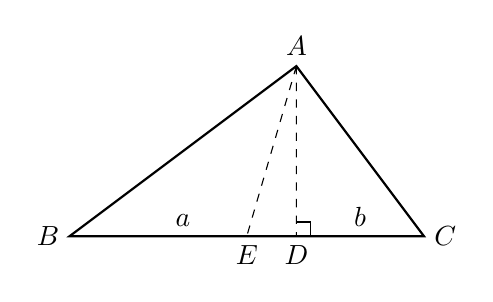
\begin{tikzpicture}[scale = 1.8]
        \draw [thick] (0,0) node [left] {$B$} -- (2.5,0) node [right] {$C$} -- (1.6,1.2) node [above] {$A$} -- cycle;
        \draw [dashed] (1.6,1.2) -- (1.6,0) node [below] {$D$} (1.6,1.2) -- (1.25,0) node [below] {$E$};
        \draw [thin] (1.7,0) -- (1.7,0.1) -- (1.6,0.1);
        \draw (0.8,0) node [above] {$a$} (2.05,0) node [above] {$b$};
    \end{tikzpicture}
\end{center}
\item {\tiny (000032)}如图, 已知直角梯形$ABCD$的顶点$A(a, 0)$、$B(b, 0)$位于$x$轴上, 顶点$C$、$D$落在函数$y=|x|$的图像上, $M$、$N$分别为线段$AB$、$CD$的中点, $O$为坐标原点, $Q$为线段$OC$与线段$MN$的交点.\\
(1) 求中点$M$的坐标, 以及线段$MQ$、$MN$的长度;\\
(2) 用不等式表示$MQ$、$MN$长度的大小关系.
\begin{center}
    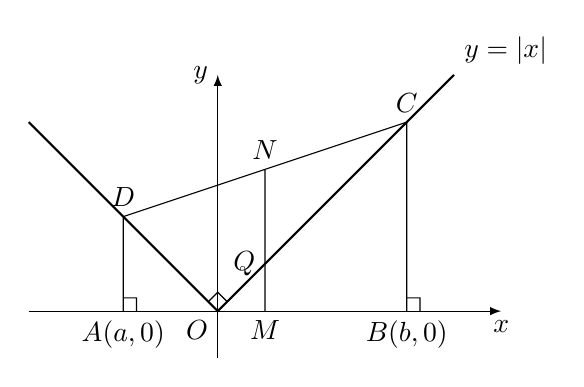
\begin{tikzpicture}[scale = 1.2,>=latex]
        \draw [->] (-2,0) -- (3,0) node [below] {$x$};
        \draw [->] (0,-0.5) -- (0,2.5) node [left] {$y$};
        \draw (0,0) node [below left] {$O$};
        \draw [thick] (-2,2) -- (0,0) -- (2.5,2.5) node [above right] {$y=|x|$};
        \draw [thin] (-0.1,0.1) -- (0,0.2) -- (0.1,0.1) (2.14,0) -- (2.14,0.14) -- (2,0.14) (-0.86,0) -- (-0.86,0.14) -- (-1,0.14);
        \draw (-1,0) node [below] {$A(a,0)$} -- (-1,1) node [above] {$D$} -- (0.5,1.5) node [above] {$N$} -- (2,2) node [above] {$C$} -- (2,0) node [below] {$B(b,0)$} (0.5,1.5) -- (0.5,0.5) node [left] {$Q$} -- (0.5,0) node [below] {$M$}; 
    \end{tikzpicture}
\end{center}
\item {\tiny (000033)}已知一元二次方程$x^2+px+p=0$的两个实根分别为$\alpha$、$\beta$, 且$\alpha^2$+$\beta^2=3$, 求实数$p$的值.
\item {\tiny (000034)}已知一元二次方程$2x^2-4x+m+3=0$有两个同号实根, 求实数$m$的取值范围.
\item {\tiny (000035)}设$a,b\in \mathbf{R}$, 已知关于$x$的不等式$(a+b)x+(b-2a)<0$的解集为$(1, +\infty)$, 求不等式$(a-b)x+3b-a>0$的解集.
\item {\tiny (000036)}解下列不等式:\\
(1) $-2< \dfrac 1{2x+1}\le 3$;\\
(2) $2<|x+1|\le 3$.
\item {\tiny (000037)}已知集合$A=\{x||x-a|<2\}$, $B=\{x|\dfrac{2x-1}{x+2}<1\}$, 且$A\subseteq B$. 求实数$a$的取值范围.
\item {\tiny (000038)}证明: 若$x>-1$, 则$x+\dfrac 1{x+1}\ge 1$, 并指出等号成立的条件.
\item {\tiny (000039)}设$a$、$b$为正数, 且$a+b=2$. 求$\dfrac 1a+\dfrac 1b$的最小值.
\item {\tiny (000040)}已知$a$、$b$、$c$都是正数, 求证: $\dfrac{b+c}{a}+\dfrac{c+a}{b}+\dfrac{a+b}{c}\ge 6$.
\item {\tiny (000041)}设实数$x$、$y$满足$|x+y|=1$, 求$xy$的最大值.
\item {\tiny (000042)}已知$a$、$b$为实数, 求证:$|a|+|b| \le |a+b| +|a-b|$, 并指出等号成立的条件.
\item {\tiny (000043)}已知$a$、$b$是实数,\\
(1) 求证: $a^2+ab+b^2\ge 0$, 并指出等号成立的条件;\\
(2) 求证: 如果$a>b$, 那么$a^3>b^3$.
\item {\tiny (000044)}解下列不等式:\\
(1) $\dfrac{3x-11}{x^2-6x+9}\le 1$;\\
(2) $|3-2x| \ge |x+1|$.
\item {\tiny (000045)}已知集合$A=\{x|x^2-2x-3>0\}$, $B=\{x|x^2+px+q\le 0\}$. 若$A\cup B=\mathbf{R}$, 且$A\cap B=[-2,-1)$, 求实数$p$及$q$的值.
\item {\tiny (000046)}已知实数$0<a<b$, 求证: $a<\dfrac{2ab}{a+b}<\sqrt{ab}<\dfrac{a+b}{2}<\sqrt{\dfrac{a^2+b^2}{2}}<b$.
\item {\tiny (000047)}方程$(x-1)(x-2)(x-3)=0$的三个根$1$、$2$、$3$将数轴划分为四个区间, 即$(-\infty, 1)$, $(1, 2)$, $(2, 3)$, $(3, +\infty)$. 试在这四个区间上分别考察$(x-1)(x-2)(x-3)$的
符号, 从而得出不等式$(x-1)(x-2)(x-3)>0$与$(x-1)(x-2)(x-3)<0$的解集.\\
一般地, 对$x_1$、$x_2$、$x_3\in \mathbf{R}$, 且$x_1\le x_2\le x_3$, 试分别求不等式$(x-x_1)(x-x_2)(x-x_3)>0$与$(x-x_1)(x-x_2)(x-x_3)<0$的解集(提示: $x_1$、$x_2$、$x_3$相互之间可能相等, 需要分情况讨论).
\item {\tiny (000048)}填空题:\\
(1) 若$x^3=5$, 则$x=$\blank{50}; 若$3^x=5$, 则$x=$\blank{50}.\\
(2) 将$\sqrt[4]{a\sqrt[3]{a}} \ (a>0)$化成有理数指数幂的形式为\blank{50}.\\
(3) 若$\log_8x=-\dfrac 23$, 则$x=$\blank{50}.\\
(4) 若$\log_a b\cdot \log_5 a=3$($a>0$且$a\ne 1$), 则$b=$\blank{50}.
\item {\tiny (000049)}选择题:\\
(1) 若$\lg a$与$\lg b$互为相反数, 则有\bracket{20}.
\fourch{$a+b=0$}{$ab=1$}{$\dfrac ab=1$}{以上答案均不对}
(2) 设$a>0$, 下列计算中正确的是\bracket{20}.
\twoch{$a^\frac{2}{3}\cdot a^\frac{3}{2}=a$}{$a^\frac{2}{3}\div a^\frac{3}{2}=a$}{$a^{-4}\cdot a^4=0$}{$(a^\frac{2}{3})^\frac{3}{2}=a$}
\item {\tiny (000050)}已知$10^\alpha=3$, $10^\beta=4$. 求$10^{\alpha+\beta}$及$10^{\alpha-\frac{\beta}2}$的值.
\item {\tiny (000051)}求下列各式的值:\\
(1) $\dfrac{1}{4^x+1}+\dfrac{1}{4^{-x}+1}$;\\
(2) $4^{\sqrt 2+1}\times 2^{3-2\sqrt 2}\times 8^{-\frac 23}$.
\item {\tiny (000052)}已知$\lg a<1$, 化简$\sqrt{\lg^2 a-\lg \dfrac{a^2}{10}}$.
\item {\tiny (000053)}已知$m=\log_2 10$, 求$2^m-m\lg 2-4$的值.
\item {\tiny (000054)}填空题:\\
(1) 若$4^x=2^{-\frac{1}{2}}$, $4^y=\sqrt[3]{32}$, 则$2x-3y=$\blank{50}.\\
(2) 若$\log_3(\log_4 x)=1$, 则$x=$\blank{50}.\\
(3) 若$3^a=7^b=63$, 则$\dfrac 2a+\dfrac 1b$的值为\blank{50}.
\item {\tiny (000055)}已知$\log_{18}9=a$, $18^b=5$, 则$\log_{36}45$等于\bracket{20}.
\fourch{$\dfrac{a+b}{2+a}$}{$\dfrac{a+b}{2-a}$}{$\dfrac{a+b}{2a}$}{$\dfrac{a+b}{a^2}$}
\item {\tiny (000056)}设$\log_{0.2}a>0$, $\log_{0.2}b>0$, 且$\log_{0.2}a\cdot \log_{0.2}b=1$, 求$\log_{0.2}(ab)$的最小值.
\item {\tiny (000057)}化简$\dfrac{(1+2^x)(1+2^{2x})(1+2^{4x})(1+2^{8x})(1+2^{16x})}{1-2^{32x}}$(其中$x\ne 0$).
\item {\tiny (000058)}已知$a>1$, $b>0$. 求证: 对任意给定的实数$k$, $a^{2b+k}-a^{b+k}>a^{b+k}-a^k$.
\item {\tiny (000059)}甲、乙两人同时解关于$x$的方程: $\log_2x+b+c\log_x2=0$. 甲写错了常数$b$, 得两根
$\dfrac 14$及$\dfrac 18$; 乙写错了常数$c$, 得两根$\dfrac 12$及$64$. 求这个方程的真正根.
\item {\tiny (000060)}已知$a$、$b$及$c$是不为$1$的正数, 且$\lg a+\lg b+\lg c=0$. 求证: $a^{\frac{1}{\lg b}+\frac{1}{\lg c}}\cdot b^{\frac{1}{\lg c}+\frac{1}{\lg a}}\cdot c^{\frac{1}{\lg a}+\frac{1}{\lg b}}=\dfrac{1}{1000}$.
\item {\tiny (000061)}填空题:\\
(1) 若点$(2, \sqrt 2)$在幂函数$y=x^a$的图像上, 则该幂函数的表达式为\blank{50}; 若点$(2, \sqrt 2)$在指数函数$y=a^x$($a>0$且$a\ne 1$)的图像上, 则该指数函数的表达式为\blank{50}; 若点$(\sqrt 2, 2)$在对数函数$y=\log_a x$($a>0$且$a\ne 1$)的图像上, 则该对数
函数的表达式为\blank{50}.\\
(2) 若幂函数$y=x^k$在区间$(0, +\infty)$上是严格减函数, 则实数$k$的取值范围为\blank{50}.\\
(3) 已知常数$a>0$且$a\ne 1$, 假设无论$a$为何值, 函数$y=a^{x-2}+1$的图像恒经过一
个定点. 则这个点的坐标为\blank{50}.
\item {\tiny (000062)}选择题:\\
(1) 若指数函数$y=a^x$($a>0$且$a\ne 1$)在$\mathbf{R}$上是严格减函数, 则下列不等式中, 一定能成立的是\bracket{20}.
\fourch{$a>1$}{$a<0$}{$a(a-1)<0$}{$a(a-1)>0$}
(2) 在同一平面直角坐标系中, 一次函数$y=x+a$与对数函数$y=\log_ax$($a>0$且$a\ne 1$)的图像关系可能是\bracket{20}.
\fourch{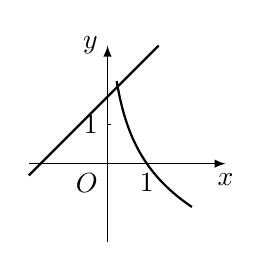
\begin{tikzpicture}[scale = 0.5,>=latex]
    \draw [->] (-2,0) -- (3,0) node [below] {$x$};
    \draw [->] (0,-2) -- (0,3) node [left] {$y$};
    \draw (0,0) node [below left] {$O$};
    \draw (0.1,1) -- (0,1) node [left] {$1$};
    \draw (1,0) node [below] {$1$};
    \draw [thick] (-2,-0.3) -- (1.3,3);
    \draw [thick,domain =-1.1:2.1,samples = 200] plot ({0.5^\x},\x);
\end{tikzpicture}
}{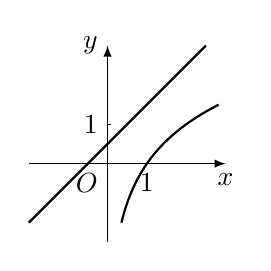
\begin{tikzpicture}[scale = 0.5,>=latex]
    \draw [->] (-2,0) -- (3,0) node [below] {$x$};
    \draw [->] (0,-2) -- (0,3) node [left] {$y$};
    \draw (0,0) node [below left] {$O$};
    \draw (0.1,1) -- (0,1) node [left] {$1$};
    \draw (1,0) node [below] {$1$};
    \draw [thick] (-2,-1.5) -- (2.5,3);
    \draw [thick,domain =1.5:-1.5,samples = 200] plot ({0.5^\x},-\x);
\end{tikzpicture}
}{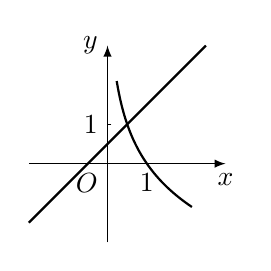
\begin{tikzpicture}[scale = 0.5,>=latex]
    \draw [->] (-2,0) -- (3,0) node [below] {$x$};
    \draw [->] (0,-2) -- (0,3) node [left] {$y$};
    \draw (0,0) node [below left] {$O$};
    \draw (0.1,1) -- (0,1) node [left] {$1$};
    \draw (1,0) node [below] {$1$};
    \draw [thick] (-2,-1.5) -- (2.5,3);
    \draw [thick,domain =-1.1:2.1,samples = 200] plot ({0.5^\x},\x);
\end{tikzpicture}
}{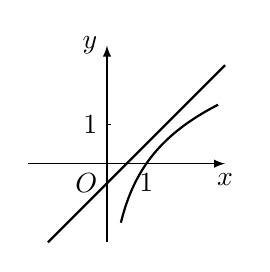
\begin{tikzpicture}[scale = 0.5,>=latex]
    \draw [->] (-2,0) -- (3,0) node [below] {$x$};
    \draw [->] (0,-2) -- (0,3) node [left] {$y$};
    \draw (0,0) node [below left] {$O$};
    \draw (0.1,1) -- (0,1) node [left] {$1$};
    \draw (1,0) node [below] {$1$};
    \draw [thick] (-1.5,-2) -- (3,2.5);
    \draw [thick,domain =1.5:-1.5,samples = 200] plot ({0.5^\x},-\x);
\end{tikzpicture}
}
\item {\tiny (000063)}求下列函数的的定义域:\\
(1) $y=(x-1)^{\frac 52}$;\\
(2) $y=3^{\sqrt{x-1}}$;\\
(3) $y=\lg \dfrac{1+x}{1-x}$.
\item {\tiny (000064)}比较下列各题中两个数的大小:\\
(1) $0.1^{0.7}$与$0.2^{0.7}$;\\
(2) $0.7^{0.1}$与$0.7^{0.2}$;\\
(3) $\log_{0.7}0.1$与$\log_{0.7}0.2$.
\item {\tiny (000065)}设点$(\sqrt 2, 2)$在幂函数$y_1=x^a$的图像上, 点$(-2,\dfrac 14)$在幂函数$y_2=x^b$的图像上. 当$x$取何值时, $y_1=y_2$?
\item {\tiny (000066)}设$a=(\dfrac 23)^x$, $b=x^{\frac 32}$及$c=\log_\frac{2}{3}x$, 当$x>1$时, 试比较$a$、$b$及$c$之间的大小关系.
\item {\tiny (000067)}设常数$a>0$且$a\ne 1$, 若函数$y=\log_a(x+1)$在区间$[0, 1]$上的最大值为$1$, 最小值为$0$, 求实数$a$的值.
\item {\tiny (000068)}如果光线每通过一块玻璃其强度要减少$10\%$, 那么至少需要将多少块这样的玻璃重叠起来, 才能使通过它们的光线强度低于原来的$\dfrac 13$?
\item {\tiny (000069)}填空题:\\
(1) 已知$m\in \mathbf{Z}$, 设幂函数$y=x^{m^2-4m}$的图像关于原点成中心对称, 且与$x$轴及$y$轴均无交点, 则$m$的值为\blank{50}.\\
(2) 设$a$、$b$为常数, 若$0<a<1$, $b<-1$, 则函数$y=a^x+b$的图像必定不经过第\blank{50}象限.
\item {\tiny (000070)}选择题:\\
(1) 若$m>n>1$, 而$0<x<1$, 则下列不等式正确的是\bracket{20}.
\fourch{$m^x<n^x$}{$x^m<x^n$}{$\log_x m>\log_x n$}{$\log_m x<\log_n x$}
(2) 在同一平面直角坐标系中, 二次函数$y=ax^2+bx$与指数函数$y=(\dfrac ba)^x$的图像关系可能为\bracket{20}.
\fourch{
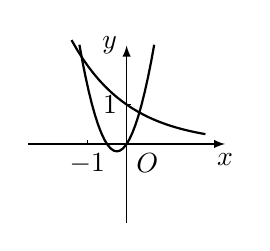
\begin{tikzpicture}[scale = 0.5, >=latex]
    \draw [->] (-2.5,0) -- (2.5,0) node [below] {$x$};
    \draw [->] (0,-2.) -- (0,2.5) node [left] {$y$};
    \draw (0,0) node [below right] {$O$};
    \draw (-1,0.1) -- (-1,0) node [below] {$-1$};
    \draw (0.1,1) -- (0,1) node [left] {$1$};
    \draw [domain = -1.2:0.7,thick] plot (\x,{3*\x * (\x+0.5)});
    \draw [domain = -1.4:2,thick] plot (\x,{(0.5)^\x}); 
\end{tikzpicture}
}{
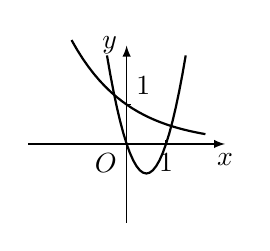
\begin{tikzpicture}[scale = 0.5, >=latex]
    \draw [->] (-2.5,0) -- (2.5,0) node [below] {$x$};
    \draw [->] (0,-2.) -- (0,2.5) node [left] {$y$};
    \draw (0,0) node [below left] {$O$};
    \draw (1,0.1) -- (1,0) node [below] {$1$};
    \draw (0.1,1) -- (0,1) node [above right] {$1$};
    \draw [domain = -0.5:1.5,thick] plot (\x,{3*\x*(\x-1)});
    \draw [domain = -1.4:2,thick] plot (\x,{(0.5)^\x}); 
\end{tikzpicture}
}{
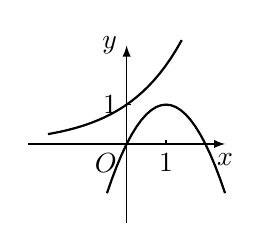
\begin{tikzpicture}[scale = 0.5, >=latex]
    \draw [->] (-2.5,0) -- (2.5,0) node [below] {$x$};
    \draw [->] (0,-2.) -- (0,2.5) node [left] {$y$};
    \draw (0,0) node [below left] {$O$};
    \draw (1,0.1) -- (1,0) node [below] {$1$};
    \draw (0.1,1) -- (0,1) node [left] {$1$};
    \draw [domain = -0.5:2.5,thick] plot ({\x},{-\x*(\x-2)});
    \draw [domain = -1.4:2,thick] plot ({-\x},{(0.5)^\x}); 
\end{tikzpicture}
}{
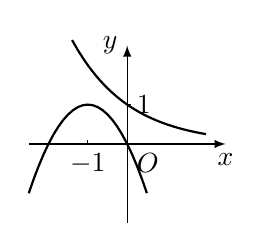
\begin{tikzpicture}[scale = 0.5, >=latex]
    \draw [->] (-2.5,0) -- (2.5,0) node [below] {$x$};
    \draw [->] (0,-2.) -- (0,2.5) node [left] {$y$};
    \draw (0,0) node [below right] {$O$};
    \draw (-1,0.1) -- (-1,0) node [below] {$-1$};
    \draw (0.1,1) -- (0,1) node [right] {$1$};
    \draw [domain = -2.5:0.5,thick] plot ({\x},{-\x*(\x+2)});
    \draw [domain = -1.4:2,thick] plot ({\x},{(0.5)^\x}); 
\end{tikzpicture}   
}
\item {\tiny (000071)}设$a$为常数且$0<a<1$, 若$y=(\log_a \dfrac 35)^x$在$\mathbf{R}$上是严格增函数, 求实数$a$的取值范围.
\item {\tiny (000072)}在同一平面直角坐标系中, 作出函数$y=(\dfrac 12)^x$及$y=x^{\frac 12}$的大致图像, 并求方程$(\dfrac 12)^x=x^{\frac 12}$的解的个数.
\item {\tiny (000073)}已知集合$A=\{y|y=(\dfrac 12)^x,\  x\in [-2, 0)\}$, 用列举法表示集合$B=\{y|y=\log_3x,\  x\in A\text{且}y\in \mathbf{Z}\}$.
\item {\tiny (000074)}$\log_23$是有理数吗? 请证明你的结论.
\item {\tiny (000075)}仅利用对数函数的单调性和计算器上的乘方功能来确定对数$\log_23$第二位小数的值.
\item {\tiny (000076)}求函数$y=\dfrac1{2-x}+\sqrt{x^2-1}$的定义域.
\item {\tiny (000077)}判断下列函数$y=f(x)$的奇偶性, 并说明理由:\\
(1) $f(x)=|\dfrac 12 x-3|+|\dfrac 12 x+3|$;\\
(2) $f(x)=x^3+\dfrac 2x$;\\
(3) $f(x)=x^2$, $x\in (k, 2)$(其中常数$k<2$).
\item {\tiny (000078)}已知$m$、$n$是常数, 而函数$y=(m-1)x^2+3x+(2-n)$为奇函数. 求$m$、$n$的值.
\item {\tiny (000079)}求函数$y=x+\dfrac 4x$的单调区间.
\item {\tiny (000080)}分别作出下列函数的大致图像, 并指出它们的单调区间:\\
(1) $y=|x^2-4x|$;\\
(2) $y=2|x|-3$.
\item {\tiny (000081)}已知二次函数$y=f(x)$, 其中$f(x)=ax^2-2ax+3-a \ (a>0)$. 比较$f(-1)$和$f(2)$的大小.
\item {\tiny (000082)}已知$k$是常数, 设$\alpha$、$\beta$是二次方程$x^2-2kx+k+20=0$的两个实根. 问: 当$k$为
何值时, $(\alpha+1)^2+(\beta+1)^2$取到最小值?
\item {\tiny (000083)}邮局规定: 当邮件质量不超过$100$g时, 每$20$g邮费$0.8$元, 且不足$20$g时按$20$g计算; 超过$100$g时, 超过$100$g的部分按每$100$g邮费$2$元计算, 且不足$100$g按$100$g
计算; 同时规定邮件总质量不得超过$2000$g. 请写出邮费关于邮件质量的函数表达式, 并计算$50$g和$500$g的邮件分别收多少邮费.
\item {\tiny (000084)}若函数$y=(a^2+4a-5)x^2-4(a-1)x+3$的图像都在$x$轴上方(不含$x$轴), 求实数$a$的取值范围.
\item {\tiny (000085)}已知$y=f(x)$是奇函数, 其定义域为$\mathbf{R}$; 而$y=g(x)$是偶函数, 其定义域为$D$. 判断函数$y=f(x)g(x)$的奇偶性, 并说明理由.
\item {\tiny (000086)}设函数$y=x^2+10x-a+3$, 当$x\in [-2, +\infty)$时, 其函数值恒大于等于零. 求实数$a$的取值范围.
\item {\tiny (000087)}已知函数$y=-x^2+2ax+1-a$, $x\in [0, 1]$的最大值为$2$. 求实数$a$的值.
\item {\tiny (000088)}设$f(x)=x^2+ax+1$. 若对任意给定的实数$x$, $f(2+x)=f(2-x)$恒成立, 求实数$a$的值.
\item {\tiny (000089)}已知$y=f(x)$是定义在$(-1, 1)$上的奇函数, 在区间$[0, 1)$上是严格减函数, 且$f(1-a)+f(1-a^2)<0$, 求实数$a$的取值范围.
\item {\tiny (000090)}已知$f(x)=2-x^2$及$g(x)=x$. 定义$h(x)$如下: 当$f(x)\ge g(x)$时, $h(x)=g(x)$; 而当$f(x)<g(x)$时, $h(x)=f(x)$. 求函数$y=h(x)$的最大值.
\item {\tiny (000091)}试讨论函数$y=\dfrac{x}{1-x^2}$的单调性.
\item {\tiny (000092)}作出函数$y=(x^2-1)^2-1$的大致图像, 写出它的单调区间, 并证明你的结论.
\item {\tiny (000093)}已知函数$y=f(x)$为偶函数, $y=g(x)$为奇函数, 且$f(x)+g(x)=x^2+2|x-1|+3$. 求$y=f(x)$及$y=g(x)$的表达式.
\item {\tiny (000094)}设函数$y=f(x)$, $x\in \mathbf{R}$的反函数是$y=f^{-1}(x)$.\\
(1) 如果$y=f(x)$是奇函数, 那么$y=f^{-1}(x)$的奇偶性如何?\\
(2) 如果$y=f(x)$在定义域上是严格增函数, 那么$y=f^{-1}(x)$的单调性如何?
\item {\tiny (000095)}选择题:\\
(1) 与$\sin(\theta -\dfrac\pi 2)$一定相等的是\bracket{20}.
\fourch{$\sin(\dfrac{3\pi}2-\theta)$}{$\cos(\theta -\dfrac{\pi}2)$}{$\cos (2\pi -\theta)$}{$\sin (\theta +\dfrac\pi 2)$}
(2) 当$0<\alpha<\dfrac\pi 4$时, 化简$\sqrt{1-\sin 2\alpha}$的结果是\bracket{20}.
\fourch{$\cos \alpha$}{$\sin \alpha-\cos \alpha$}{$\cos\alpha-\sin\alpha$}{$\sin\alpha+\cos\alpha$}
\item {\tiny (000096)}填空题:\\
(1) 若$\theta$为锐角, 则$\log_{\sin \theta} (1+\cot^2\theta)=$\blank{50};\\
(2) 若$-\dfrac\pi 2<\alpha<0$, 则点$(\cot \alpha, \cos \alpha)$必在第\blank{50}象限;\\
(3) 若$\sin (\pi -\alpha)=\dfrac 23$, $\alpha\in (\dfrac\pi 2, \pi)$, 则$\sin 2\alpha=$\blank{50}.
\item {\tiny (000097)}已知圆$O$上的一段圆弧长等于该圆的内接正方形的边长, 求这段圆弧所对的圆心角的弧度.
\item {\tiny (000098)}已知角$\alpha$的终边经过点$P(3a, 4a)$($a\ne 0$), 求$\sin \alpha$、$\cos \alpha$和$\tan \alpha$.
\item {\tiny (000099)}化简:\\
(1) $\dfrac{\sin (\theta -5\pi )}{\tan (3\pi -\theta )}\cdot \dfrac{\cot (\dfrac\pi 2-\theta )}{\tan (\theta -\dfrac{3\pi} 2)}\cdot \dfrac{\cos (8\pi -\theta )}{\sin(-\theta-4\pi)}$;\\
(2) $\sin (\theta -\dfrac\pi 4)+\cos (\theta +\dfrac\pi 4)$.
\item {\tiny (000100)}已知$\tan \alpha=3$, 求$\dfrac 1{\sin^2\alpha+2\sin \alpha\cos \alpha}$的值.
\item {\tiny (000101)}在$\triangle ABC$中, 已知$a=5$, $b=4$, $A=2B$. 求$\cos B$.
\item {\tiny (000102)}已知$\triangle ABC$的面积为$S$, 求证:\\
(1) $S=\dfrac{a^2\sin B\sin C}{2\sin (B+C)}$;\\
(2) $S=\dfrac{a^2}{2(\cot B+\cot C)}$.
\item {\tiny (000103)}(1) 已知$\sin \alpha=\dfrac{\sqrt 5}5$, $\sin \beta=\dfrac{\sqrt {10}}{10}$, 且$\alpha$及$\beta$都是锐角. 求$\alpha+\beta$的值;\\
(2) 在$\triangle ABC$中, 已知$\tan A$与$\tan B$是方程$x^2-6x+7=0$的两个根, 求$\tan C$.
\item {\tiny (000104)}证明: $(\sin \alpha+\sin \beta)^2+(\cos \alpha+\cos \beta)^2=4\cos^2\dfrac{\alpha-\beta}{2}$.
\item {\tiny (000105)}选择题:\\
(1) 若$0<x<\dfrac\pi 4$, 且$\lg (\sin x+\cos x)=\dfrac12(3\lg 2-\lg 5)$, 则$\cos x-\sin x$的值为\bracket{20}.
\fourch{$\dfrac{\sqrt{6}}3$}{$\dfrac{\sqrt{3}}2$}{$\dfrac{\sqrt{10}}5$}{$\dfrac{\sqrt{5}}4$}
(2) 下列命题中, 真命题为\bracket{20}.
\onech{若点$P(a, 2a)$($a\ne 0$)为角$\alpha$的终边上一点, 则$\sin \alpha=\dfrac{2\sqrt 5}5$}
{同时满足$\sin \alpha=\dfrac 12$, $\cos \alpha=\dfrac{\sqrt3}2$的角$\alpha$有且只有一个}
{如果角$\alpha$满足$-3\pi <\alpha<-\dfrac 52\pi$, 那么角$\alpha$是第二象限的角}
{$\tan x=-\sqrt 3$的解集为$\{x|x=k\pi -\dfrac\pi 3, \  k\in \mathbf{Z}\}$}
\item {\tiny (000106)}填空题:\\
(1) 在$\triangle ABC$中, 若$a^2+b^2+ab=c^2$, 则$C=$\blank{50};\\
(2) 若$\sin \theta =a$, $\cos \theta =-2a$, 且$\theta$为第四象限的角, 则实数$a=$\blank{50}.\\
\item {\tiny (000107)}已知$\sin \alpha=a\sin \beta$, $b\cos \alpha=a\cos \beta$, 且$\alpha$及$\beta$均为锐角, 求证: $\cos \alpha= \sqrt{\dfrac{a^2-1}{b^2-1}}$.
\item {\tiny (000108)}已知$0<\alpha<\dfrac\pi 2<\beta<\pi$, 且$\cos \beta=-\dfrac13$, $\sin (\alpha+\beta)=\dfrac79$, 求$\sin \alpha$的值.
\item {\tiny (000109)}已知$\pi <\alpha<\dfrac{3\pi} 2$, $\pi <\beta<\dfrac{3\pi} 2$, 且$\sin \alpha=-\dfrac{\sqrt 5}5$, $\cos \beta=-\dfrac{\sqrt{10}}{10}$. 求$\alpha-\beta$的值.
\item {\tiny (000110)}已知$(1+\tan \alpha)(1+\tan \beta)=2$, 且$\alpha$及$\beta$都是锐角. 求证: $\alpha+\beta=\dfrac{\pi}{4}$.
\item {\tiny (000111)}已知$\alpha$是第二象限的角, 且$\sin \alpha=\dfrac{\sqrt {15}}4$. 求$\dfrac{\sin (\alpha+\dfrac{\pi}{4})}{1+\sin 2\alpha+\cos 2\alpha}$的值.
\item {\tiny (000112)}证明:\\
(1) $\dfrac{2(1+\sin 2\alpha)}{1+\sin 2\alpha+\cos 2\alpha}=1+\tan \alpha$;\\
(2) $2\sin \alpha+\sin 2\alpha=\dfrac{2\sin^3\alpha}{1-\cos \alpha}$.
\item {\tiny (000113)}根据下列条件, 分别判断三角形$ABC$的形状:\\
(1) $\sin C+\sin (B-A)=\sin 2A$;\\
(2) $\dfrac{\tan A}{\tan B}=\dfrac{a^2}{b^2}$.
\item {\tiny (000114)}在$\triangle ABC$中, 求证: $\tan \dfrac A2\tan \dfrac B2+\tan \dfrac B2\tan\dfrac C2+\tan\dfrac C2\tan\dfrac A2=1$.
\item {\tiny (000115)}(1) 完成下表($\theta$为弧度数):
\begin{center}
\begin{tabular}{|c|p{.15\textwidth}<{\centering}|p{.15\textwidth}<{\centering}|p{.15\textwidth}<{\centering}|p{.15\textwidth}<{\centering}|p{.15\textwidth}<{\centering}|}
    \hline
    $\theta$ & $1$ & $0.5$ & $0.1$ & $0.01$ & $0.001$\\ \hline
    $\sin\theta$ & & & & &\\ \hline
    $\dfrac{\sin\theta}{\theta}$ & & & & &\\ \hline
\end{tabular}
\end{center}
(2) 观察上表中的数据, 你能发现什么规律?\\
(3) 已知$0<\theta <\dfrac \pi 2$, 利用图形面积公式证明$\sin \theta <\theta <\tan \theta$, 并应用该公式说明(2)中猜想的合理性.
\item {\tiny (000116)}在$\triangle ABC$中, 已知$A=30^\circ$, $b=18$. 分别根据下列条件求$B$:\\
(1) \textcircled{1} $a=6$, \textcircled{2} $a=9$, \textcircled{3} $a=13$, \textcircled{4} $a=18$, \textcircled{5} $a=22$;\\
(2) 根据上述计算结果, 讨论使$B$有一解、两解或无解时$a$的取值情况.
\item {\tiny (000117)}(1) 根据$\cos 54^\circ=\sin 36^\circ$和三倍角公式, 求$\sin 18^\circ$的值;\\
(2) 你还能使用其他方法求$\sin 18^\circ$的值吗? 若能, 请给出你的求法.
\item {\tiny (000118)}如图, 要在$A$和$D$两地之间修建一条笔直的隧道, 现在从$B$地和$C$地测量得到: $\angle DBC=24.2^\circ$, $\angle DCB=35.4^\circ$, $\angle DBA=31.6^\circ$, $\angle DCA=17.5^\circ$. 试求$\angle DAB$以确定隧道$AD$的方向(结果精确到$0.1^\circ$).
\begin{center}
    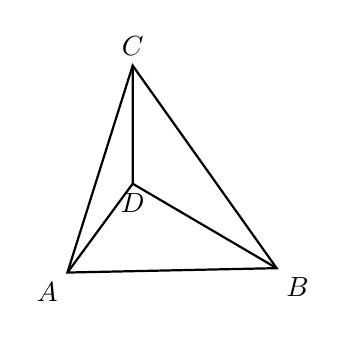
\begin{tikzpicture}
        \draw (0,0) node [below] {$D$} coordinate (D) (0,1.5) node [above] {$C$} coordinate (C) (-0.8287,-1.12831) node [below left] {$A$} coordinate (A) (1.82829,-1.07265) node [below right] {$B$} coordinate (B);
        \draw [thick] (A) -- (B) -- (C) -- cycle;
        \draw [thick] (D) -- (A) (D) -- (B) (D) -- (C);
    \end{tikzpicture}
\end{center}
\item {\tiny (000119)}求下列函数的最小正周期:\\
(1) $y=\sin \dfrac x2$;\\
(2) $y=2\cos (3x-\dfrac \pi 4)$.
\item {\tiny (000120)}判断下列函数的奇偶性, 并说明理由:\\
(1) $y=\sin |2x|$;\\
(2) $y=\tan 5x$;\\
(3) $y= \dfrac1 {\cos x}$;\\
(4) $y=\sin (x+\dfrac\pi 6)$.
\item {\tiny (000121)}已知$2\sin (2x)=\sqrt 3, \ x\in (-\dfrac \pi 4, \dfrac\pi 4)$. 求$x$的值.
\item {\tiny (000122)}求下列函数的单调区间:\\
(1) $y=-\sin 2x$;\\
(2) $y=2\sin (x+\dfrac\pi 3)$;\\
(3) $y=\cos (\dfrac x2-\dfrac \pi 4)$;\\
(4) $y=2\tan (2x+\dfrac \pi 4)$.
\item {\tiny (000123)}作出函数$y=2\sin (2x+\dfrac \pi 3)$的大致图像.
\item {\tiny (000124)}已知函数$y=A\sin (\omega x+\varphi) \ (A>0, \ \omega>0)$的振幅是$3$, 最小正周期是$\dfrac{2\pi} 3$, 初始相位是$\dfrac\pi 6$. 求这个函数的表达式.
\item {\tiny (000125)}求下列函数的最大值和最小值, 并求出取得最大值和最小值时所有$x$的值:\\
(1) $y=\cos^2x+\cos x-2$;\\
(2) $y=\sin 2x, \ x\in [ -\dfrac{2\pi} 3, \dfrac \pi 3]$;\\
(3) $y=\sin^22x-2\sin 2x$;\\
(4) $y=\cos (x-\dfrac\pi 6),\  x\in  [-\dfrac\pi 6, \dfrac\pi 4]$.
\item {\tiny (000126)}某实验室一天的温度$y$(单位:$^\circ\text{C}$)随时间$t$(单位:$\text{h}$)的变化近似满足函数关系$y=10-\sqrt 3\cos\dfrac \pi {12}t-\sin \dfrac\pi {12} t, \ t\in [0, 24)$.\\
(1) 求实验室一天中的最大温差;\\
(2) 若要求实验室温度不高于$11^\circ\text{C}$, 则在哪段时间实验室需要降温?
\item {\tiny (000127)}求函数$y=\sin (2x-\dfrac \pi 4)-2\sqrt 2\sin^2x$的最小正周期.
\item {\tiny (000128)}在$(0, 2\pi )$内, 求使$\sin x>\cos x$成立的$x$的取值范围.
\item {\tiny (000129)}求下列函数的最大值, 并求出取得最大值时所有$x$的值:\\
(1) $y=2\sin^2x+\sin 2x-1$;\\
(2) $y=1-\sin x-2\cos^2x, \  x\in  [\dfrac \pi 3, \dfrac{4\pi} 3]$.
\item {\tiny (000130)}若函数$y=2\sin \omega x$(其中常数$\omega$是小于$1$的正数)在区间$[0, \dfrac\pi 3]$上的最大值是$\sqrt 2$, 求$\omega$的值.
\item {\tiny (000131)}如图, 摩天轮上一点$P$距离地面的高度$y$关于时间$t$的函数表达式为$y=A\sin (\omega t+\varphi)+b$, $\varphi\in [-\pi , \pi]$. 已知摩天轮
的半径为$50\text{m}$, 其中心点$O$距地面$60\text{m}$, 摩天轮以每$30$分钟转一圈的方式做匀速转动, 而点$P$的起始位置在摩天轮的最低
点处.
\begin{center}
    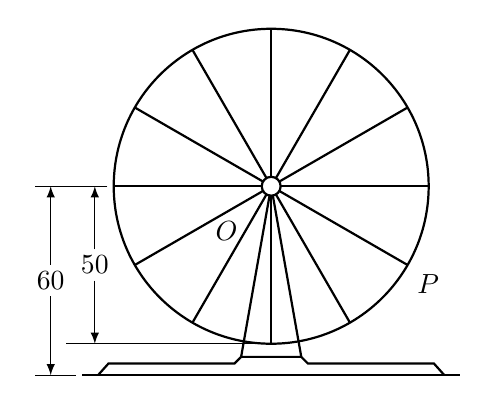
\begin{tikzpicture}[>=latex,scale = 0.4]
        \draw [thick] (0,0) circle (0.3) (0,0) circle (5);
        \foreach \i in {0,30,...,330}{\draw [thick] (\i:0.3) -- (\i:5);};
        \draw [thick] (-80:0.3) -- (-80:5.5) coordinate (R) (-100:0.3) -- (-100:5.5) coordinate (L) (L) -- (R);
        \draw [thick] (L) --++ (-135:0.3) --++ (-4,0) -- (-5.5,-6) (R) --++ (-45:0.3) --++ (4,0) -- (5.5,-6); 
        \draw [thick] (-6,-6) -- (6,-6);
        \draw (-6.2,-6) -- (-7.5,-6) (-5.2,0) -- (-7.5,0) (0,-5) -- (-6.5,-5);
        \draw [->] (-5.6,-2) -- (-5.6,0);
        \draw [->] (-5.6,-3) -- (-5.6,-5);
        \draw (-5.6,-2.5) node {$50$};
        \draw [->] (-7,-2.5) -- (-7,0);
        \draw [->] (-7,-3.5) -- (-7,-6);
        \draw (-7,-3) node {$60$};
        \draw (225:2) node {$O$};
        \draw (-30:5) node [below right] {$P$};
    \end{tikzpicture}
\end{center}
(1) 根据条件具体写出$y$($\text{m}$)关于$t$($\text{min}$)的函数表达式;\\
(2) 在摩天轮转动的一圈内, 点$P$有多长时间距离地面超过$85\text{m}$?
\item {\tiny (000132)}说明: 用上一章6.3节给出的记号$\arcsin$与$\arccos$(见必修第二册教材第45页), 可以定义函数$y=\arcsin x \ (x\in [0, 1])$与$y=\arccos x \ (x\in [0, 1])$.\\
验证:\\
(1) 函数$y=\sin x\ (x\in [0, \dfrac\pi 2])$与函数$y=\arcsin x \ (x\in [0, 1])$互为反函数;\\
(2) 函数$y=\cos x \ (x\in [0, \dfrac \pi 2])$与函数$y=\arccos x\ (x\in [0, 1])$互为反函数.
\item {\tiny (000133)}把上题的记号略作推广: 对实数$x\in [-1, 1]$, 若实数$y\in [-\dfrac \pi 2, \dfrac\pi 2]$使得$\sin y=x$, 则记$y=\arcsin x$; 类似地, 对实数$x\in [-1, 1]$, 若实数$y\in [0, \pi]$使得$\cos y=x$, 则记$y=\arccos x$. 说明: 经过推广的记号$\arcsin$与$\arccos$, 定义了函数$y=\arcsin x \ (x\in [-1, 1])$与$y=\arccos x \ (x\in [-1, 1])$.\\
验证:
(1) 函数$y=\sin x \ (x\in  [-\dfrac\pi 2, \dfrac\pi 2])$与函数$y=\arcsin x \ (x\in [-1, 1])$互为反函数;\\
(2) 函数$y=\cos x\ (x\in [0, \pi])$与函数$y=\arccos x \ (x\in [-1, 1])$互为反函数.
\item {\tiny (000134)}对$y=\tan x$与$y=\arctan x$做类似的工作.
\item {\tiny (000135)}定义在区间$(0, \dfrac\pi 2)$上的函数$y=6\cos x$的图像与$y=5\tan x$的图像的交点为$P$, 过点$P$作垂直于$x$轴的垂线$PP_1$, 其垂足为$P_1$. 设直线$PP_1$与$y=\sin x$的图像交于点$P_2$, 求线段$P_1P_2$的长.
\item {\tiny (000136)}已知定义在$\mathbf{R}$上的偶函数$y=f(x)$的最小正周期为$2$, 当$0\le x\le 1$时, $f(x)=x$.\\
(1) 求当$5\le x\le 6$时函数$y=f(x)$的表达式;\\
(2) 若函数$y=kx,\ x\in \mathbf{R}$与函数$y=f(x)$的图像恰有$7$个不同的交点, 求$k$的值.
\item {\tiny (000137)}如图, 有一块边长为$3\text{m}$的正方形铁皮$ABCD$, 其中阴影部分$ATN$是一个半径为$2\text{m}$的扇形. 设这个扇形已经腐蚀不能
使用, 但其余部分均完好. 工人师傅想在未被腐蚀的部分截下一块其边落在$BC$与$CD$上的矩形铁皮$PQCR$, 使点$P$在弧$TN$上. 设$\angle TAP=\theta$, 矩形$PQCR$的面积为$S\text{m}^2$.
\begin{center}
    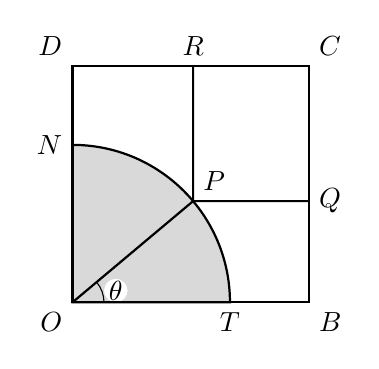
\begin{tikzpicture}
        \begin{scope}[even odd rule]
            \clip (0,0) rectangle (3,3) (0.55,0.15) circle (0.15);
            \fill [gray!30] (0,0) -- (2,0) arc (0:90:2) -- cycle;
        \end{scope}

        \draw [thick] (0,0) node [below left] {$O$} -- (3,0) node [below right] {$B$} -- (3,3) node [above right] {$C$} -- (0,3) node [above left] {$D$} -- cycle;
        \draw [thick] (0,0) -- (40:2) node [above right] {$P$} -- (3,{2*sin(40)}) node [right] {$Q$} (40:2) -- ({2*cos(40)},3) node [above] {$R$};
        \draw [thick] (0,0) -- (2,0) node [below] {$T$} arc (0:90:2) node [left] {$N$} -- cycle;
        \draw (0.4,0) arc (0:40:0.4) (0.55,0.15) node {$\theta$};
    \end{tikzpicture}
\end{center}
(1) 求$S$关于$\theta$的函数表达式;\\
(2) 求$S$的最大值及$S$取得最大值时$\theta$的值.
\item {\tiny (000138)}如图, 在边长为$1$的小正方形组成的网格上, 求:
\begin{center}
    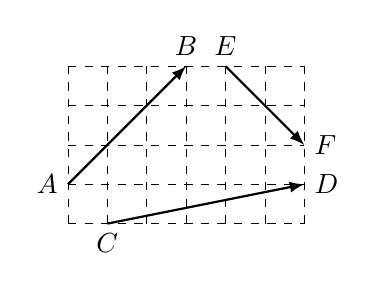
\begin{tikzpicture}[>=latex,scale = 0.5]
        \foreach \i in {0,1,...,4} {\draw [dashed, very thin] (0,\i) -- (6,\i);};
        \foreach \i in {0,1,...,6} {\draw [dashed, very thin] (\i,0) -- (\i,4);};
        \draw [thick,->] (0,1) node [left] {$A$} -- (3,4) node [above] {$B$};
        \draw [thick,->] (1,0) node [below] {$C$} -- (6,1) node [right] {$D$};
        \draw [thick, ->] (4,4) node [above] {$E$} -- (6,2) node [right] {$F$};       
    \end{tikzpicture}
\end{center}
(1) $|\overrightarrow{AB}|$;\\
(2) $|\overrightarrow{CD}|$;\\
(3) $|\overrightarrow{EF}|$.
\item {\tiny (000139)}已知$\overrightarrow a$、$\overrightarrow b$均为非零向量, 写出$|\overrightarrow a+\overrightarrow b|=|\overrightarrow a|+|\overrightarrow b|$成立的充要条件.
\item {\tiny (000140)}已知$\overrightarrow a$、$\overrightarrow b$为非零向量, 且$\overrightarrow a$、$\overrightarrow b$、$5\overrightarrow a-4\overrightarrow b$在同一起点上. 求证: 它们的终点在同一条直线上.
\item {\tiny (000141)}在矩形$ABCD$中, 边$AB$、$AD$的长分别为$2$、$1$, 若$M$、$N$分别是边$BC$、$CD$上的点, 且满足$\dfrac{|\overrightarrow{BM}|}{|\overrightarrow{BC}|}=\dfrac{|\overrightarrow{CN}|}{|\overrightarrow{CD}|}$, 则$\overrightarrow{AM}\cdot \overrightarrow{AN}$的取值范围是\blank{50}.
\item {\tiny (000142)}已知两个向量$\overrightarrow {e_1}$、$\overrightarrow {e_2}$满足$|\overrightarrow {e_1}|=2$, $|\overrightarrow {e_2}|=1$, $\langle \overrightarrow {e_1}, \overrightarrow {e_2}\rangle=60^\circ$, 且向量$2\lambda \overrightarrow {e_1}+7\overrightarrow {e_2}$与向量$\overrightarrow {e_1}+\lambda \overrightarrow {e_2}$的夹角为钝角. 求实数$\lambda$的取值范围.
\item {\tiny (000143)}已知向量$\overrightarrow a=(1, 0)$, $\overrightarrow b=(2, 1)$.\\
(1) 求$|\overrightarrow a+3\overrightarrow b|$;\\
(2) 当$k$为何实数时, $k\overrightarrow a-\overrightarrow b$与$\overrightarrow a+3\overrightarrow b$平行? 平行时它们是同向还是反向?
\item {\tiny (000144)}已知在平面直角坐标系中, $O$为原点, 点$A(4, -3)$, $B(-5, 12)$.\\
(1) 求向量$\overrightarrow{AB}$的坐标及$|\overrightarrow{AB}|$;\\
(2) 已知向量$\overrightarrow{OC}=2\overrightarrow{OA}+\overrightarrow{OB}$, $\overrightarrow{OD}=\overrightarrow{OA}-3\overrightarrow{OB}$, 求$\overrightarrow{OC}$及$\overrightarrow{OD}$的坐标;\\
(3) 求$\overrightarrow{OA}\cdot\overrightarrow{OB}$.
\item {\tiny (000145)}已知向量$\overrightarrow a=(3, -2)$, $\overrightarrow b=(-2, 1)$, $\overrightarrow c=(7, -4)$, 求$\lambda,\mu$, 使得$\overrightarrow c=\lambda \overrightarrow a+\mu \overrightarrow b$.
\item {\tiny (000146)}已知点$M(3, -2)$、$N(-5, -1)$, 且$\overrightarrow{MP}=\dfrac 13\overrightarrow{MN}$. 求点$P$的坐标.
\item {\tiny (000147)}在等腰三角形$ABC$中, 已知$D$为底边$BC$的中点. 求证: $AD\perp BC$.
\item {\tiny (000148)}如图, 在四边形$ABCD$中, $G$为对角线$AC$与$BD$中点连线$MN$的中点, $P$为平面上任意给定的一点. 求证: $4\overrightarrow{PG}=\overrightarrow{PA}+\overrightarrow{PB}+\overrightarrow{PC}+\overrightarrow{PD}$.
\begin{center}
    \begin{tikzpicture}
        \draw [thick] (0,0) node [below left] {$B$} coordinate (B) -- (2,0) node [below right] {$C$} coordinate (C) -- (2.4,2.5) node [above right] {$D$} coordinate (D) -- (-0.1,1.5) node [above left] {$A$} coordinate (A) -- cycle;
        \draw [thick] (A) -- (C) (B) -- (D);
        \filldraw ($(B)!0.5!(D)$) circle (0.03) node [above] {$M$} coordinate (M);
        \filldraw ($(A)!0.5!(C)$) circle (0.03) node [below] {$N$} coordinate (N);
        \filldraw ($(M)!0.5!(N)$) circle (0.03) node [right] {$G$} coordinate (G);
        \filldraw (3,1) circle (0.03) node [right] {$P$};
        \draw [thick] (M) -- (N);
    \end{tikzpicture}
\end{center}
\item {\tiny (000149)}在四边形$ABCD$中, 向量$\overrightarrow{AB}=\overrightarrow i+2\overrightarrow j$, $\overrightarrow{BC}=-4\overrightarrow i-\overrightarrow j$, $\overrightarrow{CD}=-5\overrightarrow i-3\overrightarrow j$. 求证: $ABCD$为梯形.
\item {\tiny (000150)}已知$\overrightarrow a$、$\overrightarrow b$、$\overrightarrow c$均为非零向量, 其中的任意两个向量都不平行, 且$\overrightarrow a+\overrightarrow b$与$\overrightarrow c$是平行向量, $\overrightarrow a+\overrightarrow c$与$\overrightarrow b$是平行向量. 求证: $\overrightarrow b+\overrightarrow c$与$\overrightarrow a$是平行向量.
\item {\tiny (000151)}如图, 点$A$、$M$、$B$在同一条直线上, 点$O$不在该直线上, 且$\overrightarrow{AM}=\dfrac 13 \overrightarrow{AB}$. 设
$\overrightarrow{OA}=\overrightarrow a$, $\overrightarrow{OB}=\overrightarrow b$, $\overrightarrow{OM}=\overrightarrow c$, 试用向量$\overrightarrow a$、$\overrightarrow b$表示$\overrightarrow c$.
\begin{center}
    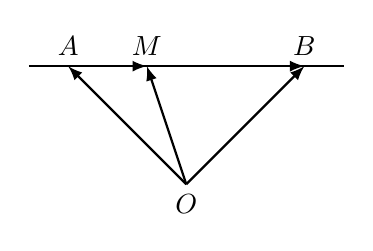
\begin{tikzpicture}[>=latex]
        \draw [thick] (-0.5,0) -- (3.5,0);
        \draw [->,thick] (1.5,-1.5) node [below] {$O$}-- (0,0) node [above] {$A$};
        \draw [->,thick] (1.5,-1.5) -- (3,0);
        \draw [->,thick] (1.5,-1.5) -- (1,0);
        \draw [->,thick] (0,0) -- (1,0) node [above] {$M$};
        \draw [->,thick] (1,0) -- (3,0) node [above] {$B$};
    \end{tikzpicture}
\end{center}
\item {\tiny (000152)}设平面上有两个向量$\overrightarrow a=(\cos \alpha, \sin \alpha)  (0^\circ\le \alpha<360^\circ)$, $\overrightarrow b=(-\dfrac 12, \dfrac{\sqrt 3}2)$.\\
(1) 求证: 向量$\overrightarrow a+\overrightarrow b$与$\overrightarrow a-\overrightarrow b$垂直;\\
(2) 当向量$\sqrt 3\overrightarrow a+\overrightarrow b$与$\overrightarrow a-\sqrt 3\overrightarrow b$的模相等时, 求$\alpha$的大小.
\item {\tiny (000153)}如图, 在矩形$ABCD$中, $AB=\sqrt 2$, $BC=2$, $E$为$BC$的中点, 点$F$在边$CD$上且$\overrightarrow{AB}\cdot \overrightarrow{AF}=\sqrt{2}$. 求$\overrightarrow{AE}\cdot \overrightarrow{BF}$的值.
\begin{center}
    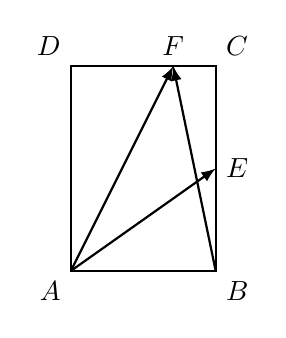
\begin{tikzpicture}[>=latex,thick,scale = 1.3]
        \draw (0,0) node [below left] {$A$} rectangle ({sqrt(2)},2) node [above right] {$C$};
        \draw [->,thick] (0,0) -- ({sqrt(2)},1) node [right] {$E$};
        \draw [->] (0,0) -- (1,2) node [above] {$F$};
        \draw [->] ({sqrt(2)},0) node [below right] {$B$} -- (1,2);
        \draw (0,2) node [above left] {$D$};
    \end{tikzpicture}
\end{center}
\item {\tiny (000154)}已知等边三角形$ABC$的边长为$1$, $\overrightarrow{BC}=\overrightarrow a$, $\overrightarrow{CA}=\overrightarrow b$, $\overrightarrow{AB}=\overrightarrow c$. 求$\overrightarrow a\cdot \overrightarrow b+\overrightarrow b\cdot \overrightarrow c+\overrightarrow c\cdot \overrightarrow a$.
\item {\tiny (000155)}已知向量$\overrightarrow{OA}=(k, 12)$, $\overrightarrow{OB}=(4, 5)$, $\overrightarrow{OC}=(-k, 10)$, 且$A$、$B$、$C$三点共线. 求实数$k$的值.
\item {\tiny (000156)}已知向量$\overrightarrow{OA}=(1, 7)$, $\overrightarrow{OB}=(5, 1)$, $\overrightarrow{OP}=(2, 1)$, $K$为直线$OP$上的一个动点, 当$\overrightarrow{KA}\cdot\overrightarrow{KB}$取最小值时, 求向量$\overrightarrow{OK}$的坐标.
\item {\tiny (000157)}如图, 在正方形$ABCD$中, $P$是对角线$AC$上一点, $PE$垂直$AB$于点$E$, $PF$垂直$BC$于点$F$. 求证: $PD\perp EF$.
\begin{center}
    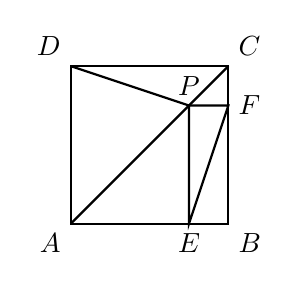
\begin{tikzpicture}[thick]
        \draw (0,0) node [below left] {$A$} rectangle (2,2) node [above right] {$C$};
        \draw (0,2) node [above left] {$D$} -- (1.5,1.5) node [above] {$P$};
        \draw (1.5,1.5) -- (1.5,0) node [below] {$E$} -- (2,1.5) node [right] {$F$} -- cycle;
        \draw (2,0) node [below right] {$B$};
        \draw (0,0) -- (2,2);
    \end{tikzpicture}
\end{center}
\item {\tiny (000158)}证明: 三角形的三条高相交于一点.
\item {\tiny (000159)}如图, 甲、乙分处河的两岸, 欲拉船$M$逆流而上, 需在正前方有$3000\text{N}$的力. 已知甲所用的力$\overrightarrow{f_1}$的大小为$2000\text{N}$, 且与$M$的前进方向的夹角为$\dfrac\pi 6$, 求乙所用的力$\overrightarrow{f_2}$.
\begin{center}
    \begin{tikzpicture}[thick,>=latex,scale = 1.5]
        \fill [fill = gray!20] (0,0.3) -- (0,1.4) -- (3,1.7) -- (3,0.6) -- cycle;
        \draw (0,1.4) -- (3,1.7) (0,0.3) -- (3,0.6);
        \draw [->] (0.6,1) node [below left] {$M$} -- (3,1);
        \draw [dashed,thin] (0,1) -- (0.6,1);
        \draw [->] (0.6,1) --++ (30:1.6) node [above right] {$\overrightarrow{f_1}$};
        \draw [->] (0.6,1) --++ ({2.4-1.6*cos(30)},{-1.6*sin(30)}) node [below right] {$\overrightarrow{f_2}$};
        \draw (2.2,1) node [above] {前进方向};
    \end{tikzpicture}
\end{center}
\item {\tiny (000160)}在$\triangle ABC$中, $AB=AC=5$, $BC=6$, $M$是边$AC$上靠近$A$的一个三等分点. 问: 在线段$BM$上是否存在点$P$, 使得$PC\perp BM$?
\item {\tiny (000161)}在$\triangle ABC$中, 已知点$O$、$G$、$H$分别是三角形的外心、重心和垂心. 求证: $O$、$G$、$H$三点共线(此直线称为欧拉线).
\item {\tiny (000162)}选择题:\\
(1) 虚数的平方一定是\bracket{20}.
\fourch{正实数}{负实数}{虚数}{虚数或负实数}
(2) 如果复平面上的向量$\overrightarrow{AB}$所对应的复数是$-3+2\mathrm{i}$, 那么向量$\overrightarrow{BA}$所对应的复数是\bracket{20}.
\fourch{$3-2\mathrm{i}$}{$3+2\mathrm{i}$}{$-3+2\mathrm{i}$}{$-3-2\mathrm{i}$}
\item {\tiny (000163)}填空题:\\
(1) 设$z=11-60\mathrm{i}$, 则$\mathrm{Re}z=$\blank{50}; $\mathrm{Im}z=$\blank{50}; $|z|=$\blank{50}; $\overline{z}=$\blank{50}.\\
(2) 下列三个命题中, 真命题是\blank{50}.\\
\textcircled{1} 在复平面上, 表示实数的点都在实轴上, 表示虚数的点都在虚轴上;\\
\textcircled{2} 任何一个表示虚数的点一定在某一个象限内;\\
\textcircled{3} 复数的模表示该复数在复平面上所对应的点到原点的距离.
\item {\tiny (000164)}已知复数$z=(a^2-2a-3)+(a^2-4a+3)\mathrm{i}$, 其中$a$是实数.\\
(1) 若$z\in \mathbf{R}$, 求$a$的值;\\
(2) 若$z$在复平面上所对应的点位于第一象限, 求$a$的取值范围.
\item {\tiny (000165)}已知复数$z_1=(a^2-a-6)+(1-2a)\mathrm{i}$, $z_2=(a-3)+(a^2-2a+2)\mathrm{i}$, 其中$a\in \mathbf{R}$.
若$\overline{z_1}=z_2$, 求$a$的值.
\item {\tiny (000166)}计算:\\
(1) $(4+\mathrm{i})(3+2\mathrm{i})$;\\
(2) $(\sqrt 2+\sqrt 3\mathrm{i})(\sqrt 2-\sqrt 3\mathrm{i})(-\sqrt 3+\sqrt 2\mathrm{i})(-\sqrt 3-\sqrt 2\mathrm{i})$;\\
(3) $\dfrac{-3+29\mathrm{i}}{1+2\mathrm{i}}$;\\
(4) $\dfrac{(1+\mathrm{i})^4}{1+2\mathrm{i}}+\dfrac{(1-\mathrm{i})^4}{1-2\mathrm{i}}$;\\
(5) $[(\sqrt 3+1)+(\sqrt 3-1)\mathrm{i}]^2$.
\item {\tiny (000167)}已知复数$z=\dfrac{(-3-\mathrm{\mathrm{i}})^2(2-\mathrm{\mathrm{i}})}{(1+2\mathrm{i})^3}$, 求$|z|$.
\item {\tiny (000168)}在复数范围内解下列方程:\\
(1) $x^2-4x+8=0$;\\
(2) $3x^2+2x-3=0$.
\item {\tiny (000169)}选择题:\\
(1) 设$z_1$、$z_2\in \mathbf{C}$, 则``$|z_1|=|z_2|$''是``$z_1=z_2$''的\bracket{20}.
\twoch{充分非必要条件}{必要非充分条件}{充要条件}{既非充分也非必要条件}\\
(2)设复数$z=a+b\mathrm{i}$($a,b\in \mathbf{R}$), 则$z^2$是纯虚数的充要条件是\bracket{20}.
\fourch{$a^2=b^2$}{$a^2+b^2=0$}{$|a|=|b|\ne 0$}{$ab\ne 0$}
\item {\tiny (000170)}若复数$z$满足$z+\overline{z}=2$, $(z-\overline{z})\mathrm{i}=2$, 求$|z|$.
\item {\tiny (000171)}若复数$z_1$和复数$z_2$满足$z_1z_2=3-4\mathrm{i}$, $|z_1|=2$, 求$|z_2|$.
\item {\tiny (000172)}若$x_1$和$x_2$是方程$x^2-5x+8=0$的两个根, 求$|x_1|+|x_2|$的值.
\item {\tiny (000173)}若复数$z_1$和复数$z_2$满足$|z_1|=3$, $|z_2|=4$, $|z_1+z_2|=5$, 求$|z_1-z_2|$.
\item {\tiny (000174)}已知复数$z_1$和复数$z_2$满足$z_1+z_2=3-5\mathrm{i}$, $\overline{z_1}-\overline{z_2}=-2+3\mathrm{i}$. 求$z_1^2-z_2^2$.
\item {\tiny (000175)}如图, 在长方体$ABCD-A_1B_1C_1D_1$中, $E$为$A_1B_1$的中点, $AB=BB_1=2$, $AC=2\sqrt 5$. 求异面直线$BE$与$AC$所成角的
大小. 
\begin{center}
    \begin{tikzpicture}[thick]
        \draw (0,0) node [below left] {$A$} coordinate (A) --++ (2,0) node [below right] {$B$} coordinate (B) --++ (45:{2*sqrt(5)/2}) node [right] {$C$} coordinate (C)
        --++ (0,2) node [above right] {$C_1$} coordinate (C1)
        --++ (-2,0) node [above left] {$D_1$} coordinate (D1) --++ (225:{2*sqrt(5)/2}) node [left] {$A_1$} coordinate (A1) -- cycle;
        \draw (A) ++ (2,2) node [right] {$B_1$} coordinate (B1) -- (B) (B1) --++ (45:{2*sqrt(5)/2}) (B1) --++ (-2,0);
        \draw [dashed] (A) --++ (45:{2*sqrt(5)/2}) node [left] {$D$} coordinate (D) --++ (2,0) (D) --++ (0,2);
        \draw ($(A1)!0.5!(B1)$) node [above] {$E$} -- (B);
        \draw [dashed] (A) -- (C);
    \end{tikzpicture}
\end{center}
\item {\tiny (000176)}如图, 设$P$为矩形$ABCD$所在平面外的一点, 矩形对角线的交点为$O$, $M$为$PB$的中点. 判断下列结论是否正确, 并说
明理由:\\
\begin{center}
    \begin{tikzpicture}[thick]
        \draw (0,0) node [below left] {$A$} coordinate (A) -- (3,0) node [below right] {$B$} coordinate (B)--++ (45:1.5) node [above right] {$C$} coordinate (C);
        \draw [dashed] (C) --++ (-3,0) node [above right] {$D$} coordinate (D) -- (A);
        \draw [dashed] (A) -- (C) (B) -- (D);
        \draw ($(A)!0.5!(C)$) node [below] {$O$} coordinate (O) ++ (0,3) node [above] {$P$} coordinate (P);
        \draw (P) -- (A) (P) -- (B) (P) -- (C);
        \draw ($(P)!0.5!(B)$) node [above right] {$M$} coordinate (M);
        \draw [dashed] (M) -- (O) (P) -- (D);
    \end{tikzpicture}
\end{center}
(1) $OM\parallel PD$;\\
(2) $OM\parallel\text{平面}PCD$;\\
(3) $OM\parallel\text{平面}PDA$;\\
(4) $OM\parallel\text{平面}PBA$;\\
(5) $OM\parallel\text{平面}PBC$.
\item {\tiny (000177)}如图, 正方体的棱长是$a$, 点$E$、$F$分别是两条棱的中点.
\begin{center}
    \begin{tikzpicture}[thick]
        \path (0,0) node [below left] {$A$} coordinate (A) --++ (2.5,0) node [below right] {$B$} coordinate (B) --++ (45:{2.5/2}) node [right] {$C$} coordinate (C)
        --++ (0,2.5) node [above right] {$C_1$} coordinate (C1)
        --++ (-2.5,0) node [above left] {$D_1$} coordinate (D1) --++ (225:{2.5/2}) node [left] {$A_1$} coordinate (A1) -- cycle;
        \path (A) ++ (2.5,2.5) node [right] {$B_1$} coordinate (B1) -- (B) (B1) --++ (45:{2.5/2}) (B1) --++ (-2.5,0);
        \path [dashed] (A) --++ (45:{2.5/2}) node [left] {$D$} coordinate (D) --++ (2.5,0) (D) --++ (0,2.5);
        \draw ($(A1)!0.5!(D1)$) node [above left] {$E$} coordinate (E) ($(A1)!0.5!(B1)$) node [above] {$F$} coordinate (F);
        \fill [gray!30] (B) -- (D) -- (E) -- (F);
        \draw (B) -- (F) -- (E);
        \draw [dashed] (B) -- (D) -- (E) (D) -- (C) (D) -- (A) (D) -- (D1);
        \draw (A) -- (B) -- (C) -- (C1) -- (D1) -- (A1) -- (A) (B1) -- (A1) (B1) -- (C1) (B1) -- (B);
    \end{tikzpicture}
\end{center}
(1) 求证: 四边形$BDEF$(图中阴影部分)是一个梯形;\\
(2) 求四边形$BDEF$的面积.
\item {\tiny (000178)}判断下列命题的真假, 并说明理由:\\
(1) 若直线$l$与平面$M$斜交, 则$M$内不存在与$l$垂直的直线;\\
(2) 若直线$l\perp\text{平面}M$, 则$M$内不存在与$l$不垂直的直线;\\
(3) 若直线$l$与平面$M$斜交, 则$M$内不存在与$l$平行的直线;\\
(4) 若直线$l\parallel\text{平面}M$, 则$M$内不存在与$l$不平行的直线.
\item {\tiny (000179)}如果不在平面上的一条直线上有两点到这个平面的距离相等, 那么这条直线和这个平面有什么位置关系? 画示意图表示.
\item {\tiny (000180)}如图, 直线$AA'$、$BB'$、$CC'$相交于点$O$, 且$AO=A'O$, $BO=B'O$, $CO=C'O$. 求证: $\text{平面}ABC\parallel \text{平面}A'B'C'$.
\begin{center}
    \begin{tikzpicture}[thick]
        \draw (0,0) node [below left] {$A$} coordinate (A);
        \draw (2.5,-0.5) node [below right] {$B$} coordinate (B);
        \draw (1.5,0.5) node [below] {$C$} coordinate (C);
        \draw (1,1.5) node [left] {$O$} coordinate (O);
        \draw (A) -- (B) -- (O) -- cycle;
        \draw [dashed] (A) -- (C) -- (B) (C) -- (O);
        \draw ($(O)!-1!(C)$) node [above] {$C'$} coordinate (C1);
        \draw ($(O)!-1!(A)$) node [right] {$A'$} coordinate (A1);
        \draw ($(O)!-1!(B)$) node [left] {$B'$} coordinate (B1);
        \draw (O) -- (A1) -- (B1) -- (C1) -- (O) (A1) -- (C1) (B1) -- (O);
    \end{tikzpicture}
\end{center}
\item {\tiny (000181)}已知直线$l\perp\text{平面}\alpha$, 直线$m\subset\text{平面}\beta$, 判断下列命题的真假, 并说明理由:\\
(1) 若$\alpha\parallel \beta$, 则$l\perp m$;\\
(2) 若$\alpha\perp \beta$, 则$l\parallel m$;\\
(3) 若$l\parallel m$, 则$\alpha\perp \beta$;\\
(4) 若$l\perp m$, 则$\alpha\parallel \beta$.
\item {\tiny (000182)}如图, 已知线段$AB$垂直于三角形$BCD$所在的平面, 且$AB=BC=CD=1$, $\angle BCD=90^\circ$. $BE\perp AD$, $E$为垂足, $F$为$AC$的中点. 求$EF$的长.
\begin{center}
    \begin{tikzpicture}[thick,scale = 2]
        \draw (0,0) node [left] {$B$} coordinate (B) -- (0,1) node [above left] {$A$} coordinate (A);
        \draw ({sqrt(2)/2},0) ++ (-45:{sqrt(2)/4}) coordinate (C) node [below] {$C$};
        \draw ({sqrt(2)},0) node [right] {$D$} coordinate (D) -- (C) -- (B) (A) -- (C) (A) -- (D);
        \draw ($(A)!{1/3}!(D)$) node [above] {$E$} coordinate (E) -- ($(A)!0.5!(C)$) node [right] {$F$} coordinate (F);
        \draw (E) -- (F) -- (B);
        \draw [dashed] (E) -- (B) -- (D);
    \end{tikzpicture}
\end{center}
\item {\tiny (000183)}设正六边形$ABCDEF$的边长为$a$, 线段$PA$垂直于正六边形所在的平面, 且$PA=2a$. 分别求点$P$到$CD$、$DE$与$BC$所在直线的距离.
\item {\tiny (000184)}已知直线$a$、$b$和平面$\alpha$、$\beta$, 判断下列命题的真假, 并说明理由:\\
(1) 若$a\parallel \alpha$, $b\perp a$, 则$b\perp \alpha$;\\
(2) 若$a\parallel \alpha$, $\alpha\perp \beta$, 则$a\perp \beta$;\\
(3) 若$a\parallel b$, $b\subset\alpha$, 则$a\parallel \alpha$.
\item {\tiny (000185)}证明: 如果平面$\alpha$和不在这个平面上的直线$a$都垂直于平面$\beta$, 那么直线$a$必平行于平面$\alpha$.
\item {\tiny (000186)}三个平面两两相交, 得到三条交线. 求证: 这三条交线交于一点或两两平行.
\item {\tiny (000187)}如图, 已知$\triangle ABC$是正三角形, $EA$、$CD$都垂直于平面$ABC$, 且$EA=AB=2a$, $DC=a$, $F$是$BE$的中点.
\begin{center}
    \begin{tikzpicture}[thick,scale = 1.2]
        \draw (0,0) node [left] {$A$} coordinate (A) -- (0,2) node [above left] {$E$} coordinate (E);
        \draw (2,0) node [right] {$C$} coordinate (C) -- (2,1) node [right] {$D$} coordinate (D);
        \draw (1,0) ++ (-135:{sqrt(3)/2}) node [below] {$B$} coordinate (B) -- (E) (B) -- (D) -- (E) ;
        \draw ($(E)!0.5!(B)$) node [above right] {$F$} coordinate (F) -- (A) (F) -- (D);
        \draw [dashed] (A) -- (C);
        \draw (A) -- (B) -- (C);
    \end{tikzpicture}
\end{center}
(1) 求证: $FD\parallel \text{平面}ABC$;\\
(2) 求证: $AF\perp \text{平面}EDB$.
\item {\tiny (000188)}证明: 如果一个平面的一条平行线垂直于另一个平面, 那么这两个平面互相垂直.
\item {\tiny (000189)}如图, 以等腰直角三角形$ABC$斜边$BC$上的高$AD$为折痕, 使$\triangle ABD$和$\triangle ACD$折成互相垂直的两个面. 求证: $BD\perp CD$, 且$\angle BAC=60^\circ$.
\begin{center}
    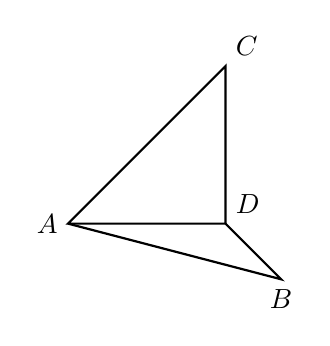
\begin{tikzpicture}[thick]
        \draw (0,0) node [left] {$A$} coordinate (A) -- (2,0) node [above right] {$D$} coordinate (D) -- (2,2) node [above right] {$C$} coordinate (C) -- cycle;
        \draw (2,0) --++ (-45:1) node [below] {$B$} coordinate (B) -- (A);
    \end{tikzpicture}
\end{center}
\item {\tiny (000190)}证明: 如果共点的三条直线两两垂直, 那么它们中每两条直线所确定的平面也两两垂直.
\item {\tiny (000191)}如图, $P$是平面$\alpha$外一点, 直线$PA$与平面$\alpha$斜交于点$A$, 从点$P$作平面$\alpha$上的一条直线$OA$的垂线$PO$, 垂足为$O$. 又设$a$是平面$\alpha$上的一条直线, 且$a\perp OA$, $a\perp PA$.

\begin{center}
    \begin{tikzpicture}[thick]
        \draw (-0.5,0) -- (0,0) node [above left] {$O$} -- (1,0) node [above right] {$A$} coordinate (A) -- (2,0);
        \draw (0,0) coordinate (O) -- (0,1.7) (0,1.5) node [above right] {$P$} coordinate (P);
        \draw ($(P)!{-0.1}!(A)$) -- (A);
        \draw (1.6,0) ++ (45:0.7) node [below] {$a$} --++ (225:1.4);
        \draw (0,-1.2) coordinate (X);
        \draw ($(A)!{-0.7}!(P)$) coordinate (Y);
        \draw (-0.3,0.6) -- (-1.9,-0.6) -- (2,-0.6) -- (3.2,0.6);
        \path [name path=line1] (O) -- (X);
        \path [name path=line2] (A) -- (Y);
        \path [name path=line3] (O) -- (P);
        \path [name path=line4] (A) -- (P);
        \path [name path=under_line] (-1.6,-0.6) -- (2,-0.6);
        \path [name path=above_line] (-0.3,0.6) -- (3.2,0.6);
        \path [name intersections={of = line1 and under_line, by=U}];
        \path [name intersections={of = line2 and under_line, by=V}];
        \path [name intersections={of = line3 and above_line, by=S}];
        \path [name intersections={of = line4 and above_line, by=T}];
        \draw (U) -- (X) (V) -- (Y) (-0.3,0.6) -- (S) (T) -- (3.2,0.6);
        \draw [dashed] (S) -- (T) (O) -- (X) (A) -- (Y);
    \end{tikzpicture}
\end{center}
求证: $PO\perp \text{平面}\alpha$, 从而$OA$是$PA$在平面$\alpha$上的投影.
\item {\tiny (000192)}如图, 直角三角形$ABC$在平面$\alpha$上, 且$\angle BAC=90^\circ$. 以$A$为垂足作$DA\perp \alpha$, 在$DB$上取一点$E$, 使$AE\perp DB$. 求证: $CE\perp DB$.
\begin{center}
    \begin{tikzpicture}[thick]
        \draw (-1,0) -- (3,0) --++ (45:2) coordinate (R);
        \draw (-1,0) --++ (45:2) coordinate (P);
        \path [name path = aboveline] (P) -- (R);
        \draw (1,0.3) node [left] {$A$} coordinate (A) -- (2.5,0.3) node [right] {$B$} coordinate (B) -- (1,2.3) node [left] {$D$} coordinate (D);
        \draw ($(B)!{16/41}!(D)$) node [right] {$E$} coordinate (E) -- (A) -- (D);
        \path [name path = A--D] (A) -- (D);
        \path [name path = B--D] (B) -- (D);
        \path [name intersections = {of = aboveline and A--D, by = U}];
        \path [name intersections = {of = aboveline and B--D, by = V}];
        \draw [dashed] (U) -- (V);
        \draw (P) -- (U) (V) -- (R);
        \draw [dashed] (A) ++ (45:1) node [left] {$C$} coordinate (C) -- (A) (C) -- (E) (C) -- (B); 
        \draw (R) --++ (-0.3,0) node [below left] {$\alpha$};
    \end{tikzpicture}
\end{center}
\item {\tiny (000193)}设平面$\alpha$与平面$\beta$平行, $A\in \alpha$, $B\in \beta$, $C$是$AB$的中点. 当$A$、$B$分别在$\alpha$、$\beta$上
运动时, 所有的动点$C$是否保持在同一个平面上? 证明你的结论.
\item {\tiny (000194)}在长方体$ABCD-A_1B_1C_1D_1$中, 如果对角线$AC_1$与过点$A$的相邻三个面所成的角分别为$\alpha$、$\beta$、$\gamma$, 那么$\cos^2\alpha+\cos^2\beta+\cos^2\gamma=$\blank{50}.
\begin{center}
    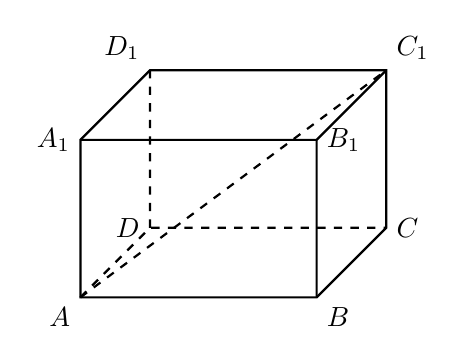
\begin{tikzpicture}[thick]
        \draw (0,0) node [below left] {$A$} coordinate (A) --++ (3,0) node [below right] {$B$} coordinate (B) --++ (45:{2.5/2}) node [right] {$C$} coordinate (C)
        --++ (0,2) node [above right] {$C_1$} coordinate (C1)
        --++ (-3,0) node [above left] {$D_1$} coordinate (D1) --++ (225:{2.5/2}) node [left] {$A_1$} coordinate (A1) -- cycle;
        \draw (A) ++ (3,2) node [right] {$B_1$} coordinate (B1) -- (B) (B1) --++ (45:{2.5/2}) (B1) --++ (-3,0);
        \draw [dashed] (A) --++ (45:{2.5/2}) node [left] {$D$} coordinate (D) --++ (3,0) (D) --++ (0,2);
        \draw [dashed] (A) -- (C1);
    \end{tikzpicture}
\end{center}
\item {\tiny (000195)}如图, 该几何体是由哪个平面图形旋转得到的? 画出其余平面图形旋转得到的几何体.
\begin{center}
    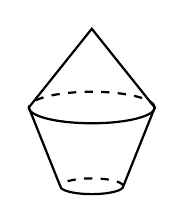
\begin{tikzpicture}[thick]
        \draw (0.4,0) -- (0.8,1) -- (0,2) -- (-0.8,1) -- (-0.4,0);
        \draw (0.4,0) arc (0:-180:0.4 and 0.1) (0.8,1) arc (0:-180:0.8 and 0.2);
        \draw [dashed] (0.4,0) arc (0:180:0.4 and 0.1) (0.8,1) arc (0:180:0.8 and 0.2);
    \end{tikzpicture}
\end{center}
\fourch{\begin{center}
    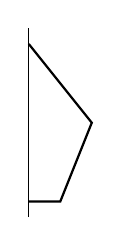
\begin{tikzpicture}[thick]
        \draw [thin] (0,-0.2) -- (0,2.2);
        \draw (0,0) -- (0.4,0) -- (0.8,1) -- (0,2);
    \end{tikzpicture}
\end{center}}{    
\begin{center}
    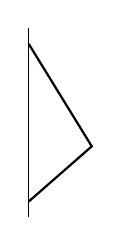
\begin{tikzpicture}[thick]
        \draw [thin] (0,-0.2) -- (0,2.2);
        \draw (0,0) -- (0.8,0.7) -- (0,2);
    \end{tikzpicture}
\end{center}}{    
\begin{center}
    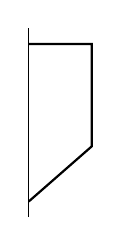
\begin{tikzpicture}[thick]
        \draw [thin] (0,-0.2) -- (0,2.2);
        \draw (0,0) -- (0.8,0.7) -- (0.8,2) -- (0,2);
    \end{tikzpicture}
\end{center}}{    
\begin{center}
    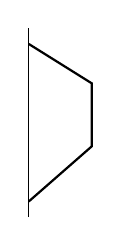
\begin{tikzpicture}[thick]
        \draw [thin] (0,-0.2) -- (0,2.2);
        \draw (0,0) -- (0.8,0.7) -- (0.8,1.5) -- (0,2);
    \end{tikzpicture}
\end{center}}
\item {\tiny (000196)}判断下列命题是否正确, 并说明理由:\\
(1) 以直角三角形的一直角边为轴旋转所形成的旋转体是圆锥;\\
(2) 以直角梯形的一腰为轴旋转所形成的旋转体是圆台;\\
(3) 圆柱、圆锥、圆台都有两个底面;\\
(4) 圆锥的侧面展开图为扇形, 这个扇形所在圆的半径等于圆锥底面圆的半径.
\item {\tiny (000197)}已知一个圆锥的侧面展开图恰是一个半圆. 用通过圆锥的轴的平面截此圆锥, 求截面三角形的顶角.
\item {\tiny (000198)}过圆锥高的三等分点分别作平行于底面的截面, 求它们把圆锥侧面分成的三部分的面积之比.
\item {\tiny (000199)}在棱长为1的正方体上, 用过同一顶点的三条棱中点的平面分别截该正方体, 截去$8$个三棱锥. 求剩下的几何体的体积.
\item {\tiny (000200)}已知长方体一个顶点上的三条棱长分别是$3$、$4$、$5$, 且它的$8$个顶点都在同一球面上. 求这个球的表面积.
\item {\tiny (000201)}在等边圆柱(底面直径等于高的圆柱)、球、正方体的体积相等的情况下, 讨论它们的表面积的大小关系.
\item {\tiny (000202)}如图, 在三棱柱的侧棱$A_1A$和$B_1B$上分别取$P$、$Q$两点, 使$PQ$平分侧面$ABB_1A_1$的面积. 求平面$PQC$把棱柱所分成的两部分的体积之比.
\begin{center}
    \begin{tikzpicture}[thick]
        \draw (0,0) node [left] {$C$} coordinate (C) -- (3,0) node [right] {$A$} coordinate (A);
        \draw [dashed] (1,1) node [above right] {$B$} coordinate (B) -- (A) (B) -- (C) (B) --++ (0,2) node [above] {$B_1$} coordinate (B1);
        \draw (A) --++ (0,2) node [right] {$A_1$} coordinate (A1) -- (B1) -- (0,2) node [left] {$C_1$} coordinate (C1); 
        \draw (C) -- (C1) -- (A1);
        \draw ($(A)!0.7!(A1)$) node [right] {$P$} coordinate (P) -- (C);
        \draw [dashed] (P) -- ($(B)!0.3!(B1)$) node [left] {$Q$} -- (C);
    \end{tikzpicture}
\end{center}
\item {\tiny (000203)}已知用通过圆锥的轴的平面去截一个圆锥, 得到的截面是面积为$9\sqrt 3\text{cm}^2$的正三角形. 求此圆锥内接球的半径.
\item {\tiny (000204)}若一个长方体长、宽、高之比为$2:1:3$, 表面积为$22$, 求它的体积.
\item {\tiny (000205)}如果两个球的体积之比为$8:27$, 求这两个球的表面积之比.
\item {\tiny (000206)}设点$O_1$为圆锥的高靠近顶点的三等分点, 求过$O_1$与底面平行的截面面积与底面面积之比.
\item {\tiny (000207)}若棱锥的高为$16$, 底面积为$256$, 平行于底面的截面面积为$50$, 求该截面与棱锥底面之间的距离.
\item {\tiny (000208)}设圆锥的母线长为$1$, 高为$\dfrac{1}{2}$, 过圆锥的任意给定的两条母线作一个截面. 求截面面积的最大值.
\item {\tiny (000209)}将若干毫升水倒入底面半径为$2\text{cm}$的圆柱形器皿中, 量得水面高度为$6\text{cm}$. 若将这些水倒入底面直径等于母线的倒圆锥形器皿中, 且恰好装满, 求圆锥形器皿的高.
\item {\tiny (000210)}已知长方体$ABCD-A_1B_1C_1D_1$的三条棱长分别为$3\text{cm}$、$2\text{cm}$、$1\text{cm}$, 求表面有一只蜘蛛从$A$爬行到$C_1$的最短距离.
\item {\tiny (000211)}如图, 已知点$P$在圆柱$O_1O$的底面圆$O$的圆周上, $AB$为圆$O$的直径, 圆柱的表面积为$20\pi$ , $OA=2$, $\angle AOP=120^\circ$.
\begin{center}
    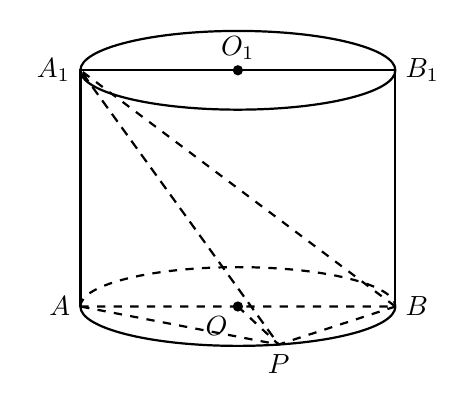
\begin{tikzpicture}[thick]
        \draw (0,0) node [left] {$A$} -- (0,3) node [left] {$A_1$} -- (4,3) node [right] {$B_1$} -- (4,0) node [right] {$B$};
        \draw (0,0) arc (180:360:2 and 0.5) (0,3) arc (180:360:2 and 0.5) (0,3) arc (180:0:2 and 0.5);
        \draw [dashed] (0,0) arc (180:0:2 and 0.5);
        \filldraw (2,0) circle (0.05) node [below left] {$O$} coordinate (O) (2,3) circle (0.05) node [above] {$O_1$} coordinate (O1);
        \draw [dashed] (0,0) -- (4,0) -- (0,3) -- ({2+2*cos(-75)},{0.5*sin(-75)}) node [below] {$P$} coordinate (P) (O) -- (P) -- (0,3) (4,0) -- (P) -- (0,0);
    \end{tikzpicture}
\end{center}
(1) 求三棱锥$A_1-ABP$的体积;\\
(2) 求异面直线$A_1B$与$AP$所成角的大小.
\item {\tiny (000212)}如图, 在圆柱中, 底面直径$AB$等于母线$AD$, 点$E$在底面的圆周上, 且$AF\perp DE$, $F$是垂足.
\begin{center}
    \begin{tikzpicture}[thick]
        \draw (0,0) node [left] {$A$} -- (0,3) node [left] {$D$} coordinate (D) (3,3) node [right] {$C$} -- (3,0) node [right] {$B$};
        \draw (0,0) arc (180:360:1.5 and 0.5) (0,3) arc (180:-180:1.5 and 0.5);
        \draw [dashed] (0,0) arc (180:0:1.5 and 0.5);
        \draw [dashed] ({1.5+1.5*cos(-105)},{0.5*sin(-105)}) node [below] {$E$} coordinate (E) -- (0,0) (E) -- (3,0) (E) -- (0,3) -- (3,0) -- (0,0) -- ($(E)!0.3!(D)$) node [left] {$F$};
    \end{tikzpicture}
\end{center}
(1) 求证: $AF\perp DB$;\\
(2) 若圆柱与三棱锥$D-ABE$的体积的比等于$3\pi$ , 求直线$DE$与平面$ABD$所成角的大小.
\item {\tiny (000213)}如图, 半球内有一内接正方体(即正方体的一个面在半球的底面圆上, 其余顶点在半球面上). 若正方体的棱长为$\sqrt 6$, 求半球的表面积和体积. 
\begin{center}
    \begin{tikzpicture}[thick]
        \draw [dashed] (0,0)  coordinate (A) --++ (2,0)  coordinate (B) --++ (45:{2/2})  coordinate (C)
        --++ (0,2)  coordinate (C1) --++ (-2,0)  coordinate (D1) --++ (225:{2/2}) coordinate (A1) -- cycle;
        \draw [dashed] (A) ++ (2,2) coordinate (B1) -- (B) (B1) --++ (45:{2/2}) (B1) --++ (-2,0);
        \draw [dashed] (A) --++ (45:{2/2})  coordinate (D) --++ (2,0) (D) --++ (0,2);        
        \draw ($(A)!0.5!(C)$) ++ ({-sqrt(6)},0) coordinate (L)  arc (180:0:{sqrt(6)});
        \draw (L) arc (-180:0:{sqrt(6)} and {sqrt(6)/3});
        \draw [dashed] (L) arc (180:0:{sqrt(6)} and {sqrt(6)/3});
    \end{tikzpicture}
\end{center}
\item {\tiny (000214)}已知圆锥的底面半径为$r$, 高为$h$, 正方体$ABCD-A_1B_1C_1D_1$内接于该圆锥. 求这个正方体的棱长.
\item {\tiny (000215)}如图, 一个圆锥形的空杯子上放着一个半球形的冰激凌, 如果冰激凌融化了, 会溢出来吗?
\begin{center}
    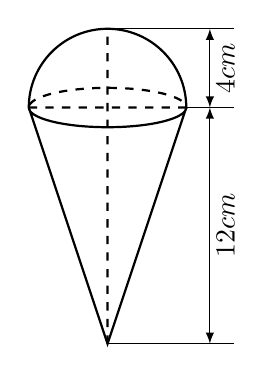
\begin{tikzpicture}[thick,>=latex]
        \draw (-1,0) -- (0,-3) -- (1,0) arc (0:180:1) arc (180:360:1 and 0.25);
        \draw [dashed] (0,-3) -- (0,1) (-1,0) -- (1,0) arc (0:180:1 and 0.25);
        \draw [thin] (1,0) -- (1.6,0) (0,-3) -- (1.6,-3) (0,1) -- (1.6,1);
        \draw [thin,<->] (1.3,0) -- (1.3,1);
        \draw [thin,<->] (1.3,0) -- (1.3,-3);
        \draw (1.5,0.5) node {\rotatebox{90}{$4\text{cm}$}};
        \draw (1.5,-1.5) node {\rotatebox{90}{$12\text{cm}$}};
    \end{tikzpicture}
\end{center}
\item {\tiny (000216)}如图, 用一块钢锭浇铸一个厚度均匀, 且表面积为$2\text{m}^2$的正四棱锥形有盖容器. 设容器的高为$h\text{m}$, 盖子的边长为$a\text{m}$.
\begin{center}
    \begin{tikzpicture}[thick]
        \draw (0,0) node [above] {$A$} -- (3,0) node [right] {$B$} coordinate (B) --++ (135:1.5) node [above] {$C$} coordinate (C) --++ (-3,0) node [above] {$D$} coordinate (D) -- cycle;
        \draw ($(B)!0.5!(D)$) ++ (0,-2) node [below] {$P$} coordinate (P) (P) -- (0,0) (P) -- (D) (P) -- (B);
        \draw [dashed] (P) -- (C);
    \end{tikzpicture}
\end{center}
(1) 求$a$关于$h$的函数表达式;\\
(2) 当$h$为何值时, 容器的容积$V$最大? 并求出$V$的最大值.
\item {\tiny (000217)}将一块边长为$10\text{cm}$的正方形铁片裁下如图所示的阴影部分, 用余下的四个全等的等腰三角形加工成一个无盖的正四棱锥形容器罩.
\begin{center}
    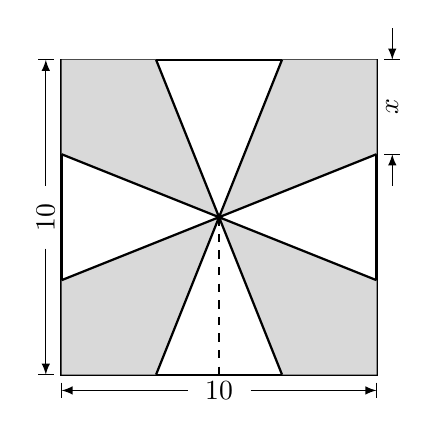
\begin{tikzpicture}[thick,>=latex]
        \draw (-2,-2) -- (-2,2) -- (2,2) -- (2,-2) -- cycle;
        \fill [gray!30] (0,0) -- (0.8,2) -- (2,2) -- (2,0.8) -- cycle;
        \fill [gray!30] (0,0) -- (-0.8,2) -- (-2,2) -- (-2,0.8) -- cycle;
        \fill [gray!30] (0,0) -- (0.8,-2) -- (2,-2) -- (2,-0.8) -- cycle;
        \fill [gray!30] (0,0) -- (-0.8,-2) -- (-2,-2) -- (-2,-0.8) -- cycle;
        \draw (0.8,-2) -- (-0.8,2) (-0.8,-2) -- (0.8,2) (-2,0.8) -- (2,-0.8) (-2,-0.8) -- (2,0.8);
        \draw [dashed] (0,0) -- (0,-2);
        \draw [thin] (-2,-2.1) -- (-2,-2.3) (2,-2.1) -- (2,-2.3) (-2.1,-2) -- (-2.3,-2) (-2.1,2) -- (-2.3,2) (2.1,2) -- (2.3,2) (2.1,0.8) -- (2.3,0.8);
        \draw [->,thin] (-0.4,-2.2) -- (-2,-2.2);
        \draw [->,thin] (0.4,-2.2) -- (2,-2.2);
        \draw [->,thin] (-2.2,-0.4) -- (-2.2,-2);
        \draw [->,thin] (-2.2,0.4) -- (-2.2,2);
        \draw [->,thin] (2.2,0.4) -- (2.2,0.8);
        \draw [->,thin] (2.2,2.4) -- (2.2,2);
        \draw (0,-2.2) node {$10$} (-2.2,0) node {\rotatebox{90}{$10$}} (2.2,1.4) node {\rotatebox{90}{$x$}};
    \end{tikzpicture}
    \begin{tikzpicture}[thick]
        \draw (0,0) node [left] {$A$} coordinate (A) -- (3,0) node [right] {$B$} coordinate (B) --++ (45:1.5) node [right] {$C$} coordinate (C) ++ (-3,0) node [below right] {$D$} coordinate (D);
        \draw ($(B)!0.5!(D)$) node [below left] {$O$} coordinate (O) ++ (0,2) node [above] {$E$} coordinate (E) (E) -- (0,0) (E) -- (C) (E) -- (B);
        \draw [dashed] (E) -- (D);
        \draw [dashed] ($(B)!0.5!(C)$) node [right] {$F$} coordinate (F) -- (O) -- (E) (C) -- (D) -- (A);
        \draw (E) -- (F);
    \end{tikzpicture}
\end{center}
(1) 试把容器罩的表面积$S$表示为$x$的函数;\\
(2) 试把容器罩的体积$V$表示为$x$的函数.
\item {\tiny (000218)}从字母$a$、$b$、$c$、$d$、$e$中任取两个, 求取到字母$a$的概率.
\item {\tiny (000219)}现有$5$根细木棍, 长度(单位: $\text{cm}$)分别为$1$、$3$、$5$、$7$、$9$, 从中任取$3$根. 求能搭成一个三角形的概率.
\item {\tiny (000220)}将$2$本不同的英语书和$1$本语文书在书架上随机排成一行, 求$2$本英语书相邻的概率.
\item {\tiny (000221)}从编号分别为$1$、$2$、$3$、$4$、$5$、$6$的$6$个大小与质地相同的小球中随机取出$3$个, 求恰有$2$个小球编号相邻的概率.
\item {\tiny (000222)}袋中装有大小与质地相同的$5$个球, 其中红色球$3$个, 标号分别为$1$、$2$、$3$; 蓝色球$2$个, 标号分别为$1$、$2$. 从袋中任取$2$个球, 求这$2$个球颜色不同且标号之和不小于$4$的概率.
\item {\tiny (000223)}袋中装有大小与质地相同的$5$个球, 其中白球$3$个, 黑球$2$个, 从中一次摸出$2$个球.\\
(1) 写出该随机试验的一个等可能的样本空间;\\
(2) 求摸出来的$2$个球都是白球的概率;\\
(3) 求摸出来的$2$个球颜色不同的概率.
\item {\tiny (000224)}对某工厂生产的产品质量进行抽查, 数据如下表所示.
\begin{center}
    \begin{tabular}{|c|c|c|c|c|c|}
        \hline
        抽查件数 & $50$ & $100$ & $200$ & $300$ & $500$\\ \hline
        合格件数 & $47$ & $95$ & $192$ & $285$ & $478$\\ \hline        
    \end{tabular}
\end{center}
根据上表所提供的数据, 问: 合格品的概率约为多少?(结果保留两位小数)
\item {\tiny (000225)}射击队某选手命中环数的概率如下表所示.
\begin{center}
    \begin{tabular}{|c|c|c|c|c|}
        \hline
        命中环数 & $10$ & $9$ & $8$ & $7$\\ \hline
        概率 & $0.32$ & $0.28$ & $0.18$ & $0.12$ \\ \hline        
    \end{tabular}
\end{center}
该选手射击一次, 求:\\
(1) 命中$9$环或$10$环的概率;\\
(2) 至少命中$8$环的概率;\\
(3) 命中不足$8$环的概率.
\item {\tiny (000226)}某学生做两道选择题, 已知每道题均有$4$个选项, 其中有且只有一个正确答案. 该学生随意填写两个答案, 求两个答案都选错的概率.
\item {\tiny (000227)}盒子中有标号为$1$、$2$、$3$的$3$个大小与质地相同的球, 随机地取$1$个球, 放回后再取$1$个球, 把这$2$个球对应的号码按照取的先后顺序组成一个两位数. 求个位数与十位数不相同的概率.
\item {\tiny (000228)}一个盒子中装有$4$张卡片, 卡片上分别写有数字$1$、$2$、$3$、$4$. 现从盒子中随机抽取卡片.\\
(1) 若一次抽取$3$张卡片, 求$3$张卡片上数字之和大于$7$的概率;\\
(2) 若第一次抽取$1$张卡片, 放回后再抽取$1$张卡片, 求两次抽取的卡片上数字之和大于$7$的概率.
\item {\tiny (000229)}盒子中有散落的黑白棋子若干粒, 已知从中取出$2$粒都是黑子的概率是$\dfrac 17$, 从中取出$2$粒都是白子的概率是$\dfrac 16$. 问: 从中任意取出$2$粒恰好是同一颜色的概率是多少?
\item {\tiny (000230)}社会调查人员总希望从对人群的随机抽样调查中得到对他们所提问题的诚实回答, 但是被采访者常常不愿意如实做出应答. 1965年, 华纳(Stanley L. Warner)发明了一种应
用概率知识来消除这种不愿意如实回答的情绪的方法. 华纳的随机化应答方法要求人们随机地回答所提两个问题中的一个, 而不必告诉采访者究竟回答的是哪个问题, 在这两个问题中有一个是敏感的或者令人为难的, 另一个则是无关紧要的. 这样, 应答者将乐意如实地回答问题, 因为只有他自己知道回答的是哪个问题. 例如, 在调查运动员是否服用兴奋剂的时候, 设计一个从袋中摸球的试验: 袋中放有$1$黑$1$白两个大小与质地相同的小球, 运动员从中随意摸出$1$个小球. 无关紧要的问题是: 你摸出的小球是白色的吗? 而敏感的问题是: 你服用过兴奋剂吗? 然后要求被调查的运动员抛掷一枚硬币, 如果出现正面, 就回答第一个问题, 否则回答第二个问题. 假设用这个方法调查了$200$名运动员, 得到$56$个``是''的回答, 请你估计这群运动员中大约有百分之几的人服用过兴奋剂.
\item {\tiny (000231)}在一次知识竞赛中, 假设$A$、$B$、$C$、$D$四人独立答题, 且答对的概率分别为$P(A)=\dfrac 13$, $P(B)=\dfrac 14$, $P(C)=\dfrac 15$, $P(D)=\dfrac 23$, 如果将$A$、$B$、$C$组成一组与$D$比赛, 且$A$、$B$、$C$三人中有一人答对即算该组答对, 那么哪一方答对的概率大?
\item {\tiny (000232)}某高校研究人员希望调查该校大学生平均每天的自习时间. 他调查了$100$名大学生, 发现他们每天的平均自习时间是$3.5\text{h}$. 这里的总体是\bracket{20}.
\onech{该校的所有大学生}{该校所有大学生的平均每天自习时间}{所调查的$100$名大学生}{所调查的$100$名大学生的平均每天自习时间}
\item {\tiny (000233)}某家大型超市的日客流量(单位: 千人次)分别为: $3.4$、$3.6$、$5.6$、$1.8$、$3.7$、$4.0$、$2.5$、$2.8$、$4.4$、$3.6$. 下列图形中不利于描述这些数据的是\bracket{20}.
\fourch{散点图}{条形图}{茎叶图}{扇形图}
\item {\tiny (000234)}某汽车销售商销售某品牌的A、B、C三类轿车, 每类轿车均有舒适型和经济型两种型号, 其某月的销量(单位: 辆)如下表所示.
\begin{center}
    \begin{tabular}{|c|c|c|c|}
        \hline
        & A & B & C \\ \hline
        舒适型/辆 & $35$ & $28$ & $15$\\ \hline
        经济型/辆 & $50$ & $72$ & $40$\\ \hline
    \end{tabular}
\end{center}
试设计一个抽样方案, 从该月购买轿车的客户中抽取20位, 调查他们的满意度.
\item {\tiny (000235)}某校$30$名高一女生的扔手球记录如下(单位: $\text{m}$):
\begin{center}
    \begin{tabular}{cccccccccc}
        $16.3$ & $13.2$ & $17.7$ & $14.3$ & $16.4$ & $19.8$ & $13.5$ & $14.5$ & $11.7$ & $14.1$\\
        $14.8$ & $17.2$ & $13.8$ & $15.4$ & $16.3$ & $15.7$ & $18.5$ & $16.8$ & $17.9$ & $15.9$\\
        $17.6$ & $15.4$ & $16.8$ & $21.4$ & $16.5$ & $18.1$ & $16.0$ & $20.3$ & $16.6$ & $19.5$
    \end{tabular}
\end{center}
(1) 选择适当的组距, 制作一张频率分布表;\\
(2) 在(1)的基础上, 绘制一幅频率分布直方图.
\item {\tiny (000236)}某公司对应聘人员进行能力测试, 测试成绩总分为150分, 下面是50位应聘人员
的测试成绩:
\begin{center}
    \begin{tabular}{cccccccccc}
        $64$ & $67$ & $70$ & $72$ & $74$ & $76$ & $76$ & $79$ & $80$ & $81$ \\
        $82$ & $82$ & $83$ & $85$ & $86$ & $88$ & $91$ & $91$ & $92$ & $93$ \\
        $93$ & $93$ & $95$ & $96$ & $96$ & $97$ & $97$ & $99$ & $100$ & $100$ \\
        $102$ & $104$ & $106$ & $106$ & $107$ & $108$ & $108$ & $112$ & $112$ & $114$ \\
        $116$ & $118$ & $119$ & $119$ & $122$ & $123$ & $125$ & $126$ & $128$ & $133$
    \end{tabular}
\end{center}
试用这些数据绘制一幅茎叶图.
\item {\tiny (000237)}某超市从一家食品有限公司购进一批茶叶, 每罐茶叶的标准质量是$125\text{g}$, 为了解该批茶叶的质量情况, 从中随机抽取$20$罐, 称得各罐质量(单位: $\text{g}$)如下:
\begin{center}
    \begin{tabular}{ccccccc}
        $124.9$ & $124.7$ & $126.2$ & $124.9$ & $124.2$ & $124.9$ & $123.7$ \\
        $121.4$ & $126.4$ & $127.7$ & $121.9$ & $124.4$ & $125.2$ & $123.7$ \\
        $122.7$ & $124.2$ & $126.2$ & $125.2$ & $122.2$ & $125.4$
    \end{tabular}
\end{center}
回答下列问题:\\
(1) $20$罐茶叶的平均质量$\bar{x}$是多少, 标准差$s$是多少?
(2) 有多少罐茶叶的质量位于$\bar x-s$与$\bar x +s$之间, 所占的百分比是多少?
\item {\tiny (000238)}数据$x_1$、$x_2$、$\cdots$、$x_n$的方差为$s_x^2$, 数据$y_1$、$y_2$、$\cdots$、$y_n$的方差为$s_y^2$, 若$y_1=ax_1+b$, $y_2=ax_2+b$, $\cdots$, $y_n=ax_n+b$成立, $a$、$b$为常数, 求证: $s_y^2=a^2s_x^2$.
\item {\tiny (000239)}下表是上海市$2007$年至$2016$年的月平均气温(单位: $^\circ\text{C}$).
\begin{center}
    \begin{tabular}{|c|c|c|c|c|c|c|c|c|c|c|c|c|}
        \hline
        年份 & $1$月 & $2$月 & $3$月 & $4$月 & $5$月 & $6$月 & $7$月 & $8$月 & $9$月 & $10$月 & $11$月 & $12$月 \\ \hline
        $2007$ & $5.9$ & $9.8$ & $12.1$ & $15.9$ & $22.9$ & $25$ & $30.4$ & $29.7$ & $25.4$ & $20.6$ & $14.2$ & $9.8$ \\ \hline
        $2008$ & $4.5$ & $4.2$ & $11.6$ & $16.1$ & $21.8$ & $24.2$ & $30.4$ & $28.6$ & $26$ & $21$ & $13.3$ & $7.9$ \\ \hline
        $2009$ & $4.3$ & $9.3$ & $10.8$ & $16.7$ & $22.5$ & $26.3$ & $29$ & $28.1$ & $25.4$ & $21.4$ & $12.4$ & $6.9$ \\ \hline
        $2010$ & $5.7$ & $7.7$ & $9.6$ & $13.3$ & $20.9$ & $24.1$ & $28.8$ & $30.9$ & $26.2$ & $19.3$ & $14.2$ & $8.1$\\ \hline
        $2011$ & $1.9$ & $6.5$ & $9.5$ & $16.2$ & $21.9$ & $24.4$ & $30.2$ & $28.3$ & $24.7$ & $19.3$ & $16.7$ & $6.9$\\ \hline
        $2012$ & $5.1$ & $4.8$ & $9.8$ & $17.6$ & $21.6$ & $24.7$ & $29.9$ & $29$ & $23.9$ & $20.1$ & $12.6$ & $6.6$\\ \hline
        $2013$ & $4.6$ & $6.8$ & $11$ & $15.3$ & $21.3$ & $24.1$ & $32$ &  $31$ & $25$ & $20$ & $13.4$ & $6.1$\\ \hline
        $2014$ & $6.6$ & $6.1$ & $11.5$ & $15.7$ & $21.7$ & $23.3$ & $27.4$ & $26.3$ & $24.2$ & $20.2$ & $14.8$ & $5.7$\\ \hline
        $2015$ & $6$ & $6.8$ & $10.6$ & $15.9$ & $20.5$ & $24.2$ & $26.7$ & $27.8$ & $24.2$ & $19.6$ & $14$ & $7.8$\\ \hline
        $2016$ & $4.4$ & $6.9$ & $11$ & $16.7$ & $20.6$ & $24.2$ & $29.9$ & $29.5$ & $24.9$ & $20.8$ & $13.6$ & $9.1$\\ \hline
    \end{tabular}
\end{center}
\begin{flushright}
{\it 数据来源: 上海统计年鉴.}
\end{flushright}
回答下列问题:\\
(1) $10$年中每年最冷的月份相同吗?\\
(2) $10$年中哪个月份的气温波动最大?\\
(3) $10$年中哪一年的气温波动最大?\\
(4) 绘制$10$年中$7$月份与$8$月份气温的折线图, 比较气温的高低.
\item {\tiny (000240)}某高校数学专业共有$850$名学生, 从中选取$20$名学生参加学生代表大会. 试写出具体抽样方案.
\item {\tiny (000241)}某校高一年级学生进行了$4$次测验, 成绩(单位: 分)如下表所示. 根据$4$次测验的结果, 我们如何比较这$10$名学生的成绩? 下周有一场数学竞赛活动, 如果需要$1$名学生参赛, 那么推荐谁去最好? 如果需要$4$名学生参赛, 那么又该推荐谁去?
\begin{center}
    \begin{tabular}{|c|c|c|c|c|}
        \hline
        学生编号 & 第$1$次 & 第$2$次 & 第$3$次 & 第$4$次 \\ \hline
        $1$ & $90$ & $82$ & $97$ & $100$ \\ \hline
        $2$ & $103$ & $86$ & $101$ & $92$ \\ \hline
        $3$ & $77$ & $83$ & $106$ & $87$ \\ \hline
        $4$ & $94$ & $93$ & $99$ & $99$ \\ \hline 
        $5$ & $89$ & $97$ & $93$ & $90$\\ \hline
        $6$ & $101$ & $79$ & $87$ & $95$\\ \hline
        $7$ & $91$ & $92$ & $91$ & $93$ \\ \hline
        $8$ & $82$ & $94$ & $100$ & $106$ \\ \hline
        $9$ & $88$ & $78$ & $95$ & $78$ \\ \hline
        $10$ & $83$ & $88$ & $104$ & $89$ \\ \hline        
    \end{tabular}
\end{center}
\item {\tiny (000242)}某客服部门计划根据员工每个月接通的电话数给予奖金奖励, 并且要保证$50\%$的员工能拿到基本奖励, 拿到基本奖励的员工中至多$10\%$的人能够拿到额外奖励. 该部门随
机抽取了$30$名员工, 调查了他们上半个月与客户的通话数量, 数据如下:
\begin{center}
    \begin{tabular}{cccccccccc}
        $1344$ & $1428$ & $1083$ & $1239$ & $1381$ & $1099$ & $1607$ & $1041$ & $1130$ & $1610$ \\
        $1445$ & $921$ & $931$ & $1100$ & $1197$ & $1282$ & $1549$ & $1463$ & $901$ & $1354$ \\
        $1378$ & $1752$ & $1032$ & $968$ & $902$ & $1804$ & $1051$ & $1319$ & $1223$ & $1124$
    \end{tabular}
\end{center}
请利用百分位数来为该部门设计奖励方案.
\item {\tiny (000243)}求直线$\sqrt 2x-4y+5=0$的倾斜角(用$\arctan$表示).
\item {\tiny (000244)}若直线$ax+2y+6=0$和直线$x+a(a+1)y+(a^2-1)=0$互相垂直, 求实数$a$的值.
\item {\tiny (000245)}直线$x-y+1=0$上一点$P$的横坐标是$3$, 若该直线绕点$P$逆时针旋转$90^\circ$得到直线$l$, 求直线$l$的方程.
\item {\tiny (000246)}设直线$x-ay-4=0$与直线$y=-2x+4$的夹角为$\arccos \dfrac{2\sqrt 5}5$, 求实数$a$的值.
\item {\tiny (000247)}已知$\alpha\in [0, \dfrac\pi 2)$, 求直线$x\cos \alpha+\sqrt 3y+2=0$的倾斜角的取值范围.
\item {\tiny (000248)}求过点$(3, -2)$且在$x$轴、$y$轴上截距相等的直线的方程.
\item {\tiny (000249)}已知点$P(1, 1)$到直线$x+ay-2=0$的距离为$1$, 求实数$a$的值.
\item {\tiny (000250)}已知平行四边形$ABCD$中, 边$AB$所在直线的方程为$x+y-1=0$, 边$AD$所在直线的方程为$3x-y+4=0$.\\
(1) 求点$A$的坐标;\\
(2) 若点$C$的坐标为$(3, 3)$, 分别求边$BC$与$DC$所在直线的方程.
\item {\tiny (000251)}已知直线$l_1: x+my+6=0$, $l_2: (m-2)x+3y+2m=0$, 求实数$m$的取值范围, 使得:\\
(1) $l_1$与$l_2$相交;\\
(2) $l_1\perp l_2$;\\
(3) $l_1\parallel l_2$;\\
(4) $l_1$与$l_2$重合.
\item {\tiny (000252)}已知直线$l$与两坐标轴围成一个等腰直角三角形, 且此三角形的面积为$\dfrac{49}2$. 求直线$l$的方程.
\item {\tiny (000253)}在$\triangle ABC$中, 边$AB$、$AC$上的高所在直线的方程分别为$2x-3y+1=0$与$x+y=0$, 点$A$的坐标为$(1, 2)$. 求边$BC$所在直线的方程.
\item {\tiny (000254)}已知直线$l$垂直于直线$3x+4y-9=0$, 点$A(2, 3)$到直线$l$的距离为$1$. 求直线$l$的方程.
\item {\tiny (000255)}已知三条直线$l_1: ax+by+4=0$, $l_2: (a-1)x+y+b=0$, $l_3: x+2y+3=0$.\\
(1) 若$l_1\perp l_2$且$l_1$经过点$(-1, 1)$, 求$a$、$b$的值;\\
(2) 若$l_1\parallel l_2\parallel l_3$, 求$a$、$b$的值.
\item {\tiny (000256)}已知过点$(0, -2)$且具有斜率$k$的直线$l$与以点$A(3, 1)$和$B(-2, 5)$为端点的线段$AB$相交, 求实数$k$的取值范围.
\item {\tiny (000257)}已知两条直线$l_1: y-x=0$, $l_2: y=ax$, 其中$a\in \mathbf{R}$. 当这两条直线的夹角在$(0, \dfrac{\pi}{12})$内变化时, 求实数$a$的取值范围.
\item {\tiny (000258)}直线$l$过原点且平分平行四边形$ABCD$的面积, 若此平行四边形的两个顶点为$B(1, 4)$、$D(5, 0)$, 求直线$l$的方程.
\item {\tiny (000259)}求直线$l_1: 3x-2y-6=0$关于直线$l_2: 2x-3y+1=0$对称的直线$l_3$的方程.
\item {\tiny (000260)}已知动点$M(a, b)$在直线$3x+4y-15=0$上, 求$\sqrt{a^2+b^2}$的最小值.
\item {\tiny (000261)}已知两条平行直线$l_1$与$l_2$分别过点$P_1(1, 0)$与点$P_2(0, 5)$, $l_1$、$l_2$之间的距离为$d$. 求$d$的最大值, 并指出此时$l_1$、$l_2$的方程.
\item {\tiny (000262)}已知直线$l$经过点$C(2, 1)$, 且与$x$轴、$y$轴的正半轴分别交于点$A$、点$B$, $O$是坐标原点.\\
(1) 当$\triangle AOB$的面积最小时, 求直线$l$的方程;\\
(2) 当$|CA|\cdot |CB|$取最小值时, 求直线$l$的方程, 并求此最小值.
\item {\tiny (000263)}作出方程$|x|+|y|=1$所表示的图形, 并求该图形围成的区域的面积.
\item {\tiny (000264)}给定直线$l_1: y=k_1x+b_1$与$l_2: y=k_2x+b_2$, 求证: 如果直线$l_1$与$l_2$不互相垂直, 那么它们的夹角$\alpha$满足$\tan \alpha=|\dfrac{k_1-k_2}{1+k_1k_2}|$.
\item {\tiny (000265)}已知直线$l_1: 4x+y=4$, $l_2: mx+y=0$, $l_3: 2x-3my=4$. 当$m$为何值时, 它们不能围成三角形?
\item {\tiny (000266)}点到直线的距离是该点到直线上任意一点距离的最小值. 如果把一个给定点到线段上任意一点的距离的最小值定义为该点到该线段的距离, 试求点$P(1, 1)$到线段$l: x-
y-3=0 \ (3\le x\le 5)$的距离.
\item {\tiny (000267)}判断下列命题是否正确, 并说明理由:\\
(1) 到两坐标轴距离相等的点的轨迹方程为$y=x$;\\
(2) 若$\triangle ABC$的三个顶点的坐标分别为$A(1, 1)$、$B(3, 1)$、$C(1, 3)$, 则边$BC$上的中线所在直线的方程为$y=x$;\\
(3) 与两点$A(-1, 0)$、$B(1, 0)$的连线的夹角为$90^\circ$的动点的轨迹方程为$x^2+y^2=1$.
\item {\tiny (000268)}讨论圆$x^2+y^2+6x-7=0$与抛物线$y^2=-4x$准线的位置关系.
\item {\tiny (000269)}对圆$(x-a)^2+(y+b)^2=a^2+b^2\ (a>0, \ b>0)$, 下列说法是否正确, 请说明理由:\\
(1) 该圆的圆心为$(a, b)$;\\
(2) 该圆过原点;\\
(3) 该圆与$x$轴相交于两个不同点.
\item {\tiny (000270)}若椭圆$\dfrac{x^2}{4}+\dfrac{y^2}{a^2}=1$与双曲线$\dfrac{x^2}{a^2}-\dfrac{y^2}2=1$有相同的焦点, 求实数$a$的值.
\item {\tiny (000271)}设椭圆$\dfrac{x^2}{a^2}+\dfrac{y^2}{b^2}=1 \ (a>b>0)$的焦距为$2c$. 若$b^2=ac$, 求该椭圆的离心率.
\item {\tiny (000272)}已知圆$C$的半径为$3$, 它与双曲线$\dfrac{x^2}4-y^2=1$的两条渐近线均相切, 且与该双曲线的右支相交. 求圆$C$的方程.
\item {\tiny (000273)}已知直线$y=x+b$被曲线$y=\dfrac 12x^2$截得的弦长为$4\sqrt 2$, 求实数$b$的值.
\item {\tiny (000274)}点$P$是圆$x^2+y^2=4$上的动点, 过点$P$作$x$轴的垂线, 垂足为$M$. 若$\overrightarrow{PQ}=2\overrightarrow{QM}$, 求点$Q$的轨迹方程.
\item {\tiny (000275)}设$AB$是过抛物线$y^2=2px$焦点$F$的一条弦, 过点$A$、$B$分别作该抛物线准线的垂线, 垂足分别为$A_1$、$B_1$. 求证: $\angle A_1FB_1=\dfrac\pi 2$.
\item {\tiny (000276)}已知圆$O$的方程是$x^2+y^2=1$, 直线$l$与圆$O$相切.\\
(1) 若直线$l$的斜率等于$1$, 求直线$l$的方程;\\
(2) 若直线$l$在$y$轴上的截距为$\sqrt 2$, 求直线$l$的方程.
\item {\tiny (000277)}直线$x-\sqrt 3y=0$绕原点按逆时针方向旋转$30^\circ$后所得的直线$l$与圆$(x-2)^2+y^2=3$的位置关系是\bracket{20}.
\twoch{直线$l$过圆心}{直线$l$与圆相交, 但不过圆心}{直线$l$与圆相切}{直线$l$与圆无公共点}
\item {\tiny (000278)}已知点$A(-\dfrac 12, 0)$, $B$是圆$C: (x-\dfrac 12)^2+y^2=4$($C$是圆心)上一动点, 线段$AB$的垂直平分线交$BC$于$M$. 求动点$M$的轨迹方程.
\item {\tiny (000279)}过抛物线$y^2=4x$的焦点$F$作动直线交抛物线于$A$、$B$两点, 并从原点$O$作$AB$的垂线, 垂足为$M$. 求动点$M$的轨迹方程.
\item {\tiny (000280)}已知点$P$是双曲线$\dfrac{x^2}9-\dfrac{y^2}{16}=1$右支上的一点, 点$M$、$N$分别是圆$(x+5)^2+y^2=4$和$(x-5)^2+y^2=1$上的点. 求$|PM|-|PN|$的最大值.
\item {\tiny (000281)}已知圆$x^2+y^2+x-6y+m=0$与直线$x+2y-3=0$相交于$P$、$Q$两点, $O$为坐标原点. 若$OP\perp OQ$, 求实数$m$的值.
\item {\tiny (000282)}已知直线$y=ax-1$与曲线$y^2=2x$只有一个公共点, 求实数$a$的值.
\item {\tiny (000283)}对于实数$k$的不同取值范围, 讨论方程$kx^2+y^2-2=0$所表示的曲线的形状.
\item {\tiny (000284)}过椭圆$b^2x^2+a^2y^2=a^2b^2 \ (a>b>0)$的顶点$B(0, -b)$引一条弦$BP$, 求弦$BP$的最大长度.
\item {\tiny (000285)}已知定点$A(a, 0) \ (0<a<3)$到椭圆$\dfrac{x^2}9+\dfrac{y^2}4=1$上的点的距离的最小值为$1$, 求$a$的值.
\item {\tiny (000286)}据气象预报, 在气象台$A$处向东$400\text{km}B$处的海面上有一个台风中心形成, 测得台风以$40\text{km}/\text{h}$的速度向西北方向移动, 距中心不超过$300\text{km}$的地方都会受到台风的影响. 从现在起, 多少时间后气象台受到台风影响?  气象台受到台风影响的时长大约是多少(结果精确到$0.1\text{h}$)?
\item {\tiny (000287)}已知$\triangle ABC$的两个顶点$A$、$B$的坐标分别是$(-6, 0)$、$(6, 0)$, 且边$AC$、$BC$所在直线的斜率之积等于$k$. 讨论顶点$C$的轨迹方程.
\item {\tiny (000288)}以$P$为圆心的动圆与圆$C_1: (x+2)^2+y^2=1$和圆$C_2: (x-2)^2+y^2=r^2$均相切, 请分别写出$r$的某个值, 使点$P$的轨迹为椭圆和双曲线.
\item {\tiny (000289)}求双曲线$y=\dfrac 1x$的焦点坐标与准线方程.
\item {\tiny (000290)}请验证到点$(1, \dfrac 14)$的距离和到直线$y=-\dfrac 14$的距离相等的动点的轨迹方程是二次函数$y=x^2-2x+1$, 并探究一般情况.
\item {\tiny (000291)}求连接点$A(x, y, z)$与点$B(x', y', z')$的线段$AB$的中点$M$的坐标.
\item {\tiny (000292)}设正四面体$ABCD$的棱长为$a$, $E$为$BC$的中点, $F$为$CD$的中点. 求$\overrightarrow{BF}\cdot\overrightarrow{AE}$.
\item {\tiny (000293)}给定点$A(1, 0, 0)$、$B(3, 1, 1)$、$C(2, 0, 1)$与点$D(5, -4, 3)$.\\
(1) 求$\overrightarrow{AD}$在$\overrightarrow{AB}$、$\overrightarrow{BC}$、$\overrightarrow{CA}$方向上的投影向量;\\
(2) 求点$D$到平面$ABC$的距离.
\item {\tiny (000294)}如图, 在正三棱柱$ABC-A_1B_1C_1$中, $|AB|=\sqrt 2|AA_1|$, $D$是$A_1B_1$的中点, 点$E$在$A_1C_1$上, 且$DE\perp AE$.
\begin{center}
    \begin{tikzpicture}[thick]
        \draw (0,0) node [left] {$A$} coordinate (A) -- (0,2) node [left] {$A_1$} coordinate (A1) --++ ({2*sqrt(2)},0) node [right] {$C_1$} coordinate (C1) --++ (0,-2) node [right] {$C$} coordinate (C);
        \draw ({sqrt(2)},0) ++ (-45:{sqrt(6)/2}) node [below] {$B$} coordinate (B) --++ (0,2) node [left] {$B_1$} coordinate (B1) (B) -- (A) (B) -- (C) (B1) -- (A1) (B1) -- (C1);
        \draw ($(A1)!0.5!(B1)$) node [above] {$D$} coordinate (D) -- ($(A1)!0.25!(C1)$) node [above] {$E$} coordinate (E);
        \draw [dashed] (E) -- (A) -- (D) (A) -- (C1) (A) -- (C);
    \end{tikzpicture}
\end{center}
(1) 求证: $\text{平面}ADE\perp \text{平面}ACC_1A_1$;\\
(2) 求直线$AD$和平面$ABC_1$所成角的大小.
\item {\tiny (000295)}已知正四棱锥的体积为$12$, 底面对角线的长为$2\sqrt 6$. 求侧面与底面所成二面角的大小.
\item {\tiny (000296)}如图, 已知$ABCD-A_1B_1C_1D_1$是底面边长为$1$的正四棱柱, $O_1$是$A_1C_1$和$B_1D_1$的交点.
\begin{center}
    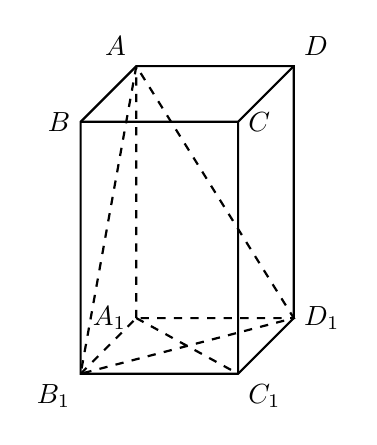
\begin{tikzpicture}[thick,scale = 2]
        \draw (0,0) node [below left] {$B_1$} coordinate (B1) --++ (1,0) node [below right] {$C_1$} coordinate (C1) --++ (45:{1/2}) node [right] {$D_1$} coordinate (D1)
        --++ (0,1.6) node [above right] {$D$} coordinate (D)
        --++ (-1,0) node [above left] {$A$} coordinate (A) --++ (225:{1/2}) node [left] {$B$} coordinate (B) -- cycle;
        \draw (B1) ++ (1,1.6) node [right] {$C$} coordinate (C) -- (C1) (C) --++ (45:{1/2}) (D) (C) --++ (-1,0);
        \draw [dashed] (B1) --++ (45:{1/2}) node [left] {$A_1$} coordinate (A1) --++ (1,0) (A1) --++ (0,1.6);
        \draw [dashed] (A) -- (B1) -- (D1) -- cycle (A1) -- (C1);
    \end{tikzpicture}
\end{center}
(1) 设$AB_1$与底面$A_1B_1C_1D_1$所成角的大小为$\alpha$, 二面角$A-B_1D_1-A_1$的大小为$\beta$. 求证: $\tan \beta=\sqrt 2\tan \alpha$;\\
(2) 若点$C$到平面$AB_1D_1$的距离为$\dfrac 43$, 求此正四棱柱的高.
\item {\tiny (000297)}如图, 在直三棱柱$ABC-A_1B_1C_1$中, $\angle ACB=90^\circ$, $|AC|=|BC|=|CC_1|=2$.
\begin{center}
    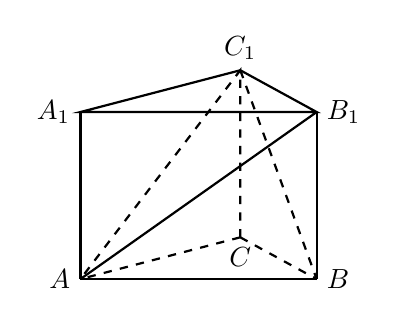
\begin{tikzpicture}[thick,scale = 1.5]
        \draw (0,0) node [left] {$A$} coordinate (A) -- (2,0) node [right] {$B$} coordinate (B);
        \draw [dashed] (1,0) ++ (45:0.5) node [below] {$C$} coordinate (C) -- (A) (C) -- (B) (C) --++ (0,{sqrt(2)}) node [above] {$C_1$} coordinate (C1) -- (A) (C1) -- (B);
        \draw (A) --++ (0,{sqrt(2)}) node [left] {$A_1$} coordinate (A1) (B) --++ (0,{sqrt(2)}) node [right] {$B_1$} coordinate (B1);
        \draw (A1) -- (B1) -- (C1) -- cycle (A) -- (B1);
    \end{tikzpicture}
\end{center}
(1) 求证: $AB_1\perp BC_1$;\\
(2) 求点$B$到平面$AB_1C_1$的距离.
\item {\tiny (000298)}如图, 四棱锥$P-ABCD$的底面$ABCD$为梯形, $AD\parallel BC$, $AB\perp BC$, $|AB|=1$, $|AD|=3$, $\angle ADC=45^\circ$, 且$PA\perp \text{平面}ABCD$, $|PA|=1$.
\begin{center}
    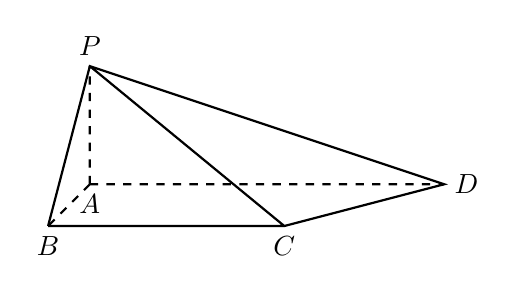
\begin{tikzpicture}[thick,scale = 1.5]
        \draw [dashed] (0,0) node [below] {$A$} -- (3,0) node [right] {$D$} (0,0) -- (225:0.5) node [below] {$B$} coordinate (B) (0,0) -- (0,1) node [above] {$P$};
        \draw (B) --++ (2,0) node [below] {$C$} coordinate (C) -- (3,0) -- (0,1) -- (B) (C) -- (0,1);
    \end{tikzpicture}
\end{center}
(1) 求异面直线$PB$与$CD$所成角的大小;\\
(2) 求四棱锥$P-ABCD$的体积.
\item {\tiny (000299)}如图, 在直三棱柱$ABC-A_1B_1C_1$中, $\angle BAC=90^\circ$, $|AB|=|AC|=a$, $|AA_1|=2a$, $D$为$BC$的中点, $E$为$CC_1$上的点, 且$|CE|=\dfrac 14 |CC_1|$.
\begin{center}
    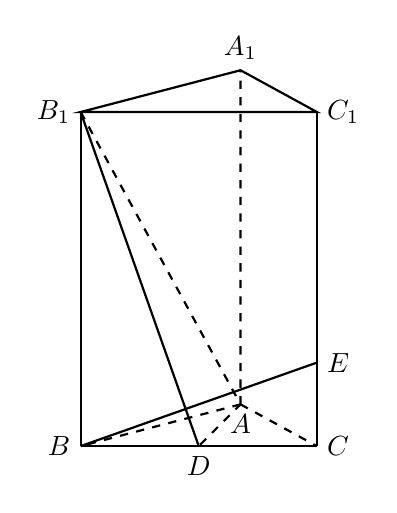
\begin{tikzpicture}[thick,scale = 1.5]
        \draw (0,0) node [left] {$B$} coordinate (B) -- (2,0) node [right] {$C$} coordinate (C);
        \draw [dashed] (1,0) ++ (45:0.5) node [below] {$A$} coordinate (A) -- (B) (A) -- (C) (A) --++ (0,{2*sqrt(2)}) node [above] {$A_1$} coordinate (A1);
        \draw (B) --++ (0,{2*sqrt(2)}) node [left] {$B_1$} coordinate (B1) (C) --++ (0,{2*sqrt(2)}) node [right] {$C_1$} coordinate (C1);
        \draw (A1) -- (B1) -- (C1) -- cycle;
        \draw [dashed] (B1) -- (A) -- (1,0) node [below] {$D$} coordinate (D);
        \draw (B1) -- (D) (C) ++ (0,{sqrt(2)/2}) node [right] {$E$} -- (B);
    \end{tikzpicture}
\end{center}
(1) 求证: $BE\perp \text{平面}ADB_1$;\\
(2) 求二面角$B-AB_1-D$的大小.
\item {\tiny (000300)}在长方体$ABCD-A_1B_1C_1D_1$中, $|AB|=|BC|=2$, $A_1D$与$BC_1$所成的角为$\dfrac\pi 2$. 求$BC_1$与平面$BB_1D_1D$所成角的大小.
\item {\tiny (000301)}如图, 在平行六面体$ABCD-A_1B_1C_1D_1$中, 点$E$、$F$分别在$B_1B$和$D_1D$上, 且$|BE|=\dfrac 13|BB_1|$, $|DF|=\dfrac 23|DD_1|$.
\begin{center}
    \begin{tikzpicture}[thick]
        \draw (0,0) node [below left] {$A$} coordinate (A) --++ (2,0) node [below right] {$B$} coordinate (B) --++ (45:{1.8/2}) node [right] {$C$} coordinate (C)
        --++ (0.2,2.6) node [above right] {$C_1$} coordinate (C1)
        --++ (-2,0) node [above left] {$D_1$} coordinate (D1) --++ (225:{1.8/2}) node [left] {$A_1$} coordinate (A1) -- cycle;
        \draw (A) ++ (2.2,2.6) node [below left] {$B_1$} coordinate (B1) -- (B) (B1) --++ (45:{1.8/2}) (B1) --++ (-2,0);
        \draw [dashed] (A) --++ (45:{1.8/2}) node [left] {$D$} coordinate (D) --++ (2,0) (D) --++ (0.2,2.6);
        \draw ($(B)!{1/3}!(B1)$) node [right] {$E$} coordinate (E) -- (C1) (E) -- (A);
        \draw [dashed] ($(D1)!{1/3}!(D)$) node [left] {$F$} coordinate (F) -- (E) (F) -- (C1) (F) -- (A);
    \end{tikzpicture}
\end{center}
(1) 求证: $A$、$E$、$C_1$、$F$四点共面;\\
(2) 若$\overrightarrow{EF} =\lambda \overrightarrow{AB}+ \mu \overrightarrow{AD}+ \nu \overrightarrow{AA_1}$, 求$\lambda+\mu+\nu$的值.
\item {\tiny (000302)}如图, 在正方体$ABCD-A_1B_1C_1D_1$中, $E$、$F$分别是$BC$、$A_1D_1$的中点.
\begin{center}
    \begin{tikzpicture}[thick]
        \draw (0,0) node [below left] {$B$} coordinate (B) --++ (2,0) node [below right] {$C$} coordinate (C) --++ (45:{2/2}) node [right] {$D$} coordinate (D)
        --++ (0,2) node [above right] {$D_1$} coordinate (D1)
        --++ (-2,0) node [above left] {$A_1$} coordinate (A1) --++ (225:{2/2}) node [left] {$B_1$} coordinate (B1) -- cycle;
        \draw (B) ++ (2,2) node [right] {$C_1$} coordinate (C1) -- (C) (C1) --++ (45:{2/2}) (C1) --++ (-2,0);
        \draw [dashed] (B) --++ (45:{2/2}) node [left] {$A$} coordinate (A) --++ (2,0) (A) --++ (0,2);
        \draw [dashed] ($(B)!0.5!(C)$) node [below] {$E$} coordinate (E) -- (D) --  ($(D1)!0.5!(A1)$) node [above] {$F$} coordinate (F) (A1) -- (C);
        \draw (E) -- (B1) -- (F);
    \end{tikzpicture}
\end{center}
(1) 求证: 四边形$B_1EDF$是菱形;\\
(2) 求异面直线$A_1C$与$DE$所成角的大小.
\item {\tiny (000303)}在正方体$ABCD-A_1B_1C_1D_1$中, $E$、$F$分别是$BC$、$CC_1$的中点.\\
(1) 求证: 点$D_1$在平面$AEF$上;\\
(2) 求平面$AEFD_1$与底面$ABCD$所成二面角的大小.
\item {\tiny (000304)}如图, $ABCD-A_1B_1C_1D_1$为正方体, 动点$P$在对角线$BD_1$上, 记$\dfrac{|D_1P|}{|D_1B|}=\lambda$.
\begin{center}
    \begin{tikzpicture}[thick]
        \draw (0,0) node [below left] {$A$} coordinate (A) --++ (2,0) node [below right] {$B$} coordinate (B) --++ (45:{2/2}) node [right] {$C$} coordinate (C)
        --++ (0,2) node [above right] {$C_1$} coordinate (C1)
        --++ (-2,0) node [above left] {$D_1$} coordinate (D1) --++ (225:{2/2}) node [left] {$A_1$} coordinate (A1) -- cycle;
        \draw (A) ++ (2,2) node [right] {$B_1$} coordinate (B1) -- (B) (B1) --++ (45:{2/2}) (B1) --++ (-2,0);
        \draw [dashed] (A) --++ (45:{2/2}) node [left] {$D$} coordinate (D) --++ (2,0) (D) --++ (0,2);
        \draw (D1) -- (B1) -- (C);
        \draw [dashed] (B) -- (D1) (C) -- ($(B)!0.4!(D1)$) node [above] {$P$} -- (A);
    \end{tikzpicture}
\end{center}
(1) 求证: $AP\perp B_1C$;\\
(2) 若异面直线$AP$与$D_1B_1$所成角为$\dfrac \pi 4$, 求$\lambda$的值;\\
(3) 当$\angle APC$为钝角时, 求$\lambda$的取值范围.
\item {\tiny (000305)}如图, 平行六面体$ABCD-A_1B_1C_1D_1$的底面$ABCD$是正方形, $O$为底面的中心, $A_1O\perp\text{平面}ABCD$, $|AB|=|AA_1|=\sqrt 2$.
\begin{center}
    \begin{tikzpicture}[thick,scale = 1.5]
        \draw (0,0) node [below left] {$A$} coordinate (A) --++ ({sqrt(2)},0) node [below right] {$B$} coordinate (B) --++ (45:{sqrt(2)/2}) node [right] {$C$} coordinate (C);
        \draw [dashed] (C) --++ ({-sqrt(2)},0) node [below] {$D$} coordinate (D) -- (A);
        \draw ($(A)!0.5!(C)$) node [below] {$O$} coordinate (O) ++ (0,1) node [left] {$A_1$} coordinate (A1) --++ ({sqrt(2)},0) node [above] {$B_1$} coordinate (B1) --++ (45:{sqrt(2)/2}) node [right] {$C_1$} coordinate (C1) --++ ({-sqrt(2)},0) node [above] {$D_1$} coordinate (D1) -- (A1); 
        \draw (A) -- (A1) (B) -- (B1) (C) -- (C1);
        \draw [dashed] (O) -- (A1) -- (D) (D1) -- (D) -- (B) (A) -- (C);
    \end{tikzpicture}
\end{center}
(1) 求证: $A_1C\perp \text{平面}BB_1D_1D$;\\
(2) 求平面$OCB_1$与平面$BB_1D_1D$所成二面角的大小.
\item {\tiny (000306)}填空题:\\
(1) 已知数列$\{a_n\}$是等差数列, 下面的数列中必为等差数列的序号是\blank{50}.\\
\textcircled{1} $\{a_{2n}\}$ \textcircled{2} $\{a_n+a_{n+1}\}$ \textcircled{3} $\{3a_n+1\}$ \textcircled{4} $\{|a_n|\}$\\
(2) 已知数列$\{a_n\}$是等比数列, 下面的数列中必为等比数列的序号是\blank{50}.\\
\textcircled{1} $\{a_n^2\}$ \textcircled{2} $\{a_n+a_{n+1}\}$ \textcircled{3} $\{\dfrac 1{a_n}\}$ \textcircled{4} $\{2^{a_n}\}$
\item {\tiny (000307)}选择题:\\
(1) 我国古代数学名著《算法统宗》中有如下问题: ``远望巍巍塔七层, 红光点点倍加增, 共灯三百八十一, 请问尖头几盏灯?''意思是: 一座$7$层塔共挂了$381$盏灯, 且相邻两层中的下一层灯的盏数是上一层灯的盏数的$2$倍, 则塔的顶层灯的盏数是\bracket{20}.
\fourch{$1$}{$3$}{$5$}{$9$}
(2) 已知数列$\{a_n\}$, 若$a_1=3$, $a_2=6$, 且$a_{n+2}=a_{n+1}-a_n$($n$为正整数), 则数列的第$35$项为\bracket{20}.
\fourch{$6$}{$-3$}{$-12$}{$-6$}
\item {\tiny (000308)}在等差数列$\{a_n\}$中, 已知公差$d=\dfrac12$, 且$a_1+a_3+a_5+\cdots+a_{99}=60$. 求$a_1+a_2+a_3+\cdots+a_{99}+a_{100}$的值.
\item {\tiny (000309)}已知存在常数$t$, 使得等差数列$\{a_n\}$的前$n$项和为$S_n=tn^2+(t-9)n+t-\dfrac 32$. 求该数列$\{a_n\}$的通项公式.
\item {\tiny (000310)}设$S_n$为等差数列$\{a_n\}$的前$n$项和, 求证: 数列$\{\dfrac{S_n}n\}$是等差数列.
\item {\tiny (000311)}已知数列$\{\log_3a_n\}$是等差数列, 且$\log_3a_1+\log_3a_2+\cdots+\log_3a_{10}=10$. 求$a_5a_6$.
\item {\tiny (000312)}已知等差数列$\{a_n\}$的前$n$项和为$S_n$, 且满足$a_1=29$, $S_{10}=S_{20}$. 这个数列的前多少项和最大? 并求此最大值.
\item {\tiny (000313)}在$2$与$9$之间插入两个数, 使前三个数成等差数列, 后三个数成等比数列. 试写出这个数列.
\item {\tiny (000314)}已知数列$\{a_n\}$是等比数列, 且$a_1$, $a_2$, $a_4$成等差数列. 求数列$\{a_n\}$的公比.
\item {\tiny (000315)}用数学归纳法证明: $\dfrac12+\dfrac2{2^2}+\dfrac3{2^3}+\cdots+\dfrac n{2^n}=2-\dfrac{n+2}{2^n}$($n$为正整数).
\item {\tiny (000316)}(1) 依次计算下列各式的值: $\dfrac11,\dfrac11+\dfrac1{1+2},\dfrac11+\dfrac1{1+2}+\dfrac1{1+2+3},\dfrac11+\dfrac1{1+2}+\dfrac1{1+2+3}+\dfrac1{1+2+3+4}$.\\
(2) 根据(1)中的计算结果, 猜想$S_n=\dfrac11+\dfrac1{1+2}+\dfrac1{1+2+3}+\cdots+\dfrac1{1+2+3+\cdots+n}$($n$为正整数)的表达式, 并用数学归纳法证明相应的结论.
\item {\tiny (000317)}选择题:\\
(1) 已知$a, x, b$和$b, y, c$均为等差数列, 而$a, b, c$为等比数列, 且$xy\ne 0$, 则$\dfrac{a}{x}+\dfrac{c}{y}$的值等于\bracket{20}.
\fourch{$1$}{$2$}{$3$}{$4$}
(2) 已知两个等差数列$\{a_n\}$和$\{b_n\}$的前$n$项和分别为$A_n$和$B_n$, 且满足$\dfrac{A_n}{B_n}=\dfrac{7n+45}{n+3}$, 则使得$\dfrac{a_n}{b_n}$为整数的正整数$n$的个数为\bracket{20}.
\fourch{$2$}{$3$}{$4$}{$5$}
\item {\tiny (000318)}已知$S_n$是等比数列$\{a_n\}$的前$n$项和, 且$S_3$, $S_9$, $S_6$成等差数列. 求证: $a_2$, $a_8$, $a_5$成等差数列.
\item {\tiny (000319)}已知在等差数列$\{a_n\}$中, $a_{10}=0$.\\
(1) 求证: $a_1+a_2+\cdots+a_n=a_1+a_2+\cdots+a_{19-n}$对一切小于$19$的正整数$n$都成立;\\
(2) 类比上述性质, 在等比数列$\{b_n\}$中, 若$b_9=1$, 可以得到什么结论?
\item {\tiny (000320)}已知数列$\{a_n\}$的各项均为正数, $a_1=\dfrac 13$, 且$a_n=\dfrac{a_{n-1}}{2a_{n-1}+1} \ (n\ge 2)$.\\
(1) 求证: 数列$\{\dfrac 1{a_n}\}$是等差数列;\\
(2) 若数列$\{b_n\}$满足$b_n=\begin{cases}2, & n=1,\\ na_n, & n \ge 2,\end{cases}$ 求数列$\{b_n\}$中的最大项与最小项.
\item {\tiny (000321)}已知数列$\{a_n\}$的前$n$项和为$S_n$, 且$S_n=\dfrac{n(a_1+a_n)}2$. 求证: 数列$\{a_n\}$为等差数列.
\item {\tiny (000322)}用数学归纳法证明: $1-\dfrac12+\dfrac 13-\dfrac 14+\cdots +\dfrac{1}{2n-1}-\dfrac{1}{2n}=\dfrac{1}{n+1}+\dfrac{1}{n+2}+\cdots+\dfrac{1}{2n}$($n$为正整数).
\item {\tiny (000323)}是否存在常数$a$、$b$、$c$, 使等式$1\cdot (n^2-1^2)+2\cdot (n^2-2^2)+\cdots +n\cdot (n^2-n^2)=an^4+bn^2+c$对任意正整数$n$都成立? 证明你的结论.
\item {\tiny (000324)}如图所示, 有三根直杆和套在一根直杆上的若干金属片, 把金属片按下列规则从一根直杆上全部移到另一根直杆上:\\
\textcircled{1} 每次只移动1个金属片;\\
\textcircled{2} 较大的金属片不能放在较小的金属片上面.
\begin{center}
    \begin{tikzpicture}[thick]
        \draw (0.4,0) rectangle (0.6,3) (2.9,0) rectangle (3.1,3) (-2.1,0.8) rectangle (-1.9,3);
        \draw (-2.5,0.8) rectangle (-1.5,0.6) (-2.7,0.6) rectangle (-1.3,0.4) (-2.9,0.4) rectangle (-1.1,0.2) (-3.1,0.2) rectangle(-0.9,0);
        \draw (-2,3) node [above] {$1$} (0.5,3) node [above] {$2$} (3,3) node [above] {$3$};
    \end{tikzpicture}
\end{center}
试推测: 把$n$个金属片从$1$号直杆移到$3$号直杆, 最少需要移动多少次?
\item {\tiny (000325)}如图, 将一个边长为$1$的正三角形的每条边三等分, 以中间一段为边向外作正三角形, 并擦去中间这一段, 如此继续下去得到的曲线称为科克雪花曲线. 将下面的图形依次记作$M_1$、$M_2$、$M_3$、$\cdots$、$M_n$、$\cdots$.
\begin{center}
    \begin{tikzpicture}[scale = 2,thick]
        \draw (0,0) ++ (90:{1/sqrt(3)}) coordinate (A1) (0,0) ++ (210:{1/sqrt(3)}) coordinate (B1) (0,0) ++ (-30:{1/sqrt(3)}) coordinate (C1);
        \draw (A1) -- (B1) -- (C1) -- cycle;
        \draw (0,-1) node {$M_1$};
        \draw (B1) ++ (1.5,0) coordinate (B2) --++ (0:{1/3}) --++ (-60:{1/3}) --++ (60:{1/3}) --++ (0:{1/3}) --++ (120:{1/3}) --++ (60:{1/3}) --++ (180:{1/3}) --++ (120:{1/3}) --++ (240:{1/3}) --++ (180:{1/3}) --++ (-60:{1/3}) --++ (-120:{1/3});
        \draw (1.5,-1) node {$M_2$};
        \draw (B2) ++ (1.5,0) coordinate (B3) --++ (0:{1/9}) --++ (-60:{1/9}) --++ (60:{1/9}) --++ (0:{1/9}) --++ (-60:{1/9})--++ (-120:{1/9}) --++ (0:{1/9}) --++ (-60:{1/9}) --++ (60:{1/9}) --++ (0:{1/9}) --++ (120:{1/9}) --++ (60:{1/9}) --++ (0:{1/9}) --++ (-60:{1/9}) --++ (60:{1/9}) --++ (0:{1/9}) --++ (120:{1/9}) --++ (60:{1/9}) --++ (180:{1/9}) --++ (120:{1/9}) --++ (60:{1/9})--++ (0:{1/9}) --++ (120:{1/9}) --++ (60:{1/9}) --++ (180:{1/9}) --++ (120:{1/9}) --++ (240:{1/9}) --++ (180:{1/9}) --++ (120:{1/9}) --++ (60:{1/9}) --++ (180:{1/9}) --++ (120:{1/9}) --++ (-120:{1/9}) --++ (-180:{1/9}) --++ (-60:{1/9}) --++ (-120:{1/9}) --++ (-180:{1/9})--++ (-240:{1/9}) --++ (-120:{1/9}) --++ (-180:{1/9}) --++ (-60:{1/9}) --++ (-120:{1/9}) --++ (0:{1/9}) --++ (-60:{1/9}) --++ (-120:{1/9}) --++ (-180:{1/9}) --++ (-60:{1/9}) --++ (-120:{1/9});
        \draw (3,-1) node {$M_3$};
        \draw (4.5,-1) node {$\cdots$} (4.5,0) node {$\cdots$};
    \end{tikzpicture}
\end{center}
(1) 求$M_n$的周长;\\
(2) 求$M_n$的面积;\\
(3) 当$n\to +\infty$时, 科克雪花曲线所围成的图形是周长无限增大而面积却有极限的图形吗? 若是, 请求出其面积的极限; 若不是, 请说明理由.
\item {\tiny (000326)}若``$a>b$'', 则``$a^3>b^3$''是\blank{50}命题(填: 真、假).
\item {\tiny (000327)}已知$A=(-\infty ,0]$, $B=(a,+\infty )$, 若$A\cup B=\mathbf{R}$, 则$a$的取值范围是\blank{50}.
\item {\tiny (000328)}$z+2\bar{z}=9+4\mathrm{i}$($\mathrm{i}$为虚数单位), 则$|z|=$\blank{50}.
\item {\tiny (000329)}若$\triangle ABC$中, $a+b=4$, $\angle C=30^\circ$, 则$\triangle ABC$面积的最大值是\blank{50}.
\item {\tiny (000330)}若函数$f(x)=\log_2\dfrac{x-a}{x+1}$的反函数的图像过点$(-2,3)$, 则$a=$\blank{50}.
\item {\tiny (000331)}若半径为2的球$O$表面上一点$A$作球$O$的截面, 若$OA$与该截面所成的角是$60^\circ$, 则该
截面的面积是\blank{50}.
\item {\tiny (000332)}抛掷一枚均匀的骰子(刻有1、2、3、4、5、6)三次, 得到的数字依次记作$a$、$b$、$c$, 则$a+b\mathrm{i}$($\mathrm{i}$为虚数单位)是方程$x^2-2x+c=0$的根的概率是\blank{50}.
\item {\tiny (000333)}设常数$a>0$, $(x+\dfrac{a}{\sqrt{x}})^9$展开式中$x^6$的系数为$4$, 则$\displaystyle\lim_{n\to \infty}(a+a^2+\cdots+a^n)=$\blank{50}.
\item {\tiny (000334)}已知直线$l$经过点$(-\sqrt{5},0)$且方向向量为$(2,-1)$, 则原点$O$到直线$l$的距离为\blank{50}.
\item {\tiny (000335)}若双曲线的一条渐近线为$x+2y=0$, 且双曲线与抛物线$y=x^2$的准线仅有一个公共点, 则此双曲线的标准方程为\blank{50}.
\item {\tiny (000336)}$\displaystyle\lim_{n\to \infty}\dfrac{2n-5}{n+1}=$\blank{50}.
\item {\tiny (000337)}已知抛物线$C$的顶点在平面直角坐标系原点, 焦点在$x$轴上, 若$C$经过点$M(1,3)$, 则其焦点到准线的距离为\blank{50}.
\item {\tiny (000338)}若线性方程组的增广矩阵为$\begin{pmatrix}    a & 0 & 2 \\ 0 & 1 & b\end{pmatrix}$, 解为$\begin{cases}    x=2, \\ y=1.\end{cases}$ 则$a+b=$\blank{50}.
\item {\tiny (000339)}若复数$z$满足: $\mathrm{i}\cdot z=\sqrt{3}+\mathrm{i}$($\mathrm{i}$是虚数单位), 则$|z|=$\blank{50}.
\item {\tiny (000340)}在$(x+\dfrac{2}{x^2})^6$的二项展开式中第四项的系数是\blank{50}(结果用数值表示).
\item {\tiny (000341)}在长方体$ABCD-A_1B_1C_1D_1$中, 若$AB=BC=1$, $AA_1=\sqrt{2}$, 则异面直线$BD_1$与$CC_1$所成角的大小为\blank{50}.
\item {\tiny (000342)}若函数$f(x)=\begin{cases}    2^x, & x\le 0, \\ -x^2+m, & x>0 \end{cases}$的值域为$(-\infty ,1]$, 则实数$m$的取值范围是\blank{50}.
\item {\tiny (000343)}如图, 在$\triangle ABC$中, 若$AB=AC=3$, $\cos \angle BAC=\dfrac{1}{2}$, $\overrightarrow{DC}=2\overrightarrow{BD}$, 则$\overrightarrow{AD}\cdot \overrightarrow{BC}=$\blank{50}.
\begin{center}
    \begin{tikzpicture}[>=latex]
        \draw (0,0) node [left] {$B$} -- (3,0) node [right] {$C$} -- (1.5,{1.5*sqrt(3)}) node [above] {$A$} coordinate (A) -- cycle;
        \draw [->] (A) -- (1,0) node [below] {$D$};
    \end{tikzpicture}
\end{center}
\item {\tiny (000344)}定义在$\mathbf{R}$上的偶函数$y=f(x)$, 当$x\ge 0$时, $f(x)=\lg (x^2-3x+3)$, 则$f(x)$在$\mathbf{R}$上的零点个数为\blank{50}个.
\item {\tiny (000345)}将$6$辆不同的小汽车和$2$辆不同的卡车驶入如图所示的$10$个车位中的某$8$个内, 其中$2$辆卡车必须停在$A$与$B$的位置, 那么不同的停车位置安排共有\blank{50}种(结果用数值表示).
\begin{center}
    \begin{tikzpicture}[>=latex]
        \draw (0,0) node {$B$};
        \draw (0,1.2) node {$A$};
        \foreach \i in {-0.3,0.3,0.9,1.5}{\draw (-0.3,\i) -- (2.7,\i);};
        \foreach \i in {-0.3,0.3,...,2.8}{\draw (\i,-0.3) -- (\i, 0.3) (\i, 0.9) -- (\i, 1.5);};
    \end{tikzpicture}
\end{center}
\item {\tiny (000346)}设集合$A=\{x||x-2|<1,x\in \mathbf{R}\}$, 集合$B=\mathbf{Z}$, 则$A\cap B=$\blank{50}.
\item {\tiny (000347)}函数$y=\sin (\omega x-\dfrac{\pi}{3})$($\omega >0$)的最小正周期是$\pi$, 则$\omega =$\blank{50}.
\item {\tiny (000348)}设$\mathrm{i}$为虚数单位, 在复平面上, 复数$\dfrac{3}{(2-\mathrm{i})^2}$对应的点到原点的距离为\blank{50}.
\item {\tiny (000349)}若函数$f(x)=\log_2 (x+1)+a$的反函数的图像经过点$(4,1)$, 则实数$a=$\blank{50}.
\item {\tiny (000350)}已知$(a+3b)^n$的展开式中, 各项系数的和与各项二项式系数的和之比为$64$, 则$n=$\blank{50}.
\item {\tiny (000351)}甲、乙两人从$5$门不同的选修课中各选修$2$门, 则甲、乙所选的课程中恰有$1$门相同的选法有\blank{50}种.
\item {\tiny (000352)}若圆锥的侧面展开图是半径为2$\text{cm}$, 圆心角为$270^\circ$的扇形, 则这个圆锥的体积为\blank{50}$\text{cm}^3$.
\item {\tiny (000353)}若数列$\{a_n\}$的所有项都是正数, 且$\sqrt{a_1}+\sqrt{a_2}+\cdots +\sqrt{a_n}=n^2+3n$($n\in \mathbf{N}^*$), 则$\displaystyle\lim_{n\to\infty}\dfrac{1}{n^2}(\dfrac{a_1}{2}+\dfrac{a_2}{3}+\cdots +\dfrac{a_n}{n+1})=$\blank{50}.
\item {\tiny (000354)}如图, 在$\triangle ABC$中, $\angle B=45^\circ$, $D$是$BC$边上的一点, $AD=5$, $AC=7$, $DC=3$, 则$AB$的长为\blank{50}.
\begin{center}
    \begin{tikzpicture}[scale = 0.5]
        \draw  (-6.830127018922193,0.)-- (3.,0.) node [below right] {$C$};
        \draw  (3.,0.)-- (-2.5,4.330127018922193) node [above] {$A$};
        \draw  (-2.5,4.330127018922193)-- (-6.830127018922193,0.) node [below left] {$B$};
        \draw  (-2.5,4.330127018922193)-- (0.,0.) node [below] {$D$};
    \end{tikzpicture}
\end{center}
\item {\tiny (000355)}有以下命题:\\
\textcircled{1} 若函数$f(x)$既是奇函数又是偶函数, 则$f(x)$的值域为$\{0\}$; \\
\textcircled{2} 若函数$f(x)$是偶函数, 则$f(|x|)=f(x)$;\\
\textcircled{3} 若函数$f(x)$在其定义域内不是单调函数, 则$f(x)$不存在反函数;\\
\textcircled{4} 若函数$f(x)$存在反函数${{f}^{-1}}(x)$, 且${{f}^{-1}}(x)$与$f(x)$不完全相同, 则$f(x)$与${{f}^{-1}}(x)$图像的公共点必在直线$y=x$上; \\
其中真命题的序号是\blank{50}(写出所有真命题的序号).
\item {\tiny (000356)}若集合$A=\{x|y^2=x,y\in \mathbf{R}\}$, $B=\{y|y=\sin x,x\in \mathbf{R}\}$, 则$A\cap B=$\blank{50}.
\item {\tiny (000357)}若$-\dfrac{\pi}{2}<\alpha <\dfrac{\pi}{2}$, $\sin \alpha =\dfrac{3}{5}$, 则$\cot 2\alpha =$\blank{50}.
\item {\tiny (000358)}函数$f(x)=1+\log_2 x$($x\ge 1$)的反函数$f^{-1}(x)=$\blank{50}.
\item {\tiny (000359)}若$(1+x)^5=a_0+a_1x+a_2x^2+\cdots+a_5x^5$, 则$a_1+a_2+\cdots+a_5=$\blank{50}.
\item {\tiny (000360)}设$k\in \mathbf{R}$, $\dfrac{y^2}{k}-\dfrac{x^2}{k-2}=1$表示焦点在$y$轴上的双曲线, 则半焦距的取值范围是\blank{50}.
\item {\tiny (000361)}设$m\in \mathbf{R}$, 若$f(x)=(m+1)x^{\tfrac{2}{3}}+mx+1$是偶函数, 则$f(x)$的单调递增区间是\blank{50}.
\item {\tiny (000362)}方程$\log_2(9^x-5)=2+\log_2(3^x-2)$的解$x=$\blank{50}.
\item {\tiny (000363)}已知圆$C:x^2+y^2+2kx+2y+k^2=0$($k\in \mathbf{R}$)和定点$P(1,-1)$, 若过$P$可以作两条直线与圆$C$相切, 则$k$的取值范围是\blank{50}.
\item {\tiny (000364)}如图, 在直三棱柱$ABC-A_1B_1C_1$中, $\angle ABC=90^\circ$, $AB=BC=1$, 若$A_1C$与平面$B_1BCC_1$所成的角为$\dfrac{\pi}{6}$, 则三棱锥$A_1-ABC$的体积为\blank{50}.
\begin{center}
    \begin{tikzpicture}[scale = 1.5]
        \draw [dashed] (0,0) -- (1,0) node [right] {$C$} coordinate (C) (0,0) -- (225:0.5) node [below left] {$A$} coordinate (A) (0,0) node [left] {$B$} coordinate (B) -- (0,{sqrt(2)}) node [above left] {$B_1$} coordinate (B1);
        \draw (A) --+ (0,{sqrt(2)}) node [left] {$A_1$} coordinate (A1);
        \draw (C) --+ (0,{sqrt(2)}) node [above right] {$C_1$} coordinate (C1);
        \draw (A1) -- (B1) -- (C1) -- (A1) -- (C) -- (A);
    \end{tikzpicture}
\end{center}
\item {\tiny (000365)}设地球半径为$R$, 若$A$、$B$两地均位于北纬$45^\circ$, 且两地所在纬度圈上的弧长为$\dfrac{\sqrt{2}}{4}\pi R$, 则$A$、$B$之间的球面距离是\blank{50}(结果用含有$R$的代数式表示).
\item {\tiny (000366)}复数$\mathrm{i}(2+\mathrm{i})$的虚部为\blank{50}.
\item {\tiny (000367)}设函数$f(x)=\begin{cases}\log_2 x, & x>0, \\ 4^x, & x\le 0,\end{cases}$ 则$f(f(-1))=$\blank{50}.
\item {\tiny (000368)}已知$M=\{x||x-1|\le 2,x\in \mathbf{R}\}$, $P=\{x|\dfrac{1-x}{x+2}\ge 0,x\in \mathbf{R}\}$, 则$M\cap P=$\blank{50}.
\item {\tiny (000369)}抛物线$y=x^2$上一点$M$到焦点的距离为$1$, 则点$M$的纵坐标为\blank{50}.
\item {\tiny (000370)}已知无穷数列$\{a_n\}$满足$a_{n+1}=\dfrac12{a_n}$($n\in \mathbf{N}^*$), 且$a_2=1$, 记$S_n$为数列$\{a_n\}$的前$n$项和, 则$\displaystyle\lim_{n\to \infty}S_n=$\blank{50}.
\item {\tiny (000371)}已知$x,y$均为正数, 且$x+2y=1$, 则$xy$的最大值为\blank{50}.
\item {\tiny (000372)}已知圆锥的母线$l=10$, 母线与旋转轴的夹角$\alpha =30^\circ$, 则圆锥的表面积为\blank{50}.
\item {\tiny (000373)}若$(2x^2+\dfrac1x)^n$($n\in \mathbf{N}^*$)的二项展开式中的第$9$项是常数项, 则$n=$\blank{50}.
\item {\tiny (000374)}已知$A,B$分别是函数$f(x)=2\sin \omega x$($\omega >0$)在$y$轴右侧图像上的第一个最高点和第一个最低点, 且$\angle AOB=\dfrac\pi 2$, 则该函数的最小正周期是\blank{50}.
\item {\tiny (000375)}将序号分别为1、2、3、4、5的$5$张参观券全部分给$4$人, 每人至少一张, 如果分给同一人的$2$张参观券连号, 那么不同的分法种数是\blank{50}.
\item {\tiny (000376)}$\displaystyle\lim_{n\to\infty}\dfrac{2n+3}{n+1}=$\blank{50}.
\item {\tiny (000377)}设全集$U=\mathbf{R}$, 集合$A=\{-1,0,1,2,3\}$, $B=\{x|x\ge 2\}$, 则$A\cap {\complement_U}B=$\blank{50}.
\item {\tiny (000378)}不等式$\dfrac{x+1}{x+2}<0$的解集为\blank{50}.
\item {\tiny (000379)}椭圆$\begin{cases} x=5\cos \theta,  \\ y=4\sin \theta  \end{cases}$($\theta$为参数)的焦距为\blank{50}.
\item {\tiny (000380)}若函数$y=\begin{vmatrix}   \cos x & \sin x  \\   \sin x & \cos x  \\ \end{vmatrix}$的最小正周期为$a\pi $, 则实数$a$的值为\blank{50}.
\item {\tiny (000381)}若点$(8,4)$在函数$f(x)=1+\log_a x$图像上, 则$f(x)$的反函数为\blank{50}.
\item {\tiny (000382)}已知向量$\overrightarrow{a}=(1,2)$, $\overrightarrow{b}=(0,3)$, 则$\overrightarrow{b}$在$\overrightarrow{a}$的方向上的投影为\blank{50}.
\item {\tiny (000383)}已知一个底面置于水平面上的圆锥, 其左视图是边长为6的正三角形, 则该圆锥的侧面积为\blank{50}.
\item {\tiny (000384)}某班级要从$5$名男生和$2$名女生中选出$3$人参加公益活动, 则在选出的$3$人中男、女生
均有的概率为\blank{50}(结果用最简分数表示).
\item {\tiny (000385)}设常数$a>0$, 若$(x+\dfrac ax)^9$的二项展开式中$x^5$的系数为$144$, 则$a=$\blank{50}.
\item {\tiny (000386)}设集合$M=\{x|x^2=x\}$, $N=\{x|\lg x\le 0\}$, 则$M\cap N=$\blank{50}.
\item {\tiny (000387)}已知$a$、$b\in \mathbf{R}$, $\mathrm{i}$是虚数单位, 若$a+\mathrm{i}=2-b\mathrm{i}$, 则$(a+b\mathrm{i})^2=$\blank{50}.
\item {\tiny (000388)}已知函数$f(x)=a^x-1$的图像经过$(1,1)$点, 则$f^{-1}(3)=$\blank{50}.
\item {\tiny (000389)}不等式$x|x-1|>0$的解集为\blank{50}.
\item {\tiny (000390)}已知$\overrightarrow a=(\sin x,\cos x)$, $\overrightarrow b=(\sin x,\sin x)$, 则函数$f(x)=\overrightarrow a\cdot \overrightarrow b$的最小正周期为\blank{50}.
\item {\tiny (000391)}里约奥运会游泳小组赛采用抽签方法决定运动员比赛的泳道, 在由$2$名中国运动员和$6$名外国运动员组成的小组中, $2$名中国运动员恰好抽在相邻泳道的概率为\blank{50}.
\item {\tiny (000392)}如图, 在棱长为$1$的正方体$ABCD-A_1B_1C_1D_1$中, 点$P$在截面$A_1DB$上, 则线段$AP$的最小值为\blank{50}.
\begin{center}
    \begin{tikzpicture}
        \draw (0,0) node [below left] {$A$} coordinate (A) --++ (2,0) node [below right] {$B$} coordinate (B) --++ (45:{2/2}) node [right] {$C$} coordinate (C)
        --++ (0,2) node [above right] {$C_1$} coordinate (C1)
        --++ (-2,0) node [above left] {$D_1$} coordinate (D1) --++ (225:{2/2}) node [left] {$A_1$} coordinate (A1) -- cycle;
        \draw (A) ++ (2,2) node [right] {$B_1$} coordinate (B1) -- (B) (B1) --++ (45:{2/2}) (B1) --++ (-2,0);
        \draw [dashed] (A) --++ (45:{2/2}) node [left] {$D$} coordinate (D) --++ (2,0) (D) --++ (0,2);
        \draw (A1) -- (B);
        \draw [dashed] (B) -- (D) -- (A1);
    \end{tikzpicture}
\end{center}
\item {\tiny (000393)}设$(1+x)^n=a_0+a_1x+a_2x^2+a_3x^3+\cdots +a_nx^n$, 若$\dfrac{a_2}{a_3}=\dfrac13$, 则$n=$\blank{50}.
\item {\tiny (000394)}已知圆锥底面半径与球的半径都是$1\text{cm}$, 如果圆锥的体积与球的体积恰好也相等, 那么这个圆锥的侧面积是\blank{50}$\text{cm}^2$.
\item {\tiny (000395)}设$P(x,y)$是曲线$C:\sqrt{\dfrac{x^2}{25}}+\sqrt{\dfrac{y^2}9}=1$上的点, $F_1(-4,0)$, $F_2(4,0)$, 则$|PF_1|+|PF_2|$的最大值为\blank{50}.
\item {\tiny (000396)}已知复数$z=2+\mathrm{i}$($\mathrm{i}$为虚数单位), 则$\overline{{z^2}}=$\blank{50}.
\item {\tiny (000397)}已知集合$A=\{x|\dfrac12\le {2^x}<16\}$, $B=\{x|y=\log _2(9-x^2)\}$, 则$A\cap B=$\blank{50}.
\item {\tiny (000398)}在二项式$(x+\dfrac2x)^6$的展开式中, 常数项是\blank{50}.
\item {\tiny (000399)}等轴双曲线$x^2-y^2=a^2$与抛物线$y^2=16x$的准线交于$A$、$B$两点, 且$|AB|=4\sqrt3$, 则该双曲线的实轴长等于\blank{50}.
\item {\tiny (000400)}若由矩阵$\begin{pmatrix}a & 2 \\ 2 & a\end{pmatrix}\begin{pmatrix}x \\ y\end{pmatrix}=\begin{pmatrix}a+2 \\ 2a\end{pmatrix}$表示$x$、$y$的二元一次方程组无解, 则实数$a=$\blank{50}.
\item {\tiny (000401)}已知$f(x)=\sin\dfrac\pi 3x$, $A=\{1,2,3,4,5,6,7,8\}$, 现从集合$A$中任取两个不同元素$s$、$t$, 则使得$f(s)\cdot f(t)=0$发生的概率是\blank{50}.
\item {\tiny (000402)}若圆锥侧面积为$20\pi$, 且母线与底面所成角为$\arccos \dfrac45$, 则该圆锥的体积为\blank{50}.
\item {\tiny (000403)}已知数列$\{a_n\}$的通项公式为$a_n=n^2+bn$, 若数列$\{a_n\}$是单调递增数列, 则实数$b$的取值范围是\blank{50}.
\item {\tiny (000404)}将边长为$10$的正三角形$ABC$, 按``斜二测''画法在水平放置的平面上画出为$\triangle A'B'C'$, 则$\triangle A'B'C'$中最短边的边长为\blank{50}(精确到0.01).
\item {\tiny (000405)}已知点$A$是圆$O: x^2+y^2=4$上的一个定点, 点$B$是圆$O$上的一个动点, 若满足$|\overrightarrow{AO}+\overrightarrow{BO}|=|\overrightarrow{AO}-\overrightarrow{BO}|$, 则$\overrightarrow{AO}\cdot \overrightarrow{AB}=$\blank{50}.
\item {\tiny (000406)}方程$\lg (3x+4)=1$的解$x=$\blank{50}.
\item {\tiny (000407)}若关于$x$的不等式$\dfrac{x-a}{x-b}>0$($a,b\in \mathbf{R}$)的解集为$(-\infty ,1)\cup (4,+\infty)$, 则$a+b=$\blank{50}.
\item {\tiny (000408)}已知数列$\{a_n\}$的前$n$项和为$S_n=2^n-1$, 则此数列的通项公式为\blank{50}.
\item {\tiny (000409)}函数$f(x)=\sqrt x+1$的反函数是\blank{50}.
\item {\tiny (000410)}$(1+2x)^6$展开式中$x^3$项的系数为\blank{50}(用数字作答).
\item {\tiny (000411)}如图, 已知正方形$ABCD-A_1B_1C_1D_1$, $AA_1=2$, $E$为棱$CC_1$的中点, 则三棱锥$D_1-ADE$的体积为\blank{50}.
\begin{center}
    \begin{tikzpicture}
        \draw (0,0) node [below left] {$A$} coordinate (A) --++ (2,0) node [below right] {$B$} coordinate (B) --++ (45:{2/2}) node [right] {$C$} coordinate (C)
        --++ (0,2) node [above right] {$C_1$} coordinate (C1)
        --++ (-2,0) node [above left] {$D_1$} coordinate (D1) --++ (225:{2/2}) node [left] {$A_1$} coordinate (A1) -- cycle;
        \draw (A) ++ (2,2) node [right] {$B_1$} coordinate (B1) -- (B) (B1) --++ (45:{2/2}) (B1) --++ (-2,0);
        \draw [dashed] (A) --++ (45:{2/2}) node [left] {$D$} coordinate (D) --++ (2,0) (D) --++ (0,2);
        \draw ($ (C)!0.5!(C1) $) node [right] {$E$} coordinate (E);
        \draw [dashed] (E) -- (D1) -- (A) -- (E) -- (D);
    \end{tikzpicture}
\end{center}
\item {\tiny (000412)}从单词``shadow''中任意选取$4$个不同的字母排成一排, 则其中含有``a''的共有\blank{50}种排法(用数字作答).
\item {\tiny (000413)}集合$\{x|\cos (\pi \cos x)=0,x\in [0,\pi]\}=$\blank{50}(用列举法表示).
\item {\tiny (000414)}如图, 已知半径为1的扇形$AOB$, $\angle AOB=60^\circ$, $P$为弧$\overset\frown{AB}$上的一个动点, 则$\overrightarrow{OP}\cdot \overrightarrow{AB}$取值范围是\blank{50}.
\begin{center}
    \begin{tikzpicture}[>=latex,scale = 1.3]
        \draw (0,0) node [below left] {$O$} -- (2,0) node [below right] {$B$} (0,0) -- (1,{sqrt(3)}) node [above] {$A$} -- cycle;
        \draw (2,0) arc (0:60:2);
        \draw [->] (0,0) -- (25:2) node [above right] {$P$};
        \draw [->] (1,{sqrt(3)}) -- (2,0);
    \end{tikzpicture}
\end{center}
\item {\tiny (000415)}已知$x$、$y$满足曲线方程$x^2+\dfrac1{y^2}=2$, 则$x^2+y^2$的取值范围是\blank{50}.
\item {\tiny (000416)}已知$U=\mathbf{R}$, 集合$A=\{x|4-2x\ge x+1\}$, 则${\complement_U}A=$\blank{50}.
\item {\tiny (000417)}三阶行列式$\begin{vmatrix}   3 & -5 & 1 \\   2 & 3 & -6 \\   -7 & 2 & 4 \\ \end{vmatrix}$中元素$-5$的代数余子式的值为\blank{50}.
\item {\tiny (000418)}$(1-\dfrac x2)^8$的二项展开式中含$x^2$项的系数是\blank{50}.
\item {\tiny (000419)}已知一个球的表面积为$16\pi$, 则它的体积为\blank{50}.
\item {\tiny (000420)}一个袋子中共有$6$个球, 其中$4$个红色球, $2$个蓝色球, 这些球的质地和形状一样, 从中任意抽取$2$个球, 则所抽的球都是红色球的概率是\blank{50}.
\item {\tiny (000421)}已知直线$l:x-y+b=0$被圆$C:x^2+y^2=25$所截得的弦长为$6$, 则$b=$\blank{50}.
\item {\tiny (000422)}若复数$(1+a\mathrm{i})(2-\mathrm{i})$在复平面上所对应的点在直线$y=x$上, 则实数$a=$\blank{50}.
\item {\tiny (000423)}函数$f(x)=(\sqrt3\sin x+\cos x)(\sqrt3\cos x-\sin x)$的最小正周期为\blank{50}.
\item {\tiny (000424)}过双曲线$C:\dfrac{x^2}{a^2}-\dfrac{y^2}4=1$的右焦点$F$作一条垂直于$x$轴的垂线交双曲线$C$的两条渐近线于$A$、$B$两点, $O$为坐标原点, 则$\triangle OAB$的面积的最小值为\blank{50}.
\item {\tiny (000425)}若关于$x$的不等式$|2^x-m|-\dfrac1{2^x}<0$在区间$[0,1]$内恒成立, 则实数$m$的范围\blank{50}.
\item {\tiny (000426)}已知集合$A=\{1,2,4,6,8\}$, $B=\{x|x=2k,k\in A\}$, 则$A\cap B=$\blank{50}.
\item {\tiny (000427)}已知$\dfrac{\overline z}{1-\mathrm{i}}=2+\mathrm{i}$, 则复数$z$的虚部为\blank{50}.
\item {\tiny (000428)}设函数$f(x)=\sin x-\cos x$, 且$f(a)=1$, 则$\sin 2a=$\blank{50}.
\item {\tiny (000429)}已知二元一次方程$\begin{cases} {a_1}x+{b_1}y={c_1}, \\  {a_2}x+{b_2}y={c_2} \end{cases}$的增广矩阵是$\begin{pmatrix} 1 & -1 & 1 \\  1 & 1 & 3 \\ \end{pmatrix}$, 则此方程组的解是\blank{50}.
\item {\tiny (000430)}数列$\{a_n\}$是首项为$1$, 公差为$2$的等差数列, $S_n$是它前$n$项和, 则$\displaystyle\lim_{n\to\infty}\dfrac{S_n}{a_n^2}=$\blank{50}.
\item {\tiny (000431)}已知角$A$是$\triangle ABC$的内角, 则``$\cos A=\dfrac12$''是``$\sin A=\dfrac{\sqrt3}2$''的\blank{50}条件(填``充分非必要''、``必要非充分''、``充要条件''、``既非充分又非必要''之一).
\item {\tiny (000432)}若双曲线$x^2-\dfrac{y^2}{b^2}=1$的一个焦点到其渐近线距离为$2\sqrt2$, 则该双曲线焦距等于\blank{50}.
\item {\tiny (000433)}若正项等比数列$\{a_n\}$满足: $a_3+a_5=4$, 则$a_4$的最大值为\blank{50}.
\item {\tiny (000434)}已知函数$f(x)=\sin (2x+\dfrac\pi 3)$在区间$[0,a]$(其中$a>0$)上单调递增, 则实数$a$的取值范围是\blank{50}.
\item {\tiny (000435)}设函数$f(x)=\begin{cases}    x^6, & x\ge 1,  \\   -2x-1, & x\le -1, \end{cases}$ 则当$x\le -1$时, $f[f(x)]$表达式的展开式中含${x^2}$项的系数是\blank{50}.
\item {\tiny (000436)}``$x<0$''是``$x<a$''的充分非必要条件, 则$a$的取值范围是\blank{50}.
\vspace*{8ex}
\item {\tiny (000437)}函数$f(x)=1-3\sin ^2(x+\dfrac\pi 4)$的最小正周期为\blank{50}.
\item {\tiny (000438)}若复数$z$为纯虚数, 且满足$(2-\mathrm{i})z=a+\mathrm{i}$($\mathrm{i}$为虚数单位), 则实数$a$的值为\blank{50}.
\item {\tiny (000439)}二项式$(x^2+\dfrac 1x)^5$的展开式中, $x$的系数为\blank{50}.
\item {\tiny (000440)}用半径$1$米的半圆形薄铁皮制作圆锥型无盖容器, 其容积为\blank{50}立方米.
\item {\tiny (000441)}已知$\alpha$为锐角, 且$\cos (\alpha +\dfrac\pi 4)=\dfrac35$, 则$\sin \alpha =$\blank{50}.
\item {\tiny (000442)}已知正四棱柱$ABCD-A_1B_1C_1D_1$, $AB=a$, $AA_1=2a$, $E$、$F$分别是棱$AD$、$CD$的中点,则异面直线$BC_1$与$EF$所成角是\blank{50}.
\item {\tiny (000443)}在无穷等比数列$\{a_n\}$中, $\displaystyle\lim_{n\to\infty}(a_1+a_2+\cdots+a_n)=\dfrac12$, 则$a_1$的取值范围是\blank{50}.
\item {\tiny (000444)}某班班会准备从含甲、乙的$6$名学生中选取$4$人发言, 要求甲、乙两人至少有一人参加, 那么不同的发言顺序有\blank{50}种.
\item {\tiny (000445)}已知奇函数$f(x)$是定义在$\mathbf{R}$上的增函数, 数列$\{x_n\}$是一个公差为$2$的等差数列, 满足$f(x_7)+f(x_8)=0$, 则$x_{2017}$的值为\blank{50}.
\item {\tiny (000446)}若集合$M=\{x|{x^2}-2x<0\}$, $N=\{x||x|>1\}$, 则$M\cap N=$\blank{50}.
\item {\tiny (000447)}若复数$\angle OFA+\angle OFB={180^\circ}$满足$2z+\overline z=3-2\mathrm{i}$, 其中$\mathrm{i}$为虚数单位, 则$z=$\blank{50}.
\item {\tiny (000448)}如果$\sin \alpha =-\dfrac5{13}$, 且$\alpha$为第四象限角, 则$\tan \alpha$的值是\blank{50}.
\item {\tiny (000449)}函数$f(x)=\begin{vmatrix}   \cos x & \sin x  \\    \sin x & \cos x \end{vmatrix}$的最小正周期是\blank{50}.
\item {\tiny (000450)}函数$f(x)=2^x+m$的反函数为$y=f^{-1}(x)$, 且$y=f^{-1}(x)$的图像过点$Q(5,2)$, 那么$m=$\blank{50}.
\item {\tiny (000451)}点$(1,0)$到双曲线$\dfrac{x^2}4-y^2=1$的渐近线的距离是\blank{50}.
\item {\tiny (000452)}如果实数$x$、$y$满足$\begin{cases} 2x-y\le 0, \\ x+y\le 3, \\  x\ge 0, \\ \end{cases}$, 则$2x+y$的最大值是\blank{50}.
\item {\tiny (000453)}从$5$名学生中任选$3$人分别担任语文、数学、英语课代表, 其中学生甲不能担任数学课代表, 共有\blank{50}种不同的选法(结果用数值表示).
\item {\tiny (000454)}方程$x^2+y^2-4tx-2ty+3t^2-4=0$($t$为参数)所表示的圆的圆心轨迹方程是\blank{50}(结果化为普通方程).
\item {\tiny (000455)}若$a_n$是$(2+x)^n$($n\in \mathbf{N}^*$, $n\ge 2$, $x\in \mathbf{R}$)展开式中$x^2$项的二项式系数, 则$\displaystyle\lim_{n\to\infty}(\dfrac 1{a_2}+\dfrac 1{a_3}+\cdots+\dfrac1{a_n})=$\blank{50}.
\item {\tiny (000456)}设集合$A=\{2,3,4,12\}$, $B=\{0,1,2,3\}$, 则$A\cap B=$\blank{50}.
\item {\tiny (000457)}$\displaystyle\lim_{n\to\infty}\dfrac{5^n-7^n}{5^n+7^n}=$\blank{50}.
\item {\tiny (000458)}函数$y=2\cos^2(3\pi x)-1$的最小正周期为\blank{50}.
\item {\tiny (000459)}不等式$\dfrac{x+2}{x+1}>1$的解集为\blank{50}.
\item {\tiny (000460)}若$z=\dfrac{-2+3\mathrm{i}}{\mathrm{i}}$(其中$\mathrm{i}$为虚数单位), 则$\mathrm{Im} z=$\blank{50}.
\item {\tiny (000461)}若从五个数$-1,0,1,2,3$中任选一个数$m$, 则使得函数$f(x)=(m^2-1)x+1$在$\mathbf{R}$上单调递增的概率为\blank{50}(结果用最简分数表示).
\item {\tiny (000462)}在$(\dfrac3{x^2}+\sqrt{x})^n$的二项展开式中, 所有项的二项式系数之和为$1024$, 则常数项的值等于\blank{50}.
\item {\tiny (000463)}半径为$4$的圆内接三角形$ABC$的面积是$\dfrac1{16}$, 角$A,B,C$所对应的边依次为$a,b,c$, 则$abc$的值为\blank{50}.
\item {\tiny (000464)}已知抛物线$C$的顶点为坐标原点, 双曲线$\dfrac{x^2}{25}-\dfrac{y^2}{144}=1$的右焦点是$C$的焦点$F$. 若斜率为$-1$, 且过$F$的直线与$C$交于$A,B$两点, 则$|AB|=$\blank{50}.
\item {\tiny (000465)}直角坐标系$xOy$内有点$P(-2,-1)$, $Q(0,-2)$, 将$\triangle POQ$绕$x$轴旋转一周, 则所得几何体的体积为\blank{50}.
\item {\tiny (000466)}已知集合$A=\{1,2,5\}$, $B=\{2,a\}$. 若$A\cup B=\{1,2,3,5\}$, 则$a=$\blank{50}.
\item {\tiny (000467)}抛物线$y^2=4x$的焦点坐标是\blank{50}.
\item {\tiny (000468)}不等式$\dfrac x{x+1}<0$的解是\blank{50}.
\item {\tiny (000469)}若复数$z$满足$\mathrm{i}z=1+\mathrm{i}$($\mathrm{i}$为虚数单位), 则$z=$\blank{50}.
\item {\tiny (000470)}在代数式$(x+\dfrac 1{x^2})^7$的展开式中, 一次项的系数是\blank{50}(用数字作答).
\item {\tiny (000471)}若函数$y=2\sin (\omega x-\dfrac\pi 3)+1 \ (\omega >0)$的最小正周期是$\pi$, 则$\omega=$\blank{50}.
\item {\tiny (000472)}若函数$f(x)=x^a$的反函数的图像经过点$(\dfrac12,\dfrac14)$, 则$a=$\blank{50}.
\item {\tiny (000473)}将一个正方形绕着它的一边所在的直线旋转一周, 所得几何体的体积为$27\pi\text{cm}^3$, 则该几何体的侧面积为\blank{50}$\text{cm}^3$.
\item {\tiny (000474)}已知函数$y=f(x)$是奇函数, 当$x<0$时, $f(x)=2^x-ax$, 且$f(2)=2$, 则$a=$\blank{50}.
\item {\tiny (000475)}若无穷等比数列$\{a_n\}$的各项和为$S_n$, 首项$a_1=1$, 公比为$a-\dfrac32$, 且$\displaystyle\lim_{n\to\infty}S_n=a$, 则$a=$\blank{50}.
\item {\tiny (000476)}已知全集$U=\mathbf{N}$, 集合$A=\{1,2,3,4\}$, 集合$B=\{3,4,5\}$, 则$(\complement_U A)\cap B=$\blank{50}.
\item {\tiny (000477)}复数$\dfrac2{1+\mathrm{i}}$的虚部是\blank{50}.
\item {\tiny (000478)}用$1,2,3,4,5$共$5$个数排成一个没有重复数字的三位数, 则这样的三位数有\blank{50}个.
\item {\tiny (000479)}已知$\tan \theta =-2$, 且$\theta \in (\dfrac\pi 2,\pi)$, 则$\cos\theta=$\blank{50}.
\item {\tiny (000480)}圆锥的底面半径为$1$, 母线长为$3$, 则圆锥的侧面积等于\blank{50}.
\item {\tiny (000481)}已知向量$\overrightarrow{a}=(1,\sqrt{3})$, $\overrightarrow{b}=(3,m)$. 若向量$\overrightarrow{b}$在$\overrightarrow{a}$方向上的投影为$3$, 则实数$m=$\blank{50}.
\item {\tiny (000482)}已知球主视图的面积等于$9\pi$, 则该球的体积为\blank{50}.
\item {\tiny (000483)}$(x+\dfrac{1}{x^2})^9$的二项展开式中, 常数项的值为\blank{50}.
\item {\tiny (000484)}已知$A(2,0)$, $B(4,0)$, 动点$P$满足$|PA|=\dfrac{\sqrt2} 2|PB|$, 则$P$到原点的距离为\blank{50}.
\item {\tiny (000485)}设焦点为$F_1$、$F_2$的椭圆$\dfrac{x^2}{a^2}+\dfrac{y^2}3=1 \ (a>0)$上的一点$P$也在抛物线$y^2=\dfrac94x$上, 抛物线焦点为$F_3$, 若$|PF_3|=\dfrac{25}{16}$, 则$\triangle PF_1F_2$的面积为\blank{50}.
\item {\tiny (000486)}函数$f(x)=\lg(2-x)$的定义域是\blank{50}.
\item {\tiny (000487)}已知$f(x)$是定义在$\mathbf{R}$上的奇函数, 则$f(-1)+f(0)+f(1)=$\blank{50}.
\item {\tiny (000488)}首项和公比均为$\dfrac12$的等比数列$\{a_n\}$, $S_n$是它的前$n$项和, 则$\displaystyle\lim_{n\to\infty}S_n=$\blank{50}.
\item {\tiny (000489)}在$\triangle ABC$中, $\angle A,\angle B,\angle C$所对的边分别是$a,b,c$, 若$a:b:c=2:3:4 $, 则$\cos C=$\blank{50}.
\item {\tiny (000490)}已知复数$z=a+b\mathrm{i}(a,b\in \mathbf{R})$满足$|z|=1$, 则$a\cdot b$范围是\blank{50}.
\item {\tiny (000491)}某学生要从物理、化学、生物、政治、历史、地理这六门学科中选三门参加等级考, 要求是物理、化学、生物这三门至少要选一门, 政治、历史、地理这三门也至少要选一门, 则该生的可能选法总数是\blank{50}.
\item {\tiny (000492)}已知$M$、$N$是三棱锥$P-ABC$的棱$AB$, $PC$的中点, 记三棱锥$P-ABC$的体积为$V_1$, 三棱锥$N-MBC$的体积为$V_2$, 则$\dfrac{V_2}{V_1}$等于\blank{50}.
\item {\tiny (000493)}在平面直角坐标系中, 双曲线$\dfrac{x^2}{a^2}-y^2=1 $的一个顶点与抛物线$y^2=12x$的焦点重合, 则双曲线的两条渐近线的方程为\blank{50}.
\item {\tiny (000494)}已知$y=\sin x$和$y=\cos x$的图像的连续的三个交点$A$、$B$、$C$构成三角形$\triangle ABC$, 则$\triangle ABC$的面积等于\blank{50}.
\item {\tiny (000495)}已知函数$f(x)=\begin{cases} 2^x, & x\le 0, \\ f(x-2), & x>0, \end{cases}$ 则$f(1)+f(2)+f(3)+\cdots+f(2017)=$\blank{50}.
\item {\tiny (000496)}已知全集$U=\mathbf{R}$, 集合$A=\{x||x-1|>1\}$, $B=\{x|\dfrac{x-3}{x+1}<0\}$, 则$(\complement_U A)\cap B=$\blank{50}.
\item {\tiny (000497)}已知角$\theta$的顶点在坐标原点, 始边与$x$轴的正半轴重合, 若角$\theta$的终边落在第三象限内, 且$\cos(\dfrac\pi 2+\theta)=\dfrac35$, 则$\cos 2\theta=$\blank{50}.
\item {\tiny (000498)}已知幂函数的图像过点$(2,\dfrac14)$, 则该幂函数的单调递增区间是\blank{50}.
\item {\tiny (000499)}若$S_n$是等差数列$\{a_n\}\ (n\in \mathbf{N}^*)$: $-1,2,5,8,\cdots$的前$n$项和, 则$\displaystyle\lim_{n\to\infty}\dfrac{{S_n}}{{n^2}+1}=$\blank{50}.
\item {\tiny (000500)}某圆锥体的底面圆的半径长为$\sqrt2$, 其侧面展开图是圆心角为$\dfrac23\pi$的扇形, 则该圆锥体的体积是\blank{50}.
\item {\tiny (000501)}过点$P(-2,1)$作圆$x^2+y^2=5$的切线, 则该切线的点法向式方程是\blank{50}.
\item {\tiny (000502)}已知二项式展开式$(1-2x)^7=a_0+a_1x+a_2x^2+\cdots +a_7x^7$, 且复数$z=\dfrac12a_1+\dfrac{a_7}{128}\mathrm{i}$, 则复数$z$的模$|z|=$\blank{50}(其中$\mathrm{i}$是虚数单位).
\item {\tiny (000503)}某高级中学欲从本校的$7$位古诗词爱好者(其中男生$2$人、女生$5$人)中随机选取$3$名同学作为学校诗词朗读比赛的主持人. 若要求主持人中至少有一位是男同学, 则不同选取方法的种数是\blank{50}(结果用数值表示).
\item {\tiny (000504)}已知$\triangle ABC$的三个内角$A,B,C$所对边长分别为$a,b,c$, 记$\triangle ABC$的面积为$S$, 若$S=a^2-(b-c)^2$, 则内角$A=$\blank{50}(结果用反三角函数值表示).
\item {\tiny (000505)}已知函数$f(x)=\left|\dfrac1{|x|-1}\right|$, 关于$x$的方程$f^2(x)+bf(x)+c=0$有$7$个不同实数根, 则实数$b,c$满足的关系式是\blank{50}.
\item {\tiny (000506)}若全集$U=\mathbf{R}$, 集合$A=\{x|x\le 0\text{或} x\ge 2\}$, 则$\complement_U A=$\blank{50}.
\item {\tiny (000507)}不等式$\dfrac{x-1}x<0$的解为\blank{50}.
\item {\tiny (000508)}方程组$\begin{cases} 3x-2y=1, \\ 2x+3y=5 \end{cases}$的增广矩阵是\blank{50}.
\item {\tiny (000509)}若复数$z=2-\mathrm{i}$($\mathrm{i}$为虚数单位), 则$z\cdot \overline z+z$=\blank{50}.
\item {\tiny (000510)}已知$F_1$、$F_2$是椭圆$\dfrac{x^2}{25}+\dfrac{y^2}9=1$的两个焦点, $P$是椭圆上的一个动点, 则$|PF1|\times |PF2|$的最大值是\blank{50}.
\item {\tiny (000511)}已知$x, y$满足$\begin{cases}x-y+1 \ge 0, \\ x+y-3 \ge 0, \\  x\le 2, \end{cases}$ 则目标函数$k=2x+y$的最大值为\blank{50}.
\item {\tiny (000512)}从一副混合后的扑克牌($52$张)中随机抽取$1$张, 事件$A$为``抽得红桃K'', 事件$B$为``抽得为黑桃'', 则概率$P(A\cup B)=$\blank{50}(结果用最简分数表示).
\item {\tiny (000513)}已知点$A(2,3)$、点$B(-2,\sqrt3)$, 直线$l$过点$P(-1,0)$, 若直线$l$与线段$AB$相交, 则直线$l$的倾斜角的取值范围是\blank{50}.
\item {\tiny (000514)}数列$\{a_n\}$的通项公式是$a_n=2n-1\ (n\in \mathbf{N}^*)$, 数列$\{b_n\}$的通项公式是$b_n=3n \ (n\in \mathbf{N}^*)$, 令集合$A=\{a_1,a_2,\cdots,a_n,\cdots\}$, $B=\{b_1,b_2,\cdots,b_n,\cdots\}$, $n\in \mathbf{N}^*$. 将集合$A\cup B$中的所有元素按从小到大的顺序排列, 构成的数列记为$\{c_n\}$. 则数列$\{c_n\}$的前$28$项的和$S_{28}=$\blank{50}.
\item {\tiny (000515)}向量$\overrightarrow{i}$、$\overrightarrow{j}$是平面直角坐标系$x$轴、$y$轴的基本单位向量, 且$|\overrightarrow a-\overrightarrow i|+|\overrightarrow a-2\overrightarrow j|=\sqrt5$, 则$|\overrightarrow a+2 \overrightarrow i|$的取值范围为\blank{50}.
\item {\tiny (000516)}计算: $\displaystyle\lim_{n\to\infty}(1-\dfrac n{n+1})=$\blank{50}.
\item {\tiny (000517)}计算行列式$\begin{vmatrix} 1-\mathrm{i} & 2 \\ 3\mathrm{i}+1 & 1+\mathrm{i}\end{vmatrix}$的结果是\blank{50}(其中$\mathrm{i}$为虚数单位).
\item {\tiny (000518)}与双曲线$\dfrac{x^2}9-\dfrac{y^2}{16}=1$的渐近线相同, 且经过点$A(-3,2 \sqrt3)$的双曲线的方程是\blank{50}.
\item {\tiny (000519)}从$5$名志愿者中选出$3$名, 分别从事布置、迎宾、策划三项不同的工作, 每人承担一项工作, 则不同的选派方案共有\blank{50}种(结果用数值表示).
\item {\tiny (000520)}已知函数$f(x)=a\cdot 2^x+3-a\ (a\in \mathbf{R})$的反函数为$y=f^{-1}(x)$, 则函数$y=f^{-1}(x)$的图像经过的定点的坐标为\blank{50}.
\item {\tiny (000521)}在$(x-a)^{10}$的展开式中, $x^7$的系数是$15$, 则实数$a=$\blank{50}.
\item {\tiny (000522)}已知点$A(2,3)$到直线$ax+(a-1)y+3=0$的距离不小于$3$, 则实数$a$的取值范围是\blank{50}.
\item {\tiny (000523)}类似平面直角坐标系, 我们把平面内两条相交但不垂直的数轴构成的坐标系(两条数轴的原点重合于$O$点且单位长度相同)称为斜坐标系. 在斜坐标系$xOy$中, 若$\overrightarrow{OP}=x\overrightarrow{e_1}+y\overrightarrow{e_2}$(其中$\overrightarrow{e_1},\overrightarrow{e_2}$分别为斜坐标系的$x$轴、$y$轴正方向上的单位向量, $x,y\in \mathbf{R}$), 则点$P$的坐标为$(x,y)$.若在斜坐标系$xOy$中, $\angle xOy=60^\circ$, 点$M$的坐标为$(1,2)$, 则点$M$到原点$O$的距离为\blank{50}.
\item {\tiny (000524)}已知圆锥的轴截面是等腰直角三角形, 该圆锥的体积为$\dfrac83\pi$, 则该圆锥的侧面积等于\blank{50}.
\item {\tiny (000525)}已知函数$f(x)=\begin{cases} (5-a)x+1, & x<1, \\ a^x, & x\ge 1\end{cases} \ (a>0,a\ne 1)$是实数集$\mathbf{R}$上的增函数, 则实数$a$的取值范围为\blank{50}.
\item {\tiny (000526)}集合$P=\{x|0 \le x<3, x\in \mathbf{Z}\}$, $M=\{x|x^2 \le 9\}$, 则$P\cap M=$\blank{50}.
\item {\tiny (000527)}计算$\displaystyle\lim_{n\to\infty}\dfrac{\mathrm{C}_n^2}{n^2+1}=$\blank{50}.
\item {\tiny (000528)}方程$\begin{vmatrix} 1+\lg x & 3-\lg x  \\   1 & 1  \end{vmatrix}=0$的根是\blank{50}.
\item {\tiny (000529)}已知$\sin \alpha -\dfrac35+(\cos \alpha -\dfrac45)\mathrm{i}$是纯虚数($\mathrm{i}$是虚数单位), 则$sin(\alpha +\dfrac{\pi}4)=$\blank{50}.
\item {\tiny (000530)}已知直线$l$的一个法向量是$\overrightarrow{n}=(\sqrt3,-1)$, 则$l$的倾斜角的大小是\blank{50}.
\item {\tiny (000531)}从$4$名男同学和$6$名女同学中选取$3$人参加某社团活动, 选出的$3$人中男女同学都有的不同选法种数是\blank{50}(用数字作答).
\item {\tiny (000532)}在$(1+2x)^5$的展开式中, $x^2$项系数为\blank{50}(用数字作答).
\item {\tiny (000533)}如图, 在直三棱柱$ABC-A_1B_1C_1$中, $\angle ACB=90^\circ$, $AC=4$, $BC=3$, $AB=BB_1$, 则异面直线$A_1B$与$B_1C_1$所成角的大小是\blank{50}(结果用反三角函数表示).
\begin{center}
    \begin{tikzpicture}[scale = 0.6]
        \draw (0,0) node [below left] {$A$} coordinate (A) -- (5,0) node [below right] {$B$} coordinate (B);
        \draw (3.2,0) + (45:1.2) node [above right] {$C$} coordinate (C);
        \draw [dashed] (A) -- (C) --(B);
        \draw (A) + (0,5) node [above left] {$A_1$} coordinate (A1);
        \draw (B) + (0,5) node [above right] {$B_1$} coordinate (B1);
        \draw (C) + (0,5) node [above] {$C_1$} coordinate (C1);
        \draw (A) -- (A1) -- (B1) -- (B) (A1) -- (C1) -- (B1) (A1) -- (B);
        \draw [dashed] (C) -- (C1);
    \end{tikzpicture}
\end{center}
\item {\tiny (000534)}已知数列$\{a_n\}$, $\{b_n\}$满足$b_n=\ln a_n$, $n\in \mathbf{N}^*$, 其中$\{b_n\}$是等差数列, 且$a_3\cdot a_{1007}=\mathrm{e}^4$, 则$b_1+b_2+\cdots +b_{1009}=$\blank{50}.
\item {\tiny (000535)}如图, 向量$\overrightarrow{OA}$与$\overrightarrow{OB}$的夹角为$120^\circ$, $|\overrightarrow{OA}|=2$, $|\overrightarrow{OB}|=1$, $P$是以$O$为圆心、$|\overrightarrow{OB}|$为半径的弧$\overset\frown{BC}$上的动点, 若$\overrightarrow{OP}=\lambda \overrightarrow{OA}+\mu \overrightarrow{OB}$, 则$\lambda \mu$的最大值是\blank{50}.
\begin{center}
    \begin{tikzpicture}[scale = 1.5, >=latex]
        \draw [->] (0,0) node [below left] {$O$} -- (2,0) node [below] {$A$};
        \draw [->] (0,0) --+ (120:1) node [above left] {$B$};
        \draw [->] (0,0) --+ (40:1) node [above right] {$P$};
        \draw (1,0) node [below] {$C$} arc (0:120:1);
    \end{tikzpicture}
\end{center}
\item {\tiny (000536)}设全集$U=\{ 1,2,3,4,5\}$, 若集合$A=\{3,4,5\}$, 则$\complement_U A=$\blank{50}.
\item {\tiny (000537)}若$\sin\theta=\dfrac14$, 则$\cos(\dfrac{3 \pi}2+\theta)=$\blank{50}.
\item {\tiny (000538)}方程$\log_2(2-x)+\log_2(3-x)=\log_2 12$的解$x=$\blank{50}.
\item {\tiny (000539)}$(\sqrt x-\dfrac1x)^9$的二项展开式中的常数项的值为\blank{50}.
\item {\tiny (000540)}不等式$\dfrac1{|x-1|}\ge 1 $的解集为\blank{50}.
\item {\tiny (000541)}函数$f(x)=\sqrt 3\sin x+2\cos^2\dfrac x2$的值域为\blank{50}.
\item {\tiny (000542)}已知$\mathrm{i}$是虚数单位, $\overline z$是复数$z$的共轭复数, 若$\begin{vmatrix} z & 1+\mathrm{i}  \\ 1 & 2\mathrm{i} \end{vmatrix}=0$, 则$\overline z$在复平面内所对应的点所在的象限为第\blank{50}象限.
\item {\tiny (000543)}若数列$\{a_n\}$的前$n$项和$S_n=-3n^2+2n+1 \ (n\in \mathbf{N}^*)$, 则$\displaystyle\lim_{n\to\infty}\dfrac{a_n}{3n}=$\blank{50}.
\item {\tiny (000544)}若直线$l:x+y=5$与曲线$C:x^2+y^2=16$交于两点$A(x_1,y_1)$, $B(x_2,y_2)$, 则$x_1y_2+x_2y_1$的值为\blank{50}.
\item {\tiny (000545)}设$a_1,a_2,a_3,a_4$是$1,2,3,4$的一个排列, 若至少有一个$i\ (i=1,2,3,4)$使得$a_i=i$成立, 则满足此条件的不同排列的个数为\blank{50}.
\item {\tiny (000546)}计算: $\displaystyle\lim_{n\to\infty}\dfrac{2n}{3n-1}=$\blank{50}.
\item {\tiny (000547)}已知集合$A=\{x|0<x<3\}$, $B=\{x|x^2\ge 4\}$, 则$A\cap B=$\blank{50}.
\item {\tiny (000548)}已知$\{a_n\}$为等差数列, $S_n$为其前$n$项和, 若$a_1+a_9=18$, $a_4=7 $, 则$S_{10}=$\blank{50}.
\item {\tiny (000549)}已知函数$f(x)=\log_2(x+a)$的反函数为$y=f^{-1}(x)$, 且$f^{-1}(2)=1$, 则实数$a=$\blank{50}.
\item {\tiny (000550)}已知角$\alpha$的终边与单位圆$x^2+y^2=1$交于点$P(\dfrac12,y_0)$, 则$\cos 2 \alpha$=\blank{50}.
\item {\tiny (000551)}若存在$x\in [0,+\infty)$使$\begin{vmatrix}2^x & 2^x \\ m & x \end{vmatrix}<1$成立, 则实数$m$的取值范围是\blank{50}.
\item {\tiny (000552)}函数$y=\sin 2x$的图像与$y=\cos x$的图像在区间$[0,2\pi]$上交点的个数是\blank{50}.
\item {\tiny (000553)}若直线$ax-y+3=0$与圆$(x-1)^2+(y-2)^2=4$相交于$A$、$B$两点, 且$|AB|=2 \sqrt3$, 则$a$=\blank{50}.
\item {\tiny (000554)}在$\triangle ABC$中, $\angle A=90^\circ $, $\triangle ABC$的面积为$1$. 若$\overrightarrow{BM}=\overrightarrow{MC}$, $\overrightarrow{BN}=4 \overrightarrow{NC}$, 则$\overrightarrow{AM}\cdot \overrightarrow{AN}$的最小值为\blank{50}.
\item {\tiny (000555)}已知函数$f(x)=x|2x-a|-1$有三个零点, 则实数$a$的取值范围为\blank{50}.
\item {\tiny (000556)}设全集$U=\mathbf{Z}$, 集合$M=\{1,2\}$, $P=\{-2,-1,0,1,2\}$, 则$P\cap \complement_U M$=\blank{50}.
\item {\tiny (000557)}已知复数$z=\dfrac{\mathrm{i}}{2+\mathrm{i}}$($\mathrm{i}$为虚数单位), 则$z\cdot \overline z$=\blank{50}.
\item {\tiny (000558)}不等式$2^{x^2-4x-3}>(\dfrac12 )^{3(x-1)}$的解集为\blank{50}.
\item {\tiny (000559)}函数$f(x)=\sqrt3\sin x\cos x+\cos^2x$的最大值为\blank{50}.
\item {\tiny (000560)}在平面直角坐标系$xOy$中, 以直线$y=\pm 2x$为渐近线, 且经过椭圆$x^2+\dfrac{y^2}4=1$右顶点的双曲线的方程是\blank{50}.
\item {\tiny (000561)}将圆锥的侧面展开后得到一个半径为$2$的半圆, 则此圆锥的体积为\blank{50}.
\item {\tiny (000562)}设等差数列$\{a_n\}$的公差$d$不为$0$, $a_1=9d$. 若$a_k$是$a_1$与$a_{2k}$的等比中项, 则$k=$\blank{50}.
\item {\tiny (000563)}已知$(1+2x)^6$展开式的二项式系数的最大值为$a$, 系数的最大值为$b$, 则$\dfrac ba=$\blank{50}.
\item {\tiny (000564)}同时掷两枚质地均匀的骰子, 则两个点数之积不小于$4$的概率为\blank{50}.
\item {\tiny (000565)}已知函数$f(x)=\begin{cases} \log_2 (x+a), & x\le 0, \\ x^2-3ax+a, & x>0 \end{cases}$有三个不同的零点, 则实数$a$的取值范围是\blank{50}.
\item {\tiny (000566)}在复平面内, 复数$\dfrac{5+4\mathrm{i}}{\mathrm{i}}$($\mathrm{i}$为虚数单位)对应的点的坐标为\blank{50}.
\item {\tiny (000567)}函数$f(x)=\sqrt{1-\lg x}$的定义域为\blank{50}.
\item {\tiny (000568)}二项式$(x-\dfrac1{2x})^4$的展开式中的常数项为\blank{50}.
\item {\tiny (000569)}若$\begin{vmatrix} 4^x & 2 \\ 2^x & 1 \end{vmatrix}=0$, 则$x=$\blank{50}.
\item {\tiny (000570)}已知圆$O:x^2+y^2=1$与圆$O'$关于直线$x+y=5$对称, 则圆$O'$的方程是\blank{50}.
\item {\tiny (000571)}在坐标平面$xOy$内, $O$为坐标原点, 已知点$A(-\dfrac12,\dfrac{\sqrt3}2)$, 将$\overrightarrow{OA}$绕原点按顺时针方向旋转$\dfrac{\pi}2$, 得到$\overrightarrow{OA'}$, 则$\overrightarrow{OA'}$的坐标为\blank{50}.
\item {\tiny (000572)}某船在海平面$A$处测得灯塔$B$在北偏东$30^\circ$方向, 与$A$相距$6.0$海里.船由$A$向正北方向航行$8.1$海里到达$C$处, 这时灯塔$B$与船相距\blank{50}海里(精确到$0.1$海里).
\item {\tiny (000573)}若存在公差为$d$的等差数列$\{a_n\} \ (n\in \mathbf{N}^*)$满足$a_3a_4+1=0$, 则公差$d$的取值范围是\blank{50}.
\item {\tiny (000574)}著名的斐波那契数列$\{a_n\}:1,1,2,3,5,8,\cdots$, 满足$a_1=a_2=1,a_{n+2}=a_{n+1}+a_n \ (n\in \mathbf{N}^*)$, 那么$1+a_3+a_5+a_7+a_9+\cdots+a_{2017}$是斐波那契数列中的第\blank{50}项.
\item {\tiny (000575)}若不等式$(-1)^n\cdot a<3+\dfrac{(-1)^{n+1}}{n+1}$对任意正整数$n$恒成立, 则实数$a$的取值范围是\blank{50}.
\item {\tiny (000576)}已知集合$A=\{1,2,m\}$, $B=\{3,4\}$.若$A\cap B=\{3\}$, 则实数$m=$\blank{50}.
\item {\tiny (000577)}已知$\cos\theta=-\dfrac35$, 则$\sin(\theta+\dfrac{\pi}2)=$\blank{50}.
\item {\tiny (000578)}若行列式$\begin{vmatrix} 2^{x-1} & 4  \\ 1 & 2 \end{vmatrix}$, 则$x=$\blank{50}.
\item {\tiny (000579)}已知一个关于$x$, $y$的二元一次方程组的增广矩阵是$\begin{pmatrix} 1 & -1 & 2 \\ 0 & 1 & 2 \end{pmatrix}$, 则$x+y=$\blank{50}.
\item {\tiny (000580)}在$(x-\dfrac2x)^6$的二项展开式中, 常数项的值为\blank{50}.
\item {\tiny (000581)}若将一颗质地均匀的骰子(一种各面上分别标有1, 2, 3, 4, 5, 6六个点的正方体玩具), 先后抛掷2次, 则出现向上的点数之和为$4$的概率是\blank{50}.
\item {\tiny (000582)}数列$\{a_n\}$的前$n$项和为$S_n$, 若点$(n,S_n) \ (n\in \mathbf{N}^*)$在函数$y=\log_2 (x+1)$的反函数的图像上, 则$a_n$=\blank{50}.
\item {\tiny (000583)}在$\triangle ABC$中, 若$\sin A,\sin B,\sin C$成等比数列, 则角$B$的最大值为\blank{50}.
\item {\tiny (000584)}抛物线$y^2=-8x$的焦点与双曲线$\dfrac{x^2}{a^2}-y^2=1$的左焦点重合, 则这条双曲线的两条渐近线的夹角为\blank{50}.
\item {\tiny (000585)}已知函数$f(x)=\cos x(\sin x+\sqrt3\cos x)-\dfrac{\sqrt3}2$, $x\in \mathbf{R}$. 设$\alpha>0$, 若函数$g(x)=f(x+\alpha)$为 奇函数, 则$\alpha$的值为\blank{50}.
\item {\tiny (000586)}不等式$\dfrac x{x+1}\le 0$的解集为\blank{50}.
\item {\tiny (000587)}已知$\sin\alpha=\dfrac45$, 则$\cos(\alpha+\dfrac{\pi}2)=$\blank{50}.
\item {\tiny (000588)}$\displaystyle\lim_{n\to\infty}\dfrac{3^n-1}{3^{n+1}+1}=$\blank{50}.
\item {\tiny (000589)}已知球的表面积为$16\pi$, 则该球的体积为\blank{50}.
\item {\tiny (000590)}已知函数$f(x)=1+\log_a x$, $y=f^{-1}(x)$是函数$y=f(x)$的反函数, 若$y=f^{-1}(x)$的图像过点$(2,4)$, 则$a$的值为\blank{50}.
\item {\tiny (000591)}若数列$\{a_n\}$为等比数列, 且$a_5=3$, 则$\begin{vmatrix} a_2 & -a_7 \\ a_3 & a_8 \end{vmatrix}=$\blank{50}.
\item {\tiny (000592)}在$\triangle ABC$中, 角$A$、$B$、$C$所对的边分别为$a$、$b$、$c$, 若$(a+b+c)(a-b+c)=ac$, 则$B=$\blank{50}.
\item {\tiny (000593)}若$(2x+\dfrac 1x)^n$的二项展开式中的所有二项式系数之和等于$256$, 则该展开式中常数项的值为\blank{50}.
\item {\tiny (000594)}已知函数$f(x)$是定义在$\mathbf{R}$上且周期为$4$的偶函数. 当$x\in [2,4]$时, $f(x)=\left|\log_4(x-\dfrac32)\right|$, 则$f(\dfrac12)$的值为\blank{50}.
\item {\tiny (000595)}已知数列$\{a_n\}$的前$n$项和为$S_n$, 且$a_1=1$, $2S_n=a_na_{n+1}$($n\in \mathbf{N}^*$), 若$b_n=(-1)^n\dfrac{2n+1}{{a_n}{a_{n+1}}}$, 则数列$\{b_n\}$的前$n$项和$T_n=$\blank{50}.
\item {\tiny (000596)}设全集$U=\{1,2,3,4\}$, 集合$A=\{x|x^2-5x+4<0,x\in \mathbf{Z}\}$, 则$\complement_U A$=\blank{50}.
\item {\tiny (000597)}参数方程为$\begin{cases} x=t^2, \\ y=2t, \end{cases}$ ($t$为参数)的曲线的焦点坐标为\blank{50}.
\item {\tiny (000598)}已知复数$z$满足$|z|=1$, 则$|z-2|$的取值范围是\blank{50}.
\item {\tiny (000599)}设数列$\{a_n\}$的前$n$项和为$S_n$, 若$S_n=1-\dfrac23{a_n} \ (n\in \mathbf{N}^*)$, 则$\displaystyle\lim_{n\to\infty}S_n$=\blank{50}.
\item {\tiny (000600)}若$(x+\dfrac1{2x})^n \ (n\ge 4, \ n\in \mathbf{N}^*)$的二项展开式中前三项的系数依次成等差数列, 则$n=$\blank{50}.
\item {\tiny (000601)}把$1,2,3,4,5,6,7,8,9,10$分别写在$10$张形状大小一样的卡片上, 随机抽取一张卡片, 则抽到写着偶数或大于$6$的数的卡片的概率为\blank{50}(结果用最简分数表示).
\item {\tiny (000602)}若行列式$\begin{vmatrix} 1 & 2 & 4 \\ \cos \dfrac x2 & \sin \dfrac x2 & 0 \\ \sin \dfrac x2 & \cos \dfrac x2 & 8 \end{vmatrix}$中元素$4$的代数余子式的值为$\dfrac12$, 则实数$x$的取值集合为\blank{50}.
\item {\tiny (000603)}满足约束条件$|x|+2|y|\le 2$的目标函数$z=y-x$的最小值是\blank{50}.
\item {\tiny (000604)}已知函数$f(x)=\begin{cases} \log_2 x, & 0<x<2, \\ (\dfrac23)^x+\dfrac59, & x\ge 2. \end{cases}$ 若函数$g(x)=f(x)-k$有两个不同的零点, 则实数$k$的取值范围是\blank{50}.
\item {\tiny (000605)}某部门有$8$位员工, 其中$6$位员工的月工资分别为$8200$, $8300$, $8500$, $9100$, $9500$, $9600$(单位: 元), 另两位员工的月工资数据不清楚, 但两人的月工资和为$17000$元, 则这$8$位员工月工资的中位数可能的最大值为\blank{50}元.
\item {\tiny (000606)}计算: $\displaystyle\lim_{n\to\infty}(1+\dfrac1n)^3=$\blank{50}.
\item {\tiny (000607)}函数$y=\log_2(1-\dfrac1x)$的定义域为\blank{50}.
\item {\tiny (000608)}若$\dfrac{\pi}2<\alpha<\pi$, $\sin\alpha=\dfrac35$, 则$\tan\dfrac{\alpha}2=$\blank{50}.
\item {\tiny (000609)}若复数$z=(1+\mathrm{i})\cdot \mathrm{i}^2$($\mathrm{i}$表示虚数单位), 则$\overline z=$\blank{50}.
\item {\tiny (000610)}曲线$C$: $\begin{cases} x=\sec\theta, \\ y=\tan\theta, \end{cases}$($\theta$为参数)的两个顶点之间的距离为\blank{50}.
\item {\tiny (000611)}若从一副$52$张的扑克牌中随机抽取$2$张, 则在放回抽取的情形下, 两张牌都是K的概率为\blank{50}(结果用最简分数表示).
\item {\tiny (000612)}若关于$x$的方程$\sin x+\cos x-m=0$在区间$[0,\dfrac{\pi}2]$上有解, 则实数$m$的取值范围是\blank{50}.
\item {\tiny (000613)}若一个圆锥的母线与底面所成的角为$\dfrac{\pi}6$,体积为$125\pi$,则此圆锥的高为\blank{50}.
\item {\tiny (000614)}若函数$f(x)=\log_2^2x-\log_2 x+1 \ (x\ge 2)$的反函数为$f^{-1}(x)$, 则$f^{-1}(3)$=\blank{50}.
\item {\tiny (000615)}若三棱锥$S-ABC$的所有的顶点都在球$O$的球面上, $SA\perp$平面$ABC$, $SA=AB=2$, $AC=4$, $\angle BAC=\dfrac{\pi}3$, 则球$O$的表面积为\blank{50}.
\item {\tiny (000616)}方程$\log_3(2x+1)=2$的解是\blank{50}.
\item {\tiny (000617)}已知集合$M=\{x||x+1|\le 1\},N=\{-1,0,1\},$则$M\cap N=$\blank{50}.
\item {\tiny (000618)}若复数$z_1=a+2\mathrm{i}$, $z_2=2+\mathrm{i}$($\mathrm{i}$是虚数单位), 且$z_1z_2$为纯虚数, 则实数$a$=\blank{50}.
\item {\tiny (000619)}直线$\begin{cases} x=-2-\sqrt2 t,  \\y=3+\sqrt2 t, \end{cases}$($t$为参数)对应的普通方程是\blank{50}.
\item {\tiny (000620)}若$(x+2)^n=x^n+ax^{n-1}+\cdots+bx+c \ (n\in \mathbf{N}^*, \ n\ge 3)$, 且$b=4c$, 则$a$的值为\blank{50}.
\item {\tiny (000621)}某空间几何体的三视图如图所示, 则该几何体的侧面积是\blank{50}.
\begin{center}
    \begin{tikzpicture}[>=latex]
        \draw (0,0) circle (1);
        \draw (-1,-1.1) -- (-1,-1.3) (1,-1.1) -- (1,-1.3);
        \draw [->] (-0.2,-1.2) -- (-1,-1.2);
        \draw [->] (0.2,-1.2) -- (1,-1.2);
        \draw (0,-1.2) node {$4$};
        \draw (0,-1.6) node {俯视图};
        \draw (-1,2) -- (1,2) -- (0,5) -- cycle;
        \draw (0,1.4) node {主视图};
        \draw (-1,1.9) -- (-1,1.7) (1,1.9) -- (1,1.7);
        \draw [->] (-0.2,1.8) -- (-1,1.8);
        \draw [->] (0.2,1.8) -- (1,1.8);
        \draw (0,1.8) node {$4$};
        \draw (1.1,2) -- (1.3,2) (1.1,5) -- (1.3,5);
        \draw [->] (1.2,3.2) -- (1.2,2);
        \draw [->] (1.2,3.8) -- (1.2,5);
        \draw (1.2,3.5) node {$6$};
        \draw (2,2) -- (4,2) -- (3,5) -- cycle;
        \draw (3,1.4) node {左视图};
        \draw (2,1.9) -- (2,1.7) (4,1.9) -- (4,1.7);
        \draw [->] (2.8,1.8) -- (2,1.8);
        \draw [->] (3.2,1.8) -- (4,1.8);
        \draw (3,1.8) node {$4$};
        \draw (4.1,2) -- (4.3,2) (4.1,5) -- (4.3,5);
        \draw [->] (4.2,3.2) -- (4.2,2);
        \draw [->] (4.2,3.8) -- (4.2,5);
        \draw (4.2,3.5) node {$6$};
    \end{tikzpicture}
\end{center}
\item {\tiny (000622)}若函数$f(x)=2^x(x+a)-1$在区间$[0,1]$上有零点, 则实数$a$的取值范围是\blank{50}.
\item {\tiny (000623)}在约束条件$|x+1|+|y-2|\le 3$下, 目标函数$z=x+2y$的最大值为\blank{50}.
\item {\tiny (000624)}某学生在上学的路上要经过$2$个路口, 假设在各路口是否遇到红灯是相互独立的, 遇到红灯的概率都是$\dfrac13$, 则这名学生在上学的路上到第二个路口时第一次遇到红灯的概率是\blank{50}.
\item {\tiny (000625)}已知椭圆$x^2+\dfrac{y^2}{b^2}=1\ (0<b<1)$, 其左、右焦点分别为$F_1$, $F_2$, $|F_1F_2|=2c$. 若此椭圆上存在点$P$, 使$P$到直线$x=\dfrac1c$的距离是$|PF_1|$与$|PF_2|$的等差中项, 则$b$的最大值为\blank{50}.
\item {\tiny (000626)}函数$y=1-2\sin^2(2x)$的最小正周期是\blank{50}.
\item {\tiny (000627)}若全集$U=\mathbf{R}$, 集合$A=\{x|x\ge 1\}\cup\{x|x<0\}$, 则$\complement_U A=$\blank{50}.
\item {\tiny (000628)}若复数$z$满足$z+\mathrm{i}=\dfrac{2+\mathrm{i}}{\mathrm{i}}$($\mathrm{i}$为虚数单位), 则$|z|=$\blank{50}.
\item {\tiny (000629)}设$m$为常数, 若点$F(0,5)$是双曲线$\dfrac{y^2}m-\dfrac{x^2}9=1$的一个焦点, 则$m=$\blank{50}.
\item {\tiny (000630)}已知正四棱锥的底面边长是$2$, 侧棱长是$\sqrt3$, 则该正四棱锥的体积为\blank{50}.
\item {\tiny (000631)}若实数$x,y$满足$\begin{cases} x-y+1 \le 0, \\ x+y-3 \ge 0, \\ y\le 4,\end{cases}$ 则目标函数$z=2x-y$的最大值为\blank{50}.
\item {\tiny (000632)}若$(\sqrt x-\dfrac1x)^n$的二项展开式中各项的二项式系数的和是$64$, 则展开式中的常数项的值为\blank{50}.
\item {\tiny (000633)}数列$\{a_n\}$是等比数列, 前n项和为$S_n$, 若$a_1+a_2=2$, $a_2+a_3=-1$, 则$\displaystyle\lim_{n\to\infty}{S_n}=$\blank{50}.
\item {\tiny (000634)}若函数$f(x)=4^x+2^{x+1}$的图像与函数$y=g(x)$的图像关于直线$y=x$对称, 则$g(3)=$\blank{50}.
\item {\tiny (000635)}甲与其四位朋友各有一辆私家车, 甲的车牌尾数是$0$, 其四位朋友的车牌尾数分别是$0$, $2$, $1$, $5$, 为遵守当地4月1日至5日$5$天的限行规定(奇数日车牌尾数为奇数的车通行, 偶数日车牌尾数为偶数的车通行), 五人商议拼车出行, 每天任选一辆符合规定的车, 但甲的车最多只能用一天, 则不同的用车方案总数为\blank{50}.
\item {\tiny (000636)}集合$A=\{1,2,3,4\}$, $B=\{x|(x-1)(x-5)<0\}$, 则$A\cap B=$\blank{50}.
\item {\tiny (000637)}复数$z=\dfrac{2-\mathrm{i}}{1+\mathrm{i}}$所对应的点在复平面内位于第\blank{50}象限.
\item {\tiny (000638)}已知首项为$1$公差为$2$的等差数列$\{a_n\}$, 其前$n$项和为$S_n$, 则$\displaystyle\lim_{n\to\infty}\dfrac{a_n^2}{S_n}=$\blank{50}.
\item {\tiny (000639)}若方程组$\begin{cases} ax+2y=3, \\ 2x+ay=2 \end{cases}$ 无解, 则实数$a=$\blank{50}.
\item {\tiny (000640)}若$(x+a)^7$的二项展开式中, 含$x^6$项的系数为$7$, 则实数$a=$\blank{50}.
\item {\tiny (000641)}已知双曲线$x^2-\dfrac{y^2}{a^2}=1 \ (a>0)$,它的渐近线方程是$y=\pm 2x$,则$a$的值为\blank{50}.
\item {\tiny (000642)}在$\triangle ABC$中, 三边长分别为$a=2$, $b=3$, $c=4$, 则$\dfrac{\sin 2A}{\sin B}=$\blank{50}.
\item {\tiny (000643)}在平面直角坐标系中, 已知点$P(-2,2)$, 对于任意不全为零的实数$a$、$b$, 直线$l:a(x-1)+b(y+2)=0$, 若点$P$到直线$l$的距离为$d$, 则$d$的取值范围是\blank{50}.
\item {\tiny (000644)}函数$f(x)=\begin{cases} |x|, & x\le 1,  \\ (x-2)^2, & x>1, \end{cases}$ 如果方程$f(x)=b$有四个不同的实数解$x_1$、$x_2$、$x_3$、$x_4$, 则${x_1}+{x_2}+{x_3}+{x_4}=$\blank{50}.
\item {\tiny (000645)}三条侧棱两两垂直的正三棱锥, 其俯视图如图所示, 主视图的边界是底边长为$2$的等腰三角形, 则主视图的面积等于\blank{50}.
\begin{center}
    \begin{tikzpicture}[scale = 1.5, >=latex]
        \draw (0,0) -- (2,0) -- (1,{sqrt(3)}) coordinate (T) -- cycle;
        \draw (0,0) -- (1,{sqrt(3)/3}) -- (2,0) (1,{sqrt(3)/3}) -- (1,{sqrt(3)});
        \draw (0,-0.1) -- (0,-0.3) (2,-0.1) -- (2,-0.3);
        \draw (1,-0.2) node {$2$};
        \draw [->] (0.8,-0.2) -- (0,-0.2);
        \draw [->] (1.2,-0.2) -- (2,-0.2);
        \draw (1,-0.5) node {俯视图};
        \draw (2,0) ++ (30:0.1) --++ (30:0.2) (T) ++ (30:0.1) --++ (30:0.2);
        \draw [->] ($(2,0)!0.4!(T)$) ++ (30:0.2) --+ (-60:0.8);
        \draw [->] ($(2,0)!0.6!(T)$) ++ (30:0.2) --+ (120:0.8);
        \draw ($(2,0)!0.5!(T)$) ++ (30:0.2) node {$2$};
        \draw (0,0) ++ (150:0.1) --++ (150:0.2) (T) ++ (150:0.1) --++ (150:0.2);
        \draw [->] ($(0,0)!0.4!(T)$) ++ (150:0.2) --+ (240:0.8);
        \draw [->] ($(0,0)!0.6!(T)$) ++ (150:0.2) --+ (60:0.8);
        \draw ($(0,0)!0.5!(T)$) ++ (150:0.2) node {$2$};
    \end{tikzpicture}
\end{center}
\item {\tiny (000646)}函数$y=\sqrt{2x-x^2}$的定义域是\blank{50}.
\item {\tiny (000647)}若关于$x,y$的方程组$\begin{cases} ax+y-1=0,  \\ 4x+ay-2=0  \end{cases}$有无数多组解, 则实数$a=$\blank{50}.
\item {\tiny (000648)}若``$x^2-2x-3>0$''是``$x<a$''的必要不充分条件, 则$a$的最大值为\blank{50}.
\item {\tiny (000649)}已知复数$z_1=3+4\mathrm{i}$, $z_2=t+\mathrm{i}$(其中$\mathrm{i}$为虚数单位), 且$z_1\cdot \overline{z_2}$是实数, 则实数$t$等于\blank{50}.
\item {\tiny (000650)}若函数$f(x)=\begin{cases} -x+3a, & x<0,  \\ a^x+1, & x\ge 0 \end{cases}$($a>0$, 且$a\ne 1$)是$\mathbf{R}$上的减函数, 则$a$的取值范围是\blank{50}.
\item {\tiny (000651)}设变量$x,y$满足约束条件$\begin{cases} x+y\ge 2, \\ x-y\le 1, \\ y\le 2,\end{cases}$ 则目标函数$z=-2x+y$的最小值为\blank{50}.
\item {\tiny (000652)}已知圆$C:(x-4)^2+(y-3)^2=4$和两点$A(-m,0)$, $B(m,0)$($m>0$), 若圆$C$上至少存在一点$P$, 使得$\angle APB=90^\circ $, 则$m$的取值范围是\blank{50}.
\item {\tiny (000653)}已知向量$\overrightarrow a=(\cos(\dfrac{\pi}3+\alpha),1)$, $\overrightarrow b=(1,4)$, 如果$\overrightarrow a \parallel \overrightarrow b$, 那么$\cos(\dfrac{\pi}3-2\alpha)$的值为\blank{50}.
\item {\tiny (000654)}若从正八边形的$8$个顶点中随机选取$3$个顶点, 则以它们作为顶点的三角形是直角三角形的概率是\blank{50}.
\item {\tiny (000655)}若将函数$f(x)=|\sin(\omega x-\dfrac{\pi}8)| \ (\omega >0)$的图像向左平移$\dfrac{\pi}{12}$个单位后, 所得图像对应的函数为偶函数, 则$\omega$的最小值是\blank{50}.
\item {\tiny (000656)}已知集合$A=\{x|\ln x>0 \}$, $B=\{x|2^x<3\}$, 则\blank{50}.
\item {\tiny (000657)}若实数$x$, $y$满足约束条件$\begin{cases} x\ge 0, \\  y\le x, \\  2x+y-9 \le 0, \end{cases}$ 则$z=x+3y$的最大值等于\blank{50}.
\item {\tiny (000658)}已知$(x-\dfrac ax)^7$展开式中$x^3$的系数为$84$, 则正实数$a$的值为\blank{50}.
\item {\tiny (000659)}盒中装有形状、大小完全相同的$5$个球, 其中红色球$3$个, 黄色球$2$个. 若从中随机取出$2$个球, 则所取出的$2$个球颜色不同的概率为\blank{50}.
\item {\tiny (000660)}设$f(x)$为$\mathbf{R}$上的奇函数. 当$x\ge 0$时, $f(x)=2^x+2x+b$($b$为常数), 则$f(-1)$的值为\blank{50}.
\item {\tiny (000661)}设$P,Q$分别为直线$\begin{cases}  x=t, \\  y=6-2t, \end{cases}$($t$为参数)和曲线$C:\begin{cases} x=1+\sqrt5\cos\theta, \\ y=-2+\sqrt5\sin\theta,\end{cases}$($\theta$为参数)的点, 则$|PQ|$的最小值为\blank{50}.
\item {\tiny (000662)}各项均不为零的数列$\{a_n\}$的前$n$项和为$S_n$.  对任意$n\in \mathbf{N}^*$, $\overrightarrow{m_n}=(a_{n+1}-a_n,2a_{n+1})$
都是直线$y=kx$的法向量. 若$\displaystyle\lim_{n\to\infty}S_n$存在, 则实数$k$的取值范围是\blank{50}.
\item {\tiny (000663)}已知正四棱锥$P-ABCD$的棱长都相等, 侧棱$PB$、$PD$的中点分别为$M$、$N$, 则截面$AMN$与底面$ABCD$所成的二面角的余弦值是\blank{50}.
\item {\tiny (000664)}设$a>0$, 若对于任意的$x>0$, 都有$\dfrac1a-\dfrac1x\le 2x$, 则$a$的取值范围是\blank{50}.
\item {\tiny (000665)}若适合不等式$|x^2-4x+k|+|x-3|\le 5$的$x$的最大值为$3$, 则实数$k$的值为\blank{50}.
\item {\tiny (000666)}已知集合$A=\{x|\dfrac{x-2}{x+1}\ge 0\}$, 集合$B=\{y|0 \le y<4\}$, 则$A\cap B$=\blank{50}.
\item {\tiny (000667)}若直线$l$的参数方程为$\begin{cases} x=4-4t,  \\ y=-2+3t,\end{cases} \  t\in \mathbf{R}$, 则直线$l$在$y$轴上的截距是\blank{50}.
\item {\tiny (000668)}已知圆锥的母线长为$4$, 母线与旋转轴的夹角为$30^\circ$, 则该圆锥的侧面积为\blank{50}.
\item {\tiny (000669)}抛物线$y=\dfrac14{x^2}$的焦点到准线的距离为\blank{50}.
\item {\tiny (000670)}已知关于$x,y$的二元一次方程组的增广矩阵为$\begin{pmatrix} 2 & 1 & 5  \\ 1 & -2 & 0 \end{pmatrix}$, 则$3x-y$=\blank{50}.
\item {\tiny (000671)}若三个数$a_1,a_2,a_3$的方差为$1$, 则$3a_1+2,3a_2+2,3a_3+2$的方差为\blank{50}.
\item {\tiny (000672)}已知射手甲击中A目标的概率为$0.9$, 射手乙击中A目标的概率为$0.8$, 若甲、乙两人各向A目标射击一次, 则射手甲或射手乙击中A目标的概率是\blank{50}.
\item {\tiny (000673)}函数$y=\sin (\dfrac{\pi}6-x), \ x\in [0,\dfrac32\pi]$的单调递减区间是\blank{50}.
\item {\tiny (000674)}已知等差数列$\{a_n\}$的公差为$2$, 前$n$项和为$S_n$, 则$\displaystyle\lim_{n\to\infty}\dfrac{S_n}{{a_n}{a_{n+1}}}$=\blank{50}.
\item {\tiny (000675)}已知定义在$\mathbf{R}$上的函数$f(x)$满足: \textcircled{1} $f(x)+f(2-x)=0$; \textcircled{2} $f(x)-f(-2-x)=0$; \textcircled{3} 在$[-1,1]$上的表达式为$f(x)=\begin{cases} \sqrt{1-x^2}, & x\in [-1,0], \\ 1-x, & x\in (0,1] \end{cases}$, 则函数$f(x)$与函数$g(x)=\begin{cases} 2^x, & x\le 0, \\ \log_{\frac12} x,& x>0 \end{cases}$的图像在区间$[-3,3]$上的交点的个数为\blank{50}.
\item {\tiny (000676)}函数$y=2\sin^2(2x)-1$的最小正周期是\blank{50}.
\item {\tiny (000677)}设$\mathrm{i}$为虚数单位, 复数$z=\dfrac{1-2 \mathrm{i}}{2+\mathrm{i}}$, 则$|z|=$\blank{50}.
\item {\tiny (000678)}设$f^{-1}(x)$为$f(x)=\dfrac{2x}{x+1}$的反函数, 则$f^{-1}(1)=$\blank{50}.
\item {\tiny (000679)}$\displaystyle\lim_{n\to\infty}\dfrac{2^{n+1}+3^{n+1}}{2^n+3^n}=$\blank{50}.
\item {\tiny (000680)}若圆锥的侧面积是底面积的$2$倍, 则其母线与轴所成角的大小是\blank{50}.
\item {\tiny (000681)}设等差数列$\{a_n\}$的前$n$项和为$S_n$, 若$\dfrac{a_5}{a_3}=\dfrac53$, 则$\dfrac{S_5}{S_3}=$\blank{50}.
\item {\tiny (000682)}直线$\begin{cases} x=2+t, \\ y=4-t,\end{cases}$($t$为参数)与曲线$\begin{cases} x=3+\sqrt2\cos\theta, \\ y=5+\sqrt2\sin\theta \end{cases}$($\theta$为参数)的公共点的个数是\blank{50}.
\item {\tiny (000683)}已知双曲线$C_1$与双曲线$C_2$的焦点重合,$C_1$的方程为$\dfrac{x^2}3-{y^2}=1$, 若$C_2$的一条渐近线的倾斜角是$C_1$的一条渐近线的倾斜角的$2$倍, 则$C_2$的方程为\blank{50}.
\item {\tiny (000684)}若$f(x)={x^{\frac13}}-{x^{-\frac12}}$, 则满足$f(x)>0$的$x$的取值范围是\blank{50}.
\item {\tiny (000685)}某企业有甲、乙两个研发小组, 他们研发新产品成功的概率分别为$\dfrac23$和$\dfrac35$. 现安排甲组研发新产品A, 乙组研发新产品B, 设甲、乙两组的研发相互独立 , 则至少有一种新产品研发成功的概率为\blank{50}.
\item {\tiny (000686)}已知集合$A=\{x|x>-1, \ x\in \mathbf{R}\}$, 集合$B=\{x|x<2, \ x\in \mathbf{R}\}$, 则$A\cap B=$\blank{50}.
\item {\tiny (000687)}已知复数$z$满足$(2-3\mathrm{i})z=3+2\mathrm{i}$($i$为虚数单位), 则$|z|=$\blank{50}.
\item {\tiny (000688)}函数$f(x)=\begin{vmatrix} \sin x & 2\cos x \\ 2\cos x & \sin x\end{vmatrix}$的最小正周期是\blank{50}.
\item {\tiny (000689)}已知双曲线$\dfrac{x^2}{a^2}-\dfrac{y^2}{(a+3)^2}=1 \ (a>0)$的一条渐近线方程为$y=\pm 2x$, 则$a=$\blank{50}.
\item {\tiny (000690)}若圆柱的侧面展开图是边长为$4\text{cm}$的正方形, 则圆柱的体积为\blank{50}$\text{cm}^3$(结果精确到$0.1\text{cm}^3$).
\item {\tiny (000691)}已知$x,y$满足$\begin{cases} x-y\le 0,\\ x+y\le 2, \\ x+2 \ge 0,\end{cases}$ 则$z=2x+y$的最大值是\blank{50}.
\item {\tiny (000692)}直线$\begin{cases} x=t-1, \\ y=2-t,\end{cases}$($t$为参数)与曲线$\begin{cases} x=3\cos\theta, \\ y=2\sin\theta,\end{cases}$($\theta$为参数)的交点个数是\blank{50}.
\item {\tiny (000693)}已知函数$f(x)=\begin{cases}2^x, & x\le 0, \\ \log_2 x, & 0<x\le 1\end{cases}$的反函数是$f^{-1}(x)$, 则$f^{-1}(\dfrac12)=$\blank{50}.
\item {\tiny (000694)}设多项式$1+x+(1+x)^2+(1+x)^3+\cdots+(1+x)^n\ (x\ne 0, \ n\in \mathbf{N}^*)$的展开式中$x$项的系数为$T_n$, 则$\displaystyle\lim_{n\to \infty}\dfrac{T_n}{n^2}=$\blank{50}.
\item {\tiny (000695)}生产零件需要经过两道工序, 在第一、第二道工序中产生废品的概率分别为$0.01$和$p$, 每道工序产生废品相互独立. 若经过两道工序后得到的零件不是废品的概率是$0.9603$, 则$p=$\blank{50}.
\item {\tiny (000696)}行列式$\begin{vmatrix} 1 & 2 & 3 \\ 4 & 5 & 6  \\ 7 & 8 & 9 \end{vmatrix}$中, 元素$5$的代数余子式的值为\blank{50}.
\item {\tiny (000697)}设实数$\omega>0$, 若函数$f(x)=\cos(\omega x)+\sin(\omega x)$的最小正周期为$\pi$, 则$\omega=$\blank{50}.
\item {\tiny (000698)}已知圆锥的底面半径和高均为$1$, 则该圆锥的侧面积为\blank{50}.
\item {\tiny (000699)}设向量$\overrightarrow{a}=(2,3)$, 向量$\overrightarrow{b}=(6,t)$. 若$\overrightarrow{a}$与$\overrightarrow{b}$的夹角为钝角, 则实数$t$的取值范围为\blank{50}.
\item {\tiny (000700)}集合$A=\{1,3,a^2\}$, 集合$B=\{a+1,a+2\}$. 若$B\cup A=A$, 则实数$a=$\blank{50}.
\item {\tiny (000701)}设$z_1,z_2$是方程$z^2+2z+3=0$的两根, 则$|z_1-z_2|=$\blank{50}.
\item {\tiny (000702)}设$f(x)$是定义在$\mathbf{R}$上的奇函数, 当$x>0$时,$f(x)=2^x-3$. 则不等式$f(x)<-5$的解为\blank{50}.
\item {\tiny (000703)}若变量$x,y$满足约束条件$\begin{cases} x+y\le 12, \\ 2x-y\ge 0,  \\ x-2y\le 0, \end{cases}$ 则$z=y-x$的最小值为\blank{50}.
\item {\tiny (000704)}小明和小红各自掷一颗均匀的正方体骰子, 两人相互独立地进行. 则小明掷出的点数不大于$2$或小红掷出的点数不小于$3$的概率为\blank{50}.
\item {\tiny (000705)}设$A$是椭圆$\dfrac{x^2}{a^2}+\dfrac{y^2}{a^2-4}=1 \ (a>0)$上的动点, 点$F$的坐标为$(-2,0)$, 若满足$|AF|=10$的点$A$有且仅有两个, 则实数$a$的取值范围为\blank{50}.
\item {\tiny (000706)}设全集$U=\mathbf{R}$, 若集合$A=\{2\}$,$B=\{x|-1<x<2\}$, 则$A\cap (\complement_UB)=$\blank{50}.
\item {\tiny (000707)}设抛物线的焦点坐标为$(1,0)$, 则此抛物线的标准方程为\blank{50}.
\item {\tiny (000708)}某次体检, $8$位同学的身高(单位: 米)分别为. $1.68$, $1.71$, $1.73$, $1.63$, $1.81$, $1.74$, $1.66$, $1.78$, 则这组数据的中位数是\blank{50}(米).
\item {\tiny (000709)}函数$f(x)=2\sin 4x \cos 4x$的最小正周期为\blank{50}.
\item {\tiny (000710)}已知球的俯视图面积为$\pi$, 则该球的表面积为\blank{50}.
\item {\tiny (000711)}若线性方程组的增广矩阵为$\begin{pmatrix} 1 & 2 & c_1 \\ 2 & 0 & c_2\end{pmatrix}$、解为$\begin{cases}x=1, \\ y=3,\end{cases}$ 则$c_1+c_2=$\blank{50}.
\item {\tiny (000712)}在报名的$8$名男生和$5$名女生中, 选取$6$人参加志愿者活动, 要求男、女生都有, 则不同的选取方式的种数为\blank{50}(结果用数值表示).
\item {\tiny (000713)}设无穷等比数列$\{a_n\}$的公比为$q$, 若$a_2=\displaystyle\lim_{n\to\infty}(a_4+a_5+\cdots+a_n)$, 则$q=$\blank{50}.
\item {\tiny (000714)}若事件$A$、$B$满足$P(A)=\dfrac12$, $P(B)=\dfrac45$, $P(AB)=\dfrac25$, 则$P(\overline A B)-P(A\overline B)=$\blank{50}.
\item {\tiny (000715)}设奇函数$f(x)$的定义域为$\mathbf{R}$, 当$x>0$时,$f(x)=x+\dfrac{m^2}x-1$(这里$m$为正常数). 若$f(x)\le m-2$对一切$x\le 0$成立, 则$m$的取值范围为\blank{50}.
\item {\tiny (000716)}已知集合$U=\{-1,0,1,2,-3\}$, $A=\{-1,0,2\}$, 则$\complement_U A=$\blank{50}.
\item {\tiny (000717)}已知一个关于$x,y$的二元一次方程组的增广矩阵是$\begin{pmatrix} 1 & -1 & 1  \\ 0 & 1 & 2 \end{pmatrix}$, 则$x+y=$\blank{50}.
\item {\tiny (000718)}$\mathrm{i}$是虚数单位, 若复数$(1-2\mathrm{i})(a+\mathrm{i})$是纯虚数, 则实数$a$的值为\blank{50}.
\item {\tiny (000719)}若$\begin{vmatrix} \log_2 x & -1  \\ -4 & 2  \end{vmatrix}=0$, 则$x=$\blank{50}.
\item {\tiny (000720)}我国古代数学名著《九章算术》有``米谷粒分''题: 粮仓开仓收粮, 有人送来米$1534$石, 验得米内夹谷, 抽样取米一把, 数得$254$粒内夹谷$28$粒, 则这批米内夹谷约为\blank{50}石(精确到小数点后一位数字).
\item {\tiny (000721)}已知圆锥的母线长为$5$, 侧面积为$15\pi$, 则此圆锥的体积为\blank{50}(结果保留$\pi$).
\item {\tiny (000722)}若二项式$(2x+\dfrac ax)^7$的展开式中一次项的系数是$-70$, 则$\displaystyle\lim_{n\to\infty}(a+a^2+a^3+\cdots+a^n)=$\blank{50}.
\item {\tiny (000723)}已知椭圆$\dfrac{x^2}{a^2}+y^2=1 \ (a>0)$的焦点$F_1$、$F_2$, 抛物线${y^2}=2x$的焦点为$F$, 若$\overrightarrow{F_1F}=3 \overrightarrow{FF_2}$, 则$a=$\blank{50}.
\item {\tiny (000724)}设$f(x)$是定义在$\mathbf{R}$上以$2$为周期的偶函数, 当$x\in [0,1]$时, $f(x)=\log_2(x+1)$, 则函数$f(x)$在$[1,2]$上的解析式是\blank{50}.
\item {\tiny (000725)}已知$x,y\in \mathbf{R}$, 且满足$\begin{cases} \sqrt3x+y\le 4 \sqrt3, \\  \sqrt3x-y\ge 0,\\ y\ge 0. \end{cases}$ 若存在$\theta \in \mathbf{R}$使得$x\cos \theta +y\sin \theta +1=0$成立, 则点$P(x,y)$构成的区域面积为\blank{50}.
\item {\tiny (000726)}集合$A=\{x|\dfrac x{x-2}<0\}$,$B=\{x|x\in \mathbf{Z}\}$, 则$A\cap B$等于\blank{50}.
\item {\tiny (000727)}已知半径为$2R$和$R$的两个球, 则大球和小球的体积比为\blank{50}.
\item {\tiny (000728)}抛物线$y=x^2$的焦点坐标是\blank{50}.
\item {\tiny (000729)}已知实数$x,y$满足$\begin{cases} x-2\le 0, \\ y-1\le 0, \\ x+y\ge 2,\end{cases}$ 则目标函数$u=x+2y$的最大值是\blank{50}.
\item {\tiny (000730)}已知在$\triangle ABC$中, $a$, $b$, $c$分别为$\angle A$, $\angle B$, $\angle C$所对的边. 若$b^2+c^2-a^2=\sqrt{2}bc$, 则$\angle A=$\blank{50}.
\item {\tiny (000731)}三阶行列式$\begin{vmatrix}-5 & 6 & 7  \\ 4 & 2^x & 1  \\ 0 & 3 & 1  \end{vmatrix}$中元素$-5$的代数余子式为$f(x)$, 则方程$f(x)=0$的解为\blank{50}.
\item {\tiny (000732)}设$z$是复数,$a(z)$表示满足$z^n=1$时的最小正整数$n$, $\mathrm{i}$是虚数单位, 则$a(\dfrac{1+\mathrm{i}}{1-\mathrm{i}})=$\blank{50}.
\item {\tiny (000733)}无穷等比数列$\{a_n\}$的通项公式$a_n=(\sin x)^n$, 前$n$项的和为$S_n$, 若$\displaystyle\lim_{n\to\infty}S_n=1$, $x\in (0,\pi)$, 则$x=$\blank{50}.
\item {\tiny (000734)}给出下列函数: \textcircled{1} $y=x+\dfrac1x$; \textcircled{2} $y={x^2}+x$; \textcircled{3} $y={2^{|x|}}$; \textcircled{4} $y={x^{\dfrac23}}$; \textcircled{5} $y=\tan x$; \textcircled{6} $y=\sin(\arccos x)$; \textcircled{7} $y=\lg(x+\sqrt{{x^2}+4})-\lg 2$. 从这$7$个函数中任取两个函数, 则其中一个是奇函数另一个是偶函数的概率是\blank{50}.
\item {\tiny (000735)}代数式$(x^2+2)(\dfrac1{x^2}-1)^5$的展开式的常数项是\blank{50}(用数字作答).
\item {\tiny (000736)}已知全集$U=\mathbf{R}$, 集合$A=\{x|x^2-2x-3>0\}$, 则$\complement_U A=$\blank{50}.
\item {\tiny (000737)}在$(x+\dfrac1x)^6$的二项展开式中, 常数项是\blank{50}.
\item {\tiny (000738)}函数$f(x)=\lg (3^x-2^x)$的定义域为\blank{50}.
\item {\tiny (000739)}已知抛物线$x^2=ay$的准线方程是$y=-\dfrac14$, 则$a=$\blank{50}.
\item {\tiny (000740)}若一个球的体积为$\dfrac{32\pi}3$, 则该球的表面积为\blank{50}.
\item {\tiny (000741)}已知实数$x,y$满足$\begin{cases} x\ge 0, \\ y\ge 0, \\ x+y\le 1, \end{cases}$ 则目标函数$z=x-y$的最小值为\blank{50}.
\item {\tiny (000742)}函数$f(x)=\begin{vmatrix} (\sin x+\cos x)^2 & -1 \\ 1 & 1 \end{vmatrix}$的最小正周期是\blank{50}.
\item {\tiny (000743)}若一圆锥的底面半径为$3$, 体积是$12\pi$, 则该圆锥的侧面积等于\blank{50}.
\item {\tiny (000744)}将两颗质地均匀的骰子抛掷一次, 记第一颗骰子出现的点数是$m$, 记第二颗骰子出现的点数是$n$, 向量$\overrightarrow a=(m-2,2-n)$, 向量$\overrightarrow b=(1,1)$, 则向量$\overrightarrow a\perp \overrightarrow b$的概率是\blank{50}.
\item {\tiny (000745)}已知直线$l_1:mx-y=0$, $l_2:x+my-m-2=0$. 当$m$在实数范围内变化时, $l_1$与$l_2$的交点$P$恒在一个定圆上, 则定圆方程是\blank{50}.
\item {\tiny (000746)}已知$A=(-\infty,a]$, $B=[1,2]$, 且$A\cap B\ne \varnothing$, 则实数$a$的范围是\blank{50}.
\item {\tiny (000747)}直线$ax+(a-1)y+1=0$与直线$4x+ay-2=0$互相平行, 则实数$a=$\blank{50}.
\item {\tiny (000748)}已知$\alpha \in (0,\pi)$, $\cos\alpha =-\dfrac35$, 则$\tan(\alpha+\dfrac{\pi}4)=$\blank{50}.
\item {\tiny (000749)}长方体的对角线与过同一个顶点的三个表面所成的角分别为$\alpha$, $\beta$, $\gamma$, 则$\cos^2\alpha+\cos^2\beta+\cos^2\gamma =$\blank{50}.
\item {\tiny (000750)}已知函数$f(x)=\begin{cases} -x^2, & x\ge 0,  \\2^{-x}-1, & x<0, \end{cases}$ 则$f^{-1}[f^{-1}(-9)]=$\blank{50}.
\item {\tiny (000751)}从集合$\{-1,1,2,3\}$随机取一个为$m$, 从集合$\{-2,-1,1,2\}$随机取一个为$n$, 则方程$\dfrac{x^2}m+\dfrac{y^2}n=1$表示双曲线的概率为\blank{50}.
\item {\tiny (000752)}已知数列$\{a_n\}$是公比为$q$的等比数列, 且$a_2,a_4,a_3$成等差数列, 则$q=$\blank{50}.
\item {\tiny (000753)}若将函数$f(x)=x^6$表示成$f(x)=a_0+a_1(x-1)+a_2(x-1)^2+a_3(x-1)^3+\cdots+a_6(x-1)^6$则$a_3$的值等于\blank{50}.
\item {\tiny (000754)}如图, 长方体$ABCD-A_1B_1C_1D_1$的边长$AB=AA_1=1$ ,$AD=\sqrt2$ , 它的外接球是球$O$, 则$A$, $A_1$这两点的球面距离等于\blank{50}.
\begin{center}
    \begin{tikzpicture}
        \draw (0,0) node [below left] {$A$} coordinate (A) --++ (2,0) node [below right] {$B$} coordinate (B) --++ (45:{2*sqrt(2)/2}) node [right] {$C$} coordinate (C)
        --++ (0,2) node [above right] {$C_1$} coordinate (C1)
        --++ (-2,0) node [above left] {$D_1$} coordinate (D1) --++ (225:{2*sqrt(2)/2}) node [left] {$A_1$} coordinate (A1) -- cycle;
        \draw (A) ++ (2,2) node [right] {$B_1$} coordinate (B1) -- (B) (B1) --++ (45:{2*sqrt(2)/2}) (B1) --++ (-2,0);
        \draw [dashed] (A) --++ (45:{2*sqrt(2)/2}) node [left] {$D$} coordinate (D) --++ (2,0) (D) --++ (0,2);
        \draw [dashed] (A1) -- (C) (A) --(C1);
    \end{tikzpicture}
\end{center}
\item {\tiny (000755)}椭圆的长轴长等于$m$, 短轴长等于$n$, 则此椭圆的内接矩形的面积的最大值为\blank{50}.
\item {\tiny (000756)}已知集合$A=\{1,2,3\}B=\{1,m\}$, 若$3-m\in A$, 则非零实数$m$的数值是\blank{50}.
\item {\tiny (000757)}不等式$|1-x|>1$的解集是\blank{50}.
\item {\tiny (000758)}若函数$f(x)=\sqrt{8-ax-2x^2}$是偶函数, 则该函数的定义域是\blank{50}.
\item {\tiny (000759)}已知$\triangle ABC$的三内角$A,B,C$所对的边长分别为$a,b,c$, 若$a^2=b^2+c^2-2bc\sin A$, 则内角$A$的大小是\blank{50}.
\item {\tiny (000760)}已知向量$\overrightarrow a$在向量$\overrightarrow b$方向上的投影为$-2$, 且$|\overrightarrow b|=3$, 则$\overrightarrow a\cdot \overrightarrow b$=\blank{50}(结果用数值表示).
\item {\tiny (000761)}方程$\log_3(3 \cdot 2^x+5)-\log_3(4^x+1)=0$的解$x=$\blank{50}.
\item {\tiny (000762)}已知函数$f(x)=\begin{vmatrix}
2\sin x & -\cos 2x  \\ 1  & \cos x  \end{vmatrix}$, 则函数$f(x)$的单调递增区间是\blank{50}.
\item {\tiny (000763)}已知$\alpha$是实系数一元二次方程$x^2-(2m-1)x+m^2+1=0$的一个虚数根, 且$|\alpha|\le 2$, 则实数$m$的取值范围是\blank{50}.
\item {\tiny (000764)}已知某市$A$社区$35$岁至$45$岁的居民有$450$人, $46$岁至$55$岁的居民有$750$人, $56$岁至$65$岁的居民有$900$人. 为了解该社区$35$岁至$65$岁居民的身体健康状况, 社区负责人采用分层抽样技术抽取若干人进行体检调查, 若从$46$岁至$55$岁的居民中随机抽取了$50$人, 试问这次抽样调查抽取的人数是\blank{50}人.
\item {\tiny (000765)}将一枚质地均匀的硬币连续抛掷$5$次, 则恰好有$3$次出现正面向上的概率是\blank{50}(结果用数值表示).
\item {\tiny (000766)}函数$y=3\sin(2x+\dfrac{\pi}3)$的最小正周期T=\blank{50}.
\item {\tiny (000767)}函数$y=\lg x$的反函数是\blank{50}.
\item {\tiny (000768)}已知集合$P=\{x|(x+1)(x-3)<0\}$, $Q=\{x||x|>2\}$, 则$P\cap Q$=\blank{50}.
\item {\tiny (000769)}函数$y=x+\dfrac9x$, $x\in (0,+\infty)$的最小值是\blank{50}.
\item {\tiny (000770)}计算: $\displaystyle\lim_{n\to\infty}[\dfrac12+\dfrac14+\dfrac18+\cdots+(\dfrac12)^n]$=\blank{50}.
\item {\tiny (000771)}记球$O_1$和$O_2$的半径、体积分别为$r_1$、$V_1$和$r_2$、$V_2$, 若$\dfrac{V_1}{V_2}=\dfrac8{27}$, 则$\dfrac{r_1}{r_2}=$\blank{50}.
\item {\tiny (000772)}若某线性方程组对应的增广矩阵是$\begin{pmatrix} m & 4 & 2 \\ 1 & m & m \end{pmatrix}$, 且此方程组有唯一一组解, 则实数$m$的取值范围是\blank{50}.
\item {\tiny (000773)}若一个布袋中有大小、质地相同的三个黑球和两个白球, 从中任取两个球, 则取出的两球中恰是一个白球和一个黑球的概率是\blank{50}.
\item {\tiny (000774)}$(1+2x)^n$的二项展开式中, 含$x^3$项的系数等于含$x$项的系数的$8$倍, 则正整数$n=$\blank{50}.
\item {\tiny (000775)}平面上三条直线$x-2y+1=0$, $x-1=0$, $x+ky=0$, 如果这三条直线将平面划分为六个部分, 则实数$k$的取值组成的集合$A=$\blank{50}.
\item {\tiny (000776)}已知集合$A=\{1,3,5,7,9\}$, $B=\{0,1,2,3,4,5\}$, 则图中阴影部分集合用列举法表示的结果是\blank{50}.
\begin{center}
    \begin{tikzpicture}
        \begin{scope}[even odd rule]
            \clip  (1,-0.8) circle (0.2) (1,0) circle (1);
            \filldraw [pattern = {north east lines}] (0.5,{0.5*sqrt(3)}) arc (60:-60:1) arc (-120:120:1);
        \end{scope}
        \draw (0,0) circle (1);
        \draw (1,0) circle (1);
        \draw (0,-0.8) node {$A$};
        \draw (1,-0.8) node {$B$};
    \end{tikzpicture}
\end{center}
\item {\tiny (000777)}若复数$z$满足$z(1-\mathrm{i})=2 \mathrm{i}$($\mathrm{i}$是虚数单位), 则$|z|=$\blank{50}.
\item {\tiny (000778)}函数$y=\sqrt{\lg(x+2)}$的定义域为\blank{50}.
\item {\tiny (000779)}在从$4$个字母$a$、$b$、$c$、$d$中任意选出$2$个不同字母的试验中, 其中含有字母$d$事件的概率是\blank{50}.
\item {\tiny (000780)}如图的三个直角三角形是一个体积为$20\text{cm}^3$的几何体的三视图, 则$h=$\blank{50}.
\begin{center}
    \begin{tikzpicture}[>=latex]
        \draw (0,0) -- (2.5,0) -- (0,2) -- cycle;
        \draw (0,-0.1) -- (0,-0.3) (2.5,-0.1) -- (2.5,-0.3);
        \draw (1.25,-0.2) node {$5$};
        \draw [->] (1.05,-0.2) -- (0,-0.2);
        \draw [->] (1.45,-0.2) -- (2.5,-0.2);
        \draw (1.25,-0.5) node {主视图};
        \draw (-0.1,0) -- (-0.3,0) (-0.1,2) -- (-0.3,2);
        \draw (-0.2,1) node {$h$};
        \draw [->] (-0.2,0.8) -- (-0.2,0);
        \draw [->] (-0.2,1.2) -- (-0.2,2);
        \draw (3.5,0) -- (6.5,0) -- (3.5,2) -- cycle;
        \draw (3.5,-0.1) -- (3.5,-0.3) (6.5,-0.1) -- (6.5,-0.3);
        \draw (5,-0.2) node {$6$};
        \draw [->] (4.8,-0.2) -- (3.5,-0.2);
        \draw [->] (5.2,-0.2) -- (6.5,-0.2);
        \draw (5,-0.5) node {左视图};
        \draw (0,-1) -- (2.5,-1) -- (0,-4) -- cycle;
        \draw (1.25,-4.5) node {俯视图};
    \end{tikzpicture}
\end{center}
\item {\tiny (000781)}如图, 以长方体$ABCD-A_1B_1C_1D_1$的顶点$D$为坐标原点, 过$D$的三条棱所在的直线为坐标轴, 建立空间直角坐标系, 若$\overrightarrow{DB_1}$的坐标为$(4,3,2)$, 则$\overrightarrow{BD_1}$的坐标为\blank{50}.
\begin{center}
    \begin{tikzpicture}[scale = 0.6, >=latex]
        \draw (0,0) node [above left] {$A$} coordinate (A) --++ (3,0) node [below right] {$B$} coordinate (B) --++ (45:{4/2}) node [above right] {$C$} coordinate (C)
        --++ (0,2) node [right] {$C_1$} coordinate (C1)
        --++ (-3,0) node [left] {$D_1$} coordinate (D1) --++ (225:{4/2}) node [left] {$A_1$} coordinate (A1) -- cycle;
        \draw (A) ++ (3,2) node [right] {$B_1$} coordinate (B1) -- (B) (B1) --++ (45:{4/2}) (B1) --++ (-3,0);
        \draw [dashed] (A) --++ (45:{4/2}) node [left] {$D$} coordinate (D) --++ (3,0) (D) --++ (0,2);
        \draw [->] (A) --++ (225:1) node [right] {$x$};
        \draw [->] (C) --++ (1,0) node [below] {$y$};
        \draw [->] (D1) --++ (0,1) node [right] {$z$};
    \end{tikzpicture}
\end{center}
\item {\tiny (000782)}方程$\cos 2x=-\dfrac{\sqrt3}2$的解集为\blank{50}.
\item {\tiny (000783)}已知抛物线的顶点在坐标原点, 焦点在$y$轴上, 抛物线上一点$M(a,-4) \ (a>0)$到焦点F的距离为$5$. 则该抛物线的标准方程为\blank{50}.
\item {\tiny (000784)}已知等比数列$\{a_n\}$的前$n$项和为$S_n$($n\in \mathbf{N}*$), 且$\dfrac{S_6}{S_3}=-\dfrac{19}8$,$a_4-a_2=-\dfrac{15}8$, 则$a_3$的值为\blank{50}.
\item {\tiny (000785)}在直角三角形$ABC$中, $\angle A=\dfrac{\pi}2$, $AB=3$, $AC=4$, $E$为三角形$ABC$内一点, 且$AE=\dfrac{\sqrt2}2$. 若$\overrightarrow{AE}=\lambda \overrightarrow{AB}+\mu \overrightarrow{AC}$, 则$3\lambda +4 \mu$的最大值等于\blank{50}.
\item {\tiny (000786)}双曲线$\dfrac{x^2}{a^2}-\dfrac{y^2}9=1 \ (a>0)$的渐近线方程为$3x\pm 2y=0$, 则$a=$\blank{50}.
\item {\tiny (000787)}若二元一次方程组的增广矩阵是$\begin{pmatrix} 1 & 2 & c_1  \\ 3 & 4 & c_2 \end{pmatrix}$, 其解为$\begin{cases} x=10, \\ y=0, \end{cases}$ 则$c_1+c_2=$\blank{50}.
\item {\tiny (000788)}设$m\in \mathbf{R}$, 若复数$(1+m\mathrm{i})(1+\mathrm{i})$在复平面内对应的点位于实轴上, 则$m=$\blank{50}.
\item {\tiny (000789)}定义在$\mathbf{R}$上的函数$f(x)=2^x-1$的反函数为$y=f^{-1}(x)$, 则$f^{-1}(3)=$\blank{50}.
\item {\tiny (000790)}直线$l$的参数方程为$\begin{cases}  x=1+t, \\ y=-1+2t, \end{cases}$($t$为参数), 则$l$的一个法向量为\blank{50}.
\item {\tiny (000791)}已知数列$\{a_n\}$, 其通项公式为$a_n=3n+1$, $n\in \mathbf{N}^*$, $\{a_n\}$的前$n$项和为$S_n$, 则$\displaystyle\lim_{n\to\infty}\dfrac{S_n}{n\cdot {a_n}}=$\blank{50}.
\item {\tiny (000792)}已知向量$\overrightarrow a$、$\overrightarrow b$的夹角为$60^{\circ}$, $|\overrightarrow a|=1$, $|\overrightarrow b|=2$, 若$(\overrightarrow a+2 \overrightarrow b)\perp (x\overrightarrow a-\overrightarrow b)$, 则实数$x$的值为\blank{50}.
\item {\tiny (000793)}若球的表面积为$100 \pi$, 平面$\alpha$与球心的距离为$3$, 则平面$\alpha$截球所得的圆面面积为\blank{50}.
\item {\tiny (000794)}若平面区域的点$(x,y)$满足不等式$\dfrac{|x|}k+\dfrac{|y|}4\le 1\ (k>0)$, 且$z=x+y$的最小值为$-5$, 则常数$k=$\blank{50}.
\item {\tiny (000795)}若函数$f(x)={\log_a}(x^2-ax+1)\ (a>0, \ a\ne 1)$没有最小值, 则$a$的取值范围是\blank{50}.
\item {\tiny (000796)}$\displaystyle\lim_{n\to \infty}\dfrac{2n+1}{n-1}=$\blank{50}.
\item {\tiny (000797)}不等式$\dfrac x{x-1}<0$的解集为\blank{50}.
\item {\tiny (000798)}已知$\{a_n\}$是等比数列, 它的前$n$项和为$S_n$, 且$a_3=4$, $a_4=-8$, 则$S_5=$\blank{50}.
\item {\tiny (000799)}已知$f^{-1}(x)$是函数$f(x)=\log_2(x+1)$的反函数, 则$f^{-1}(2)=$\blank{50}.
\item {\tiny (000800)}$(\sqrt x+\dfrac1x)^9$二项展开式中的常数项为\blank{50}.
\item {\tiny (000801)}椭圆$\begin{cases} x=2 \cos\theta, \\ y=\sqrt3\sin\theta  \end{cases}$($\theta$为参数)的右焦点为\blank{50}.
\item {\tiny (000802)}满足约束条件$\begin{cases} x+2y\le 4, \\ 2x+y\le 3, \\ x\ge 0, \\ y\ge 0 \end{cases}$的目标函数$f=3x+2y$的最大值为\blank{50}.
\item {\tiny (000803)}函数$f(x)=\cos^2 x+\dfrac{\sqrt3}2\sin 2x,\ x\in \mathbf{R}$的单调递增区间为\blank{50}.
\item {\tiny (000804)}已知抛物线型拱桥的顶点距水面$2$米时, 量得水面宽为$8$米. 当水面下降$1$米后, 水面的宽为\blank{50}米.
\item {\tiny (000805)}一个四面体的顶点在空间直角坐标系$O-xyz$中的坐标分别是$(0,0,0)$, $(1,0,1)$, $(0,1,1)$, $(1,1,0)$, 则该四面体的体积为\blank{50}.
\item {\tiny (000806)}抛物线$x^2=12y$的准线方程为\blank{50}.
\item {\tiny (000807)}若函数$f(x)=\dfrac1{x-2m+1}$是奇函数, 则实数$m=$\blank{50}.
\item {\tiny (000808)}若函数$f(x)=\sqrt{2x+3}$的反函数为$g(x)$, 则函数$g(x)$的零点为\blank{50}.
\item {\tiny (000809)}书架上有上、中、下三册的《白话史记》和上、下两册的《古诗文鉴赏辞典》, 现将这五本书从左到右摆放在一起, 则中间位置摆放中册《白话史记》的不同摆放种数为\blank{50}(结果用数值表示).
\item {\tiny (000810)}在锐角三角形$ABC$中, 角$A$、$B$、$C$的对边分别为$a$、$b$、$c$, 若$(b^2+c^2-a^2)\tan A=bc$, 则角$A$的大小为\blank{50}.
\item {\tiny (000811)}若$(x^3-\dfrac1{x^2})^n$的展开式中含有非零常数项, 则正整数$n$的最小值为\blank{50}.
\item {\tiny (000812)}某单位年初有两辆车参加某种事故保险, 对在当年内发生此种事故的每辆车, 单位均可获赔(假设每辆车最多只获一次赔偿). 设这两辆车在一年内发生此种事故的概率分别为$\dfrac1{20}$和$\dfrac1{21}$, 且各车是否发生事故相互独立, 则一年内该单位在此种保险中获赔的概率为\blank{50}(结果用最简分数表示).
\item {\tiny (000813)}在平面直角坐标系$xOy$中, 直线$l$的参数方程为$\begin{cases} x=\dfrac{\sqrt2}2t-\sqrt2, \\ y=\dfrac{\sqrt2}4t, \end{cases}$($t$为参数), 椭圆$C$的参数方程为$\begin{cases} x=\cos \theta,  \\ y=\dfrac12\sin \theta,  \end{cases}$($\theta$为参数), 则直线$l$与椭圆$C$的公共点坐标为\blank{50}.
\item {\tiny (000814)}设函数$f(x)=\log_m x$($m>0$且$m\ne 1$), 若$m$是等比数列$\{a_n\}$($n\in \mathbf{N}^*$)的公比, 且$f(a_2a_4a_6\cdots a_{2018})=7$, 则$f(a_1^2)+f(a_2^2)+f(a_3^2)+\cdots+f(a_{2018}^2)$的值为\blank{50}.
\item {\tiny (000815)}设变量$x,y$满足条件$\begin{cases}  x-y\ge 0, \\ 2x+y\le 2, \\ y\ge 0, \\ x+y\le m, \end{cases}$ 若该条件表示的平面区域是三角形, 则实数$m$的取值范围是\blank{50}.
\item {\tiny (000816)}不等式$|x-3|<2$的解集为\blank{50}.
\item {\tiny (000817)}若复数$z$满足$2 \overline z-3=1+5 \mathrm{i}$($\mathrm{i}$是虚数单位), 则$z=$\blank{50}.
\item {\tiny (000818)}若$\sin\alpha =\dfrac13$, 则$\cos(\alpha -\dfrac{\pi}2)=$\blank{50}.
\item {\tiny (000819)}已知两个不同向量$\overrightarrow{OA}=(1,m)$, $\overrightarrow{OB}=(m-1,2)$, 若$\overrightarrow{OA}\perp \overrightarrow{AB}$, 则实数$m=$\blank{50}.
\item {\tiny (000820)}在等比数列$\{a_n\}$中, 公比$q=2$, 前$n$项和为$S_n$, 若$S_5=1$, 则$S_{10}=$\blank{50}.
\item {\tiny (000821)}若$x,y$满足$\begin{cases}x\le 2, \\ x-y+1\ge 0, \\ x+y-2\ge 0,\end{cases}$ 则$z=2x-y$的最小值为\blank{50}.
\item {\tiny (000822)}如图所示, 一个圆柱的主视图和左视图都是边长为$1$的正方形,\blank{50}俯视图是一个直径为$1$的圆, 那么这个圆柱的体积为\blank{50}.
\begin{center}
    \begin{tikzpicture}
        \draw (0,0) rectangle (1.2,1.2) (1.8,0) rectangle (3,1.2);
        \draw (0.6,-0.3) node {主视图} (2.4,-0.3) node {左视图};
        \draw (0.6,-1.4) circle (0.6);
        \draw (0.6,-2.3) node {俯视图};
    \end{tikzpicture}
\end{center}
\item {\tiny (000823)}$(1+\dfrac1{x^2})(1+x)^6$展开式中$x^2$的系数为\blank{50}.
\item {\tiny (000824)}已知$f(x)$是定义在$[-2,2]$上的奇函数, 当$x\in (0,2]$时,$f(x)=2^x-1$, 函数$g(x)=x^2-2x+m$. 如果对于任意的$x_1\in [-2,2]$, 总存在$x_2\in [-2,2]$, 使得$f(x_1)\le g(x_2)$, 则实数$m$的取值范围是\blank{50}.
\item {\tiny (000825)}已知曲线$C:y=-\sqrt{9-x^2}$, 直线$l:y=2$, 若对于点$A(0,m)$, 存在$C$上的点$P$和$l$上的点$Q$, 使得$\overrightarrow{AP}+\overrightarrow{AQ}=\overrightarrow 0$, 则$m$取值范围是\blank{50}.
\item {\tiny (000826)}函数$y=\lg x-1$的零点是\blank{50}.
\item {\tiny (000827)}计算:$\displaystyle\lim_{n\to\infty}\dfrac{2n}{4n+1}=$\blank{50}.
\item {\tiny (000828)}若$(1+3x)^n$的二项展开式中$x^2$项的系数是$54$, 则$n=$\blank{50}.
\item {\tiny (000829)}掷一颗均匀的骰子, 出现奇数点的概率为\blank{50}.
\item {\tiny (000830)}若$x,y$满足$\begin{cases} x-y\ge 0, \\ x+y\le 2, \\ y\ge 0, \end{cases}$ 则目标函数$f=x+2y$的最大值为\blank{50}.
\item {\tiny (000831)}若复数$z$满足$|z|=1$, 则$|z-\mathrm{i}|$的最大值是\blank{50}.
\item {\tiny (000832)}若一个圆锥的主视图(如图所示)是边长为$3,3,2$的三角形, 则该圆锥的体积是\blank{50}.
\begin{center}
    \begin{tikzpicture}[>=latex]
        \draw (-1,0) -- (1,0) -- (0,{2*sqrt(2)}) -- cycle;
        \draw (-1,-0.1) -- (-1,-0.3) (1,-0.1) -- (1,-0.3);
        \draw (0,-0.2) node {$2$};
        \draw [->] (-0.2,-0.2) -- (-1,-0.2);
        \draw [->] (0.2,-0.2) -- (1,-0.2);
        \draw (1,0) ++ ({asin(1/3)}:0.1) --++ ({asin(1/3)}:0.2);
        \draw (0,{2*sqrt(2)}) ++ ({asin(1/3)}:0.1) --++ ({asin(1/3)}:0.2);
        \draw [->] ($(1,0)!{1.3/3}!(0,{2*sqrt(2)})$) ++ ({asin(1/3)}:0.2) --++ ({-acos(1/3)}:1.3);
        \draw [->] ($(1,0)!{1.7/3}!(0,{2*sqrt(2)})$) ++ ({asin(1/3)}:0.2) --++ ({180-acos(1/3)}:1.3);
        \draw ($(1,0)!{0.5}!(0,{2*sqrt(2)})$) ++ ({asin(1/3)}:0.2) node {$3$};
        \draw (-1,0) ++ ({180-asin(1/3)}:0.1) --++ ({180-asin(1/3)}:0.2);
        \draw (0,{2*sqrt(2)}) ++ ({180-asin(1/3)}:0.1) --++ ({180-asin(1/3)}:0.2);
        \draw [->] ($(-1,0)!{1.3/3}!(0,{2*sqrt(2)})$) ++ ({180-asin(1/3)}:0.2) --++ ({180+acos(1/3)}:1.3);
        \draw [->] ($(-1,0)!{1.7/3}!(0,{2*sqrt(2)})$) ++ ({180-asin(1/3)}:0.2) --++ ({acos(1/3)}:1.3);
        \draw ($(-1,0)!{0.5}!(0,{2*sqrt(2)})$) ++ ({180-asin(1/3)}:0.2) node {$3$};
    \end{tikzpicture}
\end{center}
\item {\tiny (000833)}若双曲线$\dfrac{x^2}3-\dfrac{16y^2}{p^2}=1\ (p>0)$的左焦点在抛物线$y^2=2px$的准线上, 则$p=$\blank{50}.
\item {\tiny (000834)}若$\sin(x-y)\cos x-\cos(x-y)\sin x=\dfrac35$, 则$\tan 2y$的值为\blank{50}.
\item {\tiny (000835)}若$\{a_n\}$为等比数列, $a_n>0$, 且$a_{2018}=\dfrac{\sqrt2}2$, 则$\dfrac1{a_{2017}}+\dfrac2{a_{2019}}$的最小值为\blank{50}.
\item {\tiny (000836)}已知集合$A=\{1,2,m\}$,$B=\{2,4\}$, 若$A\cup B=\{1,2,3,4\}$, 则实数$m=$\blank{50}.
\item {\tiny (000837)}$(x+\dfrac1x)^n$的展开式中的第$3$项为常数项, 则正整数$n=$\blank{50}.
\item {\tiny (000838)}已知复数$z$满足${z^2}=4+3\mathrm{i}$($\mathrm{i}$为虚数单位), 则$|z|=$\blank{50}.
\item {\tiny (000839)}已知平面直角坐标系$xOy$中动点$P(x,y)$到定点$(1,0)$的距离等于$P$到定直线$x=-1$的距离, 则点$P$的轨迹方程为\blank{50}.
\item {\tiny (000840)}已知数列$\{a_n\}$是首项为$1$, 公差为$2$的等差数列,$S_n$是其前$n$项和, 则$\displaystyle\lim_{n\to\infty}\dfrac{S_n}{a_n^2}=$\blank{50}.
\item {\tiny (000841)}设变量$x,y$满足条件$\begin{cases} x\ge 1, \\ x+y-4\le 0, \\  x-3y+4\le 0,  \end{cases}$ 则目标函数$z=3x-y$的最大值为\blank{50}.
\item {\tiny (000842)}将圆心角为$\dfrac{2\pi}3$, 面积为$3\pi$的扇形围成一个圆锥的侧面, 则此圆锥的体积为\blank{50}.
\item {\tiny (000843)}三棱锥$P-ABC$及其三视图中的主视图和左视图如图所示, 则棱$PB$的长为\blank{50}.
\begin{center}
    \begin{tikzpicture}[>=latex]
        \draw (0,0) node [right] {$C$} coordinate (C) -- (0,2) node [above] {$P$} coordinate (P) -- (-2,0) node [left] {$A$} coordinate (A);
        \draw (-1,0) ++ (-135:{sqrt(3)/2}) node [below] {$B$} coordinate (B) -- (A) (B) -- (C) (B) -- (P);
        \draw [dashed] (A) -- (C);
        \draw (2,0) -- (4,0) -- (4,2) -- cycle;
        \draw (3,0) -- (4,2);
        \draw (5,0) -- ({5+sqrt(3)},0) coordinate (D) -- (5,2) -- cycle;
        \draw (2,-0.1) -- (2,-0.3) (3,-0.1) -- (3,-0.3) (4,-0.1) -- (4,-0.3);
        \draw [->] (2.2,-0.2) -- (2,-0.2);
        \draw [->] (2.8,-0.2) -- (3,-0.2);
        \draw [->] (3.2,-0.2) -- (3,-0.2);
        \draw [->] (3.8,-0.2) -- (4,-0.2);
        \draw (2.5,-0.2) node {$2$} (3.5,-0.2) node {$2$};
        \draw (3,-0.7) node {主视图};
        \draw (5,-0.1) -- (5,-0.3) (D) ++ (0,-0.1) --++ (0,-0.2);
        \draw [->] ({5+sqrt(3)/2-0.4},-0.2) -- (5,-0.2);
        \draw [->] ({5+sqrt(3)/2+0.4},-0.2) -- ({5+sqrt(3)},-0.2);
        \draw ({5+sqrt(3)/2},-0.2) node {$2\sqrt{3}$};
        \draw ({5+sqrt(3)/2},-0.7) node {主视图};
        \draw (4.9,0) -- (4.7,0) (4.9,2) -- (4.7,2);
        \draw [->] (4.8,0.8) -- (4.8,0);
        \draw [->] (4.8,1.2) -- (4.8,2);
        \draw (4.8,1) node {$4$};
    \end{tikzpicture}
\end{center}
\item {\tiny (000844)}某商场举行购物抽奖促销活动, 规定每位顾客从装有编号为$0$、$1$、$2$、$3$的四个相同小球的抽奖箱中, 每次取出一球记下编号后放回, 连续取两次, 若取出的两个小球编号相
加之和等于$6$, 则中一等奖, 等于$5$中二等奖, 等于$4$或$3$中三等奖. 则顾客抽奖中三等奖的概率为\blank{50}.
\item {\tiny (000845)}已知函数$f(x)=\lg (\sqrt{x^2+1}+ax)$的定义域为$\mathbf{R}$, 则实数$a$的取值范围是\blank{50}.
\item {\tiny (000846)}已知全集$U=\mathbf{R}$,若集合$A=\{x|\dfrac x{x-1}>0\}$, 则$\complement_U A=$\blank{50}.
\item {\tiny (000847)}已知复数$z$满足$z\cdot (1-\mathrm{i})=2\mathrm{i}$, 其中$\mathrm{i}$为虚数单位, 则$|z|=$\blank{50}.
\item {\tiny (000848)}双曲线$2 x^2-y^2=6$的焦距为\blank{50}.
\item {\tiny (000849)}已知$(ax+\dfrac1x)^6$二项展开式中的第五项系数为$\dfrac{15}2$, 则正实数$a$\blank{50}.
\item {\tiny (000850)}方程$\log_2(9^x+7)=2+\log_2(3^x+1)$的解为\blank{50}.
\item {\tiny (000851)}已知函数$f(x)=\dfrac{3x+1}{x+a}\ (a\ne \dfrac13)$的图像与它的反函数的图像重合, 则实数$a$的值为\blank{50}.
\item {\tiny (000852)}在$\triangle ABC$中, 边$a,b,c$所对角分别为$A,B,C$, 若$\begin{vmatrix} a & \sin (\dfrac{\pi}2+B)  \\ b & \cos A  \end{vmatrix}=0$, 则$\triangle ABC$的形状为\blank{50}.
\item {\tiny (000853)}若某几何体的三视图(单位:$\text{cm}$)如图所示, 则此几何体的体积是\blank{50}$\text{cm}^3$.
\begin{center}
    \begin{tikzpicture}[>=latex,scale = 0.7]
        \draw (1,0) -- (2,0) -- (2,3) -- (3,3) -- (3,4) -- (0,4) -- (0,3) -- (1,3) -- cycle;
        \draw (5,0) -- (8,0) -- (8,4) -- (5,4) -- cycle (5,3) -- (8,3);
        \draw (0,-1) -- (0,-4) -- (3,-4) -- (3,-1) -- cycle;
        \draw [dashed] (1,-1) -- (1,-4) (2,-1) -- (2,-4);
        \draw (1.5,-4.5) node {俯视图} (1.5,-0.5) node {主视图} (6.5,-0.5) node {俯视图};
        \draw (3.1,-4) -- (3.3,-4) (3.1,-1) -- (3.3,-1);
        \draw [->] (3.2,-2.1) -- (3.2,-1);
        \draw [->] (3.2,-2.9) -- (3.2,-4);
        \draw (3.2,-2.5) node {$3$};
        \draw (5,4.1) -- (5,4.3) (8,4.1) -- (8,4.3);
        \draw [->] (6.1,4.2) -- (5,4.2);
        \draw [->] (6.9,4.2) -- (8,4.2);
        \draw (6.5,4.2) node {$3$};
        \draw (0,4.1) -- (0,4.3) (1,4.1) -- (1,4.3) (2,4.1) -- (2,4.3) (3,4.1) -- (3,4.3);
        \draw [->] (0.3,4.2) -- (0,4.2);
        \draw [->] (0.7,4.2) -- (1,4.2);
        \draw (0.5,4.2) node {$1$};
        \draw [->] (1.3,4.2) -- (1,4.2);
        \draw [->] (1.7,4.2) -- (2,4.2);
        \draw (1.5,4.2) node {$1$};
        \draw [->] (2.3,4.2) -- (2,4.2);
        \draw [->] (2.7,4.2) -- (3,4.2);
        \draw (2.5,4.2) node {$1$};
        \draw (3.1,4) -- (3.3,4) (3.1,3) -- (3.3,3) (3.1,0) -- (3.3,0);
        \draw [->] (3.2,1.1) -- (3.2,0);
        \draw [->] (3.2,1.9) -- (3.2,3);
        \draw (3.2,1.5) node {$3$};
        \draw [->] (3.2,3.2) -- (3.2,3);
        \draw [->] (3.2,3.8) -- (3.2,4);
        \draw (3.2,3.5) node {$1$};
    \end{tikzpicture}
\end{center}
\item {\tiny (000854)}已知四面体$ABCD$中, $AB=CD=2$, $E$, $F$分别为$BC$, $AD$的中点, 且异面直线$AB$与$CD$所成的角为$\dfrac{\pi}3$, 则$EF$=\blank{50}.
\item {\tiny (000855)}设$m,n$分别为连续两次投掷骰子得到的点数, 且向量$\overrightarrow a=(m,n)$,$\overrightarrow b=(1,-1)$, 则$\overrightarrow a$与$\overrightarrow b$的夹角为锐角的概率是\blank{50}.
\item {\tiny (000856)}已知数列$\{a_n\}$的通项公式为$a_n={(-1)}^n\cdot n+2^n, \ n\in \mathbf{N}^*$, 则这个数列的前$2n$项和$S_{2n}=$\blank{50}.
\item {\tiny (000857)}设集合$A=\{x||x|<2,\ x\in \mathbf{R}\}$, $B=\{x|x^2-4x+3\ge 0, \ x\in \mathbf{R}\}$, 则$A\cap B=$\blank{50}.
\item {\tiny (000858)}已知$\mathrm{i}$为虚数单位, 复数$z$满足$\dfrac{1-z}{1+z}=\mathrm{i}$, 则$|z|=$\blank{50}.
\item {\tiny (000859)}设$a>0$且$a\ne 1$, 若函数$f(x)=a^{x-1}+2$的反函数的图像经过定点$P$, 则点$P$的坐标是\blank{50}.
\item {\tiny (000860)}计算: $\displaystyle\lim_{n\to\infty}\dfrac{\mathrm{P}_n^2+\mathrm{C}_n^2}{(n+1)^2}=$\blank{50}.
\item {\tiny (000861)}在平面直角坐标系内, 直线$l:2x+y-2=0$, 将$l$与两条坐标轴围成的封闭图形绕$y$轴旋转一周, 所得几何体的体积为\blank{50}.
\item {\tiny (000862)}已知$\sin 2\theta +\sin\theta =0$,$\theta \in (\dfrac{\pi}2,\pi)$, 则$\tan 2\theta =$\blank{50}.
\item {\tiny (000863)}设定义在$\mathbf{R}$上的奇函数$y=f(x)$, 当$x>0$时, $f(x)=2^x-4$, 则不等式$f(x)\le 0$的解集是\blank{50}.
\item {\tiny (000864)}在平面直角坐标系$xOy$中, 有一定点$A(1,1)$, 若线段$OA$的垂直平分线过抛物线$C:y^2=2px \ (p>0)$的焦点, 则抛物线$C$的方程为\blank{50}.
\item {\tiny (000865)}曲线$\begin{cases} x=1-\dfrac{\sqrt5}5 t, \\ y=-1+\dfrac{2\sqrt5}5t, \end{cases}$($t$为参数)与曲线$\begin{cases} x=\sin \theta \cdot \cos \theta, \\ y=\sin \theta +\cos \theta,  \end{cases}$($\theta$为参数)的公共点的坐标为\blank{50}.
\item {\tiny (000866)}记$(2x+\dfrac1x)^n \ (n\in \mathbf{N}^*$)的展开式中第$m$项的系数为$b_m$, 若$b_3=2b_4$, 则$n=$\blank{50}.
\item {\tiny (000867)}已知各项均为正数的数列$\{a_n\}$满足$\sqrt{a_1}+\sqrt{a_2}+\cdots+\sqrt{a_n}=n^2+3n$($n\in \mathbf{N}^*$), 则$\dfrac{a_1}2+\dfrac{a_2}3+\cdots \dfrac{a_n}{n+1}=$\blank{50}.
\item {\tiny (000868)}函数$f(x)=\dfrac{\sqrt{x+2}}{x-1}$的定义域为\blank{50}.
\item {\tiny (000869)}已知线性方程组的增广矩阵为$\begin{pmatrix} 1 & -1  & 3  \\ a & 3 & 4 \end{pmatrix}$, 若该线性方程组的解为$\begin{pmatrix} -1 \\ 2\end{pmatrix}$, 则实数$a=$\blank{50}.
\item {\tiny (000870)}计算$\displaystyle\lim_{n\to\infty}\dfrac{1+2+3+\cdots +n}{n^2+1}=$\blank{50}.
\item {\tiny (000871)}若向量$\overrightarrow a$、$\overrightarrow b$满足$|\overrightarrow a|=1$, $|\overrightarrow b|=2$, 且$\overrightarrow a$与$\overrightarrow b$的夹角为$\dfrac{\pi}3$, 则$|\overrightarrow a+\overrightarrow b|=$\blank{50}.
\item {\tiny (000872)}若复数$z_1=3+4\mathrm{i}$, $z_2=1-2\mathrm{i},$ 其中$\mathrm{i}$是虚数单位, 则复数$\dfrac{|z_1|}{\mathrm{i}}+\overline{z_2}$的虚部为\blank{50}.
\item {\tiny (000873)}$(\dfrac1x-\sqrt x)^6$的展开式中, 常数项为\blank{50}.
\item {\tiny (000874)}已知$\triangle  ABC$的内角$A$、$B$、$C$所对应边的长度分别为$a$、$b$、$c$, 若$\begin{vmatrix}a & c \\ c & a\end{vmatrix} = \begin{vmatrix}-b & -a \\ b & b\end{vmatrix}$, 则角$C$的大小是\blank{50}.
\item {\tiny (000875)}已知等比数列$\{a_n\}$的各项均为正数, 且满足:$a_1a_7=4$, 则数列$\{\log_2a_n\}$的前$7$项之和为\blank{50}.
\item {\tiny (000876)}已知双曲线$x^2-\dfrac{y^2}4=1$的右焦点为$F$, 过点$F$且平行于双曲线的一条渐近线的直线与双曲线交于点$P$, $M$在直线$PF$上, 且满足$\overrightarrow{OM}\cdot \overrightarrow{PF}=0$, 则$\dfrac{|\overrightarrow{PM}|}{|\overrightarrow{PF}|}=$\blank{50}.
\item {\tiny (000877)}现有$5$位教师要带$3$个班级外出参加志愿者服务, 要求每个班级至多两位老师带队, 且教师甲、乙不能单独带队, 则不同的带队方案有\blank{50}(用数字作答).
\item {\tiny (000878)}抛物线$y^2=4x$的焦点坐标是\blank{50}.
\item {\tiny (000879)}若集合$A=\{x|3x+1>0\}$, $B=\{x||x-1|<2\}$, 则$A\cap B$=\blank{50}.
\item {\tiny (000880)}若$\overrightarrow d=(3,2)$是直线$l$的一个方向向量, 则$l$的倾斜角的大小为\blank{50}(结果用反三角函数值表示).
\item {\tiny (000881)}若复数$z$满足$\dfrac{1-\mathrm{i}}z=-\mathrm{i}$, 其中$\mathrm{i}$为虚数单位, 则$z=$\blank{50}.
\item {\tiny (000882)}求值:$\begin{vmatrix}\arcsin\dfrac{\sqrt3}2 & 2  \\ \arctan\dfrac{\sqrt3}3 & 3  \end{vmatrix}$=\blank{50}弧度.
\item {\tiny (000883)}已知$\overrightarrow{AB}=3\overrightarrow{AP}$, 设$\overrightarrow{BP}=\lambda \overrightarrow{PA}$, 则实数$\lambda=$\blank{50}.
\item {\tiny (000884)}函数$y=\sqrt{x^2+2}+\dfrac1{\sqrt{x^2+2}}$的最小值为\blank{50}.
\item {\tiny (000885)}试写出$(x-\dfrac1x)^7$展开式中系数最大的项\blank{50}.
\item {\tiny (000886)}已知三个球的表面积之比是$1:2:3$, 则这三个球的体积之比为\blank{50}.
\item {\tiny (000887)}已知实数$x,y$满足$\begin{cases}x+y\ge 2, \\ x-y\le 2, \\ 0 \le y\le 3, \end{cases}$ 则目标函数$z=-\dfrac32x-y$的最大值为\blank{50}.
\item {\tiny (000888)}若不等式$x^2-5x+6<0$的解集为$(a,b)$, 则$\displaystyle\lim_{n\to\infty}\dfrac{a^n-2b^n}{3a^n-4b^n}=$\blank{50}.
\item {\tiny (000889)}从集合$A=\{1,2,3,4,5,6,7,8,9,10\}$中任取两个数, 欲使取到的一个数大于$k$, 另一个数小于$k$(其中$k\in A$)的概率是$\dfrac25$, 则$k=$\blank{50}.
\item {\tiny (000890)}设函数$f(x)=a^x+a^{-x}  \ (a>0, \ a\ne 1)$, 且$f(1)=3$, 则$f(0)+f(1)+f(2)$的值是\blank{50}.
\item {\tiny (000891)}已知集合$A=\{x||x-2|<a\}$, $B=\{x|x^2-2x-3<0\}$, 若$B\subseteq A$, 则实数$a$的取值范围是\blank{50}.
\item {\tiny (000892)}如果复数$z$满足$|z|=1$且$z^2=a+b\mathrm{i}$, 其中$a,b\in \mathbf{R}$, 则$a+b$的最大值是\blank{50}.
\item {\tiny (000893)}已知$x,y$满足$\begin{cases}
   x-y+5 \ge 0, \\ x+y\ge 0, \\ x\le 3, \end{cases}$ 若使得$z=ax+y$取最大值的点$(x,y)$有无数个, 则$a$的值等于\blank{50}.
\item {\tiny (000894)}在直角坐标系$xOy$中, 已知三点$A(a,1),B(2,b),C(3,4)$, 若向量$\overrightarrow{OA}$, $\overrightarrow{OB}$在向量$\overrightarrow{OC}$方向上的投影相同, 则$3a-4b$的值是\blank{50}.
\item {\tiny (000895)}已知$F_1,F_2$是椭圆$C:\dfrac{x^2}{a^2}+\dfrac{y^2}{b^2}=1\ (a>b>0)$的两个焦点, $P$为椭圆上一点, 且$\overrightarrow{PF_1}\perp \overrightarrow{PF_2}$, 若$\triangle PF_1F_2$的面积为$9$, 则$b=$\blank{50}.
\item {\tiny (000896)}$\triangle ABC$中,$a,b,c$分别是$\angle A,\angle B,\angle C$的对边且$ac+c^2=b^2-a^2$, 若$\triangle ABC$最大边长是$\sqrt7$且$\sin C=2\sin A$, 则$\triangle ABC$最小边的边长为\blank{50}.
\item {\tiny (000897)}设等差数列$\{a_n\}$的公差为$d$, 若$a_1,a_2,a_3,a_4,a_5,a_6,a_7$的方差为$1$, 则$d$=\blank{50}.
\item {\tiny (000898)}已知函数$f(x)=\begin{cases} \cos \dfrac{\pi x}2, & |x|\le 1,  \\ x^2-1, & |x|>1,  \end{cases}$ 则关于$x$的方程$f^2(x)-3f(x)+2=0$的实根的个数是\blank{50}个.
\item {\tiny (000899)}设集合$M=\{x|x^2=x\}$, $N=\{x|\log_2 x\le 0\}$, 则$M\cup N=$\blank{50}.
\item {\tiny (000900)}已知虚数$1+2\mathrm{i}$是方程$x^2+ax+b=0 (a\,b\in \mathbf{R})$的一个根, 则$a+b=$\blank{50}.
\item {\tiny (000901)}在报名的$5$名男生和$4$名女生中, 选取$5$人参加志愿者服务, 要求男、女生都有, 则不同的选取方式的种数为\blank{50}(结果用数值表示).
\item {\tiny (000902)}已知复数$z$在复平面上对应的点在曲线$y=\dfrac 2 x$上运动, 则$|z|$的最小值等于\blank{50}.
\item {\tiny (000903)}在正项等比数列$\{a_n\}$中, $a_1a_3=1$, $a_2+a_3=\dfrac43$, 则$\displaystyle\lim_{n\to\infty}(a_1+a_2+\cdots +a_n)=$\blank{50}.
\item {\tiny (000904)}已知$f(x)=2 \sin \omega x\ (\omega >0)$在$[0,\dfrac\pi 3]$单调递增, 则实数$\omega$的最大值为\blank{50}.
\item {\tiny (000905)}若行列式$\begin{vmatrix}   1 & 2 & 4 \\   \cos (\pi +x) & 2 & 0 \\   -1 & 1 & 6 \end{vmatrix}$中的元素$4$的代数余子式的值等于$\dfrac32$, 则实数$x$的取值集合为\blank{50}.
\item {\tiny (000906)}若二项式$(2x-\dfrac1{\sqrt x})^n$展开式中的第$5$项为常数项, 则展开式中各项的二项式系数之和为\blank{50}.
\item {\tiny (000907)}已知$A$、$B$是球$O$的球面上两点, $\angle AOB=90^\circ$, $C$为该球面上的动点, 若三棱锥$O-ABC$体积的最大值为$\dfrac{32}{3}$, 则球$O$的表面积为\blank{50}.
\begin{center}
    \begin{tikzpicture}
        \draw (0,0) circle (3);
        \draw (-3,0) arc (180:360:3 and 0.8);
        \draw [dashed] (3,0) arc (0:180:3 and 0.8);
        \draw ({3*cos(-140)},{0.8*sin(-140)}) coordinate (A) node [below] {$A$};
        \draw ({3*cos(-40)},{0.8*sin(-40)}) coordinate (B) node [below] {$B$};
        \draw (0.2,2.7) coordinate (C) node [left] {$C$};
        \draw (0,0) coordinate (O) node [above left] {$O$};
        \draw [dashed] (A) -- (B) -- (C) -- cycle;
        \draw [dashed] (A) -- (O) -- (B) (O) -- (C);
    \end{tikzpicture}
\end{center}
\item {\tiny (000908)}如图, $A$、$B$为椭圆$\dfrac{x^2}{a^2}+\dfrac{y^2}{b^2}=1 \ (a>b>0)$的两个顶点, 过椭圆的右焦点$F$作$x$轴的垂线, 与其交于点$C$. 若$AB\parallel OC$($O$为坐标原点), 则直线$AB$的斜率为\blank{50}.
\begin{center}
    \begin{tikzpicture}[scale = 1.4]
        \draw [->] (-2,0) -- (2,0) node [below] {$x$};
        \draw [->] (0,-1.4) -- (0,1.4) node [left] {$y$};
        \draw (0,0) node [below left] {$O$};
        \draw (0,0) ellipse ({sqrt(2)} and 1);
        \draw (1,0) node [below] {$F$} -- (1,{sqrt(2)/2}) node [above] {$C$} -- (0,0);
        \draw ({-sqrt(2)},0) node [below left] {$A$} -- (0,1) node [above right] {$B$};
    \end{tikzpicture}
\end{center}
\item {\tiny (000909)}若经过抛物线 $y^2=4x$焦点的直线$l$与圆$(x-4)^2+y^2=4$相切, 则直线$l$的方程为\blank{50}.
\item {\tiny (000910)}若集合$A=\{x|y=\sqrt{x-1},\ x\in \mathbf{R}\}$, $B=\{x||x|\le 1,\ x\in \mathbf{R}\}$, 则$A\cap B=$\blank{50}.
\item {\tiny (000911)}若函数$f(x)=1+\dfrac1x$($x>0$)的反函数为$f^{-1}(x)$, 则不等式$f^{-1}(x)>2$的解集为\blank{50}.
\item {\tiny (000912)}若$\sin \alpha =\dfrac35$且$\alpha$是第二象限角, 则$\tan(\alpha -\dfrac\pi 4)=$\blank{50}.
\item {\tiny (000913)}若函数$f(x)$是定义在$\mathbf{R}$上的奇函数, 且满足$f(x+2)=-f(x)$, 则$f(2016)=$\blank{50}.
\item {\tiny (000914)}在$(x^3-\dfrac1x)^8$的展开式中, 其常数项的值为\blank{50}.
\item {\tiny (000915)}若函数$f(x)=\sin 2x$, $g(x)=f(x+\dfrac\pi 6)$, 则函数$g(x)$的单调递增区间为\blank{50}.
\item {\tiny (000916)}设$P$是曲线$\begin{cases} x=\dfrac{\sqrt2}2\sec \theta, \\ y=\tan \theta \end{cases}$($\theta $为参数)上的一动点, $O$为坐标原点, $M$为线段$OP$的中点, 则点$M$的轨迹的普通方程为\blank{50}.
\item {\tiny (000917)}不等式组$\begin{cases} x\le 3, \\ x+y\ge 0, \\ x-y+2 \ge 0 \end{cases}$所表示的区域的面积为\blank{50}.
\item {\tiny (000918)}若函数$f(x)=\log _5 x$($x>0$), 则方程$f(x+1)+f(x-3)=1$的解$x=$\blank{50}.
\item {\tiny (000919)}如图所示, 三个边长为$2$的等边三角形有一条边在同一直线上, 边$B_3C_3$上有$10$个不同的点$P_1,P_2,\cdots,P_{10}$, 记$M_i=\overrightarrow{AB_2}\cdot \overrightarrow{AP_i}$($i=1,2,\cdots,10$), 则$M_1+M_2+\cdots+M_{10}=$\blank{50}.
\begin{center}
    \begin{tikzpicture}[scale = 3]
        \draw (0,0) node [below] {$A$} -- (1,0) node [below] {$C_1$} -- (2,0) node [below] {$C_2$} -- (3,0) node [below] {$C_3$};
        \draw (3,0) -- (2.5,{sqrt(3)/2}) node [above] {$B_3$} -- (2,0) -- (1.5,{sqrt(3)/2}) node [above] {$B_2$} -- (1,0) -- (0.5,{sqrt(3)/2}) node [above] {$B_1$} -- (0,0);
        \draw ($(3,0)!0.2!(2.5,{sqrt(3)/2})$) coordinate (P1) node [right] {$P_1$} -- (0,0);
        \draw ($(3,0)!0.4!(2.5,{sqrt(3)/2})$) coordinate (P2) node [right] {$P_2$} -- (0,0);
        \draw ($(3,0)!0.8!(2.5,{sqrt(3)/2})$) coordinate (P3) node [right] {$P_{10}$} -- (0,0);
        \draw ($(3,0)!0.6!(2.5,{sqrt(3)/2})$) node [right] {\rotatebox{120}{$\cdots$}};
    \end{tikzpicture}
\end{center}
\item {\tiny (000920)}已知全集$U=\mathbf{R}$, $A=\{x|x^2-2x<0\}$, $B=\{x|x\ge 1\}$, 则$A\cap \complement_U B=$\blank{50}.
\item {\tiny (000921)}若函数$y=\cos ^2 \omega x$($\omega >0$)的最小正周期是$\pi$, 则$\omega=$\blank{50}.
\item {\tiny (000922)}圆$C:x^2+y^2-2x-4y+4=0$的圆心到直线$3x+4y+4=0$的距离$d=$\blank{50}.
\item {\tiny (000923)}已知圆锥的母线长为$5\text{cm}$, 侧面积为$15 \pi \text{cm}^2$, 则此圆锥的体积为\blank{50}$\text{cm}^3$.
\item {\tiny (000924)}已知$x,y$均为正数, 且满足$\dfrac x3+\dfrac y4=1$, 则$xy$的最大值为\blank{50}.
\item {\tiny (000925)}已知双曲线$\dfrac{x^2}{a^2}-\dfrac{y^2}{b^2}=1 \ (a>0,\ b>0)$的一条渐近线方程是$y=\sqrt3x$, 它的一个焦点与抛物线$y^2=16x$的焦点相同, 则双曲线的标准方程为\blank{50}.
\item {\tiny (000926)}已知函数$f(x)=\begin{cases}2^x +a, & x\ge 0, \\ x^2-ax, & x<0.\end{cases}$ 若$f(x)$的最小值是$a$, 则$a=$\blank{50}.
\item {\tiny (000927)}从$6$名男医生和$3$名女医生中选出$5$人组成一个医疗小组, 若这个小组中必须男女医生都有, 共有\blank{50}种不同的组建方案(结果用数值表示).
\item {\tiny (000928)}若数列$\{a_n\}$是首项为$1$, 公比为$a-\dfrac32$的无穷等比数列, 且$\{a_n\}$各项的和为$a$, 则$a$的值是\blank{50}.
\item {\tiny (000929)}设$a\ne 0$, $n$是大于$1$的自然数, $(1+\dfrac xa)^n$的展开式为$a_0+a_1x+a_2x^2+\cdots+a_nx^n$. 若$a_1=3$, $a_2=4$, 则$a=$\blank{50}.
\item {\tiny (000930)}矩形$ABCD$中, $AB=2$, $AD=1$, $P$为矩形内部一点, 且$AP=1$. 若$\overrightarrow{AP}=\lambda \overrightarrow{AB}+\mu \overrightarrow{AD} \ (\lambda,\ \mu \in \mathbf{R})$, 则$2 \lambda +\sqrt3\mu$的最大值是\blank{50}.
\item {\tiny (000931)}函数$y=\log_3 (x-1)$的定义域是\blank{50}.
\item {\tiny (000932)}集合$A=\{x|x^2-3x<0\}$, $B=\{x||x|<2\}$, 则$A\cup B$等于\blank{50}.
\item {\tiny (000933)}若复数$\dfrac{1+\mathrm{i}}{1-\mathrm{i}}+\dfrac12b$($\mathrm{i}$为虚数单位)的实部与虚部相等, 则实数$b$的值为\blank{50}.
\item {\tiny (000934)}已知函数$f(x)=\begin{vmatrix}   {\log _3}x & 1  \\   2 & 1  \\\end{vmatrix}$, 则$f^{-1}(0)=$\blank{50}.
\item {\tiny (000935)}若一个圆锥的母线长是底面半径的$3$倍, 则该圆锥的侧面积是底面积的\blank{50}倍.
\item {\tiny (000936)}平面向量$\overrightarrow a$与$\overrightarrow b$的夹角为$60^\circ$, $|\overrightarrow a|=1$, $\overrightarrow b=(3,0)$, 则$|2 \overrightarrow a+\overrightarrow b|=$\blank{50}.
\item {\tiny (000937)}已知$\triangle ABC$的周长为$4$, 且$\sin A+\sin B=3 \sin C$, 则$AB$边的长为\blank{50}.
\item {\tiny (000938)}若$a_n$为$(1+x)^n$的展开式中的$x^2$项的系数, 则$\displaystyle\lim_{n\to\infty}\dfrac{2a_n}{n^2+1}=$\blank{50}.
\item {\tiny (000939)}若$m>0$, $n>0$, $m+n=1$, 且$\dfrac t m+\dfrac 1 n$($t>0$)的最小值为$9$, 则$t=$\blank{50}.
\item {\tiny (000940)}若以$x$轴正方向为始边, 曲线上的点与圆心的连线为终边的角$\theta$为参数, 则圆$x^2+y^2-2x=0$的参数方程为\blank{50}.
\item {\tiny (000941)}若$AB$是圆$x^2+(y-3)^2=1$的任意一条直径, $O$为坐标原点, 则$\overrightarrow{OA}\cdot \overrightarrow{OB}$的值为\blank{50}.
\item {\tiny (000942)}已知集合$A=\{-1,3,2m-1\}$, 集合$B=\{3,m^2\}$. 若$B\subseteq A$, 则实数$m=$\blank{50}.
\item {\tiny (000943)}计算: $\displaystyle\lim_{n\to\infty}\dfrac{3^n+1}{3^{n+1}+2^n}=$\blank{50}.
\item {\tiny (000944)}函数$f(x)=\sqrt[3]x+1$的反函数$f^{-1}(x)=$\blank{50}.
\item {\tiny (000945)}函数$f(x)=(\sin x-\cos x)^2$的最小正周期为\blank{50}.
\item {\tiny (000946)}直线$x+2y-1=0$与直线$y=1$的夹角大小为\blank{50}(结果用反三角函数值表示).
\item {\tiny (000947)}已知菱形$ABCD$, 若$|\overrightarrow{AB}|=1$, $A=\dfrac\pi 3$, 则向量$\overrightarrow{AC}$在$\overrightarrow{AB}$上的投影为\blank{50}.
\item {\tiny (000948)}已知一个凸多面体的平面展开图由两个正六边形和六个正方形构成, 如图所示, 若该凸多面体所有棱长均为$1$, 则其体积$V=$\blank{50}.
\begin{center}
    \begin{tikzpicture}[scale = 0.6]
        \draw (0,0) -- (6,0) (0,1) -- (6,1);
        \foreach \i in {0,1,...,6}{\draw (\i,0) -- (\i,1);};
        \draw (1,1) --++ (60:1) --++ (120:1) --++ (180:1) --++ (240:1) --++ (300:1); 
        \draw (6,0) --++ (-60:1) --++ (-120:1) --++ (-180:1) --++ (-240:1) --++ (-300:1);
    \end{tikzpicture}
\end{center}
\item {\tiny (000949)}已知函数$f(x)={x^3}+\lg (\sqrt{x^2+1}+x)$, 若$f(x)$的定义域中的$a$、$b$满足$f(-a)+f(-b)-3=f(a)+f(b)+3$, 则$f(a)+f(b)=$\blank{50}.
\item {\tiny (000950)}数列$\{a_n\}$中, 若$a_1=3$, $\sqrt{a_{n+1}}=a_n$($n\in \mathbf{N}^*$), 则数列$\{a_n\}$的通项公式$a_n=$\blank{50}.
\item {\tiny (000951)}在代数式$(4x^2-2x-5)(1+\dfrac1{x^2})^5$的展开式中, 常数等于\blank{50}.
\item {\tiny (000952)}满足约束条件$|x|+2|y|\le 2 $的目标函数$z=y-x$的最大值是\blank{50}.
\item {\tiny (000953)}若$\mathrm{i}(b\mathrm{i}+1)$是纯虚数, $\mathrm{i}$是虚数单位, 则实数$b=$\blank{50}.
\item {\tiny (000954)}函数$y=\sqrt{2^x-1}$的定义域是\blank{50}(用区间表示).
\item {\tiny (000955)}已知$\triangle ABC$中, $|\overrightarrow{AB}|=2 $,  $|\overrightarrow{AC}|=3 $, $\overrightarrow{AB}\cdot \overrightarrow{AC}<0$, 且$\triangle ABC$的面积为$\dfrac32$, 则$\angle BAC=$\blank{50}.
\item {\tiny (000956)}双曲线$4 x^2-y^2=1$的一条渐近线与直线$tx+y+1=0$垂直, 则$t=$\blank{50}.
\item {\tiny (000957)}已知抛物线$y^2=4x$上一点$M(x_0,2 \sqrt3)$, 则点$M$到抛物线焦点的距离为\blank{50}.
\item {\tiny (000958)}无穷等比数列首项为$1$,公比为$q \ (q>0)$, 前$n$项和为$S_n$, 若$\displaystyle\lim_{n\to\infty}S_n=2$, 则$q=$\blank{50}.
\item {\tiny (000959)}在一个水平放置的底面半径为$\sqrt 3$的圆柱形量杯中装有适量的水, 现放入一个半径为$R$的实心铁球, 球完全浸没于水中且无水溢出, 若水面高度恰好上升$R$, 则$R$=\blank{50}.
\item {\tiny (000960)}在平面直角坐标系$xOy$中, 将点$A(2,1)$绕原点$O$逆时针旋转$\dfrac\pi 4$到点$B$, 若直线$OB$的倾斜角为$\alpha$, 则$\cos \alpha$的值为\blank{50}.
\item {\tiny (000961)}已知函数$f(x)=2^x-a\cdot 2^{-x}$的反函数是$f^{-1}(x)$, $f^{-1}(x)$在定义域上是奇函数, 则正实数$a=$\blank{50}.
\item {\tiny (000962)}已知$x\ge 1$, $y\ge 0$, 集合$A=\{(x,y)|x+y\le 4\}$, $B=\{(x,y)|x-y+t=0\}$. 如果$A\cap B\ne \varnothing$,则$t$的取值范围是\blank{50}.
\item {\tiny (000963)}如图, 一个空间几何体的主视图、左视图、俯视图均为全等的等腰直角三角形, 如果直角三角形的直角边长都为$1$, 那么这个几何体的表面积为\blank{50}.
\begin{center}
    \begin{tikzpicture}
        \draw (0,2) -- (2,0) -- (0,0) -- cycle;
        \draw (1,0) node [below] {主视图};
        \draw (3,0) -- (5,0) -- (3,2) -- cycle;
        \draw (4,0) node [below] {左视图};
        \draw (0,-1) -- (2,-1) -- (0,-3) -- cycle;
        \draw (1,-3) node [below] {俯视图};
    \end{tikzpicture}
\end{center}
\item {\tiny (000964)}已知全集$U=\mathbf{R}$, 集合$A=\{x|(x-1)(x-4)\le 0\}$, 则集合$A$的补集$\complement_UA=$\blank{50}.
\item {\tiny (000965)}指数方程$4^x-6 \times 2^x-16=0$的解是\blank{50}.
\item {\tiny (000966)}已知无穷等比数列$\{a_n\}$的首项$a_1=18$, 公比$q=-\dfrac12$, 则无穷等比数列$\{a_n\}$各项的和是\blank{50}.
\item {\tiny (000967)}函数$y=\cos 2x, \ x\in [0,\pi]$的递增区间为\blank{50}.
\item {\tiny (000968)}抛物线$y^2=x$上一点$M$到焦点的距离为$1$, 则点$M$的横坐标是\blank{50}.
\item {\tiny (000969)}一盒中装有$12$个同样大小的球, 其中$5$个红球, $4$个黑球, $2$个白球, $1$个绿球. 从中随机取出$1$个球, 则取出的$1$个球是红球或黑球或白球的概率为\blank{50}.
\item {\tiny (000970)}关于$\theta$的函数$f(\theta)=\cos^2\theta-2x\cos\theta-1$的最大值记为$M(x)$, 则$M(x)$的解析式为\blank{50}.
\item {\tiny (000971)}如图所示, 是一个由圆柱和球组成的几何体的三视图, 若$a=2$, $b=3$, 则该几何体的体积等于\blank{50}.
\begin{center}
    \begin{tikzpicture}[>=latex,scale = 0.6]
        \draw (0,1) circle (1);
        \draw (-1,-0.1) -- (-1,-0.3) (1,-0.1) -- (1,-0.3);
        \draw [->] (-0.2,-0.2) -- (-1,-0.2);
        \draw [->] (0.2,-0.2) -- (1,-0.2);
        \draw (0,-0.2) node {$a$};
        \draw (1.1,0) -- (1.3,0) (1.1,2) -- (1.3,2);
        \draw [->] (1.2,0.8) -- (1.2,0);
        \draw [->] (1.2,1.2) -- (1.2,2);
        \draw (1.2,1) node {$a$};
        \draw (0,-1) node {俯视图};
        \draw (-1,3.5) rectangle (1,6.5) (0,7.5) circle (1);
        \draw (-1,3.4) -- (-1,3.2) (1,3.4) -- (1,3.2);
        \draw [->] (-0.2,3.3) -- (-1,3.3);
        \draw [->] (0.2,3.3) -- (1,3.3);
        \draw (0,3.3) node {$a$};
        \draw (1.1,3.5) -- (1.3,3.5) (1.1,6.5) -- (1.3,6.5);
        \draw [->] (1.2,4.6) -- (1.2,3.5);
        \draw [->] (1.2,5.4) -- (1.2,6.5);
        \draw (1.2,5) node {$b$};
        \draw (0,2.5) node {主视图};
        \draw (3,3.5) rectangle (5,6.5) (4,7.5) circle (1);
        \draw (3,3.4) -- (3,3.2) (5,3.4) -- (5,3.2);
        \draw [->] (3.8,3.3) -- (3,3.3);
        \draw [->] (4.2,3.3) -- (5,3.3);
        \draw (4,3.3) node {$a$};
        \draw (5.1,3.5) -- (5.3,3.5) (5.1,6.5) -- (5.3,6.5);
        \draw [->] (5.2,4.6) -- (5.2,3.5);
        \draw [->] (5.2,5.4) -- (5.2,6.5);
        \draw (5.2,5) node {$b$};
        \draw (4,2.5) node {左视图};
    \end{tikzpicture}
\end{center}
\item {\tiny (000972)}已知双曲线$x^2-\dfrac{y^2}{m^2}=1 \ (m>0)$的渐近线与圆$x^2+(y+2)^2=1$没有公共点, 则该双曲线的焦距的取值范围为\blank{50}.
\item {\tiny (000973)}已知$\triangle ABC$外接圆的半径为$2$, 圆心为$O$, 且$\overrightarrow{AB}+\overrightarrow{AC}=2 \overrightarrow{AO}$, $|\overrightarrow{AB}|=|\overrightarrow{AO}|$, 则$\overrightarrow{CA}\cdot \overrightarrow{CB}=$\blank{50}.
\item {\tiny (000974)}若不等式组$\begin{cases} x\ge 0, \\ x+3y\ge 4, \\  3x+y\le 4 \end{cases}$所表示的平面区域被直线$y=kx+\dfrac 43$分为面积相等的两部分, 则$k$的值是\blank{50}.
\item {\tiny (000975)}下列各句是否是命题? (T or F)\\ 
\blank{30} (1) $1$是偶数;\\ 
\blank{30} (2) 线段$AB$太长;\\ 
\blank{30} (3) 所有有理数都大于零;\\ 
\blank{30} (4) $2>5$;\\ 
\blank{30} (5) 存在实数$a$使$|a|=-a$不成立.
\item {\tiny (000976)}在下列各命题的右边写出其否定形式(否定命题).\\ 
(1) $2 \times 2 =5$; \blank{150}.\\ 
(2) $\sqrt{3-\pi}$有意义; \blank{150}.\\ 
(3) $a$不是非负数; \blank{150}.\\ 
(4) $\sqrt{a}$不是无理数; \blank{150}.(本小题中已知$a\ge 0$)\\ 
(5) $x=1$不是方程$x(x+1)=0$的根; \blank{150}.
\item {\tiny (000977)}下列各组命题是否互为否定形式? ($\checkmark$ or $\times$).\\ 
\blank{30}(1) 所有直角三角形都不是等边三角形; / 所有直角三角形都是等边三角形.\\ 
\blank{30}(2) 对一切实数$x$, $x^2+1 \ne 0$; / 存在实数$x$, 使得$x^2+1=0$.\\ 
\blank{30}(3) 所有一元二次方程都没有实数根; / 有些一元二次方程没有实数根.\\ 
\blank{30}(4) 所有自然数都不是$0$; / 所有自然数都是$0$.\\ 
\blank{30}(5) 存在实数$x$, 使得$x^2-5x+6=0$; / 所有实数$x$, 都使得$x^2-5x+6\ne 0$.\\ 
\blank{30}(6) 对于一些实数$x$, $x^3+1=0$; / 对于一些实数$x$, $x^3+1\ne 0$.\\ 
\blank{30}(7) 有些三角形两边的平方和等于第三边的平方; / 所有三角形两边的平方和不等于第三边的平方.\\ 
\blank{30}(8) 对于某些实数$x$, $x=x+1$; / 对于任意实数$x$, $x \ne x+1$.\\ 
\blank{30}(9) 负实数没有平方根; / 负实数有平方根.
\item {\tiny (000978)}在下列各陈述句的右边写出其否定形式.\\ 
(1) $a=0$且$b=0$; \blank{150}.\\ 
(2) $x>0$或$x \le -3$; \blank{150}.\\ 
(3) 平面上的点$P$在第一象限或第二象限; \blank{150}.
\item {\tiny (000979)}下列各组命题是否互为否定形式(否定命题)? (T or F).\\ 
\blank{30}(1) $a,b$都是偶数; / $a,b$都不是偶数.\\ 
\blank{30}(2) $a,b$不都是偶数; / $a,b$都是偶数.\\ 
\blank{30}(3) $a,b$中至少有一个是偶数; / $a,b$中至多有两个是偶数.\\ 
\blank{30}(4) $a,b$都不是偶数; / $a,b$都是奇数.
\item {\tiny (000980)}填写下列各词的否定词. 例如``$\cdots$是$\cdots$''的否定词是``$\cdots$不是$\cdots$''\\ 
(1) ``$\cdots$都不是$\cdots$''; \blank{150}.\\ 
(2) ``$\cdots$中至少有一个是$\cdots$''; \blank{150}.\\ 
(3) ``$\cdots$中至多有$n$个是$\cdots$''; \blank{150}.
\item {\tiny (000981)}在下列各命题的右边写出其否定形式.\\ 
(1) 若$x$是实数, 则$x^2+x+1>0$; \blank{30}$x$是实数, 使得$x^2+x+1$\blank{10}$0$.\\ 
(2) 若$a>0$, 则$|a|\le a$; \blank{150}.\\ 
(3) 若实数$x$满足$x^2-x=0$, 则$x=1$或$x=0$; \blank{150}.\\ 
(4) 若实数$x$满足$x^2-x<0$, 则$0<x<1$; \blank{150}.
\item {\tiny (000982)}模仿讲义中的真值表, 列出下列每组逻辑运算的真值表并回答各问题:\\ 
(1) ``非$(\ P$且$Q\ )$''与``$($非$P\ )$或$($非$Q\ )$'' (De Morgan律之一);
\begin{center}
\begin{tabular}{|c|c||c|c||c|c|c||}
\hline
$P$ & $Q$ & $P$且$Q$ & 非$(\ P$且$Q\ )$ & 非$P$ & 非$Q$ & $($非$P\ )$或$($非$Q\ )$\\
\hline
T & T &&&&&\\
\hline
T & F &&&&&\\
\hline
F & T &&&&&\\
\hline
F & F &&&&&\\
\hline\\ 
\end{tabular}
\end{center} 
(2) ``$P$且$(\ Q$且$R\ )$''与``$(\ P$且$Q\ )$且$R$''(模仿(1)完成); 你的结论是什么? 如果把两个运算中的``且''都换成``或'', 结论(毋需证明)又是什么?\\ 
(3) ``$P$且 $(\ Q$或$R\ )$''与``$(\ P$且$Q\ )$或$(\ P$且$R\ )$''(模仿(1)完成); 你的结论是什么? 如果把两个运算中的``且''都换成``或'', 同时把``或''都换成``且'', 结论(毋须证明)又是什么?
\item {\tiny (000983)}用反证法证明如下命题:\\ 
(1) 已知$n$是整数. 如果$3$整除$n^3$, 则$3$整除$n$(提示: 讨论$n=3k,3k+1,3k+2$, 其中$k$是整数);\\ 
(2) 如果实数$x$满足$x^{101}-4x^2+8x-1=0$, 则$x>0$;\\ 
(3) $\sqrt[3]{3}$是无理数(提示: 可借鉴讲义上$\sqrt{6}$是无理数的证明方法);\\ 
(4*) $\sqrt{2}+\sqrt{3}$是无理数.
\item {\tiny (000984)}已知$a,b$均为实数, 求证:``关于$x$的不等式$ax+b>0$对一切实数均成立''等价于``$a=0$且$b>0$''. (绝对不允许跳步骤)
\item {\tiny (000985)}写出下列各命题的逆命题, 否命题, 逆否命题, 并判断真假.\\ 
(1) (已知$a,b$均为实数) 若$a^2+b^2=0$, 则$a=0$. 原命题的真值: \blank{30};\\ 
逆命题: \blank{250}; 逆命题的真值: \blank{30};\\ 
否命题: \blank{250}; 否命题的真值: \blank{30};\\ 
逆否命题: \blank{250}; 逆否命题的真值: \blank{30}.\\ 
(2) 若$ab=0$, 则$a=0$或$b=0$. 原命题的真值: \blank{30};\\ 
逆命题: \blank{250}; 逆命题的真值: \blank{30};\\ 
否命题: \blank{250}; 否命题的真值: \blank{30};\\ 
逆否命题: \blank{250}; 逆否命题的真值: \blank{30}.\\ 
(3) (已知$a,b$均为整数) 若$a,b$都是偶数, 则$a+b$是偶数. 原命题的真值: \blank{30};\\ 
逆命题: \blank{250}; 逆命题的真值: \blank{30};\\ 
否命题: \blank{250}; 否命题的真值: \blank{30};\\ 
逆否命题: \blank{250}; 逆否命题的真值: \blank{30}.\\ 
(4) (已知$a,b$均为整数) 若$ab$是奇数, 则$a,b$中至少有一个是奇数. 原命题的真值: \blank{30};\\ 
逆命题: \blank{250}; 逆命题的真值: \blank{30};\\ 
否命题: \blank{250}; 否命题的真值: \blank{30};\\ 
逆否命题: \blank{250}; 逆否命题的真值: \blank{30}.
\item {\tiny (000986)}在下列横线上填写\textcircled{1}, \textcircled{2}, \textcircled{3} 或 \textcircled{4}.\\ 
\textcircled{1} 充分不必要条件; \textcircled{2} 必要不充分条件; \textcircled{3} 充分必要条件; \textcircled{4} 既不充分又不必要条件.\\ 
(1) ``$b=0$''是``直线$y=kx+b$过原点''的\blank{30};\\ 
(2) ``$x^2-1=0$''是``$x-1=0$''的\blank{30};\\ 
(3) ``$m$是正整数''是``$m$是有理数''的\blank{30};\\ 
(4) ``$x<5$''是``$x<3$''的\blank{30};\\ 
(5) ``一个自然数的末位数是$0$''是``这个自然数可被$5$整除''的\blank{30};\\ 
(6) ``$x+y+z>0$''是``$x,y,z$均大于零''的\blank{30};\\ 
(7) ``一个自然数的末位数是$3,6$或$9$''是``这个自然数可被$3$整除''的\blank{30};\\ 
(8) ``一个三角形中存在两个角相等''是``这个三角形是等腰三角形''的\blank{30};\\ 
(9) 已知$x$是实数, ``$x=\sqrt{2}$''是``$x^2=2$''的\blank{30};\\ 
(10) ``$x+y=0$且$xy=0$''是''$x=y=0$''的\blank{30};\\ 
(11) 已知$a,b,c$是实数, $c \ne 0$. ``$ac>bc$''是``$a>b$''的\blank{30};\\ 
(12) ``$x>y>0$''是``$x>0$且$y>0$''的\blank{30};\\ 
(13) 已知$x,y$均为实数. ``$|x|=y$''是``$x=\pm y$''的\blank{30}.
\item {\tiny (000987)}已知实数$t\ne 0$. 证明: ``$x=t$是方程$a x^3+b x^2+cx+d=0$的根''的充分必要条件是``$x=\dfrac{1}{t}$是方程$d x^3+c x^2+ b x+a=0$的根''.
\item {\tiny (000988)}已知$a,b,c$均为实数. 证明: 这三个数中``任意两数之和大于第三个数''的充分必要条件是``任意两数之差小于第三个数''.
\item {\tiny (000989)}判断下列各组对象是否组成集合. (T or F)\\ 
\blank{30} (1) 大于$0$的偶数全体.\\ 
\blank{30} (2) 绝对值小于$0$的实数全体.\\ 
\blank{30} (3) 很小的数的全体.
\item {\tiny (000990)}用描述法或列举法(自行择其一种)表示下列集合.\\ 
(1) 大于$0$且小于$3$的实数的全体.\\ 
(2) 方程$x^3-x=0$的解的全体.\\ 
(3) 一次函数$y=2x+1$图像上所有点的全体.\\ 
(4) 被$3$除余$2$的整数的全体.
\item {\tiny (000991)}用列举法表示下列集合:\\ 
(1) $\left\{x\left| \dfrac{6}{3-x}\in\mathbf{Z},x\in\mathbf{Z}\right.\right\}$;\\ 
(2) $\{(x,y)|x+y=4,x,y\in\mathbf{N}\}$.
\item {\tiny (000992)}在直角坐标系中, 用图形表示下列集合:\\ 
(1) $\{(x,y)|\ 2<x<6,1<y<4,x,y\in\mathbf{R}\}$; \hfill (2) $\{(x,y)|\ 2<x<6,1<y<4,x,y\in\mathbf{Z}\}$.
\item {\tiny (000993)}集合$\left\{a,\dfrac{b}{a},1\right\}$和$\{0,a+b,a^2\}$ 表示同一个集合, 求实数$a,b$的值.
\item {\tiny (000994)}已知$a$是实数, 集合$M=\{x|\ ax^2+2x+a=0\}$有且仅有一个元素. 求满足上述条件的$a$所构成的集合.
\item {\tiny (000995)}已知非空集合$M$中的元素都是正整数, 且满足性质: 若$x\in M$, 则$4-x\in M$. 求满足条件的集合$M$.
\item {\tiny (000996)}以下各命题中, 真命题有: \blank{80}(可能多选).
\fourch{$\varnothing \in \varnothing$}{$\varnothing \in \{\varnothing\}$}{$\varnothing \subseteq \varnothing$}{$\varnothing \subseteq \{\varnothing\}$}
\item {\tiny (000997)}以下各命题中, 真命题有: \blank{80}(可能多选).
\fourch{$5\in \{x|x\le 10\}$}{$\{5\} \in \{x|x\le 10\}$}{$\varnothing \in \{1,2,3,4\}$}{$\varnothing \subseteq \{1,2,3,4\}$}
\item {\tiny (000998)}满足$\{a_1,a_2\}\subseteq A\subsetneqq\{a_1,a_2,a_3,a_4,a_5,a_6\}$的集合$A$的个数是\blank{100}.
\item {\tiny (000999)}设$A=\{1,2\}$, $B=\{X|X\subseteq A\}$. 则$B=$\blank{150}.
\item {\tiny (001000)}设$A=\{n|\ n=3k+1,k \in \mathbf{Z}^+\}$, $B=\{n|\ n=3k-2,k \in \mathbf{Z}^+\}$.\\ 
(1) 集合$A$与集合$B$是相等的还是有真包含关系还是没有任何包含关系?\\ 
(2) 证明你的结论.
\item {\tiny (001001)}证明或否定: $\{y|y\ge 0\}=\{y|y=x^2, x \in \mathbf{R}\}$.
\item {\tiny (001002)}设$a$是一个实数, 集合$A=\{x|\ x<2\}$, $B=\{x|\ x\leq a\}$, 且$A \subseteq B$.\\ 
(1) 实数$a$的取值范围为\blank{100};\\ 
(2) 试证明(1)的结论.
\item {\tiny (001003)}已知集合$A=\{1,2\}$, $B=\{x|x^2-ax+a-1=0,\ x\in\mathbf{R}\}$, 若$B$不是$A$的真子集, 求实数$a$的值.
\vspace*{16ex}
\item {\tiny (001004)}设集合$A=\{1,-1\}$, $B=\{x|\ x^2-2ax+b=0,x\in\mathbf{R}\}$, 若$B\subseteq A$且$B\neq\varnothing$, 求实数$a,b$的值.
\item {\tiny (001005)}设集合$A=\{x|x^2-x+a=0, x \in \mathbf{R}\}$, 求实数$a$的取值范围, 使得$A \subseteq \mathbf{R}^+$.
\item {\tiny (001006)}设$A=\{a,b,c,d\}$, $B=\{c,d,e,f,g\}$, 则$A \cap B=$\blank{50}.
\item {\tiny (001007)}设$A=\{1,2\}$, $A\cup B=\{1,2,3\}$, 则$B$为\blank{100}.
\item {\tiny (001008)}已知集合$P\cap\{4,6\}=\{4\}$, $P\cap\{8,10\}=\{10\}$, $P\cap\{2,12\}=\{12\}$,
若$P\subseteq\{2,4,6,10,12\}$, 则$P=$\blank{50}.
\item {\tiny (001009)}设$A=\{(x,y)|3x+2y=5\}$, $B=\{(x,y)|x+y=2\}$, 则$A\cap B=$\blank{50}.
\item {\tiny (001010)}试用集合$A,B,C$的交, 并, 以及关于全集$U$的补运算表示下列文氏图所示的集合.
\begin{center}
\begin{tikzpicture}[scale = 1.3]
    \begin{scope}
        \clip (1,2) circle (0.8);
        \clip (2,1.5) circle (0.8);     
        \fill [gray!50] (0,0) rectangle (3,3);
    \end{scope}
    \draw (1,2) circle (0.8) node [above left] {$A$};
    \draw (2,1.5) circle (0.8) node [right] {$B$};
    \draw (1.3,1) circle (0.8) node [below left] {$C$};
    \draw (3,0) node [above left] {$U$} rectangle (0,3);
    \draw (1.5,0) node [below] {(1)};   
\end{tikzpicture}
\begin{tikzpicture}[scale = 1.3]
    \begin{scope}
        \clip (1,2) circle (0.8);
        \clip (2,1.5) circle (0.8);     
        \fill [gray!50] (0,0) rectangle (3,3);
    \end{scope}
    \begin{scope}
        \clip (1.3,1) circle (0.8);
        \clip (2,1.5) circle (0.8);     
        \fill [gray!50] (0,0) rectangle (3,3);
    \end{scope}
    \begin{scope}
        \clip (1.3,1) circle (0.8);
        \clip (1,2) circle (0.8);     
        \fill [gray!50] (0,0) rectangle (3,3);
    \end{scope}
    \draw (1,2) circle (0.8) node [above left] {$A$};
    \draw (2,1.5) circle (0.8) node [right] {$B$};
    \draw (1.3,1) circle (0.8) node [below left] {$C$};
    \draw (3,0) node [above left] {$U$} rectangle (0,3);
    \draw (1.5,0) node [below] {(2)};   
\end{tikzpicture}
\begin{tikzpicture}[scale = 1.3]
    \begin{scope}[even odd rule]
        \clip (1,2) circle (0.8) (2,1.5) circle (0.8) (1.3,1) circle (0.8) (0,0) rectangle (3,3);
        \fill [gray!50] (1,2) circle (0.8);
        \fill [gray!50] (2,1.5) circle (0.8);
    \end{scope}
    \draw (1,2) circle (0.8) node [above left] {$A$};
    \draw (2,1.5) circle (0.8) node [right] {$B$};
    \draw (1.3,1) circle (0.8) node [below left] {$C$};
    \draw (3,0) node [above left] {$U$} rectangle (0,3);
    \draw (1.5,0) node [below] {(3)};   
\end{tikzpicture}
\begin{tikzpicture}[scale = 1.3]
    \begin{scope}[even odd rule]
        \clip (1,2) circle (0.8) (0,0) rectangle (3,3);
        \clip (2,1.5) circle (0.8) (0,0) rectangle (3,3);
        \fill [gray!50] (1.3,1) circle (0.8);
    \end{scope}
    \begin{scope}[even odd rule]
        \clip (1.3,1) circle (0.8) (0,0) rectangle (3,3);
        \clip (2,1.5) circle (0.8) (0,0) rectangle (3,3);
        \fill [gray!50] (1,2) circle (0.8);
    \end{scope}
    \begin{scope}[even odd rule]
        \clip (1,2) circle (0.8) (0,0) rectangle (3,3);
        \clip (1.3,1) circle (0.8) (0,0) rectangle (3,3);
        \fill [gray!50] (2,1.5) circle (0.8);
    \end{scope}
    \draw (1,2) circle (0.8) node [above left] {$A$};
    \draw (2,1.5) circle (0.8) node [right] {$B$};
    \draw (1.3,1) circle (0.8) node [below left] {$C$};
    \draw (3,0) node [above left] {$U$} rectangle (0,3);
    \draw (1.5,0) node [below] {(4)};   
\end{tikzpicture}
\end{center} 
1. \blank{200};2. \blank{200};\\ 
3. \blank{200};4. \blank{200}.
\item {\tiny (001011)}设全集$U=\{1,2,3,4,5\}$, 若$\complement_U A\cup\complement_U B=\{1,2,4,5\}$, $\complement_U A\cap B=\{5\}$, $ \complement_U B\cap A=\{2\}$, 则$A=$\blank{50}, $B=$\blank{50}.
\item {\tiny (001012)}$50$名学生做甲, 乙两种实验, 甲做正确者$31$人, 乙做正确者$29$人, 都正确者$21$人, 则两种实验都做错的有\blank{50}人.
\item {\tiny (001013)}已知集合$M=\{(x,y)|y=x+1, \ x \in \mathbf{R}\}$, $N=\{(x,y)|y=-x^2+4x,\  x \in \mathbf{R}\}$,
则$M \cap N=$\blank{80}.
\item {\tiny (001014)}已知集合$M=\{y|y=x+1, \ x \in \mathbf{R}\}$, $N=\{y|y=-x^2+4x,\  x \in \mathbf{R}\}$,
则$M \cap N=$\blank{80}.
\item {\tiny (001015)}已知集合$A=\{x|\ x^2+px+q=0\}$, $B=\{x|\ x^2-x+r=0\}$, 且$A\cap B=\{-1\}$, $A\cup B=\{-1,2\}$, 求实数$p,q,r$的值.
\vspace*{16ex}
\item {\tiny (001016)}已知集合$A=\{1,2\}$, $B=\{x|mx^2+2mx-1<0, x \in\mathbf{R}\}$. 已知$A \cap B=\{1\}$, 求实数$m$的取值范围.
\vspace*{8ex}
\item {\tiny (001017)}设$A,B$是两个集合, 求证: ``$A\cap B=A$''当且仅当``$A \subseteq B$''.(用文氏图画一下并不算证明)
\item {\tiny (001018)}用数学归纳法证明``$(n+1)(n+2)\cdots(n+n)=2^n\cdot 1\cdot 3\cdot 5\cdots(2n-1)$''时, 从``$n=k$''到``$n=k+1$''的过程中, 左边应多乘的因式是\blank{100}.
\item {\tiny (001019)}用数学归纳法证明: 对一切正整数$n$, $1^3+2^3+\cdots+n^3=\dfrac{n^2(n+1)^2}{4}$.
\item {\tiny (001020)}用数学归纳法证明: 对一切正整数$n$, $1-\dfrac{1}{2}+\dfrac{1}{3}-\dfrac{1}{4}+\cdots+\dfrac{1}{2n-1}-\dfrac{1}{2n}=\dfrac{1}{n+1}+\dfrac{1}{n+2}+\cdots+\dfrac{1}{2n}$.
\item {\tiny (001021)}已知数列$\{a_n\}$满足$a_1=1$, $a_{n+1}=2a_n+1(n\in\mathbf{N}^*)$. 求证: $a_n=2^n-1(n\in\mathbf{N}^*)$.
\item {\tiny (001022)}用数学归纳法证明: 对一切正整数$n$, $\dfrac{1}{n+1}+\dfrac{1}{n+2}+\cdots+\dfrac{1}{3n+1}>1$.
\item {\tiny (001023)}求证: 对任意的正整数$n$, $64$能够整除$3^{2n+1}+40n-3$.
\item {\tiny (001024)}设$a=x+\dfrac{1}{x}$. 证明: 对任意$n \in \mathbf{Z}^+$, $x^n+\dfrac{1}{x^n}$均可以表示成$a$的整系数多项式.
\item {\tiny (001025)}设数列$\{a_n\}$满足下列条件: $a_1=2,\ a_2=3$, 且对任何自然数$k$有$a_{k+2}=3a_{k+1}-2a_k$, 求证: $a_n=1+2^{n-1}, \ (n \in \mathbf{Z}^+)$.
\item {\tiny (001026)}已知$a_n=\dfrac{1}{1\times 4}+\dfrac{1}{4\times 7}+\cdots+\dfrac{1}{(3n-2)\times(3n+1)}$.\\ 
(1) 计算$a_1,a_2,a_3,a_4$, 并猜测$a_n$的一般形式;\\ 
(2) 用数学归纳法证明你的猜想.
\item {\tiny (001027)}已知$a_1=1$, $a_2=5$. 当$n \ge 2$时, $a_{n+1}=a_n+2a_{n-1}$.\\ 
(1) 求$a_1,a_2,a_3,a_4,a_5,a_6$;\\ 
(2) 猜测并用第二数学归纳法证明$a_n$的表达式.
\item {\tiny (001028)}是否存在常数$a,b$, 使得
$$1^2+3^2+\cdots+(2n-1)^2=\dfrac{1}{3}an(n^2+b)$$
对任意正整数$n$均成立? 证明你的结论.
\item {\tiny (001029)}设$f(x)$是$m$次多项式, $g(x)$是$n$次多项式, $m,n$均为正整数. 判断下列命题的真假(T or F).\\ 
\blank{30} (1) 多项式$-2f(x)$的次数为$m$;\\ 
\blank{30} (2) 多项式$f(x)+g(x)$的次数为$\max\{m,n\}$($\max$表示集合中较大的那个数);\\ 
\blank{30} (3) 多项式$f(x)\times g(x)$的次数为$m+n$;\\ 
\blank{30} (4) 多项式$[f(x)]^2+f(x)+1$的次数为$2m$;
\item {\tiny (001030)}写出$x^5-4x^3-8$除以$x^2-1$所得的商式和余式(不需要过程).
\item {\tiny (001031)}将$\dfrac{x^5 + 2 x^3 + 1}{x^2+1}$写为$q(x)+\dfrac{ax+b}{x^2+1}$的形式,
其中$q(x)$为多项式, $a,b$为实数(不需要过程).
\item {\tiny (001032)}设多项式$f(x)$满足$f(x+1)=3x^2+x-9$, 求$f(x)$.
\item {\tiny (001033)}将多项式$f(x)=x^3+2x^2-x+1$写为$a(x-1)^3+b(x-1)^2+c(x-1)+d$($a,b,c,d$为实数)的形式.
\item {\tiny (001034)}计算: $(x^3+y^3+z^3-3xyz)\div(x+y+z)$(需要过程, 记住这个结论. 提示: 先将$x$作为主元).
\item {\tiny (001035)}当$a,b$为何值时, 多项式$x^4-3x^3+6x^2+ax+b$能被$x^2-1$整除?
\item {\tiny (001036)}利用余数定理求下列以$x$为未知数的多项式的余数($n \in\mathbf{N}^*$).\\ 
(1) $(4x^3+2x^2b-8xb^2-12b^3)\div (2x+3b)$, 余数为\blank{150};\\ 
(2) $(x^n+a^n)\div (x-a)$, 余数为\blank{150};\\ 
(3) $(x^n+a^n)\div (x+a)$, 余数为\blank{150};\\ 
(4) $(x^n-a^n)\div (x+a)$, 余数为\blank{150}.
\item {\tiny (001037)}求$x+2$整除$x^3-4ax^2-10bx+16$的充分必要条件.
\item {\tiny (001038)}求正整数$n$的取值范围, 使得多项式$(x+3)^{2n}-(x+1)^{2n}$能被$x+2$整除.
\item {\tiny (001039)}求解方程: $3x^4-5x^2-2x+4=0$.
\item {\tiny (001040)}解方程: $x+\sqrt{2+x}=0$.
\item {\tiny (001041)}解方程: $\dfrac{3}{4x^2+20x+25}=\dfrac{5}{4x^2+8x-5}-\dfrac{2}{4x^2-4x+1}$.
\item {\tiny (001042)}设常数$b\geq 0$, 求证: 方程$\sqrt{f(x)}=b$与方程$f(x)=b^2$同解.
\item {\tiny (001043)}解方程: $\sqrt{1+x}=\sqrt{2x-5}+1$.
\item {\tiny (001044)}(1) 求证: 方程``$\sqrt{f(x)}\sqrt{g(x)}=h(x)$''与
``$f(x)g(x)=(h(x))^2$且$h(x)\geq 0$且$f(x)\geq 0$且$g(x)\geq 0$''同解.\\ 
(2) 试举一例并分析, 说明: 方程``$\sqrt{f(x)}\sqrt{g(x)}=h(x)$''和
``$f(x)g(x)=(h(x))^2$且$h(x)\geq 0$且$f(x)\geq 0$''有时会不同解.
\item {\tiny (001045)}(1) 求证: 方程``$\sqrt{f(x)}+\sqrt{g(x)}=\sqrt{h(x)}$''与方程``$f(x)+g(x)+2\sqrt{f(x)}\sqrt{g(x)}=h(x)$''同解.\\ 
(2) 试举一例并分析, 说明: 方程``$\sqrt{f(x)}+\sqrt{g(x)}=\sqrt{h(x)}$''与方程``$f(x)+g(x)+2\sqrt{f(x)g(x)}=h(x)$''有时会不同解.
\item {\tiny (001046)}解方程: $111x^2+83x-28=0$.
\item {\tiny (001047)}解方程: $x^2+x=\sqrt{5}+5$.
\item {\tiny (001048)}求实数$a,b$, 使得关于$x$的方程$x^2+2(1+a)x+(3a^2+4ab+4b^2+2)=0$有实根.
\item {\tiny (001049)}解关于$x$的方程: $ax-1=x+ab$.
\item {\tiny (001050)}解关于$x$的方程: $m^2(x-1)+m(x+3)=6x+2$.
\item {\tiny (001051)}已知实数$a,b,c \ne 0$. 解关于$x$的方程: $\dfrac{x-b-c}{a}+\dfrac{x-c-a}{b}+\dfrac{x-a-b}{c}=3$.
\item {\tiny (001052)}若关于$x$的方程$2ax=(a+1)x+6$的解集真包含于$\mathbf{Z}^+$, 求$a$.
\item {\tiny (001053)}[选做]
解关于$x$的方程: $\dfrac{(x-a)^2}{(x-b)(x-c)}+\dfrac{(x-b)^2}{(x-c)(x-a)}+\dfrac{(x-c)^2}{(x-a)(x-b)}=3$.
\item {\tiny (001054)}解方程: $x^4+x^3-7x^2-x+6=0$.
\item {\tiny (001055)}解方程: $2x^5-x^4-15x^3+9x^2+16x+4=0$.
\item {\tiny (001056)}解方程: $(9-16x^2)^3+(16-9x^2)^3+(25x^2-25)^3=0$.
\item {\tiny (001057)}解方程: $2(x^2+6x+1)^2+5(x^2+6x+1)(x^2+1)+2(x^2+1)^2=0$
\item {\tiny (001058)}解方程: $(x+1)(x+3)(x+5)(x+7)=-12$.
\item {\tiny (001059)}解方程: $6x^4+5x^3-38x^2+5x+6=0$.
\item {\tiny (001060)}解方程: $6x^4-25x^3+12x^2+25x+6=0$.
\item {\tiny (001061)}[选做]
解方程: $x^4+8x^3+24x^2+32x+12=0$.
\item {\tiny (001062)}已知关于$x$的方程$x^2+2x-1=0$的两个实根为$x_1,x_2$, 则$x_1+x_2=$\blank{50}, $x_1x_2=$\blank{50}.
\item {\tiny (001063)}已知关于$x$的方程$ax^2+bx+1=0$有两个实根$\dfrac{1}{2}, \dfrac{1}{3}$, 则$b=$\blank{50}.
\item {\tiny (001064)}已知关于$x$的方程$x^2+bx-2=0$的一个实根为$2$, 则另一实根为\blank{50}.
\item {\tiny (001065)}已知关于$x$的方程$-x^2-3x+3=0$的两个实根为$x_1,x_2$, 则$\dfrac{x_1}{x_2}+\dfrac{x_2}{x_1}=$\blank{50}.
\item {\tiny (001066)}已知关于$x$的二次方程$ax^2+bx+c=0$的两实根为$x_1,x_2$, 则$|x_1-x_2|=$\blank{50}.
\item {\tiny (001067)}已知关于$x$的方程$x^2+2mx+6=0$的两实根的倒数之和为$1$, 则实数$m=$\blank{50}.
\item {\tiny (001068)}关于$y$的方程$4y^2+(b^2-3b-10)y+4b=0$的两个实根互为相反数, 则实数$b=$\blank{50}.
\item {\tiny (001069)}若关于$x$的方程$x^2-mx+2m-2=0$的两实根的平方和为$1$, 则实数$m=$\blank{50}.
\item {\tiny (001070)}方程组$\left\{
\begin{array}{l}
x+y+xy=5,\\
x^2y+xy^2=6
\end{array}
\right.$的解为$(x,y)=$\blank{200}.
\item {\tiny (001071)}方程组$\left\{
\begin{array}{l}
x-y=3,\\
xy=-2
\end{array}
\right.$的解为$(x,y)=$\blank{200}.
\item {\tiny (001072)}关于$x$的方程$x^2+px+q=0$的两个实根之比为$1:2$, 判别式的值为$1$, 求实数$p,q$.
\item {\tiny (001073)}已知$\alpha,\beta$是关于$x$的二次方程$x^2+(p-2)x+1=0$的两根. 试求$(1+p\alpha+\alpha^2)(1+p\beta+\beta^2)$的值.
\item {\tiny (001074)}设$\alpha,\beta$是方程$2x^2+x-7=0$的两根, 试以$\dfrac{1}{\alpha^2-1},\dfrac{1}{\beta^2-1}$为根作一个新的二次方程.
\item {\tiny (001075)}设常数$k\in\mathbf{N}$, 若关于$x$的方程$x^2=2(k+1)x-(k^2+4k-3)$的两个实根符号相反, 求$k$的值,
并解此方程.
\item {\tiny (001076)}设常数$a>0,m>0$, 若方程组$\left\{
\begin{array}{l}
y^2=4a(x+a),\\
x+y+m=0
\end{array}
\right.$有两组不同的解$(x_1,y_1)$,$(x_2,y_2)$,\\ 
(1) 求$a,m$所满足的条件;\\ 
(2) 用$a,m$表示$\sqrt{(x_1-x_2)^2+(y_1-y_2)^2}$.
\item {\tiny (001077)}[选做]
解方程组: $\left\{
\begin{array}{l}
x+y+z=15,\\
x^2+y^2+z^2=83,\\
x^3+y^3+z^3=495.
\end{array}\right.$
\item {\tiny (001078)}解方程: $1+\dfrac{1}{1+\dfrac{1}{1+\dfrac{1}{1+\dfrac{1}{x}}}}=2$.
\item {\tiny (001079)}解方程: $\dfrac{x^4-(x-1)^2}{(x^2+1)^2-x^2}+\dfrac{x^2-(x^2-1)^2}{x^2(x+1)^2-1}+\dfrac{x^2(x-1)^2-1}{x^4-(x+1)^2}=x^2$.
\item {\tiny (001080)}[选做]
解方程: $\dfrac{1}{(x-5)(x-4)}+\dfrac{1}{(x-4)(x-3)}+\cdots+\dfrac{1}{(x+4)(x+5)}=\dfrac{10}{11}$.
\item {\tiny (001081)}解方程: $\sqrt[3]{3-\sqrt{x+1}}+\sqrt[3]{2}=0$.
\item {\tiny (001082)}解方程: $\sqrt{3x+4}+2=3\sqrt[4]{3x+4}$.
\item {\tiny (001083)}已知$a>b$, $a,b\in \mathbf{R}$. 解关于$y$的方程: $\sqrt{a-y}+\sqrt{y-b}=\sqrt{a-b}$.
\item {\tiny (001084)}[选做]
解方程: $\sqrt[4]{97-x}+\sqrt[4]{x}=5$.
\item {\tiny (001085)}判断题: (如果正确请在题目前面的横线上写``\checkmark'', 错误请在题目前面的横线上写``$\times$'')\\ 
\blank{30}(1) 若$a>b$, $c=d$, 则$ac>bd$;\\ 
\blank{30}(2) 若$\dfrac{a}{c^2}<\dfrac{b}{c^2}$, 则$a<b$;\\ 
\blank{30}(3) 若$ac<bc$, 则$a<b$;\\ 
\blank{30}(4) 若$a>b$, 则$ac^2>bc^2$;\\ 
\blank{30}(5) 若$a>b,c<d$, 则$ac>bd$;\\ 
\blank{30}(6) 若$a>b>0$, $c>d>0$, 则$\dfrac{a}{c}>\dfrac{b}{d}$;\\ 
\blank{30}(7) 若$a>b$, $c\geq d$, 则$a+c>b+d$;\\ 
\blank{30}(8) 若$a>b$, $c\geq d$, 则$a+c\geq b+d$;\\ 
\blank{30}(9) 若$\sqrt[3]{a}>\sqrt[3]{b}$, 则$a>b$.\\ 
\blank{30}(10) 若$ab^2\geq 0$, 则$a\geq 0$.
\item {\tiny (001086)}设$\{a,b,m,n\}\subseteq (0,+\infty)$且$a>b$, 将$\dfrac{a}{b},\dfrac{b}{a},\dfrac{a+m}{b+m},\dfrac{b+n}{a+n}$按由大到小的次序排列:\\
\blank{40}$>$\blank{40}$>$\blank{40}$>$\blank{40}.
\item {\tiny (001087)}证明: 若$a>b$, $c\in\mathbf{R}$, $d<0$, 则$(a-c)d<(b-c)d$.
\item {\tiny (001088)}证明: 若$a_1>b_1>0,a_2>b_2>0,a_3>b_3>0$, 则$a_1a_2a_3>b_1b_2b_3$.
\item {\tiny (001089)}证明: 若$a>b>0$, $c>d>0$, 则$\dfrac{1}{ac}<\dfrac{1}{bd}$.
\item {\tiny (001090)}设常数$a,b\in\mathbf{R}$, 比较以下各组两数的大小:\\ 
(1) $-(a+1)^2$与$-2a^2-3a-4$;\\ 
(2) $a^2+ab+b^2$与$0$.
\item {\tiny (001091)}证明:\\ 
(1) 若$a>b$, 则$a^3>b^3$;\\ 
(2)(选做) 若$a>b$, 则$a^5>b^5$.
\item {\tiny (001092)}设$a,b\in\mathbf{R}$且$-1<a<1,1<b<3$, 求证:\\ 
(1) $-4<a-b<0$;\\ 
(2)(选做) 任取$x\in(-4,0)$, 总存在满足条件的$a,b$, 使得$a-b=x$(两小题的结论放在一起, 也就是所谓的``$a-b$的取值范围为$(-4,0)$'', 前者表示不会超出这个范围, 后者表示该范围内的每个值都能取到).
\item {\tiny (001093)}判断题: (如果同解请在题目前面的横线上写``T'', 否则写``F'')\\ 
\blank{30}(1) $x^2+5x>4$, $x^2+5x+3x>4+3x$;\\ 
\blank{30}(2) $x^2-2x<3$, $\dfrac{x^2-2x}{x-1}<\dfrac{3}{x-1}$;\\ 
\blank{30}(3) $(x-3)(x-5)^2>(2x+1)(x-5)^2$, $x-3>2x+1$;\\ 
\blank{30}(4) $x\ge 1$, $x(x-5)^2\ge (x-5)^2$;\\ 
\blank{30}(5) $x>5$, $x+\dfrac{1}{x^2-3x+2}> 5+\dfrac{1}{x^2-3x+2}$;\\ 
\blank{30}(6) $x<5$, $x+\dfrac{1}{x^2-3x+2}< 5+\dfrac{1}{x^2-3x+2}$;\\ 
\blank{30}(7) $x+\dfrac{1}{x-3}>1+\dfrac{1}{x-3}$, $x>1$;\\ 
\blank{30}(8) $\dfrac{(x+3)(x+1)}{x+1}>0$, $x+3>0$;\\ 
\blank{30}(9) $\dfrac{(x-3)(x+1)}{x+1}>0$, $x-3>0$;\\ 
\blank{30}(10) $|x|<3$, $-3<x<3$.
\item {\tiny (001094)}(1) 证明或否定: ``$|f(x)|>g(x)$''和``$f(x)>g(x)$且$-f(x)>g(x)$''等价;\\ 
(2) 证明或否定: ``$|f(x)|<g(x)$''和``$f(x)<g(x)$且$-f(x)<g(x)$''等价.
\item {\tiny (001095)}证明或否定: ``$\sqrt{f(x)}>g(x)$''和
``$\left\{\begin{array}{l}f(x)>g^2(x),\\g(x)\ge 0,\end{array}\right.\ \text{或} \ \left\{\begin{array}{l}f(x)\ge 0,\\g(x)<0\end{array}\right.$''
同解.
\item {\tiny (001096)}利用绝对值的三角不等式$|a+b|\le |a|+|b|$, 证明:\\ 
(1) 对任意$x,y\in\mathbf{R}$, $|x-y|\ge |x|-|y|$;\\ 
(2) 对任意$x,y\in\mathbf{R}$, $|x-y|\ge ||x|-|y||$.
\item {\tiny (001097)}已知$|x-a|\le \dfrac{\varepsilon}{2}$, $|y-b|<\dfrac{\varepsilon}{2}$. 求证:\\ 
(1) $|(x+y)-(a+b)|<\varepsilon$;\\ 
(2) $|(x-y)-(a-b)|<\varepsilon$.
\item {\tiny (001098)}已知$|x|<\dfrac{\varepsilon}{3}$, $|y|<\dfrac{\varepsilon}{6}$, $|z|<\dfrac{\varepsilon}{9}$. 求证: $|x-2y+3z|<\varepsilon$.
\item {\tiny (001099)}已知常数$\varepsilon>0$, 证明存在实常数$N$, 使得当正整数$n>N$时, $\left|\dfrac{n}{2n+3}-\dfrac{1}{2}\right|<\varepsilon$.
\item {\tiny (001100)}解下列关于$x$的不等式.\\ 
(1) $ax\le b$;\\ 
(2) $ax+b^2>bx+a^2$;\\ 
(3) $m(mx-1)<2(2x-1)$.
\item {\tiny (001101)}求不等式$3x-1>2-\dfrac{x+1}{3}\ge 1-\dfrac{2x-3}{2}$的解集.
\item {\tiny (001102)}关于$x$的不等式$6a-3x>ax-28$与$x-4>0$同解, 求$a$的值.
\item {\tiny (001103)}关于$x$的不等式$6a-3x<ax+3$与$2ax<a+\dfrac{1}{2}$同解. 求$a$的值.
\item {\tiny (001104)}用选择合适的方法解下列不等式.\\ 
(1) $x^2+2x-15>0$;\\ 
(2) $x^2+4x-45\ge 0$;\\ 
(3) $3x^2-2x+4\le0$;\\ 
(4) $x^2+x-1>0$.
\item {\tiny (001105)}关于$x$的不等式$ax^2+bx+c>0$的解集为$(-\infty,1)\cup (3,+\infty)$, 求$a:b:c$. 在你求出的这个比值下, 不等式的解集一定如题中所说吗? 为什么?
\item {\tiny (001106)}解不等式组: $x^2-2x-3\le 0<x^2-3x+2$.
\item {\tiny (001107)}设$a$是一个实常数, 解关于$x$的不等式:\\ 
(1) $x^2-ax+1\le 0$;\\ 
(2) $ax^2-2(a+1)x+4>0$.
\item {\tiny (001108)}对一切实数$x$, $(5-m)x^2-6x+5+m>0$恒成立. 求实数$m$的取值范围.
\item {\tiny (001109)}解下列不等式.\\ 
(1) $(x+2)(x^2-1)^2>0$;\\ 
(2) $(2x+1)(3x-1)(2-x)\le 0$;\\ 
(3) $(x+1)^2(x-5)(x^2+3x)(x-2)^3(2x+1)^2\le 0$;
\item {\tiny (001110)}解下列不等式.\\ 
(1) $3x-2+\dfrac{1}{5-x}>2x+1-\dfrac{1}{x-5}$;\\ 
(2) $\dfrac{x(x-3)}{x^2-3x+2}\le0$;\\ 
(3) $\dfrac{x+1}{(x-2)^2(x+1)}\le1$;\\ 
(4) $x+\dfrac 1x>-\dfrac 52$.
\item {\tiny (001111)}解关于$x$的不等式: $x+\dfrac 1x>a$.
\item {\tiny (001112)}解下列不等式.\\ 
(1) $4x-3+\sqrt{10-x}>3x+2+\sqrt{10-x}$;\\ 
(2) $\sqrt{x-2}<x-2$;\\ 
(3) $\sqrt{3-x}>x-4$;\\ 
(4) $\sqrt{2x^2-6x+4}<x+2$;\\ 
(5) $\sqrt{x^2-5x+6}\geq x-1$;\\ 
(6) $\sqrt{3x-15}-\sqrt{x-4}\ge0$;
\item {\tiny (001113)}设$a$是常数, 且$a>0$, 解关于$x$的不等式$x+\sqrt{a^2-x^2}>0$.
\item {\tiny (001114)}设$a$是常数, 且$a>0$, 解关于$x$的不等式$\sqrt{1-ax}<x-1$.
\item {\tiny (001115)}设$a,m$是实常数, 且关于$x$的不等式$\sqrt{x}>ax+\dfrac{3}{2}$的解集为$(4,m)$, 求$a,m$的值.
\item {\tiny (001116)}解下列不等式.\\ 
(1) $|x^2+2x-1|<2$;\\ 
(2) $\sqrt{x^2+2x+1}-2|2-x|>5-x$;\\ 
(3) $|2x-1|\le x+2$;\\ 
(4) $\left|\dfrac 1x\right|\ge \dfrac 13$;\\ 
(5) $1<\left|\dfrac 1{1+x}\right|\le 2$.
\item {\tiny (001117)}已知关于$x$的不等式$|ax+1|\leq b$的解集为$[2,3]$, 求实常数$a,b$的值.
\item {\tiny (001118)}若关于$x$的不等式$|x-1|-|x-2|<a$的解集为$\mathbf{R}$, 求实数$a$的取值范围.
\item {\tiny (001119)}设$a$是一个实常数, 解关于$x$的不等式$|x-1|<x+a$.
\item {\tiny (001120)}判断以下各不等式是否成立. 如果成立在前面的横线上写``\checkmark'', 如果不成立在前面的横线上写``$\times$''.w\\ 
\blank{30}(1) 当$x<0$时, $x+\dfrac{1}{x}\le -2$;\\ 
\blank{30}(2) 当$x>0$时, $x+\dfrac{1}{x}\ge 2$;\\ 
\blank{30}(3) 当$x>0$时, $x^2+\dfrac{1}{x}\ge 2\sqrt{x}$;\\ 
\blank{30}(4) 当$a,b\ge 0$时, $a+b\ge 2ab$;\\ 
\blank{30}(5) 当$a,b\ge 0$时, $2ab\ge a+b$;\\ 
\blank{30}(6) 当$x,y,z\in \mathbf{R}$时, $x^2+y^2+z^2\ge 2xy+yz$;\\ 
\blank{30}(7) 当$a,b\in \mathbf{R}$时, $a^2+b^2+4\ge ab+2a+2b$;\\ 
\blank{30}(8) 当$a,b\in \mathbf{R}$时, $a^3+b^3\ge 2a^2b$;\\ 
\blank{30}(9) 当$a,b \in \mathbf{R}$时, $a^3+b^3\ge a^2b+ab^2$;\\ 
\blank{30}(10) 当$a,b\in (0,+\infty)$时, $a^3+b^3\ge a^2b+ab^2$;\\ 
\blank{30}(11) 当$x,y>0$时, $x^2+y^2\ge (x+y)^2$.
\item {\tiny (001121)}设$x,y\in \mathbf{R}$, 求证:  $\dfrac{x^2+y^2}{2}\ge(\dfrac{x+y}{2})^2\ge xy$, 并分别指出两个不等式中等号成立的条件.
\item {\tiny (001122)}在解不等式时, 有时我们可以用不等式的性质来求解. 例如解不等式$x^2+x+1\ge 0$, 我们可以利用不等式的基本性质, 得到$x^2+x+1=\left(x+\dfrac{1}{2}\right)^2+\dfrac{3}{4}\ge\dfrac{3}{4}>0$恒成立, 因此解集为$\mathbf{R}$. 请你用基本不等式的观点解以下两个不等式:\\ 
(1) $x+\dfrac{1}{x}>1$;\\
(2) $x+\dfrac{1}{x}>2$.
\item {\tiny (001123)}试确定实常数$k$使得$a^2+b^2+c^2\geq k(a+b+c)^2\geq ab+bc+ca$对任意的$a,b,c\in \mathbf{R}$成立, 并证明该不等式.
\item {\tiny (001124)}设$a,b,c,d>0$.\\ 
(1) 利用三元的平均值不等式``$x,y,z>0$时, $x^3+y^3+z^3\ge 3xyz$'', 证明: $a^3+b^3+c^3+d^3\geq abc+bcd+cda+dab$;\\ 
(2) 该不等式能否加强为$a^3+b^3+c^3+d^3\ge k(abc+bcd+cda+dab)$, 其中$k=1.0001$? 为什么?\\ 
(3) 利用三元的平均值不等式``$x,y,z>0$时, $x^3+y^3+z^3\ge 3xyz$'', 证明: $a^3+b^3+c^3+d^3\geq \dfrac{3\sqrt[3]{2}}{2}(abc+bcd)$.
\item {\tiny (001125)}已知正实数$x,y$满足$x+2y=1$,\\ 
(1) 求$xy$的最大值;\\ 
(2) 求$\dfrac{1}{x}+\dfrac{1}{y}$的最小值.
\item {\tiny (001126)}已知$a,b\in \mathbf{R}^-$, $a+b=-4$, 求$\dfrac{1}{a}+\dfrac{1}{b}$的最大值.
\item {\tiny (001127)}已知正实数$x,y$满足$x+\dfrac{4}{y}=1$, 求$\dfrac{1}{x}+y$的最小值.
\item {\tiny (001128)}已知$x>2$, 求代数式$\dfrac{x^2-3x+3}{x-2}$的最小值.
\item {\tiny (001129)}求$x(2-x)^3$的最大值.
\item {\tiny (001130)}已知直角三角形的面积为$8$, 求斜边长的最小值.
\item {\tiny (001131)}已知直角三角形的斜边长为$2$, 求周长的最大值.
\item {\tiny (001132)}用长为$4L$的篱笆在一堵墙边上圈起一块矩形的地来(只需要围三面), 问能圈到的地最大面积为多少? 如何圈?
\item {\tiny (001133)}求体积为定值$V$的长方体的最小表面积.
\item {\tiny (001134)}已知$x,y \in \mathbf{R}$, 证明: $x^2+y^2\ge 4(x+y)-8$.
\item {\tiny (001135)}已知$f(x)=x+\dfrac{1}{x}$, 利用比较法证明:\\ 
(1) 若$a>b\ge 1$, 证明: $f(a)>f(b)$;\\ 
(2) 若$0<a<b\le 1$, 证明: $f(a)>f(b)$.
\item {\tiny (001136)}已知$a<b<0$, 用分析法证明: $\dfrac{a^2+b^2}{a^2-b^2}<\dfrac{a+b}{a-b}$.
\item {\tiny (001137)}已知$a,b,c\in \mathbf{R}^+$, 证明: $a^2(b+c)+b^2(c+a)+c^2(a+b)\ge 6abc$.
\item {\tiny (001138)}已知$a,b,c$是{\bf 不全相等}的正数. 证明: $\dfrac{a+b}{c}+\dfrac{b+c}{a}+\dfrac{c+a}{b}>6$.
\item {\tiny (001139)}已知$x,y$均为正数, 且$x+y>2$, 用反证法证明: $\dfrac{1+y}{x}$与$\dfrac{1+x}{y}$中至少有一个小于$2$.
\item {\tiny (001140)}已知$a>b>0$, 求证: \\ 
(1) $\sqrt{a^2-b^2}+b>a$.\\ 
(2) $\sqrt{a^2-b^2}+\sqrt{2ab-b^2}>a$.
\item {\tiny (001141)}已知$x,y\in \mathbf{R}$, 证明: $x^2+5y^2+4xy+5\ge 2x+8y$.
\item {\tiny (001142)}已知$g(x)=x^3-3x$.\\ 
(1) 若$a>b\ge 1$, 证明: $g(a)>g(b)$;\\ 
(2) 若$-1\le a<b\le 1$, 证明: $g(a)>g(b)$.
\item {\tiny (001143)}已知$a,b,c$是{\bf 不全相等}的正数, 求证: $(ab+a+b+1)(ab+bc+ca+c^2)> 16abc$.
\item {\tiny (001144)}求证: $\sqrt{a^2+b^2}+\sqrt{b^2+c^2}+\sqrt{c^2+a^2}\geq \sqrt{2}(a+b+c)$.
\item {\tiny (001145)}已知$a>b>0$, 求证: $a^2+\dfrac{1}{(a-b)b}\ge 4$.
\item {\tiny (001146)}求证: $\sqrt{1\times2}+\sqrt{2\times3}+\cdots+\sqrt{9\times10}<54$.
\item {\tiny (001147)}已知$n\in\mathbf{Z}$, $n \ge 3$. 证明: $3^n+4^n+5^n\le 6^n$, 并求出等号成立的条件.
\item {\tiny (001148)}已知$a,b,c\in \mathbf{R}^+$, $a+b+c=3$. 证明:\\ 
(1) $a^2+b^2+c^2\ge 3$;\\ 
(2) $\dfrac1a+\dfrac1b+\dfrac1c\ge 3$;\\ 
(3) $a^4+b^4+c^4\ge 3$;\\ 
(4) (选做) 对一切$n\in \mathbf{N}$, $a^{2^n}+b^{2^n}+c^{2^n}\ge 3$.
\item {\tiny (001149)}甲乙两人同时从$A$地出发去往$B$地, 假设甲在前半程的速度为$v_1$, 后半程的速度为$v_2$; 乙在前一半时间的速度为$v_1$, 后一半时间的速度为$v_2$, 这里$v_1\ne v_2$. 问两人谁先到达$B$地?
\item {\tiny (001150)}(1) 设$a+b+c=6$, 且$a,b,c\in(0,3)$, 证明: $(3-a)(3-b)(3-c)\le 1$;\\ 
(2) 已知三角形的面积可以用Heron公式$S=\sqrt{p(p-a)(p-b)(p-c)}$来计算, 其中$p$是半周长, 即$p=\dfrac{a+b+c}{2}$. 据此求周长为$6$的三角形的面积的最大值.
\item {\tiny (001151)}(1) 已知$f(x)=Ax^2+Bx$, 并且$f(1)\in [0,1]$, $f(2)\in [0,1]$, 求$f(5)$的最大值与最小值.\\ 
(2) 已知$f(x)=Ax^2+Bx$, 并且$f(1)\in [0,1]$, $f(2)\in [0,1]$, $f(3)\in (-\infty,0]$, 求$f(-1)$的最大值与最小值.
\item {\tiny (001152)}设$f:\ A\rightarrow B$是集合$A$到集合$B$的映射, 则以下正确的是\blank{50}
\twoch{$A$中每一元素在$B$中必有像}{$B$中每一元素在$A$中必有原像}{$B$中每一元素在$A$中的原像是唯一的}{$A$中的不同元素的像必不同}
\item {\tiny (001153)}集合$A=\{1,2,3\}$, 集合$B=\{1,4\}$, 则可建立从$A$到$B$的不同映射共\blank{30}种, 从$B$到$A$的不同映射共\blank{30}种.
\item {\tiny (001154)}设映射$f:\ \mathbf{N}\rightarrow \mathbf{N}; \ n\mapsto 2n^2+1$, 则在该映射下, $3$的原像为\blank{30}, $3$的像为\blank{30}.
\item {\tiny (001155)}已知$a,b$是实数, 映射$f:\ \mathbf{R}\rightarrow \mathbf{R};\ x\mapsto ax+b$满足$f(1)=3$, $f(3)=10$, 那么在该映射下, $10$的像为\blank{30}, $10$ 的原像为\blank{30}.
\item {\tiny (001156)}判断下列各映射是否单射, 是否满射(``A''表示单且满, ``B''表示单但不满, ``C''表示满但不单, ``D''表示既不单又不满).
\begin{center}
\begin{tabular}{|l|c|}
\hline
映射 & 类型\\\hline
$(1) \  f: \{1,2\}\rightarrow \{1,2\};\ x\mapsto 3-x$&\\\hline
$(2) \ f: \{1,3,5,\cdots,99\}\rightarrow \{2,4,6,\cdots,100\};\ x\mapsto \sqrt{(x+1)^2}$&\\\hline
$(3) \ f: [1,2]\rightarrow [1,4];\ x\mapsto 2x$&\\\hline
$(4) \ f: [-1,1]\rightarrow [0,1];\ x\mapsto x^{2010}$&\\\hline
$(5) \ f: [-2,1]\rightarrow [-8,1];\ x\mapsto x^3$&\\\hline
$(6) \ f: (0,+\infty)\rightarrow (0,+\infty);\ x\mapsto (x+1)^2$&\\\hline
$(7) \ f: \{(x,y)|x,y\in \mathbf{R}\}\rightarrow \mathbf{R};\ (x,y)\mapsto x$&\\\hline
$(8) \ f: \mathbf{R}\rightarrow \{(x,y)|x,y\in \mathbf{R}\};\ x\mapsto (x,x)$&\\\hline
$(9) \ f: \{(x,y)|x,y\in \mathbf{R}\}\rightarrow \{(x,y)|x,y\in \mathbf{R}\};\ (x,y)\mapsto (x+y,x-y)$&\\\hline
\end{tabular}
\end{center}
\item {\tiny (001157)}设$A=\mathbf{Z}$, $B=\{n|n=2k+1,\ k\in \mathbf{Z}\}$, $C=\mathbf{R}$. $f:\ A\rightarrow B;\ x\mapsto 2x-1$, $g:\ B\rightarrow C;\ x\mapsto \dfrac{1}{2x+1}$. 经过两次映射,\\ 
(1) 求$A$中元素$1$在$C$中的对应元素;\\ 
(2) $C$中元素$1$在$A$中有没有对应元素?\\ 
(3) 如果把这两次映射``合成''成为一个$A$到$C$的映射$h$, 试写出$h$的对应法则.
\item {\tiny (001158)}(1) 试证明: 映射
\begin{align*}
f:\ [0,2]&\rightarrow \mathbf{R}\\
x&\mapsto x^2
\end{align*}
的像集为$[0,4]$;\\ 
(2) 试证明: 映射
\begin{align*}
f:\ [-1,2]&\rightarrow \mathbf{R}\\
x& \mapsto x^2
\end{align*}
的像集为$[0,4]$.
\item {\tiny (001159)}设集合$A=\{-1, 0, 1\}$, $B=\{2,3,4,5,6\}$, 映射$f:\ A\rightarrow B$, 对任意$x\in A$, 都有$x+f(x)+xf(x)$是奇数. 求满足条件的映射个数.
\item {\tiny (001160)}已知函数$f(x)=3x+5, \ x\in \mathbf{R}$, 求$f(-1)$, $f(10)$, $f(a)$, $f(a^2+1)$. 并写出函数$y=f(f(x))$的定义域, 对应法则以及值域.
\item {\tiny (001161)}下列两个函数是同一个函数的有\blank{50}.\\ 
(1) $y=\dfrac{x^2-1}{x-1}$与$y=x+1$;\\ 
(2) $y=\dfrac{x^3}{x}$与$y=x^2$;\\ 
(3) $y=\sqrt{x^2}-1$与$y=\sqrt[3]{x^3}-1$;\\ 
(4) $f(x)=x^2-2x-1$与$g(t)=t^2-2t-1$;\\ 
(5) $f(x)=2^x, \ x \in \{0,1,2,3\}$与$g(x)=\dfrac16x^3+\dfrac56x+1, \ x \in \{0,1,2,3\}$.
\item {\tiny (001162)}已知$f(x)=\left\{\begin{array}{cc}2x+1, & x>0,\\2, & x=0,\\0, & x<0.\end{array}\right.$, 则$f(f(f(3-\pi)))=$\blank{50}.
\item {\tiny (001163)}已知$f(x)=\left\{\begin{array}{cc}x-2, & x>8,\\f(x+3), & x\le 8.\end{array}\right.$, 则$f(9)=$\blank{50}, $f(0)=$\blank{50}.
\item {\tiny (001164)}写出下列函数的定义域(写在对应关系的右边):\\ 
(1) $f(x)=\dfrac{6}{x^2-3x+2}$;\\ 
(2) $f(x)=\dfrac{3x-1}{2x^3+4x^2+x-7}$;\\ 
(3) $f(x)=\dfrac{\sqrt[3]{4x+8}}{\sqrt{3x-2}}$;\\ 
(4) $f(x)=\sqrt{2x-1}+\sqrt{1-2x}+4$;\\ 
(5) $f(x)=\sqrt{x^2-4}$;\\ 
(6) $f(x)=\dfrac{\sqrt{2x+1}}{x-3}$.
\item {\tiny (001165)}(1) 函数$f(x)=x^2, \ x \in [0,1]$的值域为\blank{50};\\ 
(2) 函数$f(x)=-x, \ x \in [-1,0)$的值域为\blank{50};\\ 
(3) 函数$f(x)=\left\{\begin{array}{cc}x^2,&0\le x\le 1,\\-x,&-1\le x<0.\end{array}\right.$的值域为\blank{50}.
\item {\tiny (001166)}函数$f(x)=\sqrt{kx^2+4kx+3}$的定义域为$\mathbf{R}$, 求实数$k$的取值范围.
\item {\tiny (001167)}求函数$y=x^3+1$的值域(要详细过程).
\item {\tiny (001168)}建造一个容积为$8000$立方米, 深为$6$米的长方体蓄水池, 池壁每平方米的造价为$a$元, 池底每平方米的造价为$2a$元, 试将总价$y$表示为底的一边长度$x$(单位: 米)的函数.
\item {\tiny (001169)}灌溉渠的横断面是上宽下窄的等腰梯形, 底宽$2$米, 边坡的倾斜角为$45^\circ$, 渠的高度为$1$米. 假设渠中水深为$h$米, 试将横断面中有水面积$A$(单位: 平方米)表示成$h$的函数.
\item {\tiny (001170)}用长为$l$的铁丝弯成下部为矩形(一端不封口), 上部为半圆形(直径不封口)的框架, 若矩形底边长为$x$, 将此框架围成的面积$y$表示成$x$的函数.
\item {\tiny (001171)}矩形$ABCD$中, $AB=4$厘米, $BC=6$厘米, $E$为$BC$的中点, 动点$P$的速率为每秒$2$厘米, $P$
从$A$出发, 沿$\triangle AED$的边按$A\rightarrow E\rightarrow D$运动. 设$P$点从$A$出发经过$x$秒后$\triangle APD$的面积为$y$平方厘米, 试将$y$表示成$x$的函数.
\item {\tiny (001172)}某物流公司在上海, 杭州各有库存的某种机器$12$台和$6$台, 现销售给A市$10$台, B市$8$台. 已知调运一台机器的运费(单位: 万元)如下表.
\begin{center}\begin{tabular}{c|cc}
&上海& 杭州\\
\hline
A市 & $4$ & $3$\\
B市 & $8$ & $5$
\end{tabular}\end{center}
设从上海往A市调运$x$台, 写出总运费$W$(单位: 万元)关于$x$的函数, 并求出怎样调运最节省运费.
\item {\tiny (001173)}在以下坐标系中分别作出下列函数的图像(用铅笔, 要求清晰, 交代关键信息):\\ 
\begin{tabular}{ll}
(1) $y=\sqrt{|x|}$;& (2) $y=|x-1|-|x+1|$;\\
\begin{tikzpicture}[>=latex]
    \foreach \i in {-4,-3,...,4} {\draw [dashed, gray!90] (-4,\i) -- (4,\i) (\i,-4) -- (\i,4);};
    \draw [->] (-4,0) -- (4,0) node [below] {$x$};
    \draw [->] (0,-4) -- (0,4) node [left] {$y$};
    \draw (0,0) node [below left] {$O$};
    \draw (0,1) node [left] {$1$};
    \draw (1,0) node [below] {$1$};
\end{tikzpicture} & 
\begin{tikzpicture}[>=latex]
    \foreach \i in {-4,-3,...,4} {\draw [dashed, gray!90] (-4,\i) -- (4,\i) (\i,-4) -- (\i,4);};
    \draw [->] (-4,0) -- (4,0) node [below] {$x$};
    \draw [->] (0,-4) -- (0,4) node [left] {$y$};
    \draw (0,0) node [below left] {$O$};
    \draw (0,1) node [left] {$1$};
    \draw (1,0) node [below] {$1$};
\end{tikzpicture}
\end{tabular}
\begin{tabular}{ll}
(3) $y=x-[x]$;& (4) $y=x+\dfrac{1}{x}$;\\
\begin{tikzpicture}[>=latex]
    \foreach \i in {-4,-3,...,4} {\draw [dashed, gray!90] (-4,\i) -- (4,\i) (\i,-4) -- (\i,4);};
    \draw [->] (-4,0) -- (4,0) node [below] {$x$};
    \draw [->] (0,-4) -- (0,4) node [left] {$y$};
    \draw (0,0) node [below left] {$O$};
    \draw (0,1) node [left] {$1$};
    \draw (1,0) node [below] {$1$};
\end{tikzpicture} & 
\begin{tikzpicture}[>=latex]
    \foreach \i in {-4,-3,...,4} {\draw [dashed, gray!90] (-4,\i) -- (4,\i) (\i,-4) -- (\i,4);};
    \draw [->] (-4,0) -- (4,0) node [below] {$x$};
    \draw [->] (0,-4) -- (0,4) node [left] {$y$};
    \draw (0,0) node [below left] {$O$};
    \draw (0,1) node [left] {$1$};
    \draw (1,0) node [below] {$1$};
\end{tikzpicture}
\end{tabular}
\begin{tabular}{ll}
(5) $y=x-\dfrac{1}{x}$;& (6) $y=\dfrac{6x}{1+x^2}$.\\
\begin{tikzpicture}[>=latex]
    \foreach \i in {-4,-3,...,4} {\draw [dashed, gray!90] (-4,\i) -- (4,\i) (\i,-4) -- (\i,4);};
    \draw [->] (-4,0) -- (4,0) node [below] {$x$};
    \draw [->] (0,-4) -- (0,4) node [left] {$y$};
    \draw (0,0) node [below left] {$O$};
    \draw (0,1) node [left] {$1$};
    \draw (1,0) node [below] {$1$};
\end{tikzpicture} & 
\begin{tikzpicture}[>=latex]
    \foreach \i in {-4,-3,...,4} {\draw [dashed, gray!90] (-4,\i) -- (4,\i) (\i,-4) -- (\i,4);};
    \draw [->] (-4,0) -- (4,0) node [below] {$x$};
    \draw [->] (0,-4) -- (0,4) node [left] {$y$};
    \draw (0,0) node [below left] {$O$};
    \draw (0,1) node [left] {$1$};
    \draw (1,0) node [below] {$1$};
\end{tikzpicture}
\end{tabular}
\item {\tiny (001174)}某种茶杯每个$0.5$元, 买$x$个茶杯的钱数为$y$元. 画出$y$关于$x$的函数的图像.\\ 
\begin{tikzpicture}[>=latex]
    \foreach \i in {0,1,...,7} {\draw [dashed, gray!90] (0,\i) -- (16,\i);};
    \foreach \i in {0,1,...,16} {\draw [dashed, gray!90] (\i,0) -- (\i,7);};
    \draw [->] (-0.5,0) -- (16,0) node [below] {$x$};
    \draw [->] (0,-0.5) -- (0,7) node [left] {$y$};
    \draw (0,0) node [below left] {$O$};
    \draw (0,1) node [left] {$1$};
    \draw (1,0) node [below] {$1$};
\end{tikzpicture}
\item {\tiny (001175)}证明: 函数$y=\dfrac{1}{x}$的图像关于原点对称(一个图形关于原点对称是指任取该图形上的一点, 它关于原点对称所得的点也在该图形上).
\item {\tiny (001176)}求证: 函数$y=x^3$的图像不是一条直线(本题不能使用斜率的概念).
\item {\tiny (001177)}试求出函数$y=x^2$的图像分别进行如下变换后, 所得的各个图像对应的函数.\\ 
(1) 向右平移$2$个单位;\\ 
(2) 向上平移$1$个单位;\\ 
(3) 先向右平移$2$个单位, 再向上平移$1$个单位;\\ 
(4) 先向上平移$1$个单位, 再向右平移$2$个单位
\item {\tiny (001178)}试求出函数$y=\sqrt{x}$的图像分别进行如下变换后所得的各个图像对应的函数.\\ 
(1) 图像上的每一点的横坐标变为原来的$2$倍;\\ 
(2) 图像上的每一点的纵坐标变为原来的$\dfrac{1}{2}$;\\ 
(3) 图像上的每一点的横坐标变为原来的$2$倍, 然后向上平移$3$个单位, 所得图像上每一点的纵坐标变为原来的$3$倍, 再向左平移$2$个单位;\\ 
(4) 向左平移$3$个单位, 然后将所得图像上的每一点的横坐标变为原来的$\dfrac{1}{2}$, 最后向下平移$2$个单位
\item {\tiny (001179)}欲将函数$y=3x$的图像通过一次平移变为函数$y=3x-5$的图像, 可向\blank{50}平移\blank{50}个单位; 也可向\blank{50}平移\blank{50}个单位.
\item {\tiny (001180)}欲将函数$y=x^2$的图像通过平移和放缩变为函数$y=2x^2-4x-1$的图像, 所需的步骤依次为: (同时写出每步变换后所得图像对应的函数)
\item {\tiny (001181)}证明: 在平面直角坐标系中, 将函数$y=f(x),x\in \mathbf{R}$的图像绕原点旋转$180^\circ$, 得到的是函数$y=-f(-x),x\in \mathbf{R}$的图像.
\item {\tiny (001182)}在平面直角坐标系中, 将函数$y=f(x),x\in \mathbf{R}$的图像沿直线$x=1$翻折, 将会得到哪个函数的图像? 试写出这个函数, 并证明.
\item {\tiny (001183)}设函数$f(x)=2-\sqrt{x}$, $g(x)=3+\sqrt{x}$, 求$f(x)+g(x)$.
\item {\tiny (001184)}已知函数$f(x)=\dfrac{x}{\sqrt{x+3}}$, $g(x)=\dfrac{1}{\sqrt[6]{x+3}}$, 求$f(x)g(x)$.
\item {\tiny (001185)}已知$f(x)=x^2$, $g(x)=\dfrac{1}{x}$.\\ 
(1) 求$f(x)+g(x)$, $f(x)g(x)$和$\dfrac{f(x)}{g(x)}$;\\ 
(2) 求$f\circ g$和$g\circ f$;\\ 
(3) 求$f\circ g-g\circ f$, 判断它是否在其定义域上恒等于零.
\item {\tiny (001186)}已知$f(x)=x^2$, $g(x)=\dfrac{1}{x+1}$.\\ 
(1) 求$f(x)+g(x)$, $f(x)g(x)$和$\dfrac{f(x)}{g(x)}$;\\ 
(2) 求$f\circ g$和$g\circ f$;\\ 
(3) 求$f\circ g-g\circ f$, 判断它是否在其定义域上恒等于零.
\item {\tiny (001187)}求以下各函数的复合.\\ 
(1) $f(x)=2x$, $g(x)=\dfrac{x}{2}$, 求$f\circ g$, $g\circ f$;\\ 
(2) $f(x)=\sqrt{x}$, $g(x)=2x+1$, 求$f\circ g$, $g\circ f$;\\ 
(3) $f(x)=x^3+1$, $g(x)=\sqrt[3]{x-1}$, 求$f\circ f$, $f\circ g$, $g\circ f$;\\ 
(4) $f(x)=x+1,\ x \in [1,+\infty)$, $g(x)=x-1, \  x \in (-\infty,3]$, 求$f\circ g$, $g\circ f$.
\item {\tiny (001188)}试找出三个函数$f$, $g$, $h$, 使得$h$是$f$与$g$的和, 但是$g$不是$h$与$f$的差.
\item {\tiny (001189)}试找出两个定义在$\mathbf{R}$上的函数$f$和$g$, 使得对一切$x\in \mathbf{R}$, 均成立$f(g(x))-g(f(x))=1$.
\item {\tiny (001190)}下列各映射中, 是单射的有\blank{60}, 是满射的有\blank{60}, 存在逆映射的有\blank{60}.\\ 
\textcircled{1} $f: \{1,2,3\}\rightarrow \{1,4,9\}; \ x\mapsto x^2$;\\ 
\textcircled{2} $f: \mathbf{R}^+\rightarrow \mathbf{R}^+; \ x \mapsto x^2$;\\ 
\textcircled{3} $f: \mathbf{R}\rightarrow [0,+\infty); \ x \mapsto x^2$;\\ 
\textcircled{4} $f: \mathbf{R}^+\rightarrow \mathbf{R}^+; \ x \mapsto \dfrac{1}{x}$;\\ 
\textcircled{5} $f: \mathbf{R}^+\cup \mathbf{R}^-\rightarrow \mathbf{R}^+\cup \mathbf{R}^-; \ x \mapsto \dfrac{1}{x}$;\\ 
\textcircled{6} $f: \mathbf{R}^+\rightarrow \mathbf{R}; \ x \mapsto x+\dfrac{1}{x}$;\\ 
\textcircled{7} $f: \mathbf{R}^+\rightarrow \mathbf{R}; \ x \mapsto x-\dfrac{1}{x}$;\\ 
\textcircled{8} $f: \mathbf{R}\rightarrow \mathbf{Z}; \ x \mapsto [x]$;\\ 
\textcircled{9} $f: \{(x,y)|x,y\in \mathbf{R}\}\rightarrow \{(x,y)|x,y\in \mathbf{R}\};\ (x,y)\mapsto (x+y,x-y)$;\\ 
\textcircled{10} $f: \{(x,y)|x,y\in \mathbf{R}\}\rightarrow \{(x,y)|x,y\in \mathbf{R}\};\ (x,y)\mapsto (x+y,2x+2y)$.
\item {\tiny (001191)}已知一次函数$y=f(x)$满足$f(1)=3$, $f^{-1}(5)=2$. 则$f(10)=$\blank{50}; $f^{-1}(6)=$\blank{50}.
\item {\tiny (001192)}写出下列函数的反函数(注意定义域).\\ 
(1) $y=-\dfrac{1}{x}+3$;\\ 
(2) $y=\sqrt{2x-1}$;\\ 
(3) $y=\dfrac{2x+1}{x+2}$;\\ 
(4) $y=x^2+2, \ x\in [2,+\infty)$;\\ 
(5) $y=2^x, \ x\in \{1,2,3,4\}$ (本小题不能使用对数);\\ 
(6) $y=\sqrt{9-x^2}, \ x\in [-3,0]$;\\ 
(7) $y=x^2-4x, x \in [3,7]$.
\item {\tiny (001193)}已知函数$y=f(x)$的图像经过$(1,2)$, 它有反函数$y=f^{-1}(x)$. 那么函数$y=f^{-1}(x+3)$的图像一定经过点\blank{50}.
\item {\tiny (001194)}已知函数$y=f(x)$有反函数, 且$y=f^{-1}(3x+1)$的图像经过点$(0,-1)$. 试确定函数$y=5f(x+2)+3$的图像一定经过的点, 并说明理由.
\item {\tiny (001195)}[选做]
函数$f(x)=x^3-x+1$有反函数吗? 为什么? 你能找到一个实数$a$, 使得函数$g(x)=x^3-x+1, \ x \in [a,+\infty)$有反函数吗?
\item {\tiny (001196)}已知函数$y=f(x)$的图像经过第一, 第二象限, 且它有反函数$y=f^{-1}(x)$. 那么$y=f^{-1}(x)$的图像一定经过\blank{80}象限.
\item {\tiny (001197)}已知函数$f(x)=3x-1$, 那么$f^{-1}(x+1)=$\blank{80}.
\item {\tiny (001198)}在同一坐标系中通过平移和放缩作出以下函数的图像, 并写出变换的方法.
$y=|x|$; $y=|x-1|$; $y=\dfrac{|x-1|}2$; $y=\dfrac{|x-1|}2-3$; $y=\dfrac{|2x-1|}2-3$.
\begin{center}
\begin{tikzpicture}[>=latex]
    \foreach \i in {-4,-3,...,4} {\draw [dashed, gray!90] (-4,\i) -- (4,\i) (\i,-4) -- (\i,4);};
    \draw [->] (-4,0) -- (4,0) node [below] {$x$};
    \draw [->] (0,-4) -- (0,4) node [left] {$y$};
    \draw (0,0) node [below left] {$O$};
    \draw (0,1) node [left] {$1$};
    \draw (1,0) node [below] {$1$};
\end{tikzpicture}
\end{center}
\item {\tiny (001199)}(1)欲将函数$y=x^2$的图像通过先平移后放缩的方式变为函数$y=\dfrac{1}{2}x^2+x$的图像, 所需的步骤依次为: (同时写出每步变换后所得图像对应的函数)\\ 
(2)欲将函数$y=x^2$的图像通过先放缩后平移的方式变为函数$y=\dfrac{1}{2}x^2+x$的图像, 所需的步骤依次为: (同时写出每步变换后所得图像对应的函数)
\item {\tiny (001200)}(1)欲将函数$y=\sqrt{x}$的图像通过先平移后放缩的方式变为函数$y=\sqrt{2x-4}$的图像, 所需的步骤依次为: (同时写出每步变换后所得图像对应的函数)\\ 
(2)欲将函数$y=\sqrt{x}$的图像通过先放缩后平移的方式变为函数$y=\sqrt{2x-4}$的图像, 所需的步骤依次为: (同时写出每步变换后所得图像对应的函数)
\item {\tiny (001201)}将函数$y=\sqrt{x}$的图像上的每一点的横坐标变为原来的$3$倍, 然后向右平移$3$个单位, 再沿直线$y=x$翻折, 则所得图像对应的函数为\blank{50}.
\item {\tiny (001202)}[选做]
欲将函数$y=|x-1|+|x+1|$的图像通过平移和放缩变为函数$y=|x-2|+|x-6|$的图像, 所需的步骤依次为: (同时写出每步变换后所得图像对应的函数, 提示: 先把两个函数的图像画在一张草稿纸上找一下感觉)
\item {\tiny (001203)}[选做]
欲将函数$y=x+\dfrac{1}{x}$的图像通过放缩变为函数$y=x+\dfrac{4}{x}$的图像, 所需的步骤依次为: (同时写出每步变换后所得图像对应的函数, 提示: 先把两个函数的图像画在一张草稿纸上找一下感觉)
\item {\tiny (001204)}奇函数的图像是否都过原点? 偶函数的图像是否一定和$y$轴相交? 为什么?
\item {\tiny (001205)}判断下列函数的奇偶性(既奇又偶, 奇非偶, 偶非奇, 非奇非偶), 并说明理由.\\ 
(1) $f(x)=\dfrac{3}{4}-\dfrac{4}{3}x^2$;\\ 
(2) $f(x)=x^{\frac{2}{3}}$;\\ 
(3) $f(x)=x^{\frac{3}{2}}$;\\ 
(4) $f(x)=x^3+2|x|$;\\ 
(5) $f(x)=\left\{\begin{array}{ll}-x+x^2,& x>0,\\x^2+x,& x\le 0.\end{array}\right.$
\item {\tiny (001206)}已知$f(x)$是定义在$\mathbf{R}$上的偶函数, 当$x\in [0,+\infty)$时$f(x)=x(1+x^4)$.\\ 
(1) 求$f(-2)$;\\ 
(2) 当$x<0$时, 求$f(x)$.
\item {\tiny (001207)}已知$y=f(x)$, $y=g(x)$的定义域均关于原点对称且交集非空, 且$f$与$g$一奇一偶, 证明: $y=f(x)g(x)$是奇函数.
\item {\tiny (001208)}已知$f(x)=x^2+bx+c$是偶函数, 求$b,c$应满足的条件, 并说明理由.
\item {\tiny (001209)}已知$a>0$且$a\ne 1$, $f_a(x)=\dfrac{1}{2}+\dfrac{1}{a^x-1},\ x \in \mathbf{Z}^+\cup \mathbf{Z}^-$. 对于每一个$a$分析$f_a(x)$的奇偶性.
\item {\tiny (001210)}下列函数中, 在$[1,+\infty)$上为增函数的有\blank{50}
\fourch{$y=-(x-1)^2$}{$y=|x-1|$}{$y=\dfrac{1}{x+1}$}{$y=-(x+1)^2$}
\item {\tiny (001211)}求下列各函数的单调区间, 并证明.\\ 
(1) $f(x)=2x+3$;\\ 
(2) $f(x)=\dfrac{1}{x}$;\\ 
(3) $f(x)=x^2+2x$;\\ 
(4) $f(x)=x-\dfrac{1}{x}$;\\ 
(5) $f(x)=ax+\dfrac{b}{x}$, 其中$a>0, \ b>0$;
\item {\tiny (001212)}(1) 设函数$y=f(x)$在区间$I$上单调递增, $x_1,x_2\in I$. 证明$f(x_1)<f(x_2)$当且仅当$x_1<x_2$.\\ 
(2) 已知函数$y=f(x)$是定义在$[-1,1]$上的增函数, 解不等式: $f(x)<f(0)$;\\ 
(3) 已知函数$y=f(x)$是定义在$[-1,1]$上的增函数, 解不等式: $f(x-1)<f(x^2-1)$.
\item {\tiny (001213)}已知函数$y=f(x)$与$y=g(x)$的定义域均为$\mathbf{R}$.\\ 
\blank{25}(1) 如果$y=f(x)$是奇函数, 那么$y=|f(x)|$是偶函数;\\ 
\blank{25}(2) 如果$y=f(x)$是奇函数, 那么$y=\sqrt[3]{f(x)}$是奇函数;\\ 
\blank{25}(3) 如果$y=f(x)$是奇函数, 那么$y=f(|x|)$是奇函数;\\ 
\blank{25}(4) 如果$y=f(x)$是奇函数, 那么$y=f(|x|)$是偶函数;\\ 
\blank{25}(5) 如果$y=f(x)$是奇函数, $y=g(x)$是偶函数, 那么$y=f(x)g(x)$是奇函数;\\ 
\blank{25}(6) 如果$y=f(x)$是奇函数, $y=g(x)$不是偶函数, 那么$y=f(x)+2g(x)$既非奇函数又非偶函数;\\ 
\blank{25}(7) 如果$y=f(x)$不是奇函数, $y=g(x)$也不是奇函数, 那么$y=f(x)-g(x)$也不是奇函数;\\ 
\blank{25}(8) 如果$y=f(x)$是奇函数, $y=g(x)$不是偶函数, 那么$y=f(x)+g(x)$不是偶函数;\\ 
\blank{25}(9) 如果$y=f(x)-g(x)$是奇函数, $y=g(x)$是奇函数, 那么$y=f(x)$也是奇函数;\\ 
\blank{25}(10) 如果$y=(f(x))^2$是偶函数, 那么$y=f(x)$是偶函数或者是奇函数;\\ 
\blank{25}(11) 如果$y=(f(x))^2$是奇函数, 那么$y=f(x)$恒等于零, 因此是奇函数也是偶函数;\\ 
\blank{25}(12) 如果$y=(f(x))^3$是奇函数, 那么$y=f(x)$是奇函数.
\item {\tiny (001214)}已知函数$y=f(x),\ x \in D_f$与$y=g(x),\ x \in D_g$的定义域交集非空.\\ 
\blank{25}(1) 如果$y=f(x)$是奇函数, $y=g(x)$是奇函数, 那么$y=f(x)+x^2g(x)$是奇函数;\\ 
\blank{25}(2) 如果$y=f(x)$是奇函数, $y=g(x)$是偶函数, 而且它们都不恒等于零, 那么$y=f(x)+g(x)$既不是奇函数又不是偶函数;\\ 
\blank{25}(3) 如果$y=f(x)$是奇函数, $y=g(x)$是偶函数, 而且它们在$D_f\cap D_g$上都不恒等于零, 那么$y=f(x)+g(x)$既不是奇函数又不是偶函数;\\ 
\blank{25}(4) 如果$y=f(x)$不是奇函数, $y=g(x)$也不是奇函数, 那么$y=f(x)-g(x)$也不是奇函数;\\ 
\blank{25}(5) 如果$y=|f(x)|$是奇函数, 那么$f(x)$恒等于零;\\ 
\blank{25}(6) 如果$y=f(x)$不是奇函数, 那么$y=|f(x)|$不是偶函数;\\ 
\blank{25}(7) 如果$y=f(x)$是偶函数, 且$y=f(x)+g(x)$也是偶函数, 那么$y=g(x)$也是偶函数.
\item {\tiny (001215)}已知$y=f(x), \ x \in D$是偶函数.\\ 
\blank{25}(1) $y=(f(x))^3+f(x)$是偶函数;\\ 
\blank{25}(2) $y=f(2x)$是偶函数;\\ 
\blank{25}(3) $y=f(x-1)$的图像关于直线$x=-1$对称;\\ 
\blank{25}(4) $y=f(x-1)$的图像关于直线$x=1$对称;\\ 
\blank{25}(5) $y=f(3x+1)$的图像关于直线$x=-\dfrac{1}{3}$对称;\\ 
\blank{25}(6) $y=f(3x+1)$的图像关于直线$x=-1$对称;\\ 
\blank{25}(7) $y=f(x^3+1)$是偶函数;\\ 
\blank{25}(8) $y=f(x^3+x)$是偶函数.
\item {\tiny (001216)}已知$y=f(x)$是奇函数.\\ 
\blank{25}(1) $y=f(3x)$是奇函数;\\ 
\blank{25}(2) $y=f(x-1)+2$的图像关于点$(1,2)$对称;\\ 
\blank{25}(3) $y=3f(2x-1)+6$的图像关于点$(1,6)$对称;\\ 
\blank{25}(4) $y=3f(2x-1)+6$的图像关于点$(\dfrac{1}{2},6)$对称;\\ 
\blank{25}(5) $y=3f(2x-1)+6$的图像关于点$(\dfrac{1}{2},2)$对称;\\ 
\blank{25}(6) $y=f(x^2)$是偶函数;\\ 
\blank{25}(7) $y=f^{-1}(x)$一定存在;\\ 
\blank{25}(8) $y=f^{-1}(x)$如果存在, 则必定是奇函数.
\item {\tiny (001217)}已知$y=f(x)$在$\mathbf{R}$上是增函数.\\ 
\blank{25}(1) 如果$y=g(x)$在区间$I$上递增, 则$y=f(x)+g(x)$在区间$I$上递增;\\ 
\blank{25}(2) 如果$y=g(x)$在区间$I$上递增, 则$y=f(x)g(x)$在区间$I$上递增;\\ 
\blank{25}(3) 如果$y=g(x)$在区间$I$上递增, 则$y=f(g(x))$在区间$I$上递增;\\ 
\blank{25}(4) 如果$y=g(x)$在区间$I$上递增, 则$y=g(f(x))$在$\mathbf{R}$上递增;\\ 
\blank{25}(5) 如果$y=g(x)$满足$y=f(x)-g(x)$在$\mathbf{R}$上递增, 那么$y=g(x)$在$\mathbf{R}$上递减;\\ 
\blank{25}(6) 如果$y=g(x)$满足$y=f(x)-g(x)$在$\mathbf{R}$上递减, 那么$y=g(x)$在$\mathbf{R}$上递减;\\ 
\blank{25}(7) 如果定义在$\mathbf{R}$上的函数$y=g(x)$满足$y=g(f(x))$在$\mathbf{R}$上递增, 则$y=g(x)$在$\mathbf{R}$上递增;\\ 
\blank{25}(8) 如果定义在$\mathbf{R}$上的函数$y=g(x)$满足$y=g(f(x))$在$\mathbf{R}$上递减, 则$y=g(x)$在$\mathbf{R}$上递减.
\item {\tiny (001218)}判断下列各函数的单调性, 并证明.\\ 
(1) $f(x)=\sqrt{1+x}$;\\ 
(2) $f(x)=x+x^5,x\in[0,+\infty)$;\\ 
(3) $f(x)=(\sqrt{x}+1)(x^2+1)$;
\item {\tiny (001219)}设$a,b$是实常数,已知函数$f(x)=ax^4+bx^3+1,x\in[a,a+2]$是偶函数, 求$a,b$的值.
\item {\tiny (001220)}将$f(x)=|x+1|$表示为一个奇函数与一个偶函数的和的形式.
\item {\tiny (001221)}判断下列函数的奇偶性, 并说明理由.\\ 
(1) $f(x)=|1+x|+|1-x|$;\\ 
(2) $f(x)=(1-x)\sqrt{\dfrac{1+x}{1-x}}$;\\ 
(3) $f(x)=\dfrac{\sqrt{x^2+1}+x-1}{\sqrt{x^2+1}+x+1}$;
\item {\tiny (001222)}是非题, 在每个命题之前的横线上写上``T''或``F''即可, 不用写任何原因.\\ 
已知$y=f(x)$是定义在区间$[-1,1]$上的函数.\\ 
\blank{25}(1) 如果$f(x)$是奇函数, 则$f(x)$要么是增函数, 要么是减函数;\\ 
\blank{25}(2) 如果$f(x)$是偶函数, 则$f(x)$既不是增函数, 又不是减函数;\\ 
\blank{25}(3) 如果$f(x)$是奇函数, 且在$[0,1]$上递增, 那么$f(x)$在$[-1,0]$上也递增;\\ 
\blank{25}(4) 如果$f(x)$是奇函数, 且在$[0,1]$上递增, 那么$f(x)$在$[-1,1]$上也递增;\\ 
\blank{25}(5) 如果$f(x)$在$[-1,0),[-\dfrac{1}{2},\dfrac{1}{2}],(0,1]$上都是递增的, 那么$f(x)$ 在$[-1,1]$上也递增.
\item {\tiny (001223)}是非题, 在每个命题之前的横线上写上``T''或``F''即可, 不用写任何原因.\\ 
已知$y=f(x)$是定义在$[-1,1]$上的偶函数, 在$[0,1]$上递增.\\ 
\blank{25}(1) $f(\dfrac{1}{2})>f(-\dfrac{1}{3})$;\\ 
\blank{25}(2) $f(a)>f(b)$当且仅当$a>b$;\\ 
\blank{25}(3) $f(a)>f(b)$当且仅当$|a|>|b|$;\\ 
\blank{25}(4) $f(a)>f(b)$当且仅当$1\ge |a|>|b|$.
\item {\tiny (001224)}已知函数$f(x)=kx^2-4x+5$在$[1,3]$上单调递减, 则实数$k$的取值范围为\blank{40}.
\item {\tiny (001225)}[选做]
写出函数$f(x)=2x+\dfrac{1}{x^2}$的单调区间, 并证明.
\item {\tiny (001226)}(1) 函数$y=1-x^2, \ x\in [-1,1]$的最大值为\blank{50}, 最小值为\blank{50}, 最大值点为\blank{50}, 最小值点为\blank{50};\\ 
(2) 函数$y=2x^2-8x, \ x\in [-1,4]$的最大值为\blank{50}, 最小值为\blank{50}, 最大值点为\blank{50}, 最小值点为\blank{50};\\ 
(3) 函数$y=6x-x^2, \ x\in [-3,0]$的最大值为\blank{50}, 最小值为\blank{50}, 最大值点为\blank{50}, 最小值点为\blank{50};\\ 
(4) 函数$y=2x^2-4x+5, \ x\in [2,4]$的最大值为\blank{50}, 最小值为\blank{50}, 最大值点为\blank{50}, 最小值点为\blank{50}.
\item {\tiny (001227)}(1) 函数$y=x+\dfrac{4}{x}, \ x\in [1,5]$的最大值为\blank{50}, 最小值为\blank{50}, 最大值点为\blank{50}, 最小值点为\blank{50};\\ 
(2) 函数$y=x-\dfrac{4}{x}, \ x\in [1,5]$的最大值为\blank{50}, 最小值为\blank{50}, 最大值点为\blank{50}, 最小值点为\blank{50};\\ 
(3) 函数$y=\dfrac{x-5}{3x+2}, \ x\in [0,3]$的最大值为\blank{50}, 最小值为\blank{50}, 最大值点为\blank{50}, 最小值点为\blank{50};\\ 
(4) 函数$y=x^2+\dfrac{16}{x}, \ x\in [1,4]$的最大值为\blank{50}, 最小值为\blank{50}, 最大值点为\blank{50}, 最小值点为\blank{50}.
\item {\tiny (001228)}函数$y=\max\{|x-4|,|2x-3|\}$的最小值为\blank{50}.
\item {\tiny (001229)}某植物园要建形状为直角梯形的苗圃,其中的两邻边用夹角为$135^\circ$的两面墙, 另两边总长为$30$米. 以其与两底垂直的腰长$x$(单位: 米)为自变量建立面积$S$(单位: 平方米)与$x$的函数关系, 并求苗圃面积的最大值.
\item {\tiny (001230)}设$x,y$是关于$m$的方程$m^2-2am+a+6=0$的两个实根, 求点$(x,y)$到点$(1,1)$的距离的最小值.
\item {\tiny (001231)}已知函数$y=\dfrac{1}{2}x^2-x+\dfrac{3}{2}$的定义域为$[1,b]$, 最大值为$b$, 最小值为$1$. 求$b$.
\item {\tiny (001232)}已知函数$f(x)=\dfrac{x^2+2x+a}{x}, \ x \in [1,+\infty)$.\\ 
(1) 当$a=4$时, 求函数的最小值;\\ 
(2) 如果对一切定义域中的$x$, $f(x)$均为正数, 求实数$a$的取值范围.
\item {\tiny (001233)}求下列函数零点的集合, 并说明理由.\\ 
(1) 函数$f(x)=x^3+3x+1,x\in\mathbf{Z}$;\\ 
(2) 函数$f(x)=x^3-3x+1,x\in\mathbf{Z}$.
\item {\tiny (001234)}求函数$y=x^3+x+1$的所有零点(精确到$0.01$, 需要给出理由, 包括{\bf 为什么零点取该(这些)近似值}以及{\bf 为什么没有其他零点}).
\item {\tiny (001235)}求函数$y=4(x-1)(x-2)(x-3)+1$的所有零点(精确到$0.01$, 需要给出理由, 包括{\bf 为什么零点取该(这些)近似值}以及{\bf 为什么没有其他零点}).
\item {\tiny (001236)}函数$f(x)=2x^3-3x^2-18x+28$在区间$(1,2)$内的零点为\blank{40}.(精确到$0.1$)\\ 
试给出理由, 包括{\bf 为什么零点取该(这些)近似值}以及{\bf 为什么没有其他零点}.
\item {\tiny (001237)}证明: 函数$y=x^3+x,x\in [1,2]$的值域为$[2,10]$
\item {\tiny (001238)}函数$y=x^2-3x+1, \ x \in [1,4]$的值域为\blank{80}.
\item {\tiny (001239)}函数$y=\dfrac{2x+3}{x-1}$的值域为\blank{80}.
\item {\tiny (001240)}函数$y=\dfrac{6x}{x^2+1}$的值域为\blank{80}.
\item {\tiny (001241)}函数$y=x^5+3x+1, \ x \in [1,3]$的值域为\blank{80}.
\item {\tiny (001242)}函数$y=\sqrt{1+x}+2x$的值域为\blank{80}.
\item {\tiny (001243)}函数$y=|x-3|-|x-10|$的值域为\blank{80}.
\item {\tiny (001244)}函数$y=|x-3|+|x-10|+|x+1|+|x+2|$的值域为\blank{80}.
\item {\tiny (001245)}函数$y=||x-3|+x|$的值域为\blank{80}.
\item {\tiny (001246)}求函数$y=\dfrac{x^2-4x+5}{x^2-x-1}$的值域.
\item {\tiny (001247)}已知函数$y=\sqrt{x}+\sqrt{x+a}$的值域为$[\dfrac{\sqrt{3}}{2},+\infty)$, 求实数$a$.
\item {\tiny (001248)}求函数$y=|x-1|+|x-2|+|x-3|+\cdots+|x-20|$的值域.
\item {\tiny (001249)}求函数$y=|x-1|+|x-2|+|x-3|+\cdots+|x-50|+|100x-400|$的值域(提示, 某种程度上来说这题目反而比上一题简单).
\item {\tiny (001250)}函数$y=\sqrt{1+\sqrt{1+\sqrt{1+\sqrt{x^2+64}}}}$的值域为\blank{80}.
\item {\tiny (001251)}函数$y=\dfrac{1}{1+\frac{1}{x}}$的值域为\blank{80}.
\item {\tiny (001252)}函数$y=\dfrac{1}{x^2+x+1}$的值域为\blank{80}.
\item {\tiny (001253)}函数$y=\dfrac{x^2}{x^2+x+1}$的值域为\blank{80}.
\item {\tiny (001254)}函数$y=4-\sqrt{4-x^2}$的值域为\blank{80}.
\item {\tiny (001255)}函数$y=\dfrac{\sqrt{x}}{1+x}$的值域为\blank{80}.
\item {\tiny (001256)}函数$y=\sqrt{6-x}+\sqrt{x-3}$的值域为\blank{80}.
\item {\tiny (001257)}函数$y=\dfrac{6x}{x^2+1}, \ x \in [-\dfrac{1}{2},5]$的值域为\blank{80}.
\item {\tiny (001258)}求函数$y=\dfrac{2x^2+3x+1}{x-1}(x\in(1,+\infty))$的值域.
\item {\tiny (001259)}求函数$y=\dfrac{2x^2+2x+3}{x^2+x+1}(x\in(-1,+\infty))$的值域.
\item {\tiny (001260)}求函数$y=\dfrac{2x^2+3x+3}{x^2+x+1}(x\in(-1,+\infty))$的值域.
\item {\tiny (001261)}设$a$为实常数, 求函数$y=|x-|x+|x+1|+2|+a|+|10x-10|$的值域. (提示: 不觉得$10x$的系数有点突兀吗?)
\item {\tiny (001262)}已知函数$y=f(2x-1)$的定义域为$[0,3]$, 则函数$y=f(3x+1)$的定义域为\blank{50}.
\item {\tiny (001263)}已知函数$y=\dfrac{1}{3}x+a$与$y=bx-6$互为反函数, 则$a=$\blank{50}, $b=$\blank{50}.
\item {\tiny (001264)}已知函数$f(x)=\dfrac{a-x}{x-a-1}$的反函数$f^{-1}(x)$的图像关于点$(-1,3)$对称, 则$a=$\blank{50}.
\item {\tiny (001265)}已知函数$y=f(x)$满足对一切$x \in\mathbf{R}$, 均成立$f(2x+1)=6x+5$, 则$f^{-1}(11)=$\blank{50}; $f^{-1}(x)=$\blank{50}; $f^{-1}(2x+1)=$\blank{50}.
\item {\tiny (001266)}写出下列函数的值域.\\ 
(1) $y=3x+1, \ x \in [-2,5]$; \blank{80}\\ 
(2) $y=|2x+1|, \ x \in [-1,3]$; \blank{80}\\ 
(3) $y=\dfrac{x-1}{2x+3}$; \blank{80}\\ 
(4) $y=\dfrac{|x|+1}{|x|-1}$; \blank{80}\\ 
(5) $y=\dfrac{|x+3|}{x-4}, \ x \in [-4,0]$; \blank{80}\\ 
(6) $y=\dfrac{2x+1}{|x+1|-|x|}$; \blank{80}
\item {\tiny (001267)}(1) 求函数$f(x)=\dfrac{2x-1}{x+1}$的值域;\\ 
(2) 已知$a$是实数, 求函数$f(x)=\dfrac{2x-a}{x+1}$的值域.
\item {\tiny (001268)}已知函数$y=\dfrac{ax+1}{x+2}$在$(-2,+\infty)$上单调递增, 求$a$的取值范围.
\item {\tiny (001269)}(1) 求函数$f(x)=\dfrac{3+2x}{3-2x}, \ x \in [-1,1]$的最大值和最小值;\\ 
(2) 已知$a>b>0$, 求函数$f(x)=\dfrac{a+bx}{a-bx}, \ x \in [-1,1]$的最大值和最小值.
\item {\tiny (001270)}写出下列函数的单调减区间:\\ 
(1) $y=x^2$; \blank{80}\\ 
(2) $y=x^2+2x+3$; \blank{80}\\ 
(3) $y=-x^2+2x+3$; \blank{80}\\ 
(4) $y=\sqrt{-x^2+2x+3}$. \blank{80}
\item {\tiny (001271)}写出下列函数的值域:\\ 
(1) $y=x^2+2x+2$; \blank{80}\\ 
(2) $y=-x^2+3x+4$; \blank{80}\\ 
(3) $y=4x^2+x+1, \ x \in [-3,0]$; \blank{80}\\ 
(4) 已知$a>0$, $y=ax^2+ax+2a, \ x \in [-1,1)$; \blank{80}\\ 
(5) $y=\dfrac{1}{x^2+2x+2}$; \blank{80}\\ 
(6) $y=4-\sqrt{4x-4x^2}$; \blank{80}\\ 
(7) $y=\dfrac{x^2-x-2}{x^2+3x+2}$; \blank{80}\\ 
(8) $y=|x^2-2x-3|, \ x \in (\dfrac{1}{2},2]$; \blank{80}
\item {\tiny (001272)}函数$y=x^4-8x^2$的单调增区间为\blank{80}.
\item {\tiny (001273)}已知$y=x^2+2(a-2)x+5$在$[4,+\infty)$上递增, 则实数$a$的取值范围为\blank{50}.
\item {\tiny (001274)}已知$k$是实数, 函数$y=\sqrt{kx^2+2(k+2)x+3(4k-1)}$的定义域为$\mathbf{R}$, 则$k$的取值范围为\blank{50}.
\item {\tiny (001275)}已知$k$是实数, 函数$y=\sqrt{kx^2+2(k+2)x+3(4k-1)}$的值域为$[0,+\infty)$, 则$k$的取值范围为\blank{50}.
\item {\tiny (001276)}已知$a$是实数, 函数$y=-x^2+2ax+1-a, \ x \in [0,1]$的最大值为$2$. 求$a$.
\item {\tiny (001277)}已知$a,b$是实数, 函数$y=ax^2-2ax+2+b$在$[2,3]$上的最大值和最小值分别为$5$和$2$, 求$a,b$.
\item {\tiny (001278)}试分析函数$y=x+\sqrt{4-x^2}$的单调性. (提示, 分$x\le0$和$x \ge 0$讨论, 有一部分比较容易)
\item {\tiny (001279)}已知$m$是实数, 试就关于$x$的方程$x^2-mx+2m-2=0$的两个实数根(重根算两个根)的不同分布情况, 确定$m$的范围(只要写答案).
\begin{multicols}{2}
(1) 两根分别在$(-\infty,0)$和$(0,+\infty)$中;\\ 
(3) 两根分别在$(-\infty,\dfrac{3}{2})$和$(\dfrac{3}{2},+\infty)$中;\\ 
(5) 两根在$(0,\dfrac{3}{2})$中;\\ 
(7) 在$(0,\dfrac{3}{2})$内有且仅有一个根;\\ 
(9) 在$[0,\dfrac{3}{2}]$内有两个根;\\ 
(11) 在$[0,\dfrac{3}{2}]$内有根;\\ 
(2) 两根均在$(0,+\infty)$中;\\ 
(4) 两根均在$(-\infty,\dfrac{3}{2})$中;\\ 
(6) 在$(0,\dfrac{3}{2})$内有且仅有一个根, 且$0,\dfrac{3}{2}$均不是根;\\ 
(8) 在$(0,\dfrac{3}{2})$内有根;\\ 
(10) 在$[0,\dfrac{3}{2}]$内有且仅有一个根;\\ 
(12) 两根分别在$(-\infty,0)$和$(\dfrac{3}{2},+\infty)$中.\\ 
\end{multicols}
\item {\tiny (001280)}写出练习1-(11)的详细过程.
\item {\tiny (001281)}已知$a$是实数, 就关于$x$的方程$x^2+(a-5)x+(a-2)=0$的两个根(重根算两个根)的不同分布情况, 利用函数$y=\dfrac{-x^2+5x+2}{x+1}$的图像与性质确定$a$的范围.\\ 
\begin{multicols}{2}
(1) 两个根分别在$(-\infty,2)$和$(2,+\infty)$中;\\ 
(3) 有根在$[0,2)$内;\\ 
(2) 两个根都在$(-\infty,-2)$中;\\ 
(4) 有两个不同的根, 有且仅有一根在$[0,+\infty)$中.\\ 
\end{multicols}
\item {\tiny (001282)}若函数$f(x)=3ax-2a+1$在$[-1,1]$上存在一个零点, 则实数$a$的取值范围为\blank{50}.
\item {\tiny (001283)}求函数$y=2x+\sqrt{1-x^2}$的值域.
\item {\tiny (001284)}已知实数$a$满足$a+a^{-1}=3$, 则$a^2+a^{-2}=$\blank{80}, $a^4+a^{-4}=$\blank{80}.
\item {\tiny (001285)}已知实数$a$满足$a+a^{-1}=3$, 则$a^{1/2}+a^{-1/2}=$\blank{80}.
\item {\tiny (001286)}$\dfrac{\sqrt{3\sqrt{3\sqrt{3\sqrt{\dfrac{1}{3}}}}}}{\sqrt{27\sqrt{\dfrac{1}{3}}}}$用$3$的有理数指数幂表示为\blank{80}.
\item {\tiny (001287)}已知$m,n$是有理数, 则以下各说法中, 正确的有\blank{50}.
\vartwoch{对一切$m,n$均成立$2^m2^n=2^{m+n}$}{存在$m,n$使得$2^m2^n=2^{mn}$}{存在$m,n$使得$2^m+2^n=2^{m+n}$}{存在$m,n$使得$(2^m)^n=2^{m^n}$}
\item {\tiny (001288)}是否存在有理数$q$使得$(-8)^q=2$? 是否存在有理数$q$使得$(-4)^q=2$? 是否存在有理数$q$使得$3^q=2$? 分别是为什么?
\item {\tiny (001289)}证明: $a\in \mathbf{R}$时, $a^{1/3}a^{1/5}=a^{8/15}$.
\item {\tiny (001290)}比较以下各组中两个值的大小, 并说明理由.\\ 
(1) $3^{0.8}$与$3^{0.7}$;\\ 
(2) $0.75^{0.1}$与$0.75^{-0.1}$;
\item {\tiny (001291)}比较以下各组中两个值的大小, 并说明理由.\\ 
(1) $(2/3)^{-\pi}$与$(3/2)^{-\sqrt{2}}$;\\ 
(2) $(2/3)^{-\sqrt{5}}$与$(4/9)^{-3/2}$.
\item {\tiny (001292)}已知$a,b$是实数, 函数$f(x)=a\cdot b^x$, 且$f(4)=648$, $f(5)=1944$, 求$f(\dfrac 92)$.
\item {\tiny (001293)}(1) 求证: 当$a>0$时, $f(x)=\dfrac{a^x-a^{-x}}{2}$是奇函数;\\ 
(2) 求证: 当$a>0$时, $f(x)=x\cdot \dfrac{a^x-1}{a^x+1}$是偶函数.
\item {\tiny (001294)}设$a^{2x}=2$, 且$a>0$, $a \ne 1$, 求$\dfrac{a^{3x}+a^{-3x}}{a^x+a^{-x}}$的值.
\item {\tiny (001295)}在课堂上我们介绍了等式$\left(\sqrt{2}^{\sqrt{2}}\right)^{\sqrt{2}}=2$, 它的特点是左边是一些无理数指数幂, 而且左边只出现了一个实数, 而且这个实数是无理数; 右边是一个正整数. 你能再写出一个有这样特点的等式吗?
\item {\tiny (001296)}求值: $\log_2 0.5=$\blank{80}, $\log_9 27=$\blank{80}, $3^{1+\log_3 5}=$\blank{80}.
\item {\tiny (001297)}如果$\log_x\sqrt{5}=-1$, 那么$x=$\blank{80}.
\item {\tiny (001298)}如果$\log_2 y=6$, $\log_x 3=\dfrac{1}{2}$, 那么$x=$\blank{80}, $y=$\blank{80}.
\item {\tiny (001299)}如果$\log_2(\log_3(\log_4x))=0$, 那么$x=$\blank{80}.
\item {\tiny (001300)}用不含对数的式子表示:\\ 
(1) 若$\log_7 2=a$, 则$\log_7 14=$\blank{80}, $\log_7 \sqrt{3.5}=$\blank{80}.\\ 
(2) 若$\log_3 2=a$, 则$\log_3 4=$\blank{80}, $\log_3 \dfrac{2}{3}=$\blank{80}.\\ 
(3) 若$\lg 2=a$, 则$\lg 25=$\blank{80}.
\item {\tiny (001301)}如果$N=923$, 那么$N$的常用对数的首数为\blank{80}.
\item {\tiny (001302)}如果$N$的常用对数的首数为$1$, 那么$N$的取值范围为\blank{80}.
\item {\tiny (001303)}如果$N$的常用对数的首数比$M$的常用对数的首数大$3$, 尾数相同, 那么$\dfrac{N}{M}=$\blank{80}.
\item {\tiny (001304)}$2^{10000}$的常用对数的首数为\blank{80}, $2^{10000}$是\blank{80}位数.
\item {\tiny (001305)}计算下列各式(要有必要的过程):\\
(1) $\dfrac{1}{2}\log_{20}45-\log_{20}30$;\\ 
(2) $\dfrac{\lg3+\dfrac{2}{5}\lg9+\dfrac{3}{5}\lg\sqrt{27}-\lg\sqrt{3}}{\lg81-\lg27}$;\\ 
(3) $\lg^22+\lg^25+2\lg2\lg5$; \\ 
(4) $\lg^32+\lg^35+3\lg2\lg5$; \\
(5) $\lg4+2\sqrt{\lg^26-\lg6^2+1}+\lg9$.
\item {\tiny (001306)}如果方程$\lg^2x+(\lg2+\lg3)\lg x+\lg2\cdot\lg3=0$的两个根是$x_1,x_2$, 求$x_1x_2$的值.
\item {\tiny (001307)}已知$a=\log_3 36$, $b=\log_4 36$. 求$\dfrac{2}{a}+\dfrac{1}{b}$.(提示: 你学过实数指数幂的运算律的)
\item {\tiny (001308)}[证明对数的{\bf 换底公式}]
若$a,b,N>0$, $a\ne 1, b\ne 1$, 则
$$\log_aN=\dfrac{\log_b N}{\log_b a}.$$
\item {\tiny (001309)}(1) 若$\lg 3=a$, $\lg 2=b$, 则$\log_6 12=$\blank{80}.\\ 
(2) 若$\log_{\sqrt{3}} 2=a$, 则$\log_{12} 3=$\blank{80}.
\item {\tiny (001310)}$2^{1000}$的首位数字为\blank{40}.
\item {\tiny (001311)}已知$M=(\dfrac{1}{4})^{2138}\times(\dfrac{1}{5})^{41032}$, 则$M$的小数点后紧跟了\blank{40}个连续的零.
\item {\tiny (001312)}计算下列各式(要有必要的过程):\\ 
(1) $\log_3 5\cdot\log_5 7\cdot\log_7 9$; \\ 
(2) $(\log_4 3+\log_8 3)(\log_3 2+\log_9 2)$;\\ 
(3) $2\log_{100} 5-\sqrt{1-2\lg2+\lg^2 2}$; \\ 
(4) $\dfrac{\log_5 \sqrt{2}\cdot\log_7 9}{\log_5\dfrac{1}{3}\cdot\log_7\sqrt[3]{4}}$;\\
(5) $2^{\log_4(\sqrt{3}-2)^2}+3^{\log_9(\sqrt{3}+2)^2}$;\\ 
(6) $\dfrac{\log_{36}4}{\log_{18}6}+\log_6^2 3$.
\item {\tiny (001313)}已知关于$x$的方程$x^2-(\log_2 a+\log_2 b)x+\log_a b=0$的两根分别为$-1$和$2$, 求$a,b$.
\item {\tiny (001314)}若$2^a=5^b=100$, 求$\dfrac{a+b}{ab}$的值.
\item {\tiny (001315)}某地区目前的人口增长率平均为每年$1\%$, 不考虑其他因素, 按这个增长率, 大约经过多少年人口就增加到原来的$2$倍.(精确到$1$年)
\item {\tiny (001316)}若$\log_2 3=a$, $\log_37=b$, 试用$a,b$表示$\log_{42} 56$.
\item {\tiny (001317)}不相等的两个正数$a,b$与另一个正数$x$满足$a^{\lg(ax)}=b^{\lg(bx)}$, 求$abx$的值.
\item {\tiny (001318)}函数$y=\sqrt{3^{2x-1}-27}$的定义域为\blank{80}.
\item {\tiny (001319)}已知函数$f(x)=(a^2-1)^x$在$\mathbf{R}$上是减函数, 则实数$a$的取值范围为\blank{80}.
\item {\tiny (001320)}已知$f_1(x)=3^x-1$, $f_2(x)=3^{x-1}$, $f_3(x)=-3^x$, $f_4(x)=-3^{-x}$, $f_5(x)=(1/3)^x$, $f_6(x)=(1/3)^{-x}$. 则将函数$y=3^x$的图像右移$1$单位得\blank{80}的图像, 下移$1$单位得\blank{80}的图像. $y=3^x$的图像与\blank{80}的图像关于$x$轴对称, 与\blank{80}的图像关于$y$轴对称, 与$\blank{80}$的图像关于原点对称, 与\blank{80}的图像完全相同.
\item {\tiny (001321)}已知放射性物质的衰变满足以下规律, 经过时间$t$后, 残留的放射性物质的量与初始时刻含有放射性物质的量之比是一个关于$t$的指数函数.\\ 
假设某元素的半衰期为$T$(即经过时间$T$, 所残留的放射性物质的量刚好是初始时刻的一半). 则$1$克该物质经$t$时间后, 求残留的放射性物质还有多少克.
\item {\tiny (001322)}写出下列函数的单调区间和值域(不用证明).\\ 
(1) $y=\left(\dfrac{1}{2}\right)^{x^2+2x+3}$;\\ 
(2) $y=\dfrac{1}{3^x-1}$;\\ 
(3) $y=4^x-2^{x+1}$.
\item {\tiny (001323)}已知$f(x)=-9^x-6a\cdot 3^x+(2a-a^2)$在$[1,2]$上的最大值为$-3$, 求实数$a$.
\item {\tiny (001324)}函数$y=\log_{x^2+x-1} 2$的定义域是\blank{150}.
\item {\tiny (001325)}函数$y=\log_2(x^2+x-1)$的递增区间是\blank{150}.
\item {\tiny (001326)}函数$y=\log_2(x^2+x-1)$的定义域是\blank{80}, 值域是\blank{80}.
\item {\tiny (001327)}函数$y=\sqrt{\log_{\frac{1}{2}}\left(\left(\dfrac{1}{3}\right)^x-27\right)}$的定义域为\blank{80}.
\item {\tiny (001328)}不等式$\log_{\frac{1}{2}}(x^2+x+1)<\log_{\frac{1}{2}}(4x-1)$的解集为\blank{80}.
\item {\tiny (001329)}已知函数$f(x)=\lg(kx^2-6x+k+3)$的定义域为$\mathbf{R}$, 则$k$的取值范围为\blank{80}.
\item {\tiny (001330)}已知函数$f(x)=\lg(kx^2-6x+k+3)$的值域为$\mathbf{R}$, 则$k$的取值范围为\blank{80}.
\item {\tiny (001331)}函数$y=\log_{x^2+x-1} 2$的递增区间是\blank{150}.
\item {\tiny (001332)}已知函数$y=f(x)$单调增, 求证:\\ 
(1) 函数$y=f(x)$有反函数$y=f^{-1}(x)$;\\ 
(2) 函数$y=f^{-1}(x)$单调增;
\item {\tiny (001333)}一个函数和它的反函数的图像的公共点是否一定在直线$y=x$上? 为什么?
\item {\tiny (001334)}求证: 若递增函数与其反函数的图像有公共点, 则公共点一定在直线$y=x$上.
\item {\tiny (001335)}已知幂函数的图像过点$(9,\dfrac{\sqrt{3}}{3})$, 则该幂函数为$y=$\blank{50}.
\item {\tiny (001336)}(1) 写出函数$y=x^{-\frac{4}{3}}$的定义域, 奇偶性, 单调区间;\\ 
(2) 写出函数$y=x^{-\frac{3}{4}}$的定义域, 奇偶性, 单调区间.
\item {\tiny (001337)}作出下列函数的大致图像(只要能够表明定义域和单调性, 凹凸性方面的信息):\\ 
\begin{multicols}{2}
(1) $y=x^{\frac{2}{3}}$; \\ 
(2) $y=x^{-\frac{3}{2}}$; \\ 
\end{multicols}
\begin{multicols}{2}
(3) $y=\dfrac{|x|+1}{|x+1|}$;  \\ 
(4) $y=\dfrac{1}{(x-2)^2}-1$.
\end{multicols}
\item {\tiny (001338)}解不等式: $(x+4)^{-\frac{1}{2}}<(3-2x)^{-\frac{1}{2}}$.
\item {\tiny (001339)}解不等式: $(x+4)^{-\frac{2}{3}}<(3-2x)^{-\frac{2}{3}}$.
\item {\tiny (001340)}在下列幂函数 (1) $y=x^{-\frac{3}{2}}$, (2) $y=x^{\frac{5}{4}}$, (3) $y=x^{-\frac{4}{3}}$, (4) $y=x^4$, (5) $y=x^{\frac{3}{7}}$, (6) $y=x^{-6}$中, 定义域关于原点对称的有\blank{80}, 值域为$\mathbf{R}$的有\blank{80}, 奇函数有$\blank{80}$, 在定义域上单调递增的有\blank{80}, 图像有一部分在第二象限的有\blank{80}.
\item {\tiny (001341)}方程$2^{x^2+3}=\left(\dfrac{1}{4}\right)^{-\frac{7}{2}}$的解集为\blank{80}.
\item {\tiny (001342)}方程$9^{-x}-2\cdot 3^{1-x}=27$的解集为\blank{80}.
\item {\tiny (001343)}方程$9^x+4^x=\dfrac{5}{2}\cdot 6^x$的解集为\blank{80}.
\item {\tiny (001344)}方程$4^x+4^{-x}-6(2^x+2^{-x})+10=0$的解集为\blank{80}.
\item {\tiny (001345)}解方程: $3^x+4^x=5^x$.
\item {\tiny (001346)}解方程: $7^{2x-1}-3^{3x-1}=7^{2x+1}-3^{3x+2}$.
\item {\tiny (001347)}已知实常数$a$使得关于$x$的方程$3^x=a\left(x+\dfrac{1}{2}\right)$有且仅有一个实数解, 请你写出一个这样的$a$, 解出你构造的方程, 并证明你的结论.
\item {\tiny (001348)}方程$\log_2(9-2^x)=3-x$的解集为\blank{100}.
\item {\tiny (001349)}不等式$\log_{0.5}(x^2+x+1)<\log_{0.5}(4x-1)$的解集为\blank{100}.
\item {\tiny (001350)}方程$\log_5(x+1)-\log_{\frac{1}{5}}(x-3)=1$的解集为\blank{100}.
\item {\tiny (001351)}若函数$f(x)=\log_a x$在区间$[a,2a]$上的最大值与最小值之差为$\dfrac{1}{2}$, 则$a=$\blank{100}.
\item {\tiny (001352)}解不等式: $\log_x(x^2-x)\le \log_x 2$.
\item {\tiny (001353)}解方程: $x^{\log_2 x}=32x^4$.
\item {\tiny (001354)}已知实数$a,b$满足: \\ 
(1) $a+2^a=3$, $b+\log_2 b=3$;\\ 
(2) $a+2^a=4$, $b+\log_2 b=4$, \\ 
分别猜测$a+b$的值, 并证明.
\item {\tiny (001355)}已知关于$x$的方程$(a-2)x^2+(2a+1)x+a=0$存在两个相异实数根, 求实数$a$的取值范围.
\item {\tiny (001356)}求实数$p$的值, 使得关于$x$的方程$x^2-px-3=0$与$x^2-4x-(p-1)=0$有且仅有一个公共实根.
\item {\tiny (001357)}设关于$x$的整系数一元二次方程$x^2+mx+n=0$有一根为$2+\sqrt{3}$, 求其另一根.
\item {\tiny (001358)}[选做]
已知正整数$n$使得关于$x$的方程$2x^2-8nx+10x-n^2+35n-76=0$的两根为素数. 试求$n$以及该方程的两根.
\item {\tiny (001359)}解方程: $|x-2|+2x=1$.
\item {\tiny (001360)}解方程: $|x+4|-2|x|+4|x-1|-9=0$.
\item {\tiny (001361)}解方程: $x^2-6x+3=5|x-3|$.
\item {\tiny (001362)}解方程: $|x^2-2x-15|=4x^2-1$.
\item {\tiny (001363)}已知$u$为实数. 解关于$x$的方程: $|x-u|+|x-2u|=3$.
\item {\tiny (001364)}利用正弦定理, 回答下列各问题(其中$R$表示三角形外接圆半径).\\ 
(1) 在三角形$ABC$中, $R=5$, $A=45^\circ$, 则$a=$\blank{50};\\ 
(2) 在三角形$ABC$中, $a=5$, $A=60^\circ$, 则$R=$\blank{50};\\ 
(3) 在三角形$ABC$中, $R=5$, $a=5$, 则$\sin A=$\blank{50}, $A=$\blank{50};\\ 
(4) 在三角形$ABC$中, $A=30^\circ$, $B=120^\circ$, $a=1$, 则$C=$\blank{50}, $b=$\blank{50}, $c=$\blank{50}.
\item {\tiny (001365)}(1) 在三角形$ABC$中, $a=3$, $b=5$, $c=7$, 则$\cos C=$\blank{50}, $C=$\blank{50};\\ 
(2) 在三角形$ABC$中, $a=4$, $b=1$, $C=30^\circ$, 则$c=$\blank{50}.
\item {\tiny (001366)}判断下列命题的真假, 在横线上用``{\rm T}''或``{\rm F}''表示.
\begin{enumerate}[\blank{30}(1)]
\item 已知$A,B$均大于$0^\circ$而小于$180^\circ$. 如果$A>B$, 那么$\sin A>\sin B$;\\ 
\item 已知$A,B$均大于$0^\circ$而小于$180^\circ$. 如果$\sin A>\sin B$, 那么$ A> B$;\\ 
\item 已知$A,B$是同一个三角形的两个内角. 如果$A>B$, 那么$\sin A>\sin B$;\\ 
\item 已知$A,B$是同一个三角形的两个内角. 如果$\sin A>\sin B$, 那么$A>B$.\\ 
\end{enumerate}
\item {\tiny (001367)}已知$a,b,c$是$\triangle ABC$的三边. 证明: \\ 
(1) 若$\triangle ABC$是锐角三角形, 则$(a^2+b^2-c^2)(b^2+c^2-a^2)(c^2+a^2-b^2)>0$;\\ 
(2) 若$(a^2+b^2-c^2)(b^2+c^2-a^2)(c^2+a^2-b^2)>0$, 则$\triangle ABC$是锐角三角形.
\item {\tiny (001368)}利用余弦定理证明: 平行四边形四条边的平方和等于两对角线的平方和.
\item {\tiny (001369)}[Stewart定理]
在三角形$ABC$中, 在$BC$边上取一点$D$. 记$AC=b$, $AB=c$, $BD=u$, $DC=v$, $AD=t$. 利用$\angle ADB$和$\angle ADC$互补以及余弦定理, 证明:
$$t^2=\dfrac{b^2u+c^2v}{u+v}-uv.$$
\item {\tiny (001370)}[Heron公式, 选做]
在三角形$ABC$中, 记$p=\dfrac{a+b+c}{2}$, $S$表示三角形的面积. 利用$\sin^2A+\cos^2A=1$, 证明:
$$S=\sqrt{p(p-a)(p-b)(p-c)}.$$
\item {\tiny (001371)}在三角形$ABC$中, 如果$B=45^\circ, C=15^\circ, b=2$, 那么该三角形的最长边长等于\blank{80}.
\item {\tiny (001372)}在三角形$ABC$中, 如果$a^2=b^2+bc+c^2$, 那么$A=$\blank{80}.
\item {\tiny (001373)}在三角形$ABC$中, 如果$(a+b+c)(b+c-a)=3bc$, 那么$A=$\blank{80}.
\item {\tiny (001374)}已知三角形$ABC$的面积为$8$, 边$a=4$, 则当$b=$\blank{100}时, 这样的三角形有且仅有一解; 当$b$的范围为\blank{100}时, 这样的三角形有且仅有两解.
\item {\tiny (001375)}(1) 在三角形$ABC$中, $b=8$, $A=45^\circ$, 分别写出正实数$a$的范围使得该三角形有且仅有一解, 有且仅有两解, 无解;\\ 
(2) 在三角形$ABC$中, $b=8$, $A=135^\circ$, 分别写出正实数$a$的范围使得该三角形有且仅有一解, 无解.
\item {\tiny (001376)}(1) 在三角形$ABC$中, $a=8$, $A=45^\circ$, 分别写出正实数$b$的范围使得该三角形有且仅有一解, 有且仅有两解, 无解;\\ 
(2) 在三角形$ABC$中, $a=8$, $A=135^\circ$, 分别写出正实数$b$的范围使得该三角形有且仅有一解, 无解.
\item {\tiny (001377)}在三角形$ABC$中, 已知$a=7$, $b=8$, $A=60^\circ$, 求另一边$c$, 面积$S$以及外接圆半径的精确值.
\item {\tiny (001378)}[选做]
在三角形$ABC$中, 已知三条边上的高$h_a,h_b,h_c$分别为$1/3,1/4,1/5$, 解这个三角形.
\item {\tiny (001379)}若三角形$ABC$的三边长分别为$a,b,c$, 则边$BC$上中线的长为\blank{100}.
\item {\tiny (001380)}已知$x$是正实数, 三角形的三边分别为$2x+3,x^2+3x+3,x^2+2x$, 则该三角形的最大内角为\blank{100}.
\item {\tiny (001381)}(1) 如果在三角形$ABC$中, $a:b=\tan A:\tan B$, 那么三角形$ABC$为\blank{150};\\ 
(2) 如果在三角形$ABC$中, $a^2:b^2=\tan A:\tan B$, 那么三角形$ABC$为\blank{150}.
\item {\tiny (001382)}山脚点$A$望山顶点$P$的仰角为$\alpha$, 沿倾斜角为$\beta$的坡面斜向上行进$a$米至点$B$, 又测得点$P$的仰角为$\gamma$, 求山高$PC$.
\item {\tiny (001383)}在三角形$ABC$中.\\ 
(1) 已知$a=8$, $b=16$, 求证$0^\circ<A\le 30^\circ$;\\ 
(2) 承(1), 证明上述范围内的$A$都可能取到(即使得三角形有解);\\ 
(3, 选做) 已知$a=16$, $b=8$, 求角$A$的取值范围.
\item {\tiny (001384)}如图, 为了测定对岸$A,B$两点之间的距离, 在河的一岸定一条基线$CD$, 测得$CD=100$米, $\angle ACD=80^\circ$, $\angle BCD=45^\circ$, $\angle BDC=70^\circ$, $\angle ADC=33^\circ$, 求$A,B$间的距离.\\ 
\begin{center}
\begin{tikzpicture}
    \clip (-1.5,-1) rectangle (6.5,4);
    \fill [gray!60] (-1,1.1) rectangle (6,2.2);
    \draw (0,0) node [below left] {$C$} coordinate (C) ++ (-8:5) node [below right] {$D$} coordinate (D);
    \path [name path = lineBC] (C) --++ (37:10);
    \path [name path = lineBD] (D) --++(102:10);
    \path [name intersections={of = lineBC and lineBD, by=B}];
    \draw (C) -- (B) node [above right] {$B$} --(D);
    \path [name path = lineAC] (C) --++ (72:10);
    \path [name path = lineAD] (D) --++(139:10);
    \path [name intersections={of = lineAC and lineAD, by=A}];
    \draw (B) -- (A) -- (C) -- (D) -- (A) node [above left] {$A$};
    \draw (C) ++ (-8:0.3) arc (-8:72:0.3) node [above right] {$80^\circ$};
    \draw (C) ++ (-8:0.4) arc (-8:37:0.4) node [right] {$45^\circ$};
    \draw (D) ++ (172:0.4) arc (172:139:0.4) node [left] {$33^\circ$};
    \draw (D) ++ (172:0.3) arc (172:102:0.3) node [above left] {$70^\circ$};
    \draw (-1,1.1) -- (6,1.1) (-1,2.2) -- (6,2.2);
\end{tikzpicture}
\end{center}
\item {\tiny (001385)}将下列角度制下角的大小用弧度制表示:
\begin{enumerate}[(1)]
\item $90^\circ=$\blank{40}弧度;\\ 
\item $67^\circ 30'=$\blank{40}弧度;\\ 
\item $235^\circ=$\blank{40}弧度;\\ 
\item $315^\circ=$\blank{40}弧度.\\ 
\end{enumerate}
\item {\tiny (001386)}将下列弧度度制下角的大小用角度制表示, 要求精确到$0.01$度:
\begin{enumerate}[(1)]
\item $2$弧度$=$\blank{40}$\approx$\blank{40};\\ 
\item $\pi$弧度$=$\blank{40}$\approx$\blank{40};\\ 
\item $1.57$弧度$=$\blank{40}$\approx$\blank{40};\\ 
\item $0$弧度$=$\blank{40}.
\end{enumerate}
\item {\tiny (001387)}(1) 半径为$5$, 圆心角为$30^\circ$的扇形的弧长为\blank{50}. 半径为$5$, 圆心角为$2$的扇形的弧长为\blank{50}; 这个扇形的圆心角是\blank{20}角(填入``锐''或``钝'').\\ 
(2)  三点十五分时, 时针和分针的夹角的弧度数为\blank{50}.\\ 
(3)  设三角形的三个内角之比为$1:2:3$, 则这个三角形的最大内角为\blank{50}弧度.
\item {\tiny (001388)}如图, 已知扇形$OAB$, $OA=16$, 弧$AB$的长度为$24$, 求:\\ 
(1) $\angle AOB$的弧度数和度数;\\ 
(2) 扇形$OAB$的面积;\\ 
(3) 弓形$AMB$的面积.
\begin{center}
\begin{tikzpicture}
    \draw (0,0) node [below] {$O$} coordinate (O);
    \draw (O) ++ ({90-0.75*180/pi}:2) node [right] {$B$} coordinate (B);
    \draw (O) ++ ({90+0.75*180/pi}:2) node [left] {$A$} coordinate (A);
    \draw (A) -- (O) -- (B) -- cycle;
    \draw (A) arc ({90+0.75*180/pi}:{90-0.75*180/pi}:2);
\end{tikzpicture}
\end{center}
\item {\tiny (001389)}已知一扇形的周长为$20$, 当扇形的中心角为多大时, 它有最大的面积?
\item {\tiny (001390)}计算器上除了表示角度制的{\rm Deg}, 弧度制的{\rm Rad}外, 还有一个符号{\rm Gra}. 这个其实是百分度制, 它把一个周角分成$400$等份, 每一等份称为$1$百分度.\\ 
(1) 填空: $1$弧度$=$\blank{40}百分度; $1$百分度$=$\blank{40}弧度.\\ 
(2) 已知扇形的半径为$r$, 圆心角为$x$百分度, 求扇形的弧长与面积.
\item {\tiny (001391)}[选做]
已知$\theta$是三角形$ABC$中第二大的内角, 证明: $\theta$的取值范围为$\left(0,\dfrac{\pi}{2}\right)$(提示: 要证明两个方面的内容. 其一: 角必须在该范围内; 其二: 该范围内的任一角均可作为某个三角形第二大的内角).
\item {\tiny (001392)}分别用角度制和弧度制写出始边在$x$轴的正半轴上, 终边在下列位置的角的集合.\\ 
例如: $x$轴的正半轴: 角度制\underline{$360^\circ \cdot k, \ k\in \mathbf{Z}$}; 弧度制\underline{$2k\pi, \ k\in \mathbf{Z}$}.
\begin{enumerate}[(1)]
\item $x$轴的负半轴: 角度制\blank{100}; 弧度制\blank{100};\\ 
\item $y$轴的正半轴: 角度制\blank{100}; 弧度制\blank{100};\\ 
\item $y$轴的负半轴: 角度制\blank{100}; 弧度制\blank{100};\\ 
\item $x$轴: 角度制\blank{100}; 弧度制\blank{100};\\ 
\item $y$轴: 角度制\blank{100}; 弧度制\blank{100};\\ 
\item 坐标轴: 角度制\blank{100}; 弧度制\blank{100};\\ 
\item 坐标轴的角平分线: 角度制\blank{100}; 弧度制\blank{100};\\ 
\item 直线$y=\sqrt{3}x$: 角度制\blank{100}; 弧度制\blank{100}.\\ 
\end{enumerate}
\item {\tiny (001393)}\begin{enumerate}[(1)]
\item 终边和$\dfrac{\pi}{3}$的终边重合的角的集合为\blank{80}; 终边和$\dfrac{\pi}{3}$的终边垂直的角的集合为\blank{80};\\ 
\item $1$弧度角的终边逆时针旋转$2$弧度, 再顺时针旋转$3$弧度, 再逆时针旋转$4$弧度, 再逆时针旋转$5$弧度后, 所得角的大小为\blank{30}; 与其终边相同的角的集合为\blank{80}.\\ 
\item 终边和$\dfrac{\pi}{3}$的终边关于$y$轴对称的角的集合为\blank{80}, 其中在$[-\pi,\pi)$内的角有\blank{30};\\ 
\item 终边和$\dfrac{\pi}{3}$的终边关于$x$轴对称的角的集合为\blank{80}, 其中在$[-\pi,\pi)$内的角有\blank{30};\\ 
\item 终边和$\dfrac{\pi}{3}$的终边关于直线$y=x$对称的角的集合为\blank{80}, 其中在$[-\pi,\pi)$内的角有\blank{30};\\ 
\item 终边和$\dfrac{\pi}{3}$的终边关于直线$y=-x$对称的角的集合为\blank{80}, 其中在$[-\pi,\pi)$内的角有\blank{30};\\ 
\item 终边和$\dfrac{\pi}{3}$的终边关于直线$y=\dfrac{\sqrt{3}}{3}x$对称的角的集合为\blank{80}, 其中在$[-\pi,\pi)$内的角有\blank{30}.\\ 
\item 若角$\alpha$与角$\beta$的终边关于角$\dfrac{\pi}{5}$的终边所在直线对称, 则角$\alpha$与角$\beta$ 满足的关系式为\blank{80}.\\ 
\end{enumerate}
\item {\tiny (001394)}如果$\alpha$是第三象限角, 将$\alpha$的范围用集合表示出来. 将$\dfrac{\alpha}{2}$的范围用集合表示出来, 并且在直角坐标系中用阴影表示$\dfrac{\alpha}{2}$的范围(注意边界若取得到用实线, 若取不到用虚线表示).
\item {\tiny (001395)}如果$\alpha$是第二象限角, 将$\alpha$的范围用集合表示出来. 将$3\alpha$和$\dfrac{\alpha}{3}$的范围用集合表示出来, 并且在直角坐标系中分别用阴影表示$\alpha$, $3\alpha$和$\dfrac{\alpha}{3}$的范围(注意边界若取得到用实线, 若取不到用虚线表示).
\item {\tiny (001396)}(1) 已知角$\alpha$的终边经过点$P(5,-12)$, 则$\sin\alpha=$\blank{20}, $\cos\alpha=$\blank{20};\\
$\tan\alpha=$\blank{20}, $\cot\alpha=$\blank{20}, $\sec\alpha=$\blank{20}, $\csc\alpha=$\blank{20}.\\ 
(2) 已知角$\alpha$的终边经过点$P(\sqrt{3}a,a), \ (a>0)$, 则$\sin\alpha=$\blank{20}, $\cos\alpha=$\blank{20};\\
$\tan\alpha=$\blank{20}, $\cot\alpha=$\blank{20}, $\sec\alpha=$\blank{20}, $\csc\alpha=$\blank{20}.\\ 
(3) 已知角$\alpha$的终边经过点$P(-a,0), \ (a>0)$, 则$\sin\alpha=$\blank{20}, $\cos\alpha=$\blank{20};\\
$\tan\alpha=$\blank{20}, $\cot\alpha=$\blank{20}, $\sec\alpha=$\blank{20}, $\csc\alpha=$\blank{20}. (若某个三角比不存在, 在空格处填入``不存在'')
\item {\tiny (001397)}(1) 已知角$\alpha$的终边上有一点$P(3a,-4a), \ (a\ne 0)$, 则$2\sin\alpha+\cos\alpha=$\blank{50}.\\ 
(2) 设$M(x,-5)$是角$\alpha$终边上的一点, 若$\sin\alpha=-\dfrac{5}{13}$, 则$x$的值为\blank{50}.\\ 
(3) 若角$\alpha$的终边上有一点$P(3m,-4m), \ (m<0)$, 则$\sin\alpha\cdot\tan\alpha$的值为\blank{50}.\\ 
(4) 已知$\cos\alpha=-\dfrac{3}{5}$, 且角$\alpha$的终边经过点$P(x,-4)$, 则角$\alpha$是第\blank{10}象限角, 点$P$的横坐标$x=$\blank{20}, $\sin\alpha=$\blank{30}, $\tan\alpha=$\blank{30}.
\item {\tiny (001398)}利用三角比的定义, 写出$\dfrac{4\pi}{3}$, $-\dfrac{\pi}{3}$的正弦, 余弦, 正切与余切:\\ 
$\sin\dfrac{4\pi}{3}=$\blank{20}, $\cos\dfrac{4\pi}{3}=$\blank{20},
$\tan\dfrac{4\pi}{3}=$\blank{20}, $\cot\dfrac{4\pi}{3}=$\blank{20};\\ 
$\sin\left(-\dfrac{\pi}{3}\right)=$\blank{20}, $\cos\left(-\dfrac{\pi}{3}\right)=$\blank{20},
$\tan\left(-\dfrac{\pi}{3}\right)=$\blank{20}, $\cot\left(-\dfrac{\pi}{3}\right)=$\blank{20}.
\item {\tiny (001399)}确定下列各式的符号(在横线处填入``+''或``-'')\\ 
(1) $\sin 460^\circ\cdot\cos 460^\circ$; \blank{30}\\ 
(2) $\tan 580^\circ\cdot \cos(-125^\circ)$; \blank{30}\\ 
(3) $\sin (-3)\cdot \cos 3$; \blank{30}
\item {\tiny (001400)}根据下列条件, 确定$\theta$是第几象限的角(在横线处填入``1'',``2'',``3''或``4''中的一个或几个)\\ 
(1) $\sin\theta<0$且$\cos\theta>0$; \blank{30}\\ 
(2) $\cos\theta\cdot\cot\theta<0$; \blank{30}\\ 
(3) $\tan\theta>0$且$\sec\theta<0$; \blank{30}\\ 
(4) $\cos\theta$与$\csc\theta$异号; \blank{30}
\item {\tiny (001401)}求下列各式的值:\\ 
(1) $\cos (-90^\circ)+\sin 0^\circ-\tan 540^\circ+\cos 180^\circ=$\blank{50};\\ 
(2) $\sin 510^\circ+\cos 480^\circ=$\blank{50};\\ 
(3) $\sin\left(-\dfrac{11\pi}{3}\right)\cdot\cos\left(-\dfrac{17\pi}{6}\right)=$\blank{50};\\ 
(4) $\tan 495^\circ-\cot(-315^\circ)=$\blank{50};\\ 
(5) $\tan 15\pi\cdot \cos \left(\dfrac{1}{3}\right)=$\blank{50}.
\item {\tiny (001402)}已知$\theta$是第二象限角, 确定$\sin(\cos\theta)$和$\cos(\sin\theta)$的符号.
\item {\tiny (001403)}(1) 若$\sin\alpha=-\dfrac{12}{13}$, 且$\pi<\alpha<\dfrac{3\pi}{2}$, 那么$\cos\alpha=$\blank{50}, $\tan\alpha=$\blank{50}, $\cot\alpha=$\blank{50}, $\sec\alpha=$\blank{50}.\\ 
(2) 若$\tan\alpha=2$, $\alpha$是第三象限角, 那么$\sec\alpha=$\blank{50}, $\cos\alpha=$\blank{50}, $\sin\alpha=$\blank{50}.
\item {\tiny (001404)}(1) 已知$\sin\alpha=m$, $\alpha$是第三象限角, 则$\tan\alpha=$\blank{70}.\\ 
(2) 已知$\tan\alpha=m$, $\alpha$是第二象限角, 则$\csc\alpha=$\blank{70}.
\item {\tiny (001405)}(1) 设$\alpha$是第三象限的角, 则$-\cos\alpha\cdot\sqrt{1-\sin^2\alpha}-\sin\alpha\cdot\sqrt{1-\cos^2\alpha}$的值等于\blank{50}.\\ 
(2) 使$\sqrt{1-\cos^2x}=-\sin x$成立的$x$的范围为\blank{100}.
\item {\tiny (001406)}已知$a\cos\alpha+b\sin\alpha=c$, $a\sin\alpha-b\cos\alpha=d$, 求$(a^2+b^2)-(c^2+d^2)$.
\item {\tiny (001407)}是否存在实数$k$, 使得等式$3\sin^4\alpha+3\cos^4\alpha-1=k(\sin^6\alpha+\cos^6\alpha)$对一切$\alpha\in\mathbf{R}$均成立? 若存在, 请求出$k$的值; 若不存在, 说明理由.
\item {\tiny (001408)}写出下列各式化简后的结果(暂时不用考虑$\alpha,\beta$的取值范围问题).\\ 
(1) $\dfrac{1-\sin^2\alpha}{1-\cos^2\alpha}+\sin\alpha\csc\alpha=$\blank{100}.\\ 
(2) $\dfrac{\cos^2\alpha-\sin^2\beta}{\sin^2\alpha\sin^2\beta}-\cot^2\alpha\cot^2\beta=$\blank{100}.\\ 
(3) $\cos^4\alpha+3\sin^2\alpha\cos^2\alpha-\cos^2\alpha+2\sin^4\alpha=$\blank{100}.\\ 
(4) $\dfrac{2\sin\alpha\cos\alpha-\cos\alpha}{1-\sin\alpha+\sin^2\alpha-\cos^2\alpha}=$\blank{100}.\\ 
(5) $\tan^2\alpha(\tan^2\alpha-2\sec^2\alpha)+\sec^4\alpha=$\blank{100}.
\item {\tiny (001409)}已知$0<a<1$, $x$是三角形的一个内角, 且$\tan x=\dfrac{2a}{a^2-1}$, 用$a$表示$\cos x$.
\item {\tiny (001410)}[选做]
已知$\dfrac{\sin^4\alpha}{\sin^2\beta}+\dfrac{\cos^4\alpha}{\cos^2\beta}=1$, 求证: $\dfrac{\sin^4\beta}{\sin^2\alpha}+\dfrac{\cos^4\beta}{\cos^2\alpha}=1$.
\item {\tiny (001411)}(1) $\sin 240^\circ+\cos(-330^\circ)+\tan(-210^\circ)=$\blank{70}.\\ 
(2) $4\sin^2\left(-\dfrac{19\pi}{6}\right)+2\cos^2\left(-\dfrac{7\pi}{4}\right)+\tan\left(-\dfrac{13\pi}{4}\right)=$\blank{70}.\\ 
(3) $\sin\left(-\dfrac{5\pi}{3}\right)\cos\dfrac{65\pi}{6}=$\blank{70}.\\ 
(4) $\sin\left(-\dfrac{31\pi}{4}\right)\cos\left(-\dfrac{11\pi}{3}\right)+\cot\left(-\dfrac{4\pi}{3}\right)\tan\left(-\dfrac{11\pi}{6}\right)=$\blank{70}.
\item {\tiny (001412)}已知$\theta$是象限角, 化简下列各式.\\ 
(1) $\cos(\theta-2\pi)+\cos(\theta-3\pi)+\tan(5\pi+\theta)+\tan(3\pi-\theta)=$\blank{70}.\\ 
(2) $\dfrac{\cos(-\theta)\sin(\pi-\theta)}{\cos(\theta+3\pi)}+\dfrac{\sin(-2\pi-\theta)\sin(\theta-\pi)}{\sin(4\pi-\theta)}=$\blank{70}.\\ 
(3) $\sin\left(\dfrac{\pi}{2}-\theta\right)+\sin\left(\dfrac{5\pi}{2}+\theta\right)
+\sin\left(\dfrac{5\pi}{2}-\theta\right)+\sin\left(\dfrac{3\pi}{2}+\theta\right)=$\blank{70}.
\item {\tiny (001413)}已知$\cot(\alpha-3\pi)=\sqrt{5}$, 则$\sin^2\alpha(1-\tan^2\alpha)-\cos^2\alpha(1-\cot^2\alpha)=$\blank{70}.
\item {\tiny (001414)}已知集合$M=\left\{x\left|x=\cos\dfrac{k\pi}{3}, \ k \in \mathbf{Z}\right.\right\}$, $N=\left\{y\left|y=\sin\dfrac{2n+1}{6}\pi,\ n \in \mathbf{Z}\right.\right\}$, 则$M$\blank{20}$N$(填入``$\subsetneqq$'',``$=$'',``$\supsetneqq$''之一).
\item {\tiny (001415)}关于$n$的函数$f(n)=\sin\left(\dfrac{n\pi}{2}+(-1)^n\dfrac{\pi}{3}\right),\ n \in \mathbf{Z}$的值域为\blank{80}.
\item {\tiny (001416)}设$A,B,C$为一个三角形的三个内角, 在以下各等式中, 一定成立的有\blank{100}.\\ 
(1) $\sin(A+B)=\cos C$;\\ 
(2) $\cos(A+B)=-\cos C$;\\ 
(3) $\sin\dfrac{A+B}{2}=\cos\dfrac{C}{2}$;\\ 
(4) $\sin\dfrac{A+2B}{2}=\cos\dfrac{B-C}{2}$;\\ 
(5) $\sin\dfrac{3A}{2}=\cos\dfrac{3B+3C}{2}$;\\ 
(6) $\sin\left(\dfrac{A}{2}-\dfrac{\pi}{4}\right)=\cos\left(\dfrac{\pi}4-\dfrac{B+C}{2}\right)$.
\item {\tiny (001417)}在三角形$ABC$中, 不管其形状如何变化, 表达式\\ 
(1) $\sin(A+B)+\sin C$;\\ 
(2) $\cos(A+B)+\cos C$;\\ 
(3) $\tan\dfrac{A+B}{2}\tan\dfrac{C}{2}$;\\ 
(4) $\sin\dfrac{A+B}{2}\csc\left(\dfrac{\pi}{2}-\dfrac{C}{2}\right)$\\ 
中, 始终表示常数的有\blank{50}.
\item {\tiny (001418)}已知$\cos(2\pi-\alpha)=\dfrac{4}{5}$, $\dfrac{3\pi}{2}<\alpha<2\pi$, 求$\tan(\alpha-3\pi)$和$\csc\left(\dfrac{3\pi}{2}+\alpha\right)$.
\item {\tiny (001419)}已知$\sin(\pi+\alpha)=-\dfrac{\sqrt{10}}{10}$, 且$|\tan(\pi-\alpha)|=-\tan\alpha$, 求$\cos(\alpha-\pi)$.
\item {\tiny (001420)}设$k\in\mathbf{Z}$, 求证: $\sin(\alpha+k\pi)=(-1)^k\sin\alpha$.
\item {\tiny (001421)}求下列各式的值:\\ 
(1) $\cos 75^\circ=$\blank{60}; $\sin 345^\circ=$\blank{60}.\\ 
(2) 若$\alpha=\dfrac{\pi}{6}$, $\beta\in [0,2\pi)$, $\cos\alpha\cos\beta=\dfrac{1}{2}-\sin\alpha\sin\beta$, 则$\beta=$\blank{60}.\\ 
(3) $\cos 21^\circ\cos 24^\circ+\sin 159^\circ\sin 204^\circ=$\blank{60};\\ 
(4) $\cos 17^\circ\cos 28^\circ-\cos 73^\circ\cos 62^\circ=$\blank{60};\\ 
(5) $\cos\dfrac{\pi}{4}\sin(\alpha+\dfrac{\pi}{4})-\sin(\dfrac{\pi}{4}-\alpha)\sin\dfrac{\pi}{4}=$\blank{60}.
\item {\tiny (001422)}(1) 若$\sin\alpha+\sin\beta=m$, $\cos\alpha+\cos\beta=n$, 则$\cos(\alpha-\beta)=$\blank{50};\\ 
(2) 若$\sin\alpha+\cos\beta=m$, $\cos\alpha+\sin\beta=n$, 则$\sin(\alpha+\beta)=$\blank{50}.
\item {\tiny (001423)}已知$\sin\alpha=\dfrac{1}{2}$, 求$\cos(\alpha+\dfrac{\pi}{4})$ 的值.
\item {\tiny (001424)}已知$\alpha,\beta$均为锐角, $\cos(\alpha+\beta)=-\dfrac{11}{14}$, $\cos \alpha=\dfrac{1}{7}$, 求$\cos\beta$的值.
\item {\tiny (001425)}已知$\sin\alpha=-\dfrac{1}{3}$, $\cos\beta=-\dfrac{2}{5}$, 且$\dfrac{3\pi}{2}<\alpha<2\pi$, $\pi<\beta<\dfrac{3\pi}{2}$. 求$\cos(\alpha-\beta)$.
\item {\tiny (001426)}求下列各式的值:
(1) $\sin 12^\circ\cos 18^\circ+\sin 78^\circ\cos 72^\circ=$\blank{50};\\ 
(2) $\sin 25^\circ\cos 70^\circ+\cos 25^\circ\cos 160^\circ=$\blank{50}.
\item {\tiny (001427)}已知$\cos\left(\dfrac{\pi}{7}+\alpha\right)\cos\dfrac{\pi}{7}+\sin\left(\dfrac{\pi}{7}+\alpha\right)\sin\dfrac{\pi}{7}=-\dfrac{3}{5}$, 且$\dfrac{5\pi}{2}<\alpha<3\pi$, 则$\cos\left(\dfrac{3\pi}{2}-\alpha\right)=$\blank{50}.
\item {\tiny (001428)}若$\alpha$是锐角, 且$\sin\left(\alpha-\dfrac{\pi}6\right)=\dfrac{1}{6}$, 则$\sin\alpha=$\blank{50}.
\item {\tiny (001429)}(1) 证明: $\sin(x+y)\sin(x-y)=\cos^2y-\cos^2x$;\\ 
(2) 已知$\cos(\alpha+\beta)\cos(\alpha-\beta)=\dfrac{1}{4}$, 求$\cos^2\alpha+\cos^2\beta$.
\item {\tiny (001430)}(1) 已知$\dfrac{\sin(\alpha-\beta)}{\sin(\alpha+\beta)}=\dfrac{2}{3}$, 求$\dfrac{\tan\alpha}{\tan\beta}=$\blank{50};\\ 
(2) 已知$\dfrac{\sin\alpha}{\sin(\alpha+\beta)}=\dfrac{2}{3}$, 求$\tan\dfrac{\beta}{2}\cot\left(\alpha+\dfrac{\beta}{2}\right)=$\blank{50}.
\item {\tiny (001431)}(1) 点$A(3,4)$绕原点按逆时针方向旋转$\dfrac{\pi}{2}$所得点$A'$的坐标为\blank{50};\\ 
(2) 点$A(3,4)$绕原点按顺时针方向旋转$\dfrac{5\pi}2$所得点$A''$的坐标为\blank{50};\\ 
(3) 点$A(3,4)$绕原点按逆时针方向旋转$\dfrac{\pi}3$所得点$\tilde{A}$的坐标为\blank{50}.
\item {\tiny (001432)}在三角形$ABC$中,\\ 
(1) 已知$\cos A=\dfrac{4}{5}$, $\cos B=\dfrac{5}{13}$, 则$\cos C=$\blank{60};\\ 
(2) 已知$\cos A=\dfrac{4}{5}$, $\sin B=\dfrac{7}{25}$, 则$\cos C=$\blank{60};\\ 
(3) 已知$\cos A=\dfrac{4}{5}$, $\sin B=\dfrac{3}{5}$, 则$\cos C=$\blank{60};\\ 
(4) 已知$\cos A=\dfrac{4}{5}$, $\sin B=\dfrac{12}{13}$, 则$\cos C=$\blank{60};\\ 
(5) 已知$\sin A=\dfrac{3}{5}$, $\sin B=\dfrac{12}{13}$, 则$\cos C=$\blank{60};\\ 
(6) 写出(4)的详细解答过程.
\item {\tiny (001433)}已知在$\triangle ABC$中, 有以下三个命题:\\ 
P: $\triangle ABC$是钝角三角形;\\ 
Q: $\tan A\tan B<1$;\\ 
R: $\sin A\sin B<\cos A\cos B$.\\ 
(1) $P$是$Q$的\blank{50}条件; $Q$是$R$的\blank{50}条件; $R$是$P$的\blank{50}条件.
(填``充分必要'', ``充分非必要'', ``必要非充分'', ``既非充分又非必要''中的一个.)\\ 
(2) 对$P$与$Q$的关系作详细证明.
\item {\tiny (001434)}求值: $\dfrac{1-\tan 195^\circ}{1+\tan 195^\circ}=$\blank{50}.
\item {\tiny (001435)}如果$\alpha+\beta=\dfrac{3\pi}{4}$, 且$\alpha,\beta$是象限角, 则$(1-\tan\alpha)(1-\tan\beta)=$\blank{50}.
\item {\tiny (001436)}求值: $(1+\tan 1^\circ)(1+\tan 2^\circ)\cdots(1+\tan 45^\circ)=$\blank{50}.
\item {\tiny (001437)}命题``$\alpha$, $\beta$使式$\tan\alpha+\tan\beta$有意义且值为$0$''是
命题``$\alpha$, $\beta$使式$\tan(\alpha+\beta)$有意义且值为$0$''的\blank{50}条件.
(填``充分必要'', ``充分非必要'', ``必要非充分'', ``既非充分又非必要''中的一个.)
\item {\tiny (001438)}求值: $\tan 36^\circ+\sqrt{3}\tan 24^\circ\tan 36^\circ+\tan 24^\circ$.
\item {\tiny (001439)}已知$\alpha,\beta,\alpha\pm\beta$均为象限角, 化简:\\ 
(1) $\dfrac{\cos(\alpha+\beta)+\cos(\alpha-\beta)}{\sin(\alpha+\beta)+\sin(\alpha-\beta)}$; (2) $\dfrac{\tan(\alpha+\beta)-\tan\alpha-\tan\beta}{\tan\alpha\tan\beta\tan(\alpha+\beta)}$.
\item {\tiny (001440)}已知$\tan(\alpha+\beta)=\dfrac{3}{4}$, $\tan(\beta+\dfrac{\pi}{4})=\dfrac{1}{3}$,
求$\tan(\alpha-\dfrac{\pi}{4})$的值.
\item {\tiny (001441)}已知$\tan\alpha,\tan\beta$是方程$x^2+3\sqrt{3}x+4=0$的两根,\\ 
(1) 求$\tan(\alpha+\beta)$的值;\\ 
(2) 求$\sin^2(\alpha+\beta)-3\cos^2(\alpha+\beta)$的值;\\ 
(3) 若$\alpha,\beta\in\left(-\dfrac{\pi}{2},\dfrac{\pi}{2}\right)$, 求$\alpha+\beta$的值.
\item {\tiny (001442)}已知$\cot\alpha,\cot\beta,\cot(\alpha+\beta)$均有意义, 试用$\cot\alpha,\cot\beta$表示$\cot(\alpha+\beta)$(注意当$\cot x=0$时不能用$\cot x=\dfrac{1}{\tan x}$).
\item {\tiny (001443)}已知$\sin\alpha+\cos\alpha=\dfrac{\sqrt{2}}{3}$, 且$\dfrac{\pi}{2}<\alpha<\pi$, 则$\sin\alpha\cos\alpha=$\blank{50}, $\sin^3\alpha+\cos^3\alpha=$\blank{50}, $\tan\alpha+\cot\alpha=$\blank{50}, $\sin\alpha-\cos\alpha=$\blank{50}.
\item {\tiny (001444)}已知$\sin\alpha=-\dfrac{1}{3}$, $\cos\beta=-\dfrac{2}{5}$, 且$\dfrac{3\pi}{2}<\alpha<2\pi$, $\pi<\beta<\dfrac{3\pi}{2}$, 则$\cos(\alpha-\beta)=$\blank{60}, $\sin(\alpha+\beta)=$\blank{60}.
\item {\tiny (001445)}已知$\cos(\alpha-\beta)\cos\beta-\sin(\alpha-\beta)\sin\beta=-\dfrac{1}{5}$, 则$\cos(2\pi-\alpha)-\sin\left(\dfrac{3\pi}{2}-\alpha\right)=$\blank{60}.
\item {\tiny (001446)}若$\tan\left(\alpha-\dfrac{\pi}4\right)=3$, 则$\dfrac{1-\tan\alpha}{1+\tan\alpha}=$\blank{50}.
\item {\tiny (001447)}已知$\cos(\alpha-\beta)=\dfrac 13$, $\cos \beta=\dfrac 34$, $\alpha-\beta \in \left(0,\dfrac{\pi}{2}\right)$, $\beta\in \left(0,\dfrac{\pi}{2}\right)$, 则$\cos\alpha=$\blank{50}. $\alpha$在第\blank{50}象限.
\item {\tiny (001448)}已知$\alpha,\beta\in \left(0,\dfrac{\pi}{2}\right)$, $\tan\alpha=\dfrac{1}{7}$, $\tan\beta=\dfrac{4}{3}$, 求$\alpha-\beta$.
\item {\tiny (001449)}已知$\alpha,\beta,\gamma$均为锐角, $\tan\alpha=\dfrac{1}{2}$, $\tan\beta=\dfrac{1}{5}$, $\tan\gamma=\dfrac{1}{8}$. 求$\alpha+\beta+\gamma$.
\item {\tiny (001450)}已知$\alpha,\beta\in \left(\dfrac{\pi}{2},\pi\right)$, $\sin\alpha=\dfrac{\sqrt{2}}{10}$, $\sin\beta=\dfrac{\sqrt{10}}{10}$, 求$2\alpha+4\beta$.
\item {\tiny (001451)}求值: $\dfrac 1 2\sin 15^\circ-\dfrac{\sqrt{3}}{2}\sin 75^\circ=$\blank{50}.
\item {\tiny (001452)}将下列各式写成$A\sin(\alpha+\varphi)$的形式, 其中$A>0$, $\varphi\in [0,2\pi)$.\\ 
(1) $\sin\alpha+\sqrt{3}\cos\alpha=$\blank{100};\\ 
(2) $\sin\alpha-\sqrt{3}\cos\alpha=$\blank{100};\\ 
(3) $-\sin\alpha+\sqrt{3}\cos\alpha=$\blank{100};\\ 
(4) $-\sin\alpha-\sqrt{3}\cos\alpha=$\blank{100};\\ 
(5) $\sqrt{3}\sin\alpha+\cos\alpha=$\blank{100};\\ 
(6) $\sin\alpha-\dfrac{\sqrt{3}}{3}\cos\alpha=$\blank{100};\\ 
(7) $-\sin\alpha+\cos\alpha=$\blank{100};\\ 
(8) $-\sqrt{3}\sin\alpha-\cos\alpha=$\blank{100};\\ 
(9) $3\sin\alpha-4\cos\alpha=$\blank{100}, 其中$\varphi$满足\blank{100};\\ 
(10) $-5\cos\alpha+12\sin\alpha=$\blank{100}, 其中$\varphi$满足\blank{100}.
\item {\tiny (001453)}将下列各式写成$A\cos(\alpha+\varphi)$的形式, 其中$A>0$, $\varphi\in [-\pi,\pi)$.\\ 
(1) $\cos\alpha+\sin\alpha=$\blank{100};\\ 
(2) $\sqrt{3}\sin\alpha-\cos\alpha=$\blank{100};\\ 
(3) $\cos\alpha-\sqrt{3}\sin\alpha=$\blank{100};\\ 
(4) $3\sin\alpha+4\cos\alpha=$\blank{100}, 其中$\varphi$满足\blank{100};\\ 
(5) $12\sin\alpha-5\cos\alpha=$\blank{100}, 其中$\varphi$满足\blank{100}.
\item {\tiny (001454)}已知$m=\sin\alpha+\cos\alpha$.\\ 
(1) 若$\alpha\in \mathbf{R}$, 求$m$的取值范围;\\ 
(2) 若$\alpha \in \left[0,\dfrac{\pi}{2}\right)$, 求$m$的取值范围;\\ 
(3) 若$m>0$, 求$\alpha$的取值范围.
\item {\tiny (001455)}利用辅助角公式, 求函数$y=\dfrac{2-\sin x}{2-\cos x}$的值域.
\item {\tiny (001456)}[选做]
求函数$y=\dfrac{2-\sin x}{2-\cos x}, \ x \in \left[-\dfrac{\pi}2,\dfrac{\pi}2\right]$的值域.
\item {\tiny (001457)}使用二倍角公式求值:\\ 
(1) $\sin 67.5^\circ\cos 67.5^\circ=$\blank{50};\\ 
(2) $\cos^4\dfrac{\pi}{8}-\sin^4\dfrac{\pi}{8}=$\blank{50};\\ 
(3) $2-4\cos^2\dfrac{\pi}{12}=$\blank{50};\\ 
(4) $\dfrac{2\tan \dfrac{9\pi}{8}}{1-\tan^2\dfrac{9\pi}{8}}=$\blank{50};\\ 
(5) $16\sin\dfrac{\pi}{32}\cos\dfrac{\pi}{32}\cos\dfrac{\pi}{16}\cos\dfrac{\pi}{8}=$\blank{50};
\item {\tiny (001458)}已知$\sin\alpha=-\dfrac{3}{5}$, $\alpha\in \left(\pi,\dfrac{3\pi}{2}\right)$, 则$\sin 2\alpha=$\blank{50}; $\cos 2\alpha=\blank{50}$; $\tan 2\alpha=\blank{50}$.
\item {\tiny (001459)}已知$\cos(\alpha-\beta)\cos\beta-\sin(\alpha-\beta)\sin\beta=\dfrac{1}{3}$, 且$\dfrac{3\pi}{2}<\alpha<2\pi$, 则$\tan 2\alpha=$\blank{50}.
\item {\tiny (001460)}已知$\sin\theta=-\dfrac{1}{3}$, $\theta\in \left(\pi, \dfrac{3\pi}{2}\right)$, 则$\sqrt{1-\sin 2\theta}=$\blank{50}.
\item {\tiny (001461)}已知$\cos 2\theta=\dfrac{\sqrt{3}}{3}$, 则$\cos^4\theta-\sin^4\theta=$\blank{50}; $\cos^4\theta+\sin^4\theta=$\blank{50}.
\item {\tiny (001462)}在等腰三角形中, 已知底角的余弦为$\dfrac{3}{5}$, 则顶角的正切为\blank{50}, 正弦为\blank{50}.
\item {\tiny (001463)}已知$\alpha,\beta$均为锐角, $\tan\alpha=\dfrac{1}{7}$, $\sin\beta=\dfrac{\sqrt{10}}{10}$, 求$\alpha+2\beta$.
\item {\tiny (001464)}证明: $\dfrac{\sin 2\alpha}{\sin \alpha}-\dfrac{\cos 2\alpha}{\cos \alpha}=\dfrac{1}{\cos \alpha}$.
\item {\tiny (001465)}已知$\sin \theta+\cos\theta=2\sin \alpha$, $\sin^2\beta=\sin \theta\cos\theta$, 证明: $2\cos 2\alpha=\cos 2\beta$.
\item {\tiny (001466)}利用除按计算器外的任一方式求$\sin 18^\circ$.
\item {\tiny (001467)}[选做]
用$\cos\alpha$的多项式表示$\cos 2\alpha$和$\cos 4\alpha$, 并用数学归纳法证明: 当$n \in \mathbf{N}^*$时, $\cos(2^n \alpha)$可以表示成$\cos \alpha$的一个$2^n$次多项式.
\item {\tiny (001468)}(1) 如果$\theta$是第三象限的角, 且$\sin \dfrac{\theta}{2}<0$, 则$\dfrac{\theta}{2}$是第\blank{60}象限的角.\\ 
(2) 已知$\cos\theta=\dfrac{3}{5}$, $\theta$是第四象限的角, 则$\sin \dfrac{\theta}{2}=$\blank{60}.\\ 
(3) 如果$\sin \dfrac{\theta}{2}=-\dfrac{4}{5}$, $\cos\dfrac{\theta}{2}=\dfrac{3}{5}$, 则$\theta$角的终边在第\blank{60}象限.
\item {\tiny (001469)}(1) 当$0\le \theta\le \dfrac{\pi}{2}$时, $\sqrt{1+\sin 2\theta}+\sqrt{1-\sin 2\theta}=$\blank{60}.\\ 
(2) 当$\dfrac{3\pi}{2}<\alpha<2\pi$时, $\sqrt{\dfrac{1}{2}+\dfrac{1}{2}\sqrt{\dfrac{1}{2}+\dfrac{1}{2}\cos 2\alpha}}=$\blank{60}.\\ 
(3) $\left(\cos \dfrac{\pi}{8}+\sin \dfrac{\pi}{8}\right)\left(\cos^3\dfrac{\pi}{8}-\sin^3\dfrac{\pi}{8}\right)=$\blank{60}.
\item {\tiny (001470)}已知等腰三角形顶角的正弦等于$\dfrac{7}{25}$, 则该三角形底角的正弦为\blank{60}.
\item {\tiny (001471)}若$2\sin\theta=1-\cos\theta$, 则$\tan \dfrac{\theta}{2}=$\blank{60}.
\item {\tiny (001472)}若$\sin \dfrac{\theta}{2}=\sqrt{1+\sin\theta}-\sqrt{1-\sin\theta}$, 则$\tan\theta=$\blank{60}.
\item {\tiny (001473)}已知$\sin\alpha=-\dfrac{8}{17}$, 且$\pi<\alpha<\dfrac{3\pi}{2}$, 求$\sin\dfrac{\alpha}{2}, \cos\dfrac{\alpha}{2}, \tan\dfrac{\alpha}{2}$.
\item {\tiny (001474)}已知$\tan\theta=\dfrac{12}{5}$, 且$\theta$为第三象限角, 求$\sin\dfrac{\theta}{2}, \cos\dfrac{\theta}{2}, \tan\dfrac{\theta}{2}$.
\item {\tiny (001475)}已知$\tan \dfrac{\alpha}{2}=\dfrac{2}{5}$, 求$\dfrac{2\sin\alpha+3\cos\alpha}{3\cos\alpha-4\sin\alpha}$的值.
\item {\tiny (001476)}已知$\tan A=\dfrac{\sqrt{6}}{12}$, $\tan B=\dfrac{1}{3}$, 求$\cos^2 A-\sin 4B$.
\item {\tiny (001477)}已知$2\tan \alpha=3\tan \beta$, 求证: $\tan(\alpha-\beta)=\dfrac{\sin 2\beta}{5-\cos 2\beta}$.
\item {\tiny (001478)}求证:\\ 
(1) $\cos\theta-\cos 2\theta=6\sin^2\dfrac{\theta}{2}-8\sin^4\dfrac{\theta}{2}$.\\ 
(2) $(\cos\alpha-\cos\beta)^2+(\sin\alpha-\sin\beta)^2=4\sin^2\dfrac{\alpha-\beta}{2}$.\\ 
(3) $\tan 7.5^\circ=\sqrt{6}-\sqrt{3}+\sqrt{2}-2$.
\item {\tiny (001479)}在$\triangle ABC$中, 若$c^2=a^2+b^2+ab$, 则$C=$\blank{50}.
\item {\tiny (001480)}在$\triangle ABC$中, 若$\dfrac{a}{\cos A}=\dfrac{b}{\cos B}=\dfrac{c}{\cos C}$, 则$\triangle ABC$的形状是\blank{100}.
\item {\tiny (001481)}在$\triangle ABC$中, 若$\dfrac{a}{\cos A}=\dfrac{b}{\cos B}=\dfrac{c}{\sin C}$, 则$\triangle ABC$的形状是\blank{100}.
\item {\tiny (001482)}在$\triangle ABC$中, 若$a\sin A=b\sin B$, 则该三角形的形状是\blank{100}.
\item {\tiny (001483)}在$\triangle ABC$中, 若$a\cos A=b\cos B$, 则该三角形的形状是\blank{100}.
\item {\tiny (001484)}在$\triangle ABC$中, 若$\dfrac{a^2+b^2}{c^2}=\dfrac{\sin^2A+\sin^2B}{\sin 2C}$, 则$\tan C=$\blank{50}.
\item {\tiny (001485)}在$\triangle ABC$中, 若$a^4+b^4+c^4-2a^2c^2-2b^2c^2+a^2b^2=0$, 则$C=$\blank{50}.
\item {\tiny (001486)}在$\triangle ABC$中, 若面积$S=a^2-(b-c)^2$, 则$\tan A=$\blank{50}.
\item {\tiny (001487)}在$\triangle ABC$中, 若面积$S=\dfrac{a^2+b^2-c^2}{4}$, 则$C=$\blank{50}.
\item {\tiny (001488)}在$\triangle ABC$中, 若$(\sin A+\sin B+\sin C)(\sin A+\sin B-\sin C)=3\sin A\sin B$, 则$C=$\blank{50}.
\item {\tiny (001489)}在$\triangle ABC$中, 已知$\dfrac{\tan A-\tan B}{\tan A+\tan B}=\dfrac{c-b}{c}$,
求$\cos\dfrac{B+C}{2}$ 的值.
\item {\tiny (001490)}在$\triangle ABC$中, 化简$\sin^2 A+\sin^2 B+\sin^2 C-2\cos A\cos B\cos C$.
\item {\tiny (001491)}判断下列命题的真假, 真命题用``{\rm T}''表示, 假命题用``{\rm F}''表示.\\ 
\begin{enumerate}[\blank{30}(1)]
\item 设函数$y=f(x)$的定义域为$\mathbf{R}$, 若$1$是它的一个周期, 则$2$也是它的一个周期;\\ 
\item 设函数$y=f(x)$的定义域为$D$, 若$1$是它的一个周期, 则$2$也是它的一个周期;\\ 
\item 设函数$y=f(x)$的定义域为$\mathbf{R}$, 若$1$是它的一个周期, 则$-1$也是它的一个周期;\\ 
\item 设函数$y=f(x)$的定义域为$D$, 若$1$是它的一个周期, 则$-1$也是它的一个周期;\\ 
\item 设函数$f(x)$的定义域为$\mathbf{R}$, 若$1$是它的一个周期, 则$\sqrt{2}$一定不是它的周期;\\ 
\item 设函数$f(x)$的定义域为$\mathbf{R}$, 且$f(x)$不是常数函数, 若$1$是它的一个周期, 则$\sqrt{2}$一定不是它的周期;\\ 
\item 定义在$\mathbf{R}$上的常数函数是周期函数;\\ 
\item 奇函数一定是周期函数;\\ 
\item 奇函数一定不是周期函数;\\ 
\item 偶函数一定是周期函数;\\ 
\item 偶函数一定不是周期函数;\\ 
\item 单调函数一定不是周期函数;\\ 
\item 一定不存在正实数$M$, 使得周期函数$y=f(x)$的定义域包含于区间$[-M,M]$;\\ 
\item 如果$1$是函数$y=f(x)$, $y=g(x)$的周期, 且$f(x)$与$g(x)$定义域的交集非空, 那么$1$也是$y=f(x)+g(x)$的周期;\\ 
\item 设$f(x),g(x)$的定义域均为$\mathbf{R}$, 若$1$是函数$y=f(x)$的周期, 则$1$是函数$y=f(g(x))$的周期;\\ 
\item 设$f(x),g(x)$的定义域均为$\mathbf{R}$, 若$1$是函数$y=g(x)$的周期, 则$1$是函数$y=f(g(x))$的周期;\\ 
\item $y=\sin x,\ x\in (-\infty,0)\cup (0,+\infty)$是周期函数;\\ 
\item $y=\sin x,\ x\in (0,+\infty)$是周期函数;\\ 
\item 周期函数一定有最大值和最小值;\\ 
\item 定义域为$\mathbf{R}$的周期函数一定有最大值和最小值.\\ 
\end{enumerate}
\item {\tiny (001492)}在横线上写出下列函数的一个周期(若周期不存在则写``不存在'').\\ 
(1) $y=\cos\left(\dfrac x\pi+1\right)$;\blank{50}\\ 
(2) $y=\sin(\omega x)\ \omega>0$;\blank{50}\\ 
(3) $y=|x|$;\blank{50}\\ 
(4) $y=[x]$;\blank{50}(这里$[x]$表示$x$的整数部分)\\ 
(5) $y=x-[x]$;\blank{50}\\ 
(6) $y=\sin\dfrac x3+\sin\dfrac x5$;\blank{50}\\ 
(7) $y=[\sqrt{x}]$;\blank{50}\\ 
(8) $y=\sqrt{[x]}$.\blank{50}
\item {\tiny (001493)}设$y=f(x), \ x\in\mathbf{R}$是周期为$2$的函数, 若$x\in [0,2)$时, $f(x)=x$, 求$x\in [98,100)$时$f(x)$的解析式.
\item {\tiny (001494)}已知函数$y=f(x), \ x\in \mathbf{R}$满足$f(x+2)=-f(x)$.\\ 
(1) 求证: $y=f(x), \ x\in \mathbf{R}$是周期函数;\\ 
(2) 若$x\in [0,2)$时, $f(x)=x$, 求$x\in [98,100)$时$f(x)$的解析式.
\item {\tiny (001495)}下列假命题经常被误以为是正确的, 请对每个命题举出一个反例(不需要论证):\\ 
(1) 若$f(x)$与$g(x)$的最小正周期均为$T$, 则$f(x)g(x)$的最小正周期为$T$;\\ 
(2) 若$f(x)$与$g(x)$的最小正周期均为$T$, 则$f(x)+g(x)$的最小正周期为$T$.
\item {\tiny (001496)}写出下列函数的最小正周期:\\ 
(1) $f(x)=\sin x+\cos x$;\blank{50}\\ 
(2) $f(x)=\sin x\cos x$;\blank{50}\\ 
(3) $f(x)=\sin^2 x$;\blank{50}\\ 
(4) $f(x)=|\sin x|$;\blank{50}\\ 
(5) $f(x)=\sin^6 x+\cos^6 x$;\blank{50}\\ 
(6) $f(x)=|2\sin x+1|$;\blank{50}\\ 
(7) $f(x)=\sin x+\sin 2x$;\blank{50}\\ 
(8) $f(x)=x-[x]$.\blank{50}
\item {\tiny (001497)}求函数$f(x)=\cos x$的最小正周期, 并证明你的结论.
\item {\tiny (001498)}求函数$f(x)=|\cos 2x|$的最小正周期, 并证明你的结论.
\item {\tiny (001499)}函数$y=\sin x$和$y=\cos x$在区间\blank{80}上都为增函数. (写出所有的``最大''的区间)
\item {\tiny (001500)}函数$y=\dfrac{1}{\ln (1-2\sin x)}$的定义域是\blank{80}.
\item {\tiny (001501)}函数$y=\sqrt{25-x^2}+\ln \cos x$的定义域是\blank{80}.
\item {\tiny (001502)}函数$y=5-2\sin\left(x+\dfrac{\pi}{3}\right)$的最小值为\blank{80}.
\item {\tiny (001503)}使函数$y=3-\cos 2x$取到最小值的所有$x$的集合是\blank{80}.
\item {\tiny (001504)}函数$y=1-\sin x, \  x \in [0,\pi]$的值域是\blank{80}.
\item {\tiny (001505)}函数$f(x)=\cos \dfrac{\pi x}{3}, \ x \in \mathbf{Z}$的值域为\blank{80}.
\item {\tiny (001506)}函数$f(x)=\log_{\frac{1}{2}} (2\sin x)$的最小值是\blank{80}.
\item {\tiny (001507)}函数$y=\dfrac{2\sin x-1}{\sin x+3}$的值域为\blank{80}.
\item {\tiny (001508)}设$\cos^2x+4\sin x+a=0$, 则$a$的取值范围为\blank{80}.
\item {\tiny (001509)}函数与$y=\sqrt{2}\sin 2x\cos 2x$的最小正周期是\blank{80}.
\item {\tiny (001510)}已知函数$y=2\cos x, \ x \in [0,2\pi]$和$y=2$围成一个封闭的平面图形, 其面积为\blank{80}.
\item {\tiny (001511)}写出下列函数的奇偶性(奇非偶, 偶非奇, 非奇非偶, 既奇又偶)\\ 
(1) $y=\sin x+\cos x$是\blank{80}函数;\\ 
(2) $y=\ln(1-\sin x)-\ln (1+\sin x)$是\blank{80}函数.
\item {\tiny (001512)}根据函数奇偶性的定义证明: $y=\dfrac{\sin x}{\cos x+\cos 2x+\cos 7x}$是奇函数.
\item {\tiny (001513)}已知$2$是函数$y=f(x),x\in\mathbf{R}$的周期, 且当$x\in(-1,1]$时, $f(x)=1-x^2$.\\ 
(1) 写出该函数的值域以及所有单调增区间;\\ 
(2) 写出方程$f(x)=\dfrac{1}{2}$的解集;\\ 
(3) 当$x\in(99,101]$时,求$f(x)$的解析式.
\item {\tiny (001514)}[选做]
求函数$y=\sin^2 x\cos x$在$\left[0,\dfrac{\pi}{2}\right]$上的最大值.
\item {\tiny (001515)}函数$y=k\sin x+b$的最小值为$-4$, 最大值为$2$, 则$k+b$的值为\blank{80}.
\item {\tiny (001516)}函数$y=-\sin^2 x+2\sin x+\cos^2 x$的值域为\blank{80}.
\item {\tiny (001517)}函数$y=\cos(\sin x)$的值域为\blank{80}.
\item {\tiny (001518)}函数$y=2\cos\left(x+\dfrac{\pi}{4}\right)\cos\left(x-\dfrac{\pi}{4}\right)+\sqrt{3}\sin 2x$的值域为\blank{80}.
\item {\tiny (001519)}函数$y=\sin \dfrac{x}{2}+\cos\dfrac{x}{2}$的递增区间为\blank{80}.
\item {\tiny (001520)}函数$y=\cos^2\left(x-\dfrac{\pi}{4}\right)$的递减区间为\blank{80}.
\item {\tiny (001521)}函数$y=\left|\sin\left(x+\dfrac{\pi}{6}\right)\right|$的最小正周期是\blank{80}.
\item {\tiny (001522)}函数$y=2\sin\left(-\dfrac{x}{2}+\dfrac{\pi}{4}\right)$的递增区间为\blank{80}.
\item {\tiny (001523)}函数$y=\sqrt{\sin\left(-\dfrac{x}{2}+\dfrac{\pi}{4}\right)}$的递增区间为\blank{80}.
\item {\tiny (001524)}函数$y=\sin x+\cos x+\sin x\cos x$的值域为\blank{80}.
\item {\tiny (001525)}[选做]
函数$f(x)=3\sin (2x+5\theta)$的图像关于$y$轴对称当且仅当$\theta=$\blank{80}.
\item {\tiny (001526)}求函数$y=\sqrt{3}\sin x+\cos x, \ x \in \left(-\dfrac{\pi}{2},\dfrac{\pi}{2}\right)$的值域.
\item {\tiny (001527)}关于$x$的不等式$\sin^2 x-2k\cos x-5<0$恒成立, 求实数$k$的取值范围.
\item {\tiny (001528)}函数$y=\dfrac{1}{1+\tan x}$的定义域为\blank{80}.
\item {\tiny (001529)}函数$y=\sqrt{\tan 2x-1}$的定义域为\blank{80}.
\item {\tiny (001530)}函数$y=\sec^2x+2\tan x+1,x\in[-\dfrac{\pi}{3},\dfrac{\pi}{4}]$的值域为\blank{80}.
\item {\tiny (001531)}函数$y=\dfrac{\tan^2 x+1-\tan x}{\tan^2 x+1+\tan x}$的值域为\blank{80}.
\item {\tiny (001532)}函数$y=\dfrac{\sin x}{|\sin x|}+\dfrac{|\cos x|}{\cos x}+\dfrac{\tan x}{|\tan x|}+\dfrac{\cot x}{|\cot x|}$的定义域为\blank{100}, 值域为\blank{50}.
\item {\tiny (001533)}直线$y=a$与函数$y=\tan nx(n>0)$的图像交点中, 相邻两交点的距离为\blank{80}.
\item {\tiny (001534)}函数$y=\tan x-\cot x$的最小正周期为\blank{50}.
\item {\tiny (001535)}函数$y=\dfrac{2\tan x}{1-\tan^2 x}$的最小正周期为\blank{50}.
\item {\tiny (001536)}写出函数$y=|\tan x|$的最小正周期, 单调区间.
\item {\tiny (001537)}写出函数$y=\tan(\dfrac{\pi}{3}-\dfrac{x}{2})$的单调区间.
\item {\tiny (001538)}写出函数$y=\tan x+\cot x$的定义域, 值域, 最小正周期, 单调区间.
\item {\tiny (001539)}判断函数$y=\dfrac{1+\sin x-\cos x}{1+\sin x+\cos x}$的奇偶性, 写出其最小正周期, 单调区间. (最小正周期与单调性不需要论证, 提示: 可先化简, 但必须注意定义域.)
\item {\tiny (001540)}[选做]
已知定义在$[-1,1]$上的函数$y=f(x)$使得$f(\sin x)=\sin 15x$对一切$x$均成立, 求$f(-\cos x)$.
\item {\tiny (001541)}函数$y=3\sin(2x+\dfrac{\pi}{3})$的最小正周期为\blank{50}, 振幅为\blank{50}, 初相为\blank{50}, 频率为\blank{50}.
\item {\tiny (001542)}函数$y=3\sin(2x+\dfrac{\pi}{3})$在一个周期内的大致图像为:
\item {\tiny (001543)}已知函数$y=A\sin(\omega x+\varphi)$的振幅是$3$, 最小正周期为$\dfrac{2\pi}{7}$,
初相为$\dfrac{\pi}{6}$, 则使这个函数取到最大值的$x$的集合为\blank{80}.
\item {\tiny (001544)}在公园中, 有一个作匀速旋转运动的摩天轮, 已知小明从摩天轮的最低点进入吊篮, 他离地高度$h$(米)与乘坐摩天轮的时间$t$(分)之间的关系为$h=8-5\cos\dfrac{\pi}{4}t$, 则小明重新回到摩天轮最低点所花的时间最少为\blank{50}分钟.
\item {\tiny (001545)}有如下几个函数: (1)$y=\sin x+\cos x$; (2)$y=\sin x\cos x$; (3)$y=\sin x+2\cos x$; (4)$y=\dfrac{\cos(2-2x) }{2}$; (5)$y=\sin 2x$. 其中图像的形状大小相同的函数序号为\blank{80}.
\item {\tiny (001546)}将函数$y=\sin x$的图像向右平移$\dfrac{\pi}{3}$个单位, 所有点的横坐标变为原来的$2$倍, 则得到函数
\blank{55}的图像.
\item {\tiny (001547)}将函数$y=\sin x$的图像所有点的横坐标变为原来的$2$倍, 再将所得图像向右平移$\dfrac{\pi}{3}$个单位, 则得到函数
\blank{55}的图像.
\item {\tiny (001548)}将函数$y=\sin x$的图像所有点的纵坐标变为原来的$2$倍, 再将所得图像向上平移$1$个单位, 则得到函数
\blank{60}的图像.
\item {\tiny (001549)}将函数$y=\sin x$的图像向上平移$1$个单位, 再将所得图像上所有点的纵坐标变为原来的$2$倍, 则得到函数
\blank{60}的图像.
\item {\tiny (001550)}函数$y=f(x)$的图像中每一点的横坐标伸长为原来的$2$倍, 再将所得图像向左平移$\dfrac{\pi}2$个单位, 所得的曲线是$y=\dfrac{1}{2}\sin x$的图像, 则$y=f(x)$的解析式为\blank{80}.
\item {\tiny (001551)}函数$y=b+a\sin x$的最小值为\blank{50}.
\item {\tiny (001552)}函数$y=\cos (\dfrac{\pi}{3}-2x)$的递减区间为\blank{50}.
\item {\tiny (001553)}若函数$y=2\sin\omega x(\omega>0)$在$[-\dfrac{\pi}{3},\dfrac{\pi}{4}]$上单调递增, 则$\omega$的取值范围为\blank{80}.
\item {\tiny (001554)}已知函数$y=\dfrac{1}{2}\cos^2 x+\dfrac{\sqrt{3}}{2}\sin x \cos x+1$, $x \in \mathbf{R}$.
该函数的图像可由$y=\sin x$的图像经过怎样的变换得到?
\item {\tiny (001555)}讨论关于$x$的方程$\sin (2x+\dfrac{\pi}{6})=t(x\in[0, \dfrac{\pi}{2}])$的根的个数情况.(只需写出结论)
\item {\tiny (001556)}如图为函数$f(x)=A\sin (\omega x+\varphi), \ (A>0,\omega>0,\varphi\in [0,2\pi))$图像的一段, 求其解析式.
\item {\tiny (001557)}函数$y=A\sin(\omega x+\varphi)(A\neq 0)$的图像相邻最高点与最低点的坐标分别为$\left(\dfrac{5\pi}{12},3\right)$, $\left(\dfrac{11\pi}{12},-3\right)$.\\ 
(1) 若$A>0, \omega>0, \varphi\in [0,2\pi)$, 求$A, \omega, \varphi$的值;\\ 
(2) 若$A>0, \omega>0$, 求$\varphi$的值;\\ 
(3) 若$A>0, \varphi\in [0,2\pi)$, 求$\omega, \varphi$的值;\\ 
(4) 若$\omega>0, \varphi\in [0,2\pi)$, 求$A, \omega, \varphi$的值.
\item {\tiny (001558)}填空:\\ 
(1) $\arcsin($\blank{30}$)=\dfrac{\pi}{6}$.\\ 
(2) $\arcsin($\blank{30}$)=-\dfrac{\pi}{3}$.\\ 
(3) $\arcsin \left(-\dfrac{1}{2}\right)=$\blank{50}.\\ 
(4) $\arcsin \left(\sin \dfrac{2\pi}{3}\right)=$\blank{50}.\\ 
(5) $\arcsin\left(\sin \dfrac{3\pi}{2}\right)=$\blank{50}.
\item {\tiny (001559)}用反正弦的形式表示下列各式中的角:\\ 
(1) 若$\sin x=\dfrac{1}{3},x\in[\dfrac{\pi}{2},\pi]$, 则$x=$\blank{50}.\\ 
(2) 若$\sin x=-0.127,x\in[-\dfrac{\pi}{2},\dfrac{\pi}{2}]$, 则$x=$\blank{50}.\\ 
(3) 若$\sin x=-0.127,x\in[\dfrac{3\pi}{2},\dfrac{5\pi}{2}]$, 则$x=$\blank{50}.
\item {\tiny (001560)}下列各式中, 正确的是\blank{50}.
\twoch{$\arcsin(\sin 2)=2$}{$\arcsin(\sin 1)=\dfrac{\pi}{2}$}{$\arcsin(\sin 2)=\pi-2$}{$\arcsin(\sin 1)=0$}
\item {\tiny (001561)}使等式$\sin\left(\arcsin\dfrac{1}{a+1}\right)=\dfrac{1}{a+1}$成立的$a$值的范围为\blank{50}.
\item {\tiny (001562)}计算:\\ 
(1) $\sin\left(\arcsin \dfrac{1}{3}+\dfrac{\pi}{4}\right)=$\blank{50}.\\ 
(2) $\cos\left(\arcsin\left(-\dfrac{1}{4}\right)\right)=$\blank{50}.\\ 
(3) $\tan \left(\arcsin\left(-\dfrac{1}{4}\right)\right)=$\blank{50}.\\ 
(4) $\arcsin\left(\cos \dfrac{3\pi}{7}\right)=$\blank{50}.\\ 
(5) $\arcsin\left(\sin\left(-\dfrac{3\pi}{4}\right)\right)=$\blank{50}.\\ 
(6) $\arcsin\left(\sin 13\right)=$\blank{50}.\\ 
(7) $\arcsin\left(\cos \dfrac{7\pi}{5}\right)=$\blank{50}.\\ 
(8) $\arcsin 0.252+\arcsin(-0.252)=$\blank{50}.
\item {\tiny (001563)}将下列各数从小到大排列, 并用$<$连接: $\arcsin 1$, $\sin 1$, $\arcsin \dfrac{12}{13}$, $0$.\\ 
\blank{200}
\item {\tiny (001564)}写出下列函数的定义域和值域:\\ 
(1) $y=2\arcsin \dfrac{x}{2}$; 定义域: \blank{100}, 值域: \blank{100}.\\ 
(2) $y=\arcsin\left(\dfrac{x}{3}+1\right)$; 定义域: \blank{100}, 值域: \blank{100}.\\ 
(3) $y=\dfrac{1}{2}\arcsin \dfrac{1}{x}$; 定义域: \blank{100}, 值域: \blank{100}.\\ 
(4) $y=\arcsin \sqrt{x}$; 定义域: \blank{100}, 值域: \blank{100}.\\ 
(5) $y=\arcsin \dfrac{2x}{x+3}$; 定义域: \blank{100}, 值域: \blank{100}.\\ 
(6) $y=3\arcsin (x^2-x)$; 定义域: \blank{100}, 值域: \blank{100}.
\item {\tiny (001565)}函数$y=3\arcsin (x^2-x)$的单调增区间为\blank{100}.
\item {\tiny (001566)}不等式$\arcsin x\le \arcsin x^2$的解集为\blank{100}.
\item {\tiny (001567)}函数$y=\sin x$与函数$y=\arcsin x$都是\blank{50}.
\fourch{增函数}{周期函数}{奇函数}{单调函数}
\item {\tiny (001568)}(1) 求函数$y=\sin 2x, x\in\left[-\dfrac{\pi}{4},\dfrac{\pi}{4}\right]$的反函数;\\ 
(2) 求函数$y=\sin 2x, x\in\left[\dfrac{\pi}{4},\dfrac{3\pi}{4}\right]$的反函数.
\item {\tiny (001569)}求证: $\arcsin \dfrac{4}{5}+\arcsin \dfrac{5}{13}=\arcsin \dfrac{63}{65}$;
\item {\tiny (001570)}填空:\\ 
(1) $\arccos\dfrac{\sqrt{3}}{2}=$\blank{50}.\\ 
(2) $\arccos\left(-\dfrac{1}{2}\right)=$\blank{50}.\\ 
(3) $\arccos(-1)+\arccos 0=$\blank{50}.\\ 
(4) $\arctan 1=$\blank{50}.\\ 
(5) $\arctan($\blank{50}$)=\dfrac{\pi}{6}$;\\ 
(6) $\arctan($\blank{50}$)=-\dfrac{\pi}{3}$.\\ 
(7) $\pi=\dfrac{\pi}{3}+\arccos($\blank{50}$)$.\\ 
(8) $-\dfrac{3\pi}{4}=-\dfrac{\pi}{2}-\arccos($\blank{50}$)$.\\ 
(9) $\arctan \left(\tan \dfrac{2\pi}{3}\right)=$\blank{50}.\\ 
(10) $\arctan\left(\cot\left(-\dfrac{7\pi}{6}\right)\right)=$\blank{50}.\\ 
(11) $\cot \left(\arcsin \dfrac{3}{7}\right)=$\blank{50}.\\ 
(12) $\cos (\arcsin x)=$\blank{50}. ($-1\le x\le 1$)\\ 
(13) $\sin (2\arcsin x)=$\blank{50}. ($-1\le x\le 1$)\\ 
(14) $\tan \left(\arctan \dfrac{3}{4}+\arctan \dfrac{2}{5}\right)=$\blank{50}.\\ 
(15) $\cos \left(\dfrac{1}{2}\arctan 2\right)=$\blank{50}.
\item {\tiny (001571)}函数$y=\arccos(2x-3)$取到最小值时, $x$的值是\blank{50}.
\fourch{$2$}{$\dfrac{\pi}{2}$}{$\dfrac{\pi}{4}+\dfrac{3}{2}$}{$2\pi-3$}
\item {\tiny (001572)}函数$y=\cos(\arccos x)-x$的定义域为\blank{50}.
\fourch{$\{x|-1<x<1\}$}{$\{x|-1\le x\le 1\}$}{$\{x|x \in \mathbf{R}\}$}{$\varnothing$}
\item {\tiny (001573)}下列各式中, 正确的是\blank{50}.
\twoch{$\arctan \dfrac{5\pi}{4}=-1$}{$\tan\left(\arctan \dfrac{5\pi}{4}\right)=\dfrac{5\pi}{4}$}{$\arctan\left(\tan \dfrac{5\pi}{4}\right)=-\dfrac{\pi}{4}$}{$\arctan\left(\tan \dfrac{5\pi}{4}\right)=\dfrac{5\pi}{4}$}
\item {\tiny (001574)}$\tan 1$与$\arctan 1$之间的大小关系是\blank{50}
\fourch{$\tan 1=\arctan 1$}{$\tan 1>\arctan 1$}{$\tan 1<\arctan 1$}{不能确定}
\item {\tiny (001575)}写出下列函数的定义域和值域:\\ 
(1) $y=2\arccos \dfrac{x}{3}$; 定义域: \blank{100}, 值域: \blank{100}.\\ 
(2) $y=\dfrac{1}{2}\arccos \sqrt{x}$; 定义域: \blank{100}, 值域: \blank{100}.\\ 
(3) $y=\arccos(\ln x)$; 定义域: \blank{100}, 值域: \blank{100}.\\ 
(4) $y=\dfrac{1}{2}\arctan 2x$; 定义域: \blank{100}, 值域: \blank{100}.\\ 
(5) $y=\sqrt{\arctan x}$; 定义域: \blank{100}, 值域: \blank{100}.\\ 
(6) $y=\arctan \dfrac{1}{x-1}+\dfrac{\pi}{3}$; 定义域: \blank{100}, 值域: \blank{100}.
\item {\tiny (001576)}$\arccos x$大于$\arccos (-x)$的充分必要条件是\blank{50}.
\fourch{$x \in [0,1]$}{$x\in [-1,0)$}{$x=0$}{$x\in [-1,1]$}
\item {\tiny (001577)}函数$y=2\arccos(x-2)$的反函数是\blank{100}.
\item {\tiny (001578)}解方程: $2\arctan \dfrac{1}{2}-\arctan x=\dfrac{\pi}{4}$.
\item {\tiny (001579)}解不等式: $\arctan x\le \arctan x^2$.
\item {\tiny (001580)}[选做]
证明: 对一切$x\in [-1,1]$, $\arccos x+\arcsin x$是一个定值.
\item {\tiny (001581)}方程$\sin x=\dfrac{1}{2}$的解集为\blank{150}.
\item {\tiny (001582)}方程$\cos x=-\dfrac{1}{4}$的解集为\blank{150}.
\item {\tiny (001583)}方程$2\tan x+3=0$的解集为\blank{150}.
\item {\tiny (001584)}方程$\cos 3x=\cos 2x$的解集为\blank{150}.
\item {\tiny (001585)}方程$\sin 5x=\cos x$的解集为\blank{150}.
\item {\tiny (001586)}方程$3\sin x-4\cos x=0$的解集为\blank{150}.
\item {\tiny (001587)}方程$3\sin x-4\cos x=2$的解集为\blank{150}.
\item {\tiny (001588)}方程$\sin^2x-3\sin x\cos x+1=0$的解集为\blank{150}.
\item {\tiny (001589)}方程$\tan 3x=\sin 6x$的解集为\blank{150}.
\item {\tiny (001590)}已知$a$是实数, 解关于$x$的三角方程: $2\cos^2 x+(2-a)\sin x+(a-2)=0$.
\item {\tiny (001591)}小明在解方程$1+\sin 2x+\cos 2x=0$时使用了万能置换公式, 即原方程化为$1+\dfrac{2t}{1+t^2}+\dfrac{1-t^2}{1+t^2}=0$, 进而等价于$\dfrac{2+2t}{1+t^2}=0$, 其中$t=\tan x$. 解得$\tan x=-1$, 即$x=k\pi-\dfrac{\pi}{4}, \ k\in \mathbf{Z}$.\\ 
请你找出他的解法中错误的地方, 并加以纠正.
\item {\tiny (001592)}用集合的语言表述下列语句, 并用铅笔作出示意图(画直线需用尺).
\begin{enumerate}[(1)]
\item 点$A$在平面$\alpha$上: \blank{80};\\ 
\item 点$B$不在平面$\beta$上: \blank{80};\\ 
\item 平面$\alpha$经过直线$AC$: \blank{80};\\ 
\item 直线$BC$与平面$\alpha$相交于点$C$: \blank{80}.\\ 
\end{enumerate}
\item {\tiny (001593)}已知$a,b,c$是空间三条直线, 且$a\parallel b$, $c$与$a,b$都相交. 求证: 直线$a,b,c$在同一平面内(每一步均需说明根据).
\item {\tiny (001594)}已知$A,B,C,D$是空间四点, 且$A,B,C$同在直线$l$上. 求证: 直线$AD,BD,CD$在同一平面上(每一步均需说明根据).
\item {\tiny (001595)}判断下列命题的真假, 在横线上用``T''或``F''表示.
\begin{enumerate}[\blank{30}(1)]
\item 空间任意三点确定一个平面;\\ 
\item 空间任意两条直线确定一个平面;\\ 
\item 空间两条平行直线确定一个平面;\\ 
\item 空间一条直线和不在该直线上的一个点确定一个平面;\\ 
\item 空间一个点和不通过该点的一条直线确定一个平面;\\ 
\item 空间两条没有交点的直线必平行;\\ 
\item 若空间四边形$ABCD$若满足$AB=BC=CD=DA$, 则它一定是菱形;\\ 
\item 若空间的一条直线如果和一对平行直线之一相交, 则一定与另一条也相交;\\ 
\item 若空间三点$A,B,C$若满足$AB^2+BC^2=CA^2$, 则$\triangle ABC$是以$B$为直角顶点的直角三角形;\\ 
\item 若空间三条直线两两相交, 则通过它们中至少两条的平面有且仅有$1$个;\\ 
\item 若空间三条直线两两相交, 则通过它们中至少两条的平面有且仅有$3$个.\\ 
\end{enumerate}
\item {\tiny (001596)}已知不共线的三点$A,B,C$均在平面$\alpha$上. 证明以下命题(每一步均需说明根据):\\ 
(1) 直线$AB$上的每一点都在平面$\alpha$上;\\ 
(2) 三角形$ABC$的重心$G$在平面$\alpha$上.
\item {\tiny (001597)}指出图中正方体各线段所在直线的位置关系(相交, 平行或异面):
\begin{center}
\begin{tikzpicture}
    \draw (0,0) node [below left] {$A$} coordinate (A) --++ (3,0) node [below right] {$B$} coordinate (B) --++ (45:{3/2}) node [right] {$C$} coordinate (C)
    --++ (0,3) node [above right] {$C'$} coordinate (C1)
    --++ (-3,0) node [above left] {$D'$} coordinate (D1) --++ (225:{3/2}) node [left] {$A'$} coordinate (A1) -- cycle;
    \draw (A) ++ (3,3) node [right] {$B'$} coordinate (B1) -- (B) (B1) --++ (45:{3/2}) (B1) --++ (-3,0);
    \draw [dashed] (A) --++ (45:{3/2}) node [left] {$D$} coordinate (D) --++ (3,0) (D) --++ (0,3);
    \draw [dashed] (D1) -- (B) (A1) -- (C);
    \draw (C) -- (B1) (A1) -- (C1);
\end{tikzpicture}
\end{center}
\begin{enumerate}[\blank{50}(1)]
\item $AB$和$CC'$;\\ 
\item $A'C$和$BD'$;\\ 
\item $AA'$和$CB'$;\\ 
\item $A'C'$和$CB'$;\\ 
\item $A'B'$和$DC$;\\ 
\item $BD'$和$DC$.\\ 
\end{enumerate}
\item {\tiny (001598)}判断下列命题的真假, 在横线上用``T''或``F''表示.
\begin{enumerate}[\blank{30}(1)]
\item 已知$\alpha$, $\beta$是两个平面, $l,m$是两条直线, 若$l\subsetneqq \alpha$, $m\subsetneqq \beta$, 则$l,m$异面;\\ 
\item 已知平面$\alpha,\beta$相交于直线$l$. 若直线$m\subsetneqq \alpha$, $l \parallel m$, 直线$n\subsetneqq \beta$, $l$与$n$相交, 则$m$与$n$异面;\\ 
\item 已知$l,m$是异面直线, 若直线$n\parallel l$, 则$m,n$异面;\\ 
\item 已知$l,m$是异面直线, 若直线$n$和$l$异面, 则$m,n$异面;\\ 
\item 已知$l,m$是异面直线, 若直线$n$和$l$异面, 则$m,n$共面;\\ 
\item 分别和两异面直线都相交的两直线一定是异面直线;\\ 
\item 分别和两异面直线相交的两直线不可能是平行直线;\\ 
\item 正方体的任意两条对角线(指相对顶点, 不同时出现在六个表面的任何一个上的顶点的连线)相交.\\ 
\end{enumerate}
\item {\tiny (001599)}在正方体$ABCD-A'B'C'D'$中, 证明: 四边形$ABC'D'$是平行四边形.
\item {\tiny (001600)}已知$m,n$是异面直线, 直线$s$分别与$m,n$相交于点$A,B$, 直线$t$分别与$m,n$相交于点$C,D$, $A,B,C,D$两两不同. 求证: $s,t$也是异面直线.
\item {\tiny (001601)}过一点$O$的三条直线$OA,OB,OC$不共面, 且$D,E$在$OA$上, $F$在$OB$上, $G$在$OC$上, $D,E,F,G$两两不同, 且均不与点$O$重合. 求证: $DF$与$EG$是异面直线.
\item {\tiny (001602)}如图, 在长方体$ABCD-A_1B_1C_1D_1$中, $P$, $Q$分别为$CC_1$, $AA_1$的中点, 求证: $BP\parallel D_1Q$.
\begin{center}
\begin{tikzpicture}
    \draw (0,0) node [below left] {$A$} coordinate (A) --++ (3,0) node [below right] {$B$} coordinate (B) --++ (45:{3/2}) node [right] {$C$} coordinate (C)
    --++ (0,3) node [above right] {$C_1$} coordinate (C1)
    --++ (-3,0) node [above left] {$D_1$} coordinate (D1) --++ (225:{3/2}) node [left] {$A_1$} coordinate (A1) -- cycle;
    \draw (A) ++ (3,3) node [below left] {$B_1$} coordinate (B1) -- (B) (B1) --++ (45:{3/2}) (B1) --++ (-3,0);
    \draw [dashed] (A) --++ (45:{3/2}) node [above right] {$D$} coordinate (D) --++ (3,0) (D) --++ (0,3);
    \draw [dashed] (D1) -- ($(C)!0.5!(C1)$) node [right] {$Q$};
    \draw (B) -- ($(A)!0.5!(A1)$) node [left] {$P$};
\end{tikzpicture}
\end{center}
\item {\tiny (001603)}如图, 在正方体$ABCD-A_1B_1C_1D_1$中, $E,F$分别是棱$A_1B_1$和棱$B_1C_1$的中点.\\ 
(1) 求异面直线$A_1D$和$BC_1$所成角的大小;\\ 
(2) 求异面直线$BE$和$CF$所成角的余弦值.
\begin{center}
\begin{tikzpicture}
    \draw (0,0) node [below left] {$A$} coordinate (A) --++ (3,0) node [below right] {$B$} coordinate (B) --++ (45:{3/2}) node [right] {$C$} coordinate (C)
    --++ (0,3) node [above right] {$C_1$} coordinate (C1)
    --++ (-3,0) node [above left] {$D_1$} coordinate (D1) --++ (225:{3/2}) node [left] {$A_1$} coordinate (A1) -- cycle;
    \draw (A) ++ (3,3) node [right] {$B_1$} coordinate (B1) -- (B) (B1) --++ (45:{3/2}) (B1) --++ (-3,0);
    \draw [dashed] (A) --++ (45:{3/2}) node [left] {$D$} coordinate (D) --++ (3,0) (D) --++ (0,3);
    \draw [dashed] (A1) -- (D);
    \draw (C1) -- (B) -- ($(A1)!0.5!(B1)$) node [above] {$E$};
    \draw (C) --  ($(C1)!0.5!(B1)$) node [above left] {$F$};
\end{tikzpicture}
\end{center}
\item {\tiny (001604)}如图, 在正方体$ABCD-A_1B_1C_1D_1$中, $P$, $Q$分别为$B_1C$, $BD$上的点, 且$B_1P=BQ=\dfrac{2}{3}B_1C$, 求: 直线$PQ$与$CD$所成角的正切值.\\ 
\begin{center}
\begin{tikzpicture}
    \draw (0,0) node [below left] {$A$} coordinate (A) --++ (3,0) node [below right] {$B$} coordinate (B) --++ (45:{3/2}) node [right] {$C$} coordinate (C)
    --++ (0,3) node [above right] {$C_1$} coordinate (C1)
    --++ (-3,0) node [above left] {$D_1$} coordinate (D1) --++ (225:{3/2}) node [left] {$A_1$} coordinate (A1) -- cycle;
    \draw (A) ++ (3,3) node [right] {$B_1$} coordinate (B1) -- (B) (B1) --++ (45:{3/2}) (B1) --++ (-3,0);
    \draw [dashed] (A) --++ (45:{3/2}) node [left] {$D$} coordinate (D) --++ (3,0) (D) --++ (0,3);
    \draw ($(B)!0.5!(D)$) node [below left] {$Q$} coordinate (Q);
    \draw ($(B1)!0.5!(C)$) node [above right] {$P$} coordinate (P);
    \draw [dashed] (B) -- (D) (P) -- (Q);
    \draw (B1) -- (C);
\end{tikzpicture}
\end{center}
\item {\tiny (001605)}判断下列命题的真假, 在横线上用``T''或``F''表示.\\ 
\begin{enumerate}[\blank{30}(1)]
\item 平行四边形一定在一个平面上;\\ 
\item 若直线$a,b,c$满足$a\perp b$, $a\perp c$, 则$b,c$重合或平行;\\ 
\item 存在一个空间四边形$ABCD$, 它的任意两条邻边的夹角均等于$60^\circ$;\\ 
\item 和两条异面直线都平行的直线不存在;\\ 
\item 过空间一点, 与已知直线垂直的直线有且只有一条;\\ 
\item 若$a,b$是异面直线, $b,c$是异面直线, 则$a,c$也是异面直线;\\ 
\item 若$a,b$是相交直线, $b,c$是相交直线, 则$a,c$也是相交直线;\\ 
\item 有三个角是直角的四边形是矩形;\\ 
\item 异面直线$a,b$和另一直线$c$分别所成的角的大小一定不相等.\\ 
\end{enumerate}
\item {\tiny (001606)}已知直线$a,b,c$两两不重合, 在以下横线上填入``相交'', ``平行'', ``异面''中的一个或多个.\\ 
\begin{enumerate}[(1)]
\item 直线$a$和$b$分别在两个平面内, 则它们可能\blank{100};\\ 
\item 已知直线$a$, 异面直线$b,c$, $a \perp b$, 则$a,c$可能\blank{100};\\ 
\item 已知直线$a$, 异面直线$b,c$, $a \parallel b$, 则$a,c$可能\blank{100};\\ 
\item 若直线$a,b,c$满足$a\perp b$, $b\perp c$, 则$a,c$可能\blank{100};\\ 
\item 若直线$a,b$与直线$c$都成$60^\circ$角, 则$a,b$可能\blank{100};\\ 
\item 若直线$a,b$与直线$c$分别成$60^\circ$与$30^\circ$角, 则$a,b$可能\blank{100}.
\end{enumerate}
\item {\tiny (001607)}(1) 正方体的一个确定的面上的一条确定的对角线与正方体的棱可以组成\blank{50}对异面直线;\\ 
(2) 正方体的十二条棱中, 异面直线有\blank{50}对;
\item {\tiny (001608)}(1) 长方体$ABCD-A_1B_1C_1D_1$中, $AB=2BC=4CC_1$, 异面直线$A_1D$与$B_1D_1$所成角的余弦值为\blank{40};\\ 
(2) 长方体$ABCD-A_1B_1C_1D_1$中, $AB=2BC=4CC_1$, 异面直线$A_1B$与$B_1D_1$所成角的余弦值为\blank{40};\\ 
(3) 长方体$ABCD-A_1B_1C_1D_1$中, 若$\angle BAB_1=\angle B_1A_1C_1=30^\circ$, 则异面直线$AB_1$与$A_1C_1$所成角的余弦值为\blank{40};
\item {\tiny (001609)}(1) 空间四边形$ABCD$中, $M,N$分别是对角线$AC,BD$的中点, $AB=CD=4$, $MN=3$, 则异面直线$AB,CD$所成角的余弦值为\blank{40};\\ 
(2)在空间四边形$ABCD$中, $AB=CD$, $AB$与$CD$所在直线所成的角等于$90^\circ$, $M,N$分别为边$BC,AD$的中点, 则异面直线$MN$与$CD$所成角的余弦值为\blank{40};\\ 
(3) 在空间四边形$ABCD$中, $AB=CD$, $AB$与$CD$所在直线所成的角等于$60^\circ$, $M,N$分别为边$BC,AD$的中点, 则异面直线$MN$与$CD$所成角的余弦值为\blank{40}.
\item {\tiny (001610)}判断下列命题的真假, 并用``{\rm T}''或``{\rm F}''表示:
\begin{enumerate}[\blank{30}(1)]
\item 如果两条直线和同一平面平行, 那么这两直线平行;\\ 
\item 如果两直线和同一平面平行, 那么这两直线平行或相交;\\ 
\item 同时和两异面直线平行的平面有无数个;\\ 
\item 若直线$a\subsetneqq$平面$\alpha$, 直线$b$不在平面$\alpha$内, $a\cap b=\varnothing$, 则$b \parallel \alpha$;\\ 
\item 直线$a\parallel$直线$b$, 直线$b\parallel$平面$\alpha$. 若直线$a$不在$\alpha$内, 则$a\parallel \alpha$;\\ 
\item 直线$a\parallel$平面$\alpha$, 直线$a\subsetneqq$平面$\beta$. 若$\alpha\cap\beta=b$, 则$a\parallel b$;\\ 
\item 过异面直线$a,b$外一点有且仅有一个平面和$a,b$平行;\\ 
\end{enumerate}
\item {\tiny (001611)}在正方体$ABCD-A_1B_1C_1D_1$中, 如果$M$是$DD_1$的中点, 作图并证明: 直线$BD_1\parallel$平面$MAC$.
\item {\tiny (001612)}证明: 若两相交平面都平行于一直线, 则它们的交线也平行于该直线.
\item {\tiny (001613)}已知$P$是空间四边形$ABCD$的对角线$BD$上的任意一点, $E,F$分别在$AD,CD$上, 且$AE:ED=CF:FD$. 又$BE$与$AP$相交于点$Q$, $BF$与$CP$相交于点$R$. 求证: $RQ\parallel EF$(知道{\rm Menelaus}定理的同学请勿使用它).
\item {\tiny (001614)}如果两平行线中的一条直线垂直于一个平面, 那么另一条直线也垂直于该平面.
\item {\tiny (001615)}利用``过一点作已知平面的垂线能且仅能作一条''这一性质, 证明: 如果两条直线垂直于同一个平面, 那么这两条直线平行.
\item {\tiny (001616)}已知直线$a,b,l$均经过点$O$, 相交直线$a,b$同在平面$\alpha$内. 利用{\rm Stewart}定理(作业2101练习6)及勾股定理证明: 除$a,b$外的平面$\alpha$内通过$O$的任一直线均与$l$垂直.
\item {\tiny (001617)}$AB$和$CD$都垂直于平面$\alpha$, $B,D$分别是垂足, 若$AB=4$, $CD=8$, $BD=3$, 则$AC$的长为\blank{60}.
\item {\tiny (001618)}正方体$ABCD-A'B'C'D'$中, $E$是棱$AA'$上的点, 且$A'E:EA=1:2$, $F$是棱$AB$上的点, 且$\angle C'EF=90^\circ$, 则$AF:FB=$\blank{60}.
\item {\tiny (001619)}若$PA\perp$正方形$ABCD$所在平面, 且$PC=5$, $PB=PD=4$, 则$PA=$\blank{60}.
\item {\tiny (001620)}正方体$ABCD-A'B'C'D'$中, 求证:\\ 
(1) $D'B\perp AC$;\\ 
(2) $D'B\perp$平面$AB'C$. 
\begin{center}
\begin{tikzpicture}
    \draw (0,0) node [below left] {$A$} coordinate (A) --++ (3,0) node [below right] {$B$} coordinate (B) --++ (45:{3/2}) node [right] {$C$} coordinate (C)
    --++ (0,3) node [above right] {$C'$} coordinate (C1)
    --++ (-3,0) node [above left] {$D'$} coordinate (D1) --++ (225:{3/2}) node [left] {$A'$} coordinate (A1) -- cycle;
    \draw (A) ++ (3,3) node [right] {$B'$} coordinate (B1) -- (B) (B1) --++ (45:{3/2}) (B1) --++ (-3,0);
    \draw [dashed] (A) --++ (45:{3/2}) node [left] {$D$} coordinate (D) --++ (3,0) (D) --++ (0,3);
    \draw (A) -- (B1) -- (C);
    \draw [dashed] (A) -- (C) (B) -- (D1);
\end{tikzpicture}
\end{center}
\item {\tiny (001621)}已知: $\triangle ABC$所在平面外一点$P$, 直线$PO\perp$平面$ABC$于$O$点. 求证:\\ 
(1) 如果点$P$到$\triangle ABC$的三个顶点的距离相等, 那么点$O$一定是$\triangle ABC$的外心;\\ 
(2) 如果点$P$到$\triangle ABC$的三边所在直线的距离相等, 且$O$在$\triangle ABC$内, 那么点$O$一定是$\triangle ABC$的内心;\\ 
(3) 如果$AP,BP,CP$两两垂直, 那么点$O$一定是$\triangle ABC$的垂心;\\ 
(4) 以上三个命题各自的逆命题是否成立(毋须证明)?
\item {\tiny (001622)}判断下列命题的真假, 并用``{\rm T}''或``{\rm F}''表示.\\ 
\begin{enumerate}[\blank{30}(1)]
\item 不在平面内的直线上有三个不同点到该平面的距离都相等, 则此直线平行于该平面.\\ 
\item 与不共线三点距离都相等的点有无数个.\\ 
\item 过固定的平面$\alpha$外一固定点$P$引与$\alpha$相交的直线, 使$P$到交点$O$的距离为$1$, 这样的直线不可能有且只有一条.\\ 
\item 过固定的平面$\alpha$外一固定点$P$引与$\alpha$相交的直线, 使$P$到交点$O$的距离为$1$, 这样的直线不可能有且只有两条.\\ 
\item 一平面上有无数个点到另一平面的距离相等, 则这两个平面无公共点.\\ 
\item 过异面直线$m,n$中的$m$且垂直于$n$的平面有且只有一个.\\ 
\item 如果平面$\alpha$和不在平面$\alpha$内的直线$a$都垂直于直线$b$, 那么平面$\alpha$和直线$a$平行.\\ 
\end{enumerate}
\item {\tiny (001623)}长方体$ABCD-A'B'C'D'$中, $AA'=2$, $AB=4$, 则$B'C'$到平面$A'BCD'$的距离为\blank{60}.
\item {\tiny (001624)}在边长为$4$的菱形$ABCD$中, $\angle BAD=60^\circ$, 线段$PA\perp$平面$ABCD$, $P$到直线$BD$的距离为$4$, 则点$P$到直线$BC$的距离为\blank{60}.
\item {\tiny (001625)}$\triangle ABC$中, $AB=6$, $AC=8$, $BC=10$, $P$为平面$ABC$外一点, 且$PA=PB=PC=7$, 则$P$到平面$ABC$的距离为\blank{60}.
\item {\tiny (001626)}直角三角形$ABC$所在平面外一点$P$到直角顶点$C$的距离为$5$, 到两直角边的距离均为$4$, 则点$P$到平面$ABC$的距离为\blank{60}.
\item {\tiny (001627)}[选做]
在三角形$ABC$所在平面外一点$P$满足$AP,BP,CP$两两垂直,
且$AP=3,BP=4,CP=5$, 则点$P$到平面$ABC$的距离为\blank{60}.
\item {\tiny (001628)}已知如图, 四面体$ABCD$中, $AB=AC=DB=DC=2$, $AD=BC=1$.\\ 
(1) 求证: $AD\perp BC$;\\ 
(2) 求点$A$到面$BCD$的距离.
\begin{center}
\begin{tikzpicture}
    \draw (0,0) node [left] {$B$} -- (1,-0.6) node [below] {$C$} -- (2.7,0.3) node [right] {$D$} -- (2,1.5) node [above] {$A$} -- cycle (1,-0.6) -- (2,1.5);
    \draw [dashed] (0,0) -- (2.7,0.3);
\end{tikzpicture}
\end{center}
\item {\tiny (001629)}判断下列命题的真假, 并用``{\rm T}''或``{\rm F}''表示.\\ 
\begin{enumerate}[\blank{30}(1)]
\item 在正方体$ABCD-A'B'C'D'$中, $BC'$与对角面$BB'D'D$所成的角是$\angle C'BB'$.\\ 
\item 两条异面直线在同一个平面上的射影不可能是两个点.\\ 
\item 已知$P$是三角形$ABC$所在平面外一点, 且$PA=PB$, 则$P$点在平面$ABC$上的射影一定在$AB$的中垂线(在平面$ABC$内)上.\\ 
\item 已知$P$是三角形$ABC$所在平面外一点, 且$PA=PB=PC$, 则$P$点在平面$ABC$上的射影一定在三角形$ABC$内部.\\ 
\item 已知$P$是三角形$ABC$所在平面外一点, 且$PA=PB=PC$, 则$P$点在平面$ABC$上的射影一定不与$A$重合.\\ 
\item 若两直线分别与一平面所成角相等,则两直线平行.\\ 
\item 平面$\alpha$的斜线$a$在平面$\alpha$内的射影是直线$b$, 如果直线$c\perp b$,那么$c\perp a$.\\ 
\item 若平面$\alpha$外两直线$a,b$在$\alpha$上的射影是两相交直线, 则$a$与$b$相交.\\ 
\item 两条异面直线在同一平面上的射影是两条相交或平行直线.\\ 
\item 已知平面$\alpha$有一条斜线$l$, 过平面上一点$A$, 在平面$\alpha$内有且只有一条直线与斜线$l$垂直.\\ 
\end{enumerate}
\item {\tiny (001630)}若$PA\perp$正方形$ABCD$所在平面, 且$PC=5$, $PB=PD=4$, 则$PC$和平面$ABCD$所成的角的正弦为\blank{50}.
\item {\tiny (001631)}直角$\triangle ABC$所在平面外一点$P$到直角顶点$C$的距离为$5$, 到两直角边的距离均为$4$,则$PC$与平面$ABC$所成的角的正弦为\blank{50}.
\item {\tiny (001632)}$P$为$\triangle ABC$所在平面$\alpha$外一点, 且$PA=PB=PC=10$, $AB=6$, $BC=8$, $CA=10$, 则$P$到平面$ABC$的距离为\blank{50}; $PA$与面$ABC$所成角的大小为\blank{50}; $PB$与面$ABC$所成角的大小为\blank{50}; $PC$与面$ABC$所成角的大小为\blank{50}.
\item {\tiny (001633)}已知$PA\perp$正六边形$ABCDEF$所在平面, 且$PA=1$, 边长$AB=2$, 则$PB$与平面$ABCDEF$所成角的正切为\blank{50}; $PC$与平面$ABCDEF$所成角的正切为\blank{50}; $PD$与平面$ABCDEF$所成角的正切为\blank{50}.
\item {\tiny (001634)}若线段$AB$所在直线和平面$\alpha$成$30^\circ$角, $A,B$与平面$\alpha$的距离分别是$6$和$10$, 那么$AB$ 的长是\blank{50}.
\item {\tiny (001635)}在正方体$ABCD-A'B'C'D'$中, 已知$E$是$B'C'$的中点, 作图, 并求直线$A'E$与平面$CDD'C'$所成角的正切.
\item {\tiny (001636)}已知$PA$是$\triangle ABC$所在平面$\alpha$的斜线, 且$PA\perp BC$, $\angle ACB=90^\circ$. 求证: 点$P$在平面$\alpha$上的射影在直线$AC$上.
\item {\tiny (001637)}边长为$4$的菱形$ABCD$中, $\angle BAD=60^\circ$, $PA\perp$平面$ABCD$, $PA=4$, 则直线$PB$与平面$PAC$所成角的正切为\blank{50}.
\item {\tiny (001638)}已知$AD$是平面$\alpha$的斜线, $D$为斜足, $BD$是$AD$在$\alpha$上的射影, $DC$在$\alpha$内, 且$\angle BDC=\angle ADB=45^\circ$, 则锐角$ADC$的大小为\blank{50}.
\item {\tiny (001639)}[选做]
由$S$出发引三条射线$SA,SB,SC$, 若$\angle ASB=60^\circ$, $\angle BSC=90^\circ$, $\angle CSA=45^\circ$,
则直线$SA$与平面$SBC$所成角的正切为\blank{50}.
\item {\tiny (001640)}已知矩形$ABCD$的边长$AB=6$, $BC=4$, 在$CD$上截取$CE=4$, 以$BE$为棱将矩形折起, 使$\triangle BC'E$的高$C'F$与平面$ABED$垂直. 求$AB$与平面$BEC'$所成角的大小.
\item {\tiny (001641)}已知$PA\perp$三角形$ABC$所在平面, 且$AB=AC=13$, $BC=10$, $PA=12$, $D$是$BC$中点.\\ 
(1) 求直线$PD$与平面$ABC$所成角的大小;\\ 
(2) 求直线$PC$与平面$PAD$所成角的正切;\\ 
(3) 求直线$PC$与平面$PAB$所成角的正切.
\item {\tiny (001642)}判断下列命题的真假, 并用``{\rm T}''或``{\rm F}''表示.\\ 
\begin{enumerate}[\blank{30}(1)]
\item 过平面$\alpha$外一点, 有且仅有一个平面与平面$\alpha$平行.\\ 
\item 已知直线$l$平行于平面$\alpha$, 过$l$有且仅有一个平面与平面$\alpha$平行.\\ 
\item 已知直线$l$不在平面$\alpha$内, 过$l$有且仅有一个平面与平面$\alpha$平行.\\ 
\item 平面$\alpha$平行于平面$\beta$, $l\subsetneqq \alpha$, $m\subsetneqq \beta$, 则$l,m$平行.\\ 
\item 已知$l,m$是两异面直线, 存在平面$\alpha,\beta$, 满足$l\subsetneqq \alpha$, $m\subsetneqq\beta$, 并且$\alpha\parallel \beta$.\\ 
\item 已知$l,m$是两平行直线, $l\subsetneqq \alpha$, $m\subsetneqq \beta$. 若$l\parallel \beta$, $m\parallel \alpha$, 则$\alpha\parallel \beta$.\\ 
\item 平面$\alpha$与平面$\beta$平行, 当且仅当在$\alpha$内有无穷多条直线与$\beta$ 平行.\\ 
\end{enumerate}
\item {\tiny (001643)}在正方体$ABCD-A'B'C'D'$中, 已知$P,Q$分别是棱$AA'$, $CC'$的中点, 则过点$B,P,Q$的截面是\blank{30}.\\ 
\twoch{邻边不等的平行四边形}{菱形但不是正方形}{邻边不等的矩形}{正方形}
\item {\tiny (001644)}在正方体$ABCD-A'B'C'D'$中, 已知$E,F$分别是棱$BB'$, $B'C'$的中点, 则过$A,E,F$的截面是\blank{30}.\\ 
\twoch{五边形}{平行四边形}{梯形}{六边形}
\item {\tiny (001645)}在正方体$ABCD-A'B'C'D'$中, $E,F,G$分别为$B'C'$, $A'D'$, $A'B'$的中点. 求证: 平面$EBD\parallel$平面$FGA$.
\item {\tiny (001646)}证明: 如果两条异面直线都和两个平面平行, 那么这两个平面互相平行.
\item {\tiny (001647)}已知平面$\alpha\parallel \beta$, $O$为$\alpha,\beta$外一点, 三条射线$OA,OB,OC$分别交$\alpha$于点$A',B',C'$, 交$\beta$于点$A,B,C$(如图).\\ 
(1) 求证: $\triangle ABC$与$\triangle A'B'C'$相似;\\ 
(2) 若$OA=a$, $AA'=b$, $B'C'=c$, 求$BC$的长.
\item {\tiny (001648)}有下列四个命题: (1) 分别在两个平行平面内的两条直线平行; (2) 若两个平面平行, 则其中一个平面内的直线必平行于另一个平面; (3) 如果一个平面内的两条直线平行于另一个平面, 则这两个平面平行; (4) 如果一个平面内的任何一条直线都平行于另一个平面, 则这两个平面平行.\\ 
其中正确命题的个数是\blank{30}.\\ 
\fourch{1}{2}{3}{4}
\item {\tiny (001649)}下列命题中不正确的是\blank{30}.\\ 
\onech{垂直于同一条直线的两个平面平行}{垂直于同一个平面的两条直线相互平行}{若一个平面内有无数条直线都平行于另一个平面, 则这两个平面互相平行}{若两个平行平面分别和第三个平面相交, 则它们的交线互相平行}
\item {\tiny (001650)}有下列四个命题: (1) 若直线$a\parallel$直线$b$, 则$a$和$b$与平面$\alpha$所成的角相等; (2) 若直线$a$和$b$与平面$\alpha$所成的角相等, 则$a\parallel b$; (3) 若$\alpha\parallel \beta$, 则直线$a$与平面$\alpha$, 平面$\beta$所成的角相等; (4) 若平面$\alpha$, 平面$\beta$都与直线$a$平行, 则$\alpha\parallel \beta$.\\ 
其中正确的命题是\blank{30}.\\ 
\fourch{(1)(3)}{(1)(3)(4)}{(1)(2)(3)}{(1)(2)(3)(4)}
\item {\tiny (001651)}若平面$\alpha\parallel$平面$\beta$, 直线$l\subsetneqq \alpha$, 且$\alpha,\beta$间的距离为$d$, 有下列四个命题: (1) $\beta$内有且只有一条直线与$l$的距离等于$d$; (2) $\beta$内所有直线与$l$的距离都等于$d$; (3) $\beta$内有无数条直线与$l$的距离等于$d$; (4) $\beta$内所有直线与$\alpha$的距离都等于$d$.\\ 
其中正确的命题是\blank{30}.\\ 
\fourch{(1)}{(2)}{(1)(4)}{(3)(4)}
\item {\tiny (001652)}(1) 已知两平行平面$\alpha,\beta$间的距离为$2$, 点$A\in \alpha$, $B\in \beta$, 且$AB$的长为$4$. 则直线$AB$与$\alpha$所成的角等于\blank{30}, 直线$AB$与$\beta$所成的角等于\blank{30}; 若$A$为$\alpha$内的定点, $B$为$\beta$内的动点, 则$B$点运动所形成的图形是\blank{200}.(写出确切的图形, 标明各重要参数)\\ 
(2) 已知平面$\alpha\parallel$平面$\beta$, 点$A,B\in \alpha$, 点$C,D\in \beta$, 若$AC=70$, $BD=37$, 且$BD$在$\beta$上的射影长为$12$, 则$AC$与$\beta$所成角为\blank{50}.\\ 
(3) 已知平面$\alpha\parallel$平面$\beta$, $AC,BD$为夹在$\alpha,\beta$间的两斜线段($A,B\in \alpha$, $C,D\in \beta$), 且$AC=37$, $BD=125$, $AC$在$\beta$上的射影长为$12$, 则$BD$在$\beta$上的射影长为\blank{50}.
\item {\tiny (001653)}已知平面$\alpha$与平面$\beta$平行, $\alpha$与直线$l$垂直, 证明: $\beta$也与直线$l$垂直.
\item {\tiny (001654)}已知$AB$是异面直线$a,b$的公垂线段, $a\subsetneqq \alpha$, $b\subsetneqq\beta$, 且$\alpha\parallel \beta$. 求证: $AB$即为平面$\alpha$与平面$\beta$间的距离(利用此题结论, 可将求两异面直线的距离转化为求两平行平面的距离).
\item {\tiny (001655)}[选做]
已知: $AB$与$CD$为异面线段, $CD\subsetneqq$ 平面$\alpha$, $AB\parallel \alpha$, $M,N$分别是线段$AC$和$BD$的中点(如图). 求证: $MN\parallel \alpha$.
\item {\tiny (001656)}已知二面角$\alpha-l-\beta=\theta$, $\theta\in \left(\dfrac{\pi}{2},\pi\right)$, 线段$AB$在$\alpha$内, 线段$CD$在$\beta$内, 且$AB\perp l$, $CD\perp l$, 若直线$AB$与直线$CD$所成的角为$\varphi$, 则\blank{30}.
\fourch{$\varphi=\theta$}{$\varphi=\theta-\dfrac{\pi}{2}$}{$\varphi=\theta+\dfrac{\pi}{2}$}{$\varphi=\pi-\theta$}
\item {\tiny (001657)}自二面角内一点分别向它的两个半平面引垂(射)线(要求均与半平面相交), 则这两条射线所夹的角和二面角的平面角之间的关系是\blank{30}.
\fourch{相等}{互补}{互余}{和等于$2\pi$}
\item {\tiny (001658)}两个等腰三角形$ABC$与$DBC$的公共底边$BC=16$, $AB=17$, $DB\perp DC$, 且二面角$A-BC-D$为$60^\circ$, 则$A,D$间的距离为\blank{60}.
\item {\tiny (001659)}已知$\triangle ABC$为等边三角形, $PA\perp $平面$ABC$, 且$PA=\dfrac{1}{2}AC$, 则二面角$P-BC-A$为\blank{60}.
\item {\tiny (001660)}已知$P$为二面角内一点, 且$P$到其两个半平面的距离都等于$P$到棱的距离的一半, 则这个二面角的大小为\blank{60}.
\item {\tiny (001661)}已知二面角$\alpha-l-\beta$为$60^\circ$, $\alpha$内一点$A$到棱$l$的距离为$2\sqrt{3}$, 求$A$到$\beta$的距离.
\item {\tiny (001662)}已知$P$是二面角$\alpha-AB-\beta$内一点, $PC\perp\alpha$,
垂足为$C$, $PD\perp\beta$, 垂足为$D$($C,D$分别在半平面$\alpha,\beta$内), 且$PC=3$, $PD=4$, $\angle CPD=60^\circ$.\\ 
(1) 求二面角$\alpha-AB-\beta$的大小;\\ 
(2) 求$CD$的长.
\item {\tiny (001663)}[选做]
已知$P$是角度为$\theta$的锐二面角$\alpha-l-\beta$内一点(如图), 若$P$到$\alpha,\beta$的距离分别为$a,b$, 则$P$到棱$l$的距离为\blank{100}.
\item {\tiny (001664)}如图, 正方体$ABCD-A'B'C'D'$中,\\ 
(1) 求二面角$D'-AB-C$的大小;\\ 
(2) 求二面角$C-BC'-A$的大小.
\item {\tiny (001665)}如图, 过$60^\circ$的二面角$\alpha-l-\beta$的棱上一点$A$, 分别在$\alpha,\beta$内$A$的同侧引两条射线, 使得它们与$l$都成$45^\circ$角, 则这两条射线夹角的余弦值为\blank{60}.
\item {\tiny (001666)}如图, 若正方形$ABCD$所在半平面与正方形$ABEF$所在半平面所成的二面角$C-AB-E$的大小为$60^\circ$, 则异面直线$AD$与$BF$所成角的余弦值为\blank{60}.
\item {\tiny (001667)}已知等边三角形$ABC$的边长为$1$, 沿$BC$边上的高将它折成直二面角后, 点$A$到$BC$的距离为\blank{60}.
\item {\tiny (001668)}已知$P$为锐二面角$\alpha-l-\beta$内一点, 且$P$到面$\alpha,\beta$及棱$l$的距离之比为$1:\sqrt{2}:2$, 则此二面角的大小为\blank{60}.
\item {\tiny (001669)}已知$E,F$分别是正方体$ABCD-A'B'C'D'$的棱$BC,CC'$的中点, 则截面$AEFD'$与底面的一部分$AECD$所成二面角$F-AE-C$的正弦值等于\blank{60}.
\item {\tiny (001670)}过正方形$ABCD$的顶点$A$作线段$AP\perp$平面$ABCD$, 且$AP=AB$, 则面$ABP$与面$CDP$所成二面角的大小是\blank{60}.
\item {\tiny (001671)}已知直角三角形$ABC$在平面$\alpha$内, 斜边$AB$在$30^\circ$二面角$\alpha-AB-\beta$的棱上(如图), 若$AC=5$, $BC=12$, 则$C$点到平面$\beta$的距离为\blank{50}.
\item {\tiny (001672)}如图, 设二面角$\alpha-l-\beta$大小为$\varphi$, $O,C\in l$, 射线$OA,OB$分别在$\alpha,\beta$上,
设$\angle AOC=\theta_1$, $\angle BOC=\theta_2$, $\angle AOB=\theta$, $\theta_1,\theta_2$为锐角.
若$\cos\theta=\cos\theta_1\cos\theta_2$, 求$\varphi$.
\item {\tiny (001673)}已知平面$\alpha$与平面$\beta$互相垂直, $\alpha\cap \beta=l$, 点$P\in l$, 给出以下四个结论:\\ 
(1) 过$P$和$l$垂直的直线在$\alpha$内;\\ 
(2) 过$P$和$\beta$垂直的直线在$\alpha$内;\\ 
(3) 过$P$和$l$垂直的直线也和$\beta$垂直;\\ 
(4) 过$P$和$\beta$垂直的平面也和$l$垂直.\\ 
其中真命题的个数是\blank{30}\\ 
\fourch{$1$}{$2$}{$3$}{$4$}
\item {\tiny (001674)}下列命题中正确的是\blank{30}
\onech{过平面外一点作与这个平面垂直的平面仅有一个}{过直线外一点作这条直线的垂线仅有一条}{过平面的一条斜线作与这个平面垂直的平面仅有一个}{过直线外一点作与这条直线平行的平面仅有一个}
\item {\tiny (001675)}已知矩形$ADEF$所在平面垂直于矩形$BCEF$所在平面, 记$\angle DBE=\alpha$, $\angle DCE=\beta$, $\angle BDC=\theta$(如图), 则下列各式中成立的是\blank{30}
\twoch{$\sin\alpha=\sin\beta\cos\theta$}{$\sin\beta=\sin\alpha\cos\theta$}{$\cos\alpha=\cos\beta\cos\theta$}{$\cos\beta=\cos\alpha\cos\theta$}
\item {\tiny (001676)}$a,b$为两条互不垂直的异面直线, 过$a,b$分别作平面$\alpha,\beta$, 给出以下四个结论: (1) $b\parallel \alpha$, (2) $b\perp \alpha$, (3) $\alpha\parallel\beta$, (4) $\alpha\perp \beta$. 其中绝对不可能出现的结论个数是\blank{30}
\fourch{$1$}{$2$}{$3$}{$4$}
\item {\tiny (001677)}沿对角线$AC$将正方形$ABCD$折成直二面角后, $AB$与$CD$所在直线所成的角等于\blank{50}.
\item {\tiny (001678)}在直二面角$\alpha-l-\beta$的棱$l$上取一点$A$, 过$A$分别在半平面$\alpha,\beta$内作与$l$成$45^\circ$角的射线, 则这两条射线所夹的角等于\blank{50}.(注意多种可能性)
\item {\tiny (001679)}已知$ABCD$为矩形, $E$为半圆$CED$上一点, 且平面$ABCD\perp$平面$CDE$(如图).\\ 
(1) 求证: $DE$是$AD$与$BE$的公垂线;\\ 
(2) 若$AD=DE=\dfrac{1}{2}AB$, 求$AD$和$BE$所成角的大小.
\item {\tiny (001680)}已知$P$是$\triangle ABC$所在平面外一点, $PA=PB=PC$, $\angle BAC=90^\circ$. 证明或否定: 平面$PBC\perp$平面$ABC$.
\item {\tiny (001681)}在边长为$1$的正方体$ABCD-A'B'C'D'$中.\\ 
(1) 求异面直线$B'D'$和$C'A$的距离;\\ 
(2) 求异面直线$A'D'$和$C'A$的距离.
\item {\tiny (001682)}判断下列命题的真假, 真命题用``{\textrm T}''表示, 假命题用``{\textrm F}''表示.\\ 
\begin{enumerate}[\blank{30}(1)]
\item 有两个面互相平行, 其余的面都是四边形的多面体是棱柱.\\ 
\item 有两个面互相平行, 其余的面都是平行四边形的多面体(未必是凸多面体)是棱柱.\\ 
\item 有两个侧面是矩形的棱柱是直棱柱.\\ 
\item 棱柱被平行于侧棱的平面所截, 截面(若存在的话)是平行四边形.\\ 
\item 直平行六面体是长方体.\\ 
\item 正四棱柱是正方体.\\ 
\item 棱柱成为直棱柱的一个必要不充分的条件是棱柱有一个侧面与底面的一条边垂直.\\ 
\item 若直平行六面体的底面既有内切圆又有外接圆,则它必是正四棱柱.\\ 
\end{enumerate}
\item {\tiny (001683)}正三棱柱$ABC-A_1B_1C_1$的每条棱长都是$2$, $M$为$AA_1$的中点, $N$为$BC$的中点, 则在柱体表面上从点$M$到$N$的最短距离为\blank{80}.
\item {\tiny (001684)}设四棱柱的集合为$A$, 平行六面体的集合为$B$, 长方体的集合为$C$, 正方体的集合为$D$,
直平行六面体的集合为$E$, 正四棱柱的集合为$F$, 直四棱柱的集合为$G$, 用文氏图表示这些集合之间的关系.
\item {\tiny (001685)}[选做]
在底面为凸多边形的斜棱柱的所有侧面中矩形最多有多少个? 证明你的猜测.(注: 凸多边形是指延长该多边形的任一边后, 多边形都在该直线的同一侧的多边形)
\item {\tiny (001686)}证明: 对角线都相等的平行六面体是长方体.
\item {\tiny (001687)}用斜二测画法(要求$x$方向的单位长度为$1$厘米)画正三棱柱$ABC-A'B'C'$, 其中正三棱柱的底面边长为$4$厘米, 高为$3$厘米, 并要求$A$点位于坐标原点.\\ 
(1) 要求三角形$ABC$放置在$xOy$平面中, $B$点在$x$轴正半轴上, $C$点在$xOy$平面的第一象限内;\\ 
(2) 要求矩形$ABB'A'$放置在$xoy$平面中, $B$点在$x$轴正半轴上, $B'$点在$xOy$平面的第一象限内;\\ 
(3) 要求矩形$ABB'A'$放置在$xoy$平面中, $B$点在$y$轴正半轴上, $B'$点在$xOy$平面的第一象限内.
\item {\tiny (001688)}正三棱柱$ABC-A'B'C'$的底面边长为$4$, 点$D$侧棱$AA'$上, 二面角$D-BC-A$的大小为$30^\circ$,
则$AD$的长等于\blank{80}.
\item {\tiny (001689)}有两个相同的直三棱柱, 高为$\dfrac{2}{a}$, 底面三角形的三边长分别为$3a,4a,5a$. 用他们拼成一个三棱柱或者四棱柱, 在所有可能的情形中, 表面积最小的唯一一个棱柱是四棱柱, 则实数$a$的取值范围为\blank{80}.
\item {\tiny (001690)}若长方体的表面积为$11$, 所有棱长之和为$24$, 则这个长方体的一条对角线长为\blank{80}.
\item {\tiny (001691)}直平行六面体的两条对角线长分别为$9$和$\sqrt{33}$, 高为$4$, 底面周长为$18$, 则它的全面积为\blank{80}.
\item {\tiny (001692)}正三棱柱$ABC-A_1B_1C_1$的每条棱长都是$2$, $D$为$CC_1$的中点, 过$A,B_1,D$作一个平面, 设此平面与底面$A_1B_1C_1$的交线为$l$, 则二面角$A-l-A_1$的大小为\blank{80}.
\item {\tiny (001693)}已知直四棱柱$ABCD-A'B'C'D'$中, $AA'=2$, 底面$ABCD$是直角梯形, $\angle DAB$为直角, $AB\parallel CD$, $AB=4$, $AD=2$, $DC=1$. 求异面直线$BC'$与$DC$所成角的余弦值.
\item {\tiny (001694)}斜三棱柱$ABC-A_1B_1C_1$的每条棱长都为$a$, 侧棱与底面所成的角等于$60^\circ$,
求棱柱体积.
\item {\tiny (001695)}判断下列命题的真假, 真命题用``{\textrm T}'', 假命题用``{\textrm F}''表示.\\ 
\begin{enumerate}[\blank{30}(1)]
\item 有一个面是多边形,其余各面都是三角形的多面体是棱锥.\\ 
\item 侧面都是全等等腰三角形的棱锥是正棱锥.\\ 
\item 相邻两条侧棱间的夹角都相等的棱锥是正棱锥.\\ 
\item 各条侧棱与底面的所成角都相等的棱锥是正棱锥.\\ 
\item 各侧棱在底面内的射影都相等的棱锥是正棱锥.\\ 
\item 各侧棱都相等且底面多边形的各边也都相等的棱锥是正棱锥.\\ 
\item 底面三角形的各边分别与相对的侧棱垂直的三棱锥是正三棱锥.\\ 
\item 一个三棱锥的底面是直角三角形,则它的三个侧面至多有两个直角三角形.
\end{enumerate}
\item {\tiny (001696)}在三棱锥$P-ABC$中, $PA=PB=PC$, $P$在底面$ABC$所在平面内的射影为$M$, 若$AB=1$, $BC=1$, $CA=\sqrt{3}$, 则$MA$的长为\blank{80}.
\item {\tiny (001697)}高为$2$, 底面边长为$3$的正三棱锥底面中心到侧面的距离为\blank{80}.
\item {\tiny (001698)}一个棱锥被平行于底面的平面所截, 如果截面面积和底面面积之比为$3:4$, 则侧棱被分成的上下两段长度之比为\blank{80}.
\item {\tiny (001699)}在棱长为$1$的正四面体$ABCD$中, $E$是$\triangle ABC$的重心, $F$在线段$DC$上, $DF:FC=1:2$. 则$EF=$\blank{80}.
\item {\tiny (001700)}在底面边长为$1$的正三棱锥$P-ABC$中, 二面角$P-AB-C$为$\dfrac{\pi}{3}$, $G$是侧面$PAB$的重心, $H$是$AC$的中点, 则$GH$的长为\blank{80}.
\item {\tiny (001701)}在四棱锥$P-ABCD$中, $PA\perp $底面$ABCD$, 底面$ABCD$为正方形, 且$PA=AB=a$, 则$AC$与$PB$所成的角为\blank{80}, 经过$AC$平行于$PB$的截面面积为\blank{80}, 经过点$A$与$PC$垂直的截面面积为\blank{80}.
\item {\tiny (001702)}正三棱锥$S-ABC$中, 二面角$S-AB-C$的大小为$60^\circ$,求棱锥的侧棱与底面所成角的正切值.
\item {\tiny (001703)}在底面边长为$2$的正三棱锥$S-ABC$中, $E$是$BC$的中点, 若$\triangle SAE$的面积是$\dfrac{1}{4}$, 求侧棱$SA$与底面所成角的余弦值.
\item {\tiny (001704)}已知正四棱锥$S-ABCD$, 求证: 二面角$A-SB-C$的平面角一定为钝角.
\item {\tiny (001705)}棱长为$1$的正四面体的体积为\blank{80}.
\item {\tiny (001706)}若正四棱锥底面边长为$4$, 侧棱长为$3$, 则其体积为\blank{80}.
\item {\tiny (001707)}若正四棱锥$S-ABC$的底面边长为$2\sqrt{3}$, 体积为$4$, 则二面角$S-AB-C$的大小是\blank{80}, 二面角$A-SB-C$的大小是\blank{80}.
\item {\tiny (001708)}边长为$2$的正方形$ABCD$中, $E$是$AB$的中点, 将$EC,ED$折起, 使$EA,EB$重合, 组成一个四面体, 则这个四面体的体积为\blank{80}.
\item {\tiny (001709)}正四棱锥的底面积为$S$, 用平行于底面的截面截棱锥,把它分成体积相等的两个部分, 则截面面积为\blank{80}.
\item {\tiny (001710)}在三棱锥$P-ABC$中, 底面$ABC$是正三角形, 侧棱$PA\perp$平面$ABC$, 二面角$P-BC-A$为$60^\circ$, 且其体积为$8\sqrt{3}$. 则$\triangle ABC$的边长为\blank{80}, 二面角$B-PC-A$的大小为\blank{80}.
\item {\tiny (001711)}直三棱柱$ABC-A_1B_1C_1$的体积为$V$, 又$P,Q$分别是侧棱$AA_1,CC_1$上的点, 且$AP=C_1Q$, 则四棱锥$B-APQC$的体积为\blank{80}.
\item {\tiny (001712)}棱台的上, 下底面的面积分别为$16$和$49$, 则其中截面(过每条侧棱的中点, 平行于底面的截面)的面积为\blank{80}.
\item {\tiny (001713)}正四棱台的下底是一个边长为$2$的正方形, 此外每条棱的棱长均为$1$, 那么它的体积为\blank{80}.
\item {\tiny (001714)}已知平行六面体$ABCD-A'B'C'D'$, 同一顶点$A$出发的三条棱$AB,AD,AA'$长度均为$a$, 它们两两之间的夹角$\angle BAD,\angle DAA',\angle A'AB$均为锐角$\theta$. 那么该平行六面体的体积为\blank{80}.
\item {\tiny (001715)}若四面体的所有棱长只能在$1$和$2$中取, 且不能全是$1$, 也不能全是$2$. 画出所有这样的四面体的示意图并注明棱长, 写出其体积.
\item {\tiny (001716)}已知圆锥的母线长为$1$, 母线与底面成$60^\circ$角, 那么此圆锥的表面积为\blank{80}.
\item {\tiny (001717)}用一圆心角为$288^\circ$, 面积为$20\pi^2$的扇形铁皮做一个圆锥, 该圆锥的体积是\blank{80}.
\item {\tiny (001718)}三边长为$3,4,5$的直角三角形分别绕三条边旋转得到$3$个旋转体, 体积分别为$V_3,V_4,V_5$. 那么$V_3:V_4:V_5=$\blank{80}.
\item {\tiny (001719)}在底面半径与高相等的圆柱$OO'$中, $AA'$, $BB'$, $CC'$, $DD'$是四条母线, 且$A,B,C,D$恰好将圆$O$的圆周四等分. 异面直线$AB'$与$BC'$所成角的大小为\blank{80}.
\item {\tiny (001720)}如果一个球的体积扩大了$8$倍, 那么它的表面积扩大为原来的\blank{80}倍.
\item {\tiny (001721)}一个球的表面积为$1$, 则其体积为\blank{80}.
\item {\tiny (001722)}一个半球(包括平面部分)的表面积为$1$, 则其体积为\blank{80}.
\item {\tiny (001723)}圆锥的母线长为$1$, 那么其底面周长的取值范围为\blank{80}.
\item {\tiny (001724)}函数$y=|x-1|$和函数$y=\frac{1}{2}x+1$的图像所围成的图形绕$x$轴旋转一周所得几何体的体积为\blank{80}.
\item {\tiny (001725)}已知性质:``若一个固定半径的球被两个平行平面所截, 则球面夹在这两个平面之间部分的表面积(不包括截面上的平面部分)只与这两个平面的距离有关, 而与它们的具体位置无关.''
现有一个半径为$5$的球被两个距离为$3$的平面所截, 球面夹在这两个平面之间的部分的表面积(不包括截面上的平面部分)为\blank{80}.
\item {\tiny (001726)}[选做]
圆台上底面的面积为$4\pi$, 下底面的面积为$16\pi$, 其体积为$28\pi$. 该圆台的母线和下底面所成角的大小为\blank{80}.
\item {\tiny (001727)}由半径为$R$的圆形薄板截取一个以圆心为顶点的扇形, 卷成无底圆锥(不计焊接处). 求容积的最大值.
\item {\tiny (001728)}已知一个圆锥的全面积为$\pi$, 求其体积的最大值.
\item {\tiny (001729)}用与球心距离为$1$的平面去截球, 所得的截面面积为$\pi$, 则球的体积为\blank{50}.
\item {\tiny (001730)}半径为$1$的球的球面上两点之间的距离为$\sqrt{2}$, 则这两点之间的球面距离为\blank{50}.
\item {\tiny (001731)}长方体$ABCD-A'B'C'D'$的八个顶点在同一球面上, 且$AB=2,AD=\sqrt{3},AA'=1$, 则顶点$A,B$间的球面距离为\blank{50}.
\item {\tiny (001732)}连接球面上两点的线段称为球的弦, 半径为$4$的球的两条弦$AB,CD$的长度分别等于$2\sqrt{7},4\sqrt{3}$, 则两弦中点之间距离的取值范围为\blank{50}.
\item {\tiny (001733)}已知地球的半径为$1$, 在东经$120^\circ$线上, 南纬$30^\circ$的点记为$A$, 北纬$15^\circ$的点记为$B$. 则$A,B$两地的球面距离为\blank{50}.
\item {\tiny (001734)}已知地球的半径为$1$, 在南纬$45^\circ$线上, 东经$90^\circ$的点记为$A$, 东经$60^\circ$的点记为$B$. 则$A,B$两地的球面距离为\blank{50}.
\item {\tiny (001735)}已知地球的半径为$1$, $A$点在东经$120^\circ$, 北纬$30^\circ$的位置上, $B$点在西经$60^\circ$, 南纬$30^\circ$的位置上, 则$A,B$ 两地的球面距离为\blank{50}.
\item {\tiny (001736)}[选做]
已知地球的半径为$1$, $A$点在东经$120^\circ$, 北纬$30^\circ$的位置上, $B$点在东经$90^\circ$, 北纬$60^\circ$的位置上, 则$A,B$ 两地的球面距离为\blank{50}.(精确到$0.1$)
\item {\tiny (001737)}已知地球的半径约为$6371$千米, 大连的位置约为东经$121^\circ$, 北纬$39^\circ$, 里斯本的位置约为西经$10^\circ$, 北纬$39^\circ$.
计算大连到里斯本的球面距离(精确到$1$千米);
\item {\tiny (001738)}(1) 在如下的正方体直观图中, 观察通过以三个``$\times$''为标记的点的截面的效果图, 思考作图中各直线的先后顺序及原因;\\ 
\begin{center}
\definecolor{bfffqq}{rgb}{0.75,1,0}
\definecolor{ffqqqq}{rgb}{1,0,0}
\begin{tikzpicture}[line cap=round,line join=round,>=triangle 45,x=0.75cm,y=0.75cm]
\clip(-3.89,-23.78) rectangle (14.04,6);
\fill[line width=0pt,color=bfffqq,fill=bfffqq,fill opacity=0.5] (-1.51,3.9) -- (0.24,2.65) -- (0.72,4.38) -- cycle;
\fill[line width=0pt,color=bfffqq,fill=bfffqq,fill opacity=0.5] (4.03,3.9) -- (6.24,2.3) -- (7.3,4.45) -- (6.59,4.96) -- cycle;
\fill[line width=0pt,color=bfffqq,fill=bfffqq,fill opacity=0.5] (9.59,4.25) -- (9.24,3.18) -- (12.24,1.74) -- (13.3,4.96) -- cycle;
\fill[line width=0pt,color=bfffqq,fill=bfffqq,fill opacity=0.5] (-0.79,-1.04) -- (-0.99,-2.1) -- (0.24,-2.86) -- (1.3,-2.33) -- cycle;
\fill[line width=0pt,color=bfffqq,fill=bfffqq,fill opacity=0.5] (9.61,-1.73) -- (9.24,-2.49) -- (12.24,-3.75) -- (13.3,-1.55) -- (12.08,-1.04) -- cycle;
\fill[line width=0pt,color=bfffqq,fill=bfffqq,fill opacity=0.5] (4.3,-1.04) -- (3.24,-3.62) -- (6.24,-3.62) -- (7.3,-1.04) -- cycle;
\fill[line width=0pt,color=bfffqq,fill=bfffqq,fill opacity=0.5] (-0.89,-8.1) -- (-2.45,-7.79) -- (-1.93,-10.27) -- (0.56,-10.78) -- (0.24,-9.22) -- cycle;
\fill[line width=0pt,color=bfffqq,fill=bfffqq,fill opacity=0.5] (3.78,-7.56) -- (4.3,-8.8) -- (5.62,-10.04) -- (6.83,-10.51) -- (6.24,-9.09) -- (5.2,-8.1) -- cycle;
\fill[line width=0pt,color=bfffqq,fill=bfffqq,fill opacity=0.5] (10.06,-10.28) -- (12.24,-11.1) -- (13.04,-7.3) -- (12.34,-7.04) -- (10.3,-9.13) -- cycle;
\fill[line width=0pt,color=bfffqq,fill=bfffqq,fill opacity=0.5] (-2.31,-16.65) -- (-1.57,-17.1) -- (0.24,-15.54) -- (0.86,-13.48) -- (0.13,-13.04) -- (-1.7,-14.62) -- cycle;
\fill[line width=0pt,color=bfffqq,fill=bfffqq,fill opacity=0.5] (4.3,-13.04) -- (4.3,-16.04) -- (6.24,-17.1) -- (6.24,-14.1) -- cycle;
\fill[line width=0pt,color=bfffqq,fill=bfffqq,fill opacity=0.5] (12.24,-15.53) -- (11.31,-14.1) -- (9.89,-13.45) -- (10.3,-15.01) -- (10.97,-16.04) -- (12.56,-16.78) -- cycle;
\fill[line width=0pt,color=bfffqq,fill=bfffqq,fill opacity=0.5] (-2.04,-19.38) -- (-1.7,-20.48) -- (-0.8,-22.04) -- (0.43,-22.91) -- (0.24,-22.32) -- (-1.03,-20.1) -- cycle;
\fill[line width=0pt,color=bfffqq,fill=bfffqq,fill opacity=0.5] (4.96,-23.1) -- (7,-22.34) -- (7.13,-19.21) -- (4.73,-20.1) -- cycle;
\fill[line width=0pt,color=bfffqq,fill=bfffqq,fill opacity=0.5] (12.63,-22.71) -- (13.3,-20.53) -- (10.3,-19.87) -- (9.34,-23) -- cycle;
\draw (-2.76,3.9)-- (0.24,3.9);
\draw (0.24,3.9)-- (1.3,4.96);
\draw (-1.7,4.96)-- (1.3,4.96);
\draw (-1.7,4.96)-- (-2.76,3.9);
\draw [dash pattern=on 6pt off 6pt] (-1.7,4.96)-- (-1.7,1.96);
\draw (-2.76,3.9)-- (-2.76,0.9);
\draw (0.24,3.9)-- (0.24,0.9);
\draw (1.3,4.96)-- (1.3,1.96);
\draw [dash pattern=on 6pt off 6pt] (1.3,1.96)-- (-1.7,1.96);
\draw [dash pattern=on 6pt off 6pt] (-2.76,0.9)-- (-1.7,1.96);
\draw (-2.76,0.9)-- (0.24,0.9);
\draw (0.24,0.9)-- (1.3,1.96);
\draw (3.24,3.9)-- (6.24,3.9);
\draw (6.24,3.9)-- (7.3,4.96);
\draw (4.3,4.96)-- (7.3,4.96);
\draw (4.3,4.96)-- (3.24,3.9);
\draw [dash pattern=on 6pt off 6pt] (4.3,4.96)-- (4.3,1.96);
\draw (3.24,3.9)-- (3.24,0.9);
\draw (6.24,3.9)-- (6.24,0.9);
\draw (7.3,4.96)-- (7.3,1.96);
\draw [dash pattern=on 6pt off 6pt] (7.3,1.96)-- (4.3,1.96);
\draw [dash pattern=on 6pt off 6pt] (3.24,0.9)-- (4.3,1.96);
\draw (3.24,0.9)-- (6.24,0.9);
\draw (6.24,0.9)-- (7.3,1.96);
\draw (9.24,3.9)-- (12.24,3.9);
\draw (12.24,3.9)-- (13.3,4.96);
\draw (10.3,4.96)-- (13.3,4.96);
\draw (10.3,4.96)-- (9.24,3.9);
\draw [dash pattern=on 6pt off 6pt] (10.3,4.96)-- (10.3,1.96);
\draw (9.24,3.9)-- (9.24,0.9);
\draw (12.24,3.9)-- (12.24,0.9);
\draw (13.3,4.96)-- (13.3,1.96);
\draw [dash pattern=on 6pt off 6pt] (13.3,1.96)-- (10.3,1.96);
\draw [dash pattern=on 6pt off 6pt] (9.24,0.9)-- (10.3,1.96);
\draw (9.24,0.9)-- (12.24,0.9);
\draw (12.24,0.9)-- (13.3,1.96);
\draw (-2.76,-2.1)-- (0.24,-2.1);
\draw (0.24,-2.1)-- (1.3,-1.04);
\draw (-1.7,-1.04)-- (1.3,-1.04);
\draw (-1.7,-1.04)-- (-2.76,-2.1);
\draw [dash pattern=on 6pt off 6pt] (-1.7,-1.04)-- (-1.7,-4.04);
\draw (-2.76,-2.1)-- (-2.76,-5.1);
\draw (0.24,-2.1)-- (0.24,-5.1);
\draw (1.3,-1.04)-- (1.3,-4.04);
\draw [dash pattern=on 6pt off 6pt] (1.3,-4.04)-- (-1.7,-4.04);
\draw [dash pattern=on 6pt off 6pt] (-2.76,-5.1)-- (-1.7,-4.04);
\draw (-2.76,-5.1)-- (0.24,-5.1);
\draw (0.24,-5.1)-- (1.3,-4.04);
\draw (3.24,-2.1)-- (6.24,-2.1);
\draw (6.24,-2.1)-- (7.3,-1.04);
\draw (4.3,-1.04)-- (7.3,-1.04);
\draw (4.3,-1.04)-- (3.24,-2.1);
\draw [dash pattern=on 6pt off 6pt] (4.3,-1.04)-- (4.3,-4.04);
\draw (3.24,-2.1)-- (3.24,-5.1);
\draw (6.24,-2.1)-- (6.24,-5.1);
\draw (7.3,-1.04)-- (7.3,-4.04);
\draw [dash pattern=on 6pt off 6pt] (7.3,-4.04)-- (4.3,-4.04);
\draw [dash pattern=on 6pt off 6pt] (3.24,-5.1)-- (4.3,-4.04);
\draw (3.24,-5.1)-- (6.24,-5.1);
\draw (6.24,-5.1)-- (7.3,-4.04);
\draw (9.24,-2.1)-- (12.24,-2.1);
\draw (12.24,-2.1)-- (13.3,-1.04);
\draw (10.3,-1.04)-- (13.3,-1.04);
\draw (10.3,-1.04)-- (9.24,-2.1);
\draw [dash pattern=on 6pt off 6pt] (10.3,-1.04)-- (10.3,-4.04);
\draw (9.24,-2.1)-- (9.24,-5.1);
\draw (12.24,-2.1)-- (12.24,-5.1);
\draw (13.3,-1.04)-- (13.3,-4.04);
\draw [dash pattern=on 6pt off 6pt] (13.3,-4.04)-- (10.3,-4.04);
\draw [dash pattern=on 6pt off 6pt] (9.24,-5.1)-- (10.3,-4.04);
\draw (9.24,-5.1)-- (12.24,-5.1);
\draw (12.24,-5.1)-- (13.3,-4.04);
\draw (-2.76,-8.1)-- (0.24,-8.1);
\draw (0.24,-8.1)-- (1.3,-7.04);
\draw (-1.7,-7.04)-- (1.3,-7.04);
\draw (-1.7,-7.04)-- (-2.76,-8.1);
\draw [dash pattern=on 6pt off 6pt] (-1.7,-7.04)-- (-1.7,-10.04);
\draw (-2.76,-8.1)-- (-2.76,-11.1);
\draw (0.24,-8.1)-- (0.24,-11.1);
\draw (1.3,-7.04)-- (1.3,-10.04);
\draw [dash pattern=on 6pt off 6pt] (1.3,-10.04)-- (-1.7,-10.04);
\draw [dash pattern=on 6pt off 6pt] (-2.76,-11.1)-- (-1.7,-10.04);
\draw (-2.76,-11.1)-- (0.24,-11.1);
\draw (0.24,-11.1)-- (1.3,-10.04);
\draw (3.24,-8.1)-- (6.24,-8.1);
\draw (6.24,-8.1)-- (7.3,-7.04);
\draw (4.3,-7.04)-- (7.3,-7.04);
\draw (4.3,-7.04)-- (3.24,-8.1);
\draw [dash pattern=on 6pt off 6pt] (4.3,-7.04)-- (4.3,-10.04);
\draw (3.24,-8.1)-- (3.24,-11.1);
\draw (6.24,-8.1)-- (6.24,-11.1);
\draw (7.3,-7.04)-- (7.3,-10.04);
\draw [dash pattern=on 6pt off 6pt] (7.3,-10.04)-- (4.3,-10.04);
\draw [dash pattern=on 6pt off 6pt] (3.24,-11.1)-- (4.3,-10.04);
\draw (3.24,-11.1)-- (6.24,-11.1);
\draw (6.24,-11.1)-- (7.3,-10.04);
\draw (9.24,-8.1)-- (12.24,-8.1);
\draw (12.24,-8.1)-- (13.3,-7.04);
\draw (10.3,-7.04)-- (13.3,-7.04);
\draw (10.3,-7.04)-- (9.24,-8.1);
\draw [dash pattern=on 6pt off 6pt] (10.3,-7.04)-- (10.3,-10.04);
\draw (9.24,-8.1)-- (9.24,-11.1);
\draw (12.24,-8.1)-- (12.24,-11.1);
\draw (13.3,-7.04)-- (13.3,-10.04);
\draw [dash pattern=on 6pt off 6pt] (13.3,-10.04)-- (10.3,-10.04);
\draw [dash pattern=on 6pt off 6pt] (9.24,-11.1)-- (10.3,-10.04);
\draw (9.24,-11.1)-- (12.24,-11.1);
\draw (12.24,-11.1)-- (13.3,-10.04);
\draw (-2.76,-14.1)-- (0.24,-14.1);
\draw (0.24,-14.1)-- (1.3,-13.04);
\draw (-1.7,-13.04)-- (1.3,-13.04);
\draw (-1.7,-13.04)-- (-2.76,-14.1);
\draw [dash pattern=on 6pt off 6pt] (-1.7,-13.04)-- (-1.7,-16.04);
\draw (-2.76,-14.1)-- (-2.76,-17.1);
\draw (0.24,-14.1)-- (0.24,-17.1);
\draw (1.3,-13.04)-- (1.3,-16.04);
\draw [dash pattern=on 6pt off 6pt] (1.3,-16.04)-- (-1.7,-16.04);
\draw [dash pattern=on 6pt off 6pt] (-2.76,-17.1)-- (-1.7,-16.04);
\draw (-2.76,-17.1)-- (0.24,-17.1);
\draw (0.24,-17.1)-- (1.3,-16.04);
\draw (3.24,-14.1)-- (6.24,-14.1);
\draw (6.24,-14.1)-- (7.3,-13.04);
\draw (4.3,-13.04)-- (7.3,-13.04);
\draw (4.3,-13.04)-- (3.24,-14.1);
\draw [dash pattern=on 6pt off 6pt] (4.3,-13.04)-- (4.3,-16.04);
\draw (3.24,-14.1)-- (3.24,-17.1);
\draw (6.24,-14.1)-- (6.24,-17.1);
\draw (7.3,-13.04)-- (7.3,-16.04);
\draw [dash pattern=on 6pt off 6pt] (7.3,-16.04)-- (4.3,-16.04);
\draw [dash pattern=on 6pt off 6pt] (3.24,-17.1)-- (4.3,-16.04);
\draw (3.24,-17.1)-- (6.24,-17.1);
\draw (6.24,-17.1)-- (7.3,-16.04);
\draw (9.24,-14.1)-- (12.24,-14.1);
\draw (12.24,-14.1)-- (13.3,-13.04);
\draw (10.3,-13.04)-- (13.3,-13.04);
\draw (10.3,-13.04)-- (9.24,-14.1);
\draw [dash pattern=on 6pt off 6pt] (10.3,-13.04)-- (10.3,-16.04);
\draw (9.24,-14.1)-- (9.24,-17.1);
\draw (12.24,-14.1)-- (12.24,-17.1);
\draw (13.3,-13.04)-- (13.3,-16.04);
\draw [dash pattern=on 6pt off 6pt] (13.3,-16.04)-- (10.3,-16.04);
\draw [dash pattern=on 6pt off 6pt] (9.24,-17.1)-- (10.3,-16.04);
\draw (9.24,-17.1)-- (12.24,-17.1);
\draw (12.24,-17.1)-- (13.3,-16.04);
\draw (-2.76,-20.1)-- (0.24,-20.1);
\draw (0.24,-20.1)-- (1.3,-19.04);
\draw (-1.7,-19.04)-- (1.3,-19.04);
\draw (-1.7,-19.04)-- (-2.76,-20.1);
\draw [dash pattern=on 6pt off 6pt] (-1.7,-19.04)-- (-1.7,-22.04);
\draw (-2.76,-20.1)-- (-2.76,-23.1);
\draw (0.24,-20.1)-- (0.24,-23.1);
\draw (1.3,-19.04)-- (1.3,-22.04);
\draw [dash pattern=on 6pt off 6pt] (1.3,-22.04)-- (-1.7,-22.04);
\draw [dash pattern=on 6pt off 6pt] (-2.76,-23.1)-- (-1.7,-22.04);
\draw (-2.76,-23.1)-- (0.24,-23.1);
\draw (0.24,-23.1)-- (1.3,-22.04);
\draw (3.24,-20.1)-- (6.24,-20.1);
\draw (6.24,-20.1)-- (7.3,-19.04);
\draw (4.3,-19.04)-- (7.3,-19.04);
\draw (4.3,-19.04)-- (3.24,-20.1);
\draw [dash pattern=on 6pt off 6pt] (4.3,-19.04)-- (4.3,-22.04);
\draw (3.24,-20.1)-- (3.24,-23.1);
\draw (6.24,-20.1)-- (6.24,-23.1);
\draw (7.3,-19.04)-- (7.3,-22.04);
\draw [dash pattern=on 6pt off 6pt] (7.3,-22.04)-- (4.3,-22.04);
\draw [dash pattern=on 6pt off 6pt] (3.24,-23.1)-- (4.3,-22.04);
\draw (3.24,-23.1)-- (6.24,-23.1);
\draw (6.24,-23.1)-- (7.3,-22.04);
\draw (9.24,-20.1)-- (12.24,-20.1);
\draw (12.24,-20.1)-- (13.3,-19.04);
\draw (10.3,-19.04)-- (13.3,-19.04);
\draw (10.3,-19.04)-- (9.24,-20.1);
\draw [dash pattern=on 6pt off 6pt] (10.3,-19.04)-- (10.3,-22.04);
\draw (9.24,-20.1)-- (9.24,-23.1);
\draw (12.24,-20.1)-- (12.24,-23.1);
\draw (13.3,-19.04)-- (13.3,-22.04);
\draw [dash pattern=on 6pt off 6pt] (13.3,-22.04)-- (10.3,-22.04);
\draw [dash pattern=on 6pt off 6pt] (9.24,-23.1)-- (10.3,-22.04);
\draw (9.24,-23.1)-- (12.24,-23.1);
\draw (12.24,-23.1)-- (13.3,-22.04);
\draw (4.83,-20.65) node[anchor=north west] {\rm \tiny Front};
\draw (7.08,-20.27) node[anchor=north west] {\rm \tiny Right};
\draw (5.76,-19.06) node[anchor=north west] {\rm \tiny Top};
\draw (10.04,-20.11) node[anchor=north west] {\rm \tiny Left};
\draw (12.78,-19.78) node[anchor=north west] {\rm \tiny Rear};
\draw (11.03,-22.19) node[anchor=north west] {\rm \tiny Bottom};
\draw (-1.51,3.9)-- (0.24,2.65);
\draw (-1.51,3.9)-- (0.72,4.38);
\draw (0.24,2.65)-- (0.72,4.38);
\draw (6.24,2.3)-- (4.03,3.9);
\draw [dash pattern=on 6pt off 6pt] (6.59,4.96)-- (7.3,4.45);
\draw (4.03,3.9)-- (7.8,5.46);
\draw (6.24,2.3)-- (7.8,5.46);
\draw (7.74,3.9)-- (13.3,4.96);
\draw (7.74,3.9)-- (12.24,1.74);
\draw (13.3,4.96)-- (12.24,1.74);
\draw (7.74,3.9)-- (11.76,3.9);
\draw [dash pattern=on 6pt off 6pt] (9.59,4.25)-- (9.24,3.18);
\draw (-1.27,-3.61)-- (0.24,-2.1);
\draw (-0.79,-1.04)-- (-1.27,-3.61);
\draw [dash pattern=on 6pt off 6pt] (-0.79,-1.04)-- (1.3,-2.33);
\draw (-1.27,-3.61)-- (1.3,-2.33);
\draw (-0.99,-2.1)-- (0.24,-2.86);
\draw (3.24,-3.62)-- (6.24,-3.62);
\draw [dash pattern=on 6pt off 6pt] (4.3,-1.04)-- (3.24,-3.62);
\draw (7.3,-1.04)-- (6.24,-3.62);
\draw [dash pattern=on 6pt off 6pt] (9.61,-1.73)-- (9.24,-2.49);
\draw [dash pattern=on 6pt off 6pt] (12.08,-1.04)-- (13.3,-1.55);
\draw (12.24,-3.75)-- (13.3,-1.55);
\draw (13.78,-0.56)-- (13.23,-1.11);
\draw (8.3,-2.1)-- (13.78,-0.56);
\draw (8.3,-2.1)-- (12.24,-3.75);
\draw (8.3,-2.1)-- (9.69,-2.1);
\draw (13.78,-0.56)-- (13.3,-1.55);
\draw (-2.45,-7.79)-- (-0.89,-8.1);
\draw (-2.76,-6.26)-- (-2.76,-8.1);
\draw [dash pattern=on 6pt off 6pt] (-1.93,-10.27)-- (0.56,-10.78);
\draw (0.24,-9.22)-- (0.56,-10.78);
\draw (0.22,-11.1)-- (2.15,-11.1);
\draw (-2.76,-6.26)-- (2.15,-11.1);
\draw (-2.76,-6.26)-- (-2.45,-7.79);
\draw [dash pattern=on 6pt off 6pt] (-2.45,-7.79)-- (-1.93,-10.27);
\draw (0.56,-10.78)-- (2.15,-11.1);
\draw (7.3,4.96)-- (7.8,5.46);
\draw [dash pattern=on 6pt off 6pt] (5.62,-10.04)-- (6.83,-10.51);
\draw (6.83,-10.51)-- (6.24,-9.09);
\draw (5.2,-8.1)-- (6.24,-9.09);
\draw (5.95,-8.39)-- (6.24,-8.1);
\draw (2.44,-7.04)-- (5.95,-8.39);
\draw [dash pattern=on 6pt off 6pt] (3.78,-7.56)-- (4.3,-8.8);
\draw [dash pattern=on 6pt off 6pt] (4.3,-8.8)-- (5.62,-10.04);
\draw (2.44,-7.04)-- (4.3,-7.04);
\draw (5.95,-8.39)-- (6.24,-9.09);
\draw (7.3,-10.04)-- (7.3,-11.63);
\draw (6.83,-10.51)-- (7.3,-11.63);
\draw (12.24,-11.1)-- (13.04,-7.3);
\draw (12.34,-7.04)-- (13.04,-7.3);
\draw [dash pattern=on 6pt off 6pt] (10.06,-10.28)-- (12.24,-11.1);
\draw [dash pattern=on 6pt off 6pt] (12.34,-7.04)-- (10.3,-9.13);
\draw [dash pattern=on 6pt off 6pt] (10.3,-9.13)-- (10.06,-10.28);
\draw [dash pattern=on 6pt off 6pt] (9.41,-10.04)-- (10.3,-10.04);
\draw [dash pattern=on 6pt off 6pt] (10.3,-9.13)-- (9.41,-10.04);
\draw [dash pattern=on 6pt off 6pt] (9.41,-10.04)-- (10.06,-10.28);
\draw (12.34,-7.04)-- (13.3,-6.05);
\draw (13.3,-7.04)-- (13.3,-6.05);
\draw (13.3,-6.05)-- (13.04,-7.3);
\draw [dash pattern=on 6pt off 6pt] (2.44,-7.04)-- (4.3,-8.8);
\draw [dash pattern=on 6pt off 6pt] (5.62,-10.04)-- (7.3,-11.63);
\draw (13.04,-7.3)-- (12.24,-11.1);
\draw (0.86,-13.48)-- (0.24,-15.54);
\draw (1.3,-12.03)-- (0.86,-13.48);
\draw (1.3,-13.04)-- (1.3,-12.03);
\draw (0.24,-15.54)-- (-0.44,-17.78);
\draw (0.24,-17.1)-- (-0.44,-17.78);
\draw (1.3,-12.03)-- (0.13,-13.04);
\draw [dash pattern=on 6pt off 6pt] (0.13,-13.04)-- (-1.7,-14.62);
\draw [dash pattern=on 6pt off 6pt] (-1.7,-14.62)-- (-3.34,-16.04);
\draw [dash pattern=on 6pt off 6pt] (-3.34,-16.04)-- (-2.31,-16.65);
\draw [dash pattern=on 6pt off 6pt] (-2.31,-16.65)-- (-1.57,-17.1);
\draw (-1.57,-17.1)-- (-0.44,-17.78);
\draw [dash pattern=on 6pt off 6pt] (-3.34,-16.04)-- (-1.7,-16.04);
\draw (-1.57,-17.1)-- (0.24,-15.54);
\draw (0.13,-13.04)-- (0.86,-13.48);
\draw [dash pattern=on 6pt off 6pt] (-1.7,-14.62)-- (-2.31,-16.65);
\draw (4.3,-13.04)-- (6.24,-14.1);
\draw [dash pattern=on 6pt off 6pt] (4.3,-16.04)-- (6.24,-17.1);
\draw [dotted] (11.31,-14.1)-- (11.31,-17.1);
\draw [dash pattern=on 6pt off 6pt] (11.31,-17.1)-- (10.3,-16.04);
\draw [dash pattern=on 6pt off 6pt] (9.78,-15.49)-- (10.3,-16.04);
\draw [dash pattern=on 6pt off 6pt] (10.97,-16.04)-- (9.78,-15.49);
\draw [dash pattern=on 6pt off 6pt] (10.97,-16.04)-- (12.56,-16.78);
\draw [dash pattern=on 6pt off 6pt] (11.31,-14.1)-- (9.78,-15.49);
\draw [dash pattern=on 6pt off 6pt] (10.97,-16.04)-- (10.3,-15.01);
\draw [dash pattern=on 6pt off 6pt] (9.02,-13.04)-- (10.3,-15.01);
\draw (9.02,-13.04)-- (10.3,-13.04);
\draw (9.02,-13.04)-- (9.89,-13.45);
\draw (9.89,-13.45)-- (11.31,-14.1);
\draw [dash pattern=on 6pt off 6pt] (9.89,-13.45)-- (10.3,-15.01);
\draw (11.31,-14.1)-- (11.95,-14.39);
\draw (12.24,-14.1)-- (11.95,-14.39);
\draw (11.95,-14.39)-- (12.24,-15.53);
\draw (11.31,-14.1)-- (12.24,-15.53);
\draw (12.24,-15.53)-- (12.56,-16.78);
\draw [dotted] (-2.04,-19.38)-- (-2.04,-22.38);
\draw [dash pattern=on 6pt off 6pt] (-2.04,-22.38)-- (0.24,-23.1);
\draw [dash pattern=on 6pt off 6pt] (-2.04,-19.38)-- (0.24,-22.32);
\draw [dash pattern=on 6pt off 6pt] (0.24,-22.32)-- (1.05,-23.35);
\draw [dash pattern=on 6pt off 6pt] (0.24,-23.1)-- (1.05,-23.35);
\draw [dash pattern=on 6pt off 6pt] (1.05,-23.35)-- (0.43,-22.91);
\draw (-0.29,-20.63)-- (0.24,-22.32);
\draw (0.24,-22.32)-- (0.43,-22.91);
\draw [dash pattern=on 6pt off 6pt] (-0.8,-22.04)-- (0.43,-22.91);
\draw (-0.29,-20.63)-- (0.24,-20.1);
\draw (-1.03,-20.1)-- (-0.29,-20.63);
\draw (-2.04,-19.38)-- (-1.03,-20.1);
\draw (-1.03,-20.1)-- (0.24,-22.32);
\draw [dash pattern=on 6pt off 6pt] (-2.04,-19.38)-- (-1.7,-20.48);
\draw [dash pattern=on 6pt off 6pt] (-1.7,-20.48)-- (-0.8,-22.04);
\draw (-2.53,-19.04)-- (-2.04,-19.38);
\draw (-2.53,-19.04)-- (-1.7,-19.04);
\draw [dash pattern=on 6pt off 6pt] (-2.53,-19.04)-- (-1.7,-20.48);
\draw (4.62,-18.65)-- (4.73,-20.1);
\draw [dotted] (5.77,-19.72)-- (5.38,-20.1);
\draw [dotted] (7.06,-20.92)-- (6.24,-21.73);
\draw (4.62,-18.65)-- (5.38,-20.1);
\draw (5.38,-20.1)-- (6.24,-21.73);
\draw (4.62,-18.65)-- (5.77,-19.72);
\draw (5.77,-19.72)-- (7.06,-20.92);
\draw (4.73,-20.1)-- (4.96,-23.1);
\draw (4.73,-20.1)-- (7.13,-19.21);
\draw (7.13,-19.21)-- (7,-22.34);
\draw [dash pattern=on 6pt off 6pt] (4.96,-23.1)-- (7,-22.34);
\draw (9.54,-19.7)-- (10.3,-19.87);
\draw [dotted] (11.02,-22.85)-- (11.83,-22.04);
\draw [dotted] (10.03,-20.75)-- (10.3,-20.48);
\draw [dash pattern=on 6pt off 6pt] (9.54,-19.7)-- (10.03,-20.75);
\draw [dash pattern=on 6pt off 6pt] (10.03,-20.75)-- (11.02,-22.85);
\draw [dash pattern=on 6pt off 6pt] (11.83,-22.04)-- (10.3,-20.48);
\draw [dash pattern=on 6pt off 6pt] (9.54,-19.7)-- (10.3,-20.48);
\draw [dash pattern=on 6pt off 6pt] (10.3,-19.87)-- (9.34,-23);
\draw [dash pattern=on 6pt off 6pt] (9.34,-23)-- (12.63,-22.71);
\draw (12.63,-22.71)-- (13.3,-20.53);
\draw [dash pattern=on 6pt off 6pt] (10.3,-19.87)-- (13.3,-20.53);
\begin{scriptsize}
\draw [color=black] (-1.51,3.9)-- ++(-1.5pt,-1.5pt) -- ++(3.0pt,3.0pt) ++(-3.0pt,0) -- ++(3.0pt,-3.0pt);
\draw [color=black] (0.24,2.65)-- ++(-1.5pt,-1.5pt) -- ++(3.0pt,3.0pt) ++(-3.0pt,0) -- ++(3.0pt,-3.0pt);
\draw [color=black] (0.72,4.38)-- ++(-1.5pt,-1.5pt) -- ++(3.0pt,3.0pt) ++(-3.0pt,0) -- ++(3.0pt,-3.0pt);
\draw [color=black] (4.03,3.9)-- ++(-1.5pt,-1.5pt) -- ++(3.0pt,3.0pt) ++(-3.0pt,0) -- ++(3.0pt,-3.0pt);
\draw [color=black] (6.24,2.3)-- ++(-1.5pt,-1.5pt) -- ++(3.0pt,3.0pt) ++(-3.0pt,0) -- ++(3.0pt,-3.0pt);
\draw [color=black] (6.59,4.96)-- ++(-1.5pt,-1.5pt) -- ++(3.0pt,3.0pt) ++(-3.0pt,0) -- ++(3.0pt,-3.0pt);
\draw [color=black] (13.3,4.96)-- ++(-1.5pt,-1.5pt) -- ++(3.0pt,3.0pt) ++(-3.0pt,0) -- ++(3.0pt,-3.0pt);
\draw [color=black] (9.59,4.25)-- ++(-1.5pt,-1.5pt) -- ++(3.0pt,3.0pt) ++(-3.0pt,0) -- ++(3.0pt,-3.0pt);
\draw [color=black] (12.24,1.74)-- ++(-1.5pt,-1.5pt) -- ++(3.0pt,3.0pt) ++(-3.0pt,0) -- ++(3.0pt,-3.0pt);
\draw [color=black] (-0.79,-1.04)-- ++(-1.5pt,-1.5pt) -- ++(3.0pt,3.0pt) ++(-3.0pt,0) -- ++(3.0pt,-3.0pt);
\draw [color=black] (-0.99,-2.1)-- ++(-1.5pt,-1.5pt) -- ++(3.0pt,3.0pt) ++(-3.0pt,0) -- ++(3.0pt,-3.0pt);
\draw [color=black] (1.3,-2.33)-- ++(-1.5pt,-1.5pt) -- ++(3.0pt,3.0pt) ++(-3.0pt,0) -- ++(3.0pt,-3.0pt);
\draw [color=black] (4.3,-1.04)-- ++(-1.5pt,-1.5pt) -- ++(3.0pt,3.0pt) ++(-3.0pt,0) -- ++(3.0pt,-3.0pt);
\draw [color=black] (7.3,-1.04)-- ++(-1.5pt,-1.5pt) -- ++(3.0pt,3.0pt) ++(-3.0pt,0) -- ++(3.0pt,-3.0pt);
\draw [color=black] (6.24,-3.62)-- ++(-1.5pt,-1.5pt) -- ++(3.0pt,3.0pt) ++(-3.0pt,0) -- ++(3.0pt,-3.0pt);
\draw [color=black] (9.61,-1.73)-- ++(-1.5pt,-1.5pt) -- ++(3.0pt,3.0pt) ++(-3.0pt,0) -- ++(3.0pt,-3.0pt);
\draw [color=black] (12.24,-3.75)-- ++(-1.5pt,-1.5pt) -- ++(3.0pt,3.0pt) ++(-3.0pt,0) -- ++(3.0pt,-3.0pt);
\draw [color=black] (12.08,-1.04)-- ++(-1.5pt,-1.5pt) -- ++(3.0pt,3.0pt) ++(-3.0pt,0) -- ++(3.0pt,-3.0pt);
\draw [color=black] (-2.45,-7.79)-- ++(-1.5pt,-1.5pt) -- ++(3.0pt,3.0pt) ++(-3.0pt,0) -- ++(3.0pt,-3.0pt);
\draw [color=black] (0.24,-9.22)-- ++(-1.5pt,-1.5pt) -- ++(3.0pt,3.0pt) ++(-3.0pt,0) -- ++(3.0pt,-3.0pt);
\draw [color=black] (-1.93,-10.27)-- ++(-1.5pt,-1.5pt) -- ++(3.0pt,3.0pt) ++(-3.0pt,0) -- ++(3.0pt,-3.0pt);
\draw [color=black] (4.3,-8.8)-- ++(-1.5pt,-1.5pt) -- ++(3.0pt,3.0pt) ++(-3.0pt,0) -- ++(3.0pt,-3.0pt);
\draw [color=black] (5.2,-8.1)-- ++(-1.5pt,-1.5pt) -- ++(3.0pt,3.0pt) ++(-3.0pt,0) -- ++(3.0pt,-3.0pt);
\draw [color=black] (10.3,-9.13)-- ++(-1.5pt,-1.5pt) -- ++(3.0pt,3.0pt) ++(-3.0pt,0) -- ++(3.0pt,-3.0pt);
\draw [color=black] (13.04,-7.3)-- ++(-1.5pt,-1.5pt) -- ++(3.0pt,3.0pt) ++(-3.0pt,0) -- ++(3.0pt,-3.0pt);
\draw [color=black] (12.24,-11.1)-- ++(-1.5pt,-1.5pt) -- ++(3.0pt,3.0pt) ++(-3.0pt,0) -- ++(3.0pt,-3.0pt);
\draw [color=black] (0.24,-15.54)-- ++(-1.5pt,-1.5pt) -- ++(3.0pt,3.0pt) ++(-3.0pt,0) -- ++(3.0pt,-3.0pt);
\draw [color=black] (0.86,-13.48)-- ++(-1.5pt,-1.5pt) -- ++(3.0pt,3.0pt) ++(-3.0pt,0) -- ++(3.0pt,-3.0pt);
\draw [color=black] (-1.7,-14.62)-- ++(-1.5pt,-1.5pt) -- ++(3.0pt,3.0pt) ++(-3.0pt,0) -- ++(3.0pt,-3.0pt);
\draw [color=black] (4.3,-15.22)-- ++(-1.5pt,-1.5pt) -- ++(3.0pt,3.0pt) ++(-3.0pt,0) -- ++(3.0pt,-3.0pt);
\draw [color=black] (6.24,-14.6)-- ++(-1.5pt,-1.5pt) -- ++(3.0pt,3.0pt) ++(-3.0pt,0) -- ++(3.0pt,-3.0pt);
\draw [color=black] (4.3,-13.04)-- ++(-1.5pt,-1.5pt) -- ++(3.0pt,3.0pt) ++(-3.0pt,0) -- ++(3.0pt,-3.0pt);
\draw [color=black] (10.3,-15.01)-- ++(-1.5pt,-1.5pt) -- ++(3.0pt,3.0pt) ++(-3.0pt,0) -- ++(3.0pt,-3.0pt);
\draw [color=black] (12.56,-16.78)-- ++(-1.5pt,-1.5pt) -- ++(3.0pt,3.0pt) ++(-3.0pt,0) -- ++(3.0pt,-3.0pt);
\draw [color=black] (11.31,-14.1)-- ++(-1.5pt,-1.5pt) -- ++(3.0pt,3.0pt) ++(-3.0pt,0) -- ++(3.0pt,-3.0pt);
\draw [color=black] (-2.04,-19.38)-- ++(-1.5pt,-1.5pt) -- ++(3.0pt,3.0pt) ++(-3.0pt,0) -- ++(3.0pt,-3.0pt);
\draw [color=black] (0.24,-22.32)-- ++(-1.5pt,-1.5pt) -- ++(3.0pt,3.0pt) ++(-3.0pt,0) -- ++(3.0pt,-3.0pt);
\draw [color=black] (-0.8,-22.04)-- ++(-1.5pt,-1.5pt) -- ++(3.0pt,3.0pt) ++(-3.0pt,0) -- ++(3.0pt,-3.0pt);
\draw [color=black] (5.77,-19.72)-- ++(-1.5pt,-1.5pt) -- ++(3.0pt,3.0pt) ++(-3.0pt,0) -- ++(3.0pt,-3.0pt);
\draw [color=black] (4.83,-21.33)-- ++(-1.5pt,-1.5pt) -- ++(3.0pt,3.0pt) ++(-3.0pt,0) -- ++(3.0pt,-3.0pt);
\draw [color=black] (7.06,-20.92)-- ++(-1.5pt,-1.5pt) -- ++(3.0pt,3.0pt) ++(-3.0pt,0) -- ++(3.0pt,-3.0pt);
\draw [color=black] (12.77,-20.42)-- ++(-1.5pt,-1.5pt) -- ++(3.0pt,3.0pt) ++(-3.0pt,0) -- ++(3.0pt,-3.0pt);
\draw [color=black] (10.03,-20.75)-- ++(-1.5pt,-1.5pt) -- ++(3.0pt,3.0pt) ++(-3.0pt,0) -- ++(3.0pt,-3.0pt);
\draw [color=black] (11.02,-22.85)-- ++(-1.5pt,-1.5pt) -- ++(3.0pt,3.0pt) ++(-3.0pt,0) -- ++(3.0pt,-3.0pt);
\draw [color=ffqqqq] (7.8,5.46)-- ++(-1.5pt,0 pt) -- ++(3.0pt,0 pt) ++(-1.5pt,-1.5pt) -- ++(0 pt,3.0pt);
\draw [color=ffqqqq] (7.3,4.45)-- ++(-1.5pt,0 pt) -- ++(3.0pt,0 pt) ++(-1.5pt,-1.5pt) -- ++(0 pt,3.0pt);
\draw [color=ffqqqq] (7.74,3.9)-- ++(-1.5pt,0 pt) -- ++(3.0pt,0 pt) ++(-1.5pt,-1.5pt) -- ++(0 pt,3.0pt);
\draw [color=ffqqqq] (9.24,3.18)-- ++(-1.5pt,0 pt) -- ++(3.0pt,0 pt) ++(-1.5pt,-1.5pt) -- ++(0 pt,3.0pt);
\draw [color=ffqqqq] (-1.27,-3.61)-- ++(-1.5pt,0 pt) -- ++(3.0pt,0 pt) ++(-1.5pt,-1.5pt) -- ++(0 pt,3.0pt);
\draw [color=ffqqqq] (0.24,-2.86)-- ++(-1.5pt,0 pt) -- ++(3.0pt,0 pt) ++(-1.5pt,-1.5pt) -- ++(0 pt,3.0pt);
\draw [color=ffqqqq] (3.24,-3.62)-- ++(-1.5pt,0 pt) -- ++(3.0pt,0 pt) ++(-1.5pt,-1.5pt) -- ++(0 pt,3.0pt);
\draw [color=ffqqqq] (13.78,-0.56)-- ++(-1.5pt,0 pt) -- ++(3.0pt,0 pt) ++(-1.5pt,-1.5pt) -- ++(0 pt,3.0pt);
\draw [color=ffqqqq] (8.3,-2.1)-- ++(-1.5pt,0 pt) -- ++(3.0pt,0 pt) ++(-1.5pt,-1.5pt) -- ++(0 pt,3.0pt);
\draw [color=ffqqqq] (9.24,-2.49)-- ++(-1.5pt,0 pt) -- ++(3.0pt,0 pt) ++(-1.5pt,-1.5pt) -- ++(0 pt,3.0pt);
\draw [color=ffqqqq] (13.3,-1.55)-- ++(-1.5pt,0 pt) -- ++(3.0pt,0 pt) ++(-1.5pt,-1.5pt) -- ++(0 pt,3.0pt);
\draw [color=ffqqqq] (-2.76,-6.26)-- ++(-1.5pt,0 pt) -- ++(3.0pt,0 pt) ++(-1.5pt,-1.5pt) -- ++(0 pt,3.0pt);
\draw [color=ffqqqq] (-0.89,-8.1)-- ++(-1.5pt,0 pt) -- ++(3.0pt,0 pt) ++(-1.5pt,-1.5pt) -- ++(0 pt,3.0pt);
\draw [color=ffqqqq] (2.15,-11.1)-- ++(-1.5pt,0 pt) -- ++(3.0pt,0 pt) ++(-1.5pt,-1.5pt) -- ++(0 pt,3.0pt);
\draw [color=ffqqqq] (0.56,-10.78)-- ++(-1.5pt,0 pt) -- ++(3.0pt,0 pt) ++(-1.5pt,-1.5pt) -- ++(0 pt,3.0pt);
\draw [color=black] (5.62,-10.04)-- ++(-1.5pt,-1.5pt) -- ++(3.0pt,3.0pt) ++(-3.0pt,0) -- ++(3.0pt,-3.0pt);
\draw [color=ffqqqq] (2.44,-7.04)-- ++(-1.5pt,0 pt) -- ++(3.0pt,0 pt) ++(-1.5pt,-1.5pt) -- ++(0 pt,3.0pt);
\draw [color=ffqqqq] (7.3,-11.63)-- ++(-1.5pt,0 pt) -- ++(3.0pt,0 pt) ++(-1.5pt,-1.5pt) -- ++(0 pt,3.0pt);
\draw [color=ffqqqq] (5.95,-8.39)-- ++(-1.5pt,0 pt) -- ++(3.0pt,0 pt) ++(-1.5pt,-1.5pt) -- ++(0 pt,3.0pt);
\draw [color=ffqqqq] (6.24,-9.09)-- ++(-1.5pt,0 pt) -- ++(3.0pt,0 pt) ++(-1.5pt,-1.5pt) -- ++(0 pt,3.0pt);
\draw [color=ffqqqq] (6.83,-10.51)-- ++(-1.5pt,0 pt) -- ++(3.0pt,0 pt) ++(-1.5pt,-1.5pt) -- ++(0 pt,3.0pt);
\draw [color=ffqqqq] (3.78,-7.56)-- ++(-1.5pt,0 pt) -- ++(3.0pt,0 pt) ++(-1.5pt,-1.5pt) -- ++(0 pt,3.0pt);
\draw [color=ffqqqq] (13.3,-6.05)-- ++(-1.5pt,0 pt) -- ++(3.0pt,0 pt) ++(-1.5pt,-1.5pt) -- ++(0 pt,3.0pt);
\draw [color=ffqqqq] (9.41,-10.04)-- ++(-1.5pt,0 pt) -- ++(3.0pt,0 pt) ++(-1.5pt,-1.5pt) -- ++(0 pt,3.0pt);
\draw [color=ffqqqq] (10.06,-10.28)-- ++(-1.5pt,0 pt) -- ++(3.0pt,0 pt) ++(-1.5pt,-1.5pt) -- ++(0 pt,3.0pt);
\draw [color=ffqqqq] (12.34,-7.04)-- ++(-1.5pt,0 pt) -- ++(3.0pt,0 pt) ++(-1.5pt,-1.5pt) -- ++(0 pt,3.0pt);
\draw [color=ffqqqq] (1.3,-12.03)-- ++(-1.5pt,0 pt) -- ++(3.0pt,0 pt) ++(-1.5pt,-1.5pt) -- ++(0 pt,3.0pt);
\draw [color=ffqqqq] (0.13,-13.04)-- ++(-1.5pt,0 pt) -- ++(3.0pt,0 pt) ++(-1.5pt,-1.5pt) -- ++(0 pt,3.0pt);
\draw [color=ffqqqq] (-3.34,-16.04)-- ++(-1.5pt,0 pt) -- ++(3.0pt,0 pt) ++(-1.5pt,-1.5pt) -- ++(0 pt,3.0pt);
\draw [color=ffqqqq] (-0.44,-17.78)-- ++(-1.5pt,0 pt) -- ++(3.0pt,0 pt) ++(-1.5pt,-1.5pt) -- ++(0 pt,3.0pt);
\draw [color=ffqqqq] (-2.31,-16.65)-- ++(-1.5pt,0 pt) -- ++(3.0pt,0 pt) ++(-1.5pt,-1.5pt) -- ++(0 pt,3.0pt);
\draw [color=ffqqqq] (-1.57,-17.1)-- ++(-1.5pt,0 pt) -- ++(3.0pt,0 pt) ++(-1.5pt,-1.5pt) -- ++(0 pt,3.0pt);
\draw [color=ffqqqq] (6.24,-14.1)-- ++(-1.5pt,0 pt) -- ++(3.0pt,0 pt) ++(-1.5pt,-1.5pt) -- ++(0 pt,3.0pt);
\draw [color=ffqqqq] (6.24,-17.1)-- ++(-1.5pt,0 pt) -- ++(3.0pt,0 pt) ++(-1.5pt,-1.5pt) -- ++(0 pt,3.0pt);
\draw [color=ffqqqq] (4.3,-16.04)-- ++(-1.5pt,0 pt) -- ++(3.0pt,0 pt) ++(-1.5pt,-1.5pt) -- ++(0 pt,3.0pt);
\draw [color=ffqqqq] (11.31,-17.1)-- ++(-1.5pt,0 pt) -- ++(3.0pt,0 pt) ++(-1.5pt,-1.5pt) -- ++(0 pt,3.0pt);
\draw [color=ffqqqq] (10.3,-16.04)-- ++(-1.5pt,0 pt) -- ++(3.0pt,0 pt) ++(-1.5pt,-1.5pt) -- ++(0 pt,3.0pt);
\draw [color=ffqqqq] (9.78,-15.49)-- ++(-1.5pt,0 pt) -- ++(3.0pt,0 pt) ++(-1.5pt,-1.5pt) -- ++(0 pt,3.0pt);
\draw [color=ffqqqq] (10.97,-16.04)-- ++(-1.5pt,0 pt) -- ++(3.0pt,0 pt) ++(-1.5pt,-1.5pt) -- ++(0 pt,3.0pt);
\draw [color=ffqqqq] (9.02,-13.04)-- ++(-1.5pt,0 pt) -- ++(3.0pt,0 pt) ++(-1.5pt,-1.5pt) -- ++(0 pt,3.0pt);
\draw [color=ffqqqq] (9.89,-13.45)-- ++(-1.5pt,0 pt) -- ++(3.0pt,0 pt) ++(-1.5pt,-1.5pt) -- ++(0 pt,3.0pt);
\draw [color=ffqqqq] (11.95,-14.39)-- ++(-1.5pt,0 pt) -- ++(3.0pt,0 pt) ++(-1.5pt,-1.5pt) -- ++(0 pt,3.0pt);
\draw [color=ffqqqq] (12.24,-15.53)-- ++(-1.5pt,0 pt) -- ++(3.0pt,0 pt) ++(-1.5pt,-1.5pt) -- ++(0 pt,3.0pt);
\draw [color=ffqqqq] (-2.04,-22.38)-- ++(-1.5pt,0 pt) -- ++(3.0pt,0 pt) ++(-1.5pt,-1.5pt) -- ++(0 pt,3.0pt);
\draw [color=ffqqqq] (0.24,-23.1)-- ++(-1.5pt,0 pt) -- ++(3.0pt,0 pt) ++(-1.5pt,-1.5pt) -- ++(0 pt,3.0pt);
\draw [color=ffqqqq] (1.05,-23.35)-- ++(-1.5pt,0 pt) -- ++(3.0pt,0 pt) ++(-1.5pt,-1.5pt) -- ++(0 pt,3.0pt);
\draw [color=ffqqqq] (0.43,-22.91)-- ++(-1.5pt,0 pt) -- ++(3.0pt,0 pt) ++(-1.5pt,-1.5pt) -- ++(0 pt,3.0pt);
\draw [color=ffqqqq] (-0.29,-20.63)-- ++(-1.5pt,0 pt) -- ++(3.0pt,0 pt) ++(-1.5pt,-1.5pt) -- ++(0 pt,3.0pt);
\draw [color=ffqqqq] (-1.03,-20.1)-- ++(-1.5pt,0 pt) -- ++(3.0pt,0 pt) ++(-1.5pt,-1.5pt) -- ++(0 pt,3.0pt);
\draw [color=ffqqqq] (-2.53,-19.04)-- ++(-1.5pt,0 pt) -- ++(3.0pt,0 pt) ++(-1.5pt,-1.5pt) -- ++(0 pt,3.0pt);
\draw [color=ffqqqq] (-1.7,-20.48)-- ++(-1.5pt,0 pt) -- ++(3.0pt,0 pt) ++(-1.5pt,-1.5pt) -- ++(0 pt,3.0pt);
\draw [color=ffqqqq] (5.38,-20.1)-- ++(-1.5pt,0 pt) -- ++(3.0pt,0 pt) ++(-1.5pt,-1.5pt) -- ++(0 pt,3.0pt);
\draw [color=ffqqqq] (6.24,-21.73)-- ++(-1.5pt,0 pt) -- ++(3.0pt,0 pt) ++(-1.5pt,-1.5pt) -- ++(0 pt,3.0pt);
\draw [color=ffqqqq] (4.62,-18.65)-- ++(-1.5pt,0 pt) -- ++(3.0pt,0 pt) ++(-1.5pt,-1.5pt) -- ++(0 pt,3.0pt);
\draw [color=ffqqqq] (4.73,-20.1)-- ++(-1.5pt,0 pt) -- ++(3.0pt,0 pt) ++(-1.5pt,-1.5pt) -- ++(0 pt,3.0pt);
\draw [color=ffqqqq] (7.13,-19.21)-- ++(-1.5pt,0 pt) -- ++(3.0pt,0 pt) ++(-1.5pt,-1.5pt) -- ++(0 pt,3.0pt);
\draw [color=ffqqqq] (4.96,-23.1)-- ++(-1.5pt,0 pt) -- ++(3.0pt,0 pt) ++(-1.5pt,-1.5pt) -- ++(0 pt,3.0pt);
\draw [color=ffqqqq] (7,-22.34)-- ++(-1.5pt,0 pt) -- ++(3.0pt,0 pt) ++(-1.5pt,-1.5pt) -- ++(0 pt,3.0pt);
\draw [color=ffqqqq] (10.3,-20.48)-- ++(-1.5pt,0 pt) -- ++(3.0pt,0 pt) ++(-1.5pt,-1.5pt) -- ++(0 pt,3.0pt);
\draw [color=ffqqqq] (11.83,-22.04)-- ++(-1.5pt,0 pt) -- ++(3.0pt,0 pt) ++(-1.5pt,-1.5pt) -- ++(0 pt,3.0pt);
\draw [color=ffqqqq] (9.54,-19.7)-- ++(-1.5pt,0 pt) -- ++(3.0pt,0 pt) ++(-1.5pt,-1.5pt) -- ++(0 pt,3.0pt);
\draw [color=ffqqqq] (10.3,-19.87)-- ++(-1.5pt,0 pt) -- ++(3.0pt,0 pt) ++(-1.5pt,-1.5pt) -- ++(0 pt,3.0pt);
\draw [color=ffqqqq] (9.34,-23)-- ++(-1.5pt,0 pt) -- ++(3.0pt,0 pt) ++(-1.5pt,-1.5pt) -- ++(0 pt,3.0pt);
\draw [color=ffqqqq] (12.63,-22.71)-- ++(-1.5pt,0 pt) -- ++(3.0pt,0 pt) ++(-1.5pt,-1.5pt) -- ++(0 pt,3.0pt);
\draw [color=ffqqqq] (13.3,-20.53)-- ++(-1.5pt,0 pt) -- ++(3.0pt,0 pt) ++(-1.5pt,-1.5pt) -- ++(0 pt,3.0pt);
\end{scriptsize}
\end{tikzpicture}
\end{center} 
(2) 在如下的各正方体中作出通过三个``$\times$''为标记的点的截面.\\ 
\begin{center}
\definecolor{bfffqq}{rgb}{0.75,1,0}
\definecolor{ffqqqq}{rgb}{1,0,0}
\begin{tikzpicture}[line cap=round,line join=round,>=triangle 45,x=0.75cm,y=0.75cm]
\clip(-3.89,-23.78) rectangle (14.04,6);
\draw (-2.76,3.9)-- (0.24,3.9);
\draw (0.24,3.9)-- (1.3,4.96);
\draw (-1.7,4.96)-- (1.3,4.96);
\draw (-1.7,4.96)-- (-2.76,3.9);
\draw [dash pattern=on 6pt off 6pt] (-1.7,4.96)-- (-1.7,1.96);
\draw (-2.76,3.9)-- (-2.76,0.9);
\draw (0.24,3.9)-- (0.24,0.9);
\draw (1.3,4.96)-- (1.3,1.96);
\draw [dash pattern=on 6pt off 6pt] (1.3,1.96)-- (-1.7,1.96);
\draw [dash pattern=on 6pt off 6pt] (-2.76,0.9)-- (-1.7,1.96);
\draw (-2.76,0.9)-- (0.24,0.9);
\draw (0.24,0.9)-- (1.3,1.96);
\draw (3.24,3.9)-- (6.24,3.9);
\draw (6.24,3.9)-- (7.3,4.96);
\draw (4.3,4.96)-- (7.3,4.96);
\draw (4.3,4.96)-- (3.24,3.9);
\draw [dash pattern=on 6pt off 6pt] (4.3,4.96)-- (4.3,1.96);
\draw (3.24,3.9)-- (3.24,0.9);
\draw (6.24,3.9)-- (6.24,0.9);
\draw (7.3,4.96)-- (7.3,1.96);
\draw [dash pattern=on 6pt off 6pt] (7.3,1.96)-- (4.3,1.96);
\draw [dash pattern=on 6pt off 6pt] (3.24,0.9)-- (4.3,1.96);
\draw (3.24,0.9)-- (6.24,0.9);
\draw (6.24,0.9)-- (7.3,1.96);
\draw (9.24,3.9)-- (12.24,3.9);
\draw (12.24,3.9)-- (13.3,4.96);
\draw (10.3,4.96)-- (13.3,4.96);
\draw (10.3,4.96)-- (9.24,3.9);
\draw [dash pattern=on 6pt off 6pt] (10.3,4.96)-- (10.3,1.96);
\draw (9.24,3.9)-- (9.24,0.9);
\draw (12.24,3.9)-- (12.24,0.9);
\draw (13.3,4.96)-- (13.3,1.96);
\draw [dash pattern=on 6pt off 6pt] (13.3,1.96)-- (10.3,1.96);
\draw [dash pattern=on 6pt off 6pt] (9.24,0.9)-- (10.3,1.96);
\draw (9.24,0.9)-- (12.24,0.9);
\draw (12.24,0.9)-- (13.3,1.96);
\draw (-2.76,-2.1)-- (0.24,-2.1);
\draw (0.24,-2.1)-- (1.3,-1.04);
\draw (-1.7,-1.04)-- (1.3,-1.04);
\draw (-1.7,-1.04)-- (-2.76,-2.1);
\draw [dash pattern=on 6pt off 6pt] (-1.7,-1.04)-- (-1.7,-4.04);
\draw (-2.76,-2.1)-- (-2.76,-5.1);
\draw (0.24,-2.1)-- (0.24,-5.1);
\draw (1.3,-1.04)-- (1.3,-4.04);
\draw [dash pattern=on 6pt off 6pt] (1.3,-4.04)-- (-1.7,-4.04);
\draw [dash pattern=on 6pt off 6pt] (-2.76,-5.1)-- (-1.7,-4.04);
\draw (-2.76,-5.1)-- (0.24,-5.1);
\draw (0.24,-5.1)-- (1.3,-4.04);
\draw (3.24,-2.1)-- (6.24,-2.1);
\draw (6.24,-2.1)-- (7.3,-1.04);
\draw (4.3,-1.04)-- (7.3,-1.04);
\draw (4.3,-1.04)-- (3.24,-2.1);
\draw [dash pattern=on 6pt off 6pt] (4.3,-1.04)-- (4.3,-4.04);
\draw (3.24,-2.1)-- (3.24,-5.1);
\draw (6.24,-2.1)-- (6.24,-5.1);
\draw (7.3,-1.04)-- (7.3,-4.04);
\draw [dash pattern=on 6pt off 6pt] (7.3,-4.04)-- (4.3,-4.04);
\draw [dash pattern=on 6pt off 6pt] (3.24,-5.1)-- (4.3,-4.04);
\draw (3.24,-5.1)-- (6.24,-5.1);
\draw (6.24,-5.1)-- (7.3,-4.04);
\draw (9.24,-2.1)-- (12.24,-2.1);
\draw (12.24,-2.1)-- (13.3,-1.04);
\draw (10.3,-1.04)-- (13.3,-1.04);
\draw (10.3,-1.04)-- (9.24,-2.1);
\draw [dash pattern=on 6pt off 6pt] (10.3,-1.04)-- (10.3,-4.04);
\draw (9.24,-2.1)-- (9.24,-5.1);
\draw (12.24,-2.1)-- (12.24,-5.1);
\draw (13.3,-1.04)-- (13.3,-4.04);
\draw [dash pattern=on 6pt off 6pt] (13.3,-4.04)-- (10.3,-4.04);
\draw [dash pattern=on 6pt off 6pt] (9.24,-5.1)-- (10.3,-4.04);
\draw (9.24,-5.1)-- (12.24,-5.1);
\draw (12.24,-5.1)-- (13.3,-4.04);
\draw (-2.76,-8.1)-- (0.24,-8.1);
\draw (0.24,-8.1)-- (1.3,-7.04);
\draw (-1.7,-7.04)-- (1.3,-7.04);
\draw (-1.7,-7.04)-- (-2.76,-8.1);
\draw [dash pattern=on 6pt off 6pt] (-1.7,-7.04)-- (-1.7,-10.04);
\draw (-2.76,-8.1)-- (-2.76,-11.1);
\draw (0.24,-8.1)-- (0.24,-11.1);
\draw (1.3,-7.04)-- (1.3,-10.04);
\draw [dash pattern=on 6pt off 6pt] (1.3,-10.04)-- (-1.7,-10.04);
\draw [dash pattern=on 6pt off 6pt] (-2.76,-11.1)-- (-1.7,-10.04);
\draw (-2.76,-11.1)-- (0.24,-11.1);
\draw (0.24,-11.1)-- (1.3,-10.04);
\draw (3.24,-8.1)-- (6.24,-8.1);
\draw (6.24,-8.1)-- (7.3,-7.04);
\draw (4.3,-7.04)-- (7.3,-7.04);
\draw (4.3,-7.04)-- (3.24,-8.1);
\draw [dash pattern=on 6pt off 6pt] (4.3,-7.04)-- (4.3,-10.04);
\draw (3.24,-8.1)-- (3.24,-11.1);
\draw (6.24,-8.1)-- (6.24,-11.1);
\draw (7.3,-7.04)-- (7.3,-10.04);
\draw [dash pattern=on 6pt off 6pt] (7.3,-10.04)-- (4.3,-10.04);
\draw [dash pattern=on 6pt off 6pt] (3.24,-11.1)-- (4.3,-10.04);
\draw (3.24,-11.1)-- (6.24,-11.1);
\draw (6.24,-11.1)-- (7.3,-10.04);
\draw (9.24,-8.1)-- (12.24,-8.1);
\draw (12.24,-8.1)-- (13.3,-7.04);
\draw (10.3,-7.04)-- (13.3,-7.04);
\draw (10.3,-7.04)-- (9.24,-8.1);
\draw [dash pattern=on 6pt off 6pt] (10.3,-7.04)-- (10.3,-10.04);
\draw (9.24,-8.1)-- (9.24,-11.1);
\draw (12.24,-8.1)-- (12.24,-11.1);
\draw (13.3,-7.04)-- (13.3,-10.04);
\draw [dash pattern=on 6pt off 6pt] (13.3,-10.04)-- (10.3,-10.04);
\draw [dash pattern=on 6pt off 6pt] (9.24,-11.1)-- (10.3,-10.04);
\draw (9.24,-11.1)-- (12.24,-11.1);
\draw (12.24,-11.1)-- (13.3,-10.04);
\draw (-2.76,-14.1)-- (0.24,-14.1);
\draw (0.24,-14.1)-- (1.3,-13.04);
\draw (-1.7,-13.04)-- (1.3,-13.04);
\draw (-1.7,-13.04)-- (-2.76,-14.1);
\draw [dash pattern=on 6pt off 6pt] (-1.7,-13.04)-- (-1.7,-16.04);
\draw (-2.76,-14.1)-- (-2.76,-17.1);
\draw (0.24,-14.1)-- (0.24,-17.1);
\draw (1.3,-13.04)-- (1.3,-16.04);
\draw [dash pattern=on 6pt off 6pt] (1.3,-16.04)-- (-1.7,-16.04);
\draw [dash pattern=on 6pt off 6pt] (-2.76,-17.1)-- (-1.7,-16.04);
\draw (-2.76,-17.1)-- (0.24,-17.1);
\draw (0.24,-17.1)-- (1.3,-16.04);
\draw (3.24,-14.1)-- (6.24,-14.1);
\draw (6.24,-14.1)-- (7.3,-13.04);
\draw (4.3,-13.04)-- (7.3,-13.04);
\draw (4.3,-13.04)-- (3.24,-14.1);
\draw [dash pattern=on 6pt off 6pt] (4.3,-13.04)-- (4.3,-16.04);
\draw (3.24,-14.1)-- (3.24,-17.1);
\draw (6.24,-14.1)-- (6.24,-17.1);
\draw (7.3,-13.04)-- (7.3,-16.04);
\draw [dash pattern=on 6pt off 6pt] (7.3,-16.04)-- (4.3,-16.04);
\draw [dash pattern=on 6pt off 6pt] (3.24,-17.1)-- (4.3,-16.04);
\draw (3.24,-17.1)-- (6.24,-17.1);
\draw (6.24,-17.1)-- (7.3,-16.04);
\draw (9.24,-14.1)-- (12.24,-14.1);
\draw (12.24,-14.1)-- (13.3,-13.04);
\draw (10.3,-13.04)-- (13.3,-13.04);
\draw (10.3,-13.04)-- (9.24,-14.1);
\draw [dash pattern=on 6pt off 6pt] (10.3,-13.04)-- (10.3,-16.04);
\draw (9.24,-14.1)-- (9.24,-17.1);
\draw (12.24,-14.1)-- (12.24,-17.1);
\draw (13.3,-13.04)-- (13.3,-16.04);
\draw [dash pattern=on 6pt off 6pt] (13.3,-16.04)-- (10.3,-16.04);
\draw [dash pattern=on 6pt off 6pt] (9.24,-17.1)-- (10.3,-16.04);
\draw (9.24,-17.1)-- (12.24,-17.1);
\draw (12.24,-17.1)-- (13.3,-16.04);
\draw (-2.76,-20.1)-- (0.24,-20.1);
\draw (0.24,-20.1)-- (1.3,-19.04);
\draw (-1.7,-19.04)-- (1.3,-19.04);
\draw (-1.7,-19.04)-- (-2.76,-20.1);
\draw [dash pattern=on 6pt off 6pt] (-1.7,-19.04)-- (-1.7,-22.04);
\draw (-2.76,-20.1)-- (-2.76,-23.1);
\draw (0.24,-20.1)-- (0.24,-23.1);
\draw (1.3,-19.04)-- (1.3,-22.04);
\draw [dash pattern=on 6pt off 6pt] (1.3,-22.04)-- (-1.7,-22.04);
\draw [dash pattern=on 6pt off 6pt] (-2.76,-23.1)-- (-1.7,-22.04);
\draw (-2.76,-23.1)-- (0.24,-23.1);
\draw (0.24,-23.1)-- (1.3,-22.04);
\draw (3.24,-20.1)-- (6.24,-20.1);
\draw (6.24,-20.1)-- (7.3,-19.04);
\draw (4.3,-19.04)-- (7.3,-19.04);
\draw (4.3,-19.04)-- (3.24,-20.1);
\draw [dash pattern=on 6pt off 6pt] (4.3,-19.04)-- (4.3,-22.04);
\draw (3.24,-20.1)-- (3.24,-23.1);
\draw (6.24,-20.1)-- (6.24,-23.1);
\draw (7.3,-19.04)-- (7.3,-22.04);
\draw [dash pattern=on 6pt off 6pt] (7.3,-22.04)-- (4.3,-22.04);
\draw [dash pattern=on 6pt off 6pt] (3.24,-23.1)-- (4.3,-22.04);
\draw (3.24,-23.1)-- (6.24,-23.1);
\draw (6.24,-23.1)-- (7.3,-22.04);
\draw (9.24,-20.1)-- (12.24,-20.1);
\draw (12.24,-20.1)-- (13.3,-19.04);
\draw (10.3,-19.04)-- (13.3,-19.04);
\draw (10.3,-19.04)-- (9.24,-20.1);
\draw [dash pattern=on 6pt off 6pt] (10.3,-19.04)-- (10.3,-22.04);
\draw (9.24,-20.1)-- (9.24,-23.1);
\draw (12.24,-20.1)-- (12.24,-23.1);
\draw (13.3,-19.04)-- (13.3,-22.04);
\draw [dash pattern=on 6pt off 6pt] (13.3,-22.04)-- (10.3,-22.04);
\draw [dash pattern=on 6pt off 6pt] (9.24,-23.1)-- (10.3,-22.04);
\draw (9.24,-23.1)-- (12.24,-23.1);
\draw (12.24,-23.1)-- (13.3,-22.04);
\draw (4.83,-20.65) node[anchor=north west] {\rm \tiny Front};
\draw (7.08,-20.27) node[anchor=north west] {\rm \tiny Right};
\draw (5.76,-19.06) node[anchor=north west] {\rm \tiny Top};
\draw (10.04,-20.11) node[anchor=north west] {\rm \tiny Left};
\draw (12.78,-19.78) node[anchor=north west] {\rm \tiny Rear};
\draw (11.03,-22.19) node[anchor=north west] {\rm \tiny Bottom};
\begin{scriptsize}
\draw [color=black] (-1.51,3.9)-- ++(-1.5pt,-1.5pt) -- ++(3.0pt,3.0pt) ++(-3.0pt,0) -- ++(3.0pt,-3.0pt);
\draw [color=black] (0.24,2.65)-- ++(-1.5pt,-1.5pt) -- ++(3.0pt,3.0pt) ++(-3.0pt,0) -- ++(3.0pt,-3.0pt);
\draw [color=black] (0.72,4.38)-- ++(-1.5pt,-1.5pt) -- ++(3.0pt,3.0pt) ++(-3.0pt,0) -- ++(3.0pt,-3.0pt);
\draw [color=black] (4.03,3.9)-- ++(-1.5pt,-1.5pt) -- ++(3.0pt,3.0pt) ++(-3.0pt,0) -- ++(3.0pt,-3.0pt);
\draw [color=black] (6.24,2.3)-- ++(-1.5pt,-1.5pt) -- ++(3.0pt,3.0pt) ++(-3.0pt,0) -- ++(3.0pt,-3.0pt);
\draw [color=black] (6.59,4.96)-- ++(-1.5pt,-1.5pt) -- ++(3.0pt,3.0pt) ++(-3.0pt,0) -- ++(3.0pt,-3.0pt);
\draw [color=black] (13.3,4.96)-- ++(-1.5pt,-1.5pt) -- ++(3.0pt,3.0pt) ++(-3.0pt,0) -- ++(3.0pt,-3.0pt);
\draw [color=black] (9.59,4.25)-- ++(-1.5pt,-1.5pt) -- ++(3.0pt,3.0pt) ++(-3.0pt,0) -- ++(3.0pt,-3.0pt);
\draw [color=black] (12.24,1.74)-- ++(-1.5pt,-1.5pt) -- ++(3.0pt,3.0pt) ++(-3.0pt,0) -- ++(3.0pt,-3.0pt);
\draw [color=black] (-0.79,-1.04)-- ++(-1.5pt,-1.5pt) -- ++(3.0pt,3.0pt) ++(-3.0pt,0) -- ++(3.0pt,-3.0pt);
\draw [color=black] (-0.99,-2.1)-- ++(-1.5pt,-1.5pt) -- ++(3.0pt,3.0pt) ++(-3.0pt,0) -- ++(3.0pt,-3.0pt);
\draw [color=black] (1.3,-2.33)-- ++(-1.5pt,-1.5pt) -- ++(3.0pt,3.0pt) ++(-3.0pt,0) -- ++(3.0pt,-3.0pt);
\draw [color=black] (4.3,-1.04)-- ++(-1.5pt,-1.5pt) -- ++(3.0pt,3.0pt) ++(-3.0pt,0) -- ++(3.0pt,-3.0pt);
\draw [color=black] (7.3,-1.04)-- ++(-1.5pt,-1.5pt) -- ++(3.0pt,3.0pt) ++(-3.0pt,0) -- ++(3.0pt,-3.0pt);
\draw [color=black] (6.24,-3.62)-- ++(-1.5pt,-1.5pt) -- ++(3.0pt,3.0pt) ++(-3.0pt,0) -- ++(3.0pt,-3.0pt);
\draw [color=black] (9.61,-1.73)-- ++(-1.5pt,-1.5pt) -- ++(3.0pt,3.0pt) ++(-3.0pt,0) -- ++(3.0pt,-3.0pt);
\draw [color=black] (12.24,-3.75)-- ++(-1.5pt,-1.5pt) -- ++(3.0pt,3.0pt) ++(-3.0pt,0) -- ++(3.0pt,-3.0pt);
\draw [color=black] (12.08,-1.04)-- ++(-1.5pt,-1.5pt) -- ++(3.0pt,3.0pt) ++(-3.0pt,0) -- ++(3.0pt,-3.0pt);
\draw [color=black] (-2.45,-7.79)-- ++(-1.5pt,-1.5pt) -- ++(3.0pt,3.0pt) ++(-3.0pt,0) -- ++(3.0pt,-3.0pt);
\draw [color=black] (0.24,-9.22)-- ++(-1.5pt,-1.5pt) -- ++(3.0pt,3.0pt) ++(-3.0pt,0) -- ++(3.0pt,-3.0pt);
\draw [color=black] (-1.93,-10.27)-- ++(-1.5pt,-1.5pt) -- ++(3.0pt,3.0pt) ++(-3.0pt,0) -- ++(3.0pt,-3.0pt);
\draw [color=black] (4.3,-8.8)-- ++(-1.5pt,-1.5pt) -- ++(3.0pt,3.0pt) ++(-3.0pt,0) -- ++(3.0pt,-3.0pt);
\draw [color=black] (5.2,-8.1)-- ++(-1.5pt,-1.5pt) -- ++(3.0pt,3.0pt) ++(-3.0pt,0) -- ++(3.0pt,-3.0pt);
\draw [color=black] (10.3,-9.13)-- ++(-1.5pt,-1.5pt) -- ++(3.0pt,3.0pt) ++(-3.0pt,0) -- ++(3.0pt,-3.0pt);
\draw [color=black] (13.04,-7.3)-- ++(-1.5pt,-1.5pt) -- ++(3.0pt,3.0pt) ++(-3.0pt,0) -- ++(3.0pt,-3.0pt);
\draw [color=black] (12.24,-11.1)-- ++(-1.5pt,-1.5pt) -- ++(3.0pt,3.0pt) ++(-3.0pt,0) -- ++(3.0pt,-3.0pt);
\draw [color=black] (0.24,-15.54)-- ++(-1.5pt,-1.5pt) -- ++(3.0pt,3.0pt) ++(-3.0pt,0) -- ++(3.0pt,-3.0pt);
\draw [color=black] (0.86,-13.48)-- ++(-1.5pt,-1.5pt) -- ++(3.0pt,3.0pt) ++(-3.0pt,0) -- ++(3.0pt,-3.0pt);
\draw [color=black] (-1.7,-14.62)-- ++(-1.5pt,-1.5pt) -- ++(3.0pt,3.0pt) ++(-3.0pt,0) -- ++(3.0pt,-3.0pt);
\draw [color=black] (4.3,-15.22)-- ++(-1.5pt,-1.5pt) -- ++(3.0pt,3.0pt) ++(-3.0pt,0) -- ++(3.0pt,-3.0pt);
\draw [color=black] (6.24,-14.6)-- ++(-1.5pt,-1.5pt) -- ++(3.0pt,3.0pt) ++(-3.0pt,0) -- ++(3.0pt,-3.0pt);
\draw [color=black] (4.3,-13.04)-- ++(-1.5pt,-1.5pt) -- ++(3.0pt,3.0pt) ++(-3.0pt,0) -- ++(3.0pt,-3.0pt);
\draw [color=black] (10.3,-15.01)-- ++(-1.5pt,-1.5pt) -- ++(3.0pt,3.0pt) ++(-3.0pt,0) -- ++(3.0pt,-3.0pt);
\draw [color=black] (12.56,-16.78)-- ++(-1.5pt,-1.5pt) -- ++(3.0pt,3.0pt) ++(-3.0pt,0) -- ++(3.0pt,-3.0pt);
\draw [color=black] (11.31,-14.1)-- ++(-1.5pt,-1.5pt) -- ++(3.0pt,3.0pt) ++(-3.0pt,0) -- ++(3.0pt,-3.0pt);
\draw [color=black] (-2.04,-19.38)-- ++(-1.5pt,-1.5pt) -- ++(3.0pt,3.0pt) ++(-3.0pt,0) -- ++(3.0pt,-3.0pt);
\draw [color=black] (0.24,-22.32)-- ++(-1.5pt,-1.5pt) -- ++(3.0pt,3.0pt) ++(-3.0pt,0) -- ++(3.0pt,-3.0pt);
\draw [color=black] (-0.8,-22.04)-- ++(-1.5pt,-1.5pt) -- ++(3.0pt,3.0pt) ++(-3.0pt,0) -- ++(3.0pt,-3.0pt);
\draw [color=black] (5.77,-19.72)-- ++(-1.5pt,-1.5pt) -- ++(3.0pt,3.0pt) ++(-3.0pt,0) -- ++(3.0pt,-3.0pt);
\draw [color=black] (4.83,-21.33)-- ++(-1.5pt,-1.5pt) -- ++(3.0pt,3.0pt) ++(-3.0pt,0) -- ++(3.0pt,-3.0pt);
\draw [color=black] (7.06,-20.92)-- ++(-1.5pt,-1.5pt) -- ++(3.0pt,3.0pt) ++(-3.0pt,0) -- ++(3.0pt,-3.0pt);
\draw [color=black] (12.77,-20.42)-- ++(-1.5pt,-1.5pt) -- ++(3.0pt,3.0pt) ++(-3.0pt,0) -- ++(3.0pt,-3.0pt);
\draw [color=black] (10.03,-20.75)-- ++(-1.5pt,-1.5pt) -- ++(3.0pt,3.0pt) ++(-3.0pt,0) -- ++(3.0pt,-3.0pt);
\draw [color=black] (11.02,-22.85)-- ++(-1.5pt,-1.5pt) -- ++(3.0pt,3.0pt) ++(-3.0pt,0) -- ++(3.0pt,-3.0pt);
\draw [color=black] (5.62,-10.04)-- ++(-1.5pt,-1.5pt) -- ++(3.0pt,3.0pt) ++(-3.0pt,0) -- ++(3.0pt,-3.0pt);
\end{scriptsize}
\end{tikzpicture}
\end{center}
\item {\tiny (001739)}已知数列$\{a_n\}$中, $a_n=\dfrac{1}{4}n^2-\dfrac{17}{12}n+\dfrac{13}6, \ (n \in \mathbf{N}^*)$, 下列各数中, 是这数列的某一项的是\blank{30}.
\fourch{$\dfrac{1}{10}$}{$\dfrac{1}{5}$}{$\dfrac{1}{2}$}{$0$}
\item {\tiny (001740)}根据已知条件, 写出下列各数列$\{a_n\}$的前$5$ 项:\\ 
(1) $a_n=\dfrac{n+1}{n+2}$, \blank{150};\\ 
(2) $a_n=\dfrac{1+(-1)^{n+1}}{2}$, \blank{150};\\ 
(3) $a_n=n\cos n\pi$, \blank{150};\\ 
(4) $a_n=\dfrac{8}{9}(10^n-1)$, \blank{150};\\ 
(5) $a_1=1$, $a_n=a_{n-1}+4$, $n \in \mathbf{N}^*, \ n>1$, \blank{150};\\ 
(6) $a_6=16$, $a_n=-2a_{n-1}$, $n\in \mathbf{N}^*, \ n>1$, \blank{150}.
\item {\tiny (001741)}根据下列数列的前几项, 写出它的一个通项公式:\\ 
(1) $1,8,15,22,29,\cdots$, \blank{150};\\ 
(2) $5,4,3,2,1,\cdots$, \blank{150};\\ 
(3) $\dfrac{1}{2},\dfrac{3}{4},\dfrac{5}{6},\dfrac{7}{8},\cdots$, \blank{150};\\ 
(4) $2,0,2,0,2,\cdots$, \blank{150};\\ 
(5) $1,1.1,1.01,1.001,1.0001,\cdots$, \blank{150};\\ 
(6) $\dfrac{2^2-1}{3},-\dfrac{3^2-1}{5},\dfrac{4^2-1}{7},-\dfrac{5^2-1}{9},\cdots$, \blank{150};\\ 
(7) $1,2,3,4,5,8,7,16,9,32,11,64,\cdots$, \blank{150}.
\item {\tiny (001742)}(1) 在数列$\{a_n\}$中, 已知$a_1=2$, $a_n=2a_{n-1}+n, \ (n \ge 2, \ n\in \mathbf{N})$, 则$a_5=$\blank{100};\\ 
(2) 在数列$\{b_n\}$中, 已知$b_1=1$, $b_2=5$, $b_{n+2}=b_{n+1}-b_n, n \in \mathbf{N}^*$, 则$b_{2014}=$\blank{100}.
\item {\tiny (001743)}若数列$\{a_n\}$的前$4$项的值两两不同, 且对任意正整数$n$均成立$a_{n+4}=a_n$. 则下列该数列的子列中, 可取遍数列$\{a_n\}$的前$4$项值的有\blank{100}.
\varfourch{$\{a_{2n}\}$}{$\{a_{3n+2}\}$}{$\{a_{5n+3}\}$}{$\{a_{6n+3}\}$}
\item {\tiny (001744)}已知数列$\{a_n\}$的通项$a_n=\sin n$.\\ 
(1) 取出数列$\{a_n\}$的第$1,4,7,\cdots,3n-2,\cdots$ 项, 得到的新数列$\{b_n\}$, 则通项$b_n=$\blank{100};\\ 
(2) 去除数列$\{a_n\}$的第$1,4,7,\cdots,3n-2,\cdots$ 项, 得到的新数列$\{c_n\}$, 则通项$c_n=$\blank{100}.
\item {\tiny (001745)}已知数列$\{a_n\}$的前$n$项和$S_n=2^n$, 则通项$a_n=$\blank{100}.
\item {\tiny (001746)}设$a,b$是常数, 已知数列$\{a_n\}$的前$n$项和$S_n=an^2+bn$, 求通项$a_n$.
\item {\tiny (001747)}(1) 数$\lg 2$与$\lg 8$的等差中项为\blank{50}.\\ 
(2) 数$\dfrac{8-\sqrt{2}}{2}$与$\dfrac{8+\sqrt{2}}{2}$的等差中项为\blank{50}.\\ 
(3) 数$(a+b)^2$与$(a-b)^2$的等差中项为\blank{50}.
\item {\tiny (001748)}在等差数列$\{a_n\}$中, 若$a_5=12$, $a_9=21$, 则$a_{10}=$\blank{50}.
\item {\tiny (001749)}在等差数列$\{a_n\}$中, 若$a_1+a_2=30,a_3+a_4=40$, 则$a_5+a_6=$\blank{50},$a_7+a_8=$\blank{50}.
\item {\tiny (001750)}在等差数列$\{a_n\}$中, 若$a_3+a_4+a_5+a_6+a_7=450$, 则$a_5=$\blank{50}.
\item {\tiny (001751)}已知数列$\{a_n\}$,$\{b_n\}$都是等差数列, 且$a_1=10,b_1=20,a_2+b_2=40$, 则$a_5+b_5$=\blank{50}.
\item {\tiny (001752)}等差数列$81,78,75,\cdots$首次出现负值是在第\blank{50}项, 这个数列的前\blank{50}项的和最大.
\item {\tiny (001753)}若关于$x$的方程$x^2-x+a=0$和$x^2-x+b=0\ (a\ne b)$的四个根可以组成首项为$\dfrac{1}{4}$的等差数列, 则$a+b=$\blank{50}.
\item {\tiny (001754)}下列条件中, 能确定数列$\{a_n\}$是等差数列的条件为\blank{50}.
\vartwoch{$2a_n=a_{n+1}+a_{n-1}(n\geq2)$}{$\{a_{2n-1}\}$与$\{a_{2n}\}$都是等差数列}{$a_n=pn+q$, $p,q$是常数}{$\{2a_{n}+1\}$是等差数列}
\item {\tiny (001755)}等差数列的首项为$\dfrac{1}{5}$, 若从第$10$项起各项均大于$1$, 则此数列的公差$d$的取值范围为\blank{30}.
\fourch{$\dfrac{4}{45}\le d<\dfrac{1}{10}$}{$\dfrac{4}{45}\le d\le \dfrac{1}{10}$}{$\dfrac{4}{45}<d<\dfrac{1}{10}$}{$\dfrac{4}{45}<d\le \dfrac{1}{10}$}
\item {\tiny (001756)}已知等差数列$\{a_n\}$满足$a_1+a_6=12,a_4=7$, 求这个数列的通项公式.
\item {\tiny (001757)}已知数列$\{a_n\}$是等差数列, 求证: 数列$\{a_{2n}\}$是等差数列.
\item {\tiny (001758)}已知数列$\{a_n\}$的各项均不为零, 且$a_{n+1}=\dfrac{3a_n}{a_n+3}$, $b_n=\dfrac{1}{a_n}$. \\ 
(1) 求证: 数列$\{b_n\}$是等差数列;\\ 
(2) 若$a_1=1$, 求数列$\{a_n\}$的通项.
\item {\tiny (001759)}已知等差数列$\{a_n\}$分别满足下列条件, 求解相应问题.\\ 
(1) $a_1=1,a_2=3$, 则$S_n=$\blank{50};\\ 
(2) $a_1=20,a_n=54,S_n=999$,则$d=$\blank{50};\\ 
(3) $d=\dfrac{1}{3},S_{37}=629$, 则$a_1=$\blank{50}.
\item {\tiny (001760)}$100$以内能被$7$整除的所有正整数的和为\blank{50}.
\item {\tiny (001761)}已知等差数列$\{a_n\}$满足$a_2+a_3+a_6+a_7=22$, 则其前$8$项之和$S_8=$\blank{50}.
\item {\tiny (001762)}在$a,b$中插入$n$个实数, 使$a,x_1,x_2,\cdots,x_n,b$这$n+2$个数成等差数列, 则$x_1+x_2+\cdots+x_n=$\blank{50}.
\item {\tiny (001763)}数列$\{a_n\}$前$n$项之和为$n^2+n+1$, 则通项$a_n=$\blank{50}.
\item {\tiny (001764)}等差数列前$10$项之和为$30$, 前$20$项之和为$40$, 则前$30$项之和为\blank{50}.
\item {\tiny (001765)}等差数列前$10$项之和为$30$, 前$30$项之和为$10$, 则前$40$项之和为\blank{50}.
\item {\tiny (001766)}已知$\{a_n\}$为等差数列.\\ 
(1) 若$a_5=8$, 则对于某个正整数$n$, $S_n$的值确定, 该确定的值为\blank{50};\\ 
(2) 若$S_{17}=68$, 则对于某个正整数$n$, $a_n$的值确定, 该确定的值为\blank{50}.
\item {\tiny (001767)}若某等差数列的前四项和为$26$, 后四项和为$110$, 所有项的和为$187$, 则该数列共\blank{50}项.
\item {\tiny (001768)}设等差数列$\{a_n\}$的前$n$项和为$S_n$, 已知$a_3=11,S_{15}>0,S_{16}<0$.\\ 
(1) 求公差$d$的取值范围;\\ 
(2) $n$为何值时, $S_n$最大? 为什么?
\item {\tiny (001769)}已知数列$\{a_n\}$的前$n$项和为$S_n=an^2+bn+c$, 其中$a,b,c$为常数. 判断数列$\{a_n\}$是否是等差数列, 并说明理由.
\item {\tiny (001770)}在等比数列$\{a_n\}$中, 若$a_9=-2$, $a_{13}=-32$, 则通项$a_n=$\blank{50}.
\item {\tiny (001771)}在等比数列$\{a_n\}$中, 若$a_8=\dfrac{1}{16}$, $q=\dfrac{1}{2}$, 则前$8$项的和为\blank{50}.
\item {\tiny (001772)}在等比数列$\{a_n\}$中, 若前$3$项的和为$14$, $a_1=2$, 则公比为\blank{50}.
\item {\tiny (001773)}方程$3x^2-15x+1=0$的两根的等比中项为\blank{50}.
\item {\tiny (001774)}已知等比数列$\{a_n\}$满足$a_1+a_2+a_3+\cdots+a_{10}=1$, $a_{1}+a_{2}+a_{3}+\cdots+a_{20}=3$, 则$a_{1}+a_{2}+\cdots+a_{30}=$\blank{50}.
\item {\tiny (001775)}求值: $1-2+4-8+\cdots+(-1)^{n-1}\cdot 2^{n-1}=$\blank{50}.
\item {\tiny (001776)}已知等比数列$\{a_n\}$的前$n$项和为$S_n=2^n-1$, 则数列$\{a_n^2+1\}$的前$n$项和等于\blank{50}.
\item {\tiny (001777)}已知$a,b,c$成等比数列, 如果$a,x,b$和$b,y,c$都成等差数列, 则$\dfrac{a}{x}+\dfrac{c}{y}=$\blank{50}.
\item {\tiny (001778)}已知数列$\{a_n\}$的前$n$项和为$S_n=3^n+k$, 则\blank{30}.
\twoch{无论$k$取何值, $\{a_n\}$都不是等比数列}{有且仅有一个实数$k$, 使得$\{a_n\}$是等比数列}
{有多于一个(有限个)实数$k$, 使得$\{a_n\}$是等比数列}{无论$k$取何值, $\{a_n\}$都是等比数列}
\item {\tiny (001779)}对于数列$\{a_n\}$, 已知存在$s\ne t$, 使得$a_s=a_t$.\\ 
(1) 若$\{a_n\}$是等差数列, 证明$\{a_n\}$是常数列;\\ 
(2) 若$\{a_n\}$是等比数列, 证明或否定: $\{a_n\}$是常数列.
\item {\tiny (001780)}设$\{a_n\}$是由正数组成的等比数列, 且公比$q\ne 1$, 比较$a_1+a_8$和$a_4+a_5$的大小关系.
\item {\tiny (001781)}设$a>0$, 求$a+a^3+a^5+\cdots+a^{2n-1}$.
\item {\tiny (001782)}已知数列$\{a_n\}$是一个以正数$q$为公比, 以正数$a$为首项的等比数列,
求$\lg a_1+\lg a_2+\cdots+\lg a_n$.
\item {\tiny (001783)}数列$\{a_n\}$与$\{b_n\}$的通项公式分别为$a_n=2^n$, $b_n=3n+2$, 它们的公共项由小到大排成的数列记为$\{c_n\}$.\\ 
(1) 写出$\{c_n\}$的前$5$项;\\ 
(2) 证明: $\{c_n\}$是等比数列.
\item {\tiny (001784)}已知非零实数$a,b,c$不全相等. 如果$a,b,c$成等差数列, 那么, $\dfrac{1}{a},\dfrac{1}{b},\dfrac{1}{c}$是否可能成等差数列? 为什么?
\item {\tiny (001785)}已知$a,b,c$中任意两数之和不为零, $a^2,b^2,c^2$成等差数列, 求证: $\dfrac{1}{b+c},\dfrac{1}{c+a},\dfrac{1}{a+b}$成等差数列.
\item {\tiny (001786)}已知数列$\{a_n\}$是等差数列, 数列$\{b_n\}$的通项$b_n=a_n^2-a_{n+1}^2$, 求证: 数列$\{b_n\}$是等差数列.
\item {\tiny (001787)}[选做]
已知等差数列$\{a_n\}$与$\{b_n\}$的前$n$项和分别为$S_n,T_n$, 且$\dfrac{S_n}{T_n}=\dfrac{2n+1}{3n+2}$对一切$n\in \mathbf{N}^*$成立. 求$\dfrac{a_4}{b_3}$.
\item {\tiny (001788)}已知数列$\{a_n\}$, $\{b_n\}$是公比不相等的两个等比数列, $c_n=a_n+b_n$, 证明: 数列$\{c_n\}$不是等比数列.
\item {\tiny (001789)}求和: $\sin^21^\circ+\sin^22^\circ+\cdots+\sin^290^\circ=$\blank{40}.
\item {\tiny (001790)}求和: $1\cdot 1!+2\cdot 2!+3\cdot 3!+\cdots+n\cdot n!=$\blank{40}.
\item {\tiny (001791)}分别写出下列数列的前$n$项和$S_n$:\\ 
(1) $a_n=\dfrac{1}{(2n-1)(2n+1)}$;\\ 
(2) $a_n=\dfrac{1}{n(n+3)}$;\\ 
(3) $a_n=\dfrac{1}{(2n-1)(2n+1)(2n+3)}$;\\ 
(4) $a_n=(2n-1)(2n+1)(2n+3)$.
\item {\tiny (001792)}若数列$a_n=\dfrac{3n-2}{3^n}$, 则数列$\{a_n\}$ 的前$n$项和$S_n=$\blank{100}.
\item {\tiny (001793)}已知数列$a_n=14-3n$, 求数列$\{|a_n|\}$的前$n$项和$T_n$.
\item {\tiny (001794)}已知数列$a_n=\left\{\begin{array}{ll}2^n,& n\mbox{是奇数},\\2n-1,& n\mbox{是偶数}.\end{array}\right.$求该数列的前$n$项和$S_n$.
\item {\tiny (001795)}[选做]
已知$a_n=\tan n\cdot \tan (n-1)$, 求$\{a_n\}$的前$n$项之和$S_n$.
\item {\tiny (001796)}已知数列$\{a_n\}$的通项$a_n=1+2+\cdots+n$, 则其前$n$项$S_n=$\blank{50}.
\item {\tiny (001797)}已知数列$\{a_n\}$的通项$a_n=1+2+4+\cdots+2^{n-1}$, 则其前$n$项$S_n=$\blank{50}.
\item {\tiny (001798)}已知数列$\{a_n\}$的通项$a_n=1+2+3+\cdots+2^{n-1}$, 则其前$n$项$S_n=$\blank{50}.
\item {\tiny (001799)}已知数列$\{a_n\}$的前$n$项之和为$S_n=10n-n^2$.\\ 
(1) 求$a_n$;\\ 
(2) 设$b_n=|a_n|$, 求$b_n$的前$n$项之和.
\item {\tiny (001800)}已知数列$a_n=33-2^n$, 求数列$\{|a_n|\}$的前$n$项和$T_n$.
\item {\tiny (001801)}已知数列$a_n=\left\{\begin{array}{ll}n,& n=3k-2;\\2n,& n=3k-1\\1,& n=3k.\end{array}\right.k\in\mathbf{N}^*$ 求该数列的前$n$项和$S_n$.
\item {\tiny (001802)}定义在$\mathbf{R}$上的函数$f(x)=\dfrac{4^x}{4^x  +2}$, $A_n=f\left(\dfrac{1}{n}\right)+f\left(\dfrac{2}{n}\right)+\cdots+f\left(\dfrac{n-1}{n}\right), \ n=2,3,\cdots$.\\ 
(1) 求$A_n$;\\ 
(2) (选做) 是否存在常数$M>0$, 使得对一切整数$n\ge 2$, 成立$\dfrac{1}{A_2}+\dfrac{1}{A_3}+\cdots+\dfrac{1}{A_n}\le M$.
\item {\tiny (001803)}在数列$\{a_n\}$中, 已知$a_1=1$, $a_{n+1}=\dfrac{n}{n+2}a_n \ (n\ge 1)$. 则数列的通项$a_n=$\blank{50}.
\item {\tiny (001804)}在数列$\{a_n\}$中, 已知$a_1=1$, $a_{n+1}=a_n+2n-1\ (n\ge 1)$. 求数列的通项. (限定逐差法)
\item {\tiny (001805)}在数列$\{a_n\}$中, 已知$a_1=1$, $a_{n+1}=2a_n-3\cdot2^n \ (n\ge 1)$. 求数列的通项. (限定变形的逐差法)
\item {\tiny (001806)}在数列$\{a_n\}$中, 已知$a_1=1$, $a_{n+1}=\pi a_n+1 \ (n\ge 1)$. 求数列的通项.
\item {\tiny (001807)}在数列$\{a_n\}$中, 已知$a_1=-1$, $a_{n+1}=3a_n+2n-1\ (n\ge 1)$. 求数列的通项.
\item {\tiny (001808)}在数列$\{a_n\}$中, 已知$a_1=3$, $a_{n}a_{n+1}=\dfrac{1}{2^n}\ (n\ge 1)$. 求数列的通项.
\item {\tiny (001809)}[选做]
五只猴子得到了一堆桃子, 它们发现那堆桃子不能被均分成$5$份, 于是猴子们决定先去睡觉, 明天再讨论如何分配. 夜里猴子甲偷偷起来, 吃掉了一个桃子后, 它发现余下的桃子正好可以平均分成$5$份, 于是它拿走了一份; 接着猴子乙也起来先偷吃了一个, 结果它也发现余下的桃子恰好可以被平均分成$5$份, 于是它也拿走了一份; 后面的猴子丙, 丁, 戊如法炮制, 先偷吃一个, 然后将余下的桃子平均分成$5$份并拿出了自己的一份, 问: 这一堆桃子至少有几个?
\item {\tiny (001810)}在数列$\{a_n\}$中, 若$a_1=2$, $a_{n+1}=3a_n^2\ (n \ge 1)$, 则数列的通项$a_n=$\blank{100}.
\item {\tiny (001811)}在数列$\{a_n\}$中, 已知$a_1=2$, $a_{n+1}=3a_n+n\ (n \ge 1)$. 则数列的通项$a_n=$\blank{50}.
\item {\tiny (001812)}数列$\{a_n\}$满足$a_1=\dfrac{3}{5}$, $a_n=2-\dfrac{1}{a_{n-1}}\ (n\ge 2)$, 数列$\{b_n\}$满足$b_n=\dfrac{1}{a_n-1}$.\\ 
(1) 求证: 数列$\{b_n\}$是等差数列;\\ 
(2) 求数列$\{a_n\}$的通项.
\item {\tiny (001813)}(1) 在数列$\{a_n\}$中, 已知$a_1=0$, 且$a_{n+1}=a_n+n^2 \ (n\ge 1)$, 求数列的通项$a_n$;\\ 
(2) 利用上一小题的结论, 求$1^2+2^2+3^2+\cdots+n^2$.
\item {\tiny (001814)}(1) 在数列$\{a_n\}$中, 已知$a_1=1$, $a_{n+1}=2a_n+3^n\ (n \ge 1)$. 求数列的通项$a_n$;\\ 
(2) 在数列$\{a_n\}$中, 已知$a_1=0$, $a_{n+1}=2a_n+3^n+1\ (n\ge 1)$. 求数列的通项$a_n$.
\item {\tiny (001815)}在数列$\{a_n\}$中, 已知$a_1=1$, $a_{n+1}=2a_n+2^n\ (n \ge 1)$. 求数列的通项$a_n$.
\item {\tiny (001816)}[选做]
在数列$\{a_n\}$中, 已知$a_1=1$, $a_{n+1}=2a_n+3\cdot 5^{n-1}-3^n+1\ (n\ge 1)$, 求数列的通项$a_n$.
\item {\tiny (001817)}在数列$\{a_n\}$中, 已知$a_1=\dfrac{4}{3}$, $a_{n+1}=\dfrac{2}{3-a_n} \ (n\ge 1)$, 求数列的通项$a_n$.
\item {\tiny (001818)}在数列$\{a_n\}$中, 已知$a_1=1$, $a_{n+1}=2a_n+\dfrac{n+2}{n(n+1)} \ (n\ge 1)$, 求数列的通项$a_n$.
\item {\tiny (001819)}在数列$\{a_n\}$中, 已知$a_1=1$, $a_2=2$, 且$a_{n+2}=4a_{n+1}-4a_n\ (n\ge 1)$, 求数列的通项$a_n$.
\item {\tiny (001820)}(1) 在数列$\{a_n\}$中, 若$a_1=1$, $a_2=2$, 且$a_{n+2}=-3a_{n+1}+4a_n\ (n\ge 1)$, 求数列的通项$a_n$;\\ 
(2) 在数列$\{a_n\}$中, 已知$a_1=10$, $a_2=100$, 且$a_{n+2}=\dfrac{a_n^4}{a_{n+1}^{3}}\ (n\ge 1)$, 求数列的通项$a_n$;\\ 
(3)(选做) 在数列$\{a_n\}$中, 若$a_1=1$, $a_2=2$, 且$a_{n+2}=-3a_{n+1}+4a_n+1\ (n\ge 1)$, 求数列的通项$a_n$.
\item {\tiny (001821)}已知无穷数列$\{a_n\}$满足$(a_{n+1}+a_n)(a_{n+1}-a_n-1)=0 \ (n\ge 1)$, $a_1=0$.
这样的数列的前$10$项之和的所有可能值为\blank{150}.
\item {\tiny (001822)}若数列$\{a_n\}$的前$n$项之和为$S_n$, $S_n=2a_n-2n, \ n\ge 1$, 求$\{a_n\}$的通项公式.
\item {\tiny (001823)}已知$\{a_n\}$的前$n$项和为$S_n$, $a_1=1$, $a_{n+1}=2S_n$, 求$\{a_n\}$的通项公式.
\item {\tiny (001824)}设数列$\{a_n\}$的前$n$项和为$S_n$, 且$S_n+a_n=\dfrac{n^2+3n-2}{2}$, 求$\{a_n\}$的通项公式.
\item {\tiny (001825)}整数数列$\{a_n\}$满足$a_1a_2+a_2a_3+\cdots+a_{n-1}a_n=\dfrac{(n-1)n(n+1)}{3}, \ n=2,3,\cdots$,\\ 
(1) 若$a_1=1$, 求通项$a_n$.\\ 
(2) (选做)求所有满足条件的数列.
\item {\tiny (001826)}判断下列数列是否有极限。 若有, 在横线上写出极限值; 若没有, 在横线上写``没有极限''.\\ 
(1) $a_n=(-\dfrac{1}{2})^n$, \blank{50};\\ 
(2) $a_n=\dfrac{n+2}{2n+1}$, \blank{50};\\ 
(3) $a_n=\left\{\begin{array}{ll}\dfrac{2}{n},& n\mbox{是奇数};\\\dfrac{1}{n},& n\mbox{是偶数},\end{array}\right.$ \blank{50};\\ 
(4) $a_n=\left\{\begin{array}{ll}1,& n\mbox{是奇数};\\\dfrac{1}{n},& n\mbox{是偶数},\end{array}\right.$ \blank{50};\\ 
(5) $a_n=\left\{\begin{array}{ll}n,& n\leq 100;\\\dfrac{1}{n},& n>100,\end{array}\right.$\blank{50}.
\item {\tiny (001827)}[选做]
参考讲义上极限的定义, 证明: 数列$a_n=\dfrac{(-1)^n}{n}$的极限为$0$.
\item {\tiny (001828)}[选做]
参考讲义上极限的定义, 证明: 数列$a_n=2^n$没有极限.
\item {\tiny (001829)}[选做, 难]
证明: 若数列$\{a_n\}$的极限为$A$, 则任意交换$\{a_n\}$中元素的顺序之后, 所得的新数列的极限也为$A$.\\ 
(注: 这里的交换可以是无限次, 如变成$a_2,a_1,a_4,a_3,a_6,a_5,\cdots$这样一个新数列等等)
\item {\tiny (001830)}求下列极限:\\ 
(1) $\displaystyle\lim_{n\rightarrow \infty} \dfrac{2n+1}{3n+2}=$\blank{60};\\ 
(2) $\displaystyle\lim_{n\rightarrow \infty} (-1)^{n+1}\dfrac{2n^2+1}{2n^3+3n^2-n+5}=$\blank{60};\\ 
(3) $\displaystyle\lim_{n\rightarrow \infty} \left(\dfrac{1}{n^2+1}+\dfrac{4}{n^2+1}+\cdots+\dfrac{3n-2}{n^2+1}\right)=$\blank{60};\\ 
(4) 已知$a_n=\mathrm{sgn} (2011-n)\cdot \dfrac{n+3}{2n+5}$, 则$\displaystyle\lim_{n\rightarrow \infty} a_n=$\blank{60};($\mathrm{sgn}(x)$是符号函数, $x>0$时函数值是$1$, $x<0$是函数值是$-1$, $x=0$时函数值是$0$)\\ 
(5) 已知$a_n=(1+2+3+\cdots+n)\left[\left(1-\dfrac 12\right)\left(1-\dfrac 13\right)\cdots\left(1-\dfrac 1n\right)\right]^2$, 则$\displaystyle\lim_{n\rightarrow \infty} a_n=$\blank{60};\\ 
(6) $\displaystyle\lim_{n\rightarrow \infty} \left(\sqrt{5}+\left(\dfrac{\sqrt{3}}2\right)^n\right)=$\blank{60};\\ 
(7) $\displaystyle\lim_{n\rightarrow \infty} \dfrac{1+\dfrac 13+\dfrac 19+\cdots+\dfrac 1{3^n}}{1-\dfrac 14+\dfrac 1{16}-\cdots +\left(-\dfrac{1}{4}\right)^n}=$\blank{60};\\ 
(8) $\displaystyle\lim_{n\rightarrow \infty} (\sqrt{n+2}-\sqrt{n-1})=$\blank{60};\\ 
(9) $\displaystyle\lim_{n\rightarrow \infty}\dfrac{\sqrt{n^2+n}}{n+1}=$\blank{60}.\\ 
(10) $\displaystyle\lim_{n\rightarrow \infty}\dfrac{\sqrt{n+1}-\sqrt{n}}{\sqrt{n+2}-\sqrt{n}}=$\blank{60};\\ 
(11) $\displaystyle\lim_{n\rightarrow \infty} \left(\dfrac{n^3-1}{3n^2+n}-\dfrac{n^2+1}{3n+4}\right)=$\blank{60};\\ 
(12) $\displaystyle\lim_{n\rightarrow \infty} \dfrac{2^n+3^n}{2^n-3^n}=$\blank{60}.
\item {\tiny (001831)}已知$\displaystyle\lim_{n\rightarrow \infty} [(2n-1)a_n]=1$, 则$\displaystyle\lim_{n\rightarrow \infty} (na_n)=$\blank{60}.
\item {\tiny (001832)}判断下列命题的真假, 其中假命题用``F''表示, 真命题用``T''表示.\\ 
\begin{enumerate}[\blank{20}(1)]
\item 递增数列都有极限;\\ 
\item 如果数列$\{a_n\}$有极限, 那么数列$\{|a_n|\}$也有极限;\\ 
\item 如果数列$\{|a_n|\}$有极限, 那么数列$\{a_n\}$也有极限;\\ 
\item 如果数列$\displaystyle\lim_{n\rightarrow \infty} a_n=A$, 那么$\displaystyle\lim_{n\rightarrow \infty} na_n=nA$;\\ 
\item 如果数列$\{a_n\}$有极限, 那么$\displaystyle\lim_{n\rightarrow \infty} a_n=\displaystyle\lim_{n\rightarrow \infty} a_{n+1}$;\\ 
\item 如果数列$\{a_n\}$有极限, 且其前$n$项和为$S_n$,那么$\displaystyle\lim_{n\rightarrow \infty} S_n=\displaystyle\lim_{n\rightarrow \infty} a_{1}+\displaystyle\lim_{n\rightarrow \infty} a_{2}+\cdots+\displaystyle\lim_{n\rightarrow \infty} a_{n}$;\\ 
\item 如果$2011$个数列的极限均为零, 那么这$2011$个数列之和的极限也为零;\\ 
\item 如果数列$\{a_n\}$和$\{b_n\}$使得数列$\{a_n\cdot b_n\}$的极限存在, 那么$\{a_n\}$和$\{b_n\}$的极限都存在;\\ 
\item 如果数列$\{a_n\}$的极限存在, 数列$\{b_n\}$使得数列$\{a_n\cdot b_n\}$的极限存在, 那么$\{b_n\}$的极限存在;\\ 
\item 如果数列$\{a_n\}$和$\{b_n\}$使得数列$\{a_n\cdot b_n\}$的极限为$0$, 那么$\displaystyle\lim_{n\rightarrow \infty} a_n=0$或$\displaystyle\lim_{n\rightarrow \infty} b_n=0$;\\ 
\item 如果数列$\{a_n\}$的极限是$0$, 那么对任意数列$\{b_n\}$, 均成立$\displaystyle\lim_{n\rightarrow \infty} a_n\cdot b_n=0$;\\ 
\item 如果数列$\{a_n\}$和$\{b_n\}$有极限, 且$a_n>b_n$, 那么$\displaystyle\lim_{n\rightarrow \infty} a_n\geq\displaystyle\lim_{n\rightarrow \infty} b_n$.
\end{enumerate}
\item {\tiny (001833)}设$a$是常数, 数列$\{a_n\}$的通项公式为$a_n=(a^2+2a)^n$, 若$\displaystyle\lim_{n\rightarrow \infty} a_n$不存在, 则$a$的取值范围为\blank{60}.
\item {\tiny (001834)}设$a$是常数, 若极限$\displaystyle\lim_{n\rightarrow \infty} \left(\dfrac{n^2}{n+1}-an\right)$存在, 则$a$的取值范围为\blank{60}.
\item {\tiny (001835)}已知实数$a,b\in \mathbf{R}^+$, 求$\displaystyle\lim_{n\rightarrow \infty} \dfrac{a^{n+1}}{a^n+b^n}$.
\item {\tiny (001836)}已知$a\in \mathbf{R}$, 求$\displaystyle\lim_{n\rightarrow \infty}\dfrac{2a}{a+(1-a)n}$.
\item {\tiny (001837)}已知对于数列$\{a_n\}$, 极限$\displaystyle\lim_{n\rightarrow \infty} \dfrac{a_n-3}{a_n+2}=\dfrac{4}{9}$, 求$\displaystyle\lim_{n\rightarrow \infty} a_n$.
\item {\tiny (001838)}判断下列命题的真假, 其中假命题用``F''表示, 真命题用``T''表示.\\ 
\begin{enumerate}[\blank{20}(1)]
\item 所有无限循环小数都可以表示成分数.\\ 
\item 如果数列$\{a_n\}$有极限, 那么其前$n$ 项和$S_n$也有极限;\\ 
\item 如果数列$\{a_n\}$的前$n$项和$S_n$ 有极限, 那么$\{a_n\}$的极限为$0$;\\ 
\item 如果正数数列$\{a_n\}$的极限为零, 那么其前$n$项和$S_n$必定有极限.\\ 
\end{enumerate}
\item {\tiny (001839)}用最简分数表示下列循环小数:\\ 
(1) $0.\dot{2}\dot{6}=$\blank{60};\\ 
(2) $3.141\dot{5}\dot{9}\dot{2}=$\blank{60}.
\item {\tiny (001840)}若$a_n=\dfrac{1}{5}+\dfrac{2}{5^2}+\dfrac{1}{5^3}+\dfrac{2}{5^4}+\cdots+\dfrac{1}{5^{2n-1}}+\dfrac{2}{5^{2n}}$, 则$\displaystyle\lim_{n\rightarrow +\infty} a_n=$\blank{100}.
\item {\tiny (001841)}若某无穷等比数列$\{a_n\}$各项和是$4$, 各项的平方和是$6$, 则$\{a_n\}$的公比$q=$\blank{50}.
\item {\tiny (001842)}若$\{a_n\}$为无穷等比数列, $\{a_n\}$中每一项都是它后面所有项之和的$4$倍, 则公比$q$的值为\blank{50}.
\item {\tiny (001843)}已知无穷等比数列$\{a_n\}$的各项和为$1$, 求其首项的取值范围.
\item {\tiny (001844)}已知无穷等比数列$\{a_n\}$的首项为$a$, 公比为正数$q$. 记$\{a_n\}$的前$n$项和为$S_n$, $\{a_n^2\}$的前$n$项和为$G_n$, 求$\displaystyle\lim_{n\rightarrow +\infty} \dfrac{S_n}{G_n}$.
\item {\tiny (001845)}对于数列$\dfrac{1}{2},\dfrac{1}{4},\cdots,\dfrac{1}{2^n},\cdots$, 试从其中找出无限项构成一个新的等比数列, 使新数列的各项和为$\dfrac{1}{7}$.\\ 
(1) 写出一个满足条件的新数列的首项与公比;\\ 
(2) (选做) 证明满足条件的新数列是唯一的.
\item {\tiny (001846)}``$\overrightarrow{a}=\overrightarrow{b}$''是``$\overrightarrow{a}\parallel\overrightarrow{b}$''的\blank{30}.
\twoch{充分必要条件}{充分非必要条件}{必要非充分条件}{既非充分又非必要条件}
\item {\tiny (001847)}``$|\overrightarrow{a}|=|\overrightarrow{b}|$''是``$\overrightarrow{a}=\overrightarrow{b}$或$\overrightarrow{a}=-\overrightarrow{b}$''的\blank{30}.
\twoch{充分必要条件}{充分非必要条件}{必要非充分条件}{既非充分又非必要条件}
\item {\tiny (001848)}``$|\overrightarrow{a}|=0$''是``$\overrightarrow{a}=\overrightarrow{0}$''的\blank{30}.
\twoch{充分必要条件}{充分非必要条件}{必要非充分条件}{既非充分又非必要条件}
\item {\tiny (001849)}已知非零向量$\overrightarrow{a}$和$\overrightarrow{b}$所在的直线互相垂直, 则下列各式中正确的是\blank{30}.
\twoch{$|\overrightarrow{a}|+|\overrightarrow{b}|=|\overrightarrow{a}-\overrightarrow{b}|$}{$|\overrightarrow{a}|+|\overrightarrow{b}|=|\overrightarrow{a}+\overrightarrow{b}|$}{$|\overrightarrow{a}|-|\overrightarrow{b}|=|\overrightarrow{a}-\overrightarrow{b}|$}{$|\overrightarrow{a}+\overrightarrow{b}|=|\overrightarrow{a}-\overrightarrow{b}|$}
\item {\tiny (001850)}若$A,B,C,D$是平面上任意四点, 则下列命题中正确的有\blank{30}.
\twoch{$\overrightarrow{AB}+\overrightarrow{CD}=\overrightarrow{BC}+\overrightarrow{DA}$;}{$\overrightarrow{AC}+\overrightarrow{BD}=\overrightarrow{BC}+\overrightarrow{AD}$;}
{$\overrightarrow{AC}-\overrightarrow{BD}=\overrightarrow{DC}+\overrightarrow{AB}$;}{$\overrightarrow{AB}+\overrightarrow{BC}=\overrightarrow{CD}+\overrightarrow{DA}$.}
\item {\tiny (001851)}判断下列命题的真假, 如果是假命题则在命题前的横线上写上``F'', 如果是真命题则写上``T''.\\ 
\begin{enumerate}[\blank{30}(1)]
\item 向量的模一定是一个正实数.\\ 
\item 零向量与任何非零向量平行.\\ 
\item 长度相等的向量都相等.\\ 
\item $-(-\overrightarrow{a})=\overrightarrow{a}$.\\ 
\item $\overrightarrow{a}+(-\overrightarrow{a})=0$.\\ 
\item 若$\overrightarrow{a}=\overrightarrow{b}$,$\overrightarrow{b}=\overrightarrow{c}$, 则$\overrightarrow{a}=\overrightarrow{c}$.\\ 
\item 若四边形$ABCD$是平行四边形, 则$\overrightarrow{AB}=\overrightarrow{CD}$.\\ 
\item 若$\overrightarrow{AB}=\overrightarrow{DC}$, 则$|\overrightarrow{AB}|=|\overrightarrow{CD}|$且直线$AB\parallel CD$.\\ 
\end{enumerate}
\item {\tiny (001852)}化简: $\overrightarrow{AB}+\overrightarrow{MB}+\overrightarrow{BO}-\overrightarrow{CB}+\overrightarrow{OM}=$\blank{40}.
\item {\tiny (001853)}已知$|\overrightarrow{OA}|=12,|\overrightarrow{OB}|=4,\angle AOB=60^\circ$, 则$|\overrightarrow{OA}+\overrightarrow{OB}|=$\blank{40}.
\item {\tiny (001854)}如图, 在$2\times 4$的矩形中, 起点和终点都在小方格顶点且模与$|\overrightarrow{AB}|$相等的向量共有\blank{40}个(包括$\overrightarrow{AB}$本身).
\begin{center}
\begin{tikzpicture}[>=latex]
    \foreach \i in {0,1,2,3,4} {\draw (\i,0) -- (\i,2);};
    \foreach \i in {0,1,2} {\draw (0,\i) -- (4,\i);};
    \draw [->] (0,0) node [below left] {$A$} -- (1,2) node [above] {$B$};
\end{tikzpicture}
\end{center}
\item {\tiny (001855)}[选做]
已知三个互不平行的向量$\overrightarrow{OA},\overrightarrow{OB},\overrightarrow{OC}$.\\ 
(1) 设$\overrightarrow{OA}+\overrightarrow{OB}+\overrightarrow{OC}=\overrightarrow{0}$, 证明$\dfrac{|\overrightarrow{OA}|}{\sin\angle BOC}=\dfrac{|\overrightarrow{OB}|}{\sin\angle COA}=\dfrac{|\overrightarrow{OC}|}{\sin\angle AOB}$;\\ 
(2) 设$\dfrac{|\overrightarrow{OA}|}{\sin\angle BOC}=\dfrac{|\overrightarrow{OB}|}{\sin\angle COA}=\dfrac{|\overrightarrow{OC}|}{\sin\angle AOB}$, 证明或否定$\overrightarrow{OA}+\overrightarrow{OB}+\overrightarrow{OC}=\overrightarrow{0}$.
\item {\tiny (001856)}判断下列命题的真假, 如果是假命题则在命题前的横线上写上``F'', 如果是真命题则写上``T''.\\ 
\begin{enumerate}[\blank{30}(1)]
\item 与非零向量$\overrightarrow{a}$平行的单位向量一定是$\dfrac{1}{|\overrightarrow{a}|}\overrightarrow{a}$.\\ 
\item 若两个非零向量互相平行, 则这两个向量所在的直线平行或重合.\\ 
\item 若非零向量$\overrightarrow{a},\overrightarrow{b},\overrightarrow{c}$满足$\overrightarrow{a}+\overrightarrow{b}+\overrightarrow{c}=\overrightarrow{0}$, 则$\overrightarrow{a},\overrightarrow{b},\overrightarrow{c}$可以依次首尾相接构成三角形.\\ 
\item 若$\overrightarrow{a}$与$\overrightarrow{b}$平行, 则存在实数$\lambda$, 使得$\overrightarrow{b}=\lambda\overrightarrow{a}$.\\ 
\item 若存在实数$\lambda$, 使得$\overrightarrow{b}=\lambda\overrightarrow{a}$, 则$\overrightarrow{a}$与$\overrightarrow{b}$平行.\\ 
\item 若$\overrightarrow{a}$与$\overrightarrow{b}$平行, 则存在实数$\lambda,\mu$, 使得$\lambda\overrightarrow{a}+\mu\overrightarrow{b}=\overrightarrow{0}$.\\ 
\item 若$\overrightarrow{a}$与$\overrightarrow{b}$平行, 则存在不全为零的实数$\lambda,\mu$, 使得$\lambda\overrightarrow{a}+\mu\overrightarrow{b}=\overrightarrow{0}$.\\ 
\item 若存在不全为零的实数$\lambda,\mu$, 使得$\lambda\overrightarrow{a}+\mu\overrightarrow{b}=\overrightarrow{0}$, 则$\overrightarrow{a}$与$\overrightarrow{b}$平行.\\ 
\end{enumerate}
\item {\tiny (001857)}在四边形$ABCD$中, $\overrightarrow{AB}=\overrightarrow{a}+2\overrightarrow{b}$, $\overrightarrow{BC}=-4\overrightarrow{a}-\overrightarrow{b}$, $\overrightarrow{CD}=-5\overrightarrow{a}-3\overrightarrow{b}$, 则四边形$ABCD$一定是\blank{30}.
\fourch{矩形}{平行四边形}{菱形}{梯形}
\item {\tiny (001858)}已知$\overrightarrow{AB}=-\dfrac{3}{4}\overrightarrow{BC}$, 则$\overrightarrow{AC}=\blank{30}\overrightarrow{BA}$.(尝试不用画图的代数方法)
\item {\tiny (001859)}已知三点$A,B,M$满足$\overrightarrow{AM}=\dfrac{1}{3}\overrightarrow{AB}$, 设$O$是任意一点, 若用$\overrightarrow{OA},\overrightarrow{OB}$
表示$\overrightarrow{OM}$, 则在此表示下$\overrightarrow{OM}=$\blank{80}.
\item {\tiny (001860)}已知$\overrightarrow{m}=3\overrightarrow{a}-5\overrightarrow{b}$, $\overrightarrow{n}=2\overrightarrow{b}-\overrightarrow{a}$, 试用$\overrightarrow{m},\overrightarrow{n}$表示$\overrightarrow{a}$与$\overrightarrow{b}$为$\overrightarrow{a}=$\blank{80}, $\overrightarrow{b}=$\blank{80}.
\item {\tiny (001861)}已知$x,y$是实数, 向量$\overrightarrow{a},\overrightarrow{b}$不平行, 若$x\overrightarrow{a}+y\overrightarrow{b}=\overrightarrow{0}$, 求证: $x=y=0$.
\item {\tiny (001862)}已知三角形$ABC$中, 三条中线$AD,BE,CF$交于点$G$, 求证: $\overrightarrow{GA}+\overrightarrow{GB}+\overrightarrow{GC}=\overrightarrow{0}$.
\item {\tiny (001863)}已知三角形$ABC$中, 若点$G$使得$\overrightarrow{GA}+\overrightarrow{GB}+\overrightarrow{GC}=\overrightarrow{0}$, 求证: $G$为三角形$ABC$的重心.(提示: 设重心为$P$, 通过证明$\overrightarrow{GP}=\overrightarrow{0}$来证明$G$是重心)
\item {\tiny (001864)}已知平行四边形$ABCD$的对角线交于$E$点, 设$O$是任意一点, 求证: $\overrightarrow{OA}+\overrightarrow{OB}+\overrightarrow{OC}+\overrightarrow{OD}=4\overrightarrow{OE}$.
\item {\tiny (001865)}[选做]
已知$A,B,C,D$是平面上给定四点, 是否一定存在平面上一点$P$, 使得$\overrightarrow{PA}+\overrightarrow{PB}+\overrightarrow{PC}+\overrightarrow{PD}=\overrightarrow{0}$? 如果有的话, 有几个? 为什么?
\item {\tiny (001866)}已知向量$\overrightarrow{a}$与向量$\overrightarrow{b}$不平行, $\overrightarrow{x}=-\overrightarrow{a}+3\overrightarrow{b},\overrightarrow{y}=4\overrightarrow{a}+2\overrightarrow{b},\overrightarrow{z}=-3\overrightarrow{a}+12\overrightarrow{b}$. 在$\overrightarrow{x},\overrightarrow{y}$ 这组基下, $\overrightarrow{z}$的坐标为\blank{80}.
\item {\tiny (001867)}已知$\triangle ABC$和点$M$满足$\overrightarrow{MA}+\overrightarrow{MB}+\overrightarrow{MC}=\overrightarrow{0}$. 若存在实数$m$使得$\overrightarrow{CA}+\overrightarrow{CB}=m\overrightarrow{CM}$成立, 则$m=$\blank{80}.
\item {\tiny (001868)}已知平面上四点$O,A,B,C$满足$OA=OB=1, OC=2\sqrt3, \angle AOC=25^\circ, \angle BOC=95^\circ,\angle AOB=120^\circ$, 则用向量$\overrightarrow{OA},\overrightarrow{OB}$表示向量$\overrightarrow{OC}$为$\overrightarrow{OC}=$\blank{80}.
\item {\tiny (001869)}已知$\triangle ABC$, 点$D$满足$\overrightarrow{AD}=\dfrac{1}{4}\overrightarrow{AB}+\dfrac{3}{4}\overrightarrow{AC}$. 则$S_{\triangle ADB}:S_{\triangle ADC}=$\blank{80}.
\item {\tiny (001870)}在$\triangle ABC$中, 点$D$在$AB$上, $CD$平分$\angle ACB$, 若$\overrightarrow{CB}=\overrightarrow{a}$, $\overrightarrow{CA}=\overrightarrow{b}$, $|\overrightarrow{a}|=2$, $|\overrightarrow{b}|=4$, 则在$\overrightarrow{a},\overrightarrow{b}$这组基下, $\overrightarrow{CD}$的坐标为\blank{80}.
\item {\tiny (001871)}已知$\overrightarrow{a},\overrightarrow{b}$不平行, 设$x$是一个实数, 若向量$(2\overrightarrow{a}-\overrightarrow{b})\parallel (x\overrightarrow{a}+3\overrightarrow{b})$, 则实数$x$的值为\blank{80}.
\item {\tiny (001872)}在$\triangle ABC$的重心为$G$, $O$是其所在平面内任意一点, 试用$\overrightarrow{OA},\overrightarrow{OB},\overrightarrow{OC}$表示$\overrightarrow{OG}$.
\item {\tiny (001873)}已知$\triangle OAB$为一个给定的三角形. 设$t\in\mathbf{R}$, 向量$\overrightarrow{OP}=t\overrightarrow{OA}+(\dfrac{1}{2}-t)\overrightarrow{OB}$,
当$t$取遍一切实数时, 点$P$的轨迹是什么? 说明理由.
\item {\tiny (001874)}[选做]
已知$\overrightarrow{a},\overrightarrow{b},\overrightarrow{c}$是三个非零向量, 其中任意两个向量均不平行, 若$\overrightarrow{a}+\overrightarrow{b}$与$\overrightarrow{c}$平行, $\overrightarrow{b}+\overrightarrow{c}$与$\overrightarrow{a}$平行, 证明: $\overrightarrow{c}+\overrightarrow{a}$与$\overrightarrow{b}$平行.
\item {\tiny (001875)}[选做]
已知$P$是平面上一点, $\overrightarrow{PA},\overrightarrow{PB},\overrightarrow{PC}$两两不平行, 且$\overrightarrow{PA}+2\overrightarrow{PB}=3\overrightarrow{PC}$. 求$S_{\triangle APB}:S_{\triangle BPC}:S_{\triangle CPA}$.
\item {\tiny (001876)}[选做]
已知$\triangle ABC$的三边长分别为$a,b,c$, $\overrightarrow{OA}=\overrightarrow{x}$, $\overrightarrow{OB}=\overrightarrow{y}$, $\overrightarrow{OC}=\overrightarrow{z}$. $I$ 是$\triangle ABC$的内心, 试用$a,b,c,\overrightarrow{x},\overrightarrow{y},\overrightarrow{z}$表示$\overrightarrow{OI}$.
(尽管可以用$\overrightarrow{x},\overrightarrow{y},\overrightarrow{z}$来表示$a,b,c$, 但加入$a,b,c$后答案更漂亮.)
\item {\tiny (001877)}已知$\overrightarrow{a},\overrightarrow{b},\overrightarrow{c}$是三个平面向量, 那么$\overrightarrow{a}=\overrightarrow{b}$是$\overrightarrow{a}\cdot\overrightarrow{c}=\overrightarrow{b}\cdot\overrightarrow{c}$的\blank{30}条件.
\twoch{充分非必要}{必要非充分}{充分必要}{既不充分又不必要}
\item {\tiny (001878)}(1) 设$\overrightarrow{a},\overrightarrow{b}$的夹角为$60^\circ$, $|\overrightarrow{a}|=2,|\overrightarrow{b}|=\dfrac{1}{2}$,
则$\overrightarrow{a}\cdot\overrightarrow{b}=$\blank{50}, $\overrightarrow{b}$在$\overrightarrow{a}$方向上的投影为\blank{50}.\\ 
(2) 已知$|\overrightarrow{b}|=3$, $\overrightarrow{a}$在$\overrightarrow{b}$方向上的投影为$\dfrac{3}{2}$, 则$\overrightarrow{a}\cdot\overrightarrow{b}=$\blank{50}.
\item {\tiny (001879)}已知等边三角形$ABC$中, $\overrightarrow{BC}=\overrightarrow{a}$, $\overrightarrow{CA}=\overrightarrow{b}$, $\overrightarrow{AB}=\overrightarrow{c}$. 则$\overrightarrow{a}\cdot\overrightarrow{b}+\overrightarrow{b}\cdot\overrightarrow{c}+\overrightarrow{c}\cdot\overrightarrow{a}=$\blank{50}.
\item {\tiny (001880)}对于两个夹角为$\theta$的非零向量$\overrightarrow{a},\overrightarrow{b}$, 我们把数$\left|\overrightarrow{a}\right|\left|\overrightarrow{b}\right|\sin\theta$
叫做向量$\overrightarrow{a}$与$\overrightarrow{b}$的正弦积, 记作$\overrightarrow{a}\diamond\overrightarrow{b}$.
规定零向量和任一向量的正弦积为$0$. 下列运算律\\ 
(1) $\overrightarrow{a}\diamond\overrightarrow{b}=\overrightarrow{b}\diamond\overrightarrow{a}$;\\ 
(2) $(\lambda \overrightarrow{a})\diamond \overrightarrow{b}=\lambda(\overrightarrow{a}\diamond\overrightarrow{b})=\overrightarrow{a}\diamond(\lambda\overrightarrow{b})$;\\ 
(3) $(\overrightarrow{a}+\overrightarrow{b})\diamond\overrightarrow{c}=\overrightarrow{a}\diamond\overrightarrow{c}+\overrightarrow{b}\diamond\overrightarrow{c}$.
\\中, 成立的有\blank{80}.
\item {\tiny (001881)}在$\triangle ABC$中, 设$\overrightarrow{AB}=\overrightarrow{a}$, $\overrightarrow{AC}=\overrightarrow{b}$, 求证: 此三角形的面积
$$S=\frac{1}{2}\sqrt{(|\overrightarrow{a}||\overrightarrow{b}|)^2-(\overrightarrow{a}\cdot\overrightarrow{b})^2}.$$
\item {\tiny (001882)}已知$\overrightarrow{a},\overrightarrow{b},\overrightarrow{c}$是三个平面向量, 证明: $(\overrightarrow{a}\cdot\overrightarrow{b})\overrightarrow{c}-(\overrightarrow{b}\cdot\overrightarrow{c})\overrightarrow{a}$与$\overrightarrow{b}$垂直.
\item {\tiny (001883)}已知$|\overrightarrow{a}|=1$, $|\overrightarrow{b}|=\sqrt{2}$, $(\overrightarrow{a}-\overrightarrow{b})\perp\overrightarrow{a}$,
求$\overrightarrow{a}$和$\overrightarrow{b}$的夹角.
\item {\tiny (001884)}已知$|\overrightarrow{a}|=4$, $|\overrightarrow{b}|=5$, $|\overrightarrow{a}+\overrightarrow{b}|=6$.\\ 
(1) 求$\overrightarrow{a}$和$\overrightarrow{b}$的夹角;\\ 
(2) 求$|2\overrightarrow{a}-3\overrightarrow{b}|$的值.
\item {\tiny (001885)}已知$\overrightarrow{a}+\overrightarrow{b}+\overrightarrow{c}=\overrightarrow{0}$, $|\overrightarrow{a}|=4,|\overrightarrow{b}|=3,|\overrightarrow{c}|=5$.\\ 
(1) 求$\overrightarrow{a}\cdot\overrightarrow{c}$;\\ 
(2) 求$\overrightarrow{a}\cdot\overrightarrow{b}+\overrightarrow{b}\cdot\overrightarrow{c}+\overrightarrow{c}\cdot\overrightarrow{a}$.
\item {\tiny (001886)}已知$\overrightarrow{OA}=(-1,2)$, $\overrightarrow{OB}=(3,m)$. 若$\overrightarrow{OA}\perp \overrightarrow{AB}$, 则$m=$\blank{80}.
\item {\tiny (001887)}已知$\overrightarrow{OA}=(-1,2)$, $\overrightarrow{OB}=(3,m)$. 若$\overrightarrow{OA}\parallel\overrightarrow{AB}$, 则$m=$\blank{80}.
\item {\tiny (001888)}向量$(-3,4)$的单位向量为\blank{80}.
\item {\tiny (001889)}与向量$(-3,4)$垂直的单位向量为\blank{80}.
\item {\tiny (001890)}已知$\overrightarrow{a}=(-1,1)$, $\overrightarrow{b}=(m,\sqrt{2})$, 若$\overrightarrow{a}$与$\overrightarrow{b}$的夹角为$120^\circ$, 则$m=$\blank{80}.
\item {\tiny (001891)}设$\overrightarrow{i},\overrightarrow{j}$是相互垂直的单位向量, $\overrightarrow{a}=(m+1)\overrightarrow{i}-3\overrightarrow{j}$, $\overrightarrow{b}=\overrightarrow{i}+(m-1)\overrightarrow{j}$, $(\overrightarrow{a}+\overrightarrow{b})\perp (\overrightarrow{a}-\overrightarrow{b})$, 则实数$m=$\blank{50}.
\item {\tiny (001892)}已知$\overrightarrow{a}=(2,-1)$, $\overrightarrow{b}=(m,m-1)$, 若$\overrightarrow{a}$与$\overrightarrow{b}$的夹角是锐角, 则实数$m$的取值范围为\blank{80}.
\item {\tiny (001893)}已知$\overrightarrow{a}=(1,-5)$, $\overrightarrow{c}=(2,-2)$, $\overrightarrow{a}\cdot\overrightarrow{b}=4$, $|\overrightarrow{b}|=4$. 则$\overrightarrow{b}$与$\overrightarrow{c}$的夹角为\blank{80}.
\item {\tiny (001894)}设$A(4,a)$, $B(6,8)$, $C(a,b)$. 若$OABC$为平行四边形($O$为坐标原点), 则$a-b=$\blank{80}.
\item {\tiny (001895)}已知$M(3,4)$, $N(12,7)$, $Q$在直线$MN$上, 且$QM:MN=1:3$. 则点$Q$的坐标为\blank{80}.
\item {\tiny (001896)}若向量$\overrightarrow{a}=(-1,1)$, 且$\overrightarrow{a}$与$\overrightarrow{a}+2\overrightarrow{b}$的方向相同, 则$\overrightarrow{a}\cdot\overrightarrow{b}$的范围是\blank{80}.
\item {\tiny (001897)}若平面向量$\overrightarrow{a},\overrightarrow{b}$满足$|\overrightarrow{a}|=2$, $(2\overrightarrow{a}+\overrightarrow{b})\cdot \overrightarrow{b}=12$, 则$|\overrightarrow{b}|$的取值范围为\blank{80}.
\item {\tiny (001898)}设向量$\overrightarrow{OA}=(3,1)$, $\overrightarrow{OB}=(-1,2)$, $\overrightarrow{OC}\perp \overrightarrow{OB}$, $\overrightarrow{BC}\parallel \overrightarrow{OA}$. 又$\overrightarrow{OD}+\overrightarrow{OA}=\overrightarrow{OC}$. 求$\overrightarrow{OD}$的坐标.
\item {\tiny (001899)}已知$4\overrightarrow{m}=\overrightarrow{a}+2\overrightarrow{n}$, $6\overrightarrow{b}=\overrightarrow{a}-2\overrightarrow{n}$. 其中$|\overrightarrow{a}|=3$, $|\overrightarrow{m}|=\dfrac{\sqrt{13}}{2}$, $|\overrightarrow{n}|=\dfrac{5}{2}$.
求$\overrightarrow{a},\overrightarrow{b}$的夹角.
\item {\tiny (001900)}(1) 是否存在三个平面向量$\overrightarrow{a},\overrightarrow{b},\overrightarrow{c}$, 使得$\overrightarrow{a}+\overrightarrow{b}+\overrightarrow{c}=\overrightarrow{0}$, 且$\overrightarrow{a}\cdot\overrightarrow{b}=-1$, $\overrightarrow{b}\cdot\overrightarrow{c}=-1$, $\overrightarrow{c}\cdot \overrightarrow{a}=-1$?\\ 
(2) 是否存在三个平面向量$\overrightarrow{a},\overrightarrow{b},\overrightarrow{c}$, 使得$\overrightarrow{a}+\overrightarrow{b}+\overrightarrow{c}=\overrightarrow{0}$, 且$\overrightarrow{a}\cdot\overrightarrow{b}=1$, $\overrightarrow{b}\cdot\overrightarrow{c}=1$, $\overrightarrow{c}\cdot \overrightarrow{a}=1$?\\ 
(3)(选做) 是否存在三个平面向量$\overrightarrow{a},\overrightarrow{b},\overrightarrow{c}$, 使得$\overrightarrow{a}+\overrightarrow{b}+\overrightarrow{c}=\overrightarrow{0}$, 且$\overrightarrow{a}\cdot\overrightarrow{b}=-1$, $\overrightarrow{b}\cdot\overrightarrow{c}=-2$, $\overrightarrow{c}\cdot \overrightarrow{a}=-3$?
\item {\tiny (001901)}在直角三角形中, $\angle C=90^\circ$, $AC=4$, 则$\overrightarrow{AB}\cdot \overrightarrow{AC}=$\blank{80}.
\item {\tiny (001902)}在$\triangle OAB$中, $\overrightarrow{OA}=(2\cos\alpha,2\sin\alpha)$, $\overrightarrow{OB}=(5\cos\beta,5\sin\beta)$. 若这两个向量的数量积$\overrightarrow{OA}\cdot\overrightarrow{OB}=5$, 则$S_{\triangle OAB}=$\blank{80}.
\item {\tiny (001903)}设点$M$是线段$BC$的中点, 点$A$在直线$BC$ 之外, $|\overrightarrow{BC}|^2=16$, $|\overrightarrow{AB}+\overrightarrow{AC}|=|\overrightarrow{AB}-\overrightarrow{AC}|$, 则$|\overrightarrow{AM}|=$\blank{80}.
\item {\tiny (001904)}已知三角形$ABC$中, $E$是边$AC$上的点且$AE=3EC$, $F$是边$AB$上的点且$AF=2FB$, 直线$BE$与$CF$相交于点$P$. 设$\overrightarrow{AB}=\overrightarrow{b}$, $\overrightarrow{AC}=\overrightarrow{c}$, 试用$\overrightarrow{b},\overrightarrow{c}$表示$\overrightarrow{AP}$.
(不可使用平面几何的方法)
\item {\tiny (001905)}在平行四边形$ABCD$中, $AC^2\cdot BD^2=AB^4+AD^4$, 求$\angle DAB$.
\item {\tiny (001906)}已知四边形$ABCD$中, $AB=3$, $BC=4$, $CD=5$, $DA=6$, 求$\overrightarrow{AC}\cdot \overrightarrow{BD}$.
\item {\tiny (001907)}一条直线经过三角形$OAB$的重心$G$, 分别交边$OA,OB$于点$P,Q$,
设$\overrightarrow{OP}=x\overrightarrow{OA},\overrightarrow{OQ}=y\overrightarrow{OB}(x,y\neq 0)$, 求证: $\dfrac{1}{x}+\dfrac{1}{y}=3$.
\item {\tiny (001908)}在直角三角形$ABC$中, 已知斜边$BC=a$, 若长为$2a$的线段$PQ$以点$A$为中点, 问: $\overrightarrow{PQ}$与$\overrightarrow{BC}$ 的夹角$\theta$为何值时, $\overrightarrow{BP}\cdot\overrightarrow{CQ}$的值取到最大, 并求出这个最大值.
\item {\tiny (001909)}[选做]
已知$O$在三角形$ABC$内部,
且$\overrightarrow{OA}+2\overrightarrow{OB}+3\overrightarrow{OC}=\overrightarrow{0}$. 求$S_{\triangle ABC}:S_{\triangle AOC}$.
\item {\tiny (001910)}已知$\overrightarrow{a}=(1,-2),\overrightarrow{b}=(2,3),\overrightarrow{c}=(1,1)$, 将$\overrightarrow{a}$表示为$\overrightarrow{b_1}+\overrightarrow{c_1}$的形式,
其中$\overrightarrow{b_1}\parallel\overrightarrow{b},\overrightarrow{c_1}\parallel\overrightarrow{c}$, 结果为$\overrightarrow{a}=$\blank{30}$+$\blank{30}.(在横线上填入$\overrightarrow{b_1},\overrightarrow{c_1}$的坐标.)
\item {\tiny (001911)}已知$\triangle ABC$的三个顶点分别为$A(2,-1)$, $B(3,2)$, $C(-3,-1)$. 则三角形$ABC$的面积为\blank{50}.
\item {\tiny (001912)}向量$\overrightarrow{b}=(11,12)$在$\overrightarrow{a}=(3,4)$方向上的投影为\blank{80}.
\item {\tiny (001913)}已知$\overrightarrow{a},\overrightarrow{b},\overrightarrow{c}$是单位向量, 且$\overrightarrow{a}\cdot\overrightarrow{b}=0$, 则$(\overrightarrow{a}-\overrightarrow{c})\cdot(\overrightarrow{b}-\overrightarrow{c})$的最小值为\blank{80}.
\item {\tiny (001914)}已知圆$O$的半径为$1$, $PA,PB$为该圆的两条切线, $A,B$为两切点. $\overrightarrow{PA}\cdot\overrightarrow{PB}$的最小值为\blank{80}.
\item {\tiny (001915)}已知$\triangle ABC$中的两边$AB,AC$的中点分别为$M,N$, 在$BN$的延长线上取点$P$, 使$NP=BN$, 在$CM$的延长线上取点$Q$, 使$MQ=CM$. 利用向量法证明: $P,A,Q$三点共线.
\item {\tiny (001916)}已知$\overrightarrow{OA}=(3,-4)$, $\overrightarrow{OB}=(6,-3)$, $\overrightarrow{OC}=(5-m,-3-m)$.\\ 
(1) 若$A,B,C$共线, 求实数$m$的值;\\ 
(2) 若$\triangle ABC$是直角三角形, 求实数$m$的值.
\item {\tiny (001917)}在$\triangle ABC$中, $O$为中线$AM$上的一个动点, 若$AM=2$, 求$\overrightarrow{OA}\cdot(\overrightarrow{OB}+\overrightarrow{OC})$的最小值, 以及取最小值时$O$的位置.
\item {\tiny (001918)}[选做]
设$A,B,C$三点坐标依次为$A(x_1,y_1)$, $B(x_2,y_2)$, $C(x_3,y_3)$, 证明: $A, B, C$三点共线的充要条件为
$$\left|\begin{array}{ccc}1&x_1&y_1\\1&x_2&y_2\\1&x_3&y_3\end{array}\right|=0$$.\\ 
(注: $\left|\begin{array}{ccc}1&x_1&y_1\\1&x_2&y_2\\1&x_3&y_3\end{array}\right|$称为行列式, 可预习讲义上行列式的内容进行理解)
\item {\tiny (001919)}对于三阶行列式
$$\left|\begin{array}{ccc}1 & 2& 3\\4& 5&6\\7&8&9\end{array}\right|,$$
其元素$2$的代数余子式的值为\blank{50}, 元素$4$的余子式的值为\blank{50}.
\item {\tiny (001920)}行列式$\left|\begin{array}{cc}a & b \\ -b & a\end{array}\right|$的值为\blank{50};
行列式$\left|\begin{array}{ccc}1 & 4 & 9\\1 & 5 & 25\\1 & 7 & 49\end{array}\right|$的值为\blank{50}.
\item {\tiny (001921)}行列式$\left|\begin{array}{ccc}x & 0 & 0\\a & y & 0\\b & c & z\end{array}\right|$的值为\blank{50}.
\item {\tiny (001922)}行列式$\left|\begin{array}{ccc}0 & n& m\\-n & 0 & l\\ -m & -l & 0\end{array}\right|$的值为\blank{50}.
\item {\tiny (001923)}行列式$\left|\begin{array}{ccc}b+c&a-c&a-b\\b-c&c+a&b-a\\c-b&c-a&a+b\end{array}\right|$的值为\blank{50}.
\item {\tiny (001924)}解关于$x$的方程: $\left|\begin{array}{ccc}a&a&x\\1&1&1\\b&x&b\end{array}\right|=0$.
\item {\tiny (001925)}设数列$\{a_n\}$,$\{b_n\}$,$\{c_n\}$及三阶行列式
$D=\left|\begin{array}{ccc}a_1 & b_1& c_1\\a_2& b_2&c_2\\a_3&b_3&c_3\end{array}\right|$.\\ 
(1) 若三个数列均为等差数列, 证明: $D=0$;\\ 
(2) 若三个数列均为等比数列, 且公比各不相同, 证明: $D\neq0$.
\item {\tiny (001926)}[选做]
不用展开的方式证明: $$\left|\begin{array}{ccc}\alpha a_2+a_3&\beta a_3+a_1 & \gamma a_1+a_2\\ \alpha b_2+b_3& \beta b_3+b_1 & \gamma b_1+b_2\\ \alpha c_2+c_3 & \beta c_3+c_1 & \gamma c_1+c_2 \end{array}\right|=(\alpha\beta\gamma+1)\left|\begin{array}{ccc}a_1 &a_2 & a_3\\b_1 & b_2 & b_3\\ c_1 & c_2 & c_3\end{array}\right|.$$
\item {\tiny (001927)}用行列式解方程组(写出系数行列式$D$, $D_x$, $D_y$等等的值, 并给出方程的解):\\ 
(1) $\left\{\begin{array}{l}3x-6y-1=0,\\-4y+2x=2.\end{array}\right.$ \\ 
$D=$\blank{50}, $D_x=$\blank{50}, $D_y=$\blank{50}, 解为$(x,y)=$\blank{100}.\\ 
(2) $\left\{\begin{array}{l}3x-2y+z=0,\\x+y+2z=5,\\5x-7y+8z=-1.\end{array}\right.$ \\ 
$D=$\blank{50}, $D_x=$\blank{50}, $D_y=$\blank{50}, $D_z=$\blank{50}, 解为$(x,y,z)=$\blank{100}.
\item {\tiny (001928)}已知$a$是实数, 用行列式解方程组: $\left\{\begin{array}{l}ax+3y=a+3,\\x+(a-2)y=2,\end{array}\right.$ 并叙述解的个数的不同情况.
\item {\tiny (001929)}已知$m$是实数, 对方程组
$$\left\{\begin{array}{l}(m-1)x+(m-1)y=1,\\(2m-2)x+(1-m)y=2,\end{array}\right.$$\\ 
(1) 计算$D,D_x,D_y$;\\ 
(2) 试就$m$的不同取值写出方程组的解, 并叙述解的个数(不需要推理的过程, 直接写出答案即可);\\ 
(3) 该结论与讲义上的性质是否有矛盾? 为什么?
\item {\tiny (001930)}已知$a$是实数, 用行列式解方程组: $\left\{\begin{array}{l}2x+y-3z=-1,\\x-2y+az=-3,\\ay-z=1,\end{array}\right.$并叙述解的个数的不同情况.
\item {\tiny (001931)}(1) 已知$a,b,c$是三个互不相同的实数, 求证:
$\left|\begin{array}{ccc}1&a&a^2\\1&b&b^2\\1&c&c^2 \end{array}\right|\neq 0$
;\\ 
(2) 利用(1)的结论, 证明: 对平面上的任意三点$(x_1,y_1),(x_2,y_2),(x_3,y_3)$, 只要$x_1,x_2,x_3$互不相同, 就一定存在唯一的一组实数$a,b,c$, 使函数$f(x)=ax^2+bx+c$的其图像通过这给定的三点;\\ 
(3) 该函数的图像一定是抛物线吗? 为什么?
\item {\tiny (001932)}写出以下矩阵计算的结果:\\ 
(1) $\left(\begin{array}{ccc}1 &3 &5\\ 2& 4& 6\end{array}\right)-3\left(\begin{array}{ccc}4 & 2 & -1\\ -3 & 2 & 0\end{array}\right)=$\underline{\phantom{$\left(\begin{array}{ccc}a_1& b_1 & c_1\\a_2 & b_2 & c_2 \end{array}\right)$}}.\\ 
(2) $\left(\begin{array}{ccc}7&1&5\end{array}\right) \left(\begin{array}{cc}3&1\\6&4\\2&5\end{array}\right)=$\underline{\phantom{$\left(\begin{array}{ccc}a_1& b_1 & c_1\\a_2 & b_2 & c_2 \end{array}\right)$}}.\\ 
(3) $\left(\begin{array}{ccc}3&0&1\\0&5&4\\2&1&5\end{array}\right)\left(\begin{array}{ccc}6&0&1\\2&3&4\\3&2&1\end{array}\right)=$\underline{\phantom{$\left(\begin{array}{ccc}a_1& b_1 & c_1\\a_2 & b_2 & c_2 \end{array}\right)$}}.\\ 
(4) $\left(\begin{array}{ccc}2&1&0\\3&2&1\end{array}\right)\left(\begin{array}{cc}2&1\\3&0\\4&1\end{array}\right)=$\underline{\phantom{$\left(\begin{array}{ccc}a_1& b_1 & c_1\\a_2 & b_2 & c_2 \end{array}\right)$}}.\\ 
(5) $\left(\begin{array}{ccc}2&0&0\\0&2&0\\0&0&2\end{array}\right)\left(\begin{array}{cc}a& b\\c & d\\e&f \end{array}\right)=$\underline{\phantom{$\left(\begin{array}{ccc}a_1& b_1 & c_1\\a_2 & b_2 & c_2 \end{array}\right)$}}.\\ 
(6) $\left(\begin{array}{ccc}a&0&0\\0&b&0\\0&0&c\end{array}\right)\left(\begin{array}{ccc}d&0&0\\0&e&0\\0&0&f\end{array}\right)=$\underline{\phantom{$\left(\begin{array}{ccc}a_1& b_1 & c_1\\a_2 & b_2 & c_2 \end{array}\right)$}}.
\item {\tiny (001933)}填入适当的矩阵, 使得二元一次方程组$\left\{\begin{array}{l}a_1x+b_1y=c_1,\\a_2x+b_2y=c_2\end{array}\right.$表示为矩阵的乘积:\\ 
\underline{\phantom{$\left(\begin{array}{cc}a_1& b_1\\a_2 & b_2\end{array}\right)$}}$\left(\begin{array}{c}x\\y\end{array}\right)=\left(\begin{array}{c}c_1\\c_2\end{array}\right)$
\item {\tiny (001934)}判断下列命题的真假, 用``T''或``F''分别表示真命题与假命题(其中$\det(A)$表示方阵$A$的行列式).\\ 
\begin{enumerate}[\blank{30}1.]
\item 对任意两个同阶方阵, $\det(A+B)=\det A+\det B$.\\ 
\item 对于任意的方阵$A$和实数$k$, $\det (kA)=k\det A$.\\ 
\item 已知$B$是一个$3$阶方阵, 最多存在一个$3$阶方阵$A$, 使得$A^2=B$.\\ 
\item 对任意同阶方阵$A,B$, 一定有且仅有一个矩阵$C$, 使得$AC=B$.\\ 
\item 对任意两个同阶方阵, $A\cdot A+2A\cdot B+B\cdot B=(A+B)^2$.\\ 
\item 已知$B$是一个$3$阶方阵, 一定存在$3$阶方阵$A$, 使得$A^2=B$. (注: $A^2=A\cdot A$)\\ 
\end{enumerate}
\item {\tiny (001935)}已知$A=\left(\begin{array}{cc}3&1\\1&3\end{array}\right)$, $B=\left(\begin{array}{cc}1&2\\2&1\end{array}\right)$. 写出一个$2$行$2$列的矩阵$C$, 使得$AC=B$.
\item {\tiny (001936)}(1) 已知$A$是一个$1$行$3$列的矩阵, $B$是一个$3$行$1$列的矩阵, 问$\det(AB)$是否一定为零? 并说明理由.\\ 
(2) 已知$A$是一个$1$行$3$列的矩阵, $B$是一个$3$行$1$列的矩阵, 问$\det(BA)$是否一定为零? 并说明理由.\\ 
(3) 已知$A$是一个$2$行$3$列的矩阵, $B$是一个$3$行$2$列的矩阵, 问$\det(AB)$是否一定为零? 并说明理由.\\ 
(4) (选做) 已知$A$是一个$2$行$3$列的矩阵, $B$是一个$3$行$2$列的矩阵, 问$\det(BA)$是否一定为零? 并说明理由.
\item {\tiny (001937)}[选做]
我们知道二阶单位矩阵$I_2=\left(\begin{array}{cc}1&0\\0&1\end{array}\right)$和所有二阶方阵的乘法都可以交换, 即任取一个二阶方阵$A$, $AI_2=I_2 A(=A)$. 试找出所有这样的二阶方阵$\left(\begin{array}{cc}a&b\\c&d\end{array}\right)$, 使得它们和任何一个二阶方阵的乘法都可以交换(提示: 在证明必要性时可以用一些矩阵来作乘法试试看).
\item {\tiny (001938)}写出下列方程组的系数矩阵, 并用行初等变换的方法解方程组(要有过程):\\ 
(1) $\left\{\begin{array}{ll}2x+y=5,\\3x-2y=4.\end{array}\right.$\\ 
(2) $\left\{\begin{array}{l}x+y+z=6,\\3x+y-z=2,\\5x-2y+3z=10.\end{array}\right.$
\item {\tiny (001939)}[代入消元法的等价性]
设关于$x,y$的方程组$\left\{\begin{array}{ll}y=f(x),\\F(x,y)=0.\end{array}\right.$
求证: 它与方程组$\left\{\begin{array}{ll}y=f(x),\\F(x,f(x))=0\end{array}\right.$等价.
\item {\tiny (001940)}[代入消元法的等价性的实例]
已知关于$x,y$的方程组$\left\{\begin{array}{ll}y=x-2,\\x=y^2.\end{array}\right.$
由上题结论, 它与方程组$\left\{\begin{array}{ll}y=x-2,\\x=(x-2)^2\end{array}\right.$等价.
请问它是否与方程组$\left\{\begin{array}{ll}x=y^2,\\x=(x-2)^2\end{array}\right.$等价? 并说明理由.
\item {\tiny (001941)}已知$A,B$是两个$n$阶方阵, 考察方阵$AB$的主对角线上的元素之和方阵$BA$的主对角线上的元素之和的关系.\\ 
(1) 当$n=2$时, 对这个关系提出一个猜测, 并作出证明;\\ 
(2)(选做) 对这个关系提出一个猜测, 并作出证明.
\item {\tiny (001942)}[选做, 可另附纸]
已知关于$x,y,z$的三元一次方程组$$\left\{\begin{array}{l}a_1x+b_1y+c_1z=0,\\a_2x+b_2y+c_2z=0,\\a_3x+b_3y+c_3z=0,\end{array}\right.$$
求证: 该方程组有非零解(即$x,y,z$不全等于零的解)当且仅当方程组系数矩阵的行列式的值为零.
\item {\tiny (001943)}有三个命题 (1) $\overrightarrow{a}\cdot \overrightarrow{a}=|\overrightarrow{a}|^2$;
(2) $|\overrightarrow{a}\cdot\overrightarrow{b}|=|\overrightarrow{a}||\overrightarrow{b}|$; (3) 若$\overrightarrow{a}$和$\overrightarrow{b}$所在直线的夹角为$\theta$, 则$\overrightarrow{a}$和$\overrightarrow{b}$的夹角也为$\theta$. 其中正确的有\blank{50}.
\item {\tiny (001944)}已知斜三棱柱$ABC-A_1B_1C_1$中, $AC$的中点为$M$, $\overrightarrow{A_1B_1}=\overrightarrow{a}$, $\overrightarrow{B_1C_1}=\overrightarrow{b}$, $\overrightarrow{A_1A}=\overrightarrow{c}$. 用$\overrightarrow{a},\overrightarrow{b},\overrightarrow{c}$表示$\overrightarrow{B_1M}=$\blank{50}.
\item {\tiny (001945)}以$O$为坐标原点, $\overrightarrow{OA}=\overrightarrow{a}$, $\overrightarrow{OB}=\overrightarrow{b}$, 点$A_1,A_2,\cdots,A_{99}$把线段$AB$分成$100$等分, 用$\overrightarrow{a},\overrightarrow{b}$表示的$\overrightarrow{OA}+\overrightarrow{OA_1}+\overrightarrow{OA_2}+\cdots+\overrightarrow{OA_{99}}+\overrightarrow{OB}$为\blank{80}.
\item {\tiny (001946)}已知$\overrightarrow{OA}=\overrightarrow{i}+\overrightarrow{j}$, $\overrightarrow{OB}=-2\overrightarrow{j}+\overrightarrow{k}$, $\overrightarrow{i},\overrightarrow{j},\overrightarrow{k}$是两两垂直的单位向量, 则$\triangle OAB$的面积为\blank{80}.
\item {\tiny (001947)}在正方体$ABCD-A_1B_1C_1D_1$中, 棱长为$a$, $M$分$AC_1$为$1:2$, $N$为$BB_1$的中点, 则$|MN|$为\blank{80}.
\item {\tiny (001948)}在长方体$ABCD-A_1B_1C_1D_1$中, $AB=5$, $AD=2$, $AA_1=4$, 则异面直线$A_1C$与$BC_1$所成角的大小为\blank{80}(尽量用向量法).
\item {\tiny (001949)}平行六面体$ABCD-A_1B_1C_1D_1$中, $AB=1$, $AD=2$, $AA_1=3$, 且$\angle BAD=\angle DAA_1=\angle BAA_1=60^\circ$.\\ 
(1) 求$AC_1$;\\ 
(2) 求$\angle CAC_1$.
\item {\tiny (001950)}已知空间四边形$ABCD$中, $AB=AC$, $\angle DAB=\angle DAC$. 求证: $DA\perp BC$.
\item {\tiny (001951)}在一组基$\overrightarrow{a},\overrightarrow{b},\overrightarrow{c}$下, 已知向量$\overrightarrow{v_1}$的坐标为$(2,1,3)$, 又向量$\overrightarrow{v_2}$与
$\overrightarrow{v_1}$平行, 其坐标为$(x,y,z)$, 则$x,y,z$应满足的关系为\blank{80}.(只需写一个)
\item {\tiny (001952)}设空间向量$\overrightarrow{u},\overrightarrow{v},\overrightarrow{w}$在一组基$\overrightarrow{a},\overrightarrow{b},\overrightarrow{c}$下的坐标分别为$(1,2,3),
(2,3,5),(3,5,7)$. 那么在基$\overrightarrow{u},\overrightarrow{v},\overrightarrow{w}$下, 向量$\overrightarrow{a}+\overrightarrow{b}+2\overrightarrow{c}$的坐标
为\blank{80}.
\item {\tiny (001953)}设有三个空间向量$\overrightarrow{a},\overrightarrow{b},\overrightarrow{c}$, 已知$\overrightarrow{a}$与$\overrightarrow{b}$不平行, $\lambda,\mu$是
两个非零常数, 则$\overrightarrow{a},\overrightarrow{b},\overrightarrow{c}$三个向量共面是$\overrightarrow{c}=\lambda\overrightarrow{a}+\mu\overrightarrow{b}$ 的
\blank{80}条件.
\item {\tiny (001954)}已知$\overrightarrow{a},\overrightarrow{b},\overrightarrow{c}$是三个不共面的向量, 向量$\overrightarrow{AB}=\overrightarrow{a}$, $\overrightarrow{AC}=\overrightarrow{b}$, $\overrightarrow{AD}=\overrightarrow{c}$, 若$D$点在平面$ABC$内的射影为$P$, 且$\overrightarrow{AP}=x\overrightarrow{a}+y\overrightarrow{b}$, 则$x=$\blank{180}.(用$\overrightarrow{a},\overrightarrow{b},\overrightarrow{c}$之间的内积来表示)
\item {\tiny (001955)}已知$\overrightarrow{i},\overrightarrow{j},\overrightarrow{k}$是空间中两两夹角为$90^\circ$的三个单位向量, $\overrightarrow{a}=\overrightarrow{i}+\overrightarrow{j}$, $\overrightarrow{b}=\overrightarrow{i}-\overrightarrow{j}$. 则与$\overrightarrow{a},\overrightarrow{b}$的夹角都为$60^\circ$的单位向量为\blank{180}.(用$\overrightarrow{i},\overrightarrow{j},\overrightarrow{k}$表示)
\item {\tiny (001956)}若$A,B,C,D$是四面体的四个顶点, $G$是底面$BCD$的重心, 若$\overrightarrow{AB}=\overrightarrow{b},\overrightarrow{AC}=\overrightarrow{c},\overrightarrow{AD}=\overrightarrow{d}$. $F$是$CD$中点.\\ 
(1) 用$\overrightarrow{b},\overrightarrow{c},\overrightarrow{d}$表示$\overrightarrow{AG}$;\\ 
(2) 若$E$是$AB$中点, $M$使得$\overrightarrow{AM}=\dfrac{3}{4}\overrightarrow{AG}$. 求证: $E,F,M$ 共线.
\item {\tiny (001957)}$O$是空间任一点, 若$\overrightarrow{OG}=\dfrac{1}{4}(\overrightarrow{OA}+\overrightarrow{OB}+\overrightarrow{OC}+\overrightarrow{OD})$, 则称$G$是
四面体$ABCD$的重心. 已知$G$是四面体$ABCD$ 的重心, $AG$与平面$BCD$交于点$P$, 求$AG:GP$.
\item {\tiny (001958)}用向量法证明: 若空间四点$A,B,C,D$满足$\angle ABC=\angle BCD=\angle CDA=\angle DAB=90^\circ$, 则$ABCD$是一个矩形.
\item {\tiny (001959)}[选做]
设$O,A,B$是不共线的三个点, 我们已证明过, 点$P$在直线$AB$上当且仅当存在和为$1$的两数$x,y$使得$\overrightarrow{OP}=x\overrightarrow{OA}+y\overrightarrow{OB}$. 在空间中, 已知不共面的四点$O,A,B,C$. 类比上述命题, 提出一个结论, 并证明它.\\ 
你的结论为:\\ 
证明:
\item {\tiny (001960)}已知空间四点$A(1,-2,1)$, $B(2,-1,2)$, $C(3,2,-1)$, $D(1,1,-1)$依次在第\blank{20},
\blank{20},\blank{20},\blank{20}卦限.
\item {\tiny (001961)}已知空间直角坐标系中点$P(a,b,c)$, 在后面的横线上依次写出下列点的坐标:
$P$在$xOy$平面上的射影, 在$yOz$平面上的射影, 在$zOx$平面上的射影, 在$x$轴上的射影,
在$y$轴上的射影, 在$z$轴上的射影.\\ 
\blank{40}, \blank{40}, \blank{40}, \blank{40}, \blank{40}, \blank{40}.
\item {\tiny (001962)}已知空间直角坐标系中点$P(a,b,c)$, 在后面的横线上依次写出下列点的坐标:
$P$关于$xOy$的对称点, 关于$yOz$平面的对称点, 关于$zOx$平面的对称点, 关于$x$轴的对称点,
关于$y$轴的对称点, 关于$z$轴的对称点, 关于原点的对称点.
\blank{40}, \blank{40}, \blank{40}, \blank{40}, \blank{40}, \blank{40}, \blank{40}.
\item {\tiny (001963)}%2-**
已知向量$\overrightarrow{a}=(1,2,3)$, $\overrightarrow{b}=(3,0,-1)$, $\overrightarrow{c}=(-\dfrac{1}{5},1,-\dfrac{3}{5})$, 下述结论\\ 
(1) $|\overrightarrow{a}+\overrightarrow{b}+\overrightarrow{c}|=|\overrightarrow{a}-\overrightarrow{b}-\overrightarrow{c}|$; (2) $(\overrightarrow{a}+\overrightarrow{b}+\overrightarrow{c})^2=\overrightarrow{a}^2+\overrightarrow{b}^2+\overrightarrow{c}^2$;\\ 
(3) $(\overrightarrow{a}\cdot\overrightarrow{b})\overrightarrow{c}=(\overrightarrow{b}\cdot \overrightarrow{c})\overrightarrow{a}$; (4) $(\overrightarrow{a}+\overrightarrow{b})\cdot \overrightarrow{c}=\overrightarrow{a}\cdot (\overrightarrow{b}-\overrightarrow{c})$\\ 
中, 真命题有\blank{50}.
\item {\tiny (001964)}已知空间三点$A(1,2,3)$, $B(2,-1,5)$, $C(3,2,-4)$, 若四边形$ABCD$为平行四边形, 则$D$的坐标为\blank{50}.
\item {\tiny (001965)}空间向量$(3,4,12)$的单位向量为\blank{50}.
\item {\tiny (001966)}若向量$(-2,3,m)$与$(n,-9,2)$平行, 则$m-n=$\blank{50}.
\item {\tiny (001967)}空间三点$A(1,1,1)$, $B(1,2,3)$, $C(2,5,6)$构成的三角形的重心坐标为\blank{50}, 三角形$ABC$的面积为\blank{50}.
\item {\tiny (001968)}%1-**
已知空间四点$A(1,-2,1)$, $B(2,-1,2)$, $C(3,2,-1)$, $D(1,1,-1)$, 有一点$E$, 使$\overrightarrow{DE}\perp \overrightarrow
{AB}$, $\overrightarrow{DE}\perp \overrightarrow{AC}$, 且$|\overrightarrow{DE}|=\sqrt{14}$同时成立. 则$E$点的坐标为\blank{50}.
\item {\tiny (001969)}已知向量$\overrightarrow{a}=(1,-3,2),\overrightarrow{b}=(2,0,-8)$. 求单位向量$\overrightarrow{c}$使得$\overrightarrow{c}$与$\overrightarrow{a},\overrightarrow{b}$
都垂直.
\item {\tiny (001970)}[选做]
试判断下面命题的真假, 说明你的理由.\\ 
如果三角形$OAB$的顶点$A,B$的坐标分别为$(x_1,y_1,z_1)$, $(x_2,y_2,z_2)$, 那么三角形$OAB$的面积为$\dfrac{1}{2}\left|\begin{array}{ccc}1&1&1\\x_1&y_1&z_1\\x_2&y_2&z_2\end{array}\right|$ 的绝对值.
\item {\tiny (001971)}平行于$y$轴的直线的一个方向向量为\blank{50}.
\item {\tiny (001972)}$zOx$平面的一个法向量为\blank{50}.
\item {\tiny (001973)}已知直线$l$的一个方向向量为$\overrightarrow{d}=(4,-8,6)$, 平面$\alpha$的一个法向量为$\overrightarrow{n}=(m,n,6)$, 若$l\perp \alpha$, 则$(m,n)=$\blank{80}.
\item {\tiny (001974)}已知平面内有两个向量$(-4,6,-1)$和$(4,3,2)$, 那么平面的单位法向量为\blank{80}.
\item {\tiny (001975)}已知点$A(5,1,3)$, $B(1,6,2)$, $C(5,0,4)$, $D(4,0,6)$, 则过$AD$且垂直于平面$ABC$的平面的一个法向量为
\blank{50}.
\item {\tiny (001976)}在平面$\alpha$上有三个点$(0,0,0)$, $(1,0,0)$和$(5,0,2)$, 在平面$\beta$上有三个点$(4,1,5)$, $(2,2,3)$和$(1,-2,0)$. 已知平面$\alpha$和平面$\beta$的交线为$l$, 那么$l$的一个方向向量为\blank{50}.
\item {\tiny (001977)}已知直三棱柱$ABC-A_1B_1C_1$中, $\angle ACB=90^\circ$, $L$是$A_1C_1$的中点, $M$是$A_1B_1$的中点,
$N$是$BC$的中点, 求证: $LN\parallel MB$. (限定坐标法, 要求说明建系方法, 并作草图)
\item {\tiny (001978)}已知直三棱柱$ABC-A_1B_1C_1$中, $M$是$A_1B$的中点, $N$是$CC_1$的中点,
求证: $MN$平行于平面$ABC$. (限定坐标法, 要求说明建系方法, 并作草图)
\item {\tiny (001979)}在长方体$ABCD-A_1B_1C_1D_1$中, $E,F,G,H$分别是$DC,BC,A_1D_1,A_1B_1$的中点, $AB=2,AD=AA_1=1$.\\ 
(1) 求证: 平面$BDGH$平行于平面$EFB_1D_1$;\\ 
(2) 过$C_1$点作平面$BDGH$的平行平面, 分别交直线$BC$与$CD$于$P,Q$, 求线段$PQ$的长. (限定坐标法)
\item {\tiny (001980)}已知向量$\overrightarrow{a}=(3,5,2)$, $\overrightarrow{b}=(m-1,m+1,m-2)$, 若向量$\overrightarrow{a},\overrightarrow{b}$所成角为锐角, 则$m$的取值范围为\blank{80}.
\item {\tiny (001981)}已知平面$\alpha$过点$A(0,0,1),B(3,0,0)$, 且与平面$xOy$所成的二面角为$60^\circ$, 则该平面的一个法向量为\blank{80}.
\item {\tiny (001982)}若长方体$ABCD-A_1B_1C_1D_1$中, $M,N$分别是$BB_1$与$BC$的中点, $AB=4$, $AD=2$, $B_1D$与平面$ABCD$所成角的大小为$60^\circ$, 则异面直线$B_1D$与$MN$所成角的大小为\blank{80}.
\item {\tiny (001983)}若在直三棱柱$ABC-A_1B_1C_1$中, $\angle ACB=90^\circ$, $AC=1$, $CB=\sqrt{2}$, 侧棱$AA_1=1$, 侧面$AA_1B_1B$的两条对角线交点为$D$, $B_1C_1$的中点为$M$, 则$CD$与平面$BDM$所成角的大小为\blank{80}.
\item {\tiny (001984)}若正方体$ABCD-A_1B_1C_1D_1$的棱长为$2$, $P,Q$分别在棱$BC,CD$上运动, 且$|PQ|=\sqrt{2}$, 若$B_1Q\perp D_1P$, 则二面角$C_1-PQ-A$的大小为\blank{80}.
\item {\tiny (001985)}在正四面体$ABCD$中, $G$是三角形$ABC$的中心, $H$在线段$CD$上, $CH:HD=1:2$, $I$在线段$BD$上, $BI:ID=2:1$. 求$\angle IGH$. (要求作草图, 给出建系过程, 用坐标法)
\item {\tiny (001986)}在边长为$2$的正方体$ABCD-A'B'C'D'$中, $E,F,G$分别为$B'C'$, $A'D'$, $A'B'$的中点.\\ 
(1) 求证: 平面$EBD\parallel$平面$FGA$;\\ 
(2) 求平面$EBD$与平面$FGA$之间的距离.
\item {\tiny (001987)}在棱长为$4$的正方体$ABCD-A'B'C'D'$中, 点$E,F$分别在棱$AD,BC$上, $AE:ED=CF:FB=1:2$, 点$G,H$分别是$AA'$和$A'B'$的中点, 求异面直线$EF$与$GH$的距离.
\item {\tiny (001988)}设地球的半径为$R$, 那么地球表面任意两个不同地点的球面距离的取值范围为\blank{50}.
\item {\tiny (001989)}设地球半径为$6400\mathrm{km}$, 地球上的两点$A(30^\circ\mathrm{N}, 60^\circ\mathrm{E})$与$B(50^\circ\mathrm{N}, 110^\circ\mathrm{E})$之间的球面距离约为\blank{50}.(精确到$10\mathrm{km}$)
\item {\tiny (001990)}设地球半径为$6400\mathrm{km}$, 地球上的两点$$A(39^\circ54'23.54''\mathrm{N}, 116^\circ23'28.16''\mathrm{E}), \ B(39^\circ59'28.66''\mathrm{N}, 116^\circ23'24.84''\mathrm{E})$$之间的球面距离约为\blank{50}.(精确到$0.1\mathrm{km}$)
\item {\tiny (001991)}在棱长为$1$的正四面体$ABCD$中, $G,H$分别为$BD,CD$的中点, 设$\overrightarrow{AB}=\overrightarrow{b}, \overrightarrow{AC}=\overrightarrow{c}, \overrightarrow{AD}=\overrightarrow{d}$. 按下列指定步骤求异面直线$AH, CG$的距离.(希望能借此题体会出坐标法与基向量法之间的异同点)\\ 
(1) 用$\overrightarrow{b},\overrightarrow{c},\overrightarrow{d}$表示向量$\overrightarrow{AH},\overrightarrow{CG}$;\\ 
(2) 用$\overrightarrow{b},\overrightarrow{c},\overrightarrow{d}$表示$AH,CG$公垂线的一个方向向量$\overrightarrow{e}$;\\ 
(3) 求异面直线$AH,CG$之间的距离.
\item {\tiny (001992)}用集合的关系符号``$\subsetneqq$''表示复数集$\mathbf{C}$, 实数集$\mathbf{R}$, 有理数集$\mathbf{Q}$,
整数集$\mathbf{Z}$和自然数集$\mathbf{N}$的关系为\blank{100}.
\item {\tiny (001993)}$b\neq 0$是复数$a+b\mathrm{i}(a,b\in \mathbf{R})$为虚数的\blank{50}条件.
\fourch{充分非必要}{必要非充分}{充分必要}{既不充分又不必要}
\item {\tiny (001994)}复数$a+b\mathrm{i}(a,b\in \mathbf{R})$是纯虚数的一个充分必要条件是\blank{50}.
\fourch{$a=0$}{$b\ne0$}{$ab=0$}{$\dfrac{a}{b}=0$}
\item {\tiny (001995)}已知$\theta$使得复数$z=(2\sin^2\theta-\sin\theta)+(3\tan^2\theta-1)\mathrm{i}$是纯虚数, 则$\theta=$\blank{50}.
\item {\tiny (001996)}已知实数$\alpha$与正实数$r$, 若复数$z_1=1-r\sin\alpha \mathrm{i}$与$z_2=r\cos\alpha-\sqrt{3}\mathrm{i}$相等, 则$z_1=$\blank{50}.
\item {\tiny (001997)}能使$(n+\mathrm{i})^4$成为整数的整数$n$是\blank{50}.
\item {\tiny (001998)}若关于$x$的实系数二次方程$x^2+ax+b=0$的一个根是$2+\mathrm{i}$, 则$a+b\mathrm{i}=$\blank{50}.
\item {\tiny (001999)}[选做]
若复数$z$满足$z^{10}+z^5+1=0$, 则$z^{30}+z^{40}+z^{50}=$\blank{50}.
\item {\tiny (002000)}判断是否存在实数$m$, 使得复数$z=m^2+2m-15+\dfrac{m^2-5m+6}{m^2-25}\mathrm{i}$分别满足下列条件.
若存在, 写出$m$的值; 若不存在, 写``不存在''.\\ 
(1) $z$是实数.\\ 
(2) $z$是虚数.\\ 
(3) $z$是纯虚数.\\ 
(4) $z$是零.
\item {\tiny (002001)}计算: $\dfrac{1+\mathrm{i}}{3-\mathrm{i}}+7\mathrm{i}$与$\dfrac{1-\mathrm{i}}{3+\mathrm{i}}-7\mathrm{i}$.
\item {\tiny (002002)}当复数$z$分别取以下各值时, 计算$z^2,z^3,z^4$的值, 并直接写出当$n\in\mathbf{N}^*$时$z^n$的值 .\\ 
(1) $z=\mathrm{i}$.\\ 
(2) $z=-\mathrm{i}$.\\ 
(3) $z=1+\mathrm{i}$.\\ 
(4) $z=-\dfrac{1}{2}+\dfrac{\sqrt{3}}{2}\mathrm{i}$.\\ 
(5) $z=-\dfrac{1}{2}-\dfrac{\sqrt{3}}{2}\mathrm{i}$.
\item {\tiny (002003)}$\dfrac{(2+2\mathrm{i})^5}{(-1+\sqrt{3}\mathrm{i})^4}=$\blank{50}.
\item {\tiny (002004)}``两个复数的和是虚数''的一个必要非充分条件是\blank{50}.
\twoch{两个数都是虚数}{两个数中一个是虚数, 一个是实数}{两个数中至少有一个是虚数}{两个数都是纯虚数}
\item {\tiny (002005)}计算: (1) $\dfrac{1+2\mathrm{i}}{2-\mathrm{i}}$; \\ 
(2) $\dfrac{\mathrm{i}-4}{-\sqrt{8}-\mathrm{i}}$.
\item {\tiny (002006)}计算:$(1+\mathrm{i})+2(1+\mathrm{i})^2+3(1+\mathrm{i})^3+\cdots+100(1+\mathrm{i})^{100}$.
\item {\tiny (002007)}设$k$是实数, 若$\dfrac{3+\mathrm{i}}{2+k\mathrm{i}}$是纯虚数, 求$k$的值.
\item {\tiny (002008)}已知$z$为虚数, $z+\dfrac{1}{z}$是实数.\\ 
(1) 求$z$的实部的取值范围;\\ 
(2) 求证: $\dfrac{1-z}{1+z}$为纯虚数.
\item {\tiny (002009)}证明或否定: 若$z_1^2+z_2^2=0$, 则$z_1=z_2=0$.
\item {\tiny (002010)}已知平行四边形的三个顶点分别对应于复数$2\mathrm{i}$, $4-4\mathrm{i}$, $2+6\mathrm{i}$, 则第四个顶点所对应的复数为\blank{80}.
\item {\tiny (002011)}若复数$z=(x-1)+(2x-1)\mathrm{i}$的模小于$\sqrt{10}$, 则实数$x$的取值范围是\blank{50}.
\item {\tiny (002012)}已知$\alpha,\beta$是锐角三角形的两个内角, 则复数$z=(\cos\beta-\sin\alpha)+\mathrm{i}(\sin\beta-\cos\alpha)$在复平面内对应的点位于第\blank{40}象限.
\item {\tiny (002013)}当$0<x<\dfrac{1}{2}$时, 复数$z_1=1+\cos 2(1+x)+\mathrm{i} \sin 2(1+x)$与$z_2=1-\cos 2(1-x)+\mathrm{i} \sin 2(1-x)$ 的模的大小关系是\blank{40}.
\fourch{$|z_1|<|z_2|$}{$|z_1|=|z_2|$}{$|z_1|>|z_2|$}{不能确定}
\item {\tiny (002014)}当$m$在实数范围内变动时, 复数$z=(m^2-8m+15)(1-\mathrm{i})$所对应的点的轨迹是\blank{50}.
\fourch{直线}{射线}{线段}{圆}
\item {\tiny (002015)}复平面内, 若$|z-1+\mathrm{i}|+|z-1-\mathrm{i}|=2$, 则复数$z$的对应的点的轨迹是\blank{50}.
\fourch{圆}{两条射线}{射线}{线段}
\item {\tiny (002016)}已知集合$P=\{z||z-\mathrm{i}|=|z+\mathrm{i}|, \ z\in \mathbf{C}\}$, $Q=\{z||z+1|=1, \ z\in \mathbf{C}\}$, 则$P\cap Q=$\blank{50}.
\item {\tiny (002017)}如果$|z+1-\mathrm{i}|=1$, 则$|z-3+4\mathrm{i}|$的最大值与最小值之积为\blank{50}.
\item {\tiny (002018)}已知$|z-2|=|z|-2$, 则$|z-3+4\mathrm{i}|$的最小值为\blank{50}.
\item {\tiny (002019)}已知$|z_1|=3$, $|z_2|=5$, $|z_1+z_2|=6$, 则$|z_1-z_2|=$\blank{50}.
\item {\tiny (002020)}复平面内, 点$A,B$对应的复数分别为$z_1=-2+\mathrm{i}$, $z_2=3+4\mathrm{i}$, 复数$z$对应的点$C$在线段$AB$上, 且满足$|z_1-z|:|z-z_2|=3:2$, 则$z=$\blank{50}.
\item {\tiny (002021)}如果复数$z$满足$|z+3-4\mathrm{i}|=6$, 求$|z|$的最大值与最小值.
\item {\tiny (002022)}已知$z+\dfrac{1}{z}$是实数, 满足条件的复数$z$的集合在复平面上是什么图形? 请画出草图并说明理由.
\item {\tiny (002023)}``$z_1$与$z_2$是共轭复数''是``$z_1+z_2\in \mathbf{R}$且$z_1z_2\in \mathbf{R}$''的\blank{50}条件.
\fourch{充分非必要}{必要非充分}{充分必要}{既不充分又不必要}
\item {\tiny (002024)}若$z_1$与$z_2$互为共轭的虚数, 则满足$|z-z_1|^2-|z_2-z_1|^2=|z-z_2|^2$的复数$z$在复平面内所对应的点的轨迹是\blank{50}.
\twoch{一条垂直于实轴的直线}{一条垂直于虚轴的直线}{线段}{圆}
\item {\tiny (002025)}以下各命题:\\ 
(1) $a,b,c,d\in \mathbf{C}$, 若$a+b\mathrm{i}=c+d\mathrm{i}$, 则$a=c$且$b=d$.\\ 
(2) $3+\mathrm{i}>1+\mathrm{i}$.\\ 
(3) 若$z\in\mathbf{C}$, 则$z+\bar{z}$一定是实数.\\ 
(4) 若$z\in \mathbf{C}$, 则$z-\bar{z}$一定是纯虚数.\\ 
(5) 若$|z|=1$, 则$z=1$, $z=-1$, $z=\mathrm{i}$或$z=-\mathrm{i}$.\\ 
中, 是真命题的有\blank{80}.
\item {\tiny (002026)}以下各命题:\\ 
(1) $\sqrt{z^2}=|z|$.\\ 
(2) $|z|=|\bar{z}|$.\\ 
(3) $|z|^2=z^2$.\\ 
(4) $\overline{z_1+2\bar{z_2}}=\bar{z_1}+2z_2$.\\ 
(5) $\overline{z_1+\mathrm{i}\bar{z_2}}=\bar{z_1}+\mathrm{i} z_2$.\\ 
中, 是真命题的有\blank{80}.
\item {\tiny (002027)}复数$\dfrac{(1+\mathrm{i})^{10}}{(3+\mathrm{i})^4}$的模为\blank{50}.
\item {\tiny (002028)}已知$z_1=\sin 2\theta+\mathrm{i}\cos\theta$, $z_2=\cos\theta+\sqrt{3}\mathrm{i}\sin\theta$, 若$z_1=\bar{z}_2$, 则$\theta=$\blank{50}.
\item {\tiny (002029)}已知$f(\bar{z}+\mathrm{i})=z+2\bar{z}-2\mathrm{i}$, 则$f(1+2\mathrm{i})=$\blank{50}.
\item {\tiny (002030)}已知$|z|=1$, $\lambda\in \mathbf{C}$, 且$\lambda z\ne 1$, 证明: $\left|\dfrac{\bar{z}-\lambda}{\lambda z-1}\right|=1$.
\item {\tiny (002031)}解方程: $z^2=\bar{z}$.
\item {\tiny (002032)}已知非零复数$z_1,z_2$满足$|z_1+z_2|=|z_1-z_2|$, 求证: $\left(\dfrac{z_1}{z_2}\right)^2$是负实数.
\item {\tiny (002033)}[选做]
设$|z|\le 1$, $|w|\le 1$.\\ 
(1) 证明或否定: $|z+w|\le |1+\bar{z} w|$.\\ 
(2) 证明或否定: $|z+w|\le |1+z w|$.
\item {\tiny (002034)}复数$z=-\sqrt{3}+\mathrm{i}$的三角形式是\blank{50}.
\item {\tiny (002035)}复数$z=\cos 110^\circ-\mathrm{i} \sin 110^\circ$的辐角主值为\blank{50}.
\item {\tiny (002036)}已知$\dfrac{3\pi}{2}<\theta<2\pi$, 则$-\sin\theta+\mathrm{i} \cos\theta$的辐角主值为\blank{50}.
\item {\tiny (002037)}复数$1+\sin\theta+\mathrm{i} \cos\theta(0<\theta<\dfrac{\pi}{2})$的三角形式是\blank{50}.
\item {\tiny (002038)}若$\dfrac{\cos A+\mathrm{i} \sin A}{(\cos B+\mathrm{i} \sin B)(\cos C+\mathrm{i} \sin C)}$是纯虚数, 则$\triangle ABC$中$\angle A=$\blank{50}.
\item {\tiny (002039)}若将复数$1-\mathrm{i}$所对应的向量绕原点逆时针旋转$\dfrac{3\pi}{4}$得一新向量, 则这个新向量所对应的复数为\blank{50}.
\item {\tiny (002040)}已知复数$z$满足$|z+3\mathrm{i}|\le 2$, 则$\arg z$的最大值为\blank{50}.
\item {\tiny (002041)}$\arg(\sqrt{3}-3\mathrm{i})^{25}$的值为\blank{50}.
\item {\tiny (002042)}已知复数$z=\dfrac{1}{2}+\dfrac{\sqrt{3}}{2}\mathrm{i}$, $z^n=-1$, $|n|<10$, 则整数$n$的值为\blank{80}(写出所有).
\item {\tiny (002043)}已知复数$z=a+b\mathrm{i}(a,b\in \mathbf{R})$所对应的点在第四象限, 则$\arg z=$\blank{50}.
\fourch{$\arcsin \dfrac{b}{\sqrt{a^2+b^2}}$}{$\arcsin \dfrac{a}{\sqrt{a^2+b^2}}$}{$\arctan \dfrac{b}{a}$}{$2\pi+\arctan\dfrac{b}{a}$}
\item {\tiny (002044)}已知复数$z$满足$\left|\dfrac{z}{z-1}\right|=2$, $\arg\left(\dfrac{z-1}{z}\right)=\dfrac{\pi}{3}$, 则$z=$\blank{50}.
\item {\tiny (002045)}若复数$-2-\mathrm{i}$, $-3-\mathrm{i}$的辐角主值分别为$\alpha,\beta$, 则$\alpha+\beta=$\blank{50}.
\item {\tiny (002046)}设$n\in \mathbf{N}^*$, 分别求$(1+\mathrm{i})^n$的三角形式与代数形式.
\item {\tiny (002047)}若$\left(\dfrac{\sqrt{3}}{2}+\dfrac{1}{2}\mathrm{i}\right)^n+\mathrm{i}^n=0(n\in \mathbf{N})$, 求$\left(\dfrac{1}{2}-\dfrac{\sqrt{3}}{2}\mathrm{i}\right)^n$.
\item {\tiny (002048)}[选做]
已知$z=\cos\dfrac{2\pi}{5}+\mathrm{i} \sin \dfrac{2\pi}{5}$, 求$(1+z)(1+z^2)(1+z^4)(1+z^8)$.
\item {\tiny (002049)}复数$5+12\mathrm{i}$的三角形式为\blank{80}.
\item {\tiny (002050)}已知复数$(a+\mathrm{i})^2$的辐角主值是$\dfrac{3\pi}{2}$, 则实数$a=$\blank{50}.
\item {\tiny (002051)}设$z\in \mathbf{C}$, 且$\dfrac{\pi}{4}<\arg z<\dfrac{\pi}{2}$, 则复数$-z^{-2}$在复平面内的对应点位于第\blank{50} 象限.
\item {\tiny (002052)}已知复数$z$满足$|z-2-2\mathrm{i}|<\sqrt{2}$, 则$\arg z$的取值范围为\blank{50}.
\item {\tiny (002053)}以下命题中:\\ 
(1) 两个互为共轭的非零复数的辐角主值之和为$2\pi$.\\ 
(2) 虚数的平方根还是虚数.\\ 
(3) 非零共轭复数的$n$次幂仍为共轭复数($n\in \mathbf{Z}$).\\ 
真命题有\blank{50}.
\item {\tiny (002054)}已知$n$是正整数, 且$\left(\dfrac{6}{3+\sqrt{3}\mathrm{i}}\right)^n$是实数, 则$n$的最小值是\blank{50}.
\item {\tiny (002055)}负实数$a$的平方根为\blank{50},$-\mathrm{i}$的平方根为\blank{50}, $-\mathrm{i}$的立方根为\blank{100},\\ 
$8$的立方根为\blank{100}, $1$的四次方根为\blank{50}.
\item {\tiny (002056)}若$\alpha$是$1$的一个$n$次方根, 则$1+\alpha+\alpha^2+\cdots+\alpha^{n-1}=$\blank{50}.
\item {\tiny (002057)}求$3+4\mathrm{i}$的平方根.
\item {\tiny (002058)}已知$w=-\dfrac{1}{2}+\dfrac{\sqrt{3}}{2}\mathrm{i}$, $n\in \mathbf{Z}^+$, 求$w^n+\dfrac{1}{w^n}$.
\item {\tiny (002059)}在复数集中解方程$(z+1)^4=(-1+\sqrt{3}\mathrm{i})^4$.
\item {\tiny (002060)}[选做]
解方程$z^4=\bar{z}$.
\item {\tiny (002061)}[选做]
记$A=\cos\dfrac{\pi}{11}+\cos\dfrac{3\pi}{11}+\cos\dfrac{5\pi}{11}+\cos\dfrac{7\pi}{11}+\cos\dfrac{9\pi}{11}$, $B=\sin\dfrac{\pi}{11}+\sin\dfrac{3\pi}{11}+\sin\dfrac{5\pi}{11}+\sin\dfrac{7\pi}{11}+\sin\dfrac{9\pi}{11}$. 证明: $A=\dfrac{1}{2}$, $B=\dfrac{1}{2}\cot\dfrac{\pi}{22}$.
\item {\tiny (002062)}将点$(1,-1)$绕原点逆时针旋转$\dfrac{2\pi}{3}$后所得到的点的坐标为\blank{50}.
\item {\tiny (002063)}设点$A,B$分别对应于复数$a,b$, 线段$AB$绕点$A$按逆时针方向旋转$90^\circ$到$AC$位置, 则$C$点对应的复数是\blank{80}.
\item {\tiny (002064)}已知等腰直角三角形$ABC$的斜边$AB$的两个端点的坐标分别为$A(-1,2)$和$B(2,3)$, 则顶点$C$的坐标为\blank{80}.
\item {\tiny (002065)}复平面内, 正三角形的一个顶点在原点, 中心$P$所对应的复数是$1+\mathrm{i}$, 则其他两个顶点所对应的复数是\blank{80}.
\item {\tiny (002066)}在复平面内, 点$P$所对应的复数满足$|z|=1$, 点$Q$所对应的复数为$z_0=2$, 将向量$\overrightarrow{QP}$绕$Q$点顺时针旋转$\dfrac{\pi}{2}$, 得到新向量$\overrightarrow{QR}$, 则点$R$与原点$O$之间的距离$|OR|$的最大值为\blank{50}.
\item {\tiny (002067)}已知复数$z+1$, $z-1$的辐角主值分别为$\dfrac{\pi}{6}$和$\dfrac{2\pi}{3}$, 则$z=$\blank{50}.
\item {\tiny (002068)}已知复数$z_1,z_2$满足$|z_1|=|z_2|=1$, 且$z_2-z_1=\mathrm{i}$, 则$\dfrac{z_1}{z_2}=$\blank{80}.
\item {\tiny (002069)}已知非零复数$z$满足$0<\arg z<2\pi$, 则下列各式中, 辐角主值一定相等的两个复数是\blank{50}.
\fourch{$z$和$\bar{z}$}{$2z$和$z^2$}{$-z$和$z^{-1}$}{$\bar{z}$和$1/z$}
\item {\tiny (002070)}设$z=\cos 40^\circ+\mathrm{i} \sin 40^\circ$, 则$|z+z^2+z^3+\cdots+z^{10}|=$\blank{80}.
\item {\tiny (002071)}已知$z_1=1-2\mathrm{i}$, $z_2=1+\mathrm{i}$, $z_3=-1+3\mathrm{i}$, 则$\arg z_1+\arg z_2+\arg z_3$的值为\blank{50}.
\item {\tiny (002072)}已知等边三角形的两个顶点$A,B$的坐标分别为$(2,1)$和$(3,2)$, 求第三个顶点$C$的坐标.
\item {\tiny (002073)}[选做]
已知数列$a_n=2^n\sin n\theta(\theta\neq\dfrac{k\pi}{2},k\in\mathbf{Z})$, 求$\{a_n\}$的前$n$项和$S_n$.
\item {\tiny (002074)}[选做]
设两两不重合的$A,B,C$分别是复数$z_1,z_2,z_3$在复平面内所对应的点, 试证明$\triangle ABC$是正三角形的充分必要条件是$z_1^2+z_2^2+z_3^2=z_1z_2+z_2z_3+z_3z_1$.
\item {\tiny (002075)}[选做]
已知半径为$1$的定圆$O$的内接正$n$边形的顶点为$P_k(k=1,2,\cdots,n)$, $P$为该圆周上任意一点, 求证: $|PP_1|^2+|PP_2|^2+\cdots+|PP_n|^2$是一个定值.
\item {\tiny (002076)}有以下说法:\\ 
(1) 在复数范围内, 实系数方程$ax^2+bx+c=0(a\neq 0)$总有两个不同的根;\\ 
(2) 若$1+2\mathrm{i}$是方程$x^2+px+q=0$的一个根, 则这个方程另一个根为$1-2\mathrm{i}$;\\ 
(3) 若方程$x^2+px+q=0$有两个共轭虚根, 则$p,q$必为实数.\\ 
其中正确说法的序号为\blank{50}.
\item {\tiny (002077)}已知关于$x$的一元二次方程$ax^2+bx+c=0$在复数集中的两个根为$\alpha, \beta$, 有以下说法:\\ 
(1) 若$b^2-4ac\geq 0$, 则$\alpha, \beta$不共轭;\\ 
(2) $\alpha+\beta-\dfrac{b}{a},\alpha\beta=\dfrac{c}{a}$;\\ 
(3) $|\alpha-\beta|=\sqrt{(\alpha+\beta)^2-4\alpha\beta}$.\\ 
其中正确说法的序号为\blank{50}.
\item {\tiny (002078)}在复数集中, 写出下列一元二次方程的解:\\ 
(1) $4x^2+9=0$的解为\blank{80};\\ 
(2) $x^2-x+1=0$的解为\blank{80};\\ 
(3) $x^2+4x+12=0$的解为\blank{80}.
\item {\tiny (002079)}在复数集中因式分解:\\ 
(1) $x^2+5y^2=$\blank{100};\\ 
(2) $x^2+4xy+12y^2=$\blank{100}.\\ 
(2) $a^2+2ab+b^2+c^2=$\blank{100}.
\item {\tiny (002080)}若实系数一元二次方程的一个根是$\dfrac{1}{3}-\dfrac{4\sqrt{5}}{3}\mathrm{i}$, 则这个方程可以是\blank{80}.
\item {\tiny (002081)}若实系数一元二次方程$2x^2+bx+c=0$的一个虚根是$\sqrt{2}-\sqrt{3}\mathrm{i}$, 则$c=$\blank{80}.
\item {\tiny (002082)}已知$x\in \mathbf{C}$, $x+\dfrac{1}{x}=-1$, 则$x^{2013}+x^{-2013}=$\blank{50}.
\item {\tiny (002083)}若$\alpha,\beta$是关于$x$的实系数二次方程$ax^2+bx+c=0$的两个虚根, 且$\dfrac{\alpha^2}{\beta}$为实数, 求$\dfrac{\alpha}{\beta}$.
\item {\tiny (002084)}已知关于$x$的实系数方程$x^4-4x^3+9x^2-ax+b=0$的一个根是$1+\mathrm{i}$, 求$a,b$的值并解此方程.
\item {\tiny (002085)}求证: 对任意的实数$a$, 总存在复数$z$使得$z+\dfrac{1}{z}=a$.
\item {\tiny (002086)}已知关于$x$的方程$x^2+x+p=0$的两个复数根$\alpha,\beta$满足$|\alpha-\beta|=3$, 求实数$p$的值.
\item {\tiny (002087)}以复数$\mathrm{i}$与$1-\mathrm{i}$为根的一个一元二次方程为\blank{100}.
\item {\tiny (002088)}若非零复数$x,y$满足$x^2+xy+y^2=0$, 则$\left(\dfrac{x}{x+y}\right)^{2012}+\left(\dfrac{y}{x+y}\right)^{2012}=$\blank{50}.
\item {\tiny (002089)}将$z^6=1$的六个解写成代数形式$a+b\mathrm{i}(a,b\in \mathbf{R})$, 则使$a>0$的所有解的乘积为\blank{50}.
\item {\tiny (002090)}若关于$x$的方程$(1-\mathrm{i})x^2+2m\mathrm{i} x-(1+\mathrm{i})=0$有实根, 则实数$m$的值为\blank{50}.
\item {\tiny (002091)}若关于$x$的方程$x^2+(k+2\mathrm{i})x+2+k\mathrm{i}=0$没有实根, 则实数$k$的取值范围为\blank{50}.
\item {\tiny (002092)}在复数范围内解下列方程:\\ 
(1) $\mathrm{i} x+1+\mathrm{i}=0$;\\ 
(2) $2x^2-\mathrm{i} x+1=0$;\\ 
(3) $x^2-(3-2\mathrm{i})x+5-5\mathrm{i}=0$.
\item {\tiny (002093)}已知$z\in\mathbf{C}$, 且$|z|=3\sqrt{2}$, 若关于$x$的方程$x^2-zx+4+3\mathrm{i}=0$有实数解, 求复数$z$.
\item {\tiny (002094)}若关于$x$的实系数方程$2x^2+3ax+a^2-a=0$至少有一个模为$1$的根, 求实数$a$的值.
\item {\tiny (002095)}有以下各组曲线,\\ 
(1) 曲线$y=x$与曲线$\dfrac{x}{y}=1$;\\ 
(2) 曲线$xy=1$与曲线$y=\dfrac{1}{x}$;\\ 
(3) 曲线$y=\sqrt{x}$与曲线$y^2=x$;\\ 
(4) 曲线$|y|=|x|$与曲线$y^2=x^2$;\\ 
(5) 曲线$|y|=|x|$与曲线$\sqrt{y}=\sqrt{x}$;\\ 
(6) 曲线$x^2=0$与曲线$x=0$;\\ 
(7) 曲线$\sqrt{x}=0$与曲线$x=0$;\\ 
(8) 曲线$|y|=x-1$与曲线$|y|=|x|-1$,\\ 
其中为同一曲线的有\blank{100}.
\item {\tiny (002096)}我们知道, 如果曲线$C$与方程$F(x,y)=0$之间有以下两个关系:
(1) 曲线$C$上的点的坐标都是方程$F(x,y)=0$的解;
(2) 以方程$F(x,y)=0$的解为坐标的点都在曲线$C$上,
那么方程$F(x,y)=0$叫做曲线$C$的方程.\\ 
点$P(7,24)$在曲线$x^2+y^2=625$上是因为\blank{50}(填(1)或(2)中的一个);\\ 
点$P(7,25)$不在曲线$x^2+y^2=625$上是因为\blank{50}(填(1)或(2)中的一个).
\item {\tiny (002097)}点$P(a,b)$在曲线$F(x,y)=0$上是$F(a,b)=0$的\blank{50}.
\twoch{充分非必要条件}{必要非充分条件}{充要条件}{既非充分也非必要条件}
\item {\tiny (002098)}已知曲线$C$上的点的坐标都是方程$F(x,y)=0$的解, 下列命题中正确的是\blank{30}.
\onech{曲线$C$的方程为$F(x,y)=0$}{方程$F(x,y)=0$的曲线为$C$}
{曲线$C$上的点都在曲线$F(x,y)=0$上}{以方程$F(x,y)=0$的解为坐标的点都在曲线$C$上}
\item {\tiny (002099)}若命题``以方程$F(x,y)=0$的解为坐标的点都在曲线$C$上''是假命题, 则下列命题中正确的是\blank{30}.
\onech{以方程$F(x,y)=0$的解为坐标的点都不在曲线$C$上}
{曲线$C$上的点的坐标不都满足方程$F(x,y)=0$}
{坐标满足方程$F(x,y)=0$的点有些在曲线$C$上, 有些不在曲线$C$上}
{至少有一个不在曲线$C$上的点, 它的坐标满足方程$F(x,y)=0$}
\item {\tiny (002100)}平面上到点$P(4,0)$距离为$1$的点$M$的轨迹方程为\blank{100}.
\item {\tiny (002101)}平面上到点$P(1,3)$与$Q(-5,1)$距离相等的点$M$的轨迹方程为\blank{100}.
\item {\tiny (002102)}若等腰三角形底边的两个端点是$(1,3)$与$(-5,1)$, 则其顶点的轨迹方程为\blank{100}.
\item {\tiny (002103)}已知动点$P$到$x$轴的距离与到原点的距离的比是$\sqrt 3:2$, 则点$P$的轨迹方程为\blank{100}.
\item {\tiny (002104)}已知动点$M$到点$P(2,0)$的距离是它到点$Q(8,0)$的距离的一半, 求点$M$的轨迹方程.
\item {\tiny (002105)}已知动点$P$到直线$x=-5$和到定点$A(1,0)$等距离, 求$P$的轨迹方程.
\item {\tiny (002106)}[选做]
已知定点$A(1,0)$与$B(-1,0)$, 动点$P$满足$|PA|+|PB|=4$, 求$P$的轨迹方程(注意变形的等价性, 要求结果中不含根号).
\item {\tiny (002107)}若点$M$到$x$轴的距离和它到直线$y=\sqrt{3}x$的距离相等, 则点$M$的轨迹方程为\blank{100}.
\item {\tiny (002108)}已知点$A(3,0)$, $B(1,2)$, 使$\overrightarrow{AM}\cdot\overrightarrow{BM}=0$的点$M$的轨迹方程为\blank{100}.
\item {\tiny (002109)}已知点$A(3,0)$, $B(1,2)$, 使$AM\perp BM$的点$M$的轨迹方程为\blank{100}.
\item {\tiny (002110)}已知点$A(-1,0)$与点$B(1,0)$, 若动点$M$满足$|MA|-|MB|=2$, 则点$M$的轨迹方程是\blank{100}.
\item {\tiny (002111)}平面上到点$P(2,0)$与$Q(-2,0)$的距离之比为$3:1$的点$M$的轨迹方程是\blank{100}.(这里指$\dfrac{MP}{MQ}=3$)
\item {\tiny (002112)}平面上动点$M$到点$P(1,0)$与直线$l: x=-1$的距离相等, 求动点$M$的轨迹方程.
\item {\tiny (002113)}已知线段$AB$的长为$4$, 它的两个端点$A,B$分别在两坐标轴上移动, 求线段$AB$的中点$P$的轨迹方程.
\item {\tiny (002114)}已知定点$A(4,0)$和曲线$x^2+y^2=1$上的动点$B$, 若点$P$满足$\overrightarrow{BP}=2\overrightarrow{PA}$, 求点$P$的轨迹方程.
\item {\tiny (002115)}若三角形的两个顶点是$B(0,0)$与$C(6,0)$, $AB$边上的中线长为$8$, 求另一顶点$A$的轨迹方程.
\item {\tiny (002116)}曲线$x^2+y^2-4x+3=0$与曲线$y^2+2x-2=0$的公共点坐标为\blank{100}.
\item {\tiny (002117)}若两曲线$x+y=3a$, $x-y=a$的交点在曲线$x^2+y^2=9$上, 则$a=$\blank{50}.
\item {\tiny (002118)}已知圆$O$以原点为圆心, $5$为半径, 设$A(3,4),B(0,-5)$, 则\\ 
(1) 劣弧$\overset\frown{AB}$的方程为\blank{150};\\ 
(2) 优弧$\overset\frown{AB}$的方程为\blank{150}.
\item {\tiny (002119)}在坐标系中分别画出下列曲线的大致图像. (1) $x=-\sqrt{y^2}$; (2) $x^2+2xy-3y^2=0$; (3) $x^2+|y|=4$.
\begin{center}
\begin{tikzpicture}[>=latex]
    \foreach \i in {-2,-1,...,2} {\draw [dashed, gray!90] (\i,-2) -- (\i,2) (-2,\i) -- (2,\i);};
    \draw [->] (-2,0) -- (2,0) node [below] {$x$};
    \draw [->] (0,-2) -- (0,2) node [left] {$y$};
    \draw (1,0) node [below] {$2$} (0,1) node [left] {$2$};
    \draw (0,0) node [below left] {$O$}; 
\end{tikzpicture}
\begin{tikzpicture}[>=latex]
    \foreach \i in {-2,-1,...,2} {\draw [dashed, gray!90] (\i,-2) -- (\i,2) (-2,\i) -- (2,\i);};
    \draw [->] (-2,0) -- (2,0) node [below] {$x$};
    \draw [->] (0,-2) -- (0,2) node [left] {$y$};
    \draw (0,0) node [below left] {$O$};
    \draw (1,0) node [below] {$2$} (0,1) node [left] {$2$};
\end{tikzpicture}
\begin{tikzpicture}[>=latex]
    \foreach \i in {-2,-1,...,2} {\draw [dashed, gray!90] (\i,-2) -- (\i,2) (-2,\i) -- (2,\i);};
    \draw [->] (-2,0) -- (2,0) node [below] {$x$};
    \draw [->] (0,-2) -- (0,2) node [left] {$y$};
    \draw (0,0) node [below left] {$O$};
    \draw (1,0) node [below] {$2$} (0,1) node [left] {$2$};
\end{tikzpicture}
\end{center}
\item {\tiny (002120)}设$k\in \mathbf{R}$, 讨论曲线$y=x+k$与曲线$4x^2+9y^2=36$的交点的个数.
\item {\tiny (002121)}已知曲线$y=ax-1$与曲线$y^2=2x$只有一个公共点, 求实数$a$的值.
\item {\tiny (002122)}已知曲线$y=x+a$与曲线$2y=x^2$有且仅有两个公共点$A,B$, 若$|AB|=4\sqrt{2}$, 求实数$a$的值.
\item {\tiny (002123)}已知命题``曲线$C:f(x,y)=0$与曲线$D:g(x,y)=0$的并集的方程为$f(x,y)g(x,y)=0$''. 判断该命题的真假并说明理由.
\item {\tiny (002124)}已知曲线$y=x+k$与曲线$4x^2+9y^2=36$有且仅有两个公共点$A,B$, 求线段$AB$中点$M$的轨迹方程.
\item {\tiny (002125)}若直线经过点$(2,-3)$, 且平行于向量$\overrightarrow{d}=(3,4)$. 则直线$l$的点方向式方程为\blank{100}.
\item {\tiny (002126)}过点$(-1,0)$且与直线$\dfrac{x+1}{5}=\dfrac{y+1}{-3}$有相同的方向向量的直线方程为\blank{100}.
\item {\tiny (002127)}将直线$2x-3y+4=0$写成点方向式方程, 你的结果是\blank{100}.
\item {\tiny (002128)}直线$2x-3y-1=0$的一个方向向量为\blank{100}.
\item {\tiny (002129)}直线$3x+2=0$的一个方向向量为\blank{50},
直线$4-3y=0$\underline{所有的}方向向量为\blank{50}.
\item {\tiny (002130)}将直线$2x-3y+4=0$写成点方向式方程, 你的结果是\blank{100}.
\item {\tiny (002131)}若直线$l$与两坐标轴围成一个等腰直角三角形, 则直线$l$的一个方向向量为\blank{50}.
\item {\tiny (002132)}已知直线$l$过点$(1,2)$, 且$M(2,3)$与$N(4,-5)$两点到直线$l$的距离相等. 则直线$l$的点方向式方程为\blank{100}.
\item {\tiny (002133)}已知平行四边形$ABCD$的三个顶点的坐标分别为$A(1,2),B(3,4),C(2,6)$, 分别求$AB$边与$AD$边所在直线的点方向式方程.
\item {\tiny (002134)}已知梯形$ABCD$的三个顶点的坐标分别为$A(2,3),B(-2,1),C(4,5)$, 求此梯形中位线所在直线的方程.
\item {\tiny (002135)}已知三点$A(x_1,y_1)$, $B(x_2,y_2)$, $C(x_3,y_3)$.\\ 
(1) 在坐标平面上求点$P$, 使得$AP^2+BP^2+CP^2$的值最小;\\ 
(2) 以(1)的结论为启发, 你能猜想什么更一般的结论?\\ 
(3) (选做)证明你刚才猜想的结论.
\item {\tiny (002136)}若直线经过点$(2,-3)$, 且垂直于向量$(3,4)$. 则直线$l$的点法向式方程为\blank{100}.
\item {\tiny (002137)}若直线经过点$(2,-3)$, 且垂直于向量$(3,4)$. 则直线$l$的点方向式方程为\blank{100}.
\item {\tiny (002138)}将直线$2x-3y+4=0$写成点法向式方程, 你的结果是\blank{100}.
\item {\tiny (002139)}直线$2x-3y-1=0$的一个法向量为\blank{50}.
\item {\tiny (002140)}直线$3x+2=0$的一个法向量为\blank{50},
直线$4-3y=0$\underline{所有的}法向量为\blank{50}.
\item {\tiny (002141)}若直线$2(x+1)+9(y-1)=0$的一个法向量为$(a-1,a^2)$, 则实数$a$的值为\blank{50}.
\item {\tiny (002142)}已知原点$O$在直线$l$上的射影为$H(2,3)$, 则直线$l$的方程为\blank{100}.
\item {\tiny (002143)}已知正方形$ABCD$的顶点$A(-1,1)$, 正方形中心坐标为$(0,3)$, 则对角线$BD$所在直线的方程为\blank{100}.
\item {\tiny (002144)}过点$A(-1,1)$, 且与点$B(2,5)$距离最大的直线的方程为\blank{100}.
\item {\tiny (002145)}已知$\triangle ABC$三边所在的直线分别为$4x-y=3$, $x+y=7$, $3x-2y=1$. $\triangle ABC$的垂心$H$的坐标为\blank{50}.
\item {\tiny (002146)}已知$\triangle ABC$两个顶点的坐标分别为$A(-2,1),B(4,-3)$, $\triangle ABC$的垂心坐标为$H(0,2)$.
求$BC$边所在直线的方程.
\item {\tiny (002147)}三角形$ABC$中,已知$A(1,0),B(1,1),C(5,3)$, 求角$A$的内角平分线所在直线的方程.
\item {\tiny (002148)}直线$l$过点$(2,3)$, 它的法向量是直线$x-2y=0$的方向向量, 则直线$l$的方程为\blank{50}.
\item {\tiny (002149)}若三点$A(3,1)$, $B(-2,b)$, $C(8,11)$同在一条直线上, 则实数$b$等于\blank{50}.
\item {\tiny (002150)}在$x,y$轴上截距分别是$3$, $4$的直线的方程是\blank{50}.
\item {\tiny (002151)}已知直线$l$过点$(3,-1)$, 且与两坐标轴为成一个等腰三角形, 则直线$l$的方程为\blank{50}.
\item {\tiny (002152)}若直线$(m+2)x+(m^2-2m-3)y=2m$在$x$轴上的截距是$3$, 则实数$m$的值为\blank{50}.
\item {\tiny (002153)}已知$A(1,1)$, $B(5,3)$, $C(4,5)$是$\triangle ABC$的三个顶点,
直线$l\parallel AB$且平分$\triangle ABC$的面积, 则$l$的方程为\blank{100}.
\item {\tiny (002154)}已知直线$l$的法向量为$(4,3)$, 且$l$与两坐标轴所围成的直角三角形的周长为$20$.
则$l$的方程为\blank{50}.
\item {\tiny (002155)}过点$(2,3)$, 且在两条坐标轴上的截距相等的直线方程为\blank{100}.
\item {\tiny (002156)}已知$\triangle ABC$的两个顶点坐标$A(0,0)$, $B(21,0)$.\\ 
(1) 若三角形重心$G$的坐标为$(10,3)$, 求$AC$边所在直线的方程;\\ 
(2) 若三角形垂心$H$的坐标为$(15,6)$, 求点$C$的坐标;\\ 
(3) 若点$C$的坐标为$(16,12)$, 求三角形内心$I$的坐标.
\item {\tiny (002157)}在$\triangle ABC$中, 已知点$A(5,-2)$, $B(7,3)$, 且边$AC$的中点$M$在$y$轴上, 边$BC$的中点$N$在$x$轴上. 求:\\ 
(1) 顶点$C$的坐标;\\ 
(2) 直线$MN$的方程.
\item {\tiny (002158)}(利用截距式方程求解)
已知直线$l$过点$P(3,2)$, 且与$x$正半轴, $y$正半轴分别交于点$A,B$.\\ 
(1) 求$\triangle AOB$面积的最小值及此时$l$的方程($O$为坐标原点);\\ 
(2) 求直线$l$在两轴上截距之和的最小值.
\item {\tiny (002159)}已知直线斜率$k=-2$, 则其倾斜角为\blank{50}, 一个方向向量为\blank{50}.\\ 
已知直线的一个方向向量为$(1,-3)$, 则其倾斜角为\blank{50}, 斜率为\blank{50}.\\ 
已知直线的倾斜角为$\dfrac{\pi}{6}$, 则其斜率为\blank{50}, 一个方向向量为\blank{50}.
\item {\tiny (002160)}若下列直线的斜率不存在, 则填``不存在''; 若存在, 则写出斜率值.\\ 
(1) 直线$2y-1=0$的斜率为\blank{50};\\ 
(2) 直线$2x-1=0$的斜率为\blank{50};\\ 
(3) 设$a,b$为正数, 直线$ax+by-1=0$的斜率为\blank{50}.
\item {\tiny (002161)}若$-\dfrac{\pi}{2}<\theta<0$, 则直线$y=x\cot\theta$的倾斜角为\blank{50}.
\item {\tiny (002162)}已知直线$l$的斜率不大于$\sqrt{3}$, 则它的倾斜角的取值范围为\blank{50}.
\item {\tiny (002163)}若$\theta\in \mathbf{R}$, 则直线$y=x\sin\theta+1$的倾斜角的取值范围为\blank{50}.
\item {\tiny (002164)}过点$P(2,3)$与$Q(1,5)$的直线$PQ$的倾斜角为\blank{50}, 点斜式方程为\blank{80}.
\item {\tiny (002165)}已知直线$l$的倾斜角的正弦值为$\dfrac{3}{5}$, 且过$(1,1)$, 则该直线的斜截式方程为\blank{100}.
\item {\tiny (002166)}已知直线$l$的倾斜角为直线$y=\sqrt{3}x+1$的倾斜角的一半, 则直线$l$的斜率为\blank{50}.
\item {\tiny (002167)}设点$A(2,-3)$, $B(-3,-2)$, 直线$l$过点$P(1,1)$且与线段$AB$相交,
则$l$的斜率$k$的取值范围为\blank{50}.
\item {\tiny (002168)}过原点引直线$l$, 使$l$与连接$A(1,1)$和$B(1,-1)$两点的线段相交,
则直线$l$倾斜角的取值范围为\blank{50}.
\item {\tiny (002169)}设$m$为实常数, 已知两点$M(2m+3,m),N(m-2,1)$, 求直线$MN$的倾斜角.
\item {\tiny (002170)}若直线$l$的倾斜角是连接$(3,-5)$, $(0,-9)$两点的直线的倾斜角的两倍, 求$l$的斜率.
\item {\tiny (002171)}[利用点斜式方程求解]
已知直线$l$过点$P(3,2)$, 且与$x$正半轴, $y$正半轴分别交于点$A,B$.\\ 
(1) 求$\triangle AOB$面积的最小值及此时$l$的方程($O$为坐标原点);\\ 
(2) 求直线$l$在两轴上截距之和的最小值.
\item {\tiny (002172)}如果$pr<0$, $qr<0$, 那么直线$px+qy+r=0$一定不通过第\blank{40}象限.
\item {\tiny (002173)}直线$x-ay+1=0\ (a<0)$的斜率为\blank{50}, 倾斜角为\blank{50}.
\item {\tiny (002174)}直线$x-ay+1=0\ (a\geq 0)$的倾斜角为\blank{50}.
\item {\tiny (002175)}设$a,b$是常数, 过$(a,b)$且平行于直线$2x-y+1=0$的直线方程为\blank{80}.
\item {\tiny (002176)}设$a,b$是常数, 过$(a,b)$且垂直于直线$2x-y+1=0$的直线方程为\blank{80}.
\item {\tiny (002177)}已知矩形$OABC$的顶点$A$的坐标为$(4,3)$, 则直线$AB$的方程为\blank{100}.
\item {\tiny (002178)}若直线与两坐标轴相交, 且被两轴截得的线段中点为$(1,2)$, 则此直线的方程为\blank{100}.
\item {\tiny (002179)}已知$A(-1,0)$, $B(7,2)$, $C(3,8)$是$\triangle ABC$的三个顶点,
直线$l$过顶点$C$且平分$\triangle ABC$的面积, 则$l$的方程为\blank{100}.
\item {\tiny (002180)}直线$l$与直线$y=ax+b(a\ne 0)$夹角的平分线是直线$y=x$, 则直线$l$的方程是\blank{100}.
\item {\tiny (002181)}由方程$|x-1|+|y-1|=1$确定的曲线所围成的图形的面积为\blank{50}.
\item {\tiny (002182)}[不定项选择]
已知直线$l:f(x,y)=0$与直线$l$外一点$P(x_0,y_0)$, 那么曲线$f(x,y)-f(x_0,y_0)=0$可能为\blank{50}.
\twoch{过$P$且与$l$平行的直线}{两条直线}{直线$l$}{与$l$相交的直线}
\item {\tiny (002183)}已知点$A(x_1,y_1)$, $B(x_2,y_2)$分别在直线$x+y-7=0$和直线$x+y-5=0$上, 求$AB$的中点$M$到原点距离的最小值.
\item {\tiny (002184)}[利用点斜式方程求解]
已知$l$经过点$P(1,2)$, 且与两坐标轴围成的三角形面积为$S$.\\ 
(1) 当$S=3$时, 满足条件的直线有几条?\\ 
(2) 当$S=4$时, 满足条件的直线有几条?\\ 
(3) 当$S=5$时, 满足条件的直线有几条?\\ 
(4) 设常数$a>0$, 当$S=a$时, 满足条件的直线有几条? (只需写出结果)\\ 
注: 观察第(4)小问在几何图形上的直观意义, 再观察第(2)小问与练习7的联系, 以后你可以仅通过心算就可猜出(4)的结果吗?
\item {\tiny (002185)}设$t$是常数, 讨论直线$l_1:6x+(t-1)y=8$与直线$l_2:(t+4)x+(t+6)y=16$的位置关系.
\item {\tiny (002186)}经过两直线$x-2y+4=0$, $x+y-2=0$的交点, 且与直线$3x-4y+5=0$垂直的直线的方程为\blank{50}.
\item {\tiny (002187)}若直线$x-2y+4=0$经过直线$x+y-2=0$和$x+ay+8=0$的交点, 则实数$a=$\blank{50}.
\item {\tiny (002188)}若直线$y=kx+k+2$与直线$y=-2x+4$有交点, 且交点在第一象限内, 则实数$k$的取值范围为\blank{50}.
\item {\tiny (002189)}若直线$(2m^2+m-3)x+(m^2-m)y=4m-1$与直线$2x-3y=5$互相平行, 则实数$m$的值为\blank{50}.
\item {\tiny (002190)}若直线$mx-2y=1$与直线$6x-4y+n=0$重合, 则实数$m,n$的值分别为\blank{50}.
\item {\tiny (002191)}已知无论实数$m$取何值, 直线$(2m-1)x+(m+3)y-(m-11)=0$都通过一个定点, 该定点的坐标为\blank{50}.
\item {\tiny (002192)}方程$(2x+y)(x+y-3)=0$与方程$(4x+2y+1)(2x-y+1)=0$所表示的两曲线有\blank{50}个公共点.
\item {\tiny (002193)}方程$4x^2-y^2+4x+2y=0$表示的曲线是\blank{50}.
\twoch{一个点}{两条互相平行的直线}{两条互相垂直的直线}{两条相交但不垂直的直线}
\item {\tiny (002194)}求证: 若三条两两相交的直线$l_i:a_ix+b_iy+c_i=0  (i=1,2,3)$交于同一点, 则
$\left|\begin{array}{ccc}a_1 & b_1& c_1\\a_2& b_2&c_2\\a_3&b_3&c_3\end{array}\right|=0$.
\item {\tiny (002195)}求证: 若三条两两相交的直线$l_i:a_ix+b_iy+c_i=0 (i=1,2,3)$满足$\left|\begin{array}{ccc}a_1 & b_1& c_1\\a_2& b_2&c_2\\a_3&b_3&c_3\end{array}\right|=0$, 则它们交于同一点.
\item {\tiny (002196)}[选做, 注意逻辑]
对于某直线$l$上的任意点$(x,y)$, 点$(x+3y,8x-y)$也在该直线上, 求直线$l$的方程.
\item {\tiny (002197)}直线$x+y=1$与直线$2x+y=0$的夹角为\blank{50}, 直线$x=1$与直线$2x+y=0$的夹角为\blank{50}.
\item {\tiny (002198)}若直线$l_1: ax+(1-a)y=3$与直线$l_2:(a-1)x+(2a+3)y=2$互相垂直, 则实数$a$的值为\blank{50}.
\item {\tiny (002199)}若直线$l_1$和$l_2$的斜率是方程$6x^2+x-1=0$的两根, 则$l_1$与$l_2$的夹角为\blank{50}.
\item {\tiny (002200)}若直线$l$过原点, 且与直线$y=\sqrt{3}x+1$夹角为$30^\circ$, 则直线$l$的方程为\blank{100}.
\item {\tiny (002201)}若等腰直角三角形$ABC$的斜边所在直线的方程是$3x-y+2=0$, 直角顶点是$C(3,-2)$, 则直角边$AC$的方程为\blank{100}.
\item {\tiny (002202)}已知$A(2,3)$, $B(6,6)$是正方形$ABCD$相邻两点($A,B,C,D$按顺时针排列)的坐标, 则点$D$的坐标为\blank{50}.
\item {\tiny (002203)}已知方程$y=a|x|$和$y=x+a$所确定的两曲线有两个交点, 则实数$a$的取值范围为\blank{50}.
\item {\tiny (002204)}若直线$l$沿$x$轴的负方向平移$3$个单位, 再沿$y$轴正方向平移$1$个单位后,
又回到原来的位置, 则直线$l$的斜率为\blank{50}.
\item {\tiny (002205)}已知直线$l_1$过点$M$, 将直线$l_1$绕点$M$沿顺时针方向旋转$\alpha\in(0,\dfrac{\pi}{2})$角, 得到的直线$l_2$的方程为$x+y-2=0$, 将直线$l_2$再绕点$M$顺时针方向旋转$\dfrac{\pi}{2}-\alpha$角, 得到的直线$l_3$的方程为$2x-y-1=0$, 则直线$l_1$的方程为\blank{100}, $\alpha=$\blank{40}.
\item {\tiny (002206)}已知$M(-1,-5),N(3,-2)$, 若直线$l$的倾斜角是直线$MN$的倾斜角的一半, 则直线$l$的斜率为\blank{50}.
\item {\tiny (002207)}已知等腰三角形的底边过点$P(2,1)$, 两腰所在直线为$x+y-2=0$与$7x-y+4=0$, 求其底边所在直线的方程.
\item {\tiny (002208)}等腰三角形的一条腰所在直线为${{l}_{1}}:x-2y-2=0$, 底边所在直线为${{l}_{2}}:x+y-1=0$, $(-2,0)$在另一腰上, 求这条腰所在直线${{l}_{3}}$的方程.
\item {\tiny (002209)}与直线$x-y+\sqrt{3}=0$关于原点成中心对称的直线方程是\blank{100}.
\item {\tiny (002210)}直线$2x+5y-7=0$关于点$A(1,2)$对称的直线的方程为\blank{100}.
\item {\tiny (002211)}曲线$F(x,y)=0$关于点$A(1,2)$对称的曲线的方程为\blank{100}.
\item {\tiny (002212)}点$(a,b)$关于直线$x+y=0$的对称点是\blank{50}.
\item {\tiny (002213)}点$(2,0)$关于直线$2x-y+1=0$的对称点的坐标是\blank{50}.
\item {\tiny (002214)}点$(a,b)$关于直线$2x-y+1=0$的对称点的坐标是\blank{50}.
\item {\tiny (002215)}直线$y=x+1$关于直线$2x-y+1=0$对称的直线的方程是\blank{80}.
\item {\tiny (002216)}曲线$F(x,y)=0$关于直线$2x-y+1=0$对称的曲线的方程是\blank{80}.
\item {\tiny (002217)}若直线$ax-y+2=0$与直线$3x-y-b=0$关于直线$y=x$对称, 则数对$(a,b)=$\blank{50}.
\item {\tiny (002218)}若点$A(a+2,b+2)$关于直线$4x+3y+11=0$的对称点是$B(b-4,a-b)$, 则$(a,b)=$\blank{50}.
\item {\tiny (002219)}光线通过点$A(2,0)$, 经直线$2x-y+1=0$反射. 若反射线通过点$B(0,-2)$, 则反射光线所在直线的方程为\blank{80}.
\item {\tiny (002220)}已知定点$M(-4,1), N(-3,2)$, 动点$P$在射线$y=0(x\leq 0)$上,
动点$Q$在射线$y=-x(x\leq 0)$上, 试问当$P,Q$分别在什么位置时, 折线$MPQN$的长度最短?
\item {\tiny (002221)}已知点$A(2,0)$和$B(4,2)$, 直线$l: x=0$上有一动点$P$.\\ 
(1) 求$|PA|+|PB|$的最小值与相应的$P$点的坐标;\\ 
(2) $||PA|-|PB||$是否存在最小值? 若存在, 求出最小值与相应的$P$点的坐标, 若不存在, 说明理由;\\ 
(3) $|PA|-|PB|$是否存在最大值? 若存在, 求出最大值与相应的$P$点的坐标, 若不存在, 说明理由;\\ 
(4)(选做) $|PB|-|PA|$是否存在最大值? 若存在, 求出最大值与相应的$P$点的坐标, 若不存在, 说明理由.
\item {\tiny (002222)}直线$x+y-4=0$上的点与坐标原点的距离的最小值为\blank{50}.
\item {\tiny (002223)}若点$P(a,b)$在直线$x+y+1=0$上, 则$\sqrt{a^2+b^2-2a-2b+2}$的最小值为\blank{50}.
\item {\tiny (002224)}设$p$是实数, 则若点$(1,1)$与点$(p,3)$在直线$2x-3y-1=0$的异侧, 则$p$的取值范围为\blank{50}.
\item {\tiny (002225)}已知直线$3x+2y-3=0$与$6x+my+1=0$平行, 则它们之间的距离等于\blank{50}.
\item {\tiny (002226)}已知直线$l$平行于直线$x+y+2=0$, 且这两条直线之间的距离为$3\sqrt{2}$, 则直线$l$的方程为\blank{50}.
\item {\tiny (002227)}已知两平行直线$l_1:3x+4y-10=0$与$l_2:3x+4y-25=0$. 又直线$l$和$l_1$之间的距离与$l$和$l_2$之间的距离之比为$2:3$, 那么直线$l$的方程为\blank{100}.
\item {\tiny (002228)}已知正方形$ABCD$的中心为点$(1,1)$, $AB$边所在直线方程为$x+3y+1=0$, 则$AD$边所在直线的方程是\blank{100}.
\item {\tiny (002229)}到原点和直线$x+3y=2$距离相等且又在直线$x+3y=0$上的点$P$的坐标是\blank{50}.
\item {\tiny (002230)}到直线$2x-y+1=0$与直线$x-2y=2$距离相等的点的轨迹方程为\blank{100}.
\item {\tiny (002231)}已知$P_1(1,0)$与$P_2(7,-8)$两点分别在直线$l$的两侧, 且这两点到直线$l$的距离均为$4$, 求直线$l$的方程.
\item {\tiny (002232)}不求直线$AB$的方程, 仅用定比分点公式解决如下问题: ``已知点$A(x_1,y_1)$, $B(x_2,y_2)$, 不平行于$AB$的直线$ax+by+c=0$交直线$AB$于$P$点, $\overrightarrow{AP}=\lambda\overrightarrow{PB}$, 求分比$\lambda$.''
\item {\tiny (002233)}已知直线${{l}_{1}}:2x+y+1=0$与直线${{l}_{2}}:x-y=0$的交点为$P$.\\ 
(1) 若直线${{l}_{3}}$平行于${{l}_{1}}$且过$(9,9)$, 则${{l}_{3}}$的方程为\blank{100};\\ 
(2) 若直线${{l}_{4}}$过$P$与点$(1,2)$, 则${{l}_{4}}$的方程为\blank{100}.
\item {\tiny (002234)}动直线$l: (k+2)x-2k+(2k+1)y-1=0$过定点\blank{50}, 定点$P(1,3)$到$l$的距离的取值范围为\blank{50}.
\item {\tiny (002235)}已知实数$a,b$满足$2a-3b=1$, 一族直线$l:ax+by-5=0$是否过定点? 若过定点, 求出这个定点的坐标; 若不过定点, 请说明理由.
\item {\tiny (002236)}已知两直线$a_1x+b_1y+1=0$和$a_2x+b_2y+1=0$的交点是$P(1,2)$, 求过两点$Q(a_1,b_1)$, $R(a_2,b_2)$的直线的方程.
\item {\tiny (002237)}已知曲线$y=x^2-10$和曲线$y=-x^2+4x+5$交于两点$A,B$, 不求解方程组, 求直线$AB$的方程.
\item {\tiny (002238)}设函数$f(x)=(1+a){{x}^{4}}+{{x}^{3}}-(3a+2){{x}^{2}}-4a$, 试证明:\\ 
(1) 存在${{x}_{0}}$, 使得对任意的实数$a$都有$f({{x}_{0}})=0$;\\ 
(2) (选做)存在${{x}_{0}}$, 使得对任意的实数$a$都有$f({{x}_{0}})\ne 0$.
\item {\tiny (002239)}已知圆$(x-a)^2+(y-b)^2=r^2(r>0)$, 写出在下列情况下, $a,b,r$分别应满足的条件.\\ 
(1) 圆过原点; \blank{100};\\ 
(2) 圆心在$x$轴上; \blank{100};\\ 
(3) 圆与$x$轴相切; \blank{100};\\ 
(4) 圆与两坐标轴都相切; \blank{100}.
\item {\tiny (002240)}以$A(-1,2)$, $B(5,-6)$为直径两端点的圆的一般方程为\blank{100}.
\item {\tiny (002241)}过点$M(5,2)$, $N(3,2)$, 且圆心在直线$y=2x-3$上的圆的标准方程为\blank{50}.
\item {\tiny (002242)}过点$P(-8,-1)$, $Q(5,12)$, $R(17,4)$的圆的圆心坐标为\blank{50}.
\item {\tiny (002243)}已知$D^2+E^2>4F$, 圆$x^2+y^2+Dx+Ey+F=0$关于直线$y=x$对称的充分必要条件是\blank{50}.
\item {\tiny (002244)}圆$x^2+y^2-4y=0$关于直线$x-y+1=0$对称所得的圆的一般方程是\blank{50}.
\item {\tiny (002245)}已知$P(3,0)$是圆$x^2+y^2-8x-2y+12=0$内一点, 在过点$P$的弦中, 最长的弦所在的直线方程是\blank{80}, 最短的弦所在的直线方程是\blank{80}.
\item {\tiny (002246)}方程组$\left\{\begin{array}{l}x^2-y^2=0\\x^2+y^2+2ax+a^2-1=0\end{array}\right.$有四个不同解的充分必要条件是$a\in$\blank{50}.
\item {\tiny (002247)}``$A=C\neq0, B=0$''是``$Ax^2+Bxy+Cy^2+Dx+Ey+F=0$表示圆的方程''的\blank{40}.
\twoch{充要条件}{充分非必要条件}{必要非充分条件}{既非充分又非必要条件}
\item {\tiny (002248)}方程$x^4-y^4-4x^2+4y^2=0$所表示的曲线是\blank{40}.
\twoch{两条相交直线}{两条相交直线和两条平行直线}{两条平行直线和一个圆}{两条相交直线和一个圆}
\item {\tiny (002249)}方程$|x|-1=\sqrt{1-(y-1)^2}$所表示的曲线是\blank{40}.
\fourch{一个圆}{两个圆}{半个圆}{两个半圆}
\item {\tiny (002250)}若方程$a^2x^2+(2a+3)y^2+2ax+a+1=0$表示圆, 则实数$a$的值为\blank{50}.
\item {\tiny (002251)}已知方程$x^2+y^2+2kx+4y+3k+8=0$表示一个圆, 则实数$k$的取值范围为\blank{50}.
\item {\tiny (002252)}设平面上有两定点$A,B$, 动点$P$满足$\dfrac{|PA|}{|PB|}=k$, 其中$k$为不等于$1$的正常数. 求证: $P$的轨迹是圆.
\item {\tiny (002253)}[选做]
求证: 曲线$x^2+y^2+xy=1$不是圆.
\item {\tiny (002254)}已知圆$x^2+y^2+mx+ny+p=0$与$x$轴相切于原点, 则$m,n,p$应满足\blank{40}.
\twoch{$mn\ne 0$且$p=0$}{$m\ne 0$且$n^2+p^2=0$}{$n\ne 0$且$m^2+p^2=0$}{$p\ne 0$且$m^2+n^2=0$}
\item {\tiny (002255)}若圆$x^2+y^2+4x+2by+b^2=0$与两坐标轴都相切, 那么$b$的值所组成的集合是\blank{50}.
\item {\tiny (002256)}圆心在直线$2x-y=3$上, 且与两坐标轴都相切的圆的一般方程为\blank{100}.
\item {\tiny (002257)}过点$P(3,4)$, 且与圆$x^2+y^2=25$相切的切线方程为\blank{100}.
\item {\tiny (002258)}和直线$3x-2y+4=0$垂直, 且和圆$x^2-2x+y^2-3=0$相切的直线方程为\blank{50}.
\item {\tiny (002259)}直线$2x-y-1=0$被圆$x^2+y^2-2y-1=0$所截得的弦的长度为\blank{50}.
\item {\tiny (002260)}直线$l$过点$P(0,2)$, 且被圆$x^2+y^2=4$截得的弦长为$2$, 则$l$的方程为\blank{100}.
\item {\tiny (002261)}圆$x^2+y^2-4x-5=0$的弦$AB$以点$P(3,1)$为中点, 则直线$AB$的方程是\blank{50}.
\item {\tiny (002262)}圆$(x-3)^2+(y-3)^2=9$上到直线$3x+4y-11=0$的距离等于$1$的点有\blank{40}个.
\item {\tiny (002263)}使圆$(x-2)^2+(y+3)^2=2$上点与点$(0,-5)$距离最大的点的坐标是\blank{50}.
\item {\tiny (002264)}圆心在直线$4x+y=0$上, 且与直线$x+y-1=0$切于点$P(3,-2)$的圆的一般方程为\blank{100}.
\item {\tiny (002265)}和直线$x-6y-10=0$相切于点$Q(4,-1)$, 且经过点$M(9,6)$的圆的一般方程为\blank{100}.
\item {\tiny (002266)}过点$(2,-1)$, 圆心在直线$2x+y=0$上, 且与直线$x-y-1=0$相切的圆的方程为\blank{100}.
\item {\tiny (002267)}过点$M(3,0)$作直线$l$与圆$x^2+y^2=16$相交于$A,B$两点, 求$l$的方程, 使得$\triangle AOB$的面积最大, 并求此最大值($O$为坐标原点).
\item {\tiny (002268)}过点$M(3,0)$作直线$l$与圆$x^2+y^2=16$相交于$A,B$两点, 求$l$的方程, 使得$\triangle AOB$的面积最大, 并求此最大值($O$为坐标原点).
\item {\tiny (002269)}已知点$P(x_0,y_0)$在圆$x^2+y^2=r^2$外, 则直线$x_0x+y_0y=r^2$与该圆的位置关系为\blank{40}.
\fourch{相切}{相离}{相交}{不确定}
\item {\tiny (002270)}直线$ax=by$与圆$x^2+y^2-ax+by=0$的位置关系为\blank{40}.
\fourch{相切}{相离}{相交}{不确定}
\item {\tiny (002271)}已知两圆$x^2+y^2-2x+2y-3=0$与$x^2+y^2+4x-1=0$关于直线$l$对称, 则$l$的方程是\blank{100}.
\item {\tiny (002272)}与圆$x^2+y^2=25$外切于点$P(4,-3)$, 且半径为$1$的圆的方程为\blank{100}.
\item {\tiny (002273)}自点$M(2,3)$向圆$x^2+y^2=1$引切线, 则切线长等于\blank{50}.
\item {\tiny (002274)}已知圆心在直线$x-3y=0$上的圆$C$与$y$轴相切, 且在直线$y=x$上截得的弦长为$2\sqrt{7}$, 则该圆的一般方程为\blank{50}.
\item {\tiny (002275)}自点$P(-3,3)$发出的光线$l$经$x$轴反射, 其反射线所在直线恰好与圆$x^2+y^2-4x-4y+7=0$相切, 则入射光线$l$所在直线的方程为\blank{50}.
\item {\tiny (002276)}已知直线$l:y=k(x+1)+n$, 若不论$k$取何值, $l$总与圆${{(x+3)}^{2}}+{{(y-3)}^{2}}=6$有公共点,
则常数$n$的取值范围为\blank{50}.
\item {\tiny (002277)}求过$M(3,4)$且与圆$x^2+y^2=9$相切的直线的方程.
\item {\tiny (002278)}设$m$是常数, 讨论圆$(x-m)^2+y^2=1$与圆$x^2+(y-m)^2=4$的位置关系.
\item {\tiny (002279)}过点$P(1,2)$的直线$l$将圆$x^2+y^2-4x-5=0$分成两个弓形.\\ 
(1) 当大小两个弓形的面积之差最大时, 直线$l$的方程为\blank{100};\\ 
(2) (选做)说明第(1)题的理由.
\item {\tiny (002280)}两圆$x^2+y^2-10x-10y=0$与$x^2+y^2+6x+2y-40=0$的公共弦所在的直线方程为\blank{100}, 公共弦长为\blank{50}.
\item {\tiny (002281)}过圆$x^2+y^2+2x-4y-5=0$和直线$2x+y+4=0$的两个交点, 且面积最小的圆的一般方程是\blank{50}.
\item {\tiny (002282)}两圆$x^2+y^2+2ax+2ay+2a^2-1=0$与$x^2+y^2+2bx+2by+2b^2-2=0$的公共弦长的最大值是\blank{50}.
\item {\tiny (002283)}已知两圆$x^2+y^2+4x-4y-1=0$与$x^2+y^2+2x+2y-2=0$相交于$P,Q$两点, 则公共弦$PQ$的中垂线的方程是\blank{100}.
\item {\tiny (002284)}过两圆$x^2+y^2+4x-3=0$与$x^2+y^2-4y-3=0$的交点, 且圆心在直线$2x-y-4=0$上的圆的一般方程是\blank{100}.
\item {\tiny (002285)}过点$P(-2,-3)$作圆$C:{{(x-4)}^{2}}+{{(y-2)}^{2}}=9$的两条切线, 切点分别为$A,B$, 求:\\ 
(1) 过圆心$C$, 切点$A,B$这三点的圆的方程;\\ 
(2) 直线$AB$的方程;\\ 
(3) 线段$AB$的长.
\item {\tiny (002286)}已知两圆的方程为$x^2+y^2=1$与$(x-3)^2+(y-6)^2=4$.\\ 
(1) 求出两条外公切线的交点$A$及两条内公切线的交点$B$的坐标;\\ 
(2) 求四条公切线的方程.
\item {\tiny (002287)}[选做]
设外切两圆的方程分别为${{x}^{2}}+{{y}^{2}}+{{D}_{1}}x+{{E}_{1}}y+{{F}_{1}}=0$与${{x}^{2}}+{{y}^{2}}+{{D}_{2}}x+{{E}_{2}}y+{{F}_{2}}=0$.
求证: 内公切线的方程为${{D}_{1}}x+{{E}_{1}}y+{{F}_{1}}={{D}_{2}}x+{{E}_{2}}y+{{F}_{2}}$.
\item {\tiny (002288)}[选做]
已知三圆$C_1,C_2,C_3$两两相交, 它们两两之间的公共弦所在的直线分别记为$l_{12}$, $l_{23}$, $l_{31}$, 若$l_{12},l_{23}$均经过点$P$, 证明: $l_{13}$也经过点$P$.
\item {\tiny (002289)}已知实数$a,b,c$满足$3(a^2+b^2)=4c^2(c\ne 0)$, 则直线$ax+by+c=0$与圆$x^2+y^2=1$的关系是\blank{50}.
\fourch{相交}{相切}{相离}{不确定}
\item {\tiny (002290)}圆$x^2+y^2-2x=3$与直线$y=ax+1$的交点个数是\blank{50}.
\fourch{$0$}{$1$}{$2$}{随$a$的不同而改变}%2 C
\item {\tiny (002291)}已知圆$x^2+y^2=4$上有一点$P$, 它到直线$4x+3y=2$的距离取到最大值, 则$P$的坐标为\blank{50}.
\item {\tiny (002292)}若实数$x,y$满足$x^2+y^2-2x+4y=0$, 则$x-2y$的最大值为\blank{50}.
\item {\tiny (002293)}已知直线$y=x+m$与曲线$y=\sqrt{1-x^2}$有两个不同的交点, 则实数$m$的取值范围为\blank{50}.
\item {\tiny (002294)}设$m$是常数, 若关于$x$的方程$\sqrt{1-x^2}+x+m=0$有两个不同的解, 则实数$m$的取值范围为\blank{50}.
\item {\tiny (002295)}已知定圆$x^2+y^2=8$和定点$P(4,0)$, 过$P$点作直线$l$, 若这条直线$l$与已知圆相交, 则直线$l$的倾斜角的取值范围为\blank{50}.
\item {\tiny (002296)}若实数$x,y$满足$x^2+y^2=1(x\ne 1)$, 则$\dfrac{y-2}{x-1}$的最小值为\blank{50}.
\item {\tiny (002297)}函数$y=\dfrac{\sin x-2}{\cos x},x\in(0,\dfrac{\pi}{3})$的值域为\blank{50}.
\item {\tiny (002298)}已知实数$x,y$满足${{(x+3)}^{2}}+{{(y-3)}^{2}}=6(y>3)$, 求$y-x$与$\dfrac{y}{x}$的取值范围.
\item {\tiny (002299)}求函数$y=x-2\sqrt{1+x^2}$的值域.
\item {\tiny (002300)}若两圆$(x-a)^2+y^2=1$与$x^2+(y-b)^2=1$外切, 则点$P(a,b)$的轨迹方程是\blank{100}.
%\ans{$a^2+b^2=4$}
\item {\tiny (002301)}已知$A(-1,1)$, $B(-2,0)$是$\triangle ABC$的两个顶点, 且$|AC|=\sqrt{2}|BC|$,
则顶点$C$的轨迹方程为\blank{100}.
%\ans{$(x+3)^2+(y+1)^2=4, (x+3,y+1)\ne \pm(\sqrt{2},\sqrt{2})$}
\item {\tiny (002302)}与$x$轴(整个)和射线$y=-\sqrt{3}x\ (x<0)$都相切的圆的圆心的轨迹方程为\blank{100}.
%\ans{$y=\sqrt{3}x, \ x>0$or$y=-\dfrac{\sqrt{3}}{3}x, \ x<0$}
\item {\tiny (002303)}自$A(4,0)$引圆$O:x^2+y^2=4$的割线$ABC$, $B,C$是该割线和圆的两个交点,
则弦$BC$中点$P$的轨迹方程为\blank{100}.
%\ans{$x^2+y^2-4x=0, \ x<1$}
\item {\tiny (002304)}一动圆被两直线$3x+y=0$, $3x-y=0$所截, 截得的弦长分别为$8$和$4$(所谓分别, 就是前者对前者, 后者对后者的意思, 英语里叫``{\textrm respectively}''), 则动圆圆心$P$的轨迹方程为\blank{100}.
%\ans{$xy+10=0$}
\item {\tiny (002305)}已知点$A(-1,0)$与点$B(1,0)$, $C$是圆$x^2+y^2=1$上的动点(不能和$A,B$重合), 连接$BC$并延长到$D$, 使$|CD|=|BC|$, 求直线$AC$与直线$OD$的交点$P$的轨迹方程.
%\ans{$\left(x+\dfrac{1}{3}\right)^2+y^2=\dfrac{4}{9}$}
\item {\tiny (002306)}写出分别满足下列条件的椭圆的标准方程.\\ 
(1) 焦点坐标$(6,0),(-6,0)$, 且椭圆过$(0,8)$.\blank{100}\\ 
(2) 焦距为$12$, 且椭圆过$(0,8)$.\blank{100}\\ 
(3) 椭圆过点$(0,-2),(1,0)$.\blank{100}
\item {\tiny (002307)}椭圆$\dfrac{x^2}{25}+\dfrac{y^2}{16}=1$的焦点坐标为\blank{50}, 离心率为\blank{50}, 准线方程为\blank{50}.
\item {\tiny (002308)}椭圆$\dfrac{x^2}{16}+\dfrac{y^2}{25}=1$的焦点坐标为\blank{50}, 离心率为\blank{50}, 准线方程为\blank{50}.
\item {\tiny (002309)}已知$F_1,F_2$是椭圆$\dfrac{x^2}{a^2}+\dfrac{y^2}{b^2}=1 \ (a>b>0)$的两个焦点, $AB$是过$F_1$的弦, 则$\triangle ABF_2$的周长为\blank{50}.
\item {\tiny (002310)}若方程$\dfrac{x^2}{25-m}+\dfrac{y^2}{16+m}=1$表示焦点在$y$轴上的椭圆, 则实数$m$的取值范围为\blank{50}.
\item {\tiny (002311)}求过点$(-\dfrac{3}{2},\dfrac{5}{2})$与$(\sqrt 3,\sqrt 5)$的椭圆的标准方程.
\item {\tiny (002312)}设$a$是正的常数, 动点$M$到$(1,0)$与$(-1,0)$的距离之和为$2a\ (a\ge 1)$, 求$M$的轨迹及其方程.
\item {\tiny (002313)}[选做]
平面上有一定直线$l$和$l$外一定点$F$. 求证: 当一个动点$P$到$F$的距离和它到$l$的距离之比是一个小于$1$的常数时, 点$P$的轨迹是椭圆.
\item {\tiny (002314)}若方程$\dfrac{x^2}{k-5}+\dfrac{y^2}{3-k}=-1$表示椭圆, 则实数$k$的取值范围为\blank{80}.
%\ans{$(3,4)\cup (4,5)$}
\item {\tiny (002315)}已知椭圆$mx^2+y^2=9$与椭圆$9x^2+25y^2=100$的焦距相等, 则实数$m=$\blank{50}.
\item {\tiny (002316)}已知$b<a<0$, 则椭圆$ax^2+by^2+ab=0$的焦点坐标为\blank{50}.
\item {\tiny (002317)}已知椭圆的焦距为$4$, 且过$P(\dfrac{2\sqrt{6}}{3},-\dfrac{2\sqrt{6}}{3})$, 则椭圆的标准方程为\blank{50}.
\item {\tiny (002318)}焦点在$x$轴上的椭圆上有一点$P(3,y)$, 若$P$点到两焦点的距离分别为$6.5$和$3.5$, 则此椭圆的标准方程为\blank{100}.
%\ans{$x^2/25+4y^2/75=1$}
\item {\tiny (002319)}已知$P$点在椭圆$\dfrac{x^2}{25}+\dfrac{y^2}{16}=1$, 且$P$到椭圆左右两焦点的距离之比为$1:4$, 则$P$到两准线的距离之差的绝对值为\blank{50}.
\item {\tiny (002320)}三角形$ABC$的两个顶点$A,B$的坐标分别是$(-6,0),(6,0)$, $AC,BC$边所在直线的斜率之积等于$\dfrac{4}{9}$,
则顶点$C$的轨迹方程为\blank{100}.
%\ans{$\dfrac{x^2}{36}+\dfrac{y^2}{16}=1,y\neq 0$}
\item {\tiny (002321)}若点$P$是椭圆$\dfrac{x^2}{36}+\dfrac{y^2}{20}=1$上的一个动点, $F_1$是椭圆的左焦点, 则$|PF_1|$的取值范围为\blank{50}.
\item {\tiny (002322)}$P(x,y)$是椭圆$\dfrac{x^2}{36}+\dfrac{y^2}{20}=1(a>b>0)$上的任一点, $F_1,F_2$是它的左, 右焦点, 则$|PF_1|\times |PF_2|$的取值范围为\blank{50}.
\item {\tiny (002323)}已知$F_1$是椭圆$5x^2+9y^2=45$的左焦点, $P$是此椭圆上的动点, $A(1,1)$是一定点, 则$|PA|+|PF_1|$的最大值为\blank{50}.
\item {\tiny (002324)}已知点$P$在椭圆$\dfrac{x^2}{100}+\dfrac{y^2}{36}=1$上, 它到椭圆左焦点$F_1$的距离是
它到椭圆右焦点$F_2$的距离的$3$倍.\\ 
(1) 求$|PF_1|,|PF_2|$;\\ 
(2) 求点$P$的坐标.
\item {\tiny (002325)}已知椭圆$\dfrac{x^2}{2}+y^2=1$,
直线$l$交椭圆于$A,B$两点, 若线段$AB$的中点坐标为$M(\dfrac{1}{2},\dfrac{1}{2})$, 求直线$l$的方程.
\item {\tiny (002326)}已知椭圆$C: \dfrac{x^2}{9}+y^2=1$, $P$是曲线上的动点, 定点$A$的坐标为$(m,0)$, 其中$m$是实常数.
求$|PA|$的最小值.
\item {\tiny (002327)}一个焦点把长轴分成长度为$7$和$1$两段的椭圆的标准方程为\blank{100}.
%\ans{$x^2/16+y^2/7=1$or$x^2/7+y^2/16=1$}
\item {\tiny (002328)}已知长轴长与短轴长之比为$2:1$, 一条准线方程为$x+4=0$的椭圆的标准方程为\blank{100}.
%\ans{$\dfrac{x^2}{12}+\dfrac{y^2}{3}=1$}
\item {\tiny (002329)}以直线$3x+4y-12=0$和两轴的交点之一作为顶点, 另一交点作为焦点的椭圆的标准方程为\blank{100}.
%\ans{$x^2/25+y^2/9=1$or$x^2/16+y^2/25=1$}
\item {\tiny (002330)}过点$P(3,0)$, 且长轴长是短轴长的三倍的椭圆的标准方程为\blank{100}.
%\ans{$x^2/9+y^2=1$or$x^2/9+y^2/81=1$}
\item {\tiny (002331)}已知$M$为椭圆上一点, $F_1,F_2$是两个焦点, 且$\angle MF_1F_2=2\alpha$, $\angle MF_2F_1=\alpha$, 则椭圆的离心率为\blank{50}.
\item {\tiny (002332)}已知$P$是椭圆$\dfrac{x^2}{9}+\dfrac{y^2}{4}=1$上的点, 且$\angle F_1PF_2=90^\circ$($F_1,F_2$是该椭圆的两个焦点), 则$\triangle F_1PF_2$的面积为\blank{50}, $P$的坐标为\blank{50}.
\item {\tiny (002333)}已知$F$是椭圆$b^2x^2+a^2y^2=a^2b^2 \ (a>b>0)$的一个焦点, $PQ$是过其中心的一条弦, 则$\triangle PQF$面积的最大值是\blank{50}.
\item {\tiny (002334)}已知直线$l:y=kx+1$, 若不论$k$取何值, $l$总与椭圆$\dfrac{x^2}{5}+\dfrac{y^2}{m}=1$总有公共点,
则常数$m$的取值范围为\blank{50}.
\item {\tiny (002335)}以椭圆的两个焦点为直径端点的圆交椭圆于四个点, 若顺次连接这四个点及两个焦点恰好组成一个正六边形, 则椭圆的离心率为\blank{50}.
%\ans{$\sqrt{3}-1$}
\item {\tiny (002336)}动圆过定点$F(0,4)$, 并和定圆$x^2+(y+4)^2=100$相内切, 求动圆圆心$P$的轨迹方程.
\item {\tiny (002337)}已知椭圆$x^2+2y^2=12$及$x$轴正向上一定点$A$, 过$A$作斜率为$1$的直线, 此直线被椭圆截得的弦长为$\dfrac{4\sqrt{14}}{3}$, 求$A$的坐标.
\item {\tiny (002338)}已知$P$是椭圆$\dfrac{x^2}{a^2}+\dfrac{y^2}{b^2}=1(a>b>0)$上的点, 且$\angle F_1PF_2=\theta$($F_1,F_2$是该椭圆的两个焦点), 试用$a,b,\theta$表示$\triangle F_1PF_2$的面积.
\item {\tiny (002339)}已知椭圆$\dfrac{x^2}{a^2}+\dfrac{y^2}{b^2}=1(a>b>0)$与直线$x+2y-2=0$交于$A,B$两点, $|AB|=5$,
且$AB$中点的坐标为$(m,\dfrac{1}{2})$, 求此椭圆的方程. (提示: 算法合适的话, 此题不用联立椭圆与直线方程. )
\item {\tiny (002340)}已知$B(-8,0)$, $C(8,0)$是\underline{$\triangle ABC$}的两个顶点, $AB, AC$边上的中线长之和为$30$, 此三角形重心$G$的轨迹方程为\blank{50}.
\item {\tiny (002341)}已知$B(-8,0)$, $C(8,0)$是\underline{$\triangle ABC$}的两个顶点, $AB, AC$边上的中线长之和为$30$, 此三角形的另一个顶点$A$的轨迹方程为\blank{50}.
\item {\tiny (002342)}以椭圆的右焦点$F_2$为圆心作圆, 使这个圆通过椭圆的中心, 且交椭圆于$M$点, 若直线$MF_1$($F_1$为左焦点)是圆$F_2$的切线, 则椭圆的离心率为\blank{50}.
\item {\tiny (002343)}已知圆柱底面的直径为$2R$, 一个与底面成$30^\circ$角的平面截这个圆柱, 截得的曲线是椭圆.
这个椭圆的离心率为\blank{50}.
\item {\tiny (002344)}已知椭圆的中心在原点, 长轴在$x$轴上, 直线$x+y=1$被椭圆截得的弦$AB$长为$2\sqrt{2}$, 且$AB$的中点与椭圆中心连线的斜率为$\dfrac{\sqrt{2}}{2}$, 则这个椭圆的方程为\blank{50}.
\item {\tiny (002345)}已知点$P$在圆$x^2+(y-4)^2=1$上移动, 点$Q$在椭圆$\dfrac{x^2}{4}+y^2=1$上移动, 则$|PQ|$的最大值为\blank{50}.
\item {\tiny (002346)}已知$\triangle ABC$的三个顶点均在椭圆$4x^2+5y^2=80$上, 且点$A$是椭圆短轴的下端点, $\triangle ABC$的重心是椭圆的右焦点, 求直线$BC$的方程.
\item {\tiny (002347)}已知椭圆$\dfrac{x^2}{2}+y^2=1$.\\ 
(1) 求斜率为$2$的平行弦的中点轨迹方程;\\ 
(2) 过$A(2,1)$引椭圆的割线, 若截得的弦的中点落在一条二次曲线上, 求这个二次曲线的方程, 并回答(只需给出答案)中点是否能取遍该二次曲线的每一点?
\item {\tiny (002348)}双曲线$\dfrac{x^2}{4}-y^2=1$的两个焦点的坐标为\blank{100}.
\item {\tiny (002349)}双曲线$y^2-\dfrac{x^2}{5}=1$的两个焦点的坐标为\blank{100}.
\item {\tiny (002350)}已知双曲线的焦点为$(6,0)$和$(-6,0)$, 且过$(-5,2)$, 则此双曲线方程为\blank{100}.
\item {\tiny (002351)}若方程$x^2\sin\theta+y^2\cos\theta=1$表示双曲线, 则$\theta$的取值范围为\blank{50}.
\item {\tiny (002352)}已知双曲线$\dfrac{x^2}{64}-\dfrac{y^2}{36}=1$上的点$P$到右焦点的距离为$14$, 则$P$到左准线的距离为\blank{50}.
\item {\tiny (002353)}已知双曲线$kx^2-2ky^2+1=0$的一个焦点为$(-4,0)$, 则实数$k=$\blank{50}.
\item {\tiny (002354)}已知双曲线的半焦距为$c$, 两准线间的距离为$d$, 且$c=d$, 则双曲线的离心率等于\blank{50}.
\item {\tiny (002355)}和定点$A(5,0)$及定直线$l: x=\dfrac{16}{5}$距离之比是$5:4$的点的轨迹方程是\blank{80}.
\item {\tiny (002356)}已知$P,Q$分别是椭圆$9x^2+4y^2=36$的两个焦点, $M$在双曲线$9x^2-25y^2=225$上, 则$\triangle PQM$重心的轨迹方程为\blank{80}.
\item {\tiny (002357)}已知$B(-6,0)$, $C(6,0)$是$\triangle ABC$的两个顶点, 内角$A,B,C$满足$\sin B-\sin C=\dfrac{1}{2}\sin A$, 则顶点$A$的轨迹方程为\blank{80}.
\item {\tiny (002358)}若动圆过定点$A(-3,0)$, 且和定圆$(x-3)^2+y^2=4$外切, 则动圆圆心$P$的轨迹方程为\blank{100}.
\item {\tiny (002359)}已知坐标平面内两定点${{F}_{1}}(3,0),{{F}_{2}}(-3,0)$, 常数$a\in (0,3]$, 若动点$M$满足$|M{{F}_{1}}|-|M{{F}_{2}}|=2a$, 写出点$M$的轨迹, 不需要过程.
\item {\tiny (002360)}[选做]
已知坐标平面内的定点$P(a,b)$. 根据点$P$的不同位置, 讨论是否存在以${{F}_{1}}(3,0),{{F}_{2}}(-3,0)$为焦点的双曲线过点$P$.
\item {\tiny (002361)}双曲线$kx^2-2ky^2=4$的一条准线是$y=1$, 则实数$k$的值等于\blank{50}.
\item {\tiny (002362)}若方程$\dfrac{x^2}{2-m}+\dfrac{y^2}{|m|-3}=1$表示双曲线, 则实数$m$的取值范围为\blank{80}.
\item {\tiny (002363)}与两圆$x^2+y^2=1$和$x^2+y^2-8x+7=0$都相切的圆的圆心轨迹是\blank{50}.
\twoch{两个椭圆}{两条双曲线}{一条双曲线和一条直线}{一个椭圆和一条双曲线}
\item {\tiny (002364)}已知$E,F$分别是离心率为$\dfrac{\sqrt{5}+1}{2}$的双曲线$\dfrac{x^2}{a^2}-\dfrac{y^2}{b^2}=1 \ (a>0,b>0)$的左顶点与右焦点, 再记$M(0,b)$, 则$\angle EMF$等于\blank{50}.
\item {\tiny (002365)}已知$P$为双曲线$3x^2-5y^2=15$上的一点, $F_1,F_2$为其两个焦点, 且$S_{\triangle F_1PF_2}=3\sqrt{3}$, 求$\angle F_1PF_2$的大小.
\item {\tiny (002366)}已知双曲线$\dfrac{{{x}^{2}}}{16}-\dfrac{{{y}^{2}}}{20}=1$的左右焦点分别为${{F}_{1}},{{F}_{2}}$, 设双曲线上有一动点$P$.\\ 
(1) 若$|P{{F}_{1}}|=9$, 求$|P{{F}_{2}}|$;\\ 
(2) 若$|P{{F}_{1}}|=19$, 求$|P{{F}_{2}}|$;\\ 
(3) 设$a$是实常数, 若$P$到定点$A(a,0)$的距离最小值为$10$, 求$a$的值.
\item {\tiny (002367)}已知椭圆$\dfrac{x^2}{a^2}+\dfrac{y^2}{b^2}=1\ (a>b>0)$和双曲线$\dfrac{x^2}{m^2}-\dfrac{y^2}{n^2}=1 \ (m,n>0)$有公共的焦点$F_1,F_2$, $P$是两曲线的一个交点.\\ 
(1) 证明: $\angle F_1PF_2=2\arctan \dfrac{n}{b}$;\\ 
(2) 证明: $\triangle F_1PF_2$的面积为$bn$.
\item {\tiny (002368)}双曲线与其共轭双曲线有共同的\blank{30}.
\fourch{焦点}{准线}{离心率}{渐近线}
\item {\tiny (002369)}中心在原点, 一个焦点为$(3,0)$的等轴双曲线的方程为\blank{80}.
\item {\tiny (002370)}中心在原点, 一个焦点为$(3,0)$, 一条渐近线方程为$2x-3y=0$的双曲线的方程为\blank{80}.
\item {\tiny (002371)}中心在原点, 焦距为$6$, 一条渐近线方程为$2x-3y=0$的双曲线的标准方程为\blank{80}.
\item {\tiny (002372)}已知双曲线$\dfrac{x^2}{a^2}-\dfrac{y^2}{b^2}=1$的离心率$e=\dfrac{5}{4}$, 半虚轴长为$2$, 则该双曲线的方程为\blank{50}.
\item {\tiny (002373)}若双曲线的离心率为$2$, 则它的共轭双曲线的离心率为\blank{50}.
\item {\tiny (002374)}双曲线$\dfrac{x^2}{9}-\dfrac{y^2}{16}=1$的两条渐近线夹角的大小为\blank{50}.
\item {\tiny (002375)}[选做]
已知函数$y=x+\dfrac{1}{x}$的图像是双曲线, 则该双曲线的离心率为\blank{50}.
\item {\tiny (002376)}求过点$(2,-2)$, 且与双曲线$x^2-2y^2=2$有公共渐近线的双曲线的方程为\blank{80}.
\item {\tiny (002377)}若双曲线的虚轴长为$6$, 一条渐近线的方程为$3x-y=0$, 则此双曲线的标准方程为\blank{80}.
\item {\tiny (002378)}双曲线$\dfrac{x^2}{a^2}-\dfrac{y^2}{b^2}=1 \ (a>0,b>0)$的一条准线$l$与一条渐近线交于$P$点, $F$是与$l$相应的焦点.\\ 
(1) 求证: 直线$PF$与这条渐近线垂直;\\ 
(2) 求$|PF|$.
\item {\tiny (002379)}已知双曲线$\dfrac{x^2}{9}-\dfrac{y^2}{16}=1$的焦点分别为$F_1,F_2$, $P$为双曲线上一点, 满足
$|PF_1|\cdot|PF_2|=32$. 求证: $PF_1\perp PF_2$.
\item {\tiny (002380)}与椭圆$x^2+4y^2=64$有共同焦点, 且一条渐近线的方程为$x+\sqrt{3}y=0$的双曲线的标准方程为\blank{80}.
\item {\tiny (002381)}已知双曲线的中心在原点, 且一条渐近线方程为$12x-5y=0$, 一条准线方程为$y=\dfrac{144}{13}$, 则该双曲线的标准方程为\blank{80}.
\item {\tiny (002382)}已知双曲线以两条坐标轴为对称轴, 点$M(\dfrac{16}{5},\dfrac{12}{5})$是其准线和渐近线的交点, 则此双曲线的方程为\blank{80}.
\item {\tiny (002383)}若曲线$x^2-y^2=a^2$与曲线$(x-1)^2+y^2=1$恰好有三个不同的公共点, 则实数$a$的取值(范围)为\blank{80}.
\item {\tiny (002384)}过双曲线$\dfrac{{{x}^{2}}}{3}-{{y}^{2}}=1$的左焦点${{F}_{1}}$作倾斜角为$\dfrac{\pi}{3}$的
弦$AB$, 求三角形${{F}_{2}}AB$的周长及面积.
\item {\tiny (002385)}设$a$是实常数, 已知直线$y=ax+1$与双曲线$3x^2-y^2=1$.\\ 
(1) 若直线与双曲线只有一个公共点, 求$a$的值;\\ 
(2) 若直线和双曲线的右支有两个公共点, 求$a$的取值范围;\\ 
(3) 在(2)的条件下, 设公共点为$A,B$, 是否存在实数$a$使得以线段$AB$为直径的圆经过坐标原点? 若存在, 求$a$ 的值; 若不存在, 说明理由.
\item {\tiny (002386)}已知双曲线$2x^2-y^2=2$, 试问过点$N(1,1)$能否作一直线与双曲线交于$C,D$两点, 且使$N$为$CD$的中点, 这样的直线如果存在, 求出它的方程, 如果不存在, 说明理由.
\item {\tiny (002387)}[选做]
已知双曲线$2x^2-y^2=2$, 若过点$N(m,n)$能作一直线与双曲线交于$C,D$两点, 且使$N$为$CD$的中点,
求$(m,n)$所满足的条件.
\item {\tiny (002388)}已知$P,Q$分别在射线$y=x \ (x>0)$和$y=-x \ (x>0)$上, 且$\triangle POQ$的面积为$1$($O$为原点), 则线段$PQ$中点$M$的轨迹方程为\blank{50}.
\item {\tiny (002389)}已知椭圆$\dfrac{x^2}{25}+\dfrac{y^2}{9}=1$上三点$A(x_1,y_1)$, $B(4,y_2)$, $C(x_3,y_3)$和焦点$F(4,0)$的距离依次成等差数列.\\ 
(1) 求$x_1+x_3$;\\ 
(2) 证明: 线段$AC$的垂直平分线过定点, 并求出此定点的坐标.
\item {\tiny (002390)}已知$AB$是双曲线$\dfrac{x^2}{a^2}-\dfrac{y^2}{b^2}=1$过左焦点$F_1$的任意一条弦, 以$AB$为直径的圆被左准线截得圆弧$\overset\frown{CD}$, 求证: $\overset\frown{CD}$所对的圆心角的度数为定值.
\item {\tiny (002391)}已知双曲线$2x^2-y^2=2$.\\ 
(1) 求斜率为$2$的平行弦的中点轨迹方程;\\ 
(2) 过$A(2,1)$的直线与双曲线交于$P,Q$两点, 线段$PQ$中点$M$落在一条二次曲线上, 求这个二次曲线的方程, 并回答(不需要理由)中点是否能取到该二次曲线上的每一点.
\item {\tiny (002392)}已知直线$l$和双曲线$\dfrac{x^2}{a^2}-\dfrac{y^2}{b^2}=1(a>0,b>0)$有两个交点$A,B$. 与该双曲线的渐近线也有两个交点$C,D$. 证明: $|AC|=|BD|$.
\item {\tiny (002393)}若$A$是直线$l$外的一定点, 则过$A$且与$l$相切的圆的圆心轨迹是\blank{30}.
\fourch{圆}{双曲线一支}{抛物线}{以上都不是}
\item {\tiny (002394)}若$A$是直线$l$上的一定点, 则过$A$且与$l$相切的圆的圆心轨迹是\blank{30}.
\fourch{圆}{双曲线一支}{抛物线}{以上都不是}
\item {\tiny (002395)}抛物线$y^2=10x$的焦点到准线的距离是\blank{50}.
\item {\tiny (002396)}若点$P$到点$F(4,0)$的距离比它到定直线$x+5=0$的距离小$1$, 则$P$点的轨迹方程是\blank{50}.
\item {\tiny (002397)}在抛物线$y^2=8x$上有一点$P$, 它到焦点的距离为$20$, 则$P$点的坐标为\blank{50}.
\item {\tiny (002398)}抛物线$y^2=2x$的焦点弦(过焦点的弦)的端点为$A(x_1,y_1)$与$B(x_2,y_2)$, 且$x_1+x_2=3$, 则$|AB|=$\blank{50}.
\item {\tiny (002399)}若$y^2=4x$的焦点弦长为$5$, 则焦点弦所在直线的方程为\blank{50}.
\item {\tiny (002400)}过抛物线$y^2=2px$的对称轴上一点$C(p,0)$作一条直线与抛物线交于$A,B$两点,
若$A$点的纵坐标为$-\dfrac{p}{2}$, 则$B$点的纵坐标为\blank{80}.
\item {\tiny (002401)}若正三角形的一个顶点在原点, 另两个顶点在抛物线$y^2=2px \ (p>0)$上, 则这个三角形的面积为\blank{50}.
\item {\tiny (002402)}已知$F$是抛物线$y^2=4x$的焦点, $A(3,2)$是一个定点, $P$是抛物线上的动点, 当$|PA|+|PF|$取到最小值时, 点$P$的坐标为\blank{50}.
\item {\tiny (002403)}过抛物线$y^2=2px(p>0)$的焦点的一条直线与抛物线相交于两个不同的点, 若两个交点的纵坐标分别为$y_1,y_2$,
则$y_1y_2$的值为\blank{50}.
\item {\tiny (002404)}设过抛物线$y^2=2px(p>0)$的焦点的直线交抛物线于$A,B$两点, 若直线$AB$的倾斜角为$\theta$,
求$|AB|$.
\item {\tiny (002405)}抛物线$x^2=-32y$的焦点坐标为\blank{50}.
\item {\tiny (002406)}抛物线$y=ax^2 \ (a\ne 0)$的准线方程为\blank{50}.
\item {\tiny (002407)}抛物线$y^2=16x$上的一点$P$到$x$轴的距离为$12$, 则$P$与焦点$F$间的距离$|PF|=$\blank{80}.
\item {\tiny (002408)}已知抛物线顶点在原点, 焦点在$y$轴上, 又抛物线上一点$(m,-3)$到焦点的距离为$5$, 则此抛物线的方程为\blank{80}.
\item {\tiny (002409)}已知抛物线的顶点在原点, 对称轴与坐标轴重合, 且过点$(-2,3)$, 则抛物线的标准方程为\blank{80}.
\item {\tiny (002410)}抛物线的顶点在原点, 焦点在$x$轴上, 其通径(过焦点, 且与轴垂直的弦)的两端点与顶点连成的三角形面积为$4$, 则此抛物线方程为\blank{80}.
\item {\tiny (002411)}若顶点在原点, 焦点在$x$轴上的抛物线截直线$y=2x+1$所得的弦长为$\sqrt{15}$, 则此抛物线的方程为\blank{50}.
\item {\tiny (002412)}若直线$y=kx-2$交抛物线$y^2=8x$于$A,B$两点, 且$AB$中点的横坐标是$2$, 则$|AB|=$\blank{50}.
\item {\tiny (002413)}已知$AB$是抛物线$y^2=4x$的焦点弦, 其坐标$A(x_1,y_1),B(x_2,y_2)$, 满足$x_1+x_2=6$, 则直线$AB$的斜率是\blank{50}.
\item {\tiny (002414)}当$0<k<\dfrac{1}{3}$时, 关于$x$的方程$\sqrt{|2-x|}=kx$的实根为\blank{50}.
\item {\tiny (002415)}过点$(0,-4)$且与直线$y=4$相切的圆的圆心的轨迹方程是\blank{80}.
\item {\tiny (002416)}与$y$轴相切, 且与圆$x^2+y^2-4x=0$相外切的圆的圆心轨迹方程是\blank{80}.
\item {\tiny (002417)}抛物线$y^2=-8x$被点$(-1,1)$平分的弦所在直线的方程为\blank{80}.
\item {\tiny (002418)}抛物线$y=2x^2$的一组斜率为$2$的平行弦的中点的轨迹方程是\blank{80}.
\item {\tiny (002419)}已知抛物线$y^2=2x$的弦$AB$过定点$(-2,0)$, 则$AB$中点的轨迹方程是\blank{80}.
\item {\tiny (002420)}过抛物线焦点$F$的直线交此抛物线于$A,B$两点, 弦$AB$的垂直平分线交此曲线的对称轴于$R$. 证明: $|FR|=\dfrac{1}{2}|AB|$.
\item {\tiny (002421)}已知过抛物线焦点$F$的直线与抛物线相交于$A,B$两点, 点$A,B$在此抛物线准线上的射影分别为$A_1,B_1$. 证明: $\angle A_1FB_1=90^\circ$.
\item {\tiny (002422)}已知长度固定的线段$AB$的端点$A,B$在抛物线$y={{x}^{2}}$上移动.\\ 
(1) 若$|AB|=2$, 求$AB$的中点$M$到$x$轴的距离的最小值;\\ 
(2) (选做)若$|AB|=l(l>0)$, 求$AB$的中点$M$到$x$轴的距离的最小值.
\item {\tiny (002423)}抛物线$y^2=2px \ (p>0)$的弦$PQ$的中点为$(x_0,y_0)$, 则弦$PQ$所在直线的一个法向量为\blank{80}.
\item {\tiny (002424)}设抛物线$y=ax^2 \ (a>0)$与直线$y=kx+b$相交于两点, 它们的横坐标为$x_1,x_2$, 而$x_3$是直线与$x$轴交点的横坐标, 那么$x_1,x_2,x_3$的关系是\blank{30}.
\twoch{$x_3=x_1+x_2$}{$x_3=\dfrac{1}{x_1}+\dfrac{1}{x_2}$}{$x_1x_2=x_2x_3+x_3x_1$}{$x_3=\sqrt{x_1x_2}$}
\item {\tiny (002425)}抛物线$y^2=x$上的点到直线$x-2y+4=0$的距离最小的点是\blank{50}.
\item {\tiny (002426)}若点$P$在抛物线$y^2=x$上, 点$Q$在圆$(x-3)^2+y^2=1$上, 则$|PQ|$的最小值等于\blank{80}.
\item {\tiny (002427)}设$A,B$是抛物线$y^2=2px$上的点, 且满足$\angle AOB=90^\circ$($O$是坐标原点). 证明, 直线$AB$过定点, 并求此定点的坐标. (注: 此题可改编成``证明在抛物线的轴上存在一点$P$, 使得过$P$的弦的两端点$AB$总是满足$\angle AOB=90^\circ$, 其中$O$是抛物线的顶点'')
\item {\tiny (002428)}已知抛物线$y^2=4x$与椭圆$\dfrac{x^2}{9}+\dfrac{y^2}{m}=1$有共同的焦点$F_2$.\\ 
(1) 求$m$的值;\\ 
(2) 若$P$是两曲线的一个公共点, $F_1$是椭圆的另一个焦点, 且$\angle PF_1F_2=\alpha$, $\angle PF_2F_1=\beta$, 求$\cos\alpha\cos\beta$.\\ 
(3) 求$\triangle PF_1F_2$的面积.
\item {\tiny (002429)}已知正方形的一条边$AB$在直线$y=x+4$上, 顶点$C,D$在抛物线$y^2=x$上, 求此正方形的边长.
\item {\tiny (002430)}[选做]
已知$PQ$是圆$x^2+y^2=1$中的一条垂直于$x$轴的, 不同于直径的定弦. 求证: 所有被$PQ$平分的弦所在的直线都与同一条抛物线有且仅有一个公共点.
\item {\tiny (002431)}抛物线$y^2=-4x$关于直线$x+y-2=0$对称所得曲线的方程是\blank{80}.
\item {\tiny (002432)}抛物线$y^2=-4x$关于直线$x+2y-2=0$对称所得曲线的方程是\blank{80}.
\item {\tiny (002433)}已知双曲线$x^2-\dfrac{y^2}{3}=1$.\\ 
(1) 若双曲线上存在两点关于直线$y=-\dfrac{1}{3}x+b$对称, 求实数$b$的取值范围;\\ 
(2) (选做)若双曲线上存在两点关于直线$y=kx+4$对称, 求实数$k$的取值范围.
\item {\tiny (002434)}已知抛物线$x^2=3y$.\\ 
(1) 求该抛物线过点$A(3,3)$的切线的方程;\\ 
(2) 求该抛物线过点$B(1,-1)$的切线的方程.
\item {\tiny (002435)}已知双曲线$\dfrac{y^2}{4}-x^2=1$.\\ 
(1) 求该双曲线过点$A(\sqrt{3},4)$的切线的方程;\\ 
(2) 求该双曲线过点$B(1,1)$的切线的方程.
\item {\tiny (002436)}关于过圆锥曲线上一点的切线.\\ 
(1) 求过双曲线$\dfrac{y^2}{a^2}-\dfrac{x^2}{b^2}=1$上一点$P(x_0,y_0)$的切线方程;\\ 
(2) 求过抛物线$x^2=2py(p>0)$上一点$P(x_0,y_0)$的切线方程.
\item {\tiny (002437)}关于``切点弦''.\\ 
(1) 过点$P(x_0,y_0)$引双曲线$\dfrac{y^2}{a^2}-\dfrac{x^2}{b^2}=1$的切线, 若有两条切线, 设切点分别为
$A,B$, 求直线$AB$的方程;\\ 
(2) 过点$P(x_0,y_0)$引抛物线$x^2=2py(p>0)$的切线, 若有两条切线, 设切点分别为
$A,B$, 求直线$AB$的方程.
\item {\tiny (002438)}关于光学性质.\\ 
(1) 已知双曲线$\dfrac{y^2}{a^2}-\dfrac{x^2}{b^2}=1$的上下焦点分别为$F_1,F_2$,
设$P(x_0,y_0)$在双曲线上, 直线$l$为过点$P$的双曲线的切线. 求证: $\angle F_1PF_2$被直线$l$平分;\\ 
(2) 已知抛物线$x^2=2py(p>0)$的焦点为$F$,
设$P(x_0,y_0)$在抛物线上, 直线$l$为过点$P$的抛物线的切线. 求证: 射线$FP$经过直线$l$反射后, 反射光线与$x$轴垂直.
\item {\tiny (002439)}焦点为$(-3,5)$, 准线为$y=7$的抛物线的方程是\blank{80}.
\item {\tiny (002440)}抛物线$(x+2)^2=-4(y-1)$的准线方程是\blank{50}.
\item {\tiny (002441)}已知抛物线$y^2=a(x+1)$的准线方程是$x=-3$, 则其焦点坐标为\blank{50}.
\item {\tiny (002442)}双曲线$9y^2-x^2-2x-10=0$的渐近线方程是\blank{50}.
\item {\tiny (002443)}以$F_1(0,-1)$, $F_2(0,3)$为两个焦点, 又过点$A(2,1)$的椭圆的方程为\blank{50}.
\item {\tiny (002444)}平移曲线$y=f(x)$, 使曲线上的点$(1,1)$变为$(2,3)$, 则此曲线方程变为\blank{50}.
\item {\tiny (002445)}将直线$x-2y+b=0$左移一个单位, 再下移两个单位后, 它与抛物线$y^2=4x$有且仅有一个公共点, 则实数$b=$\blank{50}.
\item {\tiny (002446)}若曲线$C$的方程是$F(x,y)=0$, 则曲线$C$关于$y=x$对称后,
再向上平移两个单位之后所得的曲线方程是\blank{50}.
\item {\tiny (002447)}椭圆$\dfrac{(x-1)^2}{16}+\dfrac{(y-2)^2}{9}=1$关于点$M(2,-1)$对称的椭圆的方程为\blank{50}.
\item {\tiny (002448)}已知$M(0,6)$是圆$x^2+y^2=100$内的一个定点, 则经过$M$且与已知圆内切的动圆圆心$P$的轨迹方程为\blank{50}.
\item {\tiny (002449)}设$F(x,y)$是一个关于$x,y$的式子.\\ 
(1) 求证: 曲线$F(x,y)=0$关于直线$y=x$对称的曲线的方程为$F(y,x)=0$;\\ 
(2) 若对任意的使$F(a,b)$有意义的实数$a,b$, 都有$F(b,a)$有意义且$F(a,b)=F(b,a)$,
求证: 曲线$F(x,y)=0$关于直线$y=x$对称;\\ 
(3) 若曲线$F(x,y)=0$关于直线$y=x$对称,
那么对任意的使$F(a,b)$与$F(b,a)$均有意义的实数$a,b$, 是否一定有$F(a,b)=F(b,a)$? 请说明你的理由.
\item {\tiny (002450)}顶点在$(1,2)$, 对称轴平行于坐标轴, 且过点$(4,5)$的抛物线的方程为\blank{80}.
\item {\tiny (002451)}双曲线$x^2-y^2+8x+2y+24=0$的焦点坐标是\blank{80}.
\item {\tiny (002452)}[选做]
求证:\\ 
(1) 曲线$y=\dfrac{1}{x}$是双曲线;\\ 
(2) (选做)曲线$y=2x+\dfrac{1}{x}$是双曲线.
\item {\tiny (002453)}设实数$x,y\geq 0$, 若$x^2-xy+y^2=x+y$, 则$x+y$的取值范围为\blank{80}.
\item {\tiny (002454)}曲线$x^2-xy+y^2=x+y$是椭圆, 双曲线, 抛物线, 还是别的什么曲线? 作出判断并说明理由.
\item {\tiny (002455)}与普通方程$xy=1$表示相同曲线的参数方程($t$为参数)是\blank{50}.
\fourch{$\left\{\begin{array}{l}x=t^2,\\y=t^{-2},\end{array}\right.$}
{$\left\{\begin{array}{l}x=\sin t,\\y=\csc t,\end{array}\right.$}
{$\left\{\begin{array}{l}x=\sec t,\\y=\cos t,\end{array}\right.$}
{$\left\{\begin{array}{l}x=\tan t,\\y=\cot t,\end{array}\right.$}
\item {\tiny (002456)}若曲线的参数方程为$\left\{\begin{array}{l}x=1+\cos 2\theta,\\y=\sin^2\theta,\end{array}\right.$($\theta$为参数), 则该曲线是\blank{50}.
\twoch{直线$x+2y-2=0$}{以$(2,0)$为端点的一条射线}{圆$(x-1)^2+y^2=1$}{以$(2,0)$和$(0,1)$为端点的线段}
\item {\tiny (002457)}参数方程$\left\{\begin{array}{l}x=\sin \theta-\cos\theta,\\y=\cos\theta\sin\theta,\end{array}\right.$表示的曲线的普通方程是\blank{50}.
\item {\tiny (002458)}参数方程$\left\{\begin{array}{l}x=\cos^2\theta,\\y=\sin\theta,\end{array}\right.$表示的曲线的普通方程是\blank{50}.
\item {\tiny (002459)}参数方程$\left\{\begin{array}{l}x=1+\cos^2t,\\y=\sin^2t-\sin^4t,\end{array}\right.$表示的曲线的普通方程为\blank{100}.
\item {\tiny (002460)}参数方程$\left\{\begin{array}{l}x=t+\dfrac{1}{t},\\y=t^2+\dfrac{1}{t^2},\end{array}\right.$表示的曲线的普通方程为\blank{100}.
\item {\tiny (002461)}参数方程$\left\{\begin{array}{l}x=t-\dfrac{1}{t},\\y=t^2+\dfrac{1}{t^2},\end{array}\right.$表示的曲线的普通方程为\blank{100}.
\item {\tiny (002462)}曲线$\left\{\begin{array}{l}x=t-8,\\y=t^2-t,\end{array}\right.$与$x$轴交点的坐标为\blank{50}.
\item {\tiny (002463)}曲线$\left\{\begin{array}{l}x=t^{100}+2t+1,\\y=t^3-t,\end{array}\right.$与$x$轴交点的坐标为\blank{50}.
\item {\tiny (002464)}曲线$\left\{\begin{array}{l}x=2t,\\y=t-1\end{array}\right.$与曲线$\left\{\begin{array}{l}x=t^2,\\y=2t-1\end{array}\right.$的交点的坐标为\blank{50}.
\item {\tiny (002465)}[选做]
已知曲线$\left\{\begin{array}{l}x=t-\sin t,\\y=1-\cos t.\end{array}\right.$\\ 
(1) 已知这是一个函数的图像, 求证: 这是一个偶函数的图像;\\ 
(2) 已知这是一个函数的图像, 求证: 这是一个周期函数的图像;\\ 
(3) 求证: 该曲线是一个函数的图像.
\item {\tiny (002466)}参数方程$\left\{\begin{array}{l}x=\sin t,\\y=1+\cos 2t,\end{array}\right.$表示的曲线的普通方程是\blank{50}.
\item {\tiny (002467)}直线$\left\{\begin{array}{l}x=-2+t\cos 30^\circ,\\y=3-t\sin 60^\circ,\end{array}\right.$的倾斜角为\blank{50}.
\item {\tiny (002468)}直线$\left\{\begin{array}{l}x=3+at,\\y=-1+bt,\end{array}\right.$($t$为参数)过定点\blank{50}.
\item {\tiny (002469)}椭圆$\left\{\begin{array}{l}x=4+2\cos\theta,\\y=1+5\sin\theta,\end{array}\right.$的焦点坐标为\blank{50}.
\item {\tiny (002470)}双曲线$\left\{\begin{array}{l}x=1+\sqrt{3}\tan\theta,\\y=1+3\sec\theta,\end{array}\right.$的两条渐近线的方程为\blank{50}.
\item {\tiny (002471)}过点$P(4,-1)$且与直线$l:\left\{\begin{array}{l}x=3+4t,\\y=-2+3t,\end{array}\right.$平行的直线在$y$轴上的截距为\blank{50}.
\item {\tiny (002472)}已知直线$\left\{\begin{array}{l}x=1-3t,\\y=2+4t,\end{array}\right.$上点$P$到点$(1,2)$的距离为$2$, 则$P$点的坐标为\blank{50}.
\item {\tiny (002473)}已知点$P$在曲线$\left\{\begin{array}{l}x=\cos \theta,\\y=\sin \theta,\end{array}\right.(\theta\in [0,\pi])$上运动, 点$Q$在曲线$\left\{\begin{array}{l}x=t+2,\\y=2t+1,\end{array}\right.(t\in [0,1])$上运动, 则直线$PQ$斜率的取值范围为\blank{50}.
\item {\tiny (002474)}已知曲线$C: \left\{\begin{array}{l}x=4+at,\\y=bt,\end{array}\right.$($t$为参数)与曲线$x^2+y^2-4x+1=0$有且仅有一个公共点, 则曲线$C$的普通方程为\blank{50}.
\item {\tiny (002475)}对于参数方程$\left\{\begin{array}{l}x=f(t),\\y=g(t),\end{array}\right.$表示的曲线$C$, 如果对任意$a\in \mathbf{R}$, $C$在$t\in [a,a+1]$部分的曲线段的长度都恰好为$1$, 则称$t$是该曲线的一个``弧长参数''.\\ 
(1) 写出直线$y=2x$的一个参数方程, 使得参数$t$是一个弧长参数.(可以不证明)\\ 
(2) 写出圆$x^2+y^2=3$的一个参数方程, 使得参数$t$是一个弧长参数.(可以不证明)
\item {\tiny (002476)}化下列参数方程为普通方程:\\ 
(1) $\left\{\begin{array}{l}x=\dfrac{t+1}{t-1},\\y=\dfrac{t-2}{t-1};\end{array}\right.$\\ 
(2) $\left\{\begin{array}{l}x=1-t^2,\\y=\sqrt{9-t^2}.\end{array}\right.$
\item {\tiny (002477)}已知实数$x,y$满足$3x^2+2y^2=6x$, 求:\\ 
(1) $x+y$的最大值;\\ 
(2) $x^2+y^2$的取值范围.
\item {\tiny (002478)}已知$A,B$分别是椭圆$x^2+4y^2=4$的右顶点与上顶点, $C$是椭圆在第一象限弧上的任意一点, 求四边形$OACB$面积的最大值.
\item {\tiny (002479)}动线段$CD$的一个端点$C$在椭圆$\dfrac{x^2}{9}+\dfrac{y^2}{25}=1$上运动, 另一端点在$x$轴上移动. 已知$|CD|=5$, 求$CD$的中点$M$的轨迹方程.
\item {\tiny (002480)}已知直线$l$过点$P(0,3)$, 倾斜角为$\alpha$, 且与椭圆$\dfrac{x^2}{9}+\dfrac{y^2}{4}=1$交
于$A,B$两点(可重合), 求$|PA|\cdot|PB|$的最大值.
\item {\tiny (002481)}如图, $AB,CD$是椭圆$\dfrac{x^2}{a^2}+\dfrac{y^2}{b^2}=1(a>b>0)$的两条相交弦, 交点为$P$. 两弦与椭圆长轴的夹角均为$\alpha$. 求证: $A,B,C,D$四点共圆.
\begin{center}
\begin{tikzpicture}[>=latex][scale = 1.5]
    \draw [->] (-2.5,0) -- (2.5,0) node [below] {$x$};
    \draw [->] (0,-1.5) -- (0,1.5) node [left] {$y$};
    \draw (0,0) node [below left] {$O$};
    \draw (0,0) ellipse (2 and 1);
    \draw (-1.3271,0.7481) node [above left] {$D$} -- (1.9447,-0.2334) node [below right] {$B$};
    \draw (-1.7575,-0.4773) node [below left] {$C$} -- (1.6693,0.5508) node [above right] {$A$};
    \draw (0.5,0.2) node [above] {$P$};
\end{tikzpicture}
\end{center}
\item {\tiny (002482)}[选做]
已知$P(1,1)$是椭圆$\dfrac{x^2}{16}+\dfrac{y^2}{4}=1$的弦$AB$的一个三等分点,
求弦$AB$所在直线的方程.
\item {\tiny (002483)}极坐标系中, 若等边三角形$ABC$的顶点$A,B,C$按顺时针排列, 且$A,B$的极坐标分别为$A(2,\pi/4)$, $B(2,5\pi/4)$, 则顶点$C$的极坐标可能是\blank{50}.
\fourch{$(4,3\pi/4)$}{$(2\sqrt{3},3\pi/4)$}{$(2\sqrt{3},\pi)$}{$(3,\pi)$}
\item {\tiny (002484)}直角坐标为$(-3,4)$的点的极坐标可能是\blank{50}.
\fourch{$(5,\arctan(-4/3))$}{$(5,\arcsin(4/5))$}{$(-5,-\arccos(3/5))$}{$(-5,\arccos(-3/5))$}
\item {\tiny (002485)}圆的半径是$1$, 圆心的极坐标是$(1,0)$, 则这个圆的极坐标方程是\blank{50}.
\item {\tiny (002486)}极坐标系中, 已知两点$P(\rho_1,\theta_1)$与$Q(\rho_2,\theta_2)$满足$\rho_1+\rho_2=\theta_1+\theta_2=0$, 则$P,Q$两点\blank{50}
\twoch{重合}{关于极点对称}{关于极轴对称}{关于直线$\theta=\pi/2(\rho\in \mathbf{R})$对称}
\item {\tiny (002487)}曲线$\theta=0(\rho>0)$, $\theta=\pi/3(\rho>0)$, $\rho=4$所围成图形(较小的那一块)的面积为\blank{50}.
\item {\tiny (002488)}在极坐标系中, 若$A(3,\pi/3)$, $B(-4,7\pi/6)$, 则$\triangle AOB$的面积为\blank{50}.($O$是极点)
\item {\tiny (002489)}极坐标为$P(2,3\pi/7)$的点$P$的另一个满足$\rho>0,-2\pi<\theta\le 0$的极坐标为\blank{50}.
\item {\tiny (002490)}极坐标为$P(3,2\pi/7)$的点$P$的另一个满足$\rho<0,\pi<\theta\le3\pi$的极坐标为\blank{50}.
\item {\tiny (002491)}极坐标系下方程为$\rho^2-5\rho-6=0(\rho\in \mathbf{R})$的曲线的另一个极坐标方程可以为\blank{100}.(要求写成$A\rho^2+B\rho+C=0$的形式, 且$B:C\ne 5:6$)
\item {\tiny (002492)}已知曲线$C$与曲线$\rho=5\sqrt{3}\cos\theta-5\sin\theta$关于极轴对称, 则曲线$C$的方程是\blank{50}.
\twoch{$\rho=-10\cos(\theta-\pi/6)$}{$\rho=10\cos(\theta-\pi/6)$}{$\rho=-10\cos(\theta+\pi/6)$}{$\rho=10\cos(\theta+\pi/6)$}
\item {\tiny (002493)}已知直线$\rho \sin\theta=3$和圆$\rho =3\sin\theta$, 则圆心到直线的距离等于\blank{50}.
\item {\tiny (002494)}过极坐标中的点$A(3,\pi/3)$和$B(3,\pi/6)$的直线的极坐标方程为\blank{80}.
\item {\tiny (002495)}曲线$\rho=\dfrac{4}{2\cos\theta+3\sin\theta}$关于极点, 极轴, 直线$\theta=\pi/2(\rho\in \mathbf{R})$, 直线$\theta=\pi/3(\rho\in\mathbf{R})$对称所得曲线的方程分别为\blank{80},\blank{80},\blank{80}和\blank{80}.
\item {\tiny (002496)}极坐标方程$\rho=2\cos\theta+\sin\theta$化为直角坐标方程, 所得的结果为\blank{80}.
\item {\tiny (002497)}极坐标下方程为$\rho^2\sin\theta-\rho=0$的曲线在直角坐标系中的方程为\blank{100}.
\item {\tiny (002498)}极坐标下方程为$\sin\theta=\dfrac{\sqrt{2}}{2}(\rho>0)$的曲线在直角坐标系中的方程为\blank{100}.
\item {\tiny (002499)}极坐标系下方程为$\rho+6\tan \theta\csc\theta=0$的曲线在直角坐标系中的方程为\blank{100}(注意范围).
\item {\tiny (002500)}极坐标系下方程为$\rho^2-5\rho-6=0(\rho\in \mathbf{R})$的曲线在直角坐标系中的方程为\blank{100}.
\item {\tiny (002501)}极坐标系下方程为$\rho^2-5\rho-6=0(\rho\in \mathbf{R})$的曲线的另一个极坐标方程可以为\blank{100}.(要求写成$A\rho^2+B\rho+C=0$的形式, 且$B:C\ne 5:6$)
\item {\tiny (002502)}已知直线$\rho=\dfrac{1}{a\cos\theta+b\sin\theta}$与圆$\rho=2c\cos\theta(c>0)$相切, 则$b^2c^2+2ac=$\blank{50}.
\item {\tiny (002503)}已知抛物线$\rho=\dfrac{8\cos\theta}{\sin^2\theta}(\rho>0, -\pi\le \theta<\pi)$上的点$M$的极径等于$M$到准线的距离, 则$M$的极坐标为\blank{50}.
\item {\tiny (002504)}已知两圆的极坐标方程为$\rho=2\cos\theta$和$\rho^2-2\sqrt{3}\rho \sin\theta+2=0$, 则这两圆公共点的极坐标为\blank{50}.
\item {\tiny (002505)}设椭圆的极坐标方程是$\rho=\dfrac{4}{2-\lambda \cos\theta}$, 那么正实数$\lambda$的取值范围为\blank{50}.
\item {\tiny (002506)}已知圆锥曲线的极坐标方程为$\rho=\dfrac{5}{3-2\cos\theta}$, 那么它的焦点到与之不对应的准线的距离为\blank{50}.
\item {\tiny (002507)}极坐标平面内, 曲线$\rho=\dfrac{1}{1-2\cos\theta}$的中心极坐标为\blank{50}.(要求$\rho>0$, 极角在$[0,2\pi)$内)
\item {\tiny (002508)}过曲线$\rho=\dfrac{2}{1-3\cos\theta}$的右焦点作一倾角为$\pi/3$的直线$l$, 则$l$被曲线截得的弦长为\blank{50}.
\item {\tiny (002509)}极坐标平面内, 过曲线$\rho=\dfrac{3}{2-\cos\theta}$的中心, 且与极轴垂直的直线的方程是\blank{80}.
\item {\tiny (002510)}极坐标平面内, 椭圆$\rho=\dfrac{ep}{1-e\cos\theta}$的长轴的长度为\blank{50}.
\item {\tiny (002511)}双曲线$\rho=\dfrac{2}{1-2\cos\theta}(\rho\in\mathbf{R})$的两渐近线所夹的锐角的大小为\blank{80}.
\item {\tiny (002512)}双曲线$\rho=\dfrac{1}{3-4\cos\theta}(\rho\in \mathbf{R})$的顶点的极坐标为\blank{80}.
\item {\tiny (002513)}已知椭圆长轴$|A_1A_2|=6$, 焦距$|F_1F_2|=4\sqrt{2}$, 过椭圆焦点$F_1$作一直线, 交椭圆于$M,N$两点, 设$\angle F_2F_1M=\alpha(0\le \alpha<\pi)$, 则当$\alpha$=\blank{50}时, $|MN|$等于椭圆短轴的长.
\item {\tiny (002514)}过双曲线$\dfrac{x^2}{9}-\dfrac{y^2}{16}=1$的右焦点$F$作倾角为$45^\circ$的弦$AB$, 则弦$AB$的中点$C$到右焦点$F$的距离为\blank{50}.
\item {\tiny (002515)}过双曲线$\dfrac{x^2}{a^2}-\dfrac{y^2}{b^2}=1$的焦点$F$作一条垂直于实轴的弦$P_1P_2$, 过$F$作一条渐近线的平行线交双曲线于$P_3$. 则$\dfrac{|P_1P_2|}{|P_3F|}=$\blank{50}.
\item {\tiny (002516)}椭圆$\dfrac{x^2}{a^2}+\dfrac{y^2}{b^2}=1(a>b>0)$上有两点$A,B$, 满足$OA\perp OB$($O$是原点).\\ 
(1) 求$\dfrac{1}{|OA|^2}+\dfrac{1}{|OB|^2}$的值;\\ 
(2) 证明: 原点到直线$AB$的距离为定值.
\item {\tiny (002517)}(1) 抛物线$y^2=2px(p>0)$的一条焦点弦被焦点分成长为$a,b$的两段, 求$\dfrac{1}{a}+\dfrac{1}{b}$.\\ 
(2) 双曲线$\dfrac{x^2}{a^2}-\dfrac{y^2}{b^2}=1$的一条端点位于同一支上的焦点弦被焦点分成长为$n,m$的两段, 求$\dfrac{1}{m}+\dfrac{1}{n}$.
\item {\tiny (002518)}[选做]
过椭圆$\dfrac{x^2}{a^2}+\dfrac{y^2}{b^2}=1$的中心$O$依次作$n$条线段$OA_1,OA_2,\cdots,OA_n$, 使得$A_i(i=1,2,\cdots,n)$都在该椭圆上, 且相邻两线段的夹角恰为$\dfrac{2\pi}{n}$, 这里$n\ge 3$. 求$\dfrac{1}{r_1^2}+\dfrac{1}{r_2^2}+\cdots+\dfrac{1}{r_n^2}$.
\item {\tiny (002519)}某外语组有$9$人, 每人至少会英语和日语中的一门, 其中$7$人会英语, $3$人会日语, 从中选出会英语与日语的各一人, 有\blank{80}种不同的选法.
\item {\tiny (002520)}三位同学分别从``物理拓展''和``化学拓展''这两门课程中选修一门或两门课程, 不同的选法有\blank{80}种.
\item {\tiny (002521)}若自然数$x,y$满足$x+y\le 6$, 则有序自然数对$(x,y)$共有\blank{80}对.
\item {\tiny (002522)}由$1,2,3,4,5$这五个数字可以组成\blank{80}个四位数(各位上的数字允许重复).
\item {\tiny (002523)}由$0,1,2,3,4$这五个数字可以组成\blank{80}个四位数(各位的数字允许重复).
\item {\tiny (002524)}有$3$个应届毕业生报名参加五个单位应聘, 每人报且仅报一个单位, 有\blank{80}种不同报名方法.
\item {\tiny (002525)}$4$封信要投到$3$个信箱, 共有\blank{80}种不同投法.(允许将信全部或部分投入某一个信箱)
\item {\tiny (002526)}把$10$个苹果分成三堆(不记顺序), 要求每堆至少$1$个, 至多$5$个, 则不同的分法有\blank{80}种.
\item {\tiny (002527)}将四名教师分配到三个班级去参加活动, 要求每班至少一名的分配方法共有\blank{80}种.
\item {\tiny (002528)}已知$a\in\{-2,-1,0,1,2,3,4\}$, $b\in \{-3,-2,-1,0,1,2,3,4,5\}$, 则方程$\dfrac{x^2}{a}+\dfrac{y^2}{b}=1$表示的不同双曲线共有\blank{80}条.
\item {\tiny (002529)}$(a_1+a_2+a_3)(b_1+b_2+b_3+b_4)(c_1+c_2)$展开后,共有\blank{80}项.
\item {\tiny (002530)}用$1,2,3,4,\cdots,9$这九个数字组成数字不重复的三位数的个数是\blank{80}.
\item {\tiny (002531)}同时抛掷大小不同的两颗骰子, 有\blank{80}种不同的结果?
\item {\tiny (002532)}用$0,2,4,6,9$这五个数字可以组成数字不重复的五位偶数共\blank{80}个.
\item {\tiny (002533)}在由数字$1,2,3,4,5$组成的数字不重复的五位数中, 小于$50000$的奇数有\blank{80}个.
\item {\tiny (002534)}从$8$个学生(含学生甲)中选$5$个排成一列, 其中不包含学生甲的排法共有\blank{80}种.
\item {\tiny (002535)}从$8$个学生(含学生乙)中选$5$个排成一列, 其中包含学生乙的排法共有\blank{80}种.
\item {\tiny (002536)}从$1,2,3,4,5$五个数字中每次取出三个数字组成没有重复数字的三位数, 所有这样的三位数的各位数字之和为\blank{80}.
\item {\tiny (002537)}七人并坐, 甲不坐在最左边, 乙不坐在最右边, 共有\blank{80}种不同的坐法.
\item {\tiny (002538)}在$0,1,2,3,4,5$这六个数字组成的数字不重复的六位数中, 个位数字小于十位数字的有\blank{80}个.
\item {\tiny (002539)}若复数$a+b\mathrm{i}$中的$a,b$均可分别取$0,1,2,\cdots,9$这$10$个数字中的任一个,那么可以组成不同虚数的个数为\blank{80}.
\item {\tiny (002540)}已知集合$M=\{a_1,a_2,a_3\}$, $P=\{b_1,b_2,b_3,b_4,b_5,b_6\}$, 若$M$中的不同元素对应到$P$中的像不同, 则这样的映射的个数共有\blank{80}个.
\item {\tiny (002541)}有红, 黄, 绿三种颜色的信号弹各一粒, 按不同的顺序向天空连发三枪表示不同的信号. 则一共可以发出\blank{80}种不同的信号.
\item {\tiny (002542)}有红, 黄, 绿三种颜色的信号弹各许多粒, 按不同的顺序向天空连发三枪表示不同的信号. 则一共可以发出\blank{80}种不同的信号.
\item {\tiny (002543)}将$9$人排成$3$排, 每排$3$人, 要求甲在第二排, 乙与丙在第三排, 则所有的不同排法数为\blank{80}.
\item {\tiny (002544)}记$S=1!+2!+\cdots+99!$, 则$S$的末两位数字为\blank{80}.
\item {\tiny (002545)}已知$\mathrm{P}_{56}^{x+6}:\mathrm{P}_{54}^{x+3}=30800:1$, 则$x=$\blank{80}.
\item {\tiny (002546)}已知$\mathrm{P}_{2x+1}^4=140\mathrm{P}_x^3$, 则正整数$x=$\blank{80}.
\item {\tiny (002547)}设$P_n=(n+1)(n+2)\cdots(n+n)$, $Q_n=1\cdot 3\cdot 5\cdot \cdots\cdot(2n-1)$, 则$\dfrac{P_n}{Q_n}=$\blank{80}.
\item {\tiny (002548)}不等式$2<\dfrac{(x+1)!}{(x-1)!}\le 42$的解集为\blank{80}.
\item {\tiny (002549)}已知$\mathrm{P}_x^5=12\mathrm{P}_x^3$, 则正整数$x=$\blank{80}.
\item {\tiny (002550)}已知$\mathrm{P}_n^n+\mathrm{P}_{n-1}^{n-1}=\dfrac{1}{5}\mathrm{P}_{n+1}^{n+1}$, 则$n=$\blank{80}.
\item {\tiny (002551)}某班共有学生$30$人, 每两人之间互通一次电话, 则共打电话\blank{80}次.
\item {\tiny (002552)}某班共有学生$30$人, 每两人之间互通一份信, 则共写信\blank{80}封.
\item {\tiny (002553)}$10$个人分乘$3$辆汽车, 要求甲车坐$5$人, 乙车坐$3$人, 丙车坐$2$人, 不同的乘车方法共有\blank{80}种.
\item {\tiny (002554)}$4$本不同的书分给两个人, 每人两本, 不同的分法共有\blank{80}种.
\item {\tiny (002555)}高三年级共有$8$个班, 分派$4$个数学教师任教, 每个教师都教两个班, 则不同的分派方式共有\blank{80}种.
\item {\tiny (002556)}从$1,3,5,7,9$这五个数字中任取$3$个, 从$2,4,6,8$这四个数字中任取$2$个, 能组成数字不重复的五位数共\blank{80}个.
\item {\tiny (002557)}从$5$位男同学和$4$位女同学中选出$4$位参加一个座谈会, 要求座谈会的成员中既有男同学, 又有女同学, 有\blank{80}种不同的选法.
\item {\tiny (002558)}从不同的$4$盆仙人球和$5$盆芦荟中任意取出三盆送人, 要求至少有一盆仙人球, 也至少有一盆芦荟, 则不同的选法共有\blank{80}种.
\item {\tiny (002559)}$6$张同排连号的电影票, 分给$3$名教师和$3$名学生, 如果要求师生之间相间而坐, 则不同的分法共有\blank{80}种.
\item {\tiny (002560)}一组$6$条平行线与另一组$3$条平行线互相垂直, 则由它们中的四条围成的矩形的个数为\blank{80}.
\item {\tiny (002561)}在$\angle AOB$的两边上分别有异于点$O$的$5$个和$6$个点, 以这$12$个点(包括$O$点)为顶点, 共可作出\blank{80}个不同的三角形.
\item {\tiny (002562)}数$1007$, $1334$, $1531$, $1929$都是以$1$开头的四位数, 且每个数恰好有两个数字相等, 这样的四位数共有\blank{80}个.
\item {\tiny (002563)}化简: $\dfrac{1}{2!}+\dfrac{2}{3!}+\dfrac{3}{4!}+\cdots+\dfrac{n}{(n+1)!}=$\blank{80}.
\item {\tiny (002564)}[选做]
化简: $\dfrac{3}{1!+2!+3!}+\dfrac{4}{2!+3!+4!}+\cdots+\dfrac{(n+2)}{n!+(n+1)!+(n+2)!}=$\blank{80}.
\item {\tiny (002565)}已知$x$是不小于$3$的正整数, $\mathrm{C}_x^3:\mathrm{C}_x^2=44:3$, 则$x=$\blank{80}.
\item {\tiny (002566)}已知$x$是不小于$12$的正整数, $\mathrm{C}_x^{12}=\mathrm{C}_x^8$, 则$x=$\blank{80}.
\item {\tiny (002567)}已知$2x,16-x$是不大于$18$的非负整数, $\mathrm{C}_{18}^{2x}=\mathrm{C}_{18}^{16-x}$, 则$x=$\blank{80}.
\item {\tiny (002568)}计算: $\mathrm{C}_m^5-\mathrm{C}_{m+1}^5+\mathrm{C}_m^4=$\blank{80}.
\item {\tiny (002569)}不等式$\mathrm{C}_{21}^{x-4}<\mathrm{C}_{21}^{x-2}<\mathrm{C}_{21}^{x-1}$的解集为\blank{80}.
\item {\tiny (002570)}计算: $\mathrm{C}_2^2+\mathrm{C}_3^2+\mathrm{C}_4^2+\cdot+\mathrm{C}_{100}^2=$\blank{80}.
\item {\tiny (002571)}计算: $\mathrm{C}_{97}^{94}+\mathrm{C}_{97}^{95}+\mathrm{C}_{98}^{96}+\mathrm{C}_{99}^{97}=$\blank{80}.
\item {\tiny (002572)}有$6$本不同的书, 分给甲, 乙, 丙三人, 其中甲得$1$本, 乙得$2$本, 丙得$3$本, 共有\blank{80}种不同的分法.
\item {\tiny (002573)}有$6$本不同的书, 分给甲, 乙, 丙三人, 其中一个人得$1$本, 另一个人得$2$本, 第三个人得$3$本, 共有\blank{80}种不同的分法.
\item {\tiny (002574)}有$6$本不同的书, 分给甲, 乙, 丙三人, 其中甲得$1$本, 乙得$1$本, 丙得$4$本, 共有\blank{80}种不同的分法.
\item {\tiny (002575)}有$6$本不同的书, 分给甲, 乙, 丙三人, 其中两人得$1$本, 第三个人得$4$本, 共有\blank{80}种不同的分法.
\item {\tiny (002576)}有$6$本不同的书, 分给甲, 乙, 丙三人, 其中甲得$2$本, 乙得$2$本, 丙得$2$本, 共有\blank{80}种不同的分法.
\item {\tiny (002577)}有$6$本不同的书, 分给甲, 乙, 丙三人, 每人得$2$本, 共有\blank{80}种不同的分法.
\item {\tiny (002578)}已知平面上的九个点$\{(x,y)||x|\le1, |y|\le 1,  x,y\in\mathbf{Z}\}$, 以这些点中的三个作为顶点, 能构成\blank{80}个不同的三角形.
\item {\tiny (002579)}平面内共有$17$个点, 其中有且仅有$5$个点共线, 以这些点中的三个点为顶点的三角形共有\blank{80}个.
\item {\tiny (002580)}平面内有$7$条不同的直线, 其中有且仅有两条直线平行, 则这七条直线最多(想想为什么要最多)能围成三角形\blank{80}个.
\item {\tiny (002581)}$M$和$N$是两个不重合的平面, 在平面$M$内取$5$个点, $N$内取$4$个点, 则以这些点为顶点的四面体共有\blank{80}个.
\item {\tiny (002582)}已知$x$是不大于$7$的非负整数, $\mathrm{C}_7^x=\mathrm{C}_7^2$, 则$x=$\blank{50}.
\item {\tiny (002583)}在小于$100000$的正整数中, 含有数字$3$的共有\blank{50}个.
\item {\tiny (002584)}从$1,2,3,\cdots,100$中取两数(不计次序)相乘, 其乘积能被$3$整除的取法有\blank{50}种.
\item {\tiny (002585)}在$1$到$10$的十个自然数中, 任取两个(不计次序)相加所得和为奇数的不同情形共有\blank{50}种.
\item {\tiny (002586)}由数字$1,2,3,4,5$可以组成没有重复数字的五位数$120$个, 若把这些数从小到大排成一列, 第一个数是$12345$, 那么第$93$个数是\blank{50}, $43251$是第\blank{50}个数.
\item {\tiny (002587)}在由$1,2,3,\cdots,9$这九个数字组成的数字不重复的五位数中, 奇数位上一定是奇数的共有\blank{50}个.
\item {\tiny (002588)}在由$1,2,3,\cdots,9$这九个数字组成的数字不重复的五位数中, 奇数数字一定在奇数位上的共有\blank{50}个.
\item {\tiny (002589)}用$1,2,6,9$四个数字组成的所有各位数字不同的四位数之和为\blank{50}.
\item {\tiny (002590)}在所有的四位数中, 千位, 百位, 十位, 个位依次减小的有\blank{50}个.
\item {\tiny (002591)}不定方程$x_1+x_2+x_3+x_4+x_5=10$的正整数解有\blank{50}组, 非负整数解有\blank{50}组.
\item {\tiny (002592)}三张卡片的正反面分别写有数字$1$和$2$, $3$和$4$, $5$和$7$, 若将三张卡片并列, 可得到\blank{50}个不同的三位数.
\item {\tiny (002593)}$8$个同学排成一排的排列数为$m$, $8$个同学排成前后两排(前排$3$个, 后排$5$个)的排列数为$n$, 则$m,n$的大小关系为\blank{50}.
\item {\tiny (002594)}联欢会上要演出$4$个歌唱节目和$3$个舞蹈节目, 如果舞蹈节目不能连排, 有\blank{50}种排节目单的方法.
\item {\tiny (002595)}五本不同的小说和$3$本不同的漫画并排放在书架上, 要求$3$本漫画排在一起, 共有\blank{50}中排放的方法.
\item {\tiny (002596)}要排一张有$5$个独唱节目和$3$个合唱节目的演出节目表, 如果合唱节目不排在节目表的第一个位置上, 并且任何两个合唱节目不相邻, 则不同的排法总数是\blank{50}种.
\item {\tiny (002597)}在连续的$6$次射击中, 恰好命中$4$次, 且其中恰好有$3$次是连续命中的情形共有\blank{50}种.
\item {\tiny (002598)}圆周上有$8$个等分点, 以这$8$个点为顶点作直角三角形, 一共可以作\blank{50}个.
\item {\tiny (002599)}将$6$件不同的产品分别装入两个相同的口袋里, 要求每袋至少有一件, 则不同的装法共有\blank{50}种.
\item {\tiny (002600)}楼梯一共有$10$级, 上楼可以一步上一级, 也可以一步上两级, 若要求恰好$8$步走完这个楼梯, 则不同的走法一共有\blank{50}种.
\item {\tiny (002601)}楼梯一共有$10$级, 上楼可以一步上一级, 也可以一步上两级, \underline{还可以一步上三级}, 走完这个楼梯的不同的走法一共有\blank{50} 种.
\item {\tiny (002602)}$5$名运动员参加$100$米决赛, 满足每个人所花时间都不相同, 且甲比乙先到终点的最终排名共有\blank{50} 种.
\item {\tiny (002603)}一天要排入语文, 数学, 英语, 物理, 化学, 体育六节课(上午四节, 下午两节), 要求上午第一节课不排体育, 语文课排在上午, 数学课排在下午, 有\blank{50}种不同的排课方法.
\item {\tiny (002604)}取$1,2,3,4,5$这五个数字中的两个分别作为一个对数的底数和真数, 则所得的不同值共有\blank{50}个.
\item {\tiny (002605)}用$0,1,2,3,4,5$这六个数字, 可以组成\blank{50}个无重复数字且能被$25$整除的四位数.
(被$25$整除的整数后两位为$00,25,50,75$.)
\item {\tiny (002606)}从$5$个高中学生和$4$个初中学生中选$4$个代表, 要求至少有两位高中生和一位初中生, 若这$4$个代表分别到$4$个不同的公司去调查, 则不同的分配方案共有\blank{50}种.
\item {\tiny (002607)}由数字$0,1,2,3,4,5$可组成无重复数字的三位奇数共\blank{50}个.
\item {\tiny (002608)}有翻译$8$人, 其中$3$人只会英语, $2$人只会日语, 其余$3$人既会英语又会日语, 现从中选$6$人, 安排$3$人翻译英语, 另$3$人翻译日语, 则不同的安排方法(不单指选人方法)有\blank{50}种.
\item {\tiny (002609)}以正方体的顶点为顶点的四面体共有\blank{50}个.
\item {\tiny (002610)}从$5$个男羽毛球运动员和$4$个女羽毛球运动员中选出四个进行混合双打(男女对男女), 则不同的分组方法(不猜先不挑边)有\blank{50}.
\item {\tiny (002611)}$(x-2y)^{10}$的展开式中, 第$4$项的二项式系数为\blank{80}, 第$4$项的系数为\blank{80}.
\item {\tiny (002612)}$\left(\dfrac{1}{\sqrt{x}}-\sqrt[3]{x}\right)^{20}$的展开式中, 不含$x$的项是\blank{80}.
\item {\tiny (002613)}$\left(x+2x^{-2}\right)^n$的展开式中, 第三项为常数, 则中间项为\blank{80}.
\item {\tiny (002614)}若$\left(\sqrt[3]{x}-\dfrac{2}{x}\right)^{n}$的展开式中, 第$8$项含$x^{\frac{1}{3}}$,
则含$x^{-1}$的是第\blank{80}项.
\item {\tiny (002615)}在$\left(\sqrt{2}+\sqrt[3]{3}\right)^{100}$的展开式中, 有\blank{80}项是有理项.
\item {\tiny (002616)}$\left(x+x^{-1}-1\right)^5$中的常数项为\blank{80}.
\item {\tiny (002617)}在$(ax+1)^7$的展开式中, 已知$x^3$的系数是$x^2$的系数与$x^4$的系数的等差中项, 且实数$a>1$, 则$a=$\blank{30}.
\item {\tiny (002618)}$(1+x)+(1+x)^2+(1+x)^3+\cdots+(1+x)^{2n} \ (n\in \mathbf{Z}^+)$的展开式中$x^n$项的系数为\blank{30}(用单个组合数表示).
\item {\tiny (002619)}利用$(1+t)^5$的展开式化简: $(2x+1)^5-5(2x+1)^4+10(2x+1)^3-10(2x+1)^2+5(2x+1)-1=$\blank{80}.
\item {\tiny (002620)}$(x+2y+z)^9$的展开式中含$x^2y^3z^4$项的系数为\blank{80}.
\item {\tiny (002621)}[选做]
设$n$是正整数, 将$(1+x+x^2)^n$的展开式中, $x^k$的系数记作$\mathrm{D}_n^k$, 称为三项式系数.
参照二项式系数杨辉三角形中的规律, 探究三项式系数的规律. 要求写出相应的三角数阵, 证明并描述所得数阵的规律.
\item {\tiny (002622)}$(1+\mathrm{i})^{10}$的展开式中, 第八项为\blank{80}.
\item {\tiny (002623)}在$(1+x)^n$的展开式中, 若第三项和第六项的系数相等, 则$n=$\blank{80}.
\item {\tiny (002624)}二项式$(x-y)^{99}$中, 系数最小的项是第\blank{40}项, 系数最大的项是第\blank{40}项.
\item {\tiny (002625)}$(2-3x)^n$展开式中各项系数之和为\blank{40}, 各项二项式系数之和为\blank{40},
$x$的奇次幂的项的系数之和为\blank{40}.
\item {\tiny (002626)}$(2x-1)^5$的展开式中, 各项系数的绝对值之和为\blank{80}.
\item {\tiny (002627)}当$n$是正整数时, $1-2\mathrm{C}_n^1+4\mathrm{C}_n^2-8\mathrm{C}_n^3+\cdots+(-2)^n\mathrm{C}_n^n=$\blank{80}.
\item {\tiny (002628)}求值: $\mathrm{C}_{100}^{0}-\mathrm{C}_{100}^2+\mathrm{C}_{100}^4-\mathrm{C}_{100}^6+\cdots-\mathrm{C}_{100}^{98}+\mathrm{C}_{100}^{100}=$\blank{50}.
\item {\tiny (002629)}求$(2x+3y)^{11}$的展开式中系数最大的项.
\item {\tiny (002630)}在$(1+x)^n$的展开式中, 有连续三项的二项式系数之比为$3:8:14$, 试在展开式的所有项中, 求系数最大的项.
\item {\tiny (002631)}(1) 求证: $k\mathrm{C}_n^k=n\mathrm{C}_{n-1}^{k-1}$.\\ 
(2) {\it (选做)}已知$n$是正整数, 求$\mathrm{C}_n^0+\dfrac{1}{2}\mathrm{C}_n^1+\dfrac{1}{3}\mathrm{C}_n^2+\cdots+\dfrac{1}{n+1}\mathrm{C}_n^n$.
\item {\tiny (002632)}在$(x+1)(x+2)(x+3)\cdots(x+20)$的展开式中, $x^{19}$的系数为\blank{50}, (选做)$x^{18}$的系数为\blank{50}.
\item {\tiny (002633)}$(a+b+c)^5$合并同类项后共有\blank{40}项, 其中$a^3bc$的系数为\blank{40}.
\item {\tiny (002634)}$(1+2x+x^2)^{10}(1-x)^5$的展开式中, 各项系数的和为\blank{30}, 常数项为\blank{30},
$x$的奇次项系数的和为\blank{30}.
\item {\tiny (002635)}$77^{77}-15$除以$19$的余数为\blank{40}.
\item {\tiny (002636)}$\left(1+\sqrt{2}\right)^{50}$的展开式中最大的项为\blank{100}.
\item {\tiny (002637)}证明: 无论$n$是何正整数, $(n+1)^n-1$能被$n^2$整除.
\item {\tiny (002638)}模仿下列方式:\\ 
``已知$n$是正整数, 证明: $\mathrm{C}_n^0\mathrm{C}_n^n+\mathrm{C}_n^1\mathrm{C}_n^{n-1}+\cdots+\mathrm{C}_n^n\mathrm{C}_n^0=\mathrm{C}_{2n}^n$.\\ 
证: 假设某班有$n$个男生, $n$个女生. 原式右端可看做在班级的$2n$个人中选$n$个人的选法总数.\\ 
而在$2n$个人中选$n$个人有如下的可能:\\ 
选$0$个男生, $n$个女生;\\ 
选$1$个男生, $(n-1)$个女生;\\ 
$\cdots$\\ 
选$n$个男生, $0$个女生;\\ 
故选法总数也可以表示成$\mathrm{C}_n^0\mathrm{C}_n^n+\mathrm{C}_n^1\mathrm{C}_n^{n-1}+\cdots+\mathrm{C}_n^n\mathrm{C}_n^0$. 因此原式成立.''\\ 
解决问题: 已知$r,m,n$均为正整数, $r\le \min(m,n)$, 则$\mathrm{C}_m^0\mathrm{C}_n^r+\mathrm{C}_m^1\mathrm{C}_n^{r-1}+\cdots+\mathrm{C}_m^r\mathrm{C}_n^0$的值为\blank{40}.
\item {\tiny (002639)}[选做]
利用复数的三角形式的有关性质及二项式定理证明:\\ 
(1) $1+\mathrm{C}_n^1\cos\alpha+\mathrm{C}_n^2\cos 2\alpha+\mathrm{C}_n^3\cos 3\alpha+\cdots+\mathrm{C}_n^n\cos n\alpha=2^n\cos^n\dfrac{\alpha}{2}\cos\dfrac{n\alpha}{2}$;\\ 
(2) $\mathrm{C}_n^1\sin\alpha+\mathrm{C}_n^2\sin 2\alpha+\mathrm{C}_n^3\sin 3\alpha+\cdots+\mathrm{C}_n^n\sin n\alpha=2^n\cos^n\dfrac{\alpha}{2}\sin\dfrac{n\alpha}{2}$.
\item {\tiny (002640)}袋中有$10$个球, 记有号码$0,1,2,3,4,\cdots,9$, 任意取出$2$个球, 号码正好为$1$和$2$的概率为\blank{80}.
\item {\tiny (002641)}袋中有$10$个球, 记有号码$0,1,2,3,4,\cdots,9$, 任意取出$3$个球, 没有号码$3$的概率为\blank{80}.
\item {\tiny (002642)}已知$10$个产品中有$3$个次品, 从中任取$5$个, 则至少有一个次品的概率为\blank{80}.
\item {\tiny (002643)}某种密码由$8$个数字组成, 且每个数字可以是$0,1,2,\cdots,9$中的任意一个数, 则这种密码由完全不同的数字组成的概率为\blank{80}.
\item {\tiny (002644)}一工厂生产的$10$个产品中有$9$个一等品, $1$个二等品, 现从这批产品中抽取$4$个, 则其中恰好有一个二等品的概率为\blank{80}.
\item {\tiny (002645)}掷三颗骰子, 点数之和不小于$5$的概率为\blank{80}.
\item {\tiny (002646)}某城镇共有$10000$辆自行车, 牌照编号从$00001$到$10000$. 则在此城镇中偶然遇到一辆自行车, 其牌照号码中有数字$8$的概率为\blank{80}.
\item {\tiny (002647)}某人有$5$把钥匙, 但只有一把能打开门, 他每次取一把钥匙尝试开门, 则试到第$3$把钥匙时才打开门的概率为\blank{80}.
\item {\tiny (002648)}某次测验有$10$道备用试题, 甲同学在这$10$道题中能够答对$6$题. 现在备用试题中随机抽考$5$题, 规定答对$4$题或$5$题为优秀, 则甲同学获优秀的概率为\blank{80}.
\item {\tiny (002649)}从$0,1,2,3,\cdots,9$这$10$个数字中, 不重复地任取三个数, 则这$3$个数中最小的一个数不大于$5$的概率为\blank{80}.
\item {\tiny (002650)}掷两颗骰子, 点数之和等于\blank{80}的概率最小.
\item {\tiny (002651)}掷两颗骰子, 点数之和等于\blank{80}的概率最大.
\item {\tiny (002652)}已知某班有$38$名学生, 小李, 小王, 小张是该班的$3$名学生, 某次班会决定随机地挑选$3$名学生在会上发言. 则小李, 小王, 小张按此次序被选中的概率为\blank{80}.
\item {\tiny (002653)}已知某班有$38$名学生, 小李, 小王, 小张是该班的$3$名学生, 某次班会决定随机地挑选$3$名学生在会上发言. 则小李, 小王, 小张按任意次序被选中的概率为\blank{80}.
\item {\tiny (002654)}一部$4$卷的文集, 按任意次序放到书架上, 则各卷自左向右或自右向左的卷号恰好为$1,2,3,4$的概率为\blank{80}.
\item {\tiny (002655)}一个口袋里装有大小相同的$7$个白球和$3$个黑球, 每个球上都有编号, 而且编号各不相同, 从中任意摸出$3$个球, 则至少有一个是黑球的概率为\blank{80}.
\item {\tiny (002656)}一个口袋里装有大小相同的$7$个白球和$3$个黑球, 球上没有任何记号, 从中任意摸出$3$个球, 则至少有一个是黑球的概率为\blank{80}.
\item {\tiny (002657)}某一批种子, 如果每一粒发芽的概率均为$90\%$, 现播下$5$粒种子, 其中至少有$2$粒种子发芽的概率为\blank{80}.
\item {\tiny (002658)}某仪表内装有$m$个相同的电子元件, 其中任一个电子元件损坏时, 该仪表就不能正常工作. 如果在某段时间内每个电子元件损坏的概率都是$p$, 则在这段时间内这个仪表能正常工作的概率为\blank{80}.
\item {\tiny (002659)}两个篮球运动员在罚球线投篮的命中率分别是$0.7$和$0.8$, 每人投篮$3$次, 两人都恰好投进$2$次的概率为\blank{80}.
\item {\tiny (002660)}从正方体的八个顶点中任取四个, 能组成四面体的概率是\blank{80}.
\item {\tiny (002661)}八个人排成两排, 每排四人, 甲,乙两人在同排且甲, 乙两人不相邻的概率是\blank{80}.
\item {\tiny (002662)}四名学生, 每人写一张贺卡, 集中后每人抽取一张, 每人都拿到别人写的贺卡的概率是\blank{80}.
\item {\tiny (002663)}有长度为$1,2,3,4,5,6$的六条线段, 任取三条线段, 能组成三角形的概率是\blank{80}.
\item {\tiny (002664)}从$6$副不同的手套中随机地选取$4$只, 其中有且仅有一副手套的概率是\blank{80}.
\item {\tiny (002665)}有两个电路, $A$电路由三个部分串联组成, 其中第一部分有一个元件, 第二部分是两个并联的元件, 第三部分是三个并联的元件; $B$电路由两个部并联组成, 其中第一部分是三个串联的元件, 第二部分也是三个串联的元件. 假如每个元件接通的概率均为$p$.\\ 
(1) 画出这两个电路图.\\ 
(2) 如果$p=1/2$, 那么哪个电路接通的概率较大?\\ 
(3) 如果$p\in (0,1)$, 哪个电路接通的概率较大? 为什么?
\item {\tiny (002666)}从$1,2,3,4$中随机选取两个数, $\xi$表示这两个数之和, 求$\xi$可能取得的值以及取这些值的概率.
\item {\tiny (002667)}已知随机变量$\xi$只取两个值: 掷一颗骰子出现的点数大于$4$, 则$\xi=1$; 否则$\xi=0$. 求随机变量$\xi$的分布律.
\item {\tiny (002668)}设随机变量$\xi$表示掷两颗骰子出现的点数之和. 求$\xi$的分布律.
\item {\tiny (002669)}设随机变量$\xi$的分布律如下表所示:
\begin{center}\begin{tabular}{|c|c|c|c|c|}
\hline
$x$ & $0$ & $1$ & $2$ & $3$\\\hline
$P(\xi=x)$ & $1/8$ & $1/8$ & $1/2$ & \phantom{$1/4$}\\\hline
\end{tabular}\end{center}
完成该表并求$\eta=\xi^2-2\xi$的分布律.
\item {\tiny (002670)}已知随机变量$\xi$满足$E\xi=4$, $D\xi=2$. 随机变量$\eta=2\xi+2$, 求$E\eta$和$D\eta$.
\item {\tiny (002671)}[选做]
我们知道下飞行棋时, 开局需要掷出尽量多的$6$点, 但是天不遂人愿, 并不是每次都能很快掷出$6$点的. 连续掷一颗均匀的骰子, 用$\xi$表示首次掷出$6$点所经历的抛掷次数(例如: 抛掷结果为``$123454321234543216$''的话, $\xi=17$). 求$E\xi$.
\item {\tiny (002672)}[选做]
连续掷一颗均匀的骰子, 我们知道六个点数都掷到过至少需要掷六次. 假设以随机变量$\xi$表示连续掷一颗均匀的骰子, 首次``集齐''六种点数的抛掷次数(例如: 抛掷结果是``12333321145512341236''的话, $\xi=20$). 求$E\xi$.
\item {\tiny (002673)}从$500$名学生中(其中有且仅有一个学生叫小明)采用简单随机抽样的方式抽取$25$名学生, 那么小明被选中的概率为\blank{80}.
\item {\tiny (002674)}在下列场合下, 各采用怎样的抽样方式较为合适?\\ 
(1) 从$20$台笔记本电脑中抽取$4$台进行质量检查, 适合采用\blank{80}的抽样方式;\\ 
(2) 某大剧院共有$80$排座位, 每排共有$120$个座位, 座位号为$1$至$120$, 有一次音乐会坐满了观众, 音乐会结束后为听取观众意见需留下$80$名观众进行座谈, 适合采用\blank{80}的抽样方式;\\ 
(3) 某学校共有三个年级$1500$名学生, 其中高一年级$400$名, 高二年级$500$名, 高三年级$600$名. 从中抽取一个容量为$45$的样本, 适合采用\blank{80}的抽样方式.
\item {\tiny (002675)}一组数据两两不同, 由小到大排列, 如果第$99$个数和第$100$个数的平均数是这组数据的中位数, 那么该组数据有\blank{80}个.
\item {\tiny (002676)}$8$名学生参加英语口试, 他们得分如下: $82,93,78,82,72,79,75,82$, 则英语口试学生得分的中位数减去得分的平均数得\blank{80}.
\item {\tiny (002677)}设点$P(x_1,y_1),P(x_2,y_2),\cdots,P(x_{100},y_{100})$都在直线$y=2x+1$上, 若数据$x_1,x_2,\cdots,x_{100}$的标准差为$\sigma$, 那么数据$y_1,y_2,\cdots,y_{100}$的方差为\blank{80}.
\item {\tiny (002678)}设两组数据$x_1,x_2,\cdots,x_n$与$y_1,y_2,\cdots,y_{2n}$的均值分别为$\bar{x}$和$\bar{y}$, 则新的一组数据$x_1+y_1+y_2$, $x_2+y_3+y_4$, $\cdots,x_k+y_{2k-1}+y_{2k},\cdots,x_n+y_{2n-1}+y_{2n}$的均值为\blank{80}.
\item {\tiny (002679)}某校教师进行体格检查, 测得他们的收缩压(血压, 单位: 毫米汞柱)的值如下表所示:
\begin{center}
\begin{tabular}{|c|c|c|c|c|c|c|}
\hline
收缩压范围 & $89.5-104.5$ & $104.5-119.5$ & $119.5-134.5$ & $134.5-149.5$ & $149.5-164.5$ & $164.5-179.5$\\
\hline
人数 & $24$ & $62$ & $72$ & $26$ & $12$ & $4$\\
\hline
\end{tabular}
\end{center}
求该校教师收缩压的平均数与中位数.(用各收缩压范围的中点的值代表该范围的取值, 结果精确到$0.1$).
\item {\tiny (002680)}某计算机操作培训班各学院的考试成绩如下表所示:
\begin{center}
\begin{tabular}{|c|c|c|c|c|c|c|c|c|}
\hline
得分 & $100$ & $90$ & $80$ & $70$ & $67$ & $65$ & $63$ & $55$\\
\hline
人数 & $2$ & $3$ & $10$ & $25$ & $13$ & $3$ & $2$ & $2$\\
\hline
\end{tabular}
\end{center}
求学院考试成绩的平均数, 中位数和得分的方差.
\item {\tiny (002681)}从某中学$200$名新生中随机抽取$10$名进行身高测量, 得数据为: $$168,159,166,163,170,161,167,155,162,169\text{(单位: 厘米)}.$$ 试估计该中学$200$名新生的平均身高和高于$165$厘米的概率估计值.
\item {\tiny (002682)}对飞机的飞行速度进行$15$次观测, 测得飞机的最大飞行速度(米每秒)如下:
$$413.2, 418.7, 425.6, 420.3, 428.2, 438.3, 434.0 411.3, 425.8, 423.1, 431.5, 417.2, 413.5, 441.3, 423.0.$$
求飞机的最大飞行速度的样本均值和样本方差, 并作出$2\sigma$的区间估计.
\item {\tiny (002683)}设椭圆$E$的方程为$\dfrac{x^2}{4}+\dfrac{y^2}{3}=1$, $F(-1,0)$是椭圆的左焦点, $P$是椭圆$E$上的一个动点, $A(1,1)$是椭圆内一点.\\ 
(1) 求$|PA|+2|PF|$的最小值;\\ 
(2) 求$|PA|+|PF|$的最小值及最大值.
\item {\tiny (002684)}已知方程$xy=1$表示双曲线, 求它的任意一组焦点和准线.
\item {\tiny (002685)}已知方程$x^2-2xy+y^2-8x-8y=0$表示一条抛物线, 求它的焦点和准线.
\item {\tiny (002686)}已知方程$7x^2-2xy+7y^2=48$表示一个椭圆, 求它的任意一组焦点和准线.
\item {\tiny (002687)}在双曲线$x^2-3y^2=1$上有两个不同的点$A$与$B$.\\ 
(1) 若$A,B$同在右支上, 求直线$AB$倾斜角的范围;\\ 
(2) 若$A,B$分别在两支上, 求直线$AB$倾斜角的范围.
\item {\tiny (002688)}设椭圆$E$的方程为$x^2+\dfrac{y^2}{4}=1$. $AB$是椭圆$E$的一条动弦, 其中点记为$M$.\\ 
(1) 若$|AB|=2$, 求$M$的纵坐标的最小值; $-\dfrac{2\sqrt{3}}{3}$\\ 
(2) 若$|AB|=\dfrac{1}{2}$, 求$M$的纵坐标的最小值. $-\dfrac{\sqrt{15}}{2}$
\item {\tiny (002689)}设$AB$是抛物线的一条过焦点$F$的弦, $A'$及$B'$分别是$A$和$B$在准线上的射影. 证明: $\angle A'FB'=90^\circ$.
\item {\tiny (002690)}设$AB$是抛物线的一条过焦点的弦.\\ 
(1) 证明: 以$AB$为直径的圆与该抛物线的准线相切;\\ 
(2) 证明: 从(1)中的圆和准线的切点$T$出发作已知抛物线的两切线, 切点恰为$A$和$B$.
\item {\tiny (002691)}函数$y=f(x)$是定义在$\mathbf{R}$上, 周期为$2$的函数, 当$-1\le x\le 1$时, $f(x)=\sqrt{1-x^2}$.\\ 
(1) 若直线$y=kx$与函数$y=f(x)$的图像有$10$个公共点, 求$k$;\\ 
(2) 若直线$y=kx$与函数$y=f(x)$的图像有$9$个公共点, 求$k$的范围.
\item {\tiny (002692)}用适当符号($\in$, $\notin$, $=$, $\subsetneqq$)填空:$\pi$\blank{10}$\mathbf{Q}$; $\{x|x=2k+1, \ k\in \mathbf{Z}\}$\blank{10}$\{x|x=2k-1,k\in \mathbf{Z}\}$; $\{3.14\}$\blank{10}$\mathbf{Q}$; $\{y|y=x^2\}$\blank{10}$\{x|y=x^2\}$.
\item {\tiny (002693)}已知$P=\{y=x^2+1\}$, $Q=\{y|y=x^2+1, \ x\in \mathbf{R}\}$, $E=\{x|y=x^2+1, \  x\in \mathbf{R}\}$, $F=\{(x,y)|y=x^2+1, \ x\in \mathbf{R}\}$, $G=\{x|x\ge 1\}$, $H=\{x|x^2+1=0, \ x\in \mathbf{R}\}$, 则各集合间关系正确的有\blank{50}. (答案可能不唯一)\\
\textcircled{1} $P=F$; \textcircled{2} $Q=E$; \textcircled{3} $E=F$; \textcircled{4} $Q\subseteq G$; \textcircled{5} $H\subset P$.
\item {\tiny (002694)}设全集是实数集$\mathbf{R}$, $M=\{x|-2 \le x\le 2\}$, $N=\{x|x<1\}$, 则$\complement_U M\cap N=$\blank{50}.
\item {\tiny (002695)}设$A=\{x|-4<x<4, \ x\in \mathbf{R}\}$, $B=(-\infty,1]\cup [3,+\infty)$, 则$\{x|x\in A, \ x\notin A\cap B  \}$=\blank{50}.
\item {\tiny (002696)}设$A=\{x|x=\sqrt k, \ k\in \mathbf{N}\}$,$B=\{x|x\le 3,\ x\in \mathbf{Q}\}$, 则$A\cap B=$\blank{50}.
\item {\tiny (002697)}设全集$U=\{2,3,a^2+2a-3\}$, 集合$A=\{|2a-1|,2\}$, $\overline A=\{5\}$, 则实数$a=$\blank{50}.
\item {\tiny (002698)}(1) 设$M=\{y|y=x^2, x\in \mathbf{R}\}$, $N=\{x|x=t,\ t\in \mathbf{R}\}$, 则$M\cap N=$\blank{50}.\\
(2) 设$M=\{(x,y)|y=x^2,\ x\in \mathbf{R}\}$, $N=\{(t,x)|x=t,\ t\in \mathbf{R}\}$, 则$M\cap N=$\blank{50}.
\item {\tiny (002699)}设全集$U=\{1,2,3,4\}$, $\complement_U A\cap B=\{3\}$, $A\cap \complement_U B=\{2\}$, $\complement_U A\cup \complement_U B=\{2,3,4\}$, 则$\complement_U A\cap \complement_U B=$\blank{50}.
\item {\tiny (002700)}集合$C=\{x|x=\dfrac k2\pm \dfrac14, \ k\in \mathbf{Z}\},D=\{x|x=\dfrac k4,\ k\in \mathbf{Z}\}$, 试判断$C$与$D$的关系, 并证明.
\vspace*{24ex}
\item {\tiny (002701)}集合$A=\{x|x^2+4x=0\}$, $B=\{x|x^2+2(a+1)x+a^2-1=0,\ x\in \mathbf{R}\}$.\\
(1) 若$A\cap B=A$, 求实数$a$的取值范围;\\
(2) 若$A\cup B=A$, 求实数$a$的取值范围.
\item {\tiny (002702)}若集合$A=[2,3]$, 集合$B=[a,2a+1]$.\\
(1) 若$A\subset B$, 求实数$a$的取值范围;\\
(2) 若$A\cap B\ne \varnothing$, 求实数$a$的取值范围.
\vspace*{16ex}
\item {\tiny (002703)}设全集$U=\mathbf{R}$, 函数$y=f(x)$, $y=g(x)$, $y=h(x)$的定义域均为$\mathbf{R}$. 设集合$A=\{x|f(x)=0\}$, $B=\{x|g(x)=0\}$, $C=\{x|h(x)=0, \ x\in \mathbf{R}\}$, 则方程$\dfrac{f^2(x)+g^2(x)}{h(x)}=0$的解集是\blank{50}(用$A,B,C$表示).
\item {\tiny (002704)}(1) 已知集合$A=\{y|y=x^2, \ x\in \mathbf{R}\}, B=\{y|y=4-x^2, \ x\in \mathbf{R}\}$, 则$A\cap B=$\blank{50}.\\
(2) 已知集合$A=\{(x,y)|y={x^2},\ x\in \mathbf{R}\}$, $B=\{(x,y)|y=4-x^2, \ x\in \mathbf{R}\}$, 则$A\cap B=$\blank{50}.
\item {\tiny (002705)}设$m\in \mathbf{R}$, 已知$A=\{x|x^2-3x+2=0\}$, $B=\{x|mx+1=0\}$, 且$B\subsetneqq A$, 则$m=$\blank{50}.
\item {\tiny (002706)}(1) 集合$A$满足$\{1\}\subseteq A \subsetneqq \{1,2,3,4\}$, 则满足条件的集合$A$有\blank{50}个.
(2) 若$A\cup B=\{1,2\}$, 将满足条件的集合$A$, $B$写成有序集合对$(A,B)$, 则有序集合对$(A,B)$有\blank{50}个.
\item {\tiny (002707)}已知$A=\{x|x^2-3x+2=0\}$, $B=\{x|x^2-ax+a=0, \ x\in \mathbf{R}\}$, 若$B\subsetneqq A$, 求满足题意的实数$a$.
\item {\tiny (002708)}设集合$A=\{x|x^2+px+1=0,\ x\in \mathbf{R}\}$, 若$A\cap \mathbf{R}^+=\varnothing$. 求实数p的取值范围.
\item {\tiny (002709)}设函数$f(x)=\lg (\dfrac2{x+1}-1)$的定义域为集合$A$, 函数$g(x)=\sqrt{1-|x+a|}$的定义域为集合$B$.\\
(1) 当$a=1$时, 求集合$B$.\\
(2) 问: $a\ge 2$是$A\cap B=\varnothing$的什么条件(在``充分非必要条件、必要非充分条件、充要条件、既非充分也非必要条件''中选一)?并证明你的结论.
\item {\tiny (002710)}如图, $U$为全集, $M,P,S$是$U$的三个子集, 则阴影部分所表示的集合是\bracket{20}.
\begin{center}
    \begin{tikzpicture}
        \begin{scope}
            \clip (1,0) circle (1);
            \begin{scope}[even odd rule]
                \clip (0,0) circle (1) (0,0) circle (0.5);
                \filldraw [pattern = {north east lines}] (-2,-2) rectangle (2,2);
            \end{scope}
        \end{scope}
        \draw (0,0) circle (1) (1,0) circle (1) (0,0) circle (0.5);
        \draw (-1.8,-1.3) rectangle (2.8,1.3);
        \draw (-1.8,1.3) node [below right] {$U$} (-1,0) node [right] {$P$} (-0.5,0) node [right] {$S$} (1,0) node [right] {$M$};
    \end{tikzpicture}
\end{center}
\fourch{$(M\cap P)\cap S$}{$(M\cap P)\cup S$}{$(M\cap P)\cap \overline S$}{$(M\cap P)\cup \overline S$}
\item {\tiny (002711)}设集合$A=\{5,\log_2(a+3)\}$, $B=\{a,b\}$, 若$A\cap B=\{2\}$, 则$A\cup B=$\blank{50}.
\item {\tiny (002712)}设集合$A\cap \{-2,0,1\}=\{0,1\}$, $A\cup \{-2,0,2\}=\{-2,0,1,2\}$, 则满足上述条件的集合$A$的个数为\blank{50}个.
\item {\tiny (002713)}若集合$A=\{x|x\le 2\}$, $B=\{x|x\ge a\}$, 满足$A\cap B=\{2\}$, 则实数$a=$\blank{50}.
\item {\tiny (002714)}若集合$M=[a-1,a+1]$, $N=(-\infty,-1)\cup [2,+\infty)$, 且$M\cap N=\varnothing$, 则实数$a$的取值范围为\blank{50}.
\item {\tiny (002715)}集合$A=\{(x,y)|x^2+y^2=25\}$, $B=\{(x,y)|x=3y=4\}$, 则$A\cap B$的子集个数是\blank{50}个.
\item {\tiny (002716)}已知集合$M=\{x|x=3m+1, \ m\in \mathbf{Z}\}$, $N=\{y|y=3m+2, \ m\in \mathbf{Z}\}$, 若$x_0\in M$, $y_0\in N$, 则$x_0y_0$与集合$M,N$的关系是\bracket{20}.
\twoch{$x_0y_0\in M$但$x_0y_0$$\notin N$}{$x_0y_0\in N$但$x_0y_0\notin M$}{$x_0y_0\notin M$且$x_0y_0\notin N$}{$x_0y_0$$\in M$且$x_0y_0\in N$}
\item {\tiny (002717)}若$A=\{x|x=2n,\ n\in \mathbf{Z}\}$, $B=\{x|x=4m,\ m\in \mathbf{Z}\}$, 求证:$B\subsetneqq A$.
\item {\tiny (002718)}设常数$a\in \mathbf{R}$, 集合$A=\{x|\dfrac{3-2x}{x-1}+1 \ge 0, \ x\in \mathbf{R}\}$, $B=\{x|2ax<a+x, \ x\in \mathbf{R} \}$.若$A\cup B=B$, 求$a$的取值范围.
\item {\tiny (002719)}设常数$m\in \mathbf{R}$, $A=\{(x,y)|x^2+mx-y+2=0,\ x\in \mathbf{R}\}$, $B=\{(x,y)|x-y+1=0, x\in M\}$, 且$A\cap B\ne\varnothing$.\\
(1) 若$M=\mathbf{R}$, 求实数$m$的取值范围;\\
(2) 若$M=(\dfrac13,2]$, 求实数$m$的取值范围.
\item {\tiny (002720)}设常数$k\in \mathbf{R}$, 关于$x$的不等式组$\begin{cases} x^2-x-2>0, \\ 2x^2+(2k+5)x+5k<0 \end{cases}$ 整数解的集合为$\{-2\}$, 求实数$k$的取值范围.
\item {\tiny (002721)}设$A=\{(x,y)|y=-4x+6,\ x\in \mathbf{R}\}, B=\{(x,y)|y=5x-3,\ x\in \mathbf{R}\}$, 则$A\cap B=$\blank{50}.
\item {\tiny (002722)}已知$M=\{a|\dfrac6{5-a}\in \mathbf{N}, \ a\in \mathbf{Z}\}$, 则用列举法表示$M=$\blank{50}.
\item {\tiny (002723)}定义集合运算: $A\odot B=\{z|z=xy(x+y), \ x\in A, \ y\in B \}$, 设集合$A=\{0,1\}$, $B=\{2,3\}$, 则集合$A\odot B$的所有元素之和为\blank{50}.
\item {\tiny (002724)}已知全集$U=\mathbf{R}$, $A=\{-1\}$, $B=\{x|\lg (x^2-2)=\lg x\}$, 则\bracket{20}
\fourch{$A\subseteq B$}{$A\cup B=\varnothing$}{$A\supseteq B$}{$(\complement_U A)\cap B=\{2\}$}
\item {\tiny (002725)}集合$A=\{(x,y)|y=|x|+1\}$, $B=\{(x,y)|y=\dfrac12x+a\}$, 若$A\cap B=\varnothing$, 则$a$的取值范围是\blank{50}.
\item {\tiny (002726)}调查某班$50$名学生, 音乐爱好者有$40$人, 体育爱好者有$24$人, 则两方面都爱好的人数最少\blank{50}人, 最多\blank{50}人.
\item {\tiny (002727)}已知集合$A=\{x|ax^2-3x+2=0\}$至多有一个元素, 则$a$的取值范围是\blank{50}; 若至少有一个元素, 则$a$的取值范围是\blank{50}.
\item {\tiny (002728)}设含有三个实数的集合既可以表示为$\{a,\dfrac ba,1\}$, 又可以表示为$\{a^2,a+b,0\}$, 那么$a+b=$\blank{50}.
\item {\tiny (002729)}设$f(x)=x^2-12x+36$, $A=\{a|1\le a\le 10, \ a\in \mathbf{N}\}$, $B=\{b|b=f(a),\ a\in A\}$, 又设$C=A\cap B$. 求集合$C$.
\item {\tiny (002730)}设常数$m\in \mathbf{R}$, $A=\{(x,y)|y=-x^2+mx-1,\ x\in \mathbf{R}\}$, $B=\{(x,y)|x+y=3,\ x\in M\}$, 且$A\cap B$的子集有两个.\\
(1) 若$M=\mathbf{R}$, 求实数$m$的值;\\
(2) 若$M=[0,3]$, 求实数$m$的取值范围.
\item {\tiny (002731)}填写下列陈述句的否定形式:\\
(1) $m\le 0$或$n>0$: \blank{200};\\
(2) 空间三条直线$l,m,n$两两相交: \blank{200};\\
(3) 复数$z_1,z_2,z_3$中至多一个为纯虚数: \blank{200}.
\item {\tiny (002732)}已知$a,b$是整数, 写出命题``若$ab$为偶数, 则$a+b$为偶数''的逆命题、否命题、逆否命题, 并判断所写命题的真假.\\
逆命题:\blank{200}, 真假: \blank{20};\\
否命题:\blank{200}, 真假: \blank{20};\\
逆否命题:\blank{200}, 真假: \blank{20}.
\item {\tiny (002733)}设甲是乙的充分非必要条件, 乙是丙的充要条件, 丁是丙的必要非充分条件, 则丁是甲的\bracket{20}.
\twoch{充分非必要条件}{必要非充分条件}{充要条件}{既非充分又非必要条件}
\item {\tiny (002734)}若陈述句$p$是$q$的必要非充分条件, 则``非$p$''是``非$q$''的\blank{50}条件.
\item {\tiny (002735)}下列各组命题中互为等价命题的是\bracket{20}.
\twoch{$A\subseteq B$与$A\cup B=B$}{$x\in A$且$x\in B$与$x\in A\cup B$}{$a\in A\cap B$与$a\in A$或$a\in B$}{$m\in A\cap B$与$m\in A\cup B$}
\item {\tiny (002736)}填空(在``充分不必要''、``必要不充分''、``充要''、``既不充分也不必要''中选一种作答):\\
(1) ``$\alpha \ne \beta$''是$\cos \alpha \ne \cos \beta$''的\blank{50}条件;\\
(2) 在$\triangle ABC$中, ``$A=B$''是``$\sin A=\sin B$''的\blank{50}条件.
\item {\tiny (002737)}``$a>0$或$b>0$''的一个必要非充分条件是\bracket{20}.
\fourch{$a>0$}{$b>0$}{$a>0$且$b>0$}{$a,b\in \mathbf{R}$}
\item {\tiny (002738)}``函数$f(x)\ (x\in \mathbf{R})$存在反函数''是``函数$f(x)$在$\mathbf{R}$上为增函数''的\bracket{20}.
\twoch{充分而不必要条件}{必要而不充分条件}{充分必要条件}{既不充分也不必要条件}
\item {\tiny (002739)}填空: (填``充分不必要''、``必要不充分''、``充要''、``既不充分也不必要'')\\ 
(1) 对于实数$x,y$, $p$: $xy>1$且$x+y>2$是$q$: $x>1$且$y>1$的\blank{50}条件;\\
(2) 对于实数$x,y$, $p$: $x+y\ne 8$是$q$: $x\ne 2$或$y\ne 6$的\blank{50}条件;\\
(3) 已知$x,y\in \mathbf{R}$, $p$: $(x-1)^2+(y-2)^2=0$是$q$: $(x-1)(y-2)=0$的\blank{50}条件;\\
*(4) 设$x,y\in \mathbf{R}$, 则``$x^2+y^2<2$''是``$|x|+|y|\le \sqrt2$''的\blank{50}条件; 又是``$|x|+|y|<2$''的\blank{50}条件; 又是``$|x|<\sqrt2$且$|y|<\sqrt2$''的\blank{50}条件.\\
(5) 设$a_1,b_1,c_1,a_2,b_2,c_2$均为非零实数, 方程$a_1x^2+b_1x+c_1=0$和方程$a_2x^2+b_2x+c_2=0$的实数解集分别为$M$和$N$, 则``$\dfrac{a_1}{a_2}=\dfrac{b_1}{b_2}=\dfrac{c_1}{c_2}$''是``$M=N$''的\blank{50}条件.
\item {\tiny (002740)}(1) 是否存在实数$m$, 使得$2x+m<0$是${x^2}-2x-3>0$的充分条件? 说明理由.\\
(2) 是否存在实数$m$, 使得$2x+m<0$是$x^2-2x-3>0$的必要条件? 说明理由.
\item {\tiny (002741)}已知关于$x$的实系数二次方程$a x^2 +bx+c=0\ (a>0)$, 分别求下列命题的一个充要条件:\\
(1) 方程有一正根, 一根是零;\\
(2) 两根都比$2$小.
\item {\tiny (002742)}设$a,b\in \mathbf{R}$, 写出命题``若$a+b>0$且$ab>0$, 则$a>0$且$b>0$''的逆否命题.
\item {\tiny (002743)}填空(填``充分不必要''、``必要不充分''、``充要''、``既不充分也不必要''):\\
(1) 若$x,y\in \mathbf{R}$, 则$x^2+y^2 \ne 0$是``$x,y$不全为零''的\blank{50}条件;\\
(2) 若$x,y$$\in \mathbf{R}$, 则``$xy>0,x+y>0$''是``$x>0,y>0$'' 的\blank{50}条件;\\
(3) 设$a,b\in \mathbf{R}$, 则``$|a|+|b|=|a+b|$''是``$ab=0$''的\blank{50}条件;\\   
(4) 若$a,b,c$是常数, 则``$a>0$且$b^2-4ac<0$''是``对任意$x\in \mathbf{R}$, 有$ax^2+bx+c>0$''的\blank{50}条件;\\
(5) 设$a,b\in \mathbf{R},$则$b=\tan a$是$a=\arctan b$的\blank{50}条件.
\item {\tiny (002744)}已知$x,y\in \mathbf{R}$, 有如下四个命题: \textcircled{1} $x^2+y^2<1$; \textcircled{2} $|x|+|y|<1$; \textcircled{3} $|x|<1$且$y|<1$; \textcircled{4} $|x+y|<1$. 则\blank{50}是\blank{50}的充分非必要条件(答案可能不唯一).
\item {\tiny (002745)}使不等式$2x^2-5x-3\ge 0$成立的一个充分不必要条件是\bracket{20}. 
\fourch{$x<0$}{$x\ge 0$}{$x\in \{-1,3,5\}$}{$x\le \dfrac12$或x$\ge 3$}
\item {\tiny (002746)}已知$\alpha$:``$x\ge a$'', $\beta$:``$|x-1|\le 1$'', 若$\alpha$是$\beta$的必要非充分条件, 则实数$a$的取值范围是\blank{50}.
\item {\tiny (002747)}已知$m$是实常数. 命题甲: 关于$x$的方程$x^2+x+m=0$有两个相异的负根; 命题乙: 关于$x$的方程$4x^2+x+m=0$无实根, 若这两个命题有且只有一个是真命题, 求实数$m$的取值范围.
*
\vspace*{16ex}
\item {\tiny (002748)}已知$P=\{x|x^2-8x-20 \le 0\}$, $S=\{x||x-a|\le m\}$, 求实数$a,m$的值, 使得``$x\in P$''是``$x\in S$''的充要条件.
*
\item {\tiny (002749)}设$f(x)=ax^2+x+a$, 写出一个$a$的值,\\
(1) 使$f(x)>0\ (x\in \mathbf{R})$恒成立;\\
(2) 使$f(x)>0\ (x\in \mathbf{R})$恒不成立;\\
(3) 使$f(x)>0\ (x\in \mathbf{R})$不恒成立.
\item {\tiny (002750)}命题\textcircled{1} $a>b\Rightarrow ac^2>bc^2$; \textcircled{2} $ac^2>bc^2\Rightarrow a>b$; \textcircled{3} $a>b\Rightarrow \dfrac 1a<\dfrac 1b$; \textcircled{4} $a<b<0, \ c<d<0\Rightarrow ac>bd$;   \textcircled{5} $\sqrt[n]a>\sqrt[n]b\Rightarrow a>b \ (n\in \mathbf{N}^*)$; \textcircled{6} $a+c<b+d\Leftrightarrow \begin{cases} a<b, \\ c<d; \end{cases}$ \textcircled{7} $a<b<0\Rightarrow a^2>ab>b^2$. 其中真命题的序号是\blank{50}.
\item {\tiny (002751)}已知$a,b\in \mathbf{R}$, 则$ab(a-b)<0$成立的一个充要条件是\bracket{20}.
\fourch{$\dfrac 1a>\dfrac 1b>0$}{$\dfrac 1a<\dfrac 1b$}{$0<\dfrac 1a<\dfrac 1b$}{$\dfrac 1a>\dfrac 1b$}
\item {\tiny (002752)}``$\begin{cases} 2<x+y<4, \\ 0<xy<3 \end{cases}$''是``$\begin{cases} 2<x<3, \\ 0<y<1 \end{cases}$''的\blank{50}条件.
\item {\tiny (002753)}下列函数中, 最小值为$2$的函数有\blank{50}.\\
\textcircled{1} $y=x+\dfrac 1x, \ x\in (0,+\infty)$; \textcircled{2} $y=x+\dfrac 1x,\ x\in (1,+\infty)$; \textcircled{3} $y=\dfrac{x^2+3}{\sqrt{x^2+2}}$; \textcircled{4} $y=\log_3x+\log_x3$.
\item {\tiny (002754)}$z=(x+y)(\dfrac 1x+\dfrac 1{4y}), \ (x,y>0)$的最小值是\blank{50}.
\item {\tiny (002755)}若正实数$a,b$满足$a+b=1$, 则\bracket{20}.
\fourch{$\dfrac 1a+\dfrac 1b$的最大值是$4$}{$ab$的最小值是$\dfrac 14$}{$\sqrt a+\sqrt b$有最大值$\sqrt 2$}{$a^2+b^2$有最小值$\dfrac{\sqrt 2}2$}
\item {\tiny (002756)}如果$0<a<b$, $t>0$, 设$M=\dfrac ab$, $N=\dfrac{a+t}{b+t}$, 那么\bracket{20}.
\twoch{$M>N$}{$M<N$}{$M=N$}{$M$与$N$的大小随$t$的变化而变化}
\item {\tiny (002757)}将一根铁丝切割成三段做一个面积为$2$平方米、形状为直角三角形的框架, 则至少需要\blank{50}米的铁丝(不计损失, 精确到$0.1$米).
\item {\tiny (002758)}(1) 比较$1+a^2$与$\dfrac 1{1-a}$的大小;\\
(2) 设$a>0,\ a\ne 1$, $t>0$, 比较$\dfrac 12\log_at$和$\log_a\dfrac{t+1}2$的大小, 证明你的结论.
\item {\tiny (002759)}已知$x,y\in \mathbf{R}^+$且$x+y=4$, 求$\dfrac 1x+\dfrac 2y$的最小值. 某学生给出如下解法: 由$x+y=4$得, $4\ge 2\sqrt{xy}$\textcircled{1}, 即$\dfrac 1{\sqrt{xy}}\ge \dfrac 12$\textcircled{2}, 又因为$\dfrac 1x+\dfrac 2y\ge 2\sqrt{\dfrac 2{xy}}$\textcircled{3}, 由\textcircled{2}\textcircled{3}得$\dfrac 1x+\dfrac 2y\ge \sqrt 2$\textcircled{4}, 即所求最小值为$\sqrt 2$\textcircled{5}.请指出这位同学错误的步骤, 并给出正确的解法.
\item {\tiny (002760)}已知$x,y\in \mathbf{R}^+, \ xy=x+y+1$, 求$x+y$的取值范围(试用两种方法求解).
\item {\tiny (002761)}设$a,b\in \mathbf{R}$, 若$a-|b|>0$, 则下列不等式中正确的是\bracket{20}.
\fourch{$b-a>0$}{$a^3+b^3<0$}{$b+a>0$}{$a^2-b^2<0$}
\item {\tiny (002762)}已知$0<x<y<a<1$, 则\bracket{20}.
\fourch{$\log_a(xy)<0$}{$0<\log_a(xy)<1$}{$1<\log_a(xy)<2$}{$\log_a(xy)>2$}
\item {\tiny (002763)}设$a>1>b>-1$, 则下列不等式中恒成立的是\bracket{20}.
\fourch{$\dfrac 1a<\dfrac 1b$}{$\dfrac 1a>\dfrac 1b$}{$a>b^2$}{$a^2>2b$}
\item {\tiny (002764)}若$1<a<3$, $-4<b<2$, 则$\dfrac 12a-b$的取值范围是\blank{50}.
\item {\tiny (002765)}已知$x,y\in \mathbf{R}^+$, 且$x+4y=1$, 则$x\cdot y$的最大值为\blank{50}.
\item {\tiny (002766)}函数$y=\log_a(x+3)-1 \ (a>0, \ a\ne 1)$的图像恒过定点$A$, 若点$A$在直线$mx+ny+1=0$上, 其中$mn>0$, 则$\dfrac 1m+\dfrac 2n$的最小值为\blank{50}.
\item {\tiny (002767)}*如果正数$a,b,c,d$满足$a+b=cd=4$, 那么\bracket{20}.
\onech{$ab\le c+d$且等号成立时, $abcd$的取值唯一}{$ab\ge c+d$且等号成立时, $abcd$的取值唯一}{$ab\le c+d$且等号成立时, $abcd$的取值不唯一}{$ab\ge c+d$且等号成立时, $abcd$的取值不唯一}
\item {\tiny (002768)}(1) 设$x<2$, 则$2x+\dfrac 8{x-2}$有最\blank{50}值是\blank{50}, 此时$x=$\blank{50};\\
(2) 设$0<x<\sqrt 2$, 则$x\sqrt{4-2{x^2}}$的最大值是\blank{50}, 此时$x=$\blank{50}.
\item {\tiny (002769)}在等差数列$\{a_n\}$和等比数列$\{b_n\}$中, $a_1=b_1>0$, $a_3=b_3>0$, $a_1\ne a_3$, 试比较$a_5$与$b_5$的大小.
\item {\tiny (002770)}下列不等式中解集为$\mathbf{R}$的是\bracket{20}.
\fourch{$x^2-6x+9>0$}{$4x^2+12x+9<0$}{$3x^2-x+2>0$}{$3x^2-x+2<0$}
\item {\tiny (002771)}不等式$(x-1)^2(2-x)\le 0$的解集是\blank{50}; $(x-1)^2(2-x)>0$的解集是\blank{50}.
\item {\tiny (002772)}已知关于$x$的不等式$x^2+ax+b<0$的解集为$(-1,2)$, 则$a+b=$\blank{50}.
\item {\tiny (002773)}不等式$-1<x^2+2x-1\le 2$的解集是\blank{50}.
\item {\tiny (002774)}用一根长为$100$米的绳子能否围成一个面积大于$600$平方米的矩形?\blank{50}(用``能''或``不能''填空).
\item {\tiny (002775)}已知关于$x$的不等式$ax^2-bx+c>0$的解集是$(-\dfrac 12,2)$, 对于$a,b,c$有以下结论: \textcircled{1} $a>0$; \textcircled{2} $b>0$; \textcircled{3} $c>0$; \textcircled{4} $a+b+c>0$; \textcircled{5} $a-b+c>0$. 其中正确的序号有\blank{50}.
\item {\tiny (002776)}若关于$x$的不等式$(a-2)x^2+2(a-2)x-4<0$对一切$x\in \mathbf{R}$成立, 则实数$a$的取值范围是\blank{50}.
\item {\tiny (002777)}已知关于$x$的不等式$(2a-b)x+a-5b>0$的解集是$(-\infty,\dfrac{10}7)$, 则关于$x$的不等式$ax>b$的解集是\blank{50}.
\item {\tiny (002778)}已知关于$x$的不等式$ax^2+bx+c>0$的解集为$\{x|2<x<4\}$, 求关于$x$的不等式$cx^2+bx+a<0$的解集.
\item {\tiny (002779)}解关于$x$的不等式: $(ax+4)(x-1)>0$($a\in \mathbf{R}$).
\item {\tiny (002780)}已知$f(x)=x^2+2(a-2)x+4$.\\
(1) 如果对一切$x\in \mathbf{R}$, $f(x)>0$恒成立, 求实数$a$的取值范围;\\
(2) 如果对$x\in [-3,1]$, $f(x)>0$恒成立, 求实数$a$的取值范围.
\item {\tiny (002781)}不等式$-6x^2-x+2\le 0$的解集是\blank{50}.
\item {\tiny (002782)}解关于$x$的不等式 $x^2-3(a+1)x+2(3a+1)\le 0$($a\in \mathbf{R}$).
\item {\tiny (002783)}解关于$x$的不等式组: $\begin{cases} ax>-1, \\ x+a>0 \end{cases}$($a\in \mathbf{R}$).
\item {\tiny (002784)}若关于$x$的不等式$ax^2+bx+c>0$的解集为$(-1,2)$, 求关于$x$的不等式$a(x^2+1)+b(x-1)+c>2ax$的解集.
\item {\tiny (002785)}若关于$x$的不等式$(a^2-4)x^2+(a+2)x-1\ge 0$的解集为$\varnothing$, 求实数$a$的取值范围.
\item {\tiny (002786)}若关于$x$的不等式$(a^2-4)x^2+(a+2)x+1\ge 0$对一切$x\in \mathbf{R}$均成立, 求实数$a$的取值范围.
\item {\tiny (002787)}*设$f(x)$是定义在$\mathbf{R}$上的偶函数, 在区间$(-\infty ,0)$上单调递增, 且满足$f(-a^2+2a-5)<f(2a^2+a+1)$, 求实数$a$的取值范围.
\item {\tiny (002788)}*已知$A=\{x|x^2-3x+2\le 0\}$, $B=\{x|x^2-(a+1)x+a\le 0\}$.\\ (1) 若$A\subsetneqq B$, 求$a$的取值范围;\\
(2) 若$B\subseteq A$, 求$a$的取值范围.
\item {\tiny (002789)}下列不等式中, 与$x^2>2$同解的不等式的序号为\blank{50}.\\
(1) $x^2+\dfrac 1{x-3}>2+\dfrac 1{x-3}$;  (2) $x^2+\sqrt{x-4}>2+\sqrt{x-4}$; (3) $x^2-(x-1)>2-(x-1)$; (4) $x^2(x-2)>2(x-2)$.
\item {\tiny (002790)}不等式$\dfrac{3x+4}{5-x}\ge 6$的解集是\blank{50}.
\item {\tiny (002791)}若不等式$\dfrac{2x+a}{x+b}\le 1$的解集为$\{x|1<x\le 3\}$, 则$a+b$的值是\blank{50}.
\item {\tiny (002792)}不等式$(x-1)^2(2-x)(x+1)\le 0$的解集是\blank{50}.
\item {\tiny (002793)}不等式$2<|x+1|<3$的解集是\blank{50}.
\item {\tiny (002794)}不等式$|x-2|>9x$的解集是\blank{50}.
\item {\tiny (002795)}不等式$4^{x-\frac 5x+1}\le 2$的解集是\blank{50}.
\item {\tiny (002796)}不等式$\log_{\frac 14}4{x^2}>\log_{\frac 14}(3-x)$的解集是\blank{50}.
\item {\tiny (002797)}解下列不等式:\\
(1) $|x-5|-|2x+3|<1$;\\
(2) $\dfrac{2x^2+x-3}{x^2+x+1}\ge 1$;\\
(3) $4^{2x}-2^{2x+2}+3<0$;\\
(4) $\log_2(x-1)<\log_4(2-x)+1$.
\item {\tiny (002798)}(1) 关于$x$的不等式$|x-1|-|x-2|<a^2+a-1$的解集是$\mathbf{R}$, 求实数$a$取值范围;\\
(2) 关于$x$的不等式$|x-1|-|x-2|<a^2+a-1$有实数解, 求实数$a$的取值范围.
\item {\tiny (002799)}*设全集$U=\mathbf{R}$, 已知关于x的不等式$|x-1|+a-1>0$($a\in \mathbf{R}$)的解集为$A$, 若$\complement_U A\cap \mathbf{Z}$恰有$3$个元素, 求$a$的取值范围.
\item {\tiny (002800)}不等式$|\dfrac x{1+x}|>\dfrac x{1+x}$的解集是\blank{50}.
\item {\tiny (002801)}不等式$\dfrac{2x}{1-x}\le 1$的解集是\blank{50}.
\item {\tiny (002802)}不等式$\dfrac{1+|x|}{|x|-1}\ge 3$的解集是\blank{50}.
\item {\tiny (002803)}设函数$f(x)=\begin{cases} 2^{-x}-1, & x\le 0, \\ x^{\frac 12}, & x>0, \end{cases}$ 若$f(x_0)>1$, 则$x_0$的取值范围是\blank{50}.
\item {\tiny (002804)}已知$a>0$且$a\ne 1$, 关于$x$的不等式$a^x>\dfrac 12$的解集是$(-\infty ,1)$, 则$a=$\blank{50}.
\item {\tiny (002805)}关于$x$的不等式$\log_{\frac 12}(x-\dfrac 1x)>0$的解集是\blank{50}.
\item {\tiny (002806)}若不等式$|3x-b|<4$的解集中的整数有且仅有$1$, $2$, $3$, 则$b$的取值范围为\blank{50}.
\item {\tiny (002807)}已知关于$x$的不等式$\dfrac{ax-5}{x^2-a}<0$的解集为$M$.\\
(1) 当$a=5$时, 求集合$M$;\\
(2) 若$2\in M$且$5\notin M$, 求实数$a$的取值范围.
\item {\tiny (002808)}(1) 对任意实数$x$, $|x-1|-|x+3|>a$恒成立, 求实数$a$的取值范围;\\
(2) *对任意实数$x$, $|x-1|-|x+3|>a$恒不成立, 求实数$a$的取值范围.
\item {\tiny (002809)}(1) 若关于$x$的不等式$x^2-kx+1>0$的解集为$\mathbf{R}$, 求实数$k$的取值范围;\\
(2) *若关于$x$的不等式$x^2-kx+1>0$在$[1,2]$上有解, 求实数$k$的取值范围.
\item {\tiny (002810)}已知$a,b\in \mathbf{R}^+$, 求证: $\dfrac a{\sqrt b}+\dfrac b{\sqrt a}\ge \sqrt a+\sqrt b$.
\item {\tiny (002811)}已知$x,y\in \mathbf{R}$, 求证: $x^2+y^2+1\ge x+y+xy$.
\item {\tiny (002812)}已知$a,b$均为正数, 且$a\ne b$, 求证: $|a^3+b^3-2ab\sqrt{ab}|>|a^2b+ab^2-2ab\sqrt{ab}|$.
\item {\tiny (002813)}已知$0<a<1$ ,$0<b<1$, $0<c<1$, 求证: $(1-a)b,(1-b)c,(1-c)a$中至少有一个小于等于$\dfrac 14$.
\item {\tiny (002814)}$a$、$b$、$c$是互不相等的正数, 则下列不等式中不正确的序号是\blank{50}.\\
(1) $|a-b|\le |a-c|+|c-b|$; (2) ${a^2}+\dfrac 1{a^2}\ge a+\dfrac 1a$; (3) $|a-b|+\dfrac 1{a-b}\ge 2$; (4) $\sqrt{a+3}-\sqrt{a+1}\le \sqrt{a+2}-\sqrt a$.
\item {\tiny (002815)}已知$a>b>c>0$, 试比较$\dfrac{a-c}b$与$\dfrac{b-c}a$的大小.
\item {\tiny (002816)}已知$a>0$, 试比较$a$与$\dfrac 1a$的大小.
\item {\tiny (002817)}若$x,y,m,n$均为正数, 求证: $\sqrt{(m+n)(x+y)}\ge \sqrt{mx}+\sqrt{ny}$.
\item {\tiny (002818)}已知$a,b,c\in \mathbf{R}^+$, 求证: $a^2b^2+b^2c^2+c^2a^2\ge a^2bc+ab^2c+abc^2$.
\item {\tiny (002819)}设$f(x)=\sqrt{1+x}\ (x>0)$. 若$x_1\ne x_2$, 求证: $|f(x_1)-f(x_2)|<|x_1-x_2|$.
\item {\tiny (002820)}若实数$x$、$y$、$m$满足$|x-m|>|y-m|$, 则称$x$比$y$远离$m$.\\
(1) 若$x^2-1$比$1$远离$0$, 求$x$的取值范围;\\
(2)定义: 在$\mathbf{R}$上的函数$f(x)$等于$x^2$和$x+2$中远离$0$的那个值. 求证: $f(x)\ge 1$在$\mathbf{R}$上恒成立.
\item {\tiny (002821)}函数$y=\dfrac{\sqrt{2x+1}}{x-3}+(x-1)^0$的定义域为\blank{50}.
\item {\tiny (002822)}若函数$y=f(x)$的定义域是$[-2,4]$, 则函数$g(x)=f(x)+f(-x)$的定义域是\blank{50}.
\item {\tiny (002823)}下列各组中, 两个函数是同一个函数的组的序号是\blank{50}.\\
(1) $y=\lg x$与$y=\dfrac 12\lg {x^2}$; (2) $f(x)=2^x$, $D=\{0,1,2,3\}$与$g(x)=\dfrac 16{x^3}+\dfrac 56x+1$, $D=\{0,1,2,3\}$; \\
(3) $f(x)=x^2-2x-1$, $g(t)=t^2-2t-1$; (4) $y=\sqrt{x^2}-1$, $y=\sqrt[3]{x^3}-1$.
\item {\tiny (002824)}已知函数$f(x)=6+5x-x^2$, 函数$g(x)=\dfrac {1}{\sqrt{x^2-5x-6}}$, 则$f(x)\cdot g(x)=$	\blank{50}.
\item {\tiny (002825)}函数$y=f(x)$满足对于任意$x>0$, 恒有$f(x+1)=\lg x$, 则$y=f(x)$在$x>1$时的解析式为\blank{50}.
\item {\tiny (002826)}函数$y=f(x)$满足对于任意$x\ne 0$, 恒有$f(x-\dfrac 1x)=x^3-\dfrac 1{x^3}$. 若存在$x_0$使得$f(x_0)=0$, 则$x_0=$\blank{50}.
\item {\tiny (002827)}已知$y=f(x)$为偶函数, 且$y=f(x)$的图像在$x\in [0,1]$时的部分是半径为$1$的圆弧, 在$x\in [1,+\infty)$时的部分是过点$(2,1)$的射线, 如图.\\
\begin{center}
    \begin{tikzpicture}[>=latex]
        \draw [->] (-1,0) -- (4,0) node [below] {$x$};
        \draw [->] (0,-1) -- (0,3) node [left] {$y$};
        \draw (0,1) arc (90:0:1) -- (3,2);
        \draw (0,0) node [below left] {$O$};
        \draw (1,0) node [below] {$1$};
        \draw (0,1) node [left] {$1$};
        \draw [dashed] (2,0) -- (2,1) -- (0,1);
        \draw (2,0) node [below] {$2$};
    \end{tikzpicture}
\end{center}
(1) 写出函数$y=f(x)$在$x<0$时的单调性:\blank{50};\\
(2) 写出$f(f(-2))$的值:\blank{50};\\
(3) 写出方程$f(x)=\dfrac{\sqrt 3}2$的解集:\blank{50}.
\item {\tiny (002828)}某工厂生产一种仪器的元件, 由于受生产能力和技术水平等因素的限制, 会产生较多次品, 根据经验知道, 次品数$p$(万件)与日产量$x$(万件)之间满足关系: $p=\begin{cases}  \dfrac{x^2}6,  &1\le x<4, \\ x+\dfrac 3x-\dfrac{25}{12}, & x\ge 4. \end{cases}$ 已知每生产$1$万件合格的元件可以盈利$20$万元, 但每产生$1$万件次品将亏损$10$万元. ($\text{实际利润}=\text{合格产品的盈利}-\text{生产次品的亏损}$), 试将该工厂每天生产这种元件所获得的实际利润$T$(万元)表示为日产量$x$(万件)的函数.
\item {\tiny (002829)}设常数$a$、$b$满足$1<a<b$, 函数$f(x)=\lg(a^x-b^x)$, 求函数$y=f(x)$的定义域.
\item {\tiny (002830)}如图, 用长为$l$的铁丝弯成下部为矩形, 上部为半圆形的空心框架, 若矩形底边长为$2x$, 试用解析式将此框架围成的面积$y$表示$x$的函数.
\begin{center}
    \begin{tikzpicture}
        \draw (0,0) -- (2,0) -- (2,2.3) arc (0:180:1) -- cycle;
    \end{tikzpicture}
\end{center}
\item {\tiny (002831)}已知函数$f(x)=\sqrt{ax^2+x+1}$.\\
(1) 若函数$y=f(x)$的定义域为$(-\infty ,+\infty)$, 求实数$a$的取值范围;\\
(2) 若函数$y=f(x)$的值域为$[0,+\infty)$, 求实数$a$的取值范围.
\item {\tiny (002832)}已知函数$f(x)=\sqrt x$, 函数$g(x)=\sqrt{1-x}-\sqrt x$, 则函数$y=f(x)+g(x)$的定义域为\blank{50}.
\item {\tiny (002833)}已知函数$y=f(x)$的定义域为$[1,4]$, 则函数$y=\dfrac{f(2x)}{x-2}$的定义域是\blank{50}.
\item {\tiny (002834)}(1)设函数$D(x)=\begin{cases} 1, & x\in \mathbf{Q}, \\  0, &x\notin\mathbf{Q}. \end{cases}$ 令$F(x)=D(\sqrt 2x)$, 则$F(1)=$\blank{50};\\
(2) 已知函数$f(x)=\begin{cases} 2-x, & x<-2, \\ x^2, & -2\le x<1, \\ x, & x\ge 1. \end{cases}$ 若$f(x)=2$, 则$x$=\blank{50}.
\item {\tiny (002835)}已知$f(x)=\begin{cases} x-2, & x>8, \\ f(x+3), & x\le 8, \end{cases}$ 则$f(2)=$\blank{50}.
\item {\tiny (002836)}设常数$a\in \mathbf{R}$, $f(x)=\begin{cases}x+a, &x<a, \\ \dfrac 1x+a, & x\ge a. \end{cases}$ 若$f(2)=2$, 则$a=$\blank{50}.
\item {\tiny (002837)}已知函数$f(x)=\begin{cases} \sqrt x, & x>1, \\ x, &x\le 1,  \end{cases}$ 函数$g(x)=1-\sqrt x$. 求函数$y=f(x)+g(x)$的解析式及定义域.
\item {\tiny (002838)}*设$D$是含数$1$的有限实数集, $f(x)$是定义在$D$上的函数, 若$f(x)$的图像绕原点逆时针旋转$\dfrac \pi6$后与原图像重合, 则在以下各项中, $f(1)$的可能取值只能是\bracket{20}
\fourch{$\sqrt3$}{$\dfrac{\sqrt{3}}2$}{$\dfrac{\sqrt{3}}3$}{$0$}
\item {\tiny (002839)}设常数$p\in \mathbf{R}$, 设函数$f(x)=\log_2\dfrac{x+1}{x-1}+\log_2(x-1)+\log_2(p-x)$.\\
(1) 求$p$的取值范围以及函数$y=f(x)$的定义域;\\
(2) 若$y=f(x)$存在最大值, 求$p$的取值范围, 并求出最大值.
\item {\tiny (002840)}已知$xy<0$, 且$4x^2-9y^2=36$. 问: 能否由此条件将$y$表示成$x$的函数? 若能, 求出该函数的解析式; 若不能, 说明理由.
\item {\tiny (002841)}已知常数$a\in \mathbf{R}$, 函数$g(x)=\dfrac x{x+2}$, 函数$h(x)=\dfrac 1{x+a}$. 设函数$F(x)=g(x)\cdot h(x)$, $D_F$是其定义域; $f(x)=g(x)-h(x)$, $D_f$是其定义域.\\
(1) 设$a=2$, 求函数$F(x)$的值域;\\
(2) 对于给定的常数$a$, 是否存在实数$t$, 使得$f(t)=0$成立? 若存在, 求出这样的所有$t$的值; 若不存在, 说明理由;\\
(3) *是否存在常数$a$的值, 使得对于任意$x\in {D_f}\cap \mathbf{R}^+$, 有$f(x)\ge 0$恒成立? 若存在, 求出所有这样的a的值; 若不存在, 说明理由.
\item {\tiny (002842)}给定六个函数: \textcircled{1} $y=\dfrac 1x$; \textcircled{2} $y=x^2+1$; \textcircled{3} $y={x^{-\frac 13}}$; \textcircled{4} $y=2^x$; \textcircled{5} $y=\log_2x$; \textcircled{6} $y=\sqrt{x^2-1}+\sqrt{1-x^2}$.\\
在这六个函数中, 是奇函数但不是偶函数的是\blank{50}, 是偶函数但不是奇函数的是\blank{50}, 既不是奇函数也不是偶函数的是\blank{50}, 既是奇函数又是偶函数的是\blank{50}.
\item {\tiny (002843)}设常数$a$、$b\in \mathbf{R}$. 若定义在$[a-2,2a]$上的$f(x)=ax^2+bx$是偶函数, 则$a=$\blank{50}, $b=$\blank{50}.
\item {\tiny (002844)}设常数$a$、$b\in \mathbf{R}$. 若定义在$[a-1,a+1]$上的$f(x)=ax^2+x+b$是奇函数, 则$a=$\blank{50}, $b=$\blank{50}.
\item {\tiny (002845)}若函数$f(x)=\dfrac{(x+1)(x+a)}x$为奇函数, 则实数$f(x)$\blank{50}.
\item {\tiny (002846)}设函数$y=f(x)$为定义在$\mathbf{R}$上的函数, 则命题: ``$f(-1)\ne f(1)$且$f(-1)\ne -f(1)$''是命题``$y=f(x)$既不是奇函数也不是偶函数''的\blank{50}条件(填``充分不必要''、``必要不充分''、``充要''、``既不充分也不必要''之中一个).
\item {\tiny (002847)}设$y=f(x)$是定义在$\mathbf{R}$上的函数, 当$x\ge 0$时, $f(x)=x^2-2x$.\\
(1) 当$y=f(x)$为奇函数时, 则当$x<0$时, $f(x)$=\blank{50};\\
(2) 当$y=f(x)$为偶函数时, 则当$x<0$时, $f(x)$=\blank{50}.
\item {\tiny (002848)}设奇函数$y=f(x)$的定义域为$[-5, 5]$.若当$x\in [0,5]$时, $y=f(x)$的图像如图, 则不等式$xf(x)<0$的解是\blank{50}.
\begin{center}
    \begin{tikzpicture}[>=stealth]
        \draw [->] (-1,0) -- (6,0) node [below] {$x$};
        \draw [->] (0,-2.5) -- (0,2.5) node [left] {$y$};
        \draw (2,0) node [below] {$2$};
        \draw (5,0) node [above] {$5$};
        \draw [domain = 0:2,samples = 100] plot (\x,-\x*\x+2*\x);
        \draw [domain = 2:5,samples = 100] plot (\x, \x*\x/2-4*\x+6);
        \draw [dashed] (5,0) -- (5,-1.5);
        \draw (0,0) node [below left] {$O$};
    \end{tikzpicture}
\end{center}
\item {\tiny (002849)}若定义在$\mathbf{R}$上的两个函数$y=f(x)$、$y=g(x)$均为奇函数. 设$F(x)=af(x)+bg(x)+1$.\\
(1) 若$F(-2)=10$, 则$F(2)=$\blank{50};\\
(2) 若函数$y=F(x)$在$(0,+\infty)$上存在最大值$4$, 则$y=F(x)$在$(-\infty ,0)$上的最小值为\blank{50}.
\item {\tiny (002850)}判断下列函数$y=f(x)$的奇偶性:\\
(1) $f(x)=(x-1)\cdot \sqrt{\dfrac{1+x}{1-x}}$;\\
(2)$f(x)=\begin{cases} x(1-x), & x<0, \\ x(1+x),& x>0. \end{cases}$.
\item {\tiny (002851)}已知函数$f(x)=x^2-2a|x-1|$, $x\in \mathbf{R}$, 常数$a\in \mathbf{R}$.\\
(1) 求证: 函数$y=f(x)$不是奇函数;\\
(2) 若函数$y=f(x)$是偶函数, 求实数$f(x)=\log_3| 2x+a |$的值.
\item {\tiny (002852)}判断下列函数$y=f(x)$的奇偶性:\\
(1) $f(x)=\dfrac 1{a^x-1}+\dfrac 12$(常数$a>0$且$a\ne 1$);\\
(2) $f(x)=\dfrac{ax}{x^2-a}$(常数$a\in \mathbf{R}$).
\item {\tiny (002853)}设$y=f(x)$是定义在$\mathbf{R}$上的函数, 则下列叙述正确的是\bracket{20} .
\twoch{$y=f(x)f(-x)$是奇函数}{$y=f(x)|f(-x)|$是奇函数}{$y=f(x)-f(-x)$是偶函数	}{$y=f(x)+f(-x)$是偶函数}
\item {\tiny (002854)}设函数$y=f(x)$为定义在$\mathbf{R}$上的函数, 则``$f(0)\ne 0$''是``函数$y=f(x)$不是奇函数''的\bracket{20}.
\twoch{充分非必要条件}{必要非充分条件}{充要条件}{既不是充分条件, 也不是必要条件}
\item {\tiny (002855)}设$y=f(x)$是定义在$\mathbf{R}$上的奇函数, 当$x<0$时, $f(x)=\lg(2-x)$, 则$x\in \mathbf{R}$时, $f(x)$=\blank{50}.
\item {\tiny (002856)}判断下列函数$y=f(x)$的奇偶性, 并说明理由:\\
(1) $f(x)=x^3-\dfrac 1x$;\\
(2) $f(x)=\dfrac{|x+3|-3}{\sqrt{4-x^2}}$.
\item {\tiny (002857)}根据常数$a$的不同取值, 讨论下列函数$y=f(x)$的奇偶性, 并说明理由:\\
(1) $f(a)\ge f(0)$;\\
(2) $f(x)=x|x-a|$.
\item {\tiny (002858)}设函数$y=f(x)$是定义在$\mathbf{R}$上的奇函数. 若$x>0$时, $f(x)=\lg x$.\\
(1) 求方程$f(x)=0$的解集;\\
(2) 求不等式$f(x)>-1$的解集.
\item {\tiny (002859)}是否存在实数$b$, 使得函数$g(x)=\dfrac{2^x}{{4^x}-b}$是奇函数? 若存在, 求$b$的值; 若不存在, 说明理由.
\item {\tiny (002860)}常数$a\in \mathbf{R}$. 若函数$f(x)=\lg(10^x+1)+ax$是偶函数, 则$a=$\blank{50}.
\item {\tiny (002861)}已知$y=f(x)$为定义在$\mathbf{R}$上的奇函数, $y=g(x)$为定义在$\mathbf{R}$上的偶函数, 且任意$x\in \mathbf{R}$, 都有$f(x)=g(x)+\dfrac{1}{x^2+x+1}$, 则$f(1)+g(1)=$\blank{50}.
\item {\tiny (002862)}设常数$a\ne 0$. 若函数$f(x)=\lg \dfrac{x+1-2a}{x+1+3a}$. 是否存在实数$a$, 使函数$y=f(x)$为奇函数或偶函数? 若存在, 求出$a$的值, 并判断相应的$y=f(x)$的奇偶性; 若不存在, 说明理由.
\item {\tiny (002863)}函数$y=\dfrac 1{x^2-4x+5}$的图像关于\bracket{20}.
\fourch{$y$轴对称}{原点对称}{直线$x=2$对称}{点$(2,1)$对称}
\item {\tiny (002864)}函数$y=x+\dfrac 1{x-1}$的图像关于\bracket{20}.
\fourch{点$(1,1)$对称}{点$(-1,1)$对称}{点$(1,-1)$对称}{点$(-1,-1)$对称}
\item {\tiny (002865)}若函数$y=f(x)$的定义域为$\mathbf{R}$, 且$f(x-1)=-f(3-x)$, 则$y=f(x)$的图像关于\bracket{20}.
\fourch{原点中心对称}{点$(1,0)$中心对称}{点$(2,0)$中心对称}{点$(4,0)$中心对称}
\item {\tiny (002866)}设常数$a,b\in \mathbf{R}$.若函数$y=x^2+ax$在区间$[a,b]$上的图像关于直线$x=1$对称, 则$b=$\blank{50}.
\item {\tiny (002867)}已知函数$y=f(x)$满足: 对于任意$x\in \mathbf{R}$, 都有$f(x+1)=-f(x)$. 若$f(1)=1$, 则$f(4)=$\blank{50}; $f(2015)=$\blank{50}.
\item {\tiny (002868)}已知函数$y=f(x)$图像关于$(1,0)$对称. 若$x\le 1$时, $f(x)=x^2-1$, 则$f(x)=$\blank{50}.
\item {\tiny (002869)}已知函数$y=f(x)$满足: 对于任意$x\in \mathbf{R}$, 都有$f(x+3)=f(x)$. 若$x\in [0,3)$时, $f(x)=x-1$, 则$x\in [6,9)$时, $f(x)=$\blank{50}.
\item {\tiny (002870)}设常数$a\in \mathbf{R}$.已知函数$y=f(x)$满足: 对于任意$x\in \mathbf{R}$, 都有$f(x-1)=f(1-x)$. 若函数$y=f(x)$图像总是关于直线$x=a$对称, 则$a$=\blank{50}.
\item {\tiny (002871)}设常数$a\in \mathbf{R}$.若直线$x=2$是函数$f(x)=\log_3|2x+a|$的图像的一条对称轴, 则$a$=\blank{50}.
\item {\tiny (002872)}设函数$y=f(x)$为$\mathbf{R}$上的奇函数, 且对于任意$x\in \mathbf{R}$都有$f(x+2)=-f(x)$.\\
(1) 求证: 函数$y=f(x)$为周期函数;\\
(2) 对于任意$x\in \mathbf{R}$, 求证: $f(1+x)=f(1-x)$;\\
(3) 设$0\le x\le 1$时, $f(x)=\dfrac 12x$. 求函数$y=f(x)+\dfrac 12$在$-4\le x\le 4$时的所有零点;\\
(4) 设$-1\le x\le 1$时, $f(x)=\sin x$.\\
\textcircled{1} 写出$1\le x\le 5$时, $y=f(x)$的解析式;\\
\textcircled{2} 求$y=f(x)$在$\mathbf{R}$上的解析式.
\item {\tiny (002873)}常数$a$、$b\in \mathbf{R}$. 函数$f(x)=\dfrac x{\sqrt 3}+\dfrac 1{x+a}+b$的图像关于点$(1,2)$对称.\\
(1) 求$y=f(x)$的解析式;\\
(2) *若$y=f(x)$的图像关于某一条直线对称, 写出这样的一条对称轴直线的方程(无需证明).
\item {\tiny (002874)}函数$y=\log_2\dfrac{2-x}{2+x}$的图像关于\bracket{20}.
\fourch{原点对称}{$y$轴对称}{直线$y=x$对称}{直线$y=-x$对称}
\item {\tiny (002875)}函数$y=\log_2(2-2^x)$的图像关于\bracket{20}.
\fourch{原点对称}{$y$轴对称}{直线$y=x$对称}{直线$y=-x$对称}
\item {\tiny (002876)}设常数$a$、$b\in \mathbf{R}$. 若二次函数$f(x)=ax^2+bx+1$满足: 对任意$t\in \mathbf{R}$, $f(2+t)=f(2-t)$, 则$\dfrac ba=$\blank{50}.
\item {\tiny (002877)}设定义在$\mathbf{R}$上的函数$y=f(x)$的图像关于直线$x=1$对称. 若$x\ge 1$时, $f(x)=1-3^{x-1}$, 则$x<1$时, $f(x)=$\blank{50}.
\item {\tiny (002878)}设函数$y=\log_2(x+3)$的图像与函数$y=f(x)$的图像关于直线$x=1$对称. \textcircled{1} $f(1)$=\blank{50}; \textcircled{2} 若$f(a)$有意义, 则$f(a)=$\blank{50}(结果用$a$的表达式表示).
\item {\tiny (002879)}已知定义域为$\mathbf{R}$的函数$y=f(x)$是偶函数, 并且其图像关于直线$x=1$对称.\\
(1) 若$f(0)=1$, $f(1)=2$, 求$f(15)+2f(20)$的值;\\
(2) 设$x\in [0,1]$时, $f(x)=x^3$.\\
\textcircled{1} $1<x\le 2$时, 求$y=f(x)$的解析式;\\
\textcircled{2} $-2\le x<0$时, 求$y=f(x)$的解析式;\\
\textcircled{3} 求函数$y=f(x)-\dfrac 18$在$[-2,2]$上的所有零点;\\
\textcircled{4} 求$y=f(x)$在$\mathbf{R}$上的解析式.
\item {\tiny (002880)}已知$f(x)$是定义域为$(-\infty,+\infty)$的奇函数, 满足$f(1-x)=f(1+x)$. 若$f(1)=2$, 则$f(1)+f(2)+f(3)+\cdots +f(50)=$\bracket{20}.
\fourch{$-50$}{$0$}{$2$}{$50$}
\item {\tiny (002881)}已知函数$y=f(x)$对一切$u,v\in \mathbf{R}$, 都有$f(u+v)=f(u)+f(v)$.\\
(1)	求证: $y=f(x)$是奇函数;\\ 
(2) 若$f(-3)=a$, 用$a$表示$f(6)$以及$f(300)$.
\item {\tiny (002882)}已知定义在$\mathbf{R}$上的函数$y=f(x)$是奇函数, 且$y=f(x)$也是以4为周期的一个周期函数.\\
(1) 若$f(1)=1$, 则$f(-1)+f(0)=$\blank{50}; $f(10)+f(11)=$\blank{50};\\
(2) *若$f(1)=0$, 则在区间$[-3,3]$上的零点的个数的最小值为\blank{50}.
\item {\tiny (002883)}*设定义在$\mathbf{R}$上的函数$y=f(x)$的满足: 对于任意$x\in \mathbf{R}$, 恒有$f(-x+1)=-f(x+1)$且$f(-x-1)=-f(x-1)$. 则下面命题中, 正确的命题的序号是\blank{50}.\\
\textcircled{1} 函数$y=f(x)$是偶函数; \textcircled{2} $2$是$y=f(x)$的周期; \textcircled{3} 函数$y=f(x)$图像关于$(1,0)$对称; \textcircled{4} 函数$y=f(x)$图像关于$(3,0)$对称.
\item {\tiny (002884)}下列函数中, 在其定义域上是单调函数的序号为\blank{50}.\\
\textcircled{1} $y=\dfrac{2-x}x$; \textcircled{2} $y=x-\dfrac 1x$; \textcircled{3} $y={3^{x-1}}$; \textcircled{4} $y=ln\dfrac 1x$; \textcircled{5} $y=tanx$.
\item {\tiny (002885)}函数$y=|x-1|$递减区间的是\blank{50}.
\item {\tiny (002886)}函数$y=x+\dfrac 2x$($x>0$)的递减区间是\blank{50}.
\item {\tiny (002887)}函数$y=(\dfrac 12)^{x^2}$的递减区间是\blank{50}.
\item {\tiny (002888)}函数$y=\dfrac 1{\sqrt{x^2+2x-3}}$的递增区间是\blank{50}.
\item {\tiny (002889)}设常数$a\in \mathbf{R}$.若$y=\dfrac{ax}{x+1}$在区间$(-1,+\infty)$上递增, 则$a$的取值范围是\blank{50}.
\item {\tiny (002890)}设常数$a\in \mathbf{R}$.若函数$y=x^2+ax+1$在$(-\infty,2]$上递减, 则$a$的取值范围是\blank{50}.
\item {\tiny (002891)}若函数$y=f(x)$, $y=g(x)$均为$\mathbf{R}$上增函数, 则下列命题中, 正确的命题的序号是\blank{50}.\\
\textcircled{1} $y=f(x)+g(x)$为增函数; \textcircled{2} $y=f(x)\cdot g(x)$为增函数; \textcircled{3} $y=f(g(x))$为增函数.
\item {\tiny (002892)}若$y=f(x)$为$\mathbf{R}$上的奇函数, 且在$(-\infty,0)$上是减函数, 又$f(-2)=0$, 则$f(x)\le 0$的解集为\blank{50}.
\item {\tiny (002893)}设常数$a\in \mathbf{R}$. 若函数$f(x)=\begin{cases} x+a,& x<1, \\ x^2,& x\ge 1 \end{cases}$在$\mathbf{R}$上递增, 则$a$的取值范围为\blank{50}.
\item {\tiny (002894)}设函数$f(x)=\mathrm{e}^x+\dfrac 1{\mathrm{e}^x}$.\\
(1) 求证: $y=f(x)$在$\mathbf{R}$上不是增函数;\\
(2) 求证: $y=f(x)$在$[0,+\infty)$上是增函数.
\item {\tiny (002895)}设常数$a\in \mathbf{R}$. 若$y=\log_{\frac 12}(x^2-ax+2)$在$[-1,+\infty)$上是减函数, 求$a$的取值范围.
\item {\tiny (002896)}已知定义在区间$(-1,1)$上的函数$y=f(x)$是奇函数, 也是减函数. 若$f(1-a)+f(1-a^2)<0$, 求实数$a$的取值范围.
\item {\tiny (002897)}下列函数中, 在区间$(0 ,+\infty)$上递增的函数的序号为\blank{50}.\\
\textcircled{1} $y=|x+1|$;  \textcircled{2} $y=x-\dfrac 1x$;    \textcircled{3} $y={x^{\frac 12}}$;    \textcircled{4} $y=\sqrt{1-\dfrac 1x}$; \textcircled{5} $y=\lg x$.
\item {\tiny (002898)}函数$y=\log_{0.7}(x^2-3x+2)$的单调减区间为\blank{50}.
\item {\tiny (002899)}已知$y=f(x)$是偶函数, 且在区间$[0,4]$上递减. 记$a=f(2)$, $b=f(-3)$, $c=f(-4)$, 则将$a,b,c$按从小到大的顺序排列是	\blank{50}.
\item {\tiny (002900)}设常数$a\in \mathbf{R}$. ``$a=1$''是``$f(x)=|x-a|$在区间$[1, +\infty)$上为增函数''的\blank{50}条件(填: ``充分不必要''、``必要不充分''、``充要''、``既不充分也不必要''之一).
\item {\tiny (002901)}(1) 设常数$a\in \mathbf{R}$.若函数$y=\dfrac 1{x-a}$在区间$(0,+\infty)$上单调, 则$a$的取值范围为\blank{50}.\\
(2) 设常数$k\in \mathbf{R}$.若函数$f(x)=kx^2-4x+8$在区间$[5,20]$上单调递减, 则$k$的取值范围是\blank{50}.
\item {\tiny (002902)}*设$f(x)$、$g(x)$、$h(x)$是定义域为$R$的三个函数, 对于下列命题:\\
\textcircled{1} 若$f(x)+g(x)$、$f(x)+h(x)$、$g(x)+h(x)$均为增函数, 则$f(x)$、$g(x)$、$h(x)$中至少有一个是增函数;\\
\textcircled{2} 若$f(x)+g(x)$、$f(x)+h(x)$、$g(x)+h(x)$均是以$T$为周期的函数, 则$f(x)$、$g(x)$、$h(x)$均是以$T$为周期的函数, 下列判断正确的是\bracket{20}.
\twoch{\textcircled{1}和\textcircled{2}均为真命题}{\textcircled{1}和\textcircled{2}均为假命题}{\textcircled{1}为真命题, \textcircled{2}为假命题}{\textcircled{1}为假命题, \textcircled{2}为真命题}
\item {\tiny (002903)}设常数$a,b\in \mathbf{R}$. 已知$f(x)=\dfrac{ax^2+1}{x+b}$是奇函数, $f(1)=5$.\\
(1) 求$a,b$的值;\\
(2) 求证: $y=f(x)$在区间$(0,\dfrac 12]$上是减函数.
\item {\tiny (002904)}求证: 函数$f(x)=\dfrac 1x-\lg\dfrac{1+x}{1-x}$是奇函数, 且在区间$(0,1)$上递减.
\item {\tiny (002905)}设常数$a\in \mathbf{R}$.若函数$f(x)=\log_a(2-ax)$在$[0,1]$上是减函数, 求$a$的取值范围.
\item {\tiny (002906)}已知定义$\mathbf{R}$上的函数$y=f(x)$满足下面两个条件:\\
(I) 对于任意$x_1,x_2\in \mathbf{R}$, 都有$f(x_1+x_2)=f(x_1)+f(x_2)$; (II)当$x>0$时, $f(x)>0$, 且$f(1)=1$.\\
(1) 求证: $y=f(x)$是奇函数;\\
(2) 求证: $y=f(x)$在$\mathbf{R}$上是增函数;\\
(3) *解不等式$f(x^2-1)<2$.
\item {\tiny (002907)}函数$y=x^{-\frac 32}$的定义域为\blank{50}.
\item {\tiny (002908)}下列命题中, 正确的命题的序号是\blank{50}.\\
\textcircled{1} 当$\alpha =0$时, 函数$y={x^{\alpha }}$的图像是一条直线;\\
\textcircled{2} 幂函数的图像都经过(0, 0)和(1, 1)点;\\
\textcircled{3} 当$\alpha <0$且$y={x^{\alpha }}$是奇函数时, 它也是减函数;\\
\textcircled{4} 第四象限不可能有幂函数的图像.
\item {\tiny (002909)}图中曲线是幂函数$y=x^n$在第一象限的图像, 已知$n$取$\pm 2$, $\pm\dfrac 12$四个值, 则相应于曲线$c_1,c_2,c_3,c_4$的$n$依次为\bracket{20}.
\begin{center}
    \begin{tikzpicture}[>=latex,scale = 0.5]
        \draw [->] (-1,0) -- (4,0) node [below] {$x$};
        \draw [->] (0,-1) -- (0,4) node [left] {$y$};
        \draw (0,0) node [below left] {$O$};
        \draw [domain = 0:2, samples = 100] plot (\x,\x*\x) node [right] {$c_1$};
        \draw [domain = 0:2, samples = 100] plot (\x*\x,\x) node [right] {$c_2$};
        \draw [domain = 0.0625:4, samples = 100] plot (\x, {1/sqrt(\x)}) node [right] {$c_3$};
        \draw [domain = 0.5:4, samples = 100] plot (\x, {1/\x/\x}) node [right] {$c_4$};
    \end{tikzpicture}
    \end{center}
\fourch{$-2,-\dfrac 12,\dfrac 12,2$}{$2,\dfrac 12,-\dfrac 12,-2$
}{$-\dfrac 12,-2,2,\dfrac 12$}{$2,\dfrac 12,-2,-\dfrac 12$}
\item {\tiny (002910)}下列函数的图像为(A)、(B)、(C)、(D)之一, 试将正确的字母标号填在相应函数后面的横线上.
\begin{center}
    \begin{tikzpicture}[>=latex,scale = 0.5]
        \draw [->] (-3,0) -- (3,0) node [below] {$x$};
        \draw [->] (0,-3) -- (0,3) node [left] {$y$};
        \draw (0,0) node [below right] {$O$};
        \draw [domain = {-3^(1/4)}:{3^(1/4)}] plot (\x*\x*\x,\x*\x*\x*\x);
        \draw (0,-3) node [below] {(A)};
    \end{tikzpicture}
    \begin{tikzpicture}[>=latex,scale = 0.5]
        \draw [->] (-3,0) -- (3,0) node [below] {$x$};
        \draw [->] (0,-3) -- (0,3) node [left] {$y$};
        \draw (0,0) node [below right] {$O$};
        \draw [domain = {-3^(1/5)}:{3^(1/5)}] plot (\x*\x*\x,\x*\x*\x*\x*\x);
        \draw (0,-3) node [below] {(B)};
    \end{tikzpicture}
    \begin{tikzpicture}[>=latex,scale =0.5]
        \draw [->] (-3,0) -- (3,0) node [below] {$x$};
        \draw [->] (0,-3) -- (0,3) node [left] {$y$};
        \draw (0,0) node [below right] {$O$};
        \draw [domain = {0}:{3^(1/3)}] plot (\x*\x,\x*\x*\x);
        \draw (0,-3) node [below] {(C)};
    \end{tikzpicture}
    \begin{tikzpicture}[>=latex,scale = 0.5]
        \draw [->] (-3,0) -- (3,0) node [below] {$x$};
        \draw [->] (0,-3) -- (0,3) node [left] {$y$};
        \draw (0,0) node [below right] {$O$};
        \draw [domain = {3^(-3/2)}:3] plot (\x,{\x^(-2/3)}) plot (-\x,{\x^(-2/3)});
        \draw (0,-3) node [below] {(D)};
    \end{tikzpicture}
    \end{center}
(1) $y=x^\frac 32$\blank{50}; (2) $y=x^\frac 43$\blank{50}; (3) $y=x^\frac 53$\blank{50}; (4) $y=x^{-\frac 23}$\blank{50}.
\item {\tiny (002911)}已知$\alpha\in \{-2,-1,-\dfrac 12,\dfrac 12,1,2,3\}$, 若幂函数$f(x)=x^\alpha$为奇函数, 且在$(0,+\infty)$上递减, 则$\alpha=$\blank{50}.
\item {\tiny (002912)}函数$y=f(x)$满足两个条件:
\textcircled{1} $y=f(x)$是两个幂函数的和函数; \textcircled{2} $y=f(x)$的最小值为2, 则$y=f(x)$的解析式可以是\blank{50}.
\item {\tiny (002913)}若集合$A=\{y|y={x^{\frac 13}}, \ -1\le x\le 1\}$, $B=\{y|y={x^{-\frac 12}}\}$, 则$A\cap B$等于\bracket{20}.
\fourch{$(0,1]$}{$[-1,1]$}{$\{1\}$}{$\{0,1\}$}
\item {\tiny (002914)}设常数$m\in \mathbf{R}$. 若幂函数$y=(m^2-m-1)x^{m^2-2m-1}$在$(0,+\infty)$上是增函数, 则$m$的值为\blank{50}.
\item {\tiny (002915)}设常数$n\in \mathbf{Z}$. 若函数$y=x^{n^2-2n-3}$的图像与两条坐标轴都无公共点, 且图像关于$y$轴对称, 则$n$的值为\blank{50}.
\item {\tiny (002916)}函数$y=1-(x+2)^{-2}$可以先将幂函数$y=x^{-2}$的图像向\blank{50}平移$2$个单位, 再以\blank{50}轴为对称轴作对称变换, 最后向\blank{50}平移$1$个单位.
\item {\tiny (002917)}在$f(x)=(2m^2-7m-9)x^{m^2-9m+19}$中, 当实数$m$为何值时,\\
(1) $y=f(x)$是正比例函数, 且它的图像的倾斜角为钝角?\\
(2) $y=f(x)$是反比例函数, 且它的图像在第一, 三象限?
\item {\tiny (002918)}设常数$t\in \mathbf{Z}$. 已知幂函数$y=(t^3-t+1){x^{\frac 13(1+2t-t^2)}}$是偶函数, 且在区间$(0,+\infty)$上是增函数, 求整数$t$的值, 并作出相应的幂函数的大致图像.
\item {\tiny (002919)}设$a\in \mathbf{R}$.\\
(1) 若$(a+2)^{\frac 23}>{(1-2a)}^{\frac 23}$, 求$a$的取值范围;\\
(2) 若$(a+2)^{-\frac 13}>(1-2a)^{-\frac 13}$, 求$a$的取值范围.
\item {\tiny (002920)}已知函数: \textcircled{1} $y=\dfrac 1x$; \textcircled{2} $y=x^{\dfrac 12}$; \textcircled{3} $y=x^{-\dfrac 12}$; \textcircled{4} $y={x^{\dfrac 23}}$; \textcircled{5} $y=x^{-\dfrac 23}$, 填写分别具有下列性质的函数序号:\\ 
(1) 图像与$x$轴有公共点的:\blank{50};\\
(2) 图像关于原点对称的:\blank{50};\\
(3) 定义域内递减的:\blank{50};\\
(4) 在定义域内有反函数的:\blank{50}.
\item {\tiny (002921)}函数$y=-(x+1)^{-3}$的图像可以先将幂函数$y=x^{-3}$的图像向\blank{50}平移1个单位, 再以\blank{50}轴为对称轴作对称变换.
\item {\tiny (002922)}设$\alpha \in \{-3,-\dfrac 23,-\dfrac 12,-\dfrac 13,\dfrac 13,1,\dfrac 32,2\}$. 已知幂函数$y=x^{\alpha}$是奇函数, 且在区间$(0,+\infty)$上是减函数, 则满足条件的$\alpha$的值是\blank{50}.
\item {\tiny (002923)}下列关于幂函数图像及性质的叙述中, 正确的叙述的序号是\blank{50}.\\
\textcircled{1} 对于一个确定的幂函数, 第二、三象限不可能同时有该幂函数的图像上的点;\\
\textcircled{2} 若某个幂函数图像过$(-1,-1)$, 则该幂函数是奇函数;\\
\textcircled{3} 若某个幂函数在定义域上递增, 则该幂函数图像必经过原点;\\
\textcircled{4} 幂函数图像不会经过点$(-\dfrac 12,8)$以及$(-8,-4)$.
\item {\tiny (002924)}设$y=f(x)$与$y=g(x)$是两个不同的幂函数, 集合$M=\{x|f(x)=g(x)  \}$, 则集合$M$中的元素是\bracket{20}.
\fourch{$1$或$2$}{$1$或$3$}{$1$或$2$或$3$}{$1$或$2$或$3$或$4$}
\item {\tiny (002925)}已知幂函数$y=x^{\frac qp}$($p\in \mathbf{N}^*,\ q\in \mathbf{N}^*$, $p,q$互质)的图像如图所示, 则\bracket{20}.
\begin{center}
    \begin{tikzpicture}[>=latex,scale = 0.7]
        \draw [->] (-3,0) -- (3,0) node [below] {$x$};
        \draw [->] (0,-1) -- (0,2) node [left] {$y$};
        \draw (0,0) node [below right] {$O$};
        \draw [dashed] (-1,-1) -- (2,2);
        \draw [domain = 0:3, samples = 400, very thick] plot (\x,{\x^(3/8)}) plot (-\x,{\x^(3/8)});
        \draw [dashed] (1,0) node [below] {$1$} -- (1,1) -- (0,1) node [left] {$1$};
    \end{tikzpicture}
\end{center}
\twoch{$p,q$均为奇数}{$p$是奇数, $q$是偶数, 且$0<\dfrac qp<1$}{$p$是偶数, $q$是奇数}{$p$是奇数, $q$是偶数, 且$\dfrac qp>1$}
\item {\tiny (002926)}若$(x+1)^{-\frac 13}<(3-2x)^{-\frac 13}$, 求实数$x$的取值范围.
\item {\tiny (002927)}设常数$a,b$满足$a>b>0$. 已知函数$f(x)=\dfrac{x+a}{x+b}$.
(1) 写出函数$y=f(x)$的单调性;\\
(2) 写出函数$y=f(x)$图像的一个对称中心的坐标.
\item {\tiny (002928)}已知函数$f(x)=\dfrac{x^{\frac 13}-x^{-\frac 13}}5$, $g(x)=\dfrac{x^{\frac 13}+x^{-\frac 13}}5$.\\
(1) 分别计算$f(4)-5f(2)g(2)$和$f(9)-5f(3)g(3)$的值;\\
(2) 由(1)概括出涉及函数$y=f(x)$和$y=g(x)$的, 对所有不等于零的实数$x$都成立的一个等式, 并加以证明.
\item {\tiny (002929)}*设常数$a,b$满足$a>b>0$. 已知函数$f(x)=\dfrac{x+a}{x+b}$. 证明: 该函数图像的对称中心是唯一的.
\item {\tiny (002930)}函数$y=\log_2 \dfrac 1{x-1}$的反函数是\blank{50}.
\item {\tiny (002931)}函数$y=x^2$($x\le 0$)的反函数是\blank{50}.
\item {\tiny (002932)}函数$y=\dfrac{2^x}{{2^x}-1}$($x>0$)的反函数是\blank{50}.
\item {\tiny (002933)}已知函数$y=f(x)$的反函数是$f^{-1}(x)=\dfrac{4x+3}{2x-1}$, 则$f(x)$=\blank{50}.
\item {\tiny (002934)}记$y=f^{-1}(x)$是$y=f(x)$的反函数. 若函数$f(x)=\log_3x$, 则$f^{-1}(-\log_9 2)$=\blank{50}.
\item {\tiny (002935)}若命题``函数$y=x+\dfrac ax$在区间$[1,2]$上存在反函数''为真命题, 则在下列值中, 能作为实数$a$的值的序号是\blank{50}.\\
\textcircled{1} $a=-1$; \textcircled{2} $a=1$; \textcircled{3} $a=\sqrt 2$; \textcircled{4} $a=\sqrt 5$.
\item {\tiny (002936)}若函数$f(x)=1-\sqrt{1-x^2}\ (-1\le x\le 0)$,
请画出函数$y={f^{-1}}(x)$的大致图像.
\begin{center}
    \begin{tikzpicture}[>=latex,scale =1.8]
        \foreach \i in {-1,-0.5,0,0.5,1} {\draw [dashed, gray!90] (\i,-1) -- (\i,1) (-1,\i) -- (1,\i);};
        \draw [->] (-1.5,0) -- (1.5,0) node [below] {$x$};
        \draw [->] (0,-1.5) -- (0,1.5) node [left] {$y$};
        \draw (0,0) node [below left] {$O$};
        \draw (1,0) node [below] {$1$} (0,1) node [left] {$1$};
    \end{tikzpicture}
\end{center}
\item {\tiny (002937)}已知定义在$\mathbf{R}$上的函数$y=f(x)$是奇函数, 且有反函数$y=f^{-1}(x)$. 若$a,b$是两个实数, 则下列点中, 必在$y=f^{-1}(x)$的图像上的点的序号是\blank{50}.\\
\textcircled{1} $(-f(a),a)$; \textcircled{2} $(-f(a),-a)$;\textcircled{3} $(-b,-f(b))$; \textcircled{4} $(b,-f^{-1}(-b))$.
\item {\tiny (002938)}已知定义在$\mathbf{R}$上的函数$y=f(x)$的反函数为$y=f^{-1}(x)$.若$y=f(x+1)$的图像过点$(-\dfrac 12,1)$, 则$y=f^{-1}(x+1)$的图像必过\bracket{20}.
\fourch{$(1,-\dfrac 12)$}{$(1,\dfrac 12)$}{$(0,-\dfrac 12)$}{$(0,\dfrac 12)$}
\item {\tiny (002939)}设常数$a\ne 0$. 若函数$f(x)=\dfrac{1-ax}{1+ax}$的图像关于直线$y=x$对称, 求实数$a$的值以及$y=f(x)$的反函数$y=f^{-1}(x)$.
\item {\tiny (002940)}记$y=f^{-1}(x)$是$y=f(x)$的反函数.\\
(1) 若函数$f(x+1)=\dfrac x{x+1}$, 求函数$y=f^{-1}(x+1)$的解析式;\\
(2) 设函数$f(x)=\dfrac{1-2x}{1+x}$. 若$y=g(x)$的图像与$y=f^{-1}(x+1)$的图像关于直线$y=x$对称, 求$y=g(x)$的解析式.
\item {\tiny (002941)}(1) 函数$y=x^2+2x-3\ (x\ge 0)$的反函数为\blank{50};\\
(2) 函数$y=\dfrac{\mathrm{e}^x-1}{{\mathrm{e}}^x+1}$的反函数为\blank{50};\\
(3) 函数$y=x|x|$的反函数为\blank{50}.
\item {\tiny (002942)}已知函数$y=f(x)$是奇函数, 且$y=g(x)$是$y=f(x)$的反函数. 若$x\ge 0$时, $f(x)=3^x-1$, 则$g(-8)$=\blank{50}.
\item {\tiny (002943)}设常数$a\in \mathbf{R}$. 若函数$y=x+\dfrac ax$在区间$[1,2]$上存在反函数, 求$a$的取值范围.
\item {\tiny (002944)}求函数$y=\begin{cases}x^2-2x+2, & x\le 1,\\(\dfrac 12)^x, & x>1  \end{cases}$的反函数.
\item {\tiny (002945)}设常数$a>0$且$a\ne 1$. 求函数$f(x)=\log_a(x+\sqrt{x^2-1})$的反函数.
\item {\tiny (002946)}已知函数$y=f(x)$的图像经过点$(0,-1)$. 若函数$y=f(x+4)$存在反函数$y=g(x)$, 则$y=g(x)$的图像总经过的定点的坐标为\blank{50}.
\item {\tiny (002947)}设$y=f^{-1}(x)$, $y=g^{-1}(x)$分别是定义在$\mathbf{R}$上的函数$y=f(x)$, $y=g(x)$的反函数. 若函数$y=f(x-1)$和$y=g^{-1}(x-3)$的图像关于直线$y=x$对称, 且$g(5)=2018$, 则 $f(4)$的值为\blank{50}.
\item {\tiny (002948)}设$a>0$, 函数$f(x)=\dfrac 1{1+a\cdot 2^x}$.\\
(1) 若$a=1$, 求$f(x)$的反函数$f^{-1}(x)$;\\
(2) 求函数$y=f(x)\cdot f(-x)$的最大值(用$a$表示);\\
(3) *设$g(x)=f(x)-f(x-1)$. 若对任意$x\in (-\infty ,0]$, $g(x)\ge g(0)$恒成立, 求$a$的取值范围.
\item {\tiny (002949)}已知函数$y=f^{-1}(x)$是$y=f(x)$的反函数. 定义: 若对给定的实数$a(a\ne 0)$, 函数$y=f(x+a)$与$y=f^{-1}(x+a)$互为反函数, 则称$y=f(x)$满足``$a$和性质''.\\
(1) 判断函数$g(x)=x^2+1(x>0)$是否满足``$1$和性质'', 并说明理由;\\
(2) *求所有满足``$2$和性质''的一次函数.
\item {\tiny (002950)}若$\log_35=a$, $\log_57=b$ , 用$a,b$表示$\log_{75}63=$\blank{50}.
\item {\tiny (002951)}若$3^a=4^b=6^c$, 且$a,b,c$都是正数, 则$\dfrac{-2ab+2bc+ac}{abc}$的值为\blank{50}.
\item {\tiny (002952)}若不等式$(a-1)^x<1$的解集为$(-\infty,0)$, 则实数$a$的取值范围是\blank{50}.
\item {\tiny (002953)}函数$f(x)=\dfrac{\sqrt{4-x^2}}{\lg |x-1|}$的定义域为\blank{50}.
\item {\tiny (002954)}为了得到函数$y=\lg\dfrac{x+3}{10}$的图像, 只需把函数$y=\lg x$的图像上所有的点\bracket{20}.
\onech{向左平移$3$个单位长度, 再向上平移$1$个单位长度}{向右平移$3$个单位长度, 再向上平移$1$个单位长度}{向左平移$3$个单位长度, 再向下平移$1$个单位长度}{向右平移$3$个单位长度, 再向下平移$1$个单位长度}
\item {\tiny (002955)}设常数$a>0,\ a\ne 1$. 函数$f(x)=a^x$在$[0,1]$上的最大值和最小值之和为$a^2$, 则$a=$\blank{50}.
\item {\tiny (002956)}若集合$A=\{y|y=2\cdot (\dfrac 13)^{|x|}\}$, $B=\{ a|\log_a(3a-1)>0\}$, 则$A\cap B$=\blank{50}.
\item {\tiny (002957)}*已知函数$f(x)=|3^x-1|$, $c<b<a$, 且$f(b)<f(a)<f(c)$, 在下列关系式中, 一定成立的关系式的序号是\blank{50}.
\textcircled{1} $3^a+3^b>2$; \textcircled{2} $3^a+3^b<2$; \textcircled{3} $3^c<1$; \textcircled{4} $3^a+3^c<2$.
\item {\tiny (002958)}已知函数$f(x)=\dfrac{3^x-3^{-x}}{3^x+3^{-x}}$.\\
(1) 证明$f(x)$在$(-\infty,+\infty)$上是增函数;\\
(2) 求$f(x)$的值域.
\item {\tiny (002959)}已知函数$y=(\log_2\dfrac x{2^a})(\log_2\dfrac x4)$, $x\in [\sqrt 2,4]$, 试求该函数的最大值$g(a)$.
\item {\tiny (002960)}已知函数$f(x)=a\cdot 2^x+b\cdot 3^x$, 其中常数$a,b$满足$ab\ne 0$.\\
(1) 若$ab>0$, 判断函数$y=f(x)$的单调性;\\
(2) 若$ab<0$, 求$f(x+1)>f(x)$时$x$的取值范围.
\item {\tiny (002961)}不等式$\log_{\frac 12}(x-1)\ge 1$的解集为\blank{50}.
\item {\tiny (002962)}设常数$a\in \mathbf{R}$. 若函数$f(x)=\dfrac 1{2^x-1}+a$为奇函数, 则$a$=\blank{50}.
\item {\tiny (002963)}若$\log_23=a$, $3^b=7$, 用$a,b$表示$\log_{3\sqrt 7}2$, 则$\log_{3\sqrt 7}2$=\blank{50}.
\item {\tiny (002964)}对于函数$y=f(x)$的定义域中的任意的$x_1,x_2$($x_1\ne x_2$), 有如下结论:\\
\textcircled{1} $f(x_1+x_2)=f(x_1)\cdot f(x_2)$; \textcircled{2} $f(x_1\cdot x_2)=f(x_1)+f(x_2)$;\\ \textcircled{3} $\dfrac{f(x_1)-f(x_2)}x_1-x_2>0$; \textcircled{4} $f(\dfrac{x_1+x_2}2)<\dfrac{f(x_1)+f(x_2)}2$. 
\\当$y=\ln x$时, 上述结论中, 正确结论的序号是\blank{50}.
\item {\tiny (002965)}(1) *函数$y=\log_a|x-b|$在$(0,+\infty)$上递增, 则$a$、$b$满足\bracket{20}.
\fourch{$a>1$且$b\ge 0$}{$a>1$且$b\le 0$}{$0<a<1$且$b\ge 0$}{$0<a<1$且$b\le 0$}
(2) 函数$f(x)=\log_a|ax^2-x| \ (a>0,\ a\ne 1)$在区间$[3,4]$上是增函数, 则实数$a$的范围是\blank{50}.
\item {\tiny (002966)}*已知常数$a>1$, 函数$y=|\log_ax|$的定义域为区间$[m,n]$, 值域为区间$[0,1]$. 若$n-m$的最小值为$\dfrac 56$, 则$a$=\blank{50}.
\item {\tiny (002967)}*设常数$a>0$ ,$a\ne 1$. 已知函数$f(x)=\log_ax$. 若对于任意$x\in [3,+\infty)$都有$|f(x)|\ge 1$成立, 则$a$的取值范围为\blank{50}.
\item {\tiny (002968)}*已知函数$f(x)=2+\log_3 x\ (3\le x\le 27)$.\\
(1) 求函数$y=f(x^2)$的定义域;\\
(2) 求函数$g(x)={[f(x)]}^2+f(x^2)$的值域.
\item {\tiny (002969)}已知定义域为$\mathbf{R}$的函数$y=f(x)$为奇函数, 且满足$f(x+2)=-f(x)$. 当$x\in [0,1]$时, $f(x)=2^x-1$.\\
(1) 求$y=f(x)$在区间$[-1,0)$上的解析式;\\
(2) 求$f(\log_{\frac 12}24)$的值.
\item {\tiny (002970)}*已知函数$f(x)=1+a\cdot (\dfrac 12)^x+(\dfrac 14)^x$.\\
(1) 当$a=1$时, 求函数$y=f(x)$在$(-\infty,0)$上的值域;\\
(2) 对于定义在集合$D$上的函数$y=f(x)$, 如果存在常数$M>0$, 满足: 对任意$x\in D$, 都有$|f(x)|\le M$成立, 则称$f(x)$是$D$上的有界函数, 其中$M$称为函数$f(x)$的一个上界.若函数$y=f(x)$在$[0,+\infty)$上是以$3$为一个上界的有界函数, 求实数$a$的取值范围.
\item {\tiny (002971)}二次函数图像的顶点是$(-1,2)$, 且图像经过点$(1,6)$, 则此二次函数的解析式为\blank{50}.
\item {\tiny (002972)}二次函数$y=f(x)$满足$f(2-x)=f(2+x)$, 且$y=f(x)$的图像在$y$轴的截距为$3$, 被$x$轴截得的线段长为$2$, 则$y=f(x)$的解析式为\blank{50}.
\item {\tiny (002973)}设常数$a\in \mathbf{R}$. 若二次函数$f(x)=a(x-a^2)(x+a)$为偶函数, 则$a=$\blank{50}.
\item {\tiny (002974)}设常数$b\in \mathbf{R}$.若函数$y=x+\dfrac{2^b}x \ (x>0)$在$(0,4]$上是减函数, 在$[4,+\infty)$上是增函数, 则$b=$\blank{50}.
\item {\tiny (002975)}设常数$a\in \mathbf{R}$. 若函数$y=-x^2+2ax$($0\le x\le 1$)的最小值用$g(a)$表示, 则$g(a)=$\blank{50}.
\item {\tiny (002976)}设常数$m>0$. 若二次函数$f(x)=x^2-2x$在区间$[0,m]$上的最大值为$0$、最小值为$-1$, 则$m$的取值范围为\blank{50}.
\item {\tiny (002977)}若函数$f(x)=x+\dfrac 4x$($1\le x\le 5$), 则函数$y=f(x)$的递减区间是\blank{50}, 递增区间是\blank{50}, 最小值是\blank{50}, 最大值是\blank{50}.
\item {\tiny (002978)}已知$g(x)=-x^2-3$, $y=f(x)$是二次函数, 且$y=f(x)+g(x)$为正比例函数.\\
(1) 若$0\le x\le 1$时, $y=f(x)$的最大值为6, 则$y=f(x)$的表达式是\blank{50};\\
(2)若$0\le x\le 1$时, $y=f(x)$的最小值为$2\sqrt 2$, 则$y=f(x)$的表达式是\blank{50}.
\item {\tiny (002979)}已知$a>0$, 函数$f(x)=x-\dfrac ax$, 求函数$y=f(x)$的递增区间.
\item {\tiny (002980)}已知函数$y=x+\dfrac ax$有如下性质: 如果常数$a>0$, 那么该函数在$(0, \sqrt a]$上是减函数, 在$[\sqrt a, +\infty)$上是增函数.\\
(1) 设常数$c\in [1,+\infty)$, 求函数$f(x)=x+\dfrac cx \ (1\le x\le 2)$的最大值和最小值;\\
(2) *设常数$c>0$. 当$n$是正整数时, 研究函数$g(x)=x^n+\dfrac c{x^n}$的单调性, 并说明理由.
\item {\tiny (002981)}已知函数$f(x)=|x-\dfrac 1x|, \ x>0$.\\
(1)	画出函数$y=f(x)$的草图;\\
(2) 当$0<a<b$, 且$f(a)=f(b)$时, 求证: $ab=1$.
\item {\tiny (002982)}函数$y=2x+\dfrac 1x$($x<0$)的递增区间是\blank{50}.
\item {\tiny (002983)}设$x<1$, 则$\dfrac{2x^2-2x+1}{x-1}$的最大值为\blank{50}.
\item {\tiny (002984)}函数$y=(x-3)(x-1)(x+1)(x+3)$的最小值为\blank{50}.
\item {\tiny (002985)}函数$f(x)=\dfrac 12x^2-x+\dfrac 32$的定义域、值域都是区间$[1,b]$, 则实数$b$=\blank{50}.
\item {\tiny (002986)}设常数$m\in \mathbf{R}$. 若函数$f(x)=x^2-(m-2)x+m-4$的图像与x轴交于$A$, $B$两点, 且$|AB|=2$, 则函数$y=f(x)$的最小值为\blank{50}.
\item {\tiny (002987)}函数$f(x)=ax^2+bx+c$ 与函数$g(x)=cx^2+bx+a$($ac\ne 0,\ a\ne c)$的值域分别为$M$、$N$, 则下列结论正确的是\blank{50}.
\fourch{$M=N$}{$M\subseteq N$}{$M\supseteq N$}{$M\cap N\ne \varnothing$}
\item {\tiny (002988)}函数$f(x)=x^2-2a|x-a|-2ax+1$的图像与$x$轴有且只有三个不同的公共点, 则$a=$\blank{50}.
\item {\tiny (002989)}设常数$a\in \mathbf{R}$.已知函数$f(x)=x^2-2ax+1$($1\le x\le 3$)存在反函数. 若函数$y=f(x)$的最大值为$4$, 求实数$a$的值.
\item {\tiny (002990)}设常数$a,m\in \mathbf{R}$. 已知函数$f(x)=\dfrac{x^2+2x+a}x\  (x\ge m)$.\\
(1) 设$a=\dfrac 12$, 求函数$y=f(x)$的值域;\\
(2) 设$m=1$, 求函数$y=f(x)$的值域.
\item {\tiny (002991)}设常数$a\in \mathbf{R}$, 并将函数$f(x)=1-2a-2a\cos x-2\sin^2 x$的最小值记为$g(a)$.\\
(1) 写出$g(a)$的表达式;\\
(2) 是否存在$a$的值, 使得$g(a)=\dfrac 12$? 若存在, 求出$a$的值以及此时函数$y=f(x)$的最大值; 若不存在, 说明理由.
\item {\tiny (002992)}函数$y=\dfrac 1{x^2-2x+3}$的最大值是\blank{50}.
\item {\tiny (002993)}函数$y=\dfrac{3^x-1}{3^x-2}$的值域是\blank{50}.
\item {\tiny (002994)}函数$y=\log_{\frac 12}(-x^2+2x+3)$的值域是\blank{50}.
\item {\tiny (002995)}函数$y=|x-1|+|x-3|$的值域是\blank{50}.
\item {\tiny (002996)}(1) 函数$y=x^2+\dfrac 8{x^2+1}$($1\le x\le 7$)的最小值是\blank{50}, 此时$x$=\blank{50};\\
(2) 函数$y=\dfrac{3x}{x^2+4}$的值域是\blank{50};\\
(3) 函数$y=x+\dfrac m{x+3}$ , $x\in [0,+\infty)$的最小值为\blank{50};\\
(4) 设常数$m\in \mathbf{R}$. 若函数$y=\dfrac{mx}{x^2+1}$的最大值为$1$, 则$m$的值为\blank{50}.
\item {\tiny (002997)}(1) 函数$y=x-\sqrt{1-2x}$的最大值为\blank{50}, 此时$x$=\blank{50};\\
(2) 函数$y=2x+\sqrt{1-2x}$的值域是\blank{50}.
\item {\tiny (002998)}函数$y=\dfrac{2x-3}{x^2-2x+3}$的值域是\blank{50}.
\item {\tiny (002999)}设$x,y\in \mathbf{R}$. 若$x^2+y^2=1$, 则$3x^2-4y^2$的取值范围是\blank{50}.
\item {\tiny (003000)}已知函数$f(x)=\log_a(x+\sqrt{x^2+1}), \ a>1$.\\
(1) 求$f(x)$的定义域和值域;\\
(2) 求$f^{-1}(x)$;\\
(3) 判断$f^{-1}(x)$的奇偶性、单调性;\\
(4) 若实数$m$满足$f^{-1}(1-m)+f^{-1}(1-m^2)<0$, 求$m$的范围.
\item {\tiny (003001)}*设常数$m,n\in \mathbf{R}$. 若函数$y=\dfrac{mx^2+4x+n}{x^2+1}$的值域为$[1,6]$, 求$m,n$的值.
\item {\tiny (003002)}设常数$a\in \mathbf{R}$, 区间$E\subseteq (0,+\infty)$. 已知函数$f(x)=\dfrac 1a-\dfrac 1x$, $x\in E$.\\
(1) 求证: $y=f(x)$在区间$E$上递增;\\
(2) 是否存在$a$, 使得对于这样的$a$, 总是存在 $E=[m,n]$($m<n$), 使得$y=f(x)$在区间$E$上的值域也是$E$? 若存在, 求出$a$的取值范围; 若不存在, 说明理由.
\item {\tiny (003003)}函数$y=2x+\dfrac 4x$($\dfrac 12<x\le 2$)的值域是\blank{50}.
\item {\tiny (003004)}函数$y=|x-3|-|x+2|$的值域是\blank{50}.
\item {\tiny (003005)}函数$y=(\dfrac 12)^{x^2-x}$的值域是\blank{50}.
\item {\tiny (003006)}函数$y=\dfrac{\sqrt x}{x+1}$的值域是\blank{50}.
\item {\tiny (003007)}设$x,y\in \mathbf{R}$, 且$2x+3y=1$. 若$x^2+y^2\ge t$恒成立, 则实数$t$的最大值是\blank{50}.
\item {\tiny (003008)}设$x,y\in [0,+\infty)$, $2x+y=6$, 求$z=5x^2-y^2-2x+13y+35$的最值.
\item {\tiny (003009)}求函数$y=\dfrac{2x^2-4x-1}{x^2-2x-1}$的值域.
\item {\tiny (003010)}求函数$y=\dfrac{x^2+4x-1}{x^2-2x+1}$($2\le x\le 3$)的值域.
\item {\tiny (003011)}记$\max\{a_1,a_2,\cdots,a_n\}$为$a_1,\cdots,a_n$中的最大值. 已知$f(x)=\max\{x,x^2\}$($-1\le x\le 3$).\\
(1) 求函数$y=f(x)$的值域;\\
(2) 设$PAB$三点的坐标分别为$(x,f(x))$, $(0,-1)$, $(2,0)$, 且$PAB$三点可以构成三角形, 求$\triangle PAB$的面积的取值范围.
\item {\tiny (003012)}是否存在实数$m,n$($m<n$), 使得函数$f(x)=-x^2+2$的定义域、值域分别是区间$[m,n]$、$[2m,2n]$. 若存在, 求出$m,n$的值; 若不存在, 说明理由.
\item {\tiny (003013)}函数$f(x)=3ax-2a+1$在$[-1,1]$上存在一个零点, 则实数$a$的取值范围是\blank{50}.
\item {\tiny (003014)}用二分法, 可以计算得方程$6-x=\lg x$的解是\blank{50}(结果精确到0.01).
\item {\tiny (003015)}方程$6-x=\log_2 x$的解集是\blank{50}.
\item {\tiny (003016)}方程$3^{x+1}=5^{x^2+x}$的解集是\blank{50}.
\item {\tiny (003017)}若方程$2^x=(\dfrac 12)^{-\frac 1x+1}$的两个实数解为$x_1, x_2$, 则$x_1+x_2$=\blank{50}.
\item {\tiny (003018)}设常数$a\in \mathbf{R}$. 若关于$x$的方程$\lg^2x-\lg x^2+a-2=0$有两个不同的实数解$x_1, x_2$, 则\\
(1) $x_1\cdot x_2$=\blank{50};\\
(2) $a$的取值范围是\blank{50}.
\item {\tiny (003019)}(1) 设常数$a\in \mathbf{R}$. 若关于$x$的方程$9^x-(a+2)\cdot 3^x+4=0$有实数解, 则$a$的取值范围是\blank{50};\\
(2)设常数$a\in \mathbf{R}$.若关于$x$的方程$9^x-3^x+a=0$有两个不同的实数解$x_1, x_2$, 则$a$的取值范围是\blank{50}.
\item {\tiny (003020)}设常数$a\in \mathbf{R}$.若方程$ax^2+2x+1=0$至少有一个负实根, 则$a$的取值范围是\blank{50}.
\item {\tiny (003021)}设常数$k\in \mathbf{R}$, 试根据$k$的值, 分别讨论下列关于$x$的方程的根的个数.\\
(1) $x^2-k|x|+1=0$;\\
(2) $x^2-|x|+k=0$.
\item {\tiny (003022)}设常数$m,n\in \mathbf{R}$.已知$f(x)=(x-m)(x-n)-2$, 且$\alpha ,\beta$是方程$f(x)=0$的两个根, 则实数$m$, $n$, $\alpha$, $\beta$的大小关系可能是\bracket{20}.
\fourch{$\alpha<m<n<\beta$}{$m<\alpha<\beta<n$}{$m<\alpha<n<\beta$}{$\alpha<m<\beta<n$	}
\item {\tiny (003023)}设常数$m\in \mathbf{R}$.已知函数$f(x)=x^2+mx+2$.\\
(1) 若函数$y=f(x)$在区间$(0, 2)$上有且仅有一个零点, 求$m$的取值范围;\\
(2) 在区间$[0,2]$上, 函数$y=f(x)$是否存在两个不同的零点? 若存在, 求出$m$的取值范围, 若不存在, 说明理由.
\item {\tiny (003024)}方程$4^{x+1}-13\cdot 2^x+3=0$的解集是\blank{50}.
\item {\tiny (003025)}方程$\log_2(x-1)=\log_4(2-x)$的解集是\blank{50}.
\item {\tiny (003026)}方程$2\log_2(x-1)=2+\log_2 x$的解集是\blank{50}.
\item {\tiny (003027)}方程$\log_3(3^{x-1}-3^{-1})\cdot \log_3(3^{x-2}-3^{-2})=2$的解集是\blank{50}.
\item {\tiny (003028)}方程$3^{x+1}+2^{x+1}=7\cdot 5^{x-1}$的解集是\blank{50}.
\item {\tiny (003029)}方程$2(4^x+4^{-x})-3(2^x-2^{-x})-4=0$的解集是\blank{50}.
\item {\tiny (003030)}设常数$a\in \mathbf{R}$.若关于$x$的方程$ax-\sqrt x+1=0$有实数解, 则$m$的取值范围是\blank{50}.
\item {\tiny (003031)}设常数$m\in \mathbf{R}$.若关于$x$的方程$\sqrt{2x}=x+m$有两个不同的实数解, 则$m$的取值范围是\blank{50}.
\item {\tiny (003032)}设常数$a\in \mathbf{R}$.已知函数$f(x)=4^x-a\cdot 2^x+a+3$.\\
(1) 若函数$y=f(x)$有且仅有一个零点, 求$a$的取值范围;\\
(2) 若函数$y=f(x)$有零点, 求$a$的取值范围.
\item {\tiny (003033)}设常数$m\in \mathbf{R}$. 已知$f(x)=x^2+(m-1)x-m^2+1$.\\
(1) 若函数$y=f(x)$在区间$(0,+\infty)$内有两个不同的零点, 求$m$的取值范围;\\
(2) 若函数$y=f(x)$在区间$(0,+\infty)$内有零点, 求$m$的取值范围;\\
(3) 若函数$y=f(x)$在区间$(0,3)$内有零点, 求$m$的取值范围.
\item {\tiny (003034)}(1) 设常数$a\in \mathbf{R}$. 已知函数$f(x)=ax$.若对于任意$x\in [-3,-1]$, 不等式$f(x)\ge 5$恒成立, 则$a$的取值范围为\blank{50};\\
(2) 设常数$a\in \mathbf{R}$. 已知函数$f(x)=ax$, 若存在$x_0\in [-3,1]$, 使得不等式$f(x)+5<0$成立, 则$a$的取值范围为\blank{50};\\
(3) 设常数$a\in \mathbf{R}$. 已知函数$f(x)=ax$. 若对于任意$x\in (-3,1)$, 不等式$f(x)+5\ge 0$恒成立, 则$a$的取值范围为\blank{50}.
\item {\tiny (003035)}设常数$a\in \mathbf{R}$.已知函数$f(x)=x+a$. 若存在$x_0\in (-1,2)$, 使得$f(x_0)>1$成立, 则$a$的取值范围为\blank{50}.
\item {\tiny (003036)}设常数$a\in \mathbf{R}$. 已知函数$f(x)=x^2-x-a$. 若不等式$f(x)>0$恒成立, 则$a$的取值范围为\blank{50}.
\item {\tiny (003037)}设常数$a\in \mathbf{R}$. 已知函数$f(x)=x^2-x-a$, $-2<x<-1$. 若不等式$f(x)>0$恒成立, 则$a$的取值范围为\blank{50}.
\item {\tiny (003038)}已知函数$f(x)=x^2$. 若常数$a$满足: 存在$x\in (-2,a)$, 使得$f(x)>5$, 则$a$的取值范围为\blank{50}.
\item {\tiny (003039)}设常数$a\in \mathbf{R}$.已知函数$f(x)=(a-1)x^2+(a-1)x-1$. 若关于$x$的不等式$f(x)\ge 0$解集为$\varnothing$, 则$a$的取值范围为\blank{50}.
\item {\tiny (003040)}设常数$a\in \mathbf{R}$. 若关于$x$的不等式$a|x|>x+2$有实数解, 则$a$的取值范围为\blank{50}.
\item {\tiny (003041)}已知实数$a,b$满足等式$(\dfrac 12)^a=(\dfrac 13)^b$, 下列五个关系式:\\
\textcircled{1} $0<b<a$; \textcircled{2} $a<b<0$; \textcircled{3} $0<a<b$; \textcircled{4} $b<a<0$; \textcircled{5} $a=b=0$. 其中不可能成立的关系式的序号为\blank{50}.
\item {\tiny (003042)}设常数$k\in \mathbf{R}$. 已知函数$f(x)=kx^2+kx+k+1$.\\
(1) 对于任意的$x\in [-1,1]$, 不等式$f(x)\ge 0$恒成立, 求$k$的取值范围;\\
(2) 存在$x_0\in [-1,1]$, 使得不等式$f(x_0)<0$成立, 求$k$的取值范围.
\item {\tiny (003043)}设常数$k\in \mathbf{R}$. 已知关于x的不等式$k\cdot 4^x-2^{x+1}+6k<0$.\\
(1) 若不等式的解集为开区间$(1, \log_2 3)$, 求$k$的取值范围;\\
(2) 若不等式对一切$x\in (1,\log_2 3)$都成立, 求$k$的取值范围;\\
(3) *若不等式的解集为开区间$(1,\log_2 3)$的子集, 求$k$的取值范围;\\
(4) *若不等式在开区间$(1,\log_2 3)$内存在解, 求$k$的取值范围.
\item {\tiny (003044)}设常数$a\in \mathbf{R}$. 已知不等式$2a-1>(a^2-1)x$对于满足$-1\le x\le 1$的任意$x$恒成立, 则$a$的取值范围为\blank{50}.
\item {\tiny (003045)}设常数$a\in \mathbf{R}$. 已知函数$f(x)=ax^2-ax+1$. 若不等式$f(x)>0$恒成立, 则$a$的取值范围为\blank{50}.
\item {\tiny (003046)}设常数$a\in \mathbf{R}$. 已知不等式$x^2-mx+3\ge 0$对于满足$1\le x\le 2$的任意$x$恒成立, 则$a$的取值范围为\blank{50}.
\item {\tiny (003047)}设常数$a\in \mathbf{R}$. 已知函数$f(x)=|x-a|$, $0\le x\le 1$. 若$f(x)\le 2$恒成立, 则$a$的取值范围为\blank{50}.
\item {\tiny (003048)}设常数$a\in \mathbf{R}$.已知函数$f(x)=|x-a|$. 若存在${x_0}\in (0,1)$, 使得$f({x_0})>2$成立, 则$a$的取值范围为\blank{50}.
\item {\tiny (003049)}设常数$a\in \mathbf{R}$. 关于$x$的不等式$a|x|\ >x^2-2$的解集为$E$. 若区间$(1,2)\subseteq E$, 则$a$的取值范围为\blank{50}.
\item {\tiny (003050)}设常数$m\in \mathbf{R}$, $m\le -2$, 函数$f(x)=x^2+mx+4$. 问: 是否存在这样的$m$, 使对于任意$x\in [-1,1]$, 使得$f(x)+m\ge 0$都成立? 若存在, 求出所有这样的$m$; 若不存在, 说明理由.
\item {\tiny (003051)}设常数$a\in \mathbf{R}$.若对于任意实数$x\in [-2,2]$, 不等式$x^2+ax+3\ge a$恒成立, 求$a$的取值范围.
\item {\tiny (003052)}设常数$a\in \mathbf{R}$.若对于任意实数$x\in (-\infty ,-1]$, 不等式$1+2^x+(a-a^2)\cdot 4^x>0$恒成立, 求$a$的取值范围.
\item {\tiny (003053)}已知常数$m, n\in \mathbf{R}$, $m<-2$, 函数$f(x)=x^2+mx+n$. 问: 是否存在$x_0\in [-1,1]$, 使得$|f(x_0)|\ge |m|$成立?
\item {\tiny (003054)}若$\alpha=2022^\circ$, 则与$\alpha$具有相同终边的最小正角$\beta=$\blank{50}.
\item {\tiny (003055)}下列用弧度制表示的各角中, 是第二象限角的是\bracket{20}.
\fourch{$\dfrac{12\pi}5$}{$-\dfrac{12\pi}5$}{$2$}{$-2$}
\item {\tiny (003056)}若角$\alpha$的终边与角$\dfrac{\pi}3$的终边垂直, 则$\alpha=$\blank{50}.
\item {\tiny (003057)}若角$\alpha$与角$\beta$的正弦值相等, 则$\beta$可用$\alpha$表示为\blank{50}.
\item {\tiny (003058)}若点$P(-2,y)$在角$\alpha$的终边上, $\sin\alpha=-\dfrac 23$, 则$\cos\alpha=$\blank{50}.
\item {\tiny (003059)}若$0<\alpha<2\pi$, 且$|\cos\alpha|<|\sin\alpha|$, 则$\alpha$的取值范围是\blank{50}.
\item {\tiny (003060)}一动点$P$从$(1,0)$出发, 沿单位圆$x^2+y^2=1$按逆时针方向运动, 到达点$Q(-\dfrac 12,\dfrac{\sqrt 3}2)$, 则圆$x^2+y^2=1$上的劣弧$PQ$的长为\blank{50}.
\item {\tiny (003061)}函数$f(x)=\dfrac{\sin x}{|\sin x|}+\dfrac{|\cos x|}{\cos x}+\dfrac{\tan x}{|\tan x|}+\dfrac{|\cot x|}{\cot x}$的值域是\blank{50}.
\item {\tiny (003062)}求周长为$c$的扇形面积的最大值, 并求面积取到最大值时扇形圆心角$\alpha$的弧度数.
\item {\tiny (003063)}若$\alpha$是第二象限的角, 试分别确定$2\alpha,\dfrac{\alpha}2,\dfrac{\alpha}3$的终边与象限、坐标轴的位置关系.
\item {\tiny (003064)}在单位圆中分别画出适合下列条件的角$\alpha$的终边的范围, 并写出角$\alpha$的集合.\\
(1) $\sin\alpha\ge \dfrac{\sqrt 3}2$;\\
(2) $\cos\alpha\le -\dfrac 12$;\\
(3) $\tan\alpha<-1$.
\item {\tiny (003065)}与$-45^\circ$角终边相同的角的集合是\blank{50}.
\item {\tiny (003066)}设角$\alpha$的终边与角$\dfrac{7\pi}5$的终边关于$y$轴对称, 且$\alpha\in (0,2\pi)$, 则$\alpha=$\blank{50}.
\item {\tiny (003067)}如图, 已知扇形$OAB$的圆心角为$\dfrac{5\pi}6$, 面积为$\dfrac{5\pi}3$, 则扇形内以$AB$为弦的弓形面积为\blank{50}.
\item {\tiny (003068)}若$\sin\alpha\cdot\cos\alpha>0$, 则$\alpha$的值的集合是\blank{50}.
\item {\tiny (003069)}若角$\alpha$的终边不在坐标轴上, $\sin\dfrac{\alpha}2>0$, $\cos\dfrac{\alpha}2<0$ , 则关于角$\alpha$, 以下命题正确的有\blank{50}(填序号).\\
\textcircled{1} 不在第一象限; \textcircled{2} 不在第二象限; \textcircled{3} 不在第三象限; \textcircled{4} 不在第四象限.
\item {\tiny (003070)}若角$\alpha$终边上一点$P$为$(2\sin 3,-2\cos 3)$, 则$\sin\alpha=$\bracket{20}.
\fourch{$\sin 3$}{$\cos 3$}{$-\sin 3$}{$-\cos 3$}
\item {\tiny (003071)}设$\theta$为第三象限角.\\
(1) 判断$\dfrac{\sin\dfrac{\theta}2}{\cos\dfrac{\theta}2}$的符号, 并说明理由;\\
(2) 判断$\dfrac{\sin \dfrac{\theta }2}{\cos \dfrac{\theta }2}+1$的符号, 并说明理由.
\item {\tiny (003072)}设常数$a\ne 0$, 角$\alpha$终边上的点$P$与点$A(a,2a)$关于$x$轴对称, 角$\beta$终边上的点$Q$与$A$关于直线$y=x$对称, 求$\sin\alpha\cdot \cos\alpha+\sin\beta\cdot\cos\beta+\tan\alpha\cdot\tan\beta$的值.
\item {\tiny (003073)}若$\sin(\pi +\alpha)=\dfrac 35$, $\alpha$是第四象限角, 则$\cos(\alpha-2\pi)=$\blank{50}.
\item {\tiny (003074)}若$\cos(\pi+\alpha)=-\dfrac 13$, $\alpha$是第四象限角, 则$\sin(2\pi-\alpha)=$\blank{50}.
\item {\tiny (003075)}如果$\cot(\pi-\alpha)=\dfrac 23$, $\alpha \in (0,\pi)$, 则$\tan \alpha$的值为\blank{50}.
\item {\tiny (003076)}若$\cos(\dfrac{\pi}6-\alpha)=\dfrac{\sqrt 3}3$, 则$\cos(\dfrac{5\pi}6+\alpha)=$\blank{50}.
\item {\tiny (003077)}已知$-\dfrac{\cos\alpha}{\sqrt{1+\tan^2\alpha}}+\dfrac{\sin\alpha}{\sqrt{1+\cot^2\alpha}}=-1$, 则$\alpha$的终边在第\blank{50}象限.
\item {\tiny (003078)}若$\tan\alpha=-\dfrac 35$, 则$\dfrac{2\sin\alpha-3\cos\alpha}{3\sin\alpha+4\cos\alpha}=$\blank{50}.
\item {\tiny (003079)}设常数$m$满足$m^2\ne 1$, 若$\sin\theta+\cos\theta=m$, 则$\sec\theta\cdot \csc\theta=$\blank{50}.
\item {\tiny (003080)}已知$\sin\theta+\cos\theta=\dfrac{\sqrt 2}3$, $\pi<\theta<2\pi$, 求下列各式的值:\\
(1) $\tan \theta +\cot \theta$;\\
(2) $\sin\theta-\cos\theta$;\\
(3) $\sin^3\theta-\cos^3\theta$.
\item {\tiny (003081)}设$k$为整数, 化简: $\dfrac{\sin (k\pi -\alpha)\cos [(k-1)\pi -\alpha ]}{\sin [(k+1)\pi +\alpha ]\cos (k\pi +\alpha)}$.
\item {\tiny (003082)}已知$\sin (3\pi -\alpha)=\sqrt 2\cos (\dfrac{3\pi }2+\beta)$, $\sqrt 3\cos(-\alpha)=-\sqrt 2\cos(\pi+\beta)$, 且$0<\alpha<\pi$, $0<\beta<\pi$, 求$\alpha,\beta$的值.
\item {\tiny (003083)}化简: $\dfrac{\cot (\dfrac{\pi}2+\alpha)\sin(\dfrac{3\pi}2+\alpha)}{\sin(\pi-\alpha)}=$\blank{50}.
\item {\tiny (003084)}设$k\in \mathbf{Z}$, 若$\sin(k\pi-\alpha)=-\sin\alpha$, 则$\cos(k\pi-\alpha)=$\bracket{20}.
\fourch{$\sin\alpha$}{$\cos\alpha$}{$-\sin\alpha$}{$-\cos\alpha$}
\item {\tiny (003085)}若角$\alpha$在第三象限, 化简: $\dfrac{2\tan\alpha}{\sqrt{\sec^2\alpha-1}}+\dfrac 1{\sin\alpha\cdot \sqrt{1+\tan^2\alpha}}=$\blank{50}.
\item {\tiny (003086)}若$\sin\alpha\cdot \cos\alpha=\dfrac 18$, $\alpha\in (\dfrac{\pi}4,\dfrac{\pi}2)$, 则$\cos\alpha-\sin\alpha=$\blank{50}.
\item {\tiny (003087)}已知$\tan\alpha=-3$, 求值:\\
(1) $4\sin^2\alpha-3\sin\alpha\cdot \cos\alpha$;\\
(2) $\dfrac{5\sin^3\alpha+\cos\alpha}{2\cos^3\alpha+\sin^2\alpha\cdot \cos\alpha}$.
\item {\tiny (003088)}已知$m\in (0,1)$. 若$\cos\alpha=m$, 求$\csc\alpha,\cot\alpha$的值.
\item {\tiny (003089)}设常数$k\in \mathbf{R}$. 若$\tan\alpha,\cot\alpha$是方程$2x^2-2kx+k^2-3=0$的两个实根, 且$\pi<\alpha<\dfrac{5\pi}4$.\\
(1) 求$k$的值;\\
(2) 求$\cos\alpha-\sin\alpha$的值.
\item {\tiny (003090)}设常数$a\in (0,1)$. 若$\tan\theta=\sqrt{\dfrac{1-a}a}$, 求证: 无论$a$为何值, $\dfrac{\sin^2\theta}{a+\cos\theta}+\dfrac{\sin^2\theta}{a-\cos\theta}$总是与$a$无关的常数, 并求出该常数.
\item {\tiny (003091)}已知$\sin\alpha=\dfrac 45$, $\alpha\in (\dfrac{\pi}2,\dfrac{3\pi}2)$, 则$\sin 2\alpha=$\blank{50}.
\item {\tiny (003092)}求值: $\cos(31^\circ-\alpha)\cos(29^\circ+\alpha)-\sin(31^\circ-\alpha)\sin(29^\circ+\alpha)=$\blank{50}.
\item {\tiny (003093)}将$\sin\alpha-\sqrt 3\cos\alpha$化为$A\sin(\alpha+\varphi)$的形式($A>0$, $\varphi\in [0,2\pi)$): $\sin\alpha-\sqrt 3\cos\alpha=$\blank{50}.
\item {\tiny (003094)}若$\sin \alpha =\dfrac 78$, $\cos \beta =-\dfrac 14$, $\alpha,\beta$在同一象限, 则$\cos(\alpha-\beta)=$\blank{50}.
\item {\tiny (003095)}已知$\cos\theta=-\dfrac 35$, $\theta\in (\dfrac{\pi}2,\pi)$, 则$\sin(\theta+\dfrac{\pi}4)=$\blank{50}.
\item {\tiny (003096)}若$\alpha$为锐角, 且$\sin(\alpha-\dfrac{\pi}6)=\dfrac 16$, 则$\sin\alpha=$\blank{50}.
\item {\tiny (003097)}已知$\tan(\alpha+\beta)=\dfrac 23$, $\tan(\beta-\dfrac{\pi}4)=\dfrac 14$, 则$\tan(\alpha+\dfrac{\pi}4)=$\blank{50}.
\item {\tiny (003098)}若$\tan\alpha$与$\tan\beta$是方程$3x^2+5x-2=0$的两个根, 且$0<\alpha<\dfrac{\pi}2$, $\dfrac{\pi}2<\beta<\pi$, 则$\alpha+\beta$的值为\blank{50}.
\item {\tiny (003099)}设$\alpha,\alpha+\beta$均为象限角. 若$2\sin\beta=\sin(2\alpha+\beta)$, 求$\dfrac{\tan(\alpha+\beta)}{\tan\alpha}$的值.
\item {\tiny (003100)}*已知$\tan\alpha=-\dfrac 17$, $\tan\beta=-\dfrac 13$, 且$\alpha,\beta$均为钝角, 求$\alpha+2\beta$的值.
\item {\tiny (003101)}*是否存在锐角$\alpha ,\beta ,\theta$, 使得$\sin\theta=\sin\beta-\sin\alpha$, $\cos\theta=\cos\alpha-\cos\beta$? 若存在, 求出$\alpha-\beta$的所有可能值; 若不存在, 说明理由.
\item {\tiny (003102)}若$\sin\alpha-\sin\beta=-\dfrac 13$, $\cos\alpha-\cos\beta=\dfrac 12$, 则$\cos(\alpha-\beta)=$\blank{50}.
\item {\tiny (003103)}若$\dfrac{\pi}2<\beta<\alpha<\dfrac{3\pi}4$, $\cos(\alpha-\beta)=\dfrac{12}{13}$, $\sin(\alpha+\beta)=-\dfrac 35$, 则$\sin2\alpha=$\blank{50}.
\item {\tiny (003104)}若$\sin(\alpha+\beta)=\dfrac 12$, $\sin(\alpha-\beta)=\dfrac 13$, 则$\dfrac{\tan\alpha}{\tan\beta}=$\blank{50}.
\item {\tiny (003105)}若$\sin A=\dfrac{\sqrt 5}5$, $\sin B=\dfrac{\sqrt{10}}{10}$, 且$A,B$均为钝角, 则$A+B=$\blank{50}.
\item {\tiny (003106)}若定义在$\mathbf{R}$上的函数$y=f(x)$满足对任意给定的$\alpha\in \mathbf{R}$, 都有$f(\sin\alpha)=\cos 2\alpha$, 则$f(\dfrac 12)\text{=}$\blank{50}, $f(1)$的值能否确定? $f(2)$呢?
\item {\tiny (003107)}设常数$m\ne 0$, 若关于$x$的方程$mx^2+(2m-3)x+m-2=0$的两实数根为$\tan\alpha,\tan\beta$, 求$\tan(\alpha+\beta)$的取值范围.
\item {\tiny (003108)}是否存在锐角$\alpha,\beta$, 使得$\alpha+2\beta=\dfrac{2\pi}3$, 且$\tan\beta=(2-\sqrt 3)\cot\dfrac{\alpha}2$? 若存在, 求出所有的$\alpha,\beta$的值; 若不存在, 说明理由.
\item {\tiny (003109)}$\sqrt{\dfrac{1+\cos 4}2}=$ \bracket{20}.
\fourch{$\sin 2$}{$-\sin 2$}{$\cos 2$}{$-\cos 2$}
\item {\tiny (003110)}设$\alpha$是第二象限角, 且$\sin\alpha=\dfrac{\sqrt 3}2$, 则$\cos\dfrac{\alpha}2$\bracket{20}.
\fourch{一定等于$\dfrac{\sqrt 3}2$}{一定等于$\dfrac 12$}{可能等于$-\dfrac{\sqrt 3}2$}{可能等于$-\dfrac 12$}
\item {\tiny (003111)}若$\cos\alpha=\dfrac 35$, $\alpha\in (0,\dfrac{\pi}2)$, 则$\tan\dfrac{\alpha}2=$\blank{50}.
\item {\tiny (003112)}若$\tan\theta=2$, 则$3\cos 2\theta+4\sin 2\theta=$\blank{50}.
\item {\tiny (003113)}若$\cos(\alpha+\dfrac{\pi}4)=\dfrac 35$, $\dfrac{\pi}2<\alpha<\dfrac{3\pi}2$, 则$\cos 2\alpha=$\blank{50}.
\item {\tiny (003114)}化简: $\dfrac{\tan (45^\circ-\alpha)}{1-\tan^2(45^\circ-\alpha)}\cdot \dfrac{\sin \alpha \cos \alpha}{\cos^2\alpha -\sin ^2\alpha}=$\blank{50}.
\item {\tiny (003115)}若$\tan\dfrac{\alpha}2+\cot\dfrac{\alpha}2=\dfrac 52$, 则$\sin\alpha=$\blank{50}.
\item {\tiny (003116)}下列命题中, 是$\tan\dfrac{\alpha}2=m$的充要条件的是\blank{50}(填序号).\\
\textcircled{1} $\dfrac{1-\cos \alpha}{\sin \alpha}$有意义且值为$m$; 	\textcircled{2} $\dfrac{\sin \alpha}{1+\cos \alpha}$有意义且值为$m$; \textcircled{3} $\sin \alpha =\dfrac{2m}{1+{m^2}}$.
\item {\tiny (003117)}化简: $\dfrac{2\tan (\dfrac{\pi}4-\theta)\sin^2(\dfrac{\pi}4+\theta)}{\dfrac 12-\cos^2\theta}$.
\item {\tiny (003118)}设$\dfrac{3\pi}2<\alpha<2\pi$, $\beta\in \mathbf{R}$, 已知$\cos(\alpha+\beta)\cos\beta+\sin(\alpha+\beta)\sin\beta=\dfrac 13$, 求$\cot(\dfrac{\pi}4-\dfrac{\alpha}2)$的值.
\item {\tiny (003119)}若存在$\theta\in [0,\dfrac{\pi}2)$, 使得$\cos\theta+t\sin\theta=t$, 求实数$t$的取值范围.
\item {\tiny (003120)}若$\tan \theta=\dfrac 13$, 则$\dfrac{\sin\theta}{1-\cos\theta}=$\blank{50}.
\item {\tiny (003121)}当$\alpha\in (0,\dfrac{\pi}2)$时, 化简: $2\sqrt{1-\sin \alpha}-\sqrt{2+2\cos\alpha}=$\blank{50}.
\item {\tiny (003122)}已知$\sin(\alpha-\beta)=\dfrac{36}{85}$, $\cos\beta=\dfrac 45$, $\alpha,\beta$都是锐角. 则$\tan(\dfrac{\alpha}2+\dfrac{\pi}4)=$\blank{50}.
\item {\tiny (003123)}*若$\pi<\alpha<\dfrac{3\pi}2$, 化简$\dfrac{1+\sin\alpha}{\sqrt{1+\cos\alpha}-\sqrt{1-\cos\alpha}}+\dfrac{1-\sin\alpha}{\sqrt{1+\cos\alpha}+\sqrt{1-\cos\alpha}}=$\blank{50}.
\item {\tiny (003124)}*若$\dfrac{1-\cos\alpha}{1+\cos\alpha}=6$, 且$(\dfrac 14)^{\sin\alpha}>1$, 则$\tan\dfrac{\alpha}2=$\blank{50}.
\item {\tiny (003125)}*求证: $\dfrac{2\cos\alpha}{1+\sin\alpha+\cos\alpha}=1-\tan\dfrac{\alpha}2$.
\item {\tiny (003126)}化简: $\sin^2\alpha\sin^2\beta+\cos^2\alpha\cos^2\beta-\dfrac 12\cos2\alpha\cos 2\beta$.
\item {\tiny (003127)}已知$0<\alpha<\dfrac{\pi}4$, 且$\dfrac{2\sin^2\alpha+\sin 2\alpha}{1+\tan \alpha}=k$, 分别用$k$表示$\sin\alpha\cdot \cos\alpha$及$\sin\alpha-\cos\alpha$.
\item {\tiny (003128)}在三角形$ABC$中,
(1) 用三个角$A,B,C$及外接圆半径$R$表示三角形的面积$S$, 得$S=$\blank{50};\\
(2) 用三条边$a,b,c$及外接圆半径$R$表示三角形的面积$S$, 得$S=$\blank{50};\\
(3) 用内切圆半径$r$, 周长$2p$表示三角形面积$S$, 得$S=$\blank{50}.
\item {\tiny (003129)}在以$A$为顶角的等腰三角形$ABC$中,\\
(1) 若$\sin A=\dfrac 35$, 则这样的三角形有\blank{50}种不同的形状, $\cos B=$\blank{50};\\
(2) 若$\sin B=\dfrac 35$, 则这样的三角形有\blank{50}种不同的形状, $\cos A=$\blank{50}.
\item {\tiny (003130)}在三角形$ABC$中, 若$a^2+c^2-b^2=\dfrac 12ac$, 则角$B=$\blank{50}.
\item {\tiny (003131)}在三角形$ABC$中,\\
(1) 若$\cos B=\dfrac 45$, $\sin C=\dfrac 5{13}$, 则$\sin A=$\blank{50};\\
(2) 若$\cos B=\dfrac 45$, $\sin C=\dfrac{12}{13}$, 则$\sin A=$\blank{50}.
\item {\tiny (003132)}在三角形$ABC$中, $a=3$, $b=2$, $\sin B=\dfrac 13$.\\
(1) 若$A$是钝角, 则角$A=$\blank{50};\\
(2) 若三角形$ABC$是钝角三角形, 则角$A=$\blank{50}.
\item {\tiny (003133)}在三角形$ABC$中, $\tan A\tan B>1$, 则以下命题正确的是\blank{50}(填序号).\\
\textcircled{1} 三角形$ABC$一定是锐角三角形;
\textcircled{2} 三角形$ABC$可能是钝角三角形;
\textcircled{3} 三角形$ABC$可能是直角三角形.
\item {\tiny (003134)}在三角形$ABC$中, 若$\sin A=\sqrt 3\sin C$, $B=\dfrac{\pi}6$, $b=2$, 则三角形$ABC$的面积为\blank{50}.
\item {\tiny (003135)}在锐角三角形$ABC$中, 已知$a=1$, $b=2$, 则$c$的取值范围为\blank{50}.
\item {\tiny (003136)}解下列三角形($S$表示面积, $R$表示外接圆半径):\\
(1) $A=30^\circ$, $b=2$, $a=2\sqrt 3$, 求$C$;\\
(2) $S=15$, $ab=60$, $\sin A=\cos B$, 求$A,B,c$;\\
(3) $a=30$, $S=105$, $R=17$, 求$b,c$.
\item {\tiny (003137)}判断下列三角形的形状:\\
(1) $2\sin A\sin B=1+\cos C$;\\
(2) $a\sin A=b\cos C+c\cos B$.
\item {\tiny (003138)}如图, 某居民小区的平面图呈扇形$AOC$. 小区的两个出入口设置在点$A$及点$C$处. 小区里有两条笔直的小路$AD,DC$, 且$\angle ADC$的大小为$120^\circ$. 已知某人从$C$沿$CD$走到$D$用了$10$分钟, 从$D$沿$DA$走到$A$用了$6$分钟. 若此人步行的速度为每分钟$50$米, 求该扇形的半径$OA$的长(精确到$1$米).
\begin{center}
    \begin{tikzpicture}[>=latex]
        \draw (0,0) coordinate (O) node [below] {$O$};
        \draw ({90-51.79}:3) coordinate (C) node [right] {$C$};
        \draw ({90+51.79}:3) coordinate (A) node [left] {$A$};
        \draw ({90+51.79}:{48/49}) coordinate (D) node [left] {$D$};
        \draw (A) -- (O) -- (C) arc ({90-51.79}:{90+51.79}:3) (C) -- (D);
    \end{tikzpicture}
    \end{center}
\item {\tiny (003139)}在三角形$ABC$中, $A=120^\circ$, $c=5$, $a=7$, 则$b=$\blank{50}.
\item {\tiny (003140)}在三角形$ABC$中, $A=60^\circ$, $a=1$, 则$\dfrac{a+b+c}{\sin A+\sin B+\sin C}=$\blank{50}.
\item {\tiny (003141)}在三角形$ABC$中, $(a+b)^2-c^2=4$, $C=\dfrac{\pi}3$, 则面积$S=$\blank{50}.
\item {\tiny (003142)}在三角形$ABC$中, $\sin^2 A=\sin(B+C)\sin(B-C)$, 则\bracket{20}.
\fourch{$A=90^\circ$}{$B=90^\circ$}{$C=90^\circ$}{$A=B=C$}
\item {\tiny (003143)}在三角形$ABC$中, $a=\sqrt 3$, $b=\sqrt 5$, $c=\sqrt 7$, 则$bc\cos A+ca \cos B+ab \cos C=$\blank{50}.
\item {\tiny (003144)}在三角形$ABC$中, $\sin A\sin C=\sin^2B$, 求角$B$的取值范围.
\item {\tiny (003145)}已知$D,C,B$三点在地面同一直线上, $DC=a$, 从$C,D$两点测得$A$点的仰角分别为$\alpha,\beta$($\alpha>\beta$), 则点$A$离地面的高$AB=$\blank{50}.
\begin{center}
    \begin{tikzpicture}[>=latex]
        \draw (0,0) node [below left] {$D$} -- (4,0) node [below] {$C$} -- (7,0) node [below right] {$B$} -- (7,3) node [above right] {$A$};
        \draw (4,0) -- (7,3);
        \draw (0,0) -- (7,3);
        \draw (4.5,0) arc (0:atan(1):0.5);
        \draw (5,0) node [above] {$\alpha$};
        \draw (0.5,0) arc(0:atan(3/7):0.5);
        \draw (1.5,0) node [above] {$\beta$};
    \end{tikzpicture}
\end{center}
\item {\tiny (003146)}在一个特定时段内, 以点$E$为中心的$7$海里以内海域被设为警戒水域. 点$E$正北$55$海里处有一个雷达观测站$A$. 某时刻测得一艘匀速直线行驶的船只位于点$A$北偏东$45^\circ$且与点$A$相距$40\sqrt 2$海里的位置$B$, 经过$40$分钟又测得该船已行驶到点$A$北偏东$45^\circ+\arcsin\dfrac{\sqrt{26}}{26}$且与点$A$相距$10\sqrt{13}$海里的位置$C$.
(1) 求该船的行驶速度(单位: 海里$/$小时);
(2) 若该船不改变航行方向继续行驶, 判断它是否会进入警戒水域, 并说明理由.
\begin{center}
    \begin{tikzpicture}[>=latex, line cap = round, scale = 0.5]
        \draw (0,0) -- (0,5.5) node [left] {$A$} coordinate (A);
        \draw (0,5.5) -- ++ (45:{4*sqrt(2)}) coordinate (B) node [right] {$B$};
        \draw (A) ++ ({45-asin(1/sqrt(26))}:{sqrt(13)}) coordinate (C) node [right] {$C$} -- (B);
        \draw (C) -- (A);
    \end{tikzpicture}
\end{center}
\item {\tiny (003147)}函数$y=\lg \sin x$的值域为\blank{50}.
\item {\tiny (003148)}函数$y=\sqrt{-\cos x}$的定义域为\blank{50}.
\item {\tiny (003149)}函数$y=\sin x+\sqrt 3\cos x$ ($-\dfrac{\pi}2\le x\le \dfrac{\pi}2$)的值域为\blank{50}.
\item {\tiny (003150)}函数$y=2\cos^2 x+5\sin x-2$的值域为\blank{50}.
\item {\tiny (003151)}下列函数中, 在区间$[-\dfrac{\pi}2,\dfrac{\pi}2]$上是减函数的是\bracket{20}.
\fourch{$y=\sin x$}{$y=\cos x$}{$y=-\sin x$}{$y=-\cos x$}
\item {\tiny (003152)}已知函数$f(x)=a\sin 2x+b\tan x+1$. 若实数$t$满足$f(t)=7$, 则$f(\pi-t)=$\blank{50}.
\item {\tiny (003153)}若函数$f(x)=\dfrac{\cos^2 x}{1+\sin x}$, 则函数$f(x)$\bracket{20}.
\twoch{有最大值, 也有最小值}{有最大值, 但无最小值}{无最大值, 但有最小值}{无最大值, 也无最小值}
\item {\tiny (003154)}已知$T>0$. 下列命题中, 能成为命题``函数$f(x)$的一个周期为$T$''的必要不充分条件的是\bracket{20}.
\twoch{函数$f(x)$的一个周期是$-T$}{函数$f(x)$的一个周期是$2T$}{函数$f(x)$的一个周期是$\dfrac T2$}{函数$f(x)$存在最小正周期}
\item {\tiny (003155)}求下列函数的定义域:\\
(1) $y=\log_{\sin x}(1+2\cos x)$;\\
(2) $y=\sqrt{\sin x}+\dfrac 1{\sqrt{16-x^2}}$.
\item {\tiny (003156)}求下列函数的最大值与最小值:\\
(1) $y=2\sin x(\sin x+\cos x)$;\\
(2) $y=\sin(\dfrac{\pi}4+\dfrac x2)\sin(\dfrac{\pi}4-\dfrac x2)$, $\dfrac{\pi}4\le x\le \dfrac{5\pi}4$;\\
(3) $y=1+\sin x+\cos x+\sin x\cos x$, $x\in [-\pi,0]$.
\item {\tiny (003157)}实数$x,y$满足$x^2+y^2=1$, 用三角代换求下列表达式的取值范围:\\
(1) $x^2+y$;\\
(2) $2x+y$.
\item {\tiny (003158)}函数$y=2\cos x$, $\dfrac{\pi}3\le x\le \dfrac{4\pi}3$的值域为\blank{50}.
\item {\tiny (003159)}函数$y=2\cos 2x$, $0<x<\pi$的增区间为\blank{50}.
\item {\tiny (003160)}设常数$a\in \mathbf{R}$, 关于$x$的方程$\cos^2 x+4\sin x-a=0$有实数解, 则$a$的取值范围为\blank{50}.
\item {\tiny (003161)}实数$x,y$满足$x^2-2y+y^2=0$, 用三角代换求下列表达式的取值范围:\\
(1) $x^2+y$;\\
(2) $2x+y$.
\item {\tiny (003162)}求函数$f(x)=\dfrac{\cos^2 x}{\cos x\sin x-\sin^2 x}, \ 0<x<\dfrac{\pi}4$的值域.
\item {\tiny (003163)}求函数$y=\dfrac{\cos^2 x-2}{1-\sin x}, \ 0\le x<\dfrac{\pi}2$的最大值.
\item {\tiny (003164)}*设函数$f(x)=\dfrac{2\sin x\cos x+\dfrac 52}{\sin x+\cos x}, 0\le x\le \dfrac{\pi}2$, 求$f(x)$的最大值与最小值.
\item {\tiny (003165)}*如图, 在直角三角形$ABC$中, $\angle C=90^\circ$, $\angle CBA=\theta$, $BC=1$, 正方形$DEFG$的顶点$D,G$在斜边$BA$上, 顶点$E,F$分别在边$BC,CA$上.\\
(1) 试用$\theta$表示三角形$ABC$的面积$S_1$, 与正方形$DEFG$的面积$S_2$;\\
(2) 设$f(\theta)=\dfrac{S_2}{S_1}$, 求$f(\theta)$的最大值, 并判断取到最大值时三角形$ABC$的形状.
\begin{center}
    \begin{tikzpicture}[>=latex, line cap = round]
        \draw (0,0) node [below left] {$A$}-- (5,0) node [below right] {$B$}-- (9/5,12/5) node [above] {$C$}-- cycle;
        \draw (45/37,0) node [below] {$F$} -- (45/37,60/37) node [above left] {$G$}-- (105/37,60/37) node [above right] {$D$}-- (105/37,0) node [below] {$E$}; 
        \draw (5,0) ++ (180:0.5) arc (180:180-atan(3/4):0.5); 
        \draw (4.2,0) node [above] {$\theta$};
    \end{tikzpicture}
\end{center}
\item {\tiny (003166)}函数$y=2\sin(3x-\dfrac{\pi}4)$的图像的相邻两对称中心的距离是\blank{50}.
\item {\tiny (003167)}设$A>0$, $\omega>0$, $0\le \varphi<2\pi$. 如图为定义在$\mathbf{R}$上的函数$f(x)=A\sin (\omega x+\varphi)$的图像的一部分, 则$f(x)$的解析式为\blank{50}.
\begin{center}
    \begin{tikzpicture}[>=latex, line cap = round, scale = 0.8]
        \draw [->] (-1,0) -- (7,0) node [below] {$x$};
        \draw [->] (0,-3) -- (0,3) node [left] {$y$};
        \draw (0,0) node [below right] {$O$};
        \draw [domain = -pi/6:25*pi/12, samples = 1000] plot (\x, {2*sin(2*\x/3/pi*180+20)});
        \draw [dashed] (7*pi/12,2) -- (0,2) node [left] {$2$};
        \draw [dashed] (25*pi/12,0) node [above] {$\dfrac{25\pi}{12}$} --++ (0,-2) -- (0,-2) node [left] {$-2$};
        \draw (-pi/6,0) node [below] {$-\dfrac{\pi}{6}$};
    \end{tikzpicture}
\end{center}
\item {\tiny (003168)}要得到$y=\sin(\dfrac x2+\dfrac{\pi}4)$的图像, 可以将$y=\sin\dfrac x2$的图像\bracket{20}.
\fourch{向左平移$\dfrac{\pi}2$个单位}{向右平移$\dfrac{\pi}2$个单位}{向左平移$\dfrac{\pi}4$个单位}{向右平移$\dfrac{\pi}4$个单位}
\item {\tiny (003169)}把函数$y=\sin x$的图像上所有点向左平移$\dfrac{\pi}3$个单位长度, 再把所得图像上所有点的横坐标变为原来的$\dfrac 12$(纵坐标不变), 得到的图像是函数\blank{50}的图像.
\item {\tiny (003170)}若直线$x=a$与$f(x)=2\sin x$和$g(x)=3\cos x$的图像分别交于$M,N$两点, 则$|MN|$的最大值是\blank{50}.
\item {\tiny (003171)}设常数$\theta\in \mathbf{R}$. 函数$f(x)=\cos(x+\theta)$是偶函数, 当且仅当$\theta=$\blank{50}.
\item {\tiny (003172)}若函数$y=\tan \omega x$在$(-\dfrac{\pi}2,\dfrac{\pi}2)$上是减函数, 则实数$\omega$的取值范围是\blank{50}.
\item {\tiny (003173)}*设常数$t\in \mathbf{R}^+$. 若函数$y=-\sin (\dfrac{\pi }3x)$在区间$[0,t]$上恰好取得两次最大值, 则$t$的取值范围为\blank{50}.
\item {\tiny (003174)}设$f(x)=A\sin(\omega x+\varphi) \ (A>0, \ \omega>0, \ -\pi<\varphi<\pi)$, $D(2,\sqrt 2)$是图像的一个最高点, 一动点从$D$出发, 沿函数图像运动至相邻的最低点. 若$P$经过点$E(6,0)$, 求$f(x)$的解析式.
\item {\tiny (003175)}已知函数$f(x)=(2\sin(x+\dfrac{\pi}3)+\sin x)\cos x-\sqrt 3\sin^2 x$.\\
(1) 求函数$f(x)$的值域与周期;\\
(2) 若$x\in [0,\dfrac{\pi}2]$, 求$f(x)$的单调递减区间;\\
(3) *设常数$a>0$, 若函数$y=f(x)$的图像关于直线$x=a$对称, 求$a$的最小值;\\
(4) 设常数$m\in \mathbf{R}$, 若存在$x_0\in [0,\dfrac{5\pi}{12}]$, 使得$mf(x_0)-2=0$成立, 求$m$的取值范围.
\item {\tiny (003176)}设$A\ne 0$, $\omega>0$, $-\dfrac{\pi}2<\varphi<\dfrac{\pi}2$, 函数$f(x)=A\sin(\omega x+\varphi)$的部分图像如右图所示, 则$f(x)$的解析式为\blank{50}.
\begin{center}
    \begin{tikzpicture}[>=latex, line cap = round, scale = 0.4]
        \draw [->] (-4,0) -- (11,0) node [below] {$x$};
        \draw [->] (0,-5) -- (0,5) node [left] {$y$};
        \draw (0,0) node [below right] {$O$};
        \draw [domain = -2:11, samples = 1000] plot (\x, {-4*sin(180*\x/8+45)});
        \draw [dashed] (2,-4) -- (0,-4) node [left] {$-4$} (10,4) -- (0,4) node [left] {$4$};
        \draw (-2,0) node [above] {$-2$};
        \draw (6,0) node [below] {$6$};
    \end{tikzpicture}
\end{center}
\item {\tiny (003177)}函数$f(x)=\tan 2x$的图像的对称中心是\blank{50}.
\item {\tiny (003178)}函数$y=\sin(2x+\dfrac{\pi}4)$图像的对称轴可以是 \bracket{20}.
\fourch{$x=-\dfrac{3\pi}4$}{$x=-\dfrac{3\pi}8$}{$x=\dfrac{3\pi}8$}{$x=\dfrac{3\pi}4$}
\item {\tiny (003179)}与函数$y=\tan(2x+\dfrac{\pi}4)$没有公共点的直线可以是\bracket{20}.
\fourch{$x=-\dfrac{\pi}2$}{$x=-\dfrac{\pi}4$}{$x=\dfrac{\pi}8$}{$x=\dfrac{\pi}4$}
\item {\tiny (003180)}*设$\omega>0$, $0<\varphi <\pi$, 若函数$f(x)=\cos(\omega x+\varphi)$为奇函数, 且图像与直线$y=\dfrac 12$的所有交点中, 距离最近的两个交点的距离为$\pi$, 则$\omega =$\blank{50}, $\varphi=$\blank{50}.
\item {\tiny (003181)}*设常数$a\in \mathbf{R}$. 若函数$y=\sin 2x+a\cos 2x$的图像关于直线$x=-\dfrac{\pi}6$对称, 则$a=$\blank{50}.
\item {\tiny (003182)}*设常数$a\in \mathbf{R}$. 若关于$x$的方程$3\sin x+4\cos x=a$在区间$(0,2\pi)$内恰有两个相异实根$\alpha,\beta$, 求$a$的取值范围及$\alpha+\beta$的值.
\item {\tiny (003183)}求函数$y=\sin^4 x+2\sqrt 3\sin x\cos x-\cos^4 x$的最小正周期和值域, 写出该函数在$[0,\pi]$上的递增区间.
\item {\tiny (003184)}求值: $\arcsin\dfrac 12=$\blank{50}; $\arccos(-\dfrac{\sqrt 2}2)=$\blank{50}; $\arctan(-\sqrt 3)=$\blank{50}.
\item {\tiny (003185)}用含反三角函数的表达式表示下列各式中的角$x$:\\
(1) $\sin x=-\dfrac 13, \ x\in [-\dfrac{\pi}2,\dfrac{\pi}2]$, $x=$\blank{50};\\
(2) $\sin x=\dfrac 14, \ x\in [0,\pi]$, $x=$\blank{50};\\
(3) $\cos x=-\dfrac 14, \ x\in [0,\pi]$, $x=$\blank{50};\\ 
(4) $\cos x=\dfrac 15, \ x\in [-\pi,0]$, $x=$\blank{50};\\
(5) 三角形$ABC$中, $\sin A=\dfrac 14$, $\tan B=-2$, 则$A=$\blank{50}, $B=$\blank{50}.
\item {\tiny (003186)}设$|a|\le 1$, 则$\arccos a+\arccos(-a)=$\blank{50}.
\item {\tiny (003187)}化简下列各式: $\sin(\arcsin\dfrac 1{a^2+1})=$\blank{50}; $\cos(\arcsin(-\sqrt{1-a^4}))=$\blank{50}; $\cot(\arctan\dfrac 1a)=$\blank{50}.
\item {\tiny (003188)}函数$y=\sin x, \ x\in [-\dfrac{\pi}2,\dfrac{\pi}4]$的反函数是\blank{50}.
\item {\tiny (003189)}满足不等式$\arccos(1-x)\ge \arccos x$的$x$的取值范围是\blank{50}.
\item {\tiny (003190)}函数$y=(\arctan x)^2+\arctan x-1$的最小值是\blank{50}.
\item {\tiny (003191)}方程$2\sin x=1, \ x\in [-2\pi,2\pi]$的解集是\blank{50}.
\item {\tiny (003192)}研究函数$y=\arccos(x-x^2)$的定义域, 值域, 单调性, 并给出单调性的严格证明.
\item {\tiny (003193)}解下列三角方程:\\
(1) $\sin 2x=\sin 5x$;\\
(2) $\sin 2x-\sqrt 3\cos 2x=1, \ x\in [-\pi,\pi]$;\\
(3) $\dfrac{\sin 2x}{\cos x+\sin x}=4$;\\
(4) $\tan 2x=\tan 6x$;\\
(5) $\sin^2 x-4\sin x\cos x+2\cos^2 x=-\dfrac 12$.
\item {\tiny (003194)}下列等式成立的是\blank{50}(填序号).\\
\textcircled{1} $\arccos 0=1$; \textcircled{2} $\cos(\arccos \dfrac{\pi}2)=\dfrac{\pi}2$; \textcircled{3} $\sin(\arcsin\dfrac{\pi}4)=\dfrac{\pi}4$; 
\textcircled{4} $\arctan\dfrac{\pi}3=\sqrt 3$; \textcircled{5} $\tan(\arctan\dfrac{\pi}2)=\dfrac{\pi}2$.
\item {\tiny (003195)}若$\cos\alpha=-\dfrac 34$, $\alpha\in (\pi,\dfrac{3\pi}2)$, 则$\alpha=$\blank{50}.
\item {\tiny (003196)}设$x=\sin\alpha$, $\alpha\in (-\dfrac{\pi}6,\dfrac{5\pi}6]$, 则$\arccos x$的取值范围为\blank{50}.
\item {\tiny (003197)}方程$2\sin^2 x+5\sin x+2=0$在$(-2\pi,0)$上的解集为\blank{50}.
\item {\tiny (003198)}方程$2\sin^2 x-3\sin x\cos x-2\cos^2 x=0$的解集为\blank{50}.
\item {\tiny (003199)}若$\tan x=a, \ x\in (\dfrac{\pi}2,\pi)$, 则$x=$\blank{50}.
\item {\tiny (003200)}若$-\pi<x<-\dfrac{\pi}2$, 则$\arcsin(\sin x)=$\blank{50}.
\item {\tiny (003201)}设常数$m\in \mathbf{R}$, 关于$x$的方程$2-\sin 2x=m(2+\sin 2x), \ x\in [0,\pi)$的解集为$A$.\\
(1) 若$A\ne \varnothing$, 求$m$的取值范围;\\
(2) 若$A\subseteq (0,\pi)$, 且$A$中至少有两个元素, 求$m$的取值范围.
\item {\tiny (003202)}写出下列数列的一个通项公式:\\
(1) $-3,1,5,9,13,\cdots$: $a_n$=\blank{50}; (2)$\dfrac 27,\dfrac 4{11},\dfrac 12,\dfrac 45,2$: $a_n$=\blank{50}.
\item {\tiny (003203)}已知数列$\{a_n\}$满足: $a_n=n+\dfrac 6n$, 则数列$\{a_n\}$中最小项为第\blank{50}项.
\item {\tiny (003204)}(1) 数列$\{a_n\}$满足:  $a_1+a_2+a_3+\cdots +a_n=8$, 则$a_n=$\blank{50};\\
(2) 数列$\{a_n\}$满足:  $a_1\cdot a_2\cdot a_3\cdots a_n=8$, 则$a_n=$\blank{50}.
\item {\tiny (003205)}已知$a_1=1$, $a_2=3$, $a_{n+2}=a_{n+1}-a_n$, 则$a_{2030}=$\blank{50}.
\item {\tiny (003206)}数列$\{a_n\}$满足$a_{n+1}=\begin{cases}2a_n,&  0\le a_n<\dfrac 12,\\ 2a_n-1, &\dfrac 12\le a_n<1. \end{cases}$ 若$a_1=\dfrac 67$, 则$a_2=$\blank{50}; $a_3=$\blank{50}; $a_{2021}=$\blank{50}.
\item {\tiny (003207)}已知数列$\{a_n\}$和$\{b_n\}$, 其中$a_n=n^2$, $n\in \mathbf{N}^*$, $\{b_n\}$的项是互不相等的正整数, 若对于任意$n\in \mathbf{N}^*$, $\{b_n\}$的第$a_n$项等于$\{a_n\}$的第$b_n$项, 则$\dfrac{\lg (b_1b_4b_9b_{16})}{\lg (b_1b_2b_3b_4)}=$\blank{50}.
\item {\tiny (003208)}已知数列$\{a_n\}$的通项$a_n=n+\mathrm{e}^n$.\\
(1) 把该数列的前$10$项去掉, 得到新数列$\{b_n\}$, 则通项$b_n=$\blank{50};\\
(2) 将该数列的奇数项按原来的先后顺序排列, 得到新数列$\{c_n\}$, 则通项${c_n}=$\blank{50}.
\item {\tiny (003209)}已知数列$\{a_n\}$的前$n$项和是$S_n=2\cdot 3^n+3$, 求数列$\{a_n\}$的通项$a_n$.
\item {\tiny (003210)}已知数列$\{a_n\}$的通项$a_n=(n+1)(\dfrac{10}{11})^n$, 试问该数列有没有最大项? 若有, 求出最大项; 若没有, 说明理由.
\item {\tiny (003211)}已知$\{a_n\}$是递增数列, 且$a_n=n^2+\lambda n$, 求实数$\lambda$的取值范围.
\item {\tiny (003212)}已知数列$\{a_n\}$的通项$a_n=2^n$. 对任意的$k\in \mathbf{N}^*$, 在$a_{2k}$与$a_{2k+1}$中间插入一项$k$, 构成新数列$\{b_n\}:2,4,1,8,16,2,32,64,3,128,\cdots$. 求数列$\{b_n\}$的通项公式.
\item {\tiny (003213)}已知数列$\{a_n\}$满足$a_{n+2}=a_n$, ${a_1}=1$, ${a_2}=2$, 则通项$a_n=$\blank{50}.
\item {\tiny (003214)}已知数列$\{a_n\}$满足$a_{n+1}=a_n^2-k$, $a_1=1$, $a_3=-1$, 则常数$k=$\blank{50}.
\item {\tiny (003215)}已知数列$\{a_n\}$满足: $a_n=\dfrac 1{n-5.5}$, 则此数列中最大项的值为\blank{50}, 最小项的值为\blank{50}.
\item {\tiny (003216)}已知数列$\{a_n\}$满足: $a_n=2^n$, 删去数列中第$1,4,\cdots,3n-2,\cdots$项, 得到新数列的通项$b_n=$\blank{50}.
\item {\tiny (003217)}无穷数列$\{a_n\}$由$k$个不同的数组成, $S_n$为$\{a_n\}$的前$n$项和, 若对任意$n\in \mathbf{N}*$, $S_n\in \{2,3\}$, , 则$k$的最大值为\blank{50}.
\item {\tiny (003218)}设$\lambda$是实常数, 数列$\{a_n\}$的通项$a_n=n+\dfrac{\lambda}n$.\\
(1) 若数列$\{a_n\}$递增, 求$\lambda$的取值范围;\\
(2) 若数列$\{a_n\}$中, 唯一最小项为$a_4$, 求$\lambda$的取值范围.
\item {\tiny (003219)}已知正项数列$\{a_n\}$满足$a_n-\dfrac 1a_n=-2n$, 求证: 数列$\{a_n\}$是递减数列.
\item {\tiny (003220)}等差数列$\{a_n\}$中, 已知$a_1=3$, $d=2$, 则通项$a_n=$\blank{50}, 前$n$项和$S_n=$\blank{50}.
\item {\tiny (003221)}等差数列$\{a_n\}$中, 已知$a_1=3$, $a_2+a_5=-4$, $a_n=-11$, 则$n=$\blank{50}.
\item {\tiny (003222)}记等差数列$\{a_n\}$的前$n$项和为$S_n$, 若$a_3=0$, $a_7+a_8=0$, 则$S_7=$\blank{50}.
\item {\tiny (003223)}等差数列$\{a_n\}$中, 已知$a_1=1$, $a_1+a_2+a_5=13$, 则前$n$项和$S_n=$\blank{50}.
\item {\tiny (003224)}已知等差数列$\{a_n\}$的前$n$项之和为$S_n$, 若$S_{15}$为一确定常数, 则下列各式也为确定常数的是\bracket{20}.
\fourch{$a_2+a_{13}$}{$a_2\cdot a_{13}$}{$a_1+a_8+a_{15}$}{$a_1\cdot a_8\cdot a_{15}$}
\item {\tiny (003225)}在$a$和$b$($a<b$)之间插入$n$个数, 使这$n+2$个数组成递增的等差数列, 则该数列的公差为\blank{50}.
\item {\tiny (003226)}已知数列$\{a_n\}$的通项为$a_n=\sqrt{99}-n$, 前$n$项和为$S_n$, 则\\
(1) $\{a_n\}$中最后一个为正数的项是第\blank{50}项;\\
(2) 数列$\{S_n\}$中, 第\blank{50}项最大.
\item {\tiny (003227)}设数列$\{a_n\}$中, $a,b$为常数. 在下列三个条件中: \textcircled{1} $a_{n+1}-a_n=a$; \textcircled{2} $2a_{n+1}=a_n+a_{n+2}$; \textcircled{3} $a_n=an+b$, 可推出$\{a_n\}$是等差数列的条件为\blank{50}(填入序号).
\item {\tiny (003228)}已知数列$\{a_n\}$为等差数列, 公差为$d$. 求证: 数列$\{2a_{2n}\}$也是等差数列.
\item {\tiny (003229)}已知数列$\{a_n\}$的前$n$项和是$S_n=an^2+bn+c$, 其中$a,b,c$为常数, 若数列$\{a_n\}$为等差数列, 求实数$a,b,c$应满足的条件.
\item {\tiny (003230)}设等差数列$\{a_n\}$的前$n$项和为$S_n$, 已知$a_2=6$, $S_6>0$, $S_7<0$.\\
(1) 求公差$d$的取值范围;\\
(2) 数列$\{S_n\}$是否有最大项? 若有, 求出该项为第几项; 若无, 说明理由.
\item {\tiny (003231)}等差数列$\{a_n\}$中, $a_1+a_4+a_7=9$, $a_2+a_5+a_8=3$, 则$a_3+a_6+a_9=$\blank{50}.
\item {\tiny (003232)}设$S_n$为等差数列$\{a_n\}$的前n项和, 若$S_5=10$, $S_{10}=-5$, 则$S_{15}=$\blank{50}.
\item {\tiny (003233)}设$a$是实数, 若等差数列$\{a_n\}$的前$n$项和$S_n=n+a$, 则$a=$\blank{50}.
\item {\tiny (003234)}已知等差数列$\{a_n\}$, $\{b_n\}$的前$n$项和分别为$S_n,T_n$, 若$\dfrac{S_n}{T_n}=\dfrac{n-1}{n+1}$, 则$\dfrac{a_8}{b_8}=$\blank{50}.
\item {\tiny (003235)}等差数列$\{a_n\}$中, $S_n$为前$n$项和, 且$S_6<S_7$,$S_7>S_8$, 给出下列命题:\\
(1) 数列$\{a_n\}$中前$7$项是递增的, 从第$8$项开始递减;
(2) $S_9$一定小于$S_6$;
(3) $a_1$是$\{a_n\}$各项中的最大的;
(4) $S_7$不一定是$\{S_n\}$中最大项. 其中正确的序号是\blank{50}.
\item {\tiny (003236)}设等比数列$\{b_n\}$各项为正, 数列$\{a_n\}$满足: $a_n=\dfrac{\lg b_1+\lg b_2+\cdots+\lg b_n}n$, 证明: 数列 $\{a_n\}$为等差数列.
\item {\tiny (003237)}设数列$\{a_n\}$的通项公式为$a_n=pn+q$($n\in \mathbf{N}^*, \ p>0$). 数列$\{b_n\}$定义如下: 对于正整数$m$, $b_m$是使得不等式$a_n>m$成立的所有$n$中的最小值.\\
(1) 若$p=\dfrac{1}{2}$, $q=-\dfrac{1}{3}$求$b_3$;\\
(2) 若$p=2$, $q=-1$, 求数列$\{b_n\}$的前$2m$项和公式.
\item {\tiny (003238)}实数组成的等比数列$\{a_n\}$中, 已知$a_1=2$, $a_4=54$, 则通项$a_n=$\blank{50}.
\item {\tiny (003239)}等比数列$\{a_n\}$中, $a_1=4$, $a_2=2$, 则$a_1a_2+a_2a_3+\cdots +a_na_{n+1}=$\blank{50}.
\item {\tiny (003240)}已知数列$\{a_n\}$是等比数列, 且$a_n>0$, 若$b_n=\log_2a_n$, 则\bracket{20}
\twoch{$\{b_n\}$一定是递增的等差数列}{$\{b_n\}$不可能是等比数列}{$\{b_n+1\}$一定是等差数列}{$\{3^b_n\}$不是等比数列}
\item {\tiny (003241)}等比数列$\{a_n\}$满足$a_1=1$, $a_3=81$, 则$a_2=$\blank{50}.
\item {\tiny (003242)}若实数$a$、$b$、$c$、$d$、$e$依次构成等比数列, 且$a=-1$, $e=-81$, 则$c$=\blank{50}.
\item {\tiny (003243)}若等比数列$\{a_n\}$的前$n$项和为$S_n=3^n+a$, 则实数$a=$\blank{50}.
\item {\tiny (003244)}设等差数列$\{a_n\}$的前$n$项和为$S_n$, 则$S_4,S_8-S_4,S_{12}-S_8,S_{16}-S_{12}$成等差数列. 类比以上结论有: 设等比数列$\{b_n\}$的前$n$项积为$T_n$, 则$T_4$,\blank{50}, \blank{50}, $\dfrac{T_{16}}{T_{12}}$成等比数列.
\item {\tiny (003245)}几位大学生响应国家的创业号召, 开发了一款应用软件. 为激发大家学习数学的兴趣, 他们推出了``解数学题获取软件激活码''的活动. 这款软件的激活码为下面数学问题的答案: 已知数列$1, 1, 2, 1, 2, 4, 1, 2, 4, 8, 1, 2, 4, 8, 16, \cdots$, 其中第一项是$2^0$, 接下来的两项是$2^0,2^1$, 再接下来的三项是$2^0,2^1,2^2$, 依此类推.求满足如下条件的最小整数$N$($N>100$), 且该数列的前$N$项和为2的整数幂.那么该款软件的激活码是\bracket{20}.
\fourch{$440$}{$330$}{$220$}{$110$}
\item {\tiny (003246)}已知由实数组成的数列$\{a_n\}$, 前$n$项和记为$S_n$, 若数列$\{a_n\}$为等比数列, $S_{100}=100S_{50}$, 求$\dfrac{a_{100}}{a_{50}}$的值.
\item {\tiny (003247)}已知数列$\{c_n\}$, 其中$c_n=2^n+3^n$, 是否存在实数$p$使得数列$\{c_{n+1}-p{c_n}\}$为等比数列, 若存在, 求出$p$; 若不存在, 说明理由.
\item {\tiny (003248)}已知等比数列$\{a_n\}$中每一项均为实数, 设数列$\{a_n\}$的前$n$项和为$S_n$.\\
(1) 证明: $(S_{2n}-S_n)^2=S_n(S_{3n}-S_{2n})$;\\
(2) 试给出一个例子使得$S_n,S_{2n}-S_n,S_{3n}-S_{2n}$依次不构成等比数列;\\
(3) 若$S_{10}=2$, $S_{30}=14$, 求$S_{20}$.
\item {\tiny (003249)}等比数列$\{a_n\}$满足$a_1=2$, $a_2=1$, 则通项$a_n=$\blank{50}.
\item {\tiny (003250)}若等比数列$\{a_n\}$的公比为$3$, 则等比数列$\{a_n\cdot a_{n+3}\}$的公比为\blank{50}.
\item {\tiny (003251)}若实数$a$使得$a,a^2,a$依次构成等比数列, 则$a=$\blank{50}.
\item {\tiny (003252)}若数列$\{a_n\}$为等差数列, 则$a_9=4a_3-3a_1$. 类比以上结论有: 若数列$\{b_n\}$为等比数列, 则$b_9=$\blank{50}.
\item {\tiny (003253)}设$\{a_n\}$是各项为正数的无穷数列, $A_i$是边长为$a_i$、$a_{i+1}$的矩形的面积($i=1,2,\cdots$), 则$\{a_n\}$为等比数列的充要条件是\bracket{20}.
\onech{$\{a_n\}$是等比数列}{$a_1,a_3,\cdots,a_{2n-1},\cdots$或$a_2,a_4,\cdots,a_{2n},\cdots$是等比数列}{$a_1,a_3,\cdots,a_{2n-1},\cdots$和$a_2,a_4,\cdots,a_{2n},\cdots$均是等比数列}{$a_1,a_3,\cdots,a_{2n-1},\cdots$和$a_2,a_4,\cdots,a_{2n},\cdots$均是等比数列, 且公比相同}
\item {\tiny (003254)}设$p\in \mathbf{R}$, 已知数列$\{a_n\}$满足$a_1=1$, $a_{n+1}=a_n^2-p$, 是否存在$p$使得$\{a_n\}$是等比数列? 若存在, 求出$p$的值; 若不存在, 说明理由.
\item {\tiny (003255)}设数列$\{a_n\}$的前$n$项和为$S_n$, 已知$a_1=1$, $S_{n+1}=4a_n+2$.\\
(1) 设$b_n=a_{n+1}-2a_n$, 证明数列$\{b_n\}$是等比数列;\\
(2) 求数列$\{a_n\}$的通项公式.
\item {\tiny (003256)}求和: $\sin^21^\circ +\sin^22^\circ+\sin^23^\circ+\cdots+\sin^288^\circ+\sin^289^\circ=$\blank{50}.
\item {\tiny (003257)}设$f(x)=\dfrac 1{3^x+\sqrt 3}$, 利用课本中推导等差数列前$n$项和的公式的方法, 可求得$f(-5)+f(-4)+\cdots+f(0)+\cdots+f(5)+f(6)$的值为\blank{50}.
\item {\tiny (003258)}已知数列$\{a_n\}$的通项$a_n=1+2+2^2+\cdots+2^n$, 则其前$n$项和$S_n=$\blank{50}.
\item {\tiny (003259)}已知数列$\{a_n\}$的通项$a_n=\dfrac 1{(2n-1)(2n+1)}$, 则其前$n$项和$S_n=$\blank{50}.
\item {\tiny (003260)}已知数列$\{a_n\}$的通项$a_n=\dfrac 3{n(n+3)}$, 则其前$n$项和$S_n$=\blank{50}.
\item {\tiny (003261)}等比数列$\{a_n\}$中前$n$项和为$S_n$, $n\in \mathbf{N}^*$, 若$S_n=48$, $S_{2n}=60,$则$S_{4n}=$\blank{50}.
\item {\tiny (003262)}在等差数列$\{a_n\}$中, 满足$3a_4=7a_7$, 且$a_1>0$, $S_n$是数列$\{a_n\}$前$n$项的和, 若$S_n$取得最大值, 则$n=$\blank{50}.
\item {\tiny (003263)}已知数列$\{a_n\}$的通项$a_n=n\cdot 2^n$, 求其前$n$项和$S_n$.
\item {\tiny (003264)}已知数列$\{a_n\}$的前$n$项和为$S_n=n^2-20n$, 求数列$\{|a_n|\}$的前$n$项和$T_n$.
\item {\tiny (003265)}求数列$\{\dfrac{(n+1)^2+1}{(n+1)^2-1}\}$的前$n$项和$S_n$.
\item {\tiny (003266)}(1) 设$n$为正整数, 求和: $1-3+5-7+9+\cdots +(-1)^{n-1}\cdot (2n-1)$;\\
(2) 已知数列$\{a_n\}$的通项$a_n=\begin{cases}3n+1, & n\text{为奇数}, \\ 2^{\frac n2}, & n\text{为偶数},  \end{cases}$ 求其前$n$项和$S_n$.
\item {\tiny (003267)}数列$\{a_n\}$的通项$a_n=2^n\cdot 3^n$, 则其前$n$项和$S_n=$\blank{50}.
\item {\tiny (003268)}已知数列$\{a_n\}$的通项$a_n=\dfrac 2{\sqrt{n+2}+\sqrt n}$, 则其前$n$项和$S_n=$\blank{50}.
\item {\tiny (003269)}等差数列$\{a_n\}$的前$n$项和为$S_n$, $a_3=3$, $S_4=10$, 则数列$\{S_n\}$的前$n$项和为\blank{50}.
\item {\tiny (003270)}求数列$\{\dfrac n{2^n}\}$的前$n$项和$S_n$.
\item {\tiny (003271)}已知数列$\{a_n\}$满足$a_n=\begin{cases}n, & n
\text{是奇数}, \\ 2^n, & n\text{是偶数}. \end{cases}$ 试求数列$\{a_n\}$的前$n$项和$S_n$.
\item {\tiny (003272)}如果有穷数列$a_1,a_2,a_3,\cdots,a_m$($m$为正整数)满足条件$a_1=a_m$, $a_2=a_{m-1}$, $\cdots$, $a_m=a_1$, 即$a_i=a_{m-i+1}$($i=1,2,\cdots,m$), 我们称其为``对称数列''.  例如数列$1,2,5,2,1$与数列$8,4,2,2,4,8$都是``对称数列''.\\
(1) 设$\{c_n\}$是$49$项的``对称数列'', 其中$c_{25},c_{26},\cdots,c_{49}$是首项为$1$, 公比为$2$的等比数列, 求$\{c_n\}$各项的和$S$;\\
(2) 设$\{d_n\}$是$100$项的``对称数列'', 其中$d_{51},d_{52}\cdots,d_{100}$是首项为$2$, 公差为$3$的等差数列. 求$\{d_n\}$前$n$项的和$S_n$($n=1,2,\cdots,100$).
\item {\tiny (003273)}设数列$\{a_n\}$满足$a_1=0$且$\dfrac 1{1-a_{n+1}}-\dfrac 1{1-a_n}=1$.\\
(1) 求$\{a_n\}$的通项公式;\\
(2) 设$b_n=\dfrac{1-\sqrt{a_{n+1}}}{\sqrt n}$, 记$S_n={b_1}+{b_2}+\cdots +b_n$, 求$\{S_n\}$的通项公式.
\item {\tiny (003274)}数学归纳法证明$1+a+a^2+\cdots+a^{n+1}=\dfrac{1-a^{n+2}}{1-a}\ (a\ne 1)$, 在验证$n=1$时, 左边计算所得项为\blank{50}.
\item {\tiny (003275)}用数学归纳法证明``对于任意正偶数$n$, $a^n-b^n$能被$a+b$整除''时, 其第二步论证应该是\bracket{20}.
\onech{假设$n=k$, $k\in \mathbf{N}^*$时命题成立, 证明$n=k+1$时, 命题也成立}{假设$n=2k$, $k\in \mathbf{N}^*$时命题成立, 证明$n=2k+1$时, 命题也成立}{假设$n=k$, $k\in \mathbf{N}^*$时命题成立, 证明$n=k+2$时, 命题也成立}{假设$n=2k$, $k\in \mathbf{N}^*$时命题成立, 证明$n=2k+2$时, 命题也成立}
\item {\tiny (003276)}用数学归纳法证明: $1^2-2^2+3^2-4^2+\cdots+(2n-1)^2-(2n)^2=-n(2n+1)$, $n$从$k$到$k+1$时, 等式左边增加的项为\blank{50}.
\item {\tiny (003277)}根据$1=1$, $1-4=-(1+2)$, $1-4+9=1+2+3$, $1-4+9-16=-(1+2+3+4)$, $\cdots$, 请写一个能体现其一般规律的数学表达式:\blank{50}.
\item {\tiny (003278)}设$f(x)$是定义在正整数集上的函数, 且$f(x)$满足: ``当$f(k)\ge k^2$成立时, 总可推出$f(k+1)\ge (k+1)^2$成立''. 那么, 下列说法中正确的是\bracket{20}.
\onech{若$f(3)\ge 9$成立, 则当$k\ge 1$时, 均有$f(k)\ge k^2$成立}{若$f(5)\ge 25$成立, 则当$k\le 5$时, 均有$f(k)\ge k^2$成立}{若$f(7)<49$成立, 则当$k\ge 8$时, 均有$f(k)<k^2$成立}{若$f(4)=25$成立, 则当$k\ge 4$时, 均有$f(k)\ge k^2$成立 }
\item {\tiny (003279)}已知数列$\{a_n\}$满足$a_1=2$, $a_{n+1}=\dfrac{1-a_n}{1+a_n}$, 则$\{a_n\}$的通项$a_n=$\blank{50}.
\item {\tiny (003280)}已知数列$\{a_n\}$满足$a_1=1$, $a_{n+1}=n+\dfrac 2{a_n-n+2}$, 猜测$\{a_n\}$的通项, 并用数学归纳法证明.
\item {\tiny (003281)}是否存在实数$a$, 使得等式$\dfrac 1{1^2}+\dfrac 1{2^2}+\cdots +\dfrac 1{n^2}=\dfrac{an}{3n-1}$对一切正整数$n$成立? 请说明理由.
\item {\tiny (003282)}用数学归纳法证明: 对一切正整数$n$, $5^n+12n-1$是$16$的倍数.
\item {\tiny (003283)}正数数列$\{a_n\}$前$n$项和为$S_n$, 若$S_n=\dfrac 12(a_n+\dfrac 1{a_n})$.\\
(1) 求$a_1,a_2,a_3$的值;\\
(2) 猜测通项$a_n$, 并用数学归纳法加以证明.
\item {\tiny (003284)}数学归纳法证明: $1-\dfrac 12+\dfrac 13-\dfrac 14+\cdots +\dfrac 1{2n-1}-\dfrac 1{2n}=\dfrac 1{n+1}+\dfrac 1{n+2}+\cdots +\dfrac 1{2n}$时, 当$n$从$k$到$k+1$时等式右边增加与减少的项分别为\blank{50}, \blank{50}.
\item {\tiny (003285)}若$S_n=1+\dfrac 12+\dfrac 13+\cdots +\dfrac 1n$, 用数学归纳法证明: $S_{2^n}>1+\dfrac n2\ (n\ge 2)$, $n$从$k$到$k+1$时, 不等式左边增加的项为\blank{50}.
\item {\tiny (003286)}根据 $1=1$, $2+3+4=9$, $3+4+5+6+7=25$, $\cdots$, 请写一个能体现其一般规律的数学表达式:\blank{50}.
\item {\tiny (003287)}(1) 已知数列$\{a_n\}$满足$a_1=3$, $a_{n+1}=a_n^2-2\ (n\in \mathbf{N}^*)$. 求证: 当$n\in \mathbf{N}^*$时, $a_n\ge 3$;\\
(2) *已知数列$\{a_n\}$满足$a_n\ge 0$, $a_1=0$, $a_{n+1}^2+a_{n+1}-1=a_n^2 \ (n\in \mathbf{N}^*)$. 求证: 当$n\in \mathbf{N}^*$时, $a_n<a_{n+1}$.
\item {\tiny (003288)}在数列$\{a_n\}$, $\{b_n\}$中, $a_1=2$, $b_1=4$, 且$a_n,b_n,a_{n+1}$成等差数列, $b_n,a_{n+1},b_{n+1}$成等比数列($n\in \mathbf{N}^*)$. 写出$a_2,a_3,a_4$及$b_2,b_3,b_4$的值, 由此猜测$\{a_n\}$, $\{b_n\}$的通项公式, 并证明你的结论.
\item {\tiny (003289)}(1) 用数学归纳法证明: 对一切正整数$n$, $2^{n+2}\cdot 3^n+5n+21$能被$25$整除;\\
(2) *是否存在大于$1$的正整数$m$, 使得对于任意正整数$n$, $f(n)=(2n+7)\cdot 3^n+9$都能被$m$整除? 若存在, 求出$m$的最大值, 并证明你的结论; 若不存在, 说明理由.
\item {\tiny (003290)}数列$\{a_n\}$中, $a_n=\begin{cases}\dfrac 1{n^2}, & 1\le n\le 10^{10},  \\ \dfrac{2020n^2}{2020n^2-2022n}, & n\ge 10^{10},\end{cases}$ 则数列$\{a_n\}$的极限值\bracket{20}.
\fourch{等于$0$}{等于$1$}{等于$0$或$1$}{不存在}
\item {\tiny (003291)}(1) $\displaystyle\lim_{n\to \infty}(\dfrac{n^2+1}n-\dfrac{n^2}{n+1})=$\blank{50};\\
(2) 设$m\in \mathbf{N}^*$, 则$\displaystyle\lim_{n\to \infty}(\dfrac mn-\dfrac 1{n+1}-\dfrac 1{n+2}-\dfrac 1{n+3}-\cdots -\dfrac 1{n+m})=$\blank{50}.
\item {\tiny (003292)}设等比数列$\{a_n\}$的通项公式为$a_n={q^{n+1}}$($n\in \mathbf{N}^*$), 前$n$项和为$S_n$.若$\displaystyle\lim_{n\to \infty}\dfrac {S_n}{a_{n+1}}=\dfrac 12$, 则$q$=\blank{50}
\item {\tiny (003293)}设$a$是实常数, 则:\\
(1) $\displaystyle\lim_{n\to \infty}\dfrac{2an^2+n+1}{an^2-n+1}=$\blank{50};\\
(2) $\displaystyle\lim_{n\to \infty}\dfrac{1-2a^n}{1+a^n}=$\blank{50}($a\ne -1$).
\item {\tiny (003294)}无穷等比数列$\{a_n\}$的前$n$项和为$S_n$, 则数列$\{a_n\}$有极限是数列$\{S_n\}$有极限的\bracket{20}条件.
\fourch{充分不必要}{必要不充分}{充要}{既不充分又不必要}
\item {\tiny (003295)}化简: $0.\dot1\dot6=$\blank{50}; $0.1\dot6$=\blank{50};
 $0.1\dot6+0.01\dot6+0.001\dot6+\cdots$=\blank{50}(用最简分数表示)
.
\item {\tiny (003296)}如图, 正方形$ABCD$边长为1, 联结该正方形各边的中点得到一个新的正方形$A_1B_1C_1D_1$, 再在正方形$A_1B_1C_1D_1$中用同样的方法得到又一个新的正方形$A_2B_2C_2D_2$, 这样无限地继续下去, 则所有这些得到的新正方形面积之和为\blank{50}.
\begin{center}
\begin{tikzpicture}[>=latex, line cap = round, line join = round]
    \draw [dashed] (0,0) rectangle (4,4);
    \draw (0,2) -- (2,4) -- (4,2) -- (2,0) -- cycle;
    \draw (1,3) -- (3,3) -- (3,1) -- (1,1) -- cycle;
    \draw (2,3) -- (3,2) -- (2,1) -- (1,2) -- cycle;
    \draw (0,4) node [above left] {$A$} (4,4) node [above right] {$B$} (4,0) node [below right] {$C$} (0,0) node [below left] {$D$};
    \draw (2,4) node [above] {$A_1$} (4,2) node [right] {$B_1$} (2,0) node [below] {$C_1$} (0,2) node [left] {$D_1$};
    \draw (3,3) node [above right] {$A_2$} (3,1) node [below right] {$B_2$} (1,1) node [below left] {$C_2$} (1,3) node [above left] {$D_2$};
\end{tikzpicture}
\end{center}
\item {\tiny (003297)}已知公比为$q(0<q<1)$的无穷等比数列$\{a_n\}$各项的和为$9$, 无穷等比数列$\{a_n^2\}$各项的和为$\dfrac{81}5$.则数列$\{a_n\}$的首项$a_1=$\blank{50}, 公比$q$=\blank{50}.
\item {\tiny (003298)}已知$a_n=\begin{cases} \dfrac 1{2^n}, & n\text{为奇数}, \\ \dfrac 1{3^n}, & n\text{为偶数}, \end{cases}$ 求$\displaystyle\lim_{n\to \infty}(a_1+a_2+\cdots +a_{2n})$.
\item {\tiny (003299)}已知$a,b,c$是实数, $\displaystyle\lim_{n\to \infty}\dfrac{an+1}{bn+3}=\dfrac 13$, $\displaystyle\lim_{n\to \infty}\dfrac{bn^2-4}{cn^2+2}=-2$. 求$\displaystyle\lim_{n\to \infty}\dfrac{an^3+2n+5}{cn^3+4n+3}$.
\item {\tiny (003300)}设$\{a_n\}$是首项为$a$, 公比为$q(q>0)$的等比数列, 前$n$项和为$S_n$, 若$G_n=a_1^2+a_2^2+\cdots+a_n^2$, 求$\displaystyle\lim_{n\to \infty}\dfrac{S_n}{G_n}$.
\item {\tiny (003301)}设无穷等比数列$\{a_n\}$满足$\displaystyle\lim_{n\to \infty}(a_1+a_3+a_5+\cdots +a_{2n-1})=\dfrac 83$, 则首项$a_1$的取值范围为\blank{50}.
\item {\tiny (003302)}(1) $\displaystyle\lim_{n\to \infty}\dfrac{(-2)^n+1}{(-2)^{n+1}+1}$=\blank{50};\\
(2) $\displaystyle\lim_{n\to \infty}\dfrac{6-2+4-8+\cdots+(-2)^{n+1}}{4+3+9+27+\cdots+3^n}$=\blank{50}.
\item {\tiny (003303)}(1)若$\displaystyle\lim_{n\to \infty}(\dfrac{n^3-1}{2n^2+n}-an-b)=0$, 则$a$=\blank{50}, $b$=\blank{50};\\
(2) 若$\displaystyle\lim_{n\to \infty}\dfrac{5^n}{5^{n+1}+(a+1)^n}=\dfrac 15$, 则实数$a$的取值范围是\blank{50}.
\item {\tiny (003304)}设$\{a_n\}$为无穷等比数列, 若$\{a_n\}$的任意一项都是它后面所有项和的$4$倍, 则公比为\blank{50}.
\item {\tiny (003305)}已知无穷等比数列$\{a_n\}$的公比为$q$, 前$n$项和为$S_n$, 且$\displaystyle\lim_{n\to \infty}S_n=S$, 下列条件中, 使得$2S_n<S$($n\in \mathbf{N}*$)恒成立的是\bracket{20}.
\twoch{$a_1>0,\ 0.6<q<0.7$}{$a_1<0,\ -0.7<q<-0.6$}{$a_1>0, \ 0.7<q<0.8$}{$a_1<0,\ -0.8<q<-0.7$}
\item {\tiny (003306)}设等差数列$\{a_n\}$的公差为$d$, 若$a_n$恒不为零, 求$\displaystyle\lim_{n\to \infty}\dfrac{S_n}{na_n}$.
\item {\tiny (003307)}已知等差数列$\{a_n\}$的首项为$1$, 公差为$d$, 前$n$项的和为$A_n$; 等比数列的首项为$1$, 公比为$q$, $|q|<1$, 前$n$项的和为$B_n$, 记$S_n=B_1+B_2+\cdots+B_n$, 若$\displaystyle\lim_{n\to \infty}(\dfrac{A_n}n-S_n)=1$, 求$d$、$q$.
\item {\tiny (003308)}已知数列$\{a_n\}$是公差不为$0$的等差数列, $a_1=\dfrac 12$, 数列$\{b_n\}$是等比数列, 且$b_1=a_1$, $b_2=a_3$, $b_3=a_4$. 数列$\{b_n\}$的前$n$项和为$S_n$, 记点${Q_n}(b_n,S_n)$, $n\in \mathbf{N}*$.\\
(1) 求数列$\{b_n\}$的通项公式;\\
(2) 证明点$Q_1,Q_2,\cdots,Q_n,\cdots$在同一条直线$l$上, 并求出直线$l$的方程;\\
(3) 若记$\triangle OQ_nQ_{n+1}$($n\in \mathbf{N}*$)的面积为$a_n$, 且${T_n}$为数列$\{a_n\}$的前$n$项和, 求$\displaystyle\lim_{n\to \infty}a_n$、$\displaystyle\lim_{n\to \infty}T_n$.
\item {\tiny (003309)}数列$\{a_n\}$满足: $a_1=1$, $a_{n+1}=a_n+2^n$, 则$a_n=$\blank{50}.
\item {\tiny (003310)}数列$\{a_n\}$满足: $a_1=1$, $a_{n+1}=2^na_n$, 则$a_n=$\blank{50}.
\item {\tiny (003311)}数列$\{a_n\}$满足: $a_1=2$, $a_{n+1}=\sqrt a_n$, 则$a_n=$\blank{50}.
\item {\tiny (003312)}数列$\{a_n\}$满足: $a_1=3$, $a_{n+1}=4a_n+6$, 则$a_n=$\blank{50}.
\item {\tiny (003313)}数列$\{a_n\}$及前$n$项和$S_n$满足: $S_n=2a_n+n-4$, 则$a_n$=\blank{50}.
\item {\tiny (003314)}数列$\{a_n\}$及前$n$项和$S_n$满足: $a_1=3$, $S_{n-1}=a_n+n$, $n\ge 2$, 则$a_n=$\blank{50}.
\item {\tiny (003315)}数列$\{a_n\}$满足: $a_1=1$, $a_{n+1}=\dfrac{2a_n}{a_n+4}$, 则$a_n=$\blank{50}.
\item {\tiny (003316)}已知数列$\{a_n\}$满足$a_1=3$, $a_n\times a_{n+1}=(\dfrac 12)^n$, 求此数列的通项$a_n$.
\item {\tiny (003317)}数列$\{a_n\}$满足$a_1=\dfrac 35$, $a_n=2-\dfrac 1{a_{n-1}}$, 数列$\{b_n\}$满足$b_n=\dfrac 1{a_n-1}$.\\
(1) 求证: 数列$\{b_n\}$是等差数列;\\
(2) 求数列$\{a_n\}$的通项.
\item {\tiny (003318)}数列$\{a_n\}$的首项为$\dfrac 12$, 且前$n$项和$S_n$和$a_n$满足: 当$n\ge 2$时, $S_n^2=a_n(S_n-1)$, 求$a_n$、$S_n$.
\item {\tiny (003319)}已知数列$\{a_n\}$满足$a_1=1$, $a_{n+1}+a_n=8$, 则通项$a_n=$\blank{50}.
\item {\tiny (003320)}已知数列$\{a_n\}$满足$a_1=1$, $a_n=a_1+2a_2+3a_3+\cdots+(n-1)a_{n-1}$, $n\ge 2$, 则通项$a_n=$\blank{50}.
\item {\tiny (003321)}已知数列$\{a_n\}$满足$a_n=\begin{cases} 5, & n=1, \\ a_1+a_2+...+a_{n-1}, & n\ge 2. \end{cases}$ 则通项$a_n=$\blank{50}.
\item {\tiny (003322)}已知数列$\{a_n\}$满足: $a_1=3$, $a_{n+1}=-2a_n+6$, 求$a_n$.
\item {\tiny (003323)}数列$\{a_n\}$中, $a_1=1$, $a_2=2$, 且$a_{n+1}=(1+q)a_n-qa_{n-1}$($n\ge 2, \ q\ne 0$).\\
(1) 设$b_n={a_{n+1}}-a_n$($n\in \mathbf{N}^*$), 证明$\{b_n\}$是等比数列;\\
(2) 求数列$\{a_n\}$的通项公式.
\item {\tiny (003324)}设数列$\{a_n\}$的前$n$项和为$S_n$, 满足$6S_n=(a_n+1)(a_n+2)$.\\
(1) 若$a_n>0$, 求通项$a_n$;
(2) (不需要理由)试写出所有可能的数列$\{a_n\}$的前三项.
\item {\tiny (003325)}已知数列$\{a_n\}$和$\{b_n\}$满足: $a_1=\lambda$, $a_{n+1}=\dfrac 23a_n+n-4$, $b_n=(-1)^n(a_n-3n+21)$, 其中$\lambda$为实数.\\
(1) 对任意实数$\lambda$, 证明数列$\{a_n\}$不是等比数列;\\
(2) *若数列$\{b_n\}$是等比数列, 求$\lambda$的取值范围;\\
(3) *若$a_n<3n$对一切$n\in \mathbf{N}^*$成立, 求$\lambda$的取值范围.
\item {\tiny (003326)}若$OEF$是不共线的任意三点, 则以下各式中成立的是\bracket{20}.
\twoch{$\overrightarrow{EF}=\overrightarrow{OF}+\overrightarrow{OE}$	}{$\overrightarrow{EF}=\overrightarrow{OF}-\overrightarrow{OE}$	 }{$\overrightarrow{EF}=-\overrightarrow{OF}+\overrightarrow{OE}$	 }{$\overrightarrow{EF}=-\overrightarrow{OF}-\overrightarrow{OE}$}
\item {\tiny (003327)}已知$\overrightarrow a$、$\overrightarrow b$、$\overrightarrow c$为非零向量, 下列命题中假命题是\blank{50}.\\
(1) $\overrightarrow a+(-\overrightarrow a)=0$;\\
(2) 若$| \overrightarrow a|=|\overrightarrow b|$, 则$\overrightarrow a=\overrightarrow b$或$\overrightarrow a=-\overrightarrow b$;\\
(3) $\overrightarrow a\parallel \overrightarrow b$是$| \overrightarrow a+\overrightarrow b|=|\overrightarrow a|+|\overrightarrow b|$成立的充分非必要条件;\\
(4) $\overrightarrow a+\overrightarrow b+\overrightarrow c=\overrightarrow 0$是$\overrightarrow a$、$\overrightarrow b$、$\overrightarrow c$可以首尾相接构成三角形的必要非充分条件.
\item {\tiny (003328)}设$\overrightarrow m$、$\overrightarrow n$为非零向量, 则``存在负数$\lambda$, 使得$\overrightarrow m=\lambda \overrightarrow n$''是``$\overrightarrow m\cdot \overrightarrow n<0$''的\bracket{20}.
\twoch{充分而不必要条件}{必要而不充分条件}{充分必要条件}{既不充分也不必要条件}
\item {\tiny (003329)}若$\overrightarrow{P_1O}=-3\overrightarrow{OP_2}$, 则$\overrightarrow{P_1P_2}=$\blank{50}$\overrightarrow{P_2O}$.
\item {\tiny (003330)}已知$\triangle ABC$中, $AB=2$, $AC=3$, $\angle A=120^\circ$, 设$\overrightarrow a=\overrightarrow{AB},\overrightarrow b=\overrightarrow{AC}$, 用$\overrightarrow a,\overrightarrow b$表示$\overrightarrow{BC}$的单位向量为\blank{50};$|\overrightarrow a+\overrightarrow b|=$\blank{50}.
\item {\tiny (003331)}若$|\overrightarrow{AB}|=8$, $|\overrightarrow{AC}|=9$, 则$|\overrightarrow{BC}|$的取值范围是\blank{50}.
\item {\tiny (003332)}已知向量$\overrightarrow a$、$\overrightarrow b$是单位向量, $\overrightarrow a\cdot \overrightarrow b=0$, 且向量$\overrightarrow c$满足$|\overrightarrow c-\overrightarrow a-\overrightarrow b|=1$, 则$|\overrightarrow c|$的取值范围是\bracket{20}.
\fourch{$[\sqrt 2-1,\sqrt 2+1]$}{$[\sqrt 2-1,\sqrt 2]$}{$[\sqrt 2,\sqrt 2+1]$}{$[2-\sqrt 2,2+\sqrt 2]$}
\item {\tiny (003333)}若平面上三点$A,B,C$共线, $O$是直线$AB$外一点, 且$\overrightarrow{OC}=\lambda \overrightarrow{OA}+\mu \overrightarrow{OB}$($\lambda,\mu \in \mathbf{R}$), 求$\lambda +\mu$的值.
\item {\tiny (003334)}已知$|\overrightarrow a+\overrightarrow b|=2| \overrightarrow a-\overrightarrow b|$, $|\overrightarrow a|=1$, $|\overrightarrow b|=2$. 求:\\
(1) $|3\overrightarrow a-2\overrightarrow b|$;\\
(2) $\overrightarrow a$与$\overrightarrow a+\overrightarrow b$的夹角;\\
(3) $\overrightarrow a$在$\overrightarrow a+\overrightarrow b$方向上的投影.
\item {\tiny (003335)}已知$|\overrightarrow{a}|$=$\sqrt 2$, $|\overrightarrow{b}|=3$, $\overrightarrow{a}$和$\overrightarrow{b}$的夹角为$45^\circ$, 求当向量$\overrightarrow{a}+\lambda \overrightarrow{b}$与$\lambda \overrightarrow{a}+\overrightarrow{b}$夹角为锐角时, 求 $\lambda$的取值范围.
\item {\tiny (003336)}若点$O$是$\triangle ABC$内一点, $\overrightarrow{OA}+\overrightarrow{OB}+\overrightarrow{OC}=\overrightarrow 0$, 则点$O$是$\triangle ABC$的\blank{50}心.
\item {\tiny (003337)}在平行四边形$ABCD$中, $AC$与$BD$交于点$O$, $E$是线段$OD$的中点, $AE$的延长线与$CD$交于点$F$. 若$\overrightarrow{AC}=\overrightarrow a$, $\overrightarrow{BD}=\overrightarrow b$, 则$\overrightarrow{AF}=$\blank{50}.
\begin{center}
    \begin{tikzpicture}[>=stealth, line cap = round, line join = round, scale = 2]
        \draw (0,0) node [below left] {$A$} -- (2,0) node [below right] {$B$}-- (3,1) node [above right] {$C$} -- (1,1) node [above left] {$D$}-- cycle;
        \draw (0,0) -- (3,1) (2,0) -- (1,1);
        \draw (0,0) -- (5/3,1) node [above] {$F$};
        \draw (1.5,0.5) node [below] {$O$};
        \draw (1.25,0.75) node [below] {$E$};
    \end{tikzpicture}
\end{center}
\item {\tiny (003338)}平面上点$ABC$满足$|\overrightarrow{AB}|=3$, $|\overrightarrow{BC}|=4$, $|\overrightarrow{CA}|=5$, 则$\overrightarrow{AB}\cdot \overrightarrow{BC}+\overrightarrow{BC}\cdot \overrightarrow{CA}+\overrightarrow{CA}\cdot \overrightarrow{AB}$=\blank{50}.
\item {\tiny (003339)}在$\triangle ABC$中, $\angle A=60^\circ$, $AB=3$, $AC=2$. 若$\overrightarrow{BD}=2\overrightarrow{DC}$, $\overrightarrow{AE}=\lambda \overrightarrow{AC}-\overrightarrow{AB}$, 且$\overrightarrow{AD}\cdot \overrightarrow{AE}=-4$, 则$\lambda$的值为\blank{50}.
\item {\tiny (003340)}$\overrightarrow a$、$\overrightarrow b$是非零向量且满足$(\overrightarrow a-2\overrightarrow b)\perp \overrightarrow a$, $(\overrightarrow b-2\overrightarrow a)\perp \overrightarrow b$, 则$\overrightarrow a$与$\overrightarrow b$的夹角是\blank{50}.
\item {\tiny (003341)}(1) 已知$\overrightarrow a$与$\overrightarrow b$都是非零向量, 且$|\overrightarrow a|=|\overrightarrow b|=|\overrightarrow a-\overrightarrow b|$, 求$\overrightarrow a$与$\overrightarrow a+\overrightarrow b$的夹角;\\
(2) 已知向量$\overrightarrow a$与$\overrightarrow b$的夹角为$120^\circ$, $|\overrightarrow a|=3,|\overrightarrow a+\overrightarrow b|=\sqrt{13}$, 求$|\overrightarrow b|$的值.
\item {\tiny (003342)}*已知向量$\overrightarrow a$、$\overrightarrow b$满足$| \overrightarrow a|=1$, $|\overrightarrow{b}|=2$, 求$|\overrightarrow a+\overrightarrow b|+|\overrightarrow a-\overrightarrow b|$的最小值、最大值.
\item {\tiny (003343)}若$\overrightarrow{AB}=(2,4)$, $\overrightarrow{AC}=(1,3)$, 则$\overrightarrow{BC}$方向相反的单位向量是\blank{50}.
\item {\tiny (003344)}已知点$P_1(2,-1)$、$P_2(0,5)$, 若点$P$在直线$P_1P_2$上, 且满足$|\overrightarrow{P_1P_2}|=2|\overrightarrow{PP_2}|$, 则点$P$的坐标为\blank{50}.
\item {\tiny (003345)}若三点$A(2,2)$、$B(a,0)$、$C(0,4)$共线, 则$a$的值等于\blank{50}.
\item {\tiny (003346)}已知$\overrightarrow{e_1},\overrightarrow{e_2}$是不平行的向量, 设$\overrightarrow a=\overrightarrow {e_1}+k\overrightarrow {e_2}$, $\overrightarrow b=k\overrightarrow {e_1}+\overrightarrow {e_2}$, 则$\overrightarrow a$与$\overrightarrow b$平行的充要条件是实数$k$等于\blank{50}.
\item {\tiny (003347)}已知向量$\overrightarrow a=(1,2)$, $\overrightarrow b=(0,3)$, 则与$\overrightarrow a$垂直的单位向量的坐标为\blank{50}; $\overrightarrow b$在$\overrightarrow a$的方向上的投影为\blank{50}.
\item {\tiny (003348)}已知$\triangle ABC$的三个顶点分别是$A(1,\dfrac 32)$, $B(4,-2)$, $C(1,y)$, 其重心坐标为$G(x,-1)$, 则$x,y$的值分别是
\blank{50}.
\item {\tiny (003349)}若$\overrightarrow a=(x,1)$, $\overrightarrow b=(2,3x)$, 那么$\dfrac{\overrightarrow a\cdot \overrightarrow b}{| \overrightarrow a|^2}+{|\overrightarrow b |^2}$的取值范围为\blank{50}.
\item {\tiny (003350)}设向量$\overrightarrow{OA}=(1,-2)$, $\overrightarrow{OB}=(a,-1)$, $\overrightarrow{OC}=(-b,0)$, 其中点$O$为坐标原点, $a>0$, $b>0$, 若$A$、$B$、$C$三点共线, 则$\dfrac 1a+\dfrac 2b$的最小值为\blank{50}.
\item {\tiny (003351)}已知直线$l$上两个点$A(0,3)$、$C(3,0)$, $O$为坐标原点.\\
(1) 若$\overrightarrow{OD}=-\dfrac 13\overrightarrow{OA}+\dfrac 43\overrightarrow{OC}$, 试确定点$D$与直线$l$的位置关系;\\
(2) 已知点$B(1,2)$是直线$l$上的一点, 求证: 若存在实数$m,n$使向量$\overrightarrow{OB}=m\cdot \overrightarrow{OA}+n\cdot \overrightarrow{OC}$, 则 $m+n=1$;\\
(3) 若存在实数$m,n$使向量$\overrightarrow{OB}=m\overrightarrow{OA}+n\overrightarrow{OC}$, 且$m+n=2$, 写出满足条件的所有点$B$的轨迹.
\item {\tiny (003352)}已知$\overrightarrow m=(2\sqrt 3,1)$, $\overrightarrow n=(\cos^2\dfrac A2,\sin A)$, $A$、$B$、$C$是$\triangle ABC$的内角.\\
(1) 当$A=\dfrac{\pi}2$时, 求$|\overrightarrow n|$的值;\\
(2) 若$C=\dfrac{2\pi}3$, $|AB|=3$, 当$\overrightarrow m\cdot\overrightarrow n$取最大值时, 求$A$的大小及边$BC$的长.
\item {\tiny (003353)}已知$\triangle ABC$的顶点坐标分别为$A(1,0)$, $B(5,8)$, $C(7,-4)$, 在边$AB$上有一点$P$, 其横坐标为$4$, 在边$AC$上求一点$Q$, 使线段$PQ$把$\triangle ABC$分成面积相等的两个部分.
\item {\tiny (003354)}给出下列命题:\\
\textcircled{1} 非零向量$\overrightarrow a$、$\overrightarrow b$满足$|\overrightarrow a|=|\overrightarrow b|=|\overrightarrow a-\overrightarrow b|$, 则$\overrightarrow a$与$\overrightarrow a+\overrightarrow b$的夹角为$30^\circ$;\\
\textcircled{2} $\overrightarrow b\cdot \overrightarrow b>0$, 是$\overrightarrow a$、$\overrightarrow b$的夹角为锐角的充要条件;\\
\textcircled{3}  将函数$y=|x-1|$的图像按向量$\overrightarrow a=(-1,0)$平移, 得到的图像对应的函数表达式为$y=|x|$;\\
\textcircled{4} 在$\triangle ABC$中, 若$(\overrightarrow{AB}+\overrightarrow{AC})\cdot (\overrightarrow{AB}-\overrightarrow{AC})=0$, 则$\triangle ABC$为等腰三角形.\\
以上命题正确的是\blank{50}(注: 把你认为正确的命题的序号都填上).
\item {\tiny (003355)}若$\overrightarrow a$和$\overrightarrow b$夹角为$120^\circ$, 且$|\overrightarrow a|=|\overrightarrow b|=1$, $| \overrightarrow c|=2$, $\overrightarrow c$与$\overrightarrow a$、$\overrightarrow b$夹角均为$60^\circ$, 用$\overrightarrow a$和$\overrightarrow b$表示$\overrightarrow c$为\blank{50}.
\item {\tiny (003356)}在平面直角坐标系中, 已知$A(1,0)$、$B(0,-1)$, $P$是曲线$y=\sqrt{1-x^2}$上一个动点, 则$\overrightarrow{BP}\cdot \overrightarrow{BA}$的取值范围是\blank{50}.
\item {\tiny (003357)}设$\overrightarrow{PA}=(k,12)$, $\overrightarrow{PB}=(4,5)$, $\overrightarrow{PC}=(10,k)$, 则$k=$\blank{50}时, 点$A$、$B$、$C$共线.
\item {\tiny (003358)}已知直角梯形$ABCD$ , $AD\parallel BC$, $\angle BAD=90^\circ$. $AD=2$, $BC=1$, $P$是腰$AB$上的动点, 则$|\overrightarrow{PC}+\overrightarrow{PD}|$的最小值为\blank{50}.
\item {\tiny (003359)}已知三角形$ABC$, $\overrightarrow{AB}=(k-1,2)$, $\overrightarrow{AC}=(-1,2)$.\\
(1) 若$k=4$, 求$S_{\triangle ABC}$; (2)若三角形为直角三角形, 求$S_{\triangle ABC}$.
\item {\tiny (003360)}已知平面内三点$P(-2,0)$, $Q(-1,1)$和$R(-3,0)$, 设$\overrightarrow m=\overrightarrow{PQ}$, $\overrightarrow n=\overrightarrow{PR}$, 当实数$k$为何值时, 向量$k\overrightarrow m+\overrightarrow n$与向量$k\overrightarrow m-2\overrightarrow n$互相垂直、平行?
\item {\tiny (003361)}在矩形$ABCD$中, $AB=1$, $AD=2$, 动点$P$在以点$C$为圆心且与$BD$相切的圆上. 若$\overrightarrow{AP}=\lambda \overrightarrow{AB}+\mu \overrightarrow{AD}$, 求$\lambda +\mu$的最大值.
\item {\tiny (003362)}直线$bx+ay=ab$($a<0,\ b<0$)的倾斜角为\blank{50}.
\item {\tiny (003363)}过原点、且倾斜角为直线$y=\dfrac 12x-3$的倾斜角两倍的直线方程为\blank{50}.
\item {\tiny (003364)}$f(x)=a\sin x-b\cos x$($ab\ne 0$)的一条对称轴方程是$x=\dfrac{\pi}4$, 则直线$ax-by+c=0$的倾斜角为\blank{50}.
\item {\tiny (003365)}若$\triangle ABC$顶点的坐标分别为$A(2,3)$, $B(-1,4)$, $C(0,-3)$, 则$BC$边上的高所在的直线的方程是\blank{50}, $BC$边的中线所在的直线的方程是\blank{50}.
\item {\tiny (003366)}(1) 已知直线$l_1:(a+3)x+(2a+5)y-3=0$和$l_2:(1-2a)x+(a-3)y+4=0$, 若$l_1$的方向向量是$l_2$的法向量, 则$a$的值为\blank{50};\\
(2)若直线$l_1:mx+2y+6=0$和直线$l_2:x+(m-1)y+m^2-1=0$平行, 则实数$m$的值为\blank{50}.
\item {\tiny (003367)}已知直线$l:5x+2y+3=0$.\\
(1) 直线$l_1:3x+7y-13=0$与$l$所成的角的大小为\blank{50};\\
(2) 若$l_2$经过点$P(2,1)$、且与$l$的夹角等于$\dfrac{\pi}4$, 则直线$l_2$的方程为\blank{50}.
\item {\tiny (003368)}过点$P(1,2)$作直线$l$, 使它到两点$A(2,3)$、$B(4,-5)$的距离相等, 则直线$l$的方程为\blank{50}.
\item {\tiny (003369)}(1) 点$P(-2,-1)$关于直线$l:x+2y-2=0$的对称点$Q$的坐标为\blank{50};\\
(2) 直线$l_1:y=2x+3$关于直线$l:y=x+1$对称的直线$l_2$的方程为\blank{50}.
\item {\tiny (003370)}直线$l$过点$M(-1,2)$且与以$A(-2,-3)$、$B(3,0)$为端点的线段(含端点)有公共点.\\
(1) 求直线$l$的倾斜角$\alpha$的取值范围;\\
(2) 若直线$l$的斜率存在, 求其斜率$k$的取值范围.
\item {\tiny (003371)}已知点$A(4,1)$、$B(6,-3)$, 在$x$轴上求一点$M$, 使
(1) $|MA|^2+|MB|^2$最小;\\
(2) $|MA|+|MB|$最小;\\
(3) $||MA|-|MB||$最小;\\
(4) $|MB|-|MA|$最大.
\item {\tiny (003372)}(1) 求过点$P(1,2)$且在两坐标轴上截距相等的直线方程;\\
(2) 求过点$P(1,2)$并且在两坐标轴上的截距的绝对值相等的直线方程;\\
(3) 直线过点$P(1,2)$分别与$x$轴和$y$轴的正半轴交于$A$、$B$两点, 求使$\triangle OAB$面积最小的直线方程.
\item {\tiny (003373)}直线$x-y\cos \theta +1=0$的倾斜角$\alpha$的范围是\blank{50}.
\item {\tiny (003374)}写出满足下列条件的直线方程:\\
(1) 过点$(1,-1)$, 且倾斜角为$\alpha=\pi-\arctan\dfrac 12$:\blank{50};\\
(2) 过点$(2,3)$与$(-1,-2)$:\blank{50};\\
(3) 过点$(2,3)$、方向向量为$\overrightarrow d=(4,7)$的直线方程是\blank{50};\\
(4) 过点$(2,3)$、法向量$\overrightarrow{n}=(8,9)$的直线方程是\blank{50};\\
(5) 已知直线$l$过直线$l_1:3x-5y-10=0$和$l_2:x+y+1=0$的交点, 且平行于$l_3:x+2y-5=0$, 则直线$l$的方程为\blank{50}.
\item {\tiny (003375)}已知两直线$l_1:x+m^2y+6=0$与$l_2:(m-2)x+3my+2m=0$. 若$l_1$、$l_2$相交, 则$m$的取值范围为\blank{50}; 若$l_1$、$l_2$平行, 则$m$的值为\blank{50}; 若$l_1$、$l_2$重合, 则$m$的值为\blank{50}.
\item {\tiny (003376)}(1) 点$P(-1,-1)$到直线$l:2x-3y-11=0$的距离$d$的值是\blank{50};\\
(2) 直线$x=3$与直线$2x-y+3=0$的夹角是\blank{50};\\
(3) 直线$l$过点$P(-4,1)$, 且与直线$m:3x-y+1=0$的夹角大小为$\arccos\dfrac{3\sqrt{10}}{10}$, 则$l$的方程是\blank{50}.
\item {\tiny (003377)}(1) 点$P(-2,-1)$关于直线$x+y-2=0$的对称点的坐标是\blank{50};\\
(2) 直线$l:x+2y-11=0$关于点$(-1,1)$对称的直线方程是\blank{50};\\
(3) 直线$m:3x-2y-6=0$关于直线$l:2x-3y+1=0$对称的直线方程是\blank{50}.
\item {\tiny (003378)}将直线$l_1:nx+y-n=0$、$l_2:x+ny-n=0$($n\in \mathbf{N}^*$)、$x$轴、$y$轴围成的封闭区域的面积记为$S_n$, 则$\displaystyle\lim_{n\to \infty}S_n=$\blank{50}.
\item {\tiny (003379)}已知实数$x_1,x_2,y_1,y_2$满足: $x_1^2+y_1^2=1$, $x_2^2+y_2^2=1$, $x_1x_2+y_1y_2=\dfrac 12$, 则$\dfrac{|x_1+y_1-1|}{\sqrt 2}+\dfrac{|x_2+y_2-1|}{\sqrt 2}$的最大值为\blank{50}.
\item {\tiny (003380)}如图, 用$35$个单位正方形拼成一个矩形, 点$P_1$、$P_2$、$P_3$、$P_4$以及四个标记为``\begin{tikzpicture} \filldraw ({-0.0625*sqrt(3)},-0.0625) -- ({0.0625*sqrt(3)},-0.0625) -- (0,0.125) -- cycle; \end{tikzpicture}''的点在正方形的顶点处, 设集合$\Omega =\{P_1,P_2,P_3,P_4\}$, 点$P\in \Omega$, 过$P$作直线$l_P$, 使得不在$l_P$上的``\begin{tikzpicture} \filldraw ({-0.0625*sqrt(3)},-0.0625) -- ({0.0625*sqrt(3)},-0.0625) -- (0,0.125) -- cycle; \end{tikzpicture}''的点分布在$l_P$的两侧. 用$D_1(l_P)$和$D_2(l_P)$分别表示$l_P$一侧和另一侧的``\begin{tikzpicture} \filldraw ({-0.0625*sqrt(3)},-0.0625) -- ({0.0625*sqrt(3)},-0.0625) -- (0,0.125) -- cycle; \end{tikzpicture}''的点到$l_P$的距离之和. 若过$P$的直线$l_P$中有且只有一条满足$D_1(l_P)=D_2(l_P)$, 则$\Omega$中所有这样的$P$为\blank{50}.
\begin{center}
\begin{tikzpicture}[>=latex, line cap = round, line join = round]
    \foreach \i in {0,1,...,7}
        \draw (\i,0) -- (\i,5);
    \foreach \i in {0,1,...,5}
        \draw (0,\i) -- (7,\i);
    \filldraw (0,4) circle (0.05) node [left] {$P_1$};
    \filldraw (3,2) circle (0.05) node [below left] {$P_2$};
    \filldraw (4,2) circle (0.05) node [below right] {$P_3$};
    \filldraw (6,5) circle (0.05) node [above] {$P_4$};
    \filldraw (1,0) ++ (210:0.1) --++ ({0.1*sqrt(3)},0) --++ (120:{0.1*sqrt(3)}) -- cycle;
    \filldraw (0,3) ++ (210:0.1) --++ ({0.1*sqrt(3)},0) --++ (120:{0.1*sqrt(3)}) -- cycle;
    \filldraw (4,4) ++ (210:0.1) --++ ({0.1*sqrt(3)},0) --++ (120:{0.1*sqrt(3)}) -- cycle;
    \filldraw (7,1) ++ (210:0.1) --++ ({0.1*sqrt(3)},0) --++ (120:{0.1*sqrt(3)}) -- cycle;
\end{tikzpicture}
\end{center}
\item {\tiny (003381)}已知三点$A(2,-3)$、$B(-2,-5)$, 求分别满足下列条件的圆方程:\\
(1) 以$A$、$B$两点为直径的圆为\blank{50};\\
(2) 过$A$、$B$两点, 且圆心在直线$x-2y-3=0$上的圆为\blank{50}.
\item {\tiny (003382)}若方程$x^2+y^2+ax+2ay+2a^2+a-1=0$表示圆, 则$a$的取值范围是\blank{50}.
\item {\tiny (003383)}(1) 过点$(3,4)$作圆$x^2+y^2=25$的切线$l$, 则$l$的方程为\blank{50};\\
(2) 过点$(2,4)$作圆$x^2+y^2-2x=0$的切线$m$, 则$m$的方程为\blank{50}.
\item {\tiny (003384)}若点$P$在圆$x^2+y^2+4x-6y+12=0$上运动, 点$Q$在直线$4x+3y=21$上运动, 则$|PQ|$的最小值是\blank{50}.
\item {\tiny (003385)}已知圆$x^2+y^2=8$内一点$P(-1,2)$, 过点$P$作直线$l$交圆于$A$、$B$, 若弦$AB$恰被点$P$平分, 则直线$l$的方程为\blank{50}.
\item {\tiny (003386)}若直线$ax+by=1$与圆$C:x^2+y^2=1$相交, 则点$P(a,b)$与圆$C$的位置关系是\bracket{20}.
\twoch{点在圆内}{点在圆上}{点在圆外}{随$a,b$取值的变化而变化}
\item {\tiny (003387)}若关于$x$的方程$x+\sqrt{4-x^2}=m$有且仅有一个实数解, 则实数$m$的取值范围是\blank{50}.
\item {\tiny (003388)}设$f(x,y)=ax+by+c$, 其中$a,b$不全为零. 给定直线$l:f(x,y)=0$及其外一点$P(x_0,y_0)$, 直线$m:f(x,y)-f(x_0,y_0)=0$, 则\bracket{20}
\twoch{点$P$在直线$m$上, 直线$m$与$l$平行}{点$P$在直线$m$上, 直线$m$与$l$不平行}{点$P$在直线$m$外, 直线$m$与$l$平行}{点$P$在直线$m$外, 直线$m$与$l$不平行}
\item {\tiny (003389)}已知圆$C:x^2+y^2-4x-14y+45=0$及点$Q(-2,3)$.\\
(1) 若$P(m,m+1)$在圆$C$上, 求线段$PQ$的长及直线$PQ$的斜率;\\
(2) 若$P$为圆$C$上任意一点, 求线段$PQ$的长的最大值和最小值;\\
(3) 若点$M(a,b)$在圆$C$上, 求$u=\dfrac{b-3}{a+2}$的最大值和最小值.
\item {\tiny (003390)}过原点的直线与圆$x^2+y^2-6x+5=0$相交于$A$、$B$两点, 求弦$AB$的中点$M$的轨迹方程.
\item {\tiny (003391)}已知圆$C:x^2+y^2=25$, 过定点$P(-4,0)$的直线$l$交圆$C$于$A$、$B$两点.\\
(1) 若直线$l$的斜率为$1$, 求弦长$|AB|$;\\
(2) 求弦长$|AB|$的取值范围;\\
(3) 求$\triangle AOB$面积的取值范围.
\item {\tiny (003392)}圆$x^2+y^2-2x-4y-1=0$关于直线$x-y+3=0$的对称的曲线的方程为\blank{50}.
\item {\tiny (003393)}若直线$mx+ny-3=0$与圆$x^2+y^2=3$没有公共点, 则$m^2+n^2$的取值范围为\blank{50}.
\item {\tiny (003394)}方程$|x|-1=\sqrt{1-y^2}$表示的曲线是\bracket{20}.
\twoch{一条直线}{两条射线}{一个圆}{两个半圆(即两段圆弧)}
\item {\tiny (003395)}求满足下列条件的圆的方程:\\
(1) 经过点$(2,-1)$且和直线$x-y=1$相切, 同时圆心在直线$y=-2x$上的圆的方程为\blank{50};\\
(2) 经过点$A(-2,-4)$, 且与直线$l:x+3y-26=0$相切于点$B(8,6)$的圆的方程为\blank{50}.
\item {\tiny (003396)}已知方程$x^2+y^2+Dx+Ey+F=0$表示一个圆. ``$D^2=4F$''是``该圆与$x$轴相切''的\bracket{20}条件.
\fourch{充分非必要}{必要非充分}{充要}{既非充分又非必要}
\item {\tiny (003397)}圆$x^2+y^2=4$与$x$轴相交于$A$、$B$两点, 圆内的动点$P$使$|PA|$, $|PO|$, $|PB|$成等比数列, 求$\overrightarrow{PA}\cdot \overrightarrow{PB}$的取值范围.
\item {\tiny (003398)}已知$m\in \mathbf{R}$, 直线$l:mx-(m^2+1)y=4m$和圆$C:x^2+y^2-8x+4y+16=0$.\\
(1) 求直线$l$的斜率$k$的取值范围;\\
(2) 直线$l$能否将圆$C$分割成弧长的比值为$\dfrac{1}{2}$的两段圆弧? 为什么?
\item {\tiny (003399)}若点$P(-3,0)$是椭圆$x^2+2y^2-k=0$上的点, 则椭圆的焦点坐标是\blank{50}.
\item {\tiny (003400)}方程$\dfrac{x^2}{k-5}+\dfrac{y^2}{3-k}=-1$表示焦点在$y$轴上的椭圆, 则实数$k$的取值范围是\blank{50}.
\item {\tiny (003401)}(1) 焦距是$2\sqrt 5$, 长轴长是$8$的椭圆的标准方程是\blank{50};\\
(2) 长轴长是短轴长的2倍, 且经过点$(2,1)$的椭圆的标准方程是\blank{50};\\
(3) 经过点$A(\sqrt 3,-2)$、$B(\sqrt 5,\dfrac{\sqrt{30}}3)$的椭圆的方程是\blank{50}.
\item {\tiny (003402)}已知点$P$是椭圆$\dfrac{x^2}{25}+\dfrac{y^2}9=1$上一点, $F_1F_2$是焦点, 若$\angle F_1PF_2=60^\circ$, 则三角形$F_1PF_2$的面积为\blank{50}.
\item {\tiny (003403)}已知椭圆$\dfrac{x^2}{36}+\dfrac{y^2}{16}$=1的弦过点$P(3,2)$且被$P$平分, 则此弦所在的直线方程为\blank{50}.
\item {\tiny (003404)}椭圆$\dfrac{x^2}{45}+\dfrac{y^2}{20}=1$的焦点为$F_1$、$F_2$, 过原点$O$作直线交椭圆于$A$、$B$两点, 若$\triangle ABF_2$的面积为$20$, 则点$A$的纵坐标为\blank{50}.
\item {\tiny (003405)}若曲线$\dfrac{x^2}2+y^2=1 \ (y\ge 0)$与$y=x+m$有两个公共点, 则实数$m$的取值范围为\blank{50}.
\item {\tiny (003406)}已知椭圆$\dfrac{x^2}m+\dfrac{y^2}6=1$, $F_1,F_2$是它的两个焦点, 若椭圆上存在两个不同的点$P$, 使$\angle F_1PF_2=90^\circ$, 则$m=$\blank{50}.
\item {\tiny (003407)}已知椭圆$\dfrac{y^2}9+{x^2}=1$, 一条不与坐标轴平行的直线$l$与该椭圆交于不同的两点$M$、$N$, 且线段$MN$的中点的横坐标为$-\dfrac 12$.\\
(1) 求直线$l$的斜率的取值范围;\\
(2) 求直线$l$的倾斜角的取值范围.
\item {\tiny (003408)}已知椭圆$\dfrac{x^2}2+{y^2}=1$.\\
(1) *过椭圆的左焦点$F$引椭圆的割线, 求截得的弦的中点$P$的轨迹方程;\\
(2) 求斜率为2的平行弦中点$Q$的轨迹方程;\\
(3) 求过点$M(\dfrac 12,\dfrac 12)$且被$M$平分的弦所在直线方程.
\item {\tiny (003409)}设椭圆$C:\dfrac{x^2}2+{y^2}=1$的右焦点为$F$, 过$F$的直线$l$与$C$交于$AB$两点, 点$M$的坐标为$(2,0)$.\\
(1) 当$l$与$x$轴垂直时, 求直线$AM$的方程;\\
(2) 设$O$为坐标原点, 证明: $\angle OMA=\angle OMB$.
\item {\tiny (003410)}若椭圆的中心为原点, 焦点在坐标轴上, 焦点到长轴端点的距离分别为$\sqrt 2-1$与$\sqrt 2+1$, 则椭圆的方程为\blank{50}.
\item {\tiny (003411)}与椭圆$\dfrac{x^2}9+\dfrac{y^2}4=1$有相同的焦点, 且经过点$(3,-2)$的椭圆为\blank{50}.
\item {\tiny (003412)}已知圆$A:(x-4)^2+y^2=100$, 圆$B:(x+4)^2+y^2=1$, 动圆P与圆$A$内切且与圆$B$外切, 则点P的轨迹方程是\blank{50}.
\item {\tiny (003413)}椭圆${x^2}+\dfrac{y^2}4=1$上的点$P(x,y)$到定直线$x+y-6=0$的最远距离是\blank{50}.
\item {\tiny (003414)}记椭圆$\dfrac{x^2}4+\dfrac{n{y^2}}{4n+1}=1$围成的区域(含边界)为$\Omega_n \ (n=1,2,\cdots)$, 当点$(x,y)$分别在$\Omega_1,\Omega_2,\cdots$上时, $x+y$的最大值分别是$M_1,M_2,\cdots$, 则$\displaystyle\lim_{n\to \infty}M_n=$\blank{50}.
\item {\tiny (003415)}椭圆$\dfrac{x^2}9+\dfrac{y^2}4=1$上的动点$P(x,y)$与定点$M(m,0)$($0<m<3$)的距离的最小值为$1$, 求$m$的值.
\item {\tiny (003416)}在平面直角坐标系$xOy$中, 经过点$(0,\sqrt 2)$且斜率为$k$的直线$l$与椭圆$\dfrac{x^2}2+y^2=1$有两个不同的交点$P$、$Q$.\\
(1) 求$k$的取值范围;\\
(2) 设椭圆与$x$轴正半轴、$y$轴正半轴的交点分别为$A$、$B$. 问是否存在常数$k$, 使得向量$\overrightarrow{OP}+\overrightarrow{OQ}$与$\overrightarrow{AB}$共线? 如果存在, 求出$k$的值; 如果不存在, 说明理由.
\item {\tiny (003417)}*在平面直角坐标系$xOy$中, 已知椭圆$\Gamma:\dfrac{x^2}4+{y^2}=1$, $A$为$\Gamma$的上顶点, $P$为$\Gamma$上异于上、下顶点的动点, $M$为正半轴上的动点.\\
(1) 若$P$在第一象限, 且$|OP|=\sqrt 2$, 求$P$的坐标;\\
(2) 设$P(\dfrac 85,\dfrac 35)$, 若以$A$、$P$、$M$为顶点的三角形是直角三角形, 求$M$的横坐标$m$;\\
(3) 若$|MA|=|MP|$, 直线$AQ$与$\Gamma$交于另一点$C$, 且$\overrightarrow{AQ}=2\overrightarrow{AC}$, $\overrightarrow{PQ}=4\overrightarrow{PM}$, 求直线$AQ$的方程.
\item {\tiny (003418)}已知双曲线的中心在原点, 焦点在坐标轴上. 分别求满足下列条件的双曲线的标准方程:\\
(1) 以椭圆$\dfrac{x^2}{25}+\dfrac{y^2}9=1$的长轴顶点为焦点, 且过$P(4\sqrt 2,3)$的双曲线方程为\blank{50};\\
(2) 点$P(\sqrt 2,1)$在双曲线上, 且它到双曲线的右焦点的距离是$1$, 该双曲线方程为\blank{50}.
\item {\tiny (003419)}双曲线顶点间距离为$6$, 渐近线方程为$y=\pm \dfrac 32x$, 该双曲线方程为\blank{50}.
\item {\tiny (003420)}双曲线$4x^2+ky^2-4k=0$的虚轴长为\blank{50}.
\item {\tiny (003421)}双曲线$\dfrac{x^2}4-\dfrac{y^2}8=1$的两条渐近线所夹的锐角的大小为\blank{50}.
\item {\tiny (003422)}已知$F_1$、$F_2$是双曲线$\dfrac{x^2}{16}-\dfrac{y^2}{20}=1$的焦点, 点$P$在双曲线上. 若$|PF_1|=9$, 则$|PF_2|=$\blank{50}.
\item {\tiny (003423)}直线$y=kx+2$与双曲线$x^2-y^2=6$的右支交于不同的两点, 则$k$的取值范围为\blank{50}.
\item {\tiny (003424)}已知动圆$M$与圆$C_1:(x+4)^2+y^2=2$, 与圆$C_2:(x-4)^2+y^2=2$相内切, 则动圆圆心$M$的轨迹方程为\blank{50}.
\item {\tiny (003425)}已知两点$M(-5,0)$, $N(5,0)$. 在下列直线上, 存在点$P$满足$|MP|-|NP|=6$的所有直线方程是\blank{50}(填写序号).\\ \textcircled{1} $y=\dfrac 53(x+2)$; \textcircled{2} $y=\dfrac 53(x-5)$; \textcircled{3} $y=x-2$; \textcircled{4} $y=4(x+2)$.
\item {\tiny (003426)}已知双曲线$C$的一个顶点$A(0,\sqrt 2)$, 其渐近线经过原点且与圆$M:(x-\sqrt 2)^2+y^2=1$相切.\\
(1) 求双曲线$C$的方程;\\
(2) 已知直线$l:y=x-\sqrt 2$, 在双曲线的上支求点$P$, 使点$P$与直线$l$的距离等于$\sqrt 2$.
\item {\tiny (003427)}在双曲线$\dfrac{y^2}{12}-\dfrac{x^2}{13}=1$上支上有不同三点$A(x_1,y_1)$、$B(\sqrt{26},6)$、$C(x_2,y_2)$到焦点$F(0,5)$的距离成等差数列.\\
(1) 求$y_1+y_2$的值;\\
(2) 证明: 线段$AC$的垂直平分线经过一个定点$T$并且求出这个点$T$的坐标.
\item {\tiny (003428)}若椭圆$\dfrac{x^2}{m^2}+\dfrac{y^2}{n^2}=1$($m>n>0$)和双曲线$\dfrac{x^2}{a^2}-\dfrac{y^2}{b^2}=1$($a>0$, $b>0$)有相同的焦点$F_1,F_2$, 点$P$是椭圆和双曲线的一个交点.\\
(1) 求证: $|PF_1|\cdot |PF_2|=m^2-a^2$;\\
(2) 求证: $\triangle PF_1F_2$的面积$S=nb$.
\item {\tiny (003429)}若双曲线$8mx^2-my^2=8$的一个焦点是$(0,3)$, 则$m=$\blank{50};
\item {\tiny (003430)}和双曲线$\dfrac{x^2}9-\dfrac{y^2}{16}=1$有共同的渐近线, 并且实轴长为$12$的双曲线方程是\blank{50};
\item {\tiny (003431)}过$P(1,0)$作直线$l$与双曲线${x^2}-\dfrac{y^2}4=1$只有一个公共点, 则这样的直线共有\blank{50}条.
\item {\tiny (003432)}已知双曲线$\dfrac{x^2}{12}-\dfrac{y^2}4=1$的右焦点为$F$, 若过点$F$的直线$l$与双曲线的右支有且只有一个公共点, 则直线$l$的斜率的取值范围为\blank{50}.
\item {\tiny (003433)}若关于$x$的方程$\sqrt{x^2-1}=x+m$没有实数解, 则实数$m$的取值范围是\blank{50};
\item {\tiny (003434)}求渐近线为$3x\pm 4y=0$, 焦点为椭圆$\dfrac{x^2}{10}+\dfrac{y^2}5=1$的一对顶点的双曲线方程.
\item {\tiny (003435)}已知$F_1F_2$是双曲线${x^2}-\dfrac{y^2}{b^2}=1$($b>0$)的左、右焦点, 直线$l$过$F_2$且与双曲线交于$AB$两点.\\
(1) 若$l$的倾斜角为$\dfrac{\pi}2$, $\triangle F_1AB$是等边三角形, 求双曲线的渐近线方程;\\
(2) 设$b=\sqrt 3$, 若$l$的斜率存在, 且$(\overrightarrow{F_1A}+\overrightarrow{F_1B})\cdot \overrightarrow{AB}=0$, 求$l$的斜率.
\item {\tiny (003436)}设双曲线${x^2}-\dfrac{y^2}4=1$的右顶点为$A$, 定点$B$的坐标为$(\dfrac 12,1)$.\\
(1) 是否存在过$B(\dfrac 12,1)$点且被点$B$平分的双曲线的弦$PQ$, 若存在求出弦$PQ$所在直线方程, 若不存在说明理由;\\
(2) 过点$B$的动直线$l$交双曲线于$P,Q$两点, $M$为线段$PQ$的中点, 求直线$AM$的斜率的取值范围.
\item {\tiny (003437)}已知抛物线的顶点在原点, 焦点在坐标轴上. 分别求适合下列条件的抛物线的标准方程:\\
(1) 过点$(-2,3)$的抛物线为\blank{50};\\
(2) 准线过点$(2,3)$的抛物线为\blank{50};\\
(3) 焦点在直线$3x-4y-12=0$上的抛物线为\blank{50};\\
(4) 焦点在$y$轴上, 抛物线上一点$M(m,-3)$到焦点的距离等于$5$的抛物线为\blank{50}.
\item {\tiny (003438)}过点$(2,1)$与抛物线$y=x^2$恰有一个公共点的直线有\blank{50}条.
\item {\tiny (003439)}抛物线$y=x^2$上到直线$2x-y=4$距离最短的点的坐标为\blank{50}.
\item {\tiny (003440)}已知点$A(3,4)$, $F$是抛物线$y^2=8x$的焦点, $M$是抛物线上的动点.当$|MA|+|MF|$最小时, $M$的坐标是\blank{50}.
\item {\tiny (003441)}若$AB$是抛物线$y=x^2$的一条过焦点的弦, 且$|AB|=4$, 则$AB$的中点到直线$y+1=0$的距离是\blank{50}.
\item {\tiny (003442)}一动点到定点$A(0,2)$的距离比定直线$y=-3$的距离小$1$, 则动点的轨迹方程是\blank{50}.
\item {\tiny (003443)}已知$F$是抛物线$C:y^2=4x$的焦点, $AB$是抛物线$C$上的两个点, 线段$AB$的中点为$M(2,2)$, 则$\triangle ABF$的面积等于\blank{50}.
\item {\tiny (003444)}已知$A,B$是抛物线$y^2=2px(p>0)$上的两个点, $O$为坐标原点, 若$|OA|=|OB|$, 且抛物线的焦点恰为$\triangle AOB$的垂心, 则直线$AB$的方程是\blank{50}.
\item {\tiny (003445)}已知点$M$到点$F(1,0)$和直线$x=3$的距离之和等于$4$, 设点$M$的轨迹为曲线$\Gamma$.\\
(1) 求曲线$\Gamma$的方程;\\
(2) 过点$F$作倾斜角为$\dfrac{\pi}4$的直线交曲线$\Gamma$于$A$、$B$两点, 求$|AB|$的值.
\item {\tiny (003446)}如图, $M$是抛物线上$y^2=x$上的一点(异于原点), 动弦$ME$、$MF$分别交$x$轴于$AB$两点, 且$MA=MB$.\\
(1) 若$M$为定点, 证明: 直线$EF$的斜率为定值;\\
(2) 若$M$为动点, 且$\angle EMF={90}^{\circ}$, 求$\triangle EMF$的重心$G$的轨迹.
\begin{center}
\begin{tikzpicture}[>=latex, line cap = round, line join = round, scale = 1.5]
    \draw [->] (-0.5,0) -- (4,0) node [below] {$x$};
    \draw [->] (0,-2) -- (0,2) node [left] {$y$};
    \draw (0,0) node [below left] {$O$};    
    \draw [domain = -1.8:1.8, samples = 1000] plot (\x*\x, \x);
    \draw (1.44,1.2) node [above] {$M$};
    \draw (0.49,-0.7) node [below] {$E$} -- (1.44,1.2) -- (2.89,-1.7) node [below] {$F$} -- cycle;
    \draw (0.84,0) node [below right] {$A$} (2.04,0) node [above right] {$B$};
\end{tikzpicture}
\end{center}
\item {\tiny (003447)}求证: 抛物线的准线上任意一点引抛物线的两切线互相垂直并且切点弦过定点.
\item {\tiny (003448)}抛物线$y=-4x^2$的焦点坐标是\blank{50}.
\item {\tiny (003449)}抛物线的焦点在双曲线$\dfrac{x^2}{25}-\dfrac{y^2}4=1$上, 则抛物线的标准方程\blank{50}.
3.点$A(-4,2)$是抛物线$y^2=-8x$内一点, 抛物线上的点$M$到$A$点的距离与它到焦点的距离之和最小, 则点$M$的坐标是\blank{50}, 最小距离是\blank{50}.
4.设$F$为抛物线$y^2=4x$的焦点, $ABC$为该抛物线上三点.若$\overrightarrow{FA}+\overrightarrow{FB}+\overrightarrow{FC}=\overrightarrow 0$, 则$|\overrightarrow{FA}|+|\overrightarrow{FB}|+|\overrightarrow{FC}|=$\blank{50}.
5.设抛物线$y^2=2x$的焦点为$F$, 过点$M(\sqrt 3,0)$的直线与抛物线相交于$AB$两点, 与抛物线的准线相交于$C$, $| BF |=2$, 则$\triangle BCF$与$\triangle ACF$的面积之比为\blank{50}.
\item {\tiny (003450)}设直线$a$与抛物线$\Omega:y^2=4x$相交于不同的两点$AB$, $O$为坐标原点.\\
(1) 求抛物线$\Omega$的焦点到准线的距离;\\
(2) 若$\overrightarrow{OA}\cdot \overrightarrow{OB}=0$, 点$Q$在线段$AB$上, 满足$OQ\perp AB$, 求点$Q$的轨迹.
\item {\tiny (003451)}如图, 已知点$P$是$y$轴左侧(不含$y$轴)一点, 抛物线$C:y^2=4x$上存在不同的两点$A$、$B$满足$PA$、$PB$的中点均在$C$上.\\
(1) 设$AB$中点为$M$, 证明: $PM\perp y$轴;\\
(2) 若$P$是半椭圆${x^2}+\dfrac{y^2}4=1x<0$上的动点, 求$\triangle PAB$面积的取值范围.
\begin{center}
\begin{tikzpicture}[>=latex, line cap = round, line join = round, scale = 0.7]
    \draw [->] (-1.5,0) -- (5,0) node [below] {$x$};
    \draw [->] (0,-5) -- (0,5) node [left] {$y$};
    \draw (0,0) node [below right] {$O$};    
    \draw [domain = -4.5:4.5, samples = 1000] plot (\x*\x/4, \x);
    \draw ({11/4+sqrt(10)/2},{1+sqrt(10)}) node [above] {$A$} coordinate (A);
    \draw ({11/4-sqrt(10)/2},{1-sqrt(10)}) node [below] {$B$} coordinate (B);
    \draw ($(A)!0.5!0:(B)$) node [right] {$M$} coordinate (M);
    \draw (-1,1) node [left] {$P$} coordinate (P);
    \draw (P) -- (M) (A) -- (P) -- (B) -- cycle;
\end{tikzpicture}
\end{center}
\item {\tiny (003452)}下列命题中, 假命题有\blank{50}(填入序号).\\
(1) 平行于同一平面的两直线平行; (2) 平行于同一直线的两平面平行; (3) 平行于同一直线的两直线平行; (4) 平行于同一平面的两平面平行.
\item {\tiny (003453)}给定空间中的直线$l$及平面$\alpha$. ``直线$l$与平面$\alpha$内无数条直线都垂直''是``直线$l$与平面$\alpha$垂直''的\blank{50}条件.
\item {\tiny (003454)}对于空间三条直线$a,b,c$, 若$a\perp b$, $b\perp c$, 则$a$与$c$\bracket{20}.
\twoch{一定相交}{一定平行}{一定异面}{平行、相交、异面都有可能}
\item {\tiny (003455)}如图是一个正方体的展开图. 在原正方体中, 直线$AB$与$CD$所成的角的大小为\blank{50}.
\begin{center}
    \begin{tikzpicture}[>=latex, line cap = round, line join = round, scale = 1.5]
        \draw (0,0) -- (3,0) (0,1) node [above left] {$A$} -- (4,1) (1,-1) -- (2,-1) (2,2) node [above left] {$C$} -- (4,2);
        \draw (0,0) -- (0,1) (1,-1) -- (1,1) (2,-1) -- (2,2) (3,0) -- (3,2) (4,1) -- (4,2);
        \draw (0,1) -- (1,0) node [below right] {$B$} coordinate (B) (2,2) -- (3,1) node [below right] {$D$};
        \draw [dashed] (B) --++ (45:1/2) --++ (1,0) --++ (225:1/2);
        \draw [dashed] (B) ++ (0,1) --++ (45:1/2) --++ (1,0) --++ (225:1/2);
        \draw [dashed] (B) ++ (45:1/2) --++ (0,1) ++ (1,0) --++ (0,-1);
    \end{tikzpicture}
\end{center}
\item {\tiny (003456)}直线$PA$垂直于矩形$ABCD$所在的平面. 设$AP=AD=1$, $DC=2$, 则点$P$到直线$BD$的距离为\blank{50}.
\item {\tiny (003457)}空间四边形$ABCD$中, 点$E,F,G$分别是边$AB,BC,CD$的中点. 若异面直线$AC$与$BD$所成的角的大小为$60^\circ$, 则$\angle EFG$的大小为\blank{50}.
\item {\tiny (003458)}已知$P$是二面角$\alpha-l-\beta$内一点, 过$P$作$PA\perp \alpha$, $PB\perp \beta$, $A,B$为垂足, 若直线$PA$与$PB$所成角的大小是$80^\circ$, 则二面角$\alpha-l-\beta$的大小是\blank{50}.
\item {\tiny (003459)}由一点$P$出发引三条射线$PA$, $PB$, $PC$, 若$\angle APB=45^\circ$, $\angle APC=60^\circ$, $\angle BPC=90^\circ$, 则$PA$与平面$BPC$所成角的大小是\blank{50}.
\item {\tiny (003460)}如图, 在长方体$ABCD-A_1B_1C_1D_1$中, 点$E,F$分别在棱$BB_1, DD_1$上, 且$AE\perp A_1B$, $AF\perp A_1D$. 求证: $A_1C\perp$平面$AEF$.
\begin{center}
    \begin{tikzpicture}[>=latex, line cap = round, line join = round, scale = 1.5]
        \draw (0,0) coordinate (A) node [below left] {$A$};
        \draw (A) ++ (2,0) coordinate (B) node [below right] {$B$};
        \draw (A) ++ (45:1.5) coordinate (D) node [left] {$D$};
        \draw (D) ++ (2,0) coordinate (C) node [right] {$C$};
        \draw (B) ++ (0,1) coordinate (E) node [below right] {$E$};
        \draw (D) ++ (0,9/4) coordinate (F) node [right] {$F$};
        \draw (A) ++ (0,4) coordinate (A1) node [left] {$A_1$};
        \draw (B) ++ (0,4) coordinate (B1) node [right] {$B_1$};
        \draw (C) ++ (0,4) coordinate (C1) node [above right] {$C_1$};
        \draw (D) ++ (0,4) coordinate (D1) node [above left] {$D_1$};
        \draw (A) -- (B) -- (C) -- (C1) -- (D1) -- (A1) -- cycle (C1) -- (B1) -- (B) (B1) -- (A1) (A1) -- (B) (A) -- (E);
        \draw [dashed] (D) -- (A) (D) -- (C) (D) -- (D1) (A1) -- (C) (A) -- (F) -- (E) (A1) -- (D);
    \end{tikzpicture}
\end{center}
\item {\tiny (003461)}如图, 在棱长为$2$的正方体$ABCD-A_1B_1C_1D_1$中, $E$是$BC_1$的中点.
\begin{center}
\begin{tikzpicture}[>=latex, line cap = round, line join = round]
    \draw (0,0) node [below left] {$A$} coordinate (A) -- (4,0) node [below right] {$B$} coordinate (B) --++ (45:{4/2}) node [right] {$C$} coordinate (C)
    --++ (0,4) node [above right] {$C_1$} coordinate (C1)
    --++ (-4,0) node [above left] {$D_1$} coordinate (D1) --++ (225:{4/2}) node [left] {$A_1$} coordinate (A1) -- cycle;
    \draw (4,4) node [right] {$B_1$} coordinate (B1) -- (B) (B1) --++ (45:{4/2}) (B1) --++ (-4,0);
    \draw [dashed] (0,0) --++ (45:{4/2}) node [left] {$D$} coordinate (D) --++ (4,0) (D) --++ (0,4);
    \draw (C1) -- (B);
    \draw ($(B)!0.5!0:(C1)$) node [right] {$E$} coordinate (E);
    \draw [dashed] (E) -- (D);
    \filldraw ($(A)!0.5!0:(B)$) node [below] {$P$} circle (0.02);
    \filldraw ($(A)!0.5!0:(D)$) node [left] {$Q$} circle (0.02);
    \filldraw ($(B1)!0.5!0:(C1)$) node [above] {$R$} circle (0.02);
\end{tikzpicture}
\end{center}
(1) 求直线$DE$与平面$ABCD$所成的角的大小;\\
(2) 在图中作出过点$D_1,D,E$三点的正方体$ABCD-A_1B_1C_1D_1$的截面, 并求出该截面的面积;\\
(3) $P,Q,R$分别是$AB,AD,B_1C_1$的中点, 作出过$P,Q,R$的截面.
\item {\tiny (003462)}如图, $P$为三角形$ABC$所在平面外一点, $PA\perp$平面$ABC$, $\angle ABC=90^\circ$, $AE\perp PB$于$E$, $AF\perp PC$于$F$.
\begin{center}
\begin{tikzpicture}[>=latex, line cap = round, line join = round]
    \draw (0,0) coordinate (B) (3,0) coordinate (C) (1,1) coordinate (A) node [below] {$A$} (1,4) coordinate (P);
    \draw (B) node [below left] {$B$} -- (C) node [below right] {$C$} -- (P) node [above] {$P$} -- cycle;
    \draw ($(B)!0.6!0:(P)$) coordinate (E) node [left] {$E$} ($(C)!0.65!0:(P)$) coordinate (F) node [right] {$F$};
    \draw (E) -- (F);
    \draw [dashed] (A) -- (P) (A) -- (B) (A) -- (C) (A) -- (E) (A) -- (F); 
\end{tikzpicture}
\end{center}
(1) 求证: $BC\perp$平面$PAB$, $AE\perp$平面$PBC$, $PC\perp$平面$AEF$;\\
(2) 若$AP=AC=2$, $\angle BPC=\theta$, 当$\theta$为何值时, 三角形$AEF$的面积$S$取到最大值? 最大值是多少?
\item {\tiny (003463)}空间中有四个点, ``这四个点中恰好有三点在同一直线上''是``这四个点在同一个平面上''的\blank{50}条件;
\item {\tiny (003464)}两条直线$a$、$b$满足$a\parallel b$, $b\subsetneqq \alpha$, 则$a$与平面$\alpha$的关系是\blank{50}.
\item {\tiny (003465)}对于平面$M$、$N$. ``$M$内有不共线的三点到$N$的距离相等''是``$M\parallel N$''成立的\blank{50}条件;
\item {\tiny (003466)}对于分别与两条异面直线都相交的两条直线, 下列结论中, 真命题有\blank{50}(填入序号).\\
(1) 一定是异面直线; (2) 不可能是平行直线; (3) 不可能是相交直线.
\item {\tiny (003467)}已知$A,B$两点到平面$\alpha$的距离分别是$1$和$3$, 那么线段$AB$的中点到平面$\alpha$的距离是\blank{50}.
\item {\tiny (003468)}如图, 点$P$为三棱柱$ABC-A_1B_1C_1$的侧棱$BB_1$上一点, $PM\perp BB_1$交$AA_1$于点$M$, $PN\perp BB_1$交$CC_1$于点$N$. 求证: $CC_1\perp MN$.
\begin{center}
\begin{tikzpicture}[>=latex, line cap = round, line join = round, scale = 1.4]
    \draw (0,0) node [below left] {$B_1$} coordinate (B1) -- (2,0) node [below right] {$C_1$} coordinate (C1) 
    -- ++ (0.5,3) node [right] {$C$} coordinate (C) --++ (-2,0) node [left] {$B$} coordinate (B) -- cycle;
    \draw (B) --++ (1.7,0.5) node [above] {$A$} coordinate (A) -- (C);
    \draw [dashed] (A) --++ (-0.5,-3) node [above left] {$A_1$} coordinate (A1) -- (C1) (A1) -- (B1);
    \draw ($(B)!0.5!0:(B1)$) node [left] {$P$} coordinate (P);
    \draw ($(C)!0.6!0:(C1)$) node [right] {$N$} coordinate (N);
    \draw ($(A)!0.55!0:(A1)$)node [above left] {$M$} coordinate (M);
    \draw (P) -- (N);
    \draw [dashed] (N) -- (M) -- (P);
\end{tikzpicture}
\end{center}
\item {\tiny (003469)}如图, 在长方体$ABCD-A'B'C'D'$中, $AB=2$, $AD=1$, $AA'=1$. 证明:\\
(1) 直线$BC'$与直线$AC$异面;\\
(2) 直线$BC'\parallel\text{平面}ACD'$, 并求$BC'$到平面$ACD'$的距离.
\begin{center}
\begin{tikzpicture}[>=latex, line cap = round, line join = round, scale = 2]
    \draw (0,0) node [below left] {$A'$} coordinate (AP) --++ (2,0) node [below right] {$B'$} coordinate (BP) --++ (45:{1/2}) node [right] {$C'$} coordinate (CP)
    --++ (0,1) node [above right] {$C$} coordinate (C)
    --++ (-2,0) node [above left] {$D$} coordinate (D) --++ (225:{1/2}) node [left] {$A$} coordinate (A) -- cycle;
    \draw (AP) ++ (2,1) node [right] {$B$} coordinate (B) -- (BP) (B) --++ (45:{1/2}) (B) --++ (-2,0);
    \draw [dashed] (AP) --++ (45:{1/2}) node [left] {$D'$} coordinate (DP) --++ (2,0) (DP) --++ (0,1);
    \draw (B) -- (CP) (A) -- (C);
    \draw [dashed] (A) -- (DP) -- (C);
\end{tikzpicture}
\end{center}
\item {\tiny (003470)}下列命题中, 假命题有\blank{50}(填入序号).\\
(1) 底面是正多边形的棱锥是正棱锥; (2) 侧棱都相等的棱锥是正棱锥; (3) 有两个侧面是矩形的棱柱是直棱柱.
\item {\tiny (003471)}正四棱锥底面边长为$4$, 侧棱长为$3$, 则其侧面积为\blank{50}, 其体积为\blank{50}.
\item {\tiny (003472)}棱锥的高是$1$, 一个平行于底面的平面把棱锥分成体积相等的两个部分, 则顶点到这个平行于底面的平面的距离为\blank{50}.
\item {\tiny (003473)}棱长为$1$的正四面体的高为\blank{50}, 体积为\blank{50}, 对棱中点的距离为\blank{50}.
\item {\tiny (003474)}若两个长方体的长, 宽, 高分别为$5$, $4$, $3$, 把它们两个全等的面重合在一起组成大长方体, 则大长方体的对角线最长为\blank{50}.
\item {\tiny (003475)}若一个圆柱的侧面展开图是一个正方形, 则这个圆柱的表面积与侧面积的比是\blank{50}.
\item {\tiny (003476)}若圆锥的侧面展开图恰好是一个半圆, 则该圆锥的母线与底面所成的角的大小是\blank{50}.
\item {\tiny (003477)}过半径为$2$的球$O$表面上一点$A$作球$O$的截面, 若$OA$与该截面所成的角的大小为$60^\circ$, 则该截面的面积是\blank{50}.
\item {\tiny (003478)}如图, 圆锥的轴截面为等边三角形$SAB$, $Q$为底面圆周上一点.
\begin{center}
\begin{tikzpicture}[>=latex, line cap = round, line join = round, scale = 1]
    \draw (-3,0) node [left] {$A$} arc (180:360:3 and 1) node [right] {$B$} -- (0,6) coordinate (S) node [above] {$S$} -- cycle;
    \draw [dashed] (-3,0)  arc (180:0:3 and 1);
    \draw ({-3*cos(40)},{-sin(40)}) node [below left] {$Q$} coordinate (Q) -- (0,6);
    \draw [dashed] (Q) -- (3,0) coordinate (B);
    \draw [dashed] ($(Q)!0.5!0:(B)$) node [below] {$C$} coordinate (C) -- (S) -- (0,0) node [above left] {$O$} coordinate (O);
    \draw [dashed] (O) -- ($(C)!0.08!0:(S)$) node [right] {$M$} (B) -- (-3,0);
\end{tikzpicture}
\end{center}
(1) 设$C$为线段$BQ$的中点, $M$是$SC$上一点, 且$OM\perp SC$, 证明: $OM\perp\text{平面}SBQ$;\\
(2) 若$\angle AOQ=60^\circ$, $QB=2\sqrt 3$, 求圆锥的体积.
\item {\tiny (003479)}取地球的半径为$6370$千米, 在北纬$45^\circ$线上, 求相隔$30^\circ$的两条经线之间的球面距离(精确到$0.1$千米).
\item {\tiny (003480)}直三棱柱$ABC-A_1B_1C_1$中, 底面$ABC$为等腰直角三角形, 且$AB\perp AC$, $AB=AC=2$, $AA_1=4$, $M$是侧棱$CC_1$上一点, 设$MC=h$.\\
(1) 若$BM\perp A_1C$, 求$h$的值;\\
(2) 若直线$AM$与平面$ABC$所成的角为$\dfrac{\pi}4$, 求多面体$ABM-A_1B_1C_1$的体积.
\item {\tiny (003481)}过棱锥的高的三等分点作两个平行于底面的截面, 它们将棱锥的侧面分成三部分的面积的比(自顶点开始向底面排序)为\blank{50}.
\item {\tiny (003482)}已知一个凸多面体共有$9$个面, 所有棱长都为$1$, 其平面展开图如图所示, 则该凸多面体的体积为\blank{50}.
\begin{center}
\begin{tikzpicture}[>=latex, line cap = round, line join = round, scale = 1]
    \draw (0,0) -- (4,0) -- (4,1) -- (0,1) -- cycle;
    \draw (0,0) -- (0,-1) -- (1,-1) -- (1,1) (2,1) -- (2,0) (3,1) -- (3,0);
    \draw (0,1) --++ ({1/2},{1/2*sqrt(3)}) --++ ({1/2},{-1/2*sqrt(3)}) --++ ({1/2},{1/2*sqrt(3)}) --++ ({1/2},{-1/2*sqrt(3)}) --++ ({1/2},{1/2*sqrt(3)}) --++ ({1/2},{-1/2*sqrt(3)})
    --++ ({1/2},{1/2*sqrt(3)}) --++ ({1/2},{-1/2*sqrt(3)});
\end{tikzpicture}
\end{center}
\item {\tiny (003483)}若圆锥的侧面积为$20\pi$, 且母线与底面所成的角的大小为$\arccos\dfrac 45$, 则该圆锥的体积为\blank{50}.
\item {\tiny (003484)}下列命题中, 假命题有\blank{50}(填入序号).\\
(1) 经过球上任意两点, 能且仅能作一个大圆;\\
(2) 与球的一条直径垂直的大圆有且只有一个;\\
(3) 球的表面积是它大圆面积的$4$倍;\\
(4) 如果过球面上两点可以作小圆, 那么``小圆的劣弧长''大于``过这两点的大圆的劣弧长''.
\item {\tiny (003485)}圆柱形容器内部盛有高度为$8\text{cm}$的水, 若放入三个相同的球(球的半径与圆柱的底面半径相同)后, 水恰好淹没最上面的球(如图所示), 则球的半径是\blank{50}.
\begin{center}
\begin{tikzpicture}
    \draw (0,3.5) -- (0,0) -- (1,0) -- (1,3.5);
    \filldraw [fill = gray!50] (-0.4,0) rectangle (1.4,-0.5);
    \filldraw [fill = gray!20] (0.5,0.5) circle (0.5);
    \filldraw [fill = gray!20] (0.5,1.5) circle (0.5);
    \filldraw [fill = gray!20] (0.5,2.5) circle (0.5);
    \draw (0,3) -- (1,3);
\end{tikzpicture}
\end{center}
\item {\tiny (003486)}在四棱锥$A-BCDE$中, 已知$AD\perp\text{底面}BCDE$, $AC\perp BC$, $AE\perp BE$, 若$\angle CBE=90^\circ$, $CE=\sqrt 3$, $AD=1$, 求$B,D$两点在棱锥$A-BCDE$外接球表面的球面距离.
\begin{center}
\begin{tikzpicture}[>=latex, line cap = round, line join = round, scale = 3]
    \draw (0,0) node [below left] {$E$} -- (1,0) node [below right] {$B$} --++ (45:{sqrt(2)/2}) node [right] {$C$} coordinate (C);
    \draw [dashed] (C) --++ (-1,0) node [left] {$D$} coordinate (D) -- (0,0) (D) --++ (0,1) node [above] {$A$} coordinate (A);
    \draw (A) -- (0,0) (A) -- (C) (A) -- (1,0);
\end{tikzpicture}
\end{center}
\item {\tiny (003487)}已知$SA$、$SB$是圆锥$SO$的两条母线, $O$是底面圆的圆心, 底面圆的半径为$10$, $C$是$SB$中点, $\angle AOB=60^\circ$, $AC$与底面所成角为$45^\circ$, 求此圆锥的侧面积和体积.
\item {\tiny (003488)}已知长方体$ABCD-A_1B_1C_1D_1$中, $AB=BC=4$, $CC_1=2$, 则直线$BC_1$和平面$DBB_1D_1$所成角的大小为\blank{50}.
\item {\tiny (003489)}设$ABCD$是一个正方形, $PA\perp$平面$ABCD$, $PA=AB$, 则:\\
(1) 直线$AB$与$PC$所成的角的大小为\blank{50};\\
(2) 直线$PC$与平面$ABCD$所成的角的大小为\blank{50};\\
(3) 二面角$P-BC-A$的大小为\blank{50}.
\item {\tiny (003490)}棱长为$1$的正四面体$ABCD$中, $E,F,G$分别是棱$AB,AC,AD$的中点.\\
(1) 点$A$和平面$BCD$的距离为\blank{50};\\
(2) 直线$EF$和平面$BCD$的距离为\blank{50};\\
(3) 平面$EFG$和平面$BCD$的距离为\blank{50};\\
(4) 异面直线$AD$和$BC$的距离为\blank{50}.
\item {\tiny (003491)}在正四棱锥$P-ABCD$中, 若侧面与底面所成二面角的大小为$60^\circ$, 则异面直线$PA$与$BC$所成角的大小为\blank{50}.
\item {\tiny (003492)}如图, 有一种多面体的饰品, 其表面由$6$个正方形和$8$个正三角形组成, 直线$AB$与$CD$所成角的大小是\blank{50}.
\begin{center}
    \begin{tikzpicture}[>=latex, line cap = round, line join = round,scale =0.5]
        \draw (0,0) coordinate(M) (4,0) coordinate (N) (N) ++ (50:2) coordinate (P) (M) ++ (50:2) coordinate (Q);
        \draw (M) ++ (0,4) coordinate (M1) (N) ++ (0,4) coordinate (N1) (P) ++ (0,4) coordinate (P1) (Q) ++ (0,4) coordinate (Q1);
        \draw ($(N)!0.5!0:(P)$) coordinate (D) node [right] {$D$} -- ($(M)!0.5!0:(N)$) coordinate (D1) -- ($(M)!0.5!0:(Q)$) coordinate (D2);
        \draw [dashed] (D2) -- ($(P)!0.5!0:(Q)$) coordinate (D3) -- (D);
        \draw ($(P)!0.5!0:(P1)$) coordinate (C) node [right] {$C$} -- (D) -- ($(N)!0.5!0:(N1)$) coordinate (C1) -- (D1) -- ($(M)!0.5!0:(M1)$) coordinate (C2) -- (D2);
        \draw [dashed] (D2) -- ($(Q1)!0.5!0:(Q)$) coordinate (C3) -- (D3) -- (C);
        \draw ($(N1)!0.5!0:(P1)$) coordinate (A1) -- ($(P1)!0.5!0:(Q1)$) coordinate (B) node [above] {$B$} -- ($(M1)!0.5!0:(Q1)$) coordinate (A) node [left] {$A$} 
        -- ($(M1)!0.5!0:(N1)$) coordinate (B1) --  cycle;
        \draw (C) -- (A1) -- (C1) -- (B1) -- (C2) -- (A);
        \draw [dashed] (A) -- (C3) -- (B) -- (C);  
    \end{tikzpicture}
\end{center}
\item {\tiny (003493)}山坡与平面成$30^\circ$角, 坡面上有一条与坡脚水平线成$30^\circ$的直线小路. 某人沿小路上坡走了一段路程后升高了$100$米, 则此人行走的路程为\blank{50}米.
\item {\tiny (003494)}已知正三棱锥$P-ABC$的体积为$72\sqrt 3$, 侧面与底面所成的二面角的大小为$60^\circ$.
\begin{center}
    \begin{tikzpicture}[>=latex, line cap = round, line join = round]
        \draw (0,0) coordinate (A) node [left] {$A$} (4,0) coordinate (B) node [right] {$B$};
        \draw (2,0) ++ (225:{sqrt(3)}) coordinate (C) node [below] {$C$};
        \draw (2,0) ++ (225:{sqrt(3)/3}) coordinate (O) node [right] {$O$};
        \draw (O) ++ (0,2) coordinate (P) node [above] {$P$};
        \draw (A) -- (C) -- (B) -- (P) -- (A) (P) -- (C);
        \draw [dashed] (A) -- (B) (P) -- (O);
     \end{tikzpicture}
\end{center}
(1) 证明: $PA\perp BC$;\\
(2) 求底面中心$O$到侧面的距离;\\
(3) 求正三棱锥$P-ABC$的表面积.
\item {\tiny (003495)}如图, 在直三棱柱$ABC-A_1B_1C_1$中, $AA_1=BC=AB=2$, $AB\perp BC$.
\begin{center}
    \begin{tikzpicture}[>=latex, line cap = round, line join = round, scale = 0.6]
        \draw (0,0) node [below left] {$A$} coordinate (A) ++ (45:2) node [below right] {$B$} coordinate (B) 
        ++ (4,0) node [below right] {$C$} coordinate (C);
        \draw (A) ++ (0,4) coordinate (A1) node [left] {$A_1$};
        \draw (B) ++ (0,4) coordinate (B1) node [above] {$B_1$};
        \draw (C) ++ (0,4) coordinate (C1) node [above right] {$C_1$};
        \draw (A1) -- (B1) -- (C1) -- cycle;
        \draw (C1) -- (C) -- (A) -- (A1) -- (C);
        \draw [dashed] (A) -- (B) -- (C) -- (B1)-- (B) -- (A1);
    \end{tikzpicture}
\end{center}
(1) 求直线$A_1C$和直线$B_1C_1$所成的角的大小;\\
(2) 求二面角$C-A_1B_1-C_1$的大小;\\
(3) 求点$A$到平面$A_1BC$的距离.
\item {\tiny (003496)}已知$ABCD-A_1B_1C_1D_1$是底面边长为$1$的正四棱柱.
\begin{center}
    \begin{tikzpicture}[>=latex, line cap = round, line join = round, scale = 2]
        \draw (0,0) node [below left] {$A$} coordinate (A) --++ (1,0) node [below right] {$B$} coordinate (B) --++ (45:{1/2}) node [right] {$C$} coordinate (C)
        --++ (0,2) node [above right] {$C_1$} coordinate (C1)
        --++ (-1,0) node [above left] {$D_1$} coordinate (D1) --++ (225:{1/2}) node [left] {$A_1$} coordinate (A1) -- cycle;
        \draw (A) ++ (1,2) node [right] {$B_1$} coordinate (B1) -- (B) (B1) --++ (45:{1/2}) (B1) --++ (-1,0);
        \draw [dashed] (A) --++ (45:{1/2}) node [left] {$D$} coordinate (D) --++ (1,0) (D) --++ (0,2);
    \end{tikzpicture}
\end{center}
(1) 设$AB_1$与面$A_1B_1C_1D_1$所成的角的大小为$\alpha$, 二面角$A-B_1D_1-A_1$的大小为$\beta$, 试求$\alpha$与$\beta$的一个(非平凡的)等式关系;\\
(2) 若点$C$到平面$AB_1D_1$的距离为$\dfrac 43$, 求该正四棱柱的高;\\
(3) 若正四棱柱的高为$2$, 求四面体$A_1C_1BD$的体积.
\item {\tiny (003497)}在底面边长为$2$的正三棱锥$V-ABC$中, $E$是$BC$的中点, 若三角形$VAE$的面积为$\dfrac 14$, 则侧棱$VA$与底面所成的角的大小为\blank{50}.
\item {\tiny (003498)}在棱长为$2$的正方体$ABCD-A_1B_1C_1D_1$中, $O$为$BD$的中点.\\
(1) 直线$AB_1$与直线$C_1O$所成的角的大小为\blank{50};\\
(2) 直线$BD_1$与平面$A_1B_1C_1D_1$所成的角的大小为\blank{50};\\
(3) 二面角$C_1-BD-A$的大小为\blank{50}.
\item {\tiny (003499)}在棱长为$2$的正方体$ABCD-A_1B_1C_1D_1$中, $O$为$BD$的中点.\\
(1) 点$B$到平面$AB_1D_1$的距离为\blank{50};\\
(2) 直线$C_1O$和平面$AB_1D_1$的距离为\blank{50};\\
(3) 平面$AB_1D_1$和平面$C_1BD$的距离为\blank{50};\\
(4) 异面直线$BD$与$CC_1$的距离为\blank{50}.
\item {\tiny (003500)}在四棱锥$P-ABCD$中, 底面是边长为$2$的菱形. $\angle DAB=60^\circ$, 对角线$AC$与$BD$相交于点$O$, $PO\perp$平面$ABCD$, $PB$与平面$ABCD$所成的角的大小为$60^\circ$.
\begin{center}
    \begin{tikzpicture}[>=latex, line cap = round, line join = round, scale = 1.3]
        \draw ({-sqrt(3)},0) coordinate (A) node [left] {$A$};
        \draw ({sqrt(3)},0) coordinate (C) node [right] {$C$};
        \draw (45:0.5) coordinate (D) node [above right] {$D$};
        \draw (225:0.5) coordinate (B) node [below left] {$B$};
        \draw (0,{sqrt(3)}) coordinate (P) node [above] {$P$};
        \draw ($(P)!0.5!(B)$) coordinate (E) node [left] {$E$};
        \draw (A) -- (B) -- (C) -- (P) -- cycle (P) -- (B);
        \draw [dashed] (D) -- (A) (D) -- (E) (D) -- (C) (D) -- (P);
    \end{tikzpicture}
\end{center}
(1) 求四棱锥$P-ABCD$的体积;\\
(2) 若$E$是$PB$的中点, 求异面直线$DE$与$PA$所成的角的大小.
\item {\tiny (003501)}用``$\subseteq$''连接集合$\mathbf{Z}$、$\mathbf{Q}$、$\mathbf{R}$、$\mathbf{C}$:\blank{50}.
\item {\tiny (003502)}设复数$z=1-2\mathrm{i}$, 则复数$z-\overline{z+1}=$\blank{50}.
\item {\tiny (003503)}已知$a$是实常数, 则$\dfrac{a+\mathrm{i}}{1+\mathrm{i}}$的虚部$\mathrm{Im}\dfrac{a+\mathrm{i}}{1+\mathrm{i}}=$\blank{50}.
\item {\tiny (003504)}若复数$z$满足$z=\mathrm{i}(2-z)$, 则$z=$\blank{50}.
\item {\tiny (003505)}已知$2z+|z|=1-2\mathrm{i}$, 则复数$z=$\blank{50}.
\item {\tiny (003506)}若纯虚数$z$的模为$2$, 则$z^2=$\blank{50}.
\item {\tiny (003507)}求值: $|\dfrac{(1-\mathrm{i})^{10000}(3-4\mathrm{i})^2}{(-\sqrt{3}+\mathrm{i})^{5000}}|$.
\item {\tiny (003508)}判断下列命题的真假, 对于假命题请至少举一个反例.
\begin{center}
    \begin{tabular}{|c|c|p{.25\textwidth}<{\centering}|}
        \hline
        命题 & 填``真''或``假'' & 反例\\ \hline
        (1) 复数$z$是实数的充要条件是$z-\overline z=0$.	& & \\ \hline
        (2) 复数$z$是纯虚数的充要条件是$z+\overline z=0$. & & \\ \hline
        (3) $z+\overline{z}$和$z\cdot \overline{z}$都是实数. & & \\ \hline
        (4) 已知$|z|=2$, 那么$z=\pm 2$或$\pm 2\mathrm{i}$. & & \\ \hline
    \end{tabular}
\end{center}
\item {\tiny (003509)}求当$a$为何实数时, 复数$z=\dfrac{a^2+a-30}{a+2}+(a^2-3a-10)\mathrm{i}$分别是:\\
(1) 实数;\\
(2) 虚数;\\
(3) 纯虚数;\\
(4) 零.
\item {\tiny (003510)}已知复数$w$满足$w-4=(3-2w)\mathrm{i}$, $z=\dfrac 5w+|w-2|$, 求$|z|$.
\item {\tiny (003511)}已知$z$是虚数, $w=z+\dfrac{1}{z}$是实数, 且$-1<w<2$.\\
(1) 求$|z|$的值及$z$的实部取值范围;\\
(2) 设$u=\dfrac{1-z}{1+z}$, 求证: $u$为纯虚数;\\
(3) 求$w-u^2$的最小值.
\item {\tiny (003512)}复数$2-3\mathrm{i}$的虚部为\bracket{20}.
\fourch{$-3$}{$-3\mathrm{i}$}{$3$}{$3\mathrm{i}$}
\item {\tiny (003513)}若复数$z$满足$z+2\overline z=3-\mathrm{i}$, 则$z=$\blank{50}.
\item {\tiny (003514)}设$b$是实数, 若$\dfrac{1+\mathrm{i}}{2+b\mathrm{i}}+\dfrac 12$的实部与虚部相等, 则$b=$\blank{50}.
\item {\tiny (003515)}设$a$是实数, 若$|\dfrac{(1+\mathrm{i})^3(a-\mathrm{i})^2}{\sqrt{2}(a-3\mathrm{i})^2}|=\dfrac 32$, 则$a=$\blank{50}.
\item {\tiny (003516)}下列命题中正确的有:\blank{50}.\\
(1) 设$z_1,z_2$为复数, 若$z_1^2+z_2^2=0$, 则$z_1+z_2=0$;\\
(2) 设$z_1,z_2$为复数, $z_1\cdot z_2=0$的充要条件为$z_1=0$或$z_2=0$;\\
(3) 若$z_1+z_2>0$, 那么$z_1>-z_2$;\\
(4) 若$|z|\le 1$, 则$-1\le z\le 1$;\\
(5) 若$z\in \mathbf{C}$, 那么$|z^2|=|z|^2$;\\
(6) 若$z\in \mathbf{C}$, 那么$|z|=\sqrt{z^2}$.
\item {\tiny (003517)}已知虚数$z$使得$m=z+\dfrac 4z$是实数.\\
(1) 求$|z|$的值;\\
(2) 求$m$的取值范围;\\
(3) 若$(z+2)(1+\mathrm{i})$是纯虚数, 求$z$的值.\\
\item {\tiny (003518)}已知$|z_1|=2$, $|z_2|=3$, $|z_1+z_2|=4$, 求 $|z_1-2z_2|$.
\item {\tiny (003519)}复数$z$与$\overline z$在复平面内对应的点\bracket{20}.
\fourch{关于原点对称}{关于$x$轴对称}{关于$y$轴对称}{关于直线$y=x$对称}
\item {\tiny (003520)}若复数$z_1$、$z_2$满足$z_1+z_2=0$, 则$z_1$、$z_2$在复平面上对应的点$Z_1$、$Z_2$\bracket{20}.
\fourch{关于原点对称}{关于$x$轴对称}{关于$y$轴对称}{关于直线$y=x$对称}
\item {\tiny (003521)}满足$\begin{cases} |z-\mathrm{i}|\le 1, \\ \mathrm {Re}z\ge 0 \end{cases}$的复数、在复平面内对应点所构成图形的面积为\blank{50}.
\item {\tiny (003522)}平行四边形$ABCD$的三个顶点$A,B,C$依次对应复数$z_1=0$, $z_2=1+\mathrm{i}$, $z_3=-1+2\mathrm{i}$, 则点$D$对应的复数为\blank{50}.
\item {\tiny (003523)}设$z=a+b\mathrm{i}$($a,b\in\mathbf{R}$), 则$\mathrm{i}\cdot \overline{z}$所表示的点、关于直线$y=x$对称的点的复数表示为\blank{50}.
\item {\tiny (003524)}满足下列条件的复数$z$所对应点的轨迹是什么? 在空格内填入轨迹类型和直角坐标系下方程.\\
例子: (0) $|z|=1$: 圆$x^2+y^2=1$;\\
(1) $|z-\mathrm{i}|=|z+\mathrm{i}|$:\blank{50};\\
(2) $|z+1|=1$:\blank{50};\\
(3) $|z-5|+|z+5|=12$:\blank{50};\\
(4) $|z-1|+|z+1|=2$:\blank{50};\\
(5) $|z-2\mathrm{i}|-|z+2\mathrm{i}|=2$:\blank{50}.
\item {\tiny (003525)}已知$|z_1|=1$, $|z_2|=\sqrt{3}$, $|z_1-z_2|=2$, 则$|z_1+z_2|=$\blank{50}.
\item {\tiny (003526)}已知$|z|=|z-1|=1$, 则$z=$\blank{50}.
\item {\tiny (003527)}(1) 已知$|z|=1$, 求$|z-2|$的取值范围;\\
(2) 已知$|z-\mathrm{i}|=3$, 求$|z+1|$的取值范围.
\item {\tiny (003528)}设复数$z$满足$|z+1-2\mathrm{i}|=3$, 复数$w=4z-\mathrm{i}+1$, 求复数$w$对应点的轨迹.
\item {\tiny (003529)}由方程:$|z|^2-8|z|+15=0$所确定的复平面内对应的点所组成的图形是\bracket{20}.
\fourch{四个点}{四条直线}{一个圆}{ 两个圆}
\item {\tiny (003530)}已知$|z-2|=|z-1+\mathrm{i}|$, 则复数$z$在复平面上所对应的点$Z$的轨迹是\blank{50}.
\item {\tiny (003531)}满足方程$z\overline{z}-z-\overline{z}=8$的复数$z$在复平面上所对应的点的轨迹是\blank{50}.
\item {\tiny (003532)}设复数$z$满足$|z+1|+|z-1|=2$, 则$|z-4-\mathrm{i}|$的最小值为\blank{50}.
\item {\tiny (003533)}若集合$A=\{z||z+5\mathrm{i}|-|z-5\mathrm{i}|=8\}$, $B=\{z||z|=4\}$, 则$A\cap B=$\blank{50}.
\item {\tiny (003534)}已知复数z满足$|z-3+4\mathrm{i}|=2$,\\
(1) 求$|z+1|$的取值范围;\\
(2) 求出使$|z+1|$取最大值的$z$的值.
\item {\tiny (003535)}已知复数$z$满足$|z|=2$, 求复数$w=\dfrac{1+z}z$在复平面内的对应点的轨迹.
\item {\tiny (003536)}负实数$a$的平方根为\blank{50}.
\item {\tiny (003537)}$8$的立方根为\blank{50}.
\item {\tiny (003538)}计算: $1+\mathrm{i}+\mathrm{i}^2+\cdots+\mathrm{i}^{100}=$\blank{50}.
\item {\tiny (003539)}设$\omega=-\dfrac 12+\dfrac{\sqrt 3}2\mathrm{i}$, 则$1+\omega+\omega^2+\omega^3+\cdots+\omega^{2000}=$\blank{50}.
\item {\tiny (003540)}计算: $(1+\mathrm{i})^{10000}=$\blank{50}.
\item {\tiny (003541)}(1) $2x^2+4x+1=0$的解为\blank{50};\\
(2) 复数集中分解因式: $2x^2+4x+1=$\blank{50}.
\item {\tiny (003542)}已知关于$x$的实系数一元二次方程$ax^2+bx+c=0\ (a\ne 0)$在复数集中的两个根为$\alpha,\beta$, 下列命题中正确的有\blank{50}.\\
\textcircled{1} $\alpha$和$\beta$互为共轭复数;\\
\textcircled{2} $\alpha +\beta =-\dfrac ba$, $\alpha \beta =\dfrac ca$;\\
\textcircled{3} $\alpha$和$\beta$分别为$\dfrac{-b\pm \sqrt{b^2}-4ac}{2a}$;\\
\textcircled{4} $|\alpha -\beta|^2=(\alpha-\beta)^2$;\\
\textcircled{5} $ax^2+bx+c=a(x-\alpha)(x-\beta)$.
\item {\tiny (003543)}求$-\dfrac{13}4+2\sqrt 3\mathrm{i}$的平方根.
\item {\tiny (003544)}设$p,q\in \mathbf{R}$, 若关于$x$的方程$2x^2+px+q=0$的一个根为$-3+2\mathrm{i}$, 求$p,q$的值.
\item {\tiny (003545)}设$m$是实数, 关于$x$的方程$x^2-mx+1=0$的两个复数根为$\alpha,\beta$. 若$|\alpha-\beta|=1$, 求$m$的值.
\item {\tiny (003546)}设$m$是实数, 若关于$x$的方程$2x^2+3mx+m^2-m=0$至少有一个模为$1$的根, 求$m$的值.
\item {\tiny (003547)}实数$-2$的平方根为\blank{50}.
\item {\tiny (003548)}实数$-1$的立方根为\blank{50}.
\item {\tiny (003549)}若复数$a+b\mathrm{i}$($a,b\in \mathbf{R}$)是关于$x$的实系数方程$x^2+px+q=0$的两根, 则$p=$\blank{50}, $q=$\blank{50}.
\item {\tiny (003550)}计算: $\mathrm{i}\cdot\mathrm{i}^2\cdot\mathrm{i}^3\cdot \cdots \cdot \mathrm{i}^{100}=$\blank{50}.
\item {\tiny (003551)}设$m$是实数, 关于$x$的方程$x^2-2\sqrt 2x+m=0$的两个复数根为$\alpha,\beta$.\\
(1) 若$|\alpha-\beta|=3$, 求实数$m$的值;\\
(2) 若$|\alpha|+|\beta|=3$, 求实数$m$的值.
\item {\tiny (003552)}设$m$是实数, 若$\alpha$是实系数一元二次方程$mx^2+x+1=0$的根, 且满足$|\alpha+1|=1$, 求$m$的取值范围.
\item {\tiny (003553)}已知关于$x$的方程$x^2+(4+\mathrm{i})x+3+p\mathrm{i}=0$($p\in \mathbf{R}$)有实数根, 求$p$的值, 并解这个方程.
\item {\tiny (003554)}若矩阵$\begin{pmatrix}a & b \\ c & d\end{pmatrix}$为$n$阶单位阵, 则$a-b-c+d+n=$\blank{50}.
\item {\tiny (003555)}方程组$\begin{cases} 2x+y=7, \\ x-y=2 \end{cases}$的系数行列式的值为\blank{50}, 系数矩阵的行向量为\blank{50}.
\item {\tiny (003556)}行列式$\begin{vmatrix}1 & 2 & 0 \\ 1 & 5 & 1 \\ 1 & 8 & 0 \end{vmatrix}=$\blank{50}.
\item {\tiny (003557)}在三阶行列式$\begin{vmatrix}1 & 2 & 3 \\4 & 5 & 6  \\7 & 8 & -9 \end{vmatrix}$中, 元素$6$的余子式为\blank{50}, 元素$8$的代数余子式的值为\blank{50}.
\item {\tiny (003558)}关于$x$、$y$的方程组$\begin{cases} mx+2y=m+4, \\ 2x+my=m \end{cases}$无解, 则实数$m=$\blank{50}.
\item {\tiny (003559)}设$m$是实数, 解关于$x,y$的方程组$\begin{cases} mx+2y=m, \\ x+(m-1)y=-m. \end{cases}$
\item {\tiny (003560)}已知关于$x,y,z$的方程组$\begin{cases} x+y+z=1, \\ x+y+az=1, \\ x+ay+a^2z=2, \end{cases}$其中$a\in \mathbf{R}$.\\
(1) 若关于$x$、$y$的方程组$\begin{cases} a_1x+b_1y=c_1, \\ a_2x+b_2y=c_2 \end{cases}$可以用矩阵记号$\begin{pmatrix}
 a_1 & b_1 \\ a_2 & b_2  \end{pmatrix}\begin{pmatrix}    x  \\ y  \end{pmatrix}=\begin{pmatrix} c_1 \\ c_2 \end{pmatrix}$来表示, 请试给出上述三元一次方程组的矩阵表示;\\
(2) 用行列式的方法解此方程组.
\item {\tiny (003561)}已知平面直角坐标系内点$A(0,3)$, 点$B(2,0)$, 点$C(5,\lambda)$.\\
(1)	若三角形$ABC$面积为$10$, 求$\lambda$的值;\\
(2)	若$A,B,C$三点共线, 求$\lambda$的值.
\item {\tiny (003562)}行列式$\begin{vmatrix} 1 & 3 & 0  \\ 4 & 5 & 1  \\ 7 & 8 & 2 \end{vmatrix}$中, 元素$4$的余子式的值为\blank{50}, 元素$3$的代数余子式的值为\blank{50}.
\item {\tiny (003563)}将 $a\begin{vmatrix} 1 & 2 \\0 & 4 \end{vmatrix}+b \begin{vmatrix}
-1 & 3  \\ 0 & 4 \end{vmatrix}+c \begin{vmatrix}
-1 & 3  \\ 1 & 2 \end{vmatrix}$化为一个三阶行列式: $\begin{vmatrix}a & -1 & 3 \\ \blank{10} & \blank{10} & \blank{10} \\ \blank{10} & \blank{10} & \blank{10}\end{vmatrix}$.
\item {\tiny (003564)}若关于$x$、$y$的方程组$\begin{cases} mx+y=-1,\\ x+my=1 \end{cases}$有解, 则实数$m$的取值范围为\blank{50}.
\item {\tiny (003565)}关于$x,y,z$的方程组$\begin{cases} x+y+az=1, \\ x+ay+z=a, \\ x-y+z=3 \end{cases}$的增广矩阵是\blank{50}; 若此方程组有唯一解, 则实数a的取值范围为\blank{50}.
\item {\tiny (003566)}设$m$是实数, 用行列式的方法解关于$x$、$y$的方程组$\begin{cases} (m+1)x-(2m-1)y=3m, \\ (3m+1)x-(4m-1)y=5m+4. \end{cases}$
\item {\tiny (003567)}若$m\in \mathbf{N}^*$, $m<27$, 则$(27-m)(28-m)\cdots (34-m)=$\blank{50}(用排列数表示).
\item {\tiny (003568)}$540$的不同的正约数共有\blank{50}个, 这些正约数中是$3$的倍数的有\blank{50}个.
\item {\tiny (003569)}$3000$和$8000$之间有\blank{50}个能被5整除的且在数位上无重复数字的数.
\item {\tiny (003570)}平面上有$10$个点, 其中除有$4$个点在同一条直线上外, 不再有其它三点共线的情形, 经过这些点可以确定\blank{50}条直线.
\item {\tiny (003571)}从$5$男$3$女共$8$名学生中选出队长$1$人, 副队长$1$人, 普通队员$2$人组成$4$人志愿者服务队, 要求服务队中至少有$1$名女生, 共有\blank{50}种不同的选法(用数字作答).
\item {\tiny (003572)}$(2x-\dfrac 1{\sqrt x})^6$的展开式中第三项的二项式系数为\blank{50}, 第三项的系数为\blank{50}.
\item {\tiny (003573)}化简: (1) $1+2\mathrm{C}_n^1+4\mathrm{C}_n^2+\cdots+2^n\mathrm{C}_n^n=$\blank{50};\\
(2) $\mathrm{C}_3^3+\mathrm{C}_4^3+\mathrm{C}_5^3+\cdots+\mathrm{C}_n^3=$\blank{50}.
\item {\tiny (003574)}随机抽取$9$个同学中, 至少有$2$个同学在同一月出生的概率是\blank{50}(默认每月天数相同, 结果精确到$0.001$).
\item {\tiny (003575)}从一副$52$张扑克牌中随机抽取$4$张牌.\\
(1) 在放回抽取的情形下, $4$张牌都是A的概率为\blank{50};
(2) 在不放回抽取的情形下, $4$张牌都是A的概率为\blank{50}.
\item {\tiny (003576)}*已知总体的各个体的值由小到大依次为$2,3,3,7,a,b,12, 13.7,18.3,20$, 且总体的中位数为$10.5$. 若要使该总体的方差最大, 则$a$=\blank{50}, $b$=\blank{50}.
\item {\tiny (003577)}有$3$名男生, $4$名女生, 全体排成一行, 在下列不同的要求下, 分别求不同排列的方法数:\\
(1) 男生必须排在一起;\\
(2) 任意两个男生都不相邻;\\
(3) 甲不在最左边, 乙不在最右边;\\
(4) 甲必须站在乙的左方(不一定相邻);\\
(5) 其中甲、乙、丙三人从左至右的顺序不变(都不一定相邻).
\item {\tiny (003578)}求二项式$(2+x^2)^{32}$展开式中,\\
(1) 二项式系数最大的项;\\
(2) 系数最大的项;\\
(3) 所有项的系数之和.
\item {\tiny (003579)}某中学共有学生$2000$名, 各年级男、女生人数如下表.
\begin{center}
    \begin{tabular}{|c|c|c|c|}
        \hline
        & 一年级 & 二年级 & 三年级\\ \hline
        女生 & $373$ & $x$ & $y$ \\ \hline
        男生 & $377$ & $370$ & $z$ \\ \hline
    \end{tabular}
\end{center}
已知在全校学生中随机抽取$1$名, 抽到二年级女生的概率是0.19.\\
(1) 求$x$的值;\\
(2) 现用分层抽样的方法在全校抽取$48$名学生, 问应在三年级抽取多少名?\\
(3) 已知$y\ge 245$, $z\ge 245$, 求三年级中女生比男生多的概率.
\item {\tiny (003580)}已知$\mathrm{C}_{18}^{2x}=\mathrm{C}_{18}^{x+3}$, 则$x$=\blank{50}.
\item {\tiny (003581)}用$0$、$1$、$2$、$3$、$4$、$5$组成的无重复数字的数中比$240135$大的数有\blank{50}个.
\item {\tiny (003582)}甲、乙、丙三人值周一至周六的班, 每人值两天班, 若甲不值周一、乙不值周六, 则可排出不同的值班表数为\blank{50}.
\item {\tiny (003583)}在$(\sqrt[3]x-\dfrac 1{2\cdot \sqrt[3]x})^{10}$的二项展开式中, 常数项是\blank{50}; 含$x^2$项的二项式系数是\blank{50}; 含$x^2$项的系数是\blank{50}.
\item {\tiny (003584)}设$1+(1+x)+(1+x)^2+\cdots+(1+x)^{2021}=a_0+a_1x+a_2x^2+\cdots +a_{2021}x^{2021}$, 则$a_{100}+a_{101}=$\blank{50}.
\item {\tiny (003585)}已知$a,b\in \{-3,-2,-1,1,2,3\}$且$a\ne b$, 则复数$z=a+b\mathrm{i}$对应点在第二象限的概率为\blank{50}(用最简分数表示).
\item {\tiny (003586)}盒子中装着标有$1,2,3,4$的卡片各两张, 从盒中任取$3$张, 每张卡片被抽到的概率相等, 则抽出的$3$张卡片上的数字互不相同的概率为\blank{50}.
\item {\tiny (003587)}某区有$200$名学生参加数学竞赛, 随机抽取10名学生成绩如下:
\begin{center}
    \begin{tabular}{|c|c|c|c|c|c|c|}
        \hline
        成绩 & $40$ & $50$ & $60$ & $70$ & $80$ & $90$\\ \hline
        人数 & $2$ & $1$ & $2$ & $2$ & $1$ & $2$ \\ \hline        
    \end{tabular}
\end{center}
则总体标准差的点估计值是\blank{50}.(精确到$0.01$)
\item {\tiny (003588)}某学校组织学生参加英语测试, 成绩的频率分布直方图如图所示, 数据的分组依$[20,40)$, $[40,60)$, $[60,80)$, $[80,100)$, 若低于$60$分的人数是$15$人, 则该班的学生人数是\blank{50}.
\begin{center}
\begin{tikzpicture}[>=latex, line cap = round, line join = round, scale = 1.2]
    \draw [->] (-2,0) -- (6.5,0) node [below] {成绩(分)};
    \draw [->] (0,-1) -- (0,3) node [left] {$\dfrac{\text{频率}}{\text{组距}}$};
    \draw (0,0) node [below left] {$O$};
    \draw (1,0) -- (1,0.5) -- (2,0.5);
    \draw (2,0) -- (2,1) -- (3,1);
    \draw (3,0) -- (3,2) -- (4,2) -- (4,0);
    \draw (4,1.5) -- (5,1.5) -- (5,0);
    \draw [dashed] (0,0.5) -- (1,0.5) (0,1) -- (2,1) (0,1.5) -- (4,1.5) (0,2) -- (3,2);
    \foreach \i in {20,40,...,100}
        \draw ({\i/20},0) node [below] {$\i$};
    \foreach \i in {0.005,0.01,0.015,0.02}
        \draw (-1.2,{\i*100}) node [right] {$\i$};
\end{tikzpicture}
\end{center}
\item {\tiny (003589)}已知$z_1=1+\mathrm{i}$, $z_2=2+3\mathrm{i}$($\mathrm{i}$是虚数单位), 则$z_1+z_2=$\blank{50}.
\item {\tiny (003590)}已知$A=\{x|2x\le 1\}$, $B=\{-1,0,1\}$, 则$A\cap B=$\blank{50}.
\item {\tiny (003591)}已知圆$x^2+y^2-2x-4y=0$, 则该圆的圆心坐标为\blank{50}.
\item {\tiny (003592)}如图, 正方形$ABCD$的边长为$3$, 则$\overrightarrow{AB}\cdot \overrightarrow{AC}=$\blank{50}.
\begin{center}
    \begin{tikzpicture}[>=latex]
        \draw (0,0) -- (0,1) node [above left] {$D$}  -- (1,1) -- (1,0);
        \draw [->] (0,0) node [below left] {$A$} -- (1,1) node [above right] {$C$};
        \draw [->] (0,0) -- (1,0) node [below right] {$B$};
    \end{tikzpicture}
\end{center}
\item {\tiny (003593)}已知$f(x)=\dfrac3x+2$, 则$f^{-1}(1)=$\blank{50}.
\item {\tiny (003594)}已知二项式$(x+a)^5$展开式中, $x^2$项的系数为$80$, 则$a=$\blank{50}.
\item {\tiny (003595)}已知实数$x,y$满足$\begin{cases} x\le 3,  \\ 2x-y-2 \ge 0,  \\ 3x+y-8 \ge 0,  \end{cases}$ 则$z=x-y$的最大值为\blank{50}.
\item {\tiny (003596)}已知无穷等比数列$\{a_n\}$和$\{b_n\}$, 满足$a_1=3$, $b_n=a_{2n}$, $a_n$的各项和为$9$, 则数列$\{b_n\}$的各项和为\blank{50}.
\item {\tiny (003597)}已知圆柱的底面半径为$1$, 高为$2$, AB为上底面圆的一条直径, $C$为下底面圆周上的一个动点, 则$\triangle ABC$的面积的取值范围为\blank{50}.
\item {\tiny (003598)}已知花博会有四个不同的场馆A、B、C、D, 甲、乙两人每人选$2$个去参观, 则他们的选择中, 恰有一个场馆相同的概率为\blank{50}.
\item {\tiny (003599)}已知抛物线:$y^2=2px \ (p>0)$, 若第一象限的$A,B$两点在抛物线上, 焦点为$F$, $|AF|=2$, $|BF|=4$, $|AB|=3$, 则直线$AB$的斜率为\blank{50}.
\item {\tiny (003600)}已知$a_i\in \mathbf{N}^* \ (i=1,2,\cdots,9)$, 若对任意的$k\in \mathbf{N}^* \ (2\le k\le 8)$, $a_k=a_{k-1}+1$或$a_k=a_{k+1}-1$中有且仅有一个成立, 且$a_1=6$, $a_9=9$, 则$a_1+a_2+\cdots+a_9$的最小值为\blank{50}.
\item {\tiny (003601)}下列函数中, 既是奇函数又是减函数的是\bracket{20}.
\fourch{$y=-3x$}{$y=x^3$}{$y=\log_3^x$}{$y=3^x$}
\item {\tiny (003602)}已知参数方程$\begin{cases} x=3t-4t^3, \\ y=2t\sqrt{1-t^2}, \end{cases} (t\in [-1,1])$, 下列选项的图中, 该参数方程对应的曲线为\bracket{20}.
\fourch{
\begin{tikzpicture}[>=latex]
    \draw [->] (-1.3,0) -- (1.3,0) node [above] {$x$};
    \draw [->] (0,-1.3) -- (0,1.3) node [right] {$y$};
    \draw (0,0) node [below left] {$O$};
    \draw [dashed] (-1,-1) -- (-1,1) -- (1,1) -- (1,-1) -- cycle;
    \draw (1,0) node [below right] {$1$} (-1,0) node [below left] {$-1$} (0,1) node [above left] {$1$} (0,-1) node [below left] {$-1$};
    \draw [thick, domain = 0:360, samples = 200] plot ({cos(2*\x)},{sin(3*\x)}); 
\end{tikzpicture}    
}{
\begin{tikzpicture}[>=latex]
    \draw [->] (-1.3,0) -- (1.3,0) node [above] {$x$};
    \draw [->] (0,-1.3) -- (0,1.3) node [right] {$y$};
    \draw (0,0) node [below left] {$O$};
    \draw [dashed] (-1,-1) -- (-1,1) -- (1,1) -- (1,-1) -- cycle;
    \draw (1,0) node [below right] {$1$} (-1,0) node [below left] {$-1$} (0,1) node [above left] {$1$} (0,-1) node [below left] {$-1$};
    \draw [thick, domain = 0:180, samples = 200] plot ({-cos(3*\x)},{sin(2*\x)}); 
\end{tikzpicture} 
}{
\begin{tikzpicture}[>=latex]
    \draw [->] (-1.3,0) -- (1.3,0) node [above] {$x$};
    \draw [->] (0,-1.3) -- (0,1.3) node [right] {$y$};
    \draw (0,0) node [below left] {$O$};
    \draw [dashed] (-1,-1) -- (-1,1) -- (1,1) -- (1,-1) -- cycle;
    \draw (1,0) node [below right] {$1$} (-1,0) node [below left] {$-1$} (0,1) node [above left] {$1$} (0,-1) node [below left] {$-1$};
    \draw [thick, domain = 0:90, samples = 200] plot ({sqrt(cos(\x))},{sqrt(sin(\x))});
    \draw [thick, domain = 0:90, samples = 200] plot ({-sqrt(cos(\x))},{sqrt(sin(\x))});
    \draw [thick, domain = 0:90, samples = 200] plot ({sqrt(cos(\x))},{-sqrt(sin(\x))}); 
    \draw [thick, domain = 0:90, samples = 200] plot ({-sqrt(cos(\x))},{-sqrt(sin(\x))});
\end{tikzpicture} 
}{
\begin{tikzpicture}[>=latex]
    \draw [->] (-1.3,0) -- (1.3,0) node [above] {$x$};
    \draw [->] (0,-1.3) -- (0,1.3) node [right] {$y$};
    \draw (0,0) node [below left] {$O$};
    \draw [dashed] (-1,-1) -- (-1,1) -- (1,1) -- (1,-1) -- cycle;
    \draw (1,0) node [below right] {$1$} (-1,0) node [below left] {$-1$} (0,1) node [above left] {$1$} (0,-1) node [below left] {$-1$};
    \draw [thick, domain = 0:360, samples = 200] plot ({sin(\x)},{-cos(2*\x)});
\end{tikzpicture}     
}
\item {\tiny (003603)}已知$f(x)=3\sin x+2$, 对任意的$x_1\in [0,\dfrac{\pi}2]$, 都存在$x_2\in [0,\dfrac{\pi}2]$, 使得$f({x_1})+2f(x_2+\theta)=3$成立, 则在下列选项中$\theta$可能的值为\bracket{20}.
\fourch{$\dfrac{3\pi}5$}{$\dfrac{4\pi}5$}{$\dfrac{6\pi}5$}{$\dfrac{7\pi}5$}
\item {\tiny (003604)}已知两两不等的实数$x_1,y_1,x_2,y_2,x_3,y_3$同时满足: \textcircled{1} $x_1<y_1$, $x_2<y_2$, $x_3<y_3$; \textcircled{2} $x_1+y_1=x_2+y_2=x_3+y_3$; \textcircled{3} $x_1y_1+x_3y_3=2x_2y_2>0$, 则下列选项中恒成立的是\bracket{20}.
\fourch{$2x_2<x_1+x_3$}{$2x_2>x_1+x_3$}{$x_2^2<x_1x_3$}{$x_2^2>x_1x_3$}
\item {\tiny (003605)}如图, 在长方体$ABCD-A_1B_1C_1D_1$中, 已知$AB=BC=2$, $AA_1=3$.\\
(1) 若点$P$是棱$A_1D_1$上的动点, 求三棱锥$C-PAD$的体积;\\
(2) 求直线$AB_1$与平面$ACC_1A_1$的夹角大小.
\begin{center}
    \begin{tikzpicture}
        \draw (0,0) node [below left] {$A$} coordinate (A) --++ (2,0) node [below right] {$B$} coordinate (B) --++ (45:{2/2}) node [right] {$C$} coordinate (C)
        --++ (0,3) node [above right] {$C_1$} coordinate (C1)
        --++ (-2,0) node [above left] {$D_1$} coordinate (D1) --++ (225:{2/2}) node [left] {$A_1$} coordinate (A1) -- cycle;
        \draw (A) ++ (2,3) node [right] {$B_1$} coordinate (B1) -- (B) (B1) --++ (45:{2/2}) (B1) --++ (-2,0);
        \draw [dashed] (A) --++ (45:{2/2}) node [left] {$D$} coordinate (D) --++ (2,0) (D) --++ (0,3);
    \end{tikzpicture}
\end{center}
\item {\tiny (003606)}已知在$\triangle ABC$中,$A,B,C$所对边分别为$a,b,c$, 且$a=3$, $b=2c$.\\
(1) 若$A=\dfrac{2\pi}3$, 求$\triangle ABC$的面积;\\ 
(2) 若$2\sin B-\sin C=1$, 求$\triangle ABC$的周长.
\item {\tiny (003607)}已知某企业今年(2021年)第一季度的营业额为$1.1$亿元, 以后每个季度的营业额比上个季度增加$0.05$亿元, 该企业第一季度的利润为$0.16$亿元, 以后每季度比前一季度增长$4\%$.\\ 
(1) 求2021年起前$20$季度营业额的总和;\\ 
(2) 请问哪一季度的利润首次超过该季度营业额的$18\%$?
\item {\tiny (003608)}已知椭圆$\Gamma:\dfrac{x^2}2+y^2=1$, $F_1, F_2$是其左右焦点, 直线$l$过点$P(m,0) \ (m<-\sqrt2)$, 交椭圆$\Gamma$于$A,B$两点, 且$A,B$都在$x$轴上方, 点$A$在线段$BP$上.\\
(1) 若$B$是上顶点, $|\overrightarrow{BF_1}|=|\overrightarrow{PF_1}|$, 求$m$的值;\\
(2) 若$\overrightarrow{F_1A}\cdot \overrightarrow{F_2A}=\dfrac13$, 且原点$O$到直线$l$的距离为$\dfrac{4\sqrt{15}}{15}$, 求直线$l$的方程;\\
(3) 对于任意点$P$, 是否存在唯一直线$l$, 使得$\overrightarrow{F_1A}\parallel \overrightarrow{F_2B}$成立? 若存在, 求出直线$l$的斜率; 若不存在, 请说明理由.
\item {\tiny (003609)}已知$f(x)$是定义在$\mathbf{R}$上的函数, 若对任意的$x_1,x_2\in \mathbf{R}$, $x_1-x_2\in S$, 均有$f(x_1)-f(x_2)\in S$, 则称$f(x)$是``$S-$关联''的.\\
(1) 判断和证明$f(x)=2x+1$是否是``$[0,+\infty)-$关联''的? 是否是``$[0,1]-$关联''的?\\
(2) 若$f(x)$是``$\{3\}-$关联''的, 且当$x\in [0,3)$时, $f(x)=x^2-2x$, 解不等式$2 \le f(x)\le 3$;\\
(3) 证明: ``$f(x)$是`$\{1\}-$关联'的, 且是`$[0,+\infty)-$关联'的''当且仅当``$f(x)$是`$[1,2]-$关联'的''.
\item {\tiny (003610)}已知集合$A=\{1,2,4\}$,$B=\{2,4,5\}$, 则$A\cap B=$\blank{50}.
\item {\tiny (003611)}计算: $\displaystyle\lim_{n\to\infty}\dfrac{n+1}{3n-1}=$\blank{50}.
\item {\tiny (003612)}已知复数$z=1-2 \mathrm{i}$($\mathrm{i}$为虚数单位), 则$|z|=$\blank{50}.
\item {\tiny (003613)}已知函数$f(x)=x^3$, 则其反函数为\blank{50}.
\item {\tiny (003614)}已知$x,y$满足$\begin{cases}x+y-2 \ge 0, \\ x+2y-3 \le 0, \\ y\ge 0, \end{cases}$ 则$z=y-2x$的最大值为\blank{50}.
\item {\tiny (003615)}已知行列式$\begin{vmatrix}1 & a & b  \\ 2 & c & d  \\ 3 & 0 & 0 \end{vmatrix}=6$, 则行列式$\begin{vmatrix} a & b  \\ c & d \end{vmatrix}=$\blank{50}.
\item {\tiny (003616)}已知等差数列$\{a_n\}$的首项$a_1\ne 0$, 且满足$a_1+a_{10}=a_9$, 则$\dfrac{a_1+a_2+\cdots+a_9}{a_{10}}=$\blank{50}.
\item {\tiny (003617)}已知有四个数$1,2,a,b$, 这四个数的中位数为$3$, 平均数为$4$, 则$ab=$\blank{50}.
\item {\tiny (003618)}从$6$个人选$4$个人去值班, 每人值班一天, 第一天安排$1$个人, 第二天安排$1$个人, 第三天安排$2$个人, 则共有\blank{50}种安排情况.
\item {\tiny (003619)}已知椭圆$C:\dfrac{x^2}4+\dfrac{y^2}3=1$, 直线$l$经过椭圆右焦点$F$, 交椭圆$C$于$P,Q$两点(点$P$在第二象限), 若$Q$关于$x$轴对称的点为$Q'$, 且满足$PQ\perp FQ'$, 则直线$l$的方程为\blank{50}.
\item {\tiny (003620)}已知$a\in \mathbf{R}$, 若存在定义域为$\mathbf{R}$的函数$f(x)$同时满足下列两个条件, \textcircled{1} 对任意$x_0\in \mathbf{R}$, $f(x_0)$的值为$x_0$或$x_0^2$; \textcircled{2} 关于$x$的方程$f(x)=a$无实数解; 则$a$的取值范围为\blank{50}.
\item {\tiny (003621)}已知$\overrightarrow{a_1}, \overrightarrow{a_2}, \overrightarrow{b_1}, \overrightarrow{b_2},\cdots,\overrightarrow{b_k}\ (k\in \mathbf{N}^*)$是平面内两两互不相等的向量, 满足$|\overrightarrow{a_1}-\overrightarrow{a_2}|=1$, 且$|\overrightarrow{a_i}-\overrightarrow{b_j}|\in \{1,2\}$(其中$i=1,2$, $j=1,2,\cdots,k$), 则$k$的最大值为\blank{50}.
\item {\tiny (003622)}下列不等式恒成立的是\bracket{20}.
\fourch{${a^2}+{b^2}\le 2ab$}{${a^2}+{b^2}\ge -2ab$}{$a+b\ge 2 \sqrt{|ab|}$}{$a+b\ge -2 \sqrt{|ab|}$}
\item {\tiny (003623)}已知直线方程$3x+4y+1=0$的一个参数方程可以是\bracket{20}.
\fourch{$\begin{cases}x=1+3t, \\ y=-1+4t \end{cases}$}{$\begin{cases} x=1-4t, \\ y=-1-3t \end{cases}$}{$\begin{cases} x=1-3t, \\ y=-1+4t \end{cases}$}{$\begin{cases} x=1+4t, \\ y=-1-3t \end{cases}$}
\item {\tiny (003624)}在棱长为$10$的正方体$ABCD-A_1B_1C_1D_1$中,$P$为左侧面$ADD_1A_1$上一点, 已知点$P$到$A_1D_1$的距离为$3$, $P$到$AA_1$的距离为$2$, 则过点$P$且与$A_1C$平行的直线相交的正方体的面是\bracket{20}.
\begin{center}
    \begin{tikzpicture}
        \draw (0,0) node [below left] {$A$} coordinate (A) --++ (2,0) node [below right] {$B$} coordinate (B) --++ (45:{2/2}) node [right] {$C$} coordinate (C)
        --++ (0,2) node [above right] {$C_1$} coordinate (C1)
        --++ (-2,0) node [above left] {$D_1$} coordinate (D1) --++ (225:{2/2}) node [left] {$A_1$} coordinate (A1) -- cycle;
        \draw (A) ++ (2,2) node [right] {$B_1$} coordinate (B1) -- (B) (B1) --++ (45:{2/2}) (B1) --++ (-2,0);
        \draw [dashed] (A) --++ (45:{2/2}) node [left] {$D$} coordinate (D) --++ (2,0) (D) --++ (0,2);
        \draw [dashed] (A1) -- (C);
        \draw [dashed] (A1) ++ (0,-0.6) --++ (45:0.4) coordinate (P) --++ (0,0.6);
        \draw (P) node [below] {$P$};
    \end{tikzpicture}
\end{center}
\fourch{$ABCD$}{$BB_1C_1C$}{$CC_1D_1D$}{$AA_1B_1B$}
\item {\tiny (003625)}命题$p$: 存在$a\in \mathbf{R}$且$a\ne 0$, 对任意的$x\in \mathbf{R}$, 均有$f(x+a)<f(x)+f(a)$恒成立. 已知命题$q_1$: $f(x)$单调递减, 且$f(x)>0$恒成立; 命题$q_2$: $f(x)$单调递增, 且存在${x_0}<0$使得$f({x_0})=0$. 则下列说法正确的是\bracket{20}.
\twoch{$q_1$、$q_2$都是$p$的充分条件}{只有$q_1$是$p$的充分条件}{只有$q_2$是$p$的充分条件}{$q_1$、$q_2$都不是$p$的充分条件}
\item {\tiny (003626)}已知边长为$1$的正方形$ABCD$, 正方形$ABCD$绕$BC$旋转形成一个圆柱.\\
(1) 求圆柱的表面积;\\
(2) 正方形$ABCD$绕$BC$逆时针旋转$\dfrac{\pi}2$到$A_1BCD_1$, 求$AD_1$与平面$ABCD$所成的角.
\begin{center}
    \begin{tikzpicture}
        \draw (-2,0) arc (180:360:2 and 0.6);
        \draw [dashed] (-2,0) arc (180:0:2 and 0.6);
        \draw (-2,2) arc (180:540:2 and 0.6);
        \draw (-2,2) node [left] {$A$} -- (0,2) node [right] {$B$} --++ ({2*cos(250)},{0.6*sin(250)}) node [below left] {$A_1$} --++ (0,-2) node [below left] {$D_1$} coordinate (D1);
        \draw [dashed] (D1) -- (0,0) node [right] {$C$} -- (0,2) (0,0) -- (-2,0) node [left] {$D$};
        \draw (-2,0) -- (-2,2) (2,0) -- (2,2);
    \end{tikzpicture}
\end{center}
\item {\tiny (003627)}已知$f(x)=\sin\omega x$($\omega>0$).\\
(1) $f(x)$的周期是$4\pi$, 求$\omega$, 并求此时$f(x)=\dfrac12$的解集;\\
(2) 已知$\omega=1$, $g(x)=f^2(x)+\sqrt3f(-x)f(\dfrac{\pi}2-x)$, $x\in [0,\dfrac{\pi}4]$, 求$g(x)$的值域.
\item {\tiny (003628)}在研究某市交通情况时, 道路密度是指该路段上一定时间内通过的车辆数除以时间, 车辆密度是该路段一定时间内通过的车辆数除以该路段的长度, 现定义交通流量为$v=\dfrac qx$, $x$为道路密度, $q$为车辆密度, $v=f(x)=\begin{cases} 100-135(\dfrac13)^{\frac{80}x}, & 0<x<40,  \\ -k(x-40)+85, & 40 \le x\le 80, \end{cases}$ $k>0$.\\
(1) 若交通流量$v>95$, 求道路密度$x$的取值范围; \\
(2) 若道路密度$x=80$时, 测得交通流量$v=50$, 求车辆密度$q$的最大值.
\item {\tiny (003629)}双曲线$C_1:\dfrac{x^2}4-\dfrac{y^2}{b^2}=1$与圆$C_2:x^2+y^2=4+b^2 \ (b>0)$交于点$A(x_A,y_A)$(第一象限), 曲线$\Gamma$由所有在$C_1$或$C_2$上, 且满足$|x|>x_A$的点组成, $C_2$与$x$轴的左、右交点分别记作$F_1,F_2$.\\
(1) 若$x_A=\sqrt6$, 求$b$的值;\\
(2) 若$b=\sqrt5$, 点$P$在曲线$\Gamma$上, 且在第一象限, $|PF_1|=8$, 求$\angle F_1PF_2$;\\
(3) 点$D(0,\dfrac{b^2}2+2)$, 过该点的直线斜率为$-\dfrac b2$的$l$和$\Gamma$有且只有两个交点, 记作$M,N$, 用$b$表示$\overrightarrow{OM}\cdot \overrightarrow{ON}$, 并求$\overrightarrow{OM}\cdot \overrightarrow{ON}$的取值范围.
\item {\tiny (003630)}已知有限数列$\{a_n\}$, 若满足$|a_1-a_2|\le |a_1-a_3|\le \cdots \le |a_1-a_m|$, $m$是项数, 则称$\{a_n\}$满足性质$P$.\\
(1) 判断数列$3,2,5,1$和$4,3,2,5,1$是否具有性质$P$, 请说明理由;\\
(2) 若首项$a_1=1$, 公比为$q$的等比数列, 项数为$10$, 具有性质$P$, 求$q$的取值范围;\\
(3) 若$\{a_n\}$是$1,2,\cdots,m$的一个排列($m\ge 4$), $\{b_n\}$符合$b_k=a_{k+1}$($k=1,2,\cdots,m-1$), $\{a_n\}$, $\{b_n\}$都具有性质$P$, 求所有满足条件的$\{a_n\}$.
\item {\tiny (003631)}已知集合$A=(-\infty,3)$, $B=(2,+\infty)$, 则$A\cap B=$\blank{50}.
\item {\tiny (003632)}已知$z\in \mathbf{C}$. 若$\dfrac{1}{z-5}=\mathrm{i}$($\mathrm{i}$为虚数单位), 则$z=$\blank{50}.
\item {\tiny (003633)}已知向量$\overrightarrow{a}=(1,0,2)$, $\overrightarrow{b}=(2,1,0)$, 则$\overrightarrow{a}$与$\overrightarrow{b}$的夹角为\blank{50}.
\item {\tiny (003634)}在二项式$(2x+1)^5$的展开式中, $x^2$的系数是\blank{50}.
\item {\tiny (003635)}已知$x,y$满足$\begin{cases} x\ge 0, \\ y \ge 0, \\ x+y \le 2,\end{cases}$ 则$2x-3y$的最小值为\blank{50}.
\item {\tiny (003636)}已知函数$f(x)$的周期为$1$, 当$0<x\le 1$时, $f(x)=\log_2 x$, 则$f\left(\dfrac{3}{2}\right)$的值为\blank{50}.
\item {\tiny (003637)}已知$x,y\in \mathbf{R}^*$, 且满足$\dfrac{1}{x}+2y=3$, 则$\dfrac{y}{x}$的最大值为\blank{50}.
\item {\tiny (003638)}已知数列$\{a_n\}$的前$n$项和为$S_n$, 且满足$S_n+a_n=2$, 则$S_5=$\blank{50}.
\item {\tiny (003639)}过曲线$y^2=4x$的焦点$F$并垂直于$x$轴的直线分别与曲线$y^2=4x$交于$A$、$B$, $A$在$B$的上方, $M$为抛物线上一点, $\overrightarrow{OM}=\lambda \overrightarrow{OA}+(\lambda-2) \overrightarrow{OB}$, 则$\lambda=$\blank{50}.
\item {\tiny (003640)}某三位数密码, 每位数字可在$0$至$9$这$10$个数字中任选一个, 则该三位数密码中, 恰有两位数字相同的概率是\blank{50}.
\item {\tiny (003641)}已知数列$\{a_n\}$满足$a_n<a_{n+1} \ (n\in \mathbf{N}^*)$, 若$P_n(n,a_n) \ (n\ge 3)$均在双曲线$\dfrac{x^2}{2}-\dfrac{y^2}{6}=1$上, 则$\displaystyle\lim_{n\to \infty}|P_nP_{n+1}|=$\blank{50}.
\item {\tiny (003642)}已知$f(x)=\left|\dfrac{2}{x-1}-a\right| \ (x>1, \ a>0)$, $f(x)$的图像与$x$轴的交点为$A$, 若对于$f(x)$的图像上任意一点$P$, 在其图像上总存在另一点$Q$($P$、$Q$异于$A$), 满足$AP\perp AQ$, 且$|AP|=|AQ|$, 则$a=$\blank{50}.
\item {\tiny (003643)}已知直线$l$的方程为$2x-y+c=0$, 则$l$的一个方向向量$\overrightarrow{d}$可以是\bracket{15}.
\fourch{$(2,-1)$}{$(2,1)$}{$(-1,2)$}{$(1,2)$}
\item {\tiny (003644)}一个直角三角形的两直角边长分别为$1$和$2$, 将该三角形分别绕其两直角边所在直线旋转, 得到的两个圆锥的体积之比为\bracket{15}.
\fourch{$1$}{$2$}{$4$}{$8$}
\item {\tiny (003645)}已知$\omega\in \mathbf{R}$, 函数$f(x)=(x-6)^2\cdot \sin (\omega x)$. 若存在常数$a\in \mathbf{R}$, 使得$f(x+a)$为偶函数, 则$\omega$的值可能为\bracket{15}.
\fourch{$\dfrac{\pi}{2}$}{$\dfrac{\pi}{3}$}{$\dfrac{\pi}{4}$}{$\dfrac{\pi}{5}$}
\item {\tiny (003646)}已知$\tan\alpha\tan\beta=\tan(\alpha+\beta)$, 有下列两个结论: \textcircled{1} 存在$\alpha$在第一象限, $\beta$在第三象限; \textcircled{2} 存在$\alpha$在第二象限, $\beta$在第四象限; 则\bracket{15}.
\fourch{\textcircled{1}\textcircled{2}均正确}{\textcircled{1}\textcircled{2}均错误}{\textcircled{1}对\textcircled{2}错}{\textcircled{1}错\textcircled{2}对}
\item {\tiny (003647)}如图, 在长方体$ABCD-A_1B_1C_1D_1$中, $M$为$BB_1$上一点, 已知$BM=2$, $CD=3$, $AD=4$, $AA_1=5$. \\
(1) 求直线$A_1C$与平面$ABCD{}$的夹角;\\
(2) 求点$A$到平面$A_1MC$的距离.
\begin{center}
    \begin{tikzpicture}[scale = 0.5]
        \draw [dashed] (0,0) coordinate (A) node [below] {$A$} -- (225:1.5) coordinate (B) node [below left] {$B$} (0,0) -- (4,0) coordinate (D) node [right] {$D$} (0,0) -- (0,5) coordinate (A1) node [above] {$A_1$};
        \draw (B) --++ (4,0) node [below right] {$C$} coordinate (C) -- (D) --++ (0,5) node [above right] {$D_1$} coordinate (D1) -- (A1) --++ (225:1.5) node [left] {$B_1$} coordinate (B1) -- cycle;
        \draw (D1) --++ (225:1.5) coordinate (C1) node [right] {$C_1$} (C1) -- (B1) (C) -- (C1);
        \draw [dashed] ($(B)!0.4!(B1)$) node [left] {$M$} -- (A1) -- (C) -- cycle; 
    \end{tikzpicture}
\end{center}
\item {\tiny (003648)}已知$f(x)=ax+\dfrac{1}{x+1}, \ a\in \mathbf{R}$.\\
(1) 已知$a=1$时, 求不等式$f(x)+1<f(x+1)$的解集;\\
(2) 若$f(x)$在$x\in [1,2]$时有零点, 求$a$的取值范围.
\item {\tiny (003649)}如图, $A-B-C$为海岸线, $AB$为线段, $\overset{\LARGE{\frown}}{BC}$为四分之一圆弧. $BD=39.2$km, $\angle BDC=22^\circ$, $\angle CBD=68^\circ$, $\angle BDA=58^\circ$.\\
(1) 求$\overset{\LARGE{\frown}}{BC}$的长度;\\
(2) 若$AB=40$km, 求$D$到海岸线$A-B-C$的最短距离(精确到$0.001$km).
\begin{center}
    \begin{tikzpicture}
        \path (0,0) coordinate (D) node [below right] {$D$};
        \path (112:3.92) coordinate (B) node [above left] {$B$};
        \path (0,3.63456) coordinate (C) node [above right] {$C$};
        \path (-4.2365,0.747) coordinate (A) node [left] {$A$};
        \draw (D) -- (C) -- (B) (A) -- (D) -- (B);
        \draw [very thick] (C) arc (45:135:1.0383565) (A) -- (B);
    \end{tikzpicture}
\end{center}
\item {\tiny (003650)}已知椭圆$\dfrac{x^2}{8}+\dfrac{y^2}{4}=1$, $F_1$、$F_2$为左、右焦点, 直线$l$过$F_2$, 交椭圆于$A$、$B$两点.\\
(1) 若直线$l$垂直于$x$轴, 求$|AB|$;\\
(2) 当$\angle F_1AB=90^\circ$, $A$在$x$轴上方时, 求$A$、$B$的坐标;\\
(3) 若直线$AF_1$交$y$轴于$M$, 直线$BF_1$交$y$轴于$N$, 是否存在直线$l$, 使得$S_{\triangle F_1AB}=S_{\triangle F_1MN}$? 若存在, 求出直线$l$的方程; 若不存在, 说明理由.
\item {\tiny (003651)}数列$\{a_n\} \ (n=1,2,3,\cdots,100)$有$100$项, $a_1=a$, 且对任意$n=2,3,\cdots,100$, 存在$a_n=a_i+d, \ i=1,2,\cdots,n-1$. 若$a_k$与前$k-1$项中某一项相等, 则称$a_k$具有性质$P$.\\
(1) 若$a_1=1$, $d=2$, 求$a_4$的所有可能的值;\\
(2) 若$\{a_n\}$不是等差数列, 求证: 数列$\{a_n\}$中存在某些项具有性质$P$;\\
(3) 若$\{a_n\}$中恰有三项具有性质$P$, 这三项之和为$c$, 请用$a,d,c$表示$a_1+a_2+\cdots+a_{100}$.
\item {\tiny (003652)}行列式$\begin{vmatrix}
4 & 1 \\ 2 & 5
\end{vmatrix}$的值为\blank{50}.
\item {\tiny (003653)}双曲线$\dfrac{x^2}{4}-y^2=1$的渐近线方程为\blank{50}.
\item {\tiny (003654)}在$(1+x)^7$的二项展开式中, $x^2$项的系数为\blank{50}(结果用数值表示).
\item {\tiny (003655)}设常数$a\in \mathbf{R}$, 函数$f(x)=\log_2(x+a)$. 若$f(x)$的反函数的图像经过点$(3,1)$, 则$a=$\blank{50}.
\item {\tiny (003656)}已知复数$z$满足$(1+\mathrm{i})z=1-7\mathrm{i}$($\mathrm{i}$是虚数单位), 则$|z|=$\blank{50}.
\item {\tiny (003657)}记等差数列$\{a_n\}$的前$n$项和为$S_n$. 若$a_3=0$, $a_6+a_7=14$, 则$S_7=$\blank{50}.
\item {\tiny (003658)}已知$\alpha\in \left\{-2,-1,-\dfrac{1}{2},\dfrac{1}{2},1,2,3\right\}$. 若幂函数$f(x)=x^{\alpha}$为奇函数, 且在$(0,+\infty)$上递减, 则$\alpha=$\blank{50}.
\item {\tiny (003659)}在平面直角坐标系中, 已知点$A(-1,0)$、$B(2,0)$, $E$、$F$是$y$轴上的两个动点, 且$|EF|=2$, 则$\overrightarrow{AE}\cdot \overrightarrow{BF}$的最小值为\blank{50}.
\item {\tiny (003660)}有编号互不相同的五个砝码, 其中$5$克、$3$克、$1$克砝码各一个, $2$克砝码两个. 从中随机选取三个, 则这三个砝码的总质量为$9$克的概率是\blank{50}(结果用最简分数表示).
\item {\tiny (003661)}设等比数列$\{a_n\}$的通项公式为$a_n=q^{n-1} \ (n\in \mathbf{N}^*)$, 前$n$项和为$S_n$. 若$\displaystyle\lim_{n\to \infty}\dfrac{S_n}{a_{n+1}}=\dfrac{1}{2}$, 则$q=$\blank{50}.
\item {\tiny (003662)}已知常数$a>0$, 函数$f(x)=\dfrac{2^x}{2^x+ax}$的图像经过点$P\left(p,\dfrac{6}{5}\right)$, $Q\left(q,-\dfrac{1}{5}\right)$. 若$2^{p+q}=36pq$, 则$a=$\blank{50}.
\item {\tiny (003663)}已知实数$x_1$、$x_2$、$y_1$、$y_2$满足: $x_1^2+y_1^2=1$, $x_2^2+y_2^2=1$, $x_1x_2+y_1y_2=\dfrac{1}{2}$, 则$\dfrac{|x_1+y_1-1|}{\sqrt{2}}+\dfrac{|x_2+y_2-1|}{\sqrt{2}}$的最大值为\blank{50}.
\item {\tiny (003664)}设$P$是椭圆$\dfrac{x^2}{5}+\dfrac{y^2}{3}=1$上的动点, 则$P$到该椭圆的两个焦点的距离之和为\bracket{15}.
\fourch{$2\sqrt{2}$}{$2\sqrt{3}$}{$2\sqrt{5}$}{$4\sqrt{2}$}
\item {\tiny (003665)}已知$a\in \mathbf{R}$, 则``$a>1$''是``$\dfrac{1}{a}<1$''的\bracket{15}.
\twoch{充分非必要条件}{必要非充分条件}{充要条件}{既非充分又非必要条件}
\item {\tiny (003666)}《九章算术》中, 称底面为矩形而有一侧棱垂直于底面的四棱锥为阳马. 设$AA_1$是正六棱柱的一条侧棱, 如图. 若阳马以该正六棱柱的顶点为顶点、以$AA_1$为底面矩形的一边, 则这样的阳马的个数是\bracket{15}.
\begin{center}
    \begin{tikzpicture}
        \coordinate (A) at (0,0) node [below] {$A$};
        \path (A) --++ (45:{sqrt(3)/2}) --++ (0.5,0) coordinate (B);
        \path (A) --++ (45:{sqrt(3)}) coordinate (C);
        \path (C) --++ (-1,0) coordinate (D);
        \path (B) --++ (-2,0) coordinate (E);
        \coordinate (F) at (-1,0);
        \draw (F) -- (A) -- (B) -- (C);
        \draw [dashed] (C) -- (D) -- (E) -- (F);
        \foreach \i in {(A),(B),(C),(F)}{\draw \i --++ (0,2);};
        \foreach \i in {(D),(E)}{\draw [dashed] \i --++ (0,2);};
        \path (A) --++ (0,2) coordinate (A1) node [above] {$A_1$};
        \path (B) --++ (0,2) coordinate (B1);
        \path (C) --++ (0,2) coordinate (C1);
        \path (D) --++ (0,2) coordinate (D1);
        \path (E) --++ (0,2) coordinate (E1);
        \path (F) --++ (0,2) coordinate (F1);
        \draw (A1) -- (B1) -- (C1) -- (D1) -- (E1) -- (F1) -- cycle;
    \end{tikzpicture}
\end{center}
\fourch{$4$}{$8$}{$12$}{$16$}
\item {\tiny (003667)}设$D$是含数$1$的有限实数集, $f(x)$是定义在$D$上的函数. 若$f(x)$的图像绕原点逆时针旋转$\dfrac{\pi}{6}$后与原图像重合, 则在以下各项中, $f(1)$的可能取值只能是\bracket{15}.
\fourch{$\sqrt{3}$}{$\dfrac{\sqrt{3}}{2}$}{$\dfrac{\sqrt{3}}{3}$}{$0$}
\item {\tiny (003668)}已知圆锥的顶点为$P$, 底面圆心为$O$, 半径为$2$.\\
(1) 设圆锥的母线长为$4$, 求圆锥的体积;\\
(2) 设$PO=4$, $OA$、$OB$是底面半径, 且$\angle AOB=90^\circ$, $M$为线段$AB$的中点, 如图, 求异面直线$PM$与$OB$所成的角的大小.
\begin{center}
    \begin{tikzpicture}
        \node (0,0) [left] {$O$} coordinate (O);
        \draw (-1.5,0) arc (180:360:1.5 and {1.5/3}) node [right] {$B$} coordinate (B);
        \draw [dashed] (1.5,0) arc (0:180:1.5 and {1.5/3}) coordinate (C);
        \draw (C) -- (0,3) node [above] {$P$} coordinate (P) -- (B); 
        \coordinate (A) at ({1.5*cos(250)},{0.5*sin(250)});
        \draw [dashed] (A)  node [below left] {$A$} -- (O) -- (B) -- cycle;
        \coordinate (M) at ($(A)!0.5!(B)$);
        \draw [dashed] (O) -- (P) -- (M) node [shift = {(-45:0.5)}] {$M$};
    \end{tikzpicture}
\end{center}
\item {\tiny (003669)}设常数$a\in \mathbf{R}$, 函数$f(x)=a\sin 2x+2 \cos^2 x$.\\
(1) 若$f(x)$为偶函数, 求$a$的值;\\
(2) 若$f\left(\dfrac{\pi}{4}\right)=\sqrt{3}+1$, 求方程$f(x)=1-\sqrt{2}$在区间$[-\pi,\pi]$上的解.
\item {\tiny (003670)}某群体的人均通勤时间, 是指单日内该群体中成员从居住地到工作地的平均用时. 某地上班族$S$中的成员仅以自驾或公交方式通勤. 分析显示: 当$S$中$x\% \ (0<x<100)$的成员自驾时, 自驾群体的人均通勤时间为
$$f(x)=\begin{cases}
30, & 0<x \le 30,\\ 2x+\dfrac{1800}{x}-90, & 30<x<100\end{cases} \ (\text{单位: 分钟}),$$
而公交群体的人均通勤时间不受$x$影响, 恒为$40$分钟. 试根据上述分析结果回答下列问题:\\
(1) 当$x$在什么范围内时, 公交群体的人均通勤时间少于自驾群体的人均通勤时间;\\
(2) 求该地上班族$S$的人均通勤时间$g(x)$的表达式; 讨论$g(x)$的单调性, 并说明其实际意义.
\item {\tiny (003671)}设常数$t>2$. 在平面直角坐标系$xOy$中, 已知点$F(2,0)$, 直线$l:x=t$, 曲线$\Gamma:y^2=8x \ (0\le x\le t, \ y\ge 0)$. $l$与$x$轴交于点$A$、与$\Gamma$交于点$B$. $P$、$Q$分别是曲线$\Gamma$与线段$AB$上的动点.\\
(1) 用$t$表示点$B$到点$F$的距离;\\
(2) 设$t=3$, $|FQ|=2$, 线段$OQ$的中点在直线$FP$上, 求$\triangle AQP$的面积;\\
(3) 设$t=8$, 是否存在以$FP$、$FQ$为邻边的矩形$FPEQ$, 使得点$E$在$\Gamma$上? 若存在, 求点$P$的坐标; 若不存在, 说明理由.
\item {\tiny (003672)}给定无穷数列$\{a_n\}$, 若无穷数列$\{b_n\}$满足: 对任意$n\in \mathbf{N}^*$, 都有$|b_n-a_n|\le 1$, 则称$\{b_n\}$与$\{a_n\}$``接近''.\\
(1) 设$\{a_n\}$是首项为$1$, 公比为$\dfrac{1}{2}$的等比数列, $b_n=a_{n+1}+1, \ n\in \mathbf{N}^*$. 判断数列$\{b_n\}$是否与$\{a_n\}$接近, 并说明理由;\\
(2) 设数列$\{a_n\}$的前四项为: $a_1=1$, $a_2=2$, $a_3=4$, $a_4=8$, $\{b_n\}$是一个与$\{a_n\}$接近的数列, 记集合$M=\{x|x=b_i, \ i=1,2,3,4\}$, 求$M$中元素的个数$m$;\\
(3) 已知$\{a_n\}$是公差为$d$的等差数列. 若存在数列$\{b_n\}$满足: $\{b_n\}$与$\{a_n\}$接近, 且在$b_2-b_1,b_3-b_2,\cdots,b_{201}-b_{200}$中至少有$100$个为正数, 求$d$的取值范围.
\item {\tiny (003673)}已知集合$A=\{1,2,3,4\}$, $B=\{3,4,5\}$, 则$A\cap B=$\blank{50}.
\item {\tiny (003674)}若排列数$\mathrm{P}_6^m=6\times 5\times 4$, 则$m=$\blank{50}.
\item {\tiny (003675)}不等式$\dfrac{x-1}{x}>1$的解集为\blank{50}.
\item {\tiny (003676)}已知球的体积为$36\pi$, 则该球主视图的面积等于\blank{50}.
\item {\tiny (003677)}已知复数$z$满足$z+\dfrac{3}{z}=0$, 则$|z|=$\blank{50}.
\item {\tiny (003678)}设双曲线$\dfrac{x^2}{9}-\dfrac{y^2}{b^2}=1 \ (b>0)$的焦点为$F_1$、$F_2$, $P$为该双曲线上的一点, 若$|PF_1|=5$, 则$|PF_2|=$\blank{50}.
\item {\tiny (003679)}如图, 以长方体$ABCD-A_1B_1C_1D_1$的顶点$D$为坐标原点, 过$D$的三条棱所在的直线为坐标轴, 建立空间直角坐标系. 若$\overrightarrow{DB_1}$的坐标为$(4,3,2)$, 则$\overrightarrow{AC_1}$的坐标是\blank{50}.
\begin{center}
\begin{tikzpicture}[>=stealth]
\draw [dashed] (0,0) node [left] {$D$} -- (3,0) node [above right] {$C$} (0,0) -- (225:2) node [below] {$A$}  (0,0) -- (0,2) node [above left] {$D_1$};
\draw (3,0) -- (3,2) node [above] {$C_1$} -- (0,2) --++ (225:2) node [left] {$A_1$} --++ (0,-2) --++ (3,0) node [below right] {$B$} -- cycle;
\draw (0,2) ++ (225:2) --++ (3,0) node [right] {$B_1$} --+ (45:2) (3,0) ++ (225:2) --+ (0,2);
\draw [->] (3,0) -- (3.5,0) node [below] {$y$};
\draw [->] (0,2) -- (0,2.5) node [right] {$z$};
\draw [->] (225:2) -- (225:2.5) node [left] {$x$};
\end{tikzpicture}
\end{center}
\item {\tiny (003680)}定义在$(0,+\infty)$上的函数$y=f(x)$的反函数为$y=f^{-1}(x)$. 若$g(x)=\begin{cases}3^x-1, & x\le 0,\\ f(x), & x>0\end{cases}$为奇函数, 则$f^{-1}(x)=2$的解为\blank{50}.
\item {\tiny (003681)}已知四个函数: \textcircled{1} $y=-x$, \textcircled{2} $y=-\dfrac{1}{x}$, \textcircled{3} $y=x^3$, \textcircled{4} $y=x^{\frac{1}{2}}$. 从中任选$2$个, 则事件``所选$2$个函数的图像有且仅有一个公共点''的概率为\blank{50}.
\item {\tiny (003682)}已知数列$\{a_n\}$和$\{b_n\}$, 其中$a_n=n^2, \ n\in \mathbf{N}^*$, $\{b_n\}$的项是互不相等的正整数. 若对于任意$n\in \mathbf{N}^*$, $\{b_n\}$的第$a_n$项等于$\{a_n\}$的第$b_n$项, 则$\dfrac{\lg (b_1b_4b_9b_{16})}{\lg(b_1b_2b_3b_4)}=$\blank{50}.
\item {\tiny (003683)}设$\alpha_1,\alpha_2\in \mathbf{R}$, 且$\dfrac{1}{2+\sin\alpha_1}+\dfrac{1}{2+\sin(2\alpha_2)}=2$, 则$|10\pi-\alpha_1-\alpha_2|$的最小值等于\blank{50}.
\item {\tiny (003684)}如图, 用$35$个单位正方形拼成一个矩形, 点$P_1,P_2,P_3,P_4$以及四个标记为``\begin{tikzpicture}
\filldraw ({-0.0625*sqrt(3)},-0.0625) -- ({0.0625*sqrt(3)},-0.0625) -- (0,0.125) -- cycle;
\end{tikzpicture}''的点在正方形的顶点处, 设集合$\Omega=\{P_1,P_2,P_3,P_4\}$, 点$P\in \Omega$. 过$P$作直线$l_P$, 使得不在$l_P$上的``\begin{tikzpicture}
\filldraw ({-0.0625*sqrt(3)},-0.0625) -- ({0.0625*sqrt(3)},-0.0625) -- (0,0.125) -- cycle;
\end{tikzpicture}''的点分布在$l_P$的两侧. 用$D_1(l_P)$和$D_2(l_P)$分别表示$l_P$一侧和另一侧的``\begin{tikzpicture}
\filldraw ({-0.0625*sqrt(3)},-0.0625) -- ({0.0625*sqrt(3)},-0.0625) -- (0,0.125) -- cycle;
\end{tikzpicture}''的点到$l_P$的距离之和. 若过$P$的直线$l_P$中有且只有一条满足$D_1(l_P)=D_2(l_P)$, 则$\Omega$中所有这样的$P$为\blank{50}.
\begin{center}
\begin{tikzpicture}
\foreach \i in {0,1,2,3,4,5,6,7}{\draw (\i,0) -- (\i,5);};
\foreach \i in {0,1,2,3,4,5}{\draw (0,\i) -- (7,\i);};
\filldraw  (1,0) ++ ({-0.0625*sqrt(3)},-0.0625) coordinate(P) --++ ({2*0.0625*sqrt(3)},0) --++ ({-0.0625*sqrt(3)},{3*0.0625}) -- (P);
\filldraw  (7,1) ++ ({-0.0625*sqrt(3)},-0.0625) coordinate(P) --++ ({2*0.0625*sqrt(3)},0) --++ ({-0.0625*sqrt(3)},{3*0.0625}) -- (P);
\filldraw  (0,3) ++ ({-0.0625*sqrt(3)},-0.0625) coordinate(P) --++ ({2*0.0625*sqrt(3)},0) --++ ({-0.0625*sqrt(3)},{3*0.0625}) -- (P);
\filldraw  (4,4) ++ ({-0.0625*sqrt(3)},-0.0625) coordinate(P) --++ ({2*0.0625*sqrt(3)},0) --++ ({-0.0625*sqrt(3)},{3*0.0625}) -- (P);
\filldraw (0,4) circle (0.05) node [left] {$P_1$};
\filldraw (3,2) circle (0.05) node [below left] {$P_2$};
\filldraw (4,2) circle (0.05) node [below right] {$P_3$};
\filldraw (6,5) circle (0.05) node [above] {$P_4$};
\end{tikzpicture}
\end{center}
\item {\tiny (003685)}关于$x$、$y$的二元一次方程组$\begin{cases}
x+5y=0, \\ 2x+3y=4\end{cases}$的系数行列式$D$为\bracket{15}.
\fourch{$\begin{vmatrix}
0 & 5 \\ 4 & 3
\end{vmatrix}$}{$\begin{vmatrix}
1 & 0 \\ 2 & 4
\end{vmatrix}$}{$\begin{vmatrix}
1 & 5 \\ 2 & 3
\end{vmatrix}$}{$\begin{vmatrix}
6 & 0 \\ 5 & 4
\end{vmatrix}$}
\item {\tiny (003686)}在数列$\{a_n\}$中, $a_n=\left(-\dfrac{1}{2}\right)^n, \ n\in \mathbf{N}^*$, 则$\displaystyle\lim_{n\to \infty}a_n$\bracket{15}.
\fourch{等于$-\dfrac{1}{2}$}{等于$0$}{等于$\dfrac{1}{2}$}{不存在}
\item {\tiny (003687)}已知$a,b,c$为实常数, 数列$\{x_n\}$的通项$x_n=an^2+bn+c, \ n\in \mathbf{N}^*$, 则``存在$k\in \mathbf{N}^*$, 使得$x_{100+k},x_{200+k},x_{300+k}$成等差数列''的一个必要条件是\bracket{15}.
\fourch{$a\ge 0$}{$b\le 0$}{$c=0$}{$a-2b+c=0$}
\item {\tiny (003688)}在平面直角坐标系$xOy$中, 已知椭圆$C_1:\dfrac{x^2}{36}+\dfrac{y^2}{4}=1$和$C_2:x^2+\dfrac{y^2}{9}=1$. $P$为$C_1$上的动点, $Q$为$C_2$上的动点, $w$是$\overrightarrow{OP}\cdot \overrightarrow{OQ}$的最大值. 记$\Omega=\{(P,Q)|P\text{在}C_1\text{上}, \ Q\text{在}C_2\text{上, 且}\overrightarrow{OP}\cdot \overrightarrow{OQ}=w\}$, 则$\Omega$中的元素有\bracket{15}.
\fourch{$2$个}{$4$个}{$8$个}{无穷个}
\item {\tiny (003689)}如图, 直三棱柱$ABC-A_1B_1C_1$的底面为直角三角形, 两直角边$AB$和$AC$的长分别为$4$和$2$, 侧棱$AA_1$的长为$5$.\\
(1) 求三棱柱$ABC-A_1B_1C_1$的体积;\\
(2) 设$M$是$BC$中点, 求直线$A_1M$与平面$ABC$所成角的大小.
\begin{center}
\begin{tikzpicture}[scale=0.8]
    \draw (0,0) node [below right] {$A$} coordinate (A) -- (-4,0) node [left] {$B$} coordinate (B) (0,0) -- (45:1) node [right] {$C$} coordinate (C);
    \draw [dashed] (B) -- (C);
    \draw (A) --++ (0,5) node [right] {$A_1$} coordinate (A1) ;
    \draw (B) --++ (0,5) node [left] {$B_1$} coordinate (B1);
    \draw (C) --++ (0,5) node [above right] {$C_1$} coordinate (C1);
    \draw (A1) -- (B1) -- (C1) -- cycle;				
\end{tikzpicture}
\end{center}
\item {\tiny (003690)}已知函数$f(x)=\cos^2 x-\sin^2 x+\dfrac{1}{2}, \ x\in (0,\pi)$.\\
(1) 求$f(x)$的单调递增区间;\\
(2) 设$\triangle ABC$为锐角三角形, 角$A$所对的边$a=\sqrt{19}$, 角$B$所对的边$b=5$, 若$f(A)=0$, 求$\triangle ABC$的面积.
\item {\tiny (003691)}根据预测, 某地第$n \ (n\in \mathbf{N}^*)$个月共享单车的投放量和损失量分别为$a_n$和$b_n$(单位: 辆), 其中$a_n=\begin{cases}
5n^4+15, & 1\le n\le 3,\\ -10n+470, & n \ge 4,
\end{cases}$ $b_n=n+5$, 第$n$个月底的共享单车的保有量是前$n$个月的累计投放量与累计损失量的差.\\
(1) 求该地区第$4$个月底的共享单车的保有量;\\
(2) 已知该地共享单车停放点第$n$个月底的单车容纳量$S_n=-4(n-46)^2+8800$(单位: 辆). 设在某月底, 共享单车保有量达到最大, 问该保有量是否超出了此时停放点的单车容纳量?
\item {\tiny (003692)}在平面直角坐标系$xOy$中, 已知椭圆$\Gamma: \dfrac{x^2}{4}+y^2=1$, $A$为$\Gamma$的上顶点, $P$为$\Gamma$上异于上、下顶点的动点. $M$为$x$正半轴上的动点.\\
(1) 若$P$在第一象限, 且$|OP|=\sqrt{2}$, 求$P$的坐标;\\
(2) 设$P\left(\dfrac{8}{5},\dfrac{3}{5}\right)$. 若以$A,P,M$为顶点的三角形是直角三角形, 求$M$的横坐标;\\
(3) 若$|MA|=|MP|$, 直线$AQ$与$\Gamma$交于另一点$C$, 且$\overrightarrow{AQ}=2\overrightarrow{AC}$, $\overrightarrow{PQ}=4\overrightarrow{PM}$, 求直线$AQ$的方程.
\item {\tiny (003693)}设定义在$\mathbf{R}$上的函数$f(x)$满足: 对于任意的$x_1,x_2\in \mathbf{R}$, 当$x_1<x_2$时, 都有$f(x_1)\le f(x_2)$.\\
(1) 若$f(x)=ax^3+1$, 求$a$的取值范围;\\
(2) 若$f(x)$是周期函数, 证明: $f(x)$是常值函数;\\
(3) 设$f(x)$恒大于零. $g(x)$是定义在$\mathbf{R}$上的、恒大于零的周期函数, $M$是$g(x)$的最大值. 函数$h(x)=f(x)g(x)$. 证明: ``$h(x)$是周期函数''的充要条件是``$f(x)$是常值函数''.
\item {\tiny (003694)}已知函数$f(x)=\log_a x+x-b$($a>0$且$a\ne 1$). 当$2<a<3<b<4$时, 函数$f(x)$的零点$x_0\in (n,n+1), \ n\in \mathbf{N}^*$, 则$n=$\blank{50}.
\item {\tiny (003695)}设实数$a,b,c$满足: $ac\ne 0$且$a\ne c$, 集合$A=\{y|y=ax^2+bx+c, \ x\in \mathbf{R}\}$, $B=\{y|y=cx^2+bx+a\}$, 以下结论一定正确的是\bracket{20}.
\fourch{$A\subseteq B$}{$B\subseteq A$}{$A\cup B=\mathbf{R}$}{$A\cap B\ne\varnothing$}
\item {\tiny (003696)}对于无穷数列$\{a_n\}$, 定义数列$b_n=|a_{n+1}-a_n|$, 记$\{b_n\}$的前$n$项和为$S_n$, 若$\displaystyle\lim_{n\to \infty} S_n$存在, 则称数列$\{a_n\}$为``好数列''.\\
(1) 若$a_n=\dfrac{1}{n}$, 判断数列$\{a_n\}$是否为``好数列''? 并说明理由;\\
(2) 若数列$\{a_n\}$满足$a_1=1$, $a_{n+1}=qa_n \ (q\ne 0)$, 且$\{a_n\}$是``好数列'', 求$q$的取值范围;\\
(3) 若递增数列$\{a_n\}$的前$n$项和为$\{T_n\}$, 则``$\{a_n\}$为`好数列'''是``$\{T_n\}$为`好数列'''的什么条件? 判断并说明理由.
\item {\tiny (003697)}函数$f(x)=\sin x$, 对于$x_1<x_2<x_3<\cdots<x_n$且$x_1,x_2,\cdots,x_n\in [0,8\pi] \ (n\ge 10, \ n\in \mathbf{N})$, 记$M=|f(x_1)-f(x_2) |+|f(x_2)-f(x_3)|+|f(x_3)-f(x_4)|+\cdots+| f(x_{n-1})-f(x_n)|$, 则$M$的最大值等于\blank{50}.
\item {\tiny (003698)}设$\alpha_1,\alpha_2\in \mathbf{R}$, 且$\dfrac1{2+\sin\alpha_1}+\dfrac1{2+\sin(2\alpha_2)}=2$, 则$|10 \pi-\alpha_1-\alpha_2|$的最小值等于\blank{50}.
\item {\tiny (003699)}正四棱锥$V-ABCD$的表面积为$12$, $AB=2$, $N$为棱$CD$的中点, 直线$AB$在平面$\alpha$内. 将该正四棱锥绕直线$AB$任意旋转, 旋转过程中, 设$V$在$\alpha$内的射影为$O$, 则线段$ON$长的最大值为\blank{50}.
\begin{center}
    \begin{tikzpicture}
        \coordinate (V) at ({4*sqrt(3)/5},{3*sqrt(3)/5});
        \coordinate (A) at ({3/5+sqrt(2)/4},{-4/5+sqrt(2)/4});
        \coordinate (B) at ({3/5-sqrt(2)/4},{-4/5-sqrt(2)/4});
        \coordinate (C) at ({-3/5-sqrt(2)/4},{4/5-sqrt(2)/4});
        \coordinate (D) at ({-3/5+sqrt(2)/4},{4/5+sqrt(2)/4});
        \draw (V) node [above right] {$V$} -- (A) node [right] {$A$} -- (B) node [right] {$B$} -- (C) node [left] {$C$} -- (D) node [left] {$D$}  (V) -- (B) (V) -- (C) (V) -- (D);
        \draw [dashed] (D) -- (A); 
        \draw (V) -- ({4*sqrt(3)/5},{-4/5}) coordinate (O) node [right] {$O$};
        \draw (B) ++ (225:0.2) ++ (-2.5,0) coordinate (P);
        \draw (P) ++ (4.5,0) coordinate (Q);
        \draw (Q) ++ (45:1.5) coordinate (T) ++ (-4.5,0) coordinate (S);
        \draw (S) -- (P) -- (Q) -- (T);
        \draw ($(C)!0.5!(D)$) node [left] {$N$} coordinate (N);
        \path [name path=A--V] (A) -- (V);
        \path [name path=S--T] (S) -- (T);
        \path [name path=B--C] (B) -- (C);
        \path [name intersections={of = A--V and S--T,by=F}];
        \path [name intersections={of = B--C and S--T,by=E}];
        \draw (S) -- (E) (F) -- (T);
        \draw [dashed] (E) -- (F);
        \draw [dashed] (N) -- (O);
    \end{tikzpicture}
\end{center}
\item {\tiny (003700)}已知$a,b$为空间两条互相垂直的直线, 等腰$\mathrm{Rt}\triangle ABC$的直角边$AC$所在直线与$a,b$都垂直, 斜边$AB$以直线$AC$为旋转轴旋转. 有下列结论: \textcircled{1} 当直线$AB$与$a$所成的角为$60^\circ$时, $AB$与$b$所成的角为$30^\circ$; \textcircled{2} 直线$AB$与$a$所成角的最小值为$45^\circ$; \textcircled{3} 直线$AB$与$a$所成角的最大值为$60^\circ$. 其中所有真命题的序号为\blank{50}.
\item {\tiny (003701)}已知数列$\{a_n\}$满足: \textcircled{1} $a_1=0$; \textcircled{2} 对任意的$n\in \mathbf{N}^*$, 都有$a_{n+1}>a_n$成立. 
函数$f_n(x)=|\sin \dfrac{1}{n}(x-a_n)|, \ x\in [a_n,a_{n+1}]$满足: 对于任意的实数$m\in [0,1)$, $f_n(x)=m$总是有且仅有两个不同的根, 求$\{a_n\}$的通项公式.
\item {\tiny (003702)}设$\overrightarrow a,\overrightarrow b,\overrightarrow c$是平面上的向量,$|\overrightarrow a| =1,|\overrightarrow b| =3,|\overrightarrow c|=4$, 且$\overrightarrow b\cdot \overrightarrow c=0$, 实数$\lambda$满足$0 \le \lambda \le 1$. 若$\overrightarrow a,\overrightarrow b,\overrightarrow c$及$\lambda$, 使得$s=|\overrightarrow a-\lambda \overrightarrow b-(1-\lambda)\overrightarrow c|$是正整数, 则$s$的值的集合是\blank{50}.
\item {\tiny (003703)}如图, 在平面内, $l_1,l_2$是两条平行直线, 它们之间的距离为$2$, 点$P$位于$l_1,l_2$的下方, 它到$l_1$的距离为$1$, 动点$N,M$分别在$l_1,l_2$上, 满足$|\overrightarrow{PM}+\overrightarrow{PN}|=6$, 则$\overrightarrow{PM}\cdot \overrightarrow{PN}$的最大值为\bracket{20}.
\fourch{$6$}{$8$}{$12$}{$15$}
\begin{center}
    \begin{tikzpicture}[>=latex]
        \draw (0,0) -- (5,0) node [right] {$l_1$} (0,2) -- (5,2) node [right] {$l_2$};
        \draw [->] (4.5,-1) node [below right] {$P$} -- (2,0) node [below] {$N$};
        \draw [->] (4.5,-1) -- (2.5,2) node [below] {$M$};
    \end{tikzpicture}
\end{center}
\item {\tiny (003704)}已知过原点$O$的直线与椭圆$C:\dfrac{x^2}4+{y^2}=1$交于$A,B$两点, 点$A$到$y$轴的距离$d$满足$d\in [1,2)$, 点$D$在椭圆$C$上, 且$AD\perp AB$, 直线$BD$与$x$轴、$y$轴分别交于$M,N$两点.\\
(1) 设直线$BD,AM$的斜率分别为$k_1,k_2$, 求$k_1\cdot k_2$的取值范围;\\
(2) 求$\triangle OMN$面积的最大值.
\item {\tiny (003705)}已知点$A(0,\dfrac2n)$, $B(0,-\dfrac2n)$, $C(4+\dfrac2n,0)$, 其中$n$为正整数, 设$S_n$表示$\triangle ABC$外接圆的面积, 则$\displaystyle\lim_{n\to\infty}{S_n}=$\blank{50}.
\item {\tiny (003706)}如图所示: 矩形$A_nB_nP_nQ_n$的一边$A_nB_n$在$x$轴上, 另两个顶点$P_n,Q_n$在函数$f(x)=\dfrac{2x}{1+x^2}$的图像上(其中点$B_n$的坐标为$(n,0) \ (n\ge 2,\ n\in \mathbf{N}^*)$), 矩形$A_nB_nP_nQ_n$的面积记为$S_n$, 则$\displaystyle\lim_{n\to\infty}{S_n}=$\blank{50}.
\begin{center}
    \begin{tikzpicture}[>=latex]
        \draw [->] (-1,0) -- (4,0) node [below] {$x$};
        \draw [->] (0,-1) -- (0,2) node [left] {$y$};
        \draw (0,0) node [below left] {$O$};
        \draw [thick, domain = 0:4] plot (\x,{2*\x/(1+\x*\x)});
        \draw ({1/3},0) node [below] {$A_n$} -- ({1/3},{3/5}) node [above left] {$Q_n$} -- (3,{3/5}) node [above] {$P_n$} -- (3,0) node [below] {$B_n$};
    \end{tikzpicture}
\end{center}
\item {\tiny (003707)}若全集$U=\{x|x^2-7x+12\le 0\}$, 集合$M=\{x|3<x<4\}$, $N=\left\{x\left|\dfrac{x-3}{4-x}\ge 0\right.\right\}$, 则$\complement_U M\cap \complement_U N=$\blank{50}.
\item {\tiny (003708)}设$\alpha:2\le x\le 4$, $\beta: m+1\le x\le 2m+4, \ m\in \mathbf{R}$, 如果$\alpha$是$\beta$的充分非必要条件, 则$m$的范围是\blank{50}.
\vspace*{2ex}
\item {\tiny (003709)}若函数$y=a^x+b$($a>0$且$a\ne 1$)的图像经过点$(1,7)$, 其反函数的图像经过点$(4,0)$, 则$a-b=$\blank{50}.
\item {\tiny (003710)}已知$\sin\theta=\dfrac 14$, 则$\sin\left[2\left(\theta-\dfrac\pi 4\right)\right]=$\blank{50}.
\item {\tiny (003711)}已知圆锥的母线长为$a$, 轴截面(过轴的截面)为直角三角形, 则圆锥的全面积为\blank{50}.
\item {\tiny (003712)}函数$f(x)=2+\sin x-\tan 2x$, 如果$f(a)=1$, 则$f(-a)=$\blank{50}.
\item {\tiny (003713)}设$S_n$是等差数列$\{a_n\}$的前$n$项和. 若$\dfrac{S_3}{S_7}=\dfrac 13$, 则$\dfrac{S_6}{S_7}=$\blank{50}.
\item {\tiny (003714)}若关于$x$的不等式$|x-3|-|x+2|>a$恒成立, 则实数$a$的范围是\blank{50}.
\item {\tiny (003715)}若$S_n=\dfrac 15+\dfrac {2}{5^2}+\dfrac {1}{5^3}+\dfrac{2}{5^4}+\cdots+\dfrac{1}{5^{2n-1}}+\dfrac{2}{5^{2n}}$, 则$\displaystyle\lim_{n\to \infty}S_n=$\blank{50}.
\item {\tiny (003716)}若函数$f(x)=ax^2+bx+c\ (a>0)$, 不等式$ax^2+bx+c<0$的解集为$\{x|-2<x<0\}$, 当$0<n<m$时, $f(n),f(m),f(\sqrt{mn}),f\left(\dfrac{m+n}2\right)$这四个值中最大的一个是\blank{50}.
\item {\tiny (003717)}设地球半径为$R$, 甲地位于北纬$45^\circ$东经$105^\circ$, 乙地位于南纬$30^\circ$东经$105^\circ$, 则甲乙两地间的球面距离是\blank{30}.
\fourch{$\dfrac{5\pi}{12}R$}{$\dfrac{7\pi}{12}R$}{$\dfrac{\sqrt{2}}2R$}{$\dfrac{\sqrt{3}}2R$}
\item {\tiny (003718)}已知函数$f(x)=\begin{cases}
\log_2(x+4), & x\ge 0,\\f(x+1)-f(x+2), & x<0,\end{cases}$ 则$f(-3)$的值为\blank{30}.
\fourch{$1$}{$0$}{$2$}{$-2$}
\item {\tiny (003719)}若集合$A=\{x|x^2-2x<0\}$, $B=\{x||x|<1\}$, 则$A\cup B$等于\blank{50}.
\item {\tiny (003720)}函数$y=\sqrt{2016^{1-x}}$的定义域是\blank{50}.
\item {\tiny (003721)}已知函数$f(x)=\begin{vmatrix}
1&1\\1&\log_2 x
\end{vmatrix}$, 则$f^{-1}(1)=$\blank{50}.
\item {\tiny (003722)}若复数$\dfrac{1+\mathrm{i}}{1-\mathrm{i}}+\dfrac 12 b \ (b\in \mathbf{R})$的实部的绝对值与虚部相等, 则$b$的值为\blank{50}.
\item {\tiny (003723)}已知$p$为常数, $a_n=\begin{cases}
\dfrac{2n-1}{n+1}, &1\le n\le 2016,\\\left(1+\dfrac 1n\right)^p, & n>2016,
\end{cases}$ 则$\displaystyle\lim_{n\to \infty}a_n=$\blank{50}.
\item {\tiny (003724)}若一个圆锥的母线与轴的夹角为$\arcsin\dfrac 13$, 则该圆锥的侧面积是底面积的\blank{50}倍.
\item {\tiny (003725)}设$x\in\mathbf{R}$, 向量$\overrightarrow{a}=(x,1)$, $\overrightarrow{b}=(1,2)$, 且$\overrightarrow{a}\perp \overrightarrow{b}$, 则$|\overrightarrow{a}+\overrightarrow{b}|=$\blank{50}.
\item {\tiny (003726)}若函数$f(x)=\dfrac{k-2^x}{1+k\cdot 2^x}, \ (k\ne 1, \ k\in \mathbf{R})$在定义域内为奇函数, 则$k=$\blank{50}.
\item {\tiny (003727)}从集合$\{0,1,2,3\}$的所有非空子集中, 等可能地取出一个. 则取出的非空子集中所有元素之和恰为$5$的概率为\blank{50}.
\item {\tiny (003728)}(理科)若对于任意的实数$x\in \mathbf{R}$, 不等式$2x^2-a\sqrt{1+x^2}+3\ge 0$恒成立, 则实数$a$的取值范围为\blank{50}.
\item {\tiny (003729)}``$(2x+1)x=0$''是``$x=0$''的\blank{30}.
\twoch{充分不必要条件}{必要不充分条件}{充分必要条件}{既不充分也不必要条件}
\item {\tiny (003730)}下列函数中, 与函数$y=x^{2n+1} \ (n\in \mathbf{N}^*)$的值域相同的函数为\blank{30}.
\fourch{$y=\left(\dfrac 12\right)^{x+1}$}{$y=\ln(x+1)$}{$y=\dfrac{x+1}{x}$}{$y=x+\dfrac 1x$}
\item {\tiny (003731)}函数$f(x)=x\cos 2x$在区间$[0,2\pi]$上的零点的个数为\blank{30}.
\fourch{$2$}{$3$}{$4$}{$5$}
\item {\tiny (003732)}函数$f(x)=\sqrt{27-3^{2x+1}}$的定义域是\blank{50}.(用区间表示)
\item {\tiny (003733)}已知椭圆中心在原点, 一个焦点为$F(-2\sqrt{3},0)$, 且长轴长是短轴长的$2$倍, 则该椭圆的标准方程是\blank{50}.
\item {\tiny (003734)}实践中常采用``捉--放--捉''的方法估计一个鱼塘中鱼的数量. 如从这个鱼塘中随机捕捞出$100$条鱼, 将这$100$条鱼分别作一记号后再放回鱼塘, 数天后再从鱼塘中随机捕捞出$108$条鱼, 其中有记号的鱼有$9$条, 从而可以估计出鱼塘中的鱼约有\blank{50}条.
\item {\tiny (003735)}若二项式$\left(ax-\dfrac{\sqrt{3}}{6}\right)^3$的展开式的第二项系数为$-\dfrac{\sqrt{3}}{2}$, 则实数$a$的值为\blank{50}.
\item {\tiny (003736)}在$\triangle ABC$中, 角$A,B,C$的对边分别为$a,b,c$. 若$b=\sqrt{5}$, $\angle B=\dfrac{\pi}{4}$, $\tan A=2$, 则$a$等于\blank{50}.
\item {\tiny (003737)}已知数列$\{a_n\}$满足$a_1=a_2=1$, $\dfrac{a_{n+2}}{a_{n+1}}-\dfrac{a_{n+1}}{a_n}=1$, 则$a_6-a_5$的值为\blank{50}.
\item {\tiny (003738)}直线$x=0$, $y=0$与曲线$y=\sqrt{4-x^2}$所围成的图形绕$x$轴旋转一周而成的旋转体的体积等于\blank{50}.
\item {\tiny (003739)}点$P$在双曲线$\dfrac{x^2}{a^2}-\dfrac{y^2}{b^2}=1 \ (a>0, \ b>0)$上, $F_1,F_2$是该双曲线的两个焦点, $\angle F_1PF_2=90^\circ$, 且$\triangle F_1PF_2$的三条边长成等差数列, 则$a:b=$\blank{50}.
\item {\tiny (003740)}(理科)直角坐标系$xOy$中, 以原点为极点, $x$轴的正半轴为极轴建立极坐标系, 已知曲线$C_1: \begin{cases}x=2+2\cos\theta, \\y=2\sin \theta,\end{cases}$($\theta$为参数) 曲线$C_2:\rho\cos\left(\theta+\dfrac{\pi}{3}\right)=t$, 若两曲线有公共点, 则实数$t$的取值范围是\blank{50}.
\item {\tiny (003741)}已知$a>b$, 二次三项式$ax^2+2x+b\ge 0$对于一切实数$x$恒成立. 又存在$x_0\in \mathbf{R}$, 使得$ax_0^2+2x_0+b=0$成立, 则$\dfrac{a^2+b^2}{a-b}$的最小值为\blank{50}.
\item {\tiny (003742)}若$a,b,c\in \mathbf{R}$, 且$a>b$, 则下列不等式一定成立的是\blank{30}.
\fourch{$a+c\ge b-c$}{$ac>bc$}{$\dfrac{c^2}{a-b}>0$}{$(a-b)c^2\ge 0$}
\item {\tiny (003743)}设数列$\{a_n\}$, 下列正确的是\blank{30}.
\onech{若$a_n^2=4^n, \ n\in \mathbf{N}$, 则$\{a_n\}$为等比数列}
{若$a_n\cdot a_{n+2}=a_{n+1}^2, \ n\in\mathbf{N}^*$, 则$\{a_n\}$为等比数列}
{若$a_m\cdot a_n=2^{m+n}, \ m,n\in \mathbf{N}$, 则$\{a_n\}$为等比数列}
{若$a_n\cdot a_{n+3}=a_{n+1}\cdot a_{n+2}, \ n\in \mathbf{N}$, 则$\{a_n\}$为等比数列}
\item {\tiny (003744)}我们规定``渐近线''的概念: 已知曲线$C$, 如果存在有一条直线, 当曲线$C$上任一点$M$沿曲线运动时$M$可无限趋近于该直线但永远达不到, 那么这条直线称为这条曲线的``渐近线''. 下列函数
\textcircled{1} $f(x)=x^2+2x-3$, \textcircled{2} $g(x)=2^x+1$, \textcircled{3} $h(x)=\log_2(x-1)$, \textcircled{4} $t(x)=\dfrac{2x+1}{x-1}$, \textcircled{5} $u(x)=\dfrac{x^2+2}{x}$, 其中有``渐近线''的个数为\blank{30}.
\fourch{$2$}{$3$}{$4$}{$5$}
\item {\tiny (003745)}已知集合$A=\{y|y=\sin x, \ x\in \mathbf{R}\}$, $B=\{x|x(2-x)>0\}$, 则$A\cup B=$\blank{50}.
\item {\tiny (003746)}幂函数$f(x)$的图像经过点$(2,\sqrt{2})$, 且$f^{-1}(x)$为$f(x)$的反函数, 则$f^{-1}(4)=$\blank{50}.
\item {\tiny (003747)}若$\log_a \dfrac 23<1 \ (a>0, \ a\ne 1)$, 则实数$a$的取值范围为\blank{50}.
\item {\tiny (003748)}(理科)设曲线$C$定义为到点$(-1,-1)$和$(1,1)$距离之和为$4$的动点的轨迹. 若将曲线$C$绕坐标原点逆时针旋转$45^\circ$, 则此时曲线$C$的方程为\blank{50}.\\
(文科)椭圆$2x^2+3y^2=6$的焦距为\blank{50}.
\item {\tiny (003749)}已知无穷等比数列$\{a_n\}$的各项和为$4$, 则首项$a_1$的取值范围为\blank{50}.
\item {\tiny (003750)}已知$\left(\sqrt{x}+\dfrac 3{\sqrt[3]{x}}\right)^n$展开式中, 各项系数的和与各项二项式系数的和之差为$56$, 则$n=$\blank{50}.
\item {\tiny (003751)}(理科)设口袋中有黑球、白球共$7$个, 从中任取$2$个球, 已知取到的白球的个数的数学期望为$\dfrac 6 7$, 则口袋中白球的个数为\blank{50}.\\
(文科)从$0,1,2,3,4$这五个数中随机取$2$个数组成一个二位数, 则这个二位数为偶数的概率是\blank{50}.
\item {\tiny (003752)}一个正三棱锥的四个顶点都在半径为$1$的球面上, 其中底面的三个顶点在该球的一个大圆上, 则该正三棱锥的体积是\blank{50}.
\item {\tiny (003753)}将边长为$1$米的正三角形薄片, 沿一条平行于底边的直线剪成两块, 其中一块是梯形, 记$S=\dfrac{(\text{梯形的周长})^2}{\text{梯形的面积}}$, 则$S$的最小值是\blank{50}.
\item {\tiny (003754)}定义区间$(c,d),(c,d],[c,d),[c,d]$的长度均为$d-c\ (d>c)$. 若$a\ne 0$, 关于$x$的不等式$x^2-\left(2a+\dfrac 1a\right)x-1<0$的非空解集(用区间表示)记为$I(a)$, 则当区间$I(a)$的长度取得最小值时, 实数$a$的值为\blank{50}.
\item {\tiny (003755)}过点$(1,0)$且与直线$x-2y-2=0$的法向量垂直的直线方程是\blank{30}.
\twoch{$x-2y+1=0$}{$2x+y-2=0$}{$x+2y-1=0$}{$x-2y-1=0$}
\item {\tiny (003756)}(理科)在极坐标中, 与点$\left(2,\dfrac{\pi}{3}\right)$关于极点对称的点的一个极坐标是\blank{30}.
\fourch{$\left(-2,-\dfrac{\pi}{3}\right)$}{$\left(2,-\dfrac{\pi}{3}\right)$}{$\left(2,-\dfrac{2\pi}{3}\right)$}{$\left(-2,\dfrac{4\pi}{3}\right)$}\\
(文科)如果实数$x,y$满足条件$\begin{cases}
x-y+1\ge 0,\\y+1\ge 0,\\x+y+1\le 0,
\end{cases}$ 那么$2x-y$的最大值为\blank{30}.
\fourch{$2$}{$1$}{$-2$}{$-3$}
\item {\tiny (003757)}设函数$f(x)=x^3+\dfrac{2^x-1}{2^x+1}$, 已知$a\in (-1,1)$, $b\in (-1,1)$. 则$a+b\ge 0$是$f(a)+f(b)\ge 0$的\blank{30}.
\twoch{充分不必要条件}{必要不充分条件}{充分必要条件}{既不充分也不必要条件}
\item {\tiny (003758)}已知$a\in\mathbf{R}$, 命题$P:$``实系数一元二次方程$x^2+ax+2=0$的两根都是虚数''; 命题$Q:$``存在复数$z$同时满足$|z|=2$且$|z+a|=1$''.
是判断命题$P$和命题$Q$之间是否存在推出关系? 说明你的理由.
\item {\tiny (003759)}已知公差不为$0$的等差数列$\{a_n\}$的首项$a_1$为$a \ (a\in \mathbf{R})$, 设数列的前$n$项和为$S_n$, 且$\dfrac{1}{a_1},\dfrac{1}{a_2},\dfrac{1}{a_4}$成等比数列.\\
(1) 求数列$\{a_n\}$的通项公式及$S_n$;\\
(2) 记$A_n=\dfrac{1}{S_1}+\dfrac{1}{S_2}+\dfrac{1}{S_3}+\cdots+\dfrac{1}{S_n}$, $B_n=\dfrac{1}{a_1}+\dfrac{1}{a_2}+\dfrac{1}{a_{2^2}}+\cdots+\dfrac{1}{a_{2^{n-1}}}$, 当$n\ge 2$时, 试比较$A_n$和$B_n$的大小.
\item {\tiny (003760)}已知集合$A=\{1,3,\sqrt{m}\}$, $B=\{1,m\}$, $A\cup B=A$, 则$m=$\blank{50}.
\item {\tiny (003761)}若$\begin{vmatrix}
x^2 & y^2\\-1 & 1
\end{vmatrix}=\begin{vmatrix}
x & x \\ y & -y
\end{vmatrix}$, 则$x+y=$\blank{50}.
\item {\tiny (003762)}若$\dfrac{3+b\mathrm{i}}{a+b\mathrm{i}}=1-\mathrm{i}$($a,b$为实数, $\mathrm{i}$为虚数单位), 则$a+b=$\blank{50}.
\item {\tiny (003763)}已知递增的等差数列$\{a_n\}$满足$a_1=1$, $a_3=a_2^2-4$, 则$a_n=$\blank{50}.
\item {\tiny (003764)}设常数$a\in \mathbf{R}$, 若$\left(x^2+\dfrac ax\right)^5$的二项展开式中$x^7$的系数为$-10$, 则$a=$\blank{50}.
\item {\tiny (003765)}已知双曲线$C_1: \dfrac{x^2}{a^2}-\dfrac{y^2}{b^2}=1 \ (a>0,\ b>0)$与双曲线$C_2: \dfrac{x^2}{4}-\dfrac{y^2}{16}=1$有相同的渐近线, 且$C_1$的右焦点为$F(\sqrt{5},0)$, 则$a=$\blank{50}, $b=$\blank{50}.
\item {\tiny (003766)}(理科)如图, 在极坐标系中, 过点$M(2,0)$的直线$l$与极轴的夹角$\alpha=\dfrac{\pi}{6}$, 若将$l$的极坐标方程写成$\rho=f(\theta)$的形式, 则$f(\theta)=$\blank{50}.
\begin{center}
\begin{tikzpicture}[>=stealth]
\draw [->](0,0) node [left] {$O$}--(2.5,0) node [below right]{$x$};
\draw (0.5,{-0.5/sqrt(3)})--(2,{1/sqrt(3)}) node [right] {$l$};
\end{tikzpicture}
\end{center}
\item {\tiny (003767)}某学校组织学生参加英语测试, 成绩的频率分布直方图如图, 数据的分组依次为$[20,40),[40,60),[60,80),[80,100)$. 若低于$60$分的人数是$15$人, 则该班的学生人数是\blank{50}.
\begin{center}
	\begin{tikzpicture}[>=stealth]
	\draw [->](-0.5,0)--(0,0) node [below left] {$O$}--(3,0) node [below right]{成绩$/$分};
	\draw [->] (0,-0.5)--(0,2) node [left] {$\dfrac{\text{频率}}{\text{组距}}$};
	\draw (0.5,0)--(0.5,0.3)--(1,0.3) (1,0)--(1,0.6)--(1.5,0.6) (1.5,0)--(1.5,1.2)--(2,1.2)--(2,0) (2,0.9)--(2.5,0.9)--(2.5,0);
	\draw (0,0.3) node [left] {$0.005$};
	\draw (0,0.6) node [left] {$0.01$};
	\draw (0,0.9) node [left] {$0.015$};
	\draw (0,1.2) node [left] {$0.02$};
	\draw (0.5,0) node [below] {$20$};
	\draw (1,0) node [below] {$40$};
	\draw (1.5,0) node [below] {$60$};
	\draw (2,0) node [below] {$80$};
	\draw (2.5,0) node [below] {$100$};
	\draw [dashed] (0,0.3)--(0.5,0.3) (0,0.6)--(1,0.6) (0,0.9)--(2,0.9) (0,1.2)--(1.5,1.2);
	\end{tikzpicture}
\end{center}
\item {\tiny (003768)}(理科)已知正四棱柱$ABCD-A_1B_1C_1D_1$中, $AA_1=2AB$, 则$CD$与平面$BDC_1$所成角的正弦值等于\blank{50}.
\item {\tiny (003769)}$f(x)$是定义在$\mathbf{R}$上且周期为$2$的函数, 在区间$[-1,1]$上, $f(x)=\begin{cases}ax+1, & -1\le x<0,\\\dfrac{bx+2}{x+1}, & 0\le x\le 1,\end{cases}$ 其中$a,b\in \mathbf{R}$. 若$f\left(\dfrac 12\right)=f\left(\dfrac 32\right)$, 则$a+3b$的值为\blank{50}.
\item {\tiny (003770)}函数$f(x)=2^x+x^3-2$在区间$(0,1)$内的零点的个数是\blank{30}.
\fourch{$0$}{$1$}{$2$}{$3$}
\item {\tiny (003771)}设$\overrightarrow{a},\overrightarrow{b}$都是非零向量, 下列四个条件中, 使$\dfrac{\overrightarrow{a}}{|\overrightarrow{a}|}=\dfrac{\overrightarrow{b}}{|\overrightarrow{b}|}$成立的充分条件是\blank{30}.
\twoch{$|\overrightarrow{a}|=|\overrightarrow{b}|$且$\overrightarrow{a}\parallel \overrightarrow{b}$}{$\overrightarrow{a}=-\overrightarrow{b}$}{$\overrightarrow{a}\parallel\overrightarrow{b}$}{$\overrightarrow{a}=2\overrightarrow{b}$}
\item {\tiny (003772)}定义在$(-\infty,0)\cup (0,+\infty)$上的函数$f(x)$, 如果对于任意给定的等比数列$\{a_n\}$, $\{f(a_n)\}$仍是等比数列, 则称$f(x)$为``保等比数列函数''. 现有定义在$(-\infty,0)\cup (0,+\infty)$上的如下函数: \textcircled{1} $f(x)=x^2$; \textcircled{2} $f(x)=2^x$; \textcircled{3} $f(x)=\sqrt{|x|}$; \textcircled{4} $f(x)=\ln|x|$. 则其中是``保等比数列函数''的$f(x)$的序号为\blank{30}.
\fourch{\textcircled{1}\textcircled{2}}{\textcircled{3}\textcircled{4}}{\textcircled{1}\textcircled{3}}{\textcircled{2}\textcircled{4}}
\item {\tiny (003773)}在锐角$\triangle ABC$中, $a,b,c$分别为内角$A,B,C$所对的边, 且满足$\sqrt{3}a-2b\sin A=0$.\\
(1) 求角$B$的大小;\\
(2) 若$a+c=5$, 且$a>c$, $b=\sqrt{7}$, 求$\triangle ABC$的面积.
\item {\tiny (003774)}已知集合$A=\left\{x\left|\dfrac{2x+1}{x+2}<1, \ x\in \mathbf{R}\right.\right\}$, 函数$f(x)=|mx+1| \ (m\in \mathbf{R})$. 函数$g(x)=x^2+ax+b \ (a,b\in \mathbf{R})$的值域为$[0,+\infty)$.\\
(1) 若不等式$f(x)<3$的解集为$A$, 求$m$的值;\\
(2) 在(1)的条件下, 若$\left|f(x)-2f\left(\dfrac x 2\right)\right|\le k$恒成立, 求$k$的取值范围;\\
(3) 若关于$x$的不等式$g(x)<c$的解集为$(m,m+6)$, 求实数$c$的值.
\item {\tiny (003775)}已知$U=\left\{y\left|y=\log_\frac 12 x, \ x\ge \dfrac 18\right.\right\}$, $A=\left\{x\left|y=\dfrac{1}{\sqrt{2-x}}\right.\right\}$, 则$\complement_U A=$\blank{50}.
\item {\tiny (003776)}命题``已知$x,y\in \mathbf{R}$,  若$x+y>2$, 则$x>1$且$y>1$''的否命题是\blank{150}; 该否命题是\blank{50}命题(填``真'',``假'').
\item {\tiny (003777)}若存在实数$a$, 使得关于$x$的不等式$ax+b>x+1$的解集为$\{x|x<1\}$, 则实数$b$的取值范围为\blank{50}.
\item {\tiny (003778)}已知函数$f(x)=4^x-k\cdot 2^{x+1}+4$在$[0,2]$上存在零点, 则实数$k\in$\blank{50}.
\item {\tiny (003779)}若在$\triangle ABC$中, $2\sin^2A-3\cos A=0$, 则角$A$的大小为\blank{50}.
\item {\tiny (003780)}(理科)在极坐标系中, 若过点$(3,0)$且与极轴垂直的直线交曲线$\rho=4\cos\theta$于$A,B$两点, 则$|AB|=$\blank{50}.
\item {\tiny (003781)}已知直线$l_1:4x-3y+6=0$和直线$l_2:x+1=0$, 抛物线$y^2=4x$上的动点$P$到直线$l_1$和$l_2$的距离之和的最小值为\blank{50}.
\item {\tiny (003782)}若等比数列$\{a_n\}$中$a_2=1$, 则其前$3$项的和$S_3$的取值范围为\blank{50}.
\item {\tiny (003783)}(理科)已知$f(x)$是$\mathbf{R}$上的奇函数, $g(x)$是$\mathbf{R}$上的偶函数, 若函数$f(x)+g(x)$的值域为$[1,3)$, 则$f(x)-g(x)$的值域为\blank{50}.\\
(文科)已知$f(x)$是$\mathbf{R}$上的奇函数, $g(x)$是$\mathbf{R}$上的偶函数, 若函数$f(x)+g(x)$的值域为$[1,3)$, 则$f(-x)+g(x)$的值域为\blank{50}.
\item {\tiny (003784)}给定两个长度为$1$的平面向量$\overrightarrow{OA}$和$\overrightarrow{OB}$, 它们的夹角为$120^\circ$. 如图所示, 点$C$在以$O$为圆心的圆弧$AB$上变动. 若$\overrightarrow{OC}=x\overrightarrow{OA}+y\overrightarrow{OB}$, 其中$x,y\in \mathbf{R}$, 则$x+y$的最大值是\blank{50}.
\begin{center}
\begin{tikzpicture}[>=stealth]
\draw [->] (0,0) node [below left] {$O$}--(1.5,0) node [below right] {$A$};
\draw [->] (0,0)--({-1.5/2},{0.75*sqrt(3)}) node [left]{$B$};
\draw (1.5,0) arc (0:120:1.5);
\draw [->] (0,0)--({1.5*cos(50)},{1.5*sin(50)}) node [above right] {$C$};
\end{tikzpicture}
\end{center}
\item {\tiny (003785)}已知函数$f(x)=2\sin\left(\dfrac x2+\dfrac \pi 3\right)$, 若对任意的$x\in \mathbf{R}$都有$f(x_1)\le f(x)\le f(x_2)$, 则$|x_1-x_2|$的最小值为\blank{30}.
\fourch{$\dfrac \pi 3$}{$\dfrac{2\pi}{3}$}{$2\pi$}{$4\pi$}
\item {\tiny (003786)}若数列$\{b_n\}$为等比数列, 其前$n$项的和为$S_n$, 若对任意$n\in \mathbf{N}^*$, 点$(n,S_n)$均在函数$y=bx+r$($b>0, \ b\ne 1, \ b,r$为常数)的图像上, 则$r=$\blank{30}.
\fourch{$0$}{$-1$}{$1$}{$2$}
\item {\tiny (003787)}``顺数''是指在一个整数中, 每一位数字比其左边的一位数字大(除首位数字外), 如$24567$就是一个五位``顺数''. 任取一个两位``顺数'', 该数大于$56$的概率为\blank{30}.
\fourch{$\dfrac 13$}{$\dfrac 14$}{$\dfrac {7}{12}$}{$\dfrac{5}{16}$}
\item {\tiny (003788)}如图: 直三棱柱$ABC-A'B'C'$内接于高为$\sqrt{2}$的圆柱中, 已知$\angle ACB=90^\circ$, $AA'=\sqrt{2}$, $BC=AC=1$, $O$为$AB$的中点. \\
(1) 求圆柱的全面积;\\
(2) (文科)求异面直线$AB'$与$CO$所成的角的大小.\\
(理科)求二面角$A'-BC-A$的大小.
\begin{center}
\begin{tikzpicture}
\draw [dashed] (0,0) arc (0:180:{sqrt(2)} and {sqrt(2)/3});
\draw (0,0) arc (0:-180:{sqrt(2)} and {sqrt(2)/3});
\draw (0,{2*sqrt(2)}) arc (0:180:{sqrt(2)} and {sqrt(2)/3});
\draw (0,{2*sqrt(2)}) arc (0:-180:{sqrt(2)} and {sqrt(2)/3});
\draw (0,0)--(0,{2*sqrt(2)}) ({-2*sqrt(2)},0)--({-2*sqrt(2)},{2*sqrt(2)});
\draw [dashed] ({-2*sqrt(2)},0)node [left] {$A$}--(0,0) node [right] {$B$}--({-sqrt(2)+sqrt(2)*cos(60)},{sqrt(2)/3*sin(60)}) node [above right] {$C$}--cycle;
\draw  ({-2*sqrt(2)},{2*sqrt(2)}) node [left] {$A'$}--(0,{2*sqrt(2)}) node [right] {$B'$}--({-sqrt(2)+sqrt(2)*cos(60)},{sqrt(2)/3*sin(60)+2*sqrt(2)}) node [above right] {$C'$}--cycle;
\draw [dashed] ({-sqrt(2)+sqrt(2)*cos(60)},{sqrt(2)/3*sin(60)+2*sqrt(2)})--({-sqrt(2)+sqrt(2)*cos(60)},{sqrt(2)/3*sin(60)});
\end{tikzpicture}
\end{center}
\item {\tiny (003789)}设函数$f(x)=\log_\frac 12 x$, $g(x)=f^{-1}(|x|)$.\\
(1) 求函数$g(x)$的解析式, 并画出大致图像;\\
(2) 若不等式$g(x)+g(2x)\le k$对任意$x\in \mathbf{R}$恒成立, 求实数$k$的取值范围.
\item {\tiny (003790)}已知$f(x)=1-x^2 \ (x<-1)$, 则$f^{-1}(-3)=$\blank{50}.
\item {\tiny (003791)}已知$\alpha\in \left(\dfrac{\pi}{2},\pi\right)$, $\sin\alpha=\dfrac{3}{5}$, 则$\tan\left(\alpha+\dfrac{\pi}{4}\right)=$\blank{50}.
\item {\tiny (003792)}若关于$x,y$的二元线性方程组的增广矩阵为$\begin{pmatrix}1 & 3 & 5\\2 & 4 & 6\end{pmatrix}$, 则$x-y=$\blank{50}.
\item {\tiny (003793)}已知某圆锥的体积是$12\pi$cm$^2$, 底面半径等于$3$cm, 则该圆锥的高为\blank{50}.
\item {\tiny (003794)}若复数$z=\left(\dfrac 12-\dfrac{\sqrt{3}}{2}\mathrm{i}\right)^2$是实系数方程$ax^2+bx+1=0$的根, 则$a\cdot b=$\blank{50}.
\item {\tiny (003795)}某抛物线形拱桥的跨度为$20$米, 拱高是$4$米, 在建桥时, 每隔$4$米需用一根支柱支撑, 其中最高支柱的高度是\blank{50}米.(答案保留两位小数)
\item {\tiny (003796)}(理科)化极坐标方程$(\rho-2)\left(\theta-\dfrac{\pi}{3}\right)=0$为直角坐标方程: \blank{100}.
\item {\tiny (003797)}设$x,y$均为正实数, 且$\dfrac{1}{2+x}+\dfrac{1}{2+y}=\dfrac 14$, 则$xy$的最小值为\blank{50}.
\item {\tiny (003798)}三角形的三内角$A,B,C$所对边的长分别为$a,b,c$, 设向量$\overrightarrow{m}=(a-b,a-c)$, $\overrightarrow{n}=(c,a+b)$. 若$\overrightarrow{m}\parallel \overrightarrow{n}$, 则角$B$的大小为\blank{50}.
\item {\tiny (003799)}已知$f(x)=4-\dfrac 1x$, 若存在区间$[a,b]\subseteq \left(\dfrac 13,+\infty\right)$, 使得$\{y|y=f(x), \ x\in [a,b]\}=[ma,mb]$, 则实数$m$的取值范围是\blank{50}.
\item {\tiny (003800)}下列命题中正确的是\blank{30}.
\twoch{若$ac>bc$, 则$a>b$}{若$a^2>b^2$, 则$a>b$}{若$\dfrac 1a>\dfrac 1b$, 则$a<b$}{若$\sqrt{a}<\sqrt{b}$, 则$a<b$}
\item {\tiny (003801)}下列函数中, 既是偶函数, 又是在区间$(0,+\infty)$上单调递减的函数为\blank{30}.
\fourch{$y=\lg\dfrac{1}{|x|}$}{$y=x^3$}{$y=3^{|x|}$}{$y=x^2$}
\item {\tiny (003802)}已知数列$\{a_n\}$是等差数列, 则``$a_1+a_9<a_4+a_7$''是``$\{a_n\}$为递增数列''的\blank{30}.
\twoch{充分非必要条件}{必要非充分条件}{充要条件}{既非充分又非必要条件}
\item {\tiny (003803)}某校高一年级开设研究性学习课程, 一班和二班报名参加的人数分别是$18$和$27$. 现用分层抽样的方法, 从中抽取若干名学生组成研究性学习小组, 已知从二班抽取了$3$名同学.\\
(1) 求研究性学习小组的人数;\\
(2) 规划在研究性学习的中、后期各安排$1$次交流活动, 每次随机抽取小组中$1$名同学发言. 求$2$次发言的学生恰好来自不同班级的概率.
\item {\tiny (003804)}已知点$A(-1,0)$, $B(1,0)$, $C\left(-\dfrac{5\sqrt{7}}{12},0\right)$, $D\left(\dfrac{5\sqrt{7}}{12},0\right)$, 动点$P(x,y)$满足$\overrightarrow{AP}\cdot\overrightarrow{BP}=0$, 动点$Q(x,y)$满足$|\overrightarrow{QC}|+|\overrightarrow{QD}|=\dfrac{10}{3}$.\\
(1) 求动点$P$的轨迹方程$C_0$和动点$Q$的轨迹方程$C_1$;\\
(2) 是否存在与曲线$C_0$外切且与曲线$C_1$内接的平行四边形? 若存在, 请求出{\bf 一个}这样的四边形; 若不存在, 说明理由;\\
(3) 固定曲线$C_0$, 在(2)的基础上提出一个一般性的问题, 使(2)成为(3)的特例, 探究能得出相应结论(或加强结论)需满足的条件, 并说明理由.
\item {\tiny (003805)}已知命题$p:$``若$\overrightarrow{a}=\overrightarrow{b}$, 则$|\overrightarrow{a}|=|\overrightarrow{b}|$'', 则命题$p$及其逆命题, 否命题, 逆否命题中, 正确命题的个数是\blank{50}.
\item {\tiny (003806)}在一次教师联欢会上, 到会的女教师比男教师多$12$人, 从到会教师中随机挑选一人表演节目. 如果每位教师被选中的概率相等, 而且选中男教师的概率为$\dfrac 9{20}$, 那么参加这次联欢会的教师共有\blank{50}人.
\item {\tiny (003807)}在$\triangle ABC$中, $C=60^\circ$, $AB=\sqrt{3}$, $BC=\sqrt{2}$, 那么$A=$\blank{50}.
\item {\tiny (003808)}设$A,B,C$是圆$x^2+y^2=1$上不同的三个点, $O$为圆心, 且$\overrightarrow{OA}\cdot\overrightarrow{OB}=0$, 存在实数$\lambda,\mu$使得$\overrightarrow{OC}=\lambda\overrightarrow{OA}+\mu\overrightarrow{OB}$, 则实数$\lambda$和$\mu$的关系为\blank{50}.
\item {\tiny (003809)}如下图所示的程序框图中, 循环体执行的次数是\blank{50}.
\begin{center}
\begin{tikzpicture}[>=stealth]
\draw (0,-0.3)--(1,-0.3) arc (-90:90:0.3)--(0,0.3) arc (90:270:0.3);
\draw (0.5,0) node {开始};
\draw [->] (1.3,0)--(1.6,0);
\draw (1.6,-0.3) rectangle (4,0.3);
\draw (2.8,0) node {$i=2, \ S=0$};
\draw [->] (4,0)--(4.3,0);
\draw (4.3,-0.3) rectangle (6.3,0.3);
\draw (5.3,0) node {$S=S+i$};
\draw [->] (6.3,0)--(6.6,0);
\draw (6.6,-0.3) rectangle (8.6,0.3);
\draw (7.6,0) node {$i=i+2$};
\draw [->] (8.6,0)--(8.9,0);
\draw [->] (8.9,0)--(10,0.5)--(11.1,0)--(10,-0.5)--cycle;
\draw (10,0) node {$i\ge 100$};
\draw [->] (11.1,0) node [above right] {是}--(12,0);
\draw (11.7,-0.3)--(12.3,0.3)--(14.1,0.3)--(13.5,-0.3)--cycle;
\draw (12.9,0) node {输出$S$};
\draw [->] (13.8,0)--(14.1,0);
\draw (14.4,-0.3)--(15.4,-0.3) arc (-90:90:0.3)--(14.4,0.3) arc (90:270:0.3);
\draw (14.9,0) node {结束};
\draw [->] (10,-0.5) node [below right] {否}--(10,-1)--(4.15,-1)--(4.15,0);
\end{tikzpicture}
\end{center}
\item {\tiny (003810)}设常数$a>0$, 若对任意正实数$x,y$, 不等式$(x+y)\cdot\left(\dfrac 1x+\dfrac ay\right)\ge 9$恒成立, 则$a$的最小值为\blank{50}.
\item {\tiny (003811)}若$(1-2x)^{2014}=a_0+a_1x+a_2x^2+\cdots+a_{2014}x^{2014} \ (x\in \mathbf{R})$, 则$\dfrac{a_1}{2}+\dfrac{a_2}{2^2}+\cdots+\dfrac{a_{2014}}{2^{2014}}$的值为\blank{50}.
\item {\tiny (003812)}若三个人踢毽, 互相传递, 每人每次只能踢以下, 由甲开始踢, 经过$5$次传递后, 毽又被踢回给甲, 则不同的传递方式共有\blank{50}种.
\item {\tiny (003813)}在数列$\{a_n\}$中, 若$a_n^2-a_{n+1}^2=p\ (n\ge 1, \ n\in\mathbf{N}^*, \ p$为常数$)$, 则称$\{a_n\}$为``等方差数列''. 下列是对``等方差数列''的判断,
\textcircled{1} 若$\{a_n\}$是等方差数列, 则$\{a_n^2\}$是等差数列;
\textcircled{2} $\{(-1)^n\}$是等方差数列;
\textcircled{3} 若$\{a_n\}$是等方差数列, 则$\{a_{kn}\} \ (k\in \mathbf{N}^*, \ k$为常数$)$也是等方差数列.
其中真命题的序号为\blank{50}(将所有真命题的序号填写在横线上).
\item {\tiny (003814)}(理科)在极坐标系中, 圆$\rho=2\cos\theta$的圆心到直线$\rho\cos\theta=2$的距离是\blank{50}.
\item {\tiny (003815)}在同一坐标系中画出函数$y=\log_a x, \ y=a^x, y=x+a$的图像, 可能正确的是\blank{30}.
\fourch{\begin{tikzpicture}[>=stealth,samples=100, scale = 0.7]
\draw [->] (-1.5,0)--(0,0) node [below left] {$O$}--(1.5,0) node [below] {$x$};
\draw [->] (0,-1.5)--(0,1.5) node [left] {$y$};
\draw [domain=-3:3] plot ({\x*0.4},{(\x+0.5)*0.4});
\draw [domain=-3:2] plot ({\x*0.4},{exp(\x*ln(2))*0.4});
\draw [domain=0.1:3.5] plot ({\x*0.4},{ln(\x)/ln(2)*0.4});
\end{tikzpicture}}{\begin{tikzpicture}[>=stealth,samples=100, scale = 0.7]
\draw [->] (-1.5,0)--(0,0) node [below left] {$O$}--(1.5,0) node [below] {$x$};
\draw [->] (0,-1.5)--(0,1.5) node [left] {$y$};
\draw [domain=-3.5:2.2] plot ({\x*0.4},{(\x+2)*0.4});
\draw [domain=-2:2.2] plot ({\x*0.4},{exp(\x*ln(1/2))*0.4});
\draw [domain=0.1:3.5] plot ({\x*0.4},{-ln(\x)/ln(2)*0.4});
\end{tikzpicture}}{\begin{tikzpicture}[>=stealth,samples=100, scale = 0.7]
\draw [->] (-1.5,0)--(0,0) node [below left] {$O$}--(1.5,0) node [below] {$x$};
\draw [->] (0,-1.5)--(0,1.5) node [left] {$y$};
\draw [domain=-3.5:2.2] plot ({\x*0.4},{(\x+2)*0.4});
\draw [domain=-3:2.2] plot ({\x*0.4},{exp(\x*ln(2))*0.4});
\draw [domain=0.1:3.5] plot ({\x*0.4},{-ln(\x)/ln(2)*0.4});
\end{tikzpicture}}{\begin{tikzpicture}[>=stealth,samples=100, scale = 0.7]
\draw [->] (-1.5,0)--(0,0) node [below left] {$O$}--(1.5,0) node [below] {$x$};
\draw [->] (0,-1.5)--(0,1.5) node [left] {$y$};
\draw [domain=-3.5:2.2] plot ({\x*0.4},{(\x+2)*0.4});
\draw [domain=-3:2.2] plot ({\x*0.4},{exp(\x*ln(2))*0.4});
\draw [domain=0.1:3.5] plot ({\x*0.4},{ln(\x)/ln(2)*0.4});
\end{tikzpicture}}
\item {\tiny (003816)}(理科)如图, 四棱锥$S-ABCD$的底面为正方形, $SD\perp $底面$ABCD$, 则下列结论中{\bf 不正确}的是\blank{30}
\twoch{$AC\perp SB$}{$AB\parallel$平面$SCD$}{$AB$与$SC$所成的角等于$DC$与$SA$所成的角}{$SA$与平面$SBD$所成的角等于$SC$与平面$SBD$所成的角}\\
(文科)如图, 在四面体$A-BCD$中, 截面$PQMN$是正方形, $PQ\parallel AC$, $QM\parallel BD$, 则下列命题中, 正确的有\blank{30}.
\textcircled{1} $AC\perp BD$; \textcircled{2} $AC\parallel$截面$PQMN$; \textcircled{3} $AC=BD$; \textcircled{4} 异面直线$PM$与$BD$所成的角为$45^\circ$.
\fourch{\textcircled{1}\textcircled{2}\textcircled{3}}{\textcircled{1}\textcircled{3}\textcircled{4}}{\textcircled{1}\textcircled{2}\textcircled{4}}{\textcircled{2}\textcircled{3}\textcircled{4}}
\begin{center}
\begin{tikzpicture}
\draw (0,0) node [left] {$A$} coordinate (A)--(2,0) node [right] {$B$} coordinate (B)--({2+0.5*sqrt(2)},{0.5*sqrt(2)}) node [right] {$C$} coordinate (C);
\draw [dashed] (A)--({0.5*sqrt(2)},{0.5*sqrt(2)}) node[left]{$D$} coordinate (D)--(C);
\draw [dashed] (D)--+(0,1.2) node[above left] {$S$} coordinate (S);
\draw (S)--(A) (S)--(B) (S)--(C);
\end{tikzpicture}
\begin{tikzpicture}
\draw (0,0) coordinate (B) node[left]{$B$}--(3,0) coordinate (C) node [right] {$C$}--(1,1.8) node [above left] {$A$} coordinate (A)--cycle;
\draw [dashed] (1.2,1) node [below]{$D$} coordinate (D)--(A) (D)--(B) (D)--(C);
\coordinate (P) at ($(A)!0.7!(B)$);
\coordinate (Q) at ($(C)!0.7!(B)$);
\coordinate (M) at ($(C)!0.7!(D)$);
\coordinate (N) at ($(A)!0.7!(D)$);
\draw (P) node [left] {$P$}--(Q) node [below] {$Q$};
\draw [dashed] (Q)--(M) node [below] {$M$} --(N) node [right] {$N$} --(P);
\end{tikzpicture}
\end{center}
\newpage
\item {\tiny (003817)}观察下列等式: 
\textcircled{1} $\cos 2\alpha=2\cos^2\alpha-1$; \textcircled{2} $\cos 4\alpha=8\cos^4\alpha-8\cos^2\alpha+1$; \textcircled{3} $\cos 6\alpha=32\cos^6\alpha-48\cos^4\alpha+18\cos^2\alpha-1$; \textcircled{4} $\cos 8\alpha=128\cos^8\alpha-256\cos^6\alpha+160\cos^4\alpha-32\cos^2\alpha+1$ \textcircled{5} $\cos10\alpha=m\cos^{10}\alpha-1280\cos^8\alpha+1120\cos^6\alpha+n\cos^4\alpha+p\cos^2\alpha-1$.
由此可以推测$m-n+p=$\blank{30}.
\fourch{$962$}{$963$}{$964$}{$965$}
\item {\tiny (003818)}已知$P=\{x|x^2-8x-20\le 0\}$, $S=\{x|1-m\le x\le 1+m\}$.\\
(1) 是否存在实数$m$, 使$x\in P$是$x\in S$的充要条件, 若存在, 求出$m$的范围;\\
(2) 是否存在实数$m$, 使$x\in P$是$x\in S$的必要条件, 若存在, 求出$m$的范围.
\item {\tiny (003819)}已知圆$C_1: \left(x+\dfrac{\sqrt{6}}{2}\right)^2+y^2=\dfrac{25}{8}$, 圆$C_2: \left(x-\dfrac{\sqrt{6}}{2}\right)^2+y^2=\dfrac{1}{8}$. 动圆$P$与已知两圆都外切.\\
(1) 求动圆的圆心$P$的轨迹$E$的方程;\\
(2) 直线$l: y=kx+1$与点$P$的轨迹$E$交于不同的两点$A,B$, $AB$的中垂线与$y$轴交于点$N$, 求点$N$的纵坐标的取值范围.
\item {\tiny (003820)}已知向量$\overrightarrow{a}=(1,k)$, $\overrightarrow{b}=(2,2)$, 若$\overrightarrow{a}+\overrightarrow{b}$与$\overrightarrow{a}$共线, 计算$\overrightarrow{a}\cdot\overrightarrow{b}=$\blank{50}.
\item {\tiny (003821)}复数$\dfrac{m+\mathrm{i}}{1+\mathrm{i}}-\dfrac 12$的实部与虚部相等, 则实数$m$的值为\blank{50}.
\item {\tiny (003822)}若$\displaystyle\lim_{n\to \infty}\left(\dfrac{an^2+cn+2}{2n+1}-n\right)=3$, 则$a+c=$\blank{50}.
\item {\tiny (003823)}已知关于$x,y$的二元一次方程组的增广矩阵为$\begin{pmatrix}2 & 3 & 1 \\1 & 1 & 2\end{pmatrix}$, 则$D_x=$\blank{50}.
\item {\tiny (003824)}若$\theta$是某三角形的内角且$\cos2\theta+3\cos\theta+1=0$, 则$\theta=$\blank{50}.
\item {\tiny (003825)}(理科)有$3$位射击手独立瞄准一个相同目标, 他们命中的概率都是$0.8$, 则目标恰好被两名射手命中的概率是\blank{50}.\\
(文科)袋子中有大小形状相同的$4$个红球, $3$个白球, 某人随机抽出两个球, 则恰好是一红一白的概率是\blank{50}.
\item {\tiny (003826)}已知$F_1,F_2$为椭圆$\dfrac{x^2}{25}+\dfrac{y^2}{16}=1$的左、右焦点, $P$为椭圆上一点, $M$是$F_1P$的中点, $|OM|=3$, 则点$M$到椭圆左焦点的距离为\blank{50}.
\item {\tiny (003827)}(理科)正三棱锥$P-ABC$中, 点$P,A,B,C$都在半径为$\sqrt{3}$的球面上, 若$PA,PB,PC$两两互相垂直, 则球心到截面$ABC$的距离为\blank{50}.
\item {\tiny (003828)}已知正数$x,y$满足$\ln x+\ln y=\ln (x+y)$, 则$2x+y$的最小值是\blank{50}.
\item {\tiny (003829)}二维空间中圆的一维测度(周长)$l=2\pi r$, 二维测度(面积)$S=\pi r^2$; 三维空间中球的二维测度(表面积)$S=4\pi r^2$, 三维测度(体积)$V=\dfrac 43\pi r^3$; 类比观察, 则四维空间中``超球''的三维测度$V=8\pi r^3$, 猜想其四维测度$W=$\blank{50}.
\item {\tiny (003830)}设$l,m,n$是直线, 其中$m,n$在平面$\alpha$内, 则``$l\perp \alpha$''是``$l\perp m, \ l\perp n$''的\blank{30}.
\twoch{充分不必要条件}{必要不充分条件}{充要条件}{既不充分也不必要条件}
\item {\tiny (003831)}方程$(2x+3y-1)(\sqrt{x-3}-1)=0$表示的曲线是\blank{30}.
\fourch{两条直线}{两条射线}{两条线段}{一条直线和一条射线}
\item {\tiny (003832)}已知等比数列$\{a_n\}$的公比$q<0$, 其前$n$项和为$S_n$, 则$a_9S_8$与$a_8S_9$的大小关系是\blank{30}.
\twoch{$a_9S_8>a_8S_9$}{$a_9S_8<a_8S_9$}{$a_9S_8\ge a_8S_9$且可能取到等号}{$a_9S_8\le a_8S_9$且可能取到等号}
\item {\tiny (003833)}已知正数$a,b,c,d$满足$ac\ne bd$. 求证: $\dfrac{a+d}{b+c}$在$\dfrac ab$与$\dfrac dc$之间.
\item {\tiny (003834)}已知$\{a_n\}$为无穷等比数列, 数列$\{b_n\}$满足$b_1+b_2+\cdots+b_n=\dfrac{n}{n+1} \ (n\in \mathbf{N}^*)$, 且$a_1+3b_2=2$, $\displaystyle_{n\to \infty}(a_1+a_2+a_3+\cdots+a_n)=\dfrac 56$. \\
(1) 求数列$\{a_n\}$和$\{b_n\}$的通项公式;\\
(2) 是否存在$m\in \mathbf{N}^*$, 使得当正整数$n\ge m$时, 总有$a_n<b_n$? 若有, 求出$m$的最小值; 若没有, 请说明理由.
\item {\tiny (003835)}若集合$A=\{x||x-2|\le 2\}$, $B=\{y|y=-x^2, \ -1\le x\le 2\}$, 则$A\cap B=$\blank{50}.
\item {\tiny (003836)}若$z_1,z_2$是方程$z^4=4$的两个虚根, 则$z_1\cdot z_2=$\blank{50}.
\item {\tiny (003837)}若抛物线$y^2=2mx$的焦点与双曲线$\dfrac{x^2}{2}-\dfrac{y^2}{2}=1$的右焦点重合, 则$m=$\blank{50}.
\item {\tiny (003838)}已知函数$f(x)=\begin{cases}
\dfrac 3x, & x\ge 3,\\ \log_3 x, & 0<x<3,
\end{cases}$ 若关于$x$的方程$f(x)=k$有两个不同的实根, 则实数$k$的取值范围是\blank{50}.
\item {\tiny (003839)}方程$\dfrac{\sin x}{1+\cos x}=\dfrac{1-\cos x}{\sin x}$的解集为\blank{50}.
\item {\tiny (003840)}若$(1+x)^n+\left(1+x^\frac 12\right)^n+\left(1+x^\frac 13\right)^n+\cdots+\left(1+x^\frac 1n\right)^n \ (n\in \mathbf{N}^*)$的展开式中$x$的系数是$a_n$, 展开式中所有项的系数和为$b_n$, 则$\displaystyle\lim_{n\to \infty}\dfrac{na_n}{b_n}=$\blank{50}.
\item {\tiny (003841)}如图, $M$是平行四边形$ABCD$的边$AB$的中点, 直线$l$过点$M$分别交$AD,AC$于点$E,F$. 若$\overrightarrow{AD}=3\overrightarrow{AE}$, 则$AF:FC=$\blank{50}.
\begin{center}
\begin{tikzpicture}
\draw (0,0) node [left] {$A$}--(3,0) node [right] {$B$}--(4,2) node [right] {$C$}--(1,2) node [left] {$D$}--cycle;
\draw (0,0)--(4,2);
\draw (0,{7/6})--(2,{-2/7}) node [below right] {$l$};
\draw ({3/2},0) node [below] {$M$} ({1/3},{2/3}) node [left] {$E$} (1,0.5) node [above] {$F$};
\end{tikzpicture}
\end{center}
\item {\tiny (003842)}(理科)某学生在参加政、史、地三门课程的学业水平考试中, 取得A等级的概率分别为$\dfrac 45$, $\dfrac 35$, $\dfrac 25$, 且三门课程的成绩是否取得A等级相互独立. 记$\xi$为该生取得A等级的课程数, 则数学期望$E\xi$的值为\blank{50}.
\item {\tiny (003843)}已知公比为$q(q>0)$的等比数列$\{a_n\}$中, $a_1=256$, 记$\prod_n=a_1\times a_2\times \cdots\times a_n$(即$\prod _n$表示数列$\{a_n\}$的前$n$项之积), 若$\{\prod_n\}$中最大项有且只有$\prod_9$, 则$q$的取值范围是\blank{50}.
\item {\tiny (003844)}(理科)一质点从所有棱长都为$1$的正五棱柱$ABCDE-A_1B_1C_1D_1E_1$的顶点$E$出发, 沿正五棱柱的棱运动, 每过一条棱称为一次运动. 运动方向是$E\to A\to B\to B_1\to \cdots$, 从开始在$EA$上称为第$1$棱运动, $AB$上称为第$2$棱运动, $BB_1$上称为第$3$棱运动, $\cdots$, 且第$n+2$棱运动所在棱与第$n$棱运动所在棱是异面直线. 经过$2014$次运动后, 质点到达顶点位置时\blank{50}.\\
(文科)质点从正方体$ABCD-A_1B_1C_1D_1$的顶点$A$出发, 沿正方体的棱运动. 每经过一条棱称为一次运动. 第一次从$A$到$B$, 第二次从$B$到$C$, 运动规律满足第$n+2$次运动所在棱与第$n$次运动所在棱成异面直线. 那么质点经$2014$次运动后到达顶点位置为\blank{50}.
\item {\tiny (003845)}为了从甲乙两人中选一人参加数学竞赛,老师将两人最近的$6$次数学测试的分数进行统计, 甲乙两人的得分情况如下表所示, 
\begin{center}
\begin{tabular}{|c|c|c|c|c|c|c|}
	\hline
	甲 & $72$ & $78$ & $79$ & $85$ & $86$ & $92$\\ \hline
	乙 & $78$ & $86$ & $88$ & $88$ & $91$ & $93$\\ \hline
\end{tabular}
\end{center}
若甲乙两人的平均成绩分别是$\bar{x}_{\text{甲}}$, $\bar{x}_{\text{乙}}$, 则下列说法正确的是\blank{30}.
\twoch{$\bar{x}_{\text{甲}}>\bar{x}_{\text{乙}}$, 乙比甲成绩稳定, 应该选乙参加比赛}{$\bar{x}_{\text{甲}}>\bar{x}_{\text{乙}}$, 甲比乙成绩稳定, 应该选甲参加比赛}{$\bar{x}_{\text{甲}}<\bar{x}_{\text{乙}}$, 甲比乙成绩稳定, 应该选甲参加比赛}{$\bar{x}_{\text{甲}}<\bar{x}_{\text{乙}}$, 乙比甲成绩稳定, 应该选乙参加比赛}
\item {\tiny (003846)}已知$m,n$是两条不同直线, $\alpha,\beta,\gamma$是三个不同平面, 下列命题中正确的是\blank{30}.
\twoch{$m\parallel \alpha$, $n\parallel \alpha$, 则$m\parallel n$}{若$m\parallel \alpha$, $m\parallel \beta$, 则$\alpha\parallel \beta$}{若$\alpha\perp \gamma$, $\beta\perp \gamma$, 则$\alpha\parallel \beta$}{若$m\perp \alpha$, $n\perp \alpha$, 则$m\parallel n$}
\item {\tiny (003847)}平面四边形$ABCD$中, $\overrightarrow{AB}+\overrightarrow{CD}=\overrightarrow{0}$, $(\overrightarrow{AB}-\overrightarrow{AD})\cdot \overrightarrow{AC}=0$, 则四边形$ABCD$是\blank{30}.
\fourch{矩形}{菱形}{等腰梯形}{直角梯形}
\item {\tiny (003848)}已知函数$f(x)=x\begin{vmatrix}
\mathrm{e}^{2x} & 1\\-\mathrm{e}^x & a
\end{vmatrix}$, 其中$\mathrm{e}$是自然对数的底数, $a\in \mathbf{R}$.\\
(1) 当$-1<a<0$时, 解不等式$f(x)<0$;\\
(2) 当$a=0$时, 求整数$t$的所有值, 使方程$f(x)=x+2$在$[t,t+1]$上有解.
\item {\tiny (003849)}如图是一个算法的流程图.\\
(1) 写出数列$\{a_n\}$的前$6$项;\\
(2) 试求输出$S$的值.
\begin{center}
\begin{tikzpicture}[>=stealth]
\draw (-0.5,0) arc (270:90:0.3)--(0.5,0.6) arc (90:-90:0.3) --cycle;
\draw (0,0.3) node {开始};
\draw [->] (0,0)--(0,-0.6);
\draw (-1.2,-0.6) rectangle (1.2,-1.2);
\draw (0,-0.9) node {$i=1, \ S=0$};
\draw [->] (0,-1.2)--(0,-1.8);
\draw (-1.5,-1.8) rectangle (1.5,-2.7);
\draw (0,-2.25) node {$a_i=i\cos\dfrac{i\pi}{2}+1$};
\draw [->] (0,-2.7)--(0,-3.3);
\draw (-1.2,-3.3) rectangle (1.2,-3.9);
\draw (0,-3.6) node {$S=S+a_i$};
\draw [->] (0,-3.9)--(0,-4.5);
\draw (0,-4.5)--(-1.2,-5)--(0,-5.5)--(1.2,-5)--cycle;
\draw (0,-5) node {$i<2014$};
\draw [->] (0,-5.5)--(0,-6.1);
\draw (0,-5.8) node [left] {否};
\draw [->] (1.2,-5) node [above right] {是} -- (3.2,-5)--(3.2,-3.9);
\draw (2,-3.9) rectangle (4.4,-3.3);
\draw (3.2,-3.6) node {$i=i+1$};
\draw [->] (3.2,-3.3)--(3.2,-1.5)--(0,-1.5);
\draw (-0.6,-6.1)--(1,-6.1)--(0.6,-6.7)--(-1,-6.7)--cycle (0,-6.4) node {输出$S$};
\draw [->] (0,-6.7)--(0,-7.3);
\draw (-0.5,-7.9) arc (270:90:0.3)--(0.5,-7.3) arc (90:-90:0.3) --cycle;
\draw (0,-7.6) node {结束};
\end{tikzpicture}
\end{center}
\item {\tiny (003850)}设$\dfrac{\sqrt{3}-\tan\left(\dfrac{\pi}{3}-\theta\right)}{1+\sqrt{3}\tan\left(\dfrac{\pi}{3}-\theta\right)}=3$, 则$\cos 2\theta$等于\blank{50}.
\item {\tiny (003851)}在$(1+x)^n$的展开式中, 第十项是使得二项式系数最大的唯一的项, 则$n$的值是\blank{50}.
\item {\tiny (003852)}光线每穿过一块玻璃板, 其强度就要损失$10\%$, 要使光线的强度减弱到原来的$\dfrac 13$以下, 那么至少需要重叠\blank{50}块玻璃板.
\item {\tiny (003853)}若$|\overrightarrow a|=10$, $\overrightarrow b=(3,-4)$, 且$\overrightarrow a$与$\overrightarrow b$的方向相同, 则$\overrightarrow a=$\blank{50}.
\item {\tiny (003854)}不等式$\lg(-x)<x+1$的解集为\blank{50}.
\item {\tiny (003855)}某科技小组有$6$名同学, 现从中选出$3$人去参观展览, 至少有$1$名女生入选时的不同选法有$16$中, 则小组中的女生人数为\blank{50}.
\item {\tiny (003856)}若用边长为$4$的正方形纸片制作一个母线长为$4$的无底圆锥, 则这样制作出的圆锥的最大体积为\blank{50}.
\item {\tiny (003857)}已知$f(x)=\begin{cases}
1, & x\ge 0,\\-1, & x<0,
\end{cases}$ 则不等式$x+(x+2)f(x+2)\le 5$的解集是\blank{50}.
\item {\tiny (003858)}椭圆$\dfrac{x^2}{a^2}+\dfrac{y^2}{b^2}=1 \ (a>b>0)$和圆$x^2+y^2=\left(\dfrac b2+c\right)^2 \ (c^2=a^2-b^2)$有两个不同的公共点, 则$\dfrac ca$的值是\blank{50}.
\item {\tiny (003859)}设数列$\{a_n\}$为$\dfrac 12,\dfrac 13+\dfrac 23,\dfrac 14+\dfrac 24+\dfrac 34,\cdots$, 若$b_n=\dfrac{1}{a_na_{n+1}}$, 记$\{b_n\}$的前$n$项和为$S_n$, 则$S_{11}$的值为\blank{50}.
\item {\tiny (003860)}若集合$M=\{y|y=x^2-1, \ x\in \mathbf{R}\}$, 集合$N=\{x|y=\sqrt{3-x}, \ x\in \mathbf{R}\}$, 则$M\cap N=$\blank{30}.
\fourch{$\{(-\sqrt{2},1),(\sqrt{2},1)\}$}{$\{t|0\le t\le \sqrt{3}\}$}{$\{t|-1\le t\le 3\}$}{$\{t|-\infty<t\le \sqrt{3}\}$}
\item {\tiny (003861)}设$A(-1,0)$, $B(1,0)$, 条件甲: $A,B,C$是以$C$为直角顶点的三角形的三个顶点; 条件乙: $C$的坐标是方程$x^2+y^2=1$的解, 则甲是乙的\blank{30}.
\fourch{充分非必要条件}{必要非充分条件}{充要条件}{既不充分又不必要条件}
\item {\tiny (003862)}如图, 直角梯形$OABC$中, $AB\parallel OC$, $AB=1$, $OC=BC=2$, 直线$l: x=t$截此梯形所得位于$l$左方图形面积为$S$, 
\begin{center}
	\begin{tikzpicture}[samples=200,>=stealth]
	\fill [gray] (0,0)--(0.65,0)--(0.65,1.3)--cycle;
	\draw [->] (-0.5,0)--(0,0) node [below left] {$O$} --(3,0) node [below] {$x$};
	\draw [->] (0,-0.5)--(0,2.5) node [left] {$y$};
	\draw (0,0)--(1,2) node [above] {$A$}--(2,2) node [above] {$B$}--(2,0) node [above right] {$C$};
	\draw (0.65,-0.5)--(0.65,2.5) node [right] {$l$};
	\draw [dashed] (0,2) node [left] {$2$} --(1,2)--(1,0) node [below] {$1$};
	\draw (2,0) node [below] {$2$};
	
	\end{tikzpicture}
\end{center}
则函数$S=f(t)$的图像大致为\blank{30}.
\fourch{\begin{tikzpicture}[>=stealth]
	\draw [->] (-0.3,0)--(0,0) node [below left] {$O$} --(1.8,0) node [below] {$t$};
	\draw [->] (0,-0.3)--(0,2.1) node [left] {$S$};
	\draw (0.6,0) node [below] {$1$}--(0.6,0.1);
	\draw (1.2,0) node [below] {$2$}--(1.2,0.1);
	\draw (0,0.6) node [left] {$1$}--(0.1,0.6);
	\draw (0,1.2) node [left] {$2$}--(0.1,1.2);
	\draw (0,1.8) node [left] {$3$}--(0.1,1.8);
	\draw (0,0)--(0.6,0.6)--(1.2,1.8);
	\draw [dashed] (0.6,0)--(0.6,0.6)--(0,0.6);
	\draw [dashed] (1.2,0)--(1.2,1.8)--(0,1.8);
	\end{tikzpicture}}{\begin{tikzpicture}[>=stealth]
	\draw [->] (-0.3,0)--(0,0) node [below left] {$O$} --(1.8,0) node [below] {$t$};
	\draw [->] (0,-0.3)--(0,2.1) node [left] {$S$};
	\draw (0.6,0) node [below] {$1$}--(0.6,0.1);
	\draw (1.2,0) node [below] {$2$}--(1.2,0.1);
	\draw (0,0.6) node [left] {$1$}--(0.1,0.6);
	\draw (0,1.2) node [left] {$2$}--(0.1,1.2);
	\draw (0,1.8) node [left] {$3$}--(0.1,1.8);
	\draw (0,0)--(0.6,1.2)--(1.2,1.8);
	\draw [dashed] (0.6,0)--(0.6,1.2)--(0,1.2);
	\draw [dashed] (1.2,0)--(1.2,1.8)--(0,1.8);
	\end{tikzpicture}}{\begin{tikzpicture}[>=stealth,samples=200]
	\draw [->] (-0.3,0)--(0,0) node [below left] {$O$} --(1.8,0) node [below] {$t$};
	\draw [->] (0,-0.3)--(0,2.1) node [left] {$S$};
	\draw (0.6,0) node [below] {$1$}--(0.6,0.1);
	\draw (1.2,0) node [below] {$2$}--(1.2,0.1);
	\draw (0,0.6) node [left] {$1$}--(0.1,0.6);
	\draw (0,1.2) node [left] {$2$}--(0.1,1.2);
	\draw (0,1.8) node [left] {$3$}--(0.1,1.8);
	\draw [domain=0:1] plot ({\x*0.6},{\x*\x*0.6});
	\draw (0.6,0.6)--(1.2,1.8);
	\draw [dashed] (0.6,0)--(0.6,0.6)--(0,0.6);
	\draw [dashed] (1.2,0)--(1.2,1.8)--(0,1.8);
	\end{tikzpicture}}{\begin{tikzpicture}[>=stealth,samples=200]
	\draw [->] (-0.3,0)--(0,0) node [below left] {$O$} --(1.8,0) node [below] {$t$};
	\draw [->] (0,-0.3)--(0,2.1) node [left] {$S$};
	\draw (0.6,0) node [below] {$1$}--(0.6,0.1);
	\draw (1.2,0) node [below] {$2$}--(1.2,0.1);
	\draw (0,0.6) node [left] {$1$}--(0.1,0.6);
	\draw (0,1.2) node [left] {$2$}--(0.1,1.2);
	\draw (0,1.8) node [left] {$3$}--(0.1,1.8);
	\draw [domain=0:1] plot ({\x*0.6},{2*\x*\x*0.6});
	\draw (0.6,1.2)--(1.2,1.8);
	\draw [dashed] (0.6,0)--(0.6,1.2)--(0,1.2);
	\draw [dashed] (1.2,0)--(1.2,1.8)--(0,1.8);
	\end{tikzpicture}}
\item {\tiny (003863)}求证: (1) 在所有周长相同的长方形中, 只有正方形的面积最大;\\
(2) 在所有面积相同的长方形中, 只有正方形的面积最小.
\item {\tiny (003864)}平面上定点$F$到定直线$l$的距离$|FM|=2$, $P$为该平面上的动点, 过$P$作直线$l$的垂线, 垂足为$Q$, 且$(\overrightarrow{PF}+\overrightarrow{PQ})\cdot (\overrightarrow{PF}-\overrightarrow{PQ})=0$.\\
(1) 试建立适当的平面直角坐标系, 求动点$P$的轨迹$C$的方程;\\
(2) 过点$F$的直线交轨迹$C$于$A,B$两点, 交直线$l$于点$N$, 已知$\overrightarrow{NA}=\lambda_1\overrightarrow{AF}$, $\overrightarrow{NB}=\lambda_2\overrightarrow{BF}$, 求证: $\lambda_1+\lambda_2$为定值.
\item {\tiny (003865)}集合$\{y|y=2^{-x}\}\cap\{y|y=\lg x, \ 0<x<100\}=$\blank{50}.
\item {\tiny (003866)}若$(1+\mathrm{i})z=a+\mathrm{i}$, $z$对应点在第二象限, 实数$a$的取值范围为\blank{50}.
\item {\tiny (003867)}如果$\left(\dfrac{1}{\sqrt{x}}-\dfrac{\sqrt{2}}{2}\right)^n$展开式第三项的二项式系数为$66$, 那么展开式第六项为\blank{50}.
\item {\tiny (003868)}已知$\sin x=\cos 2x, \ x\in\left(\dfrac{\pi}{2},\pi\right)$, 则$\tan x=$\blank{50}.
\item {\tiny (003869)}函数$f(x)=a^x+b \ (a>1, \ b<-1)$, 则$y=f^{-1}(x)$的图像一定不经过第\blank{50}象限.
\item {\tiny (003870)}函数$f(x)=3\sin (\omega x), \ omega>0$在区间$\left[-\dfrac{\pi}{3},\dfrac{\pi}{4}\right]$单调递增, 则$\omega$的取值范围为\blank{50}.
\item {\tiny (003871)}$\triangle OAB$中$OA=3$, $OB=4$, $C$是$AB$中点, 则$\overrightarrow OC\cdot \overrightarrow{AB}=$\blank{50}.
\item {\tiny (003872)}若$\{a,b\}\subseteq \{0,1,2,3,4,5,6\}$, 从复数$a+b\mathrm{i} \ (a\ne b)$中任取一个, 模小于等于$5$的概率为\blank{50}.
\item {\tiny (003873)}(理科)一个不透明的袋中装有白球、红球共$9$个($9$个球除颜色外其余完全相同), 经充分混合后, 从袋中随机摸出$2$球, 且摸出的$2$球中至少有一个是白球的概率为$\dfrac 56$, 现用$\xi$表示摸出的$2$个球中红球的个数, 则随机变量$\xi$的数学期望$E\xi=$\blank{50}.\\
(文科)一个不透明的袋中装有$5$个白球、$4$个红球($9$个球除颜色外其余完全相同), 经充分混合后, 从袋中随机摸出$3$球, 则摸出的$3$球中至少有一个是白球的概率为\blank{50}.
\item {\tiny (003874)}已知数列$\{a_n\}$的通项$a_n=\left(\dfrac 13\right)^n$, 数列$\{b_n\}$满足$b_1=-1$, $b_2=2$, $b_{n+2}=b_n, \ n\in \mathbf{N}^*$, 则$\displaystyle\lim_{n\to \infty}(a_1b_1+a_2b_2+\cdots+a_nb_n)=$\blank{50}.
\item {\tiny (003875)}在长方体$ABCD-A_1B_1C_1D_1$中, $B_1C$和$C_1D$与底面所成的角分别为$60^\circ$和$45^\circ$, 则异面直线$B_1C$和$C_1D$所成的角的余弦值为\blank{30}.
\fourch{$\dfrac{\sqrt{3}}6$}{$\dfrac{\sqrt{2}}{6}$}{$\dfrac{\sqrt{6}}{3}$}{$\dfrac{\sqrt{6}}{4}$}
\item {\tiny (003876)}(理科)甲、乙、丙、丁与小强一起比赛象棋, 每两人都要比赛一盘, 到现在为止, 甲已经赛了$4$盘, 乙赛了$3$盘, 丙赛了$2$盘, 丁赛了$1$盘, 则小强已经赛了\blank{30}.
\fourch{$4$盘}{$3$盘}{$2$盘}{$1$盘}\\
(文科)``$-2\le a\le 2$''是``实系数一元二次方程$x^2+ax+1=0$有虚根''的\blank{30}.
\fourch{充要条件}{必要不充分条件}{充分不必要条件}{既不充分也不必要条件}
\item {\tiny (003877)}已知点$P(x,y)$是直线$kx+y+4=0 \ (k>0)$上一动点, $PA,PB$是圆$C:x^2+y^2-2y=0$的两条切线, $A,B$是切点, 若四边形$PACB$($C$为圆心)面积的最小值为$2$, 则$k$的值为\blank{30}.
\fourch{$2$}{$\dfrac{\sqrt{21}}{2}$}{$2\sqrt{2}$}{$3$}
\item {\tiny (003878)}已知$\triangle ABC$的面积为$3$, 且满足$0\le \overrightarrow{AB}\cdot\overrightarrow{AC}\le 6$, 设$\overrightarrow{AB}$和$\overrightarrow{AC}$的夹角为$\theta$.\\
(1) 求$\theta$的取值范围;\\
(2) 求函数$f(\theta)=2\sin^2\left(\dfrac{\pi}{4}+\theta\right)-\sqrt{3}\cos 2\theta$的最大值与最小值.
\item {\tiny (003879)}(理科)在底面是直角梯形的四棱锥$S-ABCD$中, $\angle ABC=90^\circ$, $AD\parallel BC$, $SA\perp$平面$ABCD$, $SA=AB=BC=1$, $AD=\dfrac 12$, 求平面$SCD$与平面$SAB$所成的二面角的大小.\\
(文科)如图, 在体积为$\dfrac 13$的三棱锥$P-ABC$中, $PA\perp$平面$ABC$, $\angle ACB=90^\circ$, $PA=2AC=2BC$. 点$M,N$分别是$PB,PC$的中点.\\
(1) 求异面直线$AN$与$CM$所成的角的大小;\\
(2) 求$A$到平面$PBC$的距离.
\begin{center}
	\begin{tikzpicture}
	\coordinate (A) at (0,0);
	\coordinate (D) at (1.5,0);
	\coordinate (B) at ({-sqrt(2)*3/4},{-sqrt(2)*3/4});
	\coordinate (C) at ({-sqrt(2)*3/4+3},{-sqrt(2)*3/4});
	\coordinate (S) at (0,3);
	\draw (B) --(C)--(S)--(D) node [right] {$D$} (S) node [left] {$S$}--(B) node [left] {$B$} (C) node [right] {$C$}--(D);
	\draw [dashed] (A) node [left] {$A$}--(B) (A)--(S) (A)--(D);
	\end{tikzpicture}
\end{center}
\begin{center}
	\begin{tikzpicture}
	\coordinate (A) at (0,0);
	\coordinate (C) at (2,0);
	\coordinate (P) at (0,4);
	\coordinate (B) at ({2-sqrt(2)/2},{-sqrt(2)/2});
	\coordinate (M) at ($(B)!0.5!(P)$);
	\coordinate (N) at ($(C)!0.5!(P)$);
	\draw (C) node [right] {$C$}--(B) node [below ] {$B$} --(A) node[left]{$A$}--(P) node [above]{$P$}--(C)--(M) node [left] {$M$} (P)--(B);
	\draw [dashed] (C)--(A)--(N) node [right] {$N$};
	
	\end{tikzpicture}
\end{center}
\item {\tiny (003880)}若$z=\sin\theta-\dfrac 35+\left(\cos\theta-\dfrac 45\right)\mathrm{i}$是纯虚数, 则$\tan\left(\theta-\dfrac{\pi}{4}\right)=$\blank{50}.
\item {\tiny (003881)}要使$y=x^2+4x \ (x\ge a)$有反函数, 则$a$的最小值为\blank{50}.
\item {\tiny (003882)}三个实数成等差数列, 首项是$9$. 若将第二项加$2$, 第三项加$20$可使得这三个数依次构成等比数列$\{a_n\}$, 则$a_3$的所有取值中的最小值是\blank{50}.
\item {\tiny (003883)}二项式$\left(x+\dfrac 1{2x}\right)^8$展开式中的二项式系数最大的项的系数为\blank{50}.
\item {\tiny (003884)}已知函数$y=f(x)$的定义域为$\{x|-3\le x\le 8, \ x\ne 5\}$, 值域为$\{y|-1\le y\le 2, \ y\ne 0\}$. 下列关于函数$y=f(x)$的说法: \textcircled{1} 当$x=-3$时, $y=-1$; \textcircled{2} 将$y=f(x)$的图像补上$(5,0)$, 得到的图像必定是一条连续的曲线; \textcircled{3} $y=f(x)$是$[-3,5)$上的单调函数; \textcircled{4} $y=f(x)$的图像与坐标轴只有一个交点. 其中正确的命题是\blank{50}.
\item {\tiny (003885)}点$P$是双曲线$\dfrac{x^2}{4}-y^2=1$的右支上一点, $M,N$分别是圆$(x+\sqrt{5})^2+y^2=1$和圆$(x-\sqrt{5})^2+y^2=1$上的点, 则$|PM|-|PN|$的最大值是\blank{50}.
\item {\tiny (003886)}设$\triangle ABC$的内角$A,B,C$所对的边分别为$a,b,c$, 若三边的长为连续的三个正整数, 且$A>B>C, \ A=2C$, 则$\sin A:\sin B:\sin C$为\blank{50}.
\item {\tiny (003887)}从集合$\{1,2,3,4,5,6,7,8,9\}$中任取两个不同的数, 则其中一个数恰是另一个数的$3$倍的概率为\blank{50}.
\item {\tiny (003888)}在$\triangle ABC$中, 边$AC=1$, $AB=2$, 角$A=\dfrac{2\pi}{3}$, 过$A$作$AP\perp BC$于$P$, 且$\overrightarrow{AP}=\lambda \overrightarrow{AB}+\mu \overrightarrow{A}$, 则$\lambda\mu=$\blank{50}.
\item {\tiny (003889)}已知函数$f(x)=\begin{cases}ax^2-2x-1, & x\ge 0,\\ x^2+bx+c, & x<0\end{cases}$是偶函数, 直线$y=t$与函数$y=f(x)$的图像自左向右依次交于四个不同点$A,B,C,D$. 若$AB=BC$, 则实数$t$的值为\blank{50}.
\item {\tiny (003890)}直线$\begin{vmatrix}
x & 0 & 1\\-1 & 2 & -1\\y & 1 & 1
\end{vmatrix}=0$的一个法向量是\blank{30}.
\fourch{$(2,3)$}{$(3,-2)$}{$(-2,3)$}{$(3,2)$}
\item {\tiny (003891)}已知平面$\alpha,\beta$和直线$m$, 给出条件: \textcircled{1} $m\parallel \alpha$; \textcircled{2} $m\perp \alpha$; \textcircled{3} $m\subseteq \alpha$; \textcircled{4} $\alpha\perp \beta$; \textcircled{5} $\alpha\parallel\beta$. 由给出的两个条件能推导出$m\parallel \beta$的是\blank{30}.
\fourch{\textcircled{1}\textcircled{4}}{\textcircled{1}\textcircled{5}}{\textcircled{2}\textcircled{4}}{\textcircled{3}\textcircled{5}}
\item {\tiny (003892)}已知函数$f(x)$是定义在$(-\infty,0)\cup (0,+\infty)$上的偶函数, 当$x>0$时, $f(x)=\begin{cases}
2^{|x-1|}-1, & 0<x\le 2,\\\dfrac 12f(x-2), & x>2,
\end{cases}$ 则函数$g(x)=4f(x)-1$的零点的个数为\blank{30}.
\fourch{$4$}{$6$}{$8$}{$10$}
\item {\tiny (003893)}已知圆方程为$x^2+y^2-2ax-4ay+4a^2+t=0 \ (a\ne 0)$.\\
(1) 若$t=\dfrac 12 a^2$, 确定无论$a$为何值均与圆相切的直线的方程;\\
(2) 若$t=a^2-4$, 确定无论$a$为何值被圆截得的弦长为$1$的直线的方程.
\item {\tiny (003894)}对于函数$f(x)=ax^2+(b+1)x+b-2 \ (a\ne 0)$, 若存在实数$x_0$, 使$f(x_0)=x_0$成立, 则称$x_0$为$f(x)$的不动点.\\
(1) 若对于任何实数$b$, 函数$f(x)$恒有两个相异的不动点, 求实数$a$的取值范围;\\
(2) 在(1)的条件下, 若函数$y=f(x)$的图像上$A,B$两点的横坐标是函数$f(x)$的不动点, 且直线$y=kx+\dfrac{1}{2a^2+1}$是线段$AB$的垂直平分线, 求实数$b$的取值范围.
\item {\tiny (003895)}已知椭圆$\dfrac{x^2}{t^2}+\dfrac{y^2}{5t}=1$的焦距为$2\sqrt{6}$, 则实数$t=$\blank{50}.
\item {\tiny (003896)}函数$y=x^2+4x \ (x<-3)$的反函数为\blank{50}.
\item {\tiny (003897)}已知$a$是实数, 若$A=\{x|ax^2+6x+9=0, \ x\in \mathbf{R}\}$中至多有一个元素, 则$a$的取值范围为\blank{50}.
\item {\tiny (003898)}已知球$O$的半径为$4$, $A,B$是球面上两点, $\angle AOB=45^\circ$, 则$A,B$两点的球面距离为\blank{50}.
\item {\tiny (003899)}设$A_n$为$(1+x)^{n+1}$的展开式中含$x^{n-1}$项的系数, $B_n$为$(1+x)^{n-1}$的展开式中二项式系数的和($n\in \mathbf{N}^*$), 则能使$A_n\ge B_n$成立的$n$的最大值是\blank{50}.
\item {\tiny (003900)}已知不等式$a\le \dfrac{x^2+2}{|x|}$对$x$取一切非零实数恒成立, 则$a$的取值范围是\blank{50}.
\item {\tiny (003901)}已知数列$\{a_n\}$是等差数列, 前$n$项和为$S_n$, 若$\overrightarrow{OP}=a_{1006}\overrightarrow{OA}+a_{1009}\overrightarrow{OB}$, 且$P,A,B$三点共线($O$不在该直线上), 则$S_{2014}=$\blank{50}.
\item {\tiny (003902)}已知函数$f(x)=\sin x+\tan \dfrac x2+x^3, \ x\in (-1,1)$, 则满足不等式$f(a-1)+f(2a-1)<0$的实数$a$的取值范围是\blank{50}.
\item {\tiny (003903)}有两个相同的直三棱柱, 高为$\dfrac 2a$, 底面三角形的三边长分别是$3a,4a,5a \ (a>0)$. 用它们拼成一个三棱柱或四棱柱, 在所有可能的情形中, 表面积最小的棱柱只有一种, 是一个三棱柱. 则实数$a$的取值范围是\blank{50}.
\item {\tiny (003904)}设$f(x)=a\sin 2x+b\cos 2x$, 其中$a,b\in \mathbf{R}$, $ab\ne 0$. 若$f(x)\le \left|f\left(\dfrac{\pi}{6}\right)\right|$对一切$x\in \mathbf{R}$恒成立, 则
\textcircled{1} $f\left(\dfrac{11\pi}{12}\right)=0$; \textcircled{2} $\left|f\left(\dfrac{7\pi}{12}\right)\right|<\left|f\left(\dfrac{\pi}{5}\right)\right|$; \textcircled{3} $f(x)$既不是奇函数也不是偶函数; \textcircled{4} $\left[k\pi+\dfrac{\pi}{6},k\pi+\dfrac{2\pi}{3}\right] \ (k\in \mathbf{Z})$是$f(x)$的单调区间; \textcircled{5} 存在经过点$(a,b)$的直线与函数$f(x)$的图像不相交. 
以上结论正确的是\blank{50}(写出所有正确结论的编号).
\item {\tiny (003905)}已知条件$p: |x+1|>2$, 条件$q: x>a$, 且$\bar{p}$是$\bar{q}$的充分不必要条件, 则$a$的取值范围可以是\blank{30}.
\fourch{$a\ge 1$}{$a\le 1$}{$a\ge -1$}{$a\le -3$}
\item {\tiny (003906)}已知$\{a_n\}$是以$a \ (a>0)$为首项以$q \ (-1<q<0)$为公比的等比数列, 设$A=\displaystyle\lim_{n\to \infty}(a_1+a_2+\cdots+a_n)$, $B=\displaystyle\lim_{n\to \infty}(a_1+a_2+a_3\cdots+a_{2n})$, $C=\displaystyle\lim_{n\to \infty}(a_1+a_3+a_5+\cdots+a_{2n-1})$, $D=\displaystyle\lim_{n\to \infty}(a_2+a_4+a_6+\cdots+a_{2n})$. 则$A,B,C,D$的大小关系是\blank{30}.
\fourch{$D<A<B<C$}{$D<A=B<C$}{$C<D<B<A$}{$A=B=C=D$}
\item {\tiny (003907)}设$f(x)$是定义在$\mathbf{R}$上的函数, 且对任意实数$x$, 恒有$f(x+2)=-3f(x)$. 当$x\in [0,2]$时, $f(x)=2x-x^2$, 则$f(0)+f(-1)+f(-2)+\cdots+f(-2014)=$\blank{30}.
\fourch{$-\dfrac 34(1-3^{1007})$}{$-\dfrac 34(1+3^{1007})$}{$-\dfrac 14\left(1-\dfrac{1}{3^{1007}}\right)$}{$-\dfrac 14\left(1+\dfrac{1}{3^{1007}}\right)$}
\item {\tiny (003908)}已知复数$z_1=\sqrt{3}+\mathrm{i}$, $|z_2|=2$, $z_1\cdot z_2^2$是虚部为正数的纯虚数.\\
(1) 求$z_1\cdot z_2^2$的模;\\
(2) 求复数$z_2$.
\item {\tiny (003909)}已知椭圆$C:\dfrac{x^2}{a^2}+\dfrac{y^2}{b^2}=1 \ (a>b>0)$的一个焦点坐标为$(1,0)$, 且长轴长是短轴长的$\sqrt{2}$倍.\\
(1) 求椭圆$C$的方程;\\
(2) 设$O$为坐标原点, 椭圆$C$与直线$y=kx+1$相交于两个不同的点$A,B$, 线段$AB$的中点为$P$, 若直线$OP$的斜率为$-1$, 求$\triangle AOB$的面积.
\item {\tiny (003910)}已知$\sin\alpha=\dfrac 5{13}$, $\alpha\in \left(\dfrac{\pi}{2},\dfrac{3\pi}{2}\right)$, 则$\tan\left(\dfrac{\pi}{4}+\alpha\right)$的值是\blank{50}.
\item {\tiny (003911)}已知函数$f(x)=\begin{cases}
2^x-1, & x\ge 0,\\ -x^2-2x, & x<0,
\end{cases}$ 若$f(a)=1$, 则实数$a$的值是\blank{50}.
\item {\tiny (003912)}已知$x,y\in \mathbf{R}$, 且$x+2y=1$, 则$2^x+4^y$的最小值是\blank{50}.
\item {\tiny (003913)}设点$P(x_0,y_0)$是函数$y=\tan x$与$y=-x \ (x>0)$的图像的一个交点, 则$(x_0^2+1)(\cos 2x_0+1)=$\blank{50}.
\item {\tiny (003914)}投掷一枚质地均匀的骰子两次, 若第一次面向上的点数小于第二次面向上的点数, 我们称其为正实验; 若第二次面上上的点数小于第一次面向上的点数, 我们称其为负实验; 若两次面向上的点数相等, 我们称其为无效实验. 那么一个人投掷该骰子两次后出现无效实验的概率是\blank{50}.
\item {\tiny (003915)}向量$\overrightarrow{a}=(3,-4)$, 向量$\left|\overrightarrow b\right|=2$, 若$\overrightarrow a\cdot \overrightarrow b=-5$, 那么向量$\overrightarrow a$, $\overrightarrow b$的夹角是\blank{50}.
\item {\tiny (003916)}下图所示为一个判断直线$Ax+By+C=0$与圆$(x-a)^2+(y-b)^2=r^2$的位置关系的程序框图的一部分, 在``$?$''处应填上\blank{50}.
\begin{center}
	\begin{tikzpicture}[>=stealth]
	\draw [->] (-0.4,0)--(0,0);
	\draw (-0.3,-0.3)--(0.3,0.3)--(2.7,0.3)--(2.1,-0.3)--cycle;
	\draw (1.2,0) node {输入$A,B,C$};
	\draw [->] (2.4,0)--(2.8,0);
	\draw (2.5,-0.3)--(3.1,0.3)--(5.5,0.3)--(4.9,-0.3)--cycle;
	\draw (4,0) node {输入$a,b,r$};
	\draw [->] (5.2,0)--(5.6,0);
	\draw (5.6,-0.6) rectangle (8.6,0.6);
	\draw (7.1,0) node {$d=\dfrac{|\phantom{11}?\phantom{11}|}{\sqrt{A^2+B^2}}$};
	\draw [->] (8.6,0)--(9,0);
	\draw (9,0)--(10,0.5)--(11,0)--(10,-0.5)--cycle;
	\draw (10,0) node {$d=r$};
	\draw [->] (11,0)--(11.4,0);
	\draw (11.2,0) node [above] {是};
	\draw [->] (10,-0.5)node [below right] {否}--(10,-0.9); 
	\draw (11.1,-0.3)--(11.7,0.3)--(15.1,0.3)--(14.5,-0.3)--cycle;
	\draw (13.2,0) node {输出直线与圆相切};
	\draw[->] (14.8,0)--(15.2,0);
	\end{tikzpicture}
\end{center}
\item {\tiny (003917)}已知曲线$C_1,C_2$的极坐标方程分别为$\rho=4\cos\theta \ \left(\rho\ge 0, \ 0\le \theta<\dfrac{\pi}{2}\right)$, $\rho\cos\theta=3$, 则曲线$C_1$与$C_2$交点的极坐标为\blank{50}.
\item {\tiny (003918)}椭圆两焦点为$F_1(-4,0)$, $F_2(4,0)$, $P$在椭圆上, 若$\triangle PF_1F_2$的面积的最大值为$12$, 则该椭圆的标准方程为\blank{50}.
\item {\tiny (003919)}将正整数按下表的规律排列, 把行与列交叉处的一个数称为某行某列的数, 记作$a_{i,j} \ (i,j\in \mathbf{N}^*)$, 如第$2$行第$4$列的数是$15$, 记作$a_{2,4}=15$, 则$a_{12,14}=$\blank{50}.
\begin{center}
\begin{tabular}{cccccccc}
$1$ & $4$ & $5$ & $16$ & $17$ & $36$ & $\cdots$\\
$2$ & $3$ & $6$ & $15$ & $18$ & $35$ & $\cdots$\\
$9$ & $8$ & $7$ & $14$ & $19$ & $34$ & $\cdots$\\
$10$ & $11$ & $12$ & $13$ & $20$ & $33$ & $\cdots$\\
$25$ & $24$ & $23$ & $22$ & $21$ & $32$ & $\cdots$\\
$26$ & $27$ & $28$ & $29$ & $30$ & $31$ & $\cdots$\\
$\cdots$ & $\cdots$ & $\cdots$ & $\cdots$ & $\cdots$ & $\cdots$ & $\cdots$
\end{tabular}
\end{center}
\item {\tiny (003920)}设矩形的长为$a$, 宽为$b$, 其比满足$b:a=\dfrac{\sqrt{5}-1}{2}\approx 0.618$, 这种矩形给人以美感, 称为黄金矩形. 黄金矩形常应用于工艺品设计中. 下面是某工艺品厂随机抽取两个批次的初加工矩形宽度与长度的比值样本:
\begin{center}
\begin{tabular}{cccccc}
甲批次: & $0.598$ & $0.625$ & $0.628$ & $0.595$ & $0.639$\\
乙批次: & $0.618$ & $0.613$ & $0.592$ & $0.622$ & $0.620$
\end{tabular}
\end{center}
跟据上述两个样本来估计两个批次的总体平均数, 与标准值$0.618$作比较, 正确结论是\blank{30}
\twoch{甲批次的总体平均数与标准值更接近}{甲批次的总体平均数与标准值更接近}{两个批次总体平均数与标准值接近程度相同}{两个批次总体平均数与标准值接近程度不能确定}
\item {\tiny (003921)}已知函数$f(x)=\dfrac{x}{1+|x|} \ (x\in \mathbf{R})$时, 则下列结论{\bf 不正确}的是\blank{30}.
\onech{任意$x\in \mathbf{R}$, 等式$f(-x)+f(x)=0$恒成立}{存在$m\in (0,1)$, 使得方程$|f(x)|=m$有两个不等实数根}{对任意$x_1,x_2\in \mathbf{R}$, 若$x_1\ne x_2$, 则一定有$f(x_1)\ne f(x_2)$}{存在$k\in (1,+\infty)$, 使得函数$g(x)=f(x)-kx$在$\mathbf{R}$上三个零点}
\item {\tiny (003922)}给出下列类比推理命题($\mathbf{R}$为实数集, $\mathbf{C}$为复数集, $M$为平面向量集), 其中类比结论正确的是\blank{30}.
\onech{由``若$a\in \mathbf{R}$, 则$a^2=|a|^2$''类比推出``若$a\in \mathbf{C}$, 则$a^2=|a|^2$''}{由``若$a,b\in \mathbf{R}$, 且$a-b=0$, 则$a=b$''类比推出``若$\overrightarrow{a},\overrightarrow{b}\in \mathbf{M}$, 且$\overrightarrow a-\overrightarrow b=\overrightarrow 0$, 则$\overrightarrow a=\overrightarrow b$''}{由``若$a,b\in \mathbf{R}$, 且$a^2+b^2=0$, 则$a=0$或$b=0$''类比推出``若$a,b\in \mathbf{C}$, 且$a^2+b^2=0$, 则$a=0$或$b=0$''}{由``若$a,b\in \mathbf{R}$, 且$a\cdot b=0$, 则$a=0$或$b=0$''类比推出``若$\overrightarrow a, \overrightarrow b\in \mathbf{M}$, 且$\overrightarrow a\cdot \overrightarrow b=0$, 则$\overrightarrow a=\overrightarrow 0$或$\overrightarrow b=\overrightarrow 0$''}
\item {\tiny (003923)}(1) 设$x,y$是不全为零的实数, 试比较$2x^2+y^2$与$x^2+xy$的大小;\\
(2) 设$a,b,c$为正数, 且$a^2+b^2+c^2=1$, 求证: $\dfrac 1{a^2}+\dfrac 1{b^2}+\dfrac 1{c^2}-\dfrac{2(a^3+b^3+c^3)}{abc}\ge 3$.
\item {\tiny (003924)}数列$\{a_n\}$的首项为$1$, 前$n$项和是$S_n$, 存在常数$A,B$使$a_n+S_n=An+B$对任意正整数$n$都成立.\\
(1) 设$A=0$, 求证: 数列$\{a_n\}$是等比数列;\\
(2) 设数列$\{a_n\}$是等差数列, 若$p<q$, 且$\dfrac{1}{S_p}+\dfrac{1}{S_q}=\dfrac{1}{S_{11}}$, 求$p,q$的值;\\
(3) 设$A>0$, $A\ne 1$, 且$\dfrac{a_n}{a_{n+1}}\le M$对任意正整数$n$都成立, 求$M$的取值范围.
\item {\tiny (003925)}已知集合$A=\{x|x^2-2x\le 0 \}$, $B=\{x|-1<x<1\}$, 则$A\cap B=$\blank{50}.
\item {\tiny (003926)}若复数$(1+\mathrm{i})(a+\mathrm{i})$是实数($\mathrm{i}$是虚数单位), 则实数$a$的值\blank{50}.
\item {\tiny (003927)}已知数列$\{a_n\}$是等差数列, 若$a_4+2a_6+a_8=12$, 则该数列前$11$项的和为\blank{50}.
\item {\tiny (003928)}阅读下图的程序框图, 若输入$n=5$, 则输出$k$的值为\blank{50}.
\begin{center}
	\begin{tikzpicture}[>=stealth]
	\draw (0,-0.3)--(1,-0.3) arc (-90:90:0.3)--(0,0.3) arc (90:270:0.3);
	\draw (0.5,0) node {开始};
	\draw [->] (1.3,0)--(1.7,0);
	\draw (1.4,-0.3)--(2,0.3)--(3.6,0.3)--(3,-0.3)--cycle;
	\draw (2.5,0) node {输入$n$};
	\draw [->](3.3,0)--(3.7,0);
	\draw (3.7,0.3) rectangle (4.9,-0.3);
	\draw (4.3,0) node {$k=0$};
	\draw [->] (4.9,0)--(5.3,0);
	\draw (5.3,0.3) rectangle (7.1,-0.3);
	\draw (6.2,0) node {$n=3n+1$};
	\draw [->] (7.1,0)--(7.5,0);
	\draw (7.5,0)--(8.4,0.5)--(9.3,0)--(8.4,-0.5)--cycle;
	\draw (8.4,0) node {$n>150$};
	\draw [->] (9.3,0) --(9.7,0); 
	\draw (9.5,0) node [above]{是};
	\draw [->] (8.4,-0.5) node [below right] {否}--(8.4,-0.9)--(7.1,-0.9);
	\draw (7.1,-1.2) rectangle (5.3,-0.6);
	\draw (6.2,-0.9) node {$k=k+1$};
	\draw [->] (5.3,-0.9)--(3.5,-0.9)--(3.5,0);
	\draw (9.4,-0.3)--(10,0.3)--(11.8,0.3)--(11.2,-0.3)--cycle;
	\draw (10.6,0) node {输出$k,n$};
	\draw [->] (11.5,0)--(11.9,0);
	\draw (12.2,0.3) arc (90:270:0.3)--(13.2,-0.3) arc (-90:90:0.3)--cycle;
	\draw (12.7,0) node {结束};
	\end{tikzpicture}
\end{center}
\item {\tiny (003929)}如图所示, 已知正方体$ABCD-A_1B_1C_1D_1$的棱长为$2$, 长为$2$的线段$MN$的一个端点$M$在棱$DD_1$上运动, 另一端点$N$在正方形$ABCD$内运动, 则$MN$的中点的轨迹的面积为\blank{50}.
\begin{center}
	\begin{tikzpicture}
	\draw (0,0) node [below left] {$A$}--(1.5,0) node [below right] {$B$}--({1.5+0.375*sqrt(2)},{0.375*sqrt(2)}) node [right] {$C$}--({1.5+0.375*sqrt(2)},{1.5+0.375*sqrt(2)}) node [above right] {$C_1$}--({0.375*sqrt(2)},{1.5+0.375*sqrt(2)}) node [above left] {$D_1$} --(0,1.5) node [left] {$A_1$}--(1.5,1.5) node [right] {$B_1$}--(1.5,0) (1.5,1.5)--({1.5+0.375*sqrt(2)},{1.5+0.375*sqrt(2)}) (0,0)--(0,1.5);
	\draw [dashed] (0,0)--({0.375*sqrt(2)},{0.375*sqrt(2)}) node [left] {$D$}--({1.5+0.375*sqrt(2)},{0.375*sqrt(2)}) ({0.375*sqrt(2)},{0.375*sqrt(2)})--({0.375*sqrt(2)},{1.5+0.375*sqrt(2)});
	\draw [dashed] ({0.375*sqrt(2)},{0.375*sqrt(2)+0.9}) coordinate (M) node [below left] {$M$}--({0.375*sqrt(2)+0.6*sqrt(2)-0.3},{0.375*sqrt(2)-0.3}) coordinate (N) node [right] {$N$};
	\coordinate (P) at ($(M)!0.5!(N)$);
	\filldraw (P) circle (0.02) node [right] {$P$};
	\end{tikzpicture}
\end{center}
\item {\tiny (003930)}以抛物线$C:y^2=8x$上的一点$A$为圆心作圆, 若该圆经过抛物线$C$的顶点和焦点, 那么该圆的方程为\blank{50}.
\item {\tiny (003931)}$\triangle ABC$的三个内角$A,B,C$所对边的长分别为$a,b,c$, 已知$c=3$, $C=\dfrac{\pi}{3}$, $a=2b$, 则$b$的值为\blank{50}.
\item {\tiny (003932)}若函数$y=\cos(\omega x+\varphi) \ (\omega>0, \ 0<\varphi<\pi)$为奇函数, $A,B$分别为相邻的两个最高点, 并且两点间的距离为$4$, 则该函数的图像的对称轴为\blank{50}.
\item {\tiny (003933)}若称横坐标、纵坐标都为整数的点为``整点'', 过曲线$y=\sqrt{100-x^2}$上任意两个整点作直线, 则倾斜角不小于$30^\circ$的直线条数为\blank{50}.
\item {\tiny (003934)}数列$\{a_n\}$满足$a_1=1$, $\sqrt{\dfrac{1}{a_n^2}+4}=\dfrac{1}{a_{n+1}}$, 记数列$\{a_n^2\}$前$n$项的和为$S_n$, 若$S_{2n+1}-S_n\le \dfrac t{30}$对任意的$n\in \mathbf{N}^*$恒成立, 则正整数$t$的最小值为\blank{50}.
\item {\tiny (003935)}设函数$f(x)=\cos^2\left(x+\dfrac{\pi}{4}\right)-\sin^2\left(x+\dfrac{\pi}{4}\right)$, $x\in \mathbf{R}$, 则函数$f(x)$是\blank{30}.
\twoch{最小正周期为$\pi$的奇函数}{最小正周期为$\pi$的偶函数}{最小正周期为$\dfrac{\pi}{2}$的奇函数}{最小正周期为$\dfrac{\pi}{2}$的偶函数}
\item {\tiny (003936)}函数$y=\ln(\cos x) \ \left(-\dfrac{\pi}{2}<x<\dfrac{\pi}{2}\right)$的大致图像是\blank{30}.
\fourch{\begin{tikzpicture}[samples=200,>=stealth]
	\draw [->](-1.5,0)--(0,0) node [above left] {$O$}--(1.5,0) node [below] {$x$};
	\draw [->](0,-1.5)--(0,1.5) node [left] {$y$};
	\draw [dashed] (-1,-1.5)--(-1,1.5) (1,-1.5)--(1,1.5);
	\draw (-1,0) node [below left] {$-\dfrac{\pi}{2}$};
	\draw (1,0) node  [below right] {$\dfrac{\pi}{2}$};
	\draw [domain=-75:75] plot ({\x/90},{ln(cos(\x))});
	\end{tikzpicture}}{\begin{tikzpicture}[samples=200,>=stealth]
	\draw [->](-1.5,0)--(0,0) node [above left] {$O$}--(1.5,0) node [below] {$x$};
	\draw [->](0,-1.5)--(0,1.5) node [left] {$y$};
	\draw [dashed] (-1,-1.5)--(-1,1.5) (1,-1.5)--(1,1.5);
	\draw (-1,0) node [below left] {$-\dfrac{\pi}{2}$};
	\draw (1,0) node  [below right] {$\dfrac{\pi}{2}$};
	\draw [domain=-75:0] plot ({\x/90},{ln(cos(\x))});
	\draw [domain=0:75] plot ({\x/90},{-ln(cos(\x))});
	\end{tikzpicture}}{\begin{tikzpicture}[samples=200,>=stealth]
	\draw [->](-1.5,0)--(0,0) node [below left] {$O$}--(1.5,0) node [below] {$x$};
	\draw [->](0,-1.5)--(0,1.5) node [left] {$y$};
	\draw [dashed] (-1,-1.5)--(-1,1.5) (1,-1.5)--(1,1.5);
	\draw (-1,0) node [below left] {$-\dfrac{\pi}{2}$};
	\draw (1,0) node  [below right] {$\dfrac{\pi}{2}$};
	\draw [domain=-75:0] plot ({\x/90},{-ln(cos(\x))});
	\draw [domain=0:75] plot ({\x/90},{ln(cos(\x))});
	\end{tikzpicture}}{\begin{tikzpicture}[samples=200,>=stealth]
	\draw [->](-1.5,0)--(0,0) node [below left] {$O$}--(1.5,0) node [below] {$x$};
	\draw [->](0,-1.5)--(0,1.5) node [left] {$y$};
	\draw [dashed] (-1,-1.5)--(-1,1.5) (1,-1.5)--(1,1.5);
	\draw (-1,0) node [below left] {$-\dfrac{\pi}{2}$};
	\draw (1,0) node  [below right] {$\dfrac{\pi}{2}$};
	\draw [domain=-75:75] plot ({\x/90},{-ln(cos(\x))});
	\end{tikzpicture}}
\item {\tiny (003937)}在实数集$\mathbf{R}$上定义运算$\otimes: x\otimes y=2x^2+y^2+1-y$, 则满足$x\otimes y=y\otimes x$的实数对$(x,y)$在平面直角坐标系中对应点的轨迹为\blank{30}.
\fourch{双曲线}{一条直线}{两条直线}{以上都不对}
\item {\tiny (003938)}如图, 该几何体由半圆柱体与直三棱柱构成, 半圆柱体底面直径$BC=4$, $AB=AC$, $\angle BAC=90^\circ$, $D$为半圆弧$B_1C_1$的中点, 若异面直线$BD$和$AB_1$所成的角的大小为$\arccos\dfrac 23$, 求:\\
(1) 该几何体的体积;\\
(2) 直线$AC$与平面$ACC_1A_1$所成的角的大小.
\begin{center}
	\begin{tikzpicture}
	\draw (-2,-2) node [left]{$B$} --(-2,2) node [left] {$B_1$} --(2,2) node [right]{$C_1$}--(2,-2) node [right] {$C$};
	\draw [dashed] (-2,-2)--(2,-2);
	\draw (2,2) arc (0:180:2 and 1);
	\draw [dashed] (2,-2) arc (0:180: 2 and 1);
	\path (2,2) arc (0:120:2 and 1) coordinate (D);
	\coordinate (A) at ($(0,0)!-1!(D)$);
	\coordinate (A1) at ($(0,2)!-1!(D)$);
	\draw [dashed] (D) node [above left] {$D$}--(A) node [below right]{$A$} (-2,-2)--(D);
	\draw (-2,-2)--(A)--(2,-2) (A)--(A1) node [right] {$A_1$} (-2,2)--(A1)--(2,2) (A)--(-2,2);
	\end{tikzpicture}
\end{center}
\item {\tiny (003939)}设数列$\{a_n\}$的前$n$项和为$S_n$, 对任意的正整数$n$, 都有$a_n=5S_n+1$成立, 记$b_n=\dfrac{4+a_n}{1-a_n} \ (n\in\mathbf{N}^*)$.\\
(1) 求数列$\{b_n\}$的通项公式;\\
(2) 记$c_n=b_{2n}-b_{2n-1} \ (n\in \mathbf{N}^*)$, 设数列$\{c_n\}$的前$n$项和为$T_n$, 求证: 对任意正整数$n$都有$T_n<\dfrac 32$.
\item {\tiny (003940)}已知集合$A=\{x|x=a+(a^2-1)\mathrm{i}\}$($a\in \mathbf{R}$, $\mathrm{i}$是虚数单位), 若$A\subseteq \mathbf{R}$, 则$a=$\blank{50}.
\item {\tiny (003941)}在正方体$ABCD-A_1B_1C_1D_1$中, $M$和$N$分别为$A_1B_1$和$BB_1$的中点, 那么直线$AM$与$CN$所成角的余弦值是\blank{50}.
\item {\tiny (003942)}计算$1-3\mathrm{C}_{10}^1+9\mathrm{C}_{10}^2-27\mathrm{C}_{10}^3+\cdots-3^9\mathrm{C}_{10}^9+3^{10}=$\blank{50}.
\item {\tiny (003943)}在$\triangle ABC$中, 角$A,B,C$所对的边分别为$a,b,c$. 若$a=\sqrt{2}$, $b=2$, $\sin B+\cos B=\sqrt{2}$, 则角$A$的大小为\blank{50}.
\item {\tiny (003944)}(理科)已知两曲线参数方程分别为$\begin{cases}x=\sqrt{5}\cos\theta,\\y=\sin\theta,\end{cases} (0\le \theta<\pi)$和$\begin{cases}
x=\dfrac 54 t^2, \\ y=t, \end{cases}
(t\in \mathbf{R})$, 它们的焦点坐标为\blank{50}.
\item {\tiny (003945)}从抛物线$y^2=4x$上一点$P$引抛物线的垂线, 垂足为$M$, 且$|PM|=5$, 设抛物线的焦点为$F$, 则$\triangle MPF$的面积为\blank{50}.
\item {\tiny (003946)}在$\triangle ABC$中, 点$O$是$BC$的中点, 过点$O$的直线分别交直线$AB,AC$于不同的两点$M,N$, 若$\overrightarrow{AB}=m\overrightarrow{AM}, \overrightarrow{AC}=n\overrightarrow{AN}$, $m>0$, $n>0$, 则$\dfrac 1m+\dfrac 4n$的最小值为\blank{50}.
\item {\tiny (003947)}已知$3$名志愿者在$10$月$1$日至$10$月$5$日期间参加$2013$年国庆节志愿者活动工作.\\
(文科)若每名志愿者在$5$天中任选一天参加社区服务工作, 且各志愿者的选择互不影响, 则$3$名志愿者恰好连续$3$天参加社区服务工作的概率为\blank{50}.\\
(理科)若每名志愿者在这$5$天中任选两天参加社区服务工作, 且各志愿者的选择互不影响, 以$\xi$表示这$3$名志愿者在$10$月$1$日参加志愿者服务工作的人数, 则随机变量$\xi$的数学期望为\blank{50}.
\item {\tiny (003948)}已知对于任意非零实数$m$, 不等式$|5m-3|+|3-4m|\ge |m|\left(x-\dfrac 2x\right)$恒成立, 则实数$x$的取值范围是\blank{50}.
\item {\tiny (003949)}已知圆的半径为$1$, $PA,PB$为该圆的两条切线, $A,B$为切点, 那么$\overrightarrow{PA}\cdot\overrightarrow{PB}$的最小值为\blank{50}.
\item {\tiny (003950)}若$m,n$为两条不同的直线, $\alpha,\beta$为两个不同的平面, 则以下命题正确的是\blank{30}.
\twoch{若$m\parallel \alpha$, $n\parallel\alpha$, 则$m\parallel n$}{若$m\parallel \beta$, $\alpha\parallel\beta$, 则$m\parallel\alpha$}{若$m\parallel n$, $m\perp \alpha$, 则$n\perp \alpha$}{若$\alpha\cap\beta=m$, $m\perp n$, 则$n\perp\alpha$}
\item {\tiny (003951)}双曲线$\dfrac{x^2}{a^2}-\dfrac{y^2}{b^2}=1$的左焦点为$F_1$, 顶点为$A_1,A_2$, $P$是该双曲线右支上任意一点, 则分别以线段$PF_1,A_1A_2$为直径的两圆一定\blank{30}.
\fourch{相交}{内切}{外切}{相离}
\item {\tiny (003952)}方程$x^2+\sqrt{2}x-1=0$的解可视为函数$y=x+\sqrt{2}$的图像与函数$y=\dfrac 1x$的图像交点的横坐标, 若$x^4+ax-4=0$的各个实根$x_1,x_2,\cdots,x_k \ (k\le 4)$所对应的点$\left(x_i,\dfrac{4}{x_i}\right) \ (i=1,2,\cdots,k)$均在直线$y=x$的同侧, 则实数$a$的取值范围是\blank{30}.
\fourch{$(-\infty,-6)$}{$(6,+\infty)$}{$[-6,6]$}{$(-\infty,-6)\cup (6,+\infty)$}
\item {\tiny (003953)}已知集合$M$是满足下列性质的函数$f(x)$的全体, 存在非零常数$T$, 对任意$x\in \mathbf{R}$, 有$f(x+T)=Tf(x)$成立.\\
(1) 函数$f(x)=x$是否属于集合$M$? 说明理由;\\
(2) 设$f(x)\in M$, 且$T=2$, 已知当$1<x<2$时, $f(x)=x+\ln x$, 求当$-3<x<-2$时, $f(x)$的解析式.
\item {\tiny (003954)}在数列$\{a_n\}$中, 对于任意$n\in \mathbf{N}^*$, 等式$a_1+2a_2+2^2a_3+\dots+2^{n-1}a_n=(n\cdot 2^n-2^n+1)b$成立, 其中常数$b\ne 0$.\\
(1) 求$a_1,a_2$的值;\\
(2) 求证: 数列$\{2^{a_n}\}$为等比数列;\\
(3) 关于$n$的不等式$\dfrac{1}{a_2}+\dfrac{1}{a_4}+\dfrac{1}{a_8}+\cdots+\dfrac{1}{a_{2^n}}>\dfrac{c}{a_1} \ (c\in \mathbf{R})$的解集为$\{n|n\ge 3, \ n\in \mathbf{N}^*\}$, 求$b$和$c$应满足的条件.
\item {\tiny (003955)}复数$\dfrac{(1+\mathrm{i})^2}{1-\sqrt{3}\mathrm{i}}$的模是\blank{50}.
\item {\tiny (003956)}若$\begin{vmatrix}a_1 & b_1 & c_1\\1 & 2 & 3\\4 & 5 & 6\end{vmatrix}=a_1A_1+b_1B_1+c_1C_1$, 则$B_1$化简后的最后结果等于\blank{50}.
\item {\tiny (003957)}已知集合$P=\{a,-1\}$, $Q=\{x|x^2-1<0, \ x\in \mathbf{Z}\}$, 如果$P\cap Q\ne\varnothing$, 则实数$a=$\blank{50}.
\item {\tiny (003958)}若圆锥的侧面展开图是弧长为$2\pi$cm, 半径为$\sqrt{2}$cm的扇形, 则该圆锥的体积为\blank{50}cm$^3$.
\item {\tiny (003959)}已知角$\alpha$的终边上一点的坐标为$\left(\sin\dfrac{2\pi}{3},\cos\dfrac{2\pi}{3}\right)$, 则角$\alpha$的最小正值为\blank{50}.
\item {\tiny (003960)}(理科)已知随机变量$\xi$的分布列如下表, 则随机变量$10\xi+1$的均值是\blank{50}.
\begin{center}
\begin{tabular}{|c|c|c|c|c|c|}
\hline
$x$ & $1$ & $2$ & $3$ & $4$ & $5$\\ \hline
$P(\xi=x)$ & $0.1$ & $a$ & $0.4$ & $0.1$ & $0.2$\\ \hline
\end{tabular}
\end{center}
\item {\tiny (003961)}若函数$f(x)=2\cos\left(\dfrac{\pi}{3}x-\dfrac{\pi}{6}\right) \ (-1<x<5)$的图像与$x$轴交于点$A$, 过点$A$的直线$l$与函数的图像交于另外两点$B,C$. $O$是坐标原点, 则$(\overrightarrow{OB}+\overrightarrow{OC})\cdot\overrightarrow{OA}=$\blank{50}.
\item {\tiny (003962)}设$(1+x)+(1+x)^2+\cdots+(1+x)^n=a_0+a_1x+a_2x^2+\cdots+a_nx^n, \ n\in \mathbf{N}^*$, 若$a_1+a_2+\cdots+a_{n-1}=61-n$, 则$n=$\blank{50}.
\item {\tiny (003963)}若存在$x\in [0,1]$, 使不等式$x^2+x\ge a^2+a$成立, 则实数$a$的取值范围是\blank{50}.
\item {\tiny (003964)}$F$为双曲线$C: \dfrac{x^2}{64}-\dfrac{y^2}{16}=1$的左焦点, 双曲线$C$上的点$P_i$与$P_{7-i} \ (i=1,2,3)$关于$y$轴对称, 且$P_1,P_2,P_3$在双曲线的右支上, 则$|P_1F|+|P_2F|+|P_3F|-|P_4F|-|P_5F|-|P_6F|$的值是\blank{50}.
\item {\tiny (003965)}(文科)已知非零实数$a,b$满足$a>b$. 则下列不等式中成立的是\blank{30}.
\fourch{$a^2>b^2$}{$\dfrac 1a<\dfrac 1b$}{$a^2b>ab^2$}{$\dfrac{a}{b^2}>\dfrac{b}{a^2}$}\\
(理科)对任意的实数$\alpha,\beta$, 下列等式恒成立的是\blank{30}.
\twoch{$2\sin\alpha\cdot\cos\beta=\sin(\alpha+\beta)+\sin(\alpha-\beta)$}{$2\cos\alpha\cdot\sin\beta=\sin(\alpha+\beta)+\cos(\alpha-\beta)$}{$\cos\alpha+\cos\beta=2\sin\dfrac{\alpha+\beta}{2}\cdot\sin\dfrac{\alpha-\beta}{2}$}{$\cos\alpha-\cos\beta=2\cos\dfrac{\alpha+\beta}{2}\cdot\cos\dfrac{\alpha-\beta}{2}$}
\item {\tiny (003966)}(理科)已知函数$f(x)$是定义在$\mathbf{R}$上的单调递减函数且为奇函数, 数列$\{a_n\}$是等差数列, $a_{1007}>0$, 则$f(a_1)+f(a_2)+f(a_3)+\cdots+f(a_{2012})+f(a_{2013})$的值\blank{30}.
\fourch{恒为正数}{恒为负数}{恒为$0$}{可正可负}
\item {\tiny (003967)}已知$A,B$为平面内两定点, 过该平面内动点$M$作直线$AB$的垂线, 垂足为$N$. 若$\overrightarrow{MN}^2=\lambda \overrightarrow{AN}\cdot\overrightarrow{NB}$, 其中$\lambda$为常数, 则动点$M$的轨迹不可能是\blank{50}.
\fourch{圆}{椭圆}{抛物线}{双曲线}
\item {\tiny (003968)}(文科)如图, 在正三棱柱$ABC-A_1B_1C_1$中, $AA_1=6$, 异面直线$BC_1$与$AA_1$所成角的大小为$\dfrac{\pi}{6}$, 求该三棱柱的体积和表面积.\\
(理科)在等腰直角三角形$ABC$中, $\angle A=90^\circ$, $BC=6$, $D,E$分别是$AC,AB$上的点, $CD=BE=\sqrt{2}$, $O$为$BC$的中点. 将$\angle ADE$沿$DE$折起, 得到如图所示的四棱锥$A'-BCDE$, 其中$A'O=\sqrt{3}$.\\
(1) 证明: $A'O\perp$平面$BCDE$;\\
(2) 求二面角$A'-CD-B$的平面角的余弦值.
\begin{center}
	\begin{tikzpicture}
	\draw [dashed](0,0) node [left] {$A$}--({2*sqrt(3)},0) node [right] {$C$};
	\path (1,-1) coordinate (B);
	\path (1,3) coordinate (B1);
	\draw (0,0)--(B)--({2*sqrt(3)},0);
	\draw (B) node [below] {$B$}--(B1) node [below right] {$B_1$};
	\draw (0,0)--(0,4) node [left] {$A_1$}--(B1)--({2*sqrt(3)},4) node [right] {$C_1$}--(0,4) ({2*sqrt(3)},0)--({2*sqrt(3)},4)--(B);
	\end{tikzpicture}
	
	\begin{tikzpicture}
	\draw (-1.8,0) node [left] {$C$}--(0,0) node [above] {$O$}--(1.8,0) node [right] {$B$}--(0,-1.8) node [below] {$A$}--cycle;
	\draw (-1.2,-0.6) node[left] {$D$}--(1.2,-0.6) node  [right] {$E$};
	\draw [dashed] (0,0)--(0,-1.8);
	\end{tikzpicture}
	
	\begin{tikzpicture}
	\path (-1.8,0) coordinate (C) --(0,0) coordinate (O) --(1.8,0) coordinate (B);
	\path (0.9,0) arc (0:-135:0.9) coordinate (P);
	\coordinate (D) at ($(C)!{1/3}!(P)$);
	\coordinate (E) at ($(B)!{1/3}!(P)$);
	\coordinate (A') at (0,{0.6*sqrt(3)});
	\draw (C) node [left] {$C$}--(D) node [below left] {$D$}--(E) node [below right] {$E$}--(B) node [right] {$B$}--(A') node [above] {$A'$} --cycle (D)--(A')--(E);
	\draw [dashed] (C)--(0,0)  node[above right] {$O$}--(B);
	\filldraw (0,0) circle (0.02);
	\end{tikzpicture}
\end{center}
\item {\tiny (003969)}如图, 某市拟在长为$8$千米的道路$OP$的一侧修建一条运动赛道, 赛道的前一部分为曲线段$OSM$, 该曲线段为函数$y=A\sin \omega x \ (A>0,\omega>0), \ x\in [0,4]$的图像, 且图像的最高点为$S(3,2\sqrt{3})$; 赛道的后一部分为折线段$MNP$, 为保证参赛运动员的安全, 限定$\angle MNP=\dfrac{2\pi}{3}$.\\
(1) 求$A,\omega$的值和线段$MP$的长;\\
(2) 设$\angle PMN=\theta$, 问$\theta$为何值时, 才能使折线段赛道$MNP$最长?
\begin{center}
	\begin{tikzpicture}[scale=0.5,samples=200,>=stealth]
	\draw (-1,0)--(0,0) node [below left] {$O$}--(10,0) node [below] {$x$};
	\draw (0,-1)--(0,4.5) node [left] {$y$};
	\draw [domain=0:4] plot (\x,{2*sqrt(3)*sin(\x*30)});
	\draw (3,{2*sqrt(3)}) node [above]{$S$};
	\draw (4,3) node [below] {$M$};
	\draw (4,3)--(8,0) node [below] {$P$};
	\coordinate (D) at ($(4,3)!{2/sqrt(3)*sin(40)}!(8,0)$);
	\path (D) arc ({-atan(3/4)}:{-atan(3/4)+20}:{10/sqrt(3)*sin(40)}) coordinate (N);
	\draw (4,3)--(N) node [above right] {$N$}--(8,0);
	\draw ($(4,3)!{0.4/sqrt(3)*sin(40)}!(8,0)$)   arc ({-atan(3/4)}:{-atan(3/4)+20}:{2/sqrt(3)*sin(40)}) node[above]{$\theta$};
	\end{tikzpicture}
\end{center}
\item {\tiny (003970)}已知平面$\alpha\cap$平面$\beta=l$, 直线$a\subsetneqq\alpha$, 直线$b\subsetneqq \beta$, 则``$a$与$b$是异面直线''是``$a,b$均与$l$相交且交点不同''的\blank{50}条件.
\item {\tiny (003971)}函数$y=\arcsin(1-x)+\arccos x$的值域是\blank{50}.
\item {\tiny (003972)}(理科)在极坐标系中, 方程$\rho=3\cos^2\dfrac{\theta}{2}-\sin^2\dfrac{\theta}{2}-1$表示的曲线是\blank{50}.\\
(文科)某学校要把$9$台型号相同的电脑送给某地区的三所小学, 每所小学至少得到$2$台, 则不同的送法有\blank{50}种.
\item {\tiny (003973)}(理科)极坐标中的曲线$\rho=2$与$\rho\sin\theta=m$有两个公共点, 则$m$的取值范围是\blank{50}.\\
(文科)已知$a,b$为不垂直的异面直线, $\alpha$是一个平面, 则$a,b$在$\alpha$上的射影有可能是
\textcircled{1} 两条平行直线; \textcircled{2} 两条互相垂直的直线; \textcircled{3} 同一条直线; \textcircled{4} 一条直线及其外一点.
上面的结论中, 正确结论的编号是\blank{50}.
\item {\tiny (003974)}(理科)在正三棱柱$ABC-A_1B_1C_1$中, 各棱长均为$4$, $M,N$分别是棱$BC,CC_1$的中点, 则二面角$B-AM-B_1$的正切值为\blank{50}, 三棱锥$B-AB_1-N$的体积为\blank{50}.
\item {\tiny (003975)}在$\triangle ABC$中, $\angle C=90^\circ$, 则$\cos A\cos B$的取值范围是\blank{50}.
\item {\tiny (003976)}设$\left(3x^{\frac 13}+x^\frac 12\right)^n$展开式的各项系数之和为$t$, 其二项式系数之和为$h$, 且$t+h=272$, 则展开式中$x^2$的系数为\blank{50}.
\item {\tiny (003977)}甲、乙、丙三个单位分别需要招聘工作人员$2$名、$1$名、$1$名, 现从$10$名应聘人员中招聘$4$人到甲、乙、丙三个单位, 那么不同的招聘方法共有\blank{50}种.
\item {\tiny (003978)}(理科)曲线$\rho=-2\sin\theta$与$\theta=\dfrac{\pi}{6} \ (\rho>0)$的交点个数是\blank{50}.\\
(文科)从一副扑克牌($52$张)中任取$4$张, $4$张花色各不相同的概率是\blank{50}.
\item {\tiny (003979)}某商场开展促销抽奖活动, 摇奖器摇出一组中奖号码为$1,2,3,4,5,6$, 参加抽奖的顾客从$0$至$9$十个号码中任意抽取$6$个, 若其中至少有$5$个号码与摇奖器摇出的号码相同(不计顺序), 则可中奖. 那么某顾客抽一次就能中奖的概率为\blank{50}.
\item {\tiny (003980)}(理科)在极坐标系中, ``点$P$是极点''是``点$P$的极坐标是$(0,0)$''成立的\blank{30}.
\fourch{充分不必要条件}{必要不充分条件}{充要条件}{既不充分也不必要条件}\\
(文科)$\overrightarrow a,\overrightarrow b$为非零向量, ``函数$f(x)=(x\overrightarrow a+\overrightarrow b)^2$为偶函数''是``$\overrightarrow a\perp \overrightarrow b$''的\blank{30}.
\fourch{充分不必要条件}{必要不充分条件}{充要条件}{既不充分也不必要条件}
\item {\tiny (003981)}(理科)在方程为$\begin{cases}
x=\sin 2\theta,\\ y=\sin\theta+\cos\theta
\end{cases}$的曲线上的点是\blank{30}.
\fourch{$(2,\sqrt{3})$}{$(1,\sqrt{3})$}{$\left(-\dfrac 34,\dfrac 12\right)$}{$\left(\dfrac 12,-\sqrt{2}\right)$}\\
(文科)若函数$y=f(x)$存在反函数, 则方程$f(x)=c$($c$为常数)\blank{30}.
\fourch{有且只有一个实根}{至少有一个实根}{至多有一个实根}{没有实数根}
\item {\tiny (003982)}设$M$是球$O$半径$OP$的中点, 分别过$M,O$作垂直于$OP$的平面, 截球面得两个圆, 则这两个圆的面积比值为\blank{30}.
\fourch{$\dfrac 14$}{$\dfrac 12$}{$\dfrac 23$}{$\dfrac 34$}
\item {\tiny (003983)}(理科)(1) 甲同学从学校乘车回家, 图中有$3$个交通岗, 假设在各交通岗遇到红灯的时间是相互独立的, 并且概率都是$\dfrac 25$, 求甲同学回家途中遇到红灯次数的期望值;\\
(2) $A$箱内有$1$个红球和$n+1$个白球, $B$箱内有$n-1$个白球($n\in \mathbf{N}, \ n\ge 2$), 现随机从$A$箱内取出$3$个球放入$B$箱内, 将$B$箱中的球充分搅拌后, 再从中随机取出$3$个球放入$A$箱, 求红球由$A$箱入$B$箱再返回$A$箱的概率.
\item {\tiny (003984)}把边长为$a$的正方形减去图中的阴影部分, 沿图中所画折线折成一个正三棱锥, 求这个正三棱锥的高.
\begin{center}
	\begin{tikzpicture}
	\coordinate (P) at ({3/2},{3*sqrt(3)/2});
	\coordinate (Q) at ({3-3*sqrt(3)/2},{3/2});
	\filldraw [gray] (0,0)--(Q)--(0,3)--cycle;
	\filldraw [gray] (0,3)--(P)--(3,3)--cycle;
	\draw (0,0) rectangle (3,3);
	
	\draw (0,0)--(Q)--(P)--(3,3);
	\draw (0,3)--(Q)--(3,0)--(P)--cycle;
	\end{tikzpicture}
\end{center}
\item {\tiny (003985)}在正方体$ABCD-A_1B_1C_1D_1$中, $E,F,G,H$分别为$AB_1,AB,BB_1,B_1C_1$的中点, 则异面直线$EF,GH$所成角的大小为\blank{50}.
\item {\tiny (003986)}若一个球的体积为$4\sqrt{3}\pi$, 则它的表面积为\blank{50}.
\item {\tiny (003987)}一个圆锥的侧面积是其底面积的$2$被, 则圆锥的母线与点所成的角为\blank{50}.
\item {\tiny (003988)}已知正三棱锥的侧棱长是底面边长的$2$倍, 则侧棱与底面所成角的余弦值等于\blank{50}.
\item {\tiny (003989)}正三棱锥$P-ABC$的高为$2$, 侧棱与底面$ABC$成$45^\circ$角, 则点$A$到侧面$PBC$的距离为\blank{50}.
\item {\tiny (003990)}(文科)一个扇形的半径为$30$cm, 圆心角为$120^\circ$, 用它做成一个圆锥的侧面, 那么这个圆锥的底面半径为\blank{50}.\\
(理科)函数$y=\sin\left(x+\dfrac{\pi}{12}\right)+\sin\left(x+\dfrac{5\pi}{12}\right), \ x\in [0,\pi]$的最大值为\blank{50}.
\item {\tiny (003991)}若$(x-2)^5=a_5x^5+a_4x^4+a_3x^3+a_2x^2+a_1x+a_0$, 则$a_1+a_2+a_3+a_4+a_5=$\blank{50}.
\item {\tiny (003992)}甲、乙、丙$3$位同学选修课程, 从$4$门学科中, 甲选$2$门, 乙、丙各选$3$门, 则不同的选修方案为\blank{50}.
\item {\tiny (003993)}在正方体上任意选择两条棱, 则这两条棱平行的概率是\blank{50}.
\item {\tiny (003994)}(理科)已知极坐标系中, 圆心的极坐标为$\left(1,\dfrac{\pi}{3}\right)$, 半径为$1$, 则该圆的极坐标方程是\blank{50}.
\item {\tiny (003995)}对于两条不相交的空间直线$a$和$b$, 一定存在平面$\alpha$, 使得\blank{30}.
\twoch{直线$a,b$均在平面$\alpha$内}{直线$a$在平面$\alpha$内, $b$与平面$\alpha$平行}{直线$a,b$都垂直于平面$\alpha$}{直线$a$在平面$\alpha$内, $b$与平面$\alpha$垂直}
\item {\tiny (003996)}过球面上两点作球的大圆, 可能的个数是\blank{30}.
\fourch{有且只有一个}{一个或无穷多个}{无数个}{以上结论都不正确}
\item {\tiny (003997)}如果$\left(3x^2-\dfrac{2}{x^3}\right)^n$的展开式中含有非零常数项, 那么正整数$n$的最小值为\blank{30}.
\fourch{$10$}{$6$}{$5$}{$3$}
\item {\tiny (003998)}甲、乙等$5$位奥运志愿者被分到$A,B,C,D$四个不同的岗位上, 每个岗位至少有一名志愿者, 不同的分配方案概率相灯.\\
(1) 求甲乙两人同时参加$A$岗位服务的概率;\\
(2) (文科)求甲乙两人不在同一岗位服务的概率;\\
(理科)设随机变量$\xi$表示这$5$名志愿者中参加$A$岗位服务的人数, 求随机变量$\xi$的概率分布律.
\item {\tiny (003999)}如图, 在Rt$\triangle ABC$中, $\angle C=90^\circ$, $BC=3$, $AC=6$, $D,E$分别是$AC,AB$上的点, 且$DE\parallel BC$, $DE=2$. 将$\triangle ADE$沿$DE$折起到$\angle A_1DE$的位置, 使$A_1C\perp CD$, 如图, $M$是$A_1D$的中点.\\
(1) 求证: $A_1C\perp$平面$BCDE$;\\
(2) (文科)求$CM$与平面$A_1DE$所成角的大小;\\
(理科)求$CM$与平面$A_1BE$所成角的大小.
\begin{center}
	\begin{tikzpicture}
	\draw (0,0) node [below left] {$C$}--(1.5,0) node [below right] {$B$}--(0,3) node [above] {$A$}--cycle;
	\draw (0,1) node [left] {$D$}--(1,1) node [right] {$E$};
	\end{tikzpicture}
	\begin{tikzpicture}
	\draw (0,0) node [below left] {$C$} --(3,0) node [below right] {$B$}-- (0,4) node [above] {$A_1$} --cycle;
	\coordinate (D) at ({sqrt(2)/2},{sqrt(2)/2});
	\path (D)--+(2,0) coordinate (E);
	\draw (3,0)--(E) node [above right] {$E$}--(0,4);
	\draw [dashed] (D) node [above right] {$D$}--(E) (D)--(0,0) (D)--(0,4); 
	\coordinate (M) at ($(0,4)!0.5!(D)$);
	\draw [dashed] (0,0)--(M) node [right] {$M$};
	\end{tikzpicture}
\end{center}
\item {\tiny (004000)}请根据图中的函数图像, 将下列数值按从小到大的顺序排列:\blank{50}.
\begin{center}
    \begin{tikzpicture}[>=latex]
        \draw [->] (-0.5,0) -- (3,0) node [below] {$x$};
        \draw [->] (0,-0.5) -- (0,2) node [left] {$y$};
        \draw (0,0) node [below left] {$O$};
        \draw [domain = 0:2.6, name path = curve] plot (\x,{\x*(3-\x)/1.7}) node [below right] {$y=f(x)$};
        \draw [dashed] (0,0) -- (1.5,1.5);
        \filldraw (1.3,1.3) circle (0.03) node [above] {$B$} -- (0.3,{0.3*2.7/1.7}) circle (0.03) node [above] {$A$};
        \filldraw (2.2,{2.2*0.8/1.7}) circle (0.03) node [above] {$C$};
        \draw (0.7,0.7) node [right] {$y=x$};
    \end{tikzpicture}    
\end{center}
\textcircled{1} 曲线在点$A$处切线的斜率;\\
\textcircled{2} 曲线在点$B$处切线的斜率;\\
\textcircled{3} 曲线在点$C$处切线的斜率;\\
\textcircled{4} 割线$AB$的斜率;\\
\textcircled{5} 数值$0$;\\
\textcircled{6} 数值$1$.
\item {\tiny (004001)}已知$f(x)=\sqrt{x}$, $g(x)=kx^x$.\\
(1) 求曲线$y=f(x)$在点$(4,2)$处的切线方程;\\
(2) 若曲线$y=g(x)$经过点$(4,2)$, 求它与(1)中切线的另一个交点.
\item {\tiny (004002)}从桥上将一小球掷向空中, 小球相对于地面的高度$h$(单位: $\text{m}$)和时间$t$(单位: $\text{s}$)近似满足函数关系$h=-5t^2+15t+12$. 问:\\
(1) 小球的初始高度是多少?\\
(2) 小球在$t=0$到$t=1$这段时间内的平均速度是多少?\\
(3) 小球在$t=1$时的瞬时速度是多少?\\
(4) 小球所能达到的最大高度是多少? 何时达到?
\item {\tiny (004003)}已知$f(x)=lnx$, $g(x)=\mathrm{e}^x$, 计算下列函数$y=h(x)$在点$x=1$处的导数值:\\
(1) $h(x)=3f(x)-5g(x)$;\\
(2) $h(x)=f(x)g(x)$;\\
(3) $h(x)=\dfrac{f(x)}{g(x)}$;\\
(4) $h(x)=f(2x+1)+g(3x-1)$.
\item {\tiny (004004)}计算下列函数$y=f(x)$的导数, 其中:\\
(1) $f(x)=\dfrac\pi 2+\sin(-x)$;\\
(2) $f(x)=\sqrt[3]{x}-\dfrac{1}{x^3}$;\\
(3) $f(x)=(\dfrac 12 x-5)(3-4x)$;\\
(4) $f(x)=\dfrac{\cos x}{x^2}$.
\item {\tiny (004005)}求下列函数$y=f(x)$的单调区间和极值点, 其中:
(1) $f(x)=\dfrac 23 x-1$;\\
(2) $f(x)=2+x-x^2$;\\
(3) $f(x)=x^3+x^2-8x+7$.
\item {\tiny (004006)}借助求导数的结果, 求下列函数$y=f(x)$在给定区间上的最大值和最小值, 其中:\\
(1) $f(x)=\dfrac 23 x-1, \  x\in [0, 3]$;\\
(2) $f(x)=2+x-x^2, \ x\in [-1, 1]$;\\
(3) $f(x)=x^3+x^2-8x+7, \ x\in [-3, 3]$.
\item {\tiny (004007)}已知$y=f'(x)$的图像如图所示, 求函数$y=f(x)$在$(-2,2)$上的单调区间和极值点.
\begin{center}
    \begin{tikzpicture}[>=latex]
        \draw [->] (-2.5,0) -- (2.5,0) node [below] {$x$};
        \draw [->] (0,-1) -- (0,1) node [left] {$y$};
        \draw (0,0) node [below left] {$O$};
        \draw [domain = -2.1:2.1] plot (\x, {-sin(\x*90)/1.3});
        \draw [dashed] (-1,0) node [below] {$-1$} -- (-1,{1/1.3}) (1,0) node [above] {$1$}-- (1,{-1/1.3});
        \draw (-2,0) node [below] {$-2$} (2,0) node [below] {$2$};
    \end{tikzpicture}
\end{center}
\item {\tiny (004008)}若直线$y=x$是曲线$y=x^3-3x^2+ax$的切线, 求$a$的值.
\item {\tiny (004009)}设函数$y=x^3+ax^2+bx+c$的图像与$y=0$在原点相切, 若函数的极小值为$-4$, 求函数的表达式与单调减区间.
\item {\tiny (004010)}某种型号的汽车在匀速行驶中每小时的耗油量$y$(单位: $\text{L}$)关于行驶速度$x$(单位: $\text{km}/\text{h}$)满足函数关系$y=\dfrac 1{128000}x^3-\dfrac 3{80}x+8 \ (0<x\le 120)$. 已知甲、乙两地相距$100\text{km}$. 问: 当汽车保持怎样的速度匀速行驶时, 从甲地到乙地的耗油量最小?
\item {\tiny (004011)}要建造一个给定容积$V$的圆柱体蓄水池, 已知池底单位造价为池侧面单位造价的$2$倍. 问: 应如何选择蓄水池的底面半径$r$和高$h$, 才能使总造价最低?
\item {\tiny (004012)}已知某厂生产一种产品的总成本$C$(单位: 万元)与产品件数$x$满足函数关系$C=1200+\dfrac2 {75}x^3$, 产品单价$P$(单位: 万元)和产品件数$x$满足函数关系$P^2=\dfrac{250000}x$. 问: 产量为多少件时, 总利润最大?
\item {\tiny (004013)}讨论函数$y=x^3+ax+b$的单调性(可借助信息技术工具).
\item {\tiny (004014)}判断方程$x^3+ax+b=0$有几个实根(可借助信息技术工具).
\item {\tiny (004015)}如图, 用$6$种不同的颜色将$A$、$B$、$C$三个区域涂色, 每个区域涂上一种颜色, 且有公共边的区域不能涂同一种颜色. 问: 不同的涂色方法共有多少种?
\begin{center}
    \begin{tikzpicture}[scale = 0.6]
        \draw (0,0) rectangle (4.5,1.5);
        \draw (1.5,0) -- (1.5,1.5) (3,0) -- (3,1.5);
        \draw (0.75,0.75) node {$A$} (2.25,0.75) node {$B$} (3.75,0.75) node {$C$};
    \end{tikzpicture}
\end{center}
\item {\tiny (004016)}$5$个工程队分别承建某项工程的$5$个不同的子项目, 每个工程队各承建其中的$1$项, 且甲工程队不能承建$1$号子项目. 问: 不同的承建方案有多少种?
\item {\tiny (004017)}从$0$、$1$、$2$、$3$、$4$、$5$六个数字中任取四个数字, 可以组成多少个没有重复数字、且为奇数的四位数?
\item {\tiny (004018)}解关于正整数$x$的方程: $11\mathrm{C}_x^3=24\mathrm{C}_{x+1}^2$.
\item {\tiny (004019)}已知$(x^2+\dfrac 1x)^n$的二项展开式的各项系数之和为$32$, 求该二项展开式中$x$的系数.
\item {\tiny (004020)}若$(1-2x)^4=a_0+a_1x+a_2x^2+a_3x^3+a_4x^4$, 求$|a_0|+|a_1|+|a_3|$的值.
\item {\tiny (004021)}若$(x^6+\dfrac 1{x\sqrt x})^n$的二项展开式中含有常数项, 求$n$的最小值.
\item {\tiny (004022)}$7$名学生站成一排拍毕业纪念照, 其中甲必须站在正中间, 并且乙、丙$2$名学生要站在一起. 问: 有多少种不同的排法?
\item {\tiny (004023)}将$5$个不同的小球分别放到$3$个不同的盒子中, 要求每个盒子都不空. 问: 有多少种不同的放法?
\item {\tiny (004024)}从$7$名男乒乓球队员、$5$名女乒乓球队员中任选$4$名进行男女混合双打, 不同的分组方法有多少种?
\item {\tiny (004025)}$3$名男生、$4$名女生排成一行. 在下列要求下, 分别求不同排列方法的种数:\\
(1) 甲不在最左边, 乙不在最右边;\\
(2) 男生必须排在一起;\\
(3) 男生和女生相间排列;\\
(4) 在甲、乙两人中间必须有$3$人.
\item {\tiny (004026)}一个口袋内有$4$个不同的红球、$6$个不同的白球.\\
(1) 从中任取$4$个球, 红球的个数不比白球少的取法有多少种?\\
(2) 若取一个红球记$2$分, 取一个白球记$1$分. 从中任取$5$个球, 使总分不少于$7$分的取法有多少种?
\item {\tiny (004027)}设$(2-\sqrt 3x)^{100}=a_0+a_1x+a_2x^2+\cdots+a_{100}x^{100}$, 求下列各式的值:\\
(1) $a_0$;\\
(2) $a_1+a_3+a_5+\cdots+a_{99}$;\\
(3) $(a_0+a_2+a_4+\cdots+a_{100})^2-(a_1+a_3+\cdots+a_{99})^2$.
\item {\tiny (004028)}利用二项式定理, 求$55^{55}$被$8$除所得的余数.
\item {\tiny (004029)}设集合$A$是由所有满足下面条件的有序数组$(x_1,x_2,x_3,x_4,x_5)$构成的: 每一个元素$x_i$等于$0$、$1$、$-1$中之一, 其中$i=1,2,3,4,5$. 那么集合$A$中满足条件``$1\le |x_1|+|x_2|+|x_3|+|x_4|+|x_5|\le 3$''的元素有多少个?
\item {\tiny (004030)}利用二项式定理证明: 对于任意正整数$n$, $\dfrac1{\sqrt 5}[(2+\sqrt 5)^n-(2-\sqrt 5)^n]$都是正整数.
\item {\tiny (004031)}掷黄、白两颗骰子, 当黄色骰子的点数为$4$或$6$时, 求两颗骰子的点数之积大于$20$的概率.
\item {\tiny (004032)}连续掷一颗骰子两次, 已知第一次掷出的是偶数点. 求第二次也掷出偶数点的
概率.
\item {\tiny (004033)}在$5$道题中有$3$道数学题和$2$道语文题. 如果不放回地依次抽取$2$道题, 求:\\
(1) 第$1$次抽到数学题的概率;\\
(2) 第$1$次和第$2$次都抽到数学题的概率;\\
(3) 在第$1$次抽到数学题的条件下, 第$2$次也抽到数学题的概率.
\item {\tiny (004034)}已知随机变量$X$的分布为$\begin{pmatrix} -1 & 0 & 1 \\ a & b & c\end{pmatrix}$. 若$E[X]=\dfrac 13$, $D[X]=\dfrac 59$, 求$a$、$b$、$c$的值.
\item {\tiny (004035)}同时抛掷两枚相同的均匀硬币, 设随机变量$X=1$表示结果中有正面朝上, $X=0$表示结果中没有正面朝上. 求$E[X]$及$D[X]$.
\item {\tiny (004036)}从$4$名男生和$2$名女生中任选$3$人参加演讲比赛, 设随机变量$X$表示所选$3$人中女生的人数. 求:\\
(1) $X$的分布;\\
(2) $X$的期望与方差;\
(3) ``所选$3$人中女生人数$X\le 1$''的概率.
\item {\tiny (004037)}一批产品的二等品率为$0.02$. 从这批产品中每次随机取一件, 有放回地抽取$100$次. 用$X$表示抽到的二等品件数, 求$D[X]$.
\item {\tiny (004038)}袋中有$10$个大小与质地相同的球, 其中$7$个是红球. 从中任取$5$个球, 求取出的球中红球个数$X$的分布.
\item {\tiny (004039)}某人提出一个问题, 甲先答, 答对的概率为$0.4$. 若甲答错, 则由乙答, 乙答对的概率为$0.5$. 求该问题由乙答对的概率.
\item {\tiny (004040)}$100$件产品中有$5$件次品, 不放回地抽取两次, 每次抽$1$件. 已知第一次抽出的是次品, 求第二次抽出正品的概率.
\item {\tiny (004041)}盒中有大小与质地相同的$25$个球, 其中$10$个白球、$5$个黄球、$10$个黑球. 从盒中任意取出$1$个球, 已知它不是黑球, 求它是黄球的概率.
\item {\tiny (004042)}在$1$、$2$、$3$、$\cdots$、$9$这$9$个自然数中, 任取$3$个数.\\
(1) 求这$3$个数中恰有$1$个是偶数的概率;\\
(2) 设$X$为这$3$个数中两数相邻的组数(例如, 若取出的数为$1$、$2$、$3$, 则有两组相邻的数$1$、$2$和$2$、$3$, 此时$X$的值为$2$), 求随机变量$X$的分布及期望.
\item {\tiny (004043)}口袋里装有大小与质地相同的$4$个红球和$8$个白球, 甲、乙两人依下面的规则从袋中有放回地摸球, 每次摸$1$个球. 规则如下: 若一方摸出$1$个红球, 则此人继续下一次摸球; 若一方摸出$1$个白球, 则由对方接替下一次摸球. 假设每次摸球相互独立, 且由甲进行第一次摸球. 求在前三次摸球中, 甲摸得红球的次数$X$的分布及期望.
\item {\tiny (004044)}在一个游戏中, 每次输赢的概率都是$\dfrac 12$. 甲的策略是: 第一次押$1$元, 如果赢, 就结束; 如果输, 押$2$元再来一次, 无论输赢都结束. 乙的策略是: 押$1$元, 无论输赢都结束.\\
(1) 求甲赢的概率与乙赢的概率;\\
(2) 用$X$、$Y$分别表示甲、乙最终赢得的金额(即所押金额), 求它们的分布与期望;\\
(3) 比较甲与乙的策略.
\item {\tiny (004045)}设有两个罐子, $A$罐中放有$2$个白球、$1$个黑球, $B$罐中放有$3$个白球, 这些球的大小与质地相同. 现在从两个罐子中各摸$1$个球进行交换, 求这样交换$3$次后, 黑球还在$A$罐中的概率. 交换$n$次后呢?
\item {\tiny (004046)}有一种骰子游戏, 某人掷两颗骰子, 若掷出的点数之和是$7$或$11$, 则赢; 若掷出的点数之和是$2$、$3$或$12$, 则输; 若掷出其他的点数和, 则记下这个数, 继续掷这两颗骰子, 直到掷出的点数和是这个记下的数或者$7$为止, 若是这个记下的数, 则赢, 若是$7$, 则输. 求此人赢的概率是多少.
\item {\tiny (004047)}在研究硝酸钠的可溶性程度时, 观测它在不同温度(单位: $^\circ\text{C}$)$100\text{g}$的水中的溶解度(单位: $\text{g}$), 得到如下观测结果:
\begin{center}
    \begin{tabular}{|c|c|c|c|c|c|c|c|c|}
        \hline
        温度$x/^\circ\text{C}$ & $10$ & $25$ & $40$ & $50$ & $55$ & $60$ & $65$ & $75$ \\ \hline
        溶解度$y/\text{g}$ & $81$ & $92$ & $104$ & $114$ & $117$ & $124$ & $130$ & $150$ \\ \hline
    \end{tabular}
\end{center}
由此得到回归直线的斜率是\blank{50}.
\item {\tiny (004048)}若对具有线性相关关系的两个变量建立的回归方程为$y=-0.960x+3.134$, 则当$x=50$时, $y$的估计值为\blank{50}.
\item {\tiny (004049)}某产品的广告费投入与销售额的统计数据如下表所示.
\begin{center}
    \begin{tabular}{|c|c|c|c|c|}
        \hline
        广告费$x/$万元 & $4$ & $2$ & $3$ & $5$ \\ \hline
        销售额$y/$万元 & $49$ & $26$ & $39$ & $54$ \\ \hline   
    \end{tabular}
\end{center}
根据上表建立的回归方程$y=\hat ax+\hat b$中, $\hat a=9.4$. $9.4$的实际意义是什么?
\item {\tiny (004050)}经过分层抽样得到$16$名学生高一和高二结束时的数学考试成绩(满分: $100$分), 如下表所示.
\begin{center}
    \begin{tabular}{|c|c|c|c|c|c|c|c|c|}
        \hline
        学生编号& $1$ & $2$ & $3$ & $4$ & $5$ & $6$ & $7$ & $8$ \\ \hline 
        高一& $84$ & $85$ & $71$ & $74$ & $60$ & $58$ & $51$ & $82$ \\ \hline 
        高二& $84$ & $88$ & $72$ & $73$ & $68$ & $62$ & $60$ & $85$ \\ \hline \hline
        学生编号& $9$ & $10$ & $11$ & $12$ & $13$ & $14$ & $15$ & $16$ \\ \hline 
        高一& $87$ & $69$ & $79$ & $80$ & $83$ & $84$ & $63$ & $54$ \\ \hline 
        高二& $88$ & $73$ & $84$ & $82$ & $83$ & $83$ & $66$ & $67$ \\ \hline
    \end{tabular}
\end{center}
(1) 绘制这些成对数据的散点图;\\
(2) 计算学生高一和高二数学成绩的相关系数. 根据此相关系数, 你能得出什么
结论?
\item {\tiny (004051)}通过随机询问$72$名大学生在购买食品时是否读营养说明, 得到如下列联表:
\begin{center}
    \begin{tabular}{|c|c|c|c|}
        \hline
        表头 & 男 & 女 & 总计\\ \hline 
        读营养说明& $28$& $16$& $44$\\ \hline 
        不读营养说明& $8$& $20$& $28$\\ \hline 
        总计& $36$& $36$& $72$\\ \hline 
    \end{tabular}
\end{center}
根据表中的数据回答: 是否有$95\%$的把握判定性别与读营养说明之间有关系?
\item {\tiny (004052)}某人对一地区近几年的年人均可支配收入$x$(单位: 千元)与年人均消费支出$y$(单位: 千元)进行统计调查, 发现$y$与$x$具有线性相关关系, 且得到回归方程$y=0.71x-1.814$. 若该地区去年的年人均消费支出为$4$万$3$千元, 试估计该地区去年的年人均消费支出占人均可支配收入的百分比.
\item {\tiny (004053)}某连锁日用品销售公司下属$5$个社区便利店某月的销售额与利润额如下表所示.
\begin{center}
    \begin{tabular}{|c|c|c|c|c|c|}
        \hline
        便利店编号 & $1$ & $2$ & $3$ & $4$ & $5$\\ \hline 
        销售额$x/$万元 & $30$ & $60$ & $45$ & $80$ & $89$\\ \hline 
        利润额$y/$万元 & $2.3$ & $3.5$ & $3.2$ & $4.0$ & $5.3$\\ \hline 
    \end{tabular}
\end{center}
(1) 绘制销售额和利润额的散点图;\\
(2) 若销售额和利润额具有线性相关关系, 试计算利润额$y$与销售额$x$的回归方程.
\item {\tiny (004054)}某一商品在某地区的年销售额与该地区的居民人数和平均每个家庭每年的总收入都有关系. 现有$16$个地区的统计数据, 如下表所示.
\begin{center}
    \begin{tabular}{|p{.09\textwidth}<{\centering}|p{.09\textwidth}<{\centering}|p{.09\textwidth}<{\centering}|p{.09\textwidth}<{\centering}||p{.09\textwidth}<{\centering}|p{.09\textwidth}<{\centering}|p{.09\textwidth}<{\centering}|p{.09\textwidth}<{\centering}|}
        \hline
        地区编号 & 销售额/(万元/年) & 居民人数/万人 & 平均家庭总收入/(万元/年) & 地区编号 & 销售额/(万元/年) & 居民人数/万人 & 平均家庭总收入/(万元/年)\\ \hline 
        $1$ & $145$ & $20.7$ & $6.9$ & $9$ & $233$ & $33.0$ & $8.3$\\ \hline 
        $2$ & $83$ & $19.3$ & $5.4$ & $10$ & $112$ & $11.5$ & $8.3$\\ \hline 
        $3$ & $179$ & $27.1$ & $5.9$ & $11$ & $147$ & $16.1$ & $8.4$\\ \hline 
        $4$ & $248$ & $38.1$ & $7.2$ & $12$ & $70$ & $4.4$ & $8.9$\\ \hline 
        $5$ & $237$ & $38.2$ & $7.5$ & $13$ & $60$ & $2.6$ & $8.9$\\ \hline 
        $6$ & $286$ & $40.5$ & $7.8$ & $14$ & $98$ & $12.8$ & $9.0$\\ \hline 
        $7$ & $90$ & $7.8$ & $7.8$ & $15$ & $125$ & $15.1$ & $9.6$\\ \hline 
        $8$ & $165$ & $21.5$ & $8.0$ & $16$ & $198$ & $20.0$ & $10.7$\\ \hline 
    \end{tabular}
\end{center}
(1) 试分别计算该商品年销售额与地区居民人数和平均每个家庭每年总收入的相关
系数;\\
(2) 选取(1)中相关系数较大的一对数据作回归分析.
\item {\tiny (004055)}为了验证蔬菜植株感染红叶螨能否引起植株对枯萎病的抗性, 随机抽取$57$棵植株, 获得如下观察数据: $26$棵植株感染红叶螨, 其中$15$株无枯萎病, $11$株有枯萎病; $31$棵植株未感染红叶螨, 其中$17$株无枯萎病, $14$株有枯萎病.\\
(1) 根据上述数据制作一张$2\times 2$列联表;\\
(2) 这些数据能否说明感染红叶螨可引起植株对枯萎病的抗性这一结论?
\item {\tiny (004056)}某公司随机调查了$45$户家庭, 研究其一种产品的家庭人均消费量$y$与家庭人均月收入$x$之间的关系, 得到的数据如下表所示.
\begin{center}
    \begin{longtable}{|c|c|c|}
        \hline
        家庭编号 & 家庭人均月收入$x/$元 & 家庭人均消费量$y/$元\\ \hline
        \endhead 
        $1$ & $5432$ & $6.32$\\ \hline 
        $2$ & $2336$ & $3.52$\\ \hline 
        $3$ & $3944$ & $6.32$\\ \hline 
        $4$ & $4656$ & $21.60$\\ \hline 
        $5$ & $9246$ & $29.12$\\ \hline 
        $6$ & $17512$ & $76.00$\\ \hline 
        $7$ & $8776$ & $42.72$\\ \hline 
        $8$ & $16624$ & $54.80$\\ \hline 
        $9$ & $14544$ & $46.72$\\ \hline 
        $10$ & $13600$ & $41.68$\\ \hline 
        $11$ & $5976$ & $26.00$\\ \hline 
        $12$ & $13144$ & $25.28$\\ \hline 
        $13$ & $3312$ & $4.00$\\ \hline 
        $14$ & $2832$ & $1.36$\\ \hline 
        $15$ & $10208$ & $15.04$\\ \hline 
        $16$ & $5960$ & $6.16$\\ \hline 
        $17$ & $3480$ & $11.12$\\ \hline 
        $18$ & $4320$ & $4.48$\\ \hline 
        $19$ & $6992$ & $12.48$\\ \hline 
        $20$ & $12344$ & $42.24$\\ \hline 
        $21$ & $8232$ & $5.12$\\ \hline 
        $22$ & $5680$ & $32.00$\\ \hline 
        $23$ & $6696$ & $33.60$\\ \hline 
        $24$ & $13984$ & $39.04$\\ \hline 
        $25$ & $11048$ & $27.84$\\ \hline 
        $26$ & $10040$ & $21.04$\\ \hline 
        $27$ & $14216$ & $39.92$\\ \hline 
        $28$ & $2960$ & $4.72$\\ \hline 
        $29$ & $9040$ & $38.32$\\ \hline 
        $30$ & $3704$ & $4.08$\\ \hline 
        $31$ & $6160$ & $13.92$\\ \hline 
        $32$ & $5792$ & $32.80$\\ \hline 
        $33$ & $6464$ & $31.52$\\ \hline 
        $34$ & $6320$ & $6.68$\\ \hline 
        $35$ & $6264$ & $26.32$\\ \hline 
        $36$ & $3248$ & $3.52$\\ \hline 
        $37$ & $9936$ & $25.92$\\ \hline 
        $38$ & $5264$ & $17.12$\\ \hline 
        $39$ & $13968$ & $45.68$\\ \hline 
        $40$ & $3744$ & $5.12$\\ \hline 
        $41$ & $8912$ & $15.20$\\ \hline 
        $42$ & $3304$ & $4.08$\\ \hline 
        $43$ & $14296$ & $66.64$\\ \hline 
        $44$ & $11960$ & $40.88$\\ \hline 
        $45$ & $12208$ & $31.44$\\ \hline 
    \end{longtable}
\end{center}
(1) 绘制变量$y$与$x$的散点图;\\
(2) 计算$y$与$x$的相关系数;\\
(3) 试分析研究$y$与$x$之间的线性回归关系.
\item {\tiny (004057)}下图是某地区$2000$年至$2016$年环境基础设施投资额$y$(单位: 亿元)的折线图.
\begin{center}
    \begin{tikzpicture}[>=latex,scale = 0.7]
        \draw [->] (0,0) -- (18,0) node [below] {年份};
        \draw [->] (0,0) -- (0,9) node [left] {投资额/亿元};
        \foreach \i in {2000,2001,...,2016}
        {\draw (\i-1999,0.2) -- (\i-1999,0) node [below] {$\i$};};
        \foreach \i in {20,40,...,240}
        {\draw (0.2, {\i/30}) -- (0,{\i/30}) node [left] {$\i$};};
        \filldraw (1,{11/30}) circle (0.03) node [above] {$11$} -- (2,{19/30}) circle (0.03) node [above] {$19$} -- (3,{25/30}) circle (0.03) node [above] {$25$} -- (4,{35/30}) circle (0.03) node [above] {$35$} -- (5,{37/30}) circle (0.03) node [above] {$25$} -- (6,{42/30}) circle (0.03) node [above] {$42$} -- (7,{42/30}) circle (0.03) node [above] {$42$} -- (8,{47/30}) circle (0.03) node [above] {$47$} -- (9,{53/30}) circle (0.03) node [above] {$53$} -- (10,{56/30}) circle (0.03) node [below] {$56$} -- (11,{122/30}) circle (0.03) node [above] {$122$} -- (12,{129/30}) circle (0.03) node [above] {$129$} -- (13,{148/30}) circle (0.03) node [above] {$148$} -- (14,{171/30}) circle (0.03) node [above] {$171$} -- (15,{184/30}) circle (0.03) node [above] {$184$} -- (16,{209/30}) circle (0.03) node [above] {$209$} -- (17,{220/30}) circle (0.03) node [above] {$220$}; 
    \end{tikzpicture}
\end{center}
为预测该地区$2018$年的环境基础设施投资额, 建立了$y$与时间变量$t$的两个线性回归模型. 其中, 根据$2000$年至$2016$年的数据(时间变量$t$的值依次为$1,2,\cdots,17$)建立了模型\textcircled{1}: $y=-30.4+13.5t$; 而根据$2010$年至$2016$年的数据(时间变量$t$的值依次为$1,2,\cdots,7$)建立了模型\textcircled{2}: $y=99+17.5t$.\\
(1) 分别利用这两个模型, 求该地区$2018$年环境基础设施投资额的预测值;\\
(2) 你认为用哪个模型得到的预测值更可靠? 请说明理由.
\item {\tiny (004058)}某地区市场上有$80$种品牌的饼干, 它们近一段时间内的平均售价(以下简称``价格'')和销售量的数据如下表所示.
\begin{center}
    \begin{longtable}{|c|c|c||c|c|c|}
        \hline
        品牌编号 & 价格/(元/千克) & 销售量/千克 & 品牌编号 & 价格/(元/千克) & 销售量/千克\\ \hline
        \endhead
        $1$ & $14$ & $1231.85$ & $2$ & $34.62$ & $1465.89$ \\ \hline
        $3$ & $30.86$ & $1774.29$ & $4$ & $14$ & $1892.91$ \\ \hline
        $5$ & $36$ & $2324.44$ & $6$ & $28.41$ & $2480.04$ \\ \hline
        $7$ & $9.09$ & $2545.33$ & $8$ & $44.84$ & $2568.11$ \\ \hline
        $9$ & $31.68$ & $2638.48$ & $10$ & $20$ & $3233.99$ \\ \hline
        $11$ & $14.67$ & $3518.17$ & $12$ & $19.09$ & $3566.58$ \\ \hline
        $13$ & $26.67$ & $4264.28$ & $14$ & $17.51$ & $4672.33$ \\ \hline
        $15$ & $13$ & $4752.20$ & $16$ & $25.24$ & $4865.42$ \\ \hline
        $17$ & $31.1$ & $5042.91$ & $18$ & $26.24$ & $5108.73$ \\ \hline
        $19$ & $25.88$ & $5367.70$ & $20$ & $17.81$ & $5465.26$ \\ \hline
        $21$ & $29.56$ & $5500.35$ & $22$ & $25$ & $5655.53$ \\ \hline
        $23$ & $31.41$ & $5865.45$ & $24$ & $23.48$ & $6103.94$ \\ \hline
        $25$ & $23.6$ & $6243.10$ & $26$ & $22.13$ & $6509.67$ \\ \hline
        $27$ & $21.48$ & $6758.18$ & $28$ & $25.03$ & $7100.93$ \\ \hline
        $29$ & $19.55$ & $7356.44$ & $30$ & $24.81$ & $7439.63$ \\ \hline
        $31$ & $20.92$ & $7627.28$ & $32$ & $17.7$ & $7740.45$ \\ \hline
        $33$ & $20.79$ & $7744.67$ & $34$ & $24.63$ & $7989.30$ \\ \hline
        $35$ & $13.59$ & $7996.84$ & $36$ & $19.29$ & $8151.09$ \\ \hline
        $37$ & $20$ & $8231.85$ & $38$ & $22.03$ & $8289.18$ \\ \hline
        $39$ & $20.08$ & $8524.06$ & $40$ & $19.03$ & $8689.36$ \\ \hline
        $41$ & $16.67$ & $8874.66$ & $42$ & $16.04$ & $8888.74$ \\ \hline
        $43$ & $14.12$ & $9005.62$ & $44$ & $13.75$ & $9046.93$ \\ \hline
        $45$ & $19.87$ & $9384.98$ & $46$ & $15.72$ & $9414.11$ \\ \hline
        $47$ & $25.04$ & $9454.50$ & $48$ & $14$ & $9731.32$ \\ \hline
        $49$ & $11.26$ & $9762.08$ & $50$ & $11.25$ & $9809.51$ \\ \hline
        $51$ & $20.92$ & $9924.99$ & $52$ & $16.95$ & $10101.74$ \\ \hline
        $53$ & $15.38$ & $10461.08$ & $54$ & $13.88$ & $10561.53$ \\ \hline
        $55$ & $13.04$ & $10960.55$ & $56$ & $29.33$ & $11627.43$ \\ \hline
        $57$ & $4.9$ & $11838.62$ & $58$ & $11.91$ & $12303.55$ \\ \hline
        $59$ & $13.9$ & $12713.01$ & $60$ & $17.78$ & $12830.94$ \\ \hline
        $61$ & $17.31$ & $13686.17$ & $62$ & $12.27$ & $14181.94$ \\ \hline
        $63$ & $11.89$ & $15175.16$ & $64$ & $10.08$ & $17658.74$ \\ \hline
        $65$ & $6.13$ & $18058.67$ & $66$ & $10.4$ & $19937.88$ \\ \hline
        $67$ & $12.7$ & $23055.87$ & $68$ & $9.19$ & $26508.14$ \\ \hline
        $69$ & $8$ & $29504.40$ & $70$ & $5.22$ & $31693.07$ \\ \hline
        $71$ & $9.23$ & $32123.53$ & $72$ & $7.6$ & $34732.28$ \\ \hline
        $73$ & $8.33$ & $36321.39$ & $74$ & $9.25$ & $36898.25$ \\ \hline
        $75$ & $9.36$ & $38343.50$ & $76$ & $8.42$ & $39033.51$ \\ \hline
        $77$ & $6.25$ & $43832.88$ & $78$ & $23.01$ & $112827.40$ \\ \hline
        $79$ & $8.7$ & $139493.10$ & $80$ & $12.32$ & $21134.65$ \\ \hline
    \end{longtable}
\end{center}
试对这$80$种品牌饼干近一段时间内的价格和销售量进行回归分析.
\item {\tiny (004059)}已知集合$A=\{-2,1,2\}$, $B=\{\sqrt a+1,a\}$, 且$B\subseteq A$, 则实数$a$的值是\blank{50}.
\item {\tiny (004060)}若直线$l$的参数方程为$\begin{cases} x=4-4t, \\ y=-2+3t, \end{cases}$ $t\in \mathbf{R}$, 则直线$l$在$y$轴上的截距是\blank{50}.
\item {\tiny (004061)}如果一个圆柱的高不变, 要使它的体积扩大为原来的$5$倍, 那么它的底面半径应该扩大为原来的\blank{50}倍.
\item {\tiny (004062)}平面上有$12$个不同的点, 其中任何$3$点不在同一直线上, 如果任取$3$点作为顶点作三角形, 那么一共可作\blank{50}个三角形(结果用数值表示).
\item {\tiny (004063)}把三阶行列式$\begin{vmatrix} 2^x & 0 & 3  \\x & 4 & 0  \\1 & x-3 & -1  \end{vmatrix}$中第$1$行第$3$列元素的代数余子式记为$f(x)$, 则关于$x$的不等式$f(x)<0$的解集为\blank{50}.
\item {\tiny (004064)}焦点在$y$轴上, 焦距为$6$, 且经过点$(0,\sqrt 5)$的双曲线的标准方程为\blank{50}.
\item {\tiny (004065)}已知抛物线型拱桥的顶点距水面$2$米时, 量得水面宽为$8$米, 当水面下降$1$米后, 水面的宽为\blank{50}米.
\item {\tiny (004066)}函数$y=\sin (\dfrac{\pi}6-x)$, $x\in [0,\dfrac{3\pi }2]$的单调递减区间是\blank{50}.
\item {\tiny (004067)}已知定义在$\mathbf{R}$上的函数$f(x)$满足: \textcircled{1} $f(x)+f(2-x)=0$; \textcircled{2} $f(x)-f(-2-x)=0$; \textcircled{3} 在$[-1,1]$上表达式为$f(x)=\begin{cases} \sqrt{1-x^2}, & x\in [-1,0], \\ 1-x, & x\in (0,1], \end{cases}$ 则函数$f(x)$与$g(x)=\begin{cases} {2^x}, & x\le 0 \\ \log_\frac 12x, & x>0 \end{cases}$的图像在区间$[-3,3]$上的交点的个数为\blank{50}.
\item {\tiny (004068)}已知$6$个正整数, 它们的平均数是$5$, 中位数是$4$, 唯一众数是$3$, 则这$6$个数方差的最大值为\blank{50}(精确到小数点后一位).
\item {\tiny (004069)}已知正方形$ABCD$边长为$8$, $\overrightarrow{BE}=\overrightarrow{EC}$, $\overrightarrow{DF}=3\overrightarrow{FA}$, 若在正方形边上恰有$6$个不同的点$P$, 使$\overrightarrow{PE}\cdot \overrightarrow{PF}=\lambda$, 则$\lambda$的取值范围为\blank{50}
\item {\tiny (004070)}已知$f(x)=2x^2+2x+b$是定义在$[-1,0]$上的函数, 若$f[f(x)]\le 0$在定义域上恒成立, 而且存在实数$x_0$满足: $f[f(x_0)]=x_0$且$f(x_0)\ne x_0$, 则实数$b$的取值范围是\blank{50}.
\item {\tiny (004071)}如图, 水平放置的正三棱柱的俯视图是\bracket{20}.
\begin{center}
    \begin{tikzpicture}
        \draw (0,0) ++ (-45:0.5) coordinate (A) --++ (3,0) coordinate (A1);
        \draw (0,0) ++ (135:0.5) coordinate (B) -- (0,{sqrt(3)}) coordinate (C) -- (A) (C) --++ (3,0) coordinate (C1) (A) -- (B);
        \draw [dashed] (B) --++ (3,0) coordinate (B1) -- (C1) (B1) -- (A1);
        \draw (A1) -- (C1);
    \end{tikzpicture}
\end{center}
\fourch{\begin{tikzpicture}\draw (0,0) rectangle (3,2); \draw [dashed] (0,1) -- (3,1);\end{tikzpicture}}{\begin{tikzpicture}\draw (0,0) rectangle (3,2); \draw (0,1) -- (3,1);\end{tikzpicture}}{\begin{tikzpicture}\draw (0,0) rectangle (3,2);\end{tikzpicture}}{\begin{tikzpicture}\draw (0,0) -- (2,0) -- (1,{sqrt(3)}) -- cycle;\end{tikzpicture}}
\item {\tiny (004072)}已知$z=x+y\mathrm{i}$, $x,y\in \mathrm{R}$, $\mathrm{i}$是虚数单位.若复数$\dfrac z{1+\mathrm{i}}+\mathrm{i}$是实数, 则$|z|$的最小值为\bracket{20}.
\fourch{$0$}{$\dfrac 52$}{5}{$\sqrt 2$}
\item {\tiny (004073)}已知点$P(x,y)$满足约束条件$\begin{cases} x+y\le 50,\\ 2x+5y\le 200, \\ 0\le x\le 40, \\ y\ge 0, \end{cases}$ 则目标函数$z=x-y$的最小值为\bracket{20}.
\fourch{$40$}{$-40$}{$30$}{$-30$}
\item {\tiny (004074)}如图, 在直角坐标平面内有一个边长为$a$, 中心在原点$O$的
正六边形$ABCDEF$, $AB\parallel Ox$. 直线$l:y=kx+t$ ($k$是常数)与正六边形交于$M$、$N$两点, 记$\triangle OMN$的面积为$S$, 则函数$S=f(t)$的奇偶性为\bracket{20}.
\begin{center}
    \begin{tikzpicture}[>=latex]
        \draw [->] (-2.5,0) -- (2.5,0) node [below] {$x$};
        \draw [->] (0,-2.5) -- (0,2.5) node [left] {$y$};
        \draw (0,0) node [below right] {$O$};
        \draw [name path = hexagon] (-1,{-sqrt(3)}) node [below] {$A$} -- (1,{-sqrt(3)}) node [below] {$B$} -- (2,0) node [below right] {$C$} -- (1,{sqrt(3)}) node [right] {$D$} -- (-1,{sqrt(3)}) node [left] {$E$} -- (-2,0) node [above left] {$F$} -- cycle;
        \draw [name path = linel] (-2.1,-0.5) -- (1.3,2.2)node [right] {$l$};
        \path [name intersections = {of = hexagon and linel, by = {N,M}}];
        \draw (N) node [above] {$N$} -- (0,0) -- (M) node [below left] {$M$};
    \end{tikzpicture}
\end{center}
\twoch{偶函数}{奇函数}{不是奇函数, 也不是偶函数}{奇偶性与$k$有关}
\item {\tiny (004075)}如图, 在直三棱柱$ABC-A_1B_1C_1$中, $AB\perp AC$, $AA_1=AB=AC=1$, $\angle ABC=\dfrac{\pi}4$, $D$、$M$、$N$分别是$CC_1$、$A_1B_1$、$BC$的中点.
\begin{center}
    \begin{tikzpicture}
        \draw (0,0) node [left] {$B$} coordinate (B)-- ({2*sqrt(2)},0) node [right] {$C$} coordinate (C);
        \path ({sqrt(2)},0) ++ (45:{sqrt(2)/2}) node [above left] {$A$} coordinate (A);
        \draw [dashed] (B) -- (A) -- (C) (A) --++ (0,2) node [above] {$A_1$} coordinate (A1);
        \draw (B) --++ (0,2) node [left] {$B_1$} coordinate (B1) (C) --++ (0,2) node [right] {$C_1$} coordinate (C1);
        \draw (A1) -- (B1) -- (C1) -- cycle;
        \path ($(B)!0.5!(C)$) node [below] {$N$} coordinate (N) ($(C1)!0.5!(C)$) node [right] {$D$} coordinate (D) ($(B1)!0.5!(A1)$) node [above] {$M$} coordinate (M);
        \draw [dashed] (A) -- (D) (A) -- (N) (M) -- (N) -- (D);
    \end{tikzpicture}
\end{center}
(1) 求异面直线$MN$与$AC$所成角的大小;\\
(2) 求点$M$到平面$ADN$之间的距离.
\item {\tiny (004076)}某地计划在一处海滩建造一个养殖场.
\begin{center}
\begin{tikzpicture}
    \filldraw [gray!30] (2,0) -- (0,0) -- (120:2) --++ (240:0.3) --++ (-60:2) --++ (2,0) --cycle;
    \draw (0,0) node [below left] {$O$} -- (2,0) node [right] {$B$} (0,0) -- (120:2) node [above left] {$A$};
    \draw (1,0) node [above] {$Q$} -- (120:1.2) node [above right] {$P$};
\end{tikzpicture}
\begin{tikzpicture}
    \filldraw [gray!30] (0,0) -- (3,0) -- (3,-0.3) -- (0,-0.3) -- cycle;
    \draw (0,0) -- (3,0);
    \draw (0.3,0) node [above left] {$A$} -- (1.1,1.5) node [above] {$O$} -- (2.5,0) node [above right] {$B$};
\end{tikzpicture}
\begin{tikzpicture}
    \filldraw [gray!30] (0,0) -- (3,0) -- (3,-0.3) -- (0,-0.3) -- cycle;
    \draw (0,0) -- (3,0);
    \draw (0.5,0) node [above left] {$D$} arc (210:-30:{2/sqrt(3)}) node [above right] {$E$};
    \draw [dashed] (0.5,0) -- (1.5,{1/sqrt(3)}) node [above] {$C$} -- (2.5,0);
\end{tikzpicture}
\end{center}
(1) 如图, 射线$OA$、$OB$为海岸线, $\angle AOB=\dfrac{2\pi}3$, 现用长度为$1$千米的围网$PQ$依托海岸线围成一个$\triangle POQ$的养殖场, 问如何选取点$P$、$Q$, 才能使养殖场$\triangle POQ$的面积最大, 并求其最大面积;\\
(2) 如图, 直线$l$为海岸线, 现用长度为$1$千米的围网依托海岸线围成一个养殖场.\\
方案一: 围成三角形$OAB$(点$A$、$B$在直线$l$上), 使三角形$OAB$面积最大, 设其为$S_1$;\\
方案二: 围成弓形$CDE$(点$D$、$E$在直线$l$上, $C$是优弧所在圆的圆心且$\angle DCE=\dfrac{2\pi }3$), 其面积为$S_2$;
试求出$S_1$的最大值和$S_2$(均精确到$0.001$平方千米), 并指出哪一种设计方案更好(面积较大的更好).
\item {\tiny (004077)}已知各项均不为零的数列$\{a_n\}$满足$a_1=1$, 前$n$项的和为$S_n$, 且$\dfrac{S_n^2-S_{n-1}^2}{a_n}=2n^2$,
$n\in \mathbf{N}^*$, $n\ge 2$, 数列$\{b_n\}$满足$b_n=a_n+a_{n+1}$, $n\in \mathbf{N}^*$.\\
(1) 求$a_2$、$a_3$、$S_{2019}$;\\
(2) 已知等式$k\mathrm{C}_n^k=n\cdot \mathrm{C}_{n-1}^{k-1}$对$1\le k\le n$, $k,n\in \mathbf{N}^*$成立, 请用该结论求有穷数列$\{b_k\mathrm{C}_n^k\}$, $k=1,2,\cdots,n$的前$n$项和$T_n$.
\item {\tiny (004078)}(1) 设椭圆$C_1:\dfrac{x^2}{a^2}+\dfrac{y^2}{b^2}=1$与双曲线$C_2:9{x^2}-\dfrac{9y^2}8=1$有相同的焦点$F_1$、$F_2$, $M$是椭圆$C_1$与双曲线$C_2$的公共点, 且$\triangle MF_1F_2$的周长为$6$, 求椭圆$C_1$的方程;\\
我们把具有公共焦点、公共对称轴的两段圆锥曲线弧合成的封闭曲线称为``盾圆''.\\
(2) 如图, 已知``盾圆$D$''的方程为$y^2=\begin{cases}
4x, &  0\le x\le 3,\\ -12(x-4), & 3<x\le 4.  \end{cases}$ 设``盾圆$D$''上的任意一点$M$到$F(1,0)$的距离为$d_1$, $M$到直线$l:x=3$的距离为$d_2$, 求证: $d_1+d_2$为定值;\\
(3) 由抛物线弧$E_1:y^2=4x$($0\le x\le \dfrac 23$)与第(1)小题椭圆弧$E_2:\dfrac{x^2}{a^2}+\dfrac{y^2}{b^2}=1$($\dfrac 23\le x\le a$)所合成的封闭曲线为``盾圆$E$''. 设``盾圆$E$''上的两点$AB$关于$x$轴对称, $O$为坐标原点, 试求$\triangle OAB$面积的最大值.
\begin{center}
    \begin{tikzpicture}[scale = 0.5,>=latex]
        \draw [->] (-0.5,0) -- (6,0) node [below] {$x$};
        \draw [->] (0,-4) -- (0,4) node [left] {$y$};
        \draw (0,0) node [below left] {$O$};
        \draw [domain = {-2*sqrt(3)}:{2*sqrt(3)}, samples = 200] plot ({\x*\x/4},\x);
        \draw [domain = {-2*sqrt(3)}:{2*sqrt(3)}, samples = 200] plot ({\x*\x/(-12)+4},\x);
        \draw [dashed] (3,-4) -- (3,4);
        \draw (3,0) node [below left] {$3$};
    \end{tikzpicture}
\end{center}
\item {\tiny (004079)}已知函数$f(x)=\log_2x$.\\
(1) 若$f(x)$的反函数是$f^{-1}(x)$, 解方程: $f^{-1}(2x+1)=3f^{-1}(x)-1$;\\
(2) 当$x\in (3m, 3m+3]$($m\in \mathbf{N}$)时, 定义$g(x)=f(x-3m)$. 设$a_n=n\cdot g(n)$, 数列$\{a_n\}$ 的前$n$项和为$S_n$, 求$a_1$、$a_2$、$a_3$、$a_4$和$S_{3n}$;\\
(3) 对于任意$a$、$b$、$c\in [M,+\infty)$, 且$a\ge b\ge c$. 当$a$、$b$、$c$能作为一个三角形的三边长时, $f(a)$、$f(b)$、$f(c)$也总能作为某个三角形的三边长, 试探究$M$的最小值.
\item {\tiny (004080)}集合$A=\{1,2,3,4\}$, $B=\{x|(x-1)(x-5)<0\}$, 则$A\cap B=$\blank{50}.
\item {\tiny (004081)}复数$z=\dfrac{2-\mathrm{i}}{1+\mathrm{i}}$所对应的点在复平面内位于第\blank{50}象限.
\item {\tiny (004082)}已知首项为$1$公差为$2$的等差数列$\{a_n\}$, 其前$n$项和为$S_n$, 则$\displaystyle\lim_{n\to \infty}\dfrac{(a_n)^2}{S_n}=$\blank{50}.
\item {\tiny (004083)}已知双曲线$\dfrac{x^2}{a^2}-\dfrac{y^2}{81}=1$($a>0$)的一条渐近线方程为$y=3x$, 则$a=$\blank{50}.
\item {\tiny (004084)}若圆柱的侧面展开图是边长为$4$的正方形, 则圆柱的体积为\blank{50}.
\item {\tiny (004085)}已知$x$、$y$满足$\begin{cases}  x-y\le 0, \\  x+y\le 2, \\  x+2\ge 0,\\ \end{cases}$, 则$z=2x+y$的最大值是\blank{50}.
\item {\tiny (004086)}已知函数$f(x)=\begin{cases} 2^x, & x\le 0 \\  \log_2x, & 0<x\le 1 \end{cases}$的反函数是$f^{-1}(x)$, 则$f^{-1}(\dfrac 12)=$\blank{50}.
\item {\tiny (004087)}生产零件需要经过两道工序, 在第一、第二道工序中产生废品的概率分别为$0.01$和$p$, 每道工序产生废品相互独立, 若经过两道工序后得到的零件不是废品的概率是$0.9603$, 则$p=$\blank{50}.
\item {\tiny (004088)}如图, 长方体$ABCD-A_1B_1C_1D_1$的边长$AB=AA_1=1$, $AD=\sqrt 2$, 它的外接球是球$O$, 则$A$、$A_1$这两点的球面距离等于\blank{50}.
\begin{center}
    \begin{tikzpicture}
        \draw (0,0) node [below left] {$A$} coordinate (A) --++ (2,0) node [below right] {$B$} coordinate (B) --++ (30:{2/2}) node [right] {$C$} coordinate (C)
        --++ (0,2) node [above right] {$C_1$} coordinate (C1)
        --++ (-2,0) node [above left] {$D_1$} coordinate (D1) --++ (210:{2/2}) node [left] {$A_1$} coordinate (A1) -- cycle;
        \draw (A) ++ (2,2) node [above] {$B_1$} coordinate (B1) -- (B) (B1) --++ (30:{2/2}) (B1) --++ (-2,0);
        \draw [dashed] (A) --++ (30:{2/2}) node [below] {$D$} coordinate (D) --++ (2,0) (D) --++ (0,2);
        \draw [dashed] (A) -- (C1) (C) -- (A1);
        \draw ($(A)!0.5!(C1)$) node [below] {$O$};
    \end{tikzpicture}
\end{center}
\item {\tiny (004089)}$[x]$是不超过$x$的最大整数, 则方程$(2^x)^2-\dfrac 74\cdot [2^x]-\dfrac 14=0$满足$x<1$的所有实数解是\blank{50}.
\item {\tiny (004090)}在直角$\triangle ABC$中, $\angle A=\dfrac{\pi}2$, $AB=1$, $AC=2$, $M$是$\triangle ABC$内一点, 且$AM=\dfrac 12$, 若$\overrightarrow{AM}=\lambda \overrightarrow{AB}+\mu \overrightarrow{AC}$, 则$\lambda +2\mu$的最大值为\blank{50}.
\item {\tiny (004091)}已知函数$f(x)=\cos x$, 若对任意实数$x_1$、$x_2$, 方程$|f(x)-f(x_1)|+|f(x)-f(x_2)|=m$($m\in \mathbf{R}$)有解, 方程$|f(x)-f(x_1)|-|f(x)-f(x_2)|=n$($n\in \mathbf{R}$)也有解, 则$m+n$的值的集合为\blank{50}.
\item {\tiny (004092)}已知$\alpha,\beta$是两个不同平面, $m$为$\alpha$内的一条直线, 则``$m\parallel\beta$''是``$\alpha\parallel\beta$''的\bracket{20}.
\twoch{充分不必要条件}{必要不充分条件}{充要条件}{既不充分也不必要条件}
\item {\tiny (004093)}如图, $P$为正方体$ABCD-A_1B_1C_1D_1$中$AC_1$与$BD_1$的交点, 则$\triangle PAC$在该正方体各个面上的正投影可能是\bracket{20}.
\begin{center}
    \begin{tikzpicture}
        \draw (0,0) node [below left] {$A$} coordinate (A) --++ (2,0) node [below right] {$B$} coordinate (B) --++ (30:{2/2}) node [right] {$C$} coordinate (C)
        --++ (0,2) node [above right] {$C_1$} coordinate (C1)
        --++ (-2,0) node [above left] {$D_1$} coordinate (D1) --++ (210:{2/2}) node [left] {$A_1$} coordinate (A1) -- cycle;
        \draw (A) ++ (2,2) node [right] {$B_1$} coordinate (B1) -- (B) (B1) --++ (30:{2/2}) (B1) --++ (-2,0);
        \draw [dashed] (A) --++ (30:{2/2}) node [left] {$D$} coordinate (D) --++ (2,0) (D) --++ (0,2);
        \draw [dashed] ($(A)!0.5!(C1)$) node [above] {$P$} -- (A) -- (C) -- cycle;
    \end{tikzpicture}
    \begin{tikzpicture}
        \draw [dashed] (0,0) rectangle (2,2);
        \draw (0,0) -- (2,2);
        \draw (1,0) node [below] {\textcircled{1}};
        \draw [dashed] (3,0) rectangle (5,2);
        \draw (3,0) -- (5,0) -- (3,1) -- cycle;
        \draw (4,0) node [below] {\textcircled{2}};
        \draw [dashed] (6,0) rectangle (8,2);
        \draw (6,0) -- (8,1) -- (6,2) -- cycle;
        \draw (7,0) node [below] {\textcircled{3}};
        \draw [dashed] (9,0) rectangle (11,2);
        \draw (9,0) -- (10,1) -- (11,0) -- cycle;
        \draw (10,0) node [below] {\textcircled{4}}; 
    \end{tikzpicture}
\end{center}
\fourch{\textcircled{1}\textcircled{2}\textcircled{3}\textcircled{4}}{\textcircled{1}\textcircled{3}}{\textcircled{1}\textcircled{4}}{\textcircled{2}\textcircled{4}}
\item {\tiny (004094)}已知$f(x)$是定义在$\mathbf{R}$上的奇函数, 对任意两个不相等的正数$x_1$, $x_2$都有$\dfrac{x_2f(x_1)-x_1f(x_2)}{x_1-x_2}<0$, 则函数$g(x)=\begin{cases} \dfrac{f(x)}x, &x\ne 0, \\ 0, & x=0 \end{cases}$\bracket{20}.
\twoch{是偶函数, 且在$(0,+\infty)$上单调递减}{是偶函数, 且在$(0,+\infty)$上单调递增}{是奇函数, 且单调递减}{是奇函数, 且单调递增}
\item {\tiny (004095)}已知数列$\{a_n\}$的首项$a_1=a$, 且$0<a\le 4$, $a_{n+1}=\begin{cases}  a_n-4, & a_n>4,  \\ 6-a_n, & a_n\le 4,  \end{cases}$ $S_n$是此数列的前$n$项和, 则以下结论正确的是\bracket{20}.
\twoch{不存在$a$和$n$使得$S_n=2015$}{不存在$a$和$n$使得$S_n=2016$}{不存在$a$和$n$使得$S_n=2017$}{不存在$a$和$n$使得$S_n=2018$}
\item {\tiny (004096)}如图, 在多面体$ABC-A_1B_1C_1$中, $AA_1$、$BB_1$、$CC_1$均垂直于平面$ABC$, $AA_1=4$, $CC_1=3$, $BB_1=AB=AC=2$, $\angle BAC=120^\circ$.
\begin{center}
    \begin{tikzpicture}[scale = 0.6]
        \draw [dashed] (0,0) node [above right] {$A$} coordinate (A) -- (2,0) node [right] {$C$} coordinate (C) (0,0) -- (0,4) node [above] {$A_1$} coordinate (A1) (0,0) --({-1-sqrt(6)/4},{-sqrt(6)/4}) node [left] {$B$} coordinate (B);
        \draw (B) --++ (0,2) node [left] {$B_1$} coordinate (B1) (C) --++ (0,3) node [right] {$C_1$} coordinate (C1);
        \draw (B) -- (C) (A1) -- (B1) -- (C1) -- cycle;
    \end{tikzpicture}
\end{center}
(1) 求$AB_1$与$A_1B_1C_1$所成角的大小;\\
(2) 求二面角$A-A_1B_1-C_1$的大小.
\item {\tiny (004097)}已知函数$f(x)=1-\dfrac 6{a^{x+1}+a}$($a>0$, $a\ne 1$)是定义在$\mathbf{R}$上的奇函数.\\
(1) 求实数$a$的值及函数$f(x)$的值域;\\
(2) 若不等式 $t\cdot f(x)\ge 3^x-3$在$x\in [1,2]$上恒成立, 求实数$t$的取值范围.
\item {\tiny (004098)}某城市的棚户区改造建筑用地平面示意图如图所示, 经过调研、规划确定, 棚改规划用地区域近似为圆面, 该圆的内接四边形$ABCD$区域是原棚户区建筑用地, 测量可知边界$AB=AD=2(\text{km}), BC=3(\text{km}),CD=1(\text{km})$.\\
\begin{center}
    \begin{tikzpicture}
        \draw (1.5,0.288675) coordinate (O) circle ({sqrt(7/3)});
        \draw (0,0) node [left] {$B$} -- (1,{sqrt(3)}) node [above] {$A$} coordinate (A)-- ({20/7},0.9897433) node [right] {$D$} -- (3,0) node [right] {$C$} -- cycle;
        \draw (O) ++ (260:{sqrt(7/3)}) node [below] {$P$} coordinate (P) -- (A) (P) -- (3,0) -- (A);
    \end{tikzpicture}
\end{center}
(1) 求$AC$的长及原棚户区建筑用地$ABCD$的面积;\\
(2) 因地理条件限制, 边界$AD$, $DC$不能变更, 而边界$AB$, $BC$可以调整, 为了增加棚户区建筑用地的面积, 请在弧 $\overset\frown{ABC}$上设计一点$P$, 使得棚户区改造后的
新建筑用地(四边形$APCD$)的面积最大, 并求出这个面积最大值.
\item {\tiny (004099)}已知椭圆$C:\dfrac{x^2}{a^2}+\dfrac{y^2}{b^2}=1$($a>b>0$), 定义椭圆$C$上的点$M(x_0,y_0)$的``伴随点''为$N(\dfrac{x_0}a,\dfrac{y_0}b)$.\\
(1) 求椭圆$C$上的点$M$的``伴随点''$N$的轨迹方程;\\
(2) 如果椭圆$C$上的点$(1,\dfrac 32)$的``伴随点''为$(\dfrac 12,\dfrac 3{2b})$, 对于椭圆$C$上的任意点$M$及它的``伴随点''$N$, 求$\overrightarrow{OM}\cdot \overrightarrow{ON}$的取值范围;\\
(3) 当$a=2$, $b=\sqrt 3$时, 直线$l$交椭圆$C$于$A$, $B$两点, 若点$A$, $B$的``伴随点''分别是$P$, $Q$, 且以$PQ$为直径的圆经过坐标原点$O$, 求$\triangle OAB$的面积.
\item {\tiny (004100)}已知项数为$m\ (m\in {N^*},m\ge 2)$的数列$\{ {a_n} \}$满足条件:
\textcircled{1}  $a_n\in {N^*}(n=1,2,\cdots ,m)$    \textcircled{2}  $a_1<a_2<\cdots <a_m$.;
若数列$\{b_n\}$满足 $b_n=\dfrac{(a_1+a_2+\cdots +a_m)-a_n}{m-1}\in \mathbf{N}^*$($n=1,2,\cdots ,m$), 则称$\{b_n\}$为数列$\{a_n\}$的``关联数列''.\\
(1) 数列$1, 5, 9, 13, 17$是否存在``关联数列''? 若存在, 写出其``关联数列''; 若不存在, 请说明理由;\\
(2) 若数列$\{a_n\}$存在``关联数列''$\{b_n\}$, 证明:$a_{n+1}-a_n\ge m-1$($n=1,2,\cdots ,m-1$);\\
(3) 已知数列$\{a_n\}$存在``关联数列''$\{b_n\}$, 且$a_1=1$, $a_m=2049$ ,求数列$\{a_n\}$项数$m$的最小值与最大值.
\item {\tiny (004101)}已知复数$z$满足$z=3-\mathrm{i}$($\mathrm{i}$为虚数单位), 则$z\cdot \overline z=$\blank{50}.
\item {\tiny (004102)}已知函数$f(x)=\sqrt{2x-1}$的反函数为$f^{-1}(x)$ , 则$f^{-1}(7)=$\blank{50}.
\item {\tiny (004103)}在行列式$D=\begin{vmatrix}1&3&7\\2&5&-2\\1&2&3\end{vmatrix}$中, 第二行第三列的元素$3$的代数余子式的值为\blank{50}.
\item {\tiny (004104)}在$(x-\sqrt 2)^8$的二项展开式中, $x^5$项的系数是\blank{50}.
\item {\tiny (004105)}已知$x,y$满足:$\begin{cases}  x+2\ge 0,  \\y-1\le 0,  \\x-y-4\le 0  \end{cases}$ 则$z=x-2y$的最大值为\blank{50}.
\item {\tiny (004106)}方程$\log_5(4^x-11)-1=\log_5(2^x-3)$的解为$x=$\blank{50}.
\item {\tiny (004107)}已知一组数据$a,3,-2,8$的中位数为$5$, 则其总体方差为\blank{50}.
\item {\tiny (004108)}已知函数$f(x)=g(x)+|2x-1|$为奇函数, 若$g(-2)=7$, 则$g(2)=$\blank{50}.
\item {\tiny (004109)}直线$l:(n+2)x-y+n-1=0$($n\in \mathbf{N}^*$)被圆$C:(x-1)^2+y^2=16$所截得的弦长为$d_n$, 则$\displaystyle\lim_{n\to \infty}d_n=$\blank{50}.
\item {\tiny (004110)}非空集合$A$中所有元素乘积记为$T$. 已知集合$M=\{1,4,5,7,8,9\}$ , 从集合$M$的所有非空子集中任选一个子集$A$, 则$T(A)$为偶数的概率是\blank{50}(结果用最简分数表示).
\item {\tiny (004111)}函数$f(x)=\sin(\omega x)+\sqrt 3\cos (\omega x)$($\omega >0$), 若恰有两个实数$m$满足: \textcircled{1}  $0\le m\le \dfrac{\pi}2$; \textcircled{2} $x=m$是函数图像的对称轴, 则$\omega$的取值范围是\blank{50}.
\item {\tiny (004112)}如图, 在棱长为$2$的正方体$ABCD-A_1B_1C_1D_1$中, 点
$P$是平面$ACC_1A_1$上一动点, 且满足$\overrightarrow{DP}\cdot \overrightarrow{CP}=0$, 则满足条件的所有点$P$所围成的平面区域的面积是\blank{50}.
\begin{center}
    \begin{tikzpicture}
        \draw (0,0) node [below left] {$A$} coordinate (A) --++ (2,0) node [below right] {$B$} coordinate (B) --++ (45:{2/2}) node [right] {$C$} coordinate (C)
        --++ (0,2) node [above right] {$C_1$} coordinate (C1)
        --++ (-2,0) node [above left] {$D_1$} coordinate (D1) --++ (225:{2/2}) node [left] {$A_1$} coordinate (A1) -- cycle;
        \draw (A) ++ (2,2) node [right] {$B_1$} coordinate (B1) -- (B) (B1) --++ (45:{2/2}) (B1) --++ (-2,0);
        \draw [dashed] (A) --++ (45:{2/2}) node [left] {$D$} coordinate (D) --++ (2,0) (D) --++ (0,2);
        \draw (A1) -- (C1);
        \draw [dashed] (A) -- (C);
    \end{tikzpicture}
\end{center}
\item {\tiny (004113)}若$m,n\in \mathbf{R}$, $\mathrm{i}$是虚数单位, 则 ``$m^2=n^2$''是``$(m-n)+(m+n)\mathrm{i}$为纯虚数 ''的\bracket{20}.
\twoch{充分不必要条件}{必要不充分条件}{充要条件}{既不充分也不必要条件}
\item {\tiny (004114)}已知数列$\{a_n\}$是无穷等比数列, 若$a_1<a_2<0$, 则数列$\{a_n\}$的前$n$项和$S_n$\bracket{20}.
\twoch{无最大值, 有最小值}{有最大值, 有最小值}{有最大值, 无最小值}{无最大值, 无最小值}
\item {\tiny (004115)}若直线$ax+by=2$($a,b$不全为零)经过点$M(2\cos \alpha ,\sin \alpha)$($\alpha \in \mathbf{R}$), 则	\bracket{20}.
\fourch{$4a^2+b^2\le 4$}{$4a^2+b^2\ge 4$}{$\dfrac 4{a^2}+\dfrac 1{b^2}\le 4$}{$\dfrac 4{a^2}+\dfrac 1{b^2}\ge 4$}
\item {\tiny (004116)}已知集合$M=\{(x,y)|y=f(x)\}$, 若对于任意$(x_1,y_1)\in M$, 存在$(x_2,y_2)\in M$, 使得$x_1x_2+y_1y_2=0$成立, 则称集合$M$是``$\Omega$集合''. 给出下列$4$个集合:
\textcircled{1} $M=\{(x,y) |y=\dfrac 1x \}$; \textcircled{2} $M=\{(x,y)|y=\mathrm{e}^x-2\}$; \textcircled{3} $M=\{(x,y)|y=\cos x\}$; \textcircled{4} $M=\{(x,y)|y=\ln x\}$.
其中所有``$\Omega$集合''的序号是\bracket{20}.
\fourch{\textcircled{2}\textcircled{3}}{\textcircled{3}\textcircled{4}}{\textcircled{1}\textcircled{2}\textcircled{4}}{\textcircled{1}\textcircled{3}\textcircled{4}}
\item {\tiny (004117)}如图, 棱柱$ABC-A_1B_1C_1$中, $AB=BC=AA_1=2$, $BB_1\perp\text{底面}ABC$, $AB\perp BC$, $D$是棱$AB$的中点.
\begin{center}
    \begin{tikzpicture}
        \draw [dashed] (0,0) node [left] {$B$} coordinate (B) -- (2,0) node [right] {$A$} coordinate (A) (0,0) --++ (240:1) node [left] {$C$} coordinate (C);
        \draw (A) --++ (0,2) node [right] {$A_1$} coordinate (A1) (C) --++ (0,2) node [left] {$C_1$} coordinate (C1);
        \draw [dashed] (B) --++ (0,2) node [above] {$B_1$} coordinate (B1);
        \draw (A) -- (C) (A1) -- (B1) -- (C1) -- (A1) -- (C);
        \draw [dashed] (1,0) node [above] {$D$} coordinate (D) -- (C1) (A1) -- (B);
    \end{tikzpicture}
\end{center}
(1) 求证: 直线$BC$与直线$DC_1$为异面直线;\\
(2) 求直线$DC_1$与平面$A_1BC$所成角的大小.
\item {\tiny (004118)}已知$f(x)=ax+\dfrac{x^2}{x^2+1}$, $a$为实常数.\\
(1) 当$a=1$时, 求不等式$f(x)+f(\dfrac 1x)<x$的解集;\\
(2) 若函数$f(x)$在$(0,+\infty)$中有零点, 求$a$的取值范围.
\item {\tiny (004119)}如图, $A,B,C$三地在以$O$为圆心的圆形区域边界上, $AB=30$公里, $AC=10$公里, $\angle BAC=60^\circ$, $D$是圆形区域外一景点, $\angle DBC=90^\circ$, $\angle DCB=60^\circ$.
\begin{center}
    \begin{tikzpicture}
        \draw (0,0) node [left] {$A$} -- (3,0) node [right] {$B$} -- (60:1) node [above] {$C$} coordinate (C) -- (0,0);
        \draw (1.5,-0.288675) node [below] {$O$} circle (1.52752523);
        \filldraw (1.5,-0.288675) circle (0.03);
        \draw (43.90:6.245) node [above] {$D$} coordinate (D) -- (C) (D) -- (3,0) (D) -- (0,0);
    \end{tikzpicture}
\end{center}
(1) $O$、$A$相距多少公里(精确到小数点后两位)?
(2) 若一汽车从$A$处出发, 以每小时$50$公里的速度沿公路$AD$行驶到$D$处, 需要多少小时(精确到小数点后两位)?
\item {\tiny (004120)}已知椭圆$\Omega :\dfrac{x^2}4+\dfrac{y^2}3=1$的左右两焦点分别为$F_1,F_2$.\\
(1) 若矩形$ABCD$的边$AB$在$y$轴上, 点$C,D$均在$\Omega$上, 求该矩形绕$y$轴旋转一周所得圆柱侧面积$S$的取值范围;\\
(2) 设斜率为$k$的直线$l$与$\Omega$交于$P,Q$两点, 线段$PQ$的中点为$M(1,m)$($m>0$), 求证: $k<-\dfrac 12$;\\
(3) 过$\Omega$上一动点$E(x_0,y_0)$作直线$l:\dfrac{x_0x}4+\dfrac{y_0y}3=1$, 其中$y_0\ne 0$, 过$E$作直线$l$的垂线交$x$轴于点$R$. 问是否存在实数$\lambda$, 使得$|EF_1|\cdot |RF_2|=\lambda |EF_2|\cdot |RF_1|$恒成立? 若存在, 求出$\lambda$的值; 若不存在, 说明理由.
\item {\tiny (004121)}已知无穷数列$\{a_n\}$与无穷数列$\{b_n\}$满足下列条件:
\textcircled{1} $a_n\in \{0,1,2\}$, $n\in \mathbf{N}^*$; \textcircled{2} $\dfrac{b_{n+1}}{b_n}=(-1)^n\cdot |\dfrac 12a_n-\dfrac 14a_{n+1}|$, $n\in \mathbf{N}^*$. 记数列$\{b_n\}$的前$n$项积为$T_n$.\\
(1) 若$a_1=b_1=1$, $a_2=0$ , $a_3=2$, $a_4=1$, 求$T_4$;\\
(2) 是否存在$a_1,a_2,a_3,a_4$, 使得$b_1,b_2,b_3,b_4$成等差数列? 若存在, 请写出一组$a_1,a_2,a_3,a_4$;若不存在, 请说明理由;\\
(3) 若$b_1=1$, 求$T_{2021}$的最大值.
\item {\tiny (004122)}若$\sin\alpha=\dfrac 14$, 则$\sin(\pi+\alpha)=$\blank{50}.
\item {\tiny (004123)}设集合$A=\{1,2,3\}$, $B=\{y|y=\sin x, \ x\in \mathbf{R}\}$, 则$A\cap B=$\blank{50}.
\item {\tiny (004124)}已知圆锥的底面半径为$1$, 母线长为$2$, 则该圆锥的体积为\blank{50}.
\item {\tiny (004125)}关于$x$的不等式$\dfrac{1}{x}>1$的解集为\blank{50}.
\item {\tiny (004126)}已知常数$a\in \mathbf{R}$, 若复数$z=(a+\mathrm{i})(2+\mathrm{i})$($\mathrm{i}$为虚数单位)的实部与虚部相等, 则$|z|=$\blank{50}.
\item {\tiny (004127)}在$(x^2+\dfrac 2x)^7$的二项展开式中, $x^2$的系数为\blank{50}.
\item {\tiny (004128)}各项都不为零的等差数列$\{a_n\}$满足$a_2-2a_8^2+3a_{10}=0$, 则$a_8=$\blank{50}.
\item {\tiny (004129)}设椭圆$\Gamma:\dfrac{x^2}{a^2}+y^2=1$($a>1$)的左顶点为$A$, 过点$A$的直线$l$与$\Gamma$相交于另一点$B$, 与$y$轴相交于点$C$. 若$|OA|=|OC|$, $|AB|=|AC|$, 则$a=$\blank{50}.
\item {\tiny (004130)}已知常数$b,c\in \mathbf{R}$. 若函数$f(x)=(x^2+x-2)(x^2+bx+c)$为偶函数, 则$b+c=$\blank{50}.
\item {\tiny (004131)}设$a,b,c,d,e,f$为$1,2,3,4,5,6$的任意一个排列, 则使得$(a+b)(c+d)(e+f)$为偶数的排列共有\blank{50}个.
\item {\tiny (004132)}已知定点$A(1,0)$, 圆$\omega:x^2+y^2=4$, $M,N$为$\omega$上的动点, 满足$|MN|=2\sqrt{3}$, 则$\overrightarrow{AM}\cdot \overrightarrow{AN}$的取值范围为\blank{50}.
\item {\tiny (004133)}空间中, 给定两条异面直线$m,n$以及平面$\alpha$, 满足: $m\perp n$, $n$在平面$\alpha$上, $m$与$\alpha$所成的角$\theta\in [60^\circ,90^\circ]$. 动点$P$在$\alpha$上, 满足$P$到$m$的距离与$P$到$n$的距离相等, 记$P$的轨迹为曲线$\Gamma$. 对于下列命题: \textcircled{1} $\Gamma$可以是椭圆; \textcircled{2} $\Gamma$可以是双曲线, 且两条渐近线的夹角为$30^\circ$; \textcircled{3} $\Gamma$可以是双曲线, 且两条渐近线的夹角为$60^\circ$; \textcircled{4} $\Gamma$可以是抛物线, 所有真命题的序号为\blank{50}.
\item {\tiny (004134)}行列式$\begin{vmatrix}1 & 2 \\ 3 & 4\end{vmatrix}=$\bracket{20}.
\fourch{$-4$}{$-2$}{$2$}{$4$}
\item {\tiny (004135)}函数$f(x)=\sin(2x+\dfrac\pi 4)$的图像关于\bracket{20}对称.
\fourch{直线$x=\dfrac\pi 4$}{直线$x=\dfrac{3\pi}8$}{点$(\dfrac\pi 4,0)$}{点$(\dfrac{3\pi}8,0)$}
\item {\tiny (004136)}设$a,b,c$表示三条互不重合的直线, $\alpha$、$\beta$表示两个不重合的平面, 则使得$a\parallel b$成立的一个充分条件为\bracket{20}.
\twoch{$a\perp c$, $b\perp c$}{$a\parallel \alpha$, $b\parallel \alpha$}{$a\parallel \alpha$, $a\parallel \beta$, $\alpha\cap \beta = b$}{$b\perp \alpha$, $c\parallel \alpha$, $a\perp c$}
\item {\tiny (004137)}在锐角$\triangle ABC$中, $O$为$\triangle ABC$的外心, 设$O$到直线$BC$, $AC$, $AB$的距离分别为$d_1,d_2,d_2$. 若将所有的全等三角形看作同一个三角形, 则对于命题: \textcircled{1} 对任意给定的$d_1,d_2\in \mathbf{R}^+$以及$\angle C\in (0,\dfrac\pi 2)$, 锐角$\triangle ABC$都存在且唯一; \textcircled{2} 对任意给定的$d_1,d_2,d_3\in \mathbf{R}^+$, 锐角$\triangle ABC$都存在且唯一, 下列判断正确的是\bracket{20}.
\twoch{\textcircled{1}、\textcircled{2}均为真命题}{\textcircled{1}、\textcircled{2}均为假命题}{\textcircled{1}为真命题, \textcircled{2}为假命题}{\textcircled{1}为假命题, \textcircled{2}为真命题}
\item {\tiny (004138)}如图, 在长方体$ABCD-A_1B_1C_1D_1$中, $2AB=BC=AA_1$, 点$M$为棱$C_1D_1$上的动点.
\begin{center}
    \begin{tikzpicture}
        \draw (0,0) node [below left] {$A$} coordinate (A) --++ (2,0) node [below right] {$B$} coordinate (B) --++ (45:{4/2}) node [right] {$C$} coordinate (C)
        --++ (0,4) node [above right] {$C_1$} coordinate (C1)
        --++ (-2,0) node [above left] {$D_1$} coordinate (D1) --++ (225:{4/2}) node [left] {$A_1$} coordinate (A1) -- cycle;
        \draw (A) ++ (2,4) node [right] {$B_1$} coordinate (B1) -- (B) (B1) --++ (45:{4/2}) (B1) --++ (-2,0);
        \draw [dashed] (A) --++ (45:{4/2}) node [left] {$D$} coordinate (D) --++ (2,0) (D) --++ (0,4);
        \draw ($(D1)!0.6!(C1)$) node [above] {$M$} coordinate (M) (M) -- (A1) (M) -- (B1);
        \draw [dashed] (M) -- (D) -- (B1) (A1) -- (D);
    \end{tikzpicture}
\end{center}
(1) 求三棱锥$D-A_1B_1M$与长方体$ABCD-A_1B_1C_1D_1$的体积比;\\
(2) 若$M$为棱$C_1D_1$的中点, 求直线$DB_1$与平面$DA_1M$所成角的大小.
\item {\tiny (004139)}已知常数$a\in \mathbf{R}^+$, 函数$f(x)=3^x+a^2\cdot 3^{-x}$.\\
(1) 若$a=\sqrt{3}$, 解关于$x$的不等式$f(x)<4$;\\
(2) 若$f(x)$在$[3,+\infty)$上为增函数, 求$a$的取值范围.
\item {\tiny (004140)}某居民小区为缓解业主停车难的问题, 拟对小区内一块扇形空地$AOB$进行改建. 如图所示, 平行四边形$OMPN$区域为停车场, 其余部分建成绿地, 点$P$在围墙$\overset\frown{AB}$上, 点$M$和$N$分别在道路$OA$和道路$OB$上, 且$OA=60\text{m}$, $\angle AOB=\dfrac\pi 3$. 设$\angle POB=\theta$.
\begin{center}
    \begin{tikzpicture}
        \draw (0,0) node [left] {$B$} arc (180:140:3) node [left] {$P$} coordinate (P) arc (140:120:3) node [above] {$A$} -- (3,0) node [right] {$O$}-- cycle;
        \draw [dashed] (3,0) -- (P);
        \draw (P) --++ ({3/sin(60)*sin(20)},0) node [right] {$M$};
        \draw (P) --++ (-60:{3/sin(60)*sin(40)}) node [below] {$N$};
    \end{tikzpicture}
\end{center}
(1) 求停车场面积$S$(单位: $\text{m}^2$)关于$\theta$的函数关系式, 并写出$\theta$的取值范围;\\
(2) 求停车场面积$S$的最大值以及相应$\theta$的值.
\item {\tiny (004141)}已知常数$p>0$, 抛物线$\Gamma:y^2=2px$的焦点为$F$.\\
(1) 若直线$x=2$被$\Gamma$截得的弦长为$4$, 求$p$的值;\\
(2) 设$E$为点$F$关于原点$O$的对称点, $P$为$\Gamma$上的动点, 求$\dfrac{|PE|}{|PF|}$的取值范围;\\
(3) 设$p=2$. 两条互相垂直的直线$l_1,l_2$均过点$F$, $l_1$与$\Gamma$相交于$A,B$两点, $l_2$与$\Gamma$相交于$C,D$两点. 若$AC\perp BC$, 求四边形$ACBD$的面积.
\item {\tiny (004142)}记无穷数列$\{a_n\}$的前$n$项和为$S_n$, 集合$M=\{x|x=a_n, \ n\in \mathbf{N}^*\}$. 若对任意$n\in \mathbf{N}^*$, 恒有$S_n\in M$, 则称$\{a_n\}$具有性质$\mathbf{P}$.\\
(1) 若无穷数列$\{a_n\}$的前$n$项和为$S_n=n^2+n+2$, 判断$\{a_n\}$是否具有性质$\mathbf{P}$, 并说明理由;\\
(2) 若无穷数列$\{a_n\}$为等差数列, 首项$a_1=-1$, 公差$d>0$, 且$\{a_n\}$具有性质$\mathbf{P}$, 求$d$的值;\\
(3) 若无穷数列$\{a_n\}$为等比数列, 首项$a_1=1$, 公比$q>0$, 问: 是否存在$q$, 使得$\{a_n\}$具有性质$\mathbf{P}$? 若存在, 求出所有$q$的值; 若不存在, 说明理由.
\item {\tiny (004143)}方程$\log_3(2x+1)=2$的解是\blank{50}.
\item {\tiny (004144)}已知集合$M=\{x||x+1|\le 1\}$, $N=\{-1,0,1\}$, 则$M\cap N=$\blank{50}.
\item {\tiny (004145)}若复数$z_1=a+2\mathrm{i}$, $z_2=2+\mathrm{i}$($\mathrm{i}$是虚数单位), 且$z_1z_2$为纯虚数, 则实数$a=$\blank{50}.
\item {\tiny (004146)}直线$\begin{cases} x=-2-\sqrt 2t, \\ y=3+\sqrt 2t \end{cases}$($t$为参数)对应的普通方程是\blank{50}.
\item {\tiny (004147)}函数$y=\begin{vmatrix}
   \sin x & 1  \\0 & \cos x  \end{vmatrix}$的最小正周期为\blank{50}.
\item {\tiny (004148)}若$(x+2)^n=x^n+ax^{n-1}+\cdots +bx+c$($n\in \mathbf{N}^*$, $ n\ge 3$), 且$b=4c$, 则$a$的值为\blank{50}.
\item {\tiny (004149)}若函数$f(x)=2^x(x+a)-1$在区间$[0,1]$上有零点, 则实数$a$的取值范围是\blank{50}.
\item {\tiny (004150)}某学生在上学路上要经过$2$个路口, 假设在各路口是否遇到红灯是相互独立的, 遇到红灯概率都是$\dfrac 13$, 则这名学生在上学路上到第二个路口时第一次遇到红灯的概率是\blank{50}.
\item {\tiny (004151)}设不等式组$\begin{cases} x+y-6\ge 0, \\ x-y+2\ge 0, \\ x-3y+6\le 0 \end{cases}$表示的可行域为$\Omega$, 若指数函数$y=a^x$的图像与$\Omega$有公共点, 则$a$的取值范围是\blank{50}.
\item {\tiny (004152)}已知椭圆$x^2+\dfrac{y^2}{b^2}=1$($0<b<1$), 其左、右焦点分别为$F_1$、$F_2$, $|F_1F_2|=2c$, 若椭圆上存在点$P$, 使$P$到直线$x=\dfrac 1c$距离是$|PF_1|$与$|PF_2|$的等差中项, 则$b$的最大值为\blank{50}.
\item {\tiny (004153)}已知$f(x)=1+ax-\sqrt{1+ax^2}$, 若对任意$x\in [0,\sqrt 2]$, $f(x)\le 0$恒成立, 则实数$a$的取值范围为\blank{50}.
\item {\tiny (004154)}已知函数$f(x)=|\sin x|+|\cos x|-4\sin x\cos x-k$, 若函数$f(x)$在区间$(0,\pi)$内恰好有奇数个零点, 则实数$k$的所有取值之和为\blank{50}.
\item {\tiny (004155)}函数$y=x^2(x\le 0)$的反函数为\bracket{20}.
\fourch{$y=\sqrt{x}, \ x\ge 0$}{$y=-\sqrt{x}, \ x\ge 0$}{$y=\sqrt{x}, \ x\le 0$}{$y=-\sqrt{x}, \ x\le 0$}
\item {\tiny (004156)}某高科技公司所有雇员的工资情况如下表所示.
\begin{center}
    \begin{tabular}{|c|c|c|c|c|c|c|c|c|}
        \hline
        年薪(万元) & $135$&$95$&$80$&$70$&$60$&$52$&$40$&$31$\\ \hline
        人数& $1$&$1$&$2$&$1$&$3$&$4$&$1$&$12$\\ \hline
    \end{tabular}
\end{center}
该公司雇员年薪的标准差约为\bracket{20}.
\fourch{$24.5$(万元)}{$25.5$(万元)}{$26.5$(万元)}{$27.5$(万元)}
\item {\tiny (004157)}已知函数$f(x)=x+\dfrac ax$($a>0$), $0<x_1<x_2$, 且$f(x_1)=f(x_2)$, 给出以下结论:\\
\textcircled{1} $\dfrac{x_1+x_2}2>\sqrt a$恒成立; \textcircled{2} $f(2\sqrt a-x_1)<f(x_2)$恒成立. 则\bracket{20}.
\fourch{\textcircled{1}正确, \textcircled{2}正确}{\textcircled{1}正确, \textcircled{2}错误}{\textcircled{1}错误, \textcircled{2}正确}{\textcircled{1}错误, \textcircled{2}错误}
\item {\tiny (004158)}在直角坐标平面上, 到两条直线$y=0$与$y=x$的距离和为$3$的点的轨迹所围成的图形的面积是\bracket{20}.
\fourch{$18$}{$18\sqrt 2$}{$36$}{$36\sqrt 2$}
\item {\tiny (004159)}如图, 在四棱锥$M-ABCD$中, 已知$AM\perp\text{平面}ABCD$, $AB\perp AD$, $AB\parallel CD$, $AB=2CD$, 且$AB=AM=AD=2$.
\begin{center}
    \begin{tikzpicture}
        \draw [dashed] (0,0) node [left] {$A$} coordinate (A) -- (2,0) node [right] {$D$} coordinate (D) (A) -- (0,2) node [above] {$M$} coordinate (M) (A) -- (225:1) node [left] {$B$} coordinate (B);
        \draw (D) --++ (225:0.5) node [right] {$C$} coordinate (C);
        \draw (M) -- (B) -- (C) -- (D) -- cycle;
        \draw (C) -- (M);
    \end{tikzpicture}
\end{center}
(1) 求四棱锥$M-ABCD$的体积;\\
(2) 求直线$MC$与平面$ADM$所成的角.
\item {\tiny (004160)}已知$x\in \mathbf{R}$, $\overrightarrow m=(2\cos x,2\sqrt 3\sin x)$, $\overrightarrow n=(\cos x,\cos x)$.\\
(1) 设$f(x)=\overrightarrow m\cdot \overrightarrow n$, 求函数$y=f(x)$的解析式及最大值;\\
(2) 设$\triangle ABC$的三个内角$A,B,C$的对边分别为$a,b,c$, 当$x=A$时, $\overrightarrow m=a\overrightarrow n$, 且$c=2\sqrt 3$, 求$\triangle ABC$的面积.
\item {\tiny (004161)}某学校对面有一块空地要围建成一个面积为$360\text{m}^2$的矩形场地, 要求矩形场地的一面利用旧墙(旧墙需要整修), 其它三面围墙要新建, 在旧墙对面的新墙上要留一个宽度为$2\text{m}$的进出口, 如图所示. 已知旧墙的整修费用为$45\text{元/m}$, 新建墙的造价为$180\text{元/m}$, 建$2\text{m}$宽的进出口需$2360$元的单独费用, 设利用的旧墙的长度为$x$(单位: $\text{m}$), 设修建此矩形场地围墙的总费用(含建进出口的费用)为$y$(单位: 元).\\
\begin{center}
    \begin{tikzpicture}[>=latex]
        \filldraw [gray!30] (0,0) rectangle (5,0.2);
        \draw (0,0) rectangle (5,0.2);
        \draw (0.5,0) -- (0.5,-2) -- (2.2,-2) (4.5,0) -- (4.5,-2) -- (2.8,-2);
        \draw (2.5,-1) node {$x$};
        \draw [->] (2.2,-1) -- (0.5,-1);
        \draw [->] (2.8,-1) -- (4.5,-1); 
    \end{tikzpicture}
\end{center}
(1) 将$y$表示为$x$的函数;\\
(2) 试确定$x$, 使修建此矩形场地围墙的总费用(含建进出口的费用)最少, 并求出最少总费用.
\item {\tiny (004162)}已知椭圆$\Gamma$的中心是坐标原点$O$, 焦点在$x$轴上, 点$B$是椭圆$\Gamma$的上顶点, 椭圆$\Gamma$上一点$A(1,\dfrac{\sqrt2}{2})$到两焦点距离之和为$2\sqrt2$.
\begin{center}
    \begin{tikzpicture}[>=latex]
        \draw [->] (-2,0) -- (2.5,0) node [below] {$x$};
        \draw [->] (0,-1.5) -- (0,1.5) node [left] {$y$};
        \draw (0,0) node [below left] {$O$};
        \filldraw (2,0) circle (0.03) node [below] {$T$};
        \filldraw (0,1) circle (0.03) node [below left] {$B$};
        \draw [name path = gamma] (0,0) ellipse ({sqrt(2)} and 1);
        \path [name path = upray] (1,0) --++ ({-sqrt(2)/2},{sqrt(7)/2});
        \path [name path = downray] (1,0) --++ ({sqrt(2)/4},{-sqrt(7)/4});
        \path [name intersections = {of = gamma and upray, by = M}];
        \path [name intersections = {of = gamma and downray, by = N}];
        \draw [->] (1,0) -- (M) node [above] {$M$};
        \draw [->] (N) node [right] {$N$} -- (1,0) node [above] {$F$};
    \end{tikzpicture}
\end{center}
(1) 求椭圆$\Gamma$的标准方程;\\
(2) 若点$P,Q$是椭圆$\Gamma$上异于点$B$的两点, $BP\perp BQ$, 且满足$3\overrightarrow {PC}=2\overrightarrow {CQ}$的点$C$在$y$轴上, 求直线$BP$的方程;\\
(3) 设$x$轴上点$T$坐标为$(2,0)$, 过椭圆$\Gamma$的右焦点$F$作直线$l$(不与$x$轴重合)与椭圆$\Gamma$交于$M$、$N$两点, 如图, 点$M$在$x$轴上方, 点$N$在$x$轴下方, 且$\overrightarrow {FM}=2\overrightarrow {NF}$, 求$|\overrightarrow {TM}+\overrightarrow {TN}|$的值.
\item {\tiny (004163)}已知数列$\{x_n\}$, 若对任意$n\in \mathbf{N}^*$, 都有$\dfrac{x_n+x_{n+2}}2>x_{n+1}$, 则称数列$\{x_n\}$为``差增数列''.\\
(1) 试判断数列$a_n=n^2$($n\in \mathbf{N}^*$)是否为``差增数列'', 并说明理由;\\
(2) 对于所有各项均为正整数的``差增数列''$\{a_n\}$, 其中$a_1=a_2=1$, 若使得$a_k=m$成立的序数$k$的最大值为$20$, 求正整数$m$的所有可能取值的集合;\\
(3)若数列$\{\lg x_n\}$为``差增数列''($n\in \mathbf{N}^*$, $n\le 2020$)且$\lg x_1+\lg x_2+\cdots +\lg x_{2020}=0$, 证明: $x_{1010}\cdot x_{1011}<1$.
\item {\tiny (004164)}集合$A=\{x|x^2-2x<0\}$, $B=\{x||x|<1\}$, 则$A\cup B$=\blank{50}.
\item {\tiny (004165)}已知函数$f(x)=\log_3(\dfrac 4{x+2})$ , 则方程$f^{-1}(x)=4$的解$x=$\blank{50}.
\item {\tiny (004166)}等比数列$\{a_n\}$($n\in \mathbf{N}^*$)中, 若$a_2=\dfrac 1{16}$, $a_5=\dfrac 12$, 则$a_8=$\blank{50}.
\item {\tiny (004167)}若方程$x^2-2x+3=0$的两个根为$\alpha$和$\beta$, 则$|\alpha |\ +|\beta |=$\blank{50}.
\item {\tiny (004168)}函数$f(x)=A\sin (\omega x+\varphi)$($A>0$, $\omega>0$, $|\varphi|<\dfrac{\pi}2$)的部分图像如图所示, 则$f(x)=$\blank{50}.
\begin{center}
    \begin{tikzpicture}[>=latex, scale = 0.5]
        \draw [->] (-0.5,0) -- (9,0) node [below] {$x$};
        \draw [->] (0,-3) -- (0,3) node [left] {$y$};
        \draw (0,0) node [below left] {$O$};
        \draw [dashed] (0,2) node [left] {$2$} -- (2,2) -- (2,0) node [below] {$2$} (0,-2) node [left] {$-2$} -- (6,-2) -- (6,0) node [above] {$6$};
        \draw [domain = 0:8,samples = 200] plot (\x,{2*sin(\x*45)});
    \end{tikzpicture}
\end{center}
\item {\tiny (004169)}双曲线$\dfrac{x^2}4-\dfrac{y^2}9=1$的焦点到渐近线的距离等于\blank{50}.
\item {\tiny (004170)}在二项式$(1+ax)^7(a\in \mathbf{R})$的展开式中, $x$的系数为$\dfrac 73$, 则$\displaystyle\lim_{n\to \infty}(a+a^2+a^3+\cdots +a^n)$的值是\blank{50}.
\item {\tiny (004171)}已知正四棱柱$ABCD-A_1B_1C_1D_1$的八个顶点都在同一球面上, 若$AB=1$, $AA_1=\sqrt 2$, 则$A$、$C$两点间的球面距离是\blank{50}.
\item {\tiny (004172)}在$\triangle ABC$中, 已知$AB=1$, $BC=2$, 若$y=\begin{vmatrix}
\cos C & \sin C  \\ \sin C  & \cos C  \end{vmatrix}$, 则$y$的最小值是\blank{50}.
\item {\tiny (004173)}已知双曲线$C:\dfrac{x^2}9-\dfrac{y^2}8=1$, 左、右焦点分别为$F_1$、$F_2$, 过点$F_2$作一直线与双曲线$C$的右支交于$P$、$Q$两点, 使得$\angle {F_1}PQ=90^\circ$, 则$\triangle {F_1}PQ$的内切圆的半径$r=$\blank{50}
\item {\tiny (004174)}若函数$f(x)={(1+\sin x)}^{2021}+{(1-\sin x)}^{2021}$, 其中$\dfrac{\pi }6\le x\le \dfrac{2\pi }3$, 则$f(x)$的最大值为\blank{50}
\item {\tiny (004175)}已知实数$a$、$b$使得不等式$|ax^2+bx+a|\le x$对任意$x\in [1,2]$都成立, 在平面直角坐标系$xOy$中, 点$(a,b)$形成的区域记为$\Omega$, 若圆$x^2+y^2=r^2$上的任一点都在$\Omega$中, 则$r$的最大值为\blank{50}
\item {\tiny (004176)}设$z_1$、$z_2$为复数, 下列命题一定成立的是\bracket{20}.
\onech{如果$z_1^2+z_2^2=0$, 那么$z_1=z_2=0$}{如果$|z_1 |=|z_2 |$, 那么$z_1=\pm z_2$}{如果$|z_1 |\le a$, $a$是正实数, 那么$-a\le {z_1}\le a$}{如果$|z_1|=a$, $a$是正实数, 那么$z_1\cdot \overline{z_1}=a^2$}
\item {\tiny (004177)}下列命题为真命题的是\bracket{20}.
\onech{若直线$l$与平面$\alpha$上的两条直线垂直, 则直线$l$与平面$\alpha$垂直}{若两条直线同时垂直于一个平面, 则这两条直线平行}{若两个平面同时垂直于第三个平面, 则这两个平面垂直}{若直线l上的不同两点到平面$\alpha$的距离相等, 则直线$l$与平面$\alpha$平行}
\item {\tiny (004178)}若数列$\{a_n\}$、$\{b_n\}$的通项公式分别为$a_n=(-1)^{n+2020}a$, $b_n=2+\dfrac{{(-1)}^{n+2019}}n$, 且$a_n<b_n$对任意$n\in \mathbf{N}^*$恒成立, 则实数$a$的取值范围为\bracket{20}.
\fourch{$[-2,1)$}{$[-2,\dfrac 32)$}{$[-1,\dfrac 12)$}{$[-1,1)$}
\item {\tiny (004179)}已知定义在实数集$\mathbf{R}$上的函数$f(x)$满足$f(x+1)=\dfrac 12+\sqrt{f(x)-f^2(x)}$, 则$f(0)+f(2021)$的最小值与最大值的和为\bracket{20}.
\fourch{$2$}{$3$}{$\dfrac 32+\dfrac{\sqrt 2}2$}{$\dfrac 52+\dfrac{\sqrt 2}2$}
\item {\tiny (004180)}如图, 在直三棱柱$ABC-A_1B_1C_1$中, $BA\perp BC$, $BA=BC=BB_1=2$.
\begin{center}
    \begin{tikzpicture}
        \draw [dashed] (0,0) node [left] {$B$} coordinate (B)-- (2,0) node [right] {$B_1$} coordinate (B1) (B) -- (225:1) node [left] {$A$} coordinate (A) (B) -- (0,2) node [above] {$C$} coordinate (C);
        \draw (A) -- (C) --++ (2,0) node [above] {$C_1$} coordinate (C1) -- (B1) --++ (225:1) node [right] {$A_1$} coordinate (A1) -- (A) (A1) -- (C1) (A1) -- (C);
        \draw [dashed] (A) -- (B1) (C) -- (B1);
        \filldraw (0,1) circle (0.03) node [right] {$M$};
    \end{tikzpicture}
\end{center}
(1) 求异面直线$AB_1$与$A_1C_1$所成角的大小;\\
(2) 若$M$是棱$BC$的中点.求点$M$到平面$A_1{B_1}C$的距离.
\item {\tiny (004181)}随着生活水平的不断提高, 人们更加关注健康, 重视锻炼, 通过``小步道'', 走出``大健康'', 健康步道成为引领健康生活的一道亮丽风景线. 如图, $A-B-C-A$为某区的一条健康步道, $AB$、$AC$为线段, $\overset\frown{BC}$是以$BC$为直径的半圆, $AB=2\sqrt 3\text{km}$, $AC=4\text{km}$, $\angle BAC=\dfrac{\pi}6$.
\begin{center}
    \begin{tikzpicture}[scale =0.7]
        \draw (0,0) node [right] {$A$} -- (0,{2*sqrt(3)}) node [right] {$B$} arc (0:180:1) node [left] {$C$} -- cycle;
        \draw (0,0) --++ (150:{8/sqrt(3)}) node [left] {$D$} coordinate (D) -- (-2,{2*sqrt(3)}); 
        \draw (D) ++ (-30:0.5) arc (-30:0:0.5) node [right] {$\dfrac{\pi}3$} arc (0:30:0.5);
    \end{tikzpicture}
\end{center}
(1) 求$\overset\frown{BC}$的长度;\\
(2) 为满足市民健康生活需要, 提升城市品位, 改善人居环境, 现计划新建健康步道$A-D-C$($B$, $D$在$AC$两侧), 其中$AD$, $CD$为线段. 若$\angle ADC=\dfrac{\pi}3$, 求新建的健康步道$A-D-C$的路程最多可比原有健康步道$A-B-C$的路程增加多少长度(精确到$0.01\text{km}$)?
\item {\tiny (004182)}已知椭圆$\dfrac{x^2}{6}+\dfrac{y^2}{3}=1$上有两点$P(-2,1)$及$Q(2,-1)$, 直线$l:y=kx+b$与椭圆交于$A$、$B$两点, 与线段$PQ$交于点$C$(异于$P$、$Q$).\\
(1) 当$k=1$且$\overrightarrow{PC}=\dfrac 12\overrightarrow{CQ}$时, 求直线$l$的方程;\\
(2) 当$k=2$时, 求四边形$PAQB$面积的取值范围.
\item {\tiny (004183)}在数列$\{a_n\}$中, 已知$a_1=2$, $a_{n+1}a_n=2a_n-a_{n+1}$($n\in \mathbf{N}^*$).\\
(1) 证明: 数列$\{\dfrac 1{a_n}-1\}$为等比数列;\\
(2) 记$b_n=\dfrac{a_na_{n+1}}{2^n}$, 数列$\{b_n\}$的前$n$项和为$S_n$. 求使得$S_n>1.999$的整数$n$的最小值;\\
(3) 是否存在正整数$m$、$n$、$k$, 且$m<n<k$, 使得$a_m$、$a_n$、$a_k$成等差数列? 若存在, 求出$m$、$n$、$k$的值; 若不存在, 请说明理由.
\item {\tiny (004184)}设$m$为给定的实常数, 若函数$y=f(x)$在其定义域内存在实数$x_0$, 使得$f(x_0+m)=f(x_0)+f(m)$成立, 则称函数$f(x)$为``$G(m)$函数''.\\
(1) 若函数$f(x)=2^x$为``$G(2)$函数'', 求实数$x_0$的值;\\
(2) 若函数$f(x)=\lg \dfrac a{x^2+1}$为``$G(1)$函数'', 求实数$a$的取值范围;\\
(3) 已知$f(x)=x+b$($b\in \mathbf{R}$)为``$G(0)$函数'', 设$g(x)=x|x-4|$. 若对任意的$x_1,x_2\in[0,t]$, 当$x_1\ne x_2$时, 都有$\dfrac{g(x_1)-g(x_2)}{f(x_1)-f(x_2)}>2$成立, 求实数$t$的最大值.
\item {\tiny (004185)}己知复数$z$满足$z(1+\mathrm{i}^{2020})=2-4\mathrm{i}$(其中, $\mathrm{i}$为虚数单位), 则$z=$\blank{50}.
\item {\tiny (004186)}函数$y=\arcsin (x+1)$的定义域是\blank{50}.
\item {\tiny (004187)}计算行列式的值, $\begin{vmatrix}0 & 1  \\2 & 3  \end{vmatrix}=$\blank{50}.
\item {\tiny (004188)}已知双曲线$C:\dfrac{x^2}{a^2}-\dfrac{y^2}{b^2}=1$($a>0$, $b>0$)的实轴与虚轴长度相等, 则$C$的渐近线方程是\blank{50}.
\item {\tiny (004189)}已知无穷数列$a_n=\dfrac 2{(-3)^n}$, $n\in \mathbf{N}^*$, 则数列$\{a_n\}$的各项和为\blank{50}.
\item {\tiny (004190)}一个圆锥的表面积为$\pi$, 母线长为$\dfrac 56$, 则其底面半径为\blank{50}.
\item {\tiny (004191)}某种微生物的日增长率为$r$, 经过$n$天后其数量由$p_0$变化为$p$, 并且满足方程$p=p_0\mathrm{e}^{rn}$.实验检测, 这种微生物经过一周数量由$2.58$个单位增长到$14.86$个单位, 则增长率$r=$\blank{50}(精确到$1\%$).
\item {\tiny (004192)}已知$(x-\dfrac 1{2x})^n$的展开式的常数项为第$6$项, 则常数项为\blank{50}.
\item {\tiny (004193)}某医院ICU从$3$名男医生和$2$名女医生中任选$2$位赴武汉抗疫, 则选出的$2$位医生中至少有$1$位女医生的概率是\blank{50}.
\item {\tiny (004194)}已知方程$x^2+tx+1=0$($t\in \mathbf{R}$)的两个根是$x_1,x_2$, 若$|x_1-x_2|=2\sqrt 2$, 则$t=$\blank{50}.
\item {\tiny (004195)}已知$O$是坐标原点, 点$A(-1,1)$, 若点$M(x,y)$为平面区域$\begin{cases} x+y\ge 2, \\ x\le 1, \\ y\le 2, \end{cases}$上的一个动点, 则$\overrightarrow{OA}\cdot \overrightarrow{OM}$的取值范围是\blank{50}.
\item {\tiny (004196)}课本中介绍了应用祖暅原理推导棱锥体积公式的做法. 祖暅原理也可用来求旋转体的体积. 现介绍用祖暅原理求球体体积公式的做法: 可构造一个底面半径和高都与球半径相等的圆柱, 然后在圆柱内挖去一个以圆柱下底面圆心为顶点, 圆柱上底面为底面的圆锥, 用这样一个几何体与半球应用祖暅原理(左图), 即可求得球的体积公式. 请研究和理解球的体积公式求法的基础上, 解答以下问题: 已知椭圆的标准方程为$\dfrac{x^2}4+\dfrac{y^2}{25}=1$, 将此椭圆绕$y$轴旋转一周后, 得一橄榄状的几何体(右图), 其体积等于\blank{50}.
\begin{center}
    \begin{tikzpicture}
        \draw (0,0) arc (180:0:2) arc (0:-180:2 and 0.5);
        \draw [dashed] (0,0) arc (180:0:2 and 0.5) -- (0,0);
        \fill [color = gray!30] (2,1) ellipse ({sqrt(3)} and {sqrt(3)/4});
        \draw ({2-sqrt(3)},{1}) arc (180:360:{sqrt(3)} and {sqrt(3)/4});
        \draw [dashed] ({2-sqrt(3)},{1}) arc (180:0:{sqrt(3)} and {sqrt(3)/4});
        \draw [dashed] (2,0) -- (2,1) (2,0.2) node [left] {$h$};
        \draw [dashed] (2,0) -- ({2+sqrt(3)},1) (3,0) node [below] {$R$};
        \filldraw [even odd rule, gray!30] (7,1) ellipse (2 and 0.5) (7,1) ellipse (1 and 0.25);
        \draw (5,0) arc (180:360:2 and 0.5) (5,2) arc (180:-180:2 and 0.5) (5,0) -- (5,2) (9,0) -- (9,2);
        \draw [dashed] (5,0) -- (9,0) (7,0) -- (7,1) (7,0) -- (5,2) (7,0) -- (9,2) (8,0) node [below] {$R$} (7,0.4) node [left] {$h$};
        \draw (5,1) arc (180:360:2 and 0.5);
        \draw [dashed] (5,1) arc (180:0:2 and 0.5) (6,1) arc (180:-180:1 and 0.25);
    \end{tikzpicture}
    \begin{tikzpicture}{>=latex}
        \draw [->] (-1.5,0) -- (1.5,0) node [below] {$x$};
        \draw [->] (0,-2) -- (0,2) node [left] {$y$};
        \draw (0,0) node [below left] {$O$};
        \draw (0,0) ellipse (1 and 1.5);
        \draw [dashed] (0,0) ellipse (0.5 and 1.5);
    \end{tikzpicture}
\end{center}
\item {\tiny (004197)}抛物线$y=4x^2$的准线方程是\bracket{20}.
\fourch{$x=-2$}{$x=-1$}{$y=-\dfrac 18$}{$y=-\dfrac 1{16}$}
\item {\tiny (004198)}若函数$f(x)=\sin x+a\cos x$的图像关于直线$x=\dfrac{\pi}4$对称, 则$a$的值为\bracket{20}.
\fourch{$1$}{$-1$}{$\sqrt 3$}{$-\sqrt 3$}
\item {\tiny (004199)}已知$\overrightarrow a$, $\overrightarrow b$是平面内两个互相垂直的单位向量, 若向量$\overrightarrow c$满足$(\overrightarrow c-\overrightarrow a)\cdot (\overrightarrow c-\overrightarrow b)=0$, 则
$|\overrightarrow c|$的最大值是\bracket{20}.
\fourch{$1$}{$2$}{$\sqrt 2$}{$\dfrac{\sqrt 2}2$}
\item {\tiny (004200)}已知命题: ``若$a,b$为异面直线, 平面$\alpha$过直线$a$且与直线$b$平行, 则直线$b$与平面$\alpha$的距离等于异面直线$a,b$之间的距离''为真命题.
根据上述命题, 若$a,b$为异面直线, 且它们之间的距离为$d$, 则空间中与$a,b$均异面
且距离也均为$d$的直线$c$的条数为\bracket{20}.
\twoch{$0$条}{$1$条}{多于$1$条, 但为有限条}{无数多条}
\item {\tiny (004201)}如图, 在直三棱柱$ABC-A_1B_1C_1$中, $\angle ACB=90^\circ$,
$AB=2AC=2$, $D$是$AB$的中点.
\begin{center}
    \begin{tikzpicture}[scale = 2]
        \draw [dashed] (0,0) node [left] {$C$} coordinate (C) -- ({sqrt(3)},0) node [right] {$B$} coordinate (B) (C) -- (0,1.5) node [above] {$C_1$} coordinate (C1) (C) -- (225:0.5) node [left] {$A$} coordinate (A);
        \draw  (A) --++ (0,1.5) node [left] {$A_1$} coordinate (A1) -- (C1) --++ ({sqrt(3)},0) node [right] {$B_1$} coordinate (B1) (B1) -- (A1) (B1) -- (B) -- (A);
        \draw [dashed] (C1) -- ($(A)!0.5!(B)$) node [below] {$D$};
    \end{tikzpicture}
\end{center}
(1) 若三棱柱$ABC-A_1B_1C_1$的体积为$3\sqrt 3$, 求三棱柱$ABC-A_1B_1C_1$的高;\\
(2) 若$C_1C=2$, 求二面角$D-B_1C_1-A_1$的大小.
\item {\tiny (004202)}已知函数$f(x)=\sqrt 2\sin (\omega x+\varphi)$, $g(x)=\sqrt 2\cos \omega x$, $\omega >0$, $\varphi \in [0,\pi)$, 它们的最小正周期为$\pi$.\\
(1) 若$y=f(x)$是奇函数, 求$f(x)$和$g(x)$在$[0,\pi]$上的公共递减区间$D$;\\
(2) 若$h(x)=f(x)+g(x)$的一个零点为$x=-\dfrac{\pi}6$, 求$h(x)$的最大值.
\item {\tiny (004203)}已知函数$f(x)=ax+\log_2(2^x+1)$, 其中$a\in \mathbf{R}$.\\
(1) 根据$a$的不同取值, 讨论$f(x)$的奇偶性, 并说明理由;\\
(2) 已知$a>0$, 函数$f(x)$的反函数为$f^{-1}(x)$, 若函数$y=f(x)+f^{-1}(x)$在区间$[1,2]$上的最小值为$1+\log_23$, 求函数$f(x)$在区间$[1,2]$上的最大值.
\item {\tiny (004204)}设椭圆$\Gamma$: $\dfrac{x^2}{a^2}+\dfrac{y^2}{b^2}=1$($a>b>0$)的右焦点为$F(1,0)$, 短轴的一个端点$B$到$F$的距离等于焦距.
(1) 求椭圆$\Gamma$的标准方程;\\
(2) 设$C$、$D$是四条直线$x=\pm a$, $y=\pm b$所围成的矩形在第一、第二象限的两个顶点, $P$是椭圆$\Gamma$上任意一点, 若$\overrightarrow{OP}=m\overrightarrow{OC}+n\overrightarrow{OD}$, 求证: $m^2+n^2$为定值;\\
(3) 过点$F$的直线$l$与椭圆$\Gamma$交于不同的两点$M$、$N$, 且满足$\triangle BFM$与$\triangle BFN$的面积的比值为$2$, 求直线$l$的方程.
\item {\tiny (004205)}定义:设$\{a_n\}$是无穷数列, 若存在正整数$k$使得对任意$n\in \mathbf{N}^*$, 均有$a_{n+k}>a_n$($a_{n+k}<a_n$), 则称$\{a_n\}$是近似递增(减)数列, 其中$k$叫近似递增(减)数列$\{a_n\}$的间隔数.\\
(1) 若$a_n=n+(-1)^n$, $\{a_n\}$是不是近似递增数列? 并说明理由;\\
(2) 已知数列$\{a_n\}$的通项公式为$a_n=\dfrac 1{(-2)^{n-1}}+a$, 其前$n$项的和为$S_n$, 若$2$是近似递增数列$\{S_n\}$的间隔数, 求$a$的取值范围;\\
(3) 已知$a_n=-\dfrac n2+\sin n$, 证明$\{a_n\}$是近似递减数列, 并且$4$是它的最小间隔数.
\item {\tiny (004206)}在复平面内, 复数$\dfrac 2{1+\mathrm{i}}$对应的点与原点的距离是\blank{50}.
\item {\tiny (004207)}将参数方程$\begin{cases} x=\cos \theta,  \\ y=2\sin \theta  \end{cases}$($\theta \in [0,\pi ]$)化为普通方程, 所得方程是\blank{50}.
\item {\tiny (004208)}已知向量$\overrightarrow a=(1,4,-5)$, $\overrightarrow b=(1,1,4)$, 则$\overrightarrow a$在$\overrightarrow b$方向上的投影是\blank{50}.
\item {\tiny (004209)}若函数$y=\tan 2x\cdot(2\cos^2x-1)$的定义域是\blank{50}.
\item {\tiny (004210)}在等差数列$\{a_n\}$中, 已知$a_4+a_8=16$, 则该数列前$11$项和$S_{11}=$\blank{50}.
\item {\tiny (004211)}在$(\sqrt[3]x+\dfrac 2x)^n$的二项展开式中, 所有项的系数之和为81, 则其常数项为\blank{50}.
\item {\tiny (004212)}在均匀分布的条件下, 某些概率问题可转化为几何图形的面积比来计算, 勒洛三角形是由德国机械工程专家勒洛首先发现, 作法为: 以等边三角形的每个顶点为圆心, 以边长为半径, 在另两个顶点间作一段弧, 三段弧围成的曲边三角形就是勒洛三角形, 在勒洛三角形中随机取一点, 此点取自正三角形的概率为\blank{50}.
\begin{center}
    \begin{tikzpicture}
        \draw (0,0) coordinate (A) -- (2,0) coordinate (B) -- (1,{sqrt(3)}) coordinate (C) -- cycle;
        \draw (A) arc (240:300:2) arc (0:60:2) arc(120:180:2);
    \end{tikzpicture}
\end{center}
\item {\tiny (004213)}平面上整点(横、纵坐标都为整数的点)到直线$y=\dfrac 53x+\dfrac 45$的距离的最小值是\blank{50}.
\item {\tiny (004214)}设定义域为$\mathbf{R}$的函数$f(x)$、$g(x)$都有反函数, 且函数$f(x-1)$和$g^{-1}(x-3)$图像关于直线$y=x$对称, 若$g(5)=2015$, 则$f(4)=$\blank{50}.
\item {\tiny (004215)}在$\triangle ABC$中, $\dfrac{\sin A}a=\dfrac{\sqrt 3\cos B}b$, 如果$b=2$, 则$\triangle ABC$面积的最大值为\blank{50}.
\item {\tiny (004216)}数列$\{a_n\}$中, $a_1=2$, $a_2=7$, $a_{n+2}$等于$a_n\cdot a_{n+1}$的个位数, 则$a_{2019}=$\blank{50}.
\item {\tiny (004217)}已知函数$f(x)$满足: \textcircled{1} 对任意$x\in (0,+\infty)$恒有$f(2x)=2f(x)$成立; \textcircled{2} $x\in (1,2]$时, $f(x)=2-x$; 若$f(a)=f(2020)$, 则满足条件的最小的正实数$a$是\blank{50}.
\item {\tiny (004218)}给出下列命题, 其中正确的命题为\bracket{20}.
\onech{若直线$a$和$b$共面, 直线$b$和$c$共面, 则$a$和$c$共面}{直线$a$与平面$\alpha$不垂直, 则$a$与平面$\alpha$内的所有直线都不垂直}{直线$a$与平面$\alpha$不平行, 则$a$与平面$\alpha$内的所有直线都不平行}{异面直线$a$、$b$不垂直, 则过$a$的任何平面与$b$都不垂直}
\item {\tiny (004219)}已知平面向量$\overrightarrow{OA}$、$\overrightarrow{OB}$、$\overrightarrow{OC}$为三个单位向量, 且$\overrightarrow{OA}\cdot \overrightarrow{OB}=0$, 若$\overrightarrow{OC}=x\overrightarrow{OA}+y\overrightarrow{OB}$($x,y\in \mathbf{R}$), 则$x+y$的最大值为\bracket{20}.
\fourch{$1$}{$\sqrt 2$}{$\sqrt 3$}{$2$}
\item {\tiny (004220)}已知函数\textcircled{1} $f(x)=3\ln x$; \textcircled{2} $f(x)=3\mathrm{e}^{\cos x}$; \textcircled{3} $f(x)=3\mathrm{e}^x$; \textcircled{4} $f(x)=3\cos x$; 其中对于$f(x)$定义域内的任意一个自变量$x_1$都存在唯一一个自变量$x_2$, 使$\sqrt{f(x_1)f(x_2)}=3$成立的函数是\bracket{20}.
\fourch{\textcircled{3}}{\textcircled{2}\textcircled{3}}{\textcircled{1}\textcircled{2}\textcircled{4}}{\textcircled{4}}
\item {\tiny (004221)}在圆锥$PO$中, 已知高$PO=2$, 底面圆的直径$AB=8$, $M$为母线$PB$的中点. 根据圆锥曲线的定义, 下列四个图中的截面边界曲线分别为圆(截面平行于底面)、椭圆(椭圆长轴为线段$AM$)、双曲线的一部分(双曲线所在平面垂直于$AB$)及抛物线的一部分(抛物线对称轴为$MO$所在直线), 下面四个命题:\\
\textcircled{1} 圆的面积为$4\pi$; \textcircled{2} 椭圆的长轴为$\sqrt{37}$; \textcircled{3} 双曲线两渐近线的夹角为$\arcsin \dfrac 35$; \textcircled{4} 抛物线中焦点到准线的距离为$\dfrac{8\sqrt 5}5$中, 正确的个数为\bracket{20}.
\begin{center}
    \begin{tikzpicture}
        \draw (1,{-sqrt(3)}) node [right] {$B$} -- (0,0) node [above] {$P$} -- (-1,{-sqrt(3)}) node [left] {$A$};
        \draw [domain = 90:270,samples = 200,dashed] plot ({1/2*sin(\x)},{-1/6*(cos(\x))-sqrt(3)/2});
        \draw [domain = 90:-90,samples = 200] plot ({1/2*sin(\x)},{-1/6*(cos(\x))-sqrt(3)/2});
        \draw [domain = 90:270,samples = 200,dashed] plot ({sin(\x)},{-1/3*(cos(\x))-sqrt(3)});
        \draw [domain = 90:-90,samples = 200] plot ({sin(\x)},{-1/3*(cos(\x))-sqrt(3)});
        \filldraw (0,{-sqrt(3)}) circle (0.03) node [right] {$O$} ({1/2},{-sqrt(3)/2}) node [right] {$M$};
    \end{tikzpicture}
    \begin{tikzpicture}
        \draw (1,{-sqrt(3)}) node [right] {$B$} -- (0,0) node [above] {$P$} -- (-1,{-sqrt(3)}) node [left] {$A$};
        \draw [domain = 90:270,samples = 200,dashed] plot ({2*sin(\x)/(3+sin(\x))},{-1/3*2*cos(\x)/(3+sin(\x))-2*sqrt(3)/(3+sin(\x))});
        \draw [domain = 90:-90,samples = 200] plot ({2*sin(\x)/(3+sin(\x))},{-1/3*2*cos(\x)/(3+sin(\x))-2*sqrt(3)/(3+sin(\x))});
        \draw [domain = 90:270,samples = 200,dashed] plot ({sin(\x)},{-1/3*(cos(\x))-sqrt(3)});
        \draw [domain = 90:-90,samples = 200] plot ({sin(\x)},{-1/3*(cos(\x))-sqrt(3)});
        \filldraw (0,{-sqrt(3)}) circle (0.03) node [right] {$O$} ({1/2},{-sqrt(3)/2}) node [right] {$M$};
    \end{tikzpicture}
    \begin{tikzpicture}
        \draw (1,{-sqrt(3)}) node [right] {$B$} -- (0,0) node [above] {$P$} -- (-1,{-sqrt(3)}) node [left] {$A$};
        \draw [domain = 30:90,samples = 200,dashed] plot ({1/2},{cos(\x)/6/sin(\x)-sqrt(3)/2/sin(\x)});
        \draw [domain = 150:90,samples = 200] plot ({1/2},{cos(\x)/6/sin(\x)-sqrt(3)/2/sin(\x)});
        \draw [domain = 90:270,samples = 200,dashed] plot ({sin(\x)},{-1/3*(cos(\x))-sqrt(3)});
        \draw [domain = 90:-90,samples = 200] plot ({sin(\x)},{-1/3*(cos(\x))-sqrt(3)});
        \filldraw (0,{-sqrt(3)}) circle (0.03) node [left] {$O$} ({1/2},{-sqrt(3)/2}) node [right] {$M$};
    \end{tikzpicture}
    \begin{tikzpicture}
        \draw (1,{-sqrt(3)}) node [right] {$B$} -- (0,0) node [above] {$P$} -- (-1,{-sqrt(3)}) node [left] {$A$};
        \draw [domain = 0:90,samples = 200,dashed] plot ({sin(\x)/(1+sin(\x))},{1/3*cos(\x)/(1+sin(\x))-sqrt(3)/(1+sin(\x))});
        \draw [domain = 180:90,samples = 200] plot ({sin(\x)/(1+sin(\x))},{1/3*cos(\x)/(1+sin(\x))-sqrt(3)/(1+sin(\x))});
        \draw [domain = 90:270,samples = 200,dashed] plot ({sin(\x)},{-1/3*(cos(\x))-sqrt(3)});
        \draw [domain = 90:-90,samples = 200] plot ({sin(\x)},{-1/3*(cos(\x))-sqrt(3)});
        \filldraw (0,{-sqrt(3)}) circle (0.03) node [left] {$O$} ({1/2},{-sqrt(3)/2}) node [right] {$M$};
    \end{tikzpicture}
\end{center}
\fourch{$1$个}{$2$个}{$3$个}{$4$个}
\item {\tiny (004222)}已知复数$z_1=\sin 2x+\lambda \mathrm{i}$, $z_2=m+(m-\sqrt 3\cos 2x)\mathrm{i}$($\lambda ,m,x\in \mathbf{R}$), 且$z_1=z_2$.\\
(1) 若$\lambda =0$且$0<x<\pi$, 求$x$的值;\\
(2) 设$\lambda =f(x)$, 求$f(x)$的最小正周期和单调递减区间.
\item {\tiny (004223)}如图, 在直角梯形$PBCD$中, $PB\parallel DC$, $DC\perp BC$, $PB=BC=2CD=2$, 点$A$是$PB$的中点, 现沿$AD$将平面$PAD$折起, 设$\angle PAB=\theta$.
\begin{center}
    \begin{tikzpicture}
        \draw (0,0) node [left] {$B$} -- (2,0) node [right] {$C$} -- (2,1) node [right] {$D$} -- (0,2) node [left] {$P$} -- (0,1) node [left] {$A$} -- cycle (0,1) -- (2,1);
    \end{tikzpicture}
\end{center}
(1) 当$\theta$为直角时, 求异面直线$PC$与$BD$所成角的大小;\\
(2) 当$\theta$为多少时, 三棱锥$P-ABD$的体积为$\dfrac{\sqrt 2}6$.
\item {\tiny (004224)}对于两个定义域相同的函数$f(x)$、$g(x)$, 若存在实数$m$、$n$, 使$h(x)=mf(x)+ng(x)$, 则称函数$h(x)$是由``基函数$f(x)$、$g(x)$''生成的.\\
(1) $f(x)=x^2+3x$和$g(x)=3x+4$生成一个偶函数$h(x)$, 求$h(2)$的值;\\
(2) 若$h(x)=2x^2+3x-1$由$f(x)=x^2+ax$, $g(x)=x+b$($a,b\in \mathbf{R}$且$ab\ne 0$)生成, 求$a+2b$的取值范围.
\item {\tiny (004225)}设抛物线$y^2=4px\ (p>0)$的准线与$x$轴的交点为$M$, 过$M$作直线$l$交抛物线于$A$、$B$两点.\\
(1) 求线段$AB$中点的轨迹方程;\\
(2) 若线段$AB$的垂直平分线交对称轴于$N(x_0,0)$, 求$x_0$的取值范围;\\
(3) 若直线$l$的斜率依次取$p, p^2,p^3,\cdots ,p^n,\cdots$时, 线段$AB$的垂直平分线与对称轴的交点依次为$N_1, N_2, N_3,\cdots ,N_n, \cdots$, 当$0<p<1$时, 求: $S=\dfrac 1{|N_1N_2|}+\dfrac 1{|N_2N_3|}+\dfrac 1{|N_3N_4|}+\cdots +\dfrac 1{|N_nN_{n+1}|}+\cdots$的值.
\item {\tiny (004226)}给定无穷数列$\{a_n\}$, 若无穷数列$\{b_n\}$满足: 对任意$n\in \mathbf{N}^*$, 都有$|b_n-a_n|\le 1$, 则称$\{a_n\}$与$\{b_n\}$ ``接近''.\\
(1) 设$\{a_n\}$是首项为$1$, 公比为$\dfrac 12$的等比数列, $b_n=a_{n+1}+1$, $n\in \mathbf{N}^*$, 判断数列$\{b_n\}$是否与$\{a_n\}$接近, 并说明理由;\\
(2) 设数列$\{a_n\}$的前四项为: $a_1=1$, $a_2=2$, $a_3=4$, $a_4=8$ , $\{b_n\}$是一个与$\{a_n\}$接近的数列, 记集合$M=\{x|x=b_i,\ i=1,2,3,4\}$, 求$M$中元素的个数$m$的所有可能值;\\
(3) 已知$\{a_n\}$是公差为$d$的等差数列, 若存在数列$\{b_n\}$满足: $\{b_n\}$与$\{a_n\}$接近, 且在$b_2-b_1,b_3-b_2,\cdots,b_{201}-b_{200}$中至少有$100$个为正数, 求$d$的取值范围.
\item {\tiny (004227)}已知集合$A=\{1,3,m\}$, $B=\{3,5\}$, 且$B\subseteq A$, 则实数$m$的值是\blank{50}.
\item {\tiny (004228)}函数$f(x)=\sqrt{1-\dfrac 2x}$的定义域是\blank{50}.
\item {\tiny (004229)}函数$y=2^x$($x\ge 2$)的反函数是\blank{50}.
\item {\tiny (004230)}如果圆锥的底面积为$\pi$, 母线长为$2$, 那么该圆锥的高为\blank{50}.
\item {\tiny (004231)}二项式$(\sqrt[3]x-\dfrac 2x)^8$的展开式中的常数项为\blank{50}.
\item {\tiny (004232)}某班从$4$位男生和$3$位女生志愿者选出$4$人参加校运会的点名签到工作, 则选出的志愿者中既有男生又有女生的概率的是\blank{50}(结果用最简分数表示).
\item {\tiny (004233)}在复平面内, 三点$A$、$B$、$C$分别对应复数$z_A$、$z_B$、$z_C$, 若$\dfrac{z_B-z_A}{z_C-z_A}=1+\dfrac 43\mathrm{i}$, 则$\triangle ABC$的三边长之比为\blank{50}.
\item {\tiny (004234)}已知函数$f(x)=\sin (\omega x+\dfrac{\pi }6), \ \omega >0$, 若函数$f(x)$满足$f(x)=f(x+12)$, $x\in \mathbf{R}$恒成立, 且在``任意两个相邻奇数所形成的闭区间''内总存在至少两个零点, 则$\omega$的最小值为\blank{50}.
\item {\tiny (004235)}在$\triangle ABC$中, 角$A$、$B$、$C$所对的边分别为$a$、$b$、$c$, 如果对任意的实数$\lambda$, $|\overrightarrow{BA}-\lambda \overrightarrow{BC}|\ge |\overrightarrow{BC}|$恒成立, 则$\dfrac cb+\dfrac bc$的最大值是\blank{50}.
\item {\tiny (004236)}在边长为1的正方形$ABCD$中, $P$、$Q$分别为边$BC$、$CD$上的动点, 如果$\triangle PCQ$的周长为定值$2$, 那么$\triangle PAQ$的外接圆直径的最小值为\blank{50}.
\item {\tiny (004237)}已知平面直角坐标系中两点$A(a_1,a_2)$、$B(b_1,b_2)$, 有$S_{\triangle AOB}=\dfrac 12|a_1b_2-a_2b_1|$. 设$(x_1,y_1)$、$(x_2,y_2)$、$(x_3,y_3)$是平面曲线$x^2+y^2=2x-4y$上任意三点, 则$T=x_1y_2-x_2y_1+x_2y_3-x_3y_2$的最大值为\blank{50}.
\item {\tiny (004238)}对实数$x\in \mathbf{R}$, 函数$f(x)$满足: $f(x+1)=\sqrt{f(x)-{f^2}(x)}+\dfrac 12$, $a_n=f^2(n)-f(n)$,
数列$\{a_n\}$的前$15$项和为$-\dfrac{31}{16}$, 数列$\{c_n\}$满足$c_n+c_{n+1}=[f(2019)]^n$, 若数列$\{c_n\}$的前$n$项和$S_n$的极限存在, 则$c_1=$\blank{50}.
\item {\tiny (004239)}关于$x$、$y$的二元一次方程组$\begin{cases} 3x+4y=1,\\ x-3y=10 \end{cases}$的增广矩阵为\bracket{20}.
\fourch{$\begin{pmatrix}3&4&-1\\1&-3&10\end{pmatrix}$}{$\begin{pmatrix}3&4&-1\\1&-3&-10\end{pmatrix}$}{$\begin{pmatrix}3&4&1\\1&-3&10\end{pmatrix}$}{$\begin{pmatrix}3&4&1\\1&3&10\end{pmatrix}$}
\item {\tiny (004240)}已知函数$f(x)=\cos (3x+\varphi)$满足$f(x)\le f(1)$恒成立, 则\bracket{20}.
\twoch{函数$f(x-1)$一定是奇函数}{函数$f(x+1)$一定是奇函数}{函数$f(x-1)$一定是偶函数}{函数$f(x+1)$一定是偶函数}
\item {\tiny (004241)}如果一个几何体绕着一条直线旋转$\theta$角与原几何体重合, 其中$0^\circ<\theta \le 180^\circ$, 称该直线为该几何体的一条旋转轴. 正四面体的不同旋转轴有\bracket{20}条.
\fourch{$3$}{$4$}{$6$}{$7$}
\item {\tiny (004242)}已知点$P$为椭圆$\dfrac{x^2}9+\dfrac{y^2}{16}=1$上的任意一点, 点$F_1$、$F_2$分别为该椭圆的上下焦点, 设$\alpha =\angle PF_1F_2$, $\beta =\angle PF_2F_1$, 则$\sin \alpha +\sin \beta$的最大值为\bracket{20}.
\fourch{$\dfrac{3\sqrt 7}7$}{$\dfrac{4\sqrt 7}7$}{$\dfrac 89$}{$\dfrac 32$}
\item {\tiny (004243)}如图, 四棱柱$ABCD-A_1B_1C_1D_1$中, 侧棱$AA_1\perp$底面$ABCD$, $AB\parallel CD$, $AB\perp AD$, $AD=DC=1$, $AA_1=AB=2$, $E$为棱$AA_1$的中点.
\begin{center}
    \begin{tikzpicture}[scale = 1.6]
        \draw [dashed] (0,0) node [left] {$A$} -- (2,0) node [right] {$B$} coordinate (B) (0,0) -- (-135:0.5) node [below left] {$D$} coordinate (D) (0,0) -- (0,2) node [above] {$A_1$};
        \draw (D) --++ (1,0) node [below] {$C$} coordinate (C) -- (B) --++ (0,2) coordinate (B1) node [right] {$B_1$} --++ (-2,0) --++ (225:0.5) node [left] {$D_1$} -- (D);
        \draw (C) --++ (0,2) node [above] {$C_1$}coordinate (C1) (B1) -- (C1) --++ (-1,0) (B1) -- (C);
        \draw [dashed] (B1) -- (0,1) node [left] {$E$} -- (C);
    \end{tikzpicture}
\end{center}
(1) 求二面角$B_1-CE-C_1$的正弦值;\\
(2) 设点$M$为线段$C_1E$上, 且直线$AM$与平面
$AD{D_1}{A_1}$所成角正弦值为$\dfrac{\sqrt 2}6$, 求线段$AM$的长.
\item {\tiny (004244)}在锐角$\triangle ABC$中, 已知$\cos A=\dfrac 5{13}$, $S_{\triangle ABC}=6$, 若点$D$是线段$BC$上一点(不含端点), 过$D$作$DE\perp AB$于$E$, $DF\perp AC$于$F$.
\begin{center}
    \begin{tikzpicture}
        \draw  (0,0) node [left] {$B$} coordinate (B) ++ ({90-acos(5/13)}:2) coordinate(O) + ({-90+acos(5/13)}:2) coordinate (C) node [right] {$C$} ++ (70:2) coordinate (A) node [above] {$A$};
        \draw (A) -- (B) -- (C) -- cycle;
        \draw ($(B)!0.6!(C)$) node [below] {$D$} coordinate (D) -- (A);
        \draw ($(A)!(D)!(B)$) node [above left] {$E$}-- (D) ($(A)!(D)!(C)$) node [above right] {$F$} -- (D);
    \end{tikzpicture}
\end{center}
(1) 求$BC$的取值范围;\\
(2) 问点$D$在何处时, $\triangle DEF$的面积最大, 最大值为多少?
\item {\tiny (004245)}已知各项都不为零的无穷数列$\{a_n\}$满足: ${a_{n+1}}a_n+{a_{n+1}}-a_n=0$.$n\in \mathbf{N}^*$.\\
(1) 证明$\{\dfrac 1{a_n}\}$为等差数列, 并求$a_1=1$时数列$\{a_n\}$中的最大项;\\
(2) 若$a_{2018}$为数列$\{a_n\}$中的最小项, 求$a_1$的取值范围.
\item {\tiny (004246)}已知曲线$\Gamma:F(x,y)=0$, 对坐标平面上任意一点$P(x,y)$, 定义$F[P]=F(x,y)$. 若两点$P$、$Q$, 满足$F[P]\cdot F[Q]>0$, 称点$P$、$Q$在曲线$\Gamma$同侧; 若$F[P]\cdot F[Q]<0$, 称点$P$、$Q$在曲线$\Gamma$两侧.\\
(1) 直线$l:kx-y=0$过原点, 线段$AB$上所有点都在直线$l$同侧, 其中$A(-1,1)$、$B(2,3)$, 求直线$l$的倾斜角的取值范围;\\
(2)已知曲线$F(x,y)=(3x+4y-5)\cdot \sqrt{4-x^2-y^2}=0$, $O$为坐标原点, 求点集$S=\{P|F[P]\cdot F[O]>0\}$的面积;\\
(3)记到点$(0,1)$与到$x$轴距离和为$5$的点的轨迹为曲线$C$, 曲线$\Gamma :F(x,y)=x^2+y^2-y-a=0$, 若曲线$C$上总存在两点$M$、$N$在曲线$\Gamma$两侧, 求曲线$C$的方程与实数$a$的取值范围.
\item {\tiny (004247)}设函数$f(x)$在$[1,+\infty)$上有定义, 实数$a$和$b$满足$1\le a<b$, 若$f(x)$在区间$(a,b]$上不存在最小值, 则称$f(x)$在区间$(a,b]$上具有性质$P$.\\
(1) 当$f(x)=x^2+cx$, 且$f(x)$在区间$(1,2]$上具有性质$P$, 求实数$c$的取值范围;\\
(2) 已知$f(x+1)=f(x)+1$($x\ge 1$), 且当$1\le x<2$时, $f(x)=1-x$, 判别$f(x)$在区间$(1,4]$ 上是否具有性质$P$;\\
(3) 若对于满足$1\le a<b$的任意实数$a$和$b$, $f(x)$在区间$(a,b]$上具有性质$P$, 且对于任意$n\in \mathbf{N}^*$, 当$x\in (n,n+1)$时, 有$|f(n)-f(x)|+|f(x)-f(n+1)|=|f(n)-f(n+1)|$, 证明: 当$x\ge 1$时, $f(2x)>f(x)$.
\item {\tiny (004248)}已知$\tan \alpha =\dfrac 12$, 则$\tan 2\alpha =$\blank{50}.
\item {\tiny (004249)}不等式$\dfrac 1{x-1}>1$的解集为\blank{50}.
\item {\tiny (004250)}在$(x-\dfrac 1{\sqrt[3]x})^6$的二项展开式中, $x^2$项的系数为\blank{50}.
\item {\tiny (004251)}已知球的体积为$\dfrac 43\pi$, 则该球的左视图所表示图形的面积为\blank{50}.
\item {\tiny (004252)}己知圆的方程为$x^2+y^2-2x-4y+4=0$, 则圆心到直线$l:3x+4y+4=0$的距离$d=$\blank{50}.
\item {\tiny (004253)}若关于$x$的实系数一元二次方程$x^2-bx+c=0$的一根为$1-\mathrm{i}$($\mathrm{i}$为虚数单位), 则$b+c=$\blank{50}.
\item {\tiny (004254)}已知$m\in \mathbf{R}$, 若直线$l_1:mx+y+1=0$与直线$l_2:9x+my+2m+3=0$平行, 则$m=$\blank{50}.
\item {\tiny (004255)}己知实数x, y满足约束条件$\begin{cases} x+2y\ge 3, \\ 2x+y\ge 3, \\ x\ge 0, \ y\ge 0, \end{cases}$ 则$z=x+y$的最小值是\blank{50}.
\item {\tiny (004256)}设$f(x)$是定义在$\mathbf{R}$上的奇函数, 当$x>0$时, $f(x)=a^x+b$($0<a<1$, $b\in \mathbf{R}$), 若$f(x)$存在反函数, 则b的取值范围是\blank{50}.
\item {\tiny (004257)}上海某高校哲学专业的$4$名研究生到指定的4所高级中学宣讲习近平新时代中国特色社会主义思想. 若他们每人都随机地从$4$所学校选择一所, 则$4$人中至少有$2$人选择到同一所学校的概率是\blank{50}(结果用最简分数表示).
\item {\tiny (004258)}在$\triangle ABC$中, 已知$AB=1$, $AC=2$, $\angle A=120^\circ$, 若点$P$是$\triangle ABC$所在平面上一点, 且满足$\overrightarrow{AP}=\overrightarrow{AB}+\lambda \overrightarrow{AC}$, $\overrightarrow{BP}\cdot \overrightarrow{CP}=-1$, 则实数$\lambda$的值为\blank{50}.
\item {\tiny (004259)}已知定义在$\mathbf{R}$上的函数$f(x)$满足$f(x+1)=2f(x)+1$, 当$x\in [0,1)$时, $f(x)=x^3$. 设$f(x)$在区间$[n,n+1)$($n\in \mathbf{N}^*$)上的最小值为$a_n$, 若存在$n\in \mathbf{N}^*$, 使得$\lambda (a_n+1)<2n-7$成立, 则实数$\lambda$的取值范围是\blank{50}.
\item {\tiny (004260)}下列以$t$为参数的参数方程中, 其表示的曲线与方程$xy=1$表示的曲线完全一致的是\bracket{20}.
\fourch{$\begin{cases} x={t^{\frac 12}}, \\ y={t^{-\frac 12}} \end{cases}$}{$\begin{cases} x=|t|, \\ y=\dfrac 1{|t|} \end{cases}$}{$\begin{cases} x=\cos t, \\ y=\sec t \end{cases}$}{$\begin{cases}  x=\tan t, \\ y=\cot t \end{cases}$}
\item {\tiny (004261)}已知函数$f(x)=\sin 2x$, $x\in [a,b]$, 则``$b-a\ge \dfrac{\pi}2$''是``$f(x)$的值域为$[-1,1]$''的\bracket{20}条件
\fourch{充分不必要}{必要不充分}{充要}{既不充分也不必要}
\item {\tiny (004262)}某高校举行科普知识竞赛, 所有参赛的$500$名选手成绩的平均数为$82$, 方差为$0.82$, 则下列四个数据中不可能是参赛选手成绩的是\bracket{20}.
\fourch{$60$}{$70$}{$80$}{$100$}
\item {\tiny (004263)}设数列$\{a_n\}$, 若存在常数$t$, 对任意小的正数$s$, 总存在正整数$n_0$, 当$n\ge n_0$时, $|a_n-t|<s$, 则数列$\{a_n\}$为收敛数列. 下列关于收敛数列说法正确的是\bracket{20}.
\onech{若等比数列$\{a_n\}$是收敛数列, 则公比$q\in (0,1)$}{等差数列不可能是收敛数列}{设公差不为$0$的等差数列$\{a_n\}$前$n$项和为$S_n$($S_n\ne 0$), 则数列$\{\dfrac 1{S_n}\}$一定是收敛数列}{设数列$\{a_n\}$的前$n$项和为$S_n$, 满足$a_1=1$, ${S_{n+1}}=a_n+1$, 则数列$\{a_n\}$是收敛数列}
\item {\tiny (004264)}如图, 已知$AB$为圆柱$OO_1$的底面圆$O$的一条直径, $P$为圆周上的一点, $OA=2$, $\angle BOP=60^{\circ}$, 圆柱$OO_1$的表面积为$24\pi$.
\begin{center}
    \begin{tikzpicture}
        \draw (0,0) node [left] {$A$} arc (180:360:1.5 and 0.5) node [right] {$B$} (0,3) node [left] {$A_1$} arc (180:360:1.5 and 0.5) node [right] {$B_1$} arc (0:180:1.5 and 0.5) --++ (3,0) --++ (0,-3) (0,0) -- (0,3);
        \filldraw (1.5,0) circle (0.03) node [above] {$O$} (1.5,3) circle (0.03) node [above] {$O_1$};
        \draw [dashed] ({1.5+1.5*cos(-60)},{0.5*sin(-60)}) node [below] {$P$} coordinate (P) -- (0,0) (P) -- (3,0) -- (0,3) -- (P) -- (1.5,0) (0,0) -- (3,0);
    \end{tikzpicture}
\end{center}
(1) 求三棱锥$A_1-APB$的体积;\\
(2) 求直线$AP$与平面$A_1PB$所成的角的大小.
\item {\tiny (004265)}已知a为实数, 函数$f(x)=x|x-a|-a$, $x\in \mathbf{R}$.\\
(1) 当$a=2$时, 求函数$f(x)$的单调递增区间;\\
(2) 若对任意$x\in (0,1)$, $f(x)<0$恒成立, 求a的取值范围.
\item {\tiny (004266)}某动物园喜迎虎年的到来, 拟用一块形如直角三角形$ABC$的地块建造小老虎的休息区和活动区. 如图, $\angle BAC=90^\circ$, $AB=AC=20$(单位: 米), $E$、$F$为$BC$上的两点, 且$\angle EAF=45^\circ$, $\triangle AEF$区域为休息区, $\triangle ABE$和$\triangle ACF$区域均为活动区. 设$\angle EAB=\alpha$($0<\alpha <45^\circ$).
\begin{center}
    \begin{tikzpicture}
        \path (0,0) node [below left] {$A$} coordinate (A)-- (3,0) node [below right] {$B$} coordinate (B)-- (0,3) node [above left] {$C$} coordinate (C)-- cycle;
        \path [name path = lineBC] (3,0) -- (0,3);
        \path [name path = lineAE] (0,0) -- (15:3);
        \path [name path = lineAF] (0,0) -- (60:3);
        \path [name intersections = {of = lineBC and lineAE, by = E}];
        \path [name intersections = {of = lineBC and lineAF, by = F}];
        \filldraw [gray!30] (A) -- (B) -- (E) -- cycle;
        \filldraw [gray!30] (A) -- (F) -- (C) -- cycle;
        \draw (0,0) -- (E) node [above right] {$E$};
        \draw (0,0) -- (F) node [above right] {$F$};
        \draw (A) -- (B) -- (C) -- cycle;
        \draw (2,0) node [above] {\tiny{活动区}};
        \draw (0,2) node [right] {\tiny{活动区}};
        \draw (1.2,1) node {\small{休息区}};
    \end{tikzpicture}
\end{center}
(1) 求$AE$、$AF$的长; (用$\alpha$的代数式表示)
(2) 为了使小老虎能健康成长, 要求所建造的活动区面积尽可能大(即休息区尽可能小). 当$\alpha$为多少时, 活动区的面积最大? 最大面积活动区为多少?
\item {\tiny (004267)}在平面直角坐标系中, 已知点$A(0,\sqrt 2)$、$B(0,-\sqrt 2)$, 动点$C(x,y)$关于直线$y=x$的对称点为$D$, 且$\overrightarrow{AD}\cdot \overrightarrow{BD}=\dfrac 12{x^2}$, 动点$C$的轨迹为曲线$E$.\\
(1) 求曲线$E$的方程;\\
(2) 已知动点$P$在曲线$E$上, 点$Q$在直线$y=2\sqrt 2$上, 且$\overrightarrow{OP}\cdot \overrightarrow{OQ}=0$, 求线段$PQ$长的最小值;\\
(3) 过点$(-\sqrt 2,0)$且不垂直于$x$轴的直线交曲线$E$于$M$、$N$两点, 点$M$关于$x$轴的对称点为$M'$, 试问: 在$x$轴上是否存在一定点$T$, 使得$M'$、$N$、$T$三点共线? 若存在, 求出定点$T$的坐标; 若不存在, 说明理由.
\item {\tiny (004268)}对于数列$\{a_n\}$, 记$V(n)=|a_2-a_1|+|a_3-a_2|+\cdots +|a_n-a_{n-1}|$($n>1$, $n\in \mathbf{N}^*$).\\
(1) 若数列$\{a_n\}$通项公式为: $a_n=\dfrac{1+(-1)^n}2$($n\in \mathbf{N}^*$), 求$V(5)$;\\
(2) 若数列$\{a_n\}$满足: $a_1=a$, $a_n=b$, 且$a>b$, 求证: $V(n)=a-b$的充分必要条件是$a_{i+1}\le a_i$($i=1,2,\cdots,n-1$);\\
(3)已知$V(2022)=2022$, 若$y_t=\dfrac 1t(a_1+a_2+\cdots +a_t)$, $t=1,2,\cdots,2022$, 求$|y_2-y_1|+|y_3-y_2|+\cdots +|y_{2022}-y_{2021}|$的最大值.
\item {\tiny (004269)}函数$f(x)=3\cos 2x+1$的最小值为\blank{50}.
\item {\tiny (004270)}函数$f(x)=\sqrt{\dfrac{1-x}{3+x}}$的定义域为\blank{50}.
\item {\tiny (004271)}若集合$A=\{2,4,6,8\}$, $B=\{x|x^2-4x\le 0\}$, 则$A\cap B=$\blank{50}.
\item {\tiny (004272)}已知函数$g(x)$的图像与函数$f(x)=\log_2(3^x-1)$的图像关于直线$y=x$对称,则$g(3)=$\blank{50}.
\item {\tiny (004273)}设复数$z=\begin{vmatrix}   \cos \alpha  & \mathrm{i}  \\
\sin \alpha  & \sqrt{2}+\mathrm{i}\end{vmatrix}$($\mathrm{i}$为虚数单位),若$|z|=\sqrt{2}$,则$\tan 2\alpha=$\blank{50}.
\item {\tiny (004274)}设$\triangle ABC$的内角$A,B,C$的对边分别为$a,b,c$,若$b=2\sqrt{3}$, $c=8$, $A=30^\circ$,则$\sin C=$\blank{50}.
\item {\tiny (004275)}已知点$A(3,-2)$,点$P$满足线性约束条件$\begin{cases}  x+2\ge 0,  \\   y-1\le 0,  \\   x-2y\le 4,  \\ \end{cases}$ 设$O$为坐标原点,则$\overrightarrow{OA}\cdot \overrightarrow{OP}$的最大值为\blank{50}.
\item {\tiny (004276)}若函数$f(x)=\log_2(2^x+1)+kx$是偶函数, 则$k=$\blank{50}.
\item {\tiny (004277)}已知等边$\triangle ABC$的边长为$2\sqrt{3}$, 点$P$是其外接圆上的一个动点, 则$\overrightarrow{PA}\cdot \overrightarrow{PB}$的取值范围是\blank{50}.
\item {\tiny (004278)}已知函数$f(x)=\cos (2x-\dfrac \pi 6)$, 若对于任意的$x_1\in [-\dfrac \pi 4,\dfrac\pi 4]$, 总存在$x_2\in [m,n]$, 使得$f(x_1)+f(x_2)=0$, 则$|m-n|$的最小值为\blank{50}.
\item {\tiny (004279)}已知$AB$为单位圆$O$的一条弦, $P$为单位圆$O$上的点, 若$f(\lambda)=|\overrightarrow{AP}-\lambda\overrightarrow{AB}|$($\lambda\in \mathbf{R}$)的最小值为$m$, 当点$P$在单位圆上运动时, $m$的最大值为$\dfrac 43$, 则线段$AB$长度为\blank{50}.
\item {\tiny (004280)}在数列$\{a_n\}$中, $a_1=3$, $a_{n+1}=1+a_1\cdot a_2\cdot a_3\cdots a_n$, 记$T_n$为数列$\{\dfrac1 {a_n}\}$的前$n$项和, 则$\displaystyle\lim_{n\to\infty}T_n=$\blank{50}.
\item {\tiny (004281)}若$O$为坐标原点, $P$是直线$x-y+2=0$上的动点, 则$|OP|$的最小值为\bracket{20}.
\fourch{$\dfrac{\sqrt{2}}2$}{$\sqrt{2}$}{$\sqrt{3}$}{$2$}
\item {\tiny (004282)}若$|x-a|\le 1$成立的一个充分不必要条件是$1\le x\le 2$, 则实数$a$的取值范围是\bracket{20}.
\fourch{$1\le a\le 2$}{$a\ge 1$}{$a\le 2$}{$a\ge 1$或$a\le 2$}
\item {\tiny (004283)}在正方体$ABCD-A_1B_1C_1D_1$中, $P$、$Q$两点分别从点$B$和点$A_1$出发, 以相同的速度在棱$BA$和$A_1D_1$上运动至点$A$和点$D_1$, 在运动过程中, 直线$PQ$与平面$ABCD$所成角$\theta$的变化范围为\bracket{20}.
\begin{center}
    \begin{tikzpicture}
        \draw (0,0) node [below left] {$A$} coordinate (A) --++ (2,0) node [below right] {$B$} coordinate (B) --++ (45:{2/2}) node [right] {$C$} coordinate (C)
        --++ (0,2) node [above right] {$C_1$} coordinate (C1)
        --++ (-2,0) node [above left] {$D_1$} coordinate (D1) --++ (225:{2/2}) node [left] {$A_1$} coordinate (A1) -- cycle;
        \draw (A) ++ (2,2) node [right] {$B_1$} coordinate (B1) -- (B) (B1) --++ (45:{2/2}) (B1) --++ (-2,0);
        \draw [dashed] (A) --++ (45:{2/2}) node [left] {$D$} coordinate (D) --++ (2,0) (D) --++ (0,2);
        \draw [dashed] ($(A1)!0.3!(D1)$) node [above left] {$Q$} -- ($(B)!0.3!(A)$) node [below] {$P$};
    \end{tikzpicture}
\end{center}
\twoch{$[\dfrac\pi4,\dfrac\pi3]$}{$[\arctan\dfrac{\sqrt{2}}2,\arctan\sqrt 2]$}{$[\dfrac\pi4,\arctan\sqrt 2]$}{$[\arctan\dfrac{\sqrt{2}}2,\dfrac\pi2]$}
\item {\tiny (004284)}已知函数$f(x)=m\cdot 2^x+x^2+nx$, 记集合$A=\{x|f(x)=0, \ x\in \mathbf{R}\}$, 集合$B=\{x|f(f(x))=0, \ x\in \mathbf{R}\}$.
若$A=B$, 且$A$、$B$都不是空集, 则$m+n$的取值范围是\bracket{20}.
\fourch{$[0,4)$}{$[-1,4)$}{$[-3,5]$}{$[0,7)$}
\item {\tiny (004285)}已知函数$f(x)=2\cos^2 x+2\sqrt{3}\sin x\cos x$.\\
(1) 求$f(x)$的最大值和最小正周期$T$;\\
(2) 在$\triangle ABC$中, 内角$A$、$B$、$C$所对的边分别为$a$、$B$、$C$, 已知$f(\dfrac A2)=3$, 且$a=1$, 求$\triangle ABC$面积的最大值.
\item {\tiny (004286)}已知函数$f(x)=a-\dfrac 4{3^x+1}$($a$为实常数).\\
(1) 讨论函数$f(x)$的奇偶性, 并说明理由;\\ 
(2) 当$f(x)$为奇函数时, 对任意的$x\in [1,5]$, 不等式$f(x)\ge \dfrac u{3^x}$恒成立, 求实数$u$的最大值.
\item {\tiny (004287)}如图, 某公园有三条观光大道$AB$、$BC$、$CA$围成直角三角形, 其中直角边$BC=200\text{m}$, 斜边$AB=400\text{m}$, 现有甲、乙、丙三位小朋友分别在$AB$、$BC$、$AC$大道上嬉戏, 所在位置分别记为点$D$、$E$、$F$.\\
\begin{center}
    \begin{tikzpicture}
        \draw (0,0) node [left] {$C$} -- (2,0) node [right] {$B$} -- (0,{2*sqrt(3)}) node [left] {$A$} -- cycle;
        \filldraw (0.5,0) circle (0.03) node [below] {$E$} (2,0) ++ (120:1) node [right] {$D$} circle (0.03) (0,2) circle (0.03) node [left] {$F$};
    \end{tikzpicture}
\end{center}
(1) 若甲乙都以每分钟$100\text{m}$的速度从点$B$出发在各自的大道上奔走, 到大道的另一端时即停, 乙比甲迟$2$分钟出发, 当乙出发$1$分钟后, 求此时甲乙两人之间的距离;\\
(2) 设$\angle CEF=\theta$, 乙丙之间的距离是甲乙之间距离的$2$倍, 且$\angle DEF=\dfrac\pi3$, 请将甲乙之间的距离$y$表示为$\theta$的函数, 并求甲乙之间的最小距离.
\item {\tiny (004288)}如图, 已知椭圆$M:\dfrac{x^2}{a^2}+\dfrac{y^2}{b^2}=1$($a>b>0$)经过圆$N:x^2+(y+1)^2=4$与$x$轴的两个交点和与$y$轴正半轴的交点.\\
\begin{center}
    \begin{tikzpicture}[>=latex]
        \draw [->] (-2,0) -- (2,0) node [below] {$x$};
        \draw [->] (0,-3) -- (0,2) node [left] {$y$};
        \draw (0,0) node [below left] {$O$};
        \draw (0,-1) node [below left] {$N$} circle (2) (0,0) ellipse ({sqrt(3)} and 1);
        \draw ({sqrt(3)*cos(60)},{sin(60)}) node [above] {$P$} -- ({2*cos(-100)},{-1+2*sin(-100)}) node [below] {$Q$};
        \filldraw (0.25,0.5) circle (0.03) node [below] {$E$};
        \draw (-1.171,0.7368) node [left] {$A$} -- (-1.0314,0.7136) node [below] {$C$} -- (1.5314,0.2864) node [below] {$D$} -- (1.671,0.2632) node [right] {$B$};
    \end{tikzpicture}
\end{center}
(1) 求椭圆$M$的方程;\\
(2) 若点$P$为椭圆$M$上的动点, 点$Q$为圆$N$上的动点, 求线段$PQ$长的最大值;\\
(3) 若不平行于坐标轴的直线$L$交椭圆$M$于$A$、$B$两点, 交圆$N$于$C$、$D$两点, 且满足$\overrightarrow{AC}=\overrightarrow{DB}$, 求证: 线段$AB$的中点$E$在定直线上.
\item {\tiny (004289)}已知函数$f(x)$的定义域为$D$, 若存在实常数$\lambda$及$a$($a\ne 0$), 对任意$x\in D$, 当$x+a\in D$且$x-a\in D$时, 都有$f(x+a)+f(x-a)=\lambda f(x)$成立, 则称函数$f(x)$具有性质$M(\lambda,a)$.\\
(1) 判断函数$f(x)=x^2$是否具有性质$M(\lambda,a)$, 并说明理由;\\
(2) 若函数$g(x)=\sin 2x+\sin x$具有性质$M(\lambda,a)$, 求$\lambda$及$a$应满足的条件;\\
(3) 已知定义域为$\mathbf{R}$的函数$y=h(x)$不存在零点, 且具有性质$M(t+\dfrac{1}{t},t)$(其中$t>0$, $t\ne 1$), 记$a_n=h(n)$($n\in \mathbf{N}^*$), 求证: 数列$\{a_n\}$为等比数列的充要条件是$\dfrac{a_2}{a_1}=t$或$\dfrac{a_2}{a_1}=\dfrac{1}{t}$.
\item {\tiny (004290)}函数$y=3\sin(2x+\dfrac{\pi}3)$的最小正周期$T=$\blank{50}.
\item {\tiny (004291)}函数$y=\lg x$的反函数是\blank{50}.
\item {\tiny (004292)}已知集合$P=\{x|(x+1)(x–3)<0\}$, $Q=\{x||x|>2\}$, 则$P\cap Q=$\blank{50}.
\item {\tiny (004293)}函数$y=x+\dfrac 9x$, $x\in (0,+\infty)$的最小值是\blank{50}.
\item {\tiny (004294)}计算: $\displaystyle\lim_{n\to \infty}[\dfrac 12+\dfrac 14+\dfrac 18+\ldots +(\dfrac 12)^n]$=\blank{50}.
\item {\tiny (004295)}记球$O_1$和$O_2$的半径、体积分别为$r_1$、$V_1$和$r_2$、$V_2$, 若$\dfrac{V_1}{V_2}=\dfrac 8{27}$, 则$\dfrac{r_1}{r_2}=$\blank{50}.
\item {\tiny (004296)}若某线性方程组对应的增广矩阵是$\begin{pmatrix}   m & 4 & 2  \\1 & m & m  \end{pmatrix}$, 且此方程组有唯一的一组解, 则实数m的取值范围是\blank{50}.
\item {\tiny (004297)}若一个布袋中有大小、质地相同的三个黑球和两个白球, 从中任取两个球, 则取出的两球中恰是一个白球和一个黑球的概率是\blank{50}.
\item {\tiny (004298)}$(1+2x)^n$的二项展开式中, 含$x^3$项的系数等于含$x$项的系数的$8$倍, 则正整数$n=$\blank{50}.
\item {\tiny (004299)}平面上三条直线$x-2y+1=0$, $x-1=0$, $x+ky=0$, 如果这三条直线将平面划分为六个部分, 则实数$k$的取值组成的集合$A=$\blank{50}.
\item {\tiny (004300)}已知双曲线$C: \dfrac{x^2}9-\dfrac{y^2}8=1$, 左、右焦点分别为$F_1$、$F_2$, 过点$F_2$作一直线与双曲线$C$的右支交于$P$、$Q$两点, 使得$\angle F_1PQ=90^\circ$, 则$\triangle F_1PQ$的内切圆的半径$r=$\blank{50}.
\item {\tiny (004301)}已知点$B(4,0)$, $C(2,2)$, 平面直角坐标系上的动点$P$满足$\overrightarrow{OP}=\lambda \cdot \overrightarrow{OB}+\mu \cdot \overrightarrow{OC}$(其中$O$是坐标原点, 且$1<\lambda \le a$, $1<\mu \le b$), 若动点$P$组成的区域的面积为$8$, 则$a+b$的最小值是\blank{50}.
\item {\tiny (004302)}若向量$\overrightarrow a=(2,0)$, $\overrightarrow b=(1,1)$, 则下列结论中正确的是\bracket{20}.
\fourch{$\overrightarrow a\cdot \overrightarrow b=1$}{$|\overrightarrow a|=|\overrightarrow b|$}{($\overrightarrow a-\overrightarrow b)\perp \overrightarrow b$}{$\overrightarrow a\parallel \overrightarrow b$}
\item {\tiny (004303)}椭圆的参数方程为$\begin{cases} x=5\cos \theta,  \\ y=3\sin \theta  \end{cases}$($\theta$ 为参数), 则它的两个焦点坐标是\bracket{20}.
\fourch{$(\pm 4,0)$}{$(0,\pm 4)$}{$(\pm 5,0)$}{$(0,\pm 3)$}
\item {\tiny (004304)}如图几何体是由五个相同正方体叠成的, 其三视图中的左视图序号是\bracket{20}.
\begin{center}
    \begin{tikzpicture}
        \filldraw [gray!50] (2,0) --++ (45:0.5) coordinate (T) --++ (0,1) --++ (225:0.5) -- cycle;
        \filldraw [gray!50] (T) --++ (45:0.5) --++ (0,1) --++ (225:0.5) -- cycle;
        \draw (1,0) ++ (0,1) ++ (45:0.5) coordinate (S);
        \filldraw [gray!50] (S) --++ (45:0.5) --++ (0,1) --++ (225:0.5) -- cycle;
        \draw (T) --++ (45:0.5) --++ (0,1) --++ (225:0.5) -- cycle;
        \draw (T) --++ (225:0.5) --++ (0,1) --++ (45:0.5);
        \draw (S) --++ (45:0.5) --++ (0,1) --++ (225:0.5) -- cycle;
        \draw (0,0) -- (2,0) (0,0) -- (0,1) (1,0) -- (1,1) (0,1) -- (2,1) (1,1) --++ (45:0.5) (0,1) --++ (45:0.5) coordinate (P) --++ (2,0);
        \draw (P) --++ (0,1) --++ (1,0) (P) ++ (0,1) --++ (45:0.5) --++ (1,0) (S) ++ (45:0.5) --++ (1,0);
    \end{tikzpicture}
\end{center}
\fourch{\begin{tikzpicture}
    \draw (0,0) rectangle (2,1) (1,0) -- (1,2) -- (0,2) -- (0,1);
\end{tikzpicture}}{\begin{tikzpicture}
    \draw (0,0) rectangle (2,1) (1,0) -- (1,2) -- (2,2) -- (2,1);
\end{tikzpicture}}{\begin{tikzpicture}
    \draw (0,0) rectangle (1,2) (0,1) -- (2,1) -- (2,0) -- (1,0);
\end{tikzpicture}}{\begin{tikzpicture}
    \draw (0,0) rectangle (2,2) (1,0) -- (1,2) (0,1) -- (2,1);
\end{tikzpicture}}
\item {\tiny (004305)}定义$F(a,b)=\begin{cases} a, & a \le b, \\ b, & a>b,\end{cases}$, 已知函数$f(x)$、$g(x)$定义域都是$\mathbf{R}$, 给出下列命题:\\
(1) 若$f(x)$、$g(x)$都是奇函数, 则函数$F(f(x),g(x))$为奇函数;\\
(2) 若$f(x)$、$g(x)$都是减函数, 则函数$F(f(x),g(x))$为减函数;\\
(3) 若$f_{\min}(x)=m$, $g_{\min}(x)=n$, 则$F_{\min}(f(x),g(x))=F(m,n)$;\\
(4) 若$f(x)$、$g(x)$都是周期函数, 则函数$F(f(x),g(x))$是周期函数.\\
其中正确命题的个数为\bracket{20}.
\fourch{$1$个}{$2$个}{$3$个}{$4$个}
\item {\tiny (004306)}在四棱锥$P-ABCD$中, 底面$ABCD$是边长为$6$的正方形, $PD\perp \text{平面}ABCD$, $PD=8$.\\
\begin{center}
    \begin{tikzpicture}[scale = 0.6]
        \draw (0,0) node [below left] {$A$} coordinate (A)-- (3,0) node [below right] {$B$} coordinate (B) --++ (45:1.5) node [above right] {$C$} coordinate (C);
        \draw [dashed] (A) --++ (45:1.5) node [left] {$D$} coordinate (D) -- (C) (D) --++ (0,4) node [above] {$P$} coordinate (P);
        \draw (P) -- (A) (P) -- (B) (P) -- (C); 
    \end{tikzpicture}
\end{center}
(1) 求$PB$与平面$ABCD$所成角的大小;\\
(2) 求异面直线$PB$与$DC$所成角的大小.
\item {\tiny (004307)}复数$z=(\dfrac 12-\dfrac{\sqrt 3}2\mathrm{i})^2$是一元二次方程$mx^2+nx+1=0$($m,n\in \mathbf{R}$)的一个根.\\
(1) 求$m$和$n$的值;\\
(2) 若$(m+n\mathrm{i})\overline u+u=z$($u\in\mathbf{C}$), 求$u$.
\item {\tiny (004308)}如图, 经过村庄$A$有两条夹角为$60^\circ$的公路$AB$、$AC$, 根据规划拟在两条公路之间的区域内建一工厂$P$, 分别在两条公路边上建两个仓库$M$、$N$(异于村庄$A$), 要求$PM=PN=MN=2$(单位: 千米). 记$\angle MN=\theta$.
\begin{center}
    \begin{tikzpicture}
        \draw (0,0) node [below left] {$A$} coordinate (A) -- (3,0) node [below] {$M$} coordinate (M) -- (5,0) node [below] {$B$};
        \path [name path = lineMN] (M) --++ (135:3);
        \path [name path = lineAN] (0,0) --++ (60:3);
        \path [name intersections = {of = lineMN and lineAN, by= N}];
        \draw (A) -- (N) node [above left] {$N$} --++ (60:2) node [above] {$C$};
        \draw [dashed] (M) --++ (75:{3/sin(75)*sin(60)}) node [right] {$P$} coordinate (P) -- (N) -- (M) (P) -- (0,0);
        \draw (2.6,0) arc (180:135:0.4);
        \path (2.6,0) arc (180:150:0.4) node [left] {$\theta$};
    \end{tikzpicture}
\end{center}
(1) 将$AN$、$AM$用含$\theta$的关系式表示出来;\\
(2) 如何设计(即$AN$、$AM$为多长时), 使得工厂产生的噪声对居民的影响最小(即工厂与村庄的距离$AP$最大)?
\item {\tiny (004309)}已知椭圆$C:\dfrac{x^2}2+y^2=1$的左、右焦点分别为$F_1$、$F_2$.\\
(1) 点$P$在椭圆$C$上运动(点$P$不在$x$轴上), 设$F_2$关于$\angle F_1PF_2$的外角平分线所在直线的对称点为$Q$, 求$Q$的轨迹方程;\\
(2) 设$M$、$N$分别是曲线$C$上的两个不同点, 且点$M$在第一象限, 点$N$在第三象限, 若$\overrightarrow{OM}+2\overrightarrow{ON}=2\overrightarrow{OF_1}$, $O$为坐标原点, 求直线$MN$的斜率;\\
(3) 过点$S(0,-\dfrac 13)$的动直线$l$交曲线$C$于$A$、$B$两点, 在$y$轴上是否存在定点$T$, 使以$AB$为直径的圆恒过这个点? 若存在, 求出点$T$的坐标; 若不存在, 请说明理由.
\item {\tiny (004310)}已知无穷数列$\{a_n\}$($a_n\in \mathbf{Z}$)的前$n$项和为$S_n$, 记$S_1$、$S_2$、$\cdots$、$S_n$中奇数的个数为$b_n$.\\
(1) 若$a_n=n$, 请写出数列$\{b_n\}$的前$5$项;\\
(2) 求证: ``$a_1$为奇数, $a_i(i=2,3,4,\cdots)$均为偶数''是``数列$\{b_n\}$是单调递增数列''的充分不必要条件;\\
(3) 若$a_i=b_i$, $i=1,2,3,\cdots$, 求数列$\{a_n\}$的通项公式.
\item {\tiny (004311)}设$m\in \mathbf{R}$. 已知集合$A=\{2,3\}$, $B=\{1,m\}$. 若$4-m\in A$, 则$m=$\blank{50}.
\item {\tiny (004312)}不等式$|1-x|>1$的解集是\blank{50}.
\item {\tiny (004313)}设$a\in \mathbf{R}$. 若$a$使得函数$f(x)=\sqrt{8-ax-2x^2}$是偶函数, 则函数$y=f(x)$的定义域是\blank{50}.
\item {\tiny (004314)}已知$\triangle ABC$的三内角$A,B,C$所对的边长分别为$a,b,c$, 若$a^2=b^2+c^2+2bc\sin A$, 则内角$A$的大小是\blank{50}.
\item {\tiny (004315)}已知向量$\overrightarrow a$在向量$\overrightarrow b$方向上的投影为$-2$, 且$|\overrightarrow b|=3$, 则$\overrightarrow a\cdot \overrightarrow b$=\blank{50}(结果用数值表示).
\item {\tiny (004316)}方程$\log_3\dfrac 1{2^x+4}+\log_3(4^x-2)=0$的解$x=$\blank{50}.
\item {\tiny (004317)}已知函数$f(x)=\begin{vmatrix} \sin x  \cos x  \\ \cos x  \cos x  \end{vmatrix}$, 则函数$y=f(x)$的最小正周期是\blank{50}.
\item {\tiny (004318)}已知某市$A$社区$35$岁至$45$岁的居民有$450$人, $46$岁至$55$岁的居民有$750$人, $56$岁至$65$岁的居民有$900$人. 为了解该社区$35$岁至$65$岁居民的身体健康状况, 社区负责人采用分层抽样技术抽取若干人进行体检调查, 若从$46$岁至$55$岁的居民中随机抽取了$50$人, 试问这次抽样调查抽取的人数是\blank{50}人.
\item {\tiny (004319)}已知$\alpha$是实系数一元二次方程$x^2-(2m-1)x+m^2+1=0$的一个虚数根, 且$|\alpha|\le 2$, 则实数$m$的取值范围是\blank{50}.
\item {\tiny (004320)}设$a\in \mathbf{R}$. 若函数$y=f(x)$是奇函数, 且$x>0$时, $f(x)=a(x-1)+1$. 若$y=f(x)$是单调增函数, 则$a$取值范围为\blank{50}.
\item {\tiny (004321)}已知数列$\{a_n\}$是共有$k$个项的有限数列, 且满足$a_{n+1}=a_{n-1}-\dfrac n{a_n}\ (n=2,\cdots,k-1)$, 若$a_1=24$, $a_2=51$, $a_k=0$, 则$k=$\blank{50}.
\item {\tiny (004322)}设$\varphi \in (0,\pi)$. 若存在实数$a,b$使得关于$x$的方程$a\sin (2x+\varphi)+b=0$在$[0,2\pi]$时恰有$5$个解, 且解的和为$\dfrac{63}{11}\pi$, 则$\varphi =$\blank{50}.
\item {\tiny (004323)}设$x\in \mathbf{R}$, $y\in \mathbf{R}$.那么``$x>0$''是``$xy>0$''的\bracket{20}.
\twoch{充分非必要条件}{必要非充分条件}{充要条件}{既非充分又非必要条件}
\item {\tiny (004324)}在某段时间内, 甲地不下雨的概率为$P_1$($0<P_1<1$), 乙地不下雨的概率为$P_2$($0<P_2<1$). 若在这段时间内两地下雨相互独立, 则这段时间内两地都下雨的概率为\bracket{20}.
\fourch{$P_1P_2$}{$1-P_1P_2$}{$P_1(1-P_2)$}{$(1-P_1)(1-P_2)$}
\item {\tiny (004325)}已知梯形$ABCD$, $AB\parallel CD$, 设$\overrightarrow{AB}=\overrightarrow{e_1}$, 向量$\overrightarrow{e_2}$的起点和终点分别是$A$, $B$, $C$, $D$中的两个点, 若对平面中任意的非零向量$\overrightarrow a$, 都可以唯一表示为$\overrightarrow{e_1}$、$\overrightarrow{e_2}$的线性组合, 那么$\overrightarrow{e_2}$的个数为\bracket{20}.
\fourch{$6$}{$8$}{$10$}{$12$}
\item {\tiny (004326)}在$\triangle ABC$中, $BC=a$, $CA=b$, $AB=c$, 对于下面两个说法:
\textcircled{1} 对于任意$\triangle ABC$, 以$\sqrt a,\sqrt b,\sqrt c$为三边的三角形存在, 且总是一个锐角三角形;
\textcircled{2} 存在一个$\triangle ABC$, 以$\dfrac 1a,\dfrac 1b,\dfrac 1c$为三边的三角形是一个钝角三角形.
下面判断正确的是\bracket{20}.
\twoch{\textcircled{1}正确, \textcircled{2}错误}{\textcircled{1}错误, \textcircled{2}正确}{\textcircled{1}正确, \textcircled{2}正确}{\textcircled{1}错误, \textcircled{2}错误}
\item {\tiny (004327)}如图, 在棱长为$2$的正方体$ABCD-A'B'C'D'$中, $E$为$AB$的中点.
\begin{center}
    \begin{tikzpicture}
        \draw (0,0) node [below left] {$A$} coordinate (A) --++ (2,0) node [below right] {$B$} coordinate (B) --++ (45:{2/2}) node [right] {$C$} coordinate (C)
        --++ (0,2) node [above right] {$C'$} coordinate (C1)
        --++ (-2,0) node [above left] {$D'$} coordinate (D1) --++ (225:{2/2}) node [left] {$A'$} coordinate (A1) -- cycle;
        \draw (A) ++ (2,2) node [right] {$B'$} coordinate (B1) -- (B) (B1) --++ (45:{2/2}) (B1) --++ (-2,0);
        \draw [dashed] (A) --++ (45:{2/2}) node [left] {$D$} coordinate (D) --++ (2,0) (D) --++ (0,2);
        \draw (A) -- (B1) -- (C);
        \draw (A) -- ($(A1)!0.5!(B1)$) coordinate (E) node [above] {$E$};
        \draw [dashed] (E) -- (C) -- (A);
    \end{tikzpicture}
\end{center}
(1) 求证: 直线$AE$平行于平面$CC'D'D$;\\
(2) 求点$E$到平面$AB'C$的距离.
\item {\tiny (004328)}经济订货批量模型, 是目前大多数工厂、企业等最常采用的订货方式, 即某种物资在单位时间的需求量为某常数, 经过某段时间后, 存储量消耗下降到零, 此时开始订货并随即到货, 然后开始下一个存储周期. 该模型适用于整批间隔进货、不允许缺货的存储问题. 具体如下:\\
年存储成本费$T$(元)关于每次订货$x$(单位: 吨)的函数关系为$T(x)=\dfrac{Bx}2+\dfrac{AC}x$, 其中$A$为年需求量, $B$为每单位物资的年存储费, $C$为每次订货费.\\
某化工厂需用甲醇作为原料, 年需求量为$6000$吨, 每吨存储费为$120$元/年, 每次订货费为$2500$元.
(1) 若该化工厂每次订购$300$吨甲醇, 求年存储成本费;\\
(2) 每次需订购多少吨甲醇, 可使该化工厂年存储成本费最少? 最少费用为多少?
\item {\tiny (004329)}已知函数$f(x)=\sin x$.\\
(1) 设$a\in \mathbf{R}$, 判断函数$g(x)=a\cdot f(x)+f(x+\dfrac{\pi}2)$的奇偶性, 并说明理由;\\
(2) 设函数$F(x)=2f(x)-\sqrt 3$. 对任意$b\in \mathbf{R}$, 求$y=F(x)$在区间$[b,b+100\pi]$上零点个数的所有可能值.
\item {\tiny (004330)}双曲线$\Gamma$: $x^2-\dfrac{y^2}{b^2}=1$($b>0$).\\
(1) 若$\Gamma$的一条渐近线方程为$y=2x$, 求$\Gamma$的方程;\\
(2) 设$F_1$、$F_2$是$\Gamma$的两个焦点, $P$为$\Gamma$上一点, 且$PF_1\perp PF_2$, $\triangle PF_1F_2$的面积为$9$, 求$b$的值;\\
(3) 已知斜率为$2$的直线与$\Gamma$交于$A$、$B$两点, 点$M$是线段$AB$的中点, 设点$M$的横坐标的集合为$\Omega$. 若$\{x|x=2n,\ n\in \mathbf{N}^* \}\subseteq \Omega$, 求正数$b$的取值范围.
\item {\tiny (004331)}已知以$a_1$为首项的数列$\{a_n\}$满足: $|a_{n+1}|=|a_n+1|$($n\in \mathbf{N}^*$).\\
(1) 当$a_1=-\dfrac 13$时, 且$-1<a_n<0$, 写出$a_2$, $a_3$;\\
(2) 若数列$\{|a_n|\}$($1\le n\le 10$, $n\in \mathbf{N}^*$)是公差为$-1$的等差数列, 求$a_1$的取值范围;\\
(3) 设$a_1=0$. 记$S_n$为$\{a_n\}$的前$n$项和, 给定正整数$m\ge 4$, 求$S_{m-1}$的最小值, 并证明取到最小值的数列$\{a_n\}$不唯一.
\item {\tiny (004332)}函数$y=\log_2(x-2)$的定义域为\blank{50}.
\item {\tiny (004333)}设圆锥的底面半径为$1$, 体积为$\dfrac{2\sqrt 2}3\pi$, 则该圆锥的侧面积为\blank{50}.
\item {\tiny (004334)}等差数列$\{a_n\}$中, $a_3+a_{10}=25$, 则其前$12$项之和$S_{12}$的值为\blank{50}.
\item {\tiny (004335)}幂函数$y=x^k$的图像经过点$(4,\dfrac 12)$, 则它的单调减区间为\blank{50}.
\item {\tiny (004336)}三角形$ABC$中, $A=45^\circ$, $B=75^\circ$, $AB$边的长为$2\sqrt 6$, 则$BC$边的长为\blank{50}.
\item {\tiny (004337)}已知$a$是实数, 方程$x^2+2x+a=0$的两根在复平面上对应的点分别为$P$和$Q$. 若三角形$POQ$是等腰直角三角形, 则$a=$\blank{50}.
\item {\tiny (004338)}设实数$x,y$满足$|x|+|y|\le 1$, 则$2x+y$的最大值为\blank{50}.
\item {\tiny (004339)}已知偶函数$y=f(x)$的定义域为$\mathbf{R}$, 且当$x\ge 0$时, $f(x)=x-4$, 则不等式$xf(x)\le 5$的解为\blank{50}.
\item {\tiny (004340)}等比数列$\{a_n\}$的首项为$1$, 公比为$3$, 则极限$\lim_{n\to \infty}\dfrac{a_1a_2+a_2a_3+\cdots+a_na_{n+1}}{a_1+a_2+\cdots+a_{2n-1}}$的值为\blank{50}.
\item {\tiny (004341)}甲乙两人分别投掷两颗骰子与一颗骰子, 设甲的两颗骰子的点数分别为$a$与$b$, 乙的骰子的点数为$c$. 则掷出的点数满足$|a-b|=c$的概率为\blank{50}(用最简分数表示).
\item {\tiny (004342)}已知$a$是实数, 在$(1+ax)^8$的二项展开式中, 第$k+1$项的系数为$c_{k+1}=\mathrm{C}_8^k\cdot a^k \ (k=0,1,2,3,\cdots,8)$. 若$c_1<c_2<c_3<\cdots<c_9$, 则$a$的取值范围为\blank{50}.
\item {\tiny (004343)}设$P_1P_2P_3\cdots P_8$是平面直角坐标系中的一个正八边形, 点$P_i$的坐标为$(x_i,y_i) \ (i=1,2,\cdots,8)$. 集合$A=\{y|\text{存在} i\in \{1,2,\cdots,8\},\text{ 使得 }y=y_i\}$, 则集合$A$的元素个数可能为\blank{50}(写出所有可能的值).
\item {\tiny (004344)}方程$2\sin (2x+\dfrac{\pi}3)-1=0$在区间$[0,4\pi)$上的解的个数为\bracket{20}.
\fourch{$2$}{$4$}{$6$}{$8$}
\item {\tiny (004345)}已知直线$l$平行于平面$\alpha$, 平面$\beta$垂直于平面$\alpha$. 则以下关于直线$l$与平面$\beta$的位置关系的表述, 正确的是\bracket{20}.
\twoch{$l$与$\beta$不平行}{$l$与$\beta$不相交
}{$l$不在平面$\beta$上}{$l$在$\beta$上, 与$\beta$平行, 与$\beta$相交都有可能}
\item {\tiny (004346)}设三角形$ABC$是位于平面直角坐标系$xOy$的第一象限中的一个不等边三角形. 该平面上的动点$P$满足: $|PA|^2+|PB|^2+|PC|^2=|OA|^2+|OB|^2+|OC|^2$. 已知动点$P$的轨迹是一个圆, 则该圆的圆心位于三角形$ABC$的\bracket{20}.
\fourch{内心}{外心}{重心}{垂心}
\item {\tiny (004347)}已知$y=f(x)$与$y=g(x)$皆是定义域、值域均为$\mathbf{R}$的函数. 若对任意$x\in \mathbf{R}$, $f(x)>g(x)$恒成立, 且$y=f(x)$与$y=g(x)$的反函数$y=f^{-1}(x)$、$y=g^{-1}(x)$均存在. 命题$P$: ``对任意$x\in \mathbf{R}$, $f^{-1}(x)<g^{-1}(x)$恒成立''; 命题$Q$: ``函数$y=f(x)+g(x)$的反函数一定存在''. 以下关于这两个命题的真假判断, 正确的是\bracket{20}.
\twoch{命题$P$真, 命题$Q$真}{命题$P$真, 命题$Q$假
}{命题$P$假, 命题$Q$真}{命题$P$假, 命题$Q$假}
\item {\tiny (004348)}如图, 空间几何体由两部分构成, 上部是一个底面半径为$1$, 高为$2$的圆锥, 下部是一个底面半径为$1$, 高为$2$的圆柱. 圆锥和圆柱的轴在同一直线上, 圆锥的下底面与圆柱的上底面重合. 点$P$是圆锥的顶点, $AB$是圆柱下底面的一条直径, $AA_1$、$BB_1$是圆柱的两条母线. $C$是弧$AB$的中点.
\begin{center}
    \begin{tikzpicture}
        \draw (0,0) node [left] {$A$} arc (180:360:1 and 0.3) node [right] {$B$} (0,0) -- (0,2) node [left] {$A_1$} (2,0) -- (2,2) node [right] {$B_1$} (0,2) -- (1,4) node [above] {$P$} -- (2,2) arc (360:180:1 and 0.3);
        \draw [dashed] (0,0) arc (180:0:1 and 0.3) (0,2) arc (180:0:1 and 0.3);
        \draw [dashed] (1,0) node [above right] {$O$} -- (1,4) (2,0) -- (0,0) -- (1,4);
        \draw ({1+cos(-120)},{0.3*sin(-120)}) coordinate (C) node [below] {$C$};
        \draw [dashed] (0,0) -- (C) -- (2,0) (1,0) -- (C) -- (1,4); 
    \end{tikzpicture}
\end{center}
(1) 求异面直线$PA_1$与$BC$所成的角的大小;\\
(2) 求点$B_1$到平面$PAC$的距离.
\item {\tiny (004349)}已知$\alpha,\lambda$是实常数, $f(x)=\begin{vmatrix}
    \lambda \cos x  \sin (x-\alpha)  \\\sin (x+\alpha)  \cos x  \end{vmatrix}$.\\
(1) 当$\lambda=1$, $\alpha=\dfrac{\pi}3$时, 求函数$y=f(x)$的最小正周期、单调增区间与最大值;\\
(2) 是否存在$\lambda$, 使得$f(x)$是与$\alpha$有关的常数函数(即$f(x)$的值与$x$的取值无关)? 若存在, 求出所有满足条件的$\lambda$; 若不存在, 说明理由.
\item {\tiny (004350)}已知$a$是实常数, $a>0$, $f(x)=ax-1+\dfrac 1{x^2}$.\\
(1) 当$a=2$时, 判断函数$y=f(x)$在区间$[1,+\infty)$上的单调性, 并说明理由;\\
(2) 写出一个$a$的值, 使得$f(x)=0$在区间$(0,+\infty)$上有至少两个不同的解, 并严格证明你的结论.
\item {\tiny (004351)}设抛物线$\Gamma$的方程为$y^2=2px$, 其中常数$p>0$. $F$是抛物线$\Gamma$的焦点.\\
(1) 若直线$x=3$被抛物线$\Gamma$所截得的弦长为$6$, 求$p$的值;\\
(2) 设$A$是点$F$关于顶点$O$的对称点. $P$是抛物线$\Gamma$上的动点, 求$\dfrac{|PA|}{|PF|}$的最大值;\\
(3) 设$p=2$, $l_1,l_2$是两条互相垂直, 且均经过点$F$的直线. $l_1$与抛物线$\Gamma$交于点$A$、$B$, $l_2$与抛物线交于点$C$、$D$. 若点$G$满足$4\overrightarrow{FG}=\overrightarrow{FA}+\overrightarrow{FB}+\overrightarrow{FC}+\overrightarrow{FD}$, 求点$G$的轨迹方程.
\item {\tiny (004352)}设各项均为整数的无穷数列$\{a_n\}$满足: $a_1=1$, 且对所有$n\in \mathbf{N}^*$, 均成立$|a_{n+1}-a_n|=n$.\\
(1) 写出$a_4$的所有可能值(不需要写计算过程);\\
(2) 若$\{a_{2n-1}\}$是公差为$1$的等差数列, 求$\{{a_n}\}$的通项公式;\\
(3) 证明: 存在满足条件的数列$\{a_n\}$, 使得在该数列中, 有无穷多项为$2019$.
\item {\tiny (004353)}已知全集$U=\{x|x<2\}$, 集合$A=\{x|x<1\}$, 则$\complement_UA=$\blank{50}.
\item {\tiny (004354)}设集合$A=\{x||x-2|<1, \ x\in\mathbf{R}\}$, $B=\{x|\dfrac{x-3}{x-1}\ge 0\}$, 则$A\cup B=$\blank{50}.
\item {\tiny (004355)}若函数$f(x)=2^x-3$, 则$f^{-1}(1)=$\blank{50}.
\item {\tiny (004356)}设函数$f(x)=\begin{cases} 2^{-x}-1,  & x\le 0,\\ x^\frac 12, & x>0,\end{cases}$ 若$f(x_0)>1$, 则$x_0$的取值范围是\blank{50}.
\item {\tiny (004357)}已知$x\in (0,\dfrac{\pi}2)$, 则方程$\begin{vmatrix} 2\sin x   & 1  \\1  & 2\cos x  \end{vmatrix}=0$的解集是\blank{50}.
\item {\tiny (004358)}关于$x$的不等式$x^2+ax+1>0$有解, 则实数$a$的取值范围是\blank{50}.
\item {\tiny (004359)}已知$f(x)=x^2+2(a-2)x+4$, 对$x\in[-3, 1]$, $f(x)>0$恒成立, 则实数$a$的取值范围是\blank{50}.
\item {\tiny (004360)}设正数$a,b$, 当$(a+b)^2+\dfrac{1}{4ab}$取最小值时, $a$的值为\blank{50}.
\item {\tiny (004361)}设椭圆$\Gamma:\dfrac{x^2}{a^2}+{y^2}=1$($a>1$)的左顶点为$A$, 过点$A$的直线$l$与$\Gamma$相交于另一点$B$, 与$y$轴相交于点$C$. 若$|OA|=|OC|$, $|AB|=|BC|$, 则$a=$\blank{50}.
\item {\tiny (004362)}已知常数$b,c\in \mathbf{R}$. 若函数$f(x)=(x^2+x-2)(x^2+bx+c)$为偶函数, 则$b+c=$\blank{50}.
\item {\tiny (004363)}记$a,b,c,d,e,f$为$1,2,3,4,5,6$的任意一个排列, 则使得$(a+b)(c+d)(e+f)$为奇数的排列共有\blank{50}个.
\item {\tiny (004364)}已知函数$f(x)=|x+\dfrac 1x+a|$, 若对任意实数$a$, 关于$x$的不等式$f(x)\ge m$在区间$[\dfrac 12,3]$上总有解, 则实数$m$的取值范围为\blank{50}.
\item {\tiny (004365)}已知$x\in\mathbf{R}$, 则"$x>0$"是"$x>1$"的\bracket{20}.
\twoch{充分非必要条件}{必要非充分条件}{充要条件}{既非充分又非必要条件}
\item {\tiny (004366)}已知$a,b,c$是互不相等的正数, 则下列不等式中正确的是\bracket{20}.
\twoch{$|a-b|<|a-c|+|c-b|$}{$a^2+\dfrac{1}{a^2}\le a+\dfrac{1}{a}$}{$|a-b|+\dfrac{1}{a-b}\ge 2$}{$\sqrt{a+3}-\sqrt{a+1}\le\sqrt{a+2}-\sqrt a$}
\item {\tiny (004367)}设$a,b,c$表示三条互不重合的直线, $\alpha,\beta$表示两个不重合的平面, 则使得``$a\parallel b$''成立	的一个充分条件为\bracket{20}.
\twoch{$a\perp c$, $b\perp c$}{$a\parallel \alpha$, $b\parallel \alpha$}{$a\parallel \alpha$, $a\parallel \beta$, $\alpha \cap \beta =b$}{$b\perp \alpha$, $c\parallel \alpha$, $a\perp c$}
\item {\tiny (004368)}已知函数$y=f(x)$的定义域为$(0,+\infty)$, 满足对任意$x\in (0,+\infty)$, 恒有$f[f(x)-\dfrac 1x]=4$. 若函数$y=f(x)-4$的零点个数为有限的$n$($n\in \mathbf{N}^*$)个, 则$n$的最大值为\bracket{20}.
\fourch{$1$}{$2$}{$3$}{$4$}
\item {\tiny (004369)}如图, 在长方体$ABCD-A_1B_1C_1D_1$中, $2AB=BC=AA_1$, 点$M$为棱$C_1D_1$上的动点.
\begin{center}
    \begin{tikzpicture}
        \draw (0,0) node [below left] {$A$} coordinate (A) --++ (2,0) node [below right] {$B$} coordinate (B) --++ (45:{4/2}) node [right] {$C$} coordinate (C)
        --++ (0,4) node [above right] {$C_1$} coordinate (C1)
        --++ (-2,0) node [above left] {$D_1$} coordinate (D1) --++ (225:{4/2}) node [left] {$A_1$} coordinate (A1) -- cycle;
        \draw (A) ++ (2,4) node [right] {$B_1$} coordinate (B1) -- (B) (B1) --++ (45:{4/2}) (B1) --++ (-2,0);
        \draw [dashed] (A) --++ (45:{4/2}) node [left] {$D$} coordinate (D) --++ (2,0) (D) --++ (0,4);
        \draw ($(D1)!0.6!(C1)$) node [above] {$M$} coordinate (M) (M) -- (A1) (M) -- (B1);
        \draw [dashed] (M) -- (D) -- (B1) (A1) -- (D);
    \end{tikzpicture}
\end{center}
(1) 求三棱锥$D-A_1B_1M$与长方体$ABCD-A_1B_1C_1D_1$的体积比;\\
(2) 若$M$为棱$C_1D_1$的中点, 求直线$DB_1$与平面$DA_1M$所成角的大小.
\item {\tiny (004370)}已知常数$a\in \mathbf{R}^+$, 函数$f(x)=3^x+a^2\cdot 3^{-x}$.\\
(1) 若$a=\sqrt 3$, 解关于$x$的不等式$f(x)<4$;\\
(2) 若$f(x)$在$[3,+\infty)$上为增函数, 求$a$的取值范围.
\item {\tiny (004371)}某居民小区为缓解业主停车难的问题, 拟对小区内一块扇形空地$AOB$进行改建. 如图所示, 平行四边形$OMPN$区域为停车场, 其余部分建成绿地, 点$P$在围墙$\overset\frown{AB}$上, 点$M$和$N$分别在道路$OA$和道路$OB$上, 且$OA=60\text{m}$, $\angle AOB=\dfrac\pi 3$. 设$\angle POB=\theta$.
\begin{center}
    \begin{tikzpicture}
        \draw (0,0) node [left] {$B$} arc (180:140:3) node [left] {$P$} coordinate (P) arc (140:120:3) node [above] {$A$} -- (3,0) node [right] {$O$}-- cycle;
        \draw [dashed] (3,0) -- (P);
        \draw (P) --++ ({3/sin(60)*sin(20)},0) node [right] {$M$};
        \draw (P) --++ (-60:{3/sin(60)*sin(40)}) node [below] {$N$};
    \end{tikzpicture}
\end{center}
(1) 求停车场面积$S$(单位: $\text{m}^2$)关于$\theta$的函数关系式, 并写出$\theta$的取值范围;\\
(2) 求停车场面积$S$的最大值以及相应$\theta$的值.
\item {\tiny (004372)}在平面直角坐标系$xOy$中, 抛物线$\Gamma:y^2=4x$, 点$C(1,0)$. $A,B$为$\Gamma$上的两点, $A$在第一象限, 满足$\overrightarrow{OA}\cdot \overrightarrow{OB}=-4$.\\
(1) 求证: 直线$AB$过定点, 并求定点坐标;\\
(2) 设$P$为$\Gamma$上的动点, 求$\dfrac{|OP|}{|CP|}$的取值范围;\\
(3) 记$\triangle AOB$的面积为$S_1$, $\triangle BOC$的面积为$S_2$, 求$S_1+S_2$的最小值.
\item {\tiny (004373)}已知函数$f(x)=x|x-a|$, 其中$a$为常数.\\
(1) 当$a=1$时, 解不等式$f(x)<2$;\\
(2) 已知$g(x)$是以$2$为周期的偶函数, 且当$0\le x\le 1$时, 有$g(x)=f(x)$. 若$a<0$, 且$g(\dfrac 32)=\dfrac 54$, 求函数$y=g(x)$($x\in [1,2]$)的反函数;\\
(3) 若在$[0,2]$上存在$n$个不同的点$x_i$($i=1,2,\cdots,n$, $n\ge 3$), $x_1<x_2<\cdots <x_n$, 使得$|f(x_1)-f(x_2)|+|f(x_2)-f(x_3)|+\cdots+|f(x_{n-1})-f(x_n)|=8$, 求实数$a$的取值范围.
\item {\tiny (004374)}设集合$A=\{1,2,3\}$, $B=\{x|x<3\}$, 则$A\cap B=$\blank{50}.
\item {\tiny (004375)}已知常数$a\in \mathbf{R}$, 函数$f(x)=x^2$($-1\le x\le a$)是偶函数, 则$a=$\blank{50}.
\item {\tiny (004376)}设函数$f(x)=\lg (x+1)$的反函数为$f^{-1}(x)$, 则$f^{-1}(1)=$\blank{50}.
\item {\tiny (004377)}函数$f(x)=\sqrt{\dfrac{1-x}x}$的定义域为\blank{50}.
\item {\tiny (004378)}已知常数$a\in \mathbf{R}$, 设$p:1\le x<2$, $q:x<a$. 若$p$是$q$的充分条件, 则$a$的取值范围为\blank{50}.
\item {\tiny (004379)}关于$x$的方程$\log_2 x+\log_2(x-3)=2$的解为\blank{50}.
\item {\tiny (004380)}已知函数$f(x)$的定义域为$\mathbf{R}$, 满足对任意$x\in \mathbf{R}$, 恒有$f(x)+f(x+2)=4$. 若$f(1)+f(2)=1$, 则$f(2021)-f(2020)=$\blank{50}.
\item {\tiny (004381)}已知常数$a\in \mathbf{R}$, 函数$f(x)=a\cdot 4^x+2^x+1$在$[3,+\infty)$上单调递减, 则$a$的取值范围为\blank{50}.
\item {\tiny (004382)}已知常数$m,n\in \mathbf{Z}$, 若对任意$x\in [0,+\infty)$, 不等式$(mx-2)(x^2-2n)\ge 0$恒成立, 则$m+n$的取值集合为\blank{50}.
\item {\tiny (004383)}已知常数$a\in \mathbf{R}$, 函数$f(x)=x^2-4x+a$, $g(x)=ax^2-8x+4$. 若存在$x_0\in (0,+\infty)$, 使得$f(x_0)$与$g(x_0)$都不是正数, 则$a$的取值范围为\blank{50}.
\item {\tiny (004384)}对任意的非零实数$a,b$, 下列不等式恒成立的是\bracket{20}.
\twoch{$\dfrac ba+\dfrac ab\ge 2$}{$(a+b)(\dfrac 1a+\dfrac 1b)\ge 4$}{$\dfrac{|a+b|}2\ge 2\sqrt{|ab|}$}{$\dfrac{a^2+b^2}{2}\ge (\dfrac{a+b}2)^2$}
\item {\tiny (004385)}设函数$f(x)$的定义域为$\mathbf{R}$, $f(x)$满足对任意$x_1,x_2\in \mathbf{R}$, 当$x_1\ne x_2$时, 恒有$|f(x_1)-f(x_2)|>2|x_1-x_2|$. 对于命题: \textcircled{1} $f(x)$的解析式可以是$f(x)=x^3+2021x$; \textcircled{2} $f(x)$的解析式可以是$f(x)=2021^{-x}$, 下列判断正确的是\bracket{20}.
\twoch{\textcircled{1}、\textcircled{2}均为真命题}{\textcircled{1}、\textcircled{2}均为假命题}{\textcircled{1}为真命题、\textcircled{2}为假命题}{\textcircled{1}为假命题、\textcircled{2}为真命题}
\item {\tiny (004386)}已知常数$a\in \mathbf{R}$, 函数$f(x)=ax^2+\lg \dfrac{1+x}{1-x}$.\\
(1) 若$a=0$, 判断$f(x)$的单调性并证明;\\
(2) 问: 是否存在$a$, 使得$f(x)$为奇函数? 若存在, 求出所有$a$的值; 若不存在, 说明理由.
\item {\tiny (004387)}设函数$f(x)$的定义域为$(0,+\infty)$, 若对任意$x\in (0,+\infty)$, 恒有$f(2x)=2f(x)$, 则称$f(x)$为``$2$阶缩放函数''.\\
(1) 已知函数$f(x)$为``$2$阶缩放函数'', 当$x\in (1,2]$时, $f(x)=1-\log_2 x$, 求$f(2\sqrt{2})$的值;\\
(2) 已知函数$f(x)$为``$2$阶缩放函数'', 当$x\in (1,2]$时, $f(x)=\sqrt{2x-x^2}$, 求证: 函数$y=f(x)-x$在$(1,+\infty)$上无零点.
\item {\tiny (004388)}设全集$U=\mathbf{R}$, $A=(-\infty ,3)$, 则$\complement_UA=$\blank{50}.
\item {\tiny (004389)}函数$f(x)=x^{- \frac 12}$的定义域为\blank{50}.
\item {\tiny (004390)}已知函数$f(x)$的反函数$f^{-1}(x)=\log_2x$, 则$f(-1)=$\blank{50}.
\item {\tiny (004391)}已知球的半径为$2$, 则它的体积为\blank{50}.
\item {\tiny (004392)}已知$\sin \alpha =-\dfrac{\sqrt 5}5$, $\alpha \in (-\dfrac{\pi}2,\dfrac{\pi}2)$ , 则$\sin (\alpha +\dfrac{3\pi}2)=$\blank{50}.
\item {\tiny (004393)}已知圆锥的底面半径为$1\text{cm}$, 侧面积为$2\pi\text{cm}^2$, 则母线与底面所成角的大小为\blank{50}.
\item {\tiny (004394)}已知$(x^2+\dfrac 2x)^n$的二项展开式中, 所有二项式系数的和为$512$, 则展开式中的常数项为\blank{50}(结果用数值表示).
\item {\tiny (004395)}$f(x)$是偶函数, 当$x\ge 0$时, $f(x)=2^x-1$, 则不等式$f(x)>1$的解集为\blank{50}.
\item {\tiny (004396)}方程$1+\log_2x=\log_2(x^2-3)$的解为\blank{50}.
\item {\tiny (004397)}已知函数$f(x)=\begin{cases}  x^2+(4a-3)x+3a,& x<0, \\ \log_a(x+1)+1,& x\ge 0, \end{cases}$($a>0$, $a\ne 1$)在$\mathbf{R}$上单调递减, 且关于$x$的方程$|f(x)|=2-x$恰好有两个不相等的实数解, 则$a$的取值范围是\blank{50}.
\item {\tiny (004398)}我国古代数学名著《九章算术》中记载了有关特殊几何体的定义: 阳马指底面为矩形, 一侧棱垂直于底面的四棱锥, 堑堵指底面是直角三角形, 且侧棱垂直于底面的三棱柱. 某堑堵$ABC-A_1B_1C_1$, $AC\perp BC$, 若$A_1A=AB=2$, 当阳马$B-AA_1C_1C$的体积最大时, 二面角$C-A_1B-C_1$的大小为\blank{50}.
\begin{center}
    \begin{tikzpicture}[scale = 1.5]
        \draw (-1,0) node [left] {$A$} coordinate (A) -- (225:0.5) node [below] {$C$} coordinate (C) -- (1,0) node [right] {$B$} coordinate (B);
        \draw (A) --++ (0,2) node [left] {$A_1$} coordinate (A1) (B) --++ (0,2) node [right] {$B_1$} coordinate (B1) (C) --++ (0,2) node [below left] {$C_1$} coordinate (C1) (A1) -- (B1) -- (C1) -- (A1) -- (C) (C1) -- (B);
        \draw [dashed] (A) -- (B) -- (A1);
    \end{tikzpicture}
\end{center}
\item {\tiny (004399)}对于全集$\mathbf{R}$的子集$A$, 定义函数$f_A(x)=\begin{cases}
1, &  x\in A,  \\0, & x\in \complement_{\mathbf{R}}A  \end{cases}$为$A$的特征函数, 设$A,B$为全集$\mathbf{R}$的子集,\\
\textcircled{1} 若$A\subseteq B$, 则$f_A(x)\le f_B(x)$; \textcircled{2} $f_{\complement_{\mathbf{R}}A}(x)=1-f_A(x)$;\\
\textcircled{3} ${f_{A\cap B}}(x)=f_A(x)\cdot f_B(x)$; \textcircled{4} $f_{A\cup B}(x)=f_A(x)+f_B(x)$;\\ \textcircled{5} $f_{A\cap \complement_\mathbf{R}B}(x)=f_A(x)-f_B(x)$; \textcircled{6} 对于任意$x\in \mathbf{R}$, 若$f_A(x)\cdot f_B(x)=0$恒成立, 则$A\cap B=\varnothing$.\\
其中正确的命题为\blank{50}(填所有正确命题的序号).
\item {\tiny (004400)}已知实数$a,b$满足$a>b$, 则下列不等式中恒成立的是\bracket{20}。
\fourch{$a^2>b^2$}{$\dfrac 1a<\dfrac 1b$}{$|a|>|b|$}{$2^a>2^b$}
\item {\tiny (004401)}下列函数中, 值域为$(0,+\infty)$的是\bracket{20}.
\fourch{$y=x^2$}{$y=\dfrac 2x$}{$y=2^x$}{$y=|\log_2x|$}
\item {\tiny (004402)}从正方体的$8$个顶点中选取$4$个作为顶点, 可得到四面体的个数为\bracket{20}.
\fourch{$\mathrm{C}_8^4-12$}{$\mathrm{C}_8^4-8$}{$\mathrm{C}_8^4-6$}{$\mathrm{C}_8^4-4$}
\item {\tiny (004403)}设集合$A=\{y|y=a^x,\ x>0\}$(其中常数$a>0,  \ a\ne 1$), $B=\{y|y=x^k,\ x\in A\}$(其中常数$k\in \mathbf{Q}$), 则``$k<0$''是``$A\cap B=\varnothing$''的\bracket{20}.
\twoch{充分非必要条件}{必要非充分条件}{充分必要条件}{既非充分又非必要条件}
\item {\tiny (004404)}如图所示, 在直三棱柱$ABC-A_1B_1C_1$中, 底面是等腰直角三角形, $\angle ACB=90^\circ$, $CA=CB=CC_1=2$. 点$D,D_1$分别是棱$AC,A_1C_1$的中点.
\begin{center}
    \begin{tikzpicture}[scale = 1.2]
        \draw [dashed] (0,0) node [left] {$C$} coordinate (C) -- (2,0) node [right] {$B$} coordinate (B) (C) -- (0,2) node [above] {$C_1$} coordinate (C1) (C) -- (225:1) node [left] {$A$} coordinate (A);
        \draw (A) --++ (0,2) node [left] {$A_1$} coordinate (A1) (B) --++ (0,2) node [right] {$B_1$} coordinate (B1);
        \draw (A) -- (B) (A1) -- (B1) -- (C1) -- cycle;
        \draw ($(A)!0.5!(C)$) node [left] {$D$} coordinate (D) ++ (0,2) node [left] {$D_1$} coordinate (D1);
        \draw (B1) -- (D1);
        \draw [dashed] (B) -- (D) -- (D1) (C1) -- (B);
    \end{tikzpicture}
\end{center}
(1)	求四棱锥$C-AA_1B_1B$的体积;\\
(2)	求直线$BC_1$与平面$DBB_1D_1$所成角的大小.
\item {\tiny (004405)}设常数$k\in \mathbf{R}$, $f(x)=k\cos^2x+\sqrt 3\sin x\cos x$, $x\in \mathbf{R}$.\\
(1) 若$\tan \alpha =2$且$f(\alpha)=\sqrt 3$, 求实数$k$的值;\\
(2) 设$k=1$, $\triangle ABC$中, 内角$A,B,C$的对边分别为$a,b,c$. 若$f(A)=1$, $a=\sqrt 7$, $b=3$, 求$\triangle ABC$的面积$S$.
\item {\tiny (004406)}东西向的铁路上有两个道口$AB$, 铁路两侧的公路分布如图, $C$位于$A$的南偏西$15^\circ$, 且位于$B$的南偏东$15^\circ$方向, $D$位于$A$的正北方向, $AC=AD=2km$, $C$处一辆救护车欲通过道口前往$D$处的医院送病人, 发现北偏东$45^\circ$方向的$E$处(火车头位置)有一列火车自东向西驶来, 若火车通过每个道口都需要$1$分钟, 救护车和火车的速度均为$60\text{km/h}$.
\begin{center}
    \begin{tikzpicture}[>=latex]
        \draw (-2,0) -- (2,0) (0,0) node [above right] {$A$} -- (0,2) node [right] {$D$};
        \draw (0,0) --++ (-105:2) node [below] {$C$} coordinate (C) --++ (105:2) node [above left] {$B$} -- (0,2); 
        \draw ({sqrt(2)},0) node [above] {$E$} -- (C);
        \draw [->] (-2,1) --++ (0.5,0) node [right] {东};
        \draw [->] (-2,1) --++ (0,0.5) node [above] {北};
    \end{tikzpicture}
\end{center}
(1) 判断救护车通过道口$A$是否会受火车影响, 并说明理由;\\
(2) 为了尽快将病人送到医院, 救护车应选择$AB$中的哪个道口? 通过计算说明.
\item {\tiny (004407)}已知函数$f(x)=\dfrac{ax^2+1}{bx+c}$是奇函数, $a,b,c$为常数.\\
(1)	求实数$c$的值;\\
(2)	若$a,b\in \mathbf{Z}$, 且$f(1)=2$, $f(2)<3$, 求$f(x)$的解析式;\\
(3) 已知$b>0$, 若$f(x)\ge f(1)$在$(0,+\infty)$上恒成立, 且$\{x|f[f(x)]\ge x\}\cap [1,2]\ne \varnothing$, 求$b$的取值范围.
\item {\tiny (004408)}记函数$f(x)$的定义域为$D$. 如果存在实数$a$、$b$使得$f(a-x)+f(a+x)=b$对任意满足$a-x\in D$且$a+x\in D$的$x$恒成立, 则称$f(x)$为$\Psi$函数.\\
(1) 设函数$f(x)=\dfrac 1x-1$, 试判断$f(x)$是否为$\Psi$函数, 若是求出$a,b$, 若不是请说明理由;\\
(2) 设函数$g(x)=\dfrac 1{2^x+t}$, 其中常数$t\ne 0$, 证明: $g(x)$是$\Psi$函数;\\
(3) 若$h(x)$是定义在$\mathbf{R}$上的$\Psi$函数, 且函数$h(x)$的图像关于直线$x=m$($m$为常数)对称, 试判断$h(x)$是否为周期函数? 并证明你的结论.
\item {\tiny (004409)}不等式$\dfrac 1x\le 3$的解集是\blank{50}.
\item {\tiny (004410)}若函数$y=\sin (2x+\dfrac{\pi }4)$, 则它的最小正周期$T=$\blank{50}.
\item {\tiny (004411)}若函数$y=\log_2(x-m)+1$的反函数的图像经过点$(1,3)$, 则实数$m=$\blank{50}.
\item {\tiny (004412)}函数$f(x)=x+\dfrac 1{x-2}$的值域是\blank{50}.
\item {\tiny (004413)}已知函数$f(x)$的周期为$2$, 且当$0<x\le 1$时, $f(x)=\log_4x$, 那么$f(\dfrac 92)=$\blank{50}
\item {\tiny (004414)}已知集合$M=\{y|y=3\sin x,x\in \mathbf{R}\}$, $N=\{x||x|<a\}$, 若$M\subseteq N$, 则实数$a$的取值范围是\blank{50}.
\item {\tiny (004415)}函数$f(x)=|x^2-1|+|x-2|$的最小值是\blank{50}.
\item {\tiny (004416)}已知函数$f(x)=\begin{cases}  -x^2-2x, & x\le a,  \\-x+2, &x>a,  \end{cases}$ 若存在实数$x_0$, 使得对于任意的实数$x$都有$f(x)\le f(x_0)$成立, 则实数$a$的取值范围是\blank{50}.
\item {\tiny (004417)}函数$f(x)=\dfrac x{x+1}+\dfrac{x+1}{x+2}+\dfrac{x+2}{x+3}$图像的对称中心的坐标是\blank{50}.
\item {\tiny (004418)}若$f(x)=|x+1|+|x+2|+\cdots +|x+2020|+|x-1|+|x-2|+\cdots +|x-2020|$, $x\in \mathbf{R}$, 且$f(a^2-3a+2)=f(a-1)$, 则满足条件的所有整数$a$的和是\blank{50}.
\item {\tiny (004419)}王昌龄《从军行》中两句诗``黄沙百战穿金甲, 不破楼兰终不还'', 其中后一句中``攻破楼兰''是``返回家乡''的\bracket{20}条件.
\fourch{充分}{必要}{充要}{既不充分也不必要}
\item {\tiny (004420)}为了得到函数$y=\sin (2x+\dfrac{\pi}3)$的图像, 可将函数$y=\sin x$的图像\bracket{20}.
\fourch{左移$\dfrac{\pi}3$个长度}{右移$\dfrac{\pi}3$个长度}{左移$\dfrac{\pi}6$个长度}{右移$\dfrac{\pi}6$个长度}
\item {\tiny (004421)}已知$M$、$N$、$P\subseteq \mathbf{R}$, $M=\{x|f(x)=0\}$, $N=\{x|g(x)=0\}$, $P=\{x|f(x)g(x)=0\}$, 则集合$P$恒满足的关系为\bracket{20}.
\fourch{$P=M\cup N$}{$P\ne \varnothing$}{$P=\varnothing$}{$P\subseteq (M\cup N)$}
\item {\tiny (004422)}已知$a_1$、$a_2$与$b_1$、$b_2$是$4$个不同的实数, 关于x的方程$|x-a_1|+|x-a_2|=|x-b_1|+|x-b_2|$的解集为$A$, 则集合$A$中元素的个数为\bracket{20}.
\twoch{$1$个}{$0$个或$1$个或$2$个}{$0$个或$1$个或$2$个或无限个}{$1$个或无限个}
\item {\tiny (004423)}设函数$f(x)$是定义在$[a,b]$上的函数, 若存在$x_0\in (a,b)$, 使得$f(x)$在$[a,x_0]$上单调递增, 在$[x_0,b]$上单调递减, 则称$f(x)$为$[a,b]$上的单峰函数, $x_0$称为峰点.\\
(1) 判断下列函数中, 哪些是$[0,2]$上的单峰函数? 若是, 指出峰点; 若不是, 说出原因;\\
\textcircled{1}  $f_1(x)=3x-x^2$; \textcircled{2}  $f_2(x)=\dfrac{2x}{{x^2}+1}$;\\
(2) 若函数$f(x)$是区间$[0,1]$上的单峰函数, 证明: 对任意的$x_1$、$x_2\in (0,1)$, $x_1<x_2$, 若$f(x_1)\ge f(x_2)$, 则峰点在区间$(0,x_2)$内; 若$f(x_1)\le f(x_2)$, 则峰点在区间$(x_1,1)$内.
\item {\tiny (004424)}设$\mu (x)$表示不小于$x$的最小整数, 例如$\mu(0.3)=1$, $\mu(-2.5)=2$.\\
(1) 解方程$\mu(x-1)=3$;\\
(2) 设$f(x)=\mu (x\cdot \mu (x))$, $n\in \mathbf{N}^*$, 试分别求出$f(x)$在区间$(0,1]$、$(1,2]$以及$(2,3]$上的值域; 若$f(x)$在区间$(0,n]$上的值域为$M_n$, 求集合$M_n$中的元素的个数;\\
(3) 设实数$a>0$, $g(x)=x+a\cdot \dfrac{\mu (x)}x-2$, $h(x)=\dfrac{\sin (\pi x)+2}{x^2-5x+7}$, 若对于任意$x_1,x_2\in (2,4]$都有$g(x_1)>h(x_2)$, 求实数$a$的取值范围.
\item {\tiny (004425)}函数$y=\log_2(4-x^2)$的定义域是\blank{50}.
\item {\tiny (004426)}如图所示, 弧长为$\dfrac{\pi}2$, 半径为$1$的扇形(及其内部)绕$OB$
所在的直线旋转一周, 所形成的几何体的表面积为\blank{50}.
\begin{center}
    \begin{tikzpicture}
        \draw (0,0) node [right] {$O$} -- (-1,0) node [left] {$A$} arc (180:90:1) node [right] {$B$} -- cycle;
    \end{tikzpicture}
\end{center}
\item {\tiny (004427)}函数$f(x)=1-3\sin ^2(x+\dfrac{\pi}4)$的最小正周期为\blank{50}.
\item {\tiny (004428)}从$5$名志愿者中选出$3$名, 分别从事布置、迎宾、策划三项不同的工作, 每人承担一项工作, 则不同的选派方案有\blank{50}种(用数值作答).
\item {\tiny (004429)}已知函数$f(x)=a\cdot 2^x+3-a$($a\in \mathbf{R}$且$a\ne 0$)的反函数为$y=f^{-1}(x)$, 则函数$y=f^{-1}(x)$的图像经过的定点的坐标为\blank{50}.
\item {\tiny (004430)}在$(x-a)^{10}$的展开式中, $x^7$的系数是$15$, 则实数$a=$\blank{50}.
\item {\tiny (004431)}已知$\cos (\dfrac{\pi}4+\alpha)=\dfrac 13$, 则$\cos (\dfrac{\pi}2-2\alpha)=$\blank{50}.
\item {\tiny (004432)}集合$\{x|\cos(\pi \cos x)=0,\ x\in [0,\pi]\}=$\blank{50}(用列举法表示).
\item {\tiny (004433)}在$\triangle ABC$中, 角$A,B,C$的对边分别为$a,b,c$, 面积为$S$, 且$4S=(a+b)^2-c^2$, 则$\cos C=$\blank{50}.
\item {\tiny (004434)}如图, 在三棱锥$D-AEF$中, $A_1,B_1,C_1$分别是$DA,DE,DF$的中点, $B,C$分别是$AE,AF$的中点, 设三棱柱$ABC-A_1B_1C_1$的体积为$V_1$, 三棱锥$D-AEF$的体积为$V_2$, 则$V_1:V_2=$\blank{50}.
\begin{center}
    \begin{tikzpicture}[scale = 1.5]
        \draw (0,0) node [left] {$A$} coordinate (A) -- (2,0) node [right] {$E$} coordinate (E) -- (0.8,2.2) node [above] {$D$} coordinate (D) -- cycle;
        \draw [dashed] (1.4,0.5) node [right] {$F$} coordinate (F) -- (A) (F) -- (D) (F) -- (E);
        \draw ($(A)!0.5!(E)$) node [below] {$B$} coordinate (B) -- ($(D)!0.5!(E)$) node [right] {$B_1$} coordinate (B1) -- ($(A)!0.5!(D)$) node [left] {$A_1$} coordinate (A1);
        \draw [dashed] ($(D)!0.5!(F)$) node [left] {$C_1$} coordinate (C1) -- ($(A)!0.5!(F)$) node [left] {$C$} coordinate (C) -- (B) (A1) -- (C1) -- (B1);
    \end{tikzpicture}
\end{center}
\item {\tiny (004435)}集合$A=\{y|y=\log_{\frac 12}x-x,1\le x\le 2\}$, $B=\{x|x^2-5tx+1\le 0\}$, 若$A\cap B=A$, 则实数$t$的取值范围是\blank{50}.
\item {\tiny (004436)}若定义在实数集$\mathbf{R}$上的奇函数$y=f(x)$的图像关于直线$x=1$对称, 且当$0\le x\le 1$时, $f(x)=x^{\frac 13}$, 则方程$f(x)=\dfrac 13$在区间$(-4,10)$内的所有实根之和为\blank{50}.
\item {\tiny (004437)}若空间中三条不同的直线$l_1$、$l_2$、$l_3$, 满足$l_1\perp l_2$, $l_2\parallel l_3$, 则下列结论一定正确的是\bracket{20}.
\twoch{$l_1\perp l_3$}{$l_1\parallel l_3$}{$l_1$、$l_3$既不平行也不垂直}{$l_1$、$l_3$相交且垂直}
\item {\tiny (004438)}若$a>b>0$, $c<d<0$, 则一定有\bracket{20}.
\fourch{$ad>bc$}{$ad<bc$}{$ac<bd$}{$ac>bd$}
\item {\tiny (004439)}函数$f(x)=|x^2-a|$在区间$[-1,1]$上的最大值是$a$, 那么实数$a$的取值范围是\bracket{20}.
\fourch{$[0,+\infty)$}{$[\dfrac 12,1]$}{$[\dfrac 12,+\infty)$}{$[1,+\infty)$}
\item {\tiny (004440)}已知函数$f(x)=\begin{cases}\log_{\frac 12}(1-x), & -1\le x\le n,  \\ 2^{2-|x-1|}-3, & n<x\le m,  \end{cases}$($n<m$)的值域是$[-1,1]$, 有下列结论:
\textcircled{1} 当$n=0$时, $m$的取值范围为$(0,2]$; \textcircled{2}  当$n=\dfrac 12$时, $m$的取值范围为$(\dfrac 12,2]$; \textcircled{3}  当$n\in [0,\dfrac 12)$时, $m$的取值范围为$[1,2]$; \textcircled{4}  当$n\in [0,\dfrac 12)$时, $m$的取值范围为$(n,2]$;
其中结论正确的所有的序号是\bracket{20}.
\fourch{\textcircled{1}\textcircled{2}}{\textcircled{3}\textcircled{4}}{\textcircled{2}\textcircled{3}}{\textcircled{2}\textcircled{4}}
\item {\tiny (004441)}如图, 在正三棱柱$ABC-A_1B_1C_1$中, $AA_1=4$, 异面直线$BC_1$与$AA_1$所成角的大小为$\dfrac{\pi}3$.
\begin{center}
    \begin{tikzpicture}[scale = 1]
        \draw ({-sqrt(3)},0) node [left] {$A$} coordinate (A) -- (225:1.5) node [below] {$B$} coordinate (B) -- ({sqrt(3)},0) node [right] {$C$} coordinate (C);
        \draw (A) --++ (0,2) node [left] {$A_1$} coordinate (A1) (B) --++ (0,2) node [below right] {$B_1$} coordinate (B1) (C) --++ (0,2) node [right] {$C_1$} coordinate (C1);
        \draw (B) -- (C1) -- (B1) -- (A1) -- (C1);
        \draw [dashed] (A) -- (C);
    \end{tikzpicture}
\end{center}
(1) 求正三棱柱$ABC-A_1B_1C_1$的体积;\\
(2) 求直线$BC_1$与平面$AA_1C_1C$所成角的大小.
\item {\tiny (004442)}已知函数$f(x)=\dfrac 32\sin \omega x+\dfrac{\sqrt 3}2\cos \omega x$(其中$\omega >0$).\\
(1)	若$\omega =2$, $0<\alpha <\pi$, 且$f(\alpha)=\dfrac 32$, 求$\alpha$的值;\\
(2)	若函数$f(x)$的最小正周期为$3\pi$, 求$\omega$的值, 并求函数$f(x)$在$[0,\pi]$上的单调递增区间.
\item {\tiny (004443)}如图, 有一块边长为$1$的正方形区域$ABCD$, 在点$A$处有一个可转动的探照灯, 其照射角$\angle PAQ$始终为$45^\circ$(其中点$P$、$Q$分别在边$BC$、$CD$上), 设$\angle PAB=\theta$, $\tan \theta =t$.
\begin{center}
    \begin{tikzpicture}[scale = 1.5]
        \draw (0,0) node [left] {$A$} coordinate (A) -- (2,0) node [right] {$B$} coordinate (B) -- (2,2) node [right] {$C$} coordinate (C) -- (0,2) node [left] {$D$} coordinate (D) -- cycle;
        \draw (2,0.7) node [right] {$P$} coordinate (P) -- ({26/27},2) node [above] {$Q$} coordinate (Q) -- (A) -- cycle;
        \draw (0.5,0) arc (0:atan(0.35):0.5);
        \draw ({atan(0.35)/2}:0.7) node [right] {$\theta$};
        \draw ({atan(0.35)}:0.6) arc ({atan(0.35)}:{atan(0.35)+45}:0.6);
        \draw ({atan(0.35)+22.5}:0.6) node [above right] {$45^\circ$};
    \end{tikzpicture}
\end{center}
(1) 当三点$C$、$P$、$Q$不共线时, 求直角$\triangle CPQ$的周长;\\
(2) 设探照灯照射在正方形$ABCD$内部区域$PAQC$的面积为$S$, 试求$S$的最大值.
\item {\tiny (004444)}定义区间$(m,n)$、$[m,n]$、$(m,n]$、$[m,n)$的长度均为$n-m$, 已知不等式$\dfrac 7{6-x}\ge 1$的解集为$A$.\\
(1) 求$A$的长度;\\
(2) 函数$f(x)=\dfrac{(a^2+a)x-1}{a^2x}$($a\in \mathbf{R}$, $a\ne 0$)的定义域与值域都是$[m,n]$($n>m$), 求区间$[m,n]$的最大长度;\\
(3) 关于$x$的不等式$\log_2x+\log_2(tx+3t)<2$的解集为$B$, 若$A\cap B$的长度为$6$, 求实数$t$的取值范围.
\item {\tiny (004445)}对于函数$y=f(x)$($x\in D$), 如果存在实数$a$、$b$($a\ne 0$, 且$a=1$, $b=0$不同时成立), 使得$f(x)=f(ax+b)$对$x\in D$恒成立, 则称函数$f(x)$为``$(a,b)$映像函数''.\\
(1) 判断函数$f(x)=x^2-2$是否是``$(a,b)$映像函数'', 如果是, 请求出相应的$a$、$b$的值, 若不是, 请说明理由;\\
(2) 已知函数$y=f(x)$是定义在$[0,+\infty)$上的``$(2,1)$映像函数'', 且当$x\in [0,1)$时, $f(x)=2^x$, 求函数$y=f(x)$($x\in [3,7)$)的反函数;\\
(3) 在(2)的条件下, 试构造一个数列$\{a_n\}$, 使得当$x\in [a_n,{a_{n+1}})$($n\in \mathbf{N}^*$)时, $2x+1$的取值范围为$[{a_{n+1}},{a_{n+2}})$, 并求$x\in [a_n,{a_{n+1}})$($n\in \mathbf{N}^*$)时, 函数$y=f(x)$的解析式, 及$y=f(x)$($x\in [0,+\infty)$)的值域.
\item {\tiny (004446)}函数$y=\sqrt{2+x}$的定义域为\blank{50}.
\item {\tiny (004447)}方程$\lg(2x+3)=2\lg x$的解为\blank{50}.
\item {\tiny (004448)}在正方体$ABCD-A_1B_1C_1D_1$中, 直线$BC_1$与平面$BB_1D_1D$所成角的大小等于\blank{50}.
\begin{center}
    \begin{tikzpicture}
        \draw (0,0) node [below left] {$A$} coordinate (A) --++ (2,0) node [below right] {$B$} coordinate (B) --++ (45:{2/2}) node [right] {$C$} coordinate (C)
        --++ (0,2) node [above right] {$C_1$} coordinate (C1)
        --++ (-2,0) node [above left] {$D_1$} coordinate (D1) --++ (225:{2/2}) node [left] {$A_1$} coordinate (A1) -- cycle;
        \draw (A) ++ (2,2) node [right] {$B_1$} coordinate (B1) --++ (45:{2/2}) (B1) ++ (-2,0);
        \draw [dashed] (A) --++ (45:{2/2}) node [left] {$D$} coordinate (D) ++ (2,0) (D) ++ (0,2);
        \filldraw [gray!30] (B) -- (D) -- (D1) -- (B1) -- cycle;
        \draw (B) --  (C1) (D1) -- (B1) -- (B) (B1) -- (A1);
        \draw [dashed] (B) -- (D) -- (D1) (D) -- (C);
    \end{tikzpicture}
\end{center}
\item {\tiny (004449)}已知角$\alpha$的终边经过点$P(-1,2)$(始边为$x$轴正半轴), 则$\sin 2\alpha=$\blank{50}.
\item {\tiny (004450)}在$(x+\dfrac 1x)^{10}$的展开式中, 常数项等于\blank{50}.
\item {\tiny (004451)}若$x>0$, $y>0$, 且$2x+y=1$, 则$xy$的最大值为\blank{50}.
\item {\tiny (004452)}已知幂函数$y=f(x)$的图像经过点$P(4,2)$, 则它的反函数为$f^{-1}(x)=$\blank{50}.
\item {\tiny (004453)}从$1,2,3,4,5,6,7,8,9$中任取$5$个不同的数, 中位数为$4$的取法有\blank{50}种(用数值表示).
\item {\tiny (004454)}已知圆锥的侧面展开图是一个扇形, 若此扇形的圆心角为$\dfrac{6\pi}5$, 面积为$15\pi$, 则该圆锥的体积为\blank{50}.
\item {\tiny (004455)}在$\triangle ABC$中, 内角$A,B,C$的对边分别为$a,b,c$, 若$b=2$, $\dfrac{\sin A}{a}=\dfrac{\sqrt{3}\cos B}{b}$. 则$\triangle ABC$的面积的最大值等于\blank{50}.
\item {\tiny (004456)}在高中阶段, 我们学习过函数的概念、性质和图像, 以下两个结论是正确的: \textcircled{1} 偶函数$f(x)$在区间$[a,b]$($a<b$)上的取值范围与在区间$[-b,-a]$上的取值范围是相等的. \textcircled{2} 周期函数$f(x)$在一个周期内的取值范围也就是$f(x)$在定义域上的值域. 由此可求函数$g(x)=2|\sin x|+19|\cos x|$的值域为\blank{50}.
\item {\tiny (004457)}定义在实数集$\mathbf{R}$上的偶函数$f(x)$满足$f(x+1)=1+\sqrt{2f(x)-f^2(x)}$, 则$f(\dfrac{2019}{2})=$\blank{50}.
\item {\tiny (004458)}已知$x\in \mathbf{R}$, 则``$\sin x=1$''是``$\cos x=0$''的\bracket{20}.
\twoch{充分不必要条件}{必要不充分条件}{充要条件}{非充分非必要条件}
\item {\tiny (004459)}某班有$20$名女生和$19$名男生, 从中选出$5$人组成一个垃圾分类宣传小组, 要求女生和男生均不少于$2$人的选法共有\bracket{20}.
\twoch{$\mathrm{C}_{20}^2\cdot \mathrm{C}_{19}^2\cdot \mathrm{C}_{35}^1$}{$\mathrm{C}_{39}^5-\mathrm{C}_{20}^5-\mathrm{C}_{19}^5$}{$\mathrm{C}_{39}^5-\mathrm{C}_{20}^1\mathrm{C}_{19}^4-\mathrm{C}_{20}^4\mathrm{C}_{19}^{1}$}{$\mathrm{C}_{20}^2\mathrm{C}_{19}^3+\mathrm{C}_{20}^3\mathrm{C}_{19}^2$}
\item {\tiny (004460)}已知二面角$\alpha-l-\beta$是直二面角, $m$为直线, $\gamma$为平面, 则下列命题中真命题为\bracket{20}.
\twoch{若$m\subsetneqq \alpha$, 则$m\perp \beta$}{若$m\perp \alpha$, 则$m\parallel \beta$}{若$m\parallel \alpha$, 则$m\perp \beta$}{若$\gamma\parallel \alpha$, 则$\gamma\perp \beta$}
\item {\tiny (004461)}记有限集$M$中元素的个数为$|M|$, 且$|\varnothing|=0$, 对于非空有限集$A,B$, 下列结论: \textcircled{1} 若$|A|\le |B|$, 则$A\subseteq B$; \textcircled{2} 若$|A\cup B|=|A\cap B|$, 则$A=B$; \textcircled{3} 若$|A\cap B|=0$, 则$A,B$中至少有一个是空集; \textcircled{4} 若$A\cap B=\varnothing$, 则$|A\cup B|=|A|+|B|$. 其中正确结论的个数为\bracket{20}.
\fourch{$1$}{$2$}{$3$}{$4$}
\item {\tiny (004462)}在正三棱柱$ABC-A_1B_1C_1$中, $E,F$分别为棱$A_1B_1,A_1C_1$的中点, 去掉三棱锥$A_1-AEF$得到一个多面体$ABC-B_1C_1FE$. 已知$AB=6$, $BB_1=4$.
\begin{center}
    \begin{tikzpicture}
        \draw (0,0) node [left] {$A$} coordinate (A) -- (3,0) node [right] {$B$} coordinate (B) (A) ++ (1.5,0) ++ (45:{sqrt(3)*3/4}) node [above right] {$C$} coordinate (C);
        \draw (A) ++ (0,2) node [left] {$A_1$} coordinate (A1);
        \draw (B) ++ (0,2) node [right] {$B_1$} coordinate (B1);
        \draw [dashed] (C) --++ (0,2) node [above] {$C_1$} coordinate (C1);
        \draw (B) -- (B1) -- (C1);
        \draw [dashed] (A) -- (C) -- (B);
        \draw ($(A1)!0.5!(B1)$) node [above] {$E$} coordinate (E) ($(A1)!0.5!(C1)$) node [above] {$F$} coordinate (F);
        \draw [dotted] (A1) -- (F) (A1) -- (E) (A) -- (A1);
        \draw (A) -- (E) -- (B1) (E) -- (F) (A) -- (F) -- (C1);
    \end{tikzpicture}
\end{center}
(1) 求多面体$ABC-EFC_1B_1$的体积;\\
(2) 求意面直线$AE$与$BC$所成角的大小.
\item {\tiny (004463)}《上海市生活垃圾管理条例》于$2019$年$7$月$1$日正式实施. 某小区全面实施垃圾分类处理. 已知该小区每月垃圾分类处理量不超过$300$吨, 每月垃圾分类处理成本$y$(元)与每月分类处理量$x$(吨)之间的函数关系式可近似表示为
$y=x^2-200x+40000$,而分类处理一吨垃圾小区也可以获得$300$元的收益.\\
(1) 该小区每月分类处理多少吨垃圾, 才能使得每吨垃圾分类处理的平均成本最低?\\
(2) 要保证该小区每月的垃圾分类处理不亏损, 每月的垃圾分类处理量应控制在什么范围?
\item {\tiny (004464)}已知$a$是实常数, 函数$f(x)=a\lg(1-x)-\lg (1+x)$.\\
(1) 若$a=1$, 求证: 函数$y=f(x)$是减函数;\\
(2) 讨论函数$f(x)$的奇偶性, 并说明理由.
\item {\tiny (004465)}如图是函数$f(x)=A\sin (\omega x+\varphi)$($A>0$, $\omega>0$, $0\le \varphi\le \pi$)一个周期内的图像. 将$f(x)$图像上所有点的很顾总表伸长为原来的$2$倍, 纵坐标不变, 再把所得图像向右平移$\dfrac\pi 2$个单位长度, 得到函数$g(x)$的图像.
\begin{center}
    \begin{tikzpicture}[>=latex]
        \draw [->] (-1,0) -- (3,0) node [below] {$x$};
        \draw [->] (0,-2.5) -- (0,2.5) node [left] {$y$};
        \draw (0,0) node [below left] {$O$};
        \draw [domain = -45:135, samples = 200] plot ({\x/180*pi},{2*sin(2*\x+90)});
        \filldraw ({-pi/4},0) circle (0.03) node [above left] {$-\frac\pi 4$} ({pi/4},0) circle (0.03) node [above right] {$\frac\pi 4$};
        \draw (0,2) node [above left] {$2$};
        \draw [dashed] (0,-2) node [left] {$-2$} -- ({pi/2},-2) -- ({pi/2},0);
    \end{tikzpicture}
\end{center}
(1) 求函数$f(x)$和$g(x)$的解析式;\\
(2) 若$f(x_0)=g(x_0)$, 求$\sin (x_0\dfrac\pi 3)$的所有可能的值;\\
(3) 求函数$F(x)=f(x)+ag(x)$($a$为正常数)在区间$(0,19\pi)$内的所有零点之和.
\item {\tiny (004466)}对于定义在$D$上的函数$y=f(x)$, 如果存在两条平行直线$l_1:y=kx+b_1$于$l_2:y=kx+b_2$($b_1\ne b_2$), 使得对于任意$x\in D$, 都有$kx+b_1\le f(x)\le kx+b_2$恒成立, 那么称函数$y=f(x)$是带状函数, 若$l_1,l_2$之间的最小距离$d$存在, 则称$d$为带宽.\\
(1) 判断函数$f(x)=\sin x+\cos x$是不是带状函数? 如果是, 指出带宽(不用证明); 如果不是, 说明理由;\\
(2) 求证: 函数$g(x)=\sqrt{x^2-1}$($x\ge 1$)是带状函数;\\
(3) 求证: 函数$h(x)=a|x-x_1|+b|x-x_2|$($x_1<x_2$)为带状函数的充要条件是$a+b=0$.
\item {\tiny (004467)}计算$\displaystyle \lim_{n\to\infty}\dfrac{4n+4}{5n+1}=$\blank{50}.
\item {\tiny (004468)}设全集$U=\mathbf{R}$集合$A=\{-2,-1,0,1,2\}$, $B=\{x|x\ge 0\}$, 则$A\cap \complement_UB=$\blank{50}.
\item {\tiny (004469)}不等式$\dfrac 1{x-1}>1$的解集为\blank{50}.
\item {\tiny (004470)}若一个球的体积为$36\pi$, 则它的表面积为\blank{50}.
\item {\tiny (004471)}设复数$z$满足$z+2\overline z=3-\mathrm{i}$($\mathrm{i}$为虚数单位), 则$z=$\blank{50}.
\item {\tiny (004472)}数列$\{a_n\}$的通项公式是$a_n=(\dfrac 23)^n$, $n\in \mathbf{N}^*$, 则数列$\{a_n\}$所有项的和为\blank{50}.
\item {\tiny (004473)}某班级要从$5$名男生和$3$名女生中选出$3$人参加公益活动, 则在选出的$3$人中男、女生均有的概率为\blank{50}(结果用最简分数表示).
\item {\tiny (004474)}已知$\omega,t>0$, 函数$f(x)=\begin{vmatrix}
\sqrt 3 & \sin \omega x  \\ 1  & \cos \omega x  \end{vmatrix}$的最小正周期为$2\pi$, 将$f(x)$的图像向左平移$t$个单位, 所得图像对应的函数为偶函数, 则$t$的最小值为\blank{50}.
\item {\tiny (004475)}设函数$f(x)=\begin{cases} x^6, &  x\ge 1,  \\ -2x-1, &  x\le -1,  \end{cases}$ 则当$x\le -1$时, 则$f[f(x)]$表达式的展开式中含$x^2$项的系数是\blank{50}.
\item {\tiny (004476)}已知数列$\{a_n\}$满足$S_n=\dfrac32a_n+n$(其中$S_n$为数列$\{a_n\}$前$n$项和), 则数列$\{a_n\}$的通项公式是\blank{50}.
\item {\tiny (004477)}如图, 已知半圆$O$的直径$AB=4$, $\triangle OAC$是等边三角形, 若点$P$是边$AC$(包含端点$A,C$)上的动点, 点$Q$在弧$\overset\frown{BC}$上, 且满足$OQ\perp OP$, 则$\overrightarrow{OP}\cdot \overrightarrow{BQ}$的最小值为\blank{50}.
\begin{center}
    \begin{tikzpicture}
        \draw (-2,0) node [left] {$A$} coordinate (A) arc (180:0:2) node [right] {$B$} coordinate (B) -- (A);
        \draw (0,0) node [below] {$O$} coordinate (O) --++ (120:2) node [above left] {$C$} coordinate (C) -- (A);
        \draw (O) --++ (50:2) node [above right] {$Q$} coordinate (Q) -- (B);
        \path [name path = AC] (A) -- (C);
        \path [name path = OP] (O) -- (140:2);
        \path [name intersections = {of = AC and OP, by = P}];
        \draw (O) -- (P) node [below] {$P$};
        \draw (50:0.2) --++ (140:0.2) --++ (230:0.2);
    \end{tikzpicture}
\end{center}
\item {\tiny (004478)}如果一个数列由有限个连续的正整数组成(数列的项数大于$2$), 且所有项之和为$N$, 那么称该数列为$N$型标准数列, 例如, 数列$2, 3, 4, 5, 6$为$20$型标准数列, 则$2668$型标准数列的个数为\blank{50}.
\item {\tiny (004479)}设$\alpha \beta$为两个不同平面, 已知直线$l$在平面$\alpha$内, 则``$\alpha \perp \beta$''是``$l\perp \beta$''
的\bracket{20}.
\fourch{充分不必要条件}{必要不充分条件}{充要条件}{既不充分也不必要条件}
\item {\tiny (004480)}某中学的高一、高二、高三共有学生$1350$人, 其中高一$500$人, 高三比高二少$50$人, 为了解该校学生健康状况, 现采用分层抽样方法进行调查, 在抽取的样本中有高一学生$120$人, 则该样本中的高二学生人数为\bracket{20}.
\fourch{$80$}{$96$}{$108$}{$110$}
\item {\tiny (004481)}已知$\overrightarrow{a}$、$\overrightarrow b$均为单位向量, 且$\overrightarrow a\cdot\overrightarrow b=0$. 若$|\overrightarrow c-4\overrightarrow a |+| \overrightarrow c-3\overrightarrow b |=5$, 则$| \overrightarrow c+\overrightarrow a|$的取值范围是\bracket{20}.
\fourch{$[3,\sqrt{10}]$}{$[3,5]$}{$[3,4]$}{$[ \sqrt{10},5]$}
\item {\tiny (004482)}正四面体$ABCD$的体积为$1$, $O$为其中心, 正四面体$EFGH$与正四面体$ABCD$关于点$O$对称, 则这两个正四面体的公共部分的体积为\bracket{20}.
\begin{center}
    \begin{tikzpicture}[scale = 2]
        \draw ({-sqrt(3)/2-sqrt(2)/8},{-sqrt(2)/8})  node [left] {$B$} coordinate (B)  ({sqrt(3)/2-sqrt(2)/8},{-sqrt(2)/8}) node [right] {$C$} coordinate (C)  ({sqrt(2)/4},{sqrt(2)/4}) node [below] {$D$} coordinate (D) (C)  (0,{sqrt(2)}) node [above] {$A$} coordinate (A);
        \draw (0,{sqrt(2)/4}) node [right] {$O$} coordinate (O);
        \draw ($(A)!2!(O)$) node [below] {$E$} coordinate (A1) ($(B)!2!(O)$) node [right] {$F$} coordinate (B1) ($(C)!2!(O)$) node [left] {$G$} coordinate (C1) ($(D)!2!(O)$) node [above] {$H$} coordinate (D1);
        \draw (A) -- (B) -- (C) -- cycle (D1) -- (A1) (D1) -- (B1) (D1) -- (C1);
        \draw [dashed] (A) -- (D) (B) -- (D) (C) -- (D);
        \path [name path = B1C1] (B1) -- (C1);
        \path [name path = C1A1] (C1) -- (A1);
        \path [name path = A1B1] (A1) -- (B1);
        \path [name path = AB] (A) -- (B);
        \path [name path = BC] (B) -- (C);
        \path [name path = CA] (C) -- (A);
        \path [name intersections = {of = B1C1 and AB, by = U}];
        \path [name intersections = {of = B1C1 and CA, by = V}];
        \draw (C1) -- (U) (V) --(B1);
        \draw [dashed] (U) -- (V);
        \path [name intersections = {of = A1B1 and CA, by = S}];
        \path [name intersections = {of = A1B1 and BC, by = T}];
        \draw (B1) -- (S) (T) --(A1);
        \draw [dashed] (S) -- (T);
        \path [name intersections = {of = C1A1 and BC, by = X}];
        \path [name intersections = {of = C1A1 and AB, by = Y}];
        \draw (A1) -- (X) (Y) --(C1);
        \draw [dashed] (X) -- (Y);
        \draw [dashed,gray!50] (A) -- (A1) (B) -- (B1) (C) -- (C1) (D) -- (D1);
    \end{tikzpicture}
\end{center}
\fourch{$\dfrac13$}{$\dfrac12$}{$\dfrac23$}{$\dfrac34$}
\item {\tiny (004483)}如图, 正方形$OABC$的边长为$a$($a>1$), 函数$y=3x^2$交$AB$于点$Q$, 函数$y=x^{-\frac 12}$与$BC$交于点$P$, 当$|AQ|+|CP|$最小时, $a$的值为\blank{50}.
\begin{center}
\begin{tikzpicture}[>=latex]
\draw [->] (-0.2,0) -- (3,0) node [below] {$x$};
\draw [->] (0,-0.2) -- (0,3) node [left] {$y$};
\draw (0,0) node [below left] {$O$};
\draw (2.5,0) node [below] {$C$} coordinate (C);
\draw (2.5,2.5) node [right] {$B$} coordinate (B);
\draw (0,2.5) node [left] {$A$} coordinate (A);
\draw [domain = 0:1] plot (\x,{3*\x*\x});
\draw [domain = 0.12:3] plot (\x,{pow(\x,-1/2)});
\draw (C) -- (B) -- (A);
\draw ({sqrt(2.5/3)},2.5) node [above right] {$Q$};
\draw (2.5,{pow(2.5,-1/2)}) node [above right] {$P$};
\end{tikzpicture}
\end{center}
\item {\tiny (004484)}如图, 已知正三棱柱$ABC-A_1B_1C_1$的底面积为$\dfrac{9\sqrt 3}4$, 侧面积为$36$.\\
\begin{center}
    \begin{tikzpicture}
        \draw (0,0) node [left] {$A$} coordinate (A) -- (3,0) node [right] {$B$} coordinate (B) (A) ++ (1.5,0) ++ (45:{sqrt(3)*3/4}) node [above right] {$C$} coordinate (C);
        \draw (A) ++ (0,4) node [left] {$A_1$} coordinate (A1);
        \draw (B) ++ (0,4) node [right] {$B_1$} coordinate (B1);
        \draw [dashed] (C) --++ (0,4) node [above] {$C_1$} coordinate (C1);
        \draw (B) -- (B1) -- (C1) -- (A1) -- (A) (A1) --(B1);
        \draw [dashed] (A) -- (C) -- (B) (C) -- (A1);
    \end{tikzpicture}
\end{center}
(1) 求正三棱柱$ABC-A_1B_1C_1$的体积;\\
(2) 求异面直线$A_1C$与$AB$所成的角的大小;
\item {\tiny (004485)}已知$\triangle ABC$的面积为$S$, 且$\overrightarrow{AB}\cdot \overrightarrow{AC}=S$.\\
(1)	求$\sin A,\cos A,\tan 2A$的值;\\
(2)	若$B=\dfrac{\pi }4$, $|\overrightarrow{CA}-\overrightarrow{CB}|=6$, 求$\triangle ABC$的面积$S$.
\item {\tiny (004486)}某温室大棚规定: 一天中, 从中午$12$点到第二天上午$8$点为保温时段, 其余$4$小时为工人作业时段. 从中午$12$点连续测量$20$小时, 得出此温室大棚的温度$y$(单位: 度)与时间$t$(单位: 小时, $t\in [0,20]$)近似地满足函数$y=|t-13|+\dfrac b{t+2}$关系, 其中, $b$为大棚内一天中保温时段的通风量.\\
(1) 若一天中保温时段的通风量保持$100$个单位不变, 求大棚一天中保温时段的最低温度(精确到$0.1^\circ\text{C}$);\\
(2) 若要保持大棚一天中保温时段的最低温度不小于$17^\circ\text{C}$, 求大棚一天中保温时段通风量的最小值.
\item {\tiny (004487)}已知直线$l:x=t$($0<t<2$)与椭圆$\Gamma:\dfrac{x^2}4+\dfrac{y^2}2=1$相交于$A$, $B$两点, 其中$A$在第一象限, $M$是椭圆上一点.
\begin{center}
    \begin{tikzpicture}[>=latex]
        \draw [->] (-2.5,0) -- (2.5,0) node [below] {$x$};
        \draw [->] (0,-2) -- (0,2) node [left] {$y$};
        \draw (0,0) node [below left] {$O$};
        \draw [name path = ellipse] (0,0) ellipse (2 and {sqrt(2)});
        \draw [name path = line] (0.8,-1.5) -- (0.8,1.5);
        \draw [name intersections = {of = line and ellipse, by = {A,B}}];
        \filldraw (A) circle (0.03) node [above right] {$A$};
        \filldraw (B) circle (0.03) node [below right] {$B$};
    \end{tikzpicture}
\end{center}
(1) 记$F_1,F_2$是椭圆$\Gamma$的左右焦点, 若直线$AB$过$F_2$, 当$M$到$F_1$的距离与到直线$AB$的距离相等时, 求点$M$的横坐标;\\
(2) 若点$M,A$关于$y$轴对称, 当$\triangle MAB$的面积最大时, 求直线$MB$的方程;\\
(3) 设直线$MA$和$MB$与$x$轴分别交于$PQ$, 证明: $|OP|\cdot |OQ|$为定值.
\item {\tiny (004488)}已知无穷数列$\{a_n\}$的各项均为正数, 其前$n$项和为$S_n$, $a_1=4$.\\
(1) 如果$a_2=2$, 且对于一切正整数$n$, 均有$a_n\cdot a_{n+2}=a_{n+1}^2$, 求$S_n$;\\
(2) 如果对于一切正整数$n$, 均有$a_n\cdot a_{n+1}=S_n$, 求$S_n$;\\
(3) 如果对于一切正整数$n$, 均有$a_n+a_{n+1}=3S_n$, 证明: $a_{3n-1}$能被$8$整除.
\item {\tiny (004489)}设$z=\dfrac{1-\mathrm{i}}{1+\mathrm{i}}$, 则$|z|=$\blank{50}.
\item {\tiny (004490)}已知向量$\overrightarrow a=(1,2)$, $\overrightarrow b=(m,-1)$, 若向量$\overrightarrow a\parallel \overrightarrow b$, 则实数$m=$\blank{50}.
\item {\tiny (004491)}$\displaystyle\lim_{n\to \infty}\dfrac{3^{n+1}+1}{2\cdot 3^n+2^n}=$\blank{50}.
\item {\tiny (004492)}角$\theta$的终边经过点$P(-4,y)$, 且$\sin\theta =\dfrac 35$, 则$\tan\theta=$\blank{50}.
\item {\tiny (004493)}设一个圆锥的侧面展开图是半径为$1$的半圆, 则此圆锥的体积等于\blank{50}.
\item {\tiny (004494)}从包含学生甲的$1200$名学生中随机抽取一个容量为$60$的样本, 则学生甲被抽到的概率为\blank{50}.
\item {\tiny (004495)}在平面直角坐标系$xOy$中, 已知抛物线$y^2=4x$上一点$P$到焦点的距离为$3$, 则点$P$的横坐标是\blank{50}.
\item {\tiny (004496)}已知函数$y=f(x)$存在反函数$y=f^{-1}(x)$, 若函数$y=f(x)+2^x$的图像经过点$(1,4)$, 则函数$y=f^{-1}(x)+\log_2x$的图像必过点\blank{50}.
\item {\tiny (004497)}在无穷等比数列$\{a_n\}$中, 若$\displaystyle\lim_{n\to \infty}(a_1+a_2+\cdots +a_n)=\dfrac 12$, 则$a_1$的取值范围是\blank{50}.
\item {\tiny (004498)}已知向量$|\overrightarrow a|=|\overrightarrow b|=|\overrightarrow c|=1$, 若$\overrightarrow a\cdot \overrightarrow b=\dfrac 12$, 且$\overrightarrow c=x\overrightarrow a+y\overrightarrow b$, 则$x\cdot y$的最大值为\blank{50}.
\item {\tiny (004499)}已知集合$M=\{1,2,3,\cdots,10\}$, 集合$A\subseteq M$, 定义$M(A)$为$A$中元素的最大值, 当$A$取遍$M$的所有非空子集时, 对应的$M(A)$的和记为$S_{10}$, 则$S_{10}=$\blank{50}.
\item {\tiny (004500)}对于定义域为$D$的函数$f(x)$, 若存在$x_1,x_2\in D$且$x_1\ne x_2$, 使得$f(x_1^2)=f(x_2^2)=2f(x_1+x_2)$, 则称函数$f(x)$具有性质$M$. 若函数$g(x)=|\log_2x-1|$, $x\in (0,a]$具有性质$M$, 则实数$a$的最小值为\blank{50}.
\item {\tiny (004501)}展开式为$ad-bc$的行列式是\bracket{20}.
\fourch{$\begin{vmatrix}a & b  \\ d & c  \end{vmatrix}$}{$\begin{vmatrix} a & c  \\ b & d  \end{vmatrix}$}{$\begin{vmatrix}
  a & d  \\ b & c  \end{vmatrix}$}{$\begin{vmatrix}   b & a  \\ d & c  \end{vmatrix}$}
\item {\tiny (004502)}已知两条直线$l_1$、$l_2$的方程分别为$l_1:ax+y-1=0$和$l_2:x-y+1=0$, 则``$a=1$''是``直线$l_1\perp l_2$''的\bracket{20}.
\fourch{充分不必要条件}{必要不充分条件}{充要条件}{既不充分也不必要条件}
\item {\tiny (004503)}若$1+\mathrm{i}$是关于$x$的方程$x^2+px+q=0$的一个根(其中$\mathrm{i}$为虚数单位, $p,q\in \mathbf{R}$), 则$p+q$的值为\bracket{20}.
\fourch{$-1$}{$0$}{$1$}{$2$}
\item {\tiny (004504)}已知曲线$C_1:|y|-x=2$与曲线$C_2:\lambda x^2+y^2=4$恰好有两个不同的公共点, 则实数$\lambda$的取值范围是\bracket{20}.
\fourch{$(-\infty ,-1]\cup [0,1)$}{$(-1,1]$}{$[-1,1)$}{$[-1,0]\cup (1,+\infty)$}
\item {\tiny (004505)}如图, 在三棱柱$ABC-A_1B_1C_1$中, 已知$AB\perp AC$, $AB=AC=1$, $AA_1=2$, 且$AA_1\perp$平面$ABC$. 过$A_1$、$C_1$、$B$三点作平面截此三棱柱, 截得一个三棱锥和一个四棱锥.
\begin{center}
    \begin{tikzpicture}[scale = 1.5]
        \draw (0,0) node [left] {$A$} coordinate (A);
        \draw (1,0) node [right] {$B$} coordinate (B);
        \draw (225:0.5) node [left] {$C$} coordinate (C);
        \draw (A) ++ (0,2)  node [above] {$A_1$} coordinate (A1);
        \draw (B) ++ (0,2)  node [right] {$B_1$} coordinate (B1);
        \draw (C) ++ (0,2)  node [left] {$C_1$} coordinate (C1);
        \draw (B) -- (C) -- (C1) -- (B1) -- (B) (C1) -- (A1) -- (B1) (B) -- (C1);
        \draw [dashed] (B) -- (A) -- (C) (A) -- (A1) -- (B);
        \draw (3,0) node [left] {$A$} coordinate (A2);
        \draw (4,0) node [right] {$B$} coordinate (B2);
        \draw (3,0) ++ (225:0.5) node [left] {$C$} coordinate (C2);
        \draw (A2) ++ (0,2)  node [above] {$A_1$} coordinate (A3);
        \draw (B2) ++ (0,2)  coordinate (B3);
        \draw (C2) ++ (0,2)  node [left] {$C_1$} coordinate (C3);
        \draw (B2) -- (C2) -- (C3) -- (A3) -- (B2) -- (C3);
        \draw [dashed] (C2) -- (A2) -- (A3) (A2) -- (B2);
        \draw (C3) ++ (1,0) node [left] {$C_1$} coordinate (C5);
        \draw (A3) ++ (1,0) node [left] {$A_1$} coordinate (A5);
        \draw (B3) ++ (1,0) node [right] {$B_1$} coordinate (B5);
        \draw (B2) ++ (1,0) node [right] {$B$} coordinate (B4);
        \draw (A5) -- (B5) (B5) -- (C5) -- (B4) -- (B5) (A5) -- (C5);
        \draw [dashed] (A5) -- (B4); 
    \end{tikzpicture}
\end{center}
(1) 求异面直线$BC_1$与$AA_1$所成角的大小(结果用反三角函数表示);\\
(2) 求四棱锥$B-ACC_1A_1$的体积和表面积.
\item {\tiny (004506)}已知函数$f(x)=2\sqrt 3\sin x\cos x-2\sin^2x$.\\
(1) 求$f(x)$的最大值;\\
(2) 在$\triangle ABC$中, 内角$A$、$B$、$C$所对的边分别为$a$、$b$、$c$, 若$f(A)=0$, $b$、$a$、$c$成等差数列, 且$\overrightarrow{AB}\cdot \overrightarrow{AC}=2$, 求边$a$的长.
\item {\tiny (004507)}某科技创新公司投资$400$万元研发了一款网络产品, 产品上线第$1$个月的收入为$40$万元, 预计在今后若干个月内, 该产品每月的收入平均比上一月增长$50\%$. 同时, 该产品第$1$个月的维护费支出为$100$万元, 以后每月的维护费支出平均比上一个月增加$50$万元.\\
(1)	分别求出第$6$个月该产品的收入和维护费支出, 并判断第$6$个月该产品的收入是否足够支付第$6$个月的维护费支出?\\
(2)	从第几个月起, 该产品的总收入首次超过总支出(总支出包括维护费支出和研发投资支出)?
\item {\tiny (004508)}已知曲线$\Gamma$上的任意一点到两定点$F_1(-1,0)$、$F_2(1,0)$的距离之和为$2\sqrt 2$, 直线$l$交曲线$\Gamma$于$A$、$B$两点, $O$为坐标原点.\\
(1) 求曲线$\Gamma$的方程;\\
(2) 若$l$不过$O$点且不平行于坐标轴, 记线段$AB$的中点为$M$. 求证: 直线$OM$的斜率与$l$的斜率的乘积为定值;\\
(3) 若$OA\perp OB$, 求$\triangle AOB$面积的取值范围.
\item {\tiny (004509)}若存在常数$k$($k>0$), 使得对定义域$D$内的任意$x_1$、$x_2$($x_1\ne x_2$), 都有$|f(x_1)-f(x_2)|\le k|x_1-x_2|$成立, 则称函数$f(x)$在其定义域$D$是``$k-$利普希兹条件函数''.\\
(1) 若函数$f(x)=\sqrt x$($1\le x\le 4$)是``$k-$利普希兹条件函数'', 求常数$k$的取值范围;\\
(2) 判断函数$f(x)=\log_2x$是否是``$2-$利普希兹条件函数'', 若是, 请证明, 若不是, 请说明理由;\\
(3) 若$y=f(x)$($x\in \mathbf{R}$)是周期为2的``$1-$利普希兹条件函数'', 证明: 对任意的实数$x_1$、$x_2$, 都有$|f(x_1)-f(x_2)|\le 1$.
\item {\tiny (004510)}已知集合$A=\{x|x>0\}$, $B=\{x|x^2\le 1\}$, 则$A\cap B=$\blank{50}.
\item {\tiny (004511)}若关于$x,y$的方程组为$\begin{cases} x+y=1,  \\ x-y=2,  \end{cases}$ 则该方程组的增广矩阵为\blank{50}.
\item {\tiny (004512)}复数$z$满足$z\cdot \mathrm{i}=1+\mathrm{i}$($\mathrm{i}$为虚数单位), 则$|z|=$\blank{50}.
\item {\tiny (004513)}$\displaystyle\lim_{n\to \infty}\dfrac{2n}{3{n^2}+1}=$\blank{50}.
\item {\tiny (004514)}抛物线$x^2=-4y$的准线方程为\blank{50}.
\item {\tiny (004515)}在$\triangle ABC$中, 若$AB=2$, $\angle B=\dfrac{5\pi}{12}$, $\angle C=\dfrac{\pi}4$, 则$BC=$\blank{50}.
\item {\tiny (004516)}函数$f(x)=1+\log_2x$($x\ge 4$)的反函数的定义域为\blank{50}.
\item {\tiny (004517)}在$(x+\sqrt 2)^7$的二项展开式中任取一项, 则该项系数为有理数的概率为\blank{50}(用数字作答).
\item {\tiny (004518)}正方形$ABCD$的边长为$2$, 点$E$和$F$分别是边$BC$和$AD$上的动点, 且$CE=AF$, 则$\overrightarrow{AE}\cdot \overrightarrow{AF}$的取值范围为\blank{50}.
\item {\tiny (004519)}若等比数列$\{a_n\}$的前$n$项和为$S_n$, 且满足$\begin{vmatrix}
a_{n+1} &  S_n  \\ 1 & 1  \end{vmatrix}=2$, 则数列$\{a_n\}$的前$n$项和$S_n$为\blank{50}.
\item {\tiny (004520)}设函数$f(x)=|x-a|-\dfrac 2x+a$, 若关于$x$的方程$f(x)=1$有且仅有两个不同的实数根, 则实数$a$的取值构成的集合为\blank{50}.
\item {\tiny (004521)}已知数列$\{a_n\}$中, $a_1=1$, $na_{n+1}=(n+1)a_n+1$, 若对于任意的$a\in [-2,2]$、$n\in \mathbf{N}^*$, 不等式$\dfrac{a_{n+1}}{n+1}<3-a\cdot {2^t}$恒成立, 则实数$t$的取值范围为\blank{50}.
\item {\tiny (004522)}若$a$、$b$是实数, 则$a>b$是$2^a>2^b$的\bracket{20}.
\fourch{充分非必要条件}{必要非充分条件}{充要条件}{既非充分又非必要条件}
\item {\tiny (004523)}已知函数$f^{-1}(x)$为函数$f(x)$的反函数, 且函数$f(x-1)$的图像经过点$(1,1)$, 则函数$f^{-1}(x)$的图像一定经过点\bracket{20}
\fourch{$(0,1)$}{$(1,0)$}{$(1,2)$}{$(2,1)$}
\item {\tiny (004524)}以抛物线$y^2=4x$的焦点为右焦点, 且长轴为$4$的椭圆的标准方程为\bracket{20}.
\fourch{$\dfrac{x^2}{16}+\dfrac{y^2}{15}=1$}{$\dfrac{x^2}{16}+\dfrac{y^2}4=1$}{$\dfrac{x^2}4+\dfrac{y^2}3=1$}{$\dfrac{x^2}4+{y^2}=1$}
\item {\tiny (004525)}已知函数$f(x)=\begin{cases} x^2, & x\text{为无理数}, \\ x, &x\text{为有理数},   \end{cases}$ 则以下$4$个命题:
\textcircled{1} $f(x)$是偶函数; \textcircled{2} $f(x)$在$[0,+\infty)$上是增函数; \textcircled{3} $f(x)$的值域为$\mathbf{R}$; \textcircled{4} 对于任意的正有理数$a$, $g(x)=f(x)-a$存在奇数个零点.
其中正确命题的个数为\bracket{20}.
\fourch{$0$}{$1$}{$2$}{$3$}
\item {\tiny (004526)}如图, 直三棱柱$A_1B_1C_1-ABC$中, $AB=AC=1$, $\angle BAC=\dfrac{\pi}2$, $A_1A=4$, 点$M$为线段$A_1A$的中点.
\begin{center}
    \begin{tikzpicture}[scale = 3]
        \draw (0,0) node [left] {$A$} coordinate (A) (-45:0.5) node [below] {$B$} coordinate (B) (1,0) node [right] {$C$} coordinate (C);
        \draw (A) ++ (0,1.1) node [left] {$A_1$} coordinate (A1) (B) ++ (0,1.1) node [below right] {$B_1$} coordinate (B1) (C) ++ (0,1.1) node [right] {$C_1$} coordinate (C1);
        \draw (A) ++ (0,1.1/2) node [left] {$M$} coordinate (M);
        \draw (A) -- (B) -- (C) -- (C1) -- (A1) -- cycle (A1) -- (B1) -- (C1) (B1) -- (B) (M) -- (B);
        \draw [dashed] (A) -- (C);
    \end{tikzpicture}
\end{center}
(1)求直三棱柱$A_1B_1C_1-ABC$的体积;
(2)求异面直线$BM$与$B_1C_1$所成的角的大小. (结果用反三角表示)
\item {\tiny (004527)}已知函数$f(x)=2\cos^2x+\sqrt 3\sin 2x$.\\
(1) 求函数$f(x)$的最小正周期及单调递增区间;\\
(2) 在$\triangle ABC$中, $\overrightarrow{BC}\cdot \overrightarrow{BA}=6$, 若函数$f(x)$的图像经过点$(B,2)$, 求$\triangle ABC$的面积.
\item {\tiny (004528)}勤俭节约是中华民族的传统美德. 为避免舌尖上的浪费, 各地各部门采取了精准供应的措施.某学校食堂经调查分析预测, 从年初开始的前$n(n=1,2,3,\cdots ,12)$个月对某种食材的需求总量$S_n$(公斤)近似地满足$S_n=\begin{cases} 635n, & 1\le n\le 6,  \\ -6n^2+774n-618, & 7\le n\le 12 . \end{cases}$ 为保证全年每一个月该食材都够用, 食堂前$n$个月的进货总量须不低于前$n$个月的需求总量.\\
(1) 如果每月初进货$646$公斤, 那么前$7$个月每月该食材是否都够用?\\
(2) 若每月初等量进货$p$(公斤), 为保证全年每一个月该食材都够用, 求$p$的最小值.
\item {\tiny (004529)}已知椭圆$C_1:\dfrac{x^2}4+{y^2}=1$, $F_1$、$F_2$为$C_1$的左、右焦点.\\
(1) 求椭圆$C_1$的焦距;\\
(2) 点$Q(\sqrt 2, \dfrac{\sqrt 2}2)$为椭圆$C_1$的一点, 与$OQ$平行的直线$l$与椭圆$C_1$交于两点$AB$, 若$\triangle QAB$面积为$1$, 求直线$l$的方程;\\
(3) 已知椭圆$C_1$与双曲线$C_2:x^2-y^2=1$在第一象限的交点为$M(x_M,y_M)$, 椭圆 $C_1$和双曲线$C_2$上满足$|x|\ge |x_M|$的所有点$(x,y)$组成曲线$C$. 若点$N$是曲线$C$上一动点, 求$\overrightarrow{NF_1}\cdot \overrightarrow{NF_2}$的取值范围.
\item {\tiny (004530)}已知函数$f(x)$的定义域是$D$, 若对于任意的$x_1,x_2\in D$, 当$x_1<x_2$时, 都有$f(x_1)\le f(x_2)$, 则称函数$f(x)$在$D$上为``非减函数''.\\
(1) 判断$f_1(x)=x^2-4x, \ x\in [1,4]$与$f_2(x)=|x-1|+|x-2|, \ x\in [1,4]$是否是``非减函数''?\\
(2) 已知函数$g(x)=2^x+\dfrac a{2^{x-1}}$在$[2,4]$上为``非减函数'', 求实数$a$的取值范围;\\
(3) 已知函数$h(x)$在$[0,1]$上为``非减函数'', 且满足条件:
\textcircled{1}  $h(0)=0$; \textcircled{2}  $h(\dfrac x3)=\dfrac 12h(x)$; \textcircled{3}  $h(1-x)=1-h(x)$, 求 $h(\dfrac 1{2020})$的值.
\item {\tiny (004531)}已知全集$U=\{0,1,2\}$, $A=\{x|x-m=0\}$. 如果$\complement_U A=\{0,1\}$, 则$m=$\blank{50}.
\item {\tiny (004532)}如果$\lambda>\sin x+\cos x$对一切$x\in\mathbf{R}$都成立, 则实数$\lambda$的取值范围是\blank{50}.
\item {\tiny (004533)}不等式$|2x-1|-|x-2|<0$的解是\blank{50}.
\item {\tiny (004534)}双曲线$\dfrac{x^2}4-\dfrac{y^2}9=1$的两渐近线的夹角的大小为\blank{50}.
\item {\tiny (004535)}从长度分别为$1,2,3,4$的四条线段中任意取三条, 以这三条线段为边可以构成三角形的概率是\blank{50}.
\item {\tiny (004536)}已知$(1+ax)^6$的展开式中, 含有$x^3$项的系数为$160$, 则实数$a=$\blank{50}.
\item {\tiny (004537)}设等比数列$\{a_n\}$的公比为$q$. 若对任意正整数$n$, $S_{n+1},S_n,S_{n+2}$成等差数列, 则$q=$\blank{50}.
\item {\tiny (004538)}已知$l_1,l_2$是分别经过点$A(2,1)$和$B(0,2)$两点的两条平行直线, 当$l_1,l_2$之间的距离最大时, 直线$l_1$的方程是\blank{50}.
\item {\tiny (004539)}如图是正四面体的平面展开图, $M,N,G$分别为$DE,BE,FE$的中点, 则在这个四面体中, 异面直线$MN$与$CG$所成的角的大小为\blank{50}.
\begin{center}
    \begin{tikzpicture}[scale = 1.5]
        \draw (0,0) node [below] {$E$} coordinate (E);
        \draw (1,0) node [below right] {$C$} coordinate (C);
        \draw (-1,0) node [below left] {$B$} coordinate (B);
        \draw (0,{sqrt(3)}) node [above] {$A$} coordinate (A);
        \draw ($(A)!0.5!(B)$) node [left] {$D$} coordinate (D);
        \draw ($(A)!0.5!(C)$) node [right] {$F$} coordinate (F);
        \draw ($(E)!0.5!(F)$) node [above] {$G$} coordinate (G);
        \draw ($(D)!0.5!(E)$) node [above] {$M$} coordinate (M);
        \draw ($(B)!0.5!(E)$) node [below] {$N$} coordinate (N);
        \draw (A) -- (B) -- (C) -- cycle (D) -- (E) -- (F) -- cycle;
        \draw (M) -- (N) (C) -- (G);
    \end{tikzpicture}
\end{center}
\item {\tiny (004540)}已知$y=f(x)$是定义在$\mathbf{R}$上的奇函数, 且当$x\ge 0$时, $f(x)=-\dfrac 1{4^x}+\dfrac 1{2^x}$, 则此函数的值域为\blank{50}.
\item {\tiny (004541)}函数$f(x)=2\sin \pi x$与函数$g(x)=\sqrt[3]{x-1}$的图像的所有交点的横坐标之和为\blank{50}.
\item {\tiny (004542)}已知$p$是实数, 函数$f(x)=10^x$. 若存在实数$m,n$, 使得$f(m+n)=f(m)+f(n)$与$f(m+n+p)=f(m)+f(n)+f(p)$均成立, 则$p$的最大值等于\blank{50}.
\item {\tiny (004543)}已知$\overrightarrow a=(0,2)$, $\overrightarrow b=(1,1)$, 则下列结论中正确的是\bracket{20}.
\fourch{$(\overrightarrow a-\overrightarrow b)\perp \overrightarrow b$}{$(\overrightarrow a-\overrightarrow b)\perp (\overrightarrow a+\overrightarrow b)$}{$\overrightarrow a//\overrightarrow b$}{$|\overrightarrow a|=|\overrightarrow b|$}
\item {\tiny (004544)}设函数$f(x)=\begin{cases}1, & x\in \mathbf{Q}, \\ \pi, &x\not\in \mathbf{Q}.\end{cases}$ 下列结论不正确的是\bracket{20}.
\twoch{$f(x)$是偶函数}{$f(x)$是周期函数}{该函数有最大值也有最小值}{方程$f(f(x))=1$的解集为$\{1\}$}
\item {\tiny (004545)}在三角形$A_nB_nC_n$中, 记角$A_n,B_n,C_n$所对的边分别为$a_n,b_n,c_n$, 且这三角形的三边长是公差为$1$的等差数列, 若最小边$a_n=n+1$, 则$\displaystyle\lim_{n\to \infty} C_n=$\bracket{20}.
\fourch{$\dfrac \pi 2$}{$\dfrac \pi 3$}{$\dfrac \pi 4$}{$\dfrac \pi 6$}
\item {\tiny (004546)}若直线$y=kx+1$与曲线$y=|x+\dfrac 1x|-|x-\dfrac 1x|$有且仅有四个不同的交点, 则实数$k$的取值范围为\bracket{20}.
\fourch{$\{-\dfrac 18,0,\dfrac 18\}$}{$\{-\dfrac 18,\dfrac 18\}$}{$[-\dfrac 18,\dfrac 18]$}{$(-\dfrac 18,\dfrac 18)$}
\item {\tiny (004547)}一个透明的球形装饰品内放置了两个有公共底面的圆锥, 且这两个圆锥的顶点和底面圆周都在球面上, 如图. 已知圆锥底面面积是这个球面面积的$\dfrac 3{16}$, 设球的半径为$R$, 圆锥底面半径为$r$.
\begin{center}
    \begin{tikzpicture}
        \draw (0,0) circle (2) node [left] {$O$} coordinate (O);
        \draw ({-sqrt(3)},-1) coordinate (S);
        \draw ({sqrt(3)},-1) coordinate (T);
        \draw (0,-2) node [below] {$A$} coordinate (A);
        \draw (0,2) node [above] {$B$} coordinate (B);
        \draw ($(A)!0.5!(O)$) node [left] {$A_1$} coordinate (A1);
        \draw [dashed] (A) -- (B) (S) -- (B) -- (T) -- (A) -- (S) (A1) -- (T) (O) -- (T);
        \draw ($(A1)!0.5!(T)$) node [above] {$r$};
        \draw ($(O)!0.5!(T)$) node [above] {$R$};
        \draw (T) arc (0:-180:{sqrt(3)} and {sqrt(3)/4});
        \draw [dashed] (T) arc (0:180:{sqrt(3)} and {sqrt(3)/4});
    \end{tikzpicture}
\end{center}
(1) 分别求两圆锥的母线所在直线与轴所在直线的夹角的大小;\\
(2) 设两个圆锥的体积之和为$V_1$, 球的体积为$V_2$, 求$\dfrac{V_1}{V_2}$.
\item {\tiny (004548)}已知$A(\cos \alpha,\sin\alpha)$, $B(\cos\beta,\sin\beta)$, 其中$\alpha,\beta$为锐角, 且$|AB|=\dfrac{\sqrt{10}}5$.\\
(1) 求$\cos(\alpha-\beta)$的值;\\
(2) 若$\tan\dfrac\alpha 2=\dfrac 12$, 求$\cos\alpha$及$\cos\beta$的值.
\item {\tiny (004549)}某省4A级风景区内居住着一个少数民族村, 该村投资了$800$万元修复和加强民俗文化基础设施. 据调查, 修复好村民俗文化基础设施后, 任何一个月内(每月按$30$天计)每天的旅游人数$f(x)$与第$x$天近似地满足$f(x)=8+\dfrac 9x$(千人), 且参观民俗文化村的游客人均消费$g(x)$近似地满足$g(x)=143-|x-22|$(元).\\
(1) 求该村第$x$天的旅游收入$p(x)$(单位千元, $1\le x\le 30,x\in \mathbf{N}^*$)的函数关系;\\
(2) 若以最低日收入的$20\%$作为每一天的纯收入的计量依据, 并以纯收入的$5\%$的比例收回投资成本, 试问该村在两年内能否收回全部投资成本?
\item {\tiny (004550)}已知圆$C$过定点$A(0,1)$, 圆心$C$在抛物线$x^2=2y$上, $M,N$为圆$C$与$x$轴的交点.\\
(1) 当圆心$C$是抛物线的顶点时, 求抛物线的准线被该圆截得的弦长;\\
(2) 当圆心$C$在抛物线上运动时, $|MN|$是否为一定值? 证明你的结论;\\
(3) 当圆心$C$在抛物线上运动时, 记$|AM|=m$, $|AN|=n$, 求$\dfrac mn+\dfrac nm$的最大值, 并求出此时圆$C$的方程.
\item {\tiny (004551)}已知各项均不为零的数列$\{a_n\}$的前$n$项和为$S_n$, 且$4S_n=a_na_{n+1}+1, \ n\in \mathbf{N}^*$, 其中$a_1=1$.\\
(1) 求$a_2,a_4,a_6$;\\
(2) 求证: 数列$\{a_n\}$是等差数列;\\
(3) 设数列$\{b_n\}$满足$2^b_n=1+\dfrac 1a_n$, $n\in \mathbf{N}^*$, 且$T_n$为$\{b_n\}$的前$n$项和, 求证: 对任意正整数$n$, 不等式$2T_n>\log_2 a_{n+1}$恒成立.
\item {\tiny (004552)}已知集合$A=\{1,2,3,4,5\}$, $B=\{3,5,6\}$, 则$A\cap B=$\blank{50}.
\item {\tiny (004553)}计算: $\displaystyle\lim_{n\to\infty}\dfrac{2n^2-3n+1}{n^2-4n+1}=$\blank{50}.
\item {\tiny (004554)}不等式$|x+1|<5$的解集为\blank{50}.
\item {\tiny (004555)}函数$f(x)=x^2$($x<0$)的反函数为\blank{50}.
\item {\tiny (004556)}设$\mathrm{i}$为虚数单位, $3\overline{z}-\mathrm{i}=6+5\mathrm{i}$, 则$|z|$的值为\blank{50}
\item {\tiny (004557)}已知二元线性方程组$\begin{cases}
    2x+2y=-1, \\ 4x+a^2y=a
\end{cases}$有无穷多解, 则实数$a=$\blank{50}.
\item {\tiny (004558)}在$(x+\dfrac{1}{\sqrt{x}})^6$的二项展开式中, 常数项的值为\blank{50}.
\item {\tiny (004559)}在$\triangle ABC$中, $AC=3$, $3\sin A=2\sin B$, 且$\cos C=\dfrac 14$, 则$AB=$\blank{50}.
\item {\tiny (004560)}首届中国国际进出口博览会在上海举行, 某高校拟派$4$人参加连续$5$天的志愿者活动, 其中甲连续参加$2$天, 其余每人各参加$1$天. 共有\blank{50}种不同的安排方法(结果用数值表示).
\item {\tiny (004561)}已知$P$为椭圆$\dfrac{x^2}{4}+\dfrac{y^2}2=1$上任意一点, $Q$与$P$关于$x$轴对称, $F_1$, $F_2$为椭圆的左、右焦点, 若有$\overrightarrow{F_1P}\cdot \overrightarrow{F_2P}\le 1$, 则向量$\overrightarrow{F_1P}$与$\overrightarrow{F_2Q}$的夹角的取值范围为\blank{50}.
\item {\tiny (004562)}已知$t\in \mathbf{R}$, 集合$A=[t,t+1]\cup [t+4,t+9]$, 且$0\not\in A$. 若存在正数$\lambda$, 对任意$a\in A$, 都有$\dfrac{\lambda}a\in A$, 则$t$的值为\blank{50}.
\item {\tiny (004563)}下列函数中, 值域为$[0,+\infty)$的是\bracket{20}.
\fourch{$y=2^x$}{$y=x^\frac 12$}{$y=\tan x$}{$y=\cos x$}
\item {\tiny (004564)}已知$a,b\in\mathbf{R}$, 则``$a^2>b^2$''是``$|a|>|b|$''的\bracket{20}.
\twoch{充分非必要条件}{必要非充分条件}{充要条件}{既非充分又非必要条件}
\item {\tiny (004565)}已知平面$\alpha,\beta,\gamma$两两垂直, 直线$a,b,c$满足: $a\subseteq \alpha$, $b\subseteq \beta$, $c\subseteq \gamma$, 则直线$a,b,c$不可能是\bracket{20}.
\fourch{两两垂直}{两两平行}{两两相交}{两两异面}
\item {\tiny (004566)}平面直角坐标系中, 两动圆$O_1$, $O_2$的圆心分别为$(a_1,0)$, $(a_2,0)$, 且两圆均过定点$(1,0)$, 两圆与$y$轴正半轴分别交于点$(0,y_1)$, $(0,y_2)$. 若$\ln y_1+\ln y_2=0$, 点$(\dfrac{1}{a_1},\dfrac{1}{a_2})$的轨迹为$\Gamma$, 则$\Gamma$所在的曲线可能是\bracket{20}.
\fourch{直线}{圆}{椭圆}{双曲线}
\item {\tiny (004567)}如图, 正三棱锥$P-ABC$中, 侧棱长为$2$, 底面边长为$\sqrt{3}$, $M,N$分别是$PB$和$BC$的中点.
\begin{center}
    \begin{tikzpicture}[scale = 1.5]
        \draw (225:0.5) node [below] {$B$} coordinate (B);
        \draw (45:0.25) ++ ({sqrt(3)/2},0) node [right] {$C$} coordinate (C);
        \draw (45:0.25) ++ ({-sqrt(3)/2},0) node [left] {$A$} coordinate (A);
        \draw (0,{sqrt(3)}) node [above] {$P$} coordinate (P);
        \draw (A) -- (B) -- (C) -- (P) -- (A) (B) -- (P);
        \draw [dashed] (A) -- (C);
        \draw ($(P)!0.5!(B)$) node [right] {$M$} -- ($(B)!0.5!(C)$) node [below] {$N$};
    \end{tikzpicture}
\end{center}
(1) 求异面直线$MN$与$AC$所成角的大小;\\
(2) 求三棱锥$P-ABC$的体积.
\item {\tiny (004568)}已知数列$\{a_n\}$中, $a_1=3$, 前$n$项和为$S_n$.\\
(1) 若$\{a_n\}$为等差数列, 且$a_4=15$, 求$S_n$;\\
(2) 若$\{a_n\}$为等比数列, 且$\displaystyle\lim_{n\to \infty}S_n<12$, 求公比$q$的取值范围.
\item {\tiny (004569)}改革开放$40$年, 我国卫生事业取得巨大成就, 卫生总费用增长了数十倍. 卫生总费用包括个人现在支出、社会支出、政府支出, 如表为$2012$年至$2015$年我国卫生费用中个人现金支出、社会支出和政府支出的费用(单位:亿元)和在卫生总费用中的占比. 
\begin{center}
    \begin{tabular}{|p{.05\textwidth}<\centering|p{.1\textwidth}<\centering|p{.1\textwidth}<\centering|p{.1\textwidth}<\centering|p{.1\textwidth}<\centering|p{.1\textwidth}<\centering|p{.1\textwidth}<\centering|p{.1\textwidth}<\centering|}
        \hline
         & & \multicolumn{2}{c|}{个人现金卫生支出} & \multicolumn{2}{c|}{社会卫生支出} & \multicolumn{2}{c|}{政府卫生支出} \\ \hline
         年份& 卫生总费用(亿元)& 绝对数(亿元) & 占卫生总费用比重($\%$) & 绝对数(亿元) & 占卫生总费用比重($\%$)& 绝对数(亿元) & 占卫生总费用比重($\%$)\\ \hline
        $2012$ & $28119.00$ & $9656.32$ & $34.34$ & $10030.70$ & $35.67$ & $8431.98$ & $29.99$ \\ \hline
        $2013$ & $31668.95$ & $10729.34$ & $33.88$ & $11393.79$ & $35.98$ & $9545.81$ & $30.14$ \\ \hline
        $2014$ & $35312.40$ & $11295.41$ & $31.99$ & $13437.75$ & $38.05$ & $10579.23$ & $29.96$ \\ \hline
        $2015$ & $40974.64$ & $11992.65$ & $29.27$ & $16506.71$ & $40.29$ & $12475.28$ & $30.45$ \\ \hline
    \end{tabular}
\end{center}
(数据来源于国家统计年鉴)\\
(1) 指出$2012$年到$2015$年之间我国卫生总费用中个人现金支出占比和社会支出占比的变化趋势;\\
(2) 设$t=1$表示$1978$年, 第$t$年卫生总费用与年份$t$之间拟合函数$f(t)=\dfrac{357876.6053}{1+\mathrm{e}^{6.4420-0.1136t}}$, 研究函数$f(t)$的单调性, 并预测我国卫生总费用首次超过$12$万亿的年份.
\item {\tiny (004570)}已知抛物线$y^2=4x$, $F$为焦点, $P$为准线$l$上一动点, 线段$PF$与抛物线交于点$Q$, 定义$d(P)=\dfrac{|FP|}{|FQ|}$.\\
(1) 若点$P$坐标为$(-1,-\dfrac 83)$, 求$d(P)$;\\
(2) 求证: 存在常数$a$, 使得$2d(P)=|FP|+a$恒成立;\\
(3) 设$P_1,P_2,P_3$为准线$l$上的三点, 且$|P_1P_2|=|P_2P_3|$, 试比较$d(P_1)+d(P_3)$与$2d(P_2)$的大小.
\item {\tiny (004571)}若$\{a_n\}$是等差数列, 公差$d\in (0,\pi]$, 数列$\{b_n\}$满足: $b_n=\sin (a_n)$, $n \in \mathbf{N}^*$, 记$S=\{x|x=b_n, \ n\in \mathbf{N}^*\}$.\\
(1) 设$a_1=0$, $d=\dfrac 23 \pi$, 求集合$S$;\\
(2) 设$a_1=\dfrac\pi 2$, 试求$d$的值, 使得集合$S$恰有两个元素;\\
(3) 若集合$S$恰有三个元素, 且$b_{n+T}=b_n$, 其中$T$为不超过$7$的正整数, 求$T$的所有可能值.
\item {\tiny (004572)}某地区气象台统计, 该地区下雨的概率是$\dfrac 4{15}$, 刮风的概率是$\dfrac 25$, 既刮风又下雨的概率为$\dfrac 1{10}$, 设事件$A$表示``该地区下雨'', 事件$B$表示``该地区刮风'', 那么$P(B|A)$等于\blank{50}.
\item {\tiny (004573)}已知盒中装有$3$只螺口灯泡与$7$只卡口灯泡, 这些灯泡的外形都相同且灯口向下放着, 现需要安装一只卡口灯泡, 电工师傅每次从盒中任取一只并且不放回, 则在他第$1$次抽到的是螺口灯泡的条件下, 第$2$次抽到的是卡口灯泡的概率为\blank{50}.
\item {\tiny (004574)}近年来, 新能源汽车技术不断推陈出新, 新产品不断涌现, 在汽车市场上影响力不断增大. 动力蓄电池技术作为新能源汽车的核心技术, 它的不断成熟也是推动新能源汽车发展的主要动力. 假定现在市售的某款新能源汽车上, 车载动力蓄电池充放电循环次数达到$2000$次的概率为$85\%$, 充放电循环次数达到$2500$次的概率为$35\%$. 若某用户的自用新能源汽车已经经过了$2000$次充电, 那么他的车能够充电$2500$次的概率为\blank{50}.
\item {\tiny (004575)}将三颗骰子各掷一次, 记事件$A$为``三个点数都不相同'', $B$为``至少出现一个$6$点'', 则条件概率$P(A|B)$=\blank{50}, $P(B|A)$=\blank{50}.
\item {\tiny (004576)}袋中有大小完全相同的$2$个白球和$3$个黄球, 逐个不放回地摸出$2$个球, 设``第一次摸到白球''为事件$A$, ``摸到的$2$个球同色''为事件$B$, 则$P(B|A)$=\blank{50}.
\item {\tiny (004577)}已知$P(A)>0$, $P(B)>0$, $P(B|A)=P(B)$, 证明: $P(A|B)=P(A)$.
\item {\tiny (004578)}*甲、乙、丙三人互相作传球训练, 第$1$次由甲将球传出, 每次传球时, 传球者都等可能地将球传给另外两个人中的任何一个, 求$4$次传球后球在甲手中的概率.
\item {\tiny (004579)}现在有$12$道四选一的单选题, 学生张三对其中$9$道题有思路, $3$道题完全没有思路. 有思路的题做对的概率为$0.9$, 没有思路的题只好任意猜一个答案, 猜对的概率为$0.25$, 张三从这$12$道题中随机选择$1$题, 则他做对该题的概率是\blank{50}.
\item {\tiny (004580)}两批同种规格的产品, 第一批占$40\%$, 次品率为$5\%$;第二批占$60\%$, 次品率为$4\%$, 将这两批产品混合, 从混合的产品中任取一件. 则这件产品时合格品的概率是\blank{50}.
\item {\tiny (004581)}甲和乙两个箱子中各装有$10$个球, 其中甲箱中有$5$个红球、$5$个白球, 乙箱中有$8$个红球、$2$个白球. 掷一枚质地均匀的骰子, 如果点数为$1$或$2$, 从甲箱子随机摸出$1$个球; 如果点数为$3, 4, 5, 6$, 从乙箱子中随机摸出$1$个球, 则摸到红球的概率是\blank{50}.
\item {\tiny (004582)}在$A$、$B$、$C$三个地区暴发了流感, 这三个地区分别有$6\%$, $5\%$, $4\%$的人患了流感, 假设这三个地区的人口数的比为$5: 7: 8$, 现从这三个地区中任意选取一个人. 则这个人患流感的概率是\blank{50}.
\item {\tiny (004583)}甲、乙两人独立地向同一目标各射击一次, 已知甲命中目标的概率为$0.6$, 乙命中目标的概率为$0.5$, 则目标至少被命中一次时, 甲命中目标的概率是\blank{50}.
\item {\tiny (004584)}设$P(A)>0$, 且$B$和$\overline B$是对立事件, 求证: $P(\overline B|A)=1-P(B|A)$.
\item {\tiny (004585)}一批产品共有$100$件, 其中$5$件为不合格品, 收货方从中不放回地随机抽取产品进行检验, 并按以下规则判断是否接受这批产品; 如果抽检的第$1$件产品不合格, 则拒绝整批产品; 如果抽检的第一件产品合格, 则再抽$1$件, 如果抽检的第$2$件产品合格, 则接受整批产品, 否则拒绝整批产品, 求这批产品被拒绝的概率.
\item {\tiny (004586)}在孟德尔豌豆试验中, 子二代(数量充分大)的基因型为DD, Dd, dd, 其中D为显性基因, d为隐性基因, 且这三种基因型的比为$1: 2: 1$. 如果在子二代中任意选取$2$颗豌豆作为父代进行杂交试验, 那么第三代中基因型为dd的概率有多大?
\item {\tiny (004587)}长时间玩手机可能影响视力, 据调查, 某校学生大约$40\%$的人近视, 而该校大约有$20\%$的学生每天玩手机超过$1\text{h}$, 这些人的近视率为$50\%$. 现从每天玩手机不超过$1\text{h}$的学生中任意调查一名学生, 求他的近视概率.
\item {\tiny (004588)}设随机变量$X$的概率分布列如下, 则$P(|X-2|=1)=$\blank{50}.
\begin{center}
    $\begin{pmatrix}
        1 & 2 & 3 & 4\\ 
        \dfrac 16 & \dfrac 14 & m & \dfrac 13      
    \end{pmatrix}$
\end{center}
\item {\tiny (004589)}已知离散型随机变量$X$的分布列为
\begin{center}
    $\begin{pmatrix}
        0 & 1 & 2 \\ 
        0.5 & 1-2q & q^2 
    \end{pmatrix}$
\end{center}
则常数$q=$\blank{50}.
\item {\tiny (004590)}一盒中有$12$个乒乓球, 其中$9$个新的, $3$个旧的, 从盒子中一次性任取$3$个球来用, 用完即为旧的, 用完后装回盒中, 此时盒中旧球个数$X$是一个随机变量, 则$P(X=4)$的值为\blank{50}.
\item {\tiny (004591)}离散型随机变量$X$的概率分布规律为$P(X=n)=\dfrac{a}{n(n+1)}$($n=1, 2, 3, 4$), 其中$a$是常数, 则$P(\dfrac 12<X<\dfrac 52)$的值为\blank{50}.
\item {\tiny (004592)}设离散型随机变量X的分布列如下表, 求$|X-1|$的分布列.
\begin{center}
    $\begin{pmatrix}
        0 & 1 & 2 & 3 & 4 \\ 
        0.2 & 0.1 & 0.1 & 0.3 & m 
    \end{pmatrix}$
\end{center}
\item {\tiny (004593)}某射手有$5$发子弹, 射击一次命中目标的概率为$0.9$, 如果命中就停止射击, 否则一直到子弹用尽, 求耗用子弹数$X$的分布列.
\item {\tiny (004594)}某汽车美容公司为吸引顾客, 推出优惠活动: 对首次消费的顾客, 按$200$元/次收费, 并注册成为会员, 对会员逐次消费给予相应优惠, 标准如下:\\
\begin{center}
    \begin{tabular}{|c|c|c|c|c|c|}
        \hline
        消费次第 & 第$1$次 & 第$2$次 & 第$3$次 & 第$4$次 & $\ge 5$次 \\ \hline
        收费比率 & $1$ & $0.95$ & $0.90$ & $0.85$ & $0.80$\\ \hline
    \end{tabular}
\end{center}
该公司注册的会员中没有消费超过$5$次的, 从注册的会员中, 随机抽取了$100$位进行统计, 得到的统计数据如下:
\begin{center}
    \begin{tabular}{|c|c|c|c|c|c|}
        \hline
        消费次数 & $1$ & $2$ & $3$ & $4$ & $5$ \\ \hline
        人数 & $60$ & $20$ & $10$ & $5$ & $5$\\ \hline
    \end{tabular}
\end{center}
假设汽车美容$1$次, 公司成本为$150$元, 根据所给数据, 解答下列问题:\\
(1) 某会员仅消费$2$次, 求这$2$次消费中, 公司获得的平均利润;\\
(2) 以事件发生的频率作为相应事件发生的概率, 设该公司为$1$位会员服务的平均利润为$X$元, 求$X$的分布列.
\item {\tiny (004595)}习近平总书记在$2020$年新年贺词中勉励大家:``让我们只争朝夕, 不负韶华, 共同迎接$2020$年的到来.'' 其中``只争朝夕, 不负韶华''旋即成了网络热词, 成了大家互相砥砺前行的铮铮誓言, 激励着广大青年朋友奋发有为, 积极进取, 不负青春, 不负时代.\\
``只争朝夕, 不负韶华''用英文可翻译为:``seize the day and live it to the full''\\
(1) 求上述英语译文中, e, i, t, a $4$个字母出现的频率(不计入空格, 小数点后面保留两位有效数字), 并比较$4$个频率的大小(用``>''连接);\\
(2) 在上面的句子中随机取一个单词, 用$X$表示取到的单词所包含的字母个数, 写出$X$的分布列;\\
(3) 从上述单词中任选$2$个单词, 求其字母个数之和为$6$的概率.
\item {\tiny (004596)}已知$X$的分布列为
\begin{center}
    $\begin{pmatrix}
        -1 & 0 & 1 \\ 
        \dfrac 12 & \dfrac 13 & \dfrac 16 
    \end{pmatrix}$
\end{center}
两个随机变量$X$, $Y$满足$X+2Y=4$, 则$E[X]=$\blank{50}, $E[Y]=$\blank{50}.
\item {\tiny (004597)}``过大年, 吃水饺''是我国不少地方过春节的一大习俗. $2021$年春节前夕, $A$市某质量检测部门随机抽取了$100$包某种品牌的速冻水饺, 检测其某项质量指标值, 所得频率分布直方图如图.
\begin{center}
    \begin{tikzpicture}[>=latex]
        \draw [->] (0,0) -- (7,0) node [below] {质量指标值};
        \draw [->] (0,0) -- (0,4) node [left] {$\dfrac{\text{频率}}{\text{组距}}$};
        \draw (0,0) node [below left] {$O$};
        \draw (0,1) node [left] {$0.010$} -- (1,1) -- (1,0) node [below] {$10$};
        \draw (1,1) -- (1,2) -- (2,2) -- (2,0) node [below] {$20$};
        \draw (2,2) -- (2,3) -- (3,3) -- (3,0) node [below] {$30$};
        \draw (3,2.5) -- (4,2.5) -- (4,0) node [below] {$40$};
        \draw (4,1.5) -- (5,1.5) -- (5,0) node [below] {$50$};
        \draw [dashed] (0,1.5) node [left] {$0.015$} -- (4,1.5);
        \draw [dashed] (0,2) node [left] {$0.020$} -- (1,2);
        \draw [dashed] (0,2.5) node [left] {$0.025$} -- (3,2.5);
        \draw [dashed] (0,3) node [left] {$0.030$} -- (2,3);
    \end{tikzpicture}
\end{center}
(1) 求所抽取的$100$包速冻水饺该项质量指标值的样本平均数$\overline x$(同一组中的数据用该组区间的中点值作代表);\\
(2) 将频率视为概率, 若某人从该市某超市购买了$4$包这种品牌的速冻水饺, 记这$4$包速冻水饺中该项质量指标值位于$(10,30]$内的包数为$X$, 求$X$的分布列和期望.
\item {\tiny (004598)}近年来, 祖国各地依托本地自然资源, 打造旅游产业, 旅游业正蓬勃发展. 景区与游客都应树立尊重自然、顺应自然、保护自然的生态文明理念, 合力使旅游市场走上规范有序且可持续的发展轨道. 某景区有一个自愿消费的项目: 在参观某特色景点入口处会为每位游客拍一张与景点的合影, 参观后, 在景点出口处会将刚拍下的照片打印出来, 游客可自由选择是否带走照片, 若带走照片则需支付$20$元, 没有被带走的照片会收集起来统一销毁. 该项目运营一段时间后, 统计出平均只有$30\%$游客会选择带走照片. 为改善运营状况, 该项目组就照片收费与游客消费意愿关系做了市场调研, 发现收费与消费意愿有较强的线性相关性, 并统计出在原有的基础上, 价格每下调$1$元, 游客选择带走照片的可能性平均增加$0.05$. 假设平均每天约有$5000$人参观该特色景点, 每张照片的综合成本为$5$元, 假设每位游客是否购买照片相互独立.\\
(1) 若调整为支付$10$元就可带走照片, 该项目每天的平均利润比调整前多还是少?\\
(2) 要使每天的平均利润达到最大值, 应如何定价?
\item {\tiny (004599)}某种大型医疗检查机器生产商, 对一次性购买$2$台机器的客户, 推出$2$种超过质保期后$2$年内的延保维修优惠方案.\\
方案一: 交纳延保金$7000$元, 在延保的$2$年内可免费维修$2$次, 超过$2$次每次收取维修费$2000$元;\\
方案二: 交纳延保金$10000$元, 在延保的$2$年内可免费维修$4$次, 超过$4$次每次收取维修费$1000$元.\\
某医院准备一次性购买$2$台这种机器. 现需决策在购买机器时应购买哪种延保方案, 为此搜集并整理了$50$台这种机器超过质保期后延保$2$年内维修的次数, 得下表:
\begin{center}
    \begin{tabular}{|c|c|c|c|c|}
        \hline
        维修次数 & $0$ & $1$ & $2$ & $3$\\ \hline
        台数 & $5$ & $10$ & $20$ & $15$\\ \hline
    \end{tabular}
\end{center}
以这$50$台机器维修次数的频率代替$1$台机器维修次数发生的概率. 记$X$表示这$2$台机器超过质保期后延保的$2$年内共需维修的次数.\\
(1) 求$X$的分布列;\\
(2) 以方案一与方案二所需费用(所需延保金及维修费用之和)的期望值为决策依据, 医院选择哪种延保方案更合算?
\item {\tiny (004600)}已知$X$的分布列为
\begin{center}
    $\begin{pmatrix}
        -1 & 0 & 1 \\
        \dfrac 12 & \dfrac 13 & \dfrac 16      
    \end{pmatrix}$
\end{center}
两个随机变量$X$, $Y$满足$X+2Y=4$, 则$D[X]=$\blank{50}, $D[Y]=$\blank{50}.
\item {\tiny (004601)}五个自然数$1, 2, 3, 4, 5$按照一定的顺序排成一排.\\
(1) 求$2$和$4$不相邻的概率;\\
(2) 定义: 若两个数的和为$6$且相邻, 称这两个数为一组``友好数''. 随机变量X表示上述五个自然数组成的一个排列中``友好数''的组数, 求$X$的分布列、数学期望$E[X]$和方差$D[X]$.
\item {\tiny (004602)}为推广滑雪运动, 某滑雪场开展滑雪促销活动. 该滑雪场的收费标准是: 滑雪时间不超过$1$小时免费, 超过$1$小时的部分每小时收费标准为$40$元(不足$1$小时的部分按$1$小时计算). 有甲、乙两人相互独立地来该滑雪场运动, 设甲、乙不超过$1$小时离开的概率分别为$\dfrac 14$, $\dfrac 16$; $1$小时以上且不超过$2$小时离开的概率分别为$\dfrac 12$, $\dfrac 23$; 两人滑雪时间都不会超过$3$小时.\\
(1) 求甲、乙两人所付滑雪费用相同的概率;\\
(2) 设甲、乙两人所付的滑雪费用之和为随机变量$X$(单位: 元), 求$X$的分布列与数学期望$E[X]$, 方差$D[X]$.
\item {\tiny (004603)}甲、乙两人各射击$1$次, 击中目标的概率分别是$\dfrac 23$和$\dfrac 12$, 假设两人击中目标与否相互之间没有影响, 每人各次击中目标与否相互之间也没有影响, 若两人各射击$4$次, 则甲恰好有$2$次击中目标且乙恰好有$3$次击中目标的概率为\blank{50}.
\item {\tiny (004604)}在一次招聘中, 主考官要求应聘者从$18$道备选题中一次性随机抽取$9$道题, 并独立完成所抽取的$9$道题. 甲能正确完成每道题的概率为$\dfrac 23$, 且每道题完成与否互不影响. 记甲能答对的题数为$X$, 则$X$的期望为\blank{50}.
\item {\tiny (004605)}设$X$为随机变量, 且$X\sim B(n,p)$, 若随机变量$X$的数学期望$E[X]=4$, $D[X]=\dfrac 43$, 则$P(X=2)=$\blank{50}(结果用分数表示).
\item {\tiny (004606)}某地区为贯彻习近平总书记关于``绿水青山就是金山银山''的理念, 鼓励农户利用荒坡种植果树. 某农户考察三种不同的果树苗$A,B,C$, 经引种试验后发现, 引种树苗$A$的自然成活率为$0.8$, 引种树苗$B,C$的自然成活率均为$p$($0.7\le p\le 0.9$).\\
(1) 任取树苗$A,B,C$各一棵, 估计自然成活的棵数为$X$, 求$X$的分布列及数学期望$E[X]$;\\
(2) 将(1)中的$E[X]$取得最大值时$p$的值作为$B$种树苗自然成活的概率. 该农户决定引种$n$棵$B$种树苗, 引种后没有自然成活的树苗中有$75\%$的树苗可经过人工栽培技术处理, 处理后成活的概率为$0.8$, 其余的树苗不能成活.\\
\textcircled{1} 求一棵$B$种树苗最终成活的概率;\\
\textcircled{2} 若每棵树苗最终成活后可获利$300$元, 不成活的每棵亏损$50$元, 该农户为了获利不低于$20$万元, 问至少引种$B$种树苗多少棵?
\item {\tiny (004607)}一款小游戏的规则如下: 每轮游戏要进行三次, 每次游戏都需要从装有大小相同的$2$个红球、$3$个白球的袋中随机摸出$2$个球, 若``摸出的两个球都是红球''出现$3$次获得$200$分, 若``摸出的两个球都是红球''出现$1$次或$2$次获得$20$分, 若``摸出的两个球都是红球''出现$0$次, 则扣除$10$分(即获得负$10$分).\\
(1) 设每轮游戏中出现``摸出的两个球都是红球''的次数为$X$, 求$X$的分布列;\\
(2) 许多玩过这款游戏的人发现, 若干轮游戏后, 与最初的分数相比, 分数没有增加, 反而减少了, 请运用概率统计的相关知识解释上述现象.
\item {\tiny (004608)}一年之计在于春, 一日之计在于晨, 春天是播种的季节, 是希望的开端. 某种植户对一块地的$n$($n\in \mathbf{N}$, $n>0$)个坑进行播种, 每个坑播$3$粒种子, 每粒种子发芽的概率均为$\dfrac 12$, 且每粒种子是否发芽相互独立. 对每一个坑而言, 如果至少有$2$粒种子发芽, 则不需要进行补播种, 否则要补播种.\\
(1) 设恰有$3$个坑需要补种的概率为$f(n)$($n\in \mathbf{N}$, $n\ge 3$), 当$n$取何值时, $f(n)$取得最大值? $f(n)$的最大值为多少?\\
(2) 当$n=4$时, 用$X$表示要补播种的坑的个数, 求$X$的分布列与数学期望.
\item {\tiny (004609)}$2019$年$3$月$5$日, 国务院总理李克强作的政府工作报告中, 提到要``惩戒学术不端, 力戒浮躁之风''. 教育部$2014$年印发的《博士硕士学位论文抽检办法》通知中规定: 每篇抽检的学位论文送$3$位同行专家进行评议, $3$位专家中有$2$位以上(含$2$位)专家评议意见为``不合格''的学位论文, 将认定为``存在问题学位论文'', 有且仅有$1$位专家评议意见为``不合格''的学位论文, 将再送另外$2$位同行专家(不同于前$3$位专家)进行复评, $2$位复评专家中有$1$位以上(含$1$位)专家评议意见为``不合格''的学位论文, 将认定为``存在问题学位论文''. 设每篇学位论文被每位专家评议为``不合格''的概率均为$p$($0<p<1$), 且各篇学位论文是否被评议为``不合格''相互独立.\\
(1) 若$p=\dfrac 12$, 求抽检一篇学位论文, 被认定为``存在问题学位论文''的概率;\\
(2) 现拟定每篇抽检论文不需要复评的评审费用为$900$元, 需要复评的总评审费用为$1500$元, 若某次评审抽检论文总数为$3000$篇, 求该次评审费用期望的最大值及对应$p$的值.
\item {\tiny (004610)}某市有一家大型共享汽车公司, 在市场上分别投放了黄、蓝两种颜色的汽车, 已知黄、蓝两种颜色的汽车的投放比例为$3:1$. 监管部门为了了解这两种颜色汽车的质量, 决定从投放到市场上的汽车中随机抽取$5$辆汽车进行试驾体验, 假设每辆汽车被抽取的可能性相同.\\
(1) 求抽取的$5$辆汽车中恰有$2$辆是蓝色汽车的概率.\\
(2) 在试驾体验过程中, 发现蓝色汽车存在一定质量问题, 监管部门决定从投放的汽车中随机地抽取一辆送技术部门作进一步抽样检测, 并规定: 若抽到的是黄色汽车, 则将其放回市场, 并继续随机地抽取下一辆汽车; 若抽到的是蓝色汽车, 则抽样结束. 抽样的次数不超过$n$($n\in \mathbf{N}$, $n>0$)次. 在抽样结束时, 若已抽到的黄色汽车数以$X$表示, 求$X$的分布列和数学期望.
\item {\tiny (004611)}河南省三门峡市成功入围``十佳魅力中国城市'', 吸引了大批投资商的目光, 一些投资商积极准备投入到``魅力城市''的建设之中. 某投资公司准备在$2022$年年初将$400$万元投资到三门峡下列两个项目中的一个之中.\\
项目一: 天坑院是黄土高原地域独具特色的民居形式, 是人类``穴居''发展史演变的实物见证. 现准备投资建设$20$个天坑院, 每个天坑院投资$20$万元, 假设每个天坑院是否盈利是相互独立的, 据市场调研, 到$2024$年底每个天坑院盈利的概率为$p$($0<p<1$), 若盈利则盈利投资额的$40\%$, 否则盈利额为$0$.\\
项目二: 天鹅湖国家湿地公园是一处融生态、文化和人文地理于一体的自然山水景区. 据市场调研, 投资到该项目上, 到$2024$年底可能盈利投资额的$50\%$, 也可能亏损投资额的$30\%$, 且这两种情况发生的概率分别为$p$和$1-p$.\\
(1) 若投资项目一, 记$X_1$为盈利的天坑院的个数, 求$E[X_1]$(用$p$表示);\\
(2) 若投资项目二, 记投资项目二的盈利为$X_2$百万元, 求$E[X_2]$(用$p$表示);\\
(3) 在(1)(2)两个条件下, 针对以上两个投资项目, 请你为投资公司选择一个项目, 并说明理由.
\item {\tiny (004612)}一箱$24$罐的饮料中$4$罐有奖券, 每张奖券奖励饮料一罐, 从中任意抽取$2$罐, 则这$2$罐中有奖券的概率是\blank{50}.
\item {\tiny (004613)}学校要从$12$名候选人中选$4$名学生组成学生会, 已知有$4$名候选人来自甲班. 假设每名候选人都有相同的机会被选到, 则甲班恰有$2$名同学被选到的概率\blank{50}.
\item {\tiny (004614)}从一副不含大小王的$52$张扑克牌中任意抽取出$5$张, 则至少有两张$A$牌的概率\blank{50}(精确到$0.001$).
\item {\tiny (004615)}有一个摸奖游戏, 在一个口袋中装有$10$个红球和$20$个白球, 这些球除了颜色外完全相同, 一次从中摸出$5$个球.\\
(1) 至少摸到$3$个红球就中奖, 求中奖的概率(精确到0.001);\\
(2) 设摸到红球的颗数为$X$, 求$X$的期望.
\item {\tiny (004616)}在测试中, 客观题难度的计算公式为$P_i=\dfrac{R_i}N$, 其中$P_i$为第$i$题的难度, $R_i$为答对该题的人数, $N$为参加测试的总人数. 现对某校高三年级$240$名学生进行一次测试, 共$5$道客观题, 测试前根据对学生的了解, 预估了每道题的难度, 如下表所示:
\begin{center}
    \begin{tabular}{|c|c|c|c|c|c|}
        \hline
        题号 & $1$ & $2$ & $3$ & $4$ & $5$ \\ \hline
        考前预估难度$P_i$ & $0.9$ & $0.8$ & $0.7$ & $0.6$ & $0.4$ \\ \hline       
    \end{tabular}
\end{center}
测试后, 随机抽取了$20$名学生的答题数据进行统计, 结果如下:
\begin{center}
    \begin{tabular}{|c|c|c|c|c|c|}
        \hline
        题号 & $1$ & $2$ & $3$ & $4$ & $5$ \\ \hline
        实测答对人数 & $16$ & $16$ & $14$ & $14$ & $4$ \\ \hline       
    \end{tabular}
\end{center}
(1) 根据题中数据, 估计这$240$名学生中第$5$题的实测答对人数;\\
(2) 从抽样的$20$名学生中随机抽取$2$名学生, 记这$2$名学生中答对第$5$题的人数为$X$, 求$X$的分布列和数学期望;\\
(3) 试题的预估难度和实测难度之间会有偏差, 设$P_i'$为第$i$题的实测难度, 并定义统计量$S=\dfrac 1n[(P_1'-P_1)^2+(P_2'-P_2)^2+\cdots+(P_n'-P_n)^2]$, 若$S<0.05$, 则本次测试的难度预估合理, 否则不合理, 试检验本次测试对难度的预估是否合理.
\item {\tiny (004617)}在中华人民共和国成立$70$周年时, 《我和我的祖国》《中国机长》《攀登者》三大主旋律电影在国庆期间集体上映. 据统计, 《我和我的祖国》票房收入为$31.46$亿元, 《中国机长》票房收入为$28.84$亿元, 《攀登者》票房收入为$10.88$亿元. 已知国庆过后某城市文化局统计得知大量市民至少观看了一部国庆档电影, 在已观影的市民中随机抽取了$100$人进行调查, 其中观看了《我和我的祖国》的有$49$人, 观看了《中国机长》的有$46$人, 观看了《攀登者》的有$34$人, 统计图如图所示.
\begin{center}
    \begin{tikzpicture}
        \draw (0,0) circle (2) node [above] {《中国机长》} node [below] {$(27)$};
        \draw (3.5,0) circle (2.5) node [above] {《我和我的祖国》} node [below] {$(30)$};
        \draw (1.2,-2.6) circle (1.8) node [above] {《攀登者》} node [below] {$(18)$};
        \draw (1.45,-1) node {$(4)$};
        \draw (1.5,0) node {$(a)$};
        \draw (0.6,-1.3) node {$(b)$};
        \draw (2.2,-1.6) node {$(c)$};
    \end{tikzpicture}
\end{center}
(1) 计算图中$a, b, c$的值;\\
(2) 文化局从只观看了两部电影的观众中采用分层抽样的方法抽取了$7$人进行观影体验的访谈, 了解到他们均表示要观看第三部电影, 现从这$7$人中随机选出$4$人, 用$X$表示这$4$人中将要观看《我和我的祖国》的人数, 求$X$的分布列.
\item {\tiny (004618)}某大学为了调查该校学生性别与身高(单位: 厘米)的关系, 对该校$1000$名学生按照$10:1$的比例进行抽样调查, 得到身高频数分布表如下:
\begin{center}
男生身高频数分布表
    \begin{tabular}{|c|c|c|c|c|c|c|}
        \hline 
        男生身高/厘米 & $[160,165)$ & $[165,170)$ & $[170,175)$ & $[175,180)$ & $[180,185)$ & $[185,190]$\\ \hline
        频数 & $7$ & $10$ & $19$ & $18$	& $4$ & $2$\\ \hline
    \end{tabular}
\end{center}
\begin{center}
    女生身高频数分布表
    \begin{tabular}{|c|c|c|c|c|c|c|}
        \hline 
        女生身高/厘米 &  $[150,155)$ & $[155,160)$ & $[160,165)$ & $[165,170)$ & $[170,175)$ & $[175,180]$ \\ \hline
        频数 & $3$ & $10$ & $15$ & $6$	& $3$ & $3$\\ \hline
    \end{tabular}
 \end{center}
(1) 估计这$1000$名学生中女生的人数;\\
(2) 估计这$1000$名学生的身高在$[170, 190]$的概率;\\
(3) 在样本中, 从身高在$[170, 180]$的女生中任取$3$名进行调查, 设$X$表示所选$3$名学生中身高在$[170, 175)$的人数, 求$X$的分布列和期望.
\item {\tiny (004619)}设$A=\{x|x^2-6x+5\le 0\}$, $B=\{2,3,4,5,6,7\}$, 则$A\cap B=$\blank{50}.
\item {\tiny (004620)}已知函数$f(x)=\lg (x+1)$的反函数为$y=f^{-1}(x)$, 则$f^{-1}(2)=$\blank{50}.
\item {\tiny (004621)}设$\mathrm{i}$是虚数单位, 若$z+2\overline z=3+4\mathrm{i}$, 则$2z+\overline z=$\blank{50}.
\item {\tiny (004622)}若$f(x)$是奇函数, 且当$x\ge 0$时, $f(x)=x^2+x$, 则当$x<0$时, $f(x)=$\blank{50}.
\item {\tiny (004623)}设$A,B,C$是三角形的三个内角, 若$(\sin A+\sin B)^2-{{\sin }^2}C=3\sin A\sin B$, 则$C=$\blank{50}.
\item {\tiny (004624)}若一组数据$2,3,a,b,7,9$的中位数为$8$, 则$a+b$的最小值为\blank{50}.
\item {\tiny (004625)}$(2+x)^6$的二项展开式中, 系数最大的项的系数为\blank{50}.
\item {\tiny (004626)}设$A,B$是一条斜率为$4$的直线与抛物线$y^2=x$的两个交点, 则线段$AB$的中点的坐标可能是\blank{50}(写出一个可能的点的坐标).
\item {\tiny (004627)}等差数列$\{a_n\}$中, $a_{20}<0$, $a_{21}>0$, 且$a_{20}+a_{21}>0$. 设$S_n$是数列$\{a_n\}$的前$n$项和, 若$S_k>0$, 则正整数$k$的最小值为\blank{50}.
\item {\tiny (004628)}过点$P(2,3)$的直线$l$分别交$x$轴、$y$轴的正半轴于$A$、$B$两点, 则当$|PA|\cdot|PB|$取到最小值时, $l$的方程为\blank{50}.
\item {\tiny (004629)}已知实数$r>0$, 圆$(x-3)^2+(y-4)^2=r^2$上有且仅有两点到直线$3x-4y-2=0$的距离为$1$, 则半径$r$的取值范围为\blank{50}.
\item {\tiny (004630)}已知集合$A=\{x|x=2n-1, \ n\in \mathbf{N}^*\}$, $B=\{x|x=2^k, \ k\in \mathbf{N}^*\}$. 将$A\cup B$的所有元素从小到大依次排列构成一个数列$\{a_n\}$. 记$S_n$为数列$\{a_n\}$的前$n$项和, 则使得$a_n\in A$与${S_{n-1}}>100{a_n}$同时成立的正整数$n$的最小值为\blank{50}.
\item {\tiny (004631)}``函数$y=f(x), \ x\in \mathbf{R}$是增函数''是``函数$y=2-f(x), \ x\in \mathbf{R}$是减函数''的\bracket{20}.
\fourch{充分非必要条件}{必要非充分条件}{充要条件}{既非充分又非必要条件}
\item {\tiny (004632)}银行一年定期的年利率为$r$, 五年定期的年利率为$q$, 银行为吸收长期资金, 鼓励储户存五年定期的存款, 那么$q$的值应略大于\bracket{20}.
\fourch{$\sqrt[5]{(1+r)^5-1}$}{$\dfrac 15((1+r)^5-1)$}{$(1+r)^5-1$}{$r$}
\item {\tiny (004633)}设$m$是正实数, 若椭圆$mx^2+(m+1)y^2=1$的两焦点的距离为$3$, 则$m$的值为\bracket{20}.
\fourch{$\dfrac{\sqrt{13}-3}6$}{$\dfrac{\sqrt{21}-3}6$}{$\dfrac 13$}{$\dfrac{\sqrt{33}-3}6$}
\item {\tiny (004634)}已知$\overrightarrow a,\overrightarrow b,\overrightarrow e$是平面向量, $\overrightarrow e$是单位向量. 若非零向量$\overrightarrow a$与$\overrightarrow e$的夹角为$\dfrac{\pi}3$, 向量$\overrightarrow b$满足$\overrightarrow b^2-4\overrightarrow e\cdot \overrightarrow b+3=0$, 则$|\overrightarrow a-\overrightarrow b|$的最小值为\bracket{20}.
\fourch{$\sqrt 3-1$}{$\sqrt 3+1$}{$2$}{$2-\sqrt 3$}
\item {\tiny (004635)}在直三棱柱$ABC-A_1B_1C_1$中, $\angle ABC=90^\circ$, $AB=BC=1$.
\begin{center}
    \begin{tikzpicture}
        \draw (0,0) node [left] {$B$} coordinate (B);
        \draw (2,0) node [right] {$C$} coordinate (C);
        \draw (225:1) node [left] {$A$} coordinate (A);
        \draw (A) ++ (0,2) node [left] {$A_1$} coordinate (A1);
        \draw (B) ++ (0,2) node [left] {$B_1$} coordinate (B1);
        \draw (C) ++ (0,2) node [right] {$C_1$} coordinate (C1);
        \draw [dashed] (B) -- (C) (B) -- (A) (B) -- (B1);
        \draw (A) -- (C) (A) -- (A1) (C) -- (C1) (A1) -- (B1) -- (C1) -- cycle;
    \end{tikzpicture}
\end{center}
(1) 若该直三棱柱的表面积为$3+\sqrt 2$, 求直线$A_1C$与平面$ABC$所成的角的大小;\\
(2) 若异面直线$BC$与$AC_1$所成的角的大小为${60}^{^\circ }$, 求该直三棱柱的体积.
\item {\tiny (004636)}已知$a$是常数, 设函数$f(x)=(a-2)x^2+2(a-2)x-4$.\\
(1) 解不等式: $f(x)>-4$;\\
(2) 求实数$a$的取值范围, 使得$f(x)<0$对任意$x\in [1,3]$恒成立;
\item {\tiny (004637)}设函数$f(x)=\cos^2x-2\sin x\cos x+3\sin^2x$.\\
(1) 求使$f(x)$取得最大值的$x$的集合;\\
(2) 设$x_1,x_2\in \mathbf{R}^+$, 且$f(x_1)+f(x_2)=4$. 求证: $x_1+x_2\ge \dfrac{\pi}2$.
\item {\tiny (004638)}若无穷数列$\{a_n\}$满足: 只要$a_p=a_q \ (p,q\in \mathbf{N}^*)$, 必有$a_{p+1}=a_{q+1}$, 则称$\{a_n\}$具有性质$P$.\\
(1) 设数列$\{a_n\}$的通项公式为$a_n=\cos \dfrac{n\pi}{6}$, 判断$\{a_n\}$是否具有性质$P$, 并说明理由;\\
(2) 若$\{a_n\}$具有性质$P$, 且$a_1=1$, $a_2=2$, $a_4=3$, $a_5=2$, $a_6+a_7+a_8=12$, 求$a_3$;\\
(3) 设无穷数列$\{b_n\}$的前三项依次成等比数列, 无穷数列$\{c_n\}$是等差数列, $b_1=c_3=1$, $b_3=c_1=9$. 设$a_n=b_n+c_n\ (n\in \mathbf{N}^*)$. 若$\{a_n\}$具有性质$P$, 求$b_1+b_2+\cdots+b_{30}$.
\item {\tiny (004639)}已知抛物线$C$的方程为$y^2=x$, 圆$M$的方程为$(x-2)^2+y^2=1$.\\
(1) 设$P$是抛物线$C$上的动点, 证明: $P$在圆$M$外;\\
(2) 设斜率为$1$的直线$l$与圆$M$相切, 且与抛物线$C$交于$Q_1,Q_2$两点, 求$|Q_1Q_2|$的值;\\
(3) 设$A_1,A_2,A_3$是抛物线$C$上的三点, 直线$A_1A_2$, 直线$A_1A_3$均与圆$M$相切, 判断直线$A_2A_3$与圆$M$的位置关系, 说明理由.
\item {\tiny (004640)}方程$2^x=3$的解为$x=$\blank{50}.
\item {\tiny (004641)}设$z=\dfrac{2-\mathrm{i}}{1+\mathrm{i}}$, 则$|z|=$\blank{50}.
\item {\tiny (004642)}若角$\alpha$的终边过点$P(4,-3)$, 则$\sin(\dfrac{3\pi}2+\alpha)=$\blank{50}.
\item {\tiny (004643)}为了解$300$名学生的视力情况, 采用系统抽样的方法从中抽取容量为$20$的样本, 则分段的间隔为\blank{50}.
\item {\tiny (004644)}已知线性方程组的增广矩阵为$\begin{pmatrix}
2 & 0 & m  \\ 1 & n & 2  \end{pmatrix}$, 解为$\begin{cases}
x=1,  \\y=1,  \end{cases}$ 则$m+n=$\blank{50}.
\item {\tiny (004645)}一平面截一球得到直径是$6\text{cm}$的圆面, 球心到这个平面的距离是$4\text{cm}$, 则该球的体积是\blank{50}$\text{cm}^3$.
\item {\tiny (004646)}已知$x,y$为实数, 行列式$\begin{vmatrix}
1 & y & 7  \\1 & 5 & \dfrac 1{x-1}  \\-1 & 6 & 1  \end{vmatrix}$中元素$y$的代数余子式的值大于$0$, 则$x$的范围是\blank{50}.
\item {\tiny (004647)}甲、乙、丙三位同学各自在周六、周日两天中任选一天参加公益活动, 则周六、周日都有同学参加公益活动的概率是\blank{50}.
\item {\tiny (004648)}在平面直角坐标系$xOy$中, 圆$C$的方程为$x^2+y^2-8x+15=0$, 若直线$y=kx-2$上至少存在一点, 使得以该点为圆心, $1$为半径的圆与圆$C$有公共点, 则$k$的最大值是\blank{50}.
\item {\tiny (004649)}已知$f(x)=m(x-2m)(x+m+3)$, $g(x)=2^x-2$, 满足对于任意的$x\in \mathbf{R}$, $f(x)<0$或$g(x)<0$, 则$m$的取值范围是\blank{50}.
\item {\tiny (004650)}已知常数$k,b,t\in \mathbf{R}$直线$f(x)=kx+b$与曲线$g(x)=\dfrac{t^2}x$交于点$M(m,-1)$, $N(n,2)$, 则不等式$f^{-1}(x)\ge g^{-1}(x)$的解集为\blank{50}.
\item {\tiny (004651)}已知数列$\{a_n\}$的前$n$项和为$S_n$, 且$a_n+a_{n+1}=\dfrac 1{2^n}$, 若数列$\{S_n\}$收敛于常数$A$, 则首项$a_1$取值的集合为\blank{50}.
\item {\tiny (004652)}设$\alpha,\beta$是两个不同的平面, 直线$m$在平面$\alpha$上, 则``$m\parallel\beta$''是``$\alpha\parallel\beta$''的\bracket{20}.
\twoch{充分不必要条件}{必要不充分条件}{充要条件}{既不充分也不必要条件}
\item {\tiny (004653)}在等差数列$\{a_n\}$中, $a_{10}<0$, $a_{11}>0$且$a_{11}>|a_{10}|$, 则在$S_n$中最大的负数为\bracket{20}.
\fourch{$S_{17}$}{$S_{18}$}{$S_{19}$}{$S_{20}$}
\item {\tiny (004654)}已知点$O$是坐标原点, 点$A(0,2)$点$P$是抛物线$y=4x^2$上的点, 则使得$OPA$是等腰三角形的点$P$为\bracket{20}.
\fourch{$2$}{$4$}{$6$}{$8$}
\item {\tiny (004655)}已知正方体$ABCD-A_1B_1C_1D_1$, 点$P$是棱$CC_1$的中点, 设直线$AB$为$a$, 直线$A_1D_1$为$b$.对于下列两个命题: \textcircled{1} 过点$P$有且只有一条直线$l$与$a$、$b$都相交; \textcircled{2} 过点$P$有且只有一条直线$l$与$a$、$b$都成$45^\circ$角. 以下判断正确的是\bracket{20}.
\begin{center}
    \begin{tikzpicture}
        \draw (0,0) node [below left] {$B$} coordinate (B) --++ (2,0) node [below right] {$C$} coordinate (C) --++ (45:{2/2}) node [right] {$D$} coordinate (D)
        --++ (0,2) node [above right] {$D_1$} coordinate (D1)
        --++ (-2,0) node [above left] {$A_1$} coordinate (A1) --++ (225:{2/2}) node [left] {$B_1$} coordinate (B1) -- cycle;
        \draw (B) ++ (2,2) node [right] {$C_1$} coordinate (C1) -- (C) (C1) --++ (45:{2/2}) (C1) --++ (-2,0);
        \draw [dashed] (B) --++ (45:{2/2}) node [left] {$A$} coordinate (A) --++ (2,0) (A) --++ (0,2);
        \filldraw ($(C)!0.5!(C1)$) node [right] {$P$} circle (0.03);
    \end{tikzpicture}
\end{center}
\twoch{\textcircled{1} 为真命题, \textcircled{2} 为真命题}{\textcircled{1} 为真命题, \textcircled{2} 为假命题}{\textcircled{1} 为假命题, \textcircled{2} 为真命题}{\textcircled{1} 为假命题, \textcircled{2} 为假命题}
\item {\tiny (004656)}如左图, 在$\text{Rt}\triangle ABC$中, $\angle C=90^\circ$, $BC=3$, $AC=6$, $D$、$E$分别为$AC$、$AB$上的点, 且$DE\parallel BC$, $DE=2$, 将$\triangle ADE$沿$DE$折起到$\triangle A_1DE$的位置, 使$A_1C\perp CD$, 如右图.
\begin{center}
    \begin{tikzpicture}[scale = 0.8]
        \draw (0,0) node [left] {$C$} coordinate (C) -- (3,0) node [right] {$B$} coordinate (B) -- (0,6) node [above] {$A$} coordinate (A) -- cycle;
        \draw ($(A)!{2/3}!(C)$) node [left] {$D$} coordinate (D) -- ($(A)!{2/3}!(B)$) node [right] {$E$} coordinate (E);
    \end{tikzpicture}
    \begin{tikzpicture}[scale = 0.8]
        \draw (0,0) node [left] {$C$} coordinate (C) -- (3,0) node [right] {$B$} coordinate (B) -- (0,{2*sqrt(3)}) node [above] {$A_1$} coordinate (A1) -- cycle;
        \draw (45:1) node [left] {$D$} coordinate (D) ++ (2,0) node [right] {$E$} coordinate (E);
        \draw (B) -- (E) -- (A1);
        \draw [dashed] (D) -- (E) (D) -- (C) (D) -- (A1) ($(A1)!0.5!(D)$) node [right] {$M$} -- (C);
    \end{tikzpicture}
\end{center}
(1) 求证: $A_1C\perp$平面$BCDE$;\\
(2) 若$M$是$A_1D$的中点, 求$CM$与平面$A_1BE$所成角的大小.
\item {\tiny (004657)}在$\triangle ABC$中, $a$, $b$, $c$分别是角$A$, $B$, $C$的对边, 且$8\sin^2\dfrac{B+C}2-2\cos 2A=7$.\\
(1) 求角$A$的大小;\\
(2) 若$a=\sqrt 3$, $b+c=3$, 求$b$和$c$的值.
\item {\tiny (004658)}如图, $A$、$B$、$C$三地有直道相通, $AB=5$千米, $AC=3$千米, $BC=4$千米, 现甲、乙两警员同时从$A$地出发匀速前往$B$地, 经过$t$小时, 他们之间的距离为$f(t)$(单位: 千米), 甲的路线是$AB$, 速度为$5$千米/小时, 乙的路线是$ACB$, 速度为$8$千米/小时, 乙到$B$地后在原地等待, 设$t=t_1$时乙到达$C$地.
\begin{center}
    \begin{tikzpicture}[scale = 0.6]
        \draw (0,0) node [left] {$C$} -- (4,0) node [right] {$B$} -- (0,3) node [above] {$A$} -- cycle;
    \end{tikzpicture}
\end{center}
(1) 求$t_1$及$f(t_1)$的值;\\
(2) 已知警员的对讲机的有效通话距离是$3$千米, 当$t_1\le t\le 1$时, 求$f(t)$的表达式, 并判断$f(t)$在$[t_1,1]$上的最大值是否超过$3$? 说明理由.
\item {\tiny (004659)}已知双曲线$\Gamma:\dfrac{x^2}2-\dfrac{y^2}4=1$的右顶点为$A$, 点$B$的坐标为$(1,\sqrt 2)$.\\
(1) 设双曲线$\Gamma$的两条渐近线的夹角为$\theta$, 求$\cos\theta$;\\
(2) 设点$D$是双曲线$\Gamma$上的动点, 若点$N$满足$\overrightarrow{BN}=\overrightarrow{ND}$, 求点$N$的轨迹方程;\\
(3) 过点$B$的动直线$l$交双曲线$\Gamma$于$PQ$两个不同的点, $M$为线段$PQ$的中点, 求直线$AM$的斜率的取值范围.
\item {\tiny (004660)}记无穷数列$\{a_n\}$的前$n$项中最大值为$M_n$, 最小值为$m_n$, 令$b_n=\dfrac{M_n+m_n}{2}$.\\
(1) 若$a_n=2^n-3n$, 写出$b_1,b_2,b_3,b_4$的值;\\
(2) 设$a_n=2^n-\lambda n$, 若$b_3=-3$, 求$\lambda$的值, 及$n\ge 4$时数列$\{b_n\}$的前$n$项和$S_n$;\\
(3) 求证:``数列$\{a_n\}$是等差数列''的充要条件是``数列$\{b_n\}$是等差数列''.
\item {\tiny (004661)}函数$f(x)={x^{-\frac 12}}$的定义域是\blank{50}.
\item {\tiny (004662)}集合$A=\{-1, 2m-1\}$, $B=\{m^2\}$, 若$B\subseteq A$, 则实数$m=$\blank{50}.
\item {\tiny (004663)}$(1+2x)^5=a_0+a_1x+a_2x^2+a_3x^3+a_4x^4+a_5x^5$, 则$a_3=$\blank{50}
\item {\tiny (004664)}如图, 若正四棱柱$ABCD-A_1B_1C_1D_1$的底面边长为$3$, 高为$4$, 则直线$BD_1$与平面$ABCD$所成角的正切值为\blank{50}.
\begin{center}
    \begin{tikzpicture}
        \draw (0,0) node [below left] {$A$} coordinate (A) --++ (2,0) node [below right] {$B$} coordinate (B) --++ (45:{2/2}) node [right] {$C$} coordinate (C)
        --++ (0,2) node [above right] {$C_1$} coordinate (C1)
        --++ (-2,0) node [above left] {$D_1$} coordinate (D1) --++ (225:{2/2}) node [left] {$A_1$} coordinate (A1) -- cycle;
        \draw (A) ++ (2,2) node [right] {$B_1$} coordinate (B1) -- (B) (B1) --++ (45:{2/2}) (B1) --++ (-2,0);
        \draw [dashed] (A) --++ (45:{2/2}) node [left] {$D$} coordinate (D) --++ (2,0) (D) --++ (0,2);
        \draw [dashed] (D) -- (B) -- (D1);
    \end{tikzpicture}
\end{center}
\item {\tiny (004665)}方程$\lg (x+2)=2\lg x$的解为\blank{50}.
\item {\tiny (004666)}若$\arccos x>\dfrac{\pi}3$, 则$x$的取值范围为\blank{50}.
\item {\tiny (004667)}若函数$f(x)=\sqrt{2x+1}$的反函数为$g(x)$, 则函数$g(x)$的零点为\blank{50}.
\item {\tiny (004668)}已知函数$y=\sin (\omega x-\dfrac{\pi}6)$($\omega >0$)图像的一条对称轴为$x=\dfrac{\pi}6$, 则$\omega$的最小值为\blank{50}.
\item {\tiny (004669)}已知圆锥的底面半径为$1$, 其侧面展开图为一个半圆, 则该圆锥的母线长为\blank{50}.
\item {\tiny (004670)}$7$人排成一行, 甲、乙相邻且丙不排两端的排法有\blank{50}种(用数字作答).
\item {\tiny (004671)}设$f(x)$是定义在$\mathbf{R}$上的函数, 且满足$f(1)=0$.若$y=f(x)+a\cdot 2^x$是奇函数, $y=f(x)+3^x$是偶函数, 则$a$的值为\blank{50}.
\item {\tiny (004672)}在$\triangle ABC$中, $b=2,c=1$, $\angle B-\angle C=\dfrac{\pi}2$, 则$\triangle ABC$的周长为\blank{50}.
\item {\tiny (004673)}下列是``$a>b$''的充分不必要条件的是\bracket{20}.
\fourch{$a>b+1$}{$\dfrac ab>1$}{$a^2>b^2$}{$a^3>b^3$}
\item {\tiny (004674)}下列函数中, 既是奇函数, 又是减函数的是\bracket{20}.
\fourch{$y=x^{-1}$}{$y=-\arcsin x$}{$y=\log_2x$}{$y=2^x$}
\item {\tiny (004675)}已知$f(x)=\sin x$, 对任意$x_1 \in[0,\dfrac{\pi}2]$, 都存在$x_2\in [ 0\dfrac{\pi}2]$, 使得$f(x_1)-2f(x_2+\theta)=-1$成立, 则下列$\theta$取值可能的是\bracket{20}.
\fourch{$\dfrac{3\pi}{13}$}{$\dfrac{5\pi}{13}$}{$\dfrac{7\pi}{13}$}{$\dfrac{9\pi}{13}$}
\item {\tiny (004676)}非空集合$A\subseteq \mathbf{R}$, 且满足如下性质:
性质一: 若$a,b\in A$, 则$a+b\in A$;
性质二: 若$a\in A$, 则$-a\in A$, 则称集合$A$为一个``群''. 以下叙述:\\
\textcircled{1} 若$A$为一个``群'', 则$A$必为无限集;
\textcircled{2} 若$A$为一个``群'', 且$a,b\in A$, 则$a-b\in A$;
\textcircled{3} 若$A,B$都是``群'', 则$A\cap B$必定是``群'';
\textcircled{4} 若$A,B$都是``群'', 且$A\cup B\ne A,A\cup B\ne B,$则$A\cup B$必定不是``群''.\\
中, 正确的个数为\bracket{20}.
\fourch{$1$}{$2$}{$3$}{$4$}
\item {\tiny (004677)}如图, 在正三棱柱$ABC-A_1B_1C_1$中, $AA_1=2$, $AB=3$, 点$D$为$BC$的中点.
\begin{center}
    \begin{tikzpicture}
        \draw (0,0) node [left] {$A$} coordinate (A);
        \draw (3,0) node [right] {$C$} coordinate (C);
        \draw (1.5,0) ++ (225:{3/4*sqrt(3)}) node [below] {$B$} coordinate (B);
        \draw (A) ++ (0,2) node [left] {$A_1$} coordinate (A1);
        \draw (B) ++ (0,2) node [above] {$B_1$} coordinate (B1);
        \draw (C) ++ (0,2) node [right] {$C_1$} coordinate (C1);
        \draw (A) -- (B) -- (C) -- (C1) -- (A1) -- (A) (B) -- (B1) -- (A1) (B1) -- (C1);
        \draw ($(B)!0.5!(C)$) node [right] {$D$} coordinate (D);
        \draw (A1) -- (B) (D) -- (C1);
        \draw [dashed] (C1) -- (A) -- (D) (A) -- (C);
    \end{tikzpicture}
\end{center}
(1) 求证: 直线$A_1B$与$C_1D$为异面直线;\\
(2) 求三棱锥$B-AC_1D$的体积.
\item {\tiny (004678)}已知代数式$(\dfrac 2m+\dfrac mx)^n$($m>0$, $x>0$).\\
(1) 当$m=2$, $n=6$时, 求二项展开式中二项式系数最大的项;\\
(2) 若$(\dfrac 2m+\dfrac mx)^{10}=a_0+\dfrac{a_1}x+\dfrac{a_2}{x^2}+\cdots +\dfrac{a_{10}}{x^{10}}$, 且$a_2=180$, 求$a_i$($0\le i \le 10$, $i\in \mathbf{N}$)的最大值.
\item {\tiny (004679)}为实现``碳达峰'', 减少污染, 某化工企业开发了一个废料回收项目. 经测算, 该项目日回收成本$p$(元)与日回收量$x$(吨)($x\in [0,50]$)的函数关系可表示为$p=\begin{cases}20x, & 0\le x\le 30,  \\ x^2+16x-780, & 30<x \le 50,  \end{cases}$ 且每回收$1$吨废料, 转化成其他产品可收入$80$元.\\
(1) 设日纯收益为$y$元, 写出函数$y=f(x)$的解析式(纯收益$=$收入$-$成本);\\
(2) 该公司每日回收废料多少吨时, 获得纯收益最大?
\item {\tiny (004680)}已知函数$f(x)=2^x+\dfrac a{2^x}$, $a$为实常数.\\
(1) 若函数$f(x)$为奇函数, 求$a$的值;\\
(2) 若$x\in [0,1]$时$f(x)$的最小值为$2$, 求$a$的值;\\
(3) 若方程$f(x)=6$有两个不等的实根$x_1,x_2$, 且$|x_1-x_2|\le 1$, 求$a$的取值范围.
\item {\tiny (004681)}若实数$x,y\in [0,2\pi]$, 且满足$\cos (x+y)=\cos x+\cos y$, 则称$x$与$y$是``余弦相关''的.\\
(1) 若$x=\dfrac{\pi}2$, 求出所有与之``余弦相关''的实数$y$;\\
(2) 若存在实数$y$, 与$x$``余弦相关'', 求$x$的取值范围;\\
(3) 若不相等的两个实数$x$与$y$是``余弦相关''的, 求证: 存在实数$z$, 使得$x$与$z$ 为``余弦相关''的, $y$与$z$也为``余弦相关''的.
\item {\tiny (004682)}函数$y=\sin (2x+\dfrac{\pi}3)$的最小正周期$T=$\blank{50}.
\item {\tiny (004683)}已知集合$A=\{1,2,3,4\}$, $B=\{x|x\le \dfrac 52, \ x\in \mathbf{R}\}$, 则$A\cap B=$\blank{50}.
\item {\tiny (004684)}已知函数$f(x)=\dfrac{x-1}{x+2}$的反函数为$f^{-1}(x)$, 则$f^{-1}(0)=$\blank{50}.
\item {\tiny (004685)}若双曲线$x^2-\dfrac{y^2}m=1$的渐近线方程为$y=\pm 2x$, 则实数$m=$\blank{50}.
\item {\tiny (004686)}在$(1+2x)^6$的二项展开式中, $x^2$项的系数为\blank{50}.
\item {\tiny (004687)}已知圆锥的底面半径为$1$, 母线长为$3$, 则圆锥的体积为\blank{50}.
\item {\tiny (004688)}已知复数$z$满足: $\mathrm{i}+\dfrac{2+\mathrm{i}}{\overline z}=0$($\mathrm{i}$为虚数单位), 则$|z|=$\blank{50}.
\item {\tiny (004689)}方程$\log_3(x^2-1)=2+\log_3(x-1)$的解为$x=$\blank{50}.
\item {\tiny (004690)}某市高考新政规定每位学生在物理、化学、生物、历史、政治、地理中选择三门作为等级考试科目, 则甲、乙两位学生等级考试科目恰有一门相同的不同选择共有
\blank{50}种(用数字作答).
\item {\tiny (004691)}在$\triangle ABC$中, 三边$a$、$b$、$c$所对的三个内角分别为$A$、$B$、$C$, 若$a=3$, $b=2\sqrt 6$, $B=2A$, 则边长$c=$\blank{50}.
\item {\tiny (004692)}在平面直角坐标系中, 已知点$A(-1,0)$、$B(0,3)$, $EF$为圆$x^2+y^2=4$上两个动点, 且$|\overrightarrow{EF}|=4$, 则$\overrightarrow{AE}\cdot \overrightarrow{BF}$的最大值为\blank{50}.
\item {\tiny (004693)}无穷等差数列$\{a_n\}$满足: \textcircled{1} $a_1<0$, $a_2>\dfrac 32$; \textcircled{2} 在区间$(11,20)$中的项恰好比区间$[41,50]$中的项少$2$项, 则数列$\{a_n\}$的通项公式为$a_n=$\blank{50}.
\item {\tiny (004694)}关于$x$、$y$的二元一次方程组$\begin{cases}x+2y=3, \\ 3x+4y=-1 \end{cases}$的增广矩阵为\bracket{20}.
\fourch{$\begin{pmatrix}1 & 2  \\3 & 4  \end{pmatrix}$}{$\begin{vmatrix} 1 & 2  \\3 & 4  \end{vmatrix}$}{$\begin{pmatrix} 1 & 2 & -3 \\ 3 & 4 & 1\end{pmatrix}$}{$\begin{pmatrix}1 & 2 & 3 \\ 3 & 4 & -1\end{pmatrix}$}
\item {\tiny (004695)}记数列$\{a_n\}$的通项公式为$a_n=\begin{cases}
(-1)^n, &  n\le 2021,  \\ \dfrac{2n+1}{n+1}, &  n\ge 2022, \end{cases}$ $n\in \mathbf{N}^*$, 则数列$\{a_n\}$的
极限为\bracket{20}.
\fourch{$-1$}{$1$}{$2$}{不存在}
\item {\tiny (004696)}如图, 在正方体$ABCD-A_1B_1C_1D_1$中, 点$MN$分别在棱$AA_1CC_1$上, 则``直线$MN\perp\text{直线}C_1B$''是``直线$MN\perp\text{平面}C_1BD$''的\bracket{20}.
\begin{center}
    \begin{tikzpicture}
        \draw (0,0) node [below left] {$A$} coordinate (A) --++ (2,0) node [below right] {$B$} coordinate (B) --++ (40:{2/2}) node [right] {$C$} coordinate (C)
        --++ (0,2) node [above right] {$C_1$} coordinate (C1)
        --++ (-2,0) node [above left] {$D_1$} coordinate (D1) --++ (220:{2/2}) node [left] {$A_1$} coordinate (A1) -- cycle;
        \draw (A) ++ (2,2) node [right] {$B_1$} coordinate (B1) -- (B) (B1) --++ (40:{2/2}) (B1) --++ (-2,0);
        \draw [dashed] (A) --++ (40:{2/2}) node [left] {$D$} coordinate (D) --++ (2,0) (D) --++ (0,2);
        \draw ($(A)!0.8!(A1)$) node [left] {$M$} coordinate (M);
        \draw ($(C1)!0.8!(C)$) node [right] {$N$} coordinate (N);
        \draw [dashed] (M) -- (N)  (C1) -- (D) -- (B);
        \draw (B) -- (C1);
    \end{tikzpicture}
\end{center}
\twoch{充分非必要条件}{必要非充分条件}{充要条件}{既不充分又不必要条件}
\item {\tiny (004697)}已知非空集合$A,B$满足: $A\cup B=R$, $A\cap B=\varnothing$, 函数$f(x)=\begin{cases}
x^2, &  x\in A,  \\ 2x-1, &  x\in B.  \end{cases}$ 对于下列两个命题: \textcircled{1} 存在唯一的非空集合对$(A,B)$, 使得$f(x)$为偶函数; \textcircled{2} 存在无穷多非空集合对$(A,B)$, 使得方程$f(x)=2$无解. 下面判断正确的是\bracket{20}.
\fourch{\textcircled{1} 正确, \textcircled{2} 错误}{\textcircled{1} 错误, \textcircled{2} 正确}{\textcircled{1} 、\textcircled{2} 都正确}{\textcircled{1} 、\textcircled{2} 都错误}
\item {\tiny (004698)}如图, 直三棱柱$ABC-A_1B_1C_1$的底面为直角三角形且$\angle ACB=90^\circ$, 直角边$CA$、$CB$的长分别为$3$、$4$, 侧棱$AA_1$的长为$4$, 点$M$、$N$分别为线段$A_1B_1$、$C_1B_1$的中点.
\begin{center}
    \begin{tikzpicture}[scale = 0.8]
        \draw (0,0) node [left] {$C$} coordinate (C);
        \draw (4,0) node [right] {$B$} coordinate (B);
        \draw (-45:1.5) node [below] {$A$} coordinate (A);
        \draw (A) ++ (0,4) node [above] {$A_1$} coordinate (A1);
        \draw (B) ++ (0,4) node [right] {$B_1$} coordinate (B1);
        \draw (C) ++ (0,4) node [left] {$C_1$} coordinate (C1);
        \draw ($(A1)!0.5!(B1)$) node [below right] {$M$} coordinate (M);
        \draw ($(C1)!0.5!(B1)$) node [above] {$N$} coordinate (N);
        \draw (A) -- (B) -- (B1) -- (C1) -- (C) -- cycle;
        \draw (C1) -- (A) -- (M) -- (N) (A1) -- (A) (A1) -- (C1) (A1) -- (B1);
        \draw [dashed] (N) -- (C) -- (B);
    \end{tikzpicture}
\end{center}
(1) 求证: $A,C,N,M$四点共面;\\
(2) 求直线$AC_1$与平面$ACNM$所成角的大小.
\item {\tiny (004699)}已知函数$f(x)=\sin \omega x+\cos \omega x$.\\
(1) 若$\omega =2$, 求函数$f(x)$在$[0,\pi]$上的零点;\\
(2) 已知$\omega =1$, 函数$g(x)=(f(x))^2+\sqrt 3\cos 2x$, $x\in [0,\dfrac{\pi}4]$, 求函数$g(x)$的值域.
\item {\tiny (004700)}为了防止某种新冠病毒感染, 某地居民需服用一种药物预防. 规定每人每天定时服用一次, 每次服用$m$毫克.已知人的肾脏每$24$小时可以从体内滤除这种药物的$80\%$, 设第$n$次服药后(滤除之前)这种药物在人体内的含量是$a_n$毫克, (即$a_1=m$).\\
(1)	已知$m=12$, 求$a_2$、$a_3$;\\
(2)	该药物在人体的含量超过25毫克会产生毒副作用, 若人需要长期服用这种药物, 求$m$的最大值.
\item {\tiny (004701)}如图, 椭圆$C:\dfrac{x^2}{a^2}+\dfrac{y^2}{b^2}=1$($a>b>0$)的左、右焦点分别为$F_1$、$F_2$, 过右焦点$F_2$与$x$轴垂直的直线交椭圆于$MN$两点, 动点$P$、$Q$分别在直线$MN$与椭圆$C$上.已知$|F_1F_2|=2$, $\triangle MNF_1$的周长为$4\sqrt 2$.\\
\begin{center}
    \begin{tikzpicture}[>=latex,scale = 1.5]
        \draw [->] (-2,0) -- (2,0) node [below] {$x$};
        \draw [->] (0,-1.3) -- (0,1.3) node [left] {$y$};
        \draw (0,0) node [below left] {$O$};
        \draw (0,0) ellipse ({sqrt(2)} and 1);
        \draw (1,{-sqrt(2)/2}) node [below] {$N$}-- (1,{sqrt(2)/2}) node [above] {$M$};
        \filldraw (-1,0) circle (0.03) node [below] {$F_1$} (1,0) circle (0.03) node [below right] {$F_2$};
        \draw (-1,0) -- (-1,{sqrt(2)/2}) node [above] {$Q$} -- (1,-0.4) node [right] {$P$} -- cycle;
    \end{tikzpicture}
\end{center}
(1)	求椭圆$C$的方程;\\
(2)	若线段$PQ$的中点在$y$轴上, 求三角形$F_1QP$的面积;\\
(3)	是否存在以$F_1Q$、$F_1P$为邻边的矩形$F_1PEQ$, 使得点$E$在椭圆$C$上? 若存在, 求出所有满足条件的点$Q$的横坐标; 若不存在, 说明理由.
\item {\tiny (004702)}给定区间$I$和正常数$a$, 如果定义在$\mathbf{R}$上的两个函数$y=f(x)$与$y=g(x)$满足: 对一切$x\in I$, 均有$|f(x)-g(x)|\le a$, 称函数$y=f(x)$与$y=g(x)$具有性质$P(I,a)$.\\
(1)	已知$I=(0,+\infty)$, 判断下列两组函数是否具有性质$P(I,2)$? \textcircled{1} $f_1(x)=\dfrac 1{{x^2}+1}$, $g_1(x)=2$; \textcircled{2} $f_2(x)=x^2+x+1$, $g_2(x)=x^2-x+1$;(不需要说明理由)\\
(2)	已知$f(x)=0$, $y=g(x)$是周期函数, 且对任意的$a>0$, 均存在区间$I=(M,+\infty)$, 使得函数$y=f(x)$与$y=g(x)$具有性质$P(I,a)$, 求证: $g(x)=0$;\\
(3)	已知$I=[1,m]$, $f(x)=x^2$, 若存在一次函数$y=g(x)$与$y=f(x)$具有性质$P(I,1)$, 求实数$m$的最大值.
\item {\tiny (004703)}已知$\overrightarrow a = (-1,1)$, 则$|\overrightarrow a|=$\blank{50}.
\item {\tiny (004704)}函数$y=\log_2(x+1)$的反函数为\blank{50}.
\item {\tiny (004705)}若直线$l_1:2x+my+1=0$与$l_2:y=3x-1$垂直, 则实数$m=$\blank{50}.
\item {\tiny (004706)}已知$2+\mathrm{i}$($\mathrm{i}$是虚数单位)是实系数一元二次方程$x^2+px+q=0$的根, 则$p+q=$\blank{50}.
\item {\tiny (004707)}已知$\sin x=\dfrac{3}{5}$, $x\in (\dfrac \pi 2,\pi)$, 则行列式$\begin{vmatrix}   \sin x & -1 \\ 1 & \sec x \end{vmatrix}$的值等于\blank{50}.
\item {\tiny (004708)}已知$A=\{x|\dfrac 2 x>1\}$, $B=\{x|\log_2 (x-1)<1\}$, 则$A\cap B=$\blank{50}.
\item {\tiny (004709)}在某次数学测验中, $5$位学生的成绩如下: $78,85,a,82,69$, 他们的平均成绩为$80$, 则他们的成绩的方差等于\blank{50}.
\item {\tiny (004710)}已知实数$x,y$满足$\begin{cases}x+y\le 4, \\ y\ge x, \\ x\ge 1,\end{cases}$ 则$x+2y$的最大值为\blank{50}.
\item {\tiny (004711)}若$(x+\dfrac 1{\sqrt{x}})^n$的二项展开式中各项系数的和等于$64$, 则其中$x^3$的系数是\blank{50}.
\item {\tiny (004712)}三阶矩阵$\begin{pmatrix}
    a_{11} & a_{12} & a_{13} \\ a_{21} & a_{22} & a_{23} \\ a_{31} & a_{32} & a_{33}
\end{pmatrix}$中有$9$个不同的数$a_{ij}$($i=1,2,3$, $j=1,2,3$), 从中任取三个, 则至少有两个数位于同行或同列的概率是\blank{50}(结果用分数表示).
\item {\tiny (004713)}已知抛物线$y^2=4x$, 斜率为$k$的直线$l$经过抛物线的焦点$F$, 与抛物线交于$P$、$Q$两点, 点$Q$关于$x$轴的对称点为$Q'$, 点$P$关于直线$x=1$的对称点为$P'$, 且满足$P'Q'\perp PQ$, 则直线$l$的方程为\blank{50}.
\item {\tiny (004714)}若函数$f(x)=\cos mx$($m>0$)在区间$(2\pi,3\pi)$内既没有取到最大值$1$, 也没有取到最小值$-1$, 则$m$的取值范围为\blank{50}.
\item {\tiny (004715)}设$x_1,x_2\in \mathbf{R}$, 则``$x_1+x_2>6$且$x_1x_2>9$''是``$x_1>3$且$x_2>3$''的\bracket{20}.
\twoch{充分不必要条件}{必要不充分条件}{充要条件}{既不充分也不必要条件}
\item {\tiny (004716)}数列$\{a_n\}$为等差数列, $a_1>0$且公差$d>0$, 若$\lg a_1$, $\lg a_3$, $\lg a_6$也是等差数列, 则其公差为\bracket{20}.
\fourch{$\lg d$}{$\lg 2d$}{$\lg \dfrac 23$}{$\lg \dfrac 32$}
\item {\tiny (004717)}椭圆$C:\dfrac{x^2}{4}+\dfrac{y^2}{3}=1$的左、右顶点分别为$A_1,A_2$, 点$P$在$C$上($P$不与$A_1,A_2$重合)且直线$PA_2$的斜率的取值范围是$[-2,-1]$, 那么直线$PA_1$斜率的取值范围是\bracket{20}.
\fourch{$[\dfrac 12,\dfrac 34]$}{$[\dfrac 38,\dfrac 34]$}{$[\dfrac 12, 1]$}{$[\dfrac 34,1]$}
\item {\tiny (004718)}定义域为$[a,b]$的函数$y=f(x)$图像的两个端点为$A(a,f(a))$, $B(b,f(b))$. $M(x,y)$是$y=f(x)$图像上任意一点, 过点$M$作垂直于$x$轴的直线$l$交线段$AB$于点$N$(点$M$与点$N$可以重合), 我们称$|\overrightarrow{MN}|$的最大值为该函数的``曲径''. 下列定义域为$[1,2]$的函数中, 曲径最小的是\bracket{20}.
\fourch{$y=x^2$}{$y=\dfrac 2x$}{$y=x-\dfrac 1x$}{$y=\sin \dfrac\pi 3 x$}
\item {\tiny (004719)}如图, 圆锥的顶点为$P$, 底面圆心为$O$, 线段$AB$和线段$CD$都是底面圆的直径, 且$AB\perp CD$, 取劣弧$BC$上一点$E$, 使$\angle COE=\dfrac\pi 3$, 连结$PE$. 已知$|OA|=1$, $|PA|=2$.
\begin{center}
    \begin{tikzpicture}[scale = 0.8]
        \draw (-2,0) node [left] {$A$} coordinate (A);
        \draw (2,0) node [right] {$B$} coordinate (B);
        \draw (0,0) node [below right] {$O$} coordinate (O);
        \draw (0,{2*sqrt(3)})node [above] {$P$} coordinate (P);
        \draw ({2*cos(225)},{0.5*sin(225)}) node [below] {$C$} coordinate (C);
        \draw ({2*cos(45)},{0.5*sin(45)}) node [above] {$D$} coordinate (D);
        \draw (A) arc (180:360:2 and 0.5) -- (P) -- (A) (P) -- (C);
        \draw [dashed] (A) arc (180:0:2 and 0.5) -- (D) -- (C) (A) -- (B) (O) -- (P) -- (D);
    \end{tikzpicture}
\end{center}
(1) 求该圆锥的体积;\\
(2) 求异面直线$PE$、$BD$所成角的大小.
\item {\tiny (004720)}已知函数$f(x)=x^2+mx+3$, 其中$m\in \mathbf{R}$.\\
(1) 若不等式$f(x)<5$的解集是$(-1,2)$, 求$m$的值;\\
(2) 若函数$y=f(x)$在区间$[0,3]$上有且仅有一个零点, 求$m$的取值范围.
\item {\tiny (004721)}如图, 有一块扇形草地$OMN$, 已知半径为$4$, $\angle MON=\dfrac\pi 2$, 现要在其中圈出一块举行场地$ABCD$作为儿童乐园使用, 其中点$A$、$B$在弧$\overset\frown{MN}$上, 且线段$AB$平行于线段$MN$.
\begin{center}
    \begin{tikzpicture}[scale = 1.5]
        \draw (0,0) node [above] {$O$} coordinate (O);
        \draw (-45:2) node [right] {$N$} coordinate (N);
        \draw (-135:2) node [left] {$M$} coordinate (M);
        \draw (-75:2) node [below] {$B$} coordinate (B);
        \draw (-105:2) node [below] {$A$} coordinate (A);
        \draw (-45:{2/sin(45)*sin(15)}) node [above right] {$C$} coordinate (C);
        \draw (-135:{2/sin(45)*sin(15)}) node [above left] {$D$} coordinate (D);
        \draw (M) -- (O) -- (N) (A) rectangle (C) (O) -- (A);
        \draw (M) arc (-135:-45:2);
    \end{tikzpicture}
\end{center}
(1) 若点$A$为弧$\overset\frown{MN}$的一个三等分点, 求矩形$ABCD$的面积$S$;\\
(2) 当$A$在何处时, 矩形$ABCD$的面积$S$最大? 最大值为多少?
\item {\tiny (004722)}已知椭圆$C:\dfrac{x^2}{a^2}+\dfrac{y^2}{b^2}=1$($a>b>0$), 过定点$T(t,0)$的直线交椭圆于$P,Q$两点, 其中$t\in (0,a)$.
\begin{center}
    \begin{tikzpicture}[>=latex]
        \draw [->] (-3,0) -- (3,0) node [below] {$x$};
        \draw [->] (0,-2) -- (0,2) node [left] {$y$};
        \draw (0,0) node [below left] {$O$};
        \draw [name path = ell] (0,0) ellipse (2 and {sqrt(3)});
        \draw (1,0) node [above left] {$T$} coordinate (T);
        \path (0.4,-1.8) coordinate (U) ($(U)!2!(T)$) coordinate (V);
        \path [name path = line] (U) -- (V);
        \path [name intersections = {of = ell and line, by = {P,Q}}];
        \draw ($(P)!{-0.2}!(Q)$) -- (P) node [above right] {$P$} -- (Q) node [below right ] {$Q$} -- ($(Q)!{-0.1}!(P)$) ;
        \draw (2.5,0) node [below] {$S$} coordinate (S);
        \draw (P) -- (S) -- (Q);
    \end{tikzpicture}
\end{center}
(1) 若椭圆短轴长为$2\sqrt{3}$且经过点$(-1,\dfrac 32)$, 求椭圆方程;\\
(2) 对(1)中的椭圆, 若$t=\sqrt{3}$, 求$\triangle OPQ$面积的最大值;\\
(3) 在$x$轴上是否存在点$S(s,0)$使得$\angle PST=\angle QST$恒成立? 如果存在, 求出$s,t$的关系; 如果不存在, 说明理由.
\item {\tiny (004723)}已知$a$为实数, 数列$\{a_n\}$满足: \textcircled{1} $a_1=a$; \textcircled{2} $a_{n+1}=\begin{cases}
a_n-3, & a_n>3, \\ 4-a_n, & a_n\le 3,\end{cases}$($n\in \mathbf{N}^*$). 若存在一个非零常数$T\in \mathbf{N}^*$, 对任意$n\in \mathbf{N}^*$, $a_{n+T}=a_n$都成立, 则称数列$\{a_n\}$为周期数列.\\
(1) 当$a=3$时, 求$a_1+a_2+a_3+a_4$的值;\\
(2) 求证: 存在正整数$n$, 使得$0\le a_n\le 3$;\\
(3) 设$S_n$是数列$\{a_n\}$的前$n$项和, 是否存在实数$a$满足: \textcircled{1} 数列$\{a_n\}$为周期数列; \textcircled{2} 存在正奇数$k$, 使得$S_k=2k$. 若存在, 求出所有$a$的可能值; 若不存在, 说明理由.
\item {\tiny (004724)}若集合$A=(-\infty ,1)$, $B=(0,+\infty)$, 则$A\cap B=$\blank{50}.
\item {\tiny (004725)}复数$z=2-\mathrm{i}$, 则$|z|=$\blank{50}.
\item {\tiny (004726)}直线$l$的参数方程为$\begin{cases} x=2+t, \\ y=1+2t, \end{cases}$($t\in \mathbf{R}$), 则直线$l$的斜率为\blank{50}.
\item {\tiny (004727)}$(1+2x)^{10}$ 的二项展开式中, $x^2$ 项的系数为\blank{50}.
\item {\tiny (004728)}若圆锥的母线长为$5$, 底面半径为$3$, 则该圆锥的体积为\blank{50}.
\item {\tiny (004729)}函数$f(x)=1+\lg x$的反函数是$f^{-1}(x)$=\blank{50}.
\item {\tiny (004730)}设$a,b,c,d\in \mathbf{R}$, 若行列式$\begin{vmatrix}    a & b & 1  \\ c & d & 2  \\ 0 & 0 & 3  \end{vmatrix}=9$, 则行列式$\begin{vmatrix} a & b  \\ c & d  \end{vmatrix}$的值为\blank{50}.
\item {\tiny (004731)}已知集合$A=\{-2,-1,-\dfrac 12,\dfrac 13,\dfrac 12,1,2,3\}$, 从集合$A$中任取一个元素$a$, 使函数$y=x^a$是奇函数且在$(0,+\infty)$上递增的概率为\blank{50}.
\item {\tiny (004732)}等差数列$\{a_n\}$的前$n$项和为$S_n$, 若$S_5=S_7$, 且$a_2+a_3=8$, 则$\displaystyle\lim_{n\to\infty}\dfrac{S_n}{n^2}=$\blank{50}.
\item {\tiny (004733)}已知点$P$为正$\triangle ABC$边上或内部的一点, 且实数$x,y$满足$\overrightarrow{AP}=x\overrightarrow{AB}+2y\overrightarrow{AC}$, 则$x-y$的取值范围是\blank{50}.
\item {\tiny (004734)}设点$P$是曲线$y=\sqrt{x^2+1}$上的动点, 点$F(0,-\sqrt 2)$, $A(\sqrt 2,0)$满足$|PF|+|PA|=4$, 则点$P$的坐标为\blank{50}.
\item {\tiny (004735)}函数$f(x)=\cos \omega x$($\omega >0$, $x\in \mathbf{Z}$)的值域中仅有$5$个不同的值, 则$\omega$的最小值为\blank{50}.
\item {\tiny (004736)}``$\alpha \in (0,\dfrac{\pi}2)$''是``$\alpha$ 为第一象限角''的\bracket{20}.
\twoch{充分不必要条件}{必要不充分条件}{充要条件}{既不充分又不必要条件}
\item {\tiny (004737)}下列不等式恒成立的是\bracket{20}.
\twoch{$|x+y|\ge |x-y|$}{$\sqrt{x^2+1}+x>0$}{$x+\dfrac 1x\ge 2$}{$|x+y|+|x-y|\le |x|+|y|$}
\item {\tiny (004738)}上海入夏的标准为: 立夏之后, 连续五天日平均气温不低于$22^\circ\text{C}$. 立夏之后, 测得连续五天的平均气温数据满足如下条件, 其中能断定上海入夏的是\bracket{20}.
\twoch{总体均值为$25^\circ\text{C}$, 中位数为$23^\circ\text{C}$}{总体均值为$25^\circ\text{C}$, 总体方差大于$0^\circ\text{C}^2$}{总体中位数为$23^\circ\text{C}$, 众数为$25^\circ\text{C}$}{总体均值为$25^\circ\text{C}$, 总体方差为$1^\circ\text{C}^2$}
\item {\tiny (004739)}对于定义在集合$D$上的两个函数$y_1=f_1(x)$与$y_2=f_2(x)$, 若对任意的$x\in D$, 总有$|f_2(x)|\le |f_1(x)|$成立, 则称函数$f_1(x)$包裹函数$f_2(x)$. 判断如下两个命题真假:\\
\textcircled{1}  函数$f_1(x)=kx$包裹函数$f_2(x)=x\cos x$的充要条件是$|k|\ge 1$;
\textcircled{2}  若对于任意$p>0$, $|f_1(x)-f_2(x)|<p$对任意$x\in D$都成立, 则函数$f_1(x)$包裹函数$f_2(x)$;\\
则下列选项正确的是\bracket{20}.
\fourch{\textcircled{1} 真, \textcircled{2} 假}{\textcircled{1} 假, \textcircled{2} 真}{\textcircled{1}、\textcircled{2} 全假}{\textcircled{1}、\textcircled{2} 全真}
\item {\tiny (004740)}如图所示, 正四棱柱$ABCD-A_1B_1C_1D_1$的底面边长$1$, 侧棱长$4$, $AA_1$中点为$E$, $CC_1$中点为$F$.
\begin{center}
    \begin{tikzpicture}
        \draw (0,0) node [below left] {$A$} coordinate (A) --++ (2,0) node [below right] {$B$} coordinate (B) --++ (45:{2/2}) node [right] {$C$} coordinate (C)
        --++ (0,4) node [above right] {$C_1$} coordinate (C1)
        --++ (-2,0) node [above left] {$D_1$} coordinate (D1) --++ (225:{2/2}) node [left] {$A_1$} coordinate (A1) -- cycle;
        \draw (A) ++ (2,4) node [right] {$B_1$} coordinate (B1) -- (B) (B1) --++ (45:{2/2}) (B1) --++ (-2,0);
        \draw [dashed] (A) --++ (45:{2/2}) node [left] {$D$} coordinate (D) --++ (2,0) (D) --++ (0,4);
        \draw ($(A)!0.5!(A1)$) node [left] {$E$} coordinate (E); 
        \draw ($(C)!0.5!(C1)$) node [right] {$F$} coordinate (F);
        \draw (B) -- (E) (D1) -- (B1) -- (F);
        \draw [dashed] (D1) -- (F) (B) -- (D) -- (E) (B1) -- (D);
    \end{tikzpicture}
\end{center}
(1) 求证: $\text{平面}BDE \parallel \text{平面}B_1D_1F$;\\
(2) 连结$B_1D$, 求直线$B_1D$与平面$BDE$所成的角的大小.
\item {\tiny (004741)}已知函数$f(x)=t\sin x+|\cos x|$, 其中常数$t\in \mathbf{R}$.\\
(1) 讨论函数$f(x)$的奇偶性, 并说明理由;\\
(2) $\triangle ABC$中内角$A,B,C$所对的边分别为$a,b,c$, 且$a=2$, $b=\sqrt 5$, $f(A)=2$, 求当$t=\sqrt 3$时, $\triangle ABC$的面积.
\item {\tiny (004742)}如图所示, 鸟类观测站需同时观测两处鸟类栖息地. $A$地在观测站正北方向, 且距离观测站$2$公里处, $B$地在观测站北偏东$\arcsin\dfrac 45$方向, 且距离观测站$5$公里. 观测站派出一辆观测车(记为点$M$)沿着公路向正东方向行驶进行观测, 记$\angle AMB$为观测角.
\begin{center}
    \begin{tikzpicture}
        \draw (-0.5,0) -- (3,0) node [below] {东};
        \draw (0,-0.5) -- (0,3) node [left] {北};
        \draw (0,0) node [below left] {观测站};
        \filldraw (0,1) circle (0.03) node [left] {$A$} coordinate (A);
        \draw (2,1.5) circle (0.03) node [above right] {$B$} coordinate (B);
        \draw (0.5,0) circle (0.03) node [below] {$M$} coordinate (M);
        \draw (A) -- (M) -- (B);        
    \end{tikzpicture}
\end{center}
(1) 当观测车行驶至距观测站$1$公里时, 求观测角$\angle AMB$的大小(精确到$0.1^\circ$);\\
(2) 为了确保观测质量, 要求观测角$\angle AMB$不小于$45^\circ$ , 求观测车行驶过程中满足要求的路程有多长(精确到$0.1$公里).\\
\item {\tiny (004743)}如图, 中心在原点$O$的椭圆$\Gamma$ 的右焦点为$F(2\sqrt 3,0)$, 长轴长为$8$. 椭圆$\Gamma$上有两点$P,Q$, 连结$OP,OQ$, 记它们的斜率为$k_{OP}$、$k_{OQ}$, 且满足$k_{OP}\cdot k_{OQ}=-\dfrac 14$.
\begin{center}
    \begin{tikzpicture}[>=latex,scale = 0.5]
        \draw [->] (-5,0) -- (5,0) node [below] {$x$};
        \draw [->] (0,-4) -- (0,4) node [left] {$y$};
        \draw (0,0) node [below left] {$O$};
        \draw [name path = directrix] ({4*sqrt(3)},-4) -- ({4*sqrt(3)},5.2);
        \draw (0,0) ellipse (4 and 2);
        \draw ({4*cos(acos(sqrt(7)-sqrt(3)))},{2*sin(acos(sqrt(7)-sqrt(3)))}) node [above] {$P$} coordinate (P);
        \draw ({-4*sin(acos(sqrt(7)-sqrt(3)))},{2*cos(acos(sqrt(7)-sqrt(3)))}) node [above] {$R$} coordinate (R);
        \draw ({4*sin(acos(sqrt(7)-sqrt(3)))},{-2*cos(acos(sqrt(7)-sqrt(3)))}) node [below] {$Q$} coordinate (Q);
        \draw (0,0) -- (P) -- (R) -- (Q) -- (P);
        \draw [name path = line1] (Q) -- ($(Q)!2.7!(P)$);
        \draw [name path = line2] (R) -- ($(R)!1.7!(P)$);
        \draw [name intersections = {of = line1 and directrix, by = N}] (N) node [right] {$N$};
        \draw [name intersections = {of = line2 and directrix, by = M}] (M) node [right] {$M$};
    \end{tikzpicture}
\end{center}
(1)求椭圆$\Gamma$的标准方程;
(2)求证: ${{| OP |}^2}+{{| OQ |}^2}$为一定值, 并求出这个定值;
(3)设直线$OQ$与椭圆$\Gamma$的另一个交点为$R$, 直线$RP$ 和$PQ$分别与直线$x=4\sqrt 3$ 交于点$M,N$, 若$\triangle PQR$和$\triangle PMN$的面积相等, 求点$P$的横坐标.
\item {\tiny (004744)}已知数列$\{a_n\}$满足: $a_1=1$, $a_{n+1}=-a_n$或$a_{n+1}=a_n+2$, 对一切$n\in \mathbf{N}^*$都成立. 记$S_n$为数列$\{a_n\}$的前$n$项和. 若存在一个非零常数$T\in \mathbf{N}^*$, 对于任意$n\in \mathbf{N}^*$, $a_{n+T}={a_n}$成立, 则称数列$\{a_n\}$为周期数列, $T$是一个周期.\\
(1) 求$a_2$、$a_3$所有可能的值, 并写出$a_{2022}$的最小可能值(不需要说明理由);\\
(2) 若$a_n>0$, 且存在正整数$p,q$($p\ne q$), 使得$\dfrac{a_p}q$与$\dfrac{a_q}p$均为整数, 求$a_{p+q}$的值;\\
(3) 记集合$S=\{n|S_n=0,n\in \mathbf{N}^*\}$, 求证: 数列$\{a_n\}$为周期数列的必要非充分条件为``集合$S$为无穷集合''.
\item {\tiny (004745)}已知复数$z$满足$\dfrac{\sqrt 3+\mathrm{i}}z=\mathrm{i}$, $\mathrm{i}$为虚数单位, 则$z=$\blank{50}.
\item {\tiny (004746)}若双曲线方程为${x^2}-\dfrac{y^2}{16}=1$, 则该双曲线的渐近线方程为\blank{50}.
\item {\tiny (004747)}在$(1+2x)^6$的二项展开式中, $x^5$项的系数为\blank{50}.
\item {\tiny (004748)}$\displaystyle\lim_{n\to \infty}\dfrac{2^{n+1}+3^n}{2^n+3^{n+1}}=$\blank{50}.
\item {\tiny (004749)}若关于$x,y$的方程组$\begin{cases}  x+my-1=0,  \\ 2x-4y+n=0,  \end{cases}$ ($m,n\in \mathbf{R}$)有无穷多组解, 则$mn$的值为\blank{50}.
\item {\tiny (004750)}某学生在上学的路上要经过$2$个路口, 假设在各路口是否遇到红灯是相互独立的, 遇到红灯概率都是$\dfrac 13$, 则这名学生在上学路上到第二个路口时第一次遇到红灯的概率是\blank{50}.
\item {\tiny (004751)}若等差数列$\{x_n\}$的公差$3$, 则$x_1,x_2,x_3,\cdots,x_9$的方差为\blank{50}.
\item {\tiny (004752)}三棱锥$P-ABC$中, 底面$ABC$是锐角三角形, $PC$垂直平面$ABC$, 若其三视图中主视图和左视图如图所示, 则棱$PB$的长为\blank{50}.
\begin{center}
    \begin{tikzpicture}[scale = 0.7,>=latex]
        \draw (0,0) node [right] {$C$} coordinate (C);
        \draw (-4,0) node [left] {$A$} coordinate (A);
        \draw (-2,0) ++ (-135:{sqrt(3)}) node [below] {$B$} coordinate (B);
        \draw (A) -- (B) -- (C) --++ (0,4) node [above] {$P$} coordinate (P);
        \draw (A) -- (P) -- (B);
        \draw [dashed] (A) -- (C);
        \draw (2,0) -- (6,0) -- (6,4) -- cycle;
        \draw (4,0) -- (6,4);
        \foreach \i in {2,4,6} {\draw (\i,-0.1) -- (\i,-0.5);};
        \draw [->] (2.6,-0.3) -- (2,-0.3);
        \draw [->] (3.4,-0.3) -- (4,-0.3);
        \draw [->] (4.6,-0.3) -- (4,-0.3);
        \draw [->] (5.4,-0.3) -- (6,-0.3);
        \draw (3,-0.3) node {$2$} (5,-0.3) node {$2$};
        \draw (4,-1.3) node {主视图};
        \draw (8,0) --++ ({2*sqrt(3)},0) -- (8,4) -- cycle;
        \draw (8,-0.1) -- (8,-0.5) ({8+2*sqrt(3)},-0.1) --++ (0,-0.4) (7.9,0) --++ (-0.4,0) (7.9,4) --++ (-0.4,0);
        \draw [->] (7.7,1.6) -- (7.7,0);
        \draw [->] (7.7,2.4) -- (7.7,4);
        \draw [->] ({8+sqrt(3)-1},-0.3) -- (8,-0.3);
        \draw [->] ({8+sqrt(3)+1},-0.3) -- ({8+2*sqrt(3)},-0.3);
        \draw ({8+sqrt(3)},-0.3) node {$2\sqrt{3}$};
        \draw (7.7,2) node {$4$};
        \draw (10,-1.3) node {左视图};
    \end{tikzpicture}
\end{center}
\item {\tiny (004753)}设变量$x$、$y$满足条件$\begin{cases} x\ge 1,\\ x-y+2\le 0,\\ x+y-7\le 0, \end{cases}$则$z=-2x+y$的取值范围为\blank{50}.
\item {\tiny (004754)}如图所示在$\triangle ABC$中, $BC$边上的中垂线分别交$BC$、$AC$于点$D$、$E$, 若$\overrightarrow{AE}\cdot \overrightarrow{BC}=6$, $|\overrightarrow{AB}|=2$, 则$|\overrightarrow{AC}|=$\blank{50}.
\begin{center}
    \begin{tikzpicture}
        \draw (0,0) ++ ({-sqrt(2)},0) node [left] {$B$} coordinate (B);
        \draw (0,0) ++ ({sqrt(14)},0) node [right] {$C$} coordinate (C);
        \draw (0,{sqrt(2)}) node [above] {$A$} coordinate (A);
        \draw (A) -- (B) -- (C) -- cycle;
        \path [name path = AC] (A) -- (C);
        \path [name path = perp] ($(B)!0.5!(C)$) node [below] {$D$} coordinate (D) --++ (0,{sqrt(2)});
        \path [name intersections = {of = AC and perp, by = E}];
        \draw (E) node [above] {$E$} -- (D);
        \draw (D) ++ (0,0.2) --++ (0.2,0) --++ (0,-0.2);
    \end{tikzpicture}
\end{center}
\item {\tiny (004755)}设$y=f^{-1}(x)$是函数$f(x)=\dfrac x2+\dfrac{\pi}8\sin x+\dfrac{\pi}8$, $x\in [-\dfrac{\pi }2,\dfrac{\pi }2]$的反函数, 则函数$y=f(x)+f^{-1}(x)$的最小值等于\blank{50}.
\item {\tiny (004756)}函数$f(x)=x$, $g(x)=x^2-x+2$. 若存在$x_1, x_2,\cdots,x_n\in [0,\dfrac 92]$, 使得$f(x_1)+f(x_2)+...+f(x_{n-1})+g(x_n)=g(x_1)+g(x_2)+...+g(x_{n-1})+f(x_n)$, 则$n$的最大值为\blank{50}.
\item {\tiny (004757)}下列函数中既是奇函数, 又在区间$(0,+\infty)$上单调递减的函数为\bracket{20}.
\fourch{$y=\sqrt x$}{$y=\log_{\frac 12}x$}{$y=-x^3$}{$y=x+\dfrac 1x$}
\item {\tiny (004758)}参数方程$\begin{cases} x=3t^2+4,\\ y=t^2-2, \end{cases}$($t$为参数, 且$0\le t\le 3$)所表示的曲线为\bracket{20}.
\fourch{直线}{圆弧}{线段}{双曲线的一支}
\item {\tiny (004759)}将函数$y=\sin (2x-\dfrac{\pi}3)$图像上的点$P(\dfrac{\pi}4,t)$向左平移$s$($s>0$)个单位长度得到点$P'$, 若$P'$位于函数$y=\sin 2x$的图像上, 则\bracket{20}.
\twoch{$t=\dfrac 12$, $s$的最小值为$\dfrac{\pi}6$}{$t=\dfrac{\sqrt 3}2$, $s$的最小值为$\dfrac{\pi}6$}{$t=\dfrac 12$, $s$的最小值为$\dfrac{\pi}3$}{$t=\dfrac{\sqrt 3}2$, $s$的最小值为$\dfrac{\pi}3$}
\item {\tiny (004760)}已知以下三个陈述句:\\
$p$: 存在$a\in \mathbf{R}$且$a\ne 0$, 对任意的$x\in \mathbf{R}$, 均有$f(2^{x+a})<f(2^x)+f(a)$恒成立;\\
$q_1$: 函数$y=f(x)$是定义域为$\mathbf{R}$的减函数, 且对任意的$x\in \mathbf{R}$, 都有$f(x)>0$;\\
$q_2$: 函数$y=f(x)$是定义域为$\mathbf{R}$的增函数, 存在$x_0<0$, 使得$f(x_0)=0$;\\
用这三个陈述句组成两个命题, 命题$S$: ``若$q_1$, 则$p$''; 命题$T$: ``若$q_2$, 则$p$''. 关于$S,T$以下说法正确的是\bracket{20}.
\twoch{只有命题$S$是真命题}{只有命题$T$是真命题}{两个命题$S,T$都是真命题}{两个命题$S,T$都不是真命题}
\item {\tiny (004761)}如图, $S$是圆锥的顶点, $O$是底面圆的圆心, $AB$、$CD$是底面圆的两条直径, 且$AB\perp CD$, $SO=4$, $OB=2$, $P$为$SB$的中点.
\begin{center}
    \begin{tikzpicture}[scale = 0.7]
        \draw (-2,0) node [left] {$A$} coordinate (A);
        \draw (2,0) node [right] {$B$} coordinate (B);
        \draw (0,0) node [below] {$O$} coordinate (O);
        \draw (O) ++ (0,4) node [above] {$S$} coordinate (S);
        \draw ($(S)!0.5!(B)$) node [right] {$P$} coordinate (P);
        \draw ({2*cos(-120)},{0.5*sin(-120)}) node [below] {$D$} coordinate (D);
        \draw ({2*cos(60)},{0.5*sin(60)}) node [above right] {$C$} coordinate (C);
        \draw (A) arc (180:360:2 and 0.5) -- (S) -- (A);
        \draw [dashed] (B) arc (0:180:2 and 0.5) -- (B) (D) -- (C) -- (P) -- cycle (O) -- (S);
    \end{tikzpicture}
\end{center}
(1) 求圆锥的体积;\\
(2) 求异面直线$SA$与$PD$所成角的大小(结果用反三角函数值表示).
\item {\tiny (004762)}已知函数$f(x)=\cos x(\sin x+\cos x)-\dfrac 12$.\\
(1) 若$0<\alpha <\dfrac{\pi}2$, 且$\sin \alpha =\dfrac{\sqrt 2}2$, 求$f(\alpha)$的值;\\
(2) 求函数$f(x)$的最小正周期, 及函数$f(x)$在$[0,\dfrac\pi 2]$上的递减区间.
\item {\tiny (004763)}新冠肺炎疫情造成医用防护服紧缺, 某地政府决定为防护服生产企业A公司扩大生产提供$x$($x\in [0,10]$)(万元)的专项补贴, 并以每套$80$元的价格收购其生产的全部防护服. $A$公司在收到政府$x$(万元)补贴后, 防护服产量将增加到$t=k\cdot (6-\dfrac{12}{x+4})$(万套), 其中$k$为工厂工人的复工率($k\in [0.5,1]$). $A$公司生产$t$万件防护服还需投入成本$20+8x+50t$(万元).\\
(1) 将$A$公司生产防护服的利润$y$(万元)表示为补贴$x$(万元)的函数(利润不包含政府补贴);\\
(2) 若对任意的$x\in [0,10]$(万元), $A$公司都不会产生亏损, 求复工率$k$的取值范围.
\item {\tiny (004764)}已知抛物线$y^2=4x$的焦点为$F$, 直线$l$交抛物线于不同的$A$、$B$两点.\\
(1) 若直线$l$的方程为$y=x-1$, 求线段$AB$的长;\\
(2) 若直线$l$经过点$P(-1,0)$, 点$A$关于$x$轴的对称点为$A'$, 求证: $A'$、$F$、$B$三点共线;\\
(3) 若直线$l$经过点$M(8,-4)$, 抛物线上是否存在定点$N$, 使得以线段$AB$为直径的圆恒过点$N$? 若存在, 求出点$N$的坐标, 若不存在, 请说明理由.
\item {\tiny (004765)}无穷数列$\{a_n\}$($n\in \mathbf{N}^*$), 若存在正整数$t$, 使得该数列由$t$个互不相同的实数组成, 且对于任意的正整数$n$, $a_{n+1},a_{n+2},\cdots,a_{n+t}$中至少有一个等于$a_n$, 则称数列$\{a_n\}$具有性质$T$, 集合$P=\{p|p=a_n, \ n\in \mathbf{N}^*\}$.\\
(1) 若$a_n=(-1)^n$, $n\in \mathbf{N}^*$, 判断数列$\{a_n\}$是否具有性质$T$;\\
(2) 数列$\{a_n\}$具有性质$T$, 且$a_1=1$, $a_4=3$, $a_8=2$, $P=\{1,2,3\}$, 求$a_{11}$与$a_{14}$的值;\\
(3) 数列$\{a_n\}$具有性质$T$, 记集合$B=\{m|a_m=a_1, \ m\in \mathbf{N}^*\}$, 将集合$B$中的所有元素按从小到大的顺序排列, 得到数列$\{i_n\}$, 记$b_n=i_{n+1}-i_n$, $n\in \mathbf{N}^*$. 证明: 若数列$\{b_n\}$具有性质$T$, 则数列$\{b_n\}$是常数列.
\item {\tiny (004766)}写出集合$\{1,2\}$的所有子集.
\item {\tiny (004767)}已知集合$A=\{x|1 \le x<3,\ x\in \mathbf{R}\}$, $B=\{x|x>2,\ x\in \mathbf{R}\}$. 求$A\cap B$, $A\cup B$.
\item {\tiny (004768)}已知集合$U =\{x|x\text{取不大于}30\text{的质数}\}$, $A$, $B$是$U$的两个子集, 且满足$A\cap \overline B=\{5,13,23\}$, $\overline A\cap B=\{11,19,29\}$, $\overline A\cap \overline B=\{3,7\}$, 求$A$, $B$.
\vspace*{10ex}
\item {\tiny (004769)}已知集合$A=\{x|x^2- ax+a^2-19=0\}$, $B=\{x|x^2-5x+6=0\}$, $C=\{ x|x^2+2x-8=0\}$满足$A\cap B\ne \varnothing$, $A\cap C=\varnothing$, 求实数$a$的值.
\item {\tiny (004770)}已知集合$A=\{x|x^2-5x+4\le 0\}$与$B=\{x|x^2-2ax+a+2\le 0,\ a\in \mathbf{R}\}$满足$B\subseteq A$, 求$a$的取值范围.
\vspace*{16ex}
\item {\tiny (004771)}已知集合$A=\{x|x^2 +(\rho +2)x+1=0, \ x\in \mathbf{R}\}$, 且$A\cap \mathbf{R}^+=\varnothing$, 求实数$\rho$的取值范围.
\item {\tiny (004772)}在``\textcircled{1} 难解的题目, \textcircled{2} 方程$x^2+1=0$在实数集内的解, \textcircled{3} 直角坐标平面内第四象限的一些点, \textcircled{4} 很多多项式''中, 能够组成集合的是\bracket{20}.
\fourch{\textcircled{2}}{\textcircled{1}\textcircled{3}}{\textcircled{2}\textcircled{4}}{\textcircled{1}\textcircled{2}\textcircled{4}}
\item {\tiny (004773)}集合$M=\{(x,y)|xy\ge 0,\ x\in \mathbf{R},\ y\in \mathbf{R}\}$是指\bracket{20}.
\twoch{第一象限内的点集}{第三象限内的点集}{在第一、三象限内的点集}{不在第二、四象限内的点集}
\item {\tiny (004774)}下列四个关系中, 正确的是\bracket{20}.
\fourch{$\varnothing \in \{a\}$}{$a\notin \{a\}$}{$\{a\}\in \{a,b\}$}{$a\in \{a,b\}$}
\item {\tiny (004775)}方程组$\begin{cases} 2x+y=0, \\ x-y+3=0 \end{cases}$的解集是\bracket{20}.
\fourch{$\{-1,2\}$}{$(-1,2)$}{$\{(-1,2)\}$}{$\{(x,y)|x=-1, \ y=2\}$}
\item {\tiny (004776)}下列各题中的$M$与$P$表示同一个集合的是\bracket{20}.
\onech{$M=\{(1,-3)\}$, $P=\{(-3,1)\}$}{$M=\varnothing$, $P=\{0\}$}{$M=\{y|y=x^2+1, \ x\in \mathbf{R}\}$, $P=\{(x,y)|y=x^2+1, \ x\in \mathbf{R}\}$}{$M=\{y|y=x^2+1,\ x\in \mathbf{R}\},P\{t|t=(y-1)^2+1, \ y\in \mathbf{R}\}$}
\item {\tiny (004777)}用列举法表示下列各集合.\\
(1) 不大于$6$的非负数整数所组成的集合:\blank{50};\\
(2) 方程$x^3-x^2-x+1=0$的解所组成的集合:\blank{50};\\
(3) $\{y|y=x^2-1, \ |x|\le 2, \ x\in \mathbf{Z}\}$:\blank{50};\\
(4) $\{(x,y)|y =x^2-1, \  |x|\le 2,\ x\in \mathbf{Z}\}$:\blank{50};\\
(5) $\{(x,y)|x+y=5, \ x\in \mathbf{N},\ y\in \mathbf{Z}\}$:\blank{50}.
\item {\tiny (004778)}若集合$M=\{0,2,3,7\},P=\{x|x=ab, \ a,b\in M, \ a\ne b\}$, 则$a=$\blank{50}(用列举法表示).
\item {\tiny (004779)}若集合$M=\{x|ax^2+2x+1=0\}$只含一个元素, 则$a=$\blank{50}.
\item {\tiny (004780)}已知集合$A=\{\text{小于}6\text{的自然数}\}$, $B=\{\text{小于}10\text{的质数}\}$, $C=\{24\text{和}36\text{的正公约数}\}$, 用列举法表示:\\
(1) $\{y|y\in A\text{且}y\in C\}$;\\
(2) $\{y|y\in B\text{且}y\notin C\}$.
\item {\tiny (004781)}已知集合$A=\{x|\dfrac{12}{5-x}\in \mathbf{N},\ x\in\mathbf{Z}\}$, 用列举法表示集合$A$.
\vspace*{4ex}
\item {\tiny (004782)}已知集合$M=\{a,a+d,a+2d\}$, $N=\{a,aq,aq^2\}$, 其中$a\ne 0$, $M=N$, 求$q$的值.
\item {\tiny (004783)}已知集合$A=\{x|x=m^2-n^2, \ m,n\in \mathbf{Z}\}$, 求证:\\
(1) 任何奇数都是$A$的元素;\\
(2) 偶数$4k-2$($k\in \mathbf{Z}$)不属于$A$.
\item {\tiny (004784)}数0与空集$\varnothing$之间的关系是\bracket{20}.
\fourch{$0\in \varnothing$}{$0\notin \varnothing$}{$0=\varnothing$}{$0\subset \varnothing$}
\item {\tiny (004785)}设集合$M=\{ (x,y)| x+y>0,xy>0 \}$, $T=\{ (x,y)| x>0,y>0 \}$, 则$M$与$T$的关系是\bracket{20}
\fourch{$M\supset T$}{$M=T$}{$M\subset T$}{$M\not\subset T$且$M\not\supset T$}
\item {\tiny (004786)}用适合的符号($\in,\notin,=,\subset,\supset$)填空:\\
(1) $3.14$\blank{50}$\mathbf{Q}$; (2) $\{3.14\}$\blank{50}$\mathbf{Q}$; (3) $\{x|x=2k+1,\ k\in \mathbf{Z}\}$\blank{50}$\{x|x=2k-1,\ k\in\mathbf{Z}\}$.
\item {\tiny (004787)}若集合$A=\{x|-3<x<5\}$与$B=\{x|x<a\}$满足$A\subset B$, 则实数$a$的取值范围是\blank{50}.
\item {\tiny (004788)}若集合$A=\{x|(x+1)(2-x)<0\}$, $B=\{x|4x+p<0\}$, 且$B\subset A$, 则实数$p$的取值范围是\blank{50}.
\item {\tiny (004789)}若集合$A=\{x|x^2+x-6=0\}$与$B=\{y|ay+1=0\}$满足$B\subset A$, 则实数$a$所能取得一切值为\blank{50}.
\item {\tiny (004790)}(1) 满足$\{a,b\}\subseteq A\subset \{a,b,c\}$的集合$A$有\blank{50}个;\\
(2) 满足$\{1,2,3\}\subset B\subseteq \{ 1,2,3,4,5\}$的集合$B$有\blank{50}个.
\item {\tiny (004791)}满足$M\subseteq \{0,1,2\}$且$M\subseteq \{0,2,4\}$的集合M有\bracket{20}.
\fourch{$1$个}{$2$个}{$3$个}{$4$个}
\item {\tiny (004792)}集合$\{1,2,3\}$的子集个数是\bracket{20}.
\fourch{$6$}{$7$}{$8$}{$9$}
\item {\tiny (004793)}数集$X=\{(2n+1)\pi|n\in \mathbf{Z}\}$与数集$Y=\{(4k\pm 1)\pi|k\in \mathbf{Z}\}$之间的关系是\bracket{20}.
\fourch{$X\subset Y$}{$X\supset Y$}{$X=Y$}{$X\ne Y$}
\item {\tiny (004794)}已知非空集合$P$满足: \textcircled{1} $P\subseteq \{1,2,3,4,5\}$; \textcircled{2} 若$a\in P$, 则$6-a\in P$. 符合上述要求的集合P的个数是\bracket{20}.
\fourch{$4$}{$5$}{$7$}{$31$}
\item {\tiny (004795)}设集合$A=\{0,1\}$, 集合$B=\{x|x\subseteq A\}$, 则$A$与$B$的关系是\blank{50}.
\item {\tiny (004796)}已知集合$A=\{x|-2\le x\le 5\}$, $B=\{x|m+1\le x\le 2m-1\}$满足$B\subseteq A$, 求实数$m$的取值范围.
\item {\tiny (004797)}若集合$P=\{y|y =x^2+1,\ x\in \mathbf{R}\}$, $Q=\{y|y=x+1, \ x\in \mathbf{R}\}$, 则$P\cap Q$是\bracket{20}.
\fourch{$\{(0,1),(1,2)\}$}{$\{0,1\}$}{$\{1,2\}$}{$\{y|y \ge 1\}$}
\item {\tiny (004798)}若集合$M=\{(x,y)|x+y=0\}$, $P=\{(x,y)|x-y=2\}$, 则$M\cap P$是\bracket{20}.
\fourch{$(1,-1)$}{$\{x=1\}\cup \{y=-1\}$}{$\{1,-1\}$}{$\{(1,-1)\}$}
\item {\tiny (004799)}若$P\cap S=\varnothing$, 且$M=\{P\text{的子集}\}$, $N=\{S\text{的子集}\}$, 则下列各式中一定成立的是\bracket{20}.
\fourch{$M\cap N=\varnothing$}{$M\cap N=\{\varnothing\}$}{$M\cap N\subset P\cap S$}{$M\cap N\supset P\cap S$}
\item {\tiny (004800)}已知$P,M$是非空集合, 且$P\ne M$, 则必定有\bracket{20}.
\fourch{$\varnothing \in P\cap M$}{$\varnothing=P\cap M$}{$\varnothing \subseteq P\cap M$}{$\varnothing \subset P\cap M$}
\item {\tiny (004801)}若集合$P$, $S$满足$P\cap S=P$, 则下列关系式中恒成立的是\bracket{20}.
\fourch{$P\subset S$}{$P\subseteq S$}{$P=S$}{$P\supset S$}
\item {\tiny (004802)}已知集合$A=\{\text{平行四边形}\}$, $B=\{\text{梯形}\}$, $C=\{\text{对角线相等的四边形}\}$, 那么$B\cap C$=\blank{50}, $A\cap C=$\blank{50}.
\item {\tiny (004803)}若集合$P=\{y|y=x^2-6x+10\}$, $M=\{y|y=-x^2+2x+8\}$, 则$P\cap M=$\blank{50}.
\item {\tiny (004804)}若集合$S=\{x|x\le 2\text{或}x\ge 3\}$, $T=\{x|2\le x\le 3\}$, 则$S\cap T=$\blank{50}.
\item {\tiny (004805)}已知集合$A=\{x|-2\le x\le 4\}$, $B=\{x|x<a\}$, 且满足$A\cap B\ne \varnothing$, 那么实数$a$的取值范围是\blank{50}.
\item {\tiny (004806)}已知集合$P=\{x|-1<x<3\}$, $M=\{x|a<x<2a\}$($a>0$), 且$P\cap M=\varnothing$, 则实数$a$的取值范围是\blank{50}.
\item {\tiny (004807)}记集合$P=\{\text{等腰三角形}\}$, $T=\{\text{至少有一边为}1, \ \text{至少有一内角为}36^\circ\text{的三角形}\}$, 则$P\cap T$的元素有\bracket{20}.
\fourch{$2$个}{$3$个}{$4$个}{$5$个}
\item {\tiny (004808)}若集合$M=\{(x,y)|x-y=0\}$, $P=\{(x,y)|x+y+2=0\}$, 则$M\cap P$=\blank{50}.
\item {\tiny (004809)}若集合$A=\{(x,y)|x^2=y^2\}$, $B=\{(x,y)|y^2=x\}$, 则$A\cap B=$\blank{50}
\item {\tiny (004810)}若集合$A=\{y|y =x^2\}$, $B=\{y|y=1-\sqrt x, \ x\ge 0\}$, 则$A\cap B=$\blank{50}.
\item {\tiny (004811)}(1) 已知集合$A=\{2,3,a^2+1\}$, $B=\{a^2+a-4,2a+1,-\dfrac{13}4\}$, 且$A\cap B=\{2\}$, 求实数$a$的值;\\
(2) 已知集合$P=\{m^2,m+1,-3\}$, $Q=\{m-3,2m-1,m^2+1\}$, 且$P\cap Q=\{-3\}$, 求实数$m$的值.
\item {\tiny (004812)}已知集合$M=\{2,3,m^2+4m+2\}$, $P=\{0,7,m^2+4m-2,2-m\}$, 且$M\cap P=\{3,7\}$, 求实数$m$的值和集合$P$.
\item {\tiny (004813)}已知集合$A=\{2,4,a^3-2a^2-a+7\}$, $B=\{-4,a-3,a^2-2a+2,a^3+a^2+3a+7\}$满足$A\cap B=\{2,5\}$, 求实数$a$的值.
\item {\tiny (004814)}已知集合$P=\{x|x^2-ax+a^2-8a+19=0\}$, $Q=\{x|x^2-4x+3=0\}$, $R=\{x|x^2-7x+12=0\}$, 且$P\cap Q\ne \varnothing$, $P\cap R=\varnothing$, 求实数$a$的值.
\item {\tiny (004815)}已知集合$P=\{x|-2\le x\le 5\}$, $Q=\{x|k+1\le x\le 2k-1\}$, 求使$P\cap Q=\varnothing$的实数$k$的取值范围.
\item {\tiny (004816)}若集合$M=\{y|y=x^2+1, \ x\in \mathbf{R}\}$, $P=\{y|y=5-x^2, \ x\in \mathbf{R}\}$, 则$M\cup P$等于\bracket{20}.
\fourch{$\mathbf{R}$}{$\{y|1\le y\le 5\}$}{$\{x|-5\le x\le 1\}$}{$\{(-\sqrt 2,3),(\sqrt 2,3)\}$}
\item {\tiny (004817)}43.集合$M=\{x |x=t^2+3t+2,\ t\in \mathbf{R}\}$与$P=\{y |y=k^2-3k+2,\ k\in \mathbf{R}\}$之间的关系是\bracket{20}.
\twoch{$M\cap P=\varnothing$}{$M\cap P=\{ 0\}$}{$M\cap P=\{(x,y)|x \in \mathbf{R}, \ y  \in \mathbf{R}\}$}{$M\cap P$}
\item {\tiny (004818)}设集合$M=\{x|a_1x^2+b_1x+c_1=0\}$, $N=\{x|a_2x^2+b_2x+c_2=0\}$, 方程$(a_1x^2+b_1x+c_1)(a_2x^2+b_2x+c_2)=0$的解集是\bracket{20}.
\item {\tiny (004819)}在\textcircled{1} $(M\cap P)\subset P$; \textcircled{2} $(M\cup P)\subset P$; \textcircled{3} $(M\cap P)\subset (M\cup P)$; \textcircled{4} 若$M\subset P$, 则$M\cap P=M$这四个结论中, 正确的个数是 \bracket{20}.
\fourch{$1$}{$2$}{$3$}{$4$}
\item {\tiny (004820)}若集合$M$, $P$满足$M\cap P=P$, 则一定有\bracket{20}.
\fourch{$M=P$}{$M\subset P$}{$M\cup P=M$}{$P\subset M$}
\item {\tiny (004821)}若$M$, $P$是两个非空集合, 且对于$M$中的任何一个元素$x$, 都有$x\notin P$, 则有\bracket{20}.
\fourch{$M\supseteq P$}{$M\subseteq P$}{$M\cap P=\varnothing$}{$M\cup P=M$}
\item {\tiny (004822)}若集合$P=\{x|1<x<4\}$, $Q=\{x|x>3\text{或}x<1\}$, 则$P\cap Q$=\blank{50}, $P\cup Q=$\blank{50}.
\item {\tiny (004823)}已知$S$, $T$是两个非空集合, 且$S\not\subseteq T$, $T\not\subseteq S$, 若$X=S\cap T$, 则$S\cup X=$\blank{50}.
\item {\tiny (004824)}满足条件$\{a,b\}\cup M=\{a,b,c,d\}$的所有集合$M$的个数是\bracket{20}
\fourch{$1$}{$2$}{$3$}{$4$}
\item {\tiny (004825)}设集合$A=\{x|-5<x<2\}$, $B=\{x||x|=y+1, \ y\in A\}$, 则$A\cap B=$\blank{50}, $A\cup B=$\blank{50}.
\item {\tiny (004826)}已知$a<0<b<|a|$, 且集合$A=\{x|a<x\le b, \ x\in \mathbf{R}\}$, $B=\{x|-b<x\le -a, \ x\in \mathbf{R}\}$, 则$A\cap B=$\blank{50}, $A\cup B=$\blank{50}.
\item {\tiny (004827)}已知集合$A=\{x|x^2+px+q=0\}$, $B=\{x|x^2+(p-1)x-q+5=0\}$满足$A\cap B=\{1\}$, 求$A\cup B$.
\item {\tiny (004828)}已知集合$A$, $B$的元素均为实数, 且$A=\{2,4,a^3+a+7\}$, $B=\{-5,a+3,a^2-2a+2\}$满足$A\cap B=\{2,5\}$, 求$A\cup B$.
\item {\tiny (004829)}(1) 已知集合$A=\{1,3,a\}$, $B=\{a^2,1\}$满足$A\cup B=\{1,3,a\}$, 求实数$a$的值;\\
(2) 已知集合$A=\{1,2,3,m\}$, $B=\{m^2,3\}$满足$A\cup B=\{1,2,3,m\}$, 求实数$m$的值.
\item {\tiny (004830)}设方程$x^2+px-12=0$的解集为$A$, 方程$x^2+qx+r=0$的解集为$B$, 且$A\ne B$, $A\cup B=\{-3,4\}$, $A\cap B=\{-3\}$, 求$p,q,r$的值.
\item {\tiny (004831)}若集合$A=\{x|-2<x<1\text{或}x>1\}$, $B=\{x|a\le x\le b\}$满足$A\cup B=\{x|x>-2\}$, $A\cap B=\{x|1<x\le 3\}$, 求$a,b$的值.
\item {\tiny (004832)}设$M$, $P$是全集$U$的子集, 且$M\subseteq P$, 则下列各式中一定成立的是\bracket{20}.
\fourch{$\complement_UM\subseteq \complement_UP$}{$\complement_UM\cup \complement_UP=U$}{$M\cap \complement_UP=\varnothing$}{$\complement_UM\cap P=\varnothing$}
\item {\tiny (004833)}设全集$U$为自然数集$\mathbf{N}$, 记$E=\{x|x=2n,\ n\in \mathbf{N}\}$, $F=\{x|x=4n,\ n\in \mathbf{N}\}$, 那么$\mathbf{N}$可以表示为\bracket{20}.
\fourch{$E\cap F$}{$\complement_UE\cup F$}{$E\cup \complement_UF$}{$\complement_UE\cap \complement_UF$}
\item {\tiny (004834)}若全集$U=\{x|x\ge -3\}$, 集合$A=\{x|x>1\}$, 则$A$的补集$\complement_UA=$\blank{50}.
\item {\tiny (004835)}若全集$A=\{x|0\le x\le 3\}$, $B=\{x|1<x<4\}$, 全集$U=\mathbf{R}$, 则$\complement_U(A\cap B)=$\blank{50}.
\item {\tiny (004836)}若全集$A=\{x|x=-t^2, \ t\in \mathbf{R}\}$, $B=\{x|x=3+|t|, \ t\in \mathbf{R}\}$, 全集$U=\mathbf{R}$, 则$A\cap B=$\blank{50}, $A\cup B=$\blank{50}, $\complement_U(A\cup B)=$\blank{50}.
\item {\tiny (004837)}已知全集$U=\{2,4,3-a^2\}$, 集合$P=\{2,a^2-a+2\}$, $\complement_UP=\{-1\}$, 则实数$a$的取值等于\blank{50}.
\item {\tiny (004838)}已知集合$A,B$都是全集$U=\{1,2,3,4\}$的子集, 若$\complement_UA\cap B=\{1\}$, $A\cap B=\{3\}$, $\complement_UA\cap \complement_UB=\{2\}$, 则$A=$\blank{50}, $B=$\blank{50}.
\item {\tiny (004839)}已知全集$U=\{2,3,a^2+2a-3\}$, $A=\{b,2\}$, $\complement_UA=\{5\}$, 求实数$a$和$b$.
\item {\tiny (004840)}已知全集$U=\{-4,-3,-2,-1,0,1,2,3,4\}$, 集合$A=\{-3,a^2,a+1\}$, $B=\{a-3,2a-1,a^2+1\}$, 其中$a\in \mathbf{R}$, 若$A\cap B=\{-3\}$, 求$\complement_U(A\cup B)$.
\item {\tiny (004841)}记全集$U=\{\text{三角形}\}$, $A=\{\text{锐角三角形}\}$, $B=\{\text{钝角三角形}\}$, $C=\{\text{直角三角形}\}$, $D=\{\text{斜三角形}\}$, 求$\complement_U(A\cup B)\cap \complement_U(C\cup D)$.
\item {\tiny (004842)}已知全集$U=\{\text{小于}10\text{的自然数}\}$, 其子集$A,B$满足$\complement_UA\cap \complement_UB=\{1,9\}$, $A\cap B=\{2\}$, $\complement_UA\cap B=\{4,6,8\}$, 求集合$A$和$B$.
\item {\tiny (004843)}下列语句哪些不是命题? 哪些是命题? 如果是命题, 那么它们是真命题还是假命题? 为什么?\\
(1) 你到过北京吗?\\
(2) 当$x=4$时, $2x<0$;\\
(3) 若$x\in \mathbf{R}$, 则方程$x^2-x+1=0$无实数根;\\
(4) $1+2=5$或$3\ge 3$;\\
(5) $x<-2$或$x>2$;\\
\item {\tiny (004844)}试写出下列命题的逆命题、否命题与逆否命题, 并判断其真假:\\
命题$A$: 负数的平方是正数;\\
命题$B$: 已知$a,b$是实数, 若$a+b$是无理数, 则$a,b$都是无理数.
\item {\tiny (004845)}写出下列命题的否定式:\\
(1) 不论$k$取何实数, $x^2+x+k=0$必有实数根;\\
(2) 三角形中至多有一个钝角;\\
(3) 正$n(n\ge 3)$边形的$n$个内角全相等;\\
(4) 张三是科大或北大的学生;\\
(5) 如果$x^2-x-2=0$, 那么$x\ne -1$且$x\ne -2$.
\item {\tiny (004846)}判断下列命题的真假:
(1) 命题``在$\triangle ABC$中, 如果$AB>AC$, 那么$\angle C>\angle B$''的逆命题;\\
(2) 命题``如果$ab=0$, 那么$b=0$''的否命题;\\
(3) 命题``如果$a\ne 0$且$b\ne 0$, 那么$ab\ne 0$''的逆否命题;\\
(4) 命题``如果$a\ne 0$或$b\ne 0$, 那么$a^2+b^2>0$''的逆否命题.
\item {\tiny (004847)}下列说法是否正确? 为什么?\\
(1) $x^2=y^2\Rightarrow x=-y$;\\
(2) $x^2\ne y^2\Rightarrow x\ne y$或$x\ne -y$.
\item {\tiny (004848)}已知命题$\alpha$: 方程$x^2+mx+1=0$有两个相异负实数根, 命题$\beta$: $4x^2+4(m-2)x+1=0$无实数根, 命题$\alpha,\beta$有且只有一个为真命题, 求实数$m$的取值范围.
\item {\tiny (004849)}命题``如果$a,b$都是偶数, 那么$a+b$是偶数''的逆否命题是\bracket{20}.
\onech{如果$a,b$都不是偶数, 那么$a+b$不是偶数}{如果$a,b$不都是偶数, 那么$a+b$不是偶数}{如果$a+b$不是偶数, 那么$a,b$都不是偶数}{如果$a+b$不是偶数, 那么$a,b$不都是偶数}
\item {\tiny (004850)}命题``如果$p$不正确, 那么q正确''的逆命题的等价命题是\bracket{20}.
\onech{如果$q$不正确, 那么$p$不正确}{如果$q$不正确, 那么$p$正确}{如果$p$正确, 那么$q$不正确}{如果$p$不正确, 那么$q$不正确}
\item {\tiny (004851)}如果命题$p$的逆命题是$q$. 命题$p$的逆否命题是$r$, 那么$q$是$r$的\bracket{20}.
\fourch{逆命题}{否命题}{逆否命题}{以上判断都不正确}
\item {\tiny (004852)}$(x+y)(y+z)(z+x)=0$的含义是\bracket{20}.
\twoch{$x,y,z$中有两个零}{$x,y,z$两两互为相反数}{$x,y,z$中至少有一个零}{$x,y,z$中至少有两个互为相反数}
\item {\tiny (004853)}对于命题$\alpha$: ``如果$a<3$, 那么$a>1$'', 则命题$\alpha$和它的逆命题、否命题、逆否命题中真命题的个数是\bracket{20}.
\fourch{$0$}{$1$}{$2$}{$3$}
\item {\tiny (004854)}已知命题``非空集合$M$的元素都是集合$P$的元素''是假命题, 给出下列命题: \textcircled{1} $M$中的元素都不是$P$的元素; \textcircled{2} $M$中有不属于$P$的元素; \textcircled{3} $M$中有$P$的元素; \textcircled{4} $M$中的元素不都是$P$的元素. 其中假命题的个数是\bracket{20}.
\fourch{$1$}{$2$}{$3$}{$4$}
\item {\tiny (004855)}给出下列命题: \textcircled{1} ``如果$x+y=0$, 那么$x,y$互为相反数''的逆命题; \textcircled{2} ``全等三角形的面积相等''的否命题; \textcircled{3} ``如果$q\le 1$, 那么$x^2+2x+q=0$有实数根''的逆否命题; \textcircled{4} ``不等边三角形的三个内角相等''的逆命题. 其中真命题的序号为\bracket{20}.
\fourch{\textcircled{1}\textcircled{2}}{\textcircled{2}\textcircled{3}}{\textcircled{1}\textcircled{3}}{\textcircled{3}\textcircled{4}}
\item {\tiny (004856)}命题``末位数是0的整数, 可以被5整除''的逆命题是\blank{50}.
\item {\tiny (004857)}命题``线段的垂直平分线上的点与这条线段两个端点的距离相等''的否命题是\blank{50}.
\item {\tiny (004858)}命题``到圆心的距离不等于圆的半径的直线不是圆的切线''的逆否命题是\blank{50}.
\item {\tiny (004859)}若一个命题的否命题为``如果$x+y\le 0$, 那么$x\le 0$或$y\le 0$'', 则相应的原命题是\blank{50}.
\item {\tiny (004860)}若$p:\dfrac 1{x^2-1}>0$, 则$\overline p$为\blank{50}.
\item {\tiny (004861)}已知命题$p:$存在$x\in \mathbf{R}$, 使得$x^2+2ax+a\le 0$, 若命题$p$是假命题, 则实数$a$的取值范围是\blank{50}.
\item {\tiny (004862)}已知命题$A:$如果$m>0$, 那么关于$x$的方程$x^2+x-m=0$有实数根.
试写出命题$A$的逆命题、否命题和逆否命题, 并判断其真假.
\item {\tiny (004863)}判断命题``如果$xy\le 8$, 那么$x\le 2$且$y\le 4$''的逆命题的真假.
\item {\tiny (004864)}已知命题$p$: 如果$a^2+2ab+b^2+a+b-2\ne 0$, 那么$a+b\ne 1$, 求证: 命题$p$是真命题.
\vspace*{8ex}
\item {\tiny (004865)}已知$\alpha :|a-1|<2$, $\beta:$方程$x^2+(a+2)x+1=0(x\in \mathbf{R})$没有正根, 求实数$a$的取值范围, 使$\alpha,\beta$有且只有一个为真命题.
\item {\tiny (004866)}已知关于$x$的方程$(x^2-1)^2-|x^2-1|+k=0$. 判断下列命题的真假:\\
(1) 存在实数$k$, 使得方程恰有$2$个不同的实数根;\\
(2) 存在实数$k$, 使得方程恰有$4$个不同的实数根;\\
(3) 存在实数$k$, 使得方程恰有$5$个不同的实数根;\\
(4) 存在实数$k$, 使得方程恰有$8$个不同的实数根.
\item {\tiny (004867)}如果$a,b,c$都是实数, 那么``$ac<0$''是``关于$x$的方程$ax^2+bx+c=0$有一个正根和一个负根''的\bracket{20}.
\twoch{必要不充分条件}{充分不必要条件}{充要条件}{既不充分也不必要条件}
\item {\tiny (004868)}已知$p:1\le x\le 4$, $q:\dfrac 1{x^2-x-12}>0$, 试问: $p$是$\overline q$的什么条件? 请说明理由.
\item {\tiny (004869)}设$\alpha ,\beta$是方程$x^2-ax+b=0$的两个实数根, 试分析``$a>2$且$b>1$''是``两根$\alpha ,\beta$均大于$1$''的什么条件.
\item {\tiny (004870)}已知$p:|x-3|\le 2$, $q:(x-m+1)(x-m-1)\le 0$, 若$\overline p$是$\overline q$的充分不必要条件, 求实数$m$的取值范围.
\item {\tiny (004871)}已知集合$A=\{x|x<-3\text{或}x>5\}$, $B=\{x|a\le x\le 8\}$.\\
(1) 求实数$a$的取值范围, 使它成为$A\cap B=\{x|5<x\le 8\}$的充要条件;\\
(2) 求实数$a$的一个值, 使它成为$A\cap B=\{x|5<x\le 8\}$的一个充分不必要条件;\\
(3) 求实数$a$的一个值, 使它成为$A\cap B=\{x|5<x\le 8\}$的一个必要不充分条件.
\item {\tiny (004872)}已知$a:0\le x<3$, $\beta:-1<x\le 4$, $\gamma:2x^2+mx-1<0$.\\
(1) 若$a$是$\gamma$的充分条件, 求实数$m$的取值范围;\\
(2) 若$\beta$是$\gamma$的充分条件, 求实数$m$的取值范围.
\item {\tiny (004873)}已知$\triangle ABC$的三边为$a,b,c$求证: 关于$x$的方程$x^2+2ax+b^2=0$与$x^2+2cx-b^2=0$有公共根的充要条件是$A=90^\circ$.
\vspace*{16ex}
\item {\tiny (004874)}``$m=2$''是``函数$f(x)=x^2+mx-3$有两个零点''的\bracket{20}.
\twoch{充分不必要条件}{必要不充分条件}{充要条件}{既不充分也不必要条件}
\item {\tiny (004875)}``$a\ne 1$或$b\ne 2$''是``$a+b\ne 3$''的\bracket{20}.
\twoch{充分不必要条件}{必要不充分条件}{充要条件}{既不充分也不必要条件}
\item {\tiny (004876)}如果$x,y\in \mathbf{R}$, 那么``$x>1$或$y>2$''是``$x+y>3$''的\bracket{20}.
\twoch{充分不必要条件}{必要不充分条件}{充要条件}{既不充分也不必要条件}
\item {\tiny (004877)}``$\dfrac{x^2+x+1}{3x+2}<0$''是``$3x+2<0$''的\bracket{20}.
\twoch{充分不必要条件}{必要不充分条件}{充要条件}{既不充分也不必要条件}
\item {\tiny (004878)}$a,b,c$三个数不全为零的充要条件是\bracket{20}.
\twoch{$a,b,c$三个数都不是零}{$a,b,c$三个数中至多有一个是零}{$a,b,c$三个数中只有一个是零}{$a,b,c$三个数中至少有一个不是零}
\item {\tiny (004879)}已知$p:x^2+x-2>0$, $q:x>a$.若q是p的充分不必要条件, 则实数$a$的取值范围是\bracket{20}
\fourch{$a\ge 1$}{$a\ge 1$}{$a\ge -1$}{$a\le -3$}
\item {\tiny (004880)}方程$ax^2+2x+1=0$至少有一个负实数根的充要条件是\bracket{20}.
\fourch{$0<a\le 1$}{$a>1$}{$a\le 1$}{$0<a\le 1$或$a<0$}
\item {\tiny (004881)}若集合$A=\{-1,1\}$, $B=\{x|mx=1\}$, 且$B\subseteq A$, 则实数$m$的值为\bracket{20}.
\fourch{$1$}{$-1$}{$1$或$-1$}{$1$或$-1$或$0$}
\item {\tiny (004882)}给出下列命题: \textcircled{1} ``$x+y=0$''是``$x^2-y^2+x+y=0$''的充分不必要条件; \textcircled{2} ``$a-b<0$''是``$a^2-b^2<0$''的充分不必要条件; \textcircled{3} ``$a-b<0$''是``$a^2-b^2<0$''的必要不充分条件; \textcircled{4} ``两个三角形全等''是``两边和夹角对应相等''的充要条件.
其中属真命题的是\bracket{20}.
\fourch{\textcircled{1}\textcircled{2}}{\textcircled{1}\textcircled{3}}{\textcircled{2}\textcircled{3}}{\textcircled{1}\textcircled{4}}
\item {\tiny (004883)}有限集合$S$中元素的个数记作$\mathrm{card}(S)$, 设$A$, $B$都是有限集合, 给出下列命题:
\textcircled{1} $A\cap B=\varnothing$的充要条件是$\mathrm{card}(A\cup B)=\mathrm{card}(A)+\mathrm{card}(B)$; \textcircled{2} $A\subseteq B$的必要不充分条件是$\mathrm{card}(A)\le \mathrm{card}(B)$; \textcircled{3} $A\subseteq B$的充分不必要条件是$\mathrm{card}(A)\le \mathrm{card}(B)$; \textcircled{4} $A=B$的充要条件是$\mathrm{card}(A)=\mathrm{card}(B)$. 
其中真命题的个数是\bracket{20}.
\fourch{$0$}{$1$}{$2$}{$3$}
\item {\tiny (004884)}已知集合$A=\{-1,3,2m-1\}$, $B=\{3,m^2\}$, 若$B\subseteq A$, 则实数$m=$\blank{50}.
\item {\tiny (004885)}已知$p$是$r$的充分不必要条件, $s$是$r$的必要条件, $q$是$s$的必要条件, 那么$p$是$q$的\blank{50}条件.
\item {\tiny (004886)}指出下列各组陈述句中, $p$是$q$的什么条件:\\
(1) $p:0<x<3$, $q:|x-1|<2$;\\
(2) $p:(x-2)(x-3)=0$, $q:x=2$;\\
(3) (设实数$a\ne 0$)$p:c=0$, $q$: 抛物线$y=ax^2+bx+c$过原点;\\
(4) (设$U$是全集)$p:A\subseteq B\subseteq U$, $q:\overline B\subseteq A$.
\item {\tiny (004887)}``$xy>0$''的一个充分不必要条件是\blank{50}.
\item {\tiny (004888)}``$\sqrt x>\sqrt y$''的一个必要不充分条件是\blank{50}.
\item {\tiny (004889)}``$a^2+b^2>0$''的\blank{50}条件是``$a\ne 0$''.
\item {\tiny (004890)}若$p:x\ne 2$且$y\ne 3$, $q:x+y\ne 5$, 则是$p$是$q$成立的\blank{50}条件.
\item {\tiny (004891)}若集合$A=\{x|x^2+x-6=0\}$, $B=\{x|mx+1=0\}$, 则$B$是$A$的真子集的一个充分不必要条件是\blank{50}.
\item {\tiny (004892)}已知$p:\sqrt{x-1}>0$, $q:|x|=-x$, 试问: $p$是$\overline q$的什么条件? 请说明理由.
\item {\tiny (004893)}已知$m>0$, $p:-2\le x\le 10$, $q:1-m\le x\le -1+m$, 若$\overline p$是$\overline q$的必要不充分条件, 求实数$m$的取值范围.
\item {\tiny (004894)}求证: ``$x+y=5$''是``$x^2-y^2-3x+7y=10$''的充分不必要条件.
\vspace*{8ex}
\item {\tiny (004895)}设$x,y\in \mathbf{R}$, 求证: $|x+y|=|x|+|y|$成立的充要条件是$xy\ge 0$.
\item {\tiny (004896)}已知函数$f(x)=ax-bx^2$.\\
(1) 当$b>0$时, 若对任何$x\in \mathbf{R}$都有$f(x)\le 1$, 求证: $a\le 2\sqrt b$;\\
(2) 当$b>1$时, 求证: ``对任意$x\in [0,1]$, $|f(x)|\le 1$''的充要条件是$b-1\le a\le 2\sqrt b$.
\item {\tiny (004897)}当$a>b>0$时, 比较$\dfrac{2a+b}{a+2b}$和$\dfrac ab$的大小.
\item {\tiny (004898)}已知$a>0$, $a\ne 1$, $m>n>0$, 比较$A=a^m+\dfrac 1{a^m}$和$B=a^n+\dfrac 1{a^n}$的大小.
\item {\tiny (004899)}若$a>b$, 则下列各式中正确的是\bracket{20}.
\fourch{$a\lg x>b\lg x$($x>0$)}{$ax^2>bx^2$}{$a^2>b^2$}{$2^x\cdot a>2^x\cdot b$}
\item {\tiny (004900)}下列命题中, 不正确的一个是\bracket{20}.
\twoch{若$\sqrt[3]a>\sqrt[3]b$, 则$a>b$}{若$a>b$, $c>d$, 则$a-d>b-c$}{若$a>b>0$, $c>d>0$, 则$\dfrac ad>\dfrac bc$}{若$a>b>0$, $ac>bd$, 则$c>d$}
\item {\tiny (004901)}若$x<y<0$, 则有\bracket{20}.
\fourch{$0<x^2<xy$}{$y^2<xy<x^2$}{$xy<y^2<x^2$}{$y^2>x^2>0$}
\item {\tiny (004902)}若$a=\log_{0.2}0.3$, $b=\log_{0.3}0.2$, $c=1$, 则$a,b,c$的大小关系是\bracket{20}.
\fourch{$a>b>c$}{$b>a>c$}{$b>c>a$}{$c>b>a$}
\item {\tiny (004903)}用不等号(``$>$''或``$<$'')填空:\\
(1) 若$a\ne b$, 则$a^2+3b^2$\blank{50}$2b(a+b)$;\\
(2) 若$c>1$, 则$\sqrt{c+1}-\sqrt c$\blank{50}$\sqrt c-\sqrt{c-1}$;\\
(3) 若$a>b$, $c>d$, 且$a$与$d$都是负数, 则$ac$\blank{50}$bd$.
\item {\tiny (004904)}若``$a>b$, $a-\dfrac 1a>b-\dfrac 1b$''同时成立, 则$ab$应满足的条件是\blank{50}.
\item {\tiny (004905)}已知$a>0$, $b>0$, 且$a\ne b$, 比较$\dfrac{a^2}b+\dfrac{b^2}a$与$a+b$的大小.
\item {\tiny (004906)}已知$0<\dfrac ab<\dfrac cd$, 比较$\dfrac b{a+b}$与$\dfrac d{c+d}$的大小.
\item {\tiny (004907)}若$x>y>1$, $0<a<1$, 则下列各式中正确的一个是\bracket{20}.
\fourch{${x^{-a}}>{y^{-a}}$}{$(\sin a)^x>(\sin a)^y$}{$\log_{\frac 1a}x<\log_{\frac 1a}y$}{$1+a^{x+y}>a^x+a^y$}
\item {\tiny (004908)}已知$a\in \mathbf{R}$, 比较$\dfrac 1{1+a}$与$1-a$的大小.
\item {\tiny (004909)}设$a>0$, $a\ne 1$, $t>0$, 比较$\dfrac 12\log_at$和$\log_a\dfrac{t+1}2$的大小.
\item {\tiny (004910)}已知$x>y>0$, 比较$\sqrt{\dfrac{y^2+1}{x^2+1}}$与$\dfrac yx$的大小.
\item {\tiny (004911)}已知$a$, $b$, $m$, $n$都是正实数, 且$m+n=1$, 比较$\sqrt{ma+nb}$和$m\sqrt a+n\sqrt b$的大小.
\item {\tiny (004912)}解下列不等式:\\
(1) $6x^2-5x-1>0$;\\
(2) $6x^2-5x-1<0$;\\
(3) $5x^2-2x+3>0$;\\
(4) $9x^2+6x+1>0$;\\
(5) $3x^2-4x+5<0$.
\item {\tiny (004913)}已知关于$x$的不等式$ax^2+bx+c<0$的解集是$\{x|x<-2\text{或}x>-\dfrac 12\}$, 求$ax^2-bx+c>0$的解集.
\item {\tiny (004914)}已知集合$A=\{x|x^2+(a-1)x-a>0\}$, $B=\{x|(x+a)(x+b)>0\}$, $a\ne b$, $M=\{x|x^2-2x-3\le 0\}$.\\
(1) 若$\complement_UB=M$, 求$a$, $b$的值;\\
(2) 若$-1<b<a<1$, 求$A\cap B$;\\
(3) 若$-3<a<-1$, 且$a^2-1\in \complement_UA$, 求实数$a$的取值范围.
\item {\tiny (004915)}已知函数$y=(k^2+4k-5)x^2+4(1-k)x+3$的图象都在$x$轴的上方, 求实数$k$的取值范围.
\item {\tiny (004916)}已知$a<b$, 则下列各式中恒成立的是\bracket{20}.
\fourch{$a^2<b^2$}{$c-a>c-b$}{$|a|<|b|$}{$a-1>b-2$}
\item {\tiny (004917)}若$|x|>2$, 则\bracket{20}.
\fourch{$x>2$}{$x>\pm 2$}{$-2<x<2$}{$x>2$或$x<-2$}
\item {\tiny (004918)}不等式$|x|-3<0$的解集是\bracket{20}.
\fourch{$\{x|x<\pm 3\}$}{$\{x|-3<x<3\}$}{$\{x|x>3\}$}{$\{x|x<-3\}$}
\item {\tiny (004919)}已知集合$M=\{x||x|>2\},N=\{x|x<3\}$, 则下列结论正确的是\bracket{20}.
\twoch{$M\cup N=M$}{$M\cap N=\{x|2<x<3\}$}{$M\cup N=R$}{$M\cap N=\{x|x<-2\}$}
\item {\tiny (004920)}已知集合$M=\{x||x+1|\le 2\},P=\{x|x\le 2$或$x\ge 3\}$, 则$M$, $P$之间的关系是\bracket{20}.
\fourch{$M\supseteq P$}{$M\supset P$}{$M\subseteq P$}{$M\subset P$}
\item {\tiny (004921)}已知$|1-x|+\sqrt{x^2-4x+4}=1$, 则$x$的取值范围是\bracket{20}.
\fourch{$1\le x\le 2$}{$x\le 1$}{$x<1$或$x>2$}{$x\ge 2$}
\item {\tiny (004922)}不等式$2x+3-x^2>0$的解集是\bracket{20}.
\fourch{$\{x|-\dfrac 32\le x<1\}$}{$\{x|-1<x<3\}$}{$\{x|1\le x<3\}$}{$\{x|-\dfrac 32\le x<3\}$}
\item {\tiny (004923)}不等式$6x^2+5x<4$的解集是\bracket{20}.
\fourch{$\{x|x<-\dfrac 43\text{或}x>\dfrac 12\}$}{$\{x|-\dfrac 43<x<\dfrac 12\}.$}{$\{x|-\dfrac 12<x<\dfrac 43\}.$}{$\{x|x<-\dfrac 12\text{或}x>\dfrac 43\}$}
\item {\tiny (004924)}当$a<0$时, 关于$x$的不等式$x^2-4ax-5a^2>0$的解集是\bracket{20}.
\fourch{$\{x|x>5a\text{或}x<-a\}$}{$\{x|x<5a\text{或}x>-a\}$}{$\{x|-a<x<5a\}$}{$\{x|5a<x<-a\}$}
\item {\tiny (004925)}若$x$为实数, 则下列命题正确的是\bracket{20}.
\onech{$x^2\ge 2$的解集是$\{x|x\ge \pm \sqrt 2\}$}{$(x-1)^2<2$的解集是$\{x|1-\sqrt 2<x<1+\sqrt 2\}$}{$x^2-9<0$的解集是$\{x|x<3\}$}{设$x_1,x_2$为$ax^2+bx+c=0$的两个实根, 且$x_1>x_2$, 则$ax^2+bx+c>0$的解集是$\{x|x_2<x<x_1\}$}
\item {\tiny (004926)}在\textcircled{1} $x^2-2x-3<0$与$\dfrac{x^2-2x}{x-1}<\dfrac 3{x-1}$; \textcircled{2} $x^2+3x-4>0$与$x^2+3x+\sqrt x>4+\sqrt x$; \textcircled{3} $\dfrac{(x+2)(x^2-1)}{x+2}>0$与$x^2-1>0$''三组不等式中, 解集相同的组数是\bracket{20}.
\fourch{$0$}{$1$}{$2$}{$3$}
\item {\tiny (004927)}若$x^2+x<0$, 则$x^2,x,-x^2,-x$的大小关系是\bracket{20}.
\fourch{$x^2>x>-x^2>-x$}{$-x>x^2>-x^2>x$}{$-x>x^2>x>-x^2$}{$x^2>-x>x>-x^2$}
\item {\tiny (004928)}直接写出下列不等式的解集:\\
(1) $(x-1)^2>0$:\blank{50};\\
(2) $(2-x)(3x+1)>0$:\blank{50};\\
(3) $1-3x^2>2x$:\blank{50};\\
(4) $1-2x-x^2\ge 0$:\blank{50};\\
(5) $x+\sqrt x-6<0$:\blank{50}.
\item {\tiny (004929)}直接写出下列不等式的解集:\\
(1) $\dfrac{3x+4}{x-2}\ge 0$:\blank{50};\\
(2) $\dfrac{4-2x}{1+3x}>0$:\blank{50};\\
(3) $\dfrac 1x>x$:\blank{50};\\	
(4) $x^2-2|x|-3>0$:\blank{50};\\
(5) $x^2-x-5>|2x-1|$:\blank{50}.
\item {\tiny (004930)}若$\sqrt{x^2-x-6}\in \mathbf{R}$, 则$x$的取值范围为\blank{50}.
\item {\tiny (004931)}要使代数式$\dfrac{\sqrt{x-3}}{\sqrt{x^2-3x+2}}$有意义, 实数$x$的取值范围是\blank{50}.
\item {\tiny (004932)}若代数式$6x^2+x-2$的值恒取非负实数, 则实数$x$的取值范围是\blank{50}.
\item {\tiny (004933)}不等式$4\le x^2-3x<18$的整数解集是\blank{50}.
\item {\tiny (004934)}已知实数$x$满足$4x^2-4x-15\le 0$, 化简$\sqrt{x^2-8x+16}-|x-3|$.
\item {\tiny (004935)}已知$a>b$, 直接写出下列不等式的解集:\\
(1) $\dfrac{x-a}{x-b}\ge 0$:\blank{50};\\
(2) $\dfrac{x-a}{x-b}<0$:\blank{50};\\
(3) $x^2-(a-b)x+ab>0$:\blank{50};\\
(4) $x^2-(a-b)x+ab<0$:\blank{50}.
\item {\tiny (004936)}若关于$x$的方程$2kx^2+(8k+1)x+8k=0$有两个不等实根, 则实数$k$的取值范围是\blank{50}.
\item {\tiny (004937)}已知$a\ne 0$, 若关于$x$的不等式$ax^2-2ax+2a+3>0$无实数解, 则$a$的取值范围是\blank{50}.
\item {\tiny (004938)}不等式$\dfrac{x-1}{2x}\le 1$的解集是\bracket{20}.
\fourch{$\{x|x\ge -1\}$	}{$\{x|x\le -1\}$}{$\{x|-1\le x<0\}$}{$\{x|x\le -1\text{或}x>0\}$}
\item {\tiny (004939)}若关于$x$的二次不等式$mx^2+8mx+21<0$的解集是$\{x|-1<x<-1\}$, 则实数$m$的值等于\bracket{20}.
\fourch{$1$}{$2$}{$3$}{$4$}
\item {\tiny (004940)}若关于$x$的不等式$(a^2-3)x^2+5x-2>0$的解集是$\{x|\dfrac 12<x<2\}$, 则实数$a$的值等于\bracket{20}.
\fourch{$1$}{$-1$}{$\pm 1$}{$0$}
\item {\tiny (004941)}若关于$x$的不等式$ax^2+bx+c<0(a\ne 0)$的解集是空集, 则\bracket{20}.
\fourch{$a<0$且$b^2-4ac>0$}{$a<0$且$b^2-4ac\le 0$}{$a>0$且$b^2-4ac\le 0$}{$a>0$且$b^2-4ac>0$}
\item {\tiny (004942)}若对任何实数$x$, 二次函数$y=ax^2-x+c$的值恒为负, 则$a,c$应满足\bracket{20}.
\fourch{$\begin{cases}
   a>0,  \\ ac\le \dfrac 14  \end{cases}$}{$\begin{cases}
   a<0,  \\ ac<\dfrac 14  \end{cases}$}{$\begin{cases}
   a<0,  \\ ac>\dfrac 14  \end{cases}$}{$\begin{cases}
   a<0,  \\ ac<0  \end{cases}$}
\item {\tiny (004943)}若对任意实数$x$, 不等式$x^2+2(1+k)x+3+k>0$恒成立, 则$k$的取值范围是\bracket{20}.
\fourch{$-1<k<2$}{$-1\le k\le 2$}{$-2<k<1$}{$-2\le k\le 1$}
\item {\tiny (004944)}若关于$x$的二次方程$2(k+1)x^2+4kx+3k-2=0$的两根同号, 则$k$的取值范围是\bracket{20}.
\twoch{$-2<k<1$}{$-2\le k<-1$或$\dfrac 23<k\le 1$}{$k<-1$或$k>\dfrac 23$}{$-2<k<1$或$\dfrac 23<k<1$}
\item {\tiny (004945)}已知关于$x$的方程$(m+3)x^2-4mx+2m-1=0$的两根异号, 且负根的绝对值比正根大, 那么实数$m$的取值范围是\bracket{20}.
\fourch{$-3<m<0$}{$0<m<3$}{$m<-3$或$m>0$}{$m<0$或$m>3$}
\item {\tiny (004946)}若$\alpha ,\beta$是关于$x$的方程$x^2-(k-2)x+k^2+3k+5=0$($k$为实数)的两个实根, 则${{\alpha }^2}+{{\beta }^2}$的最大值等于\bracket{20}.
\fourch{$19$}{$18$}{$\dfrac{50}9$}{$-6$}
\item {\tiny (004947)}不等式$(x-1)(x-2)(x-3)(x-4)>120$的解为\bracket{20}.
\fourch{$x>6$}{$x<-1$或$x>6$}{$x<-1$}{$-1<x<6$}
\item {\tiny (004948)}在三个关于$x$的方程$x^2-ax+4=0$, $x^2+(a-1)x+16=0$和$x^2+2ax+3a+10=0$中, 已知至少有一个方程有实根, 则实数$a$的取值范围是\bracket{20}.
\fourch{$-4\le a\le 4$}{$-2<a<4$}{$a\le -2$或$a\ge 4$}{$a<0$}
\item {\tiny (004949)}若关于$x$的二次方程$x^2-2mx+4x+2m^2-4m-2=0$有实根, 则其两根之积的最大值等于\blank{50}.
\item {\tiny (004950)}使关于$x$的方程$x^2-kx+2k-3=0$的两实根的平方和取最小值, 实数$k$的值等于\blank{50}.
\item {\tiny (004951)}若关于$x$的不等式$x^2-mx+n\le 0$的解集是$\{x|-5\le x\le 1\}$, 则实数$m=$\blank{50}, $n=$\blank{50}.
\item {\tiny (004952)}若关于$x$的不等式$ax^2+bx+1\ge 0$的解集是$\{x|-5\le x\le 1\}$, 则实数$a=$\blank{50}, $b=$\blank{50}.
\item {\tiny (004953)}若关于$x$的不等式$ax^2+bx+2>0$的解集是$\{x|-\dfrac 12<x<\dfrac 13\}$, 则实数$a=$\blank{50}, $b=$\blank{50}.
\item {\tiny (004954)}若关于$x$的不等式$ax^2+bx-6>0$的解集是$\{x|2<x<3\}$, 则实数$a=$\blank{50}, $b=$\blank{50}.
\item {\tiny (004955)}若关于$x$的不等式$(a+b)x+(2a-3b)<0$的解集是$\{x|x>3\}$, 则不等式$(a-3b)x+b-2a>0$的解集是\blank{50}.
\item {\tiny (004956)}若关于$x$的不等式$ax^2+bx+c<0$的解集是$\{x|x<-2\text{或}x>-\dfrac 12\}$, 则关于$x$的不等式$ax^2-bx+c>0$的解集是\blank{50}.
\item {\tiny (004957)}解不等式$x^4-2x^2+1>x^2-1$.
\item {\tiny (004958)}已知关于$x$的不等式$kx^2-2x+6k<0(k\ne 0)$.\\
(1) 若不等式的解集是$\{x|x<-3\text{或}x>-2\}$, 求实数$k$的值;\\
(2) 若不等式的解集是$\{x|x\ne \dfrac 1k\}$, 求实数$k$的值;\\
(3) 若不等式的解集是实数集, 求实数$k$的值.
\item {\tiny (004959)}已知关于$x$的方程$m(x-1)=3(x+2)$的解是正实数, 求实数$m$的取值范围.
\item {\tiny (004960)}已知关于$x$的方程$\dfrac 14x^2-kx+5k-6=0$无实数解, 求实数$k$的取值范围.
\item {\tiny (004961)}已知关于$x$的方程$kx^2-(3k-1)x+k=0$有两个正实数根, 求实数$k$的取值范围.
\item {\tiny (004962)}已知集合$M=\{x|x^2-7x+10\le 0\}$, $N=\{x|x^2-(2-m)x+5-m\le 0\}$, 且$N\subseteq M$, 求实数$m$的取值范围.
\item {\tiny (004963)}已知集合$A=\{x|x^2+4x+p<0\}$, $B=\{x|x^2-x-2>0\}$, 且$A\subseteq B$, 求实数$p$的取值范围.
\item {\tiny (004964)}已知集合$A=\{x|x^2+ax+1\le 0\}$, $B=\{x|x^2-3x+2\le 0\}$, 且$A\subseteq B$, 求实数$a$的取值范围.
\item {\tiny (004965)}已知集合$A=\{x|x^2-2x-3\le 0\}$, $B=\{x|x^2+px+q<0\}$, 且$A\cap B=\{x|-1\le x<2\}$, 求实数$p,q$的关系式及其取值范围.
\item {\tiny (004966)}已知集合$A=\{x|-2<x<-1\text{或}x>\dfrac 12\}$, $B=\{x|x^2+ax+b\le 0\}$, 且$A\cup B=\{x|x+2>0\}$, $A\cap B=\{x|\dfrac 12<x\le 3\}$, 求$a,b$的值.
\item {\tiny (004967)}要使代数式$mx^2+(m-1)x+(m-1)$的值恒为负值, 求实数$m$的取值范围.
\item {\tiny (004968)}已知关于$x$的不等式$(a^2-4)x^2+(a+2)x-1\ge 0$的解集是空集, 求实数$a$的取值范围.
\item {\tiny (004969)}若关于$x$的不等式$\dfrac{x^2-8x+20}{mx^2+2(m+1)x+9m+4}<0$的解集为$\mathbf{R}$, 求实数$m$的取值范围.
\item {\tiny (004970)}当$0^\circ <\varphi <90^\circ$时, 要使$\dfrac{x^2-6x+8}{x^2+2}=\sin \varphi$恒成立, 求实数$x$的取值范围.
\item {\tiny (004971)}既要使关于$x$的不等式$x^2+(m-\dfrac 12)x-\dfrac 7{16}\le 0$有实数解, 又要使关于$x$的方程$(2m+3)x^2+mx+\dfrac{m-2}4=0$有实数解, 求实数$m$的取值范围.
\item {\tiny (004972)}为长$80\text{cm}$、宽$60\text{cm}$的工作台做一块台布, 使台布的面积是台面面积的两倍以上, 并使台子四边垂下的长度相等, 问: 垂下的长度至少是多少(精确到$0.1\text{cm}$)?
\item {\tiny (004973)}已知非零实数$x,y,z$, 满足$x+y+z=xyz$, $x^2=yz$, 求证: $x^2\ge 3$.
\item {\tiny (004974)}已知$a+b\ge 0$, 求证: $a^3+b^3\ge a^2b+ab^2$.
\item {\tiny (004975)}设$a,b\in \mathbf{R}^+$, 且$a\ne b$, 求证: $a^ab^b>a^bb^a$.
\item {\tiny (004976)}已知$a,b,c\in \mathbf{R}$, 求证: $a^2+b^2+c^2\ge ab+bc+ca$.
\item {\tiny (004977)}已知$a,b,c>0$, 求证:
(1) $(a+b)(\dfrac 1a+\dfrac 1b)\ge 4$;\\
(2) $(a+b+c)(\dfrac 1a+\dfrac 1b+\dfrac 1c)\ge 9$.
\item {\tiny (004978)}已知正数$a,b$满足$a+b=1$, 求证: $\sqrt{2a+1}+\sqrt{2b+1}\le 2\sqrt 2$.
\item {\tiny (004979)}已知$\alpha ,\beta \in (0,\dfrac{\pi}2)$, 且$\alpha \ne \beta$, 求证: $\tan \alpha +\tan \beta >2\tan \dfrac{\alpha +\beta}2$.
\item {\tiny (004980)}记$f(x)=x^2+ax+b$, 求证: $|f(1)|,|f(2)|,|f(3)|$中至少有一个不小于$\dfrac 12$.
\item {\tiny (004981)}已知$-1\le x\le 1$, $n\ge 2$, $n\in \mathbf{N}$, 求证: $(1-x)^n+(1+x)^n\le 2^n$.
\item {\tiny (004982)}已知$x+2y+3z=12$, 求证: $x^2+2y^2+3z^2\ge 24$.
\item {\tiny (004983)}已知$a,b,c\in \mathbf{R}^+$, 求证: $a^3+b^3+c^3\ge 3abc$(当且仅当$a=b=c$时取等号).
\item {\tiny (004984)}已知$a>0$, 求证: $x+\dfrac 1x+\dfrac 1{x+\dfrac 1x}\ge \dfrac 52$.
\item {\tiny (004985)}已知实数$a,b,c$满足$a+b+c=0$和$abc=2$, 求证: $a,b,c$中至少有一个不小于2.
\item {\tiny (004986)}已知$0<a<1$, $0<b<1$, 求证: $\sqrt{a^2+b^2}+\sqrt{(a-1)^2+b^2}+\sqrt{a^2+(b-1)^2}+\sqrt{(a-1)^2+(b-1)^2}\ge 2\sqrt 2$.
\item {\tiny (004987)}已知实数$x,y,z$不全为零, 求证: $\sqrt{x^2+xy+y^2}+\sqrt{y^2+yz+z^2}+\sqrt{z^2+zx+x^2}>\dfrac 32(x+y+z)$.
\item {\tiny (004988)}已知$x\ge 0$, $y\ge 0$, 求证: $\dfrac 12(x+y)^2+\dfrac 14(x+y)\ge x\sqrt y+y\sqrt x$.
\item {\tiny (004989)}求证: $1+\dfrac 14+\dfrac 19+\dfrac 1{16}+\cdots +\dfrac 1{n^2}<\dfrac 74(n\in \mathbf{N}^*)$.
\item {\tiny (004990)}已知$x>0$, $y>0$, $a,b$是正常数, 且满足$\dfrac ax+\dfrac by=1$, 求证: $x+y\ge (\sqrt a+\sqrt b)^2$.
\item {\tiny (004991)}已知正数$a,b$满足$a^2b=1$, 求$a+b$的最小值.
\item {\tiny (004992)}求$\sin^2\alpha\cos^2\alpha +\dfrac 1{\sin^2\alpha \cos^2\alpha }$的最小值.
\item {\tiny (004993)}已知直角三角形的周长为定值$l$, 求它面积的最大值.
\item {\tiny (004994)}已知圆柱的体积为定值$V$, 求圆柱全面积的最小值.
\item {\tiny (004995)}从半径为$R$的圆形铁片里剪去一个扇形, 然后把剩下部分卷成一个圆锥形漏斗, 要使漏斗有最大容量, 剪去扇形的圆心角$\theta$应是多少弧度?
\item {\tiny (004996)}在Rt$\triangle ABC$中, 已知$\angle C=90^\circ$, $\angle A,\angle B,\angle C$的对边$a,b,c$满足$a+b=cx$. 设$\triangle ABC$绕直线$AB$旋转一周所得的旋转体的侧面积为$S_1$, $\triangle ABC$的内切圆面积为$S_2$. 求:\\
(1) 函数$f(x)=\dfrac{S_1}{S_2}$的解析式和定义域;\\
(2) 函数$f(x)$的最小值.
\item {\tiny (004997)}用比较法证明以下各题:\\
(1) 已知$a>0$, $b>0$, 求证: $\dfrac 1a+\dfrac 1b\ge \dfrac 2{\sqrt{ab}}$;\\
(2) 已知$a>0$, $b>0$, 求证: $\dfrac b{\sqrt a}+\dfrac a{\sqrt b}\ge \sqrt a+\sqrt b$;\\
(3) 已知$a>0$, $b>0$, 求证: ${a^2}+{b^2}\ge (a+b)\sqrt{ab}$;\\
(4) 已知$0<x<1$, 求证: $\dfrac{a^2}x+\dfrac{b^2}{1-x}\ge (a+b)^2$.
\item {\tiny (004998)}已知$a\ge 0$, $b\ge 0$, 求证: $a^3+b^3\ge a^2b+b^2a$.
\item {\tiny (004999)}已知$x\in \mathbf{R}^+$, $y\in \mathbf{R}^+$, $n\in \mathbf{N}$, 求证: $x^{n+1}+y^{n+1} \ge x^ny+xy^n$.
\item {\tiny (005000)}已知$a>0$, $b>0$, $c>0$, 求证: $a(b^2+c^2)+b(c^2+a^2)+c(a^2+b^2)\ge 6abc$.
\item {\tiny (005001)}求证: $a^5+b^5\ge \dfrac 12(a^3+b^3)(a^2+b^2)$($a>0$, $b>0$).
\item {\tiny (005002)}求证: $a^2+b^2+c^2\ge ab+bc+ca$($a,b,c$是实数).
\item {\tiny (005003)}已知$a>b>c$, 求证: $a^2b+b^2c+c^2a>ab^2+bc^2+ca^2$.
\item {\tiny (005004)}在$\triangle ABC$中, 记$a,b,c$分别是角$A,B,C$的对边, $S$是$\triangle ABC$的面积, 求证: ${c^2}-{a^2}-{b^2}+4ab\ge 4\sqrt 3S$.
\item {\tiny (005005)}设$a,b\in \mathbf{N}$, 则$\sqrt 2$在$\dfrac ba$与$\dfrac{2a+b}{a+b}$之间.
\item {\tiny (005006)}已知$a,b,c$都是正数, 求证: $a^{2a}b^{2b}c^{2c}\ge a^{b+c}b^{c+a}c^{a+b}$.
\item {\tiny (005007)}下列命题中, 正确的一个是\bracket{20}.
\twoch{若$a,b,c\in \mathbf{R}$, 且$a>b$, 则$ac^2>bc^2$}{若$a,b\in \mathbf{R}$, 且$a\cdot b\ne 0$, 则$\dfrac ab+\dfrac ba\ge 2$}{若$a,b\in \mathbf{R}$, 且$a>|b|$, 则$a^n>b^n$($n\in \mathbf{N}$)}{若$a>b$, $c<d$, 则$\dfrac ac>\dfrac bd$}
\item {\tiny (005008)}下列各式中, 对任何实数$x$都成立的一个是\bracket{20}.
\fourch{$\lg (x^2+1)\ge \lg 2x$}{$x^2+1>2x$}{$\dfrac 1{x^2+1}\le 1$}{. $x+\dfrac 1x\ge 2$}
\item {\tiny (005009)}已知, $a,b\in \mathbf{R}$, 且$a,b\ne 0$, 则在\textcircled{1} $\dfrac{a^2+b^2}2\ge ab$; \textcircled{2} $\dfrac ba+\dfrac ab\ge 2$;  \textcircled{3} $ab\le (\dfrac{a+b}2)^2$; \textcircled{4} $(\dfrac{a+b}2)^2\le \dfrac{a^2+b^2}2$这四个式子中, 恒成立的个数是\bracket{20}.
\fourch{$1$}{$2$}{$3$}{$4$}
\item {\tiny (005010)}若$a>0$, $b>0$, $c>0$, $d>0$, 则$\dfrac ba+\dfrac ab$的最小值为\blank{50}, $\dfrac ba+\dfrac cb+\dfrac ac$的最小值为\blank{50}, $\dfrac{b+c}a+\dfrac{c+a}b+\dfrac{a+b}c$的最小值为\blank{50}, $(a+b)(\dfrac 1a+\dfrac 1b)$的最小值为\blank{50}, $(\dfrac ba+\dfrac dc)(\dfrac cb+\dfrac ad)$的最小值为\blank{50}.
\item {\tiny (005011)}若$x>0$, 则$x+\dfrac 1x$的最小值为\blank{50}; 若$x<0$, 则$(-x)+\dfrac 1{-x}$的最小值为\blank{50}, $x+\dfrac 1x$的最大值为\blank{50}.
\item {\tiny (005012)}若$a>1$, $b>1$, $c>1$, 则$\log_ab+\log_ba$的最小值为\blank{50}, $\log_ab+\log_bc+\log_ca$的最小值为\blank{50}.
\item {\tiny (005013)}若$0<a<1$, $0<b<1$, 则$\log_ab+\log_ba$的最小值为\blank{50}.
\item {\tiny (005014)}若$a>1$, $0<b<1$, 则$\log_ab+\log_ba$的最大值为\blank{50}.
\item {\tiny (005015)}设$a,b$为正数, 且$a+b\le 4$, 则下列各式中, 一定正确的是\bracket{20}.
\fourch{$\dfrac 1a+\dfrac 1b\le \dfrac 14$}{$\dfrac 14\le \dfrac 1a+\dfrac 1b\le \dfrac 12$}{$\dfrac 12\le \dfrac 1a+\dfrac 1b\le 1$}{$\dfrac 1a+\dfrac 1b\ge 1$}
\item {\tiny (005016)}若$a,b,c$均大于1, 且$\log_ac\cdot \log_bc=4$, 则下列各式中, 一定正确的是\bracket{20}.
\fourch{$ac\ge b$}{$ab\ge c$}{$bc\ge a$}{$ab\le c$}
\item {\tiny (005017)}若$a>0$, $b>0$, 且$a\ne b$, 则下列各式恒成立的是\bracket{20}.
\fourch{$\dfrac{2ab}{a+b}<\dfrac{a+b}2<\sqrt{ab}$}{$\sqrt{ab}<\dfrac{2ab}{a+b}<\dfrac{a+b}2$}{$\dfrac{2ab}{a+b}<\sqrt{ab}<\dfrac{a+b}2$}{$\sqrt{ab}<\dfrac{a+b}2<\dfrac{2ab}{a+b}$}
\item {\tiny (005018)}利用公式$a^2+b^2\ge 2ab$或$a+b\ge 2\sqrt{ab}$($a,b\ge 0$), 求证:
若$x>0$, $y>0$, 则$\sqrt{(1+x)(1+y)}\ge 1+\sqrt{xy}$.
\item {\tiny (005019)}利用公式$a^2+b^2\ge 2ab$或$a+b\ge 2\sqrt{ab}$($a,b\ge 0$), 求证: 若$a>0$, $b>0$, $c>0$, 则$ab(a+b)+bc(b+c)+ca(c+a)\ge 6abc$.
\item {\tiny (005020)}利用公式$a^2+b^2\ge 2ab$或$a+b\ge 2\sqrt{ab}$($a,b\ge 0$), 求证: 若$a>0$, $b>0$, 则$a+b+\dfrac 1{\sqrt{ab}}\ge 2\sqrt 2$.
\item {\tiny (005021)}利用公式$a^2+b^2\ge 2ab$或$a+b\ge 2\sqrt{ab}$($a,b\ge 0$), 求证: 若$m=x{{\cos }^2}\theta +y{{\sin }^2}\theta$, $n=x{{\sin }^2}\theta +y{{\cos }^2}\theta$, 则$mn\ge xy$.
\item {\tiny (005022)}利用公式$a^2+b^2\ge 2ab$或$a+b\ge 2\sqrt{ab}$($a,b\ge 0$), 求证: 若$x+3y-1=0$, 则${2^x}+{8^y}\ge 2\sqrt 2$.
\item {\tiny (005023)}利用公式$a^2+b^2\ge 2ab$或$a+b\ge 2\sqrt{ab}$($a,b\ge 0$), 求证: $\log_{0.5}(\dfrac 1{4^a}+\dfrac 1{4^b})\le a+b-1$.
\item {\tiny (005024)}已知$x>0$, $y>0$, $x+y=1$, 求证:\\
(1) $(1+\dfrac 1x)(1+\dfrac 1y)\ge 9$;\\
(2) $(\dfrac 1{x^2}-1)(\dfrac 1{y^2}-1)\ge 9$.
\item {\tiny (005025)}已知$a>0$, $b>0$, $c>0$, $a+b+c=1$, 求证: $(1-a)(1-b)(1-c)\ge 8abc$.
\item {\tiny (005026)}已知$a>0$, $b>0$, $c>0$, $a+b+c=1$, 求证: $(\dfrac 1a-1)(\dfrac 1b-1)(\dfrac 1c-1)\ge 8$.
\item {\tiny (005027)}已知$a>0$, $b>0$, $c>0$, $a+b+c=1$, 求证: $\dfrac 1a+\dfrac 1b+\dfrac 1c\ge 9$.
\item {\tiny (005028)}已知$a>0$, $b>0$, $c>0$, $a+b+c=1$, 求证: $\dfrac 1{abc}\ge 27$.
\item {\tiny (005029)}已知$a>0$, $b>0$, $c>0$, $a+b+c=1$, 求证: $(1+\dfrac 1a)(1+\dfrac 1b)(1+\dfrac 1c)\ge 64$.
\item {\tiny (005030)}利用公式$\dfrac{a+b+c}3\le \sqrt{\dfrac{a^2+b^2+c^2}3}$, 求证: $\sqrt{a^2}+{b^2}+\sqrt{b^2}+{c^2}+\sqrt{c^2}+{a^2}\ge \sqrt 2(a+b+c)$.
\item {\tiny (005031)}利用公式$\dfrac{a+b}2\le \sqrt{\dfrac{a^2+b^2}2}$, 求证: 若$a+b=1(a,b\ge 0)$, 则$\sqrt{2a+1}+\sqrt{2b+1}\le 2\sqrt 2$.
\item {\tiny (005032)}利用公式$\dfrac{a+b+c}3\le \sqrt{\dfrac{a^2+b^2+c^2}3}$, 求证: 若$a+b+c=1(a,b,c\ge 0)$, 则$\sqrt{13a+1}+\sqrt{13b+1}+\sqrt{13c+1}\le 4\sqrt 3$.
\item {\tiny (005033)}利用公式$\dfrac{a+b}2\le \sqrt{\dfrac{a^2+b^2}2}$, 求证: $a\cos \varphi +b\sin \varphi +c\le \sqrt{2(a^2+b^2+c^2)}$.
\item {\tiny (005034)}利用$a^2+b^2+c^2\ge ab+bc+ca(a,b,c\in \mathbf{R})$, 证明: 若$a>0$, $b>0$, $c>0$, 则$\dfrac{a^2}{b^2}+{b^2}{c^2}+{c^2}{a^2}{a+b+c}\ge abc$.
\item {\tiny (005035)}利用$a^2+b^2+c^2\ge ab+bc+ca(a,b,c\in \mathbf{R})$, 证明: 若半径为$1$的圆内接$\triangle ABC$的而积为$\dfrac 14$, 二边长分别为$a,b,c$, 则\\(1) $abc=1$;\\
(2) $\sqrt b+\sqrt c<\dfrac 1a+\dfrac 1b+\dfrac 1c$.
\item {\tiny (005036)}利用$a^2+b^2+c^2\ge ab+bc+ca(a,b,c\in \mathbf{R})$, 证明: 若$a,b,c>0$, $n\in \mathbf{N}$, $f(n)=\lg \dfrac{a^n+b^n+c^n}3$, 则$2f(n)\le f(2n)$.
\item {\tiny (005037)}利用放缩法并结合公式$ab\le (\dfrac{a+b}2)^2$, 证明: $\lg 9\cdot \lg 11<1$.
\item {\tiny (005038)}利用放缩法并结合公式$ab\le (\dfrac{a+b}2)^2$, 证明: $\log_a(a-1)\cdot \log_a(a+1)<1$($a>1$).
\item {\tiny (005039)}利用放缩法并结合公式$ab\le (\dfrac{a+b}2)^2$, 证明: 若$a>b>c$, 则$\dfrac 1{a-b}+\dfrac 1{b-c}+\dfrac 4{c-a}\ge 0$.
\item {\tiny (005040)}利用放缩法证明: $\dfrac 1n+\dfrac 1{n+1}+\dfrac 1{n+2}+\dfrac 1{n+3}+\dfrac 1{n+4}+\cdots +\dfrac 1{n^2}>1$($n\in \mathbf{N}$, $n\ge 2$).
\item {\tiny (005041)}利用放缩法证明: $\dfrac 12\le \dfrac 1{n+1}+\dfrac 1{n+2}+\cdots +\dfrac 1{2n}<1$($n\in \mathbf{N}$).
\item {\tiny (005042)}利用放缩法证明: 已知$a>0$, $b>0$, $c>0$, 且$a^2+b^2=c^2$, 求证: $a^n+b^n<c^n$($n\ge 3$, $n\in \mathbf{N}$).
\item {\tiny (005043)}利用拆项法证明: 若$x>y$, $xy=1$, 则$\dfrac{x^2+y^2}{x-y}\ge 2\sqrt 2$.
\item {\tiny (005044)}利用拆项法证明: $\dfrac 12({a^2}+{b^2})+1\ge \sqrt{{a^2}+1}\cdot \sqrt{{b^2}+1}$.
\item {\tiny (005045)}利用拆项法证明: 若$a>0$, $b>0$, $c>0$, 则$2(\dfrac{a+b}2-\sqrt{ab})\le 3(\dfrac{a+b+c}3-\sqrt[3]{abc})$.
\item {\tiny (005046)}利用拆项法证明: $2(\sqrt{n+1}-1)<1+\dfrac 1{\sqrt 2}+\dfrac 1{\sqrt 3}+\cdots +\dfrac 1{\sqrt n}<2\sqrt n$($n\in \mathbf{N}$).
\item {\tiny (005047)}利用逆代法证明: 若正数$x,y$满足$x+2y=1$, 则$\dfrac 1x+\dfrac 1y\ge 3+2\sqrt 2$.
\item {\tiny (005048)}利用逆代法证明: $\dfrac 1{\sin ^2\alpha}+\dfrac 3{\cos^2\alpha}\ge 4+2\sqrt 3$.
\item {\tiny (005049)}利用逆代法证明: 若$x,y>0$, $a,b$为正常数, 且$\dfrac ax+\dfrac ay=1$, 则$x+y\ge (\sqrt a+\sqrt b)^2$.
\item {\tiny (005050)}利用判别式法证明: $\dfrac 13\le \dfrac{x^2-x+1}{x^2+x+1}\le 3$.
\item {\tiny (005051)}利用判别式法证明: 若关于$x$的不等式$(a^2-1)x^2-(a-1)x-1<0(a\in \mathbf{R})$对仟意实数$x$恒成立, 则$-\dfrac 35<a\le 1$.
\item {\tiny (005052)}利用函数的单调性证明: 若$x>0$, $y>0$, $x+y=1$, 则$(x+\dfrac 1x)(y+\dfrac 1y)\ge \dfrac{25}4$.
\item {\tiny (005053)}利用函数的单调性证明: 若$0<a<\dfrac 1k(k\ge 2,k\in \mathbf{N})$, 且$a^2<a-b$, 则$b<\dfrac 1{k+1}$.
\item {\tiny (005054)}利用三角换元法证明: 若$a^2+b^2=1$, 则$a\sin x+b\cos x\le 1$.
\item {\tiny (005055)}利用三角换元法证明: 若$|a|<1$, $|b|<1$, 则$|ab\pm \sqrt{(1-{a^2})(1-{b^2})}|\le 1$.
\item {\tiny (005056)}利用三角换元法证明: 若$x^2+y^2\le 1$, 则$-\sqrt 2\le x^2+2xy-y^2\le \sqrt 2$.
\item {\tiny (005057)}利用三角换元法证明: 若$|x|\le 1$, 则$(1+x)^n+(1-x)^n\le 2^n$.
\item {\tiny (005058)}利用三角换元法证明: 若$a>0$, $b>0$, 且$a-b=1$, 则$0<\dfrac 1a(\sqrt a-\dfrac 1{\sqrt a})(\sqrt b+\dfrac 1{\sqrt b})<1$.
\item {\tiny (005059)}利用三角换元法证明: $0<\sqrt{1+x}-\sqrt x\le 1$.
\item {\tiny (005060)}试构造几何图形证明: 若$f(x)=\sqrt{1+x^2}$, $x>b>0$, 则$|f(a)-f(b)|<|a-b|$.
\item {\tiny (005061)}试构造几何图形证明: 若$x,y,z>0$, 则$\sqrt{x^2+y^2+xy}+\sqrt{y^2+z^2+yz}>\sqrt{z^2+x^2+zx}$.
\item {\tiny (005062)}利用均值换元证明: 若$a>0$, $b>0$, 且$a+b=1$, 则$\dfrac 43\le \dfrac 1{a+1}+\dfrac 1{b+1}<\dfrac 32$.
\item {\tiny (005063)}利用均值换元证明: 若$a+b+c=1$, 则${a^2}+{b^2}+{c^2}\ge \dfrac 13$.
\item {\tiny (005064)}利用设差换元证明: 若$x\ge y\ge 0$, 则$\sqrt{2xy-{y^2}}+\sqrt{x^2-y^2}\ge x$.
\item {\tiny (005065)}已知$a,b,c$都是正数, 求证: $a^ab^bc^c\ge (abc)^{\frac{a+b+c}3}$.
\item {\tiny (005066)}已知正数$a,b$满足$a+b=1$, 求证: $(ax+by)(ay+bx)\ge xy$.
\item {\tiny (005067)}已知正数$a,b$满足$a+b=1$, 求证: $(a+\dfrac 1a)^2+(b+\dfrac 1b)^2\ge \dfrac{25}2$.
\item {\tiny (005068)}已知正数$a,b$满足$a+b=1$, 求证: $(a+\dfrac 1a)(b+\dfrac 1b)\ge \dfrac{25}4$.
\item {\tiny (005069)}已知正数$a,b,c$满足$a+b+c=1$, 求证: $(a+\dfrac 1a)+(b+\dfrac 1b)+(c+\dfrac 1c)\ge 10$.
\item {\tiny (005070)}已知正数$a,b,c$满足$a+b+c=1$, 求证: $(a+\dfrac 1a)^2+(b+\dfrac 1b)^2+(c+\dfrac 1c)^2\ge \dfrac{100}3$
\item {\tiny (005071)}已知正数$a,b,c$满足$a+b+c=1$, 求证: $\dfrac 1{\sqrt a}+\dfrac 1{\sqrt b}+\dfrac 1{\sqrt c}\ge 3\sqrt 3$.
\item {\tiny (005072)}已知$a^2+b^2+c^2=1$, 求证: $-\dfrac 12\le ab+bc+ca\le 1$.
\item {\tiny (005073)}已知$a^2+b^2+c^2=1$, 求证: $|abc|\le \dfrac{\sqrt 3}9$.
\item {\tiny (005074)}已知$x>1$, 求证: $\sqrt x-\sqrt{x-1}>\sqrt{x+1}-\sqrt x$.
\item {\tiny (005075)}已知$a>0$, $b>0$, $c>0$, 求证: $\dfrac 1a+\dfrac 1b+\dfrac 1c\ge 2(\dfrac 1{a+b}+\dfrac 1{b+c}+\dfrac 1{c+a})$.
\item {\tiny (005076)}已知$a>0$, $b>0$, $c>0$, 求证: $\dfrac c{a+b}+\dfrac a{b+c}+\dfrac b{c+a}\ge \dfrac 32$.
\item {\tiny (005077)}已知$\alpha ,\beta \in (0,\dfrac{\pi}2)$, 求证: $\dfrac 1{\cos^2\alpha}+\dfrac 1{\sin^2\alpha \sin^2\beta\cos^2\beta}\ge 9$.
\item {\tiny (005078)}已知$a>0$, $b>0$, $c>0$, 求证: $\dfrac 1{a+b}+\dfrac 1{b+c}+\dfrac 1{c+a}\ge \dfrac 9{2(a+b+c)}$.
\item {\tiny (005079)}己知$\tan \alpha,\tan \beta$是关于$x$的方程$mx^2+(2m-3)x+(m-2)=0(m\ne 0)$的两根, 求证: $\tan (\alpha +\beta)\ge -\dfrac 34$.
\item {\tiny (005080)}已知长方体的对角线长为定长$l$, 求证: 它的体积$V\le \dfrac{\sqrt 3l^3}9$.
\item {\tiny (005081)}在$\triangle ABC$中, 求证: $\cos A+\cos B+\cos C\le \dfrac 32$.
\item {\tiny (005082)}在$\triangle ABC$中, 求证: $\sin \dfrac A2\sin \dfrac B2\sin \dfrac C2\le \dfrac 18$.
\item {\tiny (005083)}在$\triangle ABC$中, 求证: $\tan A\tan B\tan C\ge 3\sqrt 3$, 其中三内角$A,B,C$都是锐角.
\item {\tiny (005084)}在$\triangle ABC$中, 求证: $a^2+b^2+c^2\ge 4\sqrt 3S$, 其中三内角$A,B,C$的对边分别为$a,b,c$, 三角形的面积为$S$.
\item {\tiny (005085)}已知$f(x)=\lg \dfrac{1+2^x+a\cdot 4^x}3$($a\in \mathbf{R}$).\\
(1) 如果$x\le 1$时$f(x)$有意义, 求$a$的取值范围;\\
(2) 如果$0<a\le 1$, 求证: $x\ne 0$时, $2f(x)<f(2x)$.
\item {\tiny (005086)}求证: $2+\sin \theta +\cos \theta \ge \dfrac 2{2-\sin \theta -\cos \theta }$.
\item {\tiny (005087)}求证: $-1<\dfrac{4\sin \theta +3}{\sin^2\theta+1}\le 4$.
\item {\tiny (005088)}求证: $\dfrac{x+b+c+abc}{1+ab+bc+ca}\le 1$, 其中$0\le a\le 1$, $0\le b\le 1$, $0\le c\le 1$.
\item {\tiny (005089)}求证: $2\sin 2\alpha \le \cot \dfrac{\alpha}2$, 其中$0<\alpha <\pi$.
\item {\tiny (005090)}求证: 若$x>-1$, 则$(\dfrac 13)^{x+\frac 32}<(\dfrac 13)^{\sqrt{(x+1)(x+2)}}$.
\item {\tiny (005091)}求证: 若$a>b>0$, $c>d>0$, 则$\sqrt{ac}-\sqrt{bd}>\sqrt{(a-b)(c-d)}$.
\item {\tiny (005092)}求证: $ac+bd\le \sqrt{a^2+b^2}\cdot \sqrt{c^2+d^2}$.
\item {\tiny (005093)}求证: 若$x>y>0$, $\theta \in (0,\dfrac{\pi}2)$, 则$x\sec \theta -y\tan \theta \ge \sqrt{x^2-y^2}$.
\item {\tiny (005094)}求证: 若$-1<x<1$, $-1<y<1$, 则$|\dfrac{x+y}{1+xy}|<1$.
\item {\tiny (005095)}求证: $16^{18}>18^{16}$.
\item {\tiny (005096)}求证: $(\sqrt 2)^{\sqrt 3}<(\sqrt 3)^{\sqrt 2}$.
\item {\tiny (005097)}求证: 若$a>0$, $b>0$, $a+b=1$, 则$3^a+3^b<4$.
\item {\tiny (005098)}利用反证法证明: 若$0<a<1$, $0<b<1$, $0<c<1$, 则$(1-a)b$, $(1-b)c$, $(1-c)a$不能都大于$\dfrac 14$.
\item {\tiny (005099)}利用反证法证明: 若$0<a<2$, $0<b<2$, $0<c<2$, 则$a(2-b)$, $b(2-c)$, $c(2-a)$不可能都大于$1$.
\item {\tiny (005100)}利用反证法证明: 若$x,y>0$, 且$x+y>2$, 则$\dfrac{1+y}x$和$\dfrac{1+x}y$中至少有一个小于$2$.
\item {\tiny (005101)}利用反证法证明: 若$0<a<1$, $b>0$, 且$a^b=b^a$, 则$a=b$.
\item {\tiny (005102)}若$a>0$, $b>0$, 且$a^3+b^3=2$, 试分别利用$x^3+y^3+z^3\ge 3xyz$($x,y,z\ge 0$)构造方程, 并利用判别式以及反证法证明: $a+b\le 2$.
\item {\tiny (005103)}下列函数中, 最小值为$2$的是\bracket{20}.
\twoch{$x+\dfrac 1x$}{$\dfrac{x^2+2}{\sqrt{x^2+1}}$}{$\log_ax+\log_xa$($a>0$, $x>0$, $a\ne 1$, $x\ne 1$)}{$3^x+3^{-x}$($x>0$)}
\item {\tiny (005104)}若$\log_{\sqrt 2}x+\log_{\sqrt 2}y=4$, 则$x+y$的最小值是\bracket{20}.
\fourch{$8$}{$4\sqrt 2$}{$4$}{$2$}
\item {\tiny (005105)}若$a,b$均为大于$1$的正数, 且$ab=100$, 则$\lg a\cdot \lg b$的最大值是\bracket{20}.
\fourch{$0$}{$1$}{$2$}{$\dfrac 52$}
\item {\tiny (005106)}若实数$x$与$y$满足$x+y-4=0$, 则$x^2+y^2$的最小值是\bracket{20}.
\fourch{$4$}{$6$}{$8$}{$10$}
\item {\tiny (005107)}若非负实数$a,b$满足$2a+3b=10$, 则$\sqrt{3b}+\sqrt{2a}$的最大值是\bracket{20}.
\fourch{$\sqrt{10}$}{$2\sqrt 5$}{$5$}{$10$}
\item {\tiny (005108)}若$x>1$, 则$\dfrac{x^2-2x+2}{2x-2}$有\bracket{20}.
\fourch{最小值$1$}{最大值$1$}{最小值$-1$}{最大值$-1$}
\item {\tiny (005109)}若$x,y\in \mathbf{R}^+$, 且$x^2+y^2=1$, 则$x+y$的最大值是\blank{50}.
\item {\tiny (005110)}若$x+2y=2\sqrt 2a$($x>0$, $y>0$, $a>1$), 则$\log_ax+\log_ay$的最大值是\blank{50}.
\item {\tiny (005111)}若$x>1$, 则$2+3x+\dfrac 4{x-1}$的最小值\blank{50}, 此时$x=$\blank{50}.
\item {\tiny (005112)}若$x>0$, 则$x+\dfrac 1x+\dfrac{16x}{x^2+1}$的最小值是\blank{50}, 此时$x=$\blank{50}.
\item {\tiny (005113)}若正数$a,b$满足$a^2+\dfrac{b^2}2=1$, 则$a\sqrt{1+b^2}$的最大值为\blank{50}, 此时$a=$\blank{50}, $b=$\blank{50}.
\item {\tiny (005114)}若$x>0$, 则$3x+\dfrac{12}{x^2}$的最小值是\blank{50}, 此时$x=$\blank{50}.
\item {\tiny (005115)}若$0<x<\dfrac 13$, 则$x^2(1-3x)$的最大值是\blank{50}, 此时$x=$\blank{50}.
\item {\tiny (005116)}若$xy>0$, 且$x^2y=2$, 则$xy+x^2$的最小值是\blank{50}.
\item {\tiny (005117)}$\sin^4\alpha \cos^2\alpha$的最大值是\blank{50}, 此时$\sin \alpha =$\blank{50}, $\cos \alpha =$\blank{50}.
\item {\tiny (005118)}若正数$x,y,z$满足$5x+2y+z=100$, 则$\lg x+\lg y+\lg z$的最大值是\blank{50}.
\item {\tiny (005119)}若$\dfrac{x^2}4+{y^2}=x$, 则$x^2+y^2$有\bracket{20}.
\fourch{最小值$0$, 最大值$16$}{最小值$-\dfrac 13$, 最大值$0$}{最小值$0$, 最大值$1$}{最小值$1$, 最大值$2$}
\item {\tiny (005120)}$|\sin x|+|\cos x|$的最大值是\bracket{20}.
\fourch{$2$}{$\sqrt 2$}{$\dfrac{\sqrt 2}2$}{$\dfrac 12$}
\item {\tiny (005121)}若$x>0$, 则$\dfrac x{x^3+2}$的最大值是\bracket{20}.
\fourch{$5$}{$3$}{$1$}{$\dfrac 13$}
\item {\tiny (005122)}若正数$a,b$满足$ab-(a+b)=1$, 则$a+b$的最小值是\bracket{20}.
\fourch{$2+2\sqrt 2$}{$2\sqrt 2-2$}{$\sqrt 5+2$}{$\sqrt 5-2$}
\item {\tiny (005123)}已知$a>1$且$a^{\lg b}=\sqrt[4]2$, 求$\log_2(ab)$的最小值.
\item {\tiny (005124)}求函数$y=\dfrac{x^4+3x^2+3}{x^2+1}$的最小值.
\item {\tiny (005125)}求$f(x)=4x^2+\dfrac{16}{(x^2+1)^2}$的最小值.
\item {\tiny (005126)}求$f(x)=x^2-3x-2-\dfrac 3x+\dfrac 1{x^2}$($x>0$)的最小值.
\item {\tiny (005127)}若$x,y>0$, 求$\dfrac{\sqrt x+\sqrt y}{\sqrt{x+y}}$的最大值.
\item {\tiny (005128)}已知正常数$a,b$和正变数$x,y$满足$a+b=10$, $\dfrac ax+\dfrac by=1$, $x+y$的最小值为$18$, 求$a,b$的值.
\item {\tiny (005129)}已知$x^2+y^2=1$, 求$(1+xy)(1-xy)$的最大值和最小值.
\item {\tiny (005130)}已知$x^2+y^2=3$, $a^2+b^2=4$, 求$ax+by$的最大值和最小值.
\item {\tiny (005131)}已知$\sqrt{1-y^2}+y\sqrt{1-x^2}=1$, 求$x+y$的最大值和最小值.
\item {\tiny (005132)}已知函数$f(x)=\dfrac{2^{x+3}}{{4^x}+8}$.\\
(1) 求$f(x)$的最大值;\\
(2) 对于任意实数$a,b$, 求证: $f(a)<b^2-4b+\dfrac{11}2$.
\item {\tiny (005133)}若直角三角形的周长为$1$, 求它的面积的最大值.
\item {\tiny (005134)}若直角三角形的内切圆半径为$1$, 求它的面积的最小值.
\item {\tiny (005135)}若球半径为$R$, 试求它的内接圆柱的最大体积. 请指出下向解法的错误, 并给出正确的解答.\\
解: 设圆柱底面半径为$r$, 则$4r^2=4R^2-h^2$, 而$V_=\pi {r^2}h=\dfrac{\pi}4(4{R^2}-{h^2})h=\dfrac{\pi }4(2R+h)(2R-h)=\dfrac{\pi}8(2R+h)(4R-2h)h\le \dfrac{\pi}8(\dfrac{2R+h+4R-2h+h}3)^3=\dfrac{\pi}8(2R)^3=\pi R^3$. 所以所求最大体积为$\pi R^3$.
\item {\tiny (005136)}在$\triangle ABC$中, 已知$BC=a$, $CA=b$, $AB=c$, $\angle ACB=\theta$. 现将$\triangle ABC$分别以$BC,CA,AB$所在直线为轴旋转一周, 设所得三个旋转体的体积依次为$V_1,V_2,V_3$.\\
(1) 设$T=\dfrac{V_3}{V_1+V_2}$, 试用$a,b,c$表示$T$;\\
(2) 若$\theta$为定值, 并令$\dfrac{a+b}c=x$, 将$T=\dfrac{V_3}{V_1+V_2}$表示为$x$的函数, 写出这个函数的定义域, 并求这个函数的最大值$M$;\\
(3) 若$\theta \in [\dfrac{\pi }3,\pi)$, 求(2)中$M$的最大值.
\item {\tiny (005137)}已知$A(0,\sqrt 3a)$, $B(-a,0)$, $C(a,0)$是等边$\triangle ABC$的顶点, 点$M,N$分别在边$AB,BC$上, 且将$\triangle ABC$的面积两等分, 记$N$的横坐标为$x$, $|MN|=y$.\\
(1) 写出$y=f(x)$的表达式;\\
(2) 求$y=f(x)$的最小值.
\item {\tiny (005138)}已知$\triangle ABC$内接于单位圆, 且$(1+\tan A)(1+\tan B)=2$.\\
(1) 求证: 内角$C$为定值;\\
(2) 求$\triangle ABC$面积的最大值.
\item {\tiny (005139)}已知关于$x$的不等式$ax^2+bx+c>0$的解集是$\{x|\alpha<x<\beta\}$, 其中$0<\alpha<\beta$, 求$cx^2+bx+a<0$的解集.
\item {\tiny (005140)}解不等式$(x+1)^2(x-1)(x-4)^3>0$.
\item {\tiny (005141)}解不等式$\dfrac{3x^2-14x+14}{x^2-6x+8}\ge 1$.
\item {\tiny (005142)}解不等式$\sqrt{x^2-3x+2}>x-3$.
\item {\tiny (005143)}解不等式$\sqrt{2x-1}<x-2$.
\item {\tiny (005144)}解不等式$|x^2-4|\le x+2$.
\item {\tiny (005145)}解不等式$|x^2-\dfrac 12|>2x$.
\item {\tiny (005146)}解关于$x$的不等式$|\log_ax|<|\log_a(ax^2)|-2$($0<a<1$).
\item {\tiny (005147)}若关于$x$的不等式$2x-1>a(x-2)$的解集是$\mathbf{R}$, 则实数$a$的取值范围是\bracket{20}.
\fourch{$a>2$}{$a=2$}{$a<2$}{$a$不存在}
\item {\tiny (005148)}若关于$x$的不等式$ax^2+bx-2>0$的解集是$(-\infty ,-\dfrac 12)\cup (\dfrac 13,+\infty)$, 则$ab$等于\bracket{20}.
\fourch{$-24$}{$24$}{$14$}{$-14$}
\item {\tiny (005149)}若关于$x$的不等式$(a-2)x^2+2(a-2)x-4<0$对一切实数$x$恒成立, 则实数$a$的取值范围是\bracket{20}.
\fourch{$(-\infty ,2]$}{$(-\infty,-2)$}{$(-2,2]$}{$(-2,2)$}
\item {\tiny (005150)}若$q<0<p$, 则不等式$q<\dfrac 1x<p$的解集为\bracket{20}.
\twoch{$\{x|\dfrac 1q<x<\dfrac 1p,\  x\ne 0\}$}{$\{x|x<\dfrac 1q\text{或}x>\dfrac 1p\}$}{$\{x|-\dfrac 1p<x<-\dfrac 1q, \ x\ne 0\}$}{$\{x|\dfrac 1p<x<-\dfrac 1q\}$}
\item {\tiny (005151)}若关于$x$的不等式$(a+b)x+2a-3b<0$的解集是$\{x|x<-\dfrac 13\}$, 则$(a-3b)x+b-2a>0$的解集是\blank{50}.
\item {\tiny (005152)}若不等式$\dfrac{2x^2+2kx+k}{4x^2+6x+3}<1$对一切$x\in \mathbf{R}$恒成立, 则实数$k$的取值范围是\blank{50}.
\item {\tiny (005153)}若关于$x$的不等式$ax^2+bx+c>0$的解集是$\{x|3<x<5\}$, 则不等式$cx^2+bx+a<0$的解集是\blank{50}.
\item {\tiny (005154)}若关于$x$的不等式$\dfrac{x-a}{x^2-3x+2}\ge 0$的解集是$\{x|1<x\le ax>2\}$, 则实数$a$的取值范围是\blank{50}.
\item {\tiny (005155)}不等式$(x+2)(x+1)^2(x-1)^3(x-3)>0$的解集为:\blank{50}.
\item {\tiny (005156)}不等式$\dfrac{(x-1)^2(x+2)}{(x-3)(x-4)}\le 0$的解集为:\blank{50}.
\item {\tiny (005157)}不等式$x+1\le \dfrac 4{x+1}$的解集为:\blank{50}.
\item {\tiny (005158)}若不等式$f(x)\ge 0$的解集为$[1,2]$, 不等式$g(x)\ge 0$的解集为$\varnothing$, 则不等式$\dfrac{f(x)}{g(x)}$的解集是\bracket{20}.
\fourch{$\varnothing$}{$(-\infty ,1)\cup (2,+\infty)$}{$[1,2)$}{$\mathbf{R}$}
\item {\tiny (005159)}若关于$x$的不等式$ax^2-bx+c<0$的解集为$(-\infty ,\alpha)\cup (\beta ,+\infty)$, 其中$\alpha <\beta <0$, 则不等式$cx^2+bx+a>0$的解集为\bracket{20}.
\fourch{$(\dfrac 1{\beta},\dfrac 1{\alpha})$}{$(\dfrac 1{\alpha},\dfrac 1{\beta})$}{$(-\dfrac 1{\beta},-\dfrac 1{\alpha})$}{$(-\dfrac 1{\alpha},-\dfrac 1{\beta})$}
\item {\tiny (005160)}解关于$x$的不等式: $m^2x-1<x+m$.
\item {\tiny (005161)}解关于$x$的不等式: $x^2-ax-2a^2<0$.
\item {\tiny (005162)}已知关于$x$的不等式$\sqrt x>ax+\dfrac 32$的解集是$\{x|4<x<b\}$, 求$a,b$的值.
\item {\tiny (005163)}已知$x=3$是不等式$ax>b$解集中的元素, 求实数$a,b$应满足的条件.
\item {\tiny (005164)}已知集合$\{x|x<-2\text{或}x>3\}$是集合$\{x|2ax^2+(2-ab)x-b>0\}$的子集, 求实数$a,b$的取值范围.
\item {\tiny (005165)}已知集合$A=\{x|\dfrac{2x-1}{x^2+3x+2}>0\}$, $B=\{x|x^2+ax+b\le 0\}$, 且$A\cap B=\{x|\dfrac 12<x\le 3\}$, 求实数$a,b$的取值范围.
\item {\tiny (005166)}已知集合$A=\{x|(x+2)(x+1)(2x-1)>0\}$, $B=\{x|x^2+ax+b\le 0\}$, 且$A\cup B=\{x|x+2 >0\}$, $A\cap B=\{x|\dfrac 12<x\le 3\}$, 求实数$a,b$的值.
\item {\tiny (005167)}已知关于$x$的不等式$x^2-ax-6a\le 0$有解, 且解$x_1,x_2$满足$|x_1-x_2|\le 5$, 求实数$a$的取值范围.
\item {\tiny (005168)}已知关于$x$的方程$3x^2+x\log_{\frac 12}^2a+2\log_{\frac 12}a=0$的两根$x_1,x_2$满足条件$-1<x_1<0<x_2<1$, 求实数$a$的取值范围.
\item {\tiny (005169)}已知关于$x$的方程$x^2+(m^2-1)x+m-2=0$的一个根比$-1$小, 另一个根比$1$大, 求参数$m$的取值范围.
\item {\tiny (005170)}已知集合$A=\{x|x-a>0\}$, $B=\{x|x^2-2ax-3a^2<0\}$, 求$A\cap B$与$A\cup B$.
\item {\tiny (005171)}不等式$\sqrt{x+3}>-1$的解集是\bracket{20}.
\fourch{$\{x|x>-2\}$}{$\{x|x\ge -3\}$}{$\varnothing$}{$\mathbf{R}$}
\item {\tiny (005172)}不等式$(x-1)\sqrt{x+2}\ge 0$的解集是\bracket{20}.
\fourch{$\{x|x>1\}$}{$\{x|x\ge 1\}$}{$\{x|x\ge 1\text{或}x=-2\}$}{$\{x|x>1\text{或}x=-2\}$}
\item {\tiny (005173)}与不等式$\sqrt{(x-4)(x+3)}\le 1$的解完全相同的不等式是\bracket{20}.
\fourch{$|(x-4)(x+3)|\le 1$}{$(x-4)(x+3)\le 1$}{$\lg [ (x-4)(x+3) ]\le 0$}{$0\le (x-4)(x+3)\le 1$}
\item {\tiny (005174)}解不等式: $\sqrt{x-5}+4x-3>3x+1+\sqrt{x-5}$.
\item {\tiny (005175)}解不等式: $\sqrt{x^2+1}>\sqrt{x^2-x+3}$.
\item {\tiny (005176)}解不等式: $(x-4)\sqrt{x^2-3x-4}\ge 0$.
\item {\tiny (005177)}解不等式: $\dfrac{x+1}{x+4}\sqrt{\dfrac{x+3}{1-x}}<0$.
\item {\tiny (005178)}解不等式: $\sqrt{x+2}+\sqrt{x-5}\ge \sqrt{5-x}$.
\item {\tiny (005179)}解不等式: $\sqrt{x-6}+\sqrt{x-3}\ge \sqrt{3-x}$.
\item {\tiny (005180)}解不等式: $\sqrt{2-x}<x$.
\item {\tiny (005181)}解不等式: $\sqrt{4-x^2}<x+1$.
\item {\tiny (005182)}解不等式: $\sqrt{3-2x}>x$.
\item {\tiny (005183)}解不等式: $\sqrt{(x-1)(2-x)}>4-3x$.
\item {\tiny (005184)}不等式$\sqrt{4-x^2}+\dfrac{|x|}x\ge 0$的解集是\bracket{20}.
\fourch{$[-2,2]$}{$[-\sqrt 3,0)\cup (0,2]$}{$[-2,0]\cup (0,2]$}{$[-\sqrt 3,0)\cup (0,\sqrt 3]$}
\item {\tiny (005185)}已知关于$x$的不等式$\sqrt{2x-x^2}>kx$的解集是$\{x|0<x\le 2\}$, 则实数$k$的取值范围是\bracket{20}.
\fourch{$k<0$}{$k\ge 0$}{$0<k<2$}{$-\dfrac 12<k<0$}
\item {\tiny (005186)}解不等式: $\sqrt{2x-4}-\sqrt{x+5}<1$.
\item {\tiny (005187)}解不等式: $\sqrt{x^2-5x-6}<|x-3|$.
\item {\tiny (005188)}解不等式: $|2\sqrt{x+3}-x+1|<1$.
\item {\tiny (005189)}解关于$x$的不等式: $\sqrt{a(a-x)}>a-2x$($a>0$).
\item {\tiny (005190)}解关于$x$的不等式: $\sqrt{4x-x^2}>ax$($a<0$).
\item {\tiny (005191)}解关于$x$的不等式: $\sqrt{1-ax}<x-1$($a>0$).
\item {\tiny (005192)}解关于$x$的不等式: $\sqrt{a^2-x^2}>2x-a$.
\item {\tiny (005193)}$\lg x^2<2$的解集是\bracket{20}.
\twoch{$\{x|-10<x<0\text{或}0<x<10\}$}{$\{x|x<10\}$}{$\{x|0<x<10\}$}{$\{x|-10<x<10\}$}
\item {\tiny (005194)}若$f(x)=\log_2x$, 则不等式$[f(x)]^2>f(x^2)$的解集是\bracket{20}.
\fourch{$\{x|0<x<\dfrac 14\}$}{$\{x|\dfrac 14<x<1\}$}{$\{x|0<x<1\text{或}x>4\}$}{$\{x|\dfrac 14<x<4\}$}
\item {\tiny (005195)}若$a,b$都是小于$1$的正数, 且$a^{\log_b(x-5)}<1$, 则$x$的取值范围是\bracket{20}.
\fourch{$x>5$}{$x<6$}{$5<x<6$}{$x<5$或$x>6$}
\item {\tiny (005196)}不等式$\log_x\dfrac 45<1$的解集是\bracket{20}.
\twoch{$\{x|0<x<\dfrac 45\}$}{$\{x|x>\dfrac 45\}$}{$\{x|\dfrac 45<x<1\}$}{$\{x|0<x<\dfrac 45\}\cup \{x|x>1\}$}
\item {\tiny (005197)}若函数$f(x)=\log_{a^2-1}(2x+1)$在区间$(-\dfrac 12,0)$内恒有$f(x)>0$, 则实数$a$的取值范围是\bracket{20}.
\twoch{$0<a<1$}{$a>1$}{$-\sqrt 2<a<-1$或$1<a<\sqrt 2$}{$a<-\sqrt 2$或$a>\sqrt 2$}
\item {\tiny (005198)}若不等式$\log_a(x^2-2x+3)\le -1$对一切实数都成立, 则$a$的取值范围是\bracket{20}.
\fourch{$a\ge 2$}{$1<a\le 2$}{$\dfrac 12\le a<1$}{$0<a\le \dfrac 12$}
\item {\tiny (005199)}解关于$x$的不等式: $\log_{\frac 12}(3x-2)>\log_{\frac 12}(x+1)$.
\item {\tiny (005200)}解关于$x$的不等式: $\log_{\frac 13}(x^2-x-2)>\log_{\frac 13}(2x^2-7x+3)$.
\item {\tiny (005201)}解关于$x$的不等式: $\log_x\dfrac 12<1$.
\item {\tiny (005202)}解关于$x$的不等式: $\lg (x-\dfrac 1x)<0$.
\item {\tiny (005203)}解关于$x$的不等式: $\log_2|x-\dfrac 12|<-1$.
\item {\tiny (005204)}已知集合$M=\{x|\log_3(x-m)>1\}$与$P=\{x|3^{5-3x} \ge \dfrac 13\}$满足$M\cap P\ne \varnothing$, 求实数$m$的取值范围.
\item {\tiny (005205)}解不等式: $\log_8(2-x)+\log_{64}(x+1)\ge \log_4x$.
\item {\tiny (005206)}解不等式: $\log_{0.5}(x+13)<\log_{0.5}(x^2-2x-15)$.
\item {\tiny (005207)}解不等式: $\log_x(3\sqrt{x-1}-1)>1$.
\item {\tiny (005208)}解不等式: $\log_{x-1}(6-x-x^2)>2$.
\item {\tiny (005209)}解不等式: $\dfrac 1{\log_2(x-1)}<\dfrac 1{\log_2\sqrt{x+1}}$.
\item {\tiny (005210)}解不等式: $\dfrac{\log_3(1-\dfrac{3x}2)}{\log_9(2x)}\ge 1$.
\item {\tiny (005211)}解不等式: $\log_{0.5}({2^x}-1)\cdot \log_{0.5}({2^{x-1}}-\dfrac 12)\le 2$.
\item {\tiny (005212)}解关于$x$的不等式, 其中$a>0$, $a\ne 1$: $\log_a(x+1-a)>1$.
\item {\tiny (005213)}解关于$x$的不等式, 其中$a>0$, $a\ne 1$: $\log_a(1-\dfrac 1x)>1$.
\item {\tiny (005214)}解关于$x$的不等式, 其中$a>0$, $a\ne 1$: $\log_a(2x-1)>\log_a(x-1)$.
\item {\tiny (005215)}解关于$x$的不等式, 其中$a>0$, $a\ne 1$: $\log_a^2x<\log_x^2a$.
\item {\tiny (005216)}解关于$x$的不等式, 其中$a>0$, $a\ne 1$: ${x^{\log_ax}}>\dfrac{x^4\cdot \sqrt x}{a^2}$.
\item {\tiny (005217)}解关于$x$的不等式, 其中$a>0$, $a\ne 1$: $\sqrt{\log_ax-1}>3-\log_ax$.
\item {\tiny (005218)}已知$x$满足不等式$(\dfrac 12)^{2x-4}-(\dfrac 12)^x-(\dfrac 12)^{x-2}+\dfrac 14\le 0$, 且$y=\log_{\frac 1a}(a^2x)\cdot \log_{\frac 1{a^2}}(ax)$的最大值是$0$, 最小值是$-\dfrac 18$, 求实数$a$的值.
\item {\tiny (005219)}已知关于$x$的方程$x^2-5x\log_ak+6\log _a^2k=0$的两根中$(k>1)$, 仅较小的根在区间$(1,2)$内, 试用$a$表示$k$的取值范围($a>0$且$a\ne 1$).
\item {\tiny (005220)}设$x\in \mathbf{R}$, 则$(1-|x|)(1+x)>0$成立的充要条件是\bracket{20}.
\fourch{$|x|<1$}{$x<1$}{$|x|>1$}{$x<1$且$x\ne 1$}
\item {\tiny (005221)}若函数$f(x)=\sqrt{x^2-2x-8}$的定义域为$M$, $g(x)=\dfrac 1{\sqrt{1-|x-a|}}$的定义域为$N$, 则使$M\cap N=\varnothing$的实数$a$的取值范围为\bracket{20}.
\fourch{$-1<a<3$}{$-1\le a\le 3$}{$-2<a<4$}{$-2\le a\le 4$}
\item {\tiny (005222)}设$a,b$是满足$ab<0$的实数, 则下列不等式中正确的一个是\bracket{20}.
\fourch{$|a+b|>|a-b|$}{$|a+b|<|a-b|$}{$|a-b|<||a|-|b||$}{$|a-b|<|a|+|b|$}
\item {\tiny (005223)}不等式$|x|<\dfrac 1x$的解集为\bracket{20}.
\fourch{$\varnothing$}{$\{x|x<0\}$}{$\{x|0<x<1\}$}{$\{x|x<0\text{或}x\ge 1\}$}
\item {\tiny (005224)}若$|a+b|<-c$, 则在\textcircled{1} $a<-b-c$; \textcircled{2} $a+b>c$; \textcircled{3} $a+c<b$; \textcircled{4} $|a|+c<|b|$; \textcircled{5} $|a|+|b|<-c$这五个式子中, 一定成立的个数是\bracket{20}.
\fourch{$1$}{$2$}{$3$}{$4$}
\item {\tiny (005225)}若实数$a,b$满足$ab>0$, 则在\textcircled{1} $|a+b|>|a|$; \textcircled{2} $|a+b|<|b|$; \textcircled{3} $|a+b|<|a-b|$; \textcircled{4} $|a+b|>|a-b|$这四个式子中, 正确的是\bracket{20}.
\fourch{\textcircled{1}\textcircled{2}}{\textcircled{1}\textcircled{3}}{\textcircled{1}\textcircled{4}}{\textcircled{2}\textcircled{4}}
\item {\tiny (005226)}不等式$|\dfrac x{1+x}|>\dfrac x{1+x}$的解集是\bracket{20}.
\fourch{$\{x|x\ne -1\}$}{$\{x|x>-1\}$}{$\{x|x<0\text{且}x\ne -1\}$}{$\{x|-1<x<0\}$}
\item {\tiny (005227)}解不等式: $x^2+|x|-6<0$.
\item {\tiny (005228)}解不等式: $x^2-2|x|-15>0$.
\item {\tiny (005229)}解不等式: $4<|1-3x|\le 7$.
\item {\tiny (005230)}解不等式: $|x-3|<x-1$
\item {\tiny (005231)}解不等式: $\log_2|x-\dfrac 12|<-1$.
\item {\tiny (005232)}若函数$y=\log_ax$在$x\in [2,+\infty)$上恒有$|y|>1$, 则实数$a$的取值范围是\blank{50}.
\item {\tiny (005233)}解不等式: $|x^2-5x+10|>x^2-8$.
\item {\tiny (005234)}解不等式: $|x^2-4|\le x+2$.
\item {\tiny (005235)}解不等式: $|x+1|<\dfrac 1{x-1}$.
\item {\tiny (005236)}解不等式: $|x+2|-|x-3|<4$.
\item {\tiny (005237)}解不等式: $|x+3|-|2x-1|<\dfrac x2+1$.
\item {\tiny (005238)}已知当$|x-2|<a$成立时, $|x^2-4|<1$必定成立, 求正数$a$的取值范围.
\item {\tiny (005239)}已知关于$x$的不等式$|x-4|+|x-3|<a$在实数集$\mathbf{R}$上的解集不是空集, 求正数$a$的取值范围.
\item {\tiny (005240)}解不等式: $\log_{\frac 14}|x|<\log_{\frac 12}|x+1|$.
\item {\tiny (005241)}解不等式: $|\lg (1-x)|>|\lg (1+x)|$.
\item {\tiny (005242)}解不等式: $|\log_{\frac 13}x|+|\log_{\frac 13}\dfrac 1{3-x}|\ge 1$.
\item {\tiny (005243)}求函数$f(x)=|x-\dfrac 12|-|x+\dfrac 12|$的最大值.
\item {\tiny (005244)}已知$|\lg x-\lg y|\le 1$, 则$\dfrac xy+\dfrac yx$的取值范围是\blank{50}.
\item {\tiny (005245)}解关于$x$的不等式: $|\log_{\sqrt a}x-2|-|\log_ax-2|<2$.
\item {\tiny (005246)}解关于$x$的不等式: $|\log_ax|<|\log_a(ax^2)|-2$.
\item {\tiny (005247)}解关于$x$的不等式: $|3^x-3|+9^x-3>0$.
\item {\tiny (005248)}解关于$x$的不等式: $|a^x-1|+|a^{2x}-3|>2(a>0)$.
\item {\tiny (005249)}$\triangle ABC$三内角$A,B,C$对边长分别为$a,b,c$. 求证: $a^2+b^2+c^2\ge 2ab\cos C+2bc\cos A+2ca\cos B$.
\item {\tiny (005250)}$\triangle ABC$三内角$A,B,C$对边长分别为$a,b,c$. 求证: $(a+b-c)(b+c-a)(c+a-b)\le abc$.
\item {\tiny (005251)}$\triangle ABC$三内角$A,B,C$对边长分别为$a,b,c$. 求证: $\dfrac 12(\dfrac 1a+\dfrac 1b+\dfrac 1c)\le \dfrac{\cos A}a+\dfrac{\cos B}b+\dfrac{\cos C}c<\dfrac 1a+\dfrac 1b+\dfrac 1c$.
\item {\tiny (005252)}$\triangle ABC$三内角$A,B,C$对边长分别为$a,b,c$, 外接圆半径记作$R$. 求证: $\dfrac 1{ab}+\dfrac 1{bc}+\dfrac 1{ca}\ge \dfrac 1{R^2}$.
\item {\tiny (005253)}已知常数$a\in (0,1)$, 对任意$x>0$, $f(\log_ax)=\dfrac{a(x^2-1)}{x(a^2-1)}$.\\
(l) 求$f(x)$($x\in \mathbf{R}$)的表达式, 并判断它的单调性;\\
(2) 若$n\ge 2$, $n\in \mathbf{N}$, 求证: $f(n)>n$.
\item {\tiny (005254)}若正数$a,b,c$满足$a+b>c$, 求证: $\dfrac a{1+a}+\dfrac b{1+b}>\dfrac c{1+c}$.
\item {\tiny (005255)}求证: $\dfrac 12\cdot \dfrac 34\cdot \dfrac 56\cdot \dfrac 78\cdots \cdot \cdot \dfrac{99}{100}<\dfrac 1{10}$.
\item {\tiny (005256)}求证: $(1+\dfrac 13)(1+\dfrac 15)\cdots (1+\dfrac 1{2n-1})>\dfrac 1{\sqrt 3}\sqrt{2n+1}$($n\in \mathbf{N}$, $n>1$).
\item {\tiny (005257)}求证: $\dfrac{x_1^2}{x_2-1}+\dfrac{x_2^2}{x_3-1}+\cdots +\dfrac{x_{n-1}^2}{x_n-1}+\dfrac{x_n^2}{x_1-1}\ge n+x_1+x_2+\cdots +x_a$($x_1,x_2,\cdots,x_n$都是大于$1$的实数).
\item {\tiny (005258)}若正数$a,b,c$满足$a+b+c=1$, 求证: $(1+a)(1+b)(1+c)\ge 8(1-a)(1-b)(1-c)$.
\item {\tiny (005259)}若$0\le a\le 1$, $0\le b\le 1$, $0\le c\le 1$, 求证: $\dfrac a{1+b+c}+\dfrac b{1+c+a}+\dfrac c{1+a+b}+(1-a)(1-b)(1-c)\le 1$.
\item {\tiny (005260)}已知三棱锥的三条侧棱两两互相垂直, 且六条棱之和为定值$m$, 求证: 它的体积$V\le \dfrac{5\sqrt 2-7}{162}m^3$.
\item {\tiny (005261)}已知$a+b+c>0$, $ab+bc+ca>0$, $abc>0$求证: $a>0$, $b>0$, $c>0$.
\item {\tiny (005262)}求证: 任何面积等于$1$的凸四边形的周长及两条对角线的长度之和不小于$4+\sqrt 8$.
\item {\tiny (005263)}解不等式: $2^{x+1}+x>0$.
\item {\tiny (005264)}解关于$x$的不等式: $\dfrac{a(x-1)}{x-2}>1$.
\item {\tiny (005265)}解关于$x$的不等式: $x^2+(a-4)x+4-2a>0$, 其中$-1\le a\le 1$.
\item {\tiny (005266)}解不等式: $\dfrac x{\sqrt{1+x^2}}+\dfrac{1-x^2}{1+x^2}>0$.
\item {\tiny (005267)}解关于$x$的不等式: $\dfrac{cx}{a\cdot c^2+b}-\dfrac x{2\sqrt{ab}}>x^2$, 其中$a,b,c\in \mathbf{R}$, 且$a>0$, $b>0$.
\item {\tiny (005268)}已知函数$f(x)=ax^2-c$满足$-4\le f(1)\le -1$, $-1\le f(2)\le 5$, 求证: $-1\le f(3)\le 20$.
\item {\tiny (005269)}已知关于$x$的方程$a\sin^2x+\dfrac 12\cos x+\dfrac 12-a=0$在$0\le x<2\pi$内有两个相异的实根, 求实数$a$的取值范围.
\item {\tiny (005270)}已知$|a|<1$, $|b|<1$, $|c|<1$, 求证: $|1-abc|>|ab-c|$.
\item {\tiny (005271)}已知$|a|<1$, $|b|<1$, $|c|<1$, 求证: $a+b+c<abc+2$.
\item {\tiny (005272)}求函数$y=\dfrac{3x-1}{x+1}$的值域.
\item {\tiny (005273)}求函数$y=\dfrac{4x+3}{2x-1}$的值域.
\item {\tiny (005274)}求函数$y=\dfrac{x^2-1}{x^2+2}$的值域.
\item {\tiny (005275)}求函数$y=\dfrac{x^2-x+1}{2x^2-2x+3}$的值域.
\item {\tiny (005276)}求函数$y=\dfrac{x^2+4x+3}{x^2+x-6}$的值域.
\item {\tiny (005277)}若实数$x,y$满足$x^2+4y^2=4x$, 求$S=x^2+y^2$的值域.
\item {\tiny (005278)}已知函数$y=f(x)=x^2+ax+3$在区间$x\in [-1,1]$上的最小值为$-3$, 求实数$a$的值.
\item {\tiny (005279)}求函数$y=3x^2-12x+18\sqrt {4x-x^2}-23$的值域.
\item {\tiny (005280)}求函数$y=|x-2|-|x+1|$的值域.
\item {\tiny (005281)}若$f(x-1)=2x^2+1$, 求$f(x)$.
\item {\tiny (005282)}已知定义域为$\mathbf{R}$的函数$f(x)$满足:
\textcircled{1} $f(x+y)=f(x)\cdot f(y)$对任何实数$x,y$都成立;
\textcircled{2} 存在实数$x_1,x_2$, 使$f(x_1)\ne f(x_2)$.
求证:\\
(1) $f(0)=1$;\\
(2) $f(x)>0$.
\item {\tiny (005283)}设映射$f:X\to Y$, 其中$X,Y$是非空集合, 则下列语句中正确的是\bracket{20}.
\twoch{$Y$中每一个元素必有原像}{$Y$中的各元素只能有一个原像}{$X$中的不同元素在$Y$中的像也不同}{$Y$中至少存在一个元素, 它有原像}
\item {\tiny (005284)}集合$M=\{a,b,c\}$与$P=\{x,y,z\}$之间建立起四种对应关系(如图), 则下列结论中正确的是\bracket{20}.
\begin{center}
    \begin{tikzpicture}[>=latex]
        \draw (0,0) ellipse (0.5 and 1);
        \draw (0,0.5) node {$a$} (0,0) node {$b$} (0,-0.5) node {$c$};
        \draw (1.5,0) ellipse (0.5 and 1);
        \draw (1.5,0.5) node {$x$} (1.5,0) node {$y$} (1.5,-0.5) node {$z$};
        \draw [->] (0.2,0.5) -- (1.3,0.5);
        \draw [->] (0.2,0) -- (1.3,0);
        \draw [->] (0.2,0) -- (1.3,-0.5);
        \draw [->] (0.2,1.2) -- (1.3,1.2);
        \draw (0,1.2) node {$M$} (1.5,1.2) node{$P$};
        \draw (0.75,1.5) node {$f_1$} (0.75,-1.2) node {(1)};
    \end{tikzpicture}
    \begin{tikzpicture}[>=latex]
      \draw (0,0) ellipse (0.5 and 1);
      \draw (0,0.5) node {$a$} (0,0) node {$b$} (0,-0.5) node {$c$};
      \draw (1.5,0) ellipse (0.5 and 1);
      \draw (1.5,0.5) node {$x$} (1.5,0) node {$y$} (1.5,-0.5) node {$z$};
      \draw [->] (0.2,0.5) -- (1.3,0.5);
      \draw [->] (0.2,0) -- (1.3,-0.5);
      \draw [->] (0.2,-0.5) -- (1.3,0);
      \draw [->] (0.2,1.2) -- (1.3,1.2);
      \draw (0,1.2) node {$M$} (1.5,1.2) node{$P$};
      \draw (0.75,1.5) node {$f_2$} (0.75,-1.2) node {(2)};
  \end{tikzpicture}
  \begin{tikzpicture}[>=latex]
    \draw (0,0) ellipse (0.5 and 1);
    \draw (0,0.5) node {$a$} (0,0) node {$b$} (0,-0.5) node {$c$};
    \draw (1.5,0) ellipse (0.5 and 1);
    \draw (1.5,0.5) node {$x$} (1.5,0) node {$y$} (1.5,-0.5) node {$z$};
    \draw [->] (0.2,0.5) -- (1.3,0);
    \draw [->] (0.2,0) -- (1.3,0.5);
    \draw [->] (0.2,-0.5) -- (1.3,0);
    \draw [->] (0.2,1.2) -- (1.3,1.2);
    \draw (0,1.2) node {$M$} (1.5,1.2) node{$P$};
    \draw (0.75,1.5) node {$f_3$} (0.75,-1.2) node {(3)};
\end{tikzpicture}
\begin{tikzpicture}[>=latex]
  \draw (0,0) ellipse (0.5 and 1);
  \draw (0,0.5) node {$a$} (0,0) node {$b$} (0,-0.5) node {$c$};
  \draw (1.5,0) ellipse (0.5 and 1);
  \draw (1.5,0.5) node {$x$} (1.5,0) node {$y$} (1.5,-0.5) node {$z$};
  \draw [->] (0.2,0.5) -- (1.3,0.5);
  \draw [->] (0.2,0) -- (1.3,0);
  \draw [->] (0.2,1.2) -- (1.3,1.2);
  \draw (0,1.2) node {$M$} (1.5,1.2) node{$P$};
  \draw (0.75,1.5) node {$f_4$} (0.75,-1.2) node {(4)};
\end{tikzpicture}
\end{center}
\twoch{只有$f_2,f_3$是从$M$到$P$的映射}{只有$f_2,f_4$是从$M$到$P$的映射}{只有$f_3,f_4$是从$M$到$P$的映射}{$f_1,f_2,f_3,f_4$都是从$M$到$P$的映射}
\item {\tiny (005285)}设$(x,y)$在映射$f$下的像是$(\dfrac{x+y}2,\dfrac{x-y}2)$, 则在$f$下$(-5,2)$的原像是\bracket{20}.
\fourch{$(-10,4)$}{$(-3,-7)$}{$(-6,-4)$}{$(-\dfrac 32,-\dfrac 72)$}
\item {\tiny (005286)}在给定的映射$f:(x,y)\mapsto (2x+y,xy)$($x,y\in \mathbf{R}$)下, 点$(\dfrac 16,-\dfrac 16)$的原像是\bracket{20}.
\fourch{$(\dfrac 16,-\dfrac 1{36})$}{$(\dfrac 13,-\dfrac 12)$或$(-\dfrac 14,\dfrac 23)$}{$(\dfrac 1{36},-\dfrac 16)$}{$(\dfrac 12,-\dfrac 13)$或$(-\dfrac 23,\dfrac 14)$}
\item {\tiny (005287)}已知集合$M=\{x|0\le x\le 6\}$, $P=\{0\le y\le 3\}$, 则下列对应关系中, 不能作为从$M$到$P$的映射的是\bracket{20}.
\fourch{$f:x\mapsto y=\dfrac 12x$}{$f:x\mapsto y=\dfrac 13x$}{$f:x\mapsto y=x$}{$f:x\mapsto y=\dfrac 16x$}
\item {\tiny (005288)}设$M=\mathbf{R}$, 从$M$到$P$的映射$f:x\mapsto y=\dfrac 1{x^2+1}$, 则像集$P$为\bracket{20}.
\fourch{$\{y|y\in \mathbf{R}\}$}{$\{y|y\in \mathbf{R}\}$}{$\{y|0\le y\le 2\}$}{$\{y|0<y\le 1\}$}
\item {\tiny (005289)}若映射$f:A\to B$的像集是$Y$, 原像的集合是$X$, 则$X$与$A$的关系是\blank{50}, $Y$和$B$的关系是\blank{50}.
\item {\tiny (005290)}若$(x,y)$在映射$f$下的像是$(2x-y,x+2y)$, 则$(-1,2)$在$f$下的原像是\blank{50}.
\item {\tiny (005291)}已知$(a,b)$在映射$f$的像是$(a-b,ab)$, 则$(2,3)$的原像是\blank{50}.
\item {\tiny (005292)}已知$f:x\mapsto y=x^2$是从集合$\mathbf{R}$到集合$M=\{x|x\ge 0\}$的一个映射, 则$M$中的元素$1$在$\mathbf{R}$中的原像是\blank{50}, $M$中的元素$t$($t>0$)在$\mathbf{R}$中的原像是\blank{50}.
\item {\tiny (005293)}从集合$\{a\}$到$\{b,c\}$的不同映射有\blank{50}个.
\item {\tiny (005294)}从集合$\{1,2\}$到$\{5,6\}$的不同映射有\blank{50}个.
\item {\tiny (005295)}已知集合$A=\mathbf{Z}$, $B=\{x|x=2n+1, \ n\in \mathbf{Z}\}$, $C=\mathbf{R}$, 且从$A$到$B$的映射是$x\mapsto 2x-1$, 从$B$到$C$的映射是$x\mapsto \dfrac 1{3x+1}$, 则从$A$到$C$的映射是\blank{50}.
\item {\tiny (005296)}$f$是集合$X=\{a,b,c\}$到集合$Y=\{d,e\}$的一个映射, 则满足映射条件的``$f$''共有\bracket{20}.
\fourch{$5$个}{$6$个}{$7$个}{$8$个}
\item {\tiny (005297)}若$f:y=3x+1$是从集合$A=\{1,2,3,k\}$到集合$B=\{4,7,a^4,a^2+3a\}$的一个映射, 求自然数$a,k$的值及集合$A,B$.
\item {\tiny (005298)}函数$f(x)=\dfrac{\sqrt{x^2-5x+6}}{x-2}$的定义域是\bracket{20}.
\fourch{$\{x|2<x<3\}$}{$\{x|x<2x>3\}$}{$\{x|x\le 2x\ge 3\}$}{$\{x|x<2\text{或}x\ge 3\}$}
\item {\tiny (005299)}若函数$f(x)$的定义域是$[-1,1]$, 则函数$f(x+1)$的定义域是\bracket{20}.
\fourch{$[-1,1]$}{$[0,2]$}{$[-2,0]$}{$[0,1]$}
\item {\tiny (005300)}在\textcircled{1} $y=x$与$y=\sqrt {x^2}$; \textcircled{2} $y=\sqrt {x^2}$与$y=(\sqrt x)^2$; \textcircled{3} $y=|x|$与$y=\dfrac{x^2}x$; \textcircled{4} $y=|x|$与$y=\sqrt {x^2}$; \textcircled{5} $y=x^0$与$y=1$这五组函数中, 表示同一函数的组数是\bracket{20}.
\fourch{$0$}{$1$}{$2$}{$3$}
\item {\tiny (005301)}函数$y=-x^2-2x+3(-5\le x\le 0)$的值域是\bracket{20}.
\fourch{$(-\infty ,4]$}{$[3,12]$}{$[-12,4]$}{$[4,12]$}
\item {\tiny (005302)}已知镭经过$100$年后剩下原来质量的$95.76\%$, 若质量为$l$克的镭经过$x$年后的剩余质量为$y$克, 则$y$与$x$之间的解析式是\bracket{20}.
\fourch{$y=(\dfrac{0.9576}{100})^x$}{$y=(0.9576)^{100x}$}{$y=(0.9576)^{\frac x{100}}$}{$y=1-(1-0.9576)^{\frac x{100}}$}
\item {\tiny (005303)}函数$y=x+\dfrac{|x|}x$的图像是\bracket{20}.
\fourch{\begin{tikzpicture}[scale = 0.7,>=latex]
\draw [->] (-2,0) -- (2,0) node [below] {$x$};
\draw [->] (0,-2) -- (0,2) node [left] {$y$};
\draw (0,0) node [below right] {$O$};
\draw (-1,0) node [below] {$-1$} (0,1) node [right] {$1$};
\draw (-2,-1) -- (1,2);
\filldraw [white] (0,1) circle (0.05);
\draw (0,1) circle (0.05);
\end{tikzpicture}}{\begin{tikzpicture}[scale = 0.7,>=latex]
\draw [->] (-2,0) -- (2,0) node [below] {$x$};
\draw [->] (0,-2) -- (0,2) node [left] {$y$};
\draw (0,0) node [above left] {$O$};
\draw (1,0) node [below] {$1$} (0,-1) node [right] {$-1$};
\draw (-1,-2) -- (2,1);
\filldraw [white] (0,-1) circle (0.05);
\draw (0,-1) circle (0.05);
\end{tikzpicture}}{\begin{tikzpicture}[scale = 0.7,>=latex]
\draw [->] (-2,0) -- (2,0) node [below] {$x$};
\draw [->] (0,-2) -- (0,2) node [left] {$y$};
\draw (0,0) node [below right] {$O$};
\draw (1,0.1) -- (1,0) node [below] {$1$} (0,-1) node [right] {$-1$} (0,1) node [right] {$1$} (-1,0.1) -- (-1,0) node [below] {$-1$};
\draw (-1,-2) -- (0,-1) (0,1) -- (1,2);
\filldraw [white] (0,-1) circle (0.05);
\draw (0,-1) circle (0.05);
\filldraw [white] (0,1) circle (0.05);
\draw (0,1) circle (0.05);
\end{tikzpicture}}{\begin{tikzpicture}[scale = 0.7,>=latex]
\draw [->] (-2,0) -- (2,0) node [below] {$x$};
\draw [->] (0,-2) -- (0,2) node [left] {$y$};
\draw (0,0) node [below right] {$O$};
\draw (0,-1) node [right] {$-1$} (0,1) node [right] {$1$} (-1,0.1) -- (-1,0) node [below] {$-1$};
\draw (-2,1) -- (0,-1) (0,1) -- (1,2);
\filldraw [white] (0,-1) circle (0.05);
\draw (0,-1) circle (0.05);
\filldraw [white] (0,1) circle (0.05);
\draw (0,1) circle (0.05);
\end{tikzpicture}}
\item {\tiny (005304)}函数$y=\sqrt {1-x^2}+\sqrt {x+1}$的定义域为\blank{50}.
\item {\tiny (005305)}函数$y=\dfrac 1{\sqrt {2x^2+3}}$的定义域为\blank{50}.
\item {\tiny (005306)}函数$y=\dfrac{x+5}{3x^2-2x-1}$的定义域为\blank{50}.
\item {\tiny (005307)}函数$y=\sqrt {6x-x^2-9}$的定义域为\blank{50}.
\item {\tiny (005308)}函数$y=\sqrt {4-x^2}+\dfrac 1{|x|-1}$的定义域为\blank{50}.
\item {\tiny (005309)}函数$y=\dfrac{x^3-1}{x+|x|}$的定义域为\blank{50}.
\item {\tiny (005310)}函数$y=\dfrac 1{|x|-x^2}$的定义域为\blank{50}.
\item {\tiny (005311)}函数$y=\sqrt {1-(\dfrac{x-1}{x+1})^2}$的定义域为\blank{50}.
\item {\tiny (005312)}函数$y=\dfrac{\sqrt {x^2-2x-15}}{|x+3|-8}$的定义域为\blank{50}.
\item {\tiny (005313)}函数$y=1-\dfrac 1{x+2}$的值域为\blank{50}.
\item {\tiny (005314)}函数$y=\dfrac 3{2x}$的值域为\blank{50}.
\item {\tiny (005315)}函数$y=\dfrac{x+3}{x-3}$的值域为\blank{50}.
\item {\tiny (005316)}函数$y=\dfrac{5x+3}{x-3}$的值域为\blank{50}.
\item {\tiny (005317)}函数$y=4+\sqrt {2x+1}$的值域为\blank{50}.
\item {\tiny (005318)}函数$y=\sqrt {x-\dfrac 12x^2}$的值域为\blank{50}.
\item {\tiny (005319)}函数$y=\sqrt {-x^2+x+2}$的值域为\blank{50}.
\item {\tiny (005320)}函数$y=\dfrac{2x^2+2x+3}{x^2+x+1}$的值域为\blank{50}.
\item {\tiny (005321)}若函数$f(x)$满足$f(2x)=(1-\sqrt 2x)(1+\sqrt 2x)$, 则$f(x)=$\blank{50}.
\item {\tiny (005322)}若函数$f(x)$满足$f(\sqrt x+1)=x+2\sqrt x$, 则当$x\ge 1$时, $f(x)=$\blank{50}.
\item {\tiny (005323)}若函数$f(x)$满足$f(\dfrac 1x)=\dfrac x{1-x^2}$, 则当$x\ne 0$时, $f(x)=$\blank{50}.
\item {\tiny (005324)}若函数$f(x)=2x+1$, $g(x)=x^2+2$, 满足$f(g(x))=g(f(x))$, 则$x=$\blank{50}.
\item {\tiny (005325)}若函数$f(x)$满足$f(x+1)=2x^2+1$, 则$f(x-1)=$\blank{50}.
\item {\tiny (005326)}若一次函数$f(x)$满足$f(f(x))=1+2x$, 则$f(x)=$\blank{50}.
\item {\tiny (005327)}若$f(x^2-x)=x^4-2x^3+x^2+1$, 则当$x\ge -\dfrac 14$时, $f(f(x))=$\blank{50}.
\item {\tiny (005328)}函数$f(x)=\dfrac x{\sqrt {1+x^2}}$, 则$f(f(x))=$\blank{50}, $f(f(f(x)))=$\blank{50}.
\item {\tiny (005329)}若$-b<a<0$, 且函数$d(x)$的定义域是$[a,b]$, 则函数$F(x)=f(x)+f(-x)$的定义域是\bracket{20}.
\fourch{$[a,b]$}{$[-b,-a]$}{$[-b,b]$}{$[a,-a]$}
\item {\tiny (005330)}若$f(x)$的定义域是$[ 0,1 ]$, 且$f(x+m)+f(x-m)$的定义域是$\varnothing$, 则正数$m$的取值范围是\bracket{20}.
\fourch{$0<m<1$}{$0<m\le \dfrac 12$}{$0<m<\dfrac 12$}{$m>\dfrac 12$}
\item {\tiny (005331)}函数$y=\dfrac{x^2-1}{x^2+1}$的值域是\bracket{20}.
\fourch{$(-1,1)$}{$[-1,1]$}{$[-1,1)$}{$(-1,1]$}
\item {\tiny (005332)}若$2x^2-3x\le 0$, 则函数$f(x)=x^2+x+1$\bracket{20}.
\twoch{有最小值$\dfrac 34$, 但无最大值}{有最小值$\dfrac 34$, 有最大值1}{有最小值1有最大值$\dfrac{19}4$}{既无最小值, 也无最大值}
\item {\tiny (005333)}函数$f(x)=|1-x|-|x-3|(x\in \mathbf{R})$的值域是\bracket{20}.
\fourch{$[-2,2]$}{$[-1,3]$}{$[-3,1]$}{$[0,4]$}
\item {\tiny (005334)}若函数$f(x)$的定义域是$[0,1]$, 分别求函数$f(1-2x)$和$f(x+a)$($a>0$)的定义域.
\item {\tiny (005335)}若函数$f(x+1)$的定义域是$[-2,3)$, 求函数$f(\dfrac 1x+2)$的定义域.
\item {\tiny (005336)}求函数$y=\dfrac{2x}{x^2+x+1}$的值域.
\item {\tiny (005337)}求函数$y=\dfrac{x^2+x-1}{x^2+x+1}$的值域.
\item {\tiny (005338)}求函数$y=\dfrac{x^2-1}{x^2-5x+4}$的值域.
\item {\tiny (005339)}若实数$x,y$满足$3x^2+2y^2=6x$, 分别求$x$与$x^2+y^2$的取值范围.
\item {\tiny (005340)}若实数$x,y$满足$x^2+y^2=2x$, 求$x^2-y^2$的取值范围.
\item {\tiny (005341)}求函数$y=3x-2+\sqrt {3-2x}$的值域.
\item {\tiny (005342)}求函数$y=2x+\sqrt {2x-1}$的值域.
\item {\tiny (005343)}求函数$y=(x-1)(x-2)(x-3)(x-4)+15$的值域.
\item {\tiny (005344)}已知函数$f(x)=x^2-2x+3$在$[0,m]$上有最大值$3$, 最小值$2$, 求正数$m$的取值范围.
\item {\tiny (005345)}已知函数$y=x^2+mx-1$在区间$[0,3]$上有最小值$-2$, 求实数$m$的值.
\item {\tiny (005346)}当$x\ge 0$时, 求函数$f(x)=x^2+2ax$的最小值.
\item {\tiny (005347)}已知函数$f(x)=\dfrac{ax}{2x+3}$($x\ne -\dfrac 32$)满足$f(f(x))=x$, 求实数$a$的值.
\item {\tiny (005348)}已知$f(x)$是二次函数, 且满足$f(2x)+f(3x+1)=13x^2+6x-1$, 求$f(x)$的表达式.
\item {\tiny (005349)}已知函数$f(x)$的定义域是一切非零实数, 且满足$3f(x)+2f(\dfrac 1x)=4x$, 求, $f(x)$的表达式.
\item {\tiny (005350)}作出函数$y=1+\dfrac{|x|}x$的图像.
\item {\tiny (005351)}作出函数$y=x-|1-x|$的图像.
\item {\tiny (005352)}作出函数$y=|x^2-4x+3|$的图像.
\item {\tiny (005353)}作出函数$y=\dfrac{x^3+x}{|x|}$的图像.
\item {\tiny (005354)}作出函数$y=\dfrac{(x+\dfrac 12)}{|x|-x}^0$的图像.
\item {\tiny (005355)}已知$f(x)=-x^2+2x+3$, 画出函数$y=\dfrac 12[f(x)+|f(x)|]$的图像.
\item {\tiny (005356)}已知$f(x)=|x|$, $x\in [-1,1]$, 作出函数$y=f(x+1)+1$的图像.
\item {\tiny (005357)}将进货单价为$40$元的商品按每件$50$元出售时, 每月能卖出$500$个, 已知这批商品在销售单价的基础上每涨价$1$元, 其月销售数就减少$10$个, 为了每月赚取最大利润, 销售单价应定为多少?
\item {\tiny (005358)}飞机飞行$1$小时的耗费由两部分组成: 固定部分$4900$元, 变动部分$P$与飞机飞行速度$v$(千米/时)的函数关系是$P=0.01v^2$. 已知甲、乙两地相距为一常数$a$(千米), 试写出飞机从甲地飞到乙地的总耗费$y$与飞机速度$v$的函数关系式, 并写出耗费最小时飞机的飞行速度.
\item {\tiny (005359)}求证: 函数$f(x)=x^3$在$x\in \mathbf{R}$上是增函数.
\item {\tiny (005360)}已知奇函数$y=f(x)$在$x<0$时是减函数, 求证: $y=f(x)$在$x>0$时也是减函数.
\item {\tiny (005361)}已知$f(x)$是奇函数, 且当$x>0$时$f(x)=x(1-x)$, 求$f(x)$在$x<0$时的表达式.
\item {\tiny (005362)}已知函数$y=f(x)$满足$f(x)=f(4-x)$($x\in \mathbf{R}$), 且$f(x)$在$x>2$时为增函数, 记$a=f(\dfrac 35)$, $b=f(\dfrac 65)$, $c=f(4)$, 则$a,b,c$之间的大小关系是\bracket{20}.
\fourch{$c>a>b$}{$c>b>a$}{$b>a>c$}{$a>c>d$}
\item {\tiny (005363)}画出函数$y=x^2-2|x|-1$的图像.
\item {\tiny (005364)}求函数$y=\dfrac{x-2}{2x+1}$的值域.
\item {\tiny (005365)}已知函数$f(x)=(x-1)^2$($x\le 1$), 又$f(x)$和$\varphi (x)$的图像关于直线$y=x$对称, 求$\varphi (x)$的表达式.
\item {\tiny (005366)}求实数$m$的范围, 使关于$x$的方程$x^2+2(m-1)x+2m+6=0$:\\
(1) 有两个实数根, 且一个比$2$大, 另一个比$2$小;\\
(2) 有两个实数根, 且都比$1$大;\\
(3) 有两个实数根$\alpha ,\beta$, 且满足$0<\alpha <1<\beta <4$;\\
(4) 至少有一个正根.
\item {\tiny (005367)}就参数$m$讨论方程$x^2-2|x|-m=0$的解的情况.
\item {\tiny (005368)}下列记数中, 符合科学记数法的是\bracket{20}.
\fourch{$35.6\times 10^{-25}$}{$0.356\times 10^{-23}$}{$3.56\times 10^{-24}$}{$356\times 10^{-26}$}
\item {\tiny (005369)}计算$3^{-1}\times 2^{-2}\div 4^{-2}$的结果是\bracket{20}.
\fourch{$\dfrac 1{192}$}{$\dfrac 43$}{$\dfrac 1{12}$}{$-\dfrac 43$}
\item {\tiny (005370)}下列各式中, 正确的是\bracket{20}.
\fourch{$(-1)^0=-1$}{$(-1)^{-1}=1$}{$3a^{-2}=\dfrac 1{3a^2}$}{$(-x)^5\div (-x)^3=x^2$}
\item {\tiny (005371)}下列各式中, 计算正确的是\bracket{20}.
\twoch{$(-0.125)\div (-0.5)^{-3}=1$}{$10^{-4}(\sqrt 5)^0=-10000$}{$(\dfrac 13)^0\div 3^{-1}=3$}{$(\sqrt 3-\sqrt 2)^0-(\sqrt 3)^2-(-\sqrt 2)^2=1-3+2=0$}
\item {\tiny (005372)}化简$\dfrac 13x\sqrt {9x}-x^2\sqrt {\dfrac 1x}$的结果是\bracket{20}.
\fourch{$\sqrt x$}{$x(1-x^2)\sqrt x$}{$x^2(1-x\sqrt x)$}{0}
\item {\tiny (005373)}化简$\dfrac{a^{-2}-b^{-2}}{a^2-b^2}$的结果是\bracket{20}.
\fourch{-1}{$-\dfrac 1{a^2b^2}$}{$a^{-1}+b^{-1}$}{$\dfrac 1{a^2b^2}$}
\item {\tiny (005374)}已知$x=1-2^s$, $y=1-2^{-s}$, 则$y$等于\bracket{20}.
\fourch{$\dfrac{x-1}x$}{$\dfrac{2-x}{1-x}$}{$\dfrac x{x-1}$}{$\dfrac{x-2}{x-1}$}
\item {\tiny (005375)}计算$\sqrt {(3-\pi)^2}$的结果是\bracket{20}.
\fourch{$3-\pi$}{$\pi -3$}{$\pi +3$}{$-\pi -3$}
\item {\tiny (005376)}若$(\sqrt [n]{-3})^n$有意义, 则$n$一定是\bracket{20}.
\fourch{正偶数}{自然数}{正奇数}{整数}
\item {\tiny (005377)}已知$n\in \mathbf{N}$, 在\textcircled{1} $\sqrt [4]{(-4)^{2n}}$; \textcircled{2} $\sqrt [4]{(-4)^{2n+1}}$; \textcircled{3} $\sqrt [5]{-x^2}$; \textcircled{4} $\sqrt [5]{-x^2}$这四个式子中, 有意义的\bracket{20}.
\fourch{是\textcircled{1}\textcircled{2}\textcircled{3}\textcircled{4} }{只有\textcircled{3}\textcircled{4}}{只有\textcircled{1}\textcircled{3}\textcircled{4}}{只有\textcircled{4}}
\item {\tiny (005378)}若$\sqrt [4]{4a^2-4a+1}=\sqrt [3]{1-2a}$, 则实数$a$的取值范围是\bracket{20}.
\fourch{$a<2$}{$a=\dfrac 12$或0}{$a>\dfrac 12$}{$R$}
\item {\tiny (005379)}在\textcircled{1} $0^{-1}$; \textcircled{2} $0^{-\frac 12}$; \textcircled{3} $0^0$; \textcircled{4} $0^{0.2}$这四个式子中, 有意义的个数是\bracket{20}.
\fourch{$0$}{$1$}{$2$}{$3$}
\item {\tiny (005380)}下列各式中正确的是\bracket{20}.
\fourch{$-4^0=1$}{$(5^{-\frac 12})^2=5$}{$(-3^{m-n})^2=9^{m-n}$}{$(-2)^{-1}=\dfrac 12$}
\item {\tiny (005381)}计算$[ (-3)^2 ]^{\frac 12}-(-10)^0$的值等于\bracket{20}.
\fourch{$-2$}{$2$}{$-4$}{$4$}
\item {\tiny (005382)}下列计算中正确的是\bracket{20}.
\fourch{$a^{\frac 83}\cdot a^{\frac 38}=a$}{$a^{\frac 83}\cdot a^{-\frac 83}=0$}{$a^{\frac 83}\div a^{\frac 13}=a^8$}{$a^{\frac 12}\div a^{\frac 13}=a^{\frac 16}$}
\item {\tiny (005383)}下列计算中正确的是\bracket{20}.
\fourch{$a^{\frac 34}\cdot a^{\frac 43}=a$}{$a^{\frac 34}\div a^{\frac 34}=a$}{$a^{-4}\div a^4=0$}{$(a^{\frac 34})^{\frac 43}=a$}
\item {\tiny (005384)}化简$(a^{\frac 23}b^{\frac 12})(-3a^{\frac 12}b^{\frac 13})\div (\frac 13a^{\frac 16}b^{\frac 56})$的结果是\bracket{20}.
\fourch{$6a$}{$-a$}{$-9a$}{$9a$}
\item {\tiny (005385)}将$\sqrt [3]{-2\sqrt 2}$化成不含根号的式子是\bracket{20}.
\fourch{$-2^{\frac 12}$}{$-2^{-\frac 12}$}{$-2^{\frac 13}$}{$-2^{\frac 23}$}
\item {\tiny (005386)}将$(a^{\frac 1n}+b^{\frac 1n})^{\frac 13}$表示成根式的形式是\bracket{20}.
\fourch{$\sqrt [3]{a^{\frac 1n}+b^{\frac 1n}}$}{$(\sqrt[n]a+\sqrt[n]b)^{\frac 13}$}{$\sqrt [3]{\sqrt[n]a+\sqrt[n]b}$}{$(\sqrt[n]a+\sqrt[n]b)^3$}
\item {\tiny (005387)}计算: $\sqrt {12}-\sqrt 3\div (2+\sqrt 3)=$\blank{50}.
\item {\tiny (005388)}计算: $(\sqrt {12}-\sqrt {\dfrac 12}-2\sqrt {\dfrac 13})-(\sqrt {\dfrac 18}-\sqrt {18})=$\blank{50}.
\item {\tiny (005389)}计算: $(\sqrt 3+2)^{1997}	\times (\sqrt 3-2)^{1988}=$\blank{50}.
\item {\tiny (005390)}计算: $\dfrac{2\sqrt {10}-5}{4-\sqrt 10}=$\blank{50}.
\item {\tiny (005391)}计算: $4\sqrt {\dfrac 25}-\sqrt {1000}+2\sqrt {10}=$\blank{50}.
\item {\tiny (005392)}计算: $\dfrac 1{(2+\sqrt 3)^2}+\dfrac 1{(2-\sqrt 3)^2}=$\blank{50}.
\item {\tiny (005393)}计算: $\dfrac 1{1+\sqrt 2+\sqrt 3}+\dfrac 1{1-\sqrt 2+\sqrt 3}=$\blank{50}.
\item {\tiny (005394)}将下式改写成不含分数指数幂的根式形式(要求分母不含有根式形式): $3x^{-\frac 32}=$\blank{50}.
\item {\tiny (005395)}将下式改写成不含分数指数幂的根式形式(要求分母不含有根式形式): $a^{\frac 12}\cdot b^{-\frac 12}=$\blank{50}.
\item {\tiny (005396)}将下式改写成不含分数指数幂的根式形式(要求分母不含有根式形式): $(a+b)^{\frac 12}\cdot (a-b)^{-\frac 43}=$\blank{50}.
\item {\tiny (005397)}将根式改写成分数指数幂的形式: $\sqrt [4]{a^3}=$\blank{50}.
\item {\tiny (005398)}将根式改写成分数指数幂的形式: $\sqrt [5]{b^8}=$\blank{50}.
\item {\tiny (005399)}将根式改写成分数指数幂的形式: $\sqrt [4]{x^2+y^2}=$\blank{50}.
\item {\tiny (005400)}将根式改写成分数指数幂的形式: $\dfrac{\sqrt x}{\sqrt [3]{y^4}}=$\blank{50}.
\item {\tiny (005401)}将根式改写成分数指数幂的形式: $\sqrt {2\sqrt 2}=$\blank{50}.
\item {\tiny (005402)}将根式改写成分数指数幂的形式: $-\dfrac 1{\sqrt {27x}}=$\blank{50}.
\item {\tiny (005403)}将根式改写成分数指数幂的形式: $\sqrt {\dfrac 4{3ab^3}}=$\blank{50}.
\item {\tiny (005404)}已知$m<n$, 将根式改写成分数指数幂的形式: $2\sqrt [6]{(m-n)^{-2}}=$\blank{50}.
\item {\tiny (005405)}判断命题: $2^{\frac 32}\cdot 2^{\frac 23}=2$是否正确, \blank{50}.
\item {\tiny (005406)}判断命题: $(\dfrac 18)^{-\frac 12}=-2\sqrt 2$是否正确, \blank{50}.
\item {\tiny (005407)}判断命题: 若$a\in \mathbf{R}$, 则$(a-1)^0=1$是否正确, \blank{50}.
\item {\tiny (005408)}判断命题: $a^x+a^y=a^{x+y}$是否正确, \blank{50}.
\item {\tiny (005409)}判断命题: $\sqrt [3]{-5}=\sqrt [6]{(-5)^2}=\sqrt [6]{25}$是否正确, \blank{50}.
\item {\tiny (005410)}计算: $(\dfrac{81}{625})^{-\frac 34}=$\blank{50}.
\item {\tiny (005411)}计算: $(0.064)^{-\frac 13}=$\blank{50}.
\item {\tiny (005412)}计算: $(2\sqrt 2)^{-\frac 13}=$\blank{50}.
\item {\tiny (005413)}计算: $[ (-3)^2 ]^{\frac 32}=$\blank{50}.
\item {\tiny (005414)}计算: $(-0.027)^{-\frac 23}=$\blank{50}.
\item {\tiny (005415)}计算: $(-0.001)^{-\frac 43}=$\blank{50}.
\item {\tiny (005416)}计算: $5^{\frac 45}\times 125	\times 25^{-0.4}=$\blank{50}.
\item {\tiny (005417)}计算: $(8+2	\times 15^{\frac 12})^{\frac 12}=$\blank{50}.
\item {\tiny (005418)}计算: $(4-12^{\frac 12})^{\frac 12}=$\blank{50}.
\item {\tiny (005419)}计算: $(0.25)^{-0.5}+(\dfrac 1{27})^{-\frac 13}-625^{0.25}=$\blank{50}.
\item {\tiny (005420)}化简: $2x^{-\frac 13}(\dfrac 12x^{\frac 13}-2x^{-\frac 23})-(-3.5)^0=$\blank{50}.
\item {\tiny (005421)}化简: $(x^{\frac 13}+y^{\frac 13})(x^{\frac 23}-x^{\frac 13}y^{\frac 13}+y^{\frac 23})=$\blank{50}.
\item {\tiny (005422)}化简: $(\dfrac{b^3}{2a^2})\div (-\dfrac{4b^3}{a^{-7}})\times (-\dfrac{b^2}a)^3=$\blank{50}.
\item {\tiny (005423)}化简: $(2a^{\frac 14}b^{-\frac 13})(-3a^{-\frac 12}b^{\frac 23})\div (-\frac 14a^{-\frac 14}b^{-\frac 23})=$\blank{50}.
\item {\tiny (005424)}若$a=1.5^{-\frac 12}$, $b=0.5^{-\frac 12}$, $c=1$, 则它们的大小顺序是\bracket{20}.
\fourch{$a<c<b$}{$a<b<c$}{$c<b<a$}{$b<c<a$}
\item {\tiny (005425)}若$a=\dfrac 1{\sqrt 2}$, $b=\dfrac 1{\sqrt[3]2}$, 则$[a^{-\frac 32}b(ab^{-2})^{-\frac 12}(a^{-1})^{-\frac 23}]^3=$\blank{50}.
\item {\tiny (005426)}若$a^{\frac 12}+a^{-\frac 12}=2$, 则:\\
(1) $a+a^{-1}=$\blank{50};\\
(2) $a^2+a^{-2}=$\blank{50};\\
(3) $a^4+a^{-4}=$\blank{50}.
\item {\tiny (005427)}若$10^{\alpha }=2^{-\frac 12}$, $10^{\beta }=\sqrt [3]{32}$, 则$10^{2\alpha -\frac 34\beta }=$\blank{50}.
\item {\tiny (005428)}计算: $(\dfrac 1{125})^{-\frac 13}+(-2)^{-2}+(-2)^0$.
\item {\tiny (005429)}计算: $(2\dfrac 79)^{\frac 12}-(-0.027)^{-\frac 13}-(-\sqrt 3)^{-2}+\pi ^0$.
\item {\tiny (005430)}计算: $5-3\times [ (-3\dfrac 38)^{-\frac 13}+1031\times (0.25-2^{-2}) ]\div 9^0$.
\item {\tiny (005431)}计算: $(0.027)^{\frac 13}-(-\dfrac 16)^{-2}+256^{0.75}-|-3^{-1}|+(-5.555)^0$.
\item {\tiny (005432)}计算: $(2.25)^{0.5}+(-4.3)^0-(3\dfrac 38)^{-\frac 23}+\dfrac{3^{-2}-2^{-2}}{3^{-1}-2^{-1}}$.
\item {\tiny (005433)}计算: $(0.25)^{-2}+(\dfrac 8{27})^{\frac 13}+(\dfrac 18)^{-\frac 23}-(\dfrac 1{16})^{-0.75}$.
\item {\tiny (005434)}计算或化简: $\sqrt [3]{m^{\frac 92}\cdot \sqrt {m^{-3}}}\div \sqrt {\sqrt [3]{m^{-7}}}\cdot \sqrt [3]{m^{13}}(m>0)$.
\item {\tiny (005435)}计算或化简: $(x-y)\div (x^{\frac 12}+y^{\frac 12})-(x+y-2x^{\frac 12}y^{\frac 12})\div (x^{\frac 12}-y^{\frac 12})(x>y>0)$.
\item {\tiny (005436)}计算或化简: $(8y^{-\frac 13}\sqrt {x^{-\frac 13}y\sqrt {x^{\frac 43}}})^{\frac 13}$.
\item {\tiny (005437)}计算或化简: $\dfrac{x+y}{\sqrt x+\sqrt y}+\dfrac{2xy}{x\sqrt y+y\sqrt x}$.
\item {\tiny (005438)}计算或化简: $(5+\sqrt 6+\sqrt {10}+\sqrt {15})\div (\sqrt 2+\sqrt 3+\sqrt 5)$.
\item {\tiny (005439)}计算或化简: $(2+3^\frac 12)^\frac 12\times (2+(2+3^\frac 12)^\frac 12)^\frac 12\times (2+(2+(2+3^\frac 12)^\frac 12)^\frac 12)^\frac 12$.
\item {\tiny (005440)}化简: $\sqrt {x+2\sqrt {x-1}}+\sqrt {x-2\sqrt {x-1}}$.
\item {\tiny (005441)}化简: $(x^{\frac{a+b}{c-a}})^{\frac 1{b-c}}\cdot (x^{\frac{x+a}{b-c}})^{\frac 1{a-b}}\cdot (x^{\frac{b+c}{a-b}})^{\frac 1{c-a}}$.
\item {\tiny (005442)}化简: $\dfrac{a^2-b^2}{a^2+b^2}(\dfrac{a-b}{a+b})^{\frac{p+q}{p-q}}\cdot [(\dfrac{a+b}{a-b})^{\frac{2p}{p-q}}+(\dfrac{a+b}{a-b})^{\frac{2q}{p-q}}]$.
\item {\tiny (005443)}当$a=0.001$时, 求$\dfrac{a^{\frac 43}-8a^{\frac 13}b}{a^{\frac 23}+2\sqrt [3]{ab}+4b^{\frac 23}}\div (1-2\sqrt [3]{\frac ba})$的值.
\item {\tiny (005444)}求证: $\dfrac 1{1+x^{a-b}+x^{a-c}}+\dfrac 1{1+x^{b-c}+x^{b-a}}+\dfrac 1{1+x^{c-a}+x^{c-b}}=1$.
\item {\tiny (005445)}已知幂函数$f(x)$的图像经过点$(2,\dfrac{\sqrt 2}2)$, 则$f(4)$的值等于\bracket{20}.
\fourch{$16$}{$\dfrac 1{16}$}{$\dfrac 12$}{$2$}
\item {\tiny (005446)}下列幂函数中, 定义域为$\{x|x>0\}$的是\bracket{20}.
\fourch{$y=x^{\frac 23}$}{$y=x^{\frac 32}$}{$y=x^{-\frac 23}$}{$y=x^{-\frac 32}$}
\item {\tiny (005447)}幂函数$y=x^n(n\in \mathbf{Z})$的图像一定不经过\bracket{20}.
\fourch{第一象限}{第二象限}{第三象限}{第四象限}
\item {\tiny (005448)}函数$f(x)=x^{\frac 23}$的图像是\bracket{20}.
\fourch{\begin{tikzpicture}[scale = 0.7, >=latex]
\draw [->] (-2,0) -- (2,0) node [below] {$x$};
\draw [->] (0,-2) -- (0,2) node [left] {$y$};
\draw (0,0) node [below left] {$O$};
\draw (1,0.2) -- (1,0) node [below] {$1$};
\draw (0.2,1) -- (0,1) node [left] {$1$};
\draw [domain = 0:4,samples = 400] plot ({\x^(1/2)},{\x^(1/3)});
\end{tikzpicture}}{\begin{tikzpicture}[scale = 0.7, >=latex]
\draw [->] (-2,0) -- (2,0) node [below] {$x$};
\draw [->] (0,-2) -- (0,2) node [left] {$y$};
\draw (0,0) node [below left] {$O$};
\draw (1,0.2) -- (1,0) node [below] {$1$};
\draw (0.2,1) -- (0,1) node [left] {$1$};
\draw (-1,0.2) -- (-1,0) node [below] {$-1$};
\draw [domain = 0:4,samples = 400] plot ({\x^(1/3)},{\x^(1/2)});
\draw [domain = 0:4,samples = 400] plot ({-\x^(1/3)},{\x^(1/2)});
\end{tikzpicture}}{\begin{tikzpicture}[scale = 0.7, >=latex]
\draw [->] (-2,0) -- (2,0) node [below] {$x$};
\draw [->] (0,-2) -- (0,2) node [left] {$y$};
\draw (0,0) node [below left] {$O$};
\draw (1,0.2) -- (1,0) node [below] {$1$};
\draw (0.2,1) -- (0,1) node [left] {$1$};
\draw (-1,0.2) -- (-1,0) node [below] {$-1$};
\draw [domain = 0:4,samples = 400] plot ({\x^(1/2)},{\x^(1/3)});
\draw [domain = 0:4,samples = 400] plot ({-\x^(1/2)},{\x^(1/3)});
\end{tikzpicture}}{\begin{tikzpicture}[scale = 0.7, >=latex]
\draw [->] (-2,0) -- (2,0) node [below] {$x$};
\draw [->] (0,-2) -- (0,2) node [left] {$y$};
\draw (0,0) node [below left] {$O$};
\draw (1,0.2) -- (1,0) node [below] {$1$};
\draw (0.2,1) -- (0,1) node [left] {$1$};
\draw (-1,0.2) -- (-1,0) node [below] {$-1$};
\draw (0.2,-1) -- (0,-1) node [left] {$-1$};
\draw [domain = 0:4,samples = 400] plot ({\x^(1/2)},{\x^(1/3)});
\draw [domain = 0:4,samples = 400] plot ({-\x^(1/2)},{-\x^(1/3)});
\end{tikzpicture}}
\item {\tiny (005449)}幂函数$y=x^m$和$y=x^n$在第一象限内的图像$C_1$和$C_2$图像所示, 则$m,n$之间的关系是\bracket{20}.
\begin{center}
    \begin{tikzpicture}[>=latex]
        \draw [->] (-1,0) -- (3,0) node [below] {$x$};
        \draw [->] (0,-1) -- (0,3) node [left] {$y$};
        \draw (0,0) node [below left] {$O$};
        \draw (1,0.2) -- (1,0) node [below] {$1$};
        \draw (0.2,1) -- (0,1) node [left] {$1$};
        \draw [domain = 0.5:2, samples = 400] plot (\x,{\x^(-5/4)});
        \draw [domain = 0.5:2, samples = 400] plot ({\x^(-5/4)},\x);
        \draw (0.5,{0.5^(-5/4)}) node [right] {$C_2$} ({0.5^(-5/4)},0.5) node [above] {$C_1$};
    \end{tikzpicture}
\end{center}
\fourch{$n<m<0$}{$m<n<0$}{$n>m>0$}{$m>n>0$}
\item {\tiny (005450)}图中, $C_1,C_2,C_3$为幂函数$y=x^a$在第一象限的图像, 则解析式中的指数$\alpha$依次可以取\bracket{20}.
\begin{center}
    \begin{tikzpicture}[>=latex]
        \draw [->] (-1,0) -- (3,0) node [below] {$x$};
        \draw [->] (0,-1) -- (0,3) node [left] {$y$};
        \draw (0,0) node [below left] {$O$};
        \draw (1,0.2) -- (1,0) node [below] {$1$};
        \draw (0.2,1) -- (0,1) node [left] {$1$};
        \draw [domain = {sqrt(3)/3}:3, samples = 400] plot (\x,{\x^(-2)});
        \draw [domain = 0:3, samples = 400] plot (\x,{\x^(3/4)});
        \draw [domain = 0:{3^(3/4)}, samples = 400] plot (\x,{\x^(4/3)});
        \draw (3,{1/9}) node [right] {$C_3$} (3,{3^(3/4)}) node [right] {$C_2$} ({3^(3/4)},3) node [above] {$C_1$};
    \end{tikzpicture}
\end{center}
\fourch{$\dfrac 43,-2,\dfrac 34$}{$-2,\dfrac 34,\dfrac 43$}{$-2,\dfrac 43,\dfrac 34$}{$\dfrac 34,\dfrac 43,-2$}
\item {\tiny (005451)}函数$y=x^{\frac 56}$的定义域为\blank{50}, 值域为\blank{50}.
\item {\tiny (005452)}函数$y=x^{\frac 35}$的定义域为\blank{50}, 值域为\blank{50}.
\item {\tiny (005453)}函数$y=x^{\frac 85}$的定义域为\blank{50}, 值域为\blank{50}.
\item {\tiny (005454)}函数$y=x^{-\frac 54}$的定义域为\blank{50}, 值域为\blank{50}.
\item {\tiny (005455)}函数$y=x^{-\frac 53}$的定义域为\blank{50}, 值域为\blank{50}.
\item {\tiny (005456)}函数$y=x^{-\frac 23}$的定义域为\blank{50}, 值域为\blank{50}.
\item {\tiny (005457)}函数$y=-2(x+5)^{-\frac 14}$的定义域为\blank{50}, 值域为\blank{50}.
\item {\tiny (005458)}函数$y=5(2x-1)^{\frac 34}$的定义域为\blank{50}, 值域为\blank{50}.
\item {\tiny (005459)}将下列函数图像的标号, 填在相应函数后面的横线上:\\
(1) $y=x^{\frac 23}$:\blank{50}; (2) $y=x^{-2}$:\blank{50}; (3) $y=x^{\frac 12}$:\blank{50};\\
(4) $y=x^{-1}$:\blank{50}; (5) $y=x^{\frac 13}$:\blank{50}; (6)$y=x^{\frac 32}$:\blank{50};\\ (7)$y=x^{\frac 43}$:\blank{50}; (8)$y=x^{-\frac 12}$:\blank{50}; (9)$y=x^{\frac 53}$:\blank{50}.
\begin{center}
    \begin{tikzpicture}[>=latex,scale = 0.6]
        \draw [->] (-2.5,0) -- (2.5,0) node [below] {$x$};
        \draw [->] (0,-2.5) -- (0,2.5) node [left] {$y$};
        \draw (0,0) node [below left] {$O$};
        \draw (0.2,1) -- (0,1) node [left] {$1$} (0.2,-1) -- (0,-1) node [left] {$-1$};
        \draw (1,0.2) -- (1,0) node [below] {$1$} (-1,0.2) -- (-1,0) node [below] {$1$};
        \draw (0,-2.5) node [below] {(A)};
        \draw [domain = 0:2.4, samples = 400] plot (\x,{\x^(1/2)});
    \end{tikzpicture}
    \begin{tikzpicture}[>=latex,scale = 0.6]
        \draw [->] (-2.5,0) -- (2.5,0) node [below] {$x$};
        \draw [->] (0,-2.5) -- (0,2.5) node [left] {$y$};
        \draw (0,0) node [below left] {$O$};
        \draw (0,-2.5) node [below] {(B)};
        \draw (0.2,1) -- (0,1) node [left] {$1$} (0.2,-1) -- (0,-1) node [left] {$-1$};
        \draw (1,0.2) -- (1,0) node [below] {$1$} (-1,0.2) -- (-1,0) node [below] {$1$};
        \draw [domain = 0:2.4, samples = 400] plot (\x,{\x^(1/3)});
        \draw [domain = 0:2.4, samples = 400] plot (-\x,{-\x^(1/3)});
    \end{tikzpicture}
    \begin{tikzpicture}[>=latex,scale = 0.6]
        \draw [->] (-2.5,0) -- (2.5,0) node [below] {$x$};
        \draw [->] (0,-2.5) -- (0,2.5) node [left] {$y$};
        \draw (0,0) node [below left] {$O$};
        \draw (0,-2.5) node [below] {(C)};
        \draw (0.2,1) -- (0,1) node [left] {$1$} (0.2,-1) -- (0,-1) node [left] {$-1$};
        \draw (1,0.2) -- (1,0) node [below] {$1$} (-1,0.2) -- (-1,0) node [below] {$1$};
        \draw [domain = {1/sqrt(2.4)}:2.4, samples = 400] plot (\x,{\x^(-2)});
        \draw [domain = {1/sqrt(2.4)}:2.4, samples = 400] plot (-\x,{\x^(-2)});
    \end{tikzpicture}\\
    \begin{tikzpicture}[>=latex,scale = 0.6]
        \draw [->] (-2.5,0) -- (2.5,0) node [below] {$x$};
        \draw [->] (0,-2.5) -- (0,2.5) node [left] {$y$};
        \draw (0,0) node [below left] {$O$};
        \draw (0,-2.5) node [below] {(D)};
        \draw (0.2,1) -- (0,1) node [left] {$1$} (0.2,-1) -- (0,-1) node [left] {$-1$};
        \draw (1,0.2) -- (1,0) node [below] {$1$} (-1,0.2) -- (-1,0) node [below] {$1$};
        \draw [domain = 0:{2.4^(3/4)}, samples = 400] plot (\x,{\x^(4/3)});
        \draw [domain = 0:{2.4^(3/4)}, samples = 400] plot (-\x,{\x^(4/3)});
    \end{tikzpicture}
    \begin{tikzpicture}[>=latex,scale = 0.6]
        \draw [->] (-2.5,0) -- (2.5,0) node [below] {$x$};
        \draw [->] (0,-2.5) -- (0,2.5) node [left] {$y$};
        \draw (0,0) node [below left] {$O$};
        \draw (0,-2.5) node [below] {(E)};
        \draw (0.2,1) -- (0,1) node [left] {$1$} (0.2,-1) -- (0,-1) node [left] {$-1$};
        \draw (1,0.2) -- (1,0) node [below] {$1$} (-1,0.2) -- (-1,0) node [below] {$1$};
        \draw [domain = 0:2.4, samples = 400] plot (\x,{\x^(2/3)});
        \draw [domain = 0:2.4, samples = 400] plot (-\x,{\x^(2/3)});
    \end{tikzpicture}
    \begin{tikzpicture}[>=latex,scale = 0.6]
        \draw [->] (-2.5,0) -- (2.5,0) node [below] {$x$};
        \draw [->] (0,-2.5) -- (0,2.5) node [left] {$y$};
        \draw (0,0) node [below left] {$O$};
        \draw (0,-2.5) node [below] {(F)};
        \draw (0.2,1) -- (0,1) node [left] {$1$} (0.2,-1) -- (0,-1) node [left] {$-1$};
        \draw (1,0.2) -- (1,0) node [below] {$1$} (-1,0.2) -- (-1,0) node [below] {$1$};
        \draw [domain = 0:{2.4^(3/5)}, samples = 400] plot (\x,{\x^(5/3)});
        \draw [domain = 0:{2.4^(3/5)}, samples = 400] plot (-\x,{-\x^(5/3)});
    \end{tikzpicture}\\
    \begin{tikzpicture}[>=latex,scale = 0.6]
        \draw [->] (-2.5,0) -- (2.5,0) node [below] {$x$};
        \draw [->] (0,-2.5) -- (0,2.5) node [left] {$y$};
        \draw (0,0) node [below left] {$O$};
        \draw (0,-2.5) node [below] {(G)};
        \draw (0.2,1) -- (0,1) node [left] {$1$} (0.2,-1) -- (0,-1) node [left] {$-1$};
        \draw (1,0.2) -- (1,0) node [below] {$1$} (-1,0.2) -- (-1,0) node [below] {$1$};
        \draw [domain = {1/2.4}:2.4] plot (\x,{1/\x});
        \draw [domain = {1/2.4}:2.4] plot (-\x,{-1/\x});
    \end{tikzpicture}
    \begin{tikzpicture}[>=latex,scale = 0.6]
        \draw [->] (-2.5,0) -- (2.5,0) node [below] {$x$};
        \draw [->] (0,-2.5) -- (0,2.5) node [left] {$y$};
        \draw (0,0) node [below left] {$O$};
        \draw (0,-2.5) node [below] {(H)};
        \draw (0.2,1) -- (0,1) node [left] {$1$} (0.2,-1) -- (0,-1) node [left] {$-1$};
        \draw (1,0.2) -- (1,0) node [below] {$1$} (-1,0.2) -- (-1,0) node [below] {$1$};
        \draw [domain = {1/2.4^2}:2.4] plot (\x,{1/\x^(1/2)});
    \end{tikzpicture}
    \begin{tikzpicture}[>=latex,scale = 0.6]
        \draw [->] (-2.5,0) -- (2.5,0) node [below] {$x$};
        \draw [->] (0,-2.5) -- (0,2.5) node [left] {$y$};
        \draw (0,0) node [below left] {$O$};
        \draw (0,-2.5) node [below] {(I)};
        \draw (0.2,1) -- (0,1) node [left] {$1$} (0.2,-1) -- (0,-1) node [left] {$-1$};
        \draw (1,0.2) -- (1,0) node [below] {$1$} (-1,0.2) -- (-1,0) node [below] {$1$};
        \draw [domain = 0:{2.4^(2/3)}] plot (\x,{\x^(3/2)});
    \end{tikzpicture}
\end{center}
\item {\tiny (005460)}若幂函数$y=x^n$的图像在$0<x<1$时位于直线$y=x$的下方, 则$n$的取值范围是\blank{50}.
\item {\tiny (005461)}若幂函数$y=x^n$的图像在$0<x<1$时位于直线$y=x$的上方, 则$n$的取值范围是\blank{50}.
\item {\tiny (005462)}函数$f(x)=x^{k^2-2k-3}$($k\in \mathbf{Z}$)的图像如图所示, 则$k=$\blank{50}.
\begin{center}
    \begin{tikzpicture}[>=latex]
        \draw [->] (-2.5,0) -- (2.5,0) node [below] {$x$};
        \draw [->] (0,-0.5) -- (0,2.5) node [left] {$y$};
        \draw (0,0) node [below left] {$O$};
        \draw (0,-0.5) node [below] {(C)};
        \draw (0.2,1) -- (0,1) node [left] {$1$};
        \draw (1,0.2) -- (1,0) node [below] {$1$} (-1,0.2) -- (-1,0) node [below] {$1$};
        \draw [domain = {1/2.4^(1/4)}:2.4, samples = 400] plot (\x,{\x^(-4)});
        \draw [domain = {1/2.4^(1/4)}:2.4, samples = 400] plot (-\x,{\x^(-4)});
    \end{tikzpicture}
\end{center}
\item {\tiny (005463)}幂函数$y=x^p$与$y=x^q$的图像都通过定点\blank{50}, 它们在第一象限部分关于直线$y=x$对称, 则$p,q$应满足的条件是\blank{50}.
\item {\tiny (005464)}若实数$a$满足$2.4^a>2.5^a$, 求$a$的取值范围.
\item {\tiny (005465)}若实数$a$满足$(\dfrac 34)^{-a}>(\dfrac 43)^{-a}$, 求$a$的取值范围.
\item {\tiny (005466)}若实数$a$满足$a^{-2}>3^{-2}$, 求$a$的取值范围.
\item {\tiny (005467)}若实数$a$满足$0.01^{-3}>a^{-3}$, 求$a$的取值范围.
\item {\tiny (005468)}将$2.5^{\frac 23}$, $(-1.4)^{\frac 23}$, $(-3)^{\frac 13}$从小到大排列:\blank{50}.
\item {\tiny (005469)}将$4.1^{\frac 25}$, $3.8^{-\frac 23}$, $(-1.9)^{\frac 35}$从小到大排列:\blank{50}.
\item {\tiny (005470)}将$0.16^{-\frac 34}$, $0.5^{-\frac 32}$, $6.25^{\frac 38}$从小到大排列:\blank{50}.
\item {\tiny (005471)}已知函数$y=x^{n^2-2n-3}$($n\in \mathbf{Z}$)的图像与两坐标轴都无公共点, 且其图像关于$y$轴对称, 求$n$的值, 并画出相应的函数图像.
\item {\tiny (005472)}函数$y=\sqrt {x^2+2x-3}$为减函数的区间是\bracket{20}.
\fourch{$(-\infty ,-3]$}{$[-1,+\infty)$}{$(-\infty ,-1]$}{$[1,+\infty)$}
\item {\tiny (005473)}若函数$y=(2k+1)x+b$在$(-\infty,+\infty)$上是减函数, 则\bracket{20}.
\fourch{$k>\dfrac 12$}{$k<\dfrac 12$}{$k>-\dfrac 12$}{$k<-\dfrac 12$}
\item {\tiny (005474)}若函数$f(x)=4x^2-mx+5$在区间$[-2,+\infty)$上是增函数, 在区间$(-\infty ,-2]$上是减函数, 则$f(1)$等于\bracket{20}.
\fourch{$-7$}{$1$}{$17$}{$25$}
\item {\tiny (005475)}若函数$y=x^2+2(a-2)x+5$在区间$(4,+\infty)$上是增函数, 则实数$a$的取值范围是\bracket{20}.
\fourch{$a\le -2$}{$a\ge -2$}{$a\le -6$}{$a\ge -6$}
\item {\tiny (005476)}下列函数中, 在区间$(0,2)$上为增函数的是\bracket{20}.
\fourch{$y=-3x+1$}{$y=\sqrt[3]x$}{$y=x^2-4x+3$}{$y=\dfrac 4x$}
\item {\tiny (005477)}若函数$f(x)$在定义域$\mathbf{R}$上为增函数, 且$f(x)<0$, 则下列函数在$\mathbf{R}$上为增函数的是\bracket{20}.
\fourch{$y=|f(x)|$}{$y=\dfrac 1{f(x)}$}{$y=[ f(x) ]^2$}{$y=[ f(x) ]^3$}
\item {\tiny (005478)}函数$y=\dfrac 1{\sqrt {x^2-4x+5}}$为增函数的区间是\blank{50}, 为减函数的区间是\blank{50}.
\item {\tiny (005479)}函数$y=\dfrac 1{\sqrt {3+2x-x^2}}$为增函数的区间是\blank{50}.
\item {\tiny (005480)}函数$y=|3x-5|$为减函数的区间是\blank{50}.
\item {\tiny (005481)}函数$y=|x^2-2x-3|$为增函数的区间是\blank{50}.
\item {\tiny (005482)}函数$y=\dfrac{1-x}{1+x}$为减函数的区间是\blank{50}.
\item {\tiny (005483)}定义在$[1, 3]$上的函数$f(x)$为减函数, 求满足不等式$f(1-a)-f(3-a^2)>0$的解集.
\item {\tiny (005484)}已知$f(x)=-x^3-x+1$($x\in \mathbf{R}$), 求证$y=f(x)$在定义域上为减函数.
\item {\tiny (005485)}求证: 函数$f(x)=x+\dfrac 1x$在$(0, 1)$上是减函数, 在$(1,+\infty)$上是增函数.
\item {\tiny (005486)}求证: $f(x)=\sqrt x-\dfrac 1x$在定义域上是增函数.
\item {\tiny (005487)}已知常数$m,n$满足$mn<2$, 求证: 函数$f(x)=\dfrac{mx+1}{2x+n}$在$(-\dfrac n2,+\infty)$上为减函数.
\item {\tiny (005488)}已知$f(x)=x^2+1$, $g(x)=x^4+2x^2+2$, 是否存在实数$\lambda$, 使得$F(x)=g(x)-\lambda f(x)$在$(-\infty ,-1)$上是减函数, 在$(-1,0)$上是增函数? 说明理由.
\item {\tiny (005489)}已知函数$f(x)$在区间$(-\infty ,+\infty)$上是增函数, 又实数$a,b$满足$a+b\ge 0$, 求证: $f(a)+f(b)\ge f(-a)+f(-b)$.
\item {\tiny (005490)}$f(x)$是定义在$\mathbf{R}^+$的增函数, 且$f(\dfrac xy)=f(x)-f(y)$.\\
(1) 求$f(1)$的值;\\
(2) 若$f(6)=1$, 解不等式$f(x+3)-f(\dfrac 1x)<2$.
\item {\tiny (005491)}若$f(x)=(m-1)x^2+3mx+3$为偶函数, 则$f(x)$在区间$(-4,2)$上\bracket{20}.
\twoch{是增函数}{是减函数}{先是增函数后是减函数}{先是减函数后是增函数}
\item {\tiny (005492)}函数$f(x)=\begin{cases}   1-x, & x>0,  \\ 0, & x=0,  \\1+x, & x<0,  \end{cases}$则该函数\bracket{20}.
\twoch{是奇函数, 但不是偶函数}{是偶函数, 但不是奇函数}{既是奇函数, 也是偶函数}{既不是奇函数, 也不是偶函数}
\item {\tiny (005493)}下列函数中既是奇函数, 又在定义域上为增函数的是\bracket{20}.
\fourch{$f(x)=3x+1$}{$f(x)=\dfrac 1x$}{$f(x)=1-\dfrac 1x$}{$f(x)=x^3$}
\item {\tiny (005494)}若$f(x)$为定义在区间$[-6, 6]$上的偶函数, 且满足$f(3)>f(1)$, 则恒成立的是\bracket{20}.
\fourch{$f(-1)<f(3)$}{$f(0)<f(6)$}{$f(3)>f(2)$}{$f(2)>f(0)$}
\item {\tiny (005495)}函数$f(x)=\dfrac{\sqrt {1-x^2}}{2-|x+2|}$\bracket{20}.
\twoch{是奇函数, 但不是偶函数}{是偶函数, 但不是奇函数}{既是奇函数, 又是偶函数}{既不是奇函数, 也不是偶函数}
\item {\tiny (005496)}已知$f(x)$是奇函数, 则下列各点中在函数$y=f(x)$的图像上的点的是\bracket{20}.
\fourch{$(a,f(-a))$}{$(-a,-f(a))$}{$(\dfrac 1a,-f(\dfrac 1a))$}{$(-\sin a,-f(-\sin a))$}
\item {\tiny (005497)}若$f(x)$是定义在$\mathbf{R}$上的偶函数, 且当$x<0$时, $f(x)=2x-3$, 则当$x>0$时, $f(x)=$\blank{50}.
\item {\tiny (005498)}若奇函数$f(x)$的定义域是$\mathbf{R}$, 则$f(0)=$\blank{50}.
\item {\tiny (005499)}若奇函数$f(x)$在区间$[-3, -1]$上是增函数, 且有最大值$-2$, 则$f(x)$在$[1, 3]$上是\blank{50}函数(填``增''或``减''), 且最小值等于\blank{50}.
\item {\tiny (005500)}设$f(x)$为定义在$\mathbf{R}$上的偶函数, 且$f(x)$在$[0,+\infty)$上是增函数, 则$f(-4)$, $f(-2)$, $f(3)$由小到大的排列顺序为\blank{50}.
\item {\tiny (005501)}若函数$f(x)=x^5+px^3+qx-8$满足$f(-2)=10$, 则$f(2)=$\bracket{20}.
\fourch{$10$}{$-10$}{$-26$}{$-18$}
\item {\tiny (005502)}设$f(x)$在$R$上是奇函数, 且当$x\in [0,+\infty)$时, $f(x)=x(1+\sqrt[3]x)$, 那么当$x\in (-\infty ,0)$时, $f(x)=$\bracket{20}.
\fourch{$-x(1+\sqrt[3]x)$}{$x(1+\sqrt[3]x)$}{$-x(1-\sqrt[3]x)$}{$x(1-\sqrt[3]x)$}
\item {\tiny (005503)}若函数$f(x)=8+2x-x^2$, 记$g(x)=f(2-x^2)$, 则$g(x)$\bracket{20}.
\fourch{在(-2, 0)上是增函数}{在(0, 2)上是增函数}{在(-1, 0)上是减函数}{在(0, 1)上是减函数}
\item {\tiny (005504)}函数$f(x)=x|x|-2x$是\bracket{20}.
\twoch{偶函数, 且在(-1, 1)上是增函数}{奇函数, 且在(-1, 1)上是减函数}{偶函数, 且在(-1, 1)上是减函数}{奇函数, 且在(-1, 1)上是增函数}
\item {\tiny (005505)}若函数$y=f(x)$是偶函数, 其图像与$x$轴有四个交点, 则方程$f(x)=0$的所有实数根之和为\bracket{20}.
\fourch{$4$}{$2$}{$1$}{$0$}
\item {\tiny (005506)}函数$f(x)=\dfrac x{2^{1+x}+2^{1-x}}$\bracket{20}.
\twoch{是奇函数, 但不是偶函数}{是偶函数, 但不是奇函数}{既是奇函数, 又是偶函数}{既不是奇函数, 也不是偶函数}
\item {\tiny (005507)}已知奇函数$f(x)$在$x>0$时的表达式为$f(x)=2x-\dfrac 12$, 则当$x\le -\dfrac 14$时, 恒有\bracket{20}.
\fourch{$f(x)>0$}{$f(x)<0$}{$f(x)-f(-x)\le 0$}{$f(x)-f(-x)>0$}
\item {\tiny (005508)}$f(x)+f(2-x)+2=0$对任何实数$x$都成立, 则$f(x)$的图像\bracket{20}.
\twoch{关于直线$x=1$成轴对称图形}{关于直线$x=2$成轴对称图形}{关于点$(1, -1)$成中心对称图形}{关于点$(-1,1)$成中心对称图形}
\item {\tiny (005509)}已知$f(x),g(x)$都是定义在$\mathbf{R}$上的函数, $f(x)$为奇函数, $g(x)$为偶函数, 且$f(x)\cdot g(x)$恒不为$0$, 判断下列函数的奇偶性:
(1)$f(x)+g(x)$:\blank{50}; (2)$f(x)\cdot g(x)$:\blank{50}; (3)$f[f(x)]$:\blank{50}; (4)$f[g(x)]$:\blank{50}; (5)$g[f(x)]$:\blank{50}; (6)$g[g(x)]$:\blank{50}.
\item {\tiny (005510)}判断函数$f(x)=5$的奇偶性:\blank{50}.
\item {\tiny (005511)}判断函数$f(x)=\sqrt {x^2-1}+\sqrt {1-x^2}$的奇偶性:\blank{50}.
\item {\tiny (005512)}判断函数$f(x)=x^2-2x^2+3$的奇偶性:\blank{50}.
\item {\tiny (005513)}判断函数$x\in [-4,4)$的奇偶性:\blank{50}.
\item {\tiny (005514)}判断函数$f(x)=|3x+2|-|3x-2|$的奇偶性:\blank{50}.
\item {\tiny (005515)}判断函数$f(x)=\dfrac{x^2(x-1)}{x-1}$的奇偶性:\blank{50}.
\item {\tiny (005516)}判断函数$f(x)=\dfrac 12[g(x)-g(-x)]$的奇偶性:\blank{50}.
\item {\tiny (005517)}求证: 函数$f(x)=\dfrac{x+1+\sqrt {1+x^2}}{x-1+\sqrt {1+x^2}}$是奇函数.
\item {\tiny (005518)}求证: 函数$f(x)=\begin{cases}
   x(1-x), &  x>0,  \\ x(1+x), &  x<0  \end{cases}$是奇函数.
\item {\tiny (005519)}已知奇函数$f(x)$在定义域$(-l, l)$上是减函数, 求满足$f(1-m)+f(1-m^2)<0$的实数$m$的取值范围.
\item {\tiny (005520)}已知偶函数$f(x)$在$[0,+\infty)$上是增函数.求不等式$f(2x+5)<f(x^2+2)$的解集.
\item {\tiny (005521)}是否存在既是奇函数又是偶函数的函数? 说明理由
\item {\tiny (005522)}求证: 定义域为$(-l,l)$的任何函数都能表示成一个奇函数与一个偶函数之和.
\item {\tiny (005523)}下列函数中有反函数的是\bracket{20}.
\fourch{$y=3+\sqrt {x^2+5}$}{$y=\dfrac 1{x^2+1}$}{$y=\sqrt [3]{2x-1}+2$}{$y=\begin{cases}
   x^2-3, &  x\ge 0,  \\3x, &  x<0  \end{cases}$}
\item {\tiny (005524)}函数$y=\sqrt {x^2-2x+3}$($x\le 1$)的反函数的定义域是\bracket{20}.
\fourch{$[0,+\infty)$}{$(2,+\infty)$}{$(-\infty ,1]$}{$[\sqrt 2,+\infty)$}
\item {\tiny (005525)}设$f(x)=\dfrac{2x+1}{4x+3}$($x\in \mathbf{R}$, 且$x\ne -\dfrac 34$), 则$f^{-1}(2)$的值等于\bracket{20}.
\fourch{$-\dfrac 56$}{$-\dfrac 25$}{$\dfrac 25$}{$\dfrac 5{11}$}
\item {\tiny (005526)}函数$y=x^2+2x$($x<-1$)的反函数是\bracket{20}.
\twoch{$y=\sqrt {x+1}-1$($x<-1$)}{$y=\sqrt {x+1}-1$($x>-1$)}{$y=-\sqrt {x+1}-1$($x<-1$)}{$y=-\sqrt {x+1}-1$($x>-1$)}
\item {\tiny (005527)}若函数$y=g(x)$的图像与函数$f(x)=(x-1)^2$($x\le 1$)的图像关于直线$y=x$对称.则$g(x)$的表达式是\bracket{20}.
\twoch{$g(x)=1-\sqrt x$($x\ge 0$)}{$g(x)=1+\sqrt x$($x\ge 0$)}{$g(x)=\sqrt {1-x}$($x\le 1$)}{$g(x)=\sqrt {1+x}$($x\ge -1$)}
\item {\tiny (005528)}函数$y=\dfrac{ax+b}{cx+1}$($a\ne bc$)的反函数是$y=\dfrac{x+2}{3x+1}$, 则的$a,b,c$值依次为\bracket{20}.
\fourch{$1,-2,-3$}{$-1,2,3$}{$-1, 2, -3$}{$1, 2, 3$}
\item {\tiny (005529)}若函数$f(x)=\dfrac{x-2}{x+m}$的反函数$f^{-1}(x)=f(x)$, 则$m$的值是\bracket{20}.
\fourch{$1$}{$-1$}{$2$}{$-2$}
\item {\tiny (005530)}若函数$f(x)$的图像经过点$(0, -1)$, 则函数$f(x+4)$的反函数的图像必经过点\bracket{20}.
\fourch{$(—1,4)$}{$(-4,-1)$}{$(-1,-4)$}{$(1,-4)$}
\item {\tiny (005531)}已知函数$y=-\sqrt {1-x^2}$的反函数是$y=-\sqrt {1-x^2}$, 则原函数的定义域``最大''可以是\blank{50}.
\item {\tiny (005532)}已知函数$y=\dfrac 13x+m$与$y=nx-6$互为反函数, 则$m=$\blank{50}, $n=$\blank{50}.
\item {\tiny (005533)}若点$(1, 2)$既在函数$y=\sqrt {ax+b}$的图像上.又在其反函数的图像上, 则$a=$\blank{50}, $b=$\blank{50}.
\item {\tiny (005534)}若$y=\dfrac{1+x}{1-x}$($x\ne 1$), 则其反函数$f^{-1}(x)=$\blank{50}.
\item {\tiny (005535)}若$f(x)=x^{\frac 23}$($x\le 0$), 则其反函数$f^{-1}(x)=$\blank{50}.
\item {\tiny (005536)}若$f(x)=-\sqrt {1-x^2}$($0\le x\le 1$), 则其反函数$f^{-1}(x)=$\blank{50}.
\item {\tiny (005537)}若$f(x)=\sqrt {x^2-4}$($x\le -2$), 则其反函数$f^{-1}(x)=$\blank{50}.
\item {\tiny (005538)}若$f(x)=\begin{cases}
   x^2, & x\le 0,  \\ -3x, & x>0,  \end{cases}$ 则其反函数$f^{-1}(x)=$\blank{50}.
\item {\tiny (005539)}若$f(x)=\begin{cases}
   x, & 0\le x\le 1,  \\1-x, & -1\le x<0,  \end{cases}$ 则其反函数$f^{-1}(x)=$\blank{50}.
\item {\tiny (005540)}若$f(x)=\begin{cases}
   x^2-1,  & x\ge 0,  \\2x-1, & x<0,  \end{cases}$ 则其反函数$f^{-1}(x)=$\blank{50}.
\item {\tiny (005541)}已知函数$f(x)=\dfrac{x+1}{x-1}$, $g(x)=f^{-1}(-x)$, 则$g(x)$\bracket{20}.
\twoch{在$(-\infty ,+\infty)$上是增函数}{在$(-\infty ,-1)$上是增函数}{在$(1,+\infty)$上是减函数}{在$(-\infty ,-1)$上是减函数}
\item {\tiny (005542)}若函数$y=\sqrt {x-m}$与其反函数的图像有公共点, 则$m$的取值范围是\bracket{20}.
\fourch{$m\ge \dfrac 14$}{$m\le \dfrac 14$}{$m\ge 0$}{$m\le 0$}
\item {\tiny (005543)}已知$y=g(x)$是函数$y=f(x)$的反函数, 又$y=h(x)$与$y=g(x)$的图像关于原点$O(0,0)$对称, 则$h(x)$的表达式是\bracket{20}.
\fourch{$y=f^{-1}(x)$}{$y=-f^{-1}(x)$}{$y=f^{-1}(-x)$}{$y=-f^{-1}(-x)$}
\item {\tiny (005544)}若幂函数$f(x)$是奇函数, 则$f^{-1}(1)=$\blank{50}, $f^{-1}(-1)=$\blank{50}.
\item {\tiny (005545)}若$f(x)=\dfrac{2x-1}{x+a}$存在反函数, 则实数$a$的取值范围是\blank{50}.
\item {\tiny (005546)}若$f(x)=2x^2-4x+9$($x\ge 1$), 且满足$f^{-1}(a+1)=3$, 则$f(a)=$\blank{50}.
\item {\tiny (005547)}已知定义域为$(-\infty ,0]$的函数$f(x)$满足$f(x-1)=x^2-2x$, 则$f^{-1}(-\dfrac 12)=$\blank{50}.
\item {\tiny (005548)}求函数$f(x)=\begin{cases}
   x+1, &  x>0,  \\ x-1, &  x<0  \end{cases}$的反函数, 并作出其反函数的图像.
\item {\tiny (005549)}已知函数$f(x)=x^2+2x+1$.\\
(1) 若函数的定义域是$(-\infty ,+\infty)$, 这个函数有没有反函数?\\
(2) 若函数的定义域是$[0,+\infty)$, 求其反函数;\\
(3) 若函数的定义域是$(-\infty ,-1]$, 求其反函数.
\item {\tiny (005550)}若关于$x$的方程$x^2+2(m+3)x+2m+14=0$有两个实数根, 且一个比$4$大, 另一个比$4$小, 求实数$m$的取值范围.
\item {\tiny (005551)}若关于$x$的方程$x^2+2mx-(m-12)=0$的两根都大于$2$, 求实数$m$的取值范围.
\item {\tiny (005552)}若关于$x$的方程$7x^2-(m+13)x+m^2-m-2=0$的两实数根$\alpha ,\beta$满足$0<\alpha <1<\beta <2$, 求实数$m$的取值范围.
\item {\tiny (005553)}若关于$x$的方程$2x^2-3x+2m=0$的两根均在$[-1, 1]$之间, 求实数$m$的取值范围.
\item {\tiny (005554)}若关于$x$的方程$x^2+2mx+2m^2-1=0$至少有一负根, 求实数$m$的取值范围.
\item {\tiny (005555)}若在区间$[-2, 2]$内恰有一个$x$的值满足方程$2mx^2-x-1=0$, 求实数$m$的取值范围.
\item {\tiny (005556)}若关于$x$的方程$x^2+x=m+1$在$0<x\le 1$内有解, 求实数$m$的取值范围.
\item {\tiny (005557)}就实数$k$的取值讨论下列关于$x$的方程解的情况:\\
(1) $x^2+2|x|-k=0$;\\
(2) $|x^2-2x-3|=k$.
\item {\tiny (005558)}将下列各数从小到大排列: $(\dfrac 23)^{-\frac 13}$, $(\dfrac 35)^{\frac 12}$, $(\dfrac 25)^{\frac 12}$, $3^{\frac 13}$, $(\dfrac 32)^{\frac 23}$, $(-2)^3$, $(\dfrac 53)^{-\frac 13}$.
\item {\tiny (005559)}求函数$y=(\dfrac 12)^{-x^2+2x}$为增函数的区间.
\item {\tiny (005560)}求函数$y=9^x-m\cdot 3^x+1$的最小值.
\item {\tiny (005561)}填写下表:
\begin{center}
    \begin{tabular}{|c|c|c|c|c|}
        \hline
        $x$	 & $f(x)=x^2$ & $f(x)-f(x-1)$ & $g(x)=2^x$ & $g(x)-g(x-1)$ \\ \hline
        $0$ & & & & \\ \hline
        $1$ & & & & \\ \hline
        $2$ & & & & \\ \hline
        $3$ & & & & \\ \hline
        $4$ & & & & \\ \hline
        $5$ & & & & \\ \hline
        $6$ & & & & \\ \hline
        $7$ & & & & \\ \hline
        $8$ & & & & \\ \hline
        $9$ & & & & \\ \hline
        $10$ & & & & \\ \hline
    \end{tabular}
\end{center}
(1) 比较$f(x)=x^2$与$g(x)=2^x$的函数值的大小;\\
(2) 比较$f(x)=x^2$与$g(x)=2^x$的函数值递增的快慢.
\item {\tiny (005562)}已知函数$f(x)=2x+1$, $g(x)=1.5^x$, $h(x)=x^{1.5}$, 试用数值计算比较三个函数在$[0,+\infty)$上的函数值的大小、图像递增的快慢. 并说明在函数图像上的表现.
解  列表并计算得:
\begin{center}
    \begin{longtable}{|c|c|c|c|c|c|c|}
        \hline
        $x$	 & $f(x)=2x+1$ & $f(x)-f(x-1)$ & $g(x)=1.5^x$ & $g(x)-g(x-1)$ & $h(x)=x^{1.5}$ & $h(x)-h(x-1)$ \\ \hline
        \endhead
        $0$ & $1$ & & $1$ & & $0$ &  \\ \hline
        $1$ & $3$ & $2$ & $1.5$ & $0.5$ & $1$ & $1$\\ \hline
        $2$ & $5$ & $2$ & $2.25$ & $0.75$ & $2.82842712$ & $1.82842712$\\ \hline
        $3$ & $7$ & $2$ & $3.375$ & $1.125$ & $5.19615242$ & $2.3677253$\\ \hline
        $4$ & $9$ & $2$ & $5.0625$ & $1.6875$ & $8$ & $2.80384758$\\ \hline
        $5$ & $11$ & $2$ & $7.59375$ & $2.53125$ & $11.1803399$ & $3.18033989$\\ \hline
        $6$ & $13$ & $2$ & $11.390625$ & $3.796875$ & $14.6969385$ & $3.51659857$\\ \hline
        $7$ & $15$ & $2$ & $17.085938$ & $5.6953125$ & $18.5202592$ & $3.82332072$\\ \hline
        $8$ & $17$ & $2$ & $25.628906$ & $8.5429688$ & $22.627417$ & $4.10715782$\\ \hline
        $9$ & $19$ & $2$ & $38.443359$ & $12.814453$ & $27$ & $4.372583$\\ \hline
        $10$ & $21$ & $2$ & $57.665039$ & $19.22168$ & $31.6227766$ & $4.6227766$\\ \hline
        $11$ & $23$ & $2$ & $86.497559$ & $28.83252$ & $36.4828727$ & $4.86009609$\\ \hline
        $12$ & $25$ & $2$ & $129.74634$ & $43.248779$ & $41.5692194$ & $5.08634669$\\ \hline
        $13$ & $27$ & $2$ & $194.61951$ & $64.873169$ & $46.8721666$ & $5.3029472$\\ \hline
        $14$ & $29$ & $2$ & $291.92926$ & $97.309753$ & $52.3832034$ & $5.51103683$\\ \hline
        $15$ & $31$ & $2$ & $437.89389$ & $145.96463$ & $58.0947502$ & $5.71154678$\\ \hline
        $16$ & $33$ & $2$ & $656.84084$ & $218.94695$ & $64$ & $5.90524981$\\ \hline
        $17$ & $35$ & $2$ & $985.26125$ & $328.42042$ & $70.0927956$ & $6.09279564$\\ \hline
        $18$ & $37$ & $2$ & $1477.8919$ & $492.63063$ & $76.3675324$ & $6.27473673$\\ \hline
        $19$ & $39$ & $2$ & $2216.8378$ & $738.94594$ & $82.8190799$ & $6.45154756$\\ \hline
        $20$ & $41$ & $2$ & $3325.2567$ & $1108.4189$ & $89.4427191$ & $6.62363917$\\ \hline
        $21$ & $43$ & $2$ & $4987.8851$ & $1662.6284$ & $96.2340896$ & $6.79137049$\\ \hline
        $22$ & $45$ & $2$ & $7481.8276$ & $2493.9425$ & $103.189147$ & $6.95505712$\\ \hline
        $23$ & $47$ & $2$ & $11222.741$ & $3740.9138$ & $110.304125$ & $7.11497832$\\ \hline
        $24$ & $49$ & $2$ & $16834.112$ & $5611.3707$ & $117.575508$ & $7.27138262$\\ \hline
        $25$ & $51$ & $2$ & $25251.168$ & $8417.0561$ & $125$ & $7.42449235$\\ \hline
        $26$ & $53$ & $2$ & $37876.752$ & $12625.584$ & $132.574507$ & $7.57450735$\\ \hline
        $27$ & $55$ & $2$ & $56815.129$ & $18938.376$ & $140.296115$ & $7.72160806$\\ \hline
        $28$ & $57$ & $2$ & $85222.693$ & $28407.564$ & $148.162073$ & $7.86595801$\\ \hline
        $29$ & $59$ & $2$ & $127834.04$ & $42611.346$ & $156.169779$ & $8.00770599$\\ \hline
        $30$ & $61$ & $2$ & $191751.06$ & $63917.02$ & $164.316767$ & $8.14698784$\\ \hline
        $\cdots$ & $\cdots$ & $\cdots$ & $\cdots$ & $\cdots$ & $\cdots$ & $\cdots$ \\ \hline
    \end{longtable}
\end{center}
得点$A,B,C,D$的横坐标分别约为$1.5,4.8, 6.5, 7.4$, 记作$x_A,x_B,x_C,x_D$.\\
(1) 三个函数的函数值的大小情况如下:\\
\textcircled{1} 当$0<x<x_A$时, $f(x)>g(x)>h(x)$;
\textcircled{2} 当$x_A<x<x_B$时, $f(x)>h(x)>g(x)$;
\textcircled{3} 由$x_B<x<x_C$时, $h(x)>f(x)>g(x)$;
\textcircled{4} 当$x_C<x<x_D$时, $h(x)>g(x)>f(x)$;
\textcircled{5} 当$x_D<x$时, $g(x)>h(x)>f(x)$;
\textcircled{6} 当$x=x_A$时, $f(x)>g(x)=h(x)$;
\textcircled{7} 当$x=x_B$时, $f(x)=h(x)>g(x)$;
\textcircled{8} 当$x=x_C$时, $f(x)=g(x)<h(x)$;
\textcircled{9} 当$x=x_D$时, $f(x)<g(x)=g(x)$.\\
(2) 它们在同一个平面直角坐标系下的图像如图14所示.
\begin{center}
    \begin{tikzpicture}[>=latex]
        \draw [->] (-0.1,0) -- (5,0) node [below] {$x$};
        \draw [->] (0,-0.1) -- (0,5.75) node [left] {$y$};
        \draw (0,0) node [below left] {$O$};
        \draw [domain = 0:9,samples = 100, name path = firstorder] plot ({\x/2},{(2*\x+1)/4});
        \draw (4.5,{19/4}) node [right] {$y=f(x)$};
        \draw [domain = 0:7.8, samples = 100, name path = exponential] plot ({\x/2},{1.5^(\x)/4}); 
        \draw (3.9,{1.5^7.8/4}) node [above right] {$y=g(x)$};
        \draw [domain = 0:8, samples = 100, name path = power] plot ({\x/2},{\x^(3/2)/4});
        \draw (4,{8^(3/2)/4}) node [below right] {$y=h(x)$};
        \path [name intersections = {of = firstorder and exponential, by = {T,C}}];
        \path [name intersections = {of = firstorder and power, by = B}];
        \path [name intersections = {of = exponential and power, by = {A,D}}];
        \filldraw (A) circle (0.05) node [below right] {$A$};
        \filldraw (B) circle (0.05) node [below right] {$B$};
        \filldraw (C) circle (0.05) node [below right] {$C$};
        \filldraw (D) circle (0.05) node [below right] {$D$};
        \foreach \i in {1,2,...,9}{\draw (\i/2,0.1) -- (\i/2,0) node [below] {$\i$};};
        \foreach \i in {1,3,...,21}{\draw (0.1,\i/4) -- (0,\i/4) node [left] {$\i$};};
    \end{tikzpicture}
\end{center}
由表格及图像可看出, 三个函数的函数值变化及相应增量规律为: 随着$x$的增大, 直线型均匀上升, 增量恒定; 指数型急剧上升, 在区间$[0,+\infty)$上递增增量快速增大; 幂函数型虽上升较快, 但随着$x$的不断增大上升趋势远不如指数型, 几乎微不足道, 其增量缓慢递增.
\item {\tiny (005563)}已知函数$f(x)=4+a^{x-1}$的图像恒过记点$P$, 则点$P$的坐标是\bracket{20}.
\fourch{$(1, 5)$}{$(1, 4)$}{$(0, 4)$}{$(4, 0)$}
\item {\tiny (005564)}下列函数中, 值域为$(0,+\infty)$的函数是\bracket{20}.
\fourch{$y=(\dfrac 18)^{2-x}$}{$y=\sqrt {1-3^x}$}{$y=\sqrt {(\dfrac 13)^x-1}$}{$y=2^{\frac 1{3-x}}$}
\item {\tiny (005565)}若$0<a<1$, 记$m=a^{-1}$, $n=a^{-\frac 43}$, $p=a^{-\frac 13}$, 则$m,n,p$的大小关系是\bracket{20}.
\fourch{$m<n<p$}{$m<p<n$}{$n<m<p$}{$p<m<n$}
\item {\tiny (005566)}下列函数式中, 满足$f(x+1)=2f(x)$的$f(x)$是\bracket{20}.
\fourch{$\dfrac 12(x+1)$}{$x+\dfrac 14$}{$2^x$}{$2^{-x}$}
\item {\tiny (005567)}若$f(x)=\dfrac{\mathrm{e}^x-\mathrm{e}^{-x}}2$, $g(x)=\dfrac{\mathrm{e}^x+\mathrm{e}^{-x}}2$.则下列关系式中不正确的是\bracket{20}.
\twoch{$[g(x)]^2-[f(x)]^2=1$}{$f(2x)=2f(x)\cdot g(x)$}{$g(2x)=[f(x)]^2+[g(x)]^2$}{$f(-x)g(x)=f(x)g(-x)$}
\item {\tiny (005568)}若$a>b$且$ab\ne 0$.则在\textcircled{1} $a^2>b^2$, \textcircled{2} $2^a>2^b$, \textcircled{3} $\dfrac 1a<\dfrac 1b$, \textcircled{4} $a^{\frac 13}>b^{\frac 13}$, \textcircled{5} $(\dfrac 13)^a<(\dfrac 13)^b$这五个关系式中, 恒成立的有\bracket{20}.
\fourch{$1$个}{$2$个}{$3$个}{$4$个}
\item {\tiny (005569)}在同一平面直角坐标系中, 函数$f(x)=ax$与$g(x)=a^x$的图像可能是\bracket{20}.
\fourch{\begin{tikzpicture}[scale = 0.15, >=latex]
    \draw [->] (-8,0) -- (8,0) node [below] {$x$};
    \draw [->] (0,-4) -- (0,12) node [left] {$y$};
    \draw (0,0) node [below left] {$O$};
    \draw [domain = -6:2, samples = 100] plot (\x,{-1.5*\x});
    \draw [domain = -6:6, samples = 100] plot (\x,{1.5^\x});
\end{tikzpicture}}{\begin{tikzpicture}[scale = 0.15, >=latex]
    \draw [->] (-8,0) -- (8,0) node [below] {$x$};
    \draw [->] (0,-4) -- (0,12) node [left] {$y$};
    \draw (0,0) node [below left] {$O$};
    \draw [domain = -2:6, samples = 100] plot (\x,{1.5*\x});
    \draw [domain = -6:6, samples = 100] plot (-\x,{1.5^\x});
\end{tikzpicture}}{\begin{tikzpicture}[scale = 0.15, >=latex]
    \draw [->] (-8,0) -- (8,0) node [below] {$x$};
    \draw [->] (0,-4) -- (0,12) node [left] {$y$};
    \draw (0,0) node [below left] {$O$};
    \draw [domain = -2:6, samples = 100] plot (\x,{1.5*\x});
    \draw [domain = -6:6, samples = 100] plot (\x,{1.5^\x});
\end{tikzpicture}}{\begin{tikzpicture}[scale = 0.15, >=latex]
    \draw [->] (-8,0) -- (8,0) node [below] {$x$};
    \draw [->] (0,-4) -- (0,12) node [left] {$y$};
    \draw (0,0) node [below left] {$O$};
    \draw [domain = -2:6, samples = 100] plot (-\x,{1.5*\x});
    \draw [domain = -6:6, samples = 100] plot (-\x,{1.5^\x});
\end{tikzpicture}}
\item {\tiny (005570)}下列各式中, 正确的是\bracket{20}.
\fourch{$(\dfrac 12)^{\frac 23}<(\dfrac 15)^{\frac 23}<(\dfrac 12)^{\frac 13}$}{$(\dfrac 12)^{\frac 13}<(\dfrac 12)^{\frac 23}<(\dfrac 15)^{\frac 23}$}{$(\dfrac 15)^{\frac 23}<(\dfrac 12)^{\frac 13}<(\dfrac 12)^{\frac 23}$}{$(\dfrac 15)^{\frac 23}<(\dfrac 12)^{\frac 23}<(\dfrac 12)^{\frac 13}$}
\item {\tiny (005571)}若$f(x)$在$(0,+\infty)$上是减函数, 而$f(a^x)$在$(-\infty ,+\infty)$上是增函数, 则实数$a$的取值范围是\bracket{20}.
\fourch{(0, 1)}{$(0,1)\cup (1,+\infty)$}{$(0,+\infty)$}{$(1,+\infty)$}
\item {\tiny (005572)}函数$y=(\dfrac 12)^{\sqrt {-x^2+x+x}}$为增函数的区间是\bracket{20}.
\fourch{$[-1,\dfrac 12]$}{$(-\infty ,-1]$}{$[2,+\infty)$}{$[\dfrac 12,2]$}
\item {\tiny (005573)}若函数$f(x)=(a^2-1)^x$在$(-\infty ,+\infty)$上是减函数, 则$a$的取值范围是\bracket{20}.
\fourch{$|a|>1$}{$|a|<\sqrt 2$}{$a>\sqrt 2$}{$1<|a|<\sqrt 2$}
\item {\tiny (005574)}若函数$f(x)=a^x-(b+1)$($a>0$且$a\ne 1$)的图像在第一、三、四象限, 则必有\bracket{20}.
\fourch{$0<a<1$且$b>0$}{$0<a<1$且$b<0$}{$a>1$且$b<1$}{$a>1$且$b>0$}
\item {\tiny (005575)}用不等号``$>$''或``$<$''填空:
(1) $1.2^{0.3}$\blank{50}$1$;\\
(2) $0.3^{5.1}$\blank{50}$1$;\\
(3) $(\dfrac 23)^{-\frac 13}$\blank{50}$(\dfrac 32)^{-\frac 13}$;\\
(4) $9^{\frac 13}$\blank{50}$3^{\frac 43}$;\\
(5) $2^{\frac 23}$\blank{50}$3.6^{-\frac 34}$;\\
(6) $0.8^{-2}$\blank{50}$(\dfrac 53)^{-\frac 12}$.
\item {\tiny (005576)}将下列各数从小到大排列:
(1) $0.9^{\frac 34}$, $1.2^{\frac 34}$, 1:\blank{50};\\
(2) $2.5^{\frac 23}$, $(-1.4)^{\frac 23}$, $(-3)^{\frac 13}$:\blank{50};\\
(3) $4.1^{\frac 23}$, $3.8^{-\frac 23}$, $(-1.9)^{\frac 35}$:\blank{50}.
\item {\tiny (005577)}根据条件确定实数$x$的取值范围:\\
(1) $2^x>0.5$:\blank{50};\\
(2) $2^x<1$:\blank{50};\\
(3) $0.2^{2x-1}>\dfrac 1{25}$:\blank{50};\\
(4) $8<(\dfrac 12)^{2x+1}$:\blank{50};\\
(5) $(a^2+a+2)^x>(a^2+a+2)^{1-x}$:\blank{50};\\
(6) $(\dfrac 12)^{x^2+x-2}<1$:\blank{50}.
\item {\tiny (005578)}函数$f(x)=\sqrt {1-6^{x^2+x-2}}$的定义域是\blank{50}.
\item {\tiny (005579)}若函数$f(x)$的定义域是$(0, 1)$, 则函数$f(2^{-x})$的定义域是\blank{50}, $f(3\times 9^x+2\times 3^x)$的定义域是\blank{50}.
\item {\tiny (005580)}函数$y=3^{x^2-3x-2}$为增函数的区间是\blank{50}.
\item {\tiny (005581)}函数$y=(0.2)^{x^2-6x+9}$为增函数的区间是\blank{50}.
\item {\tiny (005582)}函数$y=2^{-|x|}$为增函数的区间是\blank{50}.
\item {\tiny (005583)}函数$y=(\dfrac 12)^{|1+2x|}$为增函数的区间是\blank{50}, 为减函数的区间是\blank{50}.
\item {\tiny (005584)}若函数$y=(\dfrac 12)^{(m^2-1)x}$在$x\in \mathbf{R}$为减函数, 则实数$m$的取值范围是\blank{50}.
\item {\tiny (005585)}若$1\le x\le 2$, 则函数$y=(\dfrac 12)^{x^2-6x+10}$的最大值为\blank{50}.
\item {\tiny (005586)}函数$f(x)=a^{2x}-3a^x+2$($a>0$且$a\ne 1$)的最小值为\blank{50}.
\item {\tiny (005587)}对于函数$y=a^{x^2-4}$($a>0$且$a\ne 1$):\\
(1) 若$0<a<1$, 则$y$有最大值\blank{50};\\
(2) 若$a>1$, 则$y$有最小值\blank{50}.
\item {\tiny (005588)}函数$f(x)=\dfrac 1{3^x-1}$的值域是\blank{50}.
\item {\tiny (005589)}函数$f(x)=\dfrac{3^x}{3^x+1}$的值域是\blank{50}.
\item {\tiny (005590)}若关于$x$的方程$5^x=\dfrac{a+3}{5-a}$有负根, 则实数$a$的取值范围是\blank{50}.
\item {\tiny (005591)}若$0<a<1$, $x>y>1$, 则$a^x$, $x^a$, $a^y$, $y^a$从小到大的排列顺序是\blank{50}.
\item {\tiny (005592)}若$0.9<a<1$, 则$a$, $a^a$, $a^{a^a}$从小到大的排列顺序是\blank{50}.
\item {\tiny (005593)}已知$f(x)=a^{2x^2-3x+1}$, $g(x)=a^{x^2+2x-5}$($a>0$且$a\ne 1$), 确定$x$的取值范围, 使得$f(x)>g(x)$.
\item {\tiny (005594)}若$f(x)=a+\dfrac 1{4^x+1}$是奇函数, 求常数$a$的值.
\item {\tiny (005595)}若$f(x)=x^2(\dfrac 1{a^x-1}+m)$($a>0$且$a\ne 1$)为奇函数, 求常数$m$的值.
\item {\tiny (005596)}已知函数$f(x)=(\dfrac 1{2^x-1}+\dfrac 12)x^3$.\\
(1) 求函数的定义域;\\
(2) 讨论$f(x)$的奇偶性;\\
(3) 求证: $f(x)>0$.
\item {\tiny (005597)}已知$f(x)=\dfrac{a^x-1}{a^x+1}$($a>1$).\\
(1) 判断函数$f(x)$的奇偶性;\\
(2) 求函数$f(x)$的值域;\\
(3) 求证: $f(x)$在区间$(-\infty ,+\infty)$上是增函数.
\item {\tiny (005598)}若$0\le x\le 2$, 求函数$y=4^{x-\frac 12}-3\cdot 2^x+5$的最大值和最小值.
\item {\tiny (005599)}若函数$f(x)=a^{2x}+2a^x-1$($a>0$且$a\ne 1$)在$[-1, 1]$上的最大值为$14$, 求实数$a$的值.
\item {\tiny (005600)}已知函数$f(x)=\dfrac a{a^2-2}(a^x-a^{-x})$($a>0$且$a\ne 1$)在$(-\infty ,+\infty)$上是增函数, 求实数$a$的取值范围.
\item {\tiny (005601)}已知$(a+1)^{-\frac 13}<(3-2a)^{-\frac 13}$, 求实数$a$的取值范围.
\item {\tiny (005602)}已知集合$M=\{x|(x+1)^2\le 1\}$, $P=\{y|y=4^x-a\cdot 2^{x+1}+1,\ x\in M,\ \dfrac 34<a\le 1\}$, 且全集$U=\mathbf{R}$, 求$\complement _U(M\cup P)$.
\item {\tiny (005603)}求方程$x^{\frac 13}+2^x=0$的实根个数.
\item {\tiny (005604)}求关于$x$的方程$a^x+1=-x^2+2x+2a$($a>0$且$a\ne 1$)的实数解的个数.
\item {\tiny (005605)}在同一个平面直角坐标系中, 作出$t(x)=0.5x$与$g(x)=0.2\times 2^x$的图像, 并比较它们的增长情况.
\item {\tiny (005606)}某地区不同身高的未成年男性的体重平均值如下表(身高: $\text{cm}$; 体重: $\text{kg}$):
\begin{center}
    \begin{tabular}{|c|c|c|c|c|c|c|}
        \hline
        身高 & $60$ & $70$ & $80$ & $90$ & $100$ & $110$\\ \hline
        体重 & $6.13$ & $7.90$ & $9.99$ & $12.15$ & $15.02$ & $17.05$\\ \hline
        身高 & $120$ & $130$ & $140$ & $150$ & $160$ & $170$\\ \hline
        体重 & $20.92$ & $26.86$ & $31.11$ & $38.85$ & $47.25$ & $55.05$\\ \hline
    \end{tabular}
\end{center}
为了揭示未成年男性的身高与体重的规律, 甲选择了模型$y=ax^2+bx+c$($a>0$), 乙选择了模型$y=ba^x$($a>1$), 其中$y$表示体重, $x$表示身高.你认为谁选择的模型较好?
\item {\tiny (005607)}用计算器计算并填写下表:
\begin{center}
    \begin{tabular}{|c|c|c|c|c|}
        \hline
        $x$	& $f(x)=x^{\frac 12}$ & $g(x)=x^{0.6}$ & $h(x)=2.1^x$ & $s(x)=2.2^x$ \\ \hline
        $0$ & & & & \\ \hline
        $1$ & & & & \\ \hline
        $2$ & & & & \\ \hline
        $3$ & & & & \\ \hline
        $4$ & & & & \\ \hline
        $5$ & & & & \\ \hline
        $6$ & & & & \\ \hline
        $7$ & & & & \\ \hline
        $8$ & & & & \\ \hline
        $9$ & & & & \\ \hline
        $10$ & & & & \\ \hline
    \end{tabular}
\end{center}
从表中变化的现象可以归纳出哪些函数递增的规律?\\
(1) 幂函数$f(x)$与$g(x)$之间比较得出的规律;
(2) 指数函数$h(x)$与$s(x)$之间比较得出的规律;
(3) 幂函数$f(x)=x^{\frac 12}$与指数函数$h(x)$之间比较得出的规律
\item {\tiny (005608)}求$\log_927$的值.
\item {\tiny (005609)}设$3^a=4^b=36$, 求$\dfrac 2a+\dfrac 1b$的值.
\item {\tiny (005610)}已知$x=a^{\frac 1{1-\log_ay}}$, $y=a^{\frac 1{1-\log_az}}$求证: $z=a^{\frac 1{1-\log_ax}}$.
\item {\tiny (005611)}已知$\log_{12}27=a$, 求$\log_616$.
\item {\tiny (005612)}若$a=b^2$($b>0$, $b\ne 1$), 则有\bracket{20}.
\fourch{$\log_2a=b$}{$\log_2b=a$}{$\log_ab=2$}{$\log_ba=2$}
\item {\tiny (005613)}若$\log_x\sqrt[7]y=z$, 则$x,y,z$之间满足\bracket{20}.
\fourch{$y^7=x^z$}{$y=x^{7z}$}{$y=7x^z$}{$y=z^{7x}$}
\item {\tiny (005614)}$2^{\log_43}$的值等于\bracket{20}.
\fourch{3}{$\sqrt 3$}{$\dfrac{\sqrt 3}3$}{$\dfrac 13$}
\item {\tiny (005615)}$\log_ab\cdot \log_3a=5$, 则$b=$\bracket{20}.
\fourch{$a^3$}{$a^5$}{$3^5$}{$5^3$}
\item {\tiny (005616)}若点$P(\lg a,\lg b)$关于$x$轴的对称点的坐标是(0, -1), 则$a$和$b$的值是\bracket{20}.
\fourch{$a=1$, $b=10$}{$a=1$, $b=\dfrac 1{10}$}{$a=10$, $b=1$}{$a=\dfrac 1{10}$, $b=1$}
\item {\tiny (005617)}给出下列四个式子(已知$a>0$, $a\ne 1$, $x>y>0$): \textcircled{1} $\log_ax\cdot \log_ay=\log_a(x+y)$; \textcircled{2} $\log_ax+\log_ay=\log_a(x+y)$; \textcircled{3} $\log_a\dfrac xy=\log_a(x-y)$; \textcircled{4} $\log_a(x-y)=\dfrac{\log_ax}{\log_ay}$.其中正确的有\bracket{20}.
\fourch{$0$个}{$1$个}{$2$个}{$3$个}
\item {\tiny (005618)}若$m>0$, 且$10^x=\lg (10m)+\lg \dfrac 1m$, 则$x$的值为\bracket{20}.
\fourch{$2$}{$1$}{$0$}{$-1$}
\item {\tiny (005619)}若$\lg x=a$, $\lg y=b$, 则$\lg \sqrt x-\lg (\dfrac y{10})^2$的值等于\bracket{20}.
\fourch{$\dfrac 12a-2b-2$}{$\dfrac 12a-2b+2$}{$\dfrac 12a-2b-1$}{$\dfrac 12a-2b+1$}
\item {\tiny (005620)}如果方程$\lg ^2x+(\lg 2+\lg 3)\lg x+\lg 2\cdot \lg 3=0$的两个根为$x_1,x_2$, 那么$x_1\cdot x_2$的值为\bracket{20}.
\fourch{$\lg 2\cdot \lg 3$}{$\lg 2+\lg 3$}{$\dfrac 16$}{$-6$}
\item {\tiny (005621)}若$x=t^{\frac 1{t-1}}$, $y=t^{\frac t{t-1}}$($t>0$, $t\ne 1$), 则$x,y$之间的关系是\bracket{20}.
\fourch{$y^x=x^{\frac 1y}$}{$y^{\frac 1x}=x^y$}{$y^x=x^y$}{$x^x=y^y$}
\item {\tiny (005622)}若$\log_8x=-\dfrac 23$, 则$x=$\blank{50}.
\item {\tiny (005623)}若$\log_x27=\dfrac 34$, 则$x=$\blank{50}.
\item {\tiny (005624)}若$\log_2(\log_5x)=0$, 则$x=$\blank{50}.
\item {\tiny (005625)}若$\log_2(\lg x)=1$, 则$x=$\blank{50}.
\item {\tiny (005626)}若$\log_2[\log_3(\log_5x)]=0$, 则$x=$\blank{50}.
\item {\tiny (005627)}若$\log_2[\log_3(\log_4x)]=\log_3[\log_4(\log_2y)]=\log_4[\log_2(\log_3z)]=0$.则$x+y+z=$\blank{50}.
\item {\tiny (005628)}计算: $2^{\log_4(2-\sqrt 3)^2}+3^{\log_9(2+\sqrt 3)^2}=$\blank{50}.
\item {\tiny (005629)}计算: $2^{1+\dfrac 12\log_25}=$\blank{50}.
\item {\tiny (005630)}计算: $9^{\log_32}=$\blank{50}.
\item {\tiny (005631)}计算: $5^{3-2\log_{25}125}=$\blank{50}.
\item {\tiny (005632)}计算: $\log_{(2-\sqrt 3)}(7+4\sqrt 3)=$\blank{50}.
\item {\tiny (005633)}计算: $\log_6(\sqrt {2+\sqrt 3}+\sqrt {2-\sqrt 3})=$\blank{50}.
\item {\tiny (005634)}计算: $(2+\sqrt 3)^{-1}-\log_{(2+\sqrt 3)}(7+4\sqrt 3)=$\blank{50}.
\item {\tiny (005635)}计算: $-2^2\div (-\dfrac{27}8)^{-\frac 13}-(0.7)^{\lg 1}+\log_3\dfrac 14+\log_312=$\blank{50}.
\item {\tiny (005636)}若$3^x=12^y=8$, 则$\dfrac 1x-\dfrac 1y=$\blank{50}.
\item {\tiny (005637)}若$2^x=7^y=196$, 则$\dfrac 1x+\dfrac 1y=$\blank{50}.
\item {\tiny (005638)}若$2^{6a}=3^{3b}=6^{2c}$, 则$a,b,c$之间的关系式是\blank{50}.
\item {\tiny (005639)}已知正数$a,b$满足$a^2+b^2=7ab$, 求证: $\log_m\dfrac{a+b}3=\dfrac 12(\log_ma+\log_mb)$($m>0$, $m\ne 1$).
\item {\tiny (005640)}已知$\log_a(x^2+1)+\log_a(y^2+4)=\log_a8+\log_ax+\log_ay$($a>0$, $a\ne 1$), 求$\log_8(xy)$的值.
\item {\tiny (005641)}已知只有一个$x$的值满足方程$(1-\lg ^2a)x^2+(1-\lg a)x+2=0$, 求实数$a$的值.
\item {\tiny (005642)}设方程$x^2-\sqrt {10}x+2=0$的两个根为$\alpha ,\beta$, 求$\log_4\dfrac{\alpha ^2-\alpha \beta +\beta ^2}{(\alpha -\beta)^2}$的值.
\item {\tiny (005643)}已知$\lg a$和$\lg b$是关于$x$的方程$x^2-x+m=0$的两个根, 且关于$x$的方程$x^2-(\lg a)x-(1+\lg a)=0$有两个相等的实数根, 求实数$a,b$和$m$的值.
\item {\tiny (005644)}已知函数$f(x)=x^2\lg a+2x+4\lg a$的最大值为3, 求实数$a$的值.
\item {\tiny (005645)}已知函数$f(x)=x^2+(\lg a+2)x+\lg b$, 满足$f(-1)=-2$, 且对一切实数$x$都有$f(x)\ge 2x$, 求实数$a,b$的值.
\item {\tiny (005646)}已知$2\lg \dfrac{x-y}2=\lg x+\lg y$, 求$\dfrac xy$的值.
\item {\tiny (005647)}设$A>B>0$, $A^2+B^2=6AB$, 求证: $\log_a\dfrac{A-B}2=\dfrac 12(\log_aA+\log_aB)$($a>0$且$a\ne 1$).
\item {\tiny (005648)}已知集合$M=\{x,xy,\lg (xy)\}$, $P=\{0,|x|,y\}$, 且满足$M=P$, 求实数$x,y$的值.
\item {\tiny (005649)}已知$12^x=3$, $12^y=2$, 求$8^{\frac{1-2x}{1-x+y}}$的值.
\item {\tiny (005650)}已知不相等的两个正数$a,b$满足$a^{\lg ax}=b^{\lg bx}$, 求$(ab)^{\lg abx}$的值.
\item {\tiny (005651)}已知$x,y,z>0$, 且$\lg x+\lg y+\lg z=0$, 求$x^{\frac 1{\lg y}+\dfrac 1{\lg z}}\cdot y^{\frac 1{\lg z}+\dfrac 1{\lg x}}\cdot z^{\frac 1{\lg x}+\dfrac 1{\lg y}}$的值.
\item {\tiny (005652)}求$y^{\lg 20}\cdot (\dfrac 12)^{\lg 0.7}$的值.
\item {\tiny (005653)}化简$\dfrac{\log_58}{\log_52}$可得\bracket{20}.
\fourch{$\log_54$}{$3\log_52$}{$\log_36$}{$3$}
\item {\tiny (005654)}$\dfrac{\log_89}{\log_23}$的值是\bracket{20}.
\fourch{$\dfrac 23$}{$1$}{$\dfrac 32$}{$2$}
\item {\tiny (005655)}若$\log_ab=\log_ba$($a\ne b$, $a\ne 1$, $b\ne 1$), 则$ab$等于\bracket{20}.
\fourch{$1$}{$2$}{$\dfrac 14$}{$4$}
\item {\tiny (005656)}$\dfrac 1{\log_{\frac 12}\dfrac 13}+\dfrac 1{\log_{\frac 15}\dfrac 13}$的值所属区间是\bracket{20}.
\fourch{$(-2, -1)$}{$(1, 2)$}{$(-\infty ,-2)$}{$(2, 3)$}
\item {\tiny (005657)}若$\log_37\cdot \log_29\cdot \log_{49}m=\log_4\dfrac 12$, 则$m$的值等于\bracket{20}.
\fourch{$\dfrac 14$}{$\dfrac{\sqrt 2}2$}{$\sqrt 2$}{$4$}
\item {\tiny (005658)}若$x\ne 1$, 则与$\dfrac 1{\log_3x}+\dfrac 1{\log_4x}+\dfrac 1{\log_5x}$相等的式子是\bracket{20}.
\fourch{$\dfrac 1{\log_{60}x}$}{$\dfrac 1{\log_3x\cdot \log_4x\cdot \log_5x}$}{$\dfrac 1{\log_x60}$}{$\dfrac{12}{\log_3 x+\log_4 x+\log_5 x}$}
\item {\tiny (005659)}若$\log_83=p$, $\log_35=q$, 则$\lg 5$(用$p,q$表示)等于\bracket{20}.
\fourch{$\dfrac{3p+q}5$}{$\dfrac{1+3pq}{p+q}$}{$\dfrac{3pq}{1+3pq}$}{$p^2+q^2$}
\item {\tiny (005660)}已知$x,y,z$都是大于$1$的正数, $m>0$, 且$\log_xm=24$, $\log_ym=40$, $\log_{xyz}m=12$, 则$\log_zm$的值为\bracket{20}.
\fourch{$\dfrac 1{60}$}{$60$}{$\dfrac{200}3$}{$\dfrac 3{20}$}
\item {\tiny (005661)}计算: $\log_{64}32=$\blank{50}.
\item {\tiny (005662)}计算: $\log_{\frac 1a}b+\log_ab=$\blank{50}.
\item {\tiny (005663)}计算: $\log_625\cdot \log_53\cdot \log_96=$\blank{50}.
\item {\tiny (005664)}计算: $(\log_25+\log_40.2)(\log_52+\log_{25}0.5)=$\blank{50}.
\item {\tiny (005665)}计算: $\log_2\dfrac 1{25}\cdot \log_3\dfrac 18\cdot \log_5\dfrac 19=$\blank{50}.
\item {\tiny (005666)}计算: $a^{\frac{\log_b(\log_ba)}{\log_ba}}=$\blank{50}.
\item {\tiny (005667)}计算: $a^{\frac{\log_ma-\log_mb}{\log_ma}}=$\blank{50}.
\item {\tiny (005668)}已知$n\in \mathbf{N}^*$, 计算: $(\log_23+\log_49+\log_827+\cdots +\log_{2^n}3^n)\cdot \log_9\sqrt [n]{32}=$\blank{50}.
\item {\tiny (005669)}已知$\log_ax=2$, $\log_bx=1$, $\log_cx=4$, 则$\log_{abc}x=$\blank{50}.
\item {\tiny (005670)}已知$m=\log_25$, 则$2^m-m\lg 2-4=$\blank{50}.
\item {\tiny (005671)}已知$\lg (3x^3)-\lg (3y^3)=9$, 则$\dfrac xy=$\blank{50}.
\item {\tiny (005672)}记$\log_827=m$, 用$m$表示$\log_616$.
\item {\tiny (005673)}已知$\log_37=a$, $\log_34=b$, 求$\log_{12}21$.
\item {\tiny (005674)}已知$\log_23=a$, $\log_35=b$, 求$\log_{15}20$.
\item {\tiny (005675)}已知$a>b>1$, $\log_ab+\log_ba=\dfrac{10}3$, 求$\log_ab-\log_ba$的值.
\item {\tiny (005676)}已知$\log_{2a}a=m$, $\log_{3a}2a=n$, 求证: $2^{1-mn}=3^{n-mn}$.
\item {\tiny (005677)}已知关于$x$的方程$x^2-(\log_2b+\log_a2)x+\log_ab=0$的两根为$-1$和$2$, 求实数$a,b$的值.
\item {\tiny (005678)}已知$a^2+b^2=c^2$, 求证$\log_{(c+b)}a+\log_{(c-b)}a=2\log_{(c+b)}a\cdot \log_{(c-b)}a$.
\item {\tiny (005679)}已知正实数$x,y,z$满足$3^x=4^y=6^z$.\\
(1) 求证$\dfrac 1z-\dfrac 1x=\dfrac 1{2y}$;\\
(2) 比较$3x,4y,6z$的大小.
\item {\tiny (005680)}求函数$y=\dfrac{\sqrt {\log_{0.8}x-1}}{2x-1}$的定义域.
\item {\tiny (005681)}解不等式$\log_{0.2}(x^2+2x-3)>\log_{0.2}(3x+1)$.
\item {\tiny (005682)}将$\log_{0.7}0.8$, $\log_{1.1}0.9$, $1.1^{0.9}$由小到大排列.
\item {\tiny (005683)}若$0<x<1$, $a>0$, $a\ne 1$, 比较$p=|\log_a(1-x)|$和$q=|\log_a(1+x)|$的大小.
\item {\tiny (005684)}求函数$f(x)=\log_{0.2}(x-1)(x+2)$为增函数的区间.
\item {\tiny (005685)}求函数$f(x)=\log_{\frac 12}(x^2-6x+17)$的值域.
\item {\tiny (005686)}已知关于$x$的方程$ax^2-4ax+1=0$的两个实数根$\alpha ,\beta$满足不等式$|\lg \alpha -\lg \beta|\le 1$, 求实数$a$的取值范围.
\item {\tiny (005687)}与函数$y=x$为同一个函数的是\bracket{20}.
\twoch{$y=\sqrt {x^2}$}{$y=\dfrac{x^2}x$}{$y=a^{\log_ax}$($a>0$且$a\ne 1$)}{$y=\log_aa^x$($a>0$且$a\ne 1$)}
\item {\tiny (005688)}若函数$y=f(x)$的反函数是$y=\lg (x-1)+3$($x>1$), 则$f(x)$等于\bracket{20}.
\fourch{$10^{x+3}+1$}{$10^{x-3}-1$}{$10^{x+3}-1$}{$10^{x-3}+1$}
\item {\tiny (005689)}若函数$f(x)=\log_2x+3$($x\ge 1$), 则其反函数$f^{-1}(x)$的定义域是\bracket{20}.
\fourch{$\mathbf{R}$}{$\{x|x\ge 1\}$}{$\{x|0<x<1\}$}{$\{x|x\ge 3\}$}
\item {\tiny (005690)}图中图像所对应的函数可能是\bracket{20}.
\begin{center}
    \begin{tikzpicture}[>=latex]
        \draw [->] (-1,0) -- (3,0) node [below] {$x$};
        \draw [->] (0,-2) -- (0,2) node [left] {$y$};
        \draw (0,0) node [below left] {$O$};
        \draw [domain = -1.4:1.8] plot ({0.5^\x},\x);
        \draw (1,0) node [below] {$1$}; 
    \end{tikzpicture}
\end{center}
\fourch{$y=2^x$}{$y=2^x$的反函数}{$y=2^{-x}$}{$y=2^{-x}$的反函数}
\item {\tiny (005691)}设$f(x)$是定义在$(-\infty ,+\infty)$上的偶函数, 且它在$[0,+\infty)$上是增函数, 记$a=f(-\log_{\sqrt 2}\sqrt 3)$, $b=f(-\log_{\sqrt 3}\sqrt 2)$, $c=f(-2)$, 则$a,b,c$的大小关系是\bracket{20}.
\fourch{$a>b>c$}{$b>c>a$}{$c>a>b$}{$c>b>a$}
\item {\tiny (005692)}下列函数图像中, 不正确的是\bracket{20}.
\begin{center}
    \begin{tikzpicture}[>=latex, scale = 0.5]
        \draw [->] (-3,0) -- (3,0) node [below] {$x$};
        \draw [->] (0,-1.5) -- (0,3) node [left] {$y$};
        \draw (0,0) node [below left] {$O$};
        \draw (1,0) node [below] {$1$};
        \draw [domain = -1.4:2.5] plot ({sqrt((1/3)^\x)},\x);
        \draw [domain = -1.4:2.5] plot ({-sqrt((1/3)^\x)},\x);
        \draw (0,-1.5) node [below] {(A)};
    \end{tikzpicture}
    \begin{tikzpicture}[>=latex, scale = 0.5]
        \draw [->] (-3,0) -- (3,0) node [below] {$x$};
        \draw [->] (0,-1.5) -- (0,3) node [left] {$y$};
        \draw (0,0) node [below left] {$O$};
        \draw (1,0) node [below] {$1$};
        \draw [domain = -0.9:2.5] plot ({-(1/3)^\x},\x);
        \draw (0,-1.5) node [below] {(B)};
    \end{tikzpicture}
    \begin{tikzpicture}[>=latex, scale = 0.5]
        \draw [->] (-3,0) -- (3,0) node [below] {$x$};
        \draw [->] (0,-1.5) -- (0,3) node [left] {$y$};
        \draw (0,0) node [below left] {$O$};
        \draw (1,0) node [below] {$1$};
        \draw [domain = -0.9:2.5] plot ({(1/3)^\x},{abs(\x)});
        \draw (0,-1.5) node [below] {(C)};
    \end{tikzpicture}
    \begin{tikzpicture}[>=latex, scale = 0.5]
        \draw [->] (-3,0) -- (3,0) node [below] {$x$};
        \draw [->] (0,-1.5) -- (0,3) node [left] {$y$};
        \draw (0,0) node [below left] {$O$};
        \draw (1,0) node [below] {$1$};
        \draw [domain = 0.1:2.5] plot (\x,{\x^(-1/3)});
        \draw (0,-1.5) node [below] {(D)};
    \end{tikzpicture}
\end{center}
\fourch{$y=\log_{\frac 13}x^2$}{$y=\log_{\frac 13}(-x)$}{$y=|\log_3x|$}{$y=|x^{-\frac 13}|$}
\item {\tiny (005693)}在同一平面直角坐标系中画出函数$y=x+a$与$y=\log_ax$的图像, 可能是\bracket{20}.
\fourch{\begin{tikzpicture}[scale = 0.5, >=latex]
    \draw [->] (-2,0) -- (3,0) node [below] {$x$};
    \draw [->] (0,-2) -- (0,3) node [left] {$y$};
    \draw (0,0) node [below left] {$O$};
    \draw (1,0) node [below] {$1$};
    \draw (0.1,1) -- (0,1) node [left] {$1$};
    \draw [domain = -1.8:1.2] plot (\x,{\x+1.5});
    \draw [domain = -2.5:2] plot ({1.5^\x},{-\x}); 
\end{tikzpicture}}
{\begin{tikzpicture}[scale = 0.5, >=latex]
    \draw [->] (-2,0) -- (3,0) node [below] {$x$};
    \draw [->] (0,-2) -- (0,3) node [left] {$y$};
    \draw (0,0) node [below left] {$O$};
    \draw (1,0) node [below] {$1$};
    \draw (0.1,1) -- (0,1) node [left] {$1$};
    \draw [domain = -1.8:2.2] plot (\x,{\x+0.7}); 
    \draw [domain = -1.9:2.5] plot ({1.5^\x},{\x}); 
\end{tikzpicture}}
{\begin{tikzpicture}[scale = 0.5, >=latex]
    \draw [->] (-2,0) -- (3,0) node [below] {$x$};
    \draw [->] (0,-2) -- (0,3) node [left] {$y$};
    \draw (0,0) node [below left] {$O$};
    \draw (1,0) node [below] {$1$};
    \draw (0.1,1) -- (0,1) node [left] {$1$};
    \draw [domain = -1.8:2.2] plot (\x,{\x+0.7}); 
    \draw [domain = -1.9:2.5] plot ({0.7^\x},{\x}); 
\end{tikzpicture}}
{\begin{tikzpicture}[scale = 0.5, >=latex]
    \draw [->] (-2,0) -- (3,0) node [below] {$x$};
    \draw [->] (0,-2) -- (0,3) node [left] {$y$};
    \draw (0,0) node [below left] {$O$};
    \draw (1,0) node [below] {$1$};
    \draw (0.1,1) -- (0,1) node [left] {$1$};
    \draw [domain = -1.8:2.8] plot (\x,{\x-0.2}); 
    \draw [domain = -1.9:2.5] plot ({1.4^\x},{\x}); 
\end{tikzpicture}}
\item {\tiny (005694)}函数$y=f(x)$的图像如图所示, 则$y=\log_{0.7}f(x)$的示意图是\bracket{20}.
\begin{center}
    \begin{tikzpicture}[>=latex]
        \draw [->] (-0.5,0) -- (3,0) node [below] {$x$};
        \draw [->] (0,-0.5) -- (0,3) node [left] {$y$};
        \draw (0,0) node [below left] {$O$};
        \draw (1,0.1) -- (1,0) node [below] {$1$} (2,0.1) -- (2,0) node [below] {$2$} (0.1,1) -- (0,1) node [left] {$1$};
        \draw [dashed] (2,0) -- (2,3);
        \draw [dashed] (1,0) -- (1,1) -- (0,1);
        \draw [domain = 0.3:1.7] plot (\x,{3*(\x-1)^2+1});
    \end{tikzpicture}
\end{center}
\fourch{\begin{tikzpicture}[>=latex,scale = 0.6]
    \draw [->] (-0.5,0) -- (3,0) node [below] {$x$};
    \draw [->] (0,-3) -- (0,3) node [left] {$y$};
    \draw (0,0) node [below left] {$O$};
    \draw (1,0.1) -- (1,0) node [below] {$1$} (2,0.1) -- (2,0) node [below right] {$2$};
    \draw [dashed] (2,-3) -- (2,3);
    \draw [domain = 0.3:1] plot (\x,{ln(3*(\x-1)^2+1)/ln(0.7)});
    \draw [domain = 1:1.7] plot (\x,{-ln(3*(\x-1)^2+1)/ln(0.7)});
\end{tikzpicture}}{\begin{tikzpicture}[>=latex,scale = 0.6]
    \draw [->] (-0.5,0) -- (3,0) node [below] {$x$};
    \draw [->] (0,-3) -- (0,3) node [left] {$y$};
    \draw (0,0) node [below left] {$O$};
    \draw (1,0.1) -- (1,0) node [below] {$1$} (2,0.1) -- (2,0) node [below right] {$2$};
    \draw [dashed] (2,-3) -- (2,3);
    \draw [domain = 0.3:1] plot (\x,{-ln(3*(\x-1)^2+1)/ln(0.7)});
    \draw [domain = 1:1.7] plot (\x,{ln(3*(\x-1)^2+1)/ln(0.7)});
\end{tikzpicture}}{\begin{tikzpicture}[>=latex,scale = 0.6]
    \draw [->] (-0.5,0) -- (3,0) node [below] {$x$};
    \draw [->] (0,-3) -- (0,3) node [left] {$y$};
    \draw (0,0) node [below left] {$O$};
    \draw (1,0.1) -- (1,0) node [below] {$1$} (2,0.1) -- (2,0) node [below right] {$2$};
    \draw [dashed] (2,-3) -- (2,3);
    \draw [domain = 0.3:1.7] plot (\x,{ln(3*(\x-1)^2+1)/ln(0.7)});
\end{tikzpicture}}{\begin{tikzpicture}[>=latex,scale = 0.6]
    \draw [->] (-0.5,0) -- (3,0) node [below] {$x$};
    \draw [->] (0,-3) -- (0,3) node [left] {$y$};
    \draw (0,0) node [below left] {$O$};
    \draw (1,0.1) -- (1,0) node [below] {$1$} (2,0.1) -- (2,0) node [below right] {$2$};
    \draw [dashed] (2,-3) -- (2,3);
    \draw [domain = 0.3:1.7] plot (\x,{-ln(3*(\x-1)^2+1)/ln(0.7)});
\end{tikzpicture}}
\item {\tiny (005695)}由关系式$\log_xy=3$所确定的函数$y=f(x)$的图像是\bracket{20}.
\fourch{\begin{tikzpicture}[>=latex,scale = 0.7]
    \draw [->] (-2.3,0) -- (2.3,0) node [below] {$x$};
    \draw [->] (0,-2.3) -- (0,2.3) node [left] {$y$};
    \draw (0,0) node [below left] {$O$};
    \draw (1,0.1) -- (1,0) node [below] {$1$} (-1,0.1) -- (-1,0) node [below] {$-1$} (0.1,1) -- (0,1) node [left] {$1$} (0.1,-1) -- (0,-1) node [left] {$-1$};
    \draw [domain = 0:2] plot ({\x^(1/3)},\x);
    \draw [domain = 0:2] plot ({-\x^(1/3)},{-\x});
\end{tikzpicture}}{\begin{tikzpicture}[>=latex,scale = 0.7]
    \draw [->] (-2.3,0) -- (2.3,0) node [below] {$x$};
    \draw [->] (0,-2.3) -- (0,2.3) node [left] {$y$};
    \draw (0,0) node [below left] {$O$};
    \draw (1,0.1) -- (1,0) node [below] {$1$} (-1,0.1) -- (-1,0) node [below] {$-1$} (0.1,1) -- (0,1) node [left] {$1$} (0.1,-1) -- (0,-1) node [left] {$-1$};
    \draw [domain = 0:2] plot ({\x^(1/3)},\x);
    \filldraw [white] (0,0) circle (0.05) (1,1) circle (0.05);
    \draw (0,0) circle (0.05) (1,1) circle (0.05);
\end{tikzpicture}}{\begin{tikzpicture}[>=latex,scale = 0.7]
    \draw [->] (-2.3,0) -- (2.3,0) node [below] {$x$};
    \draw [->] (0,-2.3) -- (0,2.3) node [left] {$y$};
    \draw (0,0) node [below left] {$O$};
    \draw (1,0.1) -- (1,0) node [below] {$1$} (-1,0.1) -- (-1,0) node [below] {$-1$} (0.1,1) -- (0,1) node [left] {$1$} (0.1,-1) -- (0,-1) node [left] {$-1$};
    \draw [domain = 0:2] plot ({\x^(1/3)},\x);
\end{tikzpicture}}{\begin{tikzpicture}[>=latex,scale = 0.7]
    \draw [->] (-2.3,0) -- (2.3,0) node [below] {$x$};
    \draw [->] (0,-2.3) -- (0,2.3) node [left] {$y$};
    \draw (0,0) node [below left] {$O$};
    \draw (1,0.1) -- (1,0) node [below] {$1$} (-1,0.1) -- (-1,0) node [below] {$-1$} (0.1,1) -- (0,1) node [left] {$1$} (0.1,-1) -- (0,-1) node [left] {$-1$};
    \draw [domain = 0:2] plot ({\x^(1/3)},\x);
    \draw [domain = 0:2] plot ({-\x^(1/3)},\x);
\end{tikzpicture}}
\item {\tiny (005696)}若函数$f(x)=\dfrac{1-2^x}{1+2^x}$, 则$f^{-1}(\dfrac 35)$等于\bracket{20}.
\fourch{$3$}{$2$}{$1$}{$-2$}
\item {\tiny (005697)}函数$y=\log_{\frac 13}(x^2-3x+4)$的定义域为\blank{50}.
\item {\tiny (005698)}函数$y=\dfrac{\sqrt {x^2-4}}{\lg (x^2+2x-3)}$的定义域为\blank{50}.
\item {\tiny (005699)}函数$y=\log_{(2x-1)}(32-4^x)$的定义域为\blank{50}.
\item {\tiny (005700)}函数$y=\log_{\frac 13}(x^2-4x+7)$的值域为\blank{50}.
\item {\tiny (005701)}函数$y=\log_{\frac 12}\dfrac 1{x^2-2x+5}$的值域为\blank{50}.
\item {\tiny (005702)}函数$y=\log_{\frac 12}\sqrt {3-2x-x^2}$的值域为\blank{50}.
\item {\tiny (005703)}函数$y=\log_{\frac 13}(x^2-5x+6)$为减函数的区间是\blank{50}.
\item {\tiny (005704)}函数$y=\lg (12-4x-x^2)$为增函数的区间是\blank{50}.
\item {\tiny (005705)}函数$y=-\log_{\frac 12}(-x)$为减函数的区间是\blank{50}.
\item {\tiny (005706)}若函数$y=\log_a(1-x)$在$[0,1)$上是增函数, 则$a$的取值范围是\blank{50}.
\item {\tiny (005707)}函数$y=\log_{\frac 12}^2x-\log_{\frac 12}x+1$为增函数的区间是\blank{50}.
\item {\tiny (005708)}函数$y=(0.2)^{-x}+1$的反函数是\blank{50}.
\item {\tiny (005709)}函数$y=1+\lg (x+2)$($x\ge 8$)的反函数是\blank{50}.
\item {\tiny (005710)}若$f(x)=\dfrac{10^x+1}{10^x-1}$($x>1$), 则$f^{-1}(\dfrac{101}{99})=$\blank{50}.
\item {\tiny (005711)}若$f(x)=\dfrac{\lg x-1}{\lg x+1}$($x>1$且$x\ne \dfrac 1{10}$), 则$f^{-1}(\dfrac 1{10})=$\blank{50}.
\item {\tiny (005712)}若函数$f(x)=a^x-k$的图像过点$(1, 3)$, 其反函数$f^{-1}(x)$的图像过点$(2, 0)$, 则$f(x)$的表达式是\blank{50}.
\item {\tiny (005713)}函数$y=\lg \dfrac{1-x}{1+x}$\bracket{20}.
\twoch{是奇函数, 且在$(-1, 1)$是增函数}{是奇函数, 且在$(-1, 1)$上是减函数}{是偶函数, 且在$(-1, 1)$是增函数}{是偶函数, 且在$(-1, 1)$上是减函数}
\item {\tiny (005714)}函数$f(x)=\ln (\mathrm{e}^x+1)-\dfrac x2$\bracket{20}.
\twoch{是奇函数, 但不是偶函数}{是偶函数, 但不是奇函数}{既是奇函数, 又是偶函数}{没有奇偶性}
\item {\tiny (005715)}求函数$f(x)=\lg (1+x)+\lg (1-x)$ $(-\dfrac 12<x<0)$的反函数.
\item {\tiny (005716)}已知$f(x)=\dfrac{a^x-1}{a^x+1}$($a>1$).\\
(1) 求$f(x)$的值域;\\
(2) 求证: $f(x)$在$R$上是增函数;\\
(3) 求$f(x)$的反函数.
\item {\tiny (005717)}已知$f(\log_ax)=\dfrac{a(x^2-1)}{x(a^2-1)}$($x>0$, $0<a<1$), 求证: 函数$f(x)$在$(-\infty ,+\infty)$上是增函数.
\item {\tiny (005718)}若函数$f(x)=\log_a|x+1|$在$(-1, 0)$上有$f(x)>0$, 则$f(x)$\bracket{20}.
\twoch{在$(-\infty ,0)$上是增函数}{在$(-\infty ,0)$是减函数}{在$(-\infty ,-1)$上是增函数}{在$(-\infty ,-1)$是减函数}
\item {\tiny (005719)}若$0<b<1$, $\log_ab<1$则\bracket{20}.
\fourch{$0<a<b$}{$0<b<a$}{$0<b<a<1$}{$0<a<b$或$a>1$}
\item {\tiny (005720)}若函数$f(x)=|\log_ax|$, 其中$0<a<1$, 则下列各式中成立的是\bracket{20}.
\fourch{$f(\dfrac 13)>f(2)>f(\dfrac 14)$}{$f(\dfrac 14)>f(\dfrac 13)>f(2)$}{$f(2)>f(\dfrac 13)>f(\dfrac 14)$}{$f(\dfrac 14)>f(2)>f(\dfrac 13)$}
\item {\tiny (005721)}若$1<x<2$, 则下列各式正确的是\bracket{20}.
\fourch{$2^x>\log_{\frac 12}x>\sqrt[3]x$}{$2^x>\sqrt[3]x>\log_{\frac 12}x$}{$\sqrt[3]x>2^x>\log_{\frac 12}x$}{$\log_{\frac 12}>x\sqrt[3]x>2^x$}
\item {\tiny (005722)}若函数$f(x)=\log_ax$在$x\in [3,+\infty)$上恒有$|f(x)|>1$, 则实数$a$的取值范围是\bracket{20}.
\twoch{$0<a<\dfrac 13$或$1<a<3$}{$0<a<\dfrac 13$或$a>3$}{$\dfrac 13<a<3$且$a\ne 1$}{$\dfrac 13<a<1$或$a>3$}
\item {\tiny (005723)}若$a>a^2>b>0$, 并记$p=\log_ab$, $q=\log_ba$, $r=\log_a\dfrac ab$, $s=\log_b\dfrac ba$, 则$p,q,r,s$的大小关系是\bracket{20}.
\fourch{$r<q<p<s$}{$r<p<q<s$}{$r<p<s<q$}{$r<q<s<p$}
\item {\tiny (005724)}若$\log_a\dfrac 13>\log_b\dfrac 13>0$, 则$a,b$的关系是\bracket{20}.
\fourch{$1<b<a$}{$1<a<b$}{$0<a<b<1$}{$0<b<a<1$}
\item {\tiny (005725)}将下列各数按从小到大排列: $a=|\log_{\frac 13}\dfrac 14|$, $b=|\log_{\frac 12}\dfrac 32|$, $c=|\log_25|$:\blank{50}.
\item {\tiny (005726)}将下列各数按从小到大排列: $\log_{0.1}0.4$, $\log_{\frac 12}0.4$, $\log_30.4$, $\lg 0.4$:\blank{50}.
\item {\tiny (005727)}将下列各数按从小到大排列: $\dfrac 32$, $\log_23$:\blank{50}.
\item {\tiny (005728)}将下列各数按从小到大排列: $\dfrac 2{\lg 2}$, $\dfrac 3{\lg 3}$, $\dfrac 5{\lg 5}$:\blank{50}.
\item {\tiny (005729)}将下列各数按从小到大排列: $\lg ^2x$, $\lg x^2$, $\lg (\lg x)$, 其中$1<x<10$:\blank{50}.
\item {\tiny (005730)}若$\log_a\dfrac 45<1$($a>0$, $a\ne 1$), 则$a$的取值范围是\blank{50}.
\item {\tiny (005731)}若$0<a<1$, $0<b<1$, 且$a^{\log_b(x-3)}<1$, 则$x$的取值范围是\blank{50}.
\item {\tiny (005732)}求函数$y=(\log_{\frac 14}x)^2-\log_{\frac 14}x^2+5$($2\le x\le 4$)的值域.
\item {\tiny (005733)}若$-3\le \log_{\frac 12}x\le -\dfrac 12$, 求$y=(\log_2\dfrac x2)(\log_2\dfrac x4)$的最大(小)值及其相应的$x$值,
\item {\tiny (005734)}已知$a,b$是两个不相等的正数, 且$\log_m\dfrac xa\cdot \log_m\dfrac xb$的最小值是$-\dfrac 14$($m>0$且$m\ne 1$), 求$m$的值.
\item {\tiny (005735)}已知实数$x,y$满足$(\log_4y)^2=\log_{\frac 12}x$, 求$u=\dfrac xy$的最大值及其相应的$x,y$的值.
\item {\tiny (005736)}已知抛物线$y=x^2\log_2a+2x\log_a2+8$位于$x$轴的上方, 求实数$a$的取值范围.
\item {\tiny (005737)}已知函数$f(x)=(\log_ab)x^2+2(\log_ba)x+8$的图像在$x$轴的上方, 求$a,b$的取值范围.
\item {\tiny (005738)}若只有一个$x$的值满足方程$(1-\lg ^2a)x^2+(1-\lg a)x+2=0$, 求实数$a$的值.
\item {\tiny (005739)}若关于$x$的方程$x^2+2(\log_3a+1)x-\log_9a=0$有两个相等实根, 求实数$a$的值.
\item {\tiny (005740)}若二次函数$f(x)=(\lg a)x^2+2x+4\lg a$有最小值$-3$, 求实数$a$的值.
\item {\tiny (005741)}已知$f(x)=\log_a|\log_ax|$($0<a<1$).\\
(1) 解不等式: $f(x)>0$;\\
(2) 判断$f(x)$在$(1,+\infty)$上的单调性, 并证明之.
\item {\tiny (005742)}实数$a$为何值时, 函数$f(x)=2^x-2^{-x}\lg a$为奇函数?
\item {\tiny (005743)}已知函数$f(x)=\sqrt {\log_ax-1}$($a>0$且$a\ne 1$).\\
(1) 求$f(x)$的定义域;\\
(2) 当$a>1$时, 求证: $f(x)$在$[a,+\infty)$上是增函数.
\item {\tiny (005744)}已知函数$f(x)=1+\log_x3$, $g(x)=2\log_x2$($x>0$, 且$x\ne 1$), 比较$f(x)$与$g(x)$的大小.
\item {\tiny (005745)}当$a>1$时, 比较$\log_ba$与$\log_{2b}a$的大小.
\item {\tiny (005746)}已知$\log_ma>\log_na$($a>1$), 讨论$m$与$n$的大小关系.
\item {\tiny (005747)}已知$\log_{1+a}(1-a)<1$, 求实数$a$的取值范围.
\item {\tiny (005748)}已知$|\lg (1-a)|>|\lg (1+a)|$, 求实数$a$的取值范围.
\item {\tiny (005749)}已知函数$f(x)=\log_{\frac 12}(x^2-2x)$.\\
(1) 求它的单调区间;\\
(2) 求$f(x)$为增函数时的反函数.
\item {\tiny (005750)}已知函数$f(x)=\log_a\dfrac{x+b}{x-b}$($a>0$, $b>0$且$a\ne 1$).\\
(1) 求$f(x)$的定义域;\\
(2) 讨论$f(x)$的奇偶性;\\
(3) 讨论$f(x)$的单调性;\\
(4) 求$f(x)$的反函数$f^{-1}(x)$.
\item {\tiny (005751)}已知函数$f(x)=\lg \dfrac{x+1}{x-1}+\lg (x-1)+\lg (a-x)$($a>1$).\\
(1) 是否存在一个实数$a$使得函数$y=f(x)$的图像关于某一条垂直于$x$轴的直线对称? 若存在, 求出这个实数$a$; 若不存在, 说明理由;\\
(2) 当$f(x)$的最大值为2时, 求实数$a$的值.
\item {\tiny (005752)}解方程$9^{2x-1}=4^x$.
\item {\tiny (005753)}解方程$(\dfrac 1{27})^x=9^{1-x}$.
\item {\tiny (005754)}解方程$9^x-2\cdot 3^{x+1}-27=0$.
\item {\tiny (005755)}解方程$9^x+4^x=\dfrac 52\times 6^x$.
\item {\tiny (005756)}解方程$\log_3(3^x-1)\cdot \log_3(3^{x-1}-\dfrac 13)=2$.
\item {\tiny (005757)}已知关于$x$的方程$\lg (kx)=2\lg (x+1)$有且只有一个实数解, 求实数$k$的取值范围.
\item {\tiny (005758)}若$2^{2x}+4=5\times 2^x$, 则$x^2+1$等于\bracket{20}.
\fourch{$1$}{$5$}{$5$或$1$}{$3$或$2$}
\item {\tiny (005759)}方程$2^{|x+1|}=3$的解集是\bracket{20}.
\fourch{$\{\log_{\frac 12}\dfrac 23\}$}{$\{\log_2\dfrac 23\}$}{$\{\log_2\dfrac 32,\log_2\dfrac 16\}$}{$\{\log_2\dfrac 13,-\log_{\frac 12}6\}$}
\item {\tiny (005760)}方程$2x^2+2^x-3=0$的实数根有\bracket{20}.
\fourch{$0$个}{$1$个}{$2$个}{无数个}
\item {\tiny (005761)}满足$(x-2)^{5-|x|}=1$的实数根存\bracket{20}.
\fourch{$4$个}{$3$个}{$2$个}{无数个}
\item {\tiny (005762)}方程$6\cdot 7^{|x|}-7^{-x}=1$的解集是\bracket{20}.
\fourch{$\{\log_7\dfrac 12\}$}{$\{\log_75\}$}{$\{\log_7\dfrac 12,\log_75\}$}{$\varnothing$}
\item {\tiny (005763)}若对于任意实数$p$, 函数$y=(p-1)2^x-\dfrac p2$的图像恒过一定点, 则这个点的坐标是\bracket{20}.
\fourch{$(1,-\dfrac 12)$}{$(0, -1)$}{$(-1,-\dfrac 12)$}{$(-2,-\dfrac 14)$}
\item {\tiny (005764)}方程$2^{2x+1}-33\cdot 2^{x-2}+1=0$的解是\bracket{20}.
\fourch{$\{-2,-3\}$}{$\{2,-3\}$}{$\{2,3\}$}{$\{-2,3\}$}
\item {\tiny (005765)}方程$3^{x^2}=(3^x)^2$的解为\blank{50}.
\item {\tiny (005766)}方程$3^x=2^x$的解为\blank{50}.
\item {\tiny (005767)}方程$\dfrac{3^{x^2+1}}{3^{x-1}}=81$的解为\blank{50}.
\item {\tiny (005768)}方程$5^{x-1}\cdot 10^{3x}=8^x$的解为\blank{50}.
\item {\tiny (005769)}方程$2^{x-1}=3^{2x}$的解为\blank{50}.
\item {\tiny (005770)}方程$2\cdot 4^x-7\cdot 2^x+3=0$的解为\blank{50}.
\item {\tiny (005771)}方程$9^x-3^{x+2}-10=0$的解为\blank{50}.
\item {\tiny (005772)}方程$3^{x+1}-3^{-x}=2$的解为\blank{50}.
\item {\tiny (005773)}已知$a>0$且$a\ne 1$, 则方程$a(a^x+1)=a^{-x}+1$的解为\blank{50}.
\item {\tiny (005774)}解方程: $3\times 16^x+36^x=2\times 81^x$.
\item {\tiny (005775)}解方程: $(\sqrt {5+2\sqrt 6})^x+(\sqrt {5-2\sqrt 6})^x=10$.
\item {\tiny (005776)}解方程: $\sqrt[x]9-\sqrt[x]6=\sqrt[x]4$.
\item {\tiny (005777)}解方程: $4^{x+\sqrt {x^2-2}}-5\times 2^{x-1+\sqrt {x^2-2}}=6$.
\item {\tiny (005778)}已知关于$x$的方程$2a^{2x-2}-7a^{x-1}+3=0$有一个根是$2$, 求实数$a$的值, 并求方程其余的根.
\item {\tiny (005779)}解关于$x$的方程$\dfrac{a^x-a^{-x}}{a^x+a^{-x}}=b$(实数$a>0$, $a\ne 1$, $b\in \mathbf{R}$).
\item {\tiny (005780)}若关于$x$的指数方程$9^x+(a+4)3^x+4=0$有实数解, 试求实数$a$的取值范围.
\item {\tiny (005781)}若关于$x$的方程$2a\cdot 3^{-|x-1|}-3^{-2|x-1|}-2a-1=0$有实数解, 求实数$a$的取值范围.
\item {\tiny (005782)}方程$\lg (x-1)^2=2$的解集是\bracket{20}.
\fourch{$\{11\}$}{$\{-9\}$}{$\{11,-9\}$}{$\{-11,9\}$}
\item {\tiny (005783)}关于$x$的方程$\log_ax^2=\log_a(\sqrt {a+1}-\sqrt a)-\log_a(\sqrt {a+1}+\sqrt a)$($a>0$且$a\ne 1$)的解为\bracket{20}.
\fourch{$\sqrt {a+1}+\sqrt a$}{$\sqrt {a+1}-\sqrt a$}{$\pm (\sqrt {a+1}+\sqrt a)$}{$\pm (\sqrt {a+1}-\sqrt a)$}
\item {\tiny (005784)}若$f(x)=1+\lg x$, $g(x)=x^2$, 则使$2f[g(x)]=g[f(x)]$成立的$x$值等于\bracket{20}.
\fourch{$10^{1+\sqrt 2}$或$10^{1-\sqrt 2}$}{$1+\sqrt 2$或$1-\sqrt 2$}{$10^{1+\sqrt 3}$或$10^{1-\sqrt 3}$}{$1+\sqrt 3$或$1-\sqrt 3$}
\item {\tiny (005785)}方程$\log_5(x-8)^2=2+\log_5(x-2)$的解是\bracket{20}.
\fourch{3或$\dfrac 12$}{$\dfrac 12$}{$3$或$38$}{$2$}
\item {\tiny (005786)}方程$\sqrt {\lg x-4}=4-\lg x$的解集是\bracket{20}.
\fourch{$\{100\}$}{$\{1000\}$}{$\{10000\}$}{$\{\dfrac 1{10000}\}$}
\item {\tiny (005787)}方程$\log_2(x-1)-\log_4(x+5)=0$的解为\blank{50}.
\item {\tiny (005788)}方程$\log_4(2-x)=\log_2(x-1)-1$的解为\blank{50}.
\item {\tiny (005789)}方程$\log_x(x^2-x)=\log_x2$的解为\blank{50}.
\item {\tiny (005790)}方程$\log_{(16-3x)}(x-2)=\log_82\sqrt 2$的解为\blank{50}.
\item {\tiny (005791)}方程$\lg|2x-3|-\lg|3x-2|=0$的解为\blank{50}.
\item {\tiny (005792)}方程$\lg ^2x+\lg x^3+2=0$的解为\blank{50}.
\item {\tiny (005793)}方程$\lg ^2x+\lg x^2-3=0$的解为\blank{50}.
\item {\tiny (005794)}方程$(\log_4x)^2-\dfrac 12|\log_2x|-2=0$的解为\blank{50}.
\item {\tiny (005795)}已知方程$\ln ^2x-\ln x^2-2=0$的两个根为$\alpha ,\beta$, 求$\log_{\alpha }\beta +\log_{\beta }\alpha$的值.
\item {\tiny (005796)}已知集合$A=\{x|x^2-ax+a^2-19=0\}$, $B=\{x|\log_2(x^2-5x+8)=1\}$, $C=\{x|x^2+2x-8=0\}$满足$A\cap B\ne \varnothing$, $A\cap C\ne \varnothing$, 求实数$a$的值.
\item {\tiny (005797)}已知$f(x)=\log_a(a^x-1)$($a>0$, $a\ne 1$), 解方程$f(2x)=f^{-1}(x)$.
\item {\tiny (005798)}解方程$\log_{\frac 12}(9^{x-1}-5)=\log_{\frac 12}(3^{x-1}-2)-2$.
\item {\tiny (005799)}解方程$\log_{0.5x}2-\log_{0.5x^3}x^2=\log_{0.5x^3}4$.
\item {\tiny (005800)}解方程$(\sqrt x)^{\log_5x-1}=5$.
\item {\tiny (005801)}解方程$10^{\lg ^2x}+x^{\lg x}=20$.
\item {\tiny (005802)}解方程$|\log_2x|=|\log_2(2x^2)|-2$.
\item {\tiny (005803)}解方程组$\begin{cases} \log_yx-3\log_xy=2, \\ (2^x)^y=(\dfrac 12)^{-16}. \end{cases}$.
\item {\tiny (005804)}解关于$x$的方程: $\lg (x+a)+1=\lg (ax-1)$.
\item {\tiny (005805)}解关于$x$的方程: $\lg (ax-1)-\lg (x-3)=1$.
\item {\tiny (005806)}解关于$x$的方程: $2\lg x-\lg (x-1)=\lg a$.
\item {\tiny (005807)}已知函数$f(x)=a^{x-\dfrac 12}$满足$f(\lg a)=\sqrt {10}$, 求实数$a$的值.
\item {\tiny (005808)}已知函数$f(x)=x^2-x+k$满足$\log_2f(a)=2$, $f(\log_2a)=k$($a>0$且$a\ne 1$), 求$f(\log_2x)$在什么区间上是减函数, 并求出$a$与$k$的值.
\item {\tiny (005809)}若关于$x$的方程$\lg 2x\cdot \lg 3x=-a^2$有两个相异实根, 求实数$a$的取值范围, 并求此方程两根之积.
\item {\tiny (005810)}若关于$x$的方程$(\lg ax)(\lg ax^2)=4$所有的解都大于$1$, 求实数$a$的取值范围.
\item {\tiny (005811)}若关于$x$的方程$\lg (ax)\cdot \lg (ax^2)=4$有两个小于$1$的正根$\alpha ,\beta$, 且满足$|\lg \alpha -\lg \beta|\le 2\sqrt 3$, 求实数$a$的取值范围.
\item {\tiny (005812)}已知函数$f(x)=x^2\lg a+2x+4\lg a$的最大值是$3$, 求实数$a$的值.
\item {\tiny (005813)}若关于$x$的方程$\log_2x+1=2\log_2(x-a)$恰有一个实数解, 求实数$a$的取值范围.
\item {\tiny (005814)}已知函数$f(x)=\log_a(a-ka^x)$($a>0$, $a\ne 1$, $k\in \mathbf{R}$).
(1) 当$0<a<1$, 且$1\le x$时, $f(x)$都有意义, 求实数$k$的取值范围;\\
(2) 当$a>1$时, $f(x)$的反函数就是它自身, 求$k$的值;\\
(3) 在(2)的条件下, 求$f^{-1}(x^2-2)=f(x)$的解.
\item {\tiny (005815)}已知$A=\{0,1\}$, $B=\{x|x\subseteq A\}$, 问: $A$与$B$是什么关系, 并用列举法写出$B$.
\item {\tiny (005816)}已知$f(x)=x^2+ax+b$($a,b$均为实数), 集合$A=\{x|x=f(x) ,x\in \mathbf{R}\}=\{-1,3\}$, $B=\{x|x=f[f(x)],x\in \mathbf{R}\}$, 用列举法求集合.
\item {\tiny (005817)}已知实数集$\mathbf{R}$的子集$P$满足两个条件: \textcircled{1} $1\notin P$; \textcircled{2} 若实数$a\in P$, 则$\dfrac 1{1-a}\in P$. 求证:\\
(1) 若$2\in P$, 则$P$中必含有其他两个数, 并求出这两个数;\\
(2) 集合$P$不可能是单元素集.
\item {\tiny (005818)}已知集合$A,B,C$满足$A\cap B=A$, $B\cap C=B$, 求证: $A\subseteq C$.
\item {\tiny (005819)}已知集合$A=\{x|x=a^2+1,\ a\in \mathbf{N}\}$, $B=\{y|y=b^2-4b+5,\ b\in \mathbf{N}\}$, 求证: $A\subset B$.
\item {\tiny (005820)}已知集合$A=\{x|x=12a+8b,\ a,b\in \mathbf{Z}\}$, $B=\{x|x=20c+16d,\ c,d\in \mathbf{Z}\}$, 求证: $A=B$.
\item {\tiny (005821)}某班学生期中考试数学得优秀的有$18$人, 物理得优秀的有$14$人, 其中数学、物理两科中至少有一科得优秀的有$22$人, 求两科都得优秀的学生人数.
\item {\tiny (005822)}由某班学生组成的篮球队、排球队、乒乓球队分别有$14, 15, 13$名队员.已知同时参加这三个队的有$3$人, 既参加篮球队又参加排球队的有$5$人, 仅参加乒乓球队的有$4$人, 仅参加排球队的有$5$人, 问: 仅参加篮球队的有几人.
\item {\tiny (005823)}某地区先后举行中学生数、理、化三科竞赛, 参加竞赛的学生人数依次是$807$人、$739$人、$437$人, 其中参加数学、物理两科竞赛的有$513$人, 参加物理、化学竞赛的有$267$人, 参加数学、化学竞赛的有$371$人, 三科竞赛都参加的有$213$人, 求参加竞赛的学生总人数.
\item {\tiny (005824)}已知集合$A=\{(x,y)|\dfrac{y-3}{x-2}=a+1\}$, $B=\{(x,y)|(a^2-1)x+(a-1)y=15\}$满足$A\cap B=\varnothing$, 求实数$a$的值.
\item {\tiny (005825)}已知集合$A=\{x|x^2-(a+1)^2x+2a^3+2a\le 0,x\in \mathbf{R}\}$, $B=\{x|x^2-3(a+1)x+6a+2\le 0,x\in \mathbf{R}\}$满足$A\subseteq B$, 求实数$a$的取值范围.
\item {\tiny (005826)}从集合$A=\{1,2,3\}$到集合$M=\{0,1\}$可以建立几个不同的映射?
\item {\tiny (005827)}从集合$P=\{1,2\}$到集合$Q=\{3,4,5\}$可以建立几个不同的映射?
\item {\tiny (005828)}若函数$f(x)$的定义域为$\mathbf{R}^+$, 且满足$f(xy)=f(x)+f(y)$, $f(8)=3$, 求$f(\sqrt 2)$的值.
\item {\tiny (005829)}若函数$f(x)$的定义域为$\mathbf{R}$, 且满足$f(x)+2f(-x)=-x^3+6x^2-3x+3$, 求$f(0)$的值, 并求$f(x)$的表达式.
\item {\tiny (005830)}已知$f(x+y)=f(x)+f(y)$对于任何实数$x,y$都成立.\\
(1) 求证: $f(2x)=2f(x)$;\\
(2) 求$f(0)$的值;\\
(3) 求证: $f(x)$为奇函数.
\item {\tiny (005831)}已知函数$f(x)$对任何实数$x,y$满足$f(x+y)+f(x-y)=2f(x)f(y)$, 且$f(0)\ne 0$, 求证: $f(x)$是偶函数.
\item {\tiny (005832)}已知函数$f(x)$($x\ne 0$)满足$f(xy)=f(x)+f(y)$.
(1) 求证: $f(1)=f(-1)=0$;\\
(2) 求证: $f(x)$为偶函数;\\
(3) 若$f(x)$在$(0,+\infty)$上是增函数, 解不等式$f(x)+f(x-\dfrac 12)\le 0$.
\item {\tiny (005833)}已知函数$f(x)$对一切实数$x,y$满足$f(0)\ne 0$, $f(x+y)=f(x)\cdot f(y)$, 且当$x<0$时, $f(x)>1$.求证:
(1)当$x>0$时, $0<f(x)<1$.
(2)$f(x)$在$x\in \mathbf{R}$上是减函数.
\item {\tiny (005834)}(1)求函数$y=2x+\sqrt {1-2x}$的最大值.
(2)求函数$y=2x+\sqrt {1-x^2}$的值域.
(3)求函数$y=\dfrac{\sqrt {x+1}}{x+2}$的值域.
\item {\tiny (005835)}求函数$g(t)=(t+3)(1+|t-1|)$的值域, 其中实数$t$的取值范围是使函数$f(x)=x^2-4tx+2t+30$对任一$x\in \mathbf{R}$都取非负值.
\item {\tiny (005836)}已知函数$f(x)$的定义域是[0, 1], 求函数$f(x+m)+f(x-m)$的定义域(其中$m>0$).
\item {\tiny (005837)}已知集合$A=\{x|x^2-5x+4\le 0\}$, $B=\{x|x^2-2ax+a+2\le 0\}$满足$A\supseteq B\ne \varnothing$, 求实数$a$的取值范围.
\item {\tiny (005838)}已知函数$f(x)=x^2-2mx+m+6$.\\
(1) 若对任意实数$x$都有$f(x)>0$, 求实数$m$的取值范围;\\
(2) 若实数$\alpha ,\beta$满足$f(\alpha)=f(\beta)=0$, 求$\alpha ^2+\beta ^2$的最小值.
\item {\tiny (005839)}已知函数$f(x)=x^2-2kx+2$在$x\ge -1$时恒有$f(x)\ge k$, 求实数$k$的取值范围.
\item {\tiny (005840)}已知$f(x)=-9x^2-6ax+2a-a^2$在$-\dfrac 13\le x\le \dfrac 13$内有最大值$-3$, 求实数$a$的值.
\item {\tiny (005841)}已知$y=f(x)$在其定义域上是增函数, 求证: $y=f(x)$的反函数$y=f^{-1}(x)$在其定义域上也是增函数.
\item {\tiny (005842)}已知函数$f(x)=x^3+x+1$($x\in \mathbf{R}$), 求证:\\
(1) $f(x)$是$\mathbf{R}$上的增函数;\\
(2) 方程$x^3+x+1=0$只有一个实数解.
\item {\tiny (005843)}已知函数$f(x)=\dfrac x{1+x^2}$($x\in \mathbf{R}$).\\
(1) 求$f(x)$的值域;\\
(2) 讨论$f(x)$的单调性.
\item {\tiny (005844)}若二次函数$f(x)=ax^2+bx+c$满足$f(x_1)=f(x_2)$, ($x_1\ne x_2$)求证: 直线$x=\dfrac{x_1+x_2}2$是该二次函数图像的对称轴.
\item {\tiny (005845)}若对于任何实数$x$, 函数$y=f(x)$始终满足$f(a+x)=f(a-x)$, 求证: 函数$y=f(x)$的图像关于直线$x=a$对称.
\item {\tiny (005846)}已知函数$f(x)$满足$f(x+2)=f(2-x)$($x\in \mathbf{R}$), 且$f(x)$的图像与$x$轴有15个不同的交点, 求方程$f(x)=0$的所有解的和.
\item {\tiny (005847)}已知函数$f(2x+1)$是偶函数, 求函数$f(2x)$的图像的对称轴.
\item {\tiny (005848)}求函数$y=\dfrac{3x-1}{x+2}$($x\ne -2$)的图像的对称点.
\item {\tiny (005849)}已知函数$f(x)$满足$f(x)+f(2-x)+2=0$($x\in \mathbf{R}$), 求$f(x)$的图像的对称中心.
\item {\tiny (005850)}已知函数$f(x)=\log_3(x^2-4mx+4m^2+m+\dfrac 1{m-1})$, 集合$M=\{m|m>1,m\in \mathbf{R}\}$.\\
(1) 求证: 当$m\in M$时, $f(x)$的定义域为$x\in \mathbf{R}$; 反之, 若$f(x)$对一切实数$x$都有意义, 则$m\in M$;\\
(2) 当$m\in M$时, 求$f(x)$的最小值;\\
(3) 求证: 对每一个$m\in M$, $f(x)$的最小值都不小于1.
\item {\tiny (005851)}已知函数$f(x)=\dfrac{4^x}{4^x+2}$, 求$f(\dfrac 1{101})+f(\dfrac 2{101})+\cdots +f(\dfrac{100}{101})$的值.
\item {\tiny (005852)}已知函数$f(x)=1+\log_x5$, $g(x)=\log_{x^2}9+\log_{x^2}8$, 比较$f(x)$与$g(x)$的大小.
\item {\tiny (005853)}求方程$x^2-4|x|-\log_2x-5=0$的实数解的个数.
\item {\tiny (005854)}求使方程$|x^2-2x+1+a|=a^2-6$恰有两相异实数解时$a$的取值范围.
\item {\tiny (005855)}已知$f(x)$在$(-\infty ,+\infty)$上有单调性, 且满足$f(1)=2$和$f(x+y)=f(x)+f(y)$.\\
(1) 求证: $f(x)$为奇函数;\\
(2) 若$f(x)$满足$f(k\log_2t)+f(\log_2t-\log_2^2t-2)<0$, 求实数$k$的取值范围.
\item {\tiny (005856)}已知函数$f(x)$在定义域$x\in \mathbf{R}^+$上是增函数, 且满足$f(x\cdot y)=f(x)+f(y)$($x,y\in \mathbf{R}^+$).\\
(1) 求$f(x)$在$(1,+\infty)$上的值域;\\
(2) 若$f(2)=1$, $f(x)$图像上三点$A,B,C$的横坐标分别为$a,a+2,a+4$($a>0$), 且$\triangle ABC$的面积小于$1$, 求实数$a$的取值范围.
\item {\tiny (005857)}求关于$x$的方程$9^{-|x-2|}-4\cdot 3^{-|x-2|}-a=0$有实根的条件.
\item {\tiny (005858)}解方程$|\log_2x|=|\log_22x^2|-2$.
\item {\tiny (005859)}分别求实数$a$的取值范围, 使关于$x$的方程$\log_{(x+a)}2x=2$有唯一解、两解、无解.
\item {\tiny (005860)}分别求实数$a$的范围, 使关于$x$的方程$1+\dfrac{\log_2(2\lg a-x)}{\log_2x}=2\log_x2$有两解、一解.
\item {\tiny (005861)}已知$\cos \alpha =\dfrac{24}{25}$, 求$\sin \alpha$.
\item {\tiny (005862)}已知$\tan \alpha =-\sqrt 5$, 求$\cos \alpha$.
\item {\tiny (005863)}已知$\cos \alpha =m$($m\ne 0$, $m\ne \pm 1$), 求$\alpha$的其他三角函数值.
\item {\tiny (005864)}求证: $\dfrac{1-\tan ^2x}{1+\tan ^2x}=\cos ^2x-\sin ^2x$.
\item {\tiny (005865)}求证: $\dfrac{\tan \alpha}{\tan \alpha -\tan \beta}=\dfrac{\cot \beta}{\cot \beta -\cot \alpha}$.
\item {\tiny (005866)}求证: $\sin ^21^\circ +\sin ^22^\circ +\cdots +\sin ^289^\circ =\dfrac{89}2$.
\item {\tiny (005867)}求证$\dfrac{1+2\sin \alpha \cos \alpha}{\cos ^2\alpha -\sin ^2\alpha} =\dfrac {1+\tan \alpha}{1-\tan \alpha}$.
\item {\tiny (005868)}求证$\dfrac{1+\sec \alpha +\tan \alpha}{1+\sec \alpha -\tan \alpha}=\dfrac{1+\sin \alpha}{\cos \alpha}$.
\item {\tiny (005869)}已知$\tan \theta =-3$, 求下列各式的值:\\
(1) $3\sin \theta +\cos \theta$;\\
(2)$\sin ^2\theta -2\sin \theta \cos \theta +1$.
\item {\tiny (005870)}在\textcircled{1} $160^\circ$, \textcircled{2} $480^\circ$, \textcircled{3} $-960^\circ$, \textcircled{4} $-1600^\circ$这四个角中, 属于第二象限的角有\bracket{20}.
\fourch{\textcircled{1}}{\textcircled{1}\textcircled{2}}{\textcircled{1}\textcircled{2}\textcircled{3}}{\textcircled{1}\textcircled{2}\textcircled{3}\textcircled{4}}
\item {\tiny (005871)}集合$M=\{\alpha|\alpha =k\cdot 90^\circ , \ k\in \mathbf{N}\}$中各角的终边都在\bracket{20}.
\twoch{$x$轴的正半轴上}{$y$轴的正半轴上}{$x$轴或$y$轴上}{$x$轴正半轴或$y$轴的正半轴上}
\item {\tiny (005872)}若$\alpha$是第四象限的角, 则$\pi -\alpha$是\bracket{20}.
\fourch{第一象限的角}{第二象限的角}{第三象限的角}{第四象限的角}
\item {\tiny (005873)}若一圆弧长等于其所在圆的内接正三角形的边长, 则其圆心角的弧度数为\bracket{20}.
\fourch{$\dfrac{\pi}3$}{$\dfrac 23\pi$}{$\sqrt 3$}{$2$}
\item {\tiny (005874)}若$\alpha$和$\beta$的终边关于$y$轴对称, 则必有\bracket{20}.
\twoch{$\alpha +\beta =\dfrac{\pi}2$}{$\alpha +\beta =(2k+\dfrac 12)\pi$($k\in \mathbf{Z}$)}{$\alpha +\beta =2k\pi$($k\in \mathbf{Z}$)}{$\alpha +\beta =(2k+1)\pi$($k\in \mathbf{Z}$)}
\item {\tiny (005875)}若$-\dfrac{\pi}2<\alpha <\beta <\dfrac{\pi}2$, 则$\alpha -\beta$的取值范围是\bracket{20}.
\fourch{$(-\dfrac{\pi}2,0)$}{$(-\dfrac{\pi}2,\dfrac{\pi}2)$}{$(-\pi ,0)$}{$(-\pi ,\pi)$}
\item {\tiny (005876)}集合$M=\{x|x=\dfrac{k\pi}2\pm \dfrac{\pi}4,\ k\in \mathbf{Z}\}$与$P=\{x|x=\dfrac{k\pi}4,\ k\in \mathbf{Z}\}$之间的关系是\bracket{20}.
\fourch{$M\subset P$}{$M\supset P$}{$M=P$}{$M\cap P=\varnothing$}
\item {\tiny (005877)}与$-45^\circ$角终边相同的角的集合是\blank{50}.
\item {\tiny (005878)}若$\alpha$是第四象限的角, 则$\alpha$的取值范围是\blank{50}.
\item {\tiny (005879)}终边落在$x$轴负半轴上的角的集合为\blank{50}.
\item {\tiny (005880)}终边落在第一、三象限角平分线上的角的集合为\blank{50}.
\item {\tiny (005881)}若角$\alpha$与$\beta$的终边是互为反向延长线, 则$\alpha$, $\beta$之间满足关系式是\blank{50}.
\item {\tiny (005882)}若角$\alpha$的终边和函数$y=-|x|$的图像重合, 则$\alpha$的集合是\blank{50}.
\item {\tiny (005883)}若$\alpha$是第二象限的角, 则$\dfrac{\alpha}2$是第\blank{50}象限的角, $2\alpha$是第\blank{50}象限的角.
\item {\tiny (005884)}若$\alpha =-4$, 则$\alpha$是第\blank{50}象限的角.
\item {\tiny (005885)}在$-720^\circ$与$720^\circ$之间, 与$60^\circ$角终边相同的角是\blank{50}.
\item {\tiny (005886)}设角$\alpha$的终边与$\dfrac 75\pi$的终边关于$y$轴对称, 且$\alpha \in (-2\pi ,2\pi)$, 则$\alpha =$\blank{50}.
\item {\tiny (005887)}在扇形$OAB$中, 已知半径$OA=8\text{cm}$, $\overset\frown{AB}=12\text{cm}$, 则圆心角$\angle AOB=$	\blank{50}弧度, 扇形$OAB$的面积为\blank{50}$\text{cm}^2$.
\item {\tiny (005888)}若$3$弧度的圆心角所对的弧长为$9\text{cm}$, 则此圆心角所夹的扇形面积为\blank{50}$\text{cm}^2$.
\item {\tiny (005889)}若圆中的一条弦长等于其半径$r$, 则此弦和劣弧所组成的弓形的面积等于\blank{50}.
\item {\tiny (005890)}若$1$弧度的圆心角所对的弦长为$2$, 则此圆心角所夹的扇形的面积等于\blank{50}.
\item {\tiny (005891)}若集合$A=\{x|k\pi +\dfrac{\pi}3\le x<k\pi +\dfrac{\pi}2, \ k\in \mathbf{Z}\}$, $B=\{x|4-x^2\ge 0\}$, 则$A\cap B=$\blank{50}.
\item {\tiny (005892)}已知扇形的周长为$30\text{cm}$, 当它的半径和圆心角各取什么值时, 扇形的面积最大? 最大面积是多少?
\item {\tiny (005893)}已知一扇形的圆心角是$120^\circ$, 求此扇形面积与其内切圆面枳之比.
\item {\tiny (005894)}在$1$时$15$分时, 时针和分针所成的最小正角是多少弧度?
\item {\tiny (005895)}若角$\alpha$的终边落在直线$y=2x$上, 则$\sin \alpha$的值等于\bracket{20}.
\fourch{$\pm \dfrac 15$}{$\pm \dfrac{\sqrt 5}5$}{$\pm \dfrac 25\sqrt 5$}{$\pm \dfrac 12$}
\item {\tiny (005896)}若点$P(3,y)$在角$\alpha$的终边上, 且满足$y<0$, $\cos \alpha =\dfrac 35$, 则$\tan \alpha$的值等于\bracket{20}.
\fourch{$-\dfrac 34$}{$\dfrac 43$}{$\dfrac 34$}{$-\dfrac 43$}
\item {\tiny (005897)}若三角形的两内角$\alpha ,\beta$满足$\sin \alpha \cdot \cos \beta <0$, 则此三角形的形状\bracket{20}.
\fourch{是锐角三角形}{是钝角三角形}{是直角三角形}{不能确定}
\item {\tiny (005898)}若$\alpha$是第三象限角, 则下列各式中不成立的是\bracket{20}.
\fourch{$\sin \alpha +\cos \alpha <0$}{$\tan \alpha -\sin \alpha <0$}{$\cos \alpha -\cot \alpha <0$}{$\cot \alpha \cdot \csc \alpha <0$}
\item {\tiny (005899)}下列四个命题中, 正确的是\bracket{20}.
\onech{终边相同的角的三角函数值相等}{$\{\alpha|\alpha =k\pi +\dfrac{\pi}6,\ k\in \mathbf{Z}\}\ne \{\beta|\beta =-k\pi +\dfrac{\pi}6,\ k\in \mathbf{Z}\}$}{若$\alpha$是第二象限角, 则$\sin 2\alpha <0$}{第四象限的角可表示为$\{\alpha|2k\pi +\dfrac 32\pi <\alpha <2k\pi ,\ k\in \mathbf{Z}\}$}
\item {\tiny (005900)}若$\theta$是第三象限角.且$\cos \dfrac{\theta}2<0$.则$\theta$是\bracket{20}.
\fourch{第一象限角}{第二象限角}{第二象限角}{第四象限角}
\item {\tiny (005901)}若$(\dfrac 12)^{\sin 2\theta}<1$, 则$\theta$是\bracket{20}.
\fourch{第一或第二象限角}{第二或第四象限角}{第一或第三象限角}{第二或第三象限角}
\item {\tiny (005902)}直角坐标平面内, 终边过点$(1,-\sqrt 3)$的所有角组成的集合可表示成\blank{50}.
\item {\tiny (005903)}若角$\alpha$的终边上有一点$P(-3,a)$, 且$\cos \alpha =-\dfrac 35$, 则$a=$\blank{50}.
\item {\tiny (005904)}若点$P(-\sqrt 3,m)$是角$\theta$终边上一点, 且$\sin \theta =\dfrac{\sqrt {13}}{13}$, 则$m=$\blank{50}.
\item {\tiny (005905)}若点$P(-\sqrt 2,-\sqrt 3)$在角$\alpha$的终边上, 则$\sin \alpha -\cos \alpha =$\blank{50}.
\item {\tiny (005906)}$\dfrac{\sin x}{|\sin x|}+\dfrac{|\cos x|}{\cos x}+\dfrac{\tan x}{|\tan x|}+\dfrac{|\cot x|}{\cot x}$的取值范围是\blank{50}.
\item {\tiny (005907)}若$\sin \alpha \cdot \cos \alpha >0$, 则$\alpha$的取值范围(用区间表示)是\blank{50}.
\item {\tiny (005908)}若$x$为三角形的内角, 则当$x=$\blank{50}时, $\dfrac{\sin \dfrac x2}{1-\tan x}$无意义.
\item {\tiny (005909)}若函数$f(x)$的定义域是$[0, 1]$, 则$f(\sin x)$的定义域是\blank{50}.
\item {\tiny (005910)}函数$y=\sqrt {\cos x}$的定义域是\blank{50}.
\item {\tiny (005911)}函数$y=\sqrt {-\cot x}+\lg \cos x$的定义域是\blank{50}.
\item {\tiny (005912)}函数$y=\sqrt {\sin x}+\sqrt {-\tan x}$的定义域是\blank{50}.
\item {\tiny (005913)}若实数$\alpha ,\beta$满足$|\cos \alpha -\cos \beta|=|\cos \alpha|+|\cos \beta|$, 且$\alpha \in (\dfrac{\pi}2,\pi)$, 则化简$\sqrt {(\cos \alpha -\cos \beta)^2}$结果是\bracket{20}.
\fourch{$\cos \alpha -\cos \beta$}{$|\cos \alpha|-|\cos \beta|$}{$\cos \beta -\cos \alpha$}{$|\cos \beta|-|\cos \alpha|$}
\item {\tiny (005914)}已知角$\alpha$终边上—点$P$的坐标是$(5a,12a)$($a<0$), 求角$\alpha$的各三角函数值.
已知角$\alpha$终边上一点$P$与$x$轴的距离和与轴的距离之比为$4:3$, 且$\cos \alpha <0$.求$\sin \alpha$和$\tan \alpha$.
\item {\tiny (005915)}求函数$y=\sqrt {\sin (\cos x)}$的定义域.
\item {\tiny (005916)}求函数$y=\sqrt {\cos (\sin x)}$的定义域.
\item {\tiny (005917)}下列四个命题中.能够成立的是\bracket{20}.
\twoch{$\sin \alpha =\dfrac 12$且$\cos \alpha =\dfrac 12$}{$\sin \alpha =\dfrac 13$且$\csc \alpha =2$}{$\sin \alpha =0$且$\cos \alpha =-1$}{$\cos \alpha =\dfrac 12$且$\sec \alpha =-2$}
\item {\tiny (005918)}已知$\sin \alpha =\dfrac 45$, 且$\alpha$是第二象限的角, 那么$\tan \alpha$的值等于\bracket{20}.
\fourch{$-\dfrac 34$}{$-\dfrac 43$}{$\dfrac 34$}{$\dfrac 43$}
\item {\tiny (005919)}若$1+\sin \theta \sqrt {1-\cos ^2\theta}+\cos \theta \sqrt {1-\sin ^2\theta}=0$.则$\theta$的取值范围是\bracket{20}.
\twoch{第三象限角}{第四象限角}{$2k\pi \le \theta \le 2k\pi +\dfrac 32\pi$($k\in \mathbf{Z}$)}{$2k\pi +\dfrac 32\pi \le \theta \le 2k\pi +2\pi$($k\in \mathbf{Z}$)}
\item {\tiny (005920)}若$\alpha$是二角形的一个内角, 且$\sin \alpha +\cos \alpha =\dfrac 23$, 则这个三角形的形状是\bracket{20}.
\fourch{锐角三角形}{钝角三角形}{不等腰的直角三角形}{等腰直角三角形}
\item {\tiny (005921)}化简$(\dfrac 1{\sin \alpha}+\dfrac 1{\tan \alpha})(1-\cos \alpha)$的结果是\bracket{20}.
\fourch{$\sin \alpha$}{$\cos \alpha$}{$1+\sin \alpha$}{$1+\cos \alpha$}
\item {\tiny (005922)}若$\theta \ne \dfrac{k\pi}2$($k\in \mathbf{Z}$), 则$\dfrac{\sin \theta +\tan \theta}{\cos \theta +\cot \theta}$\bracket{20}.
\fourch{恒取正值}{恒取负值}{恒取非正值}{恒取非负值}
\item {\tiny (005923)}若$0<\alpha <\dfrac{\pi}2$, 且$\lg (1+\cos \alpha)=m$, $\lg \dfrac 1{1-\cos \alpha}=n$, 则$\lg \sin \alpha =$的值等于\bracket{20}.
\fourch{$m+\dfrac 1n$}{$m-n$}{$\dfrac 12(m+\dfrac 1n)$}{$\dfrac 12(m-n)$}
\item {\tiny (005924)}若$\dfrac{\sin ^2\theta +4}{\cos \theta +1}=2$, 则$(\cos \theta +3)(\sin \theta +1)$的值是\bracket{20}.
\fourch{$6$}{$4$}{$2$}{$0$}
\item {\tiny (005925)}若$\sin \theta \cdot \cos \theta <0$, $|\cos \theta|=\cos \theta$, 则点$P(\tan \theta ,\sec \theta)$—定在\bracket{20}.
\fourch{第一象限}{第二象限}{第三象限}{第四象限}
\item {\tiny (005926)}若$\sqrt {\dfrac{1-\sin x}{1+\sin x}}=\tan x-\sec x$, 则$x$的取值范围是\bracket{20}.
\twoch{$2k\pi +\dfrac{\pi}2<x<2k\pi +\dfrac{3\pi}2$($k\in \mathbf{Z}$)}{$k\pi +\dfrac{\pi}2<x<k\pi +\dfrac{3\pi}2$($k\in \mathbf{Z}$)}{$2k\pi <x<2k\pi +\pi$($k\in \mathbf{Z}$)}{$2k\pi -\dfrac{\pi}2<x<2k\pi +\dfrac{\pi}2$($k\in \mathbf{Z}$)}
\item {\tiny (005927)}若$\alpha \in (0,2\pi)$, 则适合$\sqrt {\dfrac{1+\cos \alpha}{1-\cos \alpha}}-\sqrt {\dfrac{1-\cos \alpha}{1+\cos \alpha}}=2\cot \alpha$的角$\alpha$的集合是\bracket{20}.
\twoch{$\{\alpha|0<\alpha <\pi\}$}{$\{\alpha|0<\alpha <\dfrac{\pi}2\pi <\alpha <\dfrac{3\pi}2\}$}{$\{\alpha|0<\alpha <\pi \alpha =\dfrac{3\pi}2\}$}{$\{\alpha|0<\alpha <\dfrac{\pi}2\dfrac{3\pi}2<\alpha <2\pi\}$}
\item {\tiny (005928)}若角$\alpha$的终边过点$(1,\tan \theta)$, 且$\theta \in (\dfrac{\pi}2,\pi)$, 则$\sin \alpha =$\blank{50}.
\item {\tiny (005929)}若$\sin \alpha +\cos \alpha =\dfrac 13$, 则$\sin \alpha \cos \alpha =$\blank{50}.
\item {\tiny (005930)}化简$\sin ^2\alpha +\cos ^2\alpha \sin ^2\beta +\cos ^2\alpha \cos ^2\beta =$\blank{50}.
\item {\tiny (005931)}化简$\sin ^2\alpha +\sin ^2\beta -\sin ^2\alpha \sin ^2\beta +\cos ^2\alpha \cos ^2\beta =$\blank{50}.
\item {\tiny (005932)}化简$\sin ^6\alpha +\cos ^6\alpha +3\sin ^2\alpha \cos ^2\alpha =$\blank{50}.
\item {\tiny (005933)}若$\theta$是第二象限角, 且$\sin \theta =\dfrac{m-3}{m+5}$, $\cos \theta =\dfrac{1-2m}{m+5}$, 则$m=$\blank{50}.
\item {\tiny (005934)}计算: $\tan \alpha (1-\cot ^2\alpha)+\cot \alpha (1-\tan ^2\alpha)=$\blank{50}.
\item {\tiny (005935)}计算: $(\sec ^2\beta -1)(1-\csc ^2\beta)+\tan \beta \cot \beta =$\blank{50}.
\item {\tiny (005936)}计算: $(\sec \alpha -\cos \alpha)(\csc \alpha -\sin \alpha)(\tan \alpha +\cot \alpha)\text=$\blank{50}.
\item {\tiny (005937)}若$\alpha \in (-\dfrac 43\pi -\dfrac 54\pi)$, 则$\dfrac{\sin \alpha}{|\sin \alpha|}+\dfrac{|\cos \alpha|}{\cos \alpha}+\tan \alpha|\cot \alpha|=$\blank{50}.
\item {\tiny (005938)}若$\theta$是第四象限的角, 则$\dfrac 1{\cos \theta \sqrt {1+\tan ^2\theta}}+\dfrac{2\cot \theta}{\sqrt {\dfrac 1{\sin ^2\theta}-1}}=$\blank{50}.
\item {\tiny (005939)}若$\cot \theta +\csc \theta =5$, 则$\sin \theta =$\blank{50}.
\item {\tiny (005940)}若$\sin \alpha +\cos \alpha =\dfrac{\sqrt 3}3$, 则$\tan \alpha +\cot \alpha =$\blank{50}.
\item {\tiny (005941)}若$\cot \alpha +\tan \alpha =\dfrac{25}{12}$, 则$\tan \alpha -\cot \alpha =$\blank{50}.
\item {\tiny (005942)}若$\tan x=2$, 则$\dfrac 1{1-\sin x}+\dfrac 1{1+\sin x}=$\blank{50}; $\dfrac 1{(\sin x-3\cos x)(\cos x-\sin x)}=$\blank{50}; $\dfrac 14\sin ^2x+\dfrac 23\cos ^2x=$\blank{50}.
\item {\tiny (005943)}若$\dfrac{2\sin ^2\alpha -3\cos ^2\alpha}{\cos ^2\alpha -\sin ^2\alpha}=-4$, 则$\tan \alpha =$\blank{50}.
\item {\tiny (005944)}若$(\sin \alpha +\cos \alpha)^2=\dfrac 85$, 则$\tan \alpha =$\blank{50}.
\item {\tiny (005945)}若$\tan \alpha$和$\tan \beta$是关于$x$的方程$x^2-px+q=0$的两根, $\cot \alpha$和$\cot \beta$是关于$x$的方程$x^2-rx+s=0$的两根, 则$rs$等于\bracket{20}.
\fourch{$pq$}{$\dfrac 1{pq}$}{$\dfrac p{q^2}$}{$\dfrac q{p^2}$}
\item {\tiny (005946)}若$\sin x=\dfrac{a-b}{a+b}$($0<a<b$), 则$\sqrt {\cot ^2x-\cos ^2x}$的结果是\bracket{20}.
\fourch{$\dfrac{4ab}{a^2-b^2}$}{$-\dfrac{4ab}{a^2-b^2}$}{$\dfrac{4ab}{a^2+b^2}$}{$-\dfrac{4ab}{a^2+b^2}$}
\item {\tiny (005947)}若$\alpha$在第一象限, 且$\dfrac{1+\tan \alpha}{1-\tan \alpha}=3+2\sqrt 2$, 则$\cos \alpha$的值是\bracket{20}.
\fourch{$\dfrac{\sqrt 6}2$}{$\dfrac{\sqrt 6}3$}{$\dfrac{\sqrt 3}2$}{$\dfrac{\sqrt 3}3$}
\item {\tiny (005948)}求$(1+\cot \alpha -\csc \alpha)(1+\tan \alpha +\sec \alpha)$的值.
\item {\tiny (005949)}求$\dfrac{1-\sin ^6\alpha -\cos ^6\alpha}{\sin ^2\alpha -\sin ^4\alpha}$的值.
\item {\tiny (005950)}求$\dfrac{1-\sin ^4\alpha -\cos ^4\alpha}{1-\sin ^6\alpha -\cos ^6\alpha}$的值.
\item {\tiny (005951)}求证: $\dfrac{\tan \alpha -\cot \alpha}{\sec \alpha -\csc \alpha}=\sin \alpha +\cos \alpha$.
\item {\tiny (005952)}求证: $\dfrac{\sin ^2\alpha}{1+\cot \alpha}+\dfrac{\cos ^2\alpha}{1+\tan \alpha}=1-\sin \alpha \cos \alpha$.
\item {\tiny (005953)}求证: $(\dfrac{\sin \theta +\tan \theta}{\csc \theta +\cot \theta})^2=\dfrac{\sin ^2\theta +\tan ^2\theta}{\csc ^2+\cot ^2\theta}$.
\item {\tiny (005954)}利用``$1$''的代换证明: $\dfrac{1-2\cos ^2\alpha}{\sin \alpha \cos \alpha}=\tan \alpha -\cot \alpha$.
\item {\tiny (005955)}利用``$1$''的代换证明: $\dfrac{\cot \alpha +\csc \alpha -1}{\cot \alpha -\csc \alpha +1}=\cot \alpha +\csc \alpha$.
\item {\tiny (005956)}利用``$1$''的代换证明: $\tan \alpha \cdot \dfrac{1-\sin \alpha}{1+\cos \alpha}=\cot \alpha \cdot \dfrac{1-\cos \alpha}{1+\sin \alpha}$.
\item {\tiny (005957)}已知$\sin \theta +\cos \theta =\sqrt 2$, 求$\sin \theta -\cos \theta$的值.
\item {\tiny (005958)}已知$\sin \theta -\cos \theta =\dfrac{\sqrt 2}3$($0<\theta <\dfrac{\pi}2$), 求$\sin \theta +\cos \theta$的值.
\item {\tiny (005959)}已知$\sin \theta +m\cos \theta =n$, 求$m\sin \theta -\cos \theta$的值.
\item {\tiny (005960)}已知$\sin \theta +\sin ^2\theta =1$, 求$\cos ^2\theta +\cos ^4\theta =1$的值.
\item {\tiny (005961)}已知$\cos A=\cos \theta \cdot \sin C$, $\cos B=\sin \theta \cdot \sin C$($C\ne k\pi$, $k\in \mathbf{Z}$), 求$\sin ^2A+\sin ^2B+\sin ^2C$的值.
\item {\tiny (005962)}已知$\tan \theta =\sqrt {\dfrac{1-a}a}$($0<a<1$), 求$\dfrac{\sin ^2\theta}{a+\cos \theta}+\dfrac{\sin ^2\theta}{a-\cos \theta}$的值.
\item {\tiny (005963)}已知锐角$\theta$满足$\log _{(\tan \theta +\cot \theta)}\sin \theta =-\dfrac 34$, 求$\log _{\tan \theta}\cos \theta$的值.
\item {\tiny (005964)}若$\sin (\pi +\alpha)=-\dfrac 35$, 则\bracket{20}.
\fourch{$\cos \alpha =\dfrac 45$}{$\tan \alpha =\dfrac 34$}{$\sec \alpha =-\dfrac 54$}{$\sin (\pi -\alpha)=\dfrac 35$}
\item {\tiny (005965)}若$4\pi <\alpha <5\pi$, $\cos \alpha =-\dfrac 13$, 则$\tan \alpha$的值为\bracket{20}.
\fourch{$-2\sqrt 2$}{$\pm 2\sqrt 2$}{$\pm \dfrac{\sqrt 2}4$}{$-\dfrac{\sqrt 2}4$}
\item {\tiny (005966)}下列各式正确的是\bracket{20}.
\twoch{$\cos ^3(-\alpha -\pi)=\cos ^3\alpha$}{$\sin (\alpha -3\pi)=\sin \alpha$}{$\sec (3\pi -\alpha)=\dfrac 1{\cos \alpha}$}{$-\cot (5\pi -2\alpha)=\cot 2\alpha$}
\item {\tiny (005967)}若$\alpha ,\beta ,\gamma$是一个三角形的三个内角, 则在\textcircled{1} $\sin (\alpha +\beta)-\sin \gamma$, \textcircled{2} $\cos (\alpha +\beta)+\cos \gamma$, \textcircled{3} $\tan \dfrac{\alpha +\beta}2\cdot \tan \dfrac{\gamma}2$, \textcircled{4} $\tan (\alpha +\beta)-\tan \gamma$这四个式子中, 其值为常数的有\bracket{20}.
\fourch{$1$个}{$2$个}{$3$个}{$4$个}
\item {\tiny (005968)}函数$y=\cos (\tan x)$\bracket{20}.
\twoch{是奇函数, 但不是偶函数}{是偶函数, 但不是奇函数}{既不是奇函数, 也不是偶函数}{奇偶性无法确定}
\item {\tiny (005969)}若函数$f(x)=a\sin x+b\tan x+1$满足$f(5)=7$, 则$f(-5)$的值等于\bracket{20}.
\fourch{$5$}{$-5$}{$6$}{$-6$}
\item {\tiny (005970)}化简$\tan (\dfrac{k\pi}2+\alpha)$($k\in \mathbf{Z}$)的结果是\bracket{20}.
\fourch{$\tan \alpha$}{$\pm \tan \alpha$}{$\tan \alpha$或$-\cot \alpha$}{$\tan \alpha$或$\cot \alpha$}
\item {\tiny (005971)}计算: $\sin ^220^\circ +\sin ^270^\circ -\cos ^220^\circ \cdot \cot ^270^\circ \cdot \csc ^220^\circ =$\blank{50}.
\item {\tiny (005972)}计算: $\tan 1^\circ \cdot \tan 2^\circ \cdot \tan 3^\circ \cdot \cdots \cdot \tan 87^\circ \cdot \tan 88^\circ \cdot \tan 89^\circ =$\blank{50}.
\item {\tiny (005973)}计算: $\sin ^2(42^\circ +\alpha)+\cot (25^\circ +\beta)\cdot \cot (\beta -65^\circ)+\sin ^2(48^\circ -\alpha)=$\blank{50}.
\item {\tiny (005974)}计算: $\log _4\sin \dfrac 34\pi +\log _9\tan (-\dfrac{5\pi}6)=$\blank{50}.
\item {\tiny (005975)}计算: $\tan \dfrac{\pi}5+\tan \dfrac{2\pi}5+\tan \dfrac{3\pi}5+\tan \dfrac{4\pi}5=$\blank{50}.
\item {\tiny (005976)}若锐角$\alpha$终边上一点$A$的坐标为$(2\sin 3,-2\cos 3)$, 则角$\alpha$的弧度数为\blank{50}.
\item {\tiny (005977)}化简: $\dfrac{\sin (\pi +\alpha)\cos (\pi -\alpha)\tan (-\alpha +3\pi)}{\sin (5\pi -\alpha)\tan (8\pi -\alpha)\cot (\alpha -3\pi)}$\blank{50}.
\item {\tiny (005978)}化简: $\dfrac{\sin (\theta -\pi)\cos (\theta -\dfrac 32\pi)\cot (-\theta -\pi)}{\tan (\theta +3\pi)\sec (-\theta -2\pi)\csc (\dfrac{\pi}2-\theta)}$\blank{50}.
\item {\tiny (005979)}若三角形中的两内角$\alpha ,\beta$满足$\sin 2\alpha =\sin 2\beta$, 则这个三角形的形状\bracket{20}.
\twoch{只可能是等腰三角形.不可能是直角三角形}{只可能是直角三角形, 不可能是等腰三角形}{只可能是等腰直角三角形}{既可能是等腰三角形, 也可能是直角三角形}
\item {\tiny (005980)}若函数$f(x)$满足, $f(\cos x)=\dfrac x2$($0\le x\le \pi$), 则$f(-\dfrac 12)$等于\bracket{20}.
\fourch{$\cos \dfrac 12$}{$\dfrac{\pi}3$}{$\dfrac{\pi}4$}{$\dfrac{\pi}2$}
\item {\tiny (005981)}若函数$f(x)=a\sin (\pi x+\alpha)+b\cos (\pi x+\beta)$, 其中$a,b,\alpha ,\beta$都是非零实数, 且满足$f(1997)=-1$, 则$f(1998)$等于\bracket{20}.
\fourch{$-1$}{$0$}{$1$}{$2$}
\item {\tiny (005982)}已知$\cos (\dfrac{\pi}6-\theta)=a$($|a|\le 1$), 求$\cos (\dfrac{5\pi}6+\theta)$和$\sin (\dfrac{2\pi}3-\theta)$的值.
\item {\tiny (005983)}已知$\tan (\pi -\alpha)=a^2$, $|\cos (\pi -\alpha)|=-\cos \alpha$, 求$\sec (\pi +\alpha)$的值.
\item {\tiny (005984)}求满足$\sin (\dfrac{\pi}4-\alpha)=\dfrac{\sqrt 2}2$, $\alpha \in (0,2\pi)$的角$\alpha$.
\item {\tiny (005985)}求$\dfrac{\sin (k\pi -x)}{\sin x}-\dfrac{\cos x}{\cos (k\pi -x)}+\dfrac{\tan (k\pi -x)}{\tan x}-\dfrac{\cot x}{\cot (k\pi -x)}$($k\in \mathbf{Z}$)的取值范围.
\item {\tiny (005986)}求函数$y=-2\sin ^2x+2\sin x+1$的值域.
\item {\tiny (005987)}已知$0\le x\le \dfrac{\pi}2$, 求函数$y=\cos ^2x-2a\cos x$的最大值$M(a)$与最小值$m(a)$.
\item {\tiny (005988)}求函数$y=\dfrac{2\sin x-1}{\sin x+3}$的值域.
\item {\tiny (005989)}求函数$y=\dfrac{\sec ^2x-\tan x}{\sec ^2x+\tan x}$的值域.
\item {\tiny (005990)}解不等式$\sin x\le \dfrac 12$.
\item {\tiny (005991)}解不等式$|\cos 2x|\le \dfrac 12$.
\item {\tiny (005992)}解不等式$\tan \dfrac x2\ge \sqrt 3$.
\item {\tiny (005993)}在同一个坐标系内, 为了得到$y=3\sin (2x+\dfrac{\pi}4)$的图像, 只需将$y=3\cos 2x$的图像\bracket{20}.
\fourch{向左平移$\dfrac{\pi}4$}{向右平移$\dfrac{\pi}4$}{向左平移$\dfrac{\pi}8$}{向右平移$\dfrac{\pi}8$}
解答在这里  令$f(x)=3\cos 2x$, 则
\begin{align*}f(x-m)&=3\cos 2(x-m)=3\cos (2x-2m)=3\cos (2m-2x)=3\sin [\dfrac{\pi}2-(2m-2x)] \\ &=3\sin (2x+\dfrac{\pi}2-2m).
\end{align*}
按题意应有$3\sin (2x+\dfrac{\pi}2-2m)=3\sin (2x+\dfrac{\pi}4)$.
令$\dfrac{\pi}2-2m=\dfrac{\pi}4$, 得$m=\dfrac{\pi}8$, 故选D.\\
也可以这样解:
因为$f(x)=3\sin (2x+\dfrac{\pi}4)=3\cos [(2x+\dfrac{\pi}4)-\dfrac{\pi}2]=3\cos (2x-\dfrac{\pi}4)=3\cos [2(x-\dfrac{\pi}8)]=f(x-\dfrac{\pi}8)$,
所以选D.
\item {\tiny (005994)}将函数$y=\cos x$图像上每一点的纵坐标保持不变, 横坐标缩小为原来的一半, 再将所得图像沿$x$轴向左平移$\dfrac{\pi}4$个单位长度, 则与所得新图像对应的函数的解析式为\bracket{20}.
\fourch{$y=\cos (2x+\dfrac{\pi}4)$}{$y=\cos (2x-\dfrac{\pi}4)$}{$y=\sin 2x$}{$y=-\sin 2x$}
解答在这里  横坐标缩小为原来的一半, 可理解为伸长到原来的$\dfrac 12$, 故先得到函数$y=\cos \dfrac x{\dfrac 12}=\cos 2x$.再向左平移$\dfrac{\pi}4$后, 得$y=\cos 2(x+\dfrac{\pi}4)$, 即$y=\cos (2x+\dfrac{\pi}2)=-\sin 2x$, 故选D.
\item {\tiny (005995)}函数$y=3\sin x$的图像经过怎样的变换后, 可得到$y=3\sin (\dfrac x2-\dfrac{\pi}4)$的图像?\\
解答在这里 解法一  先``伸缩'', 后``平移''.
第一步: 将函数$y=3\sin x$的图像上的每一点, 纵坐标保持不变, 横坐标伸长到原来的2倍.得到函数$y=3\sin \dfrac x2$的图像.
第二步: 将函数$y=3\sin \dfrac x2$的图像向右平移$\dfrac{\pi}2$个单位长度, 便得到函数$y=3\sin \dfrac 12(x-\dfrac{\pi}2)=3\sin (\dfrac x2-\dfrac{\pi}4)$的图像.\\
解法二  先``平移'', 后``伸缩''.
第一步: 将函数$y=3\sin x$的图像, 向右平移$\dfrac{\pi}4$个单位长度, 得到函数$y=3\sin (x-\dfrac{\pi}4)$的图像.
第二步: 将函数$y=3\sin (x-\dfrac{\pi}4)$的每一点, 纵坐标保持不变, 横坐标伸长到原来的2倍, 得到函数$y=3\sin (\dfrac x2-\dfrac{\pi}4)$的图像.
\item {\tiny (005996)}函数$y=\sin (2x+\dfrac{\pi}4)$图像的一条对称轴是直线\bracket{20}.
\fourch{$x=\dfrac{3\pi}4$}{$x=-\dfrac{3\pi}4$}{$x=\dfrac{3\pi}8$}{$x=-\dfrac{3\pi}8$}
解答在这里 以$x=-\dfrac{3\pi}8$代入, 得$\sin [1(-\dfrac{3\pi}8)+\dfrac{\pi}4]=\sin (-\dfrac{\pi}2)=-1$, 故选D.
\item {\tiny (005997)}若$MP,OM,AT$分别是$60^\circ$角的正弦线、余弦线和正切线, 则\bracket{20}.
\fourch{$MP<OM<AT$}{$OM<MP<AT$}{$AT<OM<MP$}{$OM<AT<MP$}
\item {\tiny (005998)}在同一坐标系内, 曲线$y=\sin x$与$y=\cos x$的交点坐标是\bracket{20}.
\twoch{$(2k\pi +\dfrac{\pi}2,1)$($k\in \mathbf{Z}$)}{$(k\pi +\dfrac{\pi}2,(-1)^k)$($k\in \mathbf{Z}$)}{$(k\pi +\dfrac{\pi}4,\dfrac{(-1)^k}{\sqrt 2})$($k\in \mathbf{Z}$)}{$(k\pi ,0)$($k\in \mathbf{Z}$)}
\item {\tiny (005999)}函数$y=\log _{\frac 12}(\sin 2x)$为减函数的区间是\bracket{20}.
\fourch{$(k\pi ,k\pi +\dfrac{\pi}4]$, $k\in \mathbf{Z}$}{$(k\pi ,k\pi +\dfrac{\pi}2]$, $k\in \mathbf{Z}$}{$(2k\pi ,2k\pi +\dfrac{\pi}4]$, $k\in \mathbf{Z}$}{$(2k\pi ,2k\pi +\dfrac{\pi}2]$, $k\in \mathbf{Z}$}
\item {\tiny (006000)}函数$y=\lg (1-\sin x)-\lg (1+\sin x)$(.)
\twoch{是奇函数, 但非偶函数}{是偶函数, 但非奇函数}{既不是奇函数, 也不是偶函数}{奇偶性无法确定}
\item {\tiny (006001)}若$0<x<\dfrac 12$, 则下列各式不成立的是\bracket{20}.
\fourch{$\sin (1+x)>\sin x$}{$\cos (1+x)<\cos x$}{$(1+x)^x>x^x$}{$\log _x(1+x)>\log _xx$}
\item {\tiny (006002)}若函数$y=\cos (\sin x)$, 则下列结论正确的是\bracket{20}.
\fourch{它的定义域是[-1, 1]}{它是奇函数}{它的值域是$[\cos 1,1]$}{它不是周期函数}
\item {\tiny (006003)}下列四个函数中, 是偶函数且在$[0,\dfrac{\pi}2]$上为增函数, 但不是周期函数的函数是\bracket{20}.
\twoch{$y=|\sin x|$($x\in \mathbf{R}$)}{$y=|\cos x|$($x\in \mathbf{R}$)}{$y=\sin|x|$($x\in \mathbf{R}$)}{$y=|\sin x|+|\cos x|$($x\in \mathbf{R}$)}
\item {\tiny (006004)}下列函数中, 既在$(0,\dfrac{\pi}2)$上是增函数, 又是以$\pi$为最小正周期的偶函数是\bracket{20}.
\fourch{$y=x^2|\cos x|$}{$y=\cos 2x$}{$y=|\sin x|$}{$y=|\sin 2x|$}
\item {\tiny (006005)}要使$\sqrt {(1+2\sin \theta)^2}=-(1+2\sin \theta)$, 则$\theta$的取值范围是\bracket{20}.
\twoch{第三、四象限}{$[2k\pi -\dfrac{5\pi}6,2k\pi -\dfrac{\pi}6]$($k\in \mathbf{Z}$)}{$[2k\pi -\dfrac{\pi}6,2k\pi +\dfrac{7\pi}6]$($k\in \mathbf{Z}$)}{$[2k\pi -\dfrac{7\pi}6,2k\pi -\dfrac{\pi}6]$($k\in \mathbf{Z}$)}
\item {\tiny (006006)}设$\cos ^2x+4\sin x-a=0$($a,x\in \mathbf{R}$), 则$a$的取值范围是\blank{50}.
\item {\tiny (006007)}函数$y=1-2\sin x+3\cos ^2x$的值域是\blank{50}.
\item {\tiny (006008)}函数$y=\sin ^2x+2\cos x(-\dfrac{\pi}3\le x\le \dfrac 23\pi)$的值域是\blank{50}.
\item {\tiny (006009)}函数$y=\dfrac{3\cos x+1}{\cos x+2}$的值域是\blank{50}.
\item {\tiny (006010)}函数$f(x)=\log _{\frac 12}(2\sin x)$的最小值是\blank{50}.
\item {\tiny (006011)}将下列各数由小到大排列: $\sin 46^\circ ,\cos 46^\circ ,\cos 36^\circ$:\blank{50}.
\item {\tiny (006012)}将下列各数由小到大排列: $\sin 2,\cos 2,\tan 2$:\blank{50}.
\item {\tiny (006013)}将下列各数由小到大排列: $\log _x\sin \dfrac x2,\log _x\cos \dfrac x2$($0<x<1$):\blank{50}.
\item {\tiny (006014)}将下列各数由小到大排列: $\cos 1^\circ ,\sin 1^\circ ,\cos 1,\sin 1$:\blank{50}.
\item {\tiny (006015)}在$[0,2\pi]$中, 满足$\sin x\ge \dfrac 12$的$x$的取值范围是\blank{50}.
\item {\tiny (006016)}不等式$\sin x\le \dfrac 12$的解为\blank{50}.
\item {\tiny (006017)}不等式$|\cos 2x|\le \dfrac 12$的解为\blank{50}.
\item {\tiny (006018)}若集合$M=\{\theta|\sin \theta \ge \dfrac 12,0\le \theta \le \pi\}$, $P=\{\theta|\cos \theta \le \dfrac 12,0<\theta \le \pi\}$, 则$M\cap P=$\blank{50}.
\item {\tiny (006019)}若$-\pi \le x\le \pi$, 则不等式$\log _2(1+2\cos x)<1$的解为\blank{50}.
\item {\tiny (006020)}若锐角$\alpha ,\beta$满足$\sin \alpha <\cos \beta$则\bracket{20}.
\fourch{$\alpha >\beta$}{$\alpha <\beta$}{$\alpha +\beta <\dfrac{\pi}2$}{$\alpha +\beta >\dfrac{\pi}2$}
\item {\tiny (006021)}方程$2^x=\cos x$的解有\bracket{20}.
\fourch{$0$个}{$1$个}{$2$个}{无穷多个}
\item {\tiny (006022)}函数$f(x)=(\sin \alpha)^{|\log _{\sin \alpha}x|}$($2k\pi <\alpha <2k\pi +\pi$且$\alpha \ne 2k\pi +\dfrac{\pi}2$, $k\in \mathbf{Z}$)的图像是\bracket{20}.
\fourch{
\begin{center}
    \begin{tikzpicture}[>=stealth]
        \draw [->] (-1,0) -- (2.5,0) node [below] {$x$};
        \draw [->] (0,-1) -- (0,2.5) node [left] {$y$};
        \draw (0,0) node [below left] {$O$};
        \draw [dashed] (1,0) -- (1,1) -- (0,1);
        \draw (1,0) node [below] {$1$} (0,1) node [left] {$1$};
        \filldraw (1,1) circle (0.05);
        \draw [domain = 0.4:2.5] plot (\x,{1/\x});
    \end{tikzpicture}
\end{center}
}{\begin{center}
    \begin{tikzpicture}[>=stealth]
        \draw [->] (-2.5,0) -- (1,0) node [below] {$x$};
        \draw [->] (0,-1) -- (0,2.5) node [left] {$y$};
        \draw (0,0) node [below left] {$O$};
        \draw [dashed] (-1,0) -- (-1,1) -- (0,1);
        \draw (-1,0) node [below] {$-1$} (0,1) node [right] {$1$};
        \draw [domain = 0.4:2.5] plot (-\x,{1/\x});
        \filldraw [fill = white, draw = black] (-1,1) circle (0.05);
    \end{tikzpicture}
\end{center}}{\begin{center}
    \begin{tikzpicture}[>=stealth]
        \draw [->] (-1,0) -- (2.5,0) node [below] {$x$};
        \draw [->] (0,-1) -- (0,2.5) node [left] {$y$};
        \draw (0,0) node [below left] {$O$};
        \draw [dashed] (1,0) -- (1,1) -- (0,1);
        \draw (1,0) node [below] {$1$} (0,1) node [left] {$1$};
        \draw [domain = 0:2.5] plot (\x,\x);
        \filldraw [fill = white, draw = black] (1,1) circle (0.05);
        \filldraw [fill = white, draw = black] (0,0) circle (0.05);    
    \end{tikzpicture}
\end{center}}{\begin{center}
    \begin{tikzpicture}[>=stealth]
        \draw [->] (-1,0) -- (2.5,0) node [below] {$x$};
        \draw [->] (0,-1) -- (0,2.5) node [left] {$y$};
        \draw (0,0) node [below left] {$O$};
        \draw [dashed] (1,0) -- (1,1) -- (0,1);
        \draw (1,0) node [below] {$1$} (0,1) node [left] {$1$};
        \draw (0,0) -- (1,1);
        \draw [domain = 1:2.5] plot (\x,{1/\x});
        \filldraw [fill = white, draw = black] (0,0) circle (0.05);    
    \end{tikzpicture}
\end{center}}
\item {\tiny (006023)}设$x\in (0,\dfrac{\pi}2)$, 则下列各式中正确的是\bracket{20}.
\twoch{$\sin (\sin x)<\cos x<\cos (\cos x)$}{$\sin (\cos x)<\cos x<\cos (\sin x)$}{$\cos (\sin x)<\cos x<\sin (\cos x)$}{$\cos (\cos x)<\cos x<\sin (\sin x)$}
\item {\tiny (006024)}求函数$y=\log _{\sin x}(2\cos x+1)$的定义域.
\item {\tiny (006025)}求函数$y=\sqrt {1-2\cos x}+\lg (2\sin x-\sqrt 2)$的定义域.
\item {\tiny (006026)}求函数$y=\sqrt {\sin x}+\dfrac 1{\sqrt {16-x^2}}$的定义域.
\item {\tiny (006027)}作出函数$y=|\sin x|$的图像.
\item {\tiny (006028)}作出函数$y=|\cos x|+\cos x$的图像.
\item {\tiny (006029)}作出函数$y=(\sin \alpha)^{|\log _{\sin \alpha}x|}$的图像, 其中$\alpha$为锐角.
\item {\tiny (006030)}作出函数$y=\dfrac{|\sin x|}{\sin x}$的图像.
\item {\tiny (006031)}作出函数$y=f(\sin x)$的图像, 其中$f(x)=\begin{cases}
    2, &  x\ge 0,  \\ -1, & x<0. \end{cases}$
\item {\tiny (006032)}若$0<\alpha <\dfrac{\pi}4$, 且$\lg \sin \alpha +\log \cos \alpha +\lg 9=\lg \tan \alpha +\lg \cot \alpha +\dfrac 12\lg 8$, 求$\sin \alpha -\cos \alpha$的值.
\item {\tiny (006033)}设$x$是第二象限角, 且满足$\cos \dfrac x2+\sin \dfrac x2=-\dfrac{\sqrt 5}2$, 求$\sin \dfrac x2-\cos \dfrac x2$的值.
\item {\tiny (006034)}若$0<\theta <\dfrac{\pi}2$, 比较$M=\log _{\sin \theta}\cos \theta$与$N=\log _{\cos \theta}\sin \theta$的大小.
\item {\tiny (006035)}若$\alpha ,\beta$是关于$x$的二次方程$x^2+2(\cos \theta +1)x+\cos ^2\theta =0$的两实根, 且$|\alpha -\beta|\le 2\sqrt 2$, 求$\theta$的范围.
\item {\tiny (006036)}求函数$f(x)=a\sin x-\sin ^2x$的最大值$g(a)$, 并画出$g(a)$的图像.
\item {\tiny (006037)}若函数$f(x)=\cos ^2x-a\sin x+b$的最大值为$0$, 最小值为$-4$, 实数$a>0$, 求$a,b$的值.
\item {\tiny (006038)}函数$y=3\sin (2x+\dfrac{\pi}6)$的图像的一条对称轴是直线\bracket{20}.
\fourch{$x=0$}{$x=\dfrac{\pi}6$}{$x=-\dfrac{\pi}6$}{$x=\dfrac{\pi}3$}
\item {\tiny (006039)}先将函数$y=\sin 2x$的图像向右平移$\dfrac{\pi}3$个单位长度, 再将所得图像作关于$y$轴的对称变换, 则与最后所得图像对应的函数的解析式是\bracket{20}.
\fourch{$y=\sin (-2x+\dfrac{\pi}3)$}{$y=\sin (-2x-\dfrac{\pi}3)$}{$y=\sin (-2x+\dfrac 23\pi)$}{$y=\sin (-2x-\dfrac 23\pi)$}
\item {\tiny (006040)}将函数$y=\sin x$的图像上所有点向左平移$\dfrac{\pi}3$个单位长度, 再把所得图像上各点横坐标伸长到原来的2倍, 则与最后得到的图像对应的函数的解析式为\bracket{20}.
\fourch{$y=\sin (\dfrac x2-\dfrac{\pi}3)$}{$y=\sin (\dfrac x2+\dfrac{\pi}6)$}{$y=\sin (\dfrac x2+\dfrac{\pi}3)$}{$y=\sin (2x+\dfrac{\pi}3)$}
\item {\tiny (006041)}函数$y=A\sin (\omega x+\varphi)$($A>0$, $\omega >0$, $|\varphi|<\dfrac{\pi}2$)的图像如图所示, 则$y$的表达式是\bracket{20}.
\begin{center}
    \begin{tikzpicture}[>=stealth]
        \draw [->] (-1,0) -- (3,0) node [below] {$x$};
        \draw [->] (0,-2.5) -- (0,2.5) node [left] {$y$};
        \draw (0,0) node [below left] {$O$};
        \draw [dashed] (0,-2) -- ({2*pi/3},-2) -- ({2*pi/3},0) (0,2) -- ({pi/6},2) -- ({pi/6},0);
        \draw (0.1,1) -- (0,1);
        \draw (0,-2) node [left] {$-2$} (0,1) node [left] {$1$} (0,2) node [left] {$2$} ({pi/6},0) node [below] {$\dfrac \pi 6$} ({2*pi/3},0) node [above] {$\dfrac{2\pi}3$};
        \draw [domain = -0.2:2.6] plot (\x,{2*sin(2*\x/pi*180+30)});
    \end{tikzpicture}
\end{center}
\fourch{$2\sin (\dfrac{10}{11}x+\dfrac{\pi}6)$}{$2\sin (\dfrac{10}{11}x-\dfrac{\pi}6)$}{$2\sin (2x+\dfrac{\pi}6)$}{$2\sin (2x-\dfrac{\pi}6)$}
\item {\tiny (006042)}函数$y=2\sin (\dfrac 12x+\dfrac{\pi}3)$在一个周期内的简图是\bracket{20}.
\fourch{\begin{center}
    \begin{tikzpicture}[>=latex,yscale = 0.6,xscale = 0.2]
        \draw [->] (-4,0) -- (12,0) node [below] {$x$};
        \draw [->] (0,-2.5) -- (0,2.5) node [left] {$y$};
        \draw (0,0) node [below right] {$O$};
        \draw (0.3,-2) -- (0,-2) node [left] {$-2$};
        \draw (0.3,2) -- (0,2) node [left] {$2$};
        \draw [domain = {-pi*2/3}:{10*pi/3}] plot (\x,{2*sin(\x/2/pi*180+60)});
        \draw ({-2*pi/3},0) node [below] {$-\dfrac \pi 3$};
        \draw ({4*pi/3},0) node [above right] {$\dfrac {5\pi} 3$};
        \draw ({10*pi/3},0) node [above] {$\dfrac {11\pi} 3$};
    \end{tikzpicture}
\end{center}
}{\begin{center}
    \begin{tikzpicture}[>=latex,yscale = 0.6,xscale = 0.2]
        \draw [->] (-4,0) -- (12,0) node [below] {$x$};
        \draw [->] (0,-2.5) -- (0,2.5) node [left] {$y$};
        \draw (0,0) node [below right] {$O$};
        \draw (0.3,-2) -- (0,-2) node [left] {$-2$};
        \draw (0.3,2) -- (0,2) node [left] {$2$};
        \draw [domain = {-pi*2/3}:{10*pi/3}] plot (\x,{2*sin(\x/2/pi*180+60)});
        \draw ({-2*pi/3},0) node [below] {$-\dfrac {2\pi} 3$};
        \draw ({4*pi/3},0) node [above right] {$\dfrac {4\pi} 3$};
        \draw ({10*pi/3},0) node [above] {$\dfrac {10\pi} 3$};
    \end{tikzpicture}
\end{center}}{\begin{center}
    \begin{tikzpicture}[>=latex,yscale = 0.6,xscale = 0.2]
        \draw [->] (-4,0) -- (12,0) node [below] {$x$};
        \draw [->] (0,-2.5) -- (0,2.5) node [left] {$y$};
        \draw (0,0) node [below right] {$O$};
        \draw (0.3,-2) -- (0,-2) node [left] {$-2$};
        \draw (0.3,2) -- (0,2) node [left] {$2$};
        \draw [domain = {-pi*2/3}:{10*pi/3}] plot (\x,{2*sin(\x/2/pi*180+60)});
        \draw ({-2*pi/3},0) node [below] {$-\dfrac \pi 6$};
        \draw ({4*pi/3},0) node [above right] {$\dfrac {11\pi} 6$};
        \draw ({10*pi/3},0) node [above] {$\dfrac {23\pi} 6$};
    \end{tikzpicture}
\end{center}}{\begin{center}
    \begin{tikzpicture}[>=latex,yscale = 0.6,xscale = 0.2]
        \draw [->] (-4,0) -- (12,0) node [below] {$x$};
        \draw [->] (0,-2.5) -- (0,2.5) node [left] {$y$};
        \draw (0,0) node [below right] {$O$};
        \draw (0.3,-2) -- (0,-2) node [left] {$-2$};
        \draw (0.3,2) -- (0,2) node [left] {$2$};
        \draw [domain = {-pi*2/3}:{10*pi/3}] plot (\x,{2*sin(\x/2/pi*180+60)});
        \draw ({-2*pi/3},0) node [below] {$-\dfrac \pi 3$};
        \draw ({4*pi/3},0) node [above right] {$\dfrac {2\pi} 3$};
        \draw ({10*pi/3},0) node [above] {$\dfrac {5\pi} 3$};
    \end{tikzpicture}
\end{center}}
\item {\tiny (006043)}要得到函数$y=\sin (\dfrac x2-\dfrac{\pi}6)$的图像, 只需将函数$y=\sin \dfrac x2$的图像\bracket{20}.
\fourch{向右平移$\dfrac{\pi}6$}{向左平移$\dfrac{\pi}6$}{向右平移$\dfrac{\pi}3$}{向左平移$\dfrac{\pi}3$}
\item {\tiny (006044)}$f(x)=\log _{\frac{\pi}4}\cos (2x+\dfrac{\pi}4)$为增函数的区间是\blank{50}.
\item {\tiny (006045)}函数$f(x)=2\sin (3-2x)$为增喊数的区间是\blank{50}.
\item {\tiny (006046)}函数$y=\cos (2x-\dfrac{\pi}5)$为减函数的区间是\blank{50}.
\item {\tiny (006047)}函数$y=\sin (2x+\dfrac{\pi}3)$的图像可由$y=\sin 2x$的图像向\blank{50}平移\blank{50}个单位长度得到.
\item {\tiny (006048)}将奇函数$y=f(x)$($x\in \mathbf{R}$)的图像沿$x$轴正向平移$1$个单位长度后, 所得的图像为$C'$, 而图像$C'$与$C$关于原点对称, 那么$C$所对应的函数应为\blank{50}.
\item {\tiny (006049)}先将函数$f(x)=\sin x$的图像向右平移$\dfrac{\pi}5$个单位长度, 再改变各点的横坐标(纵坐标不变), 得到最小正周期为$\dfrac{2\pi}3$的函数$y=\sin (\omega x+\varphi)$($\omega >0$)的图像, 则$\omega =$\blank{50}, $\varphi =$\blank{50}.
\item {\tiny (006050)}若函数$f(x)=2\cos (\dfrac k4x+\dfrac{\pi}3)-5$的最小正周期不大于$2$, 则正整数$k$的最小值为\bracket{20}.
\fourch{$10$}{$11$}{$12$}{$13$}
\item {\tiny (006051)}若函数$f(x)=\sin (2x+\varphi)$($-\pi <\varphi <0$)是偶函数, 则$\varphi =$\blank{50}.
\item {\tiny (006052)}若函数$f(x)=\cos (x+\varphi)$的图像关于坐标原点对称, 则$\varphi =$\blank{50}.
\item {\tiny (006053)}根据周期函数的定义, 求函数$y=2\cos (4x-\dfrac{\pi}3)$的最小正周期.
\item {\tiny (006054)}若奇函数$f(x)$是最小正周期为$3$的周期函数, 且$f(1)=-1$, 则$f(101)=$\blank{50}.
\item {\tiny (006055)}若偶函数$y=f(x)$是最小正周期为$2$的周期函数.且$2\le x\le 3$时, $f(x)=x$, 则当$-2\le x\le 0$时, $f(x)$的表达式为\blank{50}.
\item {\tiny (006056)}已知函数$f(x)=A\sin (\omega x+\varphi)$($A>0$, $\omega >0$)在同一周期内, 当$x=\dfrac{\pi}9$时取得最大值$\dfrac 12$, 当$x=\dfrac{4\pi}9$时取得最小值$-\dfrac 12$, 求此函数的解析式.
\item {\tiny (006057)}已知函数$f(x)=A\sin (\omega x+\varphi)$($A>0$, $\omega >0$)的图像上一个最高点的坐标为$(2,\sqrt 2)$, 由这个最高点到其相邻的最低点间, 图像与$x$轴交于点$(6, 0)$, 求此函数的解析式.
\item {\tiny (006058)}函数$y=\tan 3\pi x$的最小正周期为\bracket{20}.
\fourch{$\dfrac 13$}{$\dfrac 23$}{$\dfrac 6{\pi}$}{$\dfrac 3{\pi}$}
\item {\tiny (006059)}下列函数中, 以$\pi$为最小正周期的偶函数是\bracket{20}.
\fourch{$y=\sin x\cdot \cos x$}{$y=\cot x$}{$y=\cos \dfrac x2$}{$y=\cos ^2x$}
\item {\tiny (006060)}若$a=\sin \dfrac 34$, $b=\cos \dfrac 34$, $c=\cot \dfrac 34$, 则$a,b,c$之间的大小关系是\bracket{20}.
\fourch{$a>b>c$}{$b>c>a$}{$c>a>b$}{$c>b>a$}
\item {\tiny (006061)}若$\tan (2x-\dfrac{\pi}3)\le 1$, 则$x$的取值范围是\bracket{20}.
\twoch{$\dfrac{k\pi}2-\dfrac{\pi}{12}\le x\le \dfrac {k\pi}2+\dfrac 7{24}\pi$($k\in \mathbf{Z}$)}{$k\pi -\dfrac{\pi}{12}\le x<k\pi +\dfrac 7{24}\pi$($k\in \mathbf{Z}$)}{$\dfrac{k\pi} 2-\dfrac{\pi}{12}<x\le \dfrac {k\pi}2+\dfrac 7{24}\pi$($k\in \mathbf{Z}$)}{$k\pi -\dfrac{\pi}{12}<x<k\pi +\dfrac 7{24}\pi$($k\in \mathbf{Z}$)}
\item {\tiny (006062)}下列函数中, 同时满足条件\textcircled{1} 在$(0,\dfrac{\pi}2)$为增函数, \textcircled{2} 为奇函数, \textcircled{3} 以$\pi$为最小正周期的函数是\bracket{20}.
\fourch{$y=\tan x$}{$y=\cot x$}{$y=\tan \dfrac x2$}{$y=|\sin x|$}
\item {\tiny (006063)}函数$y=\cot x(-\dfrac{\pi}4\le x\le \dfrac{\pi}4)$的值域是\bracket{20}.
\fourch{[-1.1]}{$(-\infty ,-1]\cup [1,+\infty)$}{$(-\infty ,-1]$}{$[1,+\infty)$}
\item {\tiny (006064)}已知$x$满足$x$, 则$x$的取值范围为\blank{50}.
\item {\tiny (006065)}已知$x$满足$\tan \dfrac x2\ge \sqrt 3$, 则$x$的取值范围为\blank{50}.
\item {\tiny (006066)}已知$x$满足$\cot 2x\le -\sqrt 3$, 则$x$的取值范围为\blank{50}.
\item {\tiny (006067)}已知$x$满足$|\sin x|\le|\cos x|$, 则$x$的取值范围为\blank{50}.
\item {\tiny (006068)}已知$x$满足$\log _x\tan x>0$, 则$x$的取值范围为\blank{50}.
\item {\tiny (006069)}已知$x$满足$\log _{\sqrt 3}\sin \dfrac x2-\log _{\sqrt 3}\cos \dfrac x2>-1$, 且$-2\pi <x<2\pi$, 则$x$的取值范围为\blank{50}.
\item {\tiny (006070)}将下列各数按从小到大的顺序排列$\tan 1,\tan 2,\tan 3$:\blank{50}.
\item {\tiny (006071)}将下列各数按从小到大的顺序排列$1,\sin 1,\cos 1,\tan 1$:\blank{50}.
\item {\tiny (006072)}在\textcircled{1} $y=|\sin 2x|$, \textcircled{2} $y=|\cos x|$, \textcircled{3} $y=|\tan 2x|$, \textcircled{4} $y=|\tan x|+|\cot x|$这四个函数中, 最小正周期为$\dfrac{\pi}2$的偶函数有\bracket{20}.
\fourch{$0$个}{$1$个}{$2$个}{$3$个}
\item {\tiny (006073)}$\sin \dfrac{2\pi}3,\cos 1,\tan 2,\cot 3$的大小关系为\bracket{20}.
\twoch{$\sin \dfrac{2\pi}3>\cos 1>\cot 3>\tan 2$}{$\sin \dfrac{2\pi}3>\cos 1>\tan 2>\cot 3$}{$\cos 1>\sin \dfrac{2\pi}3>\tan 2>\cot 3$}{$\cos 1>\sin \dfrac{2\pi}3>\cot 3>\tan 2$}
\item {\tiny (006074)}若$0<\alpha <2\pi$, 且满足$\sin \alpha <\cos \alpha <\cot \alpha <\tan \alpha$, 则有\bracket{20}.
\fourch{$0<\alpha <\dfrac{\pi}4$}{$\dfrac{\pi}4<\alpha <\dfrac{\pi}2$}{$\pi <\alpha <\dfrac 54\pi$}{$\dfrac{5\pi}4<\alpha <\dfrac{3\pi}2$}
\item {\tiny (006075)}求函数$y=\sqrt {\sqrt 3-\cot \dfrac x2}$的定义域.
\item {\tiny (006076)}求函数$y=\dfrac{\lg (\tan x-1)}{\sqrt {1-2\sin x}}$的定义域.
\item {\tiny (006077)}求函数$y=\lg (\tan x-1)+\sqrt {\sin 2x}$的定义域.
\item {\tiny (006078)}求函数$y=\dfrac{\sec ^2x+\tan x}{\sec ^2x-\tan x}$的值域.
\item {\tiny (006079)}已知$\theta \in [-\dfrac{\pi}3,\dfrac{\pi}4]$, 求函数$y=\sec ^2\theta +2\tan \theta +1$的最大值与最小值.
\item {\tiny (006080)}已知$\dfrac{\pi}3<\theta <\dfrac{\pi}2$, 比较$\sin \theta ,\cot \theta ,\cos \theta$的大小.
\item {\tiny (006081)}已知$0<\alpha <\dfrac{\pi}4$, 比较$\sin \alpha ,\sin (\sin \alpha),\sin (\tan \alpha)$的大小.
\item {\tiny (006082)}已知$0<\theta <\dfrac{\pi}2$, 比较$\cos \theta ,\sin (\cos \theta),\cos (\sin \theta)$的大小.
\item {\tiny (006083)}利用锐角三角函数的定义解决问题``若$\alpha ,\beta \in (0,\dfrac{\pi}2)$, 且$17\cos \alpha +13\cos \beta =17$, $17\sin \alpha =13\sin \beta$, 求$\dfrac{\alpha}2+\beta$''.
\item {\tiny (006084)}利用锐角三角函数的定义解决问题``设$x\in [\dfrac{\pi}4,\dfrac{\pi}2]$, 求证: $\csc x-\cot x\ge \sqrt 2-1$''.
\item {\tiny (006085)}已知$a\cos \alpha +b\sin \alpha =c$, $a\cos \beta +b\sin \beta =c$($0<\alpha ,\beta <\pi$, $\alpha \ne \beta$), 且$\cos \alpha +\cos \beta =\cos \alpha \cdot \cos \beta$, 求证: $c^2-b^2=2ac$.
\item {\tiny (006086)}已知函数$f(x)$满足$af(\sin x)+bf(-\sin x)=c\sin x\cos x(-\dfrac{\pi}2\le x\le \dfrac{\pi}2,a^2-b^2\ne 0)$, 求$f(x)$的解析式.
\item {\tiny (006087)}设$\dfrac{\sin \alpha}{a^2-1}=\dfrac{\cos \alpha}{2a\sin 2\beta}=\dfrac 1{1+2a\cos 2\beta +a^2}$, 求证: $\sin \alpha =\dfrac{a^2-1}{a^2+1}$.
\item {\tiny (006088)}已知$a\sec ^2\alpha -b\cos \alpha =2a$, $b\cos ^2\alpha -a\sec \alpha =2b$, 求$a,b$的关系式.
\item {\tiny (006089)}已知$a\sin ^2\theta +b\cos ^2\theta =m$, $b\sin ^2\varphi +a\cos ^2\varphi =n$, $a\tan \theta =b\tan \varphi$($a,b,m,n$互不相等), 求证: $\dfrac 1m+\dfrac 1n=\dfrac 1a+\dfrac 1b$.
\item {\tiny (006090)}利用单位圆和三角函数线证明:``若$\alpha$为锐角, 则$\sin \alpha +\cos \alpha >1$''.
\item {\tiny (006091)}利用单位圆和三角函数线证明:``若$\alpha$为锐角, 则$\sin \alpha <\alpha <\tan \alpha$''.
\item {\tiny (006092)}利用单位圆和三角函数线证明:``若$\alpha$为锐角, 则$\alpha \cdot \sin \alpha +\cos \alpha >1$''.
\item {\tiny (006093)}利用单位圆和三角函数线证明:``若$0<\beta <\alpha <\dfrac{\pi}2$, 则$\sin \alpha -\sin \beta <\alpha -\beta <\tan \alpha -\tan \beta$''.
\item {\tiny (006094)}若$\alpha$是锐角, 求证: $\cos (\sin \alpha)>\sin (\cos \alpha)$.
\item {\tiny (006095)}已知函数$f(x)$满足$f(x+a)=\dfrac{1-f(x)}{1+f(x)}$($a$为常数, 且$a\ne 0$), 求证: $f(x)$是一个以$2a$为周期的周期函数.
\item {\tiny (006096)}已知$f(x)$为偶函数, 其图像关于直线$x=a$($a\ne 0$)对称, 求证: $f(x)$是一个以$2a$为周期的周期函数.
\item {\tiny (006097)}已知$f(x)$, $g(x)$是定义在$\mathbf{R}$上的两个函数, 且$g(x)$为奇函数.并满足: \textcircled{1} $f(0)=1$; \textcircled{2} 对任何$x,y\in \mathbf{R}$都有$f(x-y)=f(x)f(y)+g(x)g(y)$. 求证:\\
(1) 对任何$x\in \mathbf{R}$都有$f^2(x)+g^2(x)=1$;\\
(2) $f(x)$是偶函数;\\
(3) 若存在非零实数$a$满足$f(a)=1$, 则$f(x)$是周期函数.
\item {\tiny (006098)}利用图像求方程$\sin x=\tan \dfrac x2$在区间$[0,8\pi]$上解的个数.
\item {\tiny (006099)}设$0\le x\le \pi$, $f_1(x)=\sin (\cos x)$, $f_2(x)=\cos (\sin x)$.\\
(1) 求$f_1(x)$, $f_2(x)$的最大值和最小值;\\
(2) 比较$f_1(x)$与$f_2(x)$的大小.
\item {\tiny (006100)}已知$\cos (\alpha +\beta)=\dfrac 45$, $\cos (\alpha -\beta)=-\dfrac 45$, 其中$\alpha +\beta \in (\dfrac{7\pi}4,2\pi)$, $\alpha -\beta \in (\dfrac{3\pi}4,\pi)$, 求$\cos 2\alpha$.
\item {\tiny (006101)}求证: $\tan (\alpha -\beta)+\tan (\beta -\gamma)+\tan (\gamma -\alpha)=\tan (\alpha -\beta)\tan (\beta -\gamma)\tan (\gamma -\alpha)$.
\item {\tiny (006102)}求$\dfrac{2\cos 10^\circ -\sin 20^\circ}{\cos 20^\circ}$的值.
\item {\tiny (006103)}已知$\sin (\dfrac{\pi}4-x)=\dfrac 5{13}$, 且$0<x<\dfrac{\pi}4$. 求$\dfrac{\cos 2x}{\cos (\dfrac{\pi}4+x)}$的值.
\item {\tiny (006104)}求$\tan 65^\circ +\tan 70^\circ +1-\tan 65^\circ \tan 70^\circ$的值.
\item {\tiny (006105)}求函数$f(x)=\sin x-\sqrt 3\cos x$的值域、最小正周期以及为增函数的区间.
\item {\tiny (006106)}求函数$y=\dfrac{\sqrt 3\sin x}{2+\cos x}$的值域.
\item {\tiny (006107)}化简$\dfrac{1+\cos \theta -\sin \theta}{1-\cos \theta -\sin \theta}+\dfrac{1-\cos \theta -\sin \theta}{1+\cos \theta -\sin \theta}$.
\item {\tiny (006108)}求函数$y=3\sin ^2\alpha -4\sin \alpha \cdot \cos \alpha +\cos ^2\alpha$的值域和最小正周期.
\item {\tiny (006109)}化简$\sin (x+y)\sin x+\cos (x+y)\cos x$的结果是\bracket{20}.
\fourch{$\cos (2x+y)$}{$\cos y$}{$\sin (2x+y)$}{$\sin y$}
\item {\tiny (006110)}满足$\cos \alpha \cos \beta =\dfrac{\sqrt 3}2+\sin \alpha \sin \beta$的一组$\alpha ,\beta$的值是\bracket{20}.
\fourch{$\alpha =\dfrac{13\pi}{12}$, $\beta =\dfrac{3\pi}4$}{$\alpha =\dfrac{\pi}2$, $\beta =\dfrac{\pi}3$}{$\alpha =\dfrac{\pi}2$, $\beta =\dfrac{\pi}6$}{$\alpha =\dfrac{\pi}3$, $\beta =\dfrac{\pi}6$}
\item {\tiny (006111)}若$\dfrac{3\pi}2<\alpha <2\pi$, 且$\cot (\dfrac{3\pi}2+\alpha)=\dfrac 34$, 则$\cos (\alpha -\dfrac{3\pi}2)$的值等于\bracket{20}.
\fourch{$\dfrac{\sqrt 2}{10}$}{$-\dfrac{\sqrt 2}{10}$}{$\dfrac{7\sqrt 2}{10}$}{$-\dfrac{7\sqrt 2}{10}$}
\item {\tiny (006112)}若三角形的两内角$\alpha ,\beta$满足$\cos \alpha \cos \beta >\sin \alpha \sin \beta$, 则这个三角形的形状\bracket{20}.
\fourch{是锐角三角形}{是貞角三角形}{是钝角三角形}{不能确定}
\item {\tiny (006113)}若关于$x$的方程$x^2+x\cos \alpha \cos \beta +\cos \gamma =0$的两根$x_1,x_2$满足$x_1+x_2=\dfrac{x_1x_2}2$, 则以$\alpha ,\beta ,\gamma$为内角的三角形的形状\bracket{20}.
\twoch{是等腰三角形, 不可能是直角三角形}{是直角三角形, 不可能是等腰三角形}{是等腰直角三角形}{是等腰三角形, 也可能是直角三角形}
\item {\tiny (006114)}若$\tan x=\dfrac 43$($\pi <x<2\pi$), 则$\cos (2x-\dfrac{\pi}3)\cdot \cos (\dfrac{\pi}3-x)-\sin (2x-\dfrac{\pi}3)\cdot \sin (\dfrac{\pi}3-x)=$\blank{50}.
\item {\tiny (006115)}若锐角$\alpha ,\beta$满足$\cos \alpha =\dfrac 35$, $\cos (\alpha +\beta)=-\dfrac 5{13}$则$\cos \beta =$\blank{50}.
\item {\tiny (006116)}若$\cos (\alpha -\beta)=-\dfrac 45$, $\cos (\alpha +\beta)=\dfrac 45$, 且$90^\circ <\alpha -\beta <180^\circ$, $270^\circ <\alpha +\beta <360^\circ$, 则$\cos 2\alpha =$\blank{50}, $\cos 2\beta =$\blank{50}.
\item {\tiny (006117)}若$\cos x+\cos y=\dfrac 12$, $\sin x-\sin y=\dfrac 13$, 则$\cos (x+y)=$\blank{50}.
\item {\tiny (006118)}若$\sin \alpha \sin \beta =1$, 则$\cos (\alpha +\beta)$的值是\bracket{20}.
\fourch{$-1$}{$0$}{$1$}{$\pm 1$}
\item {\tiny (006119)}若$\alpha ,\beta$为锐角, 则\bracket{20}.
\twoch{$\cos (\alpha +\beta)>\cos \alpha +\cos \beta$}{$\cos (\alpha +\beta)>\sin \alpha +\sin \beta$}{$\cos (\alpha +\beta)<\cos \alpha +\cos \beta$}{$\cos (\alpha +\beta)<\sin \alpha +\sin \beta$}
\item {\tiny (006120)}若$\sin \alpha +\sin \beta =\dfrac{\sqrt 2}2$, 则$\cos \alpha +\cos \beta$的取值范围是\bracket{20}.
\fourch{$[0,\dfrac{\sqrt 2}2]$}{$[-\dfrac{\sqrt 2}2,\dfrac{\sqrt 2}2]$}{$[-2, 2]$}{$[-\dfrac{\sqrt {14}}2,\dfrac{\sqrt {14}}2]$.}
\item {\tiny (006121)}若三角形的两内角$\alpha ,\beta$满足$\tan \alpha \tan \beta >1$, 则这个三角形的形状是\bracket{20}.
\fourch{等腰直角三角形}{不等腰的直角三角形}{锐角三角形}{钝角三角形}
\item {\tiny (006122)}若三角形的两内角$\alpha ,\beta$满足$\sin \alpha =\dfrac 35$, $\cos \beta =\dfrac 5{13}$, 则此三角形的另—内角$\gamma$的余弦值等于\bracket{20}.
\fourch{$\dfrac{16}{65}$或$\dfrac{56}{65}$}{$\dfrac{56}{65}$}{$\dfrac{16}{65}$}{$-\dfrac{16}{65}$或$-\dfrac{56}{65}$}
\item {\tiny (006123)}已知锐角$\alpha ,\beta$满足$\cos \alpha =\dfrac 45$, $\tan (\alpha -\beta)=-\dfrac 13$, 求$\cos \beta$.
\item {\tiny (006124)}已知$\cos (\dfrac{\pi}4-\alpha)=\dfrac 35$, $\sin (\dfrac{3\pi}4+\beta)=\dfrac 5{13}$, 其中$\dfrac{\pi}4<\alpha <\dfrac{3\pi}4$, $0<\beta <\dfrac{\pi}4$, 求$\sin (\alpha +\beta)$的值.
\item {\tiny (006125)}已知$\alpha ,\beta$为锐角, 满足$\cos \alpha =\dfrac 17$, $\sin (\alpha +\beta)=\dfrac{5\sqrt 3}{14}$, 求$\cos \beta$的值.
\item {\tiny (006126)}已知$8\cos (2\alpha +\beta)+5\cos \beta =0$, 求$\tan (\alpha +\beta)\cdot \tan \alpha$的值.
\item {\tiny (006127)}解不等式: $\sin 4x+\cos 4x\cdot \cot 2x>1$.
\item {\tiny (006128)}已知锐角$\alpha ,\beta ,\gamma$满足$\sin \alpha +\sin \gamma =\sin \beta$, $\cos \alpha -\cos \gamma =\cos \beta$, 求$\alpha -\beta$的值.
\item {\tiny (006129)}若$\alpha ,\beta$为锐角, 且满足$\cos \alpha =\dfrac 45$, $\cos (\alpha +\beta)=\dfrac 35$, 则$\sin \beta$的值是\bracket{20}.
\fourch{$\dfrac{17}{25}$}{$\dfrac 35$}{$\dfrac 7{25}$}{$\dfrac 15$}
\item {\tiny (006130)}函数$y=\sin (x+\dfrac{\pi}3)-\sqrt 3\cos (x+\dfrac{\pi}3)$\bracket{20}.
\twoch{是奇函数, 但不是偶函数}{是偶函数, 但不是奇函数}{既不是奇函数, 也不是偶函数}{奇偶性无法确定}
\item {\tiny (006131)}下列函数中, 与$y=\sin x+\cos x$的振幅、最小正周期都相同的函数是\bracket{20}.
\fourch{$y=\sin x$}{$y=\cos x$}{$y=\sqrt 2\sin x$}{$y=\sin x\cos x$}
\item {\tiny (006132)}函数$y=\sin x+\sqrt 3\cos x$($0\le x\le \dfrac{\pi}2$)的值域是\bracket{20}.
\fourch{$[1,\dfrac 32]$}{$[1, 2]$}{$[\dfrac 32,2]$}{$[0, 2]$}
\item {\tiny (006133)}化简$\sin (x+27^\circ)\cos (18^\circ -x)+\cos (x+27^\circ)\sin (18^\circ -x)=$\blank{50}.
\item {\tiny (006134)}函数$y=3\sin 2x+3\sqrt 3\cos 2x+1$的最小正周期是\blank{50}, 最大值是\blank{50}, 最小值是\blank{50}.
\item {\tiny (006135)}若$\alpha$是一个三角形的最小内角, 则函数$y=\sin \alpha -\cos \alpha$的值域为\bracket{20}.
\fourch{$[-\sqrt 2,\sqrt 2]$}{$(-1,\dfrac{\sqrt 3-1}2)$}{$(-1,\dfrac{\sqrt 3-1}2]$}{$[-1,\dfrac{\sqrt 3-1}2]$}
\item {\tiny (006136)}若函数$f(x)=\sin 2x+a\cos 2x$的图像关于直线$x=-\dfrac{\pi}8$对称, 则实数$a$的值等于\bracket{20}.
\fourch{$\sqrt 2$}{$-\sqrt 2$}{$1$}{$-1$}
\item {\tiny (006137)}若$\sin (45^\circ -\alpha)=-\dfrac 23$, $\dfrac{\pi}4<\alpha <\dfrac{\pi}2$, 则$\sin \alpha =$\blank{50}.
\item {\tiny (006138)}计算: $\dfrac{\sin 7^\circ +\sin 8^\circ \cos 15^\circ}{\cos 7^\circ -\sin 8^\circ \sin 15^\circ}=$\blank{50}.
\item {\tiny (006139)}计算: $\csc 10^\circ -\sqrt 3\sec 10^\circ =$\blank{50}.
\item {\tiny (006140)}函数$y=\log _{0.2}(\sin x+\cos x)$为增函数的区间是\blank{50}.
\item {\tiny (006141)}不等式$\sin x<\cos x$的解是\blank{50}.
\item {\tiny (006142)}求函数$y=\dfrac{\sqrt 5\sin x+1}{\cos x+2}$的值域.
\item {\tiny (006143)}求函数$y=\dfrac{\tan \theta +2}{\sec \theta -1}$的值域.
\item {\tiny (006144)}在$\triangle ABC$中, 已知$2\cos B\cos C=1-\cos A$, 且$2\sin B\cos C=1+\sin (B-C)$, 判断此三角形的形状.
\item {\tiny (006145)}已知关于$x$的方程$x^2+px+q=0$的两根是$\tan \alpha$, $\tan \beta$, 求$\dfrac{\sin (\alpha +\beta)}{\cos (\alpha -\beta)}$的值.
\item {\tiny (006146)}已知$\sin (\alpha +\beta)=\dfrac 12$, $\sin (\alpha -\beta)=\dfrac 13$, 求$\tan \alpha \cot \beta$的值.
\item {\tiny (006147)}已知$\tan (\alpha +\beta)=-2$, $\tan (\alpha -\beta)=\dfrac 12$, 求$\dfrac{\sin 2\alpha}{\sin 2\beta}$的值.
\item {\tiny (006148)}已知$\tan \alpha =1$, $3\sin \beta =\sin (2\alpha +\beta)$, 求$\tan (\alpha +\beta)$的值.
\item {\tiny (006149)}已知$\dfrac{\tan (\alpha -\gamma)}{\tan \alpha}+\dfrac{\sin ^2\beta}{\sin ^2\alpha}=1$, 求证: $\tan ^2\beta =\tan \alpha \tan \gamma$.
\item {\tiny (006150)}求函数$y=\dfrac{\sin x\cos x}{1+\sin x+\cos x}$的最大值,
\item {\tiny (006151)}求函数$y=\sin x+\cos x+\sin x\cos x$的值域.
\item {\tiny (006152)}若$\tan (\alpha +\beta)=\dfrac 25$, $\tan (\beta -\dfrac{\pi}4)=\dfrac 14$, 则$\tan (\alpha +\dfrac{\pi}4)$等于\bracket{20}.
\fourch{$\dfrac{13}{18}$}{$\dfrac{13}{22}$}{$\dfrac 3{22}$}{$\dfrac 16$}
\item {\tiny (006153)}若$\dfrac{1-\tan A}{1+\tan A}=4+\sqrt 5$, 则$\cot (\dfrac{\pi}4+A)$的值等于\bracket{20}.
\fourch{$-4-\sqrt 5$}{$4+\sqrt 5$}{$-\dfrac 1{4+\sqrt 5}$}{$\dfrac 1{4+\sqrt 5}$}
\item {\tiny (006154)}已知$\alpha +\beta =\dfrac{3\pi}4$, 则$(1-\tan \alpha)(1-\tan \beta)$的值等于\bracket{20}.
\fourch{$2$}{$-2$}{$1$}{$-1$}
\item {\tiny (006155)}计算$\dfrac{1+\cot 15^\circ}{1-\tan 75^\circ}=$\blank{50}.
\item {\tiny (006156)}若$\alpha +\beta =\dfrac{\pi}4$, 则$\dfrac{1-\tan \beta}{1+\tan \beta}=$\blank{50}.
\item {\tiny (006157)}若$\tan x=\dfrac 12$, $\tan (x-y)=-\dfrac 25$, 则$\tan (2x-y)=$\blank{50}.
\item {\tiny (006158)}在$\triangle ABC$中, $\tan A$, $\tan B$是方程$3x^2+8x-1=0$的两个根, 则$\tan C=$\blank{50}.
\item {\tiny (006159)}若$\tan (\alpha +\dfrac{\pi}4)=-\dfrac 9{40}$, 则$\tan \alpha =$\blank{50}, $\tan (\alpha -\dfrac{\pi}4)=$\blank{50}.
\item {\tiny (006160)}若$\alpha ,\beta \in (\dfrac{\pi}2,\pi)$, 且$\tan \alpha <\cot \beta$, 则\bracket{20}.
\fourch{$\alpha <\beta$}{$\beta >\alpha$}{$\pi <\alpha +\beta <\dfrac{3\pi}2$}{$\alpha +\beta >\dfrac{3\pi}2$}
\item {\tiny (006161)}函数$y=\dfrac{\cos 2x+\sin 2x}{\cos 2x-\sin 2x}$的最小正周期是\bracket{20}.
\fourch{$2\pi$}{$\dfrac{3\pi}2$}{$\pi$}{$\dfrac{\pi}2$}
\item {\tiny (006162)}若$-\dfrac{\pi}2<\alpha <\dfrac{\pi}2$, $-\dfrac{\pi}2<\beta <\dfrac{\pi}2$, 且$\tan \alpha$, $\tan \beta$是方程$x^2+3\sqrt 3x+4=0$的两个根, 则$\alpha +\beta$等于\bracket{20}.
\fourch{$\dfrac{\pi}3$}{$-\dfrac{2\pi}3$}{$\dfrac{\pi}3$或$\dfrac{4\pi}3$}{$\dfrac{\pi}3$或$-\dfrac{2\pi}3$}
\item {\tiny (006163)}若$\tan \theta$和$\tan (\dfrac{\pi}4-\theta)$是方程$x^2+px+q=0$的两个根, 则$p,q$满足关系式\blank{50}.
\item {\tiny (006164)}若$\tan \alpha =\dfrac 17$, $\tan \beta =\dfrac 13$, $\alpha ,\beta \in (0,\dfrac{\pi}2)$, 则$\alpha +2\beta =$\blank{50}.
\item {\tiny (006165)}计算: $1+\tan 66^\circ +\tan 69^\circ -\tan 66^\circ \tan 69^\circ =$\blank{50}.
\item {\tiny (006166)}计算: $\tan 19^\circ +\tan 101^\circ -\sqrt 3\tan 19^\circ \tan 101^\circ =$\blank{50}.
\item {\tiny (006167)}若$\alpha +\beta =k\pi +\dfrac{\pi}4$($k\in \mathbf{Z}$), 则$(1+\tan \alpha)(1+\tan \beta)=$\blank{50}.
\item {\tiny (006168)}计算$(1+\tan 1^\circ)(1+\tan 2^\circ)(1+\tan 3^\circ)\cdots (1+\tan 43^\circ)(1+\tan 44^\circ)=$\blank{50}.
\item {\tiny (006169)}求证: $\tan 20^\circ \tan 30^\circ +\tan 30^\circ \tan 40^\circ +\tan 40^\circ \tan 20^\circ =1$.
\item {\tiny (006170)}求证: 当$A+B+C=k\pi$($k\in \mathbf{Z}$)时, $\tan (A-B)+\tan (B-C)+\tan (C-A)=\tan (A-B)\tan (B-C)\tan (C-A)$.
\item {\tiny (006171)}求证: $\tan A+\tan B+\tan C=\tan A\tan B\tan C$, 其中$A+B+C=k\pi$($k\in \mathbf{Z}$).
\item {\tiny (006172)}已知锐角$\alpha ,\beta$满足$\tan \alpha =\sqrt 3(m+1)$, $\tan (-\beta)=\sqrt 3(\tan \alpha \tan \beta +m)$, 求$\alpha +\beta$的值.
\item {\tiny (006173)}求$\dfrac{\tan 20^\circ +\tan 40^\circ +\tan 120^\circ}{\tan 20^\circ \tan 40^\circ}$的值.
\item {\tiny (006174)}已知$\tan \theta =\dfrac{\sin \alpha -\cos \alpha}{\sin \alpha +\cos \alpha}$($\alpha ,\theta$都是锐角), 求$\dfrac{\sin \alpha -\cos \alpha}{\sin \theta}$的值.
\item {\tiny (006175)}已知$\tan (\dfrac{\pi}4+\alpha)=-\dfrac 12$, 求$\dfrac{2\cos \alpha (\sin \alpha -\cos \alpha)}{1+\tan \alpha}$的值.
\item {\tiny (006176)}已知$\tan \alpha$, $\tan \beta$是关于$x$的方程$mx^2-2x\sqrt {7m-3}+2m=0$的两个实根, 求$\tan (\alpha +\beta)$的取值范围.
\item {\tiny (006177)}若$\sin \alpha +\cos \alpha =-\sqrt 2$, 则$\tan \alpha +\cot \alpha$等于\bracket{20}.
\fourch{$-2$}{$-1$}{$1$}{$2$}
\item {\tiny (006178)}若三角形的一个内角$\alpha$满足$\sin \alpha +\cos \alpha =\dfrac 34$, 则这个三角形的形状是\bracket{20}.
\fourch{锐角三角形}{钝角三角形}{不等腰的直角三角形}{等腰直角三角形}
\item {\tiny (006179)}函数$f(x)=\sqrt {\cos ^2x-\cos ^4x}$的最小正周期为\bracket{20}.
\fourch{$\dfrac{\pi}2$}{$\pi$}{$\dfrac{3\pi}2$}{$2\pi$}
\item {\tiny (006180)}若$\alpha \in [\dfrac{5\pi}2,\dfrac 72\pi]$, 则$\sqrt {1+\sin \alpha}+\sqrt {1-\sin \alpha}$的值为\bracket{20}.
\fourch{$2\cos \dfrac{\alpha}2$}{$-2\cos \dfrac{\alpha}2$}{$2\sin \dfrac{\alpha}2$}{$-2\sin \dfrac{\alpha}2$}
\item {\tiny (006181)}函数$y=\log _{1/2}(\sin x\cos x)$为增函数的区间是\bracket{20}.
\twoch{$(k\pi -\dfrac{\pi}4,k\pi +\dfrac{\pi}4)$($k\in \mathbf{Z}$)}{$(k\pi ,k\pi +\dfrac{\pi}4]$($k\in \mathbf{Z}$)}{$(k\pi +\dfrac{\pi}4,k\pi +\dfrac{\pi}2)$($k\in \mathbf{Z}$)}{$[k\pi +\dfrac{\pi}4,k\pi +\dfrac{3\pi}4)$($k\in \mathbf{Z}$)}
\item {\tiny (006182)}$\cos \dfrac{\pi}5\cos \dfrac{2\pi}5$的值等于\bracket{20}.
\fourch{$4$}{$\dfrac 14$}{$2$}{$\dfrac 12$}
\item {\tiny (006183)}若$\cos ^2(\dfrac x2)=\sin x$, 则$\tan \dfrac x2$等于\blank{50}.
\item {\tiny (006184)}计算: $\sin 105^\circ \cos 75^\circ =$\blank{50}.
\item {\tiny (006185)}$\cos ^215^\circ +\cos ^275^\circ +\cos 15^\circ \cos 75^\circ =$\blank{50}.
\item {\tiny (006186)}$\cos \dfrac{5\pi}8\cos \dfrac{\pi}8=$\blank{50}.
\item {\tiny (006187)}函数$y=\cos (\dfrac{\pi}2x)\cos [\dfrac{\pi}2(x-1)]$的最小正周期是\blank{50}.
\item {\tiny (006188)}若$\sin x-\cos x=\dfrac 12$, 则$\sin ^3x-\cos ^3x=$\blank{50}.
\item {\tiny (006189)}在$\triangle ABC$中, $\angle C=90^{\circ}$, $\tan A+\tan B=4$, 则此三角形的两个锐角分別等于\blank{50}.
\item {\tiny (006190)}若$\sin 2\alpha =\dfrac 45$, 则$\tan ^2\alpha +\cot ^2\alpha =$\blank{50}.
\item {\tiny (006191)}若$\sin x\cos y=\dfrac 12$, 则$\cos x\sin y$的取值范围是\bracket{20}.
\fourch{$[-\dfrac 12,\dfrac 12]$}{$[-\dfrac 32,\dfrac 12]$}{$[-\dfrac 12,\dfrac 32]$}{$[-1,1]$}
\item {\tiny (006192)}求值: $\sin 18^\circ \sin 54^\circ$.
\item {\tiny (006193)}求值: $\dfrac{\pi}{17}\cos \dfrac{2\pi}{17}\cos \dfrac{4\pi}{17}\cos \dfrac{8\pi}{17}$.
\item {\tiny (006194)}求值: $\cos ^4(\dfrac{\pi}8)+\cos ^4(\dfrac{3\pi}8)+\cos ^4(\dfrac{5\pi}8)+\cos ^4(\dfrac{7\pi}8)$.
\item {\tiny (006195)}求值:$\sin ^4(\dfrac{\pi}{16})+\sin ^4(\dfrac{3\pi}{16})+\sin ^4(\dfrac{5\pi}{16})+\sin ^4(\dfrac{7\pi}{16})$.
\item {\tiny (006196)}求值: $\csc 10^\circ -\sqrt 3\sec 10^\circ$.
\item {\tiny (006197)}求值: $\cos 40^\circ (1+\sqrt 3\cot 80^\circ)$.
\item {\tiny (006198)}求值: $\tan 70^\circ \cos 10^\circ (\sqrt 3\tan 20^\circ -1)$.
\item {\tiny (006199)}求值: $\sec 50^\circ +\cot 80^\circ$.
\item {\tiny (006200)}若$x=\dfrac{\pi}{12}$, 则$\cos ^4x-\sin ^4x$的值为\bracket{20}.
\fourch{$0$}{$\dfrac 12$}{$\dfrac{\sqrt 2}2$}{$\dfrac{\sqrt 3}2$}
\item {\tiny (006201)}函数$y=\sin ^2x$是\bracket{20}.
\twoch{最小正周期为$2\pi$的偶函数}{最小正周期为$2\pi$的奇函数}{最小正周期为$\pi$的偶函数}{最小正周期为$\pi$的奇函数}
\item {\tiny (006202)}若$\sin \dfrac{\alpha}2=\dfrac 35$, $\cos \dfrac{\alpha}2=-\dfrac 45$, 则角$\alpha$所在的象限是\bracket{20}.
\fourch{第一象限}{第二象限}{第三象限}{第四象限}
\item {\tiny (006203)}函数$y=2\sin x\cos sx-(\cos ^2x-\sin ^2x)$的最大值与最小值之积等于\bracket{20}.
\fourch{$2$}{$-2$}{$1$}{$-1$}
\item {\tiny (006204)}函数$y=1-\cos ^2x+\cos ^4x$的最小正周期是\bracket{20}.
\fourch{$2\pi$}{$\pi$}{$\dfrac{\pi}2$}{$\dfrac{\pi}4$}
\item {\tiny (006205)}化简$\sqrt {1-\cos 4-\sin ^22}$的结果是\bracket{20}.
\fourch{$\cos 2$}{$-\cos 2$}{$\sqrt 3\cos 2$}{$-\sqrt 3\cos 2$}
\item {\tiny (006206)}若$\sin \theta :\sin \dfrac{\theta}2=8:5$, 则$\cos \theta =$\blank{50}.
\item {\tiny (006207)}计算$\sin \dfrac{\pi}8\cos \dfrac{\pi}8\cot \dfrac{\pi}8=$\blank{50}.
\item {\tiny (006208)}若$8\cos (\dfrac{\pi}8+\alpha)\cos (\dfrac{\pi}4-\alpha)=1$, 则$\sin ^4\alpha +\cos ^4\alpha =$\blank{50}.
\item {\tiny (006209)}函数$y=\sin x\cos x-2\sin ^3x\cos x$的最小正周期是\blank{50}.
\item {\tiny (006210)}若$\tan x=\sqrt 2$, 则$\dfrac{2\cos ^2\dfrac x2-\sin x-1}{\sin x+\cos x}=$\blank{50}.
\item {\tiny (006211)}函数$y=2\sin x(\sin x+\cos x)$为减函数的区间是\blank{50}.
\item {\tiny (006212)}若$270^\circ <\alpha <360^\circ$, 则化简$\sqrt {\dfrac 12+\dfrac 12\sqrt {\dfrac 12+\dfrac 12\cos 2\alpha}}$的结果是\bracket{20}.
\fourch{$\sin \dfrac{\alpha}2$}{$-\sin \dfrac{\alpha}2$}{$\cos \dfrac{\alpha}2$}{$-\cos \dfrac{\alpha}2$}
\item {\tiny (006213)}若$\pi <x<\dfrac{3\pi}2$, 则$\sqrt {\tan x+\sin x}+\sqrt {\tan x-\sin x}$可以化成\bracket{20}.
\fourch{$2\sqrt {\tan x}\sin (\dfrac x2-\dfrac{\pi}4)$}{$2\sqrt {\tan x}\sin (\dfrac x2+\dfrac{\pi}4)$}{$-2\sqrt {\tan x}\sin (\dfrac x2-\dfrac{\pi}4)$}{$-2\sqrt {\tan x}\sin (\dfrac x2+\dfrac{\pi}4)$}
\item {\tiny (006214)}已知$\sin \alpha +\sin \beta =\dfrac 12$, $\cos \alpha +\cos \beta =\dfrac 13$, 求$\cos ^2(\dfrac{\alpha -\beta}2)$的值.
\item {\tiny (006215)}求$y=\sin ^6x+\cos ^6x$的最小正周期.
\item {\tiny (006216)}已知$\tan \alpha \tan \beta =\dfrac 1{\sqrt 3}$, 求$(2-\cos 2\alpha)(2-\cos 2\beta)$的值.
\item {\tiny (006217)}化简: $\dfrac{2\cos ^2\alpha -1}{2\tan (\dfrac{\pi}4-\alpha)\sin ^2(\dfrac{\pi}4+\alpha)}$.
\item {\tiny (006218)}化简: $\dfrac{1+\cos \theta -\sin \theta}{1-\cos \theta -\sin \theta}+\dfrac{1-\cos \theta -\sin \theta}{1+\cos \theta -\sin \theta}$.
\item {\tiny (006219)}已知$\cos (\dfrac{\pi}4+x)=\dfrac 45$($\dfrac{19\pi}{12}<x<\dfrac{7\pi}4$), 求$\dfrac{\sin 2x-2\sin ^2x}{1-\tan x}$的值.
\item {\tiny (006220)}求函数$f(x)=4\cos 2x+12\sin x-5\cos ^2x$的最大值及其相应的$x$值.
\item {\tiny (006221)}求函数$f(x)=\sin 2x+\sin x+\cos x$的最大值及其相应的$x$值.
\item {\tiny (006222)}求函数$f(x)=\dfrac{\sin x\cos x}{1+\sin x+\cos x}$的最大值及其相应的$x$值.
\item {\tiny (006223)}求函数$y=\sin ^2x+2\sin x\cos x+3\cos ^2x-2$的取值范围、最小正周期以及为增函数的区间.
\item {\tiny (006224)}化简$\dfrac{\cot \dfrac{\alpha}2-\tan \dfrac{\alpha}2}{\cot \dfrac{\alpha}2+\tan \dfrac{\alpha}2}$的结果是\bracket{20}.
\fourch{$\sin \alpha$}{$\cos \alpha$}{$\tan \alpha$}{$\cot \alpha$}
\item {\tiny (006225)}函数$y=\lg \dfrac{\tan x}{1+\tan x}$为增函数的区间是\bracket{20}.
\fourch{$(k\pi ,k\pi +\dfrac{\pi}4]$, $k\in \mathbf{Z}$}{$(k\pi ,2k\pi +\dfrac{\pi}4]$, $k\in \mathbf{Z}$}{$(2k\pi ,2k\pi +\dfrac{\pi}2]$, $k\in \mathbf{Z}$}{$(2k\pi ,k\pi +\dfrac{\pi}2]$, $k\in \mathbf{Z}$}
\item {\tiny (006226)}若$f(\tan x)=\sin 2x$, 则$f(-1)$的值是\bracket{20}.
\fourch{$-\sin 2$}{-1}{$\dfrac 12$}{1}
\item {\tiny (006227)}若$\tan \dfrac A2=\dfrac mn$, 则$m\cos A-n\sin A$等于\bracket{20}.
\fourch{$n$}{$-n$}{$m$}{$-m$}
\item {\tiny (006228)}若锐角$\theta$满足$\sin \dfrac\theta 2=\sqrt {\dfrac {x-1}{2x}}$, 则$\tan \theta$等于\bracket{20}.
\fourch{$x$}{$\dfrac{x+1}{\sqrt {x-1}}$}{$\dfrac{\sqrt {x^2-1}}x$}{$\sqrt {x^2-1}$}
\item {\tiny (006229)}化简$\dfrac{\tan (45^\circ -\alpha)}{1-\tan ^2(45^\circ -\alpha)}\cdot \dfrac{\sin \alpha \cos \alpha}{\cos ^2\alpha -\sin ^2\alpha}=$\blank{50}.
\item {\tiny (006230)}若$\tan \dfrac{\alpha}2=\dfrac 25$, 则$\dfrac{2\sin \alpha +3\cos \alpha}{3\cos \alpha -4\sin \alpha}=$\blank{50}.
\item {\tiny (006231)}若$\dfrac{2\sin \theta +\cos \theta}{\sin \theta -3\cos \theta}=-5$, 则$3\cos 2\theta +4\sin 2\theta =$\blank{50}.
\item {\tiny (006232)}已知$\sin \alpha =\dfrac 35$, $\alpha \in (\dfrac{\pi}2,\pi)$, $\tan (\pi -\beta)=\dfrac 12$, 求$\tan (\alpha -2\beta)$的值.
\item {\tiny (006233)}已知$\tan 2\theta =-2\sqrt 2$, $\dfrac{\pi}4<\theta <\dfrac{\pi}2$, 求$\dfrac{2\cos ^2(\dfrac{\theta}2)-\sin \theta -1}{\sqrt 2\sin (\dfrac{\pi}4+\theta)}$的值.
\item {\tiny (006234)}已知$a\sin x+b\cos x=0$, $A\sin 2x+B\cos 2x=C$, ($a,b$是不同时为零的实数), 求证: $2abA+(b^2-a^2)B+(a^2+b^2)C=0$.
\item {\tiny (006235)}下列函数中, 最小正周期为$\pi$的是\bracket{20}.
\fourch{$y=\dfrac{\sin x}{1-\cos x}$}{$y=\tan \dfrac x2-\dfrac 1{\sin x}$}{$y=\cos ^2(2x)$}{$y=\tan x-\cot x$}
\item {\tiny (006236)}若$\cos \alpha =-\dfrac 35$, 且$\pi <\alpha <\dfrac{3\pi}2$, 则$\cos \dfrac{\alpha}2$的值等于\bracket{20}.
\fourch{$\dfrac{\sqrt 5}5$}{$-\dfrac{\sqrt 5}5$}{$\dfrac{2\sqrt 5}5$}{$-\dfrac{2\sqrt 5}5$}
\item {\tiny (006237)}若$2\pi <\theta <4\pi$, $\sin \theta =-\dfrac 35$, $\cos \theta <0$, 则$\tan \dfrac{\theta}2$的值等于\bracket{20}.
\fourch{-3}{3}{$-\dfrac 13$}{$\dfrac 13$}
\item {\tiny (006238)}若$\alpha +\beta =\dfrac{\pi}2$, 则\bracket{20}.
\fourch{$\cos \dfrac{\alpha}2=-\sqrt {\dfrac{1+\sin \beta}2}$}{$\sin \dfrac{\alpha}2=-\sqrt {\dfrac{1-\sin \beta}2}$}{$\tan \dfrac\alpha 2=\pm \sqrt {\dfrac {1-\sin \beta}{1+\sin \beta}}$}{$\tan \dfrac\alpha 2=\pm \sqrt {\dfrac {1+\sin \beta}{1-\sin \beta}}$}
\item {\tiny (006239)}当$3\pi <\alpha <4\pi$时.化简$\sqrt {\dfrac{1+\cos \alpha}2}-\sqrt {\dfrac{1-\cos \alpha}2}$得\bracket{20}.
\fourch{$-\sqrt 2\sin (\dfrac{\alpha}2+\dfrac{\pi}4)$}{$\sqrt 2\sin (\dfrac{\alpha}2+\dfrac{\pi}4)$}{$-\sqrt 2\sin (\dfrac{\alpha}2-\dfrac{\pi}4)$}{$\sqrt 2\sin (\dfrac{\alpha}2-\dfrac{\pi}4)$}
\item {\tiny (006240)}若$\sin 2\alpha =a$, $\cos 2\alpha =b$, 则$\tan (\alpha +\dfrac{\pi}4)$的值是\bracket{20}.
\fourch{$\dfrac a{1+b}$}{$\dfrac{1+a}b$}{$\dfrac{1+a-b}{1-a+b}$}{$\dfrac{a-b+1}{a+b+1}$}
\item {\tiny (006241)}若$\sin x=\dfrac 23$, 且$\dfrac{\pi}2<x<\pi$, 则$\sin \dfrac x2=$\blank{50}.
\item {\tiny (006242)}若$\alpha$是第三象限角, 且$\sin (\alpha +\beta)\cos \beta -\sin \beta \cdot \cos (\alpha +\beta)=-\dfrac 5{13}$, 则$\tan \dfrac{\alpha}2=$\blank{50}.
\item {\tiny (006243)}若$3\sin \alpha =4\cos \alpha$, 且$\sin \alpha <0$, 则$\tan \dfrac{\alpha}2=$\blank{50}.
\item {\tiny (006244)}若$\tan 35^\circ =m$, 则$\dfrac{\cos 20^\circ}{1-\sin 20^\circ}=$\blank{50}.
\item {\tiny (006245)}当$k\in \mathbf{Z}$时, $(\tan \dfrac{5\pi}{12})^k\cdot (\tan \dfrac{\pi}{12})^{k+2}=$\blank{50}.
\item {\tiny (006246)}与$\lg (\cos x-1)^2$相等的式子是\bracket{20}.
\fourch{$4\lg|\cos \dfrac x2|+2\lg 2$}{$2\lg (\cos x-1)$}{$[\lg (\cos x-1)]^2$}{$4\lg|\sin \dfrac x2|+2\lg 2$}
\item {\tiny (006247)}已知$\dfrac{1-\cos 2\theta}{1+\cos 2\theta}=7-4\sqrt 3$, 且$(\dfrac 12)^{\sin 2\theta}>1$, 求$\tan \theta$的值.
\item {\tiny (006248)}已知$\sin (\alpha +\dfrac{3\pi}4)=\dfrac 5{13}$, $\cos (\dfrac{\pi}4-\beta)=\dfrac 35$, 且$-\dfrac{\pi}4<\alpha <\dfrac{\pi}4$, $\dfrac{\pi}4<\beta <\dfrac{3\pi}4$, 求$\sin \dfrac{\alpha -\beta}2$的值.
\item {\tiny (006249)}已知$\sin \alpha -\cos \alpha =\dfrac 12$, 且$\pi <\alpha <2\pi$, 求$\tan \dfrac{\alpha}2$的值.
\item {\tiny (006250)}已知$\cos \alpha =-\dfrac 35$, 且$\alpha$为第二象限角, 求$\dfrac{\tan \dfrac{\pi +\alpha}4}{1-\cot ^2\dfrac{\pi -\alpha}4}$的值.
\item {\tiny (006251)}求证: $\cos x+\cos 2x+\cdots +\cos nx=\dfrac{\cos \dfrac{n+1}2x\sin \dfrac n2x}{\sin \dfrac x2}$.
\item {\tiny (006252)}在$\triangle ABC$中, 求证: $\sin ^2\dfrac A2+\sin ^2\dfrac B2+\sin ^2\dfrac C2=1-2\sin \dfrac A2\sin \dfrac B2\sin \dfrac C2$.
\item {\tiny (006253)}已知$\cos \alpha +\cos \beta =a$, $\sin \alpha +\sin \beta =b$($ab\ne 0$), 求$\cos (\alpha -\beta)$, $\cos (\alpha +\beta)$的值.
\item {\tiny (006254)}已知$a\cos \alpha +b\sin \alpha =c$, $a\cos \beta +b\sin \beta =c$, 其中$\alpha \pm \beta \ne k\pi$, $k\in \mathbf{Z}$, 求证: $\dfrac a{\cos \dfrac{\alpha +\beta}2}=\dfrac b{\sin \dfrac{\alpha +\beta}2}=\dfrac c{\cos \dfrac{\alpha -\beta}2}$.
\item {\tiny (006255)}已知$\alpha +\beta =\dfrac{2\pi}3$, 求$\sin ^2\alpha +\sin ^2\beta$的取值范围.
\item {\tiny (006256)}函数$y=\sin (3x+\dfrac{\pi}{12})\sin (3x-\dfrac{5\pi}{12})$的最小正周期是\bracket{20}.
\fourch{$\dfrac{\pi}3$}{$\dfrac{2\pi}3$}{$3\pi$}{$6\pi$}
\item {\tiny (006257)}若$\cos ^2\alpha -\cos ^2\beta =m$, 则$\sin (\alpha +\beta)\sin (\alpha -\beta)$等于\bracket{20}.
\fourch{$4m$}{$-4m$}{$m$}{$-m$}
\item {\tiny (006258)}$\cos (\dfrac{\pi}5+1)\cos (\dfrac{\pi}5-1)$等于\bracket{20}.
\fourch{$\cos ^2(\dfrac{\pi}5)+\sin ^21$}{$\sin ^2(\dfrac{\pi}5)-\cos ^21$}{$\cos ^2(\dfrac{\pi}5)-\sin ^21$}{$\sin ^2(\dfrac{\pi}5)+\cos ^21$}
\item {\tiny (006259)}函数$f(x)=\sin (x+\dfrac{5\pi}{12})\cos (x-\dfrac{\pi}{12})$是\bracket{20}.
\twoch{最小正周期为$\pi$的奇函数}{最小正周期为$\pi$的偶函数}{最小正周期为$2\pi$的函数, 没有奇偶性}{最小正周期为$\pi$的函数, 没有奇偶性}
\item {\tiny (006260)}函数$f(x)=2\sin \dfrac x2\sin (\alpha -\dfrac x2)$的最大值等于\bracket{20}.
\fourch{$2\sin ^2(\dfrac{\alpha}2)$}{$-2\sin ^2(\dfrac{\alpha}2)$}{$2\cos ^2(\dfrac{\alpha}2)$}{$-2\cos ^2(\dfrac{\alpha}2)$}
\item {\tiny (006261)}函数$y=\sin (\dfrac{3\pi}4-x)\sin (\dfrac{3\pi}4+x)$的值域是\blank{50}.
\item {\tiny (006262)}函数$f(x)=\sin x\cos (x+A)$的最小正周期是\blank{50}, 最大值是\blank{50}.
\item {\tiny (006263)}化简: $\cos ^2\alpha -\cos (\alpha +60^{\circ})\cos (\alpha -60^{\circ})=$\blank{50}.
\item {\tiny (006264)}化简: $\cos (\alpha +\beta)\cos (\alpha -\beta)+\sin ^2\beta =$\blank{50}.
\item {\tiny (006265)}若$\sin (\alpha +\beta)=\dfrac 23$, $\sin (\alpha -\beta)=\dfrac 15$, 则$\tan \alpha \cot \beta =$\blank{50}.
\item {\tiny (006266)}若$\sin (\theta +\dfrac\pi 6)\sin (\theta -\dfrac{\pi}6)=\dfrac {11}{20}$, 则$\tan \theta =$\blank{50}.
\item {\tiny (006267)}计算: $\sin 63^\circ -\cos 63^\circ +2\sqrt 2\sin 66^\circ \cos 84^\circ =$\blank{50}.
\item {\tiny (006268)}计算: $\dfrac 1{2\sin 10^\circ}-2\sin 70^\circ =$\blank{50}.
\item {\tiny (006269)}计算: $\dfrac{1-4\sin 10^\circ +8\sin ^310^\circ}{2\cos 80^\circ}=$\blank{50}.
\item {\tiny (006270)}计算: $\sin 80^\circ \cos 20^\circ +\sin 45^\circ \cos 145^\circ +\sin 55^\circ \cos 245^\circ =$\blank{50}.
\item {\tiny (006271)}求证: $\tan \dfrac{3\alpha} 2-\tan \dfrac{\alpha}2=\dfrac {2\sin \alpha}{\cos \alpha +\cos 2\alpha}$.
\item {\tiny (006272)}已知$\tan \dfrac{\alpha +\beta}2=\dfrac{\sqrt 2}2$, 求$\cos 2\alpha \cdot \cos 2\beta -\cos ^2(\alpha -\beta)$的值.
\item {\tiny (006273)}已知$A,B,C$是$\triangle ABC$的三内角, 若$B=60^\circ$, 求$\cos A\cos C$的取值范围.
\item {\tiny (006274)}计算: $\cos 20^\circ +\cos 60^\circ +\cos 100^\circ +\cos 140^\circ$.
\item {\tiny (006275)}计算: $\cos \dfrac{2\pi}7+\cos \dfrac{4\pi}7+\cos \dfrac{6\pi}7$.
\item {\tiny (006276)}求证: $\sin \alpha \sin (60^{\circ}+\alpha)\sin (60^{\circ}-\alpha)=\dfrac 14\sin 3\alpha$.
\item {\tiny (006277)}求证: $\cos \alpha \cos (60^{\circ}+\alpha)\cos (60^{\circ}-\alpha)=\dfrac 14\cos 3\alpha$.
\item {\tiny (006278)}求证: $\tan \alpha \tan (60^{\circ}+\alpha)\tan (60^{\circ}-\alpha)=\tan 3\alpha$.
\item {\tiny (006279)}计算: $\sin 5^\circ \sin 55^\circ \sin 65^\circ$.
\item {\tiny (006280)}计算: $\sin 10^\circ \sin 30^\circ \sin 50^\circ \sin 70^\circ$.
\item {\tiny (006281)}计算: $\cos 10^\circ \cos 30^\circ \cos 50^\circ \cos 70^\circ$.
\item {\tiny (006282)}计算: $\sin x\sin (\dfrac 13\pi +x)\sin (\dfrac 23\pi +x)$.
\item {\tiny (006283)}计算: $\tan 5^\circ \tan 55^\circ \tan 65^\circ \tan 75^\circ$.
\item {\tiny (006284)}已知$f(x)=\cos ^2(x+\theta)-2\cos \theta \cos x\cos (x+\theta)+\cos ^2\theta$.\\
(1) 求此函数的最小正周期;\\
(2) 若$\dfrac 14\le f(x)\le \dfrac 34$, $0\le x\le 2\pi$, 求$x$取值范围.
\item {\tiny (006285)}已知$\cos (\alpha +\beta)\sin (\alpha -\beta)+\dfrac 12\sin \alpha \cos \alpha =0$, 且$3\sin ^2\alpha +2\sin ^2\beta =1$, $\alpha ,\beta \in (0,\dfrac{\pi}2)$, 求$\sin (\alpha +\beta)$的值.
\item {\tiny (006286)}下列各式中, 不正确的是\bracket{20}.
\twoch{$\sin \alpha +\sin \beta =2\sin \dfrac{\beta +\alpha}2\cos \dfrac{\beta -\alpha}2$}{$\sin \alpha -\sin \beta =2\cos \dfrac{\beta +\alpha}2\sin \dfrac{\beta -\alpha}2$}{$\cos \alpha +\cos \beta =2\cos \dfrac{\beta +\alpha}2\cos \dfrac{\beta -\alpha}2$}{$\cos \alpha -\cos \beta =2\sin \dfrac{\beta +\alpha}2\sin \dfrac{\beta -\alpha}2$}
\item {\tiny (006287)}函数$y=\cos ^2(x-\dfrac{\pi}{12})+\sin ^2(x+\dfrac{\pi}{12})-1$是\bracket{20}.
\twoch{最小正周期为$2\pi$的奇函数}{最小正周期为$2\pi$的偶函数}{最小正周期为$\pi$的奇函数}{最小正周期为$\pi$的偶函数}
\item {\tiny (006288)}将$\cos ^2x-\sin ^2y$化为积的形式, 结果是\bracket{20}.
\fourch{$-\sin (x+y)\sin (x-y)$}{$\cos (x+y)\cos (x-y)$}{$\sin (x+y)\cos (x-y)$}{$-\cos (x+y)\sin (x-y)$}
\item {\tiny (006289)}设$x+y=\dfrac{2\pi}3$, 则$\cos x-\cos y$的最大值是\bracket{20}.
\fourch{$-\sqrt 3$}{$2\sqrt 3$}{$\sqrt 3$}{1}
\item {\tiny (006290)}函数$f(x)=\dfrac{\cos 3x-\cos x}{\cos x}$的值域是\bracket{20}.
\fourch{$[-4,+\infty)$}{$[-4,0)$}{$(-4,0]$}{$(-4,4]$}
\item {\tiny (006291)}求值: $\sin 10^\circ +\sin 50^\circ -\sin 70^\circ =$\blank{50}.
\item {\tiny (006292)}求值: $\cos 20^\circ -\cos 80^\circ -\sin 50^\circ =$\blank{50}.
\item {\tiny (006293)}求值: $\sin 15^\circ -\sin 75^\circ +2\sin 15^\circ \sin 75^\circ =$\blank{50}.
\item {\tiny (006294)}求值: $\sin 80^\circ -\sin 20^\circ +2\sin 10^\circ \cos 50^\circ =$\blank{50}.
\item {\tiny (006295)}求值: $\cos \dfrac{5\pi}{13}+\cos \dfrac{3\pi}{13}+2\cos \dfrac{9\pi}{13}\cos \dfrac{\pi}{13}=$\blank{50}.
\item {\tiny (006296)}化简: $\cos ^2(\alpha +\beta)+\cos ^2(\alpha -\beta)-\cos 2\alpha \cos 2\beta =$\blank{50}.
\item {\tiny (006297)}化简: $\cos \alpha +\cos (\dfrac 23\pi +\alpha)+\cos (\dfrac 23\pi -\alpha)=$\blank{50}.
\item {\tiny (006298)}求值: $\sin ^240^\circ +\sin ^280^\circ +\dfrac 12\cos 220^\circ =$\blank{50}.
\item {\tiny (006299)}求值: $\cos 20^\circ +\sin 60^\circ +\cos 100^\circ +\cos 140^\circ =$\blank{50}.
\item {\tiny (006300)}求值: $\sin 63^\circ -\sin 27^\circ +2\sqrt 2\cos 84^\circ \sin 66^\circ =$\blank{50}.
\item {\tiny (006301)}计算: $\dfrac{\sin 20^\circ -\cos 50^\circ}{\cos 80^\circ}=$\blank{50}.
\item {\tiny (006302)}计算: $\dfrac{\sin 10^\circ +\sin 50^\circ}{\sin 35^\circ \sin 55^\circ}=$\blank{50}.
\item {\tiny (006303)}计算: $\csc 18^\circ -\csc 54^\circ =$\blank{50}.
\item {\tiny (006304)}若$x+y=1$, 则$\sin x+\sin y$与$1$的大小关系是\bracket{20}.
\twoch{$\sin x+\sin y>1$}{$\sin x+\sin y=1$}{$\sin x+\sin y<1$}{随$x,y$的取值而定}
\item {\tiny (006305)}若$\sqrt 3(\sin \alpha +\sin \beta)=\cos \beta -\cos \alpha$, $\alpha ,\beta \in (0,\pi)$, 则$\alpha -\beta$等于\bracket{20}.
\fourch{$-\dfrac{2\pi}3$}{$-\dfrac{\pi}3$}{$\dfrac{\pi}3$}{$\dfrac{2\pi}3$}
\item {\tiny (006306)}若$x>0$, $y>0$, $0<x+y<2\pi$, 则$f(x)=\sin (x+y)-\sin x-\sin y$的值\bracket{20}.
\twoch{恒大于零}{恒小于零}{恒等于零}{符号随$x,y$的取值而定}
\item {\tiny (006307)}函数$y=\sin (2x-\dfrac{\pi}6)-\cos 2x$的图像, 可由函数$y=\sqrt 3\sin 2x$的图像\bracket{20}.
\twoch{向右平移$\dfrac{\pi}3$个单位长度得到}{向左平移$\dfrac{\pi}3$个单位长度得到}{向右平移$\dfrac{\pi}6$个单位长度得到}{向左平移$\dfrac{\pi}6$个单位长度得到}
\item {\tiny (006308)}在\textcircled{1} $\cos 40^\circ +\sqrt 3\sin 40^\circ =2\cos 20^\circ$, \textcircled{2} $1+2\cos 20^\circ =4\cos 20^\circ \cos 40^\circ$, \textcircled{3} $\dfrac{\sin 40^\circ}{1+\cos 40^\circ}=\cot 70^\circ$, \textcircled{4} $\dfrac{1-\tan 40^\circ}{1+\tan 40^\circ}=\tan 20^\circ$这四个式子中, 成立的个数是\bracket{20}.
\fourch{$1$}{$2$}{$3$}{$4$}
\item {\tiny (006309)}已知$\cos 36^\circ \cos 72^\circ =\dfrac 14$, 求$\cos 36^\circ -\cos 72^\circ$.
\item {\tiny (006310)}已知$\cos 36^\circ \cos 72^\circ =\dfrac 14$, 求$\cos ^2(\dfrac\pi 5)+\sin ^2(\dfrac \pi {10})$.
\item {\tiny (006311)}已知$\cos 36^\circ \cos 72^\circ =\dfrac 14$, 求$\cos 12^\circ -\cos 24^\circ -\cos 48^\circ +\cos 84^\circ$.
\item {\tiny (006312)}求$\cos ^273^\circ +\sin ^243^\circ +\cos 73^\circ \sin 43^\circ$.
\item {\tiny (006313)}求$\cos ^210^\circ +\cos ^2110^\circ +\cos ^2130^\circ$.
\item {\tiny (006314)}求$\sin 10^\circ \sin 50^\circ -\sin 50^\circ \sin 70^\circ -\sin 70^\circ \sin 10^\circ$.
\item {\tiny (006315)}求$\tan 9^\circ -\tan 27^\circ -\tan 63^\circ +\tan 81^\circ$.
\item {\tiny (006316)}已知$\cos \alpha -\cos \beta =\dfrac 12$, $\sin \alpha -\sin \beta =-\dfrac 13$, 求$\sin (\alpha +\beta)$, $\cos (\alpha -\beta)$的值.
\item {\tiny (006317)}已知$\cos \alpha +\cos \beta =\dfrac{\sqrt 2}4$, $\tan (\alpha +\beta)=-\dfrac 43$, 求$\sin \alpha +\sin \beta$的值.
\item {\tiny (006318)}已知$a\cos x+b\sin x+c=0$($a\ne 0$)在区间$(\dfrac{\pi}2,\pi)$内有两个相异的实根$\alpha ,\beta$, 求$\sin (\alpha +\beta)$的值.
\item {\tiny (006319)}已知$\sin \alpha +\sin \beta =\dfrac 35$, $\cos \alpha +\cos \beta =\dfrac 45$, 求$\cos \alpha \cdot \cos \beta$的值.
\item {\tiny (006320)}若$\sin A+\sin B=\cos A+\cos B$, 判断$\triangle ABC$的形状.
\item {\tiny (006321)}若$\sin ^2A+\sin ^2B+\sin ^2C<2$, 判断$\triangle ABC$的形状.
\item {\tiny (006322)}若$\tan B=\dfrac{\cos (B-C)}{\sin A-\sin (B-C)}$, 判断$\triangle ABC$的形状.
\item {\tiny (006323)}若$\sin A=\dfrac{\sin B+\sin C}{\cos B+\cos C}$, 判断$\triangle ABC$的形状.
\item {\tiny (006324)}将$\sin x+\sin y+\sin z-\sin (x+y+z)$化为积的形式.
\item {\tiny (006325)}若$\dfrac{\sin (A+30^\circ)-\sin (B+30^\circ)}{\cos A-\cos B}=m\cot \dfrac{A+B}2+n$, 求$m,n$的值.
\item {\tiny (006326)}已知$\sin A+\sin B-\sin C=0$, $\cos A+\cos B-\cos C=0$, 求证: $\sin ^2A+\sin ^2B+\sin ^2C$为定值.
\item {\tiny (006327)}已知$0<x<\pi$, 求函数$f(x)=-\dfrac 12+\dfrac{\sin \dfrac{5x}2}{2\sin \dfrac x2}$的最小值.
\item {\tiny (006328)}已知三角形内角$\theta$满足$\dfrac{\sin \dfrac{5\theta}2}{2\sin \dfrac{\theta}2}-\dfrac 12=a\cos \theta +a$, 求实数$a$的取值范围.
\item {\tiny (006329)}已知$0<\alpha <\pi$, $0<\beta <\pi$, 且$\cos \alpha +\cos \beta -\cos (\alpha +\beta)=\dfrac 32$, 求证: $\alpha =\beta =\dfrac{\pi}3$.
\item {\tiny (006330)}已知$A,B$是两个锐角, 且满足$a\sin A+b\cos B-\sin B=0$, $a\sin B+b\cos A-\sin A=0$, 又$\tan \dfrac{A+B}2=a+1$, 求证: $a^2+b=1$.
\item {\tiny (006331)}已知$\dfrac{a^3+b^3-c^3}{a+b-c}=c^2$, 且$\sin A\sin B=\dfrac 34$, 确定三角形$ABC$的形状.
\item {\tiny (006332)}已知$\cos A+\cos B>\sin A+\sin B$, 确定三角形$ABC$的形状.
\item {\tiny (006333)}已知$a\cos B+b\cos C+c\cos A=b\cos A+c\cos B+a\cos C$, 确定三角形$ABC$的形状.
\item {\tiny (006334)}在$\triangle ABC$中, 求证: $\sin ^2\dfrac A2+\sin ^2\dfrac B2+\sin ^2\dfrac C2=1-2\sin \dfrac A2\sin \dfrac B2\sin \dfrac C2$.
\item {\tiny (006335)}在$\triangle ABC$中, 求证: $(a-b)\cot \dfrac C2+(b-c)\cot \dfrac A2+(c-a)\cot \dfrac B2=0$.
\item {\tiny (006336)}在$\triangle ABC$中.已知$A>B>C$, 且$A=2C$, $b=4$, $a+c=8$, 求$a,c$的长.
\item {\tiny (006337)}如图, 海岛$O$上有一座海拔$1000$米的山, 山顶上设有一个观察站$A$, 上午$11$时测得一轮船在岛北偏东$60^\circ$的$C$处, 俯角为$30^\circ$; $11$时$10$分又测得该船在岛的北偏西$60^\circ$的$B$处, 俯角为$60^\circ$.\\
(1) 该船的速度为每小时多少千米?\\
(2) 若此船以不变航速继续前进, 则它何时到达岛的正西方向? 此时所在点$E$离开海岛多少千米?
\begin{center}
    \begin{tikzpicture}[scale = 2, >=stealth]
        \draw (0,0,0) node [below] {$O$} coordinate (O) -- (0,1,0) node [above] {$A$} coordinate (A);
        \draw (0,0,0) -- (1.5,0,{-0.5*sqrt(3)}) node [right] {$C$} coordinate (C);
        \draw (0,0,0) -- (-0.5,0,{-0.5/sqrt(3)}) node [above left] {$B$} coordinate (B);
        \draw ($(C)!1.5!(B)$) node [left] {$E$} coordinate (E) -- (B) (E) -- (O);
        \draw [dashed] (B) -- (C);
        \draw (B) -- (A) -- (C);
        \draw [->] (0,0,0) -- (1,0,0) node [below] {东}; \draw [->] (0,0,0) -- (0,0,-1) node [above right] {北};
    \end{tikzpicture}
\end{center}
解答在这里 (1)在Rt$\triangle ABC$与Rt$\triangle AOC$中, 求得$OB=OA\tan 30^\circ =\dfrac{\sqrt 3}3$(千米),
$OC=OA\tan 60^{\circ}=\sqrt 3$(千米).由余弦定理, 得
$BC=\sqrt {OB^2+OC^2-2\cdot OB\cdot OC\cos \angle BOC}=\sqrt {\dfrac 39+3-2(-\dfrac 12)}=\sqrt {\dfrac{13}3}$, 于是船速$v=\dfrac{BC}{\dfrac 16}=2\sqrt {39}$(千米/时).\\
(2) 在$\triangle OBC$中, 由余弦定理, 得$\cos \angle OBC=\dfrac{BC^2+OB^2-OC^2}{2\cdot BC\cdot OB}=\dfrac{\dfrac{13}3+\dfrac 39-3}{2\sqrt {\dfrac{13}3}\cdot \dfrac{\sqrt 3}3}=\dfrac 5{\sqrt {13}}{26}$.
于是$\sin \angle EBO=\sin \angle OBC=\sqrt {1-(\dfrac{5\sqrt {13}}{26})^2}=\dfrac{3\sqrt {39}}{26}$,
$\sin \angle BEO=\sin [180^\circ -(\angle EBO+30^\circ)]=\sin (\angle EBO+30^\circ)=\dfrac{3\sqrt {39}}{26}\times \dfrac{\sqrt 3}2-\dfrac{5\sqrt {13}}{26}\times \dfrac 12=\dfrac{\sqrt {13}}{13}$. 在$\triangle BEO$中, 由正弦定理, 得$OE=\dfrac{OB\cdot \sin \angle EBO}{\sin \angle BEO}=\dfrac 32$(千米), $BE=\dfrac{OB\sin \angle BOE}{\sin \angle BEO}=\dfrac{\sqrt {39}}6$(千米).
于是从$B$到$E$所需时间$t=\dfrac{BE}v=\dfrac 1{12}$(时)$=5$分.
所以再经过$5$分到达海岛的正西方方向, 此时$E$点离海岛$1.5$千米.
\item {\tiny (006338)}在$\triangle ABC$中, 若$A=60^\circ$, $AC=16$, 且此三角形的面积为$220\sqrt 3$, 则$BC$边的长是\bracket{20}.
\fourch{$\sqrt {2400}$}{$25$}{$51$}{$49$}
\item {\tiny (006339)}在$\triangle ABC$中, 若$a+b=10$, $c=6$, $C=30^\circ$, 则此三角形的面积等于\bracket{20}.
\fourch{$8(2+\sqrt 3)$}{$8(2-\sqrt 3)$}{$16(2+\sqrt 3)$}{$16(2-\sqrt 3)$}
\item {\tiny (006340)}若$\triangle ABC$的三边$a,b,c$满足$\dfrac 1{a+b}+\dfrac 1{b+c}=\dfrac 3{a+b+c}$, 则$B$等于\bracket{20}.
\fourch{$30^\circ$}{$45^\circ$}{$60^\circ$}{$120^\circ$}
\item {\tiny (006341)}在$\triangle ABC$中, 若$A=60^\circ$, 且最大边长和最小边长恰好是方程$x^2-7x+11=0$的两根, 则第三边的边长为\bracket{20}.
\fourch{$2$}{$3$}{$4$}{$5$}
\item {\tiny (006342)}若三角形的三条边氏分别是$4, 5, 6$, 则这个三角形的形状\bracket{20}.
\fourch{是锐角三角形}{是直角三角形}{是钝角三角形}{不能确定}
\item {\tiny (006343)}若三角形的角$A$满足$\sin A=\dfrac{\sqrt 3}2$, 则$A$等于\bracket{20}.
\fourch{$60^\circ$}{$120^\circ$}{$60^\circ$或$120^\circ$}{$30^\circ$或$150^\circ$}
\item {\tiny (006344)}若三角形的三内角之比为$1:2:3$, 则它们所对边的边长之比为\bracket{20}.
\fourch{$1:2:3$}{$3:4:5$}{1$1:\sqrt 3:2$}{$5:6:7$}
\item {\tiny (006345)}在$\triangle ABC$中, $a(\sin B-\sin C)+b(\sin C-\sin A)+c(\sin A-\sin B)$的值是\bracket{20}.
\fourch{$\dfrac 12$}{$0$}{$1$}{$\pi$}
\item {\tiny (006346)}若方程$x^2\sin A+2x\sin B+\sin C=0$有重根, 则$\triangle ABC$的三边$a,b,c$满足关系式\bracket{20}.
\fourch{$b=ac$}{$a=b=c$}{$c=ab$}{$b^2=ac$}
\item {\tiny (006347)}在$\triangle ABC$中, 若$a=1$, $b=\sqrt 3$, $A=30^\circ$, 则$B$的值是\bracket{20}.
\fourch{$60^\circ$}{$60^\circ$或$120^\circ$}{$120^\circ$}{$30^\circ$或$150^\circ$}
\item {\tiny (006348)}在$\triangle ABC$中, 若$B=45^\circ$, $c=2\sqrt 2$, $b=\dfrac{4\sqrt 3}3$, 则$A$的值是\bracket{20}.
\fourch{$15^\circ$}{$75^\circ$}{$105^\circ$}{$15^\circ$或$75^\circ$}
\item {\tiny (006349)}在$\triangle ABC$中, 若$B=45^\circ$, $b=10$, $c=5\sqrt 6$, 则$a$等于\bracket{20}.
\twoch{$5(\sqrt 3+1)$}{$5(\sqrt 3-1)$}{$10(\sqrt 3+1)$或$10(\sqrt 3-1)$}{$5(\sqrt 3+1)$或$5(\sqrt 3-1)$}
\item {\tiny (006350)}在$\triangle ABC$中, 若三内角满足$\sin ^2A=\sin ^2B+\sin B\sin C+\sin ^2C$, 则$A$等于\bracket{20}.
\fourch{$30^\circ$}{$60^\circ$}{$120^\circ$}{$150^\circ$}
\item {\tiny (006351)}在$\triangle ABC$中, 若$b=2\sqrt 2$, $a=2$, 且三角形有解, 则$A$的取值范围是\bracket{20}.
\fourch{$0^\circ <A<30^\circ$}{$0^\circ <A\le 45^\circ$}{$0^\circ <A<90^\circ$}{$30^\circ <A<60^\circ$}
\item {\tiny (006352)}在$\triangle ABC$中, 若$a\cos A=b\cos B$, 则$\triangle ABC$的形状\bracket{20}.
\twoch{只可能是等边三角形}{只可能是等腰三角形}{只可能是直角三角形}{既可能是等腰三角形, 也可能是直角三角形}
\item {\tiny (006353)}在Rt$\triangle ABC$中, 已知$C=90^{\circ}$, $a=2$, $c=\sqrt {29}$, 那么$\tan B$的值等于\bracket{20}.
\fourch{$\dfrac 25$}{$\dfrac{2\sqrt {29}}{29}$}{$\dfrac{5\sqrt {29}}{29}$}{$\dfrac 52$}
\item {\tiny (006354)}在$\triangle ABC$巾, 若$C=90^{\circ}$, $S_{\triangle ABC}=8\sqrt 3$, $b=4$, 则$B$等于\bracket{20}.
\fourch{$15^\circ$}{$30^\circ$}{$45^\circ$}{$60^\circ$}
\item {\tiny (006355)}在$\triangle ABC$中, 若$C=90^{\circ}$, 则$a^3\cos A+b^3\cos B$等于\bracket{20}.
\fourch{$c^3$}{$abc$}{$(a+b)c^2$}{$(a+b)c^3$}
\item {\tiny (006356)}在Rt$\triangle ABC$中, 若$B=60^{\circ}$, $C=45^{\circ}$, $BC=8$, $AD\perp BC$于点$D$, 则$AD$的长为\bracket{20}.
\fourch{$4(\sqrt 3-1)$}{$4(\sqrt 3+1)$}{$4(3-\sqrt 3)$}{$4(3+\sqrt 3)$}
\item {\tiny (006357)}若Rt$\triangle ABC$的斜边$AB=2$, 则其内切圆的半径$r$的取值范围是\bracket{20}.
\fourch{$(1,\sqrt 2]$}{$[1,\sqrt 2]$}{$(0,\sqrt 2-1]$}{$[1,\sqrt 2-1]$}
\item {\tiny (006358)}若$AD$是Rt$\triangle ABC$斜边$BC$上的高, 则下列命题不成立的是\bracket{20}.
\fourch{$\sin B=\sqrt {\dfrac{CD}{BC}}$}{$\cos B=\sqrt {\dfrac{BD}{BC}}$}{$\tan B=\sqrt {\dfrac{BD}{CD}}$}{$\cot B=\sqrt {\dfrac{BD\cdot BC}{AC}}$}
\item {\tiny (006359)}在$\triangle ABC$中, 若$\sin A=\sin B$, 则下列结论中正确的是\bracket{20}.
\twoch{$A=B$}{$A=180^\circ -B$}{$A=B$或$A=180^\circ -B$}{$A+B=90^\circ$}
\item {\tiny (006360)}在$\triangle ABC$中, 若$\sin A:\sin B:\sin C=3:5:7$, 则此三角形的最大内角的度数等于\bracket{20}.
\fourch{$75^\circ$}{$120^\circ$}{$135^\circ$}{$150^\circ$}
\item {\tiny (006361)}在$\triangle ABC$中, 若$A=60^{\circ}$, $B=1$, $S_{\triangle ABC}=\sqrt 3$, 则$\dfrac{a+b+c}{\sin A+\sin B+\sin C}$等于\bracket{20}.
\fourch{$\dfrac{8\sqrt 3}3$}{$\dfrac{2\sqrt {39}}3$}{$\dfrac{26\sqrt 3}3$}{$2\sqrt 7$}
\item {\tiny (006362)}若$\triangle ABC$的三边$a,b,c$满足$(a+b-c)(c-a)=0$, 则此三角形的形状是\bracket{20}.
\fourch{不等腰的锐角三角形}{直角三角形}{不等腰的钝角三角形}{等腰三角形}
\item {\tiny (006363)}在$\triangle ABC$中, 若$\sin A\cdot \cos B<0$, 则$\triangle ABC$的形状\bracket{20}.
\fourch{是锐角三角形}{是直角三角形}{是钝角三角形}{不能确定}
\item {\tiny (006364)}在$\triangle ABC$中, 若$\sin A=2\cos B\cdot \sin C$, 则此三角形的形状\bracket{20}.
\twoch{是等腰三角形, 但不一定是等边三角形}{是等边三角形}{是不等腰的直角三角形}{是边长互不相等的三角形}
\item {\tiny (006365)}一角槽的横断面如图所示, $\angle ADE = \angle BED=90^\circ$, 且$\alpha =50^\circ$, $\beta =70^\circ$, $AC=90\text{mm}$, $BC=150\text{mm}$, 则$DE$的长约等于\bracket{20}.
\begin{center}
    \begin{tikzpicture}[scale = 2]
        \draw (0,0) node [below] {$C$} coordinate (C) -- (20:1.5) node [above right] {$B$} coordinate (B);
        \draw (C) -- (140:0.9) node [above left] {$A$} coordinate (A);
        \draw (A) ++ (0,{-1-0.9*sin(40)}) node [below left] {$D$} coordinate (D) (B) ++ (0,{-1-1.5*sin(20)}) node [below right] {$E$} coordinate (E); 
        \draw (A) -- (D) -- (E) -- (B);
        \draw (A) ++ (0,-0.2) arc (270:320:0.2) (B) ++ (0,-0.2) arc (270:200:0.2); 
        \draw (A) ++ (285:0.2) node [below right] {$\alpha$} (B) ++ (235:0.2) node [below left] {$\beta$};
  \end{tikzpicture}
\end{center}
\fourch{$210\text{mm}$}{$200\text{mm}$}{$198\text{mm}$}{$171\text{mm}$}
\item {\tiny (006366)}$\triangle ABC$的$BC$边上有一点$D$, 满足$\angle CAD=\angle DAB=60^{\circ}$, 且$AC=3$, $AB=6$, 则$AD$的长为\bracket{20}.
\fourch{$2$}{$2.5$}{$3$}{$3.5$}
\item {\tiny (006367)}设$a$, $a+1$, $a+2$是钝角三角形的三边, 则$a$的取值范围是\bracket{20}.
\fourch{$0<a<3$}{$1<a<3$}{$3<a<4$}{$4<a<6$}
\item {\tiny (006368)}在$\triangle ABC$中, 若$a=\sqrt 3+1$, $b=2$, $c=\sqrt 6$, 则$A=$\blank{50}.
\item {\tiny (006369)}在$\triangle ABC$中, 若$a:b:c=\sqrt 2:(1+\sqrt 3):2$, 则$A=$\blank{50}.
\item {\tiny (006370)}在$\triangle ABC$中, 若三角形中三边长的比为$3:4:\sqrt {37}$, 则这个三角形的最大内角等于\blank{50}.
\item {\tiny (006371)}在$\triangle ABC$中, 若$(a+b+c)(b+c-a)=3bc$, 则$A=$\blank{50}.
\item {\tiny (006372)}在$\triangle ABC$中, 若$2\lg (a^2+b^2-c^2)=\lg 2+2\lg a+2\lg b$, 则$C=$\blank{50}.
\item {\tiny (006373)}在$\triangle ABC$中, 若三角形面积$S=\dfrac 1{4\sqrt 3}(b^2+c^2-a^2)$, 则$A=$\blank{50}.
\item {\tiny (006374)}在$\triangle ABC$中, 若$a=6$, $b=6\sqrt 3$, $A=30^\circ$, 则$c=$\blank{50}.
\item {\tiny (006375)}在$\triangle ABC$中, 若一内角为$30^\circ$, 它的一邻边边长为4, 对边长为$\dfrac 52$, 则另一邻边边长为\blank{50}.
\item {\tiny (006376)}在$\triangle ABC$中, 若一个内角是$45^\circ$, 这个角的一条邻边长是$\sqrt 3+1$, 对边长是$2$, 则其另一条邻边长等于\blank{50}.
\item {\tiny (006377)}在$\triangle ABC$中, 若$\dfrac{b-1}{c+2}=\dfrac 23$, $a=\sqrt {21}$, $A=60^{\circ}$, 则$c=$\blank{50}.
\item {\tiny (006378)}在$\triangle ABC$中, 若$AB=AC$, $BC-AB=2$, $\cos B=\dfrac 45$, 则$AB=$\blank{50}, $BC=$\blank{50}.
\item {\tiny (006379)}在$\triangle ABC$中, 若$a+b=8$, $c=7$, $C=60^{\circ}$, 则$a=$\blank{50}, $b=$\blank{50}.
\item {\tiny (006380)}在$\triangle ABC$中, 若三角形的面积为$\sqrt 3$, $B=60^\circ$, $b=4$, 则$a=$\blank{50}, $c=$\blank{50}.
\item {\tiny (006381)}在$\triangle ABC$中, 根据条件求三角形的内角:
(1)若$b=2c\sin B$, 则$C=$\blank{50}.
(2)若$a=4$, $b=6$, $\sin B=\dfrac 34$, 则$A=$\blank{50}.
(3)若$a=2\sqrt 2$, $b=2\sqrt 3$, $A=45^\circ$. 则$C=$\blank{50}.
\item {\tiny (006382)}在$\triangle ABC$中, 若等边$\triangle ABC$的外接圆半径为$6\sqrt 3$cm, 则它的边长为\blank{50}.
\item {\tiny (006383)}在$\triangle ABC$中, 若$A=105^\circ$, $B=45^\circ$, $c=\sqrt 2$, 则$b=$\blank{50}.
\item {\tiny (006384)}在$\triangle ABC$中, 若$A=45^\circ$, $B=60^{\circ}$, $a=10$, 则$b=$\blank{50}, $c=$\blank{50}.
\item {\tiny (006385)}在$\triangle ABC$中, 若$\cos A=\dfrac{\sin B}{2\sin C}$, $b=4\sqrt 3$, $2\sin B=\sqrt 3$, 则$a=$\blank{50}.
\item {\tiny (006386)}在$\triangle ABC$中, 若$\sqrt {(\sin B-\dfrac{\sqrt 2}2)^2}+(\sqrt 3-\tan C)^2=0$, 则$A=$\blank{50}.
\item {\tiny (006387)}在$\triangle ABC$中, 若$AC=5$, $B=60^{\circ}$, $AD\perp BC$于点$D$, 且$AD=3$, 则$BC=$\blank{50}, $AB=$\blank{50}.
\item {\tiny (006388)}在$\triangle ABC$中, 若$C=90^{\circ}$, $CD\perp AB$于点$D$, $BD=6$, $CD=2$, 则$\sin A=$\blank{50}.
\item {\tiny (006389)}在$\triangle ABC$中, 若$2B=A+C$, 且边$AC=2$, 则外接圆半径$R=$\blank{50}.
\item {\tiny (006390)}在$\triangle ABC$中, 若面积$S=\dfrac 14$, 外接圆半径$R=1$, 则$abc=$\blank{50}.
\item {\tiny (006391)}在$\triangle ABC$中, 若$\dfrac a{\sin A}=2$, 则$\dfrac{a+b+c}{\sin A+\sin B+\sin C}=$\blank{50}.
\item {\tiny (006392)}在$\triangle ABC$中, 若$(b+c):(c+a):(a+b)=4:5:6$, 则$\sin A:\sin B:\sin C=$\blank{50}.
\item {\tiny (006393)}在$\triangle ABC$中, 若$A=105^\circ$, $B=30^\circ$, $BC=\dfrac{\sqrt 6}2$, 则的$B$分线的长为\blank{50}.
\item {\tiny (006394)}在$\triangle ABC$中, 若$BC$边上的中线$m=\sqrt {\dfrac{8-3\sqrt 3}2}$, 且$a=\sqrt 3+1$, $b=\sqrt 6$, 则$B=$\blank{50}.
\item {\tiny (006395)}若$\sin A:\sin B:\sin C=2:3:4$, 则$\triangle ABC$是\blank{50}三角形.
\item {\tiny (006396)}若关于$x$的方程$x^2+\cos B\cdot x-\dfrac ac=0$的两根之和等于两根之积, 则$\triangle ABC$是\blank{50}三角形.
\item {\tiny (006397)}若$b\sin B=c\sin C$, 则$\triangle ABC$是\blank{50}三角形.
\item {\tiny (006398)}若$a\cos A=b\cos B$, 则$\triangle ABC$是\blank{50}三角形.
\item {\tiny (006399)}若$\sin A=2\sin B\cos C$, 且$\dfrac{a+b-c}{b+c-a}=\dfrac{3b}c$, 则$\triangle ABC$是\blank{50}三角形.
\item {\tiny (006400)}若$B=30^\circ$, $c=150$, $b=50\sqrt 3$, 则$\triangle ABC$是\blank{50}三角形.
\item {\tiny (006401)}若$b=a\sin C$, $c=a\sin (90^\circ -B)$, $B<90^\circ$, 则$\triangle ABC$是\blank{50}三角形.
\item {\tiny (006402)}若$a=\sqrt 3-1$, $b=\dfrac{\sqrt 6}2$, $C=\dfrac{\pi}4$, 则$\triangle ABC$是\blank{50}三角形.
\item {\tiny (006403)}在$\triangle ABC$中, 已知$a=8$, $b=7$, $c=5$, 求$B$及三角形的面积$S$.
\item {\tiny (006404)}在$\triangle ABC$中, 已知$a=12$, $b=4\sqrt 3$, $A=120^\circ$, 求$C$及三角形的面积.
\item {\tiny (006405)}在$\triangle ABC$中, 已知$a=7$, $b=3$, $c=5$, 求最大角与$\sin C$的值.
\item {\tiny (006406)}在$\triangle ABC$中, 已知$b=\sqrt 2$, $c=1$, $B=45^\circ$, 求$a,C$的值.
\item {\tiny (006407)}在$\triangle ABC$中, 已知$A=45^\circ$, $B=60^\circ$, $a=10$, 求$b,c$的值.
\item {\tiny (006408)}在$\triangle ABC$中, 已知$a=10$, $b=6$, $C=120^\circ$, 求$\sin A$的值.
\item {\tiny (006409)}在$\triangle ABC$中, 已知一个内角是$60^\circ$, 其对边为$7$, 且而积为$10\sqrt 3$, 求其他两边的长.
\item {\tiny (006410)}已知钝角三角形的三边长是三个连续偶数, 求三边长.
\item {\tiny (006411)}若$A=60^\circ$, $a=1$, $b+c=2$, 判断$\triangle ABC$的形状.
\item {\tiny (006412)}若$(b-c)\cos ^2A=b\cos ^2B-c\cos ^2C$, 判断$\triangle ABC$的形状.
\item {\tiny (006413)}若$\tan \dfrac{A-B}2=\dfrac {a-b}{a+b}$, 判断$\triangle ABC$的形状.
\item {\tiny (006414)}在$\triangle ABC$中, 求证: $a(\sin B-\sin C)+b(\sin C-\sin A)+c(\sin A-\sin B)=0$.
\item {\tiny (006415)}在$\triangle ABC$中, 求证: $\sin ^2A+\sin ^2B+\cos ^2C+2\sin A\sin B\cos (A+B)=1$.
\item {\tiny (006416)}在$\triangle ABC$中, 求证: $a^2(\cos ^2B-\cos ^2C)+b^2(\cos ^2C-\cos ^2A)+c^2(\cos ^2A-\cos ^2B)=0$.
\item {\tiny (006417)}在$\triangle ABC$中, 求证: $(a^2-b^2-c^2)\tan A+(a^2-b^2+c^2)\tan B=0$.
\item {\tiny (006418)}在$\triangle ABC$中, 求证: $\dfrac{a-c\cos B}{b-c\cos A}=\dfrac{\sin B}{\sin A}$.
\item {\tiny (006419)}在$\triangle ABC$中, 已知$(a+b+c)(a+b-c)=3ab$, 求$C$.
\item {\tiny (006420)}在$\triangle ABC$中, 已知$ab=60$, $ab=60$, 面积$S=15$, 求三内角.
\item {\tiny (006421)}在$\triangle ABC$中, 已知三边长分别为$k^2+k+1$, $k^2-1$, $2k+1$, 求最大内角.
\item {\tiny (006422)}在$\triangle ABC$中, 已知$(b+c):(c+a):(a+b)=4:5:6$求最大内角.
\item {\tiny (006423)}在$\triangle ABC$中, 已知面积$S=\sqrt 3$, $a=2\sqrt 3$, $b=2$, 求$A,B,c$.
\item {\tiny (006424)}在$\triangle ABC$中, 已知$A=120^\circ$, $AB+BC=21$, $AC+BC=20$, 求$BC$的长.
\item {\tiny (006425)}在$\triangle ABC$中, 已知$A>90^{\circ}$, $\sin B=\dfrac{5\sqrt 3}{14}$, $2^{5a-7b}=1$, 求$a:b:c$.
\item {\tiny (006426)}在$\triangle ABC$中, 已知两边之和为$4$, 其夹角为$60^\circ$, 分別求周长的最小值和面积的最大值.
\item {\tiny (006427)}在$\triangle ABC$中, 已知$C=90^{\circ}$, 求证: $\sin 2A\cdot \cot A=\dfrac{2b^2}{c^2}$.
\item {\tiny (006428)}在$\triangle ABC$中, 已知$A:B=1:2$, 求证: $\dfrac ab=\dfrac{a+b}{a+b+c}$.
\item {\tiny (006429)}在$\triangle ABC$中, 已知$C=2B$, 求证: $c^2-b^2=ab$.
\item {\tiny (006430)}在$\triangle ABC$中, 已知$A=100^\circ$, $AB=AC$, 角$B$的平分线交$AC$于点$D$, 求证: $AD+DB=BC$.
\item {\tiny (006431)}在$\triangle ABC$中, 已知$2b=a+c$, 求证:
$\tan \dfrac A2\cdot \tan \dfrac C2=\dfrac 13$.
\item {\tiny (006432)}在$\triangle ABC$中, 已知$2b=a+c$, 求证: $\cos A+\cos C-\cos A\cdot \cos C+\dfrac 13\sin A\cdot \sin C$为定值.
\item {\tiny (006433)}在$\triangle ABC$中, 已知$\sin A+\sin C=2\sin B$, 且最大角与最小角之差为$90^\circ$, 求证: 三边之比为$(\sqrt 7-1):\sqrt 7:(\sqrt 7+1)$.
\item {\tiny (006434)}在$\triangle ABC$中, 已知$C=90^\circ$, $CD$是斜边$AB$上的高, 且$\triangle CBD$的面积是$\triangle ACD$, $\triangle ABC$面积的比例中项, 求证: $\sin B=\dfrac{\sqrt 5-1}2$.
\item {\tiny (006435)}在$\triangle ABC$中, 已知$B$的$2$倍等于其他两角的和, 最长边长与最短边长的和是$8\text{cm}$, 最长边长与最短边长的积是$15\text{cm}^2$, 求面积及$B$所对边的长.
\item {\tiny (006436)}在$\triangle ABC$中, 已知$B$为锐角, $b=7\text{cm}$, 外接圆半径$R=\dfrac{7\sqrt 3}3\text{cm}$, 面积$S=10\sqrt 3\text{cm}^2$, 求其他两边的长.
\item {\tiny (006437)}在$\triangle ABC$中, 已知$A=120^\circ$, $\sin B:\sin C=3:2$, 且面积$S=6\sqrt 3$, 求$a$的值.
\item {\tiny (006438)}在$\triangle ABC$中, 已知$\sin A:\sin B:\sin C=4:5:6$, 且最大边为$10$, 求外接圆半径$R$和内切圆半径$r$.
\item {\tiny (006439)}如图, 在圆内接四边形$ABCD$中, 已知边$AB=3$, $AD=5$, 对角线$BD=7$, $\angle BDC=45^\circ$, 求:
\begin{center}
    \begin{tikzpicture}
        \draw (0,0) circle (2);
        \draw (-0.469,1.944) node [above]{$B$} coordinate (B)-- (1.,1.732) node [above] {$A$} coordinate (A);
        \draw (A) -- (1.918,-0.565) node [right] {$C$} coordinate (C);
        \draw (B)-- (C);
        \draw (-1.944,-0.469) node [left] {$D$} coordinate (D)-- (C);
        \draw (B) -- (D);
    \end{tikzpicture}
\end{center}
(1) $\sin \angle BAD$的值;\\
(2) 边$BC$的长.
\item {\tiny (006440)}如图, $AB$是半圆$O$的直径, 延长$AB$到$C$, 使$BC=AB$, $D$是半圆上一点, 连接$CD$, 且$\tan \angle CDB=\dfrac 13$, 求$\cos \angle DAB$的值.
\begin{center}
    \begin{tikzpicture}[scale = 2]
        \draw (-1,0) node [below] {$A$} arc (180:0:1) node [below] {$B$};
        \draw (-0.3846,0.9231) node [above] {$D$} coordinate (D);
        \draw (-1,0) -- (D) -- (1,0) (D) -- (3,0);
        \draw (-1,0) -- (3,0) node [right] {$C$};
        \filldraw (0,0) circle (0.02) node [below] {$O$};
    \end{tikzpicture}
\end{center}
\item {\tiny (006441)}已知$R,r$分別是直角三角形的外接圆半径与内切圆半径, 求$\dfrac rR$的最大值, 并说明此时三角形的形状.
\item {\tiny (006442)}如图, 为了测定河的宽度, 在一岸边选定两点$A,B$, 望对岸标记物$C$, 测得$\angle CAB=30^\circ$, $\angle CBA=75^\circ$, $AB=120$米, 求河的宽度.
\begin{center}
    \begin{tikzpicture}[scale = 0.4]
        \filldraw [gray!20] (-6,0) rectangle (18,6);
        \draw (0,0) node [below] {$A$} coordinate (A) --++ (12,0) node [below] {$B$} coordinate (B);
        \draw ({6*sqrt(3)},6) node [above] {$C$} coordinate (C);
        \draw (A) -- (C) -- (B);
        \draw (1,0) arc (0:30:1) (2.5,0) node [above] {$30^\circ$};
        \draw (11,0) arc (180:105:1) (10,0) node [above]{$75^\circ$};
        \filldraw (A) circle (0.13) (B) circle (0.13) (C) circle (0.13);
    \end{tikzpicture}
\end{center}
\item {\tiny (006443)}如图, 在塔底$B$测得山顶$C$的仰角为$60^\circ$, 在山顶$C$测得塔顶$A$的俯角为$45^\circ$, 已知塔高$AB=20$米, 求山高$DC$.
\begin{center}
    \begin{tikzpicture}[scale = 1.4]
        \draw (0,0) node [below] {$D$} coordinate (D);
        \draw ({sqrt(3)},0) node [below] {$B$} coordinate (B);
        \draw (B) ++ (0,{2*sqrt(3)/sin(135)*sin(15)}) node [above] {$A$} coordinate (A);
        \draw (D) ++ (0,3) node [above] {$C$} coordinate (C);
        \draw (A) -- (C) -- (D) -- (B);
        \draw (B) ++ (-0.2,0) coordinate (B1) (B) ++ (0.2,0) coordinate (B2);
        \filldraw [fill = gray!50, draw = black] (B1) -- (B2) -- (A) -- cycle;
        \draw (B) -- (C) -- (-0.5,0) -- (D) (C) .. controls (0,2) .. (0.8,0);
        \draw (B) ++ (-0.4,0) arc (180:120:0.4) (B) ++ (-0.6,0) node [above] {$60^\circ$};
        \draw [dashed] (C) --++ (2,0);
        \draw (C) ++ (0.4,0) arc (0:-45:0.4) (C) ++ (0.6,0) node [below] {$45^\circ$};
    \end{tikzpicture}
\end{center}
\item {\tiny (006444)}如图, 半圆$O$的直径$MN$的长为2, $A$为直径延长线上一点, 且$OA=2$, $B$为半圆上任意一点, 以$AB$为边作等边$\triangle ABC$($A,B,C$顺时针排列), $\angle AOB$等于多少时, 四边形$OACB$的面积最大? 最大面积是多少?
\begin{center}
    \begin{tikzpicture}[scale = 2]
        \draw (-1,0) node [below] {$M$} coordinate (M);
        \draw (1,0) node [below] {$N$} coordinate (N);
        \draw (0,0) node [below] {$O$} coordinate (O);
        \draw (2,0) node [below] {$A$} coordinate (A);
        \draw (0.358,0.934) node [above] {$B$} coordinate (B);
        \draw (1.988,1.889) node [above] {$C$} coordinate (C);
        \draw (M) -- (A) -- (C) -- (B) -- (O) (B) -- (A);
        \draw (N) arc (0:180:1);
    \end{tikzpicture}
\end{center}
\item {\tiny (006445)}利用三角代换, 求函数$y=x+\sqrt {1-x^2}+3$的值域.
\item {\tiny (006446)}利用三角代换, 求函数$y=\sqrt {x-4}+\sqrt {15-3x}$的值域.
\item {\tiny (006447)}利用三角代换, 求函数$y=2\sqrt {x+3}+\sqrt {2-x}$的值域.
\item {\tiny (006448)}利用三角代换, 求函数$S=x^2+xy+y^2$, ($1\le x^2+y^2\le 2$)的值域.
\item {\tiny (006449)}利用三角代换, 求函数$S=x^2+xy+y^2$, ($1\le x^2+y^2\le 2$)的值域.
\item {\tiny (006450)}利用三角代换, 求函数$y=\sqrt {1+x}-\sqrt x$的值域.
\item {\tiny (006451)}求函数$f(x)=\sqrt {x-1}+\sqrt {2-x}$的最大值、最小值.
\item {\tiny (006452)}已知$a,b>0$, 求函数$f(x)=a\sqrt {1-x^2}+bx$的最大值、最小值.
\item {\tiny (006453)}已知$0\le y<x<\dfrac{\pi}2$, 且满足$\tan x=3\tan y$, 求$x-y$的最大值.
\item {\tiny (006454)}$0<\alpha <\beta <\dfrac{\pi}2$, 且$\sin \alpha$, $\sin \beta$是方程$x^2-(\sqrt 2\cos 40^\circ)x+\cos ^240^\circ -\dfrac 12=0$的两根, 求$\cos (2\alpha -\beta)$的值.
\item {\tiny (006455)}在$\triangle ABC$中, $\tan A$, $\tan B$是关于$x$的二次方程$x^2+mx+m+1=0$的两个实根, 求实数$m$的取值范围.
\item {\tiny (006456)}如图, 已知$P$为$\triangle ABC$内一点, 且满足$\angle PAB=\angle PBC=\angle PCA=\theta$, 求证: $\cot \theta =\cot A+\cot B+\cot C$.
\begin{center}
    \begin{tikzpicture}
        \draw (-2,0) node [below] {$B$} coordinate (B);
        \draw (2,0) node [below] {$C$} coordinate (C);
        \draw (1,3) node [above] {$A$} coordinate (A);
        \draw (0.522,1.376) node [below] {$P$} coordinate (P);
        \draw (A) -- (B) -- (C) -- cycle;
        \draw (A) -- (P) -- (B) (P) -- (C);
        \pic (A) [draw] {angle = B--A--P};
        \pic (B) [draw] {angle = C--B--P}; 
        \pic (C) [draw] {angle = A--C--P};
    \end{tikzpicture}
\end{center}
\item {\tiny (006457)}若不等式$\dfrac{(x^2+1)\cos \theta -x(\cos \theta -5)+3}{x^2-x+1}>\sin \theta -1$对任意实数$x$恒成立, 求$\theta$的取值范围.
\item {\tiny (006458)}已知函数$f(x)=a+b\cos x+c\sin x$的图像过两点$(0, 1)$, $(\dfrac{\pi}2,1)$, 且当$x\in [0,\dfrac{\pi}2]$时, $|f(x)|\le 2$, 求实数$a$的取值范围.
\item {\tiny (006459)}已知$\odot O$的半径为$R$, 它的内接三角形$ABC$满足关系式$2R(\sin ^2A-\sin ^2C)=(\sqrt 2a-b)\sin B$, 求$\triangle ABC$面积的最大值.
\item {\tiny (006460)}如图, 已知扇形$AOB$的中心角为$45^\circ$, 半径为$1$, 矩形$MNPQ$内接于扇形, 使$P,Q$点在半径$OA$上, 求矩形$MNPQ$的对角线$PM$的最小值.
\begin{center}
    \begin{tikzpicture}[scale = 3]
        \draw (0,0) node [below] {$O$} coordinate (O) -- (1,0) node [right] {$A$} coordinate (A) arc (0:45:1) node [above] {$B$} coordinate (B) -- cycle;
        \draw (17:1) node [right] {$M$} coordinate (M);
        \path [name path = MN] (M) --++ (-0.7,0);
        \path [name path = OB] (O) -- (B);
        \path [name intersections = {of = MN and OB, by = N}];
        \draw (M) -- (N) node [above] {$N$};
        \draw ($(O)!(N)!(A)$) node [below] {$P$} coordinate (P) -- (N);
        \draw ($(O)!(M)!(A)$) node [below] {$Q$} -- (M);
        \draw (P) -- (M);
    \end{tikzpicture}
\end{center}
\item {\tiny (006461)}如图, 已知$P$是正方形$ABCD$内一点, $PQ\perp BC$, $PR\perp CD$, ($Q,R$为垂足), $AB=10$, $AP=9$, 求矩形面积的最大值、最小值.
\begin{center}
    \begin{tikzpicture}[scale = 0.3]
        \draw (0,0) node [below] {$A$} coordinate (A);
        \draw (10,0) node [below] {$B$} coordinate (B);
        \draw (10,10) node [above] {$C$} coordinate (C);
        \draw (0,10) node [above] {$D$} coordinate (D);
        \draw (A) -- (B) -- (C) -- (D) -- cycle;
        \draw (55:9) node [below right] {$P$} coordinate (P) -- (A);
        \draw ($(C)!(P)!(D)$) node [above] {$R$} -- (P);
        \draw ($(C)!(P)!(B)$) node [right] {$Q$} -- (P);
    \end{tikzpicture}
\end{center}
\item {\tiny (006462)}若$x\ne k\pi$($k\in \mathbf{N}$), 求证: $\dfrac 1{\sin 2x}=\cot x-\cot 2x$.
\item {\tiny (006463)}若$x\ne k\pi$($k\in \mathbf{N}$), 求证: $\dfrac 1{\sin 2x}+\dfrac 1{\sin 2^2x}+\cdots +\dfrac 1{\sin 2^nx}=\cot x-\cot 2^nx$.
\item {\tiny (006464)}求证: $\tan x\tan 2x+\tan 2x\tan 3x+\cdots +\tan (n-1)x\tan nx=\dfrac{\tan nx}{\tan x}-n$($n\in \mathbf{N}$).
\item {\tiny (006465)}求证: $(2\cos \theta -1)(2\cos 2\theta -1)(2\cos 2^2\theta -1)\cdot \cdots \cdot (2\cos 2^{n-1}\theta -1)=\dfrac{2\cos 2^n\theta +1}{2\cos \theta +1}$
\item {\tiny (006466)}求$\cos \dfrac{\pi}{17}\cos \dfrac{2\pi}{17}\cos \dfrac{3\pi}{17}\cos \dfrac{4\pi}{17}\cos \dfrac{5\pi}{17}\cos \dfrac{6\pi}{17}\cos \dfrac{7\pi}{17}\cos \dfrac{8\pi}{17}$的值.
\item {\tiny (006467)}实数$x,y,z$满足$\sin x=a\sin (y-z)$, $\sin y=b\sin (z-x)$, $\sin z=c\sin (x-y)$($a,b,c\ne 1$), 且$\sin (x-y),\sin (y-z),\sin (z-x)$都不为$0$, 求$a,b,c$应满足的关系式.
\item {\tiny (006468)}已知$\sin x=-\dfrac 13$($\pi <x<\dfrac{3\pi }2$), 用反正弦形式表示$x$.
\item {\tiny (006469)}若$\cos x=\dfrac 13$($-\dfrac{\pi }2<x<0$), 用反余弦形式表示$x$.
\item {\tiny (006470)}求值: $\tan [\dfrac 12\arcsin (\dfrac{-2\sqrt 6}5)]$.
\item {\tiny (006471)}求值: $\cos [\arctan \dfrac 34+\arccos (-\dfrac 23)]$.
\item {\tiny (006472)}求值: $\arcsin (\sin 2)$.
\item {\tiny (006473)}求值: $\arccos (\cos \dfrac 65\pi)$.
\item {\tiny (006474)}求值: $\arctan (\cot \sqrt 3)$.
\item {\tiny (006475)}求值: $\mathrm{arccot} (-\cot \dfrac{\pi }7)$.
\item {\tiny (006476)}若$|x|\le 1$, 求证: $\arcsin x+\arccos x=\dfrac{\pi }2$.
\item {\tiny (006477)}求证: $\arctan \dfrac 13+\arctan \dfrac 15+\arctan \dfrac 17+\arctan \dfrac 18=\dfrac{\pi }4$.
\item {\tiny (006478)}求满足不等式$\arcsin x<1$的$x$的取值范围.
\item {\tiny (006479)}求满足不等式$\arccos (2x^2-1)<\arccos x$的$x$的取值范围.
\item {\tiny (006480)}若$\pi \le \alpha \le \dfrac{3\pi }2$, 且$\sin \alpha =-\dfrac 14$, 则用反三角形式表示$\alpha$是\bracket{20}.
\fourch{$\pi -\arcsin \dfrac 14$}{$\pi +\arcsin \dfrac 14$}{$\dfrac{3\pi }2-\arcsin \dfrac 14$}{$\dfrac{3\pi }2+\arcsin \dfrac 14$}
\item {\tiny (006481)}函数$y=\arcsin (\cot x)$的定义域是\bracket{20}.
\twoch{$[-1, 1]$}{$[k\pi +\dfrac{\pi }4,k\pi +\dfrac{3\pi }4]$($k\in \mathbf{Z}$)}{$[-\dfrac{\pi }4,\dfrac{\pi }4]$}{$[k\pi -\dfrac{\pi }4,k\pi +\dfrac{\pi }4]$($k\in \mathbf{Z}$)}
\item {\tiny (006482)}函数$y=\sin (\arcsin x)$的图像是\bracket{20}.
\fourch{\begin{tikzpicture}[scale = 0.7,>=latex]
    \draw [->] (-2,0) -- (2,0) node [below] {$x$};
    \draw [->] (0,-2) -- (0,2) node [right] {$y$};
    \draw (0,0) node [below right] {$O$};
    \draw ({-pi/2},{-pi/2}) -- ({pi/2},{pi/2});
    \draw [dashed] ({pi/2},0) -- ({pi/2},{pi/2}) -- (0,{pi/2});
    \draw [dashed] ({-pi/2},0) -- ({-pi/2},{-pi/2}) -- (0,{-pi/2});
    \draw ({pi/2},0) node [below] {$\dfrac\pi 2$} ({-pi/2},0) node [above] {$-\dfrac\pi 2$} (0,{pi/2}) node [left] {$\dfrac\pi 2$} (0,{-pi/2}) node [right] {$-\dfrac\pi 2$};
\end{tikzpicture}}{\begin{tikzpicture}[scale = 0.7,>=latex]
    \draw [->] (-2,0) -- (2,0) node [below] {$x$};
    \draw [->] (0,-2) -- (0,2) node [right] {$y$};
    \draw (0,0) node [below right] {$O$};
    \draw (-2,-2) -- (2,2);
    \draw (1,0.2) -- (1,0) node [below] {$1$} (0.2,1) -- (0,1) node [left] {$1$};
\end{tikzpicture}}{\begin{tikzpicture}[scale = 0.7,>=latex]
    \draw [->] (-2,0) -- (2,0) node [below] {$x$};
    \draw [->] (0,-2) -- (0,2) node [right] {$y$};
    \draw (0,0) node [below right] {$O$};
    \draw (-1,-1) -- (1,1);
    \draw [dashed] (1,0) -- (1,1) -- (0,1);
    \draw [dashed] (-1,0) -- (-1,-1) -- (0,-1);
    \draw (1,0) node [below] {$1$} (-1,0) node [above] {$-1$} (0,1) node [left] {$1$} (0,-1) node [right] {$1$};
\end{tikzpicture}}{\begin{tikzpicture}[scale = 0.7,>=latex]
    \draw [->] (-2,0) -- (2,0) node [below] {$x$};
    \draw [->] (0,-2) -- (0,2) node [right] {$y$};
    \draw (0,0) node [below right] {$O$};
    \draw (-1,{-pi/2}) -- (1,{pi/2});
    \draw [dashed] (1,0) -- (1,{pi/2}) -- (0,{pi/2});
    \draw [dashed] (-1,0) -- (-1,{-pi/2}) -- (0,{-pi/2});
    \draw (1,0) node [below] {$1$} (-1,0) node [above] {$-1$} (0,{pi/2}) node [left] {$\dfrac\pi 2$} (0,{-pi/2}) node [right] {$-\dfrac\pi 2$};
\end{tikzpicture}}
\item {\tiny (006483)}函数$f(x)=2\arcsin (x-1)$的反函数是\bracket{20}.
\twoch{$y=\dfrac 12\sin (x-1)$($-\dfrac{\pi }2<x<\dfrac{\pi }2$)}{$y=1+\sin \dfrac x2$($-\dfrac{\pi }2\le x\le \dfrac{\pi }2$)}{$y=1+\sin \dfrac x2$($-\pi \le x\le \pi$)}{$y=\sin (\dfrac x2+1)$($-\pi \le x\le \pi$)}
\item {\tiny (006484)}函数$y=\arcsin (x^2-x)$为减函数的区间是\bracket{20}.
\fourch{$[-1, 1]$}{$[\dfrac 12,\dfrac 12(1+\sqrt 5)]$}{$(-\dfrac{\pi }4,+\infty)$}{$[\dfrac 12(1-\sqrt 5),\dfrac 12]$}
\item {\tiny (006485)}若$0<a<1$, 则在$[0,2\pi]$内满足$\sin x\ge a$的$x$的取值范围是\bracket{20}.
\fourch{$[0,\arcsin a]$}{$[\arcsin a,\pi -\arcsin a]$}{$[\pi \arcsin a,\pi]$}{$[\arcsin a,\dfrac{\pi }2+\arcsin a]$}
\item {\tiny (006486)}若$\dfrac{\pi }2\le x\le \dfrac{3\pi }2$, 则$\arcsin (\sin x)$的值等于\bracket{20}.
\fourch{$x$}{$\pi -x$}{$x-\pi$}{$x+\pi$}
\item {\tiny (006487)}已知$\arcsin x\ge 1$, 则$x$的取值范围是\bracket{20}.
\fourch{$[0, 1]$}{$[0,\sin 1]$}{$[\sin 1,1]$}{$[-1, 1]$}
\item {\tiny (006488)}若函数$y=\arcsin (\cos x)$的定义域是$(-\dfrac{\pi }3,\dfrac{2\pi }3)$, 则值域是\bracket{20}.
\fourch{$(-\dfrac{\pi }6,\dfrac{\pi }3]$}{$(-\dfrac{\pi }6,\dfrac{\pi }2]$}{$(\dfrac{\pi }6,\dfrac{\pi }2]$}{$[\dfrac{\pi }3,\dfrac{\pi }2]$}
\item {\tiny (006489)}函数$y=\sqrt {\arcsin x}$的定义域为\blank{50}, 值域为\blank{50}.
\item {\tiny (006490)}函数$y=\arcsin (\lg \dfrac x2)$的定义域为\blank{50}, 值域为\blank{50}.
\item {\tiny (006491)}函数$y=\dfrac 12\arcsin \dfrac 1{x-2}$的定义域为\blank{50}, 值域为\blank{50}.
\item {\tiny (006492)}函数$y=\arcsin (x-x^2)$的定义域为\blank{50}, 值域为\blank{50}.
\item {\tiny (006493)}函数$f(x)=\log _2(\arcsin \dfrac x2)$的定义域为\blank{50}, 值域为\blank{50}.
\item {\tiny (006494)}计算: $\arcsin [\sin (-\dfrac{5\pi }4)]=$\blank{50}.
\item {\tiny (006495)}计算: $\arcsin (\sin 3)=$\blank{50}.
\item {\tiny (006496)}计算: $\arcsin (\cos 2)=$\blank{50}.
\item {\tiny (006497)}计算: $\arcsin (\cos 5)=$\blank{50}.
\item {\tiny (006498)}计算: $\arcsin (\sin \pi ^2)=$\blank{50}.
\item {\tiny (006499)}求函数$y=(\arcsin x)^2-2\arcsin x-2$的最大值与最小值, 并求取得最大值、最小值时的$x$值.
\item {\tiny (006500)}已知$a,b,c$依次为直角三角形的两直角边和斜边, 且满足$\arcsin \dfrac 1a+\arcsin \dfrac 1b=\dfrac{\pi }2$, 求证: $c=ab$.
\item {\tiny (006501)}已知$\alpha =\dfrac{9\pi }8$, 求$\arcsin (\dfrac{\sin \alpha +\cos \alpha }{\sqrt 2})$的值.
\item {\tiny (006502)}已知$\dfrac{\pi }4<\theta <\dfrac{5\pi }4$, 求证$\arcsin (\dfrac{\sin \theta +\cos \theta }{\sqrt 2})=\dfrac{3\pi }4-\theta$.
\item {\tiny (006503)}求函数$f(x)=\sin (x-\dfrac{\pi }4)\cos (x+\dfrac{\pi }4), \ -\dfrac{\pi }4\le x\le \dfrac{\pi }4$的反函数.
\item {\tiny (006504)}求函数$f(x)=\sin (x-\dfrac{\pi }4)\cos (x+\dfrac{\pi }4),\  \dfrac{\pi }4\le x\le \dfrac{\pi }2$的反函数.
\item {\tiny (006505)}下列各式正确的是\bracket{20}.
\twoch{$\arcsin (-\dfrac{\pi }3)=-\dfrac{\sqrt 3}2$}{$\sin (\arcsin \dfrac{\pi }3)=\dfrac{\pi }3$}{$\arcsin (\sin \dfrac{5\pi }4)=\dfrac{\pi }4$}{$\sin [\arccos (-\dfrac{\sqrt 2}2)]=\dfrac{\sqrt 2}2$}
\item {\tiny (006506)}在$[-1,\dfrac 32]$上与函数$y=x$相同的函数是\bracket{20}.
\fourch{$y=\arccos (\cos x)$}{$y=\arcsin (\sin x)$}{$y=\sin (\arcsin x)$}{$y=\cos (\arccos x)$}
\item {\tiny (006507)}若$f(\cos x)=\dfrac x2$, $x\in [0,\pi]$, 则$f(-\dfrac 12)$等于\bracket{20}.
\fourch{$\cos \dfrac 12$}{$\dfrac{\pi }3$}{$\dfrac{\pi }4$}{$\dfrac{2\pi }3$}
\item {\tiny (006508)}函数$y=\arccos (-x)$的图像与$y=\arccos x$的图像\bracket{20}.
\fourch{关于$x$轴对称}{关于$y$轴对称}{关于原点对称}{关于直线$y=x$对称}
\item {\tiny (006509)}函数$y=\arccos (x^2-2x)$为减函数的区间是\bracket{20}.
\fourch{$[1,+\infty]$}{$[-1,1+\sqrt 2]$}{$[1-\sqrt 2,1+\sqrt 2]$}{$[1,1+\sqrt 2]$}
\item {\tiny (006510)}函数$y=\sqrt {\arccos x}$的定义域为\blank{50}, 值域为\blank{50}.
\item {\tiny (006511)}函数$y=\arccos (\sqrt 2\sin x)$的定义域为\blank{50}, 值域为\blank{50}.
\item {\tiny (006512)}函数$y=\arccos \dfrac 2x$的定义域为\blank{50}, 值域为\blank{50}.
\item {\tiny (006513)}函数$y=\arccos (2x^2-x)$的定义域为\blank{50}, 值域为\blank{50}.
\item {\tiny (006514)}函数$y=\sqrt {\dfrac{2\pi }3-\arccos (\dfrac 12x-1)}$的定义域为\blank{50}, 值域为\blank{50}.
\item {\tiny (006515)}已知$\cos x=-\dfrac 13$, $\pi \le x\le 2\pi$则$x=$\blank{50}.
\item {\tiny (006516)}函数$f(x)=\dfrac 12\arccos (x+2)$的反函数是\blank{50}.
\item {\tiny (006517)}$\sin (\arccos x)=\dfrac{\sqrt 3}2$, 则$x=$\blank{50}.
\item {\tiny (006518)}已知$\arccos (\cos x)=\dfrac{\pi }6$, 则$x=$\blank{50}.
\item {\tiny (006519)}已知$\cos [\arccos (x+1)]=x+1$, 则$x$的取值范围是\blank{50}.
\item {\tiny (006520)}计算: $\arcsin (\sin \dfrac{3\pi }4)+\arccos (\cos \dfrac{3\pi }4)=$\blank{50}.
\item {\tiny (006521)}计算: $\arccos [\cos (-\dfrac{\pi }6)]=$\blank{50}.
\item {\tiny (006522)}计算: $\arccos (\sin \dfrac{\pi }7)=$\blank{50}.
\item {\tiny (006523)}计算: $\arccos (\cos \pi ^2)=$\blank{50}.
\item {\tiny (006524)}计算: $\tan (\dfrac 12\arccos \dfrac{2\sqrt 2}3)=$\blank{50}.
\item {\tiny (006525)}计算: $\cos [\dfrac 12\arccos (-\dfrac 35)]=$\blank{50}.
\item {\tiny (006526)}满足不等式$2\arccos x-\arccos (-x)>0$的$x$的取值集合为\blank{50}.
\item {\tiny (006527)}满足不等式$\arccos 3x<\arccos (2-5x)$的$x$的取值集合为\blank{50}.
\item {\tiny (006528)}满足不等式$\arccos (2x^2-1)<\arccos x$的$x$的取值集合为\blank{50}.
\item {\tiny (006529)}满足不等式$\arccos x>\arcsin x$的$x$的取值集合为\blank{50}.
\item {\tiny (006530)}已知$f(x)=\arccos x+1$, 且$f(a)=a$, 求$f(-a)$的值.
\item {\tiny (006531)}设$f(x)$为奇函数, 且当$x>0$时, $f(x)=\pi -\arccos (\sin x)$, 则当$x<0$时, $f(x)$的解析式为\bracket{20}.
\fourch{$\arccos (\sin x)$}{$-\arccos (\sin x)$}{$\pi +\arccos (\sin x)$}{$-\pi -\arccos (\sin x)$}
\item {\tiny (006532)}下列四个命题中正确的是\bracket{20}.
\twoch{若$\sin f(x)$是奇函数, 则$f(x)$是奇函数}{若$\cos f(x)$是奇函数, 则$f(x)$是奇函数}{若$\arcsin f(x)$是奇函数, 则$f(x)$是奇函数}{若$\arccos f(x)$是奇函数, 则$f(x)$是奇函数}
\item {\tiny (006533)}函数$f(x)=\dfrac{\arcsin x}{\dfrac{\pi }2-\arccos x}$\bracket{20}.
\twoch{是奇函数, 但不是偶函数}{是偶函数, 但不是奇函数}{即不是奇函数, 也不是偶函数}{奇偶性无法确定}
\item {\tiny (006534)}若函数$f(x)=-\arccos x+\varphi$是奇函数, 则$\varphi$等于\bracket{20}.
\fourch{$\pi$}{$\dfrac{\pi }2$}{$-\pi$}{$-\dfrac{\pi }2$}
\item {\tiny (006535)}用一个反正弦形式表示$\arcsin \dfrac{12}{13}+\arccos \dfrac 45$.
\item {\tiny (006536)}用一个反余弦形式表示$\arccos \dfrac{15}{17}-\arcsin \dfrac 45$.
\item {\tiny (006537)}求值: $\arcsin \dfrac{2\sqrt 2}3+\arcsin \dfrac 13$.
\item {\tiny (006538)}求值: $\arccos (-\dfrac{11}{14})-\arccos \dfrac 17$.
\item {\tiny (006539)}已知$\arccos \dfrac xa=2\arcsin \dfrac ya$, 求证: $a^2=ax+2y^2$.
\item {\tiny (006540)}求值: $\sin (\arcsin \dfrac 35+\arcsin \dfrac 8{17})$.
\item {\tiny (006541)}求值: $\tan [\arcsin \dfrac 13+\arccos (-\dfrac 15)]$.
\item {\tiny (006542)}求值: $\cos [\arccos \dfrac 45-\arccos (-\dfrac 5{13})]$.
\item {\tiny (006543)}求值: $\arcsin (\cos 4)-\arccos (\sin 5)$.
\item {\tiny (006544)}已知$-\dfrac{\pi }3<\theta <\dfrac{2\pi }3$, 求证: $\arccos \dfrac{\sqrt 3\sin \theta -\cos \theta }2+\theta =\dfrac{2\pi }3$.
\item {\tiny (006545)}若$\arcsin (\sin \alpha +\sin \beta)+\arcsin (\sin \alpha -\sin \beta)$是$\dfrac{\pi }2$的奇数倍, 求证: $\sin ^2\alpha +\sin ^2\beta =\dfrac 12$.
\item {\tiny (006546)}求函数$y=(\arccos x)^2-5\arccos x$($|x|\le 1$)的值域.
\item {\tiny (006547)}已知函数$f(x)=\cos (2\arccos x)+4\sin (\arcsin \dfrac x2)$, 求它的最大值与最小值.
\item {\tiny (006548)}记$M=\arcsin (-\dfrac 13)$, $P=\arctan (-\sqrt 2)$, $Q=\arccos (-\dfrac 23)$, 则$M,P,Q$的大小关系是\bracket{20}.
\fourch{$M<P<Q$}{$M<Q<P$}{$P<M<Q$}{$P<Q<M$}
\item {\tiny (006549)}计算$\arctan (\tan \dfrac 35\pi)$的值是\bracket{20}.
\fourch{$-\dfrac 35\pi$}{$\dfrac 25\pi$}{$-\dfrac 25\pi$}{$\dfrac 35\pi$}
\item {\tiny (006550)}若$x<0$, 则$\arctan x$等于\bracket{20}.
\fourch{$\mathrm{arccot} \dfrac 1x$}{$-\mathrm{arccot} \dfrac 1x$}{$\pi -\mathrm{arccot} \dfrac 1x$}{$\mathrm{arccot} \dfrac 1x-\pi$}
\item {\tiny (006551)}函数$f(x)=\dfrac{\pi }2+\arctan x$的反函数是\bracket{20}.
\twoch{$f^{-1}(x)=\tan (x-\dfrac{\pi }2)$($0<x<\pi$)}{$f^{-1}(x)=-\cot x$($-\dfrac{\pi }2<x<\dfrac{\pi }2$)}{$f^{-1}(x)=-\dfrac 1{\tan x}$($0<x<\pi$)}{$f^{-1}(x)=\tan x$($0<x<\pi$)}
\item {\tiny (006552)}若$\arctan (x+1)-\arctan (x-1)=\dfrac{\pi }4$, 则$\arcsin \dfrac 1{x^2}$等于\bracket{20}.
\fourch{$\dfrac{\pi }6$}{$\dfrac{\pi }4$}{$\dfrac{\pi }3$}{$\dfrac{4\pi }3$}
\item {\tiny (006553)}下列函数中, 同时满足条件\textcircled{1} 定义域是$\mathbf{R}$, \textcircled{2} 是奇函数, \textcircled{3} 是周期函数的函数是\bracket{20}.
\fourch{$y=\arcsin (\sin x)$}{$y=\cos (\arcsin x)$}{$y=\tan (\arctan x)$}{$y=\arctan (\tan x)$}
\item {\tiny (006554)}在\textcircled{1} $\arcsin (\sin \dfrac 56\pi)=\dfrac 56\pi$, \textcircled{2} $\arctan (\tan \dfrac 76\pi)=\dfrac{\pi }6$, \textcircled{3} $\cos (\arccos \pi)=\pi$, \textcircled{4} $\tan (\mathrm{arccot} 0)=0$这四个式子中, 正确的有\bracket{20}.
\fourch{$0$个}{$1$个}{$2$个}{$3$个}
\item {\tiny (006555)}计算: $\arctan \dfrac 13+\arctan 3+\arcsin \dfrac 15-\arccos (-\dfrac 15)=$\blank{50}.
\item {\tiny (006556)}计算: $\arctan (\cot 1)=$\blank{50}.
\item {\tiny (006557)}计算: $\mathrm{arccot} (\cot \dfrac{10}7\pi)=$\blank{50}.
\item {\tiny (006558)}计算: $\arctan \dfrac{1-\tan 25^\circ }{1+\tan 25^\circ }=$\blank{50}.
\item {\tiny (006559)}计算: $\arctan 7+\mathrm{arccot} \dfrac 34=$\blank{50}.
\item {\tiny (006560)}计算: $\arctan (3+2\sqrt 2)-\arctan \dfrac{\sqrt 2}2=$\blank{50}.
\item {\tiny (006561)}计算: $\arctan \dfrac 12+\arctan \dfrac 15+\arctan \dfrac 18=$\blank{50}.
\item {\tiny (006562)}计算: $\arcsin (\sin 4)+\arccos (\cos 3)+\arctan (\tan 2)+\mathrm{arccot} (\cot 1)=$\blank{50}.
\item {\tiny (006563)}求值: $\sin [\dfrac 12\arctan (-2\sqrt 2)]=$\blank{50}.
\item {\tiny (006564)}求值: $\sin [\dfrac 12\mathrm{arccot} (-\dfrac 34)]=$\blank{50}.
\item {\tiny (006565)}求值: $\tan (\arctan \dfrac 15+\arctan 3)=$\blank{50}.
\item {\tiny (006566)}求值: $\sin [2\arctan (-6)]=$\blank{50}.
\item {\tiny (006567)}求值: $\cos (2\mathrm{arccot} \dfrac 12)+\tan [\dfrac 12\arccos (-\dfrac 35)]=$\blank{50}.
\item {\tiny (006568)}在下列各组函数中, 图像不相同的是\bracket{20}.
\onech{$y=\sin (\arccos x)$与$y=\cos (\arcsin x)$}{$y=\tan (\mathrm{arccot} x)$与$y=\cot (\arctan x)$}{$y=\arcsin (\sin x)$与$y=\arccos (\cos x)$, $x\in [-\dfrac{\pi }2,\dfrac{\pi }2]$}{$y=\arctan (\tan x)$与$y=\arctan (\cot x)$, $x\in [0,\dfrac{\pi }2]$}
\item {\tiny (006569)}若将函数$y=\arctan x$的图像沿$x$轴正方向平移2个单位长度所得到的图像记为$C$, 又图像$C'$与$C$关于原点对称, 则与$C'$对应的函数是\bracket{20}.
\fourch{$y=-\arctan (x-2)$}{$y=\arctan (x-2)$}{$y=-\arctan (x+2)$}{$y=\arctan (x+2)$}
\item {\tiny (006570)}若$\arctan x+\mathrm{arccot} y=\pi$, 则点$(x,y)$组成的图像是\bracket{20}.
\fourch{\begin{tikzpicture}[>=stealth,scale = 0.6]
    \draw [->] (-2.5,0) -- (2.5,0) node [below] {$x$};
    \draw [->] (0,-2.5) -- (0,2.5) node [left] {$y$};
    \draw (0,0) node [below left] {$O$};
    \draw [dashed] (1,0) -- (1,1) -- (0,1) (-1,0) -- (-1,-1) -- (0,-1);
    \draw (1,0) node [below] {$1$} (0,1) node [left] {$1$} (-1,0) node [above] {$-1$} (0,-1) node [right] {$-1$};
    \draw [domain = 0.4:2.5] plot (\x,{1/\x});
    \draw [domain = 0.4:2.5] plot ({-\x},{-1/\x});
\end{tikzpicture}}{\begin{tikzpicture}[>=stealth,scale = 0.6]
    \draw [->] (-2.5,0) -- (2.5,0) node [below] {$x$};
    \draw [->] (0,-2.5) -- (0,2.5) node [left] {$y$};
    \draw (0,0) node [below left] {$O$};
    \draw [dashed] (1,0) -- (1,-1) -- (0,-1) (-1,0) -- (-1,1) -- (0,1);
    \draw (1,0) node [above] {$1$} (0,1) node [right] {$1$} (-1,0) node [below] {$-1$} (0,-1) node [left] {$-1$};
    \draw [domain = 0.4:2.5] plot (\x,{-1/\x});
    \draw [domain = 0.4:2.5] plot ({-\x},{1/\x});
\end{tikzpicture}}{\begin{tikzpicture}[>=stealth,scale = 0.6]
    \draw [->] (-2.5,0) -- (2.5,0) node [below] {$x$};
    \draw [->] (0,-2.5) -- (0,2.5) node [left] {$y$};
    \draw (0,0) node [below left] {$O$};
    \draw [dashed] (1,0) -- (1,-1) -- (0,-1);
    \draw (1,0) node [above] {$1$}  (0,-1) node [left] {$-1$};
    \draw [domain = 0.4:2.5] plot (\x,{-1/\x});
\end{tikzpicture}}{\begin{tikzpicture}[>=stealth,scale = 0.6]
    \draw [->] (-2.5,0) -- (2.5,0) node [below] {$x$};
    \draw [->] (0,-2.5) -- (0,2.5) node [left] {$y$};
    \draw (0,0) node [below left] {$O$};
    \draw [dashed] (1,0) -- (1,-1) -- (0,-1) (1,0) -- (1,1) -- (0,1);
    \draw (1,0) node [below right] {$1$} (0,1) node [left] {$1$}  (0,-1) node [left] {$-1$};
    \draw [domain = 0.4:2.5] plot (\x,{-1/\x});
    \draw [domain = 0.4:2.5] plot (\x,{1/\x});
\end{tikzpicture}}
\item {\tiny (006571)}函数$y=\arctan (\sin x)$的定义域为\blank{50}, 值域为\blank{50}.
\item {\tiny (006572)}函数$y=\dfrac 13\arcsin 3x+\arctan \sqrt 3x$的定义域为\blank{50}, 值域为\blank{50}.
\item {\tiny (006573)}函数$y=\mathrm{arccot} \sqrt {\cos x}$的定义域为\blank{50}, 值域为\blank{50}.
\item {\tiny (006574)}函数$y=\arctan \dfrac 1{x^2-1}$的定义域为\blank{50}, 值域为\blank{50}.
\item {\tiny (006575)}已知方程$x^2+3\sqrt 3x+4=0$的两个实根为$x_1$与$x_2$, 记$\alpha =\arctan x_1$, $\beta =\arctan x_2$, 求$\alpha +\beta$的值.
\item {\tiny (006576)}已知实数$a,b$满足$(a+1)(b+1)=2$, 求$\arctan a+\arctan b$的值.
\item {\tiny (006577)}已知$|x|\le 1$, 求$\csc ^2(\arctan x)-\tan ^2(\arccos x)$的值.
\item {\tiny (006578)}解方程$2\sin ^2x+3\sin x-2=0$.
\item {\tiny (006579)}解方程$2\sin x-\cos x=1$.
\item {\tiny (006580)}解方程$\sin ^2x-3\sin x\cos x+1=0$.
\item {\tiny (006581)}解方程$\tan 5x=\tan 4x$.
\item {\tiny (006582)}解方程$\sin 2x-12(\sin x-\cos x)+12=0$.
\item {\tiny (006583)}解方程$\sin ^2x+\sin ^22x=\sin ^23x$.
\item {\tiny (006584)}求实数$m$的取值范围, 使关于$x$的方程$2\sin ^2x+2\sin x\cos x-\cos ^2x-1-m=0$有解.
\item {\tiny (006585)}关于$x$的方程$\sin x+\sqrt 3\cos x+a=0$在$(0,2\pi)$内有两个相异的实数解$\alpha ,\beta$, 求实数$a$的取值及$\alpha +\beta$的值.
\item {\tiny (006586)}就实数$a$的取值范围, 讨论关于$x$的方程$\cos 2x+2\sin x+2a-3=0$在$[0,2\pi]$内解的情况.
\item {\tiny (006587)}若关于$x$的方程$\sin x=2a-1$有解, 则$a$的取值范围是\bracket{20}.
\fourch{$0<a<1$}{$a<0$或$a>1$}{$a\le 0$或$a\ge 1$}{$0\le a\le 1$}
\item {\tiny (006588)}满足$\cos (2x+45^\circ)=\sin (30^\circ -x)$的最小正角是\bracket{20}.
\fourch{$5^\circ$}{$15^\circ$}{$30^\circ$}{$37.5^\circ$}
\item {\tiny (006589)}记方程$\cos 2x=1$的解集为$M$, 方程$\sin 4x=0$的解集为$P$, 则$M$与$P$的关系是\bracket{20}.
\fourch{$M\subset P$}{$M\supset P$}{$M=P$}{$M\not\subset P$且$M\not\supset P$}
\item {\tiny (006590)}方程$\cos x^2=1$的解集是\bracket{20}.
\twoch{$\{x|x=2k\pi ,k\in \mathbf{Z}\}$}{$\{x|x=\pm \sqrt {2k\pi },k\in \mathbf{Z}\}$}{$\{x|x=\pm \sqrt {2k\pi },k\in \mathbf{N}\}$}{$\{x|x=\pm \sqrt {2k\pi },k\in \mathbf{N}\}\cup \{0\}$}
\item {\tiny (006591)}方程$\sin ^2x=\cos ^2x$的解集是\bracket{20}.
\twoch{$\{x|x=2k\pi +\dfrac{\pi }4,k\in \mathbf{Z}\}$}{$\{x|x=k\pi +\dfrac{\pi }4,k\in \mathbf{Z}\}$}{$\{x|x=\dfrac{k\pi }2+\dfrac{\pi }4,k\in \mathbf{Z}\}$}{$\{x|x=\dfrac{k\pi }4+\dfrac{\pi }4,k\in \mathbf{Z}\}$}
I56.方程$\sqrt {1-\sin ^2x}=\sin x$的解集是\bracket{20}.
\twoch{$\{x|x=k\pi +(-1)^k\dfrac{\pi }4, \ k\in \mathbf{Z}\}$}{$\{x|x=k\pi +\dfrac{\pi }4,\ k\in \mathbf{Z}\}$}{$\{x|x=k\pi \pm \dfrac{\pi }4, \ k\in \mathbf{Z}\}$}{$\{x|x=2k\pi \pm \dfrac{\pi }4,\ k\in \mathbf{Z}\}$}
\item {\tiny (006592)}方程$\tan (2x+\dfrac{\pi }3)=\dfrac{\sqrt 3}3$在$[0,2\pi)$范围内的解的个数是\bracket{20}.
\fourch{$5$}{$4$}{$3$}{$2$}
\item {\tiny (006593)}若方程$2\cos x=(\dfrac 12)^a$无解, 则实数$a$的取值范围是\blank{50}.
\item {\tiny (006594)}方程$\sin x=-\cos \dfrac{2\pi }5$的解集是\blank{50}.
\item {\tiny (006595)}方程$\sin 2x\cdot \cot x=0$的解集是\blank{50}.
\item {\tiny (006596)}若函数$f(x)=\sin (2x+5\theta)$的图像关于$y$轴对称, 则$\theta$的值等于\blank{50}.
\item {\tiny (006597)}若方程$\sin x=a$在$[\dfrac{2\pi }3,\dfrac{5\pi }3]$中恰有两个不同的实数解, 则$a$的取值范围是\blank{50}.
\item {\tiny (006598)}若$-6<\log _{\frac 1{\sqrt 2}}x<-2$, 求方程$\cos \pi x=1$的解集.
\item {\tiny (006599)}求方程$\lg x=\cos 2x$解的个数.
\item {\tiny (006600)}方程$\dfrac{\cos 2x}{1+\sin 2x}=0$的解集是\bracket{20}.
\fourch{$\{x|x=2k\pi \pm \dfrac{\pi }4, \ k\in \mathbf{Z}\}$}{$\{x|x=k\pi \pm \dfrac{\pi }4, \ k\in \mathbf{Z}\}$}{$\{x|x=k\pi +\dfrac{\pi }4, \ k\in \mathbf{Z}\}$}{$\{x|x=\dfrac{k\pi }2+\dfrac{\pi }4,\ k\in \mathbf{Z}\}$}
\item {\tiny (006601)}方程$\dfrac{2\sin x}{\sin 2x}=1$在$-2\pi \le x\le 2\pi$范围内\bracket{20}.
\fourch{有一个解}{有两个解}{有三个解}{无解}
\item {\tiny (006602)}下列方程中, 与方程$\sin x=\cos x$的解集相同的是\bracket{20}.
\fourch{$\sin 2x=2\sin ^2x$}{$\cos x=\sqrt {1-\cos ^2x}$}{$\sin ^2x=\cos ^2x$}{$\dfrac{\cos 2x}{\sin x+\cos x}=0$}
\item {\tiny (006603)}方程$\lg _2\tan x=1+\log _2\sin x$的解集为\blank{50}.
\item {\tiny (006604)}方程$\sin x+\sqrt 3\cos x=2$的解集为\blank{50}.
\item {\tiny (006605)}已知$|a|\le 2$, 方程$\sin x-\sqrt 3\cos x=a$的解集为\blank{50}.
\item {\tiny (006606)}方程$\cos (x+\dfrac{2\pi }3)\cos (x+\dfrac{\pi }3)=-\dfrac 14$的解集为\blank{50}.
\item {\tiny (006607)}方程$\cos ^2(\dfrac{x-30^\circ }2)+\cos ^2(\dfrac{x+30^\circ }2)=1$的解集为\blank{50}.
\item {\tiny (006608)}方程$\sin x\cos x+1=\sin x+\cos x$的解集为\blank{50}.
\item {\tiny (006609)}方程$\sqrt 2\sin x=\sin 2x+\cos 2x$的解集为\blank{50}.
\item {\tiny (006610)}方程$\sin (x-\dfrac{\pi }6)\sin (x+\dfrac{\pi }6)=\dfrac 12$的解集为\blank{50}.
\item {\tiny (006611)}解方程$\sin 3x-\sin 2x+\sin x=0$.
\item {\tiny (006612)}解方程$\cos 2x\cos 3x=\cos x\cos 4x$.
\item {\tiny (006613)}解方程$\sin 4x\cos 3x=\sin 6x\cos x$.
\item {\tiny (006614)}解方程$\sin 5x-\sin 3x=\sqrt 2\cos 4x$.
\item {\tiny (006615)}解方程$\sin x+\sin 2x+\sin 3x=1+\cos x+\cos 2x$.
\item {\tiny (006616)}若方程$\sin x+\cos x=m$($m\in \mathbf{R}$)在$0\le x\le \pi$范围内有两个不同的实数解, 则\bracket{20}.
\fourch{$-1\le m\le \dfrac{\sqrt 2}2$}{$-1<m\le 1$或$m=\sqrt 2$}{$1\le m<\sqrt 2$}{$-\sqrt 2<m<\sqrt 2$}
\item {\tiny (006617)}方程$\sin ^2x+2\sin x-a=0$有解的条件为\bracket{20}.
\fourch{$a\in \mathbf{R}$}{$a\in [-1,3]$}{$a\in [-1,\infty)$}{$a\in (-\infty ,3]$}
\item {\tiny (006618)}若方程$\cos ^2x-|\sin x|+1=0$在$-\pi <x<\pi$范围内的解之和是$p$, 解之积是$q$, 则下列结论正确的是\bracket{20}.
\twoch{$p=-1$}{$p=0$}{$q=1$}{$q=2$}
\item {\tiny (006619)}设$f(x)=\cos (x-a)+\sin (x+a)$是偶函数, 求$a$的值.
\item {\tiny (006620)}解方程$8\sin ^2x=3\sin 2x-1$.
\item {\tiny (006621)}解方程$(\sin x+\cos x)^2=2\cos 2x$.
\item {\tiny (006622)}解方程$\dfrac{1+\tan x}{1-\tan x}=1+\sin 2x$.
\item {\tiny (006623)}解方程$\tan (\dfrac{\pi }3+x)+\tan (\dfrac{\pi }6-x)=\dfrac 4{\sqrt 3}$.
\item {\tiny (006624)}解方程$\sin x+\cos x+\sin x\cos x=1$.
\item {\tiny (006625)}解方程$\sin 2x-12(\sin x-\cos x)+12=0$.
\item {\tiny (006626)}解方程$\sqrt 2(\sin x+\cos x)=\tan x+\cot x$.
\item {\tiny (006627)}解方程$\sin x+\cos x+\tan x+\cot x+\sec x+\csc x+2=0$.
\item {\tiny (006628)}已知方程$2x^2-4x\sin \theta +3\cos \theta =0$($0\le \theta \le \pi$)有相等的实根, 求$\theta$的值, 并解此方程.
\item {\tiny (006629)}已知方程$x^2-(\sin \alpha +\cos \alpha)x+\sin ^2\alpha -\sin \alpha \cos \alpha -1=0$有两个相等的实根, 求实数$\alpha$和相成的$x$的值.
\item {\tiny (006630)}已知方程$x^2-4x\cos 2\theta +2=0$和方程$2x^2+4x\sin 2\theta -1=0$有—根互为倒数, 求角$\theta$的值($0<\theta <\pi$).
\item {\tiny (006631)}已知关于$x$的方程$\sin ^2x+\cos x+a=0$有解, 求实数$a$的取值范围.
\item {\tiny (006632)}已知$\cos ^2x-\sin x+a=0$在$0<x\le \dfrac{\pi }2$范围内有解, 求实数$a$的取值范围.
\item {\tiny (006633)}求实数$k$的取值范围, 使关于$x$的方程$\sin ^2x-\sin x+k=0$在$[-\dfrac{\pi }2,\dfrac{\pi }2]$上\\
(1) 无解;\\
(2) 恰有一解;\\
(3) 有两解.
\item {\tiny (006634)}(1)若关于$x$的方程$\cos 2x-\sin x+1+m=0$有解, 求实数$m$的取值范围.
I(2)若关于$x$的方程$\sin ^2x+4\sin x\cos x-2\cos ^2x=a$恒有实数解, 求实数$a$的取值范围.
\item {\tiny (006635)}将$\dfrac 12,\sin \dfrac 12,\arcsin \dfrac 12$中的三个数从小到大排列.
\item {\tiny (006636)}将$\dfrac 13,\cos \dfrac 13,\arccos \dfrac 13$中的三个数从小到大排列.
\item {\tiny (006637)}将$\arcsin \dfrac 14,\arctan \sqrt 5,\arccos (-\dfrac 13)$中的三个数从小到大排列.
\item {\tiny (006638)}已知$0<x<1$, 求证: $2\arctan \dfrac{1+x}{1-x}+\arcsin \dfrac{1-x^2}{1+x^2}=\pi$.
\item {\tiny (006639)}已知$a,b,c>0$, 求证: 若$\arctan a+\arctan b+\arctan c=\pi$, 则$a+b+c=abc$, 反过来也成立.
\item {\tiny (006640)}画出函数$y=\arctan x+\arctan \dfrac{1-x}{1+x}$的图像.
\item {\tiny (006641)}在不同坐标系内分别画出$y=\arcsin (\sin x)(-\dfrac{\pi }2\le x\le \dfrac{3\pi }2)$和$y=\arcsin (\sin x)$($x\in \mathbf{R}$)的图像.
\item {\tiny (006642)}解方程$x=\arcsin (\sin 2x)$.
\item {\tiny (006643)}解方程$\cos (\pi \sin x)=\sin (\pi \cos x)$($0\le \pi <2\pi$).
\item {\tiny (006644)}解方程$x^2+2x\cos (xy)+1=0$($x,y\in \mathbf{R}$).
\item {\tiny (006645)}已知$\alpha ,\beta$是关于$x$的方程$a\cos x+b\sin x=c$的两个实根($a^2+b^2\ne 0$, $a\ne 2k\pi +\beta$, $k\in \mathbf{Z}$), 求证$\cos ^2\dfrac{\alpha -\beta}2=\dfrac{c^2}{a^2+b^2}$.
\item {\tiny (006646)}已知$\triangle ABC$的两内角$A,B$满足方程$8\sin ^2x+3\sin 2x-4=0$, 且$A>B$, 求此三角形三边长之比.
\item {\tiny (006647)}解方程$\tan (x+\dfrac{\pi }4)+\tan (x-\dfrac{\pi }4)=2\cot x$.
\item {\tiny (006648)}已知关于$x$的方程$x=a\sin x+b$($0<a<1$, $b\in \mathbf{R}$)有实根, 求证: 该方程只有一个实根.
\item {\tiny (006649)}已知方程$\sin ^2x+3a^2\cos x-2a^2(3a-2)-1=0$有实数解, 求实数$a$的取值范围.
\item {\tiny (006650)}已知关于$x$的方程$2\cos 2x+4(a-1)\sin x-4a+1=0$在$0\le x\le 2\pi$范围内有相异两个实根, 求$a$的取值范围.
\item {\tiny (006651)}已知关于$x$的方程$\cos 2x-2(2a+1)\cos x+2a^2+2a+1=0$在$[0,2\pi)$范围内有两个不同的解, 求实数$a$的取位范围.
\item {\tiny (006652)}已知数列$\{a_n\}$满足$a_n=pn+q$($p,q$为常数, $n\in \mathbf{N}^*$), 求证: $\{a_n\}$是等差数列.
\item {\tiny (006653)}已知数列前$n$项和$S_n=An^2+Bn+C$, 试证明此数列从第二项起, 构成一个等差数列.
\item {\tiny (006654)}已知数列$\{a_n\}$满足$a_1=1$, $S_n=\dfrac{(n+1)a_n}2$($n\in \mathbf{N}^*$), 求通项$a_n$的表达式.
\item {\tiny (006655)}在等差数列$\{a_n\}$中, 已知$a_2+a_7+a_8+a_{13}=6$, 求$a_6+a_9$.
\item {\tiny (006656)}在等差数列$\{a_n\}$中, 已知$S_{11}=66$, 求$a_6$.
\item {\tiny (006657)}项数为奇数的等差数列$\{a_n\}$中, 已知奇数项之和为$12$, 偶数项之和为$10$, 求它的项数和中间项.
\item {\tiny (006658)}在等比数列$\{a_n\}$中, 已知前$10$项和为$5$, 前$20$项和为$15$, 求前$30$项和.
\item {\tiny (006659)}求数列$1,1+a,1+a+a^2,1+a+a^2+a^3,\cdots,1+a+a^2+\cdots +a^{n-1}, \cdots$的前$n$项和$S_n$.
\item {\tiny (006660)}求和: $1+\dfrac 1{1+2}+\dfrac 1{1+2+3}+\cdots +\dfrac 1{1+2+\cdots +n}$($n\in \mathbf{N}^*$).
\item {\tiny (006661)}求和: $a+2a^2+3a^3+\cdots +na^n$($n\in \mathbf{N}^*$).
\item {\tiny (006662)}已知数列$6, 9, 14, 21, 30, \cdots$, 其中相邻两项之差成等差数列, 求它的通项.
\item {\tiny (006663)}若$1\times 2^2+2\times 3^2+3\times 4^2+\cdots +n(n+1)^2=\dfrac{n(n+1)}{12}(an^2+bn+c)$对$n\in \mathbf{N}^*$恒成立, 求$a,b,c$的值.
\item {\tiny (006664)}若数列$\{a_n\}$满足$a_1=2$, $a_{n+1}-a_n+1=0$($n\in \mathbf{N}^*$), 则此数列的通项$a_n$等于\bracket{20}.
\fourch{$n^2+1$}{$n+1$}{$1-n$}{$3-n$}
\item {\tiny (006665)}若数列$\{a_n\}$的通项公式是$a_n=2(n+1)+3$, 则此数列\bracket{20}.
\twoch{是公差为$2$的等差数列}{是公差为$3$的等差数列}{是公差为$5$的等差数列}{不是等差数列}
\item {\tiny (006666)}若$m,a_1,a_2,n$和$m,b_1,b_2,n$($m\ne n$)分别是两个等差数列, 则$\dfrac{{a_2}-{a_1}}{{b_2}-{b_1}}$的值为\bracket{20}.
\fourch{$\dfrac 23$}{$\dfrac 34$}{$\dfrac 32$}{$\dfrac 43$}
\item {\tiny (006667)}若等差数列$\{a_n\}$的前三项依次为$a-1,a+1,2a+3$, 则此数列的通项$a_n$等于\bracket{20}.
\fourch{$2n-5$}{$2n-3$}{$2n-1$}{$2n+1$}
\item {\tiny (006668)}在等差数列$\{a_n\}$中, 若$a_3+a_4+a_5+a_6+a_7=450$, 则$a_2+a_8$等于\bracket{20}.
\fourch{$45$}{$75$}{$180$}{$320$}
\item {\tiny (006669)}在等差数列$\{a_n\}$中, 已知$a_1+a_4+a_7=39$, $a_2+a_5+a_8=33$, 则$a_3+a_6+a_9$的值是\bracket{20}.
\fourch{$30$}{$27$}{$24$}{$21$}
\item {\tiny (006670)}在递增的等差数列$\{a_n\}$中, 已知$a_3+a_6+a_9=12$, $a_3a_6a_9=28$, 则通项$a_n$等于\bracket{20}.
\fourch{$n-2$}{$16-n$}{$n-2$或$16-n$}{$2-n$}
\item {\tiny (006671)}若等差数列$\{a_n\}$的公差$d$不为零, 且$a_1\ne d$, 前$20$项之和$S_{20}=10M$, 则$M$等于\bracket{20}.
\fourch{$a_6+a_5$}{$a_2+2a_{10}$}{$2a_{10}+d$}{$10a_2+d$}
\item {\tiny (006672)}在等差数列$\{a_n\}$中, 已知前$4$项和是$1$, 前$8$项和是$4$, 则$a_{17}+a_{18}+a_{19}+a_{20}$的值等于\bracket{20}.
\fourch{$7$}{$8$}{$9$}{$10$}
\item {\tiny (006673)}在等差数列$\{a_n\}$中, 若前$15$项的和$S_{15}=90$, 则$a_8$等于\bracket{20}.
\fourch{$6$}{$\dfrac{45}4$}{$12$}{$\dfrac{45}2$}
\item {\tiny (006674)}若数列$\{a_n\}$满足$a_{n+1}=\dfrac{3a_n+2}3$, 且$a_1=0$, 则$a_7=$\blank{50}.
\item {\tiny (006675)}若等差数列$\{a_n\}$满足$a_7=p$, $a_{14}=q$($p\ne q$), 则$a_{21}=$\blank{50}.
\item {\tiny (006676)}首项为$-24$的等差数列从第$10$项开始为正数, 则公差$d$的取值范围是\blank{50}.
\item {\tiny (006677)}若等差数列$\{a_n\}$的公差$d\ne 0$, 且$a_1,a_2$为关于$x$的方程$x^2-a_3x+a_4=0$的两根, 则$\{a_n\}$的通项公式$a_n=$\blank{50}.
\item {\tiny (006678)}若$a,x,b,2x$依次成等差数列, 则$a:b=$\blank{50}.
\item {\tiny (006679)}若$a,b,\lg 6,2\lg 2+\lg 3$依次成等差数列, 则$a=$\blank{50}, $b=$\blank{50}.
\item {\tiny (006680)}等差数列$\{a_n\}$中, 若$a_1+a_3+a_5=-1$, 则$a_1+a_2+a_3+a_4+a_5=$\blank{50}.
\item {\tiny (006681)}等差数列$\{a_n\}$中, 若$a_3+a_{11}=10$, 则$a_2+a_4+a_{15}=$\blank{50}.
\item {\tiny (006682)}等差数列$\{a_n\}$中, 若$a_2+a_3+a_4+a_5=34$, $a_2a_5=52$, 且$a_4>a_2$, 则$a_5$\blank{50}.
\item {\tiny (006683)}等差数列$\{a_n\}$中, 若$a_1-a_4-a_8-a_{12}+a_{15}=2$, 则$a_3+a_{13}=$\blank{50}.
\item {\tiny (006684)}等差数列$\{a_n\}$中, 若$a_1+a_2+a_3+a_4+a_5=30$, $a_6+a_7+a_8+a_9+a_{10}=80$, 则$a_{11}+a_{12}+a_{13}+a_{14}+a_{15}=$\blank{50}.
\item {\tiny (006685)}等差数列$\{a_n\}$中, 若$a_2+a_7+a_{12}=21$, 则前$13$项和$S_{13}=$\blank{50}.
\item {\tiny (006686)}等差数列$\{a_n\}$中, 若前$10$项和$S_{10}=100$, 前$20$项和$S_{20}=400$, 则前$30$项和$S_{30}=$\blank{50}.
\item {\tiny (006687)}等差数列$\{a_n\}$中, 若$a_{11}=20$, 则前$21$项和$S_{21}=$\blank{50}.
\item {\tiny (006688)}若一个等差数列的前$10$项和是前$5$项和的$4$倍, 则其首项与公差之比等于\blank{50}.
\item {\tiny (006689)}等差数列$\{a_n\}$中, 若前$100$项之和等于前$10$项和的$100$倍, 则$\dfrac{a_{100}}{a_{10}}=$\blank{50}.
\item {\tiny (006690)}若$100$个连续整数之和在$13400$与$13500$之间, 则此连续整数中最小的一个等于\blank{50}.
\item {\tiny (006691)}在等差数列$\{a_n\}$中, 已知$a_m=p$, $a_n=q$($m\ne n$), 求$a_{m+n}$.
\item {\tiny (006692)}若$\{a_n\}$是等差数列, 数列$\{b_n\}$满足: $b_n=(\dfrac 12)^{a_n}$, $b_1+b_2+b_3=\dfrac{21}8$, $b_1b_2b_3=\dfrac 18$, 求通项公式$a_n$.
\item {\tiny (006693)}已知等差数列的第$1$项和第$4$项之和为$10$, 且第$2$项减去第$3$项的差为$2$, 求此数列的前$n$项之和.
\item {\tiny (006694)}求所有能被$7$整除且被$11$除余$2$的三位数之和.
\item {\tiny (006695)}首项$a_1\ne 0$的等差数列$\{a_n\}$中, 已知前$9$项和与前$4$项和之比$S_9:S_4=81:16$, 求$a_9:a_4$的值.
\item {\tiny (006696)}在等差数列$\{a_n\}$中, 已知公差$d=1$, 前$98$项和$S_{98}=137$, 求$a_2+a_4+a_6+a_8+\cdots +a_{94}+a_{96}+a_{98}$.
\item {\tiny (006697)}若等差数列$\{a_n\}$满足$a_1+a_3+a_5+a_7+a_9=\dfrac{25}2$, $a_2+a_4+a_6+a_8+a_{10}=15$, 求前$20$项之和$S_{20}$.
\item {\tiny (006698)}若三角形三边长成等差数列, 周长为$36$, 内切圆周长为$6\pi$, 则此三角形是\bracket{20}.
\twoch{正三角形}{等腰三角形, 但不是直角三角形}{直角三角形, 但不是等腰三角形}{等腰直角三角形}
\item {\tiny (006699)}若$a,b,c$的倒数依次成等差数列, 且$a,b,c$互不相等, 则$\dfrac{a-b}{b-c}$等于\bracket{20}.
\fourch{$\dfrac ca$}{$\dfrac ab$}{$\dfrac ac$}{$\dfrac bc$}
\item {\tiny (006700)}若等差数列$\{a_n\}$的公差$d=\dfrac 12$, $a_1+a_3+a_5+a_7+a_9+\cdots +a_{95}+a_{97}+a_{99}=60$, 则前$100$项之和$S_{100}$等于\bracket{20}.
\fourch{$120$}{$145$}{$150$}{$170$}
\item {\tiny (006701)}在等差数列$\{a_n\}$中, $S_m=S_n=l$($m\ne n$), 则$a_1+a_{m+n}$等于\bracket{20}.
\fourch{$mnl$}{$(m+n)l$}{$0$}{$(m+n-1)l$}
\item {\tiny (006702)}若等差数列$\{a_n\}$满足$3a_8=5a_{13}$, 且$a_1>0$, 则前$n$项之和$S_n$的最大值是\bracket{20}.
\fourch{$S_{10}$}{$S_{11}$}{$S_{20}$}{$S_{21}$}
\item {\tiny (006703)}若一个等差数列共有$2n+1$项, 其中奇数项之和为$290$, 偶数项之和为$261$, 则第$n+1$项为\bracket{20}.
\fourch{$30$}{$29$}{$28$}{$27$}
\item {\tiny (006704)}记两个等差数列$\{a_n\}$和$\{b_n\}$的前$n$项和分别为$S_n$和$T_n$, 且$\dfrac{S_n}{T_n}=\dfrac{7n+1}{4n+27}$($n\in \mathbf{N}^*$), 则$\dfrac{a_{11}}{b_{11}}$等于\bracket{20}.
\fourch{$\dfrac 74$}{$\dfrac 32$}{$\dfrac 43$}{$\dfrac{78}{71}$}
\item {\tiny (006705)}在等差数列$\{a_n\}$中, 若前三项之和为$12$, 最后三项之和为$75$, 各项之和为$145$, 则$n=$\blank{50}, $a_1=$\blank{50}, 公差$d=$\blank{50}.
\item {\tiny (006706)}在等差数列$\{a_n\}$中, 若前四项之和为$21$, 末四项之和为$67$, 前$n$项之和为$286$, 则该数列的项数为\blank{50}.
\item {\tiny (006707)}在等差数列$\{a_n\}$中, 若$a_1+a_2+a_3+\cdots +a_{15}=a$, $a_{n-11}+a_{n-13}+\cdots +a_n=b$, 则$\{a_n\}$的前$n$项和$S_n=$\blank{50}.
\item {\tiny (006708)}在等差数列$\{a_n\}$中, 若前$9$项和为$18$, 前$n$项和为$240$, 且$a_{n-4}=30$, $n>9$, 则$n=$\blank{50}.
\item {\tiny (006709)}若等差数列$18, 15, 12, \cdots$的前$n$项和最大, 则$n=$\blank{50}.
\item {\tiny (006710)}若等差数列$-21, -19, -17, \cdots$的前$n$项和最小. 则$n=$\blank{50}.
\item {\tiny (006711)}在等差数列$\{a_n\}$中, 弱$a_9+a_{10}=a$, $a_{29}+a_{30}=b$, 则$a_{99}+a_{100}=$\blank{50}.
\item {\tiny (006712)}两个等差数列: $2, 5, 8, \cdot, 197$和$2, 7, 12, \cdots, 197$中,\\
(1) 有多少相同的项?\\
(2) 求这些相同项之和.
\item {\tiny (006713)}求和: $100^2-99^2+98^2-97^2+\cdots +4^2-3^2+2^2-1^2$.
\item {\tiny (006714)}若$\{a_n\}$是等差数列, 求证: $a_1^2-a_2^2+a_3^2-a_4^2+\cdots +a_{2n-1}^2-a_{2n}^2=\dfrac n{2n-1}(a_1^2-a_{2n}^2)$.
\item {\tiny (006715)}若四个数依次成等差数列, 且四个数的平方和为$94$, 首尾两数之积比中间两数之积少$18$, 求此四数.
\item {\tiny (006716)}已知$\lg a,\lg b,\lg c$与$\lg a-\lg 2b,\lg 2b-\lg 3c,\lg 3c-\lg a$都是等差数列, 试求$a,b,c$之比.
\item {\tiny (006717)}已知$\triangle ABC$的三边成等差数列, 且最大角与最小角之差为$90^\circ$, 求证: 其三边之比为$(\sqrt 7+1):\sqrt 7:(\sqrt 7-1)$.
\item {\tiny (006718)}在$\triangle ABC$中. 已知$\lg \tan A,\lg \tan B,\lg \tan C$依次成等差数列, 求$\angle B$的取值范围.
\item {\tiny (006719)}若等差数列的第$p$项是$q$, 第$q$项是$p$($p\ne q$), 求它的第$p+q$项及前$p+q$项的和.
\item {\tiny (006720)}在等差数列中, 若前$p$项的和与前$q$项的和相等求前$p+q$项的和.
\item {\tiny (006721)}一等差数列共有奇数项, 且奇数项之和为$80$, 偶数项之和为$75$, 求此数列的中间项与项数.
\item {\tiny (006722)}已知一个等差数列的项数$n$为奇数, 求其奇数项之和与偶数项之和的比.
\item {\tiny (006723)}已知等差数列$\{a_n\}$满足$a_1=-60$, $a_{17}=-12$, 记$b_n=|a_n|$, 求数列$\{b_n\}$前$30$项之和.
\item {\tiny (006724)}若等差数列$\{a_n\}$的通项为$a_n=10-3n$, 求$|a_1|+|a_2|+\cdots +|a_n|$.
\item {\tiny (006725)}求关于$x$的方程$x^2-(3n+2)x+3n^2-74=0$($n\in \mathbf{Z}$)的所有实数根之和.
\item {\tiny (006726)}若一等差数列$\{a_n\}$的前$m$项、前$n$项之和分别为$S_m$和$S_n$, 且$S_m:S_n=m^2:n^2$($m\ne n$), 求证: $a_m:a_n=(2m-1):(2n-1)$.
\item {\tiny (006727)}已知等差数列$\{a_n\}$, $\{b_n\}$的前$2n-1$项之和分别为$S_{2n-1}$和$S'_{2n-1}$.
\textcircled{1} 求证: $a_n:b_n=S_{2n-1}:S'_{2n-1}$;
\textcircled{2} 如果$\{a_n\}$与$\{b_n\}$的前$n$项之和的比为$\dfrac{5n+1}{3n-1}$, 求$a_{15}:b_{15}$.
\item {\tiny (006728)}已知等差数列$\{a_n\}$首项是$a$, 公差为$d$, $a_4=84$, 且前$10$项之和$S_{10}$与前$11$项之和$S_{11}$分别满足$S_{10}>0$, $S_{11}<0$.\\
(1) 求公差$d$的取值范围;\\
(2) 求使$a_n<0$的最小的$n$值;\\
(3) 记$S_1,S_2,S_3,\cdots ,S_n,\cdots$中的最大值为$M$, 求$M$的取值范围.
\item {\tiny (006729)}已知一个数列$\{a_n\}$的前$n$项和$S_n=2n(n+1)$, 求此数列的第$100$项.
\item {\tiny (006730)}已知数列$\{a_n\}$前$n$项和$S_n=na_n-n^2+n$, 求$a_{100}-a_{99}$.
\item {\tiny (006731)}已知数列$\{a_n\}$前$n$项和$S_n=2n^2-3n-1$, 求此数列的通项公式.
\item {\tiny (006732)}已知$\{a_n\}$是首项为$a$的等差数列, 记$b_n=\dfrac{a_1+a_2+\cdots +a_n}n$, 求证: 数列$\{b_n\}$是等差数列.
\item {\tiny (006733)}已知等差数列$\{a_n\}$及关于$x$的方程$a_ix^2+2a_{i+1}x+a_{i+2}=0$($i=1,2,\cdots ,n,n\in \mathbf{N}^*$), 其中$a_1$及公差$d$均为非零实数.\\
(1) 求证: 这些方程有公共根;\\
(2) 若方程的另一根为$a_i$, 求证: $\dfrac 1{a_1+1},\dfrac 1{a_2+1},\cdots,\dfrac 1{a_n+1}$依次成等差数列.
\item {\tiny (006734)}已知$a_{n+1}=\dfrac{2{a_n}}{{a_n}+2}$, $a_1=2$.\\
(1) 求证: 数列$\{\dfrac 1{a_n}\}$是等差数列;\\
(2) 求$a_5$;\\
(3) 求$\{a_n\}$.
\item {\tiny (006735)}若一个首项为$1$的等差数列$\{a_n\}$的前$n$项和与其后的$2n$项和之比是与$n$无关的定值, 试求此数列的通项公式.
\item {\tiny (006736)}若公差不为零的等差数列的第$2, 3, 6$项依次是一等比数列的连续三项, 则这个等比数列的公比等于\bracket{20}.
\fourch{$\dfrac 34$}{$-\dfrac 13$}{$\dfrac 13$}{$3$}
\item {\tiny (006737)}若自然数$m,n,p,r$满足$m+n=p+r$, 则等比数列$\{a_n\}$必定满足\bracket{20}.
\fourch{$\dfrac{a_m}{a_p}=\dfrac{a_r}{a_n}$}{$\dfrac{a_m}{a_n}=\dfrac{a_r}{a_p}$}{$a_m+a_n=a_p+a_r$}{$a_m-a_n=a_p-a_r$}
\item {\tiny (006738)}在等比数列$\{a_n\}$中, 已知$a_9=-2$, 则此数列前$17$项之积等于\bracket{20}.
\fourch{$2^{16}$}{$-2^{16}$}{$2^{17}$}{$-2^{17}$}
\item {\tiny (006739)}已知数列$\{a_n\}$是公比$q\ne 1$的等比数列, 则在\textcircled{1} $\{a_na_{n+1}\}$, \textcircled{2} $\{a_{n+1}-a_n\}$, \textcircled{3} $\{a_n^3\}$, \textcircled{4} $\{na_n\}$这四个数列中, 成等比数列的个数是\bracket{20}.
\fourch{$1$}{$2$}{$3$}{$4$}
\item {\tiny (006740)}某商品欲分两次提价, 提价方案有三种: 方案甲是先提价$a\%$, 再提价$b\%$; 方案乙是先提价$b\%$, 再提价$a\%$; 方案丙是两次均提价$\dfrac{a+b}2\%$($a>b>0$), 则提价最多的方案是\bracket{20}.
\fourch{甲}{乙}{丙}{三种方案一样}
\item {\tiny (006741)}在等比数列$\{a_n\}$中, 若公比为$q$, $a_n=a_m\cdot x$, 则$x=$\blank{50}.
\item {\tiny (006742)}在等比数列$\{a_n\}$中, 若$a_5=2$, $a_{10}=10$, 则$a_{15}=$\blank{50}.
\item {\tiny (006743)}在等比数列$\{a_n\}$中, 若$a_4=5$, $a_8=6$, 则$a_2a_{10}=$\blank{50}.
\item {\tiny (006744)}在等比数列$\{a_n\}$中, 若$a_1a_2\cdots a_9=512$, 则$a_5=$\blank{50}.
\item {\tiny (006745)}若$\{a_n\}$是等比数列, 且$a_n>0$, $a_2\cdot a_4+2a_3\cdot a_5+a_4\cdot a_6=25$, 则$a_3+a_5=$\blank{50}.
\item {\tiny (006746)}已知数列$\{a_n\}$成等差数列, 且公差$d\ne 0$, 又$a_1,a_3,a_9$依次成等比数列, 则$\dfrac{a_1+a_3+a_9}{a_2+a_4+a_{10}}=$\blank{50}.
\item {\tiny (006747)}在等比数列$\{a_n\}$中, 若$a_1+a_2+a_3=-3$, $a_1a_2a_3=8$, 则$a_4=$\blank{50}.
\item {\tiny (006748)}在等比数列$\{a_n\}$中, 在等比数列$\{a_n\}$中, 若连续四项之积为$16$, 中间两项之和为$5$, 则公比$q=$\blank{50}.
\item {\tiny (006749)}在等比数列$\{a_n\}$中, 若数列$\{a_n\}$满足$a_1=1$, $\dfrac{a_n}{a_n+a_{n+1}}=2$($n\in \mathbf{N}^*$), 则它的通项$a_n=$\blank{50}.
\item {\tiny (006750)}若依次成等差数列的三实数$a,b,c$之和为$12$, 而$a,b,c+2$又依次成等比数列, 则$a$的值等于\blank{50}.
\item {\tiny (006751)}在$2$和$30$之间插入两个正数, 使三个数成等比数列, 后三个数成等差数列, 则这插入的两数是\blank{50}.
\item {\tiny (006752)}若$a,b,c$依次成等差数列(公差不为零), $c,a,b$又依次成等比数列, 则$a:b:c=$\blank{50}.
\item {\tiny (006753)}一等比数列$\{a_n\}$的前三项依次为$a,2a+2,3a+3$, 且$a_n=-\dfrac {27}2$, 则$n=$\blank{50}.
\item {\tiny (006754)}已知各项都为正数的等比数列的任何一项都等于它后面两项的和, 则公比$=$\blank{50}.
\item {\tiny (006755)}某工厂在$1997$年底制订计划要使$2010$年的总产值在$1997$年总产值基础上翻三番, 则年总产值的平均增长率为\bracket{20}.
\fourch{$3^{\frac 1{12}}-1$}{$3^{\frac 1{13}}-1$}{$8^{\frac 1{12}}-1$}{$8^{\frac 1{13}}-1$}
\item {\tiny (006756)}若$\{a_n\}$是各项都大于零的等比数列, 且公比$q\ne 1$, 则$(a_1+a_4)$与$(a_2+a_3)$的大小关系是\bracket{20}.
\fourch{$a_1+a_4<a_2+a_3$}{$a_1+a_4>a_2+a_3$}{$a_1+a_4=a_2+a_3$}{不能确定的}
\item {\tiny (006757)}若正数$a,b,c$依次成公比大于$1$的等比数列, 则当$x>1$时, $\log _ax,\log _bx,\log _cx$\bracket{20}.
\twoch{依次成等差数列}{依次成等比数列}{各项的倒数依次成等差数列}{各项的倒数依次成等比数列}
\item {\tiny (006758)}若$2^a=3$, $2^b=6$, $2^c=12$, 则$a,b,c$依次\bracket{20}.
\twoch{成等差数列, 但不成等比数列}{成等比数列, 但不成等差数列}{成等差数列, 又成等比数列}{不成等差数列, 也不成等比数列}
\item {\tiny (006759)}在三棱台$EFG-E_1F_1G_1$中, 分别过点$E,F_1,G$和点$G,E_1,F_1$作两个截面, 将此棱台截成三个棱锥, 则这三个棱锥的体积\bracket{20}.
\twoch{成等差数列, 但不成等比数列}{成等比数列, 但不成等差数列}{成等差数列, 也成等比数列}{不成等差数列, 也不成等比数列}
\item {\tiny (006760)}某厂去年产值为$a$, 计划在今后五年内每年比上年产值增长$10\%$, 则从今年起到第五年, 这个厂的总产值为\bracket{20}.
\fourch{$1.1^4a$}{$1.1^5a$}{$11(1.1^5-1)a$}{$10(1.1^6-1)a$}
\item {\tiny (006761)}某人从$2006$年起, 每年$1$月$1$日到银行新存人$a$元(一年定期), 若年利率为$r$保持不变, 且每平到期存款均自动转为新的一年定期, 到$2010$年$1$月$1$日将所有存款及利息全部取回, 他可取回的钱数(单位为元)为\bracket{20}.
\fourch{$a(1+r)^5$}{$\dfrac ar[(1+r)^5-(1+r)]$}{$a(1+r)^6$}{$\dfrac ar[(1+r)^6-(1+r)]$}
\item {\tiny (006762)}若数列前$n$项的和$S_n=2^n-1$, 则此数列奇数项的前$n$项的和是\bracket{20}.
\fourch{$\dfrac 13(2^{n+1}-1)$}{$\dfrac 13(2^{n+1}-2)$}{$\dfrac 13(2^{2n}-1)$}{$\dfrac 13(2^{2n}-2)$}
\item {\tiny (006763)}若等比数列的前$n$项和$S_n=4^n+a$, 则$a$的值等于\bracket{20}.
\fourch{$-4$}{$-1$}{$0$}{$1$}
\item {\tiny (006764)}在等比数列$\{a_n\}$中, 已知$a_1+a_2+a_3=6$, $a_2+a_3+a_4=-3$, 则$a_3+a_4+a_5+a_6+a_7+a_8$等于\bracket{20}.
\fourch{$\dfrac{21}{16}$}{$\dfrac{19}{16}$}{$\dfrac 98$}{$\dfrac 34$}
\item {\tiny (006765)}在等比数列$\{a_n\}$中, 已知对任意自然数$n$, $a_1+a_2+a_3+\cdots +a_n=2^n-1$, 则$a_1^2+a_2^2+a_3^2+\cdots +a_n^2$等于\bracket{20}.
\fourch{$(2^n-1)^2$}{$\dfrac 13(2^n-1)$}{$4^n-1$}{$\dfrac 13(4^n-1)$}
\item {\tiny (006766)}在等比数列$\{a_n\}$中, 若前$n$项和为$S_n$, 且$a_3=3S_2+2$, $a_4=3S_3+2$, 则公比等于\blank{50}.
\item {\tiny (006767)}在等比数列$\{a_n\}$中, 若公比等于$2$, 且前$4$项之和等于$1$, 那么前$8$项之和等于\blank{50}.
\item {\tiny (006768)}在等比数列$\{a_n\}$中, 若第一、二、三这三项之和为$168$, 第四、五、六这三项之和为$21$, 则公比$q=$\blank{50}, 首项$a_1=$\blank{50}.
\item {\tiny (006769)}在等比数列$\{a_n\}$中, 若$a_1+a_2+a_3+a_4+a_5=31$, $a_2+a_3+a_4+a_5+a_6=62$, 则其通项公式$a_n=$\blank{50}.
\item {\tiny (006770)}已知等比数列$\{a_n\}$各项均为正数, 数列$\{b_n\}$满足$b_n=\log _2a_n$, 且$b_1+b_2+b_3=3$, $b_1b_2b_3=-3$, 求通项$a_n$.
\item {\tiny (006771)}已知$a,b$为两个不等的正数, 且$a,x,y,b$依次成等差数列, $a,m,n,b$依次成等比数列, 试比较$x+y$与$m+n$的大小.
\item {\tiny (006772)}若$\sin 2x$与$\sin x$分别是$\sin \theta$与$\cos \theta$的等差中项和等比中项, 求$\cos 2x$的值.
\item {\tiny (006773)}已知$a,b,c$依次成等比数列, 且$x,y$分别是$a,b$与$b,c$的等差中项, 求$\dfrac ax+\dfrac cy$的值.
\item {\tiny (006774)}某工厂产量第一年比上一年增加$a\%$, 第二年又增加$b\%$, 为使连续二年的平均增产率为$c\%$, 问: 第三年比第二年应再增加百分之几?
\item {\tiny (006775)}从盛满$a$升纯酒精的容器里倒出$b$升, 然后用水加满, 再倒出$b$升, 再用水加满, 这样连续倒了$n$次, 问: 此时容器里还有多少纯酒精?
\item {\tiny (006776)}某市人口$1997$年底预计为$20$万, 人均住房面积$8\text{m}^2$, 在$2001$年底达到人均住房面积$10\text{m}^2$.如果该市计划将每年人口平均增长率控制在$1\%$, 那么要实现上述计划, 这个城市平均每年至少要新增住房面积多少万平方米? (以万平方米为单位, 保留两位小数)
\item {\tiny (006777)}有四个数, 其中前三个数成等差数列, 后三个数成等比数列, 且第一个数与第四个数的和是$16$, 第二个数与第三个数的和是$12$, 求这四个数.
\item {\tiny (006778)}有四个数, 其中前三个成等比数列, 其积为$216$, 后三个成等差数列, 其和为$12$, 求这四个数.
\item {\tiny (006779)}七个实数排成一排, 奇数项成等差数列, 偶数项成等比数列, 且奇数项的和减去偶数项的积, 其差为$42$, 首项、尾项与中间项之和为$27$, 求中间项.
\item {\tiny (006780)}已知公差不为零的等差数列$\{a_n\}$与递增的等比数列$\{b_n\}$有如下关系: $a_1=b_1=1$, $a_3=b_3$, $a_7=b_5$.求:\\
(1) $\{a_n\}$前$n$项之和$S_n$;\\
(2) $\{b_n\}$的通项公式.
\item {\tiny (006781)}已知数列$\{a_n\}$是等比数列, 其首项为$10$, 又$b_n=\lg a_n$, 且数列$\{b_n\}$的前$7$项之和$S_7$最大, $S_7\ne S_8$, 求$\{a_n\}$的公比$q$的取值范围.
\item {\tiny (006782)}已知等比数列$\{a_n\}$与等差数列$\{b_n\}$满足$a_1>0$, $\dfrac{a_2}{a_1}>0$, $b_2-b_1>0$, 求证: 一定存在实数$a$, 使$\log _aa_n-b_n$与$n$无关.
\item {\tiny (006783)}求数列$1,1-2,1-2+4,1-2+4-8,1-2+4-8+16,\cdots$的一个通项公式.
\item {\tiny (006784)}求数列$\dfrac 12,2\dfrac 34,4\dfrac 78,6\dfrac{15}{16},\cdots$前$n$项的和$S_n$.
\item {\tiny (006785)}求和: $4^n+3\times 4^{n-1}+3^2\times 4^{n-2}+\cdots +3^{n-1}\times 4+3^n$($n\in \mathbf{N}^*$).
\item {\tiny (006786)}求和: $S=a^n+a^{n-1}b+a^{n-2}b^2+\cdots +a^{n-r}b^r+\cdots +ab^{n-1}+b^n$($a\ne 0$, $b\ne 0$, $n\in \mathbf{N}^*$).
\item {\tiny (006787)}若$\lg x+\lg x^2+\cdots +\lg x^{10}=110$, 求$\lg x+\lg ^2x+\cdots +\lg ^{10}x$的值.
\item {\tiny (006788)}已知一个等比数列的前项和为$10$, 前$20$项和为$30$, 求其前$50$项的和.
\item {\tiny (006789)}在等比数列$\{a_n\}$中, 已知$a_1=1$, 且有偶数项.若其奇数项之和为$85$, 偶数项之和为$170$, 求公比$q$及项数.
\item {\tiny (006790)}各项为正的等比数列$\{a_n\}$中, 已知其项数为偶数, 且它的所有项之和等于它的偶数项之和的$4$倍, 又第二项与第四项之积等于第三项与第四项之和的$9$倍. 求:\\
(1) $a_1$及$q$;\\
(2) 使$\{\lg a_n\}$的前$n$项之和最大时的$n$值.
\item {\tiny (006791)}已知等比数列各项均为正数, 前$n$项和为$80$, 其中数值最大的项为$54$, 前$2n$项和为$6560$, 求此数列的公比.
\item {\tiny (006792)}已知等比数列$\{a_n\}$的公比$q>1$, 其第$17$项的平方等于第$24$项, 求使$a_1+a_2+a_3+\cdots +a_n>\dfrac 1{a_1}+\dfrac 1{a_2}+\cdots +\dfrac 1{a_n}$成立的自然数$n$的取值范围.
\item {\tiny (006793)}已知数列$\{a_n\}$的前$n$项和$S_n=4-4\times 2^{-n}$($n\in \mathbf{N}^*$), 求证: $\{a_n\}$成等比数列.
\item {\tiny (006794)}已知数列$\{a_n\}$满足$a_1=2$, $a_{n+1}=2(a_1+a_2+\cdots +a_n)$($n\in \mathbf{N}^*$), 求证: $a_2,a_3, \cdots$成等比数列.
\item {\tiny (006795)}已知数列$\{a_n\}$的首项为$1$, 从第二项起每项都是它前面各项之和, 求$\{a_n\}$的通项公式及其前$n$项之和.
\item {\tiny (006796)}已知数列$\{a_n\}$满足$a_1=3$, $a_na_{n+1}=(\dfrac 12)^n$($n\in \mathbf{N}^*$), 求此数列前$2n$项之和.
\item {\tiny (006797)}在数列$\{a_n\}$中, 已知$a_1=b$($b\ne 0$), 且前$n$项和$S_1,S_2,\cdots,S_n,\cdots$成公比为$q$的等比数列($q\ne 1$), 求证: 数列$a_2,a_3,a_4,a_5,a_6,\cdots$也是一个等比数列, 并求其公比.
\item {\tiny (006798)}已知数列$\{a_n\}$的前$n$项之和$S_n=p^n+q$($p,q$为常数且$p\ne 0$), 求证: 当$q=-1$且$p\ne 1$时, $\{a_n\}$成等比数列, 反之亦真.
\item {\tiny (006799)}已知关于$x$的二次方程$a_nx^2-a_{n+1}x+1=0$($n\in \mathbf{N}^*$)的两根$\alpha ,\beta$满足$6\alpha -2\alpha \beta +6\beta =3$, 且$a_1=\dfrac 23$.\\
(1) 试$a_n$用表示$a_{n+1}$;\\
(2) 求证: $\{a_n-\dfrac 23\}$是等比数列;\\
(3) 当$a_1=\dfrac 76$时, 求数列$\{a_n\}$的通项公式.
\item {\tiny (006800)}已知数列$\{a_n\}$的通项公式是$a_n=a^n+\lg b^n$($a\ne 0$, $b>0$), 求此数列的前$n$项之和$S_n$.
\item {\tiny (006801)}求数列$1,(1+2),(1+2+3),(1+2+3+4),(1+2+3+4+5), \cdots$的前$n$项之和.
\item {\tiny (006802)}求数列$1,(1+2),(1+2+2^2), \cdots, (1+2+2^2+\cdots +2^{n-1}), \cdots$的前$n$项之和.
\item {\tiny (006803)}已知数列$1,1+a,1+a+a^2,1+a+a^2+a^3, \cdots$. 求:
(1) 其通项$a_n$;\\
(2) 前$n$项之和$S_n$.
\item {\tiny (006804)}已知数列$2,2^2+2^3,2^4+2^5+2^6,2^7+2^8+2^9+2^{10}, \cdots$. 求:\\
(1) 前$n$项和$S_n$;\\
(2) 通项公式$a_n$.
\item {\tiny (006805)}给出数表
\[\begin{array}{ccccc}
    1& 2& 3& \cdots& n\\
    2& 4& 6& \cdots& 2n\\
    3& 6& 9& \cdots& 3n\\
    n& 2n& 3n& \cdots& n^2
\end{array}\]
已知表中所有数之和为$36100$, 求$n$.
\item {\tiny (006806)}给出数表
\[\begin{array}{lllll}
1 \\
2 & 3 \\
4 & 5 & 6 \\
7 & 8 & 9 & 10 \\
\cdots & \cdots & \cdots & \cdots & \cdots
\end{array}\]
(1) 前$n$行共有几个数?\\
(2) $n$行的第一个数和最后一个数各是多少?\\
(3) 求第$n$行各数之和;\\
(4) 求前$n$行各数之和;\\
(5) 数$100$是第几行的第几个数?
\item {\tiny (006807)}求和: $\dfrac 1{2^2-1}+\dfrac 1{4^2-1}+\dfrac 1{6^2-1}+\cdots +\dfrac 1{(2n)^2-1}$.
\item {\tiny (006808)}已知数列$\{a_n\}$的通项公式为$a_n=\dfrac 1{\sqrt n+\sqrt {n+1}}$, 它的前$n$项之和$S_n=9$, 求项数$n$.
\item {\tiny (006809)}已知等差数列$\{a_n\}$的各项均为正数, 求证: $\dfrac 1{\sqrt {a_1}+\sqrt {a_2}}+\dfrac 1{\sqrt {a_2}+\sqrt {a_3}}+\cdots +\dfrac 1{\sqrt {a_{n-1}}+\sqrt {a_n}}=\dfrac{n-1}{\sqrt {a_1}+\sqrt {a_n}}$.
\item {\tiny (006810)}已知等差数列$\{a_n\}$的各项均不为零, 求证: $\dfrac 1{a_1a_2}+\dfrac 1{a_2a_3}+\cdots +\dfrac 1{a_{n-1}a_n}=\dfrac{n-1}{{a_1}{a_n}}$.
\item {\tiny (006811)}求数列$\dfrac{{2^2}+1}{{2^2}-1},\dfrac{{3^2}+1}{{3^2}-1},\dfrac{{4^2}+1}{{4^2}-1}, \cdots$的前$n$项之和.
\item {\tiny (006812)}求和: $\dfrac 1{1\times 2\times 3}+\dfrac 1{2\times 3\times 4}+\cdots +\dfrac 1{n(n+1)(n+2)}$($n\in \mathbf{N}^*$).
\item {\tiny (006813)}求和: $1\times 2+4\times 2^2+7\times 2^3+\cdots +(3n-2)\times 2^n$.
\item {\tiny (006814)}求数列$\dfrac 12,\dfrac 34,\dfrac 58,\dfrac 7{16},\dfrac 9{32}, \cdots$的前$n$项之和$S_n$.
\item {\tiny (006815)}求证: $\sqrt 2\times \sqrt[4]4\times \sqrt[8]8\cdot \cdots \cdot \sqrt[2^n]2^n<4$($n\in \mathbf{N}^*$).
\item {\tiny (006816)}已知$a>0$, $a\ne 1$, 数列$\{a_n\}$是首项为$a$, 公比也为$a$的等比数列, 令$b_n=a_n\lg a_n$($n\in \mathbf{N}^*$).\\
(1) 求数列$\{b_n\}$的前$n$项之和$S_n$;\\
(2) 若数列$\{b_n\}$中的每一项总小于它后面的项, 求$a$的取值范围.
\item {\tiny (006817)}计算: $1\times 2+2\times 3+3\times 4+\cdots +n(n+1)$.
\item {\tiny (006818)}计算: $1\times 2+3\times 4+5\times 6+\cdots +(2n-1)(2n)$.
\item {\tiny (006819)}计算: $1^2+3^2+5^2+\cdots +(2n-1)^2$.
\item {\tiny (006820)}计算: $1\times 2\times 3+2\times 3\times 4+4\times 5\times 6+\cdots +n(n+1)(n+2)$.
\item {\tiny (006821)}若$1\times 2^2+2\times 3^2+3\times 4^2+\cdots +n(n+1)^2=\dfrac{n(n+1)}{12}(an^2+bn+c)$对任何自然数$n$恒成立, 求$a,b,c$的值.
\item {\tiny (006822)}已知数列$\{a_n\}$和$\{b_n\}$满足$b_n=\dfrac{{a_1}+2{a_2}+3{a_3}+\cdots +n{a_n}}{1+2+\cdots +n}$, 求证: 若$\{a_n\}$为等差数列, 则$\{b_n\}$也为等差数列, 反之亦真.
\item {\tiny (006823)}已知$f(x)=\sqrt {x^2-4}$($x\le -2$).\\
(1) 求$f(x)$的反函数$f^{-1}(x)$;\\
(2) 记$a_1=1$, $a_n=-f^{-1}(a_{n-1})$, 求$a_n$;\\
(3) 如果$b_1=\dfrac 1{a_1+a_2},b_2=\dfrac 1{a_2+a_3},b_3=\dfrac 1{a_3+a_4},\cdots,b_n=\dfrac 1{a_n+a_{n+1}},\cdots$, 求数列$\{b_n\}$前$n$项的和$S_n$.
\item {\tiny (006824)}已知数列$\{a_n\}$满足$a_1=1$, $a_{n+1}=S_n+(n+1)$($n\in \mathbf{N}^*$).\\
(1) 用$a_n$表示$a_{n+1}$;\\
(2) 求证: 数列$\{a_n+1\}$是等比数列;\\
(3) 求和$S_n$.
\item {\tiny (006825)}求$\displaystyle \lim_{n\to \infty} (\dfrac{{n^2}+2n+2}{n+1}-an+b)$, 其中$a,b$为常数.
\item {\tiny (006826)}求$\displaystyle \lim_{n\to \infty} (\dfrac 1{n^2+1}+\dfrac 2{n^2+1}+\cdots +\dfrac n{n^2+1})$.
\item {\tiny (006827)}求$\displaystyle \lim_{n\to \infty} (\sqrt {n+1}-\sqrt {n-1})$.
\item {\tiny (006828)}若$a\ne -1$, 求$\displaystyle \lim_{n\to \infty} \dfrac{1-{a^n}}{1+{a^n}}$.
\item {\tiny (006829)}已知等比数列$\{a_n\}$满足$a_1+a_2+a_3=18$, $a_2+a_3+a_4=-9$, 记$S_n=a_1+a_2+\cdots +a_n$, 求$\displaystyle \lim_{n\to \infty} S_n$.
\item {\tiny (006830)}用定义证明数列$\{\dfrac{{n^2}-1}{{n^2}+1}\}$的极限为$1$.
\item {\tiny (006831)}用极限的定义证明: $\displaystyle \lim_{n\to \infty} q^n=0$($|q|<1$).
\item {\tiny (006832)}若非常数的数列$\{a_n\}$, 当$n\to \infty$时的极限是$M$, 则在区间$(M-\varepsilon ,M+\varepsilon)$($\varepsilon$为任意小的正数)内, 这个数列的项数为\bracket{20}.
\twoch{无限多项}{有限项}{零项}{有限项与无限多项都有可能}
\item {\tiny (006833)}无穷数列$\{a_n\}$的极限为$A$, 指的是: 对任意的$\varepsilon >0$, 总能在$\{a_n\}$中找到一项$a_N$, 使\bracket{20}.
\twoch{$a_N$以后至少有一项满足$|a_n-A|<\varepsilon$}{$a_N$以后有有限项满足$|a_n-A|<\varepsilon$}{$a_N$以后有无限项满足$|a_n-A|<\varepsilon$}{$a_N$以后的所有项都满足$|a_n-A|<\varepsilon$}
\item {\tiny (006834)}记$a_1+a_2+\cdots +a_n=S_n$, 则数列$\{a_n\}$有极限是数列$\{S_n\}$有极限的\bracket{20}.
\twoch{充分不必要条件}{必要不充分条件}{充分必要条件}{既不充分也不必要条件}
\item {\tiny (006835)}观察下面四个数列:\\
\textcircled{1} $1,-\dfrac 12,\dfrac 13,-\dfrac 14, \cdots,(-1)^{n-1}\dfrac 1n, \cdots$;\\
\textcircled{2} $\dfrac 1a,\dfrac 1{a+d},\dfrac 1{a+2d},\dfrac 1{a+3d}, \cdots, \dfrac 1{a+(n-1)d}, \cdots$(分母均不为零);\\
\textcircled{3} $2,\dfrac 32,\dfrac 43,\dfrac 54, \cdots, \dfrac{n+1}n, \cdots$;\\
\textcircled{4} $-2,\dfrac 32,-\dfrac 43,\dfrac 54, \cdots, (-1)^n\dfrac{n+1}n, \cdots$.\\
其中存在极限的数列的个数为\bracket{20}.
\fourch{$4$}{$3$}{$2$}{$1$}
\item {\tiny (006836)}若$\displaystyle \lim_{n\to \infty} a_n$存在, $\displaystyle \lim_{n\to \infty} \dfrac{{a_n}-3}{{a_n}+2}=\dfrac 49$, 则$\displaystyle \lim_{n\to \infty} a_n=$\blank{50}.
\item {\tiny (006837)}若数列$\{a_n\}$、$\{b_n\}$均存在极限, 且$\displaystyle \lim_{n\to \infty} (3a_n+4b_n)=8$, $\displaystyle \lim_{n\to \infty} (6a_n-b_n)=1$.则$\displaystyle \lim_{n\to \infty} (3a_n+b_n)=$\blank{50}.
\item {\tiny (006838)}在数列$\{a_n\}$中, 若$a_n=\dfrac{n+2}{2n}$, 则$|a_n-\dfrac 12|=$\blank{50}; 要使$n>N$时, 有$|a_n-\dfrac 12|<0.001$, 则$N$的最小值是\blank{50}.
\item {\tiny (006839)}若数列$\{a_n\}$满足$a_1=\sqrt 6$, $a_{n+1}=\sqrt {a_n+6}$($n\in \mathbf{N}^*$), 且$\displaystyle \lim_{n\to \infty} a_n$存在, 求$\displaystyle \lim_{n\to \infty} a_n$.
\item {\tiny (006840)}用极限定义证明: 数列$\{\dfrac n{2n+1}\}$的极限为$\dfrac 12$.
\item {\tiny (006841)}用极限定义证明: $\displaystyle \lim_{n\to \infty} (1-\dfrac 1{2^n})=1$.
\item {\tiny (006842)}用极限定义证明: $\displaystyle \lim_{n\to \infty} (\sqrt {n+1}-\sqrt n)=0$.
\item {\tiny (006843)}$\displaystyle \lim_{n\to \infty} (\dfrac{{n^2}+1}{n^3}+\dfrac{{n^2}+2}{n^3}+\cdots +\dfrac{{n^2}+n}{n^3})$的值为\bracket{20}.
\fourch{$0$}{$1$}{$2$}{不存在}
\item {\tiny (006844)}若$f(n)=1+2+\cdots +n$($n\in \mathbf{N}^*$), 则$\displaystyle \lim_{n\to \infty} \dfrac{f(n^2)}{[f(n)]^2}$值是\bracket{20}.
\fourch{$2$}{$0$}{$1$}{$\dfrac 12$}
\item {\tiny (006845)}若$S_n$是无穷等差数列$1, 3, 5, \cdots$的前$n$项之和, 则$\displaystyle \lim_{n\to \infty} \dfrac{S_n}{S_{2n}}$的值等于\bracket{20}.
\fourch{$\dfrac 14$}{$1$}{$2$}{$4$}
\item {\tiny (006846)}若数列$\{a_n\}$满足$a_n=(1+\dfrac 12)(1+\dfrac 13)(1+\dfrac 14)\cdots (1+\dfrac 1{n+1})$, 则$\displaystyle \lim_{n\to \infty} \dfrac{a^n}n$的值等于\bracket{20}.
\fourch{$0$}{$\dfrac 12$}{$1$}{不存在}
\item {\tiny (006847)}若$\displaystyle \lim_{n\to \infty} \dfrac{(k-2){n^2}+4n}{2({n^2}+7)}=2$, 则实数$k$的值等于\bracket{20}.
\fourch{$4$}{$6$}{$8$}{$0$}
\item {\tiny (006848)}若$\displaystyle \lim_{n\to \infty} \dfrac{a{n^2}+cn}{b{n^2}+c}=2$, $\displaystyle \lim_{n\to \infty} \dfrac{bn+c}{cn+a}=3$, 则$\displaystyle \lim_{n\to \infty} \dfrac{a{n^2}+bn+c}{c{n^2}+an+b}=$\bracket{20}.
\fourch{$\dfrac 16$}{$\dfrac 23$}{$\dfrac 32$}{$6$}
\item {\tiny (006849)}数列极限$\displaystyle \lim_{n\to \infty} (n+1-\sqrt {n^2+n})$是\bracket{20}.
\fourch{不存在}{$\dfrac 12$}{$1$}{$\dfrac 32$}
\item {\tiny (006850)}以下各式中, 当$n\to \infty$时, 极限值为$\dfrac 12$的是\bracket{20}.
\fourch{$\dfrac{n-2}{2n(n+1)}$}{$\dfrac{2n+1}{3n+2}$}{$(\sqrt {n+1}-\sqrt n)\sqrt n$}{$\dfrac{1+4+7+\cdots +(3n-2)}{2{n^2}}$}
\item {\tiny (006851)}$\displaystyle \lim_{n\to \infty} (\dfrac{2{n^2}+5n-1}{3{n^3}-2{n^2}}+\dfrac{3+5n}{3n-1})=$\blank{50}.
\item {\tiny (006852)}$\displaystyle \lim_{n\to \infty} \dfrac{1+3+5+7+\cdots +(2n-1)}{1+4+7+11+\cdots +(3n-2)}=$\blank{50}.
\item {\tiny (006853)}若$\{a_n\}$是公差不为零的等差数列, $S_n$是它的前$n$项之和, 则$\displaystyle \lim_{n\to \infty} \dfrac{n{a_n}}{S_n}=$\blank{50}.
\item {\tiny (006854)}$\displaystyle \lim_{n\to \infty} [\dfrac 1{(3n+1)(2n-1)}+\dfrac 5{(3n+1)(2n-1)}+\dfrac 9{(3n+1)(2n-1)}+\cdots +\dfrac{4n-3}{(3n+1)(2n-1)}]=$\blank{50}.
\item {\tiny (006855)}$\displaystyle \lim_{n\to \infty} (1-\dfrac 12)(1-\dfrac 13)(1-\dfrac 14)\cdots (1-\dfrac 1n)=$\blank{50}.
\item {\tiny (006856)}$\displaystyle \lim_{n\to \infty} (1-\dfrac 1{2^2})(1-\dfrac 1{3^2})(1-\dfrac 1{4^2})\cdots (1-\dfrac 1{n^2})=$\blank{50}.
\item {\tiny (006857)}若$\displaystyle \lim_{n\to \infty} (2n-\sqrt {4n^2+an+3})=1$, 则$a$等于\bracket{20}.
\fourch{$-7$}{$-4$}{$0$}{$4$}
\item {\tiny (006858)}$\displaystyle \lim_{n\to \infty} \dfrac 1n[1^2+(1+\dfrac 1n)^2+(1+\dfrac 2n)^2+(1+\dfrac 3n)^2+\cdots (1+\dfrac{n+1}n)^2]$的值为\bracket{20}.
\fourch{$2$}{$\dfrac 73$}{$\dfrac 95$}{$\dfrac 37$}
\item {\tiny (006859)}若$\displaystyle \lim_{n\to \infty} (\dfrac{n^2+1}{n+1}-an-b)=0$, 则$a=$\blank{50}, $b=$\blank{50}.
\item {\tiny (006860)}若$\displaystyle \lim_{n\to \infty} \dfrac{3{a^n}+p{b^n}+c}{7{a^n}-3{b^n}+{c^2}}=-5$($1<a<b$, $c,p$为常数), 则$p$\blank{50}.
\item {\tiny (006861)}若$\displaystyle \lim_{n\to \infty} (\sqrt {4n^2+p}-pn)=q$, 则$p=$\blank{50}, $q=$\blank{50}.
\item {\tiny (006862)}$\displaystyle \lim_{n\to \infty} \dfrac 2{\sqrt {n^2+2n}-\sqrt {n^2+1}}=$\blank{50}.
\item {\tiny (006863)}$\displaystyle \lim_{n\to \infty} \dfrac 1{n^2-n\sqrt {n^2+1}}=$\blank{50}.
\item {\tiny (006864)}$\displaystyle \lim_{n\to \infty} [\sqrt {1+2+3+\cdots +n}-\sqrt {1+2+3+\cdots +(n-1)}]=$\blank{50}.
\item {\tiny (006865)}$\displaystyle \lim_{n\to \infty} (1+\dfrac 1{1+2}+\dfrac 1{1+2+3}+\cdots +\dfrac 1{1+2+3+\cdots +n})=$\blank{50}.
\item {\tiny (006866)}$\displaystyle \lim_{n\to \infty} \sum\limits_{k=1}^n\dfrac 1{k^2+3k+2}=$\blank{50}.
\item {\tiny (006867)}已知$y=f(x)$是一次函数, $f(8)=15$, 又$f(2),f(5),f(4)$依次成等比数列, 记$S_n=f(1)+f(2)+\cdots +f(n)$, 求$\displaystyle \lim_{n\to \infty} \dfrac{S_n}{n^2}$.
\item {\tiny (006868)}已知数列$\{a_n\}$前$n$项的和$S_n=n^2$, 记$p_n=\dfrac 1{a_1a_2}+\dfrac 1{a_2a_3}+\cdots +\dfrac 1{a_na_{n+1}}$, 求$\displaystyle \lim_{n\to \infty} p_n$.
\item {\tiny (006869)}已知二次函数$f(x)=n(n+1)x^2-(2n+1)x+1$, 当$n$取所有自然数时, 求它的图象在$x$轴上截得的所有线段长度的总和.
\item {\tiny (006870)}若$\displaystyle \lim_{n\to \infty} (1-2x)^n$存在, 则$x$的取值范围是\bracket{20}.
\fourch{$0<x<1$}{$0\le x\le 1$}{$0\le x<1$}{$x\ge 1$或$x\le 0$}
\item {\tiny (006871)}已知四个无穷数列$\{(-1)^n\dfrac 1n\},\{(-1)^n(\dfrac 12)^n\},\{\dfrac{{3^{n-1}}}{2^n}\},\{\dfrac{{{10}^{10}}}{{n^2}+2n}\}$, 当$n\to \infty$时, 这四个数列中极限为零的个数是\bracket{20}.
\fourch{$1$}{$2$}{$3$}{$4$}
\item {\tiny (006872)}已知四个数列的通项公式分别是$a_n=1+(-1)^n$, $b_n=2+(-\dfrac{\sqrt 2}2)^n$, $c_n=(-1)^n\tan (\dfrac{n\pi }2-\dfrac{\pi }4)$, $d_n=(-1)^n\dfrac{n+1}n$, 当$n\to \infty$时, 这四个数列中极限为$-1$的是数列\bracket{20}.
\fourch{$\{a_n\}$}{$\{b_n\}$}{$\{c_n\}$}{$\{d_n\}$}
\item {\tiny (006873)}首项为1、公比为$q$($|q|>1$)的等比数列前$n$项之和为$S_n$, 则$\displaystyle \lim_{n\to \infty} \dfrac{S_n}{{S_{n+1}}}$的值为\bracket{20}.
\fourch{$1$}{$q$}{$\dfrac 1q$}{不存在}
\item {\tiny (006874)}若$\displaystyle \lim_{n\to \infty} (\dfrac{1-a}{2a})^n=0$, 则$a$的取值范围是\blank{50}.
\item {\tiny (006875)}若$\displaystyle \lim_{n\to \infty} [2-(\dfrac q{1-q})^n]=2$, 则$q$的取值范围是\blank{50}.
\item {\tiny (006876)}若$\displaystyle \lim_{n\to \infty} \dfrac{{x^{2n+1}}}{1+{x^{2n}}}=x$($x\ne 0$), 则$x$的取值范围是\blank{50}.
\item {\tiny (006877)}若$\displaystyle \lim_{n\to \infty} \dfrac{{3^n}+{a^n}}{{3^{n+1}}+{a^{n+1}}}=\dfrac 13$, 则$a$的取值范围是\blank{50}.
\item {\tiny (006878)}$\displaystyle \lim_{n\to \infty} \dfrac{{2^{2n-1}}+1}{{4^n}-{3^n}}=$\blank{50}.
\item {\tiny (006879)}$\displaystyle \lim_{n\to \infty} \dfrac{{5^{n+1}}-{{10}^{n-1}}}{{{10}^{n+1}}-{5^{n-1}}}=$\blank{50}.
\item {\tiny (006880)}$\displaystyle \lim_{n\to \infty} \dfrac{{{(-2)}^{n+1}}}{1-2+4-\cdots +{{(-2)}^{n-1}}}=$\blank{50}.
\item {\tiny (006881)}$\displaystyle \lim_{n\to \infty} \dfrac{1+2+{2^2}+\cdots +{2^{n-1}}}{1-{2^{n-1}}}=$\blank{50}.
\item {\tiny (006882)}若$|p|<3$, 则$\displaystyle \lim_{n\to \infty} \dfrac{{p^n}+{3^n}}{1+3+{3^2}+\cdots +{3^n}}=$\blank{50}.
\item {\tiny (006883)}若$|a|<1$, 则$\displaystyle \lim_{n\to \infty} [(1+a)(1+a^2)(1+a^4)\cdots (1+a^{2^n})]=$\blank{50}.
\item {\tiny (006884)}在正数数列$\{a_n\}$中, 已知$a_1=2$, $a_{n-1}$与$a_n$满足关系式$\lg a_n=\lg a_{n-1}+\lg t$, 其中$t$为大于零的常数.求:\\
(1) 数列$\{a_n\}$的通项公式;\\
(2) $\displaystyle \lim_{n\to \infty} \dfrac{{a_n}+1}{{a_n}-1}$的值.
\item {\tiny (006885)}已知数列$\{a_n\}$的前$n$项之和$S_n$满足$S_n=1+ra_n$($r\ne 1$).\\
(1) 求证: $\{s_n-1\}$是公比为$\dfrac r{r-1}$的等比数列;\\
(2) 求适合$\displaystyle \lim_{n\to \infty} S_n=1$的$r$的取值范围.
\item {\tiny (006886)}已知等差数列$\{a_n\}$的首项为$1$, 公差为$d$, 前$n$项和为$A_n$; 等比数列$\{b_n\}$的首项为$1$, 公比为$q$($|q|<1$), 前$n$项和为$B_n$.记$S_n=B_1+B_2+\cdots +B_n$, 若$\displaystyle \lim_{n\to \infty} (\dfrac{A_n}n-S_n)=1$, 求$d$和$q$.
\item {\tiny (006887)}无穷数列$\dfrac 12\sin \dfrac{\pi }2,\dfrac 1{2^2}\sin \dfrac{2\pi }2,\dfrac 1{2^3}\sin \dfrac{3\pi }2,\cdots,\dfrac 1{2^n}\sin \dfrac{n\pi }2, \cdots$的各项之和为\bracket{20}.
\fourch{$\dfrac 13$}{$\dfrac 27$}{$\dfrac 25$}{不存在}
\item {\tiny (006888)}将循环小数$0.\dot3\dot6$化成最简分数后, 分子与分母的和等于\bracket{20}.
\fourch{15}{45}{126}{135}
\item {\tiny (006889)}记$b=\cos 30^\circ$, 又无穷数列$\{a_n\}$满足$a_1=2$, $\log _ba_{n+1}=\log _ba_n+2$, 则$\displaystyle \lim_{n\to \infty} (a_2+a_3+\cdots +a_n)$等于\bracket{20}.
\fourch{$8$}{$6$}{$\dfrac 83$}{$2$}
\item {\tiny (006890)}无穷等比数列(公比$q$满足$|q|<1$)中, 若任何一项都等于该项后所有项的和, 则等比数列的公比是\bracket{20}.
\fourch{$\dfrac 14$}{$\dfrac 12$}{$-\dfrac 12$}{$-\dfrac 14$}
\item {\tiny (006891)}一个公比的绝对值小于$1$的无穷等比数列中, 已知各项的和为$15$, 各项的平方和为$45$, 则此数列的首项为\bracket{20}.
\fourch{$6$}{$5$}{$3$}{$2$}
\item {\tiny (006892)}连接三角形三边中点得第二个三角形, 再连接第二个三角形三边中点得第三个二角形, 如此不断地作下去, 则所得的一切三角形(不包括第一个三角形)的而积之和与第一个三角形面积之比为\bracket{20}.
\fourch{$1$}{$\dfrac 12$}{$\dfrac 13$}{$\dfrac 14$}
\item {\tiny (006893)}设$a$是方程$\log _2x+\log _2(x+\dfrac 34)+\log _24=0$的根, 则无穷数列$a,a^2,a^3,\cdots$的各项之和等于\blank{50}.
\item {\tiny (006894)}已知$S_n=\dfrac 15+\dfrac 2{5^2}+\dfrac 1{5^3}+\dfrac 2{5^4}+\cdots +\dfrac 1{5^{2n-1}}+\dfrac 2{5^{2n}}$, 则$\displaystyle \lim_{n\to \infty} S_n=$\blank{50}.
\item {\tiny (006895)}无穷数列$0.\dot1\dot5,0.0\dot1\dot5,0.00\dot1\dot5, \cdots$所有项的和等于\blank{50}.
\item {\tiny (006896)}若$\theta$是一个定锐角, $\theta _1$是$\dfrac{\theta }2$的余角, $\theta _2$是$\dfrac{\theta _1}2$的余角, $\theta _3$是$\dfrac{\theta _2}2$的余角, $\cdots$, $\theta _n$是$\dfrac{\theta _{n-1}}2$的余角, 则$\displaystyle \lim_{n\to \infty} \theta _n=$\blank{50}.
\item {\tiny (006897)}$\dfrac 13+\dfrac 3{3^2}+\dfrac 7{3^3}+\cdots +\dfrac{{2^n}-1}{3^n}+\cdots =$\blank{50}.
\item {\tiny (006898)}记$S_n=1-\dfrac 12-\dfrac 14+\dfrac 18-\dfrac 1{16}-\dfrac 1{32}+\dfrac 1{64}-\dfrac 1{128}-\dfrac 1{256}+\cdots +\dfrac 1{2^{3n-3}}-\dfrac 1{2^{3n-2}}-\dfrac 1{2^{3n-1}}$, 则$\displaystyle \lim_{n\to \infty} S_n=$\blank{50}.
\item {\tiny (006899)}在等比数列$\{a_n\}$中, 已知$\displaystyle \lim_{n\to \infty} (a_1+a_2+\cdots +a_n)=\dfrac 12$, 求$a_1$的取值范围.
\item {\tiny (006900)}在等比数列$\{a_n\}$中, 已知$a_1+a_2+a_3=18$, $a_2+a_3+a_4=-9$, 且$S_n=a_1+2a_2+3(a_3+a_4+\cdots +a_n)$($n\ge 3$), 求$\displaystyle \lim_{n\to \infty} S_n$.
\item {\tiny (006901)}已知$\{a_n\}$是公比为正数的等比数列, 且$\dfrac 1{a_2}+\dfrac 1{a_3}+\dfrac 1{a_4}=117$, $a_1\cdot a_2\cdot a_3=\dfrac 1{3^6}$, 求$\displaystyle \lim_{n\to \infty} (a_1+a_2+\cdots a_n)$.
\item {\tiny (006902)}已知数列$\{a_n\}$的前$n$项之和$S_n$满足$S_n=1-\dfrac 23a_n$($n\in \mathbf{N}^*$).\\
(1) 求$\displaystyle \lim_{n\to \infty} S_n$;\\
(2) 若记数列$\{a_nS_n\}$的前$n$项之和为$U_n$, 求$\displaystyle \lim_{n\to \infty} U_n$.
\item {\tiny (006903)}已知数列$\{a_n\}$的首项$a_1=b$($b\ne 0$), 它的前$n$项和$S_n$组成的数列$\{S_n\}$($n\in \mathbf{N}^*$)是一个公比为$q$($q\ne 0$, $|q|<1$)的等比数列.\\
(1) 求证: $a_2,a_3,a_4,\cdots ,a_n,\cdots$是一个等比数列;\\
(2) 设$W_n=a_1S_1+a_2S_2+\cdots +a_nS_n$, 求$\displaystyle \lim_{n\to \infty} W_n$(用$b,q$表示).
\item {\tiny (006904)}在$45^\circ$角的一边上, 取距离顶点为$a$的一点, 由这点向另一边作垂线, 然后再由这个垂线的垂足向另一边作垂线, $\cdots$, 如此无限地继续下去, 求所有这些垂线长的和.
\item {\tiny (006905)}如图, 在直角坐标平面上, 点$P$从原点出发沿$x$轴的正方向前进$a$后向左转$90^\circ$, 前进$\dfrac a2$后又向右转$90^\circ$, 前进$\dfrac 1{2^2}a$后再左转$90^\circ$, 无限地继续下去, 点$P$最后到达哪一点.
\begin{center}
    \begin{tikzpicture}[>=latex]
        \draw [->] (-0.5,0) -- (3,0) node [below] {$x$};
        \draw [->] (0,-0.5) -- (0,2) node [left] {$y$};
        \draw (0,0) node [below left] {$O$};
        \draw (0,0) -- (2,0) --++ (0,1) --++ (0.5,0) --++ (0,0.25) --++ (0.125,0) --++ (0,0.0625) --++ (0.03125,0);
    \end{tikzpicture}
\end{center}
\item {\tiny (006906)}设扇形$AOB$的半径为$R$, 中心角为$\theta$($0<\theta <\dfrac{\pi }2$), 由$A$向半径$OB$作垂线$AB_1$, 由垂足$B_1$引弦$AB$的平行线交$OA$于点$A_1$, 再由$A_1$向$OB$作垂线$A_1B_2$, 由垂足$B_2$引弦$AB$的平行线交$OA$于点$A_2$(如图), 这样无限地继续下去, 在$OA$, $OB$上得到的点列$\{A_n\}$、$\{B_n\}$, 设$\triangle ABB_1,\triangle A_1B_1B_2,\cdots,\triangle A_nB_nB_{n+1},\cdots$的面积为$S_1,S_2,\cdots,S_{n+1},\cdots$, 求$S=\displaystyle \lim_{n\to \infty} \sum\limits_{k=1}^nS_k$.
\begin{center}
    \begin{tikzpicture}[scale = 5]
        \draw (0,0) node [left] {$O$} coordinate (O);
        \draw (1,0) node [right] {$A$} coordinate (A);
        \draw (35:1) node [above] {$B$} coordinate (B);
        \draw (O) -- (A) -- (B) -- cycle (A) arc (0:35:1);
        \draw ($(O)!{cos(35)}!(B)$) node [above left] {$B_1$} coordinate (B1) ($(O)!{cos(35)}!(A)$) node [below] {$A_1$} coordinate (A1);
        \draw ($(O)!{cos(35)}!(B1)$) node [above left] {$B_2$} coordinate (B2) ($(O)!{cos(35)}!(A1)$) node [below] {$A_2$} coordinate (A2);
        \draw ($(O)!{cos(35)}!(B2)$) node [above left] {$B_3$} coordinate (B3) ($(O)!{cos(35)}!(A2)$) node [below] {$A_3$} coordinate (A3);
        \draw (A) -- (B1) -- (A1) -- (B2) -- (A2) -- (B3) -- (A3);
        \pic [draw] {angle = A--O--B}; 
        \draw (0.15,0) node [above] {$\theta$};
        \pic [draw, angle radius = 0.2cm] {right angle = A--B1--B};
        \pic [draw, angle radius = 0.2cm] {right angle = A1--B2--B1};
        \pic [draw, angle radius = 0.2cm] {right angle = A2--B3--B2};      
    \end{tikzpicture}
\end{center}
\item {\tiny (006907)}如图, 在Rt$\triangle ABC$中排列着无限个正方形$S_1,S_2,S_3,S_4,\cdots$, 且已知直角边$BC=a$, 这无限个正方形的面积之和正好是这个直角三角形面积的一半, 求另一直角边$AC$的长.
\begin{center}
    \begin{tikzpicture}
        \draw (0,0) node [left] {$C$} coordinate (C);
        \draw (4,0) node [right] {$A$} coordinate (A);
        \draw (0,3) node [left] {$B$} coordinate (B);
        \draw (A) -- (C) -- (B) -- cycle;
        \draw ({12/7},0) coordinate (X1) -- ({12/7},{12/7}) -- (0,{12/7});
        \draw ({6/7},{6/7}) node {$S_1$};
        \draw (X1) ++ ({12/7*4/7},0) coordinate (X2) --++ (0,{12/7*4/7})  --++ ({-12/7*4/7},0);
        \draw (X1) ++ ({12/7*4/7/2},{12/7*4/7/2}) node {$S_2$};
        \draw (X2) ++ ({12/7*4/7*4/7},0) coordinate (X3) --++ (0,{12/7*4/7*4/7}) --++ ({-12/7*4/7*4/7},0);
        \draw (X2) ++ ({12/7*4/7*4/7/2},{12/7*4/7*4/7/2}) node {$S_3$};
        \draw (X3) ++ ({12/7*4/7*4/7*4/7},0) coordinate (X3) --++ (0,{12/7*4/7*4/7*4/7}) --++ ({-12/7*4/7*4/7*4/7},0);
    \end{tikzpicture}
\end{center}
\item {\tiny (006908)}在半径为$r$的球内作正方体, 然后在正方体内再作内切球, 在内切球内再作内接正方体, 然后再作它的内切球, 如此无限地作下去, 求所有这些球的表面积之和(包括半径为$r$的球).
\item {\tiny (006909)}用数学归纳法证明: $1+2+\cdots +2n=n(2n+1)$($n\in \mathbf{N}^*$).
\item {\tiny (006910)}用数学归纳法证明: $\sqrt {1\times 2}+\sqrt {2\times 3}+\cdots +\sqrt {n(n+1)}>\dfrac{n(n+1)}2$($n\in \mathbf{N}^*$).
\item {\tiny (006911)}用数学归纳法证明: $1\times n+2(n-1)+\cdots +n\times 1=\dfrac{n(n+1)(n+2)}6$($n\in \mathbf{N}^*$).
\item {\tiny (006912)}记$S_n=1+\dfrac 12+\dfrac 13+\cdots +\dfrac 1n$($n>1$, $n\in \mathbf{N}^*$), 求证: $S_{2^n}>1+\dfrac n2$($n\ge 2$, $n\in \mathbf{N}^*$).
\item {\tiny (006913)}求证: $a^{n+1}+(a+1)^{2n-1}$($n\in \mathbf{N}^*$)能被$a^2+a+1$整除.
\item {\tiny (006914)}已知数列$\{a_n\}$满足$a_1=a$, $a_{n+1}=\dfrac 1{2-a_n}$.\\
(1) 求$a_2,a_3,a_4$;\\
(2) 推测通项$a_n$的表达式, 并用数学归纳法加以证明.
\item {\tiny (006915)}平面内有$n$个圆, 其中每两个圆都交于两点, 且无任何三个圆交于一点, 求证: 这$n$个圆将平面分成$n^2-n+2$个部分.
\item {\tiny (006916)}利用数学归纳法证明``$1+a+a^2+\cdots +a^{n+1}=\dfrac{1-{a^{n+2}}}{1-a}$($a\ne 1$, $n\in \mathbf{N}^*$)''时, 在验证$n=1$成立时, 左边应该是\bracket{20}.
\fourch{$1$}{$1+a$}{$1+a+a^2$}{$1+a+a^2+a^3$}
\item {\tiny (006917)}欲用数学归纳法证明``对于足够大的自然数$n$, 总有$2^n>n^3$'', 则验证不等式成立所取的第一个$n$值, 最小应当是\bracket{20}.
\twoch{$1$}{大于$1$且小于$6$的某个自然数}{$10$}{大于$5$且小于$10$的某个自然数}
\item {\tiny (006918)}利用数学归纳法证明``对任意偶数$n$, $a^n-b^n$能被$a+b$整除''时, 其第二步论证, 应该是\bracket{20}.
\onech{假设$n=k$时命题成立, 再证$n=k+1$时命题也成立}{假设$n=2k$时命题成立, 再证$n=2k+1$时命题也成立}{假设$n=k$时命题成立, 再证$n=k+2$时命题也成立}{假设$n=2k$时命题成立, 再证$n=2(k+1)$时命题也成立}
\item {\tiny (006919)}利用数学归纳法证明``$(n+1)(n+2)(n+3)\cdots (n+n)=2^n\times 1\times 3\times \cdots \times (2n-1)$($n\in \mathbf{N}^*$)''时, 从``$n=k$''变到``$n=k+1$''时, 左边应增添的因式是\bracket{20}.
\fourch{$2k+1$}{$\dfrac{2k+1}{k+1}$}{$\dfrac{(2k+1)(2k+2)}{k+1}$}{$\dfrac{2k+3}{k+1}$}
\item {\tiny (006920)}利用数学归纳法证明``$\dfrac 1{n+1}+\dfrac 1{n+2}+\cdots +\dfrac 1{2n}>\dfrac{13}{24}$($n\ge 2$, $n\in \mathbf{N}^*$)''的过程中, 由``$n=k$''变到``$n=k+1$''时, 不等式左边的变化是\bracket{20}.
\twoch{增加$\dfrac 1{2(k+1)}$}{增加$\dfrac 1{2k+1}$和$\dfrac 1{2k+2}$}{增加$\dfrac 1{2k+2}$并减少$\dfrac 1{k+1}$}{增加$\dfrac 1{2k+1}$和$\dfrac 1{2k+2}$, 并减少$\dfrac 1{k+1}$.}
\item {\tiny (006921)}利用数学归纳法证明不等式``$\sqrt {n^2+n}<n+1$''时, 由``假设$n=k$时命题成立''到``当$n=k+1$时'', 正确的步骤是\bracket{20}.
\onech{$\sqrt {(k+1)^2+(k+1)}=\sqrt {k^2+3k+2}<\sqrt {k^2+4k+4}=k+2$}{$\sqrt {(k+1)^2+(k+1)}=\sqrt {k^2+3k+2}=\sqrt {(k+2)^2-(k+2)}<k+2$}{$\sqrt {(k+1)^2+(k+1)}=\sqrt {k^2+3k+2}<\sqrt {(k+2)^2}=k+2$}{$\sqrt {(k+1)^2+(k+1)}=\sqrt {k^2+3k+2}=\sqrt {(k^2+k)+2k+2}<\sqrt {(k+1)^2+2k+2}=\sqrt {(k+2)^2-1}<\sqrt {(k+2)^2}=k+2$}
\item {\tiny (006922)}利用数学归纳证明不等式``$1+\dfrac 12+\dfrac 13+\cdots +\dfrac 1{2^n-1}<n$($n\ge 2$, $n\in \mathbf{N}^*$)''的过程中, 由``$n=k$''变到``$n=k+1$''时, 左边增加了\bracket{20}.
\fourch{$1$项}{$k$项}{$2^{k-1}$项}{$2^k$项}
\item {\tiny (006923)}利用数学归纳法证明: $1+2+3+\cdots +2n=n(2n+1)$($n\in \mathbf{N}^*$).
\item {\tiny (006924)}利用数学归纳法证明: $1^2-2^2+3^2-4^2+\cdots +(-1)^{n-1}n^2=(-1)^{n-1}\cdot \dfrac{n(n+1)}2$($n\in \mathbf{N}^*$).
\item {\tiny (006925)}利用数学归纳法证明: $1-\dfrac 12+\dfrac 13-\dfrac 14+\cdots +\dfrac 1{2n-1}-\dfrac 1{2n}=\dfrac 1{n+1}+\dfrac 1{n+2}+\cdots +\dfrac 1{2n}$($n\in \mathbf{N}^*$).
\item {\tiny (006926)}利用数学归纳法证明: $1^3+2^3+3^3+\cdots +n^3=\dfrac 14[n(n+1)]^2$($n\in \mathbf{N}^*$).
\item {\tiny (006927)}利用数学归纳法证明: $(1\times 2^2-2\times 3^2)+(3\times 4^2-4\times 5^2)+\cdots +[(2n-1)(2n)^2-2n(2n+1)^2] \\ =-n(n+1)(4n+3)$($n\in \mathbf{N}^*$).
\item {\tiny (006928)}对于$n\in \mathbf{N}^*$, 求证: $\dfrac 12\tan \dfrac x2+\dfrac 1{2^2}\tan \dfrac x{2^2}+\cdots +\dfrac 1{2^n}\tan \dfrac x{2^n}=\dfrac 1{2^n}\cot \dfrac x{2^n}-\cot x$($x\ne k\pi$, $n\in \mathbf{Z}$).
\item {\tiny (006929)}对于$n\in \mathbf{N}^*$, 求证: $\dfrac 1{\cos \alpha \cos (\alpha +\beta)}+\dfrac 1{\cos (\alpha +\beta)\cos (\alpha +2\beta)}+\cdots +\dfrac 1{\cos [\alpha +(n-1)\beta]\cos (\alpha +n\beta)} \\ =\dfrac{\sin n\beta }{\sin \beta \cos \alpha (\alpha +n\beta)}$.
\item {\tiny (006930)}对于$n\in \mathbf{N}^*$, 求证: $(2\cos \theta -1)(2\cos 2\theta -1)(2\cos 2^2\theta -1)\cdots (2\cos 2^{n-1}\theta -1)=\dfrac{2\cos {2^n}\theta +1}{2\cos \theta +1}$(其中$\theta \ne 2k\pi \pm \dfrac{2\pi }3$, $k\in \mathbf{Z}$).
\item {\tiny (006931)}对于$n\in \mathbf{N}^*$, 求证: $\dfrac 1{\sin 2x}+\dfrac 1{\sin 4x}+\cdots +\dfrac 1{\sin 2^nx}=\cot x-\cot 2^nx$($x\ne \dfrac{m\pi }{2^p}$, $m\in \mathbf{Z}$, $p\in \mathbf{N}^*$).
\item {\tiny (006932)}在数列$\{a_n\}$中, 已知$a_1=1$, $a_{n+1}=6(1+2+\cdots +n)+1$($n\in \mathbf{N}^*$), 求证: $a_1+a_2+\cdots +a_n=n^3$.
\item {\tiny (006933)}设$x_1,x_2$是关于$x$的方程$2x^2+2nx-n=0$($n\in \mathbf{N}^*$)的两个根, 数列$\{a_n\}$的通项$a_n=x_1^2+x_2^2$, 试用数学归纳法证明: 对任何自然数$n$, 都有$\dfrac 1{1+a_1}+\dfrac 1{2+a_2}+\dfrac 1{3+a_3}+\cdots +\dfrac 1{n+a_n}=\dfrac{n(3n+5)}{4(n+1)(n+2)}$.
\item {\tiny (006934)}利用数学归纳法证明: $\dfrac 1{n+1}+\dfrac 1{n+2}+\dfrac 1{n+3}+\cdots +\dfrac 1{2n}>\dfrac{13}{24}$($n\ge 2$, $n\in \mathbf{N}^*$).
\item {\tiny (006935)}利用数学归纳法证明: $\dfrac 1{n+1}+\dfrac 1{n+2}+\cdots +\dfrac 1{3n+2}>1$($n\in \mathbf{N}^*$).
\item {\tiny (006936)}利用数学归纳法证明: $\dfrac 1n+\dfrac 1{n+1}+\dfrac 1{n+2}+\cdots +\dfrac 1{n^2}>1$($n\ge 2$, $n\in \mathbf{N}^*$).
\item {\tiny (006937)}利用数学归纳法证明: $1+\dfrac 12+\dfrac 13+\cdots +\dfrac 1{2^n-1}<n$($n\ge 2$, $n\in \mathbf{N}^*$).
\item {\tiny (006938)}已知$n\in \mathbf{N}^*$, 求证: $|\sin \theta|\le n|\sin \theta|$.
\item {\tiny (006939)}已知$n\in \mathbf{N}^*$, 求证: $\cot \dfrac{\theta }{2^n}-\cot \theta \ge n$($0<\theta <\pi$).
\item {\tiny (006940)}利用数学归纳法证明:$(1+\dfrac 1n)^n<n$($n\ge 3$, $n\in \mathbf{N}^*$).
\item {\tiny (006941)}利用数学归纳法证明:$\dfrac{{2^n}-1}{{2^n}+1}>\dfrac n{n+1}$($n\ge 3$, $n\in \mathbf{N}^*$).
\item {\tiny (006942)}利用数学归纳法证明:$\dfrac{2^n+4^n}2\ge 3^n$($n\in \mathbf{N}^*$).
\item {\tiny (006943)}利用数学归纳法证明:$\dfrac{a^n+b^n}2\ge (\dfrac{a+b}2)^n$($a,b\in \mathbf{R}^+$, $n\in \mathbf{N}^*$).
\item {\tiny (006944)}利用数学归纳法证明:$(2n+1)(1-x)x^n<1-x^{2n+1}$($0<x<1$, $n\in \mathbf{N}^*$).
\item {\tiny (006945)}已知数列$\{a_n\}$满足$a_1=2$, $a_{n+1}=\dfrac{a_n}2+\dfrac 1{a_n}$, 求证: $\sqrt 2<a_n<\sqrt 2+\dfrac 1n$.
\item {\tiny (006946)}求证: $49^n+16n-1$能被$64$整除($n\in \mathbf{N}^*$).
\item {\tiny (006947)}求证: $6^{2n}+3^{n+2}+3^n$是$11$的倍数($n\in \mathbf{N}^*$).
\item {\tiny (006948)}求证: $7^n+1$能被$8$整除, 其中$n$为正奇数.
\item {\tiny (006949)}求证: $(3n+1)\times 7^n-1$是$9$的倍数($n\in \mathbf{N}^*$).
\item {\tiny (006950)}求证: $1+2+2^2+2^3+\cdots +2^{5n-1}$能被$31$整除($n\in \mathbf{N}^*$).
\item {\tiny (006951)}求证: $(x+3)^n-1$能被$x+2$整除($n\in \mathbf{N}^*$).
\item {\tiny (006952)}求证: $x^n-na^{n-1}x+(n-1)a^n$能被$(x-a)^2$整除($n\ge 2$, $n\in \mathbf{N}^*$).
\item {\tiny (006953)}当$n\in \mathbf{N}^*$时, 试用数学归纳法证明$f(n)=n^3+\dfrac 32n^2+\dfrac 12n-1$一定是整数.
\item {\tiny (006954)}已知数列$\{a_n\}$满足$a_1=1$, $a_{n+1}=\dfrac{a_n}{1+{a_n}}$.\\
(1) 计算$a_2,a_3,a_4$;\\
(2) 猜测$a_n$的表达式, 并用数学归纳法加以证明.
\item {\tiny (006955)}已知数列$\{a_n\}$的通项公式是$a_n=\dfrac 1{(n+1)^2}$($n\in \mathbf{N}^*$), 记$b_n=(1-a_1)(1-a_2)\cdots (1-a_n)$.\\
(1) 写出数列$\{b_n\}$的前三项;\\
(2) 猜想数列$\{b_n\}$的通项公式, 并用数学归纳法加以证明;\\
(3) 令$p_n=b_n-b_{n+1}$, 求$\displaystyle \lim_{n\to \infty} (p_1+p_2+\cdots +p_n)$的值.
\item {\tiny (006956)}已知$a>0$, $b>0$, 数列$\{a_n\}$满足$a_1=\dfrac 12(a+\dfrac ba),a_2=\dfrac 12(a_1+\dfrac b{a_1}),a_3=\dfrac 12(a_2+\dfrac b{a_2}),\cdots,a_n=\dfrac 12(a_{n-1}+\dfrac b{a_{n-1}})$.\\
(1) 求证: $\dfrac{{a_n}-\sqrt b}{{a_n}+\sqrt b}=(\dfrac{a-\sqrt b}{a+\sqrt b})^{2n}$;\\
(2) 求$\displaystyle \lim_{n\to \infty} a_n$.
\item {\tiny (006957)}已知正数数列$\{a_n\}$满足$2\sqrt {S_n}=a_n+1$($n\in \mathbf{N}^*$).\\
(1) 求$a_1,a_2,a_3$;\\
(2) 猜测$a_n$的表达式, 并证明你的结论.
\item {\tiny (006958)}已知正数数列$\{a_n\}$的前$n$项和$S_n$满足$S_n=\dfrac 12(a_n+\dfrac 1{a_n})$, 求$a_n$.
\item {\tiny (006959)}已知正数数列$\{a_n\}$的前$n$项和$S_n=\dfrac 12(a_n+\dfrac 1{a_n})$.\\
(1) 求$S_1,S_2,S_3$;\\
(2) 写出$S_n$的表达式, 并证明你的结论;\\
(3) 求$\displaystyle \lim_{n\to \infty} a_n$.
\item {\tiny (006960)}已知正数数列$\{a_n\}$的前$n$项和为$S_n$, 且对任何自然数$n$, $a_n$与$2$的等差中项等于$S_n$与$2$的正的等比中项.\\
(1) 写出数列$\{a_n\}$的前三项;\\
(2)求数列$\{a_n\}$的通项公式(写出证明过程).
\item {\tiny (006961)}已知$n\in \mathbf{N}^*$, 比较$\dfrac 12\times \dfrac 34\times \dfrac 56\times \cdots \times \dfrac{2n-1}{2n}$与$\dfrac 1{2\sqrt n}$的大小.
\item {\tiny (006962)}已知$n\in \mathbf{N}^*$, 比较$(n+1)^2$与$3^n$的大小.
\item {\tiny (006963)}已知数列$\{a_n\}$满足$a_1=2$, $a_{n+1}=\dfrac{{a_n}^2+3}{2{a_n}}$, 数列$\{b_n\}$满足$b_n=3-a_n^2$.求证:\\
(1) $b_n<0$;\\
(2) $|\dfrac{{b_{n+1}}}{b_n}|<\dfrac 12$;\\
(3) $|b_n|<(\dfrac 12)^{n-1}$($n\ge 2$).
\item {\tiny (006964)}已知数列$\{a_n\}$满足条件$a_1=1$, $a_2=r$($r>0$), 且$\{a_na_{n+1}\}$是公比为$q$($q>0$)的等比数列, 记$b_n=a_{2n-1}+a_{2n}$($n\in \mathbf{N}^*$).\\
(1) 求出使不等式$a_na_{n+1}+a_{n+1}a_{n+2}>a_{n+2}a_{n+3}$成立的$q$的取值范围;\\
(2) 求$b_n$和$\displaystyle \lim_{n\to \infty} \dfrac 1{S_n}$, 其中$S_n=b_1+b_2+\cdots +b_n$.
\item {\tiny (006965)}平面上有$n$条直线, 其中任何两条都不平行, 任何三条不共点, 求证这$n$条直线:\\
(1) 被分割成$n^2$段.\\
(2) 把平面分成$\dfrac 12(n^2+n+2)$个部分.
\item {\tiny (006966)}已知一个圆内有$n$条弦, 这$n$条弦中每两条都相交于圆内的一点, 且任何三条不共点, 求证: 这$n$条弦将圆面分割成$f(n)=\dfrac 12n^2+\dfrac 12n+1$个区域.
\item {\tiny (006967)}数列$2, 0, 4, 0, 6, 0, \cdots$的一个通项公式是\bracket{20}.
\twoch{$a_n=\dfrac{n[1+(-1)^n]}2$}{$a_n=\dfrac{(n+1)[1+(-1)^n]}2$}{$a_n=\dfrac{n[1+(-1)^{n+1}]}2$}{$a_n=\dfrac{(n+1)[1+(-1)^{n+1}]}2$}
\item {\tiny (006968)}在数列$\{a_n\}$中, 已知$a_1=2$, $a_{n+1}=a_n+2n$, 则$a_{100}$等于\bracket{20}.
\fourch{$9900$}{$9902$}{$9904$}{$10100$}
\item {\tiny (006969)}已知数列$\{a_n\}$满足$a_1=4$, $a_2=2$, $a_3=1$, 又数列$\{a_{n+1}-a_n\}$成等差数列, 则$a_n$等于\bracket{20}.
\twoch{$n-3$}{$\dfrac 12(n^3-8n^2+13n+2)$}{$\dfrac 12(2n^3-17n^2+33n-10)$}{$\dfrac 12(n^2-7n+14)$}
\item {\tiny (006970)}求数列$23, 2323, 232323, \cdots$的通项公式$a_n$.
\item {\tiny (006971)}求数列$\sqrt {11-2},\sqrt {1111-22},\cdots,\sqrt {\underbrace{11\cdots 11}_{2n}-\underbrace{22\cdots 22}_{n}}, \cdots$的前$n$项和$S_n$.
\item {\tiny (006972)}求证: $12, 1122, 111222, \cdots$的每一项都是两个相邻整数之积.
\item {\tiny (006973)}已知数列$\{a_n\}$满足$a_{n+1}=2a_n+3$, 且$a_1\ne -3$.\\
(1) 求证: 数列$\{a_n+3\}$成等比数列;\\
(2) 若$a_1=5$, 求$a_n$.
\item {\tiny (006974)}已知数列$\{a_n\}$满足$a_1=1$, $a_{n+1}=S_n+(n+1)$.\\
(1) 用$a_n$表示$a_{n+1}$;\\
(2) 求证: 数列$\{a_n+1\}$成等比数列;\\
(3) 求$a_n$和$S_n$.
\item {\tiny (006975)}已知数列$\{a_n\}$满足$a_1=\dfrac 56$, 且关于$x$的二次方程$a_{k-1}x^2-a_kx+1=0$的两根$\alpha ,\beta$满足$3\alpha -\alpha \beta +3\beta =1$($k\ge 2$, $k\in \mathbf{N}^*$), 求证: 数列$\{a_n-\dfrac 12\}$是等比数列, 并求出通项$a_n$.
\item {\tiny (006976)}求和: $\dfrac 12+(\dfrac 13+\dfrac 23)+(\dfrac 14+\dfrac 24+\dfrac 34)+\cdots +(\dfrac 1{100}+\dfrac 2{100}+\dfrac 3{100}+\cdots +\dfrac{99}{100})$.
\item {\tiny (006977)}将自然数按下表排列:
\[\begin{array}{cccccc}
1&2&5&10&17&\cdots \\
4&3&6&11&18&\cdots \\
9&8&7&12&19&\cdots \\
16&15&14&13&20&\cdots \\
25&24&23&22&21&\cdots \\
\cdots&\cdots&\cdots&\cdots&\cdots&\cdots	
\end{array}\]		
(1) 第$1$列中第$m$个数是多少? 第$1$行中第$n$个数是多少?\\
(2) 若$m\ge n$, 则第$m$行(自上而下)、第$n$列(自左而右)的数是多少? 若$m<n$呢?\\
(3) $99$在上起第几行、左起第几列?
\item {\tiny (006978)}已知数列$1,\dfrac 12,\dfrac 21,\dfrac 13,\dfrac 22,\dfrac 31,\dfrac 14,\dfrac 23,\dfrac 32,\dfrac 41,\cdots$.\\
(1) 试按照规律, 将此数列分组;\\
(2) 分数$\dfrac nm$($m,n\in \mathbf{N}^*$, $m,n$互质)属于第几组第几项?\\
(3) $\dfrac{17}{30}$是此数列的第几项?\\
(4) 数列的第$50$项是多少?
\item {\tiny (006979)}已知数列$\{a_n\}$的前$n$项之和$S_n$与$a_n$之间满足$2S_n^2=2a_nS_n-a_n$($n\ge 2$), 且$a_1=2$.\\
(1) 求证: 数列$\{\dfrac 1{S_n}\}$是以$2$为公差的等差数列;\\
(2) 求$S_n$和$a_n$.
\item {\tiny (006980)}在数列$\{a_n\}$中, 已知$a_1=1$, $a_n=\dfrac{2S_n^2}{2{S_n}-1}$($n\ge 2$).\\
(1) 求证: $\{\dfrac 1{S_n}\}$成等差数列;\\
(2) 求通项$a_n$的表达式.
\item {\tiny (006981)}已知数列$\{a_n\}$, $\{b_n\}$的通项公式分别是$a_n=2^n$, $b_n=3n+2$, 将它们的公共项由小到大排成数列$\{c_n\}$, 求数列$\{c_n\}$的通项公式.
\item {\tiny (006982)}已知数列$\{a_n\}$满足$a_{n+1}=3^na_n$, 且$a_1=1$, 求$a_n$.
\item {\tiny (006983)}已知数列$\{a_n\}$满足$a_1=\dfrac 12$, $S_n=n^2a_n$($S_n$是前$n$项之和), 求$a_n$.
\item {\tiny (006984)}已知数列$\{a_n\}$满足$a_1=1$, $a_n+a_{n+1}=-2n$.\\
(1) 求证: 数列$\{a_{2n}\}$与$\{a_{2n-1}\}$均是以$-2$为公差的等差数列;\\
(2) 试用$n$表示和式$M=a_1a_2-a_2a_3+\cdots +(-1)^{k+1}\cdot a_ka_{k+1}+\cdots +a_{2n-1}a_{2n}-a_{2n}a_{2n+1}$.
\item {\tiny (006985)}是否可找到$2n+1$个连续自然数($n\in \mathbf{N}^*$), 使得前$n+1$个数的平方和等于末$n$个数的平方和? 此时中间数可取什么?
\item {\tiny (006986)}是否存在常数$k$和等差数列$\{a_n\}$, 使得$ka_n^2-1=S_{2n}-S_{n+1}$对任何$n\in \mathbf{N}^*$都成立($S_n$为等差数列$\{a_n\}$前$n$项之和)?
\item {\tiny (006987)}在直角$\triangle ABC$中, 已知$\angle C=90^\circ$, $AC=b$, $AB=c$, 将斜边$AB$分成$n+1$等份, 记分点为$P_1,P_2,\cdots,P_n$, 连接$CP_1,CP_2,\cdots,CP_n$, 求$\displaystyle \lim_{n\to \infty} \dfrac 1n[(CP_1)^2+(CP_2)^2+\cdots +(CP_n)^2]$.
\item {\tiny (006988)}已知各项为正数的数列$\{a_n\}$满足$a_n^2\le a_n-a_{n+1}$, 求证$a_n<\dfrac 1n$.
\item {\tiny (006989)}已知各项为正数的数列$\{a_n\}$满足$a_1+a_2+\cdots +a_n=1$, 求证: $a_1^2+a_2^2+\cdots +a_n^2\ge \dfrac 1n$($n\ge 2$).
\item {\tiny (006990)}已知$\dfrac 12\le a_k\le 1$($k\in \mathbf{N}^*$), 求证: $a_1a_2\cdots a_n+(1-a_1)(1-a_2)\cdots (1-a_n)\ge \dfrac 1{2^{n-1}}$.
\item {\tiny (006991)}已知$\{a_n\}$, $\{b_n\}$是满足$(1+\sqrt 2)^n=a_n+b_n\sqrt 2$的两个无穷数列.\\
(1) 推测用$a_n$, $b_n$表示$(1-\sqrt 2)^n$的表达方式, 并加以证明;\\
(2) 求: $\displaystyle \lim_{n\to \infty} \dfrac{b_n}{a_n}$.
\item {\tiny (006992)}求$\theta$, 使复数$z=\cos 2\theta +(\tan ^2\theta -\tan \theta -2)\mathrm{i}$是:\\
(1) 实数;\\
(2) 纯虚数;\\ 
(3) 零.
\item {\tiny (006993)}已知实数$a,x,y$满足$a^2+(2+\mathrm{i})a+2xy+(x-y)\mathrm{i}=0$, 则点$(x,y)$的轨迹是\bracket{20}.
\fourch{直线}{圆心在原点的圆}{圆心不在原点的圆}{椭圆}
解答在这里  将题设之式整理得$a^2+2a+2xy+(a+x-y)\mathrm{i}=0$.
所以$\begin{cases} a^2+2a+2xy=0,  \\ a+x-y=0. \end{cases}$
由\textcircled{2} , 得$a=y-x$, 代入\textcircled{1} , 得$(y-x)^2+2(y-x)+2xy=0$
即$x^2+y^2-2x+2y=0$, $(x-1)^2+(y+1)^2=2$.
故应选(C).
\item {\tiny (006994)}若$x,y\in \mathbf{R}$, 则``$x=0$''是``$x+y\mathrm{i}$为纯虚数''的\bracket{20}.
\twoch{充分不必要条件}{必要不充分条件}{充要条件}{既不充分也不必要条件}
\item {\tiny (006995)}复数$a+b\mathrm{i}$($a,b\in \mathbf{R}$)在复平面内的对应点在虚轴上的一个充要条件是\bracket{20}.
\fourch{$a=0$}{$b\ne 0$}{$ab=0$}{$\dfrac ab=0$}
\item {\tiny (006996)}下列结论中, 正确的是\bracket{20}.
\onech{复平面内, 原点是实轴与虚轴的公共点}{实数的共轭复数一定是实数, 虚数的共轭复数一定是虚数}{复数集$\mathbf{C}$与复平面内所有向量所组成的集合是一一对应的}{若使得实数$x$对应于纯虚数$x\mathrm{i}$, 则实数集$\mathbf{R}$与纯虚数集是一一对应的}
\item {\tiny (006997)}复平面内, 若复数$z=m^2(1+\mathrm{i})-m(4+\mathrm{i})-6\mathrm{i}$所对应的点在第二象限, 则实数$m$的取值范围是\bracket{20}.
\fourch{$(0,3)$}{$(-2,0)$}{$(3, 4)$}{$(-\infty,-2)$}
\item {\tiny (006998)}由方程$|z|^2-8|z|+15=0$所确定的复数在复平面内对应点的轨迹是\bracket{20}.
\fourch{四个点}{四条直线}{一个圆}{两个圆}
\item {\tiny (006999)}已知集合$M=\{1,2,(m^2-3m-1)+(m^2-5m+6)\mathrm{i},m\in \mathbf{R}\}$, $N=\{-1,3\}$满足$M\cap N\ne \varnothing$, 则$m$等于\bracket{20}.
\fourch{$0$或$3$}{$-1$或$3$}{$-1$或$6$}{$3$}
\item {\tiny (007000)}若复数$z=2m^2-3m-2+(m^2-3m+2)\mathrm{i}$是纯虚数, 则实数$m$的值为\bracket{20}.
\fourch{$1$或$2$}{$-\dfrac 12$或$2$}{$-\dfrac 12$}{$2$}
\item {\tiny (007001)}复平面内, 正方形的三个顶点对应的复数分别是$1+2\mathrm{i}$, $0$, $-2+\mathrm{i}$, 则第四个顶点所对应的复数为\bracket{20}.
\fourch{$3+\mathrm{i}$}{$3-\mathrm{i}$}{$1-3\mathrm{i}$}{$-1+3\mathrm{i}$}
\item {\tiny (007002)}判断命题的真假: $x_1+y_1\mathrm{i}=x_2+y_2\mathrm{i}$的充要条件是$x_1=x_2$, 且$y_1=y_2$.\blank{50}.
\item {\tiny (007003)}判断命题的真假: 任意两个复数都不能比较大小.\blank{50}.
\item {\tiny (007004)}判断命题的真假: 若$x,y\in \mathbf{R}$, 且$x=y$, 则$(x-y)+(x+y)\mathrm{i}$是纯虚数.\blank{50}.
\item {\tiny (007005)}已知复数$z=\dfrac{{a^2}+a-2}{a-3}+(a^2-4a+3)\mathrm{i}$($a\in \mathbf{R}$). 若$z\in \mathbf{R}$, 则$a=$\blank{50}; 若$z$是纯虚数, 则$a=$\blank{50}.
\item {\tiny (007006)}已知$z=(2\cos \theta -\sqrt 3)+\mathrm{i}(2\sin \theta -1)$. 若$z\in \mathbf{R}$, 则$\theta =$\blank{50}; 若$z$是纯虚数, 则$\theta =$\blank{50}.
\item {\tiny (007007)}已知复数$z=(\tan ^2\theta +\tan \theta -2)+\mathrm{i}(\cos ^2\theta -\sin ^2\theta)$. 当$\theta =$\blank{50}时, $z$为实数; 当$\theta =$\blank{50}时, $z$为纯虚数; 当$\theta =$\blank{50}时, $z=0$.
\item {\tiny (007008)}复平面内, 若复数$z=(m^2-m-2)+(m^2-3m+2)\mathrm{i}$所对应的点在虚轴上, 则实数$m$的值等于\blank{50}.
\item {\tiny (007009)}复平面内, 若复数$(m^2-8m+15)+(m^2-5m-14)\mathrm{i}$所对应的点位于第四象限, 则实数$m$的取值范围是\blank{50}.
\item {\tiny (007010)}满足$|\log _3x+4\mathrm{i}|=5$的实数$x$的值是\blank{50}.
\item {\tiny (007011)}复平面内, 已知复数$z=x-\dfrac 13\mathrm{i}$所对应的点都在单位圆内, 则实数$x$的取值范围是\blank{50}.
\item {\tiny (007012)}不等式$|4+\mathrm{i}\log _{\dfrac 12}(x-1)|\ge|-3+4\mathrm{i}|$的解集是\blank{50}.
\item {\tiny (007013)}若复数$z=(x-1)+(2x-1)\mathrm{i}$的模小于$\sqrt {10}$, 则实数$x$的取值范围是\blank{50}.
\item {\tiny (007014)}若复数$z=\cos \alpha +\mathrm{i}(1-\sin \alpha)$, 则$|z|$的取值范围是\blank{50}.
\item {\tiny (007015)}若复数$z_1=1-\mathrm{i}r\sin \alpha$与$z_2=r\cos \alpha -\sqrt 3\mathrm{i}$($r>0$)相等, 则$z_1=$\blank{50}.
\item {\tiny (007016)}已知$z_1=\sin 2\theta +\mathrm{i}\cos \theta$, $z_2=\cos \theta -\sqrt 3\sin \theta$($0\le \theta <\pi$). 若$z_1=z_2$, 则$\theta =$\blank{50}; 若$z_1=\overline{z_2}$, 则$\theta =$\blank{50}.
\item {\tiny (007017)}已知$z+|\overline z|=2+\mathrm{i}$, 求复数$z$.
\item {\tiny (007018)}已知$z-2|z|=-7+4\mathrm{i}$, 求复数$z$.
\item {\tiny (007019)}已知复数$z=\dfrac{{x^2}-3x+2}{x+3}+(x^2+2x-3)\mathrm{i}$, 求实数$x$, 使:\\
(1) $z$是实数;\\
(2) $z$是虚数;\\
(3) $z$是纯虚数.
\item {\tiny (007020)}若$\cos 2\theta +\mathrm{i}(1-\tan \theta)$是纯虚数, 则$\theta$的值取\bracket{20}.
\fourch{$k\pi -\dfrac{\pi }4$($k\in \mathbf{Z}$)}{$k\pi +\dfrac{\pi }4$($k\in \mathbf{Z}$)}{$k\pi \pm \dfrac{\pi }4$($k\in \mathbf{Z}$)}{$\dfrac{k\pi }2+\dfrac{\pi }4$($k\in \mathbf{Z}$)}
\item {\tiny (007021)}方程$3z+|z|=1-3\mathrm{i}$的解是\bracket{20}.
\fourch{$\mathrm{i}$}{$-\mathrm{i}$}{$\dfrac 34-\mathrm{i}$}{$-\mathrm{i}$和$\dfrac 34-\mathrm{i}$}
\item {\tiny (007022)}若虚数$(x-2)+y\mathrm{i}$($x,y\in \mathbf{R}$)的模为$\sqrt 3$, 则$\dfrac yx$的最大值是\bracket{20}.
\fourch{$\dfrac{\sqrt 3}2$}{$\dfrac{\sqrt 3}3$}{$\dfrac 12$}{$\sqrt 3$}
\item {\tiny (007023)}设复数$z=\log _2(\cos \alpha +\dfrac 12)+\mathrm{i}\log _2(\sin \alpha +\dfrac 12)$, 求$\alpha$, 使:\\
(1) $z$为实数;\\
(2) $z$为纯虚数;\\
(3) $z$在复平面内的对应点在第二象限;\\
(4) $z$的实部与虚部相等.
\item {\tiny (007024)}根据条件, 在复平面内画出复数对应点的集合所表示的图形: $1\le|\mathrm{Re}(z)|\le 2$($\mathrm{Re}(z)$表示$z$的实部).
\item {\tiny (007025)}根据条件, 在复平面内画出复数对应点的集合所表示的图形: $1\le|z|\le 2$且$\mathrm{Im}(z)<0$($\mathrm{Im}(z)$表示$z$的虚部).
\item {\tiny (007026)}已知两个复数集$M=\{z|z=t+(1-t^2)\mathrm{i}, t\in \mathbf{R}\}$及$N=\{z|z=2\cos \theta +(\lambda +3\sin \theta)\mathrm{i},\lambda \in \mathbf{R},\theta \in \mathbf{R}\}$的交集为非空集合, 求$\lambda$的取值范围.
\item {\tiny (007027)}已知$\dfrac z{z-1}$是纯虚数, 求复数$z$在复平面内对应点的轨迹的普通方程.
\item {\tiny (007028)}若$|z+1-\mathrm{i}|=1$, 求$|z-3+4\mathrm{i}|$的最大值和最小值.
\item {\tiny (007029)}已知$|z_1|=|z_2|=1$, $z_1+z_2=\dfrac 12+\dfrac{\sqrt 3}2\mathrm{i}$, 求复数$z_1$, $z_2$.
\item {\tiny (007030)}求值: $(1+\mathrm{i})^{10}-(1-\mathrm{i})^{10}$.
\item {\tiny (007031)}求值: $\dfrac{{{(2+2\mathrm{i})}^5}}{{{(-1+\sqrt 3\mathrm{i})}^4}}$.
\item {\tiny (007032)}求复数$z=\dfrac{{{(3-4\mathrm{i})}^3}}{(\dfrac{\sqrt 3}2-\dfrac 12\mathrm{i})\cdot {{(\sqrt 3+\sqrt 2\mathrm{i})}^4}}$的模.
\item {\tiny (007033)}已知$|z|\le 1$, $|\omega|\le 1$, 求证: $|z+\omega|\le|1+\overline z\omega|$.
\item {\tiny (007034)}若复数$z$满足$z+\dfrac 4z\in \mathbf{R}$, 且$|z-2|=2$, 求$z$.
\item {\tiny (007035)}求函数$y=\sqrt {4a^2+x^2}+\sqrt {(x-a)^2+a^2}$($a>0$)的最值.
\item {\tiny (007036)}若$|z+\dfrac 1z|=1$, 求$|z|$的取值范围.
\item {\tiny (007037)}两个共轭虚数的差一定是\bracket{20}.
\fourch{非零实数}{零}{纯虚数}{非纯虚数}
\item {\tiny (007038)}复平面内, 已知复数$2-\mathrm{i}$和$3+4\mathrm{i}$分別对于点$M,N$, 则向量$\overrightarrow{MN}$对应的复数是\bracket{20}.
\fourch{$5+3\mathrm{i}$}{$-1-5\mathrm{i}$}{$1+5\mathrm{i}$}{$1-5\mathrm{i}$}
\item {\tiny (007039)}若复数$z=3+a\mathrm{i}$满足条件$|z-2|<2$, 则实数$a$的取值范围是\bracket{20}.
\fourch{$(-2\sqrt 2,2\sqrt 2)$}{(-2, 2)}{(-1, 1)}{$(-\sqrt 3,\sqrt 3)$}
\item {\tiny (007040)}若复数$z$满足$|z+3-4\mathrm{i}|=2$, 则$|z|$的最小值和最大值分别是\bracket{20}.
\fourch{$1$和$9$}{$4$和$10$}{$5$和$11$}{$3$和$7$}
\item {\tiny (007041)}若$|z-25\mathrm{i}|\le 15$, $z\in \mathbf{C}$, 则$|z|$最小时的$z=$\blank{50}, $|z|$最大时的$z=$\blank{50}.
\item {\tiny (007042)}若复数$z$满足$|z|=3$, 则$|z-1+\sqrt 3\mathrm{i}|$的最小值是\blank{50}.
\item {\tiny (007043)}若复数$z$满足$|z-3|=5$, 则$|z-(1+4\mathrm{i})|$的最大值是\blank{50}, 最小值是\blank{50}.
\item {\tiny (007044)}若$|z-1-2\mathrm{i}|=1$, 则$|z-3-\mathrm{i}|$的取值范围是\blank{50}.
\item {\tiny (007045)}复平面内, 已知点$A,B,C$分别对应于复数$z_1=1+\mathrm{i}$, $z_2=5+\mathrm{i}$, $z_3=3+3\mathrm{i}$, 以$AB,AC$为邻边作一平行四边形$ABDC$, 求点$D$对应的复数$z_4$及$AD$的长.
\item {\tiny (007046)}若$f(\overline{z+\mathrm{i}})=2z+\overline z+\mathrm{i}$, 则$f(\mathrm{i})$等于\bracket{20}.
\fourch{$1$}{$-1$}{$\mathrm{i}$}{$-\mathrm{i}$}
\item {\tiny (007047)}若复数$z$满足$|z+1|^2-|z+\mathrm{i}|^2=1$, 则$z$在复平面内的对应点所表示的图形是\bracket{20}.
\fourch{直线}{圆}{椭圆}{双曲线}
\item {\tiny (007048)}若复数$z$满足$|z-1|+|z+1|=2$, 则$z$在复平面内的对应点所表示的图形是\bracket{20}.
\fourch{圆}{椭圆}{双曲线}{线段}
\item {\tiny (007049)}若$z_1,z_2$都是虚数, 则``$z_1=\overline z_2$''的一个必要不充分条件是\bracket{20}.
\fourch{$|z_1-\overline z_2|=0$}{$\overline z_1=z_2$}{$z_1=z_2$}{$|z_1|=|z_2|$}
\item {\tiny (007050)}复平面内, 曲线$|z-1+\mathrm{i}|=1$关于直线$y=x$的对称曲线方程为\bracket{20}.
\fourch{$|z-1-\mathrm{i}|=1$}{$|\overline z-1-\mathrm{i}|=1$}{$|z+1+\mathrm{i}|=1$}{$|\overline z+1+\mathrm{i}|=1$}
\item {\tiny (007051)}若$|z|=1$, 则$|z+\mathrm{i}|+|z-6|$的最小值等于\bracket{20}.
\fourch{$7$}{$\sqrt {37}$}{$6$}{$5$}
\item {\tiny (007052)}若复平面内的点$A,B$分别对应于复数$2+\mathrm{i}$和$1-\mathrm{i}$, 则线段$AB$的中垂线方程的复数形式是\blank{50}.
\item {\tiny (007053)}设$z\in \mathbf{C}$, 则方程$|z+2|+|z-2|=6$对应的曲线的普通方程是\blank{50}.
\item {\tiny (007054)}以$(\pm 3,0)$为两焦点, 且长半轴长为$5$的椭圆方程的复数形式是\blank{50}.
\item {\tiny (007055)}已知复数$z$满足$|z-(1+\mathrm{i})|-|z-(1-\mathrm{i})|=2$, 则复平面内$z$的对应点的轨迹是\blank{50}.
\item {\tiny (007056)}若$|z-3|+|z+3|=10$, 且$|z-5\mathrm{i}|-|z+5\mathrm{i}|=8$, 则复数$z=$\blank{50}.
\item {\tiny (007057)}若$|z-2|=\sqrt {17}$, $|z-3|=4$, 则复数$z=$\blank{50}.
\item {\tiny (007058)}设$|z_1|=3$, $|z_2|=5$, $|z_1+z_2|=6$, 求$|z_1-z_2|$.
\item {\tiny (007059)}若$|z_1|=3$, $|z_1+z_2|=5$, $|z_1-z_2|=7$, 求$|z_2|$.
\item {\tiny (007060)}已知两个复数集合$A=\{z||z-2|\le 2\}$, $B=\{z|z=\dfrac{z_1}2\mathrm{i}+b, \ z_1\in A, \ b\in \mathbf{R}\}$.\\
(1) 当$b=0$时, 求集合$B$所对应的区域;\\
(2) 当$A\cap B=\varnothing$时, 求$b$的取值范围;\\
(3) 若复数$z_1=1+2a\mathrm{i}$, $z_2=a+\mathrm{i}$($a\in \mathbf{R}$), 集合$A=\{z||z-z_1|\le \sqrt 2\}$, $B=\{z||z-z_2|\le 2\sqrt 2\}$满足$A\cap B=\varnothing$, 求$a$的取值范围.
\item {\tiny (007061)}已知复数$z_1,z_2$满足$|z_1|=1$, $|z_2|=1$, 且$z_1+z_2=\dfrac 12+\dfrac{\sqrt 3}2\mathrm{i}$, 求$z_1,z_2$.
\item {\tiny (007062)}复平面内三点$A,B,C$依次对应于复数$1+z$, $1+2z$, $1+3z$, 其中$|z|=2$, $O$为原点, 若$S_{\triangle AOB}+S_{\triangle BOC}=2$, 求复数$z$.
\item {\tiny (007063)}若复数$z=(1+\mathrm{i})^2$, 则$z\cdot \overline z$的值为\bracket{20}.
\fourch{$-4\mathrm{i}$}{$4\mathrm{i}$}{$4$}{$8$}
\item {\tiny (007064)}计算$(\dfrac{\sqrt 2\mathrm{i}}{1+\mathrm{i}})^{100}$的结果是\bracket{20}.
\fourch{$\mathrm{i}$}{$-\mathrm{i}$}{1}{-1}
\item {\tiny (007065)}当$n$取遍正整数时, $i^n+\mathrm{i}^{-n}$表示不同值的个数是\bracket{20}.
\fourch{$1$}{$2$}{$3$}{$4$}
\item {\tiny (007066)}使$(\dfrac{1+\mathrm{i}}{1-\mathrm{i}})^n$为实数的最小自然数$n$是\bracket{20}.
\fourch{$2$}{$4$}{$6$}{$8$}
\item {\tiny (007067)}``$z_1$和$z_2$为共轭复数''是``$z_1+z_2\in \mathbf{R}$且$z_1\cdot z_2\in \mathbf{R}$''的\bracket{20}.
\twoch{充分不必要条件}{必要不充分条件}{充要条件}{既不充分也不必要条件}
\item {\tiny (007068)}若$(z-1)^2=|z-1|^2$, 则$z$一定是\bracket{20}.
\fourch{纯虚数}{实数}{虚数}{零}
\item {\tiny (007069)}设$z=1+ki$($k\in \mathbf{R}$), 则$z^2$对应点的轨迹是\bracket{20}.
\fourch{圆}{椭圆}{抛物线}{双曲线}
\item {\tiny (007070)}若$z$是复数, 判断``$|z|^2=z^2$恒成立''的真假:\blank{50}.
\item {\tiny (007071)}若$z$是复数, 判断``$|z|^2= z^2$恒不成立''.的真假:\blank{50}.
\item {\tiny (007072)}若$z$是复数, 判断``$|z|^2=|z^2|$恒成立''的真假:\blank{50}.
\item {\tiny (007073)}若$z$是复数, 判断``$|z|\le 1\Leftrightarrow -1\le z\le 1$''的真假:\blank{50}.
\item {\tiny (007074)}若$z$是复数, 判断``$\sqrt {|z|^2}=|z|$恒成立''的真假:\blank{50}.
\item {\tiny (007075)}若$z_1$, $z_2$都是复数, 判断``若$|z_1|=|z_2|$, 则$z_1=\pm z_2$''的真假:\blank{50}.
\item {\tiny (007076)}若$z$是复数, 判断``$z+\overline z$一定是实数''的真假:\blank{50}.
\item {\tiny (007077)}若$z$是复数, 判断``$z-\overline z$一定是纯虚数''的真假:\blank{50}.
\item {\tiny (007078)}若$z$是复数, 判断``$z^2\ge 0$恒成立''的真假:\blank{50}.
\item {\tiny (007079)}若$z$是复数, 判断``若$|z|=1$, 则$\overline z=\dfrac 1z$''的真假:\blank{50}.
\item {\tiny (007080)}若$z$是复数, 判断``$z=\overline z\Leftrightarrow z\in \mathbf{R}$恒成立''的真假:\blank{50}.
\item {\tiny (007081)}若$z_1$, $z_2$都是复数, 判断``若$z_1^2+z_2^2=0$, 则$z_1=z_2=0$''的真假:\blank{50}.
\item {\tiny (007082)}$(\mathrm{i}-\dfrac 1{\mathrm{i}})^6$的虚部是\blank{50}.
\item {\tiny (007083)}计算$(1+\mathrm{i})^{20}-(1-\mathrm{i})^{20}=$\blank{50}.
\item {\tiny (007084)}计算$\dfrac{(1+\mathrm{i})^5}{1-\mathrm{i}}+\dfrac{(1-\mathrm{i})^5}{1+\mathrm{i}}=$\blank{50}.
\item {\tiny (007085)}若$z=1+\mathrm{i}$, 则$\dfrac 5{1+z^2}=$\blank{50}.
\item {\tiny (007086)}计算$\dfrac{-2\sqrt 3+\mathrm{i}}{1+2\sqrt 3\mathrm{i}}+(\dfrac{\sqrt 2}{1+\mathrm{i}})^{3996}=$\blank{50}.
\item {\tiny (007087)}若$a\in \mathbf{R}$, 且$\dfrac{a+2\mathrm{i}}{3+\mathrm{i}}\in \mathbf{R}$, 则$\dfrac{a+2\mathrm{i}}{3+\mathrm{i}}=$\blank{50}.
\item {\tiny (007088)}已知$\omega =-\dfrac 12+\dfrac{\sqrt 3}2\mathrm{i}$, 则: $\omega ^2+\dfrac 1{\omega ^2}=$\blank{50}; $\omega ^3+\dfrac 1{\omega ^3}=$\blank{50}; $\omega ^{14}+\dfrac 1{\omega ^{14}}=$\blank{50}; $1+\omega +\omega ^2+\omega ^3+\cdots +\omega ^{10}=$\blank{50}.
\item {\tiny (007089)}若$f(x)=2x^4-11x^3-7x^2-9x+4$, 则$f(-\dfrac 12+\dfrac{\sqrt 3}2\mathrm{i})=$\blank{50}.
\item {\tiny (007090)}计算: $(\mathrm{i}-\dfrac 1{\mathrm{i}})^{10}=$\blank{50}.
\item {\tiny (007091)}计算: $\dfrac{{{(1+\mathrm{i})}^3}-{{(1-\mathrm{i})}^3}}{{{(1+\mathrm{i})}^2}-{{(1-\mathrm{i})}^2}}=$\blank{50}.
\item {\tiny (007092)}计算: $\mathrm{i}\cdot \mathrm{i}^2\cdot \mathrm{i}^3\cdot \cdots \cdot \mathrm{i}^{1997}=$\blank{50}.
\item {\tiny (007093)}计算: $\mathrm{i}+\mathrm{i}^2+\mathrm{i}^3+\cdots +\mathrm{i}^{1997}=$\blank{50}.
\item {\tiny (007094)}计算: $(\dfrac{1+\mathrm{i}}{\sqrt 2})^{1997}+(\dfrac{1-\mathrm{i}}{\sqrt 2})^{1997}=$\blank{50}.
\item {\tiny (007095)}已知$\mathrm{i}^{3m}=\mathrm{i}^n$($m,n\in \mathbf{Z}$), 则$\mathrm{i}^{m+n}$的值为\bracket{20}.
\fourch{$1$}{$\mathrm{i}$}{$-\mathrm{i}$}{$-1$}
\item {\tiny (007096)}若$x+\dfrac 1x=-1$, 则$x^{17}+x^{-17}$的值等于\bracket{20}.
\fourch{$0$}{$-1$}{$1$}{$2$}
\item {\tiny (007097)}计算: $1+2\mathrm{i}+3\mathrm{i}^2+4\mathrm{i}^3+\cdots +10\mathrm{i}^9$.
\item {\tiny (007098)}计算:  $\mathrm{i}+2\mathrm{i}^2+3\mathrm{i}^3+\cdots +359\mathrm{i}^{359}$.
\item {\tiny (007099)}求首项为$\mathrm{i}$, 公比为$1+\dfrac 1{\mathrm{i}}$的等比数列的第七项.
\item {\tiny (007100)}计算: $(\dfrac{-1+\mathrm{i}}{1+\sqrt 3\mathrm{i}})^3$.
\item {\tiny (007101)}计算: $\dfrac{{{(\sqrt 3+\mathrm{i})}^5}}{-1+\sqrt 3\mathrm{i}}$.
\item {\tiny (007102)}复数$(3+4\mathrm{i})(-\dfrac 12+\dfrac{\sqrt 3}2\mathrm{i})$的模为:\blank{50}.
\item {\tiny (007103)}复数$\dfrac{5-12\mathrm{i}}{-8+15\mathrm{i}}$的模为:\blank{50}.
\item {\tiny (007104)}复数$\dfrac{{{(1+\mathrm{i})}^3}}{{{(1-\mathrm{i})}^2}(9+40\mathrm{i})}$的模为:\blank{50}.
\item {\tiny (007105)}若$t\in \mathbf{R}$, 则复数$\dfrac{1-{t^2}}{1+{t^2}}+\dfrac{2t}{1+{t^2}}\mathrm{i}$的模为:\blank{50}.
\item {\tiny (007106)}复数$\dfrac{{{(1-\mathrm{i})}^{10}}{{(3-4\mathrm{i})}^4}}{{{(-\sqrt 3+\mathrm{i})}^8}}$的模为:\blank{50}.
\item {\tiny (007107)}复数$\dfrac{(\sqrt 6+\mathrm{i}){{(1+\mathrm{i})}^2}}{(-1+\sqrt 6\mathrm{i})(-\dfrac 13+\dfrac{2\sqrt 2}3\mathrm{i})(\sqrt 3\mathrm{i})}$的模为:\blank{50}.
\item {\tiny (007108)}已知$z=1+\mathrm{i}$, 且$\dfrac{{z^2}+az+b}{{z^2}-z+1}=1-\mathrm{i}$, 求实数$a,b$的值.
\item {\tiny (007109)}已知$a>0$, 且$a\ne 1$, 若$(\log _ax+\mathrm{i})z=1+\mathrm{i}\log _ax$, 问: $x$为何值时, $z$为:\\
(1) 实数;\\
(2) 虚数;\\
(3) 纯虚数;\\
(4) 模等于$1$的复数.*****
\item {\tiny (007110)}已知$z=|\dfrac{\sqrt 2\mathrm{i}(3+\mathrm{i})^2}{(\sqrt 3+\sqrt 7\mathrm{i})^2}|+2\mathrm{i}$, 求$|z|$.
\item {\tiny (007111)}已知复数$z=\dfrac{(1+\mathrm{i})^3(a-1)^2}{\sqrt 2(a-3\mathrm{i})^2}$满足$|z|=\dfrac 23$, 求实数$a$的值.
\item {\tiny (007112)}已知复数$z$满足$|z|=5$, 且$(3+4\mathrm{i})z$是纯虚数, 求$z$.
\item {\tiny (007113)}已知$z=\dfrac{\sqrt 3\sin \theta +\mathrm{i}\cos \theta }{\sin \theta -\mathrm{i}\sqrt 3\cos \theta }$, 求$z$的最大值.
\item {\tiny (007114)}已知复数$z$满足$|z+\dfrac 1z|=1$, 求$|z|$的取值范围.
\item {\tiny (007115)}已知复数$z$满足$z+\dfrac 4z\in \mathbf{R}$, $|z-2|=2$, 求$z$.
\item {\tiny (007116)}已知复数$z$满足$|z-4|=|z-4\mathrm{i}|$, $z+\dfrac{14-z}{z-1}\in \mathbf{R}$, 求$z$.
\item {\tiny (007117)}已知$|\dfrac{z-12}{z-8\mathrm{i}}|=\dfrac 53$, $|\dfrac{z-4}{z-8}|=1$, 求复数$z$.
\item {\tiny (007118)}求满足$z^2+\dfrac 9{z^2}\in \mathbf{R}$的复数$z$的对应点轨迹的普通方程.
\item {\tiny (007119)}求满足$\dfrac z{z-1}$的复数$z$的对应点轨迹的普通方程.
\item {\tiny (007120)}已知$a\in \mathbf{R}$, 求满足$z\cdot \overline z+az+\overline z=0$的复数$z$的对应点轨迹的普通方程.
\item {\tiny (007121)}已知非零复数$z_1,z_2$满足$|z_1+z_2|=|z_1-z_2|$, 求证: $(\dfrac{z_1}{z_2})^2$一定是负数.
\item {\tiny (007122)}已知$P,Q$两点分别对应于复数$z_1$和$2z_1+3-4\mathrm{i}$, 若点$P$在曲线$|z|=2$上移动, 求点$Q$的轨迹.
\item {\tiny (007123)}已知复数$z$满足$|z|=2$, 求复数$w =\dfrac{z+1}z$在复平面内的对应点的轨迹.
\item {\tiny (007124)}复平面内两动点$P_1,P_2$所对应的复数$z_1,z_2$满足$z_1=z_2\mathrm{i}+3$, 又点$P_2$沿着曲线$|z-5|-|z+5|=6$运动, 试求点$P_1$的轨迹方程, 并指出它表示何种曲线.
\item {\tiny (007125)}复平面内, 线段$AB$上的点$P$对应的复数为$z$, 其中$A,B$点分别对应于复数$z_A=1$, $z_B=i$, 求$z^2$的对应点轨迹的普通方程, 并画出图形.
\item {\tiny (007126)}已知点$Q(u,v)$在$O(0,0)$, $A(1,0)$, $B(1,1)$为顶点的$\triangle OAB$的边界上移动, 求$z=(u+2vi)^2+2+3\mathrm{i}$所对应的点$P$的轨迹, 并画出草图.
\item {\tiny (007127)}求证: 复数$z$可以表示为$\dfrac{1+t\mathrm{i}}{1-t\mathrm{i}}$($t\in \mathbf{R}$)的充要条件是$|z|=1$且$z\ne -1$.
\item {\tiny (007128)}求证: $\dfrac{z-1}{z+1}$为纯虚数的充要条件是$|z|=1$且$z\ne \pm 1$.
\item {\tiny (007129)}利用$||z_1|-|z_2||\le|z_1+z_2|\le|z_2|+|z_2|$, 求函数$y=\sqrt {x^2+4}+\sqrt {x^2-8x+17}$的最小值及相应的$x$.
\item {\tiny (007130)}利用$||z_1|-|z_2||\le|z_1+z_2|\le|z_2|+|z_2|$, 求函数$y=\sqrt {x^2+9}-\sqrt {x^2-2x+5}$的最大值及相应的$x$.
\item {\tiny (007131)}利用$||z_1|-|z_2||\le|z_1+z_2|\le|z_2|+|z_2|$, 求证: $\sqrt {x^2+y^2}+\sqrt {(x-2)^2+y^2}+\sqrt {x^2+(y-2)^2}+\sqrt {(x-2)^2+(y-2)^2}\ge 4\sqrt 2$.
\item {\tiny (007132)}利用$|z|^2=z\cdot \overline z$, 解决问题: ``若$|z|=1$, 求证$|\dfrac{a-z}{1-a\overline z}|=1$''.
\item {\tiny (007133)}利用$|z|^2=z\cdot \overline z$, 解决问题: ``若$|1-z_1z_2|=|z_1-\overline z_2|$, 求证: $|z_1|$, $|z_2|$中至少有一个为$1$''.
\item {\tiny (007134)}利用$|z|^2=z\cdot \overline z$, 解决问题: ``若$|z_1|\le 1$, $|z_2|\le 1$, 求证: $|\dfrac{{z_1}-{z_2}}{1-{{\overline z}_1}{z_2}}|\le 1$''.
\item {\tiny (007135)}利用$|z|^2=z\cdot \overline z$, 解决问题: ``若复数$z_{\mathrm{i}}$满足$|z_{\mathrm{i}}|=1$($\mathrm{i}=1,2,3$), 求$|\dfrac{{z_1}{z_2}+{z_2}{z_3}+{z_3}{z_1}}{{z_1}+{z_2}+{z_3}}|$的值''.
\item {\tiny (007136)}利用$|z|^2=z\cdot \overline z$, 解决问题: ``已知复数$A=z_1\overline z_2+z_2\overline z_1$, $B=z_1\overline z_1+z_2\overline z_2$, 其中$z_1,z_2$是非零复数, 问: $A,B$可不可以比较大小? 并证明之''.
\item {\tiny (007137)}已知$|z|=1$, $|z_2|=\sqrt 2$, 求证: $|\dfrac{2z_1+(1+3\mathrm{i})z_2^2}{3+4\mathrm{i}}|\le \dfrac{12}5$.
\item {\tiny (007138)}已知$z=\dfrac{\sin \alpha +\mathrm{i}\sqrt 2\cos \alpha }{\sqrt 2\sin \alpha -\mathrm{i}\cos \alpha }$, 求证: $\dfrac{\sqrt 2}2\le|z|\le \sqrt 2$.
\item {\tiny (007139)}复平面内三点$A,B,C$分别对应于复数$z_1,z_2,z_3$, 若$\dfrac{z_2-z_1}{z_3-z_1}=1+\dfrac 43\mathrm{i}$, 试求$\triangle ABC$的三边之比.
\item {\tiny (007140)}已知$|z|=1$, 求$|z^2-z+1|$的最大值和最小值.
\item {\tiny (007141)}已知$|z|=1$, 求$|z^2-z+2|$的最大值和最小值.
\item {\tiny (007142)}已知$|z|=1$, 求$|z^3-3z-2|$的最大值和最小值.
\item {\tiny (007143)}将复数$2(\cos \dfrac{\pi }5-\mathrm{i}\sin \dfrac{\pi }5)$化为三角形式.
\item {\tiny (007144)}将复数$2(-\cos \dfrac{\pi }5+\mathrm{i}\sin \dfrac{\pi }5)$化为三角形式.
\item {\tiny (007145)}将复数$-2(\cos \dfrac{\pi }5+\mathrm{i}\sin \dfrac{\pi }5)$化为三角形式.
\item {\tiny (007146)}将复数$2(\sin \dfrac{\pi }5+\mathrm{i}\cos \dfrac{\pi }5)$化为三角形式.
\item {\tiny (007147)}将复数$z=-\sqrt 3+\mathrm{i}$化成三角形式.
\item {\tiny (007148)}将复数$z=5-12\mathrm{i}$化成三角形式.
\item {\tiny (007149)}若复数$z=\dfrac 12+\mathrm{i}\sin \alpha$($\alpha \in \mathbf{R}$), 且$|z|\le 1$, 求$\arg z$和$\alpha$的取值范围.
\item {\tiny (007150)}已知$z+\dfrac 1z=\cos x$($x\in \mathbf{R}$), 且$|z|\le 1$, 求$\arg z$的取值范围.
\item {\tiny (007151)}已知非零复数$z$满足$|z-\mathrm{i}|=1$, 且$\arg z=\theta$, 求:\\
(1) $\theta$的取值范围;\\
(2) 复数$z$的模;\\
(3) 复数$z^2-z\mathrm{i}$的辐角.
\item {\tiny (007152)}已知等边$\triangle ABC$的两个顶点坐标是$A(2, 1)$, $B(3, 2)$, 求顶点$C$的对应坐标.
\item {\tiny (007153)}复平面内, 两点$A,B$分別对应于复数$\alpha ,\beta$, 且$\beta +(1+\mathrm{i})\alpha =0$, $|\alpha -2+\mathrm{i}|=1$, 求$\triangle AOB$面积的最大值和最小值.
\item {\tiny (007154)}已知定点$A(-2,0)$和圆$x^2+y^2=1$的动点$B$, 点$A,B,C$按逆时针方向排列, 且$|AB|:|BC|:|CA|=3:4:5$(如图), 求点$C$的轨迹方程.
\item {\tiny (007155)}求值: $\mathrm{arccot} \dfrac 13+\arcsin \dfrac 1{\sqrt {26}}+\arccos \dfrac 7{\sqrt {50}}+\mathrm{arccot} 8$.
\item {\tiny (007156)}记$A=\cos \dfrac{\pi }{11}+\cos \dfrac{3\pi }{11}+\cos \dfrac{5\pi }{11}+\cos \dfrac{7\pi }{11}+\cos \dfrac{9\pi }{11}$, $B=\sin \dfrac{\pi }{11}+\sin \dfrac{3\pi }{11}+\sin \dfrac{5\pi }{11}+\sin \dfrac{7\pi }{11}+\sin \dfrac{9\pi }{11}$, 求证: $A=\dfrac 12$, $B=\dfrac 12\cot \dfrac{\pi }{22}$.
\item {\tiny (007157)}复数$z=-\sin 100^\circ +\mathrm{i}\cos 100^\circ$的轴角主值是\bracket{20}.
\fourch{$80^\circ$}{$100^\circ$}{$190^\circ$}{$260^\circ$}
\item {\tiny (007158)}复数$z=-2(\sin 220^\circ -\mathrm{i}\cos 220^\circ)$在复平面内的对应点所在的象限是\bracket{20}.
\fourch{第一象限}{第二象限}{第三角限}{第四象限}
\item {\tiny (007159)}若$\dfrac{3\pi }2<\theta <2\pi$, 则$-\sin \theta +\mathrm{i}\cos \theta$的辐角主值等于\bracket{20}.
\fourch{$2\pi -\theta$}{$\theta -\dfrac{3\pi }2$}{$\theta -\pi$}{$\theta -\dfrac{\pi }2$}
\item {\tiny (007160)}复数$z=1+\sin \theta +\mathrm{i}\cos \theta$($0<\theta <\dfrac{\pi }2$)的辐角主值是\bracket{20}.
\fourch{$\theta$}{$\dfrac{\theta }2$}{$\dfrac{\pi }2-\theta$}{$\dfrac{\pi }4-\dfrac{\theta }2$}
\item {\tiny (007161)}若复数$z=a+b\mathrm{i}$($a,b\in \mathbf{R}$)所对应的点在第四象限, 则$\arg z$等于\bracket{20}.
\fourch{$\arcsin \dfrac b{\sqrt {a^2+b^2}}$}{$\arcsin \dfrac a{\sqrt {a^2+b^2}}$}{$\mathrm{arccot} \dfrac ba$}{$2\pi +\arctan \dfrac ba$}
\item {\tiny (007162)}若复数$z$满足$|z+3\mathrm{i}|\le 2$, 则$\arg z$的最大值为\bracket{20}.
\fourch{$\arcsin \dfrac 23$}{$\arccos \dfrac 23$}{$\pi -\arcsin \dfrac 23$}{$2\pi -\arccos \dfrac 23$}
\item {\tiny (007163)}复数$z=1+\cos \theta +\mathrm{i}\sin \theta$($\pi <\theta <2\pi$)的模是\bracket{20}.
\fourch{$1$}{$1+\cos \theta$}{$2\cos \dfrac{\theta }2$}{$-2\cos \dfrac{\theta}2$}
\item {\tiny (007164)}若复数$z$的辐角主值是$\dfrac{5\pi}6$, 实部是$-2\sqrt 3$, 则$z$的代数形式是\bracket{20}.
\fourch{$-2\sqrt 3-2\mathrm{i}$}{$-2\sqrt 3+2\mathrm{i}$}{$-2\sqrt 3+2\sqrt 3\mathrm{i}$}{$-2\sqrt 3-2\sqrt 3\mathrm{i}$}
\item {\tiny (007165)}若$\arg z=\alpha$($0<\alpha <\dfrac{\pi}2$), 则$\arg \overline z$等于\bracket{20}.
\fourch{$-\alpha$}{$\pi -\alpha$}{$\pi +\alpha$}{$2\pi -\alpha$}
\item {\tiny (007166)}满足$|z-2+2\mathrm{i}|=\sqrt 2$的复数$z$的辐角主值的最小值是\bracket{20}.
\fourch{$105^\circ$}{$265^\circ$}{$285^\circ$}{$315^\circ$}
\item {\tiny (007167)}复数$z=-1-2\mathrm{i}$的辐角主值是\bracket{20}.
\twoch{$\arctan 2$}{$\pi +\arctan 2$}{$-\arctan 2$}{$(2k+1)\pi +\arctan 2$($k\in \mathbf{Z}$)}
\item {\tiny (007168)}若复数$z$满足$z=(a+\mathrm{i})^2$, 且$\arg z=\dfrac 74\pi$, 则实数$a$的值为\bracket{20}.
\fourch{$1$}{$-1$}{$-1\pm \sqrt 2$}{$-1-\sqrt 2$}
\item {\tiny (007169)}复数$2(\cos \dfrac{\pi }5-\mathrm{i}\sin \dfrac{\pi }5)$的三角形式为\blank{50}.
\item {\tiny (007170)}复数$2(\sin \dfrac{\pi }5+\mathrm{i}\cos \dfrac{\pi }5)$的三角形式为\blank{50}.
\item {\tiny (007171)}复数$2(-\cos \dfrac{\pi }5+\mathrm{i}\sin \dfrac{\pi }5)$的三角形式为\blank{50}.
\item {\tiny (007172)}复数$-2(\cos \dfrac{\pi }5+\mathrm{i}\sin \dfrac{\pi }5)$的三角形式为\blank{50}.
\item {\tiny (007173)}已知$\dfrac{\pi }2<\theta <\pi$, 复数$|\cos \theta|+\mathrm{i}|\sin \theta|$的三角形式为\blank{50}.
\item {\tiny (007174)}若复数$z$满足$\arg (z+4)=\dfrac{\pi }6$, 则$|z|$的最小值为\bracket{20}.
\fourch{$1$}{$2$}{$2\sqrt 3$}{$3\sqrt 2$}
\item {\tiny (007175)}若复数$z$满足$|z|\le \dfrac 12$, 则$\arg (z+1)$的取值范围是\bracket{20}.
\fourch{$[0,\dfrac{\pi }6]$}{$[-\dfrac{\pi }6,\dfrac{\pi }6]$}{$[0,\dfrac{\pi }6]\cup [\dfrac{11\pi }6,2\pi)$}{$[\dfrac{\pi }6,\dfrac{11\pi }6]$}
\item {\tiny (007176)}若非零复数$z$的辐角主值为$\dfrac{7\pi }4$, 则复数$z+\mathrm{i}$的辐角主值的取值范围是\bracket{20}.
\fourch{$(-\dfrac{\pi }4,\dfrac{\pi }2)$}{$(\dfrac{7\pi }4,2\pi)$}{$[0,\dfrac{\pi }2)$}{$[0,\dfrac{\pi }2)\cup (\dfrac{7\pi }4,2\pi)$}
\item {\tiny (007177)}若$7+3\mathrm{i}$的辐角主值为$\theta$, 则$6-14\mathrm{i}$的辐角主值为\bracket{20}.
\fourch{$\dfrac{\pi }2+\theta$}{$\dfrac{\pi }2-\theta$}{$\dfrac{3\pi }2-\theta$}{$\dfrac{3\pi }2+\theta$}
\item {\tiny (007178)}复数$\cot 20^\circ -\mathrm{i}$的模是\blank{50}, 辐角的主值是\blank{50}.
\item {\tiny (007179)}若$a,b\in \{-2,-1,1,2\}$, 且$a\ne b$, 则$\arg (a+b\mathrm{i})$的最大值是\blank{50}.
\item {\tiny (007180)}若复数$z=a+b\mathrm{i}$($a,b\in \mathbf{R}$)的对应点在第四象限, 则$\arg z=$\blank{50}.
\item {\tiny (007181)}若$z_1=1+\cos \theta +\mathrm{i}\sin \theta$, $z_2=1-\cos \theta +\mathrm{i}\sin \theta$($\pi <\theta <2\pi$), 则$z_1,z_2$的辐角主值之和等于\blank{50}.
\item {\tiny (007182)}若$\pi <\theta <\dfrac{3\pi }2$, 则$\arg (|\cos \theta|+\mathrm{i}|\sin \theta|)=$\blank{50}.
\item {\tiny (007183)}若$|z|\le 1$, 则$\arg (z-2)$的最大值为\blank{50}, 最小值为\blank{50}.
\item {\tiny (007184)}已知$|z+1|=\sqrt {10}$, $\arg (z-3\overline z)=\dfrac{5\pi }4$, 求复数$z$.
\item {\tiny (007185)}已知复数$z$满足$|\dfrac 1z-1|=\dfrac 12$, $\arg \dfrac{z-1}z=\dfrac{\pi }3$, 求$z$的值.
\item {\tiny (007186)}已知复数$z$满足$|\dfrac{z-\mathrm{i}}{2z}|=2$, $\arg \dfrac{1+\mathrm{i}z}z=\dfrac{\pi }2$, 求$z$.
\item {\tiny (007187)}已知$\omega =z+a\mathrm{i}$, 其中$a\in \mathbf{R}$, $z=\dfrac{(1+4\mathrm{i})(1+\mathrm{i})+2+4\mathrm{i}}{3+4\mathrm{i}}$.且$|\omega|\le \sqrt 2$, 求$\omega$的辐角主值$\theta$的取值范围.
\item {\tiny (007188)}已知$f(z)=|1+z|-\overline z$, $f(-\overline z\mathrm{i})=10+3\mathrm{i}$, 求$\dfrac{z+3}{z-2}$的模及辐角主值.
\item {\tiny (007189)}已知复数$1-\cos \theta +\mathrm{i}\sin \theta$($-\pi <\theta <\pi$).\\
(1) 求$|z|$及$\arg z$;\\
(2) 要使$1\le|z|\le \sqrt 2$, 求$\theta$的取值范围.
\item {\tiny (007190)}求复数$z=\dfrac{1+\mathrm{i}}{1+\cos \theta +\mathrm{i}\sin \theta }$的模和辐角, 其中$\theta \in [0,2\pi)$, $\theta \ne \pi$.
\item {\tiny (007191)}已知复数$z=\sqrt {|\cos t|}+\mathrm{i}\sqrt {|\sin t|}$. 求:\\
(1) $|z|$的取值范围;\\
(2) $t$的范围, 使$0\le \arg z\le \dfrac{\pi }4$.
\item {\tiny (007192)}在复平面内, 作出满足$\begin{cases}|z|\le 1, \\ \arg z\in [\dfrac{\pi }6,\dfrac{2\pi }3] \end{cases}$的复数$z$的对应点所构成的图形.
\item {\tiny (007193)}在复平面内, 作出满足$\arg (z+2)=\dfrac{\pi }4$的复数$z$的对应点所构成的图形.
\item {\tiny (007194)}在复平面内, 作出满足$\begin{cases} 0\le \arg (z-1)\le \dfrac{\pi }4, \\ \mathrm{Re}(z)\le 2 \end{cases}$的复数$z$的对应点所构成的图形.
\item {\tiny (007195)}在复平面内, 作出满足$\begin{cases}|z|=1, \\ \dfrac{\pi }4<\arg (z+\mathrm{i})<\dfrac{\pi }2 \end{cases}$的复数$z$的对应点所构成的图形.
\item {\tiny (007196)}已知$A=\{z||z-1|\le 1, \ z\in \mathbf{C}\}$, $B=\{z|\arg z\ge \dfrac{\pi }6, \ z\in \mathbf{C}\}$在复平面内, 求$A\cap B$所表示的图形的面积.
\item {\tiny (007197)}已知复数$z$满足$|z-(1+\sqrt 3\mathrm{i})|\le 2$, $\arg z\le \dfrac{\pi }3$, 求$z$所对应区域的面积.
\item {\tiny (007198)}若复数$z_1=\cos \dfrac{2\pi }3+\mathrm{i}\sin \dfrac{2\pi }3$, $z_2=\cos \dfrac{11\pi }6+\mathrm{i}\sin \dfrac{11\pi }6$, 则$\dfrac{2z_1^2}{z_2}$的辐角主值是\bracket{20}.
\fourch{$\dfrac{\pi }6$}{$\dfrac{5\pi }6$}{$\dfrac{3\pi }2$}{$-\dfrac{\pi }2$}
\item {\tiny (007199)}复平面内有$A,B,C,D,E$五点分别在单位圆内部和外部(如图), 其中有一点对应的复数是点$A$对应复数的倒数, 则此点是\bracket{20}.
\begin{center}
    \begin{tikzpicture}[>=latex,scale = 1.5]
        \draw [->] (-1.5,0) -- (1.5,0) node [below] {$x$};
        \draw [->] (0,-1.5) -- (0,1.5) node [left] {$y$};
        \draw (0,0) node [below left] {$O$};
        \draw (0,0) circle (1);
        \filldraw (45:1.3) circle (0.03) node [right] {$A$};
        \filldraw (45:{1/1.3}) circle (0.03) node [left] {$B$};
        \filldraw (-45:{1/1.3}) circle (0.03) node [above] {$C$};
        \filldraw (135:{1/1.3}) circle (0.03) node [right] {$E$};
        \filldraw (225:1.3) circle (0.03) node [left] {$D$};
        \draw (1,0) node [below right] {$1$} (-1,0) node [below left] {$-1$};
    \end{tikzpicture}
\end{center}
\fourch{点$B$}{点$C$}{点$D$}{点$E$}
\item {\tiny (007200)}把复数$a+b\mathrm{i}$($a,b\in \mathbf{R}$)在复平间内的对应向量绕原点$O$顺时针方向旋转$90^\circ$后, 所得向量对应的复数为\bracket{20}.
\fourch{$a-b\mathrm{i}$}{$-a+b\mathrm{i}$}{$b-a\mathrm{i}$}{$-b+a\mathrm{i}$}
\item {\tiny (007201)}复平面内, 向量$\overrightarrow{OA}$, $\overrightarrow{OB}$分别对应于非零复数$z_1$, $z_2$, 若$\overrightarrow{OA}\perp \overrightarrow{OB}$, 则$\dfrac{z_2}{z_1}$一定是\bracket{20}.
\fourch{非负数}{纯虚数}{正实数}{非纯虚数}
\item {\tiny (007202)}复数$z=(\sin 25^\circ +\mathrm{i}\cos 25^\circ)^3$的三角形式为\bracket{20}.
\fourch{$\sin 75^\circ +\mathrm{i}\cos 75^\circ$}{$\cos 15^\circ +\mathrm{i}\sin 15^\circ$}{$\cos 75^\circ +\mathrm{i}\sin 75^\circ$}{$\cos 195^\circ +\mathrm{i}\sin 195^\circ$}
\item {\tiny (007203)}$(1-\sqrt 3\mathrm{i})^2$的辐角主值为\bracket{20}.
\fourch{$\dfrac{10\pi }3$}{$\dfrac{7\pi }3$}{$\dfrac 43\pi$}{$\dfrac{\pi }3$}
\item {\tiny (007204)}若$\alpha ,\beta ,\gamma$是一个三角形的三个内角, 则$(\cos \alpha +\mathrm{i}\sin \alpha)(\cos \beta +\mathrm{i}\sin \beta)(\cos \gamma +\mathrm{i}\sin \gamma)=$\blank{50}.
\item {\tiny (007205)}$(\cos 1^\circ +\mathrm{i}\sin 1^\circ)(\cos 2^\circ +\mathrm{i}\sin 2^\circ)(\cos 3^\circ +\mathrm{i}\sin 3^\circ)\cdots (\cos 359^\circ +\mathrm{i}\sin 359^\circ)=$\blank{50}.
\item {\tiny (007206)}若$\dfrac{\sin A+\mathrm{i}\cos A}{(\sin B+\mathrm{i}\cos B)(\sin C+\mathrm{i}\cos C)}$是纯虚数, 则$\triangle ABC$是\blank{50}三角形.
\item {\tiny (007207)}计算: $\dfrac{[2(\cos 45^\circ +\mathrm{i}\sin 45^\circ)]^4}{(\sin 80^\circ +\mathrm{i}\cos 80^\circ)}=$\blank{50}.
\item {\tiny (007208)}计算: $\dfrac{(\sqrt 3+\mathrm{i})^5}{-1+\sqrt 3\mathrm{i}}=$\blank{50}.
\item {\tiny (007209)}计算: $(1-\cos 60^\circ+\mathrm{i}\sin 60^\circ)^4=$\blank{50}.
\item {\tiny (007210)}计算: $(\cos 15^\circ -\mathrm{i}\sin 15^\circ)^3+(\cos 15^\circ -\mathrm{i}\sin 15^\circ)^{-3}=$\blank{50}.
\item {\tiny (007211)}若$z=(\sqrt 3-\mathrm{i})^5$, 则$\arg z=$\blank{50}.
\item {\tiny (007212)}若复数$z=7(\sin 140^\circ -\mathrm{i}\cos 140^\circ)$, 则$\arg (-\dfrac 1{z^2})=$\blank{50}.
\item {\tiny (007213)}若$\arg z=\theta$, 则$\arg z^2=$\blank{50}.
\item {\tiny (007214)}若$\arg z=\theta$, $\dfrac 43\pi \le \theta <2\pi$, 则$\arg z^3=$\blank{50}.
\item {\tiny (007215)}复平面内, 将$1+\sqrt 3\mathrm{i}$所对应的向量绕原点按逆时针方向旋转$\theta$角, 所得向量对应的复数是$-2\mathrm{i}$, 则$\theta$的最小正值为\blank{50}.
\item {\tiny (007216)}复平面内, 向量$\overrightarrow{AB}$对应的复数为$2+\mathrm{i}$, 点$A$对应的复数为$-1$, 将$\overrightarrow{AB}$绕点$A$顺时针方向旋转90°后得到向量$\overrightarrow{AC}$, 则点$C$对应的复数为\blank{50}.
\item {\tiny (007217)}若复数$z_1=\tan \theta -\mathrm{i}$, $z_2=\tan \theta +\mathrm{i}$($0<\theta <\dfrac{\pi }2$), 将$z_1$的对应向量顺时针旋转到$z_2$所对应的向量, 则所转过的最小正角等于\blank{50}.
\item {\tiny (007218)}若复数$z_1\cdot z_2$满足$|z_1|=|z_2|=1$, $z_2-z_1=-1$, 则$\arg \dfrac{z_1}{z_2}=$\blank{50}.
\item {\tiny (007219)}若$\arg (z\mathrm{i})=\theta$, $\theta \in (\dfrac{\pi }2,\pi)$, 则$\arg \overline z=$\blank{50}.
\item {\tiny (007220)}若$\arg z_1=\alpha$, $\arg z_2=\beta$, 且$\alpha <\beta$, 则$\arg \dfrac{z_1}{z_2}$等于\bracket{20}.
\fourch{$\beta -\alpha$}{$\alpha -\beta$}{$2\pi +\alpha -\beta$}{$\pi +\beta -\alpha$}
\item {\tiny (007221)}若$|z|=1$, $\arg z=\theta$($\theta \ne 0$), 则$\dfrac{z+\overline z}{1+{z^2}}$的辐角主值为\bracket{20}.
\fourch{$\dfrac{\theta }2$}{$\theta$}{$\pi -\theta$}{$2\pi -\theta$}
\item {\tiny (007222)}若$z_1=1+\cos 2\theta +\mathrm{i}\sin 2\theta$, $z_2=1-\cos 2\theta +\mathrm{i}\sin \theta$, 则下列各式中必为定值的是\bracket{20}.
\fourch{$z_1\cdot z_2$}{$\dfrac{z_1}{z_2}$}{$|z_1|+|z_2|$}{$|z_1|^2+|z_2|^2$}
\item {\tiny (007223)}若复数$-2+\mathrm{i}$和$3-\mathrm{i}$的辐角主值分别为$\alpha$和$\beta$, 则$\alpha +\beta$等于\bracket{20}.
\fourch{$\dfrac{3\pi }4$}{$\dfrac{5\pi }4$}{$\dfrac{7\pi }4$}{$\dfrac{11\pi }4$}
\item {\tiny (007224)}复平面内, 已知点$P_1$, $P_2$分别对应于复数$3-2\mathrm{i}$, $7+4\mathrm{i}$, 线段$P_1P_2$绕点$P_1$按逆时针方向旋转$\dfrac 56\pi$到$P_1P_3$的位置, 则点$P_3$对应的复数为\bracket{20}.
\fourch{$2\sqrt 3+3\sqrt 3\mathrm{i}$}{$2\sqrt 3-3\sqrt 3\mathrm{i}$}{$-2\sqrt 3+3\sqrt 3\mathrm{i}$}{$-2\sqrt 3-3\sqrt 3\mathrm{i}$}
\item {\tiny (007225)}复平面内, 点$P_1$的对应复数是$z_1=-2\sqrt 3+4\mathrm{i}$, 将向量$\overrightarrow{OP_1}$($O$为原点)旋转一个锐角$\theta$后得到新向量$\overrightarrow{OP_2}$, 且点$P_2$的对应复数是$z_2=\sqrt 3+5\mathrm{i}$, 则\bracket{20}.
\twoch{$\theta =60^\circ$, 且按逆时针旋转}{$\theta =60^\circ$, 且按顺时针旋转}{$\theta =30^\circ$, 且按逆时针旋转}{$\theta =30^\circ$, 且按顺时针旋转}
\item {\tiny (007226)}已知$z_A=a+b\mathrm{i}$($a,b\in \mathbf{R}$, 且$ab\ne 0$), 复平面内, 把$z_A$对应的向量$\overrightarrow{OA}$绕原点分别按逆、顺时针方向旋转$\dfrac{2\pi }3$, 得向量$\overrightarrow{OB}$, $\overrightarrow{OC}$, 则$\overrightarrow{OA}$, $\overrightarrow{OB}$, $\overrightarrow{OC}$所对应的复数之和等于\bracket{20}.
\fourch{$-a-b\mathrm{i}$}{$-\dfrac 12+\dfrac{\sqrt 3}2\mathrm{i}$}{$a-b\mathrm{i}$}{$0$}
\item {\tiny (007227)}若$\arg z\in [\dfrac{\pi }4,\dfrac{3\pi }4]$, 则$\arg (-\dfrac 1{z\mathrm{i}})$的取值范围是\bracket{20}.
\fourch{$[\dfrac{3\pi }4,\dfrac{5\pi }4]$}{$[\dfrac{5\pi }4,\dfrac{7\pi }4]$}{$[\dfrac{\pi }4,\dfrac{7\pi }4]$}{$[0,\dfrac{\pi }4]\cup [\dfrac{7\pi }4,2\pi)$}
\item {\tiny (007228)}若数列$\{a_n\}$的通项公式为$a_n=(\cos \theta +\mathrm{i}\sin \theta)^n$($\theta \ne 2k\pi$, $k\in \mathbf{Z}$), 则$\{a_n\}$\bracket{20}.
\twoch{成等差数列, 但不成等比数列}{成等比数列, 但不成等差数列}{成等差数列又成等比数列}{既不成等差数列也不成等比数列}
\item {\tiny (007229)}若$(-\sqrt 3+\mathrm{i})^n\in \mathbf{R}^+$, 则最小的自然数$n$的值是\bracket{20}.
\fourch{$6$}{$8$}{$10$}{$12$}
\item {\tiny (007230)}已知非纯虚数$z$满足$\arg z=\arg [(z+1)\mathrm{i}]$, 则$z$在复平面内的对应点所表示的图形为\bracket{20}.
\fourch{\begin{tikzpicture}[>=latex,scale = 1.5]
    \draw [->] (-1.5,0) -- (0.5,0) node [below] {$x$};
    \draw [->] (0,-0.7) -- (0,0.7) node [left] {$y$};
    \draw (0,0) node [below left] {$O$};
    \draw (0,0) arc (0:180:0.5);
    \draw (-1,0) node [below] {$-1$};
    \filldraw [fill = white, draw = black] (0,0) circle (0.03);
    \filldraw [fill = white, draw = black] (-1,0) circle (0.03);
\end{tikzpicture}}{\begin{tikzpicture}[>=latex,scale = 1.5]
    \draw [->] (-1.5,0) -- (0.5,0) node [below] {$x$};
    \draw [->] (0,-0.7) -- (0,0.7) node [left] {$y$};
    \draw (0,0) node [below left] {$O$};
    \draw (-0.5,0) circle (0.5);
    \draw (-1,0) node [below left] {$-1$};
    \filldraw [fill = white, draw = black] (0,0) circle (0.03);
    \filldraw [fill = white, draw = black] (-1,0) circle (0.03);
\end{tikzpicture}}{\begin{tikzpicture}[>=latex,scale = 1.5]
    \draw [->] (-0.5,0) -- (1.5,0) node [below] {$x$};
    \draw [->] (0,-0.7) -- (0,0.7) node [left] {$y$};
    \draw (0,0) node [below left] {$O$};
    \draw (0,0) arc (180:0:0.5);
    \draw (1,0) node [below] {$1$};
    \filldraw [fill = white, draw = black] (0,0) circle (0.03);
    \filldraw [fill = white, draw = black] (1,0) circle (0.03);
\end{tikzpicture}}{\begin{tikzpicture}[>=latex,scale = 1.5]
    \draw [->] (-0.5,0) -- (1.5,0) node [below] {$x$};
    \draw [->] (0,-0.7) -- (0,0.7) node [left] {$y$};
    \draw (0,0) node [below left] {$O$};
    \draw (0.5,0) circle (0.5);
    \draw (1,0) node [below right] {$1$};
    \filldraw [fill = white, draw = black] (0,0) circle (0.03);
    \filldraw [fill = white, draw = black] (1,0) circle (0.03);
\end{tikzpicture}}
\item {\tiny (007231)}复平面内, 已知$\triangle ABC$的三个顶点分别对应于复数$z$, $\overline z$, $\dfrac 1z$, 且$|z|=3$, 点$A$的位置如图所示.
\begin{center}
    \begin{tikzpicture}[>=latex]
        \draw [->] (-1,0) -- (3,0) node [below] {$x$};
        \draw [->] (0,-1) -- (0,2) node [left] {$y$};
        \draw (0,0) node [below left] {$O$};
        \draw (0,0) -- (33:3) node [right] {$A$};
        \filldraw (33:1) circle (0.05) (33:2) circle (0.05); 
    \end{tikzpicture}
\end{center}
(1) 试在图上画出点$B,C$的大概位置;\\
(2) 求$\triangle ABC$面积的最大值.
\item {\tiny (007232)}已知$|z_1|=3$, $|z_2|=5$, $|z_1-z_2|=7$, 求$\dfrac{z_1}{z_2}$.
\item {\tiny (007233)}已知复数$z$满足$|z|=5$, 且$(3+4\mathrm{i})z$为纯虚数, 求$z$.
\item {\tiny (007234)}若$|z|=1$, 求$|z^2-z+1|$的最大值和最小值.
\item {\tiny (007235)}已知$z_1,z_2\in \mathbf{C}$, 且$|z_1|=|z_2|=1$, $z_1+z_2=\dfrac 45+\dfrac 35\mathrm{i}$, 求$\tan (\arg z_1+\arg z_2)$.
\item {\tiny (007236)}已知复数$z_1$和$z_2$满足$|z_1|=|z_2|=1$, 且$z_1-z_2=\dfrac 12-\dfrac 13\mathrm{i}$, 设$\theta$是$z_1\cdot z_2$的辐角, 求$\sin \theta$的值.
\item {\tiny (007237)}已知复数$z_1,z_2,z_3$的辐角主值依次成公差为$\dfrac{2\pi }3$的等差数列, 且$|z_1|=|z_2|=|z_3|=1$, 求证: $z_1+z_2+z_3=0$.
\item {\tiny (007238)}若复数$z_1,z_2,z_3$满足$z_1+z_2+z_3=0$, 且$|z_1|=|z_2|=|z_3|=1$, 求证: 复平面内以$z_1,z_2,z_3$所对应的点为顶点的三角形是内接于单位圆的正三角形.
\item {\tiny (007239)}已知非零实数$x,y,z$满足了$x+y+z=0$, 复数$\alpha ,\beta ,\gamma$满足$|\alpha|=|\beta|=|\gamma|\ne 0$, 且$x\alpha +y\beta +z\gamma =0$, 求证: $\alpha =\beta =\gamma$.
\item {\tiny (007240)}计算: $\arg (\mathrm{i}+2)+\arg (\mathrm{i}+3)$.
\item {\tiny (007241)}若$\arg (-2-\mathrm{i})=\alpha$, $\arg (-3-\mathrm{i})=\beta$, 求$\alpha +\beta$.
\item {\tiny (007242)}复平面内, 两点$A,B$分别对应于非零复数$\alpha ,\beta$, 若$\alpha =\beta (\cos \theta +\mathrm{i}\sin \theta)$($0<\theta <\pi$), 判断$\triangle OAB$的形状($O$为原点).
\item {\tiny (007243)}复平面内, 两点$A,B$分别对应于非零复数$\alpha ,\beta$, 若$\alpha =\pm \beta \mathrm{i}$, 判断$\triangle OAB$的形状($O$为原点).
\item {\tiny (007244)}复平面内, 两点$A,B$分别对应于非零复数$\alpha ,\beta$, 若$\dfrac{\alpha }{\beta }=\pm \sqrt 3\mathrm{i}$, 判断$\triangle OAB$的形状($O$为原点).
\item {\tiny (007245)}复平面内, 两点$A,B$分别对应于非零复数$\alpha ,\beta$, 若$\dfrac{\alpha }{\beta }=\dfrac{1+\sqrt 3\mathrm{i}}2$, 判断$\triangle OAB$的形状($O$为原点).
\item {\tiny (007246)}复平面内, 两点$A,B$分别对应于非零复数$\alpha ,\beta$, 若$\dfrac{\alpha }{\beta }=1+\mathrm{i}$, 判断$\triangle OAB$的形状($O$为原点).
\item {\tiny (007247)}已知复数$z_1,z_2$满足$4z_1^2-2z_1z_2+z_2^2=0$, 且$|z_2|=4$, $z_1,z_2,0$所对应的点分别为$A,B,O$, 求$\triangle AOB$的面积.
\item {\tiny (007248)}复平面内, 点$A$, $B$分别对应于复数$\omega -z$和$\omega +z$, 其中$\omega =-\dfrac 12+\dfrac{\sqrt 3}2\mathrm{i}$, 若$\triangle AOB$是以原点$O$为直角顶点的等腰直角三角形. 求:\\
(1) 复数$z$;\\
(2) $\triangle AOB$的面积.
\item {\tiny (007249)}已知等边三角形的两个顶点$A$, $B$对应的复数分别为$z_A=2+\mathrm{i}$, $z_B=3+2\mathrm{i}$, 求第三个顶点$C$所对应的复数.
\item {\tiny (007250)}复平面内, 等边三角形的一个顶点在原点, 中心$P$所对应的复数是$1+\mathrm{i}$, 求其他两个顶点所对应的复数.
\item {\tiny (007251)}复平而内, 矩形$OMNP$的相邻两边之比是$|OM|:|OP|=1:\sqrt 3$, 且点$O$, $M$的对应复数分别是0, $-1+2\mathrm{i}$, 求点$N$对应的复数.
\item {\tiny (007252)}已知等腰Rt$\triangle ABC$的斜边$AB$的两个端点的坐标分别为$A(-1,2)$, $B(2,3)$, 求顶点$C$的坐标.
\item {\tiny (007253)}若等边$\triangle ABC$的一个顶点为$A(0,5)$, 中心$M$的坐标是$M(2,3)$, 求其他两个顶点$B$, $C$的坐标.
\item {\tiny (007254)}已知复数$z_1=1+(2-\sqrt 3)\mathrm{i}$, $z_3=(2+\sqrt 3)+\mathrm{i}$, 又复数$z_1$, $z_2$, $z_3$, $z_4$在复平面内的对应点依逆时针方向排列足一个正方形的四个顶点.\\
(1) 求$z_2,z_4$;\\
(2) 求证: $z_2$, $z_4$, 0的对应点是一个等边三角形的三个顶点.
\item {\tiny (007255)}复平面内, 已知$\triangle AOB$的顶点$A,B$所对应的复数$\alpha,\beta$满足$\beta +(1-\mathrm{i})\alpha =0$, 且$\triangle AOB$($O$为原点)面积的最大值和最小值分别是$8$和$2$, 求$|\alpha|$与$|\beta|$的取值范围.
\item {\tiny (007256)}已知复数$z_1$, $z_2$, $z_3$满足$\dfrac{z_2-z_1}{z_3-z_1}=1+\sqrt 3\mathrm{i}$, 试判断复平面内的$z_1$, $z_2$, $z_3$的对应点为顶点的三角形的形状, 并求其各内角的值.
\item {\tiny (007257)}复平面内, 已知$A$, $B$, $C$三点对应的复数$z_1$, $z_2$, $z_3$满足$\dfrac{z_2-z_1}{z_3-z_1}=1+\dfrac 34\mathrm{i}$, 试求这个三角形三边长之比.
\item {\tiny (007258)}一个三角形的底边$BC$的两端所表水的复数是$z_B=a$, $z_C=-a$, 顶点$A$的位置不定, 以两边$AB$, $AC$为腰, 分别以$B$, $C$为直角的顶点, 在$\triangle ABC$外作等腰直角三角形$ABD$, $ACE$, 求证: $DE$的中点$M$为定点.
\item {\tiny (007259)}已知$B$是半圆$x^2+y^2=1$($y\ge 0$)上的动点, $A(2,0)$是$x$轴上的一个定点, 以$A$为直角顶点作等腰直角$\triangle ABC$(字母按顺时针排列), 求$|OC|$的最大值及其相应的点$B$的坐标($O$为坐标原点).
\item {\tiny (007260)}复平面内, 已知Rt$\triangle ABC$的三个顶点$A$, $B$, $C$分别对应于复数$z$, $z^2$, $z^3$, 且$|z|=2$, $\angle BAC=90^\circ$, 求复数$z$.
\item {\tiny (007261)}已知复数$z_1$满足$\arg z_1=\dfrac{5\pi }{12}$, $|z_1-z_0|=\sqrt 2$, $z_0-(1+\mathrm{i})z_1=0$.\\
(1) 求$z_1$和$z_0$;\\
(2) 求证: 在满足$|z_1-z_0|=\sqrt 2$条件的所有复数$z$中, $z_1$的辐角主值最小.
\item {\tiny (007262)}已知复数$z=[\cos (\pi +\alpha)+\mathrm{i}\sin (\pi +\alpha)]\cdot [\sin (\dfrac 32\pi +\beta)+\mathrm{i}\cos (\dfrac 32\pi +\beta)]$, $0<\beta <\alpha <\dfrac{\pi }2$, 且$\sin (\alpha +\beta)=4\cos \alpha \sin \beta$, 求$\arg z$的最大值.
\item {\tiny (007263)}已知$|z-1-\mathrm{i}|=2$, 求复数$z^2$虚部的取值范围.
\item {\tiny (007264)}已知复数$z=x+y\mathrm{i}$满足$|z+\dfrac 1z|=1$($x,y\in \mathbf{R}$). 求证:\\
(1) $(x^2+y^2)^2+x^2-3y^2+1=0$;\\
(2) $k\pi +\dfrac{\pi }3\le \arg z\le k\pi +\dfrac{2\pi }3$($k\in \mathbf{Z}$);\\
(3) $\dfrac{\sqrt 5-1}2\le|z|\le \dfrac{\sqrt 5+1}2$.
\item {\tiny (007265)}对$n\in \mathbf{N}$, 求证: $(\dfrac{1+\mathrm{i}}{\sqrt 2})^n+(\dfrac{1-\mathrm{i}}{\sqrt 2})^n=2\cos \dfrac{n\pi }4$.
\item {\tiny (007266)}对$n\in \mathbf{N}$, 求证: $(1+\cos \alpha +\mathrm{i}\sin \alpha)^n=2^n\cos ^n(\dfrac{\alpha }2)(\cos \dfrac{n\alpha }2+\mathrm{i}\sin \dfrac{n\alpha }2)$.
\item {\tiny (007267)}对$n\in \mathbf{N}$ 求证: $(\dfrac{1+\mathrm{i}\tan \alpha }{1-\mathrm{i}\tan \alpha })^n=\dfrac{1+\mathrm{i}\tan n\alpha }{1-\mathrm{i}\tan n\alpha }$.
\item {\tiny (007268)}对$n\in \mathbf{N}$, $k\in \mathbf{N}$, 求证: $(\dfrac{1-\cos \theta +\mathrm{i}\sin \theta }{1-\cos \theta -\mathrm{i}\sin \theta })^n=\cos n(\pi +\theta)-\mathrm{i}\sin n(\pi +\theta)$($\theta \ne 2k\pi$).
\item {\tiny (007269)}若$(1+\sqrt 3\mathrm{i})^n$是一个实数, 求自然数$n$的值.
\item {\tiny (007270)}已知复数$z=\dfrac{{{(1+\mathrm{i})}^3}}{\sqrt 2{{(a+\mathrm{i})}^2}}$($a>0$)满足$|z|=\dfrac 12$. 求:\\
(1) $a$的值;\\							
(2) 使$z^n$为实数的最小自然数$n$.
\item {\tiny (007271)}已知数列$\{a_n\}$的通项$a_n=\dfrac 1{(1+\sqrt 3\mathrm{i})^n}$, 当$n$取$1,2,3,\cdots$时, 依次得到的实数记为$b_1,b_2,b_3,\cdots$, 求数列$\{b_n\}$的所有项之和.
\item {\tiny (007272)}已知复数$z=\cos 20^\circ +\mathrm{i}\sin 20^\circ$, 求$|z-z^2+z^3-z^4+z^5-z^6+z^7-z^8+z^9-z^{10}|$.
\item {\tiny (007273)}设$z=\cos 40^\circ +\mathrm{i}\sin 40^\circ$, 求$|z+z^2+\cdots +z^{100}|$.
\item {\tiny (007274)}已知$z=\cos \dfrac{2\pi }5+\mathrm{i}\sin \dfrac{2\pi }5$, 求$(1+z^8)(1+z^4)(1+z^2)(1+z)$.
\item {\tiny (007275)}已知$z=\cos \dfrac{\pi }3+\mathrm{i}\sin \dfrac{\pi }3$, 求$|z+2z^2+3z^3+\cdots +12z^{12}|$.
\item {\tiny (007276)}已知$z_n=(\dfrac{1+\mathrm{i}}2)^n$($n\in \mathbf{N}$). 记$a_n=|z_{n+1}|-|z_n|$($n\in \mathbf{N}$), 求数列$\{a_n\}$所有项之和.
\item {\tiny (007277)}已知$z_n=(\dfrac{1+\mathrm{i}}2)^n$($n\in \mathbf{N}$). 记$b_n=|z_{n+2}-z_n|$($n\in \mathbf{N}$), 求数列$\{b_n\}$所有项之和.
\item {\tiny (007278)}设复数$z=\cos \theta +\mathrm{i}\sin \theta$($0<\theta <\pi$), $\omega =\dfrac{1-{{({\overline z})}^4}}{1+{z^4}}$, 且$|\omega|=\dfrac{\sqrt 3}3$, $\arg \omega <\dfrac{\pi }2$, 求$\theta$.
\item {\tiny (007279)}已知复数$z=\cos \theta +\mathrm{i}\sin \theta$($0<\theta <2\pi$), $\omega =\dfrac{1-{z^3}}{1-z}$. 求:\\
(1) 满足$|\omega|=1$的复数$z$;\\
(2) $\omega$的辐角(用$\theta$表示).
\item {\tiny (007280)}解方程$3z+\mathrm{i}=2\mathrm{i}z+1$.
\item {\tiny (007281)}设$x$是模不为$1$的虚数, 记$y=x+\dfrac 1x$, 求满足$y^2+ay+1=0$的实数$a$的取值范围.
\item {\tiny (007282)}已知关于$x$的实系数方程$z^2-2pz+q=0$($p\ne 0$)的两虚根$z_1$, $z_2$在复平面内的对应点为$F_1$, $F_2$, 求以$F_1$, $F_2$为两焦点, 且经过原点的椭圆的普通方程.
\item {\tiny (007283)}若非零复数$z_1$, $z_2$在复平面内的对应点分别为$A$, $B$, 且满足$|z_2|=2$, $z_1^2-2z_1z_2+4z_2^2=0$.\\
(1) 试判断$\triangle AOB$($O$为原点)的形状;\\	
(2) 求$\triangle AOB$的面积.
\item {\tiny (007284)}解方程$x^2-(3-2\mathrm{i})x+5-5\mathrm{i}=0$.
\item {\tiny (007285)}解方程$x^3+8=0$.
\item {\tiny (007286)}解方程$(1+z)^n-(1-z)^n=0$.
\item {\tiny (007287)}解方程$(\overline z)^2=z$.
\item {\tiny (007288)}解方程$z^2-4|z|+3=0$.
\item {\tiny (007289)}若$z\in \mathbf{C}$, 则方程$|z|^2-|z|=0$解的个数是\bracket{20}.
\fourch{$2$}{$3$}{$5$}{无穷多}
\item {\tiny (007290)}方程$z^2=\overline z$的解的个数是\bracket{20}.
\fourch{$2$}{$3$}{$4$}{$5$}
\item {\tiny (007291)}二次方程$x^2-2x\mathrm{i}-5=0$的根的情况是\bracket{20}.
\twoch{有两个不等的实根}{有一个实根和一个虚根}{有一对共轭的虚根}{有两个不共轭的虚根}
\item {\tiny (007292)}满足$z+|\overline z|=2+\mathrm{i}$的复数$z$等于\bracket{20}.
\fourch{$-\dfrac 34+\mathrm{i}$}{$\dfrac 34-\mathrm{i}$}{$-\dfrac 34-\mathrm{i}$}{$\dfrac 34+\mathrm{i}$}
\item {\tiny (007293)}若关于$x$的方程$x^2+x+p=0$的两个虚根$\alpha$, $\beta$满足$|\alpha -\beta|=3$, 则实数$p$的值为\bracket{20}.
\fourch{$-2$}{$-\dfrac 12$}{$\dfrac 52$}{$1$}
\item {\tiny (007294)}若$a>1$, $\alpha$, $\beta$是关于$x$的方程$x^2+2x+a=0$的两根, 则$|\alpha|+|\beta|$的值为\bracket{20}.
\fourch{$2$}{$2\sqrt a$}{$2\sqrt {a-1}$}{$2\sqrt {1-a}$}
\item {\tiny (007295)}若关于$x$的实系数二次方程$x^2+ax+b=0$的一个根是$2+\mathrm{i}$, 则$a=$\blank{50}, $b=$\blank{50}.
\item {\tiny (007296)}若实系数的一元二次方程的一个根是$\dfrac 13-\dfrac{4\sqrt 5}3\mathrm{i}$, 则这个方程为\blank{50}.
\item {\tiny (007297)}$1$的$5$次方根的五个复数的辐角主值之和是\bracket{20}.
\fourch{$2\pi$}{$4\pi$}{$6\pi$}{$8\pi$}
\item {\tiny (007298)}若$\omega$是$x^5-1=0$的一个虚根, 则$\omega (1+\omega)(1+\omega ^2)$的值是\bracket{20}.
\fourch{$1$}{$-1$}{$\mathrm{i}$}{$-\dfrac 12+\dfrac{\sqrt 3}2\mathrm{i}$}
\item {\tiny (007299)}复平面内, 两点$M$, $N$所对应的非零复数是$\alpha$, $\beta$($O$是原点). 若$\alpha ^2+\beta ^2=0$, 则$\triangle OMN$是\blank{50}三角形; 若$2\alpha ^2-2\alpha \beta +\beta ^2=0$, 则$\triangle OMN$是\blank{50}三角形.
\item {\tiny (007300)}在复数范围内解方程$z\cdot \overline z-3\mathrm{i}\overline z=1+3\mathrm{i}$.
\item {\tiny (007301)}在复数范围内解方程$z^2-5|z|+6=0$.
\item {\tiny (007302)}在复数范围内解方程$2z+|z|=2+6\mathrm{i}$.
\item {\tiny (007303)}在复数范围内解方程$z|z|+az+\mathrm{i}=0$.
\item {\tiny (007304)}在复数范围内解方程$a\ge 0$.
\item {\tiny (007305)}已知$a\in \mathbf{R}$, 在复数范围内解方程$|z|^2-2z\mathrm{i}+2a(1+\mathrm{i})=0$.
\item {\tiny (007306)}已知关于$x$的方程$x^2+(k+2\mathrm{i})x+2+k\mathrm{i}=0$有一个实根, 求实数$k$的值.
\item {\tiny (007307)}已知关于$x$的方程$x^2-\mathrm{i}x-m+4n\mathrm{i}=0$有实根, 求点$(m,n)$应满足的方程.
\item {\tiny (007308)}已知关于$x$的方程$x^2-zx+4+3\mathrm{i}=0$有实根, 求复数$z$的模的最小值和此时的$z$值.
\item {\tiny (007309)}已知方程$x^2+\mathrm{i}x+6=2\mathrm{i}+5x$有一个实数解, 试在复数范围内解此方程.
\item {\tiny (007310)}已知关于$x$的方程$x^2+2px+1=0$的两根$\alpha$, $\beta$在复平面内的对应点和原点恰是一个等边三角形的三个顶点, 求实数$p$的值.
\item {\tiny (007311)}已知$p,q\in \mathbf{R}$, 方程$x^2+px+q=0$有两虚根$\alpha$, $\beta$, 方程$x^2-px+q=0$有两虚根$\alpha ^2$, $\beta ^2$, 求$\alpha$, $\beta$, $p$, $q$的值.
\item {\tiny (007312)}已知$a$, $b$是实数, 关于$x$的方程$x^2+(2a-b\mathrm{i})x+a-b\mathrm{i}=0$的两个非零复数根的辐角分別为$\dfrac{2\pi }3$及$\pi$, 求$a$, $b$的值.
\item {\tiny (007313)}求$5+12\mathrm{i}$的平方根.
\item {\tiny (007314)}解方程: $z^2-\mathrm{i}=0$.
\item {\tiny (007315)}解方程: $z^2-2z\mathrm{i}-5=0$.
\item {\tiny (007316)}复平面内, 已知非零复数$z_1$, $z_2$对应于点$A$和$B$, 复数$z_1-a$与$z_1+a$所对应的两个向量相互垂直且模不相等, 又$z_1^2-4z_1z_2+6z_2^2=0$.\\
(1) 求$z_1$与$z_2$的模;\\
(2) $O$为复平面上的坐标原点, 求$\triangle AOB$的面积.
\item {\tiny (007317)}非零复数$\alpha$, $\beta$分别对应于点$A$, $B$($O$是原点), 已知$4\alpha ^2-2\alpha \beta +\beta ^2=0$.\\
(1) 求证: $\triangle AOB$是直角三角形;\\
(2) 若$|\alpha|=1$, 求$\triangle AOB$的面积;\\
(3) 若$|\alpha|=t>0$, 求$|\beta|^2-\alpha \overline \beta -\overline \alpha \beta$的值.
\item {\tiny (007318)}设$\alpha$, $\beta$是实系数一元二次方程$ax^2+bx+c=0$的两根, $\alpha$为虚数, 而$\dfrac{{{\alpha }^2}}{\beta }$为实数, 求复数$\dfrac{\alpha }{\beta }$的值.
\item {\tiny (007319)}已知: $x+\dfrac 1x=2\cos \varphi$. 求证:\\
(1) $x=\cos \varphi \pm i\sin \varphi$;\\
(2) $x^n+\dfrac 1{x^n}=2\cos n\varphi$($n\in \mathbf{N}$).
\item {\tiny (007320)}要使关于$x$的方程$(1-\mathrm{i})x^2+2mix-(1+\mathrm{i})=0$有实根, 求实数$m$的值.\\
\item {\tiny (007321)}若关于$x$的实系数方程$2x^2+3ax+a^2-a=0$至少布一个模为1的根, 求实数$a$的值.
\item {\tiny (007322)}若关于$x$的方程$x^2+(2+\mathrm{i})x+4mn+(2m-n)\mathrm{i}=0$($m,n\in \mathbf{R}$)有实根, 求点$(m,n)$的轨迹方程.
\item {\tiny (007323)}已知$\alpha$, $\beta$是方程$x^2-2x+2=0$的两根, $p$, $q$是关于$x$的方程$x^2+2mx-1=0$($m\in \mathbf{R}$)的两根, 且$\alpha$, $\beta$, $p$, $q$在复平面内的对应点共圆, 求$m$的值.
\item {\tiny (007324)}已知关于$x$的方程$3x^2-6(m-1)x+m^2+1=0$的两根$x_1$, $x_2$满足$|x_1|+|x_2|=2$, 求实数$m$的值.
\item {\tiny (007325)}实系数方程$x^4-4x^3+9x^2-ax+b=0$的一个根是$1+\mathrm{i}$, 求$a$, $b$的值, 并解此方程.
\item {\tiny (007326)}已知关于$x$的实系数方程$x^4+ax^3+bx^2+cx+d=0$有一个纯虚根, 求证: $a^2d+c^2-abc=0$.
\item {\tiny (007327)}已知模为$2$, 辐角为$\dfrac{\pi }6$的复数是方程$x^5+a=0$的一个根, 求$a$.
\item {\tiny (007328)}已知复数$z=\dfrac 12+\dfrac{\sqrt 3}2\mathrm{i}$满足$z^n=\overline z$, 求整数$n$的一般形式.
\item {\tiny (007329)}利用复数乘法、除法的几何意义, 求证: $\arctan 1+\arctan 2+\arctan 3=\pi$.
\item {\tiny (007330)}利用复数乘法、除法的几何意义, 求证: $\arcsin \dfrac{\sqrt {10}}{10}+\arccos \dfrac{7\sqrt 2}{10}+\arctan \dfrac 7{31}+\mathrm{arccot} 10=\dfrac{\pi }4$.
\item {\tiny (007331)}利用复数乘法、除法的几何意义, 求证: $\arctan (3+2\sqrt 2)-\arctan \dfrac{\sqrt 2}2=\dfrac{\pi }4$.
\item {\tiny (007332)}利用复数乘法、除法的几何意义, 求证: $\arctan \dfrac 17+2\arcsin \dfrac 1{\sqrt {10}}=\dfrac{\pi }4$.
\item {\tiny (007333)}复平面内, 已知动点$A$, $B$所对应的复数$z_1$, $z_2$的一个辐角为定值$\theta$和$-\theta$($0<\theta <\dfrac{\pi }2$), 且$\triangle AOB$的面积为定值$S$($O$为坐标原点), 求$\triangle AOB$的重心$M$所对应复数$z$的模的最小值.
\item {\tiny (007334)}复数$z_1$, $z_2$, $z_3$的辐角主值分别为$\alpha$, $\beta$, $\gamma$, 模分别为1, $k$和$2-k$, 且$z_1+z_2+z_3=0$, 求$k$, 使$\cos (\beta -\alpha)$分别取到最大值和最小值, 并求出大值和最小值.
\item {\tiny (007335)}已知复数$z=\cos \theta +\mathrm{i}\sin \theta$.\\
(1) 当实数$k$和$\theta$分别为何值时, $z^3+k\overline z^3$是纯虚数?\\
(2) 求$|z^3+k\overline z^3|$的最大值与最小值.
\item {\tiny (007336)}已知复数$z_1$, $z_2$, $z_3$满足$|z_1|=|z_2|=|z_3|=1$, 求证: $|z_1z_2+z_2z_3+z_3z_1|=|z_1+z_2+z_3|$.
\item {\tiny (007337)}已知复数$\alpha$, $\beta$, $\gamma$满足$|\alpha|=|\beta|=|\gamma|\ne 0$, 求证: $\dfrac{(\alpha +\beta)(\beta +\gamma)(\gamma +\alpha)}{\alpha \beta \gamma }$是实数.
\item {\tiny (007338)}设$A$, $B$, $C$分别是复数$z_1$, $z_2$, $z_3$($z_1$, $z_2$, $z_3$互不相等)在复平面内所对应的点, 求证: $\triangle ABC$为等边三角形的充要条件是$z_1^2+z_2^2+z_3^2=z_1z_2+z_2z_3+z_3z_1$.
\item {\tiny (007339)}利用复数知识证明: $\cos 3\alpha =4\cos ^3\alpha -3\cos \alpha$, $\sin 3\alpha =3\sin \alpha -4\sin ^3\alpha$.
\item {\tiny (007340)}求证: $\cos \dfrac{\pi }{2n+1}+\cos \dfrac{3\pi }{2n+1}+\cos \dfrac{5\pi }{2n+1}+\cdots +\cos \dfrac{2n-1}{2n+1}\pi =\dfrac 12$($n\in \mathbf{N}$).
\item {\tiny (007341)}已知$\cos \alpha +\cos \beta +\cos \gamma =0$, $\sin \alpha +\sin \beta +\sin \gamma =0$. 求证:\\
(1) $\cos 3\alpha +\cos 3\beta +\cos 3\gamma =3\cos (\alpha +\beta +\gamma)$, $\sin 3\alpha +\sin 3\beta +\sin 3\gamma =3\sin (\alpha +\beta +\gamma)$;\\
(2) $\cos 3k\alpha =\cos 3k\beta =\cos 3k\gamma =\cos k(\alpha +\beta +\gamma)$, $\sin 3k\alpha =\sin 3k\beta =\sin 3k\gamma =\sin k(\alpha +\beta +\gamma)$($k\in \mathbf{N}$).
\item {\tiny (007342)}若$|z|=1$, 求复数$u=3z^2+\dfrac 1{z^2}$在复平面内的对应点的轨迹.
\item {\tiny (007343)}求复数$z=\dfrac 1{1-b\mathrm{i}}$($b\in \mathbf{R}$且$b\ne 0$)在复平面内对应点的轨迹方程.
\item {\tiny (007344)}复平面内, 若复数$z$对应的点在连接复数$2+\mathrm{i}$和$2-\mathrm{i}$对应点的线段上移动, 求$z^2$对应点的轨迹方程.
\item {\tiny (007345)}若$|z|=1$, 求复数$z+\dfrac 1z$在复平面内的对应点轨迹的普通方程.
\item {\tiny (007346)}若$|z|=r$($r>0$, $r\ne 1$), 求复数$z+\dfrac 1z$在复平面内的对应点轨迹的普通方程.
\item {\tiny (007347)}若$|z|\ne 0$, 且$\arg z=\theta$, 求复数$z+\dfrac 1z$在复平面内的对应点轨迹的普通方程.
\item {\tiny (007348)}在等腰$\text{Rt}\triangle ABC$中, 已知$\angle C=90^\circ$, $|AC|=a$.若点$A$在$x$轴上移动, 点$B$在抛物线上移动, 且点$A$, $B$, $C$按逆时针方向排列, 求顶点$C$的轨迹方程.
\item {\tiny (007349)}设$P$是抛物线$y=x^2$上任意一点, 以线段$OP$为边, 按逆时针方向作正方形$OPQR$(如图), 利用复数知识求点$R$的轨迹方程.
\begin{center}
    \begin{tikzpicture}[>=stealth]
        \draw [->] (-2,0) -- (2,0) node [below] {$x$};
        \draw [->] (0,-1) -- (0,4) node [left] {$y$};
        \draw (0,0) node [below left] {$O$} coordinate (O);
        \draw [domain = -1.8:1.8] plot (\x,{\x*\x});
        \draw (1.1,1.21) node [right] {$P$} coordinate (P);
        \draw ($(O)!1!90:(P)$) node [left] {$R$} coordinate (R);
        \draw ($(O)!{sqrt(2)}!45:(P)$) node [above] {$Q$} coordinate (Q);
        \draw (O) -- (P) -- (Q) -- (R) -- cycle;
    \end{tikzpicture}
\end{center}
\item {\tiny (007350)}一动点从原点出发, 开始沿$x$轴的正半轴运动, 每运动一个长度单位, 就向左转$\theta$角, 求此动点运动$n$个长度单位时与原点的距离.
\item {\tiny (007351)}复平面内, 复数$\alpha$的对应点在连接$1+\mathrm{i}$和$1-\mathrm{i}$的对应两点的线段上运动, 复数$\beta$的对应点在以原点为圆心, 半径为$1$的圆周上运动, 试求:\\
(1) 复数$\alpha +\beta$的对应点运动范围的面积;\\
(2) 复数$\alpha \beta$的对应点运动范围的面积.
\item {\tiny (007352)}已知半径为1的定圆$O$的内接正$n$边形的顶点为$P_k$($k=1,2,\cdots n$), $P$为该圆周上任意一点, 求证: $|PP_1|^2+|PP_2|^2+\cdots +|PP_n|^2$为一定值.
\item {\tiny (007353)}由$1, 2, 3, 4, 5, 6$这$6$个数字可以组成多少个数字不重复且是$6$的倍数的五位数?
\item {\tiny (007354)}$3$封不同的信, 有$4$个信箱可供投递, 共有多少种投信的方法?
\item {\tiny (007355)}一天要排语文、数学、英语、生物、体育、班会六节课(上午四节、下午两节), 要求上午第一节不排体育课, 数学课排在上午, 班会课排在下午, 有多少种的排课方法?
\item {\tiny (007356)}七人坐一排, 要求甲不坐首位, 乙不坐末位, 共有几种不同的坐法?
\item {\tiny (007357)}从$1, 3, 5, 7$这$4$个数字中任取$3$个, 从$0, 2, 4$这$3$个数字中任取$2$个, 可以组成多少个无重复数字的五位数?
\item {\tiny (007358)}如图, 圆上有$9$个点, 每两点连一线段, 所有线段在圆内最多有几个交点?
\begin{center}
    \begin{tikzpicture}
        \draw (0,0) circle (1.5);
        \foreach \i in {0,60,80,112,163,210,262,290,343} {\filldraw (\i:1.5) circle (0.05);};
        \draw (0:1.5) node [right] {$D$} coordinate (D);
        \draw (60:1.5) node [above] {$A$} coordinate (A);
        \draw (163:1.5) node [left] {$B$} coordinate (B);
        \draw (290:1.5) node [below] {$C$} coordinate (C);
        \draw [name path=AC] (A) -- (C);
        \draw [name path=BD] (B) -- (D);
        \draw (A) -- (B) -- (C) -- (D) -- cycle;
        \path [name intersections = {of = AC and BD, by = P}];
        \draw (P) node [below left] {$P$};
    \end{tikzpicture}
\end{center}
\item {\tiny (007359)}$5$位女生和$4$位男生彼此身高不一, 现欲选$3$位女生、$2$位男生排成左低右高一行, 有几种排法?
\item {\tiny (007360)}从甲、乙、丙、丁、戊$5$位同学中选$3$位, 安排每一位到京、津、沪旅游中的一地, 有几种选派方法?
\item {\tiny (007361)}$4$件不同的奖品, 全部奖给$3$位同学, 并要求每人至少一件, 有几种奖励方法?
\item {\tiny (007362)}$5$本不同的理科书和$3$本不同的文科书并排放在书架上, 要求$3$本文科书并列, 有几种不同的放法?
\item {\tiny (007363)}联欢会上要演出$4$个歌唱节目和$3$个舞蹈节目, 如果舞蹈节目不能连排, 有几种排串节目的方法?
\item {\tiny (007364)}$5$名运动员参加$100$米决赛, 如果每人到达终点的顺序各不相同, 问: 甲比乙先到达终点的可能有几种?
\item {\tiny (007365)}若$x\in \{2,3,7\}$, $y\in \{-31,-20,4\}$, 则$xy$可表示不同的值的个数是\bracket{20}.
\fourch{$1+1=2$}{$1+1+1=3$}{$2\times 3=6$}{$3\times 3=9$}
\item {\tiny (007366)}已知复数$a+b\mathrm{i}$, 其中$a,b\in \{0,1,2,3,4,5,6,7,8,9\}$, 则可组成的不同虚数个数为\bracket{20}.
\fourch{$100$}{$90$}{$81$}{$46$}
\item {\tiny (007367)}如图, 用$4$种不同的颜色涂入图中的矩形$A$, $B$, $C$, $D$中, 要求相邻的矩形涂色不同, 则不同的涂法共有\bracket{20}.
\fourch{$72$种}{$48$种}{$24$种}{$12$种}
\begin{center}
    \begin{tikzpicture}
        \draw (0,0) rectangle (3,3);
        \draw (0,1) -- (3,1) (0,2) -- (3,2) (1,2) -- (1,3);
        \draw (1.5,0.5) node {$D$} (1.5,1.5) node {$C$} (0.5,2.5) node {$A$} (2,2.5) node {$B$};
    \end{tikzpicture}
\end{center}
\item {\tiny (007368)}把$10$个苹果分成三堆, 要求每堆至少$1$个, 至多$5$个, 则不同的分法共有\bracket{20}.
\fourch{$4$种}{$5$种}{$6$种}{$7$种}
\item {\tiny (007369)}沿着长方体的棱, 从一个顶点到与它相对的另一个顶点的最近路线共有\bracket{20}.
\fourch{$3$条}{$4$条}{$5$条}{$6$条}
\item {\tiny (007370)}若$a,b\in \mathbf{N}$, 且$a+b\le 6$, 则复数$a+b\mathrm{i}$共有\blank{50}个.
\item {\tiny (007371)}若整数$x,y$满足$|x|<4$, $|y|<5$, 则以$(x,y)$为坐标的点共有\blank{50}个.
\item {\tiny (007372)}如图是一电路图, 从$A$到$B$共有\blank{50}条不同的线路可通电.
\begin{center}
    \begin{tikzpicture}[>=latex]
        \draw [->] (-1,0) -- (0,0) node [below left] {$A$};
        \draw [->] (4,0) node [below right] {$B$}-- (5,0); 
        \draw (0,0) -- (0,-1.5) -- (0.5,-1.5) (1.5,-1.5) -- (2.5,-1.5) (3.5,-1.5) -- (4,-1.5) -- (4,0);
        \draw (0,0) -- (0,1.5) -- (1.5,1.5)  (2.5,1.5) -- (4,1.5) -- (4,0);
        \draw (0,0) -- (1.75,0)  (2.25,0) -- (4,0);
        \draw (1.75,0) --++ (30:0.55);
        \filldraw [fill = white, draw = black] (1.75,0) circle (0.05);
        \draw (0.5,-1.5) --++ (0,0.3) --++ (0.25,0) ++ (0.5,0) --++ (0.25,0) --++ (0,-0.3) (0.5,-1.5) --++ (0,-0.3) --++ (0.25,0) ++ (0.5,0) --++ (0.25,0) --++ (0,0.3);
        \draw (2.5,-1.5) --++ (0,0.3) --++ (0.25,0) ++ (0.5,0) --++ (0.25,0) --++ (0,-0.3) (2.5,-1.5) --++ (0,-0.3) --++ (0.25,0) ++ (0.5,0) --++ (0.25,0) --++ (0,0.3);
        \draw (1.5,1.5) --++ (0,0.5) --++ (0.25,0) ++ (0.5,0) --++ (0.25,0) --++ (0,-0.5) (1.5,1.5) --++ (0,-0.5) --++ (0.25,0) ++ (0.5,0) --++ (0.25,0) --++ (0,0.5) (1.5,1.5) --++ (0.25,0) ++ (0.5,0) --++ (0.25,0);
        \draw (0.75,-1.2) --++ (30:0.55);
        \filldraw [fill = white, draw = black] (0.75,-1.2) circle (0.05);
        \draw (0.75,-1.8) --++ (30:0.55);
        \filldraw [fill = white, draw = black] (0.75,-1.8) circle (0.05);
        \draw (2.75,-1.2) --++ (30:0.55);
        \filldraw [fill = white, draw = black] (2.75,-1.2) circle (0.05);
        \draw (2.75,-1.8) --++ (30:0.55);
        \filldraw [fill = white, draw = black] (2.75,-1.8) circle (0.05);
        \draw (1.75,1) --++ (30:0.55);
        \filldraw [fill = white, draw = black] (1.75,1) circle (0.05);
        \draw (1.75,1.5) --++ (30:0.55);
        \filldraw [fill = white, draw = black] (1.75,1.5) circle (0.05);
        \draw (1.75,2) --++ (30:0.55);
        \filldraw [fill = white, draw = black] (1.75,2) circle (0.05);
        \filldraw (0,0) circle (0.05) (4,0) circle (0.05) (1.5,1.5) circle (0.05) (2.5,1.5) circle (0.05) (0.5,-1.5) circle (0.05) (1.5,-1.5) circle (0.05) (2.5,-1.5) circle (0.05) (3.5,-1.5) circle (0.05);
    \end{tikzpicture}
\end{center}
\item {\tiny (007373)}若集合$M=\{-1,1,2\}$, 且$a,b,r\in M$, 则$(x-a)^2+(y-b)^2=r^2$所表示的不同圆共有\blank{50}个.
\item {\tiny (007374)}若$a\in \{-1,2,3\}$, $b\in \{0,3,4,5\}$, $R\in \{1,2\}$, 则方程$(x-a)^2+(y-b)^2=R^2$所表示的不同圆有\blank{50}个.
\item {\tiny (007375)}某乒乓球队行男运动员$7$人, 女运动员$6$人, 从中选出一名担任队长, 共有\blank{50}种不同方案; 从中派出$2$人参加男女混合双打, 共有\blank{50}种不同方案.
\item {\tiny (007376)}若$m\in \{-2,-1,0,1,2,3\}$, $n\in \{-3,-2,-1,0,1,2\}$, 且方程$\dfrac{x^2}m+\dfrac{y^2}n=1$是表示中心在原点的双曲线, 则表示不同的双曲线最多有\blank{50}条.
\item {\tiny (007377)}$3$张卡片的正反面分别写有数字$1$和$2$, $3$和$4$, $5$和$6$, 若将$3$张卡片并列, 可得到\blank{50}个不同的三位数($6$不能作$9$用).
\item {\tiny (007378)}从$2, 3, 5, 7$这$4$个数字中, 任取两个分别作为分数的分子与分母.\\
(1) 能得到几个不同的分数?\\
(2) 其中有几个是真分数? 几个是假分数?
\item {\tiny (007379)}在六棱锥各棱所在的$12$条直线中, 异面直线共有\bracket{20}.
\fourch{$12$对}{$24$对}{$36$对}{$48$对}
\item {\tiny (007380)}有一排$5$个信号的显示窗, 每个窗可亮红灯、绿灯或不亮灯, 则共可发出的不同信号有\bracket{20}.
\fourch{$2^5$种}{$5^2$种}{$3^5$种}{$5^3$种}
\item {\tiny (007381)}$4$位学生各写一张贺卡, 放在一起, 然后每人从中各取一张, 但不能取自己写的那一张贺卡, 则不同的取法共有\bracket{20}.
\fourch{$9$种}{$12$种}{$16$种}{$24$种}
\item {\tiny (007382)}$3$封不同的信, 投入$4$个信箱, 则并有不同的投法\blank{50}种.
\item {\tiny (007383)}$4$个学生报名参加跳高, 跳远, 游泳比赛, 每人限报$1$项, 则不同的报名方法共有\blank{50}种.
\item {\tiny (007384)}若集合$A=\{a_1,a_2,a_3,a_4,a_5\}$, $B=\{b_1,b_2,b_3\}$, 则从集合$A$到$B$可建立\blank{50}个不同的映射, 从集合$B$到集合$A$可建立\blank{50}个不同的映射.
\item {\tiny (007385)}如图, 用4种不同的颜色涂入图中编兮为1, 2, 3, 4的正方形, 要求每个正方形只涂一种颜色, 且有公共边的两个正方形颜色不同, 则共有多少种不同的涂法?
\begin{center}
    \begin{tikzpicture}
        \draw (0,0) rectangle (2,2);
        \draw (1,0) -- (1,2) (0,1) -- (2,1);
        \draw (0.5,1.5) node {$1$} (1.5,1.5) node {$2$} (0.5,0.5) node {$3$} (1.5,0.5) node {$4$};
    \end{tikzpicture}
\end{center}
\item {\tiny (007386)}从$1$到$100$的自然数中, 每次取两个不同的数相加, 使它们的和不大于$100$, 有几种取法? ($3+6$与$4+5$算作不同的取法).
\item {\tiny (007387)}从$1$到$200$这$200$个自然数中, 各个数位上都不含有数字$8$的数有几个?
\item {\tiny (007388)}有一角硬币$3$枚, 贰元币$6$张, 百元币$4$张, 共可组成多少种不同的币值.
\item {\tiny (007389)}设$a\in \mathbf{N}$, 且$a<27$, 则$(27-a)(28-a)\cdots (34-a)$等于\bracket{20}.
\fourch{$\mathrm{P}_{27-a}^8$}{$\mathrm{P}_{34-a}^{27-a}$}{$\mathrm{P}_{34-a}^7$}{$\mathrm{P}_{34-a}^8$}
\item {\tiny (007390)}$6$人站成一排照相, 其中甲、乙、丙三人要站在一起, 且要求乙、丙分别站在甲的两边, 则不同的排法种数为\bracket{20}.
\fourch{12}{24}{48}{144}
\item {\tiny (007391)}记$8$个同学排成一排的排列数为$m$, $8$个同学排成前后两排(前排$3$人, 后排$5$人)的排列数为$n$, 则$m$, $n$的大小关系是\bracket{20}.
\fourch{$m=n$}{$m>n$}{$m<n$}{$n<m<2n$}
\item {\tiny (007392)}用$0, 1, 2, 3$这$4$个数字, 可以组成无重复数字的四位数的个数是\bracket{20}.
\fourch{$6$}{$12$}{$18$}{$24$}
\item {\tiny (007393)}$5$辆汽车从停车场分五班开出, 其中甲车必须在乙车之前开出, 则发车方案种数为\bracket{20}.
\fourch{$24$}{$48$}{$60$}{$96$}
\item {\tiny (007394)}若$\mathrm{P}_n^3=n\mathrm{P}_3^3$, 则$n=$\blank{50}.
\item {\tiny (007395)}若$\mathrm{P}_n^n+\mathrm{P}_{n-1}^{n-1}=x\mathrm{P}_{n+1}^{n+1}$, 则$x=$\blank{50}.
\item {\tiny (007396)}若$\mathrm{P}_{56}^{n+6}:\mathrm{P}_{54}^{n+3}=30800$, 则$n=$\blank{50}.
\item {\tiny (007397)}在$10$只不同的抽屉中, 放入$10$种不同的产品, 每只抽屉只放一种, 共有\blank{50}种不同的放法.
\item {\tiny (007398)}有黄、红、蓝、白、黑五面不同颜色的信号旗, 按不同顺序从左到右排成一排表示不同的信号, 则可表示\blank{50}种不同的信号.
\item {\tiny (007399)}$7$位同学站成一排, 按下列要求各存多少种不同的排法:\\
(1) 甲站某一固定位置;\\
(2) 甲站中间, 乙与甲相邻;\\
(3) 甲、乙相邻;\\
(4) 甲、乙两人不能相邻;\\
(5) 甲、乙、丙三人相邻;\\
(6) 甲、乙两人不站在排头和排尾;\\
(7) 甲、乙、丙三人中任何两人都不相邻;\\
(8) 甲、乙两人必须相邻, 且丙不站在排头和排尾.
\item {\tiny (007400)}在由$0, 1, 2, 3, 4, 5$这$6$个数字组成的无重复数字的六位数中, 个位数字小于十位数字的个数是\bracket{20}.
\fourch{$210$}{$300$}{$464$}{$600$}
\item {\tiny (007401)}在由数字$1$, $2$, $3$, $4$, $5$组成数字不重复的五位数中, 小于$50000$的偶数有\bracket{20}.
\fourch{$60$个}{$48$个}{$36$个}{$24$个}
\item {\tiny (007402)}由$0$, $1$, $2$, $3$, $4$, $5$这$6$个数字组成数字不重复且大于$345012$的六位数的个数是\bracket{20}.
\fourch{$360$}{$270$}{$269$}{$245$}
\item {\tiny (007403)}$6$个停车位置, 有$3$辆汽车需要停放, 若要使$3$个空位连在一起, 则停放方法数为\bracket{20}.
\fourch{$\mathrm{P}_4^4$}{$\mathrm{P}_6^3$}{$\mathrm{P}_6^4$}{$\mathrm{P}_3^3$}
\item {\tiny (007404)}$6$张同排连号的电影票, 分给$3$名教师和$3$名学生, 若要求师生相间而坐, 则不同的分法数为\bracket{20}.
\fourch{$\mathrm{P}_3^3\mathrm{P}_4^3$}{$(\mathrm{P}_3^3)^2$}{$2(\mathrm{P}_3^3)^2$}{$\mathrm{P}_6^6-(\mathrm{P}_3^3)^2$}
\item {\tiny (007405)}取$1, 2, 3, 4, 5$这$5$个数字中的两个分别作为一个对数的底数和真数, 则所得的不同值有\bracket{20}.
\fourch{$12$个}{$13$个}{$16$个}{$20$个}
\item {\tiny (007406)}由$0, 1, 2, 3, 4, 5$这$6$个数字组成的无重复数字的三位数中, 奇数个数与偶数个数之比为\bracket{20}.
\fourch{$1:1$}{$2:3$}{$12:13$}{$21:23$}
\item {\tiny (007407)}直线$Ax+By=0$的系数$A$, $B$可以在$0, 1, 2, 3, 5, 7$这六个数字中取值, 则这些方程所表示的不同直线有\bracket{20}.
\fourch{$30$条}{$23$条}{$22$条}{$14$条}
\item {\tiny (007408)}已知集合$M=\{a_1,a_2,a_3\}$, $P=\{b_1,b_2,b_3,b_4,b_5,b_6\}$, 若$M$中的不同元素对应到$P$中的不同像, 则这样的映射个数共有\bracket{20}.
\fourch{$3$}{$20$}{$64$}{$120$}
\item {\tiny (007409)}从$1, 2, \cdots, 10$这$10$个自然数中, 每次取出不同的两个, 使它们的乘积是6的倍数, 则不同的取法总数为\bracket{20}.
\fourch{$14$}{$15$}{$16$}{$17$}
\item {\tiny (007410)}赛前将$4$对乒乓球双打选手介绍给观众, 每对选手要连着介绍, 则介绍这$8$位选手的不同顺序共有\bracket{20}.
\fourch{$\mathrm{P}_8^8$种}{$\mathrm{P}_4^4$种}{$2\mathrm{P}_4^4$种}{$16\mathrm{P}_4^4$种}
\item {\tiny (007411)}要排一张有$5$个独唱节目和$3$个合唱节目的演出节目表, 若合唱节目不排在节目表的第一位置上, 并且任何两个合唱节目不相邻, 则不同的排法总数是\bracket{20}.
\fourch{$\mathrm{P}_8^8$}{$\mathrm{P}_5^5\mathrm{P}_3^3$}{$\mathrm{P}_5^5\mathrm{P}_5^3$}{$\mathrm{P}_3^3\mathrm{P}_5^3$}
\item {\tiny (007412)}由$1, 4, 5,x$这四个数字组成无重复数字的四位数, 若所有$4$位数的各位数字之和为$288$, 则$x$等于\bracket{20}.
\fourch{$2$}{$3$}{$6$}{$8$}
\item {\tiny (007413)}$6$个人排成一排, 要求甲、乙、丙$3$人都不排在两端, 求不同排法的种数.
\item {\tiny (007414)}$5$男$2$女站成一排, 要求女生不能排在两端, 且又要相邻, 求不同排法的种数.
\item {\tiny (007415)}$5$人排成一行, 要求甲、乙$2$人之间至少有$1$人, 求不同排法的种数.
\item {\tiny (007416)}$6$人排成一排, 要求甲、乙$2$人之间必有$2$人, 求不同排法的种数.
\item {\tiny (007417)}一排$6$张椅子上坐$3$个人, 每$2$人之间有$1$张空椅子, 求不同排法的种数.
\item {\tiny (007418)}$8$张椅子排成一排, 有$4$人就坐, 每人一个座位, 其中恰有$3$个连续空位, 求不同排法的种数.
\item {\tiny (007419)}$8$名学生站成前、后两排, 每排$4$人, 其中要求甲、乙$2$人在后排, 丙在前排, 求不同排法的种数.
\item {\tiny (007420)}$8$人站成一列纵队, 要求甲、乙、丙$3$人不在排头且要互相隔开, 求不同排法的种数.
\item {\tiny (007421)}$8$位同学, 其中有$3$位是三好学生, 他们和班主任合影, 要求班主任坐中间, 而且左、右两边都要有三好学生, 求不同排法的种数.
\item {\tiny (007422)}$6$人并排拍照, 要求甲不坐在最左边, 乙不坐在最右边, 求不同排法的种数.
\item {\tiny (007423)}晚会上有$5$个不同的歌唱节目和$3$个不同的舞蹈节目, 分别按以下要求, 各可排出几种不同的节目单:
(1) 前$4$个节目中既要有歌唱节目, 又要有舞蹈节目;\\
(2) $3$个舞蹈节目排在一起;\\
(3) $3$个舞蹈节目彼此隔开;\\
(4) $3$个舞蹈节目先后顺序一定.
\item {\tiny (007424)}$6$人划船, 其中$2$人只能划右桨, $1$人只能划左桨, 若要求左、右边各$3$人, 则有几种不同的划法?
\item {\tiny (007425)}个位和百位的数字是奇数, 十位和千位的数字是偶数, 且无重复数字的四位数共有多少个?
\item {\tiny (007426)}星期一上午某教师要上$3$个班级的课, 每班$1$节, 若上午规定限排$4$节课, 且要求$3$节课不能连排, 则这天上午该教师的课程表有几种不同的排法?
\item {\tiny (007427)}某天的课程表排入政治、语文、数学、外语、劳技、体育$6$门课, $1$门课排$1$节, 若第$1$节不能排体育, 第$6$节不能排数学, 则共有几种不同排法?
\item {\tiny (007428)}由$0, 2, 5, 7, 9$这$5$个数字可组成多少个数字不重复且能被$3$整除的四位数?
\item {\tiny (007429)}由$0, 1, 2, 3, 4, 5$这$6$个数字可组成多少个数字不重复且能被$4$整除的四位数? 可组成数字不重复且能被25整除的四位数又有多少?
\item {\tiny (007430)}由$1, 2, 3, 4, 5, 6$这$6$个数字可组成多少个数字不重复且是$6$的倍数的五位数?
\item {\tiny (007431)}由数字$1,2, 3, 4, 5$可以组成没有重复数字的五位数$120$个, 若把这些数从小到大排成一列数: $12345, 12354, \cdots,54321$, 问:\\
(1) $43251$是这一列数的第几个数?\\
(2) 这列数中的第$93$个数是怎样的一个五位数?\\
(3) 求这一列数各数之和(不必具体算出).
\item {\tiny (007432)}用$1, 2, 3, 4, 5, 6$这$6$个数字组成无重复数字的四位数.\\
(1) 奇数数字必须在奇数位的有多少个?\\
(2) 奇数位只排奇数数字的有多少个?\\
(3) 奇数数字不排在奇数位的有多少个?
\item {\tiny (007433)}从$1, 2, 3, 4, 5$这$5$个数字中每次取出$3$个数字组成没有重复数字的三位数, 求所有三位数的个位数的和.
\item {\tiny (007434)}用$1, 7, 8, 9$这$4$个数字组成的四位数中, 分别求所有四位数的各位数字的和与所有四位数的和.
\item {\tiny (007435)}由$1, 4, 5, x$这$4$个不同数字组成数字不重复的四位数, 若所有四位数的数字之和是$180$, 求$x$.
\item {\tiny (007436)}用$0, 1, 2, 3, 4, 5$这$6$个数字组成无重复数字的三位数, 求所有这些三位数之和.
\item {\tiny (007437)}从$1, 2, 3, 4, 8$这$5$个数字中, 任选两个分别作$a^b$中的底数和指数, 则得到的不同值的幂有多少个?
\item {\tiny (007438)}从$1, 2, 3, \cdots, 9$这$9$个数字中任取两个不同的数, 分别作一个对数的真数和底数, 一共可以得到几个不同的对数值? 其中比$1$大的有几个?
\item {\tiny (007439)}若$n\ne m$, 则组合数$\mathrm{C}_n^m$等于\bracket{20}.
\fourch{$\dfrac{\mathrm{P}_n^m}{n!}$}{$\dfrac nm\mathrm{C}_{n-1}^m$}{$\mathrm{C}_m^{n-m+1}$}{$\dfrac n{n-m}\mathrm{C}_{n-1}^m$}
\item {\tiny (007440)}计算$\mathrm{C}_{10}^{r+1}+\mathrm{C}_{10}^{17-r}$, 值不相同的有\bracket{20}.
\fourch{$1$个}{$2$个}{$3$个}{$4$个}
\item {\tiny (007441)}一组$6$条平行线与另一组$3$条平行线互相垂直, 则由它们所围成的矩形个数是\bracket{20}.
\fourch{$16$个}{$45$个}{$24$个}{$90$个}
\item {\tiny (007442)}从$1, 3, 5, 7, 9$这$5$个数字中任取$3$个, 从$2, 4, 6, 8$这$4$个数字中任取$2$个, 组成数字不重复的五位数的个数是\bracket{20}.
\fourch{$\mathrm{P}_5^3\mathrm{P}_4^2$}{$\mathrm{C}_5^3\mathrm{P}_5^3\mathrm{C}_5^2\mathrm{P}_4^2$}{$\mathrm{C}_5^3\mathrm{C}_4^2\mathrm{P}_5^5$}{$\mathrm{P}_5^3\mathrm{P}_6^2$}
\item {\tiny (007443)}从$4$台$A$型和$5$台$B$型的电视机中, 任取$3$台, 要求至少有$A$型和$B$型各一台的取法数为\bracket{20}.
\fourch{$70$}{$140$}{$84$}{$35$}
\item {\tiny (007444)}以正方形的$4$个顶点, $4$边中点和中心这$9$个点中的$3$点为顶点的三角形的个数是\bracket{20}.
\fourch{$84$}{$81$}{$76$}{$73$}
\item {\tiny (007445)}平面内有$9$个点, 其中有$4$个点在一条直线上, 此外无$3$点共线, 经过其中的每$2$个点作直线, 不同直线的条数是\bracket{20}.
\fourch{$31$}{$30$}{$29$}{$28$}
\item {\tiny (007446)}从集合$P=\{1,2,3\}$, $Q=\{1,4,5,6\}$这两个集合中各取一个元素作为平面直角坐标系中点的坐标, 能确定的不同点的个数是\bracket{20}.
\fourch{$11$}{$12$}{$23$}{$24$}
\item {\tiny (007447)}计算: $\mathrm{C}_m^5-\mathrm{C}_{m+1}^5+\mathrm{C}_m^4=$\blank{50}.
\item {\tiny (007448)}计算: $\mathrm{C}_{96}^{94}+\mathrm{C}_{97}^{95}+\mathrm{C}_{98}^{96}+\mathrm{C}_{99}^{97}=$\blank{50}.
\item {\tiny (007449)}计算: $\mathrm{C}_2^2+\mathrm{C}_3^2+\mathrm{C}_4^2+\cdots +\mathrm{C}_{10}^2=$\blank{50}.
\item {\tiny (007450)}计算: $\mathrm{C}_3^0+\mathrm{C}_4^1+\mathrm{C}_5^2+\mathrm{C}_6^3+\cdots +\mathrm{C}_{20}^{17}=$\blank{50}.
\item {\tiny (007451)}从$5$名学生中任选$3$名学生分别担任3种不同的职务, 共有\blank{50}种小同的办法.
\item {\tiny (007452)}有$3$名学生分别担任$5$种不同职务中的$3$个不同职务, 共有\blank{50}种不同分法.
\item {\tiny (007453)}在两条异面直线上分别各有$5$个点和$4$个点, 每两点确定一条直线, 一共有\blank{50}条直线.
\item {\tiny (007454)}直线$l_1\parallel l_2$, $l_1$上有$4$个点, $l_2$上有$6$个点, 以这些点为端点连接成线段, 则它们在$l_1$与$l_2$之间的交点最多有\blank{50}个.
\item {\tiny (007455)}$M$和$N$是两个不重合的平面, 在平面$M$内取$5$个点, 在平面$N$内取$4$个点, 则由这些点最多能决定不同位置的三棱锥有\blank{50}个.
\item {\tiny (007456)}平面内共有$17$个点, 其中有且仅有$5$个点共线, 以这些点中的$3$个点为顶点的三角形共有\blank{50}个.
\item {\tiny (007457)}以三棱柱的顶点为顶点的四面体的个数为\blank{50}.
\item {\tiny (007458)}平面内有$7$条不同的直线, 其中有且仅有两条直线互相平行, 则这$7$条直线最多能围成的三角形有\blank{50}个.
\item {\tiny (007459)}已知一些点的坐标$(x,y)$满足$|x|<2$, $|y|<2$且$x\in \mathbf{Z}$, $y\in \mathbf{Z}$, 若以这些点的其中三点为顶点作三角形, 则这样的三角形共有\bracket{20}.
\fourch{$72$个}{$76$个}{$80$个}{$84$个}
\item {\tiny (007460)}以正方体的顶点为顶点的四而体个数是\bracket{20}.
\fourch{$70$}{$64$}{$58$}{$24$}
\item {\tiny (007461)}有甲、乙、丙$3$项任务, 其中甲需$2$人承担, 乙、丙各需$1$人承担, 现从$10$人中选派$4$人承担这$3$项任务, 则不同的选法数共有\bracket{20}.
\fourch{$1260$种}{$2025$种}{$2520$种}{$5040$种}
\item {\tiny (007462)}将$5$名学生分配到$4$个不同的科技小组参加活动, 要求每个科技小组至少有一名学生参加, 则不同的分配方法共有\bracket{20}.
\fourch{$60$种}{$120$种}{$240$种}{$480$种}
\item {\tiny (007463)}将$4$名教师分配到$3$个班级去参加活动, 要求每班至少$1$名的分配方法有\bracket{20}.
\fourch{$72$种}{$48$种}{$36$种}{$24$种}
\item {\tiny (007464)}高三年级有$8$个班, 分派$4$个数学教师任教, 每个教师教两个班, 则不同的分派方法有\bracket{20}.
\fourch{$\mathrm{P}_8^2\mathrm{P}_6^2\mathrm{P}_4^2\mathrm{P}_2^2$种}{$\mathrm{C}_8^2\mathrm{C}_6^2\mathrm{C}_4^2\mathrm{C}_2^2$种}{$\mathrm{C}_8^2\mathrm{C}_6^2\mathrm{C}_4^2\mathrm{C}_2^2\mathrm{C}_4^4$种}{$\dfrac{\mathrm{C}_8^2\mathrm{C}_6^2\mathrm{C}_4^2\mathrm{C}_2^2}{4!}$种}
\item {\tiny (007465)}现有男、女学生共$8$人, 从男生中选$2$人, 从女生中选$1$人分别参加数学、物理与化学三科竞赛, 共有$90$种不同的选派方案, 则男、女生人数为\bracket{20}.
\fourch{男生$2$人, 女生$6$人}{男生$3$人, 女生$5$人}{男生$5$人, 女生$3$人}{男生$6$人, 女生$2$人}
\item {\tiny (007466)}把字母$a$, $a$, $a$, $a$, $b$, $b$, $b$排成一列, 其中任何两个$b$不能相邻的排法共有\bracket{20}.
\fourch{$4$种}{$10$种}{$24$种}{$60$种}
\item {\tiny (007467)}已知$a\in \{-2,-1,0,1,2,3,4\}$, $b\in \{-3,-2,-1,0,1,2,3,4,5\}$, 则方程$\dfrac{x^2}a+\dfrac{y^2}b=1$表示的不同双曲线条数最多是\bracket{20}.
\fourch{$48$}{$26$}{$22$}{$14$}
\item {\tiny (007468)}若$m$, $n$是不大于$6$的非负整数, 则$\mathrm{C}_6^mx^2+\mathrm{C}_6^ny^2=1$表示不同的椭圆个数是\bracket{20}.
\fourch{$42$}{$30$}{$12$}{$6$}
\item {\tiny (007469)}从$5$个学校中选出$8$名学生组成代表团, 要求每校至少有$1$人的选法种数是\bracket{20}.
\fourch{$\mathrm{C}_5^1+\mathrm{C}_5^1\mathrm{C}_4^1+\mathrm{C}_5^1\mathrm{C}_4^1\mathrm{C}_3^1$}{$\mathrm{C}_5^3+\mathrm{C}_5^2\mathrm{C}_4^1+\mathrm{C}_5^1\mathrm{C}_4^1\mathrm{C}_3^1$}{$\mathrm{C}_5^1+\mathrm{P}_5^2+\mathrm{C}_5^3$}{$\mathrm{C}_8^5$}
\item {\tiny (007470)}空间有$n$个点, 任意$4$点均不共面, 连接其中任意两点均有一直线, 则成为异面直线的对数为\bracket{20}.
\fourch{$\mathrm{C}_n^4$}{$2\mathrm{C}_n^4$}{$3\mathrm{C}_n^4$}{$\mathrm{P}_n^4$}
\item {\tiny (007471)}若$\mathrm{C}_7^x=\mathrm{C}_7^2$, 则$x=$\blank{50}.
\item {\tiny (007472)}若$\mathrm{C}_{18}^{2x}=\mathrm{C}_{18}^{16-x}$, 则$x=$\blank{50}.
\item {\tiny (007473)}若$\mathrm{C}_x^{12}=\mathrm{C}_x^8$, 则$x=$\blank{50}.
\item {\tiny (007474)}若$\mathrm{C}_x^3:\mathrm{C}_x^2=44:3$, 则$x=$\blank{50}.
\item {\tiny (007475)}若$3\mathrm{C}_{x-3}^{x-7}=5\mathrm{P}_{x-4}^2$, 则$x=$\blank{50}.
\item {\tiny (007476)}若$\mathrm{C}_{17}^{2x}+\mathrm{C}_{17}^{2x-1}=\mathrm{C}_{18}^6$, 则$x=$\blank{50}.
\item {\tiny (007477)}异面直线$l_1$和$l_2$分别有$m$个和$n$($m,n\ge 3$)个不同的点, 若以这些点为顶点, 可构成\blank{50}个三角形, \blank{50}个四面体.
\item {\tiny (007478)}一条直线$a$上有$n$个点, 平面$\alpha$内有$m$个点, 以这些点为顶点, 最多可确定\blank{50}个三棱锥.
\item {\tiny (007479)}有两个同心圆, 在外圆周上有相异的$6$个点, 内圆周上有相异的$3$个点, 由这$9$个点所确定的直线最多有\blank{50}条, 最少有\blank{50}条.
\item {\tiny (007480)}已知$\angle AOB$的一边$OA$上有不同的$8$个点, 在另一边$OB$上有不同的$3$个点, 现从$OA$, $OB$上分别取一点作连线, 则由这些直线相交的交点在$\angle AOB$内的个数最多有\blank{50}个.
\item {\tiny (007481)}解不等式: $\dfrac 13<\dfrac{\mathrm{C}_{x+1}^3}{\mathrm{C}_{x-1}^1}<7$.
\item {\tiny (007482)}解不等式: $\mathrm{C}_n^{n-5}>\mathrm{C}_{n-2}^3+2\mathrm{C}_{n-2}^2+n-2$.
\item {\tiny (007483)}解不等式: $\mathrm{C}_{21}^{x-4}<\mathrm{C}_{21}^{x-2}<\mathrm{C}_{21}^{x-1}$.
\item {\tiny (007484)}解不等式: $\mathrm{C}_k^0+\mathrm{C}_k^1+2\mathrm{C}_k^2+3\mathrm{C}_k^3+\cdots +k\mathrm{C}_k^k<500$.
\item {\tiny (007485)}解方程: $\mathrm{C}_{16}^{x^2-x}=\mathrm{C}_{16}^{5x-5}$.
\item {\tiny (007486)}解方程: $\mathrm{C}_{x+3}^{x+1}=\mathrm{C}_{x+1}^{x-1}+\mathrm{C}_{x+1}^x+\mathrm{C}_x^{x-2}$.
\item {\tiny (007487)}计算: $\mathrm{C}_{2n}^{17-n}+\mathrm{C}_{13+n}^{3n}$.
\item {\tiny (007488)}计算: $\mathrm{C}_{3n}^{38-n}+\mathrm{C}_{21+n}^{3n}$.
\item {\tiny (007489)}化简: $1\cdot 1!+2\cdot 2!+\cdots +10\cdot 10!$.
\item {\tiny (007490)}求证: $\dfrac 1{k!}-\dfrac 1{(k+1)!}=\dfrac k{(k+1)!}$.
\item {\tiny (007491)}化简: $\dfrac 1{2!}+\dfrac 2{3!}+\cdots +\dfrac n{(n+1)!}$.
\item {\tiny (007492)}求证: $\dfrac{k+2}{k!+(k+1)!+(k+2)!}=\dfrac 1{(k+1)!}-\dfrac 1{(k+2)!}$.
\item {\tiny (007493)}求和: ; $\dfrac 3{1!+2!+3!}+\dfrac 4{2!+3!+4!}+\cdots +\dfrac{n+2}{n!+(n+1)!+(n+2)!}$.
\item {\tiny (007494)}求证: $\mathrm{C}_n^k=\mathrm{C}_2^0\mathrm{C}_{n-2}^k+\mathrm{C}_2^1\mathrm{C}_{n-2}^{k-1}+\mathrm{C}_2^2\mathrm{C}_{n-2}^{k-2}$($k\ge 2$).
\item {\tiny (007495)}求证: $n!+\dfrac{(n+1)!}{1!}+\dfrac{(n+2)!}{2!}+\cdots +\dfrac{(n+m)!}{m!}=n!\mathrm{C}_{n+m+1}^{n+1}$.
\item {\tiny (007496)}$n$个不同的球放入$n$个不同的盒子中, 若恰好有一个盒子是空盒, 则共有几种不同的放法?
\item {\tiny (007497)}从集合$M=\{1,2,3,4,5\}$到集合$N=\{a,b,c\}$的映射, 要求集合$N$中的元素在集合$M$中都有原像, 这样的映射有几种?
\item {\tiny (007498)}如图, $A,B,C\in l_1$, $D,E,F,G\in l_2$, $H$不属于$l_1\cup l_2$, 以这$8$个点中的$3$个点为顶点, 最多可作多少个不同的三角形?
\begin{center}
    \begin{tikzpicture}[scale = 0.6]
        \draw (0,0) -- (5,0) (0,0) -- (45:5);
        \filldraw (1,0) circle (0.05) node [below] {$D$} (2,0) circle (0.05) node [below] {$E$} (3,0) circle (0.05) node [below] {$F$} (4,0) circle (0.05) node [below] {$G$} (4.5,1.5) circle (0.05) node [right] {$H$};
        \draw (45:1) circle (0.05) node [above] {$A$} (45:2) circle (0.05) node [above] {$B$} (45:3) circle (0.05) node [above] {$C$};
        \draw (5,0) node [right] {$l_2$} (45:5) node [right] {$l_1$};
    \end{tikzpicture}
\end{center}
\item {\tiny (007499)}$\angle AOB$的两边$OA$, $OB$上分别有异于顶点$O$的$5$个点和$6$个点, 这$12$个点(连同$O$点)可作几条不同直线和几个不同的三角形?
\item {\tiny (007500)}在$ABCD$中, $M$, $N$是边$AB$的三等分点, $P$是边$CD$的中点, 从$A$, $B$, $C$, $D$, $M$, $N$, $P$这$7$个点中选$3$个作为三角形的顶点, 一共可以构成几个不同的三角形? 其中面积最小的三角形有几个?
\item {\tiny (007501)}以四棱台的顶点为顶点, 时组成多少个四面体?
\item {\tiny (007502)}正方体有$8$个顶点, 每$3$点确定$1$个平面, 一共可确定多少个平面?
\item {\tiny (007503)}从集合$\{51,52,53,\cdots ,99\}$中任选$2$个数, 使这$2$个数的和为偶数, 有多少种不同的选法?
\item {\tiny (007504)}从$1$到$100$的自然数中, 每次取两个不同的数相加, 使它们的和不大于$100$, 有几种不同的取法($1+4$与$2+3$算不同的取法, $2+3$与$3+2$算相同的取法)?
\item {\tiny (007505)}从$1$到$18$这$18$个自然数中任选$3$个, 使它们的和是$3$的倍数, 有几种选法?
\item {\tiny (007506)}从$5$个男乒乓球运动员和$4$个女乒乓球运动员中选出$2$男、$2$女进行乒乓球混合双打, 有多少种不同的分组方法?
\item {\tiny (007507)}有编号为$1, 2, 3, 4, 5, 6, 7$的$7$个球和编号为$1, 2, 3, 4, 5, 6, 7$的$7$只盒子, 将这$7$个球放入这$7$只盒子中, 要求每只盒子放$1$个, 恰使其中$4$个球的编号与盒子的编号相同, 一共有多少种不同的投放方法?
\item {\tiny (007508)}$9$件相同的奖品分给$3$个学生, 每人至少分得$2$件奖品, 一共存几种不同的分法?
\item {\tiny (007509)}$7$个相同的球任意放入$4$个不同的盒子中, 每个盒子至少有$1$个球的不同放法有几种?
\item {\tiny (007510)}在连续的$6$次射击中, 恰好命中$4$次的情形有多少种?
\item {\tiny (007511)}在所有的三位数中(数字允许重复), 百位数字, 十位数字, 个位数字依次减小的有多少个? 仅是个位数字比百位数字小的有多少个?
\item {\tiny (007512)}圆上有$10$个点, 每两点连成一条线段, 这些线段在圆内最多有多少个交点?
\item {\tiny (007513)}将分别写有$a,b,c,d,e,1,2,3,4,5$的$10$张纸片排成一列, 要求$5$在最前, $1$在最后, 且数字从大到小, 字母按英文字母表的先后顺序排列, 则有多少种不同的排法?
\item {\tiny (007514)}从$1, 2,\cdots, 10$这$10$个数中任取$3$个互不相邻的自然数, 有儿种不同的取法?
\item {\tiny (007515)}从$6$个运动员中, 选出$4$人参加$4\times 100$米接力赛跑, 若其中甲、乙两人都不能跑第一棒, 共有多少种参赛方案?
\item {\tiny (007516)}从$7$名运动员中, 选出$4$人参加$4\times 100$米接力赛跑, 若要求甲、乙两人都不跑中间两棒, 共有多少种参赛方案?
\item {\tiny (007517)}有$6$名运动员参加$4\times 100$米接力跑, 其中甲不能跑第一棒, 乙不跑第四棒, 共有多少种参赛的方法?
\item {\tiny (007518)}$3$天中, 考政治、语文、外语、数学、物理和化学$6$科.\\
(1)每天考一文一理, 有几种不同的安排方法?\\
(2)每天考一文一理, 且语文、数学不能同一天考, 有几种不同的安排方法?
\item {\tiny (007519)}在无重复数字的四位数中, 其中恰有$2$个奇数数字和$2$个偶数数字的四位数共有多少个?
\item {\tiny (007520)}从$1, 3, 5, 7$这$4$个数字中任取$3$个, 从$0, 2, 4$这$3$个数字中任取$2$个, 共可组成多少个无重复数字的五位数?
\item {\tiny (007521)}$10$个人分乘$3$辆汽车, 要求甲车坐$5$人, 乙车坐$3$人, 丙车坐$2$人, 有多少种不同的乘车方法?
\item {\tiny (007522)}某市今年有$8$项重点工程需要建设, 由甲、乙、丙、丁$4$个建筑公司承包, 若要求甲承包$3$项, 乙承包$1$项, 丙、丁各承包$2$项, 则共有多少种不同的承包方案?
\item {\tiny (007523)}有$6$本不同的书, 分给甲、乙、丙$3$人, 按下列要求, 各有几种不同的分法:\\
(1) 甲得$1$本, 乙得$2$本, 丙得$3$本;\\
(2) 每人$2$本;\\
(3) $1$人$1$本, $1$人$2$本, $1$人$3$本.
\item {\tiny (007524)}已知集合$A$和集合$B$各含有$12$个元素, $A\cap B$含有$4$个元素, 试求同时满足下列两个条件的集合$C$的个数:\\
(1) $C\subset (A\cup B)$, 且$C$中含有$3$个元素;\\
(2) $C\cap A\ne \varnothing$.
\item {\tiny (007525)}有翻译$8$人, 其中$3$人只会英语, $2$人只会日语, 其余$3$人既会英语又会日语, 现从中选$6$人, 安排$3$人翻译英语, $3$人翻译日语, 则不同的安排方法有多少种?
\item {\tiny (007526)}求二项式$(2x-\dfrac 3{2x^2})^7$展开式的第四项的二项式系数和笫四项的系数.
\item {\tiny (007527)}求$(1+x)+(1+x)^2+(1+x)^3+\cdots +(1+x)^{2n}$($n\in \mathbf{N}$)的展开式中念$x^n$项的系数.
\item {\tiny (007528)}在$(\sqrt x+\dfrac 1{\sqrt[3]x})^{100}$的展开式中, 有多少项是有理项?
\item {\tiny (007529)}求$(x^2+\dfrac 1{x^2}-2)^3$展开式中含$x^2$项的表达式.
\item {\tiny (007530)}求$(1+x+x^2)(1-x)^{10}$展开式中含$x^4$项的系数.
\item {\tiny (007531)}求$(ax+by+cz)^n$的展开式中含$x^py^qz^r$项的系数, 其中$p+q+r=n$($p,q,r,n\in \mathbf{N}$).
\item {\tiny (007532)}求$(x+\dfrac 1x-1)^5$展开式中的常数项.
\item {\tiny (007533)}求证: $4^n-4^{n-1}\mathrm{C}_n^1+4^{n-2}\mathrm{C}_n^2-4^{n-3}\mathrm{C}_n^3+\cdots +4(-1)^{n-1}\mathrm{C}_n^{n-1}+(-1)^n\mathrm{C}_n^n=3^n$($n\in \mathbf{N}$).
\item {\tiny (007534)}求证: $1-\mathrm{C}_n^2+\mathrm{C}_n^4-\mathrm{C}_n^6+\mathrm{C}_n^8-\mathrm{C}_n^{10}+\cdots =(\sqrt 2)^n\cos \dfrac{n\pi }4$,
$\mathrm{C}_n^1-\mathrm{C}_n^3+\mathrm{C}_n^5-\mathrm{C}_n^7+\mathrm{C}_n^9-\mathrm{C}_n^{11}+\cdots =(\sqrt 2)^n\sin \dfrac{n\pi }4$.
\item {\tiny (007535)}求证: $\mathrm{C}_n^1+2\mathrm{C}_n^2+3\mathrm{C}_n^3+\cdots +n\mathrm{C}_n^n=n\cdot 2^{n-1}$($n\in \mathbf{N}$).
\item {\tiny (007536)}求证: $\mathrm{C}_n^0+\dfrac 12\mathrm{C}_n^1+\dfrac 13\mathrm{C}_n^2+\cdots +\dfrac 1{n+1}\mathrm{C}_n^n=\dfrac 1{n+1}(2^{n+1}-1)$($n\in \mathbf{N}$).
\item {\tiny (007537)}求证$\mathrm{C}_n^0\mathrm{C}_n^1+\mathrm{C}_n^1\mathrm{C}_n^2+\cdots +\mathrm{C}_n^{n-1}\mathrm{C}_n^n=\dfrac{(2n)!}{(n-1)!(n+1)!}$.
\item {\tiny (007538)}求证: $(\mathrm{C}_n^0)^2+(\mathrm{C}_n^1)^2+(\mathrm{C}_n^2)^2+\cdots +(\mathrm{C}_n^n)^2=\mathrm{C}_{2n}^n$($n\in \mathbf{N}$).
\item {\tiny (007539)}求$53^{53}$除以$9$的余数.
\item {\tiny (007540)}求证: $n^{n-1}-1$能被$(n-1)^2$整除($n\ge 3$, $n\in \mathbf{N}$).
\item {\tiny (007541)}求证: $2<(1+\dfrac 1n)^n<3$($n\ge 2$, $n\in \mathbf{N}$).
\item {\tiny (007542)}在$(a-b)^n$($n\in \mathbf{N}$)的展开式中, 笫$r$项的二项式系数为\bracket{20}.
\fourch{$\mathrm{C}_n^r$}{$\mathrm{C}_n^{r-1}$}{$(-1)^r\mathrm{C}_n^r$}{$(-1)^{r-1}\mathrm{C}_n^{r-1}$}
\item {\tiny (007543)}$(\sqrt 3i-x)^{10}$展开式的第$8$项是\bracket{20}.
\fourch{$-360\sqrt 3x^7i$}{$-135x^3$}{$360\sqrt 3x^7i$}{$3240\sqrt 3x^3i$}
\item {\tiny (007544)}$(\dfrac 1{\sqrt 3}-\sqrt[3]x)^{20}$的展开式中, 不含$x$的项是\bracket{20}.
\fourch{第$11$项}{第$12$项}{第$13$项}{第$7$项或第$13$项}
\item {\tiny (007545)}若二项式$(\sqrt[3]x-\dfrac 2x)^n$展开式中第$8$项是含$\sqrt[3]x$的项, 则自然数$n$的值等于\bracket{20}.
\fourch{$27$}{$28$}{$29$}{$30$}
\item {\tiny (007546)}在$(1+x)^n$的二项展开式中, 若第$9$项的系数与第$13$项的系数相等, 则第$20$项的系数等于\bracket{20}.
\fourch{$19$}{$20$}{$21$}{$22$}
\item {\tiny (007547)}若$(1+x)^8$展开式的中间三项依次成等差数列, 则$x$的值等于\bracket{20}.
\fourch{$\dfrac 12$或$2$}{$\dfrac 12$或$4$}{$2$或$4$}{$2$或$\dfrac 14$}
\item {\tiny (007548)}在$(x-1)^9$按$x$降幂排列的展开式中, 系数最大的项是\bracket{20}.
\fourch{第$4$项和第$5$项}{第$5$项}{第$5$项和第$6$项}{第$6$项}
\item {\tiny (007549)}在$(x+\dfrac 2{x^2})^n$的展开式中, 第3项为常数, 则中间项的表达式为\bracket{20}.
\fourch{$60$}{$160x^{-3}$}{$672$}{$960x^{-3}$}
\item {\tiny (007550)}$(x+1)^4-4(x+1)^3+6(x+1)^2-4(x+1)+1$等于\bracket{20}.
\fourch{$x^4$}{$-x^4$}{$1$}{$-1$}
\item {\tiny (007551)}在$(x+y)^n$的展开式中, 若第$7$项的系数最大, 则$n$等于\bracket{20}.
\fourch{$11, 12, 13$}{$13, 14$}{$11, 15$}{$12, 13$}
\item {\tiny (007552)}在$(x-\dfrac 1x)^9$的展开式中, $x^3$的系数为\blank{50}.
\item {\tiny (007553)}在$(ax+1)^7$的展开式中, 若$x^3$的系数是$x^2$的系数与$x^4$的系数的等差中项, 且$a>1$, 则$a$的值等于\blank{50}.
\item {\tiny (007554)}在$(x+1+\mathrm{i})^{10}$的展开式中, $x^6$的系数是\blank{50}.
\item {\tiny (007555)}若$a>0$, $n\in \mathbf{N}$, 且$(ax+1)^{2n}$和$(x+a)^{2n+1}$展开式的$x^n$的系数相等, 则$a$的収值范围是\blank{50}.
\item {\tiny (007556)}$(\sqrt x+\sqrt [3]{x^2})^{12}$的展开式的第5项是\blank{50}.
\item {\tiny (007557)}若二项式$(z-2)^6$展开式中的第$5$项是$-480$, 则复数$z$的值是\blank{50}.
\item {\tiny (007558)}若$(x+\dfrac 1x)^n$展开式中的第$3$项和第$7$项系数相等, 则系数的最大项是\blank{50}.
\item {\tiny (007559)}在$(\sqrt[3]a-\dfrac 1{\sqrt a})^{15}$的展开式中, 不含$a$的项是第\blank{50}项.
\item {\tiny (007560)}$(\dfrac{\sqrt x}3+\dfrac 3{\sqrt x})^{12}$展开式的中间一项等于\blank{50}.
\item {\tiny (007561)}$(2x^2+\dfrac 1x)^{12}$展开式的常数项为\blank{50}.
\item {\tiny (007562)}若$(\dfrac 1{x\sqrt[3]x}+x)^n$展开式中第$5, 6, 7$项的系数成等差数列, 则展开式中不含$x$的项为\blank{50}.
\item {\tiny (007563)}在$(\sqrt[3]2+\sqrt 3)^{12}$的展开式中, 有理项是第\blank{50}项.
\item {\tiny (007564)}在$(1-3x)^{12}$的展开式中, 各项的二项式系数之和为\blank{50}.
\item {\tiny (007565)}在$(1-x)^9$的展开式中, $x$的奇次项系数之和等于\blank{50}.
\item {\tiny (007566)}若$(4x-1)^6=a_6x^6+a_5x^5+a_4x^4+a_3x^3+a_2x^2+a_1x+a_0$, 则$a_6+a_5+a_4+a_3+a_2+a_1+a_0$的值等于\blank{50}.
\item {\tiny (007567)}若$(1-2x)^6=a_0+a_1x+a_2x^2+a_3x^3+a_4x^4+a_5x^5+a_6x^6$, 则$a_6-a_5+a_4-a_3+a_2-a_1$的值等于\blank{50}.
\item {\tiny (007568)}在$(2x-1)^5$的展开式中, 各项系数的绝对值之和等于\blank{50}.
\item {\tiny (007569)}在$(x+2y)(2x+y)^2(x+y)^3$的展开式中, 各项系数的和是\blank{50}.
\item {\tiny (007570)}$1+7\mathrm{C}_n^1+7^2\mathrm{C}_n^2+7^3\mathrm{C}_n^3+\cdots+7^n\mathrm{C}_n^n=$\blank{50}.
\item {\tiny (007571)}$1-2\mathrm{C}_n^1+4\mathrm{C}_n^2-\cdots +(-2)^n\mathrm{C}_n^n=$\blank{50}.
\item {\tiny (007572)}$3+3^{n-1}\mathrm{C}_n^1+3^{n-2}\mathrm{C}_n^2+\cdots +3\mathrm{C}_n^{n-1}+\mathrm{C}_n^n=$\blank{50}.
\item {\tiny (007573)}$\mathrm{C}_{21}^0-\mathrm{C}_{21}^2+\mathrm{C}_{21}^4-\mathrm{C}_{21}^6+\cdots +\mathrm{C}_{21}^{16}-\mathrm{C}_{21}^{18}+\mathrm{C}_{21}^{20}=$\blank{50}.
\item {\tiny (007574)}若$(2x^2-\dfrac 1{\sqrt[3]x})^n$的展开式中含有非零常数项, 则正整数$n$的最小值是\bracket{20}.
\fourch{$8$}{$6$}{$5$}{$4$}
\item {\tiny (007575)}在$(\sqrt[5]3+\sqrt[7]5)^{24}$的展开式中, 整数项是\bracket{20}.
\fourch{第$12$项}{第$13$项}{第$14$项}{第$15$项}
\item {\tiny (007576)}在$(\sqrt 3x+\sqrt[3]2)^{100}$的展开式中, $x$的系数为有理数的项共有\bracket{20}.
\fourch{$15$项}{$16$项}{$17$项}{$18$项}
\item {\tiny (007577)}在$(1-x)^n(1+x)^n$的展开式中, 若含$x^4$项的系数是$10$, 则自然数$n$的值等于\bracket{20}.
\fourch{$3$}{$4$}{$5$}{$6$}
\item {\tiny (007578)}在二项式$(1+x)^n$的展开式中, 若相邻两项的系数之比为$8:15$, 则$n$的最小值是\bracket{20}.
\fourch{$21$}{$22$}{$23$}{$24$}
\item {\tiny (007579)}若集合$P=\{\text{所有小于}1993\text{的正奇数}\}$, 则$P$的非空真子集的个数是\bracket{20}.
\fourch{$2^{996}$}{$2^{996}-2$}{$2^{996}-1$}{$2^{995}$}
\item {\tiny (007580)}在$(2-3x)^n$的展开式中, 各项系数之和是\bracket{20}.
\twoch{$1$}{$n$为偶数时是$2$, $n$为奇数时是$-2$}{$-1$}{$n$为偶数时是$1$, $n$为奇数时是$-1$}
\item {\tiny (007581)}在$(1+x)^3+(1+x)^4+\cdots +(1+x)^{n+2}$的展开式中, 含$x^2$项的系数是\bracket{20}.
\fourch{$\mathrm{C}_{n+3}^3$}{$\mathrm{C}_{n+3}^3-1$}{$\mathrm{C}_{n+2}^3-1$}{$\mathrm{C}_{n+2}^3$}
\item {\tiny (007582)}$(a+b+c)^{10}$展开式的项数共有\bracket{20}.
\fourch{$11$项}{$66$项}{$121$项}{$132$项}
\item {\tiny (007583)}在$(x+1)(2x+1)(3x+1)\cdots (nx+1)$的展开式中, $x$的一次项的系数是\bracket{20}.
\fourch{$\mathrm{C}_n^1$}{$\mathrm{C}_n^2$}{$\mathrm{C}_{n+1}^1$}{$\mathrm{C}_{n+1}^2$}
\item {\tiny (007584)}在$(1+x_1)(1+x_2)^2\cdots (1+x_{n-1})^{n-1}(1+x_n)^n$展开式中, 各项系数之和是\bracket{20}.
\fourch{$2^{n(n+1)}$}{$2^{\frac{n(n+1)}2}$}{$2^{n+1}+2$}{$2(2^n-1)$}
\item {\tiny (007585)}$55^{55}$被$8$除所得的余数是\bracket{20}.
\fourch{$7$}{$-7$}{$1$}{$-1$}
\item {\tiny (007586)}求$(x^2+\dfrac 4{x^2}-4)^5$展开式中含$x^4$项的系数.
\item {\tiny (007587)}求$(x^2+3x+2)^5$展开式中含$x$项的系数.
\item {\tiny (007588)}求$(1-x)^5(1+x+x^2)^4$展开式中含$x^7$项的系数.
\item {\tiny (007589)}求$(x-2)^4(1+x)^5$展开式中含$x^6$项的系数.
\item {\tiny (007590)}求$(x^2+x-2)^4$展开式中含$x^2$项的系数.
\item {\tiny (007591)}求$(2\sqrt x-\dfrac 1{\sqrt x})^6$展开式中, $x$的一次幂的系数.
\item {\tiny (007592)}求$(x+y-3z)^8$的展开式中含$x^5yz^2$项的系数.
\item {\tiny (007593)}求$(x+2y+z)^9$展开式中含$x^2y^3z^4$项的系数.
\item {\tiny (007594)}求$(1-2x)^5(2+x)$展开式中含$x^3$项的系数.
\item {\tiny (007595)}求$(1+x+x^2)(1-x)^{10}$展开式中含$x^4$项的系数.
\item {\tiny (007596)}求$(1+x)^{2n}+x(1+x)^{2n-1}+x^2(1+x)^{2n-2}+\cdots +x^n\cdot (1+x)^n$展开式中含$x^n$项的系数.
\item {\tiny (007597)}求$(x-1)-(x-1)^2+(x-1)^3-(x-1)^4+(x-1)^5$的展开式中含$x^2$项的系数.
\item {\tiny (007598)}若$(x+x^{\lg x})^5$的展开式的第$4$项为$10^6$, 求$x$的值.
\item {\tiny (007599)}若$x(1-x)^4+x^2(1+2x)^k+x^3(1+3x)^{12}$的展开式中$x^4$的系数是$144$, 求$k$的值.
\item {\tiny (007600)}若$(x^{\lg x}+1)^n$展开式中最后$3$项的二项式系数的和是$22$, 而它的中间项是$20000$, 求$x$的值.
\item {\tiny (007601)}已知$(x\sin \alpha +1)^6$的展开式中$x^2$项的系数与$(x-\dfrac{15}2\cos \alpha)^4$的展开式中$x^3$项的系数相等, 求$\alpha$的值.
\item {\tiny (007602)}已知$(a+b)^n$展开式的末$3$项系数之和为$22$, 又$(x^{\lg x}-3)^n$展开式的中间项等于$-540000$, 求$x$的值.
\item {\tiny (007603)}求$(|x|+\dfrac 1{|x|}-2)^3$展开式中的常数项.
\item {\tiny (007604)}求$[(1+\log _3x)(1+\log _x3)]^n$的展开式中不含$x$的项.
\item {\tiny (007605)}已知$(\sqrt x+\dfrac 2{x^2})^n$展开式中的第$5$项系数与第$3$项系数之比是$56:3$, 求展开式中不含$x$的项.
\item {\tiny (007606)}已知$(\sqrt x+\dfrac 1{2\cdot \sqrt[4]x})^n$展开式中前$3$项的系数依次成等差数列, 求展开式中所有的有理项.
\item {\tiny (007607)}已知$(x\cdot \sqrt x-\dfrac 1x)^6$展开式的第$5$项等于$\dfrac{15}2$, 求$\displaystyle\lim_{n\to\infty} (x^{-1}+x^{-2}+\cdots +x^{-n})$.
\item {\tiny (007608)}已知多项式$f(x)=(1+x)^m+(1+x)^n$($m\in \mathbf{N}$, $n\in \mathbf{N}$)的展开式中$x$项的系数为$19$.\\
(1) 求$f(x)$中含$x^2$项的系数的最小值;\\
(2) 对于使$f(x)$的$x^2$项的系数取最小值时的$m$, $n$, 求$f(x)$中含$x^7$的项.
\item {\tiny (007609)}在$(x+1)(x+2)(x+3)\cdots (x+10)$的展开式中, $7$的系数是多少? $x^8$的系数又是多少?
\item {\tiny (007610)}求$(x+1)(x+2)(x+3)\cdots (x+n)$展开式中含$x^{n-2}$项的系数.
\item {\tiny (007611)}求多项式$(x^2+x-1)^9(2x+1)^4$展开式中$x$的奇次项系数之和.
\item {\tiny (007612)}求多项式$(x^2+2x+2)^{1993}+(x^2-3x-3)^{1993}$展开式中$x$的偶次项系数之和.
\item {\tiny (007613)}求$(2-5x+2x^2)^5(2-x)^7$展开后各项系数的和.
\item {\tiny (007614)}求$(x^3+2x+1)(5x^2+4)$展开后各项系数的和.
\item {\tiny (007615)}已知$(1+x)^n$展开式中奇数项之和为$A$, 偶数项之和为$B$, 试证: $A^2-B^2=(1-x^2)^n$.
\item {\tiny (007616)}若$(a+b)^n$展开式的所有奇数项的二项式系数之和为$1024$, 则展开式中间项的系数是\bracket{20}.
\fourch{$330$}{$462$}{$682$}{$792$}
\item {\tiny (007617)}在$(x-\dfrac 1x)^n$的展开式中, 若奇数项的系数之和为32, 则含$x^2$项的系数是\bracket{20}.
\fourch{$-20$}{$-15$}{$15$}{$20$}
\item {\tiny (007618)}若$a$为常数, 则$\displaystyle\lim_{n\to\infty}\dfrac{a+\mathrm{C}_n^1+\mathrm{C}_n^2+\cdots +\mathrm{C}_n^n}{2^n}$的值等于\bracket{20}.
\fourch{$0$}{$\dfrac 12$}{$1$}{$\dfrac a2$}
\item {\tiny (007619)}记$(1+2x)^n$展开式中各项系数和为$a_n$, 其二项式系数和为$b_n$, 则$\displaystyle\lim_{n\to\infty}\dfrac{b_n-a_n}{b_n+a_n}$为\bracket{20}.
\fourch{$1$}{$0$}{$-1$}{不存在}
\item {\tiny (007620)}设$(1-2x)^8=a_0+a_1x+a_2x^2+\cdots +a_8x^8$, 则$|a_0|+|a_1|+|a_2|+\cdots +|a_8|$是\bracket{20}.
\fourch{$-1$}{$1$}{$2^8$}{$3^8$}
\item {\tiny (007621)}在$(x-1)^{11}$的展开式中, $x$的偶次幂项的系数和为\blank{50}.
\item {\tiny (007622)}若$2000<\mathrm{C}_n^1+\mathrm{C}_n^2+\mathrm{C}_n^3+\cdots +\mathrm{C}_n^n<3000$, 则$n=$\blank{50}.
\item {\tiny (007623)}若$x^4-3x^3+x^2+1=a(x+1)^4+b(x+1)^3+c(x+1)^2+d(x+1)+6$, 则$b=$\blank{50}.
\item {\tiny (007624)}设含有$10$个元素的集合的全部子集为$S$, 其中由$3$个元素组成的子集数为$T$, 则$\dfrac TS$的值为\blank{50}.
\item {\tiny (007625)}设$(1+x)+(1+x)^2+(1+x)^3+\cdots +(1+x)^n=b_0+b_1x+b_2x^2+\cdots +b_nx^n$, 且$b_0+b_1+\cdots +b_n=30$, 则自然数$n$的值等于\bracket{20}.
\fourch{$4$}{$5$}{$6$}{$8$}
\item {\tiny (007626)}在$(x^2+x-1)^{100}+(x^2-x-1)^{100}$的展开式中, $x$的偶次项系数之和为\bracket{20}.
\fourch{$4$}{$5$}{$6$}{$8$}
\item {\tiny (007627)}$\mathrm{C}_n^0+2\mathrm{C}_n^1+2^2\mathrm{C}_n^2+\cdots +2^n\mathrm{C}_n^n$的值为\bracket{20}.
\fourch{$2^n$}{$2^{n-1}$}{$3^n$}{$3^{n-1}$}
\item {\tiny (007628)}$101^{10}-1$的末尾连续零的个数是\bracket{20}.
\fourch{$1$}{$2$}{$3$}{$4$}
\item {\tiny (007629)}若$\mathrm{C}_n^0(x+1)^n-\mathrm{C}_n^1(x+1)^{n-1}+\mathrm{C}_n^2(x+1)^{n-2}-\cdots +(-1)^n\mathrm{C}_n^n=a_0x^n+a_1x^{n-1}+\cdots +a_{n-1}x+a_n$, 则$a_1+a_2+\cdots +a_n=$\blank{50}.
\item {\tiny (007630)}已知$x$为实数, $i$为虚数单位, 则$(1+ix)^{50}$展开式中实系数项的系数和为\blank{50}.
\item {\tiny (007631)}设$a$是$\sqrt 2$的整数部分, $b$是$\sqrt 2$的小数部分, 则$(a-\dfrac 1b)^6$展开式的中间项是\blank{50}.
\item {\tiny (007632)}设$(2x+x^{\lg x})^n$展开式各项的二项式系数之和为$256$, 且二项式系数最大项的值为$1120$, 求$x$.
\item {\tiny (007633)}已知$(\sqrt x+\dfrac 1{\sqrt[3]x})^n$展开式系数之和比$(a+b)^{2n}$展开式的系数之和小240, 求$(\sqrt x+\dfrac 1{\sqrt[3]x})^n$展开式中系数最大的项.
\item {\tiny (007634)}求满足$\{a,b\}\subset A\subseteq \{a,b,c,d,e,f,g\}$的集合$A$的个数.
\item {\tiny (007635)}设集合$A=\{0,2,5,7,9\}$, 从集合$A$中任取两个元素相乘, 它们的积组成集合$B$, 求集合$B$的子集的个数.
\item {\tiny (007636)}求和: $\mathrm{C}_{100}^0+4\mathrm{C}_{100}^1+7\mathrm{C}_{100}^2+\cdots +(3n-2)\mathrm{C}_{100}^{n-1}+\cdots +298\mathrm{C}_{100}^{99}+301\mathrm{C}_{100}^{100}$($n\in \mathbf{N}$, $1\le n\le 101$).
\item {\tiny (007637)}设$a_0, a_1, a_2, \cdots,a_n$是等差数列, 求证: $a_0+\mathrm{C}_n^1a_1+\mathrm{C}_n^2a_2+\cdots +\mathrm{C}_n^na_n=(a_0+a_n)\cdot 2^{n-1}$.
\item {\tiny (007638)}若$n$为奇数, 求$7^n+\mathrm{C}_n^1\cdot 7^{n-1}+\mathrm{C}_n^2\cdot 7^{n-2}+\mathrm{C}_n^37^{n-3}+\cdots +\mathrm{C}_n^{n-2}\cdot 7^2+\mathrm{C}_n^{n-1}\cdot 7$被$9$除所得的余数.
\item {\tiny (007639)}求$47^{13}$被$5$除的余数.
\item {\tiny (007640)}求$91^{92}$除以$8$所得的余数.
\item {\tiny (007641)}求证: $3^{2n}-8n-1$($n\in \mathbf{N}$)能被$64$整除.
\item {\tiny (007642)}求证: 数列$65,65\times 66, 65\times 66^2, 65\times 66^3, \cdots, 65\times 66^{48}, 65\times 66^{49}$之和必能被$67$整除.
\item {\tiny (007643)}已知$2^{n+2}\times 3^n+5n-a$($n\in \mathbf{N}$)能被$25$整除, 求$a$的最小正值.
\item {\tiny (007644)}求$x^{10}-3$除以$(x-1)^2$所得的余式.
\item {\tiny (007645)}求证: 当$n\ge 3$, $n\in \mathbf{N}$时, $n^{n-1}-1$能被$(n-1)^2$整除.
\item {\tiny (007646)}设$(x-2)^8=a_8x^8+a_7x^7+\cdots +a_1x+a_0$, 求$a_8+a_6+a_4+a_2$.
\item {\tiny (007647)}求$(1-x)+(1-x)^2+(1-x)^3+\cdots +(1-x)^n$展开式中所有奇次项系数的和.
\item {\tiny (007648)}已知$(3-x)^n=a_0+a_1x+a_2x^2+a_3x^3+\cdots +a_nx^n$, 求$a_1+2a_2+2^2a_3+\cdots +2^{n-1}a_n$.
\item {\tiny (007649)}求证: $\mathrm{C}_n^0\mathrm{C}_n^1+\mathrm{C}_n^1\mathrm{C}_n^2+\cdots +\mathrm{C}_n^{n-1}\mathrm{C}_n^n=\dfrac{(2n)!}{(n-1)!(n+1)!}$.
\item {\tiny (007650)}求证: $\mathrm{C}_n^0\mathrm{C}_m^p+\mathrm{C}_n^1\mathrm{C}_m^{p-1}+\cdots +\mathrm{C}_n^p\mathrm{C}_m^0=\mathrm{C}_{m-n}^p$($p\le m,n$).
\item {\tiny (007651)}利用$k\mathrm{C}_n^k=n\mathrm{C}_{n-1}^{k-1}$, 求证: $\mathrm{C}_n^1+2\mathrm{C}_n^2+3\mathrm{C}_n^3+\cdots +n\mathrm{C}_n^n=n\cdot 2^{n-1}$.
\item {\tiny (007652)}利用$k\mathrm{C}_n^k=n\mathrm{C}_{n-1}^{k-1}$, 求证: $\mathrm{C}_n^1-2\mathrm{C}_n^2+3\mathrm{C}_n^3+\cdots +(-1)^{n-1}n\mathrm{C}_n^n=0$($n\ge 2$, $n\in \mathbf{N}$).
\item {\tiny (007653)}利用$k\mathrm{C}_n^k=n\mathrm{C}_{n-1}^{k-1}$, 求证: $\mathrm{C}_n^0+2\mathrm{C}_n^1+3\mathrm{C}_n^2+\cdots +(n+1)\mathrm{C}_n^n=(n+2)\cdot 2^{n-1}$.
\item {\tiny (007654)}已知$n\in \mathbf{N}$, $n\ge 2$, 求证: $2^n>1+2+\cdots +n$.
\item {\tiny (007655)}求证: $3^n>2^{n-1}(n+2)$($n>2$, $n\in \mathbf{N}$).
\item {\tiny (007656)}已知正数$a,b,c$满足$a+b+c=abc$, 求证: $a^n+b^n+c^n>3(1+\dfrac n2)$($n\in \mathbf{N}$).
\item {\tiny (007657)}利用数学归纳法证明: $(\dfrac n2)^n>n!$($n\in \mathbf{N}$且$n\ge 6$).
\item {\tiny (007658)}已知$\mathrm{C}_{18}^n=\mathrm{C}_{18}^{n+2}$, $4\mathrm{P}_m^2=\mathrm{P}_{m+1}^4$, 求$(1+\sqrt m\mathrm{i})^n$展开式中所有实数项的和.
\item {\tiny (007659)}若实数$x,y$满足$x+y=1$, 求证: $x^5+y^5\ge \dfrac 1{16}$.
\item {\tiny (007660)}已知: $|x|<1$, $n\in \mathbf{N}$, $n\ge 2$, 求证: $(1-x)^n+(1+x)^n<2^n$.
\item {\tiny (007661)}计算: $\mathrm{C}_{21}^0-\mathrm{C}_{21}^2+\mathrm{C}_{21}^4-\mathrm{C}_{21}^6+\mathrm{C}_{21}^8-\mathrm{C}_{21}^{10}+\mathrm{C}_{21}^{12}-\mathrm{C}_{21}^{14}+\mathrm{C}_{21}^{16}-\mathrm{C}_{21}^{18}+\mathrm{C}_{21}^{20}$.
\item {\tiny (007662)}求证: $1+\mathrm{C}_n^1\cos \alpha +\mathrm{C}_n^2\cos 2\alpha +\cdots +\mathrm{C}_n^n\cos n\alpha =2^n\cos ^n(\dfrac{\alpha }2)\cdot \cos \dfrac{n\alpha }2$,
$\mathrm{C}_n^1\sin \alpha +\mathrm{C}_n^2\sin 2\alpha +\cdots +\mathrm{C}_n^n\sin n\alpha =2^n\cos ^n(\dfrac{\alpha }2)\sin \dfrac{n\alpha }2$.
\item {\tiny (007663)}设$a_n=1+q+q^2+\cdots +q^{n-1}$($n\in \mathbf{N}$, $q\ne \pm 1$), $A_n=a_1\mathrm{C}_n^1+a_2\mathrm{C}_n^2+\cdots +a_n\mathrm{C}_n^n$.\\
(1) 用$q,n$表示$A_n$;\\
(2) 当$-3<q<1$时, 求$\displaystyle\lim_{n\to\infty} \dfrac{A_n}{2^n}$\\
(3) 设$b_1+b_2+\cdots +b_n=\dfrac{A_n}{2^n}$, 求证: 数列$\{b_n\}$是等比数列.
\item {\tiny (007664)}设$A_n=(1+\lg x)^n$, $B_n=1+n\lg x+\dfrac{n(n-1)}2\lg ^2x$($n\ge 3$, $n\in \mathbf{N}$), 且$x>\dfrac 1{10}$, 试比较$A_n$和$B_n$的大小, 并证明你的结论.
\item {\tiny (007665)}$6$人按下列要求分组, 各有多少种分法.\\
(1) 分成人数为$2$, $4$的两组;\\
(2) 分成人数相等的两组;\\
(3) 平均分成两组分别去植树和扫地.
\item {\tiny (007666)}某校以单循环制方法进行排球比赛, 其中有两个班级各比赛了$3$次后, 不再参加比赛, 这样一共进行了$84$场比赛, 问: 开始有多少班级参加比赛?
\item {\tiny (007667)}红、黄、绿$3$种颜色的卡片分别写有$A$, $B$, $C$, $D$, $E$E字母各一张, 每次取出$5$张, 要求字母各不相同、$3$种颜色齐全的取法有多少种?
\item {\tiny (007668)}设$n$为偶数, 从$1, 2, \cdots, n$中选$3$数使之不构成等差数列, 问: 这样的选法有多少种?
\item {\tiny (007669)}设集合$P=\{a_1,a_2,\cdots ,a_n\}$, 在$P$中取子集$A_1$, $A_2$, $A_3$, 使$A_1\cap A_2\cap A_3=\varnothing$, 这样子集的集合$\{A_1,A_2,A_3\}$共有多少个?
\item {\tiny (007670)}如图, 有纵路$10$条, 横路$2$条, 从$A$沿道路行走到$B$, 规定行走中不得重走已走过的路, 共有多少种不同的走法?
\begin{center}
    \begin{tikzpicture}
        \draw (0,0) node [below] {$A$} -- (9,0) node [below] {$B$};
        \draw (0,1) -- (9,1);
        \foreach \i in {0,1,...,9} {\draw (\i,0) -- (\i,1);};
    \end{tikzpicture}
\end{center}
\item {\tiny (007671)}由$1$分, $2$分, $5$分, $1$角, $2$角, $5$角, $1$元, $2$元, $5$元, $10$元人民币各一张, 可组成多少种不同的币值?
\item {\tiny (007672)}壹分币$3$枚、贰角币$6$张、拾元币$4$张, 可以组成多少种不同的币值?
\item {\tiny (007673)}求$21600$的正约数的个数($1$和$21600$也是约数)及所有约数之和.
\item {\tiny (007674)}设自然数$N=\{1,2,3,\cdots\}$的子集中含有$4$个元素的子集的个数记为$m$, 且这$m$个集合中所有元素之和为$\dfrac 1{12}\mathrm{P}_{100}^5$, 求$m$.
\item {\tiny (007675)}有$11$名工人, 其中$5$名只会做钳工, $4$名只会做车工, $2$名既会做钳工, 又会做车工, 今要选$4$名车工、$4$名钳工, 有多少种不同的选法?
\item {\tiny (007676)}设$(1+x+x^2)^n=a_0+a_1x+a_2x^2+\cdots +a_{2n}x^{2n}$, 求$a_0+a_2+a_4+\cdots +a_{2n}$的值.
\item {\tiny (007677)}求$(\sqrt x+2)^{2n+1}$的展开式中$x$的整数次幂的各项系数之和.
\item {\tiny (007678)}求$(1+i)^{4k-2}$($k\in \mathbf{N}$)展开式中奇数项之和.
\item {\tiny (007679)}求证: $(3+\sqrt 7)^n$($n\in \mathbf{N}$, $n\ge 2$)的整数部分为奇数.
\item {\tiny (007680)}用列举法表示下列集合:\\
(1) 十二生肖名称的集合;\\
(2) $10$以内的素数组成的集合;\\
(3) $\{y|y=x^2-1, \ -1<x<3, \ x\in \mathbf{Z}\}$.
\item {\tiny (007681)}用描述法表示下列集合:\\
(1) 被$3$除余数等于$1$的整数的集合;\\
(2) 比$1$大又比$10$小的实数组成的集合;\\
(3) 平面直角坐标系内横轴上的点的坐标组成的集合.
\item {\tiny (007682)}下面写法正确的是\bracket{20}.
\fourch{$0\in \{(0,1)\}$}{$1\in \{(0,1)\}$}{$(0,1)\in \{(0,1)\}$}{$(0,1)\in \{0,1\}$}
\item {\tiny (007683)}集合$\{(x,y)|xy\ge 0, \ x\in \mathbf{R}, \ y\in \mathbf{R}\}$是指\bracket{20}.
\twoch{第一象限内的所有点}{第三象限内的所有点}{第一象限和第三象限内的所有点}{不在第二象限、第四象限内的所有点}
\item {\tiny (007684)}用适当的方法表示下列集合:\\
(1) 方程$x^2-2=0$的实数解组成的集合;\\
(2) 两直线$y=2x+1$和$y=x-2$的交点组成的集合.
\item {\tiny (007685)}已知集合$A=\{2,(a+1)^2,a^2+3a+3\}$, 且$1\in A$, 求实数$a$的值.
\item {\tiny (007686)}指出下列各集合之间存在的关系:\\
(1) $A=\{x|x^2-2x+1=0\}$, $B=\{x|x^2-1=0\}$;\\
(2) $A=\{1,2,4,8\}$, $B=\{x|x\text{是}8\text{的正约数}\}$.
\item {\tiny (007687)}下列写法正确的是\bracket{20}.
\fourch{$\varnothing \subsetneqq \{0\}$}{$0\subsetneqq \varnothing$}{$\varnothing \in \{0\}$}{$0\in \varnothing$}
\item {\tiny (007688)}若集合$A=\{x|x=2n+1, \ n\in \mathbf{Z}\}$, 集合$B=\{x|x=4n-1, \ n\in \mathbf{Z}\}$, 则$A$、$B$的关系是\bracket{20}.
\fourch{$A\subseteq B$}{$A=B$}{$A\subsetneqq B$}{$B\subsetneqq A$}
\item {\tiny (007689)}已知集合$A=\{1\}$, 集合$B=\{x|x^2-3x+a=0\}$, 且$A\subsetneqq B$, 求实数$a$的值.
\item {\tiny (007690)}已知集合$A=\{x,y\}$, 集合$B=\{2x,2x^2\}$, 且$A=B$, 求集合$A$.
\item {\tiny (007691)}已知集合$S=\{1,2\}$, 集合$T=\{x|ax^2-3x+2=0\}$, 且$S=T$, 求实数$a$的值.
\item {\tiny (007692)}已知$a$是常数, 集合$M=\{x|x^2+x-6=0\}$, 集合$N=\{y|ay+2=0\}$, 且$N\subseteq M$, 求实数$a$的值.
\vspace*{10ex}
\item {\tiny (007693)}已知所有菱形组成的集合为$A$, 所有矩形组成的集合为$B$, 求$A\cap B$.
\item {\tiny (007694)}已知集合$A=\{x|x\le 7\}$, 集合$B=\{x|x<2\}$, 集合$C=\{x|x>5\}$, 求$A\cap B$, $A\cap C$, $A\cap (B\cap C)$.
\item {\tiny (007695)}已知集合$A=\{(x,y)|y=-x+1\}$, 集合$B=\{(x,y)|y=x^2-1\}$, 求$A\cap B$.
\item {\tiny (007696)}已知集合$A=\{x|x\text{是锐角三角形}\}$, 集合$B=\{x|x\text{是钝角三角形}\}$, 求$A\cap B$, $A\cup B$.
\item {\tiny (007697)}已知集合$A=\{x|x^2+px+15=0\}$, 集合$B=\{x|x^2-5x+q=0\}$, 且$A\cap B=\{3\}$, 求$p$、$q$的值和$A\cup B$.
\item {\tiny (007698)}已知集合$A=\{x|x\le 1\}$, 集合 $B=\{x|x\ge a\}$, 且$A\cup B=\mathbf{R}$, 求$a$的取值范围.
\item {\tiny (007699)}已知集合$A=\{x|x\text{是平行四边形}\}$, 集合$U=\{x|x\text{是至少有一组对边平行的四边形}\}$, 求$\complement _UA$.
\item {\tiny (007700)}设$U=\mathbf{R}$, 集合$A=\{x|4-x>2x+1\}$, 求$\complement _UA$.
\item {\tiny (007701)}已知集合$U=\{x|0<x\le 10, \ x\in \mathbf{N}\}$, 集合$A=\{1,2,4,5,9\}$, 集合$B=\{4,6,7,8,10\}$, 求$\complement _UA$, $\complement _UB$, $\complement _UA\cup \complement _UB$, $\complement _UA\cap \complement _UB$, $\complement _U(A\cap B)$, $\complement _U(A\cup B)$, 并指出其中相等的集合.
\item {\tiny (007702)}用$A$、$B$的运算式表示图中的阴影部分:\\
(1) \begin{tikzpicture}
    \filldraw [gray!80] (0,0) circle (1.5);
    \filldraw [white] (2,0) circle (1.2);
    \draw (0,0) circle (1.5) node {$A$} (2,0) circle (1.2) node {$B$};
    \draw (-2,-2) rectangle (3.8,2) node [below left] {$U$};    
\end{tikzpicture} (2) \begin{tikzpicture}
    \filldraw [gray!80] (-2,-2) rectangle (3.8,2);
    \filldraw [even odd rule, white] (0,0) circle (1.5) (2,0) circle (1.2);
    \draw (0,0) circle (1.5) node {$A$} (2,0) circle (1.2) node {$B$};
    \draw (-2,-2) rectangle (3.8,2) node [below left] {$U$};    
\end{tikzpicture}
\item {\tiny (007703)}已知集合$A=\{1,4,x\}$, 集合$B=\{1,x^2\}$, 且$A\cup B=A$, 求$x$的值及集合$A$、$B$.
\item {\tiny (007704)}已知集合$A=\{x|-2\le x\le 4\}$, 集合$B=\{x|-3<x<2\}$, 集合$C=\{x|-3\le x<0\}$, 求$A\cup B$, $(A\cap B)\cup C$, $(A\cup C)\cap (B\cup C)$.
\item {\tiny (007705)}已知集合$U=\{x|x\ge 2\}$, 集合$A=\{y|3\le y<4\}$, 集合$B=\{z|2\le z<5\}$, 求$\complement _UA\cap B$, $\complement _UB\cup A$.
\item {\tiny (007706)}已知集合$U=\{a,b,c,d,e,f\}$, 集合$A=\{a,b,c,d\}$, $A\cap B=\{a\}$, $\complement _U(A\cup B)=\{f\}$, 求集合$B$.
\item {\tiny (007707)}判断下列语句是否为命题, 并在相应的括号内填入``是''或``否''.\\
(1) 正方形是四边形; \blank{20}\\
(2) $0$是自然数吗; \blank{20}\\
(3) 交集和并集; \blank{20}\\
(4) $3<\pi$. \blank{20}
\item {\tiny (007708)}判断下列命题的真假, 并在相应的括号内填入``真命题''或``假命题''.\\
(1) 如果$a$、$b$都是奇数, 那么$a+b$是偶数; \blank{20}\\
(2) 一组对边平行且两对角线相等的四边形是平行四边形; \blank{20}\\
(3) 如果$|a|<2$, 那么$a<2$; \blank{20}\\
(4) 如果$A\cap B=A$, 那么$A\cup B=B$. \blank{20}
\item {\tiny (007709)}如果$a$、$b$、$c$为实数, 设
$A:a=b=c=0$; $B:a,b,c$至少有一个为$0$; $C:a^2+\sqrt b+|c|=0$, 那么$A$\blank{20}$B$; $A$\blank{20}$C$; $B$\blank{20}$C$.(用符号``$\Rightarrow$''、``$\Leftarrow$''或``$\Leftrightarrow$''填空)
\item {\tiny (007710)}已知命题$A$: 如果$x<3$, 那么$x<5$; 命题$B$: 如果$x\ge 3$, 那么$x\ge 5$; 命题$C$: 如果$x\ge 5$, 那么$x\ge 3$.填写各命题之间的关系:
$A$与$B$互为\blank{20}命题, $B$与$C$互为\blank{20}命题, $C$与$A$互为\blank{20}命题.
\item {\tiny (007711)}写出命题``在$\triangle ABC$中, 如果$\angle C>\angle B$, 那么$AB>AC$''的逆命题、否命题和逆否命题, 并判断其真假.
\item {\tiny (007712)}写出命题``如果$\alpha$, 那么$\beta$''的逆命题、否命题和逆否命题.
\item {\tiny (007713)}写出命题``已知$a$、$b$、$c$是实数, 如果$ac<0$, 那么$ax^2+bx+c=0(a\ne 0)$有实数根''的逆命题.否命题和逆否命题, 并判断其真假.
\item {\tiny (007714)}命题``若$x\ne 3$且$x\ne 4$, 则$x^2-7x+12\ne 0$''的逆否命题是\bracket{20}.
\twoch{若$x^2-7x+12=0$, 则$x=3$或$x=4$}{若$x^2-7x+12=0$, 则$x\ne 3$或$x\ne 4$}{若$x^2-7x+12\ne 0$, 则$x\ne 3$且$x\ne 4$}{若$x^2-7x+12=0$, 则$x=3$且$x=4$}
\item {\tiny (007715)}如果命题$A$的逆命题是$B$, 命题$A$的否命题是$C$, 那么命题$B$是命题$C$的\bracket{20}.
\fourch{逆命题}{否命题}{逆否命题}{以上都不正确}
\item {\tiny (007716)}试判断命题$A$: ``在$\triangle ABC$中, $BC^2=AC^2+AB^2$''与命题$B$: ``$\triangle ABC$是直角三角形''是否为等价命题, 并说明理由.
\item {\tiny (007717)}试判断命题$A$: ``三角形任意两边之和大于第三边''与命题$B$: ``三角形任意两边之差小于第三边''是否为等价命题, 并说明理由.
\item {\tiny (007718)}求证: 对角线不互相平分的四边形不是平行四边形.
\item {\tiny (007719)}判断下列命题的真假, 并在相应的横线上填入``真命题''或``假命题''.\\
(1) 若$A\cap B\ne \varnothing$, $B\subset C$, 则$A\cap C\ne \varnothing$\blank{20};\\
(2) 方程$(a+1)x+b=0$($a$、$b\in \mathbf{R}$)的解为$x=-\dfrac b{a+1}$\blank{20};\\
(3)若命题$\alpha$、$\beta$、$\gamma$满足$\alpha \Rightarrow \beta$, $\beta \Rightarrow \gamma$, $\gamma \Rightarrow \alpha$, 则$\alpha \Leftrightarrow \gamma$\blank{20}.
\item {\tiny (007720)}若$\alpha$: $\{2\}\subsetneqq B\subseteq \{2,3,4\}$, $\beta :B=\{2,4\}$, 则$\alpha$与$\beta$的推出关系是\bracket{20}.
\fourch{$\alpha \Rightarrow \beta$}{$\beta \Rightarrow \alpha$}{$\alpha \Leftrightarrow \beta$}{$\alpha \not\Rightarrow \beta$且$\beta \not\Rightarrow \alpha$}
(2)由命题甲成立, 可推出命题乙不成立, 下列说法一定正确的是\bracket{20}.
\twoch{命题甲不成立, 可推出命题乙成立}{命题甲不成立, 可推出命题乙不成立}{命题乙成立, 可推出命题甲成立}{命题乙成立, 可推出命题甲不成立}
\item {\tiny (007721)}已知一个命题的否命题是``两组对边分别相等的四边形是平行四边形'', 试写出原命题的逆命题, 并判断原命题的真假.
\item {\tiny (007722)}已知一个命题的逆命题是``若实数$a$、$b$满足$a=1$且$b=2$, 则$a+b<4$'', 试写出原命题的否命题, 并判断原命题的真假.
\item {\tiny (007723)}类比$A\subseteq B\Leftrightarrow A\cap B=A$, 试再写出两个等价命题:\\
$A\subseteq B\Leftrightarrow$\blank{50};\\
$A\subseteq B\Leftrightarrow$\blank{50}.
\item {\tiny (007724)}下列各题中命题$P$是命题$Q$的什么条件?\\
(1) $P$: 四边形的四条边相等, $Q$: 四边形是正方形;\\
(2) $P$: $\triangle ABC\cong \triangle DEF$,	$Q$: $\triangle ABC$的面积$=\triangle DEF$的面积;\\
(3) $P$: $x$是$2$的倍数, $Q$: $x$是$6$的倍数;\\
(4) $P$: 两个三角形全等, $Q$: 两个三角形的两角和一边对应相等.
\item {\tiny (007725)}若$x$、$y$都是实数, 则``$xy=0$''是``$x=0$''的\blank{50}条件.
\item {\tiny (007726)}若$x$、$y$、$z$都是实数, 则``$x\cdot y=y\cdot z$''是``$x=z$''的\blank{50}条件.
\item {\tiny (007727)}若$x$、$y$、$z$都是实数, 则``$\dfrac xy=\dfrac yz$''是``$xz=y^2$''的\blank{50}条件.
\item {\tiny (007728)}若$x$、$y$都是实数, 则``$|x|>|y|$''是``$x>y>0$''的\blank{50}条件.
\item {\tiny (007729)}已知$l$、$m$、$n$都是自然数, ``$l+m+n$为偶数''是``$l$、$m$、$n$都是偶数''的什么条件? 为什么?
\item {\tiny (007730)}有下列四组命题:
\textcircled{1} $P$: 集合$A\subseteq B$, $B\subseteq C$, $C\subseteq A$, 		$Q$: 集合$A=B=C$;
\textcircled{2} $P$: $A\cap B=A\cap C$, 					$Q$: $B=C$;
\textcircled{3} $P$: $(x-2)(x-3)=0$, 				$Q$: $\dfrac{x-2}{x-3}=0$;
\textcircled{4} $P$: 抛物线$y=ax^2+bx+c(a\ne 0)$过原点, $Q$: $c=0$.
其中$P$是$Q$的充要条件的有\bracket{20}.
\fourch{\textcircled{1} 、\textcircled{2} }{\textcircled{1} 、\textcircled{4} }{\textcircled{2} 、\textcircled{3} }{\textcircled{2} 、\textcircled{4}}
\item {\tiny (007731)}写出使实数$a$、$b$一正一负的充要条件.
\item {\tiny (007732)}求证: 实数$a$、$b$均大于$0$的充要条件是$\begin{cases} a+b>0, \\ ab>0. \end{cases}$
\item {\tiny (007733)}命题``$x\in M$或$x\in P$''是命题``$x\in M\cap P$''的什么条件?
\item {\tiny (007734)}写出命题``$x>3$''的一个充分条件和一个必要条件.
\item {\tiny (007735)}如果$\alpha$是$\beta$的充分非必要条件, 那么$\overline{\alpha }$是$\overline{\beta }$的什么条件?
\item {\tiny (007736)}如果$A$是$B$的必要条件, $C$是$B$的充分条件, $A$是$C$的充分条件, 那么$B$、$C$分别是$A$的什么条件?
\vspace*{2ex}
\item {\tiny (007737)}填空:
已知集合$A=\{a|a$具有性质$p\}$, $B=\{b|b$具有性质$q\}$.\\
(1) 若$A\subseteq B$, 则$p$是$q$的\blank{50}条件;\\
(2) 若$A\supseteq B$, 则$p$是$q$的\blank{50}条件;\\
(3) 若$A=B$, 则$p$是$q$的\blank{50}条件.
\item {\tiny (007738)}试用子集与推出关系来判断命题$A$是命题$B$的什么条件.\\
(1) $A$: 该平面图形是四边形, $B$: 该平面图形是梯形;\\
(2) $A$: $x=2$, $B$: $(x-5)(x-2)=0$;\\
(3) $A$: $x^2=y^2$, $B$: $x=y$;\\
(4) $A$: $a=2$, $B$: $a\le 2$.
\item {\tiny (007739)}如果命题$p$: $m<-3$, 命题$q$: 方程$x^2-x-m=0$无实数根, 那么$p$是$q$的什么条件?
\item {\tiny (007740)}已知命题$\alpha$: $2\le x<4$, 命题$\beta$: $3m-1\le x\le -m$, 且$\alpha$是$\beta$的充分条件, 求实数$m$的取值范围.
\item {\tiny (007741)}如果命题$p$: $A\subseteq B$, 命题$q$: $A\subsetneqq B$, 那么$p$是$q$的什么条件?
\item {\tiny (007742)}已知$a$为实数, 写出关于$x$的方程$ax^2+2x+1=0$至少有一个实数根的一个充要条件、一个充分条件、一个必要条件.
\item {\tiny (007743)}下列命题中正确的是\bracket{20}.
\twoch{自然数集$\mathbf{N}$中最小的数是$1$}{空集是任何集合的真子集}{如果$A\subseteq B$, 且$A\ne B$, 那么$A$是$B$的真子集}{$\{y|y=x+3,\ x\in \mathbf{N}\}$中的最小值是$4$}
\item {\tiny (007744)}若$A\cap B=A$, 则\bracket{20}.
\fourch{$\complement _BA\cup A=\varnothing$}{$\complement _BA\cap A=\varnothing$}{$\complement _BA\cup \complement _BB=\varnothing$}{$\complement _BA\cap A=\varnothing$}
\item {\tiny (007745)}已知$I$是全集.若$M$、$P$、$S$是$I$的$3$个子集, 则图中阴影部分所表示的集合是\bracket{20}.
\begin{center}
    \begin{tikzpicture}
        \begin{scope}
            \clip (0,0) circle (1);
            \filldraw [gray!80] (1.5,0) circle (1);
        \end{scope}
        \filldraw [white] (0.75,-1) circle (1);
        \draw (0,0) circle (1) node {$M$};
        \draw (1.5,0) circle (1) node {$P$};
        \draw (0.75,-1) circle (1) node {$S$};
        \draw (-1.2,-2.2) rectangle (2.7,1.2) node [below left] {$I$};
    \end{tikzpicture}
\end{center}
\fourch{$(M\cap P)\cap S$}{$(M\cap P)\cup S$}{$(M\cap P)\cap \complement _IS$}{$(M\cap P)\cup \complement _IS$}
\item {\tiny (007746)}若命题$p$: $x^2-5x+6=0$, 命题$q$: $x=2$, 则$p$是$q$的\blank{50}条件。
\item {\tiny (007747)}若$p$: 四边形是正方形, $q$: 四边形的两条对角线互相垂直平分, 则$p$是$q$的\blank{50}条件.
\item {\tiny (007748)}若$p$: 抛物线$y=ax^2+bx+c$过原点, $q$: $c=0$, 则$p$是$q$的\blank{50}条件.
\item {\tiny (007749)}若$p$: $a>b$, $q$: $a^2>b^2$, 则$p$是$q$的\blank{50}条件.
\item {\tiny (007750)}若方程$x^2+px+4=0$的解集为$A$, 方程$x^2+x+q=0$的解集为$B$, 且$A\cap B=\{4\}$, 则集合$A\cup B$的所有子集是\blank{50}.
\item {\tiny (007751)}对上海市某校学生进行调查, 结果如下: 成语同典拥有率为$84\%$, 古汉语词典拥有率为$78\%$.同时拥有上述两种词典的学生占全校学生的$66\%$, 求上述两种词典都没有的学生所占的比例.
\item {\tiny (007752)}已知集合$A=\{x|-2<x\le 1\}$, 集合$B=\{x|x\ge 1x<-2\}$, 求$A\cup B$, $A\cap B$.
\item {\tiny (007753)}已知集合$A=\{x|-1<x<1$或$x\ge 3\}$, 集合$U=\{x|x\ge 2x<1\}$, 求$\complement _UA$.
\item {\tiny (007754)}写出命题: 若$x>1$, 则$x>0$的逆命题、否命题、逆否命题, 并指出哪些是真命题.
\item {\tiny (007755)}已知集合$A=\{x|x^2+px+q=0\}$, 集合$B=\{x|x^2-x+r=0\}$, 且$A\cap B=\{-1\}$, $A\cup B=\{-1,2\}$, 求$p$、$q$、$r$的值.
\item {\tiny (007756)}已知全集$U=\mathbf{R}$, 集合$A=\{x|x\le a-1\}$, 集合$B=\{x|x>a+2\}$, 集合$C=\{x|x<0$或$x\ge 4\}$.若$\complement _U(A\cup B)\subseteq C$, 求实数$a$的取值范围.
\item {\tiny (007757)}若集合$M=\{a|a=x+\sqrt 2y,\ x,y\in \mathbf{Q}\}$, 则下列结论正确的是\bracket{20}.
\fourch{$M\subseteq \mathbf{Q}$}{$M=\mathbf{Q}$}{$M\supsetneqq \mathbf{Q}$}{$M\subsetneqq \mathbf{Q}$}
\item {\tiny (007758)}若$A$是$B$的必要非充分条件, $B$是$C$的充要条件, $C$是$D$的必要非充分条件, 则$D$是$A$的\blank{50}条件, $C$是$A$的\blank{50}条件.
\item {\tiny (007759)}已知全集$U=\{x|x$为不大于$20$的素数$\}$.若$A\cap \complement _UB=\{3,5\}$, $\complement _UA\cap B=\{7,19\}$, $\complement _U(A\cup B)=\{2,17\}$, 则$A=$\blank{50}, $B=$\blank{50}.
\item {\tiny (007760)}已知集合$P=\{x|-2\le x\le 5\}$, 集合$Q=\{x|k+1\le x\le 2k-1\}$, 且$Q\subseteq P$, 求实数$k$的取值范围.
\item {\tiny (007761)}已知集合$A=\{x|(a-1)x^2+3x-2=0\}$, 是否存在这样的实数$a$, 使得集合$A$有且仅有两个子集? 若存在, 求出实数$a$的值及对应的两个子集;若不存在.请说明理由.
\item {\tiny (007762)}解不等式: $2(x+1)-3(x-2)>8$.
\item {\tiny (007763)}解不等式组: $\begin{cases} 3x-2(5-3x)>8, \\ 2x\le 2(2x+3). \end{cases}$
\item {\tiny (007764)}判断下列语句是否正确, 并在相应的横线内填入``$\checkmark$''或``$\times$''.\\
(1) 若$ax>b$, 则$x>\dfrac ba(a\ne 0)$.\blank{20};\\
(2) 若$a^2x>a^2y$, 则$x>y$.\blank{20};\\
(3) 若$a>b>0$, $c>d>0$, 则$\dfrac ac>\dfrac bd$.\blank{20};\\
(4) 若$a>b$, 则$a^2>ab$.\blank{20}.
\item {\tiny (007765)}如果$a^2>b^2$, 那么下列不等式中正确的是\bracket{20}.
\fourch{$a>0>b$}{$a>b>0$}{$|a|>|b|$}{$a>|b|$}
\item {\tiny (007766)}如果$a<b<0$, 那么下列不等式中正确的是\bracket{20}.
\fourch{$\dfrac{-a}{-b}<1$}{$a^2>ab$}{$\dfrac 1{b^2}<\dfrac 1{a^2}$}{$\dfrac 1a<\dfrac 1b$}
\item {\tiny (007767)}如果$a<0<b$, 那么下列不等式中正确的是\bracket{20}.
\fourch{$\sqrt {-a}<\sqrt b$}{$a^2<b^2$}{$a^3<b^3$}{$ab>b^2$}
\item {\tiny (007768)}证明: 如果$a>b$, $c<0$, 那么$(a-b)c<0$.
\item {\tiny (007769)}证明: 如果$a<b<0$, 那么$0>\dfrac 1a>\dfrac 1b$.
\item {\tiny (007770)}用``$>$''或``$<$''号填空: 如果$a<b<0$, 那么\\
(1) $\sqrt [n]{-a}$\blank{50}$\sqrt [n]{-b}(n\ge 2,n\in \mathbf{N}^*)$;\\
(2) $\dfrac 1{a^{2n}}$\blank{50}$\dfrac 1{b^{2n}}(n\in \mathbf{N}^*)$.
\item {\tiny (007771)}比较$x(x-y)$与$y(x-y)(x\ne y)$的大小.
\item {\tiny (007772)}比较$(3a+1)(a+1)$与$2(a+1)^2-3$的大小.
\item {\tiny (007773)}比较$(t+1)(t-5)$与$(t-2)^2$的大小.
\item {\tiny (007774)}已知$a>2$, 解关于$x$的方程$ax+4<2x+a^2$.
\item {\tiny (007775)}已知$m<1$, 解关于$x$的方程$mx+1<x+m^3$.
\item {\tiny (007776)}已知$p\ne q$, 解关于$x$的方程$(p-q)x<p^2-q^2$.
\item {\tiny (007777)}解关于$x$的方程$mx+4<m^2+2x$.
\item {\tiny (007778)}甲乙两个工厂今年的产值分别为$25000$万元、$20000$万元.如果甲工厂每年增加产值$500$万元, 乙工厂每年增加产值$1000$万元, 那么几年后乙工厂的产值超过甲工厂的产值?
\item {\tiny (007779)}如果$a>b$, 那么$\dfrac 1a<\dfrac 1b$成立的充要条件是\blank{50}.
\item {\tiny (007780)}解关于$x$的不等式: $a^2(x-1)>b^2(1+x)+2ab$, 其中$a$、$b\in \mathbf{R}^+$.
\item {\tiny (007781)}已知$x$、$y\in \mathbf{R}$, 比较$x^2+y^2$与$2(2x-y)-5$的大小.
\item {\tiny (007782)}解不等式: $2x^2-3x+1<0$.
\item {\tiny (007783)}解不等式: $(x+1)^2-6>0$.
\item {\tiny (007784)}解不等式: $x(x-1)<x(2x-3)+1$.
\item {\tiny (007785)}解不等式: $-x^2+2x+35>0$.
\item {\tiny (007786)}解不等式: $(x-2)(3-x)\le 0$.
\item {\tiny (007787)}解不等式: $2x-1\ge x^2$.
\item {\tiny (007788)}解关于$x$的不等式: $(x-a)(x-1)<0(a>1)$.
\item {\tiny (007789)}解关于$x$的不等式: $(x-a)(x-2a)<0(a>0)$.
\item {\tiny (007790)}写出一个解集只含一个元素的一元二次不等式.
\item {\tiny (007791)}解不等式组: $\begin{cases} 6-x-x^2\le 0, \\ x^2+3x-4<0. \end{cases}$.
\item {\tiny (007792)}解不等式组: $\begin{cases} 4x^2-27x+18>0, \\ x^2-6x+4<0. \end{cases}$.
\item {\tiny (007793)}已知集合$U=\mathbf{R}$, 且集合$A=\{x|x^2-16<0\}$, 集合$B=\{x|x^2-4x+3\ge 0\}$, 求:\\
(1) $A\cap B$;\\
(2) $A\cup B$;\\
(3) $\complement _U(A\cap B)$;\\
(4) $\complement _UA\cup \complement _UB$.
\item {\tiny (007794)}已知不等式$x^2+ax+b<0$的解集为$(-3,-1)$, 求实数$a$、$b$的值.
\item {\tiny (007795)}已知关于$x$的二次方程$2x^2+ax+1=0$无实数解, 求实数$a$的取值范围.
\item {\tiny (007796)}已知$P(a,b)$为正比例函数$y=2x$的图像上的点, 且$P$与$B(2,-1)$之间的距离不超过$3$, 求$a$的取值范围.
\item {\tiny (007797)}某船从甲码头沿河顺流航行$75$千米到达乙码头, 停留$30$分钟后再逆流航行$126$千米到达丙码头.如果水流的速度为每小时$4$千米, 该船要在$5$小时内完成航行任务, 那么船的速度每小时至少为多少千米?
\item {\tiny (007798)}解不等式组: $\begin{cases} 3x^2+x-2\ge 0, \\ 4x^2-15x+9>0. \end{cases}$
\item {\tiny (007799)}已知关于$x$的不等式组$\begin{cases} (2x-3)(3x+2)\le 0, \\ x-a>0 \end{cases}$无实数解, 求实数$a$的取值范围.
\item {\tiny (007800)}当$k$取何值时, 关于$x$的不等式$2kx^2+kx-\dfrac 38<0$对于一切实数$x$都成立?
\item {\tiny (007801)}已知关于$x$的不等式$ax^2+bx+c>0$的解集是$\{x|x>2$或$x<\dfrac 12\}$, 求关于$x$的不等式$ax^2-bx+c\le 0$的解集.
\item {\tiny (007802)}某商品每件成本为$80$元, 售价为$100$元, 每天售出$100$件.若售价降低$x$成($1$成即$10\%$), 售出商品的数量就增加$\dfrac 85x$成.若要求该商品一天的营业额至少为$10260$元, 且又不能亏本, 求$x$的取值范围.
\item {\tiny (007803)}解不等式: $\dfrac 1x<1$.
\item {\tiny (007804)}解不等式: $\dfrac{4x+3}{x-1}>5$.
\item {\tiny (007805)}解不等式: $\dfrac 2x<\dfrac 2{x-3}$.
\item {\tiny (007806)}解不等式: $\dfrac 1{x-4}\le 1-\dfrac x{4-x}$.
\item {\tiny (007807)}求当$k$为何值时, 关于$x$的方程$\dfrac{4k-3x}{k+2}=2x$的解分别是:\\
(1) 正数;\\
(2) 负数.
\item {\tiny (007808)}解不等式: $|x^2-3|<2$.
\item {\tiny (007809)}解不等式: $|\dfrac 1{2-x}|\ge 2$.
\item {\tiny (007810)}解不等式: $|x^2-3x+2|\le 0$.
\item {\tiny (007811)}解不等式: $|\dfrac x{x+1}|>\dfrac x{x+1}$.
\item {\tiny (007812)}解不等式: $|x-3|<x-1$.
\item {\tiny (007813)}若$a<b<0$, 则不等式$\dfrac{x+a}{x+b}>0$的解集是\blank{50}.
\item {\tiny (007814)}解不等式: $4\le|x^2-4x|<5$.
\item {\tiny (007815)}解不等式: $\dfrac 1{|x|}>x$.
\item {\tiny (007816)}已知不等式$|ax+1|\le b$的解集是$[-1,3]$, 求$a$、$b$的值.
\item {\tiny (007817)}如果$a$、$b\in \mathbf{R}$, 且$ab>0$, 那么下列不等式中正确的是\bracket{20}.
\fourch{$a^2+b^2>2ab$}{$a+b\ge 2\sqrt {ab}$}{$\dfrac 1a+\dfrac 1b>\dfrac 2{\sqrt {ab}}$}{$\dfrac ba+\dfrac ab\ge 2$}
\item {\tiny (007818)}设$ab\ne 0$, 利用基本不等式有如下证明: $\dfrac ba+\dfrac ab=\dfrac{{b^2}+{a^2}}{ab}\ge \dfrac{2ab}{ab}=2$. 试判断这个证明过程是否正确. 若正确, 请说明每一步的依据; 若不正确, 请说明理由.
\item {\tiny (007819)}已知$a$、$b\in \mathbf{R}$, 比较$|a|+\dfrac{|b|}2$与$\sqrt 2\cdot \sqrt {|ab|}$的大小.
\item {\tiny (007820)}已知$0<x<\dfrac 12$, 求当$x$取何值时, $x(1-2x)$的值最大.
\item {\tiny (007821)}已知$a>0$, 求证: $a+a^3\ge 2a^2$.
\item {\tiny (007822)}用一根长为$l$的铁丝制成一个矩形框架.当长、宽分别为多少时, 框架的面积最大?
\item {\tiny (007823)}已知$x$、$y\in \mathbf{R}^+$, 且$x+y=1$, 求当$x$、$y$分别取何值时, $\dfrac 1x+\dfrac 1y$的值最小.
\item {\tiny (007824)}已知$x>-1$, 求当$x$取何值时, $x+\dfrac 4{x+1}$的值最小.
\item {\tiny (007825)}已知$a+b=1$, 求证: $a^2+b^2\ge \dfrac 12$.
\item {\tiny (007826)}建造一个容积为$8$立方米、深为$2$米的长方形无盖水池.如果池底和池壁的造价每平方米分别为$120$元和$80$元, 那么水池的最低造价是多少元?
\item {\tiny (007827)}求证: $(ac+bd)^2\le (a^2+b^2)(c^2+d^2)$.
\item {\tiny (007828)}已知$x>y$, 求证: $x^3-y^3>x^2y-xy^2$.
\item {\tiny (007829)}已知实数$a\ge 3$, 求证: $\sqrt a-\sqrt {a-1}<\sqrt {a-2}-\sqrt {a-3}$.
\item {\tiny (007830)}已知$a$、$b$、$c$是不全相等的整数, 求证: $(a^2+1)(b^2+1)(c^2+1)>8abc$.
\item {\tiny (007831)}设$a$、$b$、$c\in \mathbf{R}^+$, 求证: $\dfrac{b+c}a+\dfrac{c+a}b+\dfrac{a+b}c\ge 6$.
\item {\tiny (007832)}已知$a>0$, $b>0$, 求证: $\dfrac a{\sqrt b}+\dfrac b{\sqrt a}\ge \sqrt a+\sqrt b$.
\item {\tiny (007833)}求证: $|\dfrac{a^2-1}{a^2+1}|\le 1$.
\item {\tiny (007834)}如果$a\in \mathbf{R}$, 且$a^2+a<0$, 那么$a$、$a^2$、$-a$、$-a^2$的大小关系是\bracket{20}.
\fourch{$-a<-a^2<a<a^2$}{$a<-a^2<a^2<-a$}{$-a^2<a<a^2<-a$}{$-a^2<a<-a<a^2$}
\item {\tiny (007835)}不等式$\dfrac{x^2}{x-1}\ge 0$的解是\bracket{20}.
\fourch{$(1,+\infty)$}{$[1+\infty)$}{$(1,+\infty)\cup \{0\}$}{$[1,+\infty)\cup \{0\}$}
\item {\tiny (007836)}不等式$1+|x+1|<0$的解集是\bracket{20}.
\fourch{$(-\infty ,-2)$}{$(-2,0)$}{$\mathbf{R}$}{$\varnothing$}
\item {\tiny (007837)}证明: 如果$a>b>0$, $c>d>0$, 那么$a^2c>b^2d$.
\item {\tiny (007838)}证明: $a^2+b^2+2\ge 2(a+b)$.
\item {\tiny (007839)}证明: 如果$a$、$b$、$c$都是正数, 那么$(a+b)(b+c)(c+a)\ge 8abc$.
\item {\tiny (007840)}解不等式: $2(x+1)(x+2)>(x+3)(x+4)$.
\item {\tiny (007841)}解不等式: $-3x^2+5x-4<0$.
\item {\tiny (007842)}解不等式: $4x^2-20x+25\le 0$.
\item {\tiny (007843)}解不等式: $x^2-16x+64>0$.
\item {\tiny (007844)}解不等式组: $\begin{cases} x^2-16<0, \\ x^2-4x+3\ge 0. \end{cases}$.
\item {\tiny (007845)}解不等式组: $4<x^2-x-2<10$.
\item {\tiny (007846)}解不等式: $|\dfrac{3x-9}2|\le 6$.
\item {\tiny (007847)}解不等式: $3<|x-2|<5$.
\item {\tiny (007848)}解不等式: $|\dfrac 1x|<\dfrac 45$.
\item {\tiny (007849)}下列四对不等式(组)中, 哪几对具有相同的解集?\\
\textcircled{1} $-\dfrac 12x^2+3x+\dfrac{27}2>0$与$x^2-6x-27>0$;\\
\textcircled{2} $4<x^2-x+2<10$与$\begin{cases} x^2-x+2<10, \\ x^2-x+2>4; \end{cases}$\\
\textcircled{3} $|2x+1|<5$与$2x+1<5$或$2x+1>-5$;\\
\textcircled{4} $\dfrac{x-1}{x+1}<2$与$x-1<2(x+1)$.
\item {\tiny (007850)}已知关于$x$的不等式$2x^2-2(a-1)x+(a+3)>0$的解集是$\mathbf{R}$, 求实数$a$的取值范围.
\item {\tiny (007851)}已知函数$y=(m-1)x^2+(m-3)x+(m-1)$, $m$取什么实数时, 函数图像与$x$轴\\
(1) 没有公共点?\\
(2) 只有一个公共点?\\
(3) 有两个不同的公共点?
\item {\tiny (007852)}当$k$是什么实数时, 关于$x$的方程$2x+k(x+3)=4$的解是正数?
\item {\tiny (007853)}已知直角三角形的周长为$4$, 求这个直角三角形面积的最大值, 并求此时各边的长.
\item {\tiny (007854)}求证: $(\dfrac{a+b}2)^2\le \dfrac{a^2+b^2}2$.
\item {\tiny (007855)}求不等式$5\le x^2-2x+2<26$的正整数解.
\item {\tiny (007856)}已知$x$、$y\in [a,b]$.\\
(1) 求$x+y$的范围;\\
(2) 若$x<y$, 求$x-y$的范围.
\item {\tiny (007857)}当$k$为什么实数时, 方程组$\begin{cases} 3x-6y=1, \\ 5x-ky=2 \end{cases}$的解满足$x<0$且$y<0$的条件?
\item {\tiny (007858)}当$k$为什么实数时, 方程组$\begin{cases} 4x+3y=60, \\ kx+(k+2)y=60 \end{cases}$的解满足$x>y>0$的条件?
\item {\tiny (007859)}已知$m<n$, 试写出一个形如$ax^2+bx+c>0$的一元二次不等式, 使它的解集分别为:\\
(1) $(-\infty ,m)\cup (n,+\infty)$;\\
(2) $(m,n)$.
\item {\tiny (007860)}下列各图像中, 哪些是函数的图像, 哪些不是函数的图像? 为什么?
\begin{center}
    \begin{tikzpicture}[>=latex,scale = 0.9]
        \draw [->] (-2,0) -- (2,0) node [below] {$x$};
        \draw [->] (0,-2) -- (0,2) node [left] {$y$};
        \draw (0,0) node [below left] {$O$};
        \draw [domain = {-pi/2}:{pi/2}] plot ({\x},{-sin(2*\x/pi*180)});
        \draw (0,-2) node [below] {(1)};
    \end{tikzpicture}
    \begin{tikzpicture}[>=latex,scale = 0.9]
        \draw [->] (-2,0) -- (2,0) node [below] {$x$};
        \draw [->] (0,-2) -- (0,2) node [left] {$y$};
        \draw (0,0) node [below right] {$O$};
        \draw [domain = {-pi/2}:{pi/2}] plot ({sin(2*\x/pi*180)},{\x});
        \draw (0,-2) node [below] {(2)};        
    \end{tikzpicture}
    \begin{tikzpicture}[>=latex,scale = 0.6]
        \draw [->] (-1,0) -- (5,0) node [below] {$x$};
        \draw [->] (0,-1) -- (0,5) node [left] {$y$};
        \draw (0,0) node [below left] {$O$};
        \foreach \i in {0,1,2,3} 
        {   
            \draw (\i,{\i+1}) -- ({\i+1},{\i+1});
            \filldraw [fill = white, draw = black] (\i,{\i+1}) circle (0.05);
            \filldraw ({\i+1},{\i+1}) circle (0.05);
        };
        \filldraw [fill = white, draw = black] (0,0) circle (0.05);
        \foreach \i in {1,2,3,4}
        {
            \draw (\i,0.1) -- (\i,0) node [below] {$\i$};
            \draw (0.1,\i) -- (0,\i) node [left] {$\i$};
        };
        \draw (2,-1) node [below] {(3)};
    \end{tikzpicture}
    \begin{tikzpicture}[>=latex,scale = 0.6]
        \draw [->] (-1,0) -- (5,0) node [below] {$x$};
        \draw [->] (0,-1) -- (0,5) node [left] {$y$};
        \draw (0,0) node [below left] {$O$};
        \foreach \i in {0,1,2,3} 
        {   
            \draw ({\i+1},\i) -- ({\i+1},{\i+1});
            \filldraw [fill = white, draw = black] ({\i+1},{\i+1}) circle (0.05);
            \filldraw ({\i+1},\i) circle (0.05);
        };
        \filldraw [fill = white, draw = black] (0,0) circle (0.05);
        \foreach \i in {1,2,3,4}
        {
            \draw (\i,0.1) -- (\i,0) node [below] {$\i$};
            \draw (0.1,\i) -- (0,\i) node [left] {$\i$};
        };
        \draw (2,-1) node [below] {(4)};
    \end{tikzpicture}
\end{center}
\item {\tiny (007861)}选择题:
下列各组函数$f(x)$与$g(x)$表示同一个函数的是\bracket{20}.
\onech{$f(x)=\dfrac{{x^2}-1}{x+1}$, $g(x)=x-1$}{$f(x)=|x|$, $g(x)=\begin{cases} x, & x\ge 0, \\ -x, & x<0 \end{cases}$}{$f(x)=x^0$, $g(x)=1$}{$f(x)=(\sqrt x)^2$, $g(x)=\sqrt {x^2}$}
\item {\tiny (007862)}求函数$y=\dfrac 1{x^2+2x-3}$的定义域.
\item {\tiny (007863)}求函数$y=\sqrt {4-3x-x^2}$的定义域.
\item {\tiny (007864)}求函数$y=\sqrt {x-2}+\sqrt {x+3}$的定义域.
\item {\tiny (007865)}求函数$y=\dfrac 1{x+2}+\dfrac 1{\sqrt {5-x}}$的定义域.
\item {\tiny (007866)}若$f(x)=x^2+px+q$, 且$f(1)=0$, $f(2)=0$, 求$f(-1)$的值.
\item {\tiny (007867)}观察下列各函数, 并写出他们的值域:
\begin{center}
    \begin{tikzpicture}[>=latex,scale = 0.6]
        \draw [->] (-1,0) -- (4,0) node [below] {$x$};
        \draw [->] (0,-1) -- (0,4) node [left] {$y$};
        \draw (0,0) node [below left] {$O$};
        \foreach \i in {1,2,3}
        {
          \draw (\i,0.1) -- (\i,0) node [below] {$\i$};
          \draw (0.1,\i) -- (0,\i) node [left] {$\i$};          
        };
        \draw (0,0) -- (1,1) -- (2,1) (2,2) -- (3,2);
        \draw [dashed] (0,1) -- (1,1) -- (1,0) (0,2) -- (2,2) (2,0) -- (2,2) (3,0) -- (3,2);
        \filldraw [fill = white, draw = black] (2,1) circle (0.05) (2,2) circle (0.05) (3,2) circle (0.05);
        \draw (1.5,-1) node [below] {(1)};
    \end{tikzpicture}
    \begin{tikzpicture}[>=latex,scale = 0.6]
        \draw [->] (-2.5,0) -- (2.5,0) node [below] {$x$};
        \draw [->] (0,-1) -- (0,4) node [left] {$y$};
        \draw (0,0) node [below left] {$O$};
        \foreach \i in {1,2}
        {
          \draw (\i,0.1) -- (\i,0) node [below] {$\i$};
          \draw (0.1,\i) -- (0,\i) node [left] {$\i$};          
        };
        \foreach \i in {-1,-2}
        {
            \draw (\i,0.1) -- (\i,0) node [below] {$\i$};
        };
        \draw (-2,2) -- (-1,2) -- (0,0) -- (1,2) -- (2,2);
        \draw [dashed] (-2,0) -- (-2,2) (2,0) -- (2,2) (-1,2) -- (1,2);
        \filldraw [fill = white, draw = black] (-2,2) circle (0.05) (2,2) circle (0.05);
        \draw (0,-1) node [below] {(2)};
    \end{tikzpicture}
    \begin{tikzpicture}[>=latex,scale = 0.6]
        \draw [->] (-2.5,0) -- (5.5,0) node [below] {$x$};
        \draw [->] (0,-1) -- (0,4) node [left] {$y$};
        \draw (0,0) node [below left] {$O$};
        \foreach \i in {-2,-1,1,2,3,4,5}
        {
            \draw (\i,0.1) -- (\i,0) node [below] {$\i$};
         
        };
        \foreach \i in {-1,1,2,3}
        {
            \draw (0.1,\i) -- (0,\i) node [left] {$\i$}; 
        };
        \draw [domain = -2:5] plot (\x,{2/49*(3+2*sqrt(2))*\x*\x+4/49*(-1-3*sqrt(2))*\x+(17-40*sqrt(2))/49});
        \draw [dashed] (0,-1) -- ({7*sqrt(2)-9},-1) (5,0) -- (5,3) -- (0,3) (-2,0) -- (-2,1) -- (0,1);
        \filldraw [fill = white, draw = black] (-2,1) circle (0.05) (5,3) circle (0.05);
        \draw (1.5,-1) node [below] {(3)};
    \end{tikzpicture}
\end{center}
\item {\tiny (007868)}某企业去年四个季度生产某种型号机器的数量$y$(万台)与季度的函数关系是:
\begin{center}
    \begin{tabular}{|c|c|c|c|c|}
        \hline
        $x$(季度) & $1$ & $2$ & $3$ & $4$\\ \hline
        $y$(万台) & $10$ & $12$ & $14$ & $16$\\ \hline
    \end{tabular}
\end{center}
试写出函数的定义域, 并作出函数的图像.
\item {\tiny (007869)}求函数$y=\dfrac 1{|x+3|-1}$的定义域.
\item {\tiny (007870)}求函数$y=\sqrt {(a-x)(x-1)}$($x$为自变量)的定义域.
\item {\tiny (007871)}已知$f(x)=\begin{cases} 2x(3+x), & x\ge 0, \\ 2x(3-x), & x<0. \end{cases}$ 求$f(2)$、$f(-4)$、$f(-a)$的值.
\item {\tiny (007872)}试举出一个定义域为$[-2,2]$的函数例子.
\item {\tiny (007873)}为分流短途乘客, 减缓轨道交通高峰压力, 上海地铁实行新的计费标准. 新标准的分段计程制度如下: $0-6$千米(含$6$千米)$3$元; $6-16$千米(含$16$千米)$4$元; $16$千米以上每$6$千米递增$1$元, 但总票价不超过$8$元.\\
(1) 试作出票价$y$(元)关于路程$x$(千米)的函数图像;\\
(2) 某人买了$5$元的车票, 他途经路程不能超过多少千米?
\item {\tiny (007874)}试用解析式将圆的面积$S$表示成圆的周长$C$的函数.
\item {\tiny (007875)}一个矩形的对角线长为$10$厘米, 试用解析式将它的一条边长$y$(厘米)表示成与这条边相邻的另一条边长$x$(厘米)的函数.
\item {\tiny (007876)}已知上海到北京火车行驶路程为$1318$千米, 高速火车以每小时$300$千米的速度, 由上海开往北京.试用解析式将行进中的火车到北京的路程$s$(千米)表示成行驶的时间$t$(时)的函数.
\item {\tiny (007877)}某中学的高一学生进行野外生存训练, 从甲地步行到乙地. 已知甲乙两地相距$32$千米, 在前$3$小时内学生们每小时走$4$千米, 随后以每小时$5$千米的速度一直走到乙地.设他们离开甲地的距离为$s$(千米)时, 所用的时间为$t$(时), 试用解析式将$s$(千米)表示成$t$(时)的函数.
\item {\tiny (007878)}某地区住宅电话费收取标准为: 接通后$3$分钟内(含$3$分钟)收费$0.20$元, 以后每分钟(不足一分钟按一分钟计)收费$0.18$元, 如果一次通话$t$分钟, 写出通话费: $y$(元)关于通话时间$t$(分)的函数关系式.
\item {\tiny (007879)}某商场对顾客实行购物优惠活动, 规定一次购物总额:\\ 
(1) 如果不超过$500$元, 那么不予优惠;\\
(2) 如果超过$500$元但不超过$1000$元, 那么按标价给予$9$折优惠;\\
(3) 如果超过$1000$元, 那么其中的$1000$元按(2)给予优惠, 超过$1000$元的部分给予$7$折优惠.\\
设一次购物总额为$x$元, 优惠后实际付款额为$y$元, 试写出用$x$(元)表示少$y$(元)的函数关系式.
\item {\tiny (007880)}已知等腰三角形的周长为$12$厘米, 试将该三角形的一条腰长$y$(厘米)表示成底边长$x$(厘米)的函数.
\item {\tiny (007881)}某物流公司在上海、杭州各有库存的某种机器$12$台和$6$台, 现销售给$A$市$10$台、$B$市$8$台.已知上海调运一台机器到$A$市、$B$市的运费分别为$400$元、$800$元; 杭州调运一台机器到$A$市、$B$市的运费分别为$300$元、$500$元.设从上海调往$A$市$x$台, 求总运费$W$(元)关于$x$(台)的函数关系式.
\item {\tiny (007882)}某地区有一种上网服务项目, 收费方法为: 每个月付$75$元, 一年中$1$、$2$、$7$、$8$月为无限时包月上网, 其余月份为每月$30$小时有限包月, 超过$30$小时部分按$0.05$元/分计费.设上网时间为$t$小时, 每月上网的费用为$y$元.\\
(1) 写出一年中$1$、$2$、$7$、$8$月中每个月上网费用: $y$(元)关于上网时间$t$(时)的函数解析式;\\
(2) 写出一年中除$1$、$2$、$7$、$8$月以外的每个月上网费用(元)关于上网时间$y$(时)的函数解析式.
\item {\tiny (007883)}如图, 在直角坐标系的第一象限内, $\triangle OAB$是边长为$2$的等边三角形, 设直线$l:x=t(0\le t\le 2)$截这个三角形.图中阴影部分的面积为$S$, 求函数$S=f(t)$的解析式.
\begin{center}
    \begin{tikzpicture}[>=latex]
        \filldraw [gray!80] (0,0) -- (60:1) -- (0.5,0) -- cycle;
        \draw [->] (-0.2,0) -- (3,0) node [below] {$x$};
        \draw [->] (0,-0.2) -- (0,3) node [left] {$y$};
        \draw (0,0) -- (60:2) node [above] {$B$} -- (2,0) node [below] {$A$};
        \draw (0,0) node [below left] {$O$};
        \draw (0.5,-0.2) -- (0.5,2.5) node [left] {$l$};
    \end{tikzpicture}
\end{center}
\item {\tiny (007884)}已知函数$f(x)=\sqrt {x+1}+\sqrt {1-x}$, 函数$g(x)=\sqrt {2-x}-\sqrt {1-x}$, 求函数$y=f(x)+g(x)$.
\item {\tiny (007885)}已知函数$f(x)=\dfrac 1x$, 函数$g(x)=x^2-x$, 求函数$y=f(x)\cdot g(x)$.
\item {\tiny (007886)}已知函数$f(x)=2x-\dfrac 1{x^2-1}$, 函数$g(x)=\dfrac 1{x^2-1}-1$.\\
(1) 求函数$y=f(x)+g(x)$;\\
(2) 画出函数$y=f(x)+g(x)$的图像.
\item {\tiny (007887)}已知函数$f(x)=x\sqrt {x-1}$, 函数$g(x)=\sqrt {x-1}$, 设$F(x)=f(x)\cdot g(x)$.\\
(1) 写出$F(x)$的解析式;\\
(2) 画出$F(x)$的图像.
\item {\tiny (007888)}已知函数$f(x)=x^2+x+1$, 求函数$y=g(x)$, 使$f(x)+g(x)=2x+4$.
\item {\tiny (007889)}已知函数$f(x)=\dfrac{x^2+1}x$, 函数$g(x)=\dfrac{2x^2+1}x$, 函数$h(x)=x^2+1$, 求$F(x)=f(x)-g(x),H(x)=\dfrac{f(x)}{h(x)}$.
\item {\tiny (007890)}已知函数$f(x)=\dfrac{x^2}{\sqrt {4-{x^2}}}$, 函数$g(x)=\sqrt {4-x^2}$.\\
(1) 求函数$y=f(x)\cdot g(x)$;\\
(2) 作出函数$F(x)=\begin{cases} f(x)\cdot g(x), & x\le 0, \\ x, & 0<x\le 2 \end{cases}$的图像.
\item {\tiny (007891)}已知函数$f(x)=x^2,x\in (0,2)$, 函数$y=f(x)+g(x)$的图像如图所示, 写出函数$y=g(x)$的一个解析式.
\begin{center}
    \begin{tikzpicture}[>=latex]
        \draw [->] (-0.2,0) -- (2.5,0) node [below] {$x$};
        \draw [->] (0,-0.2) -- (0,2.5) node [left] {$y$};
        \draw (0,0) node [below left] {$O$};
        \draw (0,0) -- (2,2);
        \draw [dashed] (2,0) node [below] {$2$} -- (2,2) -- (0,2) node [left] {$2$};
        \filldraw [fill = white, draw = black] (0,0) circle (0.05) (2,2) circle (0.05);
    \end{tikzpicture}
\end{center}
\item {\tiny (007892)}若函数$y=f(x)$的定义域为$\mathbf{R}$, 则$y=f(x)$为奇函数的充要条件为\bracket{20}.
\twoch{$f(0)=0$}{对任意$x\in \mathbf{R},f(x)=0$}{存在某个$x_0\in \mathbf{R}$, 使得$f(x_0)+f(-x_0)=0$}{对任意的$x\in \mathbf{R}$, $f(x)+f(-x)=0$都成立}
\item {\tiny (007893)}求证函数$f(x)=x^{-3}$是奇函数.
\item {\tiny (007894)}求证函数$f(x)=\dfrac x{1-x^2}$是奇函数.
\item {\tiny (007895)}判断函数$f(x)=2x+\sqrt[3]x$的奇偶性.
\item {\tiny (007896)}判断函数$f(x)=2x^4-x^2$的奇偶性.
\item {\tiny (007897)}判断函数$f(x)=x^2-x$的奇偶性.
\item {\tiny (007898)}判断函数$f(x)=\dfrac{1-x}{1+x}$的奇偶性.
\item {\tiny (007899)}已知函数$y=f(x)$的定义域为$[0,+\infty)$.如果对任意的$x>0$, 都有$f(x)<f(0)$, 那么函数$y=f(x)$有$[0,+\infty)$上是否一定是减函数?
\item {\tiny (007900)}求证: 函数$f(x)=x-\dfrac 1x,x\in (-\infty ,0)$是增函数.
\item {\tiny (007901)}判断函数$f(x)=2x+\dfrac 2x,x\in [\dfrac 12,3]$的单调性, 并求出它的单调区间.
\item {\tiny (007902)}如果函数$y=x^2-2mx+1$在$(-\infty ,2]$上是减函数, 那么实数$m$的取值范围是\blank{50}.
\item {\tiny (007903)}当函数$f(x)=$\blank{50}时, 函数$f(x)$同时满足条件: \textcircled{1} 函数$f(x)$不是偶函数; \textcircled{2} 在区间$(-\infty ,-1)$上是减函数; \textcircled{3} 在区间$(0,1)$上是增函数(写出一个你认为正确的函数解析式).
\item {\tiny (007904)}求函数$f(x)=x^2-4x-2$的最小值, 并求出取最值时相应的自变量$x$的值.
\item {\tiny (007905)}求函数$f(x)=6x-3x^2$的最小值, 并求出取最值时相应的自变量$x$的值.
\item {\tiny (007906)}求函数$f(x)=-x^2-4x-3,x\in [-3,1]$的最小值, 并求出取最值时相应的自变量$x$的值.
\item {\tiny (007907)}求函数$f(x)=x^2-2x-3,x\in [-2,0]$的最小值, 并求出取最值时相应的自变量$x$的值.
\item {\tiny (007908)}已知$p$、$q$分别是函数$f(x)=-2x+3$在$[-2,2]$上的最大值和最小值, 求函数$g(x)=2x^2-px+q$在$[-2,2]$上的最大值和最小值.
\item {\tiny (007909)}求函数$y=\dfrac 2{x-1}(2\le x\le 6)$的最大值与最小值.
\item {\tiny (007910)}求函数$f(x)=x^3+x^2+x-1$在区间$(0,1)$内的零点(精确到$0.1$).
\item {\tiny (007911)}画出函数$y=x^2-2|x|$的图像, 并写出它的定义域、奇偶性、单调区间、最小值.
\item {\tiny (007912)}研究函数$f(x)=\dfrac 1{1+x^2}$的定义域、奇偶性、单调性、最大值.
\item {\tiny (007913)}已知函数$f(x)=|x-a|$, 且$f(1)=0$.\\
(1) 求函数$y=f(x)$的解析式;\\
(2) 比较$f(2)$与$f(-3)$的大小.
\item {\tiny (007914)}已知函数$f(x)=x^2+ax+1,x\in [b,2]$是偶函数, 求$a$、$b$的值.
\item {\tiny (007915)}已知函数$f(x)$为偶函数, $g(x)$为奇函数, 且$f(x)+g(x)=x^2+2x+3$, 求$y=f(x)$、$y=g(x)$的解析式.
\item {\tiny (007916)}已知$a\ne 0$, 试讨论函数$f(x)=\dfrac a{1-x^2}$在区间$(0,1)$上的单调性.
\item {\tiny (007917)}已知$\alpha,\beta$是方程$4x^2-4mx+m+2=0$的两个实数根, 当$m$为何值时, $\alpha ^2+\beta ^2$有最小值? 并求出这个最小值.
\item {\tiny (007918)}求函数$y=x^2-4x+1$在$x\in [t,4]$上的最小值和最大值, 其中$t<4$.
\item {\tiny (007919)}已知集合$A=\{x|1\le x\le 4\}$, $f(x)=x^2+px+q$和$g(x)=x+\dfrac 4x$是定义在$A$上的函数, 且在$x_0$处同时取到最小值, 并满足$f(x_0)=g(x_0)$, 求$f(x)$在$A$上的最大值.
\item {\tiny (007920)}已知某气垫船的最大船速是$48$海里/时, 船每小时使用的燃料费用和船速的平方成正比, 若船速为$30$海里/时, 则船每小时的燃料费用为$600$元.其余费用(不论船速为多少)都是每小时$864$元.甲乙两地相距$100$海里, 船从甲地行驶到乙地.\\
(1) 试把船每小时使用的燃料费用$P$(元)表示成船速$v$(海里/时)的函数;\\
(2) 试把船从甲地到乙地所需的总费用$y$表示成船速$v$(海里/时)的函数;\\
(3) 当船速为每小时多少海里时, 船从甲地到乙地所需的总费用最少?
\item {\tiny (007921)}已知函数$y=f(x)$, 定义$F(x)=f(x+1)-f(x)$.某公司每月最多生产$100$台报警系统装置, 生产$x$台$(x>0)$的收入函数为$R(x)=3000x-20x^2$(单位: 元), 其成本函数为$G(x)=5000x+4000$(单位: 元), 利润是收入与成本之差.\\
(1) 求利润函数$y=f(x)$及相应的$y=F(x)$;\\
(2) 利润函数$y=f(x)$与$y=F(x)$是否具有相等的最大值?
\item {\tiny (007922)}求方程的近似解$x^2+2+\dfrac 1x=0$(精确到$0.1$).
\item {\tiny (007923)}研究函数$f(x)=x+\dfrac ax(a>0)$的定义域、奇偶性、单调性.
\item {\tiny (007924)}求函数$y=\dfrac 1{2-x}+\sqrt {x^2-1}$的定义域.
\item {\tiny (007925)}判断函数$f(x)=|\dfrac 12x-3|+|\dfrac 12x+3|$的奇偶性.
\item {\tiny (007926)}判断函数$f(x)=x^3+\dfrac 2x$的奇偶性.
\item {\tiny (007927)}判断函数$f(x)=x^2$, $x\in (k,2)$的奇偶性.
\item {\tiny (007928)}已知$y=f(x)$是奇函数, 定义域为$\mathbf{R}$, $y=g(x)$是偶函数, 定义域为$D$. 设$F(x)=f(x)\cdot g(x)$, 判断$y=F(x)$奇偶性.
\item {\tiny (007929)}已知函数$f(x)=(m-1)x^2+3x+(2-n)$, 且此函数为奇函数, 求$m$、$n$的值.
\item {\tiny (007930)}已知函数$f(x)=x$, $g(x)=-\dfrac 4x$, $p(x)=f(x)-g(x)$, 求$y=p(x)$的函数表达式, 并写出$y=p(x)$的单调递减区间.
\item {\tiny (007931)}作出函数$y=|x^2-4x|$的图像, 并指出其单调区间.
\item {\tiny (007932)}作出函数$y=2|x|-3$的图像, 并指出其单调区间.
\item {\tiny (007933)}设函数$f(x)=(a^2+4a-5)x^2-4(a-1)x+3$的图像都在$x$轴的上方, 求实数$a$的取值范围.
\item {\tiny (007934)}已知函数$f(x)=x^2+10x-a+3$, 当$x\in [-2,+\infty)$时, $f(x)\ge 0$恒成立, 求实数$a$的取值范围.
\item {\tiny (007935)}设$\alpha,\beta$是二次方程$x^2-2kx+k+20=0$的两个实数根, 当$k$为何值时, $(\alpha +1)^2+(\beta +1)^2$有最小值?
\item {\tiny (007936)}已知$f(x)=x^2+ax+1$, 若对任意的实数$x$, 均有$f(2+x)=f(2-x)$恒成立, 求实数$a$的值.
\item {\tiny (007937)}已知二次函数$f(x)=ax^2-2ax+3-a$($a>0$), 比较$f(-1)$和$f(2)$的大小.
\item {\tiny (007938)}已知函数$f(x)=-x^2+2ax+1-a$在$[0,1]$上有最大值$2$, 求实数$a$的值.
\item {\tiny (007939)}已知$y=f(x)$是定义在$(-1,1)$上的奇函数, 在区间$[0,1)$上是减函数, 且$f(1-a)+f(1-a^2)<0$, 求实数$a$的取值范围.
\item {\tiny (007940)}已知函数$f(x)=2-x^2$, 函数$g(x)=x$, 定义函数$F(x)$如下: 当$f(x)\ge g(x)$时, $F(x)=g(x)$; 当$f(x)<g(x)$时, $F(x)=f(x)$. 求$F(x)$的最大值.
\item {\tiny (007941)}已知函数$y=f(x)$具有如下性质:\\
\textcircled{1} 定义在$\mathbf{R}$上的偶函数; \textcircled{2} 在$(-\infty ,0)$上为增函数; \textcircled{3} $f(0)=1$; \textcircled{4} $f(-2)=-7$; \textcircled{5} 不是二次函数.\\
求$y=f(x)$的一个可能的解析式.
\item {\tiny (007942)}打开水龙头, 让水匀速地注入一个杯子内, 随着时间的增加, 杯中水面的高度不断增加, 直至水满溢出.在这个过程中, 杯中水面的高度$h$关于注水时间$t$的函数为$h=f(t)$.
\begin{center}
    \begin{tikzpicture}[scale = 0.6]
        \draw (-2,3) arc (180:-180:2 and 0.5);
        \draw (-1.95,3) arc (180:-180:1.95 and 0.475);
        \draw (-2,3) -- (-2,0) (2,3) -- (2,0);
        \draw (-2,0) arc (180:360:2 and 0.5);
        \draw [dashed] (-2,0) arc (180:0:2 and 0.5);
        \draw [dashed] (0,0) ellipse (0.6 and 0.15) (-0.6,0) arc (90:0:0.4) (0.6,0) arc (90:180:0.4);
        \draw [dashed] (-0.2,-0.4) -- (-0.2,-0.6) (0.2,-0.4) -- (0.2,-0.6);
        \draw (-0.2,-0.5) -- (-0.2, -1.6) (0.2,-0.5) -- (0.2,-1.6) 
        (-0.6,-2) arc (270:360:0.4) (0.6,-2) arc (270:180:0.4);
        \draw (-1,-2) arc (180:-180:1 and 0.25);
        \draw (-1,-2.05) arc (180:360:1 and 0.25);
        \draw (0,-2.5) node [below] {甲};
    \end{tikzpicture}
    \begin{tikzpicture}[scale = 0.6]
        \draw (-2,3) arc (180:-180:2 and 0.5);
        \draw (-1.95,3) arc (180:-180:1.95 and 0.475);
        \draw (-2,3) -- (-0.2,0) (2,3) -- (0.2,0);
        \draw (-0.2,0) arc (180:360:0.2 and 0.05);
        \draw [dashed] (-0.2,0) arc (180:0:0.2 and 0.05);
        \draw (-0.2,0) -- (-0.2, -1.6) (0.2,0) -- (0.2,-1.6) 
        (-0.6,-2) arc (270:360:0.4) (0.6,-2) arc (270:180:0.4);
        \draw (-1,-2) arc (180:-180:1 and 0.25);
        \draw (-1,-2.05) arc (180:360:1 and 0.25);
        \draw (0,-2.5) node [below] {乙};
    \end{tikzpicture}
\end{center}
(1) 如果甲杯、乙杯的形状分别如图所示, 那么下列草图中, 甲杯相应函数$h=f(t)$的图像是\blank{50}, 乙杯相应函数$h=f(t)$的图像是\blank{50}.(只有杯子的圆柱和圆锥形部分可以盛水)
\begin{center}
    \begin{tikzpicture}[>=latex]
        \draw [->] (-0.5,0) -- (2.5,0) node [below] {$t$};
        \draw [->] (0,-0.5) -- (0,2.5) node [left] {$h$};
        \draw (0,0) node [below left] {$O$};
        \draw (0,0) -- (2,2);
        \draw (1,-0.5) node [below] {(a)};
    \end{tikzpicture}
    \begin{tikzpicture}[>=latex]
        \draw [->] (-0.5,0) -- (2.5,0) node [below] {$t$};
        \draw [->] (0,-0.5) -- (0,2.5) node [left] {$h$};
        \draw (0,0) node [below left] {$O$};
        \draw (0,0) -- (1.5,1.5) -- (2,1.5);
        \draw (1,-0.5) node [below] {(b)};
    \end{tikzpicture}
    \begin{tikzpicture}[>=latex]
        \draw [->] (-0.5,0) -- (2.5,0) node [below] {$t$};
        \draw [->] (0,-0.5) -- (0,2.5) node [left] {$h$};
        \draw (0,0) node [below left] {$O$};
        \draw (0,0) arc (180:90:0.5 and 1.5) -- (2,1.5);
        \draw (1,-0.5) node [below] {(c)};
    \end{tikzpicture}
    \begin{tikzpicture}[>=latex]
        \draw [->] (-0.5,0) -- (2.5,0) node [below] {$t$};
        \draw [->] (0,-0.5) -- (0,2.5) node [left] {$h$};
        \draw (0,0) node [below left] {$O$};
        \draw (0,0) arc (270:360:0.5 and 1.5) -- (2,1.5);
        \draw (1,-0.5) node [below] {(d)};
    \end{tikzpicture}
\end{center}
(2) 下列是两个杯子相应函数$h=f(t)$的图像, 试说明这两个杯子形状有何差别.
\begin{center}
    \begin{tikzpicture}[>=latex]
        \draw [->] (-0.5,0) -- (2.5,0) node [below] {$t$};
        \draw [->] (0,-0.5) -- (0,2.5) node [left] {$h$};
        \draw (0,0) node [below left] {$O$};
        \draw (0,0) -- (0.5,1.5) -- (2,1.5);
        \draw (1,-0.5) node [below] {(e)};
    \end{tikzpicture}
    \begin{tikzpicture}[>=latex]
        \draw [->] (-0.5,0) -- (2.5,0) node [below] {$t$};
        \draw [->] (0,-0.5) -- (0,2.5) node [left] {$h$};
        \draw (0,0) node [below left] {$O$};
        \draw (0,0) -- (1.5,1.5) -- (2,1.5);
        \draw (1,-0.5) node [below] {(f)};
    \end{tikzpicture}
\end{center}
\item {\tiny (007943)}已知幂函数$f(x)$的图像经过$(2,\dfrac{\sqrt 2}2)$, 试求出这个函数的解析式.
\item {\tiny (007944)}幂函数$y=x^s$与$y=x^t$的图像在第一象限都通过定点\blank{50}, 若它们在第一象限的部分关于直线$y=x$对称, 则$s$、$t$应满足的条件是\blank{50}.
\item {\tiny (007945)}研究幂函数$f(x)=x^{\frac 25}$的定义域、奇偶性、单调性、值域.
\item {\tiny (007946)}作函数$y=\dfrac{|x|+1}{|x+1|}$的大致图像.
\item {\tiny (007947)}已知函数$f(x)=x^3-3x$.\\
(1) 试求函数$y=f(x)$的零点;\\
(2) 求证: 函数$f(x)=x^3-3x$在$[1,+\infty)$上是增函数;\\
(3) 是否存在自然数$n$, 使$f(n)=1000$? 若存在, 求出一个满足条件的$n$; 若不存在, 请问明理由.
\item {\tiny (007948)}在下列函数中, 哪一个既是奇函数, 又在区间$(+\infty ,0)$内是减函数?\\ 
\textcircled{1} $y=x^{\frac 12}$; \textcircled{2} $y=x^{\frac 13}$; \textcircled{3} $y=x^{\frac 23}$; \textcircled{4} $y=x^{-\frac 13}$.
\item {\tiny (007949)}已知幂函数$f(x)$的定义域是$(+\infty ,0)\cup (0,+\infty)$, 且它的图像关于$y$轴对称, 写出一个满足要求的幂函数$f(x)$.
\item {\tiny (007950)}已知函数$f(x)=\dfrac{ax+1}{x+2},\ a\in \mathbf{Z}$. 是否存在整数$a$, 使函数$f(x)$在$x\in [-1,+\infty)$上递减, 并且$f(x)$不恒为负? 若存在, 找出一个满足条件的$a$; 若不存在, 请说出理由.
\item {\tiny (007951)}比较$3^{0.8},3^{0.7}$两个值的大小.
\item {\tiny (007952)}比较$0.75^{0.1},0.75^{-0.1}$两个值的大小.
\item {\tiny (007953)}设$a^{2x}=2$, 且$a>0$, $a\ne 1$, 求$\dfrac{a^{3x}+a^{-3x}}{a^x+a^{-x}}$的值.
\item {\tiny (007954)}已知$f(x)=a\cdot b^x$, $f(4)=648$, $f(5)=1944$.\\
(1) 估算$f(4.5)$;\\
(2) 计算$f(4.5)$, 利用计算的结果评判你的估算.
\item {\tiny (007955)}已知$f(x)=3^x$, $u,v\in \mathbf{R}$.\\
(1) 求证: 对任意的$u$、$v$, 都有$f(u)\cdot f(v)=f(u+v)$成立.\\
(2) 写出一个关于$f(u)\div f(v)$类似上式的等式, 并证明你的结论.
\item {\tiny (007956)}求证: $f(x)=\dfrac{a^x-a^{-x}}2$($a>0$, $a\ne 1$)是奇函数.
\item {\tiny (007957)}求证: $f(x)=\dfrac{(a^x-1)\cdot x}{a^x+1}$($a>0$, $a\ne 1$)是偶函数.
\item {\tiny (007958)}若指数函数$y=a^x$是减函数, 则下列不等式中, 能够成立的是\bracket{20}.
\fourch{$a>1$}{$a<1$}{$a(a-1)<0$}{$a(a-1)>0$}
\item {\tiny (007959)}若函数$y=2^x-m$的图像不经过第二象限, 则$m$的取值范围是\bracket{20}.
\fourch{$m\ge 1$}{$m<1$}{$m>-1$}{$m\le -1$}
\item {\tiny (007960)}某地区的中小学$2003$年、$2004$年共购置电脑$100$台, 为了加快中小学的电脑普及程度, 准备新购置的电脑数按每两年递增$10\%$的比例增长, 从$2005$年至$2010$年, 该地区中小学新购置的电脑总数是多少?
\item {\tiny (007961)}已知集合$M=\{y|y=2^x,\ x\in \mathbf{R}\}$, 集合$N=\{y|y=x^2,\ x\in \mathbf{R}\}$, 求$M\cap N$.
\item {\tiny (007962)}作函数$y=2^{|x|}$的大致图像.
\item {\tiny (007963)}作函数$y=2^{-|x|}$的大致图像.
\item {\tiny (007964)}判断并证明函数$y=\dfrac{10^x-10^{-x}}{10^x+10^{-x}}$的奇偶性.
\item {\tiny (007965)}判断并证明函数$y=x(\dfrac 1{2^x-1}+\dfrac 12)$的奇偶性.
\item {\tiny (007966)}函数$y=4^x-2^{x+1}+1(x<0)$的值域是\bracket{20}.
\fourch{$[0,+\infty)$}{$(1,+\infty)$}{$(0,1)$}{$(0,1]$}
\item {\tiny (007967)}填写下表, 比较$f(x)=3x$和$g(x)=x^3$函数值递增的快慢.
\begin{center}
    \begin{tabular}{|p{.1\textwidth}<{\centering}|p{.2\textwidth}<{\centering}|p{.2\textwidth}<{\centering}|p{.2\textwidth}<{\centering}|p{.2\textwidth}<{\centering}|}
        \hline
        $x$ & $f(x)=3x$ & 增加量$f(x)-f(x-1)$ & $g(x)=x^3$ & 增加量$g(x)-g(x-1)$ \\ \hline
        $0$ & & $\slash$ & & $\slash$ \\ \hline
        $1$ & & & & \\ \hline
        $2$ & & & & \\ \hline
        $3$ & & & & \\ \hline
        $4$ & & & & \\ \hline
        $5$ & & & & \\ \hline
    \end{tabular}
\end{center}
\item {\tiny (007968)}试比较$f(x)=x^2$和$g(x)=x^3$在$x\in (0,1)$时, 函数值递增的快慢程度.
\item {\tiny (007969)}试比较$f(x)=x^2$和$g(x)=2x$在$x\in [0, +\infty)$时, 函数值递增的快慢程度.
\item {\tiny (007970)}$A$国现有人口$3500$万, 年粮食产量$800$万吨. 根据历年的资料统计, $A$国人口的平均年增长率为$2\%$, 每人平均每年消耗粮食$200$千克. 假定他们国家既不出口粮食, 也不进口粮食.\\
(1) 预测多少年后, $A$国会出现粮食短缺的情况;\\
(2) 如果$A$国的粮食每年增产$10$万吨, 还会出现粮食短缺的情况吗? 如果会, 约在多少年以后?\\
(3)如果从现在开始, $A$国的粮食每年增产$10$万吨, 同时将人口的年增长率控制在$1\%$, 还会出现粮食短缺的情况吗? 如果会, 约在多少年以后?
\item {\tiny (007971)}幂函数$y=f(x)$, 当$x=2$时, $y=16$.\\
(1)求函数$f(x)$的解析式;\\
(2)比较$f(2)$和$f(-3)$的大小.
\item {\tiny (007972)}若关于$x$的方程$5^x=\dfrac{a+3}{5-a}$有负数根, 则$a$的取值范围是\blank{50}.
\item {\tiny (007973)}方程$(\dfrac 12)^x=x^{\frac 12}$的实数根个数为\blank{50}.
\item {\tiny (007974)}设在海拔$x$米处的大气压强是$y$帕, $y$与$x$之间的函数关系式是$y=c\cdot \mathrm{e}^{k\tau}$, 其中$c$、$k$是常量.已知某地某天在海平面的大气压强为$1.01\times 10^5$帕, $1000$米高空的大气压强为$0.90\times 10^5$帕, 求$600$米高空的大气压强.(结果保留$3$位有效数字)
\item {\tiny (007975)}$2005$年$1$月$6$日, 我国人口总数为$13$亿, 称该天为``中国人口$13$亿日'', 如果$2005$年$1$月$6$日后我国人口的年自然增长率保持在$0.6\%$, 问到哪一年我国人口总数将超过$14$亿?
\item {\tiny (007976)}当$x$充分大时, 试比较下列各函数: $y_1=10x,y_2=8x^2,y_3=4x^4,y_4=2\times 3^x,y_5=5^x$值的大小.你能从中归纳出一些规律性的结论吗?
\item {\tiny (007977)}比较$a^2$和$a^a$两个值的大小(其中$a>0$, 且$a\ne 1$).
\item {\tiny (007978)}比较$2^a$和$a^a$两个值的大小(其中$a>0$, 且$a\ne 1$).
\item {\tiny (007979)}把物体放在温度为$\theta_0^\circ\text{C}$的空气中冷却, 若物体原来的温度是$\theta _0^\circ\text{C}$($\theta _1>\theta _0$), $t$分钟后物体温度$\theta _0^\circ\text{C}$可由公式$\theta =\theta _0+(\theta _1-\theta _0)\mathrm{e}^{-kt}$求得, 其中$k$是一个随着物体与空气的接触状况而定的常量, 现有$62^\circ\text{C}$的物体, 放在$15^\circ\text{C}$的空气中冷却$1$分钟以后物体的温度是$52^\circ\text{C}$, 求上式中$k$的值(精确到$0.01$). 开始冷却$2$分钟后物体的温度是多少? 开始冷却$10$分钟后, 物体的温度是多少? (精确到$1^\circ\text{C}$).
\item {\tiny (007980)}若集合$A=\{y|y=x^2+2c+3\}$, 集合$B=\{y|y=x+\dfrac 4x\}$, 则$A\cup B=$\blank{50}.
\item {\tiny (007981)}已知$x,y\in \mathbf{R}$, 集合$\alpha =\{(x,y)|xy\ge 0\}$, 集合$\beta =\{(x,y)||x+y|=|x|+|y|\}$, 用推出关系表示$\alpha$与$\beta$的关系\blank{50}.
\item {\tiny (007982)}若函数$f(x)=3x+1$的定义域为$\{1,3,k\}$.值域为$\{4,a^4,a^2+3a\}$, 且$a$、$k$为自然数, 则$a+k=$\blank{50}.
\item {\tiny (007983)}已知函数$f(x)=\begin{cases} -2^x-1, & x\le 0, \\x^{\frac 12}, & x>0. \end{cases}$若$f(x_0)=1$, 则$x_0$的值为\blank{50}.
\item {\tiny (007984)}下列图形中, 能作为某个函数的图像的只能是\bracket{20}.
\fourch{\begin{tikzpicture}[>=latex]
    \draw [->] (-1.5,0) -- (1.5,0) node [below] {$x$};
    \draw [->] (0,-1.5) -- (0,1.5) node [left] {$y$};
    \draw (0,0) node [below left] {$O$};
    \draw (1,0) node [below right] {$1$} (-1,0) node [below left] {$-1$} (0,1) node [above left] {$1$} (0,-1) node [below left] {$-1$};
    \draw (0,0) circle (1);
\end{tikzpicture}
}{\begin{tikzpicture}[>=latex]
    \draw [->] (-1.5,0) -- (1.5,0) node [below] {$x$};
    \draw [->] (0,-1.5) -- (0,1.5) node [left] {$y$};
    \draw (0,0) node [below left] {$O$};
    \draw (1,0) node [below right] {$1$} (0,1) node [above left] {$1$} (0,-1) node [below left] {$-1$};
    \draw (0,1) arc (90:-90:1);
\end{tikzpicture}}{\begin{tikzpicture}[>=latex]
    \draw [->] (-1.5,0) -- (1.5,0) node [below] {$x$};
    \draw [->] (0,-1.5) -- (0,1.5) node [left] {$y$};
    \draw (0,0) node [below left] {$O$};
    \draw (1,0) node [below right] {$1$} (0,1) node [above left] {$1$} (0,-1) node [below left] {$-1$} (-1,0) node [below left] {$-1$};
    \draw (0,1) arc (90:0:1) (0,-1) arc (270:180:1);
    \filldraw [fill = white, draw = black] (0,1) circle (0.05) (0,-1) circle (0.05);
\end{tikzpicture}}{\begin{tikzpicture}[>=latex]
    \draw [->] (-1.5,0) -- (1.5,0) node [below] {$x$};
    \draw [->] (0,-1.5) -- (0,1.5) node [left] {$y$};
    \draw (0,0) node [below left] {$O$};
    \draw (1,0) node [below right] {$1$} (0,1) node [above left] {$1$} (0,-1) node [below left] {$-1$} (-1,0) node [below left] {$-1$};
    \draw (0,1) arc (90:180:1) (0,-1) arc (270:360:1);
    \filldraw (0,1) circle (0.05) (0,-1) circle (0.05) (1,0) circle (0.05) (-1,0) circle (0.05);
\end{tikzpicture}}
\item {\tiny (007985)}若集合$A=\{x|0.1<\dfrac 1x<0.3,\ x\in \mathbf{N}\}$, 集合$B=\{x||x|\le 5,\ x\in \mathbf{Z}\}$, 则$A\cup B$中的元素个数是\bracket{20}.
\fourch{$11$}{$13$}{$15$}{$17$}
\item {\tiny (007986)}``$x\ne 1$且$y\ne 2$''是``$x+y\ne 3$''的\bracket{20}.
\twoch{充分非必要条件}{必要非充分条件}{充要条件}{既非充分又非必要条件}
\item {\tiny (007987)}点$(\sqrt 2,2)$在幂函数$y=f(x)$的图像上, 点$(-2,\dfrac 14)$在幂函数$y=g(x)$的图像上.当$x$为何值时, $f(x)=g(x)$?
\item {\tiny (007988)}已知集合$A=\{x|3x^2+x-2\ge 0,\  x\in \mathbf{R}\}$, 集合$B=\{x|\dfrac{4x-3}{x-3}>0,\ x\in \mathbf{R}\}$, 求$A\cap B$.
\item {\tiny (007989)}已知函数$f(x)=a^x(a>0,a\ne 1)$在区间$[1,2]$上的最大值比最小值大$\dfrac 14$, 求实数$a$的值.
\item {\tiny (007990)}已知集合$A=(-2,-1)\cup (0,+\infty)$, 集合$B=\{x|x^2+ax+b\le 0\}$, 且$A\cap B=(0,2]$, $A\cup B=(-2,+\infty)$, 求实数$a$、$b$的值.
\item {\tiny (007991)}已知关于$x$的不等式$ax^2+3ax-2<0$的解集为$\mathbf{R}$, 求实数$a$的取值范围.
\item {\tiny (007992)}某地区某日海拔高度与气温的对照表为:
\begin{center}
    \begin{tabular}{|c|c|c|c|c|}
        \hline
        高度$h$(米)	& $0$ & $500$ & $1000$ & $2000$\\ \hline
        气温$t$($^\circ\text{C}$) &	$15.00$ & $11.75$ & $8.50$ & $2.00$ \\ \hline
    \end{tabular}
\end{center}
(1) 根据表中$t$与$h$的对应关系, 写出$t$关于$h$的函数解析式;\\
(2) 根据(1)的结论, 求海拔高度$1500$米处的气温.
\item {\tiny (007993)}已知函数$f(x)=ax^2+\dfrac b{x^2}$($a$、$b$是正常数).
(1) 列出所具有的基本性质, 并加以说明;\\
(2) 当$a=\dfrac 14,b=4$时, 画出函数$y=f(x)$的简图.
\item {\tiny (007994)}若$2x+y=1$, 求$4^x+2^y$的最小值.
\item {\tiny (007995)}已知集合$A=\{x||x-a|<2\}$, 集合$B=\{x|\dfrac{2x-1}{x-2}<1\}$, 且$A\subseteq B$, 求实数$a$的取值范围.
\item {\tiny (007996)}已知全集$U=\mathbf{R}$, 集合$A=\{x|x^2+px+12=0\}$, 集合$B=\{x|x-5x-q=0\}$, 满足$(\complement _UA)\cap B=\{2\}$.求实数$p$与$q$的值.
\item {\tiny (007997)}试讨论函数$f(x)=\dfrac x{1-x^2}$在区间$(-1,1)$上的单调性.
\item {\tiny (007998)}甲乙两地的高速公路全长$166$千米, 在高速公路上最高行驶时速不得高于$120$千米/时, 假设汽车从甲地进入该高速公路以不低于$70$千米/时的速度匀速行驶到乙地, 已知汽车每小时的运输成本(以元为单位)由可变部分和固定部分组成: 可变部分与速度$v$(千米/时)的平方成正比, 比例系数为$0.02$; 固定部分为$220$元.\\
(1) 把全程运输成本$y$(元)表示为速度$v$(千米/时)的函数, 并指出这个函数的定义域;\\
(2) 汽车应以多大速度行驶才能使全程运输成本最小? 最小运输成本约为多少元?
\item {\tiny (007999)}某居民小区供水站的蓄水池现有水$40$吨, 自来水厂每小时可向蓄水池中注水$8$吨, 同时蓄水池又向居民小区供水, $t$小时内供水总量为$32\sqrt t$吨.现在开始向池中注水并同时向居民小区供水, 若蓄水池中存水量少于$10$吨, 就会出现供水紧张现象.\\
(1) 试建立蓄水池中存水量$S$与供水时间$t$之间的函数关系;\\
(2) 供水多少时间开始出现供水紧张? 这一天内供水紧张的有几小时?
\item {\tiny (008000)}把下列指数式写成对数式:\\
(1) $10^{-2}=0.01$:\blank{50};\\
(2) $(\dfrac 12)^0=1$:\blank{50};\\
(3) $5^x=6$:\blank{50}.
\item {\tiny (008001)}把下列对数式写成指数式:\\
(1) $x=\log _{16}32$:\blank{50};\\
(2) $\log _{\pi }x=4$:\blank{50};\\
(3) $\log _x9=2$:\blank{50}.
\item {\tiny (008002)}求下列各式中的$x$:\\
(1) $\log _{\frac 12}x=3$, $x=$\blank{50};\\
(2) $\log _3\dfrac 1{27}=x$, $x=$\blank{50};\\
(3) $\log _{100}1000=x$, $x=$\blank{50};\\
(4) $\log _x16=4$, $x=$\blank{50}.
\item {\tiny (008003)}计算: $\log _55\sqrt 5+\ln e$.
\item {\tiny (008004)}计算: $\lg \sqrt {10}-\lg 0.01$.
\item {\tiny (008005)}计算: $\log _{12}6+\log _{12}2$.
\item {\tiny (008006)}计算: $\log _348-4\log _32$.
\item {\tiny (008007)}用$\log _aM$、$\log _aN$表示$\log _aMN^2$.
\item {\tiny (008008)}用$\log _aM$、$\log _aN$表示$\log _a\dfrac{\sqrt M}N$.
\item {\tiny (008009)}计算: $3^{\log _31}+\log _248-\log _23$.
\item {\tiny (008010)}计算: $2\log _7\dfrac{35}9+4\log _73+2\log _7\dfrac 1{10}+\log _74$.
\item {\tiny (008011)}计算: $\log _32\times \log _53\times \log _85$.
\item {\tiny (008012)}计算: $(\log _43+\log _83)\times \log _32$.
\item {\tiny (008013)}计算: $\log _2\dfrac 1{49}\times \log _3\dfrac 1{16}\times \log _7\dfrac 1{27}$.
\item {\tiny (008014)}计算: $\log _ab\cdot \log _bc\cdot \log _ca$.
\item {\tiny (008015)}计算: $(\log _43+\log _83)(\log _32+\log _94)$.
\item {\tiny (008016)}已知$\log _32=m$, 试用$m$表示$\log _{32}18$.
\item {\tiny (008017)}已知$\lg 2=a$, $\lg 3=b$.\\
(1) 求$\lg 5$;\\
(2) 求$\log _23$;\\
(3) 求$\log _{12}25$.
\item {\tiny (008018)}求出下列各式中$x$的取值范围: ($a>0$且$a\ne 1$)\\
(1) $\log _a(x^2+1)$;\\
(2) $\log _a(x-2)$;\\
(3) $\log _a\dfrac 1{x+2}$.
\item {\tiny (008019)}在下列各式中的横线上填入适当的值, 使等式成立:\\
(1) $\log _5$\blank{20}$=1$;\\
(2) $2^{\log _31}=$\blank{20};\\
(3) $(\dfrac 15)^{\log _{0.2}3}=$\blank{20};\\
(4) $\sqrt 3^{\log _{\sqrt 3}}$\blank{20}$=7$.
\item {\tiny (008020)}用$\log _ax$、$\log _ay$、$\log _a(x+y)$、$\log _a(x-y)$表示下列各式:\\
(1) $\log _a(x^2-y^2)$;\\
(2) $\log _4\dfrac{x^3y}{(x+y)^4}$;\\
(3) $\log _a(\dfrac{\sqrt x}{\sqrt y}-\dfrac{\sqrt y}{\sqrt x})$.
\item {\tiny (008021)}计算: $\log _2(\log _216)$.
\item {\tiny (008022)}计算: $2^{\log _65}\times 3^{\log _65}$.
\item {\tiny (008023)}计算: $\sqrt {\lg^25-2\lg 5+1}$.
\item {\tiny (008024)}计算: $\lg ^25+\lg ^2\times \lg 50$.
\item {\tiny (008025)}设$56^a=14$, 试用$a$表示$\log _756$.
\item {\tiny (008026)}已知$5.4^x=3$, $0.6^y=3$, 求$\dfrac 1x-\dfrac 1y$的值.
\item {\tiny (008027)}已知函数$f(x)=x^2-4x-5$, $x\in [1,3]$, 判断其是否存在反函数. 若存在, 求出反函数; 若不存在, 说明理由.
\item {\tiny (008028)}求函数$y=-x^3$的反函数.
\item {\tiny (008029)}求函数$y-\dfrac x{x+2}$的反函数.
\item {\tiny (008030)}求函数$y=x^2+1$($x<0$)的反函数.
\item {\tiny (008031)}已知$f(x)=1-x^2$($x<-1$), 求$f^{-1}(-3)$的值.
\item {\tiny (008032)}已知函数$y=\dfrac a{x+1}$的反函数的图像经过点$(\dfrac 12,1)$, 求实数$a$的值.
\item {\tiny (008033)}已知函数$y=f(x)$的图像与函数$y=\dfrac{x-1}{x+1}$的图像关于直线$y=x$对称, 求函数$y=f(x)$的解析式.
\item {\tiny (008034)}判断题: (正确的在括号内用``$\checkmark$''表示, 错误的用``$\times$''表示)\\
(1) 存在反函数的函数一定是单调函数.\blank{20};\\
(2) 偶函数存在反函数.\blank{20};\\
(3) 奇函数必存在反函数.\blank{20}.
\item {\tiny (008035)}一次函数$y=-x$的图像与它的反函数的图像重合. 试写出一个非一次函数的函数, 使它的图像与其反函数的图像重合.
\item {\tiny (008036)}如果函数$y=f(x)$的图像过点$(0, 1)$, 那么函数$y=f^{-1}(x)+2$的反函数的图像过点\bracket{20}.
\fourch{$(3, 0)$}{$(0, 3)$}{$(1, 2)$}{$(2, 1)$}
\item {\tiny (008037)}如果$y=-\sqrt {1-x^2}$的反函数是$y=-\sqrt {1-x^2}$, 那么原来的函数的定义域可以是\bracket{20}.
\fourch{$(0,+\infty)$}{$[-1,1]$}{$[-1,0]$}{$[0,1]$}
\item {\tiny (008038)}求函数$y=\begin{cases} -\sqrt x, & 0\le x\le 1, \\ x^2, & -1\le x<0 \end{cases}$的反函数.
\item {\tiny (008039)}求函数$y=\lg (x^2-3x+2)$的定义域.
\item {\tiny (008040)}求函数$y=\dfrac{\sqrt {2x-1}}{\lg x}$的定义域.
\item {\tiny (008041)}求函数$y=\sqrt {\lg x}+\lg (5-2x)$的定义域.
\item {\tiny (008042)}求函数$y=10^x+1$的反函数.
\item {\tiny (008043)}求函数$y=\log _2(x+1)$的反函数.
\item {\tiny (008044)}求函数$y=\log _22x$的反函数.
\item {\tiny (008045)}已知函数$f(x)=a^x+b$的图像经过点$(1, 7)$, 反函数$f^{-1}(x)$的图像经过点$(4, 0)$, 求函数$f(x)$的表达式.
\item {\tiny (008046)}若$\log _a0.2<\log _a0.1$成立, 求$a$的取值范围.
\item {\tiny (008047)}若$\log _a\pi >\log _a\mathrm{e}$成立, 求$a$的取值范围.
\item {\tiny (008048)}若$\log _a3<0$成立, 求$a$的取值范围.
\item {\tiny (008049)}已知$1<x<2$, $a=2^x$, $b=\log _{0.5}x$, $c=\sqrt x$, 比较$a$、$b$、$c$的大小, 并说明理由.
\item {\tiny (008050)}声音强度$D$(分贝)由公式$D=10\lg (\dfrac I{10^{-16}})$给出, 其中$I(\text{W}/\text{cm}^2)$为声音能量.能量小于$10^{-16}\text{W}/\text{cm}^2$时, 人听不见声音.能量大于$60$分贝属于噪音, 其中$70$分贝开始损害听力神经, $90$分贝以上就会使听力受损, 而一般的人呆在$100$分贝$-120$分贝的空间内, 一分钟就会暂时性失聪.\\
(1) 求人低声说话$I=10^{-13}\text{W}/\text{cm}^2$的声音强度;\\
(2) 求噪音的能量范围;\\
(3) 当能量达到多少时, 人会暂时性失聪?
\item {\tiny (008051)}判断函数$y=\lg\dfrac{x+1}{x-1}$的奇偶性.
\item {\tiny (008052)}设$a>0$且$a\ne 1$, 比较$\log _a2a$与$\log _a3a$的大小.
\item {\tiny (008053)}求证: $y=\lg(1-x)$在定义域上单调递减.
\item {\tiny (008054)}求函数$y=\log _{\frac 15}(x^2-6x+10)$在区间$[1,2]$上的最大值.
\item {\tiny (008055)}解方程$2^{1-x}=\dfrac 1{32}$.
\item {\tiny (008056)}解方程$3^{-x+2}=9^x$.
\item {\tiny (008057)}解方程$4^{2x-1}=1$.
\item {\tiny (008058)}解方程$0.38\cdot 10^{x-3}=0.5$(精确到$0.01$).
\item {\tiny (008059)}解指数方程$2^{x^2+3}=(\dfrac 14)^{\frac 72}$.
\item {\tiny (008060)}解指数方程$9^x-8\cdot 3^x-9=0$.
\item {\tiny (008061)}已知关于$x$的方程$2a^{2x-2}-7a^{x-1}+3=0$有一个根是$x=2$, 求$a$的值并求方程的其余的根.
\item {\tiny (008062)}某种放射性物质不断衰减, 若每经过一年剩留的物质是原来的$\dfrac 45$, 经过多少年, 剩余物质是原来的$\dfrac{64}{125}$?
\item {\tiny (008063)}解方程: $9^x+4^x=\dfrac 52\cdot 6^x$.
\item {\tiny (008064)}解方程: $4^x+4^{-x}-6(2^x+2^{-x})+10=0$.
\item {\tiny (008065)}动物尸体内$^{14}C$的含量每年衰减$0.012\%$, 设动物死亡的时刻$t=0$时, $^{14}C$含量为$100\%$.\\
(1) 写出$^{14}C$含量$y$关于时间$t$的函数解析式;\\
(2) $^{14}C$含量减少到$50\%$需多少时间? (精确到$1$年)
\item {\tiny (008066)}解方程$\log _3(x-2)=1$.
\item {\tiny (008067)}解方程$\log _2(x^2-3x)=2$.
\item {\tiny (008068)}解方程$\log _2(\log _5x)=1$.
\item {\tiny (008069)}解方程$\log _5(x+1)-\log _{\frac 15}(x-3)=1$.
\item {\tiny (008070)}解方程$\log _2^2x+3\log _2x+2=0$.
\item {\tiny (008071)}解方程$\log _x(x^2-x)=\log _x2$.
\item {\tiny (008072)}解方程$\log _{\frac 12}(9^{x-1}-5)=\log _{\frac 12}(3^{x-1}-2)-2$.
\item {\tiny (008073)}解方程$(\lg x)^2-\lg x^2=3$.
\item {\tiny (008074)}解方程: $x^{\log _2x}=32x^4$.
\item {\tiny (008075)}求方程$\log _2(x+4)=(\dfrac 13)^x$根的个数, 并说明理由.
\item {\tiny (008076)}若$x^5=3$, 则$x=$\blank{50}; 若$5^x=3$, 则$x=$\blank{50}.
\item {\tiny (008077)}计算: $\log _236-2\log _23=$\blank{50}.
\item {\tiny (008078)}若$\log _ab\cdot \log _5a=3$, 则$b=$\blank{50}.
\item {\tiny (008079)}函数$y=\log _2x(x\ge 1)$的反函数是\blank{50}.
\item {\tiny (008080)}若点$(1, 7)$既在函数$y=\sqrt {ax+b}$的图像上, 又在其反函数的图像上, 则数对$(a,b)$为\blank{50}.
\item {\tiny (008081)}若$f(x)=3^x+5$, 则$f^{-1}(x)$的定义域是\bracket{20}.
\fourch{$(0,+\infty)$}{$(5,+\infty)$}{$(8,+\infty)$}{$(-\infty ,+\infty)$}
\item {\tiny (008082)}若$\log _{18}9=a$, $18^b=5$, 则$\log _{36}45$等于\bracket{20}.
\fourch{$\dfrac{a+b}{2+a}$}{$\dfrac{a+b}{2-a}$}{$\dfrac{a+b}{2a}$}{$\dfrac{a+b}{a^2}$}
\item {\tiny (008083)}已知函数$f(x)=\dfrac{ax+1}{x-3}$的反函数是$f(x)$本身, 求实数$a$的值.
\item {\tiny (008084)}作出函数$y=\log _2(x-1)$的图像.
\item {\tiny (008085)}作出函数$y=|\log _2(x-1)|$的图像.
\item {\tiny (008086)}已知$\lg x+\lg y=2$, 求$\dfrac 1x+\dfrac 1y$的最小值.
\item {\tiny (008087)}解方程: $4^x+2^{x+1}=80$.
\item {\tiny (008088)}解方程: $\lg (2x+2)+\lg (15-x)=1+\lg 3$.
\item {\tiny (008089)}已知函数$f(x)=\log _a\dfrac{1+x}{1-x}$($a>0$, $a\ne 1$).
(1) 求$f(x)$的定义域;\\
(2) 判断$f(x)$的奇偶性, 并加以证明;\\
(3) 当$a>1$时, 求使$f(x)>0$的$x$的取值范围.
\item {\tiny (008090)}如果光线每通过一块玻璃其强度要减少$10\%$, 求至少需要多少块这样的玻璃重叠起来, 才能使通过它们的光线强度为原来的强度的$\dfrac 13$以下?
\item {\tiny (008091)}如果函数$f(x)=\log _a(-x^2+ax)$的定义域为$(0,\dfrac 12)$, 那么实数$a=$\blank{50}.
\item {\tiny (008092)}如果$45^x=3$, $45^y=5$, 那么$2x+y=$\blank{50}.
\item {\tiny (008093)}若函数$y=f(x)$的图像与函数$y=2^x-1$的图像关于直线$y=x$成轴对称图形, 则函数$y=f(x)$的解析式为\blank{50}.
\item {\tiny (008094)}当$a>1$时, 在同一坐标系中, 函数$y=a^{-x}$与$y=\log _ax$的图像是\bracket{20}.
\fourch{\begin{tikzpicture}[scale = 0.7, >=latex]
    \draw [->] (-2,0) -- (2,0) node [below] {$x$};
    \draw [->] (0,-2) -- (0,2) node [left] {$y$};
    \draw (0,0) node [below left] {$O$};
    \draw [domain = -1:2] plot (\x, {pow(0.5,\x)});
    \draw [domain = -1:2] plot ({pow(0.5,\x)},-\x);
\end{tikzpicture}}
{\begin{tikzpicture}[scale = 0.7, >=latex]
    \draw [->] (-2,0) -- (2,0) node [below] {$x$};
    \draw [->] (0,-2) -- (0,2) node [left] {$y$};
    \draw (0,0) node [below left] {$O$};
    \draw [domain = -1:2] plot (-\x, {pow(0.5,\x)});
    \draw [domain = -1:2] plot ({pow(0.5,\x)},-\x);
\end{tikzpicture}}{\begin{tikzpicture}[scale = 0.7, >=latex]
    \draw [->] (-2,0) -- (2,0) node [below] {$x$};
    \draw [->] (0,-2) -- (0,2) node [left] {$y$};
    \draw (0,0) node [below left] {$O$};
    \draw [domain = -1:2] plot (-\x, {pow(0.5,\x)});
    \draw [domain = -1:2] plot ({pow(0.5,\x)},\x);
\end{tikzpicture}}{\begin{tikzpicture}[scale = 0.7, >=latex]
    \draw [->] (-2,0) -- (2,0) node [below] {$x$};
    \draw [->] (0,-2) -- (0,2) node [left] {$y$};
    \draw (0,0) node [below left] {$O$};
    \draw [domain = -1:2] plot (\x, {pow(0.5,\x)});
    \draw [domain = -1:2] plot ({pow(0.5,\x)},\x);
\end{tikzpicture}}
\item {\tiny (008095)}函数$f(x)=4+\log _a(x-1)(a>0a\ne 1)$的图像恒经过定点$P$, 则点$P$的坐标是\bracket{20}.
\fourch{$(1, 4)$}{($4, 1)$}{$(2, 4)$}{$(4, 2)$}
\item {\tiny (008096)}已知$0<a<1$, 化简$\sqrt {\lg ^2a-\lg \dfrac{a^2}{10}}$.
\item {\tiny (008097)}已知$\alpha$、$\beta$是方程$\lg ^2x-\lg x-2=0$的两根, 求$\log _{\alpha }\beta +\log _{\beta }\alpha$的值.
\item {\tiny (008098)}判断命题``若函数$y=f(x)$与$y=f^{-1}(x)$的图像有公共点, 则公共点必在直线$y=x$上''的真假, 并说明理由.
\item {\tiny (008099)}如果$^{237}U$在不断的裂变中, 每天所剩留质量与上一天剩留质量相比, 按同一比例减少, 经过$7$天裂变, 剩留的质量是原来的$50\%$, 计算它经过多少天裂变, 剩留质量是原来的$10\%$.
\item {\tiny (008100)}下列各组的两个角中, 终边不相同的一组是\bracket{20}.
\fourch{-$43^\circ$与$677^\circ$}{$900^\circ$与$-1260^\circ$}{$-120^\circ$与$960^\circ$}{$150^\circ$与$630^\circ$}
\item {\tiny (008101)}如果角$\alpha$的终边落在区间$(-3\pi ,-\dfrac{5\pi}2)$内, 那么角$\alpha$所在的象限是\bracket{20}.
\fourch{第一象限}{第二象限}{第三象限}{第四象限}
\item {\tiny (008102)}如果$\alpha$是锐角, 那么$2\alpha$是\bracket{20}.
\fourch{第一象限角}{第二象限角}{小于$180^\circ$的正角}{大于直角的正角}
\item {\tiny (008103)}如果$\alpha$是钝角, 那么$\dfrac{\alpha}2$是\bracket{20}.
\fourch{第一限角}{第二象限角}{第一与第二象限角}{不小于直角的正角}
\item {\tiny (008104)}找出与下列各角终边重合的角$\alpha (0^\circ\le \alpha <360^\circ)$, 并判别下列各角是哪个象限的角:\\
(1) $-1441^\circ$;\\
(2) $1790^\circ$.
\item {\tiny (008105)}把下列各角化成$2k\pi +\alpha$($0\le \alpha <2\pi$, $k\in \mathbf{Z}$)的形式:\\
(1) $\dfrac{50\pi}3$;\\
(2) $-\dfrac{50\pi}3$;\\
(3) $-108^\circ$;\\
(4) $-225^\circ$.
\item {\tiny (008106)}已知扇形的弧长为$\dfrac{5\pi}3$, 半径为$2$, 求扇形的面积$S$及圆心角$\alpha$.
\item {\tiny (008107)}写出终边在$x$轴与$y$轴的夹角的平分线上的角的集合(分别用角度制和弧度制来表示).
\item {\tiny (008108)}在平面直角坐标系中, 用阴影部分表示集合: $\{\alpha|30^\circ+k\cdot 360^\circ\le \alpha \le 60^\circ+k\cdot 360^\circ, \ k\in \mathbf{Z}\}$.
\item {\tiny (008109)}第一象限角的集合是\blank{50}.
\item {\tiny (008110)}终边在坐标轴上的角的集合是\blank{50}.
\item {\tiny (008111)}写出与$60^\circ$终边相同的角的集合$S$, 并写出$S$中适合不等式$-360^\circ\le \alpha <720^\circ$的元素$\alpha$.
\item {\tiny (008112)}写出与$-21^\circ$终边相同的角的集合$S$, 并写出$S$中适合不等式$-360^\circ\le \alpha <720^\circ$的元素$\alpha$.
\item {\tiny (008113)}一条长度等于半径的弦所对的圆心角是多少弧度? 长度分别等于半径的$\sqrt 2$倍和$\sqrt 3$倍的弦所对的圆心角分别是多少弧度?
\item {\tiny (008114)}已知一个直径为$30$厘米的轮子, 每秒旋转$25$弧度, 求轮周上一点在半分钟内所转过的弧长和周数(精确到$0.1$周).
\item {\tiny (008115)}已知角$\alpha$的终边经过点$(3,-4)$, 求角$\alpha$的正弦、余弦和正切的值.
\item {\tiny (008116)}已知角$\alpha$的终边经过点$(-1,-\sqrt 3)$, 求角$\alpha$的正弦、余弦和正切的值.
\item {\tiny (008117)}求$\dfrac{2\pi}3$的六个三角比的值.
\item {\tiny (008118)}求$\dfrac{4\pi}3$的六个三角比的值.
\item {\tiny (008119)}计算: $6\cos 270^\circ+10\sin 0^\circ-4\tan 180^\circ+5\cos 360^\circ$.
\item {\tiny (008120)}计算: $\sin ^2\dfrac{\pi}4-\cos ^2\dfrac{\pi}2+2\tan ^3\dfrac{\pi}4$.
\item {\tiny (008121)}求值: $\sin 1110^\circ$.
\item {\tiny (008122)}求值: $\cos (-\dfrac{7\pi}4)$.
\item {\tiny (008123)}求值: $\tan \dfrac{19\pi}3$.
\item {\tiny (008124)}用判断象限的方法, 确定$\sin 237^\circ$的符号.
\item {\tiny (008125)}用判断象限的方法, 确定$\cos (-390^\circ)$的符号.
\item {\tiny (008126)}用判断象限的方法, 确定$\tan (-\dfrac{7\pi}6)$的符号.
\item {\tiny (008127)}用判断象限的方法, 确定下列式子的符号:
\item {\tiny (008128)}用判断象限的方法, 确定$\tan 135^\circ\cdot \cos 275^\circ$的符号.
\item {\tiny (008129)}用判断象限的方法, 确定$\dfrac{\cos \dfrac{5\pi}6\cdot \tan \dfrac{11\pi}6}{\sin \dfrac{2\pi}3}$的符号.
\item {\tiny (008130)}已知$\sin \theta <0$且$\cos \theta >0$, 确定角$\theta$所在的象限.
\item {\tiny (008131)}已知$\dfrac{\sin \theta}{\tan \theta}>0$, 确定角$\theta$所在的象限.
\item {\tiny (008132)}已知$\alpha$为锐角, 利用三角函数线的有关知识证明: $\sin \alpha <\alpha$.
\item {\tiny (008133)}已知$0<\alpha _1<\alpha _2<\dfrac{\pi}2$, 试利用三角函数的有关知识说明$\sin \alpha _1$与$\sin \alpha _2$的大小, 并判断在$\alpha \in (0,\dfrac{\pi}2)$时, 随着$\alpha$的增大, $\sin \alpha$值的变化趋势.
\item {\tiny (008134)}已知角$\alpha$的终边经过点$P(-2k,3k)$, 且$k<0$, 求$\cos \alpha$与$\csc \alpha$的值.
\item {\tiny (008135)}计算: $\sin (-\dfrac{11\pi}6)+\cos \dfrac{27\pi}7\cdot \tan 4\pi -\cos \dfrac{19\pi}3$.
\item {\tiny (008136)}化简: $m^2\sin (-630^\circ)+n^2\tan (-315^\circ)-2mn\cos (-720^\circ)$.
\item {\tiny (008137)}求三角比$\tan (-\dfrac{\pi}4)$的值.
\item {\tiny (008138)}求三角比$\sin 390^\circ$的值.
\item {\tiny (008139)}求三角比$\sin (-\dfrac{25\pi}2)$的值.
\item {\tiny (008140)}求三角比$\cos (-690^\circ)$的值.
\item {\tiny (008141)}已知$\sin \alpha =-\dfrac 23$, 且$\alpha$是第四象限的角, 求角$\alpha$的其他三角比的值.
\item {\tiny (008142)}已知$\tan \alpha =\dfrac 34$, 且$\alpha$是第三象限的角, 求角$\alpha$的其他三角比的值.
\item {\tiny (008143)}已知$\cos \alpha =\dfrac{12}{13}$, 求$\sin \alpha$、$\tan \alpha$的值.
\item {\tiny (008144)}已知$\cot \alpha =-\dfrac 12$, 求$\sin \alpha$、$\cos \alpha$和$\tan \alpha$的值.
\item {\tiny (008145)}化简: $\dfrac{\sin (\alpha -\pi)\cot (\alpha -2\pi)}{\cos (\alpha -\pi)\tan (\alpha -2\pi)}$.
\item {\tiny (008146)}化简: $\cot ^2\alpha (\tan ^2\alpha -\sin ^2\alpha)$.
\item {\tiny (008147)}已知$\tan x=\sqrt 3$, $x\in [0,2\pi)$, 求角$x$.
\item {\tiny (008148)}已知$\cos x=-\dfrac{\sqrt 2}2$, $x$是第二象限的角, 求角$x$.
\item {\tiny (008149)}证明: $\sin ^4\alpha +\cos ^4\alpha =1-2\sin ^2\alpha \cos ^2\alpha$.
\item {\tiny (008150)}证明: $\tan \alpha -\cot \alpha =\dfrac{1-2\cos ^2\alpha}{\sin \alpha \cos \alpha}$.
\item {\tiny (008151)}证明: $\dfrac{1-2\sin \alpha \cos \alpha}{\cos ^2\alpha -\sin ^2\alpha}=\dfrac{1-\tan \alpha}{1+\tan \alpha}$.
\item {\tiny (008152)}已知$\tan \alpha =2$, 求$\dfrac{\sin \alpha -\cos \alpha}{\sin \alpha +\cos \alpha}$的值.
\item {\tiny (008153)}利用诱导公式, 求角$\dfrac{23\pi}3$和$-\dfrac{87\pi}4$的正弦、余弦、正切的值.
\item {\tiny (008154)}已知$\alpha$是第二象限的角, 化简$\sqrt {\dfrac{1+\sin \alpha}{1-\sin \alpha}}-\sqrt {\dfrac{1-\sin \alpha}{1+\sin \alpha}}$.
\item {\tiny (008155)}证明: $\sin ^2\alpha +\sin ^2\beta -\sin ^2\alpha \sin ^2\beta +\cos ^2\alpha \cos ^2\beta =1$.
\item {\tiny (008156)}证明: $2(1-\sin \alpha)(1+\cos \alpha)=(1-\sin \alpha +\cos \alpha)^2$.
\item {\tiny (008157)}证明: $\dfrac{\tan ^2\alpha -\cot ^2\alpha}{\sin ^2\alpha -\cos ^2\alpha}=\sec ^2\alpha +\csc ^2\alpha$.
\item {\tiny (008158)}求三角比$\cos 105^\circ$的值.
\item {\tiny (008159)}求三角比$\sin 165^\circ$的值.
\item {\tiny (008160)}求三角比$\tan \dfrac{5\pi}{12}$的值.
\item {\tiny (008161)}化简: $\cos (\alpha +\beta)\cos \beta +\sin (\alpha +\beta)\sin \beta$.
\item {\tiny (008162)}化简: $\sin (\theta +105^\circ)\cos (\theta -15^\circ)-\cos (\theta +105^\circ)\sin (\theta -15^\circ)$.
\item {\tiny (008163)}化简: $\cos (\dfrac{\pi}4+\alpha)+\sin (\dfrac{\pi}4+\alpha)$.
\item {\tiny (008164)}化简: $\dfrac{\tan (\alpha -\beta)+\tan \beta}{1-\tan (\alpha -\beta)\tan \beta}$.
\item {\tiny (008165)}化简: $\cos (90^\circ+\alpha)+\sin (180^\circ+\alpha)-\sin (-\alpha)$.
\item {\tiny (008166)}化简: $\dfrac{\sin (\pi -\alpha)}{\tan (\pi +\alpha)}\cdot \dfrac{\cot (\dfrac{\pi}2-\alpha)}{\tan (\dfrac{\pi}2+\alpha)}\cdot \dfrac{\cos (-\alpha)}{\sin (2\pi -\alpha)}$.
\item {\tiny (008167)}证明: $\dfrac{\sin (\alpha +\beta)}{\cos \alpha \cos \beta}=\tan \alpha +\tan \beta$.
\item {\tiny (008168)}证明: $\sin (\alpha +\beta)\cos (\alpha -\beta)=\sin \alpha \cos \alpha +\sin \beta \cos \beta$.
\item {\tiny (008169)}把$\sqrt 3\sin \alpha +\cos \alpha$化成$A\sin (\alpha +\varphi)$($A>0$)的形式.
\item {\tiny (008170)}把$5\sin \alpha -12\cos \alpha$化成$A\sin (\alpha +\varphi)$($A>0$)的形式.
\item {\tiny (008171)}已知$\sin \theta =-\dfrac 7{25}$, $\theta \in (\pi ,\dfrac{3\pi}2)$, 求$\tan (\theta -\dfrac{\pi}4)$的值.
\item {\tiny (008172)}已知$\sin \alpha =\dfrac 8{17}$, $\cos \beta =-\dfrac 5{13}$, $\alpha,\beta \in (\dfrac{\pi}2,\pi)$, 求$\cos (\alpha +\beta)$的值.
\item {\tiny (008173)}在$\triangle ABC$中, 若$\tan A$与$\tan B$是方程$x^2-6x+7=0$的两个根, 求$\tan C$的值.
\item {\tiny (008174)}已知$\sin \alpha =\dfrac 5{13}$, $\cos \beta =-\dfrac 35$, 且$\alpha$、$\beta$都是第二象限的角.求$\sin (\alpha -\beta)$、$\cos (\alpha -\beta)$、$\tan (\alpha -\beta)$的值.
\item {\tiny (008175)}已知$\sin \alpha -\sin \beta =-\dfrac 13$, $\cos \alpha -\cos \beta =\dfrac 12$, 求$\cos (\alpha -\beta)$的值.
\item {\tiny (008176)}已知$\tan \alpha$、$\tan \beta$是方程$x^2+6x+7=0$的两个根, 求证: $\sin (\alpha +\beta)=\cos (\alpha +\beta)$.
\item {\tiny (008177)}已知$(1+\tan \alpha)(1+\tan \beta)=2$, 且$\alpha$、$\beta$都是锐角, 求证: $\alpha +\beta =\dfrac{\pi}4$.
\item {\tiny (008178)}在锐角三角形$ABC$中, 求证: $\tan A+\tan B+\tan C=\tan A\tan B\tan C$.
\item {\tiny (008179)}已知$\cos \varphi =-\dfrac 13$, 且$\pi <\varphi <\dfrac{3\pi}2$, 求$\sin 2\varphi$、$\cos 2\varphi$和$\tan 2\varphi$的值.
\item {\tiny (008180)}已知等腰三角形的底角的正弦值等于$\dfrac 45$, 求这个三角形的顶角的正弦、余弦和正切的值.
\item {\tiny (008181)}已知$\cos \theta =\dfrac 13$, 且$\theta$是第四象限的角, 求$\sin \dfrac{\theta}2$、$\cos \dfrac{\theta}2$和$\tan \dfrac{\theta}2$的值.
\item {\tiny (008182)}已知等腰三角形的顶角的余弦值等于$-\dfrac 7{25}$, 求这个三角形的底角的正弦、余弦和正切的值.
\item {\tiny (008183)}求值: $\tan 15^\circ+\cot 15^\circ$.
\item {\tiny (008184)}求值: $\sin ^4\dfrac{\pi}8+\cos ^4\dfrac{\pi}8$.
\item {\tiny (008185)}证明: $1+\sin \alpha =(\sin \dfrac{\alpha}2+\cos \dfrac{\alpha}2)^2$.
\item {\tiny (008186)}证明: $\dfrac{1+\sin 2\alpha -\cos 2\alpha}{1+\sin 2\alpha +\cos 2\alpha}=\tan \alpha$.
\item {\tiny (008187)}证明: $\dfrac{1+\sin \alpha}{\cos \alpha}=\dfrac{1+\tan \dfrac{\alpha}2}{1-\tan \dfrac{\alpha}2}$.
\item {\tiny (008188)}证明: $\tan \alpha +\cot \alpha =\dfrac 2{\sin 2\alpha}$.
\item {\tiny (008189)}已知$\tan =\dfrac 12$, 求$\sin 2\alpha$、$\cos 2\alpha$和$\tan 2\alpha$的值.
\item {\tiny (008190)}化简: $\cos ^2(\theta +15^\circ)+\sin ^2(\theta -15^\circ)+\sin (\theta +180^\circ)\cos (\theta -180^\circ)$.
\item {\tiny (008191)}已知$\tan (\alpha -\beta)=\dfrac 12$, $\tan \beta =-\dfrac 17$, 且$\alpha,\beta \in (0,\pi)$, 求$2\alpha -\beta$的值.
\item {\tiny (008192)}已知$a=16$, $b=5$, $c=19$, 解下列三角形$\triangle ABC$, 并求面积(若结果是小数, 保留两位小数).
\item {\tiny (008193)}已知$a=47$, $b=9\sqrt 3$, $C=150^\circ$, 解三角形$\triangle ABC$, 并求面积(若结果是小数, 保留两位小数).
\item {\tiny (008194)}求证: 一个三角形是钝角三角形的充要条件是三角形内有一条边的平方大于另两条边的平方和.
\item {\tiny (008195)}在$\triangle ABC$中, 已知$b=40$, $c=32$, $A=75^\circ$, 求$a$和$B$.
\item {\tiny (008196)}在$\triangle ABC$中, 已知$a=8$, $b=7$, $B=60^\circ$, 求$c$.
\item {\tiny (008197)}在$\triangle ABC$中, 已知$a=13$, $b=14$, $c=15$.\\
(1) 求$\cos A$;\\
(2) 求$S_{\triangle ABC}$.
\item {\tiny (008198)}在$\triangle ABC$中, 已知$a=5$, $b=4$, $A=2B$, 求$\cos B$.
\item {\tiny (008199)}在$\triangle ABC$中, 若$a^2+b^2=2c^2$, 求$\dfrac{\sin ^2A+\sin ^2B}{\sin ^2C}$.
\item {\tiny (008200)}在$\triangle ABC$中, 证明: $a\cos B+b\cos A=c$.
\item {\tiny (008201)}在$\triangle ABC$中, 求证: $S_{\triangle ABC}=\dfrac{\alpha ^2\sin B\sin C}{2\sin (B+C)}$.
\item {\tiny (008202)}在$\triangle ABC$中, 求证: $S_{\triangle ABC}=\dfrac{a^2}{2(\cot B+\cot C)}$.
\item {\tiny (008203)}某人从某处出发向正东方向走$x$千米后, 向右转$150^\circ$, 如图所示, 然后向前行走$3$千米, 结果他与出发点相距$1732$米, 求$x$.(结果精确到$1$米)
\begin{center}
    \begin{tikzpicture}[>=latex]
        \draw [->] (0,0) -- (1,0) node [right] {东};
        \draw [->] (0,0) -- (0,1) node [above] {北};
        \draw (-1.5,-0.5) -- (1.5,-0.5);
        \draw [->] (1.5,-0.5) --++ (210:1);
        \draw [dashed] (1.5,-0.5) ++ (210:1) --++ (210:1);
    \end{tikzpicture}
\end{center}
\item {\tiny (008204)}在地面某处测得塔顶的仰角为$\theta$, 由此向塔底沿直线走$3$千米, 测得塔顶的仰角为$2\theta$, 再向塔底沿同一直线走$\sqrt 3$千米, 测得塔顶仰角为$4\theta$(三个测量点都在塔的同一侧).试求$\theta$与塔高.
\item {\tiny (008205)}如图, 某市郊外景区内一条笔直的公路$a$经过三个景点$A$、$B$、$C$. 景区管委会又开发了风景优美的景点$D$.经测量景点$D$位于景点$A$的北偏东$30^\circ$方向$8$千米处, 且位于景点$B$的正北方向, 还位于景点$C$的北偏西$75^\circ$方向上.已知$AB=5$千米.
\begin{center}
    \begin{tikzpicture}[>=latex,scale = 0.25]
        \draw [->] (6,8) -- (10,8) node [right] {东};
        \draw [->] (6,8) -- (6,12) node [above] {北};
        \draw [->] (0,0) node [below] {$A$} coordinate (A) -- (0,8) node [left] {$N$} coordinate (N);
        \draw (A) --++ (60:8) node [above] {$D$} coordinate (D);
        \draw (4,3) node [below] {$B$} coordinate (B) -- (D);
        \draw [name path = linea] (A) -- ($(A)!2.2!(B)$) node [right] {$a$} coordinate (a);
        \path [name path = DC] (D) --++ (-15:4);
        \path [name intersections = {of = linea and DC, by = C}];
        \draw (D) -- (C) node [below] {$C$};
        \draw (60:2) arc (60:90:2);
        \draw (75:4) node {$30^\circ$};
    \end{tikzpicture}
\end{center}
(1) 景区管委会准备由景点$D$向景点$B$修一条笔直的公路, 不考虑其他因素, 求出这条公路的长(结果精确到$0.1$千米);\\
(2) 求景点$C$与景点$D$之间的距离(结果精确到$0.1$千米).
\item {\tiny (008206)}如图, 为了测定对岸$A$、$B$两点之间的距离, 在河的一岸定一条基线$CD$, 测得$CD=100$米, $\angle ACD=80^\circ$, $\angle BCD=45^\circ$, $\angle BDC=70^\circ$. $\angle ADC=33^\circ$, 求$A$、$B$间的距离.
\begin{center}
    \begin{tikzpicture}
        \clip (-1.5,-1.3) rectangle (6.5,4);
        \fill [gray!60] (-1,1.1) rectangle (6,2.2);
        \draw (0,0) node [below left] {$C$} coordinate (C) ++ (-8:5) node [below right] {$D$} coordinate (D);
        \path [name path = lineBC] (C) --++ (37:10);
        \path [name path = lineBD] (D) --++(102:10);
        \path [name intersections={of = lineBC and lineBD, by=B}];
        \draw (C) -- (B) node [above right] {$B$} --(D);
        \path [name path = lineAC] (C) --++ (72:10);
        \path [name path = lineAD] (D) --++(139:10);
        \path [name intersections={of = lineAC and lineAD, by=A}];
        \draw (B) -- (A) -- (C) -- (D) -- (A) node [above left] {$A$};
        \draw (C) ++ (-8:0.3) arc (-8:72:0.3) node [above right] {$80^\circ$};
        \draw (C) ++ (-8:0.4) arc (-8:37:0.4) node [right] {$45^\circ$};
        \draw (D) ++ (172:0.4) arc (172:139:0.4) node [left] {$33^\circ$};
        \draw (D) ++ (172:0.3) arc (172:102:0.3) node [above left] {$70^\circ$};
        \draw (-1,1.1) -- (6,1.1) (-1,2.2) -- (6,2.2);
    \end{tikzpicture}
\end{center}
\item {\tiny (008207)}在平行四边形$ABCD$中, 已知$AB=10\sqrt 3$, $B=60^\circ$, $AC=30$, 求平行四边形的面积.
\item {\tiny (008208)}在$\triangle ABC$中, 已知$a=2\sqrt 3$, $B=45^\circ$, 面积$S=3+\sqrt 3$, 求$c$和$C$.
\item {\tiny (008209)}已知$\triangle ABC$的面积$S=\dfrac{b^2+c^2-a^2}4$, 求$A$.
\item {\tiny (008210)}在$\triangle ABC$中, 已知$A=30^\circ$, $b=18$, 分别根据下列条件求$B$.\\
(1) \textcircled{1} $a=6$; \textcircled{2} $a=9$; \textcircled{3} $a=13$; \textcircled{4} $a=18$; \textcircled{5} $a=22$;\\
(2) 根据上述计算结果, 讨论使$B$有一解、两解、无解时$a$的取值情况.
\item {\tiny (008211)}在$\triangle ABC$中, 求证: $a\cos ^2\dfrac C2+c\cos ^2\dfrac A2=\dfrac 12(a+b+c)$.
\item {\tiny (008212)}某船在海面$A$处测得灯塔$C$在北偏东$30^\circ$方向, 与$A$相距$10\sqrt 3$海量, 测得灯塔$B$在北偏西$75^\circ$方向, 在$A$相距$15\sqrt 6$海里. 船由$A$向正北方向航行到$D$处, 测得灯塔$B$在南偏西$60^\circ$方向.这时灯塔$C$与$D$相距多少海里? $C$在$D$的什么方向?
\item {\tiny (008213)}如图, 自动卸货汽车采用液压机构, 设计时需要计算油泵顶杆$BD$的长度, 已知车厢的最大仰角为$60^\circ$, 油泵顶点$B$与车厢支点$A$之间的距离为$1.95$米, $AB$与水平线之间的夹角为$6^\circ 20'$, $AC$的长为$1.40$米, 计算$BC$的长(结果保留$3$个有效数字).
\begin{center}
    \begin{tikzpicture}[scale = 1.5]
        \draw (0,0) node [left] {$A$} coordinate (A);
        \draw (60:1.4) node [above] {$C$} coordinate (C);
        \draw ({-6-1/3}:1.95) node [right] {$B$} coordinate (B);
        \draw (A) -- (B) -- (C) -- cycle;
        \path [name path = dashedline] (A) --++ (1.9,0);
        \path [name path = BC] (B) -- (C);
        \path [name intersections = {of = dashedline and BC, by = D}];
        \draw [dashed] (A) -- (D);
        \draw (A) pic ["$60^\circ$",draw, angle eccentricity = 1.7] {angle = D--A--C};
        \draw (A) pic [draw, angle radius = 0.7cm] {angle = B--A--D};
        \draw (-3:0.5) --++ (-45:0.5) node [right] {$6^\circ 20'$};
    \end{tikzpicture}
\end{center}
\item {\tiny (008214)}设计一个方案: 用测角仪与皮尺, 在上海延安东路外滩测量金茂大厦与东方明珠之间的距离.
\item {\tiny (008215)}在平面直角坐标系中, 下列结论正确的是\bracket{20}.
\twoch{小于$\dfrac{\pi}2$的角一定是锐角}{第二象限的角一定是钝角}{始边相同且相等的角的终边一定相同}{始边相同, 终边也相同的角一定相等}
\item {\tiny (008216)}当$0<\alpha <\dfrac{\pi}4$时, 化简$\sqrt {1-\sin 2\alpha}$的结果是\bracket{20}.
\twoch{$\cos \alpha$}{$\sin \alpha -\cos \alpha$}{$\cos \alpha -\sin \alpha$}{$\sin \alpha -\cos \alpha$或$\cos \alpha -\sin \alpha$}
\item {\tiny (008217)}已知$\theta$为锐角, 则$\log _{\sin \theta}(1+\cot ^2\theta)=$\blank{50}.
\item {\tiny (008218)}已知$\sin (\pi -\alpha)=\dfrac 23$, $\alpha \in (\dfrac{\pi}2,\pi)$, 则$\sin 2\alpha =$\blank{50}.
\item {\tiny (008219)}如果某一电子钟的分针为$5\text{cm}$, 那么在$40$分钟内, 分针的端点转过的弧长为多少?
\item {\tiny (008220)}已知圆$O$上的一段圆弧长等于该圆的内接正方形的边长, 求这段圆弧所对的圆心角的弧度数.
\item {\tiny (008221)}在半径等于$10\text{cm}$的圆中, 一个圆中, 一个扇形的圆心角是$100^\circ$, 求这个扇形的周长和面积.
\item {\tiny (008222)}已知角$\alpha$的终边经过点$P(3a,-4a)$($a\ne 0$), 求$\sin \alpha$、$\cos \alpha$和$\tan \alpha$的值.
\item {\tiny (008223)}化简: $\dfrac{\sin (\theta -5\pi)}{\tan (3\pi -\theta)}\cdot \dfrac{\cot (\dfrac{\pi}2-\theta)}{\tan (\theta -\dfrac{3\pi}2)}\cdot \dfrac{\cos (8\pi -\theta)}{\sin (-\theta -4\pi)}$.
\item {\tiny (008224)}化简: $\sin (\theta -\dfrac{\pi}4)+\cos (\theta +\dfrac{\pi}4)$.
\item {\tiny (008225)}已知等式$\sqrt {\dfrac{1+\sin (\theta -\pi)}{1+\cos (\dfrac{\pi}2-\theta)}}=\tan (\theta +\pi)-\sec \theta$成立, 求$\theta$的取值范围.
\item {\tiny (008226)}已知$\sin \alpha +\cos \alpha =\dfrac 23$, $\alpha \in (0,\pi)$, 求$\sin \alpha$、$\cos \alpha$的值.
\item {\tiny (008227)}已知$\sin \alpha =\dfrac{\sqrt 5}5$, $\sin \beta =\dfrac{\sqrt {10}}{10}$, $\alpha$、$\beta$都是锐角, 求$\alpha +\beta$的值.
\item {\tiny (008228)}求证: $\dfrac{2(\sin 2\alpha +1)}{1+\sin 2\alpha +\cos 2\alpha}=\tan \alpha +1$.
\item {\tiny (008229)}已知$\angle A$、$\angle B$和$\angle C$是$\triangle ABC$的内角,
求证: $\tan \dfrac A2\cdot \tan \dfrac B2+\tan \dfrac B2\cdot \tan \dfrac C2+\tan \dfrac C2\cdot \tan \dfrac A2=1$.
\item {\tiny (008230)}(1)完成下表($\theta$为弧度数):
\begin{center}
    \begin{tabular}{|p{.05\textwidth}<{\centering}|p{.1\textwidth}<{\centering}|p{.1\textwidth}<{\centering}|p{.1\textwidth}<{\centering}|p{.1\textwidth}<{\centering}|p{.1\textwidth}<{\centering}|p{.1\textwidth}<{\centering}|p{.1\textwidth}<{\centering}|}
        \hline
        $\theta$ & $0.5$ & $0.4$ & $0.2$ & $0.1$ & $0.01$ & $0.001$ & $0.0001$\\ \hline
        $\sin \theta$ & $0.4794255$	& & & &	$0.0099998$ & & \\ \hline
        $\dfrac{\sin \theta}\theta$ & $0.9588511$	& & & &	$0.9999833$ & & \\ \hline
    \end{tabular}
\end{center}	
(2) 观察上表中的数据, 你能发现什么规律?
\item {\tiny (008231)}已知$\pi <\alpha <\dfrac{3\pi}2$, $\pi <\beta <\dfrac{3\pi}2$, $\sin \alpha =-\dfrac{\sqrt 5}5$, $\cos \beta =-\dfrac{\sqrt {10}}{10}$, 求$\alpha -\beta$的值.
\item {\tiny (008232)}已知$\sin \alpha =\alpha \sin \beta$, $b\cos \alpha =\alpha \cos \beta$, 且$\alpha$、$\beta$为锐角, 求证: $\cos \alpha =\sqrt {\dfrac{a^2-1}{b^2-1}}$.
\item {\tiny (008233)}已知$\dfrac{3\pi}2<\alpha <2\pi$, 化简$\dfrac{\sqrt {1-\cos \alpha}+\sqrt {1+\cos \alpha}}{\sqrt {1-\cos \alpha}-\sqrt {1+\cos \alpha}}+\dfrac{\sqrt {1+\sin \alpha}}{\sqrt {1-\sin \alpha}}$.
\item {\tiny (008234)}求证: $2\sin \alpha +\sin 2\alpha =\dfrac{2\sin ^3\alpha}{1-\cos \alpha}$.
\item {\tiny (008235)}在$\triangle ABC$中, 求证:\\
(1) $\dfrac{\cos 2A}{a^2}-\dfrac{\cos 2B}{b^2}=\dfrac 1{a^2}-\dfrac 1{b^2}$;\\
(2) $(a^2-b^2-c^2)\tan A+(a^2-b^2+c^2)\tan B=0$.
\item {\tiny (008236)}如图, 已知四边形$ABCD$的两条对角线$AC$与$BD$的夹角为$\theta$, 两条对角线长(同一长度单位)的乘积为$p$, 试用$p$和$\theta$表示四边形的面积$S$.
\item {\tiny (008237)}在$\triangle ABC$中, $a=4$, $A=30^\circ$.\\
(1) 请你给出一个$b$值, 使该三角形有唯一解;\\
(2) 请你给出一个$b$值, 使该三角形有两解;\\
(3) 请你给出一个$b$值, 使该三角形无解.
\item {\tiny (008238)}若$MP$和$OM$分别是角$\dfrac{7\pi}6$的正弦线和余弦线, 则\bracket{20}.
\fourch{$MP<OM<0$}{$OM>0>MP$}{$OM<MP<0$}{$MP>0>OM$}
\item {\tiny (008239)}作出函数$y=1+\sin x, \ x\in [-\pi ,\pi]$的大致图像.
\item {\tiny (008240)}作出函数$y=-\cos x,\ x\in [0,2\pi]$的大致图像.
\item {\tiny (008241)}求函数$y=\dfrac 1{1+\sin x}$的定义域.
\item {\tiny (008242)}求函数$y=\sqrt {-2\cos x}$的定义域.
\item {\tiny (008243)}求函数$y=\cos x+3$的值域.
\item {\tiny (008244)}求函数$y=4\sin ^2x-2$的值域.
\item {\tiny (008245)}求函数$y=2-\sin x$取得最大值和最小值的$x$的集合, 并求出其最大值和最小值.
\item {\tiny (008246)}求函数$y=3\sin (2x-\dfrac{\pi}3)$取得最大值和最小值的$x$的集合, 并求出其最大值和最小值.
\item {\tiny (008247)}如图, 把一段直径$20$厘米的圆柱形木料截成横截面为矩形的木料, 怎样锯才能使横截面的面积最大?
\begin{center}
    \begin{tikzpicture}
        \draw (0,2) ellipse (1 and 0.25);
        \draw (-1,0) arc (180:360:1 and 0.25);
        \draw [dashed] (1,0) arc (0:180:1 and 0.25);
        \draw (-1,0) -- (-1,2) (1,0) -- (1,2);
        \draw (0,0) ++ ({cos(30)},{0.25*sin(30)}) coordinate (A) ++ (0,2) coordinate (A1);
        \draw (0,0) ++ ({cos(100)},{0.25*sin(100)}) coordinate (B) ++ (0,2) coordinate (B1);
        \draw (0,0) ++ ({cos(210)},{0.25*sin(210)}) coordinate (C) ++ (0,2) coordinate (C1);
        \draw (0,0) ++ ({cos(280)},{0.25*sin(280)}) coordinate (D) ++ (0,2) coordinate (D1);
        \draw [dashed] (A) -- (B) -- (C) -- (D) --cycle (A) -- (A1) (B) -- (B1);
        \draw (A1) -- (B1) -- (C1) -- (D1) -- cycle (D) -- (D1) (C) -- (C1);
    \end{tikzpicture}
    \begin{tikzpicture}[>=latex]
        \path (0,2) ellipse (1 and 0.25);
        \path (-1,0) arc (180:360:1 and 0.25);
        \path [dashed] (1,0) arc (0:180:1 and 0.25);
        \path (-1,0) -- (-1,2) (1,0) -- (1,2);
        \draw [->] (-0.5,1) -- (0.5,1);
    \end{tikzpicture}    
    \begin{tikzpicture}
        \path (0,2) ellipse (1 and 0.25);
        \path (-1,0) arc (180:360:1 and 0.25);
        \path [dashed] (1,0) arc (0:180:1 and 0.25);
        \path (-1,0) -- (-1,2) (1,0) -- (1,2);
        \draw (0,0) ++ ({cos(30)},{0.25*sin(30)}) coordinate (A) ++ (0,2) coordinate (A1);
        \draw (0,0) ++ ({cos(100)},{0.25*sin(100)}) coordinate (B) ++ (0,2) coordinate (B1);
        \draw (0,0) ++ ({cos(210)},{0.25*sin(210)}) coordinate (C) ++ (0,2) coordinate (C1);
        \draw (0,0) ++ ({cos(280)},{0.25*sin(280)}) coordinate (D) ++ (0,2) coordinate (D1);
        \draw [dashed] (A) -- (B) -- (C)  (B) -- (B1);
        \draw (A1) -- (B1) -- (C1) -- (D1) -- cycle (D) -- (D1) (C) -- (C1) (A) -- (A1) (C) -- (D) -- (A);
    \end{tikzpicture}
\end{center}
\item {\tiny (008248)}如图, 太阳光斜照地面, 光线与水平面所成的角为$\theta$, 长为$l$的竹竿与地面所成的角为$\alpha$.当$\alpha$为多少时, 竹竿的影子最长?
\begin{center}
    \begin{tikzpicture}[>=latex,scale = 1.5]
        \filldraw [gray!30] (-1.5,-0.3) rectangle (1.5,0);
        \draw (-1.5,0) -- (1.5,0);
        \draw [very thick] (-1,0) coordinate (A) -- (-0.3,1) coordinate (B);
        \draw (-0.3,1) -- (1,0) coordinate (C);
        \draw (A) pic ["$\alpha$", angle radius = 0.3cm, draw, angle eccentricity = 1.5] {angle = C--A--B};
        \draw (C) pic ["$\theta$", angle radius = 0.3cm, draw, angle eccentricity = 1.5] {angle = B--C--A};
        \draw ($(B)!0.25!(A)$) coordinate (B1) ++ (-0.65,0.5) coordinate (D1);
        \draw ($(B)!0.5!(A)$) coordinate (B2) ++ (-0.65,0.5) coordinate (D2);
        \draw ($(B)!0.75!(A)$) coordinate (B3) ++ (-0.65,0.5) coordinate (D3);
        \draw (B) ++ (-0.65,0.5) coordinate (D);
        \draw [->] (D) -- (B);
        \draw [->] (D1) -- (B1);
        \draw [->] (D2) -- (B2);
        \draw [->] (D3) -- (B3);
    \end{tikzpicture}
\end{center}
\item {\tiny (008249)}求函数$y=\sin \dfrac x4$的周期.
\item {\tiny (008250)}求函数$y=2\cos (2x+\dfrac{\pi}3)$的周期.
\item {\tiny (008251)}求函数$y=\cos ^2x$的周期.
\item {\tiny (008252)}求函数$y=\sin x+\sqrt 3\cos x$的周期.
\item {\tiny (008253)}写出两个以$\dfrac{\pi}2$为周期的函数.
\item {\tiny (008254)}已知函数$y=f(x)$的周期为$3$, 试求$y=f(2x+1)$的周期.
\item {\tiny (008255)}判断函数$y=|\sin x|$的奇偶性, 并说明理由.
\item {\tiny (008256)}判断函数$y=3\sin x+1$的奇偶性, 并说明理由.
\item {\tiny (008257)}判断函数$y=\sin x+\sin 2x$的奇偶性, 并说明理由.
\item {\tiny (008258)}判断函数$y=\sin ^2x+\cos 2x$的奇偶性, 并说明理由.
\item {\tiny (008259)}求函数$y=\sin 2x$的单调递增区间.
\item {\tiny (008260)}已知$0\le x\le 2\pi$, 求适合下列条件的角$x$的集合:\\
(1) 角$x$的正弦函数、余弦函数都是增函数;\\
(2) 角$x$的正弦函数是减函数, 余弦函数是增函数.
\item {\tiny (008261)}作出函数$y=|\sin x|, \ x\in [\pi ,3\pi]$的大致图像.
\item {\tiny (008262)}已知$\sin \alpha \ge \dfrac 12$, 试求$[0,2\pi]$中的$\alpha$的取值范围.
\item {\tiny (008263)}函数$y=k\sin x+b$的最大值为$2$, 最小值为$-4$, 求$k$、$b$的值.
\item {\tiny (008264)}求函数$y=\sqrt 3\sin x+\cos x$取得最大值和最小值的$x$的集合, 并求出其最大值和最小值.
\item {\tiny (008265)}求函数$y=2+|\cos x|$取得最大值和最小值的$x$的集合, 并求出其最大值和最小值.
\item {\tiny (008266)}求函数$y=\sin ^2x+2\sin x\cos x$的周期.
\item {\tiny (008267)}求函数$y=\sin ^4x+\cos ^4x$的周期.
\item {\tiny (008268)}如图所示, 函数$y=f(x)(x\in \mathbf{R})$的图像由折线段组成, 其中$x$取偶数时, 对应的$y$值为$0$; $x$到奇数时, 对应的$y$值为$2$.
\begin{center}
    \begin{tikzpicture}[>=latex,scale = 0.7]
        \draw [->] (-5,0) -- (5,0) node [below] {$x$};
        \draw [->] (0,-3) -- (0,3) node [left] {$y$};
        \draw (0,0) node [below left] {$O$};
        \foreach \i in {-4,-3,-2,-1,1,2,3,4}
        {\draw (\i,0.1) -- (\i,0) node [below] {$\i$};};
        \foreach \i in {-2,-1,1,2}
        {\draw (0.1,\i) -- (0,\i) node [left] {$\i$};};
        \draw (-5,2) -- (-4,0) -- (-3,2) -- (-2,0) -- (-1,2) -- (0,0) -- (1,2) -- (2,0) -- (3,2) -- (4,0) -- (5,2);
    \end{tikzpicture}
\end{center}
(1) 写出函数$y=f(x)$的周期;\\
(2) 作出函数$y=f(x-1)$的图像.
\item {\tiny (008269)}试写出一个满足条件$f(3\pi +x)=f(x)$且$f(-x)=-f(x)$的函数$y=f(x)$.
\item {\tiny (008270)}试写出一个满足条件$f(x-4\pi)=f(x)$且$f(-x)-f(x)=0$的函数$y=f(x)$.
\item {\tiny (008271)}求函数$y=\sin (\dfrac{\pi}6-x)$的递减区间.
\item {\tiny (008272)}求函数$y=\tan \dfrac x2$的周期.
\item {\tiny (008273)}求函数$y=\tan \pi x$的周期.
\item {\tiny (008274)}求函数$y=\tan (2x-\dfrac{\pi}4)$的周期.
\item {\tiny (008275)}求函数$y=\cot x-\tan x$的周期.
\item {\tiny (008276)}判断函数$f(x)=-2\tan 3x$的奇偶性, 并说明理由.
\item {\tiny (008277)}判断函数$f(x)=x\tan x$的奇偶性, 并说明理由.
\item {\tiny (008278)}已知$0\le x\le 2\pi$, 求使角$x$的正弦函数、正切函数都是增函数的角$x$的集合.
\item {\tiny (008279)}已知$0\le x\le 2\pi$, 求使角$x$的余弦函数是减函数, 正切函数是增函数的角$x$的集合.
\item {\tiny (008280)}求函数$y=4\tan (\dfrac x2-\dfrac{\pi}5)$的定义域和单调区间.
\item {\tiny (008281)}若$f(x)=\tan (x+\dfrac{\pi}4)$, 则$f(0)$、$f(-1)$、$f(1)$的大小关系是\blank{50}(用``<''号连接这三个数).
\item {\tiny (008282)}已知$a\in (0,\dfrac{\pi}2)$, 比较$\alpha$、$\tan \alpha$、$\sin \alpha$的大小, 并利用三角函数线的相关知识加以证明.
\item {\tiny (008283)}求函数$f(x)=\dfrac{2\tan \dfrac x2}{1-\tan ^2\dfrac x2}$的最小正周期.
\item {\tiny (008284)}要得到函数$y=3\sin x$的图像, 只需要把函数$y=\sin x$的图像上的对应点的横坐标\blank{50}, 纵坐标\blank{50}.
\item {\tiny (008285)}要得到函数, $y=\sin 4x$的图像, 只需要把函数$y=\sin x$的图像上的对应点的纵坐标\blank{50}, 横坐标\blank{50}.
\item {\tiny (008286)}作出函数$y=\sin x\cdot \cos x$在长度为一个周期的闭区间上的大致图像.
\item {\tiny (008287)}作出函数$y=2\sin \dfrac x2$在长度为一个周期的闭区间上的大致图像.
\item {\tiny (008288)}作出函数$y=\sin (x-\dfrac{\pi}6)$在长度为一个周期的闭区间上的大致图像.
\item {\tiny (008289)}作出函数$y=2\sin (x+\dfrac{\pi}3)$在长度为一个周期的闭区间上的大致图像.
\item {\tiny (008290)}写出函数$y=3\sin (\dfrac x2+\dfrac{\pi}3)$的周期、振幅、初相、频率.
\item {\tiny (008291)}已知函数$y=A\sin (\omega x+\varphi),(A>0,\omega >0)$的振幅是$3$, 最小正周期是$\dfrac{2\pi}7$, 初相是$\dfrac{\pi}6$, 求这个函数的解析式.
\item {\tiny (008292)}一根细线的一端固定, 另一端悬挂一个小球, 小球来回摆时, 离开平衡位置的位移$s$(厘米)和时间$t$(秒)的函数关系是$s=6\sin (2\pi t+\dfrac{\pi}6)$.\\
(1) 小球开始摆动时, 离开平衡位置多少厘米?\\
(2) 小球摆动时, 离开平衡位置的最大距离是多少厘米?\\
(3) 小球来回摆动一次, 需要多少时间?
\item {\tiny (008293)}设$y=f(t)$是某港口水的深度$y$(米)关于时间$t$(时)的函数, 其中$0\le t\le 24$, 下表是该港口某一天从$0$时至$24$时记录的时间$t$(时)与水深$y$(米)的关系:
\begin{center}
    \begin{tabular}{|c|c|c|c|c|c|c|c|c|c|}
        \hline
        $t$(时) & $0$ & $3$ & $6$ & $9$ & $12$ & $15$ & $18$ & $21$ & $24$ \\ \hline
        $y$(米)	& $13$ & $16.1$ & $13.1$ & $10.1$ & $12.9$ & $15.9$ & $12.9$ & $9.9$ & $13.1$ \\ \hline
    \end{tabular}
\end{center}
经长期观察, 函数$y=f(x)$的图像可以近似地看成函数$y=k+A\sin (\omega t+\varphi)$的图像.
下面的函数中, 最能近似表示表中数据间对应关系的函数$(t\in [0,24])$是\bracket{20}.
\fourch{$y=13+3\sin \dfrac{\pi}6t$}{$y=13+3\sin (\dfrac{\pi}6t+\pi)$}{$y=13+3\sin \dfrac{\pi}{12}t$}{$y=13+3\sin (\dfrac{\pi}{12}t+\dfrac{\pi}2)$}
\item {\tiny (008294)}电流强度$I$随时间$t$的变化关系是$I=A\sin (\omega t+\varphi _0)$, 设$\omega =100\pi$(弧度/秒), $A=50$(安培), $\varphi _0=\dfrac{\pi}6$.\\
(1) 求电流强度$I$的变化周期和频率;\\
(2) 当$t=\dfrac 1{50}$(秒)时, 求电流强度$I$.
\item {\tiny (008295)}求下列各式的值(用弧度制表示):\\
(1) $\arcsin \dfrac 12$;\\
(2) $\arccos (-\dfrac{\sqrt 2}2)$;\\
(3) $\arccos 1$;\\
(4) $\arctan (-\sqrt 3)$.
\item {\tiny (008296)}求下列各式的值(精确到$0.0001$):\\
(1) $\arcsin 0.2672$;\\
(2) $\arcsin (-0.3322)$;\\
(3) $\arccos \dfrac{\sqrt 6-\sqrt 2}4$;\\
(4) $\arctan (2-\sqrt 3)$.
\item {\tiny (008297)}用反三角函数的形式表示下列各式中的$x$:\\
(1) $\sin x=\dfrac{\sqrt 5}5,\ x\in [-\dfrac{\pi}2,\dfrac{\pi}2]$;\\
(2) $\sin x=\dfrac 17, \ x\in [\dfrac{\pi}2,\pi]$;\\
(3) $\cos x=\dfrac 34, \ x\in [0,\pi]$;\\
(4) $\cos x=-\dfrac{\sqrt 5}5, \ x\in [-\pi ,0]$;\\
(5) $\tan x=\sqrt 3, \ x\in (-\dfrac{\pi}2,\dfrac{\pi}2)$;\\
(6) $\tan x=-\dfrac 23, \ x\in (\dfrac{\pi}2,\pi)$.
\item {\tiny (008298)}求下列各式的值:\\
(1) $\sin (\arcsin \dfrac 14)$;\\
(2) $\cos [\arccos (-\dfrac{\sqrt 2}2)]$;\\
(3) $\tan (\arctan \dfrac 13)$;\\
(4)$\sin (\arccos \dfrac 45)$.
\item {\tiny (008299)}求下列各式的值:\\
(1) $\arcsin (\sin 1)$;\\
(2) $\arcsin (\sin \dfrac{2\pi}3)$;\\
(3) $\arccos (\cos \dfrac{\pi}{12})$;\\
(4) $\arccos [\cos (-\dfrac{\pi}3)]$;\\
(5) $\arctan [\tan (-\dfrac{\pi}3)]$;\\
(6) $\arctan (\tan \dfrac{5\pi}4)$.
\item {\tiny (008300)}某老城区在排地下管道时, 为了保护一棵古树, 需要重新安排管道走向, 现在要设计的管道如下图所示: 求管道切割的角度$\theta$和$\beta$的大小.(结果精确到$0.01$度)
\begin{center}
    \begin{tikzpicture}
        \draw (0,0) -- (3,0) coordinate (A) --++ (3,2.5) coordinate (B) --++ (3,0);
        \path [name path = line1] (A) --++ ({90+atan(2.5/3)/2}:0.8);
        \path [name path = horizontal1] (0,0.5) -- (4,0.5);
        \path [name intersections = {of = line1 and horizontal1, by = A1}];
        \path [name path = line2] (B) --++ ({90+atan(2.5/3)/2}:0.8);
        \path [name path = horizontal2] (4,3) -- (8,3);
        \path [name intersections = {of = line2 and horizontal2, by = B1}];
        \draw (A) -- (A1) (B) -- (B1);
        \draw (0,0) -- (0,0.5) coordinate (S) -- (A1) -- (B1) -- (9,3) coordinate (T) -- (9,2.5);
        \draw [dashed] (A1) -- ($(A1)!-2!(A)$) coordinate (A2) (B1) -- ($(B1)!-2!(B)$) coordinate (B2);
        \draw (A1) pic ["$\theta$", draw, angle eccentricity = 1.3] {angle = A2--A1--S};
        \draw (A1) pic ["$\theta$", draw, angle eccentricity = 1.3] {angle = B1--A1--A2};
        \draw (B1) pic ["$\beta$", draw, angle eccentricity = 1.3] {angle = T--B1--B2};
        \draw (B1) pic ["$\beta$", draw, angle eccentricity = 1.3] {angle = B2--B1--A1};
    \end{tikzpicture}
\end{center}
\item {\tiny (008301)}求函数$y=\arcsin (x-1)$的定义域、值域.
\item {\tiny (008302)}求函数$y=2\arccos (\dfrac 12-x)$的定义域、值域.
\item {\tiny (008303)}求函数$y=\arctan \sqrt {x+1}$的定义域、值域.
\item {\tiny (008304)}求$\tan (\arcsin \dfrac 45)$的值.
\item {\tiny (008305)}求$\sin [\dfrac{3\pi}4+\arccos (-\dfrac{\sqrt 3}2)]$的值.
\item {\tiny (008306)}求$\sin (\arcsin \dfrac 12+\arccos \dfrac{\sqrt 3}2)$的值.
\item {\tiny (008307)}若$\sin \alpha =\dfrac{\sqrt {10}}{10}$, $\beta =\arccos (-\dfrac{\sqrt 5}5)$, $0<\alpha <\dfrac{\pi}2$, 求证: $\alpha +\beta =\dfrac{3\pi}4$.
\item {\tiny (008308)}写出方程$\sin x=\dfrac{\sqrt 2}2$的解集:\blank{50}.
\item {\tiny (008309)}写出方程$\sin x=-\dfrac 14$的解集:\blank{50}.
\item {\tiny (008310)}写出方程$\cos x=-\dfrac{\sqrt 3}2$的解集:\blank{50}.
\item {\tiny (008311)}写出方程$\cos x=\dfrac 15$的解集:\blank{50}.
\item {\tiny (008312)}写出方程$\tan x=-1$的解集:\blank{50}.
\item {\tiny (008313)}写出方程$\tan x=2$的解集:\blank{50}.
\item {\tiny (008314)}求方程$\sin (x-\dfrac{2\pi}3)=\dfrac 12$的解集.
\item {\tiny (008315)}求方程$\cos (5x+60^\circ)=\dfrac{\sqrt 3}2$的解集.
\item {\tiny (008316)}求方程$\tan (\dfrac{\pi}4-x)=\dfrac{\sqrt 3}2$的解集.
\item {\tiny (008317)}求方程$\cos (x+\dfrac{\pi}4)=\dfrac 12, \ x\in (0,2\pi)$的解集.
\item {\tiny (008318)}求方程$3\tan (x+\dfrac{\pi}3)=\sqrt 3, \ x\in (0,\pi)$的解集.
\item {\tiny (008319)}求方程$2\sin 2x-1=0, \ x\in (0,\dfrac{\pi}2)$的解集.
\item {\tiny (008320)}求方程$3\sin ^2x+2\sin x-1=0$的解集.
\item {\tiny (008321)}求方程$\sin \dfrac x2-\cos \dfrac x2=1$的解集.
\item {\tiny (008322)}求方程$\sin 2x=-\dfrac 12$在$[0,2\pi)$上的解集.
\item {\tiny (008323)}求方程$2\cos (3x+\dfrac{\pi}4)-\sqrt 2=0$在$[0,2\pi)$上的解集.
\item {\tiny (008324)}求方程$3\tan (\dfrac x2-\dfrac{\pi}{12})=\sqrt 3$在$[0,2\pi)$上的解集.
\item {\tiny (008325)}求方程$\sin x=\cos 2x$的解集.
\item {\tiny (008326)}求方程$\sin x=2\sin (\dfrac{\pi}3-x)$的解集.
\item {\tiny (008327)}设$MP$与$OM$分别是角$\dfrac{17}{18}\pi$的正弦线和余弦线, 则\bracket{20}.
\fourch{$MP<OM<0$}{$MP<0<OM$}{$OM<MP<0$}{$OM<0<MP$}
\item {\tiny (008328)}函数$y=\sqrt 3\cos 2x-\sin 2x$的一个单调区间是\bracket{20}.
\fourch{$[-\dfrac{\pi}6,\dfrac{\pi}6]$}{$[\dfrac{\pi}6,\dfrac{2\pi}3]$}{$[\dfrac{\pi}{12},\dfrac{7\pi}{12}]$}{$[-\dfrac{\pi}{12},\dfrac{5\pi}{12}]$}
\item {\tiny (008329)}使$\sin x=\dfrac{1+a}{1-a}$有意义的$a$的取值范围是\bracket{20}.
\fourch{$-1\le a<0$}{$0\le a<1$}{$a\le 0$}{$a\le 1$}
\item {\tiny (008330)}为了得到函数$y=\sin (x-\dfrac{\pi}5)$的图像, 只需把函数$y=\sin x$上所有的点\bracket{20}.
\twoch{向右平衡$\dfrac{\pi}5$个单位长度}{向左平移$\dfrac{\pi}5$个单位长度}{向左平移$\dfrac{2\pi}5$个单位长度}{向右平移$\dfrac{2\pi}5$个单位长度}
\item {\tiny (008331)}下列函数是奇函数的是\bracket{20}.\\
\textcircled{1} $y=\sin|x|$; \textcircled{2} $y=x\sin x$; \textcircled{3} $y=x\cos x$;  \textcircled{4} $y=x|\sin x|$.
\fourch{\textcircled{1}\textcircled{2}}{\textcircled{1}\textcircled{3}}{\textcircled{2}\textcircled{4}}{\textcircled{3}\textcircled{4}}
\item {\tiny (008332)}函数$y=\dfrac 1{1-\tan x}$的定义域是\blank{50}.
\item {\tiny (008333)}函数$y=2\tan x\cos x$的值域是\blank{50}.
\item {\tiny (008334)}函数$y=2\cos ^2(2x+\dfrac{\pi}3)$的最小正周期是\blank{50}.
\item {\tiny (008335)}函数$y=\cos (\pi x)$的单调递增区间是\blank{50}.
\item {\tiny (008336)}函数$y=\arccos x(-1\le x\le 0)$的反函数是\blank{50}.
\item {\tiny (008337)}作出$y=2\sin (x-\dfrac{\pi}4)+1$在区间$[-\pi ,\pi]$上的图像, 并写出它的振幅、周期、频率、初相、单词区间及值域.
\item {\tiny (008338)}函数$y=a\sin x+b(a<0)$的最大值为$3$, 最小值为$3$, 求实数$a$和$b$的值.
\item {\tiny (008339)}已知函数$f(x)=\cos ^2(\dfrac{\pi}2x)$, 求使$f(x+c)=f(x)$恒成立的最小正数$c$.
\item {\tiny (008340)}已知函数$f(x)=2\cos (\dfrac{\pi}3-\dfrac x2)$, 求$y=f(x)$的单调递减区间和周期.
\item {\tiny (008341)}解方程: $\tan x-\sqrt 3=0, \ x\in [-\pi ,\pi]$.
\item {\tiny (008342)}解方程: $\sin 2x=\sin x, \ x\in [0,2\pi]$.
\item {\tiny (008343)}求函数$f(x)=\cos x+\sin x, \ x\in [0,\pi]$的值域.
\item {\tiny (008344)}已知$\sin \alpha =\dfrac 12$.\\
(1) 若$\alpha$为三角形的内角, 求$\alpha$;\\
(2) 若$\alpha$在第二象限, 求$\alpha$;\\
(3) 若$\alpha \in \mathbf{R}$, 求$\alpha$.
\item {\tiny (008345)}已知函数$y=\dfrac 12a\cos x(\cos x+\sqrt 3\sin x)+1$, 且函数的图像过点$P(\dfrac{\pi}6,\dfrac 74)$.\\
(1) 求函数的解析式;\\
(2) 当$y$取最大值时, 求自变量$x$的集合.
\item {\tiny (008346)}如图是某游乐场的摩天轮的示意图, 其最高点离地面$45$米, 直径为$40$米, 并以每$12$分钟一周的速度匀速旋转. 摩天轮上某个点$P$在$t=0$时位于最低点处. 求证: $P$离地面的高度$h$(米)与时间$t$(分)的函数关系是$h=-20\cos \dfrac{\pi}6t+25$.
\begin{center}
    \begin{tikzpicture}[>=latex]
        \filldraw (0,0) circle (0.05);
        \draw (0,0) circle (1.5);
        \draw (0,0) -- (240:2) (0,0) -- (300:2);
        \draw (-2,{-sqrt(3)}) -- (2,{-sqrt(3)});
        \filldraw (330:1.5) circle (0.05) node [left] {$P$};
        \draw ({1.5*sqrt(3)/2},{-sqrt(3)}) coordinate (A)  (330:1.5) coordinate (B);
        \draw [->] ($(A)!0.3!(B)$) -- (A);
        \draw [->] ($(A)!0.7!(B)$) -- (B);
        \draw ($(A)!0.5!(B)$) node {$h$};
    \end{tikzpicture}
\end{center}
\item {\tiny (008347)}弹簧挂着的小球作上下振动, 时间$t$(秒)与小球相对平衡位置(即静止时的位置)的高度$h$(厘米)之间的函数关系式是$h=2\sin (t+\dfrac{\pi}4)$, $t\in [0,+\infty)$.\\
(1) 小球开始振动时的位置在哪里?\\
(2) 小球最高点、最低点与平衡位置的距离分别是多少?\\
(3) 经过多少时间小球往复振动一次?\\
(4) 小球每$1$秒能往复振动多少次?
\item {\tiny (008348)}若函数$y=\sin (\dfrac 12x+\varphi)$是偶函数, 则$\varphi$的一个值为\bracket{20}.
\twoch{$\varphi =-\pi$}{$\varphi =-\dfrac{\pi}2$}{$\varphi =-\dfrac{\pi}4$}{$\varphi =-\dfrac{\pi}8$}
\item {\tiny (008349)}函数$y=\sin 2(x+\dfrac{5\pi}{12})$的单调递减区间为(以下$k\in \mathbf{Z}$)\bracket{20}.
\fourch{$[k\pi -\dfrac 23\pi , \ k\pi -\dfrac{\pi}6]$}{$[2k\pi +\dfrac 14\pi ,2k\pi +\dfrac{3\pi}4]$}{$[k\pi -\dfrac 16\pi , \ k\pi +\dfrac{\pi}3]$}{$(\dfrac{\pi}4,\dfrac{\pi}2)\cup (\dfrac{3\pi}4,\pi)$}
\item {\tiny (008350)}函数$y=2\sin (3x-\dfrac{\pi}4)$的图像的两条相邻对称轴之间的距离为\bracket{20}.
\fourch{$\dfrac{\pi}3$}{$\dfrac{2\pi}3$}{$\pi$}{$\dfrac{4\pi}3$}
\item {\tiny (008351)}``$a=1$''是``函数$y=\cos ^2ax-\sin ^2ax$的最小正周期为$\pi$''的\bracket{20}.
\twoch{充分不必要条件}{必要不充分条件}{充要条件}{既不充分也不必要条件}
\item {\tiny (008352)}下列各式中正确的是\bracket{20}.
\twoch{$\arcsin (-\dfrac 12)=\arccos \dfrac{\sqrt 3}2$}{$\arccos (-\dfrac 12)=\arcsin \dfrac{\sqrt 3}2$}{$\arctan (-1)=\arcsin (-1)$}{$\arcsin (-\dfrac{\sqrt 2}2)+\arccos \dfrac{\sqrt 2}2=0$}
\item {\tiny (008353)}函数$y=\sin (\dfrac{\pi}3-2x)+\sin 2x$的周期是\blank{50}.
\item {\tiny (008354)}函数$y=\sin (x-\dfrac{\pi}6)$图像的一个对称中心是\blank{50}.
\item {\tiny (008355)}方程$\cos 2x=\cos x$在$[0,2\pi]$内的解集为\blank{50}.
\item {\tiny (008356)}函数$y=1+\sin x, \ x\in [-\pi ,2\pi]$的图像与直线$y=\dfrac 32$的交点个数是\blank{50}.
\item {\tiny (008357)}已知下列四个命题:\\
\textcircled{1} 函数$y=\sin (\dfrac{5\pi}2-2x)$是偶函数;
\textcircled{2} 函数$y=\tan x$在定义域内是增函数;
\textcircled{3} 函数$y=\tan (ax-1)$的最小正周期是$\dfrac{\pi}a$;
\textcircled{4} $x=\dfrac{\pi}8$是函数$y=\sin (2x+\dfrac{\pi}4)$图像的一条对称轴方程.
其中正确命题的序号是\blank{50}.
\item {\tiny (008358)}设函数$f(x)=b-k\cos (2x-\dfrac{\pi}3)(k>0)$的定义域是$[0,\dfrac{\pi}2]$, 值域是$[-5,1]$, 求常数$k$与$b$的值.
\item {\tiny (008359)}设函数$y=f(x)$满足$f(x+2)=-f(x)$, 且$f(2)=2$, 求$f(-2)$、$f(4)$、$f(100)$的值.
\item {\tiny (008360)}设方程$\sin x+\sqrt 3\cos x=a$在区间$(0,2\pi)$内有两个相异的实数根$x_1$、$x_2$, 求$a$的取值范围及$x_1+x_2$的值.
\item {\tiny (008361)}已知一个矩形内接于半径为$R$的圆.\\
(1)当矩形周长最大时, 求其面积;\\
(2)当矩形面积最大时, 求其周长.
\item {\tiny (008362)}从某地发射一颗卫星, 进入轨道后每$2$小时绕地球一周, 卫星轨道所在平面与赤道所在平面(天球赤道平面)的交线为$AB$.设卫星离$AB$距离为$y$(千米), 时间$t$以分钟为单位, 则$y=b\cos (\dfrac{t-h}a)$. 如果卫星发射进入轨道后经$15$分钟到达最北点, 该点离$AB$的距离为$45000$千米, 再经过$1$小时卫星到达最南点, 离$AB$的距离也是$45000$千米.
\begin{center}
    \begin{tikzpicture}[rotate = {-23-26/60}]
        \filldraw [gray!30] (0,0) ellipse (2 and 0.8);
        \draw (-2,0) arc (180:360:2 and 0.8);
        \draw [dashed] (-2,0) arc (180:0:2 and 0.8);
        \draw (0,0) circle (2);
        \filldraw (0,0) circle (0.5);
        \filldraw [fill = white, draw = black] (100:2) circle (0.08) node [above] {卫星};
        \draw (-2,0) node [left] {$A$} -- (2,0) node [right] {$B$};
        \draw (0,-2.5) -- (0,2.5);
        \draw (0,0.5) node [above right] {北极};
        \draw (0,-0.5) node [below left] {南极};
        \draw (1,-0.4) --++ (250:0.5) node [below] {赤道平面};
        \draw (0,0) -- (150:1) node [above] {地球};
        \draw (150:2) -- (150:2.5) node [above] {卫星轨道};
        \draw (80:2) -- (80:2.5) node [above] {天球};
    \end{tikzpicture}
\end{center}
(1) 求$a$、$b$、$h$的值;\\
(2) 发射进入轨道$1$小时后, 卫星离$AB$多远?
\item {\tiny (008363)}如果已知$f(x)=2^{-x}$, 则$f(\log _23)=$\blank{50}.
\item {\tiny (008364)}如果函数$y=f(x)$的图像经过第三、四象限, 那么函数$y=f^{-1}(x)$的图像经过第\blank{50}象限.
\item {\tiny (008365)}若$\log _x\dfrac 45<1$, 则$x$的取值范围为\blank{50}.
\item {\tiny (008366)}函数$y=\dfrac 1{\sqrt {\log _{\frac 12}(2-x)}}$的定义域是\blank{50}.
\item {\tiny (008367)}方程$3\tan x-1=0$的解集是\blank{50}.
\item {\tiny (008368)}$26$英寸的自行车车轮直径为$66.04\text{cm}$.若某同学骑这种型号的自行车上学, 从家到学校的行程是$1.66\text{km}$, 则车轮转了约\blank{50}周($\pi$取$3.14$).
\item {\tiny (008369)}求值: $(1+\tan 21^\circ)(1+\tan 22^\circ)(1+\tan 23^\circ)(1+\tan 24^\circ)=$\blank{50}.
\item {\tiny (008370)}函数$y=\cos ^2x$单调递增区间为\blank{50}.
\item {\tiny (008371)}在同一坐标系内作出的两个函数图像如图所示, 这两个函数为\bracket{20}.
\begin{center}
    \begin{tikzpicture}[>=latex]
        \draw [->] (-2,0) -- (2,0) node [below] {$x$};
        \draw [->] (0,-2) -- (0,2) node [left] {$y$};
        \draw (0,0) node [below left] {$O$};
        \draw [domain = -1:2] plot (\x,{pow(2,-\x)});
        \draw [domain = -1:2] plot ({-pow(2,-\x)},-\x);
        \draw (0,1) node [above right] {$1$};
        \draw (-1,0) node [below left] {$-1$};
    \end{tikzpicture}
\end{center}
\twoch{$y=a^x$和$y=\log _a(-x)$}{$y=a^x$和$y=\log _ax^{-1}$}{$y=a^{-x}$和$y=\log _ax^{-1}$}{$y=a^{-x}$和$y=\log _a(-x)$}
\item {\tiny (008372)}若$0<x<\dfrac{\pi}4$, 且$\lg (\sin x+\cos x)=\dfrac 12(3\lg 2-\lg 5)$, 则$\cos x-\sin x$的值为\bracket{20}.
\fourch{$\dfrac{\sqrt 6}3$}{$\dfrac{\sqrt 3}2$}{$\dfrac{\sqrt {10}}5$}{$\dfrac{\sqrt 5}4$}
\item {\tiny (008373)}函数$y=\cos 2x+3\sin x$的值域是\bracket{20}.
\fourch{$[-4,\dfrac{17}8]$}{$(-\infty ,-4)\cup (\dfrac{17}8,+\infty)$}{$[-4,4]$}{$(-\infty ,-4)\cup (4,+\infty)$}
\item {\tiny (008374)}设三角方程$\cos x=-1$与$\sin 3x=0$的解集分别为$E$和$F$, 那么\bracket{20}.
\fourch{$E\subsetneqq F$}{$E\supsetneqq F$}{$E\cap F=\varnothing$}{$E=F$}
\item {\tiny (008375)}解方程: $\log _3(x-1)=\log _9(x+5)$.
\item {\tiny (008376)}解方程: $\log _2(9^x-5)=\log _2(3^x-2)+2$.
\item {\tiny (008377)}化学中的pH表示物体的酸碱程度. 其定义为pH$=-1g[H^+]$, 这里的$[H^+]$为每升中氢离子的浓度. 求出下列物体的pH:\\
(1) 醋: $[H^+]\approx 6.3\times 10^{-3}$;\\
(2) 胡萝卜: $[H^+]\approx 1.0\times 10^{-5}$;\\
(3) 已知海水的pH为$8.3$, 求海水的氢离子的浓度.
\item {\tiny (008378)}已知函数$f(x)=\log _2(2^x-1)$.\\
(1) 求$f(x)$的定义域;\\
(2) 判断$f(x)$的增减性, 说明理由;\\
(3) 求$f^{-1}(x)$.
\item {\tiny (008379)}设$a\in [0,2\pi]$, 比较 $\sin \alpha$与$\cos \alpha$的大小.
\item {\tiny (008380)}已知$\tan \alpha =3$, 求$\dfrac 1{\sin ^2\alpha +2\sin \alpha \cos \alpha}$的值.
\item {\tiny (008381)}已知函数$f(x)=a+b\cos 4x(b>0)$的最大值为$6$, 是小值为$-2$, 试求函数$y=b\cos \dfrac{\pi}ax$的周期和最值.
\item {\tiny (008382)}若$0<a<\dfrac{\pi}2<\beta <\pi$, 且$\cos \beta =-\dfrac 13$, $\sin (\alpha +\beta)=\dfrac 79$, 求$\sin \alpha$的值.
\item {\tiny (008383)}已知$\tan \alpha =\dfrac 17$, $\sin \beta =\dfrac{\sqrt {10}}{10}$, $\alpha, \beta \in (0, \dfrac{\pi}2)$, 求$\alpha +2\beta$.
\item {\tiny (008384)}已知$-\dfrac{\pi}2<x<0$, $\sin x+\cos x=\dfrac 15$.\\
(1) 分别求$\sin x\cdot \cos x$与$\sin x-\cos x$的值;\\
(2) 求$\dfrac{3\sin ^2\dfrac x2-2\sin \dfrac x2\cos \dfrac x2+\cos ^2\dfrac x2}{\tan x+\cot x}$的值.
\item {\tiny (008385)}证明: $(\sin \alpha +\sin \beta)^2+(\cos \alpha +\cos \beta)^2=4\cos ^2\dfrac{\alpha -\beta}2$.
\item {\tiny (008386)}在$\triangle ABC$中, 已知$\sin A=\cos B\cos C$, 求证: $\tan B+\tan C=1$.
\item {\tiny (008387)}已知函数$y=f(x)$的图像过点$A(1,2)$, 函数$y=g(x)$的图像与$y=f(x)$的图像关于直线$y=x$对称, 则$y=g(x)$的图像必过点\bracket{20}.
\fourch{$(2,1)$}{$(1,2)$}{$(-2,1)$}{$(-1,2)$}
\item {\tiny (008388)}若$\log_m 3<\log_n 3<0$, 则$m,n$满足的条件是\bracket{20}.
\fourch{$m>n>1$}{$n>m>1$}{$0<m<n<1$}{$0<n<m<1$}
\item {\tiny (008389)}若$\log _3x=\cos x$解的个数有\bracket{20}.
\fourch{$0$}{$1$}{$2$}{$3$}
\item {\tiny (008390)}已知函数$f(x)=\cos \dfrac{\pi}2x$, 则下列等式成立的是\bracket{20}.
\fourch{$f(2\pi-x)=f(x)$}{$f(2\pi+x)=f(x)$}{$f(-x)=f(x)$}{$f(\pi-x)=f(x)$}
\item {\tiny (008391)}若$\lg a\lg b$是方程$2x^2-4x+1=0$的两个根, 则$(\lg \dfrac ab)^2$的值等于\blank{50}.
\item {\tiny (008392)}定义在$\mathbf{R}$上的偶函数$f(x)$在$[0,+\infty)$上是增函数, 且$f(\dfrac 12)=0$, 则满足$f(\log _{\dfrac 14}x)>0$的$x$的值范围是\blank{50}.
\item {\tiny (008393)}在$\triangle ABC$中, 已知$a^2+b^2+ab=c^2$, 则$C=$\blank{50}.
\item {\tiny (008394)}已知函数$f(x)=\log _a\dfrac{x+b}{x-b}(a>0,b>0, a\ne 1)$.\\
(1) 求$f(x)$的定义域;\\
(2) 判断$f(x)$的奇偶性;\\
(3) 求函数$y=f^{-1}(x)$的解析式.
\item {\tiny (008395)}已知$\alpha$是第二象限角, 且$\sin \alpha =\dfrac{\sqrt {15}}4$, 求$\dfrac{\sin (\alpha +\dfrac{\pi}4)}{\sin 2\alpha +\cos 2\alpha +1}$的值.
\item {\tiny (008396)}在$\triangle ABC$中, 已知$(a^2+b^2)\sin (A-B)=(a^2-b^2)\sin C$, 试判断三角形的形状.
\item {\tiny (008397)}在$\triangle ABC$中, 已知$C=2B$, 求证: $c^2-b^2=ab$.
\item {\tiny (008398)}如图, $AB$为半圆$O$的直径, 点$P$在$AB$延长线上, 点$Q$在半圆上, 以$PQ$为一边作等边三角形$PQN$, 使$\triangle PQN$和$\triangle PQO$在$PQ$的两侧, 已知半圆的半径是$1$, $OP=2$.求四边形$OPNQ$的面积的最大值, 并求使四边形$OPNQ$面积取得最大值的$\angle QOP$的大小.
\begin{center}
    \begin{tikzpicture}[scale = 1.5]
        \draw (-1,0) node [below] {$A$} coordinate (A) -- (1,0) node [below] {$B$} coordinate (B) arc (0:180:1);
        \draw (0,0) node [below] {$O$} coordinate (O);
        \draw (B) -- (2,0) node [below] {$P$} coordinate (P);
        \draw (40:1) node [above] {$Q$} coordinate (Q);
        \draw ($(P)!1!-60:(Q)$) node [right] {$N$} coordinate (N);
        \draw [dashed] (O) -- (Q);
        \draw (P) -- (Q) -- (N) -- cycle;
    \end{tikzpicture}
\end{center}
\item {\tiny (008399)}设在海拔$x$米处的大气压强是$y$帕, $y$与$x$之间的函数关系式是$y=ce^{kx}$, 其中$c,k$为常量.已知某地某天在海平面的大气压强为$1.01\times 10^5$帕, $1000$米高空的大气压强为$0.90\times 10^5$帕, 求$600$米高空的大气压强(结果保留$3$个有效数字)。
\item {\tiny (008400)}已知数列$\{a_n\}$的通项公式为$a_n=2(1+3n)$, 填写下表:
\begin{center}
    \begin{tabular}{|p{.05\textwidth}<{\centering}|p{.05\textwidth}<{\centering}|p{.05\textwidth}<{\centering}|p{.05\textwidth}<{\centering}|p{.05\textwidth}<{\centering}|p{.05\textwidth}<{\centering}|p{.05\textwidth}<{\centering}|p{.05\textwidth}<{\centering}|p{.05\textwidth}<{\centering}|p{.05\textwidth}<{\centering}|}
        \hline
        $n$ & $1$ & $2$ & $3$ & $\cdots$ & $11$ & $\cdots$ & & $\cdots$ & \\ \hline
        $a_n$ & & & & $\cdots$ & & $\cdots$ & $128$ & $\cdots$ & $602$ \\ \hline        
    \end{tabular}
\end{center}
在数列$-1,0,\dfrac 19,\dfrac 18,\cdots ,\dfrac{n-2}{n^2},\cdots$中, $\dfrac 2{25}$是它的第\blank{50}项.
\item {\tiny (008401)}已知无穷数列$1\times 2,2\times 3,3\times 4,\cdots ,n(n+1),\cdots$.\\
(1) 求这个数列的第$10$项、第$31$项及第$48$项;\\
(2) $420$是不是这个数列的项? 如果是, 那么是第几项?
\item {\tiny (008402)}写出下列数列的一个通项公式, 使它的前$4$项分别是下列各数:\\
(1) $4, 8, 12, 16$;\\
(2) $\dfrac 12,\dfrac 23,\dfrac 34,\dfrac 45$;\\
(3) $-\dfrac 1{2\times 1},\dfrac 1{2\times 2},-\dfrac 1{2\times 3},\dfrac 1{2\times 4}$;\\
(4) $1,-\sqrt[3]2,\sqrt[3]3,-\sqrt[3]4$.
\item {\tiny (008403)}根据下面的图形及相应的点数在横线上画出适当的图形.
\begin{center}
    \begin{tikzpicture}[scale = 0.5]
        \filldraw (0,0) circle (0.05);
        \filldraw (2,0) circle (0.05) (3,0) circle (0.05) (2,0) ++ (60:1) circle (0.05);
        \filldraw (5,0) circle (0.05) (6,0) circle (0.05) (7,0) circle (0.05) (5,0) ++ (60:1) circle (0.05) ++ (1,0) circle (0.05) ++ (120:1) circle (0.05);
        \filldraw (9,0) circle (0.05) (10,0) circle (0.05) (11,0) circle (0.05) (12,0) circle (0.05) (9,0) ++ (60:1) circle (0.05) ++ (1,0) circle (0.05) ++ (1,0) circle (0.05) (9,0) ++ (60:2) circle (0.05) ++ (1,0) circle (0.05) ++ (120:1) circle (0.05);
    \end{tikzpicture}
    \blank{100}.
\end{center}
\item {\tiny (008404)}根据下列条件, 分别写出数列$\{a_n\}$的前$5$项.\\
(1) $a_1=5$, $a_n=a_{n-1}+4$($n\ge 2$);\\
(2) $a_1=2$, $a_n=3a_{n-1}$($n\ge 2$);\\
(3) $a_1=1$, $a_n=a_{n-1}+\dfrac 1{a_{n-1}}$($n\ge 2$).
\item {\tiny (008405)}根据下列条件, 分别写出数列$\{a_n\}$的第$3$项至第$5$项.\\
(1) $a_1=1$, $a_n=2a_{n-1}+3$;\\
(2) $a_1=1$, $a_n=2a_{n-1}+2^n$.
\item {\tiny (008406)}写出数列: $\dfrac 12,\dfrac 38,\dfrac 5{18},\dfrac 7{32},\cdots$的一个通项公式.
\item {\tiny (008407)}已知数列$\{a_n\}$满足: $a_1=1$, $a_{n+1}=a_n+n+1$.求$a_6$.
\item {\tiny (008408)}已知数列$\{a_n\}$满足$a_n=\dfrac{n^2+n+1}3$.\\
(1) 写出$a_{10}$与$a_{n+1}$;\\
(2) $79\dfrac 23$是不是数列$\{a_n\}$的项? 如果是, 那么是第几项?
\item {\tiny (008409)}已知数列$\{a_n\}$满足: $a_1=1$, $a_2=6$, $a_{n+2}=-a_n$.\\
(1) 写出这个数列的前$8$项;\\
(2) 根据第(1)题的结论, 猜想这个数列的项所具有的特征.
\item {\tiny (008410)}判断下列数列中, 哪些是等差数列.是等差数列的, 请写出等差数列的公差$d$.\\
(1) $1, 11, 121$;\\
(2) $1, 2, 1$;\\
(3) $\lg 2,\lg 4,\lg 8$;\\
(4) $2, 2, 2$.
\item {\tiny (008411)}已知数列$\{a_n\}$是等差数列, 请在下表中填入适当的数:
\begin{center}
    \begin{tabular}{|p{.15\textwidth}<{\centering}|p{.15\textwidth}<{\centering}|p{.15\textwidth}<{\centering}|p{.15\textwidth}<{\centering}|p{.15\textwidth}<{\centering}|}
        \hline
        $a_1$ & $a_2$ & $a_3$ & 公差$d$ & $a_5$ \\ \hline
        $-3$ & & $6$ & & \\ \hline
        & $-5$ & & $2$ & \\ \hline
    \end{tabular}
\end{center}
\item {\tiny (008412)}根据所给的条件填写下表:
\begin{center}
    \begin{tabular}{|p{.15\textwidth}<{\centering}|p{.15\textwidth}<{\centering}|p{.15\textwidth}<{\centering}|p{.15\textwidth}<{\centering}|p{.15\textwidth}<{\centering}|}
        \hline
         & $a_1$ & $d$ & $n$ & $a_n$ \\ \hline
        等差数列$\{a_n\}$ & $5$ & $10$ & $12$ &  \\ \hline
        等差数列$\{a_n\}$ & $-5$ & $6$ & & $61$ \\ \hline
    \end{tabular}
\end{center}
\item {\tiny (008413)}已知数列$\{a_n\}$是等差数列, 且$a_1+a_6=12$, $a_4=7$, 求这个数列的通项公式.
\item {\tiny (008414)}已知数列$\{a_n\}$是等差数列, 且$a_7=2$, $a_8=-4$, 求$a_1$与$a_{10}$.
\item {\tiny (008415)}已知数列$\{a_n\}$是等差数列, 且$a_6=4$, $a_{14}=64$.设$a_6$与$a_{14}$的等差中项为$x$, $a_6$与$x$的等差中项为$y$, $x$与$a_{14}$的等差中项为$z$, 求$x+y+z$.
\item {\tiny (008416)}分别求下面两题中两数的等差中项:\\
(1) $\dfrac{8-\sqrt 2}2$与$\dfrac{8+\sqrt 2}2$;\\
(2) $(a+b)^2$与$(a-b)^2$.
\item {\tiny (008417)}已知数列$\{a_n\}$是等差数列, 且$b_n=a_n+a_{n+1}$.求证: 数列$\{b_n\}$是等差数列.
\item {\tiny (008418)}已知三个数成等差数列, 首末两项之积为中间项的$5$倍, 后两项的和为第一项的$8$倍, 求这三个数.
\item {\tiny (008419)}已知非零实数$a,b,c$不全相等.如果$a,b,c$成等差数列, 那么$\dfrac 1a,\dfrac 1b,\dfrac 1c$能不能构成等差数列? 为什么?
\item {\tiny (008420)}已知数列$\{a_n\}$是等差数列.\\
(1) $2a_5=a_4+a_6$是否成立? 为什么?\\
(2) 求证: $2a_n=a_{n-1}+a_{n+1}$($n\ge 2$);\\
(3) 由第(2)题你可以推广出怎样的结论?
\item {\tiny (008421)}夏季高山上的温度从山脚起每升高$100$米降低$0.7^\circ\text{C}$.已知山脚的温度是$34.9^\circ\text{C}$, 山顶的温度是$23^\circ\text{C}$, 求山的相对高度.
\item {\tiny (008422)}某产品按质量分成$10$个档次, 生产最低档次的利润是$8$元/件.每提高一个档次, 利润每件增加$2$元, 产量减少$3$件.如果在某段时间内, 最低档的产品可生产$60$件, 那么在相同时间内, 生产第几档次的产品可获得最大利润? (最低档次为第$1$档)
\item {\tiny (008423)}已知等差数列$\{a_n\}$分别满足下列条件, 求解相应问题.\\
(1) $d=\dfrac 13$, $n=37$, $S_n=629$, 求$a_1$;\\
(2) $d=2$, $n=15$, $a_n=-10$, 求$S_n$;\\
(3) $a_1=20$, $a_n=54$, $S_n=999$, 求$d$;\\
(4) $a_1=\dfrac 56$, $d=-\dfrac 16$, $S_n=-5$, 求$a_n$.
\item {\tiny (008424)}已知等差数列$\{a_n\}$的第$6$项是$5$, 第$3$项与第$8$项的和也是$5$, 求这个数列的前$9$项和.
\item {\tiny (008425)}求$100$以内能被$7$整除的所有正整数的和.
\item {\tiny (008426)}某礼堂有$18$排座位, 第$1$排有$26$个座位, 以后每一排都比前一排多$2$个座位.这个礼堂共能坐多少人?
\item {\tiny (008427)}某单位开发了一个受政府扶持的新项目, 得到政府无息贷款$50$万元用于购买设备.已知该设备在使用过程中第一天使用费是$101$元, $\cdots$, 第$n$天的使用费是$(100+n)$元.如果总费用$=$购置费$+$使用费, 那么使用多少天后, 平均每天的费用最低?
\item {\tiny (008428)}已知$a,b,c,d$成等差数列, 求证: $2a-3b$, $2b-3c$, $2c-3d$成等差数列.
\item {\tiny (008429)}如果数列$\{a_n\}$、$\{b_n\}$是项数相同的两个等差数列, $p,q$是常数, 那么数列$\{pa_n+qb_n\}$是等差数列吗? 为什么?
\item {\tiny (008430)}已知数列$\{a_n\}$的各项均不为零, 且$a_n=\dfrac{3a_{n-1}}{a_{n-1}+3}$($n\ge 2$), $b_n=\dfrac 1{a_n}$.求证: 数列$\{b_n\}$是等差数列.
\item {\tiny (008431)}已知等差数列$\{a_n\}$的前$15$项和为$135$, 求这个数列的第$8$项.
\item {\tiny (008432)}已知等差数列$\{a_n\}$的前$5$项和为$0$, 前$10$项和为$-100$, 求这个数列的前$20$项和.
\item {\tiny (008433)}已知数列$\{a_n\}$的前$n$项和为$S_n=n^2-3n$, 求证: 数列$\{a_n\}$是等差数列.
\item {\tiny (008434)}已知数列$\{b_n\}$的前$n$项和为$T_n=an^2+bn+c$($a\ne 0$).判断数列$\{b_n\}$是否是等差数列, 并说明理由.
\item {\tiny (008435)}已知数列$\{a_n\}$是等比数列, 请在下表中填入适当的数:
\begin{center}
    \begin{tabular}{|p{.15\textwidth}<{\centering}|p{.15\textwidth}<{\centering}|p{.15\textwidth}<{\centering}|p{.15\textwidth}<{\centering}|p{.15\textwidth}<{\centering}|}
        \hline
        $a_1$ & $a_2$ & $a_3$ & 公比$q$ & $a_5$ \\ \hline
         & $-1$ & $3$ & & \\ \hline
        & $4$ & & $2$ & \\ \hline
    \end{tabular}
\end{center}
\item {\tiny (008436)}根据所给的条件填写下表:
\begin{center}
    \begin{tabular}{|p{.15\textwidth}<{\centering}|p{.15\textwidth}<{\centering}|p{.15\textwidth}<{\centering}|p{.15\textwidth}<{\centering}|p{.15\textwidth}<{\centering}|}
        \hline
         & $a_1$ & $q$ & $n$ & $a_n$ \\ \hline
        等比数列$\{a_n\}$ & $9$ &  & $4$ & $243$  \\ \hline
        等比数列$\{a_n\}$ &  & $-2$ & $7$ & $32$ \\ \hline
    \end{tabular}
\end{center}
\item {\tiny (008437)}已知数列$\{a_n\}$是等比数列, 且$a_4=-27$, $a_1=1$, 求$a_5a_8$.
\item {\tiny (008438)}已知数列$\{a_n\}$是等比数列, 且$a_9=-2$, $a_{13}=-32$, 求这个数列的通项公式.
\item {\tiny (008439)}已知直角三角形的斜边长为$c$, 两条直角边长分别为$a,b$($a<b$), 且$a,b,c$成等比数列, 求$a:c$的值.
\item {\tiny (008440)}已知数列$\{a_n\}$的通项公式为$a_n=3\cdot 2^n$, 求证: 数列$\{a_n\}$是等比数列.
\item {\tiny (008441)}在$\triangle ABC$中, 如果三条边的长$a,b,c$成等比数列, 那么它们所对角的正弦$\sin A$, $\sin B$, $\sin C$是否也成等比数列? 试证明你的结论.
\item {\tiny (008442)}某种细菌在培养过程中, 每半小时分裂一次(一个细胞分裂成两个细胞), 经过$4$小时, 这种细菌由$1$个细胞可繁殖到多少个细胞?
\item {\tiny (008443)}某城市今年空气质量为良好的天数共有$108$天, 计划到后年将空气质量为良好的天数提高到$240$天.如果每一年比上一年空气质量为良好的天数增加的百分率相同, 那么这个百分率是多少(精确到$1\%$)
\item {\tiny (008444)}在等比数列$\{a_n\}$中, 根据下列条件, 完成问题.\\
(1) $a_1=5$, $q=2$, 求$S_6$;\\
(2) $a_8=\dfrac 1{16}$, $q=\dfrac 12$, 求$S_8$;\\
(3) $S_3=14$, $a_1=2$, 求$q$;\\
(4) $S_6=\dfrac{189}4$, $q=\dfrac 12$, 求$a_1$.
\item {\tiny (008445)}某工厂去年的产值为$1.38$亿元, 从今年开始计划在今后$5$年内每年比上一年产值增加$10\%$.这$5$年该工厂的总产值是多少亿元(精确到$0.01$亿元)?
\item {\tiny (008446)}某制糖厂第$1$年制糖$5$万吨.如果平均每年的制糖产量比上一年增加$10\%$, 那么从第$1$年起, 大约几年可使总产量达到$30$万吨(精确到$1$年)?
\item {\tiny (008447)}在$2$、$x$、$8$、$y$四个数中, 前三个数成等比数列, 后三个数成等差数列, 求$xy$.
\item {\tiny (008448)}已知数列$\{a_n\}$是等差数列, 且$b_n=2^{a_n}$, 求证: 数列$\{b_n\}$是等比数列.
\item {\tiny (008449)}有四个数, 前三个数成等差数列, 后三个数成等比数列, 且第一个数与第四个数的和是$37$, 第二个数与第三个数的和是$36$, 求这四个数.
\item {\tiny (008450)}已知数列$\{a_n\}$是等比数列, 且$a_1,a_2,a_4$成等差数列, 求数列$\{a_n\}$的公比.
\item {\tiny (008451)}某种珍稀动物经普查今年存量为$1100$只, $5$年前有$1000$只.\\
(1) 在这$5$年中, 若该动物的年平均增长率为$x\%$, 求$x$(保留一位小数);\\
(2) 如果保持上述的年平均增长率不变, 那么还需要经过几年才能使该动物的存量达到$1500$只(精确到$1$年)?
\item {\tiny (008452)}某公司原有$10$名职工, 每名职工年薪$5$万元.由于业务扩大, 计划从今年起, 职工的年薪每年比上一年增加$10\%$, 同时每年新招收$3$名职工, 每名新职工第一年年薪为$4$万元, 第二年的年薪开始与这个公司原有职工的年薪按同样的百分比增加.第$n$年这个公司的工资总额将是多少?
\item {\tiny (008453)}已知$a>0$, 求$a+a^3+a^5+\cdots +a^{2n-1}$.
\item {\tiny (008454)}已知等比数列$\{a_n\}$的前$5$项和为$10$, 前$10$项和为$50$, 求这个数列的前$15$项和.
\item {\tiny (008455)}已知数列$\{a_n\}$是一个以$q$($q>0$)为公比、以$a_1$($a_1>0$)为首项的等比数列, 求$\lg a_1+\lg a_2+\cdots +\lg a_n$.
\item {\tiny (008456)}某水库到$2006$年底浮萍面积达$1$万亩, 侵占大量湖面, 还造成水质富氧化, 估计今后浮萍面积将平均每年增加$0.08$万亩.政府投入资金研究对策将浮萍变成饲料, 估计$2007$年能处理$0.05$万亩, 今后每年将提高$10\%$的处理能力.到哪一年底浮萍面积最大?
\item {\tiny (008457)}用数学归纳法证明: $1+a+a^2+\cdots +a^{n+1}=\dfrac{1-a^{n+2}}{1-a}$($a\ne 1$, $n\in \mathbf{N}^*$). 在验证$n=1$时, 等式左边为\bracket{20}.
\fourch{$1$}{$1+a$}{$1+a+a^2$}{$1+a+a^2+a^3$}
\item {\tiny (008458)}用数学归纳法证明: $(n+1)(n+2)\cdots (n+n)=2^n\cdot 1\cdot 3\cdot \cdots \cdot (2n-1)$($n\in \mathbf{N}^*$), 从$k$到$k+1$时, 等式左边需添加的代数式是\bracket{20}.
\fourch{$2k+1$}{$\dfrac{2k+1}{k+1}$}{$2(2k+1)$}{$\dfrac{2k+3}{k+1}$}
\item {\tiny (008459)}用数学归纳法证明: $1\times 2+2\times 5+\cdots +n(3n-1)=n^2(n+1)$($n\in \mathbf{N}^*$).
\item {\tiny (008460)}观察以下等式:\\
\begin{align*}
    2 &= 2,\\ 
    2+4 &= 6,\\
    2+4+6 & = 12,\\
    2+4+6+8 & = 20,\\
    \cdots &
\end{align*}
试写出数列$\{2n\}$的前$n$项和公式, 并用数学归纳法证明你的结论.
\item {\tiny (008461)}已知数列$\{a_n\}$满足: $a_1=1$, $a_{n+1}=2a_n+1$($n\in \mathbf{N}^*$).用数学归纳法证明: $a_n=2^n-1$.
\item {\tiny (008462)}用数学归纳法证明: $1-2^2+3^2-4^2+\cdots +(-1)^{n-1}n^2=(-1)^{n-1}\dfrac{n(n+1)}2$($n\in \mathbf{N}^*$).
\item {\tiny (008463)}用数学归纳法证明: $2^{3n}-1$($n\in \mathbf{N}^*$)能被$7$整除.
\item {\tiny (008464)}用数学归纳法证明: $-1+3-5+\cdots +(-1)^n(2n-1)=(-1)^nn$($n\in \mathbf{N}^*$).
\item {\tiny (008465)}用数学归纳法证明: $1^3+2^3+3^3+\cdots +n^3=[\dfrac 12n(n+1)]^2$($n\in \mathbf{N}^*$).
\item {\tiny (008466)}用数学归纳法证明: $1\times 2+2\times 3+3\times 4+\cdots +n(n+1)=\dfrac{n(n+1)(n+2)}3$($n\in \mathbf{N}^*$).
\item {\tiny (008467)}已知数列$\{a_n\}$满足$a_1=1$, 设该数列的前$n$项和为$S_n$, 且$S_n,S_{n+1},2a_1$成等差数列, 用数学归纳法证明: $S_n=\dfrac{2^n-1}{2^{n-1}}$($n\in \mathbf{N}^*$).
\item {\tiny (008468)}用数学归纳法证明:
$(a_1+a_2+\cdots +a_n)^2=a_1^2+a_2^2+\cdots +a_n^2+2(a_1a_2+a_1a_3+\cdots +a_{n-1}a_n)$($n\ge 2$, $n\in \mathbf{N}^*$).
\item {\tiny (008469)}已知数列$\{a_n\}$满足$a_1=\dfrac 12$, $a_1+a_2+\cdots +a_n=n^2a_n$($n\in \mathbf{N}^*$), 试用数学归纳法证明: $a_n=\dfrac 1{n(n+1)}$.
\item {\tiny (008470)}观察下列数字:
\begin{center}
    \begin{tabular}{ccccccc}
        $1$ \\
        $2$ & $3$ & $4$ \\
        $3$ & $4$ & $5$ & $6$ & $7$ \\
        $4$ & $5$ & $6$ & $7$ & $8$ & $9$ & $10$ \\
        $\cdots$ 
    \end{tabular}
\end{center}
猜想第$n$行的各数之和$S_n=$\blank{50}.
\item {\tiny (008471)}依次计算$(1-\dfrac 12)$, $(1-\dfrac 12)(1-\dfrac 13)$, $(1-\dfrac 12)(1-\dfrac 13)(1-\dfrac 14)$, $\cdots$的值; 根据计算的结果, 猜想$T_n=(1-\dfrac 12)(1-\dfrac 13)(1-\dfrac 14)\cdots (1-\dfrac 1{n+1})$($n\in \mathbf{N}^*$)的表达式, 并用数学归纳法加以证明.
\item {\tiny (008472)}已知数列: $\dfrac 1{1\times 2}$, $\dfrac 1{2\times 3}$, $\dfrac 1{3\times 4}$, …, $\dfrac 1{n\times (n+1)}$, $\cdots$, 设$S_n$为该数列的前$n$项和.计算$S_1,S_2,S_3,S_4$的值; 根据计算的结果, 猜想$S_n=\dfrac 1{1\times 2}+\dfrac 1{2\times 3}+\dfrac 1{3\times 4}+\cdots +\dfrac 1{n(n+1)}$($n\in \mathbf{N}^*$)的表达式, 并用数学归纳法加以证明.
\item {\tiny (008473)}已知数列$\{a_n\}$满足: $a_1=1$, $a_{n+1}=\dfrac{3a_n}{a_n+3}$, $a_n\ne 0$($n\in \mathbf{N}^*$).\\
(1) 求$a_2,a_3,a_4$;\\
(2) 猜想$\{a_n\}$的通项公式, 并用数学归纳法加以证明.
\item {\tiny (008474)}是否存在常数$a,b,c$, 使等式$1\cdot (n^2-1^2)+2\cdot (n^2-2^2)+\cdots +n\cdot (n^2-n^2)=an^4+bn^2+c$对一切正整数$n$都成立? 证明你的结论.
\item {\tiny (008475)}是否存在大于$1$的正整数$m$, 使得$f(n)=(2n+7)\cdot 3^n+9$对任意正整数$n$都能被$m$整除? 若存在, 求出$m$的最大值, 并证明你的结论; 若不存在, 请说明理由.
\item {\tiny (008476)}下列数列中, 存在极限的数列是\bracket{20}.
\twoch{$-2,0,-2,0,\cdots ,(-1)^n-1,\cdots$}{$\dfrac 32,(\dfrac 32)^2,(\dfrac 32)^3,\cdots ,(\dfrac 32)^n,\cdots$}{$\dfrac 53,\dfrac 96,\dfrac{13}9,\cdots ,\dfrac{2n+3}{3n},\cdots$}{$\dfrac 12,\dfrac 43,\dfrac 94,\cdots ,\dfrac{n^2}{n+1},\cdots$}
\item {\tiny (008477)}分别判断数列$\{a_n\}$是否有极限, 并说明理由.\\
(1) $a_n=\dfrac{n+1}n$;\\
(2) $a_n=1+(-\dfrac 12)^n$.
\item {\tiny (008478)}判断下列关于数列极限的叙述是否正确, 并说明理由.\\
(1) 因为$\dfrac 1n>\dfrac 1{2n}$, 所以$\displaystyle\lim_{n\to\infty}\dfrac 1n>\displaystyle\lim_{n\to\infty}\dfrac 1{2n}$;\\
(2) 如果$\displaystyle\lim_{n\to\infty}a_n=A$, 那么对一切正整数$n$, 都有$a_n\le A$.
\item {\tiny (008479)}举出两个极限为$2$的数列.
\item {\tiny (008480)}已知数列$\{a_n\}$的通项公式是$a_n=\dfrac{3n+2}{2n-1}$, 填写下表, 并判断这个数列是否有极限.
\begin{center}
\begin{tabular}{|p{.07\textwidth}<{\centering}|p{.04\textwidth}<{\centering}|p{.04\textwidth}<{\centering}|p{.04\textwidth}<{\centering}|p{.04\textwidth}<{\centering}|p{.04\textwidth}<{\centering}|p{.04\textwidth}<{\centering}|p{.04\textwidth}<{\centering}|p{.04\textwidth}<{\centering}|p{.04\textwidth}<{\centering}|p{.04\textwidth}<{\centering}|p{.04\textwidth}<{\centering}|p{.04\textwidth}<{\centering}|p{.04\textwidth}<{\centering}|}
    \hline
    $n$ & $1$ & $2$ & $3$ & $4$ & $\cdots$ & $10$ & $\cdots$ & $50$ & $\cdots$ & $100$ & $\cdots$ & $1000$ & $\cdots$ \\
    \hline    $a_n$  &&&&&&&&&&&&&\\ \hline
    $|a_n-\dfrac 32|$ &&&&&&&&&&&&&  \\ \hline  
\end{tabular}
\end{center}
\item {\tiny (008481)}已知数列$\{a_n\}$的通项公式是$a_n=\dfrac{2n^2+1}{n^2}$, 填写下表, 并判断这个数列是否有极限.
\begin{center}
    \begin{tabular}{|p{.07\textwidth}<{\centering}|p{.04\textwidth}<{\centering}|p{.04\textwidth}<{\centering}|p{.04\textwidth}<{\centering}|p{.04\textwidth}<{\centering}|p{.04\textwidth}<{\centering}|p{.04\textwidth}<{\centering}|p{.04\textwidth}<{\centering}|p{.04\textwidth}<{\centering}|p{.04\textwidth}<{\centering}|p{.04\textwidth}<{\centering}|p{.04\textwidth}<{\centering}|p{.04\textwidth}<{\centering}|p{.04\textwidth}<{\centering}|}
        \hline
        $n$ & $1$ & $2$ & $3$ & $4$ & $\cdots$ & $10$ & $\cdots$ & $50$ & $\cdots$ & $100$ & $\cdots$ & $1000$ & $\cdots$ \\
        \hline    $a_n$  &&&&&&&&&&&&&\\ \hline
        $|a_n-2|$ &&&&&&&&&&&&&  \\ \hline  
    \end{tabular}
\end{center}
\item {\tiny (008482)}已知数列$\{a_n\}$的通项公式是$a_n=(-\dfrac 34)^n$, 填写下表, 并判断这个数列是否有极限.
\begin{center}
    \begin{tabular}{|p{.07\textwidth}<{\centering}|p{.04\textwidth}<{\centering}|p{.04\textwidth}<{\centering}|p{.04\textwidth}<{\centering}|p{.04\textwidth}<{\centering}|p{.04\textwidth}<{\centering}|p{.04\textwidth}<{\centering}|p{.04\textwidth}<{\centering}|p{.04\textwidth}<{\centering}|p{.04\textwidth}<{\centering}|p{.04\textwidth}<{\centering}|}
        \hline
        $n$ & $1$ & $2$ & $3$ & $4$ & $\cdots$ & $9$ & $10$ & $\cdots$ & $19$ & $\cdots$  \\
        \hline    $a_n$  &&&&&&&&&& \\ \hline
        $|a_n-0|$ &&&&&&&&&&  \\ \hline  
    \end{tabular}
\end{center}
\item {\tiny (008483)}选择题:
下列四个命题中, 正确的是\bracket{20}.
\twoch{若$\displaystyle\lim_{n\to\infty}a_n^2=A^2$, 则$\displaystyle\lim_{n\to\infty}a_n=A$}{若$a_n>0$, $\displaystyle\lim_{n\to\infty}a_n=A$, 则$A>0$}{若$\displaystyle\lim_{n\to\infty}a_n=A$, 则$\displaystyle\lim_{n\to\infty}a_n^2=A^2$}{若$\displaystyle\lim_{n\to\infty}a_n=A$, 则$\displaystyle\lim_{n\to\infty}na_n=nA$}
\item {\tiny (008484)}计算: $\displaystyle\lim_{n\to\infty}(\dfrac 1{n^2}+\dfrac 2n-3)=$\blank{50}.
\item {\tiny (008485)}计算: $\displaystyle\lim_{n\to\infty}\dfrac{7n+4}{5-3n}=$\blank{50}.
\item {\tiny (008486)}计算: $\displaystyle\lim_{n\to\infty}[(3-\dfrac 2n)(5+\dfrac 3n)]=$\blank{50}.
\item {\tiny (008487)}计算: $\displaystyle\lim_{n\to\infty}\dfrac{2n^2+n-3}{3n^2+n-2}=$\blank{50}.
\item {\tiny (008488)}计算: $\displaystyle\lim_{n\to\infty}\dfrac{(n+3)(n-4)}{(n-1)(3-2n)}=$\blank{50}.
\item {\tiny (008489)}计算: $\displaystyle\lim_{n\to\infty}\dfrac{1+4+7+\cdots +(3n-2)}{1+5+9+\cdots +(4n-3)}$.
\item {\tiny (008490)}计算: $\displaystyle\lim_{n\to\infty}(\dfrac 1{n^2+1}+\dfrac 2{n^2+1}+\dfrac 3{n^2+1}+\cdots +\dfrac{2n}{n^2+1})$.
\item {\tiny (008491)}计算: $\displaystyle\lim_{n\to\infty}\dfrac{1-2^n}{3^n+1}$.
\item {\tiny (008492)}计算: $\displaystyle\lim_{n\to\infty}\dfrac{4-2^{n+1}}{2^n+2^{n+2}}$.
\item {\tiny (008493)}计算: $\displaystyle\lim_{n\to\infty}\dfrac{2^n-3^n}{2^{n+1}+3^{n+1}}$.
\item {\tiny (008494)}已知$\displaystyle\lim_{n\to\infty}\dfrac{an^2+bn-100}{3n-1}=2$, 求$a,b$的值.
\item {\tiny (008495)}已知数列$\{a_n\}$的通项公式是$a_n=\dfrac{2n}{3n^2+1}$, 填写下表, 并判断这个数列是否有极限.
\begin{center}
    \begin{tabular}{|p{.07\textwidth}<{\centering}|p{.04\textwidth}<{\centering}|p{.04\textwidth}<{\centering}|p{.04\textwidth}<{\centering}|p{.04\textwidth}<{\centering}|p{.04\textwidth}<{\centering}|p{.04\textwidth}<{\centering}|p{.04\textwidth}<{\centering}|p{.04\textwidth}<{\centering}|p{.04\textwidth}<{\centering}|p{.04\textwidth}<{\centering}|p{.04\textwidth}<{\centering}|p{.04\textwidth}<{\centering}|p{.04\textwidth}<{\centering}|}
        \hline
        $n$ & $1$ & $2$ & $3$ & $4$ & $\cdots$ & $10$ & $\cdots$ & $50$ & $\cdots$ & $100$ & $\cdots$ & $1000$ & $\cdots$ \\
        \hline    $a_n$  &&&&&&&&&&&&&\\ \hline
        $|a_n-0|$ &&&&&&&&&&&&&  \\ \hline  
    \end{tabular}
\end{center}
\item {\tiny (008496)}已知数列$\{a_n\}$的通项公式是$a_n=\dfrac{(-1)^n\cdot n}{2n-1}$, 判断这个数列是否有极限.
\item {\tiny (008497)}已知数列$\{a_n\}$的极限为$A$.如果数列$\{b_n\}$满足$b_n=\begin{cases}
    \dfrac 23a_n, & n\le 10^6,  \\ 3a_n, & n>10^6,  \end{cases}$ 那么数列$\{b_n\}$的极限是\bracket{20}.
\fourch{$A$}{$\dfrac 23A$}{$3A$}{不存在}
\item {\tiny (008498)}下列命题中, 正确的是\bracket{20}.
\onech{若$\displaystyle\lim_{n\to\infty}(a_n\cdot b_n)=a\ne 0$, 则$\displaystyle\lim_{n\to\infty}a_n\ne 0$且$\displaystyle\lim_{n\to\infty}b_n\ne 0$}{若$\displaystyle\lim_{n\to\infty}(a_n\cdot b_n)=0$, 则$\displaystyle\lim_{n\to\infty}a_n=0$或$\displaystyle\lim_{n\to\infty}b_n=0$}{若无穷数列$\{a_n\}$有极限, 且它的前$n$项和为$S_n$, 则$\displaystyle\lim_{n\to\infty}S_n=\displaystyle\lim_{n\to\infty}a_1+\displaystyle\lim_{n\to\infty}a_2+\cdots$ $+\displaystyle\lim_{n\to\infty}a_n$}{若无穷数列$\{a_n\}$有极限$A$, 则$\displaystyle\lim_{n\to\infty}a_n=\displaystyle\lim_{n\to\infty}a_{n+1}$}
\item {\tiny (008499)}若数列$\{a_n\}$的通项是$a_n=\dfrac 1{n(n+1)}$, 则$\displaystyle\lim_{n\to\infty}(a_1+n^2a_n)=$\blank{50}.
\item {\tiny (008500)}计算: $\displaystyle\lim_{n\to\infty}\dfrac{3^n-4^n}{3^{n+1}+4^{n+1}}=$\blank{50}.
\item {\tiny (008501)}若$\displaystyle\lim_{n\to\infty}\dfrac{2^n}{2^{n+1}+a^n}=\dfrac 12$, 则实数$a$的取值范围是\blank{50}.
\item {\tiny (008502)}是否存在无穷数列$\{a_n\}$、$\{b_n\}$, 满足条件: $\displaystyle\lim_{n\to\infty}a_n$存在, $\displaystyle\lim_{n\to\infty}b_n$不存在, 而$\displaystyle\lim_{n\to\infty}(a_n\cdot b_n)$存在? 若存在, 请举例.
\item {\tiny (008503)}化下列小数为分数.\\
(1) $0.\dot4$;\\
(2) $0.\dot3\dot8$.
\item {\tiny (008504)}求无穷等比数列$\{(-1)^{n-1}\cdot \dfrac 1{3^{n-1}}\}$各项的和.
\item {\tiny (008505)}计算: $\displaystyle\lim_{n\to\infty}\dfrac{1+\dfrac 13+\dfrac 19+\cdots +\dfrac 1{3^{n-1}}}{1+\dfrac 12+\dfrac 14+\cdots +\dfrac 1{2^{n-1}}}$.
\item {\tiny (008506)}已知数列$\{a_n\}$是无穷等比数列, 且$a_1+a_2+a_3+\cdots +a_n+\cdots =\dfrac 1{a_1}$, 求实数$a_1$的取值范围.
\item {\tiny (008507)}如图, 在边长为$a$的正方形$ABCD$的四条边上分别取点$A_1B_1C_1D_1$, 使四边形$A_1B_1C_1D_1$仍为正方形, 且$AA_1=\dfrac 13a$; 再作正方形$A_2B_2C_2D_2$, 使顶点$A_2B_2C_2D_2$分别在正方形$A_1B_1C_1D_1$的四条边上, 且$A_1A_2=\dfrac 13A_1B_1$; 然后用同样的方法如此无限继续下去.求所有这些正方形的面积之和.
\begin{center}
    \begin{tikzpicture}
        \draw (0,3) node [above left] {$A$} coordinate (A) -- (0,0) node [below left] {$B$} coordinate (B) -- (3,0) node [below right] {$C$} coordinate (C) -- (3,3) node [above right] {$D$} coordinate (D) -- cycle;
        \draw ($(A)!{1/3}!(B)$) node [left] {$A_1$} coordinate (A1) -- ($(B)!{1/3}!(C)$) node [below] {$B_1$} coordinate (B1) -- ($(C)!{1/3}!(D)$) node [right] {$C_1$} coordinate (C1) -- ($(D)!{1/3}!(A)$) node [above] {$D_1$} coordinate (D1) -- cycle;
        \draw ($(A1)!{1/3}!(B1)$) node [right] {$A_2$} coordinate (A2) -- ($(B1)!{1/3}!(C1)$) node [above] {$B_2$} coordinate (B2) -- ($(C1)!{1/3}!(D1)$) node [left] {$C_2$} coordinate (C2) -- ($(D1)!{1/3}!(A1)$) node [below] {$D_2$} coordinate (D2) -- cycle;
        \draw (1.5,1.5) node {$\cdots$};
    \end{tikzpicture}
\end{center}
\item {\tiny (008508)}如图, 直线$m$: $3x+4y-4=0$与以$O_1,O_2,\cdots, O_n,\cdots$为圆心, 且依次外切的半圆都相切, 其中半圆$O_1$与$y$轴相切, 半圆圆心都在$x$轴的正半轴上, 半径分别为$r_1,r_2,\cdots, r_n,\cdots$, 求所有半圆弧长的总和$L$.
\begin{center}
    \begin{tikzpicture}[>=latex,scale = 3]
        \draw [->] (-0.2,0) -- (1.5,0) node [below] {$x$};
        \draw [->] (0,-0.2) -- (0,1.2) node [left] {$y$};
        \draw (0,0) node [below left] {$O$};
        \draw [domain = -0.2:1.45] plot (\x,{1-3*\x/4});
        \draw (0,0) arc (180:0:0.5) arc (180:0:{0.5/4}) arc (180:0:{0.5/16});
        \filldraw (0.5,0) circle (0.01) node [below] {$O_1$} (1.125,0) circle (0.01) node [below] {$O_2$} (1.25+0.5/16,0) circle (0.01) node [below] {$O_3$};
    \end{tikzpicture}
\end{center}
\item {\tiny (008509)}从一点$O$顺次引出八条射线$OA,OB,OC,OD,OE,OF,OG,OH$, 其中每相邻两条射线的夹角都是$45^{\circ}$.在$OA$上取$OA=a$, 由$A$作$OB$的垂线$AA_1$, $A_1$是垂足; 由点$A_1$作$OC$的垂线$A_1A_2$, $A_2$是垂足, 由点$A_2$作$OD$的垂线$A_2A_3$, $A_3$是垂足; 然后用同样的方法如此无限继续下去.求所得折线$A_1A_2A_3A_4\cdots$的长度.
\item {\tiny (008510)}已知$S_n=\dfrac 15+\dfrac 2{5^2}+\dfrac 1{5^3}+\dfrac 2{5^4}+\cdots +\dfrac 1{5^{2n-1}}+\dfrac 2{5^{2n}}$($n\in \mathbf{N}^*$), 求$\displaystyle\lim_{n\to\infty}S_n$.
\item {\tiny (008511)}已知无穷等比数列$\{\dfrac 1{2^{n-1}}\cos ^{n-1}\theta\}$的各项和等于$\dfrac 43$, 其中$-\dfrac{\pi }2<\theta <\dfrac{\pi }2$, 求$\theta$的值.
\item {\tiny (008512)}已知正方形的边长为$a$, 作正方形的内切圆, 在此内切圆内作新的内接正方形, 这样一直无限地继续下去.\\
(1) 求所有这些内切圆周长的和;\\
(2) 求所有这些内切圆面积的和.
\item {\tiny (008513)}对于数列$\dfrac 12,\dfrac 14,\cdots ,\dfrac 1{2^n},\cdots$, 试从其中找出无限项构成一个新的等比数列, 使新数列的各项和为$\dfrac 17$, 并求新数列的首项与公比.
\item {\tiny (008514)}已知数列$\{a_n\}$是等差数列, 数列$\{b_n\}$分别满足下列各式, 其中数列$\{b_n\}$必为等差数列的是\bracket{20}.
\fourch{$b_n=|a_n|$}{$b_n=a_n^2$}{$b_n=\dfrac 1{a_n}$}{$b_n=-\dfrac{a_n}2$}
\item {\tiny (008515)}如果数列$\{a_n\}$是一个以$q$为公比的等比数列, $b_n=-2a_n$, 那么数列$\{b_n\}$是  \bracket{20}.
\twoch{以$q$为公比的等比数列}{以$-q$为公比的等比数列}{以$2q$为公比的等比数列}{以$-2q$为公比的等比数列}
\item {\tiny (008516)}在等差数列$\{a_n\}$中, 已知公差$d=\dfrac 12$, 且$a_1+a_3+a_5+\cdots +a_{99}=60$, 求$a_1+a_2+a_3+\cdots +a_{99}+a_{100}$的值.
\item {\tiny (008517)}已知等差数列$\{a_n\}$的前$n$项和为$S_n=t\cdot n^2+(t-9)n+t-\dfrac 32$($t$为常数), 求数列$\{a_n\}$的通项公式.
\item {\tiny (008518)}图中的离散点是$(n,a_n)$的图像, 其中$n\in \mathbf{N}^*$, 如$(1,4)$是第$1$点, 表示$a_1=4$.
\begin{center}
    \begin{tikzpicture}[>=latex,yscale = 0.2]
        \foreach \i in {1,2,3,4}
        {
            \draw [gray!50] (\i,0) -- (\i,20);
            \draw [gray!50] (0,{\i*5}) -- (4,{\i*5});
            \filldraw (\i,{5*\i-1}) ellipse (0.05 and 0.25);
            \draw (\i,0) node [below] {$\i$};
        };
        \draw [->] (0,0) -- (5,0) node [below] {$n$};
        \draw [->] (0,0) -- (0,22) node [left] {$a_n$};
        \draw (0,0) node [below left] {$O$};
        \foreach \i in {5,10,15,20}
        {
            \draw (0,\i) node [left] {$\i$};
        };
        \draw (1,4) node [right] {$(1,4)$};
        \draw (2,9) node [right] {$(2,9)$};
        \draw (3,14) node [right] {$(3,14)$};
        \draw (4,19) node [right] {$(4,19)$};
    \end{tikzpicture}
\end{center}
(1) 写出数列$\{a_n\}$的一个通项公式;\\
(2) 计算从第$1$点起的前$46$个点的纵坐标之和.
\item {\tiny (008519)}设$S_n$为等差数列$\{a_n\}$的前$n$项和, 求证: 数列$\{\dfrac{S_n}n\}$是等差数列.
\item {\tiny (008520)}某区域环境噪声平均值如下表:
\begin{center}
    \begin{tabular}{|c|c|c|c|c|}
    \hline
    年份 & $2001$ & $2002$ & $2003$ & $2004$ \\ \hline
    分贝 & $57.8$ & $57.2$ & $56.6$ & $56.0$ \\ \hline
    \end{tabular}
\end{center}
如果噪声平均值按照表中规律依次逐年减小, 那么从哪一年起平均值将小于$42$分贝?
\item {\tiny (008521)}假设某市$2004$年新建住房面积$400$万平方米, 其中有$250$万平方米是中低价房.预计在今后的若干年内, 该市每年新建住房面积平均比上一年增长$8\%$.另外, 每年新建住房中, 中低价房的面积均比上一年增加$50$万平方米.\\
(1) 到哪一年底该市历年所建中低价房的累计面积(以$2004$年为累计的第一年)将首次不少于$4750$万平方米?\\
(2) 到哪一年底当年建造的中低价房的面积占该年建造住房面积的比例首次大于$85\%$?
\item {\tiny (008522)}在用数学归纳法证明等式: $1^2+2^2+\cdots +n^2+\cdots +2^2+1^2=\dfrac{n(2n^2+1)}3$($n\in \mathbf{N}^*$)的过程中, 假设当$n=k$时等式成立后, 在证明当$n=k+1$时等式也成立时, 等式的左边应添加哪些项?
\item {\tiny (008523)}某个命题与正整数有关, 如果当$n=k(k\in \mathbf{N}^*)$时命题成立, 那么可以推得当$n=k+1$时命题也成立.现在已知当$n=5$时该命题不成立, 所以该命题在\bracket{20}.
\fourch{$n=6$时成立}{$n=6$时不成立}{$n=4$时成立}{$n=4$时不成立}
\item {\tiny (008524)}用数学归纳法证明: $\dfrac 12+\dfrac 2{2^2}+\dfrac 3{2^3}+\cdots +\dfrac n{2^n}=2-\dfrac{n+2}{2^n}$($n\in \mathbf{N}^*$).
\item {\tiny (008525)}(1) 依次计算下列各式的值:
$\dfrac 11,\dfrac 11+\dfrac 1{1+2},\dfrac 11+\dfrac 1{1+2}+\dfrac 1{1+2+3},\dfrac 11+\dfrac 1{1+2}+\dfrac 1{1+2+3}+\dfrac 1{1+2+3+4}$;\\
(2) 根据第(1)题的计算结果, 猜想$S_n=\dfrac 11+\dfrac 1{1+2}+\dfrac 1{1+2+3}+\cdots +\dfrac 1{1+2+3+\cdots +n}$ ($n\in \mathbf{N}^*$)的表达式, 并用数学归纳法证明你的结论.
\item {\tiny (008526)}若$\displaystyle\lim_{n\to\infty}\dfrac{2^n}{2^{n+1}+a^n}=0$, 则实数$a$的取值范围是\blank{50}.
\item {\tiny (008527)}若$a>0$, 则$\displaystyle\lim_{n\to\infty}\dfrac{3^n-a^n}{3^{n+1}+a^{n+1}}=$\blank{50}.
\item {\tiny (008528)}已知数列$\{a_n\}$是等差数列, 且$a_1\ne 0$, $S_n$为这个数列的前$n$项和.\\
(1) 求$\displaystyle\lim_{n\to\infty}\dfrac{na_n}{S_n}$;\\
(2) 求$\displaystyle\lim_{n\to\infty}\dfrac{S_n+S_{n+1}}{S_n+S_{n-1}}$.
\item {\tiny (008529)}已知等比数列$\{a_n\}$的首项为$1$, 公比为$q(q>0)$, 它的前$n$项和为$S_n$, 且$T_n=\dfrac{S_n}{S_{n+1}}$, 求$\displaystyle\lim_{n\to\infty}T_n$的值.
\item {\tiny (008530)}已知数列$\{\log _3a_n\}$是等差数列, 且$\log _3a_1+\log _3a_2+\cdots +\log _3a_{10}=10$, 求$a_5\cdot a_6$.
\item {\tiny (008531)}在数列$\{a_n\}$中, 设$S_1=a_1+a_2+\cdots +a_n$, $S_2=a_{n+1}+a_{n+2}+\cdots +a_{2n}$, $S_3=a_{2n+1}+a_{2n+2}+\cdots +a_{3n}$.\\
(1) 若数列$\{a_n\}$是等差数列, 求证: 数列$S_1$, $S_2$, $S_3$也是等差数列;\\
(2) 若数列$\{a_n\}$是等比数列, 是否有第(1)题中类似的结论?
\item {\tiny (008532)}已知一个项数有限的等差数列$\{a_n\}$的前$4$项和为$21$, 最后$4$项和为$67$, 这个数列的所有项的和为$286$. 这个数列有多少项?
\item {\tiny (008533)}碘$-131$是一种放射性物质, 在医疗诊断中常会用到它, 下表是$20$克碘$-131$在$4$天内每天衰减的试验数据:\\
\begin{center}
    \begin{tabular}{|c|c|c|c|c|c|}
    \hline
    天数 &	$0$ & $1$ & $2$ & $3$ & $4$ \\ \hline
    剩余克数 & $20.0$ & $18.34$ & $16.82$ & $15.42$ & $14.14$ \\ \hline
    \end{tabular}
\end{center}
$7$天后是否能保证有$10$克该物质用于治疗? 请说明你的理由.
\item {\tiny (008534)}用数学归纳法证明:
$1-\dfrac 12+\dfrac 13-\dfrac 14+\cdots +\dfrac 1{2n-1}-\dfrac 1{2n}=\dfrac 1{n+1}+\dfrac 1{n+2}+\cdots +\dfrac 1{2n}$($n\in \mathbf{N}^*$).
\item {\tiny (008535)}依次计算数列: $(1-\dfrac 14),(1-\dfrac 14)(1-\dfrac 19),(1-\dfrac 14)(1-\dfrac 19)(1-\dfrac 1{16}),(1-\dfrac 14)(1-\dfrac 19)$ $(1-\dfrac 1{16})(1-\dfrac 1{25}),\cdots$的前$4$项的值, 由此猜想$(1-\dfrac 14)(1-\dfrac 19)(1-\dfrac 1{16})(1-\dfrac 1{25})\cdots$ $[1-\dfrac 1{(n+1)^2}]$($n\in \mathbf{N}^*$)的结果, 并用数学归纳法加以证明.
\item {\tiny (008536)}计算: $\displaystyle\lim_{n\to\infty}(\dfrac 1{n^2+1}+\dfrac 2{n^2+1}+\dfrac 3{n^2+1}+\cdots +\dfrac{2k}{n^2+1})$(其中$k$为与$n$无关的正整数).
\item {\tiny (008537)}$\displaystyle\lim_{n\to\infty}n^2(\dfrac kn-\dfrac 1{n+1}-\dfrac 1{n+2}-\cdots -\dfrac 1{n+k})$(其中$k$为与$n$无关的正整数).
\item {\tiny (008538)}已知$a=0.4\dot1\dot8$, 若将$a$写成最简分数$\dfrac mn$, 求$n-m$的值.
\item {\tiny (008539)}已知数列$\{a_n\}$是等差数列, $a_1>0$, 且此数列的前$15$项和等于前$20$项和, 求它的前$n$项和的最大值, 并求出此时$n$的值.
\item {\tiny (008540)}已知数列$\{a_n\}$是无穷等比数列, 且公比$q$满足$0<|q|<1$, $a_n=k(a_{n+1}+a_{n+2}+a_{n+3}+\cdots)$, 求实数$k$的取值范围.
\item {\tiny (008541)}是否存在常数$a,b,c$, 使等式$1^2+3^2+5^2+\cdots +(2n-1)^2=\dfrac 13an(bn^2+c)$对任意正整数$n$都成立? 证明你的结论.
\item {\tiny (008542)}已知无穷等比数列$\{a_n\}$的首项为$a$, 公比$q>0$, 设这个数列的前$n$项和为$S_n$, 记$T_n=a_1+a_3+a_5+\cdots +a_{2n-1}$, 求$\displaystyle\lim_{n\to\infty}\dfrac{S_n}{T_n}$的值.
\item {\tiny (008543)}医学上为研究传染病传播中病毒细胞的发展规律及其预防, 将病毒细胞注入一只小白鼠体内进行实验, 经检测, 病毒细胞的增长数与天数的关系记录如下表.已知该种病毒细胞在小白鼠体内的个数超过$10^8$的时候小白鼠将死亡.但注射某种药物, 将可杀死其体内该病毒细胞的$98\%$.
\begin{center}
    \begin{tabular}{|c|c|c|c|c|c|c|c|c|}
        \hline
        天数$t$	& $1$ & $2$ & $3$ & $4$ & $5$ & $6$ & $7$ & $\cdots$ \\ \hline
        病毒细胞总数$N$	& $1$ & $2$ & $4$ & $8$ & $16$ & $32$ & $64$ & $\cdots$ \\ \hline
    \end{tabular}
\end{center}
(1) 为了使小白鼠在实验过程中不死亡, 第一次最迟应在何时注射该种药物(精确到$1$天)?\\
(2) 第二次最迟应在何时注射该种药物, 才能维持小白鼠的生命(精确到$1$天)?
\item {\tiny (008544)}如图所示:
\begin{center}
    \begin{tikzpicture}[>=latex, scale = 0.5]
        \draw [->] (-4,0) -- (4,0) node [below] {$x$};
        \draw [->] (0,-4) -- (0,4) node [left] {$y$};
        \draw (0,0) node [below right] {$O$};
        \foreach \i in {-3,-2,-1,1,2,3}
        {
            \draw (\i,0.1) -- (\i,0) node [below] {$\i$};
            \draw (0.1,\i) -- (0,\i) node [left] {$\i$};
        };
        \draw [dashed] (2.5,0) -- (2.5,2);
        \draw [->] (2.5,2) -- (0,2); 
        \draw (1.25,2) node [above] {$\overrightarrow e$};
        \draw [->] (0,0) -- (2.5,2);
        \draw (1.25,1) node [right] {$\overrightarrow d$};
        \draw [->] (-2.5,0) -- (0,2);
        \draw (-1.25,1) node [left] {$\overrightarrow b$};
        \draw [->] (-2.5,0) -- (-1,-2);
        \draw (-1.75,-1) node [left] {$\overrightarrow a$};
        \draw [dashed] (-1,0) -- (-1,-2);
        \draw [->] (-1,-2) -- (0,0);
        \draw (-0.8,-1.6) node [right] {$\overrightarrow c$};
    \end{tikzpicture}
\end{center}
(1) 写出向量$\overrightarrow a,\overrightarrow b,\overrightarrow c,\overrightarrow d,\overrightarrow e$的坐标;\\
(2) 找出这些向量中的相等向量;\\
(3) 求$\overrightarrow a-\overrightarrow b+\overrightarrow c+\overrightarrow d+\overrightarrow e$.
\item {\tiny (008545)}用坐标表示下列向量:\\
(1) $-\overrightarrow i$;\\
(2) $2\overrightarrow i+\dfrac 12\overrightarrow j$;\\
(3) 与$x$轴平行且模为$2$的向量;\\
(4) 向东南方向前进$3$个单位的位移.
\item {\tiny (008546)}已知向量$\overrightarrow a=(-3,1)$与$\overrightarrow b=(-1,-3)$.\\
(1) 求$|3\overrightarrow a-\overrightarrow b|$;\\
(2) 求$3\overrightarrow a-\overrightarrow b$的单位向量的坐标.
\item {\tiny (008547)}已知$\overrightarrow a=(x,3)$, $\overrightarrow b=(1,y)$, $\overrightarrow a-2\overrightarrow b=(2,5)$, 求实数$x,y$的值.
\item {\tiny (008548)}已知向量$\overrightarrow a=(2,3)$与$\overrightarrow b=(4,-1+y)$, 且$\overrightarrow a\parallel \overrightarrow b$, 求实数$y$的值.
\item {\tiny (008549)}已知$A,B,C$三点的坐标分别是$(0,1),(1,2),(3,4)$, 求证: $A,B,C$三点共线.
\item {\tiny (008550)}已知$A,B$两点的坐标分别是$(3,-1),(-4,-2)$, $P$是直线$AB$上的点, 根据下列条件求点$P$的坐标:\\
(1) $\overrightarrow{AP}=2\overrightarrow{PB}$;\\
(2) $2\overrightarrow{AP}=3\overrightarrow{BP}$.
\item {\tiny (008551)}在$\triangle ABC$中, 已知$A,B$两点的坐标分别为$(2,1),(-3,4)$, $\triangle ABC$的重心坐标为$(-\dfrac 23,\dfrac 43)$, 求点$C$的坐标.
\item {\tiny (008552)}已知平面上$A,B,C$三点的坐标分别为$(-2,1),(-1,3),(3,4)$, 且$A,B,C,D$这四点构成平行四边形的四个顶点, 求点$D$的坐标.
\item {\tiny (008553)}已知$A,B$两点的坐标分别是$(1,2),(-1,4)$, $\overrightarrow{AC}=\dfrac 12\overrightarrow{AB}$, $\overrightarrow{AD}=2\overrightarrow{CB}$.\\
(1) 求$C,D$的坐标;\\
(2) 求向量$\overrightarrow{BD}$的坐标.
\item {\tiny (008554)}已知$A,B$两点的坐标分别是$(-2,-3),(4,1)$, 延长$AB$到$P$, 使$|\overrightarrow{AP}|=3|\overrightarrow{PB}|$, 求点$P$的坐标.
\item {\tiny (008555)}已知向量$\overrightarrow a=(-2,3)$, 点$A$的坐标是$(2,-1)$, 向量$\overrightarrow{AB}$与$\overrightarrow a$平行, 且$|\overrightarrow{AB}|=2\sqrt {13}$, 求向量$\overrightarrow{OB}$的坐标.
\item {\tiny (008556)}如果$|\overrightarrow a|=2$, $|\overrightarrow b|=\dfrac 12$, $\overrightarrow a$与$\overrightarrow b$的夹角为$60^{\circ }$, 那么$\overrightarrow a$与$\overrightarrow b$的数量积等于\bracket{20}.
\fourch{$\dfrac 12$}{$\dfrac 14$}{$1$}{$2$}
\item {\tiny (008557)}已知$|\overrightarrow b|=3$.如果$\overrightarrow a$在$\overrightarrow b$的方向上的投影是$\dfrac 32$, 那么$\overrightarrow a\cdot \overrightarrow b$为\bracket{20}.
\fourch{$3$}{$\dfrac 92$}{$2$}{$\dfrac 12$}
\item {\tiny (008558)}如果$\overrightarrow a\overrightarrow b$是两个非零向量, 那么``$(\overrightarrow a+\overrightarrow b)^2=\overrightarrow a^2+\overrightarrow b^2$''是``$\overrightarrow a\perp \overrightarrow b$''的\bracket{20}.
\twoch{充分非必要条件}{必要非充分条件}{充要条件}{既非充分又非必要条件}
\item {\tiny (008559)}已知$|\overrightarrow a|=2$, $|\overrightarrow b|=1$.若$\overrightarrow a$与$\overrightarrow b$之间的夹角为$\dfrac{\pi }3$, 则向量$\overrightarrow m=\overrightarrow a-\overrightarrow b$的模为\blank{50}.
\item {\tiny (008560)}在$\triangle ABC$中, 已知$\angle A,\angle B,\angle C$的对边长分别为$a,b,c$. 若$a=3$, $b=1$, $\angle C=30^{\circ}$, 则$\overrightarrow{BC}\cdot \overrightarrow{CA}=$\blank{50}.
\item {\tiny (008561)}若$|\overrightarrow{AB}|=|\overrightarrow{AC}|=6$, $\overrightarrow{AB}\cdot \overrightarrow{AC}=18$, 则$\triangle ABC$的形状是\blank{50}.
\item {\tiny (008562)}已知$|\overrightarrow a|=1$, $|\overrightarrow b|=\sqrt 2$.若$\overrightarrow a-\overrightarrow b$与$\overrightarrow a$垂直, 求$\overrightarrow a$与$\overrightarrow b$的夹角.
\item {\tiny (008563)}已知$|\overrightarrow a|=1$, $|\overrightarrow b|=3$, $|2\overrightarrow a+\overrightarrow b|=\sqrt 7$, 求$\overrightarrow a$与$\overrightarrow b$的夹角.
\item {\tiny (008564)}已知$\overrightarrow a$为非零向量, $\overrightarrow b=(3,4)$, 且$\overrightarrow a\perp \overrightarrow b$, 求$\overrightarrow a$的单位向量$\overrightarrow {a_0}$.
\item {\tiny (008565)}已知向量$\overrightarrow a=(3,4)$与$\overrightarrow b=(5,-12)$, 求$\overrightarrow a\cdot \overrightarrow b$、$|\overrightarrow a-\overrightarrow b|$、$\overrightarrow a$与$\overrightarrow b$的夹角.
\item {\tiny (008566)}已知向量$\overrightarrow a=(3k,3)$与$\overrightarrow b=(-6,k-7)$.\\
(1) 若$\overrightarrow a\perp \overrightarrow b$, 求实数$k$的值;\\
(2) 若$\overrightarrow a\parallel \overrightarrow b$, 求实数$k$的值.
\item {\tiny (008567)}已知向量$\overrightarrow a=(5,12)$与$\overrightarrow b=(4,6)$, 求$\overrightarrow a+\overrightarrow b$与$2\overrightarrow a-3\overrightarrow b$的夹角.
\item {\tiny (008568)}已知$\overrightarrow a+\overrightarrow b+\overrightarrow c=\overrightarrow 0$, 且$|\overrightarrow a|=4$, $|\overrightarrow b|=3$, $|\overrightarrow c|=5$.\\
(1) 求$\overrightarrow a\cdot \overrightarrow c$;\\
(2) 求$\overrightarrow a\cdot \overrightarrow b+\overrightarrow b\cdot \overrightarrow c+\overrightarrow c\cdot \overrightarrow a$.
\item {\tiny (008569)}已知$\overrightarrow a\overrightarrow b$都是非零向量, 且$(\overrightarrow a+3\overrightarrow b)\perp (7\overrightarrow a-5\overrightarrow b)$, $(\overrightarrow a-4\overrightarrow b)\perp (7\overrightarrow a-2\overrightarrow b)$, 求$\overrightarrow a$与$\overrightarrow b$的夹角.
\item {\tiny (008570)}已知位置向量$\overrightarrow a=(2,2)$、$\overrightarrow b=(-3,3)$、$\overrightarrow c=(-1,0)$的终点分别为$A,B,C$, 试判断$\triangle ABC$的形状.
\item {\tiny (008571)}已知向量$\overrightarrow a=(x,2)$与$\overrightarrow b=(-3,-5)$, $\overrightarrow a$与$\overrightarrow b$的夹角为钝角, 求$x$的取值范围.
\item {\tiny (008572)}已知$A,B$两点的坐标分别是$(1,2)$、$(4,-1)$.能否在$y$轴上找到一点$C$, 使$\angle ACB=90^{\circ}$? 若不能, 说明理由; 若能, 求点$C$的坐标.
\item {\tiny (008573)}已知向量$\overrightarrow{OA},\overrightarrow{OB}$, 且点$O,A,B$不共线.
\begin{center}
    \begin{tikzpicture}[>=latex]
        \draw [->] (0,0) node [below] {$O$} -- (135:1) node [left] {$A$};
        \draw [->] (0,0) -- (2,0) node [below] {$B$};
    \end{tikzpicture}
\end{center}
(1)求作向量$\overrightarrow{OM}$, 且$\overrightarrow{OM}=\dfrac 12(\overrightarrow{OA}-\overrightarrow{OB})$;\\
(2)求作向量$\overrightarrow{ON}$, 且$\overrightarrow{ON}=3\overrightarrow{OA}+2\overrightarrow{OB}$.
\item {\tiny (008574)}已知$\overrightarrow a=-\overrightarrow e_1+3\overrightarrow e_2$, $\overrightarrow b=4\overrightarrow e_1+2\overrightarrow e_2$, $\overrightarrow c=-3\overrightarrow e_1+12\overrightarrow e_2$.若以$\overrightarrow b, \overrightarrow c$为一组基, 则$\overrightarrow a$可用$\overrightarrow b,\overrightarrow c$表示为\blank{50}.
\item {\tiny (008575)}如图, 已知$\overrightarrow{OA},\overrightarrow{OB}$不共线, 且$\overrightarrow{AP}=\lambda \overrightarrow{PB}$, 用$\overrightarrow{OA},\overrightarrow{OB}$表示$\overrightarrow{OP}$.
\begin{center}
    \begin{tikzpicture}[>=latex]
        \draw (0,0) node [left] {$O$} coordinate (O);
        \draw (2,-1) node [right] {$P$} coordinate (P);
        \draw (1,2) node [above] {$B$} coordinate (B);
        \draw ({5/3},0) node [right] {$A$} coordinate (A);
        \draw (B) -- (P);
        \draw [->] (O) -- (A);
        \draw [->] (O) -- (B);
        \draw [->] (O) -- (P);
    \end{tikzpicture}
\end{center}
\item {\tiny (008576)}在$\triangle ABC$中, 已知$\overrightarrow{AB}=\overrightarrow a$, $\overrightarrow{AC}=\overrightarrow b$, 且$\overrightarrow{AD}=\dfrac 12\overrightarrow{AB}$, $\overrightarrow{AE}=\dfrac 12\overrightarrow{AC}$.求证: $\overrightarrow{DE}=\dfrac 12\overrightarrow{BC}$.
\item {\tiny (008577)}在矩形$ABCD$中, $\overrightarrow{AB}=\overrightarrow a$, $\overrightarrow{AD}=\overrightarrow b$, $E,F,G,H$分别是边$AB,BC,CD,DA$的中点, 用$\overrightarrow a,\overrightarrow b$分别表示$\overrightarrow{EF},\overrightarrow{EH},\overrightarrow{FG}$, 并指出$\overrightarrow{EH}$与$\overrightarrow{FG}$的关系.
\item {\tiny (008578)}如图, 已知$|\overrightarrow{OA}|=|\overrightarrow{OB}|=1$, $\overrightarrow{OA}$与$\overrightarrow{OB}$的夹角为$120^{\circ }$, $\overrightarrow{OC}$与$\overrightarrow{OA}$的夹角为$25^{\circ }$, $|\overrightarrow{OC}|=2\sqrt 3$, 用$\overrightarrow{OA},\overrightarrow{OB}$表示$\overrightarrow{OC}$.
\begin{center}
    \begin{tikzpicture}[>=latex]
        \draw (0,0) node [below] {$O$} coordinate (O);
        \draw (1,0) node [below] {$A$} coordinate (A);
        \draw (120:1) node [left] {$B$} coordinate (B);
        \draw (25:{2*sqrt(3)}) node [above] {$C$} coordinate (C);
        \draw [->] (O) -- (A);
        \draw [->] (O) -- (B);
        \draw [->] (O) -- (C);
    \end{tikzpicture}
\end{center}
\item {\tiny (008579)}如图, 已知$ED$分别是$\triangle ABC$中$AC, BC$边上的点, 且$AE=2EC$, $BD=\dfrac 13BC$.若$\overrightarrow{AB}=\overrightarrow a$, $\overrightarrow{BC}=\overrightarrow b$, 试用$\overrightarrow a, \overrightarrow b$表示$\overrightarrow{ED}$.
\begin{center}
    \begin{tikzpicture}[>=latex]
        \draw (0,0) node [left] {$A$} coordinate (A);
        \draw (2,0) node [below] {$E$} coordinate (E);
        \draw (3,0) node [right] {$C$} coordinate (C);
        \draw (2.2,1) node [above right] {$D$} coordinate (D);
        \draw (1.8,1.5) node [above] {$B$} coordinate (B);
        \draw (A) -- (C);
        \draw [->] (E) -- (D);
        \draw [->] (A) -- (B);
        \draw [->] (B) -- (C);
    \end{tikzpicture}
\end{center}
\item {\tiny (008580)}如图, 已知四边形$OACB$是平行四边形, 向量$\overrightarrow{OA}=\overrightarrow a$, $\overrightarrow{OB}=\overrightarrow b$, $BM=MN=\dfrac 13BA$, 试用$\overrightarrow a,\overrightarrow b$表示$\overrightarrow{MC},\overrightarrow{ON}$.
\begin{center}
    \begin{tikzpicture}[>=latex]
        \draw (0,0) node [left] {$O$} coordinate (O);
        \draw (2,0) node [right] {$A$} coordinate (A);
        \draw (1,2) node [left] {$B$} coordinate (B);
        \draw (3,2) node [right] {$C$} coordinate (C);
        \draw ($(A)!{1/3}!(B)$) node [right] {$N$} coordinate (N);
        \draw ($(A)!{2/3}!(B)$) node [left] {$M$} coordinate (M);
        \draw (A) -- (B) (A) -- (C) (B) -- (C);
        \draw [->] (O) -- (A);
        \draw [->] (O) -- (N);
        \draw [->] (O) -- (B);
        \draw [->] (M) -- (C);
    \end{tikzpicture}
\end{center}
\item {\tiny (008581)}用向量法证明: 对角线相等的平行四边形是矩形.
\item {\tiny (008582)}在直角三角形$ACB$中, $AD$是斜边$BC$上的高, 用向量法证明: $AD^2=BD\cdot DC$.
\item {\tiny (008583)}已知$xy\in \mathbf{R}$, 用向量法证明$x^2+y^2\ge 2xy$.
\item {\tiny (008584)}如果某超市的商品甲乙两种商品的单价分别为$a,b$, 那么$(a,b)$叫做该两种商品的价格向量; 如果某一天超市卖出甲乙两种商品数量分别为$x,y$, 那么$(x,y)$叫做这两种商品的销售向量.试解释价格向量与销售向量的数量积的意义.
\item {\tiny (008585)}已知三个力$\overrightarrow{f_1}$、$\overrightarrow{f_2}$和$\overrightarrow{f_3}$作用于同一质点, 且$|\overrightarrow{f_1}|=20$, $|\overrightarrow{f_2}|=30$, $|\overrightarrow{f_3}|=40$(单位: 牛).若三个力的夹角都为$120^{\circ }$, 求合力的大小和方向.
\begin{center}
    \begin{tikzpicture}[>=latex,scale = 0.4]
        \draw [->] (0,0) -- (240:2) node [below] {$\overrightarrow {f_1}$};
        \draw [->] (0,0) -- (120:3) node [above] {$\overrightarrow {f_2}$};
        \draw [->] (0,0) -- (0:4) node [right] {$\overrightarrow {f_3}$};
    \end{tikzpicture}
\end{center}
\item {\tiny (008586)}在直角三角形$CAB$中, $AD$是斜边$BC$上的中线, 用向量法证明: $|\overrightarrow{AD}|=\dfrac 12|\overrightarrow{BC}|$.
\item {\tiny (008587)}已知$\overrightarrow{OA},\overrightarrow{OB}$不共线, 点$P$在$OAB$所在平面内, 且$\overrightarrow{OP}=(1-t)\overrightarrow{OA}+t\overrightarrow{OB}$($t\in \mathbf{R}$).求证: $A,B,P$三点共线.
\item {\tiny (008588)}如图, 有一个质量为$4$千克的匀质球, 它的半径$R$为$6$厘米.将这个球放在墙与均匀的木板$AB$之间, $A$端固定在墙上, $B$端用水平绳索$BC$拉住, 板长$AB$为$40$厘米.如果木板的质量忽略不计, 当$\alpha$为$60^{\circ }$时, 求绳的拉力.(精确到$1$牛)
\begin{center}
    \begin{tikzpicture}[scale = 0.1]
        \draw (0,0) node [below left] {$A$} coordinate (A);
        \draw (150:40) node [left] {$B$} coordinate (B);
        \draw (0,20) node [above left] {$C$} coordinate (C);
        \draw (A) -- (B) -- (C);
        \draw (120:12) circle (6);
        \draw (150:{6*sqrt(3)}) node [below left] {$D$};
        \draw (A) pic ["$\alpha$", draw, scale = 0.5, angle eccentricity = 1.5] {angle = C--A--B};
        \filldraw [gray!30] (0,-5) rectangle (2,25);
        \draw (0,-5) -- (0,25);
    \end{tikzpicture}
\end{center}
\item {\tiny (008589)}在平行四边形$ABCD$中, $AB=1$, $AD=2$, $\angle DAB=60^{\circ }$, 求对角线$AC$与$BD$的夹角.
\item {\tiny (008590)}已知$MN$两点的坐标分别是$(3,-2)$、$(-5,-1)$, 且$\overrightarrow{MP}=\overrightarrow{PN}$, 求点$P$的坐标.
\item {\tiny (008591)}已知平面内三个点$A,B,C$的坐标分别是$(-1,2)$、$(10,-1)$、$(-4,3)$, $G$是已知平面内的一点, 且$\overrightarrow{AG}+\overrightarrow{BG}+\overrightarrow{CG}=\overrightarrow 0$, 求点$G$的坐标.
\item {\tiny (008592)}已知向量$\overrightarrow a=(3,4)$与$\overrightarrow b=(1,0)$.\\
(1) 求$\overrightarrow a$在$\overrightarrow b$的方向上的投影;\\
(2) 求$\overrightarrow b$在$\overrightarrow a$的方向上的投影.
\item {\tiny (008593)}已知$|\overrightarrow{AB}|=2$, $|\overrightarrow{AC}|=4$, $|\overrightarrow{AB}-\overrightarrow{AC}|=2\sqrt 3$, 求$\overrightarrow{AB}$与$\overrightarrow{AC}$的夹角.
\item {\tiny (008594)}以原点$O$和点$A(5,2)$为顶点作等腰直角三角形$ABO$, 使$\angle B=90^{\circ }$, 求向量$\overrightarrow{OB}$的坐标.
\item {\tiny (008595)}已知$ABD$的坐标分别是$(0,-1)$、$(-5,1)$、$(7,2)$, 且$\overrightarrow{DC}\parallel \overrightarrow{AB}$, $\overrightarrow{BC}\perp \overrightarrow{AB}$, 求点$C$的坐标.
\item {\tiny (008596)}如图, $A,M,B$在同一直线上, 且$\overrightarrow{AM}=\dfrac 13\overrightarrow{AB}$, 设$\overrightarrow{OA}=\overrightarrow a$, $\overrightarrow{OB}=\overrightarrow b$, $\overrightarrow{OM}=\overrightarrow c$, 用$\overrightarrow a$、$\overrightarrow b$表示$\overrightarrow c$.
\begin{center}
    \begin{tikzpicture}[>=latex]
        \draw (0,0) node [below] {$O$} coordinate (O);
        \draw (-2,2) node [above] {$A$} coordinate (A);
        \draw (1,2) node [above] {$B$} coordinate (B);
        \draw ($(A)!0.25!(B)$) node [above] {$M$} coordinate (M);
        \draw (A) -- (O) -- (B);
        \draw [->] (O) -- (M);
        \draw [->] (M) -- (B);
        \draw [->] (A) -- (M);
    \end{tikzpicture}
\end{center}
\item {\tiny (008597)}已知物体在力$\overrightarrow{f_1}$和$\overrightarrow{f_2}$的作用下从$A(3,-5)$移动到$B(-1,2)$(单位: 米), 且$\overrightarrow{f_1}=2\overrightarrow i-3\overrightarrow j$, $\overrightarrow{f_2}=\overrightarrow i+7\overrightarrow j$(单位: 牛), 求$\overrightarrow{f_1}$与$\overrightarrow{f_2}$的合力$\overrightarrow F$对物体所作的功$W$.
\item {\tiny (008598)}已知$\overrightarrow{e_1}$与$\overrightarrow{e_2}$是不平行的两个向量, 实数$x,y$满足: $3x\overrightarrow{e_1}+(10-y)\overrightarrow{e_2}=(4y+7)\overrightarrow{e_1}+2x\overrightarrow{e_2}$, 求$5x-3y$.
\item {\tiny (008599)}已知$\overrightarrow{OP}=(\cos \theta ,\sin \theta)$, $\overrightarrow{OQ}=(1+\sin \theta ,1+\cos \theta)$, 且$0\le \theta \le \pi$.\\
(1) 求$|\overrightarrow{PQ}|$的最大值, 并指出$|\overrightarrow{PQ}|$取最大值时$\theta$的值;\\
(2) 当$|\overrightarrow{PQ}|$取最大值时, 求$\overrightarrow{OP}$与$\overrightarrow{OQ}$的夹角.
\item {\tiny (008600)}如图, 用两根绳子把质量为$10$千克的物体$W$吊在水平杆子$AB$上, $\angle ACW=150^{\circ }$, $\angle BCW=120^{\circ }$, 如果绳子的质量忽略不计, 求$A$处和$B$处所受力的大小.
\begin{center}
    \begin{tikzpicture}[>=latex]
        \draw (0,0) -- (3,0);
        \path [name path = line1] (0.5,0) node [above] {$A$} coordinate (A) --++ (-60:2);
        \path [name path = line2] (2.5,0) node [above] {$B$} coordinate (B) --++ (-150:2);
        \path [name intersections = {of = line1 and line2, by = C}];
        \draw (A) -- (C) -- (B);
        \draw [->] (C) node [left] {$C$} --++ (0,-1) node [below] {$W$};
    \end{tikzpicture}
\end{center}
\item {\tiny (008601)}已知$\overrightarrow a$、$\overrightarrow b$都是非零向量, 且$|\overrightarrow a|=|\overrightarrow b|=|\overrightarrow a-\overrightarrow b|$, 求$\overrightarrow a$与$\overrightarrow a+\overrightarrow b$的夹角.
\item {\tiny (008602)}已知$x\overrightarrow a+3\overrightarrow b=\overrightarrow c$, $\overrightarrow a=(2x,\dfrac 23)$, $\overrightarrow b=(x,y)$, $\overrightarrow c=(-1,\dfrac 83)$, 求实数$x,y$的值.
\item {\tiny (008603)}已知$\overrightarrow a$、$\overrightarrow b$、$\overrightarrow c$都是非零向量, 其中任意两个向量都不平行, 已知$\overrightarrow a+\overrightarrow b$与$\overrightarrow c$平行, $\overrightarrow a+\overrightarrow c$与$\overrightarrow b$平行, 求证: $\overrightarrow b+\overrightarrow c$与$\overrightarrow a$平行.
\item {\tiny (008604)}已知两个非零向量$\overrightarrow a$、$\overrightarrow b$, 且$\overrightarrow a\parallel \overrightarrow b$, $|\overrightarrow a|=2$, $|\overrightarrow b|=1$, 求$|\overrightarrow a+t\overrightarrow b|$取最小值时实数$t$的值.
\item {\tiny (008605)}已知$\overrightarrow a=(1,-2)$, $\overrightarrow b=(2,3)$, $\overrightarrow c=(1,1)$, 将$\overrightarrow a$表示成$\overrightarrow {b_1}+\overrightarrow {c_1}$的形式, 其中$\overrightarrow {b_1}\parallel \overrightarrow b$, $\overrightarrow {c_1}\parallel \overrightarrow c$.
\item {\tiny (008606)}如图, $|\overrightarrow{OA}|=|\overrightarrow{AB}|=|\overrightarrow{BC}|=1$, $\theta \in (0,\dfrac{\pi }2)$, 试用$\theta$表示点$C$的坐标.
\begin{center}
    \begin{tikzpicture}[>=latex,scale = 1.5]
        \draw [->] (-0.3,0) -- (3,0) node [below] {$x$} coordinate (X);
        \draw [->] (0,-0.3) -- (0,2) node [left] {$y$};
        \draw (0,0) node [below left] {$O$} coordinate (O);
        \draw (0,0) --++ (20:1) node [above left] {$A$} coordinate (A) --++ (30:1) node [above left] {$B$} coordinate (B) --++ (50:1) node [above left] {$C$} coordinate (C);
        \draw (A) --++ (1,0) coordinate (A1);
        \draw (B) --++ (1,0) coordinate (B1); 
        \draw (O) pic ["$\theta$", draw, angle eccentricity = 1.5] {angle = X--O--A};
        \draw (A) pic ["$30^\circ$", draw, angle eccentricity = 1.7] {angle = A1--A--B};
        \draw (B) pic ["$50^\circ$", draw, angle eccentricity = 1.7] {angle = B1--B--C};
    \end{tikzpicture}
\end{center}
\item {\tiny (008607)}如图, 物体$W$的质量为$50$千克, 用绳子将物体$W$悬挂在两面墙之间.已知两面墙之间的距离$AB$为$10$米($AB$为水平线), $AC$为$6$米, $BC$为$8$米, 求$AC,BC$上所受的力的大小.(精确到$1$牛)
\begin{center}
    \begin{tikzpicture}[scale = 0.3]
        \draw (0,0) node [above right] {$A$} -- (10,0) node [above left] {$B$} -- (3.6,-4.8) node [above] {$C$} -- cycle;
        \filldraw [fill = gray!30, draw = black] (2.6,-4.8) rectangle (4.6,-6.8);
        \draw (3.6,-5.8) node {$W$};
        \filldraw [gray!30] (0,0.5) rectangle (-1,-9) (10,0.5) rectangle (11,-9);
        \draw (0,0.5) -- (0,-9) (10,0.5) -- (10,-9); 
    \end{tikzpicture}  
\end{center}
\item {\tiny (008608)}假设某班的男生中, 步行上学、骑自行车上学和乘车上学的人数分别为$12$、$5$、$3$, 而在这个班的女生中, 采取相应方式上学的人数分别为$10$、$3$、$7$, 试设计一个矩阵来表示这些数据.
\item {\tiny (008609)}已知矩阵$A=\begin{pmatrix}1 &  x  \\y & -1  \end{pmatrix}$和$B=\begin{pmatrix}m & 0  \\-1 & n  \end{pmatrix}$. 当$A=B$时, 求实数$x,y,m,n$的值.
\item {\tiny (008610)}写出下列线性方程组的系数矩阵和增广矩阵, 并用矩阵变换的方法求解.\\
(1) $\begin{cases}   2x+y=5,  \\3x-2y=4;  \end{cases}$\\
(2) $\begin{cases}   x+y+z=6,  \\3x+y-z=2,  \\5x-2y+3z=10.  \end{cases}$
\item {\tiny (008611)}利用网络, 查出北京、天津、上海和重庆四个直辖市之间的距离(单位: 千米), 并用矩阵表示.
\item {\tiny (008612)}写出下列线性方程组的系数矩阵和增广矩阵, 并用矩阵变换的方法求解.\\
(1) $\begin{cases}    x-2y=3,  \\2x+y=11;  \end{cases}$\\(2) $\begin{cases} x-2z=1,  \\y+4z=6,  \\2x-y+z=5.  \end{cases}$
\item {\tiny (008613)}$\begin{pmatrix}    1 & 2  \\-1 & -1  \end{pmatrix}+\begin{pmatrix}    -1 & 2  \\2 & 1  \end{pmatrix}=$\blank{50}.
\item {\tiny (008614)}$2\begin{pmatrix}    0 & 1  \\1 & 0  \end{pmatrix}-3\begin{pmatrix}    1 & 0  \\0 & 1  \end{pmatrix}=$\blank{50}.
\item {\tiny (008615)}已知$A=\begin{pmatrix}    0 & 1 & 2  \\-1 & 2 & 0  \end{pmatrix}$, $B=\begin{pmatrix}    3 & 0 & 3  \\0 & -2 & 5  \end{pmatrix}$.\\
(1) 求$A+B$;\\
(2) 求$B-A$;\\
(3) 求$3A$.
\item {\tiny (008616)}计算矩阵的乘积: $\begin{pmatrix}   x & y  \\u & v  \end{pmatrix}\begin{pmatrix}    -1 & 0  \\0 & 1  \end{pmatrix}$.
\item {\tiny (008617)}计算矩阵的乘积: $\begin{pmatrix}    0 & 0 & 1  \\1 & 0 & 0  \\0 & 1 & 0  \end{pmatrix}\begin{pmatrix}  a & b & c  \\ u & v & w  \\ x & y & z  \end{pmatrix}$.
\item {\tiny (008618)}计算矩阵的乘积: $\begin{pmatrix}
 1 & 2 & 3 & 4  \end{pmatrix}\begin{pmatrix}
1  \\2  \\3  \\4  \end{pmatrix}$.
\item {\tiny (008619)}已知矩阵$A=\begin{pmatrix}    1 & 1  \\1 & 1  \end{pmatrix}$, 求向量$(2,3)$经过矩阵$A$变换后所得的向量.
\item {\tiny (008620)}某水果批发部向$A,B,C,D$四家水果店分别批发的苹果、橘子和香蕉的数量如下(单位: 千克):
\begin{center}
    \begin{tabular}{|c|c|c|c|}
        \hline
         & 苹果	 & 橘子	 & 香蕉 \\ \hline
        水果店$A$ &	$100$ & $40$ & $60$ \\ \hline
        水果店$B$ &	$60$ & $35$ & $50$ \\ \hline
        水果店$C$ &	$60$ & $30$ & $60$ \\ \hline
        水果店$D$ & $50$ & $45$ & $30$ \\ \hline
    \end{tabular}
\end{center}
已知苹果、橘子和香蕉的批发价分别为每千克$1.50$元、$1.80$元和$2.20$元.\\
(1) 试用矩阵表示批发部批发苹果、橘子和香蕉各为多少千克?\\
(2) 试用矩阵表示并计算, $ABCD$四家水果店应支付的金额各为多少元?
\item {\tiny (008621)}在一次演讲比赛中, 如果规定评综合得分的指标有三项: 演说词、口才和仪态, 它们的权重依次为$50\%$、$30\%$和$20\%$, 现有$5$位演讲者的得分如下:
\begin{center}
    \begin{tabular}{|c|c|c|c|}
        \hline
        & 演说词 & 口才 & 仪态\\ \hline
        演讲者$1$ & $90$ & $90$ & $90$\\ \hline
        演讲者$2$ & $90$ & $85$ & $80$\\ \hline
        演讲者$3$ & $80$ & $85$ & $90$\\ \hline
        演讲者$4$ & $80$ & $60$ & $50$\\ \hline
        演讲者$5$ & $50$ & $60$ & $80$\\ \hline
    \end{tabular}
\end{center}
试根据三项指标的权重, 用矩阵表示并计算$5$位演讲者的综合得分.
\item {\tiny (008622)}已知矩阵$A=\begin{pmatrix}   3 & 1 & 4  \\2 & -1 & -2  \\2 & 4 & 1  \end{pmatrix}$与$B=\begin{pmatrix}
0 & 1 & 2  \\3 & 4 & -1  \\-2 & 1 & 1  \end{pmatrix}$, 求$2A+3B$和$5A-2B$.
\item {\tiny (008623)}已知矩阵$A=\begin{pmatrix}    5 & 8  \\6 & 7  \end{pmatrix}$, 矩阵$B=\begin{pmatrix}   5 & 3 & 4  \\2 & 2 & 4  \end{pmatrix}$, 矩阵$C=\begin{pmatrix}    15  \\10  \\6  \end{pmatrix}$.\\
(1) 求$AB$;\\
(2) 求$(AB)C$;\\
(3) 求$BC$;\\
(4) 求$A(BC)$.
\item {\tiny (008624)}计算: $(\begin{pmatrix}    1 & 0  \\0 & 1  \end{pmatrix}-2\begin{pmatrix}    0 & 1  \\1 & 0  \end{pmatrix})\begin{pmatrix}    1 & -1  \\-1 & 1  \end{pmatrix}$.
\item {\tiny (008625)}计算: $(\begin{pmatrix} 1 & 2  \\-2 & 3  \\3 & -5  \end{pmatrix}+\begin{pmatrix}  2 & 3  \\2 & 4  \\-1 & 0  \end{pmatrix})\begin{pmatrix} 2 & -1  \\1 & 3  \end{pmatrix}$.
\item {\tiny (008626)}已知向量$(x,y)$经矩阵$\begin{pmatrix}
0 & 1  \\1 & 0  \end{pmatrix}$变换后得到矩阵$(3,2)$, 求实数$x,y$的值.
\item {\tiny (008627)}一家水果店共出售五种水果, 它们的单价和利润如下表所示(单位: 元/千克):
\begin{center}
    \begin{tabular}{|c|c|c|c|c|c|}
        \hline
        品种 & 西瓜 & 哈密瓜 & 芒果 & 葡萄 & 草莓 \\ \hline
        单价 & $3.00$ & $6.50$ & $4.50$ & $5.00$ & $8.00$\\ \hline
        利润 & $0.50$ & $1.50$ & $1.00$ & $1.20$ & $1.30$\\ \hline
    \end{tabular}
\end{center}
该家水果店的经理要在计算每笔生意营业额的同时, 获知该笔生意的利润额.假设现有$3$位顾客来购买水果, 他们的购买量如下表所示(单位: 千克):
\begin{center}
    \begin{tabular}{|c|c|c|c|c|c|}
        \hline
         & 西瓜 & 哈密瓜 & 芒果 & 葡萄 & 草莓\\ \hline
        顾客甲 & $10$ & $5$ & $8.5$ & $3$ & $2$\\ \hline
        顾客乙 & $0$ & $15$ & $5$ & $2.5$ & $5$\\ \hline
        顾客丙 & $15$ & $10$ & $10$ & $8$ & $7.5$\\ \hline
    \end{tabular}
\end{center}
计算每笔生意的营业额和利润(精确到$0.01$元).
\item {\tiny (008628)}如果$\begin{vmatrix}    5 & 3  \\2 & 4  \end{vmatrix}+\begin{vmatrix}    a & -1  \\1 & b  \end{vmatrix}=\begin{vmatrix}    1 & 2  \\7 & 8  \end{vmatrix}$, 那么$a,b$可以分别取\blank{50}(只需填写$2$组即可).
\item {\tiny (008629)}计算下列行列式的值:\\
(1) $\begin{vmatrix}    -6 & -2  \\8 & 5  \end{vmatrix}$;\\
(2) $\begin{vmatrix}    \sqrt 3-\sqrt 2 & \sqrt 3-2  \\ \sqrt 3+2 & \sqrt 3+\sqrt 2  \end{vmatrix}$;\\
(3) $\begin{vmatrix}    \pi ^{m+n} & \pi ^m-1  \\\pi ^m+1 & \pi ^{m-n}  \end{vmatrix}$.
\item {\tiny (008630)}用行列式解下列方程组:\\
(1) $\begin{cases}    x+2y=3,  \\4x-y=3;  \end{cases}$\\(2) $\begin{cases}    7x-5y-6=0,  \\13x+9y-2=0.  \end{cases}$
\item {\tiny (008631)}判别下列二元一次方程组解的情况:\\
(1) $\begin{cases}    2x-3y=7,  \\3x-4y=11;  \end{cases}$\\
(2) $\begin{cases}    x-3y=2,  \\3x-9y=6;  \end{cases}$\\
(3) $\begin{cases}    2x+3y=1,  \\4x+6y=3.  \end{cases}$
\item {\tiny (008632)}解下列关于$x,y$的方程组:\\
(1) $\begin{cases}
    x\cos \theta -y\sin \theta =\sin \theta ,  \\x\sin \theta +y\cos \theta =\cos \theta;  \end{cases}$\\
(2) $\begin{cases}
 (a+b)x+(a-b)y=a^2-b^2,  \\(a-b)x+(a+b)y=a^2+b^2.  \end{cases} (ab\ne 0)$
\item {\tiny (008633)}解关于$x,y$的方程组$\begin{cases}
    mx+y=m+1,  \\x+my=2m,  \end{cases}$并对解的情况进行讨论.
\item {\tiny (008634)}已知关于$x,y$的方程组$\begin{cases}
 (a^2-2)x-(a+1)y=a+1,  \\a^2x-(a+1)y=a-1  \end{cases}$有唯一解, 求$a$的取值范围.
\item {\tiny (008635)}展开下列行列式并化简:\\
(1) $\begin{vmatrix}    x-1 & x^2  \\1 & x+1  \end{vmatrix}$;\\
(2) $\begin{vmatrix}    \mathrm{e}^x & \mathrm{e}^x-1  \\\mathrm{e}^x+1 & \mathrm{e}^{-x}  \end{vmatrix}$.
\item {\tiny (008636)}用行列式解下列方程组:\\
(1) $\begin{cases}
    15x-7y+5=0,  \\22x-6y-14=0;  \end{cases}$\\
(2) $\begin{cases}
    \dfrac 5x+\dfrac 7y=3,  \\\dfrac 7x+\dfrac 9y=4.  \end{cases}$
\item {\tiny (008637)}判别下列二元一次方程组解的情况:\\
(1)$\begin{cases}
    x\cdot \sin ^275^{\circ }+y\cdot \cos ^275^{\circ }=1,  \\x\cdot \sin ^215^{\circ }+y\cdot \cos ^215^{\circ }=2;  \end{cases}$\\
(2)$\begin{cases}
    2x+y\cdot \lg 2=4,  \\4x+y\cdot \lg 4=8.  \end{cases}$
\item {\tiny (008638)}编出二元一次方程组, 分别满足下列条件.\\
(1) 方程组有唯一解;\\
(2) 方程组无解;\\
(3) 方程组有无穷多解.
\item {\tiny (008639)}计算下列行列式的值: $\begin{vmatrix}    a & b  \\c & d  \end{vmatrix}$、$\begin{vmatrix}    a & a+b  \\c & c+d  \end{vmatrix}$. 你能得到关于行列式的一个怎样的性质? 猜想行列式还可能具有哪些类似的性质, 并加以证明.
\item {\tiny (008640)}用对角线法则计算下列三阶行列式:\\
(1) $\begin{vmatrix}    2 & 1 & 2  \\-3 & 4 & -1  \\3 & 6 & 5  \end{vmatrix}$;\\
(2) $\begin{vmatrix}    1 & -2 & 0  \\2 & 1 & 0  \\6 & 3 & 1  \end{vmatrix}$.
\item {\tiny (008641)}用对角线法则展开下列三阶行列式, 并化简:\\
(1) $\begin{vmatrix}   a & b & a+b  \\b & a+b & a  \\a+b & a & b  \end{vmatrix}$;\\
(2) $\begin{vmatrix}    0 & x & y  \\x & 0 & z  \\y & z & 0  \end{vmatrix}$.
\item {\tiny (008642)}试根据三阶行列式的展开式的定义, 将三阶行列式$\begin{vmatrix}    a_1 & b_1 & c_1  \\a_2 & b_2 & c_2  \\a_3 & b_3 & c_3  \end{vmatrix}$推导成按第二列展开的形式.
\item {\tiny (008643)}用按某一行(或某一列)展开的方式计算下列三阶行列式:\\
(1) $\begin{vmatrix}    1 & 2 & 2  \\0 & 3 & 1  \\2 & 0 & 5  \end{vmatrix}$;\\
(2) $\begin{vmatrix}    1 & 0 & 2  \\-3 & 4 & -1  \\2 & 0 & 5  \end{vmatrix}$.
\item {\tiny (008644)}用按某一行(或某一列)展开的方式化简下列三阶行列式:\\
(1) $\begin{vmatrix}    x & y & z  \\y & x &  y  \\z & z & x  \end{vmatrix}$;\\
(2) $\begin{vmatrix}    0 & 0 & a  \\0 & b & c  \\c & a & b  \end{vmatrix}$.
\item {\tiny (008645)}把$\begin{vmatrix}    x_2 & y_2  \\x_3 & y_3  \end{vmatrix}-\begin{vmatrix}    x_1 & y_1  \\x_3 & y_3  \end{vmatrix}+\begin{vmatrix}    x_1 & y_1  \\x_2 & y_2  \end{vmatrix}$表示成一个三阶行列式.
\item {\tiny (008646)}用行列式解下列三元一次方程组:\\
(1) $\begin{cases}    x-2y+z=7,  \\3x-5y+z=14,  \\2x-2y-z=3;  \end{cases}$\\
(2) $\begin{cases}    x+3y+z=11,  \\2x+3y-4z=13,  \\-x-3y+z=-9.  \end{cases}$
\item {\tiny (008647)}用行列式解关于$x,y,z$的方程组$\begin{cases}
    x+y=a,  \\y+z=b,  \\z+x=c.  \end{cases}$
\item {\tiny (008648)}当实数$a,b$为何值时, 关于$x,y,z$的方程组$\begin{cases}
ax+y+z=1,  \\ax+by+z=2,  \\x+2by+z=4  \end{cases}$有唯一解?
\item {\tiny (008649)}某工厂今年$1$月、$2$月、$3$月生产某种产品的数量分别为$1$万件、$1.2$万件、$1.3$万件.为了估计以后每个月的产量, 以这三个月的产品数量为依据, 可用一个二次函数来拟合该产品的月产量$y$(万件)与月份数$x$之间的关系. 试求这个二次函数的表达式, 并估算出$4$月份的产量.
\item {\tiny (008650)}把$3\begin{vmatrix}    1 & 3  \\3 & 1  \end{vmatrix}-2\begin{vmatrix}    0 & -2  \\3 & 1  \end{vmatrix}-2\begin{vmatrix}    0 & -2  \\1 & 3  \end{vmatrix}$表示成一个三阶行列式为\blank{50}.
\item {\tiny (008651)}对于方程组(A)$\begin{cases}    a_1x+b_1y+c_1z=d_1,  \\a_2x+b_2y+c_2z=d_2,  \\a_3x+b_3y+c_3z=d_3,  \end{cases}$若记$D=\begin{vmatrix}    a_1 & b_1 & c_1  \\a_2 & b_2 & c_2  \\a_3 & b_3 & c_3  \end{vmatrix}$, 则``$D=0$''是``方程组(A)有无穷多解''的\blank{50}条件.
\item {\tiny (008652)}用行列式解关于$x,y,z$的方程组$\begin{cases}
    x-y+z=a,  \\x+y-z=b,  \\-x+y+z=c.  \end{cases}$
\item {\tiny (008653)}已知二次函数$f(x)=ax^2+bx+c$满足$f(1)=0$, $f(2)=3$, $f(-3)=28$, 求$a,b,c$的值.
\item {\tiny (008654)}已知甲、乙、丙三种化肥, 每千克化肥中氮、磷、钾的含量如下表(单位: 克):
\begin{center}
    \begin{tabular}{|c|c|c|c|}
        \hline
         & 氮 & 磷 & 钾\\ \hline
        甲 & $70$ & $8$ & $2$\\ \hline
        乙 & $64$ & $10$ & $0.6$\\ \hline
        丙 & $70$ & $5$ & $1.4$\\ \hline
    \end{tabular}
\end{center}
如果要配制$23$千克的混合化肥, 且含磷$149$克、钾$30$克, 那么需要这三种化肥各多少千克?
\item {\tiny (008655)}已知某个线性方程组的增广矩阵是$\begin{pmatrix}
    6 & -4 & 5  \\8 & -3 & 2  \end{pmatrix}$.\\
(1) 试写出这个增广矩阵对应的线性方程组;\\
(2) 用矩阵变换的方法解这个方程组.
\item {\tiny (008656)}已知矩阵$A=\begin{pmatrix}    2 & 1  \\-4 & 0  \end{pmatrix}$, 矩阵$B=\begin{pmatrix}    4 & 3  \\-7 & 0  \end{pmatrix}$, 矩阵$C=\begin{pmatrix}    1 & -2 & 0  \\-2 & 3 & 4  \end{pmatrix}$.\\
(1) 求$B-2A$;\\
(2) 求$AB$;\\
(3) 求$AC$.
\item {\tiny (008657)}两角差的余弦公式为: $\cos (\alpha -\beta)=\cos \alpha \cos \beta +\sin \alpha \sin \beta$, 右式若用行列式表示, 则$\cos (\alpha -\beta)=$\blank{50}.
\item {\tiny (008658)}对于方程组(A)$\begin{cases}    a_1x+b_1y=c_1,  \\a_2x+b_2y=c_2,  \end{cases}$若记$D=\begin{vmatrix}
a_1 & b_1  \\a_2 & b_2  \end{vmatrix}$, $D_x=\begin{vmatrix}    c_1 & b_1  \\c_2 & b_2  \end{vmatrix}$, $D_y=\begin{vmatrix}    a_1 & c_1  \\a_2 & c_2  \end{vmatrix}$, 则``方程组(A)无解''的充要条件是\blank{50}.
\item {\tiny (008659)}计算下列行列式:\\
(1) $\begin{vmatrix}    3+\sqrt 5 & \sqrt 3-2  \\\sqrt 3+2 & 3-\sqrt 5  \end{vmatrix}$;\\
(2) $\begin{vmatrix}    3 & 3 & -5  \\0 & -2 & 1  \\7 & 1 & 3  \end{vmatrix}$.
\item {\tiny (008660)}利用行列式解下列方程组:\\
(1) $\begin{cases}    2x-10y=3,  \\4x+5y=1;  \end{cases}$\\ 
(2) $\begin{cases}    3x+2y+z=3,  \\-7x+4y+5z=-10,  \\2x+3y-z=\dfrac 92  \end{cases}$\\
(3) $\begin{cases}    \dfrac{11}x-\dfrac 1y-6=0,  \\\dfrac 3x+\dfrac 5y+1=0.  \end{cases}$
\item {\tiny (008661)}解关于$x,y$的方程组$\begin{cases}    mx+2y=8,  \\2x+(m-3)y=m,  \end{cases}$并对解的情况进行讨论.
\item {\tiny (008662)}当$a$为何值时, 关于$x,y,z$的方程组$\begin{cases}    ax+y+z=1,  \\x+ay+z=2,  \\3x+(2a+1)y+3z=6  \end{cases}$有唯一解?
\item {\tiny (008663)}甲、乙、丙三人参与完成一项工作, 若甲乙两人合作, 则甲做$8$天, 乙做$5$天能够完成工作; 若甲丙两人合作, 则甲做$6$天, 丙做$9$天能够完成工作; 若乙丙两人合作, 则乙做$10$天, 丙做$6$天能够完成工作.若这项工作分别由甲、乙、丙单独做, 则他们各需多少天才能完成这项工作?
\item {\tiny (008664)}已知矩阵$A=\begin{pmatrix}    2  \\1  \\-3  \end{pmatrix}$, 矩阵$B=\begin{pmatrix}-1 \\ 2  \end{pmatrix}$, 矩阵$C=\begin{pmatrix}    -3 & 0  \\-1 & 2  \end{pmatrix}$, 求$(AB)C$和$A(BC)$.
\item {\tiny (008665)}关于$x,y,z$的方程组$\begin{cases}    ay+bz=c,  \\cx+az=b,  \\bx+cy=a  \end{cases}$有唯一解的条件是\blank{50}.
\item {\tiny (008666)}已知$abc\ne 0$, 用行列式解关于$x,y,z$的方程组:
$\begin{cases}
    bx-ay=-2ab,  \\-2cy+3bz=bc, \\cx+az=0.  \end{cases}$
\item {\tiny (008667)}用行列式解关于$x,y$的方程组:
$\begin{cases} (m-1)x-y-m-1=0,  \\(m-1)x+(m+1)y+1=0.  \end{cases}$
\item {\tiny (008668)}已知关于$x,y$的方程组$\begin{cases}    kx-y=5,  \\2x+3ky=7  \end{cases}$的解满足条件$x>0$, $y<0$, 求实数$k$的取值范围.
\item {\tiny (008669)}数列$-\dfrac 32,\dfrac 54,-\dfrac 76,\dfrac 98,\cdots$的一个通项公式为\blank{50}.
\item {\tiny (008670)}用数学归纳法证明$2+3+4+\cdots +n=\dfrac{(n-1)(n+2)}2$时, 第(I)步取$n=$\blank{50}验证.
\item {\tiny (008671)}$\displaystyle\lim_{n\to\infty}\dfrac{1+(-1)^n}n=$\blank{50}.
\item {\tiny (008672)}已知向量$\overrightarrow a=(1,2)$与$\overrightarrow b=(3,-2)$.当$k=$\blank{50}时, $k\overrightarrow a+\overrightarrow b$与$\overrightarrow a-3\overrightarrow b$垂直.
\item {\tiny (008673)}数列$27, 207, 2 007, 20 007$的一个通项公式可以为\bracket{20}.
\fourch{$a_n=2n+7$}{$a_n=2^n+7$}{$a_n=20^n+7$}{$a_n=2\times 10^n+7$}
\item {\tiny (008674)}某厂去年的产值是$100$万元, 计划今后$3$年内每年的产值都比上一年增加$10\%$, 从今年起这$3$年的总产值为(精确到$1$万元)\bracket{20}.
\fourch{$121$万元}{约$133$万元}{$331$万元}{约$364$万元}
\item {\tiny (008675)}用数学归纳法证明: $f(n)=1+\dfrac 12+\dfrac 13+\cdots +\dfrac 1{2^n}$($n\in \mathbf{N}^*$)的过程中, 从$n=k$到$n=k+1$时, $f(k+1)$比$f(k)$共增加了\bracket{20}.
\fourch{1项}{$2^k-1$项}{$2^{k+1}$项}{$2^k$项}
\item {\tiny (008676)}在$\triangle ABC$中, 已知$\overrightarrow{AB}=\overrightarrow a$, $\overrightarrow{AC}=\overrightarrow b$, 当$\overrightarrow a\cdot \overrightarrow b<0$时, $\triangle ABC$为\bracket{20}.
\fourch{钝角三角形}{直角三角形}{锐角三角形}{等腰直角三角形}
\item {\tiny (008677)}已知数列$\{a_n\}$的通项公式, 分别写出数列的前$4$项.\\
(1) $a_n=(-1)^{n+1}\dfrac{3n-1}{n^2+1}$;\\
(2) $a_n=\begin{cases}    \cos \dfrac{n\pi }4, & n=2k-1,k\in \mathbf{N}^*,  \\2^n+\dfrac 1{n+1}, & n=2k,k\in \mathbf{N}^*.  \end{cases}$
\item {\tiny (008678)}已知数列$\{a_n\}$和数列$\{b_n\}$都是等差数列, $c_n=2\times 3^{a_n+2b_n}$, 求证: 数列$\{c_n\}$是等比数列.
\item {\tiny (008679)}一个水池有若干个流量相同的水龙头, 如果所有水龙头同时放水, 那么$24$小时可以注满水池. 如果开始时水龙头全部开放, 以后每隔相等的时间关闭$1$个水龙头, 到最后$1$个水龙头关闭时, 恰好注满水池, 而且最后$1$个水龙头放水的时间恰好是第$1$个水龙头放水时间的$5$倍, 最后关闭的这个水龙头放水多少时间?
\item {\tiny (008680)}用分期付款的方式购买价格为$1150$元的电冰箱.购买时先付$150$元, 以后每月付$50$元及欠款的利息, 余额$20$次付完.如果一个月后付第一个月的分期付款, 月利率为$1\%$, 那么第$10$个月该付多少元? 购买冰箱的所有款项全部付清后, 实际付款多少元?
\item {\tiny (008681)}用数学归纳法证明等式:
$1\cdot n+2\cdot (n-1)+3\cdot (n-2)+\cdots +n\cdot 1=\dfrac 16n(n+1)(n+2)$($n\in \mathbf{N}^*$).
\item {\tiny (008682)}已知$\{a_n\}$是等差数列, $a_1=1$, $S_n$是它的前$n$项和; $\{b_n\}$是等比数列, 其公比的绝对值小于$1$, $T_n$是它的前$n$项和.如果$a_3=b_2$, $S_5=2T_2-6$, $\displaystyle\lim_{n\to\infty}T_n=9$, 分别求数列$\{a_n\}$与$\{b_n\}$的通项公式.
\item {\tiny (008683)}已知$A=\begin{pmatrix}    1 & 0 & 1  \\0 & 1 & 0  \\1 & 1 & 0  \end{pmatrix}$, $B=\begin{pmatrix}    3 & 1 & 2  \\-1 & 2 & 3  \\-3 & -2 & 0  \end{pmatrix}$, $C=\begin{pmatrix}    2 & 5 & -1  \\3 & -4 & 2  \\1 & 1 & 6  \end{pmatrix}$, 求$(2A+B)C$的值.
\item {\tiny (008684)}某花店包装大小两种鲜花束出售, 每束包含鲜花的品种及其数量如下表(单位: 支):
\begin{center}
    \begin{tabular}{|c|c|c|c|}
        \hline
        \diagbox{束别}{数量}{品种} & 玫瑰 & 康乃馨 & 兰草 \\ \hline
        大束 & $3$ & $5$ & $4$ \\ \hline
        小束 & $2$ & $3$ & $3$ \\ \hline
    \end{tabular}
\end{center}
如果该花店在这个周末卖出的鲜花束的数量如下表:
\begin{center}
    \begin{tabular}{|c|c|c|}
        \hline
        \diagbox{星期}{数量}{束别} & 大束 & 小束 \\ \hline
        星期六 & $20$ & $32$ \\ \hline
        星期天 & $24$ & $28$ \\ \hline
    \end{tabular}
\end{center}
试用矩阵计算星期六和星期天该花店的玫瑰、康乃馨和兰草各卖出几支.
\item {\tiny (008685)}解下列关于$x,y,z$的方程组, 并对方程组的解进行讨论.\\
(1) $\begin{cases}mx-y=-1,  \\3mx-my=-3.  \end{cases}$\\
(2)$\begin{cases}x+y+z=1,  \\ax+y+z=1,  \\x+y+a^2z=2.  \end{cases}$
\item {\tiny (008686)}已知向量$\overrightarrow a=(-1,x)$与$\overrightarrow b=(-x,2)$平行且方向相同, 求$x$.
\item {\tiny (008687)}已知$|\overrightarrow a|=2$, $|\overrightarrow b|=4$, $\overrightarrow a$与$\overrightarrow b$的夹角为$120^{\circ }$, 且向量$\overrightarrow a+k\overrightarrow b$与$k\overrightarrow a+\overrightarrow b$的夹角是锐角, 求实数$k$的取值范围.
\item {\tiny (008688)}已知向量$\overrightarrow a=(-3,-2)$与$\overrightarrow b=(-4,k)$, 且$(5\overrightarrow a-\overrightarrow b)\cdot (\overrightarrow b-3\overrightarrow a)=-55$, 求实数$k$的值.
\item {\tiny (008689)}已知向量$\overrightarrow a=(\sqrt 3,-1)$与$\overrightarrow b=(\dfrac 12,\dfrac{\sqrt 3}2)$.\\
(1)求证: $\overrightarrow a\perp \overrightarrow b$;\\
(2)若存在不同时为零的实数$k$和$t$, 使$\overrightarrow x=\overrightarrow a+(t^2-3)\overrightarrow b$, $\overrightarrow y=-k\overrightarrow a+t\overrightarrow b$, 且$\overrightarrow x\perp \overrightarrow y$, 试求函数关系式$k=f(t)$.
\item {\tiny (008690)}已知四边形$ABCD$为平行四边形, $F$为$DC$的中点, $AF$交对角线$BD$于点$E$, 试用向量方法证明: $E$是$DB$的三等分点.
\item {\tiny (008691)}《张邱建算经》中有一个百鸡问题: 今有鸡翁一, 直钱五, 鸡母一直钱三, 鸡雏三直钱一.凡百钱买百鸡, 问鸡翁母雏各几何? (大意即, 公鸡每只$5$钱, 母鸡每只$3$钱, 小鸡$1$钱买三只, 现用$100$钱买$100$只鸡, 各买几只公鸡、母鸡和小鸡?)\\
(1) 用程序框图表述求公鸡、母鸡、小鸡只数的算法;\\
(2) 用Scilab语言编写程序, 计算并输出求公鸡、母鸡、小鸡的只数.
\item {\tiny (008692)}在数列$\{a_n\}$中, 如果$a_n=40-2n$($n\in \mathbf{N}^*$), 那么使这个数列的前$n$项和$S_n$取得最大值的$n$值等于\blank{50}.
\item {\tiny (008693)}已知$n,k\in \mathbf{N}^*$, 如果$f(n)=\dfrac 1{n+1}+\dfrac 1{n+2}+\dfrac 1{n+3}+\cdots +\dfrac 1{2n}$, 那么$f(k+1)=f(k)+$\blank{50}.
\item {\tiny (008694)}$\displaystyle\lim_{n\to\infty}\dfrac{1+a+a^2+\cdots +a^n}{1+b+b^2+\cdots +b^n}=$\blank{50}($|a|<1$, $|b|<1$).
\item {\tiny (008695)}若数列$\{a_n\}$中, $a_1=3$, 且$a_{n+1}=a_n^2$($n\in \mathbf{N}^*$), 则这个数列的通项公式为    \bracket{20}.
\fourch{$a_n=3^{2n}$}{$a_n=3^{2(n-1)}$}{$a_n=3^{2^{n-1}}$}{$a_n=3^{2^n}$}
\item {\tiny (008696)}若向量$\overrightarrow a=(\cos \alpha ,\sin \alpha)$, $\overrightarrow b=(\cos \beta ,\sin \beta)$, 则$\overrightarrow a$与$\overrightarrow b$满足\bracket{20}.
\twoch{$\overrightarrow a\parallel \overrightarrow b$}{$\overrightarrow a\perp \overrightarrow b$}{$(\overrightarrow a+\overrightarrow b)\perp (\overrightarrow a-\overrightarrow b)$}{$\overrightarrow a$与$\overrightarrow b$的夹角为$\alpha -\beta$}
\item {\tiny (008697)}设一直线上三点$A,B,P$满足$\overrightarrow{AP}=\lambda \overrightarrow{PB}$($\lambda \ne \pm 1$), $O$是平面内一点, $\overrightarrow{OP}$可用$\overrightarrow{OA}$、$\overrightarrow{OB}$表示为\bracket{20}.
\twoch{$\overrightarrow{OP}=\overrightarrow{OA}+\lambda \overrightarrow{OB}$}{$\overrightarrow{OP}=\lambda \overrightarrow{OA}+(1-\lambda)\overrightarrow{OB}$}{$\overrightarrow{OP}=\dfrac{\overrightarrow{OA}+\lambda \overrightarrow{OB}}{1+\lambda }$}{$\overrightarrow{OP}=\dfrac 1{\lambda }\overrightarrow{OA}+\dfrac 1{1-\lambda }\overrightarrow{OB}$}
\item {\tiny (008698)}已知数列$\{a_n\}$是等差数列.\\
(1) 求证: 若$u+v=p+q$, 则$a_u+a_v=a_p+a_q$;\\
(2) 求证: 若$t=5n+2$($n\in \mathbf{N}^*$), 则当$n$依次取$1, 2, 3, \cdots$时, 所得$a_t$组成的数列也是等差数列.
\item {\tiny (008699)}已知$a,b,c$成等比数列, $a,b+4,c$成等差数列, $a,b+4,c+32$又成等比数列, 求$a,b,c$这三个数.
\item {\tiny (008700)}已知由依次增大且大于$1$的连续正整数组成的数列$a_1,a_2,\cdots ,a_n,\cdots$, 满足$\lg 2+\lg (1+\dfrac 1{a_2})+\cdots +\lg (1+\dfrac 1{a_n})=\lg n$, 求$n$的最大值及此时的$a_1+a_2+\cdots +a_n$.
\item {\tiny (008701)}已知数列$\{a_n\}$、$\{b_n\}$都是等差数列, 且满足$\dfrac{a_1+a_2+\cdots +a_n}{b_1+b_2+\cdots +b_n}=\dfrac{7n+2}{n+3}$, 求$\dfrac{a_5}{b_5}$.
\item {\tiny (008702)}用数学归纳法证明: $3^{2n+2}-8n-9$($n\in \mathbf{N}^*$)能被$64$整除.
\item {\tiny (008703)}在数列$\{a_n\}$中, 已知$a_1=\dfrac 13$, $\dfrac{a_1+a_2+\cdots +a_n}n=(2n-1)a_n$, 求$a_2,a_3,a_4$, 并猜想数列的通项公式, 且加以证明.
\item {\tiny (008704)}已知数列$\{a_n\}$的前$n$项和$S_n=1+(r-1)a_n$(常数$r\ne 2$).\\
(1) 求数列$\{a_n\}$的通项公式;\\
(2) 若$\displaystyle\lim_{n\to\infty}S_n=1$, 求$r$的取值范围.
\item {\tiny (008705)}已知$f(x)=\log _ax$($a>0$, $a\ne 1$), 且$2,f(a_1),f(a_2),f(a_3),\cdots ,f(a_n),2n+4,$ $\cdots $($n\in \mathbf{N}^*$)成等差数列.\\
(1) 求数列$\{a_n\}$的通项公式;\\
(2) 若数列$\{a_n\}$的前$n$项和为$S_n$, 当$a>1$时, 求$\displaystyle\lim_{n\to\infty}\dfrac{S_n}{a_n}$.
\item {\tiny (008706)}已知数列$\{a_n\}$的通项公式是$a_n=a^{n+1}$($a>0$, $a\ne 1$), 令$b_n=a_n\cdot \lg a_n$.是否存在$a$, 使得$\{b_n\}$中每一项恒小于它后面的项? 若存在, 求$a$的取值范围; 若不存在, 请说明理由.
\item {\tiny (008707)}用行列式解方程组: $\begin{cases}    \dfrac 2x+\dfrac 2y+\dfrac 1z=2,  \\-\dfrac 7x+\dfrac 4y+\dfrac 5z=-10,  \\\dfrac 2x+\dfrac 3y-\dfrac 1z=\dfrac 92.  \end{cases}$
\item {\tiny (008708)}在$\triangle ABC$中, 已知$\overrightarrow{AB}=\overrightarrow a$, $\overrightarrow{BC}=\overrightarrow b$, $\overrightarrow{CA}=\overrightarrow c$, 且$|\overrightarrow a|=3$, $|\overrightarrow b|=2$, $|\overrightarrow c|=4$, 求$\overrightarrow a\cdot \overrightarrow b+\overrightarrow b\cdot \overrightarrow c+\overrightarrow c\cdot \overrightarrow a$的值(提示: $\overrightarrow a+\overrightarrow b+\overrightarrow c=\overrightarrow 0$).
\item {\tiny (008709)}已知$|\overrightarrow a|=1$, $|\overrightarrow b|=\sqrt 2$.
(1)若$\overrightarrow a\parallel \overrightarrow b$, 求$\overrightarrow a\cdot \overrightarrow b$.
(2)若$\overrightarrow a$与$\overrightarrow b$的夹角为$60^{\circ }$, 求$|\overrightarrow a+\overrightarrow b|$.
(3)若$\overrightarrow a-\overrightarrow b$与$\overrightarrow a$垂直, 求$\overrightarrow a$与$\overrightarrow b$的夹角.
\item {\tiny (008710)}如图, 在$\triangle ABC$中, 已知点$M$是$BC$的中点, 点$N$在$AC$边上, 且$AN=2NC$, $AM$与$BN$相交于点$P$, 求$AP:PM$的值.
\begin{center}
    \begin{tikzpicture}
        \draw (0,0) node [below] {$B$} coordinate (B);
        \draw (2,0) node [below] {$C$} coordinate (C);
        \draw (1.2,2) node [above] {$A$} coordinate (A);
        \draw ($(B)!0.5!(C)$) node [below] {$M$} coordinate (M);
        \draw ($(C)!{1/3}!(A)$) node [right] {$N$} coordinate (N);
        \draw [name path = AM] (A) -- (M);
        \draw [name path = BN] (B) -- (N);
        \draw [name intersections = {of = AM and BN, by = P}];
        \draw (P) node [above left] {$P$};
        \draw (A) -- (B) -- (C) -- cycle;
    \end{tikzpicture}
\end{center}
\item {\tiny (008711)}近年来, 太阳能技术在生活中应用的步伐日益加快.某地区$2006$年太阳能电池的年生产量达到$7$亿瓦, 实际安装量为$5$亿瓦.假设以后若干年内太阳能电池的年生产量逐年递增$3$亿瓦, 年安装量的增长率保持在$30\%$.\\
(1) 以$2006$年为第$1$年, 写出第$n$年太阳能电池的年产量$a_n$与年安装量$b_n$;\\
(2) 到哪一年, 年安装量不少于年生产量?
\item {\tiny (008712)}已知数列$\{a_n\}$的通项公式为$a_n=\dfrac 1{1\cdot 2\cdot 3\cdot \cdots \cdot n}$, 设这个数列的前$n$项和为$S_n$, 可以证明自然对数的底$\mathrm{e}=1+\displaystyle\lim_{n\to\infty}S_n$.试用Scilab语句编写程序, 计算并输出$n=1,2,3,\cdots 20$时$\mathrm{e}$的近似值.
\item {\tiny (008713)}按要求, 分别以$A,B,C$为向量的起点, 在图中画出以下向量(图中每个小正方形的边长为$1$).
\begin{center}
    \begin{tikzpicture}[scale = 0.5,>=latex]
        \foreach \i in {0,1,...,8}
        {
            \draw [dashed] (\i,0) -- (\i,8) (0,\i) -- (8,\i);
        };
        \draw [->] (9,5) -- (9,8) node [right] {北};
        \filldraw (1,2) circle (0.1) node [below left] {$A$} (7,3) circle (0.1) node [below left] {$B$} (3,5) circle (0.1) node [above right] {$C$};
    \end{tikzpicture}
\end{center}
(1) 正北方向, 且模为$2$的向量$\overrightarrow{AE}$;\\
(2) 长度为$2\sqrt 2$, 方向为北偏西$45^{\circ }$的向量$\overrightarrow{BF}$;\\
(3) $\overrightarrow{BF}$向量的负向量$\overrightarrow{CF}$.
\item {\tiny (008714)}``$\overrightarrow a=\overrightarrow b$''是``$\overrightarrow a\parallel \overrightarrow b$''的\blank{50}条件; $|\overrightarrow a|=0$是$\overrightarrow a=\overrightarrow 0$的\blank{50}条件.
\item {\tiny (008715)}把平面上一切单位向量归结到共同的始点, 那么这些向量的终点所构成的图形是\blank{50}.
\item {\tiny (008716)}已知非零向量$\overrightarrow a$和$\overrightarrow b$. ``$|\overrightarrow a|=|\overrightarrow b|$''是``$\overrightarrow a=\overrightarrow b$''的\bracket{20}.
\twoch{充分非必要条件}{必要非充分条件}{充要条件}{既非充分又非必要条件}
\item {\tiny (008717)}现有以下四个命题:
\textcircled{1} 时间、速度、加速度都是向量;
\textcircled{2} 向量的模是一个正实数;
\textcircled{3} 所有的单位向量都相等;
\textcircled{4} 零向量与任意非零向量平行.
其中真命题的个数是\bracket{20}.
\fourch{$1$}{$2$}{$3$}{$4$}
\item {\tiny (008718)}判断题(下列命题中, 如果命题是真命题, 那么在横线上填入``$\checkmark$''; 如果命题是假命题, 那么在横线上填入``$\times$''):\\
(1) 长度相等的向量都相等.\blank{20};\\
(2) 若$\overrightarrow a=\overrightarrow b$, $\overrightarrow b=\overrightarrow c$, 则$\overrightarrow a=\overrightarrow c$.\blank{20};\\
(3) 若四边形$ABCD$是平行四边形, 则$\overrightarrow{AB}=\overrightarrow{CD}$.\blank{20};\\
(4) 若$\overrightarrow{AB}=\overrightarrow{DC}$, 则$|\overrightarrow{AB}|=|\overrightarrow{CD}|$且直线$AB\parallel CD$.\blank{20}.
\item {\tiny (008719)}如图, 四边形$ABCD$和$ABDE$都是菱形, 若$|\overrightarrow{AE}|=3$, 求向量$\overrightarrow{EC}$的模.
\begin{center}
    \begin{tikzpicture}[scale = 1.5]
        \draw (0,0) node [below] {$E$} -- (1,0) node [below] {$D$} -- (2,0) node [below] {$C$} --++ (120:1) node [above] {$B$} --++ (-1,0) node [above] {$A$} -- (0,0);
        \draw (60:1) --++ (-60:1) --++ (60:1);
    \end{tikzpicture}
\end{center}
\item {\tiny (008720)}已知$D,E,F$分别是$\triangle ABC$的$AB,BC,CA$边的中点.
\begin{center}
    \begin{tikzpicture}
        \draw (0,0) node [left] {$B$} coordinate (B) (3,1) node [right] {$C$} coordinate (C) (1.5,3) node [above] {$A$} coordinate (A);
        \draw ($(B)!0.5!(C)$) node [below] {$E$} coordinate (E) ($(C)!0.5!(A)$) node [right] {$F$} coordinate (F) ($(A)!0.5!(B)$) node [left] {$D$} coordinate (D);
        \draw (A) -- (B) -- (C) -- cycle (D) -- (E) -- (F) -- cycle;
    \end{tikzpicture}
\end{center}
(1) 写出与$\overrightarrow{AD}$相等的向量;\\
(2) 写出$\overrightarrow{DE}$的负向量;\\
(3) 与$\overrightarrow{FE}$平行的非零向量共有几个?
\item {\tiny (008721)}如图, $B,C$是线段$AD$的三等分点, 分别以图中各点为起点和终点的非零向量组成集合$T$, 试写出集合$T$中所有的元素.
\begin{center}
    \begin{tikzpicture}[scale = 1.5]
        \draw (0,0) -- (3,0);
        \draw (0,0.1) -- (0,0) node [below] {$A$};
        \draw (1,0.1) -- (1,0) node [below] {$B$};
        \draw (2,0.1) -- (2,0) node [below] {$C$};
        \draw (3,0.1) -- (3,0) node [below] {$D$};
    \end{tikzpicture}
\end{center}
\item {\tiny (008722)}(1) 如图, 在$2\times 4$的矩形中, 起点和终点都在小方格顶点且模与$|\overrightarrow{AB}|$相等的向量共有几个?
\begin{center}
    \begin{tikzpicture}[>=latex,scale = 0.6]
        \foreach \i in {0,1,2,3,4} {\draw (\i,0) -- (\i,2);};
        \foreach \i in {0,1,2} {\draw (0,\i) -- (4,\i);};
        \draw [->] (0,0) node [below] {$A$} -- (1,2) node [above] {$B$};
    \end{tikzpicture}
    \begin{tikzpicture}[>=latex,scale = 0.6]
        \foreach \i in {0,1,2,3,4} {\draw (\i,0) -- (\i,3);};
        \foreach \i in {0,1,2,3} {\draw (0,\i) -- (4,\i);};
        \draw [->] (0,0) node [below] {$A$} -- (1,3) node [above] {$B$};
    \end{tikzpicture}  
\end{center}
(2) 如果扩展到$3\times 4$的矩形呢?
\item {\tiny (008723)}如图, 在四边形$ABCD$中, $\overrightarrow{CB}+\overrightarrow{AD}+\overrightarrow{BA}=$\bracket{20}.
\begin{center}
    \begin{tikzpicture}[>=latex]
        \draw (0,0) node [left] {$B$} coordinate (B);
        \draw (3,0) node [right] {$D$} coordinate (D);
        \draw (2,-0.6) node [below] {$C$} coordinate (C);
        \draw (1.5,1.3) node [above] {$A$} coordinate (A);
        \draw [->] (B) -- (A);
        \draw [->] (A) -- (D);
        \draw [->] (D) -- (B);
        \draw [->] (A) -- (C);
        \draw [->] (C) -- (D);
        \draw [->] (C) -- (B);
    \end{tikzpicture}
\end{center}
\fourch{$\overrightarrow{DB}$}{$\overrightarrow{CA}$}{$\overrightarrow{CD}$}{$\overrightarrow{DC}$}
(2)向量$(\overrightarrow{AB}+\overrightarrow{MB})+(\overrightarrow{BO}+\overrightarrow{BC})+\overrightarrow{OM}$化简后等于\bracket{20}.
\fourch{$\overrightarrow{BC}$}{$\overrightarrow{AB}$}{$\overrightarrow{AC}$}{$\overrightarrow{AM}$}
\item {\tiny (008724)}设$\overrightarrow a$表示``向东走$2$千米'', $\overrightarrow b$表示``向西走$1$千米'', $\overrightarrow c$表示``向南走$2$千米'', $\overrightarrow d$表示``向北走$1$千米'', 说明下列向量的意义.\\
(1) $\overrightarrow a+\overrightarrow a$;
(2) $\overrightarrow a+\overrightarrow c$;\\
(3) $\overrightarrow b+\overrightarrow a+\overrightarrow d$;\\
(4) $\overrightarrow c+\overrightarrow b+\overrightarrow c$.
\item {\tiny (008725)}一飞机向南飞行$90$千米, 然后改变方向, 向西飞行$90$千米, 把飞机前后两次位移分别记为向量$\overrightarrow a$和$\overrightarrow b$, 求飞机飞行的路程, 并解释两次位移的和$\overrightarrow c=\overrightarrow a+\overrightarrow b$的意义.
\item {\tiny (008726)}一艘船以每小时$10$千米的速度(船在静水中的速度)向垂直于对岸的方向行驶, 同时河水的流速为每小时$2$千米, 求该船实际航行的速度的大小与方向.
\item {\tiny (008727)}在三角形$ABC$中, 已知$\overrightarrow{AB}=\overrightarrow a$, $\overrightarrow{BC}=\overrightarrow b$, $\overrightarrow{CA}=\overrightarrow c$, 求证: $\overrightarrow a+\overrightarrow b+\overrightarrow c=\overrightarrow 0$.
\item {\tiny (008728)}已知$|\overrightarrow{OA}|=|\overrightarrow{OB}|=|\overrightarrow{OC}|$, $\overrightarrow{OA}$、$\overrightarrow{OB}$、$\overrightarrow{OC}$两两的夹角都是$120^{\circ }$, 求$\overrightarrow{OA}+\overrightarrow{OB}+\overrightarrow{OC}$.
\item {\tiny (008729)}某人从点$A$出发向西走了$2$千米到达点$B$, 然后改变方向向西偏北$60^{\circ }$走了$2$千米到达点$C$, 求此人距出发点$A$的距离和方向.
\item {\tiny (008730)}化简: $\overrightarrow{AB}-\overrightarrow{AC}+\overrightarrow{BD}-\overrightarrow{CD}$.
\item {\tiny (008731)}化简: $\overrightarrow{OA}-\overrightarrow{OB}+\overrightarrow{AD}$.
\item {\tiny (008732)}化简: $\overrightarrow{NQ}+\overrightarrow{QP}+\overrightarrow{MN}-\overrightarrow{MP}$.
\item {\tiny (008733)}已知菱形$ABCD$的边长为$2$, 求向量$\overrightarrow{AB}-\overrightarrow{CB}+\overrightarrow{CD}$的模.
\item {\tiny (008734)}如图, 已知向量$\overrightarrow a$、$\overrightarrow b$、$\overrightarrow c$.\\
\begin{center}
    \begin{tikzpicture}[>=latex]
        \draw [->] (0,0) -- (1,1);
        \draw (0.5,0.5) node [above] {$\overrightarrow a$};
        \draw [->] (2,0.5) -- (3.4,0.5);
        \draw (2.7,0.5) node [above] {$\overrightarrow b$};
        \draw [->] (5,0) -- (4.4,1);
        \draw (4.7,0.5) node [above right] {$\overrightarrow c$};
    \end{tikzpicture}
\end{center}
(1) 作出: $\overrightarrow a+\overrightarrow c-\overrightarrow b$和$\overrightarrow a+(\overrightarrow c-\overrightarrow b)$;\\
(2) 作出: $\overrightarrow a-(\overrightarrow b+\overrightarrow c)$和$\overrightarrow a-\overrightarrow b-\overrightarrow c$;\\
(3) 由第(1)、(2)题, 你能得出什么结论?
\item {\tiny (008735)}判断题(下列等式中, 等式成立的在横线上填入``$\checkmark$''; 等式不成立的在横线上填入``$\times$''):\\
(1)$\overrightarrow a+\overrightarrow b=\overrightarrow b+\overrightarrow a$.\blank{20};\\
(2)$\overrightarrow a-\overrightarrow b=\overrightarrow b-\overrightarrow a$.\blank{20};\\
(3)$\overrightarrow 0-\overrightarrow a=\overrightarrow a$.\blank{20};\\
(4)$-(-\overrightarrow a)=\overrightarrow a$.\blank{20};\\
(5)$\overrightarrow a+(-\overrightarrow a)=0$.\blank{20}.
\item {\tiny (008736)}已知$\overrightarrow{OA}=\overrightarrow a$, $\overrightarrow{OB}=\overrightarrow b$, 若$|\overrightarrow{OA}|=12$, $|\overrightarrow{OB}|=4$, 且$\angle AOB=60^{\circ }$, 求$\overrightarrow a+\overrightarrow b$的模.
\item {\tiny (008737)}已知四边形$ABCD$为边长是$1$的正方形.\\
(1) 求$|\overrightarrow{AB}+\overrightarrow{BC}|$;\\
(2) 求$|\overrightarrow{AB}-\overrightarrow{BC}+\overrightarrow{AC}|$;\\
(3) 求$|\overrightarrow{AB}+\overrightarrow{BD}-\overrightarrow{AC}|$.
\item {\tiny (008738)}对于不平行的两个向量$\overrightarrow a$、$\overrightarrow b$, 说明$|\overrightarrow a|-|\overrightarrow b|<|\overrightarrow a-\overrightarrow b|<|\overrightarrow a|+|\overrightarrow b|$.
如果将不平行的条件去掉, 这个不等式应如何改正?
\item {\tiny (008739)}有两队纤夫共同拉着船$M$逆流而上.要使船向前移动, 必须在正前方向有$30000$牛的力.已知一队纤夫所用力$\overrightarrow f_2$的大小为$20000$牛, 且$\overrightarrow f_2$与船前进方向的夹角为$30^{\circ }$.为使船$M$能逆流而上, 求另一队纤夫所用力$\overrightarrow f_1$的大小(精确到$1$牛)以及与船的前进方向的夹角$\alpha$(精确到$1^{\circ }$).
\begin{center}
    \begin{tikzpicture}[thick,>=latex,scale = 1.5]
        \fill [fill = gray!20] (0,0.3) -- (0,1.4) -- (3,1.7) -- (3,0.6) -- cycle;
        \draw (0,1.4) -- (3,1.7) (0,0.3) -- (3,0.6);
        \draw [->] (0.6,1) node [below left] {$M$} -- (3,1);
        \draw [dashed,thin] (0,1) -- (0.6,1);
        \draw [->] (0.6,1) --++ (30:1.6) node [above right] {$\overrightarrow{f_1}$};
        \draw [->] (0.6,1) --++ ({2.4-1.6*cos(30)},{-1.6*sin(30)}) node [below right] {$\overrightarrow{f_2}$};
        \draw (2.2,1) node [above] {前进方向};
    \end{tikzpicture}
\end{center}
\item {\tiny (008740)}作图验证:\\
(1) $\dfrac 12(\overrightarrow a+\overrightarrow b)+\dfrac 12(\overrightarrow a-\overrightarrow b)=\overrightarrow a$;\\
(2) $\dfrac 12(\overrightarrow a+\overrightarrow b)-\dfrac 12(\overrightarrow a-\overrightarrow b)=\overrightarrow b$.
\item {\tiny (008741)}化简:\\
(1) $4(\overrightarrow a+\overrightarrow b)-3(\overrightarrow a-\overrightarrow b)-8\overrightarrow a$;\\
(2) $3(\overrightarrow a-2\overrightarrow b+\overrightarrow c)-4(-\overrightarrow a-\overrightarrow b+\overrightarrow c)$;\\
(3) $\dfrac 13[\dfrac 12(2\overrightarrow a+8\overrightarrow b)-(4\overrightarrow a-2\overrightarrow b)]$.
\item {\tiny (008742)}已知平面内的四边形$ABCD$和点$O$, 且$\overrightarrow{OA}=\overrightarrow a$, $\overrightarrow{OB}=\overrightarrow b$, $\overrightarrow{OC}=\overrightarrow c$, $\overrightarrow{OD}=\overrightarrow d$, $\overrightarrow a+\overrightarrow c=\overrightarrow b+\overrightarrow d$, 求证: 四边形$ABCD$为平行四边形.
\item {\tiny (008743)}已知四边形$ABCD$是平行四边形, $\overrightarrow{AC}=\overrightarrow a$, $\overrightarrow{BD}=\overrightarrow b$, 试用$\overrightarrow a$、$\overrightarrow b$表示$\overrightarrow{AB}$、$\overrightarrow{BC}$.
\item {\tiny (008744)}设$\overrightarrow a$、$\overrightarrow b$是两个不平行的非零向量, 且$x(2\overrightarrow a+\overrightarrow b)+y(3\overrightarrow a-2\overrightarrow b)=7\overrightarrow a$, $x,y\in \mathbf{R}$, 求实数$x,y$的值.
\item {\tiny (008745)}判断题(下列等式中, 等式成立的在横线上填入``$\checkmark$''; 等式不成立的在横线上填入``$\times$''):\\
(1)对于实数$m$和向量$\overrightarrow a$、$\overrightarrow b$, 恒有$m(\overrightarrow a-\overrightarrow b)=m\overrightarrow a-m\overrightarrow b$.\blank{20}; \\
(2)对于实数$m,n$和向量$\overrightarrow a$, 恒有$(m-n)\overrightarrow a=m\overrightarrow a-n\overrightarrow a$.\blank{20}; \\
(3)若$m\overrightarrow a=m\overrightarrow b$($m\in \mathbf{R}$), 则$\overrightarrow a=\overrightarrow b$.\blank{20}; \\
(4)若$m\overrightarrow a=n\overrightarrow b(m,n\in \mathbf{R},\overrightarrow a\ne \overrightarrow 0)$, 则$\overrightarrow a=\overrightarrow b$.\blank{20}.
\item {\tiny (008746)}已知$\overrightarrow{e_1}$、$\overrightarrow{e_2}$是两个不共线的非零向量, 向量$\overrightarrow{AB}=3\overrightarrow{e_1}-2\overrightarrow{e_2}$, $\overrightarrow{BC}=-2\overrightarrow{e_1}+4\overrightarrow{e_2}$, $\overrightarrow{CD}=-2\overrightarrow{e_1}-4\overrightarrow{e_2}$, 证明: $A,C,D$三点共线.
\item {\tiny (008747)}在$\triangle ABC$中, $AD,BE,CF$三条中线交于点$G$, 求证: $\overrightarrow{GD}+\overrightarrow{GE}+\overrightarrow{GF}=\overrightarrow 0$.
\item {\tiny (008748)}写出下列直线的一个方向向量$\overrightarrow d$.\\
(1) $2x-3y+1=0$;\\ 
(2) $3x+1=0$;\\
(3) $4-2y=0$.
\item {\tiny (008749)}求过点$P$且与$\overrightarrow d$平行的直线$l$的点方向式方程.\\
(1) $P(0,0)$, $\overrightarrow d=(1,1)$;\\
(2) $P(-2,3)$, $\overrightarrow d=(-2,3)$.
\item {\tiny (008750)}求经过$AB$两点的直线$l$的点方向式方程.\\
(1) $A(3,5)$, $B(1,0)$;\\ 
(2) $A(2,2)$, $B(5,5)$.
\item {\tiny (008751)}已知平行四边形$ABCD$的三个顶点的坐标分别为$A(1,2)$、$B(3,4)$、$C(2,6)$, 求四条边$AB,BC,CD$和$DA$所在直线的点方向式方程.
\item {\tiny (008752)}求下列直线的一个法向量$\overrightarrow n$.\\
(1) $2x-3y+1=0$;\\
(2) $\dfrac x2+\dfrac y5=1$.
\item {\tiny (008753)}求经过点$P$且垂直于向量$\overrightarrow n$的直线的点法向式方程.\\
(1) $P(0,0)$, $\overrightarrow n=(1,1)$;\\
(2) $P(5,2)$, $\overrightarrow n=(0,2)$.
\item {\tiny (008754)}已知直线$\dfrac{x-2}3=\dfrac{y+1}2$的一个法向量为$\overrightarrow n=(a,a-2)$, 求实数$a$的值.
\item {\tiny (008755)}已知$\triangle ABC$的三个顶点的坐标分别为$A(3,8)$、$B(3,-2)$、$C(-3,0)$.\\
(1) 求$BC$边所在直线的方程;\\
(2) 求$AB$边上中线$CM$所在直线的方程;\\
(3) 求$BC$边上高$AD$所在直线的方程.
\item {\tiny (008756)}已知四边形$ABCD$是平行四边形, $AB$边所在直线的方程是$x+y-1=0$, $AD$边所在直线的方程是$3x-y+4=0$, 顶点$C$的坐标是$(3,3)$, 求这个平行四边形其他两条边所在直线的方程.
\item {\tiny (008757)}已知$\triangle ABC$的两个顶点的坐标分别是$A(-2,1)$、$B(4,-3)$, 且$\triangle ABC$的垂心坐标为$H(0,2)$, 分别求$BC,AC$边所在直线的方程.
\item {\tiny (008758)}已知$\triangle ABC$的三个顶点的坐标分别为$A(2,1)$、$B(0,7)$、$C(-4,-1)$.\\
(1) 求此三角形的三边所在直线的方程;\\
(2) 求此三角形的三条中线所在直线的方程.
\item {\tiny (008759)}已知$\triangle ABC$的三个顶点的坐标分别$A(4,0)$、$B(6,7)$、$C(0,3)$, 求此三角形的三条高所在直线的方程.
\item {\tiny (008760)}已知梯形$ABCD$的三个顶点的坐标分别为$A(2,3)$、$B(-2,1)$、$C(4,5)$, 求此梯形中位线所在直线的方程.
\item {\tiny (008761)}已知$A(1,-1)$、$B(3,3)$两点, 点$C(5,a)$在直线$AB$上, 求实数$a$的值.
\item {\tiny (008762)}填空:
方程$\begin{vmatrix} x+1 & y-1  \\4 & 1  \end{vmatrix}=0$所表示的直线的一个法向量是\blank{50}.
\item {\tiny (008763)}已知原点$O$在直线$l$上的射影为$H(-2,1)$, 求直线$l$的方程.
\item {\tiny (008764)}已知$A(7,-4)$、$B(-5,6)$两点, 求线段$AB$的垂直平分线的方程.
\item {\tiny (008765)}已知$\triangle ABC$的两个顶点的坐标分别是$A(2,2)$、$B(3,0)$, 此三角形的重心坐标为$(3,1)$.\\
(1) 求此三角形的三边所在直线的方程;\\
(2) 求此三角形的三条中线所在直线的方程.
\item {\tiny (008766)}已知$a,b,c$是互不相等的正实数, 求经过下列两点的直线的倾斜角:\\
(1) $A(a,c),B(b,c)$;\\
(2) $C(a,\sqrt {a^2+b^2}),D(a,\sqrt {b^2+c^2})$;\\
(3) $E(b,b+c),F(a,a+c)$;\\
(4) $G(b,a^2),H(a,b^2)$.
\item {\tiny (008767)}已知斜率为$3$的直线过点$(1,1)$和$(x,-2)$, 求实数$x$的值.
\item {\tiny (008768)}求下列方程所表示的直线的斜率:\\
(1) $x+5=0$;\\
(2) $2y+3=0$;\\
(3) $\dfrac{x-3}3=\dfrac{y+1}{-4}$;\\
(4) $5x+6y+3=0$.
\item {\tiny (008769)}已知直线$l$的倾斜角为$\alpha$, 且这条直线经过点$P(3,5)$, 求直线$l$的方程.\\
(1) $\alpha =\dfrac{\pi }4$;\\ 
(2) $\alpha =0$;\\
(3) $\alpha =\dfrac{\pi}2$.
\item {\tiny (008770)}写出经过下列两点的直线的点斜式方程.\\
(1) $A(-3,0),B(2,-2)$;\\ 
(2) $P(2,-2),Q(0,1)$.
\item {\tiny (008771)}求过点$(\sqrt 3,\sqrt 5)$, 倾斜角等于直线$y=\sqrt 3x+1$的倾斜角的一半的直线方程.
\item {\tiny (008772)}已知直线$l$的倾斜角为$\alpha$, $\sin \alpha =\dfrac 35$, 且这条直线经过点$P(3,5)$, 求直线$l$的一般式方程.
\item {\tiny (008773)}已知矩形$OACB$的顶点的坐标分别为$O(0,0)$、$A(8,0)$、$B(0,5)$, 求该矩形的对角线所在直线的方程.
\item {\tiny (008774)}已知直线$2x-3y+6=0$, 这条直线的点方向式方程可以是\bracket{20}.
\fourch{$\dfrac{x-3}2=\dfrac{y-4}3$}{$\dfrac x{-2}=\dfrac{y-2}3$}{$\dfrac{x+3}3=\dfrac y2$}{$\dfrac{x+3}2=\dfrac y3$}
\item {\tiny (008775)}求过点$P$且平行于直线$l_0$的直线的一般式方程.\\
(1) $P(2,1)$, $l_0:x+4=0$;\\ 
(2) $P(1,2)$, $l_0:\dfrac x3+\dfrac y4+\dfrac 17=0$.
\item {\tiny (008776)}求过点$P$且垂直于直线$l_0$的直线的一般式方程.\\
(1) $P(2,1)$, $l_0:y-3=0$;\\ 
(2) $P(-2,-1)$, $l_0:\dfrac{x-1}3=\dfrac{y+2}4$.
\item {\tiny (008777)}分别根据下列条件, 求相应直线$l$的方程.\\
(1) 直线$l$经过$A(2,0)$、$B(3,7)$两点;\\
(2) 直线$l$经过点$P(3,4)$, 且与向量$\overrightarrow d=(1,-1)$平行;\\
(3) 直线$l$与$x$轴交于点$A(3,0)$, 与$y$轴交于点$B(0,-1)$;\\
(4) 直线$l$经过点$P(3,2)$, 且与向量$\overrightarrow n=(8,-4)$垂直.
\item {\tiny (008778)}选择题:
直线$x-ay+2=0(a<0)$的倾斜角是\bracket{20}.
\fourch{$\arctan \dfrac 1a$}{$-\arctan \dfrac 1a$}{$\pi -\arctan \dfrac 1a$}{$\pi +\arctan \dfrac 1a$}
\item {\tiny (008779)}当$\theta \in [-\dfrac{\pi }2,0)$时, 求经过$P(0,0)$、$Q(\cos \theta ,\sin \theta)$两点的直线的斜率.
\item {\tiny (008780)}已知$\triangle ABC$的顶点坐标分别为$A(-3,0)$、$B(1,2)$、$C(3,9)$, 直线$l$过顶点$C$, 且把$\triangle ABC$分为面积相等的两部分, 求直线$l$的方程.
\item {\tiny (008781)}已知直线$l$经过点$A(3,4)$, 它的倾斜角是直线$2x-y+1=0$的倾斜角的$2$倍, 求直线$l$的方程.
\item {\tiny (008782)}一个弹簧在挂$4$千克的物体时, 长$20$厘米, 在弹性限度内, 所挂物体的重量每增加$1$千克, 弹簧伸长$1.5$厘米.写出弹簧的长度$y$(厘米)与所挂物体重量$x$(千克)之间关系的方程.
\item {\tiny (008783)}一根金属棒在$30^\circ\text{C}$时长$14.205$米, 在$60^\circ\text{C}$时长$14.211$米.已知长度$y$(米)和温度$x$($^\circ\text{C}$)的关系可以用直线方程来表示, 试写出这条直线的方程, 并求$80^\circ\text{C}$时这根金属棒的长度.
\item {\tiny (008784)}判断下列各组直线的位置关系:\\
(1) $l_1$: $2x-3y-1=0$, $l_2$: $4x-6y-2=0$;\\
(2) $l_1$: $\dfrac x3-\dfrac{12}5y+1=0$, $l_2$: $36x+5y-1=0$;\\
(3) $l_1$: $y=\dfrac 13(x-6)$, $l_2$: $3x+y-3=0$;\\
(4) $l_1$: $(\sqrt 5+1)x-2y+1=0$, $l_2$: $2x-(\sqrt 5-1)y-1=0$.
\item {\tiny (008785)}已知直线$l_1$: $6x+(t-1)y-8=0$与直线$l_2$: $(t+4)x+(t+6)y-16=0$.\\
(1) 当$t$为何值时, $l_1$与$l_2$相交?\\
(2) 当$t$为何值时, $l_1$与$l_2$平行?\\
(3) 当$t$为何值时, $l_1$与$l_2$重合?\\
(4) 当$t$为何值时, $l_1$与$l_2$垂直?
\item {\tiny (008786)}已知直线$l_1$: $mx+8y+n=0$与直线$l_2$: $2x+my-1=0$.当直线$l_1$与直线$l_2$分别满足下列条件时, 求实数$mn$的值.\\
(1) 直线$l_1$与直线$l_2$平行;\\
(2) 直线$l_1$与直线$l_2$垂直, 且直线$l_1$在$y$轴上的截距为$-1$.
\item {\tiny (008787)}根据下列条件, 写出满足条件的直线的一般式方程.\\
(1) 经过直线$2x-y+1=0$与直线$2x+2y-1=0$的交点, 且与直线$5x-y=0$垂直;\\
(2) 经过直线$x-y+1=0$与直线$2x-y+2=0$的交点, 且与直线$3x+4y=12$平行.
\item {\tiny (008788)}已知直线$l_1$: $y=kx+k+2$与直线$l_2$: $y=-2x+4$的交点在第一象限, 求实数$k$的范围.
\item {\tiny (008789)}已知集合$A=\{(x,y)|x-y-1=0,\ x,y\in \mathbf{R}\}$, 集合$B=\{(x,y)|ax-y+2=0,\ x,y\in \mathbf{R}\}$, 且$A\cap B=\varnothing$, 求实数$a$的值.
\item {\tiny (008790)}是否存在实数$a$, 使直线$l_1$: $(a-1)x+(a-2)y-1=0$与直线$l_2$: $6x+(2a-3)y-3=0$平行? 若存在, 求$a$的值; 若不存在, 请说明理由.
\item {\tiny (008791)}若直线$mx-2y=1$与直线$6x-4y+n=0$重合, 求实数$m,n$的值.
\item {\tiny (008792)}若直线$(2a^2-7a+3)x+(a^2-9)y+3=0$与$x$轴平行, 求实数$a$的值.
\item {\tiny (008793)}求下列两组直线的夹角:\\
(1) $l_1$: $\sqrt 3x-y=0$, $l_2$: $x-\sqrt 3y+2=0$;\\
(2) $l_1$: $x-1=0$, $l_2$: $x+y-5=0$.
\item {\tiny (008794)}已知直线$\sqrt 3x+y=0$与直线$kx-y+1=0$的夹角为$60^{\circ }$, 求实数$k$的值.
\item {\tiny (008795)}已知等腰直角三角形$ABC$的斜边$AB$所在直线的方程为$3x-y-5=0$, 直角顶点为$C(4,-1)$, 求两条直角边所在直线的方程.
\item {\tiny (008796)}判断直线$l_1$与直线$l_2$的位置关系.\\
(1) $l_1$: $2x-3=0$, $l_2$: $ax+y-1=0$, 其中$a\in \mathbf{R}$;\\
(2) $l_1$: $(a^2+1)x+y-1=0$, $l_2$: $(2a^2+3)x+y+a=0$, 其中$a\in \mathbf{R}$.
\item {\tiny (008797)}已知直线$y=ax+b$的倾斜角为$\dfrac{3\pi }4$, 且这条直线与直线$5x+3y-31=0$的交点在第一象限内, 求实数$b$的取值范围.
\item {\tiny (008798)}已知直线$l_1$: $ax+by+4=0$, 直线$l_2$: $(1-a)x-y-b=0$, 直线$l_3$: $x+2y+3=0$, 且这三条直线两两平行, 求实数$ab$的值.
\item {\tiny (008799)}已知等腰直角三角形$ABC$的直角边$BC$所在直线的方程为: $x-2y-6=0$, 顶点$A$的坐标为$(0,6)$, 求斜边$AB$和直角边$AC$所在直线的方程.
\item {\tiny (008800)}已知直线$l_1$: $a_1x+b_1y+c_1=0$(实数$a_1,b_1$不同时为零), 直线$l_2$: $a_2x+b_2y+c_2=0$(实数$a_2,b_2$不同时为零), 用$l_1$与$l_2$的法向量求这两条直线的夹角.
\item {\tiny (008801)}求点$P(3,2)$到直线$l$: $3x-2y=13$的距离.
\item {\tiny (008802)}已知$P(0,0)$、$Q(3,2)$两点, 试判断$P,Q$是否在下列直线的同一侧.\\
(1) $2x+3y=4$;\\ 
(2) $x+3y+4=0$;\\
(3) $2x-3y=4$;\\ 
(4) $-2x-3y+3=0$.
\item {\tiny (008803)}已知直线$l_1$: $2x-y+a=0$与直线$l_2$: $-4x+2y+1=0$, 且直线$l_1$与直线$l_2$的距离为$\dfrac{7\sqrt 5}{10}$, 求实数$a$的值.
\item {\tiny (008804)}已知点$P$为直线$3x-4y+2=0$上的任意一个动点, 求点$P$到点$A(3,-1)$的距离的最小值.
\item {\tiny (008805)}已知$A(2,3)$、$B(-4,8)$两点, 直线$l$经过原点, 且$AB$两点到直线$l$的距离相等, 求直线$l$的方程.
\item {\tiny (008806)}已知平行直线$l_1$与$l_2$的距离为$\sqrt 5$, 且直线$l_1$经过原点, 直线$l_2$经过点$(1,3)$, 求直线$l_1$和直线$l_2$的方程.
\item {\tiny (008807)}已知直线$l$过点$P(0,1)$, 且被平行直线$l_1$: $3x+4y-8=0$与$l_2$: $3x+4y+2=0$所截得的线段的长为$2\sqrt 2$, 求直线$l$的方程.
\item {\tiny (008808)}求与直线$x-2y+1=0$和$2x-y+3=0$距离相等的点的轨迹.
\item {\tiny (008809)}已知正方形$ABCD$的中心的坐标为点$P(1,1)$, $AB$边所在直线的方程为$x+2y+3=0$.求这个正方形的其他三边所在直线的方程.
\item {\tiny (008810)}求原点$O$到直线$x\cos \theta +y\sin \theta +2=0$, $\theta \in \mathbf{R}$的距离.
\item {\tiny (008811)}已知直线$l$过点$(2,4)$, 且它被平行直线$l_1$: $x-y+1=0$与直线$l_2$: $x-y-2=0$所截得的线段的中点在直线$l_3$: $x+2y-3=0$上, 求直线$l$的方程.
\item {\tiny (008812)}已知$P_1(1,0)$、$P_{2}(7,-8)$两点分别在直线$l$的两侧, 且$P_1,P_2$到直线$l$的距离均为$4$, 求直线$l$的方程.
\item {\tiny (008813)}若直线$l$过点$P(0,2)$, 它的一个方向向量为$(1,1)$, 则直线$l$的方程是\blank{50}.
\item {\tiny (008814)}若直线$l$过点$(3,1)$, 且$l$的法向量$\overrightarrow n=(1,3)$, 则直线$l$的方程为\blank{50}.
\item {\tiny (008815)}经过点$P(x_0,y_0)$, 且与向量$\overrightarrow d=(u,v)$平行的直线方程是\bracket{20}.
\fourch{$\dfrac{x-x_0}u=\dfrac{y-y_0}v$}{$\dfrac{x-{x_0}}{y-{y_0}}=\dfrac uv$}{$y-y_0=\dfrac vu(x-x_0)$}{$u(y-y_0)=v(x-x_0)$}
\item {\tiny (008816)}若直线$x=1$的倾斜角为$\theta$, 则$\theta$等于\bracket{20}.
\fourch{$0$}{$\dfrac{\pi }4$}{$\dfrac{\pi }2$}{不存在}
\item {\tiny (008817)}如图, 已知矩形$OABC$的顶点$A$的坐标为$(5,2)$, 求直线$AB$的方程.
\begin{center}
    \begin{tikzpicture}[>=latex, scale = 0.5]
        \draw [->] (-2,0) -- (6,0) node [below] {$x$};
        \draw [->] (0,-1) -- (0,4) node [left] {$y$};
        \draw (0,0) node [below left] {$O$};
        \draw (0,0) -- (5,2) node [right] {$A$} --++ (-1,2.5) node [above] {$B$} --++ (-5,-2) node [left] {$C$} -- cycle;
    \end{tikzpicture}
\end{center}
\item {\tiny (008818)}已知直线$x-ay-4=0$与直线$y=-2x+4$的夹角$\theta =\arccos \dfrac{2\sqrt 5}5$, 求实数$a$的值.
\item {\tiny (008819)}已知直线$l$经过点$(5,10)$, 且它与原点的距离为$5$, 求直线$l$的方程.
\item {\tiny (008820)}已知直线$x-ay=0(a\ge 0)$, 求这条直线的倾斜角.
\item {\tiny (008821)}是否存在实数$m$, 使直线$l_1$: $(m+3)x+5y=5-3m$与直线$l_2$: $2x+(m+6)y=8$分别相交、平行、重合、垂直? 若存在, 求$m$的值; 若不存在, 请说明理由.
\item {\tiny (008822)}已知$\triangle ABC$的$AB,AC$边上的高所在直线的方程分别为$2x-3y+1=0$和$x+y=0$, 点$A$的坐标为$(1,2)$, 求$BC$边所在直线的方程.
\item {\tiny (008823)}已知直线$l$垂直于直线$3x+4y-9=0$, 且点$A(2,3)$到直线$l$的距离为$1$, 求直线$l$的方程.
\item {\tiny (008824)}已知直线$l_1$: $x+a^2y+1=0$的方向向量与直线$l_2$: $(a^2+1)x-by+3=0$的法向量平行, 且$a\cdot b\ne 0$, 求$|ab|$的最小值.
\item {\tiny (008825)}求证: 三条互不平行的直线$l_1$: $a_1x+b_1y+c_1=0$, 直线$l_2$: $a_2x+b_2y+c_2=0$, 直线$l_3$: $a_3x+b_3y+c_{3}=0$共点的充要条件是$\begin{vmatrix}
 a_1 & b_1 & c_1  \\a_2 & b_2 & c_2  \\a_3 & b_3 & c_3  \end{vmatrix}=0$.
\item {\tiny (008826)}求直线$l_1$: $3x-2y-6=0$关于直线$l$: $2x-3y+1=0$对称的直线$l_2$的方程.
\item {\tiny (008827)}已知两条平行直线分别过点$P(-2,-2)$、$Q(1,3)$, 当这两条直线之间的距离最大时, 求它们的方程.
\item {\tiny (008828)}如图, $\angle BAC$为伸入江中的半岛, $AB$和$AC$为两江岸, $M$处为水文站, $N$处为电讯局, 现欲在两江岸$AB$和$AC$上各建一个水文观测点$PQ$.现测得$\angle BAC=45^{\circ }$, 当直角坐标系以点$A$为坐标原点且以直线$BA$为$x$轴时, 测得$M(-4,1)N(-3,2)$.$PQ$两点应建在何处才能使路程$MPQN$最短?
\begin{center}
    \begin{tikzpicture}[>=latex]
        \draw [->] (-3,0) -- (1,0) node [below] {$x$};
        \draw [->] (0,-1) -- (0,3) node [left] {$y$};
        \draw (0,0) node [below right] {$(O)$};
        \draw (0,0) node [below left] {$A$};
        \draw (-2,0.5) node [left] {$M$} (-1.5,1) node [left] {$N$};
        \draw (-2.5,2.5) node [left] {$C$} -- (0,0);
        \draw (-3,0) node [below] {$B$};
        \draw (-1.5,1) -- (-1,1) node [above right] {$Q$} -- (-1.7,0) node [below] {$P$} -- (-2,0.5);
    \end{tikzpicture}
\end{center}
\item {\tiny (008829)}已知直线$l$: $f(x,y)=0$.如果直线$l$外一点$P$的坐标为$(x_0,y_0)$, 那么直线$f(x,y)$ $-f(x_0,y_0)=0$\bracket{20}.
\twoch{过点$P$且与直线$l$斜交}{过点$P$且与直线$l$重合}{过点$P$且与直线$l$平行}{过点$P$且与直线$l$垂直}
\item {\tiny (008830)}如果直线$x\cos \theta +y-2=0(\theta \in \mathbf{R})$的倾斜角为$\alpha$, 那么$\alpha$的取值范围是\blank{50}.
\item {\tiny (008831)}若直线$l_1$: $a_1x+b_1y+2=0$(实数$a_1,b_1$不同时为$0$)与直线$l_2$: $a_2x+b_2y+2=0$(实数$a_2,b_2$不同时为$0$)的交点为$(1,2)$, 则经过$P(a_1,b_1),Q(a_2,b_2)$两点的直线的方程为\blank{50}.
\item {\tiny (008832)}如果直线$l$经过点$(3,4)$, 且点$(-3,2)$到直线$l$的距离最大, 求这条直线的方程.
\item {\tiny (008833)}已知$\triangle ABC$的三个顶点的坐标分别为$A(2,3)$、$B(4,-1)$、$C(-4,1)$, 直线$l$平行于$AB$, 且将$\triangle ABC$分成面积相等的两部分, 求直线$l$的方程.
\item {\tiny (008834)}过点$P(2,1)$作直线$l$, 分别交$x$轴、$y$轴的正半轴于$AB$两点.当$\triangle AOB$的面积最小时, 求直线$l$的方程.
\item {\tiny (008835)}已知直线$l$经过点$P(1,2)$, 且与两坐标轴围成的三角形面积为$S$.\\
(1) 当$S=3$时, 满足条件的直线有几条?\\
(2) 当$S=4$时, 满足条件的直线有几条?\\
(3) 当$S=5$时, 满足条件的直线有几条?
\item {\tiny (008836)}下列各组方程中表示相同曲线的是\bracket{20}.
\fourch{$y=x$, $\dfrac yx=1$}{$y=x$, $y=\sqrt {x^{2}}$}{$|x|=|y|$, $\sqrt x=\sqrt y$}{$|x|=|y|$, $x^2=y^2$}
\item {\tiny (008837)}方程$y=-\sqrt {x^2-2x+1}$的图形是下图中的\bracket{20}.
\fourch{\begin{tikzpicture}[>=latex,scale = 0.7]
    \draw [->] (-2,0) -- (2,0) node [below] {$x$};
    \draw [->] (0,-2) -- (0,2) node [left] {$y$};
    \draw (0,0) node [below left] {$O$};
    \draw (-1,0.1) -- (-1,0) node [below] {$-1$};
    \draw (1,0.1) -- (1,0) node [below] {$1$};
    \draw (0.1,-1) -- (0,-1) node [left] {$-1$};
    \draw (0.1,1) -- (0,1) node [left] {$1$};
    \draw (-1,2) -- (2,-1) (-1,-2) -- (2,1);
\end{tikzpicture}}{\begin{tikzpicture}[>=latex,scale = 0.7]
    \draw [->] (-2,0) -- (2,0) node [below] {$x$};
    \draw [->] (0,-2) -- (0,2) node [left] {$y$};
    \draw (0,0) node [below left] {$O$};
    \draw (-1,0.1) -- (-1,0) node [below] {$-1$};
    \draw (1,0.1) -- (1,0) node [below] {$1$};
    \draw (0.1,-1) -- (0,-1) node [left] {$-1$};
    \draw (0.1,1) -- (0,1) node [left] {$1$};
    \draw (1,0) -- (2,-1) (1,0) -- (2,1);
\end{tikzpicture}}{\begin{tikzpicture}[>=latex,scale = 0.7]
    \draw [->] (-2,0) -- (2,0) node [below] {$x$};
    \draw [->] (0,-2) -- (0,2) node [left] {$y$};
    \draw (0,0) node [below left] {$O$};
    \draw (-1,0.1) -- (-1,0) node [below] {$-1$};
    \draw (1,0.1) -- (1,0) node [below] {$1$};
    \draw (0.1,-1) -- (0,-1) node [left] {$-1$};
    \draw (0.1,1) -- (0,1) node [left] {$1$};
    \draw (-1,-2) -- (1,0) (1,0) -- (2,-1);
\end{tikzpicture}}
{\begin{tikzpicture}[>=latex,scale = 0.7]
    \draw [->] (-2,0) -- (2,0) node [below] {$x$};
    \draw [->] (0,-2) -- (0,2) node [left] {$y$};
    \draw (0,0) node [below left] {$O$};
    \draw (-1,0.1) -- (-1,0) node [below] {$-1$};
    \draw (1,0.1) -- (1,0) node [below] {$1$};
    \draw (0.1,-1) -- (0,-1) node [left] {$-1$};
    \draw (0.1,1) -- (0,1) node [left] {$1$};
    \draw (-1,2) -- (1,0) (-1,-2) -- (1,0);
\end{tikzpicture}}
\item {\tiny (008838)}到原点的距离等于$3$的动点的轨迹方程是$y=\sqrt {9-x^2}$吗? 为什么?
\item {\tiny (008839)}已知点$P(2,1)$在方程$x^2+k^2y^2-3x-ky-4=0$的曲线上, 求实数$k$的值.
\item {\tiny (008840)}定长为$4$的线段$AB$的两端点分别在$x$轴、$y$轴上滑动, 求$AB$中点的轨迹方程.
\item {\tiny (008841)}已知$AB$两点的坐标是$(1,0)$、$(-1,0)$, 动点$M$满足$MA\perp MB$, 求动点$M$的轨迹方程.
\item {\tiny (008842)}已知动点$C$到点$A(2,0)$的距离是它到点$B(8,0)$的距离的一半, 求点$C$的轨迹方程.
\item {\tiny (008843)}已知等腰三角形底边的两个端点的坐标分别是$B(4,2)$、$C(-2,0)$, 求第三个顶点$A$的轨迹方程.
\item {\tiny (008844)}已知曲线$C_1$的方程是$x^2+y^2-4x+3=0$, 曲线$C_2$的方程是$y^2+2x-2=0$, 求这两条曲线的交点.
\item {\tiny (008845)}已知方程$y=k(x-2)$和$x^2+y^2=1$.当实数$k$为何值时, 两方程表示的曲线有两个交点? 只有一个交点? 没有交点?
\item {\tiny (008846)}已知直线$y=ax-1$与曲线$y^2=2x$只有一个交点, 求实数$a$的值.
\item {\tiny (008847)}已知直线$l$: $y=x+b$被曲线$y=\dfrac 12x^2$截得的弦长为$4\sqrt 2$, 求实数$b$的值.
\item {\tiny (008848)}画出下列方程的曲线的图像.\\
(1) $x^2-y^2=0$;\\ 
(2) $x^2+2xy-3y^2=0$.
\item {\tiny (008849)}已知$A(-3,2)$、$B(3,-2)$两点, 求证: 与这两点距离相等的点$M$的轨迹方程是$3x-2y=0$.
\item {\tiny (008850)}已知动点$P$到点$F(4,0)$的距离与它到点$F(-4,0)$的距离的比为$2$, 求点$P$的轨迹方程.
\item {\tiny (008851)}已知曲线$C$: $y^2=x+1$和定点$A(3,1)$, $B$为曲线$C$上任意一点, 若$\overrightarrow {AP}=2\overrightarrow {PB}$, 当点$B$在曲线$C$上运动时, 求点$P$的轨迹方程.
\item {\tiny (008852)}已知直线$y=kx+\dfrac 32$与曲线$y^2-2y-x+3=0$只有一个交点, 求实数$k$的值.
\item {\tiny (008853)}已知直线$l$: $y=x+b$被曲线$C$: $x^2+y^2=9$所截得的线段的长不小于$2$, 求实数$b$的取值范围.
\item {\tiny (008854)}分别根据下列条件, 求相应圆的方程.\\
(1) 圆心为$C(-\dfrac 32,3)$, 半径为$R=\sqrt 3$;\\
(2) 圆心为$C(\sqrt 2,1)$, 过点$A(-1,\sqrt 2)$;\\
(3) 与$x$轴相交于$A(1,0)$、$B(5,0)$两点, 且半径等于$\sqrt 5$.
\item {\tiny (008855)}已知圆$(x-a)^2+(y-b)^2=r^2(r>0)$. 求在下列情况下, 实数$a,b,r$分别应满足什么条件.
(1) 圆过原点;\\
(2) 圆心在$x$轴上;\\
(3) 圆与$x$轴相切;\\
(4) 圆与坐标轴相切.
\item {\tiny (008856)}求经过点$(5,-5)$且与圆$(x-1)^2+(y+2)^2=25$相切的直线的方程.
\item {\tiny (008857)}已知$AB$两点相距$10$厘米, 动点$P$到点$A$的距离是它到点$B$的距离的$3$倍, 求点$P$的轨迹.
\item {\tiny (008858)}``$A=C\ne 0$且$B=0$''是``$Ax^2+Bxy+Cy^2+Dx+Ey+F=0$表示圆的方程''的\blank{50}条件.
\item {\tiny (008859)}直线$Ax+By=0$与圆$x^2+y^2+Ax+By=0$的位置关系是\blank{50}.
\item {\tiny (008860)}已知$a^2x^2+(a+2)y^2+2ax+a=0$表示圆, 求实数$a$的值.
\item {\tiny (008861)}已知圆过原点, 且与$x$轴、$y$轴的交点的坐标分别为$(a,0)$、$(0,b)$, 求这个圆的方程.
\item {\tiny (008862)}求经过点$(5,-5)$且与圆$x^2+y^2=25$相切的直线的方程.
\item {\tiny (008863)}已知动直线$kx-y+1=0$和圆$x^2+y^2=1$相交于$AB$两点, 求弦$AB$的中点的轨迹方程.
\item {\tiny (008864)}已知直线$x\cdot \sin \alpha +y\cdot \cos \alpha +m=0(\alpha \in (0,\dfrac{\pi }2))$被圆$x^2+y^2=2$所截得的线段的长为$\dfrac 43\sqrt 3$, 求实数$m$的值.
\item {\tiny (008865)}已知直线$l$与直线$4x-3y+18=0$垂直, 且它被圆$x^2+y^2-2x+4y-20=0$所截得的线段的长为$8$, 求直线$l$的方程.
\item {\tiny (008866)}求与圆$x^2+y^2=25$外切于点$P(4,-3)$, 且半径为$1$的圆的方程.
\item {\tiny (008867)}已知直线$y=x+m$和曲线$y=\sqrt {1-x^2}$有两个交点, 求实数$m$的取值范围.
\item {\tiny (008868)}求过点$(2,-1)$, 圆心在直线$2x+y=0$上, 且与直线$x-y-1=0$相切的圆的方程.
\item {\tiny (008869)}已知圆$x^2+y^2+6x-8y+25=r^2$与$x$轴相切, 求这个圆截$y$轴所得的弦长.
\item {\tiny (008870)}已知圆$x^2+y^2-2x+2y-3=0$和圆$x^2+y^2+4x-1=0$关于直线$l$对称, 求直线$l$的方程.
\item {\tiny (008871)}已知定点$A(3,1)$, 动点$B$在圆$x^2+y^2=4$上, $P$在线段$AB$上, 且$BP:PA=1:2$, 求点$P$的轨迹方程.
\item {\tiny (008872)}已知圆$C$与$y$轴相切, 圆心点$C$在直线$x-3y=0$上, 且直线$y=x$被圆$C$所截得的线段的长为$2\sqrt 7$, 求圆$C$的方程.
\item {\tiny (008873)}写出分别满足下列条件的椭圆的标准方程.\\
(1) 焦点坐标为$(-6,0)$、$(6,0)$, 且椭圆经过点$(0,8)$;\\
(2) 椭圆经过$(0,-2)$、$(\sqrt 6,0)$两点;\\
(3) 焦距等于$4$, 且椭圆经过点$P(\dfrac{2\sqrt 6}3,-\dfrac{2\sqrt 6}3)$.
\item {\tiny (008874)}已知动点$M$到定点$A(-\dfrac 94,0)$与$B(\dfrac 94,0)$的距离的和是$\dfrac{25}2$, 求点$M$的轨迹方程.
\item {\tiny (008875)}若方程$\dfrac{x^2}m+\dfrac{y^2}{{m^2}-2}=1$表示椭圆, 求实数$m$的取值范围.
\item {\tiny (008876)}若椭圆$\dfrac{x^2}{25}+\dfrac{y^2}9=1$的两个焦点分别为$F_1F_2$, 点$P$为此椭圆上的任意一点, 求$\triangle PF_1F_2$的周长.
\item {\tiny (008877)}已知椭圆的方程为$\dfrac{x^2}{16}+\dfrac{y^2}{m^2}=1(m>0)$.如果此椭圆的焦点在$x$轴上, 那么它的焦距为\bracket{20}.
\fourch{$2\sqrt {16-m^2}$}{$2\sqrt {4-m}$}{$2\sqrt {m^2-8}$}{$2\sqrt {m-4}$}
\item {\tiny (008878)}若方程$16x^2+ky^2=16k$表示焦点在$y$轴上的椭圆, 则实数$k$满足\bracket{20}.
\fourch{$k>16$}{$k=16$}{$k<16$}{$0<k<16$}
\item {\tiny (008879)}已知椭圆$C$的两个焦点分别为$F_1(-3,0)$、$F_2(3,0)$.再添加什么条件, 可得椭圆$C$的方程为$\dfrac{x^2}{25}+\dfrac{y^2}{16}=1$?
\item {\tiny (008880)}求经过$(-\dfrac 32,\dfrac 52)$与$(\sqrt 3,\sqrt 5)$两点的椭圆的标准方程.
\item {\tiny (008881)}若椭圆的方程为$16x^2+25y^2=400$, 则此椭圆的长半轴长为\blank{50}, 短轴长为\blank{50}, 焦距为\blank{50}.
\item {\tiny (008882)}已知椭圆的对称轴为坐标轴.若两个顶点的坐标分别为$(0,13)$、$(-12,0)$, 则此椭圆的焦点坐标为\blank{50}.
\item {\tiny (008883)}若点$(4,3)$在椭圆$\dfrac{x^2}{a^2}+\dfrac{y^2}{b^2}=1(a>b>0)$上, 则\bracket{20}.
\twoch{点$(4,-3)$不在椭圆上}{点$(3,4)$在椭圆上}{点$(-4,-3)$不在椭圆上}{点$(-4,3)$在椭圆上}
\item {\tiny (008884)}过点$(3,-2)$且与椭圆$4x^2+9y^2=36$有相同焦点的椭圆的标准方程是\bracket{20}.
\fourch{$\dfrac{x^2}{15}+\dfrac{y^2}{10}=1$}{$\dfrac{x^2}{{{15}^2}}+\dfrac{y^2}{{{10}^2}}=1$}{$\dfrac{x^2}{10}+\dfrac{y^2}{15}=1$}{$\dfrac{x^2}{{{10}^2}}+\dfrac{y^2}{{{15}^2}}=1$}
\item {\tiny (008885)}若椭圆$\dfrac{x^2}9+\dfrac{y^2}4=1$的弦$AB$被点$P(1,1)$平分, 则$AB$所在直线的方程为 \bracket{20}.
\fourch{$9x+4y-13=0$}{$4x+9y-13=0$}{$x+2y-3=0$}{$x+3y-3=0$}
\item {\tiny (008886)}画出长轴长和短轴长分别为$2$厘米、$1.5$厘米的椭圆的草图.若要把一个边长分别为$2$米和$1.5$米的矩形木板锯成椭圆形, 使它的长轴长和短轴长分别为$2$米、$1.5$米, 请用简便的方法在木板上画出这个椭圆的草图.
\item {\tiny (008887)}已知椭圆以原点为中心, 长轴长是短轴长的$2$倍, 且过点$(-2,-4)$, 求此椭圆的标准方程.
\item {\tiny (008888)}$\triangle ABC$的两个顶点$AB$的坐标分别是$(-6,0)$、$(6,0)$, $AC,BC$边所在直线的斜率之积等于$-\dfrac 49$, 求顶点$C$的轨迹方程.
\item {\tiny (008889)}已知椭圆的一个顶点和一个焦点分别是直线$x+3y-6=0$与两坐标轴的交点, 求此椭圆的标准方程.
\item {\tiny (008890)}已知椭圆$C$的焦点分别为$F_1(-2\sqrt 2,0)$、$F_2(2\sqrt 2,0)$, 长轴长为$6$, 直线$y=x+2$交椭圆$C$于$AB$两点, 求线段$AB$的中点的坐标.
\item {\tiny (008891)}已知点$P$是椭圆$\dfrac{x^2}{100}+\dfrac{y^2}{36}=1$上一点, 它到椭圆的左焦点$F_1$的距离是它到右焦点$F_2$的距离的$3$倍.\\
(1) 分别求点$P$与点$F_1$、点$P$与点$F_2$的距离;\\
(2) 求点$P$的坐标.
\item {\tiny (008892)}以椭圆$\dfrac{x^2}{25}+\dfrac{y^2}{16}=1$的两个焦点及短轴的两个端点为四个顶点的椭圆方程为\blank{50}.
\item {\tiny (008893)}如果点$P$是椭圆$\dfrac{x^2}{36}+\dfrac{y^2}{20}=1$上一个动点, $F_1$是椭圆的左焦点, 那么$|PF_1|$的最大值是\blank{50}, $|PF_1|$的最小值是\blank{50}.
\item {\tiny (008894)}如果直线$y=kx+1$与椭圆$\dfrac{x^2}5+\dfrac{y^2}m=1$恒有公共点, 那么实数$m$的取值范围为\blank{50}.
\item {\tiny (008895)}椭圆$\dfrac{x^2}{25}+\dfrac{y^2}9=1$与$\dfrac{x^2}{9-k}+\dfrac{y^2}{25-k}=1(0<k<9)$的关系是\bracket{20}.
\fourch{有相等的长轴和短轴}{有相等的焦距}{有相同的焦点}{有相同的顶点}
\item {\tiny (008896)}在$\triangle ABC$中, 已知$A(-1,0)$、$C(1,0)$.若$a>b>c$, 且满足$2\sin B=\sin A+\sin C$, 则顶点$B$的轨迹的方程是\bracket{20}.
\fourch{$\dfrac{x^2}4+\dfrac{y^2}3=1(x<0)$}{$\dfrac{x^2}3+\dfrac{y^2}4=1(x<0)$}{$\dfrac{x^2}4+\dfrac{y^2}3=1(x>0)$}{$\dfrac{x^2}3+\dfrac{y^2}4=1(x>0)$}
\item {\tiny (008897)}已知椭圆的中心在坐标原点, 它在$x$轴上的一个焦点$F$与短轴$B_1B_2$两端点的连线互相垂直, 且点$F$和长轴上较近的端点$A$的距离是$\sqrt {10}-\sqrt 5$, 求此椭圆的方程.
\item {\tiny (008898)}已知动圆$C$过定点$A(-3,0)$, 且在定圆$B$: $(x-3)^2+y^2=64$的内部与定圆$B$相切, 求动圆的圆心$C$的轨迹方程.
\item {\tiny (008899)}已知椭圆$\dfrac{x^2}{a^2}+\dfrac{y^2}{b^2}=1(a>b>0)$与直线$x+2y-2=0$交于$AB$两点, $|AB|=\sqrt 5$, 且$AB$的中点的坐标为$(m,\dfrac 12)$, 求此椭圆的方程.
\item {\tiny (008900)}写出分别满足下列条件的双曲线的标准方程.\\
(1) 曲线上的点$P$到点$F_1(4,0)$的距离与它到点$F_2(-4,0)$的距离的差的绝对值等于$6$;\\
(2) 曲线上的点$P$到点$F_1(-10,0)$的距离与它到点$F_2(10,0)$的距离的差等于$16$;\\
(3) 焦点在$x$轴上, 且双曲线经过点$(-\sqrt 2,-\sqrt 3)$、$(\dfrac{\sqrt {15}}3,\sqrt 2)$.
\item {\tiny (008901)}设方程$\dfrac{x^2}{m+2}-\dfrac{y^2}{m+1}=1$表示焦点在$y$轴上的双曲线, 求实数$m$的取值范围.
\item {\tiny (008902)}已知双曲线的对称轴为坐标轴, 焦点为$(-6,0)$、$(6,0)$, 且双曲线经过点$(-5,2)$, 求此双曲线的标准方程.
\item {\tiny (008903)}过双曲线$\dfrac{x^2}{16}-\dfrac{y^2}9=1$的右焦点$F_2$作$x$轴的垂线, 求此垂线与双曲线的交点$M$到左焦点$F_1$的距离.
\item {\tiny (008904)}已知双曲线关于原点对称, 它的焦点在坐标轴上, 焦距为$10$, 且此双曲线经过点$(3,4\sqrt 2)$, 求它的标准方程.
\item {\tiny (008905)}已知双曲线$\dfrac{x^2}{64}-\dfrac{y^2}{36}=1$的左、右焦点分别为$F_1,F_2$, 直线$l$过点$F_1$, 交双曲线的左支于$A,B$两点, 且$|AB|=m$, 求$\triangle ABF_2$的周长.
\item {\tiny (008906)}如果中心在原点, 对称轴在坐标轴上的等轴双曲线的一个焦点为$F_1(0,-6)$, 那么此双曲线的标准方程是\blank{50}.
\item {\tiny (008907)}双曲线$2x^2-y^2=8$的焦点坐标是\blank{50}, 两条渐近线的夹角为\blank{50}.
\item {\tiny (008908)}若双曲线的中心在坐标原点, 它的一个焦点的坐标是$(-5,0)$, 两个顶点间的距离为$6$, 则此双曲线的方程是\bracket{20}.
\fourch{$\dfrac{x^2}9-\dfrac{y^2}{16}=1$}{$\dfrac{x^2}{36}-\dfrac{y^2}{11}=1$}{$\dfrac{x^2}{16}-\dfrac{y^2}9=1$}{$\dfrac{x^2}{11}-\dfrac{y^2}{36}=1$}
\item {\tiny (008909)}在下列双曲线中, 以$y=\pm \dfrac 12x$为渐近线的是\bracket{20}.
\fourch{$\dfrac{x^2}{16}-\dfrac{y^2}4=1$}{$\dfrac{x^2}4-\dfrac{y^2}{16}=1$}{$\dfrac{x^2}2-y^2=1$}{$x^2-\dfrac{y^2}2=1$}
\item {\tiny (008910)}若方程$4x^2+ky^2=4k$表示双曲线, 则此双曲线的虚轴长等于\bracket{20}.
\fourch{$2\sqrt k$}{$2\sqrt {-k}$}{$\sqrt k$}{$\sqrt {-k}$}
\item {\tiny (008911)}已知$\triangle ABC$中的两个顶点是$B(0,6)$、$C(0,-6)$, $AB$边与$AC$边所在直线的斜率之积是$\dfrac 49$, 求顶点$A$的轨迹方程.
\item {\tiny (008912)}已知双曲线的虚轴的长为$6$, 一条渐近线的方程为$3x-y=0$, 求此双曲线的标准方程.
\item {\tiny (008913)}求与双曲线$x^2-\dfrac{y^2}4=1$有共同渐近线, 且过点$M(2,2)$的双曲线的标准方程.
\item {\tiny (008914)}已知双曲线$\dfrac{x^2}8-\dfrac{y^2}{b^2}=1$的右焦点为点$F$, 若直线$x-y-3=0$经过点$F$, 求此双曲线渐近线的方程.
\item {\tiny (008915)}已知双曲线$\dfrac{x^2}9-\dfrac{y^2}{16}=1$的两个焦点分别为$F_1,F_2$, 点$P$为此双曲线上一点, $|PF_1|\cdot|PF_2|=32$, 求证: $PF_1\perp PF_2$.
\item {\tiny (008916)}求以椭圆$\dfrac{x^2}8+\dfrac{y^2}5=1$的焦点为顶点, 以椭圆的顶点为焦点的双曲线的方程.
\item {\tiny (008917)}已知定点$A(3,0)$和定圆$B$: $(x+3)^2+y^2=16$, 动圆$C$与圆$B$外切, 且过点$A$, 求动圆的圆心$C$的轨迹方程.
\item {\tiny (008918)}已知在$\triangle ABC$中, $A$为动点, $B,C$两定点的坐标分别为$(-2,0),(2,0)$, 且满足$\sin C-\sin B=\dfrac 12\sin A$, 求动点$A$的轨迹方程.
\item {\tiny (008919)}已知直线$l$: $y=ax+1$与双曲线$C$: $3x^2-y^2=1$相交于$AB$两点.\\
(1) 求实数$a$的取值范围;\\
(2) 求当实数$a$为何值时, 以线段$AB$为直径的圆经过坐标原点.
\item {\tiny (008920)}写出分别满足下列条件的抛物线的标准方程.\\
(1) 焦点是$F(1,0)$;\\
(2) 准线方程是$x=-2$.
\item {\tiny (008921)}在抛物线$y^2=20x$上求一点$P$, 使点$P$与焦点的距离等于$15$.
\item {\tiny (008922)}求抛物线$y^2=x$的一组斜率为$2$的平行弦的中点的轨迹方程.
\item {\tiny (008923)}抛物线$y^2=2x$上的$AB$两点到焦点$F$的距离之和是$5$, 求线段$AB$的中点的横坐标.
\item {\tiny (008924)}求抛物线$x=ay^2(a>0)$的焦点坐标与准线方程.
\item {\tiny (008925)}过抛物线$y^2=2px(p>0)$的焦点的一条直线与抛物线相交于两个不同的点, 两个交点的纵坐标分别为$y_1,y_2$, 求证: $y_1y_2=-p^2$.
\item {\tiny (008926)}抛物线$x^2=-32y$的焦点坐标是\blank{50}, 准线方程是\blank{50}.
\item {\tiny (008927)}已知抛物线的顶点在原点, 对称轴为$x$轴, 且过点$(-2,3)$, 求此抛物线的标准方程.
\item {\tiny (008928)}已知抛物线$y^2=8x$的焦点为$F$, $P$在此抛物线上, 且$|PF|=5$, 求点$P$的坐标.
\item {\tiny (008929)}已知一隧道的顶部是抛物拱形, 拱高是$1$米, 跨度为$2$米, 建立适当的直角坐标系, 求相应坐标系下此拱形的抛物线方程.
\item {\tiny (008930)}已知直线$l$: $y=kx-4$与抛物线$y^2=8x$有且只有一个公共点, 求实数$k$的值.
\item {\tiny (008931)}已知正三角形$ABC$的顶点$A$位于坐标原点, 顶点$B$与$C$均在抛物线$y^2=2x$上, 求$\triangle ABC$的边长.
\item {\tiny (008932)}已知直线$l$垂直于$x$轴, 且交抛物线$y^2=4x$于点$AB$, 且$|AB|=4\sqrt 3$, 求直线$AB$的方程.
\item {\tiny (008933)}在抛物线$x^2=\dfrac 14y$上求一点$M$, 使点$M$到直线$y=4x-5$的距离最短.
\item {\tiny (008934)}过点$Q(4,1)$作抛物线$y^2=8x$的弦$AB$, $AB$恰好被点$Q$平分, 求$AB$所在直线的方程.
\item {\tiny (008935)}已知过抛物线$y^2=4x$的焦点$F$的直线交抛物线于$AB$两点, 过原点$O$作$\overrightarrow {OM}$, 使$\overrightarrow {OM}\perp \overrightarrow {AB}$, 垂足为$M$, 求点$M$的轨迹方程.
\item {\tiny (008936)}抛物线$y^2=8x$的动弦$AB$的长为$16$, 求弦$AB$的中点$M$到$y$轴的最短距离.
\item {\tiny (008937)}``太阳火''(sunfire)是一种利用太阳能的装置, 其截面是抛物线形状, 如图所示.``太阳火''依靠抛物线形状的镜面把反射的太阳光聚焦于抛物线的焦点处的锅炉, 加热产生的蒸汽推动汽轮发电机产生电能.根据图中所注尺寸, 求``太阳火''装置中截面抛物线的方程(其中抛物线截面深$10$英尺, 抛物线开口宽$37$英尺).
\begin{center}
    \begin{tikzpicture}[scale = 0.15,>=latex]
        \draw [domain = -18.5:18.5] plot (\x,{\x*\x/40});
        \filldraw [fill = gray!50, draw = black] (0,10) ellipse (2 and 1);
        \draw (-2,10) -- (2,10);
        \draw [->] (20,7) -- (20,10);
        \draw [->] (20,3) -- (20,0);
        \draw (19.5,0) -- (20.5,0) (19.5,10) -- (20.5,10);
        \draw [dashed] (2,10) -- (19.5,10);
        \draw (20,5) node {$10$英尺};
        \draw [->] (-6,-2) -- (-18.5,-2);
        \draw [->] (6,-2) -- (18.5,-2);
        \draw (0,-2) node {$37$英尺};
        \draw (-18.5,-1.5) -- (-18.5,-2.5) (18.5,-1.5) -- (18.5, -2.5);
        \draw [dashed] (0,0) -- (0,10);
        \draw (-2,10) node [left] {锅炉};
    \end{tikzpicture}
\end{center}
\item {\tiny (008938)}下列四个命题中, 正确的是\bracket{20}.
\onech{到两坐标轴距离相等的点的轨迹方程为$y=x$}{两相交直线$y=\dfrac{\sqrt 3}3x$与$y=\sqrt 3x$的夹角平分线的方程为$y=x$}{$\triangle ABC$的三个顶点的坐标分别为$A(1,1)$、$B(3,1)$、$C(1,3)$, $BC$边上的中线方程为$y=x$}{与两顶点$A(-1,0)$、$B(1,0)$的连线的夹角为$90^{\circ }$的动点的轨迹方程为$x^2+y^2=1$}
\item {\tiny (008939)}直线$x-\sqrt 3y=0$绕原点按逆时针方向旋转$30^{\circ }$后所得的直线与圆$(x-2)^2+y^2=3$的位置关系是\bracket{20}.
\twoch{直线过圆心}{直线与圆相交, 但不过圆心}{直线与圆相切}{直线与圆无公共点}
\item {\tiny (008940)}分别求下列各圆的标准方程.\\
(1) 圆心在直线$y=-x$上, 且过$(2,0)$、$(0,-4)$两点;\\
(2) 圆心在直线$2x+y=0$上, 且与直线$x+y-1=0$相切于点$(2,-1)$.
\item {\tiny (008941)}已知圆$O$的方程是$x^2+y^2=1$, 直线$l$与圆$O$相切.\\
(1) 若直线$l$的斜率等于$1$, 求直线$l$的方程;\\
(2) 若直线$l$在$y$轴上的截距为$\sqrt 2$, 求直线$l$的方程.
\item {\tiny (008942)}已知圆$x^2+y^2+x-6y+m=0$与直线$x+2y-3=0$相交于$PQ$两点, $O$为坐标原点, 若$OP\perp OQ$, 求实数$m$的值.
\item {\tiny (008943)}已知圆$C$的圆心在直线$l_1$: $x-3y=0$上, 圆$C$与$y$轴相切, 且直线$l_2$: $x-y=0$被圆$C$所截得的线段的长为$2\sqrt 7$, 求圆$C$的方程.
\item {\tiny (008944)}已知圆$x^2+y^2+6x-7=0$与抛物线$y^2=2ax$的准线相切, 求实数$a$的值.
\item {\tiny (008945)}已知$F_1,F_2$为椭圆$\dfrac{x^2}{16}+\dfrac{y^2}9=1$的两个焦点, 过点$F_2$的直线交椭圆于$AB$两点, 且$|AB|=5$, 求$|AF_1|+|BF_1|$的值.
\item {\tiny (008946)}已知倾斜角为$\dfrac{\pi }4$的直线交椭圆$\dfrac{x^2}4+y^2=1$于$A,B$两点, 求线段$AB$的中点$P$的轨迹方程.
\item {\tiny (008947)}已知过点$M(-2,0)$的直线$l$与椭圆$x^2+2y^2=2$交于$P_1,P_2$两点, 线段$P_1P_2$的中点为$P$, 设直线$l$的斜率为$k_1(k_1\ne 0)$, 直线$OP$的斜率为$k_2$, 求证: $k_1\cdot k_2$的值为定值.
\item {\tiny (008948)}已知椭圆$\dfrac{x^2}{45}+\dfrac{y^2}{20}=1$的焦点分别是$F_1,F_2$, 过中心$O$作直线与椭圆相交于$A,B$两点, 若要使$\triangle ABF_2$的面积是$20$, 求直线$AB$的方程.
\item {\tiny (008949)}椭圆$x^2+4y^2=4$的长轴上的一个顶点为$A$, 以$A$为直角顶点作一个内接于此椭圆的等腰直角三角形, 求这个三角形的面积.
\item {\tiny (008950)}已知点$P$是双曲线$\dfrac{x^2}4-y^2=1$上任意一点, $O$为原点, 求线段$OP$的中点$Q$的轨迹方程.
\item {\tiny (008951)}已知$F_1F_2$为双曲线$\dfrac{x^2}{a^2}-\dfrac{y^2}{b^2}=1(a>0,b>0)$的两个焦点, 过点$F_2$且垂直于$x$轴的直线交双曲线于点$P$, 且$\angle F_1PF_2=60^{\circ }$, 求此双曲线的渐近线的方程.
\item {\tiny (008952)}过点$B(1,1)$能否作直线$l$, 使它与双曲线$x^2-\dfrac{y^2}2=1$交于$Q_1,Q_2$两点, 且点$B$是线段$Q_1Q_2$的中点? 如果存在, 求此直线的方程; 如果不存在, 请说明理由.
\item {\tiny (008953)}已知抛物线的焦点在$y$轴上, 抛物线上一点$M(a,-4)$到焦点$F$的距离为$5$, 求此抛物线的标准方程及实数$a$的值.
\item {\tiny (008954)}过抛物线$y^2=4x$的焦点作直线交抛物线于$A(x_1,y_1)$、$B(x_2,y_2)$两点, 且$x_1+x_2=6$, 求$|AB|$的值.
\item {\tiny (008955)}已知直线$y=x-2$与抛物线$y^2=ax$相交于$AB$两点, 且$OA\perp OB$, 求实数$a$的值.
\item {\tiny (008956)}已知抛物线的顶点是双曲线$16x^2-9y^2=144$的中心, 它的焦点是双曲线的左顶点, 求此抛物线的方程.
\item {\tiny (008957)}如图, 一位运动员在距篮下$4$米处跳起投篮, 球运行的路线是抛物线, 当球运行的水平距离为$2.5$米时, 达到最大高度为$3.5$米, 然后准确落入篮框, 已知篮框中心到地面的距离为$3.05$米.\\
(1) 建立如图所示的平面直角坐标系, 求抛物线的方程;\\
(2) 该运动员身高为$1.8$米, 在这次跳投中, 球在头顶上方$0.25$米处出手, 问球出手时, 他跳离地面的高度是多少.
\item {\tiny (008958)}设圆的方程是$(x-a)^2+(y+b)^2=a^2+b^2$, 其中$a>0,b>0$, 给出下列三种说法:
\textcircled{1} 该圆的圆心$(a,b)$;
\textcircled{2} 该圆过原点;
\textcircled{3} 该圆与$x$轴相交于两个不同点.
其中\bracket{20}.
\fourch{只有\textcircled{1}与\textcircled{2}正确}{只有\textcircled{1}与\textcircled{3}正确}{只有\textcircled{2}与\textcircled{3}正确}{\textcircled{1}、\textcircled{2}与\textcircled{3}都正确}
\item {\tiny (008959)}若椭圆$\dfrac{x^2}4+\dfrac{y^2}{a^2}=1$与双曲线$\dfrac{x^2}{a^2}-\dfrac{y^2}2=1$有相同的焦点, 则实数$a$为\bracket{20}.
\fourch{1}{$-1$}{$\pm 1$}{不确定}
\item {\tiny (008960)}填若抛物线$y^2=2px(p>0)$上一点$M$到焦点的距离为$a(a>\dfrac p2)$, 则点$M$到准线的距离为\blank{50}, 点$M$的横坐标为\blank{50}.
\item {\tiny (008961)}若双曲线$x^2-y^2=1$的右支上有一点$P$到直线$y=x$的距离为$\sqrt 2$, 则点$P$的坐标为\blank{50}.
\item {\tiny (008962)}命题: 椭圆$\dfrac{x^2}{25}+\dfrac{y^2}9=1$与双曲线$\dfrac{x^2}{11}-\dfrac{y^2}5=1$的焦距相等.试将此命题推广到一般情形, 使已知命题成为推广后命题的一个特例:\blank{50}.
\item {\tiny (008963)}已知圆$x^2+y^2+6x-7=0$与抛物线$x^2=2ay$的准线相切, 求实数$a$的值.
\item {\tiny (008964)}求渐近线方程为$3x\pm 4y=0$, 焦点为椭圆$\dfrac{x^2}{10}+\dfrac{y^2}5=1$的一对顶点的双曲线的方程.
\item {\tiny (008965)}设$F_1,F_2$为椭圆$\dfrac{x^2}9+\dfrac{y^2}4=1$的两个焦点, $P$为椭圆上任意一点, 已知$P,F_1,F_2$是一个直角三角形的三个顶点, 且$|PF_1|>|PF_2|$, 求$\dfrac{|PF_1|}{|PF_2|}$的值.
\item {\tiny (008966)}已知双曲线的渐近线方程为$y=\pm x$, 它的两个焦点都在抛物线$x^2=y+2$上, 求此双曲线的方程.
\item {\tiny (008967)}在直角坐标系中, 一物体经过点$A(0,9)$, 其轨迹方程为$y=ax^2+c(a<0)$, $D=(6,7)$为$x$轴上给定区间.\\
(1) 为使物体落在$D$内, 求实数$a$的取值范围;\\
(2) 若物体运动时还经过点$P(2,8.1)$, 则它能否落在$D$内? 并说明理由.
\item {\tiny (008968)}(1) 已知直线$l$: $4x-y-1=0$与抛物线$x^2=2y$交于$A(x_A,y_A)$、$B(x_B,y_B)$两点, 直线$l$与$x$轴相交于点$C(x_C,0)$, 求证: $\dfrac 1{x_A}+\dfrac 1{x_B}=\dfrac 1{x_C}$;\\
(2) 试将第(1)题中的命题加以推广, 使得第(1)题中的命题是推广后得到的命题的特例, 并证明推广后得到的命题正确.
\item {\tiny (008969)}复数的代数形式是\blank{50}.
\item {\tiny (008970)}用集合的关系符号表示复数集$\mathbf{C}$、实数集$\mathbf{R}$、有理数集$\mathbf{Q}$、整数集$\mathbf{Z}$和自然数集$\mathbf{N}$的关系为\blank{50}.
\item {\tiny (008971)}若复数$z=a+b\mathrm{i}(a,b\in \mathbf{R})$是虚数, 则$ab$应满足的条件是\bracket{20}.
\fourch{$a=0,b\ne 0$}{$a\ne 0,b\in \mathbf{R}$}{$a\ne 0,b\ne 0$}{$a\in \mathbf{R},b\ne 0$}
\item {\tiny (008972)}已知复数$z_1=a+b\mathrm{i}(ab\in \mathbf{R})$和复数$z_2=c+d\mathrm{i}(cd\in \mathbf{R})$. ``$a=c$''是``$z_1=z_2$''的\bracket{20}.
\twoch{充分非必要条件}{必要非充分条件}{充要条件}{既非充分又非必要条件}
\item {\tiny (008973)}当实数$m$为何值时, 复数$(m^2-3m-4)+(m^2-5m-6)\mathrm{i}(m\in \mathbf{R})$是实数?
\item {\tiny (008974)}当实数$m$为何值时, 复数$(m^2-3m-4)+(m^2-5m-6)\mathrm{i}(m\in \mathbf{R})$是纯虚数?
\item {\tiny (008975)}当实数$m$为何值时, 复数$(m^2-3m-4)+(m^2-5m-6)\mathrm{i}(m\in \mathbf{R})$是零?
\item {\tiny (008976)}已知复数$(3m+2n-5)+(-m+4n+7)\mathrm{i}$是纯虚数, 复数$(2m-n-1)+(m+n+1)\mathrm{i}$是实数, 求实数$m,n$的值.
\item {\tiny (008977)}已知复数$z=(\dfrac 12x+y)+(5x+\dfrac 23y-16)\mathrm{i}$等于$-4$, 求实数$x,y$的值.
\item {\tiny (008978)}求分别满足下列各等式的实数$x$与$y$的值.\\
(1) $(x+y)-xy\mathrm{i}=-5+24\mathrm{i}$;\\
(2) $2x^2-5x+2+(y^2+y-2)\mathrm{i}=0$.
\item {\tiny (008979)}下列有关复数的描述中, 正确的是\bracket{20}.
\twoch{$\mathrm{i}$是$-1$的一个平方根}{$-2\mathrm{i}<-\mathrm{i}$}{$b\mathrm{i}(b\in \mathbf{R})$表示纯虚数}{若$z=3-4\mathrm{i}$, 则$\mathrm{Re}z=3$, $\mathrm{Im}z=4$}
\item {\tiny (008980)}判断是否存在实数$m$, 使复数$z=m^2+2m-15+\dfrac{{m^2}-5m+6}{{m^2}-25}\mathrm{i}$分别满足下列条件.若存在, 求出$m$的值; 若不存在, 请说明理由.\\
(1) $z$是实数;\\
(2) $z$是虚数;\\
(3) $z$是纯虚数;\\
(4) $z$是零.
\item {\tiny (008981)}已知复数$z=x^2-y^2-7+(x-y-3)\mathrm{i}$等于$-2\mathrm{i}$, 求实数$x,y$的值.
\item {\tiny (008982)}已知$2x+3y+(x^2-y^2)\mathrm{i}=y+2+4\mathrm{i}$, 求实数$x,y$的值.
\item {\tiny (008983)}复数$z=-4+3\mathrm{i}$在复平面$xOy$上所对应的点$Z$在第\blank{50}象限, $|z|=$\blank{50}, $|\overrightarrow{OZ}|$\blank{50}.
\item {\tiny (008984)}判断题: (下列命题中, 是真命题的在横线上填入``$\checkmark$''; 是假命题的在横线上填入``$\times$'')
(1) 表示实数的点都在实轴上, 表示纯虚数的点都在虚轴上.\blank{20};\\
(2) 表示虚数的点都落在四个象限内.\blank{20};\\
(3) 复数的模表示该复数在复平面上所对应的点到原点的距离.\blank{20}.
\item {\tiny (008985)}比较复数$z_1=-5+12\mathrm{i}$与$z_2=-8-7\sqrt 2\mathrm{i}$的模的大小.
\item {\tiny (008986)}求实数$m$取何值时, 复数$z=(m^2-8m+15)+(m^2-5m-14)\mathrm{i}$所对应的点$Z$分别满足下列条件.\\
(1) 点$Z$在实轴上;\\
(2) 点$Z$在虚轴上;\\
(3) 点$Z$在第四象限.
\item {\tiny (008987)}已知复数$z$分别满足下列条件, 复数$z$在复平面上对应点$Z$, 画出点$Z$的集合对应的图形.\\
(1) $|z|=3$;\\ 
(2) $|z|<3$;\\
(3) $2\le|z|\le 5$.
\item {\tiny (008988)}已知复数$(m-1)+(2m-3)\mathrm{i}$的模为$1$, 求实数$m$的值.
\item {\tiny (008989)}已知复数$z$的模为$3$.若$\mathrm{Re}z=2$, 则$z=$\blank{50}.
\item {\tiny (008990)}``$|z_1|=|z_2|$''的一个充分非必要条件是\blank{50}.
\item {\tiny (008991)}已知$\overrightarrow{OA}=(5,-1)$, $\overrightarrow{OB}=(3,2)$, 则$\overrightarrow{AB}$在复平面上所对应的复数是\bracket{20}.
\fourch{$5-\mathrm{i}$}{$3+2\mathrm{i}$}{$2-3\mathrm{i}$}{$-2+3\mathrm{i}$}
\item {\tiny (008992)}在复平面上, 平行于$y$轴的非零向量所对应的复数一定是\bracket{20}.
\fourch{实数}{虚数}{纯虚数}{实数或纯虚数}
\item {\tiny (008993)}已知复数$z_1=1-2a\mathrm{i}$, 复数$z_2=a-1+\mathrm{i}$, 且$|z_1|=|z_2|$, 求实数$a$的值.
\item {\tiny (008994)}已知复数$z=x+y\mathrm{i}(x,y\in \mathbf{R})$在复平面上的对应点在直线$x+2y+4=0$上, 求$|z|$的最小值.
\item {\tiny (008995)}复数$z=a+b\mathrm{i}(ab\in \mathbf{R})$的共轭复数是$\overline  z=$\blank{50}, $z$与$\overline  z$在复平面上所对应的点关于\blank{50}对称.
\item {\tiny (008996)}下列四个命题:
\textcircled{1} 复数$z$与它的共轭复数$\overline  z$不能比较大小, 但它们的模相等;
\textcircled{2} 互为共轭的两个复数的和为实数, 而它们的差为纯虚数;
\textcircled{3} 若复数$z$的共轭复数是$-z$, 则$z$一定是纯虚数;
\textcircled{4} 若复数$z$的共轭复数是它自身, 则$z$一定是实数.
其中正确命题的序号是\blank{50}.
\item {\tiny (008997)}计算:\\
(1) $(\dfrac 14-\dfrac{13}5\mathrm{i})+(\dfrac 23+\dfrac 52\mathrm{i})$;\\
(2) $-1-\mathrm{i}-(2+3\mathrm{i})+4\mathrm{i}$;\\
(3) $-(3-4\mathrm{i})+(2+\mathrm{i})-(1-5\mathrm{i})$;\\
(4) $[(a+b)+(a-b)\mathrm{i}]-[(a-b)-(a+b)\mathrm{i}]$.
\item {\tiny (008998)}在下列各组复数中, 前一个复数对应向量$\overrightarrow{OA}$, 后一个复数对应向量$\overrightarrow{OB}$, 对每一组复数分别求向量$\overrightarrow{AB}$与$\overrightarrow{BA}$所对应的复数, 并求向量$\overrightarrow{OA},\overrightarrow{OB}$及$\overrightarrow{AB}$的模.\\
(1) $2-3\mathrm{i}$, $4+5\mathrm{i}$;\\ 
(2) $\dfrac 12-\dfrac{\sqrt 3}2\mathrm{i}$, $\dfrac{\sqrt 3}2+\dfrac 12\mathrm{i}$.
\item {\tiny (008999)}已知$z_1,z_2$为两个复数.\\
(1) 求证: $\overline z_1+\overline z_2=\overline {z_1+z_2}$;\\
(2) 求证: $\overline z_1-\overline z_2=\overline {z_1-z_2}$.
\item {\tiny (009000)}已知复数$z_1z_2$满足$|z_1|=|\overline  z_2|=1$, 且$z_1+z_2=-\mathrm{i}$, 求$z_1z_2$.
\item {\tiny (009001)}已知复数$z=x+y\mathrm{i}(x,y\in \mathbf{R})$满足$|z-1|=1$, 求复数$z$的模的取值范围.
\item {\tiny (009002)}已知复数$z=x+y\mathrm{i}(x,y\in \mathbf{R})$满足$|z|=1$, 求复数$z-1-\mathrm{i}$的模的取值范围.
\item {\tiny (009003)}已知$|z-2|=|z-2\mathrm{i}|$, 写出复数$z$在复平面上所对应的点$Z$的集合是什么图形.
\item {\tiny (009004)}``复数$z_1z_2$互为共轭''是``$|z_1|=|z_2|$''的\blank{50}条件.
\item {\tiny (009005)}若向量$\overrightarrow {OA}\overrightarrow {AB}$所对应的复数分别为$-1-2\mathrm{i}$、$4-\mathrm{i}$, 则点$B$的坐标为\blank{50}.
\item {\tiny (009006)}求证: 非零复数$z$是纯虚数的充要条件是$z+\overline  z=0$.
\item {\tiny (009007)}已知复数$z$满足$|z|+\overline z=1+2\mathrm{i}$, 求复数$z$.
\item {\tiny (009008)}已知复数$z=\cos \theta +\mathrm{i}\sin \theta (\theta \in \mathbf{R})$, 求$|z+2\mathrm{i}|$的取值范围.
\item {\tiny (009009)}已知复数$z$满足$|z+3-4\mathrm{i}|=2$, 求$|z-1|$的取值范围.
\item {\tiny (009010)}计算:\\
(1) $(4-3\mathrm{i})(3+4\mathrm{i})$;\\ 
(2) $(-2+3\mathrm{i})(5-4\mathrm{i})$;\\
(3) $(\dfrac{\sqrt 2}2-\dfrac{\sqrt 2}2\mathrm{i})^2$;\\ 
(4) $(2-5\mathrm{i})(1+2\mathrm{i})(12+\mathrm{i})$.
\item {\tiny (009011)}计算:\\
(1) $\mathrm{i}+\mathrm{i}^2+\mathrm{i}^3+\cdots +\mathrm{i}^{200}$;\\ 
(2) $(1+\mathrm{i})^{10}-(1-\mathrm{i})^{10}$.
\item {\tiny (009012)}已知复数$z_1$、$z_2$, $z_2\ne 0$.\\
(1) 求证: $\overline {z_1\cdot z_2}=\overline z_1\cdot \overline z_2$;\\
(2) 求证: $\overline {(\dfrac{z_1}{z_2})}=\dfrac{\overline {z_1}}{\overline {z_2}}$.
\item {\tiny (009013)}计算:\\
(1) $\dfrac 2{1-\mathrm{i}}$;\\ 
(2) $\dfrac{7+9\mathrm{i}}{1+2\mathrm{i}}$;\\
(3) $\dfrac{6-5\mathrm{i}}{2+3\mathrm{i}}$;\\ 
(4) $\dfrac{\sqrt 5+\sqrt 3\mathrm{i}}{\sqrt 5-\sqrt 3\mathrm{i}}-\dfrac{\sqrt 3+\sqrt 5\mathrm{i}}{\sqrt 3-\sqrt 5\mathrm{i}}$.
\item {\tiny (009014)}已知$z=1-\mathrm{i}$, 求$\dfrac{z^2-z+1}{z^2+z+1}$的值.
\item {\tiny (009015)}已知实数$x,y$满足$\dfrac x{1-\mathrm{i}}+\dfrac y{1-2\mathrm{i}}=\dfrac 5{1-3\mathrm{i}}$, 求$x,y$的值.
\item {\tiny (009016)}计算:\\
(1) $|3-4\mathrm{i}|^4$;\\ 
(2) $|(1+\mathrm{i})^2(\mathrm{i}-2\sqrt 2)^3|$;\\
(3) $|\dfrac{(\sqrt 5-2\mathrm{i}){{(1+\sqrt 3\mathrm{i})}^2}}{\sqrt {13}+\sqrt {23}\mathrm{i}}|$.
\item {\tiny (009017)}已知复数$z$满足$|z|=1$, 且$z\ne \pm \mathrm{i}$, 求证: $\dfrac{z+{\mathrm{i}}}{z-{\mathrm{i}}}$是纯虚数.
\item {\tiny (009018)}计算:\\
(1) $(\dfrac{1-\mathrm{i}}{1+\mathrm{i}})^3$;\\ 
(2) $\dfrac{-2+2\sqrt 3\mathrm{i}}{{{(\sqrt 3+\mathrm{i})}^2}}$;\\
(3) $\dfrac{1+\mathrm{i}}{2+3\mathrm{i}}+\dfrac{3-2\mathrm{i}}{2-3\mathrm{i}}$;\\ 
(4) $\dfrac{{{(1-2\mathrm{i})}^2}}{3-4\mathrm{i}}-\dfrac{{{(2+\mathrm{i})}^2}}{4-3\mathrm{i}}$.
\item {\tiny (009019)}已知$z_1=5+10\mathrm{i}$, $z_2=3-4\mathrm{i}$, 复数$z$满足$\dfrac 1z=\dfrac 1{z_1}+\dfrac 1{z_2}$, 求$z$.
\item {\tiny (009020)}已知复数$z=\dfrac{(1+\sqrt 3)+(1-\sqrt 3)\mathrm{i}}{4+4\mathrm{i}}$, 求$\overline z$及$\dfrac 1z$.
\item {\tiny (009021)}已知复数$z=\dfrac{m+(3m-1){\mathrm{i}}}{2-{\mathrm{i}}}(m\in \mathbf{R})$的实部与虚部互为相反数, 求$|z|$.
\item {\tiny (009022)}求下列复数的平方根.\\
(1) $8-6\mathrm{i}$;\\ 
(2) $-\dfrac 12+\dfrac{\sqrt 3}2\mathrm{i}$;\\
(3) $5\mathrm{i}$.
\item {\tiny (009023)}利用$1$的立方根, 求下列实数的立方根:\\
(1) $\dfrac 18$;\\ 
(2) $-27$.
\item {\tiny (009024)}计算$(-\dfrac 12-\dfrac{\sqrt 3}2\mathrm{i})^8$的值.
\item {\tiny (009025)}已知$z^2=5-12\mathrm{i}$, 求$\overline z$.
\item {\tiny (009026)}$-1$的平方根是\blank{50}, $-1$的立方根是\blank{50}.
\item {\tiny (009027)}非零实数$a$的立方根是\blank{50}.
\item {\tiny (009028)}已知复数$z_1=\sqrt 3+\mathrm{i}$, $|z_2|=1$, $z_1\cdot z_2^2$是虚部为负数的纯虚数, 求复数$z_2$.
\item {\tiny (009029)}判断题: (下列命题中, 是真命题的在横线上填入``$\checkmark$''; 是假命题的在横线上填入``$\times$'')\\
(1) 在复数范围内, 方程$ax^2+bx+c=0$($a,b,c\in \mathbf{R}$, $a\ne 0$)总有两个根.\blank{20};\\
(2) 若$1+2\mathrm{i}$是方程$x^2+px+q=0$的一个根, 则这个方程的另一个根是$1-2\mathrm{i}$.\blank{20};\\
(3) 若方程$x^2+px+q=0$有两个共轭虚根, 则$pq$均为实数.\blank{20}.
\item {\tiny (009030)}若实系数一元二次方程的一个根是$\dfrac 13+\dfrac{\sqrt 7}3\mathrm{i}$, 则这个方程可以是\blank{50}.
\item {\tiny (009031)}在复数集中解下列一元二次方程:\\
(1) $4x^2+9=0$;\\ 
(2) $x^2-x+1=0$;\\
(3) $x^2+4x+12=0$;\\ 
(4) $2(x^2+4)=5x$.
\item {\tiny (009032)}在复数集中分解因式:\\
(1) $x^2+5y^2$;\\ 
(2) $2x^2-6x+5$.
\item {\tiny (009033)}已知关于$x$的方程$2x^2+bx+c=0$($b,c\in \mathbf{R}$)有一个虚根为$\sqrt 2-\sqrt 3\mathrm{i}$, 求方程的另一个根及$b,c$的值.
\item {\tiny (009034)}已知关于$x$的方程$x^2+kx+3=0(k\in \mathbf{R})$有两个虚根$\alpha$和$\beta$, 且$|\alpha -\beta|=2\sqrt 2$, 求$k$的值.
\item {\tiny (009035)}已知两个数的和等于$4$, 它们的积等于$6$, 求这两个数.
\item {\tiny (009036)}已知关于$x$的方程$x^2+kx+k^2-2k=0(k\in \mathbf{R})$有一个模为$1$的虚根, 求$k$的值.
\item {\tiny (009037)}已知关于$x$的实系数一元二次方程$ax^2+bx+c=0$在复数集中的两个根是$\alpha$和$\beta$, 下列结论中恒成立的是\bracket{20}.
\twoch{$\alpha$和$\beta$互为共轭复数}{$\alpha +\beta =-\dfrac ba$, $\alpha \beta =\dfrac ca$}{$b^2-4ac\ge 0$}{$|\alpha -\beta|=\sqrt {(\alpha +\beta)^2-4\alpha \beta }$}
\item {\tiny (009038)}在复数集中解下列方程:\\
(1) $(x-3)(x-5)+2=0$;\\ 
(2) $x^4-16=0$;\\
(3) $x^3+1=0$;\\ 
(4) $\dfrac 1{x+3}-\dfrac 1x=1$.
\item {\tiny (009039)}在复数集中分解因式:\\
(1) $a^2+2ab+b^2+c^2$;\\ 
(2) $x^4+3x^2-10$.
\item {\tiny (009040)}已知关于$x$的方程$x^2-px+1=0(p\in \mathbf{R})$的两个根为$x_1$和$x_2$, 且$|x_1|+|x_2|=3$, 求$p$的值.
\item {\tiny (009041)}已知关于$x$的方程$x^2+(4+\mathrm{i})x+3+p\mathrm{i}=0(p\in \mathbf{R})$有实数根, 求$p$的值, 并解这个方程.
\item {\tiny (009042)}虚数的平方是\bracket{20}.
\fourch{正实数}{虚数}{负实数}{虚数或负实数}
\item {\tiny (009043)}如果复数$z=(a^2-a-2)+(a^2-3a+2)\mathrm{i}$为纯虚数, 那么实数$a$的值为 \bracket{20}.
\fourch{$-1$或$2$}{$-1$}{$2$}{$1$}
\item {\tiny (009044)}如果$z$是$3+4\mathrm{i}$的共轭复数, 那么$|z|$的值是\bracket{20}.
\fourch{5}{$\sqrt {13}$}{1}{25}
\item {\tiny (009045)}如果向量$\overrightarrow{AB}$对应复数$-3+2\mathrm{i}$, 那么向量$\overrightarrow{BA}$对应的复数为\bracket{20}.
\fourch{$3-2\mathrm{i}$}{$3+2\mathrm{i}$}{$-3+2\mathrm{i}$}{$-3-2\mathrm{i}$}
\item {\tiny (009046)}对于复数$z=a+b\mathrm{i}$($ab$为实数), 有\bracket{20}.
\fourch{$|z^2|>|z|^2$}{$|z^2|=|z|^2$}{$|z^2|<|z|^2$}{$|z|^2=z^2$}
\item {\tiny (009047)}如果$a=\dfrac{(-3-\mathrm{i})^2(2-\mathrm{i})}{(1+2\mathrm{i})^3}$, 那么$|a|=$\blank{50}.
\item {\tiny (009048)}如果$z=\sqrt 2+\mathrm{i}$, 那么$\overline {z^2}=$\blank{50}.
\item {\tiny (009049)}如果复数$z$满足$(1+2\mathrm{i})\overline  z=4+3\mathrm{i}$, 那么$z=$\blank{50}.
\item {\tiny (009050)}如果$z=|1-\mathrm{i}|+\mathrm{i}$, 那么$|z|=$\blank{50}.
\item {\tiny (009051)}在复数集中分解因式: $x^2+16=$\blank{50}.
\item {\tiny (009052)}设$\omega =-\dfrac 12+\dfrac{\sqrt 3}2\mathrm{i}$, 求$(1+\omega)(1+\omega ^2)(1+\omega ^4)(1+\omega ^8)$的值.
\item {\tiny (009053)}计算:\\
(1) $\dfrac{-3+29\mathrm{i}}{1+2\mathrm{i}}$;\\ 
(2) $\dfrac{3+\mathrm{i}}{4-2\mathrm{i}}-\dfrac{7-2\mathrm{i}}{1+\mathrm{i}}$;\\
(3) $\dfrac{{{(1+\mathrm{i})}^4}}{1+2\mathrm{i}}+\dfrac{{{(1-\mathrm{i})}^4}}{1-2\mathrm{i}}$;\\ 
(4) $[(\sqrt 3+1)+(\sqrt 3-1)\mathrm{i}]^2$;\\
(5) $(x-1-\sqrt 2\mathrm{i})(x-1+\sqrt 2\mathrm{i})(x-2+\sqrt 3\mathrm{i})(x-2-\sqrt 3\mathrm{i})$.
\item {\tiny (009054)}在复数集内解下列方程:\\
(1) $x^2-2x+5=0$;\\ 
(2) $3x^2+2x+8=0$.
\item {\tiny (009055)}已知复数$z_1=(2x+1)+\mathrm{i}$, $z_2=y+(2-y)\mathrm{i}$.
(1) 若$z_1=z_2$, 且$x,y\in \mathbf{R}$, 求$z_1$.
(2) 若$z_1=z_2$, 且$x\in \mathbf{R}$, $y$为纯虚数, 求$z_1$.
\item {\tiny (009056)}求$m$取什么实数时, 复数$z=(m^2-2m-3)+(m^2-4m+3)\mathrm{i}$分别满足下列条件.\\
(1) $z$是实数;\\
(2) $z$在复平面上对应的点在第一象限.
\item {\tiny (009057)}已知$\alpha, \beta$是共轭复数, 且$(\alpha +\beta)^2-3\alpha \beta \mathrm{i}=4-6\mathrm{i}$, 求$\alpha,\beta$.
\item {\tiny (009058)}已知$3-\mathrm{i}$是关于$x$的实系数一元二次方程$2x^2+px+q=0$的一个根, 求实数$p,q$的值.
\item {\tiny (009059)}已知复数$z$分别满足下列条件, 写出它在复平面上对应的点$Z$的集合分别是什么图形.\\
(1) $|z-\mathrm{i}|=|z-3|$;\\ 
(2) $|z-1+\mathrm{i}|=|z-\mathrm{i}-3|$;\\
(3) $z\overline z+z+\overline z=0$.
\item {\tiny (009060)}已知集合$A=\{z|z=2a-1+a^2\mathrm{i},\ a\in \mathbf{R}\}$. 当实数$a$变化时, 说明集合$A$中元素在复平面上所对应的点的轨迹表示何种曲线.
\item {\tiny (009061)}已知复数$z$满足$|z|\le \dfrac 12$, 求$|z-\mathrm{i}|$的最大值与最小值.
\item {\tiny (009062)}复数集是实数集的扩充, 因此复数在保留实数的一些性质(如$(a+b)^2=a^2+2ab+b^2$等)的同时, 也使得实数的一些性质(如有序性等)在复数集上不能成立.试写出若干个在实数范围内成立, 而在复数范围内不成立的命题.
\item {\tiny (009063)}如果复平面上正方形的三个顶点所对应的复数分别是$1+2\mathrm{i}$、$-2+\mathrm{i}$、$-1-2\mathrm{i}$, 那么第四个顶点所对应的复数是\bracket{20}.
\fourch{$2+\mathrm{i}$}{$2-\mathrm{i}$}{$-2-\mathrm{i}$}{$-1+2\mathrm{i}$}
\item {\tiny (009064)}在复数范围内, 下列命题正确的是\bracket{20}.
\twoch{若$z$是非零复数, 则$z-\overline z$一定是纯虚数}{若复数$z$满足$z^2=-|z^2|$, 则$z$是纯虚数}{若$z_1^2+z_2^2=0$, 则$z_1=0$且$z_2=0$}{若$z_1,z_2$为两个复数, 则$z_1\overline  z_2+\overline  z_1z_2$一定是实数}
\item {\tiny (009065)}$\mathrm{i}^{100}+\dfrac 1{\mathrm{i}^{100}}=$\blank{50}.
\item {\tiny (009066)}若$|3+2k\mathrm{i}|=5$, 则实数$k=$\blank{50}.
\item {\tiny (009067)}若$\dfrac{k+3}{2+7\mathrm{i}}$是实数, 则纯虚数$k=$\blank{50}.
\item {\tiny (009068)}若$m$为实数, 复数$(2m-1)+(-3+4m)\mathrm{i}$所表示的点在第三象限, 则$m$的取值范围是\blank{50}.
\item {\tiny (009069)}已知复数$z_1$满足$(z_1-2)\mathrm{i}=1+\mathrm{i}$, 复数$z_2$的虚部为$2$, 且$z_1z_2$是实数, 求复数$z_2$.
\item {\tiny (009070)}已知复数$z$满足$z+\dfrac 1z\in \mathbf{R}$, 且$|z-2|=2$, 求$z$.
\item {\tiny (009071)}已知复数$z$满足$|z-2|=\sqrt {17}$, 且$|z-3|=4$, 求$z$.
\item {\tiny (009072)}已知复数$z$满足: $|z|=1$且$z\ne \pm \mathrm{i}$, 求证: $\dfrac z{1+z^2}$是实数.
\item {\tiny (009073)}复数等式$|z-z_0|=1$在复平面上表示以$z_0$对应的点为圆心、以$1$为半径的圆.请再写出两个复数等式, 并说明它们在复平面上的几何意义.
\item {\tiny (009074)}若直线$ax+2y+2=0$与直线$3x-y-2=0$平行, 则实数$a=$\blank{50}.
\item {\tiny (009075)}若直线$x-2y-2k=0$与$y=x+k$的交点在圆$x^2+y^2=25$上, 则实数$k=$\blank{50}.
\item {\tiny (009076)}圆的方程为$x^2+y^2+kx+2y+k^2=0$, 当圆的面积最大时, 圆心坐标是\blank{50}.
\item {\tiny (009077)}若点$A(-2,3)$在抛物线$y^2=2px(p>0)$的准线上, 则实数$p$的值为\blank{50}.
\item {\tiny (009078)}集合$\{z|z=\mathrm{i}^n+\dfrac 1{\mathrm{i}^n}, \ n\in \mathbf{N}^*\}$用列举法可表示为\blank{50}.
\item {\tiny (009079)}方程为$2x^2-5xy+2y^2=1$的曲线\bracket{20}.
\twoch{关于$x$轴对称}{关于$y$轴对称}{关于直线$y=x$对称, 也关于直线$y=-x$对称}{关于原点对称, 但不关于直线$y=x$对称}
\item {\tiny (009080)}已知$F_1,F_2$是定点, $|F_1F_2|=6$.若动点$M$满足$|MF_1|+|MF_2|=6$, 则动点$M$的轨迹是\bracket{20}.
\fourch{直线}{线段}{圆}{椭圆}
\item {\tiny (009081)}经过点$P(4,-2)$的抛物线的标准方程是\bracket{20}.
\fourch{$y^2=x$或$x^2=y$}{$y^2=x$或$x^2=8y$}{$x^2=y$或$y^2=-8x$}{$y^2=x$或$x^2=-8y$}
\item {\tiny (009082)}如果实数$x,y$满足$(x-2)^2+y^2=3$, 那么$\dfrac yx$的最大值是\bracket{20}.
\fourch{$\dfrac 12$}{$\dfrac{\sqrt 3}3$}{$\dfrac{\sqrt 3}2$}{$\sqrt 3$}
\item {\tiny (009083)}已知点$A(m,m+1)$与点$B(2,m-1)$, 求直线$AB$的倾斜角$\theta$和斜率$k$.
\item {\tiny (009084)}已知直线$mx+4y-2=0$与$2x-5y+n=0$互相垂直, 垂足为$(1,p)$, 求实数$m,n,p$的值.
\item {\tiny (009085)}已知直线$l_1$通过点$(0,-3)$, 且方向向量为$\overrightarrow d=(1,2)$, 直线$l_2$的方程是$3x+y+2=0$.求这两条直线的夹角$\alpha$的大小.
\item {\tiny (009086)}已知双曲线的中心是坐标原点, 它的一条渐近线方程为$3x-4y=0$, 且此双曲线经过点$(2,1)$, 求此双曲线的标准方程.
\item {\tiny (009087)}已知椭圆$\dfrac 12x^2+y^2=1$和椭圆外一点$(0,2)$, 过这点引直线与椭圆交于$A,B$两点, 求弦$AB$的中点$P$的轨迹方程.
\item {\tiny (009088)}已知双曲线的中心在原点, 且它的一个焦点为$F(\sqrt 7,0)$, 直线$y=x-1$与其相交于$MN$两点, 线段$MN$中点的横坐标为$-\dfrac 23$, 求此双曲线的方程.
\item {\tiny (009089)}直线$x-y+1=0$与椭圆$mx^2+ny^2=1(m,n>0)$相交于$AB$两点, 弦$AB$的中点的横坐标是$-\dfrac 13$.求双曲线$\dfrac{y^2}{m^2}-\dfrac{x^2}{n^2}=1$的两条渐近线所夹锐角的大小.
\item {\tiny (009090)}如图, 双曲线$x^2-\dfrac{y^2}4=1$的左、右两个焦点为$F_1,F_2$, 第二象限内的一点$P$在双曲线上, 且$\angle F_1PF_2=\dfrac{\pi }3$.
\begin{center}
    \begin{tikzpicture}[>=latex, scale = 0.5]
        \draw [->] (-4,0) -- (4,0) node [below] {$x$};
        \draw [->] (0,-4) -- (0,4) node [left] {$y$};
        \draw (0,0) node [below left] {$O$};
        \foreach \i in {-3,-2,-1,1,2,3}
        {
          \draw (\i,0.1) -- (\i,0) node [below] {$\i$};
          \draw (0.1,\i) -- (0,\i) node [left] {$\i$};
        };
        \filldraw ({-sqrt(5)},0) circle (0.05) node [above] {$F_1$} coordinate (F1);
        \filldraw ({sqrt(5)},0) circle (0.05) node [above] {$F_2$} coordinate (F2);
        \draw [domain = -3.5:3.5] plot ({sqrt(\x*\x/4+1)},\x);
        \draw [domain = -3.5:3.5] plot ({-sqrt(\x*\x/4+1)},\x);
        \draw ({-3/sqrt(5)},{4/sqrt(5)}) node [left] {$P$} coordinate (P);
        \draw (F1) -- (P) -- (F2);
    \end{tikzpicture}
\end{center}
(1) 求$|PF_1|\cdot|PF_2|$;\\
(2) 求点$P$的坐标.
\item {\tiny (009091)}设复数$z$满足$|z|-\overline  z-5\mathrm{i}-1=0$, 求$z$.
\item {\tiny (009092)}已知复数$z=\log _2(x^2-3x-2)+\mathrm{i}\log _2(x-3)$.\\
(1) 当$x$为何实数时, $z$为实数?\\
(2) 当$x$为何实数时, $z$为纯虚数?\\
(3) 当$x$为何实数时, $z$在复平面上对应的点位于第三象限?
\item {\tiny (009093)}已知虚数$z_1,z_2$满足$z_1^2=z_2$.\\
(1) 设$z_1,z_2$是一个实系数一元二次方程的两个根, 求$z_1,z_2$.\\
(2) 设$z_1=1+m\mathrm{i}$, $m>0$, $|z_1|\le \sqrt 2$, 复数$w=z_2+3$, 求$|w|$的取值范围.
\item {\tiny (009094)}已知$A(-2,-1)$、$B(2,5)$两点.若直线$3x+ay-6=0$过线段$AB$的中点, 则实数$a$的值等于\blank{50}.
\item {\tiny (009095)}点$A$是圆$C$: $x^2+y^2+ax+4y-5=0$上一点.若点$A$关于直线$x+2y-1=0$的对称点也在圆$C$上, 则实数$a=$\blank{50}.
\item {\tiny (009096)}若点$P$在圆$x^2+y^2+4x-6y+12=0$上, 点$Q$在直线$4x+3y-21=0$上, 则$|PQ|$的最小值为\blank{50}.
\item {\tiny (009097)}已知双曲线的中心为原点, 两条渐近线方程是$y=\pm \dfrac 23x$.若这条双曲线过点$M(\dfrac 92,-1)$, 则这条双曲线的焦距为\blank{50}.
\item {\tiny (009098)}若抛物线$x^2=y$上的点到直线$y=2x+b$的最短距离为$\sqrt 5$, 则实数$b=$\blank{50}.
\item {\tiny (009099)}若$\theta \in \mathbf{R}$, 则方程$x^2+y^2\sin \theta =1$所表示的曲线一定不是\bracket{20}.
\fourch{直线}{圆}{抛物线}{双曲线}
\item {\tiny (009100)}若$|z_1|=|z_2|=1$, $|z_1+z_2|=\sqrt 3$, 则$|z_1-z_2|$的值是\bracket{20}.
\fourch{1}{$\sqrt 2$}{$\dfrac{\sqrt 2}2$}{$\dfrac{\sqrt 3}2$}
\item {\tiny (009101)}若复数$z$满足$|z-2\mathrm{i}|^2-|z-1|^2=5$, 则它在复平面中对应的点的轨迹是\bracket{20}.
\fourch{直线}{圆}{双曲线}{椭圆}
\item {\tiny (009102)}已知双曲线的中心在原点, 且它的一个焦点为$F_1(-\sqrt 5,0)$.若点$P$位于此双曲线上, 线段$PF_1$的中点坐标为$(0,2)$, 则此双曲线的方程是\bracket{20}.
\fourch{$\dfrac{x^2}4-\dfrac{y^2}1=1$}{$x^2-\dfrac{y^2}4=1$}{$\dfrac{x^2}2-\dfrac{y^2}3=1$}{$\dfrac{x^2}3-\dfrac{y^2}2=1$}
\item {\tiny (009103)}过点$M(1,2)$作直线交$y$轴于点$B$, 过点$N(-1,-1)$作直线与直线$MB$垂直, 且交$x$轴于点$A$.求线段$AB$的中点的轨迹方程.
\item {\tiny (009104)}在直线$x+3y=0$上求一点, 使它到原点的距离与它到直线$x+3y-2=0$的距离相等.
\item {\tiny (009105)}已知抛物线$y^2=4x$与椭圆$\dfrac{x^2}9+\dfrac{y^2}k=1$有公共焦点$F_1$, 椭圆的另一焦点为$F_2$, $P$是这两条曲线的一个交点, 求$\triangle PF_1F_2$的周长.
\item {\tiny (009106)}已知抛物线$y=2x^2$上有$A(x_1,y_2)$、$B(x_2,y_2)$两点, 且$,B$关于直线$y=x+m$对称, $x_1x_2=-\dfrac 12$, 求实数$m$的值.
\item {\tiny (009107)}设关于$x$的实系数一元二次方程$x^2-ax+b=0$的两个根依次为$\alpha, \beta$, 关于$x$的实系数一元二次方程$x^2+bx+a=0$的两个根依次为$\alpha -1$、$\beta -1$, 求$\alpha, \beta$的值.
\item {\tiny (009108)}$A,B,C$是我方三个炮兵阵地, $A$在$B$的正东, 相距$6$千米; $C$在$B$的北偏西$30^{\circ }$, 相距$4$千米.$P$为敌炮兵阵地.某时刻$A$发现$P$地某种信号, 4秒后$BC$两地才同时发现这种信号(该信号的传播速度为$1$千米/秒). 若从$A$地炮击$P$地, 求准确炮击的方位角(精确到$0.1^{\circ }$).
\begin{center}
    \begin{tikzpicture}[>=latex]
        \draw (3,0) node [right] {$A$} -- (0,0) node [below] {$B$} coordinate (B) -- (120:2) node [above] {$C$} coordinate (C);
        \draw [dashed] (0,2) coordinate (y) -- (B);
        \draw [->] (2.5,1) -- (2.5,2) node [right] {北};
        \draw (B) pic ["$30^\circ$",draw, angle eccentricity = 1.9] {angle = y--B--C};
    \end{tikzpicture}
\end{center}
\item {\tiny (009109)}已知直线$l$过点$A(-3,1)$, 且倾斜角为$45^{\circ }$.直线$l$与焦点为$(-\sqrt 6,0)$、$(\sqrt 6,0)$的椭圆交于$B,C$两点, 且点$A$为线段$BC$的中点.是否存在满足上述条件的椭圆? 若存在, 求椭圆的方程; 若不存在, 请说明理由.
\item {\tiny (009110)}如图, 直线$y=\dfrac 12x$与抛物线$y=\dfrac 18x^2-4$交于$AB$两点, 线段$AB$的垂直平分线与直线$y=-5$交于点$Q$.
\begin{center}
    \begin{tikzpicture}[>=latex,scale = 0.2]
        \draw [->] (-10,0) -- (10,0) node [below] {$x$};
        \draw [->] (0,-10) -- (0,10) node [left] {$y$};
        \draw (0,0) node [above left] {$O$};
        \draw [name path = line, domain = -8:10] plot (\x,{\x/2});
        \draw [name path = para, domain = -9:9] plot (\x,{pow(\x,2)/8-4});
        \draw (-10,-5) -- (10,-5);
        \draw (0,-5) node [below left] {$-5$};
        \draw (-4,-2) node [below] {$A$} coordinate (A);
        \draw (8,4) node [below right] {$B$} coordinate (B);
        \filldraw (6,{36/8-4}) circle (0.1) node [right] {$P$};
        \draw (-2,9) coordinate (T) -- (6,-7) (5,-5) node [below left] {$Q$};
        \draw (2,1) coordinate (V);
        \draw (V) pic [draw, scale = 0.3] {right angle = B--V--T};
    \end{tikzpicture}
\end{center}
(1) 求点$Q$的坐标;\\
(2) 当$P$为抛物线上位于线段$AB$下方(含点$AB$)的动点时, 求$\triangle OPQ$面积的最大值.
\item {\tiny (009111)}用集合语言表示下列语句并画图表示:\\
(1) 点$M$是平面$\alpha$与平面$\beta$的公共点;\\
(2) 平面$\alpha$与平面$\beta$没有公共点, 且直线$l$与平面$\alpha$和平面$\beta$分别交于点$A$和点$B$;\\
(3) 平面$\alpha$与平面$\beta$交于直线$l$, 且直线$l$与平面$\gamma$没有公共点.
\item {\tiny (009112)}已知$A\in l$, $B\in l$, $Q\notin l$, 求证: 直线$OA$、$OB$、$OC$在同一平面上.
\begin{center}
    \begin{tikzpicture}
        \draw (0,0) node [left] {$O$} coordinate (O);
        \draw (-2,2) node [above] {$A$} coordinate (A);
        \draw (-0.5,2) node [above right] {$B$} coordinate (B);
        \draw (1.5,2) node [above] {$C$} coordinate (C);
        \draw (-2.5,2) -- (2,2) node [right] {$c$};
        \draw ($(O)!-0.2!(A)$) -- ($(O)!1.2!(A)$);
        \draw ($(O)!-0.2!(B)$) -- ($(O)!1.2!(B)$);
        \draw ($(O)!-0.2!(C)$) -- ($(O)!1.2!(C)$);
    \end{tikzpicture}
\end{center}
\item {\tiny (009113)}判断题: (下列语句中, 正确的在横线上填入``$\checkmark$''; 错误的在横线上填入``$\times$'')\\
(1) 如果一条直线与另两条直线都相交, 那么这三条直线必共面. \blank{20};\\
(2) 如果三条直线两两都相交, 那么它们能确定一个平面. \blank{20};\\
(3) 如果三条直线相互平行, 那么这三条直线在同一个平面上. \blank{20};\\
(4) 如果两个平面都有无数个公共点, 那么这两个平面重合.   \blank{20}.
\item {\tiny (009114)}过空间任意一点引四条直线, 最多可以确定几个平面? 为什么?
\item {\tiny (009115)}(操作探究)试用两根细绳检验一把椅子的四条腿的底端是否在同一平面内, 并说明理由.
\item {\tiny (009116)}用集合语言表示下列语句并画图:
如果平面$\alpha$与平面$\beta$交于直线$l$, 平面$\alpha$与平面$\gamma$交于直线$n$, 平面$\beta$与平面$\gamma$交于直线$n$, 且直线$l$与直线$m$平行, 那么直线$l$、$m$、$n$两两平行.
\item {\tiny (009117)}三个平面最多把空间分割成几个部分? 并画图表示.
\item {\tiny (009118)}已知$A$、$B$、$C$、$D$、$E$是空间的五个点, 且线段$CE$、$AC$和$BD$两两相交, 求证: $A$、$B$、$C$、$D$、$E$这五个点在同一平面上.
\item {\tiny (009119)}在长方体$ABCD-A_1B_1C_1D_1$中, $P$为$CC_1$上一点, 试过点$P$画棱$AD$的平行线, 并说明画法和理由.
\begin{center}
    \begin{tikzpicture}
        \draw (0,0) node [below left] {$A$} coordinate (A) --++ (2,0) node [below right] {$B$} coordinate (B) --++ (45:{2/2}) node [right] {$C$} coordinate (C)
        --++ (0,1.5) node [above right] {$C_1$} coordinate (C1)
        --++ (-2,0) node [above left] {$D_1$} coordinate (D1) --++ (225:{2/2}) node [left] {$A_1$} coordinate (A1) -- cycle;
        \draw (A) ++ (2,1.5) node [right] {$B_1$} coordinate (B1) -- (B) (B1) --++ (45:{2/2}) (B1) --++ (-2,0);
        \draw [dashed] (A) --++ (45:{2/2}) node [left] {$D$} coordinate (D) --++ (2,0) (D) --++ (0,1.5);
        \filldraw ($(C)!0.8!(C1)$) circle (0.05) node [right] {$P$};
    \end{tikzpicture}
\end{center}
\item {\tiny (009120)}在空间四边形$ABCD$中, $E,F,G,H$分别是$AB,BC,CD,DA$的中点, 且$AC=BD$, 试证明$EFGH$是平面图形, 并分析四边形$EFGH$的性质.
\begin{center}
    \begin{tikzpicture}
        \draw (0,0) node [left] {$B$} coordinate (B);
        \draw (3,0) node [right] {$D$} coordinate (D);
        \draw (1.3,3) node [above] {$A$} coordinate (A);
        \draw (1.5,0.8) node [above right] {$C$} coordinate (C);
        \draw ($(A)!0.5!(B)$) node [left] {$E$} coordinate (E);
        \draw ($(B)!0.5!(C)$) node [below] {$F$} coordinate (F);
        \draw ($(C)!0.5!(D)$) node [below] {$G$} coordinate (G);
        \draw ($(D)!0.5!(A)$) node [right] {$H$} coordinate (H);
        \draw (A) -- (B) -- (D) -- cycle;
        \draw [dashed] (A) -- (C) -- (B) (C) -- (D);
        \draw [dashed] (E) -- (F) -- (G) -- (H) -- cycle;
    \end{tikzpicture}
\end{center}
\item {\tiny (009121)}如图, 在正方体$ABCD-A_1B_1C_1D_1$中$O_1$、$O_2$分别是正方形$ABB_1A_1$, 和正方形$DCC_1D_1$的对角线的交点, 求证: $\angle A_1O_1D_1=\angle CO_2B$.
\begin{center}
\begin{tikzpicture}[>=latex,scale = 1.5]
\draw (0,0) node [below left] {$A$} coordinate (A) --++ (2,0) node [below right] {$B$} coordinate (B) --++ (45:{2/2}) node [right] {$C$} coordinate (C)
--++ (0,2) node [above right] {$C_1$} coordinate (C1)
--++ (-2,0) node [above left] {$D_1$} coordinate (D1) --++ (225:{2/2}) node [left] {$A_1$} coordinate (A1) -- cycle;
\draw (A) ++ (2,2) node [right] {$B_1$} coordinate (B1) -- (B) (B1) --++ (45:{2/2}) (B1) --++ (-2,0);
\draw [dashed] (A) --++ (45:{2/2}) node [left] {$D$} coordinate (D) --++ (2,0) (D) --++ (0,2);
\draw ($(C)!0.5!(D1)$) node [above] {$O_2$} coordinate (O2);
\draw ($(B)!0.5!(A1)$) node [below] {$O_1$} coordinate (O1);
\draw (A1) -- (O1);
\draw [dashed] (O1) -- (D1) (B) -- (O2) (C) -- (O2);
\end{tikzpicture}
\end{center}
\item {\tiny (009122)}在长方体$ABCD-A_1B_1C_1D_1$中, $P,Q$分别为$CC_1,AA_1$的中点, 求证: $BP\parallel D_1Q$.
\begin{center}
\begin{tikzpicture}[>=latex]
\draw (0,0) node [below left] {$A$} coordinate (A) --++ (3,0) node [below right] {$B$} coordinate (B) --++ (45:{2/2}) node [right] {$C$} coordinate (C)
--++ (0,2) node [above right] {$C_1$} coordinate (C1)
--++ (-3,0) node [above left] {$D_1$} coordinate (D1) --++ (225:{2/2}) node [left] {$A_1$} coordinate (A1) -- cycle;
\draw (A) ++ (3,2) node [right] {$B_1$} coordinate (B1) -- (B) (B1) --++ (45:{2/2}) (B1) --++ (-3,0);
\draw [dashed] (A) --++ (45:{2/2}) node [left] {$D$} coordinate (D) --++ (3,0) (D) --++ (0,2);
\draw ($(C)!0.5!(C1)$) node [right] {$P$} -- (B);
\draw [dashed] ($(A)!0.5!(A1)$) node [left] {$Q$} -- (D1);
\end{tikzpicture}
\end{center}
\item {\tiny (009123)}证明公理$3$的推论$3$.
\item {\tiny (009124)}已知直线$l$上有$ABC$三点, 过这三点分别作三条互相平行$abc$直线. 求证: $l,a,b,c$四条直线都在同一平面内.
\begin{center}
\begin{tikzpicture}[>=latex]
\draw (0,0) -- (3,0) node [right] {$l$};
\draw (0,-2) coordinate (A1) -- (1,0.5) coordinate (A2);
\draw (0.8,-2) coordinate (B1) -- (1.8,0.5) coordinate (B2);
\draw (1.8,-2) coordinate (C1) -- (2.8,0.5) coordinate (C2);
\draw ($(A1)!0.8!(A2)$) node [above left] {$A$} ($(A1)!0.3!(A2)$) node [above left] {$a$};
\draw ($(B1)!0.8!(B2)$) node [above left] {$B$} ($(B1)!0.3!(B2)$) node [above left] {$b$};
\draw ($(C1)!0.8!(C2)$) node [above left] {$C$} ($(C1)!0.3!(C2)$) node [above left] {$c$};
\end{tikzpicture}
\end{center}
\item {\tiny (009125)}已知$ABCD$是不共面的四个点, 证明: 直线$AB$与$CD$是异面直线.
\item {\tiny (009126)}在正方体$ABCD-A_1B_1C_1D_1$中, $AC$与$DB$交于点$O$, $B_1O$与$AA_1$是不是异面直线? 为什么?
\item {\tiny (009127)}在正方体$ABCD-A'B'C'D'$中, $P,Q$分别为$A'B',BB'$的中点.\\
(1) 求直线$AP$与$CQ$所成的角的大小;\\
(2) 求直线$AP$与$BD$所成的角的大小.
\item {\tiny (009128)}已知点$P$在四边形$ABCD$所在乎面外, 如果把两条异面直线看成一对. 那么$P$与四边形$ABCD$的四个顶点的连线以及此四边形的四条边所在的直线共$8$条直线中, 异面直线共有多少对?
\item {\tiny (009129)}已知正方体$ABCD-A_1B_1C_1D_1$中, $E,F,G,H$分别是棱$AB,BC,C_1D_1,A_1D_1$的中点, 求证: 点$E,F,G,H$在同一平面内.
\begin{center}
\begin{tikzpicture}[>=latex]
\draw (0,0) node [below left] {$A$} coordinate (A) --++ (2,0) node [below right] {$B$} coordinate (B) --++ (45:{2/2}) node [right] {$C$} coordinate (C)
--++ (0,2) node [above right] {$C_1$} coordinate (C1)
--++ (-2,0) node [above left] {$D_1$} coordinate (D1) --++ (225:{2/2}) node [left] {$A_1$} coordinate (A1) -- cycle;
\draw (A) ++ (2,2) node [right] {$B_1$} coordinate (B1) -- (B) (B1) --++ (45:{2/2}) (B1) --++ (-2,0);
\draw [dashed] (A) --++ (45:{2/2}) node [left] {$D$} coordinate (D) --++ (2,0) (D) --++ (0,2);
\filldraw ($(A)!0.5!(B)$) circle (0.05) node [above] {$E$};
\filldraw ($(C)!0.5!(B)$) circle (0.05) node [above] {$F$};
\filldraw ($(C1)!0.5!(D1)$) circle (0.05) node [above] {$G$};
\filldraw ($(A1)!0.5!(D1)$) circle (0.05) node [above] {$H$};
\end{tikzpicture}
\end{center}
\item {\tiny (009130)}在长方体$ABCD-A_1B_1C_1D_1$中, $E,F$分别是棱$A_1,B_1,D,C$的点, 且$EB_1=DF$, 求证: $\triangle AED_1\cong \triangle C_1FB$.
\begin{center}
\begin{tikzpicture}[>=latex]
\draw (0,0) node [below left] {$A$} coordinate (A) --++ (4,0) node [below right] {$B$} coordinate (B) --++ (45:{2/2}) node [right] {$C$} coordinate (C)
--++ (0,1.5) node [above right] {$C_1$} coordinate (C1)
--++ (-4,0) node [above left] {$D_1$} coordinate (D1) --++ (225:{2/2}) node [left] {$A_1$} coordinate (A1) -- cycle;
\draw (A) ++ (4,1.5) node [right] {$B_1$} coordinate (B1) -- (B) (B1) --++ (45:{2/2}) (B1) --++ (-4,0);
\draw [dashed] (A) --++ (45:{2/2}) node [left] {$D$} coordinate (D) --++ (4,0) (D) --++ (0,1.5);
\draw ($(A1)!0.5!(B1)$) node [above] {$E$} coordinate (E);
\draw ($(C)!0.5!(D)$) node [below] {$F$} coordinate (F);
\draw (D1) -- (E) -- (A) (B) -- (C1);
\draw [dashed] (A) -- (D1) (B) -- (F) -- (C1);
\end{tikzpicture}
\end{center}
\item {\tiny (009131)}已知直线$c,d$分别与异面直线$a,b$相交于$E,F$和$G,H$四个两两不重合的点, 求证: 直线$c,d$是异面直线.
\item {\tiny (009132)}在正方体$ABCD-A_1B_1C_1D_1$中, $EF$分别是$BDB_1C$上的点, 且$BE=B_1F=\dfrac 23B_1C$, 求直线$EF$与$CD$所成的角的大小.
\begin{center}
\begin{tikzpicture}[>=latex]
\draw (0,0) node [below left] {$A$} coordinate (A) --++ (2,0) node [below right] {$B$} coordinate (B) --++ (45:{2/2}) node [right] {$C$} coordinate (C)
--++ (0,2) node [above right] {$C_1$} coordinate (C1)
--++ (-2,0) node [above left] {$D_1$} coordinate (D1) --++ (225:{2/2}) node [left] {$A_1$} coordinate (A1) -- cycle;
\draw (A) ++ (2,2) node [right] {$B_1$} coordinate (B1) -- (B) (B1) --++ (45:{2/2}) (B1) --++ (-2,0);
\draw [dashed] (A) --++ (45:{2/2}) node [left] {$D$} coordinate (D) --++ (2,0) (D) --++ (0,2);
\draw [dashed] ($(B)!{2/3}!(D)$) node [left] {$E$} -- ($(C)!{2/3}!(B1)$) node [right] {$F$};
\draw (C) -- (B1);
\draw [dashed] (B) -- (D);
\end{tikzpicture}
\end{center}
\item {\tiny (009133)}``直线$l$垂直于平面$\alpha$内的无数条直线''是``$l\perp \alpha$''的\blank{50}条件. (填``充分''或``必要``或``充要''或``既非充分又非必要'')
\item {\tiny (009134)}在正方体$ABCD-A_1B_1C_1D_1$中找出表示下列距离的线段:
\begin{center}
\begin{tikzpicture}[>=latex]
\draw (0,0) node [below left] {$A$} coordinate (A) --++ (2,0) node [below right] {$B$} coordinate (B) --++ (45:{2/2}) node [right] {$C$} coordinate (C)
--++ (0,2) node [above right] {$C_1$} coordinate (C1)
--++ (-2,0) node [above left] {$D_1$} coordinate (D1) --++ (225:{2/2}) node [left] {$A_1$} coordinate (A1) -- cycle;
\draw (A) ++ (2,2) node [right] {$B_1$} coordinate (B1) -- (B) (B1) --++ (45:{2/2}) (B1) --++ (-2,0);
\draw [dashed] (A) --++ (45:{2/2}) node [left] {$D$} coordinate (D) --++ (2,0) (D) --++ (0,2);
\draw (B1) -- (D1);
\end{tikzpicture}
\end{center}
(1) 点$A$, 到直线$BC$的距离为\blank{50};\\
(2) 点$A$到平面$B_1BCC_1$的距离为\blank{50};\\
(3) $B_1D_1$和平面$ABCD$的距离为\blank{50}.
\item {\tiny (009135)}在长方体$ABCD-A_1B_1C_1D_1$中, 找出下列异面直线的公垂线段.
\begin{center}
\begin{tikzpicture}[>=latex]
\draw (0,0) node [below left] {$A$} coordinate (A) --++ (2,0) node [below right] {$B$} coordinate (B) --++ (45:{2/2}) node [right] {$C$} coordinate (C)
--++ (0,1.5) node [above right] {$C_1$} coordinate (C1)
--++ (-2,0) node [above left] {$D_1$} coordinate (D1) --++ (225:{2/2}) node [left] {$A_1$} coordinate (A1) -- cycle;
\draw (A) ++ (2,1.5) node [above] {$B_1$} coordinate (B1) -- (B) (B1) --++ (45:{2/2}) (B1) --++ (-2,0);
\draw [dashed] (A) --++ (45:{2/2}) node [left] {$D$} coordinate (D) --++ (2,0) (D) --++ (0,1.5);
\draw (B) -- (C1);
\end{tikzpicture}
\end{center}
(1) $AB$和$DD_1$;\\
(2) $AA_1$和$BC_1$.
\item {\tiny (009136)}有一根旗杆$AB$高$8$米, 它的顶端挂一条长$10$米的绳子, 拉紧绳子并把它的下端放在地面上的两点(和旗杆脚不在同一直线上) $C$、$D$. 如果这两个点和旗杆脚$B$的距离都是$6$米, 那么旗杆就和地面垂直, 为什么?
\item {\tiny (009137)}判断题: (下列命题中, 是真命题的在横线上填入``$\checkmark$''; 是假命题的在横线上填入``$\times$'')\\
(1) 一条直线在平面内的射影是一条直线.\blank{20};\\
(2) 在平面内射影是直线的图形一定是直线.\blank{20};\\
(3) 如果两条线段在同一平面内的射影长相等, 那么这两条线段的长相等.\blank{20};\\
(4) 如果两条斜线与平面所成的角相等, 那么这两条斜线互相平行.\blank{20}.
\item {\tiny (009138)}过平面$\alpha$外一点$P$的斜线段$PA$的长是过这点的垂线段$PB$的$\dfrac{2\sqrt 3}3$倍$(AB\in \alpha) $, 求斜线$PA$与平面$\alpha$所成的角的大小.
\item {\tiny (009139)}已知$\triangle ABC$, 点$P$是平面$ABC$外一点, 点$O$是点$P$在平面$ABC$上的射影, 且点$O$在$\triangle ABC$内.
\item {\tiny (009140)}若点$P$到$\triangle ABC$的三个顶点的距离相等, 则点$O$一定是$\triangle ABC$\blank{50}心.
\item {\tiny (009141)}若点$P$到$\triangle ABC$的三边所在直线的距离相等, 则点$O$一定是$\triangle ABC$的\blank{50}心.
\item {\tiny (009142)}在长方体$ABCD-A_1B_1C_1D_1$中, $AB=BC=4$, $A_1A=5$, $M$是$AB$的中点. 求直线$C_1M$与平面$ABCD$所成的角的大小.
\begin{center}
\begin{tikzpicture}[>=latex]
\draw (0,0) node [below left] {$A$} coordinate (A) --++ (2,0) node [below right] {$B$} coordinate (B) --++ (45:{2/2}) node [right] {$C$} coordinate (C)
--++ (0,2.5) node [above right] {$C_1$} coordinate (C1)
--++ (-2,0) node [above left] {$D_1$} coordinate (D1) --++ (225:{2/2}) node [left] {$A_1$} coordinate (A1) -- cycle;
\draw (A) ++ (2,2.5) node [above] {$B_1$} coordinate (B1) -- (B) (B1) --++ (45:{2/2}) (B1) --++ (-2,0);
\draw [dashed] (A) --++ (45:{2/2}) node [left] {$D$} coordinate (D) --++ (2,0) (D) --++ (0,2.5);
\draw [dashed] ($(A)!0.5!(B)$) node [below] {$M$} -- (C1);
\end{tikzpicture}
\end{center}
\item {\tiny (009143)}如果三个平面两两相交于三条直线, 请指出这三条直线的位置关系, 并说明理由.
\item {\tiny (009144)}如图, $EF$分别是空间四边形$ABCD$的边$BCAD$的中点, 过$EF$且平行于$AB$的平面与$AC$交于点$G$, 求证: $G$是$AC$的中点.
\begin{center}
\begin{tikzpicture}[>=latex]
\draw (0,0) node [left] {$B$} coordinate (B);
\draw (3,0) node [right] {$D$} coordinate (D);
\draw (2,-1) node [below] {$C$} coordinate (C);
\draw (1.5,2) node [above] {$A$} coordinate (A);
\draw ($(B)!0.5!(C)$) node [below left] {$E$} coordinate (E);
\draw ($(A)!0.5!(D)$) node [above right] {$F$} coordinate (F);
\draw ($(A)!0.5!(C)$) node [above left] {$G$} coordinate (G);
\draw (A) -- (B) -- (C) -- (D) -- cycle (A) -- (C) (E) -- (G) -- (F);
\draw [dashed] (E) -- (F) (B) -- (D);
\end{tikzpicture}
\end{center}
\item {\tiny (009145)}在长方体$ABCD-A_1B_1C_1D_1$中, 矩形$AA_1D_1D$和$D_1C_1CD$的中心分别为$MN$, 求证: $MN\parallel$平面$ABCD$.
\begin{center}
\begin{tikzpicture}[>=latex]
\draw (0,0) node [below left] {$A$} coordinate (A) --++ (3,0) node [below right] {$B$} coordinate (B) --++ (45:{2/2}) node [right] {$C$} coordinate (C)
--++ (0,2
) node [above right] {$C_1$} coordinate (C1)
--++ (-3,0) node [above left] {$D_1$} coordinate (D1) --++ (225:{2/2}) node [left] {$A_1$} coordinate (A1) -- cycle;
\draw (A) ++ (3,2
) node [right] {$B_1$} coordinate (B1) -- (B) (B1) --++ (45:{2/2}) (B1) --++ (-3,0);
\draw [dashed] (A) --++ (45:{2/2}) node [left] {$D$} coordinate (D) --++ (3,0) (D) --++ (0,2
);
\draw [dashed] ($(A)!0.5!(D1)$) node [above] {$M$} -- ($(C)!0.5!(D1)$) node [right] {$N$}; 
\end{tikzpicture}
\end{center}
\item {\tiny (009146)}在空间四边形$ABCD$中, $AB=DC=4$, $BC=AD=3$, $AD\perp BC$, $AB\perp BC$.\\
(1) 求证: $BD$是$AD$、$BC$的公垂线;\\
(2) 求$BD$的长.
\item {\tiny (009147)}已知正方体$ABCD-A_1B_1C_1D_1$的棱长为$1$.\\
(1) 点$A$到$CD_1$的距离为\blank{50};\\
(2) 点$A$到$BD_1$的距离为\blank{50};\\
(3) 点$A$到面$BB_1D_1D$的距离为\blank{50};\\
(4) $AA_1$和面$BB_1D_1D$的距离为\blank{50}.
(第2题)
\item {\tiny (009148)}已知$P$是等边三角形$ABC$所在平面外一点, $PA=PB=PC=\dfrac 23$, $\triangle ABC$的边长为$1$. 求$PC$和平面$ABC$所成的角的大小.
\item {\tiny (009149)}$PA, PB$是平面$\alpha$的斜线, 已知$\angle APB=90^\circ$, $AB=10$, 点$P$到平面$\alpha$的距离为$3$, $PA$和平面$\alpha$所成的角为$30^\circ$. 求平面$\alpha$所成的角的大小.
\item {\tiny (009150)}已知$ABCD$是不共面的四个点, $M,N$分别是$\triangle ACD,\triangle BCD$的重心. 试判断平面$ABC$, 平面$ACD$、平面$BCD$中, 哪些平面与$MN$平行, 并说明理由.
\item {\tiny (009151)}判断题: (下列命题中, 是真命题的在横线上填入``$\checkmark$''; 是假命题的在横线上填入``$\times$'')\\
(1) 二面角指的是两个平面相交所组成的图形.\blank{20};\\
(2) 二面角指的是一个平面绕这个平面内的一条直线旋转所组成的图形.\blank{20};\\
(3) 二面角指的是以一个平面内的一条直线为边界的一个半平面与这个平面所组成的图形.\blank{20};\\
(4) 二面角指的是从一条直线出发的两个半平面所组成的图形.\blank{20}.
\item {\tiny (009152)}已知二面角$\alpha -AB-\beta$为$30^\circ$, $P$是面$\alpha$内一点, 点$P$到面$\beta$的距离是$1$, 求点$P$在面$\beta$内的射影到$AB$的距离.
\item {\tiny (009153)}已知$P$是二面角$\alpha -AB-\beta$内一点, $PC\perp \alpha$, 垂足为$C$, $PD\perp \beta$, 垂足为$D$, 且$PC=3$, $PD=4$, $\angle CPD=60^\circ$.\\
(1) 求二面角$\alpha -AB-\beta$的大小;\\
(2) 求$CD$的长.
\item {\tiny (009154)}在正方体中$ABCD-A_1B_1C_1D_1$中, $E_1$为$A_1D_1$的中点.
\begin{center}
\begin{tikzpicture}[>=latex]
\draw (0,0) node [below left] {$A$} coordinate (A) --++ (3,0) node [below right] {$B$} coordinate (B) --++ (45:{3/2}) node [right] {$C$} coordinate (C)
--++ (0,3) node [above right] {$C_1$} coordinate (C1)
--++ (-3,0) node [above left] {$D_1$} coordinate (D1) --++ (225:{3/2}) node [left] {$A_1$} coordinate (A1) -- cycle;
\draw (A) ++ (3,3) node [right] {$B_1$} coordinate (B1) -- (B) (B1) --++ (45:{3/2}) (B1) --++ (-3,0);
\draw [dashed] (A) --++ (45:{3/2}) node [left] {$D$} coordinate (D) --++ (3,0) (D) --++ (0,3);
\draw ($(A1)!0.5!(D1)$) node [above left] {$E_1$} coordinate (E1);
\draw (D1) -- (B1) -- (A);
\draw [dashed] (A) -- (E1) -- (B) (A) -- (D1);
\end{tikzpicture}
\end{center}
(1) 求二面角$E_1-AB-C$的大小;\\
(2) 求二面角$C_1-B_1D_1-A$的大小.
\item {\tiny (009155)}平行于同一直线的两个平面是否平行?
\item {\tiny (009156)}两个平面分别经过两条平行直线, 这两个平面是否平行?
\item {\tiny (009157)}分别在两个平行平面内的两条直线是否平行?
\item {\tiny (009158)}选择题:
(1) $\alpha,\beta$是两个不重合的平面, $a,b$是两条不同的直线, 在下列条件中可判定$\alpha \parallel\beta$的是\bracket{20}.
\onech{平面$\alpha,\beta$都平行于直线$a,b$}{平面内有三个不共线的点到平面$\beta$的距离相等}{$a,b$是平面$\alpha$内的两条直线, 且$\alpha \parallel\beta$, $b\parallel\beta$}{$a,b$是两条异面直线, 且$a\parallel\alpha$, $b\parallel\alpha$, $\alpha \parallel\beta$, $b\parallel\beta$}
\item {\tiny (009159)}下列命题中不正确的是\bracket{20}.
\onech{如果平面$\alpha$与平面$\beta$平行, 那么平面$\alpha$内任一直线平行于平面$\beta$}{如果一个平面内任何一条直线都平行于另一个平面, 那么这两个平面平行}{如果一条直线$m$与两个平面$\alpha$、$\beta$所成的角相等, 那么$\alpha \parallel\beta$}{分别在两个平行平面内的两条直线只能是平行直线或异面直线}
\item {\tiny (009160)}在正方体$ABCD-A'B'C'D'$中, $E,F,G$分别是$AD,DD',DC$的中点, 求证: 平面$EFG$平行于平面$A'BC'$.
\item {\tiny (009161)}某人在山坡上沿着与山坡脚线(山坡面与水平地面的交线)垂直的方向上坡, 如果每前进$200$米, 上升的高度为$50\sqrt 3$米, 求坡面与水平面所成的二面角的大小.
\item {\tiny (009162)}已知边长为$\alpha$的正方形$ABCD$外有一点$P$.使$PA\perp$平面$ABCD$. $PA=a$. 求二面角$A-PB-C$和$B-PC-D$的大小.
\item {\tiny (009163)}设$a,b$是异面直线, 直线$a$在平面$a$内, 直线$b$在平面$\beta$内, 且$a\parallel\beta$, $b\parallel a$, 求证: $a\parallel\beta$.
\item {\tiny (009164)}已知不共面的三条直线$a,b,c$相交于点$P$, 平面$\alpha,\beta$与直线$a,b,c$分别相交于$A,B,C$和$A_1,B_1,C_1$, 且$\dfrac{PA}{PA_1}=\dfrac{PB}{PB_1}=\dfrac{PC}{PC_1}$, 求证: $\alpha \parallel\beta$.
\item {\tiny (009165)}画出下列点、直线和平面之间的位置关系图, 并用集合符号表示.\\
(1) 直线$l$在平面$\alpha$上, 点$M$在平面$\alpha$上, 但不在直线$l$上;\\
(2) 平面$\alpha$与平面$\beta$交于直线$l$. 直线$a$与平面$\alpha$、平面$\beta$都没有公共点.
\item {\tiny (009166)}将下列集合符号表述改为自然语言表述, 并判断它们是否正确.\\
(1) $A\in \beta$, $B\in \beta \Rightarrow AB\not\in \beta$;\\
(2) $A\in \alpha$, $B\in \alpha$, $C\in AB\Rightarrow C\in \alpha$.
\item {\tiny (009167)}已知直线$AB\parallel CD$, 平面$\alpha$满足: $AB\cap \alpha =E$, $CD\cap \alpha \text=F$, 求作直线$BC$与平面$\alpha$的交点.
\item {\tiny (009168)}在长方体$ABCD-A'B'C'D'$的面$A'C'$上有一点$P$, 过点$P$在面$A'C'$上画一条直线和$BD$平行, 应当如何画? 并说明理由.
\begin{center}
\begin{tikzpicture}[>=latex]
\draw (0,0) node [below left] {$A$} coordinate (A) --++ (3,0) node [below right] {$B$} coordinate (B) --++ (45:{2/2}) node [right] {$C$} coordinate (C)
--++ (0,2) node [above right] {$C'$} coordinate (C1)
--++ (-3,0) node [above left] {$D'$} coordinate (D1) --++ (225:{2/2}) node [left] {$A'$} coordinate (A1) -- cycle;
\draw (A) ++ (3,2) node [right] {$B'$} coordinate (B1) -- (B) (B1) --++ (45:{2/2}) (B1) --++ (-3,0);
\draw [dashed] (A) --++ (45:{2/2}) node [left] {$D$} coordinate (D) --++ (3,0) (D) --++ (0,2);
\filldraw ($(A1)!0.7!(C1)$) circle (0.05) node [right] {$P$};
\end{tikzpicture}
\end{center}
\item {\tiny (009169)}回答下列问题:\\
(1) 垂直于同一直线的两个平面是否平行?\\
(2) 平行于同一平面的两条直线是否平行?\\
(3) 垂直于同一平面的两条直线是否平行?
\item {\tiny (009170)}判断下列说法是否正确, 如果正确, 请说明理由; 如果不正确, 请举出反例.\\
(1) 三角形一定是平面图形;\\
(2) 一组对边平行的四边形一定是平面图形;\\
(3) 两组对边相等的四边形一定是平面图形;\\
(4) 两条不平行的直线一定是相交直线.
\item {\tiny (009171)}已知$E,F,G,H$分别是空间四边形$ABCD$的各边$AB,DA,BC,CD$上的点, 且直线$EF$和$GH$交于点$P$. 求证: 点$B,D,P$在同一条直线上.
\item {\tiny (009172)}在正方体$ABCD-A_1B_1C_1D_1$中, $P,Q$分别为$AB,BC$的中点. 求$PQ$与下列各直线所成的角的大小:\\
(1) $CC_1$;\\
(2) $AC_1$;\\
(3) $B_1C$.
\item {\tiny (009173)}已知$AB$是平面$\alpha$外两点, $AB$到平面$\alpha$的距离分别为$2\text{cm}$、$4\text{cm}$. 且$AB$在平向$\alpha$上的射影间的距离为$6c\text{cm}$, 求线段$AB$的长.
\item {\tiny (009174)}在长方体$ABCD-A_1B_1C_1D_1$中, $O,O_1$分别为四边形$ABCD$、$A_1B_1C_1D_1$中心, $E,F$分别为四边形$AA_1D_1D,BB_1C_1C$的中心, $G,H$分别为四边形$A_1ABB_1,C_1CDD_1$的中心, 求证: $\triangle OGE\cong O_1FH$.
\item {\tiny (009175)}在长方体$ABCD-A_1B_1C_1D_1$中, $AB=4$, $BC=AA=3$, 分别求直线$BD_1$与平面$ABCD$、直线$BD_1$与平面$BB_1C_1C$所成的角的大小.
\item {\tiny (009176)}在$\text{Rt}\triangle ABC$中, 两直角边$AC,BC$的长分别为$9$、$12$, $PC$垂直于平面$ABC$, $PC=6$, 求点$P$到斜边$AB$的距离.
\item {\tiny (009177)}在空间四边形$ABCD$, $AC=BC,AD=BD$, 求证: $AB\perp CD$.
\item {\tiny (009178)}在$120^\circ$的二面角的棱上有$A,B$两点, $AC,BD$分别是这个二面角的两个面内垂直于$AB$的线段, 已知: $AB=4$, $AC=6$, $BD=8$, 求$CD$的长.
\item {\tiny (009179)}在正方体$ABCD-A'B'C'D'$中, $AB'$和$BC'$所成的角的大小是\bracket{20}.
\fourch{$30^\circ$}{$45^\circ$}{$60^\circ$}{$90^\circ$}
\item {\tiny (009180)}若$O_1$为正方体$ABCD-A_1B_1C_1D_1$的面$A_1B_1C_1D_1$的中心, 则直线$BC_1$与对角面$BB_1D_1D$所成的角等于
\fourch{$\angle C_1BD_1$}{$\angle C_1BO_1$ }{$\angle C_1BB_1$ }{$\angle C_1BD$}
\item {\tiny (009181)}如果长方体的一条对角线与过同一个顶点的三个面所成的角分别是$\alpha,\beta,\gamma$那么$\sin ^2\alpha +\sin ^2\beta +\sin ^2\gamma \text=$\blank{50}.
\item {\tiny (009182)}三个平面可将空间分成\blank{50}个部分.
\item {\tiny (009183)}在空间四边形$ABCD$中, $AB=BC=CD=DA=AC=BD=a$, 是$BC$的中点, 求异面直线$AC$与$DF$所成的角的大小.
\item {\tiny (009184)}已知$CD$是$\alpha$、$\beta$的交线, $EA\perp \alpha$垂足为$A$, $EB\perp \beta$, 垂足为$B$. 求证: $CD\perp AB$.
\item {\tiny (009185)}已知$PA$垂直于$\triangle ABC$所在的平面$\alpha$, $D$为$BC$的中点, 又$PB,PD,PC$与平面$\alpha$所成的角分别为$60^\circ$、$45^\circ$、$30^\circ$, 且$BC=6\text{cm}$, 求$PA$的长.
\item {\tiny (009186)}已知$P$为平行四边形$ABCD$所在平面外一点, $M$为$PB$的中点, 求证: $PD\parallel$平面$MAC$.
\item {\tiny (009187)}已知空间四边形$OABC$各边及对角线的长都是$1$, $D,E$分别是边$OA,BC$的中点, 联结$DE$.
(1) 求证: $DE$是异面直线$OA$和$BC$的公垂线段;\\
(2) 求$DE$的长;\\
(3) 求点$O$到平面$ABC$的距离.
\item {\tiny (009188)}如图, 已知二面角$\alpha -l-\beta$的两个面内各有一点$AB$, $AB$在直线$l$的射影分别为点$CD$, $AC=3$, $BD=3$, 而$CD=4$, $AB=5$. 求二面角$\alpha -l-\beta$的大小.
\begin{center}
\begin{tikzpicture}[>=latex]
\draw (0,0) -- (3,0) node [above left] {$l$} -- (4.5,1.5) -- (1.5,1.5) -- cycle;
\draw (3,0) -- (4.2,-1) -- (1.2,-1) -- (0,0);
\draw (0.5,0) node [below] {$C$} --++ (1,1) node [left] {$A$} coordinate (A);
\draw (2.2,0) node [above left] {$D$} --++ (0.6,-0.5) node [below] {$B$} coordinate (B);
\draw (A) -- (B);
\draw (4,1.5) node [below] {$\alpha$};
\draw (3.7,-1) node [above] {$\beta$};
\end{tikzpicture}
\end{center}
\item {\tiny (009189)}分别写出下列多面体的名称:
\begin{center}
\begin{tikzpicture}[>=latex]
\draw (0,0,0) -- (2,0,0) -- (2,2,0) -- (0,2,0) -- cycle;
\draw [dashed] (0,0,-1.5) -- (0,2,-1.5) (0,0,-1.5) -- (0,0,0) (0,0,-1.5) -- (2,0,0);
\draw (0,2,0) -- (0,2,-1.5) -- (2,2,0);
\end{tikzpicture}
\begin{tikzpicture}
\draw (1,0,-1) -- (1,0,1) -- (-1,0,1);
\draw [dashed] (-1,0,1) -- (-1,0,-1) -- (1,0,-1);
\draw (0,2,0) -- (1,0,-1) (0,2,0) -- (1,0,1) (0,2,0) -- (-1,0,1);
\draw [dashed] (0,2,0) -- (-1,0,-1);
\end{tikzpicture}
\begin{tikzpicture}
\draw (0,0,0) -- (2,0,0) --++ (-0.2,0,-2) --++ (0.2,2,-0.3) --++ (-2,0,0) --++ (0.2,0,2) -- cycle;
\draw (2,0,0) --++ (0.2,2,-0.3) --++ (-2,0,0);
\draw (2,0,0) ++ (0.2,2,-0.3) --++ (-0.2,0,-2);
\draw [dashed] (0,0,0) --++ (-0.2,0,-2) --++ (2,0,0);
\draw [dashed] (0,0,0) ++ (-0.2,0,-2) --++ (0.2,2,-0.3);
\end{tikzpicture}
\end{center}
\item {\tiny (009190)}斜棱柱、直棱柱和正棱柱的底面、侧面各有什么特点?
\item {\tiny (009191)}判断下列说法是否正确. 如果正确, 请说明理由; 如果不正确, 请举一个反例.\\
(1) 有两个相邻的侧面是矩形的棱柱是直棱柱;\\
(2) 正四棱柱是正方体;\\
(3) 底面是正多边形的棱锥是正棱锥.
\item {\tiny (009192)}四棱柱集合$A$、平行六面体集合$B$、长方体集合$C$、正方体集合$D$之间有怎样的包含关系? 用文氏图表示出来.
\item {\tiny (009193)}画如图所示的水平放置的正方形的直观图.
\begin{center}
\begin{tikzpicture}[>=latex]
\draw [->] (-2,0) -- (2,0) node [below] {$x$};
\draw [->] (0,-2) -- (0,2) node [left] {$y$};
\draw (0,0) node [below left] {$O$};
\draw ({sqrt(2)},0) -- (0,{sqrt(2)}) -- ({-sqrt(2)},0) -- (0,{-sqrt(2)}) -- cycle;
\end{tikzpicture}
\end{center}
\item {\tiny (009194)}在一个水平放置的平面$\alpha$上, 画如图所示的正五边形的直观图.
\begin{center}
\begin{tikzpicture}[>=latex]
\draw [->] (-2,0) -- (2,0) node [below] {$x$};
\draw [->] (0,-2) -- (0,2) node [left] {$y$};
\draw (0,0) node [below left] {$O$};
\draw (90:1.6) -- (162:1.6) -- (234:1.6) -- (306:1.6) -- (379:1.6) -- cycle;
\end{tikzpicture}
\end{center}
\item {\tiny (009195)}画一个底面边长是$3\text{cm}$、高是$4.5\text{cm}$的正三棱柱的直观图.
\item {\tiny (009196)}已知正六棱锥的底面边长为$6\text{cm}$, 高为$15\text{cm}$. 画它的直观图, 比例尺为$1:3$.
\item {\tiny (009197)}如图, 点$A$在平面$\alpha$上, 点$BC$在平面$\beta$上, 平面$\alpha$与平面$\beta$相交于直线$l$, 画出过点$ABC$的平面与平面$\alpha \beta$的交线.
\begin{center}
\begin{tikzpicture}[>=latex]
\draw (0,0) -- (3,0) -- (2.3,1.5) --++ (-3,0) -- cycle;
\draw (2.5,0) node [above] {$l$} (-0.2,1.5) node [below] {$\alpha$}; 
\filldraw (1.5,0.5) circle (0.03) node [above] {$A$};
\draw (0,0) --++ (-1.5,-1.5) --++ (3,0) -- (3,0);
\draw (-1,-1.5) node [above] {$\beta$};
\filldraw (0,-1) circle (0.03) node [below] {$B$} (2,-0.3) circle (0.03) node [right] {$C$};
\end{tikzpicture}
\end{center}
\item {\tiny (009198)}如图, 已知正方体$ABCD-A_1B_1C_1D_1$, 点$E$是棱$DC$的中点.
\begin{center}
\begin{tikzpicture}[>=latex]
\draw (0,0) node [below left] {$A_1$} coordinate (A) --++ (2,0) node [below right] {$B_1$} coordinate (B) --++ (45:{2/2}) node [right] {$C_1$} coordinate (C)
--++ (0,2) node [above right] {$C$} coordinate (C1)
--++ (-2,0) node [above left] {$D$} coordinate (D1) --++ (225:{2/2}) node [left] {$A$} coordinate (A1) -- cycle;
\draw (A) ++ (2,2) node [right] {$B$} coordinate (B1) -- (B) (B1) --++ (45:{2/2}) (B1) --++ (-2,0);
\draw [dashed] (A) --++ (45:{2/2}) node [left] {$D_1$} coordinate (D) --++ (2,0) (D) --++ (0,2);
\filldraw ($(C1)!0.4!(D1)$) circle (0.03) node [above] {$E$};
\end{tikzpicture}
\end{center}
(1) 画出由点$EAB_1$确定的平面$\alpha$截正方体所得的截面;\\
(2) 平面$\alpha$将正方体分割成两个多面体, 画出这两个多面体的直观图.
\item {\tiny (009199)}用厚纸做一个正四棱锥的模型.
\item {\tiny (009200)}将一个直三棱柱分割成三个三棱锥, 试将这三个三棱锥分离, 并画出这些三棱锥的直观图.
\item {\tiny (009201)}圆柱体、圆锥体的母线和旋转轴的位置关系如何?
\item {\tiny (009202)}从一个底面半径和高都是$R$的圆柱中, 挖去一个以圆柱的上底为底、下底面的中心为顶点的圆锥, 得到一个如图所示的几何体. 如果用一个与圆柱下底面距离等于$d$并且平行于底面的平面去截这个几何体. 求截面面积.
\begin{center}
\begin{tikzpicture}[>=latex]
\draw (0,0) ellipse (1.5 and 0.5);
\draw (-1.5,0) --++ (0,-3) (1.5,0) --++ (0,-3);
\draw (-1.5,-3) arc (180:360:1.5 and 0.5);
\draw [dashed] (1.5,-3) arc (0:180:1.5 and 0.5) (-1.5,0) -- (0,-3) -- (1.5,0);
\end{tikzpicture}
\end{center}
\item {\tiny (009203)}如果球的大圆面积增为原来的$100$倍, 那么球的半径有什么变化?
\item {\tiny (009204)}已知$OA$是球$O$的半径, $OA=5$, $O_2$是$OA$上的两点, 平面$\alpha$、$\beta$分别通过点$O_2$, 且垂直于$OA$, 截得圆$O_1$和圆$O_2$, 当圆$O_1$、圆$O_2$的面积分别为$9$$\pi$、$21\pi$时, 求$O_1O_2$的长.
\begin{center}
\begin{tikzpicture}[>=latex,scale = 0.4]
\filldraw (0,0) circle (0.05) node [below] {$O$};
\filldraw (0,5) circle (0.05) node [above] {$A$};
\filldraw (0,2) circle (0.05) node [right] {$O_2$};
\filldraw (0,4) circle (0.05) node [right] {$O_1$};
\draw (0,0) circle (5);
\draw [dashed] ({-sqrt(21)},2) arc (180:0:{sqrt(21)} and {sqrt(21)/4});
\draw ({-sqrt(21)},2) arc (180:360:{sqrt(21)} and {sqrt(21)/4});
\draw [dashed] (-3,4) arc (180:0:3 and {3/4});
\draw (-3,4) arc (180:360:3 and {3/4});
\draw [dashed] (0,0) -- (0,5);
\end{tikzpicture}
\end{center}
\item {\tiny (009205)}用一块正方形的厚纸板, 以它的一个顶点为圆心、边长为半径画弧, 沿弧剪下一个扇形, 试用这块扇形厚纸板制作一个圆锥筒.
\item {\tiny (009206)}经过球面上不同两点的大圆有多少个? 并说明理由.
\item {\tiny (009207)}已知正三棱锥的底面边长是$2$, 高是$4$, 求该正三棱锥的表面积.
\item {\tiny (009208)}已知直四棱柱的底面是边长分别为$5\text{cm}$、$6\text{cm}$.且有一条对角线长为$8\text{cm}$的平行四边形, 该四棱柱最长的对角线为$10\text{cm}$, 求该四棱柱的侧面积.
\item {\tiny (009209)}已知侧面积为$27$的正三棱柱的侧棱恰好是某个圆柱的三条母线, 且这个圆柱的底面半径为$2$, 求这个圆柱的表面积.
\item {\tiny (009210)}如图, 已知一个圆锥的底面半径为$2$, 高为$2$, 且在这个圆锥中有一个高为$x$的圆柱.\\
(1) 写出此圆柱的侧面积表达式;\\
(2) 当$x$为何值时, 此圆柱的侧面积最大?
\begin{center}
\begin{tikzpicture}[>=latex]
\filldraw (0,0) circle (0.03);
\draw [dashed] (0,0) ellipse (1 and 0.25);
\draw [dashed] (0,1) ellipse (1 and 0.25);
\draw [dashed] (-1,0) -- (-1,1) (1,0) -- (1,1);
\draw [dashed] (-2,0) arc (180:0:2 and 0.5);
\draw (-2,0) arc (180:360:2 and 0.5);
\draw (-2,0) -- (0,2) -- (2,0);
\draw (1.1,0) -- (2.4,0) (1.1,1) -- (2.4,1);
\draw [->] (2.2,0.3) -- (2.2,0);
\draw [->] (2.2,0.7) -- (2.2,1);
\draw (2.2,0.5) node {$x$};
\draw (0,2.1) -- (0,2.5) (-2,2.1) -- (-2,2.5);
\draw [->] (-1.2,2.3) -- (-2,2.3);
\draw [->] (-0.8,2.3) -- (0,2.3);
\draw (-1,2.3) node {$2$};
\draw (-2.1,0) -- (-2.5,0) (-2.1,2) -- (-2.5,2);
\draw [->] (-2.3,1.2) -- (-2.3,2);
\draw [->] (-2.3,0.8) -- (-2.3,0);
\draw (-2.3,1) node {$2$};
\end{tikzpicture}
\end{center}
\item {\tiny (009211)}已知三棱柱的底面是$\triangle ABC$, $AB=13\text{cm}$, $BC=5\text{cm}$, $CA=12\text{cm}$, 侧棱$AA'$的长是$20\text{cm}$, 且侧棱$AA'$与底面所成的角为$60^\circ$, 求这个三棱柱的体积.
\item {\tiny (009212)}在万吨水压机上, 有四根圆柱形钢柱, 高$18$米, 内径$0.4$米, 外径$1$米, 求这四根钢柱的质量(结果精确到$1$吨, 钢的密度为$7.9$克/立方厘米).
\item {\tiny (009213)}已知正三棱锥的侧棱长为$10$厘米, 侧棱与底面所成的角等于$\arcsin \dfrac 35$, 求这个三棱锥的体积.
\item {\tiny (009214)}一块正方形薄铁板的边长是$22$厘米, 以它的一个顶点为圆心、边长为半径画弧, 沿弧剪下一个扇形, 用这块扇形铁板围成一个圆锥筒, 求它的容积(结果精确到$1$立方厘米).
\item {\tiny (009215)}已知三个球的表面积之比是$1:2:3$, 求这三个球的体积之比.
\item {\tiny (009216)}有一堆相同规格的六角螺帽毛坯共重$5.8$千克, 已知每个六角螺帽毛坯的底面六边形的边长是$12$毫米, 高$10$毫米, 内孔直径是$10$毫米, 共有毛坯多少个(铁的密度为$7.8$克/立方厘米)?
\item {\tiny (009217)}已知正六棱柱最长的一条对角线长为$13$厘米, 侧面积为$180$平方厘米, 求这个棱柱的体积.
\item {\tiny (009218)}有一个铜制工件, 它的下部分呈正四棱柱形, 上部分呈正四棱锥形, 且这个正四棱锥以正四棱柱的上底为底, 已知正四棱柱的底面边长是$50$毫米, 高是$10$毫米, 正四棱锥的侧面呈正三角形, 这个工件的质量是多少千克(结果精确到$0.1$千克, 铜的密度是$8.9$克/立方厘米)?
\item {\tiny (009219)}有一个空心钢球, 重$142$克, 测得外径等于$5$厘米, 求它的内径. (结果精确到$0.1$厘米, 钢的密度为$7.9$克/立方厘米)
\item {\tiny (009220)}已知香港的位置为东经$114^\circ 10'$, 北纬$22^\circ 18'$, 江西井冈山的位置为东经$114^\circ 10'$, 北纬$26^\circ 34'$, 求这两个城市之间的距离. (地球半径约为$6371$千米, 结果精确到$1$千米)
\item {\tiny (009221)}在北纬$60^\circ$圈上有甲乙两地, 它们的纬度圈上的弧长等于$\dfrac{\pi R}2$($R$是地球的半径), 求甲乙两地的球面距离.
\item {\tiny (009222)}在北纬$45^\circ$圈上有甲乙两地. 经度相差$90^\circ$, 求甲乙两地的球面距离与地球半径的比.
\item {\tiny (009223)}纬度为$\alpha$的纬度圈上有甲乙两地, 它们的纬度圈上的弧长等于$\pi R\cos \alpha$($R$是地球的半径), 求甲乙两地的球面距离.
\item {\tiny (009224)}地球上有甲乙两个城市, 甲在北纬$30^\circ$, 东经$83^\circ$, 乙在北纬$30^\circ$, 西经$97^\circ$, 求过这两个城市在纬度圈上的距离与它们在地球表面上的球面距离的比.
\item {\tiny (009225)}判断下列说法是否正确, 如果正确, 请说明理由; 如果不正确, 请举一个反例.\\
(1) 直四棱柱是长方体;\\
(2) 侧棱长相等, 且底面是正多边形的棱锥是正棱锥;\\
(3) 各侧面都是正三角形的四棱锥是正四棱锥;\\
(4) ``三条侧棱两两互相垂直, 且侧棱与底面所成角都相等''是``棱锥为正三棱锥''的充要条件.
\item {\tiny (009226)}现有以下三个命题: \textcircled{1} 底面是平行四边形的四棱柱是平行六面体; \textcircled{2} 底面是矩形的平行六面体是长方体; \textcircled{3} 直四棱柱是直平行六面体. 其中真命题的序号是\blank{50}.
\item {\tiny (009227)}选择题:
如果一个三棱锥的底面是直角三角形, 那么这个三棱锥的三个侧面\bracket{20}
\twoch{都不是直角三角形}{至多只能有一个是直角三角形}{至多只能有两个是直角三角形}{可能都是直角三角形}
\item {\tiny (009228)}已知棱锥的侧棱与底面所成的角都相等, 试说出棱锥的顶点在底面内的射影所在的位置, 并证明你的结论.
\item {\tiny (009229)}已知棱锥的顶点在底面内的射影在底面的内部, 其侧面与底面所成的角都相等, 试说出棱锥的顶点在底面内的射影所在的位置, 并证明你的结论.
\item {\tiny (009230)}已知正方体$ABCD-A_1B_1C_1D_1$的棱长为$2$.
\begin{center}
\begin{tikzpicture}[>=latex]
\draw (0,0) node [below left] {$A$} coordinate (A) --++ (2,0) node [below right] {$B$} coordinate (B) --++ (45:{2/2}) node [right] {$C$} coordinate (C)
--++ (0,2) node [above right] {$C_1$} coordinate (C1)
--++ (-2,0) node [above left] {$D_1$} coordinate (D1) --++ (225:{2/2}) node [left] {$A_1$} coordinate (A1) -- cycle;
\draw (A) ++ (2,2) node [right] {$B_1$} coordinate (B1) -- (B) (B1) --++ (45:{2/2}) (B1) --++ (-2,0);
\draw [dashed] (A) --++ (45:{2/2}) node [left] {$D$} coordinate (D) --++ (2,0) (D) --++ (0,2);
\end{tikzpicture}
\end{center}
(1) 平面$DCB_1A_1$, 将正方体分割成两个多面体, 作出这两个多面体, 并说出它们的几何体;\\
(2) 平面$AB_1C_1$将直三棱柱$ABC-A_1B_1C_1$分制成两个多面体, 作出这两个多面体, 并说出它们是怎样的几何体.
\item {\tiny (009231)}已知长方体的长为$\sqrt {29}$, 长、宽、高之和为$9$, 求这个长方体的表面积.
\item {\tiny (009232)}已知一个长方体的长、宽、高的比为$1: 2: 3$, 对角线长是$2\sqrt {14}$, 求这个长方体的体积.
\item {\tiny (009233)}已知正方体$ABCD-A'B'C'D'$的边长为$a$, 点$E,F$分别是棱$AD,AB$的中点;\\
(1) 求证: 四边形$EFB'D'$是等腰梯形;\\
(2) 求等腰梯形$EFB'D'$的面积.
\item {\tiny (009234)}已知一个圆锥的高是$10\text{cm}$, 侧面展开图是半圆, 求这个圆锥的侧面积.
\item {\tiny (009235)}已知电镀螺杆的尺寸如图所示(单位: 毫米). 如果每平方米用锌$0.11$千克, 那么要电镀$100$个这样的螺杆需要多少锌?
\begin{center}
\begin{tikzpicture}[>=latex, scale = 0.1]
\draw (-6,0) -- (6,0) -- (6,5) -- (-6,5) -- cycle;
\draw (6,5) --++ (8,5) --++ (0,-5) -- (6,0);
\draw (-6,5) --++ (-8,5) coordinate (T) --++ (0,-5) -- (-6,0);
\draw (T) --++ (8,5) --++ (12,0) --++ (8,-5);
\draw (T) ++ (14,0) coordinate (O);
\filldraw [white] (O) ++ (5,0) rectangle++ (-10,25);
\draw (O) ++ (5,0) --++ (0,25);
\draw (O) ++ (-5,0) --++ (0,25);
\draw (O) ++ (5,0) arc (0:-180:5 and 2.5);
\draw (O) ++ (0,25) ellipse (5 and 2.5);
\draw (-6,-1) -- (-6,-3) (6,-1) -- (6,-3);
\draw [->] (-2,-2) -- (-6,-2);
\draw [->] (2,-2) -- (6,-2);
\draw (0,-2) node {$12$};
\draw (15,5) -- (19,5) (15,10) -- (19,10);
\draw (17,7.5) node {\rotatebox{90}{$5$}};
\draw [->] (17,0) -- (17,5);
\draw [->] (17,20) -- (17,10);
\draw [->] (17,25) -- (17,35);
\draw (6,35) -- (19,35);
\draw (17,22.5) node {\rotatebox{90}{$25$}};
\draw (-5,38) -- (-5,42) (5,38) -- (5,42);
\draw [->] (-10,40) -- (-5,40);
\draw [->] (10,40) -- (5,40);
\draw (0,40) node {$10$}; 
\end{tikzpicture}
\end{center}
\item {\tiny (009236)}已知一个球的大圆的周长是$80$厘米, 求这个球的表面积.
\item {\tiny (009237)}已知地球的半径约是$6371$米, 火星直径约是地球直径的一半, 地球和火星的体积各是多少?
\item {\tiny (009238)}已知一个直角三角形的两条直角边分别为$15$厘米、$20$厘米, 以它的斜边为旋转轴旋转一周得旋转体, 求旋转体的体积.
\item {\tiny (009239)}海面上地球球心角$1'$所对的大圆弧长约为$1$海里, $1$海里约是多少千米? (地球的半径约是$6371$千米)
\item {\tiny (009240)}在半径是$r$的球面上, 有两点$AB$, 半径$OA$和$OB$的夹角是$n^\circ (n<180) $求$AB$的两点的球面距离.
\item {\tiny (009241)}已知长方体$ABCD-A_1B_1C_1D_1$的高为$h$, 底面积为$P$, 对角面$BB_1D_1D$的面积为$Q$.
求它的侧面积.
\item {\tiny (009242)}已知圆柱$A$和圆锥$B$的底面直径和高都与球$C$的直径相等, 求证: 圆柱$A$、球$C$、圆锥$B$的体积的比是$3: 2: 1$.
\item {\tiny (009243)}在赤道上, 东经$140^\circ$上有点$A$, 西经$130^\circ$上有点$B$, 求$AB$两点的球面距离(地球半径约为$6371$千米).
\item {\tiny (009244)}设$AB$是球$O$的直径, $AB=50$, $O_1,O_2$是$AB$上的两点, 平面$\alpha, \beta$分别通过点$O_1,O_2$, 且垂直于$AB$截得圆$O_1$圆$O_2$, 当圆$O_1$圆$O_2$的面积分别为$49\pi$、$400\pi$时, 求$O_1,O_2$两点的距离.
\item {\tiny (009245)}有一块长为$a$、宽为$b$($a>b$)的矩形木板, 将木板的一边着地, 另外相对的两边紧贴在垂直于地面且二面为直角的墙角的两面上, 围出一个三棱柱的谷仓, 应怎样围才能使谷仓的面积最大?
\item {\tiny (009246)}一种旅行包上的号码锁有三个拨号盘, 每个拨号盘上有从$0$到$9$的$10$个数字, 这三个拨号盘可组成多少种不同的三位数号码?
\item {\tiny (009247)}一个商场共有$9$个出入口, 若某人在进出商场时不要走同一个出入口, 则他一次进出商场共有多少种不同的进出法?
\item {\tiny (009248)}已知$a\in \{1,3,5,7\}$, $b\in \{2,4,6,8\}$, 在平面直角坐标系中, 直线方程$ax+by+1=0$可以表示多少条直线?
\item {\tiny (009249)}为了提高产品质量控制生产过程的温度、材料处理的时间和添加剂的剂量, 为此工厂进行生产试验. 试验控制温度有$150^\circ\text{C}$、$160^\circ\text{C}$和$170^\circ\text{C}$三种, 材料处理的时间有$10$分钟、$12$分钟两种, 添加剂的剂量有$2$克, $4$克和$6$克三种, 共需要做多少次试验?
\item {\tiny (009250)}$(a_1+a_2+a_3)(b_1+b_2+b_3+b_4)(c_1+c_2)$展开后共有多少项?
\item {\tiny (009251)}某个学校食堂准备了$5$种素菜、$3$种荤菜和$3$种汤, 取一种素菜、一种荤菜、一种汤配成一套菜, 这个学校食堂可以有多少套不同的菜?
\item {\tiny (009252)}用$1$、$2$、$3$、$4$、$5$这五个数字可以组成多少个无重复数字的三位数的奇数?
\item {\tiny (009253)}要把$4$封信投入$3$个信箱, 共有多少种不同的投法? (允许将信全部或部分投入某一个信箱)
\item {\tiny (009254)}用$0$、$1$、$2$、$3$、$4$、$5$这六个数字可以组成多少个数字不重复的三位数?
\item {\tiny (009255)}用$0$、$1$、$2$、$3$、$4$、$5$这六个数字可以组成多少个三位数?
\item {\tiny (009256)}已知集合$M=\{-3,-2,-1,0,1,2\}$, 点$P(a,b) $在直角坐标平面上, 且$a, b\in M$.\\
(1) 平面上共有多少个满足条件的点$P$?\\
(2) 有多少个点$P$在第二象限内?\\
(3) 有多少个点$P$不在直线$y=x$上?
\item {\tiny (009257)}从$15$件不同的礼品中取出$4$件分送给$4$个学生, 共有多少种不同的送法?
\item {\tiny (009258)}从$5$名运动员中选出$3$名参加乒乓球团体比赛, 并排定他们的出场顺序, 有多少种不同的方法?
\item {\tiny (009259)}从若干种不同的盆景中选出$2$种摆放在阳台的左右两侧, 如果想要有$30$种不同的选法, 那么最少要准备多少种不同的盆景?
\item {\tiny (009260)}从$2,3,4,5,7,11$这六个数字中选出$2$个数字作为分子和分母, 共能组成多少个大小不同的分数?
\item {\tiny (009261)}从$6$名志愿者中选出$4$人分别从事翻译、导游、导购、保洁工作, 其中甲、乙两人不能从事翻译工作, 选派志愿者的方案共有多少种?
\item {\tiny (009262)}求下列各式中$n$($n\in \mathbf{N}^*$)的值.\\
(1) $\mathrm{P}_{2n}^3=11\mathrm{P}_n^3$;\\
(2) $\mathrm{P}_n^5+\mathrm{P}_n^4=4\mathrm{P}_n^3$;\\
(3) $\mathrm{P}_n^3=n\mathrm{P}_3^3$.
\item {\tiny (009263)}用$1$、$2$、$3$、$4$、$5$、$6$能组成多少个没有重复数字且大于$500$的三位数?
\item {\tiny (009264)}用$1$、$2$、$3$、$4$、$5$、$6$能组成多少个没有重复数字且小于$500$的三位数?
\item {\tiny (009265)}已知$\mathrm{P}_{10}^m=10\times 9\times \cdots \times 5$, 求正整数$m$的值.
\item {\tiny (009266)}从$6$名学生中任选$3$人分别担任语文、数学、英语课代表, 其中学生甲不能担任数学课代表, 共有多少种不同的选法?
\item {\tiny (009267)}$5$名学生站成一排, 其中甲学生不能站在排头的不同站法有多少种?
\item {\tiny (009268)}$4$名教师、$3$名男生、$2$名女生排成一排, 要求$3$名男生排在一起, $2$名女生排在一起, 共有多少种不同的排队方法?
\item {\tiny (009269)}用$0$、$1$、$2$、$3$、$4$、$5$这六个数字可以组成多少个没有重复数字的四位奇数?
\item {\tiny (009270)}用$0$到$9$这十个数可以组成多少个没有重复数字的四位数?
\item {\tiny (009271)}已知甲、乙、丙等$7$人站成一排, 求分别按下列要求排队各有多少种不同的排法;\\
(1) 甲、乙都与丙相邻;\\
(2) 甲、乙之间有且只有$1$人.
\item {\tiny (009272)}化简: $\dfrac 1{2!}+\dfrac 2{3!}+\dfrac 3{4!}+\cdots +\dfrac{n-1}n$($n\in \mathbf{N}^*$, $n\ge 2$).
\item {\tiny (009273)}已知抛物线方程为$y=ax^2+bx+c$, 集合$M=\{-2,-1,0,1,2,3,4\}$, $a,b,c\in M$, 且$a,b,c$两两不相等, 满足条件的抛物线中, 过原点的抛物线有多少条?
\item {\tiny (009274)}求证: $\mathrm{P}_1^1+2\mathrm{P}_2^2+3\mathrm{P}_3^3+\cdots +n\mathrm{P}_n^n=\mathrm{P}_{n+1}^{n+1}-1$($n\in \mathbf{N}^*$).
\item {\tiny (009275)}乒乓球队的$10$名队员中有$3$名主力队员, 派$5$名队员参加比赛, 其中, $3$名主力队员要安排在第一、三、五位置, 其余$7$名队员中的$2$名要安排在第二、四位置, 共有多少种不同的安排方法?
\item {\tiny (009276)}用$0$、$6$、$8$这三个数字可组成多少个没有重复数字的整数?
\item {\tiny (009277)}用$0$到$9$这十个数字可组成多少个能被$5$整除的无重复数字的二位数?
\item {\tiny (009278)}某班的新年联欢会原定的$5$个节目已排成节目单, 开始演出前又增加了$2$个新节目, 如果将这两个新节目插入原节目单中, 那么有多少种不同的插法?
\item {\tiny (009279)}用$0$到$9$这十个数字, 可组成多少个没有重复数字的四位数的偶数?
\item {\tiny (009280)}有$A,B,C,D,E$五列火车停在某车站并行的$5$条火车轨道上, 如果快车$A$不能停在第$3$道上, 慢车$B$不能停在第$1$道上, 那么这五列火车的停车方法有多少种?
\item {\tiny (009281)}某班级周一的课表要排入政治、语文、数学、物理、化学、体育共$6$门学科, 如果第一节课不排体育课, 最后一节课不排数学课, 那么共有多少种不同的排法?
\item {\tiny (009282)}用$0$到$5$这六个数字可组成无重复数字的四位数的偶数, 且这个偶数的百位、十位上都是奇数, 满足条件的数共有多少个?
\item {\tiny (009283)}将$8$个相同的小球放入编号为$1$、$2$、$3$的三个盒内, 要求每个盒子的球数不小于它的编号数, 共有多少种不同的放法?
\item {\tiny (009284)}用$1$、$2$、$3$、$4$、$5$可组成多少个无重复数字且比$13245$大的五位数?
\item {\tiny (009285)}试确定下列问题是排列问题还是组合问题.\\
(1) $3$本不同的书借给甲、乙、丙$3$名学生, 每人$1$本, 有多少种不同的借法?\\
(2) 从$10$本书中任意取$5$本赠送给$1$名学生, 有多少种不同的送法?\\
(3) 从$15$人中选$3$人去参加数学竞赛, 有多少种不同的选法?\\
(4) 从$15$人中选$3$人分别参加数学、物理、化学竞赛, 有多少种不同的选法?
\item {\tiny (009286)}某项测试共有两组试题. 要求从第一组$10$个问题中选择$8$个, 从第二组$5$个问题中选择$4$个, 要完成这项测试有多少种不同的选择试题的方法?
\item {\tiny (009287)}已知$100$件产品中有$2$件次品如果从这些产品中任取$5$件, 那么其中恰好有$2$件次品的取法有多少种?
\item {\tiny (009288)}某班级共有$25$名团员, 其中$10$名男团员, $15$名女团员.\\
(1) 如果从中推选$2$名男团员和$3$名女团员参加团代会, 那么有多少种不同的推选方法?\\
(2) 如果从中推选$2$名男团员和$3$名女团员组成团支部分别担任不同职务, 那么有多少种不同的推选方法?
\item {\tiny (009289)}以某个圆周上的$10$个点为顶点, 可以作多少个三角形?
\item {\tiny (009290)}求下列各式中$n$($n\in \mathbf{N}^*$)的值:\\
(1) $\mathrm{C}_n^5+\mathrm{C}_n^6=\mathrm{C}_{n+1}^3$;\\
(2) $\mathrm{C}_{n+1}^{n-1}=\dfrac 7{15}\mathrm{P}_{n+1}^3$.
\item {\tiny (009291)}求证: $\mathrm{C}_n^m=\dfrac{m+1}{n+1}\mathrm{C}_{n+1}^{m+1}$($n,m\in \mathbf{N}^*$, $n\ge m$).
\item {\tiny (009292)}计算: $\mathrm{C}_3^0+\mathrm{C}_4^1+\mathrm{C}_5^2+\cdots +\mathrm{C}_{20}^{17}$.
\item {\tiny (009293)}从$8$名男运动员与$7$名女运动员中选出$5$名男运动员与$5$名女运动员组成一个运动队, 不同的选法共有多少种?
\item {\tiny (009294)}要从$6$名男学生与$6$名女学生中选出$2$名男学生与$2$名女学生组成一个学习小组, 共有多少种不同的选法?
\item {\tiny (009295)}已知平面上共有$10$个点, 其中有$4$个点在一条直线上, 除此之外再没有三点共线, 以这$10$个点为顶点能组成多少不同的三角形?
\item {\tiny (009296)}(1) 计算$\mathrm{C}_2^0+\mathrm{C}_2^1+\mathrm{C}_2^2$;\\
(2) 计算: $\mathrm{C}_3^0+\mathrm{C}_3^1+\mathrm{C}_3^2+\mathrm{C}_3^3$;\\
(3) 猜想$\mathrm{C}_n^0+\mathrm{C}_n^1+\mathrm{C}_n^2+\cdots +\mathrm{C}_n^{n-1}+\mathrm{C}_n^n(n\in \mathbf{N}^*) $的值, 并证明你的结果;\\
(4) 你能否利用第(3)题来求一个集合的子集的个数? 为什么?
\item {\tiny (009297)}用一组$5$条平行线与另一组$4$条平行线共可围成多少个平行四边形?
\item {\tiny (009298)}已知$\dfrac{\mathrm{C}_{2n}^{n-1}}{\mathrm{C}_2^n(n-1)}=\dfrac{56}{15}$, 求正整数$n$的值.
\item {\tiny (009299)}从$3$本不同的语文书、$4$本不同的数学书和$3$本不同的物理书中取出$4$本书, 且要求三种书都有共有多少种不同的取法?
\item {\tiny (009300)}从$5$名女学生和$4$名男学生中选出$4$人担任$4$种不同的工作, 且要求选出的$4$人中男女学生都有, 共有多少种不同的选法?
\item {\tiny (009301)}已知集合$AB$都含有$12$个元素, $A\cap B$含有$4$个元素, 集合$C$含有$3$个元素, 且$C\subsetneqq A\cup B,C\cap B\ne \varnothing$, 求满足条件的集合$C$的个数.
\item {\tiny (009302)}某旅游团要从$8$个风景点中选$2$个风景点作为当天的旅游地, 求分别满足以下条件的选法的种数.\\
(1) 甲乙风景中至少选一个;\\
(2) 甲乙风景点中至多选一个;\\
(3) 甲乙风景点中必须选一个, 而且只能选一个.
\item {\tiny (009303)}用二项式定理展开下列两式:\\
(1) $(a+2b)^6$;\\
(2) $(1-\dfrac 1x)^5$.
\item {\tiny (009304)}化简:\\
(1) $(1+\sqrt x)^5+(1-\sqrt x)^5$;\\
(2) $(2x+y)^4-(2x-y)^4$.
\item {\tiny (009305)}(1) 求$(x-1)^{15}$的二项展开式中的前$4$项;\\
(2) 求$(2a^3-3b^2)^{10}$的二项展开式中的第$8$项.
\item {\tiny (009306)}求下列各式的二项展开式中指定的项的系数:\\
(1) $(1-\dfrac 1{2x})^{10}$二项展开式中含$\dfrac 1{x^4}$的项;\\
(2) $(3x^3-\dfrac 1{3x^3})^{10}$的二项展开式中的常数项.
\item {\tiny (009307)}在$(3x-2y)^9$的展开式中, 求二项式系数的和以及各项系数的和.
\item {\tiny (009308)}(1) 用二项式定理证明: $(n+1)^n-1$能被$n^2$整除;\\
(2) 用二项式定理证明: $99^{10}-1$能被$1000$整除.
\item {\tiny (009309)}已知$(1+x)^n$的二项展开式中第$4$项与第$8$项的二项系数相等, 求这两项的二项式系数.
\item {\tiny (009310)}求证: $2^n-\mathrm{C}_n^1\cdot 2^{n-1}+\mathrm{C}_n^2\cdot 2^{n-2}+\cdots +\mathrm{C}_n^{n-1}\cdot 2+(-1)^n=1$.
\item {\tiny (009311)}$\mathrm{C}_n^1+3\mathrm{C}_n^2+9\mathrm{C}_n^3+\cdots +3^{n-1}\mathrm{C}_n^n$等于\bracket{20}.
\fourch{$4^n$}{$\dfrac{4^n}3$}{$\dfrac{4^n}3-1$}{$\dfrac{4^n-1}3$}
\item {\tiny (009312)}已知$n$为大于$1$的自然数, 证明: $(1+\dfrac 1n)^n>2$.
\item {\tiny (009313)}在$(x^2-\dfrac 3x)^n$的二项展开式中, 有且只有第五项的二项式系数最大, 求$\mathrm{C}_n^0-\dfrac 12\mathrm{C}_n^1+\dfrac 14\mathrm{C}_n^2-\cdots +(-1)^n\cdot \dfrac 12\mathrm{C}_n^n$.
\item {\tiny (009314)}选择题:
$\mathrm{C}_{100}^0-\mathrm{C}_{100}^2+\mathrm{C}_{100}^4-\cdots +\mathrm{C}_{100}^{98}+\mathrm{C}_{100}^{100}$等于\bracket{20}.
\fourch{$-2^{50}$}{$0$}{$1$}{$2^{50}$}
\item {\tiny (009315)}求$(\dfrac{\sqrt x}2-\dfrac 2{\sqrt x})^{10}$的二项展开式的中间一项.
\item {\tiny (009316)}求$(x\sqrt y-y\sqrt x)^{11}$的二项展开式的中间两项.
\item {\tiny (009317)}在$(1+3x)^n$的二项展开式中, 末三项的二项式系数之和等于$631$.\\
(1) 求二项展开式中二项式系数最大的项是第几项;\\
(2) 求二项展开式中系数最大的项.
\item {\tiny (009318)}求$77^{77}-15$除以$19$的余数.
\item {\tiny (009319)}求证: $2^{6n-3}+3^{2n-1}$能被$11$整除.
\item {\tiny (009320)}已知$(x+1)^n=x^n+\cdots +ax^3+bx^2+cx+1$($n\in \mathbf{N}^*$), 且$a:b=3:1$, 求$c$的值.
\item {\tiny (009321)}某学生要从$2$本科技书、$2$本政治书和$3$本文艺书中任取一本书, 共有\blank{50}种不同的取法.
\item {\tiny (009322)}如果将$3$名男学生与$2$名女学生排成一排, 且$2$名女生不排在相邻位置上, 那么不同排法的种数是\blank{50}.
\item {\tiny (009323)}计划在某画廊展出$10$幅不同的画, 其中$1$幅为水彩画, $4$幅为油画, $5$幅为国画, 排成一行陈列, 如果同一品种的画必须排在一起, 并且水彩不能排在两端, 那么陈列方式有	\blank{50}种.
\item {\tiny (009324)}用数字$0$、$1$、$2$、$3$、$4$、$5$可组成没有重复数字的六位数, 其中数字$2$、$4$排在相邻数位上, 满足条件的六位数共有\blank{50}个.
\item {\tiny (009325)}$(x^2-\dfrac 1{2\sqrt x})^3$的二项展开式的第$3$项是\blank{50}.
\item {\tiny (009326)}若把$4$只不同颜色的球放人$3$个不同的袋内, 则不同的放法的种数是\bracket{20}.
\fourch{$4^3$}{$3^4$}{$\mathrm{P}_4^3$}{$\mathrm{C}_4^3$}
\item {\tiny (009327)}若$\mathrm{C}_n^3=12\mathrm{P}_n^1$, 则$n$的值为\bracket{20}.
\fourch{$3$}{$5$}{$7$}{$10$}
\item {\tiny (009328)}语文兴趣小组有学生$10$人, 从中选派$3$人参加诗歌朗诵会, 不同的选派方法的种数是\bracket{20}.
\fourch{$720$}{$360$}{$240$}{$120$}
\item {\tiny (009329)}用$1$、$2$、$3$、$4$、$5$这五个数字可以组成比$20000$大, 且百位数不是$3$的没有重复数字的五位数, 满足条件的五位数共有\bracket{20}.
\fourch{$96$个}{$78$个}{$77$个}{$64$个}
\item {\tiny (009330)}某市工商局会同商检局对$35$种商品进行抽样检查, 鉴定结果为其中有$5$种是不合格商品, 现从这$35$种商品中任取$3$种, 至少有$2$种不合格商品的取法种数是\bracket{20}.
\fourch{$\mathrm{C}_5^3+\mathrm{C}_5^2\mathrm{C}_{30}^1$}{$\mathrm{P}_5^3+\mathrm{P}_5^2\mathrm{P}_{30}^1$}{$\mathrm{C}_5^2\mathrm{C}_{30}^1$}{$\mathrm{P}_5^2\mathrm{P}_{30}^1$}
\item {\tiny (009331)}$(x-1)^n$的二项展开式中第$m$项($m\le n$, $n\in \mathbf{N}^*$)的二项式的系数是\bracket{20}.
\fourch{$\mathrm{C}_n^{m-1}$}{$(-1)^{m-1}\mathrm{C}_n^m$}{$\mathrm{C}_n^m$}{$(-1)^m\mathrm{C}_n^m$}
\item {\tiny (009332)}某学生邀请$10$位同学中的$6$位参加一个生日聚会, 其中$2$位同学要么都邀请, 要么都不邀请, 共有多少种邀请方法?
\item {\tiny (009333)}某次篮球赛预赛分成$3$个赛区进行, 第一赛区男队、女队各$9$队, 第二赛区男队、女队各$10$队, 第三赛区男队$9$队, 女队$10$队, 各赛区男队、女队各取前$4$名参加决赛. 预赛、决赛都采用单循环制比赛, 一共需要进行多少场比赛?
\item {\tiny (009334)}已知$(x\sin \theta +1)^6$的二项展开式$x^2$项的系数与$(x-\dfrac{15}2\cos \theta)^4$的二项展开式中$x^3$项的系数相等, 求$\cos \theta$的值.
\item {\tiny (009335)}关于$x$的方程$\mathrm{C}_{34}^{x^2-2x}=\mathrm{C}_{34}^{5x-6}$的解集是\blank{50}.
\item {\tiny (009336)}$6$个人排成一列, 其中甲乙两人之间至少有两个人的不同排法种数是\blank{50}.
\item {\tiny (009337)}由数字$1$、$2$、$3$、$4$组成没有重复数字的不同自然数的个数是\blank{50}.
\item {\tiny (009338)}若$m\in \{2,5,7,8\}$, $n\in\{1,3,4,6\}$, 则方程$\dfrac{x^2}m+\dfrac{y^2}n=1$表示焦点在$x$轴上的椭圆有\blank{50}个.
\item {\tiny (009339)}若$(1+\sqrt x)^n$的展开式的系数和大于$8$且小于$32$, 则系数最大的项是\blank{50}.
\item {\tiny (009340)}已知在$100$件产品中有$3$件是次品, 如果从中任意抽取$5$件, 那么其中至多有$2$件次品的抽法的种数是\bracket{20}.
\fourch{$\mathrm{C}_3^2\mathrm{C}_{97}^3$}{$\mathrm{C}_{100}^5\mathrm{C}_3^2$}{$\mathrm{C}_{100}^5\mathrm{C}_3^2\mathrm{C}_{97}^2$}{$\mathrm{C}_3^2\mathrm{C}_{97}^2+\mathrm{C}_3^1\mathrm{C}_{97}^4$}
\item {\tiny (009341)}从$10$名男学生和$12$名女学生中各选$3$名排成一列, 其中男、女相间排成一列的不同排法的种数是\bracket{20}.
\fourch{$2\mathrm{P}_{10}^3\mathrm{P}_{12}^3$}{$\mathrm{P}_{10}^3\mathrm{P}_{12}^3$}{$\mathrm{C}_4^3\mathrm{P}_{10}^3\mathrm{P}_{12}^3$ }{$\mathrm{P}_4^3\mathrm{P}_{10}^3\mathrm{P}_{12}^3$}
\item {\tiny (009342)}$100$件产品中有$97$件合格品与$3$件次品, 从中任意抽取$7$件进行检查;\\
(1) 抽出的$7$件都是合格品的抽法有多少种?\\
(2) 抽出的$7$件恰好有$2$件是次品的抽法有多少种?\\
(3) 抽出的$7$件至少有$2$件是次品的抽法有多少种?
\item {\tiny (009343)}求$\mathrm{C}_{10}^1+2\mathrm{C}_{10}^2+4\mathrm{C}_{10}^3+\cdots +2^9\mathrm{C}_{10}^{10}$的值.
\item {\tiny (009344)}已知$(2^{\lg x}-1)^n$的二项展开式中, 最后三项的二项式系数和等于$22$, 中间项为$-1280$, 求$x$的值.
\item {\tiny (009345)}判断下列现象哪些是随机现象, 哪些不是随机现象;\\
(1) 月球绕着地球转, 地球绕着太阳转;\\
(2) 气压低的地方, 水的沸点低;\\
(3) 黄浦江水位超出警戒线$1$米.
\item {\tiny (009346)}袋中有$10$个球, 记有号码$0$、$1$、$2$、$3$、$4$、$5$、$6$、$7$、$8$、9. 求下列事件的概率:\\
(1) 任意取出$2$个球, 号码为$1$、$2$;\\
(2) 任意取出$3$个球, 没有号码$3$.
\item {\tiny (009347)}掷两颗骰子, 求出现下列事件的概率;\\
(1) 两颗骰子的点数之和等于$2$;\\
(2) 两颗骰子的点数之和等于$3$;\\
(3) 两颗骰子的点数之和等于$5$;\\
(4) 两颗骰子的点数之和等于$7$.
\item {\tiny (009348)}已知某班有$38$名学生, 小李、小王、小张是该班的$3$名学生, 某次班会决定随机地挑选这$3$名学生在会上发言, 求下列事件出现的概率;\\
(1) 小李、小王、小张按此次序被选中;\\
(2) 小李、小王、小张按任意次序被选中.
\item {\tiny (009349)}某剧场将举办$8$场音乐会. 其中$2$场演奏莫扎特的作品, 小方对 $8$场音乐会都很感兴趣, 难于选择, 最后决定用抽签的方法决定参加哪两场音乐会. 小方抽到两场都是莫扎特音乐会的概率是多少? 两场中$1$场是莫扎特音乐会的概率是多少?
\item {\tiny (009350)}一部$4$卷的文集, 按任意次序放到书架上, 求各卷自左向右或自右向左的卷号为$1$、$2$、$3$、$4$的概率.
\item {\tiny (009351)}已知$10$个产品中有$3$个次品, 从中任取$5$个, 求至少有一个次品的概率.
\item {\tiny (009352)}某种密码由$8$个数字组成, 且每个数字可以是$0$、$1$、$2$、…、$9$中的任意一个数, 求这种密码由完全不同的数字组成的概率.
\item {\tiny (009353)}一工厂生产的$10$个产品中有$9$个一等品、$1$个二等品, 现从这批产品中抽取$4$个, 求其中恰好有一个二等品的概率.
\item {\tiny (009354)}掷一颗骰子, 求出现点数不小于$2$的概率.
\item {\tiny (009355)}某城镇共有$10000$辆自行车, 牌照编号从$00001$到$10000$, 求在此城镇中偶然遇到的一辆自行车, 其牌照号码中有数字$8$概率.
\item {\tiny (009356)}近代数学家掷硬币试验的一些结果列于下表:
\begin{center}
\begin{tabular}{|c|c|c|}
\hline
试验者 & 掷硬币次数$n$ & 正面出现次数$m$\\ \hline
德·摩尔根 & $2048$ & $1061$\\ \hline
蒲丰 & $4040$ & $2048$\\ \hline
皮尔逊 & $12000$ & $6019$\\ \hline
皮尔逊 & $24000$ & $12012$\\ \hline
维尼 & $30000$ & $14994$\\ \hline
\end{tabular}
\end{center}
分别求正面出现的频率, 并根据这些结果说一说前人所做掷硬币试验反映了怎样的规律.
\item {\tiny (009357)}两台机床加工同样的零件, 第一台出现废品的经验概率是$0.03$, 第二台出现废品的经验概率是$0.02$, 加工出来的零件放在一起, 并且已知第一台加工的零件比第二台加工的零件多一倍, 求任意取出的零件是合格品的经验概率.
\item {\tiny (009358)}在某城市中共发行甲、乙、丙三种报纸, 在这个城市的居民中, 订甲报的人占总人数的$45\%$, 订乙报的人占$35\%$, 订丙报的人占$30\%$, 同时订甲乙两报的人占$10\%$, 同时订甲丙两报的人占$8\%$, 同时订乙丙两报的人占$5\%$, 同时订三种报纸的人占$3\%$, 求:\\
(1) 只订甲报的人所占百分比;\\
(2) 只订甲报或乙报的人所占百分比;\\
(3) 只订一种报纸的人所占百分比;\\
(4) 正好订两种报纸的人所占百分比;\\
(5) 至少订一种报纸的人所占百分比;\\
(6) 不订任何报纸的人所占百分比.
\item {\tiny (009359)}将$n$间房间分给$n$个人, 每个人都以相等的可能性进入每一间房间. 而且每间房间里的人数没有限制, 求不出现空房的概率.
\item {\tiny (009360)}把$10$本书随机地排在书架上, 求其中指定的$3$本书排在一起的概率.
\item {\tiny (009361)}某人有$5$把钥匙, 但只有一把能打开门, 他每次取一把钥匙尝试开门, 求试到第$3$把钥匙时才打开门的概率.
\item {\tiny (009362)}某次测验有$10$道备用试题, 甲同学在这$10$道题中能够答对$6$题, 现在备用试题中随机抽考$5$题, 规定答对$4$题或$5$题为优秀, 答对$3$题为及格;\\
(1) 求甲同学获优秀的概率;\\
(2) 求甲同学至少能够及格的概率.
\item {\tiny (009363)}某中学有十八个班级, 每班选出三个代表出席学生代表会议, 从$54$名代表中任选$18$名组成工作委员会, 分别求下列事件的概率:\\
(1) 高一(1)班在工作委员会中有代表;\\
(2) 每个班级在工作委员会中都有代表.
\item {\tiny (009364)}$4$个人每人带一件礼品参加聚会, 聚会开始后, 先把$4$件礼品编号, 然后每个人任抽一个号码, 按号领取礼品, 求这$4$个人都没拿到自己带去的礼品的概率.
\item {\tiny (009365)}一批零件中有$9$个合格品和$3$个废品, 安装机器时, 从这批零件中随机取出一个, 如果每次取出的成品不放回去, 分别求在取得第$1$件合格品以前已取出$x$件废品数的概率, $x=0,1,2,3$.
\item {\tiny (009366)}已知血型为$O,A,B,AB$型的概率分别为$0.46$、$0.40$、$0.11$、$0.03$. 任意抽取一人, 求下列事件的概率:
(1) 抽出人为$O$型血的概率;\\
(2) 抽出人为$A$或$B$型血的概率;\\
(3) 抽出人不是$AB$型血的概率.
\item {\tiny (009367)}从一个有$800$户居民的小区中抽取一个$30$户的样本, 样本中每户的人数如下所示: $5$、$6$、$3$、$3$、$2$、$3$、$3$、$3$、$4$、$4$、$3$、$2$、$7$、$4$、$3$、$5$、$4$、$4$、$3$、$3$、$4$、$3$、$3$、$1$、$2$、$4$、$3$、$4$、$2$、$4$;\\
(1) 估计该小区平均每户的人数;\\
(2) 估计该小区居民总数.
\item {\tiny (009368)}人们常认为$16^\circ\text{C}$是宜人的年平均温度, 单纯根据平均气温的报告来选择野营地点是否恰当? 为什么?
\item {\tiny (009369)}某校教师进行体格检查, 测得他们的收缩压(单位: 毫水汞柱)的值如下表所示:
\begin{center}
\begin{tabular}{|c|c|c|c|c|c|c|}
    \hline
    收缩压范围 & $89.5-104.4$ & $104.5-119.4$ & $119.5-134.4$ & $134.5-149.4$ & $149.5-164.4$ & $164.5-179.4$\\ \hline
    人数 & $24$ & $62$ & $72$ & $26$ & $12$ & $4$\\ \hline
\end{tabular}
\end{center}
(1) 求该校教师收缩压的平均数和中位数;(用各收缩压范围的中点的值代表该范围的取值, 结果精确到$0.1$);\\
(2) 作出收缩压分布频率直方图.
\item {\tiny (009370)}某计算机操作培训班各学员的考试成绩如下表所示:
\begin{center}
\begin{tabular}{|c|c|c|c|c|c|c|c|c|}
\hline
得分 & $100$ & $90$ & $80$ & $70$ & $67$ & $65$ & $63$ & $55$\\ \hline
人数 & $2$ & $3$ & $10$ & $25$ & $13$ & $3$ & $2$ & $2$\\ \hline
\end{tabular}
\end{center}
求学员考试成绩的平均数、中位数和得分的方差.
\item {\tiny (009371)}利用``随机数表'', 从$1$到$100$的数字中, 随机抽取$10$个数字作样本.
\item {\tiny (009372)}从$2$开始的$200$个偶数, 即$2$、$4$、$6$、$8$、$\cdots$、$400$中, 用系统抽样的办法抽取$20$个偶数作样本.
\item {\tiny (009373)}如果采用分层抽样, 从个体数为$N$的总体中抽取一个容量为$n$的样本, 那么每个个体的样本, 被抽到的概率等于\blank{50}.
\item {\tiny (009374)}在下列问题中, 各采用怎样的抽样方法抽取样本较为合适?\\
(1) 从$20$台手提电脑中抽取$4$台进行质量检查;\\
(2) 某大剧院共有$80$排座位, 每排共有$120$个座位, 座位号为1-120, 有一次音乐会坐满了观众, 音乐会结束后为听取观众意见需留下$80$名观众进行座谈;\\
(3) 某学校共有七个年级$1600$名学生, 其中, 六年级学生$160$名, 七年级学生$160$名, 八年级学生$240$名, 九年级学生$240$名, 高中一年级学生$200$名, 高中二年级学生$280$名, 高中三年级学生$320$名, 从中抽取一个容量为$160$的样本.
\item {\tiny (009375)}某学校共有$2000$名学生, 从中选取$20$名学生参加学生代表大会, 试采用随机抽样和分层抽样两种方法进行具体实施.
\item {\tiny (009376)}某学校学生志愿者协会共有$250$名成员, 其中高中一年级学生$88$名, 高中二年级学生$112$名, 高中三年级学生$50$名, 为了了解志愿者活动与学校学习之间的关系, 需要抽取$50$名学生进行调查, 试确定抽取方法并写出过程.
\item {\tiny (009377)}从某中学$200$名新生中随机抽取$10$名进行身高测量, 得数据为: $168$、 $159$、$166$、$163$、$170$、$161$、$167$、$155$、$162$、$169$(单位: $\text{cm}$). 试估计该中学$200$名新生的平均身和高于$165\text{cm}$的概率估计值.
\item {\tiny (009378)}某班级有$40$名同学参加打靶训练, 他们的成绩如下表所示(单位: 环):
\begin{center}
\begin{tabular}{|c|c|}
    \hline
    检验成绩 & 频数 \\ \hline
    $4$、$5$ &$2$\\ \hline
    $5$、$6$&$3$\\ \hline
    $6$、$7$&$10$\\ \hline
    $7$、$8$&$15$\\ \hline
    $8$、$9$&$8$\\ \hline
    $9$、$10$&$2$  \\ \hline
\end{tabular}
\end{center}
求该班同学的成绩和$2\sigma$区间估计.
\item {\tiny (009379)}某校一年级共有学生$220$名, 为了解该校高一学生的生长情况, 决定做一次抽样调查, 按随机抽样方法抽$22$名学生, 测量他们的身高体重记录在下表中, 表中$h$(单位: 米)表示学生的身高, $g$(单位: 千克)是学生的体重.
\begin{center}
    \begin{tabular}{|c|c|c|c|c|c|c|c|c|}
        \hline
        $h$ & $1.57$ & $1.65$ & $1.56$ & $1.67$ & $1.55$ & $1.71$ & $1.77$ & $1.77$\\ \hline
        $g$ & $44$ & $53$ & $46$ & $50$ & $43$ & $57$ & $60$ & $66$\\ \hline
        $h$ & $1.60$ & $1.65$ & $1.62$ & $1.70$ & $1.58$ & $1.73$ & $1.80$ & $1.80$\\ \hline
        $g$ & $47$ & $55$ & $49$ & $59$ & $52$ & $61$ & $67$ & $72$\\ \hline
        $h$ & $1.50$ & $1.55$ & $1.62$ & $1.64$ & $1.59$ & $1.60$ &  & \\ \hline
        $g$ & $41$ & $42$ & $51$ & $51$ & $54$ & $57$ &  & \\ \hline
    \end{tabular}
\end{center}
求该校高中一学生总体体重均值的点估计值, 总体身高均值的点估计值及总体体重均值的$2\sigma$区间估计.
\item {\tiny (009380)}为了检测某种产品的质量, 抽取了一个容量为$100$的样本, 测得它们的质量如下表所示:
\begin{center}
    \begin{tabular}{|c|c|}
        \hline
        质量区间 & 频数 \\ \hline
        $(10.75, 10.85)$ & $3$ \\ \hline
        $(10.85, 10.95)$ & $9$ \\ \hline
        $(10.95, 11.05)$ & $13$ \\ \hline
        $(11.05, 11.15)$ & $16$ \\ \hline
        $(11.15, 11.25)$ & $26$ \\ \hline
        $(11.25, 11.35)$ & $20$ \\ \hline
        $(11.35, 11.45)$ & $7$\\ \hline
        $(11.45, 11.55)$ & $4$\\ \hline
        $(11.55, 11.65)$ & $2$\\ \hline
    \end{tabular}
\end{center}
求该种产品的质量$2\sigma$区间估计.
\item {\tiny (009381)}某公司为了解员工的年收入情况, 随机抽取$10$名员工, 调查他们的年收入如下: $81000$、$77000$、$69000$、$77000$、$83000$、$100000$、$62000$、$77000$、$58000$、$91000$(单位: 元), 请据此估计该公司员工年平均收入、年中等收入和年收入众数.
\item {\tiny (009382)}为考察某校高中三年级男学生的身高, 随机地抽取$50$名男学生, 测得他们的身高(单位: $\text{cm}$)如下表所示:
\begin{center}
    \begin{tabular}{|c|c|c|c|c|c|c|c|c|c|}
        \hline
        $170$ & $170$ & $165$ & $169$ & $167$ & $167$ & $170$ & $161$ & $164$ & $167$\\ \hline
        $171$ & $163$ & $163$ & $169$ & $166$ & $168$ & $168$ & $165$ & $160$ & $168$\\ \hline
        $158$ & $160$ & $163$ & $167$ & $173$ & $168$ & $169$ & $170$ & $160$ & $164$\\ \hline
        $171$ & $169$ & $167$ & $159$ & $151$ & $168$ & $170$ & $174$ & $160$ & $168$\\ \hline
        $176$ & $157$ & $162$ & $166$ & $158$ & $164$ & $180$ & $179$ & $169$ & $169$\\ \hline
    \end{tabular}
\end{center}
(1) 填写下表:
\begin{center}
    \begin{tabular}{|c|c|c|}
        \hline
        身高 & 频数 & 频率$f$ \\ \hline
        $[150.5,153.5)$ &&\\ \hline		
        $[153.5,156.5)$	&&\\ \hline
        $[156.5,159.5)$	&& \\ \hline
        $[159.5,162.5)$	&& \\ \hline
        $[162.5,165.5)$	&& \\ \hline
        $[165.5,168.5)$	&& \\ \hline
        $[168.5,171.5)$	&& \\ \hline
        $[171.5,174.5)$	&& \\ \hline
        $[174.5,177.5)$	&& \\ \hline
        $[177.5,180.5)$ && \\ \hline
    \end{tabular}
\end{center}	
(2) 估计该校高中三年级学生的平均身高;\\
(3) 画出该校高中三年级学生身高的频率直方图, 分析该校高中三年级学生身高的分布情况.
\item {\tiny (009383)}某区教育局为了了解初中学生的作业负担, 随机抽查了$25$个初中学生, 调查他们平均每天在家庭作业上所花的时间, 结果如下表所示(单位: 分):
\begin{center}
    \begin{tabular}{|c|c|c|c|c|}
        \hline
        $40$ & $80$ & $80$ & $90$ & $90$\\ \hline
        $50$ & $90$ & $90$ & $100$ & $110$\\ \hline
        $70$ & $70$ & $80$ & $70$ & $80$\\ \hline
        $40$ & $80$ & $70$ & $50$ & $70$\\ \hline
        $60$ & $50$ & $100$ & $80$ & $90$\\ \hline
    \end{tabular}
\end{center}
求出该区初中学生家庭作业时间的平均数、中位数, 并画出频率直方图来描述这些数据.
\item {\tiny (009384)}研究$40$个妇女的血液中含钾的数据(单位: 毫克/升), 记录如下:
\begin{center}
    \begin{tabular}{|c|c|c|c|c|}
        \hline
        $3.2$ & $4.9$ & $3.8$ & $3.6$ & $3.4$\\ \hline
        $5.8$ & $5.3$ & $4.6$ & $5.1$ & $3.6$\\ \hline
        $6.0$ & $4.7$ & $4.3$ & $4.2$ & $4.4$\\ \hline
        $4.5$ & $5.0$ & $4.4$ & $5.8$ & $3.9$\\ \hline
        $4.2$ & $3.9$ & $3.8$ & $3.7$ & $4.2$\\ \hline
        $4.3$ & $4.9$ & $5.6$ & $3.7$ & $4.1$\\ \hline
        $2.7$ & $4.0$ & $4.2$ & $4.3$ & $4.3$\\ \hline
        $5.1$ & $5.2$ & $4.7$ & $4.5$ & $4.9$\\ \hline
    \end{tabular}
\end{center}
求含钾量的平均数、中位数、标准差, 并画出分成$7$个组的含钾量的频率直方图.
\item {\tiny (009385)}抽烟对健康有害. 调查$20$个肺部患病的病人每天抽烟的数量(单位: 支), 如下表所示:
\begin{center}
    \begin{tabular}{|c|c|c|c|c|}
        \hline
        $10$ & $22$ & $11$ & $13$ & $0$\\ \hline
        $8$ & $13$ & $9$ & $12$ & $11$\\ \hline
        $0$ & $17$ & $18$ & $15$ & $16$\\ \hline
        $14$ & $19$ & $14$ & $0$ & $11$\\ \hline
    \end{tabular}
\end{center}
分$6$组画出抽烟分布频率直方图.
\item {\tiny (009386)}什么是样本的代表性?
\item {\tiny (009387)}从某批灯泡中随机抽取$10$只作寿命实验, 其寿命(单位: 时)如下: $1050$、$1100$、$1120$、$1280$、$1250$、$1040$、$1030$、$1110$、$1240$、$1300$, 求该批灯泡寿命的平均数和标准差.
\item {\tiny (009388)}某学校共有$1000$名学生, 其中高中一年级有学生$300$名, 高中二年级有学生$300$名, 高中三年级有学生$400$名, 为调查学生日均上网时间, 需要$100$名学生参加调查, 试选取合适的抽样方法并实施.
\item {\tiny (009389)}仓库内有$36$个货架, 随机抽取$10$个货架, 这$10$个货架上的货物的价值(单位: 元)分别为$540$、$290$、$610$、$380$、$510$、$580$、$610$、$560$、$770$、$600$. 试估计仓库内货物的总价值.
\item {\tiny (009390)}某校有$200$名学生参与研究性学习, 每人参加一个课题组的研究, 其中参加文学类的有$33$人, 参加理化类的有$30$人, 数学类的有$62$人, 参加社会科学类的有$47$人, 参加信息类的有$28$人.\\
(1) 列出学生参加各类课题组的分布表;\\
(2) 画出学生参加各类课题组的频率直方图.
\item {\tiny (009391)}利用随机投点法求抛物线$y=x^2-4$与$x$轴组成的封闭图形的面积.
\item {\tiny (009392)}用集合语言表示下列语句, 并画图表示: 点$P$在直线$l$上, 点$P$不在平面$\alpha$上, 直线$l$与平面$\alpha$相交于$O$;\\
\item {\tiny (009393)}用集合语言表述下图中空间的点、直线和平面的关系.
\begin{center}
    \begin{tikzpicture}
        \draw (0,0) -- (3,0) -- (4,1.5) -- (1,1.5) -- cycle;
        \draw (0.5,0) node [above] {$\alpha$};
        \draw (0.9,2.4) -- (3.9,2.4) node [above] {$a$}; 
    \end{tikzpicture}
    \begin{tikzpicture}
        \draw [name path = alpha] (0,0,0) -- (2,0,0) -- (2,0,-4)  -- (0,0,-4) -- cycle;
        \draw (1.5,0,-4) node [below] {$\alpha$};
        \draw [name path = beta] (0,0,0) -- (-0.5,1.5,0) -- (-0.5,1.5,-4)  -- (0,0,-4);
        \draw (-0.5,1.5,-3.5) node [below] {$\beta$};
        \draw (1,0,-3) node [right] {$A$} coordinate (A);
        \draw (-0.4,1.2,-2) node [left] {$B$} coordinate (B);
        \draw (A) -- (B);
        \path [name path = line1] ($(A)!-1!(B)$) coordinate (C) -- (A);
        \path [name path = line2] ($(B)!-1!(A)$) coordinate (D) -- (B);
        \path [name intersections = {of = line1 and alpha, by = S}];
        \draw (S) -- (C) node [right] {$a$};
        \path [name intersections = {of = line2 and beta, by = T}];
        \draw (T) -- (D);
    \end{tikzpicture}
\end{center}
\item {\tiny (009394)}判断下列说法是否正确, 如果正确, 请说明依据; 如果不正确, 请举反例.\\
(1) 梯形是平面图形;\\
(2) 三点可确定一个平面;\\
(3) 四边相等的四边形是菱形.
\item {\tiny (009395)}如图所示, 正方体$ABCD-A_1B_1C_1D_1$,的棱长为$a$, $ E,F,E_1,F_1$分别为棱的中点.
\begin{center}
\begin{tikzpicture}[>=latex]
\draw (0,0) node [below left] {$A$} coordinate (A) --++ (2,0) node [below right] {$B$} coordinate (B) --++ (45:{2/2}) node [right] {$C$} coordinate (C)
--++ (0,2) node [above right] {$C_1$} coordinate (C1)
--++ (-2,0) node [above left] {$D_1$} coordinate (D1) --++ (225:{2/2}) node [left] {$A_1$} coordinate (A1) -- cycle;
\draw (A) ++ (2,2) node [right] {$B_1$} coordinate (B1) -- (B) (B1) --++ (45:{2/2}) (B1) --++ (-2,0);
\draw [dashed] (A) --++ (45:{2/2}) node [left] {$D$} coordinate (D) --++ (2,0) (D) --++ (0,2);
\draw [dashed] ($(A)!0.5!(D)$) node [left] {$E$} -- ($(A)!0.5!(B)$) node [below] {$F$};
\draw ($(A1)!0.5!(D1)$) node [left] {$E_1$} -- ($(A1)!0.5!(B1)$) node [below] {$F_1$};
\end{tikzpicture}
\end{center}
(1) 求证: $\angle AFE=\angle A_1F_1E_1$;\\
(2) 求异面直线$EF$与$CD$所成的角的大小.
\item {\tiny (009396)}已知直线$a,b$和平面$\alpha$所成的角均为$30^\circ$, 能否判断$a\parallel b$? 为什么?
\item {\tiny (009397)}已知$ABCD-A_1B_1C_1D_1$为正方体.
\begin{center}
\begin{tikzpicture}[>=latex]
\draw (0,0) node [below left] {$A$} coordinate (A) --++ (2,0) node [below right] {$B$} coordinate (B) --++ (45:{2/2}) node [right] {$C$} coordinate (C)
--++ (0,2) node [above right] {$C_1$} coordinate (C1)
--++ (-2,0) node [above left] {$D_1$} coordinate (D1) --++ (225:{2/2}) node [left] {$A_1$} coordinate (A1) -- cycle;
\draw (A) ++ (2,2) node [right] {$B_1$} coordinate (B1) -- (B) (B1) --++ (45:{2/2}) (B1) --++ (-2,0);
\draw [dashed] (A) --++ (45:{2/2}) node [left] {$D$} coordinate (D) --++ (2,0) (D) --++ (0,2);
\draw [dashed] (B) -- (D);
\draw (B1) -- (D1);
\end{tikzpicture}
\end{center}
(1) 求二面角$A_1-D_1D-B_1$的大小;\\
(2) 求二面角$A-B_1D_1-C$的大小.
\item {\tiny (009398)}作正三棱锥$P-ABC$的直观图, 使它的高为$3\text{cm}$. 底边长为$4\text{cm}$.
\item {\tiny (009399)}在球内有相距$9\text{cm}$的两个平行的截面. 若两截面圆为球的小圆时, 其面积分别为$49\pi \text{cm}^2$、$400\pi \text{cm}^2$, 求此球的表面积及体积.
\item {\tiny (009400)}已知圆锥的母线$l$与底面成$45^\circ$角, 这个圆锥的体积为$9\pi \text{cm}^3$, 求这个圆锥的高$h$及侧面积.
\item {\tiny (009401)}已知正三棱锥的底边长为$1$, 侧棱长为$2$, 求这个正三棱锥的体积.
\item {\tiny (009402)}设地球半径为$R$, 城市$A$位于东经$90^\circ$, 北纬$60^\circ$, 城市$B$位于东经$150^\circ$、北纬$60^\circ$, 求城市$AB$之间的距离.
\item {\tiny (009403)}有$4$名同学选报铅球、跳高、跳远三个体育项目, 如果每三个报一项, 那么共有多少种报名方法?
\item {\tiny (009404)}从$6$种菜品种中选出$3$种, 分别种植在不同的$3$块地上进行试验, 有多少种不同的种植方法?
\item {\tiny (009405)}已知$\dfrac 1{\mathrm{C}_5^n}-\dfrac 1{\mathrm{C}_6^n}=\dfrac 7{10\mathrm{C}_7^n}$, $n\in \mathbf{N}^*$, 求$\mathrm{C}_8^n$;\\
\item {\tiny (009406)}已知$\mathrm{P}_m^2=7\mathrm{P}_{m-4}^2$, $m\in \mathbf{N}^*$, 求$m$的值.
\item {\tiny (009407)}已知$(x\sqrt x-\dfrac 1x)^6$的二项展开式的第$5$项为$\dfrac{15}2$, 求$\displaystyle\lim_{n\to\infty}(x^{-1}+x^{-2}+\cdots +x^{-n}) $的值.
\item {\tiny (009408)}设$n\in \mathbf{N}^*$, 求证: $\mathrm{C}_n^1+\mathrm{C}_n^2+\cdots +\mathrm{C}_n^n=1+2+2^2+\cdots +2^{n-1}$.
\item {\tiny (009409)}某人参加某抽奖活动, 现有$300$张抽奖劵, 其中有$1$个一等奖, $2$个二等奖, $3$个三等奖, 求这个人抽一次奖就中奖的概率.
\item {\tiny (009410)}在一个袋内装有同样大小、同样质地的红球$5$只, 黑球$4$只, 白球$2$只, 绿球$1$只, 今从袋中任意摸取一个球;\\
(1) 摸出红球或黑球的概率;\\
(2) 摸出红球或黑球或白球的概率.
\item {\tiny (009411)}求$(1.009)^5$的近似值\blank{50}(结果精确到$0.001$).
\item {\tiny (009412)}设球的半径为$4$, 用一个平面截球, 使截面圆的半径为$2$, 则截面与球心的距离\blank{50}.
\item {\tiny (009413)}$4$名男生、$4$名女生站站成一排, 男女间隔排列, 则不同的排法有\blank{50}种.
\item {\tiny (009414)}已知长方体$ABCD-A_1B_1C_1D_1$中, $AB=BC=4$, $AA_1=2$.
\begin{center}
\begin{tikzpicture}[>=latex,scale = 0.7]
\draw (0,0) node [below left] {$A$} coordinate (A) --++ (4,0) node [below right] {$B$} coordinate (B) --++ (45:{4/2}) node [right] {$C$} coordinate (C)
--++ (0,2) node [above right] {$C_1$} coordinate (C1)
--++ (-4,0) node [above left] {$D_1$} coordinate (D1) --++ (225:{4/2}) node [left] {$A_1$} coordinate (A1) -- cycle;
\draw (A) ++ (4,2) node [right] {$B_1$} coordinate (B1) -- (B) (B1) --++ (45:{4/2}) (B1) --++ (-4,0);
\draw [dashed] (A) --++ (45:{4/2}) node [left] {$D$} coordinate (D) --++ (4,0) (D) --++ (0,2);
\draw [dashed] (B1) -- (D) (A) -- (C);
\end{tikzpicture}
\end{center}
(1) 求异面直线$B_1C_1$与$AC$所成的角的大小及距离;\\
(2) 求异面直线$AA_1$所$B_1D$所成角的大小及距离.
\item {\tiny (009415)}在正方体$ABCD-A_1B_1C_1D_1$中, $AB=2\sqrt 2$, $BD$与$AC$交于点$O$.\\
(1) 求直线$D_1O$与平面$ABCD$所成角的正弦值;\\
(2) 求点$D$到平面$ACD_1$的距离.
\item {\tiny (009416)}已知圆柱的轴截面$ABCD$是正方形, 点$E$在底面圆周上, $AF\perp DE$, $F$是垂足;\\
(1) 求证: $AF\perp DB$;\\
(2) 如果圆柱与三棱锥$D-ABE$的体积比等于$3\pi$, 求直线$DE$与平面$ABCD$所成的角的正切值.
\item {\tiny (009417)}一个球受热膨胀, 如果它的表面积增加$21\%$. 那么这个球的半径增加多少?
\item {\tiny (009418)}求$\mathrm{C}_{3\pi }^{38-n}+\mathrm{C}_{21+n}^{3\pi }$($n\in \mathbf{N}^*$)的值.
\item {\tiny (009419)}利用二项式定理证明: $3^n>2^{n-1}(n+2)$($n\in \mathbf{N}^*$, $n\ge 2$).
\item {\tiny (009420)}以一个正方体的顶点为顶点能组成多少个三棱锥?
\item {\tiny (009421)}已知$(\sqrt[3]x-\dfrac 1{\sqrt x})^n$的二项展开式中, 第三项与第二项的二项式系数之比为$11:2$ , 求正整数$n$及二项展开式中的所有的有理项.
\item {\tiny (009422)}已知$(x^{\lg x}+1)^n$的二项展开式中, 求三项的二项式系数的和为22. 二项式系数最大的项为20000, 求实数$x$的值.
\item {\tiny (009423)}从$3$名男生和$n$名女生中, 任意选$3$人参加会议, 已知选出的$3$人中至少有一名女生的概率是$\dfrac{34}{35}$, 求$n$的值.
\item {\tiny (009424)}某造于为了估计自己的射击技术, 一天内连续进行$50$次射击, 命中环数记录如下:
\begin{center}
    \begin{tabular}{|c|c|c|c|c|c|c|c|c|c|}
        \hline
        $10$ & $5$ & $5$ & $8$ & $7$ & $8$ & $6$ & $9$ & $7$ & $8$\\ \hline
        $6$ & $6$ & $5$ & $6$ & $7$ & $8$ & $10$ & $9$ & $7$ & $8$\\ \hline
        $8$ & $7$ & $6$ & $5$ & $9$ & $9$ & $7$ & $8$ & $8$ & $5$\\ \hline
        $8$ & $6$ & $7$ & $6$ & $9$ & $6$ & $9$ & $8$ & $8$ & $6$\\ \hline
        $7$ & $6$ & $8$ & $10$ & $7$ & $10$ & $8$ & $7$ & $7$ & $9$\\ \hline
    \end{tabular}
\end{center}
(1) 求该选手这一天平均一次命中的环数及标准差;\\
(2) 求该选手均值的$\sigma$区间估计.
\item {\tiny (009425)}用随机投点法, 求$y=\sin x(0\le x\le \pi) $与$x$轴组成的封闭图形的面积.
\item {\tiny (009426)}判断下列各组对象能否组成集合. 若能组成集合, 指出是有限集还是无限集; 若不能组成集合, 请说明理由.\\
(1) 上海市现有各区的名称;\\
(2) 末位是$3$的自然数;\\
(3) 比较大的苹果.
\item {\tiny (009427)}用符号``$\in$''或``$\not\in$''填空:\\
(1) $\dfrac12$\blank{50}$\mathbf{N}$;\\
(2) $5$\blank{50}$\mathbf{Z}$;\\
(3) $-2$\blank{50}$\mathbf{Q}$;\\
(4) $\pi$\blank{50}$\mathbf{R}$.
\item {\tiny (009428)}用列举法表示下列集合:\\
(1) 能整除$10$的所有正整数组成的集合;\\
(2) 绝对值小于$4$的所有整数组成的集合.
\item {\tiny (009429)}用描述法表示下列集合:\\
(1) 全体偶数组成的集合;\\
(2) 平面直角坐标系中$x$轴上所有点组成的集合.
\item {\tiny (009430)}用区间表示下列集合:\\
(1) $\{x|-1<x\le 5\}$;\\
(2) 不等式$-2x>6$的所有解组成的集合.
\item {\tiny (009431)}判断下列说法是否正确, 并简要说明理由:\\
(1) 若$a\in A$且$A\subseteq B$, 则$a\in B$;\\
(2) 若$A\subseteq B$且$A\subseteq C$, 则$B=C$;\\
(3) 若$A\subset B$且$B\subseteq C$, 则$A\subset C$.
\item {\tiny (009432)}用符号``$\supset$''``$=$''或``$\subset$''填空:\\
(1) $\{a\}$\blank{50}$\{a, b, c\}$;\\
(2) $\{a, b, c\}$\blank{50}$\{a, c\}$;\\
(3) $\{1, 2\}$\blank{50}$\{x|x^2-3x+2=0\}$.
\item {\tiny (009433)}写出所有满足$\{a\}\subset M\subset \{a, b, c, d\}$的集合$M$.
\item {\tiny (009434)}设$A$为全集$U$的任一子集, 则\\
(1) $\overline{\overline{A}}=$\blank{50}; (A表示A的补集A的补集)\\
(2) $A\cap \overline A=$\blank{50};\\
(3) $A\cup \overline A=$\blank{50}.
\item {\tiny (009435)}已知全集为$\mathbf{R}$, 集合$A=\{x|-2<x\le 1\}$. 求$\overline A$.
\item {\tiny (009436)}已知集合$A=\{1, 2, 3, 4, 5\}$, $B=\{2, 4, 6, 8\}$, $C=\{3, 4, 5, 6\}$. 求:\\
(1) $(A\cap B)\cup C$, $(A\cup C)\cap (B\cup C)$;\\
(2) $(A\cup B)\cap C$, $(A\cap C)\cup (B\cap C)$.
\item {\tiny (009437)}举几个生活中的命题的例子, 并判断其真假.
\item {\tiny (009438)}判断下列命题的真假, 并说明理由:\\
(1) 所有偶数都不是素数;\\
(2) $\{1\}$是$\{0, 1, 2\}$的真子集;\\
(3) $0$是$\{0, 1, 2\}$的真子集;\\
(4) 如果集合$A$是集合$B$的子集, 那么$B$不是$A$的子集.
\item {\tiny (009439)}用``$\Rightarrow$''表示下列陈述句$\alpha$与$\beta$之间的推出关系:\\
(1) $\alpha: \triangle ABC$是等边三角形, $\beta: \triangle ABC$是轴对称图形;\\
(2) $\alpha: x^2=4$, $\beta: x=2$.
\item {\tiny (009440)}已知$\alpha$: 四边形$ABCD$的两组对边分别平行, $\beta$: 四边形$ABCD$为矩形, $\gamma$: 四边形$ABCD$的两组对边分别相等. 用``充分非必要''``必要非充分''``充要''或``既非充分又非必要''填空:\\
(1) $\alpha$是$\beta$的\blank{50}条件;\\
(2) $\beta$是$\gamma$的\blank{50}条件;\\
(3) $\alpha$是$\gamma$的\blank{50}条件.
\item {\tiny (009441)}设$\alpha: 1\le x<4$, $\beta: x<m$, $\alpha$是$\beta$的充分条件. 求实数$m$的取值范围.
\item {\tiny (009442)}设$n\in \mathbf{Z}$. 证明: 若$n^3$是奇数, 则$n$是奇数.
\item {\tiny (009443)}证明: 对于三个实数$a$、$b$、$c$, 若$a\ne c$, 则$a\ne b$或$b\ne c$.
\item {\tiny (009444)}设$a$、$b$、$c$、$d$是实数, 判断下列命题的真假, 并说明理由:\\
(1) 若$a^2=b^2$, 则$a=b$;\\
(2) 若$a(c^2+1)=b(c^2+1)$, 则$a=b$;\\
(3) 若$ab=0$, 则$a=0$或$b=0$;\\
(4) 若$\dfrac ac=\dfrac bd$, 且$c+d\ne 0$, 则$\dfrac{a+b}{c+d}=\dfrac ac$.
\item {\tiny (009445)}设$a\in \mathbf{R}$, 求关于$x$的方程$ax=a^2+x-1$的解集.
\item {\tiny (009446)}设$k\in \mathbf{R}$, 求关于$x$与$y$的二元一次方程组$\begin{cases}y=kx+1, \\ y=2kx+3 \end{cases}$的解集.
\item {\tiny (009447)}求一元二次方程$ax^2-4x+2=0$($a\ne 0$)的解集.
\item {\tiny (009448)}已知方程$2x^2+4x-3=0$的两个根为$x_1$、$x_2$, 求下列各式的值:\\
(1) $x_1^2x_2+x_2^2x_1$;\\
(2) $\dfrac1{x_1}+\dfrac1{x_2}$;\\
(3) $x_1^2+x_2^2$;\\
(4) $x_1^3+x_2^3$.
\item {\tiny (009449)}设$a$、$b$、$c$、$d$为实数, 判断下列命题的真假, 并说明理由:\\
(1) 如果$a>b$, $c>d$, 那么$a+d>b+c$;\\
(2) 如果$ab>ac$, 那么$b>c$;\\
(3) 如果$a\ge b$且$a\le b$, 那么$a=b$;\\
(4) 如果$a>b$, $\dfrac 1c>\dfrac 1d$, 那么$ac>bd$;\\
(5) 如果$\dfrac ba>\dfrac dc$, 那么$bc>ad$.
\item {\tiny (009450)}设$ab>0$, 求证: $a>b$是$\dfrac 1a<\dfrac 1b$的充要条件.
\item {\tiny (009451)}设$a$、$b$、$c$是实数, 判断下列命题的真假, 并说明理由.\\
(1) 如果$ac^2>bc^2$, 那么$a>b$;\\
(2) 如果$ab>c$, 那么$a>\dfrac cb$;\\
(3) 如果$a>b\ge 0$, 那么$\sqrt a>\sqrt b$.
\item {\tiny (009452)}设$x$是实数, 比较$x^2+4$与$4x$的值的大小.
\item {\tiny (009453)}设$a\ne 1$, 解关于$x$的不等式: $ax<a^2+x-1$.
\item {\tiny (009454)}填空题:\\
(1) $(x-2)(x+3)<0$的解集是\blank{50};\\
(2) $(2-x)(x+3)<0$的解集是\blank{50};\\
(3) $(x-2)(x+3)\ge 0$的解集是\blank{50}.
\item {\tiny (009455)}求下列不等式的解集:\\
(1) $-8x\le 3x^2+4$;\\
(2) $-x^2<2x-4$.
\item {\tiny (009456)}解下列不等式:\\
(1) $x+2>-x^2$;\\
(2) $-x^2+3x-4>0$;\\
(3) $9x^2-6x+1>0$;\\
(4) $4x-x^2>4$;\\
(5) $2x^2+1\ge x$;\\
(6) $x^2+\dfrac 19\ge \dfrac 23x$.
\item {\tiny (009457)}写出一个一元二次不等式, 使它的解集分别为:\\
(1) $(3-\sqrt 2, 3+\sqrt 2)$;\\
(2) $(-\infty, 3-\sqrt 2]\cup [3+\sqrt 2, +\infty)$;\\
(3) $\mathbf{R}$;\\
(4) $\varnothing$.
\item {\tiny (009458)}求下列不等式组的解集:\\
(1) $\begin{cases} x^2-2x-3>0, \\ x-1>0; \end{cases}$\\
(2) $\begin{cases} x^2-2x-15\ge 0, \\ x^2-4x-12<0. \end{cases}$\\
\item {\tiny (009459)}若关于$x$的不等式$x^2-x+m<0$的解集为$\varnothing$, 求实数$m$的取值范围.
\item {\tiny (009460)}已知一元二次不等式$x^2-ax-b<0$的解集为$(2, 3)$, 求实数$a$、$b$的值及不等式$bx^2-ax-1>0$的解集.
\item {\tiny (009461)}解下列不等式:\\
(1) $\dfrac{3-2x}{x-1}<0$;\\
(2) $\dfrac{2x-1}{x+2}\le 0$;\\
(3) $\dfrac{2x-1}{x-1}>2$;\\
(4) $\dfrac{4+x}{2+x}\ge 2$;\\
(5) $\dfrac{x-1}{x^2-4x+5}>1$;\\
(6) $\dfrac{4-x}{x^2+x+1}\le -1$.
\item {\tiny (009462)}解下列不等式:\\
(1) $|x+3|<4$;\\
(2) $|1-2x|>3$;\\
(3) $|2x-3|<3x-2$;\\
(4) $|x+1|+|x-4|>7$.
\item {\tiny (009463)}设$a$是正数, 求证: $a+1\ge 2\sqrt a$.
\item {\tiny (009464)}证明: 若$x<0$, 则$x+\dfrac 1x\le -2$, 并指出等号成立的条件.
\item {\tiny (009465)}用一根长为$l$的铁丝制成一个矩形框架. 当长和宽分别为多少时, 该框架的面积最大?
\item {\tiny (009466)}在面积为$\pi$的圆中作一个内接矩形, 使它的面积最大. 求此矩形面积的最大值及此时矩形的各边长.
\item {\tiny (009467)}已知$a$、$b\in \mathbf{R}$. 求证: $|a+b| +|a-b| \ge 2|b|$.
\item {\tiny (009468)}已知实数$a$、$b$满足$|a| <\dfrac 12$, $|b| <\dfrac 12$. 证明下列各式:\\
(1) $|a+b| <1$;\\
(2) $|a-b| <1$.
\item {\tiny (009469)}求$-\dfrac{32}{243}$的$5$次方根.
\item {\tiny (009470)}求$9$的$4$次方根.
\item {\tiny (009471)}求下列各根式的值:\\
(1) $\sqrt[5]{(-4)^5}$;\\
(2) $\sqrt[6]{(a-b)^6}$(其中$a<b$).
\item {\tiny (009472)}求下列各式的值:\\
(1) $100^\frac 12$;\\
(2) $8^{-\frac23}$.
\item {\tiny (009473)}用有理数指数幂的形式表示下列各式(其中$a>0$):\\
(1) $a^{\frac{10}3}\cdot \sqrt[5]{a^3}$;\\
(2) $\sqrt[3]{a\sqrt[3]{a}}$.
\item {\tiny (009474)}化简下列各式:\\
(1) $(a^{3+\sqrt 3})^{3-\sqrt 3}$(其中$a>0$);\\
(2) $\dfrac{4a^{\frac 23}b^2}{(a^{\frac 16}b^{\frac 56})(-\dfrac 23 a^{\frac 12}b)}$(其中$a>0$, $b>0$).
\item {\tiny (009475)}已知$0<a<1$, $s>0$. 求证: $0<a^s<1$.
\item {\tiny (009476)}以下对数式中, 与指数式$5^x=6$等价的是\bracket{20}.
\fourch{$\log_56=x$}{$\log_5x=6$}{$\log_6x=5$}{$\log_x6=5$}
\item {\tiny (009477)}求下列各式的值:\\
(1) $\log_525$;\\
(2) $\log_{\frac 13}27$;\\
(3) $\log_4\sqrt 2$;\\
(4) $2^{\log_23}$.
\item {\tiny (009478)}求下列各式中$x$的值:\\
(1) $\log_4x=2$;\\
(2) $\log_x4=2$.
\item {\tiny (009479)}已知$A=\log_ax$, $B=\log_ay$($a>0$且$a\ne 1$). 用$A$及$B$表示下列各式:\\
(1) $\log_axy$;\\
(2) $\log_ax^2\sqrt y$.
\item {\tiny (009480)}求下列各式的值:\\
(1) $\log_{15}3+\log_{15}5$;\\
(2) $\log_2\sqrt[3]{4}$;\\
(3) $\log_5\sqrt{10}-\dfrac 12\log_5250$.
\item {\tiny (009481)}已知$\log_73=a$, $7^b=2$. 用$a$及$b$表示$\log_772$.
\item {\tiny (009482)}求下列各式的值:\\
(1) $\log_8\dfrac 14$;\\
(2) $\log_ab\cdot\log_bc\cdot\log_ca$($a$、$b$、$c$均为不等于$1$的正数);\\
(3) $3^{2+\log_94}$;\\
(4) $\dfrac{\log_52\times\log_79}{\log_5\dfrac 13\times\log_72}$.
\item {\tiny (009483)}已知$\log_32=a$, 用$a$表示$\log_296$.
\item {\tiny (009484)}设$a$、$b$是两个不等于$1$的正数, 求证: $\log_ba=\dfrac1{\log_ab}$.
\item {\tiny (009485)}若幂函数$y=x^a$的图像经过点$(3, \sqrt 3)$, 求此幂函数的表达式.
\item {\tiny (009486)}求下列函数的定义域, 并作出它们的大致图像:\\
(1) $y=x^{\frac 13}$;\\
(2) $y=x^{-\frac 12}$;\\
(3) $y=x^{\frac 43}$.
\item {\tiny (009487)}若幂函数$y=x^{-m^2+2m+3}$($m$为整数)的定义域为$\mathbf{R}$, 求$m$的值.
\item {\tiny (009488)}(1) 已知函数$y=x^{\frac 23}$和$y=(x-1)^{\frac 23}$, 说明这两个函数图像之间的关系, 并在同一平面直角坐标系中作出它们的大致图像;\\
(2) 已知函数$y=x^{\frac 23}$和$y=x^{\frac 23}+1$, 说明这两个函数图像之间的关系, 并在同一平面直角坐标系中作出它们的大致图像.
\item {\tiny (009489)}比较下列各题中两个数的大小:\\
(1) $2.5^{-3}$与$3.1^{-3}$;\\
(2) $1.7^{\frac 32}$与$1.6^{\frac 32}$.
\item {\tiny (009490)}作出函数$y=\dfrac{-x-1}{x+2}$的大致图像.
\item {\tiny (009491)}判断下列函数哪些是指数函数, 哪些是幂函数:\\
(1) $y=x$;\\
(2) $y=x^3$;\\
(3) $y=\mathrm{e}^x$;\\
(4) $y=\sqrt[3]{x}$;\\
(5) $y=2^{-x}$;\\
(6) $y=2^x$.
\item {\tiny (009492)}求下列函数的定义域:\\
(1) $y=3^x$;\\
(2) $y=3^{\frac 1{x-2}}$.
\item {\tiny (009493)}在同一平面直角坐标系中分别作出下列函数的大致图像:\\
(1) $y=4^x$;\\
(2) $y=(\dfrac 14)^x$.
\item {\tiny (009494)}比较下列各题中两个数的大小:\\
(1) $1.4^{0.3}$与$1.4^{0.4}$;\\
(2) $0.3^{1.4}$与$0.3^{1.5}$;\\
(3) $a^{-3. 14}$与$(\dfrac 1a)^\pi$($a>0$且$a\ne 1$).
\item {\tiny (009495)}已知$a>0$且$a\ne 1$. 若$m>n$, 且$a^m<a^n$, 求实数$a$的取值范围.
\item {\tiny (009496)}求下列不等式的解集:\\
(1) $3^x>3^{0.5}$;\\
(2) $0.2^x<25$.
\item {\tiny (009497)}已知指数函数$y=a^x$($0<a<1$)在区间$[1, 2]$上的最大值比最小值大$\dfrac a3$, 求实数$a$的值.
\item {\tiny (009498)}某服装店对原价分别为$175$元和$200$元的甲乙两种服装搞促销活动, 规定甲服装每天降价$5\%$, 直到其售完为止; 乙服装每天降价$7\%$, 直到其售完为止. 假设两种服装在$10$天内均没有售完, 几天后甲服装的售价将高于乙服装的售价?
\item {\tiny (009499)}若对数函数$y=\log a_x$($a>0$且$a\ne 1$)的图像经过点$(4, 2)$, 求此对数函数的表达式.
\item {\tiny (009500)}求下列函数的定义域:\\
(1) $y=\log_2\dfrac{2+x}{1-x}$;\\
(2) $y=\log_a(4-x^2)$(常数$a>0$且$a\ne 1$).
\item {\tiny (009501)}在同一平面直角坐标系中作出$y=\lg x$及$y=\log_{0.1}x$的大致图像.
\item {\tiny (009502)}已知常数$a>0$且$a\ne 1$, 假设无论$a$取何值, 函数$y=\log_a(x-1)$的图像恒经过一个定点, 求此点的坐标.
\item {\tiny (009503)}利用对数函数的性质, 比较下列各题中两个对数的大小:\\
(1) $\log_{0.2}3$和$\log_{0.2}6$;\\
(2) $\log_{0.2}3$和$\log_{0.3}3$.
\item {\tiny (009504)}设$0<a<1$, 求证: 对数函数$y=\log_ax$在区间$(0, +\infty)$上是严格减函数.
\item {\tiny (009505)}动物死亡后, 体内碳的放射同位素$^{14}\text{C}$的含量每年衰减$0.012\%$, 设在动物死亡的时刻$t=0$时, $^{14}\text{C}$的含量为$a$.\\
(1) 写出$^{14}\text{C}$的含量$y$随时间$t$变化的函数表达式;\\
(2) 问至少经过多少年, $^{14}\text{C}$的含量才能低于原来的$90\%$.
\item {\tiny (009506)}利用对数函数的单调性来估算对数$\log_25$的第一位小数的值.
\item {\tiny (009507)}求下列函数的定义域:\\
(1) $y=\sqrt{(x-2)(x+3)}$;\\
(2) $y=\dfrac{1}{1-\sqrt{x-1}}$.
\item {\tiny (009508)}下列四组函数中, 同组的两个函数是相同函数的是\bracket{20}.
\twoch{$y=|x|$与$y=(\sqrt x)^2$}{$y=x$与$y=\mathrm{e}^{\ln x}$}{$y=x$与$y=\sqrt[5]{x^5}$}{$y=x$与$y=(\dfrac 1x)^{-1}$}
\item {\tiny (009509)}求下列函数的值域:\\
(1) $y=(\lg x)^2+1$, $x\in (0, +\infty)$;\\
(2) $y=3x^2-4x+1$, $x\in [0, 1]$.
\item {\tiny (009510)}作下列函数的大致图像:\\
(1) $y=-|x|$;\\
(2) $y= \sqrt{x+2}$;\\
(3) $y=\dfrac1{x^2+1}$;\\
(4) $y=\dfrac{2x-1}{x-1}$.
\item {\tiny (009511)}根据下图的函数图像, 用解析法表示$y$关于$x$的函数.
\begin{center}
\begin{tikzpicture}[>=latex,scale = 0.6]
\foreach \i in {-3,-2,...,3}
{\draw [dashed, gray] (\i,-1) -- (\i,4);};
\foreach \i in {-1,0,...,4}
{\draw [dashed, gray] (-3,\i) -- (3,\i);};
\draw [->] (-4,0) -- (4,0) node [below] {$x$};
\draw [->] (0,-1.5) -- (0,5) node [left] {$y$};
\draw (0,0) node [below left] {$O$};
\draw [very thick] (-3,1) -- (-2,4) -- (2,4) -- (3,1);
\foreach \i in {-3,-2,-1,1,2,3}
{\draw (\i,0.2) -- (\i,0) node [below] {$\i$};};
\foreach \i in {-1,1,2,3}
{\draw (0.2,\i) -- (0,\i) node [left] {$\i$};};
\draw (0,4) node [above left] {$4$};
\end{tikzpicture}
\end{center}
\item {\tiny (009512)}奇函数的图像是不是一定通过原点? 偶函数的图像是不是一定与$y$轴相交?  请说明理由.
\item {\tiny (009513)}如图, 已知偶函数$y=f(x)$在$y$轴及$y$轴一侧的部分图像, 作出$y=f(x)$的大致图像.\\
(1) \begin{tikzpicture}[>=latex, samples = 200]
    \draw [->] (-3,0) -- (0,0) node [above left] {$O$} -- (3,0) node [below right] {$x$};
    \draw [->] (0,-1) -- (0,3) node [left] {$y$};
    \draw [domain = -3:0] plot (\x , {-\x * \x * \x / 8+ \x * \x /8 +\x});
    \end{tikzpicture}\\
(2) \begin{tikzpicture}[>=latex, samples = 200]
	\draw [->] (-3,0) -- (0,0) node [below left] {$O$} -- (3,0) node [below right] {$x$};
	\draw [->] (0,-1) -- (0,3) node [left] {$y$};
	\draw [domain = 0:3] plot (\x, {sin(\x * 60) * \x - 0.5});
	\end{tikzpicture}
\item {\tiny (009514)}证明下列函数是奇函数:\\
(1) $y=2^x-2^{-x}$;\\
(2) $y=\log_2(1+x)-\log_2(1-x)$.
\item {\tiny (009515)}判断下列函数的奇偶性, 并说明理由:\\
(1) $y=|x|$;\\
(2) $y=\dfrac 1{1+x}-\dfrac 1{1-x}$;\\
(3) $y=x^3-x$, $x\in [-3, 3)$;\\
(4) $y=0$, $x\in [-1, 1]$.
\item {\tiny (009516)}已知$a$是实数, 而定义在$\mathbf{R}$上的函数$y=f(x)$的表达式为$f(x)=|x-a|$.\\
(1) 是否存在实数$a$, 使得$y=f(x)$是奇函数? 说明理由;\\
(2) 是否存在实数$a$, 使得$y=f(x)$是偶函数? 说明理由.
\item {\tiny (009517)}小明说: ``如果当$x>0$时, 总有$f(x)>f(0)$, 那么函数$y=f(x)$在区间$[0, +\infty)$上是严格增函数.''他的说法是否正确? 说明理由.
\item {\tiny (009518)}证明: 函数$y=\dfrac2{x^3}$在区间$(-\infty, 0)$上是严格减函数.
\item {\tiny (009519)}构造一个二次函数, 使得它在区间$[-1, 1]$上是严格减函数, 并说明理由.
\item {\tiny (009520)}根据下列函数$y=f(x)$的图像(包括端点), 分别指出这两个函数的单调区间, 以及在每一个单调区间上函数的单调性.\\
(1) \begin{tikzpicture}[>=latex]
    \draw [->] (-3.5,0) -- (0,0) node [below left] {$O$} -- (3.5,0) node [below right] {$x$};
    \draw [->] (0,-3) -- (0,3) node [left] {$y$};
    \draw [very thick] (-3,-1) -- (-2,-2) -- (-1,-1) -- (1,3) -- (2,1) -- (3,2);
    \foreach \i in {1,2,3}
    {\draw (\i,0) node [below] {$\i$};
        \draw (-\i,0) node [above] {$-\i$};}
    \draw [gray, dashed] (-3,0) -- (-3,-1) (-2,0) -- (-2,-2) (-1,0) --(-1,-1) (1,0)--(1,3) (2,0) -- (2,1) (3,0) -- (3,2);
    \end{tikzpicture}\\ 
(2) \begin{tikzpicture}[>=latex, samples = 200]
    \draw [->] (-3.5,0) -- (0,0) node [below left] {$O$} -- (3.5,0) node [below right] {$x$};
    \draw [->] (0,-3) -- (0,3) node [left] {$y$};
    \draw [domain = -pi:pi, very thick] plot (\x, {-2.5*sin(\x/pi*180)});
    \draw [gray, dashed] (-pi/2,0) --+ (0,2.5) (pi/2,0) --+ (0,-2.5);
    \draw (-pi,0) node [below] {$-\pi$} (-pi/2,0) node [below] {$-\dfrac{\pi}{2}$} (pi/2,0) node [above] {$\dfrac{\pi}{2}$} (pi,0) node [above] {$\pi$};
    \end{tikzpicture}
\item {\tiny (009521)}判断函数$y=|x+1|$, $x\in [-2, 2]$的单调性, 并求出其单调区间.
\item {\tiny (009522)}设$y=f(x)$是奇函数, 且它在区间$(-3, 0]$上是严格增函数.\\
(1) 求证: 它在区间$[0, 3)$上是严格增函数;\\
(2) $y=f(x)$是否在区间$(-3, 3)$上是严格增函数? 说明理由.
\item {\tiny (009523)}求函数$y=(\dfrac 12)^x$, $x\in [1, 3]$的最大值与最小值.
\item {\tiny (009524)}求下列函数的最大值与最小值:\\
(1) $y=1-x^2$;\\
(2) $y=1-x^2$, $x\in [-1, 2]$;\\
(3) $y=2x^2-8x$;\\
(4) $y=2x^2-8x$, $x\in [0, 1]$.
\item {\tiny (009525)}已知$a>-2$, 求函数$y=x^2+1$, $x\in [-2, a]$的最大值.
\item {\tiny (009526)}已知一等腰三角形的周长为$12\text{cm}$, 试将该三角形的腰长$y$(单位: $\text{cm}$)表示为底边长$x$(单位: $\text{cm}$)的函数.
\item {\tiny (009527)}如图, 在平面直角坐标系的第一象限内, $\triangle OAB$是边长为$2$的等边三角形. 用直线$l: x=t$($0<t<2$)截这个三角形, 记截得的靠近$y$轴的部分的面积为$S$. 试将$S$表示为$t$的函数.
\begin{center}
    \begin{tikzpicture}[>=latex]
        \filldraw [gray!80] (0,0) -- (60:1) -- (0.5,0) -- cycle;
        \draw [->] (-0.2,0) -- (3,0) node [below] {$x$};
        \draw [->] (0,-0.2) -- (0,3) node [left] {$y$};
        \draw (0,0) -- (60:2) node [above] {$B$} -- (2,0) node [below] {$A$};
        \draw (0,0) node [below left] {$O$};
        \draw (0.5,-0.2) -- (0.5,2.5) node [left] {$l$};
    \end{tikzpicture}
\end{center}
\item {\tiny (009528)}某商场购物优惠活动如下: 一次购物总额不超过$500$元的不予优惠; 一次购物总额超过$500$元但不超过$1000$元的, 按标价给予$9$折优惠; 一次购物总额超过$1000$元的, 其中的$1000$元按上述标准给予优惠, 而超过$1000$元的部分给予$7$折优惠. 设某位顾客一次购物总额为$x$元, 而优惠后实际付款额为$y$元. 试写出$y$关于$x$的函数关系.
\item {\tiny (009529)}利用函数与不等式的关系, 在$a<0$时, 求解实系数一元二次不等式$ax^2+bx+c\le 0$.
\item {\tiny (009530)}用函数的观点解不等式: $2^x+\log_2x>2$.
\item {\tiny (009531)}对于在区间$[a, b]$上的图像是一段连续曲线的函数$y=f(x)$, 如果$f(a)\cdot f(b)>0$, 那么是否该函数在区间$(a, b)$上一定无零点? 说明理由.
\item {\tiny (009532)}已知函数$y=2x^3-3x^2-18x+28$在区间$(1, 2)$上有且仅有一个零点. 试用二分法求出该零点的近似值. (结果精确到$0.1$)
\item {\tiny (009533)}求函数$y=x^2+2x$, $x\in [0, +\infty)$的反函数的定义域.
\item {\tiny (009534)}求下列函数的反函数:\\
(1) $y=3x+2$;\\
(2) $y=-\dfrac 3x$;\\
(3) $y=x^2$, $x\in (-\infty, 0]$;\\
(4) $y=\sqrt x+1$.
\item {\tiny (009535)}判断函数$y=\begin{cases}x, & -1\le x\le 0, \\ 1-x, & 0<x<1\end{cases}$是否存在反函数. 若存在反函数, 求出它的反
函数; 若不存在反函数, 说明理由.
\item {\tiny (009536)}定义在$\mathbf{R}$上的偶函数存在反函数吗? 说明理由.
\item {\tiny (009537)}下列各图中, 存在反函数的函数$y=f(x)$的图像只可能是\bracket{20}.
\fourch{\begin{tikzpicture}[>=latex,samples=200,scale =0.7]
\draw [->] (-2,0) -- (0,0) node [below left] {$O$} -- (2,0) node [below right] {$x$};
\draw [->] (0,-0.5) -- (0,2) node [left] {$y$};
\draw [domain=-1.4:1.4] plot (\x, \x * \x);
\end{tikzpicture}}{\begin{tikzpicture}[>=latex,samples=200,scale =0.7]
\draw [->] (-2,0) -- (0,0) node [below left] {$O$} -- (2,0) node [below right] {$x$};
\draw [->] (0,-0.5) -- (0,2) node [left] {$y$};
\draw [domain=-2:-0.2] plot (\x, {-0.4/ \x});
\draw [domain=0.08:2] plot (\x, {0.1/\x+0.75});
\end{tikzpicture}}{\begin{tikzpicture}[>=latex,samples=200,scale =0.7]
\draw [->] (-2,0) -- (0,0) node [below left] {$O$} -- (2,0) node [below right] {$x$};
\draw [->] (0,-0.5) -- (0,2) node [left] {$y$};
\draw [domain=-2:2] plot (\x, {exp(\x)/4});
\end{tikzpicture}}{\begin{tikzpicture}[>=latex,samples=200,scale =0.7]
\draw [->] (-2,0) -- (0,0) node [below left] {$O$} -- (2,0) node [below right] {$x$};
\draw [->] (0,-0.5) -- (0,2) node [left] {$y$};
\draw (-2,2) -- (0,0) -- (2,1);
\end{tikzpicture}}
\item {\tiny (009538)}已知函数$y=f(x)$, $x\in D$存在反函数$y=f^{-1}(x)$, $x\in f(D)$. 函数$y=f(x+1)$与$y=f^{-1}(x+1)$是否一定互为反函数? 说明理由.
\item {\tiny (009539)}判断下列命题是否正确:\\
(1) 终边重合的两个角相等;\\
(2) 锐角是第一象限的角;\\
(3) 第二象限的角是钝角;\\
(4) 小于$90^\circ$的角都是锐角.
\item {\tiny (009540)}分别用集合的形式表示终边位于第三象限的所有角和终边位于$y$轴正半轴上的所有角.
\item {\tiny (009541)}在$0^\circ-360^\circ$范围内, 分别找出终边与下列各角的终边重合的角, 并判断它们是第几象限的角:\\
(1) $-315^\circ$\\
(2) $905.3^\circ$;\\
(3) $-1090^\circ$;\\
(4) $530^\circ$.
\item {\tiny (009542)}分别将下列角度化为弧度:\\
(1) $15^\circ$;\\
(2) $-108^\circ$;\\
(3) $22^\circ 30'$.
\item {\tiny (009543)}分别将下列弧度化为角度:
(1) $\dfrac{11}{12}\pi$;\\
(2) $-\dfrac 25\pi$;\\
(3) $-3$(结果精确到$0.01^\circ$).
\item {\tiny (009544)}已知扇形的弧所对的圆心角为$54^\circ$, 且半径为$10\text{cm}$. 求该扇形的弧长和面积.
\item {\tiny (009545)}如果$\alpha$是第三象限的角, 判断$\dfrac\alpha 2$是哪个象限的角.
\item {\tiny (009546)}已知角$\alpha$的终边过点$P(2a, -3a)$($a<0$), 求角$\alpha$的正弦、余弦、正切及余切值.
\item {\tiny (009547)}已知角$\alpha$的终边过点$P(0, -3)$, 则下列值不存在的是\bracket{20}.
\fourch{$\sin \alpha$}{$\cos \alpha$}{$\tan \alpha$}{$\cot \alpha$}
\item {\tiny (009548)}根据下列条件, 分别判断角$\theta$属于第几象限:\\
(1) $\sin \theta =-\dfrac 12$且$\cos \theta =-\dfrac{\sqrt 3}2$;\\
(2) $\sin \theta <0$且$\tan \theta >0$.
\item {\tiny (009549)}求角$\dfrac 53\pi$的正弦、余弦、正切及余切值.
\item {\tiny (009550)}分别求$\sin k\pi$($k\in \mathbf{Z}$)和$\cos k\pi$($k\in \mathbf{Z}$)的值.
\item {\tiny (009551)}已知$\alpha$为第三象限的角, $\cos \alpha=-\dfrac{\sqrt 5}5$. 求$\sin \alpha$、$\tan \alpha$及$\cot \alpha$.
\item {\tiny (009552)}已知$\cot \alpha=\dfrac 13$, 求$\sin \alpha$、$\cos \alpha$及$\tan \alpha$.
\item {\tiny (009553)}已知$\tan \alpha=3$, 求$\dfrac{2\sin \alpha+\cos \alpha}{\sin \alpha-\cos \alpha}$的值.
\item {\tiny (009554)}化简:\\
(1) $\sin ^2\alpha+\sin ^2\alpha\cos ^2\alpha+\cos^4\alpha$;\\
(2) $\sin \alpha\cos \alpha(\tan \alpha+\cot \alpha)$.
\item {\tiny (009555)}证明: $\cot ^2\alpha-\cos ^2\alpha=\cot ^2\alpha\cdot \cos ^2\alpha$.
\item {\tiny (009556)}证明:\\
(1) $\sin (2\pi -\alpha)=-\sin \alpha$;\\
(2) $\cos (2\pi -\alpha)=\cos \alpha$;\\
(3) $\tan (2\pi -\alpha)=-\tan \alpha$;\\
(4) $\cot (2\pi -\alpha)=-\cot \alpha$.
\item {\tiny (009557)}利用诱导公式求值:\\
(1) $\sin \dfrac{11}4\pi$;\\
(2) $\cos (-\dfrac 56\pi)$;\\
(3) $\tan (-\dfrac{14}3\pi)$.
\item {\tiny (009558)}化简:\\
(1) $\dfrac{\sin (180^\circ -\alpha)}{\sin (180^\circ +\alpha)}+\dfrac{\cos (360^\circ -\alpha)}{\cos (180^\circ +\alpha)}+\dfrac{\tan (180^\circ +\alpha)}{\tan (-\alpha)}$;\\
(2) $\dfrac{\sin (\pi -\alpha)}{\cos (\pi +\alpha)}\cdot \dfrac{\sin (2\pi -\alpha)}{\tan (\pi +\alpha)}$.
\item {\tiny (009559)}证明:\\
(1) $\sin (\dfrac{3\pi}2-\alpha)=-\cos \alpha$;\\
(2) $\cos (\dfrac{3\pi}2-\alpha)=-\sin \alpha$;\\
(3) $\tan (\dfrac{3\pi}2-\alpha)=\cot \alpha$;\\
(4) $\cot (\dfrac{3\pi}2-\alpha)=\tan \alpha$.
\item {\tiny (009560)}化简: $\dfrac{\sin (\dfrac\pi 2+\alpha)\cot (\dfrac{3\pi}2-\alpha)\cos (3\pi +\alpha)}{\cot (\dfrac\pi 2-\alpha)\cos (\dfrac{3\pi} 2+\alpha)\cot (\pi -\alpha)}$.
\item {\tiny (009561)}已知点$A$的坐标为$(3, 4)$, 将$OA$绕坐标原点$O$顺时针旋转$\dfrac\pi 2$至$OA'$. 求点$A'$的坐标.
\item {\tiny (009562)}根据下列条件, 分别求角$x$:\\
(1) 已知$\sin x=-\dfrac{\sqrt 3}2$;\\
(2) 已知$\cos x=-\dfrac 12$;\\
(3) 已知$\tan x=-\sqrt 3$.
\item {\tiny (009563)}分别求满足下列条件的角$x$的集合:\\
(1) $2\sin (x+\dfrac\pi 3)=1$, $x\in [0, 2\pi ]$;\\
(2) $\cos (2x+\dfrac \pi 4)=-\dfrac 12$;\\
(3) $\tan (3x+\dfrac \pi 4)=-1$.
\item {\tiny (009564)}化简:\\
(1) $\cos (22^\circ -x)\cos (23^\circ +x)-\sin (22^\circ -x)\sin (23^\circ +x)$;\\
(2) $\cos (\dfrac\pi 6+\alpha)\cos \alpha+\sin (\dfrac \pi 6+\alpha)\sin \alpha$.
\item {\tiny (009565)}已知$\sin \theta =-\dfrac 5{13}$, $\theta \in (\pi , \dfrac3 2\pi )$. 求$\cos (\theta +\dfrac \pi 4)$的值.
\item {\tiny (009566)}证明:\\
(1) $\dfrac{2\cos A\cos B-\cos (A-B)}{\cos (A-B)-2\sin A\sin B}=1$;\\
(2) $\cos (\alpha+\beta)\cos (\alpha-\beta)=\cos^2\beta-\sin ^2\alpha$.
\item {\tiny (009567)}求下列各式的值:\\
(1) $\sin \dfrac{5\pi}{12}\cos \dfrac\pi{12}-\cos \dfrac{5\pi}{12}\sin \dfrac\pi {12}$;
(2) $\dfrac{1+\tan 15^\circ}{1-\tan 15^\circ}$.
\item {\tiny (009568)}已知$\cos \theta =-\dfrac 35$, $\theta \in (0, \pi)$. 求$\sin (\theta +\dfrac\pi 4)$和$\tan (\theta -\dfrac\pi 4)$的值.
\item {\tiny (009569)}证明下列恒等式:\\
(1) $\dfrac{\sin (\alpha+\beta)\sin (\alpha-\beta)}{\cos^2\alpha\cos^2\beta}=\tan^2\alpha-\tan^2\beta$;\\
(2) $\tan (\theta +\dfrac\pi 4)=\dfrac{1+\tan \theta}{1-\tan \theta}$.
\item {\tiny (009570)}在$\triangle ABC$中, 已知$\cos A=\dfrac{12}{13}$, $\cos B=\dfrac8{17}$. 求$\sin C$和$\cos C$的值.
\item {\tiny (009571)}已知$\cos \alpha=\dfrac 45$, $\alpha\in (0, \dfrac \pi 2)$, $\sin \beta=\dfrac{12}{13}$, $\beta\in (\dfrac\pi 2, \pi )$. 求$\sin (\alpha+\beta)$和$\cos (\alpha+\beta)$的值, 并判断$\alpha+\beta$是第几象限的角.
\item {\tiny (009572)}把下列各式化为$A\sin (\alpha+\varphi )$($A>0$)的形式:\\
(1) $\sin \alpha+\cos \alpha$;\\
(2) $-\sin \alpha+\sqrt 3\cos \alpha$.
\item {\tiny (009573)}利用二倍角公式, 求下列各式的值:\\
(1) $\sin \dfrac{5\pi}{12}\cos\dfrac{5\pi}{12}$;\\
(2) $\cos^222.5^\circ -\sin^222. 5^\circ$;\\
(3) $\dfrac{\tan 15^\circ}{1-\tan^215^\circ}$.
\item {\tiny (009574)}已知$\cos \alpha=-\dfrac{\sqrt 5}5$, $\alpha\in (\dfrac\pi 2, \pi)$. 求$\sin 2\alpha$, $\cos 2\alpha$和$\tan 2\alpha$的值.
\item {\tiny (009575)}证明下列恒等式:\\
(1) $(\sin \alpha+\cos \alpha)^2=1+\sin 2\alpha$;\\
(2) $\cos^4\alpha-\sin^4\alpha=\cos 2\alpha$;\\
(3) $\sin 3\alpha=3\sin \alpha-4\sin^3\alpha$.
\item {\tiny (009576)}证明: $\cos \alpha\cos \beta=\dfrac 12[\cos (\alpha+\beta)+\cos (\alpha-\beta)]$.
\item {\tiny (009577)}证明: $\cos \alpha+\cos \beta=2\cos \dfrac{\alpha+\beta}
2 \cos \dfrac{\alpha-\beta}2$.
\item {\tiny (009578)}证明: $\tan \dfrac\alpha2=\dfrac{1-\cos \alpha}{\sin \alpha}$.
\item {\tiny (009579)}在$\triangle ABC$中, 已知$a=7$, $B=30^\circ$, $C=85^\circ$. 求$c$. (结果精确到$0. 01$)
\item {\tiny (009580)}在$\triangle ABC$中, 已知$a=5$, $A=40^\circ$, $B=80^\circ$. 求$b$、$c$和面积$S$. (结果精确到$0. 01$)
\item {\tiny (009581)}在$\triangle ABC$中, 如果$\sin^2A+\sin^2B=\sin^2C$, 试判断该三角形的形状. 
练习6. 3(2)
\item {\tiny (009582)}在$\triangle ABC$中, 已知$a=3$, $b=4$, $C=60^\circ$. 求$c$.
\item {\tiny (009583)}在$\triangle ABC$中, 已知$A=45^\circ$, $a=2\sqrt 6$, $b=2\sqrt 3$. 求$B$、$C$及$c$.
\item {\tiny (009584)}在$\triangle ABC$中, 已知三边之比为$2:3:4$. 求该三角形的最大角的余弦值.
\item {\tiny (009585)}在$\triangle ABC$中, 已知$a=4$, $B=60^\circ$, 其面积为$5\sqrt 3$. 求$b$.
\item {\tiny (009586)}证明: 平行四边形中, 四边平方和等于对角线平方和.
\item {\tiny (009587)}在$\triangle ABC$中, 求证:\\
(1) $\dfrac{a^2+b^2}{c^2}=\dfrac{\sin^2A+\sin^2B}{\sin^2C}$;\\
(2) $a^2+b^2+c^2=2(bc\cos A+ac\cos B+ab\cos C)$.
\item {\tiny (009588)}分别求满足下列条件的角.\\
(1) $\sin x=\dfrac 35$, $x\in  [-\dfrac\pi 2, \dfrac\pi 2]$;\\
(2) $\cos x=-\dfrac 23$, $x\in [0, \pi ]$;\\
(3) $\tan x=-2$, $x\in (-\dfrac\pi 2, \dfrac\pi 2)$;\\
(4) $\sin x=-\dfrac 23$, $x\in \mathbf{R}$.
\item {\tiny (009589)}某货轮在$A$处看灯塔$S$在北偏东$30^\circ$方向. 它以每小时$18$海里的速度向正北方向航行, 经过$40$分钟航行到$B$处, 看灯塔$S$在北偏东$75^\circ$方向. 求此时货轮到灯塔$S$的距离.
\item {\tiny (009590)}我缉私船发现位于正北方向的走私船以每小时$30$海里的速度向北偏东$45^\circ$方向的公海逃窜, 已知缉私船的最大时速是$45$海里, 为了及时截住走私船, 缉私船应以什么方向追击走私船?  (结果精确到$0.01^\circ$)
\item {\tiny (009591)}修建铁路时要在一个山体上开挖一隧道, 需要测量隧道口$D$、$E$之间的距离. 测量人员在山的一侧选取点$C$, 因有障碍物, 无法直接测得$CE$及$DE$的距离. 现测得$CA=482. 80\text{m}$, $CB=631.50\text{m}$, $\angle ACB=56.3^\circ$; 又测得$A$及$B$两点到隧道口的距离分别是$80.13\text{m}$及$40.24\text{m}$($A$、$D$、$E$、$B$在同一直线上). 求隧道
$DE$的长. (结果精确到$1\text{m}$)
\begin{center}
\begin{tikzpicture}[>=latex,scale = 0.5]
\draw (0,0) node [below] {$C$} coordinate (C);
\draw (C) --++ (80:4.828) node [right] {$A$} coordinate (A);
\draw (C) --++ ({80+56.3}:6.315) node [left] {$B$} coordinate (B);
\path [name path = AB] (A) -- (B);
\path [name path = circleA] (A) circle (0.8013);
\path [name path = circleB] (B) circle (0.4024);
\path [name intersections = {of = AB and circleA, by = D}];
\draw (D) node [above] {$D$} -- (A);
\path [name intersections = {of = AB and circleB, by = E}];
\draw (E) node [above] {$E$} -- (B);
\filldraw [gray!30] (D) -- (E) -- ($(E)!0.3!45:(D)$) -- ($(E)!0.5!35:(D)$) -- ($(E)!0.7!15:(D)$) -- ($(D)!0.2!-70:(E)$);
\draw [dashed] (D) -- (E);
\filldraw (D) circle (0.05) (E) circle (0.05);
\end{tikzpicture}
\end{center}
\item {\tiny (009592)}作出函数$y=\sin x$, $x\in [-\pi , \pi ]$的大致图像.
\item {\tiny (009593)}作出函数$y=\dfrac 12-\sin x$, $x\in [0, 2\pi ]$的大致图像, 并分别写出使得$y>0$和$y<0$的$x$的取值范围.
\item {\tiny (009594)}在同一平面直角坐标系中作出$y=\sin x$和$y=\sin x+2$的大致图像, 并说明它们之间的关系.
\item {\tiny (009595)}求下列函数的最小正周期:\\
(1) $y=-\dfrac 13\sin x+1$;\\
(2) $y=3\sin (3x-\dfrac\pi 6)$.
\item {\tiny (009596)}当$x=2k\pi +\dfrac{4\pi} 3$($k\in \mathbf{Z}$)时, $\sin (x+\dfrac\pi 3)=\sin x$是否成立? 如果成立, 那么$\dfrac \pi 3$是不是
$y=\sin x$的周期? 为什么?
\item {\tiny (009597)}现实生活中常碰到类似于周期的现象. 根据图中标出的尺度估算下列心电图的周期. (其中横轴的单位是$2\text{ms}$, $1\text{s}=1000\text{ms}$; 纵轴的单位是$\text{mV}$)
\begin{center}
\begin{tikzpicture}[>=latex]
\draw [very thick] (0.000,0.59) -- (0.013,0.61) -- (0.027,0.63) -- (0.040,0.65) -- (0.053,0.66) -- (0.067,0.67) -- (0.080,0.67) -- (0.093,0.68) -- (0.107,0.68) -- (0.120,0.68) -- (0.133,0.67) -- (0.147,0.67) -- (0.160,0.65) -- (0.173,0.64) -- (0.187,0.62) -- (0.200,0.60) -- (0.213,0.57) -- (0.227,0.54) -- (0.240,0.51) -- (0.253,0.48) -- (0.267,0.44) -- (0.280,0.41) -- (0.293,0.40) -- (0.307,0.54) -- (0.320,0.65) -- (0.333,0.93) -- (0.347,1.13) -- (0.360,1.26) -- (0.373,1.35) -- (0.387,1.41) -- (0.400,1.42) -- (0.413,1.37) -- (0.427,1.25) -- (0.440,1.01) -- (0.453,0.85) -- (0.467,0.66) -- (0.480,0.52) -- (0.493,0.49) -- (0.507,0.48) -- (0.520,0.48) -- (0.533,0.47) -- (0.547,0.47) -- (0.560,0.48) -- (0.573,0.48) -- (0.587,0.49) -- (0.600,0.50) -- (0.613,0.51) -- (0.627,0.52) -- (0.640,0.53) -- (0.653,0.55) -- (0.667,0.56) -- (0.680,0.58) -- (0.693,0.60) -- (0.707,0.62) -- (0.720,0.64) -- (0.733,0.66) -- (0.747,0.70) -- (0.760,0.74) -- (0.773,0.79) -- (0.787,0.82) -- (0.800,0.86) -- (0.813,0.88) -- (0.827,0.91) -- (0.840,0.92) -- (0.853,0.92) -- (0.867,0.90) -- (0.880,0.87) -- (0.893,0.84) -- (0.907,0.78) -- (0.920,0.71) -- (0.933,0.65) -- (0.947,0.58) -- (0.960,0.55) -- (0.973,0.52) -- (0.987,0.51) -- (1.000,0.49) -- (1.013,0.49) -- (1.027,0.48) -- (1.040,0.48) -- (1.053,0.48) -- (1.067,0.48) -- (1.080,0.48) -- (1.093,0.49) -- (1.107,0.49) -- (1.120,0.49) -- (1.133,0.50) -- (1.147,0.50) -- (1.160,0.50) -- (1.173,0.51) -- (1.187,0.51) -- (1.200,0.52) -- (1.213,0.52) -- (1.227,0.52) -- (1.240,0.53) -- (1.253,0.53) -- (1.267,0.53) -- (1.280,0.54) -- (1.293,0.54) -- (1.307,0.54) -- (1.320,0.54) -- (1.333,0.54) -- (1.347,0.54) -- (1.360,0.55) -- (1.373,0.55) -- (1.387,0.55) -- (1.400,0.55) -- (1.413,0.55) -- (1.427,0.54) -- (1.440,0.54) -- (1.453,0.54) -- (1.467,0.54) -- (1.480,0.54) -- (1.493,0.53) -- (1.507,0.53) -- (1.520,0.53) -- (1.533,0.53) -- (1.547,0.53) -- (1.560,0.54) -- (1.573,0.54) -- (1.587,0.55) -- (1.600,0.57) -- (1.613,0.59) -- (1.627,0.61) -- (1.640,0.64) -- (1.653,0.66) -- (1.667,0.67) -- (1.680,0.68) -- (1.693,0.68) -- (1.707,0.68) -- (1.720,0.68) -- (1.733,0.67) -- (1.747,0.65) -- (1.760,0.63) -- (1.773,0.61) -- (1.787,0.56) -- (1.800,0.51) -- (1.813,0.47) -- (1.827,0.41) -- (1.840,0.40) -- (1.853,0.41) -- (1.867,0.43) -- (1.880,0.46) -- (1.893,0.49) -- (1.907,0.54) -- (1.920,0.60) -- (1.933,0.70) -- (1.947,0.86) -- (1.960,1.02) -- (1.973,1.22) -- (1.987,1.43) -- (2.000,1.47) -- (2.013,1.34) -- (2.027,1.09) -- (2.040,0.93) -- (2.053,0.65) -- (2.067,0.58) -- (2.080,0.54) -- (2.093,0.51) -- (2.107,0.50) -- (2.120,0.49) -- (2.133,0.48) -- (2.147,0.48) -- (2.160,0.48) -- (2.173,0.49) -- (2.187,0.50) -- (2.200,0.51) -- (2.213,0.52) -- (2.227,0.53) -- (2.240,0.54) -- (2.253,0.56) -- (2.267,0.58) -- (2.280,0.60) -- (2.293,0.61) -- (2.307,0.64) -- (2.320,0.66) -- (2.333,0.69) -- (2.347,0.71) -- (2.360,0.74) -- (2.373,0.77) -- (2.387,0.80) -- (2.400,0.83) -- (2.413,0.85) -- (2.427,0.87) -- (2.440,0.88) -- (2.453,0.88) -- (2.467,0.87) -- (2.480,0.85) -- (2.493,0.81) -- (2.507,0.78) -- (2.520,0.72) -- (2.533,0.68) -- (2.547,0.62) -- (2.560,0.58) -- (2.573,0.54) -- (2.587,0.52) -- (2.600,0.50) -- (2.613,0.49) -- (2.627,0.48) -- (2.640,0.47) -- (2.653,0.47) -- (2.667,0.47) -- (2.680,0.48) -- (2.693,0.48) -- (2.707,0.48) -- (2.720,0.49) -- (2.733,0.50) -- (2.747,0.51) -- (2.760,0.51) -- (2.773,0.52) -- (2.787,0.53) -- (2.800,0.54) -- (2.813,0.55) -- (2.827,0.55) -- (2.840,0.56) -- (2.853,0.56) -- (2.867,0.57) -- (2.880,0.58) -- (2.893,0.58) -- (2.907,0.58) -- (2.920,0.58) -- (2.933,0.59) -- (2.947,0.59) -- (2.960,0.59) -- (2.973,0.59) -- (2.987,0.58) -- (3.000,0.58) -- (3.013,0.57) -- (3.027,0.56) -- (3.040,0.54) -- (3.053,0.53) -- (3.067,0.52) -- (3.080,0.51) -- (3.093,0.50) -- (3.107,0.50) -- (3.120,0.49) -- (3.133,0.49) -- (3.147,0.49) -- (3.160,0.49) -- (3.173,0.49) -- (3.187,0.49) -- (3.200,0.49) -- (3.213,0.49) -- (3.227,0.49) -- (3.240,0.49) -- (3.253,0.49) -- (3.267,0.49) -- (3.280,0.50) -- (3.293,0.50) -- (3.307,0.50) -- (3.320,0.51) -- (3.333,0.52) -- (3.347,0.53) -- (3.360,0.56) -- (3.373,0.59) -- (3.387,0.62) -- (3.400,0.65) -- (3.413,0.67) -- (3.427,0.68) -- (3.440,0.68) -- (3.453,0.68) -- (3.467,0.68) -- (3.480,0.67) -- (3.493,0.65) -- (3.507,0.64) -- (3.520,0.60) -- (3.533,0.56) -- (3.547,0.51) -- (3.560,0.46) -- (3.573,0.42) -- (3.587,0.38) -- (3.600,0.34) -- (3.613,0.32) -- (3.627,0.30) -- (3.640,0.31) -- (3.653,0.41) -- (3.667,0.61) -- (3.680,0.82) -- (3.693,1.11) -- (3.707,1.33) -- (3.720,1.47) -- (3.733,1.47) -- (3.747,1.31) -- (3.760,1.04) -- (3.773,0.87) -- (3.787,0.65) -- (3.800,0.55) -- (3.813,0.52) -- (3.827,0.51) -- (3.840,0.51) -- (3.853,0.51) -- (3.867,0.52) -- (3.880,0.53) -- (3.893,0.53) -- (3.907,0.55) -- (3.920,0.56) -- (3.933,0.58) -- (3.947,0.59) -- (3.960,0.61) -- (3.973,0.63) -- (3.987,0.65) -- (4.000,0.67) -- (4.013,0.69) -- (4.027,0.71) -- (4.040,0.73) -- (4.053,0.75) -- (4.067,0.77) -- (4.080,0.78) -- (4.093,0.80) -- (4.107,0.82) -- (4.120,0.83) -- (4.133,0.85) -- (4.147,0.86) -- (4.160,0.86) -- (4.173,0.86) -- (4.187,0.85) -- (4.200,0.82) -- (4.213,0.78) -- (4.227,0.72) -- (4.240,0.65) -- (4.253,0.59) -- (4.267,0.54) -- (4.280,0.49) -- (4.293,0.46) -- (4.307,0.44) -- (4.320,0.42) -- (4.333,0.41) -- (4.347,0.39) -- (4.360,0.38) -- (4.373,0.38) -- (4.387,0.37) -- (4.400,0.37) -- (4.413,0.36) -- (4.427,0.36) -- (4.440,0.36) -- (4.453,0.36) -- (4.467,0.37) -- (4.480,0.37) -- (4.493,0.37) -- (4.507,0.38) -- (4.520,0.39) -- (4.533,0.39) -- (4.547,0.40) -- (4.560,0.41) -- (4.573,0.43) -- (4.587,0.43) -- (4.600,0.45) -- (4.613,0.46) -- (4.627,0.46) -- (4.640,0.47) -- (4.653,0.48) -- (4.667,0.48) -- (4.680,0.48) -- (4.693,0.49) -- (4.707,0.49) -- (4.720,0.49) -- (4.733,0.50) -- (4.747,0.50) -- (4.760,0.50) -- (4.773,0.50) -- (4.787,0.50) -- (4.800,0.50) -- (4.813,0.50) -- (4.827,0.51) -- (4.840,0.51) -- (4.853,0.51) -- (4.867,0.51) -- (4.880,0.51) -- (4.893,0.51) -- (4.907,0.51) -- (4.920,0.51) -- (4.933,0.51) -- (4.947,0.51) -- (4.960,0.51) -- (4.973,0.51) -- (4.987,0.52) -- (5.000,0.52) -- (5.013,0.52) -- (5.027,0.52) -- (5.040,0.53) -- (5.053,0.53) -- (5.067,0.54) -- (5.080,0.55) -- (5.093,0.56) -- (5.107,0.58) -- (5.120,0.60) -- (5.133,0.62) -- (5.147,0.63) -- (5.160,0.64) -- (5.173,0.65) -- (5.187,0.64) -- (5.200,0.64) -- (5.213,0.62) -- (5.227,0.61) -- (5.240,0.58) -- (5.253,0.55) -- (5.267,0.52) -- (5.280,0.49) -- (5.293,0.44) -- (5.307,0.42) -- (5.320,0.39) -- (5.333,0.36) -- (5.347,0.34) -- (5.360,0.33) -- (5.373,0.34) -- (5.387,0.73) -- (5.400,0.88) -- (5.413,1.22) -- (5.427,1.40) -- (5.440,1.38) -- (5.453,1.27) -- (5.467,1.07) -- (5.480,0.83) -- (5.493,0.71) -- (5.507,0.51) -- (5.520,0.49) -- (5.533,0.49) -- (5.547,0.49) -- (5.560,0.49) -- (5.573,0.49) -- (5.587,0.49) -- (5.600,0.49) -- (5.613,0.49) -- (5.627,0.49) -- (5.640,0.49) -- (5.653,0.49) -- (5.667,0.50) -- (5.680,0.50) -- (5.693,0.51) -- (5.707,0.52) -- (5.720,0.53) -- (5.733,0.55) -- (5.747,0.57) -- (5.760,0.60) -- (5.773,0.62) -- (5.787,0.65) -- (5.800,0.68) -- (5.813,0.72) -- (5.827,0.76) -- (5.840,0.80) -- (5.853,0.83) -- (5.867,0.86) -- (5.880,0.85) -- (5.893,0.83) -- (5.907,0.79) -- (5.920,0.76) -- (5.933,0.71) -- (5.947,0.68) -- (5.960,0.64) -- (5.973,0.61) -- (5.987,0.59) -- (6.000,0.57) -- (6.013,0.55) -- (6.027,0.53) -- (6.040,0.51) -- (6.053,0.50) -- (6.067,0.49) -- (6.080,0.48) -- (6.093,0.48) -- (6.107,0.48) -- (6.120,0.48) -- (6.133,0.48) -- (6.147,0.48) -- (6.160,0.49) -- (6.173,0.50) -- (6.187,0.51) -- (6.200,0.52) -- (6.213,0.53) -- (6.227,0.55) -- (6.240,0.55) -- (6.253,0.56) -- (6.267,0.57) -- (6.280,0.57) -- (6.293,0.57) -- (6.307,0.57) -- (6.320,0.57) -- (6.333,0.57) -- (6.347,0.57) -- (6.360,0.57) -- (6.373,0.56) -- (6.387,0.56) -- (6.400,0.56) -- (6.413,0.55) -- (6.427,0.55) -- (6.440,0.54) -- (6.453,0.54) -- (6.467,0.53) -- (6.480,0.53) -- (6.493,0.53) -- (6.507,0.53) -- (6.520,0.53) -- (6.533,0.53) -- (6.547,0.54) -- (6.560,0.55) -- (6.573,0.56) -- (6.587,0.58) -- (6.600,0.59) -- (6.613,0.61) -- (6.627,0.63) -- (6.640,0.65) -- (6.653,0.66) -- (6.667,0.67) -- (6.680,0.67) -- (6.693,0.67) -- (6.707,0.66) -- (6.720,0.65) -- (6.733,0.63) -- (6.747,0.61) -- (6.760,0.58) -- (6.773,0.54) -- (6.787,0.50) -- (6.800,0.48) -- (6.813,0.46) -- (6.827,0.46) -- (6.840,0.46) -- (6.853,0.43) -- (6.867,0.66) -- (6.880,0.84) -- (6.893,1.18) -- (6.907,1.40) -- (6.920,1.46) -- (6.933,1.40) -- (6.947,1.27) -- (6.960,1.08) -- (6.973,0.90) -- (6.987,0.75) -- (7.000,0.63) -- (7.013,0.56) -- (7.027,0.54) -- (7.040,0.52) -- (7.053,0.52) -- (7.067,0.52) -- (7.080,0.52) -- (7.093,0.53) -- (7.107,0.53) -- (7.120,0.55) -- (7.133,0.55) -- (7.147,0.57) -- (7.160,0.58) -- (7.173,0.60) -- (7.187,0.61) -- (7.200,0.62) -- (7.213,0.63) -- (7.227,0.65) -- (7.240,0.67) -- (7.253,0.69) -- (7.267,0.71) -- (7.280,0.73) -- (7.293,0.75) -- (7.307,0.78) -- (7.320,0.80) -- (7.333,0.83) -- (7.347,0.85) -- (7.360,0.86) -- (7.373,0.86) -- (7.387,0.85) -- (7.400,0.82) -- (7.413,0.79) -- (7.427,0.75) -- (7.440,0.70) -- (7.453,0.65) -- (7.467,0.61) -- (7.480,0.57) -- (7.493,0.54) -- (7.507,0.52) -- (7.520,0.50) -- (7.533,0.49) -- (7.547,0.48) -- (7.560,0.48) -- (7.573,0.47) -- (7.587,0.47) -- (7.600,0.47) -- (7.613,0.47) -- (7.627,0.47) -- (7.640,0.47) -- (7.653,0.47) -- (7.667,0.48) -- (7.680,0.48) -- (7.693,0.48) -- (7.707,0.48) -- (7.720,0.49) -- (7.733,0.49) -- (7.747,0.49) -- (7.760,0.50) -- (7.773,0.50) -- (7.787,0.50) -- (7.800,0.50) -- (7.813,0.51) -- (7.827,0.51) -- (7.840,0.51) -- (7.853,0.50) -- (7.867,0.50) -- (7.880,0.50) -- (7.893,0.50) -- (7.907,0.50) -- (7.920,0.50) -- (7.933,0.50) -- (7.947,0.50) -- (7.960,0.49) -- (7.973,0.49) -- (7.987,0.49) -- (8.000,0.49) -- (8.013,0.49) -- (8.027,0.49) -- (8.040,0.48) -- (8.053,0.48) -- (8.067,0.48) -- (8.080,0.48) -- (8.093,0.48) -- (8.107,0.48) -- (8.120,0.48) -- (8.133,0.49) -- (8.147,0.49) -- (8.160,0.49) -- (8.173,0.50) -- (8.187,0.50) -- (8.200,0.50) -- (8.213,0.51) -- (8.227,0.52) -- (8.240,0.53) -- (8.253,0.54) -- (8.267,0.56) -- (8.280,0.58) -- (8.293,0.60) -- (8.307,0.62) -- (8.320,0.63) -- (8.333,0.64) -- (8.347,0.65) -- (8.360,0.65) -- (8.373,0.65) -- (8.387,0.65) -- (8.400,0.64) -- (8.413,0.63) -- (8.427,0.61) -- (8.440,0.58) -- (8.453,0.54) -- (8.467,0.50) -- (8.480,0.46) -- (8.493,0.44) -- (8.507,0.43) -- (8.520,0.43) -- (8.533,0.42) -- (8.547,0.61) -- (8.560,0.86) -- (8.573,1.04) -- (8.587,1.47) -- (8.600,1.56) -- (8.613,1.53) -- (8.627,1.44) -- (8.640,1.28) -- (8.653,1.05) -- (8.667,0.87) -- (8.680,0.74) -- (8.693,0.62) -- (8.707,0.58) -- (8.720,0.55) -- (8.733,0.53) -- (8.747,0.52) -- (8.760,0.52) -- (8.773,0.51) -- (8.787,0.51) -- (8.800,0.52) -- (8.813,0.52) -- (8.827,0.53) -- (8.840,0.54) -- (8.853,0.55) -- (8.867,0.56) -- (8.880,0.57) -- (8.893,0.59) -- (8.907,0.60) -- (8.920,0.62) -- (8.933,0.64) -- (8.947,0.67) -- (8.960,0.70) -- (8.973,0.76) -- (8.987,0.79) -- (9.000,0.83) -- (9.013,0.87) -- (9.027,0.90) -- (9.040,0.92) -- (9.053,0.93) -- (9.067,0.93) -- (9.080,0.92) -- (9.093,0.90) -- (9.107,0.87) -- (9.120,0.85) -- (9.133,0.80) -- (9.147,0.76) -- (9.160,0.71) -- (9.173,0.67) -- (9.187,0.63) -- (9.200,0.60) -- (9.213,0.58) -- (9.227,0.57) -- (9.240,0.56) -- (9.253,0.55) -- (9.267,0.55) -- (9.280,0.54) -- (9.293,0.54) -- (9.307,0.54) -- (9.320,0.54) -- (9.333,0.54) -- (9.347,0.54) -- (9.360,0.53) -- (9.373,0.53) -- (9.387,0.53) -- (9.400,0.54) -- (9.413,0.54) -- (9.427,0.54) -- (9.440,0.54) -- (9.453,0.54) -- (9.467,0.54) -- (9.480,0.54) -- (9.493,0.54) -- (9.507,0.55) -- (9.520,0.55) -- (9.533,0.55) -- (9.547,0.55) -- (9.560,0.55) -- (9.573,0.55) -- (9.587,0.55) -- (9.600,0.55) -- (9.613,0.55) -- (9.627,0.55) -- (9.640,0.55) -- (9.653,0.55) -- (9.667,0.55) -- (9.680,0.55) -- (9.693,0.55) -- (9.707,0.55) -- (9.720,0.54) -- (9.733,0.54) -- (9.747,0.54) -- (9.760,0.54) -- (9.773,0.54) -- (9.787,0.53) -- (9.800,0.53) -- (9.813,0.53) -- (9.827,0.52) -- (9.840,0.52) -- (9.853,0.52) -- (9.867,0.52) -- (9.880,0.52) -- (9.893,0.52) -- (9.907,0.53) -- (9.920,0.53) -- (9.933,0.53) -- (9.947,0.54) -- (9.960,0.55) -- (9.973,0.55) -- (9.987,0.56) -- (10.000,0.57) -- (10.013,0.58) -- (10.027,0.59) -- (10.040,0.60) -- (10.053,0.62) -- (10.067,0.63) -- (10.080,0.65) -- (10.093,0.67) -- (10.107,0.69) -- (10.120,0.70) -- (10.133,0.69) -- (10.147,0.68) -- (10.160,0.66) -- (10.173,0.64) -- (10.187,0.62) -- (10.200,0.59) -- (10.213,0.57) -- (10.227,0.54) -- (10.240,0.51) -- (10.253,0.48) -- (10.267,0.45) -- (10.280,0.42) -- (10.293,0.40) -- (10.307,0.41) -- (10.320,0.59) -- (10.333,0.92) -- (10.347,1.00) -- (10.360,1.42) -- (10.373,1.41) -- (10.387,1.30) -- (10.400,1.13) -- (10.413,0.92) -- (10.427,0.78) -- (10.440,0.60) -- (10.453,0.57) -- (10.467,0.55) -- (10.480,0.55) -- (10.493,0.54) -- (10.507,0.54) -- (10.520,0.54) -- (10.533,0.54) -- (10.547,0.54) -- (10.560,0.54) -- (10.573,0.55) -- (10.587,0.56) -- (10.600,0.57) -- (10.613,0.57) -- (10.627,0.59) -- (10.640,0.59) -- (10.653,0.61) -- (10.667,0.62) -- (10.680,0.63) -- (10.693,0.65) -- (10.707,0.67) -- (10.720,0.69) -- (10.733,0.71) -- (10.747,0.74) -- (10.760,0.76) -- (10.773,0.79) -- (10.787,0.81) -- (10.800,0.82) -- (10.813,0.83) -- (10.827,0.84) -- (10.840,0.84) -- (10.853,0.83) -- (10.867,0.81) -- (10.880,0.79) -- (10.893,0.77) -- (10.907,0.73) -- (10.920,0.69) -- (10.933,0.65) -- (10.947,0.63) -- (10.960,0.61) -- (10.973,0.59) -- (10.987,0.58) -- (11.000,0.57) -- (11.013,0.55) -- (11.027,0.55) -- (11.040,0.54) -- (11.053,0.53) -- (11.067,0.52) -- (11.080,0.52) -- (11.093,0.52) -- (11.107,0.51) -- (11.120,0.51) -- (11.133,0.51) -- (11.147,0.51) -- (11.160,0.51) -- (11.173,0.51) -- (11.187,0.51) -- (11.200,0.52) -- (11.213,0.52) -- (11.227,0.52) -- (11.240,0.53) -- (11.253,0.53) -- (11.267,0.53) -- (11.280,0.54) -- (11.293,0.54) -- (11.307,0.54) -- (11.320,0.54) -- (11.333,0.55) -- (11.347,0.55) -- (11.360,0.55) -- (11.373,0.55) -- (11.387,0.55) -- (11.400,0.56) -- (11.413,0.56) -- (11.427,0.56) -- (11.440,0.56) -- (11.453,0.56) -- (11.467,0.56) -- (11.480,0.56) -- (11.493,0.56) -- (11.507,0.55) -- (11.520,0.55) -- (11.533,0.55) -- (11.547,0.54) -- (11.560,0.54) -- (11.573,0.55) -- (11.587,0.57) -- (11.600,0.58) -- (11.613,0.60) -- (11.627,0.62) -- (11.640,0.63) -- (11.653,0.65) -- (11.667,0.65) -- (11.680,0.66) -- (11.693,0.66) -- (11.707,0.65) -- (11.720,0.65) -- (11.733,0.63) -- (11.747,0.61) -- (11.760,0.58) -- (11.773,0.56) -- (11.787,0.52) -- (11.800,0.50) -- (11.813,0.47) -- (11.827,0.45) -- (11.840,0.43) -- (11.853,0.41) -- (11.867,0.40) -- (11.880,0.40) -- (11.893,0.43) -- (11.907,0.55) -- (11.920,0.90) -- (11.933,1.12) -- (11.947,1.39) -- (11.960,1.45) -- (11.973,1.37) -- (11.987,1.20) -- (12.000,0.97) -- (12.013,0.82) -- (12.027,0.64) -- (12.040,0.61) -- (12.053,0.60) -- (12.067,0.59) -- (12.080,0.59) -- (12.093,0.58) -- (12.107,0.58) -- (12.120,0.59) -- (12.133,0.59) -- (12.147,0.60) -- (12.160,0.60) -- (12.173,0.61) -- (12.187,0.62) -- (12.200,0.63) -- (12.213,0.63) -- (12.227,0.65) -- (12.240,0.66) -- (12.253,0.68) -- (12.267,0.70) -- (12.280,0.73) -- (12.293,0.75) -- (12.307,0.78) -- (12.320,0.82) -- (12.333,0.84) -- (12.347,0.88) -- (12.360,0.91) -- (12.373,0.93) -- (12.387,0.95) -- (12.400,0.96) -- (12.413,0.95) -- (12.427,0.94) -- (12.440,0.92) -- (12.453,0.90) -- (12.467,0.87) -- (12.480,0.84) -- (12.493,0.81) -- (12.507,0.77) -- (12.520,0.74) -- (12.533,0.71) -- (12.547,0.68) -- (12.560,0.65) -- (12.573,0.62) -- (12.587,0.60) -- (12.600,0.59) -- (12.613,0.57) -- (12.627,0.56) -- (12.640,0.56) -- (12.653,0.56) -- (12.667,0.55) -- (12.680,0.56) -- (12.693,0.56) -- (12.707,0.56) -- (12.720,0.57) -- (12.733,0.57) -- (12.747,0.58) -- (12.760,0.58) -- (12.773,0.58) -- (12.787,0.59) -- (12.800,0.59) -- (12.813,0.60) -- (12.827,0.60) -- (12.840,0.60) -- (12.853,0.60) -- (12.867,0.60) -- (12.880,0.61) -- (12.893,0.61) ;
\draw (0,0) rectangle (12.893,2);
\draw (0,0) node [left] {$-500$} node [below] {$0$};
\draw (0.2,1.333) -- (0,1.333) node [left] {$500$};
\draw (0,2) node [left] {$1000$};
\foreach \i in {500,1000,...,3000}
{\draw (\i/3000*12.893,0.2) -- (\i/3000*12.893,0) node [below] {$\i$};
\draw (\i/3000*12.893,1.8) -- (\i/3000*12.893,2);};
\end{tikzpicture}
\end{center}
\item {\tiny (009598)}求下列函数的定义域和值域:\\
(1) $y=\sin (x+\dfrac \pi 2)$;\\
(2) $y=2\sin x$.
\item {\tiny (009599)}求下列函数的最大值与最小值:\\
(1) $y=-5+\sin (2x+\dfrac \pi 4)$;\\
(2) $y=\cos 2x+2\sin x$;\\
(3) $y=2\sin x\cdot \cos x-\sqrt 3\cos 2x+\sqrt 3\sin 2x$.
\item {\tiny (009600)}如图, 矩形$ABCD$的四个顶点分别在矩形$A_1B_1C_1D_1$的
四条边上, $AB=a$, $BC=b$. 如果$AB$与$A_1B_1$的夹角为$\alpha$, 那
么当$\alpha$取何值时, 矩形$A_1B_1C_1D_1$的周长最大?
\begin{center}
\begin{tikzpicture}[>=latex]
\draw (0,0) node [below left] {$B$} coordinate (B) -- (3,0) node [below right] {$C$} coordinate (C) -- (3,2) node [above right] {$D$} coordinate (D) -- (0,2) node [above left] {$A$} coordinate (A) -- cycle;
\draw (A) --++ (70:{3*cos(70)}) node [above] {$A_1$} -- (D);
\draw (D) --++ (-20:{2*cos(70)}) node [right] {$D_1$} -- (C);
\draw (C) --++ (-110:{3*cos(70)}) node [below] {$C_1$} -- (B);
\draw (B) --++ (160:{2*cos(70)}) node [left] {$B_1$} coordinate (B1) -- (A);
\draw (0,1) node [right] {$a$} (1.5,0) node [above] {$b$};
\draw (A) pic ["$\alpha$", draw, angle eccentricity = 1.5] {angle = B1--A--B};  
\end{tikzpicture}
\end{center}
\item {\tiny (009601)}判断下列函数的奇偶性, 并说明理由:\\
(1) $y=\sin 3x$;\\
(2) $y=|\sin x|$;\\
(3) $y=x\sin x$;\\
(4) $y=2\sin (x+\dfrac \pi 6)$.
\item {\tiny (009602)}比较下列各组数的大小:\\
(1) $\sin (-\dfrac \pi {16})$和$\sin (-\dfrac \pi {13})$;\\
(2) $\sin 715^\circ$和$\sin (-724^\circ )$.
\item {\tiny (009603)}求下列函数的单调区间:\\
(1) $y=\sin x-1$;\\
(2) $y=-\sin x$;\\
(3) $y=\sin (3x-\dfrac\pi 4)$.
\item {\tiny (009604)}已知函数$y=\cos (\omega x+\dfrac \pi 5)$(其中常数$\omega >0$)的最小正周期为$4\pi$, 求$\omega$的值.
\item {\tiny (009605)}判断下列函数的奇偶性, 并说明理由:\\
(1) $y=x\cos x$;\\
(2) $y=\dfrac{\sin x}{1-\cos x}$;\\
(3) $y=\dfrac{\cos x}{1-\sin x}$.
\item {\tiny (009606)}求函数$y=2\cos (\dfrac x2-\dfrac \pi 6)$的最小正周期及单调区间.
\item {\tiny (009607)}作出下列函数的大致图像:\\
(1) $y=\sin (x+\dfrac\pi 6)$;\\
(2) $y=3\sin (2x-\dfrac \pi 3)$.
\item {\tiny (009608)}下列函数中, 与函数$y=5\sin (3x+\dfrac\pi 4)$的图像形状相同的是
\bracket{20}.
\fourch{$y=8\sin (3x+\dfrac \pi 4)$}{$y=3\sin (5x+\dfrac \pi 4)$}{$y=5\sin 2(x+\dfrac \pi 4)$}{$y=5\sin 3(x+\dfrac \pi 4)$}
\item {\tiny (009609)}下图是函数y=$A\sin (\omega x+\varphi )$的图像, 请根据图中的信息, 写出该图像的一个函数表达式.
\begin{center}
\begin{tikzpicture}[>=latex]
\draw [->] (-0.5,0) -- (4,0) node [below] {$x$};
\draw [->] (0,-2) -- (0,2) node [right] {$y$};
\draw (0,0) node [below right] {$O$};
\draw ({-pi/12},0) node [below left] {$-\dfrac{\pi}{12}$};
\draw ({11*pi/12},0) node [below right] {$\dfrac{11\pi}{12}$};
\draw [domain = {-pi/12}:{11*pi/12}] plot (\x,{1.5*sin(2*\x/pi*180+30)});
\draw [dashed] (0,1.5) -- ({pi/6},1.5) (0,-1.5) -- ({8*pi/12},-1.5);
\draw (0,-1.5) node [left] {$-\dfrac 32$} (0,1.5) node [left] {$\dfrac 32$};
\end{tikzpicture}
\end{center}
\item {\tiny (009610)}写出满足$\tan \alpha=\sqrt 3$的所有$\alpha$的集合.
\item {\tiny (009611)}比较下列各组数的大小, 并说明理由:\\
(1) $\tan (-\dfrac 27\pi )$与$\tan (-\dfrac 25\pi )$;\\
(2) $\cot 231^\circ$与$\cot 237^\circ$;\\
(3) $\tan (k\pi -\dfrac\pi 3)$与$\tan (k\pi +\dfrac\pi 3)$, $k\in \mathbf{Z}$.
\item {\tiny (009612)}求函数$y=\tan (3x+\dfrac\pi 4)$的定义域, 并写出其单调区间.
\item {\tiny (009613)}指出下列各种量中的向量:\\
(1) 密度;\\
(2) 体积;\\
(3) 速度;\\
(4) 能量;\\
(5) 电阻;\\
(6) 加速度;\\
(7) 功;\\
(8) 力矩.\\
你能找出更多向量的例子吗?
\item {\tiny (009614)}中国象棋中的``马''走``日''. 如图是一个棋盘, 当``马''自点$A$走``一步''后的落点可以为点$A_1$、$A_2$或$A_3$, 表示该``马''走``一步''的向量为$\overrightarrow{AA_1}$、$\overrightarrow{A_A2}$或$\overrightarrow{AA_3}$, 它们是相等的向量吗? 在图中分别用向量表示当``马''在点$B$处各走``一步''的情形.
\begin{center}
\begin{tikzpicture}[>=latex,scale = 0.5]
\foreach \i in {0,1,...,9}
{ \draw (0,\i) -- (8,\i);};
\foreach \i in {0,1,...,8}
{ \draw (\i,0) -- (\i,4) (\i,5) -- (\i,9);};
\draw (0,4) -- (0,5) (8,4) -- (8,5);
\draw (1,4.5) node {\rotatebox{90}{楚}};
\draw (2.3,4.5) node {\rotatebox{90}{河}};
\draw (5.7,4.5) node {\rotatebox{90}{汉}};
\draw (7,4.5) node {\rotatebox{90}{界}};
\draw (3,0) -- (5,2) (5,0) -- (3,2) (3,7) -- (5,9) (5,7) -- (3,9);
\draw [very thin] (0.6,1.9) -- (0.9,1.9) -- (0.9,1.6) (0.6,2.1) -- (0.9,2.1) -- (0.9,2.4) (1.4,1.9) -- (1.1,1.9) -- (1.1,1.6) (1.4,2.1) -- (1.1,2.1) -- (1.1,2.4);
\draw [very thin] (6.6,1.9) -- (6.9,1.9) -- (6.9,1.6) (6.6,2.1) -- (6.9,2.1) -- (6.9,2.4) (7.4,1.9) -- (7.1,1.9) -- (7.1,1.6) (7.4,2.1) -- (7.1,2.1) -- (7.1,2.4);
\draw [very thin] (0.6,6.9) -- (0.9,6.9) -- (0.9,6.6) (0.6,7.1) -- (0.9,7.1) -- (0.9,7.4) (1.4,6.9) -- (1.1,6.9) -- (1.1,6.6) (1.4,7.1) -- (1.1,7.1) -- (1.1,7.4);
\draw [very thin] (6.6,6.9) -- (6.9,6.9) -- (6.9,6.6) (6.6,7.1) -- (6.9,7.1) -- (6.9,7.4) (7.4,6.9) -- (7.1,6.9) -- (7.1,6.6) (7.4,7.1) -- (7.1,7.1) -- (7.1,7.4);
\foreach \i in {0,2,4,6}
{\draw ({\i+0.1},2.6) -- ({\i+0.1},2.9) -- ({\i+0.4},2.9);
\draw ({\i+0.1},3.4) -- ({\i+0.1},3.1) -- ({\i+0.4},3.1);
\draw ({\i+0.1},5.6) -- ({\i+0.1},5.9) -- ({\i+0.4},5.9);
\draw ({\i+0.1},6.4) -- ({\i+0.1},6.1) -- ({\i+0.4},6.1);};
\foreach \i in {0,2,4,6}
{\draw ({8-\i-0.1},2.6) -- ({8-\i-0.1},2.9) -- ({8-\i-0.4},2.9);
\draw ({8-\i-0.1},3.4) -- ({8-\i-0.1},3.1) -- ({8-\i-0.4},3.1);
\draw ({8-\i-0.1},5.6) -- ({8-\i-0.1},5.9) -- ({8-\i-0.4},5.9);
\draw ({8-\i-0.1},6.4) -- ({8-\i-0.1},6.1) -- ({8-\i-0.4},6.1);};
\filldraw [fill = white, draw = black] (1,0) circle (0.5);
\draw (1,0) node {馬} (1,-1) node {$A$};
\filldraw (7,0) circle (0.1) node [below] {$B$};
\filldraw (0,2) circle (0.1) node [left] {$A_1$};
\filldraw (2,2) circle (0.1) node [above right] {$A_2$};
\filldraw (3,1) circle (0.1) node [above right] {$A_3$};
\end{tikzpicture}
\end{center}
\item {\tiny (009615)}如图, 点$O$是正六边形$ABCDEF$的中心, 分别写出图中
\begin{center}
\begin{tikzpicture}[>=latex]
\draw (0,0) node [right] {$O$} coordinate (O);
\draw (60:1) node [above] {$F$} coordinate (F);
\draw (120:1) node [above] {$A$} coordinate (A);
\draw (-1,0) node [left] {$B$} coordinate (B);
\draw (240:1) node [below] {$C$} coordinate (C);
\draw (300:1) node [below] {$D$} coordinate (D);
\draw (1,0) node [right] {$E$} coordinate (E);
\draw (A) -- (B) -- (C) -- (D) -- (E) -- (F) -- cycle;
\draw [->] (O) -- (A);
\draw [->] (O) -- (B);
\draw [->] (O) -- (C);
\end{tikzpicture}
\end{center}
(1) 与$\overrightarrow{OA}$相等的向量;\\
(2) 与$\overrightarrow{OB}$平行的向量;\\
(3) 与$\overrightarrow{OC}$模相等的向量;\\
(4) $\overrightarrow{OB}$的负向量.
\item {\tiny (009616)}在$\triangle ABC$中, 化简:
(1) $\overrightarrow{AB}-\overrightarrow{AC}=$\blank{50};\\
(2) $\overrightarrow{BC}-\overrightarrow{AC}=$\blank{50}.
\item {\tiny (009617)}已知$A$、$B$、$C$、$D$、$E$是平面上任意五个点, 求证: $\overrightarrow{AE}=\overrightarrow{AB}+\overrightarrow{BC}+\overrightarrow{CD}+\overrightarrow{DE}$. 这个结果可以推广到更多点的情况吗?
\item {\tiny (009618)}试说明, 如果三个首尾相接的向量$\overrightarrow a$、$\overrightarrow b$和$\overrightarrow c$所在的线段能拼接成三角形, 那么一定满足条件$\overrightarrow a+\overrightarrow b+\overrightarrow c=0$. 反过来, 如果$\overrightarrow a+\overrightarrow b+\overrightarrow c=0$, 那么三向量$\overrightarrow a$、$\overrightarrow b$和$\overrightarrow c$所在的线段一定能拼接成三角形吗? 说明理由.
\item {\tiny (009619)}化简下列向量线性运算:\\
(1) $4(2\overrightarrow a-\overrightarrow b)+3(3\overrightarrow a-2\overrightarrow b)$;\\
(2) $\dfrac 14(\overrightarrow a+2\overrightarrow b)-\dfrac 16(5\overrightarrow a-2\overrightarrow b)+\dfrac 14\overrightarrow b$;\\
(3) $2(3\overrightarrow a-4\overrightarrow b+\overrightarrow c)-3(2\overrightarrow a+\overrightarrow b-3\overrightarrow c)$.
\item {\tiny (009620)}根据下列条件, 求向量$\overrightarrow x$:\\
(1) $2\overrightarrow x+3(\overrightarrow b+\overrightarrow x)=0$;\\
(2) $2\overrightarrow a+5(\overrightarrow b-\overrightarrow x)=0$;\\
(3) $\dfrac 13(\overrightarrow x-\overrightarrow a)-\dfrac 12(\overrightarrow b-2\overrightarrow x+\overrightarrow x)+\overrightarrow b=0$.
\item {\tiny (009621)}如图, 在$\triangle ABC$中, 已知$D$是$BC$的中点, $G$是$\triangle ABC$的重心. 设向量$\overrightarrow{BC}=\overrightarrow a$, 向量$\overrightarrow{AC}=\overrightarrow b$. 试用向量$\overrightarrow a$、$\overrightarrow b$分别表示向量$\overrightarrow{AD}$、$\overrightarrow{AG}$、$\overrightarrow{GC}$.
\begin{center}
\begin{tikzpicture}[>=latex]
\draw (0,0) node [left] {$B$} coordinate (B);
\draw (2,0) node [right] {$C$} coordinate (C);
\draw (1.3,2) node [above] {$A$} coordinate (A);
\draw ($(B)!0.5!(C)$) node [below] {$D$} coordinate (D);
\draw ($(A)!{2/3}!(D)$) node [left] {$G$} coordinate (G);
\draw (C) -- (B) -- (A) -- (D) (G) -- (C) -- (A);
\end{tikzpicture}
\end{center}
\item {\tiny (009622)}设$\overrightarrow a$、$\overrightarrow b$是两个向量, 其中$\overrightarrow a\ne 0$, $\overrightarrow b$在$\overrightarrow a$方向上的投影是$\overrightarrow {b'}$. 又设$\lambda \in \mathbf{R}$. 分$\lambda \ge 0$与
$\lambda  <0$两种情况, 证明$\lambda \overrightarrow b$在$\overrightarrow a$方向上的投影是$\lambda  \overrightarrow {b'}$.
\item {\tiny (009623)}若$\triangle ABC$为等边三角形, 求下列各角:\\
(1) $\langle \overrightarrow{CA}, \overrightarrow{CB}\rangle$;\\
(2) $\langle \overrightarrow{AC}, \overrightarrow{BC}\rangle$;\\
(3) $\langle \overrightarrow{AB}, \overrightarrow{BC}\rangle$.
\item {\tiny (009624)}已知$|\overrightarrow a|=5$, $|\overrightarrow b|=6$, $\sin \langle \overrightarrow a, \overrightarrow b\rangle =0.6$. 求$\overrightarrow b$在$\overrightarrow a$方向上的投影与数量投影.
\item {\tiny (009625)}在$\triangle ABC$中, 已知$\overrightarrow{AB}\cdot \overrightarrow{BC}=0$. 判断$\triangle ABC$的形状, 并说明理由.
\item {\tiny (009626)}填空题:\\
(1) 设向量$\overrightarrow a$、$\overrightarrow b$满足$|\overrightarrow a|=4$, $|\overrightarrow b|=9$, $\langle \overrightarrow a, \overrightarrow b\rangle =\dfrac \pi 6$, 则$\overrightarrow a\cdot (\overrightarrow a-\overrightarrow b)=$\blank{50};\\
(2) 设向量$\overrightarrow a$、$\overrightarrow b$满足$|\overrightarrow a|=5$, $|\overrightarrow b|=6$, $(\overrightarrow a+\overrightarrow b)\cdot \overrightarrow b=21$, 则$\langle \overrightarrow a, \overrightarrow b\rangle =$\blank{50}.
\item {\tiny (009627)}设向量$\overrightarrow a$、$\overrightarrow b$满足$|\overrightarrow a|=2$, $|\overrightarrow b|=3$, 且$\langle \overrightarrow a, \overrightarrow b\rangle =120^\circ$. 求$|\overrightarrow a+\overrightarrow b|$.
\item {\tiny (009628)}如图, $\overrightarrow i$与$\overrightarrow j$分别是平面直角坐标系中$x$轴与$y$轴正方向上的单位向量, 点$A$在第一象限内, 与坐标原点$O$的距离为$a$, $\overrightarrow{OA}$与$x$
轴的夹角为$\theta$ . 又设$A'$是$A$关于$x$轴的对称点. 把向量$\overrightarrow{OA}$、$\overrightarrow{OA'}$表
示成向量$\overrightarrow i$与$\overrightarrow j$的线性组合.
\begin{center}
\begin{tikzpicture}[>=latex,scale= 0.5]
\draw [->] (-4,0) -- (4,0) node [below] {$x$} coordinate (x);
\draw [->] (0,-4) -- (0,4) node [left] {$y$};
\draw (0,0) node [below left] {$O$} coordinate (O);
\draw [->] (0,0) -- (1,0) node [below] {$\overrightarrow i$};
\draw [->] (0,0) -- (0,1) node [left] {$\overrightarrow j$};
\draw [->] (0,0) -- (2,3) node [above] {$A$} coordinate (A);
\draw [->] (0,0) -- (2,-3) node [below] {$A'$} coordinate (A1);
\draw [dashed] (0,3) -- (2,3) -- (2,-3);
\draw (1,1.5) node [above] {$a$};
\draw (0,0) pic ["$\theta$",draw,angle eccentricity = 1.5]{angle = x--O--A};
\end{tikzpicture}
\end{center}
\item {\tiny (009629)}已知平行四边形$ABCD$的对角线交于点$O$, 且$\overrightarrow{OA}=\overrightarrow a$, $\overrightarrow{OB}=\overrightarrow b$. 把向量$\overrightarrow{OC}$、$\overrightarrow{OD}$、$\overrightarrow{DC}$与$\overrightarrow{BC}$表示成$\overrightarrow a$与$\overrightarrow b$的线性组合.
\item {\tiny (009630)}设$G$为$\triangle ABC$的重心, 用向量$\overrightarrow{BC}=\overrightarrow a$与$\overrightarrow{AC}=\overrightarrow b$的线性组合来表示向量$\overrightarrow{AG}$、$\overrightarrow{BG}$与$\overrightarrow{CG}$.
\item {\tiny (009631)}已知向量$\overrightarrow a=(-2, 3)$, $\overrightarrow b=(2, -5)$. 求$3\overrightarrow a-\overrightarrow b$的坐标及$|3\overrightarrow a-\overrightarrow b|$.
\item {\tiny (009632)}求向量$\overrightarrow a=(3, -4)$的单位向量的坐标.
\item {\tiny (009633)}已知平面上$A$、$B$、$C$三点的坐标分别为$(0, 1)$、$(1, 2)$、$(3, 4)$, 求$\overrightarrow{AB}$、$\overrightarrow{BC}$、$\overrightarrow{AC}$的坐标, 并证明$A$、$B$、$C$三点共线.
\item {\tiny (009634)}已知向量$\overrightarrow a=(2, 3)$, $\overrightarrow b=(-2, 4)$, $\overrightarrow c=(-1, -2)$. 求$\overrightarrow a\cdot \overrightarrow b$, $\overrightarrow c\cdot (\overrightarrow a-\overrightarrow b)$.
\item {\tiny (009635)}已知向量$\overrightarrow a=(-3, 4)$, $\overrightarrow b=(5, 12)$. 求$|\overrightarrow a|$、$|\overrightarrow b|$以及$\langle \overrightarrow a, \overrightarrow b\rangle$.
\item {\tiny (009636)}在$\triangle ABC$中, 已知$A$、$B$、$C$三点的坐标分别为$(-2, 3)$、$(0, -1)$、$(1, k)$, 且$\angle C$为直角. 求实数$k$的值.
\item {\tiny (009637)}已知向量$\overrightarrow a=(1, 2)$, $\overrightarrow b=(3, 1)$, $\overrightarrow c=\overrightarrow b-k\overrightarrow a$, 且$\overrightarrow a\perp \overrightarrow c$. 求实数$k$的值及向量$\overrightarrow c$的
坐标.
\item {\tiny (009638)}已知坐标平面上三个点$A(1, 1)$、$B(4, 2)$与$C(-2, -6)$, 求
$\triangle ABC$的面积.
\item {\tiny (009639)}如图, 已知$\triangle ABC$, $D$、$E$分别是$AB$、$AC$的中点. 求证: $DE\parallel BC$.
\begin{center}
\begin{tikzpicture}[>=latex]
\draw (0,0) node [left] {$B$} coordinate (B);
\draw (2,0) node [right] {$C$} coordinate (C);
\draw (1.3,2) node [above] {$A$} coordinate (A);
\draw ($(A)!0.5!(B)$) node [left] {$D$} coordinate (D);
\draw ($(A)!0.5!(C)$) node [right] {$E$} coordinate (E);
\draw (B) -- (C) -- (A) -- cycle (D) -- (E);
\end{tikzpicture}
\end{center}
\item {\tiny (009640)}已知平面上$A$、$B$两点的坐标分别是$(2, 5)$、$(3, 0)$, $P$是直线$AB$上的一点, 且$\overrightarrow{AP}=-\dfrac 23\overrightarrow{PB}$. 求点$P$的坐标.
\item {\tiny (009641)}已知两个力(单位: $\text{N}$)$\overrightarrow{f_1}$与$\overrightarrow{f_2}$的夹角为$60^\circ$, 其中$\overrightarrow{f_1}=(2, 0)$. 某质点在这两个力的共同作用下, 由点$A(1, 1)$移动至点$B(6, 6)$(单位: \text{m}).\\
(1) 求$\overrightarrow{f_2}$;\\
(2) 求$\overrightarrow{f_1}$与$\overrightarrow{f_2}$的合力对质点所做的功.
\item {\tiny (009642)}已知平面上三点$A$、$B$、$C$的坐标分别是$(1, 7)$、$(2, 2)$、$(0, 1)$, $P$为直线$AC$上的一动点. 问: $P$在什么位置时, $|\overrightarrow{BP}|$取到最小值?
\item {\tiny (009643)}已知$(x+2y)+(5x-y)\mathrm{i}=9+\mathrm{i}$, 其中$x$、$y\in \mathbf{R}$. 求$x$、$y$的值.
\item {\tiny (009644)}计算:\\
(1) $(-1+3\mathrm{i})+(2+6\mathrm{i})$;\\
(2) $(3-2\mathrm{i})-(4+\mathrm{i})$;\\
(3) $(\dfrac 12-\dfrac{\sqrt 3}2\mathrm{i})(\sqrt 3+\mathrm{i})$;\\
(4) $(1+\mathrm{i})^6$;\\
(5) $\dfrac2{1-\mathrm{i}}$;\\
(6) $\dfrac{-1+2\mathrm{i}}{-1-2\mathrm{i}}$.
\item {\tiny (009645)}对复数$z_1$、$z_2\in \mathbf{C}$, 验证: $\overline{z_1+z_2}=\overline{z_1}+\overline{z_2}$, $\overline{z_1-z_2}=\overline{z_1}0-\overline{z_2}$.
\item {\tiny (009646)}在下列复数中, 哪些是实数?  哪些是虚数?  哪些是纯虚数?  各数的实部和虚部分别是什么?\\
$-5+6\mathrm{i}$、$\dfrac{\sqrt 2}2+\dfrac{\sqrt 2}2\mathrm{i}$、$-\sqrt 3$、$\mathrm{i}$、$0$、$\cos \dfrac\pi 5+\mathrm{i}\sin\dfrac\pi 5$.
\item {\tiny (009647)}下列关于复数$z$和$\overline z$的命题是真命题还是假命题? 请给出结论并说明理由.\\
(1) $z+\overline z$一定是实数;\\
(2) $z-\overline z$一定是纯虚数;\\
(3) $若z-\overline z=0$, 则$z$是实数;\\
(4) 若$z+\overline z=0$, 则z是纯虚数.
\item {\tiny (009648)}求实数$m$的值或取值范围, 使得复数$z=(m+2)+(m-1)\mathrm{i}$分别是:\\
(1) 实数;\\
(2) 虚数;\\
(3) 纯虚数.
\item {\tiny (009649)}当复数$z$满足下列条件时, 分别指出$z$在复平面上所对应的点$Z$的位置:\\
(1) $z$是正实数;\\
(2) $z$是负实数;\\
(3) $z$是实部小于零、虚部大于零的虚数;\\
(4) $z$是虚部小于零的纯虚数.
\item {\tiny (009650)}如果复数$z=(m-2)+(m^2-16)\mathrm{i}$($m\in \mathbf{R}$)在复平面上所对应的点在第四象限, 求$m$的取值范围.
\item {\tiny (009651)}设复数$3-4\mathrm{i}与5-6\mathrm{i}$在复平面上所对应的向量分别为$\overrightarrow{OA}$与$\overrightarrow{OB}$($O$为坐标原点), 求向量$\overrightarrow{AB}$及$\overrightarrow{BA}$所对应的复数.
\item {\tiny (009652)}已知复平面上有点$C(2, 4)$和点$D$, 使得向量$CD$所对应的复数是$-3-\mathrm{i}$. 求点$D$的坐标.
\item {\tiny (009653)}计算下列复数的模:\\
(1) $(4-3\mathrm{i})+(-12-5\mathrm{i})$;\\
(2) $(2-\sqrt 3\mathrm{i})(\sqrt 6-\mathrm{i})^2$;\\
(3) $\dfrac{7+\mathrm{i}}{(3-4\mathrm{i})^2}$.
\item {\tiny (009654)}设复数$z_1=6+8\mathrm{i}$与$z_2=9-4\mathrm{i}$在复平面上所对应的点为$Z_1$与$Z_2$, 试指出$Z_1$、$Z_2$与以原点为圆心、$10$为半径的圆$C$的位置关系.
\item {\tiny (009655)}设复平面上平行四边形$OMNP$的顶点$O$、$M$、$P$的坐标分别为$(0, 0)$、$(3, 4)$、$(-2, -3)$, 求$ON$的长度.
\item {\tiny (009656)}求复数$8+5\mathrm{i}$与$4-2\mathrm{i}$在复平面上所对应的点之间的距离.
\item {\tiny (009657)}已知$k$是一个实常数, 而关于$x$的一元二次方程$x^2-2kx-k=0$有两个虚根. 求$k$的取值范围.
\item {\tiny (009658)}在复数范围内解方程:\\
(1) $x^2+2=0$;\\
(2) $x^2+2x+3=0$;\\
(3) $2(x^2+4)=5x$.
\item {\tiny (009659)}若$x_1$和$x_2$是方程$2x^2+x+3=0$的两个根, 求$\dfrac 1{x_1}+\dfrac1{x_2}$的值.
\item {\tiny (009660)}下列复数是否用三角形式来表示的? 为什么?\\
(1) $3\pi (\cos 0.5+\mathrm{i}\sin 0.5)$;\\
(2) $2(\sin 1+\mathrm{i}\cos 1)$;\\
(3) $\cos 131\pi +\mathrm{i}\sin 131\pi$;\\
(4) $\sqrt 2(\cos 0.3\pi +\mathrm{i}\sin 0.2\pi)$;\\
(5) $-2(\cos \dfrac \pi 4+\mathrm{i}\sin\dfrac \pi 4)$;\\
(6) $3(\cos \dfrac\pi 5-\mathrm{i}\sin\dfrac \pi 5)$.
\item {\tiny (009661)}把下列复数用三角形式表示(用辐角主值):\\
(1) $3$;\\
(2) $-2\mathrm{i}$;\\
(3) $1+\mathrm{i}$;\\
(4) $-1+\sqrt 3\mathrm{i}$.
\item {\tiny (009662)}计算:\\
(1) $8(\cos \dfrac\pi 6+\mathrm{i}\sin \dfrac\pi 6)\cdot 2(\cos \dfrac\pi 3+\mathrm{i}\sin\dfrac \pi 3)$;\\
(2) $\dfrac{6(\cos \dfrac{3\pi} 5+\mathrm{i}\sin \dfrac{3\pi} 5)}{2(\cos \dfrac\pi {10}+\mathrm{i}\sin \dfrac\pi {10})}$;\\
(3) $\sqrt 2(\cos \dfrac\pi 6+\mathrm{i}\sin \dfrac\pi 6)$.
\item {\tiny (009663)}求$1$的所有四次方根.
\item {\tiny (009664)}如图, 用集合语言描述下列图形中的点、直线、平面之间的位置关系.
\begin{center}
(1) \begin{tikzpicture}[>=latex,scale = 1.5]
\draw (1,0.4) -- (1.6,1) -- (3,1);
\draw (1.6,1) -- (1.6,2.4);
\draw [name path = rightside] (3,1) -- (3,2.4) -- (1.6,2.4);
\draw [name path = leftside] (1,0.4) -- (1,1.8) -- (1.6,2.4);
\filldraw (1.3,1.4) circle (0.02) node [below] {$A$} coordinate (A) (2.1,1.8) circle (0.02) node [below] {$B$} coordinate (B);
\path [name path = leftline] ($(A)!-1!(B)$)  coordinate (S) -- (A);
\path [name path = rightline] ($(A)!2.5!(B)$) coordinate (T) -- (B);
\path [name intersections = {of = leftside and leftline, by = C}];
\path [name intersections = {of = rightside and rightline, by = D}];
\draw (D) -- (T) node [right] {$a$} (C) -- (S) (A) -- (B);
\draw [dashed] (A) -- (C) (B) -- (D);
\draw (1.6,1) node [below] {$l$};
\draw (1,1.8) node [right] {$\alpha$} (2.6,2.4) node [below] {$\beta$};
\end{tikzpicture}
(2) \begin{tikzpicture}[>=latex,scale = 1.5]
    \draw (1.2,0.4) coordinate (X) -- (2.7,0.4) -- (3.2,1.5) -- (1.7,1.5) coordinate (Y) -- cycle;
    \draw (X) -- (0.2,1.7) --++ (0.5,1.1)  -- (Y) node [above] {$l$};
    \draw (0.7,2.6) node [below] {$\alpha$} (2.8,1.5) node [below] {$\beta$};
    \filldraw ($(X)!0.3!(Y)$) circle (0.02) node [below right] {$P$} coordinate (T);
    \draw (T) -- (1,1.7) node [left] {$a$} (T) -- (2,0.9) node [right] {$b$};
    \end{tikzpicture}
\end{center}
\item {\tiny (009665)}证明: 若四边形有三条边在一个平面上 , 则它的第四条边也在这个平面上.
\item {\tiny (009666)}已知$a$、$b$、$c$是空间的三条直线, $a\parallel b$, 且$c$与$a$、$b$
都相交. 求证: 直线$a$、$b$、$c$在同一平面上.
\item {\tiny (009667)}如图, 在长方体$ABCD-A_1B_1C_1D_1$中, 画出$A_1B$与$A$、$B_1$、$C$所确定的平面的交点, 并说明理由.
\begin{center}
\begin{tikzpicture}[>=latex]
\draw (0,0) node [below left] {$A$} coordinate (A) --++ (3,0) node [below right] {$B$} coordinate (B) --++ (45:{3/2}) node [right] {$C$} coordinate (C)
--++ (0,2) node [above right] {$C_1$} coordinate (C1)
--++ (-3,0) node [above left] {$D_1$} coordinate (D1) --++ (225:{3/2}) node [left] {$A_1$} coordinate (A1) -- cycle;
\draw (A) ++ (3,2) node [right] {$B_1$} coordinate (B1) -- (B) (B1) --++ (45:{3/2}) (B1) --++ (-3,0);
\draw [dashed] (A) --++ (45:{3/2}) node [left] {$D$} coordinate (D) --++ (3,0) (D) --++ (0,2);
\end{tikzpicture}
\end{center}
\item {\tiny (009668)}如何用绳子检查桌椅的四个脚是否立于同一平面上? 给出方案并说明理由.
\item {\tiny (009669)}画三个平面, 使其中的两个平面互相平行, 而第三个平面与这两个平面都相交.
\item {\tiny (009670)}用硬纸板作为平面的模型, 摆出三个平面两两相交各种不同的情况.
\item {\tiny (009671)}如图, 在长方体$ABCD-A_1B_1C_1D_1$中,
\begin{center}
\begin{tikzpicture}[>=latex]
\draw (0,0) node [below left] {$A$} coordinate (A) --++ (3,0) node [below right] {$B$} coordinate (B) --++ (45:{3/2}) node [right] {$C$} coordinate (C)
--++ (0,2) node [above right] {$C_1$} coordinate (C1)
--++ (-3,0) node [above left] {$D_1$} coordinate (D1) --++ (225:{3/2}) node [left] {$A_1$} coordinate (A1) -- cycle;
\draw (A) ++ (3,2) node [right] {$B_1$} coordinate (B1) -- (B) (B1) --++ (45:{3/2}) (B1) --++ (-3,0);
\draw [dashed] (A) --++ (45:{3/2}) node [left] {$D$} coordinate (D) --++ (3,0) (D) --++ (0,2);
\end{tikzpicture}
\end{center}
(1) 设$AC$与$BD$的交点为$O$, $O$必为平面\blank{50}与平面\blank{50}的公共点(答案不唯一);\\
(2) 画出平面$A_1BCD_1$与平面$B_1BDD_1$的交线.
\item {\tiny (009672)}在水平放置的平面上有一个边长为$3\text{cm}$的正三角形, 请画出其直观图.
\item {\tiny (009673)}画出如图水平放置的直角梯形$OABC$的直观图.
\begin{center}
\begin{tikzpicture}[>=latex,scale = 0.5]
\draw [->] (-1.5,0) -- (5.5,0) node [below] {$x$};
\draw [->] (0,-1.5) -- (0,4) node [left] {$y$};
\draw (0,0) node [below left] {$O$};
\foreach \i in {-1,1,2,3,4,5} {\draw (\i,0.2) -- (\i,0);};
\foreach \i in {-1,1,2,3} {\draw (0.2,\i) -- (0,\i);};
\draw (4,0) node [below] {$C$} -- (2,2) node [above] {$B$} -- (0,2) node [left] {$A$};
\end{tikzpicture}
\end{center}
\item {\tiny (009674)}如图, 在长方体$ABCD-A_1B_1C_1D_1$中, 直线$A_1C$与$BD_1$相交吗? 为什么?
\begin{center}
\begin{tikzpicture}[>=latex]
\draw (0,0) node [below left] {$A$} coordinate (A) --++ (3,0) node [below right] {$B$} coordinate (B) --++ (45:{3/2}) node [right] {$C$} coordinate (C)
--++ (0,2) node [above right] {$C_1$} coordinate (C1)
--++ (-3,0) node [above left] {$D_1$} coordinate (D1) --++ (225:{3/2}) node [left] {$A_1$} coordinate (A1) -- cycle;
\draw (A) ++ (3,2) node [right] {$B_1$} coordinate (B1) -- (B) (B1) --++ (45:{3/2}) (B1) --++ (-3,0);
\draw [dashed] (A) --++ (45:{3/2}) node [left] {$D$} coordinate (D) --++ (3,0) (D) --++ (0,2);
\draw [dashed] (B) -- (D1) (C) -- (A1);
\end{tikzpicture}
\end{center}
\item {\tiny (009675)}在如图所示的长方体$ABCD-A_1B_1C_1D_1$中, 平面$A_1B_1C_1D_1$上
有一条直线$MN$, 而平面$ABCD$上有一点$P$. 试过点$P$作一条直线$l$, 使得$l\parallel MN$.
\begin{center}
\begin{tikzpicture}[>=latex]
\draw (0,0) node [below left] {$A$} coordinate (A) --++ (3,0) node [below right] {$B$} coordinate (B) --++ (45:{3/2}) node [right] {$C$} coordinate (C)
--++ (0,2) node [above right] {$C_1$} coordinate (C1)
--++ (-3,0) node [above left] {$D_1$} coordinate (D1) --++ (225:{3/2}) node [left] {$A_1$} coordinate (A1) -- cycle;
\draw (A) ++ (3,2) node [right] {$B_1$} coordinate (B1) -- (B) (B1) --++ (45:{3/2}) (B1) --++ (-3,0);
\draw [dashed] (A) --++ (45:{3/2}) node [left] {$D$} coordinate (D) --++ (3,0) (D) --++ (0,2);
\draw (0.8,2) node [below] {$M$} -- ($(C1)!0.6!(D1)$) node [above] {$N$};
\filldraw (2,0) ++ (45:1) circle (0.03) node [below] {$P$};
\end{tikzpicture}
\end{center}
\item {\tiny (009676)}如图, 在两个相交平面$\alpha$、$\beta$的交线上任意取两点$O$与$O_1$. 在平面$\alpha$上, 过$O$与$O_1$分别作射线$OA$与$O_1A_1$垂直于$OO_1$; 在平面$\beta$上, 过$O$与$O_1$分别作射线$OB$与$O_1B_1$垂直于$OO_1$. 求证: $\angle AOB=\angle A_1O_1B_1$.
\begin{center}
\begin{tikzpicture}[>=latex]
\draw (0,0) --++ (0,1) node [above right] {$O_1$} coordinate (O1) --++ (0,1) node [above right] {$O$} coordinate (O) --++ (0,1) coordinate (T);
\draw (T) --++ (-1.5,-1) --++ (0,-3) coordinate (BL) -- (0,0);
\draw (T) --++ (2,-1) --++ (0,-3) coordinate (BR) -- (0,0);
\draw (O1) --++ (-0.9,-0.6) node [left] {$A_1$};
\draw (O) --++ (-0.9,-0.6) node [left] {$A$};
\draw (O1) --++ (1.2,-0.6) node [right] {$B_1$};
\draw (O) --++ (1.2,-0.6) node [right] {$B$};
\draw (BL) ++ (0,0.5) node [right] {$\alpha$};
\draw (BR) ++ (0,0.5) node [left] {$\beta$};
\end{tikzpicture}
\end{center}
\item {\tiny (009677)}在教室里找出几对异面直线的例子.
\item {\tiny (009678)}如果一条直线和两条异面直线中的一条平行, 那么它和另一条直线的位置关
系是\blank{50}.
\item {\tiny (009679)}下页左图是一个正方体的平面展开图, 请在下页右图的正方体中画出对应的线段, 并指出正方体中的线段$CN$、$AF$、$BM$、$ME$中, 哪些线段所在的直线与$DN$所在的直线是异面直线. 
\begin{center}
\begin{tikzpicture}[>=latex]
\draw (0,0) rectangle (4,1) (1,-1) rectangle (2,2) (3,0) -- (3,1);
\draw (0,0) node [below] {$E$} (1,0) node [below left] {$A$} (2,0) node [below right] {$B$} (4,0) node [below] {$E$};
\draw (1,1) node [above left] {$D$} (1,2) node [above left] {$N$} (3,1) node [above] {$M$} (2,-1) node [below right] {$F$} (2,1) node [below left] {$C$};
\draw (2,1) -- (1,2) (1,0) -- (2,-1) (2,0) -- (3,1) -- (4,0);
\end{tikzpicture}
\begin{tikzpicture}[>=latex]
\draw (0,0) node [below left] {$A$} coordinate (A) --++ (2,0) node [below right] {$B$} coordinate (B) --++ (45:{2/2}) node [right] {$C$} coordinate (C)
--++ (0,2)  coordinate (C1)
--++ (-2,0)   coordinate (D1) --++ (225:{2/2}) coordinate (A1) -- cycle;
\draw (A) ++ (2,2)   coordinate (B1) -- (B) (B1) --++ (45:{2/2}) (B1) --++ (-2,0);
\draw [dashed] (A) --++ (45:{2/2}) node [left] {$D$} coordinate (D) --++ (2,0) (D) --++ (0,2);
\end{tikzpicture}
\end{center}
\item {\tiny (009680)}在长方体$ABCD-A_1B_1C_1D_1$中, 与棱$AA_1$所在直线异面且垂直的棱有几条?
\item {\tiny (009681)}在如图所示的正方体$ABCD-A_1B_1C_1D_1$中, 设$P$、$Q$分别是棱$BB_1$、$B_1C_1$的中点. 请画出异面直线$BD_1$与$PQ$所成的角.
\begin{center}
\begin{tikzpicture}[>=latex,scale = 1.5]
\draw (0,0) node [below left] {$A$} coordinate (A) --++ (2,0) node [below right] {$B$} coordinate (B) --++ (45:{2/2}) node [right] {$C$} coordinate (C)
--++ (0,2) node [above right] {$C_1$} coordinate (C1)
--++ (-2,0) node [above left] {$D_1$} coordinate (D1) --++ (225:{2/2}) node [left] {$A_1$} coordinate (A1) -- cycle;
\draw (A) ++ (2,2) node [above] {$B_1$} coordinate (B1) -- (B) (B1) --++ (45:{2/2}) (B1) --++ (-2,0);
\draw [dashed] (A) --++ (45:{2/2}) node [left] {$D$} coordinate (D) --++ (2,0) (D) --++ (0,2);
\draw [dashed] (B) -- (D1);
\draw ($(B)!0.5!(B1)$) node [right] {$P$} -- ($(B1)!0.5!(C1)$) node [above] {$Q$};
\end{tikzpicture}
\end{center}
\item {\tiny (009682)}如图, 在长方体$ABCD-A_1B_1C_1D_1$的$6$个面中,
\begin{center}
\begin{tikzpicture}[>=latex]
\draw (0,0) node [below left] {$A$} coordinate (A) --++ (3,0) node [below right] {$B$} coordinate (B) --++ (45:{3/2}) node [right] {$C$} coordinate (C)
--++ (0,2) node [above right] {$C_1$} coordinate (C1)
--++ (-3,0) node [above left] {$D_1$} coordinate (D1) --++ (225:{3/2}) node [left] {$A_1$} coordinate (A1) -- cycle;
\draw (A) ++ (3,2) node [right] {$B_1$} coordinate (B1) -- (B) (B1) --++ (45:{3/2}) (B1) --++ (-3,0);
\draw [dashed] (A) --++ (45:{3/2}) node [left] {$D$} coordinate (D) --++ (3,0) (D) --++ (0,2);
\draw [dashed] (A) -- (D1);
\end{tikzpicture}
\end{center}
(1) 与$AB$平行的平面是\blank{50};\\
(2) 与$AD_1$平行的平面是\blank{50}.
\item {\tiny (009683)}判断下列命题的真假, 并说明理由:\\
(1) 若直线$a$上有无数个点不在平面$\alpha$上, 则$a\parallel \alpha$;\\
(2) 若直线$a$与平面$\alpha$上的一条直线平行, 则$a$与平面$\alpha$上的任意一条直线都平行;\\
(3) 若两条平行直线中的一条平行于一个平面, 则另一条直线也平行于这个平面;\\
(4) 设直线$a$在平面$\alpha$上, 直线$b$不在平面$\alpha$上, 并且$a\parallel b$, 则$b\parallel \alpha$.
\item {\tiny (009684)}若直线$l$不平行于平面$\alpha$, 且$l$不在平面$\alpha$上, 判断下列结论是否成立, 并说明理由:\\
(1) 平面$\alpha$上的所有直线都与$l$异面;\\
(2) 平面$\alpha$上不存在与$l$平行的直线;\\
(3) 平面$\alpha$上存在唯一的一条直线与$l$平行;\\
(4) 平面$\alpha$上的直线都与$l$相交.
\item {\tiny (009685)}判断下列命题的真假, 并说明理由:\\
(1) 若两直线$a$、$b$互相平行, 则$a$平行于经过$b$的任何平面;\\
(2) 若直线$a$与平面$\alpha$平行, 则$a$平行于$\alpha$内的任何直线;\\
(3) 若两直线$a$、$b$都与平面$\alpha$平行, 则$a\parallel b$;\\
(4) 若直线$a$平行于平面$\alpha$, 直线$b$在平面$\alpha$上, 则$a\parallel b$或者$a$与$b$为异面直线.
\item {\tiny (009686)}证明: 若不在给定平面上的两条平行直线中的一条平行于给定平面, 则另一条直线也平行于给定平面.
\item {\tiny (009687)}设直线$a\parallel$平面$\alpha$, 求证: 过$a$任意作与$\alpha$相交的平面, 所有这些平面与$\alpha$的交线都是平行的.
\item {\tiny (009688)}加工六角螺母, 只要螺母的六个侧面都是矩形, 那么六条侧棱一定都垂直于螺母的上下两面. 请说明理由.
\item {\tiny (009689)}设$AB$和$CD$都是平面$\alpha$的垂线, 其垂足分别为$B$、$D$. 已知$AB=2\text{cm}$, $CD=5\text{cm}$, $BD=4\text{cm}$. 求线段$AC$的长.
\item {\tiny (009690)}如图, 已知$PA$垂直于平面$\alpha$, $PB$垂直于平面$\beta$, $A$、$B$为相应的垂足, 且$l$为平面$\alpha$与平面$\beta$的交线. 求证: $l\perp$平面$PAB$.
\begin{center}
\begin{tikzpicture}[>=latex, scale = 1.5]
\draw (0,0,0) coordinate (O) (2,0,0) coordinate (R) (-1,1,0) coordinate (L);
\draw (O) ++ (0,0,2) coordinate (O1) (R) ++ (0,0,2) coordinate (R1) (L) ++ (0,0,2) coordinate (L1);
\draw (L) -- (L1) -- (O1) -- (R1) -- (R);
\path [name path = OR] (O) -- (R);
\path [name path = OL] (O) -- (L);
\draw [name path = AP] (1.5,0,1) node [right] {$A$} coordinate (A) --++ (0,2,0) node [right] {$P$} coordinate (P);
\draw [name path = BP] (A) --++ (-1.5,0,0) coordinate (O2) --++ (-0.7,0.7,0) node[above] {$B$} coordinate (B) -- (P);
\draw [name intersections = {of  = AP and OR, by = T}];
\draw [name intersections = {of  = BP and OL, by = S}];
\draw (O2) -- (O1) (T) -- (R) (S) -- (L);
\draw [dashed] (O) -- (O1) (T) -- (O) -- (S);
\draw (1.9,0,2) node [above] {$\alpha$} (L1) ++ (0.2,-0.2,0) node [above] {$\beta$} (O1) node [above] {$l$};
\end{tikzpicture}
\end{center}
\item {\tiny (009691)}已知斜线段的长度是斜线段在平面内的投影的长的两倍, 求这条斜线和这个平面所成的角的大小.
\item {\tiny (009692)}在正方体$ABCD-A_1B_1C_1D_1$中, $E$是边$A_1D_1$的中点.\\
(1) 求$A_1C$和底面$ABCD$所成角的大小;\\
(2) 求$EB$和底面$A_1B_1C_1D_1$所成角的大小.
\item {\tiny (009693)}如图, 平面$\alpha$上的斜线$l$与平面$\alpha$所成的角为$\theta$, $l'$是$l$在平面$\alpha$上的投影, $O$是$l$与平面$\alpha$的交点, 点$B$是$l$上一点$A$在$\alpha$上的投影, $OC$是$\alpha$上的任意一条直线. 如果$\theta =45^\circ$, $\angle BOC=45^\circ$, 求$\angle AOC$, 并验证$\angle AOC>\theta$.
\begin{center}
\begin{tikzpicture}[>=latex]
\draw (-1,0,0) -- (3,0,0) node [right] {$l'$} (2,2,0) node [above] {$A$} coordinate (A) -- (2,0,0) coordinate (B) node [below] {$B$} (2.5,2.5,0) node [right] {$l$} -- (0,0,0) coordinate (O) node [below] {$O$};
\draw (1,0,1) node [below] {$C$} coordinate (C);
\draw ($(O)!-0.5!(C)$) -- ($(O)!1.8!(C)$) node [right] {$l''$};
\draw [name path = edge] (-1.5,0,-2.5) coordinate (L) -- (-1.5,0,2.5) --++ (5,0,0) --++ (0,0,-5) coordinate (R);
\path [name path = LR] (L) -- (R);
\path [name path = OA] (O) -- (A);
\path [name path = AB] (A) -- (B);
\path [name intersections = {of = OA and LR, by = A1}];
\path [name intersections = {of = AB and LR, by = B1}];
\draw (L) -- (A1) (B1) -- (R);
\draw [dashed] (A1) -- (B1);
\path [name path = down] ($(O)!-0.6!(A)$) -- (O);
\path [name intersections = {of = down and edge, by = T}];
\draw (T) -- ($(O)!-0.6!(A)$);
\draw [dashed] (T) -- (O);
\draw (O) pic ["$\theta$",draw,angle eccentricity = 1.5] {angle = B--O--A};
\draw (O) pic ["$45^\circ$",scale = 1.1,draw,angle eccentricity = 1.7]{angle = C--O--B};
\end{tikzpicture}
\end{center}
\item {\tiny (009694)}过$\triangle ABC$所在平面$\alpha$外的一点$P$, 作$PO\perp \alpha$, 垂足为$O$, 连接$PA$、$PB$及$PC$.\\
(1) 若$PA=PB=PC$, 则点$O$是$\triangle ABC$的\blank{50}心;\\
(2) 若$PA=PB=PC$, $\angle ACB=90^\circ$, 则点$O$是边$AB$的\blank{50}点;\\
(3) 若$PA\perp PB$, $PB\perp PC$, $PC\perp PA$, 则点$O$是$\triangle ABC$的\blank{50}心.
\item {\tiny (009695)}已知$O$是$\triangle ABC$的垂心, 过点$O$作平面$ABC$的垂线, $P$是
垂线上的一点. 求证: $PA\perp BC$.
\item {\tiny (009696)}如图, 已知$ABCD$是矩形, $PA\perp$平面$ABCD$.
\begin{center}
\begin{tikzpicture}[>=latex]
\draw (0,0,0) node [below] {$A$} coordinate (A) -- (2,0,0) node [below] {$B$} coordinate (B) -- (2,0,-2) node [right] {$C$} coordinate (C) -- (0,2,0) node [above] {$P$} coordinate (P) -- (A) (P) -- (B);
\draw [dashed] (0,0,-2)  node [left] {$D$} coordinate (D) -- (P) (D) --(A) (D) --(C);
\end{tikzpicture}
\end{center}
(1) 求证: $\angle PBC=90^\circ$;\\
(2) 若$PC\perp BD$, 求证: 四边形$ABCD$是正方形.
\item {\tiny (009697)}判断下列命题的真假, 并说明理由:\\
(1) 若一个平面内的两条直线均平行于另一个平面, 则这两个平面平行;
(2) 若一个平面内两条不平行的直线都平行于另一个平面, 则这两个平面平行;
(3) 若两个平面平行, 则其中一个平面中的任何直线都平行于另一个平面;
(4) 平行于同一个平面的两个平面平行;
(5) 若一个平面内的任何一条直线都平行于另一个平面, 则这两个平面平行.
\item {\tiny (009698)}如图, 已知正方体$ABCD-A_1B_1C_1D_1$的棱长为$a$, 求:
\begin{center}
\begin{tikzpicture}[>=latex]
\draw (0,0) node [below left] {$A$} coordinate (A) --++ (2,0) node [below right] {$B$} coordinate (B) --++ (45:{2/2}) node [right] {$C$} coordinate (C)
--++ (0,2) node [above right] {$C_1$} coordinate (C1)
--++ (-2,0) node [above left] {$D_1$} coordinate (D1) --++ (225:{2/2}) node [left] {$A_1$} coordinate (A1) -- cycle;
\draw (A) ++ (2,2) node [right] {$B_1$} coordinate (B1) -- (B) (B1) --++ (45:{2/2}) (B1) --++ (-2,0);
\draw [dashed] (A) --++ (45:{2/2}) node [left] {$D$} coordinate (D) --++ (2,0) (D) --++ (0,2);
\draw (B1) -- (D1);
\end{tikzpicture}
\end{center}
(1) 点$A_1$到直线$BC$的距离;\\
(2) 点$A$到平面$B_1BCC_1$的距离;\\
(3) $B_1D_1$到平面$ABCD$的距离;\\
(4) 平面$B_1BCC_1$到平面$A_1ADD_1$的距离.
\item {\tiny (009699)}证明: 夹在两个平行平面间的平行线段相等.
\item {\tiny (009700)}已知平面$\alpha\perp$平面$\beta$, 判断下列命题是否正确, 并说明理由:\\ 
(1) 平面$\alpha$上的任意一条直线都垂直于平面$\beta$上的任意一条直线;\\
(2) 平面$\alpha$上的任意一条直线都垂直于平面$\beta$上的无数条直线;\\
(3) 平面$\alpha$上的任意一条直线都垂直于平面$\beta$;\\
(4) 过平面$\alpha$上任意一点作平面$\alpha$与$\beta$交线的垂线$l$, 则$l\perp \beta$.
\item {\tiny (009701)}如图, 已知$AB\perp$平面$BCD$, $BC\perp CD$, 有哪些平面互相
垂直? 为什么? 
\begin{center}
\begin{tikzpicture}[>=latex]
\draw (0,0,0) node [left] {$B$} coordinate (B) -- (2.4,0,1.6) node [below] {$C$} coordinate (C) -- (3.6,0,0) node [right] {$D$} coordinate (D) -- (0,2,0) node [above] {$A$} coordinate (A);
\draw (A) -- (B) (A) -- (C);
\draw [dashed] (B) -- (D); 
\end{tikzpicture}
\end{center}
\item {\tiny (009702)}证明: 如果两个平面垂直, 那么过第一个平面上一点且垂直于第二个平面的直线, 必在第一个平面上.
\item {\tiny (009703)}如图, 设正方体$ABCDA_1B_1C_1D_1$的棱长为$1$, 求下列异面直线之间的距离:\\
\begin{center}
\begin{tikzpicture}[>=latex]
\draw (0,0) node [below left] {$A$} coordinate (A) --++ (2,0) node [below right] {$B$} coordinate (B) --++ (45:{2/2}) node [right] {$C$} coordinate (C)
--++ (0,2) node [above right] {$C_1$} coordinate (C1)
--++ (-2,0) node [above left] {$D_1$} coordinate (D1) --++ (225:{2/2}) node [left] {$A_1$} coordinate (A1) -- cycle;
\draw (A) ++ (2,2) node [right] {$B_1$} coordinate (B1) -- (B) (B1) --++ (45:{2/2}) (B1) --++ (-2,0);
\draw [dashed] (A) --++ (45:{2/2}) node [left] {$D$} coordinate (D) --++ (2,0) (D) --++ (0,2);
\draw [dashed] (C) -- (D1);
\end{tikzpicture}
\end{center}
(1) $AD$与$B_1B$;\\
(2) $AB$与$D_1C$.
\item {\tiny (009704)}求两条异面直线之间的距离问题, 除了可转化为求直线与平面间的距离, 还可以转化为求两个平行平面之间的距离. 请给出两个平行平面的构造方法, 并说明为什么两条异面直线之间的距离就等于这样两个平行平面之间的距离.
\item {\tiny (009705)}设两条电线所在的直线是异面直线, 它们的距离是$1\text{m}$, 所成的角是$60^\circ$. 已知这两条电线上各有一点, 距离公垂线的垂足都是$10\text{m}$. 求这两点之间的距离.
\item {\tiny (009706)}证明: 棱柱的所有侧面都是平行四边形.
\item {\tiny (009707)}证明: 平行于棱柱底面的平面截这个棱柱所得到的截面是一个与底面全等的多边形.
\item {\tiny (009708)}一个水平放置的封闭圆柱形容器中装了部分的水, 此时水面的形状是什么图形? 如果把圆柱沿侧面放倒在水平的面上, 那么水面的形状又会是什么图形? 请分别画出以上两种情形的示意图.
\item {\tiny (009709)}在修建铁路时, 路基需要用碎石铺垫. 已知路基的形状及尺寸如图所示(单位: $\text{m}$), 每修建$1\text{km}$铁路需要碎石多少$\text{m}^3$?
\begin{center}
\begin{tikzpicture}[>=latex]
\draw (0,0) -- (4,0) coordinate (B)-- (3,1) coordinate (C)  -- (1,1) coordinate (D) -- cycle;
\path (D) ++ (3,2) coordinate (D1) (C) ++ (3,2) coordinate (C1) (B) ++ (3,2) coordinate (B1);
\path ($(B)!0.6!(B1)$) coordinate (B2) ($(C)!0.7!(C1)$) coordinate (C2) ($(D)!0.73!(D1)$) coordinate (D2);
\path ($(B)!0.65!(B1)$) coordinate (B3) ($(C)!0.75!(C1)$) coordinate (C3) ($(D)!0.78!(D1)$) coordinate (D3);
\draw (B) -- (B2) (B3) -- (B1) (C) -- (C2)  (C3) -- (C1) (D) -- (D2)  (D3) -- (D1);
\draw (B1) -- (C1) -- (D1) (B2) -- (C2) -- (D2) (B3) -- (C3) -- (D3);
\draw (0,-0.1) -- (0,-0.5) (4,-0.1) -- (4,-0.5);
\draw (2,-0.3) node {$4$};
\draw [->] (1.6,-0.3) -- (0,-0.3);
\draw [->] (2.4,-0.3) -- (4,-0.3);
\draw (4,0) ++ (-45:0.1) --++ (-45:0.4) (4,0) ++ (-45:0.3) coordinate (F);
\draw (7,2) ++ (-45:0.1) --++ (-45:0.4) (7,2) ++ (-45:0.3) coordinate (R);
\draw ($(F)!0.5!(R)$) node {\rotatebox{33.6901}{$1000$}};
\draw [->] ($(F)!0.35!(R)$) -- (F);
\draw [->] ($(F)!0.65!(R)$) -- (R);
\draw (0.5,1) -- (0.9,1);
\draw (0.7,0.5) node {\rotatebox{90}{$1$}};
\draw [->] (0.7,0.3) -- (0.7,0);
\draw [->] (0.7,0.7) -- (0.7,1);
\draw (1,1.1) -- (1,1.5) (3,1.1)-- (3,1.5);
\draw (2,1.3) node {$2$};
\draw [->] (1.8,1.3) -- (1,1.3);
\draw [->] (2.2,1.3) -- (3,1.3);
\end{tikzpicture}
\end{center}
\item {\tiny (009710)}一个圆柱形油桶的底面半径为$50\text{cm}$, 高为$100\text{cm}$. 求这个油桶的体积.
\item {\tiny (009711)}查一查六角螺帽的尺寸规格, 并说明如何计算它的体积.
\item {\tiny (009712)}如图(图中单位: $\text{cm}$)是一种机器零件, 零件下部是实心的直六棱
柱(底面是正六边形, 侧面是全等的矩形), 上部是实心的圆柱. 求此零件的体积与表面积. (结果分别精确到$0.1\text{cm}^3$与$0.1\text{cm}^2$)
\begin{center}
\begin{tikzpicture}[>=latex, scale = 0.1]
\draw (-6,0) -- (6,0) -- (6,5) -- (-6,5) -- cycle;
\draw (6,5) --++ (8,5) --++ (0,-5) -- (6,0);
\draw (-6,5) --++ (-8,5) coordinate (T) --++ (0,-5) -- (-6,0);
\draw (T) --++ (8,5) --++ (12,0) --++ (8,-5);
\draw (T) ++ (14,0) coordinate (O);
\filldraw [white] (O) ++ (3,0) rectangle++ (-6,25);
\draw (O) ++ (3,0) --++ (0,25);
\draw (O) ++ (-3,0) --++ (0,25);
\draw (O) ++ (3,0) arc (0:-180:3 and 1.5);
\draw (O) ++ (0,25) ellipse (3 and 1.5);
\draw (-6,-1) -- (-6,-3) (6,-1) -- (6,-3);
\draw [->] (-2,-2) -- (-6,-2);
\draw [->] (2,-2) -- (6,-2);
\draw (0,-2) node {$12$};
\draw (15,5) -- (19,5) (15,10) -- (19,10);
\draw (17,7.5) node {\rotatebox{90}{$5$}};
\draw [->] (17,0) -- (17,5);
\draw [->] (17,20) -- (17,10);
\draw [->] (17,25) -- (17,35);
\draw (6,35) -- (19,35);
\draw (17,22.5) node {\rotatebox{90}{$25$}};
\draw (-3,38) -- (-3,42) (3,38) -- (3,42);
\draw [->] (-8,40) -- (-3,40);
\draw [->] (8,40) -- (3,40);
\draw (0,40) node {$6$}; 
\end{tikzpicture}
\end{center}
\item {\tiny (009713)}要给一批共$10000$根相同规格的空心钢管镀锌, 钢管的长度为
$1\text{m}$, 内外直径分别为$8\text{cm}$与$10\text{cm}$. 若电镀这批钢管每平方米要用锌$0.11\text{kg}$, 求需要用锌的总量. (结果精确到$0. 01\text{kg}$)
\item {\tiny (009714)}证明: 表面积相等的长方体中, 正方体的体积最大.
\item {\tiny (009715)}用平行于棱锥底面的平面截这个棱锥, 得到一个小棱锥. 已知这两个棱锥的高分别是$h_1$、$h_2$, 求这两个棱锥的底面面积之比.
\item {\tiny (009716)}(1) 过圆锥的任意两条母线作一个平面与圆锥相截, 得到的截面是什么图形?  在什么条件下, 所得到的截面面积最大? \\
(2) 如果圆锥的母线与底面所成的角为$60^\circ$, 那么经过圆锥两
条母线的平面与圆锥底面所成的二面角有可能小于$60^\circ$吗?
\item {\tiny (009717)}显然, 通过延长圆台的任意一条母线都可以使它们交于一点, 从而得到一个圆锥. 如图, 这样的几何体是否也可以通过延长棱的方法得到一个棱锥?
\begin{center}
\begin{tikzpicture}[>=latex]
\draw (0,0,0) coordinate (A) -- (3,0,0) coordinate (B) --++ (0,0,-2) coordinate (C);
\draw [dashed] (0,0,0) -- (0,0,-2) coordinate (D) --++ (3,0,0);
\draw (1,3,-1) coordinate (S) (2,3,-1) coordinate (T);
\draw ($(A)!0.5!(S)$) coordinate (A1) ($(D)!0.5!(S)$) coordinate (D1) ($(C)!0.5!(T)$) coordinate (C1) ($(B)!0.5!(T)$) coordinate (B1);
\draw (A1) -- (B1) -- (C1) -- (D1) -- cycle;
\draw (A) -- (A1) (B) -- (B1) (C) -- (C1);
\draw [dashed] (D) -- (D1);
\end{tikzpicture}
\end{center}
\item {\tiny (009718)}已知四棱锥$P-ABCD$的底面是边长为$6$的正方形, 侧棱$PA$垂直于底面, 且$PA=8$. 求该四棱锥的体积.
\item {\tiny (009719)}已知直三棱柱$ABC-A'B'C'$的侧棱长为$9$, 底面相邻边的长分别是$7$和$5$, 夹角为$120^\circ$. 求三棱锥$B-A'B'C'$的体积.
\item {\tiny (009720)}已知圆台上、下底面的半径分别为$r_1$、$r_2$, 高为$h$. 求证: $V_{\text{圆台}}=\dfrac 13\pi (r_1^2+r_1r_2+r_2^2)h$.
\item {\tiny (009721)}已知圆锥侧面展开图中扇形的中心角为$\dfrac{2\pi}3$, 底面周长为$2\pi$. 求这个圆锥的侧面积和表面积.
\item {\tiny (009722)}棱长都是$1$的三棱锥的表面积为\blank{50}.
\item {\tiny (009723)}推导正棱台的侧面积公式.
\item {\tiny (009724)}我国古代数学著作《九章算术》中研究过一种叫``鳖臑''的几何体(见《九章算术》卷第五``商功''之一六), 它指的是由四个直角三角形围成的四面体. 用你学过的立体几何知识说明这种四面体确实存在.
\item {\tiny (009725)}有两个面平行, 其余各面都是平行四边形的多面体一定是柱体吗? 请给出你的理由或反例.
\item {\tiny (009726)}一个置于地面上的救生圈是绕一条垂直于地平面的直线$l$旋转而成的旋转体.\\
(1) 如果用一个经过旋转轴$l$的平面去截这个生圈, 得到的截面是什么图形? 请画出示意图;\\
(2) 如果用一个平行于地面的平面去截这个救生圈, 得到的截面可能是什么图形? 请画出示意图.
\item {\tiny (009727)}$O$为球心, $O_1$为小圆的圆心, 用球的半径$r$和小圆的半径$r_1$表示$
OO_1$的距离$d$.
\item {\tiny (009728)}已知半径为$R$的球面上三点$A$、$B$、$C$满足$AB=6$, $BC=8$, $CA=10$, 球心到平面$ABC$的距离为$12$. 求球的半径$R$.
\item {\tiny (009729)}已知上海地处东经$120^\circ 52'$至$122^\circ 12'$, 北纬$30^\circ 40'$至$31^\circ 53'$之间, 地球半径为$6371.004\text{km}$. 求上海所辖区域:\\
(1) 经线对应的两平面所成的二面角的大小;\\
(2) 纬线所在两平面的距离.
\item {\tiny (009730)}已知地球的半径约为$6371\text{km}$, 计算地球的表面积. (结果精确到
$10000\text{km}^2$)
\item {\tiny (009731)}把一个半径为$R$的实心铁球熔化铸成两个小球, 两个小球的半径之比为$1:2$. 求其中较小球的半径.
\item {\tiny (009732)}如图, 有一个水平放置的透明无盖的正方体容器, 容器高$8\text{cm}$, 将一个球放在容器口, 再向容器注水, 当球面恰好接触水面时, 测得水深为$
6\text{cm}$. 若不计容器的厚度, 求球的体积. 
\begin{center}
\begin{tikzpicture}[>=latex]
\draw (0,0)  coordinate (A) --++ (2,0)  coordinate (B) --++ (45:{2/2})  coordinate (C)
--++ (0,2)  coordinate (C1) ++ (-2,0)  coordinate (D1) ($(D1)!0.5!(0,2)$)--++ (225:{1/2})  coordinate (A1) -- (A);
\draw [dashed] ($(D1)!0.5!(0,2)$) -- (D1);
\draw (A) ++ (2,2)  coordinate (B1) -- (B) (B1) --++ (45:{2/2}) (B1) --++ (-2,0);
\draw [dashed] (A) --++ (45:{2/2})  coordinate (D) --++ (2,0) (D) --++ (0,2);
\draw (0,0) ++ (1,0) ++ (45:0.5) ++ (0,2) ++ (0,0.75) coordinate (O);
\draw (C1) -- (2.54,2.71);
\draw [dashed] (2.54,2.71) -- (D1);
\filldraw (O) circle (0.03);
\draw [dashed] (O) ++ (241.99:1.25) arc (241.99:298.01:1.25);
\draw (O) ++ (241.99:1.25) arc (241.99:{298.01-360}:1.25);
\draw (O) ++ (1.25,0) arc (0:-180:1.25 and 0.5);
\draw [dashed] (O) ++ (1.25,0) arc (0:180:1.25 and 0.5);
\draw (0,1.5) --++ (2,0) --++ (45:1);
\draw [dashed] (0,1.5) --++ (45:1) --++ (2,0);
\end{tikzpicture}
\end{center}
\item {\tiny (009733)}判断下面哪些是随机现象, 哪些是确定性现象, 并列举几个生活中的确定性现象与随机现象的例子.\\
(1) 明天太阳升起;\\
(2) 明天上海局部地区下雨;\\
(3) 明年小明又大一岁;\\
(4) 小明今天放学回家到路口时恰好碰到绿灯.
\item {\tiny (009734)}仿照正文中的例子分析下面两句话里含有怎样的随机性.\\
(1) 今年冬天一定会下雪;\\
(2) 今年我要参加高考, 应该能考上大学.
\item {\tiny (009735)}按某个观察角度, 写出下面随机现象的一个样本空间:\\
(1) 抛掷$3$枚硬币;\\
(2) 将$3$个不同颜色的球放入$3$个不同的容器中, 但每个容器最多放$1$个球.
\item {\tiny (009736)}掷一颗骰子, 写出样本空间及与下列事件相对应的基本事件子集:\\
(1) $1$没有出现;\\
(2) 出现奇数;\\
(3) 点数超过$2$.
\item {\tiny (009737)}从两男两女四人中随机选出两人,\\
(1) 写出样本空间;\\
(2) 写出两人恰好是一男一女这个事件所对应的子集.
\item {\tiny (009738)}同时掷$2$颗骰子, 求:\\
(1) 所得点数和为$6$的概率;\\
(2) 所得点数和不大于$6$的概率.
\item {\tiny (009739)}抛掷$3$枚硬币, 求下列事件的概率:\\
(1) 恰有$2$枚正面朝上;\\
(2) 最多$1$枚正面朝上.
\item {\tiny (009740)}掷两颗骰子, 点数之和出现哪个数的可能性最大?
\item {\tiny (009741)}(配对问题)三个人抽签, 三个签上事先分别写上了各自的名字. 求下面事件的概率:\\
$A_0$: 没有人抽到写有自己名字的签;\\
$A_1$: 恰有一个人抽到写有自己名字的签;\\
$A_2$: 恰有两个人抽到写有自己名字的签;\\
$A_3$: 三个人都抽到写有自己名字的签.
\item {\tiny (009742)}写出例$6$中事件$A$、$B$各自包含的基本事件, 表示出$A\cup B$与$A\cap B$来验证例$6$中的结果.
\item {\tiny (009743)}把$1$、$2$、$3$、$4$、$5$、$6$、$7$、$8$、$9$、$10$分别写在$10$张一样的卡片上, 并随机抽取$1$张. 设$A$: 出现偶数, $B$: 出现$3$的倍数. 写出下面两个事件的对应子集:\\
(1) $A$、$B$至少有一个发生;\\
(2) $A$、$B$同时发生.
\item {\tiny (009744)}已知$A$、$B$、$C$是三个两两互斥的事件, 求证: $P(A\cup B\cup C)=P(A)+P(B)+P(C)$.
\item {\tiny (009745)}已知$A$、$B$是两个事件, 求证: $P(A\cap \overline B)=P(A)-P(A\cap B)$.
\item {\tiny (009746)}一次期中考试, 小明数学超过$90$分的概率是$0.5$, 物理超过$90$分的概率是$0.7$, 两门课都超过$90$分的概率是$0.3$. 求他的数学和物理至少有一门超过$90$分的概率.
\item {\tiny (009747)}早期破译密码, 注意文字的出现频率是一个重要手段. 找一篇(大约一页A4纸)英文文章, 计算一下$26$个英文字母出现的频率, 观察哪个字母出现的频率最高.
\item {\tiny (009748)}有一批种子, 其中的种子可能$1$天发芽, 也可能$2$天发芽, $\cdots\cdots$, 下表是对不同发芽天数的种子数的记录.
\begin{center}
\begin{tabular}{|c|c|c|c|c|c|c|c|c|}
    \hline
    发芽次数/天 & $1$ & $2$ & $3$ & $4$ & $5$ & $6$ & $7$ & $\ge 8$\\ \hline
    种子数/粒 & $18$ & $36$ & $20$ & $11$ & $9$ & $3$ & $1$ & $0$ \\ \hline
\end{tabular}
\end{center}
(1) 求发芽天数为$2$天或$3$天的频率(经验概率);\\
(2) 求发芽天数超过$4$天的频率. (结果精确到$0.01$)
\item {\tiny (009749)}管理人员为了了解某水库里大概有多少条鱼, 拖网打捞出$1000$条鱼, 在鱼身处打上一个不会掉落的印记, 再放回水库. 一个月后再次捕捞$1000$条鱼, 发现其中有$15$条有印记的鱼. 问: 这个水库里大概有多少条鱼?
\item {\tiny (009750)}掷两颗骰子, 试用独立性求:\\
(1) 它们的点数都是偶数的概率;\\
(2) 它们的点数是一奇一偶的概率.
\item {\tiny (009751)}已知事件$A$与事件$B$相互独立, 如果$P(A)=0.3$, $P(B)=0.6$, 那么$P(A\cap B)=$\blank{50}, $P(A\cap \overline{B})=$\blank{50}.
\item {\tiny (009752)}掷黑、白两颗骰子.\\
(1) 验证事件``两颗骰子的点数和为$7$''与事件``白色骰子的点数是$1$''是独立的;\\
(2) 验证事件``两颗骰子的点数和为$7$''与事件``两颗骰子中至少有一颗的点数是$1$''不是独立的.
\item {\tiny (009753)}甲、乙两人的罚球命中率分别是$p$与$q$. 两人各投篮一次, 求:\\
(1) 都投中的概率;\\
(2) 都没投中的概率;\\
(3) 至少一人投中的概率;\\
(4) 至多一人投中的概率.
\item {\tiny (009754)}把分奖金问题的三局两胜改为五局三胜, 问: 在比分是$2:1$的情况下, 怎么分奖金公平?
\item {\tiny (009755)}为了解上海市某区居民用户的月平均用水量, 通过简单随机抽样获取了$100$户居民用户的月平均用水量. 在这个问题中, 总体和样本分别是什么?
\item {\tiny (009756)}在下面两个问题中, 总体和样本分别是什么, 样本量是多少?\\
(1) 为了解大学四年级学生毕业后的就业意愿, 一项调查联络了$972$名大学四年级学生, 并询问他们: ``你计划毕业后继续深造还是就业?''\\
(2) 为了解各种品牌饼干的价格行情, 一名学生在某超市挑选了$10$种品牌的饼干, 并记录了它们的价格.
\item {\tiny (009757)}在国际经合组织主持的国际学生评估项目(Program for International Student Assessment, 简称PISA)研究中, 上海$15$岁初中生于$2009$年和$2012$年两次获得全球第一. $2012$年, 上海$155$所学校的$6374$名学生代表全市各类中学约$9$万名$15$岁初中生参加测试, 某研究人员想利用$2012$年PISA的数据库考察上海$15$岁初中生的数学成绩. 在该研究人员的研究中, 总体和样本分别是什么?
\item {\tiny (009758)}完成下列任务所获得的数据是观测数据还是实验数据?\\
(1) 某高校为了解大学一年级新生的计算机水平, 举行了新生计算机水平测试, 获得了每一位大学一年级新生的计算机成绩;\\
(2) 某旅游公司为开发新的旅游产品, 调查了$500$名客户对于旅游目的地的偏好;\\
(3) 某科研团队研发出一种新型生态除草剂, 检测了该除草剂防控稻田杂草的效果.
\item {\tiny (009759)}$2014$年我国发布了《第三次全国经济普查公报》, 结果显示我国高技术制造业规模不断扩大, 研发投入大幅度增加, 创新能力稳步提高. 试在网上搜索该文件并从中找出以下数据:\\
(1) 截至$2013$年底, 我国高技术制造业共有多少家企业? 实现利润总额多少亿元?\\
(2) $2013$年, 我国投入高技术制造业研发经费为多少亿元? 高技术制造业申请发明专利多少万件?
\item {\tiny (009760)}请你提出一个与统计有关的实际问题, 并与同学讨论其中的总体和样本, 初步判断样本的代表性和获取方式.
\item {\tiny (009761)}下列抽取样本的方法是简单随机抽样吗? 判断并简要说明理由.\\
(1) 某在线商城在网站首页发布问卷调查, 调查登录该网站的客户对于该商城的满意度, 访问该网站者可以自愿点击填写;\\
(2) 检验员抽检一箱零件, 每次检验时抽取$1$个零件, 检验后放回箱子里, 再进行第二次检验, 一共检验了$10$次.
\item {\tiny (009762)}写出$10$首歌曲的名称, 用抽签法抽取其中$3$首.
\item {\tiny (009763)}现从编号为$1-500$的$500$支水笔中抽取$10$支水笔进行书写长度检测. 试用随机数法抽出这$10$支水笔对应的编号.
\item {\tiny (009764)}某果园种植了三个品种的苹果树共计$1200$棵, 其中A品种$600$棵、A品种$400$棵、C品种$200$棵. 现在要用随机抽样的方法估计苹果产量. 试分析下面的抽样方法属于简单随机抽样还是分层随机抽样:\\
(1) 将每棵树按$1-1200$进行编号, 并从这$1200$个号码中随机抽取$100$个号码, 得到这$100$个号码对应的$100$棵苹果树;\\
(2) 从三个品种的苹果树中分别随机抽取$30$棵、$20$棵、$10$棵.
\item {\tiny (009765)}某公司有$200$名员工, 其中有一般人员$104$人、管理人员$32$人、专业技术人员$48$人以及营销人员$16$人. 现用分层抽样的方法抽取$25$人, 以调查大家对职业培训的意愿, 应抽取一般人员\blank{50}人、管理人员\blank{50}人、专业技术人员\blank{50}人以及营销人员\blank{50}人.
\item {\tiny (009766)}某校学生志愿者协会共有$250$名成员, 其中高一年级学生$88$名, 高二年级学生$112$名, 高三年级学生$50$名. 为了解志愿者的服务意愿, 需要随机抽取$50$名学生进行问卷调查. 应当如何抽取? 三个年级各要抽取多少名学生?
\item {\tiny (009767)}从本校学生中按照性别和年级进行分层抽样,抽取一个容量
为$60$的样本,调查学生的平均每周运动时间, 根据调查的结果, 制作频率分布表, 并绘制频率分布直方图.
\item {\tiny (009768)}根据下表中的数据, 制作$66$名学生的体重频率分布表, 并绘制频率分布直方图. 
\begin{center}
\begin{longtable}{|c|c|c|c|c|c|c|c|c|}
\hline
性别  & 身高/$\text{cm}$ & 体重/$\text{kg}$ & 性别  & 身高/$\text{cm}$ & 体重/$\text{kg}$ & 性别  & 身高/$\text{cm}$ & 体重/$\text{kg}$ \\ \hline
\endhead
女 & $152$ & $46$ & 女 & $164$ & $52$ & 男 & $172$ & $92$ \\ \hline
女 & $153$ & $47$ & 男 & $165$ & $54$ & 男 & $172$ & $64$ \\ \hline
女 & $154$ & $63$ & 男 & $165$ & $60$ & 女 & $172$ & $69$ \\ \hline
女 & $155$ & $50$ & 男 & $165$ & $48$ & 男 & $173$ & $75$ \\ \hline
女 & $156$ & $48$ & 女 & $165$ & $51$ & 男 & $173$ & $72$ \\ \hline
女 & $156$ & $50$ & 女 & $165$ & $55$ & 男 & $174$ & $55$ \\ \hline
女 & $156$ & $51$ & 女 & $165$ & $58$ & 男 & $174$ & $56$ \\ \hline
女 & $157$ & $51$ & 女 & $165$ & $63$ & 男 & $174$ & $63$ \\ \hline
女 & $157$ & $50$ & 男 & $166$ & $64$ & 男 & $174$ & $74$ \\ \hline
女 & $159$ & $49$ & 男 & $167$ & $54$ & 男 & $175$ & $53$ \\ \hline
女 & $159$ & $51$ & 男 & $167$ & $52$ & 男 & $176$ & $64$ \\ \hline
女 & $160$ & $47$ & 男 & $167$ & $53$ & 男 & $176$ & $60$ \\ \hline
女 & $160$ & $62$ & 女 & $167$ & $69$ & 男 & $177$ & $63$ \\ \hline
女 & $160$ & $50$ & 女 & $167$ & $61$ & 男 & $177$ & $75$ \\ \hline
女 & $160$ & $63$ & 男 & $168$ & $97$ & 男 & $178$ & $62$ \\ \hline
女 & $161$ & $53$ & 女 & $168$ & $60$ & 男 & $178$ & $60$ \\ \hline
女 & $162$ & $84$ & 女 & $168$ & $44$ & 男 & $178$ & $73$ \\ \hline
女 & $163$ & $66$ & 男 & $170$ & $53$ & 男 & $178$ & $68$ \\ \hline
女 & $163$ & $53$ & 男 & $170$ & $54$ & 男 & $179$ & $78$ \\ \hline
女 & $164$ & $63$ & 男 & $170$ & $57$ & 男 & $181$ & $80$ \\ \hline
女 & $164$ & $68$ & 男 & $170$ & $47$ & 男 & $182$ & $92$ \\ \hline
女 & $164$ & $52$ & 男 & $170$ & $69$ & 男 & $184$ & $78$ \\ \hline
\end{longtable}
\end{center}
\item {\tiny (009769)}下表是某沿海地区的气温和海水表层温度(单位: $^\circ\text{C}$)的统计数据, 根据下表绘制茎叶图, 并比较气温与海水表层温度的分布情况.
\begin{center}
\begin{tabular}{|c|c|c|c|}
\hline
气温/$^\circ\text{C}$ & 海水表层温度/$^\circ\text{C}$ & 气温/$^\circ\text{C}$ & 海水表层温度/$^\circ\text{C}$ \\ \hline
$13.9$ & $9.4$ & $31.1$ & $28.3$ \\ \hline
$15.0$ & $10.6$ & $31.1$ & $26.7$ \\ \hline
$18.3$ & $13.3$ & $28.9$ & $25.0$ \\ \hline
$23.9$ & $18.9$ & $23.9$ & $22.2$ \\ \hline
$27.2$ & $21.7$ & $20.0$ & $15.6$ \\ \hline
$30.0$ & $25.6$ & $15.0$ & $10.0$ \\ \hline
\end{tabular}
\end{center}
\item {\tiny (009770)}下列关于散点图的说法中, 正确的是\bracket{20}.
\onech{任意给定统计数据, 都可以绘制散点图}{从散点图中可以看出两个量是否具有一定的关系}{从散点图中可以看出两个量的因果关系}{从散点图中无法看出数据的分布情况}
\item {\tiny (009771)}某研究人员随机抽取$15$棵某品种的栎树, 测得树高(单位: $\text{m}$)和胸径(指地面以上$1.3\text{m}$处树干的直径, 单位: $\text{cm}$)的数据, 如下表所示.
\begin{center}
\begin{tabular}{|c|c|c|c|c|c|c|c|c|}
\hline
胸径/$\text{cm}$ & $6$ & $7.9$ & $8.3$ & $8.9$ & $10.1$ & $12.1$ & $13.8$ & $14.2$ \\ \hline
树高/$\text{m}$ & $4.7$ & $5.3$ & $6.1$ & $7$ & $7.5$ & $8.5$ & $7.8$ & $8.1$ \\ \hline
胸径/$\text{cm}$ & $16.4$ & $16.9$ & $18.1$ & $20.1$ & $21.8$ & $22.2$ & $23.9$ & $\slash$ \\ \hline
树高/$\text{m}$ & $9.1$ & $9.8$ & $10$ & $10.3$ & $11.3$ & $11.8$ & $12.7$ & $\slash$ \\ \hline
\end{tabular}
\end{center}
绘制散点图, 并观察随着高度的增加, 栎树胸径的变化趋势.
\item {\tiny (009772)}某学生第二天要参加$100\text{m}$短跑比赛, 他记录了比赛前一日集训中$20$次$100\text{m}$短跑的成绩(单位: $\text{s}$):
\begin{center}
\begin{tabular}{cccccccccc}
$13.4$ & $13.6$ & $14.3$ & $15.3$ & $12.8$ & $13.1$ & $14.5$ & $13.8$ & $14.2$ & $15.0$ \\ 
$13.4$ & $13.7$ & $13.5$ & $12.5$ & $12.9$ & $14.9$ & $12.9$ & $14.6$ & $14.3$ & $15.5$ 
\end{tabular}
\end{center}
(1) 制作频率分布表;\\
(2) 试估计该学生在$100\text{m}$短跑比赛中用时低于$14\text{s}$的可能性.
\item {\tiny (009773)}某展览馆随机抽取了$2018$年中$5$周的客流量(单位: 人次), 如下表所示. 试估计该展览馆$2018$年有多少天的客流量超过了$200$.
\begin{center}
\begin{tabular}{|c|c|c|c|c|c|c|c|}
\hline
 & 周一 & 周二 & 周三 & 周四 & 周五 & 周六 & 周日 \\ \hline
第1周 & $170$ & $148$ & $85$ & $132$ & $180$ & $395$ & $342$ \\ \hline
第2周 & $140$ & $138$ & $193$ & $108$ & $163$ & $360$ & $441$ \\ \hline
第3周 & $127$ & $179$ & $215$ & $184$ & $116$ & $454$ & $405$ \\ \hline
第4周 & $174$ & $252$ & $240$ & $155$ & $293$ & $493$ & $386$ \\ \hline
第5周 & $241$ & $132$ & $156$ & $203$ & $189$ & $357$ & $430$ \\ \hline    
\end{tabular}
\end{center}
\item {\tiny (009774)}下列说法中有哪些是错误的?
\onech{一组数据中比中位数大的数和比中位数小的数一样多}{极差、方差、标准差都是描述一组数据的离散程度的统计量}{平均数、众数和中位数都是描述一组数据的集中趋势的统计量}{总体的数据都分布在样本的极差范围内}
\item {\tiny (009775)}掷一颗骰子$10$次, 记录出现偶数点的比例. 这样的试验共做了$100$次, 所得数据如下表所示.
\begin{center}
\begin{tabular}{|c|c|c|c|c|c|c|c|c|c|c|}
\hline
比例 & $0.1$ & $0.2$ & $0.3$ & $0.4$ & $0.5$ & $0.6$ & $0.7$ & $0.8$ & $0.9$ & $1.0$ \\ \hline
频数 & $1$ & $3$ & $8$ & $21$ & $28$ & $23$ & $10$ & $5$ & $1$ & $0$ \\ \hline
\end{tabular}
\end{center}
(1) 绘制频率分布条形图;\\
(2) 求偶数出现比例的平均值和标准差.
\item {\tiny (009776)}某果园种植了两个品种的苹果, 现从两个品种中各随机抽取$10$个, 测得它们的质量(单位: $\text{g}$)分别为:
\begin{center}
\begin{tabular}{|c|c|c|c|c|c|c|c|c|c|c|}
\hline
甲品种/$\text{g}$ & $203$ & $185$ & $190$ & $192$ & $185$ & $192$ & $179$ & $193$ & $195$ & $186$ \\ \hline
乙品种/$\text{g}$ & $192$ & $184$ & $195$ & $187$ & $196$ & $196$ & $183$ & $186$ & $192$ & $189$ \\ \hline
\end{tabular}
\end{center}
问: 哪个品种的苹果质量更均匀?
\item {\tiny (009777)}某高校为了解新生的英语基础, 在$3250$名大学一年级学生中进行英语水平测试. 下面是随机抽取的$46$名参加测试学生的成绩(单位: 分).
\begin{center}
\begin{tabular}{cccccccccc}
$40$ & $74$ & $89$ & $72$ & $96$ & $88$ & $78$ & $48$ & $69$ & $87$\\
$90$ & $89$ & $95$ & $82$ & $66$ & $77$ & $65$ & $46$ & $70$ & $79$\\
$85$ & $77$ & $84$ & $83$ & $97$ & $82$ & $40$ & $60$ & $68$ & $76$\\
$89$ & $71$ & $88$ & $86$ & $88$ & $86$ & $60$ & $53$ & $74$ & $93$\\
$91$ & $60$ & $60$ & $83$ & $82$ & $56$ &&&&
\end{tabular}
\end{center}
某学生在此次测试中的成绩为$85$分, 试估计该学生的成绩在该校大学一年级学生中处于第几百分位数.
\item {\tiny (009778)}调查本班学生的体重指数和平均每日课外体育活动时间, 并通过散点图考察这两组数据之间的关系.
\item {\tiny (009779)}想一个你所知道的统计活动, 简单说明这个统计活动想要解决的问题、研究对象、获取数据的途径以及所采用的数据分析方法.
\item {\tiny (009780)}求经过下列两点的直线的斜率和倾斜角:\\
(1) $P(-2, 2)$、$Q(2, -2)$;\\
(2) $P(5,\sqrt 3)$、$Q(2,2\sqrt 3)$.
\item {\tiny (009781)}在平面直角坐标系中有一个边长为$1$的正方形$OABC$, 其中$O$为坐标原点, 点$A$、$C$分别在$x$轴和$y$轴上, 点$B$在第一象限. 求直线$OB$和$AC$的斜率.
\item {\tiny (009782)}证明: 在平面直角坐标系中, 如果两条直线平行, 那么它们的倾斜角相等.
\item {\tiny (009783)}求经过点$P(-2,3)$且斜率为$-1$的直线$l$的点斜式方程.
\item {\tiny (009784)}求倾斜角是$\dfrac{5\pi} 6$且在$x$轴上的截距为$-1$的直线$l$的点斜式方程.
\item {\tiny (009785)}求经过点$A(2,3)$且垂直于$x$轴的直线$l$的方程.
\item {\tiny (009786)}已知直线$l$经过点$M(-2,-1)$且在$x$轴、$y$轴上截距相等, 求$l$的方程.
\item {\tiny (009787)}求经过点$A(-2,3)$、$B(0,6)$的直线$l$的两点式方程.
\item {\tiny (009788)}已知三个不同的点$A(3,1)$、$B(a+1,3)$、$C(2a-1,3-a)$都在一条直线$l$上, 求实数$a$的值和直线$l$的方程.
\item {\tiny (009789)}在平面直角坐标系中, $O$是坐标原点. 已知$A$、$B$两点的坐标分别为$(4,0)$、$
(0,3)$, 分别求$\triangle ABO$的三条边上的中线所在直线的方程.
\item {\tiny (009790)}求下列方程所表示直线的斜率与倾斜角:\\
(1) $x=1$;\\
(2) $x+y-1=0$;\\
(3) $x+2y-1=0$;\\
(4) $y=1$.
\item {\tiny (009791)}求证: 无论实数$m$取何值, 直线$l:x+(m+1)y+1=0$都经过一个定点.
\item {\tiny (009792)}已知直线$l:kx+2y+3-k=0$经过平面直角坐标系的第二、第三与第四象限, 求实数$k$的取值范围.
\item {\tiny (009793)}写出下列直线的一个法向量:\\
(1) $2x-3y+1=0$;\\
(2) $3x+2y+1=0$;\\
(3) $x+3=0$;\\
(4) $y=\dfrac 12x-3$.
\item {\tiny (009794)}已知直线$l$的方程是$(a-3)x+(2a+1)y-3=0$, 它的一个法向量是$\overrightarrow n=(3,2)$. 求实数$a$的值.
\item {\tiny (009795)}根据下列条件, 求直线$l$的方程:\\
(1) $l$在$x$轴上的截距为$-1$, 且$l$的一个法向量是$\overrightarrow n=(-1,2)$;\\
(2) $l$经过点$(2,3)$, 且$l$上的任何向量都与向量$\overrightarrow a=(1,2)$平行.
\item {\tiny (009796)}判断下列两条直线的位置关系. 若相交, 求交点坐标.\\
(1) $l_1: x+3y+1=0$, $l_2: 3x+4=0$;\\
(2)$ l_1: x-3y+1=0$, $l_2: y=\dfrac 13x+4$.
\item {\tiny (009797)}已知直线$l_1: (a+1)x+y+a=0$, $l_2:x+(a+1)y-2=0$. 若$l_1\parallel l_2$, 求实数$a$的值.
\item {\tiny (009798)}求经过直线$l_1: x-y-4=0$与$l_2:2x-3y-7=0$的交点, 且与直线$l_3: 2x+y+1=0$平行的直线$l$的方程.
\item {\tiny (009799)}已知直线$l_1:(a-2)x+ay-2=0$与$l_2:(1-a)x+(a+1)y+1=0$互相垂直, 求实数$a$的值.
\item {\tiny (009800)}求过点$(-1,-1)$且分别与下列直线垂直的直线方程:\\
(1) $y=2$;\\
(2) $y=x$;\\
(3) $2x+y+2=0$;\\
(4) $x\cos\theta +y\sin \theta =1$, $\theta$为给定的实数.
\item {\tiny (009801)}根据下列方程, 求直线$l_1$与$l_2$的夹角的大小:\\
(1) $l_1: 3x-5y+1=0$与$l_2:2x+y=3$;\\
(2) $l_1: y=5x-3$与$l_2:y=-3x+2$.
\item {\tiny (009802)}已知直线$l1:\sqrt 3x-y+3=0$与直线$l_2: y=kx+3$的夹角为$\dfrac \pi 4$, 求实数$k$的值.
\item {\tiny (009803)}求经过点$A(4,-3)$且与直线$l: x+y-3=0$的夹角为$\dfrac\pi 3$的直线$l'$的方程.
\item {\tiny (009804)}根据下列条件, 求点$M(-2,-1)$到直线$l$的距离$d$:\\
(1) $l: x=3$;\\
(2) $l: y=3$;\\
(3) $l: x+y=3$;\\
(4) $l: y=3x-5$.
\item {\tiny (009805)}在直角三角形$ABC$中, $\angle A=\dfrac \pi 2$, $|AB|=6$, $|AC|=8$. 求三角形的重心$G$到斜边$BC$所在直线的距离.
\item {\tiny (009806)}求以$C(3,4)$为圆心, 且过点$M(1,-3)$的圆的方程.
\item {\tiny (009807)}求以$C(-1,2)$为圆心, 且与直线$2x-3y-5=0$相切的圆的方程.
\item {\tiny (009808)}一个圆与$y$轴相切于点$(0,4)$, 且在$x$轴正半轴上截得长为$6$的弦. 求此圆的方程.
\item {\tiny (009809)}求经过$A(3,2)$、$B(1,1)$、$C(2,-1)$三点的圆的方程.
\item {\tiny (009810)}讨论方程$x^2+y^2-2y+\lambda (x^2+y^2-2x)=0$($\lambda$为实数)所表示的曲线.
\item {\tiny (009811)}已知两点$A(-5,0)$、$B(5,0)$, 动点$P$到点$A$的距离是它到点$B$的距离的$3$倍. 求点$P$的轨迹方程.
\item {\tiny (009812)}(1) 求经过点$(-3,4)$且与圆$x^2+y^2=25$相切的直线的方程;\\
(2) 求经过点$(2,4)$且与圆$x^2+y^2=4$相切的直线的方程.
\item {\tiny (009813)}当$a$为何值时, 直线$x+y-a=0$与圆$x^2+y^2=2$分别有如下位置关系:\\
(1) 相交;\\
(2) 相切;\\ 
(3) 相离.
\item {\tiny (009814)}已知直线$l$经过点$P(6,-4)$且被圆$x^2+y^2=20$截得长为$6\sqrt 2$的弦, 求$l$的方程.
\item {\tiny (009815)}已知圆$C_1:(x-2)^2+(y-2)^2=1$和圆$C2:x^2+(y-m)^2=m^2$($m>0$), 当$m$为何值时, 圆$C_1$与圆$C2$分别内切、相交?
\item {\tiny (009816)}求与圆$x^2+y^2=25$外切于点$P(4,-3)$且半径为$1$的圆的方程.
\item {\tiny (009817)}已知圆$x^2+y^2-2x+2y-3=0$和圆$x^2+y^2+4x-1=0$相交于$A$、$B$两点, 求公共弦$AB$的长.
\item {\tiny (009818)}分别写出满足下列条件的动点$P$的轨迹方程:\\
(1) 点$P$到点$F_1(-3,0)$、$F_2(3,0)$的距离之和为$10$;\\
(2) 点$P$到点$F_1(0,-2)$、$F_2(0,2)$的距离之和为$12$;\\
(3) 点$P$到点$F_1(-4,0)$、$F_2(4,0)$的距离之和为$8$.
\item {\tiny (009819)}分别写出满足下列条件的椭圆的标准方程:\\
(1) 焦点在$y$轴上, 焦距为$2\sqrt {15}$, 且经过点$(0,-4)$;\\
(2) 焦距为$4$, 且经过点$(\sqrt 5,0)$.
\item {\tiny (009820)}已知下列椭圆的方程, 分别求椭圆的长轴长、短轴长、焦点坐标和顶点坐标:\\
(1) $\dfrac{x^2}4+\dfrac{y^2}3=1$;\\
(2) $25x^2+4y^2=100$.
\item {\tiny (009821)}用离心率作为指标衡量, 下列每组两个椭圆中哪一个更接近圆?\\
(1) $\dfrac{x^2}4+\dfrac{y^2}9=1$与$\dfrac{x^2}{16}+\dfrac{y^2}{12}=1$;\\
(2) $x^2+9y^2=36$与$5x^2+3y^2=30$.
\item {\tiny (009822)}若一椭圆以原点为中心, 一个焦点的坐标为$(\sqrt 2,0)$, 且长轴长是短轴长的$\sqrt 3$倍. 求该椭圆的标准方程.
\item {\tiny (009823)}已知$P$是椭圆$\dfrac{x^2}{36}+\dfrac{y^2}{20}=1$上一个动点, $F_1$是椭圆的左焦点. 求$|PF_1|$的最大值和最小值.
\item {\tiny (009824)}点$P$在焦点为$F_1$、$F_2$的椭圆$\dfrac{x^2}{45}+\dfrac{y^2}{20}=1$上, 且$\angle F_1PF_2=90^\circ$. 求$|PF1|\cdot |PF_2|$的值.
\item {\tiny (009825)}已知直线$l: y=mx-2$与椭圆$C: \dfrac{x^2}4+\dfrac{y^2}3=1$相交于两个不同的点, 求实数$m$的取值范围.
\item {\tiny (009826)}已知$F_1(-5,0)$、$F_2(5,0)$两点, 根据下列条件, 写出动点$M$的轨迹方程:\\
(1) $|MF_1|-|MF_2|=10$;\\
(2) $|MF_1|-|MF_2|=8$;\\
(3) $|MF_1|-|MF_2|=6$.
\item {\tiny (009827)}已知双曲线$\dfrac{x^2}9-\dfrac{y^2}m=1$的焦点在$x$轴上, 焦距为$10$. 求实数$m$的值.
\item {\tiny (009828)}已知双曲线$\dfrac{x^2}{16}-\dfrac{y^2}9=1$的两个焦点分别为$F_1$、$F_2$, $P$为双曲线上一点, 且$\angle F_1PF_2=\dfrac \pi 2$. 求$\triangle PF_1F_2$的面积.
\item {\tiny (009829)}分别写出下列双曲线的实半轴长、虚半轴长、离心率、焦点坐标、顶点坐标和渐近线方程:\\
(1) $9x^2-16y^2=144$;\\
(2) $\dfrac{y^2}4-\dfrac{x^2}3=1$.
\item {\tiny (009830)}在下列双曲线中, 以$y=\pm \dfrac 12x$为渐近线的是
\bracket{20}.
\fourch{$\dfrac{x^2}{16}-\dfrac{y^2}4=1$}{$\dfrac{x^2}4-\dfrac{y^2}{16}=1$}{$\dfrac{x^2}2-y^2=1$}{$x^2-
\dfrac{y^2}2=1$}
\item {\tiny (009831)}判断双曲线$\dfrac{x^2}4-\dfrac{y^2}5=1$与双曲线$\dfrac{y^2}5-\dfrac{x^2}4=1$的四个焦点是否共圆.
\item {\tiny (009832)}求适合下列条件的双曲线的标准方程:\\
(1) 顶点在$x$轴上, 两顶点间的距离是$10$, 且经过点$(10,3)$;\\
(2) 一个焦点的坐标为$(5,0)$, 一条渐近线方程为$3x-4y=0$.
\item {\tiny (009833)}给定一对直线$y=\pm\dfrac ba x$($a>0$, $b>0$), 写出所有以这对直线为渐近线的、实轴在$x$轴上的双曲线的方程.
\item {\tiny (009834)}联系双曲线$\dfrac{x^2}{a^2}-\dfrac{y^2}{b^2}=1$($a>0$, $b>0$)的性质, 讨论并叙述双曲线$\dfrac{y^2}{a^2}-\dfrac{x^2}{b^2}=1$($a>0$, $b>0$)的性质(不要求推理过程).
\item {\tiny (009835)}填写下表:
\begin{center}
\begin{tabular}{|p{.1\textwidth}<{\centering}|p{.2\textwidth}<{\centering}|p{.2\textwidth}<{\centering}|p{.2\textwidth}<{\centering}|p{.2\textwidth}<{\centering}|}
\hline
图示 & \begin{tikzpicture}[>=latex] 
\draw [->] (-1,0) -- (1,0) node [below] {$x$};
\draw [->] (0,-1) -- (0,1) node [left] {$y$};
\draw (0,0) node [below left] {$O$};
\draw (-0.4,-1) -- (-0.4,1) node [left] {$l$};
\draw (0.4,0.1) -- (0.4,0) node [below] {$F$};
\draw [domain = -1:1] plot ({pow(\x,2)/1.6},\x);
\end{tikzpicture} & \begin{tikzpicture}[>=latex] 
\draw [->] (-1,0) -- (1,0) node [below] {$x$};
\draw [->] (0,-1) -- (0,1) node [left] {$y$};
\draw (0,0) node [below right] {$O$};
\draw (0.4,-1) -- (0.4,1) node [right] {$l$};
\draw (-0.4,0.1) -- (-0.4,0) node [below] {$F$};
\draw [domain = -1:1] plot ({-pow(\x,2)/1.6},\x);
\end{tikzpicture} &  & \\ \hline
标准方程 & $y^2=2px$($p>0$) & & $x^2=2py$($p>0$) & \\ \hline
焦点坐标 & $(\dfrac p2,0)$ & & & $(0,-\dfrac p2)$ \\ \hline
准线方程 & $x=-\dfrac p2$ & & & $y=\dfrac p2$ \\ \hline
\end{tabular}
\end{center}
\item {\tiny (009836)}分别写出满足下列条件的抛物线的标准方程:\\
(1) 焦点是$F(-2,0)$;\\
(2) 准线方程是$y=1$.
\item {\tiny (009837)}求抛物线$y^2=4x$上到焦点的距离等于$9$的点的坐标.
\item {\tiny (009838)}过点$P(2,4)$且与抛物线$y2=8x$有且只有一个公共点的直线有
\bracket{20}.
\fourch{$1$条}{$2$条}{$3$条}{$4$条}
\item {\tiny (009839)}求抛物线$y^2=4x$上的点到直线$4x+3y+7=0$的最短距离.
\item {\tiny (009840)}由抛物线的标准方程知, 函数$y=\sqrt x$的图像是某条抛物线的一部分. 求这条抛物线的焦点坐标和准线方程.
\item {\tiny (009841)}判断下列各组两个方程是否表示相同的曲线:\\
(1) $y=x$, $\dfrac yx=1$;\\
(2) $y=x$, $y=\sqrt{x^2}$;\\
(3) $|x|=|y|$, $x^2-y^2=0$.
\item {\tiny (009842)}已知$\triangle ABC$的周长为$18$, 且$BC=8$. 建立适当的平面直角坐标系, 求顶点$A$的轨迹方程.
\item {\tiny (009843)}当点$A$在曲线$y=x^2+3$上运动时, 连接点$A$与定点$B(6,0)$. 求$AB$的中点$P$的轨迹方程.
\item {\tiny (009844)}设$a$、$b$是非零常数, 参数方程$\begin{cases} x= a
\cos \alpha, \\ y=b\tan\alpha\end{cases}$($\alpha\ne k\pi +\dfrac \pi 2$, $k\in \mathbf{Z}$)表示的是什么曲线?
\item {\tiny (009845)}以原点为圆心、$1$为半径作一个圆. 设定点$A$的坐标为$(2,0)$, $B$为圆上任意一点, $M$为线段$AB$的中点. 求点$M$轨迹的参数方程.
\item {\tiny (009846)}动点$M$作匀速直线运动, 它在$x$轴和$y$轴方向的分速度分别为$9$和$12$, 运动开始时, 点$M$位于$A(1,1)$. 求点$M$的轨迹的参数方程.
\item {\tiny (009847)}(1) 若约定$\rho>0$, $0\le \theta <2\pi$, 试写出图中$A$、$B$、$C$、$D$、$E$各点的极坐标$(\rho,\theta)$;\\
(2) 若约定$\rho<0$, $0\le\theta <2\pi$, 试写出图中$A$、$B$、$C$、$D$、$E$各点的极坐标$(\rho,\theta)$.
\begin{center}
\begin{tikzpicture}[>=latex,scale = 0.5]
\foreach \i in {0,15,...,345} {\draw (0,0) -- (\i:5.1);};
\foreach \i in {1,2,...,5} {\draw (0,0) circle (\i); \draw (\i,0) node [below right] {$\i$};};
\draw (30:6) node {$\dfrac \pi 6$};
\draw (60:6) node {$\dfrac \pi 3$};
\draw (90:6) node {$\dfrac \pi 2$};
\draw (120:6) node {$\dfrac {2\pi} 3$};
\draw (150:6) node {$\dfrac {5\pi} 6$};
\draw (180:6) node {$\pi$};
\draw (210:6) node {$\dfrac {7\pi} 6$};
\draw (240:6) node {$\dfrac {4\pi} 3$};
\draw (270:6) node {$\dfrac {3\pi} 2$};
\draw (300:6) node {$\dfrac {5\pi} 3$};
\draw (330:6) node {$\dfrac {11\pi} 6$};
\filldraw (90:3) circle (0.1) node [above right] {$A$};
\filldraw (150:4) circle (0.1) node [above] {$B$};
\filldraw (15:5) circle (0.1) node [right] {$C$};
\filldraw (210:3.5) circle (0.1) node [above] {$D$};
\filldraw (315:1) circle (0.1) node [below] {$E$};
\end{tikzpicture}
\end{center}
\item {\tiny (009848)}在极坐标系中, 画出点$A(3,\dfrac \pi 4)$、$B(3,-\dfrac \pi 4)$、$C(3,\dfrac{5\pi} 4)$, 并说明$A$和$B$、$C$有怎样的位置关系.
\item {\tiny (009849)}求经过点$A(a,0)$且和极轴垂直的直线$l$的极坐标方程.
\item {\tiny (009850)}(1) 求圆心在极点$O$、半径为$a$的圆的极坐标方程;\\
(2) 求圆心在$(a,\dfrac \pi 2)$、半径为$a$的圆的极坐标方程.
\item {\tiny (009851)}分别画出下列极坐标方程和直角坐标方程的曲线:\\
(1) 极坐标方程$\rho=2$, 直角坐标方程$x=2$;\\
(2) 极坐标方程$\theta=\dfrac \pi 4$, 直角坐标方程$x=\dfrac \pi 4$.
\item {\tiny (009852)}(1) 把点$M$的极坐标$(2,\pi 6)$化成直角坐标;\\
(2) 把点$P$的直角坐标$(-1,\sqrt 3)$化成极坐标.
\item {\tiny (009853)}化直角坐标方程$x^2+y^2-2ay=0$为极坐标方程.
\item {\tiny (009854)}化极坐标方程$\rho=\sin\theta+\cos \theta$为直角坐标方程.
\item {\tiny (009855)}空间中有异面向量的概念吗? 为什么?
\item {\tiny (009856)}如图, 请在图中找出三个不共面的向量.
\begin{center}
\begin{tikzpicture}[>=latex,scale = 0.7]
\draw (0,0) node [below] {$B$} coordinate (B);
\draw (2,-0.2) node [below] {$C$} coordinate (C);
\draw (1,1.5)  node [above] {$A$} coordinate (A);
\draw (A) ++ (3,1) node [above] {$A_1$} coordinate (A1);
\draw (B) ++ (3,1) node [below] {$B_1$} coordinate (B1);
\draw (C) ++ (3,1) node [below] {$C_1$} coordinate (C1);
\draw (B) -- (C) -- (A) -- cycle (C) -- (C1) -- (A1) -- (A);
\draw [dashed] (B) -- (B1) -- (C1) (A1) -- (B1);
\end{tikzpicture}
\end{center}
\item {\tiny (009857)}化简下列算式:\\
(1) $3(2\overrightarrow a-\overrightarrow b-4\overrightarrow c)-4(\overrightarrow a-2\overrightarrow b+3\overrightarrow c)$;\\
(2) $\overrightarrow{OA}-[\overrightarrow{OB}-(\overrightarrow{AB}-\overrightarrow{AC})]$.
\item {\tiny (009858)}如图, 棱长为$a$的正四面体$ABCD$中, $E$为棱$AB$的中点. 求$\overrightarrow{DC}\cdot \overrightarrow{DE}$与$\overrightarrow{BC}\cdot \overrightarrow{DE}$.
\begin{center}
\begin{tikzpicture}[>=latex,scale = 1.5]
\draw ({sqrt(3)/2},0,-0.5) node [right] {$C$} coordinate (C);
\draw ({-sqrt(3)/2},0,-0.5) node [left] {$A$} coordinate (A);
\draw (0,0,1)  node [below] {$B$} coordinate (B);
\draw (0,{sqrt(2)},0)  node [above] {$D$} coordinate (D);
\draw (A) -- (B) -- (C) -- (D) -- cycle;
\draw ($(A)!0.5!(B)$) node [below left] {$E$} -- (D) (B) -- (D);
\draw [dashed] (A) -- (C);
\end{tikzpicture}
\end{center}
\item {\tiny (009859)}设$\overrightarrow a$、$\overrightarrow b$、$\overrightarrow c$是三个空间向量, 求证: $\overrightarrow a\cdot (\overrightarrow b+\overrightarrow c)=\overrightarrow a\cdot \overrightarrow b+
\overrightarrow a\cdot \overrightarrow c$.
\item {\tiny (009860)}下列命题是否为真命题? 如果是, 请说明理由; 如果不是, 请举出反例.\\
(1) 设$A$、$B$、$C$、$D$是空间中的四个不同的点, 直线$AB$与$CD$是异面直线, 则向量$\overrightarrow{AB}$与$\overrightarrow{CD}$不共面;\\
(2) 如果$\overrightarrow a$、$\overrightarrow b$是平面$\alpha$上的互不平行的向量, 点$C$、$D$不在平面$\alpha$上, 那么向量$\overrightarrow{CD}$与向量$\overrightarrow a$、$\overrightarrow b$不共面;\\
(3) 如果$\overrightarrow a$、$\overrightarrow b$是平面$\alpha$上的互不平行的向量, 点$C$在平面$\alpha$上, 点$D$不在平面$\alpha$上, 那么向量$\overrightarrow{CD}$与向量$\overrightarrow a$、$\overrightarrow b$不共面.
\item {\tiny (009861)}如图, 在长方体$ABCD-A_1B_1C_1D_1$中, $AB:AA_1:AD=
2: 1: 1$, $E$与$F$分别是棱$AB$与$DC$的中点. 设$\overrightarrow{AA_1}=\overrightarrow a,\overrightarrow{AB}=\overrightarrow b$,
$\overrightarrow{AD}=\overrightarrow c$.
\begin{center}
\begin{tikzpicture}[>=latex,scale = 0.8]
\draw (0,0) node [below left] {$A$} coordinate (A) --++ (4,0) node [below right] {$B$} coordinate (B) --++ (45:{2/2}) node [right] {$C$} coordinate (C)
--++ (0,2) node [above right] {$C_1$} coordinate (C1)
--++ (-4,0) node [above left] {$D_1$} coordinate (D1) --++ (225:{2/2}) node [left] {$A_1$} coordinate (A1) -- cycle;
\draw (A) ++ (4,2) node [above] {$B_1$} coordinate (B1) -- (B) (B1) --++ (45:{2/2}) (B1) --++ (-4,0);
\draw [dashed] (A) --++ (45:{2/2}) node [left] {$D$} coordinate (D) --++ (4,0) (D) --++ (0,2);
\draw [dashed] ($(A)!0.5!(B)$) node [below] {$E$} -- (D) ($(C)!0.5!(D)$) node [below] {$F$} -- (A1) (B) -- (D1);
\draw (B1) -- (C);
\end{tikzpicture}
\end{center}
(1) 用向量$\overrightarrow a$、$\overrightarrow b$、$\overrightarrow c$表示$\overrightarrow{BD_1}$、$\overrightarrow{A_1F}$;\\
(2) 求$\overrightarrow{A_1F}\cdot \overrightarrow{B_1C}$;\\
(3) 判断$\overrightarrow{A_1F}$与$\overrightarrow{DE}$是否垂直.
\item {\tiny (009862)}讨论满足下列条件的点$P$的坐标$(x,y,z)$的特征:
(1) 点$P$在坐标平面上;
(2) 点$P$在坐标轴上.
\item {\tiny (009863)}求向量$\overrightarrow a=(0,1,0)$与$\overrightarrow b=(1,-1,0)$的夹角的大小.
\item {\tiny (009864)}已知向量$\overrightarrow a=(-m,1,3)$平行于向量$\overrightarrow b=(2,n,1)$, 求$m$、$n$.
\item {\tiny (009865)}试证明:\\
(1) 两个平面垂直的充要条件是它们的法向量垂直;\\
(2) 两个平面平行的充要条件是它们的法向量平行.
\item {\tiny (009866)}如图, 在平面$\alpha$与平面$\beta$上分别有不共线的三点$A$、$B$、$C$与$A_1$、$B_1$、$C_1$, 假设$AA_1$、$BB_1$与$CC_1$交于一点$O$, 且$|AO|=|OA_1|$, $|BO|=|OB_1|$, $|CO|=|OC_1|$. 求证: 平面$\alpha\parallel$平面$\beta$.
\begin{center}
\begin{tikzpicture}[>=latex,scale = 1.4]
\draw (0.4,0.5) --++ (2.9,0) --++ (1.3,1.2) --++ (-2.9,0) -- cycle;
\draw [name path = ceiling] (0.4,0.5) ++ (0,1.9) --++ (2.9,0) --++ (1.3,1.2) --++ (-2.9,0) -- cycle;
\draw (0.9,0.5) node [above] {$\alpha$} (0.9,2.4) node [above] {$\beta$};
\draw (2.6,2) node [right] {$O$} coordinate (O);
\draw (2.3,1.4) node [left] {$A$} coordinate (A);
\draw (2.8,0.8) node [below] {$B$} coordinate (B);
\draw (3.2,1) node [right] {$C$} coordinate (C);
\path [name path = OA] (A) -- ($(A)!2!(O)$) node [right] {$A_1$} coordinate (A1);
\path [name path = OB] (B) -- ($(B)!2!(O)$) node [above] {$B_1$} coordinate (B1);
\path [name path = OC] (C) -- ($(C)!2!(O)$) node [left] {$C_1$} coordinate (C1);
\path [name intersections = {of = OA and ceiling, by = A2}];
\path [name intersections = {of = OB and ceiling, by = B2}];
\path [name intersections = {of = OC and ceiling, by = C2}];
\draw (A) -- (A2) (B) -- (B2) (C) -- (C2);
\draw [dashed] (A1) -- (A2) (B1) -- (B2) (C1) -- (C2);
\draw (A) -- (B) -- (C) -- cycle (A1) -- (B1) -- (C1) -- cycle;
\end{tikzpicture}
\end{center}
\item {\tiny (009867)}如图, $\triangle ABC$中, $AC=BC=\dfrac{\sqrt 2}2AB$, 平面$ABED\perp$平面$ABC$, $ABED$是边长为$1$的正方形, $G$、$F$分别是$EC$、$BD$的中点. 求证:
\begin{center}
\begin{tikzpicture}[>=latex]
\draw (0,0,0) node [left] {$A$} coordinate (A);
\draw (2,0,0) node [right] {$B$} coordinate (B);
\draw (1,0,1) node [below] {$C$} coordinate (C);
\draw (A) ++ (0,2) node [left] {$D$} coordinate (D);
\draw (B) ++ (0,2) node [right] {$E$} coordinate (E);
\draw (A) -- (C) -- (B) -- (E) -- (D) -- cycle;
\draw (C) -- (D) (C) -- (E);
\draw [dashed] (A) -- (B) (B) -- (D);
\draw [dashed] ($(B)!0.5!(D)$) node [left] {$F$} -- ($(C)!0.5!(E)$) node [right] {$G$};
\end{tikzpicture}
\end{center}
(1) $FG\parallel$平面$ABC$;\\
(2) $AC\perp$平面$EBC$.
\item {\tiny (009868)}已知三棱锥$ABCD$的三条侧棱$AB$、$AC$、$AD$两两垂直, 且$|AB|=1$, $|AC|=2$, $|AD|=3$. 求顶点$A$到平面$BCD$的距离.
\item {\tiny (009869)}如图, $\triangle ABC$中, $AC=BC=\dfrac{\sqrt 2}2AB$, 平面$ABED\perp$平面$ABC$, $ABED$是边长为$1$的正方形, $G$、$F$分别是$EC$、$BD$的中点, 求直线$FG$与平面$ABC$的距离. 
\begin{center}
\begin{tikzpicture}[>=latex]
\draw (0,0,0) node [left] {$A$} coordinate (A);
\draw (2,0,0) node [right] {$B$} coordinate (B);
\draw (1,0,1) node [below] {$C$} coordinate (C);
\draw (A) ++ (0,2) node [left] {$D$} coordinate (D);
\draw (B) ++ (0,2) node [right] {$E$} coordinate (E);
\draw (A) -- (C) -- (B) -- (E) -- (D) -- cycle;
\draw (C) -- (D) (C) -- (E);
\draw [dashed] (A) -- (B) (B) -- (D);
\draw [dashed] ($(B)!0.5!(D)$) node [left] {$F$} -- ($(C)!0.5!(E)$) node [right] {$G$};
\end{tikzpicture}
\end{center}
\item {\tiny (009870)}如图, 四边形$ABCD$是矩形, $PA\perp$平面$ABCD$, $E$是线段$PA$的中点. 已知$|PA|=2$, $|AB|=\sqrt 3$, $|BC|=1$. 求异面直线$BE$与$PC$所成角的大小.
\begin{center}
\begin{tikzpicture}[>=latex,scale = 1.3]
\draw (0,0,0) node [left] {$A$} coordinate (A);
\draw ({sqrt(3)},0,0) node [right] {$B$} coordinate (B);
\draw (B) ++ (0,0,-1) node [right] {$C$} coordinate (C);
\draw (A) ++ (0,0,-1) node [left] {$D$} coordinate (D);
\draw (A) ++ (0,2,0) node [above] {$P$} coordinate (P);
\draw ($(A)!0.5!(P)$) node [left] {$E$} coordinate (E);
\draw (P) -- (A) (P) -- (B) (P) -- (C) (A) -- (B) -- (C) (E) -- (B);
\draw [dashed] (A) -- (D) -- (C) (P) -- (D);
\end{tikzpicture}
\end{center}
\item {\tiny (009871)}如图, 在棱长为$1$的正方体$ABCD-A_1B_1C_1D_1$中, $E$是棱$AB$上的动点.
\begin{center}
\begin{tikzpicture}[>=latex]
\draw (0,0) node [below left] {$A$} coordinate (A) --++ (2,0) node [below right] {$B$} coordinate (B) --++ (45:{2/2}) node [right] {$C$} coordinate (C)
--++ (0,2) node [above right] {$C_1$} coordinate (C1)
--++ (-2,0) node [above left] {$D_1$} coordinate (D1) --++ (225:{2/2}) node [left] {$A_1$} coordinate (A1) -- cycle;
\draw (A) ++ (2,2) node [right] {$B_1$} coordinate (B1) -- (B) (B1) --++ (45:{2/2}) (B1) --++ (-2,0);
\draw [dashed] (A) --++ (45:{2/2}) node [left] {$D$} coordinate (D) --++ (2,0) (D) --++ (0,2);
\draw ($(A)!0.5!(B)$) node [below] {$E$} coordinate (E);
\draw [dashed] (E) -- (D1) -- (C) -- cycle (A1) -- (D);
\end{tikzpicture}
\end{center}
(1) 求证: $DA_1\perp ED_1$;\\
(2) 确定点$E$的位置, 使得直线$DA_1$与平面$CED_1$所成的角是$45^\circ$.
\item {\tiny (009872)}在正方体$ABCD-A'B'C'D'$中, $E$、$F$分别是$BC$、$CD$的中点. 求二面角$B-B'E-F$的大小.
\item {\tiny (009873)}如图, 在正方体$ABCD-A_1B_1C_1D_1$中, 求平面$DA_1B$与平面$A_1B_1C_1D_1$所成二面角的正弦值.
\begin{center}
\begin{tikzpicture}[>=latex]
\draw (0,0) node [below left] {$A$} coordinate (A) --++ (3,0) node [below right] {$B$} coordinate (B) --++ (45:{3/2}) node [right] {$C$} coordinate (C)
--++ (0,3) node [above right] {$C_1$} coordinate (C1)
--++ (-3,0) node [above left] {$D_1$} coordinate (D1) --++ (225:{3/2}) node [left] {$A_1$} coordinate (A1) -- cycle;
\draw (A) ++ (3,3) node [right] {$B_1$} coordinate (B1) -- (B) (B1) --++ (45:{3/2}) (B1) --++ (-3,0);
\draw [dashed] (A) --++ (45:{3/2}) node [left] {$D$} coordinate (D) --++ (3,0) (D) --++ (0,3);
\draw (A1) -- (B);
\draw [dashed] (A1) -- (D) -- (B);
\end{tikzpicture}
\end{center}
\item {\tiny (009874)}如图, 在正四棱锥$P-ABCD$中, 底面边长为$2$, 高为$3$. 求二面角$A-PB-C$的大小. 
\begin{center}
\begin{tikzpicture}[>=latex]
\draw (-1,0,1) node [below] {$A$} coordinate (A);
\draw (1,0,1) node [below] {$B$} coordinate (B);
\draw (1,0,-1) node [right] {$C$} coordinate (C);
\draw (-1,0,-1) node [below] {$D$} coordinate (D);
\draw (0,3,0) node [above] {$P$} coordinate (P);
\draw (P) -- (A) (P) -- (B) (P) -- (C) (A) -- (B) -- (C);
\draw [dashed] (A) -- (D) -- (C) (D) -- (P);
\end{tikzpicture}
\end{center}
\item {\tiny (009875)}下列数列中成等差数列的是\bracket{20}.
\fourch{$0,1,3,5,7$}{$1,\dfrac 13,\dfrac 15,\dfrac 17,\dfrac 19$}
{$1,\sqrt 2,\sqrt 3,2,\sqrt 5$}{$1,\dfrac 13,-\dfrac 13,-1,-\dfrac 53$}
\item {\tiny (009876)}设数列$\{a_n\}$为等差数列, 其公差为$d$.\\
(1) 已知$a_1=-1$, $d=4$, 求$a_8$;\\
(2) 已知$a_7=8$, $d=-13$, 求$a_1$;\\
(3) 已知$a_1=9$, $d=-2$, $a_n=-15$, 求$n$.
\item {\tiny (009877)}已知数列$\{a_n\}$是等差数列, 正整数$m$、$n$、$p$、$q$满足$m+n=p+q$. 求证: $a_m+a_n=a_p+a_q$.
\item {\tiny (009878)}计算$\displaystyle\sum_{i=1}^n 2i$.
\item {\tiny (009879)}设数列$\{a_n\}$为等差数列, 其前$n$项和为$S_n$.\\
(1) 已知$a_1=-4$, $a_8=-18$, 求$S_8$;\\
(2) 已知$a_1=-4$, $a_{12}=18$, 求$S_{15}$.
\item {\tiny (009880)}已知数列$\{a_n\}$的前$n$项和$S_n=n^2-3n$, 求证: 数列$\{a_n\}$是等差数列.
\item {\tiny (009881)}下列数列中成等比数列的是\bracket{20}.
\fourch{$1,\dfrac 14,\dfrac 19,\dfrac1{16}$}{$1,1,-1,-1$}{$1,\dfrac{\sqrt 2}2,\dfrac 12,\dfrac{\sqrt 2}4$}{$\dfrac 12,2,\dfrac 12,2$}
\item {\tiny (009882)}设数列$\{a_n\}$为等比数列, 其公比为$q$.\\
(1) 已知$a_1=-3$, $q=2$, 求$a_5$;\\
(2) 已知$a_1=1$, $q=2$, $a_n=16$, 求$n$;\\
(3) 已知$a_1=\dfrac 13$, $a_7=9$, 求$q$;\\
(4) 已知$q=-\dfrac 32$, $a_4=-27$, 求$a_1$.
\item {\tiny (009883)}已知数列$\{a_n\}$是等比数列, 正整数$m$、$n$、$s$、$t$满足$m+n=s+t$. 求证: $a_m\cdot a_n=a_s\cdot a_t$.
\item {\tiny (009884)}设数列$\{a_n\}$为等比数列, 其前$n$项和为$S_n$.\\
(1) 已知$a_1=3$, 公比$q=2$, 求$S_6$;\\
(2) 已知$a_1=-2.7$, 公比$q=-\dfrac 13$, $a_n=\dfrac1{90}$, 求$S_n$.
\item {\tiny (009885)}已知等比数列$\{a_n\}$的前$5$项和为$10$, 前$10$项和为$50$. 求这个数列的前$15$项和.
\item {\tiny (009886)}中国古代数学著作《算法统宗》中有这样一个问题: ``三百七十八里关, 初行健步不为难, 次日脚痛减一半, 六朝才得到其关, 要见次日行里数, 请公仔细算相还.''其意思为: 有一个人要走$378$里路, 第一天健步行走, 从第二天起因为脚痛, 每天走的路程为前一天的一半, 走了$6$天后到达目的地. 请问第二天走了多少里.
\item {\tiny (009887)}计算$\displaystyle\sum_{i=1}^{\infty}(\dfrac 13)^i$.
\item {\tiny (009888)}化下列循环小数为分数:\\
(1) $0.\dot1 \dot 3$;\\
(2) $1.3\dot 3\dot 2$.
\item {\tiny (009889)}如图, 已知等边三角形$ABC$的面积等于$1$, 连接这个三角形各边的中点得到一个小的三角形$A_1B_1C_1$, 又连接三角形$A_1B_1C_1$各边的中点得到一个更小的三角形$A_2B_2C_2$, 这样的过程可以无限继续下去. 求所有三角形$A_iB_iC_i$($i=1,2,3,\cdots$)的面积的和. 
\begin{center}
\begin{tikzpicture}[>=latex]
\draw (0,0) node [below] {$B$} coordinate (B) -- (3,0) node [below] {$C$} coordinate (C) --++ (120:3) node [above] {$A$} coordinate (A) -- cycle;
\draw ($(A)!0.5!(B)$) node [left] {$A_1$} coordinate (A1) -- ($(B)!0.5!(C)$) node [below] {$B_1$} coordinate (B1) -- ($(C)!0.5!(A)$) node [right] {$C_1$} coordinate (C1) -- cycle;
\draw ($(A1)!0.5!(B1)$) node [left] {$A_2$} coordinate (A2) -- ($(B1)!0.5!(C1)$) node [right] {$B_2$} coordinate (B2) -- ($(C1)!0.5!(A1)$) node [above] {$C_2$} coordinate (C_2) -- cycle;
\draw (30:{sqrt(3)}) node {$\cdots$};
\end{tikzpicture}
\end{center}
\item {\tiny (009890)}根据数列$\{a_n\}$的通项公式填表:
\begin{center}
\begin{tabular}{|c|c|c|c|c|c|c|c|c|c|}
\hline
$n$ & $1$ & $2$ & $\cdots$ & $5$ & $\cdots$ & $$ & $\cdots$ & $n$ & $\cdots$ \\ \hline
$a_n$ & $$ & $$ & $\cdots$ & $$ & $\cdots$ & $156$ & $\cdots$ & $n(n+1)$ & $\cdots$ \\ \hline
\end{tabular}
\end{center}
\item {\tiny (009891)}图中的三角形图案称为谢宾斯基三角形. 在下图四个三角形图案中, 着色的小三角形的个数依次排列成一个数列的前四项, 请写出其前四项, 并给出这个数列的一个通项公式.
\begin{center}
\begin{tikzpicture}[>=latex, gray]
\newcommand{\firstlevel}[2]{\filldraw #1 --++ (#2,0) --++ (120:#2) -- cycle;}
\firstlevel{(0,0)}{2}
\newcommand{\secondlevel}[2]{\firstlevel{#1}{#2/2} \firstlevel{#1 ++ ({#2/2},0)}{#2/2} \firstlevel{#1 ++ (60:{#2/2})}{#2/2}}
\secondlevel{(2.5,0)}{2}
\newcommand{\thirdlevel}[2]{\secondlevel{#1}{#2/2} \secondlevel{#1 ++ ({#2/2},0)}{#2/2} \secondlevel{#1 ++ (60:{#2/2})}{#2/2}}
\thirdlevel{(5,0)}{2}
\newcommand{\fourthlevel}[2]{\thirdlevel{#1}{#2/2} \thirdlevel{#1 ++ ({#2/2},0)}{#2/2} \thirdlevel{#1 ++ (60:{#2/2})}{#2/2}}
\fourthlevel{(7.5,0)}{2}
\end{tikzpicture}
\end{center}
\item {\tiny (009892)}已知数列$\{a_n\}$的通项公式是$a_n=|2n-7|$. 试问: 该数列是否有最小项? 若有, 指出第几项最小; 若没有, 试说明理由.
\item {\tiny (009893)}已知数列$\{a_n\}$对任意正整数$n$, 均满足$a_1a_2\cdots a_n=n^2$.\\
(1) 写出数列$\{a_n\}$的前五项;\\
(2) 求数列$\{a_n\}$的通项公式.
\item {\tiny (009894)}在数列$\{a_n\}$中, $a_1=2$, 且$a_n=a_{n-1}+\lg\dfrac n{n-1}$($n\ge 2$). 求数列$\{a_n\}$的通项公式.
\item {\tiny (009895)}已知数列$\{a_n\}$满足$a_1=1$, $a_n=2a_{n-1}+3$($n\ge 2$).\\
(1) 求证: 数列$\{a_n+3\}$为等比数列;\\
(2) 求数列$\{a_n\}$的通项公式.
\item {\tiny (009896)}请指出下列各题用数学归纳法证明过程中的错误.\\
(1) 设$n$为正整数, 求证: $2+4+6+\cdots +2n=n^2+n+1$.\\
证明: 假设当$n=k$($k$为正整数)时等式成立, 即有$2+4+6+\cdots+2k=k^2+k+1$. 那么当$n=k+1$时, 就有$2+4+6+\cdots+2k+2(k+1)
=k^2+k+1+2(k+1)=(k+1)^2+(k+1)+1$. 因此, 对于任意正整数$n$等式都成立.\\
(2) 设$n$为正整数, 求证: $1+2+2^2+\cdots+2^{n-1}=2^n-1$.\\
证明: \textcircled{1} 当$n=1$时, 左边$=1$, 右边$=1$, 等式成立.\\
\textcircled{2} 假设当$n=k$($k$为正整数)时, 等式成立, 即有
$1+2+2^2+\cdots+2^{k-1}=2^k-1$. 那么当$n=k+1$时, 由等比数列求和公式, 就有$1+2+2^2+\cdots+2^{k-1}+2^k=\dfrac{1\times(1-2^{k+1})}{1-2}=2^{k+1}-1$, 等式也成立.\\
根据\textcircled{1}和\textcircled{2}, 由数学归纳法可以断定$1+2+2^2+\cdots+2^{n-1}=2^n-1$对任意正整数$n$都成立.
\item {\tiny (009897)}用数学归纳法证明: $-1+3-5+\cdots+(-1)^n(2n-1)=(-1)^nn$($n$为正整数).
\item {\tiny (009898)}用数学归纳法证明: $1\times 2+2\times 3+3\times 4+\cdots+n(n+1)=\dfrac{n(n+1)(n+2)}3$($n$为正整数).
\item {\tiny (009899)}已知数列: $\dfrac 1{1\times 2},\dfrac 1{2\times 3},\dfrac 1{3\times 4}, \cdots,\dfrac 1{n(n+1)}, \cdots$, 设$S_n$为该数列的前$n$项和. 计算$S_1,S_2,S_3,S_4$的值; 根据计算的结果, 猜想$S_n$的表达式, 并用数学归纳法加以证明.
\item {\tiny (009900)}已知数列$\{a_n\}$满足$a_1=1$, $a_n+1=\dfrac{3a_n}{a_n+3}$, $a_n\ne 0$.\\
(1) 求$a_2$, $a_3$, $a_4$;\\
(2) 猜想数列$\{a_n\}$的通项公式, 并用数学归纳法加以证明.
\item {\tiny (009901)}是否存在常数$a$、$b$, 使等式$1^2+3^2+5^2+\cdots+(2n-1)^2=an^3+bn$对任意正整数$n$都成立? 证明你的结论.
\item {\tiny (009902)}在计算$\sqrt 2$的巴比伦算法中, 若选取初值$x_1=-2$, 通过计算器操作, 写出迭代序列的前$5$项.
\item {\tiny (009903)}选取初值$x_1=-2$, 利用递推公式$x_{n+1}=1+ \dfrac1{
x_n+1}$, 通过计算器操作, 写出迭代序列的前$8$项.
\item {\tiny (009904)}仿照计算$\sqrt 2$的巴比伦算法, 构造计算$\sqrt 3$的迭代算法的递推公式, 并选取初值$x_1=1$, 通过计算器操作, 列出该迭代序列的前$5$项.
\item {\tiny (009905)}自由落体运动中, 物体下落的距离$d$(单位 :$\text{m}$)与时间$t$(单位: $\text{s}$)近似满足函数关系$d=5t^2$.\\
(1) 求物体在$[2, 4]$时间段内的平均速度;\\
(2) 求物体在$t=3$时的瞬时速度;\\
(3) 求物体在$t=a$($a>0$)时的瞬时速度.
\item {\tiny (009906)}将石子投入水中, 水面产生的圆形波纹不断扩散.\\
(1) 当半径$r$从$a$增加到$a+h$($h>0$)时, 求圆周长相对于半径的平均变化率;\\
(2) 当半径$r=a$时, 求圆周长相对于半径的瞬时变化率.
\item {\tiny (009907)}已知$f(x)=3x^2$, 分别求曲线$y=f(x)$在点$P(-1,3)$和点$Q(1,3)$处的切线方程.
\item {\tiny (009908)}借助函数图像, 判断下列导数的正负(可利用信息技术工具):\\
(1) $f'(\dfrac\pi 4)$, 其中$f(x)=\sin x$;\\
(2) $f'(0)$, 其中$f(x)=(\dfrac 12)^x$.
\item {\tiny (009909)}用导数的定义求函数 $y=x^2+3x-5$的导数.
\item {\tiny (009910)}用公式求下列函数$y=f(x)$的导数, 其中:\\
(1) $f(x)=\sqrt[3]{x^2}$;\\
(2) $f(x)=x^\pi$.
\item {\tiny (009911)}求余弦函数$y=\cos x$在$x=\dfrac \pi2$处的导数.
\item {\tiny (009912)}证明函数$y=\ln x$与$y=\mathrm{e}^x$没有驻点.
\item {\tiny (009913)}求下列函数$y=f(x)$的导数, 其中:\\
(1) $f(x)=3\mathrm{e}^x-x^{\mathrm{e}}+\mathrm{e}$;\\
(2) $f(x)=\cos x-\dfrac 2x$;\\
(3) $f(x)=(2x+1)^3$;\\
(4) $f(x)=\sqrt x\sin x$;\\
(5) $f(x)=x\ln x-\dfrac1{x^2}$;\\
(6) $f(x)=\dfrac{x^2-1}x$;\\
(7) $f(x)=\dfrac{x^2-1}{x^2+1}$;\\
(8) $f(x)=\tan x$.
\item {\tiny (009914)}利用$f(ax+b)$型复合函数的求导法则求下列函数的导数:\\
(1) $y=(3-2x)^2$;\\
(2) $y=\sin 2x$.
\item {\tiny (009915)}尝试用两种不同的方法求$f(x)=\dfrac1{2x-1}$的导数.
\item {\tiny (009916)}求曲线$y=2^{1-3x}$在点$(0,2)$处的切线方程.
\item {\tiny (009917)}求下列函数的导数:\\
(1) $y=3x \sqrt{2-x}$;\\
(2) $y=\dfrac{\ln(2x+1)}x$.
\item {\tiny (009918)}利用导数研究下列函数的单调性, 并说明所得结果与你之前的认识是否一致:\\
(1) $y=\mathrm{e}^x$;\\
(2) $y=\ln x$;\\
(3) $y=ax^2+bx+c$, 其中$a\ne 0$.
\item {\tiny (009919)}确定下列函数的单调区间:\\
(1) $y=x\mathrm{e}^x$;\\
(2) $y=4x^3-9x^2+6x+7$.
\item {\tiny (009920)}求余弦函数$y=\cos x$的单调区间和极值.
\item {\tiny (009921)}求函数$y=x^3-3x$的单调区间和极值.
\item {\tiny (009922)}判断下列说法是否正确, 并说明理由:\\
(1) 函数在某区间上的极大值不会小于它的极小值;\\
(2) 函数在某区间上的最大值不会小于它的最小值;\\
(3) 函数在某区间上的极大值就是它在该区间上的最大值;\\
(4) 函数在某区间上的最大值就是它在该区间上的极大值.
\item {\tiny (009923)}求函数$y=x^2-6x+5$, $x\in [1, 4]$的值域.
\item {\tiny (009924)}求函数$y=x^3-3x$在区间$[-\dfrac 32,0]$上的最大值与最小值.
\item {\tiny (009925)}商品的成本$C$和产量$q$满足函数关系$C=50000+200q$, 该商品的销售单价$p$和产量$q$满足函数关系$p=24200-\dfrac 15q^2$. 问: 要使利润最大, 应如何确定产量?
\item {\tiny (009926)}采矿、采石或取土时, 常用炸药包进行爆破, 部分爆破呈圆锥漏斗形状(如图), 已知圆锥的母线长是炸药包的爆破半径$R$, 它的值是固定的. 问: 炸药包埋多深可使爆破体积最大? 
\begin{center}
\begin{tikzpicture}[>=latex,scale = 1.6]
\draw (-1,0) -- (1,0) (0.5,0) node [above] {$r$};
\draw (-1,0) -- (0,-2) -- (1,0);
\draw (0,0) ellipse (1 and 0.25);
\draw [dashed] (0,0) -- (0,-2) (0,-1) node [left] {$h$};
\draw (0.5,-1) node [below right] {$R$};
\filldraw (0,-2) circle (0.08) (0,-2.3) node {炸药包};
\end{tikzpicture}
\end{center}
\item {\tiny (009927)}公园有$4$个门, 从一个门进, 再从另一个门出, 共有多少种不同的走法?
\item {\tiny (009928)}$4$名学生报名参加两项体育比赛, 每名学生可参加的比赛数目不限, 每项比赛参加的人数不限, 共有多少种不同的报名结果?
\item {\tiny (009929)}在平面直角坐标系中, 以$1$、$2$、$3$、$4$、$5$这五个数中的两个分别作为一个点的横坐标和纵坐标, 可以组成多少个位于直线$y=x$下方的点?
\item {\tiny (009930)}书架上放有$6$本不同的数学书和$5$本不同的语文书. 从中任取一本, 有多少种不同的取法?
\item {\tiny (009931)}写出从$a$、$b$、$c$、$d$、$e$这五个不同元素中任意取出两个元素的所有排列.
\item {\tiny (009932)}已知$M=\{1,2,3,4\}$, 且$m\in M$, $n\in M$, 方程$\dfrac{x^2}m+\dfrac{y^2}n=1$表示的曲线是椭圆. 问: 可以有多少个不同的椭圆?
\item {\tiny (009933)}$5$名篮球队员甲、乙、丙、丁、戊, 排成一排.\\
(1) 共有多少种不同的排法?\\
(2) 若甲必须站在排头, 有多少种不同的排法?\\
(3) 若甲不能站排头, 也不能站排尾, 有多少种不同的排法?
\item {\tiny (009934)}(1) 配制某种染色剂, 需要加入$3$种有机染料、$2$种无机染料和$2$种添加剂, 其中有机染料的添加顺序不可以相邻. 为研究所有不同的添加顺序对染色效果的影响, 总共要试验多少次?\\
(2) 某展览馆计划展出$10$幅不同的画, 其中水彩画$1$幅、油画$4$幅、国画$5$幅. 现排成一排陈列, 要求同一品种的画必须连在一起, 并且水彩画不放在两端. 问: 有多少种不同的陈列方式?
\item {\tiny (009935)}已知$n$是正整数, 且$\dfrac{\mathrm{P}_n^7-\mathrm{P}_n^5}{\mathrm{P}_n^5} =89$. 求$n$的值.
\item {\tiny (009936)}已知$n$为不小于$2$的正整数, 求证: $\mathrm{P}_{n+1}^{n+1}-\mathrm{P}_n^n=n^2\mathrm{P}_{n-1}^{
n-1}$.
\item {\tiny (009937)}(1) 写出从$a$、$b$、$c$、$d$、$e$五个元素中任取两个不同元素的所有组合;\\
(2) 写出从$a$、$b$、$c$、$d$、$e$五个元素中任取两个不同元素的所有排列.
\item {\tiny (009938)}平面上的$6$个点$A$、$B$、$C$、$D$、$E$、$F$中的任意$3$个点都不在同一条直线上, 写出所有以其中$3$个点为顶点的三角形.
\item {\tiny (009939)}某班有$20$名男生、$18$名女生, 现从中任选$5$人组成一个宣传小组, 其中男生和女生都有的选法有多少种?
\item {\tiny (009940)}从$1$、$2$、$3$、$4$、$5$这五个数字中任取两个不同的奇数和两个不同的偶数.\\
(1) 一共有多少种不同的选法?
(2) 可以组成多少个没有重复数字的四位奇数?
\item {\tiny (009941)}解关于正整数$x$的方程:\\
(1) $\mathrm{C}_{16}^{x^2-x}=\mathrm{C}_{16}^{5x-5}$;\\
(2) $\mathrm{C}_{x+2}^{x-2}+\mathrm{C}_{x+2}^{x-3}=\dfrac 14\mathrm{P}_{x+3}^3$.
\item {\tiny (009942)}观察下列等式及其所示的规律:\\
\begin{align*}
\mathrm{C}_3^0+\mathrm{C}_4^1=&\mathrm{C}_4^0+\mathrm{C}_4^1=\mathrm{C}_5^1,\\
\mathrm{C}_3^0+\mathrm{C}_4^1+\mathrm{C}_5^2=&\mathrm{C}_5^1+\mathrm{C}_5^2=\mathrm{C}_6^2,\\
\mathrm{C}_3^0+\mathrm{C}_4^1+\mathrm{C}_5^2+\mathrm{C}_6^3=&\mathrm{C}_6^2+\mathrm{C}_6^3=\mathrm{C}_7^3.
\end{align*}
并据此化简$\mathrm{C}_3^0+\mathrm{C}_4^1+\mathrm{C}_5^2+\mathrm{C}_6^3+\cdots+\mathrm{C}_{n+3}^n$, 其中$n$为正整数.
\item {\tiny (009943)}袋中装有$4$个红球、$3$个黄球、$3$个白球, 所有小球的大小与质地完全相同. 从中同时任取$2$个小球, 求取出的$2$个球颜色相同的概率.
\item {\tiny (009944)}某校要从$2$名男生和$4$名女生中任选$4$人担任一项赛事的志愿者工作, 每个人被选中的可能性相同. 求在选出的志愿者中, 男生和女生都有的概率.
\item {\tiny (009945)}(1) 求$(x-\sqrt2y)^8$的二项展开式;\\
(2) 求$(x-x^{-\frac 13})^{12}$的二项展开式中的常数项;\\
(3) 求$(x-\dfrac 2x)^9$的二项展开式中$x^3$的系数;\\
(4) 在$(1-x^2)^{20}$的二项展开式中, 如果第$4r$项和第$r+2$项的系数的绝对值相等, 求此展开式的第$4r$项.
\item {\tiny (009946)}利用二项式定理证明: $7^{100}-1$是$8$的倍数.
\item {\tiny (009947)}(1) 若$(1-x)^6=a_0+a_1x+a_2x^2+\cdots+a_6x^6$, 求$a_0+a_1+a_2+\cdots+a_6$的值;\\
(2) 已知$(x+1)^n=a_0+a_1(x-1)+a_2(x-1)^2+a_3(x-1)^3+\cdots+a_n(x-1)^n$($n\ge 2$, $n$为正整数), 求$a_0+a_1+a_2+\cdots+a_n$的值.
\item {\tiny (009948)}(1) 求$(1+2x)^7$的二项展开式中系数最大的项;\\
(2) 求$(1-2x)^7$的二项展开式中系数最大的项.
\item {\tiny (009949)}一个家庭有两个孩子.
(1) 已知年龄大的是女孩, 求年龄小的也是女孩的概率;
(2) 已知其中一个是女孩, 求另一个也是女孩的概率.
\item {\tiny (009950)}掷一颗骰子, 令事件$A=\{2,3,5\}$, $B=\{1,2,4,5,6\}$. 求$P(A)$、$P(B)$、$P(A\cap B)$及$P(A|B)$.
\item {\tiny (009951)}在一个盒子中有大小与质地相同的$20$个球, 其中$10$个红球, $10$个白球. 两人依次不放回地各摸$1$个球, 求:
(1) 在第一个人摸出$1$个红球的条件下, 第二个人摸出$1$个白球的概率;\\
(2) 第一个人摸出$1$个红球, 且第二个人摸出$1$个白球的概率.
\item {\tiny (009952)}公司库房中的某个零件的$70\%$来自$A$公司, $30\%$来自$B$公司, 两个公司的正品率分别是$95\%$和$90\%$. 从库房中任取一个零件, 求它是正品的概率.
\item {\tiny (009953)}盒子中有大小与质地相同的$5$个红球和$4$个白球, 从中随机取$1$个球, 观察其颜色后放回, 并同时放入与其相同颜色的球$3$个, 再从盒子中取$1$个球. 求第二次取出的球是白色的概率.
\item {\tiny (009954)}从一个放有大小与质地相同的$3$个黑球、$2$个白球的袋子里摸出$2$个球并放入另外一个空袋子里, 再从后一个袋子里摸出$1$个球. 求该球是黑色的概率.
\item {\tiny (009955)}设某公路上经过的货车与客车的数量之比为$2: 1$, 货车中途停车修理的概率为$0.02$, 客车中途停车修理的概率为$0.01$. 今有一辆汽车中途停车修理, 求该汽车是货车的概率.
\item {\tiny (009956)}已知在所有男子中有$5\%$患有色盲症, 在所有女子中有$0.25\%$患有色盲症. 现随机抽取一人发现患有色盲症, 问: 其为男子的概率是多少? (设男子和女子的人数相等)
\item {\tiny (009957)}掷两颗骰子, 用$X$表示两点数差的绝对值. 求$X$的分布.
\item {\tiny (009958)}以下是分布的为\bracket{20}.
\fourch{$\begin{pmatrix}0 & 1 \\ 1 & 1\end{pmatrix}$}{$\begin{pmatrix}-1 & 0 & 1\\ \dfrac 12 & \dfrac 13 & \dfrac 16\end{pmatrix}$}{$\begin{pmatrix}1 & 2 & 3\\ \dfrac 12 & \dfrac 14 & \dfrac 18\end{pmatrix}$}{$\begin{pmatrix}1 & 1.2 & 2 & 2.4 \\ -0.5 & 0.5 & 0.3 & 0.7\end{pmatrix}$}
\item {\tiny (009959)}抛掷$4$枚硬币, 用$X$表示正面朝上的枚数. 求$X$的期望.
\item {\tiny (009960)}从一个放有大小与质地相同的$5$个白球、$4$个黑球的罐子中不放回地摸$3$个球, 用$X$表示摸到的白球数. 求$X$的期望.
\item {\tiny (009961)}设$X$是一个随机变量, $c$是常数. 求证: $X+c$的方差与$X$的方差相等.
\item {\tiny (009962)}已知随机变量$X$的分布为$\begin{pmatrix}1 & 2 & 3 \\ 0.4 & 0.2 & 0.4\end{pmatrix}$, 求$X$的方差.
\item {\tiny (009963)}已知随机变量$X$服从二项分布$B(n,p)$, 若$E[X]=30$, $D[X]=20$, 求$p$的值.
\item {\tiny (009964)}一批产品的二等品率为$0.3$. 从这批产品中每次随机取一件, 并有放回地抽取$20$次. 用$X$表示抽到二等品的件数, 求$D[X]$.
\item {\tiny (009965)}盒子中有大小与质地相同的$3$个白球、$1$个黑球, 若从中随机地摸出$2$个球, 求它们颜色不同的概率.
\item {\tiny (009966)}从放有$6$黑$2$白共$8$颗珠子的袋子中抓$3$颗珠子, 分别求黑珠颗数$X$与白珠颗数$Y$的分布、期望与方差.
\item {\tiny (009967)}从一副去掉大小王牌的$52$张扑克牌中任取$5$张牌, 求:\\
(1) 至少有一张黑桃的概率;\\
(2) 至少有一个对子(两张牌的数字一样)的概率.
\item {\tiny (009968)}已知随机变量$X$服从正态分布$N(-2, \sigma^2)$, 且$P(X\le -1)=k$. 求$P(X\le -3)$的值.
\item {\tiny (009969)}某校高中三年级$1600$名学生参加了区第一次高考模拟统一考试, 已知数学考试成绩$X$服从正态分布$N(100, \sigma^2)$(试卷满分为$150$分). 统计结果显示, 数学考试成绩在$80$分到$120$分之间的人数约为总人数的$\dfrac 34$, 则此次统考中成绩不低于$120$分的学生人数约为\bracket{20}.
\fourch{$80$}{$100$}{$120$}{$200$}
\item {\tiny (009970)}若已知下列各组数据, 它们是否可以看作成对数据?是否可以进行相关分析? 判断并简要说明理由.\\
(1) $A$校学生的身高与$B$校学生的体重;\\
(2) 人体内的脂肪含量与体重;\\
(3) 某班学生的物理成绩与数学成绩.
\item {\tiny (009971)}《国家学生体质健康标准($2014$年修订)》中, 体能监测包含身高、体重、肺活量、$50$米跑、坐位体前屈、引体向上(女: 仰卧起坐)、立定跳远、$1000$米跑(女: $800$米跑),
据此得到的每项指标都可以按照相应的单项指标评分表进行测量和计分, 分别得到相应的数据.\\
(1) 这些数据中的任意两组是否都可以作为成对数据进行相关分析?\\
(2) 依据你的经验, 哪两组数据的相关程度可能最高? 哪两组数据的相关程度可能最低? 如何通过统计方法检验你的判断?
\item {\tiny (009972)}某市$104$路公交车上午$7:05-8:55$时段在起点站每$9$分钟发一班次. 公交公司为了了解早高峰时段各班次上客情况, 某日上午$7:14—8:35$记录了在起点站各班次车辆上客的人数:
\begin{center}
\begin{tabular}{|c|c|c|c|c|c|c|c|c|c|c|}
\hline
发车时刻 & 7:14  & 7:23  & 7:32  & 7:41  & 7:50  & 7:59  & 8:08  & 8:17  & 8:26  & $8:35$ \\ \hline
上车乘客数/人 & $10$ & $13$ & $13$ & $18$ & $17$ & $15$ & $12$ & $9$ & $3$ & $3$ \\ \hline
\end{tabular}
\end{center}
请绘制这组成对数据的散点图, 并通过观察散点图大致判断客车发车时刻与上车乘客人数之间的相关性.
\item {\tiny (009973)}用经过匿名处理的本班同学最近一次期中或期末测验的各科成绩表, 考察不同科目测验成绩之间的相关性.
\item {\tiny (009974)}为了研究豆类脂肪含量与其产生的热量的关系, 选取了$5$种豆类进行实验测定. 下面是$0. 1\text{kg}$豆类中脂肪含量(单位: $\text{kg}$)与相应热量(单位: $\text{kJ}$)的对照表.
\begin{center}
\begin{tabular}{|c|c|c|c|c|c|}
\hline
豆类 & 黄豆 & 豇豆 & 青毛豆 & 豌豆(鲜) & 四季豆 \\ \hline
脂肪含量/$\text{kg}$ & $0.0184$ & $0.0002$ & $0.0057$ & $0.0003$ & $0.0004$ \\ \hline
热量/$\text{kJ}$ & $1726$ & $108$ & $527$ & $336$ & $130$ \\ \hline
\end{tabular}
\end{center}
(1) 根据表中的数据绘制散点图;\\
(2) 观察散点图的趋势, 如果能看成线性关系, 请在图中画出一条直线来近似地表示这种关系, 并计算豆类脂肪含量与热量的相关系数.
\item {\tiny (009975)}将学生甲所给的线性方程$y=-0.5x+5.0$作为下表中数据的线性拟合, 计算各数据点的离差, 再计算拟合误差. 
\begin{center}
\begin{tabular}{|c|c|c|c|c|c|c|c|c|c|c|}
\hline
每千克价格/百元  & $4.0$ & $4.0$ & $4.6$ & $5.0$ & $5.2$ & $5.6$ & $6.0$ & $6.6$ & $7.0$ & $10.0$ \\ \hline
年需求量/千克  & $3.5$ & $3.0$ & $2.7$ & $2.4$ & $2.5$ & $2.0$ & $1.5$ & $1.2$ & $1.2$ & $1.0$ \\ \hline
\end{tabular}
\end{center}
把结果与下表的数据相比较, 
\begin{center}
\begin{tabular}{|c|c|c|c|c|c|c|c|c|c|c|}
\hline
$x$ & $4.0$ & $4.0$ & $4.6$ & $5.0$ & $5.2$ & $5.6$ & $6.0$ & $6.6$ & $7.0$ & $10$ \\ \hline
$y$ & $3.5$ & $3.0$ & $2.7$ & $2.4$ & $2.5$ & $2.0$ & $1.5$ & $1.2$ & $1.2$ & $1.0$ \\ \hline
$\hat{y}$ & $2.8$ & $2.8$ & $2.6$ & $2.4$ & $2.3$ & $2.2$ & $2.0$ & $1.8$ & $1.6$ & $0.4$ \\ \hline
离差$y_i-\hat{y_i}$ & $0.7$ & $0.2$ & $0.1$ & $0.0$ & $0.2$ & $-0.2$ & $-0.5$ & $-0.6$ & $-0.4$ & $0.6$ \\ \hline
\end{tabular}
\end{center}
说说你对``最佳拟合$''$有什么新的理解和体会.
\item {\tiny (009976)}两个变量$x$与$y$之间的回归方程\bracket{20}.
\onech{表示$x$与$y$之间的函数关系}{表示$x$与$y$之间的不确定关系}{反映$x$与$y$之间的真实关系}{是反映$x$与$y$之间的真实关系的一种最佳拟合}
\item {\tiny (009977)}用最小二乘法求回归方程是为了使\bracket{20}.
\fourch{$\displaystyle\sum_{i=1}^n(y_i-\overline{y})=0$}{$\displaystyle\sum_{i=1}^n(y_i-\hat{y_i})=0$}{$\displaystyle\sum_{i=1}^n(y_i-\hat{y_i})$最小}{$\displaystyle\sum_{i=1}^n(y_i-\hat{y_i})^2$最小}
\item {\tiny (009978)}某公司为了解用电量$y$(单位: $\text{kW}\cdot \text{h}$)与气温$x$(单位: $^\circ\text{C}$)之间的关系, 随机统计了$4$天的用电量与当天气温, 并制作了如下对照表: 
\begin{center}
\begin{tabular}{|c|c|c|c|c|}
\hline
气温$x$/$^\circ\text{C}$ & $18$ & $13$ & $10$ & $-1$ \\ \hline
用电量$y$/($\text{kW}\cdot \text{h}$) & $24$ & $34$ & $38$ & $64$ \\ \hline
\end{tabular}
\end{center}
由表中数据可得回归方程$y=ax+b$中$a=-2$, 试预测当气温为$-4^\circ\text{C}$时, 用电量约为\blank{50}$\text{kW}\cdot \text{h}$.
\item {\tiny (009979)}用计算器或计算机软件建立下列观测数据的回归方程:
\begin{center}
\begin{tabular}{|c|c|c|c|c|c|c|c|}
\hline
$x_i$ & $70$ & $115$ & $130$ & $190$ & $195$ & $400$ & $450$ \\ \hline
$y_i$ & $1.10$ & $1.00$ & $0.85$ & $0.75$ & $0.85$ & $0.67$ & $0.50$ \\ \hline
\end{tabular}
\end{center}
\item {\tiny (009980)}为了研究长江口滨海湿地乡土植物芦苇高度(单位: $\text{cm}$)与干重(单位: $\text{g}$)之间的关系, 观察芦苇高度与干重的数据(见下表), 其中干重为植物收获并烘干到一定标准后的质量. 试建立芦苇干重关于芦苇高度的回归方程.
\begin{center}
\begin{longtable}{|c|c|c|c|c|c|}
\hline
编号 & 高度/$\text{cm}$ & 干重/$\text{g}$ & 编号 & 高度/$\text{cm}$ & 干重/$\text{g}$ \\ \hline
\endhead
$1$ & $136$ & $15.01$ & $13$ & $147$ & $16.87$ \\ \hline
$2$ & $136$ & $14.88$ & $14$ & $150$ & $17.13$ \\ \hline
$3$ & $135$ & $15.12$ & $15$ & $148$ & $17.26$ \\ \hline
$4$ & $138$ & $14.99$ & $16$ & $150$ & $18.13$ \\ \hline
$5$ & $139$ & $15.54$ & $17$ & $149$ & $17.66$ \\ \hline
$6$ & $138$ & $15.24$ & $18$ & $152$ & $17.84$ \\ \hline
$7$ & $141$ & $15.68$ & $19$ & $151$ & $18.17$ \\ \hline
$8$ & $143$ & $15.88$ & $20$ & $154$ & $18.36$ \\ \hline
$9$ & $142$ & $18.16$ & $21$ & $155$ & $17.95$ \\ \hline
$10$ & $144$ & $16.33$ & $22$ & $155$ & $18.65$ \\ \hline
$11$ & $148$ & $15.99$ & $23$ & $157$ & $18.89$ \\ \hline
$12$ & $146$ & $16.57$ & $24$ & $156$ & $19.26$ \\ \hline
\end{longtable}
\end{center}
\item {\tiny (009981)}某初中调查了该校$1000$名初三学生最近一次数学测试成绩与课堂注意力表现情况, 得到下表:
\begin{center}
\begin{tabular}{|c|c|c|c|}
\hline
& 数学成绩$\ge 80$分 & 数学成绩$< 80$分 & 总计 \\ \hline
上课注意力集中 & $418$ & $279$ & $697$ \\ \hline
上课注意力不集中 & $43$ & $260$ & $303$ \\ \hline
总计 & $461$ & $539$ & $1000$ \\ \hline
\end{tabular}
\end{center}
请根据表中提供的数据判断: 上课注意力集中与否对学习成绩有影响吗?
\item {\tiny (009982)}为了调查髋关节保护器在减少老年人髋部骨折中的作用, 随机选择一些老年人, 其中一部分佩戴髋关节保护器, 而另一部分不佩戴, 作为对照组. 得到如下列联表:
\begin{center}
\begin{tabular}{|c|c|c|c|}
\hline
& 佩戴髋关节保护器 & 对照组 & 总计 \\ \hline
髋部骨折 & $13$ & $67$ & $80$ \\ \hline
无髋部骨折 & $640$ & $1081$ & $1721$ \\ \hline
总计 & $653$ & $1148$ & $1801$ \\ \hline
\end{tabular}
\end{center}
根据表中的数据回答: 髋关节保护器是否可以降低老年人髋部骨折的可能性?
\item {\tiny (009983)}下表是$A$、$B$两所中学的学生对报考某类大学的意愿的列联表:
\begin{center}
\begin{tabular}{|c|c|c|c|}
\hline
& 愿意报考某类大学 & 不愿意报考某类大学 & 总计 \\ \hline
$A$中学 & $18$ & $37$ & $55$ \\ \hline
$B$中学 & $38$ & $57$ & $95$ \\ \hline
总计 & $56$ & $94$ & $150$ \\ \hline
\end{tabular}
\end{center}
根据表中的数据回答: $A$、$B$两所中学的学生对报考某类大学的态度是否有显著差异?
\item {\tiny (009984)}已知$z=1+\mathrm{i}$(其中$\mathrm{i}$为虚数单位), 则$2\overline{z}=$\blank{50}.
\item {\tiny (009985)}双曲线$\dfrac{x^2}{9}-y^2=1$的实轴长为\blank{50}.
\item {\tiny (009986)}函数$f(x)=\cos^2 x-\sin ^2 x+1$的周期为\blank{50}.
\item {\tiny (009987)}已知$a$是实数, 行列式$\begin{vmatrix}    a & 1 \\ 3 & 2\end{vmatrix}$的值与行列式$\begin{vmatrix}    a & 0 \\ 4 & 1\end{vmatrix}$的值相等, 则$a=$\blank{50}.
\item {\tiny (009988)}已知圆柱的高为$4$, 底面积为$9\pi$, 则圆柱的侧面积为\blank{50}.
\item {\tiny (009989)}已知$x,y$满足$\begin{cases}x+y\le 0, \\ x-y-1\le 0,\end{cases}$ 则$z=x+2y$的最小值为\blank{50}.
\item {\tiny (009990)}二项式$(3+x)^n$的展开式中, $x^2$项的系数是常数项的$5$倍, 则$n=$\blank{50}.
\item {\tiny (009991)}设$a$是常数, 若函数$f(x)=\begin{cases} a^2x-1, & x<0, \\ x+a, & x>0, \\ 0, & x=0 \end{cases}$为奇函数, 则$a$的值为\blank{50}.
\item {\tiny (009992)}为了检查学生的身体素质指标, 从游泳类$1$项, 球类$3$项, 田径类$4$项共$8$项项目中随机抽取$4$项进行检测, 则每一类都被抽到的概率为\blank{50}.
\item {\tiny (009993)}已知等差数列$\{a_n\}$的公差不为零, $S_n$为其前$n$项和, 若$S_3=0$, 则$S_i$($i=1,2,\cdots,100$)中不同的数值有\blank{50}个.
\item {\tiny (009994)}若平面向量$\overrightarrow a,\overrightarrow b,\overrightarrow c$满足$|\overrightarrow a|=|\overrightarrow b|=|\overrightarrow c|=\lambda$, 且$\overrightarrow a\cdot \overrightarrow b=0$, $\overrightarrow a\cdot \overrightarrow c=2$, $\overleftrightarrow b\cdot \overrightarrow c=1$, 则$\lambda=$\blank{50}.
\item {\tiny (009995)}设定义在$[0,+\infty)$上的函数$f(x)$的值域为$A_f$. 若对任意满足$f(x)=f(\dfrac 1{x+1})$的函数$f(x)$, 集合$\{y|y=f(x), \ x\in [0,a]\}$总可以取得$A_f$中的所有值, 则实数$a$的取值范围为\blank{50}.
\item {\tiny (009996)}若集合$A=[-1,2)$, $B=\mathbf{Z}$, 则$A\cap B=$\bracket{20}.
\fourch{$\{-2,-1,0,1\}$}{$\{-1,0,1\}$}{$\{-1,0\}$}{$\{-1\}$}
\item {\tiny (009997)}若实数$a,b$满足$a>b>0$, 下列不等式中恒成立的是\bracket{20}.
\fourch{$a+b>2\sqrt{ab}$}{$a+b<2\sqrt{ab}$}{$\dfrac a2+2b>2\sqrt{ab}$}{$\dfrac a2+2b<2\sqrt{ab}$}
\item {\tiny (009998)}如图, 正方体$ABCD-A_1B_1C_1D_1$中, $P,Q,R,S$分别为棱$AB,BC,BB_1,CD$的中点, 联结$A_1S,B_1D$. 空间任意两点$M,N$, 若线段$MN$上不存在点在线段$A_1S,B_1D$上, 则称$M,N$两点可视, 则下列选项中, 与点$D_1$可视的为\bracket{20}.
\begin{center}
\begin{tikzpicture}[>=latex]
\draw (0,0) node [below left] {$A$} coordinate (A) --++ (2,0) node [below right] {$B$} coordinate (B) --++ (45:{2/2}) node [right] {$C$} coordinate (C)
--++ (0,2) node [above right] {$C_1$} coordinate (C1)
--++ (-2,0) node [above left] {$D_1$} coordinate (D1) --++ (225:{2/2}) node [left] {$A_1$} coordinate (A1) -- cycle;
\draw (A) ++ (2,2) node [right] {$B_1$} coordinate (B1) -- (B) (B1) --++ (45:{2/2}) (B1) --++ (-2,0);
\draw [dashed] (A) --++ (45:{2/2}) node [left] {$D$} coordinate (D) --++ (2,0) (D) --++ (0,2);
\filldraw ($(A)!0.5!(B)$) circle (0.05) node [below] {$P$};
\filldraw ($(C)!0.5!(B)$) circle (0.05) node [below right] {$Q$};
\filldraw ($(B1)!0.5!(B)$) circle (0.05) node [above right] {$R$};
\filldraw ($(C)!0.5!(D)$) circle (0.05) node [above] {$S$} coordinate (S);
\draw [dashed] (A1) -- (S) (B1) -- (D);
\end{tikzpicture}
\end{center}
\fourch{点$P$}{点$B$}{点$R$}{点$Q$}
\item {\tiny (009999)}设集合$\Omega = \{(x,y)|(x-k)^2+(y-k^2)^2=4|k|, \ k\in \mathbf{Z}\}$. 关于命题:
\textcircled{1} ``存在直线$l$, 使得集合$\Omega$中不存在点在$l$上, 而存在点在$l$两侧''; \textcircled{2} ``存在直线$l$, 使得集合$\Omega$中存在无数点在$l$上''的真假判断, 正确的是\bracket{20}.
\twoch{\textcircled{1}和\textcircled{2}都是真命题}{\textcircled{1}是真命题, \textcircled{2}是假命题}{\textcircled{1}是假命题, \textcircled{2}是真命题}{\textcircled{1}和\textcircled{2}都是假命题}
\item {\tiny (010000)}设$ABC$是等边三角形, $O$为边$AC$的中点, $PO\perp$平面$ABC$, $PA=AC=2$.
\begin{center}
\begin{tikzpicture}[>=latex,scale = 1.8]
\draw (0,0,0) node [left] {$A$} coordinate (A);
\draw (2,0,0) node [right] {$C$} coordinate (C);
\draw (1,0,{sqrt(3)}) node [below] {$B$} coordinate (B);
\draw (1,{sqrt(3)},0) node [above] {$P$} coordinate (P);
\draw (1,0,0) node [below] {$O$} coordinate (O);
\draw (A) -- (B) -- (C) -- (P) -- cycle (P) -- (B);
\draw [dashed] (O) -- (P)  (A) -- (C);
\end{tikzpicture}
\end{center}
(1) 求三棱锥$P-ABC$的体积;\\
(2) 若$M$为$BC$的中点, 求$PM$与平面$PAC$所成角的大小.
\item {\tiny (010001)}已知$f(x)=\log_3(x+a)+\log_3(6-x)$.\\
(1) 若将函数$y=f(x)$的图像向下平移$m$($m>0$)个单位后, 所得的图像经过点$(3,0)$与点$(5,0)$, 求$a$与$m$的值;\\
(2) 若$a>-3$且$a\ne 0$, 解关于$x$的不等式$f(x)\le f(6-x)$.
\item {\tiny (010002)}如图所示的五边形中, $AD=BC=6$, $AB=20$, $\angle ABC=\angle DAB=120^\circ$, $O$为$AB$的中点, 曲线$CMD$上所有点到$O$的距离相等, $MO\perp AB$, $P$为曲线$CM$上的动点, 点$Q$与点$P$关于$OM$对称.
\begin{center}
\begin{tikzpicture}[>=latex,scale = 0.2]
\draw (-10,0) node [below] {$A$} coordinate (A);
\draw (10,0) node [below] {$B$} coordinate (B);
\draw (0,0) node [below] {$O$} coordinate (O);
\draw (B) ++ (60:6) node [right] {$C$} coordinate (C);
\draw (A) ++ (120:6) node [left] {$D$} coordinate (D);
\draw (C) arc ({atan(3*sqrt(3)/13)}:{180-atan(3*sqrt(3)/13)}:14);
\draw (0,14) node [above] {$M$} coordinate (M);
\draw (D) -- (A) -- (B) -- (C) (O) -- (M);
\draw (50:14) node [above] {$P$} coordinate (P);
\draw (130:14) node [above] {$Q$} coordinate (Q);
\draw (C) -- (P) -- (M) -- (Q) -- (D);
\end{tikzpicture}
\end{center}
(1) 若$P$在点$D$的位置, 求$\angle POB$的大小;\\
(2) 求五边形$MQABP$面积的最大值.
\item {\tiny (010003)}已知椭圆方程$\Gamma: \dfrac{x^2}{a^2}+\dfrac{y^2}{b^2}=1$($a>b>0$)的左、右焦点为$F_1(-\sqrt{2},0)$、$F_2(\sqrt{2},0)$, $A$为椭圆的下顶点, $M$为直线$l:x+y-4\sqrt{2}=0$上一点.\\
(1) 若$a=2$, $AM$的中点在$x$轴上, 求点$M$的坐标;\\
(2) 直线$l$交$y$轴于点$B$, 直线$AM$经过$F_2$, 若$\triangle ABM$有一个内角的余弦值为$\dfrac 35$, 求$b$的值;\\
(3) 若$\Gamma$上存在点$P$到直线$l$的距离为$d$, 且满足$d+|PF_1|+|PF_2|=6$, 当$a$变化时, 求$d$的最小值.
\item {\tiny (010004)}数列$\{a_n\}$中, $a_1=1$, $a_2=3$, 且对任意$n$($n\ge 2$), 都存在$i$($1\le i\le n-1$), 使得$a_{n+1}=2a_n-a_i$.\\
(1) 求$a_4$的所有可能值;\\
(2) 命题$p$: 若$a_1,a_2,a_3,\cdots,a_8$成等差数列, 则$a_9<30$成立. 证明命题$p$为真, 写出命题$p$的逆命题$q$; 若命题$q$为真, 则证明, 若命题$q$为假, 请举出反例;\\
(3) 对任意正整数$m$, $a_{2m}=3^m$, 求$\{a_n\}$的通项公式.
\item {\tiny (010005)}从$1,2,3,4,5$中任取两个不同的数, 记``取到的两个数之和为偶数''为事件$A$, ``取到的两个数都大于$2$''为事件$B$, 则$P(A|B)=$\blank{50}.
\item {\tiny (010006)}若$P(A)=0.4$, $P(B)=0.6$, $P(B|A)=0.75$, 则$P(A|B)=$\blank{50}.
\item {\tiny (010007)}甲袋中有$3$个白球和$2$个红球, 乙袋中有$2$个白球和$3$个红球, 丙袋中有$4$个白球和$4$个红球. 先随机取一个袋子, 再从该袋中先后随机取$1$个球.则取出的球是红球的概率为\blank{50}.
\item {\tiny (010008)}在装有$6$个白球, $3$个黑球的袋子里随机摸$7$个球, 则摸出的白球个数$X$的期望为\blank{50}.
\item {\tiny (010009)}假设交通事故有$0.6$的概率是因为超速引起的, 则在$8$次交通事故中恰有$6$次是因为超速引起的概率为\blank{50}(精确到$0.001$).
\item {\tiny (010010)}随机变量$X$的分布为
\[\begin{pmatrix} 1 & 2 & 3 & 4 & 5 \\ \dfrac 18 & \dfrac 14 & \dfrac 14 & \dfrac 14 & \dfrac 18\end{pmatrix},\]
则其期望$E[X]=$\blank{50}; 方差$D[X]=$\blank{50}.
\item {\tiny (010011)}袋中有形状、大小完全相同的$5$个球, 编号分别为$1,2,3,4,5$. 从袋中取出$2$个球, 以$X$表示取出的$2$个球中的最大号码, 以$Y$表示取出的$2$个球中的最小号码. 则期望$E[(X+Y)(X-Y)]=$\blank{50}.
\item {\tiny (010012)}对飞机进行射击, 按照受损伤影响的不同, 飞机的机身可分为两个部分. 要击落飞机, 必须在第一部分命中一次或在第二部分命中三次. 设炮弹击中飞机时, 命中第一部分的概率是$0.3$, 命中第二部分的概率是$0.7$, 射击进行到击落飞机为止. 则每次射击均命中的情况下, 击落飞机的命中次数的分布为\blank{50}.
\item {\tiny (010013)}教室讲台上的文具盒里有$7$支红笔和$3$支黑笔, 它们的外观完全一样. 孔小姜有一个奇怪的习惯, 每当他随机地取用一支笔后, 如果这支笔是红笔, 那么他就把这支笔据为己有; 如果这支笔是黑笔, 那么他在归还这支笔的同时, 还额外往文具盒里多放一支黑笔(当然, 这些笔的外观还是一模一样, 无法分辨的). 当孔小姜第三次在文具盒里随机取用一支笔时, 他拿到黑笔的概率为\blank{50}(精确到$0.001$).
\item {\tiny (010014)}生产方发出了一批产品, 产品共$50$箱, 其中误混了$2$箱不合格产品. 采购方接收该批产品的标准是: 从该批产品中任取$5$箱产品进行检测, 若至多有$1$箱不合格产品, 则接收该批产品. 问: 该批产品被接收的概率是多少?
\item {\tiny (010015)}飞机的几个发动机彼此独立工作, 测试表明某厂生产的每台发动机出现故障的概率均为$0.004$. 假设飞机正常飞行的条件是至少有一半的发动机能正常工作. 通过建模求解并回答: 一架搭载四台该厂生产的发动机的飞机与一台搭载两台该厂生产的发动机的飞机哪个更安全?
\item {\tiny (010016)}设随机变量$X$的取值在集合$\{0,1,2\}$中.\\
(1) 若$P(X=1)=\dfrac 12$, 求期望$E[X]$的最大可能值$M$与$E[X]$的最小可能值$m$之差;\\
(2) 猜测方差$D[X]$的最大可能值, 并证明你的猜测.
\item {\tiny (010017)}用列举法表示下列集合:\\
(1) $10$以内的所有素数组成的集合;\\
(2) $\{y|y=x-1,\  0\le x\le 3,\ x\in \mathbf{Z}\}$.
\item {\tiny (010018)}用描述法表示下列集合:\\
(1) 被$3$除余$1$的所有自然数组成的集合;\\
(2) 比$1$大又比$10$小的所有实数组成的集合;\\
(3) 平面直角坐标系中坐标轴上所有点组成的集合.
\item {\tiny (010019)}集合$\{(x, y)|xy>0, \ x,y\text{为实数}\}$是指\bracket{20}.
\onech{第一象限内的所有点组成的集合}{第三象限内的所有点组成的集合}{第一象限和第三象限内的所有点组成的集合}{不在第二象限也不在第四象限内的所有点组成的集合}
\item {\tiny (010020)}用符号``$\subset$''``$=$''或``$\supset$''连接集合$A$与$B$:\\
(1) $A=\{x|x^2-2x+1=0\}$, $B=\{x|x^2-1=0\}$;\\
(2) $A=\{1, 2, 4, 8\}$, $B=\{x|x$是$8$的正约数$\}$.
\item {\tiny (010021)}已知集合$A=\{1\}$, $B=\{x|x^2-3x+a=0\}$. 是否存在实数$a$, 使得$A\subset B$?  若存在, 求$a$的值; 若不存在, 说明理由.
\vspace*{20ex}
\item {\tiny (010022)}已知集合$A=\{x, y\}$, $B=\{2x, 2x^2\}$, 且$A=B$. 求集合$A$.
\item {\tiny (010023)}已知集合$A=\{x|x\le 7\}$, $B=\{x|x<2\}$, $C=\{x|x>5\}$. 求: $A\cap B$, $A\cap C$, $A\cap (B\cap C)$.
\item {\tiny (010024)}已知集合$A=\{(x, y)|y=-x+1\}$, $B=\{(x, y)|y=x^2-1\}$. 求$A\cap B$.
\item {\tiny (010025)}已知全集$U=\mathbf{R}$, 集合$A=\{x|4-x>2x+1\}$. 求$\overline A$.
\item {\tiny (010026)}已知集合$A=\{2, (a+1)^2, a^2+3a+3\}$, 且$1\in A$. 求实数$a$的值.
\vspace*{8ex}
\item {\tiny (010027)}已知集合$A=\{x|x=2n+1,\ n\in \mathbf{Z}\}$, $B=\{x|x=4n-1,\ n\in \mathbf{Z}\}$. 判断集合$A$与$B$的包含关系, 并证明你的结论.
\vspace*{16ex}
\item {\tiny (010028)}设$a$是实数, 集合$M=\{x|x^2+x-6=0\}$, $N=\{y|ay+2=0\}$. 是否存在$a$, 使得$N\subset M$? 若存在, 求这些$a$的值; 若不存在, 说明理由.
\item {\tiny (010029)}已知集合$A=\{1, 4, x\}$, $B=\{1, x^2\}$, 且$A\cup B=A$. 求$x$的值及集合$A$、$B$.
\item {\tiny (010030)}判断下列语句是否为命题:\\
(1) 有的正方形是三角形;\\
(2) 任意一个三角形的内角和都为$180^\circ$;\\
(3) $1$是自然数吗?\\
(4) $3>\pi$;\\
(5) $2\in (0, 5)$, 且$2\in \mathbf{Z}$.
\vspace*{8ex}
\item {\tiny (010031)}判断下列命题的真假, 并说明理由:\\
(1) 如果$a$、$b$都是奇数, 那么$a+b$是偶数;\\
(2) 一组对边平行且两对角线等长的四边形是平行四边形;\\
(3) 如果$A\cap B=A$, 那么$A\cup B=B$.
\item {\tiny (010032)}如果$a$、$b$、$c$为实数, 设$\alpha$: $a=b=c=0$; $\beta$: $a$、$b$、$c$中至少有一个为$0$; $\gamma$: $a^2+\sqrt b+|c|=0$. 那么$\alpha$\blank{20}$\beta$; $\alpha$\blank{20}$\gamma$; $\beta$ \blank{20}$\gamma$. (用符号``$\Leftarrow$''``$\Rightarrow$''或``$\Leftrightarrow$''填空)
\item {\tiny (010033)}下列各组中, $\alpha$是$\beta$的什么条件?\\
(1) $\alpha$: 四边形$ABCD$的四条边等长, $\beta$: 四边形$ABCD$是正方形;\\
(2) $\alpha$: $\triangle ABC$与$\triangle DEF$全等, $\beta$: $\triangle ABC$与$\triangle DEF$的周长相等;\\
(3) $\alpha$: $x$是$2$的倍数, $\beta$: $x$是$6$的倍数;\\
(4) $\alpha$: 集合$A\subseteq B$, $B\subseteq C$, $C\subseteq A$, $\beta$: 集合$A=B=C$;\\
(5) $\alpha$: $A\cap B=A\cap C$, $\beta$: $B=C$.
\item {\tiny (010034)}已知$l$、$m$都是自然数, 试判断``$l+m$是偶数''与``$l$、$m$都是偶数''是否等价, 并说明理由.
\item {\tiny (010035)}证明: ``四边形$ABCD$是平行四边形''是``四边形$ABCD$的对角线互相平分''的充要条件.
\item {\tiny (010036)}判断下列命题的真假, 并说明理由:\\
(1) 若$A\cap B=\varnothing$, $C\subset B$, 则$A\cap C=\varnothing$;\\
(2) 若$a$、$b\in \mathbf{R}$, 则关于$x$的方程$(a+1)x+b=0$的解为$x=- \dfrac b{a+1}$.
\item {\tiny (010037)}已知$a$为实数. 写出关于$x$的方程$ax^2+2x+1=0$至少有一个实根的一个充要条件、一个充分非必要条件和一个必要非充分条件.
\item {\tiny (010038)}若$\alpha$: $\{2\}\subset B\subseteq \{2, 3, 4\}$, $\beta$: $B=\{2, 4\}$, 则$\alpha$是$\beta$的\bracket{20}.
\twoch{充分非必要条件}{必要非充分条件}{充要条件}{既非充分又非必要条件}
\item {\tiny (010039)}已知$\alpha$: $x<3m-1$或$x>-m$, $\beta$: $x<2$或$x\ge 4$.\\
(1) 若$\alpha$是$\beta$的充分条件, 求实数$m$的取值范围;\\
(2) 若$\alpha$是$\beta$的必要条件, 求实数$m$的取值范围.
\item {\tiny (010040)}设$a\in \mathbf{R}$, 求关于$x$的方程$ax=2$的解集.
\item {\tiny (010041)}设$k\in \mathbf{R}$, 求关于$x$与$y$的二元一次方程组$\begin{cases}y=-2x+1,\\  y=kx-3\end{cases}$的解集.
\item {\tiny (010042)}设$a\in \mathbf{R}$, 求一元二次方程$x^2-2ax+a^2-4=0$的解集.
\item {\tiny (010043)}已知等式$2x^2+3x+5=a(2x+1)(x+1)+c$恒成立, 求常数$a$、$c$的值.
\item {\tiny (010044)}已知一元二次方程$ax^2+bx+c=0$($a\ne 0$)的两实根为$x_1$、$x_2$, 求证: $|x_2-x_1| = \dfrac{\sqrt{b^2-4 ac}}{|a|}$.
\item {\tiny (010045)}已知一元二次方程$x^2+3x-3=0$的两个实根分别为$x_1$、$x_2$, 求作二次项系数是$1$, 且分别以下列数值为根的一元二次方程:\\
(1) $-x_1, -x_2$;\\
(2) $2x_1+1, 2x_2+1$;\\
(3) $\dfrac 1{x_1}, \dfrac 1{x_2}$;\\
(4) $x_1^2, x_2^2$.
\item {\tiny (010046)}设$a$、$b$、$c$、$d$为实数, 判断下列命题的真假:\\
(1) 若$a>b\ge 0$, 则$a^2>b^2$;\\
(2) 若$\sqrt a>\sqrt b$, 则$a>b$;\\
(3) 若$a>b>0, c>d>0$, 则$ac>bd$;\\
(4) 若$\dfrac ba>0$, 则$ab>0$;\\
(5) 若$a>b>0$, 则$a^2>ab>b^2$;\\
(6) 若$\sqrt a>b$, 则$a>b^2$.
\item {\tiny (010047)}如果$a^2>b^2$, 那么下列不等式中成立的是\bracket{20}.
\fourch{$a>0>b$}{$a>b>0$}{$|a|>|b|$}{$a>|b|$}
\item {\tiny (010048)}如果$a<b<0$, 那么下列不等式中成立的是\bracket{20}.
\fourch{$\dfrac ab<1$}{$a^2>ab$}{$\dfrac1{b^2}<\dfrac 1{a^2}$}{$\dfrac 1a<\dfrac 1b$}
\item {\tiny (010049)}如果$a<0<b$, 那么下列不等式中成立的是\bracket{20}.
\fourch{$\sqrt{-a}<\sqrt{b}$}{$a^2<b^2$}{$a^3<b^3$}{$ab>b^2$}
\item {\tiny (010050)}证明: ``$a>0$且$b>0$''是``$a+b>0$且$ab>0$''的充要条件.
\item {\tiny (010051)}设$x$是实数, 比较$(x+1)(x^2-x+1)$与$(x-1)(x^2+x+1)$的值的大小.
\item {\tiny (010052)}试比较下列各数的大小, 并说明理由:\\
(1) $3+\sqrt 3$与$2+\sqrt 5$;\\
(2) $\sqrt 3+\sqrt 5$与$\sqrt 2+\sqrt 6$.
\item {\tiny (010053)}设$a$、$b$为实数, 比较$a^2+b^2$与$2a-2b-2$的值的大小.
\item {\tiny (010054)}已知$a>b$, $c>d$. 求证: $ac+bd>ad+bc$.
\item {\tiny (010055)}已知$a\ge -1$, 求证$: a^3+1\ge a^2+a$.
\item {\tiny (010056)}已知$a$、$b$为任意给定的正数, 求证: $a^3+b^3\ge ab^2+ba^2$, 并指出等号成立的条件.
\item {\tiny (010057)}设$a$为实数, 求关于$x$的方程$2x+a^2=ax+4$的解集.
\item {\tiny (010058)}设$m$为实数, 求关于$x$的方程$(m+1)x^2+6mx+9m=1$的解集.
\item {\tiny (010059)}已知等式$2x^2-3x-1=a(x-1)^2+b(x-1)+c$恒成立, 其中$a$、$b$、$c$为常数. 求$a-b+c$的值.
\item {\tiny (010060)}对一元二次方程$ax^2+bx+c=0$($a\ne 0$), 证明: $ac<0$是该方程有两个异号实根的充要条件.
\item {\tiny (010061)}已知一元二次方程$2x^2+x-3=0$的两个实根分别为$x_1$、$x_2$, 求作二次项系数是$1$, 且分别以下列数值为根的一元二次方程:\\
(1) $x_1+x_2, x_1x_2$;\\
(2) $2x_1^2+1, 2x_2^2+1$;\\
(3) $\dfrac{x_2}{x_1}$, $\dfrac{x_1}{x_2}$;\\
(4) $x_1^4$, $x_2^4$.
\item {\tiny (010062)}已知一元二次方程$x^2-2mx+m-1=0$的两实根为$x_1$、$x_2$, 且$x_1^2+x_2^2=4$. 求实数$m$的值.
\item {\tiny (010063)}已知实数$a$、$b$、$c$满足$a+b+c=0$, 且$a>b>c$. 求证: $a>0$且$c<0$.
\item {\tiny (010064)}设$s=a+b$, $p=ab$($a$、$b\in\mathbf{R}$), 写出``$a>1$且$b>1$''用$s$、$p$表示的一个充要条件, 并证明.
\item {\tiny (010065)}原有酒精溶液$a$(单位: $\text{g}$), 其中含有酒精$b$(单位: $\text{g}$), 其酒精浓度为$\dfrac ba$. 为增加酒精浓度, 在原溶液中加入酒精$x$(单位: $\text{g}$), 新溶液的浓度变为$\dfrac{b+x}{a+x}$. 根据这一事实, 可提炼出如下关于不等式的命题:若$a>b>0$, $x>0$, 则$\dfrac ba<\dfrac{b+x}{a+x}<1$. 试加以证明.
\item {\tiny (010066)}解下列不等式(组):\\
(1) $2(x+1)-3(x-2)>8$;\\
(2) $\begin{cases} 3x-2(5-3x)>8,\\ 2x\le 2(2x+3). \end{cases}$
\item {\tiny (010067)}解下列关于$x$的不等式:\\
(1) $ax+4<2x+a^2$, 其中$a>2$;\\
(2) $mx+1>x+m^3$, 其中$m<1$;\\
(3) $(p-q)x<p^2-q^2$, 其中$p\ne q$.
\item {\tiny (010068)}解下列不等式:\\
(1) $(x-2)(3-x)\le 0$;\\
(2) $x(x+2)\le 3(x+2)$;\\
(3) $(1-x)(2-x)<0$;\\
(4) $2(x+1)(x+3)>(x+3)(x+4)$.
\item {\tiny (010069)}设全集为$\mathbf{R}$, 集合$A=\{x|x^2-2x-3\ge 0\}$
, $B=\{x|x^2+x-2<0\}$. 求:\\
(1) $A\cup B$;\\
(2) $A\cap B$;\\
(3) $\overline{A\cap B}$;\\
(4) $\overline A\cup \overline B$.
\item {\tiny (010070)}已知下列关于$x$的方程有两个不同实根, 求实数$k$的取值范围:\\
(1) $x^2+(k+3)x+k^2=0$;\\
(2) $3x^2+2kx+k=0$.
\item {\tiny (010071)}若下列关于$x$的方程有实数解, 求实数$k$的取值范围:\\
(1) $x^2+kx-k+3=0$;\\
(2) $x^2+2\sqrt 2x+k(k-1)=0$.
\item {\tiny (010072)}解下列不等式:\\
(1) $\dfrac 13x^2\le 2x-3$;\\
(2) $4x^2\ge 12x-9$;\\
(3) $x^2-x+\dfrac 14<0$;\\
(4) $x^2+\dfrac 49>\dfrac 23x$.
\item {\tiny (010073)}解下列不等式:\\
(1) $x^2+x+1>0$;\\
(2) $3-2\sqrt 2x\ge -x^2$;\\
(3) $2x^2+3x+4<0$;\\
(4) $x^2\le 3x-4$.
\item {\tiny (010074)}已知关于$x$的一元二次方程$2x^2+ax+1=0$无实数解, 求实数$a$的取值范围.
\item {\tiny (010075)}已知关于$x$的一元二次不等式$x^2+ax+b<0$的解集为$(-3, -1)$, 求实数$a$及$b$的值.
\item {\tiny (010076)}解下列不等式组:\\
(1) $\begin{cases} 6-x-x^2\le 0, \\ x^2+3x-4<0; \end{cases}$\\
(2) $\begin{cases} 4x^2-27x+18>0,\\ x^2-6x+4<0; \end{cases}$\\
(3) $\begin{cases} 3x^2+x-2\ge 0, \\ 4x^2-15x+9>0. \end{cases}$
\item {\tiny (010077)}解下列不等式:\\
(1) $\dfrac{x+1}{x-2}>0$;\\
(2) $\dfrac 1x<1$;\\
(3) $\dfrac 2{3-4x}\ge 1$;\\
(4) $\dfrac 5{x+2}\le 2$;\\
(5) $\dfrac{4x+3}{x-1}>5$.
\item {\tiny (010078)}当关于$x$的方程$4k-3x=2(k+2)x$的解分别满足以下条件时, 求实数$k$的取值范围.\\
(1) 正数;\\
(2) 负数.
\item {\tiny (010079)}解下列不等式:\\
(1) $|1-4x|<5$;\\
(2) $|x-4|<2x$;\\
(3) $|3x-4|\ge x+2$;\\
(4) $|x+2|+|x-3|<7$.
\item {\tiny (010080)}某船从甲码头顺流航行$75\text{km}$到达乙码头, 停留$30\text{min}$后再逆流航行$126\text{km}$到达丙码头. 如果水流速度为$4\text{km}/\text{h}$, 该船要在$5\text{h}$内(包含$5\text{h}$)完成整个航行任务, 那么船的速度至少要达到多少?
\item {\tiny (010081)}设$a$、$b\in \mathbf{R}$, 解关于$x$的不等式$ax>b$.
\item {\tiny (010082)}设$a\in \mathbf{R}$, 解下列关于$x$的不等式:\\
(1) $(x-a)(x+3)\ge 0$;\\
(2) $(x-a)(x-2a)>0$;\\
(3) $x(x-a)\ge (a+1)(x-a)$.
\item {\tiny (010083)}已知关于$x$的不等式$x^2+bx+c>0$的解集是$(-\infty, \dfrac 12)\cup(2, +\infty)$, 求实数$b$及$c$的值, 并求$x^2-bx+c\le 0$的解集.
\item {\tiny (010084)}解下列不等式:\\
(1) $2< \dfrac 1{3x-1}\le 3$;\\
(2) $\dfrac 1x>x$;\\
(3) $\dfrac 1{x-4}\le 1- \dfrac x{4-x}$.
\item {\tiny (010085)}解下列不等式:\\
(1) $ \dfrac{3x^2+2x+1}{x^2+x+2}\le 1$;\\
(2) $\dfrac{x-1}{x^2-4x+4}\ge 0$.
\item {\tiny (010086)}解下列不等式:\\
(1) $1<|1-2x| \le 7$;\\
(2) $3<|x-2|<6$;\\
(3) $|x+2|-|3-2x| <1$;\\
(4) $|\dfrac x{x+1}| > \dfrac x{x+1}$.
\item {\tiny (010087)}若关于$x$的不等式组$\begin{cases} (2x-3)(3x+2)\le 0, \\  x-a>0 \end{cases}$没有实数解, 求实数$a$的取值范围.
\item {\tiny (010088)}若关于$x$的不等式$2kx^2+kx+\dfrac 18>0$对于一切实数$x$都成立, 求实数$k$的取值范围.
\item {\tiny (010089)}如果实数$a$、$b$同号, 那么下列命题中正确的是\bracket{20}.
\fourch{$a^2+b^2>2ab$}{$a+b\ge 2\sqrt {ab}$}{$\dfrac 1a+\dfrac 1b> \dfrac 2{\sqrt {ab}}$}{$\dfrac ba+\dfrac ab\ge 2$}
\item {\tiny (010090)}设$a>b>0$, 将四个正数$a$、$b$、$\sqrt {ab}$、$\dfrac{a+b}2$按从小到大的顺序排列, 并说明理由.
\item {\tiny (010091)}已知$a$、$b$为正数, 求证:$\dfrac 2{\dfrac 1a+\dfrac 1b}
\le \sqrt {ab}$, 并指出等号的成立条件.
\item {\tiny (010092)}设$a$、$b\in \mathbf{R}$, 求证: $a^2+2b^2+1\ge 2b(a+1)$.
\item {\tiny (010093)}设$x\in \mathbf{R}$, 求二次函数$y=(x-1)(5-x)$的最大值.
\item {\tiny (010094)}已知直角三角形斜边长等于$10\text{cm}$, 求直角三角形面积的最大值.
\item {\tiny (010095)}已知$a$、$b$、$c$为实数, 求证: $|a-b| \le |a-c| +|c-b|$.
\item {\tiny (010096)}设$x\in \mathbf{R}$, 求方程$|x-2|+|2x-3|=|3x-5|$的解集.
\item {\tiny (010097)}设$0<a<b$, 且$a+b=1$, 请将$a$、$b$、$\dfrac 12$、$2ab$、$a^2+b^2$从小到大排列, 并说明理由.
\item {\tiny (010098)}已知$a$为正数, 比较$\dfrac{a^2+2a+1}a$的值与$4$的大小.
\item {\tiny (010099)}已知$a$、$b$为正数, 求证: $(a+b)(\dfrac 1a+\dfrac 1b)\ge 4$.
\item {\tiny (010100)}已知$a$、$b$是互不相等的正数, 求证: $(a^2+1)(b^2+1)>4ab$.
\item {\tiny (010101)}证明:对于正数$h$, 如果$|x-a| <\dfrac h2$, $|y-a| <\dfrac h2$, 那么$|x-y| <h$.
\item {\tiny (010102)}已知直角坐标平面上的三点$A(x_1, y_1)$、$B(x_2, y_2)$、$C(x_3, y_3)$, 记$d(A, B)=|x_2-x_1| +|y_2-y_1|$, $d(B, C)=|x_3-x_2| +|y_3-y_2|$, $d(C, A)=|x_1-x_3| +|y_1-y_3|$. 求证: $d(A, B)\le d(B, C)+d(C, A)$.
\item {\tiny (010103)}已知$a$、$b$、$c$是实数, 求证: $|a+b+c| \le |a|+|b|+|c|$.
\item {\tiny (010104)}证明: $|x+2|-|x-1|\ge -3$, 对所有实数$x$均成立, 并求等号成立时$x$的取值范围.
\item {\tiny (010105)}(1) 求$-64$的立方根;\\
(2) 求$256$的$4$次方根.
\item {\tiny (010106)}求下列各根式的值:\\
(1)$\sqrt[5]{\dfrac{243}{32}}$;\\
(2) $-\sqrt[3]{0.125}$;\\
(3) $\sqrt[7]{(-2)^7}$;\\
(4) $\sqrt[6]{(-27)^2}$.
\item {\tiny (010107)}用有理数指数幂的形式表示下列各式(其中$x>0$, $y>0$):\\
(1) $\sqrt[3]{5}$;\\
(2) $(\sqrt[5]{x})^3$;\\
(3) $\sqrt[7]{x^3y^4}$;\\
(4) $\sqrt[7]{\dfrac{x^3}{y^4}}$.
\item {\tiny (010108)}用根式的形式表示下列各式(其中$a>0$):\\
(1) $a^\frac 23$;\\
(2) $a^\frac 34$;\\
(3) $a^{-\frac 25}$;\\
(4) $a^{-\frac 52}$.
\item {\tiny (010109)}求下列各式中$x$的值(其中$x>0$):
(1) $x^3=27$;\\
(2) $x^4=121$;\\
(3) $x^\frac 32=1000$;\\
(4) $x^{-\frac 43}=\dfrac{16}{625}$.
\item {\tiny (010110)}用有理数指数幂的形式表示下列各式(其中$a>0$, $b>0$):\\
(1) $a^\frac 13a^\frac 14$;\\
(2) $\sqrt[3]{a\sqrt a}$;\\
(3) $(a^\frac 14b^{-\frac 38})^8$;\\
(4) $(\dfrac {a^{-3}b^4}{\sqrt b})^{-\frac 13}$.
\item {\tiny (010111)}化简下列各式(其中$a>0$, $b>0$):\\
(1) $\dfrac{(2a^\frac 23b^\frac 12)(-6a^\frac 12b^\frac 13)}{3a^\frac 16b^\frac 56}$;\\
(2) $(a^{2-\sqrt 3}b)^{2+\sqrt 3}\cdot b^{2-\sqrt 3}$.
\item {\tiny (010112)}当$x<0$时, 求$|x|+\sqrt[6]{x^6}+2\sqrt[3]{x^3}$的值.
\item {\tiny (010113)}设$a^{2x}=2$, 且$a>0$. 求$\dfrac{a^{3x}+a^{-3x}}{a^x+a^{-x}}$的值.
\item {\tiny (010114)}设$a>b>0$, 求证: $a^ab^b>(ab)^\frac{a+b}2$.
\item {\tiny (010115)}把下列指数式写成对数式:\\
(1) $3^4=81$;\\
(2) $5^{-\frac1 2}=x$.
\item {\tiny (010116)}将下列对数式写成指数式:\\
(1) $\log_{\frac 13}27=-3$;\\
(2) $\log_2\dfrac 18=-3$.
\item {\tiny (010117)}求下列各式的值:\\
(1) $\log_3 27$;\\
(2) $\log_{\frac 12}8$;\\
(3) $\ln \dfrac 1{\mathrm{e}}+\lg \sqrt {10}$.
\item {\tiny (010118)}求下列各式中$x$的值:\\
(1) $\log_2x=5$;\\
(2) $\log_{\sqrt 5}\dfrac1{125}=x$;\\
(3) $\log_x4=\dfrac 12$.
\item {\tiny (010119)}求下列各式的值:\\
(1) $\log_2(2\times 3\sqrt 2)$;\\
(2) $\log_{21}3+\log_{21}7$;\\
(3) $\log_5\sqrt 6-\dfrac 12\log_5 150$;\\
(4) $3^{\log_31}+\log_248-\log_23$;\\
(5) $3\log_3\dfrac 32-\log_3\dfrac 74+\dfrac 12\log_34+\log_37$.
\item {\tiny (010120)}已知$A=\log_ax$, $B=\log_ay$, $C=\log_az$($a>0$且$a\ne 1)$. 用$A$、$B$及$C$表示下列各式:\\
(1) $\log_a(xy^2)$;\\
(2) $\log_a\dfrac{xy}{\sqrt z}$;\\
(3) $\log_a(x^2y^2)+\log_a(y\sqrt x)$.
\item {\tiny (010121)}求下列各式的值:\\
(1) $\log_42\sqrt 2$;\\
(2) $\log_23\times \log_92$;\\
(3) $\dfrac 3{\log_26}+\dfrac 3{\log_36}$;\\
(4) $(\log_43+\log_83)(\log_32+\log_92)+\log_{\frac 12}\sqrt[4]{32}$.
\item {\tiny (010122)}已知$a=\lg 5$, 用$a$表示$\lg 2$和$\lg$ $20$.
\item {\tiny (010123)}求下列各式中$x$的取值范围:\\
(1) $\log_2(1-3x)$;\\
(2) $\log_a(x^2+x)$($a>0$且$a\ne 1)$.
\item {\tiny (010124)}求下列各式的值:\\
(1) $\log_48-\log_{\frac 19}3-\log_{\sqrt 2}4$;\\
(2) $2^{\log_65}\times 3^{\log_65}$;\\
(3) $(\lg 50)^2+\lg 2\times \lg 50^2+(\lg 2)^2$.
\item {\tiny (010125)}科学家以里氏震级来度量地震的强度, 若设$I$为地震时所散发出来的相对能量程度, 则里氏震级度量$r$可定义为$r=\dfrac 23\lg I+2$. 求$7.8$级地震和$6. 9$级地震的相对能量比值. (结果精确到个位)
\item {\tiny (010126)}已知$\lg 2=a$, $\lg 3=b$. 用$a$及$b$表示$\log_2 3$及$\log_{12}25$.
\item {\tiny (010127)}已知$5.4^x=3$, $0.6^y=3$. 求$\dfrac 1x-\dfrac 1y$的值.
\item {\tiny (010128)}设$a$、$b$、$c$、$d$均为正数, 且$a$、$c$均不为$1$. 求证:
$\log_ab\cdot \log_cd=\log_ad\cdot \log_cb$.
\item {\tiny (010129)}若幂函数$y=x^a$的图像经过点$(\sqrt[4]{3}, 3)$, 求此幂函数的表达式.
\item {\tiny (010130)}求下列函数的定义域, 并作出它们的大致图像:\\
(1) $y=x^\frac 15$;\\
(2) $y=x^{-2}$;\\
(3) $y=x^{-\frac 34}$.
\item {\tiny (010131)}在固定压力差(压力差为常数)的前提下, 当气体通过圆形管道时, 其速率$v$(单位: $\text{cm}^3/\text{s}$)与管道半径$r$(单位: $\text{cm}$)的四次方成正比. 若在半径为$3\text{cm}$的管道中, 某气体的速率为$400\text{cm}^3/\text{s}$, 求该气体通过半径为$5\text{cm}$的管道时的速率. (结果精确到$1\text{cm}^3/\text{s}$)
\item {\tiny (010132)}比较下列各题中两个数的大小:\\
(1) $3.1^{-\frac 12}$与$3.2^{-\frac 12}$;\\
(2) $(a+2)^{\frac 13}$与$a^{\frac 13}$.
\item {\tiny (010133)}下列幂函数在区间$(0, +\infty)$上是严格增函数, 且图像关于原点成中心对称的是\blank{50}(请填入全部正确的序号).\\
\textcircled{1} $y=x^\frac 12$; \textcircled{2} $y=x^\frac 13$; \textcircled{3} $y=x^\frac 23$; \textcircled{4} $y=x^{-\frac 13}$.
\item {\tiny (010134)}作出函数$y=\dfrac{x-1}{x+2}$的大致图像.
\item {\tiny (010135)}幂函数$y=x^{n(n+1)}$($n$为正整数)的图像一定经过\blank{50}象限.
\item {\tiny (010136)}若幂函数$y=x^s$在$0<x<1$时的图像位于直线$y=x$的上方, 则$s$的取值范围是\blank{50}.
\item {\tiny (010137)}下列命题中, 正确的是\bracket{20}.
\onech{当$n=0$时, 函数$y=x^n$的图像是一条直线}{幂函数$y=x^n$的图像都经过$(0, 0)$和$(1, 1)$两个点}{若幂函数$y=x^n$的图像关于原点成中心对称, 则$y=x^n$在区间$(-\infty, 0)$上是严格增函数}{幂函数的图像不可能在第四象限}
\item {\tiny (010138)}写出一个图像经过第一、第二象限但不经过原点的幂函数的表达式.
\item {\tiny (010139)}已知函数$y=\dfrac{ax+1}{x+2}$(常数$a\in \mathbf{Z}$). 问: 是否存在整数$a$, 使该函数在区间$[1, +\infty)$上是严格减函数, 并且函数值不恒为负?  若存在, 求出所有符合条件的$a$; 若不存在, 请说明理由.
\item {\tiny (010140)}下列函数是指数函数的序号为\blank{50}(请填入全部正确的序号).\\
\textcircled{1} $y=(-4)^x$; \textcircled{2} $y=(\dfrac 14)^x$; \textcircled{3} $y=4^x$; \textcircled{4} $y=x^{-4}$; \textcircled{5} $y=(\sqrt 4)^x$.
\item {\tiny (010141)}求下列函数的定义域:\\
(1) $y=2^{\sqrt{3-x}}$;\\
(2) $y=0.1^\frac 1x$.
\item {\tiny (010142)}在同一直角坐标系中作出下列函数的大致图像, 并指出这些函数图像间的关系:\\
(1) $y=(\dfrac 32)^x$;\\
(2) $y=(\dfrac 23)^x$;\\
(3) $y=(\dfrac 23)^x-1$.
\item {\tiny (010143)}已知指数函数$y=(m-2)^x$在$\mathbf{R}$上是严格减函数, 求实数$m$的取值范围.
\item {\tiny (010144)}已知常数$a>0$且$a\ne 1$. 假设无论$a$取何值, 函数$y=a^{2-x}$的图像恒经过一个定点, 求此定点的坐标.
\item {\tiny (010145)}比较下列各题中两个数的大小:\\
(1) $1.2^{2.6}$和$1.2^{2.61}$;\\
(2) $(\sqrt 3)^{-\frac 13}$和$(\dfrac{\sqrt 3}3)^\frac 12$.
\item {\tiny (010146)}求下列不等式的解集:\\
(1) $3^{x^2-2x+3}<3^{2x}$;\\
(2) $(\dfrac 13)^{\sqrt{x}}\le \dfrac 1{81}$.
\item {\tiny (010147)}已知指数函数$y=a^x$($a>0$且$a\ne 1)$在区间$[1, 2]$上的最大值与最小值之和等于$6$, 求实数$a$的值.
\item {\tiny (010148)}某公司去年购置平板电脑$50$台, 并计划从今年起, 新购置的平板电脑数将按每年$5\%$的比例增长. 求从今年起的第$10$年新购置的平板电脑数. (结果精确到$1$台)
\item {\tiny (010149)}在同一平面直角坐标系中, 指数函数$y=a^x$($a>0$且$a\ne 1$)和一次函数$y=a(x+1)$的图像关系可能是\bracket{20}.
\fourch{\begin{tikzpicture}[>=latex,scale=0.7]
\draw [->] (-2,0) -- (2,0) node [below] {$x$};
\draw [->] (0,-1) -- (0,2.5) node [left] {$y$};
\draw (0,0) node [below left] {$O$};
\draw [domain = -2:1.3] plot (-\x,{pow(2,\x)});
\draw (-1.5,-1) -- (0.25,2.5);
\draw (0.2,1) -- (0,1) node [below left] {$1$};
\draw (-1,0.2) -- (-1,0) node [above left] {$-1$};
\end{tikzpicture}}{\begin{tikzpicture}[>=latex,scale=0.7]
\draw [->] (-2,0) -- (2,0) node [below] {$x$};
\draw [->] (0,-1) -- (0,2.5) node [left] {$y$};
\draw (0,0) node [below left] {$O$};
\draw [domain = -2:1.3] plot (-\x,{pow(2,\x)});
\draw (-1,-1) -- (2,0.5);
\draw (0.2,1) -- (0,1) node [below left] {$1$};
\draw (1,0.2) -- (1,0) node [below] {$1$};
\end{tikzpicture}}{\begin{tikzpicture}[>=latex,scale=0.7]
\draw [->] (-2,0) -- (2,0) node [below] {$x$};
\draw [->] (0,-1) -- (0,2.5) node [left] {$y$};
\draw (0,0) node [below left] {$O$};
\draw [domain = -2:1.3] plot (\x,{pow(2,\x)});
\draw (-1.5,-1) -- (0.25,2.5);
\draw (0.2,1) -- (0,1) node [below right] {$1$};
\draw (-1,0.2) -- (-1,0) node [below left] {$-1$};
\end{tikzpicture}}{\begin{tikzpicture}[>=latex,scale=0.7]
\draw [->] (-2,0) -- (2,0) node [below] {$x$};
\draw [->] (0,-1) -- (0,2.5) node [left] {$y$};
\draw (0,0) node [below left] {$O$};
\draw [domain = -2:1.3] plot (\x,{pow(2,\x)});
\draw (-2,-0.5) -- (2,1.5);
\draw (0.2,1) -- (0,1) node [above left] {$1$};
\draw (-1,0.2) -- (-1,0) node [below] {$-1$};
\end{tikzpicture}}
\item {\tiny (010150)}如图所示的是某池塘中的浮萍蔓延的面积$y$(单位: $\text{m}^2$)与时间$t$(单位: 月)的关系: $y=a^t$($a>0$且$a\ne 1)$. 
\begin{center}
\begin{tikzpicture}[>=latex,scale = 0.5]
\draw [->] (0,0) -- (4,0) node [below] {$t/\text{月}$};
\draw [->] (0,0) -- (0,9) node [left] {$y/\text{m}^2$};
\draw (0,0) node [below left] {$O$};
\draw [domain = 0:3.1] plot (\x,{pow(2,\x)});
\foreach \i in {1,2,3}{\draw [dashed] (\i,0) -- (\i,{pow(2,\i)}) -- (0,{pow(2,\i)}); \draw (\i,0) node [below] {$\i$};};
\foreach \i in {2,4,8}{\draw (0,\i) node [left] {$\i$};};
\end{tikzpicture}
\end{center}
以下结论:
\textcircled{1} 这个指数函数的底数是$2$; 
\textcircled{2} 第$5$个月时, 浮萍的面积就会超过$30\text{m}^2$;
\textcircled{3} 浮萍面积从$4\text{m}^2$到$12\text{m}^2$需要经过$1.5$个月;
\textcircled{4} 浮萍每个月增加的面积都相等. 其中, 正确结论的序号是\bracket{20}.
\fourch{\textcircled{1}\textcircled{2}\textcircled{3}}{\textcircled{1}\textcircled{2}\textcircled{3}\textcircled{4}}{\textcircled{2}\textcircled{3}\textcircled{4}}{\textcircled{1}\textcircled{2}}
\item {\tiny (010151)}若$x>0$时, 指数函数$y=(a^2-1)^x$的值总大于$1$, 求实数$a$的取值范围.
\item {\tiny (010152)}若$-1<x<0$, 比较$3^x, 3^{-x}$及$3^{2x}$的大小.
\item {\tiny (010153)}设$a>1$, 若$a^{x^2+2x+1}<a^{2x^2-3x+1}$, 求实数$x$的取值范围.
\item {\tiny (010154)}若函数$y=5^{x+1}+m$的图像不经过第二象限, 求实数$m$的取值范围.
\item {\tiny (010155)}求下列函数的定义域:\\
(1) $y=\log_a (x+12)$(常数$a>0$且$a\ne 1$);\\
(2) $y=\log_2\dfrac1{x^2-2x+5}$.
\item {\tiny (010156)}已知对数函数$y=\log_ax$($a>0$且$a\ne 1)$的图像经过点$(3, 2)$. 若点$P(b, 4)$为此函数图像上的点, 求实数$b$的值.
\item {\tiny (010157)}在同一平面直角坐标系中画出下列函数的图像, 并指出这些函数图像之间的关系.\\
(1) $y=\log_3x$;\\
(2) $y=\log_{\frac 13}x$;\\
(3) $y=(\dfrac 13)^x$.
\item {\tiny (010158)}已知常数$a>0$且$a\ne 1$, 假设无论$a$取何值, 函数$y=\log_ax-1$的图像恒经过一个定点. 求此点的坐标.
\item {\tiny (010159)}根据下列不等式, 确定底数$a$的取值范围:\\
(1) $\log_a 0.2<\log_a 0.1$;\\
(2) $\log_a\pi >\log_a\mathrm{e}$.
\item {\tiny (010160)}已知$y=\log_{a^2-1}x$在区间$(0, +\infty)$上是严格减函数, 求实数$a$的取值范围.
\item {\tiny (010161)}已知对数函数$y=\log_ax$($a>1$)在区间$[1, 2]$上的最大值比最小值大$1$, 求$a$的值.
\item {\tiny (010162)}若$a>b>c>1$, 则下列不等式不成立的是\blank{50}. (填写所有不成立的不等式的序号)\\
\textcircled{1} $\log_ab>\log_ac$; \textcircled{2} $\log_a\dfrac 1b>\log_a\dfrac 1c$; \textcircled{3} $\log_{\frac 1a}b>\log_{\frac 1a}c$; \textcircled{4} $\log_{\frac 1a}\dfrac 1b>\log_{\frac 1a}\dfrac 1c$.
\item {\tiny (010163)}设常数$a>0$且$a\ne 1$, 求函数$y=\log_a(a-a^x)$的定义域.
\item {\tiny (010164)}根据下列不等式, 比较正数$m$及$n$的大小:\\
(1) $\log_3m<\log_3n$;\\
(2) $\log_am<\log_an$($a>0$且$a\ne 1$);\\
(3) $\log_mN<\log_nN$($0<m<1$, $0<n<1$, $0<N<1$).
\item {\tiny (010165)}设$0<a<1$, 若$\log_a(4x^2-1)<\log_a(-2x^2+x+1)$, 求实数$x$的取值范围.
\item {\tiny (010166)}比较$22^{23}$与$23^{22}$的大小.
\item {\tiny (010167)}如果$^{237}\text{U}$在不断的裂变中, 每天所剩留质量与前一天剩留质量相比, 按同一比例减少, 且经过$7$天裂变, 剩余的质量是原来的$50\%$. 计算至少要经过多少天裂变, 其剩留质量才小于原来的$10\%$.
\item {\tiny (010168)}求下列函数的定义域:\\
(1) $y=\dfrac1{x^2+2x-3}$;\\
(2) $y=\sqrt{4-3x-x^2}$;\\
(3) $y=\sqrt{x-2}+\sqrt{x+3}$;\\
(4) $y=\dfrac 1{\lg(x+2)}+\dfrac 1{\sqrt{5-x}}$.
\item {\tiny (010169)}设$p$、$q$是常数, 函数$y=f(x)$的表达式为$f(x)=x^2+px+q$. 若$f(1)=f(2)=0$, 求$f(-1)$.
\item {\tiny (010170)}观察下列函数的图像, 并写出它们的值域:
\begin{center}
    \begin{tikzpicture}[>=latex,scale = 0.6]
        \draw [->] (-1,0) -- (4,0) node [below] {$x$};
        \draw [->] (0,-1) -- (0,4) node [left] {$y$};
        \draw (0,0) node [below left] {$O$};
        \foreach \i in {1,2,3}
        {
          \draw (\i,0.1) -- (\i,0) node [below] {$\i$};
          \draw (0.1,\i) -- (0,\i) node [left] {$\i$};          
        };
        \draw (0,0) -- (1,1) -- (2,1) (2,2) -- (3,2);
        \draw [dashed] (0,1) -- (1,1) -- (1,0) (0,2) -- (2,2) (2,0) -- (2,2) (3,0) -- (3,2);
        \filldraw [fill = white, draw = black] (2,1) circle (0.05) (2,2) circle (0.05) (3,2) circle (0.05);
        \draw (1.5,-1) node [below] {(1)};
    \end{tikzpicture}
    \begin{tikzpicture}[>=latex,scale = 0.6]
        \draw [->] (-2.5,0) -- (2.5,0) node [below] {$x$};
        \draw [->] (0,-1) -- (0,4) node [left] {$y$};
        \draw (0,0) node [below left] {$O$};
        \foreach \i in {1,2}
        {
          \draw (\i,0.1) -- (\i,0) node [below] {$\i$};
          \draw (0.1,\i) -- (0,\i) node [left] {$\i$};          
        };
        \foreach \i in {-1,-2}
        {
            \draw (\i,0.1) -- (\i,0) node [below] {$\i$};
        };
        \draw (-2,2) -- (-1,2) -- (0,0) -- (1,2) -- (2,2);
        \draw [dashed] (-2,0) -- (-2,2) (2,0) -- (2,2) (-1,2) -- (1,2);
        \filldraw [fill = white, draw = black] (-2,2) circle (0.05) (2,2) circle (0.05);
        \draw (0,-1) node [below] {(2)};
    \end{tikzpicture}
    \begin{tikzpicture}[>=latex,scale = 0.6]
        \draw [->] (-2.5,0) -- (5.5,0) node [below] {$x$};
        \draw [->] (0,-1) -- (0,4) node [left] {$y$};
        \draw (0,0) node [below left] {$O$};
        \foreach \i in {-2,-1,1,2,3,4,5}
        {
            \draw (\i,0.1) -- (\i,0) node [below] {$\i$};
         
        };
        \foreach \i in {-1,1,2,3}
        {
            \draw (0.1,\i) -- (0,\i) node [left] {$\i$}; 
        };
        \draw [domain = -2:5] plot (\x,{2/49*(3+2*sqrt(2))*\x*\x+4/49*(-1-3*sqrt(2))*\x+(17-40*sqrt(2))/49});
        \draw [dashed] (0,-1) -- ({7*sqrt(2)-9},-1) (5,0) -- (5,3) -- (0,3) (-2,0) -- (-2,1) -- (0,1);
        \filldraw [fill = white, draw = black] (-2,1) circle (0.05) (5,3) circle (0.05);
        \draw (1.5,-1) node [below] {(3)};
    \end{tikzpicture}
\end{center}
\item {\tiny (010171)}设$a$是常数, 求下列函数的定义域\\
(1) $y=\dfrac1{|x|-a}$;\\
(2) $y=\sqrt{x(x-a)}$.
\item {\tiny (010172)}已知函数$y=f(x)$的表达式为$f(x)= \begin{cases} 2x(3+x), & x\ge 0,\\ 2x(3-x), & x<0.\end{cases}$ 求$f(2)$, $f(-4)$及$f(-a)$, 其中$a$为实数.
\item {\tiny (010173)}若函数$y=f(x)$的定义域为$\mathbf{R}$, 则$y=f(x)$为奇函数的一个充要条件为\bracket{20}.
\twoch{$f(0)=0$}{对任意$x\in \mathbf{R}$, $f(x)=0$都成立}{存在某个$x_0\in \mathbf{R}$, 使得$f(x_0)+f(-x_0)=0$}{对任意给定的$x\in \mathbf{R}$, $f(x)+f(-x)=0$都成立}
\item {\tiny (010174)}证明下列函数$y=f(x)$为偶函数:\\
(1) $f(x)=x^2+x^{-2}$;\\
(2) $f(x)=\dfrac{x(2^x-1)}{2^x+1}$.
\item {\tiny (010175)}证明下列函数$y=f(x)$为奇函数:\\
(1) $f(x)=x^{-3}$;\\
(2) $f(x)=\dfrac{\mathrm{e}^x-\mathrm{e}^{-x}}2$
\item {\tiny (010176)}判断下列函数$y=f(x)$的奇偶性, 并说明理由:\\
(1) $f(x)=2x+\sqrt[3]x$;\\
(2) $f(x)=2x^4-x^2$;\\
(3) $f(x)=x^2-x$;\\
(4) $f(x)=\dfrac{1-x}{1+x}$;\\
(5) $f(x)=\lg\dfrac {1-x}{1+x}$.
\item {\tiny (010177)}证明:函数$y=x-\dfrac 1x$, $x\in (-\infty, 0)$是严格增函数.
\item {\tiny (010178)}证明:函数$y=\lg (1-x)$在其定义域上是严格减函数.
\item {\tiny (010179)}求下列函数的最大值与最小值, 并写出取最值时相应自变量的值:\\
(1) $y=x^2-4x-2$;\\
(2) $y=6x-3x^2$;\\
(3) $y=-x^2-4x-3$, $x\in [-3, 1]$;\\
(4) $y=x^2-2x-3$, $x\in [-2, 0]$.
\item {\tiny (010180)}求函数$y=\log_{\frac 12}(x+2)$, $x\in [2, 6]$的最大值与最小值.
\item {\tiny (010181)}已知$y=x^2+px+q$和$y=x+\dfrac 4x$都是定义在$[1, 4]$上的函数, 且在$x_0$处同时取到相同的最小值. 求$y=x^2+px+q$的最大值.
\item {\tiny (010182)}已知实数$b<2$, 而函数$y=x^2+ax+1$, $x\in [b, 2]$是偶函数. 求实数$a$、$b$的值.
\item {\tiny (010183)}判断下列函数$y=f(x)$的奇偶性, 并说明理由:\\
(1) $f(x)=\dfrac{10^x-10^{-x}}{10^x+10^{-x}}$;\\
(2) $f(x)=x(\dfrac 1{2^x-1}+\dfrac 12)$.
\item {\tiny (010184)}当表达式$f(x)=$\blank{50}时, 函数$y=f(x)$同时满足以下条件:\\
\textcircled{1} 不是偶函数;\\
\textcircled{2} 在区间$(-\infty, -1)$上是严格减函数;\\
\textcircled{3} 在区间$(0, 1)$上是严格增函数.
\item {\tiny (010185)}作出函数$y=x^2-2|x|$的大致图像, 并分别写出它的定义域、奇偶性、单调区间及最小值.
\item {\tiny (010186)}研究函数$y=\dfrac1{1+x^2}$的定义域、奇偶性、单调性及最大值.
\item {\tiny (010187)}如果函数$y=x^2-2mx+1$在区间$(-\infty, 2]$上是严格减函数, 那么实数$m$的取值范围为\blank{50}.
\item {\tiny (010188)}设$t$是实数, 且$t<4$. 求函数$y=|2^{x+1}-8|$, $x\in [t, 4]$的最小值.
\item {\tiny (010189)}某企业去年四个季度生产某种型号机器的数量$y$(单位:万台)与季度$x$的函数关系如下表所示:
\begin{center}
\begin{tabular}{|c|c|c|c|c|}
\hline
$x$/季度 & $1$ & $2$ & $3$ & $4$ \\ \hline
$y$/万台 & $10$ & $12$ & $14$ & $16$ \\ \hline
\end{tabular}
\end{center}
试写出该函数的定义域, 并作出其大致图像.
\item {\tiny (010190)}某地区住宅电话费收取标准为: 接通后$3$分钟内(含$3$分钟)收费$0.20$元, 以后每分钟(不足$1$分钟按$1$分钟计)收费$0.10$元. 如果一次通话时间为$t$(单位: $\text{min}$), 写出通话费$y$(单位: 元)关于通话时间$t$的函数关系.
\item {\tiny (010191)}求函数$y=\sqrt{2x+1}-x+1$的零点.
\item {\tiny (010192)}已知函数$y=x^3+x^2+x-1$在区间$(0, 1)$上有且仅有一个零点, 用二分法求该零点的近似值. (结果精确到$0.1$)
\item {\tiny (010193)}已知某气垫船的最大船速是$48$海里/时, 船每小时使用的燃料费用和船速的平方成正比. 当船速为$30$海里/时时, 船每小时的燃料费用为$600$元, 而其余费用(不论船速为多少)都是每小时$864$元. 船从甲地行驶到乙地, 甲乙两地相距$100$海里.\\
(1) 试把船每小时使用的燃料费用$P$(单位: 元)表示成船速$v$(单位: 海里/时)的函数;\\
(2) 试把船从甲地到乙地所需的总费用$y$(单位:元)表示成船速$v$(单位: 海里/时)的函数;\\
(3) 当船速为多少时, 船从甲地到乙地所需的总费用最少?
\item {\tiny (010194)}为分流短途乘客, 减缓轨道交通高峰压力, 某地地铁实行新的计费标准, 其分段计费规则如下: $0$至$6\text{km}$(含$6\text{km}$)票价$3$元; $6$至$16\text{km}$(含$16\text{km}$)票价$4$元; $16\text{km}$以上每$6\text{km}$(不足$6\text{km}$时按$6\text{km}$计)票价递增$1$元, 但总票价不超过$8$元.\\
(1) 试作出票价$y$(单位: 元)关于路程$x$(单位: $\text{km}$)的函数的大致图像;\\
(2) 某人买了$5$元的车票, 他乘车的路程不能超过多少?
\item {\tiny (010195)}某物流公司在上海及杭州的仓库分别有某机器$12$台和$6$台, 现决定销售给$A$市$10$台、$B$市$8$台. 已知上海调运一台机器到$A$、$B$市的运费分别为$400$元和$800$元; 杭州调运一台机器到$A$、$B$市的运费分别为$300$元和$500$元. 设从上海调运$x$台机器往$A$市, 求总运费$y$(单位: 元)关于$x$(单位: 台)的函数关系.
\item {\tiny (010196)}证明: 方程$\lg x+2x=16$没有整数解.
\item {\tiny (010197)}解不等式: $\dfrac 2{x^2}\ge 3x-1$.
\item {\tiny (010198)}已知函数$y=x^2-4x-5$, $x\in [1, 3]$, 判断其是否存在反函数. 若存在, 求出反函数; 若不存在, 说明理由.
\item {\tiny (010199)}求下列函数的反函数:\\
(1) $y=-x^3$;\\
(2) $y=\dfrac x{x+2}$;\\
(3) $y=x^2+1$, $x\in (-\infty, 0)$.
\item {\tiny (010200)}求下列函数的反函数:\\
(1) $y=10^x+1$;\\
(2) $y=\log_2(x+1)$;\\
(3) $y=\log_2(2x)$.
\item {\tiny (010201)}已知$f(x)=1-\log_2x$, 设$y=f^{-1}(x)$是$y=f(x)$的反函数. 求$f^{-1}(-3)$的值.
\item {\tiny (010202)}已知函数$y=\dfrac a{x+1}$的反函数的图像经过点$(\dfrac 12, 1)$, 求实数$a$的值.
\item {\tiny (010203)}在下列各组的两个角中, 终边不重合的一组是\bracket{20}.
\fourch{$-43^\circ$与$677^\circ$}{$900^\circ$与$-1260^\circ$}{$-120^\circ$与$960^\circ$}{$150^\circ$与$630^\circ$}
\item {\tiny (010204)}在平面直角坐标系中, 下列结论正确的是\bracket{20}.
\twoch{小于$\dfrac \pi 2$的角一定是锐角}{第二象限的角一定是钝角}{始边相同且相等的角的终边一定重合}{始边相同且终边重合的角一定相等}
\item {\tiny (010205)}如果$\alpha$是锐角, 那么$2\alpha$是\bracket{20}.
\fourch{第一象限的角}{第二象限的角}{小于$180^\circ$的正角}{钝角}
\item {\tiny (010206)}找出与下列各角的终边重合的角$\alpha$($0^\circ \le \alpha<360^\circ$), 并判别下列各角是第几象限的角:\\
(1) $-1441^\circ$;\\
(2) $890^\circ$.
\item {\tiny (010207)}把下列各角度化为弧度, 并判断它们是第几象限的角:\\
(1) $225^\circ$;\\
(2) $1500^\circ$;\\
(3) $-22^\circ 30'$;\\
(4) $-216^\circ$.
\item {\tiny (010208)}已知扇形的弧长为$\dfrac{5\pi} 3$, 半径为$2$. 求该扇形的圆心角$\alpha$及面积$S$.
\item {\tiny (010209)}已知角$\alpha$的终边分别经过以下各点, 求角$\alpha$的正弦、余弦、正切和余切值:\\
(1) $(3, -4)$;\\
(2) $(-1, -\sqrt 3)$.
\item {\tiny (010210)}不用计算器, 根据角所属的象限, 判断下列各式的符号:\\
(1) $\sin 237^\circ \cos 390^\circ$;\\
(2) $\tan 135^\circ \cos 275^\circ$;\\
(3) $\dfrac{\cos \dfrac{5\pi} 6\tan \dfrac{11\pi} 6}{\sin \dfrac{2\pi} 3}$.
\item {\tiny (010211)}根据下列条件, 确定角$\theta$所属的象限:\\
(1) $\sin \theta <0$且$\cos \theta >0$;\\
(2) $\dfrac{\sin \theta}{\tan \theta} >0$.
\item {\tiny (010212)}分别求$\dfrac{2\pi} 3$及$\dfrac{7\pi} 6$的正弦、余弦及正切值.
\item {\tiny (010213)}已知$\sin \alpha=-\dfrac 23$, 且$\alpha$是第四象限的角. 求$\cos \alpha$及$\tan \alpha$.
\item {\tiny (010214)}已知$\tan \alpha=-\dfrac 12$, 求$\sin \alpha$及$\cos \alpha$.
\item {\tiny (010215)}证明下列恒等式:\\
(1) $\sin^4\alpha+\cos^4\alpha=1-2\sin^2\alpha\cos^2\alpha$;\\
(2) $\tan \alpha-\cot \alpha=\dfrac{1-2\cos^2\alpha}{\sin \alpha\cos \alpha}$.
\item {\tiny (010216)}已知$\tan \alpha=2$, 求$\dfrac{\sin \alpha-\cos \alpha}{\sin \alpha+\cos \alpha}$的值.
\item {\tiny (010217)}若$\sin \alpha-\cos \alpha=\dfrac 12$, 求$\sin \alpha\cos \alpha$的值.
\item {\tiny (010218)}用诱导公式求值:\\
(1) $\sin 1110^\circ$;\\
(2) $\cos \dfrac{7\pi} 4$;\\
(3) $\cos (-600^\circ)$;\\
(4) $\tan (-\dfrac{7\pi} 6)$.
\item {\tiny (010219)}利用诱导公式, 分别求角$\dfrac{23\pi}3$和$-\dfrac{87\pi} 4$的正弦、余弦及正切值.
\item {\tiny (010220)}化简下列各式:\\
(1) $\cos (90^\circ +\alpha)+\sin (180^\circ -\alpha)-\sin (180^\circ +\alpha)+\sin (-\alpha)$;\\
(2) $\dfrac{\sin (\pi -\alpha)}{\tan (\pi +\alpha)}\cdot \dfrac{\cot (\dfrac\pi 2-\alpha)}{\tan (\dfrac \pi 2+\alpha)}\cdot \dfrac{\cos (-\alpha)}{\sin (2\pi-\alpha)}$;\\
(3) $\dfrac{\sin (\alpha-\pi)\cot (\alpha-2\pi )}{\cos (\alpha-\pi )\tan (\alpha-2\pi)}$;\\
(4) $\dfrac{\tan (\pi +\alpha)\cos (-\pi )\cos (2\pi -\alpha)}{\cot (\pi -\alpha)\sin (3\pi+\alpha)}$.
\item {\tiny (010221)}写出与下列各角的终边重合的所有角组成的集合$S$, 并写出$S$中适合不等式$-360^\circ \le \alpha<720^\circ$的元素$\alpha$:\\
(1) $60^\circ$;\\
(2) $-21^\circ$.
\item {\tiny (010222)}已知$0^\circ <\beta<180^\circ$, 若将角$\beta$的终边顺时针旋转$120^\circ$所得的角的终边与角$\beta$的$5$倍角的终边重合. 求角$\beta$.
\item {\tiny (010223)}已知一个扇形的周长是$16$, 面积是$12$. 求其圆心角的大小.
\item {\tiny (010224)}写出终边在直线$y=x$上的所有角组成的集合. (分别用角度制和弧度制来表示)
\item {\tiny (010225)}若$\alpha$为第二象限的角, 则$2\pi -\alpha$为第\blank{50}象限的角.
\item {\tiny (010226)}若角$\alpha$的终边与角$\beta$的终边关于$x$轴对称, 则$\alpha$与$\beta$的关系是\blank{50}.
\item {\tiny (010227)}若角$\alpha$与$\beta$满足关系$\alpha=(2k+1)\pi -\beta$($k\in\mathbf{Z}$), 则角$\alpha$与$\beta$的终边关于\blank{50}对称.
\item {\tiny (010228)}已知一个扇形的周长为$20\text{cm}$, 当圆心角等于多少时, 这个扇形的面积最大, 并求该最大值.
\item {\tiny (010229)}已知$\alpha$为第二象限的角, 其终边上有一点$P(x, \sqrt 5)$, 且$\cos \alpha=\dfrac{\sqrt 2}4x$. 求$\tan \alpha$.
\item {\tiny (010230)}证明下列恒等式:\\
(1) $\sin^2\alpha+\sin^2\beta-\sin^2\alpha\sin^2\beta+\cos^2\alpha\cos^2\beta=1$;\\
(2) $2(1-\sin \alpha)(1+\cos \alpha)=(1-\sin \alpha+\cos\alpha)^2$.
\item {\tiny (010231)}已知$\alpha$是第二象限的角, 化简: $\sqrt{\dfrac{1+\sin \alpha}{1-\sin \alpha}}+\sqrt{\dfrac{1-\sin\alpha}{1+\sin\alpha}}$.
\item {\tiny (010232)}已知$\sin \alpha+\cos \alpha=\dfrac 15$, $\alpha\in (0, \pi)$. 求$\sin \alpha$和$\cos \alpha$.
\item {\tiny (010233)}已知$\sin \alpha$及$\cos \alpha$是关于$x$的方程$2x^2+4kx+3k=0$的两个实根, 求实数$k$.
\item {\tiny (010234)}根据下列条件, 求角$x$:\\
(1) $\tan x=\sqrt 3$, 且$x$是第三象限的角;\\
(2) $\cos x=-\dfrac{\sqrt 2}2$, $x\in [0, 2\pi)$;\\
(3) $\sin x=-\dfrac 12$;\\
(4) $2\cos (2x+\dfrac \pi 8)=1$.
\item {\tiny (010235)}利用两角和与差的相应公式, 分别求下列各值:\\
(1) $\cos 105^\circ$;\\
(2) $\sin 165^\circ$;\\
(3) $\tan \dfrac{5\pi}{12}$.
\item {\tiny (010236)}化简下列各式:\\
(1) $\cos (\alpha+\beta)\cos \beta+\sin (\alpha+\beta)\sin\beta$;\\
(2) $\sin (\theta +105^\circ)\cos (\theta -15^\circ )-\cos (\theta +105^\circ )\sin (\theta -15^\circ$);\\
(3) $\cos (\theta +\dfrac \pi 4)+\sin (\dfrac \pi 4+\theta)$;\\
(4) $\dfrac{\tan (\alpha-\beta)+\tan \beta}{1-\tan (\alpha-\beta)\tan\beta}$.
\item {\tiny (010237)}已知$\sin \alpha=\dfrac8{17}$, $\cos \beta=-\dfrac 5{13}$, 且$\alpha$、$\beta\in (\dfrac \pi 2, \pi)$. 求$\cos (\alpha+\beta)$的值.
\item {\tiny (010238)}已知$\sin \alpha=\dfrac 5{13}$, $\cos \beta=-\dfrac 35$, 且$\alpha$、$\beta$都是第二象限的角. 求$\sin (\alpha-\beta)$, $\cos (\alpha-\beta)$和$\tan (\alpha-\beta)$的值.
\item {\tiny (010239)}已知$\tan \alpha=2$, $\tan \beta=3$, 其中$\alpha$及$\beta$均为锐角. 求$\alpha+\beta$的值.
\item {\tiny (010240)}已知$\sin \theta =-\dfrac 7{25}$, $\theta \in (\pi , \dfrac{3\pi} 2)$. 求$\tan (\theta -\dfrac\pi 4)$的值.
\item {\tiny (010241)}证明下列恒等式:\\
(1) $\dfrac{\sin (\alpha+\beta)}{\cos \alpha\cos \beta}=\tan \alpha+\tan\beta$;\\
(2) $\sin (\alpha+\beta)\cos (\alpha-\beta)=\sin \alpha\cos \alpha+\sin \beta\cos\beta$.
\item {\tiny (010242)}已知$\cos \varphi =-\dfrac 13$, 且$\pi <\varphi <\dfrac{3\pi} 2$. 求$\sin 2\varphi$, $\cos 2\varphi$和$\tan 2\varphi$的值.
\item {\tiny (010243)}已知等腰三角形的底角的正弦值等于$\dfrac 45$, 求这个三角形的顶角的正弦、余弦和正切值.
\item {\tiny (010244)}证明下列恒等式:\\
(1) $1+\sin \alpha=(\sin \dfrac \alpha2+\cos \dfrac\alpha2)^2$;\\
(2) $8\sin^4\alpha=\cos^4\alpha-4\cos 2\alpha+3$;\\
(3) $\dfrac{1+\sin \alpha}{\cos \alpha} =\dfrac{1+\tan \dfrac \alpha2}{1-\tan \dfrac \alpha2}$;\\
(4) $\tan \alpha+\cot \alpha= \dfrac 2{\sin 2\alpha}$.
\item {\tiny (010245)}已知$\sin \alpha-\sin \beta=-\dfrac 13$, $\cos \alpha-\cos \beta=\dfrac 12$. 求$\cos (\alpha-\beta)$.
\item {\tiny (010246)}已知锐角$\alpha$、$\beta$满足$\cos \alpha=\dfrac 45$及$\cos (\alpha+\beta)=\dfrac 35$, 求$\sin \beta$.
\item {\tiny (010247)}已知$\tan (\dfrac \pi 4+\alpha)=2$, $\tan \beta=\dfrac 12$. 求下列各式的值:\\
(1) $\tan \alpha$;\\
(2) $\dfrac{\sin (\alpha+\beta)-2\sin \alpha\cos \beta}{2\sin \alpha\sin \beta+\cos (\alpha+\beta)}$.
\item {\tiny (010248)}已知$\cos (\alpha+\beta)=\dfrac 12$, $\cos (\alpha-\beta)=\dfrac 13$. 求$\tan \alpha\tan \beta$的值.
\item {\tiny (010249)}已知$\sin \alpha=-\dfrac 14$, $\alpha\in (\pi , \dfrac{3\pi} 2)$, $\cos \beta=\dfrac 45$, $\beta\in (\dfrac{3\pi} 2, 2\pi)$. 判断$\alpha+\beta$是第几象限的角.
\item {\tiny (010250)}用$\cot \alpha$和$\cot \beta$表示$\cot (\alpha+\beta)$.
\item {\tiny (010251)}把下列各式化成$A\sin (\alpha+\varphi)$($A>0$)的形式:\\
(1) $\sqrt 3\sin \alpha+\cos \alpha$;\\
(2) $5\sin \alpha-12\cos \alpha$.
\item {\tiny (010252)}设点$P$是以原点为圆心的单位圆上的一个动点, 它从初始位置$P_0(1, 0)$出发, 沿单位圆按逆时针方向转动角$\alpha$($0<\alpha<\dfrac \pi 2$)后到达点$P_1$, 然后继续沿单位圆按逆时针方向转动角$\dfrac \pi 4$到达点$P_2$. 若点$P_2$的横坐标为$-\dfrac 35$, 求点$P_1$的坐标.
\item {\tiny (010253)}若$\sin \alpha=\dfrac 85\sin \dfrac \alpha 2$, 求$\cos \alpha$.
\item {\tiny (010254)}在$\triangle ABC$中, 已知$A=120^\circ$, $B=45^\circ$, $AC=2$. 求$BC$.
\item {\tiny (010255)}在$\triangle ABC$中, 已知$b=40$, $c=32$, $A=60^\circ$. 求$a$.
\item {\tiny (010256)}在$\triangle ABC$中, 若$a=7$, $b=8$, $\cos C=\dfrac{13}{14}$. 求最大角的余弦值.
\item {\tiny (010257)}已知$\triangle ABC$的面积为$3$, $a=3$, $b=2\sqrt 2$. 求$c$.
\item {\tiny (010258)}在$\triangle ABC$中, 已知$b=2$, $c=\sqrt 2$, $B=45^\circ$. 求$C$、$a$及$A$.
\item {\tiny (010259)}在$\triangle ABC$中, 若$c=2$, $C=\dfrac\pi 3$, 且其面积为$\sqrt 3$, 求$a$及$b$.
\item {\tiny (010260)}在$\triangle ABC$中, 已知$AD$是$\angle BAC$的内角平分线. 求证: $ \dfrac{AB}{AC}=\dfrac{BD}{DC}$.
\item {\tiny (010261)}在$\triangle ABC$中, 已知$AB=\sqrt 3$, $BC=3$, $AC=4$. 求边$AC$上的中线$BD$的长.
\item {\tiny (010262)}根据下列条件, 分别判断三角形$ABC$的形状:\\
(1) $a=2b\cos C$;\\
(2) $\tan B=\dfrac{\cos (B-C)}{\sin A-\sin (B-C)}$.
\item {\tiny (010263)}如图, 自动卸货汽车采用液压机构, 设计时需要计算油泵顶杆$BC$的长度. 已知车厢的最大仰角为$60^\circ$, 油泵顶点$B$与车厢支点$A$之间的距离为$1.95\text{m}$, $AB$与水平线之间的夹角为$6^\circ 20'$, $AC$的长为$1.4\text{m}$. 计算$BC$的长. (结果精确到$0.01\text{m}$)
\begin{center}
    \begin{tikzpicture}[scale = 1.5]
        \draw (0,0) node [left] {$A$} coordinate (A);
        \draw (60:1.4) node [above] {$C$} coordinate (C);
        \draw ({-6-1/3}:1.95) node [right] {$B$} coordinate (B);
        \draw (A) -- (B) -- (C) -- cycle;
        \path [name path = dashedline] (A) --++ (1.9,0);
        \path [name path = BC] (B) -- (C);
        \path [name intersections = {of = dashedline and BC, by = D}];
        \draw [dashed] (A) -- (D);
        \draw (A) pic ["$60^\circ$",draw, angle eccentricity = 1.7] {angle = D--A--C};
        \draw (A) pic [draw, angle radius = 0.7cm] {angle = B--A--D};
        \draw (-3:0.5) --++ (-45:0.5) node [right] {$6^\circ 20'$};
    \end{tikzpicture}
\end{center}
\item {\tiny (010264)}在$\triangle ABC$中, 若$\sqrt 3a=2b\sin A$, 求$B$.
\item {\tiny (010265)}已知$\triangle ABC$的面积$S=\dfrac{b^2+c^2-a^2}4$, 求$A$.
\item {\tiny (010266)}在$\triangle ABC$中, 已知$a=13$, $b=14$, $c=15$.\\
(1) 求$\cos A$;\\
(2) 求$\triangle ABC$的面积$S$.
\item {\tiny (010267)}已知三角形两边之和为$8$, 其夹角为$60^\circ$. 分别求这个三角形周长的最小值和面积的最大值, 并指出面积最大时三角形的形状.
\item {\tiny (010268)}求分别满足下列条件的角:\\
(1) $\sin x=\dfrac 25$, $x\in [0, \pi]$;\\
(2) $\cos x=-\dfrac 23$, $x\in [0, 2\pi ]$;\\
(3) $\tan x=-\dfrac 12$, $x\in \mathbf{R}$.
\item {\tiny (010269)}在$\triangle ABC$中, $A=60^\circ$, $b=1$, 且其面积为$\sqrt 3$. 求$a$.
\item {\tiny (010270)}某船在海面$A$处测得灯塔$C$在北偏东$30^\circ$方向, 与$A$相距$10\sqrt 3$海里, 且测得灯塔$B$在北偏西$75^\circ$方向, 与$A$相距$15\sqrt 6$海里. 船由$A$向正北方向航行到$D$处, 测得灯塔$B$在南偏西$60^\circ$方向. 这时灯塔$C$与$D$相距多少海里? $C$在$D$的什么方向?
\item {\tiny (010271)}如图, 为了测定对岸$A$、$B$两点之间的距离, 在河的一岸定一条基线$CD$, 测得$CD=100\text{m}$, $\angle ACD=80^\circ$, $\angle BCD=45^\circ$, $\angle BDC=70^\circ$, $\angle ADC=33^\circ$. 求$A$、$B$间的距离. (结果精确到$0.01\text{m}$)
\begin{center}
    \begin{tikzpicture}
        \clip (-1.5,-1.3) rectangle (6.5,4);
        \fill [gray!60] (-1,1.1) rectangle (6,2.2);
        \draw (0,0) node [below left] {$C$} coordinate (C) ++ (-8:5) node [below right] {$D$} coordinate (D);
        \path [name path = lineBC] (C) --++ (37:10);
        \path [name path = lineBD] (D) --++(102:10);
        \path [name intersections={of = lineBC and lineBD, by=B}];
        \draw (C) -- (B) node [above right] {$B$} --(D);
        \path [name path = lineAC] (C) --++ (72:10);
        \path [name path = lineAD] (D) --++(139:10);
        \path [name intersections={of = lineAC and lineAD, by=A}];
        \draw (B) -- (A) -- (C) -- (D) -- (A) node [above left] {$A$};
        \draw (C) ++ (-8:0.3) arc (-8:72:0.3) node [above right] {$80^\circ$};
        \draw (C) ++ (-8:0.4) arc (-8:37:0.4) node [right] {$45^\circ$};
        \draw (D) ++ (172:0.4) arc (172:139:0.4) node [left] {$33^\circ$};
        \draw (D) ++ (172:0.3) arc (172:102:0.3) node [above left] {$70^\circ$};
        \draw (-1,1.1) -- (6,1.1) (-1,2.2) -- (6,2.2);
    \end{tikzpicture}
\end{center}
\item {\tiny (010272)}在$\triangle ABC$中, 求证:\\
(1) $\dfrac{\cos 2A}{a^2} -\dfrac{\cos 2B}{b^2} =\dfrac1{a^2}-\dfrac 1{b^2}$;\\
(2) $(a^2-b^2-c^2)\tan A+(a^2-b^2+c^2)\tan B=0$.
\item {\tiny (010273)}作出下列函数的大致图像:\\
(1) $y=1+\sin x$, $x\in [0, 2\pi ]$;\\
(2) $y=|\sin x|$, $x\in \mathbf{R}$.
\item {\tiny (010274)}求下列函数的最小正周期:\\
(1) $y=1+\sin \dfrac 27x$, $x\in \mathbf{R}$;\\
(2) $y=\dfrac 13\sin (-3x+\dfrac \pi 3)$, $x\in \mathbf{R}$.
\item {\tiny (010275)}已知函数$y=2\sin (2\omega x-\dfrac \pi 4)$(其中常数$\omega \ne 0$)的最小正周期为$2$, 求$\omega$的值.
\item {\tiny (010276)}求下列函数的最大值和最小值, 并指出使其取得最大值和最小值时的所有$x$值的集合:\\
(1) $y=2-3\sin x$, $x\in \mathbf{R}$;\\
(2) $y=-\sin^2x+2\sin x+2$, $x\in \mathbf{R}$;\\
(3) $y=2\sin x-5$, $x\in [-\dfrac \pi 3, \dfrac{5\pi} 6]$;\\
(4) $y=\cos^2x-\sin x$, $x\in \mathbf{R}$.
\item {\tiny (010277)}判断下列函数的奇偶性, 并说明理由:\\
(1) $y=-2\sin x$;\\
(2) $y=\dfrac{\sin x}x$;\\
(3) $y= \dfrac x{1+\sin x}$.
\item {\tiny (010278)}利用函数的单调性, 比较下列各组数的大小:\\
(1) $\sin \dfrac{3\pi} 11$与$\sin \dfrac{5\pi} 12$;\\
(2) $\sin (-\dfrac{76\pi}{11})$与$\sin \dfrac{85\pi}{12}$.
\item {\tiny (010279)}求下列函数的单调区间:\\
(1) $y=2-\sin x$;\\
(2) $y=3\sin (\dfrac x3+\dfrac \pi 4)$.
\item {\tiny (010280)}求下列函数的值域:\\
(1) $y=3\sin x+\sqrt 3\cos x$;\\
(2) $y=\sin^2x+4\sin x$.
\item {\tiny (010281)}求函数$y=2\sin x-1$的零点.
\item {\tiny (010282)}可以利用正弦函数$y=\sin x$和$y=\dfrac 12$的图像, 并结合正弦函数的周期性来求解不等式$\sin x\ge\dfrac 12$. 请根据上述方法求函数$y=\sqrt{2\sin x-1}$的定义域.
\item {\tiny (010283)}求函数$y=\sin \dfrac x2+\cos \dfrac x2$的单调减区间.
\item {\tiny (010284)}已知函数$y=\dfrac{\sqrt 3}2\sin 2kx+\cos^2kx$(其中常数$k>0$)的最小正周期为$\pi$, 求$k$的值.
\item {\tiny (010285)}求函数$y=\sin (x+\dfrac \pi 6)$, $x\in [-\dfrac\pi 3, \dfrac \pi 2]$的值域.
\item {\tiny (010286)}求函数$y=\sin^4x+\cos^4x$的最小正周期与最值.
\item {\tiny (010287)}设半圆$O$的直径为$2$, 而$A$为直径延长线上的一点, 且$OA=2$. 对半圆上任意给定的一点$B$, 以$AB$为一边作等边三角形$ABC$, 使$\triangle ABC$和$\triangle ABO$在$AB$的两侧(如图所示). 求四边形$OACB$面积的最大值, 并求使四边形$OACB$面积取得最大值时的$\angle AOB$的大小.
\begin{center}
    \begin{tikzpicture}[scale = 2]
        \draw (-1,0) node [below] {$M$} coordinate (M);
        \draw (1,0) node [below] {$N$} coordinate (N);
        \draw (0,0) node [below] {$O$} coordinate (O);
        \draw (2,0) node [below] {$A$} coordinate (A);
        \draw (0.358,0.934) node [above] {$B$} coordinate (B);
        \draw (1.988,1.889) node [above] {$C$} coordinate (C);
        \draw (M) -- (A) -- (C) -- (B) -- (O) (B) -- (A);
        \draw (N) arc (0:180:1);
        \draw (O) pic ["$\alpha$",draw,angle eccentricity = 1.5] {angle = A--O--B};
    \end{tikzpicture}
\end{center}
\item {\tiny (010288)}如图, 函数$y=f(x)$($x\in\mathbf{R}$)的图像由折线段组成, 且当$x$取偶数时, 对应的$y$的值为$0$; 而当$x$取奇数时, 对应的$y$的值为$2$.
\begin{center}
    \begin{tikzpicture}[>=latex,scale = 0.7]
        \draw [->] (-5,0) -- (5,0) node [below] {$x$};
        \draw [->] (0,-3) -- (0,3) node [left] {$y$};
        \draw (0,0) node [below left] {$O$};
        \foreach \i in {-4,-3,-2,-1,1,2,3,4}
        {\draw (\i,0.1) -- (\i,0) node [below] {$\i$};};
        \foreach \i in {-2,-1,1,2}
        {\draw (0.1,\i) -- (0,\i) node [left] {$\i$};};
        \draw (-5,2) -- (-4,0) -- (-3,2) -- (-2,0) -- (-1,2) -- (0,0) -- (1,2) -- (2,0) -- (3,2) -- (4,0) -- (5,2);
    \end{tikzpicture}
\end{center}
(1) 写出函数$y=f(x)$的最小正周期;\\
(2) 作出函数$y=f(x-1)$的图像.
\item {\tiny (010289)}作出下列函数的大致图像:\\
(1) $y=2\cos x-1$, $x\in [0, 2\pi ]$;\\
(2) $y=|\cos x|$, $x\in \mathbf{R}$.
\item {\tiny (010290)}求下列函数的最小正周期:\\
(1) $y=\cos \dfrac x3$;\\
(2) $y=2\cos (-2x+\dfrac \pi 6)$.
\item {\tiny (010291)}求下列函数的最大值和最小值, 并指出使其取得最大值和最小值时$x$的集合:\\
(1) $y=3^{\cos 2x}$, $x\in \mathbf{R}$;\\
(2) $y=\cos x-\sin^2x$, $x\in \mathbf{R}$.
\item {\tiny (010292)}判断下列函数的奇偶性, 并说明理由:\\
(1) $y=\sin^2x+\cos x$;\\
(2) $y=2\sin x+\cos 2x$;\\
(3) $y=\dfrac x{1+\cos x}$.
\item {\tiny (010293)}求函数$y=\cos 2x$, $x\in [-\dfrac \pi 6, \dfrac{2\pi} 3]$的单调区间和值域.
\item {\tiny (010294)}函数$y=1-2\sin^2(x-\dfrac \pi 4)$是\bracket{20}.
\twoch{最小正周期为$\pi$的奇函数}{最小正周期为$\pi$的偶函数}{最小正周期为$\dfrac \pi 2$的奇函数}{最小正周期为$\dfrac \pi 2$的偶函数}
\item {\tiny (010295)}设函数$y=\sin (\dfrac x2+\varphi)$(其中常数$\varphi \in [0, \pi ]$)是$\mathbf{R}$上的偶函数, 求$\varphi$的值.
\item {\tiny (010296)}已知$y=\sin x$和$y=\cos x$的图像的连续三个交点$A$、$B$、$C$构成$\triangle ABC$, 求$\triangle ABC$的面积.
\item {\tiny (010297)}当函数$y=A\sin (\omega x+\varphi)$($A>0$, $\omega >0$)中的常数$A$、$\omega$、$\varphi$分别取下列各组值时, 在同一平面直角坐标系中分别作出它们的图像:\\
(1) $A=\dfrac 12$, $\omega =1$, $\varphi =0$;\\
(2) $A=1$, $\omega =\dfrac 12$, $\varphi =0$;\\
(3) $A=1$, $\omega =1$, $\varphi =-\dfrac \pi 2$.
\item {\tiny (010298)}求函数$y=\sqrt 2\sin (30\pi x-\dfrac\pi{12})$的振幅、频率和初始相位.
\item {\tiny (010299)}已知某交流电流$I$($\text{A}$)随时间$t$($\text{s}$)的变化规律可以用函数$I=8\sin (100\pi t-\dfrac \pi 2)$, $t\in [0, +\infty)$表示. 求这种交流电流在$0.5\text{s}$内往复运行的次数.
\item {\tiny (010300)}作出函数$y=2\sin (\dfrac 12x+\dfrac \pi 6)$的大致图像.
\item {\tiny (010301)}如图, 弹簧挂着的小球上下振动. 设小球相对于平衡位置(即静止时的位置)的距离$h$($\text{cm}$)与时间$t$($\text{s}$)之间的函数表达式是$h=2\sin (\pi t+\dfrac\pi 4)$, $t\ge 0$, 作出这个函数的大致图像, 并回答下列问题:
\begin{center}
\begin{tikzpicture}[>=latex]
\draw [thick] (0,0) circle (0.5);
\draw (0.45,0) arc (0:-90:0.45);
\draw (-10:0.35) arc (-10:-80:0.35);
\draw [thick] (0,0.5) -- (0,0.8) -- (0.3,0.9) -- (-0.3,1.1) -- (0.3,1.3) -- (-0.3,1.5) -- (0.3,1.7) -- (-0.3,1.9) -- (0.3,2.1) -- (-0.3,2.3) -- (0,2.4) -- (0,2.7);
\filldraw [gray!50] (-2,2.7) rectangle (2,3);
\draw [thick] (-2,2.7) -- (2,2.7);
\draw (0.6,0) -- (0.8,0);
\draw [->] (0.7,0) -- (0.7,0.8);
\draw [->] (0.7,0) -- (0.7,-0.8);
\draw (1.5,0) node {$h=0$};
\draw (1.5,0.7) node {$h>0$};
\draw (1.5,-0.7) node {$h<0$};
\end{tikzpicture}
\end{center}
(1) 小球开始振动(即$t=0$)时的位置在哪里?\\
(2) 小球最高点和最低点与平衡位置的距离分别是多少?\\
(3) 经过多少时间小球往复振动一次?\\
(4) 每秒钟小球往复振动多少次?
\item {\tiny (010302)}作出函数$y=\sin x+\sqrt 3\cos x$的大致图像.
\item {\tiny (010303)}如图, 已知函数$y=A\cos (\omega x+\varphi)$($A>0$, $\omega >0$, $0<\varphi <2\pi$)的图像与$y$轴的交点为$(0, 1)$, 并已知其在$y$轴右侧的第一个最高点和第一个最低点的坐标分别为$(x_0, 2)$和$(x_0+2\pi , -2)$. 求此函数的表达式.
\begin{center}
\begin{tikzpicture}[>=latex,scale = 0.5]
\draw [->] (-1.5,0) -- (12,0) node [below] {$x$};
\draw [->] (0,-3) -- (0,3) node [left] {$y$};
\draw (0,0) node [below left] {$O$};
\draw [domain = -1.5:12, samples = 100] plot (\x,{2*sin(\x/2/pi*180+30)});
\foreach \i in {-2,1,2} {\draw (0,\i) node [left] {$\i$};};
\draw [dashed] (0,2) -- ({2*pi/3},2) -- ({2*pi/3},0) node [below] {$x_0$};
\draw [dashed] (0,-2) -- ({2*pi/3+2*pi},-2) -- ({2*pi/3+2*pi},0) node [above] {$x_0+2\pi$};
\end{tikzpicture}
\end{center}
\item {\tiny (010304)}三相交流电的插座上有四个插孔, 其电压分别为$U_0=0$, $U_1=A\sin \omega t$, $U_2=A\sin (\omega t+\dfrac{2\pi} 3)$, $U_3=A\sin (\omega t+\dfrac{4\pi} 3)$, 其中$\omega =100\pi\text{rad}/\text{s}$, $A=220\sqrt 2\text{V}$. 记$U_2-U_1$, $U_3-U_2$, $U_1-U_3$的最大值分别为$Y_1$、$Y_2$、$Y_3$, 试计算三相交流电的线电压的有效值$\dfrac{Y_1}{\sqrt 2}$、$\dfrac{Y_2}{\sqrt 2}$及$\dfrac{Y_3}{\sqrt 2}$.
\item {\tiny (010305)}求下列函数的最小正周期:\\
(1) $y=\tan (-\dfrac 12x)$;\\
(2) $y=\tan (3x+\dfrac \pi 3)$.
\item {\tiny (010306)}求函数$y=\tan (ax+b)$($a$、$b$为常数, 且$a\ne 0$)的最小正周期.
\item {\tiny (010307)}求函数$y=\tan x$, $x\in  [-\dfrac \pi 3, \dfrac \pi 4]$的最大值和最小值, 并指出使其取得最大值和最小值时所有$x$的值.
\item {\tiny (010308)}判断下列函数的奇偶性, 并说明理由:\\
(1) $y=\tan 2x$;\\
(2) $y=|\tan x|$;\\
(3) $y= \dfrac 1{\tan x}$;\\
(4) $y=\dfrac{\tan x}x$.
\item {\tiny (010309)}求函数$y=2\tan (3x-\dfrac \pi 6)$的定义域和单调区间.
\item {\tiny (010310)}求正切函数$y=\tan x$的零点.
\item {\tiny (010311)}对于函数$y=f(x)$, 其中$f(x)=a\sin 2x+b\tan x+3$, 已知$f(-2)=1$. 求$f(\pi +2)$的值.
\item {\tiny (010312)}求函数$y=\tan^2 x-\tan x$, $x\in  [-\dfrac \pi 4, \dfrac \pi 4]$的最大值与最小值.
\item {\tiny (010313)}如果把平面上所有的单位向量的起点都平移到同一点, 那么它们的终点构成的图形是什么?
\item {\tiny (010314)}在平面直角坐标系中, 作出表示下列向量的有向线段:\\
(1) 向量$\overrightarrow a$的起点在坐标原点, 与$x$轴正方向的夹角为$120^\circ$且$|\overrightarrow a|=3$;\\
(2) 向量$\overrightarrow b$的模为$4$, 方向与$y$轴的正方向反向;\\
(3) 向量$\overrightarrow c$的方向与$y$轴的正方向同向, 模为$2$.
\item {\tiny (010315)}判断下列命题的真假, 并说明理由:\\
(1) 长度相等的向量均为相等向量;\\
(2) 给定向量$\overrightarrow a$、$\overrightarrow b$、$\overrightarrow c$, 若$\overrightarrow a=\overrightarrow b$, $\overrightarrow b=\overrightarrow c$, 则$\overrightarrow a=\overrightarrow c$;\\
(3) 若$ABCD$为平行四边形, 则必有$\overrightarrow{AB}=\overrightarrow{CD}$;\\
(4) 若平面上四点$A$、$B$、$C$、$D$使$\overrightarrow{AB}=\overrightarrow{CD}$, 则$AB\parallel CD$.
\item {\tiny (010316)}如图, 在$\triangle ABC$中, 点$D$、$E$、$F$分别是$AB$、$BC$、$CA$的中点, 根据下列条件, 写出相应的向量:
\begin{center}
\begin{tikzpicture}[>=latex]
\draw (0,0) node [left] {$B$} coordinate (B);
\draw (3,1) node [right] {$C$} coordinate (C);
\draw (2,2.5) node [above] {$A$} coordinate (A);
\draw ($(A)!0.5!(B)$) node [left] {$D$} coordinate (D);
\draw ($(B)!0.5!(C)$) node [below] {$E$} coordinate (E);
\draw ($(A)!0.5!(C)$) node [right] {$F$} coordinate (F);
\draw (A) -- (B) -- (C) -- cycle (D) -- (E) -- (F) -- cycle;
\end{tikzpicture}
\end{center}
(1) 与向量$\overrightarrow{AD}$相等的向量;\\
(2) 向量$\overrightarrow{DE}$的负向量;\\
(3) 与向量$\overrightarrow{EF}$平行的向量.
\item {\tiny (010317)}如图, 已知向量$\overrightarrow a$、$\overrightarrow b$、$\overrightarrow c$, 作出下列向量:\\
\begin{center}
\begin{tikzpicture}[>=latex]
\draw [->] (0,0) -- (1,0.7);
\draw (0.5,0.35) node [above left] {$\overrightarrow a$};
\draw [->] (1.3,0.4) -- (2.7,0.1);
\draw (2,0.25) node [above] {$\overrightarrow b$};
\draw [->] (3.8,0) -- (3,1);
\draw (3.4,0.5) node [above right] {$\overrightarrow c$};
\end{tikzpicture}
\end{center}
(1) $\overrightarrow a+\overrightarrow b$, $\overrightarrow b+\overrightarrow c$, $\overrightarrow a+\overrightarrow c$;\\
(2) $(\overrightarrow a+\overrightarrow b)+\overrightarrow c$和$\overrightarrow a+(\overrightarrow b+\overrightarrow c)$.
\item {\tiny (010318)}化简下列向量运算:\\
(1) $\overrightarrow{AB}+\overrightarrow{BC}+\overrightarrow{CD}+\overrightarrow{DA}$;\\
(2) $(\overrightarrow{AB}-\overrightarrow{AC})+(\overrightarrow{BD}-\overrightarrow{CD})$;\\
(3) $(\overrightarrow{AB}+\overrightarrow{MB})+(\overrightarrow{BD}+\overrightarrow{DM})$.
\item {\tiny (010319)}设向量$\overrightarrow a$表示``向东走$2\text{km}$''; 向量$\overrightarrow b$表示``向西走$1\text{km}$''; 向量$\overrightarrow c$表示``向南走$2\text{km}$''; 向量$\overrightarrow d$表示``向北走$1\text{km}$''. 试说明下列向量所表示的意义:\\
(1) $\overrightarrow a+\overrightarrow a$;\\
(2) $\overrightarrow a+\overrightarrow c$;\\
(3) $\overrightarrow a+\overrightarrow b+\overrightarrow d$;\\
(4) $\overrightarrow c+\overrightarrow d+\overrightarrow c$.
\item {\tiny (010320)}设向量$\overrightarrow{OA}=\overrightarrow a$, $\overrightarrow{OB}=\overrightarrow b$, 且$|\overrightarrow{OA}|=12$,$|\overrightarrow{OB}|=4$, $\angle AOB=\dfrac \pi 3$. 求$|\overrightarrow a+\overrightarrow b|$.
\item {\tiny (010321)}运用作图的方法, 验证下列等式:\\
(1) $\dfrac 12(\overrightarrow a+\overrightarrow b)+\dfrac 12(\overrightarrow a-\overrightarrow b)=\overrightarrow a$;\\
(2) $\dfrac 12(\overrightarrow a+\overrightarrow b)-\dfrac 12(\overrightarrow a-\overrightarrow b)=\overrightarrow b$.
\item {\tiny (010322)}化简下列向量运算:\\
(1) $4(\overrightarrow a+\overrightarrow b)-3(\overrightarrow a-\overrightarrow b)-8\overrightarrow b$;\\
(2) $3(\overrightarrow a-2\overrightarrow b+\overrightarrow c)+4(\overrightarrow c-\overrightarrow a-\overrightarrow b)$;\\
(3) $\dfrac 13[\dfrac 12(2\overrightarrow a+8\overrightarrow b)-(4\overrightarrow a-2\overrightarrow b)]$.
\item {\tiny (010323)}已知四边形$ABCD$和点$O$在同一平面上, 设向量$\overrightarrow{OA}=\overrightarrow a$, $\overrightarrow{OB}=\overrightarrow b$, $\overrightarrow{OC}=\overrightarrow c$, $\overrightarrow{OD}=\overrightarrow d$, 且$\overrightarrow a+\overrightarrow c=\overrightarrow b+\overrightarrow d$. 求证: $ABCD$是平行四边形.
\item {\tiny (010324)}已知平行四边形$ABCD$, 设向量$\overrightarrow{AC}=\overrightarrow a$, $\overrightarrow{BD}=\overrightarrow b$. 试用$\overrightarrow a$、$\overrightarrow b$表示下列向量:\\
(1) $\overrightarrow{AB}$;\\
(2) $\overrightarrow{BC}$.
\item {\tiny (010325)}如图是由边长为$1$的小正方形组成的网格. 按要求, 分别以$A$、$B$、$C$为向量的起点, 在图中画出下列向量:
\begin{center}
\begin{tikzpicture}[>=latex,scale = 0.5]
\foreach \i in {0,1,...,9} {\draw [dashed] (\i,0) -- (\i,8);};
\foreach \i in {0,1,...,8} {\draw [dashed] (0,\i) -- (9,\i);};
\draw [->] (10,5) -- (10,8) node [right] {北};
\filldraw (1,2) circle (0.1) node [below left] {$A$};
\filldraw (7,3) circle (0.1) node [below left] {$B$};
\filldraw (3,5) circle (0.1) node [above left] {$C$};
\end{tikzpicture}
\end{center}
(1) 正北方向且模为$2$的向量$\overrightarrow{AE}$;\\
(2) 模为$2\sqrt 2$、方向为北偏西$45^\circ$的向量$\overrightarrow{BF}$;\\
(3) (2)中向量$BF$的负向量.
\item {\tiny (010326)}已知正方形$ABCD$的边长为$1$, 求:\\
(1) $|\overrightarrow{AB}+\overrightarrow{BC}|$;\\
(2) $|\overrightarrow{AB}+\overrightarrow{BD}-\overrightarrow{AC}|$;\\
(3) $|\overrightarrow{AB}-\overrightarrow{BC}+\overrightarrow{AC}|$.
\item {\tiny (010327)}如图, 已知向量$\overrightarrow a$、$\overrightarrow b$、$\overrightarrow c$, 作出下列向量:
\begin{center}
\begin{tikzpicture}[>=latex]
\draw [->] (0,0) -- (1,0.7);
\draw (0.5,0.35) node [above left] {$\overrightarrow a$};
\draw [->] (1.3,-0.7) -- (2.5,-0.7);
\draw (1.9,-0.7) node [above] {$\overrightarrow b$};
\draw [->] (2.9,0.3) -- (3.9,-0.4);
\draw (3.4,-0.05) node [above right] {$\overrightarrow c$};
\end{tikzpicture}
\end{center}
(1) $\overrightarrow a+\overrightarrow c-\overrightarrow b$和$\overrightarrow a+(\overrightarrow c-\overrightarrow b)$;\\
(2) $\overrightarrow a-(\overrightarrow b+\overrightarrow c)$和$\overrightarrow a-\overrightarrow c-\overrightarrow b$.
\item {\tiny (010328)}试用作图法验证下列不等式:\\
(1) $|\overrightarrow a|-|\overrightarrow b|\le|\overrightarrow a+\overrightarrow b|\le|\overrightarrow a|+|\overrightarrow b|$;\\
(2) $|\overrightarrow a|-|\overrightarrow b|\le|\overrightarrow a-\overrightarrow b|\le|\overrightarrow a|+|\overrightarrow b|$.
\item {\tiny (010329)}判断下列命题的真假, 并说明理由:\\
(1) 若存在一个$\lambda \in \mathbf{R}$使$\lambda \overrightarrow a=\lambda \overrightarrow b$, 则$\overrightarrow a=\overrightarrow b$;\\
(2) 对于任意给定的实数$\lambda$和向量$\overrightarrow a$、$\overrightarrow b$, 均有$\lambda (\overrightarrow a-\overrightarrow b)=\lambda \overrightarrow a-\lambda \overrightarrow b$;\\
(3) 对于任意给定的实数$\lambda$、$\mu$和向量$\overrightarrow a$, 均有$(\lambda -\mu)\overrightarrow a=\lambda \overrightarrow a-\mu\overrightarrow a$.
\item {\tiny (010330)}设$\overrightarrow a$、$\overrightarrow b$是两个不平行的向量, 求证: 若实数$\lambda$、$\mu$使得$\lambda \overrightarrow a+\mu\overrightarrow b=0$, 则$\lambda =\mu=0$.
\item {\tiny (010331)}已知$\overrightarrow {e_1}$、$\overrightarrow {e_2}$是两个不平行的向量, 而向量$\overrightarrow{AB}=3\overrightarrow {e_1}-2\overrightarrow {e_2}$, $\overrightarrow{BC}=-2\overrightarrow {e_1}+4\overrightarrow {e_2}$, $\overrightarrow{CD}=-2\overrightarrow {e_1}-4\overrightarrow {e_2}$. 求证: $A$、$C$、$D$三点共线.
\item {\tiny (010332)}已知$G$是$\triangle ABC$的重心, $D$、$E$、$F$分别为$AB$、$AC$、$BC$中点. 求证: $\overrightarrow{GD}+\overrightarrow{GE}+\overrightarrow{GF}=\overrightarrow 0$.
\item {\tiny (010333)}设向量$\overrightarrow a$、$\overrightarrow b$满足$|\overrightarrow a|=6$, $|\overrightarrow b|=3$, 且$\overrightarrow a\cdot \overrightarrow b=-12$, 则向量$\overrightarrow a$在向量$\overrightarrow b$方向上的投影是\blank{50}.
\item {\tiny (010334)}在$\triangle ABC$中, 若$|ABC|=3$, $|AC|=2$, $|BC|=\sqrt {10}$, 则$\overrightarrow{AB}\cdot \overrightarrow{AC}=$\blank{50}.
\item {\tiny (010335)}已知向量$\overrightarrow a$与$\overrightarrow b$的夹角为$45^\circ$, 且$|\overrightarrow a|=1,|2\overrightarrow a-\overrightarrow b|=\sqrt {10}$, 则$|\overrightarrow b|=$\blank{50}.
\item {\tiny (010336)}在菱形$ABCD$中, $(\overrightarrow{AB}+\overrightarrow{AD})\cdot (\overrightarrow{AB}-\overrightarrow{AD})=$\blank{50}.
\item {\tiny (010337)}设向量$\overrightarrow a$、$\overrightarrow b$满足$|\overrightarrow a|=1$, $|\overrightarrow b|=\sqrt 2$, 向量$\overrightarrow a-\overrightarrow b$与$\overrightarrow a$垂直. 求$\langle \overrightarrow a, \overrightarrow b\rangle$.
\item {\tiny (010338)}设向量$\overrightarrow a$、$\overrightarrow b$满足$\langle \overrightarrow a, \overrightarrow b\rangle =60^\circ$, $|\overrightarrow a|=3$, $|\overrightarrow b|=3$. 求$(\overrightarrow a+\overrightarrow b)^2$.
\item {\tiny (010339)}在$\triangle ABC$中, $|AB|=|AC|=4$, $\overrightarrow{AB}\cdot \overrightarrow{AC}=8$. 判断$\triangle ABC$的形状, 并说明理由.
\item {\tiny (010340)}设向量$\overrightarrow a$、$\overrightarrow b$满足$|\overrightarrow a|=4$, $|\overrightarrow b|=5$, $|\overrightarrow a+\overrightarrow b|=\sqrt{21}$. 分别求下列各式的值:\\
(1) $\overrightarrow a\cdot \overrightarrow b$;\\
(2) $(2\overrightarrow a-\overrightarrow b)\cdot (\overrightarrow a+3\overrightarrow b)$.
\item {\tiny (010341)}设$\overrightarrow{e_1}$、$\overrightarrow{e_2}$是互相垂直的单位向量, 向量$\overrightarrow a=2\overrightarrow{e_1}-\overrightarrow{e_2}$, $\overrightarrow b=-3\overrightarrow{e_1}+2\overrightarrow {e_2}$. 求$(\overrightarrow a-2\overrightarrow b)\cdot (\overrightarrow a+\overrightarrow b)$.
\item {\tiny (010342)}设向量$\overrightarrow a$、$\overrightarrow b$满足$|\overrightarrow a|=1$, $(\overrightarrow a+\overrightarrow b)\cdot 
(\overrightarrow a-\overrightarrow b)=\dfrac 12$.\\
(1) 求$|\overrightarrow b|$;\\
(2) 设$\overrightarrow a\cdot \overrightarrow b=\dfrac 12$, 求$\langle \overrightarrow a, \overrightarrow b\rangle$.
\item {\tiny (010343)}设向量$\overrightarrow a$、$\overrightarrow b$、$\overrightarrow c$满足$\overrightarrow a+\overrightarrow b+\overrightarrow c=\overrightarrow 0$, 且$|\overrightarrow a|=4$, $|\overrightarrow b|=3$, $|\overrightarrow c|=5$. 求下列各式的值:\\
(1) $\overrightarrow a\cdot \overrightarrow c$;\\
(2) $\overrightarrow a\cdot \overrightarrow b+\overrightarrow b\cdot \overrightarrow c+\overrightarrow c\cdot \overrightarrow a$.
\item {\tiny (010344)}在$\triangle ABC$中, $C=\dfrac \pi 2$,  $|AC|=1$. 求$\overrightarrow{AB}\cdot \overrightarrow{CA}$.
\item {\tiny (010345)}在$\triangle$ $ABC$中, 若$|AB|=2$, $|AC|=3$, $\overrightarrow{AB}\cdot \overrightarrow{BC}=1$, 则$|BC|=$\blank{50}.
\item {\tiny (010346)}设向量$\overrightarrow a$、$\overrightarrow b$满足$|\overrightarrow a|=2$, $|\overrightarrow b|=1$, $\langle \overrightarrow a, \overrightarrow b\rangle =\dfrac{2\pi} 3$. 求$|\overrightarrow a-\overrightarrow b|$.
\item {\tiny (010347)}在$\triangle ABC$中, $|BC|=3$, $|AC|=1$, $\angle BCA=30^\circ$. 求$\overrightarrow{BC}\cdot \overrightarrow{CA}$.
\item {\tiny (010348)}在直角三角形$ABC$中, 若$D$是斜边$AB$的中点, $P$为线段$CD$的中点, 则$\dfrac{|\overrightarrow{PA}|^2+|\overrightarrow{PB}|^2}{|\overrightarrow{PC}|^2}=$\blank{50}.
\item {\tiny (010349)}在$\triangle ABC$中, 设$M$是$BC$的中点, 且$|AM|=3$, $|BC|=10$, 则$\overrightarrow{AB}\cdot \overrightarrow{AC}=$\blank{50}.
\item {\tiny (010350)}已知$\overrightarrow a$、$\overrightarrow b$都是非零向量, 且$\overrightarrow a+3\overrightarrow b$与$7\overrightarrow a-5\overrightarrow b$垂直, $\overrightarrow a-4\overrightarrow b$与$7\overrightarrow a-2\overrightarrow b$垂直. 求$\overrightarrow a$、$
\overrightarrow b$的夹角.
\item {\tiny (010351)}在$\triangle ABC$中, 内角$A$、$B$、$C$的对边依次为$a$、$b$、$c$. 求证: $\overrightarrow{AB}\cdot \overrightarrow{AC}=\dfrac 12(b^2+c^2-a^2)$.
\item {\tiny (010352)}在四边形$ABCD$中, 设向量$\overrightarrow{AB}=\overrightarrow a$, $\overrightarrow{BC}=\overrightarrow b$, $\overrightarrow{CD}=\overrightarrow c$, $\overrightarrow{DA}=\overrightarrow d$, 且$\overrightarrow a\cdot \overrightarrow b=\overrightarrow b\cdot
\overrightarrow c=\overrightarrow c\cdot \overrightarrow d=\overrightarrow d\cdot \overrightarrow a$. 求证: 四边形$ABCD$是矩形.
\item {\tiny (010353)}如图, $OADB$是以向量$\overrightarrow{OA}=\overrightarrow a$, $\overrightarrow{OB}=\overrightarrow b$为邻边的平行四边形, $C$是对角线的交点, 且$BM=\dfrac 13BC$, $CN=\dfrac 13CD$. 试用$\overrightarrow a$、$\overrightarrow b$表示$\overrightarrow{OM}$、$\overrightarrow{ON}$、$\overrightarrow{MN}$.
\begin{center}
\begin{tikzpicture}[>=latex]
\draw (0,0) node [left] {$O$} coordinate (O);
\draw (3,0) node [right] {$A$} coordinate (A);
\draw (1,2) node [left] {$B$} coordinate (B);
\draw (4,2) node [right] {$D$} coordinate (D);
\draw (2,1) node [below] {$C$} coordinate (C);
\draw (A) -- (D) -- (B);
\draw [->] (O) -- (A);
\draw [->] (O) -- (B);
\draw ($(B)!{1/3}!(C)$) node [below] {$M$} coordinate (M);
\draw ($(C)!{1/3}!(D)$) node [below right] {$N$} coordinate (N);
\draw [->] (O) -- (M);
\draw [->] (M) -- (N);
\draw [->] (O) -- (N);
\draw (B) -- (A) (N) -- (D);
\end{tikzpicture}
\end{center}
\item {\tiny (010354)}已知向量$\overrightarrow a=(-1, 2), \overrightarrow b=(2, 1)$. 求$2\overrightarrow a+3\overrightarrow b$, $\overrightarrow a-2\overrightarrow b$, $\dfrac 12\overrightarrow a-\dfrac 13\overrightarrow b$.
\item {\tiny (010355)}已知点$A(3, 2)$、$B(7, 5)$、$C(-1, 8)$, 求$\overrightarrow{AB}-\dfrac 12\overrightarrow{AC}$.
\item {\tiny (010356)}已知向量$\overrightarrow a=(-5, 12)$, 求$|\overrightarrow a|$以及向量$\overrightarrow a$的单位向量$\overrightarrow{a_0}$.
\item {\tiny (010357)}已知点$A(1, 2)$、$B(-3, 1)$, 且$\overrightarrow{AC}=\dfrac 12\overrightarrow{AB}$, $\overrightarrow{AD}=3\overrightarrow{AB}$, $\overrightarrow{AE}=-\dfrac 13\overrightarrow{AB}$. 求点$C$、$D$、$E$的坐标.
\item {\tiny (010358)}已知向量$\overrightarrow a=(5, 3), \overrightarrow b=(x, 1)$, 且$\overrightarrow a\parallel \overrightarrow b$. 求实数$x$的值.
\item {\tiny (010359)}已知点$A(3, 0)$、$B(-1, -6)$, 点$P$是直线$\overrightarrow{AB}$上一点, 且$|\overrightarrow{AP}|=\dfrac 13|\overrightarrow{AB}|$. 求点$P$的坐标.
\item {\tiny (010360)}已知向量$\overrightarrow a=(3, -1)$, $\overrightarrow b=(1, -2)$. 求$\overrightarrow a\cdot \overrightarrow b$与$\langle$ $\overrightarrow a, \overrightarrow b\rangle$.
\item {\tiny (010361)}已知向量$\overrightarrow a=(3-m, 3m)$, $\overrightarrow b=(m+2, -2)$, 且$\overrightarrow a\perp \overrightarrow b$. 求实数$m$的值.
\item {\tiny (010362)}已知向量$\overrightarrow a=(2, 4)$, 求与$\overrightarrow a$垂直的单位向量的坐标.
\item {\tiny (010363)}已知$O$为坐标原点, 在$\triangle ABC$中, 向量$\overrightarrow{OA}=(2, 3)$, $\overrightarrow{OB}=(1, 4)$, 且$\overrightarrow{OC}=3\overrightarrow{OA}$, $\overrightarrow{OD}=3\overrightarrow{OB}$, $\overrightarrow{OE}=2\overrightarrow{OA}+\overrightarrow{OB}$. 求$C$、$D$、$E$三点的坐标, 并判断$C$、$D$、$E$三点是否共线.
\item {\tiny (010364)}已知向量$\overrightarrow a=(1, 2)$, $\overrightarrow b=(m, 1)$, 且$\overrightarrow a+2\overrightarrow b$与$2\overrightarrow a-\overrightarrow b$平行. 求实数$m$的值.
\item {\tiny (010365)}经过点$M(-2, 3)$的直线分别与$x$轴、$y$轴交于$A$、$B$两点, 且$|\overrightarrow{AB}|=3|\overrightarrow{AM}|$. 求点$A$、$B$的坐标.
\item {\tiny (010366)}已知向量$\overrightarrow a=(1, -1)$, $\overrightarrow b=(2, -3)$, 且$k\overrightarrow a-2\overrightarrow b$与$\overrightarrow a$垂直. 求实数$k$的值.
\item {\tiny (010367)}已知平面上$A$、$B$两点的坐标分别是$(3, 5)$、$(0, 1), P$为直线$AB$上一点, 且$\overrightarrow{AP}=\dfrac 15\overrightarrow{PB}$. 求点$P$的坐标.
\item {\tiny (010368)}已知$\triangle ABC$的三个顶点$A$、$B$、$C$的坐标分别是$(1, 2)$、$(2, 3)$、$(3, 7)$, 求此三角形的面积.
\item {\tiny (010369)}用向量方法证明三角形的余弦定理.
\item {\tiny (010370)}菱形是四条边都相等的四边形. 用向量方法证明菱形的对角线互相垂直.
\item {\tiny (010371)}如图, 已知$M$、$N$是平行四边形$ABCD$的对角线$AC$上的两点, 且$AM=CN$. 求证$: BMDN$是平行四边形.
\begin{center}
\begin{tikzpicture}[>=latex]
\draw (0,0) node [left] {$A$} coordinate (A);
\draw (3,0) node [right] {$B$} coordinate (B);
\draw (1,2) node [left] {$D$} coordinate (D);
\draw (4,2) node [right] {$C$} coordinate (C);
\draw ($(A)!0.2!(C)$) node [above left] {$M$} coordinate (M);
\draw ($(A)!0.8!(C)$) node [below right] {$N$} coordinate (N);
\draw (A) -- (B) -- (C) -- (D) -- cycle (A) -- (C) (B) -- (N) -- (D) -- (M) -- cycle;
\end{tikzpicture}
\end{center}
\item {\tiny (010372)}证明:三角形的三条中线相交于一点.
\item {\tiny (010373)}已知平面上不共线的三点$A(x_1, y_1)$、$B(x_2, y_2)$与$C(x_3, y_3)$, 求证: $\triangle ABC$的面积$S=\dfrac 12|x_1(y_2-y_3)+x_2(y_3-y_1)+x_3(y_1-y_2)|$.
\item {\tiny (010374)}已知$a$、$b$均为正数, 且$a+b=1$. 求证: $(a+2)^2+(b+3)^2\ge 18$.
\item {\tiny (010375)}已知$ABCD$是正方形, $M$是$AB$边的中点, 点$E$在对角线$AC$上, 且$AE: EC=3: 1$. 求证: $\angle MED=\dfrac \pi 2$.
\item {\tiny (010376)}用向量方法证明:把一个平行四边形的一个顶点和两条不过此顶点的边的中点分别连线, 则这两条连线三等分此平行四边形的一条对角线.
\item {\tiny (010377)}已知复数$(\dfrac 12x+y)+(5x+\dfrac 23y-16)\mathrm{i}=-4$, 其中$x$、$y\in \mathbf{R}$. 求$x$、$y$的值.
\item {\tiny (010378)}已知$(x+y)-xy\mathrm{i}=-5+24\mathrm{i}$, 其中$x$、$y\in \mathbf{R}$. 求$x$、$y$的值.
\item {\tiny (010379)}计算:\\
(1) $(\dfrac 14-\dfrac{13}5\mathrm{i})+(\dfrac 23+\dfrac 52\mathrm{i})$;\\
(2) $-(3-4\mathrm{i})+(2+\mathrm{i})-(1-5\mathrm{i})$;\\
(3) $[(a+b)+(a-b)\mathrm{i}]-[(a-b)-(a+b)\mathrm{i}]$($a$、$b\in \mathbf{R})$;\\
(4) $(4-3\mathrm{i})(3+4\mathrm{i})$;\\
(5) $(-2+3\mathrm{i})(5-4\mathrm{i})$;\\
(6) $(\dfrac{\sqrt 2}2-\dfrac{\sqrt 2}2\mathrm{i})^2$;\\
(7) $\dfrac{7+9\mathrm{i}}{1+2\mathrm{i}}$;\\
(8) $\dfrac{6-5\mathrm{i}}{2+3\mathrm{i}}$;\\
(9) $\dfrac{\sqrt 5+\sqrt 3\mathrm{i}}{\sqrt 5-\sqrt 3\mathrm{i}}-\dfrac{\sqrt 3+\sqrt 5\mathrm{i}}{\sqrt 3-\sqrt 5\mathrm{i}}$.
\item {\tiny (010380)}用复数乘法公式验证:若$c+d\mathrm{i}\ne 0$, 则$(c+d\mathrm{i})(\dfrac{ac+bd}{c^2+d^2}+\dfrac{bc-ad}{c^2+d^2}\mathrm{i})=a+b\mathrm{i}$.
\item {\tiny (010381)}已知复数$z_1=(a^2+2)+(-2a-1)\mathrm{i}, z_2=(a-6)+(a^2+a)\mathrm{i}$, 其中$a\in \mathbf{R}$. 若$z_1+z_2=2+\mathrm{i}$, 求$a$的值.
\item {\tiny (010382)}设实数$x$、$y$使得$(x+y\mathrm{i})\mathrm{i}-2+4\mathrm{i}=(x-y\mathrm{i})(1+\mathrm{i})$, 求$x$、$y$的值.
\item {\tiny (010383)}已知实数$x$、$y$使得$\dfrac x{1-\mathrm{i}}+ \dfrac y{1-2\mathrm{i}}= \dfrac 5{1-3\mathrm{i}}$, 求$x$、$y$的值.
\item {\tiny (010384)}求复数$-3+2\mathrm{i}$与复数$2+3\mathrm{i}$的乘积的共轭复数.
\item {\tiny (010385)}若复数$z_1=a+2\mathrm{i}$($a\in \mathbf{R}$), $\overline{z_2}=3+4\mathrm{i}$, 且$\dfrac{z_1}{z_2}$为纯虚数, 求$a$的值.
\item {\tiny (010386)}已知复数$z=1+\mathrm{i}$, 求$\dfrac{\overline z^2-\overline z+1}{\overline z^2+\overline z+1}$的值.
\item {\tiny (010387)}求实数$m$的值, 使得复数$(m^2-3m-4)+(m^2-5m-6)\mathrm{i}$分别是:\\
(1)实数;\\
(2)纯虚数;\\
(3)零.
\item {\tiny (010388)}已知$(2x^2-5x+2)+(y^2+y-2)\mathrm{i}=0$, 其中$x$、$y\in \mathbf{R}$. 求$x$、$y$的值.
\item {\tiny (010389)}计算:\\
(1) $(\dfrac{1-\mathrm{i}}{1+\mathrm{i}})^3$;\\
(2) $\dfrac{-2+2\sqrt 3\mathrm{i}}{(\sqrt 3+\mathrm{i})^2}$;\\
(3) $(1+\mathrm{i})^{10}-(1-\mathrm{i})^{10}$.
\item {\tiny (010390)}已知复数$z_1=5+10\mathrm{i}$及$z_2=3-4\mathrm{i}$, 且复数$z$满足$\dfrac 1z=\dfrac 1{\overline{z_1}}+\dfrac 1{\overline{z_2}}$. 求$z$.
\item {\tiny (010391)}已知复数$(x^2-y^2-7)+(x-y-3)\mathrm{i}$等于$-2\mathrm{i}$, 其中$x$、$y\in \mathbf{R}$. 求$x$、$y$的值.
\item {\tiny (010392)}已知$(2x+3y)+(x^2-y^2)\mathrm{i}=y+2+4\mathrm{i}$, 其中$x$、$y\in \mathbf{R}$. 求$x$、$y$的值.
\item {\tiny (010393)}是否存在实数$m$, 使得复数$z=m^2+2m-15+\dfrac{m^2-5m+6}{m^2-25} \mathrm{i}$分别满足下列条件? 若存在, 求出$m$的值或取值范围; 若不存在, 请说明理由.\\
(1) $z$是实数;\\
(2) $z$是虚数;\\
(3) $z$是纯虚数;\\
(4) $z$是零.
\item {\tiny (010394)}设$z_1$、$z_2\in \mathbf{C}$, 则``$z_1$、$z_2$中至少有一个虚数''是``$z_1-z_2$为虚数''的\bracket{20}.
\twoch{充分非必要条件}{必要非充分条件}{充要条件}{既非充分也非必要条件}
\item {\tiny (010395)}若实数$a$使得$(1-\mathrm{i})+(1+\mathrm{i})a\ne 0$, 则\bracket{20}.
\fourch{$a\ne 1$}{$a\ne -1$}{$a\ne 1$且$a\ne -1$}{$a$可以是任意实数}
\item {\tiny (010396)}如果复数$z$满足$(1+2\mathrm{i})\overline z=4+3\mathrm{i}$, 求$z$.
\item {\tiny (010397)}设复数$z=a+b\mathrm{i}$, 其中$a$、$b\in \mathbf{R}$, $a\ne 0$且$b\ne 0$. 求证: $\dfrac{z+\overline z}{z-\overline z}$是纯虚数.
\item {\tiny (010398)}设复数$z_A=-4$、$z_B=2\mathrm{i}$、$z_C=2-3\mathrm{i}$、$z_D=3+2\mathrm{i}$、$z_E=-1-\mathrm{i}$.\\
(1) 在复平面上分别作出这些复数所对应的点$A$、$B$、$C$、$D$、$E$;\\
(2) 在复平面上分别作出这些复数的共轭复数所对应的向量.
\item {\tiny (010399)}求实数$m$的值或取值范围, 使得复数$z=(m^2-8m+15)+(m^2-5m-14)\mathrm{i}$在复平面上所对应的点$Z$分别位于\\
(1) 实轴上;\\
(2) 虚轴上;\\
(3) 第四象限.
\item {\tiny (010400)}设在复平面上的点$A$与点$B$所对应的复数分别为$z_A$与$z_B$, 对于下列各组复数, 分别求向量$\overrightarrow{AB}$和向量$\overrightarrow{BA}$所对应的复数:\\
(1) $z_A=2-3\mathrm{i}$, $z_B=4+5\mathrm{i}$;\\
(2) $z_A=\dfrac 12-\dfrac{\sqrt 3}2\mathrm{i}$, $z_B=\dfrac{\sqrt 3}2+\dfrac 12\mathrm{i}$.
\item {\tiny (010401)}已知复平面上有点$A$和点$B$, 向量$\overrightarrow{OA}$与向量$\overrightarrow{AB}$所对应的复数分别为$-1-2\mathrm{i}$与$4-\mathrm{i}$. 求点$B$的坐标.
\item {\tiny (010402)}设复数$1+2\mathrm{i}$、$-2+\mathrm{i}$、$-1-2\mathrm{i}$在复平面上所对应的点分别为$A$、$B$、$C$, 求$\triangle ABC$的面积.
\item {\tiny (010403)}计算:\\
(1) $|3-4\mathrm{i}|^4$;\\
(2) $|(1+\mathrm{i})(-2\sqrt 2+\mathrm{i})^3|$;\\
(3) $|\dfrac{(\sqrt 5-2\mathrm{i})(1+\sqrt 3\mathrm{i})^2}{\sqrt{13}+\sqrt{23}\mathrm{i}}|$;\\
(4) $|\overline{\dfrac{(1+3\mathrm{i})^3(4-\mathrm{i})}{(1-3\mathrm{i})^2}}|$.
\item {\tiny (010404)}已知$|1-4k\mathrm{i}|=5$, 其中$k\in \mathbf{R}$. 求$k$的值.
\item {\tiny (010405)}设复数$(m-1)+(2m-3)\mathrm{i}$($m\in \mathbf{R})$的模为$1$, 求$m$的值.
\item {\tiny (010406)}已知复数$z=\dfrac{m+(3m-1)\mathrm{i}}{2-\mathrm{i}}$($m\in\mathbf{R})$的实部与虚部互为相反数, 求$|z|$.
\item {\tiny (010407)}若复数$z_1=5+12\mathrm{i}$, 复数$z_2$满足$|z_2| =13$, 且$z_1z_2$是纯虚数, 求复数$z_2$.
\item {\tiny (010408)}设复平面上表示$2-\mathrm{i}$和$3+4\mathrm{i}$的点分别为点$A$和点$B$, 则表示向量$\overrightarrow{AB}$的复数在复平面上所对应的点位于\bracket{20}.
\fourch{第一象限}{第二象限}{第三象限}{第四象限}
\item {\tiny (010409)}复平面上平行于虚轴的非零向量所对应的复数一定是\bracket{20}.
\fourch{正数}{负数}{纯虚数}{实部不为零的虚数}
\item {\tiny (010410)}已知复平面上平行四边形$ABCD$的顶点$A$、$B$、$C$的坐标分别是$(-2, -1)$、$(7, 3)$、$(12, 9)$, 求点$D$的坐标和向量$\overrightarrow{AD}$所对应的复数.
\item {\tiny (010411)}设复数$z_1$与$z_2$分别对应复平面上的向量$\overrightarrow{OZ_1}$与$\overrightarrow{OZ_2}$, 已知$|\overrightarrow{OZ_1}|=|\overrightarrow{OZ_2}|=1$, $\overrightarrow{OZ_1}\perp \overrightarrow{OZ_2}$. 求$|z_1+z_2|$与$|z_1-z_2|$.
\item {\tiny (010412)}已知复数$z$满足$|z|=1$, 且$z$不是纯虚数. 求证: $\dfrac{z+\mathrm{i}}{z-\mathrm{i}}$是纯虚数.
\item {\tiny (010413)}证明: 集合$M=\{z|z=\cos \theta +\mathrm{i}\sin \theta,\ \theta \in \mathbf{R}\}$中的所有复数在复平面上所对应的点在同一个圆上.
\item {\tiny (010414)}设$z_1$、$z_2\in \mathbf{C}$, 求证: $|z_1+z_2|^2+|z_1-z_2|^2=2(|z_1|^2+|z_2|^2)$.
\item {\tiny (010415)}若复数$z$满足$|z-2|=|z-2\mathrm{i}|=2$, 求$z$.
\item {\tiny (010416)}在复数范围内解下列一元二次方程:\\
(1) $4x^2+25=0$;\\
(2) $x^2-2x-2=0$;\\
(3) $x^2-x+1=0$;\\
(4) $(x-3)(x-5)=2$.
\item {\tiny (010417)}已知$2+3\mathrm{i}$是实系数一元二次方程$x^2+bx+c=0$一个根, 求$b$、$c$的值.
\item {\tiny (010418)}已知关于$x$的实系数一元二次方程$x^2+kx+3=0$有两个虚根$x_1$和$x_2$, 且$|x_1-x_2|=2\sqrt 2$. 求$k$的值.
\item {\tiny (010419)}在复数范围内解方程:\\
(1) $x^4-16=0$;\\
(2) $x^4+3x^2-10=0$.
\item {\tiny (010420)}已知两个复数的和为$4$、积为$6$, 求这两个复数.
\item {\tiny (010421)}在复数范围内分解因式:\\
(1) $a^2+2ab+b^2+c^2$;\\
(2) $x^2+5y^2$;\\
(3) $2x^2-6x+5$.
\item {\tiny (010422)}已知关于$x$的实系数一元二次方程$x^2+kx+k2-2k=0$有两个虚根$x_1$和$x_2$, 且$x_1^2+x_2^2=3$. 求$k$的值.
\item {\tiny (010423)}把下列复数用三角形式表示(用辐角主值):\\
(1) $4-4\mathrm{i}$;\\
(2) $-3\sqrt 3-3\mathrm{i}$;\\
(3) $\sin \dfrac \pi 8+\mathrm{i}\cos \dfrac \pi 8$;\\
(4) $\overline{\cos \dfrac \pi 7+\mathrm{i}\sin\dfrac \pi 7}$.
\item {\tiny (010424)}计算, 并将结果用复数的代数形式表示:\\
(1) $\sqrt 2(\cos 240^\circ +\mathrm{i}\sin 240^\circ)\cdot \dfrac{\sqrt 3}2(\cos 60^\circ +\mathrm{i}\sin 60^\circ)$;\\
(2) $\dfrac{12(\cos \dfrac{11\pi} 6+\mathrm{i}\sin \dfrac{11\pi} 6)}{6(\cos \dfrac{2\pi} 3+\mathrm{i}\sin \dfrac{2\pi}3)}$;\\
(3) $\dfrac{\sqrt 3(\cos 150^\circ +\mathrm{i}\sin 150^\circ)}{\sqrt 2(\cos 300^\circ +\mathrm{i}\sin 300^\circ)}$;\\
(4) $[\sqrt 2(\sin \dfrac\pi 6+\mathrm{i}\cos \dfrac \pi 6)]^3$;\\
(5) $(\sqrt 3-\mathrm{i})^{12}$.
\item {\tiny (010425)}求$-\mathrm{i}$的所有三次方根.
\item {\tiny (010426)}计算, 并将结果用复数的代数形式表示:\\
(1) $(\cos \dfrac{11\pi}6 +\mathrm{i}\dfrac{\sin 11\pi}6)^2\cdot \sqrt 2(\cos \dfrac{5\pi} 3+\mathrm{i}\sin \dfrac{5\pi}3)$;\\
(2) $\dfrac{\sqrt 5(\cos \dfrac{5\pi} 4+\mathrm{i}\sin \dfrac{5\pi} 4)^2\cdot \sqrt 2(\cos \dfrac{7\pi} 3+\mathrm{i}\sin \dfrac{7\pi} 3)}{
\sqrt 3(\cos \dfrac{7\pi} 3+\mathrm{i}\sin \dfrac{7\pi} 3)\cdot \sqrt 5(\cos \dfrac{7\pi} 3-\mathrm{i}\sin \dfrac{7\pi} 3)}$.
\item {\tiny (010427)}设复数$-3-4\mathrm{i}$在复平面上所对应的向量是$\overrightarrow{OZ}$, 将$\overrightarrow{OZ}$绕原点$O$顺时针旋转$810^\circ$得到向量$\overrightarrow{OZ'}$. 求向量$\overrightarrow{OZ'}$所对应的复数. (结果用复数的代数形式表示)
\item {\tiny (010428)}求复数$3+4\mathrm{i}$与复数$-1+7\mathrm{i}$在复平面上所对应的两个向量的夹角的大小.
\item {\tiny (010429)}如图, 观察长方体$ABCD-A_1B_1C_1D_1$中的点、线、面, 用适当的符号或字母填空:
\begin{center}
\begin{tikzpicture}[>=latex]
\draw (0,0) node [below left] {$A$} coordinate (A) --++ (2,0) node [below right] {$B$} coordinate (B) --++ (45:{2/2}) node [right] {$C$} coordinate (C)
--++ (0,1.5) node [above right] {$C_1$} coordinate (C1)
--++ (-2,0) node [above left] {$D_1$} coordinate (D1) --++ (225:{2/2}) node [left] {$A_1$} coordinate (A1) -- cycle;
\draw (A) ++ (2,1.5) node [right] {$B_1$} coordinate (B1) -- (B) (B1) --++ (45:{2/2}) (B1) --++ (-2,0);
\draw [dashed] (A) --++ (45:{2/2}) node [left] {$D$} coordinate (D) --++ (2,0) (D) --++ (0,1.5);
\draw (A1) -- (B);
\end{tikzpicture}
\end{center}
(1) 点$B$\blank{20}直线$BC$;\\
(2) 点$A$\blank{20}直线$BC$;\\
(3) 点$D$\blank{20}平面$ABCD$;\\
(4) 点$A_1$\blank{20}平面$ABCD$;\\
(5) 直线$A_1B\cap$直线$BC=$\blank{20};\\
(6) 直线$A_1B\cap$平面$A_1B_1C_1D_1=$\blank{20};\\
(7) 直线$B_1C_1$\blank{20}平面$BB_1C_1C$.
\item {\tiny (010430)}用集合符号表述下列语句, 并将语句所描述的图形画在图中:\\
\begin{center}
\begin{tikzpicture}[>=latex]
\draw (0,0) -- (3,0) --++ (1,1.5) ++ (-0.5,0) node [below] {$\beta$} ++ (0.5,0) --++ (-3,0) -- (0,0);
\draw (0,0) --++ (-1.5,2) --++ (1,1.5) ++ (0.1,-0.2) node [below] {$\alpha$} ++ (-0.1,0.2) --++ (1.5,-2);
\end{tikzpicture}
\end{center}
(1) 点$A$在平面$\alpha$上:\blank{50};\\
(2) 平面$\alpha$经过直线$AC$:\blank{50};\\
(3) 点$B$不在平面$\beta$上:\blank{50};\\
(4) 直线$BC$平行于平面$\beta$:\blank{50}.
\item {\tiny (010431)}下列图形一定是平面图形吗? 请说明理由.\\
(1) 三角形;\\
(2) 梯形;\\
(3) 四边形;\\
(4) 菱形.
\item {\tiny (010432)}判断下列命题的真假:\\
(1) 若空间四点共面, 则其中必有三点共线;\\
(2) 若空间四点中有三点共线, 则此四点必共面;\\
(3) 若空间四点中任何三点不共线, 则此四点不共面;\\
(4) 若空间四点不共面, 则其中任意三点不共线.
\item {\tiny (010433)}证明公理2后的推论2.
\item {\tiny (010434)}平面$\alpha$与平面$\beta$相交于直线$l$, 点$A$、$B$在平面$\alpha$上, 点$C$在平面$\beta$上但不在直线$l$上, 直线$AB$与直线$l$相交于点$R$. 设$A$、$B$、$C$三点确定的平面为$\gamma$, 则$\beta$与$\gamma$的交线是\bracket{20}.
\begin{center}
\begin{tikzpicture}[>=latex]
\draw (0,0) -- (2,-0.5) ++ (-0.3,0.3) node [above] {$\alpha$} ++ (0.3,-0.3) --++ (0,2.5) --++ (-2,0.5) -- (0,0) ++ (0,0.3) node [right] {$l$};
\draw (0,0) -- (-2,-0.4) ++ (0.3,0.3) node [above] {$\beta$} ++ (-0.3,-0.3) --++ (0,2.5) --++ (2,0.4);
\filldraw (0,2) circle (0.03) node [left] {$R$} coordinate (R);
\filldraw (1.2,1.7) circle (0.03) node [right] {$A$} coordinate (A);
\filldraw ($(A)!0.5!(R)$) circle (0.03) node [above] {$B$} coordinate (B);
\draw (A) -- (R);
\filldraw (-1,1.2) circle (0.03) node [left] {$C$} coordinate (C);
\end{tikzpicture}
\end{center}
\fourch{直线$AC$}{直线$BC$}{直线$CR$}{以上均不正确}
\item {\tiny (010435)}如图, 已知直线$l$与平面$\alpha$相交于点$O$, $A$、$B \in l$, $C$、$D\in \alpha$, 且$AC\parallel BD$. 求证: $O$、$C$、$D$三点共线.
\begin{center}
\begin{tikzpicture}[>=latex]
\draw [name path = plane] (0,0) -- (3,0) -- (4.5,1.5) -- (1.5,1.5) -- (0,0) ++ (0.5,0) node [above] {$\alpha$};
\filldraw (1.5,0.5) circle (0.03) node [left] {$O$} coordinate (O);
\filldraw (2.7,0.8) circle (0.03) node [below] {$C$} coordinate (C);
\filldraw ($(O)!0.5!(C)$) circle (0.03) node [below] {$D$} coordinate (D);
\filldraw (2.4,1.6) circle (0.03) node [above left] {$A$} coordinate (A);
\filldraw ($(O)!0.5!(A)$) circle (0.03) node [above left] {$B$} coordinate (B);
\draw (O) -- ($(O)!1.4!(A)$) node [right] {$l$};
\draw (B) -- (D) (A) -- (C);
\path [name path = AO] ($(O)!1.4!(A)$) -- ($(O)!-1!(A)$);
\path [name intersections = {of = AO and plane, by = T}];
\draw [dashed] (O) -- (T);
\draw (T) -- ($(O)!-1!(A)$);
\end{tikzpicture}
\end{center}
\item {\tiny (010436)}画出棱长为$3\text{cm}$的正方体的直观图.
\item {\tiny (010437)}$1$个平面把空间分成$2$部分, $2$个平面把空间分成$3$或$4$部分, $3$个平面把空间分成几部分?
\item {\tiny (010438)}若平面$\alpha$与平面$\beta$、$\gamma$都相交, 则这三个平面的交线可能有几条? 
\fourch{$1$条或$2$条}{$2$条或$3$条}{$1$条或$3$条}{$1$条或$2$条或$3$条}
\item {\tiny (010439)}如图, 在正方体$ABCD-A_1B_1C_1D_1$中, 已知$O$是$DB$的中点, 且直线$A_1C$交平面$C_1BD$于点$M$, 点$C_1$、$M$、$O$的位置关系是\blank{50}.
\begin{center}
\begin{tikzpicture}[>=latex]
\draw (0,0) node [below left] {$A$} coordinate (A) --++ (2,0) node [below right] {$B$} coordinate (B) --++ (50:{2/2}) node [right] {$C$} coordinate (C)
--++ (0,2) node [above right] {$C_1$} coordinate (C1)
--++ (-2,0) node [above left] {$D_1$} coordinate (D1) --++ (230:{2/2}) node [left] {$A_1$} coordinate (A1) -- cycle;
\draw (A) ++ (2,2) node [above] {$B_1$} coordinate (B1) -- (B) (B1) --++ (50:{2/2}) (B1) --++ (-2,0);
\draw [dashed] (A) --++ (50:{2/2}) node [left] {$D$} coordinate (D) --++ (2,0) (D) --++ (0,2);
\draw (C1) -- (B);
\draw [dashed] (B) -- (D) (C1) -- (D) (A1) -- (C);
\filldraw ($(A1)!{2/3}!(C)$) circle (0.03) node [below left] {$M$} coordinate (M);
\filldraw ($(B)!0.5!(D)$) circle (0.03) node [below] {$O$} coordinate (O);
\end{tikzpicture}
\end{center}
\item {\tiny (010440)}如图, 已知$A\in l$, $B\in l$, $C\in l$, $O\not\in l$. 求证: $OA$、$OB$、$OC$在同一平面上.
\begin{center}
\begin{tikzpicture}[>=latex]
\draw (0,0) -- (3,0) node [right] {$l$};
\draw (0.5,0) node [above right] {$A$} coordinate (A);
\draw (1.2,0) node [above right] {$B$} coordinate (B);
\draw (2.2,0) node [above left] {$C$} coordinate (C);
\draw (1.5,-0.9) node [left] {$O$} coordinate (O);
\draw ($(O)!-0.4!(A)$) -- ($(O)!1.3!(A)$);
\draw ($(O)!-0.4!(B)$) -- ($(O)!1.3!(B)$);
\draw ($(O)!-0.4!(C)$) -- ($(O)!1.3!(C)$);
\end{tikzpicture}
\end{center}
\item {\tiny (010441)}如图, 已知$D$及$E$是$\triangle ABC$的边$AC$及$BC$上的点, 平面$\alpha$经过$D$、$E$两点, 直线$AB$与平面$\alpha$交于点$P$. 求证:点$P$在直线$DE$上.
\begin{center}
\begin{tikzpicture}[>=latex]
\draw [name path = plane] (0,0) -- (3,0) -- (4,1) -- (1,1) -- (0,0) ++ (0.5,0) node [above] {$\alpha$};
\filldraw (1.5,0.5) circle (0.03) node [left] {$D$} coordinate (D);
\filldraw (3,0.5) circle (0.03) node [above] {$P$} coordinate (P);
\filldraw (2,0.5) circle (0.03) node [right] {$E$} coordinate (E);
\draw (1.5,2) node [above] {$A$} coordinate (A);
\draw ($(A)!0.5!(P)$) node [above right] {$B$} coordinate (B);
\draw (A) -- (P) (B) -- (E) (A) -- (D);
\draw ($(A)!2!(D)$) node [below] {$C$} coordinate (C);
\path [name path = DC] (D) -- (C);
\path [name path = EC] (E) -- (C);
\path [name intersections = {of = DC and plane, by = S}];
\path [name intersections = {of = EC and plane, by = T}];
\draw (S) -- (C) (T) -- (C);
\draw [dashed] (D) -- (S) (E) -- (T);
\end{tikzpicture}
\end{center}
\item {\tiny (010442)}如图, 已知$E$、$F$、$G$、$H$分别是正方体$ABCD-A_1B_1C_1D_1$的棱$AB$、$BC$、$CC_1$、$C_1D_1$的中点, 且$EF$与$HG$相交于点$Q$. 求证:点$Q$在直线$DC$上.
\begin{center}
\begin{tikzpicture}[>=latex]
\draw (0,0) node [below left] {$A$} coordinate (A) --++ (2.5,0) node [below right] {$B$} coordinate (B) --++ (45:{2.5/2}) node [right] {$C$} coordinate (C)
--++ (0,2.5) node [above right] {$C_1$} coordinate (C1)
--++ (-2.5,0) node [above left] {$D_1$} coordinate (D1) --++ (225:{2.5/2}) node [left] {$A_1$} coordinate (A1) -- cycle;
\draw (A) ++ (2.5,2.5) node [right] {$B_1$} coordinate (B1) -- (B) (B1) --++ (45:{2.5/2}) (B1) --++ (-2.5,0);
\draw [dashed] (A) --++ (45:{2.5/2}) node [left] {$D$} coordinate (D) --++ (2.5,0) (D) --++ (0,2.5);
\draw ($(D)!1.5!(C)$) node [right] {$Q$} coordinate (Q);
\draw ($(A)!0.5!(B)$) node [below] {$E$} coordinate (E);
\draw ($(C)!0.5!(B)$) node [below] {$F$} coordinate (F);
\draw ($(C)!0.5!(C1)$) node [right] {$G$} coordinate (G);
\draw ($(C1)!0.5!(D1)$) node [above] {$H$} coordinate (H);
\draw [dashed] (E) -- (F) (G) -- (H);
\draw (F) -- (Q) (Q) -- (G);
\end{tikzpicture}
\end{center}
\item {\tiny (010443)}证明公理$2$后的推论$3$.
\item {\tiny (010444)}空间两条互相平行的直线指的是\bracket{20}.
\twoch{在空间没有公共点的两条直线}{分别在两个平面上的两条直线}{在两个不同的平面上且没有公共点的两条直线}{在同一平面上且没有公共点的两条直线}
\item {\tiny (010445)}如图, 在正方体$ABCD-A_1B_1C_1D_1$中, $M$、$N$分别为$CD$、$AD$的中点. 求证: $MN\parallel A_1C_1$.
\begin{center}
\begin{tikzpicture}[>=latex]
\draw (0,0) node [below left] {$A$} coordinate (A) --++ (2,0) node [below right] {$B$} coordinate (B) --++ (45:{2/2}) node [right] {$C$} coordinate (C)
--++ (0,2) node [above right] {$C_1$} coordinate (C1)
--++ (-2,0) node [above left] {$D_1$} coordinate (D1) --++ (225:{2/2}) node [left] {$A_1$} coordinate (A1) -- cycle;
\draw (A) ++ (2,2) node [right] {$B_1$} coordinate (B1) -- (B) (B1) --++ (45:{2/2}) (B1) --++ (-2,0);
\draw [dashed] (A) --++ (45:{2/2}) node [above right] {$D$} coordinate (D) --++ (2,0) (D) --++ (0,2);
\draw ($(A)!0.5!(D)$) node [above] {$N$} coordinate (N);
\draw ($(C)!0.5!(D)$) node [above] {$M$} coordinate (M);
\draw (A1) -- (C1);
\draw [dashed] (N) -- (M);
\end{tikzpicture}
\end{center}
\item {\tiny (010446)}如图是一个正方体的平面展开图, 在这个正方体中, 下列说法中正确的序号是\blank{50}.
\begin{center}
\begin{tikzpicture}[>=latex]
\draw (0,0) node [below] {$E$} rectangle (4,1);
\draw (1,2) node [left] {$N$} rectangle (2,-1) node [right] {$F$};
\draw (3,0) -- (3,1) node [above] {$M$};
\draw (2,0) node [below right] {$B$} -- (3,1);
\draw (1,0) node [below left] {$A$} -- (2,-1);
\draw (0,0) -- (1,1) node [above left] {$D$};
\draw (1,2) -- (2,1) node [below left] {$C$};
\end{tikzpicture}
\end{center}
\textcircled{1} 直线$AF$与直线$DE$相交; \textcircled{2} 直线$CN$与直线$DE$平行; \textcircled{3} 直线$BM$与直线$DE$是异面直线; \textcircled{4}直线$CN$与直线$BM$成$60^\circ$角.
\item {\tiny (010447)}如图, 在正方体$ABCD-A_1B_1C_1D_1$中, $M$、$N$分别是棱$C_1D_1$、$C_1C$的中点. 判断下列结论是否成立, 并说明理由:
\begin{center}
\begin{tikzpicture}[>=latex]
\draw (0,0) node [below left] {$A$} coordinate (A) --++ (2.5,0) node [below right] {$B$} coordinate (B) --++ (45:{2.5/2}) node [right] {$C$} coordinate (C)
--++ (0,2.5) node [above right] {$C_1$} coordinate (C1)
--++ (-2.5,0) node [above left] {$D_1$} coordinate (D1) --++ (225:{2.5/2}) node [left] {$A_1$} coordinate (A1) -- cycle;
\draw (A) ++ (2.5,2.5) node [right] {$B_1$} coordinate (B1) -- (B) (B1) --++ (45:{2.5/2}) (B1) --++ (-2.5,0);
\draw [dashed] (A) --++ (45:{2.5/2}) node [below] {$D$} coordinate (D) --++ (2.5,0) (D) --++ (0,2.5);
\draw ($(C)!0.5!(C1)$) node [right] {$N$} coordinate (N) -- (B);
\draw [dashed] ($(C1)!0.5!(D1)$) node [above] {$M$} coordinate (M) -- (A);
\end{tikzpicture}
\end{center}
(1) 直线$AM$与$CC_1$是相交直线;\\
(2) 直线$AM$与$BN$是平行直线;\\
(3) 直线$AM$与$DD_1$是异面直线.
\item {\tiny (010448)}已知$A$、$B$、$C$、$D$是空间四个点, 且直线$AB$与$CD$是两条异面直线. 求证: 直线$AC$与$BD$也是异面直线.
\item {\tiny (010449)}如图, 在四面体$ABCD$中, $AB=CD$, $AB\perp CD$, $E$、$F$分别为$BC$、$AD$的中点. 求直线$EF$和$AB$所成角的大小.
\begin{center}
\begin{tikzpicture}[>=latex]
\draw (0,0) node [left] {$D$} coordinate (D);
\draw (3,0) node [right] {$B$} coordinate (B);
\draw (1.8,1.7) node [above] {$A$} coordinate (A);
\draw (2,-0.5) node [below] {$C$} coordinate (C);
\draw ($(B)!0.5!(C)$) node [below right] {$E$} coordinate (E);
\draw ($(A)!0.5!(D)$) node [above left] {$F$} coordinate (F);
\draw (A) -- (C) (B) -- (C) -- (D) (D) -- (A) -- (B);
\draw [dashed] (E) -- (F) (B) -- (D);
\end{tikzpicture}
\end{center}
\item {\tiny (010450)}如果两个三角形不在同一平面上, 它们的边两两对应平行, 那么这两个三角形\bracket{20}.
\fourch{全等}{相似}{相似但不全等}{不相似}
\item {\tiny (010451)}如图, 在正方体$ABCD-A_1B_1C_1D_1$中, $E$、$F$、$G$分别是$AB$、$BB_1$、$BC$的中点.求证: $\triangle EFG\sim\triangle C_1DA_1$.
\begin{center}
\begin{tikzpicture}[>=latex]
\draw (0,0) node [below left] {$A_1$} coordinate (A) --++ (3,0) node [below right] {$B_1$} coordinate (B) --++ (45:{3/2}) node [right] {$C_1$} coordinate (C)
--++ (0,3) node [above right] {$C$} coordinate (C1)
--++ (-3,0) node [above left] {$D$} coordinate (D1) --++ (225:{3/2}) node [left] {$A$} coordinate (A1) -- cycle;
\draw (A) ++ (3,3) node [right] {$B$} coordinate (B1) -- (B) (B1) --++ (45:{3/2}) (B1) --++ (-3,0);
\draw [dashed] (A) --++ (45:{3/2}) node [left] {$D_1$} coordinate (D) --++ (3,0) (D) --++ (0,3);
\draw [dashed] (A) -- (C) -- (D1) -- (A);
\draw ($(A1)!0.5!(B1)$) node [below left] {$E$} coordinate (E);
\draw ($(B1)!0.5!(B)$) node [below left] {$F$} coordinate (F);
\draw ($(B1)!0.5!(C1)$) node [above] {$G$} coordinate (G);
\draw (E) -- (F) -- (G) -- (E);
\end{tikzpicture}
\end{center}
\item {\tiny (010452)}如图, 在长方体$ABCD-A_1B_1C_1D_1$中, 判断下列直线的位置关系:
\begin{center}
\begin{tikzpicture}[>=latex]
\draw (0,0) node [below left] {$A$} coordinate (A) --++ (2,0) node [below right] {$B$} coordinate (B) --++ (45:{2/2}) node [right] {$C$} coordinate (C)
--++ (0,1.5) node [above right] {$C_1$} coordinate (C1)
--++ (-2,0) node [above left] {$D_1$} coordinate (D1) --++ (225:{2/2}) node [left] {$A_1$} coordinate (A1) -- cycle;
\draw (A) ++ (2,1.5) node [right] {$B_1$} coordinate (B1) -- (B) (B1) --++ (45:{2/2}) (B1) --++ (-2,0);
\draw [dashed] (A) --++ (45:{2/2}) node [left] {$D$} coordinate (D) --++ (2,0) (D) --++ (0,1.5);
\draw (A1) -- (B) (B1) -- (C);
\draw [dashed] (C) -- (D1);
\end{tikzpicture}
\end{center}
(1) 直线$A_1B$与直线$D_1C$的位置关系是\blank{50};\\
(2) 直线$A_1B$与直线$B_1C$的位置关系是\blank{50};\\
(3) 直线$D_1D$与直线$D_1C$的位置关系是\blank{50};\\
(4) 直线$AB$与直线$B_1C$的位置关系是\blank{50}.
\item {\tiny (010453)}如图, 已知不在同一平面上的三条直线$a$、$b$、$c$相交于点$O$, $M$、$P$是直线$a$上的两点, $N$、$Q$分别是直线$b$、$c$上与点$O$不重合的点. 求证: $MN$和$PQ$是异面直线.
\begin{center}
\begin{tikzpicture}[>=latex]
\draw (0.3,0.6) --++ (3.1,0) --++ (1.1,1.1) --++ (-3.1,0) -- (0.3,0.6) ++ (0.5,0) node [above] {$\alpha$};
\draw (1.3,1.2) node [below left] {$O$} coordinate (O);
\draw (2.7,2.5) node [above] {$P$} coordinate (P);
\draw ($(O)!0.7!(P)$) node [above] {$M$} coordinate (M);
\draw (O) -- ($(O)!1.5!(P)$) node [right] {$a$} coordinate (a);
\draw (2.2,1) node [below] {$N$} coordinate (N);
\draw (2.9,1.5) node [below] {$Q$} coordinate (Q);
\draw (O) -- ($(O)!1.8!(N)$) node [right] {$b$} coordinate (b);
\draw (O) -- ($(O)!1.2!(Q)$) node [right] {$c$} coordinate (c);
\draw (M) -- (N) (P) -- (Q);
\end{tikzpicture}
\end{center}
\item {\tiny (010454)}如图, 在四面体$ABCD$中, $AC=8$, $BD=6$, $M$、$N$分别为$AB$、$CD$的中点, 并且异面直线$AC$与$BD$所成的角为$90^\circ$. 求$MN$的长.
\begin{center}
\begin{tikzpicture}[>=latex]
\draw (0,0) node [left] {$D$} coordinate (D);
\draw (3,0) node [right] {$B$} coordinate (B);
\draw (1.4,2.3) node [above] {$A$} coordinate (A);
\draw (2,-0.8) node [below] {$C$} coordinate (C);
\draw ($(B)!0.5!(C)$) node [below right] {$N$} coordinate (N);
\draw ($(A)!0.5!(D)$) node [above left] {$M$} coordinate (M);
\draw (A) -- (C) (B) -- (C) -- (D) (D) -- (A) -- (B);
\draw [dashed] (M) -- (N) (B) -- (D);
\end{tikzpicture}
\end{center}
\item {\tiny (010455)}如图, 在空间四边形$ABCD$中, $E$、$F$、$G$、$H$分别是边$AB$、$BC$、$CD$、$DA$的中点. 当对角线$AC$和$BD$满足什么条件时, $EFGH$分别是矩形、菱形、正方形?
\begin{center}
\begin{tikzpicture}[>=latex]
\draw (0,0) node [left] {$B$} coordinate (B);
\draw (3,0) node [right] {$C$} coordinate (C);
\draw (1.4,1) node [below] {$D$} coordinate (D);
\draw (1.6,2.5) node [above] {$A$} coordinate (A);
\filldraw ($(A)!0.5!(B)$) circle (0.03) node [left] {$E$} coordinate (E);
\filldraw ($(B)!0.5!(C)$) circle (0.03) node [below] {$F$} coordinate (F);
\filldraw ($(C)!0.5!(D)$) circle (0.03) node [above right] {$G$} coordinate (G);
\filldraw ($(D)!0.5!(A)$) circle (0.03) node [below right] {$H$} coordinate (H);
\draw (A) -- (B) -- (C) (A) -- (D) -- (C) (B) -- (D);
\end{tikzpicture}
\end{center}
\item {\tiny (010456)}如图, 在长方体$ABCD-A_1B_1C_1D_1$中, $E$是棱$DD_1$的中点, 试判断$BD_1$与平面$AEC$的位置关系, 并说明理由.
\begin{center}
\begin{tikzpicture}[>=latex]
\draw (0,0) node [below left] {$A$} coordinate (A) --++ (3,0) node [below right] {$B$} coordinate (B) --++ (45:{1.5/2}) node [right] {$C$} coordinate (C)
--++ (0,1.5) node [above right] {$C_1$} coordinate (C1)
--++ (-3,0) node [above left] {$D_1$} coordinate (D1) --++ (225:{1.5/2}) node [left] {$A_1$} coordinate (A1) -- cycle;
\draw (A) ++ (3,1.5) node [right] {$B_1$} coordinate (B1) -- (B) (B1) --++ (45:{1.5/2}) (B1) --++ (-3,0);
\draw [dashed] (A) --++ (45:{1.5/2}) node [above right] {$D$} coordinate (D) --++ (3,0) (D) --++ (0,1.5);
\draw [dashed] (B) -- (D1);
\draw ($(D)!0.5!(D1)$) node [left] {$E$} coordinate (E);
\draw [dashed] (E) -- (A) (E) -- (C) (A) -- (C);
\end{tikzpicture}
\end{center}
\item {\tiny (010457)}在长方体$ABCD-A_1B_1C_1D_1$中, $M$、$N$分别为矩形$A_1ADD_1$和$D_1C_1CD$的中心. 求证: $MN\parallel$平面$ABCD$.
\item {\tiny (010458)}如图, $\alpha\cap \beta=CD$, $\alpha\cap \gamma=EF$, $\beta\cap \gamma=AB$, $AB\parallel \alpha$. 求证: $CD\parallel EF$.
\begin{center}
\begin{tikzpicture}[>=latex]
\path [name path = plane]  (1,1) --++ (2.5,0);
\draw (1,1) -- (0,0) -- (2.5,0) --++ (1,1);
\draw (0.8,0) node [below] {$C$} coordinate (C);
\draw (1.9,0) node [below] {$E$} coordinate (E);
\draw (1.3,1.3) node [above left] {$A$} coordinate (A);
\draw (C) -- (A) -- (E);
\draw (A) --++ (1,1) node [above] {$B$} coordinate (B);
\draw (E) --++ (1,1) node [above] {$F$} coordinate (F);
\path [name path = CD] (C) --++ (1,1) node [above right] {$D$}coordinate (D);
\path [name path = CA] (C) -- (A);
\path [name path = EA] (E) -- (A);
\draw (B) -- (F) -- (3.5,1);
\draw [dashed] (D) -- (B) (D) -- (F);
\path [name intersections = {of = CA and plane, by = S}];
\path [name intersections = {of = CD and EA, by = T}];
\draw (S) -- (1,1) (C) -- (T);
\draw [dashed] (S) -- (D) (T) -- (D);
\draw (C) ++ (0.35,0.5) node {$\beta$};
\draw (E) ++ (0,0.2) node {$\gamma$};
\draw (3,1) node [below] {$\alpha$};
\end{tikzpicture}
\end{center}
\item {\tiny (010459)}已知$E$、$F$分别是空间四边形$ABCD$的边$BC$、$AD$的中点, 过直线$EF$且平行于$AB$的平面与$AC$交于点$G$. 求证: $G$是$AC$的中点.
\item {\tiny (010460)}证明:如果直线$l\parallel$平面$\alpha$, 那么$l$上任意两点到平面$\alpha$的距离都相等.
\item {\tiny (010461)}已知平面$\alpha$与平面$\beta$相交于直线$AB$, 直线$PC$垂直于平面$\alpha$, 直线$PD$垂直于平面$\beta$, 其垂足分别为$C$、$D$. 求证: $AB\perp CD$.
\item {\tiny (010462)}由平面$\alpha$外一点$A$向$\alpha$分别引斜线段$AB$、$AC$, 已知这两条斜线段和平面$\alpha$所成角的大小之比为$2: 1$, 而它们的长度之比为$2: 3$. 分别求斜线段$AB$、$AC$和平面$\alpha$所成角的大小.
\item {\tiny (010463)}从平面外一点$D$向该平面引垂线段$DA$及斜线段$DB$、$DC$, 已知$DA$的长为$a$, $\angle BDA=\angle CDA=60^\circ$, $\angle BDC=90^\circ$. 求$BC$的长.
\item {\tiny (010464)}证明: 两条平行直线和同一个平面所成的角相等.
\item {\tiny (010465)}在正方体$ABCD-A_1B_1C_1D_1$中, 求证: $D_1B\perp$平面$AB_1C$.
\item {\tiny (010466)}如图, 在四面体$ABCD$中, $E$、$F$分别是$\triangle ACD$、$\triangle BCD$的重心. 该四面体中, 哪些面与$EF$平行? 请说明理由.
\begin{center}
\begin{tikzpicture}[>=latex]
\draw (0,0) node [left] {$B$} coordinate (B);
\draw (2.5,-0.5) node [right] {$D$} coordinate (D);
\draw (1.2,1.2) node [above] {$A$} coordinate (A);
\draw (1.4,-1.1) node [below] {$C$} coordinate (C);
\filldraw ($(B)!{2/3}!($(C)!0.5!(D)$)$) circle (0.03) node [left]  {$F$} coordinate (F);
\filldraw ($(C)!{2/3}!($(A)!0.5!(D)$)$) circle (0.03) node [above]  {$E$} coordinate (E);
\draw (A) -- (B) -- (C) -- (D) -- (A) (A) -- (C);
\draw [dashed] (B) -- (D) (E) -- (F);
\end{tikzpicture}
\end{center}
\item {\tiny (010467)}如图, 已知$BD$是$\odot O$的直径, 点$C$是$\odot O$上的动点. 设过动点$C$的直线$AC$垂直于$\odot O$所在的平面, 且$E$、$F$分别是边$AC$、$AD$的中点. 求证: $EF\perp$平面$ABC$.
\begin{center}
\begin{tikzpicture}[>=latex]
\filldraw (0,0) circle (0.03) node [above] {$O$} coordinate (O);
\draw (-2,0) node [left] {$B$} coordinate (B) arc (180:360:2 and 0.5) node [right] {$D$} coordinate (D);
\draw [dashed] (-2,0) arc (180:0:2 and 0.5);
\draw ({2*cos(250)},{0.5*sin(250)}) node [below] {$C$} coordinate (C) --++ (0,3.5) node [above] {$A$} coordinate (A);
\draw ($(A)!0.5!(C)$) node [left] {$E$} coordinate (E);
\draw ($(A)!0.5!(D)$) node [above right] {$F$} coordinate (F);
\draw (A) -- (B) (A) -- (D) (E) -- (F);
\draw [dashed] (B) -- (D) (B) -- (C) -- (D);
\end{tikzpicture}
\end{center}
\item {\tiny (010468)}如图, 在棱长为$1$的正方体$ABCD-A_1B_1C_1D_1$中, $E$、$F$及$G$分别为棱$BB_1$、$DD_1$和$CC_1$的中点.
\begin{center}
\begin{tikzpicture}[>=latex]
\draw (0,0) node [below left] {$A$} coordinate (A) --++ (3,0) node [below right] {$B$} coordinate (B) --++ (45:{3/2}) node [right] {$C$} coordinate (C)
--++ (0,3) node [above right] {$C_1$} coordinate (C1)
--++ (-3,0) node [above left] {$D_1$} coordinate (D1) --++ (225:{3/2}) node [left] {$A_1$} coordinate (A1) -- cycle;
\draw (A) ++ (3,3) node [right] {$B_1$} coordinate (B1) -- (B) (B1) --++ (45:{3/2}) (B1) --++ (-3,0);
\draw [dashed] (A) --++ (45:{3/2}) node [left] {$D$} coordinate (D) --++ (3,0) (D) --++ (0,3);
\draw ($(B)!0.5!(B1)$)node [below right] {$E$} coordinate (E) -- ($(C)!0.5!(C1)$) node [right] {$G$} coordinate (G);
\draw [dashed] (D) -- (E) (D) -- (G);
\draw [dashed] ($(D)!0.5!(D1)$) node [left] {$F$} coordinate (F) -- (C1);
\draw [dashed] ($(C)!0.5!(D)$) node [below] {$M$} coordinate (M) -- (D1);
\end{tikzpicture}
\end{center}
(1) 求证: $C_1F\parallel$平面$DEG$;\\
(2) 试在棱$CD$上取一点$M$, 使$D_1M\perp$平面$DEG$.
\item {\tiny (010469)}经过一个角的顶点引这个角所在平面的斜线. 如果此斜线和这个角两边的夹角相等, 求证: 该斜线在平面上的投影是这个角的角平分线所在的直线.
\item {\tiny (010470)}如图, 在$\triangle ABC$中, $\angle ACB=90^\circ$, 且$DA$垂直于$\triangle ABC$所在的平面$\alpha$, $M$、$N$分别是边$AC$、$DB$的中点.求证: $MN\perp AC$.
\begin{center}
\begin{tikzpicture}[>=latex]
\draw (0,0) node [left] {$C$} coordinate (C) -- (2,0) node [right] {$B$} coordinate (B);
\draw (0.8,0.8) node [left] {$A$} coordinate (A) --++ (0,1.5) node [left] {$D$} coordinate (D);
\draw (A) -- (C) (A) -- (B) (B) -- (D);
\draw ($(A)!0.5!(C)$) node [left] {$M$} coordinate (M);
\draw ($(B)!0.5!(D)$) node [right] {$N$} coordinate (N);
\draw (M) -- (N);
\draw (-0.9,-0.3) --++ (3.3,0) --++ (1.3,1.3) coordinate (R) ++ (-3.3,0) coordinate (P) --++ (-1.3,-1.3);
\path [name path = rear] (R) --++ (-3.3,0);
\path [name path = BD] (B) -- (D);
\path [name path = AD] (A) -- (D);
\path [name intersections = {of = AD and rear, by = S}];
\path [name intersections = {of = BD and rear, by = T}];
\draw (S) -- (P) (T) -- (R);
\draw [dashed] (S) -- (T);
\draw (R) ++ (-0.5,0) node [below] {$\alpha$};
\end{tikzpicture}
\end{center}
\item {\tiny (010471)}判断下列命题的真假, 并说明理由:\\
(1) 平行于同一条直线的两个平面平行;\\
(2) 若两个平面分别经过两条平行直线, 则这两个平面平行;\\
(3) 分别在两个平行平面上的两条直线平行;\\
(4) 与两条异面直线都平行的两个平面平行.
\item {\tiny (010472)}如图, 在正方体$ABCD-A_1B_1C_1D_1$中, $AE=A_1E_1$, $AF=A_1F_1$. 求证: $ EF\parallel E_1F_1$, 且$EF=E_1F_1$.
\begin{center}
\begin{tikzpicture}[>=latex]
\draw (0,0) node [below left] {$A$} coordinate (A) --++ (2,0) node [below right] {$B$} coordinate (B) --++ (45:{2/2}) node [right] {$C$} coordinate (C)
--++ (0,2) node [above right] {$C_1$} coordinate (C1)
--++ (-2,0) node [above left] {$D_1$} coordinate (D1) --++ (225:{2/2}) node [left] {$A_1$} coordinate (A1) -- cycle;
\draw (A) ++ (2,2) node [right] {$B_1$} coordinate (B1) -- (B) (B1) --++ (45:{2/2}) (B1) --++ (-2,0);
\draw [dashed] (A) --++ (45:{2/2}) node [left] {$D$} coordinate (D) --++ (2,0) (D) --++ (0,2);
\draw ($(A)!0.7!(B)$) node [below] {$E$} coordinate (E);
\draw ($(A1)!0.7!(B1)$) node [below] {$E_1$} coordinate (E1);
\draw ($(A)!0.5!(D)$) node [left] {$F$} coordinate (F);
\draw ($(A1)!0.5!(D1)$) node [left] {$F_1$} coordinate (F1);
\draw (E1) -- (F1);
\draw [dashed] (E) -- (F);
\end{tikzpicture}
\end{center}
\item {\tiny (010473)}如图, $A$、$B$、$C$为不共线的三点, $AA_1\parallel BB_1\parallel CC_1$, 且$AA_1=BB_1=CC_1$. 求证: 平面$ABC\parallel$平面$A_1B_1C_1$.
\begin{center}
\begin{tikzpicture}[>=latex]
\draw (0,0) node [below] {$A$} coordinate (A);
\draw (2,0) node [below] {$B$} coordinate (B);
\draw (1.5,0.5) node [right] {$C$} coordinate (C);
\draw (A) ++ (0,2) node [left] {$A_1$} coordinate (A1);
\draw (B) ++ (0,2) node [right] {$B_1$} coordinate (B1);
\draw (C) ++ (0,2) node [above] {$C_1$} coordinate (C1);
\draw (A) -- (B) -- (B1) -- (A1) -- (A) (A1) -- (C1) -- (B1);
\draw [dashed] (A) -- (C) -- (B) (C) -- (C1);
\end{tikzpicture}
\end{center}
\item {\tiny (010474)}如图, 直线$a$及直线$b$是异面直线, 直线$a$、$b$分别在两个平行平面$\alpha$和$\beta$上. 又设直线$l\perp a$, $l\perp b$. 求证: $l\perp \alpha$, $l\perp \beta$.
\begin{center}
\begin{tikzpicture}[>=latex]
\draw (0,0) --++ (3,0) --++ (1,1) --++ (-3,0) --++ (-1,-1) coordinate (beta);
\draw (0,1.5) --++ (3,0) --++ (1,1) --++ (-3,0) --++ (-1,-1) coordinate (alpha);
\draw (alpha) ++ (0.5,0) node [above] {$\alpha$} (beta) ++ (0.5,0) node [above] {$\beta$};
\draw (0.6,0.2) coordinate (A) -- (3,0.8) coordinate (B);
\filldraw ($(A)!0.3!(B)$) circle (0.03) coordinate (C);
\filldraw (C) ++ (0,1.5) circle (0.03) coordinate (D);
\path [name path = CD] ($(C)!2!(D)$) -- ($(C)!-0.5!(D)$);
\path [name path = aboveline] (0,1.5) --++ (3,0);
\path [name path = belowline] (0,0) --++ (3,0);
\path [name intersections = {of = CD and aboveline, by = D1}];
\path [name intersections = {of = CD and belowline, by = C1}];
\draw ($(C)!2!(D)$) node [left] {$l$} -- (D) (D1) -- (C) (C1) -- ($(C)!-0.5!(D)$);
\draw [dashed] (D) -- (D1) (C) -- (C1);
\draw (D) ++ (0.5,0.4) --++ (1.2,-0.6);
\draw (D) ++ (1.1,0) node [below] {$a$};
\draw ($(A)!0.5!(B)$) node [below] {$b$};
\end{tikzpicture}
\end{center}
\item {\tiny (010475)}如图, 设$\alpha$、$\beta$、$\gamma$三平面互相平行, 直线$a$与$b$分别交$\alpha$、$\beta$、$\gamma$于点$A$、$B$、$C$和点$D$、$E$、$F$. 求证: $ABBC=DEEF$.
\begin{center}
\begin{tikzpicture}[>=latex]
\draw (0,0) --++ (3,0) --++ (1,1) --++ (-3,0) --++ (-1,-1) ++ (0.5,0) node [above] {$\gamma$};
\draw (0,1.5) --++ (3,0) --++ (1,1) --++ (-3,0) --++ (-1,-1) ++ (0.5,0) node [above] {$\beta$};
\draw (0,3) --++ (3,0) --++ (1,1) --++ (-3,0) --++ (-1,-1) ++ (0.5,0) node [above] {$\alpha$};
\filldraw (2.6,2.2) circle (0.03) node [right] {$E$} coordinate (E);
\filldraw (1.5,2) circle (0.03) node [left] {$B$} coordinate (B);
\filldraw (E) ++ (0,1.5) circle (0.03) node [right] {$D$} coordinate (D);
\filldraw (E) ++ (0,-1.5) circle (0.03) node [right] {$F$} coordinate (F);
\filldraw (B) ++ (0.2,1.55) circle (0.03) node [left] {$A$} coordinate (A);
\filldraw (B) ++ (-0.2,-1.55) circle (0.03) node [left] {$C$} coordinate (C);
\path [name path = AC] ($(A)!-0.4!(C)$) node [left] {$a$} -- ($(A)!1.4!(C)$);
\path [name path = DF] ($(D)!-0.4!(F)$) node [right] {$b$} -- ($(D)!1.4!(F)$);
\path [name path = line1] (0,3) --++ (3,0);
\path [name path = line2] (0,1.5) --++ (3,0);
\path [name path = line3] (0,0) --++ (3,0);
\path [name intersections = {of = line1 and AC, by = A1}];
\path [name intersections = {of = line2 and AC, by = B1}];
\path [name intersections = {of = line3 and AC, by = C1}];
\path [name intersections = {of = line1 and DF, by = D1}];
\path [name intersections = {of = line2 and DF, by = E1}];
\path [name intersections = {of = line3 and DF, by = F1}];
\draw ($(A)!-0.4!(C)$) -- (A) (A1) -- (B) (B1) -- (C) (C1) -- ($(A)!1.4!(C)$);
\draw ($(D)!-0.4!(F)$) -- (D) (D1) -- (E) (E1) -- (F) (F1) -- ($(D)!1.4!(F)$);
\end{tikzpicture}
\end{center}
\item {\tiny (010476)}在正方体$ABCD-A'B'C'D'$中, 平面$ABC'D'$与正方体的各个面所成的二面角的大小分别是多少?
\item {\tiny (010477)}在$30^\circ$二面角的一个面内有一个点, 它到另一个面的距离是$10\text{cm}$. 求这个点到二面角的棱的距离.
\item {\tiny (010478)}如图, 在四面体$ABCD$中, 已知$AB=AC=BD=CD=2$, $BC=2\sqrt 3$, 且$AD=1$. 试作出二面角$ABCD$的平面角, 并求它的度数.
\begin{center}
\begin{tikzpicture}[>=latex]
\draw ({sqrt(3)},0,0) node [right] {$C$} coordinate (C);
\draw ({-sqrt(3)},0,0) node [left] {$B$} coordinate (B);
\draw (0,0,-1) node [above left] {$D$} coordinate (D);
\draw (0,{sqrt(3)/2},{-1/2}) node [above] {$A$} coordinate (A);
\draw (B) -- (C) (B) -- (A) -- (C);
\draw [dashed] (A) -- (D) (B) -- (D) -- (C);
\end{tikzpicture}
\end{center}
\item {\tiny (010479)}判断下列命题的真假, 并说明理由:\\
(1) 若平面$\alpha\perp$平面$\beta$, 平面$\beta\perp$平面$\gamma$, 则平面$\alpha\perp$平面$\gamma$;\\
(2) 若平面$\alpha\parallel$平面$\alpha_1$, 平面$\beta\parallel$平面$\beta_1$, 平面$\alpha\perp$平面$\beta$, 则平面$\alpha_1\perp$平面$\beta_1$.
\item {\tiny (010480)}如图, 已知$AB$是平面$\alpha$的垂线, $AC$是平面$\alpha$的一条斜线, $CD$在$\alpha$上, 且垂直于$AC$. 求证: 平面$ABC\perp$平面$ACD$.
\begin{center}
\begin{tikzpicture}[>=latex]
\draw (0,0) --++ (3,0) --++ (1.5,1.5) ++ (-3,0) --++ (-1.5,-1.5) ++ (0.5,0) node [above] {$\alpha$};
\draw (1.7,1.2) node [left] {$B$} coordinate (B) --++ (0,1.5) node [left] {$A$} coordinate (A);
\draw (B) ++ (1.6,0) node [right] {$C$} coordinate (C);
\draw (C) ++ (-0.7,-0.7) node [left] {$D$} coordinate (D);
\draw (A) -- (C) -- (D) (A) -- (D);
\path [name path = AD] (A) -- (D);
\path [name path = BC] (B) -- (C);
\path [name path = AB] (A) -- (B);
\path [name path = AC] (A) -- (C);
\path [name path = line] (1.5,1.5) --++ (3,0);
\path [name intersections = {of = AB and line, by = P}];
\path [name intersections = {of = AC and line, by = Q}];
\path [name intersections = {of = AD and BC, by = T}];
\draw (1.5,1.5) -- (P) (Q) -- (4.5,1.5) (B) -- (T);
\draw [dashed] (P) -- (Q) (T) -- (C);
\end{tikzpicture}
\end{center}
\item {\tiny (010481)}已知平面$\alpha$、$\beta$、$\gamma$, 且$\alpha$及$\beta$均垂直于$\gamma$, 记$\alpha$与$\beta$的交线为$l$. 求证: $l$垂直于$\gamma$.
\item {\tiny (010482)}假设$m$、$n$是两条相交直线, $l_1$、$l_2$是与$m$、$n$都垂直的两条直线, 但直线$l$至少与$m$、$n$中的一条不垂直. 求证:直线$l$与$l_1$、$l_2$所成的角相等.
\item {\tiny (010483)}如图, 在四面体$VABC$中, 从顶点犞作平面$ABC$的垂线, 垂足$O$恰好落在$\triangle ABC$的中线$CD$上. 如果$VA=VB$, 能否判定$AC=BC$以及平面$VCD\perp$平面$VAB$?
\begin{center}
\begin{tikzpicture}[>=latex]
\draw (-1.5,0,0) node [left] {$A$} coordinate (A) -- (1.5,0,0) node [right] {$B$} coordinate (B);
\draw (0,0,0) node [below] {$D$} coordinate (D);
\draw (0,0,-1.5) node [above right] {$C$} coordinate (C);
\draw [dashed] (C) -- (D) (A) -- (C) -- (B);
\draw ($(D)!0.4!(C)$) node [right] {$O$} coordinate (O);
\draw [dashed] (O) --++ (0,2.5,0) node [above] {$V$} coordinate (V);
\draw (V) -- (A) (V) -- (B) (V) -- (D);
\draw [dashed] (V) -- (O) (V) -- (C) (A) -- (C) -- (B); 
\end{tikzpicture}
\end{center}
\item {\tiny (010484)}证明: 三个两两垂直的平面的相应交线也两两垂直.
\item {\tiny (010485)}自二面角内一点分别向两个面作垂线, 求证: 它们所成的角与二面角的平面角相等或互补.
\item {\tiny (010486)}证明: 垂直于同一条直线的两个平面平行.
\item {\tiny (010487)}已知一平面平行于两条异面直线, 一直线与两异面直线都垂直, 那么这个平面与这条直线的位置关系是\bracket{20}.
\fourch{平行}{垂直}{斜交}{不能确定}
\item {\tiny (010488)}在棱长为$a$的正方体$ABCD-A_1B_1C_1D_1$中, 求:\\
(1) $D_1B_1$与$C_1C$之间的距离;\\
(2) $AC$与$D_1B_1$之间的距离.
\item {\tiny (010489)}如图, 在四面体$ABCD$中, 已知所有棱长都为$a$. 求两异面直线$AB$与$CD$之间的距离.
\begin{center}
\begin{tikzpicture}[>=latex]
\draw (0,0,0) node [left] {$B$} coordinate (B);
\draw (3,0,0) node [right] {$C$} coordinate (C);
\draw (1.5,0,0) ++ (0,0,{-1.5*sqrt(3)}) node [left] {$D$} coordinate (D);
\draw (1.5,0,0) ++ (0,0,{-0.5*sqrt(3)}) ++ (0,{sqrt(6)},0) node [above] {$A$} coordinate (A); 
\draw (A) -- (B) (A) -- (C) (B) -- (C);
\draw [dashed] (B) -- (D) -- (C) (A) -- (D);
\end{tikzpicture}
\end{center}
\item {\tiny (010490)}在$60^\circ$的二面角的棱上, 有两个点$A$、$B$, $AC$、$BD$分别是这个二面角的两个面上垂直于$AB$的线段. 已知$AB=4\text{cm}$, $AC=6\text{cm}$, $BD=8\text{cm}$. 求$CD$的长.
\item {\tiny (010491)}若两异面直线$a$、$b$所成的角为$70^\circ$, 过空间内一点$P$作与直线$a$、$b$所成角均是$70^\circ$的直线$l$, 则所作直线$l$的条数为\bracket{20}.
\fourch{$1$}{$2$}{$3$}{$4$}
\item {\tiny (010492)}如果两个平面分别垂直于两条异面直线中的一条, 求证: 这两个平面的交线与这两条异面直线的公垂线平行或重合.
\item {\tiny (010493)}在直二面角的棱上有$A$、$B$两点, $AC$和$BD$分别在两个面上, 并且都垂直于棱$A$, 若$AB=8\text{cm}$, $AC=6\text{cm}$, $BD=24\text{cm}$, 求$CD$的长及$AB$和$CD$之间的距离.
\item {\tiny (010494)}如图, 在长方体$ABCD-A_1B_1C_1D_1$中, $AB=a$, $BC=b$, $AA_1=c$. 求异面直线$B_1B$与$AC_1$之间的距离.
\begin{center}
\begin{tikzpicture}[>=latex,scale = 1.5]
\draw (0,0) node [below left] {$A$} coordinate (A) --++ (2,0) node [below right] {$B$} coordinate (B) --++ (45:{1.5/2}) node [right] {$C$} coordinate (C)
--++ (0,1.5) node [above right] {$C_1$} coordinate (C1)
--++ (-2,0) node [above left] {$D_1$} coordinate (D1) --++ (225:{1.5/2}) node [left] {$A_1$} coordinate (A1) -- cycle;
\draw (A) ++ (2,1.5) node [right] {$B_1$} coordinate (B1) -- (B) (B1) --++ (45:{1.5/2}) (B1) --++ (-2,0);
\draw [dashed] (A) --++ (45:{1.5/2}) node [left] {$D$} coordinate (D) --++ (2,0) (D) --++ (0,1.5);
\draw [dashed] (A) -- (C1);
\end{tikzpicture}
\end{center}
\item {\tiny (010495)}如图, 已知正方体$ABCD-A_1B_1C_1D_1$的棱长为$1$. 求异面直线$A_1B$与$B_1D_1$之间的距离.
\begin{center}
\begin{tikzpicture}[>=latex]
\draw (0,0) node [below left] {$A$} coordinate (A) --++ (2,0) node [below right] {$B$} coordinate (B) --++ (45:{2/2}) node [right] {$C$} coordinate (C)
--++ (0,2) node [above right] {$C_1$} coordinate (C1)
--++ (-2,0) node [above left] {$D_1$} coordinate (D1) --++ (225:{2/2}) node [left] {$A_1$} coordinate (A1) -- cycle;
\draw (A) ++ (2,2) node [right] {$B_1$} coordinate (B1) -- (B) (B1) --++ (45:{2/2}) (B1) --++ (-2,0);
\draw [dashed] (A) --++ (45:{2/2}) node [left] {$D$} coordinate (D) --++ (2,0) (D) --++ (0,2);
\draw (A1) -- (B) (B1) -- (D1);
\end{tikzpicture}
\end{center}
\item {\tiny (010496)}若圆柱的底面半径是$1$, 母线长为$2$, 则这个圆柱的体积是\blank{50}.
\item {\tiny (010497)}若一个圆柱的侧面积是$4\pi$, 高为$1$, 则这个圆柱的体积是\blank{50}.
\item {\tiny (010498)}若正六棱柱的高为$4$, 底面边长为$2$, 则这个正六棱柱的体积是\blank{50}.
\item {\tiny (010499)}将一个棱长为$a$的正方体切成$27$个全等的小正方体, 其表面积增加了\blank{50}.
\item {\tiny (010500)}已知侧面都是矩形的四棱柱, 侧棱长为$5$, 底面是边长为$2$的菱形, 则这个棱柱的侧面积是\blank{50}.
\item {\tiny (010501)}在正四棱柱$ABCD-A_1B_1C_1D_1$中, 若$AA_1=2AB$, 则异面直线$CD$与$AC_1$所成角的大小为\blank{50}.
\item {\tiny (010502)}在正方体$ABCD-A_1B_1C_1D_1$中, 若$E$是$BC_1$的中点, 则直线$DE$与平面$ABCD$所成角的大小为\blank{50}.
\item {\tiny (010503)}已知三棱柱$ABCA_1B_1C_1$的三个侧面均是矩形, 求证:它的任意两个侧面的面积之和大于第三个侧面的面积.
\item {\tiny (010504)}已知长方体$ABCD-A_1B_1C_1D_1$的对角线$AC_1$的长是$l$, 且直线$AC_1$与长方体经过点$A$的三个面所成角分别是$\alpha$、$\beta$、$\gamma$. 求此长方体的体积.
\item {\tiny (010505)}如图, 设圆柱有一个内接棱柱(即棱柱的侧棱都是圆柱的母线, 棱柱的两个底面分别在圆柱的两个底面内). 已知圆柱的体积是$4\sqrt 3\pi$, 棱柱的底面是边长为$2$的正三角形. 求棱柱的体积.
\begin{center}
\begin{tikzpicture}[>=latex]
\draw (0,0) ellipse (1 and 0.5);
\draw (-1,-2) arc (180:360:1 and 0.5);
\draw [dashed] (-1,-2) arc (180:0:1 and 0.5);
\draw (0,-2) ++ ({cos(50)},{0.5*sin(50)}) node [above right] {$C$} coordinate (C);
\draw (0,-2) ++ ({cos(170)},{0.5*sin(170)}) node [left] {$A$} coordinate (A);
\draw (0,-2) ++ ({cos(290)},{0.5*sin(290)}) node [below] {$B$} coordinate (B);
\draw (A) ++ (0,2) node [left] {$A'$} coordinate (A1);
\draw (B) ++ (0,2) node [above left] {$B'$} coordinate (B1);
\draw (C) ++ (0,2) node [above] {$C'$} coordinate (C1);
\draw (A1) -- (B1) -- (C1) -- (A1);
\draw (A) -- (A1) (B) -- (B1) (A) -- (B);
\draw [dashed] (B) -- (C) -- (A) (C) -- (C1);
\draw (-1,-2) -- (-1,0) (1,-2) -- (1,0);
\end{tikzpicture}
\end{center}
\item {\tiny (010506)}如图, 一个直三棱柱形容器中盛有水, 且侧棱$AA_1=8$. 当侧面$AA_1B_1B$水平放置时, 液面恰好过$AC$、$BC$、$A_1C_1$、$B_1C_1$的中点. 当底面$ABC$水平放置时, 液面高为多少? 
\begin{center}
\begin{tikzpicture}[>=latex]
\draw (0,0) node [left] {$A$} coordinate (A);
\draw (1,1) node [below] {$B$} coordinate (B);
\draw (0.5,2.1) node [above] {$C$} coordinate (C);
\draw (A) ++ (3,0) node [right] {$A_1$} coordinate (A1);
\draw (B) ++ (3,0) node [right] {$B_1$} coordinate (B1);
\draw (C) ++ (3,0) node [above] {$C_1$} coordinate (C1);
\draw (C) -- (C1) -- (A1) -- (A) -- (C) (A1) -- (B1) -- (C1);
\draw [dashed] (C) -- (B) -- (B1) (A) -- (B);
\draw ($(A)!0.5!(C)$) --++ (3,0) --++ (0.5,0.5);
\draw [dashed] ($(A)!0.5!(C)$) --++ (0.5,0.5) --++ (3,0);
\end{tikzpicture}
\end{center}
\item {\tiny (010507)}已知一个正三棱锥的底面边长为$6$, 侧棱长为$\sqrt 15$. 求这个三棱锥的体积.
\item {\tiny (010508)}如图, 已知三棱锥$PABC$中, $PA$垂直于平面$ABC$,$ AB\perp BC$, $PA=4$, $AB=3$, $AC=5$.
\begin{center}
\begin{tikzpicture}[>=latex,scale = 0.5]
\draw (0,0,0) node [left] {$A$} coordinate (A);
\draw (A) ++ (0,4,0) node [left] {$P$} coordinate (P);
\draw (A) ++ (3,0,0) node [right] {$B$} coordinate (B);
\draw (B) ++ (0,0,-4) node [right] {$C$} coordinate (C);
\draw (A) -- (B) -- (C) (P) -- (A) (P) -- (C) (P) -- (B);
\draw [dashed] (A) -- (C);
\end{tikzpicture}
\end{center}
(1) 求点$A$到平面$PBC$的距离;\\
(2) 求三棱锥$PABC$的表面积.
\item {\tiny (010509)}把边长为$1$的正方形$ABCD$沿对角线$AC$折起, 使(折叠后的)$A$、$B'$、$C$、$D$四点为顶点的三棱锥体积最大. 求此三棱锥的表面积.
\begin{center}
\begin{tikzpicture}[>=latex]
\draw (0,0,0) node [left] {$B$} coordinate (B);
\draw (3,0,0) node [below] {$C$} coordinate (C);
\draw (3,0,-3) node [right] {$D$} coordinate (D);
\draw (0,0,-3) node [below] {$A$} coordinate (A);
\draw (B) -- (C) -- (D);
\draw [dashed] (A) -- (B) (A) -- (C) (A) -- (D);
\draw (1.8,{sqrt(2*pow(1.5,2)-2*pow(0.3,2))},-1.8) node [above] {$B'(B)$} coordinate (B1);
\draw (B) -- (B1) (B1) -- (C) (B1) -- (D);
\draw [dashed] (B1) -- (A) (B1) -- ($(A)!0.5!(C)$);
\end{tikzpicture}
\end{center}
\item {\tiny (010510)}棱锥被平行于底面的平面所截, 当截面分别平分棱锥的高与体积时, 相应的截面面积分别为$S_1$、$S_2$. 求证: $S_1<S_2$.
\item {\tiny (010511)}若圆锥的底面半径为$1$, 高为$\sqrt 3$, 求圆锥的表面积.
\item {\tiny (010512)}把一个圆锥截成圆台, 已知圆台的上、下底面半径的比为$1: 4$, 母线(原圆锥母线在圆台中的部分)长为$10\text{cm}$. 求原圆锥的母线长.
\item {\tiny (010513)}已知圆锥的底面半径为$3$, 沿该圆锥的母线把侧面展开后可得到圆心角为$\dfrac{2\pi}3$的扇形. 求该圆锥的高.
\item {\tiny (010514)}用一个平面去截正方体, 得到一个三棱锥, 截得的三棱锥中, 除了截面外另三个面的面积分别为$S_1$、$S_2$、$S_3$. 求这个三棱锥的体积.
\item {\tiny (010515)}在三棱锥$PABC$中, 已知$PA=PB=PC=1$, $AB=\sqrt 2$, $BC=1$, $AC=\sqrt 3$. 求该三棱锥底面$ABC$上的高与三棱锥的体积.
\item {\tiny (010516)}用过圆柱和圆锥的轴的平面截这两个几何体, 分别得到边长为$2$的正方形和正三角形, 求圆柱和圆锥的表面积之比.
\item {\tiny (010517)}已知圆锥底面的半径为$10$, 母线长为$60$. 求底面圆周上一点$B$沿侧面绕两周回到点$B$的最短距离.
\item {\tiny (010518)}设圆台的母线长为$l$, 上、下底面的半径分别为$r'$、$r$. 试用$r'$、$r$和$l$表示圆台的侧面积.
\item {\tiny (010519)}如图, 以正方体$ABCD-A_1B_1C_1D_1$六个面的中心为顶点所构成的多面体有多少条棱和多少个面?  设正方体的棱长为$1$, 这个多面体的表面积和体积是多少? 
\begin{center}
\begin{tikzpicture}[>=latex]
\draw (0,0) node [below left] {$A$} coordinate (A) --++ (3,0) node [below right] {$B$} coordinate (B) --++ (45:{3/2}) node [right] {$C$} coordinate (C)
--++ (0,3) node [above right] {$C_1$} coordinate (C1)
--++ (-3,0) node [above left] {$D_1$} coordinate (D1) --++ (225:{3/2}) node [left] {$A_1$} coordinate (A1) -- cycle;
\draw (A) ++ (3,3) node [right] {$B_1$} coordinate (B1) -- (B) (B1) --++ (45:{3/2}) (B1) --++ (-3,0);
\draw [dashed] (A) --++ (45:{3/2}) node [left] {$D$} coordinate (D) --++ (3,0) (D) --++ (0,3);
\draw ($(A)!0.5!(D1)$) coordinate (P);
\draw ($(B)!0.5!(A1)$) coordinate (Q);
\draw ($(C)!0.5!(B1)$) coordinate (R);
\draw ($(D)!0.5!(C1)$) coordinate (S);
\draw ($(A)!0.5!(C)$) coordinate (X);
\draw ($(A1)!0.5!(C1)$) coordinate (Y);
\draw [dashed] (P) -- (Q) -- (R) -- (S) -- (P);
\draw [dashed] (X) -- (P) -- (Y) (X) -- (Q) -- (Y) (X) -- (R) -- (Y) (X) -- (S) -- (Y);
\end{tikzpicture}
\end{center}
\item {\tiny (010520)}如图, 设$E$、$F$、$G$分别是正方体$ABCD-A_1B_1C_1D_1$的共点的三条棱$A_1B_1$、$B_1B$、$B_1C_1$的中点, 过这三个点的平面截正方体得到的一个``角''是四面体$B_1EFG$. 设正方体的棱长为$1$.
\begin{center}
\begin{tikzpicture}[>=latex]
\draw (0,0) node [below left] {$A$} coordinate (A) --++ (3,0) node [below right] {$B$} coordinate (B) --++ (45:{3/2}) node [right] {$C$} coordinate (C)
--++ (0,3) node [above right] {$C_1$} coordinate (C1)
--++ (-3,0) node [above left] {$D_1$} coordinate (D1) --++ (225:{3/2}) node [left] {$A_1$} coordinate (A1) -- cycle;
\draw (A) ++ (3,3) node [below left] {$B_1$} coordinate (B1) -- (B) (B1) --++ (45:{3/2}) (B1) --++ (-3,0);
\draw [dashed] (A) --++ (45:{3/2}) node [left] {$D$} coordinate (D) --++ (3,0) (D) --++ (0,3);
\draw ($(B1)!0.5!(A1)$) node [above] {$E$} coordinate (E);
\draw ($(B)!0.5!(B1)$) node [right] {$F$} coordinate (F);
\draw ($(B1)!0.5!(C1)$) node [below right] {$G$} coordinate (G);
\draw (E) -- (F) -- (G) -- cycle;
\end{tikzpicture}
\end{center}
(1) 求证:四面体$B_1EFG$是以$B_1$为顶点、以$EFG$为底面的正三棱锥;\\
(2) 在四面体$B_1EFG$中, 求顶点$B_1$到底面$EFG$的距离;\\
(3) 如果将正方体按照题设的方法截去八个``角'', 那么剩余的多面体有几个顶点、几条棱、几个面? 并求这个剩余多面体的表面积与体积.
\item {\tiny (010521)}在如图所示的多面体中, 已知$ABCD$为矩形, $ABFE$和$DCFE$为全等的等腰梯形, $AB=4$, $BC=AE=EF=2$. 求此多面体的表面积与体积.
\begin{center}
\begin{tikzpicture}[>=latex]
\draw (0,0,0) node [below] {$A$} coordinate (A);
\draw (4,0,0) node [below] {$B$} coordinate (B);
\draw (0,0,-2) node [below right] {$D$} coordinate (D);
\draw (4,0,-2) node [right] {$C$} coordinate (C);
\draw (1,{sqrt(2)},-1) node [above] {$E$} coordinate (E);
\draw (E) --++ (2,0,0) node [above] {$F$} coordinate (F);
\draw (A) -- (B) -- (C) (A) -- (E) (F) -- (B) (F) -- (C);
\draw [dashed] (E) -- (D) (A) -- (D) -- (C);
\end{tikzpicture}
\end{center}
\item {\tiny (010522)}一个直角三角形有一个$\dfrac\pi 6$的内角, 这个内角所对直角边的长度为$1$. 把这个三角形绕其斜边旋转一周, 求所得旋转体的表面积与体积.
\item {\tiny (010523)}如图, 给定一个正方体形状的土豆块, 只切一刀, 可以得到下面哪些类型的多面体? 
\begin{center}
\begin{tikzpicture}[>=latex]
\definecolor{frontcolor}{RGB}{249, 203, 142}
\filldraw [frontcolor] (0,0,0) rectangle (2,2,0);
\definecolor{rightcolor}{RGB}{195, 168, 127}
\filldraw [rightcolor] (2,0,0)  -- (2,0,-2) -- (2,2,-2) -- (2,2,0) -- cycle;
\definecolor{abovecolor}{RGB}{251, 218, 170}
\filldraw [abovecolor] (0,2,0) -- (2,2,0) -- (2,2,-2) -- (0,2,-2) -- cycle;
\draw (0,0,0) rectangle (2,2,0) (2,0,0)  -- (2,0,-2) -- (2,2,-2) -- (2,2,0) (0,2,0) -- (0,2,-2) -- (2,2,-2);
\end{tikzpicture}
\end{center}
\textcircled{1} 四面体; \textcircled{2} 四棱锥; \textcircled{3} 四棱柱; \textcircled{4} 五棱锥; \textcircled{5} 五棱柱; \textcircled{6} 六棱锥; \textcircled{7} 七面体. \blank{100}(找出可能的结果, 并将序号填在横线上).
\item {\tiny (010524)}如图, 有两张全等的正三角形纸片, 按照下面两种方法分别将它们剪拼成一个三棱锥和一个三棱柱. 试比较这两个多面体的体积的大小.
\begin{center}
\begin{tikzpicture}[>=latex]
\draw (0,0) -- (2,0) -- (60:2) -- cycle;
\filldraw [gray!50] (60:1) --++ (1,0) -- (1,0) -- cycle;
\draw (60:1) --++ (1,0) -- (1,0) -- cycle;
\draw [->] (2,0.5) -- (3,0.5);
\end{tikzpicture}
\begin{tikzpicture}[>=latex]
\draw (0,0,0) coordinate (A)  (1,0,0) coordinate (B)  (0.5,0,{0.5*sqrt(3)}) coordinate (C) (C) ++ (0,0,{-0.5*sqrt(3)/3*2}) ++ (0,{sqrt(6)/3},0) coordinate (D);
\filldraw [gray!50] (A) -- (C) -- (B) -- cycle;
\draw (D) -- (A) (D) -- (B) (D) -- (C) (A) -- (C) -- (B);
\draw [dashed] (A) -- (B);
\end{tikzpicture}
\begin{tikzpicture}[>=latex]
\draw (0,0) -- (2,0) -- (60:2) -- cycle;
\draw (30:{1/sqrt(3)}) coordinate (A);
\draw (A) ++ (1,0) coordinate (B);
\draw (A) ++ (60:1) coordinate (C);
\draw (A) --++ (0,{-0.5/sqrt(3)}) (A) --++ (150:{0.5/sqrt(3)});
\draw (B) --++ (270:{0.5/sqrt(3)}) (B) --++ (30:{0.5/sqrt(3)});
\draw (C) --++ (30:{0.5/sqrt(3)}) (C) --++ (150:{0.5/sqrt(3)});
\filldraw [gray!50] (A) -- (B) -- (C) -- cycle;
\draw (A) -- (B) -- (C) -- cycle;
\draw [->] (2,0.5) -- (3,0.5);
\end{tikzpicture}
\begin{tikzpicture}[>=latex]
\draw (0,0,0) coordinate (A)  (1,0,0) coordinate (B)  (0.5,0,{0.5*sqrt(3)}) coordinate (C);
\filldraw [gray!50] (A) -- (C) -- (B) -- cycle;
\draw (A) ++ (0,{0.5/sqrt(3)}) coordinate (A1) (B) ++ (0,{0.5/sqrt(3)}) coordinate (B1) (C) ++ (0,{0.5/sqrt(3)}) coordinate (C1);
\draw (A1) -- (B1) -- (C1) -- cycle;
\draw (A) -- (A1) (B) -- (B1) (C) -- (C1) (A) -- (C) -- (B);
\draw [dashed] (A) -- (B);
\draw (C1) ++ (0,0,{-0.5*sqrt(3)/3*2}) coordinate (D);
\draw ($(A1)!0.5!(B1)$) -- (D) ($(C1)!0.5!(B1)$) -- (D) ($(C1)!0.5!(A1)$) -- (D);
\end{tikzpicture}
\end{center}
\item {\tiny (010525)}若一个球的体积是$\dfrac 43\pi$, 则这个球的表面积是\blank{50}.
\item {\tiny (010526)}若用与球心距离为$1$的平面截球体所得的圆面半径为$3$, 则球的体积为\blank{50}.
\item {\tiny (010527)}若平面$\alpha$截球$O$所得圆的半径为$1$, 球的表面积是$12\pi$, 则球心$O$到平面$\alpha$的距离为\blank{50}.
\item {\tiny (010528)}已知两个球的表面积之差为$48\pi$, 它们的大圆周长之和为$12\pi$, 则这两个球的半径之差为\blank{50}.
\item {\tiny (010529)}已知正三角形$ABC$的三个顶点都在半径为$2$的球面上, 球心$O$到平面$ABC$的距离为$1$, $E$是线段$AB$的中点, 过点$E$作球$O$的截面, 则截面面积的最小值是\blank{50}.
\item {\tiny (010530)}已知过球面上$A$、$B$、$C$三点的截面和球心的距离等于球半径的一半, 且$AB=BC=CA=2$. 求截面的面积.
\item {\tiny (010531)}已知三棱柱$ABC-A_1B_1C_1$的$6$个顶点都在球$O$的球面上, 且$AB=3, AC=4$, $AB\perp AC$, $AA_1=12$. 求球$O$的半径.
\item {\tiny (010532)}如图为一个用鲜花做成的花柱, 它的下面是一个直径为$1\text{m}$、高为$3\text{m}$的圆柱形物体, 上面是一个半球形体. 如果每平方米大约需要鲜花$120$朵, 那么装饰这个花柱大约需要多少朵鲜花?
\begin{center}
\begin{tikzpicture}[>=latex,scale = 0.6]
\draw (-1,0) arc (180:360:1 and 0.3);
\draw (-1,3) arc (180:360:1 and 0.3);
\draw [dashed] (-1,0) arc (180:0:1 and 0.3);
\draw [dashed] (-1,3) arc (180:0:1 and 0.3);
\draw (-1,3) arc (180:0:1);
\draw (-1,0) -- (-1,3) (1,0) -- (1,3);
\end{tikzpicture}
\end{center}
\item {\tiny (010533)}如图, 半径为$R$的球$O$中有一内接圆柱, 当圆柱的侧面积最大时, 求球的表面积与该圆柱的侧面积之差.
\begin{center}
\begin{tikzpicture}[>=latex,scale = 0.7]
\draw (0,0) circle (2);
\filldraw (0,0) circle (0.03) node [below] {$O$} coordinate (O);
\draw [dashed] (1.6,1.2) coordinate (P) -- (O);
\draw (-2,0) arc (180:360:2 and 0.5);
\draw (0.8,0.6) node [below] {$R$};
\draw [dashed] (-2,0) arc (180:0:2 and 0.5);
\draw [dashed] (P) -- (1.6,-1.2) (-1.6,1.2) -- (-1.6,-1.2);
\draw (P) arc (0:-180:1.6 and 0.4);
\draw (P) ++ (0,-2.4) arc (0:-180:1.6 and 0.4);
\draw [dashed] (P) arc (0:180:1.6 and 0.4);
\draw [dashed] (P) ++ (0,-2.4) arc (0:180:1.6 and 0.4);
\end{tikzpicture}
\end{center}
\item {\tiny (010534)}判断下列事件中, 哪些是确定的事件, 哪些是不确定的事件?\\
(1) 在空地上抛一石块, 石块会下落;\\
(2) 明天上午八时到九时之间, 你会接到一个推销电话;\\
(3) 买一张福利彩票, 会中奖.
\item {\tiny (010535)}抛掷$100$枚同一类型且质地均匀的硬币, 下面的陈述哪些是正确的, 哪些是错误的?\\
(1) 全部出现正面向上是不可能的;\\
(2) 至少有$1$枚出现正面向上是必然的;\\
(3) 出现$50$枚正面向上、$50$枚正面向下是不确定的.
\item {\tiny (010536)}从装有红、白、黑三种颜色的小球各$1$个的袋子中任取$2$个小球, 写出这个随机试验的样本空间.
\item {\tiny (010537)}``一名学生一次掷$3$颗骰子, $3$颗都掷得点数$6$''的事件是\bracket{20}.
\twoch{不可能事件}{必然事件}{可能性较大的随机事件}{可能性较小的随机事件}
\item {\tiny (010538)}下列哪些是不确定的事件?\\
(1) 学生甲明天竞选班长成功;\\
(2) 两支足球队明天比赛, 主场队取胜;\\
(3) 若集合$A$、$B$、$C$满足$A\subseteq B\subseteq C$, 则$A\subseteq C$.
\item {\tiny (010539)}一个口袋中有大小与质地相同的$1$个白球、$2$个黑球、$3$个红球, 从中任取$2$个球, 观察球的颜色. 写出样本空间及与下列事件相应的基本事件子集:\\
(1) 含有白球;\\
(2) 至少含有$1$个黑球.
\item {\tiny (010540)}两个男生、两个女生随机站一排,\\
(1) 写出样本空间;\\
(2) 写出每个人的相邻之人总是异性这个事件所对应的子集;\\
(3) 写出每个人的相邻之人至少有一个异性这个事件所对应的子集.
\item {\tiny (010541)}从$1$、$2$、$3$、$4$、$5$中任取$3$个不同的数, 求这$3$个数构成一组勾股数(或者说恰为一个直角三角形的三条边长)的概率.
\item {\tiny (010542)}如果将一枚质地均匀的硬币连续抛掷$100$次, 那么第$99$次出现反面朝上的概率是\bracket{20}.
\fourch{$\dfrac 1{100}$}{$\dfrac{99}{100}$}{$\dfrac{1}{99}$}{$\dfrac 12$}
\item {\tiny (010543)}在分别写有数字$0$、$1$、$2$、$3$、$4$、$5$、$6$、$7$、$8$、$9$的$10$张一样的卡片中随机抽取$1$张. 设事件$A$: 出现奇数, 事件$B$: 出现偶数, 事件$C$: 大于$4$. 写出下列事件对应的集合:\\
(1) $A$、$C$同时发生;\\
(2) $B$、$C$至少有一个发生;\\
(3) $A$、$B$同时发生.
\item {\tiny (010544)}掷一颗骰子, 设事件$A$: 落地时向上的点数是奇数, 事件$B$: 落地时向上的点数是偶数, 事件$C$: 落地时向上的点数是$3$的倍数, 事件$D$: 落地时向上的点数是$4$. 则下列每对事件中, 不是互斥事件的为\bracket{20}.
\fourch{$A$与$B$}{$B$与$C$}{$A$与$D$}{$C$与$D$}
\item {\tiny (010545)}如图, 靶子由一个中心圆面$\text{I}$$\text{I}$同心的圆环$\text{II}$、$\text{III}$构成, 射手命中$\text{I}$、$\text{II}$及$\text{III}$的概率分别为$0.35$、$0.30$及$0.25$. 求不命中靶的概率.
\begin{center}
\begin{tikzpicture}[>=latex,scale = 1.5]
\draw (0,0) circle (0.3) node {\text{I}};
\draw (0,0) circle (0.6) (0.45,0) node {\text{II}};
\draw (0,0) circle (0.9) (0.75,0) node {\text{III}};
\end{tikzpicture}
\end{center}
\item {\tiny (010546)}盒子里装有大小与质地相同的红球与白球, 从中任取$3$个球.设事件$A$表示``$3$个球中有$1$个红球、$2$个白球'', 事件$B$表示``3个球中有$2$个红球、$1$个白球''. 已知$P(A)=\dfrac{3}{10}$, $P(B)=\dfrac 12$. 求``$3$个球中既有红球又有白球''的概率.
\item {\tiny (010547)}已知$4$张奖券中只有$1$张能中奖, 现分别由$4$名学生依次抽取(抽出后不放回), 他们的中奖概率是否一样? 为什么?
\item {\tiny (010548)}已知$5$件产品中有$2$件次品、$3$件合格品, 从这$5$件产品中任取$2$件, 求:\\
(1) 恰有$1$件次品的概率;\\
(2) $2$件都是合格品的概率.
\item {\tiny (010549)}已知关于$x$的一元二次方程$x^2-ax+3=0$, 其中$a$是掷一颗骰子得到的点数. 求下列事件的概率:\\
(1) 方程有两个不相等的实根;\\
(2) $x=3$是方程的根;\\
(3) 方程存在正根.
\item {\tiny (010550)}已知事件$A$与$B$互斥, 它们都不发生的概率为$\dfrac 25$, 且$P(A)=2P(B)$. 求$P(\overline A)$.
\item {\tiny (010551)}袋中有大小与质地相同的$12$个小球, 分别为红球、黑球、黄球、绿球, 从中任取$1$个球, 得到红球的概率是$\dfrac 13$, 得到黑球或黄球的概率是$\dfrac{5}{12}$, 得到黄球或绿球的概率是$\dfrac{5}{12}$. 试求得到黑球、黄球、绿球的概率各是多少.
\item {\tiny (010552)}一家保险公司想了解汽车的挡风玻璃在一年时间内破碎的概率, 于是调查了$20000$辆汽车, 发现在一年时间内共有$600$辆汽车的挡风玻璃破碎. 求一辆汽车在一年时间内挡风玻璃破碎的经验概率.
\item {\tiny (010553)}为了估计装有$5$个白球和若干个红球(每个球的大小与质地相同)的袋中红球的个数, 在不将袋中球倒出来的情况下, 分$20$个小组进行摸球试验. 每组两人, 其中一位学生摸球, 另一位学生记录所摸球的颜色, 再将球放回袋中摇匀. 每一组各做$400$次试验, 汇总后, 摸到红球的次数为$6000$次.\\
(1) 估计从袋中任意摸出$1$个球, 恰好是红球的概率;\\
(2) 估计袋中红球的个数.
\item {\tiny (010554)}甲盒中有红、黑、白三种颜色的球各$3$个, 乙盒中有黄、黑、白三种颜色的球各$2$个, 各个球的大小与质地相同. 从两个盒子中各取$1$个球.\\
(1) 求取出的$2$个球颜色不同的概率;\\
(2)设计一个随机试验, 计算(1)中取出的$2$个球是不同颜色的经验概率.
\item {\tiny (010555)}上数学课时, 教师给班里学生出了两道选择题, 教师预估做对第一道题的概率为$0.80$, 做对两道题的概率为$0.60$, 假设这两道题是独立的, 问:预估做对第二道题的概率是多少?
\item {\tiny (010556)}某人有$4$把钥匙, 其中$2$把能打开门. 现随机地取$1$把钥匙开门.\\
(1) 如果将不能开门的钥匙立即扔掉, 求第二次才能打开门的概率;\\
(2) 如果试过的钥匙不扔掉, 求第二次才能打开门的概率.
\item {\tiny (010557)}如果$A$、$B$是独立事件, $\overline A$、$\overline B$分别是$A$、$B$的对立事件, 那么以下等式不一定成立的是\bracket{20}.
\twoch{$P(A\cap B)=P(A)P(B)$}{$P(\overline A\cap B)=P(\overline A)P(B)$}{$P(A\cup B)=P(A)+P(B)$}{$P(\overline A\cap \overline B)=[1-P(A)][1-P(B)]$}
\item {\tiny (010558)}如果从甲口袋中摸出一个红球的概率是$\dfrac 13$, 从乙口袋中摸出一个红球的概率是$\dfrac 12$, 求下面四个事件的概率:\\
(1) $2$个球不都是红球;\\
(2) $2$个球都是红球;\\
(3) 至少有$1$个红球;\\
(4) $2$个球中恰好有$1$个红球.
\item {\tiny (010559)}设甲和乙两射手独立地射击同一目标, 他们的命中率分别为$0.95$和$0.90$. 求:\\
(1) 在一次射击中, 目标被击中的概率;\\
(2) 目标只被甲击中的概率.
\item {\tiny (010560)}把分奖金问题的三局两胜改为五局三胜, 问:\\
(1) 在比分是$2: 0$的情况下, 怎么分奖金公平?\\
(2) 在比分是$1: 0$的情况下, 怎么分奖金公平?
\item {\tiny (010561)}某农业研究人员为考察三个品种的小麦发芽率, 从中选取麦种若干, 经检测得到数据如下表所示. 在这个问题中, 总体和样本分别是什么? 样本量是多少?
\begin{center}
\begin{tabular}{|c|c|c|}
\hline
品种 & 麦种数 & 发芽数 \\ \hline
$A$ & $100$ & $92$ \\ \hline
$B$ & $200$ & $189$ \\ \hline
$C$ & $200$ & $182$ \\ \hline
\end{tabular}
\end{center}
\item {\tiny (010562)}小王和小张计划调查上海市新生儿的性别情况. 小王调查了最近一个月在$A$医院出生的$320$名新生儿, 其中有$156$名女孩, 小王由此推断: 上海市新生儿男女比例基本均衡. 小张的姐姐在$B$医院待产, 她告诉小张最近一周在$B$医院出生的$18$名新生儿中有$13$名女孩, 小张由此推断: 上海市新生儿男女比例严重失调. 考虑下面的问题:\\
(1) 在上面的统计活动中, 总体和样本分别是什么?\\
(2) 你同意小王和小张的推断吗?  请说一说你的理由.\\
(3) 你认为是否可以用上面的样本来推断上海市新生儿的男女比例? 请说一说你的理由.
\item {\tiny (010563)}测量队要测量一个池塘的平均深度, 选择了池塘的$150$个不同的位置进行测量, 得到了$150$个数据, 然后用这$150$个数据的平均数来估计池塘的平均深度. 在这项统计活动中, 总体和样本分别是什么?
\item {\tiny (010564)}在某校高一年级的期中数学测验中, 很多学生在解决一道应用题时都出现了错误. 教师在试卷分析时说: ``看起来, 我们高一(3)班的同学解决应用问题比较薄弱. ''请你从统计的角度来讨论下面的问题:\\
(1) 在这个情境中, 总体和样本分别是什么?\\
(2) 你同意教师的说法吗? 请说明理由.
\item {\tiny (010565)}统计在日常生活中有大量的应用, 请收集$2$至$3$个统计案例, 并说明其总体和样本分别是什么.
\item {\tiny (010566)}小明为了解自己每天花在体育锻炼上的时间(单位: $\text{min}$), 连续记录了$10$天的数据, 它们分别是: $68$、$34$、$70$、$45$、$74$、$126$、$108$、$66$、$36$、$72$. 在这个问题中, 总体和样本分别是什么?
\item {\tiny (010567)}回答以下问题需要获得的数据是观测数据还是实验数据?\\
(1) 本班级每名学生对数学中某个知识点的掌握程度如何?\\
(2) 消费者对于某品牌饮料的喜爱程度如何?\\
(3) 户外运动时间是否会影响青少年的视力?
\item {\tiny (010568)}试调查去年我国有多少所普通高中学校, 共有多少名在校学生.
\item {\tiny (010569)}为调查某行业从业者的月收入, 研究机构从该行业从业者中随机抽取了$1000$人进行调查, 其中$70\%$的从业者回答他们的月收入在$10000$元以上, $28\%$的从业者回答他们每月的日常消费在$5000$元以上. 这里的总体和样本分别是什么?
\item {\tiny (010570)}某购物网站在其首页发布了一项满意度调查, 其中一个问题是: ``你对本网站的客服是否满意?''浏览该网站的网民可以点击三个按钮``满意''``一般''和``不满意''中的任意一个. 结果有$1253$人选择``满意'', $585$人选择``一般'', $245$人选择``不满意''.\\
(1) 此项调查的样本量是多少?\\
(2) 该网站声称有$\dfrac{1253}{2083}\approx 60\%$的网民满意其网站客服, 判断该说法是否准确, 并说明理由.
\item {\tiny (010571)}下列抽样方法中, 属于简单随机抽样的是\bracket{20}.
\onech{某社团为调查本校学生的环保知识水平, 向在图书馆某楼层自习的所有学生发放问卷, 隔$5$分钟后回收}{某次科普讲座之前, 主持人抽取座位尾号为$1$的听众进行提问}{一车间主任从堆放的$100$件产品中抽取了摆放在最上面的$10$件产品进行检查}{销售部经理将一个放有部门所有员工工号牌的箱子均匀摇晃后, 从中抽取$5$个工号牌}
\item {\tiny (010572)}从总体容量为$N$的一批电子元件中抽取一个容量为$30$的样本. 若每个电子元件被抽到的可能性为$15\%$, 求总体容量$N$的值.
\item {\tiny (010573)}某外语兴趣班的教学进度很快, 同学们决定向老师建议调整教学进度, 大家一致同意从班上随机抽取$3$名同学作为代表去见老师. 班上所有同学的姓名如下, 用随机数法抽取一个由$3$名同学构成的样本.
\begin{center}
\begin{tabular}{ccccc}
孙瀚文  & 洪振国 & 赵智宇  & 胡萍萍 & 李伊一 \\ 
冯 杰 & 王小蕾 & 汪 晓 & 李 伟 & 陆昊然 \\
江 晨 & 张 燕 & 吴运杰 & 周 越 & 陈景瑶 \\ 
赵萱萱 & 李 珍
\end{tabular}
\end{center}
\item {\tiny (010574)}某校为了解高二年级学生对于某知识点的掌握情况, 在一次数学考试后, 按照$1: 30$的比例抽取一组样本试卷进行分析. 该校高二年级有$12$个班, 共$540$人, 每班人数如下表所示. 请利用随机数表法进行抽取, 并写出过程.
\begin{center}
\begin{tabular}{|c|c|c|c|c|c|c|}
\hline
班级 & 一班 & 二班 & 三班 & 四班 & 五班 & 六班 \\ \hline
人数 & $43$ & $47$ & $47$ & $43$ & $47$ & $43$ \\ \hline
班级 & 七班 & 八班 & 九班 & 十班 & 十一班 & 十二班 \\ \hline
人数 & $44$ & $47$ & $46$ & $43$ & $47$ & $43$ \\ \hline
\end{tabular}
\end{center}
\item {\tiny (010575)}下列哪些统计图可用于表示数据随着时间变化的趋势? 请选择并说明理由.\\
\textcircled{1} 条形图; \textcircled{2} 散点图; \textcircled{3} 折线图; \textcircled{4} 扇形图.
\item {\tiny (010576)}某医学研究团队为了研究一种降血脂新药的有效性, 给$50$名患者服用该药, 一周后测得低密度脂蛋白的含量(单位: $\text{mmol}/\text{L}$)如下:
\begin{center}
\begin{tabular}{cccccccccc}
$2.80$ & $3.54$ & $3.02$ & $3.43$ & $3.69$ & $2.46$ & $3.03$ & $3.06$ & $3.35$ & $3.57$ \\ 
$3.72$ & $4.36$ & $2.56$ & $4.11$ & $2.81$ & $2.77$ & $5.32$ & $3.34$ & $3.68$ & $3.95$ \\
$2.98$ & $3.63$ & $3.65$ & $3.22$ & $3.90$ & $3.97$ & $3.86$ & $3.93$ & $3.17$ & $3.72$ \\ 
$3.36$ & $3.56$ & $3.80$ & $4.57$ & $5.02$ & $3.31$ & $3.52$ & $3.27$ & $3.98$ & $4.72$ \\ 
$3.03$ & $4.09$ & $2.14$ & $2.06$ & $3.00$ & $2.75$ & $3.84$ & $2.16$ & $3.09$ & $2.81$ 
\end{tabular}
\end{center}
(1) 制作频率分布表;\\
(2) 绘制频率分布直方图和频率分布折线图.
\item {\tiny (010577)}某口腔医师对本月门诊龋齿病患者的年龄(单位:岁)情况进行了统计, 得到如下数据:
\begin{center}
\begin{longtable}{|c|c|}
\hline
年龄分组区间 & 患者人数 \\ \hline
\endhead
$[0, 10)$ & $7$ \\ \hline
$[10, 20)$ & $35$ \\ \hline
$[20, 30)$ & $34$ \\ \hline
$[30, 40)$ & $46$ \\ \hline
$[40, 50)$ & $39$ \\ \hline
$[50, 60)$ & $30$ \\ \hline
$[60, 70)$ & $12$ \\ \hline
$[70, 80]$ & $3$ \\ \hline
合计 & $206$ \\ \hline
\end{longtable}
\end{center}
绘制频率分布直方图, 并分析龋齿病患者的年龄构成.
\item {\tiny (010578)}收集你班学生某次考试的数学成绩和物理成绩的数据, 绘制散点图, 并观察随着数学成绩的提高, 物理成绩的变化趋势.
\item {\tiny (010579)}某外国电视台主播在介绍所在城市的犯罪率情况时, 展示了下面的统计图, 并说该城市近年来的犯罪率``急剧上升''. 你同意该主播的观点吗? 请说明理由.
\begin{center}
\begin{tikzpicture}[>=latex]
\draw [->] (0,0) -- (5,0) node [below] {年份};
\draw [->] (0,0) -- (0,3) node [left] {犯罪案件数};
\draw (0,0) node [below left] {$O$};
\foreach \i in {505,510,515,520} {\draw (0.1,{(\i-500)/5*0.6}) -- (0,{(\i-500)/5*0.6}) node [left] {$\i$};};
\draw (1,0) -- (1,{0.6*7/5}) --++ (1,0) -- (2,0);
\draw (1.5,0) node [below] {$2017$};
\draw (3,0) -- (3,{0.6*16/5}) --++ (1,0) -- (4,0);
\draw (3.5,0) node [below] {$2018$};
\end{tikzpicture}
\end{center}
\item {\tiny (010580)}在报纸、杂志或网络上找一幅统计图, 并复印下来.\\
(1) 描述你从该图中得到的信息;\\
(2) 根据统计图的绘制要求, 说明该图是否需要改进以及如何改进.
\item {\tiny (010581)}试调查$30$种饼干每$100\text{g}$所含的热量(单位: $\text{kJ}$)和脂肪(单位: $\text{g}$), 用合适的统计图表呈现出来, 并分析图表以获得结论.
\item {\tiny (010582)}下面是甲、乙两名运动员在某次男子$10$米气手枪射击比赛中的得分数据(单位: 环), 试比较两名运动员的射击水平.
\begin{center}
\begin{tabular}{|c|c|c|c|c|c|c|c|c|c|c|c|c|c|c|}
\hline
甲 & $9.6$ & $9.9$ & $9.2$ & $9.4$ & $9.9$ & $10.1$ & $10.2$ & $9.7$ & $9.6$ & $9.3$ & $10.0$ & $10.4$ & $10.1$ & $9.9$ \\ \hline
乙 & $10.2$ & $10.7$ & $9.7$ & $10.0$ & $9.1$ & $10.0$ & $8.6$ & $9.8$ & $9.6$ & $9.7$ & $10.9$ & $9.5$ & $10.3$ & $9.2$ \\ \hline
\end{tabular}
\end{center}
\item {\tiny (010583)}某公司随机调查了$20$名员工上班单程花费的时间(单位: $\text{min}$), 所得数据如下表所示.
\begin{center}
\begin{tabular}{|c|c|c|c|c|c|c|c|c|c|c|}
\hline
员工编号 & $1$ & $2$ & $3$ & $4$ & $5$ & $6$ & $7$ & $8$ & $9$ & $10$ \\ \hline
时长/$\text{min}$ & $10$ & $12$ & $15$ & $18$ & $20$ & $21$ & $25$ & $25$ & $25$ & $25$ \\ \hline
员工编号 & $11$ & $12$ & $13$ & $14$ & $15$ & $16$ & $17$ & $18$ & $19$ & $20$ \\ \hline
时长/$\text{min}$ & $26$ & $28$ & $30$ & $35$ & $36$ & $36$ & $40$ & $43$ & $48$ & $52$ \\ \hline
\end{tabular}
\end{center}
分别计算该公司这$20$名员工花费的上班单程时间的平均数、众数和中位数, 并据此估计该公司全体员工上班花费的时间情况.
\item {\tiny (010584)}某研究机构随机抽取了某市$40$个小区, 得到每个小区居民平均每天运动$1\text{h}$以上的比例($\%$)如下:
\begin{center}
\begin{tabular}{cccccccccc}
$18.7$ & $16.2$ & $24.9$ & $24.2$ & $22.8$ & $18.5$ & $23.0$ & $26.1$ & $18.1$ & $23.2$ \\ 
$21.7$ & $23.5$ & $26.3$ & $17.8$ & $22.1$ & $16.3$ & $21.5$ & $21.9$ & $21.5$ & $26.8$ \\
$21.2$ & $22.6$ & $24.0$ & $22.1$ & $20.6$ & $24.5$ & $21.8$ & $26.8$ & $29.4$ & $24.1$ \\ 
$20.1$ & $22.8$ & $24.3$ & $25.7$ & $19.9$ & $25.8$ & $26.3$ & $18.8$ & $26.4$ & $21.5$ 
\end{tabular}
\end{center}
(1) 适当地分组, 制作频率分布表;\\
(2) 绘制频率分布直方图和频率分布折线图, 并估计该市有多少比例的小区其居民每天运动$1\text{h}$的比例超过$25\%$.
\item {\tiny (010585)}某餐厅为准确了解就餐用户的特点, 随机抽查了$30$名就餐用户, 调查他们的居住地到餐厅的距离(单位: $\text{km}$), 结果如下表所示.
\begin{center}
\begin{tabular}{cccccccccc}
$1$ & $1$ & $1$ & $1$ & $1$ & $3$ & $4$ & $4$ & $6$ & $6$ \\
$7$ & $8$ & $9$ & $9$ & $9$ & $10$ & $10$ & $11$ & $11$ & $12$ \\ 
$12$ & $12$ & $15$ & $15$ & $18$ & $18$ & $19$ & $21$ & $25$ & $25$ 
\end{tabular}
\end{center}
试求这些就餐用户的居住地到餐厅距离的样本平均数与标准差, 并估计该餐厅有多少比例的就餐用户的居住地与该餐厅之间的距离小于$15\text{km}$.
\item {\tiny (010586)}某学校为了获得该校全体高中学生的体育锻炼情况, 按男、女学生的比例分别抽样调查了$48$名男生和$27$名女生的每周锻炼时间. 通过计算得到男生每周锻炼时间的平均数为$7.6$小时, 方差为$7.3$; 女生每周锻炼时间的平均数为$6.4$小时, 方差为$8$. 求所有样本数据的平均数和方差, 并据此估计该校学生每周锻炼时间的平均数和方差.
\item {\tiny (010587)}某学生每天坚持阅读课外书籍, 他连续记录了两周中每天阅读的页数, 如下表所示.
\begin{center}
\begin{tabular}{|c|c|c|c|c|c|c|c|}
\hline
第$n$天 & $1$ & $2$ & $3$ & $4$ & $5$ & $6$ & $7$ \\ \hline
页数 & $5$ & $4.5$ & $6$ & $4$ & $6$ & $8$ & $10$ \\ \hline
第$n$天 & $8$ & $9$ & $10$ & $11$ & $12$ & $13$ & $14$ \\ \hline
页数 & $4.5$ & $6.5$ & $5$ & $5.5$ & $7$ & $9$ & $9.5$ \\ \hline
\end{tabular}
\end{center}
假设平均一本书有$200$页, 该学生一年可以看完多少本书?
\item {\tiny (010588)}测得某地区近$20$年来年降水量(单位: $\text{mm}$)情况如下表所示.
\begin{center}
\begin{longtable}{|c|c|c|c|}
\hline
年降水量分组区间 & 频数 & 组中值$x_m$ & $\qquad f\cdot x_m \qquad $ \\ 
\endhead
\hline
$[50.5,100.5)$ & $1$  & &\\ \hline
$[100.5,150.5)$ & $2$ & &\\ \hline
$[150.5,200.5)$ & $3$ & &\\ \hline
$[200.5,250.5)$ & $5$ & &\\ \hline
$[250.5,300.5)$ & $4$ & &\\ \hline
$[300.5,350.5)$ & $3$ & &\\ \hline
$[350.5,400.5]$ & $2$ & &\\ \hline
\end{longtable}
\end{center}
(1) 补全表格中的数据;\\
(2) 估计该地区的年平均降水量.
\item {\tiny (010589)}某高校两个班级在一门选修课程的某次考试中的成绩(总分: $100$分)如下:\\
甲班
\begin{center}
\begin{tabular}{cccccccccc}
$84$ & $75$ & $78$ & $95$ & $67$ & $49$ & $86$ & $77$ & $66$ & $88$ \\ 
$73$ & $78$ & $53$ & $45$ & $74$ & $91$ & $84$ & $99$ & $53$ & $84$ \\ 
$67$ & $57$ & $68$ & $55$ & $90$ & $73$ & $72$ & $67$ & $57$ &    
\end{tabular}
\end{center}
乙班
\begin{center}
\begin{tabular}{cccccccccc}
$74$ & $58$ & $92$ & $100$ & $74$ & $37$ & $83$ & $97$ & $66$ & $84$ \\ 
$61$ & $75$ & $94$ & $70$ & $73$ & $84$ & $81$ & $48$ & $82$ & $66$ \\ 
$83$ & $100$ & $90$ & $66$ & $93$ & $44$ &  &  &  &  
\end{tabular}
\end{center}
分别计算两个班级成绩的平均数、中位数和众数, 并说明在这次考试中哪个班的成绩更好.
\item {\tiny (010590)}工作椅的座高是影响坐姿舒适程度的主要因素之一, 符合人体工程学的合理座高应约等于坐姿人体的``小腿加足高''. 此外, 按照国家标准, 工作椅的座高应选取人体尺寸的第$5$百分位数和第$95$百分位数作为尺寸上、下限值的依据.下面是通过抽样调查$200$位女性($18-55$岁)和$200$位男性($18-60$岁)所得到坐姿的小腿加足高的数据(单位: $\text{mm}$).\\
女性
\begin{center}
\begin{longtable}{cccccccccc}
$393$ & $396$ & $345$ & $380$ & $404$ & $402$ & $389$ & $382$ & $376$ & $381$ \\ 
$393$ & $392$ & $346$ & $420$ & $354$ & $374$ & $385$ & $340$ & $389$ & $387$ \\ 
$374$ & $347$ & $331$ & $401$ & $382$ & $377$ & $372$ & $362$ & $403$ & $403$ \\ 
$400$ & $363$ & $387$ & $390$ & $383$ & $404$ & $378$ & $386$ & $417$ & $379$ \\ 
$404$ & $399$ & $388$ & $413$ & $408$ & $390$ & $383$ & $387$ & $365$ & $381$ \\ 
$351$ & $396$ & $384$ & $400$ & $391$ & $364$ & $355$ & $395$ & $385$ & $376$ \\ 
$387$ & $392$ & $382$ & $390$ & $391$ & $386$ & $397$ & $358$ & $395$ & $392$ \\ 
$384$ & $409$ & $360$ & $353$ & $335$ & $386$ & $392$ & $390$ & $379$ & $398$ \\ 
$384$ & $382$ & $392$ & $397$ & $417$ & $391$ & $418$ & $356$ & $409$ & $380$ \\ 
$381$ & $405$ & $388$ & $376$ & $398$ & $334$ & $377$ & $383$ & $372$ & $401$ \\ 
$347$ & $372$ & $380$ & $411$ & $369$ & $362$ & $377$ & $374$ & $373$ & $383$ \\ 
$382$ & $383$ & $384$ & $370$ & $377$ & $367$ & $372$ & $389$ & $396$ & $373$ \\ 
$359$ & $382$ & $375$ & $350$ & $381$ & $394$ & $332$ & $396$ & $368$ & $382$ \\ 
$375$ & $399$ & $367$ & $340$ & $382$ & $381$ & $342$ & $383$ & $361$ & $391$ \\ 
$385$ & $400$ & $343$ & $378$ & $388$ & $359$ & $364$ & $386$ & $391$ & $394$ \\ 
$391$ & $354$ & $406$ & $385$ & $394$ & $357$ & $332$ & $348$ & $353$ & $381$ \\ 
$356$ & $381$ & $330$ & $379$ & $368$ & $376$ & $375$ & $372$ & $368$ & $371$ \\ 
$383$ & $390$ & $394$ & $405$ & $380$ & $376$ & $343$ & $365$ & $384$ & $386$ \\ 
$381$ & $379$ & $356$ & $379$ & $369$ & $383$ & $391$ & $382$ & $378$ & $385$ \\ 
$385$ & $350$ & $349$ & $364$ & $382$ & $380$ & $352$ & $393$ & $341$ & $397$ 
\end{longtable}
\end{center}
男性
\begin{center}
\begin{longtable}{cccccccccc}
$428$ & $410$ & $413$ & $399$ & $421$ & $427$ & $431$ & $411$ & $432$ & $412$ \\ 
$407$ & $443$ & $435$ & $390$ & $423$ & $420$ & $425$ & $395$ & $410$ & $418$ \\ 
$387$ & $383$ & $432$ & $437$ & $402$ & $418$ & $449$ & $415$ & $383$ & $457$ \\ 
$413$ & $409$ & $407$ & $394$ & $374$ & $392$ & $421$ & $409$ & $397$ & $429$ \\ 
$405$ & $388$ & $437$ & $463$ & $391$ & $447$ & $415$ & $393$ & $427$ & $421$ \\ 
$398$ & $417$ & $429$ & $430$ & $389$ & $408$ & $441$ & $394$ & $391$ & $429$ \\ 
$411$ & $415$ & $452$ & $411$ & $416$ & $416$ & $406$ & $405$ & $450$ & $384$ \\ 
$419$ & $399$ & $432$ & $392$ & $377$ & $438$ & $412$ & $427$ & $415$ & $400$ \\ 
$420$ & $395$ & $431$ & $424$ & $459$ & $405$ & $443$ & $409$ & $403$ & $404$ \\ 
$416$ & $425$ & $415$ & $417$ & $417$ & $430$ & $396$ & $414$ & $447$ & $373$ \\ 
$416$ & $413$ & $411$ & $414$ & $389$ & $463$ & $466$ & $413$ & $410$ & $454$ \\ 
$432$ & $406$ & $385$ & $429$ & $411$ & $408$ & $422$ & $414$ & $406$ & $387$ \\ 
$380$ & $414$ & $385$ & $433$ & $378$ & $415$ & $415$ & $414$ & $426$ & $404$ \\ 
$400$ & $413$ & $388$ & $396$ & $435$ & $435$ & $419$ & $440$ & $416$ & $405$ \\ 
$396$ & $415$ & $429$ & $449$ & $396$ & $372$ & $403$ & $439$ & $423$ & $398$ \\ 
$434$ & $407$ & $444$ & $447$ & $412$ & $400$ & $396$ & $406$ & $439$ & $405$ \\ 
$397$ & $381$ & $395$ & $420$ & $412$ & $395$ & $401$ & $398$ & $426$ & $390$ \\
$424$ & $407$ & $383$ & $407$ & $438$ & $416$ & $412$ & $386$ & $422$ & $468$ \\ 
$371$ & $434$ & $410$ & $413$ & $424$ & $454$ & $411$ & $408$ & $414$ & $389$ \\
$432$ & $404$ & $414$ & $425$ & $411$ & $435$ & $413$ & $429$ & $409$ & $413$
\end{longtable}
\end{center}
请根据以上数据, 给出工作椅座高的合理范围.
\item {\tiny (010591)}如图, 在平面直角坐标系中, 直线$l_1$与$l_2$垂直, 垂足为$A$, $l_1$、$l_2$与$x$轴的交点分别为$B$、$C$, $\angle ABC=\dfrac \pi 6$. 试分别求直线$l_1$、$l_2$的倾斜角和斜率.
\begin{center}
\begin{tikzpicture}[>=latex]
\draw [->, name path = x] (-2,0) -- (2,0) node [below] {$x$};
\draw [->, name path = y] (0,-2) -- (0,2) node [left] {$y$};
\draw (0,0) node [below left] {$O$};
\draw [name path = l1] (-1.9,0.2) --++ (-30:3) node [right] {$l_1$};
\draw [name path = l2] (-0.4,-1.8) --++ (60:3) node [right] {$l_2$};
\draw [name intersections = {of = l1 and l2, by = A}];
\draw [name intersections = {of = l1 and x, by = B}];
\draw [name intersections = {of = l2 and x, by = C}];
\draw (B) node [below] {$B$};
\draw (C) node [above left] {$C$};
\draw (A) node [right] {$A$};
\draw (A) pic [draw, scale = 0.3] {right angle = C--A--B};
\end{tikzpicture}
\end{center}
\item {\tiny (010592)}求经过下列两点的直线的斜率与倾斜角:\\
(1) $P(1, 2)$、$Q(2, -1)$;\\
(2) $M(2, 1)$、$N(a, -2)$, 其中实数$a$是常数.
\item {\tiny (010593)}根据下列直线$l$的倾斜角$\theta$的取值范围, 计算斜率$k$的取值范围:\\
(1) $\theta \in [\dfrac \pi 4, \dfrac \pi 3]$;\\
(2) $\theta \in (\dfrac \pi 2, \dfrac{2\pi} 3)$.
\item {\tiny (010594)}已知三个不同的点$A(2, a)$、$B(a+1, 2a+1)$、$C(-4, 1+a)$在同一条直线上, 求实数$a$的值及该直线的斜率.
\item {\tiny (010595)}如图, 已知点$A(2, 4)$、$B(-1, -1)$、$C(4, 1)$, 过点$B$的直线$l$与线段$AC$相交. 求直线$l$的斜率$k$的取值范围.
\begin{center}
\begin{tikzpicture}[>=latex, scale = 0.4]
\draw [->] (-2,0) -- (6,0) node [below] {$x$};
\draw [->] (0,-2) -- (0,6) node [left] {$y$};
\draw (0,0) node [below right] {$O$};
\filldraw (2,4) circle (0.1) node [left] {$A$} coordinate (A);
\filldraw (-1,-1) circle (0.1) node [left] {$B$} coordinate (B);
\filldraw (4,1) circle (0.1) node [right] {$C$} coordinate (C);
\draw (A) -- (C);
\draw (B) ++ (-1,-0.9) --++ (7,6.3) node [right] {$l$};
\end{tikzpicture}
\end{center}
\item {\tiny (010596)}已知常数$\theta \in [0, \pi)$, 试用$\theta$表示经过$P(0, 0)$、$Q(\sin \theta , \cos \theta)$两点的直线$l$的倾斜角.
\item {\tiny (010597)}设直线$l_1$、$l_2$的倾斜角分别为$\theta_1$、$\theta_2$, 求证: $l_1\perp l_2$的充要条件是$|\theta_1-\theta_2|=\dfrac \pi 2$.
\item {\tiny (010598)}已知直线$l$在平面直角坐标系中的斜率是$k$, 向量$\overrightarrow a$在直线$l$上. 求向量$\overrightarrow a$在$x$轴上的投影向量.
\item {\tiny (010599)}已知直线$l$经过点$P(3, 5)$, 倾斜角为$\alpha$且$\cos\alpha=\dfrac 35$. 求直线$l$的点斜式方程.
\item {\tiny (010600)}已知直线$l$在$y$轴上的截距为$4$, 倾斜角为$\alpha$且$\sin\alpha=\dfrac 35$. 求直线$l$的斜截式方程.
\item {\tiny (010601)}求下列直线的斜率与在$x$、$y$两坐标轴上的截距:\\
(1) $l_1: y+1=-\dfrac {\sqrt 3}3(x+1)$;\\
(2) $l_2: y=-3x+\sqrt 3$.
\item {\tiny (010602)}已知直线$l: y=kx+2$经过点$(1, -3)$.\\
(1) 求$l$的倾斜角的大小;\\
(2) 求$l$在$x$轴上的截距.
\item {\tiny (010603)}直线$l$经过点$P(-2, 1)$, 在$x$轴、$y$轴上的截距分别为$a$、$b$. 已知$a+b=4$, 求直线$l$的方程.
\item {\tiny (010604)}根据给定条件, 求下列直线的两点式方程:\\
(1) 直线$l_1$经过点$A(2, 0)$、$B(3, 7)$;\\
(2) 直线$l_2$与坐标轴的交点分别为$(3, 0)$、$(0, -1)$.
\item {\tiny (010605)}已知$\triangle ABC$的三个顶点的坐标分别为$A(3, 8)$、$B(3, -2)$、$C(-3, 0)$.\\
(1)求边$BC$所在直线的方程;\\
(2)求边$BC$上的中线所在直线的方程.
\item {\tiny (010606)}设直线$l$在$x$轴与$y$轴上的截距分别是$a$与$b$, 且$a$与$b$均不为零. 求证: 直线$l$的方程可以写成$\dfrac xa+\dfrac yb=1$.
\item {\tiny (010607)}一个弹簧在弹性限度内挂$4\text{kg}$的物体时弹簧长度为$20\text{cm}$, 挂$5\text{kg}$物体时弹簧长度为$21.5\text{cm}$. 已知在弹性限度内所挂物体的质量$x$(单位: $\text{kg}$)与弹簧长度$y$(单位: $\text{cm}$)的关系可以用直线的方程表示, 求该直线的方程, 并求弹簧自身的长度.
\item {\tiny (010608)}在平面直角坐标系中, 作出下列直线, 并求它们的斜率与倾斜角.\\
(1) $l_1: 3x-y-2=0$;\\
(2) $l_2: 3x+2y-1=0$.
\item {\tiny (010609)}设直线$l$的方程是$ax+by+c=0$, 在下列条件下, 求实数$a$、$b$、$c$满足的条件:\\
(1) $l$与$x$轴、$y$轴均相交;\\
(2) $l$经过第二、第三、第四象限.
\item {\tiny (010610)}已知直线$l: ax+(4-2a)y-3=0$, 根据下列条件, 求实数$a$的值:\\
(1) $l$经过点$(1, 1)$;\\
(2) $l$在两个坐标轴上的截距相等.
\item {\tiny (010611)}已知$A(7, -4)$、$B(-5, 6)$两点, 求线段$AB$的垂直平分线的点法式方程.
\item {\tiny (010612)}已知直线$l_1: 3kx+(k+2)y+6=0$, 直线$l_2: kx+(2k-3)y+2=0$. 若这两条直线的法向量互相垂直, 求$k$的值.
\item {\tiny (010613)}已知平行四边形$ABCD$中, 三个顶点的坐标分别为$A(1, 2)$、$B(3, 4)$、$C(2, 6)$.分别求边$AD$、$CD$所在直线的方程.
\item {\tiny (010614)}已知直线$l$经过点$P(2, -1)$, 与$x$轴、$y$轴分别交于$A$、$B$两点. 若$2\overrightarrow{PA}+\overrightarrow{PB}=\overrightarrow 0$, 求直线$l$的方程.
\item {\tiny (010615)}直线$l: y=kx+b$($k$、$b\in \mathbf{R}$)与线段$AB$相交, 其中点$A$为$(4, 2)$, 点$B$为$(1, 5)$.\\
(1) 当$b=-1$时, 求$k$的取值范围;\\
(2) 当$k=1$时, 求$b$的取值范围.
\item {\tiny (010616)}已知$\triangle ABC$中, 两个顶点的坐标分别为$A(-2, 1)$、$B(4, -3)$, 点$G(0, 2)$是此三角形的重心. 求边$BC$、$AC$所在直线的方程.
\item {\tiny (010617)}若$2x_1+3y_1=1, 2x_2+3y_2=1$, 且$x_1\ne x_2$. 求经过两点$A(x_1, y_1)$、$B(x_2, y_2)$的直线$l$的方程.
\item {\tiny (010618)}如图是一个$\text{W}$形的霓虹灯(灯管宽度忽略不计), 每边长都是$2\text{m}$, 每相邻两边相交所成的锐角都是$30^\circ$. 试建立适当的平面直角坐标系, 写出此霓虹灯的每条边所在直线在这个坐标系中的方程.
\begin{center}
\begin{tikzpicture}[>=latex]
\draw [very thick] (0,0) --++ (-75:2) --++ (75:2) --++ (-75:2) --++ (75:2);
\end{tikzpicture}
\end{center}
\item {\tiny (010619)}证明: 直线$2x+(1-\cos 2\theta)y-\sin \theta =0$($\theta \in \mathbf{R}$且不是$\pi$的整数倍)和两坐标轴围成图形的面积是定值.
\item {\tiny (010620)}已知直线$l: (a-1)x+(3-2a)y+a+1=0$.\\
(1) 若直线的斜率$k\in [-1, 2]$, 求实数$a$的取值范围;\\
(2) 求证:对任意实数$a$, 直线$l$都经过一个定点.
\item {\tiny (010621)}根据下列方程, 判定直线$l_1$与$l_2$的位置关系:\\
(1)$l_1: 2x-3y-1=0$, $l_2: 4x-6y-2=0$;\\
(2)$l_1: y=\dfrac 13x+1$, $l_2: x-6y-2=0$;\\
(3)$l_1: (\sqrt 5-1)x-2y+1=0$, $l_2: 2x-(\sqrt 5-1)y-2=0$.
\item {\tiny (010622)}已知直线$l_1: 6x+(t-1)y-8=0$, 直线$l_2: (t+4)$x+$(t+6)y-16=0$. 根据下列条件, 求实数$t$的取值范围:\\
(1) $l_1$与$l_2$相交;\\
(2) $l_1\parallel l_2$;\\
(3) $l_1$与$l_2$重合.
\item {\tiny (010623)}已知两条直线$l_1: (t-1)x+2y-t=0$和$l_2: $$x+ty+t-2=0$, 且$l_1\parallel l_2$. 求实数$t$的值.
\item {\tiny (010624)}已知平行四边形$ABCD$中, 一组对边$AB$、$CD$所在直线的方程分别为$ax+4y=a+2$, $x+ay=a$. 求实数$a$的值.
\item {\tiny (010625)}已知四边形$ABCD$的四个顶点的坐标分别为$A(-1, 2)$、$B(3, 4)$、$C(3, 2)$、$D(1, 1)$, 求证:四边形$ABCD$是梯形.
\item {\tiny (010626)}已知直线$l_1: (k-3)x+(5-k)y+1=0$与直线$l_2: 2(k-3)x-2y+(2-k)=0$互相垂直, 求实数$k$的值.
\item {\tiny (010627)}已知直线$l$垂直于直线$l': 2x+3y-4=0$, 根据下列条件求$l$的方程:\\
(1) $l$经过点$(1, 1)$;\\
(2) $l$与坐标轴围成的三角形的面积是$3$.
\item {\tiny (010628)}已知等腰直角三角形$ABC$的斜边$AB$所在直线的方程为$3x-y-5=0$, 直角顶点为$C(4, -1)$. 求两条直角边所在直线的方程.
\item {\tiny (010629)}根据下列方程, 求直线$l_1$与$l_2$的夹角的大小:\\
(1) $l_1: x+3y+2=0$, $l_2: 4x+2y-1=0$;\\
(2) $l_1: x+2y-3=0$, $l_2: x-y-5=0$;\\
(3) $l_1: 2x-3y+6=0$, $l_2: x-5=0$.
\item {\tiny (010630)}若直线$x+my+5=0$与直线$x+y+1=0$的夹角为$\pi 4$, 求实数$m$的值.
\item {\tiny (010631)}已知等腰直角三角形$ABC$的直角边$BC$所在直线的方程为$x-2y-6=0$, 顶点$A$的坐标为$(0, 6)$. 分别求直角边$AC$、斜边$AB$所在直线的方程.
\item {\tiny (010632)}给定直线$l_1: y=ax+b$, 直线$l_2: y=bx-a$. 已知直线$l_1$的倾斜角为$\dfrac{3\pi} 4$, 且它与直线$l_2$的交点落在直线$l_3: 2x+y-2=0$上. 求实数$b$的值.
\item {\tiny (010633)}求证:不论实数$\lambda$取何值, 直线$l: 2x+y-4+\lambda (x-y+2)=0$经过同一个点, 并求所有这些直线的公共点.
\item {\tiny (010634)}已知集合$A=\{(x, y)|2x-(a+1)y-1=0\}$, $B=\{(x, y)|ax-y+1=0\}$, 且$A\cap B=\varnothing$. 求实数$a$的值.
\item {\tiny (010635)}分别求经过直线$l_1: 5x+2y-3=0$和$l_2: $$3x-5y-8=0$的交点, 且与直线$x+4y-7=0$垂直、平行的直线的方程.
\item {\tiny (010636)}已知$\triangle ABC$的一个顶点为$A(3, -4)$, 有两条高所在直线的方程分别是$7x-2y-1=0$与$2x-7y-6=0$. 求$\triangle ABC$三条边所在直线的方程.
\item {\tiny (010637)}求直线$l_1: x+y-3=0$与直线$l_2: 7x-y-5=0$夹角平分线的方程.
\item {\tiny (010638)}一束光线经过点$(-2, 1)$, 由直线$l: y=x$反射后, 经过点$(3, 5)$射出. 求反射光线所在直线的方程.
\item {\tiny (010639)}求点$P(2, 3)$到直线$l$的距离:\\
(1) $l: 3x-2y=13$;\\
(2) $l: y=-2x+3$.
\item {\tiny (010640)}已知点$A(a, 6)$到直线$3x-4y-4=0$的距离等于$4$, 求实数$a$的值.
\item {\tiny (010641)}求下列两条平行线之间的距离:\\
(1) $l_1: 2x-3y+1=0$, $l_2: 4x-6y+1=0$;\\
(2) $l_1: y=\dfrac{\sqrt 3}2x+1$, $l_2: \sqrt 3x-2y+1=0$.
\item {\tiny (010642)}已知直线$l_1: 2x-y+a=0$与直线$l_2: -4x+2y+1=0$的距离为$\dfrac{7\sqrt 5}{10}$, 求实数$a$的值.
\item {\tiny (010643)}已知点$A(1, 0)$、$B(4, -4)$. 若点$A$与点$B$到直线$l$的距离都为$2$, 求直线$l$的方程.
\item {\tiny (010644)}已知点$P$是直线$3x-4y+2=0$上任意一点, 求点$P$与点$A(3, -1)$之间距离的最小值.
\item {\tiny (010645)}已知直线$l$经过点$P(1, 1)$且与直线$l_1: y=\sqrt 3x+1$和$l_2: y=\sqrt 3x+3$分别交于点$A$和点$B$. 若$|AB|=\sqrt 2$, 求直线$l$的方程.
\item {\tiny (010646)}根据下列条件, 分别求圆的方程:\\
(1) 圆心为$C(-\dfrac 32, 3)$, 半径$r=\sqrt 3$;\\
(2) 圆心为$C(\sqrt 2, 1)$, 过点$A(-1, \sqrt 2)$;\\
(3) 与$x$轴相交于$A(1, 0)$、$B(5, 0)$两点, 且半径等于$\sqrt 5$.
\item {\tiny (010647)}已知圆$(x-a)^2+(y-b)^2=r^2$($r>0$), 求在下列情况下, 实数$a$、$b$、$r$应分别满足什么条件:\\
(1) 圆过原点;\\
(2) 圆心在$x$轴上;\\
(3) 圆与$x$轴相切;\\
(4) 圆与两坐标轴均相切.
\item {\tiny (010648)}求过点$M(5, 2)$、$N(3, 2)$, 且圆心在直线$y=2x-3$上的圆的方程.
\item {\tiny (010649)}已知$a^2x^2+(a+2)y^2+2ax+a=0$表示圆, 求实数$a$的值.
\item {\tiny (010650)}直线$l$与圆$x^2+y^2+2x-4y+a=0$($a<3$)相交于$A$、$B$两点, 且弦$AB$的中点为$(0, 1)$. 求直线$l$的方程.
\item {\tiny (010651)}已知圆过原点, 且与$x$轴、$y$轴的交点的坐标分别为$(a, 0)$、$(0, b)$, 其中$ab\ne 0$.求这个圆的方程.
\item {\tiny (010652)}判断直线$x\cos \theta +y\sin \theta =r$与圆$x^2+y^2=r^2$的位置关系.
\item {\tiny (010653)}已知直线$2x+3y+1=0$和圆$x^2+y^2-2x-3=0$相交于$A$、$B$两点, 求弦$AB$的垂直平分线的方程.
\item {\tiny (010654)}求与圆$x^2+y^2=25$内切于点$P(3, -4)$且半径为$1$的圆的方程.
\item {\tiny (010655)}已知圆$C$过点$(-4, 0)$且与圆$x^2+y^2-4x-6y=0$相切于原点, 求圆$C$的方程.
\item {\tiny (010656)}圆拱桥的一个圆拱如图所示, 该圆拱的跨度$AB$为$20\text{m}$, 拱高$OP$为$4\text{m}$, 在建造过程中每隔$4\text{m}$需用一个支柱支撑. 求支柱$A_2B_2$的高度. (结果精确到$0.01\text{m}$)
\begin{center}
\begin{tikzpicture}[>=latex,scale = 0.4]
\draw [domain = -10:10, samples= 200, very thick] plot (\x,{sqrt(210.25-pow(\x,2))-10.5});
\draw (-10,0) node [left] {$A$} -- (10,0) node [right] {$B$};
\draw (0,0) node [below] {$O$} -- (0,4) node [above] {$P$};
\draw [very thick](-6,0) node [below] {$A_1$} -- (-6,{sqrt(210.25-pow(6,2))-10.5}) node [above] {$B_1$};
\draw [very thick](-2,0) node [below] {$A_2$} -- (-2,{sqrt(210.25-pow(2,2))-10.5}) node [above] {$B_2$};
\draw [very thick](2,0) node [below] {$A_3$} -- (2,{sqrt(210.25-pow(2,2))-10.5}) node [above] {$B_3$};
\draw [very thick](6,0) node [below] {$A_4$} -- (6,{sqrt(210.25-pow(6,2))-10.5}) node [above] {$B_4$};
\end{tikzpicture}
\end{center}
\item {\tiny (010657)}给定点$A(2, 3)$与圆$C: x^2+y^2=25$, 求圆$C$的过点$A$最短弦所在直线的方程.
\item {\tiny (010658)}一个圆过点$(2, -1)$, 圆心在直线$2x+y=0$上, 且与直线$x-y-1=0$相切. 求这个圆的方程.
\item {\tiny (010659)}已知圆$x^2+y^2+6x-8y+25=r^2$与$x$轴相切, 求这个圆截$y$轴所得的弦长.
\item {\tiny (010660)}求圆$C: x^2+y^2+4x+2y-3=0$关于点$M(1, 1)$对称的圆的方程.
\item {\tiny (010661)}已知动直线$kx-y+1=0$(其中$k\in \mathbf{R}$)和圆$x^2+y^2=4$相交于$A$、$B$两点, 求弦$AB$的中点的轨迹方程.
\item {\tiny (010662)}求经过点$(5, -5)$且与圆$x^2+y^2=25$相切的直线的方程.
\item {\tiny (010663)}已知直线$y=x+m$和曲线$y=\sqrt{1-x^2}$有两个不同的交点, 求实数$m$的取值范围.
\item {\tiny (010664)}已知直线$l: x-y+4=0$与圆$C: (x-1)^2+(y-1)^2=2$, 求圆$C$上各点到直线$l$的距离的最大值.
\item {\tiny (010665)}已知实数$x$、$y$满足$(x-2)^2+y^2=3$, 求$\dfrac yx$的取值范围.
\item {\tiny (010666)}$400\text{m}$标准跑道的内圈如图所示($400\text{m}$标准跑道最内圈的长度为$400\text{m}$), 其中左右两端均是半径为$36\text{m}$的半圆弧.
\begin{center}
\begin{tikzpicture}[>=latex,scale = 0.4]
\filldraw [gray!50] (0,0) -- (8.7,0) arc (-90:90:3.6) --++ (-8.7,0) arc (90:270:3.6) -- cycle; 
\draw (0,0) -- (8.7,0) arc (-90:90:3.6) --++ (-8.7,0) arc (90:270:3.6); 
\end{tikzpicture}
\end{center}
(1) 求每条直道的长度; ($\pi$取$3.14$, 结果精确到$1\text{m}$)\\
(2) 建立适当的平面直角坐标系, 写出上半部分跑道所对应的函数表达式.
\item {\tiny (010667)}若方程$16x^2+ky^2=16k$表示焦点在$y$轴上的椭圆, 求实数$k$的取值范围.
\item {\tiny (010668)}设$F$是椭圆的一个焦点, $B_1B_2$是椭圆的短轴, $\angle  B_1FB_2=60^\circ$. 求椭圆的离心率.
\item {\tiny (010669)}已知椭圆的一个焦点是$F_1(-3, 0)$, 且经过点$P(2, \sqrt 2)$. 求这个椭圆的标准方程.
\item {\tiny (010670)}直线$y=2x+b$被椭圆$4x^2+y^2=16$所截得的弦长为$\sqrt{35}$, 求实数$b$的值.
\item {\tiny (010671)}若对于任意实数$k$, 直线$y=kx+1$与椭圆$\dfrac{x^2}5+\dfrac{y^2}m=1$恒有公共点. 求实数$m$的取值范围.
\item {\tiny (010672)}已知$P$是椭圆$\dfrac{x^2}{25}+\dfrac{y^2}9=1$上的点, $F_1$、$F_2$是椭圆的两个焦点.\\
(1) 若$\angle F_1PF_2=60^\circ$, 求$\triangle PF_1F_2$的面积;\\
(2) 若$\triangle PF_1F_2$的面积为$9$, 求$\angle F_1PF_2$的大小.
\item {\tiny (010673)}水星的运行轨道是以太阳的中心为一个焦点的椭圆, 轨道上离太阳中心最近的距离约为$4.7\times 10^8\text{km}$, 最远的距离约为$7.05\times 10^8\text{km}$. 以这个轨道的中心为原点, 以太阳中心及轨道中心所在直线为$x$轴, 建立平面直角坐标系. 求水星运行轨道的方程. (长半轴的长和短半轴的长精确到$0. 1\times 10^8\text{km}$)
\item {\tiny (010674)}双曲线$\dfrac{x^2}{64}-\dfrac{y^2}{36}=1$上一点$P$到焦点$F_1$的距离等于$6$, 求点$P$到另一焦点$F_2$的距离.
\item {\tiny (010675)}已知双曲线以坐标轴为对称轴, 两个顶点间的距离为$2$, 焦点到渐近线的距离为$\sqrt 2$. 求该双曲线的方程.
\item {\tiny (010676)}如果双曲线关于原点对称, 它的焦点在坐标轴上, 实轴的长为$8$, 焦距为$10$. 写出此双曲线的方程.
\item {\tiny (010677)}如果方程$\dfrac{x^2}{m+2}-\dfrac{y^2}{m+1}=1$表示焦点在$y$轴上的双曲线, 求实数$m$的取值范围.
\item {\tiny (010678)}已知双曲线经过点$(1, 1)$, 其渐近线方程为$y=\pm\sqrt 2x$. 求此双曲线的方程.
\item {\tiny (010679)}已知双曲线的中心在原点, 焦点在$y$轴上, 并且双曲线上两点$P_1$、$P_2$的坐标分别为$(3, -4\sqrt 2)$、$(\dfrac 94, 5)$. 求该双曲线的方程.
\item {\tiny (010680)}已知离心率为$\dfrac 53$的双曲线与椭圆$\dfrac{x^2}{40}+\dfrac{y^2}{15}=1$有公共焦点, 求此双曲线的方程.
\item {\tiny (010681)}$A$、$B$、$C$是我方三个炮兵阵地. $A$地在$B$地的正东, 相距$6\text{km}$; $C$地在$B$地的北偏西$30^\circ$, 相距$4\text{km}$. $P$为敌方炮兵阵地. 某时刻$A$地发现$P$地某种信号, $12\text{s}$后$B$、$C$两地才同时发现这种信号(该信号的传播速度为$0. 333\text{km}$/$\text{s}$). 若从$A$地炮击$P$地, 求准确炮击的方位角. (结果精确到$1^\circ$)
\item {\tiny (010682)}求抛物线$y^2=ax$($a\ne 0$)的焦点坐标和准线方程.
\item {\tiny (010683)}若抛物线$y^2=2x$上的$A$、$B$两点到焦点$F$的距离之和是$5$, 求线段$AB$的中点的横坐标.
\item {\tiny (010684)}求以坐标原点为顶点, 以$y$轴为对称轴, 并经过点$P(-6, -3)$的抛物线的标准方程.
\item {\tiny (010685)}已知直线$y=kx-4$与抛物线$y^2=8x$有且只有一个公共点, 求实数$k$的值.
\item {\tiny (010686)}已知一隧道的顶部是抛物拱形, 拱高是$5\text{m}$, 跨度为$10\text{m}$. 建立适当的平面直角坐标系, 求此拱形所在的抛物线方程.
\item {\tiny (010687)}已知动点$P$与定点$(1, 0)$的距离比点$P$到$y$轴的距离大$1$, 求动点$P$的轨迹方程.
\item {\tiny (010688)}过抛物线$y^2=2px$($p>0$)焦点的一条直线与抛物线相交于两个不同的点, 求证: 这两个点的纵坐标$y_1$、$y_2$满足$y_1y_2=-p^2$.
\item {\tiny (010689)}过抛物线$y^2=2px$的焦点且倾斜角为$\alpha$的直线$l$与抛物线交于$A$、$B$两点, 求证:$|AB|=\dfrac{2p}{\sin^2\alpha}$.
\item {\tiny (010690)}写出椭圆方程推导过程中的``反过来推演'', 即验证:若点$M$以方程$\dfrac{x^2}{a^2}+\dfrac{y^2}{b^2}=1$($a>b>0$)的解$(x, y)$为坐标, 则点$M$一定在以$F_1(-c, 0)$与$F_2(c, 0)$为焦点的椭圆上, 这里$c=\sqrt{a^2-b^2}$.
\item {\tiny (010691)}给定$A(-3, 2)$、$B(3, -2)$两点, 求证:与这两点距离相等的点$P$的轨迹方程是$3x-2y=0$.
\item {\tiny (010692)}已知点$P(2, 1)$在方程$x^2+k^2y^2-3x-ky-4=0$所表示的曲线上, 求实数$k$的值.
\item {\tiny (010693)}定长为$4$的线段$AB$的两端点分别在$x$轴、$y$轴上滑动, 求$AB$中点的轨迹方程.
\item {\tiny (010694)}已知动点$C$到点$A(2, 0)$的距离是它到点$B(8, 0)$的距离的一半, 求点$C$的轨迹方程.
\item {\tiny (010695)}证明:到两坐标轴距离相等的点的轨迹方程是$x^2-y^2=0$.
\item {\tiny (010696)}已知曲线$C: y^2=x+1$和定点$A(3, 1)$, 点$B$在曲线$C$上运动. 求满足$\overrightarrow{AP}=2\overrightarrow{PB}$的点$P$的轨迹方程.
\item {\tiny (010697)}求过点$M(2, \dfrac \pi 2)$且平行于极轴的直线的极坐标方程.
\item {\tiny (010698)}求极坐标方程分别是$\rho=2\cos \theta$和$\rho=2\sin \theta$的两个圆的圆心距.
\item {\tiny (010699)}作出下列方程的曲线:\\
(1) $x^2-y^2=0$;\\
(2) $x^2+2xy-3y^2=0$.
\item {\tiny (010700)}已知圆$x^2+y^2-2x+2y-3=0$和圆$x^2+y^2+4x-1=0$关于直线$l$对称, 求直线$l$的方程.
\item {\tiny (010701)}证明:椭圆$C_1: \dfrac{x^2}4+\dfrac{y^2}3=1$与椭圆$C_2: \dfrac{x^2}3+\dfrac{y^2}4=1$的四个交点共圆.
\item {\tiny (010702)}点$P$在椭圆$\dfrac{x^2}4+y^2=1$上运动, 求它到直线$l: x+2y-2=0$的距离的最大值.
\item {\tiny (010703)}点$P$到定点$F(2, 0)$的距离与它到直线$x=8$的距离之比为$k$, 请分别给出$k$的某个值, 使得轨迹是椭圆、双曲线和抛物线.
\item {\tiny (010704)}已知椭圆$C: \dfrac{x^2}4+\dfrac{y^2}3=1$, 试确定$m$的取值范围, 使该椭圆上有两个不同的点关于直线$l: y=4x+m$对称.
\item {\tiny (010705)}在极坐标系中, 求曲线$\rho=\cos \theta +1$与$\rho \cos \theta =1$的公共点到极点的距离.
\item {\tiny (010706)}在长方体$ABCD-A'B'C'D'$中, $|AB|=4$, $|BC|=3$, $|AA'|=5$. 写出:\\(1) 与$\overrightarrow{AC'}$有相等模的向量;\\
(2) $\overrightarrow{AB}$的相等向量;\\
(3) 与$\overrightarrow{AA'}$垂直的向量.
\item {\tiny (010707)}如图, 在直三棱柱$ABC-A_1B_1C_1$中, $\overrightarrow{CA}=\overrightarrow a$, $\overrightarrow{CB}=\overrightarrow b$, $\overrightarrow{CC_1}=\overrightarrow c$. 将向量$\overrightarrow{A_1B}$表示为$\overrightarrow a$、$\overrightarrow b$、$\overrightarrow c$的线性组合.
\begin{center}
\begin{tikzpicture}[>=latex]
\draw (0,0) node [left] {$A$} coordinate (A);
\draw (3,0) node [right] {$B$} coordinate (B);
\draw (1.5,0,0) ++ (0,0,{-1.5*sqrt(3)}) node [right] {$C$} coordinate (C);
\draw (A) --++ (0,3) node [left] {$A_1$} coordinate (A1);
\draw (B) --++ (0,3) node [right] {$B_1$} coordinate (B1);
\draw (C) ++ (0,3) node [above] {$C_1$} coordinate (C1);
\draw [dashed] (C) -- (A) (C) -- (B) (C) -- (C1);
\draw (A) -- (B) (A1) -- (B1) (C1) -- (A1) (C1) -- (B1) (A1) -- (B);
\end{tikzpicture}
\end{center}
\item {\tiny (010708)}如图, 在正方体$ABCD-A'B'C'D'$中, $E$是$A'C'$的中点, 点$F$在$AE$上, 且$|AF|=\dfrac 12|EF|$. 试用向量$\overrightarrow{AA'}$、$\overrightarrow{AB}$与$\overrightarrow{AD}$的线性组合表示$\overrightarrow{AF}$.
\begin{center}
\begin{tikzpicture}[>=latex]
\draw (0,0) node [below left] {$A$} coordinate (A) --++ (3,0) node [below right] {$B$} coordinate (B) --++ (45:{3/2}) node [right] {$C$} coordinate (C)
--++ (0,3) node [above right] {$C'$} coordinate (C1)
--++ (-3,0) node [above left] {$D'$} coordinate (D1) --++ (225:{3/2}) node [left] {$A'$} coordinate (A1) -- cycle;
\draw (A) ++ (3,3) node [right] {$B'$} coordinate (B1) -- (B) (B1) --++ (45:{3/2}) (B1) --++ (-3,0);
\draw [dashed] (A) --++ (45:{3/2}) node [below right] {$D$} coordinate (D) --++ (3,0) (D) --++ (0,3);
\draw [dashed] (A1) -- (C1);
\draw ($(A1)!0.5!(C1)$) node [above] {$E$} coordinate (E);
\draw [dashed] (E) -- (A);
\filldraw ($(A)!{1/3}!(E)$) circle (0.03) node [left] {$F$} coordinate (F); 
\end{tikzpicture}
\end{center}
\item {\tiny (010709)}已知$\overrightarrow a\perp \overrightarrow b$, $\overrightarrow c$与$\overrightarrow a$、$\overrightarrow b$的夹角都是$60^\circ$, 且$|\overrightarrow a|=1$, $|\overrightarrow b|=2$, $|\overrightarrow c|=3$. 计算:\\
(1) $(3\overrightarrow a-2\overrightarrow b)\cdot (\overrightarrow b-3\overrightarrow c)$;\\
(2) $|\overrightarrow a+2\overrightarrow b-\overrightarrow c|$.
\item {\tiny (010710)}已知空间四边形$ABCD$中, $AB\perp CD, AC\perp BD$. 求证: $AD\perp BC$.
\item {\tiny (010711)}如图, 在四面体$ABCD$中, $E$、$M$、$N$分别是棱$AB$、$AC$、$AD$的中点, $E_1$、$M_1$、$N_1$分别是棱$CD$、$BD$、$BC$的中点, $G$是线段$EE_1$的中点. 试判断下列各组中的三点是否共线:
\begin{center}
\begin{tikzpicture}[>=latex,scale = 1.4]
\draw (0,0) node [left] {$B$} coordinate (B);
\draw (3,0) node [right] {$D$} coordinate (D);
\draw (1.4,2.3) node [above] {$A$} coordinate (A);
\draw (2,-0.8) node [below] {$C$} coordinate (C);
\draw ($(A)!0.5!(B)$) node [left] {$E$} coordinate (E);
\draw ($(D)!0.5!(C)$) node [right] {$E_1$} coordinate (E1);
\filldraw ($(A)!0.5!(C)$) circle (0.03) node [above right] {$M$} coordinate (M);
\filldraw ($(A)!0.5!(D)$) circle (0.03) node [above right] {$N$} coordinate (N);
\filldraw ($(B)!0.5!(C)$) circle (0.03) node [below left] {$N_1$} coordinate (N1);
\filldraw ($(B)!0.5!(D)$) circle (0.03) node [below] {$M_1$} coordinate (M1);
\filldraw ($(E)!0.5!(E1)$) circle (0.03) node [above] {$G$} coordinate (G);
\draw (A) -- (B) -- (C) -- (D) -- cycle;
\draw (A) -- (C);
\draw [dashed] (E) -- (E1) (B) -- (D);
\end{tikzpicture}
\end{center}
(1) $G$、$M$、$M_1$;\\
(2) $G$、$N$、$N_1$.
\item {\tiny (010712)}如图, $A$是$\triangle BCD$所在平面外一点, $G$是$\triangle BCD$的重心.求证: $\overrightarrow{AG}=\dfrac 13(\overrightarrow{AB}+\overrightarrow{AC}+\overrightarrow{AD})$.
\begin{center}
\begin{tikzpicture}[>=latex]
\draw (0,0) node [left] {$D$} coordinate (D);
\draw (3,0) node [right] {$C$} coordinate (C);
\draw (1,1) node [left] {$B$} coordinate (B);
\draw ($(B)!0.5!(D)$) node [below] {$E$} coordinate (E);
\draw ($(E)!{1/3}!(C)$) node [above right] {$G$} coordinate (G);
\draw (G) ++ (0.1,2.5) node [above] {$A$} coordinate (A);
\draw (A) -- (D) -- (C) -- cycle;
\draw [dashed] (A) -- (G) (D) -- (B) -- (A) (B) -- (C) (E) -- (C);
\end{tikzpicture}
\end{center}
\item {\tiny (010713)}如图, 在三棱锥$D-ABC$中, $\angle DAC=\angle BAC=60^\circ$, $AC=1$, $AB=2$, $AD=3$.\\
(1) 求$\overrightarrow{AC}\cdot \overrightarrow{BD}$, 并说明异面直线$AC$与$BD$所成的角$\theta$的大小在棱$BD$长度增大时是怎样变化的;\\
(2) 若$AC\perp BC$, 判断点$D$在平面$ABC$上的射影是否可能在直线$BC$上, 给出你的结论并加以证明.
\begin{center}
\begin{tikzpicture}[>=latex]
\draw (0,0,0) node [left] {$A$} coordinate (A);
\draw (2,0,0) node [right] {$B$} coordinate (B);
\draw (0.5,0,{-0.5*sqrt(3)}) node [below] {$C$} coordinate (C);
\draw ({3/2},{9/4},{-3*sqrt(3)/4}) node [above] {$D$} coordinate (D);
\draw (A) -- (B) (A) -- (D) (B) -- (D);
\draw [dashed] (C) -- (A) (C) -- (B) (C) -- (D);
\end{tikzpicture}
\end{center}
\item {\tiny (010714)}在空间中还可以讨论一个向量$\overrightarrow{AB}$在一个平面$\alpha$上的投影. 如图, 若$\overrightarrow a=\overrightarrow{AB}$, 点$A$与点$B$在平面$\alpha$上的投影分别是点$A'$与点$B'$, 则$\overrightarrow a=\overrightarrow{AB}$在平面$\alpha$上的投影就是向量$\overrightarrow{A'B'}$. 现在给定向量$\overrightarrow a$、平面$\alpha$以及平面$\alpha$上的非零向量$\overrightarrow b$. 设向量$\overrightarrow a$在平面$\alpha$上的投影是向量$\overrightarrow{a'}$, 向量$\overrightarrow{a'}$在向量$\overrightarrow b$方向上的投影是向量$\overrightarrow{a''}$. 求证:向量$\overrightarrow{a''}$是向量$\overrightarrow a$在向量$\overrightarrow b$方向上的投影.
\begin{center}
\begin{tikzpicture}[>=latex]
\draw (0,0) -- (3,0) --++ (1.5,1.5) --++ (-3,0) -- (0,0) ++ (0.5,0) node [above] {$\alpha$};
\draw [->] (2,0.7) node [left] {$A'$} -- (3.2,1) node [right] {$B'$};
\draw [->] (2,1.9) node [left] {$A$} -- (3.2,1.7) node [right] {$B$};
\draw [dashed] (2,0.7) -- (2,1.9) (3.2,1) -- (3.2,1.7);
\end{tikzpicture}
\end{center}
\item {\tiny (010715)}如图, 在平行六面体$ABCD-A_1B_1C_1D_1$中, 设$\overrightarrow{D_1A}=\overrightarrow a$, $\overrightarrow{D_1B_1}=\overrightarrow b$, $\overrightarrow{D_1C}=\overrightarrow c$. 试用$\overrightarrow a$、$\overrightarrow b$、$\overrightarrow c$表示$\overrightarrow{D_1B}$.
\begin{center}
\begin{tikzpicture}[>=latex]
\draw (0,0) node [below left] {$A$} coordinate (A) --++ (2,0) node [below right] {$B$} coordinate (B) --++ (45:{2/2}) node [right] {$C$} coordinate (C)
--++ (0.2,1.5) node [above right] {$C_1$} coordinate (C1)
--++ (-2,0) node [above left] {$D_1$} coordinate (D1) --++ (225:{2/2}) node [left] {$A_1$} coordinate (A1) -- cycle;
\draw (A) ++ (2.2,1.5) node [right] {$B_1$} coordinate (B1) -- (B) (B1) --++ (45:{2/2}) (B1) --++ (-2,0);
\draw [dashed] (A) --++ (45:{2/2}) node [left] {$D$} coordinate (D) --++ (2,0) (D) --++ (0.2,1.5);
\draw [dashed] (D1) -- (A) (D1) -- (B) (D1) -- (C) (D1) -- (B1);
\end{tikzpicture}
\end{center}
\item {\tiny (010716)}已知$\overrightarrow a$、$\overrightarrow b$是空间的非零向量, 分析$\overrightarrow a\cdot \overrightarrow b=|\overrightarrow a|\cdot|\overrightarrow b|$与$\overrightarrow a\parallel \overrightarrow b$的关系.
\item {\tiny (010717)}在正方体$ABCD-A'B'C'D'$中, $E$是面$A'B'C'D'$的中心. 求下列各式中实数$\lambda$、$\mu$、$\nu$的值:\\
(1) $\overrightarrow{BD'}=\lambda \overrightarrow{AD}+\mu \overrightarrow{AB}+ \nu \overrightarrow{AA'}$;\\
(2) $\overrightarrow{AE}=\lambda \overrightarrow{AD}+\mu \overrightarrow{AB}+\nu \overrightarrow{AA'}$.
\item {\tiny (010718)}如图, 在棱长为$1$的正方体$ABCD-A_1B_1C_1D_1$中, $BD_1$交平面$ACB_1$于点$E$. 求证:
\begin{center}
\begin{tikzpicture}[>=latex]
\draw (0,0) node [below left] {$A$} coordinate (A) --++ (3,0) node [below right] {$B$} coordinate (B) --++ (55:{3/2}) node [right] {$C$} coordinate (C)
--++ (0,3) node [above right] {$C_1$} coordinate (C1)
--++ (-3,0) node [above left] {$D_1$} coordinate (D1) --++ (235:{3/2}) node [left] {$A_1$} coordinate (A1) -- cycle;
\draw (A) ++ (3,3) node [right] {$B_1$} coordinate (B1) -- (B) (B1) --++ (55:{3/2}) (B1) --++ (-3,0);
\draw [dashed] (A) --++ (55:{3/2}) node [left] {$D$} coordinate (D) --++ (3,0) (D) --++ (0,3);
\draw (A) -- (B1) -- (C);
\draw [dashed] (A) -- (C) (B) -- (D1) ($(A)!0.5!(C)$) coordinate (O) -- (B1);
\filldraw ($(O)!{1/3}!(B1)$) circle (0.03) node [right] {$E$} coordinate (E);
\end{tikzpicture}
\end{center}
(1) $BD_1\perp$平面$ACB_1$;\\
(2) $|BE|=\dfrac 12|ED_1|$.
\item {\tiny (010719)}在平面上有如下命题: ``若$O$为直线$AB$外的一点, 则点$P$在直线$AB$上的充要条件是: 存在实数$\lambda$、$\mu$, 满足$\overrightarrow{OP}=\lambda \overrightarrow{OA}+\mu \overrightarrow{OB}$, 且$\lambda +\mu=1$.'' 类比此
\item {\tiny (010720)}如图, 在正方体$ABCD-A_1B_1C_1D_1$中, $E$、$F$分别是$BB_1$、$D_1B_1$的中点. 求证: $EF\perp$平面$B_1AC$.
\begin{center}
\begin{tikzpicture}[>=latex]
\draw (0,0) node [below left] {$A$} coordinate (A) --++ (3,0) node [below right] {$B$} coordinate (B) --++ (55:{3/2}) node [right] {$C$} coordinate (C)
--++ (0,3) node [above right] {$C_1$} coordinate (C1)
--++ (-3,0) node [above left] {$D_1$} coordinate (D1) --++ (235:{3/2}) node [left] {$A_1$} coordinate (A1) -- cycle;
\draw (A) ++ (3,3) node [right] {$B_1$} coordinate (B1) -- (B) (B1) --++ (55:{3/2}) (B1) --++ (-3,0);
\draw [dashed] (A) --++ (55:{3/2}) node [left] {$D$} coordinate (D) --++ (3,0) (D) --++ (0,3);
\draw (A) -- (B1) -- (C) (B1) -- (D1);
\draw [dashed] (A) -- (C);
\filldraw ($(B)!{1/2}!(B1)$) circle (0.03) node [right] {$E$} coordinate (E);
\filldraw ($(B1)!{1/2}!(D1)$) circle (0.03) node [above] {$F$} coordinate (F);
\draw [dashed] (E) -- (F);
\end{tikzpicture}
\end{center}
\item {\tiny (010721)}在棱长为$1$的正方体$ABCD-A_1B_1C_1D_1$中, $E$、$F$分别是$DD_1$、$DB$的中点, 点$G$在棱$CD$上, $|CG|=\dfrac 14|CD|$, $H$是$C_1G$的中点.\\
(1) 求证: $EF\perp B_1C$;\\
(2) 求$EF$与$C_1G$所成角的余弦值;\\
(3) 求线段$FH$的长.
\item {\tiny (010722)}已知长方体$ABCD-A_1B_1C_1D_1$的棱长$|AB|=14$, $|AD|=6$, $|AA_1|=10$, 以这个长方体的顶点$A$为坐标原点, 分别以射线$AB$、$AD$、$AA_1$为$x$轴、$y$轴、$z$轴的正半轴, 建立空间直角坐标系. 求长方体各顶点的坐标.
\item {\tiny (010723)}已知$PA$垂直于正方形$ABCD$所在的平面, $M$、$N$分别是$AB$、$PC$的中点, 且$|PA|=|AD|$, 分别以射线$AB$、$AD$、$AP$为$x$轴、$y$轴、$z$轴的正半轴, 建立空间直角坐标系. 求向量$\overrightarrow{MN}$、$\overrightarrow{DC}$的坐标表示.
\item {\tiny (010724)}已知$\overrightarrow a=\overrightarrow i+\overrightarrow j-4\overrightarrow k, \overrightarrow b=\overrightarrow i-2\overrightarrow j+2\overrightarrow k$. 求:\\
(1) 向量$\overrightarrow a$与$\overrightarrow b$的夹角的大小;\\
(2) 向量$\overrightarrow a$与$\overrightarrow b$所在直线的夹角的大小.
\item {\tiny (010725)}已知平行四边形$ABCD$中的三个顶点的坐标分别为$A(1, 2, 3)$、$B(2, -1, 5)$与$C(3, 2, -5)$, 求顶点$D$的坐标.
\item {\tiny (010726)}设$\overrightarrow a=(a_1, a_2, a_3)$, $\overrightarrow b=(b_1, b_2, b_3)$, 且$\overrightarrow a\ne \overrightarrow b$. 记$|\overrightarrow a-\overrightarrow b|=m$, 求$\overrightarrow a-\overrightarrow b$与$x$轴正方向向量夹角的余弦值.
\item {\tiny (010727)}在$\triangle ABC$中, 已知$\overrightarrow{AB}=(2, 4, 0)$, $\overrightarrow{BC}=(-1, 3, 0)$. 求$\angle ABC$的大小.
\item {\tiny (010728)}给定空间三点$A(0, 2, 3), B(-2, 1, 6), C(1, -1, 5)$.\\
(1) 求以向量$\overrightarrow{AB}$、$\overrightarrow{AC}$为一组邻边的平行四边形的面积$S$;\\
(2) 若向量$\overrightarrow a$与向量$\overrightarrow{AB}$、$\overrightarrow{AC}$都垂直, 且$|\overrightarrow a|=\sqrt 3$, 求向量$\overrightarrow a$的坐标.
\item {\tiny (010729)}如图, 在直三棱柱$ABC-A_1B_1C_1$中, $|CA|=|CB|=1$,
$\angle BCA=90^\circ$ ,$|AA_1|=2$, $M$、$N$分别是$A_1B_1$、$A_1A$的中点. 建立适当的空间直角坐标系, 解决如下问题:
\begin{center}
\begin{tikzpicture}[>=latex,scale = 2]
\draw (0,0,0) node [left] {$C$} coordinate (C);
\draw (1,0,0) node [right] {$B$} coordinate (B);
\draw (0,0,1) node [left] {$A$} coordinate (A);
\draw (A) ++ (0,2,0) node [left] {$A_1$} coordinate (A1);
\draw (B) ++ (0,2,0) node [right] {$B_1$} coordinate (B1);
\draw (C) ++ (0,2,0) node [above] {$C_1$} coordinate (C1);
\draw ($(A)!0.5!(A1)$) node [left] {$N$} coordinate (N);
\draw ($(A1)!0.5!(B1)$) node [below] {$M$} coordinate (M);
\draw (C1) -- (M) (A1) -- (B) (N) -- (B);
\draw (A) -- (B) -- (B1) -- (C1) -- (A1) -- cycle;
\draw (A1) -- (B1);
\draw [dashed] (A) -- (C) -- (B) (B1) -- (C) (C1) -- (C);
\end{tikzpicture}
\end{center}
(1) 求$\overrightarrow{BN}$的模;\\
(2) 求$\cos \langle \overrightarrow{BA_1}, \overrightarrow{CB_1}\rangle$;\\
(3) 求证: $A_1B\perp C_1M$.
\item {\tiny (010730)}在正四棱柱$ABCD-A_1B_1C_1D_1$中, $|AA_1|=2|AB|=2$, $E$为$AA_1$的中点. 求异面直线$BE$与$CD_1$所成角的大小.
\item {\tiny (010731)}在正方体$ABCD-A_1B_1C_1D_1$中, $M$、$N$、$P$分别是$CC_1$、$B_1C_1$、$C_1D_1$的中点. 求证: 平面$MNP\parallel$平面$A_1BD$.
\item {\tiny (010732)}在正方体$ABCD-A_1B_1C_1D_1$中, 求$BB_1$与平面$ACD_1$所成角的大小.
\item {\tiny (010733)}如图, 已知正三棱柱$ABC-A_1B_1C_1$的各条棱长均为$a$, $D$是棱$CC_1$的中点. 求证: 平面$AB_1D\perp$平面$ABB_1A_1$.
\begin{center}
\begin{tikzpicture}[>=latex,scale = 1.3]
\draw (0,0,0) node [left] {$A$} coordinate (A);
\draw (1,0,{sqrt(3)}) node [below] {$B$} coordinate (B);
\draw (2,0,0) node [right] {$C$} coordinate (C);
\draw (A) ++ (0,2,0) node [left] {$A_1$} coordinate (A1);
\draw (B) ++ (0,2,0) node [above] {$B_1$} coordinate (B1);
\draw (C) ++ (0,2,0) node [right] {$C_1$} coordinate (C1);
\draw (B) -- (B1) -- (A1) (B1) -- (C1);
\draw (A) -- (B1) -- ($(C)!0.5!(C1)$) node [right] {$D$} coordinate (D);
\draw (A) -- (B) -- (C) -- (C1) -- (A1) -- cycle;
\draw [dashed] (A) -- (D) (A) -- (C);
\end{tikzpicture}
\end{center}
\item {\tiny (010734)}如图, 已知$P$为平面$ABC$外一点, $AP$、$AB$、$AC$两两互相垂直, 过$AC$的中点$D$作$ED\perp$平面$ABC$, 且$|ED|=1$, $|PA|=2$, $|AC|=2$, 多面体$B-PADE$的体积是$\dfrac {\sqrt 3}3$. 求平面$PBE$与平面$ABC$所成二面角的大小.
\begin{center}
\begin{tikzpicture}[>=latex,scale = 1.3]
\draw (0,0,0) node [left] {$A$} coordinate (A);
\draw (0,0,{2*sqrt(3)/3}) node [left] {$B$} coordinate (B);
\draw (1,0,0) node [above right] {$D$} coordinate (D);
\draw (2,0,0) node [right] {$C$} coordinate (C);
\draw (0,2,0) node [left] {$P$} coordinate (P);
\draw (1,1,0) node [right] {$E$} coordinate (E);
\draw (P) -- (B) (P) -- (E) -- (D) -- (C) (B) -- (E) (B) -- (D) (B) -- (C);
\draw [dashed] (P) -- (A) -- (B) (A) -- (D);
\end{tikzpicture}
\end{center}
\item {\tiny (010735)}如图, 在直棱柱$ABC-A_1B_1C_1$中, $|AA_1|=|AB|=|AC|=2$, $AB\perp AC$, $D$、$E$、$F$分别是$A_1B_1$、$CC_1$、$BC$的中点.
(1) 求$AE$与平面$DEF$所成角的大小;\\
(2) 求$A$到平面$DEF$的距离.
\begin{center}
\begin{tikzpicture}[>=latex,scale = 1.5]
\draw (0,0,0) node [left] {$A$} coordinate (A);
\draw (2,0,0) node [right] {$B$} coordinate (B);
\draw (0,0,-2) node [below] {$C$} coordinate (C);
\draw (A) ++ (0,2,0) node [left] {$A_1$} coordinate (A1);
\draw (B) ++ (0,2,0) node [right] {$B_1$} coordinate (B1);
\draw (C) ++ (0,2,0) node [above] {$C_1$} coordinate (C1);
\draw (A) -- (B) -- (B1) -- (C1) -- (A1) -- cycle (A1) -- (B1);
\draw [dashed] (C1) -- (C) (A) -- (C) -- (B);
\draw ($(A1)!0.5!(B1)$) node [above] {$D$} coordinate (D);
\draw ($(C)!0.5!(C1)$)node [above left] {$E$} coordinate (E);
\draw ($(B)!0.5!(C)$) node [above right] {$F$} coordinate (F);
\draw [dashed] (A) -- (E) (E) -- (D) (E) -- (F) (D) -- (F);
\end{tikzpicture}
\end{center}
\item {\tiny (010736)}如图, 在空间四边形$ABCD$中, $|AC|=|AD|$, $\angle BAC=\angle BAD$. 求证: $CD\perp AB$.
\begin{center}
\begin{tikzpicture}[>=latex]
\draw (0,0,0) node [left] {$A$} coordinate (A);
\draw (2,0,-1) node [right] {$C$} coordinate (C);
\draw (2,1,0) node [above] {$D$} coordinate (D);
\draw (A) -- (D) -- (C);
\draw (1,-1,1) node [below] {$B$} coordinate (B);
\draw (A) -- (B) -- (C) (B) -- (D);
\draw [dashed] (A) -- (C); 
\end{tikzpicture}
\end{center}
\item {\tiny (010737)}如图, 在三棱锥$P-ABC$中, $PA\perp$平面$ABC$,$ AB\perp AC$, $|PA|=|AC|=\dfrac 12|AB|$, $M$、$S$分别为$PB$、$BC$的中点, $N$为$AB$上一点, $|BN|=3|NA|$.
\begin{center}
\begin{tikzpicture}[>=latex]
\draw (0,0,0) node [left] {$A$} coordinate (A);
\draw (2,0,0) node [right] {$C$} coordinate (C);
\draw (0,2,0) node [above] {$P$} coordinate (P);
\draw (0,0,4) node [left] {$B$} coordinate (B);
\draw ($(B)!0.5!(C)$) node [below right] {$S$} coordinate (S);
\draw ($(P)!0.5!(B)$) node [left] {$M$} coordinate (M);
\draw ($(A)!0.25!(B)$) node [left] {$N$} coordinate (N);
\draw (B) -- (P) -- (C) -- cycle (C) -- (M);
\draw [dashed] (B) -- (A) -- (C) (A) -- (P) (M) -- (N) -- (S) (N) -- (C);
\end{tikzpicture}
\end{center}
(1) 求证: $CM\perp SN$;\\
(2) 求二面角$PBCA$的大小.
\item {\tiny (010738)}在正方体$ABCD-A_1B_1C_1D_1$中, 设$AB$、$DD_1$的中点分别为$M$、$N$. 求直线$B_1M$与$CN$所成角的大小.
\item {\tiny (010739)}过边长为$1$的正方形$ABCD$的顶点$A$, 作长度为$1$的线段$AE\perp$平面$ABCD$. 求平面$ADE$与平面$BCE$所成二面角的大小.
\item {\tiny (010740)}如图, 在棱长为$1$的正方体$ABCD-A_1B_1C_1D_1$中, $E$、$F$分别为棱$AA_1$、$BB_1$的中点, $G$为棱$A_1B_1$上的一点. 求点$G$到平面$D_1EF$的距离.
\begin{center}
\begin{tikzpicture}[>=latex]
\draw (0,0) node [below left] {$A$} coordinate (A) --++ (2,0) node [below right] {$B$} coordinate (B) --++ (45:{2/2}) node [right] {$C$} coordinate (C)
--++ (0,2) node [above right] {$C_1$} coordinate (C1)
--++ (-2,0) node [above left] {$D_1$} coordinate (D1) --++ (225:{2/2}) node [left] {$A_1$} coordinate (A1) -- cycle;
\draw (A) ++ (2,2) node [right] {$B_1$} coordinate (B1) -- (B) (B1) --++ (45:{2/2}) (B1) --++ (-2,0);
\draw [dashed] (A) --++ (45:{2/2}) node [left] {$D$} coordinate (D) --++ (2,0) (D) --++ (0,2);
\draw ($(A)!0.5!(A1)$)node [left] {$E$} coordinate (E) -- ($(B)!0.5!(B1)$)node [right] {$F$} coordinate (F);
\filldraw ($(A1)!0.8!(B1)$) circle (0.03) node [above] {$G$} coordinate (G);
\draw [dashed] (D1) -- (E) (D1) -- (F);
\end{tikzpicture}
\end{center}
\item {\tiny (010741)}分别求下列两数的等差中项:\\
(1) $\dfrac{8-\sqrt 2}2$与$\dfrac{8+\sqrt 2}2$;\\
(2) $(a+b)^2$与 $(a-b)^2$.
\item {\tiny (010742)}设数列$\{a_n\}$为等差数列, 其公差为$d$.\\
(1) 已知$a_1=2$, $d=3$, 求$a_{10}$;\\
(2) 已知$a_1=3$, $a_n=21, d=2$, 求$n$;\\
(3) 已知$a_1=12$, $a_6=27$, 求$d$;\\
(4) 已知$a_6=9$, $d=-\dfrac 12$, 求$a_1$.
\item {\tiny (010743)}已知数列$\{a_n\}$为等差数列, 其公差为$d$. 求证:对任意给定的正整数$m$、$n$, 都有$a_n=a_m+(n-m)d$.
\item {\tiny (010744)}设数列$\{a_n\}$为等差数列, 其公差为$d$.\\
(1) 已知$a_2=31$, $a_7=76$, 求$a_1$及$d$;\\
(2) 已知$a_1+a_6=12$, $a4=7$, 求$a_9$.
\item {\tiny (010745)}设数列$\{a_n\}$为等差数列, 其公差为$d$, 前$n$项和为$S_n$.\\
(1) 已知$a_1=20$, $a_n=54$, $S_n=999$, 求$d$及$n$;\\
(2) 已知$d=\dfrac 13$, $S_{37}=629$, 求$a_1$及$a_{37}$;\\
(3) 已知$a_1=\dfrac 56$, $d=-\dfrac 16$, $S_n=-5$, 求$n$及$a_n$;\\
(4) 已知$d=2$, $a_{15}=-10$, 求$a_1$及$S_15$.
\item {\tiny (010746)}设数列$\{a_n\}$为等差数列, 其前$n$项和为$S_n$.\\
(1) 已知$a_6=10$, $S_5=5$, 求$S_8$;\\
(2) 已知$S_4=2$, $S_9=-6$, 求$S_{12}$.
\item {\tiny (010747)}设数列$\{a_n\}$为等差数列, 其前$n$项和为$S_n$.\\
(1) 已知$a_4+a_{14}=1$, 求$S_{17}$;\\
(2) 已知$S_{21}=420$, 求$a_{11}$;
(3) 已知$a_1+a_2+a_3=-3$, $a_{18}+a_{19}+a_{20}=6$, 求$S_{20}$;\\
(4) 已知$S_4=2$, $S_8=6$, 求$S_{16}$.
\item {\tiny (010748)}求证: ``$\triangle ABC$三个内角的度数可以构成等差数列''是``$\triangle ABC$中有一个内角为$60^\circ$''的充要条件.
\item {\tiny (010749)}《九章算术》中的``竹九节''问题: 现有一根$9$节的竹子, 自上而下各节的容积成等差数列. 若最上面$4$节的容积共$3$升, 最下面$3$节的容积共$4$升, 则第$5$节的容积为多少升?
\item {\tiny (010750)}(1)在等差数列$\{a_n\}$中, 等式$a_n=\dfrac{a_{n-1}+a_{n+1}}2$
($n\ge 2$)是否都成立?\\
(2) 在数列$\{a_n\}$中, 如果对于任意的正整数$n$($n\ge 2$), 都有$a_n=\dfrac{a_{n-1}+a_{n+1}}2$, 那么数列$\{a_n\}$一定是等差数列吗?
\item {\tiny (010751)}在等差数列$\{a_n\}$中, 其前$n$项和为$S_n$. 已知公差$d=24$, $S_{20}=400$.\\
(1) 写出$\displaystyle \sum_{i=1}^{10}a_{2i-1}$的具体展开式, 并求其值;\\
(2) 用求和符号表示$a_2+a_4+a_6+\cdots+a_{20}$, 并求其值.
\item {\tiny (010752)}在等差数列$\{a_n\}$中, 已知$a_1=-3$, $11a_5=5a_8$. 求数列$\{a_n\}$的前$n$项和$S_n$的最小值.
\item {\tiny (010753)}已知等差数列$\{a_n\}$, 其前$n$项和为$S_n$. 若存在两个不相等的正整数$p$和$q$, 满足$S_p=q$, $S_q=p$, 求$S_{p+q}$.
\item {\tiny (010754)}已知一个凸多边形各个内角的度数可以排列成一个公差为$5$的等差数列, 且最小角为$120^\circ$, 该多边形是几边形?
\item {\tiny (010755)}某产品按质量分成$10$个档次, 生产最低档次产品的利润是$8$元/件. 每提高一个档次, 每件产品的利润增加$2$元, 但产量每天减少$3$件. 如果在某段时间内, 最低档次(记作第$1$档次)的产品每天可生产$60$件, 那么在该段时间内, 生产第几档次的产品可获得最大利润?
\item {\tiny (010756)}求下列各组数的等比中项:\\
(1) $\sqrt 3+1$与$\sqrt 3-1$;\\
(2) $a^4+a^2b^2$与$b^4+a^2b^2$($a\ne 0$, $b\ne 0$).
\item {\tiny (010757)}设数列$\{a_n\}$为等比数列, 其公比为$q$.\\
(1) 已知$a_5=8$, $a_8=1$, 求$a_1$、$q$;\\
(2) 已知$a_3=2$, $q=-1$, 求$a_{15}$;\\
(3) 已知$a_4=12$, $a_8=6$, 求$a_{12}$.
\item {\tiny (010758)}已知数列$\{a_n\}$为等比数列, 其公比为$q$. 判断下列数列是否为等比数列. 如果是, 求其公比; 如果不是, 请说明理由.\\
(1) 数列$\{2a_n\}$;\\
(2) 数列$\{a_n+a_{n+1}\}$.
\item {\tiny (010759)}已知数列$\{a_n\}$和数列$\{b_n\}$为项数相同的等比数列, 公比分别为$q_1$和$q_2$. 求证:数列$\{a_nb_n\}$为等比数列, 其公比为$q_1q_2$.
\item {\tiny (010760)}已知直角三角形的斜边长为$c$, 两条直角边长分别为$a$和$b$($a<b$), 且$a, b, c$成等比数列. 求$a:c$的值.
\item {\tiny (010761)}某产品经过$4$次革新后, 成本由原来的$105$元下降到$60$元. 如果这种产品每次革新后成本下降的百分比相同, 那么每次革新后成本下降的百分比是多少? (结果精确到$0.1\%$)
\item {\tiny (010762)}设数列$\{a_n\}$为等比数列, 其公比为$q$, 前$n$项和为$S_n$.\\
(1) 已知$a_1=5$, $q=3$, 求$S_5$;\\
(2) 已知$a_8=\dfrac1{16}$, $q=\dfrac 12$, 求$S_8$;\\
(3) 已知$a_1=-2$, $q=-\dfrac 12$, $a_n= \dfrac 1{1024}$, 求$S_n$;\\
(4) 已知$S_6=\dfrac{189}4$, $q=\dfrac 12$, 求$a_1$.
\item {\tiny (010763)}设等比数列$\{a_n\}$的公比$q<1$, 前$n$项和为$S_n$. 已知$a_3=2$, $S_4=5S_2$, 求数列$\{a_n\}$的通项公式.
\item {\tiny (010764)}一个球从$100\text{m}$高处自由落下, 假设每次着地后又跳回到原高度的一半再落下.\\
(1) 当它第$10$次着地时, 求它经过的总路程;\\
(2) 它可能在某次着地时, 经过的总路程超过$300\text{m}$吗? 如果可能, 请说明是第几次着地首次超过$300\text{m}$; 如果不可能, 请说明理由.
\item {\tiny (010765)}已知$b$是$a$与$c$的等比中项, 且$a$、$b$、$c$同号. 求证: $\dfrac{a+b+c}3,\sqrt{\dfrac{ab+bc+ca}3}, \sqrt[3]{abc}$成等比数列.
\item {\tiny (010766)}已知$a\ne b$, 且$a$、$b$都不为$0$. 设$n$为正整数, 写出$\displaystyle\sum_{i=0}^na^{n-i}b^i$的具体展开式, 并证明$\displaystyle\sum_{i=0}^na^{n-i}b^i=\dfrac{a^{n+1}-b^{n+1}}{a-b}$.
\item {\tiny (010767)}已知对任意给定的正整数$n$, 数列$\{a_n\}$的前$n$项和$S_n=\dfrac{1-q^n}{1-q}$($q\ne 0$且$q\ne 1$). 判断$\{a_n\}$是否为等比数列, 并说明理由.
\item {\tiny (010768)}已知数列$\{a_n\}$为等差数列, 数列$\{bn\}$满足$b_n=(\dfrac 12)^{a_n}$($n$为正整数).\\
(1) 求证: 数列$\{b_n\}$为等比数列;\\
(2) 若$b_1+b_2+b_3=\dfrac{21}8$, $b_1b_2b_3=\dfrac 18$, 求数列$\{a_n\}$的通项公式.
\item {\tiny (010769)}如图, 已知直角三角形$AOB$的两条直角边$AO$和$BO$的长分别为$5$和$12$, 点$O_1$、$O_2$、$\cdots$、$O_n$、$\cdots$在边$OB$上, 半圆$O_1$与$AO$和$AB$所在直线均相切, 半圆$O_2$、$O_3$、$\cdots$、$O_n$、$\cdots$与$AB$所在直线相切, 且与半圆$O_1$、$O_2$、$\cdots$、$O_{n-1}$、$\cdots$分别外切. 设这些半圆的半径分别为$r_1$、$r_2$、$\cdots$、$r_n$、$\cdots$.\\
(1) 求证:数列$\{r_n\}$为等比数列;\\
(2) 求前$n$个半圆弧长的总和$L_n$;\\
(3) 利用前$n$个半圆弧长的总和$L_n$的表达式, 计算$\displaystyle\lim_{n\to+\infty}L_n$.
\begin{center}
\begin{tikzpicture}[>=latex,scale = 0.5]
\draw (0,5) node [left] {$A$} -- (0,0) node [left] {$O$} -- (12,0) node [right] {$B$}-- cycle;
\draw (0,0) arc (180:0:{10/3}) coordinate (A);
\draw (A) arc (180:0:{10/3*4/9}) coordinate (B);
\draw (B) arc (180:0:{10/3*4/9*4/9}) coordinate (C);
\draw (C) arc (180:0:{10/3*4/9*4/9*4/9}) coordinate (D);
\filldraw ($(0,0)!0.5!(A)$) circle (0.06) node [below] {$O_1$};
\filldraw ($(B)!0.5!(A)$) circle (0.06) node [below] {$O_2$};
\filldraw ($(B)!0.5!(C)$) circle (0.06) node [below] {$O_3$};
\filldraw ($(D)!0.5!(C)$) circle (0.06) node [below] {$O_4$};
\end{tikzpicture}
\end{center}
\item {\tiny (010770)}已知下列数列$\{a_n\}$的通项公式, 写出它的前$4$项.\\
(1) $a_n=n^2-5n$;\\
(2) $a_n=\dfrac{\cos n\pi} 2$.
\item {\tiny (010771)}已知数列$\{a_n\}$的通项公式为$a_n=\dfrac{n^2+n-1}3$, $79\dfrac 23$是否是该数列中的项? 若是, 是第几项?
\item {\tiny (010772)}已知数列$\{a_n\}$的通项公式为$a_n=n^2-8n+5$.\\
(1) 写出这个数列的前$5$项;\\
(2) 这个数列有没有最小项? 如果有, 是第几项?
\item {\tiny (010773)}已知数列$\{a_n\}$的通项公式为$a_n=(3n-2)(\dfrac 35)^n$, 试问:该数列是否有最大项、最小项? 若有, 分别指出第几项最大、最小; 若没有, 试说明理由.
\item {\tiny (010774)}已知数列$\{a_n\}$的首项$a_1=1$, 且$a_n=2^{n-1}\cdot a_{n-1}$($n\ge 2$). 求数列$\{a_n\}$的通项公式.
\item {\tiny (010775)}已知数列$\{a_n\}$满足$a_1=33$, 且$a_n-a_{n-1}=2(n-1)$($n\ge 2$). 求数列$\{\dfrac{a_n}n\}$的最小项.
\item {\tiny (010776)}一个正方形被等分成九个相等的小正方形, 将最中间的一个正方形挖掉, 得图\textcircled{1}; 再将剩下的每个正方形都分成九个相等的小正方形, 并将其最中间的一个正方形挖掉, 得图\textcircled{2}; 如此继续下去$\cdots\cdots$\\
(1) 图\textcircled{3}中共挖掉了多少个正方形?\\
(2) 求每次挖掉的正方形个数所构成的数列的一个递推公式.
\begin{center}
\begin{tikzpicture}[>=latex]
\filldraw (0,0) rectangle (3,3);
\filldraw [white] (1,1) rectangle++ (1,1);
\filldraw (4,0) rectangle (7,3);
\filldraw [white] (5,1) rectangle++ (1,1);
\foreach \i in {{4+1/3},{5+1/3},{6+1/3}} {\foreach \j in {{1/3},{1+1/3},{2+1/3}} {\filldraw [white] (\i,\j) rectangle++ ({1/3},{1/3});};};
\filldraw (8,0) rectangle (11,3);
\filldraw [white] (9,1) rectangle++ (1,1);
\foreach \i in {{8+1/3},{9+1/3},{10+1/3}} {\foreach \j in {{1/3},{1+1/3},{2+1/3}} {\filldraw [white] (\i,\j) rectangle++ ({1/3},{1/3});};};
\foreach \i in {{8+1/9},{8+1/3+1/9},{8+2/3+1/9},{9+1/9},{9+1/3+1/9},{9+2/3+1/9},{10+1/9},{10+1/3+1/9},{10+2/3+1/9}} {\foreach \j in {{1/9},{1/3+1/9},{2/3+1/9},{1+1/9},{1+1/3+1/9},{1+2/3+1/9},{2+1/9},{2+1/3+1/9},{2+2/3+1/9}} {\filldraw [white] (\i,\j) rectangle++ ({1/9},{1/9});};};
\foreach \i in {1,2} {\draw [white] (\i,0) -- (\i,3); \draw [white] (0,\i) -- (3,\i);};
\foreach \i in {1,2,...,8} {\draw [white] ({4+\i/3},0) -- ({4+\i/3},3); \draw [white] (4,{\i/3}) -- (7,{\i/3});};
\foreach \i in {1,2,...,26} {\draw [white] ({8+\i/9},0) -- ({8+\i/9},3); \draw [white] (8,{\i/9}) -- (11,{\i/9});};
\draw (1.5,-0.5) node {\textcircled{1}};
\draw (5.5,-0.5) node {\textcircled{2}};
\draw (9.5,-0.5) node {\textcircled{3}};
\end{tikzpicture}
\end{center}
\item {\tiny (010777)}已知数列$\{a_n\}$的通项公式为$a_n=\dfrac{n-\sqrt {97}}{n-\sqrt {98}}$, 试问: 该数列是否有最大项、最小项? 若有, 分别指出第几项最大、最小; 若没有, 试说明理由.
\item {\tiny (010778)}已知数列$\{a_n\}$的通项公式为$a_n=n^2+\lambda n$, 其中$\lambda$是常数. 若数列$\{a_n\}$为严格增数列, 求$\lambda$的取值范围.
\item {\tiny (010779)}已知数列$\{a_n\}$的前$n$项和为$S_n$, 且$a_1=1$, $a_{n+1}=2S_n$($n$为正整数). 求数列$\{a_n\}$的通项公式.
\item {\tiny (010780)}已知数列$\{a_n\}$的前$n$项和为$S_n=12-12\cdot(\dfrac 23)^n$.\\
(1) 求数列$\{a_n\}$的通项公式;\\
(2) 若数列$\{b_n\}$满足$b_n=(2n-1)a_n$, 问是否存在正整数$m$, 使得$b_m\ge 9$成立, 并说明理由.
\item {\tiny (010781)}某皮革厂第$1$年初有资金$1000$万元, 由于引进了先进的生产设备, 资金年平均增长率可达到$50\%$. 每年年底定额扣除下一年的消费基金后, 将剩余资金投入再生产. 这家皮革厂每年应扣除多少消费基金, 才能实现资金在第$5$年年底扣除消费基金后达到$2000$万元的目标? (结果精确到$1$万元)
\item {\tiny (010782)}用数学归纳法证明$1+a+a^2+\cdots+a^{n+1}=\dfrac{1-a^{n+2}}{1-a}$ ($a\ne 1$, $n$为正整数). 在验证$n=1$等式成立时, 等式左边为\bracket{20}.
\fourch{$1$}{$1+a$}{$1+a+a^2$}{$1+a+a^2+a^3$}
\item {\tiny (010783)}用数学归纳法证明: $1\times 2+2\times 5+\cdots+n(3n-1)=n^2(n+1)$($n$为正整数).
\item {\tiny (010784)}用数学归纳法证明: $\dfrac 1{1\times 3}+ \dfrac 1{3\times 5}+ \dfrac 1{5\times 7}+\cdots+\dfrac 1{(2n-1)(2n+1)}= \dfrac n{2n+1}$($n$为正整数).
\item {\tiny (010785)}已知数列$\{a_n\}$满足$a_1=1$, 设该数列的前$n$项和为$S_n$, 且$S_n, S_{n+1}, 2a_1$成等差数列. 用数学归纳法证明: $S_n=\dfrac{2^n-1}{2^{n-1}}$($n$为正整数).
\item {\tiny (010786)}用数学归纳法证明: $1\cdot n+2\cdot (n-1) +3\cdot (n-2)+\cdots+n\cdot 1=\dfrac 16n(n+1)(n+2)$($n$为正整数).
\item {\tiny (010787)}已知数列$\{a_n\}$满足$a_1=\dfrac 12$, 且对任意正整数$n$, $a_1+a_2+\cdots+a_n=n^2a_n$成立. 试用数学归纳法证明: $a_n=\dfrac1{n(n+1)}$.
\item {\tiny (010788)}设$a_n=1+\dfrac 12+\dfrac 13+\cdots+\dfrac 1n$($n$为正整数), 是否存在一次函数$g(x)=kx+b$, 使得等式$a_1+a_2+a_3+\cdots+a_{n-1}=g(n)(a_n-1)$对大于$1$的正整数$n$都成立? 证明你的结论.
\item {\tiny (010789)}自由落体运动的位移$d$(单位: $\text{m}$)与时间$t$(单位: $\text{s}$)满足函数关系$d=\dfrac 12gt^2$($g$为重力加速度).\\
(1) 分别求$[4,4.1]$、$[4,4.01]$、$[4,4.001]$这些时间段内自由落体的平均速度;\\
(2) 求$t=4$时的瞬时速度;\\
(3) 求$t=a$($a>0$)时的瞬时速度;\\
(4) 借助(3)的结果, 求$t=\dfrac 52$时的瞬时速度.
\item {\tiny (010790)}竖直向上发射的火箭熄火时上升速度达到$100\text{m}/\text{s}$, 此后其位移$H$(单位: $\text{m}$)与时间$t$(单位: $\text{s}$)近似满足函数关系$H=100t-5t^2$.\\
(1) 分别求火箭在$[0, 2]$、$[2, 4]$这些时间段内的平均速度;\\
(2) 求火箭在$t=2$时的瞬时速度;\\
(3) 熄火后多长时间火箭上升速度为$0$?
\item {\tiny (010791)}某水管的流水量$y$(单位: $\text{m}^3$)与时间$t$(单位: $\text{s}$)满足函数关系$y=f(t)$, 其中$f(t)=3t$.\\
(1) 求$f(t)$在$t=a$处的导数$f'(a)$;\\
(2) $f'(a)$的实际意义是什么?\\
(3) 随着$a$的取值变化, $f'(a)$是否发生变化? 为什么?
\item {\tiny (010792)}将石子投入水中, 水面产生的圆形波纹不断扩散. 计算:\\
(1) 当半径$r$从$a$增加到$a+h$($h>0$)时, 圆面积相对于半径的平均变化率;\\
(2) 当半径$r=a$时, 圆面积相对于半径的瞬时变化率.
\item {\tiny (010793)}函数$y=f(x)$的图像如图所示.
\begin{center}
\begin{tikzpicture}[>=latex,scale = 0.6]
\draw [->] (-1,0) -- (7,0) node [below] {$x$};
\draw [->] (0,-1) -- (0,6) node [left] {$y$};
\draw (0,0) node [below left] {$O$};
\draw [dashed] (5,0) -- (5,4) coordinate (S) node [above] {$Q$} -- (0,4) (1,0) -- (1,1) coordinate (T) node [right] {$P$} -- (0,1);
\draw (1,0) node [below] {$1$} (5,0) node [below] {$5$} (0,1) node [left] {$1$} (0,4) node [left] {$4$};
\draw ($(S)!-0.2!(T)$) -- ($(T)!-0.2!(S)$);
\draw [domain = 0.5:5.5] plot (\x,{-(1/2)+(33*\x)/20-3*pow(\x,2)/20}) node [right] {$y=f(x)$};
\end{tikzpicture}
\end{center}
(1) 求割线$PQ$的斜率;\\
(2) 当点$Q$沿曲线向点$P$运动时, 割线$PQ$的斜率会变大还是变小?
\item {\tiny (010794)}已知$f(x)=-x^2$, 求曲线$y=f(x)$在下列各点处的切线斜率, 并说明这些斜率的值是如何随着自变量的变化而变化的:
(1) $x=-2$;\\
(2) $x=-1$;\\
(3) $x=0$;\\
(4) $x=1$;\\
(5) $x=2$.
\item {\tiny (010795)}借助函数图像, 判断下列导数的正负:\\
(1) $f'(-\dfrac \pi 4)$, 其中$f(x)=\cos x$;\\
(2) $f'(3)$, 其中$f(x)=\ln x$.
\item {\tiny (010796)}已知车辆启动后的一段时间内, 车轮旋转的角度和时间(单位: 秒)的平方成正比, 且车辆启动后车轮转动第一圈需要$1$秒.\\
(1) 求车轮转动前$2$秒的平均角速度;\\
(2) 求车轮在转动开始后第$3$秒的瞬时角速度.
\item {\tiny (010797)}根据导数的几何意义, 求函数$y=\sqrt{4-x^2}$在下列各点处的导数:\\
(1) $x=-1$;\\
(2) $x=0$;\\
(3) $x=1$.
\item {\tiny (010798)}已知函数$y=f(x)$在$x=1$处的切线方程为$y=4x-3$, 求$f(1)$和$f'(1)$.
\item {\tiny (010799)}如图, 已知直线$l$是曲线$y=f(x)$在$x=3$处的切线, 求$f'(3)$.
\begin{center}
\begin{tikzpicture}[>=latex,scale = 0.6]
\draw [->] (-5,0) -- (5,0) node [below] {$x$};
\draw [->] (0,-3) -- (0,3) node [left] {$y$};
\draw (0,0) node [below left] {$O$};
\draw (-5,-1) .. controls (0,4) and (0,-1) .. (3,-2);
\draw (3,-2) .. controls (3.9,-2.3) and (4,-1).. (5,-1) node [right] {$y=f(x)$};
\filldraw (0,-1) circle (0.05) node [below left] {$-1$} coordinate (Q);
\filldraw (3,-2) circle (0.05) node [below] {$P$} coordinate (P);
\draw ($(P)!-1!(Q)$) node [right] {$l$} -- ($(P)!2.5!(Q)$);
\draw [dashed] (3,0) node [below right] {$3$} -- (3,-2) -- (0,-2) node [left] {$-2$};
\end{tikzpicture}
\end{center}
\item {\tiny (010800)}求下列函数$y=f(x)$的导数:\\
(1) $f(x)=\pi$;\\
(2) $f(x)=\sqrt[3]{x^5}$;\\
(3) $f(x)=\dfrac1{x^3}$.
\item {\tiny (010801)}求曲线$y=\cos x$在$x=\pi 2$处的切线方程.
\item {\tiny (010802)}已知曲线$y=x^3$在原点以外某点$P$处切线的斜率为$a$.\\
(1) 求点$P$的坐标;\\
(2) 判断$a$的正负.
\item {\tiny (010803)}求曲线$y=x^3-3x+5$平行于$x$轴的切线及其切点坐标.
\item {\tiny (010804)}求曲线$y=\dfrac 1x$平行于直线$y=-x$的切线及其切点坐标.
\item {\tiny (010805)}求下列函数$y=f(x)$的导数:\\
(1) $f(x)=2x^{\mathrm{e}}-\mathrm{e}^2$;\\
(2) $f(x)=\mathrm{e}^x\cos x$;\\
(3) $f(x)=\dfrac{x-1}{x-2}$;\\
(4) $f(x)=\dfrac{\ln x}{\sin x}$.
\item {\tiny (010806)}用两种方法求函数$y=(x-2)(3-4x)$的导数.
\item {\tiny (010807)}已知函数$y=f(x)$与$y=g(x)$满足条件$f(1)=2$, $f'(1)=3$, $g(1)=4$与$g'(1)=5$.对于下列函数$y=h(x)$, 求$h(1)$和$h'(1)$:\\
(1) $h(x)=2g(x)-\dfrac 13f(x)$;\\
(2) $h(x)=2g(x)f(x)-\dfrac 13$;\\
(3) $h(x)=\dfrac{2g(x)-1}{3f(x)}$.
\item {\tiny (010808)}利用$y=f(ax+b)$型复合函数的求导法则, 求下列函数的导数:\\
(1) $y= \sqrt{2x-5}$;\\
(2) $y=\cos \dfrac x2$;\\
(3) $y= \dfrac 1{\mathrm{e}^{x+1}}$.
\item {\tiny (010809)}用两种方法求函数$y= \dfrac 2{x-1}$的导数.
\item {\tiny (010810)}某种动物的体温犜(单位: $^\circ\text{C}$)与太阳落山后经过的时间$t$(单位: $\text{min}$)满足函数关系$T=\dfrac{120}{t+5}+15$.\\
(1) 当$t=5$时, 求该动物体温的瞬时变化率;\\
(2) 在哪一时刻该动物体温的瞬时变化率是$-2^\circ\text{C}/\text{min}$? (结果精确到$0.1\text{min}$)
\item {\tiny (010811)}已知某港口一天内潮水的深度$y$(单位: $\text{m}$)与时间$t$(单位: $\text{h}$)近似满足函数关系$y=3\sin (\dfrac \pi {12}t+\dfrac{5\pi} 6)$, $0\le t\le 24$. 分别求上午$6$时与下午$6$时潮水涨(落)的速度.
\item {\tiny (010812)}已知一列火车从静止开始加速的一段时间内, 其行驶速度$v$(单位: $\text{m}/\text{s}$)与行驶时间$t$(单位: $\text{s}$)满足函数关系$V=0.4t+0. 6t^2$.\\
(1) 求这段时间内火车行驶的加速度;\\
(2) 火车行驶到哪一时刻, 其加速度为$4\text{m}/\text{s}^2$?
\item {\tiny (010813)}直线$y=-x+b$是下列函数的切线吗? 如果是, 请求出$b$的值; 如果不是, 请说明理由.\\
(1) $y=\ln x$;\\
(2) $y=\dfrac 1x$.
\item {\tiny (010814)}吹一个球形的气球时, 气球半径$r$将随空气容量$V$的增加而增大.\\
(1) 写出气球半径$r$关于气球内空气容量$V$的函数表达式;\\
(2) 求$V=1$时, 气球的瞬时膨胀率(即气球半径关于气球内空气容量的瞬时变化率).
\item {\tiny (010815)}判断下列求导结果是否正确. 如果不正确, 请指出错在哪里, 并予以改正.\\
(1) $(\dfrac{\sin x}x)'=-\dfrac 1{x^2}\sin x-\dfrac{\cos x}x$;\\
(2) $(\ln (2-x))'=\dfrac 1{2-x}$.
\item {\tiny (010816)}求过点$(0, -1)$且与曲线$y=2x^2$相切的直线的方程.
\item {\tiny (010817)}已知一罐汽水放入冰箱后的温度$x$(单位: $^\circ\text{C}$)与时间$t$(单位: $\text{h}$)满足函数关系$x=4+16\mathrm{e}^{-2t}$.\\
(1) 求$x'(1)$, 并解释其实际意义;\\
(2) 已知摄氏度$x$与华氏度$y$(单位: $^\circ\text{F}$)满足函数关系$x=\dfrac 59(y-32)$, 求$y$关于$t$的导数, 并解释其实际意义.
\item {\tiny (010818)}求下列函数$y=f(x)$的导数, 其中:\\
(1) $f(x)=x^2\sin 3x-\dfrac 2{\sqrt x}$;\\
(2) $f(x)=\dfrac{\mathrm{e}^x-\mathrm{e}^{-x}}{\mathrm{e}^x+\mathrm{e}^{-x}}$.
\item {\tiny (010819)}利用导数研究下列函数的单调性, 并说明结果与你之前的认识是否一致:\\
(1) $y=(\dfrac 1{\mathrm{e}})^x$;\\
(2) $y=\log_{\frac 1{\mathrm{e}}}x$.
\item {\tiny (010820)}利用导数判断函数$y= \dfrac 1{\cos x}$, $x\in (-\dfrac\pi 2, \dfrac \pi 2)$的单调性, 并求出极值.
\item {\tiny (010821)}某函数图像如图所示, 它在$[a, b]$上哪一点处取得最大值? 它是极大值点吗? 在哪一点处取得最小值? 它是极小值点吗? 
\begin{center}
\begin{tikzpicture}[>=latex,xscale = 0.6,yscale = 0.4]
\draw [->] (-5,0) -- (7,0) node [below] {$x$};
\draw [->] (0,-3) -- (0,3) node [left] {$y$};
\draw (0,0) node [below right] {$O$};
\draw (-4,-2.5) coordinate (A) .. controls (-3.8,-2) and (-3.3,-1) .. (-3,-1) coordinate (B) .. controls (-2.7,-1) and (-2.3,-2) .. (-2,-2) coordinate (C) .. controls (-1.8,-2) and (-1.3,1) .. (-1,1) coordinate (D) .. controls (-0.1,1) and (0.1,-2.8) .. (1,-2.8) coordinate (E) .. controls (1.5,-2.8) and (3.2,1) .. (4,1) coordinate (F) .. controls (4.3,1) and (4.6,0.5) .. (5,0.5) coordinate (G) .. controls (5.2,0.5) and (5.5,1.3) .. (6,1.8) coordinate (H);
\draw [dashed] (A) -- (-4,0) node [above] {$a$} (B) -- (-3,0) node [above] {$x_1$} (C) -- (-2,0) node [above] {$x_2$} (D) -- (-1,0) node [below] {$x_3$} (E) -- (1,0) node [above] {$x_4$} (F) -- (4,0) node [below] {$x_5$} (G) -- (5,0) node [below] {$x_6$} (H) -- (6,0) node [below] {$b$};
\end{tikzpicture}
\end{center}
\item {\tiny (010822)}求下列函数的单调区间、极值点和极值:\\
(1) $y=x^2+2x+3$;\\
(2) $y=x+\dfrac 1x$;\\
(3) $y=3x-x^3$;\\
(4) $y=x^2\mathrm{e}^x$.
\item {\tiny (010823)}证明:函数$y=x^3+4x$在$(-\infty, +\infty)$上严格增.
\item {\tiny (010824)}求函数$y=-x^3+12x-1$的单调减区间.
\item {\tiny (010825)}证明:函数$y=x-\dfrac 1x$没有极值点.
\item {\tiny (010826)}求函数$y=-x^3+12x-1$, $x\in [0, 3]$的值域.
\item {\tiny (010827)}判断下列函数在$(-\infty, +\infty)$上是否存在驻点, 是否存在极值点, 并说明理由:\\
(1) $y=x^n$, $n$为正奇数;\\
(2) $y=x^n$, $n$为正偶数.
\item {\tiny (010828)}已知函数$y=x^3+2mx^2-nx+m$在$x=1$处有极值$0$, 求$m+n$的值.
\item {\tiny (010829)}用长为$18\text{m}$的钢条制作一个如图所示的长方体框架. 已知长方体的长宽比为$2:1$, 问:该长方体的长、宽、高各为多少时, 其体积最大? 最大体积是多少?
\begin{center}
\begin{tikzpicture}[>=latex]
\draw (0,0) node [below left] {$A$} coordinate (A) --++ (2,0) node [below right] {$B$} coordinate (B) --++ (45:{1/2}) node [right] {$C$} coordinate (C)
--++ (0,1.5) node [above right] {$C_1$} coordinate (C1)
--++ (-2,0) node [above left] {$D_1$} coordinate (D1) --++ (225:{1/2}) node [left] {$A_1$} coordinate (A1) -- cycle;
\draw (A) ++ (2,1.5) node [below left] {$B_1$} coordinate (B1) -- (B) (B1) --++ (45:{1/2}) (B1) --++ (-2,0);
\draw [dashed] (A) --++ (45:{1/2}) node [above right] {$D$} coordinate (D) --++ (2,0) (D) --++ (0,1.5);
\end{tikzpicture}
\end{center}
\item {\tiny (010830)}某分公司经销一品牌产品, 每件产品的成本为$4$元, 且每件产品需向总公司交$3$元的管理费, 预计当每件产品的售价为$x$元($8\le x\le 11$)时, 一年的销售量为$(12-x)^2$万件. 问:当每件产品的售价为多少元时, 该分公司一年的利润犔最大? (结果精确到$1$元)
\item {\tiny (010831)}$4$名学生分别报名参加学校的足球队、篮球队和棒球队, 每人限报其中的一支. 问: 有多少种不同的报名方法?
\item {\tiny (010832)}某服装厂为学校设计了$4$种样式的上衣、$3$种样式的裤子. 若取其中的一件上衣和一条裤子配成校服, 则可以配出多少种不同样式的校服?
\item {\tiny (010833)}在一种编码方式中, 每个编码都是两位字符, 规定第一位用数字$0$至$9$中之一, 第二位用$26$个小写英文字母中之一. 这种编码方式共可以产生多少个不同的编码?
\item {\tiny (010834)}设集合$A=\{(x, y)|x\in \mathbf{Z}, \  y\in \mathbf{Z}, \  \text{且}|x|\le 6, \ |y|\le 7\}$, 则集合$A$中有多少个元素?
\item {\tiny (010835)}从$a$、$b$、$c$、$d$、$e$这$5$个元素中取出$4$个, 放在$4$个不同的格子中, 且元素$b$不能放在第二个格子里. 问:一共有多少种不同的放法?
\item {\tiny (010836)}$A$、$B$、$C$、$D$、$E$五人站成一排, 如果$B$必须站在$A$的右边($A$、$B$可以不相邻), 那么有多少种不同的排法?
\item {\tiny (010837)}乘积$(a_1+a_2)(b_1+b_2+b_3)(c_1+c_2+c_3+c_4)$的展开式中有多少项?
\item {\tiny (010838)}如图, 要接通从$A$到$B$的电路, 不同的接通方法有多少种?
\begin{center}
\begin{tikzpicture}[>=latex,scale = 0.6]
\draw (0,0) -- (0.5,0) (1.5,0) -- (2,0) (2,0.5) -- (2,-0.5) -- (2.5,-0.5) (2,0.5) -- (2.5,0.5) (3.5,0.5) -- (4,0.5) -- (4,-0.5) -- (3.5,-0.5) (4,0) -- (4.5,0) -- (4.5,2) -- (2.5,2) (1.5,2) -- (0,2) -- (0,0) (-0.5,1) -- (0,1) (4.5,1) -- (5,1);
\filldraw (0,1) circle (0.05) node [above left] {$A$} (4.5,1) circle (0.05) node [above right] {$B$};
\draw (0.5,0) --++ (15:1.1) (2.5,0.5) --++ (15:1.1) (2.5,-0.5) --++ (15:1.1) (1.5,2) --++ (15:1.1);
\filldraw [fill = white, draw = black] (0.5,0) circle (0.05) (2.5,0.5) circle (0.05) (2.5,-0.5) circle (0.05) (1.5,2) circle (0.05);
\end{tikzpicture}
\end{center}
\item {\tiny (010839)}用$1$、$2$、$3$、$4$、$5$、$6$组成没有重复数字的六位数, 要求所有相邻两个数字的奇偶性都不同, 且$1$和$2$相邻. 问:有多少个这样的六位数?
\item {\tiny (010840)}已知$p_1$、$p_2$、$p_3$是互不相同的素数, $\alpha$、$\beta$、$\gamma$是正整数, $n=p_1^\alpha p_2^\beta p_3^\gamma$. 问: $n$有多少个不同的正约数?
\item {\tiny (010841)}用$1$、$2$、$3$、$4$可以组成多少个没有重复数字的四位正整数?  其中有多少个偶数?
\item {\tiny (010842)}从$1$、$2$、$3$、$4$、$5$这$5$个数字中, 任取$2$个不同的数字作为一个点的坐标, 一共可以组成多少个不同的点?
\item {\tiny (010843)}在方程$ax+by=0$中, 设系数$a$、$b$是集合$\{0, 1, 2, 3, 5, 7\}$中两个不同的元素. 求这些方程所表示的不同直线的条数.
\item {\tiny (010844)}将$5$个人排成一排, 若甲和乙必须排在一起, 则有多少种不同的排法?
\item {\tiny (010845)}从$7$名运动员中选$4$名组成接力队参加$4\times 100$米接力赛. 问:甲、乙两人都不跑中间两棒的排法有多少种?
\item {\tiny (010846)}从$7$名男生和$5$名女生中选取$3$人依次进行面试.\\
(1) 若参加面试的人全是女生, 则有多少种不同的面试方法?
(2) 若参加面试的人中, 恰好有$1$名女生, 则有多少种不同的面试方法?
\item {\tiny (010847)}若$m$为正整数, 且$m<27$, 则$(27-m)(28-m)\cdots(34-m)$等于\bracket{20}.
\fourch{$\mathrm{P}_{27-m}^8$}{$\mathrm{P}_{34-m}^{27-m}$}{$\mathrm{P}_{34-m}^7$}{$\mathrm{P}_{34-m}^8$}
\item {\tiny (010848)}求满足等式$\mathrm{P}_{2n}^3=28\mathrm{P}_n^2$的正整数$n$的值.
\item {\tiny (010849)}解关于正整数$x$的不等式$\mathrm{P}_8^x<6\mathrm{P}_8^{x-2}$.
\item {\tiny (010850)}有$4$张分别标有数字$1$、$2$、$3$、$4$的红色卡片和$4$张分别标有数字$1$、$2$、$3$、$4$的蓝色卡片, 从这$8$张卡片中取出$4$张排成一行. 如果所取出的$4$张卡片所标数字之和等于$10$, 那么不同的排法共有多少种?
\item {\tiny (010851)}有$6$张连号的电影票, 分给$3$名教师和$3$名学生, 要求师生相间而坐. 求不同分法的种数.
\item {\tiny (010852)}在一张节目单中原有$6$个节目已排好顺序, 现要插入$3$个节目, 并要求不改变原有$6$个节目前后相对顺序. 问: 一共有多少种不同的插法?
\item {\tiny (010853)}$2$名男生和$4$名女生排成一排. 问: 男生既不相邻也不排两端的不同排法共有多少种?
\item {\tiny (010854)}在一次电影展中, 某影院要在两天内放映$12$部参赛影片, 每天只有$6$个时间段放映$6$部参赛影片, 每个时间段放映$1$部, 其中甲、乙两部电影不能在同一天放映. 问: 有多少种不同的排片方案?
\item {\tiny (010855)}从$6$人中选取$4$人分别去$A$、$B$、$C$、$D$四个城市游览, 要求每个城市有一人游览, 而每人只游览一个城市, 且这$6$人中, 甲、乙两人都不去$A$地游览. 问: 不同的选择方案共有多少种?
\item {\tiny (010856)}平面上有$10$个点, 其中有$4$个点在同一条直线上, 除此以外, 不再有三点共线. 问: 由这些点可以确定多少条直线?
\item {\tiny (010857)}(1) 从$10$男$8$女中任选$5$人, 共有多少种不同的选法?
(2) 从$10$男$8$女中任选$5$人(男女都有)担任$5$项不同的工作, 共有多少种不同的分配方法?
\item {\tiny (010858)}从$5$名男生和$3$名女生中各任选$2$名参加一个歌唱小组, 有多少种不同的选择方案?
\item {\tiny (010859)}某批次$200$件产品中有$5$件次品, 现从该批次中任取$4$件产品.\\
(1) 若$4$件产品都不是次品, 则这样的取法有多少种?\\
(2) 若$4$件产品中至少有$1$件次品, 则这样的取法有多少种?\\
(3) 若$4$件产品不都是次品, 则这样的取法有多少种?
\item {\tiny (010860)}从$5$名外语系大学生中任选$4$名参加翻译、交通、礼仪三项义工活动, 要求翻译有$2$人参加, 交通和礼仪各有$1$人参加. 问: 不同的分配方法共有多少种?
\item {\tiny (010861)}某小组共有$10$名学生, 其中女生$3$名. 现任选$2$名代表, 则至少有$1$名女生当选的选法有多少种?
\item {\tiny (010862)}设$n$为正整数, 求值:\\
(1) $\mathrm{C}_{2n-3}^{n-1}+\mathrm{C}_{n+1}^{2n-3}$;\\
(2) $\mathrm{C}_{13+n}^{3n}+\mathrm{C}_{12+n}^{3n-1}+\mathrm{C}_{11+n}^{3n-2}+\cdots+\mathrm{C}_{2n}^{17-n}$.
\item {\tiny (010863)}求满足等式$\mathrm{C}_{18}^k=\mathrm{C}_{18}^{2k-3}$的所有正整数$k$.
\item {\tiny (010864)}证明: $\mathrm{C}_n^m=\dfrac{m+1}{n+1}\mathrm{C}_{n+1}^{m+1}$, 其中$m$是自然数, $n$是正整数, 且$m\le n$.
\item {\tiny (010865)}把$4$本不同的书全部分给$3$名学生, 每人至少$1$本, 有多少种不同的分法?
\item {\tiny (010866)}袋中装有$m$个红球和$n$个白球, 且$m\ge n\ge 2$. 这些红球和白球的大小及质地都相同. 从袋中同时任取$2$个球, 若$2$个球都是红球的取法总数是$2$个球颜色不同的取法总数的整数倍, 求证: $m$必为奇数.
\item {\tiny (010867)}如图, 在$\angle AOB$的两边$OA$、$OB$上分别有$5$个点和$6$个点(都不同于点$O$), 这连同点$O$在内的$12$个点可以确定多少个不同的三角形? 
\begin{center}
\begin{tikzpicture}[>=latex,scale = 0.7]
\draw (0,0) node [left] {$O$} coordinate (O);
\draw (5,0) node [right] {$B$} coordinate (B);
\draw (45:5) node [right] {$A$} coordinate (A);
\foreach \i in {0,0.7,...,4.3} {\filldraw (\i,0) circle (0.03);};
\foreach \i in {0,0.8,...,4.2} {\filldraw (45:\i) circle (0.03);};
\draw (O) -- (A) (O) -- (B);
\end{tikzpicture}
\end{center}
\item {\tiny (010868)}有$12$名翻译人员, 其中$3$人只能翻译英语, $4$人只能翻译法语, 其余$5$人既能翻译英语, 也能翻译法语. 从这$12$名翻译人员中任选$6$人, 其中$3$人翻译英语, $3$人翻译法语, 有多少种不同的分配方法?
\item {\tiny (010869)}利用组合数的性质化简: $\mathrm{C}_3^3+\mathrm{C}_4^3+\mathrm{C}_5^3+\cdots+\mathrm{C}_n^3$.
\item {\tiny (010870)}将两颗质地均匀的骰子同时抛掷一次, 求向上的点数之和为$5$的概率.
\item {\tiny (010871)}用$1$、$2$、$3$、$4$、$5$组成没有重复数字的三位数, 从中随机地取一个, 求取到的数为奇数的概率.
\item {\tiny (010872)}从甲、乙、丙、丁、戊五人中任选两人参加一项活动, 求甲、乙两人中至少有一人被选中的概率.
\item {\tiny (010873)}在$10$件产品中有$8$件一等品、$2$件二等品, 从中随机抽取$2$件产品. 求取到的产品中至多有$1$件二等品的概率.
\item {\tiny (010874)}某校高一年级举行演讲比赛, 共有$10$名学生参赛, 其中一班有$3$名, 二班有$2$名, 其他班有$5$名. 若采用抽签的方式确定他们的演讲顺序, 求一班的$3$名学生恰好被排在一起(指演讲序号相连)的概率.
\item {\tiny (010875)}求$(2x^2-\dfrac 1x)^6$的二项展开式中的中间项.
\item {\tiny (010876)}求$(x+\dfrac 1x)^{10}$的二项展开式中的常数项.
\item {\tiny (010877)}在$(\sqrt x+\dfrac 1{\sqrt[3]x})^{24}$的二项展开式中, $x$的幂指数是负数的项一共有多少个?
\item {\tiny (010878)}求$(x+\dfrac 12)^8$的二项展开式中系数最大的项.
\item {\tiny (010879)}已知$x>0$, 且$(x+\dfrac 1{x^3})^9$的二项展开式中, 第二项不大于第三项. 求实数$x$的取值范围.
\item {\tiny (010880)}已知$(1+x)^{10}=a_0+a_1(1-x)+a_2(1-x)^2+\cdots+a_{10}(1-x)^{10}$, 求$a_8$的值.
\item {\tiny (010881)}求$(3-2x)^9$的二项展开式中系数最大的项.
\item {\tiny (010882)}设$f(x)=(1+x)^m+(1+x)^n$($m$、$n$为正整数). 若二项展开式中关于$x$的一次项系数之和为$11$, 则当$m$、$n$为何值时, 含$x^2$项的系数取得最小值?
\item {\tiny (010883)}在$(1+x)^n$的二项展开式中, 设奇数项之和为$A$, 偶数项之和为$B$. 求证: $A^2-B^2=(1-x^2)^n$.
\item {\tiny (010884)}掷一颗骰子所得的样本空间为$\Omega=\{1, 2, 3, 4, 5, 6\}$. 令事件$A=\{2, 3, 5\}$, $B=\{1, 2, 4, 5, 6\}$. 求$P(B|A)$.
\item {\tiny (010885)}将一枚质地均匀的硬币抛掷$2$次, 设事件$A$为``第一次出现正面'', 事件$B$为``第二次出现正面''. 求$P(A|B)$与$P(B|A)$.
\item {\tiny (010886)}某工厂有四条流水线生产同一产品, 已知这四条流水线的产量分别占总产量的$15\%$、$20\%$、$30\%$和$35\%$, 又知这四条流水线的产品不合格率依次为$0.05$、$0.04$、$0.03$和$0.02$. 从该厂的这一产品中任取一件, 抽到不合格品的概率是多少?
\item {\tiny (010887)}假设有两箱同种零件, 第一箱内装有$50$件, 其中$10$件为一等品; 第二箱内装有$30$件, 其中$18$件为一等品(两箱外观相同). 现从两箱中随意挑出一箱, 然后从该箱中先后随机地取出两个零件(取出的零件不放回). 求先取出的零件是一等品的概率.
\item {\tiny (010888)}设某种动物活到$20$岁的概率为$0.8$, 活到$25$岁的概率为$0.4$. 现有一只$20$岁的该种动物, 它活到$25$岁的概率是多少?
\item {\tiny (010889)}袋中装有编号为$1$到$N$的$N$个球. 先从袋中任取一个球, 若该球不是$1$号球, 则放回袋中; 若是$1$号球, 则不放回, 然后再摸一次. 求第二次摸到$2$号球的概率.
\item {\tiny (010890)}一袋中装有$6$个大小与质地相同的白球, 编号为$1$、$2$、$3$、$4$、$5$、$6$. 从该袋内随机取出$3$个球, 记被取出球的最大号码数为$X$. 写出随机变量$X$的分布.
\item {\tiny (010891)}掷两颗骰子, 用$X$表示较大的点数(在点数相同时, $X$表示共同的点数). 求$X$的分布与期望.
\item {\tiny (010892)}设某射手打靶环数$X$的分布为$\begin{pmatrix} 7 & 8 & 9 & 10 \\ a & 0.1 & 0.3 & b \end{pmatrix}$, 已知期望$E[X]=8.9$. 求$a$、$b$的值.
\item {\tiny (010893)}一袋中装有大小与质地相同的$2$个白球和$3$个黑球.\\
(1) 从中有放回地依次摸出$2$个球, 求$2$球颜色不同的概率;\\
(2) 从中不放回地依次摸出$2$个球, 记$2$球中白球的个数为$X$. 求$X$的期望和方差.
\item {\tiny (010894)}编号为$1$、$2$、$3$、$4$的四名学生随机入座编号为$1$、$2$、$3$、$4$的座位, 每个座位坐一人. 座位编号和学生编号一样时称为一个配对. 用$X$表示配对数, 求$E[X]$.
\item {\tiny (010895)}已知一个随机变量$X$的分布为$\begin{pmatrix}-1 & 0 & 1 \\ a & b & c \end{pmatrix}$. 若$a+c=2b$, 且$E[X]=\dfrac 13$, 求$D[X]$的值.
\item {\tiny (010896)}一袋中装有编号为$1$、$2$、$3$、$4$、$5$的五个大小与质地相同的球. 依次摸两个球, 用$X_1$、$X_2$分别表示第一个及第二个球的编号. 在以下两种情况下分别求$X_1$、$X_2$以及两编号之和$X_1+X_2$的分布, 再分别验证等式$E[X_1+X_2]=E[X_1]+E[X_2]$与$D[X_1+X_2]=D[X_1]+D[X_2]$是否成立.\\
(1) 放回;\\
(2) 不放回.
\item {\tiny (010897)}先掷一颗骰子, 记朝上的点数为$X$. 再抛掷$X$枚硬币, 记$Y$为正面朝上的硬币数. 求$Y$的分布、期望与方差.
\item {\tiny (010898)}一名学生每天骑车上学, 从家到学校的途中经过$6$个路口. 假设他在各个路口遇到红灯的事件是相互独立的, 并且概率都是$\dfrac 13$.\\
(1) 用$X$表示这名学生在途中遇到红灯的次数, 求$X$的分布;\\
(2) 求这名学生在途中至少遇到一次红灯的概率.
\item {\tiny (010899)}从有$7$名男生的$15$名学生中任意选择$10$名, 用$X$表示其中的男生人数.求$P(X=4)$的值.
\item {\tiny (010900)}某学生参加一次考试, 已知在备选的$10$道试题中, 能答对其中的$6$道题. 规定每次考试都从备选题中随机抽出$3$道题进行测试, 求该生答对试题数$X$的分布.
\item {\tiny (010901)}从一副去掉大小王牌的$52$张扑克牌中任取$5$张牌, 用$X$表示其中黑桃的张数. 求$X$的分布、期望与方差.
\item {\tiny (010902)}从装有大小与质地相同的$a$个白球、$b$个黑球的袋子中不放回地随机取$n$个球, $n$不能超过总个数$a+b$. 用$X$表示其中的白球个数. 这可以想象成依次取球, 用$X_k$表示第$k$次取球的结果: 如果是白球, $X_k=1$; 如果是黑球, $X_k=0$($k=1, 2, \cdots, n$). 并设$X=X_1+X_2+\cdots+X_n$, 表示取出的白球的总数. 设$n=2$. 求:\\
(1) $E[X_1X_2]$;\\
(2) $E[X^2]$与$D[X]$.
\item {\tiny (010903)}已知随机变量$X$服从正态分布$N(3,\sigma^2)$, 且$P(1\le X\le 5)=0.6$. 求$P(X>5)$的值.
\item {\tiny (010904)}通过随机抽样, 我们获得某种商品每千克价格(单位: 百元)与该商品消费者年需求量(单位: 千克)的一组调查数据, 如下表所示. 
\begin{center}
\begin{tabular}{|c|c|c|c|c|c|c|c|c|c|c|}
\hline
每千克价格/百元 & $4.0$ & $4.0$ & $4.6$ & $5.0$ & $5.2$ & $5.6$ & $6.0$ & $6.6$ & $7.0$ & $10.0$ \\ \hline
年需求量/千克 & $3.5$ & $3.0$ & $2.7$ & $2.4$ & $2.5$ & $2.0$ & $1.5$ & $1.2$ & $1.2$ & $1.0$ \\ \hline
\end{tabular}
\end{center}
计算商品每千克价格与年需求量之间的相关系数.
\item {\tiny (010905)}$A$校$66$名高一年级学生身高(单位: $\text{cm}$)与体重(单位: $\text{cm}$)的数据, 见下表. 
\begin{center}
\begin{longtable}{|c|c|c|c|c|c|c|c|c|}
\hline
性别 & 身高/$\text{cm}$  & 体重/$\text{kg}$ & 性别 & 身高/$\text{cm}$  & 体重/$\text{kg}$ & 性别 & 身高/$\text{cm}$  & 体重/$\text{kg}$ \\ \hline
\endhead
女 & $152$ & $46$ & 女 & $164$ & $52$ & 男 & $172$ & $92$ \\ \hline
女 & $153$ & $47$ & 男 & $165$ & $54$ & 男 & $172$ & $64$ \\ \hline
女 & $154$ & $63$ & 男 & $165$ & $60$ & 女 & $172$ & $69$ \\ \hline
女 & $155$ & $50$ & 男 & $165$ & $48$ & 男 & $173$ & $75$ \\ \hline
女 & $156$ & $48$ & 女 & $165$ & $51$ & 男 & $173$ & $72$ \\ \hline
女 & $156$ & $50$ & 女 & $165$ & $55$ & 男 & $174$ & $55$ \\ \hline
女 & $156$ & $51$ & 女 & $165$ & $58$ & 男 & $174$ & $56$ \\ \hline
女 & $157$ & $51$ & 女 & $165$ & $63$ & 男 & $174$ & $63$ \\ \hline
女 & $157$ & $50$ & 男 & $166$ & $64$ & 男 & $174$ & $74$ \\ \hline
女 & $159$ & $49$ & 男 & $167$ & $54$ & 男 & $175$ & $53$ \\ \hline
女 & $159$ & $51$ & 男 & $167$ & $52$ & 男 & $176$ & $64$ \\ \hline
女 & $160$ & $47$ & 男 & $167$ & $53$ & 男 & $176$ & $60$ \\ \hline
女 & $160$ & $62$ & 女 & $167$ & $69$ & 男 & $177$ & $63$ \\ \hline
女 & $160$ & $50$ & 女 & $167$ & $61$ & 男 & $177$ & $75$ \\ \hline
女 & $160$ & $63$ & 男 & $168$ & $97$ & 男 & $178$ & $62$ \\ \hline
女 & $161$ & $53$ & 女 & $168$ & $60$ & 男 & $178$ & $60$ \\ \hline
女 & $162$ & $84$ & 女 & $168$ & $44$ & 男 & $178$ & $73$ \\ \hline
女 & $163$ & $66$ & 男 & $170$ & $53$ & 男 & $178$ & $68$ \\ \hline
女 & $163$ & $53$ & 男 & $170$ & $54$ & 男 & $179$ & $78$ \\ \hline
女 & $164$ & $63$ & 男 & $170$ & $57$ & 男 & $181$ & $80$ \\ \hline
女 & $164$ & $68$ & 男 & $170$ & $47$ & 男 & $182$ & $92$ \\ \hline
女 & $164$ & $52$ & 男 & $170$ & $69$ & 男 & $184$ & $78$ \\ \hline
\end{longtable}
\end{center}
试计算它们的相关系数.
\item {\tiny (010906)}某公司为研究工人操作熟练程度对产品合格率的影响, 随机抽取$15$名工人进行调查, 得到如下数据:
\begin{center}
\begin{tabular}{|c|c|c|c|c|c|c|c|c|}
\hline
工人编号 & $1$ & $2$ & $3$ & $4$ & $5$ & $6$ & $7$ & $8$ \\ \hline
操作熟练程度/$\%$ & $7.6$ & $15.2$ & $37.9$ & $45.5$ & $7.6$ & $0.0$ & $15.2$ & $75.8$ \\ \hline
产品合格率/$\%$ & $50$ & $55$ & $68$ & $75$ & $52$ & $30$ & $55$ & $90$ \\ \hline
工人编号 & $9$ & $10$ & $11$ & $12$ & $13$ & $14$ & $15$ & / \\ \hline
操作熟练程度/$\%$ & $90.9$ & $60.6$ & $7.6$ & $15.2$ & $37.9$ & $45.5$ & $98.5$ & / \\ \hline
产品合格率/$\%$ & $92$ & $80$ & $58$ & $60$ & $70$ & $80$ & $95$ & / \\ \hline
\end{tabular}
\end{center}
试计算工人操作熟练程度与产品合格率的相关系数.
\item {\tiny (010907)}为判断能不能用气温推测海水表层温度, 收集了某沿海地区的气温和海水表层温度(单位: $^\circ\text{C}$)的统计数据, 如下表所示.
\begin{center}
\begin{longtable}{|c|c|c|c|}
\hline
气温/$^\circ\text{C}$ & 海水表层温度/$^\circ\text{C}$ & 气温/$^\circ\text{C}$ & 海水表层温度/$^\circ\text{C}$ \\ \hline
\endhead
$13.9$ & $9.4$ & $31.1$ & $28.3$ \\ \hline
$15.0$ & $10.6$ & $31.1$ & $26.7$ \\ \hline
$18.3$ & $13.3$ & $28.9$ & $25.0$ \\ \hline
$23.9$ & $18.9$ & $23.9$ & $22.2$ \\ \hline
$27.2$ & $21.7$ & $20.0$ & $15.6$ \\ \hline
$30.0$ & $25.6$ & $15.0$ & $10.0$ \\ \hline
\end{longtable}
\end{center}
试计算气温与海水表层温度的相关系数.
\item {\tiny (010908)}如果两种证券在一段时间内收益数据的相关系数为正数, 那么表明\bracket{20}.
\onech{两种证券的收益之间存在完全同向的联动关系, 即同时涨或同时跌}{两种证券的收益之间存在完全反向的联动关系, 即涨或跌是相反的}{两种证券的收益有同向变动的倾向}{两种证券的收益有反向变动的倾向}
\item {\tiny (010909)}据说职工迟到的频率与其居住地离上班地点的远近有关. 为验证这个说法, 一位社会学家随机抽取$10$名职工进行了调查, 其调查数据如下表所示.
\begin{center}
\begin{tabular}{|c|c|c|c|c|c|}
\hline
职工编号  & 年迟到次数/次 & 住地远近/$\text{km}$ & 职工编号 & 年迟到次数/次 & 住地远近/$\text{km}$ \\ \hline
$1$ & $8$ & $1.1$ & $6$ & $3$ & $10.1$ \\ \hline
$2$ & $5$ & $2.9$ & $7$ & $5$ & $12.0$ \\ \hline
$3$ & $8$ & $4.0$ & $8$ & $2$ & $14.3$ \\ \hline
$4$ & $7$ & $5.9$ & $9$ & $4$ & $14.1$ \\ \hline
$5$ & $6$ & $8.2$ & $10$ & $2$ & $7.8$ \\ \hline
\end{tabular}
\end{center}
试计算职工年迟到次数与住地远近之间的相关系数.
\item {\tiny (010910)}下表是某国家由$18$支足球队参加的职业联赛(比赛采用双循环制, 得分计算方法为:每场赛事胜方得$3$分, 负方得$0$分, 平局双方各得$1$分)的各队积分和射门次数, 求这$18$支球队的积分与射门次数的相关系数.
\begin{center}
\begin{tabular}{|c|c|c|c|c|c|c|c|c|c|}
\hline
足球队 & $A$ & $B$ & $C$ & $D$ & $E$ & $F$ & $G$ & $H$ & $I$ \\ \hline
积分 & $51$ & $64$ & $62$ & $53$ & $47$ & $43$ & $44$ & $42$ & $46$ \\ \hline
射门次数 & $418$ & $509$ & $485$ & $425$ & $452$ & $425$ & $393$ & $350$ & $375$ \\ \hline
足球队 & $J$ & $K$ & $L$ & $M$ & $N$ & $O$ & $P$ & $Q$ & $R$ \\ \hline
积分 & $43$ & $50$ & $35$ & $40$ & $40$ & $32$ & $41$ & $26$ & $32$ \\ \hline
射门次数 & $428$ & $415$ & $363$ & $372$ & $377$ & $271$ & $395$ & $306$ & $357$ \\ \hline
\end{tabular}
\end{center}
\item {\tiny (010911)}下表中是某家庭$2009$年至$2018$年电费开支的情况, 设年电费开支为$y$(单位: 元), 试建立年份$x$与$y$的回归方程.
\begin{center}
\begin{tabular}{|c|c|c|c|c|c|c|c|c|c|c|}
\hline
年份$x$ & $2009$ & $2010$ & $2011$ & $2012$ & $2013$ & $2014$ & $2015$ & $2016$ & $2017$ & $2018$ \\ \hline
电费$y$/元 & $1323$ & $1552$ & $1679$ & $1852$ & $1975$ & $2129$ & $2327$ & $2494$ & $2667$ & $2791$ \\ \hline
\end{tabular}
\end{center}
\item {\tiny (010912)}随机抽取$8$对成年母女的身高数据(单位: $\text{cm}$), 试据此建立母亲身高与女儿身高的回归方程.
\begin{center}
\begin{tabular}{|c|c|c|c|c|c|c|c|c|}
\hline
母亲身高$x$/$\text{cm}$ & $154$ & $157$ & $158$ & $159$ & $160$ & $161$ & $162$ & $163$ \\ \hline
女儿身高$y$/$\text{cm}$ & $155$ & $156$ & $159$ & $162$ & $161$ & $164$ & $165$ & $166$ \\ \hline
\end{tabular}
\end{center}
\item {\tiny (010913)}某生物学家对白鲸游泳速度与其摆尾频率之间的关系进行了研究. 研究的样本为$19$头白鲸, 测量其游泳速度和摆尾频率. 白鲸游泳速度的测量单位为每秒向前移动的身长数($1.0$代表每秒向前移动一个身长), 而摆尾频率的测量单位是赫兹($1.0$代表每秒摆尾$1$个来回). 测量数据如下表所示. 
\begin{center}
\begin{longtable}{|c|c|c|c|c|c|}
\hline
白鲸编号 & 游泳速度/($\text{L}$/$\text{s}$) & 摆尾频率/$\text{Hz}$ & 白鲸编号 & 游泳速度/($\text{L}$/$\text{s}$) & 摆尾频率/$\text{Hz}$ \\ \hline
\endhead
$1$ & $0.37$ & $0.62$ & $2$ & $0.50$ & $0.68$ \\ \hline
$3$ & $0.35$ & $0.68$ & $4$ & $0.34$ & $0.71$ \\ \hline
$5$ & $0.46$ & $0.80$ & $6$ & $0.44$ & $0.88$ \\ \hline
$7$ & $0.51$ & $0.88$ & $8$ & $0.68$ & $0.92$ \\ \hline
$9$ & $0.51$ & $1.08$ & $10$ & $0.67$ & $1.14$ \\ \hline
$11$ & $0.68$ & $1.20$ & $12$ & $0.86$ & $1.38$ \\ \hline
$13$ & $0.68$ & $1.41$ & $14$ & $0.73$ & $1.44$ \\ \hline
$15$ & $0.95$ & $1.49$ & $16$ & $0.79$ & $1.50$ \\ \hline
$17$ & $0.84$ & $1.50$ & $18$ & $1.06$ & $1.56$ \\ \hline
$19$ & $1.04$ & $1.67$ & / & / & / \\ \hline
\end{longtable}
\end{center}
生物学家聚焦的研究问题是``白鲸的摆尾频率依赖于其游泳速度吗'', 这里的因变量$y$是摆尾频率, 自变量$x$是游泳速度.\\
(1) 绘制数据散点图;\\
(2) 建立$x$与$y$的回归方程.
\item {\tiny (010914)}某公司购进一新型设备, 为了分配合适的工人操作该设备, 进行了操作该设备的工人工龄(单位:年)与劳动生产率(单位:件/时)之间的相关分析, 下表是$12$名$5-10$年工龄的工人操作新设备的劳动生产率的试验记录.
\begin{center}
\begin{tabular}{|c|c|c|c|c|c|c|c|c|c|c|c|c|}
\hline
工人编号 & $1$ & $2$ & $3$ & $4$ & $5$ & $6$ & $7$ & $8$ & $9$ & $10$ & $11$ & $12$ \\ \hline
工龄$x$/年 & $5$ & $5$ & $6$ & $6$ & $6$ & $7$ & $7$ & $8$ & $8$ & $9$ & $10$ & $10$ \\ \hline
劳动生产率$y$/(件/时) & $7.1$ & $7.2$ & $7.5$ & $7.5$ & $7.7$ & $8.3$ & $8.6$ & $9.2$ & $9.2$ & $10.0$ & $9.7$ & $10.0$ \\ \hline
\end{tabular}
\end{center}
试建立工人操作新设备的劳动生产率$y$与工龄$x$的回归方程.
\item {\tiny (010915)}某工厂生产某种产品的月产量(单位: 千件)与单位成本(单位: 元/件)的数据如下:
\begin{center}
\begin{tabular}{|c|c|c|c|c|c|}
\hline
月份 & 产量$x$/千件 & 单位成本$y$/(元/件) & 月份 & 产量$x$/千件 & 单位成本$y$/(元/件) \\ \hline
$1$ & $2$ & $73$ & $2$ & $3$ & $72$ \\ \hline
$3$ & $4$ & $71$ & $4$ & $3$ & $73$ \\ \hline
$5$ & $4$ & $69$ & $6$ & $5$ & $68$ \\ \hline
\end{tabular}
\end{center}
(1) 计算产量与单位成本的相关系数;\\
(2) 建立产量与单位成本的回归方程;\\
(3) 若该工厂计划$7$月份生产$7$千件该产品, 则单位成本预计是多少?
\item {\tiny (010916)}为了解大学校园附近餐馆的月营业收入(单位: 千元)和该店周围的大学生人数(单位: 千人)之间的关系, 抽取了$10$所大学附近餐馆的有关数据, 如下表所示.
\begin{center}
\begin{tabular}{|c|c|c|c|c|c|c|c|c|c|c|}
\hline
学生人数$x$/千人 & $2$ & $6$ & $8$ & $8$ & $12$ & $16$ & $20$ & $20$ & $22$ & $26$ \\ \hline
月营业收入$y$/千元 & $58$ & $105$ & $88$ & $118$ & $117$ & $137$ & $157$ & $169$ & $149$ & $202$ \\ \hline
\end{tabular}
\end{center}
(1) 根据以上数据, 建立月营业收入$y$与该店周围的大学生人数$x$的回归方程;
(2) 已知某餐馆周围的大学生人数为$10000$人, 试对该店月营业收入作出预测.
\item {\tiny (010917)}某运动生理学家在一项健身活动中选择了$19$位参与者, 以他们的皮下脂肪厚度来估计身体的脂肪含量, 其中脂肪含量以占体重(单位: $\text{kg}$)的百分比表示. 得到脂肪含量和体重的数据如下表所示. 其中, 参与者$1-10$为男性, $11-19$为女性.
\begin{center}
\begin{tabular}{|c|c|c|c|c|c|}
\hline
参与者编号 & 体重$x$/$\text{kg}$ & 脂肪含量$y$/$\%$ & 参与者编号 & 体重$x$/$\text{kg}$ & 脂肪含量$y$/$\%$ \\ \hline
$1$ & $89$ & $28$ & $2$ & $88$ & $27$ \\ \hline
$3$ & $66$ & $24$ & $4$ & $59$ & $23$ \\ \hline
$5$ & $93$ & $29$ & $6$ & $73$ & $25$ \\ \hline
$7$ & $82$ & $29$ & $8$ & $77$ & $25$ \\ \hline
$9$ & $100$ & $30$ & $10$ & $67$ & $23$ \\ \hline
$11$ & $57$ & $29$ & $12$ & $68$ & $32$ \\ \hline
$13$ & $69$ & $35$ & $14$ & $59$ & $31$ \\ \hline
$15$ & $62$ & $29$ & $16$ & $59$ & $26$ \\ \hline
$17$ & $56$ & $28$ & $18$ & $66$ & $33$ \\ \hline
$19$ & $72$ & $33$ & / & / & / \\ \hline
\end{tabular}
\end{center}
(1) 分别建立男性和女性体重与脂肪含量的回归方程;\\
(2) 男性和女性合在一起所构成的样本的回归方程为$y=0.021x+26.88$, 其斜率与
(1)中所计算的斜率有差异吗? 能否对这种差异进行解释?
(3) 计算下列情况下体重与脂肪含量的相关系数: \textcircled{1} 男性; \textcircled{2} 女性; \textcircled{3} 男女合计. 这些值与(2)中所反映的信息是否一致?
\item {\tiny (010918)}我国$1999$年至$2018$年国内游客数量与年份关系如下表:
\begin{center}
\begin{tabular}{|c|c|c|c|c|c|c|c|}
\hline
年份($Y$) & $1999$ & $2000$ & $2001$ & $2002$ & $2003$ & $2004$ & $2005$ \\ \hline
$N$ & $71900$ & $74400$ & $78400$ & $87800$ & $87000$ & $110200$ & $121200$ \\ \hline
$\ln N$ & $11.18$ & $11.22$ & $11.27$ & $11.38$ & $11.37$ & $11.61$ & $11.71$ \\ \hline
年份($Y$) & $2006$ & $2007$ & $2008$ & $2009$ & $2010$ & $2011$ & $2012$ \\ \hline
$N$ & $139400$ & $161000$ & $171200$ & $190200$ & $210300$ & $264100$ & $295700$ \\ \hline
$\ln N$ & $11.85$ & $11.99$ & $12.05$ & $12.16$ & $12.26$ & $12.48$ & $12.60$ \\ \hline
年份($Y$) & $2013$ & $2014$ & $2015$ & $2016$ & $2017$ & $2018$ & / \\ \hline
$N$ & $326200$ & $361100$ & $400000$ & $444000$ & $500000$ & $553900$ & / \\ \hline
$\ln N$ & $12.70$ & $12.80$ & $12.90$ & $13.00$ & $13.12$ & $13.22$ & / \\ \hline
\end{tabular}
\end{center}
(1) 完成回归模型, 并据此模型预测$2021$年我国国内的游客数量;\\
(2) 查阅$2021$年我国国内实际游客数量, 与上述模型预测数据进行比较, 并讨论数据出现偏差的原因.
\item {\tiny (010919)}某校为考察高中生数学成绩与语文成绩的关系, 抽取$55$名学生进行了一次测试, 并按照测试成绩优秀(进入年级前$30\%$)和不优秀(没有进入年级前$30\%$)统计人数, 得到如下列联表:
\begin{center}
\begin{tabular}{|c|c|c|c|}
\hline
    & 优秀 & 不优秀 & 总计 \\ \hline
数学成绩 & $21$ & $34$ & $55$ \\ \hline
语文成绩 & $13$ & $42$ & $55$ \\ \hline
总计 & $34$ & $76$ & $110$ \\ \hline
\end{tabular}
\end{center}
根据表中的数据回答: 该校高中生的数学成绩与语文成绩之间是否有关系?
\item {\tiny (010920)}慢性气管炎是一种常见的呼吸道疾病. 医药研究人员对甲、乙两种中草药治疗慢性气管炎的效果进行了对比, 所得数据如下表所示.
\begin{center}
\begin{tabular}{|c|c|c|c|}
\hline
 & 有效 & 无效 & 总计 \\ \hline
甲药 & $184$ & $61$ & $245$ \\ \hline
乙药 & $91$ & $9$ & $100$ \\ \hline
总计 & $275$ & $70$ & $345$ \\ \hline
\end{tabular}
\end{center}
根据表中的数据回答:甲、乙两种中草药的疗效有无显著差异?
\item {\tiny (010921)}某工人在操作方法改进前后生产某种零件的情况如下表所示.
\begin{center}
\begin{tabular}{|c|c|c|c|}
\hline
& 合格 & 不合格 & 总计 \\ \hline
改进前 & $2422$ & $439$ & $2861$ \\ \hline
改进后 & $2892$ & $447$ & $3339$ \\ \hline
总计 & $5314$ & $886$ & $6200$ \\ \hline
\end{tabular}
\end{center}
根据表中的数据回答: 改进操作方法能否显著降低不合格率?
\item {\tiny (010922)}证明本节中的公式: $\chi^2=\dfrac{n(ad-bc)^2}{(a+b)(c+d)(a+c)(b+d)}$.
\item {\tiny (010923)}已知集合$A=\{1,2,3,4\}$, $B=\{2,4,6\}$, 则$A\cup B=$\blank{50}.
\item {\tiny (010924)}不等式$\dfrac{x-2}{x+1}<0$的解集为\blank{50}.
\item {\tiny (010925)}函数$y=\lg (x-1)+\dfrac 1{\sqrt {2-x}}$的定义域是\blank{50}.
\item {\tiny (010926)}函数$y=\sin( \omega x-\dfrac{\pi}{3})$($\omega >0$)的最小正周期是$\pi$, 则$\omega =$\blank{50}.
\item {\tiny (010927)}若函数$f(x)=\log_2(x+1)+a$的反函数的图像经过点$(4, 1)$, 则实数$a=$\blank{50}.
\item {\tiny (010928)}已知幂函数$f(x)={x^\alpha}$的图像过点$(2,\dfrac{\sqrt 2}2)$, 则$f(x)$的定义域为\blank{50}.
\item {\tiny (010929)}甲、乙两人从$5$门不同的选修课中各选修$2$门, 则甲、乙所选的课程中恰有$1$门相同的选法有\blank{50}种.
\item {\tiny (010930)}设集合$M=\{x|x^2\le 1\}$, $N=\{b\}$, 若$M\cup N=M$, 则实数$b$的取值范围为\blank{50}.
\item {\tiny (010931)}将函数$f(x)=\begin{vmatrix}
\sqrt 3 & \cos 2x  \\ 1 & \sin 2x  \end{vmatrix}$的图像向左平移$m$($m>0$)个单位, 所得图像对应的函数为偶函数, 则$m$的最小值为\blank{50}.
\item {\tiny (010932)}如图, 在$\triangle ABC$中, $\angle B=45^\circ$, $D$是$BC$边上的一点, $AD=5$, $AC=7$, $DC=3$, 则$AB$的长为\blank{50}.
\begin{center}
\begin{tikzpicture}[>=latex,scale = 0.25]
\draw (0,0) node [below] {$D$} coordinate (D);
\draw (3,0) node [below] {$C$} coordinate (C);
\draw (-2.5,{5*sqrt(3)/2}) node [above] {$A$} coordinate (A);
\draw ({-2.5-5*sqrt(3)/2},0) node [below] {$B$} coordinate (B);
\draw (B) -- (C) -- (A) -- cycle (A) -- (D);
\end{tikzpicture}
\end{center}
\item {\tiny (010933)}若函数$f(x)$满足: \textcircled{1} 在定义域$D$内是单调函数; \textcircled{2} 存在$[a, b]\subseteq D$($a<b$), 使$f(x)$在$[a, b]$上的值域为$[-b, -a]$, 那么$y=f(x)$叫做对称函数. 现有$f(x)=\sqrt {1-x}-k$是对称函数, 则实数$k$的取值范围是\blank{50}.
\item {\tiny (010934)}如图, 已知正三棱柱的底面边长为$2\text{cm}$, 高为$5\text{cm}$,
一质点自$A$点出发, 沿着三棱柱的侧面绕行两周到达$A_1$点的最短路线的长为\blank{50}$\text{cm}$.
\begin{center}
\begin{tikzpicture}[>=latex,scale = 0.5]
\draw (0,0,0) node [left] {$A$} coordinate (A);
\draw (2,0,0) node [right] {$C$} coordinate (C);
\draw (1,0,{sqrt(3)}) node [below] {$B$} coordinate (B);
\draw (A) -- (B) -- (C);
\draw (A) --++ (0,5) node [left] {$A_1$} coordinate (A1);
\draw (B) --++ (0,5) node [below right] {$B_1$} coordinate (B1);
\draw (C) --++ (0,5) node [right] {$C_1$} coordinate (C1);
\draw (A1) -- (B1) -- (C1) -- cycle;
\draw [dashed] (A) -- (C);
\draw (A) -- ($(B)!{1/6}!(B1)$) -- ($(C)!{1/3}!(C1)$)  ($(A)!0.5!(A1)$) -- ($(B)!{2/3}!(B1)$) -- ($(C)!{5/6}!(C1)$);
\draw [dashed] ($(C)!{1/3}!(C1)$) -- ($(A)!0.5!(A1)$) ($(C)!{5/6}!(C1)$) -- (A1);
\end{tikzpicture}
\end{center}
\item {\tiny (010935)}``$x<2$''是``$x^2<4$''的\bracket{20}.
\twoch{充分非必要条件}{必要非充分条件}{充分必要条件}{既非充分又非必要条件}
\item {\tiny (010936)}对任意向量$\overrightarrow a$、$\overrightarrow b$, 下列关系式中不恒成立的是\bracket{20}.
\twoch{$(\overrightarrow a+\overrightarrow b)^2=|\overrightarrow a+\overrightarrow b|^2$}{$(\overrightarrow a+\overrightarrow b)\cdot (\overrightarrow a-\overrightarrow b)=\overrightarrow a^2-\overrightarrow b^2$}{$|\overrightarrow a\cdot \overrightarrow b|\le|\overrightarrow a|\cdot|\overrightarrow b|$}{$|\overrightarrow a-\overrightarrow b|\le||\overrightarrow a|-|\overrightarrow b||$}
\item {\tiny (010937)}设$m$、$n$为两条直线, $\alpha$、$\beta$为两个平面, 则下列命题中假命题是\bracket{20}.
\twoch{若$m\perp n$, $m\perp \alpha$, $n\perp \beta$, 则$\alpha \perp \beta$}{若$m\parallel n$, $m\perp \alpha$, $n\parallel \beta$, 则$\alpha \perp \beta$}{若$m\perp n$, $m\parallel \alpha$, $n\parallel \beta$, 则$\alpha \parallel \beta$}{若$m\parallel n$, $m\perp \alpha$, $n\perp \beta$, 则$\alpha \parallel \beta$}
\item {\tiny (010938)}已知函数$y=f(x)$的定义域为$D$, $x_1,x_2\in D$. 关于$y=f(x)$ 的两个命题:\\
命题\textcircled{1}: 若当$f(x_1)+f(x_2)=0$时, 都有$x_1+x_2=0$, 则函数$y=f(x)$是$D$上的奇函数.\\
命题\textcircled{2}: 若当$f(x_1)<f(x_2)$时, 都有$x_1<x_2$, 则函数$y=f(x)$是$D$上的增函数.\\
下列判断正确的是\bracket{20}.
\twoch{\textcircled{1} 和\textcircled{2} 都是真命题}{\textcircled{1} 是真命题, \textcircled{2} 是假命题}{\textcircled{1} 和\textcircled{2} 都是假命题}{\textcircled{1} 是假命题, \textcircled{2} 是真命题}
\item {\tiny (010939)}如图: 已知$AB\perp$平面$BCD$, $BC\perp CD$, $AD$与平面$BCD$所成的角为$30^\circ$, 且$AB=BC=2$.\\
(1) 求三棱锥$A-BCD$的体积;\\
(2) 设$M$为$BD$的中点, 求异面直线$AD$与$CM$所成角的大小(结果用反三角函数值表示).
\begin{center}
\begin{tikzpicture}[>=latex,scale = 0.8]
\draw (0,0,0) node [left] {$B$} coordinate (B);
\draw (0,2,0) node [above] {$A$} coordinate (A);
\draw (0,0,2) node [below] {$C$} coordinate (C);
\draw ({2*sqrt(3)},0,0) node [right] {$D$} coordinate (D);
\draw ($(B)!0.5!(D)$) node [above] {$M$} coordinate (M);
\draw [dashed] (C) -- (B) -- (D) (A) -- (B) (C) -- (M);
\draw (A) -- (C) -- (D) -- cycle;
\end{tikzpicture}
\end{center}
\item {\tiny (010940)}已知$x\in \mathbf{R}$, 设$\overrightarrow m=(2\cos x, \sin x+\cos x)$, $\overrightarrow n=(\sqrt 3\sin x, \sin x-\cos x)$, 记函数$f(x)=\overrightarrow m\cdot \overrightarrow n$.\\
(1) 求函数$f(x)$取最小值时$x$的取值范围;\\
(2) 设$\triangle ABC$的角$A$, $B$, $C$所对的边分别为$a$, $b$, $c$, 若$f(C)=2$, $c=\sqrt 3$, 求$\triangle ABC$的面积$S$的最大值.
\item {\tiny (010941)}如图, 某城市有一矩形街心广场$ABCD$, 如图. 其中$AB=4$百米, $BC=3$百米.现将在其内部挖掘一个三角形水池$DMN$种植荷花, 其中点$M$在边$BC$上, 点$N$在边$AB$上, 要求$\angle MDN=\dfrac{\pi}4$.
\begin{center}
\begin{tikzpicture}[>=latex,scale = 0.6]
\draw (0,0) node [below] {$A$} coordinate (A) -- (4,0) node [below] {$B$} coordinate (B) -- (4,3) node [above] {$C$} coordinate (C) -- (0,3) node [above] {$D$} coordinate (D) -- cycle;
\draw (2,0) node [below] {$N$} coordinate (N) -- (4,1) node [right] {$M$} coordinate (M) -- (D) -- cycle;
\end{tikzpicture}
\end{center}
(1) 若$AN=CM=2$百米, 判断$\triangle DMN$是否符合要求, 并说明理由;\\
(2) 设$\angle CDM=\theta$, 写出$\triangle DMN$面积的$S$关于$\theta$的表达式, 并求$S$的最小值.
\item {\tiny (010942)}已知数列$\{a_n\}$的前$n$项和为$S_n$, 且$a_1=1$, $a_2=a$.\\
(1) 若数列$\{a_n\}$是等差数列, 且$a_8=15$, 求实数$a$的值;\\
(2) 若数列$\{a_n\}$满足$a_{n+2}-a_n=2$($n\in \mathbf{N}^*)$, 且$S_{19}=19a_{10}$, 求证: 数列$\{a_n\}$是等差数列;
\item {\tiny (010943)}已知函数$f(x)=2^x+k\cdot 2^{-x}$($x\in \mathbf{R}$).\\
(1) 判断函数$f(x)$的奇偶性, 并说明理由;\\
(2) 设$k>0$, 问函数$f(x)$的图像是否关于某直线$x=m$成轴对称图形, 如果是, 求出$m$的值; 如果不是, 请说明理由; (可利用真命题: ``函数$g(x)$的图像关于某直线$x=m$成轴对称图形''的充要条件为``函数$g(m+x)$是偶函数'')\\
(3) 设$k=-1$, 函数$h(x)=a\cdot 2^x-2^{1-x}-\dfrac 43a$, 若函数$f(x)$与$h(x)$的图像有且只有一个公共点, 求实数$a$的取值范围.
\item {\tiny (010944)}设集合$A=\{x\in\mathbf{R}|0\le x\le 1\}$, $B=\{x\in \mathbf{R}|(x-1)(x-2)\le 0\}$, 则$A\cup B=$\blank{50}.
\item {\tiny (010945)}函数$y=x^2$($x\ge 0$)的反函数为\blank{50}.
\item {\tiny (010946)}若$0<\alpha<\pi$, $\cos\alpha=-\dfrac 13$, 则$\tan\alpha=$\blank{50}.
\item {\tiny (010947)}复数$\dfrac{2+4\mathrm{i}}{1+\mathrm{i}}$的虚部为\blank{50}.
\item {\tiny (010948)}若正方体的棱长为$1$, 则其外接球的体积为\blank{50}.
\item {\tiny (010949)}已知函数$f(x)=\sin(3x+\varphi)$($-\dfrac\pi 2<\varphi<\dfrac\pi 2$)的图像关于直线$x=\dfrac \pi 4$对称, 则$\varphi=$\blank{50}.
\item {\tiny (010950)}一个袋中装有同样大小、质量的$10$个球, 其中$2$个红球、$3$个蓝球、$5$个黑球. 经过充分混合后, 若从此袋中任意取出$4$个球, 则三种颜色的球均取到的概率为\blank{50}.
\item {\tiny (010951)}若抛物线$y^2=8x$的准线与曲线$\dfrac{x^2}a+\dfrac{y^2}4=1$($a>0$)只有一个公共点, 则$a$的取值范围为\blank{50}.
\item {\tiny (010952)}设函数$f(x)=\dfrac 1x-\lg x$, 则不等式$f(\dfrac 1x-1)<1$的解集为\blank{50}.
\item {\tiny (010953)}若$\ln x$与$\ln y$的算术平均值为$1$, 则$\mathrm{e}^x$与$\mathrm{e}^y$的几何平均值的最小值为\blank{50}.
\item {\tiny (010954)}正方形$ABCD$的边长为$4$, $O$是正方形$ABCD$的中心, 过中心$O$的直线$l$与边$AB$交于点$M$, 与边$CD$交于点$N$. $P$为平面上一点, 满足$2
\overrightarrow{OP}=\lambda \overrightarrow{OB}+(1-\lambda)\overrightarrow{OC}$, 则$\overrightarrow{PM}\cdot \overrightarrow{PN}$的最小值为\blank{50}.
\item {\tiny (010955)}已知常数$b,c\in \mathbf{R}$, 若函数$f(x)=x+\dfrac bx+c$在区间$[1,+\infty)$上存在零点, 则$b^2+c^2$的取值范围为\blank{50}.
\item {\tiny (010956)}曲线$y^2=9x$的准线方程是\bracket{20}.
\fourch{$x=4$}{$x=2$}{$x=-2$}{$x=-4$}
\item {\tiny (010957)}设$x,y$均为实数, 且$\begin{vmatrix}x & 3 \\ 6 & 2 \end{vmatrix} - \begin{vmatrix} 1 & 4 \\ 5 & 7\end{vmatrix} = 7$, 则在以下各项中$(x,y)$的可能取值只能是\bracket{20}.
\fourch{$(2,1)$}{$(2,-1)$}{$(-1, 2)$}{$(-1, -2)$}
\item {\tiny (010958)}已知垂直竖在水平地面上相距$20\text{m}$的两根旗杆的高分别为$10\text{m}$、$15\text{m}$, 地面上的动点$P$到两旗杆顶点的仰角相等, 则点$P$的轨迹是\bracket{20}.
\fourch{椭圆}{圆}{双曲线}{抛物线}
\item {\tiny (010959)}已知常数$b,c\in \mathbf{R}$, 关于$x$的方程$x^2+b|x|+c=0$在复数集$\mathbf{C}$上给出下列两个结论: \textcircled{1} 存在$b,c$, 使得该方程有且只有$2$个共轭虚根; \textcircled{2} 存在$b,c$, 使得该方程有且只有$6$个互不相等的根, 则\bracket{20}.
\fourch{\textcircled{1}与\textcircled{2}均正确}{\textcircled{1}正确, \textcircled{2}不正确}{\textcircled{1}不正确, \textcircled{2}正确}{\textcircled{1}与\textcircled{2}均不正确}
\item {\tiny (010960)}设常数$a\in \mathbf{R}$, 函数$f(x)=a\sin 2x+\cos(2\pi-2x)+1$.\\
(1) 若$a=\sqrt{3}$, 求$f(x)$的单调递增区间;\\
(2) 若$f(x)$为偶函数, 求$f(x)$的值域.
\item {\tiny (010961)}设$\triangle ABC$的内角$A,B,C$所对的边分别为$a,b,c$, 满足$\sin A=\sqrt{3}\sin B$, $C=\dfrac\pi 6$.\\
(1) 若$ac=\sqrt{3}$, 求$\triangle ABC$的面积;\\
(2) 能否将$\triangle ABC$的边长按某种顺序排列为一个等比数列? 说明理由.
\item {\tiny (010962)}某商场共有三层楼, 在其圆柱形空间内安装两部等长的扶梯I和II供顾客乘用. 如图, 一顾客自一楼点$A$处乘I到达二楼的点$B$处后, 沿着二楼面上的圆弧$BM$逆时针步行至点$C$处, 且$C$为圆弧$BM$的中点, 再乘II到达三楼的点$D$处. 设圆柱形空间三个楼面圆的中心分别为$O,O_1,O_2$, 半径为$8\text{m}$, 相邻楼层的间距$AB=4\text{m}$, 两部扶梯与楼面所成角的大小均为$\arcsin\dfrac 13$.
\begin{center}
\begin{tikzpicture}[>=latex,scale = 0.2]
\filldraw (0,8) circle (0.1) node [left] {$O_2$};
\filldraw (0,4) circle (0.1) node [left] {$O_1$};
\filldraw (0,0) circle (0.1) node [left] {$O$};
\draw (0,8) ellipse (8 and 2);
\draw (8,4) arc (0:-180:8 and 2) (8,0) arc (0:-180:8 and 2);
\draw [dashed] (8,4) arc (0:180:8 and 2) (8,0) arc (0:180:8 and 2);
\draw (8,0) node [right] {$A$} coordinate (A) -- (8,4) node [right] {$M$} coordinate (M) -- (8,8);
\draw (-8,0) -- (-8,8);
\draw ({8*cos(-120)},{4+2*sin(-120)}) node [below] {$B$} coordinate (B);
\draw ({8*cos(-55)},{4+2*sin(-55)}) node [below] {$C$} coordinate (C);
\draw ({8*cos(60)},{8+2*sin(60)}) node [above] {$D$} coordinate (D);
\draw [dashed] (A) -- (B) node [midway, below] {I};
\draw [dashed] (C) -- (D) node [midway, below left] {II};
\end{tikzpicture}
\end{center}
(1) 求此顾客在二楼面上步行的路程;\\
(2) 求异面直线$AB$与$CD$所成角的大小(结果用反三角函数表示).
\item {\tiny (010963)}已知曲线$\Gamma:x^2-y|y|=1$与$x$轴分别相交于$A,B$两点($A$在$B$的左侧), $\Gamma$与$y$轴相交于点$C$. 已知$F_1(-c,0)$, $F_2(c,0)$, $c>0$, $\triangle BCF_1$的面积为$\dfrac{1+\sqrt{2}}{2}$.\\
(1) 若过$F_2$的直线$l$与$\Gamma$有且仅有一个公共点, 直接写出$l$倾斜角的取值范围;\\
(2) 过点$B$作斜率存在的直线$m$交$\Gamma$于$P,Q$两点(异于点$B$), 且点$P$在第一象限, 求证: $P,Q$的横坐标之积为定值, 并求该定值;\\
(3) 在(2)的条件下, 当$\overrightarrow{F_1P}\cdot \overrightarrow{F_1Q}=3+2\sqrt{2}$时, 求$\dfrac{|AP|}{|AQ|}$的值.
\item {\tiny (010964)}已知数列$\{a_n\}$满足$a_n\ne 0$恒成立.\\
(1) 若$a_na_{n+2}=ka_{n+1}^2$且$a_n>0$, 当$\{\lg a_n\}$成等差数列时, 求$k$的值;\\
(2) 若$a_na_{n+2}=2a_{n+1}^2$且$a_n>0$, 当$a_1=1$, $a_4=16\sqrt{2}$时, 求$\{a_n\}$的通项公式;\\
(3) 若$a_na_{n+2}=-\dfrac 12a_{n+1}a_{n+3}$, $a_1=-1$, $a_3\in [4, 8]$, $a_{2020}<0$, 求$a_1+a_2+\cdots+a_{2020}$的最大值.
\item {\tiny (010965)}已知全集$U=\mathbf{R}$, 集合$A=\{x||x-1|>1\}$, $B=\{x|\dfrac{x-3}{x+1}<0\}$, 则$\complement _UA\cap B=$\blank{50}.
\item {\tiny (010966)}已知幂函数的图像过点$(2,\dfrac 14)$, 则该幂函数的单调递增区间是\blank{50}.
\item {\tiny (010967)}若$S_n$是等差数列$\{a_n\}$($n\in \mathbf{N}^*$): $-1,2,5,8,\cdots$的前$n$项和, 则$\displaystyle\lim_{n\to\infty}\dfrac{S_n}{n^2+1}=$\blank{50}.
\item {\tiny (010968)}某圆锥体的底面圆的半径长为$\sqrt 2$, 其侧面展开图是圆心角为$\dfrac 23\pi$的扇形, 则该圆锥体的体积是\blank{50}.
\item {\tiny (010969)}过点$P(-2,1)$作圆$x^2+y^2=5$的切线, 则该切线的点法向式方程是\blank{50}.
\item {\tiny (010970)}函数$f(x)=\sqrt 3\sin x\cos x+\cos ^2x$的最大值为\blank{50}.
\item {\tiny (010971)}若关于$x$、$y$的二元一次线性方程组$\begin{cases} a_1x+b_1y=c_1 \\ a_2x+b_2y=c_2 \end{cases}$的增广矩阵是$\begin{pmatrix}
m & 1 & 3  \\ 0 & 2 & n  \end{pmatrix}$, 且$\begin{cases} x=1 \\ y=-1 \end{cases}$是该线性方程组的解, 则三阶行列式$\begin{vmatrix}
-1 & 0 & 1  \\ 0 & 3 & m  \\ 2 & n & 1  \end{vmatrix}$中第$3$行第$2$列元素的代数余子式的值是\blank{50}.
\item {\tiny (010972)}某高级中学欲从本校的$7$位古诗词爱好者(其中男生$2$人、女生$5$人)中随机选取3名同学作为学校诗词朗读比赛的主持人, 若要求主持人中至少有一位是男同学, 则不同选取方法的种数是\blank{50}(结果用数值表示).
\item {\tiny (010973)}已知数列$\{a_n\}$($n\in \mathbf{N}^*$), 若$a_1=1$, $a_{n+1}+a_n=(\dfrac 12)^n$, 则$\displaystyle \lim_{n\to\infty} a_{2n}=$\blank{50}.
\item {\tiny (010974)}已知函数$f(x)=\begin{cases}  \log_2(x+a), & -a<x\le 0,  \\ x^2-3ax+a, & x>0  \end{cases}$有三个不同的零点, 则实数$a$的取值范围是\blank{50}.
\item {\tiny (010975)}在边长为$1$的正六边形$ABCDEF$中, 记以$A$为起点, 其余顶点为终点的向量分别为$\overrightarrow{a_1}$, $\overrightarrow{a_2}$, $\overrightarrow{a_3}$, $\overrightarrow{a_4}$, $\overrightarrow{a_5}$, 若$\overrightarrow{a_i}$与$\overrightarrow{a_j}$的夹角记为$\theta _{ij}$, 其中$i,j\in \{1,2,3,4,5\}$, 且$i\ne j$, 则$|\overrightarrow{a_i}|\cdot \cos \theta _{ij}$的最大值为\blank{50}.
\item {\tiny (010976)}设$l_1$、$l_2$是平面上过点$M$, 夹角为$\dfrac{\pi }3$的两条直线, 且与圆心为$O$, 半径长为$1$的圆均相切(圆心在两直线所夹的锐角中), 设圆周上一点$P$到$l_1$、$l_2$的距离分别为$d_1$、$d_2$, 那么$2d_1+d_2$的最小值为\blank{50}.
\item {\tiny (010977)}设函数$y=f(x)$, ``该函数的图像过点$(1,1)$''是``该函数为幂函数''的	\bracket{20}.
\twoch{充分非必要条件}{必要非充分条件}{充要条件}{既非充分又非必要条件}
\item {\tiny (010978)}下列关于函数$y=\sin x$与$y=\arcsin x$的命题中, 正确的是\bracket{20}.
\fourch{它们互为反函数}{都是增函数}{都是周期函数}{都是奇函数}
\item {\tiny (010979)}如图, 平面直角坐标系中, 曲线(实线部分)的方程可以是\bracket{20}.
\begin{center}
\begin{tikzpicture}[>=latex,scale = 0.8]
\draw [->] (-2,0) -- (2,0) node [below] {$x$};
\draw [->] (0,-2) -- (0,2) node [left] {$y$};
\draw (0,0) node [below left] {$O$};
\draw [domain = -{sqrt(3)}:{sqrt(3)},samples = 100] plot ({sqrt(\x*\x+1)},\x);
\draw [domain = -{sqrt(3)}:{sqrt(3)},samples = 100] plot ({-sqrt(\x*\x+1)},\x);
\draw (-1,0) node [below left] {$-1$} -- (0,-1) node [below left] {$-1$} -- (1,0) node [below right] {$1$};
\draw [dashed] (-2,1) -- (-1,0) (1,0) -- (2,1);
\end{tikzpicture}
\end{center}
\twoch{$(|x|-y-1)\cdot (1-x^2+y^2)=0$}{$\sqrt {|x|-y-1}\cdot (1-x^2+y^2)=0$}{$(|x|-y-1)\cdot \sqrt {1-x^2+y^2}=0$}{$\sqrt {|x|-y-1}\cdot \sqrt {1-x^2+y^2}=0$}
\item {\tiny (010980)}在正方体$ABCD-A_1B_1C_1D_1$的八个顶点中任取两个点作直线, 与直线$A_1B$异面且夹角成$60^{\circ}$的直线的条数为\bracket{20}.
\fourch{$3$}{$4$}{$5$}{$6$}
\item {\tiny (010981)}已知正方体$ABCD-A_1B_1C_1D_1$的棱长为$2$, 点$E$、$F$分别是所在棱$A_1B_1$、$AB$的中点, 点$O_1$是面$A_1B_1C_1D_1$的中心, 如图所示.
\begin{center}
\begin{tikzpicture}[>=latex]
\draw (0,0) node [below left] {$A$} coordinate (A) --++ (2,0) node [below right] {$B$} coordinate (B) --++ (45:{2/2}) node [right] {$C$} coordinate (C)
--++ (0,2) node [above right] {$C_1$} coordinate (C1)
--++ (-2,0) node [above left] {$D_1$} coordinate (D1) --++ (225:{2/2}) node [left] {$A_1$} coordinate (A1) -- cycle;
\draw (A) ++ (2,2) node [right] {$B_1$} coordinate (B1) -- (B) (B1) --++ (45:{2/2}) (B1) --++ (-2,0);
\draw [dashed] (A) --++ (45:{2/2}) node [left] {$D$} coordinate (D) --++ (2,0) (D) --++ (0,2);
\draw (A1) -- ($(A)!0.5!(B)$) node [below] {$F$};
\draw [dashed] (C) -- ($(A1)!0.5!(B1)$) node [above] {$E$};
\filldraw ($(A1)!0.5!(C1)$) circle (0.03) node [right] {$O_1$};
\end{tikzpicture}
\end{center}
(1) 求三棱锥$O_1-FBC$的体积$V_{O_1-FBC}$;\\
(2) 求异面直线$A_1F$与$CE$所成角的大小.
\item {\tiny (010982)}已知函数$f(x)=\dfrac a{2^x-1}+b$, 其中$a$、$b\in \mathbf{R}$.\\
(1) 当$a=6$, $b=0$时, 求满足$f(|x|)=2^x$的$x$的值;\\
(2) 若$f(x)$为奇函数且非偶函数, 求$a$与$b$的关系式.
\item {\tiny (010983)}如图, 某大型厂区有三个值班室$A$、$B$、$C$, 值班室$A$在值班室$B$的正北方向$2$千米处, 值班室$C$在值班室$B$的正东方向$2\sqrt 3$千米处.
\begin{center}
\begin{tikzpicture}[>=latex]
\draw (0,0) node [below] {$B$} coordinate (B);
\draw ({2*sqrt(3)},0) node [below] {$C$} coordinate (C);
\draw (0,2) node [above] {$A$} coordinate (A);
\draw ($(C)!0.25!(A)$) node [above] {$P$} coordinate (P);
\draw (A) -- (B) -- (C) -- cycle (B) -- (P);
\end{tikzpicture}
\end{center}
(1) 保安甲沿$CA$从值班室$C$出发行至点$P$处, 此时$PC=1$, 求$PB$的距离;\\
(2) 保安甲沿$CA$从值班室$C$出发前往值班室$A$, 保安乙沿$AB$从值班室$A$出发前往值班室$B$, 甲乙同时出发, 甲的速度为$1$千米/小时, 乙的速度为$2$千米/小时, 若甲乙两人通过对讲机联系, 对讲机在厂区的最大通话距离为$3$千米(含$3$千米), 试问有多长时间两人不能通话?
\item {\tiny (010984)}已知椭圆$\Gamma:\dfrac{x^2}9+\dfrac{y^2}4=1$.\\
(1) 若抛物线$C$的焦点与$\Gamma$的焦点重合, 求$C$的标准方程;\\
(2) 若$\Gamma$的上顶点$A$、右焦点$F$及$x$轴上一点$M$构成直角三角形, 求点$M$的坐标;\\
(3) 若$O$为$\Gamma$的中心, $P$为$\Gamma$上一点(非$\Gamma$的顶点), 过$\Gamma$的左顶点$B$, 作$BQ\parallel OP$, $BQ$交$y$轴于点$Q$, 交$\Gamma$于点$N$, 求证: $\overrightarrow{BN}\cdot \overrightarrow{BQ}=2\overrightarrow{OP}^2$.
\item {\tiny (010985)}给定整数$n$($n\ge 4$), 设集合$A=\{a_1,a_2,\cdots ,a_n\}$, $B=\{a_i+a_j|a_i,a_j\in A,\ 1\le i\le j\le n\}$.\\
(1) 若$A=\{-3,0,1,2\}$, 求集合$B$;\\
(2) 若$a_1,a_2,\cdots ,a_n$构成以$a_1$为首项, $d$($d>0$)为公差的等差数列, 求证: 集合$B$中的元素个数为$2n-1$;\\
(3) 若$a_1,a_2,\cdots ,a_n$构成以$3$为首项, $3$为公比的等比数列, 求集合$B$中元素的个数及所有元素之和.
\item {\tiny (010986)}已知集合$A=\mathbf{N}^*$, $B=\{x||2x-1|<5\}$, 则$A\cap B=$\blank{50}. (用列举法表示)
\item {\tiny (010987)}已知复数$z$满足$z\mathrm{i}=2+\mathrm{i}$($\mathrm{i}$为虚数单位), 则$z=$\blank{50}.
\item {\tiny (010988)}若函数$f(x)=2^x+1$的图像与$g(x)$的图像关于直线$y=x$对称, 则$g(9)=$\blank{50}.
\item {\tiny (010989)}若$\tan (\alpha +\dfrac{\pi }4)=-3$, 则$\tan \alpha =$\blank{50}.
\item {\tiny (010990)}在$(1-2x)^6$的二项展开式中, $x^3$项的系数为\blank{50}. (用数字作答)
\item {\tiny (010991)}如图, 已知正四棱柱$ABCD-A_1B_1C_1D_1$的底面边长为$2$, 高为$3$, 则异面直线$AA_1$与$BD_1$所成角的大小是\blank{50}.
\begin{center}
\begin{tikzpicture}[>=latex,scale = 0.7]
\draw (0,0) node [below left] {$A$} coordinate (A) --++ (2,0) node [below right] {$B$} coordinate (B) --++ (45:{2/2}) node [right] {$C$} coordinate (C)
--++ (0,3) node [above right] {$C_1$} coordinate (C1)
--++ (-2,0) node [above left] {$D_1$} coordinate (D1) --++ (225:{2/2}) node [left] {$A_1$} coordinate (A1) -- cycle;
\draw (A) ++ (2,3) node [right] {$B_1$} coordinate (B1) -- (B) (B1) --++ (45:{2/2}) (B1) --++ (-2,0);
\draw [dashed] (A) --++ (45:{2/2}) node [left] {$D$} coordinate (D) --++ (2,0) (D) --++ (0,3);
\draw [dashed] (B) -- (D1);
\end{tikzpicture}
\end{center}
\item {\tiny (010992)}新冠病毒爆发初期, 全国支援武汉的活动中, 需要从$A$医院某科室的$6$名男医生(含一名主任医师)、$4$名女医生(含一名主任医师)中分别选派$3$名男医生和$2$名女医生, 要求至少有一名主任医师参加, 则不同的选派方案共有\blank{50}种. (用数字作答)
\item {\tiny (010993)}设$k\in \{-2,-1,\dfrac 13,\dfrac 23,2\}$, 若对任意$x\in (-1,0)\cup (0,1)$, 都成立$x^k>|x|$, 则$k$取值的集合是\blank{50}.
\item {\tiny (010994)}某校开设$9$门选修课程, 其中$A$, $B$, $C$三门课程由于上课时间相同, 至多选一门, 若规定每位学生选修$4$门, 则一共有\blank{50}种不同的选修方案.
\item {\tiny (010995)}如图所示, 在平面直角坐标系$xOy$中, 动点$P$以每秒$\dfrac{\pi }2$的角速度从点$A$出发, 沿半径为$2$的上半圆逆时针移动到$B$, 再以每秒$\dfrac{\pi }3$的角速度从点$B$沿半径为1的下半圆逆时针移动到坐标原点$O$, 则上述过程中动点$P$的纵坐标$y$关于时间$t$的函数表达式为\blank{50}.
\begin{center}
\begin{tikzpicture}[>=latex]
\draw [->] (-2,0) -- (2,0) node [right] {$x$};
\draw [->] (0,-2) -- (0,2) node [left] {$y$};
\draw (0,0) node [below left] {$O$};
\draw [very thick] (1.6,0) node [below right] {$A$} arc (0:180:1.6) node [below left] {$B$} arc (180:360:0.8);
\draw [dashed] (1.6,0) arc (0:-180:1.6) arc (-180:-360:0.8);
\draw (0,0) -- (45:1.6) node [above right] {$P$};
\draw (-0.8,0) --++ (-50:0.8) node [below] {$P$};
\end{tikzpicture}
\end{center}
\item {\tiny (010996)}设$a>0$, $a\ne 1$, $M>0$, $N>0$, 我们可以证明对数的运算性质如下:\\
因为$a^{\log_aM+\log_aN}=a^{\log_aM}a^{\log_aN}=MN$, \textcircled{1}\\
所以$\log_a(MN)=\log_aM+\log_aN$.\\
我们将\textcircled{1}式称为证明的``关键步骤''. 则证明$\log_a(M^r)=r\log_aM$(其中$M>0$, $r\in \mathbf{R}$)的``关键步骤''为\blank{50}.
\item {\tiny (010997)}已知函数$f(x)=|x+\dfrac 1x|$, 给出下列命题:\\
\textcircled{1} 存在实数a, 使得函数$y=f(x)+f(x-a)$为奇函数;\\
\textcircled{2} 对任意实数a, 均存在实数m, 使得函数$y=f(x)+f(x-a)$关于$x=m$对称;\\
\textcircled{3} 若对任意非零实数a, $f(x)+f(x-a)\ge k$都成立, 则实数$k$的取值范围为$(-\infty ,4]$;\\
\textcircled{4} 存在实数k, 使得函数$y=f(x)+f(x-a)-k$对任意非零实数a均存在6个零点.\\
其中的真命题是\blank{50}. (写出所有真命题的序号)
\item {\tiny (010998)}若$a$为实数, 则``$a<1$''是``$\dfrac 1a>1$''的 \bracket{20}
\twoch{充分非必要条件}{必要非充分条件}{充要条件}{既非充分也非必要条件}
\item {\tiny (010999)}若$\lg2=a$, $\lg3=b$, 则$\log_512$等于\bracket{20}
\fourch{$\dfrac{2a+b}{1+a}$}{$\dfrac{a^2b}{1+a}$}{$\dfrac{2a+b}{1-a}$}{$\dfrac{a^2b}{1-a}$}
\item {\tiny (011000)}已知点$P$为双曲线$\dfrac{x^2}{a^2}-\dfrac{y^2}{b^2}=1$($a>0$, $b>0$)右支上一点, 点$F_1$, $F_2$分别为双曲线的左右焦点, 点$I$是$\triangle PF_1F_2$的内心(三角形内切圆的圆心), 若恒有$S_{\triangle IPF_1}-S_{\triangle IPF_2}=\dfrac{\sqrt 3}2S_{\triangle IF_1F_2}$, 则双曲线的渐近线方程是\bracket{20}.
\fourch{$y=\pm x$}{$y=\pm \dfrac{\sqrt 2}2x$}{$y=\pm \sqrt 3x$}{$y=\pm \dfrac{\sqrt 3}3x$}
\item {\tiny (011001)}如图, 正四棱锥$P-ABCD$的底面边长和高均为$2$, $M$是侧棱$PC$的中点, 若过$AM$作该正四棱锥的截面, 分别交棱$PB$、$PD$于点$E$、$F$(可与端点重合), 则四棱锥$P-AEMF$的体积的取值范围是\bracket{20}.
\begin{center}
\begin{tikzpicture}[>=latex,scale = 1.5]
\draw (-1,0,1) node [left] {$A$} coordinate (A);
\draw (1,0,1) node [right] {$B$} coordinate (B);
\draw (1,0,-1) node [right] {$C$} coordinate (C);
\draw (-1,0,-1) node [left] {$D$} coordinate (D);
\draw (0,2,0) node [above] {$P$} coordinate (P);
\draw (P) -- (A) (P) -- (B) (P) -- (C) (A) -- (B) -- (C);
\draw [dashed] (P) -- (D) (A) -- (D) -- (C);
\draw ($(P)!0.5!(C)$) node [right] {$M$} coordinate (M);
\def\l{1.6}
\draw ($(P)!{1/\l}!(B)$) node [right] {$E$} coordinate (E);
\draw ($(P)!{1/(3-\l)}!(D)$) node [left] {$F$} coordinate (F);
\draw (A) -- (E) -- (M);
\draw [dashed] (A) -- (F) -- (M) (A) -- (M);
\end{tikzpicture}
\end{center}
\fourch{$[\dfrac 12,1]$}{$[\dfrac 12,\dfrac 43]$}{$[1,\dfrac 43]$}{$[\dfrac 89,1]$}
\item {\tiny (011002)}如图, 在圆柱$OO_1$ 中, $AB$是圆柱的母线, $BC$是圆柱的底面$\odot O$的直径, $D$是底面圆周上异于$B$、$C$的点.
\begin{center}
\begin{tikzpicture}[>=latex]
\draw (2,0) arc (0:-180:2 and 0.5);
\draw (2,2) arc (0:360:2 and 0.5);
\draw [dashed] (2,0) arc (0:180:2 and 0.5);
\draw (-2,2) node [left] {$A$} coordinate (A) -- (-2,0) node [left] {$B$} coordinate (B);
\draw (2,2) -- (2,0) node [right] {$C$} coordinate (C);
\draw ({2*cos(-110)},{0.5*sin(-110)}) node [below] {$D$} coordinate (D);
\draw [dashed] (B) -- (D) -- (C) (A) -- (C) (B) -- (C) (A) -- (D);
\draw (-2,2) -- (2,2);
\filldraw (0,0) circle (0.03) node [below] {$O$} coordinate (O);
\filldraw (0,2) circle (0.03) node [above] {$O_1$} coordinate (O1);
\end{tikzpicture}
\end{center}
(1) 求证:  $CD\perp$平面$ABD$;\\
(2) 若$BD=2$, $CD=4$, $AC=6$, 求圆柱$OO_1$的侧面积.
\item {\tiny (011003)}已知函数$f(x)=2\sqrt 2\sin \dfrac x2\cos \dfrac x2+2\sqrt 2\cos ^2\dfrac x2-\sqrt 2$.\\
(1) 求函数$f(x)$在区间$[0,\pi]$上的值域;\\
(2) 若方程$f(\omega x)=\sqrt 3(\omega >0)$在区间$[0,\pi]$上至少有两个不同的解, 求$\omega$的取值范围.
\item {\tiny (011004)}大数据时代对于数据分析能力的要求越来越高, 数据拟合是一种把现有数据通过数学方法来代入某种算式的表示方式. 比如$A_i(a_i,b_i)$($i=1,2,3,\cdots,n$)是平面直角坐标系上的一系列点, 其中$n$是不小于$2$的正整数, 用函数$y=f(x)$来拟合该组数据, 尽可能使得函数图像与点列$(a_i,b_i)$比较接近. 其中一种衡量接近程度的指标是函数的拟合误差, 拟合误差越小越好, 定义函数$y=f(x)$的拟合误差为:
$\Delta (f(x))=\dfrac 1n[(f(a_1)-b_1)^2+(f(a_2)-b_2)^2+\cdots +(f(a_n)-b_n)^2]$.\\
已知在平面直角坐标系上, 有$5$个点的坐标数据如下表所示:
\begin{center}
\begin{tabular}{|c|c|c|c|c|c|}
\hline
$x$  & $1$  & $2$  & $3$  & $4$  & $5$ \\ \hline
$y$  & $2.2$  & $1$  & $2$  & $4.6$  & $7$ \\ \hline
\end{tabular}
\end{center}
(1)若用函数$f_1(x)=x^2-4x+5$来拟合上述表格中的数据, 求$\Delta (f_1(x))$;\\
(2)若用函数$f_2(x)=2^{|x-2|}+m$来拟合上述表格中的数据.\\
\textcircled{1} 求该函数的拟合误差$\Delta (f_2(x))$的最小值, 并求出此时的函数解析式$y=f_2(x)$;\\
\textcircled{2} 指出用$f_1(x),f_2(x)$(指\textcircled{1}中使$\Delta(f_2(x))$最小的函数)中的哪一个函数来拟合上述表格中的数据更好?
\item {\tiny (011005)}对于函数$y=f(x)$, 若函数$F(x)=f(x+1)-f(x)$是增函数, 则称函数$y=f(x)$具有性质$A$.\\
(1) 若$f(x)=x^2+2^x$, 求$F(x)$的解析式, 并判断$f(x)$是否具有性质$A$;\\
(2) 判断命题``减函数不具有性质$A$''是否真命题, 并说明理由;\\
(3) 若函数$f(x)=kx^2+x^3(x\ge 0)$具有性质$A$, 求实数$k$的取值范围, 并讨论此时函数$g(x)=f(\sin x)-\sin x$在区间$[0,\pi]$上零点的个数.
\item {\tiny (011006)}现定义: 设$a$是非零实常数, 若对于任意的$x\in D$, 都有$f(a-x)=f(a+x)$, 则称函数$y=f(x)$为``关于$a$的偶型函数''.\\
(1) 请以三角函数为例, 写出一个``关于$2$的偶型函数''的解析式, 并给予证明;\\
(2) 设定义域为$\mathbf{R}$的``关于$a$的偶型函数''$y=f(x)$在区间$(-\infty ,a)$上单调递增, 求证: $y=f(x)$在区间$(a,+\infty)$上单调递减;\\
(3) 设定义域为$\mathbf{R}$的``关于$\dfrac 12$的偶型函数''$y=f(x)$是奇函数. 若$n\in \mathbf{N}^*$, 请猜测$f(n)$的值, 并用数学归纳法证明你的结论.
\item {\tiny (011007)}若集合$A=\{x|1\le x\}$, $B=\{-1,1,2,3\}$, 则$A\cap B=$\blank{50}.
\item {\tiny (011008)}已知复数$z$满足$z\cdot (1-\mathrm{i})=1+3\mathrm{i}$($\mathrm{i}$为虚数单位), 则$|z|=$\blank{50}.
\item {\tiny (011009)}若$\sin \alpha =\dfrac 13$, 则$\sin (\dfrac \pi 2-2\alpha)=$\blank{50}.
\item {\tiny (011010)}已知圆锥的母线$l=2$, 母线与旋转轴的夹角$\alpha =30^{\circ}$, 则圆锥的侧面积为\blank{50}.
\item {\tiny (011011)}已知函数$f(x)$图像与函数$g(x)=2^x$的图像关于$y=x$对称, 则$f(4)=$\blank{50}.
\item {\tiny (011012)}若关于$x$、$y$的方程组$\begin{cases} 2x+3y=1 \\ ax-y=2 \end{cases}$无解, 则实数$a=$\blank{50}.
\item {\tiny (011013)}在$\triangle ABC$中, 角$A$、$B$、$C$所对的边分别为$a$、$b$、$c$, 且$\begin{vmatrix}   \sqrt 3b+2c & 2a  \\\cos B & 1  \end{vmatrix}=0$, 则角$A=$\blank{50}.
\item {\tiny (011014)}已知$A,B$分别是函数$f(x)=2\sin \omega x$($\omega >0$)在$y$轴右侧图像上的第一个最高点和第一个最低点, 且$\angle AOB=\dfrac\pi 2$, 则该函数的最小正周期是\blank{50}.
\item {\tiny (011015)}疫情期间家长会, 我校要从$5$名男生, $3$名女生中选派$4$名志愿者担任家长入校测量体温、查看行程码、健康码、登记信息四项不同的工作, 若其中女生不能从事测量体温, 则不同的选派方案共有\blank{50}种.
\item {\tiny (011016)}正方形$ABCD$的边长为$4$, $O$是正方形$ABCD$的中心, 过中心$O$的直线$l$与边$AB$交于点$M$, 与边$CD$交于点$N$, $P$为平面上一点, 满足: 存在$\lambda\in \mathbf{R}$, 使得$2\overrightarrow{OP}=\lambda \overrightarrow{OB}+(1-\lambda)\overrightarrow{OC}$, 则$\overrightarrow{PM}\cdot \overrightarrow{PN}$的最小值为\blank{50}.
\item {\tiny (011017)}若函数$f(x)=\begin{cases}|\lg (x-1)|, & x>1,  \\ \sin x, &  x<0, \end{cases}$ 则$y=f(x)$图像上关于原点$O$对称的点共有\blank{50}对.
\item {\tiny (011018)}已知函数$y=f(x)$, 对任意$x\in \mathbf{R}$, 都有$f(x+2)\cdot f(x)=k$($k$为常数), 且当$x\in [0,2]$时, $f(x)=x^2+1$, 则$f(2022)=$\blank{50}.
\item {\tiny (011019)}已知$l$是平面$\alpha$的一条斜线, 直线$m\subseteq \alpha$, 则\bracket{20}.
\twoch{存在唯一的一条直线$m$, 使得$l\perp m$}{存在无限多条直线$m$, 使得$l\perp m$}{存在唯一的一条直线$m$, 使得$l \parallel m$}{存在无限多条直线$m$, 使得$l \parallel m$}
\item {\tiny (011020)}在正方体$ABCD-A_1B_1C_1D_1$ 中, 下列四个结论中错误的是\bracket{20}.
\begin{center}
\begin{tikzpicture}[>=latex]
\draw (0,0) node [below left] {$A$} coordinate (A) --++ (2,0) node [below right] {$B$} coordinate (B) --++ (45:{2/2}) node [right] {$C$} coordinate (C)
--++ (0,2) node [above right] {$C_1$} coordinate (C1)
--++ (-2,0) node [above left] {$D_1$} coordinate (D1) --++ (225:{2/2}) node [left] {$A_1$} coordinate (A1) -- cycle;
\draw (A) ++ (2,2) node [right] {$B_1$} coordinate (B1) -- (B) (B1) --++ (45:{2/2}) (B1) --++ (-2,0);
\draw [dashed] (A) --++ (45:{2/2}) node [left] {$D$} coordinate (D) --++ (2,0) (D) --++ (0,2);
\draw (C) -- (B1);
\draw [dashed] (A) -- (C) -- (D1) -- cycle;
\end{tikzpicture}
\end{center}
\twoch{直线$B_1C$与直线$AC$所成的角为$60^\circ$}{直线$B_1C$与平面$AD_1C$所成的角为$60^\circ$}{直线$B_1C$与直线$AD_1$所成的角为$90^\circ$}{直线$B_1C$与直线$AB$所成的角为$90^\circ$}
\item {\tiny (011021)}若$a<b$, 则下列不等式恒成立的是\bracket{20}.
\fourch{$|a|<|b|$}{$-a>b$}{$a^2>b^2$}{$\sqrt[3]a<\sqrt[3]b$}
\item {\tiny (011022)}记$S_n$为数列$\{a_n\}$的前$n$项和, 已知点$(n,a_n)$在直线$y=10-2x$上, 若有且只有四个正整数$n$满足$S_n\ge k$, 则实数$k$的取值范围是\bracket{20}.
\fourch{$(8,14]$}{$(14,18]$}{$(18,20]$}{$(18,\dfrac{81}4]$}
\item {\tiny (011023)}在直三棱柱$ABC-A_1B_1C_1$中, $\angle ABC=90^\circ$, $AB=BC=1$, $BB_1=2$.
\begin{center}
\begin{tikzpicture}[>=latex,scale = 1.5]
\draw (0,0,0) node [above right] {$B$} coordinate (B);
\draw (1,0,0) node [right] {$C$} coordinate (C);
\draw (0,0,1) node [left] {$A$} coordinate (A);
\draw (A) ++ (0,2,0) node [left] {$A_1$} coordinate (A1);
\draw (B) ++ (0,2,0) node [above] {$B_1$} coordinate (B1);
\draw (C) ++ (0,2,0) node [right] {$C_1$} coordinate (C1);
\draw (A) -- (C) -- (C1) -- (A1) -- cycle (A1) -- (B1) -- (C1) (A1) -- (C);
\draw [dashed] (A) -- (B) -- (C) (B) -- (B1) (B) -- (A1) (B) -- (C1);
\end{tikzpicture}
\end{center}
(1) 求异面直线$B_1C_1$与$A_1C$所成角的大小;\\
(2) 求点$C_1$与平面$A_1BC$的距离.
\item {\tiny (011024)}已知函数$f(x)=\sqrt 3\sin x\cos x-\sin ^2x+2$.\\
(1) 求$f(x)$的最小正周期和值域;\\
(2) 若对任意的$x\in \mathbf{R}$, $f^2(x)-k\cdot f(x)+1\le 0$恒成立, 求实数$k$的取值范围.
\item {\tiny (011025)}如图, 上海天马山上的``护珠塔''因其倾斜度超过意大利的比萨斜塔而号称``世界第一斜塔'', 兴趣小组同学实施如下方案来测量塔的倾斜度和塔高, 如图, 记$O$点为塔基、$P$点为塔尖、点$P$在地面上的射影为点$H$, 在塔身$OP$射影所在直线上选点$A$, 使仰角$\angle HAP=45^{^\circ }$, 过$O$点与$OA$成$120^{^\circ }$的地面上选$B$点, 使仰角$\angle HBP=45^\circ$(点$A$、$B$、$O$都在同一水平面上), 此时测得$\angle OAB=27^\circ$, $A$与$B$之间距离为$33.6$米, 试求:
\begin{center}
\begin{tikzpicture}[>=latex]
\draw (0,0) node [above left] {$O$} coordinate (O);
\draw (O) ++ (0.1,0) coordinate (O1);
\draw (O) ++ (-0.1,0) coordinate (O2);
\draw (0.3,0) node [above right] {$H$} coordinate (H);
\draw (2.8,0) node [right] {$A$} coordinate (A);
\draw (0.3,2.5) node [above] {$P$} coordinate (P);
\draw (-0.8,-1.3) node [below] {$B$} coordinate (B);
\filldraw [fill = gray!50, draw = black] (P) -- (O1) -- (O2) -- cycle; 
\draw (B) -- (O)  (B) -- (H) (B) -- (A) (O) -- (P) (H) -- (P) (A) -- (P) (B) -- (P);
\draw (A) -- ($(A)!1.1!(O)$);
\end{tikzpicture}
\end{center}
(1) 塔高(即线段$PH$的长, 精确到$0.1$米);\\
(2) 塔的倾斜度(即$\angle OPH$的大小, 精确到$0.1^\circ$).
\item {\tiny (011026)}如图, 在长方体$ABCD-A_1B_1C_1D_1$中, $AD=AA_1=1$, $AB\text=2$, 点$E$在棱$AB$上移动.
\begin{center}
\begin{tikzpicture}[>=latex,scale = 2]
\draw (0,0) node [below left] {$A$} coordinate (A) --++ (2,0) node [below right] {$B$} coordinate (B) --++ (45:{1/2}) node [right] {$C$} coordinate (C)
--++ (0,1) node [above right] {$C_1$} coordinate (C1)
--++ (-2,0) node [above left] {$D_1$} coordinate (D1) --++ (225:{1/2}) node [left] {$A_1$} coordinate (A1) -- cycle;
\draw (A) ++ (2,1) node [right] {$B_1$} coordinate (B1) -- (B) (B1) --++ (45:{1/2}) (B1) --++ (-2,0);
\draw [dashed] (A) --++ (45:{1/2}) node [left] {$D$} coordinate (D) --++ (2,0) (D) --++ (0,1);
\draw ($(A)!{2-sqrt(3)}!(B)$) node [below] {$E$} coordinate (E);
\draw [dashed] (D1) -- (E) -- (C) -- cycle;
\end{tikzpicture}
\end{center}
(1) 证明: $D_1E\perp A_1D$;\\
(2) 当$E$为$AB$的中点时, 求直线$A_1E$与面$ACD_1$所成角的正弦值;\\
(3) 棱$AB$上是否存在点$E$, 使得二面角$D_1-EC-D$的大小为$\dfrac{\pi }4$, 若存在求出$AE$的长; 若不存在说明理由.
\item {\tiny (011027)}设$f(x)=\dfrac{-2^x+a}{2^{x+1}+b}$, $a,b$为实常数.\\
(1) 当$a=b=1$时, 证明: $f(x)$不是奇函数;\\
(2) 若$f(x)$是奇函数, 求$a$与$b$的值.
\item {\tiny (011028)}已知集合$A=\{1,3,5,6,7\}$, $B=\{2,4,5,6,8\}$, 则$A\cap B=$\blank{50}.
\item {\tiny (011029)}不等式$|3x-2|<1$的解集是\blank{50}.
\item {\tiny (011030)}已知$(2x^2-\dfrac 1x)^n$($n\in \mathbf{N}^*)$的展开式中各项的二项式系数之和为$128$, 则其展开式中含$\dfrac 1x$项的系数是\blank{50}.(结果用数值表示)
\item {\tiny (011031)}已知函数$f(x)$是以$2$为周期的偶函数, 当$0\le x\le 1$时, $f(x)=\lg (x+1)$, 令函数$g(x)=f(x)(x\in [1,2])$, 则$g(x)$的反函数为\blank{50}.
\item {\tiny (011032)}若$x>0$, $y>0$, 且$4x+y=xy$, 则$x+y-m\ge 0$恒成立的实数$m$的取值范围是\blank{50}.
\item {\tiny (011033)}已知函数$f(x)=A\sin (\omega x+\varphi)$($\omega >0$, $0<\varphi <\dfrac{\pi }2$)的部分图像如图所示, 则函数$f(x)$的解析式为\blank{50}.
\begin{center}
\begin{tikzpicture}[>=latex,scale = 0.8]
\draw [->] (-0.5,0) -- (4,0) node [below] {$x$};
\draw [->] (0,-2.5) -- (0,2.5) node [left] {$y$};
\draw (0,0) node [below left] {$O$};
\draw [domain = 0:3,samples = 100] plot (\x,{2*sin(2*\x/pi*180+30)});
\draw (0,1) node [left] {$1$};
\draw ({5*pi/12},0) node [below left] {$\dfrac{5\pi}{12}$};
\draw ({11*pi/12},0) node [below right] {$\dfrac{11\pi}{12}$};
\end{tikzpicture}
\end{center}
\item {\tiny (011034)}在$120^\circ$的二面角内放置一个半径为$6$的小球, 它与二面角的两个半平面相切于$A$、$B$两点, 则这两个点在球面上的距离是\blank{50}.
\item {\tiny (011035)}设函数$f(x)=\lg (1+|x|)-\dfrac 1{1+x^2}$, 则使得$f(2x)<f(3x-2)$成立的$x$的取值范围是\blank{50}.
\item {\tiny (011036)}若偶函数$y=f(x)$($x\in \mathbf{R}$)满足$f(x+2)=f(x-2)$, 当$x\in [-2,0]$时, $f(x)=(\dfrac 12)^x-1$, 若$g(x)=f(x)-\log_a(x+2)$($a>1$)在区间$(-2,6]$上恰有$3$个不同的零点, 则实数$a$的取值范是\blank{50}
\item {\tiny (011037)}已知函数$f(x)=x^2-a|x|+\dfrac 1{x^2+1}+a$有且只有一个零点, 若方程$f(x)=k$无解, 则实数$k$的取值范围为\blank{50}.
\item {\tiny (011038)}设函数$f(x)$的定义域是$(0,1)$, 满足: \textcircled{1} 对任意的$x\in (0,1)$, $f(x)>0$; \textcircled{2} 对任意的$x_1$、$x_2\in (0,1)$, 都有$\dfrac{f(x_1)}{f(x_2)}+\dfrac{f(1-x_1)}{f(1-x_2)}\le 2$; \textcircled{3} $f(\dfrac 12)=2$. 则函数$g(x)=xf(x)+\dfrac 1x$的最小值为\blank{50}.
\item {\tiny (011039)}用$M_I$表示函数$y=\sin x$在闭区间$I$上的最大值, 若正数$a$满足$M_{[0,a]}\ge 2M_{[a,2a]}$, 则$a$的最大值为\blank{50}.
\item {\tiny (011040)}魏晋时期数学家刘徽在他的著作《九章算术注》中, 称一个正方体内两个互相垂直的内切圆柱所围成的几何体为``牟合方盖''. 刘徽通过计算得知正方体的内切球的体积与``牟合方盖''的体积之比应为$\pi:4$. 若正方体的棱长为$2$, 则``牟合方盖''的体积为\bracket{20}.
\fourch{$16$}{$16\sqrt 3$}{$\dfrac{16}3$}{$\dfrac{128}3$}
\item {\tiny (011041)}若$f(x)$是$\mathbf{R}$上的奇函数, 且$f(x)$在$[0,+\infty)$上单调递增, 则下列结论:\\
\textcircled{1} $y=|f(x)|$是偶函数;\\
\textcircled{2} 对任意$x\in \mathbf{R}$都有$f(-x)+|f(x)|=0$;\\
\textcircled{3} $y=f(x)f(-x)$在$(-\infty ,0]$上单调递增;\\
\textcircled{4} 反函数$y=f^{-1}(x)$存在且在$(-\infty ,0]$上单调递增.\\
其中正确结论的个数为\bracket{20}.
\fourch{$1$}{$2$}{$3$}{$4$}
\item {\tiny (011042)}函数$f(x)$的定义域为$D$, 若$f(x)$存在反函数, 且$f(x)$的反函数就是它本身, 则称$f(x)$为自反函数, 有下列四个命题:\\
\textcircled{1} 函数$f(x)=-\dfrac x{x+1}$是自反函数;\\
\textcircled{2} 若$f(x)$为自反函数, 则对任意的$x\in D$, 成立$f(f(x))=x$;
\textcircled{3} 若函数$f(x)=\sqrt {1-x^2}$($a\le x\le b$)为自反函数, 则$b-a$的最大值为$1$;\\
\textcircled{4} 若$f(x)$是定义在$\mathbf{R}$上的自反函数, 则方程$f(x)=x$有解;\\
其中正确命题的序号为\bracket{20}.
\fourch{\textcircled{1}\textcircled{2}\textcircled{3}}{\textcircled{1}\textcircled{2}\textcircled{4}}{\textcircled{2}\textcircled{3}\textcircled{4}}{\textcircled{1}\textcircled{2}\textcircled{3}\textcircled{4}}
\item {\tiny (011043)}设函数$f(x)$的定义域为$\mathbf{R}$, 满足$f(x+1)=2f(x)$, 且当$x\in (0,1]$时, $f(x)=x(x-1)$.
若对任意$x\in (-\infty ,m]$, 都有$f(x)\ge -\dfrac 89$, 则$m$的取值范围是\bracket{20}.
\fourch{$(-\infty ,\dfrac 94]$}{$(-\infty ,\dfrac 73]$}{$(-\infty ,\dfrac 52]$}{$(-\infty ,\dfrac 83]$}
\item {\tiny (011044)}如图, 已知正方体$ABCD-A'B'C'D'$的棱长为$1$.
\begin{center}
\begin{tikzpicture}[>=latex]
\draw (0,0) node [below left] {$A$} coordinate (A) --++ (2,0) node [below right] {$B$} coordinate (B) --++ (45:{2/2}) node [right] {$C$} coordinate (C)
--++ (0,2) node [above right] {$C'$} coordinate (C1)
--++ (-2,0) node [above left] {$D'$} coordinate (D1) --++ (225:{2/2}) node [left] {$A'$} coordinate (A1) -- cycle;
\draw (A) ++ (2,2) node [right] {$B'$} coordinate (B1) -- (B) (B1) --++ (45:{2/2}) (B1) --++ (-2,0);
\draw [dashed] (A) --++ (45:{2/2}) node [left] {$D$} coordinate (D) --++ (2,0) (D) --++ (0,2);
\draw (A1) -- (B);
\end{tikzpicture}
\end{center}
(1) 正方体$ABCD-A'B'C'D'$中哪些棱所在的直线与直线$A'B$是异面直线?\\
(2) 若$M,N$分别是$A'B,BC'$的中点, 求异面直线$MN$与$BC$所成角的大小.
\item {\tiny (011045)}已知函数$f(x)=\dfrac{ax-2}{x+2}$其中$a\in \mathbf{R}$.\\
(1) 解关于$x$的不等式$f(x)\le -1$;\\
(2) 求$a$的取值范围, 使$f(x)$在区间$(0,+\infty)$上是单调减函数.
\item {\tiny (011046)}我国的``洋垃圾禁止入境''政策已实施一年多. 某沿海地区的海岸线为一段圆弧$\overset\frown{AB}$, 对应的圆心角$\angle AOB=\dfrac\pi 3$. 该地区为打击洋垃圾走私, 在海岸线外侧$20$海里内的海域$ABCD$对不明船只进行识别查证(如图: 其中海域与陆地近似看作在同一平面内).在圆弧的两端点$A,B$分别建有监测站, $A$与$B$之间的直线距离为$100$海里.
\begin{center}
\begin{tikzpicture}[>=latex,scale = 1.3]
\draw (0,0) node [below] {$O$} coordinate (O);
\draw (50:2) node [right] {$B$} coordinate (B);
\draw (50:2.4) node [right] {$C$} coordinate (C);
\draw (110:2) node [left] {$A$} coordinate (A);
\draw (110:2.4) node [left] {$D$} coordinate (D);
\draw (B) arc (50:110:2) -- (D) arc (110:50:2.4) -- cycle;
\draw [dashed] (O) -- (A) (O) -- (B);
\draw (80:1.33) node {\rotatebox{-10}{陆地}};
\draw (80:2.2) node {\rotatebox{-10}{海域}};
\end{tikzpicture}
\end{center}
(1) 求海域$ABCD$的面积;\\
(2) 现海上$P$点处有一艘不明船只, 在$A$点测得其距$A$点$40$海里, 在$B$点测得其距$B$点$20\sqrt {19}$海里. 判断这艘不明船只是否进入了海域$ABCD$? 请说明理由.
\item {\tiny (011047)}已知函数$f(x)$, 若存在非零常数$k$, 对于任意实数$x$, 都有$f(x+k)+f(x)=x$成立, 则称函数$f(x)$是``$M_k$类函数''.\\
(1) 若函数$f(x)=ax+b$是``$M_1$类函数'', 求实数$a$、$b$的值;\\
(2) 若函数$g(x)$是``$M_2$类函数'', 且当$x\in [0,2]$时, $g(x)=x(2-x)$, 求函数$g(x)$在$x\in [2,6]$时的最大值和最小值;\\
(3) 已知函数$f(x)$是``$M_k$类函数'', 是否存在一次函数$h(x)=Ax+B$(常数$A$、$B\in \mathbf{R}$, $A\ne 0$), 使得函数$F(x)=f(x)+h(x)$是周期函数, 说明理由.
\item {\tiny (011048)}设$n$为正整数, 集合$A=\{\alpha|\alpha =(t_1,t_2,\cdots ,t_n),\ t_k\in \{0,1\}, \ k=1,2,\cdots,n\}$, 对于集合$A$中的任意元素$\alpha =(x_1,x_2,\cdots ,x_n)$和$\beta =(y_1,y_2,\cdots ,y_n)$, 记
$M(\alpha ,\beta)=\dfrac 12[(x_1+y_1-|x_1-y_1|)+(x_2+y_2-|x_2-y_2|)+\cdots +(x_n+y_n-|x_n-y_n|)]$.\\
(1) 当$n=3$时, 若$\alpha =(1,1,0)$, $\beta =(0,1,1)$, 求$M(\alpha ,\alpha)$和$M(\alpha ,\beta)$的值;\\
(2) 当$n=4$时, 设$B$是$A$的子集, 且满足: 对于$B$中的任意元素$\alpha$、$\beta$, 当$\alpha$、$\beta$相同时, $M(\alpha ,\beta)$是奇数; 当$\alpha$、$\beta$不同时, $M(\alpha ,\beta)$是偶数. 求集合$B$中元素个数的最大值;\\
(3) 给定不小于$2$的$n$, 设$B$是$A$的子集, 且满足: 对于$B$中的任意两个不同的元素$\alpha$、$\beta$, $M(\alpha ,\beta)=0$, 写出一个集合$B$, 使其元素个数最多, 并说明理由.
\item {\tiny (011049)}已知集合$A=(-\infty ,-3)$, $B=(-4,+\infty)$, 则$A\cap B=$\blank{50}.
\item {\tiny (011050)}行列式$\begin{vmatrix}   \sin \alpha &  \sin \alpha -\cos \alpha   \\\cos \alpha  & \sin \alpha +\cos \alpha   \end{vmatrix}$的值等于\blank{50}.
\item {\tiny (011051)}已知复数$z$满足$\dfrac 1{z-1}=\mathrm{i}$($\mathrm{i}$为虚数单位), 则$z=$\blank{50}.
\item {\tiny (011052)}函数$f(x)=\log_2(2x+4)$的反函数为$f^{-1}(x)$, 则$f^{-1}(4)=$\blank{50}.
\item {\tiny (011053)}从甲、乙、丙、丁$4$名同学中随机选$2$名同学参加志愿者服务, 则甲、乙两人都没有被选到的概率为\blank{50}(用数字作答).
\item {\tiny (011054)}已知二项式$(2x+\dfrac 1x)^6$, 则其展开式中的常数项为\blank{50}.
\item {\tiny (011055)}计算: $\displaystyle\lim_{n\to \infty} \dfrac{|4n-23|}{2n}=$\blank{50}.
\item {\tiny (011056)}已知圆锥的底面半径为$1$, 高为$\sqrt 3$, 则该圆锥的侧面展开图的圆心角$\theta$的大小为\blank{50}.
\item {\tiny (011057)}已知$\alpha \in (0,\pi)$, 且有$1-2\sin 2\alpha =\cos 2\alpha$, 则$\cos \alpha =$\blank{50}.
\item {\tiny (011058)}设$F_1,F_2$分别是双曲线$\dfrac{x^2}{a^2}-\dfrac{y^2}{b^2}=1$($a>0$, $b>0$)的左、右焦点, 点$P$在双曲线右支上且满足$|PF_2|=|F_1F_2|$, 双曲线的渐近线方程为$4x\pm 3y=0$, 则$\cos \angle PF_1F_2=$\blank{50}.
\item {\tiny (011059)}若$a,b$分别是正数$p$, $q$的算术平均数和几何平均数, 且$a,b,-2$ 这三个数可适当排序后成等差数列, 也可适当排序后成等比数列, 则$p+q+pq$的值形成的集合是\blank{50}.
\item {\tiny (011060)}设$f(x)=x^2+2a\cdot x+b\cdot 2^x$, 其中$a,b\in \mathbf{N}$, $x\in \mathbf{R}$, 如果函数$y=f(x)$与函数$y=f(f(x))$都有零点且它们的零点完全相同, 则有序数对$(a,b)$为\blank{50}.
\item {\tiny (011061)}直线$x+3y-1=0$的一个法向量可以是\bracket{20}.
\fourch{$(3,-1)$}{$(3,1)$}{$(1,3)$}{$(-1,3)$}
\item {\tiny (011062)}在$\triangle ABC$中, 若$\overrightarrow{AB}\cdot \overrightarrow{BC}+\overrightarrow{AB}^2=0$, 则$\triangle ABC$的形状一定是\bracket{20}.
\fourch{等边三角形}{直角三角形}{等腰三角形}{等腰直角三角形}
\item {\tiny (011063)}已知函数$f(x)=A\sin (\omega x+\varphi)$($A>0$, $\omega >0$)的图像与直线$y=b$($0<b<A$)的三个相邻交点的横坐标依次是$1,2,4$, 下列区间是函数$f(x)$单调递增区间的是\bracket{20}.
\fourch{$[0,3]$}{$[\dfrac 32,3]$}{$[3,6]$}{$[3,\dfrac 92]$}
\item {\tiny (011064)}下列结论中错误的是\bracket{20}.
\onech{存在实数$x$、$y$满足$\begin{cases}|x|\le 1, \\|x+y|\le 1, \end{cases}$ 并使得$4(x+1)(y+1)>9$成立}{存在实数$x$、$y$满足$\begin{cases}|x|\le 1, \\|x+y|\le 1, \end{cases}$ 并使得$4(x+1)(y+1)>7$成立}{满足$\begin{cases}|x|\le 1, \\|x+y|\le 1, \end{cases}$ 且使得$4(x+1)(y+1)=-9$的实数$x$、$y$不存在}{满足$\begin{cases}|x|\le 1, \\|x+y|\le 1, \end{cases}$ 且使得$4(x+1)(y+1)<-9$的实数$x$、$y$不存在}
\item {\tiny (011065)}如图在三棱锥$P-ABC$中, 棱$AB$、$AC$、$AP$两两垂直, $AB=AC=AP=3$, 点$M$在$AP$上, 且$AM=1$.
\begin{center}
\begin{tikzpicture}[>=latex]
\draw (0,0,0) node [below] {$A$} coordinate (A);
\draw (2,0,0) node [right] {$C$} coordinate (C);
\draw (0,0,2) node [left] {$B$} coordinate (B);
\draw (0,2,0) node [above] {$P$} coordinate (P);
\draw ($(A)!0.5!(P)$) node [right] {$M$} coordinate (M);
\draw (P) -- (B) -- (C) -- cycle;
\draw [dashed] (A) -- (B) (A) -- (C) (A) -- (P) (M) -- (B) (M) -- (C);
\end{tikzpicture}
\end{center}
(1) 求异面直线$BM$和$PC$所成的角的大小;\\
(2) 求三棱锥$P-BMC$的体积.
\item {\tiny (011066)}已知函数$f(x)=\sin x\cos (\dfrac{\pi }2+x)+\sqrt 3\sin x\cos x$.\\
(1) 求函数$f(x)$的最小正周期及对称中心;\\
(2) 若$f(x)=a$在区间$[0,\dfrac{\pi }2]$上有两个解$x_1,x_2$, 求$a$的取值范围及$x_1+x_2$的值.
\item {\tiny (011067)}某企业接到生产$3000$台某产品的甲、乙、丙$3$种部件的订单, 每台产品需要这$3$种部件的数量分别为$2, 2, 1$(单位: 件). 已知每个工人每天可生产甲部件$6$件, 或乙部件$3$件, 或丙部件$2$件. 该企业计划安排$200$名工人分成三组分别生产这$3$种部件, 生产乙部件的人数与生产甲部件的人数成正比例, 比例系数为$k$($k\ge 2$为正整数).\\
(1) 设生产甲部件的人数为$x$, 分别写出完成甲、乙、丙$3$种部件生产需要的时间;\\
(2) 假设这$3$种部件的生产同时开工, 试确定正整数$k$的值, 使完成订单任务的时间最短, 并给出时间最短时具体的人数分组方案.
\item {\tiny (011068)}已知$F_1$、$F_2$分别为椭圆$\Gamma :\dfrac{x^2}4+y^2=1$的左、右焦点, $M$为$\Gamma$上的一点.
\begin{center}
\begin{tikzpicture}[>=latex]
\def\r{0.75}
\draw [->] (-2.5,0) -- (2.5,0) node [below] {$x$};
\draw [->] (0,-1.5) -- (0,2) node [left] {$y$};
\draw (0,0) node [below left] {$O$};
\draw [name path = ellipse] (0,0) ellipse (2 and 1);
\filldraw ({2*cos(75)},{sin(75)}) circle (0.03) node [above] {$M$} coordinate (M);
\draw (M) circle (\r);
\draw [name path = tangent1] ($(O)!2.2!{-asin(\r/sqrt(4*pow(cos(75),2)+pow(sin(75),2)))}:(M)$) -- (O);
\draw [name path = tangent2] ($(O)!1.5!{asin(\r/sqrt(4*pow(cos(75),2)+pow(sin(75),2)))}:(M)$) -- (O);
\draw [name intersections = {of = tangent1 and ellipse, by = P}];
\draw [name intersections = {of = tangent2 and ellipse, by = Q}];
\draw (P) node [above] {$P$};
\draw (Q) node [below left] {$Q$};
\end{tikzpicture}
\end{center}
(1) 若点$M$的坐标为$(1,m)$($m>0$), 求$\triangle F_1MF_2$的面积;\\
(2) 若点$M$的坐标为$(0,1)$, 且直线$y=kx-\dfrac 35$($k\in \mathbf{R}$)与$\Gamma$交于两不同点$A$、$B$, 求证: $\overrightarrow{MA}\cdot \overrightarrow{MB}$为定值, 并求出该定值;\\
(3)如图, 设点$M$的坐标为$(s,t)$, 过坐标原点$O$作圆$M:(x-s)^2+(y-t)^2=r^2$(其中$r$为定值, $0<r<1$, 且$|s|\ne r$)的两条切线, 分别交$\Gamma$于点$P$、$Q$, 直线$OP$、$OQ$的斜率分别记为$k_1$、$k_2$, 如果$k_1k_2$为定值, 试问: 是否存在锐角$\theta$, 使得$2|OP|\cdot|OQ|=5\cdot \sec \theta$? 若存在, 试求出$\theta$的一个值; 若不存在, 请说明理由.
\item {\tiny (011069)}设$x$是实数, $n$是整数, 若$|x-n|<\dfrac 12$, 则称$n$是数轴上与$x$最接近的整数.\\
(1) 数列$\{a_n\}$的通项为$a_n$, 且对任意的正整数$n$, $n$是数轴上与$a_n$最接近的整数, 写出一个满足条件的数列$\{a_n\}$的前三项;\\
(2) 数列$\{a_n\}$的通项公式为$a_n=n$, 其前$n$项和为$S_n$, 求证: 整数$a_n$是数轴上与实数$\sqrt {2S_n}$最接近的整数;\\
(3) $T_n$是首项为$2$, 公比为$\dfrac 23$的等比数列的前$n$项和, $d_n$是数轴上与$T_n$最接近的正整数, 求$d_1+d_2+\cdots +d_{2020}$.
\item {\tiny (011070)}函数$f(x)=x^{- \frac 23}$的定义域为\blank{50}.
\item {\tiny (011071)}关于$x,y$的方程组$\begin{cases}   2x-y+1=0,  \\x+3y=0  \end{cases}$的增广矩阵为\blank{50}.
\item {\tiny (011072)}设$a\in \mathbf{R}$, $a^2-a-2+(a+1)\mathrm{i}$为纯虚数($i$为虚数单位), 则$a=$\blank{50}.
\item {\tiny (011073)}若$\triangle ABC$中, $a+b=4$, $\angle C=30^\circ$, 则$\triangle  ABC$面积的最大值是\blank{50}.
\item {\tiny (011074)}若函数$f(x)=\log_2\dfrac{x-a}{x+1}$的反函数的图像过点$(-2,3)$, 则$a=$\blank{50}.
\item {\tiny (011075)}椭圆$\dfrac{x^2}9+\dfrac{y^2}4=1$的焦点为$F_1,F_2$, $P$为椭圆上一点, 若$|PF_1|=5$, 则$\cos \angle F_1PF_2=$\blank{50}.
\item {\tiny (011076)}已知数列$\{a_n\}$的通项公式为$a_n=\begin{cases}  n, & n\le 2,  \\ (\dfrac 12)^{n-1}, &  n\ge 3  \end{cases}$($n\in \mathbf{N}^*$). $S_n$是数列$\{a_n\}$的前$n$项和. 则$\displaystyle\lim_{n\to \infty}S_n=$\blank{50}.
\item {\tiny (011077)}若数$a_1,a_2,a_3,a_4,a_5$的总体方差为$4$, 若将这$5$个数看成是某个总体中取出的样本, 那它的样本标准差点估计值为\blank{50}.
\item {\tiny (011078)}在直角坐标平面$xOy$中, $A(-2,0)$, $B(0,1)$, 动点$P$在圆$C:x^2+y^2=2$上, 则$\overrightarrow{PA}\cdot \overrightarrow{PB}$的取值范围为\blank{50}.
\item {\tiny (011079)}已知$f(x)=\begin{cases} x^2-4x+3, & x\le 0, \\ -x^2-2x+3, & x>0, \end{cases}$ 当$x\in [a,a+1]$时, 不等式$f(x+a)\ge f(2a-x)$恒成立, 则实数$a$的最大值是\blank{50}.
\item {\tiny (011080)}已知$\omega =-\dfrac 12+\dfrac{\sqrt 3}2\mathrm{i}$, 集合$A=\{z|z=1+\omega +\omega ^2+\cdots +\omega ^n, \ n\in \mathbf{N}^*\}$,
集合$B=\{x|x=z_1\cdot z_2,\ z_1, z_2\in A\}$($z_1$可以等于$z_2$), 则集合$B$的子集个数为\blank{50}.
\item {\tiny (011081)}如图所示, 已知函数$y=\dfrac{1+x}x$($x>0$)图像上的点$A$, 和函数$y=\dfrac{1-x}x$($x>0$)上的两点$B$、$C$, 且线段$AB$平行于$y$轴, 当三角形$ABC$为正三角形时, 点$C$的坐标为$(p,q)$, 则$\dfrac pq$的值为\blank{50}.
\begin{center}
\begin{tikzpicture}[>=latex]
\draw [->] (-0.5,0) -- (5,0) node [below] {$x$};
\draw [->] (0,-1.5) -- (0,2.5) node [left] {$y$};
\draw (0,0) node [below left] {$O$};
\draw [domain = {2/7}:5, samples = 100] plot (\x,{(1-\x)/\x}) node [right] {$y=\dfrac{1-x}{x}$($x>0$)};
\draw [domain = {2/3}:5, samples = 100] plot (\x,{(1+\x)/\x}) node [right] {$y=\dfrac{1+x}{x}$($x>0$)};
\draw ({1/2*(sqrt(3)+sqrt(3+4*sqrt(3)))},{1/(1/2*(sqrt(3)+sqrt(3+4*sqrt(3))))}) ++ (0,1) node [above] {$A$} coordinate (A);
\draw (A) ++ (0,-2) node [below] {$B$} coordinate (B);
\draw (A) ++ (210:2) node [left] {$C$} coordinate (C);
\draw (A) -- (B) -- (C) -- cycle;
\end{tikzpicture}
\end{center}
\item {\tiny (011082)}若$\overrightarrow a$与$\overrightarrow b-\overrightarrow c$都是非零向量, 则``$\overrightarrow a\cdot \overrightarrow b=\overrightarrow a\cdot \overrightarrow c$''是``$\overrightarrow a\perp (\overrightarrow b-\overrightarrow c)$''的\bracket{20}条件.
\fourch{充分不必要}{必要不充分}{充分必要}{既不充分也不必要}
\item {\tiny (011083)}一个公司有$8$名员工, 其中$6$位员工的月工资分别为$5200$、$5300$、$5500$、$6100$、$6500$、$6600$, 另两位员工数据不清楚, 那么$8$位员工月工资的中位数不可能是\bracket{20}.
\fourch{$5800$}{$6000$}{$6200$}{$6400$}
\item {\tiny (011084)}设$z_1,z_2$为复数, 则下列命题中一定成立的是\bracket{20}.
\twoch{如果$z_1-z_2>0$, 那么$z_1>z_2$}{如果$|z_1|=|z_2|$, 那么$z_1=\pm z_2$}{如果$|\dfrac{z_1}{z_2}|>1$, 那么$|z_1|>|z_2|$}{如果$z_1^2+z_2^2=0$, 那么$z_1=z_2=0$}
\item {\tiny (011085)}对数列$\{a_n\}$, $\{b_n\}$, 若区间$[a_n,b_n]$满足下列条件: \textcircled{1} $[a_{n+1},b_{n+1}]\subseteq [a_n,b_n]$($n\in \mathbf{N}^*$); \textcircled{2} $\displaystyle\lim_{n\to\infty} (b_n-a_n)=0$, 
则称$\{[a_n,b_n]\}$为区间套, 并称$\{a_n\}$, $\{b_n\}$为区间套生成数列. 下列选项中, 是区间套生成数列的是\bracket{20}.
\twoch{$a_n=(\dfrac 12)^n$, $b_n=(\dfrac 23)^n$}{$a_n=(\dfrac 13)^n$, $b_n=\dfrac n{n^2+1}$}{$a_n=\dfrac{n-1}n$, $b_n=1+(\dfrac 13)^n$}{$a_n=\dfrac{n+3}{n+2}$, $b_n=\dfrac{n+2}{n+1}$}
\item {\tiny (011086)}如图, 正四棱柱$ABCD-A_1B_1C_1D_1$的底面边长为$1$, 异面直线$AD$与$BC_1$所成角的大小为$60^\circ$, 求:
\begin{center}
\begin{tikzpicture}[>=latex]
\draw (0,0) node [below left] {$A$} coordinate (A) --++ (2,0) node [below right] {$B$} coordinate (B) --++ (45:{2/2}) node [right] {$C$} coordinate (C)
--++ (0,{2*sqrt(3)}) node [above right] {$C_1$} coordinate (C1)
--++ (-2,0) node [above left] {$D_1$} coordinate (D1) --++ (225:{2/2}) node [left] {$A_1$} coordinate (A1) -- cycle;
\draw (A) ++ (2,{2*sqrt(3)}) node [above] {$B_1$} coordinate (B1) -- (B) (B1) --++ (45:{2/2}) (B1) --++ (-2,0);
\draw [dashed] (A) --++ (45:{2/2}) node [below] {$D$} coordinate (D) --++ (2,0) (D) --++ (0,{2*sqrt(3)});
\draw (B) -- (C1) (A) -- (B1) -- (D1);
\draw [dashed] (A) -- (D1) (D) -- (C1);
\end{tikzpicture}
\end{center}
(1) 线段$A_1B_1$到底面$ABCD$的距离;\\
(2) 三棱椎$B_1-ABC_1$的体积.
\item {\tiny (011087)}已知函数$f(x)=2^x+\dfrac a{2^x}$, 其中$a$为实常数.\\
(1) 若$f(0)=7$, 解关于$x$的方程$f(x)=5$;\\
(2) 若对于任意的$x\in \mathbf{R}$, 恒有$f(x)\ge a$成立, 求$a$的取值范围.
\item {\tiny (011088)}在上海世博会期间, 某工厂生产$A,B,C$三种世博纪念品, 每种纪念品均有精品型和普通型两种. 某一天产量如下表(单位:个):
\begin{center}
\begin{tabular}{|c|c|c|c|}
\hline
    & 纪念品$A$ & 纪念品$B$ & 纪念品$C$ \\ \hline
精品型 & $100$ & $150$ & $n$ \\ \hline
普通型 & $300$ & $450$ & $600$ \\ \hline
\end{tabular}
\end{center}
现采用分层抽样的方法在这一天生产的纪念品中抽取$200$个, 其中有$A$种纪念品$40$个.\\
(1)	求$n$的值;\\
(2)	从$B$种精品型纪念品中抽取$5$个, 其某种指标的数据分别如下: $x,y,10,11,9$. 把这$5$个数据看作一个总体, 其均值为$10$、方差为$2$, 求$|x-y|$的值;\\
(3)	用分层抽样的方法在$C$种纪念品中抽取一个容量为$5$的样本. 将该样本看成一个总体, 从中任取$2$个纪念品, 求至少有$1$个精品型纪念品的概率.
\item {\tiny (011089)}如图, 在平面直角坐标系$xOy$中, 已知抛物线$C:y^2=4x$的焦点为$F$, 点$A$是第一象限内抛物线$C$上的一点, 点$D$的坐标为$(t,0)$($t>0$).
\begin{center}
\begin{tikzpicture}[>=latex]
\draw [->] (-0.5,0) -- (2,0) node [below] {$x$};
\draw [->] (0,-2) -- (0,2) node [left] {$y$};
\draw (0,0) node [below left] {$O$};
\draw [domain = -2:2, samples = 100] plot ({pow(\x,2)/2},\x);
\filldraw (0.5,0) circle (0.03) node [below] {$F$};
\end{tikzpicture}
\end{center}
(1) 若$|OA|=\sqrt 5$, 求点$A$的坐标;\\
(2) 若$\triangle AFD$为等腰直角三角形, 且$\angle FAD=90^\circ$, 求点$D$的坐标;\\
(3) 弦$AB$经过点$D$, 过弦$AB$上一点$P$作直线$x=-t$的垂线, 垂足为点$Q$, 求证: ``直线$QA$与抛物线相切''的一个充要条件是``$P$为弦$AB$的中点''.
\item {\tiny (011090)}已知无穷数列$\{a_n\}$的前$n$项和为$S_n$, 若对于任意的正整数$n$, 均有$S_{2n-1}\ge 0$, $S_{2n}\le 0$, 则称数列$\{a_n\}$具有性质$P$.\\
(1) 判断首项为$1$, 公比为$-2$的无穷等比数列$\{a_n\}$是否具有性质$P$, 并说明理由;\\
(2) 已知无穷数列$\{a_n\}$具有性质$P$, 且任意相邻四项之和都相等, 求证: $S_4=0$;\\
(3) 已知$b_n=2n-1$($n\in \mathbf{N}^*$), 数列$\{c_n\}$是等差数列, $a_n=\begin{cases}   b_{\frac{n+1}2}, & n\text{为奇数},  \\c_{\frac n2}, &  n\text{为偶数}.  \end{cases}$ 若无穷数列$\{a_n\}$具有性质$P$, 求$c_{2021}$的取值范围.
\item {\tiny (011091)}不等式$\dfrac 1x<1$的解集为\blank{50}.
\item {\tiny (011092)}抛物线$y^2=2x$的焦点坐标为\blank{50}.
\item {\tiny (011093)}三阶行列式$\begin{vmatrix}
3 & -5 & 1  \\ 2 & 3 & -6  \\ -7 & 2 & 4  \end{vmatrix}$中元素$-5$的代数余子式的值为\blank{50}.
\item {\tiny (011094)}已知向量$\overrightarrow a=(1,-2)$, $\overrightarrow b=(3,4)$, 则向量$\overrightarrow a$在向量$\overrightarrow b$的方向上的投影为\blank{50}.
\item {\tiny (011095)}已知数列$\{a_n\}$为等差数列, 其前$n$项和为$S_n$.若$S_9=36$, 则$a_3+a_4+a_8=$\blank{50}.
\item {\tiny (011096)}已知直线$l:x-y+b=0$被圆$C:x^2+y^2=25$所截得的弦长为$6$, 则$b=$\blank{50}.
\item {\tiny (011097)}已知函数$y=f(x)$是定义在$\mathbf{R}$上的偶函数, 且在$[0,+\infty)$上是增函数, 若$f(a+1)\le f(4)$, 则实数$a$的取值范围是\blank{50}.
\item {\tiny (011098)}函数$f(x)=(\sqrt 3\sin x+\cos x)(\sqrt 3\cos x-\sin x)$的最小正周期为\blank{50}.
\item {\tiny (011099)}过双曲线$C:\dfrac{x^2}{a^2}-\dfrac{y^2}4=1$的右焦点$F$作一条垂直于$x$轴的垂线交双曲线$C$的两条渐近线于$A$、$B$两点, $O$为坐标原点, 则$\triangle OAB$的面积的最小值为\blank{50}.
\item {\tiny (011100)}若关于$x$的不等式$|2^x-m|-\dfrac 1{2^x}<0$在区间$[0,1]$内恒成立, 则实数$m$的范围是\blank{50}.
\item {\tiny (011101)}已知数列$\{a_n\}$满足: $na_{n+2}=1007(n-1)a_{n+1}+2018(n+1)a_n(n\in \mathbf{N}^*)$, 且$a_1=1,a_2=2,$若$\displaystyle\lim_{n\to\infty} \dfrac{a_{n+1}}{a_n}=A,$则$A=$\blank{50}.
\item {\tiny (011102)}已知函数$f(x)=\begin{cases} \dfrac x{4x^2+16}, & x\ge 2, \\ (\dfrac 12)^{|x-a|}, & x<2, \end{cases}$ 若对任意的$x_1\in [2,+\infty)$, 都存在唯一的$x_2\in (-\infty ,2)$, 满足$f(x_1)=f(x_2)$, 则实数$a$的取值范围为\blank{50}.
\item {\tiny (011103)}若实数$x,y\in \mathbf{R}$, 则陈述句甲``$\begin{cases} x+y>4, \\ xy>4 \end{cases}$''是陈述句乙``$\begin{cases} x>2, \\ y>2 \end{cases}$''的\bracket{20}条件.
\fourch{充分非必要}{必要非充分}{充要}{既非充分又非必要}
\item {\tiny (011104)}已知$\triangle ABC$中, $\angle A=\dfrac{\pi }2$, $AB=AC=1$, 点$P$是$AB$边上的动点, 点$Q$是$AC$边上的动点, 则$\overrightarrow{BQ}\cdot \overrightarrow{CP}$的最小值为\bracket{20}.
\fourch{$-4$}{$-2$}{$-1$}{$0$}
\item {\tiny (011105)}设$\{a_n\}$是等差数列, 下列命题中正确的是\bracket{20}.
\twoch{若$a_1+a_2>0$, 则$a_2+a_3>0$}{若$a_1+a_3<0$, 则$a_1+a_2<0$}{若$0<a_1<a_2$, 则$a_2>\sqrt {a_1a_3}$}{若$a_1<0$, 则$(a_2-a_1)(a_2-a_3)>0$}
\item {\tiny (011106)}已知点$A(1,-2)$, $B(2,0)$, $P$为曲线$y=\sqrt {3-\dfrac 34x^2}$上任意一点, 则$\overrightarrow{AP}\cdot \overrightarrow{AB}$的取值范围为\bracket{20}.
\fourch{$[1,7]$}{$[-1,7]$}{$[1,3+2\sqrt 3]$}{$[-1,3+2\sqrt 3]$}
\item {\tiny (011107)}如图, 四棱锥$S-ABCD$的底面是正方形, $SD \perp$平面$ABCD$, $SD=AD=2$.
\begin{center}
\begin{tikzpicture}[>=latex]
\draw (0,0,0) node [left] {$D$} coordinate (D);
\draw (2,0,0) node [right] {$C$} coordinate (C);
\draw (2,0,2) node [right] {$B$} coordinate (B);
\draw (0,0,2) node [left] {$A$} coordinate (A);
\draw (0,2,0) node [above] {$S$} coordinate (S);
\draw (S) -- (A) -- (B) -- (C) -- cycle (S) -- (B);
\draw [dashed] (A) -- (D) -- (C) (S) -- (D);
\end{tikzpicture}
\end{center}
(1) 求证: $AC\perp SB$;\\
(2) 求二面角$C-SA-D$的大小.
\item {\tiny (011108)}已知函数$f(x)=2\sqrt 3\sin x\cos x-2\sin ^2x$.\\
(1) 若角$\alpha$的终边与单位圆交于点$P(\dfrac 35,\dfrac 45)$, 求$f(\alpha)$的值;\\
(2) 当$x\in [-\dfrac{\pi }6, \dfrac{\pi }3]$时, 求$f(x)$的单调递增区间和值域.
\item {\tiny (011109)}设数列$\{a_n\}$满足$a_{n+1}=2a_n+n^2-4n+1$, $b_n=a_n+n^2-2n$.\\
(1) 若$a_1=2$, 求证: 数列$\{b_n\}$为等比数列;\\
(2) 在(1)的条件下, 对于正整数$2$、$q$、$r$($2<q<r$), 若$5b_2$、$b_q$、$b_r$这三项经适当排序后能构成等差数列, 求符合条件的数组$(q,r)$.
\item {\tiny (011110)}已知双曲线$\Gamma$: $\dfrac{x^2}{a^2}-\dfrac{y^2}{b^2}=1$($a>0$, $b>0$)的左、右焦点分别是 $F_1$、$F_2$, 左、右两顶点分别是 $A_1$、$A_2$, 弦$AB$和$CD$所在直线分别平行于$x$轴与$y$轴, 线段$BA$的延长线与线段$CD$相交于点$P$(如图).
\begin{center}
\begin{tikzpicture}[>=latex]
\draw [->] (-4,0) -- (4,0) node [below] {$x$};
\draw [->] (0,{-2*sqrt(3)}) -- (0,{2*sqrt(3)}) node [left] {$y$};
\draw (0,0) node [below left] {$O$};
\draw [domain = -3:3] plot ({2*sqrt(pow(\x,2)/3+1)},\x);
\draw [domain = -3:3] plot ({-2*sqrt(pow(\x,2)/3+1)},\x);
\draw [dashed] (-4,{-2*sqrt(3)}) -- (4,{2*sqrt(3)}) (-4,{2*sqrt(3)}) -- (4,{-2*sqrt(3)});
\draw (1,{-2*sqrt(3)}) -- (1,{2*sqrt(3)}) node [right] {$l$};
\filldraw ({-sqrt(7)},0) circle (0.03) node [below] {$F_1$} ({sqrt(7)},0) circle (0.03) node [below] {$F_2$};
\filldraw (-2,0) circle (0.03) node [below right] {$A_1$} coordinate (A1) (2,0) circle (0.03) node [above left] {$A_2$} coordinate (A2);
\draw ({-4/sqrt(3)},1) node [left] {$B$} coordinate (B) -- ({4/sqrt(3)},1) node [above left] {$A$} coordinate (A);
\draw [dashed] (A) -- (2.5,1) node [right] {$P$} coordinate (P);
\draw (2.5,{-3*sqrt(3)/4}) node [right] {$D$} coordinate (D) -- (2.5,{3*sqrt(3)/4}) node [right] {$C$} coordinate (C);
\draw (C) -- (A1) (C) -- ($(C)!3!(A2)$) node [left] {$N$} coordinate (N) ($(C)!{1.5/4.5}!(A1)$) node [above left] {$M$} coordinate (M);
\filldraw (C) circle (0.03) (D) circle (0.03) (M) circle (0.03) (N) circle (0.03) (A) circle (0.03) (B) circle (0.03) (P) circle (0.03);
\end{tikzpicture}
\end{center}
(1) 若$\overrightarrow d=(2,\sqrt 3)$是$\Gamma$的一条渐近线的一个方向向量, 试求$\Gamma$的两渐近线的夹角$\theta$;\\
(2) 若$|PA|=1$, $|PB|=5$ , $|PC|=2$, $|PD|=4$, 试求双曲线$\Gamma$的方程;\\
(3) 在(1)的条件下, 且$|A_1A_2|=4$, 点$C$与双曲线的顶点不重合, 直线$CA_1$和直线$CA_2$与直线$l:x=1$分别相交于点$M$和$N$, 试问: 以线段$MN$为直径的圆是否恒经过定点? 若是, 请求出定点的坐标; 若不是, 试说明理由.
\item {\tiny (011111)}已知平面直角坐标系$xOy$, 在$x$轴的正半轴上, 依次取点$A_1,A_2,A_3,\cdots,A_n$($n\in \mathbf{N}^*$), 并在第一象限内的抛物线$y^2=\dfrac 32x$上依次取点$B_1,B_2,B_3,\cdots ,B_n$($n\in \mathbf{N}^*$), 使得$\triangle A_{k-1}B_kA_k(k\in \mathbf{N}^*)$都为等边三角形, 其中$A_0$为坐标原点, 设第$n$个三角形的边长为$f(n)$.\\
(1) 求$f(1),f(2)$, 并猜想$f(n)$(不要求证明);\\
(2) 令$a_n=9f(n)-8$, 记$t_m$为数列$\{a_n\}$中落在区间$(9^m,9^{2m})$内的项的个数, 设数列$\{t_m\}$的前$m$项和为$S_m$, 试问是否存在实数$\lambda$, 使得$2^{\lambda }\le S_m$对任意$m\in \mathbf{N}^*$恒成立? 若存在, 求出$\lambda$的取值范围; 若不存在, 说明理由;\\
(3) 已知数列$\{b_n\}$满足: $b_1=\dfrac{\sqrt 2}2$, $b_{n+1}=\dfrac{\sqrt 2}2\sqrt {1-\sqrt {1-b_n^2}}$, 数列$\{c_n\}$满足: $c_1=1$, $c_{n+1}=\dfrac{\sqrt {1+c_n^2}-1}{c_n}$, 求证: $b_n<\dfrac{\pi }{2^{n+1}}<c_n$.
\item {\tiny (011112)}已知集合$A=\{1,2,m\}$, $B=\{3,4\}$, 若$A\cap B=\{4\}$, 则实数$m=$\blank{50}
\item {\tiny (011113)}若$\mathrm{P}_n^2=6$, 则$n=$\blank{50}.
\item {\tiny (011114)}函数$f(x)=\arcsin x+1$的定义域为\blank{50}.
\item {\tiny (011115)}若球的大圆的面积为$9\pi$, 则该球的体积为\blank{50}.
\item {\tiny (011116)}函数$f(x)=\sin^2 x-\cos^2 x$的最小正周期为\blank{50}.
\item {\tiny (011117)}若掷一颗质地均匀的骰子, 则出现向上的点数大于$4$的概率是\blank{50}.
\item {\tiny (011118)}若$f(x)=\sin x\cos \theta+\cos x\sin\theta$是定义在$\mathbf{R}$上的偶函数, 其中$0\le \theta\le \dfrac \pi 2$, 则$\theta=$\blank{50}.
\item {\tiny (011119)}设常数$a\in \mathbf{R}$, 函数$f(x)=\ln (x+a)$. 若$f(x)$的反函数图像经过点$(3,1)$, 则$a=$\blank{50}.
\item {\tiny (011120)}函数$y=\sqrt{x}-\sqrt{1-x}$的值域为\blank{50}.
\item {\tiny (011121)}若非零实数$a,b$满足$a^2+4b^2=1$, 则$\dfrac{2ab}{|a|+2|b|}$的最大值为\blank{50}.
\item {\tiny (011122)}已知$f(x)$是定义域为$\mathbf{R}$的奇函数, 满足$f(1+x)=f(1-x)$. 若$f(1)=2$, 则$f(1)+f(2)+f(3)+\cdots+f(2018)=$\blank{50}.
\item {\tiny (011123)}已知定义域为$(0,+\infty)$的函数$f(x)$满足: 对任何$x\in (0,+\infty)$, 都有$f(3x)=3f(x)$, 且当$x\in (1,3]$时, $f(x)=3-x$. 在下列结论中, 正确命题的序号是\blank{50}.\\
\textcircled{1} 对任何$m\in \mathbf{Z}$, 都有$f(3^m)=0$; \textcircled{2} 函数$f(x)$的值域是$[0,+\infty)$; \textcircled{3} 存在$n\in \mathbf{Z}$, 使得$f(3^n+1)=17$; \textcircled{4} ``函数$f(x)$在区间$(a,b)$上单调递减''的一个充要条件是``存在$k\in \mathbf{Z}$, 使得$(a,b)\subseteq (3^k,3^{k+1})$''.
\item {\tiny (011124)}为了得到函数$y=\sin(x+\dfrac {5\pi}{6})$的图像, 可将函数$y=\sin x$的图像\bracket{20}.
\fourch{左移$\dfrac{5\pi}6$个长度}{右移$\dfrac{5\pi}6$个长度}{左移$\dfrac{5\pi}{12}$个长度}{右移$\dfrac{5\pi}{12}$个长度}
\item {\tiny (011125)}已知$a,b\in \mathbf{R}$, 则``$ab>0$''是``$\dfrac ab+\dfrac ba>2$''的\bracket{20}.
\twoch{充分非必要条件}{必要非充分条件}{充要条件}{既非充分也非必要条件}
\item {\tiny (011126)}符号$[x]$表示不超过$x$的最大整数, 如$[\pi]=3$, $[-1.08]=-2$, 定义函数$\{x\}=x-[x]$, 那么下列命题中正确的序号是\bracket{20}.\\
\textcircled{1} 函数$\{x\}$的定义域为$\mathbf{R}$, 值域为$[0,1]$; \textcircled{2} 方程$\{x\}=\dfrac 12$有无数解; \textcircled{3} 函数$\{x\}$是周期函数; \textcircled{4} 函数$\{x\}$是增函数.
\fourch{\textcircled{1}\textcircled{2}}{\textcircled{3}\textcircled{3}}{\textcircled{3}\textcircled{4}}{\textcircled{4}\textcircled{1}}
\item {\tiny (011127)}如图所示, 已知$PA\perp$平面$ABC$, $AD\perp BC$于$D$, $BC=CD=AD=1$. 令$PD=x$, $\angle BPC=\theta$, 则\bracket{20}.
\begin{center}
\begin{tikzpicture}[>=latex,scale = 1.3]
\draw (0,0,0) node [right] {$A$} coordinate (A);
\draw ({-sqrt(5)},0,0) node [left] {$B$} coordinate (B);
\draw ($(A)!0.2!(B)$) ++ (0,0,{2/sqrt(5)}) node [below] {$D$} coordinate (D);
\draw ($(B)!0.5!(D)$) node [below left] {$C$} coordinate (C);
\draw (A) ++ (0,2,0) node [above] {$P$} coordinate (P);
\draw (B) -- (D) -- (A) -- (P) -- cycle (P) -- (C) (P) -- (D);
\draw [dashed] (B) -- (A) (C) -- (A);
\end{tikzpicture}
\end{center}
\fourch{$\tan\theta = \dfrac{x}{x^2+2}$}{$\tan\theta = \dfrac{x}{x^2+1}$}{$\tan\theta=\dfrac{1}{x^2+2}$}{$\tan\theta=\dfrac{1}{x^2+1}$}
\item {\tiny (011128)}在$\triangle ABC$中, 角$A,B,C$所对的边分别为$a,b,c$. $b=\sqrt{5}$, $B=\dfrac{\pi}{4}$.\\
(1) 若$a=3$, 求$\sin A$的值;\\
(2) 若$\triangle ABC$的面积等于$1$, 求$a$的值.
\item {\tiny (011129)}如图, 圆锥的顶点是$P$, 底面中心是$O$, 已知$OP=\sqrt{2}$, 圆$O$的直径是$AB=2$, 点$C$在弧$AB$上, 且$\angle CAB=30^\circ$.
\begin{center}
\begin{tikzpicture}[>=latex, scale = 1.5]
\draw (0,0) node [above right] {$O$} coordinate (O);
\draw [dashed] (-1,0) node [left] {$A$} coordinate (A) -- (1,0) node [right] {$B$} coordinate (B);
\draw (0,{sqrt(2)}) node [above] {$P$} coordinate (P);
\draw (P) -- (A) (P) -- (B);
\draw (A) arc (180:360:1 and 0.25);
\draw (B) [dashed] arc (0:180:1 and 0.25) (P) -- (O);
\draw ({cos(-50)},{0.25*sin(-50)}) node [below] {$C$} coordinate (C);
\draw (C) -- (P);
\draw [dashed] (A) -- (C);
\end{tikzpicture}
\end{center}
(1) 求圆锥的侧面积;\\
(2) 求$O$到平面$APC$的距离.
\item {\tiny (011130)}科学家发现某种特别物质的温度$y$(单位: 摄氏度)随时间$=$x$($时间:分钟)的变化规律满足关系式: $y=m2^x+2^{1-x}$, ($0\le x\le 4$, $m>0$).\\
(1) 若$m=2$, 求经过多少分钟, 该物质的温度为$5$摄氏度;\\
(2) 如果该物质温度总不低于$2$摄氏度, 求$m$的取值范围.
\item {\tiny (011131)}已知函数$f(x)=\log_2(a x^2+2x-a)$.\\
(1) 当$a=-1$时, 求该函数的定义域;\\
(2) 当$a\le 0$时, 如果$f(x)\ge 1$对任何$x\in [2,3]$都成立, 求实数$a$的取值范围;\\
(3) 若$a<0$, 将函数$f(x)$的图像沿$x$轴或其相反方向平移, 得到一个偶函数$g(x)$的图像, 设函数$g(x)$的最大值为$h(a)$, 求$h(a)$的最小值.
\item {\tiny (011132)}记$f_k(x)=x^k$($x>0$, $k\in \mathbf{Z}$).\\
(1) 求函数$F(x)=f_2(x-1)-1$的零点;\\
(2) 设$\xi,\eta,\mu$均为正整数, 且$\sqrt{\mu}$为最简根式, 若存在$n_0\in \mathbf{N}^*$, 使得$f_{n_0}(\xi+\eta\sqrt{\mu})$可唯一表示为$\sqrt{\tau}+\sqrt{\tau-1}$的形式($\tau\in\mathbf{N}^*$). 求证: $|\xi^2-\eta^2\mu|=1$;\\
(3) 已知$f_{-1}(t)+f_{-1}(s)=1$, 是否存在$n_1\in \mathbf{N}^*$, 使得$\dfrac{f_{n_1}(t+2)-f_{n_1}(t)-f_{n_1}(s)+f_{n_1}(2)}{f_{n_1}(4)-f_{n_1}(2)}\ge 1$成立. 若存在, 试求出$n_1$的值; 若不存在, 请说明理由.
\item {\tiny (011133)}函数$f(x)=\log_2(x-1)$的定义域为\blank{50}.
\item {\tiny (011134)}已知集合$A=\{1,2,3,4\}$, 集合$B=\{4,5\}$, 则$A\cap B=$\blank{50}.
\item {\tiny (011135)}函数$y=2\cos ^2x-1$的最小正周期为\blank{50}.
\item {\tiny (011136)}已知球的体积为$36\pi$, 则该球大圆的面积等于\blank{50}.
\item {\tiny (011137)}二项式$(x-\dfrac 1x)^6$的展开式中的常数项为\blank{50}. (用数字作答)
\item {\tiny (011138)}若圆锥的母线长$l=5(\text{cm})$, 高$h=4(\text{cm})$, 则这个圆锥的体积为\blank{50}$(\text{cm}^3)$.
\item {\tiny (011139)}已知函数$f(x)=a^{x+1}-2$($a>0$且$a\ne 1$), 设$f^{-1}(x)$是$f(x)$的反函数. 若$y=f^{-1}(x)$的图象不经过第二象限, 则$a$的取值范围为\blank{50}.
\item {\tiny (011140)}函数$f(x)=2\sin (\omega x+\varphi)$($\omega >0$)的部分图像, 如图所示, 若$|AB|=5$, 则$\omega$的值为\blank{50}.
\begin{center}
\begin{tikzpicture}[>=latex,scale = 0.5]
\draw [->] (-3,0) -- (3,0) node [below] {$x$};
\draw [->] (0,-3) -- (0,3) node [left] {$y$};
\draw (0,0) node [below left] {$O$};
\draw [domain = -2:3] plot (\x,{2*sin(pi/3*\x/pi*180+150)});
\draw [dashed] (-1,0) -- (-1,2) node [above] {$A$} coordinate (A) -- (0,2) node [right] {$2$};
\draw [dashed] (2,0) -- (2,-2) node [below] {$B$} coordinate (B) -- (0,-2) node [left] {$-2$};
\end{tikzpicture}
\end{center}
\item {\tiny (011141)}在$100$件产品中有$90$件一等品, $10$件二等品, 从中随机取出$4$件产品.
则恰含$1$件二等品的概率是\blank{50}. (结果精确到$0.01$)
\item {\tiny (011142)}已知函数$f(x)=\log_a(x+b)$($a>0$, $a\ne 1$, $b\in \mathbf{R}$)的图像, 如图所示, 则$a+b$的值是\blank{50}.
\begin{center}
\begin{tikzpicture}[>=latex, scale = 0.5]
\draw [->] (-4,0) -- (4,0) node [below] {$x$};
\draw [->] (0,-3) -- (0,3) node [left] {$y$};
\draw (0,0) node [below left] {$O$};
\draw [domain = -3.5:4, samples = 100] plot (\x,{ln(\x+4)/ln(0.5)});
\draw (-3,0) node [below left] {$-3$} (0,-2) node [below left] {$-2$};
\end{tikzpicture}
\end{center}
\item {\tiny (011143)}函数$F(x)=\lg x-\sin x$零点的个数是\blank{50}个.
\item {\tiny (011144)}设函数$f(x)$和$g(x)$都是定义在集合$M$上的函数, 若对于任意$x\in M$, 都有$f(g(x))=g(f(x))$成立, 就称函数$f(x)$与$g(x)$在$M$上互为``互换函数''.若存在非空集合$M$, 使得函数$f(x)=a^x$($a>0$, $a\ne 1$)与$g(x)=x+1$在集合$M$上互为``互换函数'', 则实数$a$的取值范围是\blank{50}.
\item {\tiny (011145)}函数$f(x)=2^x-\dfrac 1{2^x}$的图像关于\bracket{20}.
\fourch{原点对称}{直线$y=x$对称}{直线$y=-x$对称}{$y$轴对称}
\item {\tiny (011146)}三国时期赵爽在《勾股方圆图注》中, 对勾股定理的证明可用现代数学表述为如图所示, 可以利用该图作为几何解释的不等式性质是\bracket{20}.
\begin{center}
\begin{tikzpicture}[>=latex]
\draw (0,0) node [left] {$A$} coordinate (A) -- (2,0) node [right] {$E$};
\draw (1,0) node [below] {$H$} -- (1,2) node [above] {$D$} coordinate (D);
\draw (1,1) node [left] {$G$} -- (3,1) node [right] {$C$} coordinate (C);
\draw (2,1) node [above] {$F$} -- (2,-1) node [below] {$B$} coordinate (B);
\draw (A) -- (D) -- (C) -- (B) -- cycle;
\draw (0.5,0) node [above] {$b$} (1,1) node [below right] {$a$} ($(A)!0.5!(D)$) node [above left] {$c$};
\end{tikzpicture}
\end{center}
\onech{如果$a>b$, $b>c$, 那么$a>c$}{如果$a>b>0$, 那么$a^2>b^2$}{对任意正实数$a$和$b$, 有$a^2+b^2\ge 2ab$, 当且仅当$a=b$时等号成立}{如果$a>b$, $c>0$, 那么$ac>bc$}
\item {\tiny (011147)}若函数$f(x)=\begin{cases} \log_2x, & x\ge 1, \\ x+c, & x<1. \end{cases}$  则``$c=-1$''是``$y=f(x)$是$\mathbf{R}$上的单调增函数''的\bracket{20}.
\twoch{充分非必要条件}{必要非充分条件}{充要条件}{既非充分也非必要条件}
\item {\tiny (011148)}若实数$x,y$满足$x^2+2\cos y=1$, 则$x-\cos y$的取值范围是\bracket{20}.
\fourch{$[-1,\sqrt{3}+1)$}{$[-1,\sqrt 3]$}{$[1,\sqrt 3+1)$}{$[-1,\sqrt 3+1]$}
\item {\tiny (011149)}如图, 正四棱柱$ABCD-A_1B_1C_1D_1$的底面边长$AB=2$, 异面直线$A_1A$与$B_1C$所成角的大小为$\arctan \dfrac 12$.
\begin{center}
\begin{tikzpicture}[>=latex,scale = 0.6]
\draw (0,0) node [below left] {$A$} coordinate (A) --++ (2,0) node [below right] {$B$} coordinate (B) --++ (45:{2/2}) node [right] {$C$} coordinate (C)
--++ (0,4) node [above right] {$C_1$} coordinate (C1)
--++ (-2,0) node [above left] {$D_1$} coordinate (D1) --++ (225:{2/2}) node [left] {$A_1$} coordinate (A1) -- cycle;
\draw (A) ++ (2,4) node [above] {$B_1$} coordinate (B1) -- (B) (B1) --++ (45:{2/2}) (B1) --++ (-2,0);
\draw [dashed] (A) --++ (45:{2/2}) node [left] {$D$} coordinate (D) --++ (2,0) (D) --++ (0,4);
\draw (C) -- (B1);
\end{tikzpicture}
\end{center}
(1) 求$BD_1$与底面$ABCD$所成角的正切值;\\
(2) 求正四棱柱$ABCD-A_1B_1C_1D_1$的体积.
\item {\tiny (011150)}在$\triangle ABC$中, 内角$A,B,C$所对的边长分别是$a,b,c$.\\
(1) 若$c=2$, $C=\dfrac{\pi }3$, 且$\triangle ABC$的面积$S=\sqrt 3$, 求$a,b$的值;\\
(2) 若$\sin (A+B)+\sin (B-A)=\sin 2A$, 试判断$\triangle ABC$的形状.
\item {\tiny (011151)}如图, 某班级墙上有一壁画, 最高点$A$离地面$4$米, 最低点$B$离地面$2$米, 某同学从距离墙$x$($x>1$)米, 离地面高$a$($1\le a\le 2$)米的$C$处观赏该壁画, 设观赏视角$\angle ACB=\theta$.
\begin{center}
\begin{tikzpicture}[>=latex,scale = 0.6]
\draw (0,0) -- (0,1.5) node [above left] {$C$} coordinate (C) -- (4,2) node [above left] {$B$} coordinate (B) ++ (0,2) node [above] {$A$} coordinate (A);
\draw [very thick] (B) -- (A);
\draw (C) -- (A) (B) --++ (0,-2);
\draw (C) pic ["$\theta$", draw, angle eccentricity = 1.5] {angle = B--C--A};
\filldraw [gray!50] (-1,0) rectangle (5.5,-0.2);
\draw (-0.1,1.5) -- (-0.3,1.5);
\draw [->] (-0.2,1.1) -- (-0.2,1.5);
\draw [->] (-0.2,0.4) -- (-0.2,0);
\draw (-0.2,0.75) node {$a$};
\draw [->] (1.6,0.2) -- (0,0.2);
\draw [->] (2.4,0.2) -- (4,0.2);
\draw (2,0.2) node {$x$};
\draw (4.1,2) -- (4.3,2);
\draw [->] (4.2,0.6) -- (4.2,0);
\draw [->] (4.2,1.4) -- (4.2,2);
\draw (4.2,1) node {$2$};
\draw (4.1,4) -- (4.9,4);
\draw [->] (4.6,1.6) -- (4.6,0);
\draw [->] (4.6,2.4) -- (4.6,4);
\draw (4.6,2) node {$4$};
\end{tikzpicture}
\end{center}
(1) 若$a=1.5$米, 问该同学离墙多远时, 视角$\theta$最大;\\
(2) 若$\tan \theta =\dfrac 12$, 当$a$变化时, 求$x$的取值范围.
\item {\tiny (011152)}已知函数$f(x)$的定义域是$\{x|x\in \mathbf{R},\ x\ne \dfrac k2, \ k\in \mathbf{Z}\}$, 且$f(x)+f(2-x)=0$, $f(x+1)=-\dfrac 1{f(x)}$, 当$0<x<\dfrac 12$时, $f(x)=3^x$.\\
(1) 判断$f(x)$的奇偶性, 并说明理由;\\
(2) 求$f(x)$在区间$(2k+\dfrac 12,2k+1)$($k\in \mathbf{Z}$)上的解析式;\\
(3) 是否存在整数$k$, 使得当$x\in (2k+\dfrac 12,2k+1)$时, 不等式$\log_3f(x)>x^2-k-1$有解? 证明你的结论.
\item {\tiny (011153)}已知函数$f(x)=\ln (x^{-1}+a)$.\\
(1) 设$f^{-1}(x)$是$f(x)$的反函数. 当$a=1$时, 解不等式$f^{-1}(x)>0$;\\
(2) 若关于$x$的方程$f(x)+\ln (x^2)=0$的解集中恰好有一个元素, 求实数$a$的值;\\
(3) 设$a>0$, 若对任意$t\in [\dfrac 12,1]$, 函数$f(x)$在区间$[t,t+1]$上的最大值与最小值的差不超过$\ln 2$, 求$a$的取值范围.
\item {\tiny (011154)}对于集合$A=\{x|y=\dfrac{|x-1|}{x-1}, \ y\in \mathbf{R}\}$, $B=\{y|y=\dfrac{|x-1|}{x-1},\ x\in \mathbf{R},\ x\ne 1\}$, 下列说法中, 正确的说法的序号为\blank{50}.
\textcircled{1} $A\subset B$; \textcircled{2} $B\subset A$; \textcircled{3} $A\cap B\ne \varnothing$; \textcircled{4} $A\cap B=\varnothing$; \textcircled{5} $A\cap B=\mathbf{R}$.
\item {\tiny (011155)}对于集合$C=\{(x,y)|y=x^2,\ x\in \mathbf{R}\}$, $D=\{(y,x)|y=x^2,\ x\in \mathbf{R}\}$, 则集合$C\cap D$的元素个数为\bracket{20}.
\fourch{$0$}{$1$}{$2$}{无限}
\item {\tiny (011156)}设常数$m\in \mathbf{R}$. 已知集合$A=(2, 4)$, $B=(m, m^2)$. 若$A\subset B$, 求$m$的取值范围.
\item {\tiny (011157)}设常数$a\in \mathbf{R}$. 已知集合$A=[2, 3]$, $B=[a, 2a-\dfrac 52]$, 且$A\cap B\ne \varnothing$, 求$a$的取值范围.
\item {\tiny (011158)}设常数$a\in \mathbf{R}$.已知集合$A=\{x|x^2-(a+1)x+a=0\}$, $B=\{x|x^2-4x+2a=0\}$.\\
(1) 根据$a$的值, 写出集合$A$;\\
(2) 若$B\subseteq A$, 求$a$的值的集合.
\item {\tiny (011159)}设常数$a\in \mathbf{R}$. 若$\{x|x^2-ax+a=0,\ x\in \mathbf{R}\}\cap  (-\infty , 0]\ne \varnothing$, 则$a$的取值范围为为\blank{50}.
\item {\tiny (011160)}集合$A=\{(x,y)|x^2+y^2=25\}$, $B=\{(x,y)|(x-3)^2+(y-4)^2=100\}$, 则集合$A\cap B$的元素个数为\bracket{20}.
\fourch{$0$}{$1$}{$2$}{无限}
\item {\tiny (011161)}设常数$a\in \mathbf{R}$. 已知集合$A=\{x|y=\sqrt {-1-\dfrac 1{1+x}}$且$x\in \mathbf{R}\}$, $B=\{x| ax<x+1, \ x\in \mathbf{R}\}$. 若$A\cap B=A$, 求$a$的取值范围.
\item {\tiny (011162)}设常数$a\in \mathbf{R}$. 若关于$x$的不等式组$\begin{cases} x^2+2x-3\ge 0, \\  (x-2)(x-a)<0 \\ \end{cases}$整数解的集合为$\{1\}$, 则$a$的取值范围为\blank{50}.
\item {\tiny (011163)}设常数$a\in \mathbf{R}$. 若$A=\{(x,y)|y=-x^2+ax, \ x\in \mathbf{R}\}$, $B=\{(x,y)|x+y=2,\ x\in [0,2]\}$. 记$A\cap B$的子集的个数为$n$.\\
(1) $n=2$, 求$a$的取值范围;\\
(2) 求$a$的取值范围, 使得$n$最大, 并求出对应的$n$的最大值.
\item {\tiny (011164)}对于实数$x,y$, ``$x+y<4$''是``$x,y$中至少有一个小于等于$2$''成立的\bracket{20}条件.
\fourch{充分而不必要}{必要而不充分}{充分必要}{既不充分也不必要}
\item {\tiny (011165)}对于$x,y\in \mathbf{R}$, 命题``$x+y\ne 4$''是命题``$x\ne 1$或$y\ne 3$''成立的\bracket{20}条件.
\fourch{充分而不必要}{必要而不充分}{充分必要}{既不充分也不必要}
\item {\tiny (011166)}设$a_1,b_1,c_1,a_2,b_2,c_2$均为非零实数, 不等式$a_1x^2+b_1x+c_1>0$和$a_2x^2+b_2x+c_2>0$的解集分别为集合$M$和$N$, 那么``$\dfrac{a_1}{a_2}=\dfrac{b_1}{b_2}=\dfrac{c_1}{c_2}$''是``$M=N$''的\bracket{20}条件.
\fourch{充分而不必要}{必要而不充分}{充分必要}{既不充分也不必要}
\item {\tiny (011167)}下列函数中, 最小值为$2$的函数的序号是\blank{50}.\\
\textcircled{1} $y=\cos x+\sec x$, $x\in (-\dfrac{\pi}2, \dfrac{\pi}2)$; \textcircled{2} $y=\cos x+\sec x$, $x\in (0,\dfrac{\pi}{2})$; \textcircled{3} $y=\ln x^2+\log_{x^2}\mathrm{e}$; \textcircled{4} $y=2^x+2^{-x}$, $x>0$; \textcircled{5} $y=\dfrac x{\sqrt {x-1}}$.
\item {\tiny (011168)}设$a>0$, $a\ne 1$, $t>0$, 比较$a^{2t}$和 $a^{t^2-3}$的大小, 并证明你的结论.
\item {\tiny (011169)}已知$x,y\in \mathbf{R}^+$, $x-y=1+xy$, 求$x-4y$的取值范围.
\item {\tiny (011170)}设常数$a\in (0, 1)$.若$0<x\le y$, $a^x+a^y=1$. 已知$x+y$恰存在最小值与最大值中的一个, 请你指出$x+y$存在的是哪一个最值? 并求出该最值.
\item {\tiny (011171)}设常数$a, b\in \mathbf{R}$, 关于$x$的不等式$(a^2-3b^2)x-ab<0$的解集是$(\dfrac 12, +\infty)$, 则$\dfrac ba=$\blank{50}.
\item {\tiny (011172)}设常数$a\in \mathbf{R}$. 知函数$f(x)=x^2-2ax+4$. 若对任意$x\in [-1, 2]$, $f(x)>0$恒成立, 则$a$的取值范围为\blank{50}.
\item {\tiny (011173)}设实数$m, n, p, q$满足不等式组$\begin{cases} (p-m)(p-n)>0, \\  (q-m)(q-n)<0, \\ (p-m)(q-m)>0, \\  m+n>p+q, \end{cases}$则$m, n, p, q$的大小顺序用``$<$''连接为\blank{50}.
\item {\tiny (011174)}不等式$\ln x^2<\ln (4-3x)$的解集是\blank{50}.
\item {\tiny (011175)}不等式$\log_2(1-x)>1+\log_4x$的解集是\blank{50}.
\item {\tiny (011176)}设常数$a>0$. 已知关于$x$的不等式$(x-a)(x-2a)<0$的解集为$A$. 若$A\cap \mathbf{Z}$的元素个数为$3$, 求$a$的取值范围.
\item {\tiny (011177)}不等式$\dfrac{3|x|-2}{|x|}\le 1$的解集是\blank{50}.
\item {\tiny (011178)}设常数$a>0$且$a\ne 1$. 若关于$x$的不等式$\log_ax<0$的解集是$(1,+\infty)$, 则关于$x$的不等式$\log_a(x-\dfrac 4x)\ge 0$的解集是\blank{50}.
\item {\tiny (011179)}设常数$a\in \mathbf{R}$. 已知关于$x$的不等式$\dfrac{ax-2}{x^2-a}<0$的解集为$M$. 若$1\in M$且$3\notin M$, 求$a$的取值范围.
\item {\tiny (011180)}设$a,b,c$是互不相等的正数, 则下列不等式中正确的不等式的序号是\blank{50}.\\
\textcircled{1} $|a-c|\le |a-b|+|c-b|$; \textcircled{2} $a+\dfrac 1a\le a^3+\dfrac 1{a^3}$; \textcircled{3} $a-\dfrac 1a\le (a+b)^2-\dfrac 1{(a+b)^2}$; \textcircled{4} $\sqrt {a+4}+\sqrt {a+1}\le \sqrt {a+3}+\sqrt {a+2}$; \textcircled{5} $\sqrt {a+b+c}<\sqrt {abc}$.
\item {\tiny (011181)}函数$y=f(x)$满足对于任意$x\ne 0$, 恒有$f(x-\dfrac 1x)=x^2+\dfrac 1{x^2}$. 若存在$x_0$使得$f(x_0)-x_0=2$成立, 则$x_0=$\blank{50}.
\item {\tiny (011182)}已知半径为$r$的扇形的面积为$1$, 试将扇形的周长$C$表示成$r$的函数.
\item {\tiny (011183)}设常数$a>1$. 已知函数$f(x)=\log_{\frac 12}(x^2-ax+2)$($1<x<a$). 若函数$y=f(x)$存在最大值, 求$a$的取值范围, 并求出对应的最大值.
\item {\tiny (011184)}已知$xy<0$, 且$x^2-4y^2=4$. 问: 能否由此条件将$y$表示成$x$的函数? 若能, 求出该函数的解析式、定义域; 若不能, 说明理由.
\item {\tiny (011185)}判断函数$f(x)=\begin{cases} \dfrac x{1-x}, &x\ge 0, \\ \dfrac x{1+x}, & x<0  \end{cases}$的奇偶性.
\item {\tiny (011186)}根据常数$a$的不同取值, 讨论函数$f(x)=\dfrac{2^x+a}{2^x-a}$的奇偶性, 并说明理由.
\item {\tiny (011187)}设常数$a\in \mathbf{R}$. 已知函数$y=f(x)$是定义在$\mathbf{R}$上的奇函数, 当$x<0$时, $f(x)=x+\dfrac{a^2}x$, 则$x\ge 0$时, $f(x)=$\blank{50}.
\item {\tiny (011188)}设函数$y=f(x)$是定义在$\mathbf{R}$上的奇函数, 当$x>0$时, $f(x)=2^{\frac 1x}-3$. 求不等式$f(x)>-1$的解集.
\item {\tiny (011189)}设函数$y=f(x)$为$\mathbf{R}$上的奇函数, 且对于任意$x\in \mathbf{R}$, 都有$f(x)=f(2-x)$. 当$1\le x<2$时, $f(x)=-2x+4$.\\
(1) 求函数$y=f(x)$在$-1\le x<1$时的解析式;\\
(2) 求函数$y=f(x)-1$在$-100\le x\le 100$时的所有零点的个数.
\item {\tiny (011190)}已知定义在$\mathbf{R}$上的函数$y=f(x)$是奇函数, 且$y=f(x)$也是以2为周期的一个周期函数.若$f(\dfrac 32)=0$, 则在区间$[-2,2]$上的零点的个数的最小值为\blank{50}.
\item {\tiny (011191)}函数$y=\dfrac 1{\sqrt {x^2-5x-6}}$的递增区间是\blank{50}.
\item {\tiny (011192)}设常数$a\in \mathbf{R}$. 已知函数$y=f(x)$为$\mathbf{R}$上的奇函数, 且满足对于$(-\infty , +\infty)$内的任意$x_1$、$x_2$, 当$x_1<x_2$时, 都有$f(x_1)<f(x_2)$. 若$x>0$时, $f(x)=(x-a)^2-1$, 则$a$的取值范围为\blank{50}.
\item {\tiny (011193)}判断函数$f(x)=2^x+2^{-x}$在$[0,+\infty)$上的单调性, 并证明你的结论.
\item {\tiny (011194)}函数$f(x)=\ln (ax^2-4x+3)$在$(-\infty , 1]$上为减函数, 求实常数$a$的取值范围.
\item {\tiny (011195)}下列命题中, 正确的命题的序号是\blank{50}.\\
\textcircled{1} 一个幂函数或是奇函数, 或是偶函数;\\
\textcircled{2} 当$\alpha =0$时, 函数$y=x^{\alpha }$的图像是一条射线;\\
\textcircled{3} 当$\alpha <0$且$y=x^{\alpha }$是奇函数时, 它的图像总是过$(-1,-1)$;\\
\textcircled{4} 若一个幂函数的图像经过第二象限的点, 则这个幂函数是偶函数.
\item {\tiny (011196)}若集合$A=\{y|y=x^3, \ -1\le x\le 1\}$, $B=\{y|y=x^{-1}\}$, 则$A\cap B$等于\bracket{20}.
\fourch{$\{(-1,1)\}$}{$\{(1,1),(-1,-1)\}$}{$\{-1,1\}$}{$[-1,0)\cup (0,1]$}
\item {\tiny (011197)}设常数$n\in \mathbf{Z}$. 若$f(x)=x^{n^2+2n-3}$是偶函数, 且图像与两条坐标轴都无公共点, 则$n=$\blank{50}.
\item {\tiny (011198)}若函数$f(x)=1-\sqrt {-x^2-2x}$($-2\le x\le -1$), 请在空白处画出函数$y=f^{-1}(x)$的大致图像.
\item {\tiny (011199)}设常数$a,b\in \mathbf{R}$, $a\ne b$, 是否存在$a, b$使得函数$f(x)=\dfrac{ax+1}{bx+1}$存在反函数, 且反函数就是$y=f(x)$? 若存在, 求出$a, b$满足的条件; 若不存在, 说明理由.
\item {\tiny (011200)}设集合$A=\{5, \log_2(a+3)\}$, $B=\{a,b\}$, 若$A\cap B=\{2\}$, 则$A\cup B=$\blank{50}.
\item {\tiny (011201)}已知函数$f(x)=\log_3(\dfrac 4x+2)$, 则方程$f^{-1}(x)=4$的解为$x=$\blank{50}.
\item {\tiny (011202)}方程$\sin 2x=\sin 3x$的解集是\blank{50}.
\item {\tiny (011203)}函数$y=\ln (-x^2+2x+3)$的单调递减区间是\blank{50}.
\item {\tiny (011204)}若函数$y=f(x)$的图像与$y=x+\dfrac 1x$的图像关于$x=1$轴对称, 则$f(x)=$\blank{50}.
\item {\tiny (011205)}已知等差数列$\{a_n\}$中, $a_1=10$, 当且仅当$n=5$时, 前$n$项和$S_n$取得最大值, 则公差$d$的取值范围是\blank{50}.
\item {\tiny (011206)}已知函数$f(x)=a\sin x+b\cos x$($x\in [a^2-2,a]$)是奇函数, 则$a+b=$\blank{50}.
\item {\tiny (011207)}不等式$x^2-3>ax-a$对一切$3\le x\le 4$恒成立, 则符合要求的自然数$a$有\blank{50}个.
\item {\tiny (011208)}在$\triangle ABC$中, 锐角$\angle B$所对的边$b=10$. $\triangle ABC$的面积$S_{\triangle ABC}=10$, 外接圆半径$R=13$, 则$\triangle ABC$的周长为\blank{50}.
\item {\tiny (011209)}若函数$f(x)=|x-3|-\log_ax+1$无零点, 则$a$的取值范围为\blank{50}.
\item {\tiny (011210)}已知$\log_ax=\log_by=-2$.若$a+b=2$, 则$x+y$的取值范围为\blank{50}.
\item {\tiny (011211)}已知函数$f(x)$满足: \textcircled{1} 对任意$x\in (0, +\infty)$, 恒有$f(2x)=2f(x)$成立; \textcircled{2} 当$x\in (1,2]$时, $f(x)=2-x$. 若$f(a)=f(2015)$, 则满足条件的最小的正实数$a$是\blank{50}.
\item {\tiny (011212)}已知函数$f(x)$定义域为$[a,b]$. 则``函数$f(x)$在$[a,b]$上为单调函数''是``函数$f(x)$在$[a,b]$上有最大值和最小值''的	\bracket{20}.
\twoch{充分但非必要条件}{必要但非充分条件}{充要条件}{既非充分也非必要条件}
\item {\tiny (011213)}若$\dfrac 1a<\dfrac 1b<0$, 有下面四个不等式: \textcircled{1} $|a|>|b|$; \textcircled{2} $a<b$; \textcircled{3} $a+b<ab$; \textcircled{4} $a^3>b^3$. 其中, 不正确的不等式有\bracket{20}.
\fourch{$0$个}{$1$个}{$2$个}{$3$个}
\item {\tiny (011214)}已知: 数列$\{a_n\}$满足$a_1=16$, $a_{n+1}-a_n=2n$. 则$\{\dfrac{a_n}n\}$的最小值为\bracket{20}.
\fourch{$8$}{$7$}{$6$}{$5$}
\item {\tiny (011215)}设函数$f_1(x)=\log_4x-(\dfrac 14)^x$、$f_2(x)=\log_{\frac 14}x-(\dfrac 14)^x$的零点分别为$x_1$与$x_2$, 则\bracket{20}.
\fourch{$0<x_1x_2<1$}{$x_1x_2=1$}{$1<x_1x_2<2$}{$x_1x_2\ge 2$}
\item {\tiny (011216)}关于$x$的不等式$\dfrac{x-a}{x+1}>0$的解集$P$, 不等式$\log_2(x^2-1)\le 1$的解集为$Q$. 若$Q\subseteq P$, 求实数$a$的取值范围.
\item {\tiny (011217)}已知: 函数$f(x)=p\sin \omega x\cdot \cos \omega x-\cos ^2\omega x$($p>0$, $\omega >0$)的最大值为$\dfrac 12$, 最小正周期为$\dfrac{\pi}2$.\\
(1) 求: $p$, $\omega$的值与$f(x)$的解析式;\\
(2) 若$\triangle ABC$的三条边为$a$, $b$, $c$, 满足$a^2=bc$, $a$边所对的角为$A$. 求: 角$A$的取值范围及函数$f(A)$的值域.
\item {\tiny (011218)}市场上有一种新型的强力洗衣液, 特点是去污速度快. 已知每投放$a$($1\le a\le 4$, 且$a\in \mathbf{R}$)个单位的洗衣液在一定量水的洗衣机中, 它在水中释放的浓度$y$(克/升)随着时间$x$(分钟)变化的函数关系式近似为$y=a\cdot f(x)$, 其中$f(x)=\begin{cases} \dfrac{16}{8-x}-1, & 0\le x\le 4 \\ 5-\dfrac 12x, & 4<x\le 10. \end{cases}$ 若多次投放, 则某一时刻水中的洗衣液浓度为每次投放的洗衣液在相应时刻所释放的浓度之和. 根据经验, 当水中洗衣液的浓度不低于$4$(克/升)时, 它才能起到有效去污的作用.\\
(1) 若只投放一次$4$个单位的洗衣液, 则有效去污时间可达几分钟?\\
(2) 若第一次投放$2$个单位的洗衣液, $6$分钟后再投放$a$个单位的洗衣液, 要使接下来的$4$分钟中能够持续有效去污, 试求$a$的最小值(按四舍五入精确到$0.1$)
\item {\tiny (011219)}设等差数列$\{a_n\}$的前$n$项和为$S_n$, 已知$a_2=4$, $S_5=30$.\\
(1) 求$a_n$的表达式;\\
(2) 设$A_n$为数列$\{\dfrac{a_n-1}{a_n}\}$的前$n$项积, 是否存在实数$a$, 使得不等式$A_n\cdot \sqrt {2n+1}<a$对一切$n\in \mathbf{N}^*$都成立? 若存在, 求出$a$的取值范围; 若不存在, 请说明理由;\\
(3) 将数列$\{a_n\}$依次按$1$项, $2$项, $3$项, $1$项, $2$项, $3$项循环地分为$(a_1)$, $(a_2,a_3)$, $(a_4,a_5,a_6)$, $(a_7)$, $(a_8,a_9)$, $(a_{10},a_{11},a_{12})$, $\cdots$, 分别计算各个括号内各数之和, 设由这些和按原来括号的前后顺序构成的数列为$\{b_n\}$, 求$b_{2015}$的值.
\item {\tiny (011220)}已知函数$f_1(x)=\mathrm{e}^{|x-2a+1|}$, $f_2(x)=\mathrm{e}^{|x-a|+1}$($x\in \mathbf{R}$).\\
(1) 若$a=2$, 求$f(x)=f_1(x)+f_2(x)$在$x\in [2,3]$上的最小值;\\
(2) 若$|f_1(x)-f_2(x)|=f_2(x)-f_1(x)$对于任意的实数$x\in \mathbf{R}$恒成立, 求$a$的取值范围;\\
(3) 当$1\le a\le 6$时, 求函数$g(x)=\dfrac{f_1(x)+f_2(x)}2-\dfrac{|f_1(x)-f_2(x)|}2$在$x\in [1, 6]$上的最小值.
\item {\tiny (011221)}方程$4^x-2^x=0$的解集为\blank{50}.
\item {\tiny (011222)}若$(1-2\mathrm{i})\overline z=5+10\mathrm{i}$($\mathrm{i}$是虚数单位), 则$z=$\blank{50}.
\item {\tiny (011223)}以$(1,2)$为圆心, 且与直线$4x+3y-35=0$相切的圆的方程是\blank{50}.
\item {\tiny (011224)}无穷数列$\{a_n\}$, $a_n=(\dfrac 23)^n$, 则$\{a_n\}$的各项和为\blank{50}.
\item {\tiny (011225)}等腰直角三角形的直角边长为$1$, 则绕斜边旋转一周所形成的几何体的体积为\blank{50}.
\item {\tiny (011226)}若$(x-\dfrac ax)^9$的展开式中$x^3$的系数是$-84$, 则$a=$\blank{50}.
\item {\tiny (011227)}抛物线$y^2=-12x$的准线与双曲线$\dfrac{x^2}9-\dfrac{y^2}3=1$的两条渐近线所围成的三角形的面积等于\blank{50}.
\item {\tiny (011228)}设常数$\omega >0$, $t>0$, 函数$f(x)=\begin{vmatrix}
\sqrt 3 & \sin \omega x  \\ 1 & \cos \omega x  \end{vmatrix}$的最小正周期为$2\pi$, 将$f(x)$的图像向左平移$t$个单位, 所得图像对应的函数为偶函数, 则$t$的最小值为\blank{50}.
\item {\tiny (011229)}两个三口之家, 共$4$个大人, $2$个小孩, 约定星期日乘红色、白色两辆轿车结伴郊游, 每辆车最多乘坐$4$人, 其中两个小孩不能独坐一辆车, 则不同的乘车方法种数是\blank{50}.
\item {\tiny (011230)}向量$\overrightarrow  a$, $\overrightarrow  b$满足$|\overrightarrow  a|=1$, $|\overrightarrow  a-\overrightarrow  b|=\dfrac{\sqrt 3}2$, $\overrightarrow  a$与$\overrightarrow  b$的夹角为$60^\circ$, 则$|\overrightarrow  b|=$\blank{50}.
\item {\tiny (011231)}数列$1,\dfrac 12,\dfrac 21,\dfrac 13,\dfrac 22,\dfrac 31,\dfrac 14,\dfrac 23,\dfrac 32,\dfrac 41,\cdots$, 则$\dfrac 89$是该数列的第\blank{50}项.
\item {\tiny (011232)}已知直线$(1-a)x+(a+1)y-4(a+1)=0$(其中$a$为实数)过定点$P$, 点$Q$在函数$y=x+\dfrac 1x$的图像上, 则$PQ$连线的斜率的取值范围是\blank{50}.
\item {\tiny (011233)}下列函数中, 是奇函数, 且在$(0,+\infty)$上递减的是\bracket{20}.
\fourch{$y=x^2$}{$y=x^3$}{$y=x^{-\frac 12}$}{$y=x^{-\frac 13}$}
\item {\tiny (011234)}设$P$是$\triangle ABC$所在平面内一点. 若$\overrightarrow{CB}=\lambda \overrightarrow{PA}+\overrightarrow{PB}$, $\lambda \in \mathbf{R}$, 则点$P$一定在\bracket{20}.
\fourch{$\triangle ABC$内部}{$AC$边所在直线上}{$AB$边所在直线上}{$BC$边所在直线上}
\item {\tiny (011235)}若$a,b$是异面直线, 则下列命题中的假命题为\bracket{20}.
\onech{过直线$a$可以作一个平面并且只可以作一个平面$\alpha$与直线$b$平行}{过直线$a$至多可以作一个平面$\alpha$与直线$b$垂直}{唯一存在一个平面$\alpha$与直线$a,b$等距}{可能存在平面$\alpha$与直线$a,b$都垂直}
\item {\tiny (011236)}王先生购买了一部手机, 欲使用中国移动``神州行''卡或加入联通的$130$网, 经调查其收费标准见下表: (注: 本地电话费以分为计费单位, 长途话费以秒为计费单位)
\begin{center}
\begin{tabular}{|c|c|c|c|}
\hline
网络 & 月租费 & 本地话费 & 长途话费 \\ \hline
甲: 联通$130$ & $12$元 & $0.36$元/分 & $0.06$元/秒 \\ \hline
乙: 移动``神州行'' & 无 & $0.60$元/分 & $0.07$元/秒 \\ \hline
\end{tabular}
\end{center}
若王先生每月拨打本地电话的时间是拨打长途电话时间的$5$倍, 若要用联通$130$应最少打多长时间的长途电话才合算?  答: \bracket{20}.
\fourch{$300$秒}{$400$秒}{$500$秒}{$600$秒}
\item {\tiny (011237)}在三棱锥$P-ABC$中, $PA$, $PB$, $PC$两两垂直, $PB=5$, $PC=6$. 若三棱锥$P-ABC$的体积为$20$, $Q$是$BC$的中点.
\begin{center}
\begin{tikzpicture}[>=latex,scale = 0.5]
\draw (0,0,0) node [left] {$P$} coordinate (P);
\draw (6,0,0) node [right] {$C$} coordinate (C);
\draw (0,0,5) node [below] {$B$} coordinate (B);
\draw (0,4,0) node [above] {$A$} coordinate (A);
\draw ($(B)!0.5!(C)$) node [below] {$Q$} coordinate (Q);
\draw (A) -- (B) -- (C) -- cycle (A) -- (Q);
\draw [dashed] (P) -- (A) (P) -- (B) (P) -- (C);
\end{tikzpicture}
\end{center}
(1) 求$PA$;\\
(2) 求异面直线$PB$, $AQ$所成角的大小.
\item {\tiny (011238)}已知角$ABC$是$\triangle ABC$的三个内角, $a,b,c$分别是角$A,B,C$的对边. 若向量$\overrightarrow m=(1-\cos(A+B),\cos\dfrac{A-B}2)$, $\overrightarrow n=(\dfrac 58,\cos\dfrac{A-B}2)$, 且$\overrightarrow  m\cdot \overrightarrow  n=\dfrac 98$.\\
(1) 求$\tan A\cdot \tan B$的值;\\
(2) 求$\dfrac{ab\sin C}{a^2+b^2-c^2}$的最大值.
\item {\tiny (011239)}某市$2013$年发放汽车牌照$12$万张, 其中燃油型汽车牌照$10$万张, 电动型汽车$2$万张. 为了节能减排和控制总量, 从$2013$年开始, 每年电动型汽车牌照按$50\%$增长, 而燃油型汽车牌照每一年比上一年减少$0.5$万张, 同时规定一旦某年发放的牌照超过$15$万张, 以后每一年发放的电动车的牌照的数量维持在这一年的水平不变.
(1) 记$2013$年为第一年, 每年发放的燃油型汽车牌照数构成数列$\{a_n\}$, 每年发放的电动型汽车牌照数构成数列$\{b_n\}$, 完成下列表格, 并写出这两个数列的通项公式;
\begin{center}
\begin{tabular}{|c|c|c|c|c|}
\hline
$a_1=10$ & $a_2=9.5$ & $a_3=$\blank{30} & $a_4=$\blank{30} & $\cdots$ \\ \hline
$b_1=2$ & $b_2=3$ & $b_3=$\blank{30} & $b_4=$\blank{30} & $\cdots$ \\ \hline
\end{tabular}
\end{center}
(2) 从$2013$年算起, 累计各年发放的牌照数, 哪一年开始超过$200$万张?
\item {\tiny (011240)}设常数$m\ne 0$. 已知椭圆$\dfrac{x^2}2+y^2=1$上两个不同的点$A,B$关于直线$y=mx+\dfrac 12$对称.
\begin{center}
\begin{tikzpicture}[>=latex]
\draw [->] (-2,0) -- (2,0) node [below] {$x$};
\draw [->] (0,-1.5) -- (0,1.5) node [left] {$y$};
\draw (0,0) node [above left] {$O$};
\draw (0,0) ellipse ({sqrt(2)} and 1);
\draw [domain = -0.5:0.9] plot (\x, {-2*\x+1/2});
\draw ({1/2-sqrt(5/6)},{-1/2-sqrt(5/6)/2}) node [below] {$A$} coordinate (A) ({1/2+sqrt(5/6)},{-1/2+sqrt(5/6)/2}) node [below right] {$B$} coordinate (B);
\draw (0,0) -- (A) -- (B) -- cycle;
\end{tikzpicture}
\end{center}
(1) 若已知$C(0,\dfrac 12)$, $M$为椭圆上动点, 证明: $|MC|\le \dfrac{\sqrt {10}}2$;\\
(2) 求实数$m$的取值范围;\\
(3) 求$\triangle AOB$面积的最大值($O$为坐标原点).
\item {\tiny (011241)}已知函数$f(x)=\log_k x$($k$为常数, $k>0$且$k\ne 1$), 且数列$\{f(a_n)\}$是首项为$4$, 公差为$2$的等差数列.\\
(1) 求证: 数列$\{a_n\}$是等比数列;\\
(2) 若$b_n=a_n+f(a_n)$, 当$k=\dfrac 1{\sqrt 2}$时, 求数列$\{b_n\}$的前$n$项和$S_n$的最小值;\\
(3) 若$c_n=a_n\lg a_n$, 问是否存在实数$k$, 使得$\{c_n\}$是递增数列? 若存在, 求出$k$的范围; 若不存在, 说明理由.
\item {\tiny (011242)}已知集合$A=\{y| y=\sin x , \ x\in \mathbf{R}\}$, 集合$B=\{y| y=\sqrt {x} , \ x\in \mathbf{R}\}$, 则$A\cap B=$\blank{50}.
\item {\tiny (011243)}已知$1+\mathrm{i}$是实系数一元二次方程$x^2+ax+b=0$的根($i$为虚数单位), 则$2a+b=$\blank{50}.
\item {\tiny (011244)}已知关于$x,y$的二元一次方程组的增广矩阵为$\begin{pmatrix}
   2 & 1 & 5  \\ 1 & -2 & 0  \end{pmatrix}$, 则$xy=$\blank{50}.
\item {\tiny (011245)}已知球的主视图的面积为$\dfrac{\pi}4$, 则该球的体积为\blank{50}.
\item {\tiny (011246)}在平面直角坐标系$xOy$中, 直线$l$的参数方程为$\begin{cases} x=t-1, \\ y=t, \end{cases}$($t$为参数) 圆$O$的参数方程为$\begin{cases} x=\cos \theta,  \\ y=\sin \theta,  \end{cases}$($\theta$为参数) 则直线$l$与圆$O$的位置关系是\blank{50}.
\item {\tiny (011247)}已知实数$x$、$y$满足条件$\begin{cases} x-y\ge 0, \\ y\ge 0, \\ x+y\le 1, \end{cases}$ 则目标函数$z=2x-y$的最大值为\blank{50}.
\item {\tiny (011248)}方程$(\log_3x)^2+\log_93x=2$的解集为\blank{50}.
\item {\tiny (011249)}某校高一、高二、高三共有$200$名学生, 为调查他们的体育锻炼情况, 通过分层抽样获得了20名学生一周的锻炼时间, 数据如下表(单位: 小时):
\begin{center}
\begin{tabular}{|c|c|c|c|c|c|c|c|c|}
\hline
高一 & $6$ & $6.5$ & $7$ & $7.5$ & $8$ & $$ & $$ & $$ \\ \hline
高二 & $6$ & $7$ & $8$ & $9$ & $10$ & $11$ & $12$ & $$ \\ \hline
高三 & $3$ & $4.5$ & $6$ & $7.5$ & $9$ & $10.5$ & $12$ & $13.5$ \\ \hline
\end{tabular}
\end{center}
则根据上述样本数据估计该校学生一周的锻炼时间不小于$7$小时的人数为\blank{50}.
\item {\tiny (011250)}从$m$($m\in \mathbf{N}^*$, $m\ge 4$)个男生、$6$个女生中任选$2$个人当发言人, 假设事件$A$表示选出的$2$个人性别相同, 事件$B$表示选出的$2$个人性别不同. 如果$A$的概率和$B$的概率相等, 则$m=$\blank{50}.
\item {\tiny (011251)}将函数$f(x)=2\sin 2x$的图像向左平移$\dfrac{\pi }6$个单位, 再向下平移$1$个单位, 得到函数的$y=g(x)$图像. 若$y=g(x)$在$[0,b]$($b>0$)上至少含有$2021$个零点, 则$b$的最小值为\blank{50}.
\item {\tiny (011252)}如图, 在$\triangle ABC$中, $\angle BAC=\dfrac{\pi}3$, $D$为$AB$中点, $P$为$CD$上一点, 且满足$\overrightarrow{AP}=t\overrightarrow{AC}+\dfrac 13\overrightarrow{AB}$, 若$\triangle ABC$的面积为$\dfrac{3\sqrt 3}2$, 则$|\overrightarrow{AP}|$的最小值为\blank{50}.
\begin{center}
\begin{tikzpicture}[>=latex]
\draw (0,0) node [left] {$A$} coordinate (A) -- (1.5,0) node [below] {$D$} coordinate (D) -- (3,0) node [right] {$B$} coordinate (B);
\draw (60:2) node [above] {$C$} coordinate (C);
\draw ($(C)!{2/3}!(D)$) node [right] {$P$} coordinate (P);
\draw (A) -- (C) -- (B) (A) -- (P) (C) -- (D);
\end{tikzpicture}
\end{center}
\item {\tiny (011253)}已知数列$\{a_n\}$, $\{b_n\}$满足$a_1=b_1=1$, 对任何正整数$n$均有$a_{n+1}=a_n+b_n+\sqrt {a_n^2+b_n^2}$, $b_{n+1}=a_n+b_n-\sqrt {a_n^2+b_n^2}$, 设$c_n=3^n(\dfrac 1{a_n}+\dfrac 1{b_n})$, 则数列$\{c_n\}$的前$2020$项之和为\blank{50}.
\item {\tiny (011254)}已知实数$a\ne 0$, 则``$a<1$''是``$\dfrac 1a>1$''的\blank{50}\bracket{20}
\twoch{充分非必要条件}{必要非充分条件}{充要条件}{既非充分又非必要条件}
\item {\tiny (011255)}如图, 正方体$A_1B_1C_1D_1-ABCD$中, $E$、$F$分别为棱$A_1A$、$BC$上的点, 在平面$ADD_1A_1$内且与平面$DEF$平行的直线\bracket{20}.
\begin{center}
\begin{tikzpicture}[>=latex]
\draw (0,0) node [below left] {$A$} coordinate (A) --++ (2.5,0) node [below right] {$B$} coordinate (B) --++ (45:{2.5/2}) node [right] {$C$} coordinate (C)
--++ (0,2.5) node [above right] {$C_1$} coordinate (C1)
--++ (-2.5,0) node [above left] {$D_1$} coordinate (D1) --++ (225:{2.5/2}) node [left] {$A_1$} coordinate (A1) -- cycle;
\draw (A) ++ (2.5,2.5) node [right] {$B_1$} coordinate (B1) -- (B) (B1) --++ (45:{2.5/2}) (B1) --++ (-2.5,0);
\draw [dashed] (A) --++ (45:{2.5/2}) node [left] {$D$} coordinate (D) --++ (2.5,0) (D) --++ (0,2.5);
\draw ($(B)!0.5!(C)$) node [right] {$F$} coordinate (F);
\draw ($(A)!0.7!(A1)$) node [left] {$E$} coordinate (E);
\draw [dashed] (E) -- (F) -- (D) -- cycle;
\end{tikzpicture}
\end{center}
\fourch{有一条}{有二条}{有无数条}{不存在}
\item {\tiny (011256)}已知函数$f(x)$($x\in D$), 若对任意的$x\in D$, 都存在$t\in D$, 使$f(t)=-f(x)$成立, 称$f(x)$是``拟奇函数''. 下列函数是``拟奇函数''的个数是\bracket{20}.\\
\textcircled{1} $f(x)=x^2$;  \textcircled{2} $f(x)=\ln x$;  \textcircled{3} $f(x)=x+\dfrac 1x$;  \textcircled{4} $f(x)=\cos x$
\fourch{$1$个}{$2$个}{$3$个}{$4$个}
\item {\tiny (011257)}设集合$S=\{1,2,3,\cdots,2020\}$, 设集合$A$是集合$S$的非空子集, $A$中的最大元素和最小元素之差称为集合$A$的直径. 那么集合$S$所有直径为$71$的子集的元素个数之和为\bracket{20}.
\fourch{$71\cdot 1949$}{$2^{70}\cdot 1949$}{$2^{70}\cdot 37\cdot 1949$}{$2^{70}\cdot 72\cdot 1949$}
\item {\tiny (011258)}如图所示的几何体是圆柱的一部分, 它是由边长为$2$的正方形$ABCD$(及其内部)以$AB$边所在直线为旋转轴顺时针旋转$120^{\circ}$得到的.
\begin{center}
\begin{tikzpicture}[>=latex]
\draw (0,0) node [below] {$B$} coordinate (B);
\draw (2,0) node [right] {$C$} coordinate (C);
\draw (2,2) node [right] {$D$} coordinate (D);
\draw (0,2) node [above] {$A$} coordinate (A);
\draw ({2*cos(-140)},{0.5*sin(-140)}) node [left] {$E$} coordinate (E);
\draw (E) ++ (0,2) node [left] {$F$} coordinate (F);
\draw ({2*cos(-40)},{0.5*sin(-40)}) node [below] {$P$} coordinate (P);
\draw (E) -- (F) -- (A) -- (D) -- (C) arc (0:-140:2 and 0.5);
\draw (D) arc (0:-140:2 and 0.5);
\draw [dashed] (B) -- (A) (B) -- (E) (B) -- (C) (A) -- (C) (F) -- (P) (B) -- (P);
\end{tikzpicture}
\end{center}
(1) 求此几何体的体积;\\
(2) 设$P$是弧$EC$上的一点, 且$BP\perp BE$, 求异面直线$FP$与$CA$所成角的大小. (结果用反三角函数值表示)
\item {\tiny (011259)}已知锐角$\alpha$、$\beta$的顶点与坐标原点重合, 始边与$x$轴正方向重合, 终边与单位圆分别交于$P$、$Q$两点, 若$P$、$Q$两点的横坐标分别为$\dfrac{3\sqrt {10}}{10}$、$\dfrac{2\sqrt 5}5$.\\
(1) 求$\cos (\alpha +\beta)$的大小;\\
(2) 在$\triangle ABC$中, $a,b,c$为三个内角$A,B,C$对应的边长, 若已知角$C=\alpha +\beta$, $\tan A=\dfrac 34$, 且$a^2=\lambda bc+c^2$, 求$\lambda$的值.
\item {\tiny (011260)}疫情后, 为了支持企业复工复产, 某地政府决定向当地企业发放补助款, 其中对纳税额在$3$万元至$6$万元(包括$3$万元和$6$万元)的小微企业做统一方案. 方案要求同时具备下列两个条件: \textcircled{1} 补助款$f(x)$(万元)随企业原纳税额$x$(万元)的增加而增加; \textcircled{2} 补助款不低于原纳税额$x$(万元)的$50\%$. 经测算政府决定采用函数模型$f(x)=\dfrac x4-\dfrac bx+4$(其中$b$为参数)作为补助款发放方案.\\
(1) 判断使用参数$b=12$是否满足条件, 并说明理由;\\
(2) 求同时满足条件\textcircled{1}、\textcircled{2}的参数$b$的取值范围.
\item {\tiny (011261)}在平面直角坐标系$xOy$中, $F_1$, $F_2$分别是椭圆$\Gamma :\dfrac{x^2}{a^2}+y^2=1$($a>0$)的左、右焦点, 直线$l$与椭圆交于不同的两点$A$, $B$, 且$|AF_1|+|AF_2|=2\sqrt 2$.\\
(1) 求椭圆$\Gamma$的方程;\\
(2) 已知直线$l$经过椭圆的右焦点$F_2$, $P,Q$是椭圆上两点, 四边形$ABPQ$是菱形, 求直线$l$的方程;\\
(3) 已知直线$l$不经过椭圆的右焦点$F_2$, 直线$AF_2$, $l$, $BF_2$的斜率依次成等差数列, 求直线$l$在$y$轴上截距的取值范围.
\item {\tiny (011262)}若数列$\{a_n\}$对任意连续三项$a_i,a_{i+1},a_{i+2}$, 均有$(a_i-a_{i+2})(a_{i+2}-a_{i+1})>0$, 则称该数列为``跳跃数列''.\\
(1) 判断下列两个数列是否是跳跃数列:\\
\textcircled{1} 等差数列: $1,2,3,4,5,\cdots$; \textcircled{2} 等比数列: $1,-\dfrac 12,\dfrac 14,-\dfrac 18,\dfrac 1{16},\cdots$;\\
(2) 若数列$\{a_n\}$满足对任何正整数$n$, 均有$a_{n+1}=a_1^{a_n}$($a_1>0$). 证明: 数列$\{a_n\}$是跳跃数列的充分必要条件是$0<a_1<1$;\\
(3) 跳跃数列$\{a_n\}$满足对任意正整数$n$均有$a_{n+1}=\dfrac{19-a_n^2}5$, 求首项$a_1$的取值范围.
\item {\tiny (011263)}已知集合$A=\{y|y=10^x, \ x\in \mathbf{R}\}$, $B=\{y|y=x^2, \ 1\le x\le 2\}$, 则$A\cap B=$\blank{50}.
\item {\tiny (011264)}$\displaystyle\lim_{n\to\infty}\dfrac{3^n-1}{3^n+1}=$\blank{50}.
\item {\tiny (011265)}若关于$x, y$的方程组$\begin{cases}x+y=m, \\ x+ny=1\end{cases}$有无穷多组解, 则$m+n$的值为\blank{50}.
\item {\tiny (011266)}若$-1+2\mathrm{i}$($\mathrm{i}$为虚数单位)是方程$x^2+bx+c=0$($b$、$c\in \mathbf{R}$)的一个根, 则$c-b=$\blank{50}.
\item {\tiny (011267)}已知$P$为抛物线$C:y^2=2px(p>0)$上一点, 点$P$到抛物线$C$的焦点的距离为$7$, 到$y$轴的距离为$5$, 则$p=$\blank{50}.
\item {\tiny (011268)}设复数$z=\begin{vmatrix}\cos \alpha & \mathrm{i} \\ \sin \alpha  & \sqrt 2+\mathrm{i} \end{vmatrix}$($\mathrm{i}$为虚数单位), 若$|z|=\sqrt 2$, 则$\tan 2\alpha =$\blank{50}.
\item {\tiny (011269)}若$(ax^2+\dfrac 1{\sqrt x})^{5}$的展开式中的常数项为$-\dfrac 5{2}$, 则实数$a$的值为\blank{50}.
\item {\tiny (011270)}设函数$f(x)$的定义域为$D$. 若对于$D$内的任意$x_1$, $x_2$($x_1\ne x_2$), 都有$(x_2-x_1)[f(x_2)-f(x_1)]>0$, 则称函数$f(x)$为``Z函数''.有下列函数: \textcircled{1} $f(x)=1$; \textcircled{2} $f(x)=-2x+1$; \textcircled{3} $f(x)=x^3$; \textcircled{4} $f(x)=\lg x$. 其中``Z函数''的序号是\blank{50}(写出所有的正确序号).
\item {\tiny (011271)}已知直三棱柱的各棱长都相等, 体积等于$18$($\text{cm}^3$). 若该三棱柱的所有顶点都在球$O$的表面上, 则球$O$的体积等于\blank{50}($\text{cm}^3$).
\item {\tiny (011272)}已知$F_1,F_2$是椭圆$C:\dfrac{x^2}{a^2}+\dfrac{y^2}3=1$($a>\sqrt 3$)的左、右焦点, 过原点$O$且倾斜角为$60^\circ$的直线与椭圆$C$的一个交点为$M$. 若$|\overrightarrow{MF_1}+\overrightarrow{MF_2}|=|\overrightarrow{MF_1}-\overrightarrow{MF_2}|$, 则椭圆$C$的长轴长为\blank{50}.
\item {\tiny (011273)}已知无穷等比数列$a_1,a_2,a_3,\cdots$各项的和为$\dfrac 92$, 且$a_2=-2$, 若$|S_n-\dfrac 92|<10^{-4}$, 则$n$的最小值为\blank{50}.
\item {\tiny (011274)}若同一平面上不共线的四个点$P,Q,R,S$满足: $mn\overrightarrow{RP}=n(1-3m)\overrightarrow{QP}+m(n-1)\overrightarrow{SP}$($m>0$、$n>0$), 则当$\triangle PRS$的面积是$\triangle PQR$的面积的$\dfrac 13$倍时, $\dfrac1{m+n}$的最大值为\blank{50}.
\item {\tiny (011275)}设$x\in \mathbf{R}$, 则``$x>3$''是``$x^2>9$'' 的\bracket{20}.
\twoch{充分非必要条件}{必要非充分条件}{充要条件}{既非充分条件又非必要条件}
\item {\tiny (011276)}某班有学生$40$人, 将这$40$人编上$1$到$40$的号码, 用系统抽样的方法抽取一个容量为$4$的样本. 已知编号为$3$、$23$、$33$的学生在样本中, 则另一学生在样本中的编号为\bracket{20}.
\fourch{$12$}{$13$}{$14$}{$15$}
\item {\tiny (011277)}已知函数$f(x)=\sin(\omega x+\dfrac{\pi}6)+\dfrac 12$($\omega >0)$在区间$(0,\dfrac{\pi}2)$上有且仅有两个零点, 则实数$\omega$的取值范围为\bracket{20}.
\fourch{$(2, \dfrac{14}{3}]$}{$[2,\dfrac{14}{3})$}{$[\dfrac{10}{3}, 4)$}{$(\dfrac{10}{3}, 6]$}
\item {\tiny (011278)}如果数列$u_1, u_2, \cdots, u_{10}$同时满足以下四个条件: \textcircled{1} $u_i\in \mathbf{Z}$($i=1, 2, \cdots, 10$); \textcircled{2} 点$(u_5, 2^{u_2+u_8})$在函数$y=4^x$的图像上; \textcircled{3} 向量$\overrightarrow a=(1, u_1)$与$\overrightarrow b=(3, u_{10})$互相平行;
\textcircled{4} $u_{i+1}-u_i$与$\dfrac2 {u_{i+1}-u_i}$的等差中项为$\dfrac 32$($i=1, 2, \cdots, 9$). 那么, 这样的数列$u_1, u_2, \cdots, u_{10}$的个数为\bracket{20}.
\fourch{$78$}{$80$}{$82$}{$90$}
\item {\tiny (011279)}在三棱锥$P-ABC$中, $PA=PB=PC=AC=2\sqrt 2$, $BA=BC=2$, $O$是线段$AC$的中点, $M$是线段$BC$的中点.
\begin{center}
\begin{tikzpicture}[>=latex]
\draw (0,0,0) node [above left] {$O$} coordinate (O);
\draw (2,0,0) node [right] {$C$} coordinate (C);
\draw (-2,0,0) node [left] {$A$} coordinate (A);
\draw (0,0,2) node [below] {$B$} coordinate (B);
\draw (0,2,0) node [above] {$P$} coordinate (P);
\draw ($(B)!0.5!(C)$) node [below right] {$M$} coordinate (M);
\draw (A) -- (P) -- (C) -- (B) -- cycle (P) -- (B) (P) -- (M);
\draw [dashed] (A) -- (C) (P) -- (O) -- (B);
\end{tikzpicture}
\end{center}
(1) 求证: $PO\perp$平面$ABC$;\\
(2) 求直线$PM$与平面$PBO$所成的角的大小.
\item {\tiny (011280)}将关于$x$的函数$y=\dfrac{m(x+2)^2}x$($m\in \mathbf{R}$)的图像向右平移$2$个单位后得到的函数图像记为$C$, 并设$C$所对应的函数为$f(x)$.\\
(1) 当$m>0$时, 试直接写出函数$f(x)$的单调递减区间;\\
(2) 设$f(4)=8$, 若函数$g(x)=x^2-2ax+5$($a>1$)对于任意$t_1\in [0, 1]$, 总存在$t_2\in [0, 1]$, 使得$g(t_2)=f (t_1)$成立, 求$a$的取值范围.
\item {\tiny (011281)}某工厂制作如图所示的一种标识, 在半径为$R$的圆内作一个关于圆心对称的 ``H''型图形, ``H''型图形由两竖一横三个等宽的矩形组成, 两个竖直的矩形全等且它们的长边是横向矩形长边的$\dfrac{3}{2}$倍, 设$O$为圆心, $\angle AOB=2\alpha$, 记``H''型图形的面积为$S$.
\begin{center}
\begin{tikzpicture}[>=latex]
\draw (0,0) circle (2) node [left] {$O$} coordinate (O);
\filldraw (0,0) circle (0.03);
\draw (45:2) node [above right] {$A$} coordinate (A);
\draw (-45:2) node [below right] {$B$} coordinate (B);
\draw ($(A)!0.5!(B)$) node [right] {$M$} coordinate (M);
\draw [dashed] (O) -- (M) (O) -- (A) (O) -- (B);
\draw (O) pic ["$\alpha$",draw,angle eccentricity = 1.5, scale = 0.6] {angle = M--O--A};
\draw (A) -- (B);
\draw (A) ++ ({-sqrt(2)/3},0) node [left] {$D$} coordinate (D);
\draw (B) ++ ({-sqrt(2)/3},0) node [left] {$C$} coordinate (C);
\draw (A) -- (D) -- (C) -- (B);
\draw (M) pic [draw,scale = 0.2] {right angle = O--M--B};
\draw ({sqrt(2)*2/3},{sqrt(2)/6}) -- ({-sqrt(2)*2/3},{sqrt(2)/6});
\draw ({sqrt(2)*2/3},{-sqrt(2)/6}) -- ({-sqrt(2)*2/3},{-sqrt(2)/6});
\draw (135:2) --++ ({sqrt(2)/3},0) --++ (0,{-2*sqrt(2)}) --++ ({-sqrt(2)/3},0) --cycle;
\end{tikzpicture}
\end{center}
(1) 将$AB,AD$用$R,\alpha$表示, 并将$S$表示成$\alpha$的函数;\\
(2) 为了突出``H''型图形, 设计时应使$S$尽可能大, 则当$\alpha$为何值时, $S$最大? 并求出$S$的最大值.
\item {\tiny (011282)}已知椭圆$C$的方程为$\dfrac{x^2}2+y^2=1$.、、
(1) 设$M(x_M,y_M)$是椭圆$C$上的点, 证明: 直线$\dfrac{x_Mx}2+y_My=1$与椭圆$C$有且只有一个公共点;\\
(2) 过点$N(1,\sqrt 2)$作两条与椭圆只有一个公共点的直线, 公共点分别记为$A$、$B$, 点$N$在直线$AB$上的射影为点$Q$, 求点$Q$的坐标;\\
(3) 互相垂直的两条直线$l_1$与$l_2$相交于点$P$, 且$l_1$、$l_2$都与椭圆$C$只有一个公共点, 求证点$P$落在$x^2+y^2=3$上.
\item {\tiny (011283)}若数列$\{a_n\}$满足``对任意正整数$i$, $j$, $i\ne j$, 都存在正整数$k$, 使得$a_k=a_i\cdot a_j$'', 则称数列$\{a_n\}$具有``性质$P$''.\\
(1) 判断各项均等于$a$的常数列是否具有``性质$P$'', 并说明理由;\\
(2) 若公比为$2$的无穷等比数列$\{a_n\}$具有``性质$P$'', 求首项$a_1$的值;\\
(3) 若首项$a_1=2$的无穷等差数列$\{a_n\}$具有``性质$P$'', 求公差$d$的值.
\item {\tiny (011284)}设集合$A=\{1,2,3,4\}$, 集合$B=\{1,3,5,7\}$, 则$A\cap B=$\blank{50}.
\item {\tiny (011285)}行列式$\begin{vmatrix}1 & 2 & 0 \\2 & 3 & 5 \\5 & 8 & 0\end{vmatrix}$的值为\blank{50}.
\item {\tiny (011286)}函数$y=\dfrac{\cos ^2x+1}2$的最小正周期为\blank{50}.
\item {\tiny (011287)}设$\mathrm{i}$是虚数单位, 复数$z$满足$(1+2\mathrm{i})z=|4+3\mathrm{i}|$, 则$z=$\blank{50}.
\item {\tiny (011288)}若$\{a_n\}$是无穷等比数列, 首项$a_1=1$, 公比$q=\dfrac 13$, 则$\{a_n\}$各项的和$S=$\blank{50}.
\item {\tiny (011289)}在$4$名男生, $4$名女生中随机选出$3$名学生参加某次活动, 则选出的学生中至多$1$名女生的概率为\blank{50}(结果用最简分数表示).
\item {\tiny (011290)}实数$x,y$满足约束条件$\begin{cases}x+2y\le 4, \\ 2x+y\le 3, \\ x\ge 0, \\ y\ge 0, \end{cases}$ 目标函数$z=x+y$的最大值为\blank{50}.
\item {\tiny (011291)}已知曲线$C_1$的参数方程为$\begin{cases}
x=\sqrt 3t-1,  \\ y=t+\sqrt 3,  \end{cases}$($t$是参数) 曲线$C_2$的参数方程为$\begin{cases} x=-2+\sqrt 5\cos \theta,   \\ y=\sqrt 5\sin \theta,   \end{cases}$($\theta$是参数) 则$C_1$和$C_2$的两个交点之间的距离为\blank{50}.
\item {\tiny (011292)}数列$\{a_n\}$满足$a_1=1$, 且$a_n+a_{n+1}=3n+2$对任意$n\in \mathbf{N}^*$均成立, 则$a_{2022}=$\blank{50}.
\item {\tiny (011293)}设$n\in \mathbf{N}^*$, 若$(2+\sqrt x)^n$的二项展开式中, 有理项的系数之和为$365$, 则$n=$\blank{50}.
\item {\tiny (011294)}设$\overrightarrow a$、$\overrightarrow b$、$\overrightarrow c$是同一平面上的三个两两不同的单位向量. 若$(\overrightarrow a\cdot \overrightarrow b):(\overrightarrow b\cdot \overrightarrow c):(\overrightarrow c\cdot \overrightarrow a)=1:1:3$, 则$\overrightarrow a\cdot\overrightarrow b$的值为\blank{50}.
\item {\tiny (011295)}设$n\in \mathbf{N}^*$, 圆$C_n:x^2+y^2=R_n^2$($R_n>0$)与$y$轴正半轴的交点为$M$, 与曲线$y=\sqrt x$的交点为$N(x_n,y_n)$, 直线$MN$与$x$轴的交点为$A(a_n,0)$.若数列$\{x_n\}$满足: $x_{n+1}=4x_n+3$, $x_1=3$. 则常数$p=$\blank{50}使数列$\{a_{n+1}-p\cdot a_n\}$成等比数列.
\item {\tiny (011296)}不等式$\dfrac{x-1}{x-2}\le 0$的解集为\bracket{20}.
\fourch{$[1,2]$}{$[1,2)$}{$(-\infty,1]\cup [2,+\infty)$}{$(-\infty,1)\cup (2,+\infty)$}
\item {\tiny (011297)}设$z$是复数, 则``$z$是虚数''是``$z^3$是虚数''的\bracket{20}.
\twoch{充分非必要条件}{必要非充分条件}{充要条件}{既不充分又不必要条件}
\item {\tiny (011298)}设$F_1,F_2$是椭圆$\dfrac{x^2}9+\dfrac{y^2}4=1$的两焦点, $A$与$B$分别是该椭圆的右顶点与上顶点. $P$是该椭圆上的一个动点, $O$是坐标原点. 记$s=\overrightarrow{F_1P}\cdot \overrightarrow{F_2P}-2\overrightarrow{OP}^2$. 在动点$P$在第一象限内从$A$沿椭圆向左上方运动到$B$的过程中, $s$的大小的变化情况为\bracket{20}.
\fourch{逐渐变大}{逐渐变小}{先变大后变小}{先变小后变大}
\item {\tiny (011299)}设$\{a_n\}$是$2022$项的实数数列, $\{a_n\}$中的每一项都不为零. $\{a_n\}$中任意连续$11$项$a_n,a_{n+1},\cdots ,a_{n+10}$的乘积是定值($n=1,2,3,\cdots ,2012$). 命题\\
\textcircled{1} 不存在满足条件的数列, 使得其中恰有$365$个$1$;\\
\textcircled{2} 存在满足条件的数列, 使得其中恰有$550$个$1$;\\
的真假情况为\bracket{20}.
\twoch{\textcircled{1}和\textcircled{2}都是真命题}{\textcircled{1}是真命题, \textcircled{2} 是假命题}{\textcircled{2}是真命题, \textcircled{1} 是假命题}{\textcircled{1}和\textcircled{2}都是假命题}
\item {\tiny (011300)}如图, 线段$OA$和$OB$是以$P$为顶点的圆锥的底面上的两条相互垂直的半径. 点$M$是母线$BP$的中点. 已知$OA=OM=2$.
\begin{center}
\begin{tikzpicture}[>=latex]
\draw (0,0) node [below right] {$O$} coordinate (O);
\draw (2,0) node [below right] {$B$} coordinate (B);
\draw (B) arc (0:-180:2 and 0.5);
\draw [dashed] (B) arc (0:180:2 and 0.5);
\draw [dashed] (O) --++ (0,{2*sqrt(3)}) node [above] {$P$} coordinate (P);
\draw ($(P)!0.5!(B)$) node [above right] {$M$} coordinate (M);
\draw ({2*cos(-120)},{0.5*sin(-120)}) node [below left] {$A$} coordinate (A);
\draw (P) -- (-2,0) (P) -- (A) (P) -- (B);
\draw [dashed] (A) -- (O) -- (B) (O) -- (M);
\end{tikzpicture}
\end{center}
(1) 求该圆锥的体积;\\
(2) 求异面直线$OM$与$AP$所成的角的大小.
\item {\tiny (011301)}已知三角形$ABC$中, 三个内角$ABC$的对应边分别为$a$、$b$、$c$, 且$a=5$, $b=7$.\\
(1) 若$B=\dfrac{\pi}3$, 求$c$;\\
(2) 设点$M$是边$AB$的中点, 若$CM=3$, 求三角形$ABC$的面积.
\item {\tiny (011302)}某地出现了虫害. 农业科学家引入了``虫害指数''数列$\{I_n\}$, $\{I_n\}$表示第$n$周的虫害的严重程度, 虫害指数越大, 严重程度越高. 为了治理虫害, 需要环境整治、杀灭害虫, 然而由于人力资源有限, 每周只能采取以下两个策略之一:\\
策略A: 环境整治, ``虫害指数''数列满足$I_{n+1}=1.02I_n-0.20$;\\
策略B: 杀灭害虫, ``虫害指数''数列满足$I_{n+1}=1.08I_n-0.46$;\\
当某周``虫害指数''小于$1$时, 危机就在这周解除.\\
(1) 设第一周的虫害指数$I_1\in [1,8]$, 用哪一个策略将使第二周的虫害的严重程度更小?\\
(2) 设第一周的虫害指数$I_1=3$, 如果每周都采用最优的策略, 虫害的危机最快在第几周解除?
\item {\tiny (011303)}已知双曲线$H:x^2-\dfrac{y^2}{b^2}=1$($b>0$), 经过点$D(2,0)$的直线$l$与该双曲线交于$M$、$N$两点.\\
(1) 若$l$与$x$轴垂直, 且$|MN|=6$, 求$b$的值;\\
(2) 若$b=\sqrt 2$, 且$M$、$N$的横坐标之和为$-4$, 证明: $\angle MON=90^\circ$;\\
(3) 设直线$l$与$y$轴交于点$E$, $\overrightarrow{EM}=\lambda \cdot \overrightarrow{MD}$, $\overrightarrow{EN}=\mu \cdot \overrightarrow{ND}$, 求证: $\lambda +\mu$为定值.
\item {\tiny (011304)}$f(x)=2^{x+m}+m x+1$, 其中$m$是实常数.\\
(1) 若$f(\dfrac 1m)>18$, 求$m$的取值范围;\\
(2) 若$m>0$, 求证: 函数$f(x)$的零点有且仅有一个;\\
(3) 若$m>0$, 设函数$y=f(x)$的反函数为$y=f^{-1}(x)$, 若$a_1,a_2,a_3,a_4$是公差$d>0$的等差数列且均在函数$f(x)$的值域中, 求证: $f^{-1}(a_1)+f^{-1}(a_4)<f^{-1}(a_2)+f^{-1}(a_3)$.
\item {\tiny (011305)}已知集合$U=\{-1,0,1,2,3\}$, $A=\{-1,0,2\}$, 则$\overline{A}=$\blank{50}.
\item {\tiny (011306)}已知一个关于$x$、$y$的二元一次方程组的增广矩阵是$\begin{pmatrix}
1 & -1 & 1  \\ 0 & 1 & 2  \end{pmatrix}$, 则$x+y=$\blank{50}.
\item {\tiny (011307)}$\mathrm{i}$是虚数单位, 若复数$(1-2\mathrm{i})(a+\mathrm{i})$是纯虚数, 则实数$a$的值为\blank{50}.
\item {\tiny (011308)}已知二项式$(x^2+\dfrac ax)^6$的展开式中含$x^3$项的系数是$160$, 则实数$a$的值是\blank{50}.
\item {\tiny (011309)}直线$l$的参数方程为$\begin{cases} x=1+t, \\ y=-1+2t \end{cases}$($t$为参数), 则$l$的一个法向量为\blank{50}.
\item {\tiny (011310)}已知某圆锥的主视图是边长为$2$的等边三角形, 则该圆锥的体积等于\blank{50}.
\item {\tiny (011311)}已知椭圆$\dfrac{x^2}{a^2}+y^2=1$($a>0$)的左右焦点分别为$F_1$、$F_2$, 抛物线$y^2=2x$的焦点为$F$, 若$\overrightarrow{F_1F}=3\overrightarrow{FF_2}$, 则$a=$\blank{50}.
\item {\tiny (011312)}甲、乙、丙、丁$4$名同学参加志愿者服务, 分别到三个路口疏导交通, 每个路口有$1$名或$2$名志愿者. 若每种分配方案的可能性相等, 则甲、乙两人在同一路口的概率为\blank{50}.
\item {\tiny (011313)}将函数$f(x)=\sin x$的图像向右平移$\varphi$($\varphi >0$)个单位后得到函数$y=g(x)$的图像. 若对满足$|f(x_1)-g(x_2)|=2$的任意$x_1$、$x_2$, $|x_1-x_2|$的最小值是$\dfrac{\pi }3$, 则$\varphi$的最小值是\blank{50}.
\item {\tiny (011314)}如图, 已知$AB$是边长为$1$的正六边形的一条边,
$P$在正六边形内(含边界), 则$\overrightarrow{AP}\cdot \overrightarrow{BP}$的取值范围是\blank{50}.
\begin{center}
\begin{tikzpicture}[>=latex]
\draw (0,0) node [below] {$A$} coordinate (A) --++ (1,0) node [below] {$B$} coordinate (B) --++ (60:1) --++ (120:1) --++ (180:1) --++ (240:1) --++ (300:1);
\filldraw (0.7,0.8) circle (0.03) node [right] {$P$} coordinate (P);
\draw [->] (A) -- (P);
\draw [->] (B) -- (P);
\end{tikzpicture}
\end{center}
\item {\tiny (011315)}已知曲线$C:y=\dfrac 2x$($1\le x\le 2$), 若对于曲线$C$上的任意一点$P(x,y)$, 都有$(x+y+c_1)(x+y+c_2)\le 0$, 则$|c_1-c_2|$的最小值为\blank{50}.
\item {\tiny (011316)}在数列$\{a_n\}$中, $a_1=3$, $a_{n+1}=1+a_1\cdot a_2\cdot a_3\cdots a_n$, 记$T_n$为数列$\{\dfrac 1{a_n}\}$的前$n$项和, 则$\displaystyle\lim_{n\to\infty} T_n=$\blank{50}.
\item {\tiny (011317)}设$\overrightarrow a$、$\overrightarrow b$分别是两条异面直线$l_1$、$l_2$的方向向量, 向量$\overrightarrow a$、$\overrightarrow b$夹角的取值范围为$A$, $l_1$、$l_2$所成角的取值范围为$B$, 则``$\alpha \in A$''是``$\alpha \in B$''的\bracket{20}.
\twoch{充要条件}{充分不必要条件}{必要不充分条件}{既不充分也不必要条件}
\item {\tiny (011318)}若等比数列$\{a_n\}$的公比为$q$, 则关于$x$、$y$的二元一次方程组$\begin{cases} a_1x+a_5y=2, \\ a_2x+a_6y=1 \end{cases}$的解的情况下列说法正确的是\bracket{20}.
\twoch{对任意$q\in \mathbf{R}$($q\ne 0$), 方程组有唯一解}{对任意$q\in \mathbf{R}$($q\ne 0$), 方程组都无解}{当且仅当$q=\dfrac 12$时, 方程组有无穷多解}{当且仅当$q=\dfrac 12$时, 方程组无解}
\item {\tiny (011319)}已知实数$a$、$b$满足$(a+2)(b+1)=8$, 有结论:\\
\textcircled{1} 当$a>0$, $b>0$时, $ab$存在最大值;\\
\textcircled{2} 当$a<0$, $b<0$时, $ab$存在最小值. 正确的判断是\bracket{20}.
\fourch{\textcircled{1}成立, \textcircled{2}成立}{\textcircled{1}不成立, \textcircled{2}不成立}{\textcircled{1}成立, \textcircled{2}不成立}{\textcircled{1}不成立, \textcircled{2}成立}
\item {\tiny (011320)}已知函数$f(x)=\dfrac 1x+|2x-a|$. 若存在相异的实数$x_1,x_2\in (-\infty ,0)$, 使得$f(x_1)=f(x_2)$成立, 则实数$a$的取值范围为\bracket{20}.
\fourch{$(-\infty,-\dfrac{\sqrt{2}}2)$}{$(-\infty,-\sqrt{2})$}{$(\dfrac{\sqrt{2}}2,+\infty)$}{$(\sqrt 2,+\infty)$}
\item {\tiny (011321)}已知在直三棱柱$ABC-A_1B_1C_1$中, $\angle BAC=90^\circ$, $AB=BB_1=1$, 直线$B_1C$与平面$ABC$成$30^\circ$的角.
\begin{center}
\begin{tikzpicture}[>=latex,scale = 2]
\draw (0,0,0) node [left] {$B$} coordinate (B);
\draw ({sqrt(3)},0,0) node [right] {$C$} coordinate (C);
\draw ($(B)!{1/3}!(C)$) ++ (0,0,{sqrt(2)/sqrt(3)}) node [below] {$A$} coordinate (A);
\draw (B) -- (A) -- (C) --++ (0,1) node [right] {$C_1$} coordinate (C1) --++ ({-sqrt(3)},0) node [left] {$B_1$} coordinate (B1) -- cycle;
\draw (A) --++ (0,1) node [below right] {$A_1$} coordinate (A1) -- (B1) (A1) -- (C1);
\draw [dashed] (B1) -- (C) (B) -- (C);
\end{tikzpicture}
\end{center}
(1)	求三棱锥$C_1-AB_1C$的体积;\\
(2) 求二面角$B-B_1C-A$的余弦值.
\item {\tiny (011322)}已知复数$z$满足$|z|=\sqrt 2$, $z^2$的虚部为$2$.\\
(1) 求复数$z$;\\
(2) 设复数$z,z^2,z-z^2$在复平面上对应的点分别为$A,B,C$, 求: $(\overrightarrow{OA}+\overrightarrow{OB})\cdot \overrightarrow{OC}$的值.
\item {\tiny (011323)}某公园内有一块以$O$为圆心半径为$20$米的圆形区域. 为丰富市民的业余文化生活, 现提出如下设计方案: 如图, 在圆形区域内搭建露天舞台, 舞台为扇形$OAB$区域, 其中两个端点$A$, $B$分别在圆周上; 观众席为等腰梯形$ABQP$内且在圆$O$外的区域, 其中$AP=AB=BQ$, $\angle PAB=\angle QBA=\dfrac{2\pi}3$, 且$AB,PQ$在点$O$的同侧. 为保证视听效果, 要求观众席内每一个观众到舞台中心$O$处的距离都不超过$60$米(即要求$PO\le 60$). 设$\angle OAB=\alpha$, $\alpha \in (0, \dfrac{\pi}3)$.
\begin{center}
\begin{tikzpicture}[>=latex]
\draw (0,0) circle (1) node [above] {$O$} coordinate (O);
\filldraw (0,0) circle (0.03);
\draw (O) --++ (-30:1) node [right] {$B$} coordinate (B);
\draw (O) --++ (-150:1) node [left] {$A$} coordinate (A);
\draw (A) -- (B);
\draw (A) --++ (-120:{sqrt(3)}) node [left] {$P$} coordinate (P);
\draw (B) --++ (-60:{sqrt(3)}) node [right] {$Q$} coordinate (Q);
\draw (P) -- (Q);
\end{tikzpicture}
\end{center}
(1) 当$\alpha =\dfrac{\pi}6$时, 求舞台表演区域的面积;\\
(2) 对于任意$\alpha$, 上述设计方案是否均能符合要求?
\item {\tiny (011324)}双曲线$C:x^2-\dfrac{y^2}{b^2}=1$($b>0$)的左顶点为$A$, 右焦点为$F$, 点$B$是双曲线$C$上一点.\\
(1) 当$b=2$时, 求双曲线两条渐近线的夹角;\\
(2) 若直线$BF$的倾斜角为$\dfrac{\pi}4$, 与双曲线$C$的另一交点为$D$, 且$|BD|=8$, 求$b$的值;\\
(3) 若$\overrightarrow{AF}\cdot \overrightarrow{BF}=0$, 且$|\overrightarrow{AF}|=|\overrightarrow{BF}|$, 点$E$是双曲线$C$上位于第一象限的动点, 求证: $\angle EFA=2\angle EAF$.
\item {\tiny (011325)}设数列$\{a_n\}$的前$n$项和为$S_n$, 若$\dfrac 12\le \dfrac{a_{n+1}}{a_n}\le 2$($n\in \mathbf{N}^*$), 则称$\{a_n\}$是``紧密数列''.\\
(1) 已知数列$\{a_n\}$是``紧密数列'', 其前$5$项依次为$1,\dfrac 32,\dfrac 94,x,\dfrac{81}{16}$, 求$x$的取值范围;\\
(2) 若数列$\{a_n\}$的前$n$项和为$S_n=\dfrac 14(n^2+3n)$($n\in \mathbf{N}^*$), 判断$\{a_n\}$是否是``紧密数列'', 并说明理由;\\
(3) 设$\{a_n\}$是公比为$q$的等比数列, 若$\{a_n\}$与$\{S_n\}$都是``紧密数列'', 求$q$的取值范围.
\item {\tiny (011326)}行列式$\begin{vmatrix} 1 & 2 \\ 3 & 4 \end{vmatrix}$的值为\blank{50}.
\item {\tiny (011327)}设集合$A=\{x|y=\sqrt {x-1}, \ x\in \mathbf{R}\}$, $B=\{y|y=\sqrt {1-x^2}, \ x\in \mathbf{R}\}$, 则$A\cap B=$\blank{50}.
\item {\tiny (011328)}若函数$f(x)=1+\dfrac 1x$($x>0$)的反函数为$f^{-1}(x)$, 则不等式$f^{-1}(x)>2$的解集为\blank{50}.
\item {\tiny (011329)}已知常数$a>0$, 双曲线$4x^2-y^2=1$的一条渐近线与直线$ax+y+1=0$垂直, 则	$a=$\blank{50}.
\item {\tiny (011330)}以抛物线$y^2=4x$的焦点为圆心, 且与该抛物线的准线相切的圆的标准方程	为\blank{50}.
\item {\tiny (011331)}若$\log_ab=-2$, 则$a^2+b$的取值范围为\blank{50}.
\item {\tiny (011332)}在一个水平放置的底面半径为$\sqrt 3$的的圆柱形量杯中装有适量的水, 现放入一个半径为$R$的实心铁球, 球完全浸没入水中且无水溢出. 若水面上升高度也为$R$, 则	$R=$\blank{50}.
\item {\tiny (011333)}若$\alpha \in (\dfrac{\pi}4,\dfrac{\pi}2)$, $\sin 2\alpha =\dfrac 1{16}$, 则$\cos \alpha -\sin \alpha =$\blank{50}.
\item {\tiny (011334)}在平面直角坐标系$xOy$中, 将点$A(2,1)$绕原点$O$逆时针旋转$\dfrac{\pi}4$到点$B$. 设直线$OB$的倾	斜角为$\alpha$, 则$\cos \alpha =$\blank{50}.
\item {\tiny (011335)}已知数列$\{a_n\}$满足$a_{n+1}+a_n=4n+2$. 若$\{a_n\}$单调递增, 则$a_1$的取值范围为\blank{50}.
\item {\tiny (011336)}已知复数$z_1,z_2$满足$|z_1|\le 1$, $-1\le \text{Re}z_2\le 1$, $-1\le \mathrm{Im}z_2\le 1$. 设$z=z_1+z_2$, 则$z$在复平面	上对应的点组成的图形的面积为\blank{50}.
\item {\tiny (011337)}已知椭圆$\Gamma:\dfrac{x^2}2+y^2=1$的左、右焦点分别为$F_1,F_2$, 点$A$为椭圆$\Gamma$的上顶点, 坐标平面内的动点$P$满足$|AP|^2=2\overrightarrow{PF_1}\cdot \overrightarrow{PF_2}$, 则$|\overrightarrow{PF_1}+2\overrightarrow{PF_2}|$的最大值为\blank{50}.
\item {\tiny (011338)}若$\cos \alpha >0$, $\sin 2\alpha <0$, 则角$\alpha$的终边所在象限是\bracket{20}.
\fourch{第一象限}{第二象限}{第三象限}{第四象限}
\item {\tiny (011339)}过抛物线$y^2=8x$的焦点作直线与抛物线相交于两点, 且这两点的横坐标之和$9$, 则满足	条件的直线\bracket{20}.
\fourch{有$1$条}{有$2$条}{有无穷多条}{不存在}
\item {\tiny (011340)}在$(\sqrt x+\dfrac 2{x^2})^n$($n\in \mathbf{N}^*$)的展开式中, 设含有$(\sqrt x)^{n-r}(\dfrac 2{x^2})^r$的项为第$r+1$($0\le r\le n$, $n\in \mathbf{N}$)项. 若第$3$项与第$5$项的系数之比为$3:56$, 则展开式中的常数项为\bracket{20}.
\fourch{$180$}{$160$}{$120$}{$100$}
\item {\tiny (011341)}已知等差数列$\{a_n\}$与等比数列$\{b_n\}$都不是常数列. 设集合$S=\{k|a_k=b_k, \ k\in \mathbf{N}^*\}$, 则$S$	元素个数的最大值为\bracket{20}.
\fourch{$2$}{$3$}{$4$}{$5$}
\item {\tiny (011342)}如图, 在$\mathbf{R}t\triangle ABC$中, $AB\perp AC$. $PA\perp$平面$ABC$, $D$为$AC$的中点. 过点$D$作$DE\perp$平面$ABC$, $DE<AP$, 连结$BP,BE$.
\begin{center}
\begin{tikzpicture}[>=latex]
\draw (0,0,0) node [below] {$A$} coordinate (A);
\draw (1,0,0) node [above right] {$D$} coordinate (D);
\draw (2,0,0) node [right] {$C$} coordinate (C);
\draw (1,1,0) node [above right] {$E$} coordinate (E);
\draw (0,2,0) node [above] {$P$} coordinate (P);
\draw (0,0,3) node [left] {$B$} coordinate (B);
\draw (B) -- (D) -- (C) -- cycle;
\draw (D) -- (E) -- (P) -- (B) -- (E);
\draw [dashed] (A) -- (B) (A) -- (D) (A) -- (P);
\end{tikzpicture}
\end{center}
(1) 作出平面$PBE$与平面$ABC$的交线(保留作图痕迹);\\
(2) 若$PA=AC=2$, $DE=1$, 四棱锥$B-ADEP$的体积为$\dfrac{\sqrt 3}3$, 求平面$PBE$与平面$ABC$所成锐二面角的大小.
\item {\tiny (011343)}设函数$f(x)=2\sin (x+\dfrac{\pi }3)\cos x$.\\
(1) 求$f(x)$在$[0,\dfrac{\pi }2]$上的值域;\\
(2) 记$\triangle ABC$三个内角$A,B,C$的对边分别为$a,b,c$. 若$A$为锐角, $f(A)=\dfrac{\sqrt 3}2$, $b=2$, $c=3$, 求$\cos (A-B)$的值.
\item {\tiny (011344)}某企业参加$A$项目生产的工人为$1000$人, 平均每人每年创造利润$10$万元. 根据现实的需要, 从$A$项目中调出$x$人参与$B$项目的售后服务工作, 每人每年可以创造利润$10(a-\dfrac{3x}{500})$万元(其中常数$a>0$), $A$项目余下的工人每人每年创造利润需要提高$0.2x\%$.\\
(1) 若要保证$A$项目余下的工人创造的年总利润不低于原来$1000$名工人创造的年总利润, 则最多调出多少人参加$B$项目从事售后服务工作?\\
(2) 当从$A$项目调出的人数不超过总人数的$40\%$时, 总能使得$A$项目中留岗工人创造的年总利润不低于调出的工人所创造的年总利润, 求$a$的取值范围.
\item {\tiny (011345)}已知常数$k>0$, 在平面直角坐标系$xOy$中, $A,B$两点分别在第一象限、第四象限, 直线$OA,OB$的一个方向向量分别为$\overrightarrow{d_1}=(1,k)$, $\overrightarrow{d_2}=(1,-k)$, 动点$P$在$\angle AOB$内, 过点$P$分别作$PM\perp OA$于$M$, $PN\perp OB$于$N$, $M,N$分别在射线$OA,OB$上.\\
(1) 若$k=1$, $P(\dfrac 32,\dfrac 12)$, 求$|OM|$的值;\\
(2) 若$P(2,1)$, $\triangle OMP$的面积为$\dfrac 65$, 求$k$的值;\\
(3) 设线段$MN$的中点为$T$. 当$\triangle MON$的面积为$\dfrac 1k$时, 求证: $|OT|\ge \dfrac 1k$.
\item {\tiny (011346)}若无穷数列$\{a_n\}$满足: \textcircled{1} 存在互异的$p,q\in \mathbf{N}^*$使得$a_p=a_q$; \textcircled{2} 对任意$n\in \mathbf{N}^*$, 当$n\ne p$且$n\ne q$时, 恒有$a_n>a_p$, 则称$\{a_n\}$具有性质$P$.\\
(1) 已知常数$k\in \mathbf{N}^*$, 无穷数列$\{a_n\}$的通项公式为$a_n=n+\dfrac kn$. 若$\{a_n\}$具有性质$P$, 求$k$的值;\\
(2) 已知常数$\lambda \in \mathbf{R}$, 无穷数列$\{a_n\}$的通项公式为$a_n=\begin{cases} -2n+11, & 1\le n\le 5, \\ 2^{n-5}+\lambda, & n\ge 6. \end{cases}$若$\{a_n\}$具有性质$P$, 求$\lambda$的值以及$\{a_n\}$的前$n$项和$S_n$;\\
(3) 已知常数$t\in \mathbf{Z}$, 无穷数列$\{a_n\}$的通项公式为$a_n=(tn+3)(\dfrac 9{10})^n$. 问: 是否存在$t$, 使得$\{a_n\}$具有性质$P$? 若存在, 求出所有$t$的值; 若不存在, 说明理由.
\item {\tiny (011347)}$(x^2+\dfrac 1x)^8$的展开式中$x^4$项的系数是\blank{50}.
\item {\tiny (011348)}设变量$x, y$满足约束条件$\begin{cases} 0\le x\le 1, \\ y\le 2, \\ x\le y.\end{cases}$则$z=x+y$的最大值为\blank{50}.
\item {\tiny (011349)}已知奇函数$y=f(x)$的周期为$2$, 且当$x\in (0,1]$时, $f(x)=\log_2 x$. 则$f(7.5)$的值为\blank{50}.
\item {\tiny (011350)}一个几何体的三视图如图所示, 则这个几何体的表面积为\blank{50}.
\begin{center}
\begin{tikzpicture}[>=latex]
\draw (0,0) -- (2,0) -- (2,1) -- (0,1) -- cycle;
\draw (0,1) -- (1,2) -- (2,1);
\draw (-0.1,0) -- (-0.5,0) (-0.1,1) -- (-0.5,1) (0.9,2) -- (-0.5,2);
\draw [->] (-0.3,0.2) -- (-0.3,0);
\draw [->] (-0.3,0.8) -- (-0.3,1);
\draw (-0.3,0.5) node {$1$};
\draw [->] (-0.3,1.2) -- (-0.3,1);
\draw [->] (-0.3,1.8) -- (-0.3,2);
\draw (-0.3,1.5) node {$1$};
\draw (0,-0.1) -- (0,-0.5) (2,-0.1) -- (2,-0.5);
\draw [->] (0.8,-0.3) -- (0,-0.3);
\draw [->] (1.2,-0.3) -- (2,-0.3);
\draw (1,-0.3) node {$2$};
\draw (1,-0.8) node {主视图};
\draw (3,0) -- (5,0) -- (5,1) -- (3,1) -- cycle;
\draw (3,1) -- (4,2) -- (5,1);
\draw (2.9,0) -- (2.5,0) (2.9,1) -- (2.5,1) (3.9,2) -- (2.5,2);
\draw [->] (2.7,0.2) -- (2.7,0);
\draw [->] (2.7,0.8) -- (2.7,1);
\draw (2.7,0.5) node {$1$};
\draw [->] (2.7,1.2) -- (2.7,1);
\draw [->] (2.7,1.8) -- (2.7,2);
\draw (2.7,1.5) node {$1$};
\draw (3,-0.1) -- (3,-0.5) (5,-0.1) -- (5,-0.5);
\draw [->] (3.8,-0.3) -- (3,-0.3);
\draw [->] (4.2,-0.3) -- (5,-0.3);
\draw (4,-0.3) node {$2$};
\draw (4,-0.8) node {左视图};
\draw (1,-2.5) circle (1);
\draw (0.9,-1.5) -- (-0.5,-1.5) (0.9,-3.5) -- (-0.5,-3.5);
\draw [->] (-0.3,-2.2) -- (-0.3,-1.5);
\draw [->] (-0.3,-2.8) -- (-0.3,-3.5);
\draw (-0.3,-2.5) node {$2$};
\draw (0,-2.6) -- (0,-4) (2,-2.6) -- (2,-4);
\draw [->] (0.8,-3.8) -- (0,-3.8);
\draw [->] (1.2,-3.8) -- (2,-3.8);
\draw (1,-3.8) node {$2$};
\draw (1,-4.2) node {俯视图};
\filldraw (1,-2.5) circle (0.03);
\end{tikzpicture}
\end{center}
\item {\tiny (011351)}投掷两颗六个面上分别刻有$1$到$6$的点数的均匀的骰子, 得到其向上的点数分别为$m$和$n$, 则复数$\dfrac{m+n\mathrm{i}}{n+m\mathrm{i}}$为虚数的概率为\blank{50}.
\item {\tiny (011352)}某茶农打算在自己的茶园建造一个容积为$500$立方米的长方体无盖蓄水池, 要求池底面的长和宽之和为$20$米. 若每平方米的池底面造价是池侧壁的两倍, 则为了使蓄水池的造价最低, 蓄水池的高应该为\blank{50}米.
\item {\tiny (011353)}如图, 在直角梯形$ABCD$中, $AD\parallel BC$, $\angle DC=90^\circ$, $AD=2$, $BC=1$, $P$为梯形的腰$DC$上的动点, 则
$|\overrightarrow{PA}+3\overrightarrow{PB}|$的最小值为\blank{50}.
\begin{center}
\begin{tikzpicture}[>=latex]
\draw (0,0) node [left] {$A$} coordinate (A) --++ (2,0) node [right] {$D$} coordinate (D) --++ (0,1.5) node [right] {$C$} coordinate (C) --++ (-1,0) node [left] {$B$} coordinate (B) -- cycle;
\draw (A) -- ($(C)!0.5!(D)$) node [right] {$P$} coordinate (P) (P) -- (B);
\end{tikzpicture}
\end{center}
\item {\tiny (011354)}如图, 在正六棱柱的所有棱中任取两条, 则它们所在的直线是互相垂直的异面直线的概率为\blank{50}.
\begin{center}
\begin{tikzpicture}[>=latex]
\draw (0,0,0) coordinate (A) --++ (1,0,0) coordinate (B) --++ ({1/2},0,{sqrt(3)/2}) coordinate (C) --++ ({-1/2},0,{sqrt(3)/2}) coordinate (D) --++ (-1,0,0) coordinate (E) --++ ({-1/2},0,{-sqrt(3)/2}) coordinate (F) -- cycle;
\draw [dashed] (A) --++ (0,-2,0) coordinate (A1);
\draw [dashed] (B) --++ (0,-2,0) coordinate (B1);
\draw (C) --++ (0,-2,0) coordinate (C1);
\draw (D) --++ (0,-2,0) coordinate (D1);
\draw (E) --++ (0,-2,0) coordinate (E1);
\draw (F) --++ (0,-2,0) coordinate (F1);
\draw (F1) -- (E1) -- (D1) -- (C1);
\draw [dashed] (F1) -- (A1) -- (B1) -- (C1);
\end{tikzpicture}
\end{center}
\item {\tiny (011355)}已知双曲线$\dfrac{x^2}{a^2}-\dfrac{y^2}{b^2}=1$($a>0$, $b>0$)的两焦点分别为$F_1,F_2$, $P$为双曲线上一点, $PF_2\perp x$轴, 且$|PF_2|$是$|PF_1|$与$|F_1F_2|$的等差中项, 则双曲线的渐近线方程为\blank{50}.
\item {\tiny (011356)}若四边形$ABCD$是边长为$4$的菱形, $P$为其所在平面上的任意点, 则$|\overrightarrow{PA}\cdot \overrightarrow{PC}-\overrightarrow{PB}\cdot \overrightarrow{PD}|$的取值范围是\blank{50}.
\item {\tiny (011357)}已知函数$f(x)=\begin{cases}
\tan x, & x\in (-\dfrac{\pi }2,\dfrac{\pi }3]\cup (\dfrac{2\pi }3,\dfrac{3\pi }2),  \\ -\dfrac{6\sqrt 3}{\pi }x+3\sqrt 3, & x\in (\dfrac{\pi }3,\dfrac{2\pi }3].  \end{cases}$若$f(x)$在区间$D$上的最大值存在, 记该最大值为$K\{D\}$, 则满足等式$K\{[0,a)\}=3\cdot K\{[a,2a]\}$的实数$a$的取值集合是\blank{50}.
\item {\tiny (011358)}已知数列$\{a_n\}$($n\in \mathbf{N}^*$)满足$a_{n+1}=|a_2-a_1|+|a_3-a_2|+\cdots +|a_n-a_{n-1}|$($n\ge 2$), 且$a_1=1$, $a_2=a$($a>1$), 则$a_1+a_2+a_3+\cdots +a_{24}=$\blank{50}. (结果用含$a$的式子表示)
\item {\tiny (011359)}为客观了解上海市民家庭存书量, 上海市统计局社情民意调查中心通过电话调查系统开展专项调查, 成功访问了$2007$位市民. 在这项调查中, 总体、样本及样本的容量分别是\bracket{20}.
\onech{总体是上海市民家庭总数量, 样本是$2007$位市民家庭的存书量, 样本的容量是$2007$}{总体是上海市民家庭的存书量, 样本是$2007$位市民家庭的存书量, 样本的容量是$2007$}{总体是上海市民家庭的存书量, 样本是$2007$位市民, 样本的容量是$2007$}{总体是上海市民家庭总数量, 样本是$2007$位市民, 样本的容量是$2007$}
\item {\tiny (011360)}某县共有$300$个村, 现采取系统抽样方法, 抽取15个村作为样本, 调查农民的生活和生产状况, 将$300$个村编上$1$到$300$的号码, 求得间隔数$k=\dfrac{300}{15}=20$, 即每$20$个村抽取一个村, 在$1$到$20$中随机抽取一个数字$7$, 则在$41$到$60$这$20$个数中应取得号码是\bracket{20}.
\fourch{$45$}{$46$}{$47$}{$48$}
\item {\tiny (011361)}已知抛物线的方程为$y^2=4x$, 过其焦点$F$的直线交抛物线于$M,N$两点, 交$y$轴于点$E$, 若$\overrightarrow{EM}=\lambda _1\overrightarrow{MF},\overrightarrow{EN}=\lambda _2\overrightarrow{NF}$, 则$\lambda _1+\lambda _2=$\bracket{20}.
\fourch{$2$}{$-2$}{$1$}{$-1$}
\item {\tiny (011362)}已知关于$x$的实系数方程: $x^2-4x+5=0$和$x^2+2mx+m=0$的四个不同的根, 若这四个根在复平面上对应的点共圆, 则$m$取值范围是\bracket{20}.
\fourch{$\{5\}$}{$\{-1\}$}{$(0,1)$}{$(0,1)\cup \{-1\}$}
\item {\tiny (011363)}如图, 在直三棱柱$ABC-A_1BC_1$中, $AB\perp BC$, $AB=BC=2$, $AA_1=2\sqrt 3$, $M$是侧棱$C_1C$上一点, 设$MC=h$.
\begin{center}
\begin{tikzpicture}[>=latex]
\draw (0,0,0) node [left] {$B$} coordinate (B) -- (2,0,0) node [right] {$C$} coordinate (C);
\draw (0,0,-2) node [left] {$A$} coordinate (A);
\draw (A) ++ (0,{2*sqrt(3)},0) node [above] {$A_1$} coordinate (A1);
\draw (B) ++ (0,{2*sqrt(3)},0) node [left] {$B_1$} coordinate (B1);
\draw (C) ++ (0,{2*sqrt(3)},0) node [right] {$C_1$} coordinate (C1);
\draw (B) -- (B1) -- (A1) -- (C1) -- (C) (B1) -- (C1);
\draw [dashed] (A) -- (A1) (A) -- (B) (A) -- (C);
\draw ($(C)!0.5!(C1)$) node [right] {$M$} coordinate (M);
\draw (M) -- (B);
\draw [dashed] (A) -- (M);
\end{tikzpicture}
\end{center}
(1) 若$h=\sqrt 3$, 求多面体$ABM-A_1B_1C_1$的体积;\\
(2) 若异面直线$BM$与$A_1C_1$所成的角为$60^{^\circ}$, 求$h$的值.
\item {\tiny (011364)}已知函数$f(x)=3\cos ^2\omega x+\sqrt 3\sin \omega x\cos \omega x$($\omega >0$).\\
(1) 当$f(x)$的最小正周期为$2\pi$时, 求$\omega$的值;\\
(2) 当$\omega =1$时, 设三角形$\triangle ABC$的内角$A,B,C$对应的边分别为$a,b,c$, 已知$f(\dfrac A2)=3$, 且$a=2\sqrt 7$, $b=6$, 求$\triangle ABC$的面积.
\item {\tiny (011365)}如图, $AB$两地相距$100$公里, 两地政府为提升城市的抗疫能力, 决定在$AB$之间选址$P$点建造储备仓库, 共享民生物资, 当点$P$在线段$AB$的中点$C$时, 建造费用为$2000$万元; 若点$P$在线段$AC$上(不含点$A$), 则建造费用与$PA$之间的距离成反比; 若点$P$在线段$CB$上(不含点$B$), 则建造费用与$PB$之间的距离成反比, 现假设$PA$之间的距离为$x$千米$(0<x<100)$, $A$地所需该物资每年的运输费用为$2.5x$万元, $B$地所需该物资每年的运输费用为$0.5(100-x)$万元, $f(x)$表示建造仓库费用, $g(x)$表示两地物资每年的运输总费用(单位: 万元).
\begin{center}
\begin{tikzpicture}[>=latex]
\filldraw (0,0) node [left] {$A$} coordinate (A) circle (0.03);
\filldraw (4,0) node [below] {$C$} coordinate (C) circle (0.03);
\filldraw (8,0) node [right] {$B$} coordinate (B) circle (0.03);
\draw (2,0) node [below] {$50$千米} (6,0) node [below] {$50$千米};
\filldraw (2.5,0) circle (0.03) node [above] {$P$};
\draw (A) -- (B);
\end{tikzpicture}
\end{center}
(1) 求函数$f(x)$的解析式;\\
(2) 若规划仓库使用的年数为$n$($n\in \mathbf{N}^*)$,$H(x)=f(x)+ng(x)$, 求$H(x)$的最小值, 并解释其何处取得最小值的实际意义.
\item {\tiny (011366)}已知椭圆$\Gamma :\dfrac{x^2}4+y^2=1$的左右顶点分别为$AB$, $P$是椭圆$\Gamma$上异于$AB$的一点, 直线$l:x=4$, 直线$AP,BP$分别交直线$l$于两点$C,D$, 线段$CD$的中点为$E$.
\begin{center}
\begin{tikzpicture}[>=latex]
\draw [->] (-3,0) -- (5,0) node [below] {$x$};
\draw [->] (0,-2) -- (0,2) node [left] {$y$};
\draw (0,0) node [below left] {$O$};
\draw (4,2) -- (4,-2);
\draw (0,0) ellipse (2 and 1);
\draw (-2,0) node [below left] {$A$} coordinate (A) (2,0) node [below] {$B$} coordinate (B);
\draw (1.2,0.8) node [above] {$P$} coordinate (P);
\draw ($(A)!{6/3.2}!(P)$) node [right] {$C$} coordinate (C);
\draw ($(P)!{2.8/0.8}!(B)$) node [right] {$D$} coordinate (D);
\draw ($(C)!0.5!(D)$) node [right] {$E$} coordinate (E);
\draw (1,0) node [below] {$N$} coordinate (N);
\draw (P) -- (N) -- (E) (A) -- (C) (P) -- (D);
\draw (B) -- (C);
\end{tikzpicture}
\end{center}
(1) 设直线$AP,BP$的斜率分别为$k_{AP},k_{BP}$, 求$k_{AP}\cdot k_{BP}$的值;\\
(2) 设$\triangle ABP, \triangle ABC$的面积分别为$S_1S_2$, 如果$S_2=2S_1$, 求直线$AP$的方程;\\
(3) 在$x$轴上是否存在定点$N(n,0)$, 使得当直线$NP,NE$的斜率$k_{NP},k_{NE}$存在时, $k_{NP}\cdot k_{NE}$为定值? 若存在, 求出$k_{NP}\cdot k_{NE}$的值; 若不存在, 请说明理由.
\item {\tiny (011367)}对于有限集$S=\{a_1,a_2,a_3,\cdots ,a_{m-1},a_m\}$($m\in \mathbf{N}^*$, $m\ge 3$), 如果存在函数$f(x)$($f(x)=x$除外), 其图像在区间$D$($S\subseteq D$)上是一段连续曲线, 且满足$f(S)=S$, 其中$f(S)=\{f(x)|x \in S\}$, 那么称这个函数$f(x)$是$P$变换, 集合$S$是$P$集合, 数列$a_1,a_2,a_3,\cdots ,a_{m-1},a_m$是$P$数列.\\
例如, $S=\{1,2,3\}$是$P$集合, 此时函数$f(x)=4-x$是$P$变换, 数列$1,2,3$或$3,2,1$等都是$P$数列.\\
(1) 判断数列$1,2,5,8,9$是否是$P$数列? 说明理由;\\
(2) 若各项均为正数的递增数列$\{a_n\}$($1\le n\le 2021$, $n\in \mathbf{N}^*$)是$P$数列, 若$P$变换$f(x)=\dfrac 9x$, 求$a_1\cdot a_2\cdot \cdots \cdot a_{2021}$的值;\\
(3) 元素都是正数的有限集$S=\{a_1,a_2,a_3,\cdots ,a_{m-1},a_m\}$($m\in \mathbf{N}^*$, $m\ge 3$), 若$a_i<a_j$, 总有$\dfrac{a_j}{a_i}\in S$, 其中$1\le i,j\le m$. 试判断集合$S$是否是$P$集合? 请说明理由.
\item {\tiny (011368)}已知集合$A=\{1, 2, m\}$, $B=\{2, 4\}$, 若$A\cup B=\{1, 2, 3, 4\}$, 则实数$m=$\blank{50}.
\item {\tiny (011369)}$(x+\dfrac 1x)^n$的展开式中的第$3$项为常数项, 则正整数$n=$\blank{50}.
\item {\tiny (011370)}已知复数$z$满足$z^2=4+3\mathrm{i}$($\mathrm{i}$为虚数单位), 则$|z|=$\blank{50}.
\item {\tiny (011371)}$\displaystyle\lim_{n\to \infty} \dfrac{2^{n+1}+3^{n+1}}{2^n+3^n}=$\blank{50}.
\item {\tiny (011372)}若圆锥的侧面积是底面积的$2$倍, 则其母线与轴所成角的大小是\blank{50}.
\item {\tiny (011373)}设变量$x$、$y$满足条件$\begin{cases} x\ge 1,\\ x+y-4\le 0,\\ x-3y+4\le 0,\end{cases}$则目标函数$z=3x-y$的最大值为\blank{50}.
\item {\tiny (011374)}直线$\begin{cases} x=2+t,\\ y=4-t, \end{cases}$($t$为参数)与曲线$\begin{cases} x=3+\sqrt 2\cos \theta ,\\ y=5+\sqrt 2\sin \theta,  \end{cases}$($\theta$为参数)的公共点的个数是\blank{50}.
\item {\tiny (011375)}若$f(x)=x^{\frac 13}-x^{-\frac 12}$, 则满足$f(x)>0$的$x$的取值范围是\blank{50}.
\item {\tiny (011376)}某商场举行购物抽奖促销活动, 规定每位顾客从装有编号为$0$、$1$、$2$、$3$的四个相同小球的抽奖箱中, 每次取出一球记下编号后放回, 连续取两次, 若取出的两个小球编号相加之和等于$6$, 则中一等奖, 等于$5$中二等奖, 等于$4$或$3$中三等奖. 则顾客抽奖中三等奖的概率为\blank{50}.
\item {\tiny (011377)}已知函数$f(x)=\lg (\sqrt {x^2+1}+ax)$的定义域为$\mathbf{R}$, 则实数$a$的取值范围是\blank{50}.
\item {\tiny (011378)}在$\triangle ABC$中, $M$是$BC$的中点, $\angle A=120^\circ$, $\overrightarrow{AB}\cdot \overrightarrow{AC}=-\dfrac 12$, 则线段$AM$长的最小值为\blank{50}.
\item {\tiny (011379)}若实数$x$、$y$满足$4^x+4^y=2^{x+1}+2^{y+1}$, 则$S=2^x+2^y$的取值范围是\blank{50}.
\item {\tiny (011380)}命题``若$x=1$, 则$x^2-3x+2=0$''的逆否命题是\bracket{20}.
\twoch{若$x\ne 1$, 则$x^2-3x+2\ne 0$}{若$x^2-3x+2=0$, 则$x=1$}{若$x^2-3x+2=0$, 则$x\ne 1$}{若$x^2-3x+2\ne 0$, 则$x\ne 1$}
\item {\tiny (011381)}某单位现有职工$52$人, 将所有职工编号, 用系统抽样的方法抽取一个容量为$4$的样本. 已知$6$号、$32$号、$45$号职工在样本中, 则另一个在样本中的职工编号为\bracket{20}.
\fourch{$18$}{$19$}{$20$}{$21$}
\item {\tiny (011382)}如图, 在正方体$ABCD-A_1B_1C_1D_1$中, $M$、$E$是$AB$的三等分点, $G$、$N$是$CD$的三等分点, $F$、$H$分别是$BC$、$MN$的中点, 则四棱锥$A_1-EFGH$的左视图是\bracket{20}.
\begin{center}
\begin{tikzpicture}[>=latex]
\draw (0,0) node [below left] {$B$} coordinate (B) --++ (2,0) node [below right] {$C$} coordinate (C) --++ (45:{2/2}) node [right] {$D$} coordinate (D)
--++ (0,2) node [above right] {$D_1$} coordinate (D1)
--++ (-2,0) node [above left] {$A_1$} coordinate (A1) --++ (225:{2/2}) node [left] {$B_1$} coordinate (B1) -- cycle;
\draw (B) ++ (2,2) node [right] {$C_1$} coordinate (C1) -- (C) (C1) --++ (45:{2/2}) (C1) --++ (-2,0);
\draw [dashed] (B) --++ (45:{2/2}) node [left] {$A$} coordinate (A) --++ (2,0) (A) --++ (0,2);
\draw [dashed] ($(A)!{1/3}!(B)$) node [left] {$M$} coordinate (M) -- ($(D)!{1/3}!(C)$) node [right] {$N$} coordinate (N);
\draw [dashed] ($(A)!{2/3}!(B)$) node [left] {$E$} coordinate (E) -- ($(B)!0.5!(C)$) node [below] {$F$} coordinate (F)--($(D)!{2/3}!(C)$) node [right] {$G$} coordinate (G);
\draw [dashed] (E) -- ($(M)!0.5!(N)$) node [below] {$H$} coordinate (H) -- (G);
\draw [dashed] (A1) -- (E) (A1) -- (F) (A1) -- (G) (A1) -- (H);
\end{tikzpicture}
\end{center}
\fourch{\begin{center}
\begin{tikzpicture}[>=latex]
\draw (0,0) -- (2,0) -- (0,2) -- cycle (1,0) -- (0,2);
\end{tikzpicture}
\end{center}}{\begin{center}
\begin{tikzpicture}[>=latex]
\draw (0,0) -- ({4/3},0) -- (2,2) -- cycle ({2/3},0) -- (2,2);
\end{tikzpicture}
\end{center}}{
\begin{center}
\begin{tikzpicture}[>=latex]
\draw ({2/3},0) -- (2,0) -- (0,2) -- cycle ({4/3},0) -- (0,2);
\end{tikzpicture}
\end{center}
}{\begin{center}
\begin{tikzpicture}[>=latex]
\draw (0,0) -- (2,0) -- (0,2) -- cycle ({2/3},0) -- (0,2);
\end{tikzpicture}
\end{center}}
\item {\tiny (011383)}在某种计算机语言中, 有一种函数$y=\texttt{INT}(x)$叫做取整函数(也叫高斯函数), 它表示$y$等于不超过$x$的最大整数, 如$\texttt{INT}(0.9)=0$, $\texttt{INT}(3.14)=3$. 已知$a_n=\texttt{INT}(\dfrac 27\times 10^n)$, $b_1=a_1$, $b_n=a_n-10a_{n-1}$($n\in \mathbf{N}^*$且$n\ge 2$), 则$b_{2018}$等于\bracket{20}.
\fourch{$2$}{$5$}{$7$}{$8$}
\item {\tiny (011384)}如图, 在四棱锥$P-ABCD$中, 底面$ABCD$为直角梯形, $\angle BAD=90^\circ$, $AD\parallel BC$, $AB=2$, $AD=1$, $PA=BC=4$, $PA\perp$平面$ABCD$.
\begin{center}
\begin{tikzpicture}[>=latex, scale = 0.75]
\draw (0,0,0) node [left] {$A$} coordinate (A);
\draw (0,4,0) node [left] {$P$} coordinate (P);
\draw (0,0,2) node [left] {$B$} coordinate (B);
\draw (1,0,0) node [below] {$D$} coordinate (D);
\draw (4,0,2) node [right] {$C$} coordinate (C);
\draw (B) -- (C) -- (P) -- cycle;
\draw [dashed] (A) -- (B) (A) -- (D) (A) -- (P) (B) -- (D) -- (C) (D) -- (P);
\end{tikzpicture}
\end{center}
(1) 求异面直线$BD$与$PC$所成角的大小;\\
(2) 求二面角$A-PC-D$的余弦值.
\item {\tiny (011385)}在$\triangle ABC$中, 内角$A$、$B$、$C$所对的边分别为$a$、$b$、$c$, 已知$a-b=2$, $c=4$, $\sin A=2\sin B$.\\
(1) 求$\triangle ABC$的面积$S$;\\
(2) 求$\sin (2A-B)$的值.
\item {\tiny (011386)}某创新团队拟开发一种新产品, 根据市场调查估计能获得$200$万元到$1000$万元的收益. 现准备制定一个奖励方案: 奖金$y$(单位: 万元)随收益$x$(单位: 万元)的增加而增加, 且奖金不超过$9$万元, 同时奖金不超过收益的$20\%$.\\
(1) 若建立函数$y=f(x)$模型制定奖励方案, 试用数学语言表述该团队对奖励函数$f(x)$模型的基本要求, 并分析函数$y=\dfrac x{150}+2$是否符合团队要求的奖励函数模型, 并说明原因;\\
(2) 若该团队采用模型函数$f(x)=\dfrac{10x-3a}{x+2}$作为奖励函数模型, 试求$a$的取值范围.
\item {\tiny (011387)}已知椭圆$\Gamma$: $\dfrac{x^2}{a^2}+\dfrac{y^2}{b^2}=1$($a>b>0$)的焦距为$2\sqrt 3$, 点$P(0, 2)$关于直线$y=-x$的对称点在椭圆$\Gamma$上.
\begin{center}
\begin{tikzpicture}[>=latex]
\draw [->] (-2.5,0) -- (2.5,0) node [below] {$x$};
\draw [->] (0,-2.5) -- (0,2.5) node [left] {$y$};
\draw (0,0) node [below right] {$O$};
\draw [name path = elli] (0,0) ellipse (2 and 1);
\draw [domain = -1.5:0.2, name path = line] plot (\x,{2*\x+2});
\draw [name intersections = {of = elli and line, by = {C,D}}];
\draw (0,0) -- (C) node [above] {$C$} (0,0) -- (D) node [below left] {$D$};
\filldraw (1,0) circle (0.03) node [below] {$M$};
\end{tikzpicture}
\end{center}
(1) 求椭圆$\Gamma$的方程;\\
(2) 如图, 过点$P$的直线$l$与椭圆$\Gamma$交于两个不同的点$C$、$D$(点$C$在点$D$的上方), 试求$\triangle COD$面积的最大值;\\
(3) 若直线$m$经过点$M(1, 0)$, 且与椭圆$\Gamma$交于两个不同的点$A$、$B$, 是否存在直线$l_0$: $x=x_0$(其中$x_0>2$), 使得$A$、$B$到直线$l_0$的距离$d_A$、$d_B$满足$\dfrac{d_A}{d_B}=\dfrac{|MA|}{|MB|}$恒成立? 若存在, 求出$x_0$的值; 若不存在, 请说明理由.
\item {\tiny (011388)}给定数列$\{a_n\}$, 若满足$a_1=a$($a>0$且$a\ne 1$), 对于任意的$n, m\in \mathbf{N}^*$, 都有$a_{n+m}=a_n\cdot a_m$, 则称数列$\{a_n\}$为指数数列.\\
(1) 已知数列$\{a_n\}$, $\{b_n\}$的通项公式分别为$a_n=3\cdot 2^{n-1}$, $b_n=3^n$, 试判断$\{a_n\}$, $\{b_n\}$是不是指数数列(需说明理由);\\
(2) 若数列$\{a_n\}$满足: $a_1=2$, $a_2=4$, $a_{n+2}=3a_{n+1}-2a_n$, 证明: $\{a_n\}$是指数数列;\\
(3) 若数列$\{a_n\}$是指数数列, $a_1=\dfrac{t+3}{t+4}$($t\in \mathbf{N}^*$), 证明: 数列$\{a_n\}$中任意三项都不能构成等差数列.
\item {\tiny (011389)}不等式$|1-x|>1$的解集是\blank{50}.
\item {\tiny (011390)}若函数$f(x)=\sqrt {8-ax-2x^2}$是偶函数, 则该函数的定义域是\blank{50}.
\item {\tiny (011391)}若$\sin \alpha =\dfrac 13$, 则$\cos (\alpha -\dfrac{\pi }2)=$\blank{50}.
\item {\tiny (011392)}已知两个不同向量$\overrightarrow{OA}=(1,m)$, $\overrightarrow{OB}=(m-1,2)$, 若$\overrightarrow{OA}\perp \overrightarrow{AB}$, 则实数$m=$\blank{50}.
\item {\tiny (011393)}在等比数列$\{a_n\}$中, 公比$q=2$, 前$n$项和为$S_n$, 若$S_5=1$, 则$S_{10}=$\blank{50}.
\item {\tiny (011394)}若$x$、$y$满足$\begin{cases} x\le 2, \\ x-y+1\ge 0, \\ x+y-2\ge 0, \end{cases}$ 则$z=2x-y$的最小值为\blank{50}.
\item {\tiny (011395)}已知圆$C:(x-4)^2+(y-3)^2=4$和两点$A(-m,0)$, $B(m,0)$, $m>0$, 若圆$C$上至少存在一点$P$, 使得$\angle APB=90^\circ$, 则$m$的取值范围是\blank{50}.
\item {\tiny (011396)}$(1+\dfrac 1{x^2})(1+x)^6$展开式中$x^2$项的系数为\blank{50}.
\item {\tiny (011397)}高三某位同学参加物理、化学、政治科目的等级考, 已知这位同学在物理、化学、政治科目考试中达$A^+$的概率分别为$\dfrac 78$、$\dfrac 34$、$\dfrac 5{12}$, 这三门科目考试成绩的结果互不影响, 则这位考生至少得$2$个$A^+$的概率是\blank{50}.
\item {\tiny (011398)}已知$f(x)$是定义在$[-2,2]$上的奇函数, 当$x\in (0,2]$时, $f(x)=2^x-1$, 函数$g(x)=x^2-2x+m$, 如果对于任意的$x_1\in [-2,2]$, 总存在$x_2\in [-2,2]$, 使得$f(x_1)\le g(x_2)$, 则实数$m$的取值范围是\blank{50}.
\item {\tiny (011399)}已知曲线$C:y=-\sqrt {9-x^2}$, 直线$l:y=2$, 若对于点$A(0,m)$, 存在$C$上的点$P$和$l$上的点$Q$, 使得$\overrightarrow{AP}+\overrightarrow{AQ}=\overrightarrow 0$, 则$m$取值范围是\blank{50}.
\item {\tiny (011400)}如图所示, $\angle BAC=\dfrac{2\pi}3$, 圆$M$与$AB$、$AC$分别相切于点$D$、$E$, 点$P$是圆$M$及其内部任意一点, 且$\overrightarrow{AP}=x\overrightarrow{AD}+y\overrightarrow{AE}$($x,y\in \mathbf{R}$), 则$x+y$的取值范围是\blank{50}.
\item {\tiny (011401)}下列函数中, 周期为$\pi$, 且在$[\dfrac{\pi }4,\dfrac{\pi }2]$上为减函数的是\bracket{20}.
\fourch{$y=\sin (2x+\dfrac{\pi }2)$}{$y=\cos (2x+\dfrac{\pi }2)$}{$y=\sin (x+\dfrac{\pi }2)$}{$y=\cos (x+\dfrac{\pi }2)$}
\item {\tiny (011402)}设$\alpha$、$\beta$是两个不同的平面, $b$是直线且$b\subset\beta$, 则``$b\perp \alpha$''是``$\alpha \perp \beta$''的\bracket{20}.
\twoch{充分非必要条件}{必要非充分条件}{充要条件}{既非充分又非必要条件}
\item {\tiny (011403)}若已知极限$\displaystyle\lim_{n\to \infty} \dfrac{\sin n}n=0$, 则$\displaystyle\lim_{n\to \infty} \dfrac{n-3\sin n}{\sin n-2n}$的值为\bracket{20}.
\fourch{$-3$}{$-\dfrac 32$}{$-1$}{$-\dfrac 12$}
\item {\tiny (011404)}若函数$f(x)=\lg [\sin (\pi x)\cdot \sin (2\pi x)\cdot \sin (3\pi x)\cdot \sin (4\pi x)]$的定义域与区间$[0,1]$的交集是$n$个两两不交的开区间的并集, 则$n$的值为\bracket{20}.
\fourch{$2$}{$3$}{$4$}{$5$}
\item {\tiny (011405)}在四棱锥$P-ABCD$中, $PA\perp$平面$ABCD$, $AB\perp AD$, $BC\parallel AD$, $BC=1$, $CD=\sqrt 2$, $\angle CDA=45^{^\circ}$.
\begin{center}
\begin{tikzpicture}[>=latex,scale = 1.8]
\draw (0,0,0) node [above right] {$A$} coordinate (A);
\draw (2,0,0) node [right] {$D$} coordinate (D);
\draw (0,0,1) node [left] {$B$} coordinate (B);
\draw (1,0,1) node [below right] {$C$} coordinate (C);
\draw (0,1,0) node [above] {$P$} coordinate (P);
\draw (P) -- (B) -- (C) -- (D) -- cycle (P) -- (C);
\draw [dashed] (A) -- (B) (A) -- (P) (A) -- (D);
\end{tikzpicture}
\end{center}
(1) 画出四棱锥$P-ABCD$的三视图;\\
(2) 若$PA=BC$, 求直线$PB$与平面$PCD$所成角的大小.
\item {\tiny (011406)}已知椭圆$C:\dfrac{x^2}{a^2}+\dfrac{y^2}{b^2}=1$($a>b>0$)的一个顶点坐标为$A(2,0)$, 且长轴长是短轴长的两倍.\\
(1) 求椭圆$C$的方程;\\
(2) 过点$D(1,0)$且斜率存在的直线交椭圆于$G$、$H$, $G$关于$x$轴的对称点为$G'$, 求证: 直线$G'H$恒过定点$(4,0)$.
\item {\tiny (011407)}某高科技企业研制出一种型号为$A$的精密数控车床, $A$型车床为企业创造的价值逐年减少(以投产一年的年初到下一年的年初为$A$型车床所创造价值的第一年). 若第$1$年$A$型车床创造的价值是$250$万元, 且第$1$年至第$6$年, 每年$A$型车床创造的价值减少$30$万元; 从第$7$年开始, 每年$A$型车床创造的价值是上一年价值的$50\%$. 现用$a_n$($n\in \mathbf{N}^*$)表示$A$型车床在第$n$年创造的价值.\\
(1) 求数列$\{a_n\}$($n\in \mathbf{N}^*$)的通项公式$a_n$;\\
(2) 记$S_n$为数列$\{a_n\}$的前$n$项和, $T_n=\dfrac{S_n}n$. 企业经过成本核算, 若$T_n>100$万元, 则继续使用$A$型车床, 否则在第$n+1$年年初更换$A$型车床. 试问该企业须在第几年年初更换$A$型车床?
\item {\tiny (011408)}设函数$f(x)=|\dfrac 2x-ax+5|$($a\in \mathbf{R}$).\\
(1) 求函数的零点;\\
(2) 当$a=3$时, 求证: $f(x)$在区间$(-\infty ,-1)$上单调递减;\\
(3) 若对任意的正实数$a$, 总存在$x_0\in [1,2]$, 使得$f(x_0)\ge m$, 求实数$m$的取值范围.
\item {\tiny (011409)}给定数列$\{a_n\}$, 若数列$\{a_n\}$中任意(不同)两项之和仍是该数列中的一项, 则称该数列是``封闭数列''.\\
(1) 已知数列$\{a_n\}$的通项公式为$a_n=3^n$, 试判断$\{a_n\}$是否为封闭数列, 并说明理由;\\
(2) 证明: 公差为$d$的等差数列$\{a_n\}$成为``封闭数列''的一个充要条件是: 存在整数$m\ge -1$, 使$a_1=md$;\\
(3) 已知数列$\{a_n\}$满足$a_{n+2}+a_n=2a_{n+1}$且$a_2-a_1=2$, 设$S_n$是该数列$\{a_n\}$的前$n$项和, 试问: 是否存在这样的``封闭数列'' $\{a_n\}$, 使得对任意$n\in \mathbf{N}^*$都有$S_n\ne 0$, 且$\dfrac 18<\dfrac 1{S_1}+\dfrac 1{S_2}+\cdots +\dfrac 1{S_n}<\dfrac{11}{18}$, 若存在, 求数列$\{a_n\}$的首项$a_1$的所有取值, 若不存在, 说明理由.
\item {\tiny (011410)}设$a\in \mathbf{R}$. 已知集合$A=\{a,a^2\}$. 若$1\in A$, 则$a=$\blank{50}.
\item {\tiny (011411)}已知复数$z$满足$z\mathrm{i}=2+\mathrm{i}$($\mathrm{i}$为虚数单位), 则$\mathrm{Im}z=$\blank{50}.
\item {\tiny (011412)}若函数$f(x)=2^x+1$的图像与$y=g(x)$的图像关于直线$y=x$对称, 则$g(3)=$\blank{50}.
\item {\tiny (011413)}若$\tan (\alpha -\dfrac{\pi}4)=-3$, 则$\tan (\pi-\alpha)=$\blank{50}.
\item {\tiny (011414)}如图, 正四棱柱$ABCD-A_1B_1C_1D_1$的底面边长为$3$, 高为$4$, 则异面直线$AA_1$与$BD_1$所成角的大小是\blank{50}.
\begin{center}
\begin{tikzpicture}[>=latex,scale = 0.5]
\draw (0,0) node [below left] {$A$} coordinate (A) --++ (3,0) node [below right] {$B$} coordinate (B) --++ (45:{3/2}) node [right] {$C$} coordinate (C)
--++ (0,4) node [above right] {$C_1$} coordinate (C1)
--++ (-3,0) node [above left] {$D_1$} coordinate (D1) --++ (225:{3/2}) node [left] {$A_1$} coordinate (A1) -- cycle;
\draw (A) ++ (3,4) node [right] {$B_1$} coordinate (B1) -- (B) (B1) --++ (45:{3/2}) (B1) --++ (-3,0);
\draw [dashed] (A) --++ (45:{3/2}) node [left] {$D$} coordinate (D) --++ (3,0) (D) --++ (0,4);
\draw [dashed] (B) -- (D1);
\end{tikzpicture}
\end{center}
\item {\tiny (011415)}在$(1-2x)^{6}$的二项展开式中, $x^{3}$项的系数为\blank{50}.
\item {\tiny (011416)}新冠病毒爆发初期, 全国支援武汉的活动中, 需要从$A$医院某科室的$7$名男医生(含一名主任医师)、 $5$名女医生(含一名主任医师)中分别选派$3$名男医生和 $2$名女医生, 要求至少有一名主任医师参加, 则不同的选派方案共有\blank{50}种.
\item {\tiny (011417)}设$k\in \{-2,-1,\dfrac 13,\dfrac 23, 2\}$, 若对任意$x\in (-1,0)\cup (0,1)$, 都成立$x^k>\|x|$, 则$k$取值的集合是\blank{50}.
\item {\tiny (011418)}若关于$x,y$的线性方程组$\begin{cases} a_1x+b_1y=c_1, \\ a_2x+b_2y=c_2 \end{cases}$的增广矩阵是$\begin{pmatrix}
m & 1 & 3 \\ 0 & 2 & n  \end{pmatrix}$, 且$\begin{cases} x=-1, \\ y=1 \end{cases}$是该线性方程组的解, 则三阶行列式$\begin{vmatrix}
-1 & 0 & 1  \\ 0 & 3 & m \\ 2 & n & 1  \end{vmatrix}$中第$3$行第$2$列的元素的代数余子式的值是\blank{50}.
\item {\tiny (011419)}已知定义在$[0,+\infty)$上的函数$f(x)=\begin{cases} 13-|x-1|, & 0\le x<2, \\ f(x-2)-2, & x\ge 2. \end{cases}$设函数$y=f(x)$在$[2n-2,2n)$($n\in \mathbf{N}^*$)上的最大值记作$a_n$. 若用正整数$n$表示$a_n$, 则$a_n=$\blank{50}.
\item {\tiny (011420)}已知平面向量$\overrightarrow a,\overrightarrow b,\overrightarrow c$, 对任意实数t, 都有$|\overrightarrow c-t\overrightarrow a|\ge|\overrightarrow c-\overrightarrow a|$, $|\overrightarrow c-t\overrightarrow b|\ge|\overrightarrow c-\overrightarrow b|$成立. 若$\overrightarrow a\cdot \overrightarrow a=3$, $\overrightarrow b\cdot \overrightarrow b=2$, $\overrightarrow a\cdot \overrightarrow b=1$, 则$|\overrightarrow c|=$\blank{50}.
\item {\tiny (011421)}已知函数$f(x)=|x+\dfrac 1x|$, 给出下列命题:\\
\textcircled{1} 存在实数$a<0$, 函数$y=f(x)+f(x-a)$是偶函数;\\
\textcircled{2} 存在实数$a>0$, 使得函数$y=f(x)+f(x-a)$关于直线$x=1$对称;\\
\textcircled{3} 对于任意实数$a$, 关于$x$的不等式$f(x)+f(x-a)\le 8$总有解.\\
其中的真命题是\blank{50}. (写出所有真命题的序号)
\item {\tiny (011422)}已知$a,b,l$是空间中的三条直线, 其中直线$a,b$在平面$\alpha$上, 则``$l\perp a$且$l\perp b$ ''是``$l\perp$平面$\alpha$''的\bracket{20}条件.
\fourch{充分非必要}{必要非充分}{充要}{既非充分也非必要}
\item {\tiny (011423)}为得到函数$y=\cos x+\sqrt 3\sin x$的图像, 可以将$y=2\cos x$的图像 \bracket{20}个单位.
\fourch{向右平移$\dfrac{\pi}{6}$}{向左平移$\dfrac{\pi}{6}$}{向右平移$\dfrac{\pi}3$}{向左平移$\dfrac{\pi}3$}
\item {\tiny (011424)}某企业欲做一个介绍企业发展史的铭牌, 铭牌的截面形状是如图所示的扇形环面(由扇形$OAD$挖去扇形$OBC$后构成). 已知$OA=10$, $OB=x$($0<x<10$), 线段$BA,CD$、弧$\overset\frown{BC}$、弧$\overset\frown{AD}$的长度之和为$\text{30}$米, 圆心角为$\theta$弧度, 则$\theta =$\bracket{20}.
\begin{center}
\begin{tikzpicture}[>=latex,scale = 0.2]
\def\t{10/15/pi*180}
\draw (0,0) node [below] {$O$} coordinate (O);
\draw [dashed] (0,0) --++ ({90-\t}:5) node [below right] {$C$} coordinate (C) (0,0) --++ ({90+\t}:5) node [below left] {$B$} coordinate (B);
\draw (B) -- ($(B)!-1!(O)$) node [left] {$A$} coordinate (A) (C) -- ($(C)!-1!(O)$) node [right] {$D$} coordinate (D);
\draw (D) arc ({90-\t}:{90+\t}:10) (C) arc ({90-\t}:{90+\t}:5);
\draw (O) pic ["$\theta$", angle eccentricity = 1.5, scale = 0.5] {angle = C--O--B};
\end{tikzpicture}
\end{center}
\fourch{$\dfrac{10+x}{10+2x}$}{$\dfrac{10+2x}{10+x}$}{$\dfrac{10-x}{10+2x}$}{$\dfrac{10-x}{10+x}$}
\item {\tiny (011425)}在坐标平面内, 点$A$的坐标为$A(5,0)$. 若对于正实数$k$, 总存在函数$f(x)=ax^2$($a>0$), 使$\angle QOA=2\angle POA$, 这里$P(1,f(1))$、$Q(k,f(k))$, 则$k$的取值范围是\bracket{20}.
\fourch{$(2,+\infty)$}{$(3,+\infty)$}{$[4,+\infty)$}{$[8,+\infty)$}
\item {\tiny (011426)}如图, 在圆柱$OO_1$ 中, $AB$是圆柱的母线, $BC$是圆柱的底面$\bigodot O$的直径, $D$是底面圆周上异于$B$、$C$的点.
\begin{center}
\begin{tikzpicture}[>=latex,scale = 1.5]
\draw ({-sqrt(5)/2},0) node [left] {$B$} coordinate (B) arc (180:360:{sqrt(5)/2} and {sqrt(5)/8}) node [right] {$C$} coordinate (C);
\draw [dashed] ({-sqrt(5)/2},0) arc (180:0:{sqrt(5)/2} and {sqrt(5)/8});
\draw (B) --++ (0,2) node [left] {$A$} coordinate (A) (C) --++ (0,2) -- (A);
\draw (A) arc (180:-180:{sqrt(5)/2} and {sqrt(5)/8});
\filldraw (0,0) circle (0.03) node [above] {$O$} coordinate (O);
\filldraw (O) ++ (0,2) circle (0.03) node [above] {$O_1$} coordinate (O1);
\draw ({sqrt(5)/2*cos(-120)},{sqrt(5)/8*sin(-120)}) node [below] {$D$} coordinate (D);
\draw [dashed] (D) -- (B) (D) -- (C) (B) -- (C) -- (A) -- (D);
\end{tikzpicture}
\end{center}
(1) 求证: $CD\perp AD$.\\
(2) 若$BD=1$, $CD=2$, $AC=3$, 求圆柱$OO_1$的侧面积.
\item {\tiny (011427)}已知函数$f(x)=\sin \dfrac x2\cos \dfrac x2+\cos ^2\dfrac x2-\dfrac 12$.\\
(1) 求函数$y=f(x)$在区间$[0,\pi]$上的值域;\\
(2) 设$\omega >0$. 若关于$x$的方程$4f(\omega x)-\sqrt 2=0$在区间$[0,\pi]$上恰有两个不同的解, 求$\omega$的取值范围.
\item {\tiny (011428)}大数据时代对于数据分析能力的要求越来越高, 数据拟合是一种把现有数据通过数学方法来代入某种算式的表示方式. 比如$A_i(a_i,b_i)$($i=1,2,3,\cdots,n$)是平面直角坐标系上的一系列点, 其中$n$是不小于$2$的正整数, 用函数$y=f(x)$来拟合该组数据, 尽可能使得函数图像与点列$A_i(a_i,b_i)$比较接近. 其中一种衡量接近程度的指标是函数的拟合误差, 拟合误差越小越好, 定义函数$y=f(x)$的拟合误差为:
$$\Delta (f(x))=\dfrac 1n[(f(a_1)-b_1)^2+(f(a_2)-b_2)^2+\cdots +(f(a_n)-b_n)^2].$$
已知在平面直角坐标系上, 有$5$个点的坐标数据如下表所示:
\begin{center}
\begin{tabular}{|c|c|c|c|c|c|}
\hline
$x$ & $1$ & $2$ & $3$ & $4$ & $5$ \\ \hline
$y$ & $2.2$ & $1$ & $2$ & $4.6$ & $7$ \\ \hline
\end{tabular}
\end{center}
(1) 若用函数$f_1(x)=x^2-4x+5$来拟合上述表格中的数据, 求$\Delta (f_1(x))$;\\
(2) 设$m\in \mathbf{R}$. 若用函数$f_2(x)=2^{|x-2|}+m$来拟合上述表格中的数据.\\
\textcircled{1} 求该函数的拟合误差$\Delta (f_2(x))$的最小值, 并求出此时的函数解析式$y=f_2(x)$.\\
\textcircled{2} 根据实数$m$, 讨论用$f_1(x)$, $f_2(x)$(这里$f_2(x)$指\textcircled{1} 中取得$\Delta(f_2(x))$的最小值的那一个)中的哪一个函数来拟合上述表格中的数据更好? 说明理由.
\item {\tiny (011429)}已知椭圆$\Gamma :\dfrac{x^2}6+\dfrac{y^2}2=1$. 直线$l$与$x$轴的正半轴和$y$轴分别交于点$Q,P$, 与椭圆$\Gamma$相交于两点$M\mathbf{N}$, 各点互不重合, 且满足$\overrightarrow{PM}=\lambda_1\overrightarrow{MQ}$, $\overrightarrow{PN}=\lambda_2\overrightarrow{NQ}$.\\
(1) 求焦距, 并证明: 焦距的平方是长轴长的平方、短轴长的平方的等差中项;\\
(2) 若直线$l$的方程为$y=-x+1$, 求$\dfrac 1{\lambda_1}+\dfrac 1{\lambda_2}$的值;\\
(3) 若$\lambda_1+\lambda_2=-3$, 试证明直线$l$恒过定点, 并求此定点的坐标.
\item {\tiny (011430)}已知函数$y=f(x)$的定义域为$\mathbf{R}$, 数列$\{a_n\}$($n\in \mathbf{N}^*$)满足$a_1=1$, $a_2=t$, $a_n=f(a_{n-1})$, $f(a_n)+kf(a_{n-1})=\lambda (a_n+ka_{n-1})$($n\ge 2$, $n\in \mathbf{N}^*)$, 实数$k,t$是非零常数.\\
(1) 若数列$\{a_n\}(n\in \mathbf{N}^{*})$是常数列, 求证: $k=-1$或$\lambda =1$;\\
(2) 若$\lambda =1$, $t<1$, 求证: ``数列$\{a_n\}$($n\in \mathbf{N}^*$)是等差数列''的一个充要条件是``$k=-1$'';\\
(3) 若$k=-1$, $t>1$, 是否存在实数$\lambda$, 使得数列$\{a_n\}$($n\in \mathbf{N}^*$)是等比数列? 若存在, 求$\lambda$的值; 若不存在, 说明理由.
\item {\tiny (011431)}集合$A=\{x|0<x<3\}$, $B=\{x||x|<2\}$, 则$A\cap B=$\blank{50}.
\item {\tiny (011432)}函数$y=x^{-\frac 12}$的定义域是\blank{50}.
\item {\tiny (011433)}$\mathrm{i}$是虚数单位, 则$|\dfrac{\mathrm{i}}{1-\mathrm{i}}|$的值为\blank{50}.
\item {\tiny (011434)}已知线性方程组的增广矩阵为$\begin{pmatrix}
1 & 1 & 3  \\ a & 0 & 2  \end{pmatrix}$, 若该线性方程组的解为$\begin{pmatrix}1  \\ 2  \end{pmatrix}$, 则实数$a=$\blank{50}.
\item {\tiny (011435)}已知函数$f(x)=\begin{vmatrix} 2^x & 1  \\ 1 & 1  \end{vmatrix}$, 则$f^{-1}(0)=$\blank{50}.
\item {\tiny (011436)}已知双曲线$\dfrac{x^2}{a^2}-y^2=1(a>0)$的一条渐近线方程为$2x-y=0$, 则实数$a=$\blank{50}.
\item {\tiny (011437)}已知函数$f(x)=\lg \dfrac{1-x}{1+x}+\sin x+1$, 若$f(m)=4$, 则$f(-m)=$\blank{50}.
\item {\tiny (011438)}数列$\{a_n\}$的通项公式$a_n=\begin{cases}
\dfrac 1n, & n=1,2,  \\ \dfrac 1{2^n}, & n\ge 3,  \end{cases}$($n\in \mathbf{N}^*$), 前$n$项和为$S_n$, 则$\displaystyle\lim_{n\to \infty} S_n=$\blank{50}.
\item {\tiny (011439)}甲、乙、丙三个不同单位的医疗队里各有$3$人, 职业分别为医生、护士与化验师, 现在要从中抽取$3$人组建一支志愿者队伍, 则他们的单位与职业都不相同的概率是\blank{50}(结果用最简分数表示).
\item {\tiny (011440)}已知双曲线的中心是坐标原点, 它的一个顶点为$A(\sqrt 2,0)$, 两条渐近线与以$A$为圆心$1$为半径的圆都相切, 则该双曲线的标准方程是\blank{50}.
\item {\tiny (011441)}已知集合$A=\{(x,y)|(x+y)^2+x+y-2\le 0\}$,
$B=\{(x,y)|(x-2a)^2+(y-a-1)^2\le a^2-\dfrac a2\}$, 若$A\cap B\ne \varnothing$, 则实数$a$取值范围为\blank{50}.
\item {\tiny (011442)}设$n\in \mathbf{N}^*$, $a_n$为$(x+2)^n-(x+1)^n$的展开式的各项系数之和, $m=-\dfrac 12t+6$, , $b_n=[\dfrac{a_1}3]+[\dfrac{2a_2}{3^2}]+...+[\dfrac{na_n}{3^n}]$($[x]$表示不超过实数$x$的最大整数), 则当$n$和$t$变动时, $(n-t)^2+(b_n-m)^2$的最小值为\blank{50}.
\item {\tiny (011443)}已知直角坐标平面上两条直线的方程分别为$l_1:a_1x+b_1y+c_1=0$, $l_2:a_2x+b_2y+c_2=0$, 那么``$\begin{vmatrix}
a_1 & b_1  \\a_2 & b_2  \end{vmatrix}=0$''是``两直线$l_1$、$l_2$平行''的\bracket{20}.
\twoch{充分非必要条件}{必要非充分条件}{充要条件}{既非充分又非必要条件}
\item {\tiny (011444)}如图, 若一个水平放置的图形的斜二测直观图是一个底角为$45^\circ$且腰和上底均为$1$的等腰梯形, 则原平面图形的面积是\bracket{20}.
\fourch{$\dfrac{2+\sqrt 2}2$}{$\dfrac{1+\sqrt 2}2$}{$2+\sqrt 2$}{$1+\sqrt 2$}
\item {\tiny (011445)}在正方体$ABCD-A_1B_1C_1D_1$中, 下列结论错误的是\bracket{20}.
\onech{$(\overrightarrow{A_1A}+\overrightarrow{A_1D_1}+\overrightarrow{A_1B_1})^2=3\overrightarrow{A_1B_1}^2$}{$\overrightarrow{A_1C}\cdot (\overrightarrow{A_1B_1}-\overrightarrow{A_1A})=0$}{向量$\overrightarrow{AD_1}$ 与$\overrightarrow{A_1B}$ 的夹角是$120^\circ$}{正方体$ABCD-A_1B_1C_1D_1$的体积为$|\overrightarrow{AB}\cdot \overrightarrow{AA_1}\cdot \overrightarrow{AD}|$}
\item {\tiny (011446)}函数$f(x)$是定义在$\mathbf{R}$上的奇函数, 且$f(x-1)$为偶函数, 当$x\in [0,1]$ 时, $f(x)=\sqrt x$.若函数$g(x)=f(x)-x-m$ 有三个零点, 则实数$m$的取值范围是\bracket{20}.
\twoch{$(-\dfrac 14,\dfrac 14)$}{$(1-\sqrt {2},\sqrt {2}-1)$}{$\{m|4k-\dfrac 14<m<4k+\dfrac 14,k\in \mathbf{Z}\}$}{$\{m|4k+1-\sqrt 2<m<4k+\sqrt 2-1,k\in \mathbf{Z}\}$}
\item {\tiny (011447)}如图, 已知四棱锥$P-ABCD,PA\perp$底面$ABCD$, $PA=1$, 底面$ABCD$是正方形, $E$是$PD$的中点, $PD$与底面$ABCD$所成角的大小为$\dfrac{\pi }6$.
\begin{center}
\begin{tikzpicture}[>=latex, scale = 1.8]
\draw (0,0,0) node [left] {$A$} coordinate (A);
\draw ({sqrt(3)},0,0) node [right] {$D$} coordinate (D);
\draw (0,0,{sqrt(3)}) node [left] {$B$} coordinate (B);
\draw ({sqrt(3)},0,{sqrt(3)}) node [right] {$C$} coordinate (C);
\draw (0,1,0) node [above] {$P$} coordinate (P);
\draw (P) -- (B) -- (C) -- (D) -- cycle (P) -- (C);
\draw [dashed] (P) -- (A) -- (B) (A) -- (D);
\draw ($(P)!0.5!(D)$) node [above right] {$E$} coordinate (E);
\draw [dashed] (A) -- (E);
\end{tikzpicture}
\end{center}
(1) 求四棱锥$P-ABCD$的体积;\\
(2) 求异面直线$AE$与$PC$所成角的大小.
\item {\tiny (011448)}已知函数$f(x)=2\cos ^2\dfrac x2+\sqrt 3\sin x$.\\
(1) 求函数$f(x)$在区间$[0,\pi]$上的单调递增区间;\\
(2) 当$f(\alpha)=\dfrac{11}{5}$, 且$-\dfrac{2\pi}3<\alpha <\dfrac{\pi}6$, 求$\sin (2\alpha +\dfrac{\pi}3)$的值.
\item {\tiny (011449)}随着疫情的有效控制, 人们的生产生活逐渐向正常秩序恢复, 位于我区的某著名赏花园区重新开放.据统计研究, 近期每天赏花的人数大致符合以下数学模型($n\in \mathbf{N}^*$):\\
以$f(n)=\begin{cases}
200n+1500, & 1\le n\le 6,  \\ 300\cdot 3^{\frac{n-6}{11}}+2400, & 7\le n\le 28,  \\ 23400-650n, & 29\le n\le 36 \end{cases}$表示第$n$个时刻进入园区的人数;\\
以$g(n)=\begin{cases}
0, & 1\le n\le 15,  \\ 400n-5000, & 16\le n\le 28,  \\ 8200, & 29\le n\le 36  \end{cases}$表示第$n$个时刻离开园区的人数.\\
设定每$15$分钟为一个计算单位, 上午$8$点$15$分作为第$1$个计算人数单位, 即$n=1$; $8$点$30$分作为第$2$个计算单位, 即$n=2$; 依次类推, 把一天内从上午$8$点到下午$5$点分成$36$个计算单位(最后结果四舍五入, 精确到整数).\\
(1) 试分别计算当天$12: 30$至$13: 30$这一小时内, 进入园区的游客人数$f(19)+f(20)+f(21)+f(22)$和离开园区的游客人数$g(19)+g(20)+g(21)+g(22)$;\\
(2) 请问, 从$12$点(即$n=16$)开始, 园区内游客总人数何时达到最多? 并说明理由.
\item {\tiny (011450)}已知动直线$l$与椭圆C:$x^2+\dfrac{y^2}2=1$交于$P(x_1,y_1)$、$Q(x_2,y_2)$两不同点, 且$\triangle OPQ$的面积$S_{\triangle OPQ}=\dfrac{\sqrt 2}2$, 其中$O$为坐标原点.\\
(1) 若动直线$l$垂直于$x$轴, 求直线$l$的方程;\\
(2) 证明$x_1^2+x_2^2$和$y_1^2+y_2^2$均为定值;\\
(3) 椭圆$C$上是否存在点$D,E,G$, 使得三角形面积$S_{\triangle ODE}=S_{\triangle ODG}=S_{\triangle OEG}=\dfrac{\sqrt 2}2$? 若存在, 判断$\triangle DEG$的形状; 若不存在, 请说明理由.
\item {\tiny (011451)}若无穷数列$\{a_n\}$满足: 存在$k,n_0\in \mathbf{N}^*$, 对任意的$n\ge n_0$($n\in \mathbf{N}^*$), 都有$a_{n+k}-a_n=d$($d$为常数), 则称 $\{a_n\}$具有性质$Q(k,n_0,d)$.\\
(1) 若无穷数列$\{a_n\}$具有性质$Q(3,1,0)$, 且$a_1=1$, $a_2=2$, $a_3=3$, 求$a_2+a_3+a_4$的值;\\
(2) 若无穷数列$\{b_n\}$是等差数列, 无穷数列$\{c_n\}$是公比为正数的等比数列, $b_1=c_5=1$, $b_5=c_1=81$, $a_n=b_n+c_n$, 判断$\{a_n\}$是否具有性质$Q(k,n_0,0)$, 并说明理由;\\
(3) 设无穷数列$\{a_n\}$既具有性质$Q(i,2,d_1)$, 又具有性质$Q(j,2,d_2)$, 其中$i,j\in \mathbf{N}^*$, $i<j$, $i$和$j$互质, 求证: 数列$\{a_n\}$具有性质$Q(j-i,2,\dfrac{j-i}id_1)$.
\item {\tiny (011452)}$\displaystyle\lim_{n\to \infty}\dfrac{3^n}{3^n+2^n}=$\blank{50}.
\item {\tiny (011453)}若集合$A=\{x|-1<x<3\}$, $B=\{1,2,3,4\}$, 则$A\cap B=$\blank{50}.
\item {\tiny (011454)}已知复数$z$满足$z\cdot (1-\mathrm{i})=1+\mathrm{i}$($\mathrm{i}$为虚数单位), 则$|z|=$\blank{50}.
\item {\tiny (011455)}若$\sin \alpha =\dfrac 13$, 则$\cos (\pi -2\alpha)=$\blank{50}.
\item {\tiny (011456)}抛物线$y^2=-4x$的准线方程是\blank{50}.
\item {\tiny (011457)}已知函数$y=f(x)$的图像与函数$y=2^x$的图像关于$y=x$对称, 则$f(3)=$\blank{50}.
\item {\tiny (011458)}从包含学生甲的$1200$名学生中随机抽取一个容量为$80$的样本, 则学生甲被抽到的概率为\blank{50}.
\item {\tiny (011459)}在$(x^2+\dfrac 2x)^6$的二项展开式中, 常数项等于\blank{50}.
\item {\tiny (011460)}在$\triangle ABC$中, 角$A$、$B$、$C$所对的边分别为$a$、$b$、$c$, 且$\begin{vmatrix}
\sqrt 3b+2c & 2a  \\\cos B & 1  \end{vmatrix}=0$, 则角$A=$\blank{50}.
\item {\tiny (011461)}从以下七个函数:
$y=x$, $y=\dfrac 1x$, $y=x^2$, $y=2^x$, $y=\log_2x$, $y=\sin x$, $y=\cos x$中选取两个函数记为$f(x)$和$g(x)$, 构成函数$F(x)=f(x)+g(x)$, 若$F(x)$的图像如图所示, 则$F(x)=$\blank{50}.
\begin{center}
\begin{tikzpicture}[>=latex, scale = 0.3]
\draw [->] (-12,0) -- (3,0) node [below] {$x$};
\draw [->] (0,-2) -- (0,6) node [left] {$y$};
\draw (0,0) node [below left] {$O$};
\draw [domain = -12:2.5, samples = 100] plot (\x,{pow(2,\x)+cos(\x/pi*180)});
\draw (0,2) node [above left] {$2$};
\end{tikzpicture}
\end{center}
\item {\tiny (011462)}已知平面向量$\overrightarrow a,\overrightarrow b,\overrightarrow c$满足$|\overrightarrow a|=|\overrightarrow b|=|\overrightarrow c|=1$, 且$\overrightarrow a\cdot \overrightarrow b=\dfrac 12$, 若存在实数$x,y$, 使得$\overrightarrow c=x\overrightarrow a+y\overrightarrow b$, 则$x+y$的最大值为\blank{50}.
\item {\tiny (011463)}已知函数$f(x)=\begin{cases}|5^x-1|, & x<1, \\ \dfrac{8}{x+1},& x\ge 1,  \end{cases}$, 若方程$f(f(x))=a$恰有$5$个不同的实数根, 则实数$a$的取值范围为\blank{50}.
\item {\tiny (011464)}已知两条直线$l_1$、$l_2$的方程分别为$l_1:ax+y-1=0$和$l_2:x-2y+1=0$, 则``$a=2$''是``直线$l_1\perp l_2$''的\bracket{20}.
\twoch{充分不必要条件}{必要不充分条件}{充要条件}{既不充分也不必要条件}
\item {\tiny (011465)}在正方体$ABCD-A_1B_1C_1D_1$ 中, 下列四个结论中错误的是\bracket{20}.
\begin{center}
\begin{tikzpicture}[>=latex]
\draw (0,0) node [below left] {$A$} coordinate (A) --++ (2,0) node [below right] {$B$} coordinate (B) --++ (45:{2/2}) node [right] {$C$} coordinate (C)
--++ (0,2) node [above right] {$C_1$} coordinate (C1)
--++ (-2,0) node [above left] {$D_1$} coordinate (D1) --++ (225:{2/2}) node [left] {$A_1$} coordinate (A1) -- cycle;
\draw (A) ++ (2,2) node [right] {$B_1$} coordinate (B1) -- (B) (B1) --++ (45:{2/2}) (B1) --++ (-2,0);
\draw [dashed] (A) --++ (45:{2/2}) node [left] {$D$} coordinate (D) --++ (2,0) (D) --++ (0,2);
\draw (B1) -- (C);
\draw [dashed] (A) -- (C) -- (D1) -- cycle;
\end{tikzpicture}
\end{center}
\onech{直线$B_1C$与直线$AC$所成的角为$60^\circ$}{直线$B_1C$与平面$AD_1C$所成的角为$60^\circ$}{直线$B_1C$与直线$AD_1$所成的角为$90^\circ$}{直线$B_1C$与直线$AB$所成的角为$90^\circ$}
\item {\tiny (011466)}已知实数$x>0$, $y>0$, 且$2x+\dfrac 1y=1$, 则$\dfrac yx$的\bracket{20}.
\fourch{最小值为$8$}{最大值为$8$}{最小值为$2$}{最大值为$2$}
\item {\tiny (011467)}在平面上, 已知定点$A(2,0)$, 动点$P(\sin\alpha,\cos\alpha)$. 当$\alpha$在区间$[-\dfrac \pi 4,\dfrac \pi 4]$上变化时, 动线段$AP$所形成图形的面积为\bracket{20}.
\fourch{$\sqrt 2-\dfrac \pi 4$}{$\sqrt 3-\dfrac\pi 4$}{$\dfrac{5\pi}{24}+\dfrac{\sqrt 3}2-\dfrac{\sqrt 2}2$}{$\dfrac \pi 4$}
\item {\tiny (011468)}如图1, 在三棱柱$ABC-A_1B_1C_1$中, 已知$AB\perp AC$, $AB=AC=1$, $AA_1=2$, 且$AA_1\perp$平面$ABC$. 过$A_1$、$C_1$、$B$三点作平面截此三棱柱, 截得一个三棱锥和一个四棱锥(如图2).
\begin{center}
\begin{tikzpicture}[>=latex]
\draw (0,0,0) node [left] {$A$} coordinate (A);
\draw (1,0,0) node [right] {$B$} coordinate (B);
\draw (0,0,1) node [left] {$C$} coordinate (C);
\draw (A) ++ (0,2,0) node [above] {$A_1$} coordinate (A1);
\draw (B) ++ (0,2,0) node [right] {$B_1$} coordinate (B1);
\draw (C) ++ (0,2,0) node [left] {$C_1$} coordinate (C1);
\draw (A1) -- (B1) -- (B) -- (C) -- (C1) -- cycle (C1) -- (B1) (C1) -- (B);
\draw [dashed] (A) -- (C) (A) -- (B) (A) -- (A1) (A1) -- (B);
\draw (0.5,-0.8) node {图1};
\draw (A) ++ (3,0) node [left] {$A$} coordinate (A3);
\draw (B) ++ (3,0) node [right] {$B$} coordinate (B3);
\draw (C) ++ (3,0) node [left] {$C$} coordinate (C3);
\draw (C3) ++ (0,2) node [left] {$C_1$} coordinate (C4);
\draw (A3) ++ (0,2) node [above] {$A_1$} coordinate (A4);
\draw (B3) -- (C3) -- (C4) -- (A4) -- cycle (B3) -- (C4);
\draw [dashed] (A3) -- (B3) (A3) -- (C3) (A3) -- (A4);
\draw (B) ++ (4.5,0) node [right] {$B$} coordinate (B5);
\draw (B5) ++ (0,2) node [right] {$B_1$} coordinate (B6);
\draw (C1) ++ (4.5,0) node [left] {$C_1$} coordinate (C6);
\draw (A1) ++ (4.5,0) node [above] {$A_1$} coordinate (A6);
\draw (C6) -- (B5) -- (B6) -- (A6) -- cycle (B6) -- (C6);
\draw [dashed] (A6) -- (B5);
\draw (4.25,-0.8) node {图2};
\end{tikzpicture}
\end{center}
(1) 求异面直线$BC_1$与$AA_1$所成角的大小(结果用反三角函数表示);\\
(2) 求四棱锥$B-ACC_1A_1$的体积和表面积.
\item {\tiny (011469)}已知函数$f(x)=\sqrt 3\sin x\cos x+\cos ^2x+1$.\\
(1) 求$f(x)$的最小正周期和值域;\\
(2) 若对任意的$x\in \mathbf{R}$, $f^2(x)-k\cdot f(x)-2\le 0$恒成立, 求实数$k$的取值范围.
\item {\tiny (011470)}某网店有$3$(万件)商品, 计划在元旦旺季售出商品$x$(万件). 经市场调查测算, 花费$t$(万元)进行促销后, 商品的剩余量$3-x$与促销费$t$之间的关系为$3-x=\dfrac k{t+1}$(其中$k$为常数), 如果不搞促销活动, 只能售出$1$(万件)商品.\\
(1) 要使促销后商品的剩余量不大于$0.1$(万件), 促销费$t$至少为多少(万元)?\\
(2) 已知商品的进价为$32$(元/件), 另有固定成本$3$(万元). 定义每件售出商品的平均成本为$32+\dfrac 3x$(元).若将商品售价定为: ``每件售出商品平均成本的$1.5$倍''与``每件售出商品平均促销费的一半''之和, 则当促销费$t$为多少(万元)时, 该网店售出商品的总利润最大? 此时商品的剩余量为多少?
\item {\tiny (011471)}已知椭圆$\Gamma \dfrac{x^2}{a^2}+\dfrac{y^2}{b^2}=1$($a>b>0$)的右焦点坐标为$(2,0)$, 且长轴长为短轴长的$\sqrt 2$倍. 直线$l$交椭圆$\Gamma$于不同的两点$M$和$N$.
\begin{center}
\begin{tikzpicture}[>=latex, scale = 0.5]
\draw [->] (-3.5,0) -- (3.5,0) node [below] {$x$};
\draw [->] (0,-2.5) -- (0,2.5) node [left] {$y$};
\draw (0,0) node [below left] {$O$};
\draw [name path = elli] (0,0) ellipse ({sqrt(8)} and 2);
\draw [name path = line] (1,2.5) -- (-2,-2);
\draw [name intersections = {of = elli and line, by = {M,N}}];
\draw (M) node [above] {$M$};
\draw (N) node [below] {$N$};
\end{tikzpicture}
\end{center}
(1) 求椭圆$\Gamma$的方程;\\
(2) 若直线$l$经过点$T(0,4)$, 且$\triangle OMN$的面积为$2\sqrt 2$, 求直线$l$的方程;\\
(3) 若直线$l$的方程为$y=kx+t$($k\ne 0$), 点$M$关于$x$轴的对称点为$M'$, 直线$MN$、$M'N$ 分别与$x$轴相交于$P$、$Q$两点, 求证: $|OP|\cdot|OQ|$为定值.
\item {\tiny (011472)}对于由$m$个正整数构成的有限集$M=\{a_1,a_2,a_3,\cdots ,a_m\}$, 记$P(M)=a_1+a_2+\cdots +a_m$, 特别规定$P(\varnothing)=0$. 若集合$M$满足: 对任意的正整数$k\le P(M)$, 都存在集合$M$的两个子集$A$、$B$, 使得$k=P(A)-P(B)$成立, 则称集合$M$为``满集''.\\
(1) 分别判断集合$M_1=\{1,2\}$与$M_2=\{1,4\}$是否是``满集'', 请说明理由;\\
(2) 若$a_1,a_2,\cdots ,a_m$是公差为$d(d\in \mathbf{N}^*)$的等差数列, 求证: 集合$M$为``满集''的必要条件是$a_1=1$, $d=1$或$2$;\\
(3) 若$a_1,a_2,\cdots ,a_m$由小到大能排列成首项为$1$, 公比为$3$的等比数列, 求证: 集合$M$是``满集''.
\item {\tiny (011473)}设全集$U=\mathbf{R}$, 若集合$A=\{1,2,3,4\}$, $B=\{x|2\le x\le 3\}$, 则$A\cap \complement _UB\text=$\blank{50}.
\item {\tiny (011474)}已知点$(2,5)$在函数$f(x)=1+a^x$($a>0$且$a\ne 1$)的图像上, 则$f(x)$的反函数$f^{-1}(x)=$\blank{50}.
\item {\tiny (011475)}不等式$\dfrac{x+1}x>1$的解为\blank{50}.
\item {\tiny (011476)}已知球的主视图所表示图形的面积为$9\pi$, 则该球的体积是\blank{50}.
\item {\tiny (011477)}函数$f(x)=\begin{vmatrix}
\cos 2x & -\sin x  \\\cos x & \dfrac{\sqrt 3}2  \end{vmatrix}$在区间$[0,\dfrac{\pi}{2}]$上的最小值为\blank{50}.
\item {\tiny (011478)}若$2+\mathrm{i}$($\mathrm{i}$是虚数单位)是关于$x$的实系数方程$x^2+mx+n=0$的一个根, 则圆锥曲线$\dfrac{x^2}m+\dfrac{y^2}n=1$的焦距为\blank{50}.
\item {\tiny (011479)}已知点$O(0,0)$, $A(2,0)$, $B(1,-2\sqrt 3)$, $P$是曲线$y=\sqrt {1-\dfrac{x^2}4}$上一个动点, 则$\overrightarrow{OP}\cdot \overrightarrow{BA}$的取值范围是\blank{50}.
\item {\tiny (011480)}甲、乙两队进行排球决赛, 现在的情形是甲队只要再赢一局就获冠军, 乙队需要再赢两局才能得冠军.若两队在每局赢的概率都是$0.5$, 则甲队获得冠军的概率为\blank{50}.(结果用数值表示)
\item {\tiny (011481)}已知函数$f(x)=x+\dfrac 4x-1$, 若存在$x_1,x_2,\cdots ,x_n\in [\dfrac 14,4]$使得$f(x_1)+f(x_2)+\cdots +f(x_{n-1})=f(x_n)$, 则正整数$n$的最大值是\blank{50}.
\item {\tiny (011482)}在平面直角坐标系中, 设点$O(0,0)$, $A(3,\sqrt 3)$, 点$P(x,y)$的坐标满足$\begin{cases} \sqrt 3x-y\le 0, \\ x-\sqrt 3y+2\ge 0, \\ y\ge 0 ,\end{cases}$则$\overrightarrow{OA}$在$\overrightarrow{OP}$上的投影的取值范围是\blank{50}.
\item {\tiny (011483)}函数$f(x)=\sin \omega x$($\omega >0$)的图像与其对称轴在$y$轴右侧的交点从左到右依次记为$A_1,A_2,A_3,\cdots ,A_n,\cdots$, 在点列$\{A_n\}$中存在三个不同的点$A_k$、$A_i$、$A_p$, 使得$\triangle A_kA_iA_p$是等腰直角三角形, 将满足上述条件的$\omega$值从小到大组成的数列记为$\{\omega _n\}$, 则$\omega_{2019}=$\blank{50}.
\item {\tiny (011484)}我们把一系列向量$\overrightarrow{a_i}$($i=1,2,\cdots ,n)$按次序排成一列, 称为向量列, 记作$\{\overrightarrow{a_i}\}$, 已知向量列$\{\overrightarrow{a_i}\}$满足$\overrightarrow{a_1}=(1,1)$, $\overrightarrow{a_n}=(x_n,y_n)=\dfrac 12(x_{n-1}-y_{n-1},x_{n-1}+y_{n-1})$($n\ge 2$), 设$\theta_n$表示向量$\overrightarrow{a_{n-1}}$与$\overrightarrow{a_n}$的夹角, 若$b_n=\dfrac{n^2}{\pi}\theta_n$, 对任意正整数$n$, 不等式$\sqrt{\dfrac 1{b_{n+1}}}+\sqrt {\dfrac 1{b_{n+2}}}+\cdots +\sqrt {\dfrac 1{b_{2n}}}>\log_a(1-2a)$恒成立, 则实数$a$的取值范围是\blank{50}.
\item {\tiny (011485)}满足条件$|z-\mathrm{i}|=|3+4\mathrm{i}|$($\mathrm{i}$是虚数单位)的复数$z$在复平面上对应的点的轨迹是\bracket{20}.
\fourch{直线}{圆}{椭圆}{双曲线}
\item {\tiny (011486)}设$n\in \mathbf{N}^*$, 则``数列$\{a_n\}$为等比数列''是``数列$\{a_n\}$满足$a_n\cdot a_{n+3}=a_{n+1}\cdot a_{n+2}$''的\bracket{20}.
\twoch{充分非必要条件}{必要非充分条件}{充要条件}{既非充分也非必要条件}
\item {\tiny (011487)}已知直线$l_1:4x-3y+6=0$和直线$l_2:x=-1$, 则抛物线$y^2=4x$上一动点$P$到直线$l_1$和直线$l_2$的距离之和的最小值是\bracket{20}.
\fourch{$\dfrac{37}{16}$}{$\dfrac{11}{5}$}{$2$}{$\dfrac{7}{4}$}
\item {\tiny (011488)}已知$\{a_n\}$是公差为$d$($d>0$)的等差数列, 若存在实数$x_1, x_2, x_3, \cdots, x_9$满足方程组$$\begin{cases} \sin x_1+\sin x_2+\sin x_3+\cdots +\sin x_9=0, \\ a_1\sin x_1+a_2\sin x_2+a_3\sin x_3+\cdots +a_9\sin x_9=25, \end{cases}$$则$d$的最小值为\bracket{20}.
\fourch{$\dfrac 98$}{$\dfrac 89$}{$\dfrac 54$}{$\dfrac 45$}
\item {\tiny (011489)}在$\triangle ABC$中, 角$A$, $B$, $C$的对边分别是$a$, $b$, $c$, 且$2\cos 2A+4\cos (B+C)+3=0$.\\
(1) 求角$A$的大小;\\
(2) 若$a=\sqrt 3$, $b+c=3$, 求$b$和$c$的值.
\item {\tiny (011490)}如图: 正四棱柱$ABCD-A_1B_1C_1D_1$中, 底面边长为$2$, $BC_1$与底面$ABCD$所成角的大小为$\arctan 2$, $M$是$DD_1$的中点, $N$是$BD$上的一动点, 设$\overrightarrow{DN}=\lambda \overrightarrow{DB}(0<\lambda <1)$.
\begin{center}
\begin{tikzpicture}[>=latex,scale = 0.8]
\draw (0,0) node [below left] {$A$} coordinate (A) --++ (2,0) node [below right] {$B$} coordinate (B) --++ (45:{2/2}) node [right] {$C$} coordinate (C)
--++ (0,4) node [above right] {$C_1$} coordinate (C1)
--++ (-2,0) node [above left] {$D_1$} coordinate (D1) --++ (225:{2/2}) node [left] {$A_1$} coordinate (A1) -- cycle;
\draw (A) ++ (2,4) node [above] {$B_1$} coordinate (B1) -- (B) (B1) --++ (45:{2/2}) (B1) --++ (-2,0);
\draw [dashed] (A) --++ (45:{2/2}) node [left] {$D$} coordinate (D) --++ (2,0) (D) --++ (0,4);
\draw ($(D)!0.5!(D1)$) node [right] {$M$} coordinate (M);
\draw ($(D)!0.5!(B)$) node [above right] {$N$} coordinate (N);
\draw [dashed] (B) -- (D) (M) -- (N) (D1) -- (A);
\draw (B) -- (C1);
\end{tikzpicture}
\end{center}
(1) 当$\lambda =\dfrac{1}{2}$时, 证明: $MN$与平面$ABC_1D_1$平行;\\
(2) 若点$N$到平面$BCM$的距离为$d$, 试用$\lambda$表示$d$, 并求出$d$的取值范围.
\item {\tiny (011491)}$2018$年世界人工智能大会已于$2018$年$9$月在上海徐汇西岸举行, 某高校的志愿者服务小组受大会展示项目的启发, 会后决定开发一款``猫捉老鼠''的游戏.如下图: $A$、$B$两个信号源相距$10$米, $O$是$AB$的中点, 过$O$点的直线$l$与直线$AB$的夹角为$45^\circ$.机器猫在直线$l$上运动, 机器鼠的运动轨迹始终满足: 接收到$A$点的信号比接收到$B$点的信号晚$\dfrac 8{v_0}$秒(注: 信号每秒传播$v_0$米).在时刻$t_0$时, 测得机器鼠距离$O$点为$4$米.
\begin{center}
\begin{tikzpicture}[>=latex]
\draw [->] (-2,0) -- (2,0) node [below] {$x$};
\draw [->] (0,-2) -- (0,2) node [left] {$y$};
\draw (0,0) node [below right] {$O$};
\filldraw (-1,0) circle (0.03) node [below] {$A$} coordinate (A);
\filldraw (1,0) circle (0.03) node [below] {$B$} coordinate (B);
\draw (-1.6,-1.6) -- (1.6,1.6) node [right] {$l$};
\draw (0.8,0.8) node [fill = white] {\rotatebox{45}{猫}};
\draw ({4/3},0.8) node {鼠};
\end{tikzpicture}
\end{center}
(1) 以$O$为原点, 直线$AB$为$x$轴建立平面直角坐标系(如图), 求时刻$t_0$时机器鼠所在位置的坐标;\\
(2) 游戏设定: 机器鼠在距离直线$l$不超过$1.5$米的区域运动时, 有``被抓''的风险.如果机器鼠保持目前的运动轨迹不变, 是否有``被抓''风险?
\item {\tiny (011492)}对于项数为$m(m\ge 3)$的有穷数列$\{a_n\}$, 若存在项数为$m+1$, 公差为$d$的等差数列$\{b_n\}$, 使得$b_k<a_k<b_{k+1}$, 其中$k=1,2,\ldots ,m$, 则称数列$\{a_n\}$为``等差分割数列''.\\
(1) 判断数列$\{a_n\}:1,4,8,13$是否为``等差分割数列'', 并说明理由;\\
(2) 若数列$\{a_n\}$的通项公式为$a_n=2^n$($n=1,2,\cdots ,m$), 求证: 当$m\ge 5$时, 数列$\{a_n\}$不是``等差分割数列'';\\
(3) 已知数列$\{a_n\}$的通项公式为$a_n=4n+3$($n=1,2,\cdots ,m$), 且数列$\{a_n\}$为``等差分割数列''.若数列$\{b_n\}$的首项$b_1=3$, 求数列$\{b_n\}$的公差$d$的取值范围(用$m$表示).
\item {\tiny (011493)}已知函数$y=f_1(x)$, $y=f_2(x)$, 定义函数$f(x)=\begin{cases} f_1(x), & f_1(x)\le f_2(x), \\ f_2(x), & f_1(x)>f_2(x). \end{cases}$\\
(1) 设函数$f_1(x)=\sqrt x$, $f_2(x)=(\dfrac 12)^{x-1}$($x\ge 0$), 求函数$y=f(x)$的值域;\\
(2) 设函数$f_1(x)=\lg (|p-x|+1)$($0<x\le \dfrac 12$, $p$为实常数), $f_2(x)=\lg \dfrac 1x$($0<x\le \dfrac 12$), 当$0<x\le \dfrac 12$时, 恒有$f(x)=f_1(x)$, 求实常数$p$的取值范围;\\
(3) 设函数$f_1(x)=2^{|x|}$, $f_2(x)=3\cdot 2^{|x-p|}$, $p$为正常数, 若关于$x$的方程$f(x)=m$($m$为实常数)恰有三个不同的解, 求$p$的取值范围及这三个解的和(用$p$表示).
\item {\tiny (011494)}若集合$A=(-\infty ,-3)$, $B=(-4,+\infty)$, 则$A\cap B=$\blank{50}.
\item {\tiny (011495)}抛物线$y^2=6x$的准线方程为\blank{50}.
\item {\tiny (011496)}已知复数$z$满足$\dfrac 1{z-1}=\mathrm{i}$($\mathrm{i}$为虚数单位), 则$z=$\blank{50}.
\item {\tiny (011497)}设向量$\overrightarrow a = (1,2)$, $\overrightarrow b = (2,1)$, 则$\overrightarrow a$与$\overrightarrow b$的夹角的大小为\blank{50}(结果用反三角函数值表示).
\item {\tiny (011498)}已知二项式$(2x+\dfrac 1x)^6$, 则其展开式中的常数项为\blank{50}.
\item {\tiny (011499)}若实数$x,y$满足$\begin{cases} x\ge 0, \\ 2x-y \le 0,\\ x+y-3\le 0,\end{cases}$则$z=2x+y$的最大值为\blank{50}.
\item {\tiny (011500)}已知圆锥的底面半径为$1$, 高为$\sqrt 3$, 则该圆锥的侧面展开图的圆心角$\theta$的大小为\blank{50}.
\item {\tiny (011501)}方程$\cos 2x-\sin x=0$在区间$[0,\pi]$上的所有解的和为\blank{50}.
\item {\tiny (011502)}已知函数$f(x)$的周期为$2$, 且当$0<x\le 1$时, $f(x)=\log_4x$, 那么$f(\dfrac 92)=$\blank{50}.
\item {\tiny (011503)}设数列$\{x_n\}$的前$n$项和为$S_n$, 对任意$n\in \mathbf{N}^*$, 均有$S_n+x_n=-1$, 则$S_6=$\blank{50}.
\item {\tiny (011504)}对于函数$f(x)=\sqrt {ax^2+bx}$, 其中$b>0$, 若$f(x)$的定义域与值域相同, 则非零实数$a$的值为\blank{50}.
\item {\tiny (011505)}已知函数$f(x)=\begin{cases}  -2x, & x<0, \\  x^2-1, & x\ge 0,\end{cases}$若方程$f(x)+2\sqrt {1-x^2}+|f(x)-2\sqrt {1-x^2}|-2ax-4=0$有三个根$x_1<x_2<x_3$, 且$x_3-x_2=2(x_2-x_1)$, 则实数$a=$\blank{50}.
\item {\tiny (011506)}直线$x+3y-1=0$的一个法向量可以是\bracket{20}.
\fourch{$(3,-1)$}{$(3,1)$}{$(1,3)$}{$(-1,3)$}
\item {\tiny (011507)}``函数$f(x)=\sin (\omega x)$($x,\omega \in \mathbf{R}$, 且$\omega \ne 0$)的最小正周期为$2$''是``$\omega =\pi$''的\bracket{20}.
\twoch{充分非必要条件}{必要非充分条件}{充要条件}{既非充分又非必要条件}
\item {\tiny (011508)}从$0,1,2,3,4,5,6,7,8,9$这$10$个数中任取$5$个不同的数, 则这$5$个不同的数的中位数为$4$的概率为\bracket{20}.
\fourch{$\dfrac 1{21}$}{$\dfrac 3{21}$}{$\dfrac 5{21}$}{$\dfrac 7{21}$}
\item {\tiny (011509)}下列结论中错误的是\bracket{20}.
\onech{存在实数$x$、$y$满足$\begin{cases}|x|\le 1, \\|x+y|\le 1, \end{cases}$ 并使得$4(x+1)(y+1)>9$成立}{存在实数$x$、$y$满足$\begin{cases}|x|\le 1, \\|x+y|\le 1, \end{cases}$ 并使得$4(x+1)(y+1)>7$成立}{满足$\begin{cases}|x|\le 1, \\|x+y|\le 1, \end{cases}$ 且使得$4(x+1)(y+1)=-9$的实数$x$、$y$不存在}{满足$\begin{cases}|x|\le 1, \\|x+y|\le 1, \end{cases}$ 且使得$4(x+1)(y+1)<-9$的实数$x$、$y$不存在}
\item {\tiny (011510)}如图, 在长方体$ABCD=A_1B_1C_1D_1$中, $T$为$DD_1$上一点, 已知$DT=2$, $AB=4$, $BC=2$, $AA_1=6$.
\begin{center}
\begin{tikzpicture}[>=latex, scale = 0.5]
\draw (0,0) node [below left] {$A$} coordinate (A) --++ (4,0) node [below right] {$B$} coordinate (B) --++ (45:{2/2}) node [right] {$C$} coordinate (C)
--++ (0,6) node [above right] {$C_1$} coordinate (C1)
--++ (-4,0) node [above left] {$D_1$} coordinate (D1) --++ (225:{2/2}) node [left] {$A_1$} coordinate (A1) -- cycle;
\draw (A) ++ (4,6) node [above] {$B_1$} coordinate (B1) -- (B) (B1) --++ (45:{2/2}) (B1) --++ (-4,0);
\draw [dashed] (A) --++ (45:{2/2}) node [left] {$D$} coordinate (D) --++ (4,0) (D) --++ (0,6);
\filldraw ($(D)!{1/3}!(D1)$) circle (0.06) node [right] {$T$};
\end{tikzpicture}
\end{center}
(1) 求直线$TC$与平面$ABCD$所成角的大小(用反三角函数值表示);\\
(2) 求点$C_1$到平面$A_1TC$的距离.
\item {\tiny (011511)}已知函数$f(x)=\sqrt 3\sin 2x+\cos 2x-1$($x\in \mathbf{R}$).\\
(1) 写出函数$f(x)$的最小正周期和单调递增区间;\\
(2) 在$\triangle ABC$中, 角$A$, $B$, $C$所对的边分别为$a$, $b$, $c$, 若$f(B)=0$, $\overrightarrow{BA}\cdot \overrightarrow{BC}=\dfrac 32$, 且$a+c=4$, 求$b$的值.
\item {\tiny (011512)}定义在$D$上的函数$f(x)$, 如果满足: 存在常数$M>0$, 对任意$x\in D$, 都有$|f(x)|\le M$成立, 则称$f(x)$是$D$上的有界函数, 其中$M$称为函数$f(x)$的上界.\\
(1) 设$f(x)=\dfrac x{x+1}$, 判断$f(x)$在$[-\dfrac 12, \dfrac 12]$上是否为有界函数, 若是, 请说明理由, 并写出$f(x)$的所有上界$M$的集合; 若不是, 也请说明理由;\\
(2) 若函数$g(x)=1+a\cdot (\dfrac 12)^x+(\dfrac 14)^x$在$[0, +\infty)$上是以$3$为上界的有界函数, 求实数$a$的取值范围.
\item {\tiny (011513)}已知椭圆$\Omega:9x^2+y^2=m^2$($m>0$), 直线$l$不过原点$O$且不平行于坐标轴, $l$与$\Omega$有两个交点$A$、$B$, 线段$AB$的中点为$M$.\\
(1) 若$m=3$, 点$K$在椭圆$\Omega$上, $F_1,F_2$分别为椭圆的两个焦点, 求$\overrightarrow{KF_1}\cdot \overrightarrow{KF_2}$的范围;\\
(2) 证明: 直线$OM$的斜率与$l$的斜率的乘积为定值;\\
(3) 若$l$过点$(\dfrac m3,m)$, 射线$OM$与$\Omega$交于点$P$, 四边形$OAPB$能否为平行四边形? 若能, 求此时$l$的斜率; 若不能, 说明理由.
\item {\tiny (011514)}已知数列$\{a_n\}$、$\{b_n\}$满足: $a_1=\dfrac 14$, $a_n+b_n=1$, $b_{n+1}=\dfrac{b_n}{1-a_n^2}$.\\
(1) 求$b_1$, $b_2$, $b_3$, $b_4$, 并求$\{b_n\}$的通项公式;\\
(2) 设$S_n=a_1a_2+a_2a_3+\cdots +a_na_{n+1}$, 若不等式$4aS_n<b_n$对任意$n\in \mathbf{N}^*$恒成立, 求实数$a$的取值范围;\\
(3) 是否存在正整数$m,k$, 使得$(\dfrac 2{a_k}-5)^2=(\dfrac 1{a_m}-3)(\dfrac 1{a_m}-1)+210$成立? 若存在, 求出$m,k$的值; 若不存在, 请说明理由.
\item {\tiny (011515)}设全集$U=\mathbf{R}$, 若集合$A=\{0,1,2\}$, $B=\{x|-1<x<2\}$, $A\cap (\complement_UB)=$\blank{50}.
\item {\tiny (011516)}设抛物线的焦点坐标为$(1,0)$, 则此抛物线的标准方程为\blank{50}.
\item {\tiny (011517)}某次体检, $8$位同学的身高(单位: 米)分别为$1.68$, $1.71$, $1.73$, $1.63$, $1.81$, $1.74$, $1.66$, $1.78$, 则这组数据的中位数是\blank{50}(米).
\item {\tiny (011518)}函数$f(x)=2\sin 4x\cos4x$的最小正周期为\blank{50}.
\item {\tiny (011519)}已知球的俯视图面积为$\pi$, 则该球的表面积为\blank{50}.
\item {\tiny (011520)}若线性方程组的增广矩阵为$\begin{pmatrix}
1 & 2 & c_1  \\2 & 0 & c_2  \end{pmatrix}$的解为$\begin{cases} x=1, \\ y=3, \end{cases}$则$c_1+c_2=$\blank{50}.
\item {\tiny (011521)}在报名的$8$名男生和$5$名女生中, 选取$6$人参加志愿者活动, 要求男、女都有, 则不同的选取方式的种数为\blank{50}(结果用数值表示).
\item {\tiny (011522)}已知曲线$C_1$的参数方程为$\begin{cases}x=2t-1,  \\ y=t+2,  \end{cases}$($t$是参数) 曲线$C_2$的参数方程为$\begin{cases}
x=-1+\sqrt 5\cos \theta,   \\ y=\sqrt 5\sin \theta,   \end{cases}$($\theta$是参数) 则$C_1$和$C_2$的两个交点之间的距离为\blank{50}.
\item {\tiny (011523)}若$A$、$B$满足$P(A)=\dfrac 12$, $P(B)=\dfrac 45$, $P(AB)=\dfrac 25$, 则$P(\overline{A}B)-P(A\overline{B})=$\blank{50}.
\item {\tiny (011524)}奇函数$f(x)$定义域为$\mathbf{R}$, 当$x>0$时, $f(x)=x+\dfrac{m^2}x-1$(这里$m$为正常数), 若$f(x)\le m-2$对一切$x\le 0$成立, 则
$m$的取值范围是\blank{50}.
\item {\tiny (011525)}如图, 已知$O$为矩形$P_1P_2P_3P_4$内的一点, 满足$OP_1=4$,
$OP_3=5$, $P_1P_3=7$, 则$\overrightarrow{OP_2}\cdot \overrightarrow{OP_4}$的值为\blank{50}.
\begin{center}
\begin{tikzpicture}[>=latex, scale = 0.4]
\draw (0,0) node [left] {$P_1$} coordinate (P1);
\draw ({sqrt(20)},0) node [right] {$P_2$} coordinate (P2);
\draw (P1) ++ (0,{sqrt(29)}) node [left] {$P_4$} coordinate (P4);
\draw (P2) ++ (0,{sqrt(29)}) node [right] {$P_3$} coordinate (P3);
\draw (P1) -- (P2) -- (P3) -- (P4) -- cycle;
\path [name path = c1] (P1) circle (4);
\path [name path = c2] (P3) circle (5);
\path [name intersections = {of = c1 and c2, by = {O,T}}];
\draw (O) node [above left] {$O$} -- (P1) (O) -- (P3);
\draw [->] (O) -- (P2);
\draw [->] (O) -- (P4);
\end{tikzpicture}
\end{center}
\item {\tiny (011526)}将实数$x,y,z$中的最小值记为$\min \{x,y,z\}$.在锐角$\triangle POQ$中, $\angle POQ=60^\circ$, $PQ=1$, 点$T$在$\triangle POQ$的边上或内部运动, 且$TO=\min \{TP,TO,TQ\}$, 由$T$所组成的图形为$M$. 设$\triangle POQ$、$M$的面积为$S_{\triangle POQ}$、$S_M$, 若$S_M:(S_{\triangle POQ}-S_M)=2:5$, 则$S_M=$\blank{50}.
\item {\tiny (011527)}``$\sin x=\dfrac 12$''是``$x=\dfrac{\pi }6$''的\bracket{20}条件.
\fourch{充分不必要}{必要不充分}{充要}{既不充分也不必要}
\item {\tiny (011528)}在$(\dfrac 2x-x)^6$的二项展开式中, 常数项等于\bracket{20}.
\fourch{$-160$}{$160$}{$-150$}{$150$}
\item {\tiny (011529)}若函数$f(x)$($x\in \mathbf{R}$)满足$f(-1+x)$、$f(1+x)$均为奇函数, 则下列四个结论正确的是\bracket{20}.
\fourch{$f(-x)$为奇函数}{$f(-x)$为偶函数}{$f(x+3)$为奇函数}{$f(x+3)$为偶函数}
\item {\tiny (011530)}在正三棱柱$ABC-A_1B_1C_1$中, $AB=AA_1=1$, 点$P$满足$\overrightarrow{BP}=\lambda \overrightarrow{BC}+\mu \overrightarrow{BB_1}$, 其中$\lambda \in [0,1]$, $\mu \in [0,1]$, 则下列命题为真命题的个数为\bracket{20}.\\
\textcircled{1} 当$\lambda =1$时, $\triangle AB_1P$的周长为定值;\\
\textcircled{2} 当$\mu =1$时, 三棱锥$P-A_1BC$的体积为定值;\\
\textcircled{3} 当$\lambda =\dfrac 12$时, 有且仅有一个点$P$, 使得$A_1P\perp BP$;\\
\textcircled{4} 当$\mu =\dfrac 12$时, 有且仅有一个点$P$, 使得$A_1B\perp$平面$AB_1P$.
\fourch{$1$}{$2$}{$3$}{$4$}
\item {\tiny (011531)}如图, 在四棱锥$P-ABCD$中, 底面$ABCD$为矩形, $PA\perp$底面$ABCD$, $AD=2$, $AB=4$, $PA=6$, 点$E$在侧棱$PA$上, 且$AE=1$, $F$为侧棱$PC$的中点.
\begin{center}
\begin{tikzpicture}[>=latex,scale = 0.6]
\draw (0,0,0) node [right] {$A$} coordinate (A);
\draw (0,6,0) node [above] {$P$} coordinate (P);
\draw (-4,0,0) node [left] {$B$} coordinate (B);
\draw (-4,0,2) node [left] {$C$} coordinate (C);
\draw (0,0,2) node [right] {$D$} coordinate (D);
\filldraw ($(C)!0.5!(P)$) circle (0.03) node [left] {$F$} coordinate (F);
\filldraw ($(A)!{1/6}!(P)$) circle (0.03) node [right] {$E$} coordinate (E);
\draw (A) -- (P) -- (C) -- (D) -- cycle (P) -- (D);
\draw [dashed] (B) -- (P) (B) -- (C) (B) -- (A) (C) -- (E) (D) -- (F);
\end{tikzpicture}
\end{center}
(1) 求三棱锥$E-ABD$的体积;\\
(2) 求异面直线$CE$与$DF$所成角的大小.
\item {\tiny (011532)}设$z+1$为关于$x$的方程$x^2+mx+n=0$, $m,n\in\mathbf{R}$的虚根, $\mathrm{i}$为虚数单位.\\
(1) 当$z=-1+\mathrm{i}$时, 求$m$、$n$的值;\\
(2) 若$n=1$, 在复平面上, 设复数$z$所对应的点为$P$, 复数$2+4\mathrm{i}$所对应的点为$Q$, 试求$|PQ|$的取值范围.
\item {\tiny (011533)}某渔业公司最近开发的一种新型淡水养虾技术具有方法简便且经济效益好的特点, 研究表明: 用该技术进行淡水养虾时, 在一定的条件下, 每尾虾的平均生长速度为$g(x)$(单位: 千克/年)养殖密度为$x$($x>0$, 单位: 尾/立方分米), 当$x$不超过$4$时, $g(x)$的值恒为$2$; 当$4\le x\le 20$时, $g(x)$是$x$的一次函数, 且当$x$达到$20$时, 因养殖空间受限等原因, $g(x)$的值为$0$.\\
(1) 当$0<x\le 20$时, 求函数$g(x)$的表达式;\\
(2) 在(1)的条件下, 求函数$f(x)=x\cdot g(x)$的最大值.
\item {\tiny (011534)}在平面直角坐标系$xOy$中, 椭圆$\dfrac{x^2}{27}+\dfrac{y^2}{23}=1$的右焦点为双曲线$C:\dfrac{x^2}{a^2}-\dfrac{y^2}{b^2}=1$($a>0$,
$b>0$)的右顶点, 直线$x+2y+1=0$与$C$的一条渐近线平行.
\begin{center}
\begin{tikzpicture}[>=latex, scale = 0.7]
\draw [->] (-5,0) -- (5,0) node [below] {$x$};
\draw [->] (0,-3) -- (0,3) node [left] {$y$};
\draw (0,0) node [above left] {$O$};
\draw ({-sqrt(5)},0) node [below left] {$F_1$} coordinate (F1);
\draw ({sqrt(5)},0) node [below right] {$F_2$} coordinate (F2);
\draw (4,{sqrt(3)}) node [above] {$P$} coordinate (P);
\draw (P) -- (F1) (P) -- (F2);
\draw (1,0) node [above] {$M$} coordinate (M);
\draw ($(P)!{4/3}!(M)$) node [below left] {$N$} coordinate (N);
\draw (P) -- (N);
\draw [name path = line] ($(F1)!-0.6!(N)$) -- ($(F1)!3!(N)$);
\draw [name path = leftcurve, domain = -2:2] plot ({-sqrt(1+pow(\x,2))*2},\x);
\draw [name path = rightcurve, domain = -2:2] plot ({sqrt(1+pow(\x,2))*2},\x);
\draw [name intersections = {of = line and leftcurve, by = D}];
\draw [name intersections = {of = line and rightcurve, by = E}];
\draw (D) node [below] {$D$} -- (E) node [below] {$E$} -- (F2) -- cycle;
\end{tikzpicture}
\end{center}
(1) 求$C$的方程;\\
(2) 如图, $F_1$、$F_2$为$C$的左右焦点, 动点$P(x_0,y_0)$($y_0\ge 1$)在$C$的右支上, 且$\angle F_1PF_2$的平分线与$x$轴、$y$轴分别交于点$M(m,0)$($-\sqrt 5<m<\sqrt 5$)、$N$, 试比较$m$与$\sqrt 2$的大小, 并说明理由;\\
(3) 在(2)的条件下, 设过点$F_1$、$N$的直线$l$与$C$交于$D$、$E$两点, 求$\triangle F_2DE$的面积最大值.
\item {\tiny (011535)}设$f_{(k,t)}(x)=\dfrac{kx+t}x$(这里的$k,t,x\in \mathbf{R}$且$x\ne 0$).\\
(1) $f_{(1,2)}(1)$, $f_{(2,2)}(x)$, $f_{(1,3)}(3)$成等差数列, 求$x$的值;\\
(2) 已知$\{f_{(0,1)}(\dfrac 1{x_n})\}$, $n\in \mathbf{N}^*$是公比为$\dfrac 32$的等比数列, $x_1,x_5\in \mathbf{N}^*$. 是否存在正整数$u$, 使
得$x_1\ge u^4$, 且$x_5\le (u+1)^4$? 若存在, 求出$u$的值, 若不存在, 请说明理由;\\
(3) 如果存在正常数$M$, 使得$|y_n|\le M$对一切$n\in \mathbf{N}^*$恒成立, 那么称数列有界. 已知$a>0$, $m$为正偶数, 数列$\{x_n\}$满足$x_1=b<0$, 且$x_{n+1}=f_{(b,a)}(\dfrac 1{x_n^m})(n\in \mathbf{N}^*)$, 证明: 若$ab^{m-1}+2\ge 0$, 则数列$\{x_n\}$有界.
\item {\tiny (011536)}已知集合$A=\{1,2,4,6,8\}$, $B=\{x|x=2k, \ k\in A\}$, 则$A\cap B=$\blank{50}.
\item {\tiny (011537)}已知$\dfrac{\overline z}{1-\mathrm{i}}=2+\mathrm{i}$, 则复数$z$的虚部为\blank{50}.
\item {\tiny (011538)}设函数$f(x)=\sin x-\cos x$, 且$f(a)=1$, 则$\sin 2a=$\blank{50}.
\item {\tiny (011539)}已知二元一次方程$\begin{cases} a_1x+b_1y+c_1, \\ a_2x+b_2y+c_2 \end{cases}$的增广矩阵是$\begin{pmatrix} 1 & -1 & 1 \\ 1 & 1 & 3\end{pmatrix}$, 则此方程组的解是\blank{50}.
\item {\tiny (011540)}数列$\{a_n\}$是首项为$1$, 公差为$2$的等差数列, $S_n$是它前$n$项和, 则$\displaystyle\lim_{n\to\infty}\dfrac{S_n}{a_n^2}=$\blank{50}.
\item {\tiny (011541)}已知角$A$是$\triangle ABC$的内角, 则``$\cos A=\dfrac 12$''是``$\sin A=\dfrac {\sqrt 3}2$''的\blank{50}条件(填``充分非必要''、``必要非充分''、``充要条件''、``既非充分又非必要''之一)
\item {\tiny (011542)}若双曲线$x^2-\dfrac{y^2}{b^2}=1$的一个焦点到其渐近线距离为$2\sqrt{2}$, 则该双曲线焦距等于\blank{50}.
\item {\tiny (011543)}一个底面半径为$2$的圆柱被与其底面所成角是$60^\circ$的平面所截, 截面是一个椭圆, 则该椭圆的焦距等于\blank{50}.
\begin{center}
\begin{tikzpicture}[>=latex, scale = 0.5]
\draw (-1,-2) arc (180:360:1 and 0.25);
\draw (-1,2) arc (180:-180:1 and 0.25);
\draw [dashed] (-1,-2) arc (180:0:1 and 0.25);
\draw (-1,-2) -- (-1,2) (1,-2) -- (1,2);
\draw [domain = 180:360] plot ({cos(\x)},{-sqrt(3)+sin(\x)+sqrt(3)*(cos(\x)+1)});
\draw [domain = 180:0, dashed] plot ({cos(\x)},{-sqrt(3)+sin(\x)+sqrt(3)*(cos(\x)+1)});
\filldraw (0,0) circle (0.03);
\end{tikzpicture}
\end{center}
\item {\tiny (011544)}设$F_1,F_2$分别是双曲线$\dfrac{x^2}{a^2}-\dfrac{y^2}{b^2}=1$($a>0$, $b>0$)的左、右焦点, 点$P$在双曲线右支上且满足$|PF_2|=|F_1F_2|$, 双曲线的渐近线方程为$4x\pm 3y=0$, 则$\cos \angle PF_1F_2=$\blank{50}.
\item {\tiny (011545)}若$a,b$分别是正数$p,q$的算术平均数和几何平均数, 且$a,b,-2$这三个数可适当排序后成等差数列, 也可适当排序后成等比数列, 则$p+q+pq$的值形成的集合是\blank{50}.
\item {\tiny (011546)}点$M(20,40)$, 抛物线$y^2=2px$($p>0$)的焦点为$F$, 若对于抛物线上的任意点$P$, $|PM|+|PF|$的最小值为$41$, 则$p$的值等于\blank{50}.
\item {\tiny (011547)}已知数列$\{a_n\}$满足$a_1=-2$, 且$S_n=\dfrac 32a_n+n$(其中$S_n$为数列$\{a_n\}$前$n$项和), $f(x)$是定义在$\mathbf{R}$上的奇函数, 且满足$f(2-x)=f(x)$, 则$f(a_{2022})=$\blank{50}.
\item {\tiny (011548)}若$a>b$, 则下列各式中恒正的是\bracket{20}.
\fourch{$\lg(a-b)$}{$a^3-b^3$}{$0.5^a-0.5^b$}{$|a|-|b|$}
\item {\tiny (011549)}在空间中, $\alpha$表示平面, $m$、$n$表示两条直线, 则下列命题中错误的是\bracket{20}.
\onech{若$m\parallel \alpha$, $m$、$n$不平行, 则$n$与$\alpha$不平行}{若$m\parallel \alpha$, $m$、$n$不垂直, 则$n$与$\alpha$不垂直}{若$m\perp \alpha$, $m$、$n$不平行, 则$n$与$\alpha$不垂直}{若$m\perp \alpha$, $m$、$n$不垂直, 则$n$与$\alpha$不平行}
\item {\tiny (011550)}已知函数$f(x)=A\sin(\omega x+\varphi)$($A>0$, $\omega>0$)的图像与直线$y=b$($0<b<A$)的三个相邻交点的横坐标依次是$1,2,4$, 下列区间是函数$f(x)$单调递增区间的是\bracket{20}.
\fourch{$[0,3]$}{$[\dfrac 32,3]$}{$[3,6]$}{$[3,\dfrac 92]$}
\item {\tiny (011551)}已知点$M(a,b)$与点$N(0,-1)$在直线的两侧, 给出以下结论:
\textcircled{1} $3a-4b+5>0$;\\
\textcircled{2} 当$a>0$时, $a+b$有最小值, 无最大值;\\
\textcircled{3} $a^2+b^2>1$;\\
\textcircled{4} 当$a>0$且$a\ne 1$时, $\dfrac{b+1}{a-1}$的取值范围是$(-\infty,-\dfrac 94)\cup (\dfrac 34,+\infty)$;\\
正确的个数是
\fourch{$1$}{$2$}{$3$}{$4$}
\item {\tiny (011552)}如图在三棱锥$P-ABC$中, 棱$AB$、$AC$、$AP$两两垂直, $AB=AC=AP=3$, 点$M$在$AP$上, 且$AM=1$.
\begin{center}
\begin{tikzpicture}[>=latex,scale = 0.7]
\draw (0,0,0) node [below] {$A$} coordinate (A);
\draw (3,0,0) node [right] {$C$} coordinate (C);
\draw (0,0,3) node [left] {$B$} coordinate (B);
\draw (0,3,0) node [above] {$P$} coordinate (P);
\draw (0,1,0) node [above right] {$M$} coordinate (M);
\draw (P) -- (B) -- (C) -- cycle;
\draw [dashed] (A) -- (P) (B) -- (A) -- (C) (B) -- (M) -- (C);
\end{tikzpicture}
\end{center}
(1) 求异面直线$BM$和$PC$所成的角的大小;\\
(2) 求三棱锥$P-BMC$的体积.
\item {\tiny (011553)}已知函数$f(x)=(a+1)x^2+(a-1)x+(a^2-1)$, 其中$a\in \mathbf{R}$\\
(1) 当$f(x)$是奇函数时, 求实数$a$的值;\\
(2) 当函数$f(x)$在$[2,+\infty)$上单调递增时, 求实数$a$的取值范围.
\item {\tiny (011554)}如图所示, $A$,$B$两处各有一个垃圾中转站, $B$在$A$的正东方向$16\text{km}$处, $AB$的南面为居民生活区. 为了妥善处理生活垃圾, 政府决定在$AB$的北面$P$处建一个发电厂, 利用垃圾发电. 要求发电厂到两个垃圾中转站的距离(单位: $\text{km}$)与它们每天集中的生活垃圾量(单位: 吨)成反比, 现估测得$A,B$两处中转站每天集中的生活垃圾量分别约为$30$吨和$50$吨.
\begin{center}
\begin{tikzpicture}[>=latex]
\filldraw (0,0) circle (0.05) node [left] {$A$} coordinate (A) -- (3,0) circle (0.05) node [right] {$B$} coordinate (B);
\path [name path = c1] (A) ++ (3,0) arc (0:40:3);
\path [name path = c2] (B) ++ (-1.8,0) arc (180:100:1.8);
\path [name intersections = {of = c1 and c2, by = P}];
\draw [dotted] (A) -- (P) node [above] {$P$} -- (B);
\filldraw (P) circle (0.03);
\draw [->] (3,1) -- (3,1.5) node [right] {北};
\draw (1.5,0) node [below] {居民生活区};
\end{tikzpicture}
\end{center}
(1) 当$AP=15\text{km}$时, 求$\angle APB$的值;\\
(2) 发电厂尽量远离居民区, 要求$\triangle PAB$的面积最大. 问此时发电厂与两个垃圾中转站的距离各为多少?
\item {\tiny (011555)}已知点$A(-1,0)$, $B(1,0)$, 直线$l:ax+by+c=0$(其中$a,b,c\in \mathbf{R}$), 点$P$在直线$l$上.\\
(1) 若$a,b,c$是常数列, 求$|PB|$的最小值;\\
(2) 若$a,b,c$成等差数列, 且$PA\perp l$, 求$|PB|$的最大值;\\
(3) 若$a,b,c$成等比数列, 且$PA\perp l$, 求$|PB|$的取值范围.
\item {\tiny (011556)}已知函数$f(x)=2-|x|$, 无穷数列满足$\{a_n\}$满足$a_{n+1}=f(a_n)$, $n\in \mathbf{N}^*$.\\
(1) 若$a_1=2$, 写出数列的通项公式(不必证明);\\
(2) 若$a_1>0$, 且$a_1,a_2,a_3$成等比数列, 求$a_1$的值; 此时$\{a_n\}$是否为等比数列, 说明理由;\\
(3) 证明: $a_1,a_2,\cdots,a_n,\cdots$成等差数列的一个充要条件是$a_1=1$.
\item {\tiny (011557)}已知集合$A=\{1,2,3,4\}$, $B=\{3,4,5\}$, 则$A\cap B=$\blank{50}.
\item {\tiny (011558)}若排列数$\mathrm{P}_6^m=6\times 5\times 4$, 则$m=$\blank{50}.
\item {\tiny (011559)}不等式$\dfrac{x-1}{x}>1$的解集为\blank{50}.
\item {\tiny (011560)}已知球的体积为$36\pi$, 则该球主视图的面积等于\blank{50}.
\item {\tiny (011561)}已知复数$z$满足$z+\dfrac{3}{z}=0$, 则$|z|=$\blank{50}.
\item {\tiny (011562)}设双曲线$\dfrac{x^2}{9}-\dfrac{y^2}{b^2}=1 \ (b>0)$的焦点为$F_1$、$F_2$, $P$为该双曲线上的一点, 若$|PF_1|=5$, 则$|PF_2|=$\blank{50}.
\item {\tiny (011563)}如图, 以长方体$ABCD-A_1B_1C_1D_1$的顶点$D$为坐标原点, 过$D$的三条棱所在的直线为坐标轴, 建立空间直角坐标系. 若$\overrightarrow{DB_1}$的坐标为$(4,3,2)$, 则$\overrightarrow{AC_1}$的坐标是\blank{50}.
\begin{center}
\begin{tikzpicture}[>=latex, scale = 0.6]
\draw [dashed] (0,0) node [left] {$D$} -- (3,0) node [above right] {$C$} (0,0) -- (225:2) node [below] {$A$}  (0,0) -- (0,2) node [above left] {$D_1$};
\draw (3,0) -- (3,2) node [above] {$C_1$} -- (0,2) --++ (225:2) node [left] {$A_1$} --++ (0,-2) --++ (3,0) node [below right] {$B$} -- cycle;
\draw (0,2) ++ (225:2) --++ (3,0) node [right] {$B_1$} --+ (45:2) (3,0) ++ (225:2) --+ (0,2);
\draw [->] (3,0) -- (3.5,0) node [below] {$y$};
\draw [->] (0,2) -- (0,2.5) node [right] {$z$};
\draw [->] (225:2) -- (225:2.5) node [left] {$x$};
\end{tikzpicture}
\end{center}
\item {\tiny (011564)}定义在$(0,+\infty)$上的函数$y=f(x)$的反函数为$y=f^{-1}(x)$. 若$g(x)=\begin{cases}3^x-1, & x\le 0,\\ f(x), & x>0\end{cases}$为奇函数, 则$f^{-1}(x)=2$的解为\blank{50}.
\item {\tiny (011565)}已知四个函数: \textcircled{1} $y=-x$, \textcircled{2} $y=-\dfrac{1}{x}$, \textcircled{3} $y=x^3$, \textcircled{4} $y=x^{\frac{1}{2}}$. 从中任选$2$个, 则事件``所选$2$个函数的图像有且仅有一个公共点''的概率为\blank{50}.
\item {\tiny (011566)}已知数列$\{a_n\}$和$\{b_n\}$, 其中$a_n=n^2, \ n\in \mathbf{N}^*$, $\{b_n\}$的项是互不相等的正整数. 若对于任意$n\in \mathbf{N}^*$, $\{b_n\}$的第$a_n$项等于$\{a_n\}$的第$b_n$项, 则$\dfrac{\lg (b_1b_4b_9b_{16})}{\lg(b_1b_2b_3b_4)}=$\blank{50}.
\item {\tiny (011567)}设$\alpha_1,\alpha_2\in \mathbf{R}$, 且$\dfrac{1}{2+\sin\alpha_1}+\dfrac{1}{2+\sin(2\alpha_2)}=2$, 则$|10\pi-\alpha_1-\alpha_2|$的最小值等于\blank{50}.
\item {\tiny (011568)}如图, 用$35$个单位正方形拼成一个矩形, 点$P_1,P_2,P_3,P_4$以及四个标记为``\begin{tikzpicture}
\filldraw ({-0.0625*sqrt(3)},-0.0625) -- ({0.0625*sqrt(3)},-0.0625) -- (0,0.125) -- cycle;
\end{tikzpicture}''的点在正方形的顶点处, 设集合$\Omega=\{P_1,P_2,P_3,P_4\}$, 点$P\in \Omega$. 过$P$作直线$l_P$, 使得不在$l_P$上的``\begin{tikzpicture}
\filldraw ({-0.0625*sqrt(3)},-0.0625) -- ({0.0625*sqrt(3)},-0.0625) -- (0,0.125) -- cycle;
\end{tikzpicture}''的点分布在$l_P$的两侧. 用$D_1(l_P)$和$D_2(l_P)$分别表示$l_P$一侧和另一侧的``\begin{tikzpicture}
\filldraw ({-0.0625*sqrt(3)},-0.0625) -- ({0.0625*sqrt(3)},-0.0625) -- (0,0.125) -- cycle;
\end{tikzpicture}''的点到$l_P$的距离之和. 若过$P$的直线$l_P$中有且只有一条满足$D_1(l_P)=D_2(l_P)$, 则$\Omega$中所有这样的$P$为\blank{50}.
\begin{center}
\begin{tikzpicture}[scale = 0.6]
\foreach \i in {0,1,2,3,4,5,6,7}{\draw (\i,0) -- (\i,5);};
\foreach \i in {0,1,2,3,4,5}{\draw (0,\i) -- (7,\i);};
\filldraw  (1,0) ++ ({-0.0625*sqrt(3)},-0.0625) coordinate(P) --++ ({2*0.0625*sqrt(3)},0) --++ ({-0.0625*sqrt(3)},{3*0.0625}) -- (P);
\filldraw  (7,1) ++ ({-0.0625*sqrt(3)},-0.0625) coordinate(P) --++ ({2*0.0625*sqrt(3)},0) --++ ({-0.0625*sqrt(3)},{3*0.0625}) -- (P);
\filldraw  (0,3) ++ ({-0.0625*sqrt(3)},-0.0625) coordinate(P) --++ ({2*0.0625*sqrt(3)},0) --++ ({-0.0625*sqrt(3)},{3*0.0625}) -- (P);
\filldraw  (4,4) ++ ({-0.0625*sqrt(3)},-0.0625) coordinate(P) --++ ({2*0.0625*sqrt(3)},0) --++ ({-0.0625*sqrt(3)},{3*0.0625}) -- (P);
\filldraw (0,4) circle (0.05) node [left] {$P_1$};
\filldraw (3,2) circle (0.05) node [below left] {$P_2$};
\filldraw (4,2) circle (0.05) node [below right] {$P_3$};
\filldraw (6,5) circle (0.05) node [above] {$P_4$};
\end{tikzpicture}
\end{center}
\item {\tiny (011569)}关于$x$、$y$的二元一次方程组$\begin{cases}
x+5y=0, \\ 2x+3y=4\end{cases}$的系数行列式$D$为\bracket{15}.
\fourch{$\begin{vmatrix}
0 & 5 \\ 4 & 3
\end{vmatrix}$}{$\begin{vmatrix}
1 & 0 \\ 2 & 4
\end{vmatrix}$}{$\begin{vmatrix}
1 & 5 \\ 2 & 3
\end{vmatrix}$}{$\begin{vmatrix}
6 & 0 \\ 5 & 4
\end{vmatrix}$}
\item {\tiny (011570)}在数列$\{a_n\}$中, $a_n=\left(-\dfrac{1}{2}\right)^n, \ n\in \mathbf{N}^*$, 则$\displaystyle\lim_{n\to \infty}a_n$\bracket{15}.
\fourch{等于$-\dfrac{1}{2}$}{等于$0$}{等于$\dfrac{1}{2}$}{不存在}
\item {\tiny (011571)}已知$a,b,c$为实常数, 数列$\{x_n\}$的通项$x_n=an^2+bn+c, \ n\in \mathbf{N}^*$, 则``存在$k\in \mathbf{N}^*$, 使得$x_{100+k},x_{200+k},x_{300+k}$成等差数列''的一个必要条件是\bracket{15}.
\fourch{$a\ge 0$}{$b\le 0$}{$c=0$}{$a-2b+c=0$}
\item {\tiny (011572)}在平面直角坐标系$xOy$中, 已知椭圆$C_1:\dfrac{x^2}{36}+\dfrac{y^2}{4}=1$和$C_2:x^2+\dfrac{y^2}{9}=1$. $P$为$C_1$上的动点, $Q$为$C_2$上的动点, $w$是$\overrightarrow{OP}\cdot \overrightarrow{OQ}$的最大值. 记$\Omega=\{(P,Q)|P\text{在}C_1\text{上}, \ Q\text{在}C_2\text{上, 且}\overrightarrow{OP}\cdot \overrightarrow{OQ}=w\}$, 则$\Omega$中的元素有\bracket{15}.
\fourch{$2$个}{$4$个}{$8$个}{无穷个}
\item {\tiny (011573)}如图, 直三棱柱$ABC-A_1B_1C_1$的底面为直角三角形, 两直角边$AB$和$AC$的长分别为$4$和$2$, 侧棱$AA_1$的长为$5$.\\
(1) 求三棱柱$ABC-A_1B_1C_1$的体积;\\
(2) 设$M$是$BC$中点, 求直线$A_1M$与平面$ABC$所成角的大小.
\begin{center}
\begin{tikzpicture}[scale=0.5]
\draw (0,0) node [below right] {$A$} coordinate (A) -- (-4,0) node [left] {$B$} coordinate (B) (0,0) -- (45:1) node [right] {$C$} coordinate (C);
\draw [dashed] (B) -- (C);
\draw (A) --++ (0,5) node [right] {$A_1$} coordinate (A1) ;
\draw (B) --++ (0,5) node [left] {$B_1$} coordinate (B1);
\draw (C) --++ (0,5) node [above right] {$C_1$} coordinate (C1);
\draw (A1) -- (B1) -- (C1) -- cycle;				
\end{tikzpicture}
\end{center}
\item {\tiny (011574)}已知函数$f(x)=\cos^2 x-\sin^2 x+\dfrac{1}{2}, \ x\in (0,\pi)$.\\
(1) 求$f(x)$的单调递增区间;\\
(2) 设$\triangle ABC$为锐角三角形, 角$A$所对的边$a=\sqrt{19}$, 角$B$所对的边$b=5$, 若$f(A)=0$, 求$\triangle ABC$的面积.
\item {\tiny (011575)}根据预测, 某地第$n \ (n\in \mathbf{N}^*)$个月共享单车的投放量和损失量分别为$a_n$和$b_n$(单位: 辆), 其中$a_n=\begin{cases}
5n^4+15, & 1\le n\le 3,\\ -10n+470, & n \ge 4,
\end{cases}$ $b_n=n+5$, 第$n$个月底的共享单车的保有量是前$n$个月的累计投放量与累计损失量的差.\\
(1) 求该地区第$4$个月底的共享单车的保有量;\\
(2) 已知该地共享单车停放点第$n$个月底的单车容纳量$S_n=-4(n-46)^2+8800$(单位: 辆). 设在某月底, 共享单车保有量达到最大, 问该保有量是否超出了此时停放点的单车容纳量?
\item {\tiny (011576)}在平面直角坐标系$xOy$中, 已知椭圆$\Gamma: \dfrac{x^2}{4}+y^2=1$, $A$为$\Gamma$的上顶点, $P$为$\Gamma$上异于上、下顶点的动点. $M$为$x$正半轴上的动点.\\
(1) 若$P$在第一象限, 且$|OP|=\sqrt{2}$, 求$P$的坐标;\\
(2) 设$P\left(\dfrac{8}{5},\dfrac{3}{5}\right)$. 若以$A,P,M$为顶点的三角形是直角三角形, 求$M$的横坐标;\\
(3) 若$|MA|=|MP|$, 直线$AQ$与$\Gamma$交于另一点$C$, 且$\overrightarrow{AQ}=2\overrightarrow{AC}$, $\overrightarrow{PQ}=4\overrightarrow{PM}$, 求直线$AQ$的方程.
\item {\tiny (011577)}设定义在$\mathbf{R}$上的函数$f(x)$满足: 对于任意的$x_1,x_2\in \mathbf{R}$, 当$x_1<x_2$时, 都有$f(x_1)\le f(x_2)$.\\
(1) 若$f(x)=ax^3+1$, 求$a$的取值范围;\\
(2) 若$f(x)$是周期函数, 证明: $f(x)$是常值函数;\\
(3) 设$f(x)$恒大于零. $g(x)$是定义在$\mathbf{R}$上的、恒大于零的周期函数, $M$是$g(x)$的最大值. 函数$h(x)=f(x)g(x)$. 证明: ``$h(x)$是周期函数''的充要条件是``$f(x)$是常值函数''.
\item {\tiny (011578)}不等式$\dfrac{2-x}{x+4}>0$的解集是\blank{50}.
\item {\tiny (011579)}若复数$z=1-2\mathrm{i}$($\mathrm{i}$为虚数单位), 则$z\cdot \overline z+z=$\blank{50}.
\item {\tiny (011580)}动点$P$到点$F(2,0)$的距离与它到直线$x+2=0$的距离相等, 则$P$的轨迹方程为\blank{50}.
\item {\tiny (011581)}行列式$\begin{vmatrix} \cos \dfrac{\pi }3 & \sin \dfrac{\pi }6 \\ \sin \dfrac{\pi }3 & \cos \dfrac{\pi }6 \end{vmatrix}$的值是\blank{50}.
\item {\tiny (011582)}圆$C:x^2+y^2-2x-4y+4=0$的圆心到直线$l:3x+4y+4=0$的距离$d=$\blank{50}.
\item {\tiny (011583)}随机变量$\xi$的概率分布率由下表给出: 
\begin{center}
\begin{tabular}{|c|c|c|c|c|}
\hline
$x$ & $7$ & $8$ & $9$ & $10$ \\ \hline
$P(\xi=x)$ & $0.3$ & $0.35$ & $0.2$ & $0.15$ \\ \hline
\end{tabular}
\end{center}
则随机变量$\xi$的均值是\blank{50}.
\item {\tiny (011584)}$2010$年上海世博会园区每天$9:00$开园, $20:00$停止入园. 在下面的框图中, $S$表示上海世博会官方网站在每个整点报道的入园总人数, $a$表示整点报道前$1$个小时内入园人数, 则空白的执行框内应填入\blank{50}.
\begin{center}
\begin{tikzpicture}[>=latex, node distance = 3ex]
\node [draw, rounded corners] (start) {开始};
\node [draw, below=of start]  (step1)  {$T\leftarrow 9$, $S\leftarrow 0$};
\node [draw, trapezium, trapezium right angle = 120, below=of step1]  (step2)  {输出$T,S$};
\node [draw, diamond, aspect = 3, below= of step2] (step3) {$T\le 19$};
\node [draw, below= of step3] (step4) {$T\leftarrow T+1$};
\node [draw,  trapezium, trapezium right angle = 120, below = of step4] (step5) {输入$a$};
\node [draw, below = of step5] (step6) {\phantom{$S\leftarrow S+a$}};
\node [right = of step3] (anchor2) {};
\node [below = of step6] (anchor3) {};
\node [draw, below = of anchor3] (end) {结束};
\node [left = of step3] (anchor1) {};
\draw[->] (start)  -- (step1);
\draw[->] (step1)  -- (step2);
\draw[->] (step2)  -- (step3);
\draw[->] (step3)  -- node[right] {是}(step4) ;
\draw[->] (step4)  -- (step5);
\draw[->] (step5)  -- (step6);
\draw[->] (step6) -- (anchor1|-step6) -- (anchor1|-step2) -- (step2);
\draw[->] (step3) --node[above] {否} (anchor2|-anchor2) -- (anchor2|-anchor3) -- (anchor3|-anchor3) -- (end);
\end{tikzpicture}
\end{center}
\item {\tiny (011585)}对任意不等于$1$的正数$a$, 函数$f(x)=\log_a(x+3)$的反函数的图像都经过点$P$, 则点$P$的坐标是\blank{50}.
\item {\tiny (011586)}从一副混合后的扑克牌($52$张)中随机抽取$1$张, 事件$A$为``抽得红桃K'', 事件$B$为``抽得为黑桃'', 则概率$P(A\cup B)=$\blank{50}.(结果用最简分数表示)
\item {\tiny (011587)}在$n$行$n$列矩阵$\begin{pmatrix}
1 & 2 & 3 & \cdots &  n-2 & n-1 & n  \\ 2 & 3 & 4 & \cdots &  n-1 & n & 1  \\ 3 & 4 & 5 & \cdots &  n & 1 & 2  \\ \cdots &  \cdots &  \cdots &  \cdots  & \cdots &  \cdots &  \cdots   \\ n & 1 & 2 & \cdots &  n-3 & n-2 & n-1  \end{pmatrix}$中, 记位于第$i$行第$j$列的数为$a_{ij}$($i,j=1,2\cdots ,n$). 当$n=9$时, $a_{11}+a_{22}+a_{33}+\cdots +a_{99}=$\blank{50}.
\item {\tiny (011588)}将直线$l_1:nx+y-n=0$、$l_2:x+ny-n=0$($n\in \mathbf{N}^*$, $n\ge 2$)$x$轴、$y$轴围成的封闭图形的面积记为$S_n$, 则$\displaystyle\lim_{n\to\infty} S_n=$\blank{50}.
\item {\tiny (011589)}如图所示, 在边长为$4$的正方形纸片$ABCD$中, $AC$与$BD$相交于$O$, 剪去$\triangle AOB$, 将剩余部分沿$OC$、$OD$折叠, 使$OA$、$OB$重合, 则以$A(B)$、$C$、$D$、$O$为顶点的四面体的体积为\blank{50}.
\begin{center}
\begin{tikzpicture}[>=latex]
\draw (0,0) -- (2,2) (0,2) -- (2,0) (0,0) rectangle (2,2);
\draw (0,0) node [left] {$A$} coordinate (A);
\draw (2,0) node [right] {$B$} coordinate (B);
\draw (2,2) node [right] {$C$} coordinate (C);
\draw (0,2) node [left] {$D$} coordinate (D);
\draw (1,1) node [below] {$O$} coordinate (O);
\end{tikzpicture}
\end{center}
\item {\tiny (011590)}如图所示, 直线$x=2$与双曲线$\Gamma :\dfrac{x^2}4-y^2=1$的渐近线交于$E_1$, $E_2$两点, 记$\overrightarrow{OE_1}=\overrightarrow{e_1}$, $\overrightarrow{OE_2}=\overrightarrow{e_2}$, 任取双曲线$\Gamma$上的点$P$, 若$\overrightarrow{OP}=a\overrightarrow{e_1}+b\overrightarrow{e_2}$($a,b\in \mathbf{R}$), 则$a$、$b$满足的一个等式是\blank{50}.
\begin{center}
\begin{tikzpicture}[>=latex]
\draw [->] (-4,0) -- (4,0) node [below] {$x$};
\draw [->] (0,-2) -- (0,2) node [left] {$y$};
\draw (0,0) node [below left] {$O$};
\draw [dashed] (-4,-2) -- (4,2) (4,-2) -- (-4,2);
\draw [domain = {-sqrt(3)}:{sqrt(3)}] plot ({2*sqrt(1+pow(\x,2))},\x);
\draw [domain = {-sqrt(3)}:{sqrt(3)}] plot ({-2*sqrt(1+pow(\x,2))},\x);
\draw (2,{-sqrt(3)}) -- (2,{sqrt(3)});
\draw (2,1) node [above left] {$E_1$} coordinate (E1);
\draw (2,-1) node [below left] {$E_2$} coordinate (E2); 
\draw [->] (0,0) -- node [above] {$\overrightarrow{e_1}$} coordinate (e1) (E1);
\draw [->] (0,0) -- node [below] {$\overrightarrow{e_2}$} coordinate (e1) (E2);
\draw (-3,{sqrt(5/4)}) node [below left] {$P$} coordinate (P);
\draw [->] (0,0) -- (P);
\end{tikzpicture}
\end{center}
\item {\tiny (011591)}在集合$U=\{a,b,c,d\}$的子集中选出$2$个不同的子集, 需同时满足以下两个条件: \textcircled{1} $a$、$b$都要选出; \textcircled{2} 对选出的任意两个子集$A$和$B$, 必有$A\subseteq B$或$B\subseteq A$, 那么共有\blank{50}种不同的选法.
\item {\tiny (011592)}``$x=2k\pi +\dfrac{\pi }4$($k\in \mathbf{Z}$)''是``$\tan x=1$''成立的\bracket{20}.
\twoch{充分不必要条件}{必要不充分条件}{充分条件}{既不充分也不必要条件}
\item {\tiny (011593)}直线$l$的参数方程是$\begin{cases} x=1+2t, \\ y=2-t, \end{cases}$($t\in \mathbf{R}$), 则$l$的方向向量是$\overrightarrow d$可以是\bracket{20}.
\fourch{$(1, 2)$}{$(2, 1)$}{$(-2, 1)$}{$(1, -2)$}
\item {\tiny (011594)}若$x_0$是方程$(\dfrac 12)^x=x^{\frac 13}$的解, 则$x_0$属于区间\bracket{20}.
\fourch{$(\dfrac 23, 1)$}{$(\dfrac 12, \dfrac 23)$}{$(\dfrac 13, \dfrac 12)$}{$(0, \dfrac 13)$}
\item {\tiny (011595)}某人要制作一个三角形, 要求它的三条高的长度分别为$\dfrac 1{13},\dfrac 1{11},\dfrac 15$, 则此人能\bracket{20}.
\twoch{不能作出这样的三角形}{作出一个锐角三角形}{作出一个直角三角形}{作出一个钝角三角形}
\item {\tiny (011596)}已知$0<x<\dfrac{\pi }2$, 化简:
$\lg (\cos x\cdot \tan x+1-2\sin ^2\dfrac x2)+\lg [\sqrt 2\cos (x-\dfrac{\pi }4)]-\lg (1+\sin 2x)$.
\item {\tiny (011597)}已知数列$\{a_n\}$的前$n$项和为$S_n$, 且$S_n=n-5a_n-85$, $n\in \mathbf{N}^*$.\\
(1) 证明: $\{a_n-1\}$是等比数列;\\
(2) 求数列$\{S_n\}$的通项公式, 并求出$n$为何值时, $S_n$取得最小值, 并说明理由.
\item {\tiny (011598)}如图所示, 为了制作一个圆柱形灯笼, 先要制作$4$个全等的矩形骨架, 总计耗用$9.6$米铁丝, 骨架把圆柱底面$8$等份, 再用$S$平方米塑料片制成圆柱的侧面和下底面(不安装上底面).
\begin{center}
\begin{tikzpicture}[>=latex,scale = 1.6]
\draw [domain = 0:360, samples = 100] plot ({cos(\x)},2,{sin(\x)}); 
\draw ({cos(-atan(sqrt(2)/4))},0,{sin((-atan(sqrt(2)/4)))})  coordinate (R);
\draw [domain = {-atan(sqrt(2)/4)}:{-atan(sqrt(2)/4)+180}, samples = 50] plot ({cos(\x)},0,{sin(\x)}) coordinate (L);
\draw [domain = {-atan(sqrt(2)/4)}:{-atan(sqrt(2)/4)-180}, dashed, samples = 50] plot ({cos(\x)},0,{sin(\x)});
\draw (L) --++ (0,2) (R) --++ (0,2);
\draw ({cos(180)},0,{sin(180)}) node [left] {$A_1$} coordinate (A1);
\draw ({cos(135)},0,{sin(135)}) node [below left] {$A_2$} coordinate (A2);
\draw ({cos(90)},0,{sin(90)}) node [below] {$A_3$} coordinate (A3);
\draw ({cos(45)},0,{sin(45)}) node [below right] {$A_4$} coordinate (A4);
\draw ({cos(0)},0,{sin(0)}) node [right] {$A_5$} coordinate (A5);
\draw ({cos(-45)},0,{sin(-45)}) node [above right] {$A_6$} coordinate (A6);
\draw ({cos(-90)},0,{sin(-90)}) node [above left] {$A_7$} coordinate (A7);
\draw ({cos(-135)},0,{sin(-135)}) node [above left] {$A_8$} coordinate (A8);
\draw [dashed] (A1) --++ (0,2) node [above] {$B_1$} coordinate (B1);
\draw (A2) --++ (0,2) node [below right] {$B_2$} coordinate (B2);
\draw (A3) --++ (0,2) node [below right] {$B_3$} coordinate (B3);
\draw (A4) --++ (0,2) node [below right] {$B_4$} coordinate (B4);
\draw (A5) --++ (0,2) node [right] {$B_5$} coordinate (B5);
\draw [dashed] (A6) --++ (0,2) node [above] {$B_6$} coordinate (B6);
\draw [dashed] (A7) --++ (0,2) node [above] {$B_7$} coordinate (B7);
\draw [dashed] (A8) --++ (0,2) node [above] {$B_8$} coordinate (B8);
\draw (B1) -- (B5) (B2) -- (B6) (B3) -- (B7) (B4) -- (B8);
\draw [dashed] (A1) -- (A5) (A2) -- (A6) (A3) -- (A7) (A4) -- (A8);
\draw [dashed] (A1) -- (B3) (A3) -- (B5);
\end{tikzpicture}
\end{center}
(1) 当圆柱底面半径$r$取何值时, $S$取得最大值? 并求出该最大值(结果精确到$0.01$平方米);\\
(2) 在灯笼内, 以矩形骨架的顶点为点, 安装一些霓虹灯, 当灯笼的底面半径为$0.3$米时, 求图中两根直线$A_1B_3$与$A_3B_5$所在异面直线所成角的大小(结果用反三角函数表示).
\item {\tiny (011599)}若实数$x$、$y$、$m$满足$|x-m|>|y-m|$, 则称$x$比$y$远离$m$.\\
(1) 若$x^2-1$比$1$远离$0$, 求$x$的取值范围;\\
(2) 对任意两个不相等的正数$a$、$b$, 证明: $a^3+b^3$比$a^2b+ab^2$远离$2ab\sqrt {ab}$;\\
(3) 已知函数$f(x)$的定义域$D=\{x| x\ne \dfrac{k\pi }2+\dfrac{\pi }4, \ k\in \mathbf{Z}, \ x\in \mathbf{R}\}$.任取$x\in D$, $f(x)$等于$\sin x$和$\cos x$中远离$0$的那个值.写出函数$f(x)$的解析式, 并指出它的基本性质(结论不要求证明).
\item {\tiny (011600)}已知椭圆$\Gamma$的方程为$\dfrac{x^2}{a^2}+\dfrac{y^2}{b^2}=1$($a>b>0$), 点$P$的坐标为$(-a, b)$.\\
(1) 若直角坐标平面上的点$M$、$A(0, -b)$、$B(a, 0)$满足$\overrightarrow{PM}=\dfrac{1}{2}(\overrightarrow{PA}+\overrightarrow{PB})$, 求点$M$的坐标;\\
(2) 设直线$l_1:y=k_1x+p$交椭圆$\Gamma$于$C$、$D$两点, 交直线$l_2:y=k_2x$于点$E$. 若$k_1\cdot k_2=-\dfrac{b^2}{a^2}$, 证明: $E$为$CD$的中点;\\
(3) 对于椭圆$\Gamma$上的点$Q(a \cos\theta , b \sin\theta )$($0<\theta <\pi$), 如果椭圆$\Gamma$上存在不同的两点$P_1$、$P_2$满足$\overrightarrow{PP_1}+\overrightarrow{PP_2}=\overrightarrow{PQ}$, 写出求作点$P_1$、$P_2$的步骤, 并求出使$P_1$、$P_2$存在的$\theta$的取值范围.
\item {\tiny (011601)}函数$f(x)=\dfrac 1{x-2}$的反函数为$f^{-1}(x)=$\blank{50}.
\item {\tiny (011602)}若全集$U=\mathbf{R}$, 集合$A=\{x|x\ge 1\}\cup \{x|x\le 0\}$, 则$\complement_UA=$\blank{50}.
\item {\tiny (011603)}设$m$为常数, 若点$F(0,5)$是双曲线$\dfrac{y^2}m-\dfrac{x^2}9=1$的一个焦点, 则$m=$\blank{50}.
\item {\tiny (011604)}不等式$\dfrac{x+1}x<3$的解为\blank{50}.
\item {\tiny (011605)}在极坐标系中, 直线$\rho (2\cos \theta +\sin \theta)=2$与直线$\rho \cos \theta =1$的夹角大小为\blank{50}.
\item {\tiny (011606)}在相距$2$千米的$A$、$B$两点处测量目标$C$, 若$\angle CAB=75^\circ$, $\angle CBA=60^\circ$, 则$A$、$C$两点之间的距离是\blank{50}千米.
\item {\tiny (011607)}若圆锥的侧面积为$2\pi$, 底面积为$\pi$, 则该圆锥的体积为\blank{50}.
\item {\tiny (011608)}函数$y=\sin (\dfrac{\pi}2+x)\cos (\dfrac{\pi}6-x)$的最大值为\blank{50}.
\item {\tiny (011609)}马老师从课本上抄录一个随机变量$\xi$的概率分布律如下表请小牛同学计算$\xi$的数学期望, 尽管``!''处无法完全看清, 且两个``?''处字迹模糊, 但能肯定这两个``?''处的数值相同. 据此, 小牛给出了正确答案$E\xi=$\blank{50}.
\begin{center}
\begin{tabular}{|c|c|c|c|}
\hline
$x$ & $1$ & $2$ & $3$ \\ \hline
$P(\xi=x)$ & ? & ! & ? \\ \hline
\end{tabular}
\end{center}
\item {\tiny (011610)}行列式$\begin{vmatrix}
a & b  \\ c & d  \end{vmatrix}$($a,b,c,d\in \{-1,1,2\}$)的所有可能值中, 最大的是\blank{50}.
\item {\tiny (011611)}在正三角形$ABC$中, $D$是$BC$上的点, $AB=3$, $BD=1$, 则$\overrightarrow{AB}\cdot \overrightarrow{AD}=$\blank{50}.
\item {\tiny (011612)}随机抽取$9$个同学中, 至少有$2$个同学在同一月出生的概率是\blank{50}(默认每月天数相同, 结果精确到$0.001$).
\item {\tiny (011613)}设$g(x)$是定义在$R$上、以$1$为周期的函数, 若$f(x)=x+g(x)$在$[3,4]$上的值域为$[-2,5]$, 则$f(x)$在区间$[-10,10]$上的值域为\blank{50}.
\item {\tiny (011614)}已知点$O(0,0)$、$Q_0(0,1)$和$R_0(3,1)$, 记$Q_0R_0$的中点为$P_1$, 取$Q_0P_1$和$P_1R_0$中的一条, 记其端点为$Q_1$、$R_1$, 使之满足$(|OQ_1|-2)(|OR_1|-2)<0$; 记$Q_1R_1$的中点为$P_2$, 取$Q_1P_2$和$P_2R_1$中的一条, 记其端点为$Q_2$、$R_2$, 使之满足$(|OQ_2|-2)(|OR_2|-2)<0$; 依次下去, 得到点$P_1,P_2,\cdots ,P_n,\cdots$, 则$\displaystyle\lim_{n\to\infty}|Q_0P_n|=$\blank{50}.
\item {\tiny (011615)}若$a,b\in \mathbf{R}$, 且$ab>0$, 则下列不等式中, 恒成立的是\bracket{20}.
\fourch{$a^2+b^2>2ab$}{$a+b\ge 2\sqrt {ab}$}{$\dfrac 1a+\dfrac 1b>\dfrac 2{\sqrt {ab}}$}{$\dfrac ba+\dfrac ab\ge 2$}
\item {\tiny (011616)}下列函数中, 既是偶函数, 又是在区间$(0,+\infty)$上单调递减的函数为\bracket{20}.
\fourch{$y=\ln \dfrac 1{|x|}$}{$y=x^3$}{$y=2^{|x|}$}{$y=\cos x$}
\item {\tiny (011617)}设$A_1,A_2,A_3,A_4,A_5$是空间中给定的$5$个不同的点, 则使$\overrightarrow{MA_1}+\overrightarrow{MA_2}+\overrightarrow{MA_3}+\overrightarrow{MA_4}+\overrightarrow{MA_5}=\overrightarrow 0$成立的点$M$的个数为\bracket{20}.
\fourch{$0$}{$1$}{$5$}{$10$}
\item {\tiny (011618)}设$\{a_n\}$是各项为正数的无穷数列, $A_i$是边长为$a_i,a_{i+1}$的矩形面积($i=1,2,\cdots$), 则$\{A_n\}$为等比数列的充要条件为\bracket{20}.
\onech{$\{a_n\}$是等比数列}{$a_1,a_3,\cdots ,a_{2n-1},\cdots$或$a_2,a_4,\cdots ,a_{2n},\cdots$是等比数列}{$a_1,a_3,\cdots ,a_{2n-1},\cdots$和$a_2,a_4,\cdots ,a_{2n},\cdots$均是等比数列}{$a_1,a_3,\cdots ,a_{2n-1},\cdots$和$a_2,a_4,\cdots ,a_{2n},\cdots$均是等比数列, 且公比相同}
\item {\tiny (011619)}已知复数$z_1$满足$(z_1-2)(1+\mathrm{i})=1-\mathrm{i}$($\mathrm{i}$为虚数单位), 复数$z_2$的虚部为$2$, $z_1\cdot z_2$是实数, 求$z_2$.
\item {\tiny (011620)}已知函数$f(x)=a\cdot 2^x+b\cdot 3^x$, 其中常数$a,b$满足$ab\ne 0$.\\
(1) 若$ab>0$, 判断函数$f(x)$的单调性;\\
(2) 若$ab<0$, 求$f(x+1)>f(x)$时$x$的取值范围.
\item {\tiny (011621)}已知$ABCD-A_1B_1C_1D_1$是底面边长为$1$的正四棱柱, $O_1$是$A_1C_1$和$B_1D_1$的交点.
\begin{center}
\begin{tikzpicture}[>=latex]
\draw (0,0) node [below left] {$B_1$} coordinate (A) --++ (2,0) node [below right] {$C_1$} coordinate (B) --++ (45:{2/2}) node [right] {$D_1$} coordinate (C)
--++ (0,3) node [above right] {$D$} coordinate (C1)
--++ (-2,0) node [above left] {$A$} coordinate (D1) --++ (225:{2/2}) node [left] {$B$} coordinate (A1) -- cycle;
\draw (A) ++ (2,3) node [right] {$C$} coordinate (B1) -- (B) (B1) --++ (45:{2/2}) (B1) --++ (-2,0);
\draw [dashed] (A) --++ (45:{2/2}) node [left] {$A_1$} coordinate (D) --++ (2,0) (D) --++ (0,3);
\draw [dashed] (A) -- (C) (B) -- (D) (D1) -- (A) (D1) -- (C);
\draw ($(A)!0.5!(C)$) node [below] {$O_1$} coordinate (O1);
\end{tikzpicture}
\end{center}
(1) 设$AB_1$与底面$A_1B_1C_1D_1$所成的角的大小为$\alpha$, 二面角$A-B_1D_1-A_1$的大小为$\beta$. 求证: $\tan \beta =\sqrt 2\tan \alpha$;\\
(2) 若点$C$到平面$AB_1D_1$的距离为$\dfrac 43$, 求正四棱柱$ABCD-A_1B_1C_1D_1$的高.
\item {\tiny (011622)}已知数列$\{a_n\}$和$\{b_n\}$的通项公式分别为$a_n=3n+6$, $b_n=2n+7$($n\in \mathbf{N}^*$), 将集合$\{x|x=a_n,\ n\in \mathbf{N}^*\}\cup \{x|x=b_n,\ n\in \mathbf{N}^*\}$中的元素从小到大依次排列, 构成数列$c_1,c_2,c_3,\cdots ,c_n,\cdots$.\\
(1) 求$c_1,c_2,c_3,c_4$;\\
(2) 求证: 在数列$\{c_n\}$中、但不在数列$\{b_n\}$中的项恰为$a_2,a_4,\cdots ,a_{2n},\cdots$;\\
(3) 求数列$\{c_n\}$的通项公式.
\item {\tiny (011623)}已知平面上的线段$l$及点$P$, 在$l$上任取一点$Q$, 线段$PQ$长度的最小值称为点$P$到线段$l$的距离, 记作$d(P,l)$.\\
(1) 求点$P(1,1)$到线段$l:x-y-3=0$($3\le x\le 5$)的距离$d(P,l)$;\\
(2) 设$l$是长为$2$的线段, 求点集$D=\{P|d(P,l)\le 1\}$所表示图形的面积;\\
(3) 写出到两条线段$l_1,l_2$距离相等的点的集合$\Omega =\{P|d(P,l_1)=d(P,l_2)\}$, 其中$l_1=AB$, $l_2=CD$, $A,B,C,D$是下列三组点中的一组. 对于下列三组点只需选做一种, 满分分别是\textcircled{1} 2分, \textcircled{2} 6分, \textcircled{3} 8分; 若选择了多于一种的情形, 则按照序号较小的解答计分.\\
\textcircled{1}  $A(1,3)$, $B(1,0)$, $C(-1,3)$, $D(-1,0)$;\\
\textcircled{2}  $A(1,3)$, $B(1,0)$, $C(-1,3)$, $D(-1,-2)$;\\
\textcircled{3}  $A(0,1)$, $B(0,0)$, $C(0,0)$, $D(2,0)$.
\item {\tiny (011624)}计算: $\dfrac{3-\mathrm{i}}{1+\mathrm{i}}=$\blank{50}($\mathrm{i}$为虚数单位).
\item {\tiny (011625)}若集合$A=\{x|2x+1>0\}$, $B=\{x||x-1|<2\}$, 则$A\cap B=$\blank{50}.
\item {\tiny (011626)}函数$f(x)=\begin{vmatrix} 2 & \cos x \\ \sin x & -1\end{vmatrix}$的值域是\blank{50}.
\item {\tiny (011627)}若$\overrightarrow{n}=(-2,1)$是直线$l$的一个法向量, 则$l$的倾斜角的大小为\blank{50}(结果用反三角函数值表示).
\item {\tiny (011628)}在$(x-\dfrac 2x)^6$的二项展开式中, 常数项等于\blank{50}.
\item {\tiny (011629)}有一列正方体, 棱长组成以$1$为首项、$\dfrac 12$为公比的等比数列, 体积分别记为$V_1,V_2,\cdots,V_n,\cdots$, 则$\displaystyle\lim_{n\to\infty}(V_1+V_2+\cdots+V_n)=$\blank{50}.
\item {\tiny (011630)}已知函数$f(x)=\mathrm{e}^{|x-a|}$($a$为常数). 若$f(x)$在区间$[1,+\infty)$上是增函数, 则$a$的取值范围是\blank{50}.
\item {\tiny (011631)}若一个圆锥的侧面展开图是面积为$2\pi$的半圆面, 则该圆锥的体积为\blank{50}.
\item {\tiny (011632)}已知$f(x)+x^2$是奇函数, 且$f(1)=1$, 若$g(x)=f(x)+2$, 则$g(-1)=$\blank{50}.
\item {\tiny (011633)}如图, 在极坐标系中, 过点$M(2,0)$的直线$l$与极轴的夹角$\alpha=\dfrac \pi 6$, 若将$l$的极坐标方程写成$\rho = f(\theta)$的形式, 则$f(\theta)=$\blank{50}.
\begin{center}
\begin{tikzpicture}[>=latex]
\draw [->] (0,0) node [below] {$O$} -- (3,0) node [below] {$x$} coordinate (x);
\draw (1,0) ++ (-150:1) --++ (30:3) node [above] {$l$} coordinate (l);
\draw (1,0) node [below] {$M$} coordinate (M);
\draw (M) pic [draw, "$\alpha$", angle eccentricity = 1.5] {angle = x--M--l};
\end{tikzpicture}
\end{center}
\item {\tiny (011634)}三位同学参加跳高、跳远、铅球项目的比赛, 若每人都选择其中两个项目, 则有且仅有两人选择的项目完全相同的概率是\blank{50}(结果用最简分数表示).
\item {\tiny (011635)}在平行四边形$ABCD$中, $\angle A=\dfrac \pi 3$, 边$AB$、$AD$的长分别为$2$、$1$, 若$M$、$N$分别是边$BC$、$CD$上的点, 且满足$\dfrac{|\overrightarrow{BM}|}{|\overrightarrow{BC}|}=\dfrac{|\overrightarrow{CN}|}{|\overrightarrow{CD}|}$, 则$\overrightarrow{AM}\cdot \overrightarrow{AN}$的取值范围是\blank{50}.
\item {\tiny (011636)}已知函数$y=f(x)$的图像是折线段$ABC$, 其中$A(0,0)$、$B(\dfrac 12,5)$、$C(1,0)$, 函数$y=xf(x)$($0\le x\le 1$)的图像与$x$轴围成的图形的面积为\blank{50}.
\item {\tiny (011637)}如图, $AD$与$BC$是四面体$ABCD$中互相垂直的棱, $BC=2$, 若$AD=2c$,
且$AB+BD=AC=CD=2a$, 其中$a$、$c$为常数, 则四面体$ABCD$的体积的最大值是\blank{50}.
\begin{center}
\begin{tikzpicture}[>=latex]
\draw (0,-1,0) node [below] {$A$} coordinate (A);
\draw (0,1.5,0) node [above] {$D$} coordinate (D);
\draw (2,0,1) node [below] {$B$} coordinate (B);
\draw (2,0,-1) node [right] {$C$} coordinate (C);
\draw (A) -- (D) -- (C) -- (B) -- cycle (B) -- (D);
\draw [dashed] (A) -- (C);
\end{tikzpicture}
\end{center}
\item {\tiny (011638)}若$1+2\mathrm{i}$是关于$x$的实系数方程$x^2+bx+c=0$的一个复数根, 则\bracket{20}.
\fourch{$b=2$, $c=3$}{$b=-2$, $c=3$}{$b=-2$, $c=-1$}{$b=2$, $c=-1$}
\item {\tiny (011639)}在$\triangle ABC$中, 若$\sin^2 A+\sin^2 B<\sin^2 C$, 则$\triangle ABC$的形状是\bracket{20}.
\fourch{锐角三角形}{直角三角形}{钝角三角形}{不能确定}
\item {\tiny (011640)}设$10\le x_1<x_2<x_3<x_4\le 10^4$, $x_5=10^5$, 随机变量$\xi_1$取值$x_1,x_2,x_3,x_4,x_5$的概率均为$0.2$, 随机变量$\xi_2$取值$\dfrac{x_1+x_2}2, \dfrac{x_2+x_3}2, \dfrac{x_3+x_4}2, \dfrac{x_4+x_5}2, \dfrac{x_5+x_1}2$的概率也均为$0.2$, 若记$D\xi_1,D\xi_2$分别为$\xi_1,\xi_2$的方差, 则\bracket{20}.
\onech{$D\xi_1>D\xi_2$}{$D\xi_1=D\xi_2$}{$D\xi_1<D\xi_2$}{$D\xi_1$与$D\xi_2$的大小关系与$x_1,x_2,x_3,x_4$的取值有关}
\item {\tiny (011641)}设$a_n=\dfrac 1n\sin \dfrac{n\pi}{25}$, $S_n=a_1+a_2+\cdots+a_n$, 在$S_1,S_2,\cdots,S_{100}$中, 正数的个数是\bracket{20}.
\fourch{$25$}{$50$}{$75$}{$100$}
\item {\tiny (011642)}如图, 在四棱锥$P-ABCD$中, 底面$ABCD$是矩形, $PA\perp$底面$ABCD$, $E$是$PC$的中点.已知$AB=2$, $AD=2$, $PA=2$. 求:
\begin{center}
\begin{tikzpicture}[>=latex]
\draw (0,0,0) node [left] {$A$} coordinate (A);
\draw (2,0,0) node [right] {$D$} coordinate (D);
\draw (2,0,2) node [right] {$C$} coordinate (C);
\draw (0,0,2) node [left] {$B$} coordinate (B);
\draw (0,2,0) node [above] {$P$} coordinate (P);
\draw (P) -- (B) -- (C) -- (D) -- cycle (P) -- (C);
\draw [dashed] (A) -- (P) (B) -- (A) -- (D) (A) -- ($(P)!0.5!(C)$) node [above right] {$E$} coordinate (E);
\end{tikzpicture}
\end{center}
(1) 三角形$PCD$的面积;\\
(2) 异面直线$BC$与$AE$所成的角的大小.
\item {\tiny (011643)}已知函数$f(x)=\lg (x+1)$.\\
(1) 若$0<f(1-2x)-f(x)<1$, 求$x$的取值范围;\\
(2) 若$g(x)$是以$2$为周期的偶函数, 且当$0\le x\le 1$时, 有$g(x)=f(x)$, 求函数$y=g(x)$($x\in [1,2]$)的反函数.
\item {\tiny (011644)}海事救援船对一艘失事船进行定位: 以失事船的当前位置为原点, 以正北方向为$y$轴正方向建立平面直角坐标系(以$1$海里为单位长度), 则救援船恰在失事船的正南方向$12$海里$A$处, 如图. 现假设: \textcircled{1} 失事船的移动路径可视为抛物线$y=\dfrac{12}{49}x^2$; \textcircled{2} 定位后救援船即刻沿直线匀速前往救援; \textcircled{3} 救援船出发$t$小时后, 失事船所在位置的横坐标为$7t$.
\begin{center}
\begin{tikzpicture}[>=latex, scale = 0.4]
\draw [->] (-1,0) -- (4,0) node [below] {$x$};
\draw [->] (0,-3) -- (0,3) node [left] {$y$};
\draw (0,0) node [below left] {$O$};
\draw [domain = 0:3, ->] plot (\x,{pow(\x,2)/3}) node [above] {$P$} coordinate (P);
\draw (0,-3) node [left] {$A$} coordinate (A);
\draw [->] (A) -- (P);
\end{tikzpicture}
\end{center}
(1) 当$t=0.5$时, 写出失事船所在位置$P$的纵坐标. 若此时两船恰好会合, 求救援船速度的大小和方向;\\
(2) 问救援船的时速至少是多少海里才能追上失事船?
\item {\tiny (011645)}在平面直角坐标系$xOy$中, 已知双曲线$C_1:2x^2-y^2=1$.\\
(1) 过$C_1$的左顶点引$C_1$的一条渐近线的平行线, 求该直线与另一条渐近线及$x$轴围成的三角形的面积;\\
(2) 设斜率为$1$的直线$l$交$C_1$于$P$、$Q$两点, 若$l$与圆$x^2+y^2=1$相切, 求证: $OP\perp OQ$;\\
(3) 设椭圆$C_2:4x^2+y^2=1$. 若$M$、$N$分别是$C_1$、$C_2$上的动点, 且$OM\perp ON$, 求证: $O$到直线$MN$的距离是定值.
\item {\tiny (011646)}对于数集$X=\{-1,x_1,x_2,\cdots,x_n\}$, 其中$0\le x_1<x_2<\cdots<x_n$, $n\ge 2$, 定义向量集$Y=\{\overrightarrow{a}|\overrightarrow{a} = (s,t), \ s\in X, \ t\in X\}$, 若对任意$\overrightarrow{a_1}\in Y$, 存在$\overrightarrow{a_2} \in Y$, 使得$\overrightarrow{a_1}\cdot \overrightarrow{a_2}=0$, 则称$X$具有性质$P$. 例如$\{-1,1,2\}$具有性质$P$.\\
(1) 若$x>2$, 且$\{-1,1,2,x\}$具有性质$P$, 求$x$的值;\\
(2) 若$X$具有性质$P$, 求证: $1\in X$, 且当$x_n>1$时, $x_1=1$;\\
(3) 若$X$具有性质$P$, 且$x_1=1$, $x_2=q$($q$为常数), 求有穷数列$x_1,x_2,\cdots,x_n$的通项公式.
\item {\tiny (011647)}计算: $\displaystyle\lim_{n\to\infty} \dfrac{n+20}{3n+13}=$\blank{50}.
\item {\tiny (011648)}设$m\in \mathbf{R}$, $m^2+m-2+(m^2-1)\mathrm{i}$是纯虚数, 其中$\mathrm{i}$是虚数单位, 则$m=$\blank{50}.
\item {\tiny (011649)}若$\begin{vmatrix}
x^2 & y^2  \\-1 & 1  \end{vmatrix}=\begin{vmatrix}
x & x  \\y & -y  \end{vmatrix}$, 则$x+y=$\blank{50}.
\item {\tiny (011650)}已知$\triangle ABC$的内角$A$、$B$、$C$所对应边分别为$a$、$b$、$c$, 若$3a^2+2ab+3b^2-3c^2=0$, 则角$C$的大小是\blank{50}(结果用反三角函数值表示).
\item {\tiny (011651)}设常数$a\in \mathbf{R}$, 若$(x^2+\dfrac ax)^5$的二项展开式中$x^7$项的系数为$-10$, 则$a=$\blank{50}.
\item {\tiny (011652)}方程$\dfrac 3{3^x-1}+\dfrac 13=3^{x-1}$的实数解为\blank{50}.
\item {\tiny (011653)}在极坐标系中, 曲线$\rho =\cos \theta +1$与$\rho \cos \theta =1$的公共点到极点的距离为\blank{50}.
\item {\tiny (011654)}盒子中装有编号为$1, 2, 3, 4, 5, 6, 7, 8, 9$的九个球, 从中任意取出两个, 则这两个球的编号之积为偶数的概率是\blank{50}(结果用最简分数表示).
\item {\tiny (011655)}设$AB$是椭圆$\Gamma$的长轴, 点$C$在$\Gamma$上, 且$\angle CBA=\dfrac{\pi}4$, 若$AB=4$, $BC=\sqrt 2$, 则$\Gamma$的两个焦点之间的距离为\blank{50}.
\item {\tiny (011656)}设非零常数$d$是等差数列$x_1,x_2,x_3,\cdots ,x_{19}$的公差, 随机变量$\xi$等可能地取值$x_1,x_2,x_3,\cdots ,x_{19}$, 则方差$D\xi =$\blank{50}.
\item {\tiny (011657)}若$\cos x\cos y+\sin x\sin y=\dfrac 12$, $\sin 2x+\sin 2y=\dfrac 23$, 则$\sin (x+y)=$\blank{50}.
\item {\tiny (011658)}设$a$为实常数, $y=f(x)$是定义在$\mathbf{R}$上的奇函数, 当$x<0$时, $f(x)=9x+\dfrac{a^2}x+7$, 若$f(x)\ge a+1$对一切$x\ge 0$成立, 则$a$的取值范围为\blank{50}.
\item {\tiny (011659)}在$xOy$平面上, 将两个半圆弧$(x-1)^2+y^2=1(x\ge 1)$和$(x-3)^2+y^2=1(x\ge 3)$、两条直线$y=1$和$y=-1$围成的封闭图形记为$D$, 如图中阴影部分. 记$D$绕$y$轴旋转一周而成的几何体为$\Omega$, 过$(0,y)$($|y|\le 1$)作$\Omega$的水平截面, 所得截面面积为$4\pi \sqrt {1-y^2}+8\pi$, 试利用祖暅原理、一个平放的圆柱和一个长方体, 得出$\Omega$的体积值为\blank{50}.
\begin{center}
\begin{tikzpicture}[>=latex]
\filldraw [pattern = north east lines] (1,1) -- (3,1) arc (90:-90:1) -- (1,-1) arc (-90:90:1);
\foreach \i in {1,2,3,4}{\draw (\i,0.1) -- (\i,0) node [fill = white, below] {$\i$};};
\draw [->] (-1,0) -- (5,0) node [below] {$x$};
\draw [->] (0,-1.5) -- (0,1.5) node [left] {$y$};
\draw (0,0) node [below left] {$O$};
\foreach \i in  {-1,1}{\draw (0.1,\i) -- (0,\i) node [left] {$\i$};};
\end{tikzpicture}
\end{center}
\item {\tiny (011660)}对区间$I$上有定义的函数$g(x)$, 记$g(I)=\{y|y=g(x),x\in I\}$, 已知定义域为$[0,3]$的函数$y=f(x)$有反函数$y=f^{-1}(x)$, 且$f^{-1}([0,1))=[1,2)$, $f^{-1}((2,4])=[0,1)$, 若方程$f(x)-x=0$有解$x_0$, 则$x_0=$\blank{50}.
\item {\tiny (011661)}设常数$a\in \mathbf{R}$, 集合$A=\{x|(x-1)(x-a)\ge 0\}$, $B=\{x|x\ge a-1\}$, 若$A\cup B=\mathbf{R}$, 则$a$的取值范围为\bracket{20}.
\fourch{$(-\infty ,2)$}{$(-\infty ,2]$}{$(2,+\infty)$}{$[2,+\infty)$}
\item {\tiny (011662)}钱大姐常说``便宜没好货'', 她这句话的意思是: ``不便宜''是``好货''的\bracket{20}.
\twoch{充分条件}{必要条件}{充分必要条件}{既非充分也非必要条件}
\item {\tiny (011663)}在数列$\{a_n\}$中, $a_n=2^n-1$, 若一个$7$行$12$列的矩阵的第$i$行第$j$列的元素$a_{i,j}=a_i\cdot a_j+a_i+a_j$, ($i=1,2,\cdots ,7$; $j=1,2,\cdots ,12$)则该矩阵元素能取到的不同数值的个数为\bracket{20}.
\fourch{$18$}{$28$}{$48$}{$63$}
\item {\tiny (011664)}在边长为$1$的正六边形$ABCDEF$中, 记以$A$为起点, 其余顶点为终点的向量分别为$\overrightarrow{a_1},\overrightarrow{a_2},\overrightarrow{a_3},\overrightarrow{a_4},\overrightarrow{a_5}$; 以$D$为起点, 其余顶点为终点的向量分别为$\overrightarrow{d_1},\overrightarrow{d_2},\overrightarrow{d_3},\overrightarrow{d_4},\overrightarrow{d_5}$. 若$m,M$分别为$(\overrightarrow{a_i}+\overrightarrow{a_j}+\overrightarrow{a_k})\cdot (\overrightarrow{d_r}+\overrightarrow{d_s}+\overrightarrow{d_t})$的最小值、最大值, 其中$\{i,j,k\}\subseteq \{1,2,3,4,5\}$, $\{r,s,t\}\subseteq \{1,2,3,4,5\}$, 则$m,M$满足\bracket{20}.
\fourch{$m=0$, $M>0$}{$m<0$, $M>0$}{$m<0$, $M=0$}{$m<0$, $M<0$}
\item {\tiny (011665)}如图, 在长方体$ABCD-A_1B_1C_1D_1$中, $AB=2$, $AD=1$, $A_1A=1$, 证明直线$BC_1$平行于平面$DA_1C$, 并求直线$BC_1$到平面$D_1AC$的距离.
\begin{center}
\begin{tikzpicture}[>=latex,scale = 2]
\draw (0,0) node [below left] {$A$} coordinate (A) --++ (2,0) node [below right] {$B$} coordinate (B) --++ (45:{1/2}) node [right] {$C$} coordinate (C)
--++ (0,1) node [above right] {$C_1$} coordinate (C1)
--++ (-2,0) node [above left] {$D_1$} coordinate (D1) --++ (225:{1/2}) node [left] {$A_1$} coordinate (A1) -- cycle;
\draw (A) ++ (2,1) node [right] {$B_1$} coordinate (B1) -- (B) (B1) --++ (45:{1/2}) (B1) --++ (-2,0);
\draw [dashed] (A) --++ (45:{1/2}) node [left] {$D$} coordinate (D) --++ (2,0) (D) --++ (0,1);
\draw (B) -- (C1);
\draw [dashed] (A) -- (C) -- (D1) -- cycle;
\end{tikzpicture}
\end{center}
\item {\tiny (011666)}甲厂以$x$千克/小时的速度运输生产某种产品(生产条件要求$1\le x\le 10$), 每小时可获得利润是$100(5x+1-\dfrac 3x)$元.\\
(1) 要使生产该产品$2$小时获得的利润不低于$3000$元, 求$x$的取值范围;\\
(2) 要使生产$900$千克该产品获得的利润最大, 问: 甲厂应该选取何种生产速度? 并求最大利润.
\item {\tiny (011667)}已知函数$f(x)=2\sin (\omega x)$, 其中常数$\omega >0$.\\
(1) 若$y=f(x)$在$[-\dfrac{\pi }4,\dfrac{2\pi }3]$上单调递增, 求$\omega$的取值范围;\\
(2) 令$\omega =2$, 将函数$y=f(x)$的图像向左平移$\dfrac{\pi }6$个单位, 再向上平移$1$个单位, 得到函数$y=g(x)$的图像, 区间$[a,b]$($a,b\in \mathbf{R}$且$a<b$)满足: $y=g(x)$在$[a,b]$上至少含有$30$个零点, 在所有满足上述条件的$[a,b]$中, 求$b-a$的最小值.
\item {\tiny (011668)}如图, 已知曲线$C_1:\dfrac{x^2}2-y^2=1$, 曲线$C_2:|y|=|x|+1$, $P$是平面上一点, 若存在过点$P$的直线与$C_1,C_2$都有公共点, 则称$P$为``$C_1-C_2$型点''.\\
(1) 在正确证明$C_1$的左焦点是``$C_1-C_2$型点''时, 要使用一条过该焦点的直线, 试写出一条这样的直线的方程(不要求验证);\\
(2) 设直线$y=kx$与$C_2$有公共点, 求证$|k|>1$, 进而证明原点不是``$C_1-C_2$型点'';\\
(3) 求证: 圆$x^2+y^2=\dfrac 12$内的点都不是``$C_1-C_2$型点''.
\item {\tiny (011669)}给定常数$c>0$, 定义函数$f(x)=2|x+c+4|-|x+c|$, 数列$a_1,a_2,a_3,\cdots$满足$a_{n+1}=f(a_n)$, $n\in \mathbf{N}^*$.\\
(1) 若$a_1=-c-2$, 求$a_2$及$a_3$;\\
(2) 求证: 对任意$n\in \mathbf{N}^*$, $a_{n+1}-a_n\ge c$;\\
(3) 是否存在$a_1$, 使得$a_1,a_2,\cdots a_n,\cdots$成等差数列? 若存在, 求出所有这样的$a_1$, 若不存在, 说明理由.
\item {\tiny (011670)}函数$y=1-2\cos ^2(2x)$的最小正周期是\blank{50}.
\item {\tiny (011671)}若复数$z=1+2\mathrm{i}$, 其中$\mathrm{i}$是虚数单位, 则$(z+\dfrac 1{\overline z})\cdot \overline z=$\blank{50}.
\item {\tiny (011672)}抛物线$y^2=2px$的焦点与椭圆$\dfrac{x^2}{9}+\dfrac{y^2}{5}=1$的右焦点重合, 则该抛物线的准线方程为\blank{50}.
\item {\tiny (011673)}设$f(x)=\begin{cases}x, & x\in (\infty,a),\\ x^2, & x\in [a,+\infty),\end{cases}$若$f(2)=4$, 则$a$的取值范围为\blank{50}.
\item {\tiny (011674)}若实数$x,y$满足$xy=1$, 则$x^2+2y^2$的最小值为\blank{50}.
\item {\tiny (011675)}若圆锥的侧面积是底面积的$3$倍, 则其母线与底面角的大小为\blank{50}(结果用反三角函数值表示).
\item {\tiny (011676)}已知曲线$C$的极坐标方程为$\rho(3\cos\theta-4\sin\theta)=1$, 则$C$与极轴的交点到极点的距离是\blank{50}.
\item {\tiny (011677)}设无穷等比数列$\{a_n\}$的公比为$q$, 若$a_1=\displaystyle\lim_{n\to \infty}(a_3+a_4+\cdots)$, 则$q=$\blank{50}.
\item {\tiny (011678)}若$f(x)=x^\frac 23-x^\frac 12$, 则满足$f(x)<0$的$x$的取值范围是\blank{50}.
\item {\tiny (011679)}为强化安全意识, 某商场拟在未来的连续$10$天中随机选择$3$天进行紧急疏散演练, 则选择的$3$天恰好为连续$3$天的概率是\blank{50}(结果用最简分数表示).
\item {\tiny (011680)}已知互异的复数$a, b$满足$ab\ne 0$, 集合$\{a, b\}=\{a^2,b^2\}$, 则$a+b=$\blank{50}.
\item {\tiny (011681)}设常数$a$使方程$\sin x+\sqrt{3}\cos x=a$在闭区间$[0, 2\pi]$上恰有三个解$x_1,x_2,x_3$, 则$x_1+x_2+x_3=$\blank{50}.
\item {\tiny (011682)}某游戏的得分为$1, 2, 3, 4, 5$, 随机变量$\xi$表示小白玩游戏的得分. 若$E\xi = 4.2$, 则小白得$5$分的概率至少为\blank{50}.
\item {\tiny (011683)}已知曲线$C:x=-\sqrt{4-y^2}$, 直线$l: x=6$. 若对于点$A(m, 0)$, 存在$C$上的点$P$和$l$上的点$Q$使得$\overrightarrow{AP}+\overrightarrow{AQ}=\overrightarrow 0$, 则$m$的取值范围为\blank{50}.
\item {\tiny (011684)}设$a,b\in \mathbf{R}$, 则``$a+b>4$''是``$a>2$且$b>2$''的\bracket{20}.
\twoch{充分条件}{必要条件}{充分必要条件}{既非充分又非必要条件}
\item {\tiny (011685)}如图, 四个棱长为$1$的正方体排成一个正四棱柱, $AB$是一条侧棱, $P_i$($i=1,2,\cdots$)是上底面上其余的八个点, 则$\overrightarrow{AB}\cdot \overrightarrow{AP_i}$($i=1,2,\cdots$)的不同值的个数为\bracket{20}.
\begin{center}
\begin{tikzpicture}[>=latex, scale = 1.5]
\draw (0,0) node [below left] {$A$} coordinate (A) --++ (2,0)  coordinate (B) --++ (45:{2/2})  coordinate (C)
--++ (0,1)  coordinate (C1) node [above left] {$P_8$}
--++ (-2,0)  coordinate (D1) node [above left] {$P_2$} --++ (225:{2/2}) node [above left] {$B$} coordinate (A1) -- cycle;
\draw (A) ++ (2,1)  coordinate (B1) node [above left] {$P_6$} -- (B) (B1) --++ (45:{2/2}) (B1) --++ (-2,0);
\draw [dashed] (A) --++ (45:{2/2})  coordinate (D) --++ (2,0) (D) --++ (0,1);
\draw ($(A1)!0.5!(D1)$) node [above left] {$P_1$} coordinate (P1);
\draw ($(B1)!0.5!(C1)$) node [above left] {$P_7$} coordinate (P7);
\draw ($(A1)!0.5!(B1)$) node [above left] {$P_3$} coordinate (P3);
\draw ($(P1)!0.5!(P7)$) node [above left] {$P_4$} coordinate (P4);
\draw ($(C1)!0.5!(D1)$) node [above left] {$P_5$} coordinate (P5);
\draw (P1) -- (P7) (P3) -- (P5) (P3) --++ (0,-1) coordinate (S) (P7) --++ (0,-1);
\draw [dashed] (P1) --++ (0,-1) --++ (2,0) (P5) --++ (0,-1) -- (S);
\draw [dashed] (P4) --++ (0,-1);
\end{tikzpicture}
\end{center}
\fourch{$1$}{$2$}{$4$}{$8$}
\item {\tiny (011686)}已知$P_1(a_1,b_1)$与$P_2(a_2,b_2)$是直线$y=kx+1$($k$为常数)上两个不同的点, 则关于$x$和$y$的方程组$\begin{cases} a_1x+b_1y=1, \\ a_2x+b_2y=1 \end{cases}$的解的情况是\bracket{20}.
\twoch{无论$k,P_1,P_2$如何, 总是无解}{无论$k,P_1,P_2$如何, 总有唯一解}{存在$k,P_1,P_2$, 使之恰有两解}{存在$k,P_1,P_2$, 使之有无穷多解}
\item {\tiny (011687)}设$f(x)=\begin{cases}(x-a)^2, & x\le 0, \\ x+\dfrac 1x+a, & x>0. \end{cases}$若$f(0)$是$f(x)$的最小值, 则$a$的取值范围为\bracket{20}.
\fourch{$[-1, 2]$}{$[-1, 0]$}{$[1, 2]$}{$[0,2]$}
\item {\tiny (011688)}底面边长为$2$的正三棱锥$P-ABC$, 其表面展开图是三角形$P_1P_2P_3$, 如图, 求$\triangle P_1P_2P_3$的各边长及此三棱锥的体积$V$.
\begin{center}
\begin{tikzpicture}[>=latex]
\draw (0,0) node [left] {$A$} coordinate (A);
\draw (1,0) node [right] {$C$} coordinate (C);
\draw (-60:1) node [below] {$B$} coordinate (B);
\draw (A) -- (B) -- (C) -- cycle;
\draw (A) ++ (60:1) node [above] {$P_2$} coordinate (P2);
\draw (A) ++ (-120:1) node [left] {$P_3$} coordinate (P3);
\draw (P3) ++ (2,0) node [right] {$P_1$} coordinate (P1);
\draw [dashed] (P1) -- (P2) -- (P3) -- cycle;
\end{tikzpicture}
\end{center}
\item {\tiny (011689)}设常数$a\ge 0$, 函数$f(x)=\dfrac{2^x+a}{2^x-a}$\\
(1) 若$a=4$, 求函数$y=f(x)$的反函数$y=f^{-1}(x)$;\\
(2) 根据$a$的不同取值, 讨论函数$y=f(x)$的奇偶性, 并说明理由.
\item {\tiny (011690)}如图, 某公司要在$A,B$两地连线上的定点$C$处建造广告牌$CD$, 其中$D$为顶端, $AC$长$35$米, $CB$长$80$米, 设$A,B$在同一水平面上, 从$A$和$B$看$D$的仰角分别为$\alpha$和$\beta$.
(1) 设计中$CD$是铅垂方向, 若要求$\alpha\ge 2\beta$, 问$CD$的长至多为多少(结果精确到$0.01$米)?\\
(2) 施工完成后, $CD$与铅垂方向有偏差, 现在实测得$\alpha=38.12^\circ$, $\beta=18.45^\circ$, 求$CD$的长(结果精确到$0.01$米)?
\begin{center}
\begin{tikzpicture}[>=latex]
\draw (0,0) node [below] {$A$} coordinate (A);
\draw (4,0) node [below] {$B$} coordinate (B);
\draw (1.5,1.7) node [above] {$D$} coordinate (D);
\draw ($(A)!(D)!(B)$) node [below] {$C$} coordinate (C);
\draw (A) -- (B) -- (D) -- cycle (D) -- (C);
\draw (A) pic ["$\alpha$",draw, angle eccentricity = 1.5] {angle = C--A--D};
\draw (B) pic ["$\beta$",draw, angle eccentricity = 1.5] {angle = D--B--C};
\end{tikzpicture}
\end{center}
\item {\tiny (011691)}在平面直角坐标系$xOy$中, 对于直线$l:ax+by+c=0$和点$P_1(x_1,y_1)$, $P_2(x_2,y_2)$, 记$\eta=(ax_1+by_1+c)(ax_2+by_2+c)$. 若$\eta<0$, 则称点$P_1,P_2$被直线$l$分隔. 若曲线$C$与直线$l$没有公共点, 且曲线$C$上存在点$P_1,P_2$被直线$l$分隔, 则称直线$l$为曲线$C$的一条分隔线.\\
(1) 求证: 点$A(1,2)$, $B(-1,0)$被直线$x+y-1=0$分隔;\\
(2) 若直线$y=kx$是曲线$x^2-4y^2=1$的分隔线, 求实数$k$的取值范围;\\
(3) 动点$M$到点$Q(0,2)$的距离与到$y$轴的距离之积为$1$, 设点$M$的轨迹为$E$, 求证: 通过原点的直线中, 有且仅有一条直线是$E$的分割线.
\item {\tiny (011692)}已知数列$\{a_n\}$满足$\dfrac 13a_n\le a_{n+1}\le 3a_n$, $n\in \mathbf{N}^*$, $a_1=1$.\\
(1) 若$a_2=2$, $a_3=x$, $a_4=9$, 求$x$的取值范围;\\
(2) 若$\{a_n\}$是公比为$q$等比数列. 记$S_n=a_1+a_2+\cdots+a_n$, 若$\dfrac13 S_n\le S_{n+1}\le 3S_n$, $n\in \mathbf{N}^*$, 求$q$的取值范围;\\
(3) 若$a_1,a_2,\cdots,a_k$成等差数列, 且$a_1+a_2+\cdots+a_k=1000$, 求正整数$k$的最大值, 以及$k$取最大值时相应数列$a_1,a_2,\cdots,a_k$的公差.
\item {\tiny (011693)}设全集$U=\mathbf{R}$. 若集合$A=\{1,2,3,4\}$, $B=\{x|2\le x\le 3\}$, 则$A\cap \overline B=$\blank{50}.
\item {\tiny (011694)}若复数$z$满足$3z+\overline z=1+\mathrm{i}$, 其中$\mathrm{i}$为虚数单位, 则$z=$\blank{50}.
\item {\tiny (011695)}若线性方程组的增广矩阵为$\begin{pmatrix}
2 & 3 & c_1  \\0 & 1 & c_2  \end{pmatrix}$、解为$\begin{cases} x=3, \\ y=5, \end{cases}$, 则$c_1-c_2=$\blank{50}.
\item {\tiny (011696)}若正三棱柱的所有棱长均为$a$, 且其体积为$16\sqrt 3$, 则$a=$\blank{50}.
\item {\tiny (011697)}抛物线$y^2=2px$($p>0$)上的动点$Q$到焦点的距离的最小值为$1$, 则$p=$\blank{50}.
\item {\tiny (011698)}若圆锥的侧面积与过轴的截面面积之比为$2\pi$, 则其母线与轴的夹角的大小为\blank{50}.
\item {\tiny (011699)}方程$\log_2(9^{x-1}-5)=\log_2(3^{x-1}-2)+2$的解为\blank{50}.
\item {\tiny (011700)}在报名的$3$名男教师和$6$名女教师中, 选取$5$人参加义务献血, 要求男、女教师都有, 则不同的选取方式的种数为\blank{50}(结果用数值表示).
\item {\tiny (011701)}已知点$P$和$Q$的横坐标相同, $P$的纵坐标是$Q$的纵坐标的$2$倍, $P$和$Q$的轨迹分别为双曲线$C_1$和$C_2$. 若$C_1$的渐近线方程为$y=\pm \sqrt 3x$, 则$C_2$的渐近线方程为\blank{50}.
\item {\tiny (011702)}设$f^{-1}(x)$为$f(x)=2^{x-2}+\dfrac x2$, $x\in [0,2]$的反函数, 则$y=f(x)+f^{-1}(x)$的最大值为\blank{50}.
\item {\tiny (011703)}在$(1+x+\dfrac 1{x^{2015}})^{10}$的展开式中, $x^2$项的系数为\blank{50}(结果用数值表示).
\item {\tiny (011704)}赌博有陷阱. 某种赌博每局的规则是: 赌客先在标记有$1,2,3,4,5$的卡片中随机摸取一张, 将卡片上的数字作为其赌金(单位: 元); 随后放回该卡片, 再随机摸取两张, 将这两张卡片上数字之差的绝对值的$1.4$倍作为其奖金(单位: 元). 若随机变量$\xi _1$和$\xi _2$分别表示赌客在一局赌博中的赌金和奖金, 则$E \xi _1-E \xi _2=$\blank{50}(元).
\item {\tiny (011705)}已知函数$f(x)=\sin x$. 若存在$x_1$, $x_2$, $\cdots$, $x_m$满足$0\le x_1<x_2<\cdots <x_m\le 6\pi$, 且
$|f(x_1)-f(x_2)|+|f(x_2)-f(x_3)|+\cdots +|f(x_{n-1})-f(x_n)|=12$($m\ge 2$, $m\in \mathbf{N}^*$), 则$m$的最小值为\blank{50}.
\item {\tiny (011706)}在锐角三角形$ABC$中, $\tan A=\dfrac 12$, $D$为边$BC$上的点, $\triangle ABD$与$\triangle ACD$的面积分别为$2$和$4$. 过$D$作$DE \perp AB$于$E$, $DF\perp AC$于$F$, 则$\overrightarrow{DE}\cdot \overrightarrow{DF}=$\blank{50}.
\item {\tiny (011707)}设$z_1$, $z_2\in \mathbf{C}$, 则``$z_1$、$z_2$中至少有一个数是虚数''是``$z_1-z_2$是虚数''的\bracket{20}.
\twoch{充分非必要条件}{必要非充分条件}{充要条件}{既非充分又非必要条件}
\item {\tiny (011708)}已知点$A$的坐标为$(4\sqrt 3,1)$, 将$OA$绕坐标原点$O$逆时针旋转$\dfrac{\pi }3$至$OB$, 则点$B$的纵坐标为\bracket{20}.
\fourch{$\dfrac{3\sqrt 3}2$}{$\dfrac{5\sqrt 3}2$}{$\dfrac{11}2$}{$\dfrac{13}2$}
\item {\tiny (011709)}记方程\textcircled{1}: $x^2+a_1x+1=0$, 方程\textcircled{2}: $x^2+a_2x+2=0$, 方程\textcircled{3}: $x^2+a_3x+4=0$, 其中$a_1,a_2,a_3$是正实数. 当$a_1,a_2,a_3$成等比数列时, 下列选项中, 能推出方程\textcircled{3}无实根的是\bracket{20}.
\twoch{方程\textcircled{1}有实根, 且\textcircled{2}有实根}{方程\textcircled{1}有实根, 且\textcircled{2}无实根}{方程\textcircled{1}无实根, 且\textcircled{2}有实根}{方程\textcircled{1}无实根, 且\textcircled{2}无实根}
\item {\tiny (011710)}设$P_n(x_n,y_n)$是直线$2x-y=\dfrac n{n+1}$($n\in \mathbf{N}^*$)与圆$x^2+y^2=2$在第一象限的交点, 则极限$\displaystyle\lim_{n\to \infty} \dfrac{y_n-1}{x_n-1}=$\bracket{20}.
\fourch{$-1$}{$-\dfrac 12$}{$1$}{$2$}
\item {\tiny (011711)}如图, 在长方体$ABCD-A_1B_1C_1D_1$中, $AA_1=1$, $AB=AD=2$, $E$、$F$分别是$AB$、$BC$的中点. 证明$A_1$、$C_1$、$F$、$E$四点共面, 并求直线$CD_1$与平面$A_1C_1FE$所成的角的大小.
\begin{center}
\begin{tikzpicture}[>=latex,scale = 1.5]
\draw (0,0) node [below left] {$A$} coordinate (A) --++ (2,0) node [below right] {$B$} coordinate (B) --++ (45:{2/2}) node [right] {$C$} coordinate (C)
--++ (0,1) node [above right] {$C_1$} coordinate (C1)
--++ (-2,0) node [above left] {$D_1$} coordinate (D1) --++ (225:{2/2}) node [left] {$A_1$} coordinate (A1) -- cycle;
\draw (A) ++ (2,1) node [right] {$B_1$} coordinate (B1) -- (B) (B1) --++ (45:{2/2}) (B1) --++ (-2,0);
\draw [dashed] (A) --++ (45:{2/2}) node [left] {$D$} coordinate (D) --++ (2,0) (D) --++ (0,1);
\draw ($(A)!0.5!(B)$) node [below] {$E$} coordinate (E);
\draw ($(B)!0.5!(C)$) node [right] {$F$} coordinate (F);
\draw [dashed] (E) -- (F) (C) -- (D1);
\draw (A1) -- (E) (C1) -- (F) (A1) -- (C1);
\end{tikzpicture}
\end{center}
\item {\tiny (011712)}如图, $A$, $B$, $C$三地有直道相通, $AB=5$千米, $AC=3$千米, $BC=4$千米. 现甲、乙两警员同时从$A$地出发匀速前往$B$地, 经过$t$小时, 他们之间的距离为$f(t)$(单位: 千米).甲的路线是$AB$, 速度为$5$千米/小时, 乙的路线是$ACB$, 速度为$8$千米/小时. 乙到达$B$地后原地等待. 设$t=t_1$时乙到达$C$地.
\begin{center}
\begin{tikzpicture}[>=latex,scale = 0.6]
\draw (0,0) node [left] {$A$} coordinate (A);
\draw (A) --++ ({atan(4/3)}:3) node [above] {$C$} coordinate (C);
\draw (5,0) node [right] {$B$} coordinate (B);
\draw (A) -- (B) -- (C) -- cycle;
\end{tikzpicture}
\end{center}
(1) 求$t_1$与$f(t_1)$的值;\\
(2) 已知警员的对讲机的有效通话距离是$3$千米.当$t_1\le t\le 1$时, 求$f(t)$的表达式, 并判断$f(t)$在$[t_1,1]$上的最大值是否超过$3$? 说明理由.
\item {\tiny (011713)}已知椭圆$x^2+2y^2=1$, 过原点的两条直线$l_1$和$l_2$分别于椭圆交于$A$、$B$和$C$、$D$, 记得到的平行四边形$ABCD$的面积为$S$.\\
(1) 设$A(x_1,y_1)$, $C(x_2,y_2)$, 用$A$、$C$的坐标表示点$C$到直线$l_1$的距离, 并证明$S=2|x_1y_1-x_2y_1|$;\\
(2) 设$l_1$与$l_2$的斜率之积为$-\dfrac 12$, 求面积$S$的值.
\item {\tiny (011714)}已知数列$\{a_n\}$与$\{b_n\}$满足$a_{n+1}-a_n=2(b_{n+1}-b_n)$, $n\in \mathbf{N}^*$.\\
(1) 若$b_n=3n+5$, 且$a_1=1$, 求数列$\{a_n\}$的通项公式;\\
(2) 设$\{a_n\}$的第$n_0$项是最大项, 即$a_{n_0}>a_n$($n\in \mathbf{N}^*$), 求证: 数列$\{b_n\}$的第$n_0$项是最大项;\\
(3) 设$a_1=\lambda <0$, $b_n=\lambda ^n$($n\in \mathbf{N}^*$), 求$\lambda$的取值范围, 使得$\{a_n\}$有最大值$M$与最小值$m$, 且$\dfrac M m\in (-2,2)$.
\item {\tiny (011715)}对于定义域为$\mathbf{R}$的函数$g(x)$, 若存在正常数$T$, 使得$\cos g(x)$是以$T$为周期的函数, 则称$g(x)$为余弦周期函数, 且称$T$为其余弦周期. 已知$f(x)$是以$T$为余弦周期的余弦周期函数, 其值域为$\mathbf{R}$. 设$f(x)$单调递增, $f(0)=0$, $f(T)=4\pi$.\\
(1) 验证$h(x)=x+\sin \dfrac x3$是以$6\pi$为周期的余弦周期函数;\\
(2) 设$a<b$. 证明对任意$c\in [f(a),f(b)]$, 存在$x_0\in [a,b]$, 使得$f(x_0)=c$;\\
(3) 证明: ``$u_0$为方程$\cos f(x)=1$在$[0,T]$上的解''的充要条件是``$u_0+T$为方程$\cos f(x)=1$在$[T ,2T]$上有解'', 并证明对任意$x\in [0,T]$都有$f(x+T)=f(x)+f(T)$.
\item {\tiny (011716)}设$x\in \mathbf{R}$, 则不等式$|x-3|<1$的解集为\blank{50}.
\item {\tiny (011717)}设$Z=\dfrac{3+2\mathrm{i}}{\mathrm{i}}$, 其中$\mathrm{i}$为虚数单位, 则$\mathrm{Im}z=$\blank{50}.
\item {\tiny (011718)}已知平行直线$l_1:2x+y-1=0$, $l_2:2x+y+1=0$, 则$l_1,l_2$的距离为\blank{50}.
\item {\tiny (011719)}某次体检, $6$位同学的身高(单位: 米)分别为$1.72$, $1.78$, $1.75$, $1.80$, $1.69$, $1.77$, 则这组数据的中位数是\blank{50}(米).
\item {\tiny (011720)}已知点$(3,9)$在函数$f(x)=1+a^x$的图像上, 则$f(x)$的反函数$f^{-1}(x)=$\blank{50}.
\item {\tiny (011721)}如图, 在正四棱柱$ABCD-A_1B_1C_1D_1$中, 底面$ABCD$的边长为$3$, $BD_1$与底面所成角的大小为$\arctan \dfrac 23$, 则该正四棱柱的高等于\blank{50}.
\begin{center}
\begin{tikzpicture}[>=latex]
\draw (0,0) node [below left] {$A$} coordinate (A) --++ (1.5,0) node [below right] {$B$} coordinate (B) --++ (45:{1.5/2}) node [right] {$C$} coordinate (C)
--++ (0,2) node [above right] {$C_1$} coordinate (C1)
--++ (-1.5,0) node [above left] {$D_1$} coordinate (D1) --++ (225:{1.5/2}) node [left] {$A_1$} coordinate (A1) -- cycle;
\draw (A) ++ (1.5,2) node [right] {$B_1$} coordinate (B1) -- (B) (B1) --++ (45:{1.5/2}) (B1) --++ (-1.5,0);
\draw [dashed] (A) --++ (45:{1.5/2}) node [left] {$D$} coordinate (D) --++ (1.5,0) (D) --++ (0,2);
\draw [dashed] (B) -- (D1);
\end{tikzpicture}
\end{center}
\item {\tiny (011722)}方程$3\sin x=1+\cos 2x$在区间$[0,2\pi]$上的解为\blank{50}
\item {\tiny (011723)}在$(\sqrt[3]x-\dfrac 2x)^n$的二项式中, 所有项的二项式系数之和为$256$, 则常数项等于\blank{50}.
\item {\tiny (011724)}已知$\triangle ABC$的三边长分别为$3, 5, 7$, 则该三角形的外接圆半径等于\blank{50}.
\item {\tiny (011725)}设$a>0$, $b>0$. 若关于$x,y$的方程组$\begin{cases}
ax+y=1, \\ x+by=1  \end{cases}$无解, 则$a+b$的取值范围是\blank{50}.
\item {\tiny (011726)}无穷数列$\{a_n\}$由$k$个不同的数组成, $S_n$为$\{a_n\}$的前$n$项和.若对任意$n\in \mathbf{N}^*$, $S_n\in \{2,3\}$, 则$k$的最大值为\blank{50}.
\item {\tiny (011727)}在平面直角坐标系中, 已知$A(1, 0)$, $B(0, -1)$, P是曲线$y=\sqrt {1-x^2}$上一个动点, 则$\overrightarrow{BP}\cdot \overrightarrow{BA}$的取值范围是\blank{50}.
\item {\tiny (011728)}设$a,b\in \mathbf{R}$, $c\in [0,2\pi)$, 若对任意实数$x$都有$2\sin (3x-\dfrac{\pi }3)=a\sin (bx+c)$, 则满足条件的有序实数组$(a,b,c)$的组数为\blank{50}.
\item {\tiny (011729)}如图, 在平面直角坐标系$xOy$中, $O$为正八边形$A_1A_2\cdots A_8$的中心, $A_1(1,0)$. 任取不同的两点$A_i,A_j$, 点$P$满足$\overrightarrow{OP}+\overrightarrow{OA_i}+\overrightarrow{OA_j}=\overrightarrow 0$, 则点$P$落在第一象限的概率是\blank{50}.
\begin{center}
\begin{tikzpicture}[>=latex]
\draw [->] (-1.5,0) -- (1.5,0) node [below] {$x$};
\draw [->] (0,-1.5) -- (0,1.5) node [left] {$y$};
\draw (0,0) node [below left] {$O$};
\draw (0:1) node [above right] {$A_1$} coordinate (A1) -- (45:1) node [above right] {$A_2$} coordinate (A2) -- (90:1) node [above left] {$A_3$} coordinate (A3) -- (135:1) node [above left] {$A_4$} coordinate (A4) -- (180:1) node [below left] {$A_5$} coordinate (A5) -- (225:1) node [below left] {$A_6$} coordinate (A6) -- (270:1) node [below right] {$A_7$} coordinate (A7) -- (315:1) node [below right] {$A_8$} coordinate (A8) -- cycle;
\end{tikzpicture}
\end{center}
\item {\tiny (011730)}设$a\in \mathbf{R}$, 则``$a>1$''是``$a^2>1$''的\bracket{20}.	
\twoch{充分非必要条件}{必要非充分条件}{充要条件}{既非充分也非必要条件}
\item {\tiny (011731)}下列极坐标方程中, 对应的曲线为下图的是\bracket{20}.
\begin{center}
\begin{tikzpicture}[>=latex, scale = 0.15]
\draw [domain = 0:360, samples = 100] plot ({(6-5*sin(\x))*cos(\x)},{(6-5*sin(\x))*sin(\x)});
\draw [->] (0,0) node [below] {$O$} -- (12,0) node [below] {$x$};
\end{tikzpicture}
\end{center}
\fourch{$\rho=6+5\cos\theta$}{$\rho =6+5\sin\theta$}{$\rho =6-5\cos\theta$}{$\rho =6-5\sin \theta$}
\item {\tiny (011732)}已知无穷等比数列$\{a_n\}$的公比为$q$, 前n项和为$S_n$, 且$\displaystyle\lim_{n\to\infty} S_n=S$.下列条件中, 使得$2S_n<S$($n\in \mathbf{N}^*$)恒成立的是\bracket{20}.
\twoch{$a_1>0$, $0.6<q<0.7$}{$a_1<0$, $-0.7<q<-0.6$}{$a_1>0$, $0.7<q<0.8$}{$a_1<0$, $-0.8<q<-0.7$}
\item {\tiny (011733)}设$f(x)$、$g(x)$、$h(x)$是定义域为$\mathbf{R}$的三个函数, 对于命题:\textcircled{1} 若$f(x)+g(x)$、$f(x)+h(x)$、$g(x)+h(x)$均为增函数, 则$f(x)$、$g(x)$、$h(x)$中至少有一个增函数; \textcircled{2} 若$f(x)+g(x)$、$f(x)+h(x)$、$g(x)+h(x)$均是以$T$为周期的函数, 则$f(x)$、$g(x)$、$h(x)$均是以$T$为周期的函数, 下列判断正确的是\bracket{20}.
\twoch{\textcircled{1}和\textcircled{2}均为真命题}{\textcircled{1}和\textcircled{2}均为假命题}{\textcircled{1}为真命题, \textcircled{2}为假命题}{\textcircled{1}为假命题, \textcircled{2}为真命题}
\item {\tiny (011734)}将边长为$1$的正方形$AA_1O_1O$(及其内部)绕的$OO_1$旋转一周形成圆柱, 如图, $\overset\frown{AC}$长为$\dfrac 23\pi$, $\overset\frown{A_1B_1}$长为$\dfrac{\pi }3$, 其中$B_1$与$C$在平面$AA_1O_1O$的同侧.
\begin{center}
\begin{tikzpicture}[>=latex]
\draw (2,0) node [right] {$A$} coordinate (A) arc (0:-180:2 and 0.5);
\draw [dashed] (2,0) arc (0:180:2 and 0.5);
\draw (A) --++ (0,2) node [right] {$A_1$} coordinate (A1) arc (0:360:2 and 0.5);
\draw (-2,0) -- (-2,2);
\draw (0,0) node [below] {$O$} coordinate (O) (0,2) node [above] {$O_1$} coordinate (O1);
\draw [dashed] (A) -- (O) -- (O1) -- (A1);
\draw ({2*cos(-130)},{0.5*sin(-130)}) node [below] {$C$} coordinate (C);
\draw (0,2) ++ ({2*cos(-70)},{0.5*sin(-70)}) node [below] {$B_1$} coordinate (B1);
\draw [dashed] (O) -- (C) -- (B1) -- (O1);
\end{tikzpicture}
\end{center}
(1) 求三棱锥$C-O_1A_1B_1$的体积;\\
(2) 求异面直线$B_1C$与$AA_1$所成的角的大小.
\item {\tiny (011735)}有一块正方形菜地$EFGH$, $EH$所在直线是一条小河, 收货的蔬菜可送到$F$点或河边运走. 于是, 菜地分为两个区域$S_1$和$S_2$, 其中$S_1$中的蔬菜运到河边较近, $S_2$中的蔬菜运到$F$点较近, 而菜地内$S_1$和$S_2$的分界线$C$上的点到河边与到$F$点的距离相等, 现建立平面直角坐标系, 其中原点$O$为$EF$的中点, 点$F$的坐标为$(1, 0)$, 如图.
\begin{center}
\begin{tikzpicture}[>=latex,scale = 0.6]
\draw [->] (-3,0) -- (3,0) node [below] {$x$};
\draw [->] (0,0) -- (0,5) node [left] {$y$};
\draw (0,0) node [below left] {$O$};
\draw (-2,0) node [below] {$E$} coordinate (E) rectangle (2,4) node [above] {$G$} coordinate (G);
\draw (2,0) node [below] {$F$} coordinate (F);
\draw (-2,4) node [above] {$H$} coordinate (H);
\draw (-1,2.5) node {$S_1$};
\draw (1,1) node {$S_2$};
\draw [very thick, domain = 0:4, samples = 100] plot ({pow(\x,2)/8},\x);
\filldraw ({1/2},2) circle (0.05) node [right] {$M$};
\end{tikzpicture}
\end{center}
(1) 求菜地内的分界线$C$的方程;\\
(2) 菜农从蔬菜运量估计出$S_1$面积是$S_2$面积的两倍, 由此得到$S_1$面积的``经验值''为$\dfrac 83$. 设$M$是$C$上纵坐标为$1$的点, 请计算以$EH$为一边、另一边过点$M$的矩形的面积, 及五边形$EOMGH$的面积, 并判断哪一个更接近于$S_1$面积的经验值.
\item {\tiny (011736)}双曲线$x^2-\dfrac{y^2}{b^2}=1(b>0)$的左、右焦点分别为$F_1$、$F_2$, 直线$l$过$F_2$且与双曲线交于$AB$两点.\\
(1) 若$l$的倾斜角为$\dfrac{\pi }2$, $\triangle F_1AB$是等边三角形, 求双曲线的渐近线方程;\\
(2) 设$b=\sqrt 3$, 若$l$的斜率存在, 且$(\overrightarrow{F_1A}+\overrightarrow{F_1B})\cdot \overrightarrow{AB}=0$, 求$l$的斜率.
\item {\tiny (011737)}已知$a\in \mathbf{R}$, 函数$f(x)=\log_2(\dfrac 1x+a)$.\\
(1) 当$a=5$时, 解不等式$f(x)>0$;\\
(2) 若关于$x$的方程$f(x)-\log_2[(a-4)x+2a-5]=0$的解集中恰好有一个元素, 求$a$的取值范围;\\
(3) 设$a>0$, 若对任意$t\in [\dfrac 12,1]$, 函数$f(x)$在区间$[t,t+1]$上的最大值与最小值的差不超过$1$, 求$a$的取值范围.
\item {\tiny (011738)}若无穷数列$\{a_n\}$满足: 只要$a_p=a_q$($p,q\in \mathbf{N}^*$), 必有$a_{p+1}=a_{q+1}$, 则称$\{a_n\}$具有性质$P$.\\
(1) 若$\{a_n\}$具有性质$P$, 且$a_1=1,a_2=2,a_4=3,a_5=2$, $a_6+a_7+a_8=21$, 求$a_3$;\\
(2) 若无穷数列$\{b_n\}$是等差数列, 无穷数列$\{c_n\}$是公比为正数的等比数列, $b_1=c_5=1$, $b_5=c_1=81$, $a_n=b_n+c_n$. 判断$\{a_n\}$是否具有性质$P$, 并说明理由;\\
(3) 设$\{b_n\}$是无穷数列, 已知$a_{n+1}=b_n+\sin a_n$($n\in \mathbf{N}^*)$. 求证: ``对任意$a_1$, $\{a_n\}$都具有性质$P$''的充要条件为``$\{b_n\}$是常数列''.
\item {\tiny (020001)}判断下列各组对象能否组成集合, 若能组成集合, 指出是有限集还是无限集.\\
(1) 上海市控江中学$2022$年入学的全体高一年级新生;\\
(2) 中国现有各省的名称;\\
(3) 太阳、$2$、上海市;\\
(4) 大于$10$且小于$15$的有理数;\\
(5) 末位是$3$的自然数;\\
(6) 影响力比较大的中国数学家;\\
(7) 方程$x^2+x+3=0$的所有实数解;\\ 
(8) 函数$y=\dfrac 1x$图像上所有的点;\\ 
(9) 在平面直角坐标系中, 到定点$(0, 0)$的距离等于$1$的所有点;\\
(10) 不等式$3x-10<0$的所有正整数解;\\
(11) 所有的平面四边形.
\item {\tiny (020002)}用``$\in$''或`` $\notin$''填空:\\
(1) $-3$\blank{20}$\mathbf{N}$;\\
(2) $3.14$\blank{20}$\mathbf{Q}$;\\
(3) $5$\blank{20}$\mathbf{Z}$;\\
(4) $\dfrac 12$\blank{20}$\mathbf{N}$;\\
(5) $-2$\blank{20}$\mathbf{Q}$;\\
(6) $\pi$\blank{20}$\mathbf{R}$; 
(7) $0.\dot{1}\dot{3}$\blank{20}$\mathbf{Q}$;\\ 
(8) $\dfrac 1{\sqrt 2-1}-\sqrt 2$\blank{20}$\mathbf{Z}$;\\
(9) $\dfrac{\pi}2$\blank{20}$\mathbf{Q}$;\\
(10) $\dfrac 1{1-\dfrac 1{1-\dfrac 12}}$\blank{20}$\mathbf{N}$;\\
(11) $0$\blank{20}$\varnothing$;\\
(12) $0$\blank{20}$\mathbf{N}$.
\item {\tiny (020003)}对于一个确定的实数$x$, 由$x$, $-x$, $|x|$, $-\sqrt{x^2}$中的一个值或几个值组成的所有集合中, 元素的个数最多有多少个?
\item {\tiny (020004)}已知关于$x$的方程$\sqrt {x^2+4x+a}=x+2$, 若以该方程的所有解为元素组成的集合是无限集, 求实数$a$满足的条件.
\item {\tiny (020005)}用列举法表示下列集合:\\
(1) $12$以内的素数组成的集合;\\
(2) 绝对值小于$3$的所有整数的集合;\\
(3) $\{x|\dfrac 6{3-x}\in\mathbf{N}, \ x\in\mathbf{Z}\}$;\\
(4) $\{y|y=x^2-1 , \ |x| \le 2, \ x\in\mathbf{Z}\}$;\\
(5) $\{( x,y)|y=x^2-1,\ |x|\le 2, \ x\in\mathbf{Z}\}$;\\
(6) $\{( x,y)|x +y=5, \ x\in\mathbf{N}, \ y\in\mathbf{N}\}$.
\item {\tiny (020006)}用描述法表示下列集合:\\
(1) 所有奇数组成的集合;\\
(2) 被$3$除余数等于$2$的正整数的集合;\\
(3) 不小于$10$的实数组成的集合;\\
(4) 绝对值大于$4$的所有整数组成的集合;\\
(5) 平面直角坐标系内$y$轴上的点的坐标组成的集合;\\
(6) 在直线$y=2x+1$上所有的点的坐标组成的集合.
\item {\tiny (020007)}用区间表示下列集合:\\
(1) $\{x|-2<x<7\}$;\\
(2) $\{x|-2\le\ x\le7\}$;\\
(3) $\{x|-2\le\ x<7\}$;\\
(4) 不等式$2x<5$的解集;\\
(5) 不等式$-x<5$的解集; \\
(6) 非负实数集.
\item {\tiny (020008)}用适当的方法表示下列集合:\\
(1) 能被$10$整除的所有正整数组成的集合;\\
(2) 能整除$10$的所有正整数组成的集合;\\
(3) 方程$x^2+2=0$的实数解组成的集合;\\
(4) 方程组$\begin{cases}2x+y=0, \\ x-y+3=0\end{cases}$的所有解组成的集合;\\
(5) 两直线$y=2x+1$和$y=x-2$的交点组成的集合.
\item {\tiny (020009)}下面写法正确的有\blank{50}.\\
\textcircled{1} $\varnothing\in\{a\}$; \textcircled{2} $(0, 1)\in\{0, 1\}$; \textcircled{3} $1 \in \{(0,1)\}$; \textcircled{4} $(0,1) \in \{(0,1)\}$; \textcircled{5} $0\in \{0,1\}$; \textcircled{6} $0 \notin \{0,1\}$.
\item {\tiny (020010)}集合$\{(x, y)|xy\ge 0,\  x\in\mathbf{R},\  y\in\mathbf{R}\}$是指\bracket{20}.
\twoch{第一象限内的所有点}{第三象限内的所有点}{第一象限和第三象限内的所有点}{不在第二象限、第四象限内的所有点}
\item {\tiny (020011)}若集合$M=\{0,2,3,7\}$, $P=\{x|x=ab,\ a,b\in M, \ a\ne b\}$. 用列举法写出集合$P$.
\item {\tiny (020012)}已知集合$A=\{2, a^2, a\}$, 且$1\in A$, 求实数$a$的值.
\item {\tiny (020013)}设集合$M=\{a|a=x^2-y^2, \ x,y\in\mathbf{Z}\}$, 下列数中不属于$M$的为\bracket{20}.
\fourch{$3$}{$6$}{$9$}{$12$}
\item {\tiny (020014)}已知集合$A=\{x|x=a+\sqrt 2b,\ a,b\in \mathbf{Z}\}$, 若$x_1,x_2\in A$, 证明: $x_1x_2\in A$.
\item {\tiny (020015)}已知集合$A=\{x|(k+1)x^2+x-k=0\}$中只有一个元素, 求实数$k$的值.
\item {\tiny (020016)}用符号``$\subset$''、``$=$''或``$\supset$''填空:\\
(1) $\{a\}$\blank{50}$\{a, b, c\}$;\\
(2) $\{a, b, c\}$\blank{50}$\{a, c\}$;\\
(3) $\{1, 2\}$\blank{50}$\{x|x^2-3x+2=0\}$;\\
(4) $A=\{x|x^2-2x+1=0\}$\blank{50}$B=\{x|x^2+2x-3=0\}$;\\
(5) $A=\{1, 2\}$\blank{50}$B=\{x|x$是$2$的正约数$\}$;\\
(6) $A=\{(x, y)|xy>0\}$\blank{50}$B=\{(x, y)|x>0, \ y>0\}$.
\item {\tiny (020017)}集合$\{1,2,3\}$的子集共有\blank{50}个.
\item {\tiny (020018)}已知集合$A=\{1,2\}$, 集合$B=\{1,2,3,4,5\}$. 若集合$M$满足$A\subset M$且$M\subseteq B$, 则这样的集合$M$有\blank{50}个.
\item {\tiny (020019)}满足$\{a, b\}\subset M \subset\{a, b, c, d, e\}$的集合$M$有\blank{50}个.
\item {\tiny (020020)}下列写法正确的有\blank{50}.\\
\textcircled{1} $\varnothing\subset\{0\}$; \textcircled{2} $\varnothing=\varnothing$; \textcircled{3} $\varnothing\in\{0\}$; \textcircled{4} $0\in\varnothing$.
\item {\tiny (020021)}下列各选项中, $M$与$P$表示同一个集合的有\blank{50}.\\
\textcircled{1} $M=\{(1, -3)\}$, $P=\{(-3, 1)\}$; \textcircled{2} $M=\{1, -3\}$, $P=\{-3, 1\}$; \textcircled{3} $M=\varnothing$, $P=\{\varnothing\}$; \textcircled{4} $M=\{y|y=x^2+1, \  x\in\mathbf{R}\}$, $P=\{(x, y)|y=x^2+1, \ x\in\mathbf{R}\}$; \textcircled{5} $M=\{y|y=x^2+1, \  x\in\mathbf{R}\}$, $P=\{t|t=y^2+1, \ y\in\mathbf{R}\}$; \textcircled{6} $M=\{y|y=x^2+1, \  x\in\mathbf{R}\}$, $P=\{x|y=\sqrt{x-1},\  x\in\mathbf{R}\}$.
\item {\tiny (020022)}下列说法正确的有\blank{50}.\\
\textcircled{1} 若$a\in A$且$A\subseteq B$, 则$a\in B$; \textcircled{2} 若$A\subseteq B$且$A\subseteq C$, 则$B=C$; \textcircled{3} 若$A\subset B$且$B\subseteq C$, 则$A\subset C$.
\item {\tiny (020023)}设常数$x,y\in \mathbf{R}$, 已知集合$A=\{x, y\}$, $B=\{2x, x^2\}$, 且$A=B$, 求集合$A$.
\item {\tiny (020024)}证明:集合$A=\{1,2,3\}$是集合$B=\{0,1,2,3,4,5,6\}$的子集.
\item {\tiny (020025)}判断集合$A=\{n|n=2k-1,\ k\in \mathbf{Z}\}$, $B=\{n|n=2m+1,m\in \mathbf{Z}\}$的关系, 并说明理由.
\item {\tiny (020026)}证明集合$A=\{n|n=2k-1,\ k\in \mathbf{N}\}$不是集合$B=\{n|n=2m+1, \ m\in \mathbf{N}\}$的子集, 且集合$A$真包含集合$B$.
\item {\tiny (020027)}已知集$B=\{0, 2, 4\}$, $C=\{0, 2, 6\}$, 若集合$A$满足$A\subseteq B$, $A\subseteq C$, 写出所有满足条件的集合$A$.
\item {\tiny (020028)}已知集合$A=\{1\}$, $B=\{x|x\subseteq A\}$, 用列举法表示集合$B$. 并指出$A$与$B$的关系.
\vspace*{4ex}
\item {\tiny (020029)}若集合$A=\{2,a,a+3\}$, $B=\{2,3,5,8\}$, 且$B\supset A$, 则$a$的值为\blank{50}.
\item {\tiny (020030)}设常数$a\in \mathbf{R}$. 若集合$A=(-\infty ,5)$与$B=(-\infty ,a]$满足$A\subseteq B$, 则$a$的取值范围是\blank{50}.\\
证明: $1^\circ$ 当$a$\blank{50}时, 任取$x\in A$, 则\blank{50}, 所以$x\in B$, 即$A\subseteq B$.\\ 
$2^\circ$ 当$a$\blank{50}时, 取$x_1=$\blank{50}, 则\blank{50}, 所以$x_1\in A$且$x_1\not \in B$.\\
由$1^\circ$、$2^\circ$可得结论.
\item {\tiny (020031)}设常数$p\in\mathbf{R}$, 已知$A=\{x|x<-1$或$x>2\}$, $B=\{x|4x+p=0\}$, 若$B\subset A$, 则$p$的取值范围是\blank{50}.
\item {\tiny (020032)}已知集合$A=\{1\}$, 集合$B=\{x|x^2-2x+a=0\}$, 且$A\subseteq B$, 求实数$a$的取值范围.
\item {\tiny (020033)}已知集合$S=\{1, 2\}$, 集合$T=\{x|ax^2-3x+2=0\}$, 且$S=T$, 求实数$a$的取值范围.
\item {\tiny (020034)}已知集合$S=\{1, 2\}$, 集合$T=\{x|ax^2-3x+2=0\}$, 且$S\supseteq T$, 求实数$a$的取值范围.
\vspace*{8ex}
\item {\tiny (020035)}证明:集合$A=\{x|x=6n-1, \ n\in\mathbf{Z}\}$是$B=\{x|x=3n+2, \ n\in\mathbf{Z}\}$的真子集.
\vspace*{16ex}
\item {\tiny (020036)}设常数$a\in \mathbf{R}$, 已知集合$\{A=x|x^2-1=0\}$, 集合$\{B=x|(x-1)(x-a)=0\}$.\\
(1) 若$B\subset A$, 求$a$值的集合;\\
(2) 若$B$不是$A$的子集, 求$a$值的集合.
\item {\tiny (020037)}已知集合$A=\{x|0<x<a\}$, $B=\{x|1<x<2\}$, 若$B\subseteq A$, 则实数$a$的取值范围为\blank{50}.
\item {\tiny (020038)}已知集合$A=[-2,5]$, $B=[m+1,2m-1]$, 满足$B\subseteq A$, 则实数$m$的取值范围为\blank{50}.
\item {\tiny (020039)}已知非空集合$P$满足: \textcircled{1} $P\subseteq \{1,2,3,4,5\}$; \textcircled{2} 若$a\in P$, 则$6-a\in P$, 符合上述要求的集合$P$的个数是\blank{50}.
\item {\tiny (020040)}已知集合$A=\{1, 1+d, 1+3d\}$, 集合$B=\{1, q, q^2\}$, 其中$d$、$q\in \mathbf{R}$, 且$d\ne 0$. 若$A=B$, 求$q$的值.
\vspace*{20ex}
\item {\tiny (020041)}已知$A=\{x|x=a+\sqrt 2b,\ a,b\in \mathbf{N}\}$, 若集合$B=\{x|x=\sqrt 2x_1,\  x_1 \in A\}$, 证明$B\subset A$.
\vspace*{24ex}
\item {\tiny (020042)}已知$A=\{1, 2, 3, 4\}$, $B=\{3, 4, 5, 6\}$, 求:\\
(1) $A\cap B=$\blank{50};\\
(2) $A\cup B=$\blank{50};\\
(3) $A\cap\varnothing=$\blank{50};\\
(4) $A\cup\varnothing=$\blank{50}.
\item {\tiny (020043)}已知任一集合$A$, 则\\
(1) $A\cap A=$\blank{50};\\
(2) $A\cap\varnothing=$\blank{50};\\
(3) $A\cup A=$\blank{50};\\
(4) $A\cup\varnothing=$\blank{50}.
\item {\tiny (020044)}已知$A=\{x|x^2-4=0\}$, $B=\{x|x^2+2x-8=0\}$, 则$A\cap B=$\blank{50}, $A\cup B=$\blank{50}.
\item {\tiny (020045)}已知$A=\{y|y=x^2-4, \ x\in\mathbf{R}\}$, $B=\{y|y=x^2+2x-8,\  x\in \mathbf{R}\}$, 则$A\cap B=$\blank{50}, $A\cup B=$\blank{50}.
\item {\tiny (020046)}已知$A=\{(x, y)|y=x^2-4, \ x\in \mathbf{R}\}$, $B=\{(x, y)|y=x^2+x-6, \  x\in\mathbf{R}\}$, 则$A\cap B=$\blank{50}, $ A\cup B=$\blank{50}.
\item {\tiny (020047)}已知$A=\{x|$存在$y\in \mathbf{R}$, 使得$y=x+1\}$, $B=\{x|$存在$y\in \mathbf{R}$, 使得$y=x\}$, 则$A\cap B= $\blank{50}.
\item {\tiny (020048)}已知$A=\{x|x\le 6\}$, $B=\{x|x<1\}$, $C=\{x|x>5\}$, 则$A\cap B=$\blank{50}, $B\cap C=$\blank{50}, $A\cap(B\cap C)=$\blank{50}, $(A\cap B)\cap C=$\blank{50}, $A\cap(B\cup C)=$\blank{50}, $(A\cap B)\cup(A\cap C)=$\blank{50}, $A\cup(B\cap C)=$\blank{50}, $ (A\cup B)\cap(A\cup C)=$\blank{50}.
\item {\tiny (020049)}用``$\subset$''、`` $\subseteq$''或``$=$''填空:\\
$A\cap B$\blank{50}$A$, $A\cap B$\blank{50}$B\cap A$, $\varnothing$\blank{50}$B\cap A$.
\item {\tiny (020050)}已知集合$A=\{x| x\le 1\}$, 集合 $B=\{x| x\ge a\}$, 且$A\cup B=\mathbf{R}$, 则$a$的取值范围为\blank{50}.
\item {\tiny (020051)}设常数$a\in \mathbf{R}$. 已知集合$A=\{x|x^2-3x+2=0, \ x\in\mathbf{R}\}$, 集合$B=\{x|2x^2-x+2a=0,\  x\in\mathbf{R}\}$.\\ (1) 若$A\cup B=B$, 求$a$的值的集合;\\
(2) 若$A\cap B=B$, 求$a$的值的集合.
\item {\tiny (020052)}已知集合$A=(-\infty, -1)\cup(6, +\infty)$, 集合$B=(5-a, 5+a)$. 若$11\in B$, 则$A\cup B=$\blank{50}.
\item {\tiny (020053)}已知集合$P=\{ x|-2\le x\le 5\}$, $Q=\{x|x>k+1$且$x<2k-1\}$, 若$P\cap Q=\varnothing$, 求实数$k$的取值范围.
\item {\tiny (020054)}已知集合$A=\{(x, y)|x+y=0\}$, 集合$B=\{(x,y)|y=x-2\}$, 集合$C=\{(x,y)|y=x+b\}$. 若$(A\cup C)\cap(B\cup C)=C$, 求实数$b$.
\item {\tiny (020055)}设常数$m\in \mathbf{R}$. 若集合$A=\{1,2,3\}$, 集合$B=\{m^2,3\}$, 且$A\cup B=\{1,2,3,m\}$, 则$m$的值是\blank{50}.
\item {\tiny (020056)}设常数$a\in \mathbf{R}$. 已知集合$A=\{x| x\le 1\}$, 集合$B=\{x| x>a\}$, 且$A\cap B=\varnothing$, 则$a$的取值范围为\blank{50}.
\item {\tiny (020057)}设全集$U=\{x|x\text{是小于}9\text{的正整数}\}$, $A=\{1,2,3\}$, $B=\{3,4,5,6\}$, 则$\overline A=$\blank{50}; $\overline B=$\blank{50}; $\overline A\cap\overline B=$\blank{50}; $
\overline A\cup\overline B=$\blank{50}; $\overline{A\cup B}=$\blank{50}; $\overline{A\cap B}=$\blank{50}.
\item {\tiny (020058)}已知$A=\{x|x<2\}$.\\
(1) 若$U=\mathbf{R}$, 则$\overline A=$\blank{50};\\
(2) 若$U=\{x|x\ge 0\}$, 则$\overline A=$\blank{50};\\
(3) 若$U= \mathbf{N}$, 则$\overline A=$\blank{50}.
\item {\tiny (020059)}已知全集$U=\mathbf{R}$, $A=\{x|-1<x<2\}$, 则$\overline A=$\blank{50}; $\overline{\overline A}=$\blank{50}; $\overline A\cap U=$\blank{50}; $\overline A\cup U=$\blank{50}; $\overline A\cap A=$\blank{50}; $\overline A\cup A=$\blank{50},
\item {\tiny (020060)}已知集合$U=\{x|x\ge 2\}$, 集合$A=\{y|3\le y<4\}$, 集合$B=\{z|2\le z<5\}$, 则$\overline A\cap B=$\blank{50}; $\overline B\cup A=$\blank{50}.
\item {\tiny (020061)}设全集$U=\mathbf{N}$, $A=\{x|x\text{为正奇数}\}$, $B=\{x|x\text{是}5\text{的倍数}\}$, 则$B\cap\overline A=$\blank{50}.
\item {\tiny (020062)}设常数$a,b\in \mathbf{R}$, 已知全集$U=\{2, 4, b\}$, $B=\{a+1, 2\}$.  若$\overline B=\{7\}$, 则$a=$\blank{50}.
\item {\tiny (020063)}设常数$a\in \mathbf{R}$, 已知全集$U=\mathbf{R}$, 集合$A=\{x|-2<x<2\}$, 集合$B=\{x|x>a\}$. 若$A\cap\overline B=A$, 则$a$的取值范围为\blank{50}.
\item {\tiny (020064)}设常数$a\in \mathbf{R}$, 全集$U=\mathbf{R}$. 集合$A=\{x| x<2 \}$, $B=\{x| x>a \}$. 若$\overline A\subseteq B$, 则$a$的取值范围为\blank{50}.
\item {\tiny (020065)}用集合$A$、$B$的运算式表示图中的阴影部分:\\
(1) \begin{tikzpicture}
\draw (0,0) rectangle (3.5,2.5) node [below left] {$U$};
\filldraw [pattern = {north east lines}] (1.5,1.25) circle (1);
\filldraw [white] (2.5,1.25) circle (0.7);
\draw (1.5,1.25) circle (1) node [left, fill = white] {$A$};
\draw (2.5,1.25) circle (0.7) node [right] {$B$};
\end{tikzpicture}
(2) \begin{tikzpicture}
\filldraw [pattern = {north east lines}] (0,0) rectangle (3.5,2.5);
\draw (0,0) rectangle (3.5,2.5) node [below left, fill = white] {$U$};
\filldraw [white] (1.5,1.25) circle (1);
\filldraw [white] (2.5,1.25) circle (0.7);
\begin{scope}
    \clip (1.5,1.25) circle (1);
    \clip (2.5,1.25) circle (0.7);
    \filldraw [pattern = {north east lines}] (0,0) rectangle (3.5,2.5);
\end{scope}
\draw (1.5,1.25) circle (1) node [left] {$A$};
\draw (2.5,1.25) circle (0.7) node [right] {$B$};
\end{tikzpicture}
(3) \begin{tikzpicture}
\filldraw [pattern = {north east lines}] (0,0) rectangle (3.5,2.5);
\draw (0,0) rectangle (3.5,2.5) node [below left, fill = white] {$U$};
\filldraw [white] (1.5,1.25) circle (1);
\filldraw [white] (2.5,1.25) circle (0.7);
\draw (1.5,1.25) circle (1) node [left] {$A$};
\draw (2.5,1.25) circle (0.7) node [right] {$B$};
\end{tikzpicture}
\vspace*{4ex}
\item {\tiny (020066)}设全集为$U$, 且$M\subseteq N$, 则\blank{50}(填入所有正确选项的序号).\\
\textcircled{1} $M\cup N=N$; \textcircled{2} $M\cup N=M$; \textcircled{3} $\overline{N}\subseteq\overline{M}$ \textcircled{4} $\overline{M}\subseteq\overline{N}$; \textcircled{5} $\overline{M}\cup\overline{N}=U$; \textcircled{6} $M\cap\overline{N}=\varnothing$; \textcircled{7} $\overline{M}\cap N=\varnothing$.
\item {\tiny (020067)}已知全集$U=A\cup B=\{x|0\le x\le 10, \ x\in \mathbf{N}\}$, $A\cap\overline B=\{1, 3, 5, 7\}$. 则集合$B=$\blank{50}.
\item {\tiny (020068)}若全集$U=\{(x,y)|x\in\mathbf{R},\ y\in\mathbf{R}\}$, 集合$A=\{(x,y)|\dfrac yx=1\}$, 集合$B=\{(x,y)|y\neq x\}$, 则$\overline{A\cup B}= $\blank{50}.
\item {\tiny (020069)}如图, 已知集合$U$为全集, 分别用集合$A$、$B$、$C$的运算式表示下列图中的阴影部分.
\begin{center}
    \begin{tikzpicture}
        \filldraw [gray!50] (0,0) circle (1);
        \filldraw [white] (1.5,0) circle (1);
        \filldraw [white] (0.75,-1) circle (1);
        \begin{scope}
            \clip (0,0) circle (1);
            \clip (1.5,0) circle (1);
            \clip (0.75,-1) circle (1);
            \filldraw [gray!50] (1.5,0) circle (1);
        \end{scope}
        \draw (0,0) circle (1) node [left] {$A$};
        \draw (1.5,0) circle (1) node [right] {$B$};
        \draw (0.75,-1) circle (1) node [below] {$C$};
        \draw (-1.2,-2.2) rectangle (2.7,1.2) node [below left] {$U$};
    \end{tikzpicture}
    \begin{tikzpicture}
        \filldraw [gray!50] (0,0) circle (1);
        \filldraw [white] (1.5,0) circle (1);
        \begin{scope}
            \clip (0.75,-1) circle (1);
            \filldraw [gray!50] (1.5,0) circle (1);
        \end{scope}
        \draw (0,0) circle (1) node [left] {$A$};
        \draw (1.5,0) circle (1) node [right] {$B$};
        \draw (0.75,-1) circle (1) node [below] {$C$};
        \draw (-1.2,-2.2) rectangle (2.7,1.2) node [below left] {$U$};
    \end{tikzpicture}
\end{center}
\item {\tiny (020070)}判断下列语句是否为命题, 并在相应的横线上填入``是''或``否''.\\
(1) 正方形和四边形;\blank{50};\\
(2) 正方形是四边形吗?\blank{50};\\
(3) $\pi>3$;\blank{50};\\
(4) 正方形好美!\blank{50};\\
(5) $2x>4$;\blank{50};\\
(6) $968$能被$11$整除;\blank{50}.
\item {\tiny (020071)}判断下列命题的真假, 并在相应的括号内填入``真''或``假''.\\
(1) $2\sqrt 3>3\sqrt 2$或$1\le 1$;\blank{50};\\
(2) $2\sqrt 3>3\sqrt 2$且$1\le1$;\blank{50};\\
(3) 如果$a$、$b$都是奇数, 那么$ab$也是奇数;\blank{50};\\
(4) $\{1\}$是$\{0, 1, 2\}$的真子集;\blank{50};\\
(5) $1$是$\{0, 1, 2\}$的真子集;\blank{50};\\
(6) 若$x<-2$或$x>2$, 则$x^2>1$;\blank{50};\\
(7) 如果$|a|<2$, 那么$a<2$;\blank{50};\\
(8) 对任意实数$a,b$, 方程$(a+1)x+b=0$的解为$x=-\dfrac b{a+1}$;\blank{50};\\
(9) 若命题$\alpha$、$\beta$、$\gamma$满足$\alpha\Rightarrow \beta$, $\beta\Rightarrow \gamma$, $\gamma\Rightarrow \alpha$, 则$\alpha\Leftrightarrow \gamma$;\blank{50};\\
(10) 若关于$x$的方程$ax^2+bx+c=0$($a\ne 0$)的两实数根之积是正数, 则$ac>0$;\blank{50};\\
(11) 若某个整数不是偶数, 则这个数不能被$4$整除;\blank{50};\\
(12) 合数一定是偶数;\blank{50};\\
(13) 所有的偶数都是素数或合数;\blank{50};\\
(14) 所有的偶数都是素数或所有的偶数都是合数;\blank{50};\\
(15) 如果$A\subset B$, $B\supset C$, 那么$A=C$;\blank{50};\\
(16) 空集是任何集合的真子集;\blank{50};\\
(17) 若$x\in \mathbf{R}$, 则方程$x^2-x+1=0$不成立;\blank{50};\\
(18) 若$A\cap B\ne \varnothing$, $B\subset C$, 则$A\cap C\ne \varnothing$;\blank{50};\\
(19) 存在一个三角形, 它的任意两边的平方和小于第三边的平方;\blank{50};\\
(20) 对于任意一个三角形, 存在一组两边的平方和不等于第三边的平方;\blank{50}.
\item {\tiny (020072)}在下列各题中, 用符号``$\Rightarrow$''``$\Leftarrow$''``$\Leftrightarrow$''把$\alpha$和$\beta$联系起来:\\
(1) $\alpha:a=0$, $\beta:ab=0$; $\alpha$\blank{20}$\beta$;\\
(2) $\alpha:x^2=4$, $\beta:x=2$; $\alpha$\blank{20}$\beta$;\\
(3) $\alpha:$实数$x$适合$x^2-5x+6=0$, $\beta:x=2$; $\alpha$\blank{20}$\beta$;\\
(4) $\alpha:\sqrt {x^2}=x$, $\beta:x>0$; $\alpha$\blank{20}$\beta$;\\
(5) $\alpha:$实数$x$适合$\dfrac{x-3}{x+1}=-1$, $\beta:x=1$; $\alpha$\blank{20}$\beta$;\\
(6) $\alpha:k$除以$4$余$1$, $\beta:k$除以$2$余$1$; $\alpha$\blank{20}$\beta$;\\
(7)$\alpha: \{2\}\subset B\subseteq \{2, 3, 5\}$, $\beta:B=\{2, 5\}$; $\alpha$\blank{20}$\beta$.
\item {\tiny (020073)}已知命题``非空集合$M$的元素都是集合$P$的元素''是假命题, 给出下列命题: \textcircled{1} $M$中的元素都不是$P$的元素; \textcircled{2} $M$中有不属于$P$的元素; \textcircled{3} $M$中有$P$的元素; \textcircled{4} $M$中的元素不都是$P$的元素. 其中真命题有\blank{50}.
\item {\tiny (020074)}已知$\alpha: 2\le x<4$, $\beta: 3m-1\le x\le-m$, 且$\alpha\Rightarrow\beta$, 求实数$m$的取值范围.
\item {\tiny (020075)}已知$a$是常数, 命题$\alpha :-1<a<3$, $\beta$: 关于$x$的方程$x+a=0$($x\in \mathbf{R}$)没有正根, 若命题$\alpha$、$\beta$有且只有一个是真命题, 求实数$a$的取值范围.
\item {\tiny (020076)}下列各题中$P$是$Q$的什么条件?(充分非必要、必要非充分、充要、既非充分又非必要)\\
(1) $P$: $x$是$2$的倍数, $Q$: $x$是$6$的倍数;\blank{50};\\
(2) $P$: $x$不是$2$的倍数, $Q$: $x$不是$6$的倍数;\blank{50};\\
(3) $P$: $x\in A$或$x\in B$, $Q$: $x\in A\cap B$;\blank{50};\\
(4) $P$: $f(x)=ax^2+bx+c$的图像过原点, $Q$: $c=0$;\blank{50}.
\item {\tiny (020077)}如果$A$是$B$的必要条件, $C$是$B$的充分条件, $A$是$C$的充分条件, 那么$B$、$C$分别是$A$的\blank{50}和\blank{50}条件.
\item {\tiny (020078)}写出使得``$x>3$''成立的一个充分条件: \blank{50}和一个必要条件: \blank{50}.
\item {\tiny (020079)}一次函数$y=kx+b$的图像经过第二、三、四象限的一个充要条件是\blank{50}.
\item {\tiny (020080)}关于$x$的方程$ax^2=0$至少有一个实数根的一个充要条件是\blank{50}.
\item {\tiny (020081)}已知$x,y\in \mathbf{R}$, ``$x^2+y^2>0$''是``$x\ne 0$或$y\ne 0$''的\bracket{20}.
\twoch{充分而不必要条件}{必要而不充分条件}{充要条件}{既不充分又不必要条件}
\item {\tiny (020082)}三个数$a$、$b$、$c$不全为零的充要条件是\bracket{20}.
\twoch{$a,b,c$都不是零}{$a,b,c$中最多一个零}{$a,b,c$中只有一个是零}{$a,b,c$中至少有一个不是零}
\item {\tiny (020083)}证明: $x_1>2$且$x_2>2$是$x_1+x_2>4$且$x_1\cdot x_2>4$的充分非必要条件.
\item {\tiny (020084)}有限集合$S$中元素的个数记作$\mathrm{card}(S)$, 设$A,B$都是有限集合, 给出下列命题:\\
\textcircled{1} $A\cap B=\varnothing$的一个充要条件是$\mathrm{card}(A\cup B)=\mathrm{card}(A)+\mathrm{card}(B)$;\\
\textcircled{2} $A\subseteq B$的一个必要不充分条件是$\mathrm{card}(A)\le \mathrm{card}(B)$; \\
\textcircled{3} $A$不是$B$的子集的一个充分不必要条件是$\mathrm{card}(A)>\mathrm{card}(B)$;\\ 
\textcircled{4} $A=B$的一个充要条件是$\mathrm{card}(A)=\mathrm{card}(B)$.\\ 
其中真命题的个数是\bracket{20}.
\fourch{$0$}{$1$}{$2$}{$3$}
\item {\tiny (020085)}设$\alpha,\beta$是方程$x^2-ax+b=0$的两个实数根. 试分析$a>2$且$b>1$是``两个实数根$\alpha,\beta$均大于$1$''的什么条件? 并证明你的结论.
\item {\tiny (020086)}设$x,y\in \mathbf{R}$, 求证: $|x+y|=|x|+|y|$成立的充要条件是$xy\ge 0$.
\item {\tiny (020087)}已知下列字母均为常实数, 写出下列陈述句的否定形式;\\
(1) $x>0$; \blank{100};\\
(2) $1>x>0$; \blank{100};\\
(3) $x>0$且$y\le 1$; \blank{100};\\
(4) $x>0$或$x\le -2$; \blank{100};\\
(5) $x\ne y$或$y\ne z$; \blank{100};\\
(6) $a,b,c,d$中至多有$2$个$0$; \blank{100};\\
(7) $a,b,c,d$中至少有$2$个$1$; \blank{100};\\
(8) $a,b,c,d$都大于$1$; \blank{100};\\
(9) $a,b,c,d$不都大于$1$; \blank{100};\\
(10) $a,b,c,d$都不大于$1$; \blank{100}.
\item {\tiny (020088)}在横线上写出下列命题的否定形式, 并判断命题真假, 在相应的位置中填入``真''或``假''.\\
(1) $\pi$是无理数; \blank{20}; \blank{150}; \blank{20};\\
(2) $2+1=4$;  \blank{20}; \blank{150}; \blank{20};\\
(3) 任何实数是正数或负数;  \blank{20}; \blank{150}; \blank{20};\\
(4) 任何实数是正数或任何实数是负数;  \blank{20}; \blank{150}; \blank{20};\\
(5) 对一切实数$x, x^3+1=0$;  \blank{20}; \blank{150}; \blank{20};\\
(6) 存在实数$x, x^3+1=0$;  \blank{20}; \blank{150}; \blank{20};\\
(7) 对于任意实数$k$, 关于$x$的方程$x^2+x+k=0$都有实数根;  \blank{20}; \blank{250}; \blank{20};\\
(8) 任何三角形中至多有一个钝角;  \blank{20}; \blank{150}; \blank{20};\\
(9) 若$a>1$, $b>1$, 则$ab>1$;  \blank{20}; \blank{150}; \blank{20};\\
(10) 能被$2$整除的整数是质数;  \blank{20}; \blank{150}; \blank{20}.\\
\item {\tiny (020089)}写出下列命题的否定形式.\\
(1) 在平面上, 过定点$P$有且只有一条直线垂直于给定直线$l$;\\
(2) 任意两个有理数之间存在一个无理数;\\
(3) 存在实数$a$, 使得关于$x$的不等式$x^2+(a-2)x+a-1\ge 0$至少有一个正数解;\\
(4) 存在实数$a$, 使得关于$x$的不等式$x^2+(a-2)x+a-1\ge 0$恒成立;\\
(5) 存在实数$a$, 使得关于$x$的不等式$x^2+(a-2)x+a-1\ge 0$有解.
\item {\tiny (020090)}已知甲$\Rightarrow$乙, 下列说法一定正确的是\bracket{20}.
\twoch{甲不成立, 可推出乙成立}{甲不成立, 可推出乙不成立}{乙不成立, 可推出甲成立}{乙不成立, 可推出甲不成立}
\item {\tiny (020091)}``$a\ne 1$且$b\ne 2$''是``$a+b\ne 3$''的\bracket{20}.
\twoch{充分非必要条件}{必要非充分条件}{充要条件}{既非充分又非必要条件}
\item {\tiny (020092)}证明: 若$x+2y+z>0$, 则$x,y,z$中至少有一个大于$0$.
\item {\tiny (020093)}证明:对于三个实数$a,b,c$, 若$a\ne c$, 则$a\ne b$或$b\ne c$.
\item {\tiny (020094)}``$x\ne 3$或$x\ne 4$'' 是``$x^2-7x+12\ne 0$''的\bracket{20}.
\twoch{充分非必要条件}{必要非充分条件}{充要条件}{既非充分又非必要条件}
\item {\tiny (020095)}证明: 若$x^2\ne y^2$, 则$x\ne y$或$x\ne -y$.
\item {\tiny (020096)}若$a^3+b^3=2$, 证明: $a+b\le 2$.
\item {\tiny (030001)}若$x,y,z$都是实数, 则:(填写``充分非必要、必要非充分、充要、既非充分又非必要''之一)\\
(1) ``$xy=0$''是``$x=0$''的\blank{50}条件;\\
(2) ``$x\cdot y=y\cdot z$''是``$x=z$''的\blank{50}条件;\\
(3) ``$\dfrac xy=\dfrac yz$''是``$xz=y^2$''的\blank{50}条件;\\
(4) ``$|x |>| y|$''是``$x>y>0$''的\blank{50}条件;\\
(5) ``$x^2>4$''是``$x>2$'' 的\blank{50}条件;\\
(6) ``$x=-3$''是``$x^2+x-6=0$'' 的\blank{50}条件;\\
(7) ``$|x+y|<2$''是``$|x|<1$且$|y|<1$'' 的\blank{50}条件;\\
(8) ``$|x|<3$''是``$x^2<9$'' 的\blank{50}条件;\\
(9) ``$x^2+y^2>0$''是``$x\ne 0$'' 的\blank{50}条件;\\
(10) ``$\dfrac{x^2+x+1}{3x+2}<0$''是``$3x+2<0$'' 的\blank{50}条件;\\
(11) ``$0<x<3$''是``$|x-1|<2$'' 的\blank{50}条件.
\item {\tiny (030002)}设$ab>0$, 且$\dfrac ca>\dfrac db$, 则下列各式中, 恒成立的是\bracket{20}.
\fourch{$bc<ad$}{$bc>ad$}{$\dfrac ac>\dfrac bd$}{$\dfrac ac<\dfrac bd$}
\item {\tiny (030003)}若集合$M=\{x |x\le 6\}$, $a=\sqrt 5$, 则下面结论正确的是\bracket{20}.
\fourch{$\{ a\}\subset M$}{$a\subset M$}{$\{ a\}\notin M$}{$a\notin M$}
\item {\tiny (030004)}已知集合$M=\{y |y=x^2-2x-1,x\in \mathbf{R}\},P=\{x |-2\le x\le 4,x\in \mathbf{R}\}$, 则$M$与$P$之间的关系是\bracket{20}.
\fourch{$M=P$}{$M\subset P$}{$M\supset P$}{$M\not\subset P$且$M\not\supset P$}
\item {\tiny (030005)}若$M,P$都是全集$U$的子集, 则图中阴影部分可以表示为\bracket{20}
\fourch{$M\cup P$}{$\complement_U(M\cap P)$}{$\complement_UM\cup \complement_UP$}{$\complement_U(M\cup P)$}
\begin{center}
    \begin{tikzpicture}[scale = 0.6]
        \filldraw [gray!30] (-3,-2) rectangle (5,2);
        \filldraw [white] (-2.5,1.5) circle (0.3);
        \draw (-2.5,1.5) node {$U$};
        \filldraw [white] (0,0) circle (1.5);
        \filldraw [white] (2,0) circle (1.5);
        \draw (0,0) circle (1.5) node {$M$} (2,0) circle (1.5) node {$P$};
        \draw (-3,-2) rectangle (5,2);
    \end{tikzpicture}
\end{center}
\item {\tiny (030006)}已知集合$M=\{x|-3<x<2\}$, $P=\{x|x<-\sqrt 2\text{或}x>\sqrt 2\}$, 那么$M\cap P$是\bracket{20}.
\twoch{$\{x|-3<x<-\sqrt 2\text{或}\sqrt 2<x<2\}$}{$\mathbf{R}$}{$\{x|-3<x<-\sqrt 2\}$}{$\{x|\sqrt 2<x<2\}$}
